\documentclass[twoside]{book}

% Packages required by doxygen
\usepackage{calc}
\usepackage{doxygen}
\usepackage{graphicx}
\usepackage[utf8]{inputenc}
\usepackage{makeidx}
\usepackage{multicol}
\usepackage{multirow}
\usepackage{textcomp}
\usepackage[table]{xcolor}

% Font selection
\usepackage[T1]{fontenc}
\usepackage{mathptmx}
\usepackage[scaled=.90]{helvet}
\usepackage{courier}
\usepackage{amssymb}
\usepackage{sectsty}
\renewcommand{\familydefault}{\sfdefault}
\allsectionsfont{%
  \fontseries{bc}\selectfont%
  \color{darkgray}%
}
\renewcommand{\DoxyLabelFont}{%
  \fontseries{bc}\selectfont%
  \color{darkgray}%
}

% Page & text layout
\usepackage{geometry}
\geometry{%
  a4paper,%
  top=2.5cm,%
  bottom=2.5cm,%
  left=2.5cm,%
  right=2.5cm%
}
\tolerance=750
\hfuzz=15pt
\hbadness=750
\setlength{\emergencystretch}{15pt}
\setlength{\parindent}{0cm}
\setlength{\parskip}{0.2cm}
\makeatletter
\renewcommand{\paragraph}{%
  \@startsection{paragraph}{4}{0ex}{-1.0ex}{1.0ex}{%
    \normalfont\normalsize\bfseries\SS@parafont%
  }%
}
\renewcommand{\subparagraph}{%
  \@startsection{subparagraph}{5}{0ex}{-1.0ex}{1.0ex}{%
    \normalfont\normalsize\bfseries\SS@subparafont%
  }%
}
\makeatother

% Headers & footers
\usepackage{fancyhdr}
\pagestyle{fancyplain}
\fancyhead[LE]{\fancyplain{}{\bfseries\thepage}}
\fancyhead[CE]{\fancyplain{}{}}
\fancyhead[RE]{\fancyplain{}{\bfseries\leftmark}}
\fancyhead[LO]{\fancyplain{}{\bfseries\rightmark}}
\fancyhead[CO]{\fancyplain{}{}}
\fancyhead[RO]{\fancyplain{}{\bfseries\thepage}}
\fancyfoot[LE]{\fancyplain{}{}}
\fancyfoot[CE]{\fancyplain{}{}}
\fancyfoot[RE]{\fancyplain{}{\bfseries\scriptsize Generated on Thu Jun 22 2017 20\-:40\-:45 for Recast by Doxygen }}
\fancyfoot[LO]{\fancyplain{}{\bfseries\scriptsize Generated on Thu Jun 22 2017 20\-:40\-:45 for Recast by Doxygen }}
\fancyfoot[CO]{\fancyplain{}{}}
\fancyfoot[RO]{\fancyplain{}{}}
\renewcommand{\footrulewidth}{0.4pt}
\renewcommand{\chaptermark}[1]{%
  \markboth{#1}{}%
}
\renewcommand{\sectionmark}[1]{%
  \markright{\thesection\ #1}%
}

% Indices & bibliography
\usepackage{natbib}
\usepackage[titles]{tocloft}
\setcounter{tocdepth}{3}
\setcounter{secnumdepth}{5}
\makeindex

% Hyperlinks (required, but should be loaded last)
\usepackage{ifpdf}
\ifpdf
  \usepackage[pdftex,pagebackref=true]{hyperref}
\else
  \usepackage[ps2pdf,pagebackref=true]{hyperref}
\fi
\hypersetup{%
  colorlinks=true,%
  linkcolor=blue,%
  citecolor=blue,%
  unicode%
}

% Custom commands
\newcommand{\clearemptydoublepage}{%
  \newpage{\pagestyle{empty}\cleardoublepage}%
}


%===== C O N T E N T S =====

\begin{document}

% Titlepage & ToC
\hypersetup{pageanchor=false}
\pagenumbering{roman}
\begin{titlepage}
\vspace*{7cm}
\begin{center}%
{\Large Recast \\[1ex]\large 1 }\\
\vspace*{1cm}
{\large Generated by Doxygen 1.8.6}\\
\vspace*{0.5cm}
{\small Thu Jun 22 2017 20:40:45}\\
\end{center}
\end{titlepage}
\clearemptydoublepage
\tableofcontents
\clearemptydoublepage
\pagenumbering{arabic}
\hypersetup{pageanchor=true}

%--- Begin generated contents ---
\chapter{Main Page}
\label{index}\hypertarget{index}{}Основная идея проекта -\/ не ограничивать игрока в создании заклинаний. Игрок может создавать заклинания, опираясь на физические законы окружающего мира.

\subsection*{Основные концепции проекта\-:}


\begin{DoxyItemize}
\item Проект -\/ игра в жанре R\-P\-G
\item Двумерный игровой мир в представлении пользователя
\item Трёхмерный игровой мир с фиксированной глубиной со стороны логики игры
\item Основной “фишкой” игры является возможность построения -\/ произвольных заклинаний
\item Заклинания строятся в отдельном трёхмерном интерфейсе, управление глубиной на колёсико мыши или wasd+shift+space
\item Заклинания представляют из себя трёхмерные графы, состоящие из узлов и связывающих их рёбер
\item Заклинания завязаны на законах физики и связаны с температурой объектов и кинетикой
\item Создание заклинаний базируется на схемотехнике
\item Приоритет в разработке отдаётся созданию движка создания заклинаний
\item Прототип схож с игрой Terraria
\item Разрушаемый мир
\item Деление мира на тайлы
\end{DoxyItemize}

\subsection*{Примеры заклинаний\-:}


\begin{DoxyItemize}
\item Огненный шар
\item Отталкивание
\end{DoxyItemize}

\subsection*{Документация\-:}

Автоматическая документация генерируется с помощью Doxygen\-: \href{https://glitchless.github.io/Recast/html/}{\tt https\-://glitchless.\-github.\-io/\-Recast/html/}

\subsection*{Клиентская часть\-:}

Репозиторий с игрой на Unity3\-D\-: \href{https://github.com/glitchless/RecastClient}{\tt https\-://github.\-com/glitchless/\-Recast\-Client}

\subsection*{Защита проекта\-:}

Презентация на защите 28 июня 2017 в офисе Mail.\-Ru\-: \href{http://files.reo7sp.ru/recast/presentation.pdf}{\tt http\-://files.\-reo7sp.\-ru/recast/presentation.\-pdf}

\subsection*{Команда \char`\"{}Шкаф Бендера\char`\"{}\-:}


\begin{DoxyItemize}
\item Олег Морозенков
\item Василий Дмитриев
\item Михаил Волынов
\item Юрий Голубев
\item Куликов Никита 
\end{DoxyItemize}
\chapter{Namespace Index}
\section{Namespace List}
Here is a list of all namespaces with brief descriptions\-:\begin{DoxyCompactList}
\item\contentsline{section}{\hyperlink{namespace_catch}{Catch} }{\pageref{namespace_catch}}{}
\item\contentsline{section}{\hyperlink{namespace_catch_1_1_detail}{Catch\-::\-Detail} }{\pageref{namespace_catch_1_1_detail}}{}
\item\contentsline{section}{\hyperlink{namespace_catch_1_1_generators}{Catch\-::\-Generators} }{\pageref{namespace_catch_1_1_generators}}{}
\item\contentsline{section}{\hyperlink{namespace_catch_1_1_internal}{Catch\-::\-Internal} }{\pageref{namespace_catch_1_1_internal}}{}
\item\contentsline{section}{\hyperlink{namespace_catch_1_1_matchers}{Catch\-::\-Matchers} }{\pageref{namespace_catch_1_1_matchers}}{}
\item\contentsline{section}{\hyperlink{namespace_catch_1_1_matchers_1_1_impl}{Catch\-::\-Matchers\-::\-Impl} }{\pageref{namespace_catch_1_1_matchers_1_1_impl}}{}
\item\contentsline{section}{\hyperlink{namespace_catch_1_1_matchers_1_1_std_string}{Catch\-::\-Matchers\-::\-Std\-String} }{\pageref{namespace_catch_1_1_matchers_1_1_std_string}}{}
\item\contentsline{section}{\hyperlink{namespace_catch_1_1_matchers_1_1_vector}{Catch\-::\-Matchers\-::\-Vector} }{\pageref{namespace_catch_1_1_matchers_1_1_vector}}{}
\item\contentsline{section}{\hyperlink{namespacecrow}{crow} }{\pageref{namespacecrow}}{}
\item\contentsline{section}{\hyperlink{namespacecrow_1_1black__magic}{crow\-::black\-\_\-magic} }{\pageref{namespacecrow_1_1black__magic}}{}
\item\contentsline{section}{\hyperlink{namespacecrow_1_1detail}{crow\-::detail} }{\pageref{namespacecrow_1_1detail}}{}
\item\contentsline{section}{\hyperlink{namespacecrow_1_1detail_1_1routing__handler__call__helper}{crow\-::detail\-::routing\-\_\-handler\-\_\-call\-\_\-helper} }{\pageref{namespacecrow_1_1detail_1_1routing__handler__call__helper}}{}
\item\contentsline{section}{\hyperlink{namespacecrow_1_1json}{crow\-::json} }{\pageref{namespacecrow_1_1json}}{}
\item\contentsline{section}{\hyperlink{namespacecrow_1_1json_1_1detail}{crow\-::json\-::detail} }{\pageref{namespacecrow_1_1json_1_1detail}}{}
\item\contentsline{section}{\hyperlink{namespacecrow_1_1mustache}{crow\-::mustache} }{\pageref{namespacecrow_1_1mustache}}{}
\item\contentsline{section}{\hyperlink{namespacecrow_1_1mustache_1_1detail}{crow\-::mustache\-::detail} }{\pageref{namespacecrow_1_1mustache_1_1detail}}{}
\item\contentsline{section}{\hyperlink{namespacecrow_1_1utility}{crow\-::utility} }{\pageref{namespacecrow_1_1utility}}{}
\item\contentsline{section}{\hyperlink{namespacecrow_1_1websocket}{crow\-::websocket} }{\pageref{namespacecrow_1_1websocket}}{}
\item\contentsline{section}{\hyperlink{namespace_file_utils}{File\-Utils} }{\pageref{namespace_file_utils}}{}
\item\contentsline{section}{\hyperlink{namespace_generatable_chunked_temperature_world_typedefs}{Generatable\-Chunked\-Temperature\-World\-Typedefs} }{\pageref{namespace_generatable_chunked_temperature_world_typedefs}}{}
\item\contentsline{section}{\hyperlink{namespace_math_utils}{Math\-Utils} }{\pageref{namespace_math_utils}}{}
\item\contentsline{section}{\hyperlink{namespacesha1}{sha1} }{\pageref{namespacesha1}}{}
\item\contentsline{section}{\hyperlink{namespace_temperature_world_utils}{Temperature\-World\-Utils} }{\pageref{namespace_temperature_world_utils}}{}
\item\contentsline{section}{\hyperlink{namespace_time_utils}{Time\-Utils} }{\pageref{namespace_time_utils}}{}
\end{DoxyCompactList}

\chapter{Hierarchical Index}
\section{Class Hierarchy}
This inheritance list is sorted roughly, but not completely, alphabetically\-:\begin{DoxyCompactList}
\item \contentsline{section}{crow\-:\-:mustache\-:\-:Action}{\pageref{structcrow_1_1mustache_1_1_action}}{}
\item \contentsline{section}{Catch\-:\-:add\-\_\-const$<$ T $>$}{\pageref{struct_catch_1_1add__const}}{}
\item \contentsline{section}{Catch\-:\-:add\-\_\-lvalue\-\_\-reference$<$ T $>$}{\pageref{struct_catch_1_1add__lvalue__reference}}{}
\item \contentsline{section}{Catch\-:\-:add\-\_\-lvalue\-\_\-reference$<$ T \& $>$}{\pageref{struct_catch_1_1add__lvalue__reference_3_01_t_01_6_01_4}}{}
\item \contentsline{section}{Catch\-:\-:Detail\-:\-:Approx}{\pageref{class_catch_1_1_detail_1_1_approx}}{}
\item \contentsline{section}{crow\-:\-:black\-\_\-magic\-:\-:arguments$<$ Tag $>$}{\pageref{structcrow_1_1black__magic_1_1arguments}}{}
\item \contentsline{section}{crow\-:\-:black\-\_\-magic\-:\-:arguments$<$ 0 $>$}{\pageref{structcrow_1_1black__magic_1_1arguments_3_010_01_4}}{}
\item \contentsline{section}{Catch\-:\-:Assertion\-Info}{\pageref{struct_catch_1_1_assertion_info}}{}
\item \contentsline{section}{Catch\-:\-:Assertion\-Result}{\pageref{class_catch_1_1_assertion_result}}{}
\item \contentsline{section}{Catch\-:\-:Assertion\-Result\-Data}{\pageref{struct_catch_1_1_assertion_result_data}}{}
\item \contentsline{section}{Catch\-:\-:Auto\-Reg}{\pageref{struct_catch_1_1_auto_reg}}{}
\item \contentsline{section}{crow\-:\-:Base\-Rule}{\pageref{classcrow_1_1_base_rule}}{}
\begin{DoxyCompactList}
\item \contentsline{section}{crow\-:\-:Dynamic\-Rule}{\pageref{classcrow_1_1_dynamic_rule}}{}
\item \contentsline{section}{crow\-:\-:Tagged\-Rule$<$ Args $>$}{\pageref{classcrow_1_1_tagged_rule}}{}
\item \contentsline{section}{crow\-:\-:Web\-Socket\-Rule}{\pageref{classcrow_1_1_web_socket_rule}}{}
\end{DoxyCompactList}
\item \contentsline{section}{Catch\-:\-:Detail\-:\-:Borg\-Type}{\pageref{struct_catch_1_1_detail_1_1_borg_type}}{}
\item \contentsline{section}{Bound\-Temperature\-World\-Injector}{\pageref{class_bound_temperature_world_injector}}{}
\item \contentsline{section}{crow\-:\-:detail\-:\-:routing\-\_\-handler\-\_\-call\-\_\-helper\-:\-:call$<$ F, N\-Int, N\-Uint, N\-Double, N\-String, S1, S2 $>$}{\pageref{structcrow_1_1detail_1_1routing__handler__call__helper_1_1call}}{}
\item \contentsline{section}{crow\-:\-:detail\-:\-:routing\-\_\-handler\-\_\-call\-\_\-helper\-:\-:call$<$ F, N\-Int, N\-Uint, N\-Double, N\-String, black\-\_\-magic\-:\-:S$<$ double, Args1...$>$, black\-\_\-magic\-:\-:S$<$ Args2...$>$ $>$}{\pageref{structcrow_1_1detail_1_1routing__handler__call__helper_1_1call_3_01_f_00_01_n_int_00_01_n_uint_0b30fc35e23f441513a63571edf36fc02}}{}
\item \contentsline{section}{crow\-:\-:detail\-:\-:routing\-\_\-handler\-\_\-call\-\_\-helper\-:\-:call$<$ F, N\-Int, N\-Uint, N\-Double, N\-String, black\-\_\-magic\-:\-:S$<$ int64\-\_\-t, Args1...$>$, black\-\_\-magic\-:\-:S$<$ Args2...$>$ $>$}{\pageref{structcrow_1_1detail_1_1routing__handler__call__helper_1_1call_3_01_f_00_01_n_int_00_01_n_uint_0b6a35a476dfcab9d942547331be456a9}}{}
\item \contentsline{section}{crow\-:\-:detail\-:\-:routing\-\_\-handler\-\_\-call\-\_\-helper\-:\-:call$<$ F, N\-Int, N\-Uint, N\-Double, N\-String, black\-\_\-magic\-:\-:S$<$ std\-:\-:string, Args1...$>$, black\-\_\-magic\-:\-:S$<$ Args2...$>$ $>$}{\pageref{structcrow_1_1detail_1_1routing__handler__call__helper_1_1call_3_01_f_00_01_n_int_00_01_n_uint_0d6c3c1bf426d7dfb9e3165c9ff3fd2f3}}{}
\item \contentsline{section}{crow\-:\-:detail\-:\-:routing\-\_\-handler\-\_\-call\-\_\-helper\-:\-:call$<$ F, N\-Int, N\-Uint, N\-Double, N\-String, black\-\_\-magic\-:\-:S$<$ uint64\-\_\-t, Args1...$>$, black\-\_\-magic\-:\-:S$<$ Args2...$>$ $>$}{\pageref{structcrow_1_1detail_1_1routing__handler__call__helper_1_1call_3_01_f_00_01_n_int_00_01_n_uint_00ad4e6269b7fa1968d50bbffd43a8f02}}{}
\item \contentsline{section}{crow\-:\-:detail\-:\-:routing\-\_\-handler\-\_\-call\-\_\-helper\-:\-:call$<$ F, N\-Int, N\-Uint, N\-Double, N\-String, black\-\_\-magic\-:\-:S$<$$>$, black\-\_\-magic\-:\-:S$<$ Args1...$>$ $>$}{\pageref{structcrow_1_1detail_1_1routing__handler__call__helper_1_1call_3_01_f_00_01_n_int_00_01_n_uint_0d7ef20f9a959e64c78052cf52ae9f097}}{}
\item \contentsline{section}{crow\-:\-:detail\-:\-:routing\-\_\-handler\-\_\-call\-\_\-helper\-:\-:call\-\_\-pair$<$ T, Pos $>$}{\pageref{structcrow_1_1detail_1_1routing__handler__call__helper_1_1call__pair}}{}
\item \contentsline{section}{crow\-:\-:detail\-:\-:routing\-\_\-handler\-\_\-call\-\_\-helper\-:\-:call\-\_\-params$<$ H1 $>$}{\pageref{structcrow_1_1detail_1_1routing__handler__call__helper_1_1call__params}}{}
\item \contentsline{section}{crow\-:\-:black\-\_\-magic\-:\-:Call\-Helper$<$ F, Set $>$}{\pageref{structcrow_1_1black__magic_1_1_call_helper}}{}
\item \contentsline{section}{crow\-:\-:black\-\_\-magic\-:\-:Call\-Helper$<$ F, S$<$ Args...$>$ $>$}{\pageref{structcrow_1_1black__magic_1_1_call_helper_3_01_f_00_01_s_3_01_args_8_8_8_4_01_4}}{}
\item \contentsline{section}{Catch\-:\-:Matchers\-:\-:Std\-String\-:\-:Cased\-String}{\pageref{struct_catch_1_1_matchers_1_1_std_string_1_1_cased_string}}{}
\item \contentsline{section}{Catch\-:\-:Case\-Sensitive}{\pageref{struct_catch_1_1_case_sensitive}}{}
\item \contentsline{section}{crow\-:\-:detail\-:\-:check\-\_\-after\-\_\-handle\-\_\-arity\-\_\-3$<$ M\-W $>$}{\pageref{structcrow_1_1detail_1_1check__after__handle__arity__3}}{}
\item \contentsline{section}{crow\-:\-:detail\-:\-:check\-\_\-after\-\_\-handle\-\_\-arity\-\_\-3\-\_\-const$<$ M\-W $>$}{\pageref{structcrow_1_1detail_1_1check__after__handle__arity__3__const}}{}
\item \contentsline{section}{crow\-:\-:detail\-:\-:check\-\_\-before\-\_\-handle\-\_\-arity\-\_\-3$<$ M\-W $>$}{\pageref{structcrow_1_1detail_1_1check__before__handle__arity__3}}{}
\item \contentsline{section}{crow\-:\-:detail\-:\-:check\-\_\-before\-\_\-handle\-\_\-arity\-\_\-3\-\_\-const$<$ M\-W $>$}{\pageref{structcrow_1_1detail_1_1check__before__handle__arity__3__const}}{}
\item \contentsline{section}{crow\-:\-:ci\-\_\-hash}{\pageref{structcrow_1_1ci__hash}}{}
\item \contentsline{section}{crow\-:\-:ci\-\_\-key\-\_\-eq}{\pageref{structcrow_1_1ci__key__eq}}{}
\item \contentsline{section}{Command\-Manager}{\pageref{class_command_manager}}{}
\item \contentsline{section}{Catch\-:\-:Composite\-Generator$<$ T $>$}{\pageref{class_catch_1_1_composite_generator}}{}
\item \contentsline{section}{crow\-:\-:black\-\_\-magic\-:\-:compute\-\_\-parameter\-\_\-tag\-\_\-from\-\_\-args\-\_\-list$<$ Args $>$}{\pageref{structcrow_1_1black__magic_1_1compute__parameter__tag__from__args__list}}{}
\item \contentsline{section}{crow\-:\-:black\-\_\-magic\-:\-:compute\-\_\-parameter\-\_\-tag\-\_\-from\-\_\-args\-\_\-list$<$ Arg, Args...$>$}{\pageref{structcrow_1_1black__magic_1_1compute__parameter__tag__from__args__list_3_01_arg_00_01_args_8_8_8_4}}{}
\item \contentsline{section}{crow\-:\-:black\-\_\-magic\-:\-:compute\-\_\-parameter\-\_\-tag\-\_\-from\-\_\-args\-\_\-list$<$$>$}{\pageref{structcrow_1_1black__magic_1_1compute__parameter__tag__from__args__list_3_4}}{}
\item Concat\begin{DoxyCompactList}
\item \contentsline{section}{crow\-:\-:black\-\_\-magic\-:\-:gen\-\_\-seq$<$ N $>$}{\pageref{structcrow_1_1black__magic_1_1gen__seq}}{}
\end{DoxyCompactList}
\item \contentsline{section}{crow\-:\-:black\-\_\-magic\-:\-:concat$<$ S1, S2 $>$}{\pageref{structcrow_1_1black__magic_1_1concat}}{}
\item \contentsline{section}{Config}{\pageref{class_config}}{}
\item \contentsline{section}{crow\-:\-:websocket\-:\-:connection}{\pageref{structcrow_1_1websocket_1_1connection}}{}
\begin{DoxyCompactList}
\item \contentsline{section}{crow\-:\-:websocket\-:\-:Connection$<$ Adaptor $>$}{\pageref{classcrow_1_1websocket_1_1_connection}}{}
\end{DoxyCompactList}
\item \contentsline{section}{crow\-:\-:Connection$<$ Adaptor, Handler, Middlewares $>$}{\pageref{classcrow_1_1_connection}}{}
\item \contentsline{section}{crow\-:\-:black\-\_\-magic\-:\-:const\-\_\-str}{\pageref{classcrow_1_1black__magic_1_1const__str}}{}
\item context\begin{DoxyCompactList}
\item \contentsline{section}{crow\-:\-:detail\-:\-:partial\-\_\-context$<$ Middlewares $>$}{\pageref{structcrow_1_1detail_1_1partial__context}}{}
\item \contentsline{section}{crow\-:\-:detail\-:\-:partial\-\_\-context$<$ Middlewares...$>$}{\pageref{structcrow_1_1detail_1_1partial__context}}{}
\begin{DoxyCompactList}
\item \contentsline{section}{crow\-:\-:detail\-:\-:context$<$ Middlewares...$>$}{\pageref{structcrow_1_1detail_1_1context}}{}
\item \contentsline{section}{crow\-:\-:detail\-:\-:context$<$ Middlewares $>$}{\pageref{structcrow_1_1detail_1_1context}}{}
\end{DoxyCompactList}
\end{DoxyCompactList}
\item \contentsline{section}{crow\-:\-:Cookie\-Parser\-:\-:context}{\pageref{structcrow_1_1_cookie_parser_1_1context}}{}
\item \contentsline{section}{crow\-:\-:Cookie\-Parser}{\pageref{structcrow_1_1_cookie_parser}}{}
\item \contentsline{section}{Catch\-:\-:Copyable\-Stream}{\pageref{struct_catch_1_1_copyable_stream}}{}
\item \contentsline{section}{Catch\-:\-:Counts}{\pageref{struct_catch_1_1_counts}}{}
\item \contentsline{section}{crow\-:\-:Crow$<$ Middlewares $>$}{\pageref{classcrow_1_1_crow}}{}
\item \contentsline{section}{Catch\-:\-:Decomposed\-Expression}{\pageref{struct_catch_1_1_decomposed_expression}}{}
\begin{DoxyCompactList}
\item \contentsline{section}{Catch\-:\-:Binary\-Expression$<$ Lhs\-T, Op, Rhs\-T $>$}{\pageref{class_catch_1_1_binary_expression}}{}
\item \contentsline{section}{Catch\-:\-:Expression\-Lhs$<$ T $>$}{\pageref{class_catch_1_1_expression_lhs}}{}
\item \contentsline{section}{Catch\-:\-:Match\-Expression$<$ Arg\-T, Matcher\-T $>$}{\pageref{class_catch_1_1_match_expression}}{}
\item \contentsline{section}{Catch\-:\-:Result\-Builder}{\pageref{class_catch_1_1_result_builder}}{}
\end{DoxyCompactList}
\item \contentsline{section}{crow\-:\-:detail\-:\-:dumb\-\_\-timer\-\_\-queue}{\pageref{classcrow_1_1detail_1_1dumb__timer__queue}}{}
\item \contentsline{section}{crow\-:\-:black\-\_\-magic\-:\-:empty\-\_\-context$<$ T $>$}{\pageref{structcrow_1_1black__magic_1_1empty__context}}{}
\item equality\-\_\-comparable\begin{DoxyCompactList}
\item \contentsline{section}{crow\-:\-:json\-:\-:detail\-:\-:r\-\_\-string}{\pageref{structcrow_1_1json_1_1detail_1_1r__string}}{}
\item \contentsline{section}{crow\-:\-:json\-:\-:detail\-:\-:r\-\_\-string}{\pageref{structcrow_1_1json_1_1detail_1_1r__string}}{}
\end{DoxyCompactList}
\item \contentsline{section}{Catch\-:\-:Internal\-:\-:Evaluator$<$ T1, T2, Op $>$}{\pageref{class_catch_1_1_internal_1_1_evaluator}}{}
\item \contentsline{section}{Catch\-:\-:Internal\-:\-:Evaluator$<$ T1, T2, Is\-Equal\-To $>$}{\pageref{struct_catch_1_1_internal_1_1_evaluator_3_01_t1_00_01_t2_00_01_is_equal_to_01_4}}{}
\item \contentsline{section}{Catch\-:\-:Internal\-:\-:Evaluator$<$ T1, T2, Is\-Greater\-Than $>$}{\pageref{struct_catch_1_1_internal_1_1_evaluator_3_01_t1_00_01_t2_00_01_is_greater_than_01_4}}{}
\item \contentsline{section}{Catch\-:\-:Internal\-:\-:Evaluator$<$ T1, T2, Is\-Greater\-Than\-Or\-Equal\-To $>$}{\pageref{struct_catch_1_1_internal_1_1_evaluator_3_01_t1_00_01_t2_00_01_is_greater_than_or_equal_to_01_4}}{}
\item \contentsline{section}{Catch\-:\-:Internal\-:\-:Evaluator$<$ T1, T2, Is\-Less\-Than $>$}{\pageref{struct_catch_1_1_internal_1_1_evaluator_3_01_t1_00_01_t2_00_01_is_less_than_01_4}}{}
\item \contentsline{section}{Catch\-:\-:Internal\-:\-:Evaluator$<$ T1, T2, Is\-Less\-Than\-Or\-Equal\-To $>$}{\pageref{struct_catch_1_1_internal_1_1_evaluator_3_01_t1_00_01_t2_00_01_is_less_than_or_equal_to_01_4}}{}
\item \contentsline{section}{Catch\-:\-:Internal\-:\-:Evaluator$<$ T1, T2, Is\-Not\-Equal\-To $>$}{\pageref{struct_catch_1_1_internal_1_1_evaluator_3_01_t1_00_01_t2_00_01_is_not_equal_to_01_4}}{}
\item exception\begin{DoxyCompactList}
\item \contentsline{section}{Catch\-:\-:Not\-Implemented\-Exception}{\pageref{class_catch_1_1_not_implemented_exception}}{}
\item \contentsline{section}{crow\-:\-:mustache\-:\-:invalid\-\_\-template\-\_\-exception}{\pageref{classcrow_1_1mustache_1_1invalid__template__exception}}{}
\item \contentsline{section}{Invalid\-Login\-Or\-Password}{\pageref{class_invalid_login_or_password}}{}
\item \contentsline{section}{Server\-Full\-Exception}{\pageref{class_server_full_exception}}{}
\end{DoxyCompactList}
\item \contentsline{section}{Catch\-:\-:Exception\-Translator\-Registrar}{\pageref{class_catch_1_1_exception_translator_registrar}}{}
\item false\-\_\-type\begin{DoxyCompactList}
\item \contentsline{section}{crow\-:\-:black\-\_\-magic\-:\-:contains$<$ Tp $>$}{\pageref{structcrow_1_1black__magic_1_1contains_3_01_tp_01_4}}{}
\end{DoxyCompactList}
\item \contentsline{section}{Catch\-:\-:Detail\-:\-:False\-Type}{\pageref{struct_catch_1_1_detail_1_1_false_type}}{}
\item \contentsline{section}{crow\-:\-:utility\-:\-:function\-\_\-traits$<$ T $>$}{\pageref{structcrow_1_1utility_1_1function__traits}}{}
\item \contentsline{section}{crow\-:\-:utility\-:\-:function\-\_\-traits$<$ R(Class\-Type\-:\-:$\ast$)(Args...) const $>$}{\pageref{structcrow_1_1utility_1_1function__traits_3_01_r_07_class_type_1_1_5_08_07_args_8_8_8_08_01const_01_01_4}}{}
\item \contentsline{section}{crow\-:\-:utility\-:\-:function\-\_\-traits$<$ R(Class\-Type\-:\-:$\ast$)(Args...)$>$}{\pageref{structcrow_1_1utility_1_1function__traits_3_01_r_07_class_type_1_1_5_08_07_args_8_8_8_08_4}}{}
\item \contentsline{section}{crow\-:\-:utility\-:\-:function\-\_\-traits$<$ std\-:\-:function$<$ R(Args...)$>$ $>$}{\pageref{structcrow_1_1utility_1_1function__traits_3_01std_1_1function_3_01_r_07_args_8_8_8_08_4_01_4}}{}
\item \contentsline{section}{Generic\-Scalar$<$ T $>$}{\pageref{struct_generic_scalar}}{}
\item \contentsline{section}{Generic\-Scalar$<$ int $>$}{\pageref{struct_generic_scalar}}{}
\begin{DoxyCompactList}
\item \contentsline{section}{Coord}{\pageref{struct_coord}}{}
\item \contentsline{section}{Size}{\pageref{struct_size}}{}
\item \contentsline{section}{Temperature}{\pageref{struct_temperature}}{}
\end{DoxyCompactList}
\item \contentsline{section}{crow\-:\-:detail\-:\-:check\-\_\-before\-\_\-handle\-\_\-arity\-\_\-3\-\_\-const$<$ M\-W $>$\-:\-:get$<$ T, const $>$}{\pageref{structcrow_1_1detail_1_1check__before__handle__arity__3__const_1_1get}}{}
\item \contentsline{section}{crow\-:\-:detail\-:\-:check\-\_\-before\-\_\-handle\-\_\-arity\-\_\-3$<$ M\-W $>$\-:\-:get$<$ T, $>$}{\pageref{structcrow_1_1detail_1_1check__before__handle__arity__3_1_1get}}{}
\item \contentsline{section}{crow\-:\-:detail\-:\-:check\-\_\-after\-\_\-handle\-\_\-arity\-\_\-3\-\_\-const$<$ M\-W $>$\-:\-:get$<$ T, const $>$}{\pageref{structcrow_1_1detail_1_1check__after__handle__arity__3__const_1_1get}}{}
\item \contentsline{section}{crow\-:\-:detail\-:\-:check\-\_\-after\-\_\-handle\-\_\-arity\-\_\-3$<$ M\-W $>$\-:\-:get$<$ T, $>$}{\pageref{structcrow_1_1detail_1_1check__after__handle__arity__3_1_1get}}{}
\item \contentsline{section}{crow\-:\-:detail\-:\-:get\-\_\-index\-\_\-of\-\_\-element\-\_\-from\-\_\-tuple\-\_\-by\-\_\-type\-\_\-impl$<$ T, N, Args $>$}{\pageref{structcrow_1_1detail_1_1get__index__of__element__from__tuple__by__type__impl}}{}
\item \contentsline{section}{crow\-:\-:detail\-:\-:get\-\_\-index\-\_\-of\-\_\-element\-\_\-from\-\_\-tuple\-\_\-by\-\_\-type\-\_\-impl$<$ T, N, T, Args...$>$}{\pageref{structcrow_1_1detail_1_1get__index__of__element__from__tuple__by__type__impl_3_01_t_00_01_n_00_01_t_00_01_args_8_8_8_4}}{}
\item \contentsline{section}{crow\-:\-:detail\-:\-:get\-\_\-index\-\_\-of\-\_\-element\-\_\-from\-\_\-tuple\-\_\-by\-\_\-type\-\_\-impl$<$ T, N, U, Args...$>$}{\pageref{structcrow_1_1detail_1_1get__index__of__element__from__tuple__by__type__impl_3_01_t_00_01_n_00_01_u_00_01_args_8_8_8_4}}{}
\item \contentsline{section}{crow\-:\-:detail\-:\-:routing\-\_\-handler\-\_\-call\-\_\-helper\-:\-:Wrapped$<$ Func, Args\-Wrapped $>$\-:\-:handler\-\_\-type\-\_\-helper$<$ Args $>$}{\pageref{structcrow_1_1detail_1_1routing__handler__call__helper_1_1_wrapped_1_1handler__type__helper}}{}
\item \contentsline{section}{crow\-:\-:detail\-:\-:routing\-\_\-handler\-\_\-call\-\_\-helper\-:\-:Wrapped$<$ Func, Args\-Wrapped $>$\-:\-:handler\-\_\-type\-\_\-helper$<$ Args\-Wrapped...$>$}{\pageref{structcrow_1_1detail_1_1routing__handler__call__helper_1_1_wrapped_1_1handler__type__helper}}{}
\item \contentsline{section}{crow\-:\-:detail\-:\-:routing\-\_\-handler\-\_\-call\-\_\-helper\-:\-:Wrapped$<$ Func, Args\-Wrapped $>$\-:\-:handler\-\_\-type\-\_\-helper$<$ const request \&, Args...$>$}{\pageref{structcrow_1_1detail_1_1routing__handler__call__helper_1_1_wrapped_1_1handler__type__helper_3_01176bac6491f2834cd36a05c30aa75bc3}}{}
\item \contentsline{section}{crow\-:\-:detail\-:\-:routing\-\_\-handler\-\_\-call\-\_\-helper\-:\-:Wrapped$<$ Func, Args\-Wrapped $>$\-:\-:handler\-\_\-type\-\_\-helper$<$ const request \&, response \&, Args...$>$}{\pageref{structcrow_1_1detail_1_1routing__handler__call__helper_1_1_wrapped_1_1handler__type__helper_3_01506e35faa94646c63b5476ce8ce1df0a}}{}
\item \contentsline{section}{http\-\_\-parser}{\pageref{structhttp__parser}}{}
\begin{DoxyCompactList}
\item \contentsline{section}{crow\-:\-:H\-T\-T\-P\-Parser$<$ Handler $>$}{\pageref{structcrow_1_1_h_t_t_p_parser}}{}
\item \contentsline{section}{crow\-:\-:H\-T\-T\-P\-Parser$<$ crow\-:\-:Connection $>$}{\pageref{structcrow_1_1_h_t_t_p_parser}}{}
\end{DoxyCompactList}
\item \contentsline{section}{http\-\_\-parser\-\_\-settings}{\pageref{structhttp__parser__settings}}{}
\item \contentsline{section}{http\-\_\-parser\-\_\-url}{\pageref{structhttp__parser__url}}{}
\item \contentsline{section}{I\-Command}{\pageref{class_i_command}}{}
\begin{DoxyCompactList}
\item \contentsline{section}{Stop\-Command}{\pageref{class_stop_command}}{}
\end{DoxyCompactList}
\item \contentsline{section}{I\-Command\-Sender}{\pageref{class_i_command_sender}}{}
\begin{DoxyCompactList}
\item \contentsline{section}{Server}{\pageref{class_server}}{}
\end{DoxyCompactList}
\item \contentsline{section}{Catch\-:\-:I\-Context}{\pageref{struct_catch_1_1_i_context}}{}
\begin{DoxyCompactList}
\item \contentsline{section}{Catch\-:\-:I\-Mutable\-Context}{\pageref{struct_catch_1_1_i_mutable_context}}{}
\end{DoxyCompactList}
\item \contentsline{section}{I\-Event}{\pageref{class_i_event}}{}
\begin{DoxyCompactList}
\item \contentsline{section}{Heat\-Event}{\pageref{class_heat_event}}{}
\end{DoxyCompactList}
\item \contentsline{section}{I\-Event\-Listener}{\pageref{class_i_event_listener}}{}
\begin{DoxyCompactList}
\item \contentsline{section}{Spell\-Event\-Listener}{\pageref{class_spell_event_listener}}{}
\end{DoxyCompactList}
\item \contentsline{section}{Catch\-:\-:I\-Exception\-Translator}{\pageref{struct_catch_1_1_i_exception_translator}}{}
\item \contentsline{section}{Catch\-:\-:I\-Exception\-Translator\-Registry}{\pageref{struct_catch_1_1_i_exception_translator_registry}}{}
\item \contentsline{section}{Catch\-:\-:I\-Generator$<$ T $>$}{\pageref{struct_catch_1_1_i_generator}}{}
\begin{DoxyCompactList}
\item \contentsline{section}{Catch\-:\-:Between\-Generator$<$ T $>$}{\pageref{class_catch_1_1_between_generator}}{}
\item \contentsline{section}{Catch\-:\-:Values\-Generator$<$ T $>$}{\pageref{class_catch_1_1_values_generator}}{}
\end{DoxyCompactList}
\item \contentsline{section}{Catch\-:\-:I\-Generator\-Info}{\pageref{struct_catch_1_1_i_generator_info}}{}
\item \contentsline{section}{Catch\-:\-:I\-Generators\-For\-Test}{\pageref{struct_catch_1_1_i_generators_for_test}}{}
\item \contentsline{section}{crow\-:\-:I\-Log\-Handler}{\pageref{classcrow_1_1_i_log_handler}}{}
\begin{DoxyCompactList}
\item \contentsline{section}{crow\-:\-:Cerr\-Log\-Handler}{\pageref{classcrow_1_1_cerr_log_handler}}{}
\end{DoxyCompactList}
\item \contentsline{section}{Catch\-:\-:I\-Mutable\-Registry\-Hub}{\pageref{struct_catch_1_1_i_mutable_registry_hub}}{}
\item \contentsline{section}{Input\-Thread}{\pageref{class_input_thread}}{}
\item \contentsline{section}{Int\-Scale}{\pageref{struct_int_scale}}{}
\item \contentsline{section}{Int\-Scale\-Parallelepiped}{\pageref{struct_int_scale_parallelepiped}}{}
\item \contentsline{section}{Catch\-:\-:I\-Registry\-Hub}{\pageref{struct_catch_1_1_i_registry_hub}}{}
\item \contentsline{section}{Catch\-:\-:I\-Result\-Capture}{\pageref{struct_catch_1_1_i_result_capture}}{}
\item \contentsline{section}{Catch\-:\-:I\-Runner}{\pageref{struct_catch_1_1_i_runner}}{}
\item \contentsline{section}{crow\-:\-:detail\-:\-:is\-\_\-after\-\_\-handle\-\_\-arity\-\_\-3\-\_\-impl$<$ T $>$}{\pageref{structcrow_1_1detail_1_1is__after__handle__arity__3__impl}}{}
\item \contentsline{section}{crow\-:\-:detail\-:\-:is\-\_\-before\-\_\-handle\-\_\-arity\-\_\-3\-\_\-impl$<$ T $>$}{\pageref{structcrow_1_1detail_1_1is__before__handle__arity__3__impl}}{}
\item \contentsline{section}{I\-Serializable}{\pageref{class_i_serializable}}{}
\item \contentsline{section}{Catch\-:\-:Detail\-:\-:Is\-Stream\-Insertable$<$ T $>$}{\pageref{struct_catch_1_1_detail_1_1_is_stream_insertable}}{}
\item \contentsline{section}{Catch\-:\-:I\-Tag\-Alias\-Registry}{\pageref{struct_catch_1_1_i_tag_alias_registry}}{}
\item \contentsline{section}{I\-Temperature\-World}{\pageref{class_i_temperature_world}}{}
\begin{DoxyCompactList}
\item \contentsline{section}{I\-Temperature\-World\-Boundable$<$ I\-Temperature\-World $>$}{\pageref{class_i_temperature_world_boundable}}{}
\begin{DoxyCompactList}
\item \contentsline{section}{Bound\-Temperature\-World}{\pageref{class_bound_temperature_world}}{}
\begin{DoxyCompactList}
\item \contentsline{section}{I\-Temperature\-World\-Scalable$<$ Bound\-Temperature\-World $>$}{\pageref{class_i_temperature_world_scalable}}{}
\begin{DoxyCompactList}
\item \contentsline{section}{I\-Temperature\-World\-Scalable\-Mutable$<$ I\-Temperature\-World\-Scalable$<$ Bound\-Temperature\-World $>$ $>$}{\pageref{class_i_temperature_world_scalable_mutable}}{}
\begin{DoxyCompactList}
\item \contentsline{section}{Scalable\-Bound\-Temperature\-World}{\pageref{class_scalable_bound_temperature_world}}{}
\end{DoxyCompactList}
\end{DoxyCompactList}
\end{DoxyCompactList}
\end{DoxyCompactList}
\item \contentsline{section}{I\-Temperature\-World\-Chunkable$<$ I\-Temperature\-World $>$}{\pageref{class_i_temperature_world_chunkable}}{}
\begin{DoxyCompactList}
\item \contentsline{section}{I\-Temperature\-World\-Chunkable\-Mutable$<$ I\-Temperature\-World\-Chunkable$<$ I\-Temperature\-World $>$ $>$}{\pageref{class_i_temperature_world_chunkable_mutable}}{}
\begin{DoxyCompactList}
\item \contentsline{section}{Chunked\-Temperature\-World}{\pageref{class_chunked_temperature_world}}{}
\begin{DoxyCompactList}
\item \contentsline{section}{Generatable\-Chunked\-Temperature\-World}{\pageref{class_generatable_chunked_temperature_world}}{}
\begin{DoxyCompactList}
\item \contentsline{section}{Scaling\-Generatable\-Chunked\-Temperature\-World}{\pageref{class_scaling_generatable_chunked_temperature_world}}{}
\end{DoxyCompactList}
\end{DoxyCompactList}
\item \contentsline{section}{I\-Temperature\-World\-Chunkable\-Generatable$<$ I\-Temperature\-World\-Chunkable\-Mutable$<$ I\-Temperature\-World\-Chunkable$<$ I\-Temperature\-World $>$ $>$ $>$}{\pageref{class_i_temperature_world_chunkable_generatable}}{}
\begin{DoxyCompactList}
\item \contentsline{section}{I\-Temperature\-World\-Chunkable\-Observable$<$ I\-Temperature\-World\-Chunkable\-Generatable$<$ I\-Temperature\-World\-Chunkable\-Mutable$<$ I\-Temperature\-World\-Chunkable$<$ I\-Temperature\-World $>$ $>$ $>$ $>$}{\pageref{class_i_temperature_world_chunkable_observable}}{}
\begin{DoxyCompactList}
\item \contentsline{section}{Generatable\-Chunked\-Temperature\-World}{\pageref{class_generatable_chunked_temperature_world}}{}
\item \contentsline{section}{I\-Temperature\-World\-Point\-Prioritizable$<$ I\-Temperature\-World\-Chunkable\-Observable$<$ I\-Temperature\-World\-Chunkable\-Generatable$<$ I\-Temperature\-World\-Chunkable\-Mutable$<$ I\-Temperature\-World\-Chunkable$<$ I\-Temperature\-World $>$ $>$ $>$ $>$ $>$}{\pageref{class_i_temperature_world_point_prioritizable}}{}
\item \contentsline{section}{Scaling\-Generatable\-Chunked\-Temperature\-World}{\pageref{class_scaling_generatable_chunked_temperature_world}}{}
\end{DoxyCompactList}
\end{DoxyCompactList}
\end{DoxyCompactList}
\end{DoxyCompactList}
\end{DoxyCompactList}
\item \contentsline{section}{I\-Temperature\-World\-Boundable\-Mixin}{\pageref{class_i_temperature_world_boundable_mixin}}{}
\begin{DoxyCompactList}
\item \contentsline{section}{I\-Temperature\-World\-Boundable$<$ T $>$}{\pageref{class_i_temperature_world_boundable}}{}
\item \contentsline{section}{I\-Temperature\-World\-Boundable$<$ I\-Temperature\-World $>$}{\pageref{class_i_temperature_world_boundable}}{}
\end{DoxyCompactList}
\item \contentsline{section}{I\-Temperature\-World\-Chunkable\-Generatable\-Mixin}{\pageref{class_i_temperature_world_chunkable_generatable_mixin}}{}
\begin{DoxyCompactList}
\item \contentsline{section}{I\-Temperature\-World\-Chunkable\-Generatable$<$ T $>$}{\pageref{class_i_temperature_world_chunkable_generatable}}{}
\item \contentsline{section}{I\-Temperature\-World\-Chunkable\-Generatable$<$ I\-Temperature\-World\-Chunkable\-Mutable$<$ I\-Temperature\-World\-Chunkable$<$ I\-Temperature\-World $>$ $>$ $>$}{\pageref{class_i_temperature_world_chunkable_generatable}}{}
\end{DoxyCompactList}
\item \contentsline{section}{I\-Temperature\-World\-Chunkable\-Mixin}{\pageref{class_i_temperature_world_chunkable_mixin}}{}
\begin{DoxyCompactList}
\item \contentsline{section}{I\-Temperature\-World\-Chunkable$<$ T $>$}{\pageref{class_i_temperature_world_chunkable}}{}
\item \contentsline{section}{I\-Temperature\-World\-Chunkable$<$ I\-Temperature\-World $>$}{\pageref{class_i_temperature_world_chunkable}}{}
\end{DoxyCompactList}
\item \contentsline{section}{I\-Temperature\-World\-Chunkable\-Mutable\-Mixin}{\pageref{class_i_temperature_world_chunkable_mutable_mixin}}{}
\begin{DoxyCompactList}
\item \contentsline{section}{I\-Temperature\-World\-Chunkable\-Mutable$<$ T $>$}{\pageref{class_i_temperature_world_chunkable_mutable}}{}
\item \contentsline{section}{I\-Temperature\-World\-Chunkable\-Mutable$<$ I\-Temperature\-World\-Chunkable$<$ I\-Temperature\-World $>$ $>$}{\pageref{class_i_temperature_world_chunkable_mutable}}{}
\end{DoxyCompactList}
\item \contentsline{section}{I\-Temperature\-World\-Chunkable\-Observable\-Mixin}{\pageref{class_i_temperature_world_chunkable_observable_mixin}}{}
\begin{DoxyCompactList}
\item \contentsline{section}{I\-Temperature\-World\-Chunkable\-Observable$<$ T $>$}{\pageref{class_i_temperature_world_chunkable_observable}}{}
\item \contentsline{section}{I\-Temperature\-World\-Chunkable\-Observable$<$ I\-Temperature\-World\-Chunkable\-Generatable$<$ I\-Temperature\-World\-Chunkable\-Mutable$<$ I\-Temperature\-World\-Chunkable$<$ I\-Temperature\-World $>$ $>$ $>$ $>$}{\pageref{class_i_temperature_world_chunkable_observable}}{}
\end{DoxyCompactList}
\item \contentsline{section}{I\-Temperature\-World\-Point\-Prioritizable\-Mixin}{\pageref{class_i_temperature_world_point_prioritizable_mixin}}{}
\begin{DoxyCompactList}
\item \contentsline{section}{I\-Temperature\-World\-Point\-Prioritizable$<$ T $>$}{\pageref{class_i_temperature_world_point_prioritizable}}{}
\item \contentsline{section}{I\-Temperature\-World\-Point\-Prioritizable$<$ I\-Temperature\-World\-Chunkable\-Observable$<$ I\-Temperature\-World\-Chunkable\-Generatable$<$ I\-Temperature\-World\-Chunkable\-Mutable$<$ I\-Temperature\-World\-Chunkable$<$ I\-Temperature\-World $>$ $>$ $>$ $>$ $>$}{\pageref{class_i_temperature_world_point_prioritizable}}{}
\end{DoxyCompactList}
\item \contentsline{section}{I\-Temperature\-World\-Scalable\-Mixin}{\pageref{class_i_temperature_world_scalable_mixin}}{}
\begin{DoxyCompactList}
\item \contentsline{section}{I\-Temperature\-World\-Scalable$<$ T $>$}{\pageref{class_i_temperature_world_scalable}}{}
\item \contentsline{section}{I\-Temperature\-World\-Scalable$<$ Bound\-Temperature\-World $>$}{\pageref{class_i_temperature_world_scalable}}{}
\end{DoxyCompactList}
\item \contentsline{section}{I\-Temperature\-World\-Scalable\-Mutable\-Mixin}{\pageref{class_i_temperature_world_scalable_mutable_mixin}}{}
\begin{DoxyCompactList}
\item \contentsline{section}{I\-Temperature\-World\-Scalable\-Mutable$<$ T $>$}{\pageref{class_i_temperature_world_scalable_mutable}}{}
\item \contentsline{section}{I\-Temperature\-World\-Scalable\-Mutable$<$ I\-Temperature\-World\-Scalable$<$ Bound\-Temperature\-World $>$ $>$}{\pageref{class_i_temperature_world_scalable_mutable}}{}
\end{DoxyCompactList}
\item \contentsline{section}{Catch\-:\-:I\-Test\-Case\-Registry}{\pageref{struct_catch_1_1_i_test_case_registry}}{}
\item \contentsline{section}{I\-Timer}{\pageref{class_i_timer}}{}
\begin{DoxyCompactList}
\item \contentsline{section}{Basic\-Timer}{\pageref{class_basic_timer}}{}
\item \contentsline{section}{I\-Timer\-Blockable$<$ I\-Timer $>$}{\pageref{class_i_timer_blockable}}{}
\begin{DoxyCompactList}
\item \contentsline{section}{Synchronized\-Blocking\-Timer}{\pageref{class_synchronized_blocking_timer}}{}
\end{DoxyCompactList}
\end{DoxyCompactList}
\item \contentsline{section}{I\-Timer\-Blockable\-Mixin}{\pageref{class_i_timer_blockable_mixin}}{}
\begin{DoxyCompactList}
\item \contentsline{section}{I\-Timer\-Blockable$<$ T $>$}{\pageref{class_i_timer_blockable}}{}
\item \contentsline{section}{I\-Timer\-Blockable$<$ I\-Timer $>$}{\pageref{class_i_timer_blockable}}{}
\end{DoxyCompactList}
\item \contentsline{section}{I\-Updater}{\pageref{class_i_updater}}{}
\begin{DoxyCompactList}
\item \contentsline{section}{Average\-Share\-Temperature\-World\-Updater}{\pageref{class_average_share_temperature_world_updater}}{}
\item \contentsline{section}{Threaded\-Chunked\-Temperature\-World\-Updater}{\pageref{class_threaded_chunked_temperature_world_updater}}{}
\end{DoxyCompactList}
\item \contentsline{section}{crow\-:\-:black\-\_\-magic\-:\-:last\-\_\-element\-\_\-type$<$ T $>$}{\pageref{structcrow_1_1black__magic_1_1last__element__type}}{}
\item \contentsline{section}{crow\-:\-:black\-\_\-magic\-:\-:last\-\_\-element\-\_\-type$<$$>$}{\pageref{structcrow_1_1black__magic_1_1last__element__type_3_4}}{}
\item less\-\_\-than\-\_\-comparable\begin{DoxyCompactList}
\item \contentsline{section}{crow\-:\-:json\-:\-:detail\-:\-:r\-\_\-string}{\pageref{structcrow_1_1json_1_1detail_1_1r__string}}{}
\item \contentsline{section}{crow\-:\-:json\-:\-:detail\-:\-:r\-\_\-string}{\pageref{structcrow_1_1json_1_1detail_1_1r__string}}{}
\end{DoxyCompactList}
\item \contentsline{section}{crow\-:\-:logger}{\pageref{classcrow_1_1logger}}{}
\item \contentsline{section}{Catch\-:\-:Matchers\-:\-:Impl\-:\-:Matcher\-Method$<$ Object\-T $>$}{\pageref{struct_catch_1_1_matchers_1_1_impl_1_1_matcher_method}}{}
\begin{DoxyCompactList}
\item \contentsline{section}{Catch\-:\-:Matchers\-:\-:Impl\-:\-:Matcher\-Base$<$ Object\-T, Comparator\-T $>$}{\pageref{struct_catch_1_1_matchers_1_1_impl_1_1_matcher_base}}{}
\end{DoxyCompactList}
\item \contentsline{section}{Catch\-:\-:Matchers\-:\-:Impl\-:\-:Matcher\-Method$<$ Arg\-T $>$}{\pageref{struct_catch_1_1_matchers_1_1_impl_1_1_matcher_method}}{}
\begin{DoxyCompactList}
\item \contentsline{section}{Catch\-:\-:Matchers\-:\-:Impl\-:\-:Matcher\-Base$<$ Arg\-T $>$}{\pageref{struct_catch_1_1_matchers_1_1_impl_1_1_matcher_base}}{}
\begin{DoxyCompactList}
\item \contentsline{section}{Catch\-:\-:Matchers\-:\-:Impl\-:\-:Match\-All\-Of$<$ Arg\-T $>$}{\pageref{struct_catch_1_1_matchers_1_1_impl_1_1_match_all_of}}{}
\item \contentsline{section}{Catch\-:\-:Matchers\-:\-:Impl\-:\-:Match\-Any\-Of$<$ Arg\-T $>$}{\pageref{struct_catch_1_1_matchers_1_1_impl_1_1_match_any_of}}{}
\item \contentsline{section}{Catch\-:\-:Matchers\-:\-:Impl\-:\-:Match\-Not\-Of$<$ Arg\-T $>$}{\pageref{struct_catch_1_1_matchers_1_1_impl_1_1_match_not_of}}{}
\end{DoxyCompactList}
\end{DoxyCompactList}
\item \contentsline{section}{Catch\-:\-:Matchers\-:\-:Impl\-:\-:Matcher\-Method$<$ Ptr\-T $\ast$ $>$}{\pageref{struct_catch_1_1_matchers_1_1_impl_1_1_matcher_method_3_01_ptr_t_01_5_01_4}}{}
\item \contentsline{section}{Catch\-:\-:Matchers\-:\-:Impl\-:\-:Matcher\-Untyped\-Base}{\pageref{class_catch_1_1_matchers_1_1_impl_1_1_matcher_untyped_base}}{}
\begin{DoxyCompactList}
\item \contentsline{section}{Catch\-:\-:Matchers\-:\-:Impl\-:\-:Matcher\-Base$<$ Object\-T, Comparator\-T $>$}{\pageref{struct_catch_1_1_matchers_1_1_impl_1_1_matcher_base}}{}
\item \contentsline{section}{Catch\-:\-:Matchers\-:\-:Impl\-:\-:Matcher\-Base$<$ Arg\-T $>$}{\pageref{struct_catch_1_1_matchers_1_1_impl_1_1_matcher_base}}{}
\end{DoxyCompactList}
\item \contentsline{section}{Catch\-:\-:Message\-Builder}{\pageref{struct_catch_1_1_message_builder}}{}
\item \contentsline{section}{Catch\-:\-:Message\-Info}{\pageref{struct_catch_1_1_message_info}}{}
\item \contentsline{section}{Catch\-:\-:Name\-And\-Desc}{\pageref{struct_catch_1_1_name_and_desc}}{}
\item \contentsline{section}{Network\-Listener}{\pageref{class_network_listener}}{}
\item \contentsline{section}{Network\-Server}{\pageref{class_network_server}}{}
\item \contentsline{section}{crow\-:\-:Trie\-:\-:Node}{\pageref{structcrow_1_1_trie_1_1_node}}{}
\item \contentsline{section}{Catch\-:\-:Non\-Copyable}{\pageref{class_catch_1_1_non_copyable}}{}
\begin{DoxyCompactList}
\item \contentsline{section}{Catch\-:\-:I\-Shared}{\pageref{struct_catch_1_1_i_shared}}{}
\begin{DoxyCompactList}
\item \contentsline{section}{Catch\-:\-:I\-Test\-Case}{\pageref{struct_catch_1_1_i_test_case}}{}
\begin{DoxyCompactList}
\item \contentsline{section}{Catch\-:\-:Shared\-Impl$<$ I\-Test\-Case $>$}{\pageref{struct_catch_1_1_shared_impl}}{}
\begin{DoxyCompactList}
\item \contentsline{section}{Catch\-:\-:Method\-Test\-Case$<$ C $>$}{\pageref{class_catch_1_1_method_test_case}}{}
\end{DoxyCompactList}
\end{DoxyCompactList}
\end{DoxyCompactList}
\item \contentsline{section}{Catch\-:\-:Section}{\pageref{class_catch_1_1_section}}{}
\end{DoxyCompactList}
\item \contentsline{section}{Catch\-:\-:Internal\-:\-:Operator\-Traits$<$ Op $>$}{\pageref{struct_catch_1_1_internal_1_1_operator_traits}}{}
\item \contentsline{section}{Catch\-:\-:Internal\-:\-:Operator\-Traits$<$ Is\-Equal\-To $>$}{\pageref{struct_catch_1_1_internal_1_1_operator_traits_3_01_is_equal_to_01_4}}{}
\item \contentsline{section}{Catch\-:\-:Internal\-:\-:Operator\-Traits$<$ Is\-Greater\-Than $>$}{\pageref{struct_catch_1_1_internal_1_1_operator_traits_3_01_is_greater_than_01_4}}{}
\item \contentsline{section}{Catch\-:\-:Internal\-:\-:Operator\-Traits$<$ Is\-Greater\-Than\-Or\-Equal\-To $>$}{\pageref{struct_catch_1_1_internal_1_1_operator_traits_3_01_is_greater_than_or_equal_to_01_4}}{}
\item \contentsline{section}{Catch\-:\-:Internal\-:\-:Operator\-Traits$<$ Is\-Less\-Than $>$}{\pageref{struct_catch_1_1_internal_1_1_operator_traits_3_01_is_less_than_01_4}}{}
\item \contentsline{section}{Catch\-:\-:Internal\-:\-:Operator\-Traits$<$ Is\-Less\-Than\-Or\-Equal\-To $>$}{\pageref{struct_catch_1_1_internal_1_1_operator_traits_3_01_is_less_than_or_equal_to_01_4}}{}
\item \contentsline{section}{Catch\-:\-:Internal\-:\-:Operator\-Traits$<$ Is\-Not\-Equal\-To $>$}{\pageref{struct_catch_1_1_internal_1_1_operator_traits_3_01_is_not_equal_to_01_4}}{}
\item \contentsline{section}{Catch\-:\-:Option$<$ T $>$}{\pageref{class_catch_1_1_option}}{}
\item \contentsline{section}{crow\-:\-:black\-\_\-magic\-:\-:Out\-Of\-Range}{\pageref{structcrow_1_1black__magic_1_1_out_of_range}}{}
\item \contentsline{section}{Parallelepiped}{\pageref{struct_parallelepiped}}{}
\item \contentsline{section}{crow\-:\-:black\-\_\-magic\-:\-:parameter\-\_\-tag$<$ T $>$}{\pageref{structcrow_1_1black__magic_1_1parameter__tag}}{}
\item \contentsline{section}{Parcel}{\pageref{class_parcel}}{}
\item \contentsline{section}{crow\-:\-:detail\-:\-:partial\-\_\-context$<$$>$}{\pageref{structcrow_1_1detail_1_1partial__context_3_4}}{}
\item \contentsline{section}{Player}{\pageref{struct_player}}{}
\item \contentsline{section}{Players\-Online}{\pageref{class_players_online}}{}
\item \contentsline{section}{Catch\-:\-:pluralise}{\pageref{struct_catch_1_1pluralise}}{}
\item \contentsline{section}{Point}{\pageref{struct_point}}{}
\item \contentsline{section}{crow\-:\-:black\-\_\-magic\-:\-:pop\-\_\-back$<$ T $>$}{\pageref{structcrow_1_1black__magic_1_1pop__back}}{}
\item \contentsline{section}{crow\-:\-:black\-\_\-magic\-:\-:pop\-\_\-back$<$$>$}{\pageref{structcrow_1_1black__magic_1_1pop__back_3_4}}{}
\item \contentsline{section}{crow\-:\-:black\-\_\-magic\-:\-:pop\-\_\-back\-\_\-helper$<$ Seq, Tuple $>$}{\pageref{structcrow_1_1black__magic_1_1pop__back__helper}}{}
\item \contentsline{section}{crow\-:\-:black\-\_\-magic\-:\-:pop\-\_\-back\-\_\-helper$<$ seq$<$ N...$>$, Tuple $>$}{\pageref{structcrow_1_1black__magic_1_1pop__back__helper_3_01seq_3_01_n_8_8_8_4_00_01_tuple_01_4}}{}
\item \contentsline{section}{crow\-:\-:black\-\_\-magic\-:\-:promote$<$ T $>$}{\pageref{structcrow_1_1black__magic_1_1promote}}{}
\item \contentsline{section}{Catch\-:\-:Ptr$<$ T $>$}{\pageref{class_catch_1_1_ptr}}{}
\item \contentsline{section}{Catch\-:\-:Ptr$<$ Catch\-:\-:I\-Test\-Case $>$}{\pageref{class_catch_1_1_ptr}}{}
\item \contentsline{section}{crow\-:\-:query\-\_\-string}{\pageref{classcrow_1_1query__string}}{}
\item \contentsline{section}{Catch\-:\-:Registrar\-For\-Tag\-Aliases}{\pageref{struct_catch_1_1_registrar_for_tag_aliases}}{}
\item \contentsline{section}{crow\-:\-:detail\-:\-:routing\-\_\-handler\-\_\-call\-\_\-helper\-:\-:Wrapped$<$ Func, Args\-Wrapped $>$\-:\-:req\-\_\-handler\-\_\-wrapper$<$ Req, Args $>$}{\pageref{structcrow_1_1detail_1_1routing__handler__call__helper_1_1_wrapped_1_1req__handler__wrapper}}{}
\item \contentsline{section}{crow\-:\-:request}{\pageref{structcrow_1_1request}}{}
\item \contentsline{section}{crow\-:\-:response}{\pageref{structcrow_1_1response}}{}
\item \contentsline{section}{Catch\-:\-:Result\-Disposition}{\pageref{struct_catch_1_1_result_disposition}}{}
\item \contentsline{section}{Catch\-:\-:Result\-Was}{\pageref{struct_catch_1_1_result_was}}{}
\item \contentsline{section}{crow\-:\-:Router}{\pageref{classcrow_1_1_router}}{}
\item \contentsline{section}{crow\-:\-:routing\-\_\-params}{\pageref{structcrow_1_1routing__params}}{}
\item \contentsline{section}{crow\-:\-:Rule\-Parameter\-Traits$<$ T $>$}{\pageref{structcrow_1_1_rule_parameter_traits}}{}
\item \contentsline{section}{crow\-:\-:Rule\-Parameter\-Traits$<$ Dynamic\-Rule $>$}{\pageref{structcrow_1_1_rule_parameter_traits}}{}
\begin{DoxyCompactList}
\item \contentsline{section}{crow\-:\-:Dynamic\-Rule}{\pageref{classcrow_1_1_dynamic_rule}}{}
\end{DoxyCompactList}
\item \contentsline{section}{crow\-:\-:Rule\-Parameter\-Traits$<$ Tagged\-Rule$<$ Args...$>$ $>$}{\pageref{structcrow_1_1_rule_parameter_traits}}{}
\begin{DoxyCompactList}
\item \contentsline{section}{crow\-:\-:Tagged\-Rule$<$ Args $>$}{\pageref{classcrow_1_1_tagged_rule}}{}
\end{DoxyCompactList}
\item \contentsline{section}{crow\-:\-:json\-:\-:rvalue}{\pageref{classcrow_1_1json_1_1rvalue}}{}
\item \contentsline{section}{crow\-:\-:black\-\_\-magic\-:\-:S$<$ T $>$}{\pageref{structcrow_1_1black__magic_1_1_s}}{}
\item \contentsline{section}{Catch\-:\-:Safe\-Bool}{\pageref{class_catch_1_1_safe_bool}}{}
\item \contentsline{section}{Scaling\-Generatable\-Chunked\-Temperature\-World\-Injector}{\pageref{class_scaling_generatable_chunked_temperature_world_injector}}{}
\item \contentsline{section}{Catch\-:\-:Scoped\-Message}{\pageref{class_catch_1_1_scoped_message}}{}
\item \contentsline{section}{Catch\-:\-:Section\-End\-Info}{\pageref{struct_catch_1_1_section_end_info}}{}
\item \contentsline{section}{Catch\-:\-:Section\-Info}{\pageref{struct_catch_1_1_section_info}}{}
\item \contentsline{section}{crow\-:\-:black\-\_\-magic\-:\-:seq$<$$>$}{\pageref{structcrow_1_1black__magic_1_1seq}}{}
\begin{DoxyCompactList}
\item \contentsline{section}{crow\-:\-:black\-\_\-magic\-:\-:gen\-\_\-seq$<$ 0 $>$}{\pageref{structcrow_1_1black__magic_1_1gen__seq_3_010_01_4}}{}
\end{DoxyCompactList}
\item \contentsline{section}{crow\-:\-:black\-\_\-magic\-:\-:seq$<$ 0 $>$}{\pageref{structcrow_1_1black__magic_1_1seq}}{}
\begin{DoxyCompactList}
\item \contentsline{section}{crow\-:\-:black\-\_\-magic\-:\-:gen\-\_\-seq$<$ 1 $>$}{\pageref{structcrow_1_1black__magic_1_1gen__seq_3_011_01_4}}{}
\end{DoxyCompactList}
\item \contentsline{section}{crow\-:\-:black\-\_\-magic\-:\-:seq$<$ I1...,(sizeof...(I1)+\-I2)...$>$}{\pageref{structcrow_1_1black__magic_1_1seq}}{}
\begin{DoxyCompactList}
\item \contentsline{section}{crow\-:\-:black\-\_\-magic\-:\-:concat$<$ seq$<$ I1...$>$, seq$<$ I2...$>$ $>$}{\pageref{structcrow_1_1black__magic_1_1concat_3_01seq_3_01_i1_8_8_8_4_00_01seq_3_01_i2_8_8_8_4_01_4}}{}
\end{DoxyCompactList}
\item \contentsline{section}{crow\-:\-:Server$<$ Handler, Adaptor, Middlewares $>$}{\pageref{classcrow_1_1_server}}{}
\item \contentsline{section}{sha1\-:\-:S\-H\-A1}{\pageref{classsha1_1_1_s_h_a1}}{}
\item \contentsline{section}{crow\-:\-:black\-\_\-magic\-:\-:single\-\_\-tag\-\_\-to\-\_\-type$<$ N $>$}{\pageref{structcrow_1_1black__magic_1_1single__tag__to__type}}{}
\item \contentsline{section}{crow\-:\-:black\-\_\-magic\-:\-:single\-\_\-tag\-\_\-to\-\_\-type$<$ 1 $>$}{\pageref{structcrow_1_1black__magic_1_1single__tag__to__type_3_011_01_4}}{}
\item \contentsline{section}{crow\-:\-:black\-\_\-magic\-:\-:single\-\_\-tag\-\_\-to\-\_\-type$<$ 2 $>$}{\pageref{structcrow_1_1black__magic_1_1single__tag__to__type_3_012_01_4}}{}
\item \contentsline{section}{crow\-:\-:black\-\_\-magic\-:\-:single\-\_\-tag\-\_\-to\-\_\-type$<$ 3 $>$}{\pageref{structcrow_1_1black__magic_1_1single__tag__to__type_3_013_01_4}}{}
\item \contentsline{section}{crow\-:\-:black\-\_\-magic\-:\-:single\-\_\-tag\-\_\-to\-\_\-type$<$ 4 $>$}{\pageref{structcrow_1_1black__magic_1_1single__tag__to__type_3_014_01_4}}{}
\item \contentsline{section}{crow\-:\-:black\-\_\-magic\-:\-:single\-\_\-tag\-\_\-to\-\_\-type$<$ 5 $>$}{\pageref{structcrow_1_1black__magic_1_1single__tag__to__type_3_015_01_4}}{}
\item \contentsline{section}{Socket}{\pageref{class_socket}}{}
\begin{DoxyCompactList}
\item \contentsline{section}{Socket\-T\-C\-P}{\pageref{class_socket_t_c_p}}{}
\item \contentsline{section}{Socket\-U\-D\-P}{\pageref{class_socket_u_d_p}}{}
\end{DoxyCompactList}
\item \contentsline{section}{crow\-:\-:Socket\-Adaptor}{\pageref{structcrow_1_1_socket_adaptor}}{}
\item \contentsline{section}{Catch\-:\-:Source\-Line\-Info}{\pageref{struct_catch_1_1_source_line_info}}{}
\item \contentsline{section}{Spell}{\pageref{class_spell}}{}
\item \contentsline{section}{Spell\-Node}{\pageref{class_spell_node}}{}
\begin{DoxyCompactList}
\item \contentsline{section}{Energy\-Node}{\pageref{class_energy_node}}{}
\begin{DoxyCompactList}
\item \contentsline{section}{Heater\-Node}{\pageref{class_heater_node}}{}
\end{DoxyCompactList}
\end{DoxyCompactList}
\item \contentsline{section}{S\-Q\-Lite}{\pageref{class_s_q_lite}}{}
\item \contentsline{section}{Catch\-:\-:Stream\-End\-Stop}{\pageref{struct_catch_1_1_stream_end_stop}}{}
\item \contentsline{section}{Catch\-:\-:String\-Maker$<$ R C\-:\-:$\ast$ $>$}{\pageref{struct_catch_1_1_string_maker_3_01_r_01_c_1_1_5_01_4}}{}
\item \contentsline{section}{Catch\-:\-:String\-Maker$<$ T $\ast$ $>$}{\pageref{struct_catch_1_1_string_maker_3_01_t_01_5_01_4}}{}
\item \contentsline{section}{Catch\-:\-:Detail\-:\-:String\-Maker\-Base$<$ C $>$}{\pageref{struct_catch_1_1_detail_1_1_string_maker_base}}{}
\item \contentsline{section}{Catch\-:\-:Detail\-:\-:String\-Maker\-Base$<$ Detail\-:\-:Is\-Stream\-Insertable$<$ T $>$\-:\-:value $>$}{\pageref{struct_catch_1_1_detail_1_1_string_maker_base}}{}
\begin{DoxyCompactList}
\item \contentsline{section}{Catch\-:\-:String\-Maker$<$ T $>$}{\pageref{struct_catch_1_1_string_maker}}{}
\end{DoxyCompactList}
\item \contentsline{section}{Catch\-:\-:Detail\-:\-:String\-Maker\-Base$<$ true $>$}{\pageref{struct_catch_1_1_detail_1_1_string_maker_base_3_01true_01_4}}{}
\item \contentsline{section}{Catch\-:\-:Tag\-Alias}{\pageref{struct_catch_1_1_tag_alias}}{}
\item template rebind$<$ partial\-\_\-context $>$\begin{DoxyCompactList}
\item \contentsline{section}{crow\-:\-:detail\-:\-:partial\-\_\-context$<$ Middlewares $>$}{\pageref{structcrow_1_1detail_1_1partial__context}}{}
\item \contentsline{section}{crow\-:\-:detail\-:\-:partial\-\_\-context$<$ Middlewares...$>$}{\pageref{structcrow_1_1detail_1_1partial__context}}{}
\end{DoxyCompactList}
\item \contentsline{section}{crow\-:\-:mustache\-:\-:template\-\_\-t}{\pageref{classcrow_1_1mustache_1_1template__t}}{}
\item \contentsline{section}{Catch\-:\-:Test\-Case\-Info}{\pageref{struct_catch_1_1_test_case_info}}{}
\begin{DoxyCompactList}
\item \contentsline{section}{Catch\-:\-:Test\-Case}{\pageref{class_catch_1_1_test_case}}{}
\end{DoxyCompactList}
\item \contentsline{section}{Catch\-:\-:Test\-Failure\-Exception}{\pageref{struct_catch_1_1_test_failure_exception}}{}
\item \contentsline{section}{Threaded\-Chunked\-Temperature\-World\-Updater\-:\-:Thread\-Data}{\pageref{struct_threaded_chunked_temperature_world_updater_1_1_thread_data}}{}
\item \contentsline{section}{Catch\-:\-:Timer}{\pageref{class_catch_1_1_timer}}{}
\item \contentsline{section}{Catch\-:\-:Totals}{\pageref{struct_catch_1_1_totals}}{}
\item \contentsline{section}{crow\-:\-:Trie}{\pageref{classcrow_1_1_trie}}{}
\item true\-\_\-type\begin{DoxyCompactList}
\item \contentsline{section}{crow\-:\-:black\-\_\-magic\-:\-:contains$<$ Tp, List $>$}{\pageref{structcrow_1_1black__magic_1_1contains}}{}
\end{DoxyCompactList}
\item \contentsline{section}{Catch\-:\-:Detail\-:\-:True\-Type}{\pageref{struct_catch_1_1_detail_1_1_true_type}}{}
\item type\begin{DoxyCompactList}
\item \contentsline{section}{crow\-:\-:black\-\_\-magic\-:\-:contains$<$ Tp, Head, Rest...$>$}{\pageref{structcrow_1_1black__magic_1_1contains_3_01_tp_00_01_head_00_01_rest_8_8_8_4}}{}
\end{DoxyCompactList}
\item \contentsline{section}{User}{\pageref{struct_user}}{}
\item \contentsline{section}{crow\-:\-:detail\-:\-:routing\-\_\-handler\-\_\-call\-\_\-helper\-:\-:Wrapped$<$ Func, Args\-Wrapped $>$}{\pageref{structcrow_1_1detail_1_1routing__handler__call__helper_1_1_wrapped}}{}
\item \contentsline{section}{crow\-:\-:json\-:\-:wvalue}{\pageref{classcrow_1_1json_1_1wvalue}}{}
\item Matcher\-Base\begin{DoxyCompactList}
\item \contentsline{section}{Catch\-:\-:Matchers\-:\-:Std\-String\-:\-:String\-Matcher\-Base}{\pageref{struct_catch_1_1_matchers_1_1_std_string_1_1_string_matcher_base}}{}
\begin{DoxyCompactList}
\item \contentsline{section}{Catch\-:\-:Matchers\-:\-:Std\-String\-:\-:Contains\-Matcher}{\pageref{struct_catch_1_1_matchers_1_1_std_string_1_1_contains_matcher}}{}
\item \contentsline{section}{Catch\-:\-:Matchers\-:\-:Std\-String\-:\-:Ends\-With\-Matcher}{\pageref{struct_catch_1_1_matchers_1_1_std_string_1_1_ends_with_matcher}}{}
\item \contentsline{section}{Catch\-:\-:Matchers\-:\-:Std\-String\-:\-:Equals\-Matcher}{\pageref{struct_catch_1_1_matchers_1_1_std_string_1_1_equals_matcher}}{}
\item \contentsline{section}{Catch\-:\-:Matchers\-:\-:Std\-String\-:\-:Starts\-With\-Matcher}{\pageref{struct_catch_1_1_matchers_1_1_std_string_1_1_starts_with_matcher}}{}
\end{DoxyCompactList}
\item \contentsline{section}{Catch\-:\-:Matchers\-:\-:Vector\-:\-:Contains\-Element\-Matcher$<$ T $>$}{\pageref{struct_catch_1_1_matchers_1_1_vector_1_1_contains_element_matcher}}{}
\item \contentsline{section}{Catch\-:\-:Matchers\-:\-:Vector\-:\-:Contains\-Matcher$<$ T $>$}{\pageref{struct_catch_1_1_matchers_1_1_vector_1_1_contains_matcher}}{}
\item \contentsline{section}{Catch\-:\-:Matchers\-:\-:Vector\-:\-:Equals\-Matcher$<$ T $>$}{\pageref{struct_catch_1_1_matchers_1_1_vector_1_1_equals_matcher}}{}
\end{DoxyCompactList}
\item T\begin{DoxyCompactList}
\item \contentsline{section}{Catch\-:\-:Shared\-Impl$<$ T $>$}{\pageref{struct_catch_1_1_shared_impl}}{}
\item \contentsline{section}{I\-Temperature\-World\-Boundable$<$ T $>$}{\pageref{class_i_temperature_world_boundable}}{}
\end{DoxyCompactList}
\item T\begin{DoxyCompactList}
\item \contentsline{section}{I\-Temperature\-World\-Chunkable$<$ T $>$}{\pageref{class_i_temperature_world_chunkable}}{}
\item \contentsline{section}{I\-Temperature\-World\-Chunkable\-Generatable$<$ T $>$}{\pageref{class_i_temperature_world_chunkable_generatable}}{}
\item \contentsline{section}{I\-Temperature\-World\-Chunkable\-Mutable$<$ T $>$}{\pageref{class_i_temperature_world_chunkable_mutable}}{}
\item \contentsline{section}{I\-Temperature\-World\-Chunkable\-Observable$<$ T $>$}{\pageref{class_i_temperature_world_chunkable_observable}}{}
\item \contentsline{section}{I\-Temperature\-World\-Point\-Prioritizable$<$ T $>$}{\pageref{class_i_temperature_world_point_prioritizable}}{}
\item \contentsline{section}{I\-Temperature\-World\-Scalable$<$ T $>$}{\pageref{class_i_temperature_world_scalable}}{}
\item \contentsline{section}{I\-Temperature\-World\-Scalable\-Mutable$<$ T $>$}{\pageref{class_i_temperature_world_scalable_mutable}}{}
\item \contentsline{section}{I\-Timer\-Blockable$<$ T $>$}{\pageref{class_i_timer_blockable}}{}
\end{DoxyCompactList}
\end{DoxyCompactList}

\chapter{Class Index}
\section{Class List}
Here are the classes, structs, unions and interfaces with brief descriptions\-:\begin{DoxyCompactList}
\item\contentsline{section}{\hyperlink{structcrow_1_1mustache_1_1_action}{crow\-::mustache\-::\-Action} }{\pageref{structcrow_1_1mustache_1_1_action}}{}
\item\contentsline{section}{\hyperlink{struct_catch_1_1add__const}{Catch\-::add\-\_\-const$<$ T $>$} }{\pageref{struct_catch_1_1add__const}}{}
\item\contentsline{section}{\hyperlink{struct_catch_1_1add__lvalue__reference}{Catch\-::add\-\_\-lvalue\-\_\-reference$<$ T $>$} }{\pageref{struct_catch_1_1add__lvalue__reference}}{}
\item\contentsline{section}{\hyperlink{struct_catch_1_1add__lvalue__reference_3_01_t_01_6_01_4}{Catch\-::add\-\_\-lvalue\-\_\-reference$<$ T \& $>$} }{\pageref{struct_catch_1_1add__lvalue__reference_3_01_t_01_6_01_4}}{}
\item\contentsline{section}{\hyperlink{class_catch_1_1_detail_1_1_approx}{Catch\-::\-Detail\-::\-Approx} }{\pageref{class_catch_1_1_detail_1_1_approx}}{}
\item\contentsline{section}{\hyperlink{structcrow_1_1black__magic_1_1arguments}{crow\-::black\-\_\-magic\-::arguments$<$ Tag $>$} }{\pageref{structcrow_1_1black__magic_1_1arguments}}{}
\item\contentsline{section}{\hyperlink{structcrow_1_1black__magic_1_1arguments_3_010_01_4}{crow\-::black\-\_\-magic\-::arguments$<$ 0 $>$} }{\pageref{structcrow_1_1black__magic_1_1arguments_3_010_01_4}}{}
\item\contentsline{section}{\hyperlink{struct_catch_1_1_assertion_info}{Catch\-::\-Assertion\-Info} }{\pageref{struct_catch_1_1_assertion_info}}{}
\item\contentsline{section}{\hyperlink{class_catch_1_1_assertion_result}{Catch\-::\-Assertion\-Result} }{\pageref{class_catch_1_1_assertion_result}}{}
\item\contentsline{section}{\hyperlink{struct_catch_1_1_assertion_result_data}{Catch\-::\-Assertion\-Result\-Data} }{\pageref{struct_catch_1_1_assertion_result_data}}{}
\item\contentsline{section}{\hyperlink{struct_catch_1_1_auto_reg}{Catch\-::\-Auto\-Reg} }{\pageref{struct_catch_1_1_auto_reg}}{}
\item\contentsline{section}{\hyperlink{class_average_share_temperature_world_updater}{Average\-Share\-Temperature\-World\-Updater} }{\pageref{class_average_share_temperature_world_updater}}{}
\item\contentsline{section}{\hyperlink{classcrow_1_1_base_rule}{crow\-::\-Base\-Rule} }{\pageref{classcrow_1_1_base_rule}}{}
\item\contentsline{section}{\hyperlink{class_basic_timer}{Basic\-Timer} }{\pageref{class_basic_timer}}{}
\item\contentsline{section}{\hyperlink{class_catch_1_1_between_generator}{Catch\-::\-Between\-Generator$<$ T $>$} }{\pageref{class_catch_1_1_between_generator}}{}
\item\contentsline{section}{\hyperlink{class_catch_1_1_binary_expression}{Catch\-::\-Binary\-Expression$<$ Lhs\-T, Op, Rhs\-T $>$} }{\pageref{class_catch_1_1_binary_expression}}{}
\item\contentsline{section}{\hyperlink{struct_catch_1_1_detail_1_1_borg_type}{Catch\-::\-Detail\-::\-Borg\-Type} }{\pageref{struct_catch_1_1_detail_1_1_borg_type}}{}
\item\contentsline{section}{\hyperlink{class_bound_temperature_world}{Bound\-Temperature\-World} }{\pageref{class_bound_temperature_world}}{}
\item\contentsline{section}{\hyperlink{class_bound_temperature_world_injector}{Bound\-Temperature\-World\-Injector} }{\pageref{class_bound_temperature_world_injector}}{}
\item\contentsline{section}{\hyperlink{structcrow_1_1detail_1_1routing__handler__call__helper_1_1call}{crow\-::detail\-::routing\-\_\-handler\-\_\-call\-\_\-helper\-::call$<$ F, N\-Int, N\-Uint, N\-Double, N\-String, S1, S2 $>$} }{\pageref{structcrow_1_1detail_1_1routing__handler__call__helper_1_1call}}{}
\item\contentsline{section}{\hyperlink{structcrow_1_1detail_1_1routing__handler__call__helper_1_1call_3_01_f_00_01_n_int_00_01_n_uint_0b30fc35e23f441513a63571edf36fc02}{crow\-::detail\-::routing\-\_\-handler\-\_\-call\-\_\-helper\-::call$<$ F, N\-Int, N\-Uint, N\-Double, N\-String, black\-\_\-magic\-::\-S$<$ double, Args1...$>$, black\-\_\-magic\-::\-S$<$ Args2...$>$ $>$} }{\pageref{structcrow_1_1detail_1_1routing__handler__call__helper_1_1call_3_01_f_00_01_n_int_00_01_n_uint_0b30fc35e23f441513a63571edf36fc02}}{}
\item\contentsline{section}{\hyperlink{structcrow_1_1detail_1_1routing__handler__call__helper_1_1call_3_01_f_00_01_n_int_00_01_n_uint_0b6a35a476dfcab9d942547331be456a9}{crow\-::detail\-::routing\-\_\-handler\-\_\-call\-\_\-helper\-::call$<$ F, N\-Int, N\-Uint, N\-Double, N\-String, black\-\_\-magic\-::\-S$<$ int64\-\_\-t, Args1...$>$, black\-\_\-magic\-::\-S$<$ Args2...$>$ $>$} }{\pageref{structcrow_1_1detail_1_1routing__handler__call__helper_1_1call_3_01_f_00_01_n_int_00_01_n_uint_0b6a35a476dfcab9d942547331be456a9}}{}
\item\contentsline{section}{\hyperlink{structcrow_1_1detail_1_1routing__handler__call__helper_1_1call_3_01_f_00_01_n_int_00_01_n_uint_0d6c3c1bf426d7dfb9e3165c9ff3fd2f3}{crow\-::detail\-::routing\-\_\-handler\-\_\-call\-\_\-helper\-::call$<$ F, N\-Int, N\-Uint, N\-Double, N\-String, black\-\_\-magic\-::\-S$<$ std\-::string, Args1...$>$, black\-\_\-magic\-::\-S$<$ Args2...$>$ $>$} }{\pageref{structcrow_1_1detail_1_1routing__handler__call__helper_1_1call_3_01_f_00_01_n_int_00_01_n_uint_0d6c3c1bf426d7dfb9e3165c9ff3fd2f3}}{}
\item\contentsline{section}{\hyperlink{structcrow_1_1detail_1_1routing__handler__call__helper_1_1call_3_01_f_00_01_n_int_00_01_n_uint_00ad4e6269b7fa1968d50bbffd43a8f02}{crow\-::detail\-::routing\-\_\-handler\-\_\-call\-\_\-helper\-::call$<$ F, N\-Int, N\-Uint, N\-Double, N\-String, black\-\_\-magic\-::\-S$<$ uint64\-\_\-t, Args1...$>$, black\-\_\-magic\-::\-S$<$ Args2...$>$ $>$} }{\pageref{structcrow_1_1detail_1_1routing__handler__call__helper_1_1call_3_01_f_00_01_n_int_00_01_n_uint_00ad4e6269b7fa1968d50bbffd43a8f02}}{}
\item\contentsline{section}{\hyperlink{structcrow_1_1detail_1_1routing__handler__call__helper_1_1call_3_01_f_00_01_n_int_00_01_n_uint_0d7ef20f9a959e64c78052cf52ae9f097}{crow\-::detail\-::routing\-\_\-handler\-\_\-call\-\_\-helper\-::call$<$ F, N\-Int, N\-Uint, N\-Double, N\-String, black\-\_\-magic\-::\-S$<$$>$, black\-\_\-magic\-::\-S$<$ Args1...$>$ $>$} }{\pageref{structcrow_1_1detail_1_1routing__handler__call__helper_1_1call_3_01_f_00_01_n_int_00_01_n_uint_0d7ef20f9a959e64c78052cf52ae9f097}}{}
\item\contentsline{section}{\hyperlink{structcrow_1_1detail_1_1routing__handler__call__helper_1_1call__pair}{crow\-::detail\-::routing\-\_\-handler\-\_\-call\-\_\-helper\-::call\-\_\-pair$<$ T, Pos $>$} }{\pageref{structcrow_1_1detail_1_1routing__handler__call__helper_1_1call__pair}}{}
\item\contentsline{section}{\hyperlink{structcrow_1_1detail_1_1routing__handler__call__helper_1_1call__params}{crow\-::detail\-::routing\-\_\-handler\-\_\-call\-\_\-helper\-::call\-\_\-params$<$ H1 $>$} }{\pageref{structcrow_1_1detail_1_1routing__handler__call__helper_1_1call__params}}{}
\item\contentsline{section}{\hyperlink{structcrow_1_1black__magic_1_1_call_helper}{crow\-::black\-\_\-magic\-::\-Call\-Helper$<$ F, Set $>$} }{\pageref{structcrow_1_1black__magic_1_1_call_helper}}{}
\item\contentsline{section}{\hyperlink{structcrow_1_1black__magic_1_1_call_helper_3_01_f_00_01_s_3_01_args_8_8_8_4_01_4}{crow\-::black\-\_\-magic\-::\-Call\-Helper$<$ F, S$<$ Args...$>$ $>$} }{\pageref{structcrow_1_1black__magic_1_1_call_helper_3_01_f_00_01_s_3_01_args_8_8_8_4_01_4}}{}
\item\contentsline{section}{\hyperlink{struct_catch_1_1_matchers_1_1_std_string_1_1_cased_string}{Catch\-::\-Matchers\-::\-Std\-String\-::\-Cased\-String} }{\pageref{struct_catch_1_1_matchers_1_1_std_string_1_1_cased_string}}{}
\item\contentsline{section}{\hyperlink{struct_catch_1_1_case_sensitive}{Catch\-::\-Case\-Sensitive} }{\pageref{struct_catch_1_1_case_sensitive}}{}
\item\contentsline{section}{\hyperlink{classcrow_1_1_cerr_log_handler}{crow\-::\-Cerr\-Log\-Handler} }{\pageref{classcrow_1_1_cerr_log_handler}}{}
\item\contentsline{section}{\hyperlink{structcrow_1_1detail_1_1check__after__handle__arity__3}{crow\-::detail\-::check\-\_\-after\-\_\-handle\-\_\-arity\-\_\-3$<$ M\-W $>$} }{\pageref{structcrow_1_1detail_1_1check__after__handle__arity__3}}{}
\item\contentsline{section}{\hyperlink{structcrow_1_1detail_1_1check__after__handle__arity__3__const}{crow\-::detail\-::check\-\_\-after\-\_\-handle\-\_\-arity\-\_\-3\-\_\-const$<$ M\-W $>$} }{\pageref{structcrow_1_1detail_1_1check__after__handle__arity__3__const}}{}
\item\contentsline{section}{\hyperlink{structcrow_1_1detail_1_1check__before__handle__arity__3}{crow\-::detail\-::check\-\_\-before\-\_\-handle\-\_\-arity\-\_\-3$<$ M\-W $>$} }{\pageref{structcrow_1_1detail_1_1check__before__handle__arity__3}}{}
\item\contentsline{section}{\hyperlink{structcrow_1_1detail_1_1check__before__handle__arity__3__const}{crow\-::detail\-::check\-\_\-before\-\_\-handle\-\_\-arity\-\_\-3\-\_\-const$<$ M\-W $>$} }{\pageref{structcrow_1_1detail_1_1check__before__handle__arity__3__const}}{}
\item\contentsline{section}{\hyperlink{class_chunked_temperature_world}{Chunked\-Temperature\-World} }{\pageref{class_chunked_temperature_world}}{}
\item\contentsline{section}{\hyperlink{structcrow_1_1ci__hash}{crow\-::ci\-\_\-hash} }{\pageref{structcrow_1_1ci__hash}}{}
\item\contentsline{section}{\hyperlink{structcrow_1_1ci__key__eq}{crow\-::ci\-\_\-key\-\_\-eq} }{\pageref{structcrow_1_1ci__key__eq}}{}
\item\contentsline{section}{\hyperlink{class_command_manager}{Command\-Manager} \\*Send string-\/command through \hyperlink{class_command_manager}{Command\-Manager} }{\pageref{class_command_manager}}{}
\item\contentsline{section}{\hyperlink{class_catch_1_1_composite_generator}{Catch\-::\-Composite\-Generator$<$ T $>$} }{\pageref{class_catch_1_1_composite_generator}}{}
\item\contentsline{section}{\hyperlink{structcrow_1_1black__magic_1_1compute__parameter__tag__from__args__list}{crow\-::black\-\_\-magic\-::compute\-\_\-parameter\-\_\-tag\-\_\-from\-\_\-args\-\_\-list$<$ Args $>$} }{\pageref{structcrow_1_1black__magic_1_1compute__parameter__tag__from__args__list}}{}
\item\contentsline{section}{\hyperlink{structcrow_1_1black__magic_1_1compute__parameter__tag__from__args__list_3_01_arg_00_01_args_8_8_8_4}{crow\-::black\-\_\-magic\-::compute\-\_\-parameter\-\_\-tag\-\_\-from\-\_\-args\-\_\-list$<$ Arg, Args...$>$} }{\pageref{structcrow_1_1black__magic_1_1compute__parameter__tag__from__args__list_3_01_arg_00_01_args_8_8_8_4}}{}
\item\contentsline{section}{\hyperlink{structcrow_1_1black__magic_1_1compute__parameter__tag__from__args__list_3_4}{crow\-::black\-\_\-magic\-::compute\-\_\-parameter\-\_\-tag\-\_\-from\-\_\-args\-\_\-list$<$$>$} }{\pageref{structcrow_1_1black__magic_1_1compute__parameter__tag__from__args__list_3_4}}{}
\item\contentsline{section}{\hyperlink{structcrow_1_1black__magic_1_1concat}{crow\-::black\-\_\-magic\-::concat$<$ S1, S2 $>$} }{\pageref{structcrow_1_1black__magic_1_1concat}}{}
\item\contentsline{section}{\hyperlink{structcrow_1_1black__magic_1_1concat_3_01seq_3_01_i1_8_8_8_4_00_01seq_3_01_i2_8_8_8_4_01_4}{crow\-::black\-\_\-magic\-::concat$<$ seq$<$ I1...$>$, seq$<$ I2...$>$ $>$} }{\pageref{structcrow_1_1black__magic_1_1concat_3_01seq_3_01_i1_8_8_8_4_00_01seq_3_01_i2_8_8_8_4_01_4}}{}
\item\contentsline{section}{\hyperlink{class_config}{Config} \\*\hyperlink{class_config}{Config} class }{\pageref{class_config}}{}
\item\contentsline{section}{\hyperlink{structcrow_1_1websocket_1_1connection}{crow\-::websocket\-::connection} }{\pageref{structcrow_1_1websocket_1_1connection}}{}
\item\contentsline{section}{\hyperlink{classcrow_1_1websocket_1_1_connection}{crow\-::websocket\-::\-Connection$<$ Adaptor $>$} }{\pageref{classcrow_1_1websocket_1_1_connection}}{}
\item\contentsline{section}{\hyperlink{classcrow_1_1_connection}{crow\-::\-Connection$<$ Adaptor, Handler, Middlewares $>$} }{\pageref{classcrow_1_1_connection}}{}
\item\contentsline{section}{\hyperlink{classcrow_1_1black__magic_1_1const__str}{crow\-::black\-\_\-magic\-::const\-\_\-str} }{\pageref{classcrow_1_1black__magic_1_1const__str}}{}
\item\contentsline{section}{\hyperlink{structcrow_1_1black__magic_1_1contains}{crow\-::black\-\_\-magic\-::contains$<$ Tp, List $>$} }{\pageref{structcrow_1_1black__magic_1_1contains}}{}
\item\contentsline{section}{\hyperlink{structcrow_1_1black__magic_1_1contains_3_01_tp_01_4}{crow\-::black\-\_\-magic\-::contains$<$ Tp $>$} }{\pageref{structcrow_1_1black__magic_1_1contains_3_01_tp_01_4}}{}
\item\contentsline{section}{\hyperlink{structcrow_1_1black__magic_1_1contains_3_01_tp_00_01_head_00_01_rest_8_8_8_4}{crow\-::black\-\_\-magic\-::contains$<$ Tp, Head, Rest...$>$} }{\pageref{structcrow_1_1black__magic_1_1contains_3_01_tp_00_01_head_00_01_rest_8_8_8_4}}{}
\item\contentsline{section}{\hyperlink{struct_catch_1_1_matchers_1_1_vector_1_1_contains_element_matcher}{Catch\-::\-Matchers\-::\-Vector\-::\-Contains\-Element\-Matcher$<$ T $>$} }{\pageref{struct_catch_1_1_matchers_1_1_vector_1_1_contains_element_matcher}}{}
\item\contentsline{section}{\hyperlink{struct_catch_1_1_matchers_1_1_std_string_1_1_contains_matcher}{Catch\-::\-Matchers\-::\-Std\-String\-::\-Contains\-Matcher} }{\pageref{struct_catch_1_1_matchers_1_1_std_string_1_1_contains_matcher}}{}
\item\contentsline{section}{\hyperlink{struct_catch_1_1_matchers_1_1_vector_1_1_contains_matcher}{Catch\-::\-Matchers\-::\-Vector\-::\-Contains\-Matcher$<$ T $>$} }{\pageref{struct_catch_1_1_matchers_1_1_vector_1_1_contains_matcher}}{}
\item\contentsline{section}{\hyperlink{structcrow_1_1detail_1_1context}{crow\-::detail\-::context$<$ Middlewares $>$} }{\pageref{structcrow_1_1detail_1_1context}}{}
\item\contentsline{section}{\hyperlink{structcrow_1_1_cookie_parser_1_1context}{crow\-::\-Cookie\-Parser\-::context} }{\pageref{structcrow_1_1_cookie_parser_1_1context}}{}
\item\contentsline{section}{\hyperlink{structcrow_1_1_cookie_parser}{crow\-::\-Cookie\-Parser} }{\pageref{structcrow_1_1_cookie_parser}}{}
\item\contentsline{section}{\hyperlink{struct_coord}{Coord} }{\pageref{struct_coord}}{}
\item\contentsline{section}{\hyperlink{struct_catch_1_1_copyable_stream}{Catch\-::\-Copyable\-Stream} }{\pageref{struct_catch_1_1_copyable_stream}}{}
\item\contentsline{section}{\hyperlink{struct_catch_1_1_counts}{Catch\-::\-Counts} }{\pageref{struct_catch_1_1_counts}}{}
\item\contentsline{section}{\hyperlink{classcrow_1_1_crow}{crow\-::\-Crow$<$ Middlewares $>$} }{\pageref{classcrow_1_1_crow}}{}
\item\contentsline{section}{\hyperlink{struct_catch_1_1_decomposed_expression}{Catch\-::\-Decomposed\-Expression} }{\pageref{struct_catch_1_1_decomposed_expression}}{}
\item\contentsline{section}{\hyperlink{classcrow_1_1detail_1_1dumb__timer__queue}{crow\-::detail\-::dumb\-\_\-timer\-\_\-queue} }{\pageref{classcrow_1_1detail_1_1dumb__timer__queue}}{}
\item\contentsline{section}{\hyperlink{classcrow_1_1_dynamic_rule}{crow\-::\-Dynamic\-Rule} }{\pageref{classcrow_1_1_dynamic_rule}}{}
\item\contentsline{section}{\hyperlink{structcrow_1_1black__magic_1_1empty__context}{crow\-::black\-\_\-magic\-::empty\-\_\-context$<$ T $>$} }{\pageref{structcrow_1_1black__magic_1_1empty__context}}{}
\item\contentsline{section}{\hyperlink{struct_catch_1_1_matchers_1_1_std_string_1_1_ends_with_matcher}{Catch\-::\-Matchers\-::\-Std\-String\-::\-Ends\-With\-Matcher} }{\pageref{struct_catch_1_1_matchers_1_1_std_string_1_1_ends_with_matcher}}{}
\item\contentsline{section}{\hyperlink{class_energy_node}{Energy\-Node} }{\pageref{class_energy_node}}{}
\item\contentsline{section}{\hyperlink{struct_catch_1_1_matchers_1_1_std_string_1_1_equals_matcher}{Catch\-::\-Matchers\-::\-Std\-String\-::\-Equals\-Matcher} }{\pageref{struct_catch_1_1_matchers_1_1_std_string_1_1_equals_matcher}}{}
\item\contentsline{section}{\hyperlink{struct_catch_1_1_matchers_1_1_vector_1_1_equals_matcher}{Catch\-::\-Matchers\-::\-Vector\-::\-Equals\-Matcher$<$ T $>$} }{\pageref{struct_catch_1_1_matchers_1_1_vector_1_1_equals_matcher}}{}
\item\contentsline{section}{\hyperlink{class_catch_1_1_internal_1_1_evaluator}{Catch\-::\-Internal\-::\-Evaluator$<$ T1, T2, Op $>$} }{\pageref{class_catch_1_1_internal_1_1_evaluator}}{}
\item\contentsline{section}{\hyperlink{struct_catch_1_1_internal_1_1_evaluator_3_01_t1_00_01_t2_00_01_is_equal_to_01_4}{Catch\-::\-Internal\-::\-Evaluator$<$ T1, T2, Is\-Equal\-To $>$} }{\pageref{struct_catch_1_1_internal_1_1_evaluator_3_01_t1_00_01_t2_00_01_is_equal_to_01_4}}{}
\item\contentsline{section}{\hyperlink{struct_catch_1_1_internal_1_1_evaluator_3_01_t1_00_01_t2_00_01_is_greater_than_01_4}{Catch\-::\-Internal\-::\-Evaluator$<$ T1, T2, Is\-Greater\-Than $>$} }{\pageref{struct_catch_1_1_internal_1_1_evaluator_3_01_t1_00_01_t2_00_01_is_greater_than_01_4}}{}
\item\contentsline{section}{\hyperlink{struct_catch_1_1_internal_1_1_evaluator_3_01_t1_00_01_t2_00_01_is_greater_than_or_equal_to_01_4}{Catch\-::\-Internal\-::\-Evaluator$<$ T1, T2, Is\-Greater\-Than\-Or\-Equal\-To $>$} }{\pageref{struct_catch_1_1_internal_1_1_evaluator_3_01_t1_00_01_t2_00_01_is_greater_than_or_equal_to_01_4}}{}
\item\contentsline{section}{\hyperlink{struct_catch_1_1_internal_1_1_evaluator_3_01_t1_00_01_t2_00_01_is_less_than_01_4}{Catch\-::\-Internal\-::\-Evaluator$<$ T1, T2, Is\-Less\-Than $>$} }{\pageref{struct_catch_1_1_internal_1_1_evaluator_3_01_t1_00_01_t2_00_01_is_less_than_01_4}}{}
\item\contentsline{section}{\hyperlink{struct_catch_1_1_internal_1_1_evaluator_3_01_t1_00_01_t2_00_01_is_less_than_or_equal_to_01_4}{Catch\-::\-Internal\-::\-Evaluator$<$ T1, T2, Is\-Less\-Than\-Or\-Equal\-To $>$} }{\pageref{struct_catch_1_1_internal_1_1_evaluator_3_01_t1_00_01_t2_00_01_is_less_than_or_equal_to_01_4}}{}
\item\contentsline{section}{\hyperlink{struct_catch_1_1_internal_1_1_evaluator_3_01_t1_00_01_t2_00_01_is_not_equal_to_01_4}{Catch\-::\-Internal\-::\-Evaluator$<$ T1, T2, Is\-Not\-Equal\-To $>$} }{\pageref{struct_catch_1_1_internal_1_1_evaluator_3_01_t1_00_01_t2_00_01_is_not_equal_to_01_4}}{}
\item\contentsline{section}{\hyperlink{class_catch_1_1_exception_translator_registrar}{Catch\-::\-Exception\-Translator\-Registrar} }{\pageref{class_catch_1_1_exception_translator_registrar}}{}
\item\contentsline{section}{\hyperlink{class_catch_1_1_expression_lhs}{Catch\-::\-Expression\-Lhs$<$ T $>$} }{\pageref{class_catch_1_1_expression_lhs}}{}
\item\contentsline{section}{\hyperlink{struct_catch_1_1_detail_1_1_false_type}{Catch\-::\-Detail\-::\-False\-Type} }{\pageref{struct_catch_1_1_detail_1_1_false_type}}{}
\item\contentsline{section}{\hyperlink{structcrow_1_1utility_1_1function__traits}{crow\-::utility\-::function\-\_\-traits$<$ T $>$} }{\pageref{structcrow_1_1utility_1_1function__traits}}{}
\item\contentsline{section}{\hyperlink{structcrow_1_1utility_1_1function__traits_3_01_r_07_class_type_1_1_5_08_07_args_8_8_8_08_01const_01_01_4}{crow\-::utility\-::function\-\_\-traits$<$ R(\-Class\-Type\-::$\ast$)(\-Args...) const  $>$} }{\pageref{structcrow_1_1utility_1_1function__traits_3_01_r_07_class_type_1_1_5_08_07_args_8_8_8_08_01const_01_01_4}}{}
\item\contentsline{section}{\hyperlink{structcrow_1_1utility_1_1function__traits_3_01_r_07_class_type_1_1_5_08_07_args_8_8_8_08_4}{crow\-::utility\-::function\-\_\-traits$<$ R(\-Class\-Type\-::$\ast$)(\-Args...)$>$} }{\pageref{structcrow_1_1utility_1_1function__traits_3_01_r_07_class_type_1_1_5_08_07_args_8_8_8_08_4}}{}
\item\contentsline{section}{\hyperlink{structcrow_1_1utility_1_1function__traits_3_01std_1_1function_3_01_r_07_args_8_8_8_08_4_01_4}{crow\-::utility\-::function\-\_\-traits$<$ std\-::function$<$ R(\-Args...)$>$ $>$} }{\pageref{structcrow_1_1utility_1_1function__traits_3_01std_1_1function_3_01_r_07_args_8_8_8_08_4_01_4}}{}
\item\contentsline{section}{\hyperlink{structcrow_1_1black__magic_1_1gen__seq}{crow\-::black\-\_\-magic\-::gen\-\_\-seq$<$ N $>$} }{\pageref{structcrow_1_1black__magic_1_1gen__seq}}{}
\item\contentsline{section}{\hyperlink{structcrow_1_1black__magic_1_1gen__seq_3_010_01_4}{crow\-::black\-\_\-magic\-::gen\-\_\-seq$<$ 0 $>$} }{\pageref{structcrow_1_1black__magic_1_1gen__seq_3_010_01_4}}{}
\item\contentsline{section}{\hyperlink{structcrow_1_1black__magic_1_1gen__seq_3_011_01_4}{crow\-::black\-\_\-magic\-::gen\-\_\-seq$<$ 1 $>$} }{\pageref{structcrow_1_1black__magic_1_1gen__seq_3_011_01_4}}{}
\item\contentsline{section}{\hyperlink{class_generatable_chunked_temperature_world}{Generatable\-Chunked\-Temperature\-World} }{\pageref{class_generatable_chunked_temperature_world}}{}
\item\contentsline{section}{\hyperlink{struct_generic_scalar}{Generic\-Scalar$<$ T $>$} }{\pageref{struct_generic_scalar}}{}
\item\contentsline{section}{\hyperlink{structcrow_1_1detail_1_1check__before__handle__arity__3__const_1_1get}{crow\-::detail\-::check\-\_\-before\-\_\-handle\-\_\-arity\-\_\-3\-\_\-const$<$ M\-W $>$\-::get$<$ T, const  $>$} }{\pageref{structcrow_1_1detail_1_1check__before__handle__arity__3__const_1_1get}}{}
\item\contentsline{section}{\hyperlink{structcrow_1_1detail_1_1check__before__handle__arity__3_1_1get}{crow\-::detail\-::check\-\_\-before\-\_\-handle\-\_\-arity\-\_\-3$<$ M\-W $>$\-::get$<$ T, $>$} }{\pageref{structcrow_1_1detail_1_1check__before__handle__arity__3_1_1get}}{}
\item\contentsline{section}{\hyperlink{structcrow_1_1detail_1_1check__after__handle__arity__3__const_1_1get}{crow\-::detail\-::check\-\_\-after\-\_\-handle\-\_\-arity\-\_\-3\-\_\-const$<$ M\-W $>$\-::get$<$ T, const  $>$} }{\pageref{structcrow_1_1detail_1_1check__after__handle__arity__3__const_1_1get}}{}
\item\contentsline{section}{\hyperlink{structcrow_1_1detail_1_1check__after__handle__arity__3_1_1get}{crow\-::detail\-::check\-\_\-after\-\_\-handle\-\_\-arity\-\_\-3$<$ M\-W $>$\-::get$<$ T, $>$} }{\pageref{structcrow_1_1detail_1_1check__after__handle__arity__3_1_1get}}{}
\item\contentsline{section}{\hyperlink{structcrow_1_1detail_1_1get__index__of__element__from__tuple__by__type__impl}{crow\-::detail\-::get\-\_\-index\-\_\-of\-\_\-element\-\_\-from\-\_\-tuple\-\_\-by\-\_\-type\-\_\-impl$<$ T, N, Args $>$} }{\pageref{structcrow_1_1detail_1_1get__index__of__element__from__tuple__by__type__impl}}{}
\item\contentsline{section}{\hyperlink{structcrow_1_1detail_1_1get__index__of__element__from__tuple__by__type__impl_3_01_t_00_01_n_00_01_t_00_01_args_8_8_8_4}{crow\-::detail\-::get\-\_\-index\-\_\-of\-\_\-element\-\_\-from\-\_\-tuple\-\_\-by\-\_\-type\-\_\-impl$<$ T, N, T, Args...$>$} }{\pageref{structcrow_1_1detail_1_1get__index__of__element__from__tuple__by__type__impl_3_01_t_00_01_n_00_01_t_00_01_args_8_8_8_4}}{}
\item\contentsline{section}{\hyperlink{structcrow_1_1detail_1_1get__index__of__element__from__tuple__by__type__impl_3_01_t_00_01_n_00_01_u_00_01_args_8_8_8_4}{crow\-::detail\-::get\-\_\-index\-\_\-of\-\_\-element\-\_\-from\-\_\-tuple\-\_\-by\-\_\-type\-\_\-impl$<$ T, N, U, Args...$>$} }{\pageref{structcrow_1_1detail_1_1get__index__of__element__from__tuple__by__type__impl_3_01_t_00_01_n_00_01_u_00_01_args_8_8_8_4}}{}
\item\contentsline{section}{\hyperlink{structcrow_1_1detail_1_1routing__handler__call__helper_1_1_wrapped_1_1handler__type__helper}{crow\-::detail\-::routing\-\_\-handler\-\_\-call\-\_\-helper\-::\-Wrapped$<$ Func, Args\-Wrapped $>$\-::handler\-\_\-type\-\_\-helper$<$ Args $>$} }{\pageref{structcrow_1_1detail_1_1routing__handler__call__helper_1_1_wrapped_1_1handler__type__helper}}{}
\item\contentsline{section}{\hyperlink{structcrow_1_1detail_1_1routing__handler__call__helper_1_1_wrapped_1_1handler__type__helper_3_01176bac6491f2834cd36a05c30aa75bc3}{crow\-::detail\-::routing\-\_\-handler\-\_\-call\-\_\-helper\-::\-Wrapped$<$ Func, Args\-Wrapped $>$\-::handler\-\_\-type\-\_\-helper$<$ const request \&, Args...$>$} }{\pageref{structcrow_1_1detail_1_1routing__handler__call__helper_1_1_wrapped_1_1handler__type__helper_3_01176bac6491f2834cd36a05c30aa75bc3}}{}
\item\contentsline{section}{\hyperlink{structcrow_1_1detail_1_1routing__handler__call__helper_1_1_wrapped_1_1handler__type__helper_3_01506e35faa94646c63b5476ce8ce1df0a}{crow\-::detail\-::routing\-\_\-handler\-\_\-call\-\_\-helper\-::\-Wrapped$<$ Func, Args\-Wrapped $>$\-::handler\-\_\-type\-\_\-helper$<$ const request \&, response \&, Args...$>$} }{\pageref{structcrow_1_1detail_1_1routing__handler__call__helper_1_1_wrapped_1_1handler__type__helper_3_01506e35faa94646c63b5476ce8ce1df0a}}{}
\item\contentsline{section}{\hyperlink{class_heater_node}{Heater\-Node} }{\pageref{class_heater_node}}{}
\item\contentsline{section}{\hyperlink{class_heat_event}{Heat\-Event} }{\pageref{class_heat_event}}{}
\item\contentsline{section}{\hyperlink{structhttp__parser}{http\-\_\-parser} }{\pageref{structhttp__parser}}{}
\item\contentsline{section}{\hyperlink{structhttp__parser__settings}{http\-\_\-parser\-\_\-settings} }{\pageref{structhttp__parser__settings}}{}
\item\contentsline{section}{\hyperlink{structhttp__parser__url}{http\-\_\-parser\-\_\-url} }{\pageref{structhttp__parser__url}}{}
\item\contentsline{section}{\hyperlink{structcrow_1_1_h_t_t_p_parser}{crow\-::\-H\-T\-T\-P\-Parser$<$ Handler $>$} }{\pageref{structcrow_1_1_h_t_t_p_parser}}{}
\item\contentsline{section}{\hyperlink{class_i_command}{I\-Command} \\*Superclass for Command object }{\pageref{class_i_command}}{}
\item\contentsline{section}{\hyperlink{class_i_command_sender}{I\-Command\-Sender} }{\pageref{class_i_command_sender}}{}
\item\contentsline{section}{\hyperlink{struct_catch_1_1_i_context}{Catch\-::\-I\-Context} }{\pageref{struct_catch_1_1_i_context}}{}
\item\contentsline{section}{\hyperlink{class_i_event}{I\-Event} }{\pageref{class_i_event}}{}
\item\contentsline{section}{\hyperlink{class_i_event_listener}{I\-Event\-Listener} }{\pageref{class_i_event_listener}}{}
\item\contentsline{section}{\hyperlink{struct_catch_1_1_i_exception_translator}{Catch\-::\-I\-Exception\-Translator} }{\pageref{struct_catch_1_1_i_exception_translator}}{}
\item\contentsline{section}{\hyperlink{struct_catch_1_1_i_exception_translator_registry}{Catch\-::\-I\-Exception\-Translator\-Registry} }{\pageref{struct_catch_1_1_i_exception_translator_registry}}{}
\item\contentsline{section}{\hyperlink{struct_catch_1_1_i_generator}{Catch\-::\-I\-Generator$<$ T $>$} }{\pageref{struct_catch_1_1_i_generator}}{}
\item\contentsline{section}{\hyperlink{struct_catch_1_1_i_generator_info}{Catch\-::\-I\-Generator\-Info} }{\pageref{struct_catch_1_1_i_generator_info}}{}
\item\contentsline{section}{\hyperlink{struct_catch_1_1_i_generators_for_test}{Catch\-::\-I\-Generators\-For\-Test} }{\pageref{struct_catch_1_1_i_generators_for_test}}{}
\item\contentsline{section}{\hyperlink{classcrow_1_1_i_log_handler}{crow\-::\-I\-Log\-Handler} }{\pageref{classcrow_1_1_i_log_handler}}{}
\item\contentsline{section}{\hyperlink{struct_catch_1_1_i_mutable_context}{Catch\-::\-I\-Mutable\-Context} }{\pageref{struct_catch_1_1_i_mutable_context}}{}
\item\contentsline{section}{\hyperlink{struct_catch_1_1_i_mutable_registry_hub}{Catch\-::\-I\-Mutable\-Registry\-Hub} }{\pageref{struct_catch_1_1_i_mutable_registry_hub}}{}
\item\contentsline{section}{\hyperlink{class_input_thread}{Input\-Thread} }{\pageref{class_input_thread}}{}
\item\contentsline{section}{\hyperlink{struct_int_scale}{Int\-Scale} }{\pageref{struct_int_scale}}{}
\item\contentsline{section}{\hyperlink{struct_int_scale_parallelepiped}{Int\-Scale\-Parallelepiped} }{\pageref{struct_int_scale_parallelepiped}}{}
\item\contentsline{section}{\hyperlink{classcrow_1_1mustache_1_1invalid__template__exception}{crow\-::mustache\-::invalid\-\_\-template\-\_\-exception} }{\pageref{classcrow_1_1mustache_1_1invalid__template__exception}}{}
\item\contentsline{section}{\hyperlink{class_invalid_login_or_password}{Invalid\-Login\-Or\-Password} }{\pageref{class_invalid_login_or_password}}{}
\item\contentsline{section}{\hyperlink{struct_catch_1_1_i_registry_hub}{Catch\-::\-I\-Registry\-Hub} }{\pageref{struct_catch_1_1_i_registry_hub}}{}
\item\contentsline{section}{\hyperlink{struct_catch_1_1_i_result_capture}{Catch\-::\-I\-Result\-Capture} }{\pageref{struct_catch_1_1_i_result_capture}}{}
\item\contentsline{section}{\hyperlink{struct_catch_1_1_i_runner}{Catch\-::\-I\-Runner} }{\pageref{struct_catch_1_1_i_runner}}{}
\item\contentsline{section}{\hyperlink{structcrow_1_1detail_1_1is__after__handle__arity__3__impl}{crow\-::detail\-::is\-\_\-after\-\_\-handle\-\_\-arity\-\_\-3\-\_\-impl$<$ T $>$} }{\pageref{structcrow_1_1detail_1_1is__after__handle__arity__3__impl}}{}
\item\contentsline{section}{\hyperlink{structcrow_1_1detail_1_1is__before__handle__arity__3__impl}{crow\-::detail\-::is\-\_\-before\-\_\-handle\-\_\-arity\-\_\-3\-\_\-impl$<$ T $>$} }{\pageref{structcrow_1_1detail_1_1is__before__handle__arity__3__impl}}{}
\item\contentsline{section}{\hyperlink{struct_catch_1_1_i_shared}{Catch\-::\-I\-Shared} }{\pageref{struct_catch_1_1_i_shared}}{}
\item\contentsline{section}{\hyperlink{struct_catch_1_1_detail_1_1_is_stream_insertable}{Catch\-::\-Detail\-::\-Is\-Stream\-Insertable$<$ T $>$} }{\pageref{struct_catch_1_1_detail_1_1_is_stream_insertable}}{}
\item\contentsline{section}{\hyperlink{struct_catch_1_1_i_tag_alias_registry}{Catch\-::\-I\-Tag\-Alias\-Registry} }{\pageref{struct_catch_1_1_i_tag_alias_registry}}{}
\item\contentsline{section}{\hyperlink{class_i_temperature_world}{I\-Temperature\-World} }{\pageref{class_i_temperature_world}}{}
\item\contentsline{section}{\hyperlink{class_i_temperature_world_boundable}{I\-Temperature\-World\-Boundable$<$ T $>$} }{\pageref{class_i_temperature_world_boundable}}{}
\item\contentsline{section}{\hyperlink{class_i_temperature_world_boundable_mixin}{I\-Temperature\-World\-Boundable\-Mixin} }{\pageref{class_i_temperature_world_boundable_mixin}}{}
\item\contentsline{section}{\hyperlink{class_i_temperature_world_chunkable}{I\-Temperature\-World\-Chunkable$<$ T $>$} }{\pageref{class_i_temperature_world_chunkable}}{}
\item\contentsline{section}{\hyperlink{class_i_temperature_world_chunkable_generatable}{I\-Temperature\-World\-Chunkable\-Generatable$<$ T $>$} }{\pageref{class_i_temperature_world_chunkable_generatable}}{}
\item\contentsline{section}{\hyperlink{class_i_temperature_world_chunkable_generatable_mixin}{I\-Temperature\-World\-Chunkable\-Generatable\-Mixin} }{\pageref{class_i_temperature_world_chunkable_generatable_mixin}}{}
\item\contentsline{section}{\hyperlink{class_i_temperature_world_chunkable_mixin}{I\-Temperature\-World\-Chunkable\-Mixin} }{\pageref{class_i_temperature_world_chunkable_mixin}}{}
\item\contentsline{section}{\hyperlink{class_i_temperature_world_chunkable_mutable}{I\-Temperature\-World\-Chunkable\-Mutable$<$ T $>$} }{\pageref{class_i_temperature_world_chunkable_mutable}}{}
\item\contentsline{section}{\hyperlink{class_i_temperature_world_chunkable_mutable_mixin}{I\-Temperature\-World\-Chunkable\-Mutable\-Mixin} }{\pageref{class_i_temperature_world_chunkable_mutable_mixin}}{}
\item\contentsline{section}{\hyperlink{class_i_temperature_world_chunkable_observable}{I\-Temperature\-World\-Chunkable\-Observable$<$ T $>$} }{\pageref{class_i_temperature_world_chunkable_observable}}{}
\item\contentsline{section}{\hyperlink{class_i_temperature_world_chunkable_observable_mixin}{I\-Temperature\-World\-Chunkable\-Observable\-Mixin} }{\pageref{class_i_temperature_world_chunkable_observable_mixin}}{}
\item\contentsline{section}{\hyperlink{class_i_temperature_world_point_prioritizable}{I\-Temperature\-World\-Point\-Prioritizable$<$ T $>$} }{\pageref{class_i_temperature_world_point_prioritizable}}{}
\item\contentsline{section}{\hyperlink{class_i_temperature_world_point_prioritizable_mixin}{I\-Temperature\-World\-Point\-Prioritizable\-Mixin} }{\pageref{class_i_temperature_world_point_prioritizable_mixin}}{}
\item\contentsline{section}{\hyperlink{class_i_temperature_world_scalable}{I\-Temperature\-World\-Scalable$<$ T $>$} }{\pageref{class_i_temperature_world_scalable}}{}
\item\contentsline{section}{\hyperlink{class_i_temperature_world_scalable_mixin}{I\-Temperature\-World\-Scalable\-Mixin} }{\pageref{class_i_temperature_world_scalable_mixin}}{}
\item\contentsline{section}{\hyperlink{class_i_temperature_world_scalable_mutable}{I\-Temperature\-World\-Scalable\-Mutable$<$ T $>$} }{\pageref{class_i_temperature_world_scalable_mutable}}{}
\item\contentsline{section}{\hyperlink{class_i_temperature_world_scalable_mutable_mixin}{I\-Temperature\-World\-Scalable\-Mutable\-Mixin} }{\pageref{class_i_temperature_world_scalable_mutable_mixin}}{}
\item\contentsline{section}{\hyperlink{struct_catch_1_1_i_test_case}{Catch\-::\-I\-Test\-Case} }{\pageref{struct_catch_1_1_i_test_case}}{}
\item\contentsline{section}{\hyperlink{struct_catch_1_1_i_test_case_registry}{Catch\-::\-I\-Test\-Case\-Registry} }{\pageref{struct_catch_1_1_i_test_case_registry}}{}
\item\contentsline{section}{\hyperlink{class_i_timer}{I\-Timer} }{\pageref{class_i_timer}}{}
\item\contentsline{section}{\hyperlink{class_i_timer_blockable}{I\-Timer\-Blockable$<$ T $>$} }{\pageref{class_i_timer_blockable}}{}
\item\contentsline{section}{\hyperlink{class_i_timer_blockable_mixin}{I\-Timer\-Blockable\-Mixin} }{\pageref{class_i_timer_blockable_mixin}}{}
\item\contentsline{section}{\hyperlink{class_i_updater}{I\-Updater} }{\pageref{class_i_updater}}{}
\item\contentsline{section}{\hyperlink{structcrow_1_1black__magic_1_1last__element__type}{crow\-::black\-\_\-magic\-::last\-\_\-element\-\_\-type$<$ T $>$} }{\pageref{structcrow_1_1black__magic_1_1last__element__type}}{}
\item\contentsline{section}{\hyperlink{structcrow_1_1black__magic_1_1last__element__type_3_4}{crow\-::black\-\_\-magic\-::last\-\_\-element\-\_\-type$<$$>$} }{\pageref{structcrow_1_1black__magic_1_1last__element__type_3_4}}{}
\item\contentsline{section}{\hyperlink{classcrow_1_1logger}{crow\-::logger} }{\pageref{classcrow_1_1logger}}{}
\item\contentsline{section}{\hyperlink{struct_catch_1_1_matchers_1_1_impl_1_1_match_all_of}{Catch\-::\-Matchers\-::\-Impl\-::\-Match\-All\-Of$<$ Arg\-T $>$} }{\pageref{struct_catch_1_1_matchers_1_1_impl_1_1_match_all_of}}{}
\item\contentsline{section}{\hyperlink{struct_catch_1_1_matchers_1_1_impl_1_1_match_any_of}{Catch\-::\-Matchers\-::\-Impl\-::\-Match\-Any\-Of$<$ Arg\-T $>$} }{\pageref{struct_catch_1_1_matchers_1_1_impl_1_1_match_any_of}}{}
\item\contentsline{section}{\hyperlink{struct_catch_1_1_matchers_1_1_impl_1_1_matcher_base}{Catch\-::\-Matchers\-::\-Impl\-::\-Matcher\-Base$<$ Object\-T, Comparator\-T $>$} }{\pageref{struct_catch_1_1_matchers_1_1_impl_1_1_matcher_base}}{}
\item\contentsline{section}{\hyperlink{struct_catch_1_1_matchers_1_1_impl_1_1_matcher_method}{Catch\-::\-Matchers\-::\-Impl\-::\-Matcher\-Method$<$ Object\-T $>$} }{\pageref{struct_catch_1_1_matchers_1_1_impl_1_1_matcher_method}}{}
\item\contentsline{section}{\hyperlink{struct_catch_1_1_matchers_1_1_impl_1_1_matcher_method_3_01_ptr_t_01_5_01_4}{Catch\-::\-Matchers\-::\-Impl\-::\-Matcher\-Method$<$ Ptr\-T $\ast$ $>$} }{\pageref{struct_catch_1_1_matchers_1_1_impl_1_1_matcher_method_3_01_ptr_t_01_5_01_4}}{}
\item\contentsline{section}{\hyperlink{class_catch_1_1_matchers_1_1_impl_1_1_matcher_untyped_base}{Catch\-::\-Matchers\-::\-Impl\-::\-Matcher\-Untyped\-Base} }{\pageref{class_catch_1_1_matchers_1_1_impl_1_1_matcher_untyped_base}}{}
\item\contentsline{section}{\hyperlink{class_catch_1_1_match_expression}{Catch\-::\-Match\-Expression$<$ Arg\-T, Matcher\-T $>$} }{\pageref{class_catch_1_1_match_expression}}{}
\item\contentsline{section}{\hyperlink{struct_catch_1_1_matchers_1_1_impl_1_1_match_not_of}{Catch\-::\-Matchers\-::\-Impl\-::\-Match\-Not\-Of$<$ Arg\-T $>$} }{\pageref{struct_catch_1_1_matchers_1_1_impl_1_1_match_not_of}}{}
\item\contentsline{section}{\hyperlink{struct_catch_1_1_message_builder}{Catch\-::\-Message\-Builder} }{\pageref{struct_catch_1_1_message_builder}}{}
\item\contentsline{section}{\hyperlink{struct_catch_1_1_message_info}{Catch\-::\-Message\-Info} }{\pageref{struct_catch_1_1_message_info}}{}
\item\contentsline{section}{\hyperlink{class_catch_1_1_method_test_case}{Catch\-::\-Method\-Test\-Case$<$ C $>$} }{\pageref{class_catch_1_1_method_test_case}}{}
\item\contentsline{section}{\hyperlink{struct_catch_1_1_name_and_desc}{Catch\-::\-Name\-And\-Desc} }{\pageref{struct_catch_1_1_name_and_desc}}{}
\item\contentsline{section}{\hyperlink{class_network_server}{Network\-Server} }{\pageref{class_network_server}}{}
\item\contentsline{section}{\hyperlink{structcrow_1_1_trie_1_1_node}{crow\-::\-Trie\-::\-Node} }{\pageref{structcrow_1_1_trie_1_1_node}}{}
\item\contentsline{section}{\hyperlink{class_catch_1_1_non_copyable}{Catch\-::\-Non\-Copyable} }{\pageref{class_catch_1_1_non_copyable}}{}
\item\contentsline{section}{\hyperlink{class_catch_1_1_not_implemented_exception}{Catch\-::\-Not\-Implemented\-Exception} }{\pageref{class_catch_1_1_not_implemented_exception}}{}
\item\contentsline{section}{\hyperlink{struct_catch_1_1_internal_1_1_operator_traits}{Catch\-::\-Internal\-::\-Operator\-Traits$<$ Op $>$} }{\pageref{struct_catch_1_1_internal_1_1_operator_traits}}{}
\item\contentsline{section}{\hyperlink{struct_catch_1_1_internal_1_1_operator_traits_3_01_is_equal_to_01_4}{Catch\-::\-Internal\-::\-Operator\-Traits$<$ Is\-Equal\-To $>$} }{\pageref{struct_catch_1_1_internal_1_1_operator_traits_3_01_is_equal_to_01_4}}{}
\item\contentsline{section}{\hyperlink{struct_catch_1_1_internal_1_1_operator_traits_3_01_is_greater_than_01_4}{Catch\-::\-Internal\-::\-Operator\-Traits$<$ Is\-Greater\-Than $>$} }{\pageref{struct_catch_1_1_internal_1_1_operator_traits_3_01_is_greater_than_01_4}}{}
\item\contentsline{section}{\hyperlink{struct_catch_1_1_internal_1_1_operator_traits_3_01_is_greater_than_or_equal_to_01_4}{Catch\-::\-Internal\-::\-Operator\-Traits$<$ Is\-Greater\-Than\-Or\-Equal\-To $>$} }{\pageref{struct_catch_1_1_internal_1_1_operator_traits_3_01_is_greater_than_or_equal_to_01_4}}{}
\item\contentsline{section}{\hyperlink{struct_catch_1_1_internal_1_1_operator_traits_3_01_is_less_than_01_4}{Catch\-::\-Internal\-::\-Operator\-Traits$<$ Is\-Less\-Than $>$} }{\pageref{struct_catch_1_1_internal_1_1_operator_traits_3_01_is_less_than_01_4}}{}
\item\contentsline{section}{\hyperlink{struct_catch_1_1_internal_1_1_operator_traits_3_01_is_less_than_or_equal_to_01_4}{Catch\-::\-Internal\-::\-Operator\-Traits$<$ Is\-Less\-Than\-Or\-Equal\-To $>$} }{\pageref{struct_catch_1_1_internal_1_1_operator_traits_3_01_is_less_than_or_equal_to_01_4}}{}
\item\contentsline{section}{\hyperlink{struct_catch_1_1_internal_1_1_operator_traits_3_01_is_not_equal_to_01_4}{Catch\-::\-Internal\-::\-Operator\-Traits$<$ Is\-Not\-Equal\-To $>$} }{\pageref{struct_catch_1_1_internal_1_1_operator_traits_3_01_is_not_equal_to_01_4}}{}
\item\contentsline{section}{\hyperlink{class_catch_1_1_option}{Catch\-::\-Option$<$ T $>$} }{\pageref{class_catch_1_1_option}}{}
\item\contentsline{section}{\hyperlink{structcrow_1_1black__magic_1_1_out_of_range}{crow\-::black\-\_\-magic\-::\-Out\-Of\-Range} }{\pageref{structcrow_1_1black__magic_1_1_out_of_range}}{}
\item\contentsline{section}{\hyperlink{struct_parallelepiped}{Parallelepiped} }{\pageref{struct_parallelepiped}}{}
\item\contentsline{section}{\hyperlink{structcrow_1_1black__magic_1_1parameter__tag}{crow\-::black\-\_\-magic\-::parameter\-\_\-tag$<$ T $>$} }{\pageref{structcrow_1_1black__magic_1_1parameter__tag}}{}
\item\contentsline{section}{\hyperlink{structcrow_1_1detail_1_1partial__context}{crow\-::detail\-::partial\-\_\-context$<$ Middlewares $>$} }{\pageref{structcrow_1_1detail_1_1partial__context}}{}
\item\contentsline{section}{\hyperlink{structcrow_1_1detail_1_1partial__context_3_4}{crow\-::detail\-::partial\-\_\-context$<$$>$} }{\pageref{structcrow_1_1detail_1_1partial__context_3_4}}{}
\item\contentsline{section}{\hyperlink{struct_player}{Player} \\*\hyperlink{struct_player}{Player} class. X\-P, Life points and other }{\pageref{struct_player}}{}
\item\contentsline{section}{\hyperlink{class_players_online}{Players\-Online} }{\pageref{class_players_online}}{}
\item\contentsline{section}{\hyperlink{struct_catch_1_1pluralise}{Catch\-::pluralise} }{\pageref{struct_catch_1_1pluralise}}{}
\item\contentsline{section}{\hyperlink{struct_point}{Point} \\*Just point }{\pageref{struct_point}}{}
\item\contentsline{section}{\hyperlink{structcrow_1_1black__magic_1_1pop__back}{crow\-::black\-\_\-magic\-::pop\-\_\-back$<$ T $>$} }{\pageref{structcrow_1_1black__magic_1_1pop__back}}{}
\item\contentsline{section}{\hyperlink{structcrow_1_1black__magic_1_1pop__back_3_4}{crow\-::black\-\_\-magic\-::pop\-\_\-back$<$$>$} }{\pageref{structcrow_1_1black__magic_1_1pop__back_3_4}}{}
\item\contentsline{section}{\hyperlink{structcrow_1_1black__magic_1_1pop__back__helper}{crow\-::black\-\_\-magic\-::pop\-\_\-back\-\_\-helper$<$ Seq, Tuple $>$} }{\pageref{structcrow_1_1black__magic_1_1pop__back__helper}}{}
\item\contentsline{section}{\hyperlink{structcrow_1_1black__magic_1_1pop__back__helper_3_01seq_3_01_n_8_8_8_4_00_01_tuple_01_4}{crow\-::black\-\_\-magic\-::pop\-\_\-back\-\_\-helper$<$ seq$<$ N...$>$, Tuple $>$} }{\pageref{structcrow_1_1black__magic_1_1pop__back__helper_3_01seq_3_01_n_8_8_8_4_00_01_tuple_01_4}}{}
\item\contentsline{section}{\hyperlink{structcrow_1_1black__magic_1_1promote}{crow\-::black\-\_\-magic\-::promote$<$ T $>$} }{\pageref{structcrow_1_1black__magic_1_1promote}}{}
\item\contentsline{section}{\hyperlink{class_catch_1_1_ptr}{Catch\-::\-Ptr$<$ T $>$} }{\pageref{class_catch_1_1_ptr}}{}
\item\contentsline{section}{\hyperlink{classcrow_1_1query__string}{crow\-::query\-\_\-string} }{\pageref{classcrow_1_1query__string}}{}
\item\contentsline{section}{\hyperlink{structcrow_1_1json_1_1detail_1_1r__string}{crow\-::json\-::detail\-::r\-\_\-string} }{\pageref{structcrow_1_1json_1_1detail_1_1r__string}}{}
\item\contentsline{section}{\hyperlink{struct_catch_1_1_registrar_for_tag_aliases}{Catch\-::\-Registrar\-For\-Tag\-Aliases} }{\pageref{struct_catch_1_1_registrar_for_tag_aliases}}{}
\item\contentsline{section}{\hyperlink{structcrow_1_1detail_1_1routing__handler__call__helper_1_1_wrapped_1_1req__handler__wrapper}{crow\-::detail\-::routing\-\_\-handler\-\_\-call\-\_\-helper\-::\-Wrapped$<$ Func, Args\-Wrapped $>$\-::req\-\_\-handler\-\_\-wrapper$<$ Req, Args $>$} }{\pageref{structcrow_1_1detail_1_1routing__handler__call__helper_1_1_wrapped_1_1req__handler__wrapper}}{}
\item\contentsline{section}{\hyperlink{structcrow_1_1request}{crow\-::request} }{\pageref{structcrow_1_1request}}{}
\item\contentsline{section}{\hyperlink{structcrow_1_1response}{crow\-::response} }{\pageref{structcrow_1_1response}}{}
\item\contentsline{section}{\hyperlink{class_catch_1_1_result_builder}{Catch\-::\-Result\-Builder} }{\pageref{class_catch_1_1_result_builder}}{}
\item\contentsline{section}{\hyperlink{struct_catch_1_1_result_disposition}{Catch\-::\-Result\-Disposition} }{\pageref{struct_catch_1_1_result_disposition}}{}
\item\contentsline{section}{\hyperlink{struct_catch_1_1_result_was}{Catch\-::\-Result\-Was} }{\pageref{struct_catch_1_1_result_was}}{}
\item\contentsline{section}{\hyperlink{classcrow_1_1_router}{crow\-::\-Router} }{\pageref{classcrow_1_1_router}}{}
\item\contentsline{section}{\hyperlink{structcrow_1_1routing__params}{crow\-::routing\-\_\-params} }{\pageref{structcrow_1_1routing__params}}{}
\item\contentsline{section}{\hyperlink{structcrow_1_1_rule_parameter_traits}{crow\-::\-Rule\-Parameter\-Traits$<$ T $>$} }{\pageref{structcrow_1_1_rule_parameter_traits}}{}
\item\contentsline{section}{\hyperlink{classcrow_1_1json_1_1rvalue}{crow\-::json\-::rvalue} }{\pageref{classcrow_1_1json_1_1rvalue}}{}
\item\contentsline{section}{\hyperlink{structcrow_1_1black__magic_1_1_s}{crow\-::black\-\_\-magic\-::\-S$<$ T $>$} }{\pageref{structcrow_1_1black__magic_1_1_s}}{}
\item\contentsline{section}{\hyperlink{class_catch_1_1_safe_bool}{Catch\-::\-Safe\-Bool} }{\pageref{class_catch_1_1_safe_bool}}{}
\item\contentsline{section}{\hyperlink{class_scalable_bound_temperature_world}{Scalable\-Bound\-Temperature\-World} }{\pageref{class_scalable_bound_temperature_world}}{}
\item\contentsline{section}{\hyperlink{class_scaling_generatable_chunked_temperature_world}{Scaling\-Generatable\-Chunked\-Temperature\-World} }{\pageref{class_scaling_generatable_chunked_temperature_world}}{}
\item\contentsline{section}{\hyperlink{class_scaling_generatable_chunked_temperature_world_injector}{Scaling\-Generatable\-Chunked\-Temperature\-World\-Injector} }{\pageref{class_scaling_generatable_chunked_temperature_world_injector}}{}
\item\contentsline{section}{\hyperlink{class_catch_1_1_scoped_message}{Catch\-::\-Scoped\-Message} }{\pageref{class_catch_1_1_scoped_message}}{}
\item\contentsline{section}{\hyperlink{class_catch_1_1_section}{Catch\-::\-Section} }{\pageref{class_catch_1_1_section}}{}
\item\contentsline{section}{\hyperlink{struct_catch_1_1_section_end_info}{Catch\-::\-Section\-End\-Info} }{\pageref{struct_catch_1_1_section_end_info}}{}
\item\contentsline{section}{\hyperlink{struct_catch_1_1_section_info}{Catch\-::\-Section\-Info} }{\pageref{struct_catch_1_1_section_info}}{}
\item\contentsline{section}{\hyperlink{structcrow_1_1black__magic_1_1seq}{crow\-::black\-\_\-magic\-::seq$<$$>$} }{\pageref{structcrow_1_1black__magic_1_1seq}}{}
\item\contentsline{section}{\hyperlink{classcrow_1_1_server}{crow\-::\-Server$<$ Handler, Adaptor, Middlewares $>$} }{\pageref{classcrow_1_1_server}}{}
\item\contentsline{section}{\hyperlink{class_server}{Server} \\*Main class in Recast \hyperlink{class_server}{Server} }{\pageref{class_server}}{}
\item\contentsline{section}{\hyperlink{class_server_full_exception}{Server\-Full\-Exception} }{\pageref{class_server_full_exception}}{}
\item\contentsline{section}{\hyperlink{classsha1_1_1_s_h_a1}{sha1\-::\-S\-H\-A1} }{\pageref{classsha1_1_1_s_h_a1}}{}
\item\contentsline{section}{\hyperlink{struct_catch_1_1_shared_impl}{Catch\-::\-Shared\-Impl$<$ T $>$} }{\pageref{struct_catch_1_1_shared_impl}}{}
\item\contentsline{section}{\hyperlink{structcrow_1_1black__magic_1_1single__tag__to__type}{crow\-::black\-\_\-magic\-::single\-\_\-tag\-\_\-to\-\_\-type$<$ N $>$} }{\pageref{structcrow_1_1black__magic_1_1single__tag__to__type}}{}
\item\contentsline{section}{\hyperlink{structcrow_1_1black__magic_1_1single__tag__to__type_3_011_01_4}{crow\-::black\-\_\-magic\-::single\-\_\-tag\-\_\-to\-\_\-type$<$ 1 $>$} }{\pageref{structcrow_1_1black__magic_1_1single__tag__to__type_3_011_01_4}}{}
\item\contentsline{section}{\hyperlink{structcrow_1_1black__magic_1_1single__tag__to__type_3_012_01_4}{crow\-::black\-\_\-magic\-::single\-\_\-tag\-\_\-to\-\_\-type$<$ 2 $>$} }{\pageref{structcrow_1_1black__magic_1_1single__tag__to__type_3_012_01_4}}{}
\item\contentsline{section}{\hyperlink{structcrow_1_1black__magic_1_1single__tag__to__type_3_013_01_4}{crow\-::black\-\_\-magic\-::single\-\_\-tag\-\_\-to\-\_\-type$<$ 3 $>$} }{\pageref{structcrow_1_1black__magic_1_1single__tag__to__type_3_013_01_4}}{}
\item\contentsline{section}{\hyperlink{structcrow_1_1black__magic_1_1single__tag__to__type_3_014_01_4}{crow\-::black\-\_\-magic\-::single\-\_\-tag\-\_\-to\-\_\-type$<$ 4 $>$} }{\pageref{structcrow_1_1black__magic_1_1single__tag__to__type_3_014_01_4}}{}
\item\contentsline{section}{\hyperlink{structcrow_1_1black__magic_1_1single__tag__to__type_3_015_01_4}{crow\-::black\-\_\-magic\-::single\-\_\-tag\-\_\-to\-\_\-type$<$ 5 $>$} }{\pageref{structcrow_1_1black__magic_1_1single__tag__to__type_3_015_01_4}}{}
\item\contentsline{section}{\hyperlink{struct_size}{Size} }{\pageref{struct_size}}{}
\item\contentsline{section}{\hyperlink{class_socket}{Socket} }{\pageref{class_socket}}{}
\item\contentsline{section}{\hyperlink{structcrow_1_1_socket_adaptor}{crow\-::\-Socket\-Adaptor} }{\pageref{structcrow_1_1_socket_adaptor}}{}
\item\contentsline{section}{\hyperlink{class_socket_t_c_p}{Socket\-T\-C\-P} }{\pageref{class_socket_t_c_p}}{}
\item\contentsline{section}{\hyperlink{class_socket_u_d_p}{Socket\-U\-D\-P} }{\pageref{class_socket_u_d_p}}{}
\item\contentsline{section}{\hyperlink{struct_catch_1_1_source_line_info}{Catch\-::\-Source\-Line\-Info} }{\pageref{struct_catch_1_1_source_line_info}}{}
\item\contentsline{section}{\hyperlink{class_spell}{Spell} }{\pageref{class_spell}}{}
\item\contentsline{section}{\hyperlink{class_spell_event_listener}{Spell\-Event\-Listener} }{\pageref{class_spell_event_listener}}{}
\item\contentsline{section}{\hyperlink{class_spell_node}{Spell\-Node} }{\pageref{class_spell_node}}{}
\item\contentsline{section}{\hyperlink{class_s_q_lite}{S\-Q\-Lite} \\*This class helps to easily put or get var from D\-B. Using sqlite\-\_\-orm and sqlite }{\pageref{class_s_q_lite}}{}
\item\contentsline{section}{\hyperlink{struct_catch_1_1_matchers_1_1_std_string_1_1_starts_with_matcher}{Catch\-::\-Matchers\-::\-Std\-String\-::\-Starts\-With\-Matcher} }{\pageref{struct_catch_1_1_matchers_1_1_std_string_1_1_starts_with_matcher}}{}
\item\contentsline{section}{\hyperlink{class_stop_command}{Stop\-Command} }{\pageref{class_stop_command}}{}
\item\contentsline{section}{\hyperlink{struct_catch_1_1_stream_end_stop}{Catch\-::\-Stream\-End\-Stop} }{\pageref{struct_catch_1_1_stream_end_stop}}{}
\item\contentsline{section}{\hyperlink{struct_catch_1_1_string_maker}{Catch\-::\-String\-Maker$<$ T $>$} }{\pageref{struct_catch_1_1_string_maker}}{}
\item\contentsline{section}{\hyperlink{struct_catch_1_1_string_maker_3_01_r_01_c_1_1_5_01_4}{Catch\-::\-String\-Maker$<$ R C\-::$\ast$ $>$} }{\pageref{struct_catch_1_1_string_maker_3_01_r_01_c_1_1_5_01_4}}{}
\item\contentsline{section}{\hyperlink{struct_catch_1_1_string_maker_3_01_t_01_5_01_4}{Catch\-::\-String\-Maker$<$ T $\ast$ $>$} }{\pageref{struct_catch_1_1_string_maker_3_01_t_01_5_01_4}}{}
\item\contentsline{section}{\hyperlink{struct_catch_1_1_detail_1_1_string_maker_base}{Catch\-::\-Detail\-::\-String\-Maker\-Base$<$ C $>$} }{\pageref{struct_catch_1_1_detail_1_1_string_maker_base}}{}
\item\contentsline{section}{\hyperlink{struct_catch_1_1_detail_1_1_string_maker_base_3_01true_01_4}{Catch\-::\-Detail\-::\-String\-Maker\-Base$<$ true $>$} }{\pageref{struct_catch_1_1_detail_1_1_string_maker_base_3_01true_01_4}}{}
\item\contentsline{section}{\hyperlink{struct_catch_1_1_matchers_1_1_std_string_1_1_string_matcher_base}{Catch\-::\-Matchers\-::\-Std\-String\-::\-String\-Matcher\-Base} }{\pageref{struct_catch_1_1_matchers_1_1_std_string_1_1_string_matcher_base}}{}
\item\contentsline{section}{\hyperlink{class_synchronized_blocking_timer}{Synchronized\-Blocking\-Timer} }{\pageref{class_synchronized_blocking_timer}}{}
\item\contentsline{section}{\hyperlink{struct_catch_1_1_tag_alias}{Catch\-::\-Tag\-Alias} }{\pageref{struct_catch_1_1_tag_alias}}{}
\item\contentsline{section}{\hyperlink{classcrow_1_1_tagged_rule}{crow\-::\-Tagged\-Rule$<$ Args $>$} }{\pageref{classcrow_1_1_tagged_rule}}{}
\item\contentsline{section}{\hyperlink{struct_temperature}{Temperature} }{\pageref{struct_temperature}}{}
\item\contentsline{section}{\hyperlink{classcrow_1_1mustache_1_1template__t}{crow\-::mustache\-::template\-\_\-t} }{\pageref{classcrow_1_1mustache_1_1template__t}}{}
\item\contentsline{section}{\hyperlink{class_catch_1_1_test_case}{Catch\-::\-Test\-Case} }{\pageref{class_catch_1_1_test_case}}{}
\item\contentsline{section}{\hyperlink{struct_catch_1_1_test_case_info}{Catch\-::\-Test\-Case\-Info} }{\pageref{struct_catch_1_1_test_case_info}}{}
\item\contentsline{section}{\hyperlink{struct_catch_1_1_test_failure_exception}{Catch\-::\-Test\-Failure\-Exception} }{\pageref{struct_catch_1_1_test_failure_exception}}{}
\item\contentsline{section}{\hyperlink{struct_threaded_chunked_temperature_world_updater_1_1_thread_data}{Threaded\-Chunked\-Temperature\-World\-Updater\-::\-Thread\-Data} }{\pageref{struct_threaded_chunked_temperature_world_updater_1_1_thread_data}}{}
\item\contentsline{section}{\hyperlink{class_threaded_chunked_temperature_world_updater}{Threaded\-Chunked\-Temperature\-World\-Updater} }{\pageref{class_threaded_chunked_temperature_world_updater}}{}
\item\contentsline{section}{\hyperlink{class_catch_1_1_timer}{Catch\-::\-Timer} }{\pageref{class_catch_1_1_timer}}{}
\item\contentsline{section}{\hyperlink{struct_catch_1_1_totals}{Catch\-::\-Totals} }{\pageref{struct_catch_1_1_totals}}{}
\item\contentsline{section}{\hyperlink{classcrow_1_1_trie}{crow\-::\-Trie} }{\pageref{classcrow_1_1_trie}}{}
\item\contentsline{section}{\hyperlink{struct_catch_1_1_detail_1_1_true_type}{Catch\-::\-Detail\-::\-True\-Type} }{\pageref{struct_catch_1_1_detail_1_1_true_type}}{}
\item\contentsline{section}{\hyperlink{struct_user}{User} \\*\hyperlink{struct_user}{User} -\/ technical data of a player (login, password and other) }{\pageref{struct_user}}{}
\item\contentsline{section}{\hyperlink{class_catch_1_1_values_generator}{Catch\-::\-Values\-Generator$<$ T $>$} }{\pageref{class_catch_1_1_values_generator}}{}
\item\contentsline{section}{\hyperlink{classcrow_1_1_web_socket_rule}{crow\-::\-Web\-Socket\-Rule} }{\pageref{classcrow_1_1_web_socket_rule}}{}
\item\contentsline{section}{\hyperlink{structcrow_1_1detail_1_1routing__handler__call__helper_1_1_wrapped}{crow\-::detail\-::routing\-\_\-handler\-\_\-call\-\_\-helper\-::\-Wrapped$<$ Func, Args\-Wrapped $>$} }{\pageref{structcrow_1_1detail_1_1routing__handler__call__helper_1_1_wrapped}}{}
\item\contentsline{section}{\hyperlink{classcrow_1_1json_1_1wvalue}{crow\-::json\-::wvalue} }{\pageref{classcrow_1_1json_1_1wvalue}}{}
\end{DoxyCompactList}

\chapter{File Index}
\section{File List}
Here is a list of all files with brief descriptions\-:\begin{DoxyCompactList}
\item\contentsline{section}{/home/travis/build/glitchless/\-Recast/src/\hyperlink{_main_8cpp}{Main.\-cpp} \\*Starting point }{\pageref{_main_8cpp}}{}
\item\contentsline{section}{/home/travis/build/glitchless/\-Recast/src/\hyperlink{_server_8cpp}{Server.\-cpp} \\*\hyperlink{class_config}{Config} file }{\pageref{_server_8cpp}}{}
\item\contentsline{section}{/home/travis/build/glitchless/\-Recast/src/core/commands/\hyperlink{_command_manager_8cpp}{Command\-Manager.\-cpp} \\*\hyperlink{class_command_manager}{Command\-Manager} description }{\pageref{_command_manager_8cpp}}{}
\item\contentsline{section}{/home/travis/build/glitchless/\-Recast/src/core/commands/\hyperlink{_create_entity_command_8cpp}{Create\-Entity\-Command.\-cpp} }{\pageref{_create_entity_command_8cpp}}{}
\item\contentsline{section}{/home/travis/build/glitchless/\-Recast/src/core/commands/\hyperlink{_i_command_8cpp}{I\-Command.\-cpp} \\*\hyperlink{class_i_command}{I\-Command} some method }{\pageref{_i_command_8cpp}}{}
\item\contentsline{section}{/home/travis/build/glitchless/\-Recast/src/core/commands/\hyperlink{_i_command_sender_8cpp}{I\-Command\-Sender.\-cpp} \\*\hyperlink{class_i_command_sender}{I\-Command\-Sender} file for other method }{\pageref{_i_command_sender_8cpp}}{}
\item\contentsline{section}{/home/travis/build/glitchless/\-Recast/src/core/commands/\hyperlink{_stop_command_8cpp}{Stop\-Command.\-cpp} }{\pageref{_stop_command_8cpp}}{}
\item\contentsline{section}{/home/travis/build/glitchless/\-Recast/src/core/io/\hyperlink{_s_q_lite_8cpp}{S\-Q\-Lite.\-cpp} \\*Nice case for sqlite\-\_\-orm }{\pageref{_s_q_lite_8cpp}}{}
\item\contentsline{section}{/home/travis/build/glitchless/\-Recast/src/core/io/configs/\hyperlink{_config_8cpp}{Config.\-cpp} \\*\hyperlink{class_config}{Config} description }{\pageref{_config_8cpp}}{}
\item\contentsline{section}{/home/travis/build/glitchless/\-Recast/src/core/io/network/\hyperlink{_network_server_8cpp}{Network\-Server.\-cpp} }{\pageref{_network_server_8cpp}}{}
\item\contentsline{section}{/home/travis/build/glitchless/\-Recast/src/core/io/network/\hyperlink{_network_utils_8cpp}{Network\-Utils.\-cpp} \\*Basic networking utils source file }{\pageref{_network_utils_8cpp}}{}
\item\contentsline{section}{/home/travis/build/glitchless/\-Recast/src/core/io/network/\hyperlink{_socket_8cpp}{Socket.\-cpp} \\*\hyperlink{class_socket}{Socket} abstract utils header file }{\pageref{_socket_8cpp}}{}
\item\contentsline{section}{/home/travis/build/glitchless/\-Recast/src/core/io/network/\hyperlink{_socket_t_c_p_8cpp}{Socket\-T\-C\-P.\-cpp} \\*\hyperlink{class_socket}{Socket} (T\-C\-P) utils source file }{\pageref{_socket_t_c_p_8cpp}}{}
\item\contentsline{section}{/home/travis/build/glitchless/\-Recast/src/core/io/network/\hyperlink{_socket_u_d_p_8cpp}{Socket\-U\-D\-P.\-cpp} \\*\hyperlink{class_socket}{Socket} (U\-D\-P) utils header file }{\pageref{_socket_u_d_p_8cpp}}{}
\item\contentsline{section}{/home/travis/build/glitchless/\-Recast/src/core/io/network/listeners/\hyperlink{_cast_spell_8cpp}{Cast\-Spell.\-cpp} }{\pageref{_cast_spell_8cpp}}{}
\item\contentsline{section}{/home/travis/build/glitchless/\-Recast/src/core/io/network/listeners/\hyperlink{_get_entitys_8cpp}{Get\-Entitys.\-cpp} }{\pageref{_get_entitys_8cpp}}{}
\item\contentsline{section}{/home/travis/build/glitchless/\-Recast/src/core/models/collections/\hyperlink{_players_online_8cpp}{Players\-Online.\-cpp} \\*Player\-Online class }{\pageref{_players_online_8cpp}}{}
\item\contentsline{section}{/home/travis/build/glitchless/\-Recast/src/core/utils/\hyperlink{_parcel_8cpp}{Parcel.\-cpp} \\*Serialization \hyperlink{class_parcel}{Parcel} class source file }{\pageref{_parcel_8cpp}}{}
\item\contentsline{section}{/home/travis/build/glitchless/\-Recast/src/core/utils/\hyperlink{_utils_8cpp}{Utils.\-cpp} \\*Utils file }{\pageref{_utils_8cpp}}{}
\item\contentsline{section}{/home/travis/build/glitchless/\-Recast/src/headers/\hyperlink{_server_8hpp}{Server.\-hpp} \\*\hyperlink{class_server}{Server} file }{\pageref{_server_8hpp}}{}
\item\contentsline{section}{/home/travis/build/glitchless/\-Recast/src/headers/commands/\hyperlink{_command_manager_8hpp}{Command\-Manager.\-hpp} \\*\hyperlink{class_command_manager}{Command\-Manager} file }{\pageref{_command_manager_8hpp}}{}
\item\contentsline{section}{/home/travis/build/glitchless/\-Recast/src/headers/commands/\hyperlink{_create_entity_command_8h}{Create\-Entity\-Command.\-h} }{\pageref{_create_entity_command_8h}}{}
\item\contentsline{section}{/home/travis/build/glitchless/\-Recast/src/headers/commands/\hyperlink{_i_command_8hpp}{I\-Command.\-hpp} \\*Command file }{\pageref{_i_command_8hpp}}{}
\item\contentsline{section}{/home/travis/build/glitchless/\-Recast/src/headers/commands/\hyperlink{_i_command_sender_8hpp}{I\-Command\-Sender.\-hpp} }{\pageref{_i_command_sender_8hpp}}{}
\item\contentsline{section}{/home/travis/build/glitchless/\-Recast/src/headers/commands/\hyperlink{_stop_command_8hpp}{Stop\-Command.\-hpp} }{\pageref{_stop_command_8hpp}}{}
\item\contentsline{section}{/home/travis/build/glitchless/\-Recast/src/headers/exceptions/\hyperlink{_invalid_login_or_password_8hpp}{Invalid\-Login\-Or\-Password.\-hpp} }{\pageref{_invalid_login_or_password_8hpp}}{}
\item\contentsline{section}{/home/travis/build/glitchless/\-Recast/src/headers/exceptions/\hyperlink{_server_full_exception_8hpp}{Server\-Full\-Exception.\-hpp} }{\pageref{_server_full_exception_8hpp}}{}
\item\contentsline{section}{/home/travis/build/glitchless/\-Recast/src/headers/io/\hyperlink{_s_q_lite_8hpp}{S\-Q\-Lite.\-hpp} }{\pageref{_s_q_lite_8hpp}}{}
\item\contentsline{section}{/home/travis/build/glitchless/\-Recast/src/headers/io/configs/\hyperlink{_config_8hpp}{Config.\-hpp} \\*\hyperlink{class_config}{Config} file }{\pageref{_config_8hpp}}{}
\item\contentsline{section}{/home/travis/build/glitchless/\-Recast/src/headers/io/network/\hyperlink{_networking_8hpp}{Networking.\-hpp} \\*Networking quick-\/include header file }{\pageref{_networking_8hpp}}{}
\item\contentsline{section}{/home/travis/build/glitchless/\-Recast/src/headers/io/network/\hyperlink{_network_listener_8hpp}{Network\-Listener.\-hpp} }{\pageref{_network_listener_8hpp}}{}
\item\contentsline{section}{/home/travis/build/glitchless/\-Recast/src/headers/io/network/\hyperlink{_network_server_8hpp}{Network\-Server.\-hpp} \\*Networking server header file }{\pageref{_network_server_8hpp}}{}
\item\contentsline{section}{/home/travis/build/glitchless/\-Recast/src/headers/io/network/\hyperlink{_network_utils_8hpp}{Network\-Utils.\-hpp} \\*Basic networking utils header file }{\pageref{_network_utils_8hpp}}{}
\item\contentsline{section}{/home/travis/build/glitchless/\-Recast/src/headers/io/network/\hyperlink{_socket_8hpp}{Socket.\-hpp} \\*\hyperlink{class_socket}{Socket} abstract utils header file }{\pageref{_socket_8hpp}}{}
\item\contentsline{section}{/home/travis/build/glitchless/\-Recast/src/headers/io/network/\hyperlink{_socket_t_c_p_8hpp}{Socket\-T\-C\-P.\-hpp} }{\pageref{_socket_t_c_p_8hpp}}{}
\item\contentsline{section}{/home/travis/build/glitchless/\-Recast/src/headers/io/network/\hyperlink{_socket_u_d_p_8hpp}{Socket\-U\-D\-P.\-hpp} \\*\hyperlink{class_socket}{Socket} (U\-D\-P) utils header file }{\pageref{_socket_u_d_p_8hpp}}{}
\item\contentsline{section}{/home/travis/build/glitchless/\-Recast/src/headers/io/network/listeners/\hyperlink{_cast_spell_8h}{Cast\-Spell.\-h} }{\pageref{_cast_spell_8h}}{}
\item\contentsline{section}{/home/travis/build/glitchless/\-Recast/src/headers/io/network/listeners/\hyperlink{_get_entitys_8h}{Get\-Entitys.\-h} }{\pageref{_get_entitys_8h}}{}
\item\contentsline{section}{/home/travis/build/glitchless/\-Recast/src/headers/models/\hyperlink{_player_8hpp}{Player.\-hpp} \\*\hyperlink{struct_player}{Player} file }{\pageref{_player_8hpp}}{}
\item\contentsline{section}{/home/travis/build/glitchless/\-Recast/src/headers/models/\hyperlink{models_2_point_8hpp}{Point.\-hpp} }{\pageref{models_2_point_8hpp}}{}
\item\contentsline{section}{/home/travis/build/glitchless/\-Recast/src/headers/models/\hyperlink{_user_8hpp}{User.\-hpp} }{\pageref{_user_8hpp}}{}
\item\contentsline{section}{/home/travis/build/glitchless/\-Recast/src/headers/models/collections/\hyperlink{_players_online_8hpp}{Players\-Online.\-hpp} }{\pageref{_players_online_8hpp}}{}
\item\contentsline{section}{/home/travis/build/glitchless/\-Recast/src/headers/spells/\hyperlink{_spell_8hpp}{Spell.\-hpp} }{\pageref{_spell_8hpp}}{}
\item\contentsline{section}{/home/travis/build/glitchless/\-Recast/src/headers/spells/events/\hyperlink{_heat_event_8hpp}{Heat\-Event.\-hpp} }{\pageref{_heat_event_8hpp}}{}
\item\contentsline{section}{/home/travis/build/glitchless/\-Recast/src/headers/spells/events/\hyperlink{_i_event_8hpp}{I\-Event.\-hpp} }{\pageref{_i_event_8hpp}}{}
\item\contentsline{section}{/home/travis/build/glitchless/\-Recast/src/headers/spells/events/\hyperlink{_i_event_listener_8hpp}{I\-Event\-Listener.\-hpp} }{\pageref{_i_event_listener_8hpp}}{}
\item\contentsline{section}{/home/travis/build/glitchless/\-Recast/src/headers/spells/events/\hyperlink{_move_event_8h}{Move\-Event.\-h} }{\pageref{_move_event_8h}}{}
\item\contentsline{section}{/home/travis/build/glitchless/\-Recast/src/headers/spells/events/\hyperlink{_spell_event_listener_8hpp}{Spell\-Event\-Listener.\-hpp} }{\pageref{_spell_event_listener_8hpp}}{}
\item\contentsline{section}{/home/travis/build/glitchless/\-Recast/src/headers/spells/nodes/\hyperlink{_aim_node_8h}{Aim\-Node.\-h} }{\pageref{_aim_node_8h}}{}
\item\contentsline{section}{/home/travis/build/glitchless/\-Recast/src/headers/spells/nodes/\hyperlink{_energy_node_8hpp}{Energy\-Node.\-hpp} }{\pageref{_energy_node_8hpp}}{}
\item\contentsline{section}{/home/travis/build/glitchless/\-Recast/src/headers/spells/nodes/\hyperlink{_generator_node_8h}{Generator\-Node.\-h} }{\pageref{_generator_node_8h}}{}
\item\contentsline{section}{/home/travis/build/glitchless/\-Recast/src/headers/spells/nodes/\hyperlink{_heater_node_8hpp}{Heater\-Node.\-hpp} }{\pageref{_heater_node_8hpp}}{}
\item\contentsline{section}{/home/travis/build/glitchless/\-Recast/src/headers/spells/nodes/\hyperlink{_spell_node_8hpp}{Spell\-Node.\-hpp} }{\pageref{_spell_node_8hpp}}{}
\item\contentsline{section}{/home/travis/build/glitchless/\-Recast/src/headers/temperature-\/world/implementation/\hyperlink{_average_share_temperature_world_updater_8hpp}{Average\-Share\-Temperature\-World\-Updater.\-hpp} }{\pageref{_average_share_temperature_world_updater_8hpp}}{}
\item\contentsline{section}{/home/travis/build/glitchless/\-Recast/src/headers/temperature-\/world/implementation/\hyperlink{_basic_timer_8hpp}{Basic\-Timer.\-hpp} }{\pageref{_basic_timer_8hpp}}{}
\item\contentsline{section}{/home/travis/build/glitchless/\-Recast/src/headers/temperature-\/world/implementation/\hyperlink{_bound_temperature_world_8hpp}{Bound\-Temperature\-World.\-hpp} }{\pageref{_bound_temperature_world_8hpp}}{}
\item\contentsline{section}{/home/travis/build/glitchless/\-Recast/src/headers/temperature-\/world/implementation/\hyperlink{_bound_temperature_world_8inc_8hpp}{Bound\-Temperature\-World.\-inc.\-hpp} }{\pageref{_bound_temperature_world_8inc_8hpp}}{}
\item\contentsline{section}{/home/travis/build/glitchless/\-Recast/src/headers/temperature-\/world/implementation/\hyperlink{_chunked_temperature_world_8hpp}{Chunked\-Temperature\-World.\-hpp} }{\pageref{_chunked_temperature_world_8hpp}}{}
\item\contentsline{section}{/home/travis/build/glitchless/\-Recast/src/headers/temperature-\/world/implementation/\hyperlink{_generatable_chunked_temperature_world_8hpp}{Generatable\-Chunked\-Temperature\-World.\-hpp} }{\pageref{_generatable_chunked_temperature_world_8hpp}}{}
\item\contentsline{section}{/home/travis/build/glitchless/\-Recast/src/headers/temperature-\/world/implementation/\hyperlink{_scalable_bound_temperature_world_8hpp}{Scalable\-Bound\-Temperature\-World.\-hpp} }{\pageref{_scalable_bound_temperature_world_8hpp}}{}
\item\contentsline{section}{/home/travis/build/glitchless/\-Recast/src/headers/temperature-\/world/implementation/\hyperlink{_scaling_generatable_chunked_temperature_world_8hpp}{Scaling\-Generatable\-Chunked\-Temperature\-World.\-hpp} }{\pageref{_scaling_generatable_chunked_temperature_world_8hpp}}{}
\item\contentsline{section}{/home/travis/build/glitchless/\-Recast/src/headers/temperature-\/world/implementation/\hyperlink{_synchronized_blocking_timer_8hpp}{Synchronized\-Blocking\-Timer.\-hpp} }{\pageref{_synchronized_blocking_timer_8hpp}}{}
\item\contentsline{section}{/home/travis/build/glitchless/\-Recast/src/headers/temperature-\/world/implementation/\hyperlink{_threaded_chunked_temperature_world_updater_8hpp}{Threaded\-Chunked\-Temperature\-World\-Updater.\-hpp} }{\pageref{_threaded_chunked_temperature_world_updater_8hpp}}{}
\item\contentsline{section}{/home/travis/build/glitchless/\-Recast/src/headers/temperature-\/world/implementation/typedefs/\hyperlink{_generatable_chunked_temperature_world_typedefs_8hpp}{Generatable\-Chunked\-Temperature\-World\-Typedefs.\-hpp} }{\pageref{_generatable_chunked_temperature_world_typedefs_8hpp}}{}
\item\contentsline{section}{/home/travis/build/glitchless/\-Recast/src/headers/temperature-\/world/injectors/\hyperlink{_bound_temperature_world_injector_8hpp}{Bound\-Temperature\-World\-Injector.\-hpp} }{\pageref{_bound_temperature_world_injector_8hpp}}{}
\item\contentsline{section}{/home/travis/build/glitchless/\-Recast/src/headers/temperature-\/world/injectors/\hyperlink{_scaling_generatable_chunked_temperature_world_injector_8hpp}{Scaling\-Generatable\-Chunked\-Temperature\-World\-Injector.\-hpp} }{\pageref{_scaling_generatable_chunked_temperature_world_injector_8hpp}}{}
\item\contentsline{section}{/home/travis/build/glitchless/\-Recast/src/headers/temperature-\/world/interfaces/\hyperlink{_i_temperature_world_8hpp}{I\-Temperature\-World.\-hpp} }{\pageref{_i_temperature_world_8hpp}}{}
\item\contentsline{section}{/home/travis/build/glitchless/\-Recast/src/headers/temperature-\/world/interfaces/\hyperlink{_i_temperature_world_boundable_8hpp}{I\-Temperature\-World\-Boundable.\-hpp} }{\pageref{_i_temperature_world_boundable_8hpp}}{}
\item\contentsline{section}{/home/travis/build/glitchless/\-Recast/src/headers/temperature-\/world/interfaces/\hyperlink{_i_temperature_world_chunkable_8hpp}{I\-Temperature\-World\-Chunkable.\-hpp} }{\pageref{_i_temperature_world_chunkable_8hpp}}{}
\item\contentsline{section}{/home/travis/build/glitchless/\-Recast/src/headers/temperature-\/world/interfaces/\hyperlink{_i_temperature_world_chunkable_generatable_8hpp}{I\-Temperature\-World\-Chunkable\-Generatable.\-hpp} }{\pageref{_i_temperature_world_chunkable_generatable_8hpp}}{}
\item\contentsline{section}{/home/travis/build/glitchless/\-Recast/src/headers/temperature-\/world/interfaces/\hyperlink{_i_temperature_world_chunkable_mutable_8hpp}{I\-Temperature\-World\-Chunkable\-Mutable.\-hpp} }{\pageref{_i_temperature_world_chunkable_mutable_8hpp}}{}
\item\contentsline{section}{/home/travis/build/glitchless/\-Recast/src/headers/temperature-\/world/interfaces/\hyperlink{_i_temperature_world_chunkable_observable_8hpp}{I\-Temperature\-World\-Chunkable\-Observable.\-hpp} }{\pageref{_i_temperature_world_chunkable_observable_8hpp}}{}
\item\contentsline{section}{/home/travis/build/glitchless/\-Recast/src/headers/temperature-\/world/interfaces/\hyperlink{_i_temperature_world_point_prioritizable_8hpp}{I\-Temperature\-World\-Point\-Prioritizable.\-hpp} }{\pageref{_i_temperature_world_point_prioritizable_8hpp}}{}
\item\contentsline{section}{/home/travis/build/glitchless/\-Recast/src/headers/temperature-\/world/interfaces/\hyperlink{_i_temperature_world_scalable_8hpp}{I\-Temperature\-World\-Scalable.\-hpp} }{\pageref{_i_temperature_world_scalable_8hpp}}{}
\item\contentsline{section}{/home/travis/build/glitchless/\-Recast/src/headers/temperature-\/world/interfaces/\hyperlink{_i_temperature_world_scalable_mutable_8hpp}{I\-Temperature\-World\-Scalable\-Mutable.\-hpp} }{\pageref{_i_temperature_world_scalable_mutable_8hpp}}{}
\item\contentsline{section}{/home/travis/build/glitchless/\-Recast/src/headers/temperature-\/world/interfaces/\hyperlink{_i_timer_8hpp}{I\-Timer.\-hpp} }{\pageref{_i_timer_8hpp}}{}
\item\contentsline{section}{/home/travis/build/glitchless/\-Recast/src/headers/temperature-\/world/interfaces/\hyperlink{_i_timer_blockable_8hpp}{I\-Timer\-Blockable.\-hpp} }{\pageref{_i_timer_blockable_8hpp}}{}
\item\contentsline{section}{/home/travis/build/glitchless/\-Recast/src/headers/temperature-\/world/interfaces/\hyperlink{_i_updater_8hpp}{I\-Updater.\-hpp} }{\pageref{_i_updater_8hpp}}{}
\item\contentsline{section}{/home/travis/build/glitchless/\-Recast/src/headers/temperature-\/world/interfaces/\hyperlink{_i_updater_temperature_world_semi_chunk_updatable_8hpp}{I\-Updater\-Temperature\-World\-Semi\-Chunk\-Updatable.\-hpp} }{\pageref{_i_updater_temperature_world_semi_chunk_updatable_8hpp}}{}
\item\contentsline{section}{/home/travis/build/glitchless/\-Recast/src/headers/temperature-\/world/types/\hyperlink{_coord_8hpp}{Coord.\-hpp} }{\pageref{_coord_8hpp}}{}
\item\contentsline{section}{/home/travis/build/glitchless/\-Recast/src/headers/temperature-\/world/types/\hyperlink{_edge_8hpp}{Edge.\-hpp} }{\pageref{_edge_8hpp}}{}
\item\contentsline{section}{/home/travis/build/glitchless/\-Recast/src/headers/temperature-\/world/types/\hyperlink{_generic_scalar_8hpp}{Generic\-Scalar.\-hpp} }{\pageref{_generic_scalar_8hpp}}{}
\item\contentsline{section}{/home/travis/build/glitchless/\-Recast/src/headers/temperature-\/world/types/\hyperlink{_int_scale_8hpp}{Int\-Scale.\-hpp} }{\pageref{_int_scale_8hpp}}{}
\item\contentsline{section}{/home/travis/build/glitchless/\-Recast/src/headers/temperature-\/world/types/\hyperlink{_int_scale_parallelepiped_8hpp}{Int\-Scale\-Parallelepiped.\-hpp} }{\pageref{_int_scale_parallelepiped_8hpp}}{}
\item\contentsline{section}{/home/travis/build/glitchless/\-Recast/src/headers/temperature-\/world/types/\hyperlink{_parallelepiped_8hpp}{Parallelepiped.\-hpp} }{\pageref{_parallelepiped_8hpp}}{}
\item\contentsline{section}{/home/travis/build/glitchless/\-Recast/src/headers/temperature-\/world/types/\hyperlink{temperature-world_2types_2_point_8hpp}{Point.\-hpp} }{\pageref{temperature-world_2types_2_point_8hpp}}{}
\item\contentsline{section}{/home/travis/build/glitchless/\-Recast/src/headers/temperature-\/world/types/\hyperlink{_size_8hpp}{Size.\-hpp} }{\pageref{_size_8hpp}}{}
\item\contentsline{section}{/home/travis/build/glitchless/\-Recast/src/headers/temperature-\/world/types/\hyperlink{_temperature_8hpp}{Temperature.\-hpp} }{\pageref{_temperature_8hpp}}{}
\item\contentsline{section}{/home/travis/build/glitchless/\-Recast/src/headers/temperature-\/world/utils/\hyperlink{_file_utils_8hpp}{File\-Utils.\-hpp} }{\pageref{_file_utils_8hpp}}{}
\item\contentsline{section}{/home/travis/build/glitchless/\-Recast/src/headers/temperature-\/world/utils/\hyperlink{_math_utils_8hpp}{Math\-Utils.\-hpp} }{\pageref{_math_utils_8hpp}}{}
\item\contentsline{section}{/home/travis/build/glitchless/\-Recast/src/headers/temperature-\/world/utils/\hyperlink{_temperature_world_utils_8hpp}{Temperature\-World\-Utils.\-hpp} }{\pageref{_temperature_world_utils_8hpp}}{}
\item\contentsline{section}{/home/travis/build/glitchless/\-Recast/src/headers/temperature-\/world/utils/\hyperlink{_time_utils_8hpp}{Time\-Utils.\-hpp} }{\pageref{_time_utils_8hpp}}{}
\item\contentsline{section}{/home/travis/build/glitchless/\-Recast/src/headers/threads/\hyperlink{_input_thread_8hpp}{Input\-Thread.\-hpp} }{\pageref{_input_thread_8hpp}}{}
\item\contentsline{section}{/home/travis/build/glitchless/\-Recast/src/headers/utils/\hyperlink{_delay_command_8h}{Delay\-Command.\-h} }{\pageref{_delay_command_8h}}{}
\item\contentsline{section}{/home/travis/build/glitchless/\-Recast/src/headers/utils/\hyperlink{_delayed_spell_create_8h}{Delayed\-Spell\-Create.\-h} }{\pageref{_delayed_spell_create_8h}}{}
\item\contentsline{section}{/home/travis/build/glitchless/\-Recast/src/headers/utils/\hyperlink{_parcel_8hpp}{Parcel.\-hpp} \\*Serialization \hyperlink{class_parcel}{Parcel} class header file }{\pageref{_parcel_8hpp}}{}
\item\contentsline{section}{/home/travis/build/glitchless/\-Recast/src/headers/utils/\hyperlink{_utils_8hpp}{Utils.\-hpp} }{\pageref{_utils_8hpp}}{}
\item\contentsline{section}{/home/travis/build/glitchless/\-Recast/src/headers/world/\hyperlink{_box2_d_world_8h}{Box2\-D\-World.\-h} }{\pageref{_box2_d_world_8h}}{}
\item\contentsline{section}{/home/travis/build/glitchless/\-Recast/src/headers/world/utils/\hyperlink{_collect_entity_8h}{Collect\-Entity.\-h} }{\pageref{_collect_entity_8h}}{}
\item\contentsline{section}{/home/travis/build/glitchless/\-Recast/src/headers/world/wrappers/\hyperlink{_entity_8h}{Entity.\-h} }{\pageref{_entity_8h}}{}
\item\contentsline{section}{/home/travis/build/glitchless/\-Recast/src/headers/world/wrappers/\hyperlink{_entity_data_8h}{Entity\-Data.\-h} }{\pageref{_entity_data_8h}}{}
\item\contentsline{section}{/home/travis/build/glitchless/\-Recast/src/headers/world/wrappers/\hyperlink{_entity_type_8h}{Entity\-Type.\-h} }{\pageref{_entity_type_8h}}{}
\item\contentsline{section}{/home/travis/build/glitchless/\-Recast/src/headers/world/wrappers/\hyperlink{_spell_entity_8h}{Spell\-Entity.\-h} }{\pageref{_spell_entity_8h}}{}
\item\contentsline{section}{/home/travis/build/glitchless/\-Recast/src/spell/\hyperlink{_spell_8cpp}{Spell.\-cpp} }{\pageref{_spell_8cpp}}{}
\item\contentsline{section}{/home/travis/build/glitchless/\-Recast/src/spell/events/\hyperlink{_heat_event_8cpp}{Heat\-Event.\-cpp} }{\pageref{_heat_event_8cpp}}{}
\item\contentsline{section}{/home/travis/build/glitchless/\-Recast/src/spell/events/\hyperlink{_move_event_8cpp}{Move\-Event.\-cpp} }{\pageref{_move_event_8cpp}}{}
\item\contentsline{section}{/home/travis/build/glitchless/\-Recast/src/spell/events/\hyperlink{_spell_event_listener_8cpp}{Spell\-Event\-Listener.\-cpp} }{\pageref{_spell_event_listener_8cpp}}{}
\item\contentsline{section}{/home/travis/build/glitchless/\-Recast/src/spell/nodes/\hyperlink{_aim_node_8cpp}{Aim\-Node.\-cpp} }{\pageref{_aim_node_8cpp}}{}
\item\contentsline{section}{/home/travis/build/glitchless/\-Recast/src/spell/nodes/\hyperlink{_energy_node_8cpp}{Energy\-Node.\-cpp} }{\pageref{_energy_node_8cpp}}{}
\item\contentsline{section}{/home/travis/build/glitchless/\-Recast/src/spell/nodes/\hyperlink{_generator_node_8cpp}{Generator\-Node.\-cpp} }{\pageref{_generator_node_8cpp}}{}
\item\contentsline{section}{/home/travis/build/glitchless/\-Recast/src/spell/nodes/\hyperlink{_heater_node_8cpp}{Heater\-Node.\-cpp} }{\pageref{_heater_node_8cpp}}{}
\item\contentsline{section}{/home/travis/build/glitchless/\-Recast/src/spell/nodes/\hyperlink{_spell_node_8cpp}{Spell\-Node.\-cpp} }{\pageref{_spell_node_8cpp}}{}
\item\contentsline{section}{/home/travis/build/glitchless/\-Recast/src/temperature-\/world/implementation/\hyperlink{_average_share_temperature_world_updater_8cpp}{Average\-Share\-Temperature\-World\-Updater.\-cpp} }{\pageref{_average_share_temperature_world_updater_8cpp}}{}
\item\contentsline{section}{/home/travis/build/glitchless/\-Recast/src/temperature-\/world/implementation/\hyperlink{_basic_timer_8cpp}{Basic\-Timer.\-cpp} }{\pageref{_basic_timer_8cpp}}{}
\item\contentsline{section}{/home/travis/build/glitchless/\-Recast/src/temperature-\/world/implementation/\hyperlink{_bound_temperature_world_8cpp}{Bound\-Temperature\-World.\-cpp} }{\pageref{_bound_temperature_world_8cpp}}{}
\item\contentsline{section}{/home/travis/build/glitchless/\-Recast/src/temperature-\/world/implementation/\hyperlink{_chunked_temperature_world_8cpp}{Chunked\-Temperature\-World.\-cpp} }{\pageref{_chunked_temperature_world_8cpp}}{}
\item\contentsline{section}{/home/travis/build/glitchless/\-Recast/src/temperature-\/world/implementation/\hyperlink{_generatable_chunked_temperature_world_8cpp}{Generatable\-Chunked\-Temperature\-World.\-cpp} }{\pageref{_generatable_chunked_temperature_world_8cpp}}{}
\item\contentsline{section}{/home/travis/build/glitchless/\-Recast/src/temperature-\/world/implementation/\hyperlink{_scalable_bound_temperature_world_8cpp}{Scalable\-Bound\-Temperature\-World.\-cpp} }{\pageref{_scalable_bound_temperature_world_8cpp}}{}
\item\contentsline{section}{/home/travis/build/glitchless/\-Recast/src/temperature-\/world/implementation/\hyperlink{_scaling_generatable_chunked_temperature_world_8cpp}{Scaling\-Generatable\-Chunked\-Temperature\-World.\-cpp} }{\pageref{_scaling_generatable_chunked_temperature_world_8cpp}}{}
\item\contentsline{section}{/home/travis/build/glitchless/\-Recast/src/temperature-\/world/implementation/\hyperlink{_synchronized_blocking_timer_8cpp}{Synchronized\-Blocking\-Timer.\-cpp} }{\pageref{_synchronized_blocking_timer_8cpp}}{}
\item\contentsline{section}{/home/travis/build/glitchless/\-Recast/src/temperature-\/world/implementation/\hyperlink{_threaded_chunked_temperature_world_updater_8cpp}{Threaded\-Chunked\-Temperature\-World\-Updater.\-cpp} }{\pageref{_threaded_chunked_temperature_world_updater_8cpp}}{}
\item\contentsline{section}{/home/travis/build/glitchless/\-Recast/src/temperature-\/world/injectors/\hyperlink{_bound_temperature_world_injector_8cpp}{Bound\-Temperature\-World\-Injector.\-cpp} }{\pageref{_bound_temperature_world_injector_8cpp}}{}
\item\contentsline{section}{/home/travis/build/glitchless/\-Recast/src/temperature-\/world/injectors/\hyperlink{_scaling_generatable_chunked_temperature_world_injector_8cpp}{Scaling\-Generatable\-Chunked\-Temperature\-World\-Injector.\-cpp} }{\pageref{_scaling_generatable_chunked_temperature_world_injector_8cpp}}{}
\item\contentsline{section}{/home/travis/build/glitchless/\-Recast/src/threads/\hyperlink{_input_thread_8cpp}{Input\-Thread.\-cpp} \\*Input thread for execution of terminal command }{\pageref{_input_thread_8cpp}}{}
\item\contentsline{section}{/home/travis/build/glitchless/\-Recast/src/world/\hyperlink{_box2_d_world_8cpp}{Box2\-D\-World.\-cpp} }{\pageref{_box2_d_world_8cpp}}{}
\item\contentsline{section}{/home/travis/build/glitchless/\-Recast/src/world/wrappers/\hyperlink{_entity_8cpp}{Entity.\-cpp} }{\pageref{_entity_8cpp}}{}
\item\contentsline{section}{/home/travis/build/glitchless/\-Recast/src/world/wrappers/\hyperlink{_spell_entity_8cpp}{Spell\-Entity.\-cpp} }{\pageref{_spell_entity_8cpp}}{}
\end{DoxyCompactList}

\chapter{Namespace Documentation}
\hypertarget{namespace_catch}{\section{Catch Namespace Reference}
\label{namespace_catch}\index{Catch@{Catch}}
}
\subsection*{Namespaces}
\begin{DoxyCompactItemize}
\item 
\hyperlink{namespace_catch_1_1_detail}{Detail}
\item 
\hyperlink{namespace_catch_1_1_generators}{Generators}
\item 
\hyperlink{namespace_catch_1_1_internal}{Internal}
\item 
\hyperlink{namespace_catch_1_1_matchers}{Matchers}
\end{DoxyCompactItemize}
\subsection*{Classes}
\begin{DoxyCompactItemize}
\item 
struct \hyperlink{struct_catch_1_1_case_sensitive}{Case\-Sensitive}
\item 
class \hyperlink{class_catch_1_1_non_copyable}{Non\-Copyable}
\item 
class \hyperlink{class_catch_1_1_safe_bool}{Safe\-Bool}
\item 
struct \hyperlink{struct_catch_1_1pluralise}{pluralise}
\item 
struct \hyperlink{struct_catch_1_1_source_line_info}{Source\-Line\-Info}
\item 
struct \hyperlink{struct_catch_1_1_stream_end_stop}{Stream\-End\-Stop}
\item 
class \hyperlink{class_catch_1_1_not_implemented_exception}{Not\-Implemented\-Exception}
\item 
struct \hyperlink{struct_catch_1_1_i_generator_info}{I\-Generator\-Info}
\item 
struct \hyperlink{struct_catch_1_1_i_generators_for_test}{I\-Generators\-For\-Test}
\item 
class \hyperlink{class_catch_1_1_ptr}{Ptr}
\item 
struct \hyperlink{struct_catch_1_1_i_shared}{I\-Shared}
\item 
struct \hyperlink{struct_catch_1_1_shared_impl}{Shared\-Impl}
\item 
struct \hyperlink{struct_catch_1_1_i_context}{I\-Context}
\item 
struct \hyperlink{struct_catch_1_1_i_mutable_context}{I\-Mutable\-Context}
\item 
struct \hyperlink{struct_catch_1_1_i_test_case}{I\-Test\-Case}
\item 
struct \hyperlink{struct_catch_1_1_i_test_case_registry}{I\-Test\-Case\-Registry}
\item 
class \hyperlink{class_catch_1_1_method_test_case}{Method\-Test\-Case}
\item 
struct \hyperlink{struct_catch_1_1_name_and_desc}{Name\-And\-Desc}
\item 
struct \hyperlink{struct_catch_1_1_auto_reg}{Auto\-Reg}
\item 
struct \hyperlink{struct_catch_1_1_result_was}{Result\-Was}
\item 
struct \hyperlink{struct_catch_1_1_result_disposition}{Result\-Disposition}
\item 
struct \hyperlink{struct_catch_1_1_decomposed_expression}{Decomposed\-Expression}
\item 
struct \hyperlink{struct_catch_1_1_assertion_info}{Assertion\-Info}
\item 
struct \hyperlink{struct_catch_1_1_assertion_result_data}{Assertion\-Result\-Data}
\item 
class \hyperlink{class_catch_1_1_assertion_result}{Assertion\-Result}
\item 
struct \hyperlink{struct_catch_1_1_test_failure_exception}{Test\-Failure\-Exception}
\item 
class \hyperlink{class_catch_1_1_expression_lhs}{Expression\-Lhs}
\item 
struct \hyperlink{struct_catch_1_1_copyable_stream}{Copyable\-Stream}
\item 
class \hyperlink{class_catch_1_1_result_builder}{Result\-Builder}
\item 
struct \hyperlink{struct_catch_1_1_string_maker}{String\-Maker}
\item 
struct \hyperlink{struct_catch_1_1_string_maker_3_01_t_01_5_01_4}{String\-Maker$<$ T $\ast$ $>$}
\item 
struct \hyperlink{struct_catch_1_1_string_maker_3_01_r_01_c_1_1_5_01_4}{String\-Maker$<$ R C\-::$\ast$ $>$}
\item 
class \hyperlink{class_catch_1_1_binary_expression}{Binary\-Expression}
\item 
class \hyperlink{class_catch_1_1_match_expression}{Match\-Expression}
\item 
struct \hyperlink{struct_catch_1_1_message_info}{Message\-Info}
\item 
struct \hyperlink{struct_catch_1_1_message_builder}{Message\-Builder}
\item 
class \hyperlink{class_catch_1_1_scoped_message}{Scoped\-Message}
\item 
struct \hyperlink{struct_catch_1_1_i_result_capture}{I\-Result\-Capture}
\item 
struct \hyperlink{struct_catch_1_1_i_runner}{I\-Runner}
\item 
struct \hyperlink{struct_catch_1_1add__const}{add\-\_\-const}
\item 
struct \hyperlink{struct_catch_1_1add__lvalue__reference}{add\-\_\-lvalue\-\_\-reference}
\item 
struct \hyperlink{struct_catch_1_1add__lvalue__reference_3_01_t_01_6_01_4}{add\-\_\-lvalue\-\_\-reference$<$ T \& $>$}
\item 
struct \hyperlink{struct_catch_1_1_counts}{Counts}
\item 
struct \hyperlink{struct_catch_1_1_totals}{Totals}
\item 
struct \hyperlink{struct_catch_1_1_section_info}{Section\-Info}
\item 
struct \hyperlink{struct_catch_1_1_section_end_info}{Section\-End\-Info}
\item 
class \hyperlink{class_catch_1_1_timer}{Timer}
\item 
class \hyperlink{class_catch_1_1_section}{Section}
\item 
struct \hyperlink{struct_catch_1_1_i_generator}{I\-Generator}
\item 
class \hyperlink{class_catch_1_1_between_generator}{Between\-Generator}
\item 
class \hyperlink{class_catch_1_1_values_generator}{Values\-Generator}
\item 
class \hyperlink{class_catch_1_1_composite_generator}{Composite\-Generator}
\item 
struct \hyperlink{struct_catch_1_1_i_registry_hub}{I\-Registry\-Hub}
\item 
struct \hyperlink{struct_catch_1_1_i_mutable_registry_hub}{I\-Mutable\-Registry\-Hub}
\item 
struct \hyperlink{struct_catch_1_1_i_exception_translator}{I\-Exception\-Translator}
\item 
struct \hyperlink{struct_catch_1_1_i_exception_translator_registry}{I\-Exception\-Translator\-Registry}
\item 
class \hyperlink{class_catch_1_1_exception_translator_registrar}{Exception\-Translator\-Registrar}
\item 
struct \hyperlink{struct_catch_1_1_tag_alias}{Tag\-Alias}
\item 
struct \hyperlink{struct_catch_1_1_registrar_for_tag_aliases}{Registrar\-For\-Tag\-Aliases}
\item 
class \hyperlink{class_catch_1_1_option}{Option}
\item 
struct \hyperlink{struct_catch_1_1_i_tag_alias_registry}{I\-Tag\-Alias\-Registry}
\item 
struct \hyperlink{struct_catch_1_1_test_case_info}{Test\-Case\-Info}
\item 
class \hyperlink{class_catch_1_1_test_case}{Test\-Case}
\end{DoxyCompactItemize}
\subsection*{Typedefs}
\begin{DoxyCompactItemize}
\item 
typedef void($\ast$ \hyperlink{namespace_catch_a768da872b9033e4c71c6f316393d35db}{Test\-Function} )()
\item 
typedef std\-::string($\ast$ \hyperlink{namespace_catch_ae1727c8cadfc5ad8b43dff651cd2f8b0}{exception\-Translate\-Function} )()
\item 
typedef std\-::vector$<$ const \\*
\hyperlink{struct_catch_1_1_i_exception_translator}{I\-Exception\-Translator} $\ast$ $>$ \hyperlink{namespace_catch_ae0442a3627f91437716106138b5f540b}{Exception\-Translators}
\end{DoxyCompactItemize}
\subsection*{Functions}
\begin{DoxyCompactItemize}
\item 
{\footnotesize template$<$typename Container\-T $>$ }\\void \hyperlink{namespace_catch_aadf9786550a462740ec355f8219863a9}{delete\-All} (Container\-T \&container)
\item 
{\footnotesize template$<$typename Associative\-Container\-T $>$ }\\void \hyperlink{namespace_catch_af2fcec1d4bd984fe19ff8b9a432c36a8}{delete\-All\-Values} (Associative\-Container\-T \&container)
\item 
bool \hyperlink{namespace_catch_a695f62327be0676e046291eeaae15110}{starts\-With} (std\-::string const \&s, std\-::string const \&prefix)
\item 
bool \hyperlink{namespace_catch_acad23751846ac23d0f379e34f5adebb1}{starts\-With} (std\-::string const \&s, char prefix)
\item 
bool \hyperlink{namespace_catch_ada025504f627feaf9ac68ca391515dff}{ends\-With} (std\-::string const \&s, std\-::string const \&suffix)
\item 
bool \hyperlink{namespace_catch_afd801a3e33fd7a8b91ded0d02747a93f}{ends\-With} (std\-::string const \&s, char suffix)
\item 
bool \hyperlink{namespace_catch_aa52974b0e426e7e2fbd725a900e9c36e}{contains} (std\-::string const \&s, std\-::string const \&infix)
\item 
void \hyperlink{namespace_catch_a0760dbe87d090a55a35414db57d272c4}{to\-Lower\-In\-Place} (std\-::string \&s)
\item 
std\-::string \hyperlink{namespace_catch_ac036a17412d318598ffda8e1fe7a1177}{to\-Lower} (std\-::string const \&s)
\item 
std\-::string \hyperlink{namespace_catch_a084108b47f37d8bfd5db51c50c7451b3}{trim} (std\-::string const \&str)
\item 
bool \hyperlink{namespace_catch_afe4e6770da547e43e9e4eeaa05f946ea}{replace\-In\-Place} (std\-::string \&str, std\-::string const \&replace\-This, std\-::string const \&with\-This)
\item 
std\-::ostream \& \hyperlink{namespace_catch_a6ec18b5054d7fdfdde861c580b082995}{operator$<$$<$} (std\-::ostream \&os, \hyperlink{struct_catch_1_1_source_line_info}{Source\-Line\-Info} const \&info)
\item 
bool \hyperlink{namespace_catch_ae3bc6c6677e64e6eaa720dc3add31852}{is\-True} (bool value)
\item 
bool \hyperlink{namespace_catch_a129be2186a2f6546206ec52c4bf2156f}{always\-True} ()
\item 
bool \hyperlink{namespace_catch_ad425271249dd02956a9709e78b8b2783}{always\-False} ()
\item 
void \hyperlink{namespace_catch_a702b612f683d154c466ea8297ed4a20d}{throw\-Logic\-Error} (std\-::string const \&message, \hyperlink{struct_catch_1_1_source_line_info}{Source\-Line\-Info} const \&location\-Info)
\item 
void \hyperlink{namespace_catch_a161400810eb0995394d6d8d3cae821ad}{seed\-Rng} (I\-Config const \&config)
\item 
unsigned int \hyperlink{namespace_catch_acf5ea05e942d2d7fe79111e12754ed76}{rng\-Seed} ()
\item 
{\footnotesize template$<$typename T $>$ }\\T const \& \hyperlink{namespace_catch_a5e95b3c47a7618db3649dc39b0bb9004}{operator+} (T const \&value, \hyperlink{struct_catch_1_1_stream_end_stop}{Stream\-End\-Stop})
\item 
\hyperlink{struct_catch_1_1_i_generators_for_test}{I\-Generators\-For\-Test} $\ast$ \hyperlink{namespace_catch_a3d93b31e88fd01ee9e0d20757ff64eab}{create\-Generators\-For\-Test} ()
\item 
\hyperlink{struct_catch_1_1_i_context}{I\-Context} \& \hyperlink{namespace_catch_ad517cca9b21deb79101e90e5508dd161}{get\-Current\-Context} ()
\item 
\hyperlink{struct_catch_1_1_i_mutable_context}{I\-Mutable\-Context} \& \hyperlink{namespace_catch_af7bb0c32ab2453d2f53e92a96d15360e}{get\-Current\-Mutable\-Context} ()
\item 
void \hyperlink{namespace_catch_ae50508f10ffc4ed873a31a4db4caea16}{clean\-Up\-Context} ()
\item 
Stream \hyperlink{namespace_catch_ad7591011c5d99d59504ecd3384001c3e}{create\-Stream} (std\-::string const \&stream\-Name)
\item 
bool \hyperlink{namespace_catch_aadef80fbc6bc84589777a462770cef49}{match\-Test} (\hyperlink{class_catch_1_1_test_case}{Test\-Case} const \&test\-Case, Test\-Spec const \&test\-Spec, I\-Config const \&config)
\item 
std\-::vector$<$ \hyperlink{class_catch_1_1_test_case}{Test\-Case} $>$ \hyperlink{namespace_catch_ab5da9aa67c42a3f626aea07d0b556829}{filter\-Tests} (std\-::vector$<$ \hyperlink{class_catch_1_1_test_case}{Test\-Case} $>$ const \&test\-Cases, Test\-Spec const \&test\-Spec, I\-Config const \&config)
\item 
std\-::vector$<$ \hyperlink{class_catch_1_1_test_case}{Test\-Case} $>$ const \& \hyperlink{namespace_catch_a1c9b1a23bc947ea70ddaabf067276cf2}{get\-All\-Test\-Cases\-Sorted} (I\-Config const \&config)
\item 
void \hyperlink{namespace_catch_a9a59d681cc327a33c280796561dfe258}{register\-Test\-Case} (\hyperlink{struct_catch_1_1_i_test_case}{I\-Test\-Case} $\ast$test\-Case, char const $\ast$class\-Name, \hyperlink{struct_catch_1_1_name_and_desc}{Name\-And\-Desc} const \&name\-And\-Desc, \hyperlink{struct_catch_1_1_source_line_info}{Source\-Line\-Info} const \&line\-Info)
\item 
void \hyperlink{namespace_catch_a220159aeff47f9c5231e893f2abbc643}{register\-Test\-Case\-Function} (\hyperlink{namespace_catch_a768da872b9033e4c71c6f316393d35db}{Test\-Function} function, \hyperlink{struct_catch_1_1_source_line_info}{Source\-Line\-Info} const \&line\-Info, \hyperlink{struct_catch_1_1_name_and_desc}{Name\-And\-Desc} const \&name\-And\-Desc)
\item 
bool \hyperlink{namespace_catch_a5205869c81c06d3460759cb86676ae68}{is\-Ok} (\hyperlink{struct_catch_1_1_result_was_a624e1ee3661fcf6094ceef1f654601ef}{Result\-Was\-::\-Of\-Type} result\-Type)
\item 
bool \hyperlink{namespace_catch_a54b01af61673a3e1f21f31713639b180}{is\-Just\-Info} (int \hyperlink{crow__all_8h_ab6b306ef981f5e21bb41ea2c2dbe8cd9}{flags})
\item 
\hyperlink{struct_catch_1_1_result_disposition_a3396cad6e2259af326b3aae93e23e9d8}{Result\-Disposition\-::\-Flags} \hyperlink{namespace_catch_ab32a083e442cc09f736327d2e2865999}{operator$\vert$} (\hyperlink{struct_catch_1_1_result_disposition_a3396cad6e2259af326b3aae93e23e9d8}{Result\-Disposition\-::\-Flags} lhs, \hyperlink{struct_catch_1_1_result_disposition_a3396cad6e2259af326b3aae93e23e9d8}{Result\-Disposition\-::\-Flags} rhs)
\item 
bool \hyperlink{namespace_catch_a7f7480b15d74965459c844f0d393ed87}{should\-Continue\-On\-Failure} (int \hyperlink{crow__all_8h_ab6b306ef981f5e21bb41ea2c2dbe8cd9}{flags})
\item 
bool \hyperlink{namespace_catch_a93ef4e3e307a2021ca0d41b32c0e54b0}{is\-False\-Test} (int \hyperlink{crow__all_8h_ab6b306ef981f5e21bb41ea2c2dbe8cd9}{flags})
\item 
bool \hyperlink{namespace_catch_ab91eb13081203d634fe48d3d2ab386d7}{should\-Suppress\-Failure} (int \hyperlink{crow__all_8h_ab6b306ef981f5e21bb41ea2c2dbe8cd9}{flags})
\item 
{\footnotesize template$<$typename T $>$ }\\std\-::string \hyperlink{namespace_catch_a386cb19a84b12339486771ad143a95ae}{to\-String} (T const \&value)
\begin{DoxyCompactList}\small\item\em converts any type to a string \end{DoxyCompactList}\item 
std\-::string \hyperlink{namespace_catch_ad6e969257437cf007b8b5017b22e570c}{to\-String} (std\-::string const \&value)
\item 
std\-::string \hyperlink{namespace_catch_af9fc40701e3a7d0790866e7cf8c0279f}{to\-String} (std\-::wstring const \&value)
\item 
std\-::string \hyperlink{namespace_catch_ace2e2fe33b196bc8278f605dcb72e38d}{to\-String} (const char $\ast$const value)
\item 
std\-::string \hyperlink{namespace_catch_ae6c2bc95517444d8df8199bd3f61609b}{to\-String} (char $\ast$const value)
\item 
std\-::string \hyperlink{namespace_catch_afa173b4639c682c9d8c20fae0939693c}{to\-String} (const wchar\-\_\-t $\ast$const value)
\item 
std\-::string \hyperlink{namespace_catch_aa39121565abe9f30fce5d48e4e094768}{to\-String} (wchar\-\_\-t $\ast$const value)
\item 
std\-::string \hyperlink{namespace_catch_acee54d0580385e4347bc42a7d22bc893}{to\-String} (int value)
\item 
std\-::string \hyperlink{namespace_catch_aba1d78bce62f8c73cbfc2a14225356ea}{to\-String} (unsigned long value)
\item 
std\-::string \hyperlink{namespace_catch_a6fd78030f740c1c3bdc60efdfd5fc85d}{to\-String} (unsigned int value)
\item 
std\-::string \hyperlink{namespace_catch_a3eb4356d09b7ef3286f6c1c1efe8cabf}{to\-String} (const double value)
\item 
std\-::string \hyperlink{namespace_catch_a80b6411e2cba89e58aa8feb960d045d5}{to\-String} (const float value)
\item 
std\-::string \hyperlink{namespace_catch_a5d3bdb2ec0e6f415e2a1a0e4914d7d3a}{to\-String} (bool value)
\item 
std\-::string \hyperlink{namespace_catch_a25a0a78cbb62ea08b5d49e443051c387}{to\-String} (char value)
\item 
std\-::string \hyperlink{namespace_catch_a0a5d9d0965d0d2a0663773732283713e}{to\-String} (signed char value)
\item 
std\-::string \hyperlink{namespace_catch_a5d83eaeb68579a556c86cc05f7a7765f}{to\-String} (unsigned char value)
\item 
{\footnotesize template$<$typename T , typename Allocator $>$ }\\std\-::string \hyperlink{namespace_catch_a2899237fef39daaae9a22e7846c0a9bf}{to\-String} (std\-::vector$<$ T, Allocator $>$ const \&v)
\item 
\hyperlink{struct_catch_1_1_i_result_capture}{I\-Result\-Capture} \& \hyperlink{namespace_catch_aff60c1de6ac6cea30175d70e33d83c8e}{get\-Result\-Capture} ()
\item 
bool \hyperlink{namespace_catch_ab079497368fb1df25af39ad494d2a241}{is\-Debugger\-Active} ()
\item 
void \hyperlink{namespace_catch_aa5dcf4750ce9a854f4b74d3c952d13cc}{write\-To\-Debug\-Console} (std\-::string const \&text)
\item 
\hyperlink{struct_catch_1_1_i_registry_hub}{I\-Registry\-Hub} \& \hyperlink{namespace_catch_ac24b072979540bfd922e7d46e899f46f}{get\-Registry\-Hub} ()
\item 
\hyperlink{struct_catch_1_1_i_mutable_registry_hub}{I\-Mutable\-Registry\-Hub} \& \hyperlink{namespace_catch_ac9ddcc6d66079add9cb2a3140b8ae51e}{get\-Mutable\-Registry\-Hub} ()
\item 
void \hyperlink{namespace_catch_a0f78e9afdebc6d4512d18e76fbf54b8c}{clean\-Up} ()
\item 
std\-::string \hyperlink{namespace_catch_adafff91485eeeeb9e9333f317cc0e3b1}{translate\-Active\-Exception} ()
\item 
{\footnotesize template$<$$>$ }\\std\-::string \hyperlink{namespace_catch_ac501c2b6bfe82978d699ddda37c53d13}{to\-String$<$ Detail\-::\-Approx $>$} (\hyperlink{class_catch_1_1_detail_1_1_approx}{Detail\-::\-Approx} const \&value)
\item 
\hyperlink{class_catch_1_1_test_case}{Test\-Case} \hyperlink{namespace_catch_a2a784590bb5068810d3f6013fed1f1d3}{make\-Test\-Case} (\hyperlink{struct_catch_1_1_i_test_case}{I\-Test\-Case} $\ast$test\-Case, std\-::string const \&class\-Name, std\-::string const \&name, std\-::string const \&description, \hyperlink{struct_catch_1_1_source_line_info}{Source\-Line\-Info} const \&line\-Info)
\end{DoxyCompactItemize}


\subsection{Typedef Documentation}
\hypertarget{namespace_catch_ae1727c8cadfc5ad8b43dff651cd2f8b0}{\index{Catch@{Catch}!exception\-Translate\-Function@{exception\-Translate\-Function}}
\index{exception\-Translate\-Function@{exception\-Translate\-Function}!Catch@{Catch}}
\subsubsection[{exception\-Translate\-Function}]{\setlength{\rightskip}{0pt plus 5cm}typedef std\-::string($\ast$ Catch\-::exception\-Translate\-Function)()}}\label{namespace_catch_ae1727c8cadfc5ad8b43dff651cd2f8b0}
\hypertarget{namespace_catch_ae0442a3627f91437716106138b5f540b}{\index{Catch@{Catch}!Exception\-Translators@{Exception\-Translators}}
\index{Exception\-Translators@{Exception\-Translators}!Catch@{Catch}}
\subsubsection[{Exception\-Translators}]{\setlength{\rightskip}{0pt plus 5cm}typedef std\-::vector$<$const {\bf I\-Exception\-Translator}$\ast$$>$ {\bf Catch\-::\-Exception\-Translators}}}\label{namespace_catch_ae0442a3627f91437716106138b5f540b}
\hypertarget{namespace_catch_a768da872b9033e4c71c6f316393d35db}{\index{Catch@{Catch}!Test\-Function@{Test\-Function}}
\index{Test\-Function@{Test\-Function}!Catch@{Catch}}
\subsubsection[{Test\-Function}]{\setlength{\rightskip}{0pt plus 5cm}typedef void($\ast$ Catch\-::\-Test\-Function)()}}\label{namespace_catch_a768da872b9033e4c71c6f316393d35db}


\subsection{Function Documentation}
\hypertarget{namespace_catch_ad425271249dd02956a9709e78b8b2783}{\index{Catch@{Catch}!always\-False@{always\-False}}
\index{always\-False@{always\-False}!Catch@{Catch}}
\subsubsection[{always\-False}]{\setlength{\rightskip}{0pt plus 5cm}bool Catch\-::always\-False (
\begin{DoxyParamCaption}
{}
\end{DoxyParamCaption}
)\hspace{0.3cm}{\ttfamily [inline]}}}\label{namespace_catch_ad425271249dd02956a9709e78b8b2783}
\hypertarget{namespace_catch_a129be2186a2f6546206ec52c4bf2156f}{\index{Catch@{Catch}!always\-True@{always\-True}}
\index{always\-True@{always\-True}!Catch@{Catch}}
\subsubsection[{always\-True}]{\setlength{\rightskip}{0pt plus 5cm}bool Catch\-::always\-True (
\begin{DoxyParamCaption}
{}
\end{DoxyParamCaption}
)\hspace{0.3cm}{\ttfamily [inline]}}}\label{namespace_catch_a129be2186a2f6546206ec52c4bf2156f}
\hypertarget{namespace_catch_a0f78e9afdebc6d4512d18e76fbf54b8c}{\index{Catch@{Catch}!clean\-Up@{clean\-Up}}
\index{clean\-Up@{clean\-Up}!Catch@{Catch}}
\subsubsection[{clean\-Up}]{\setlength{\rightskip}{0pt plus 5cm}void Catch\-::clean\-Up (
\begin{DoxyParamCaption}
{}
\end{DoxyParamCaption}
)}}\label{namespace_catch_a0f78e9afdebc6d4512d18e76fbf54b8c}
\hypertarget{namespace_catch_ae50508f10ffc4ed873a31a4db4caea16}{\index{Catch@{Catch}!clean\-Up\-Context@{clean\-Up\-Context}}
\index{clean\-Up\-Context@{clean\-Up\-Context}!Catch@{Catch}}
\subsubsection[{clean\-Up\-Context}]{\setlength{\rightskip}{0pt plus 5cm}void Catch\-::clean\-Up\-Context (
\begin{DoxyParamCaption}
{}
\end{DoxyParamCaption}
)}}\label{namespace_catch_ae50508f10ffc4ed873a31a4db4caea16}
\hypertarget{namespace_catch_aa52974b0e426e7e2fbd725a900e9c36e}{\index{Catch@{Catch}!contains@{contains}}
\index{contains@{contains}!Catch@{Catch}}
\subsubsection[{contains}]{\setlength{\rightskip}{0pt plus 5cm}bool Catch\-::contains (
\begin{DoxyParamCaption}
\item[{std\-::string const \&}]{s, }
\item[{std\-::string const \&}]{infix}
\end{DoxyParamCaption}
)}}\label{namespace_catch_aa52974b0e426e7e2fbd725a900e9c36e}
\hypertarget{namespace_catch_a3d93b31e88fd01ee9e0d20757ff64eab}{\index{Catch@{Catch}!create\-Generators\-For\-Test@{create\-Generators\-For\-Test}}
\index{create\-Generators\-For\-Test@{create\-Generators\-For\-Test}!Catch@{Catch}}
\subsubsection[{create\-Generators\-For\-Test}]{\setlength{\rightskip}{0pt plus 5cm}{\bf I\-Generators\-For\-Test}$\ast$ Catch\-::create\-Generators\-For\-Test (
\begin{DoxyParamCaption}
{}
\end{DoxyParamCaption}
)}}\label{namespace_catch_a3d93b31e88fd01ee9e0d20757ff64eab}
\hypertarget{namespace_catch_ad7591011c5d99d59504ecd3384001c3e}{\index{Catch@{Catch}!create\-Stream@{create\-Stream}}
\index{create\-Stream@{create\-Stream}!Catch@{Catch}}
\subsubsection[{create\-Stream}]{\setlength{\rightskip}{0pt plus 5cm}Stream Catch\-::create\-Stream (
\begin{DoxyParamCaption}
\item[{std\-::string const \&}]{stream\-Name}
\end{DoxyParamCaption}
)}}\label{namespace_catch_ad7591011c5d99d59504ecd3384001c3e}
\hypertarget{namespace_catch_aadf9786550a462740ec355f8219863a9}{\index{Catch@{Catch}!delete\-All@{delete\-All}}
\index{delete\-All@{delete\-All}!Catch@{Catch}}
\subsubsection[{delete\-All}]{\setlength{\rightskip}{0pt plus 5cm}template$<$typename Container\-T $>$ void Catch\-::delete\-All (
\begin{DoxyParamCaption}
\item[{Container\-T \&}]{container}
\end{DoxyParamCaption}
)\hspace{0.3cm}{\ttfamily [inline]}}}\label{namespace_catch_aadf9786550a462740ec355f8219863a9}


Here is the caller graph for this function\-:
\nopagebreak
\begin{figure}[H]
\begin{center}
\leavevmode
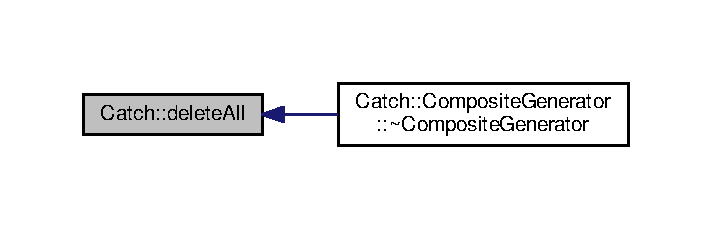
\includegraphics[width=342pt]{namespace_catch_aadf9786550a462740ec355f8219863a9_icgraph}
\end{center}
\end{figure}


\hypertarget{namespace_catch_af2fcec1d4bd984fe19ff8b9a432c36a8}{\index{Catch@{Catch}!delete\-All\-Values@{delete\-All\-Values}}
\index{delete\-All\-Values@{delete\-All\-Values}!Catch@{Catch}}
\subsubsection[{delete\-All\-Values}]{\setlength{\rightskip}{0pt plus 5cm}template$<$typename Associative\-Container\-T $>$ void Catch\-::delete\-All\-Values (
\begin{DoxyParamCaption}
\item[{Associative\-Container\-T \&}]{container}
\end{DoxyParamCaption}
)\hspace{0.3cm}{\ttfamily [inline]}}}\label{namespace_catch_af2fcec1d4bd984fe19ff8b9a432c36a8}
\hypertarget{namespace_catch_ada025504f627feaf9ac68ca391515dff}{\index{Catch@{Catch}!ends\-With@{ends\-With}}
\index{ends\-With@{ends\-With}!Catch@{Catch}}
\subsubsection[{ends\-With}]{\setlength{\rightskip}{0pt plus 5cm}bool Catch\-::ends\-With (
\begin{DoxyParamCaption}
\item[{std\-::string const \&}]{s, }
\item[{std\-::string const \&}]{suffix}
\end{DoxyParamCaption}
)}}\label{namespace_catch_ada025504f627feaf9ac68ca391515dff}
\hypertarget{namespace_catch_afd801a3e33fd7a8b91ded0d02747a93f}{\index{Catch@{Catch}!ends\-With@{ends\-With}}
\index{ends\-With@{ends\-With}!Catch@{Catch}}
\subsubsection[{ends\-With}]{\setlength{\rightskip}{0pt plus 5cm}bool Catch\-::ends\-With (
\begin{DoxyParamCaption}
\item[{std\-::string const \&}]{s, }
\item[{char}]{suffix}
\end{DoxyParamCaption}
)}}\label{namespace_catch_afd801a3e33fd7a8b91ded0d02747a93f}
\hypertarget{namespace_catch_ab5da9aa67c42a3f626aea07d0b556829}{\index{Catch@{Catch}!filter\-Tests@{filter\-Tests}}
\index{filter\-Tests@{filter\-Tests}!Catch@{Catch}}
\subsubsection[{filter\-Tests}]{\setlength{\rightskip}{0pt plus 5cm}std\-::vector$<${\bf Test\-Case}$>$ Catch\-::filter\-Tests (
\begin{DoxyParamCaption}
\item[{std\-::vector$<$ Test\-Case $>$ const \&}]{test\-Cases, }
\item[{Test\-Spec const \&}]{test\-Spec, }
\item[{I\-Config const \&}]{config}
\end{DoxyParamCaption}
)}}\label{namespace_catch_ab5da9aa67c42a3f626aea07d0b556829}
\hypertarget{namespace_catch_a1c9b1a23bc947ea70ddaabf067276cf2}{\index{Catch@{Catch}!get\-All\-Test\-Cases\-Sorted@{get\-All\-Test\-Cases\-Sorted}}
\index{get\-All\-Test\-Cases\-Sorted@{get\-All\-Test\-Cases\-Sorted}!Catch@{Catch}}
\subsubsection[{get\-All\-Test\-Cases\-Sorted}]{\setlength{\rightskip}{0pt plus 5cm}std\-::vector$<${\bf Test\-Case}$>$ const\& Catch\-::get\-All\-Test\-Cases\-Sorted (
\begin{DoxyParamCaption}
\item[{I\-Config const \&}]{config}
\end{DoxyParamCaption}
)}}\label{namespace_catch_a1c9b1a23bc947ea70ddaabf067276cf2}
\hypertarget{namespace_catch_ad517cca9b21deb79101e90e5508dd161}{\index{Catch@{Catch}!get\-Current\-Context@{get\-Current\-Context}}
\index{get\-Current\-Context@{get\-Current\-Context}!Catch@{Catch}}
\subsubsection[{get\-Current\-Context}]{\setlength{\rightskip}{0pt plus 5cm}{\bf I\-Context}\& Catch\-::get\-Current\-Context (
\begin{DoxyParamCaption}
{}
\end{DoxyParamCaption}
)}}\label{namespace_catch_ad517cca9b21deb79101e90e5508dd161}


Here is the caller graph for this function\-:
\nopagebreak
\begin{figure}[H]
\begin{center}
\leavevmode
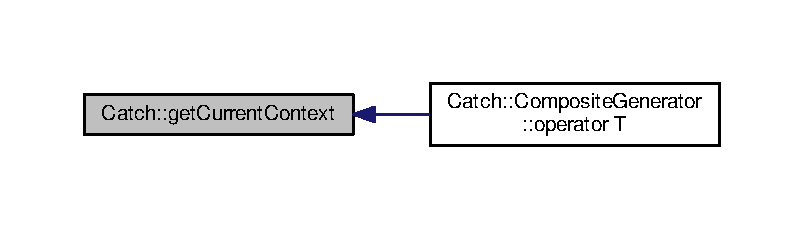
\includegraphics[width=350pt]{namespace_catch_ad517cca9b21deb79101e90e5508dd161_icgraph}
\end{center}
\end{figure}


\hypertarget{namespace_catch_af7bb0c32ab2453d2f53e92a96d15360e}{\index{Catch@{Catch}!get\-Current\-Mutable\-Context@{get\-Current\-Mutable\-Context}}
\index{get\-Current\-Mutable\-Context@{get\-Current\-Mutable\-Context}!Catch@{Catch}}
\subsubsection[{get\-Current\-Mutable\-Context}]{\setlength{\rightskip}{0pt plus 5cm}{\bf I\-Mutable\-Context}\& Catch\-::get\-Current\-Mutable\-Context (
\begin{DoxyParamCaption}
{}
\end{DoxyParamCaption}
)}}\label{namespace_catch_af7bb0c32ab2453d2f53e92a96d15360e}
\hypertarget{namespace_catch_ac9ddcc6d66079add9cb2a3140b8ae51e}{\index{Catch@{Catch}!get\-Mutable\-Registry\-Hub@{get\-Mutable\-Registry\-Hub}}
\index{get\-Mutable\-Registry\-Hub@{get\-Mutable\-Registry\-Hub}!Catch@{Catch}}
\subsubsection[{get\-Mutable\-Registry\-Hub}]{\setlength{\rightskip}{0pt plus 5cm}{\bf I\-Mutable\-Registry\-Hub}\& Catch\-::get\-Mutable\-Registry\-Hub (
\begin{DoxyParamCaption}
{}
\end{DoxyParamCaption}
)}}\label{namespace_catch_ac9ddcc6d66079add9cb2a3140b8ae51e}


Here is the caller graph for this function\-:
\nopagebreak
\begin{figure}[H]
\begin{center}
\leavevmode
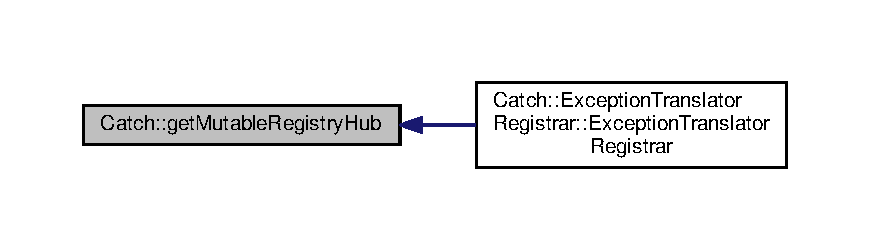
\includegraphics[width=350pt]{namespace_catch_ac9ddcc6d66079add9cb2a3140b8ae51e_icgraph}
\end{center}
\end{figure}


\hypertarget{namespace_catch_ac24b072979540bfd922e7d46e899f46f}{\index{Catch@{Catch}!get\-Registry\-Hub@{get\-Registry\-Hub}}
\index{get\-Registry\-Hub@{get\-Registry\-Hub}!Catch@{Catch}}
\subsubsection[{get\-Registry\-Hub}]{\setlength{\rightskip}{0pt plus 5cm}{\bf I\-Registry\-Hub}\& Catch\-::get\-Registry\-Hub (
\begin{DoxyParamCaption}
{}
\end{DoxyParamCaption}
)}}\label{namespace_catch_ac24b072979540bfd922e7d46e899f46f}
\hypertarget{namespace_catch_aff60c1de6ac6cea30175d70e33d83c8e}{\index{Catch@{Catch}!get\-Result\-Capture@{get\-Result\-Capture}}
\index{get\-Result\-Capture@{get\-Result\-Capture}!Catch@{Catch}}
\subsubsection[{get\-Result\-Capture}]{\setlength{\rightskip}{0pt plus 5cm}{\bf I\-Result\-Capture}\& Catch\-::get\-Result\-Capture (
\begin{DoxyParamCaption}
{}
\end{DoxyParamCaption}
)}}\label{namespace_catch_aff60c1de6ac6cea30175d70e33d83c8e}
\hypertarget{namespace_catch_ab079497368fb1df25af39ad494d2a241}{\index{Catch@{Catch}!is\-Debugger\-Active@{is\-Debugger\-Active}}
\index{is\-Debugger\-Active@{is\-Debugger\-Active}!Catch@{Catch}}
\subsubsection[{is\-Debugger\-Active}]{\setlength{\rightskip}{0pt plus 5cm}bool Catch\-::is\-Debugger\-Active (
\begin{DoxyParamCaption}
{}
\end{DoxyParamCaption}
)}}\label{namespace_catch_ab079497368fb1df25af39ad494d2a241}
\hypertarget{namespace_catch_a93ef4e3e307a2021ca0d41b32c0e54b0}{\index{Catch@{Catch}!is\-False\-Test@{is\-False\-Test}}
\index{is\-False\-Test@{is\-False\-Test}!Catch@{Catch}}
\subsubsection[{is\-False\-Test}]{\setlength{\rightskip}{0pt plus 5cm}bool Catch\-::is\-False\-Test (
\begin{DoxyParamCaption}
\item[{int}]{flags}
\end{DoxyParamCaption}
)\hspace{0.3cm}{\ttfamily [inline]}}}\label{namespace_catch_a93ef4e3e307a2021ca0d41b32c0e54b0}
\hypertarget{namespace_catch_a54b01af61673a3e1f21f31713639b180}{\index{Catch@{Catch}!is\-Just\-Info@{is\-Just\-Info}}
\index{is\-Just\-Info@{is\-Just\-Info}!Catch@{Catch}}
\subsubsection[{is\-Just\-Info}]{\setlength{\rightskip}{0pt plus 5cm}bool Catch\-::is\-Just\-Info (
\begin{DoxyParamCaption}
\item[{int}]{flags}
\end{DoxyParamCaption}
)\hspace{0.3cm}{\ttfamily [inline]}}}\label{namespace_catch_a54b01af61673a3e1f21f31713639b180}
\hypertarget{namespace_catch_a5205869c81c06d3460759cb86676ae68}{\index{Catch@{Catch}!is\-Ok@{is\-Ok}}
\index{is\-Ok@{is\-Ok}!Catch@{Catch}}
\subsubsection[{is\-Ok}]{\setlength{\rightskip}{0pt plus 5cm}bool Catch\-::is\-Ok (
\begin{DoxyParamCaption}
\item[{Result\-Was\-::\-Of\-Type}]{result\-Type}
\end{DoxyParamCaption}
)\hspace{0.3cm}{\ttfamily [inline]}}}\label{namespace_catch_a5205869c81c06d3460759cb86676ae68}
\hypertarget{namespace_catch_ae3bc6c6677e64e6eaa720dc3add31852}{\index{Catch@{Catch}!is\-True@{is\-True}}
\index{is\-True@{is\-True}!Catch@{Catch}}
\subsubsection[{is\-True}]{\setlength{\rightskip}{0pt plus 5cm}bool Catch\-::is\-True (
\begin{DoxyParamCaption}
\item[{bool}]{value}
\end{DoxyParamCaption}
)\hspace{0.3cm}{\ttfamily [inline]}}}\label{namespace_catch_ae3bc6c6677e64e6eaa720dc3add31852}
\hypertarget{namespace_catch_a2a784590bb5068810d3f6013fed1f1d3}{\index{Catch@{Catch}!make\-Test\-Case@{make\-Test\-Case}}
\index{make\-Test\-Case@{make\-Test\-Case}!Catch@{Catch}}
\subsubsection[{make\-Test\-Case}]{\setlength{\rightskip}{0pt plus 5cm}{\bf Test\-Case} Catch\-::make\-Test\-Case (
\begin{DoxyParamCaption}
\item[{I\-Test\-Case $\ast$}]{test\-Case, }
\item[{std\-::string const \&}]{class\-Name, }
\item[{std\-::string const \&}]{name, }
\item[{std\-::string const \&}]{description, }
\item[{Source\-Line\-Info const \&}]{line\-Info}
\end{DoxyParamCaption}
)}}\label{namespace_catch_a2a784590bb5068810d3f6013fed1f1d3}
\hypertarget{namespace_catch_aadef80fbc6bc84589777a462770cef49}{\index{Catch@{Catch}!match\-Test@{match\-Test}}
\index{match\-Test@{match\-Test}!Catch@{Catch}}
\subsubsection[{match\-Test}]{\setlength{\rightskip}{0pt plus 5cm}bool Catch\-::match\-Test (
\begin{DoxyParamCaption}
\item[{Test\-Case const \&}]{test\-Case, }
\item[{Test\-Spec const \&}]{test\-Spec, }
\item[{I\-Config const \&}]{config}
\end{DoxyParamCaption}
)}}\label{namespace_catch_aadef80fbc6bc84589777a462770cef49}
\hypertarget{namespace_catch_a5e95b3c47a7618db3649dc39b0bb9004}{\index{Catch@{Catch}!operator+@{operator+}}
\index{operator+@{operator+}!Catch@{Catch}}
\subsubsection[{operator+}]{\setlength{\rightskip}{0pt plus 5cm}template$<$typename T $>$ T const\& Catch\-::operator+ (
\begin{DoxyParamCaption}
\item[{T const \&}]{value, }
\item[{Stream\-End\-Stop}]{}
\end{DoxyParamCaption}
)}}\label{namespace_catch_a5e95b3c47a7618db3649dc39b0bb9004}
\hypertarget{namespace_catch_a6ec18b5054d7fdfdde861c580b082995}{\index{Catch@{Catch}!operator$<$$<$@{operator$<$$<$}}
\index{operator$<$$<$@{operator$<$$<$}!Catch@{Catch}}
\subsubsection[{operator$<$$<$}]{\setlength{\rightskip}{0pt plus 5cm}std\-::ostream\& Catch\-::operator$<$$<$ (
\begin{DoxyParamCaption}
\item[{std\-::ostream \&}]{os, }
\item[{Source\-Line\-Info const \&}]{info}
\end{DoxyParamCaption}
)}}\label{namespace_catch_a6ec18b5054d7fdfdde861c580b082995}
\hypertarget{namespace_catch_ab32a083e442cc09f736327d2e2865999}{\index{Catch@{Catch}!operator$\vert$@{operator$\vert$}}
\index{operator$\vert$@{operator$\vert$}!Catch@{Catch}}
\subsubsection[{operator$\vert$}]{\setlength{\rightskip}{0pt plus 5cm}{\bf Result\-Disposition\-::\-Flags} Catch\-::operator$\vert$ (
\begin{DoxyParamCaption}
\item[{Result\-Disposition\-::\-Flags}]{lhs, }
\item[{Result\-Disposition\-::\-Flags}]{rhs}
\end{DoxyParamCaption}
)\hspace{0.3cm}{\ttfamily [inline]}}}\label{namespace_catch_ab32a083e442cc09f736327d2e2865999}
\hypertarget{namespace_catch_a9a59d681cc327a33c280796561dfe258}{\index{Catch@{Catch}!register\-Test\-Case@{register\-Test\-Case}}
\index{register\-Test\-Case@{register\-Test\-Case}!Catch@{Catch}}
\subsubsection[{register\-Test\-Case}]{\setlength{\rightskip}{0pt plus 5cm}void Catch\-::register\-Test\-Case (
\begin{DoxyParamCaption}
\item[{I\-Test\-Case $\ast$}]{test\-Case, }
\item[{char const $\ast$}]{class\-Name, }
\item[{Name\-And\-Desc const \&}]{name\-And\-Desc, }
\item[{Source\-Line\-Info const \&}]{line\-Info}
\end{DoxyParamCaption}
)}}\label{namespace_catch_a9a59d681cc327a33c280796561dfe258}


Here is the caller graph for this function\-:
\nopagebreak
\begin{figure}[H]
\begin{center}
\leavevmode
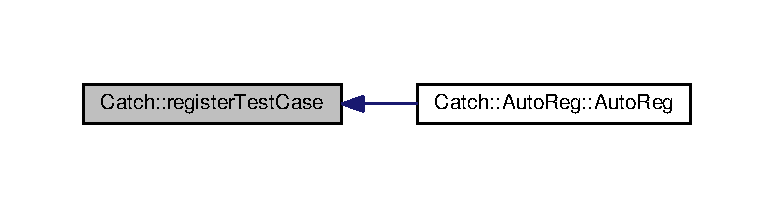
\includegraphics[width=350pt]{namespace_catch_a9a59d681cc327a33c280796561dfe258_icgraph}
\end{center}
\end{figure}


\hypertarget{namespace_catch_a220159aeff47f9c5231e893f2abbc643}{\index{Catch@{Catch}!register\-Test\-Case\-Function@{register\-Test\-Case\-Function}}
\index{register\-Test\-Case\-Function@{register\-Test\-Case\-Function}!Catch@{Catch}}
\subsubsection[{register\-Test\-Case\-Function}]{\setlength{\rightskip}{0pt plus 5cm}void Catch\-::register\-Test\-Case\-Function (
\begin{DoxyParamCaption}
\item[{Test\-Function}]{function, }
\item[{Source\-Line\-Info const \&}]{line\-Info, }
\item[{Name\-And\-Desc const \&}]{name\-And\-Desc}
\end{DoxyParamCaption}
)}}\label{namespace_catch_a220159aeff47f9c5231e893f2abbc643}
\hypertarget{namespace_catch_afe4e6770da547e43e9e4eeaa05f946ea}{\index{Catch@{Catch}!replace\-In\-Place@{replace\-In\-Place}}
\index{replace\-In\-Place@{replace\-In\-Place}!Catch@{Catch}}
\subsubsection[{replace\-In\-Place}]{\setlength{\rightskip}{0pt plus 5cm}bool Catch\-::replace\-In\-Place (
\begin{DoxyParamCaption}
\item[{std\-::string \&}]{str, }
\item[{std\-::string const \&}]{replace\-This, }
\item[{std\-::string const \&}]{with\-This}
\end{DoxyParamCaption}
)}}\label{namespace_catch_afe4e6770da547e43e9e4eeaa05f946ea}
\hypertarget{namespace_catch_acf5ea05e942d2d7fe79111e12754ed76}{\index{Catch@{Catch}!rng\-Seed@{rng\-Seed}}
\index{rng\-Seed@{rng\-Seed}!Catch@{Catch}}
\subsubsection[{rng\-Seed}]{\setlength{\rightskip}{0pt plus 5cm}unsigned int Catch\-::rng\-Seed (
\begin{DoxyParamCaption}
{}
\end{DoxyParamCaption}
)}}\label{namespace_catch_acf5ea05e942d2d7fe79111e12754ed76}
\hypertarget{namespace_catch_a161400810eb0995394d6d8d3cae821ad}{\index{Catch@{Catch}!seed\-Rng@{seed\-Rng}}
\index{seed\-Rng@{seed\-Rng}!Catch@{Catch}}
\subsubsection[{seed\-Rng}]{\setlength{\rightskip}{0pt plus 5cm}void Catch\-::seed\-Rng (
\begin{DoxyParamCaption}
\item[{I\-Config const \&}]{config}
\end{DoxyParamCaption}
)}}\label{namespace_catch_a161400810eb0995394d6d8d3cae821ad}
\hypertarget{namespace_catch_a7f7480b15d74965459c844f0d393ed87}{\index{Catch@{Catch}!should\-Continue\-On\-Failure@{should\-Continue\-On\-Failure}}
\index{should\-Continue\-On\-Failure@{should\-Continue\-On\-Failure}!Catch@{Catch}}
\subsubsection[{should\-Continue\-On\-Failure}]{\setlength{\rightskip}{0pt plus 5cm}bool Catch\-::should\-Continue\-On\-Failure (
\begin{DoxyParamCaption}
\item[{int}]{flags}
\end{DoxyParamCaption}
)\hspace{0.3cm}{\ttfamily [inline]}}}\label{namespace_catch_a7f7480b15d74965459c844f0d393ed87}
\hypertarget{namespace_catch_ab91eb13081203d634fe48d3d2ab386d7}{\index{Catch@{Catch}!should\-Suppress\-Failure@{should\-Suppress\-Failure}}
\index{should\-Suppress\-Failure@{should\-Suppress\-Failure}!Catch@{Catch}}
\subsubsection[{should\-Suppress\-Failure}]{\setlength{\rightskip}{0pt plus 5cm}bool Catch\-::should\-Suppress\-Failure (
\begin{DoxyParamCaption}
\item[{int}]{flags}
\end{DoxyParamCaption}
)\hspace{0.3cm}{\ttfamily [inline]}}}\label{namespace_catch_ab91eb13081203d634fe48d3d2ab386d7}
\hypertarget{namespace_catch_a695f62327be0676e046291eeaae15110}{\index{Catch@{Catch}!starts\-With@{starts\-With}}
\index{starts\-With@{starts\-With}!Catch@{Catch}}
\subsubsection[{starts\-With}]{\setlength{\rightskip}{0pt plus 5cm}bool Catch\-::starts\-With (
\begin{DoxyParamCaption}
\item[{std\-::string const \&}]{s, }
\item[{std\-::string const \&}]{prefix}
\end{DoxyParamCaption}
)}}\label{namespace_catch_a695f62327be0676e046291eeaae15110}
\hypertarget{namespace_catch_acad23751846ac23d0f379e34f5adebb1}{\index{Catch@{Catch}!starts\-With@{starts\-With}}
\index{starts\-With@{starts\-With}!Catch@{Catch}}
\subsubsection[{starts\-With}]{\setlength{\rightskip}{0pt plus 5cm}bool Catch\-::starts\-With (
\begin{DoxyParamCaption}
\item[{std\-::string const \&}]{s, }
\item[{char}]{prefix}
\end{DoxyParamCaption}
)}}\label{namespace_catch_acad23751846ac23d0f379e34f5adebb1}
\hypertarget{namespace_catch_a702b612f683d154c466ea8297ed4a20d}{\index{Catch@{Catch}!throw\-Logic\-Error@{throw\-Logic\-Error}}
\index{throw\-Logic\-Error@{throw\-Logic\-Error}!Catch@{Catch}}
\subsubsection[{throw\-Logic\-Error}]{\setlength{\rightskip}{0pt plus 5cm}void Catch\-::throw\-Logic\-Error (
\begin{DoxyParamCaption}
\item[{std\-::string const \&}]{message, }
\item[{Source\-Line\-Info const \&}]{location\-Info}
\end{DoxyParamCaption}
)}}\label{namespace_catch_a702b612f683d154c466ea8297ed4a20d}
\hypertarget{namespace_catch_ac036a17412d318598ffda8e1fe7a1177}{\index{Catch@{Catch}!to\-Lower@{to\-Lower}}
\index{to\-Lower@{to\-Lower}!Catch@{Catch}}
\subsubsection[{to\-Lower}]{\setlength{\rightskip}{0pt plus 5cm}std\-::string Catch\-::to\-Lower (
\begin{DoxyParamCaption}
\item[{std\-::string const \&}]{s}
\end{DoxyParamCaption}
)}}\label{namespace_catch_ac036a17412d318598ffda8e1fe7a1177}
\hypertarget{namespace_catch_a0760dbe87d090a55a35414db57d272c4}{\index{Catch@{Catch}!to\-Lower\-In\-Place@{to\-Lower\-In\-Place}}
\index{to\-Lower\-In\-Place@{to\-Lower\-In\-Place}!Catch@{Catch}}
\subsubsection[{to\-Lower\-In\-Place}]{\setlength{\rightskip}{0pt plus 5cm}void Catch\-::to\-Lower\-In\-Place (
\begin{DoxyParamCaption}
\item[{std\-::string \&}]{s}
\end{DoxyParamCaption}
)}}\label{namespace_catch_a0760dbe87d090a55a35414db57d272c4}
\hypertarget{namespace_catch_a386cb19a84b12339486771ad143a95ae}{\index{Catch@{Catch}!to\-String@{to\-String}}
\index{to\-String@{to\-String}!Catch@{Catch}}
\subsubsection[{to\-String}]{\setlength{\rightskip}{0pt plus 5cm}template$<$typename T $>$ std\-::string Catch\-::to\-String (
\begin{DoxyParamCaption}
\item[{T const \&}]{value}
\end{DoxyParamCaption}
)}}\label{namespace_catch_a386cb19a84b12339486771ad143a95ae}


converts any type to a string 

The default template forwards on to ostringstream -\/ except when an ostringstream overload does not exist -\/ in which case it attempts to detect that and writes \{?\}. Overload (not specialise) this template for custom typs that you don't want to provide an ostream overload for. 

Here is the call graph for this function\-:
\nopagebreak
\begin{figure}[H]
\begin{center}
\leavevmode
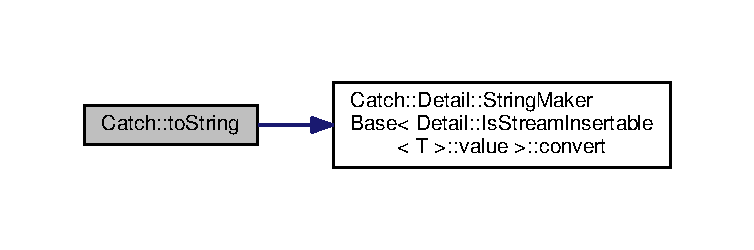
\includegraphics[width=350pt]{namespace_catch_a386cb19a84b12339486771ad143a95ae_cgraph}
\end{center}
\end{figure}




Here is the caller graph for this function\-:
\nopagebreak
\begin{figure}[H]
\begin{center}
\leavevmode
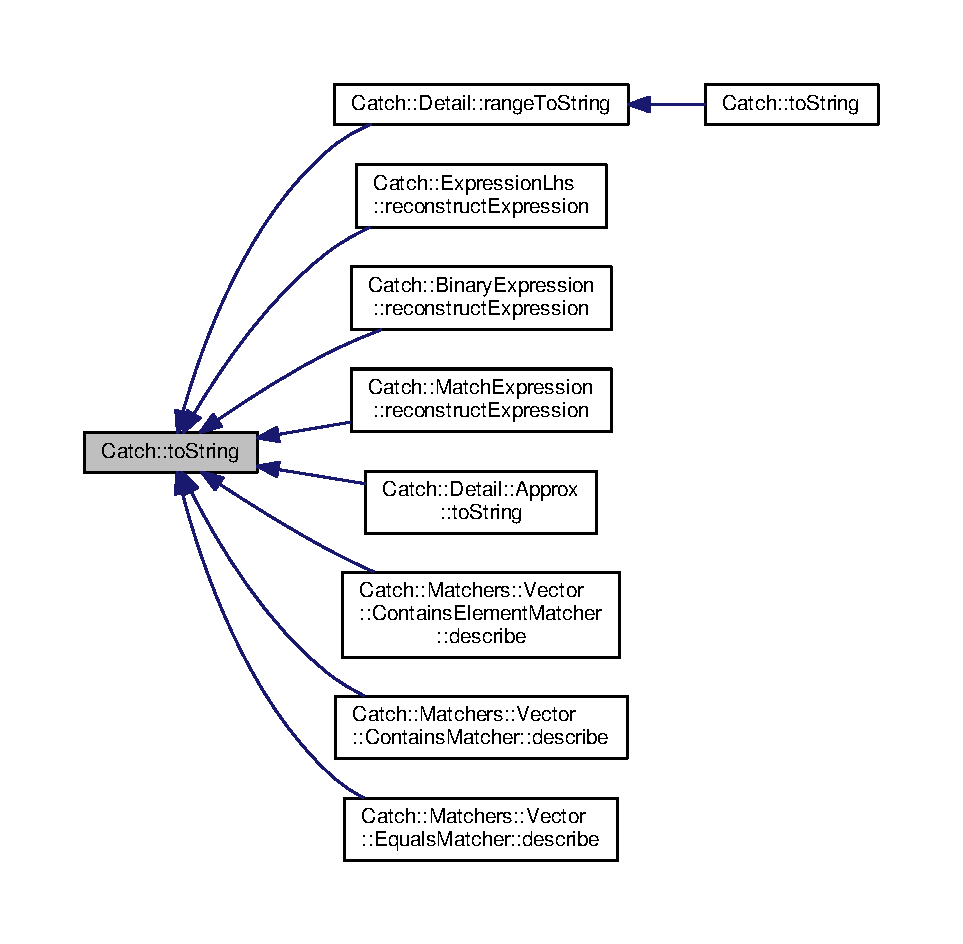
\includegraphics[width=350pt]{namespace_catch_a386cb19a84b12339486771ad143a95ae_icgraph}
\end{center}
\end{figure}


\hypertarget{namespace_catch_ad6e969257437cf007b8b5017b22e570c}{\index{Catch@{Catch}!to\-String@{to\-String}}
\index{to\-String@{to\-String}!Catch@{Catch}}
\subsubsection[{to\-String}]{\setlength{\rightskip}{0pt plus 5cm}std\-::string Catch\-::to\-String (
\begin{DoxyParamCaption}
\item[{std\-::string const \&}]{value}
\end{DoxyParamCaption}
)}}\label{namespace_catch_ad6e969257437cf007b8b5017b22e570c}
\hypertarget{namespace_catch_af9fc40701e3a7d0790866e7cf8c0279f}{\index{Catch@{Catch}!to\-String@{to\-String}}
\index{to\-String@{to\-String}!Catch@{Catch}}
\subsubsection[{to\-String}]{\setlength{\rightskip}{0pt plus 5cm}std\-::string Catch\-::to\-String (
\begin{DoxyParamCaption}
\item[{std\-::wstring const \&}]{value}
\end{DoxyParamCaption}
)}}\label{namespace_catch_af9fc40701e3a7d0790866e7cf8c0279f}
\hypertarget{namespace_catch_ace2e2fe33b196bc8278f605dcb72e38d}{\index{Catch@{Catch}!to\-String@{to\-String}}
\index{to\-String@{to\-String}!Catch@{Catch}}
\subsubsection[{to\-String}]{\setlength{\rightskip}{0pt plus 5cm}std\-::string Catch\-::to\-String (
\begin{DoxyParamCaption}
\item[{const char $\ast$const}]{value}
\end{DoxyParamCaption}
)}}\label{namespace_catch_ace2e2fe33b196bc8278f605dcb72e38d}
\hypertarget{namespace_catch_ae6c2bc95517444d8df8199bd3f61609b}{\index{Catch@{Catch}!to\-String@{to\-String}}
\index{to\-String@{to\-String}!Catch@{Catch}}
\subsubsection[{to\-String}]{\setlength{\rightskip}{0pt plus 5cm}std\-::string Catch\-::to\-String (
\begin{DoxyParamCaption}
\item[{char $\ast$const}]{value}
\end{DoxyParamCaption}
)}}\label{namespace_catch_ae6c2bc95517444d8df8199bd3f61609b}
\hypertarget{namespace_catch_afa173b4639c682c9d8c20fae0939693c}{\index{Catch@{Catch}!to\-String@{to\-String}}
\index{to\-String@{to\-String}!Catch@{Catch}}
\subsubsection[{to\-String}]{\setlength{\rightskip}{0pt plus 5cm}std\-::string Catch\-::to\-String (
\begin{DoxyParamCaption}
\item[{const wchar\-\_\-t $\ast$const}]{value}
\end{DoxyParamCaption}
)}}\label{namespace_catch_afa173b4639c682c9d8c20fae0939693c}
\hypertarget{namespace_catch_aa39121565abe9f30fce5d48e4e094768}{\index{Catch@{Catch}!to\-String@{to\-String}}
\index{to\-String@{to\-String}!Catch@{Catch}}
\subsubsection[{to\-String}]{\setlength{\rightskip}{0pt plus 5cm}std\-::string Catch\-::to\-String (
\begin{DoxyParamCaption}
\item[{wchar\-\_\-t $\ast$const}]{value}
\end{DoxyParamCaption}
)}}\label{namespace_catch_aa39121565abe9f30fce5d48e4e094768}
\hypertarget{namespace_catch_acee54d0580385e4347bc42a7d22bc893}{\index{Catch@{Catch}!to\-String@{to\-String}}
\index{to\-String@{to\-String}!Catch@{Catch}}
\subsubsection[{to\-String}]{\setlength{\rightskip}{0pt plus 5cm}std\-::string Catch\-::to\-String (
\begin{DoxyParamCaption}
\item[{int}]{value}
\end{DoxyParamCaption}
)}}\label{namespace_catch_acee54d0580385e4347bc42a7d22bc893}
\hypertarget{namespace_catch_aba1d78bce62f8c73cbfc2a14225356ea}{\index{Catch@{Catch}!to\-String@{to\-String}}
\index{to\-String@{to\-String}!Catch@{Catch}}
\subsubsection[{to\-String}]{\setlength{\rightskip}{0pt plus 5cm}std\-::string Catch\-::to\-String (
\begin{DoxyParamCaption}
\item[{unsigned long}]{value}
\end{DoxyParamCaption}
)}}\label{namespace_catch_aba1d78bce62f8c73cbfc2a14225356ea}
\hypertarget{namespace_catch_a6fd78030f740c1c3bdc60efdfd5fc85d}{\index{Catch@{Catch}!to\-String@{to\-String}}
\index{to\-String@{to\-String}!Catch@{Catch}}
\subsubsection[{to\-String}]{\setlength{\rightskip}{0pt plus 5cm}std\-::string Catch\-::to\-String (
\begin{DoxyParamCaption}
\item[{unsigned int}]{value}
\end{DoxyParamCaption}
)}}\label{namespace_catch_a6fd78030f740c1c3bdc60efdfd5fc85d}
\hypertarget{namespace_catch_a3eb4356d09b7ef3286f6c1c1efe8cabf}{\index{Catch@{Catch}!to\-String@{to\-String}}
\index{to\-String@{to\-String}!Catch@{Catch}}
\subsubsection[{to\-String}]{\setlength{\rightskip}{0pt plus 5cm}std\-::string Catch\-::to\-String (
\begin{DoxyParamCaption}
\item[{const double}]{value}
\end{DoxyParamCaption}
)}}\label{namespace_catch_a3eb4356d09b7ef3286f6c1c1efe8cabf}
\hypertarget{namespace_catch_a80b6411e2cba89e58aa8feb960d045d5}{\index{Catch@{Catch}!to\-String@{to\-String}}
\index{to\-String@{to\-String}!Catch@{Catch}}
\subsubsection[{to\-String}]{\setlength{\rightskip}{0pt plus 5cm}std\-::string Catch\-::to\-String (
\begin{DoxyParamCaption}
\item[{const float}]{value}
\end{DoxyParamCaption}
)}}\label{namespace_catch_a80b6411e2cba89e58aa8feb960d045d5}
\hypertarget{namespace_catch_a5d3bdb2ec0e6f415e2a1a0e4914d7d3a}{\index{Catch@{Catch}!to\-String@{to\-String}}
\index{to\-String@{to\-String}!Catch@{Catch}}
\subsubsection[{to\-String}]{\setlength{\rightskip}{0pt plus 5cm}std\-::string Catch\-::to\-String (
\begin{DoxyParamCaption}
\item[{bool}]{value}
\end{DoxyParamCaption}
)}}\label{namespace_catch_a5d3bdb2ec0e6f415e2a1a0e4914d7d3a}
\hypertarget{namespace_catch_a25a0a78cbb62ea08b5d49e443051c387}{\index{Catch@{Catch}!to\-String@{to\-String}}
\index{to\-String@{to\-String}!Catch@{Catch}}
\subsubsection[{to\-String}]{\setlength{\rightskip}{0pt plus 5cm}std\-::string Catch\-::to\-String (
\begin{DoxyParamCaption}
\item[{char}]{value}
\end{DoxyParamCaption}
)}}\label{namespace_catch_a25a0a78cbb62ea08b5d49e443051c387}
\hypertarget{namespace_catch_a0a5d9d0965d0d2a0663773732283713e}{\index{Catch@{Catch}!to\-String@{to\-String}}
\index{to\-String@{to\-String}!Catch@{Catch}}
\subsubsection[{to\-String}]{\setlength{\rightskip}{0pt plus 5cm}std\-::string Catch\-::to\-String (
\begin{DoxyParamCaption}
\item[{signed char}]{value}
\end{DoxyParamCaption}
)}}\label{namespace_catch_a0a5d9d0965d0d2a0663773732283713e}
\hypertarget{namespace_catch_a5d83eaeb68579a556c86cc05f7a7765f}{\index{Catch@{Catch}!to\-String@{to\-String}}
\index{to\-String@{to\-String}!Catch@{Catch}}
\subsubsection[{to\-String}]{\setlength{\rightskip}{0pt plus 5cm}std\-::string Catch\-::to\-String (
\begin{DoxyParamCaption}
\item[{unsigned char}]{value}
\end{DoxyParamCaption}
)}}\label{namespace_catch_a5d83eaeb68579a556c86cc05f7a7765f}
\hypertarget{namespace_catch_a2899237fef39daaae9a22e7846c0a9bf}{\index{Catch@{Catch}!to\-String@{to\-String}}
\index{to\-String@{to\-String}!Catch@{Catch}}
\subsubsection[{to\-String}]{\setlength{\rightskip}{0pt plus 5cm}template$<$typename T , typename Allocator $>$ std\-::string Catch\-::to\-String (
\begin{DoxyParamCaption}
\item[{std\-::vector$<$ T, Allocator $>$ const \&}]{v}
\end{DoxyParamCaption}
)}}\label{namespace_catch_a2899237fef39daaae9a22e7846c0a9bf}


Here is the call graph for this function\-:
\nopagebreak
\begin{figure}[H]
\begin{center}
\leavevmode
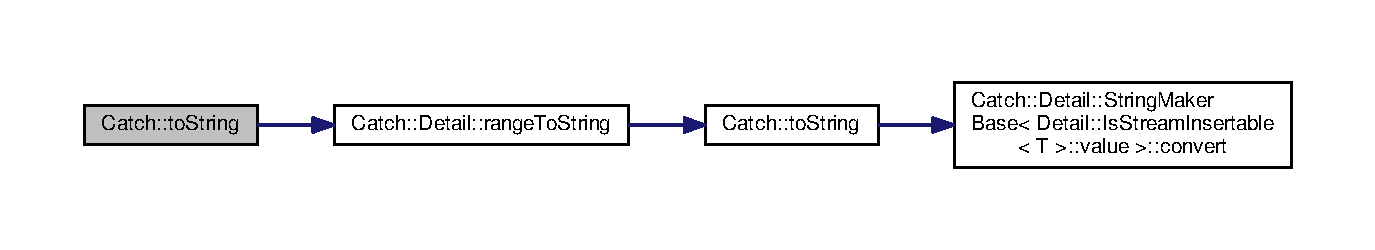
\includegraphics[width=350pt]{namespace_catch_a2899237fef39daaae9a22e7846c0a9bf_cgraph}
\end{center}
\end{figure}


\hypertarget{namespace_catch_ac501c2b6bfe82978d699ddda37c53d13}{\index{Catch@{Catch}!to\-String$<$ Detail\-::\-Approx $>$@{to\-String$<$ Detail\-::\-Approx $>$}}
\index{to\-String$<$ Detail\-::\-Approx $>$@{to\-String$<$ Detail\-::\-Approx $>$}!Catch@{Catch}}
\subsubsection[{to\-String$<$ Detail\-::\-Approx $>$}]{\setlength{\rightskip}{0pt plus 5cm}template$<$$>$ std\-::string {\bf Catch\-::to\-String}$<$ {\bf Detail\-::\-Approx} $>$ (
\begin{DoxyParamCaption}
\item[{Detail\-::\-Approx const \&}]{value}
\end{DoxyParamCaption}
)\hspace{0.3cm}{\ttfamily [inline]}}}\label{namespace_catch_ac501c2b6bfe82978d699ddda37c53d13}
\hypertarget{namespace_catch_adafff91485eeeeb9e9333f317cc0e3b1}{\index{Catch@{Catch}!translate\-Active\-Exception@{translate\-Active\-Exception}}
\index{translate\-Active\-Exception@{translate\-Active\-Exception}!Catch@{Catch}}
\subsubsection[{translate\-Active\-Exception}]{\setlength{\rightskip}{0pt plus 5cm}std\-::string Catch\-::translate\-Active\-Exception (
\begin{DoxyParamCaption}
{}
\end{DoxyParamCaption}
)}}\label{namespace_catch_adafff91485eeeeb9e9333f317cc0e3b1}
\hypertarget{namespace_catch_a084108b47f37d8bfd5db51c50c7451b3}{\index{Catch@{Catch}!trim@{trim}}
\index{trim@{trim}!Catch@{Catch}}
\subsubsection[{trim}]{\setlength{\rightskip}{0pt plus 5cm}std\-::string Catch\-::trim (
\begin{DoxyParamCaption}
\item[{std\-::string const \&}]{str}
\end{DoxyParamCaption}
)}}\label{namespace_catch_a084108b47f37d8bfd5db51c50c7451b3}


Here is the caller graph for this function\-:
\nopagebreak
\begin{figure}[H]
\begin{center}
\leavevmode
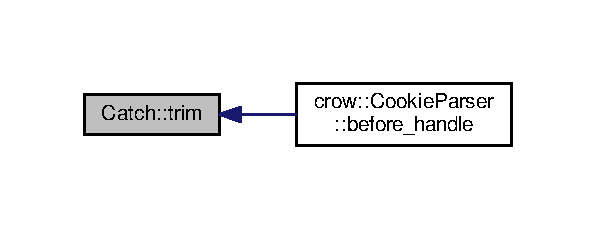
\includegraphics[width=286pt]{namespace_catch_a084108b47f37d8bfd5db51c50c7451b3_icgraph}
\end{center}
\end{figure}


\hypertarget{namespace_catch_aa5dcf4750ce9a854f4b74d3c952d13cc}{\index{Catch@{Catch}!write\-To\-Debug\-Console@{write\-To\-Debug\-Console}}
\index{write\-To\-Debug\-Console@{write\-To\-Debug\-Console}!Catch@{Catch}}
\subsubsection[{write\-To\-Debug\-Console}]{\setlength{\rightskip}{0pt plus 5cm}void Catch\-::write\-To\-Debug\-Console (
\begin{DoxyParamCaption}
\item[{std\-::string const \&}]{text}
\end{DoxyParamCaption}
)}}\label{namespace_catch_aa5dcf4750ce9a854f4b74d3c952d13cc}

\hypertarget{namespace_catch_1_1_detail}{\section{Catch\-:\-:Detail Namespace Reference}
\label{namespace_catch_1_1_detail}\index{Catch\-::\-Detail@{Catch\-::\-Detail}}
}
\subsection*{Classes}
\begin{DoxyCompactItemize}
\item 
struct \hyperlink{struct_catch_1_1_detail_1_1_borg_type}{Borg\-Type}
\item 
struct \hyperlink{struct_catch_1_1_detail_1_1_true_type}{True\-Type}
\item 
struct \hyperlink{struct_catch_1_1_detail_1_1_false_type}{False\-Type}
\item 
struct \hyperlink{struct_catch_1_1_detail_1_1_is_stream_insertable}{Is\-Stream\-Insertable}
\item 
struct \hyperlink{struct_catch_1_1_detail_1_1_string_maker_base}{String\-Maker\-Base}
\item 
struct \hyperlink{struct_catch_1_1_detail_1_1_string_maker_base_3_01true_01_4}{String\-Maker\-Base$<$ true $>$}
\item 
class \hyperlink{class_catch_1_1_detail_1_1_approx}{Approx}
\end{DoxyCompactItemize}
\subsection*{Functions}
\begin{DoxyCompactItemize}
\item 
\hyperlink{struct_catch_1_1_detail_1_1_true_type}{True\-Type} \& \hyperlink{namespace_catch_1_1_detail_aff0ca0f561ad8053654ab27d54486197}{test\-Streamable} (std\-::ostream \&)
\item 
\hyperlink{struct_catch_1_1_detail_1_1_false_type}{False\-Type} \hyperlink{namespace_catch_1_1_detail_aac81f01b0d687f75b8f24a925591b7ac}{test\-Streamable} (\hyperlink{struct_catch_1_1_detail_1_1_false_type}{False\-Type})
\item 
\hyperlink{struct_catch_1_1_detail_1_1_false_type}{False\-Type} \hyperlink{namespace_catch_1_1_detail_ae9a44d574c4fbd18fabaaee05a433d88}{operator$<$$<$} (std\-::ostream const \&, \hyperlink{struct_catch_1_1_detail_1_1_borg_type}{Borg\-Type} const \&)
\item 
std\-::string \hyperlink{namespace_catch_1_1_detail_ac5d6c510e565ee5bddcc2236194ce29e}{raw\-Memory\-To\-String} (const void $\ast$object, std\-::size\-\_\-t size)
\item 
{\footnotesize template$<$typename T $>$ }\\std\-::string \hyperlink{namespace_catch_1_1_detail_a371620ed524abfcae5c3772bf49b563a}{raw\-Memory\-To\-String} (const T \&object)
\item 
{\footnotesize template$<$typename Input\-Iterator $>$ }\\std\-::string \hyperlink{namespace_catch_1_1_detail_a6650a1dff325bf29962ff15ae73fd972}{range\-To\-String} (Input\-Iterator first, Input\-Iterator last)
\item 
{\footnotesize template$<$typename T $>$ }\\std\-::string \hyperlink{namespace_catch_1_1_detail_aef46b4178e08758524d25d1d969a503c}{make\-String} (T const \&value)
\end{DoxyCompactItemize}
\subsection*{Variables}
\begin{DoxyCompactItemize}
\item 
const std\-::string \hyperlink{namespace_catch_1_1_detail_a466775f4eec29ffef29ab334cd885136}{unprintable\-String}
\end{DoxyCompactItemize}


\subsection{Function Documentation}
\hypertarget{namespace_catch_1_1_detail_aef46b4178e08758524d25d1d969a503c}{\index{Catch\-::\-Detail@{Catch\-::\-Detail}!make\-String@{make\-String}}
\index{make\-String@{make\-String}!Catch::Detail@{Catch\-::\-Detail}}
\subsubsection[{make\-String}]{\setlength{\rightskip}{0pt plus 5cm}template$<$typename T $>$ std\-::string Catch\-::\-Detail\-::make\-String (
\begin{DoxyParamCaption}
\item[{T const \&}]{value}
\end{DoxyParamCaption}
)}}\label{namespace_catch_1_1_detail_aef46b4178e08758524d25d1d969a503c}


Here is the call graph for this function\-:
\nopagebreak
\begin{figure}[H]
\begin{center}
\leavevmode
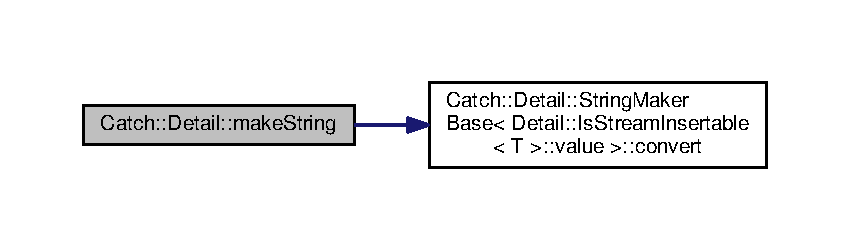
\includegraphics[width=350pt]{namespace_catch_1_1_detail_aef46b4178e08758524d25d1d969a503c_cgraph}
\end{center}
\end{figure}


\hypertarget{namespace_catch_1_1_detail_ae9a44d574c4fbd18fabaaee05a433d88}{\index{Catch\-::\-Detail@{Catch\-::\-Detail}!operator$<$$<$@{operator$<$$<$}}
\index{operator$<$$<$@{operator$<$$<$}!Catch::Detail@{Catch\-::\-Detail}}
\subsubsection[{operator$<$$<$}]{\setlength{\rightskip}{0pt plus 5cm}{\bf False\-Type} Catch\-::\-Detail\-::operator$<$$<$ (
\begin{DoxyParamCaption}
\item[{std\-::ostream const \&}]{, }
\item[{Borg\-Type const \&}]{}
\end{DoxyParamCaption}
)}}\label{namespace_catch_1_1_detail_ae9a44d574c4fbd18fabaaee05a433d88}
\hypertarget{namespace_catch_1_1_detail_a6650a1dff325bf29962ff15ae73fd972}{\index{Catch\-::\-Detail@{Catch\-::\-Detail}!range\-To\-String@{range\-To\-String}}
\index{range\-To\-String@{range\-To\-String}!Catch::Detail@{Catch\-::\-Detail}}
\subsubsection[{range\-To\-String}]{\setlength{\rightskip}{0pt plus 5cm}template$<$typename Input\-Iterator $>$ std\-::string Catch\-::\-Detail\-::range\-To\-String (
\begin{DoxyParamCaption}
\item[{Input\-Iterator}]{first, }
\item[{Input\-Iterator}]{last}
\end{DoxyParamCaption}
)}}\label{namespace_catch_1_1_detail_a6650a1dff325bf29962ff15ae73fd972}


Here is the call graph for this function\-:
\nopagebreak
\begin{figure}[H]
\begin{center}
\leavevmode
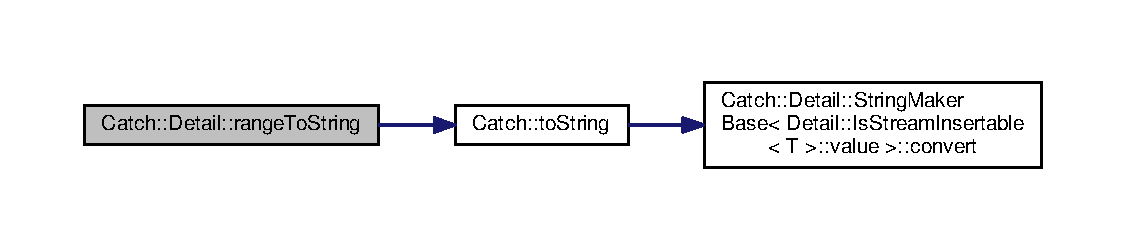
\includegraphics[width=350pt]{namespace_catch_1_1_detail_a6650a1dff325bf29962ff15ae73fd972_cgraph}
\end{center}
\end{figure}




Here is the caller graph for this function\-:
\nopagebreak
\begin{figure}[H]
\begin{center}
\leavevmode
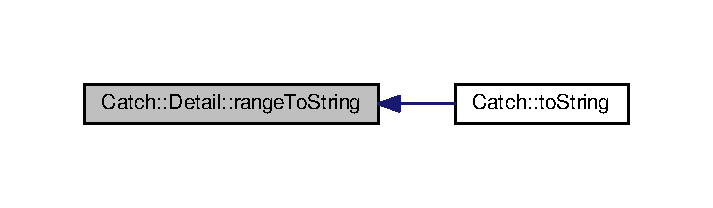
\includegraphics[width=342pt]{namespace_catch_1_1_detail_a6650a1dff325bf29962ff15ae73fd972_icgraph}
\end{center}
\end{figure}


\hypertarget{namespace_catch_1_1_detail_ac5d6c510e565ee5bddcc2236194ce29e}{\index{Catch\-::\-Detail@{Catch\-::\-Detail}!raw\-Memory\-To\-String@{raw\-Memory\-To\-String}}
\index{raw\-Memory\-To\-String@{raw\-Memory\-To\-String}!Catch::Detail@{Catch\-::\-Detail}}
\subsubsection[{raw\-Memory\-To\-String}]{\setlength{\rightskip}{0pt plus 5cm}std\-::string Catch\-::\-Detail\-::raw\-Memory\-To\-String (
\begin{DoxyParamCaption}
\item[{const void $\ast$}]{object, }
\item[{std\-::size\-\_\-t}]{size}
\end{DoxyParamCaption}
)}}\label{namespace_catch_1_1_detail_ac5d6c510e565ee5bddcc2236194ce29e}


Here is the caller graph for this function\-:
\nopagebreak
\begin{figure}[H]
\begin{center}
\leavevmode
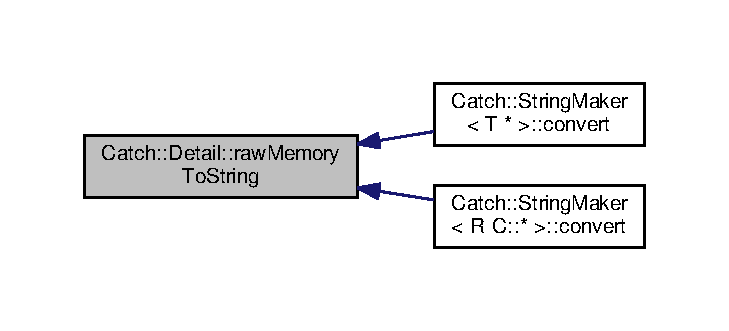
\includegraphics[width=350pt]{namespace_catch_1_1_detail_ac5d6c510e565ee5bddcc2236194ce29e_icgraph}
\end{center}
\end{figure}


\hypertarget{namespace_catch_1_1_detail_a371620ed524abfcae5c3772bf49b563a}{\index{Catch\-::\-Detail@{Catch\-::\-Detail}!raw\-Memory\-To\-String@{raw\-Memory\-To\-String}}
\index{raw\-Memory\-To\-String@{raw\-Memory\-To\-String}!Catch::Detail@{Catch\-::\-Detail}}
\subsubsection[{raw\-Memory\-To\-String}]{\setlength{\rightskip}{0pt plus 5cm}template$<$typename T $>$ std\-::string Catch\-::\-Detail\-::raw\-Memory\-To\-String (
\begin{DoxyParamCaption}
\item[{const T \&}]{object}
\end{DoxyParamCaption}
)\hspace{0.3cm}{\ttfamily [inline]}}}\label{namespace_catch_1_1_detail_a371620ed524abfcae5c3772bf49b563a}
\hypertarget{namespace_catch_1_1_detail_aff0ca0f561ad8053654ab27d54486197}{\index{Catch\-::\-Detail@{Catch\-::\-Detail}!test\-Streamable@{test\-Streamable}}
\index{test\-Streamable@{test\-Streamable}!Catch::Detail@{Catch\-::\-Detail}}
\subsubsection[{test\-Streamable}]{\setlength{\rightskip}{0pt plus 5cm}{\bf True\-Type}\& Catch\-::\-Detail\-::test\-Streamable (
\begin{DoxyParamCaption}
\item[{std\-::ostream \&}]{}
\end{DoxyParamCaption}
)}}\label{namespace_catch_1_1_detail_aff0ca0f561ad8053654ab27d54486197}
\hypertarget{namespace_catch_1_1_detail_aac81f01b0d687f75b8f24a925591b7ac}{\index{Catch\-::\-Detail@{Catch\-::\-Detail}!test\-Streamable@{test\-Streamable}}
\index{test\-Streamable@{test\-Streamable}!Catch::Detail@{Catch\-::\-Detail}}
\subsubsection[{test\-Streamable}]{\setlength{\rightskip}{0pt plus 5cm}{\bf False\-Type} Catch\-::\-Detail\-::test\-Streamable (
\begin{DoxyParamCaption}
\item[{False\-Type}]{}
\end{DoxyParamCaption}
)}}\label{namespace_catch_1_1_detail_aac81f01b0d687f75b8f24a925591b7ac}


\subsection{Variable Documentation}
\hypertarget{namespace_catch_1_1_detail_a466775f4eec29ffef29ab334cd885136}{\index{Catch\-::\-Detail@{Catch\-::\-Detail}!unprintable\-String@{unprintable\-String}}
\index{unprintable\-String@{unprintable\-String}!Catch::Detail@{Catch\-::\-Detail}}
\subsubsection[{unprintable\-String}]{\setlength{\rightskip}{0pt plus 5cm}const std\-::string Catch\-::\-Detail\-::unprintable\-String}}\label{namespace_catch_1_1_detail_a466775f4eec29ffef29ab334cd885136}

\hypertarget{namespace_catch_1_1_generators}{\section{Catch\-:\-:Generators Namespace Reference}
\label{namespace_catch_1_1_generators}\index{Catch\-::\-Generators@{Catch\-::\-Generators}}
}
\subsection*{Functions}
\begin{DoxyCompactItemize}
\item 
{\footnotesize template$<$typename T $>$ }\\\hyperlink{class_catch_1_1_composite_generator}{Composite\-Generator}$<$ T $>$ \hyperlink{namespace_catch_1_1_generators_a030abfa7ee3c58d909cf6a6aa0405265}{between} (T from, T to)
\item 
{\footnotesize template$<$typename T $>$ }\\\hyperlink{class_catch_1_1_composite_generator}{Composite\-Generator}$<$ T $>$ \hyperlink{namespace_catch_1_1_generators_a7a2c5bebb3c06c5b0ca05a80289b9eb1}{values} (T val1, T val2)
\item 
{\footnotesize template$<$typename T $>$ }\\\hyperlink{class_catch_1_1_composite_generator}{Composite\-Generator}$<$ T $>$ \hyperlink{namespace_catch_1_1_generators_a496c4a826107e47203b6c609cfd8c2c5}{values} (T val1, T val2, T val3)
\item 
{\footnotesize template$<$typename T $>$ }\\\hyperlink{class_catch_1_1_composite_generator}{Composite\-Generator}$<$ T $>$ \hyperlink{namespace_catch_1_1_generators_afb1dcf02bfc8cdf990f27fdc7d7e4a4e}{values} (T val1, T val2, T val3, T val4)
\end{DoxyCompactItemize}


\subsection{Function Documentation}
\hypertarget{namespace_catch_1_1_generators_a030abfa7ee3c58d909cf6a6aa0405265}{\index{Catch\-::\-Generators@{Catch\-::\-Generators}!between@{between}}
\index{between@{between}!Catch::Generators@{Catch\-::\-Generators}}
\subsubsection[{between}]{\setlength{\rightskip}{0pt plus 5cm}template$<$typename T $>$ {\bf Composite\-Generator}$<$T$>$ Catch\-::\-Generators\-::between (
\begin{DoxyParamCaption}
\item[{T}]{from, }
\item[{T}]{to}
\end{DoxyParamCaption}
)}}\label{namespace_catch_1_1_generators_a030abfa7ee3c58d909cf6a6aa0405265}


Here is the call graph for this function\-:
\nopagebreak
\begin{figure}[H]
\begin{center}
\leavevmode
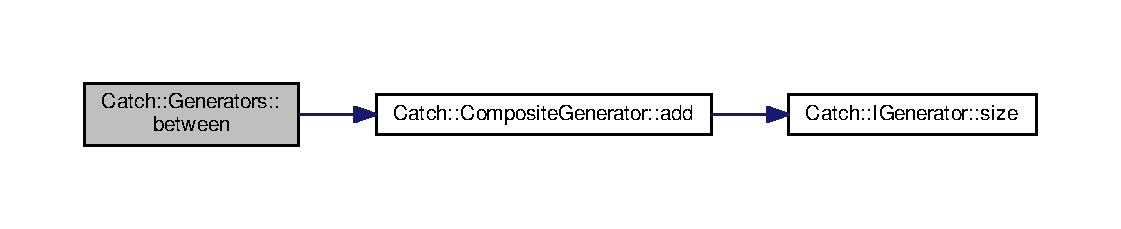
\includegraphics[width=350pt]{namespace_catch_1_1_generators_a030abfa7ee3c58d909cf6a6aa0405265_cgraph}
\end{center}
\end{figure}


\hypertarget{namespace_catch_1_1_generators_a7a2c5bebb3c06c5b0ca05a80289b9eb1}{\index{Catch\-::\-Generators@{Catch\-::\-Generators}!values@{values}}
\index{values@{values}!Catch::Generators@{Catch\-::\-Generators}}
\subsubsection[{values}]{\setlength{\rightskip}{0pt plus 5cm}template$<$typename T $>$ {\bf Composite\-Generator}$<$T$>$ Catch\-::\-Generators\-::values (
\begin{DoxyParamCaption}
\item[{T}]{val1, }
\item[{T}]{val2}
\end{DoxyParamCaption}
)}}\label{namespace_catch_1_1_generators_a7a2c5bebb3c06c5b0ca05a80289b9eb1}


Here is the call graph for this function\-:
\nopagebreak
\begin{figure}[H]
\begin{center}
\leavevmode
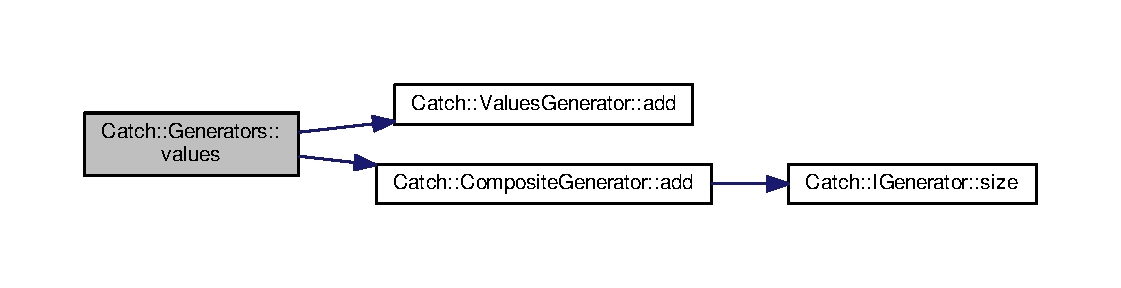
\includegraphics[width=350pt]{namespace_catch_1_1_generators_a7a2c5bebb3c06c5b0ca05a80289b9eb1_cgraph}
\end{center}
\end{figure}


\hypertarget{namespace_catch_1_1_generators_a496c4a826107e47203b6c609cfd8c2c5}{\index{Catch\-::\-Generators@{Catch\-::\-Generators}!values@{values}}
\index{values@{values}!Catch::Generators@{Catch\-::\-Generators}}
\subsubsection[{values}]{\setlength{\rightskip}{0pt plus 5cm}template$<$typename T $>$ {\bf Composite\-Generator}$<$T$>$ Catch\-::\-Generators\-::values (
\begin{DoxyParamCaption}
\item[{T}]{val1, }
\item[{T}]{val2, }
\item[{T}]{val3}
\end{DoxyParamCaption}
)}}\label{namespace_catch_1_1_generators_a496c4a826107e47203b6c609cfd8c2c5}


Here is the call graph for this function\-:
\nopagebreak
\begin{figure}[H]
\begin{center}
\leavevmode
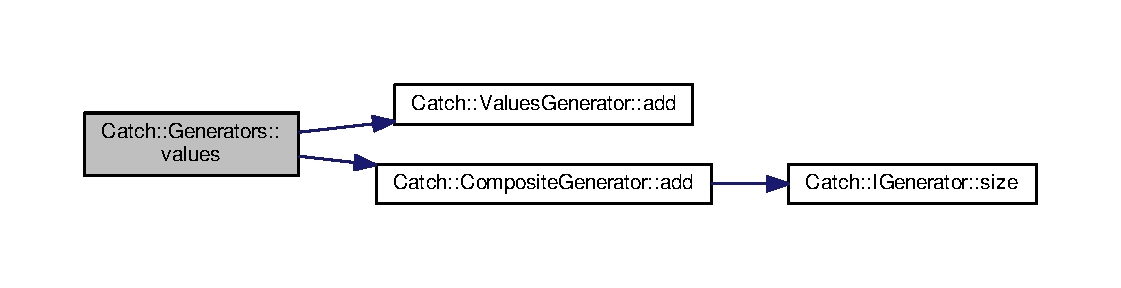
\includegraphics[width=350pt]{namespace_catch_1_1_generators_a496c4a826107e47203b6c609cfd8c2c5_cgraph}
\end{center}
\end{figure}


\hypertarget{namespace_catch_1_1_generators_afb1dcf02bfc8cdf990f27fdc7d7e4a4e}{\index{Catch\-::\-Generators@{Catch\-::\-Generators}!values@{values}}
\index{values@{values}!Catch::Generators@{Catch\-::\-Generators}}
\subsubsection[{values}]{\setlength{\rightskip}{0pt plus 5cm}template$<$typename T $>$ {\bf Composite\-Generator}$<$T$>$ Catch\-::\-Generators\-::values (
\begin{DoxyParamCaption}
\item[{T}]{val1, }
\item[{T}]{val2, }
\item[{T}]{val3, }
\item[{T}]{val4}
\end{DoxyParamCaption}
)}}\label{namespace_catch_1_1_generators_afb1dcf02bfc8cdf990f27fdc7d7e4a4e}


Here is the call graph for this function\-:
\nopagebreak
\begin{figure}[H]
\begin{center}
\leavevmode
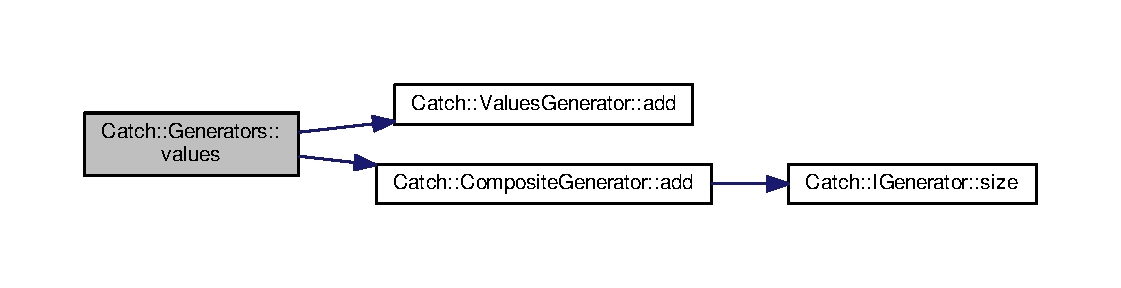
\includegraphics[width=350pt]{namespace_catch_1_1_generators_afb1dcf02bfc8cdf990f27fdc7d7e4a4e_cgraph}
\end{center}
\end{figure}



\hypertarget{namespace_catch_1_1_internal}{\section{Catch\-:\-:Internal Namespace Reference}
\label{namespace_catch_1_1_internal}\index{Catch\-::\-Internal@{Catch\-::\-Internal}}
}
\subsection*{Classes}
\begin{DoxyCompactItemize}
\item 
struct \hyperlink{struct_catch_1_1_internal_1_1_operator_traits}{Operator\-Traits}
\item 
struct \hyperlink{struct_catch_1_1_internal_1_1_operator_traits_3_01_is_equal_to_01_4}{Operator\-Traits$<$ Is\-Equal\-To $>$}
\item 
struct \hyperlink{struct_catch_1_1_internal_1_1_operator_traits_3_01_is_not_equal_to_01_4}{Operator\-Traits$<$ Is\-Not\-Equal\-To $>$}
\item 
struct \hyperlink{struct_catch_1_1_internal_1_1_operator_traits_3_01_is_less_than_01_4}{Operator\-Traits$<$ Is\-Less\-Than $>$}
\item 
struct \hyperlink{struct_catch_1_1_internal_1_1_operator_traits_3_01_is_greater_than_01_4}{Operator\-Traits$<$ Is\-Greater\-Than $>$}
\item 
struct \hyperlink{struct_catch_1_1_internal_1_1_operator_traits_3_01_is_less_than_or_equal_to_01_4}{Operator\-Traits$<$ Is\-Less\-Than\-Or\-Equal\-To $>$}
\item 
struct \hyperlink{struct_catch_1_1_internal_1_1_operator_traits_3_01_is_greater_than_or_equal_to_01_4}{Operator\-Traits$<$ Is\-Greater\-Than\-Or\-Equal\-To $>$}
\item 
class \hyperlink{class_catch_1_1_internal_1_1_evaluator}{Evaluator}
\item 
struct \hyperlink{struct_catch_1_1_internal_1_1_evaluator_3_01_t1_00_01_t2_00_01_is_equal_to_01_4}{Evaluator$<$ T1, T2, Is\-Equal\-To $>$}
\item 
struct \hyperlink{struct_catch_1_1_internal_1_1_evaluator_3_01_t1_00_01_t2_00_01_is_not_equal_to_01_4}{Evaluator$<$ T1, T2, Is\-Not\-Equal\-To $>$}
\item 
struct \hyperlink{struct_catch_1_1_internal_1_1_evaluator_3_01_t1_00_01_t2_00_01_is_less_than_01_4}{Evaluator$<$ T1, T2, Is\-Less\-Than $>$}
\item 
struct \hyperlink{struct_catch_1_1_internal_1_1_evaluator_3_01_t1_00_01_t2_00_01_is_greater_than_01_4}{Evaluator$<$ T1, T2, Is\-Greater\-Than $>$}
\item 
struct \hyperlink{struct_catch_1_1_internal_1_1_evaluator_3_01_t1_00_01_t2_00_01_is_greater_than_or_equal_to_01_4}{Evaluator$<$ T1, T2, Is\-Greater\-Than\-Or\-Equal\-To $>$}
\item 
struct \hyperlink{struct_catch_1_1_internal_1_1_evaluator_3_01_t1_00_01_t2_00_01_is_less_than_or_equal_to_01_4}{Evaluator$<$ T1, T2, Is\-Less\-Than\-Or\-Equal\-To $>$}
\end{DoxyCompactItemize}
\subsection*{Enumerations}
\begin{DoxyCompactItemize}
\item 
enum \hyperlink{namespace_catch_1_1_internal_ae3f96598a7858155750bf38e7295d83e}{Operator} \{ \\*
\hyperlink{namespace_catch_1_1_internal_ae3f96598a7858155750bf38e7295d83ea30e0accba6ec8384f4383b04dd2a6a9e}{Is\-Equal\-To}, 
\hyperlink{namespace_catch_1_1_internal_ae3f96598a7858155750bf38e7295d83ea1e1699cf7d3dbee0908f1a123da2456d}{Is\-Not\-Equal\-To}, 
\hyperlink{namespace_catch_1_1_internal_ae3f96598a7858155750bf38e7295d83eabbbfc41706595e50acbefa8408004b93}{Is\-Less\-Than}, 
\hyperlink{namespace_catch_1_1_internal_ae3f96598a7858155750bf38e7295d83eac0e8866139e99803d169595af70f6c22}{Is\-Greater\-Than}, 
\\*
\hyperlink{namespace_catch_1_1_internal_ae3f96598a7858155750bf38e7295d83ea0db29a4c3f1e81260036c5e27a8407fd}{Is\-Less\-Than\-Or\-Equal\-To}, 
\hyperlink{namespace_catch_1_1_internal_ae3f96598a7858155750bf38e7295d83ead2de7e9565e59e36c0987e402203ce1c}{Is\-Greater\-Than\-Or\-Equal\-To}
 \}
\end{DoxyCompactItemize}
\subsection*{Functions}
\begin{DoxyCompactItemize}
\item 
{\footnotesize template$<$typename T $>$ }\\T \& \hyperlink{namespace_catch_1_1_internal_adde98c1a650e94615e2b37ab0b3734e2}{op\-Cast} (T const \&t)
\item 
{\footnotesize template$<$Operator Op, typename T1 , typename T2 $>$ }\\bool \hyperlink{namespace_catch_1_1_internal_a3849d993997f2b708281ff02e77dfecf}{apply\-Evaluator} (T1 const \&lhs, T2 const \&rhs)
\item 
{\footnotesize template$<$Operator Op, typename T1 , typename T2 $>$ }\\bool \hyperlink{namespace_catch_1_1_internal_a64ae04769c4583b9d4027c792b496c7d}{compare} (T1 const \&lhs, T2 const \&rhs)
\item 
{\footnotesize template$<$Operator Op$>$ }\\bool \hyperlink{namespace_catch_1_1_internal_a171aec1826898b877980a2b15fe5f735}{compare} (unsigned int lhs, int rhs)
\item 
{\footnotesize template$<$Operator Op$>$ }\\bool \hyperlink{namespace_catch_1_1_internal_aa2698c33ec87b16aff5c844165483a7a}{compare} (unsigned long lhs, int rhs)
\item 
{\footnotesize template$<$Operator Op$>$ }\\bool \hyperlink{namespace_catch_1_1_internal_ad68724393ee3d7629001a2997f6134cc}{compare} (unsigned char lhs, int rhs)
\item 
{\footnotesize template$<$Operator Op$>$ }\\bool \hyperlink{namespace_catch_1_1_internal_ac2af7b6757f9bb3539bb78acff5c4649}{compare} (unsigned int lhs, long rhs)
\item 
{\footnotesize template$<$Operator Op$>$ }\\bool \hyperlink{namespace_catch_1_1_internal_ace20062a489a8a7049fe224d62e644a7}{compare} (unsigned long lhs, long rhs)
\item 
{\footnotesize template$<$Operator Op$>$ }\\bool \hyperlink{namespace_catch_1_1_internal_a640e0cce9260a912842bee58db501dc5}{compare} (unsigned char lhs, long rhs)
\item 
{\footnotesize template$<$Operator Op$>$ }\\bool \hyperlink{namespace_catch_1_1_internal_a17c92ed4b6d88a9f8bbcbc52544fe40f}{compare} (int lhs, unsigned int rhs)
\item 
{\footnotesize template$<$Operator Op$>$ }\\bool \hyperlink{namespace_catch_1_1_internal_aac7a6452ed0d324031ceb7b4f3a3b61c}{compare} (int lhs, unsigned long rhs)
\item 
{\footnotesize template$<$Operator Op$>$ }\\bool \hyperlink{namespace_catch_1_1_internal_a7e82d987f62b9822107027c72a55fa6b}{compare} (int lhs, unsigned char rhs)
\item 
{\footnotesize template$<$Operator Op$>$ }\\bool \hyperlink{namespace_catch_1_1_internal_a0b4783ede1901e5c1baf8ff909bcce8d}{compare} (long lhs, unsigned int rhs)
\item 
{\footnotesize template$<$Operator Op$>$ }\\bool \hyperlink{namespace_catch_1_1_internal_ae9aec44a08d9cbb0d3dd46d438b50d2c}{compare} (long lhs, unsigned long rhs)
\item 
{\footnotesize template$<$Operator Op$>$ }\\bool \hyperlink{namespace_catch_1_1_internal_a79664b5f5f497fba57bd156e098de1f2}{compare} (long lhs, unsigned char rhs)
\item 
{\footnotesize template$<$Operator Op, typename T $>$ }\\bool \hyperlink{namespace_catch_1_1_internal_a829570ad9e724c687aa42190a696032b}{compare} (long lhs, T $\ast$rhs)
\item 
{\footnotesize template$<$Operator Op, typename T $>$ }\\bool \hyperlink{namespace_catch_1_1_internal_a3f89c65fdb06aa7b648c5acf0ca107a9}{compare} (T $\ast$lhs, long rhs)
\item 
{\footnotesize template$<$Operator Op, typename T $>$ }\\bool \hyperlink{namespace_catch_1_1_internal_a4f30c29e4adb62c7e209e5b988e59397}{compare} (int lhs, T $\ast$rhs)
\item 
{\footnotesize template$<$Operator Op, typename T $>$ }\\bool \hyperlink{namespace_catch_1_1_internal_a95361ddae55c9a390e6510bdadccb1fc}{compare} (T $\ast$lhs, int rhs)
\end{DoxyCompactItemize}


\subsection{Enumeration Type Documentation}
\hypertarget{namespace_catch_1_1_internal_ae3f96598a7858155750bf38e7295d83e}{\index{Catch\-::\-Internal@{Catch\-::\-Internal}!Operator@{Operator}}
\index{Operator@{Operator}!Catch::Internal@{Catch\-::\-Internal}}
\subsubsection[{Operator}]{\setlength{\rightskip}{0pt plus 5cm}enum {\bf Catch\-::\-Internal\-::\-Operator}}}\label{namespace_catch_1_1_internal_ae3f96598a7858155750bf38e7295d83e}
\begin{Desc}
\item[Enumerator]\par
\begin{description}
\index{Is\-Equal\-To@{Is\-Equal\-To}!Catch\-::\-Internal@{Catch\-::\-Internal}}\index{Catch\-::\-Internal@{Catch\-::\-Internal}!Is\-Equal\-To@{Is\-Equal\-To}}\item[{\em 
\hypertarget{namespace_catch_1_1_internal_ae3f96598a7858155750bf38e7295d83ea30e0accba6ec8384f4383b04dd2a6a9e}{Is\-Equal\-To}\label{namespace_catch_1_1_internal_ae3f96598a7858155750bf38e7295d83ea30e0accba6ec8384f4383b04dd2a6a9e}
}]\index{Is\-Not\-Equal\-To@{Is\-Not\-Equal\-To}!Catch\-::\-Internal@{Catch\-::\-Internal}}\index{Catch\-::\-Internal@{Catch\-::\-Internal}!Is\-Not\-Equal\-To@{Is\-Not\-Equal\-To}}\item[{\em 
\hypertarget{namespace_catch_1_1_internal_ae3f96598a7858155750bf38e7295d83ea1e1699cf7d3dbee0908f1a123da2456d}{Is\-Not\-Equal\-To}\label{namespace_catch_1_1_internal_ae3f96598a7858155750bf38e7295d83ea1e1699cf7d3dbee0908f1a123da2456d}
}]\index{Is\-Less\-Than@{Is\-Less\-Than}!Catch\-::\-Internal@{Catch\-::\-Internal}}\index{Catch\-::\-Internal@{Catch\-::\-Internal}!Is\-Less\-Than@{Is\-Less\-Than}}\item[{\em 
\hypertarget{namespace_catch_1_1_internal_ae3f96598a7858155750bf38e7295d83eabbbfc41706595e50acbefa8408004b93}{Is\-Less\-Than}\label{namespace_catch_1_1_internal_ae3f96598a7858155750bf38e7295d83eabbbfc41706595e50acbefa8408004b93}
}]\index{Is\-Greater\-Than@{Is\-Greater\-Than}!Catch\-::\-Internal@{Catch\-::\-Internal}}\index{Catch\-::\-Internal@{Catch\-::\-Internal}!Is\-Greater\-Than@{Is\-Greater\-Than}}\item[{\em 
\hypertarget{namespace_catch_1_1_internal_ae3f96598a7858155750bf38e7295d83eac0e8866139e99803d169595af70f6c22}{Is\-Greater\-Than}\label{namespace_catch_1_1_internal_ae3f96598a7858155750bf38e7295d83eac0e8866139e99803d169595af70f6c22}
}]\index{Is\-Less\-Than\-Or\-Equal\-To@{Is\-Less\-Than\-Or\-Equal\-To}!Catch\-::\-Internal@{Catch\-::\-Internal}}\index{Catch\-::\-Internal@{Catch\-::\-Internal}!Is\-Less\-Than\-Or\-Equal\-To@{Is\-Less\-Than\-Or\-Equal\-To}}\item[{\em 
\hypertarget{namespace_catch_1_1_internal_ae3f96598a7858155750bf38e7295d83ea0db29a4c3f1e81260036c5e27a8407fd}{Is\-Less\-Than\-Or\-Equal\-To}\label{namespace_catch_1_1_internal_ae3f96598a7858155750bf38e7295d83ea0db29a4c3f1e81260036c5e27a8407fd}
}]\index{Is\-Greater\-Than\-Or\-Equal\-To@{Is\-Greater\-Than\-Or\-Equal\-To}!Catch\-::\-Internal@{Catch\-::\-Internal}}\index{Catch\-::\-Internal@{Catch\-::\-Internal}!Is\-Greater\-Than\-Or\-Equal\-To@{Is\-Greater\-Than\-Or\-Equal\-To}}\item[{\em 
\hypertarget{namespace_catch_1_1_internal_ae3f96598a7858155750bf38e7295d83ead2de7e9565e59e36c0987e402203ce1c}{Is\-Greater\-Than\-Or\-Equal\-To}\label{namespace_catch_1_1_internal_ae3f96598a7858155750bf38e7295d83ead2de7e9565e59e36c0987e402203ce1c}
}]\end{description}
\end{Desc}


\subsection{Function Documentation}
\hypertarget{namespace_catch_1_1_internal_a3849d993997f2b708281ff02e77dfecf}{\index{Catch\-::\-Internal@{Catch\-::\-Internal}!apply\-Evaluator@{apply\-Evaluator}}
\index{apply\-Evaluator@{apply\-Evaluator}!Catch::Internal@{Catch\-::\-Internal}}
\subsubsection[{apply\-Evaluator}]{\setlength{\rightskip}{0pt plus 5cm}template$<$Operator Op, typename T1 , typename T2 $>$ bool Catch\-::\-Internal\-::apply\-Evaluator (
\begin{DoxyParamCaption}
\item[{T1 const \&}]{lhs, }
\item[{T2 const \&}]{rhs}
\end{DoxyParamCaption}
)}}\label{namespace_catch_1_1_internal_a3849d993997f2b708281ff02e77dfecf}
\hypertarget{namespace_catch_1_1_internal_a64ae04769c4583b9d4027c792b496c7d}{\index{Catch\-::\-Internal@{Catch\-::\-Internal}!compare@{compare}}
\index{compare@{compare}!Catch::Internal@{Catch\-::\-Internal}}
\subsubsection[{compare}]{\setlength{\rightskip}{0pt plus 5cm}template$<$Operator Op, typename T1 , typename T2 $>$ bool Catch\-::\-Internal\-::compare (
\begin{DoxyParamCaption}
\item[{T1 const \&}]{lhs, }
\item[{T2 const \&}]{rhs}
\end{DoxyParamCaption}
)}}\label{namespace_catch_1_1_internal_a64ae04769c4583b9d4027c792b496c7d}
\hypertarget{namespace_catch_1_1_internal_a171aec1826898b877980a2b15fe5f735}{\index{Catch\-::\-Internal@{Catch\-::\-Internal}!compare@{compare}}
\index{compare@{compare}!Catch::Internal@{Catch\-::\-Internal}}
\subsubsection[{compare}]{\setlength{\rightskip}{0pt plus 5cm}template$<$Operator Op$>$ bool Catch\-::\-Internal\-::compare (
\begin{DoxyParamCaption}
\item[{unsigned int}]{lhs, }
\item[{int}]{rhs}
\end{DoxyParamCaption}
)}}\label{namespace_catch_1_1_internal_a171aec1826898b877980a2b15fe5f735}
\hypertarget{namespace_catch_1_1_internal_aa2698c33ec87b16aff5c844165483a7a}{\index{Catch\-::\-Internal@{Catch\-::\-Internal}!compare@{compare}}
\index{compare@{compare}!Catch::Internal@{Catch\-::\-Internal}}
\subsubsection[{compare}]{\setlength{\rightskip}{0pt plus 5cm}template$<$Operator Op$>$ bool Catch\-::\-Internal\-::compare (
\begin{DoxyParamCaption}
\item[{unsigned long}]{lhs, }
\item[{int}]{rhs}
\end{DoxyParamCaption}
)}}\label{namespace_catch_1_1_internal_aa2698c33ec87b16aff5c844165483a7a}
\hypertarget{namespace_catch_1_1_internal_ad68724393ee3d7629001a2997f6134cc}{\index{Catch\-::\-Internal@{Catch\-::\-Internal}!compare@{compare}}
\index{compare@{compare}!Catch::Internal@{Catch\-::\-Internal}}
\subsubsection[{compare}]{\setlength{\rightskip}{0pt plus 5cm}template$<$Operator Op$>$ bool Catch\-::\-Internal\-::compare (
\begin{DoxyParamCaption}
\item[{unsigned char}]{lhs, }
\item[{int}]{rhs}
\end{DoxyParamCaption}
)}}\label{namespace_catch_1_1_internal_ad68724393ee3d7629001a2997f6134cc}
\hypertarget{namespace_catch_1_1_internal_ac2af7b6757f9bb3539bb78acff5c4649}{\index{Catch\-::\-Internal@{Catch\-::\-Internal}!compare@{compare}}
\index{compare@{compare}!Catch::Internal@{Catch\-::\-Internal}}
\subsubsection[{compare}]{\setlength{\rightskip}{0pt plus 5cm}template$<$Operator Op$>$ bool Catch\-::\-Internal\-::compare (
\begin{DoxyParamCaption}
\item[{unsigned int}]{lhs, }
\item[{long}]{rhs}
\end{DoxyParamCaption}
)}}\label{namespace_catch_1_1_internal_ac2af7b6757f9bb3539bb78acff5c4649}
\hypertarget{namespace_catch_1_1_internal_ace20062a489a8a7049fe224d62e644a7}{\index{Catch\-::\-Internal@{Catch\-::\-Internal}!compare@{compare}}
\index{compare@{compare}!Catch::Internal@{Catch\-::\-Internal}}
\subsubsection[{compare}]{\setlength{\rightskip}{0pt plus 5cm}template$<$Operator Op$>$ bool Catch\-::\-Internal\-::compare (
\begin{DoxyParamCaption}
\item[{unsigned long}]{lhs, }
\item[{long}]{rhs}
\end{DoxyParamCaption}
)}}\label{namespace_catch_1_1_internal_ace20062a489a8a7049fe224d62e644a7}
\hypertarget{namespace_catch_1_1_internal_a640e0cce9260a912842bee58db501dc5}{\index{Catch\-::\-Internal@{Catch\-::\-Internal}!compare@{compare}}
\index{compare@{compare}!Catch::Internal@{Catch\-::\-Internal}}
\subsubsection[{compare}]{\setlength{\rightskip}{0pt plus 5cm}template$<$Operator Op$>$ bool Catch\-::\-Internal\-::compare (
\begin{DoxyParamCaption}
\item[{unsigned char}]{lhs, }
\item[{long}]{rhs}
\end{DoxyParamCaption}
)}}\label{namespace_catch_1_1_internal_a640e0cce9260a912842bee58db501dc5}
\hypertarget{namespace_catch_1_1_internal_a17c92ed4b6d88a9f8bbcbc52544fe40f}{\index{Catch\-::\-Internal@{Catch\-::\-Internal}!compare@{compare}}
\index{compare@{compare}!Catch::Internal@{Catch\-::\-Internal}}
\subsubsection[{compare}]{\setlength{\rightskip}{0pt plus 5cm}template$<$Operator Op$>$ bool Catch\-::\-Internal\-::compare (
\begin{DoxyParamCaption}
\item[{int}]{lhs, }
\item[{unsigned int}]{rhs}
\end{DoxyParamCaption}
)}}\label{namespace_catch_1_1_internal_a17c92ed4b6d88a9f8bbcbc52544fe40f}
\hypertarget{namespace_catch_1_1_internal_aac7a6452ed0d324031ceb7b4f3a3b61c}{\index{Catch\-::\-Internal@{Catch\-::\-Internal}!compare@{compare}}
\index{compare@{compare}!Catch::Internal@{Catch\-::\-Internal}}
\subsubsection[{compare}]{\setlength{\rightskip}{0pt plus 5cm}template$<$Operator Op$>$ bool Catch\-::\-Internal\-::compare (
\begin{DoxyParamCaption}
\item[{int}]{lhs, }
\item[{unsigned long}]{rhs}
\end{DoxyParamCaption}
)}}\label{namespace_catch_1_1_internal_aac7a6452ed0d324031ceb7b4f3a3b61c}
\hypertarget{namespace_catch_1_1_internal_a7e82d987f62b9822107027c72a55fa6b}{\index{Catch\-::\-Internal@{Catch\-::\-Internal}!compare@{compare}}
\index{compare@{compare}!Catch::Internal@{Catch\-::\-Internal}}
\subsubsection[{compare}]{\setlength{\rightskip}{0pt plus 5cm}template$<$Operator Op$>$ bool Catch\-::\-Internal\-::compare (
\begin{DoxyParamCaption}
\item[{int}]{lhs, }
\item[{unsigned char}]{rhs}
\end{DoxyParamCaption}
)}}\label{namespace_catch_1_1_internal_a7e82d987f62b9822107027c72a55fa6b}
\hypertarget{namespace_catch_1_1_internal_a0b4783ede1901e5c1baf8ff909bcce8d}{\index{Catch\-::\-Internal@{Catch\-::\-Internal}!compare@{compare}}
\index{compare@{compare}!Catch::Internal@{Catch\-::\-Internal}}
\subsubsection[{compare}]{\setlength{\rightskip}{0pt plus 5cm}template$<$Operator Op$>$ bool Catch\-::\-Internal\-::compare (
\begin{DoxyParamCaption}
\item[{long}]{lhs, }
\item[{unsigned int}]{rhs}
\end{DoxyParamCaption}
)}}\label{namespace_catch_1_1_internal_a0b4783ede1901e5c1baf8ff909bcce8d}
\hypertarget{namespace_catch_1_1_internal_ae9aec44a08d9cbb0d3dd46d438b50d2c}{\index{Catch\-::\-Internal@{Catch\-::\-Internal}!compare@{compare}}
\index{compare@{compare}!Catch::Internal@{Catch\-::\-Internal}}
\subsubsection[{compare}]{\setlength{\rightskip}{0pt plus 5cm}template$<$Operator Op$>$ bool Catch\-::\-Internal\-::compare (
\begin{DoxyParamCaption}
\item[{long}]{lhs, }
\item[{unsigned long}]{rhs}
\end{DoxyParamCaption}
)}}\label{namespace_catch_1_1_internal_ae9aec44a08d9cbb0d3dd46d438b50d2c}
\hypertarget{namespace_catch_1_1_internal_a79664b5f5f497fba57bd156e098de1f2}{\index{Catch\-::\-Internal@{Catch\-::\-Internal}!compare@{compare}}
\index{compare@{compare}!Catch::Internal@{Catch\-::\-Internal}}
\subsubsection[{compare}]{\setlength{\rightskip}{0pt plus 5cm}template$<$Operator Op$>$ bool Catch\-::\-Internal\-::compare (
\begin{DoxyParamCaption}
\item[{long}]{lhs, }
\item[{unsigned char}]{rhs}
\end{DoxyParamCaption}
)}}\label{namespace_catch_1_1_internal_a79664b5f5f497fba57bd156e098de1f2}
\hypertarget{namespace_catch_1_1_internal_a829570ad9e724c687aa42190a696032b}{\index{Catch\-::\-Internal@{Catch\-::\-Internal}!compare@{compare}}
\index{compare@{compare}!Catch::Internal@{Catch\-::\-Internal}}
\subsubsection[{compare}]{\setlength{\rightskip}{0pt plus 5cm}template$<$Operator Op, typename T $>$ bool Catch\-::\-Internal\-::compare (
\begin{DoxyParamCaption}
\item[{long}]{lhs, }
\item[{T $\ast$}]{rhs}
\end{DoxyParamCaption}
)}}\label{namespace_catch_1_1_internal_a829570ad9e724c687aa42190a696032b}
\hypertarget{namespace_catch_1_1_internal_a3f89c65fdb06aa7b648c5acf0ca107a9}{\index{Catch\-::\-Internal@{Catch\-::\-Internal}!compare@{compare}}
\index{compare@{compare}!Catch::Internal@{Catch\-::\-Internal}}
\subsubsection[{compare}]{\setlength{\rightskip}{0pt plus 5cm}template$<$Operator Op, typename T $>$ bool Catch\-::\-Internal\-::compare (
\begin{DoxyParamCaption}
\item[{T $\ast$}]{lhs, }
\item[{long}]{rhs}
\end{DoxyParamCaption}
)}}\label{namespace_catch_1_1_internal_a3f89c65fdb06aa7b648c5acf0ca107a9}
\hypertarget{namespace_catch_1_1_internal_a4f30c29e4adb62c7e209e5b988e59397}{\index{Catch\-::\-Internal@{Catch\-::\-Internal}!compare@{compare}}
\index{compare@{compare}!Catch::Internal@{Catch\-::\-Internal}}
\subsubsection[{compare}]{\setlength{\rightskip}{0pt plus 5cm}template$<$Operator Op, typename T $>$ bool Catch\-::\-Internal\-::compare (
\begin{DoxyParamCaption}
\item[{int}]{lhs, }
\item[{T $\ast$}]{rhs}
\end{DoxyParamCaption}
)}}\label{namespace_catch_1_1_internal_a4f30c29e4adb62c7e209e5b988e59397}
\hypertarget{namespace_catch_1_1_internal_a95361ddae55c9a390e6510bdadccb1fc}{\index{Catch\-::\-Internal@{Catch\-::\-Internal}!compare@{compare}}
\index{compare@{compare}!Catch::Internal@{Catch\-::\-Internal}}
\subsubsection[{compare}]{\setlength{\rightskip}{0pt plus 5cm}template$<$Operator Op, typename T $>$ bool Catch\-::\-Internal\-::compare (
\begin{DoxyParamCaption}
\item[{T $\ast$}]{lhs, }
\item[{int}]{rhs}
\end{DoxyParamCaption}
)}}\label{namespace_catch_1_1_internal_a95361ddae55c9a390e6510bdadccb1fc}
\hypertarget{namespace_catch_1_1_internal_adde98c1a650e94615e2b37ab0b3734e2}{\index{Catch\-::\-Internal@{Catch\-::\-Internal}!op\-Cast@{op\-Cast}}
\index{op\-Cast@{op\-Cast}!Catch::Internal@{Catch\-::\-Internal}}
\subsubsection[{op\-Cast}]{\setlength{\rightskip}{0pt plus 5cm}template$<$typename T $>$ T\& Catch\-::\-Internal\-::op\-Cast (
\begin{DoxyParamCaption}
\item[{T const \&}]{t}
\end{DoxyParamCaption}
)\hspace{0.3cm}{\ttfamily [inline]}}}\label{namespace_catch_1_1_internal_adde98c1a650e94615e2b37ab0b3734e2}


Here is the caller graph for this function\-:
\nopagebreak
\begin{figure}[H]
\begin{center}
\leavevmode
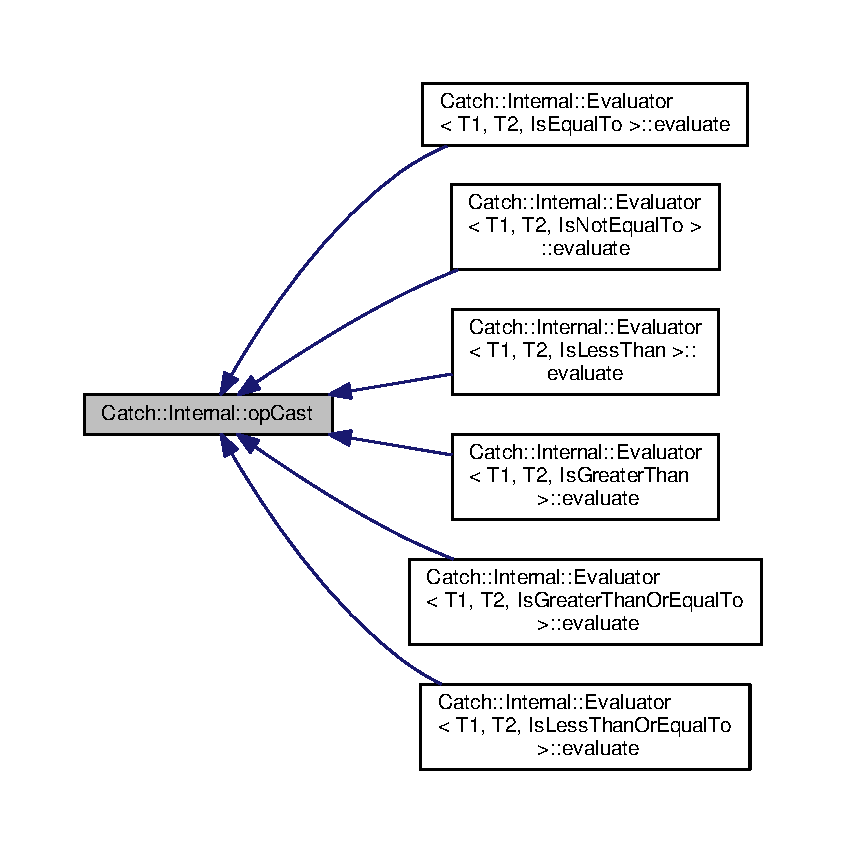
\includegraphics[width=350pt]{namespace_catch_1_1_internal_adde98c1a650e94615e2b37ab0b3734e2_icgraph}
\end{center}
\end{figure}



\hypertarget{namespace_catch_1_1_matchers}{\section{Catch\-:\-:Matchers Namespace Reference}
\label{namespace_catch_1_1_matchers}\index{Catch\-::\-Matchers@{Catch\-::\-Matchers}}
}
\subsection*{Namespaces}
\begin{DoxyCompactItemize}
\item 
\hyperlink{namespace_catch_1_1_matchers_1_1_impl}{Impl}
\item 
\hyperlink{namespace_catch_1_1_matchers_1_1_std_string}{Std\-String}
\item 
\hyperlink{namespace_catch_1_1_matchers_1_1_vector}{Vector}
\end{DoxyCompactItemize}
\subsection*{Functions}
\begin{DoxyCompactItemize}
\item 
{\footnotesize template$<$typename T $>$ }\\\hyperlink{struct_catch_1_1_matchers_1_1_impl_1_1_match_not_of}{Impl\-::\-Match\-Not\-Of}$<$ T $>$ \hyperlink{namespace_catch_1_1_matchers_acd3369efa3f62ffa1269df4b8ddf8134}{Not} (\hyperlink{struct_catch_1_1_matchers_1_1_impl_1_1_matcher_base}{Impl\-::\-Matcher\-Base}$<$ T $>$ const \&underlying\-Matcher)
\item 
{\footnotesize template$<$typename T $>$ }\\\hyperlink{struct_catch_1_1_matchers_1_1_impl_1_1_match_all_of}{Impl\-::\-Match\-All\-Of}$<$ T $>$ \hyperlink{namespace_catch_1_1_matchers_ac690851ef8a0a27206cd9cb10e3c2b18}{All\-Of} (\hyperlink{struct_catch_1_1_matchers_1_1_impl_1_1_matcher_base}{Impl\-::\-Matcher\-Base}$<$ T $>$ const \&m1, \hyperlink{struct_catch_1_1_matchers_1_1_impl_1_1_matcher_base}{Impl\-::\-Matcher\-Base}$<$ T $>$ const \&m2)
\item 
{\footnotesize template$<$typename T $>$ }\\\hyperlink{struct_catch_1_1_matchers_1_1_impl_1_1_match_all_of}{Impl\-::\-Match\-All\-Of}$<$ T $>$ \hyperlink{namespace_catch_1_1_matchers_a9cf3bef1efd3453f2528bb16d1ec5048}{All\-Of} (\hyperlink{struct_catch_1_1_matchers_1_1_impl_1_1_matcher_base}{Impl\-::\-Matcher\-Base}$<$ T $>$ const \&m1, \hyperlink{struct_catch_1_1_matchers_1_1_impl_1_1_matcher_base}{Impl\-::\-Matcher\-Base}$<$ T $>$ const \&m2, \hyperlink{struct_catch_1_1_matchers_1_1_impl_1_1_matcher_base}{Impl\-::\-Matcher\-Base}$<$ T $>$ const \&m3)
\item 
{\footnotesize template$<$typename T $>$ }\\\hyperlink{struct_catch_1_1_matchers_1_1_impl_1_1_match_any_of}{Impl\-::\-Match\-Any\-Of}$<$ T $>$ \hyperlink{namespace_catch_1_1_matchers_a07f8680aede448d54661b9ebc111ecad}{Any\-Of} (\hyperlink{struct_catch_1_1_matchers_1_1_impl_1_1_matcher_base}{Impl\-::\-Matcher\-Base}$<$ T $>$ const \&m1, \hyperlink{struct_catch_1_1_matchers_1_1_impl_1_1_matcher_base}{Impl\-::\-Matcher\-Base}$<$ T $>$ const \&m2)
\item 
{\footnotesize template$<$typename T $>$ }\\\hyperlink{struct_catch_1_1_matchers_1_1_impl_1_1_match_any_of}{Impl\-::\-Match\-Any\-Of}$<$ T $>$ \hyperlink{namespace_catch_1_1_matchers_a37055a4e76b2aa356b17a508a806a445}{Any\-Of} (\hyperlink{struct_catch_1_1_matchers_1_1_impl_1_1_matcher_base}{Impl\-::\-Matcher\-Base}$<$ T $>$ const \&m1, \hyperlink{struct_catch_1_1_matchers_1_1_impl_1_1_matcher_base}{Impl\-::\-Matcher\-Base}$<$ T $>$ const \&m2, \hyperlink{struct_catch_1_1_matchers_1_1_impl_1_1_matcher_base}{Impl\-::\-Matcher\-Base}$<$ T $>$ const \&m3)
\item 
\hyperlink{struct_catch_1_1_matchers_1_1_std_string_1_1_equals_matcher}{Std\-String\-::\-Equals\-Matcher} \hyperlink{namespace_catch_1_1_matchers_af8af7dfc338335ed4c788cb1b37fc59f}{Equals} (std\-::string const \&str, \hyperlink{struct_catch_1_1_case_sensitive_aad49d3aee2d97066642fffa919685c6a}{Case\-Sensitive\-::\-Choice} case\-Sensitivity=\hyperlink{struct_catch_1_1_case_sensitive_aad49d3aee2d97066642fffa919685c6aa7c5550b69ec3c502e6f609b67f9613c6}{Case\-Sensitive\-::\-Yes})
\item 
\hyperlink{struct_catch_1_1_matchers_1_1_std_string_1_1_contains_matcher}{Std\-String\-::\-Contains\-Matcher} \hyperlink{namespace_catch_1_1_matchers_a1f6c2accdc6cd75a84d7112dcad647b4}{Contains} (std\-::string const \&str, \hyperlink{struct_catch_1_1_case_sensitive_aad49d3aee2d97066642fffa919685c6a}{Case\-Sensitive\-::\-Choice} case\-Sensitivity=\hyperlink{struct_catch_1_1_case_sensitive_aad49d3aee2d97066642fffa919685c6aa7c5550b69ec3c502e6f609b67f9613c6}{Case\-Sensitive\-::\-Yes})
\item 
\hyperlink{struct_catch_1_1_matchers_1_1_std_string_1_1_ends_with_matcher}{Std\-String\-::\-Ends\-With\-Matcher} \hyperlink{namespace_catch_1_1_matchers_ae5a45efb4538c57c43e04f3f9043ad6e}{Ends\-With} (std\-::string const \&str, \hyperlink{struct_catch_1_1_case_sensitive_aad49d3aee2d97066642fffa919685c6a}{Case\-Sensitive\-::\-Choice} case\-Sensitivity=\hyperlink{struct_catch_1_1_case_sensitive_aad49d3aee2d97066642fffa919685c6aa7c5550b69ec3c502e6f609b67f9613c6}{Case\-Sensitive\-::\-Yes})
\item 
\hyperlink{struct_catch_1_1_matchers_1_1_std_string_1_1_starts_with_matcher}{Std\-String\-::\-Starts\-With\-Matcher} \hyperlink{namespace_catch_1_1_matchers_a97c9ee09a70378ca7e8c6f9f01b0d6d1}{Starts\-With} (std\-::string const \&str, \hyperlink{struct_catch_1_1_case_sensitive_aad49d3aee2d97066642fffa919685c6a}{Case\-Sensitive\-::\-Choice} case\-Sensitivity=\hyperlink{struct_catch_1_1_case_sensitive_aad49d3aee2d97066642fffa919685c6aa7c5550b69ec3c502e6f609b67f9613c6}{Case\-Sensitive\-::\-Yes})
\item 
{\footnotesize template$<$typename T $>$ }\\\hyperlink{struct_catch_1_1_matchers_1_1_vector_1_1_contains_matcher}{Vector\-::\-Contains\-Matcher}$<$ T $>$ \hyperlink{namespace_catch_1_1_matchers_a4b3621740dc515216ad31ab827d4092c}{Contains} (std\-::vector$<$ T $>$ const \&comparator)
\item 
{\footnotesize template$<$typename T $>$ }\\\hyperlink{struct_catch_1_1_matchers_1_1_vector_1_1_contains_element_matcher}{Vector\-::\-Contains\-Element\-Matcher}$<$ T $>$ \hyperlink{namespace_catch_1_1_matchers_ae8db5846328116fb36386893deaec944}{Vector\-Contains} (T const \&comparator)
\item 
{\footnotesize template$<$typename T $>$ }\\\hyperlink{struct_catch_1_1_matchers_1_1_vector_1_1_equals_matcher}{Vector\-::\-Equals\-Matcher}$<$ T $>$ \hyperlink{namespace_catch_1_1_matchers_a332a401fb0da33c988e9cfa400ecce1b}{Equals} (std\-::vector$<$ T $>$ const \&comparator)
\end{DoxyCompactItemize}


\subsection{Function Documentation}
\hypertarget{namespace_catch_1_1_matchers_ac690851ef8a0a27206cd9cb10e3c2b18}{\index{Catch\-::\-Matchers@{Catch\-::\-Matchers}!All\-Of@{All\-Of}}
\index{All\-Of@{All\-Of}!Catch::Matchers@{Catch\-::\-Matchers}}
\subsubsection[{All\-Of}]{\setlength{\rightskip}{0pt plus 5cm}template$<$typename T $>$ {\bf Impl\-::\-Match\-All\-Of}$<$T$>$ Catch\-::\-Matchers\-::\-All\-Of (
\begin{DoxyParamCaption}
\item[{Impl\-::\-Matcher\-Base$<$ T $>$ const \&}]{m1, }
\item[{Impl\-::\-Matcher\-Base$<$ T $>$ const \&}]{m2}
\end{DoxyParamCaption}
)\hspace{0.3cm}{\ttfamily [inline]}}}\label{namespace_catch_1_1_matchers_ac690851ef8a0a27206cd9cb10e3c2b18}
\hypertarget{namespace_catch_1_1_matchers_a9cf3bef1efd3453f2528bb16d1ec5048}{\index{Catch\-::\-Matchers@{Catch\-::\-Matchers}!All\-Of@{All\-Of}}
\index{All\-Of@{All\-Of}!Catch::Matchers@{Catch\-::\-Matchers}}
\subsubsection[{All\-Of}]{\setlength{\rightskip}{0pt plus 5cm}template$<$typename T $>$ {\bf Impl\-::\-Match\-All\-Of}$<$T$>$ Catch\-::\-Matchers\-::\-All\-Of (
\begin{DoxyParamCaption}
\item[{Impl\-::\-Matcher\-Base$<$ T $>$ const \&}]{m1, }
\item[{Impl\-::\-Matcher\-Base$<$ T $>$ const \&}]{m2, }
\item[{Impl\-::\-Matcher\-Base$<$ T $>$ const \&}]{m3}
\end{DoxyParamCaption}
)\hspace{0.3cm}{\ttfamily [inline]}}}\label{namespace_catch_1_1_matchers_a9cf3bef1efd3453f2528bb16d1ec5048}
\hypertarget{namespace_catch_1_1_matchers_a07f8680aede448d54661b9ebc111ecad}{\index{Catch\-::\-Matchers@{Catch\-::\-Matchers}!Any\-Of@{Any\-Of}}
\index{Any\-Of@{Any\-Of}!Catch::Matchers@{Catch\-::\-Matchers}}
\subsubsection[{Any\-Of}]{\setlength{\rightskip}{0pt plus 5cm}template$<$typename T $>$ {\bf Impl\-::\-Match\-Any\-Of}$<$T$>$ Catch\-::\-Matchers\-::\-Any\-Of (
\begin{DoxyParamCaption}
\item[{Impl\-::\-Matcher\-Base$<$ T $>$ const \&}]{m1, }
\item[{Impl\-::\-Matcher\-Base$<$ T $>$ const \&}]{m2}
\end{DoxyParamCaption}
)\hspace{0.3cm}{\ttfamily [inline]}}}\label{namespace_catch_1_1_matchers_a07f8680aede448d54661b9ebc111ecad}
\hypertarget{namespace_catch_1_1_matchers_a37055a4e76b2aa356b17a508a806a445}{\index{Catch\-::\-Matchers@{Catch\-::\-Matchers}!Any\-Of@{Any\-Of}}
\index{Any\-Of@{Any\-Of}!Catch::Matchers@{Catch\-::\-Matchers}}
\subsubsection[{Any\-Of}]{\setlength{\rightskip}{0pt plus 5cm}template$<$typename T $>$ {\bf Impl\-::\-Match\-Any\-Of}$<$T$>$ Catch\-::\-Matchers\-::\-Any\-Of (
\begin{DoxyParamCaption}
\item[{Impl\-::\-Matcher\-Base$<$ T $>$ const \&}]{m1, }
\item[{Impl\-::\-Matcher\-Base$<$ T $>$ const \&}]{m2, }
\item[{Impl\-::\-Matcher\-Base$<$ T $>$ const \&}]{m3}
\end{DoxyParamCaption}
)\hspace{0.3cm}{\ttfamily [inline]}}}\label{namespace_catch_1_1_matchers_a37055a4e76b2aa356b17a508a806a445}
\hypertarget{namespace_catch_1_1_matchers_a1f6c2accdc6cd75a84d7112dcad647b4}{\index{Catch\-::\-Matchers@{Catch\-::\-Matchers}!Contains@{Contains}}
\index{Contains@{Contains}!Catch::Matchers@{Catch\-::\-Matchers}}
\subsubsection[{Contains}]{\setlength{\rightskip}{0pt plus 5cm}{\bf Std\-String\-::\-Contains\-Matcher} Catch\-::\-Matchers\-::\-Contains (
\begin{DoxyParamCaption}
\item[{std\-::string const \&}]{str, }
\item[{Case\-Sensitive\-::\-Choice}]{case\-Sensitivity = {\ttfamily CaseSensitive\-:\-:Yes}}
\end{DoxyParamCaption}
)}}\label{namespace_catch_1_1_matchers_a1f6c2accdc6cd75a84d7112dcad647b4}
\hypertarget{namespace_catch_1_1_matchers_a4b3621740dc515216ad31ab827d4092c}{\index{Catch\-::\-Matchers@{Catch\-::\-Matchers}!Contains@{Contains}}
\index{Contains@{Contains}!Catch::Matchers@{Catch\-::\-Matchers}}
\subsubsection[{Contains}]{\setlength{\rightskip}{0pt plus 5cm}template$<$typename T $>$ {\bf Vector\-::\-Contains\-Matcher}$<$T$>$ Catch\-::\-Matchers\-::\-Contains (
\begin{DoxyParamCaption}
\item[{std\-::vector$<$ T $>$ const \&}]{comparator}
\end{DoxyParamCaption}
)}}\label{namespace_catch_1_1_matchers_a4b3621740dc515216ad31ab827d4092c}
\hypertarget{namespace_catch_1_1_matchers_ae5a45efb4538c57c43e04f3f9043ad6e}{\index{Catch\-::\-Matchers@{Catch\-::\-Matchers}!Ends\-With@{Ends\-With}}
\index{Ends\-With@{Ends\-With}!Catch::Matchers@{Catch\-::\-Matchers}}
\subsubsection[{Ends\-With}]{\setlength{\rightskip}{0pt plus 5cm}{\bf Std\-String\-::\-Ends\-With\-Matcher} Catch\-::\-Matchers\-::\-Ends\-With (
\begin{DoxyParamCaption}
\item[{std\-::string const \&}]{str, }
\item[{Case\-Sensitive\-::\-Choice}]{case\-Sensitivity = {\ttfamily CaseSensitive\-:\-:Yes}}
\end{DoxyParamCaption}
)}}\label{namespace_catch_1_1_matchers_ae5a45efb4538c57c43e04f3f9043ad6e}
\hypertarget{namespace_catch_1_1_matchers_af8af7dfc338335ed4c788cb1b37fc59f}{\index{Catch\-::\-Matchers@{Catch\-::\-Matchers}!Equals@{Equals}}
\index{Equals@{Equals}!Catch::Matchers@{Catch\-::\-Matchers}}
\subsubsection[{Equals}]{\setlength{\rightskip}{0pt plus 5cm}{\bf Std\-String\-::\-Equals\-Matcher} Catch\-::\-Matchers\-::\-Equals (
\begin{DoxyParamCaption}
\item[{std\-::string const \&}]{str, }
\item[{Case\-Sensitive\-::\-Choice}]{case\-Sensitivity = {\ttfamily CaseSensitive\-:\-:Yes}}
\end{DoxyParamCaption}
)}}\label{namespace_catch_1_1_matchers_af8af7dfc338335ed4c788cb1b37fc59f}
\hypertarget{namespace_catch_1_1_matchers_a332a401fb0da33c988e9cfa400ecce1b}{\index{Catch\-::\-Matchers@{Catch\-::\-Matchers}!Equals@{Equals}}
\index{Equals@{Equals}!Catch::Matchers@{Catch\-::\-Matchers}}
\subsubsection[{Equals}]{\setlength{\rightskip}{0pt plus 5cm}template$<$typename T $>$ {\bf Vector\-::\-Equals\-Matcher}$<$T$>$ Catch\-::\-Matchers\-::\-Equals (
\begin{DoxyParamCaption}
\item[{std\-::vector$<$ T $>$ const \&}]{comparator}
\end{DoxyParamCaption}
)}}\label{namespace_catch_1_1_matchers_a332a401fb0da33c988e9cfa400ecce1b}
\hypertarget{namespace_catch_1_1_matchers_acd3369efa3f62ffa1269df4b8ddf8134}{\index{Catch\-::\-Matchers@{Catch\-::\-Matchers}!Not@{Not}}
\index{Not@{Not}!Catch::Matchers@{Catch\-::\-Matchers}}
\subsubsection[{Not}]{\setlength{\rightskip}{0pt plus 5cm}template$<$typename T $>$ {\bf Impl\-::\-Match\-Not\-Of}$<$T$>$ Catch\-::\-Matchers\-::\-Not (
\begin{DoxyParamCaption}
\item[{Impl\-::\-Matcher\-Base$<$ T $>$ const \&}]{underlying\-Matcher}
\end{DoxyParamCaption}
)\hspace{0.3cm}{\ttfamily [inline]}}}\label{namespace_catch_1_1_matchers_acd3369efa3f62ffa1269df4b8ddf8134}
\hypertarget{namespace_catch_1_1_matchers_a97c9ee09a70378ca7e8c6f9f01b0d6d1}{\index{Catch\-::\-Matchers@{Catch\-::\-Matchers}!Starts\-With@{Starts\-With}}
\index{Starts\-With@{Starts\-With}!Catch::Matchers@{Catch\-::\-Matchers}}
\subsubsection[{Starts\-With}]{\setlength{\rightskip}{0pt plus 5cm}{\bf Std\-String\-::\-Starts\-With\-Matcher} Catch\-::\-Matchers\-::\-Starts\-With (
\begin{DoxyParamCaption}
\item[{std\-::string const \&}]{str, }
\item[{Case\-Sensitive\-::\-Choice}]{case\-Sensitivity = {\ttfamily CaseSensitive\-:\-:Yes}}
\end{DoxyParamCaption}
)}}\label{namespace_catch_1_1_matchers_a97c9ee09a70378ca7e8c6f9f01b0d6d1}
\hypertarget{namespace_catch_1_1_matchers_ae8db5846328116fb36386893deaec944}{\index{Catch\-::\-Matchers@{Catch\-::\-Matchers}!Vector\-Contains@{Vector\-Contains}}
\index{Vector\-Contains@{Vector\-Contains}!Catch::Matchers@{Catch\-::\-Matchers}}
\subsubsection[{Vector\-Contains}]{\setlength{\rightskip}{0pt plus 5cm}template$<$typename T $>$ {\bf Vector\-::\-Contains\-Element\-Matcher}$<$T$>$ Catch\-::\-Matchers\-::\-Vector\-Contains (
\begin{DoxyParamCaption}
\item[{T const \&}]{comparator}
\end{DoxyParamCaption}
)}}\label{namespace_catch_1_1_matchers_ae8db5846328116fb36386893deaec944}

\hypertarget{namespace_catch_1_1_matchers_1_1_impl}{\section{Catch\-:\-:Matchers\-:\-:Impl Namespace Reference}
\label{namespace_catch_1_1_matchers_1_1_impl}\index{Catch\-::\-Matchers\-::\-Impl@{Catch\-::\-Matchers\-::\-Impl}}
}
\subsection*{Classes}
\begin{DoxyCompactItemize}
\item 
struct \hyperlink{struct_catch_1_1_matchers_1_1_impl_1_1_match_all_of}{Match\-All\-Of}
\item 
struct \hyperlink{struct_catch_1_1_matchers_1_1_impl_1_1_match_any_of}{Match\-Any\-Of}
\item 
struct \hyperlink{struct_catch_1_1_matchers_1_1_impl_1_1_match_not_of}{Match\-Not\-Of}
\item 
class \hyperlink{class_catch_1_1_matchers_1_1_impl_1_1_matcher_untyped_base}{Matcher\-Untyped\-Base}
\item 
struct \hyperlink{struct_catch_1_1_matchers_1_1_impl_1_1_matcher_method}{Matcher\-Method}
\item 
struct \hyperlink{struct_catch_1_1_matchers_1_1_impl_1_1_matcher_method_3_01_ptr_t_01_5_01_4}{Matcher\-Method$<$ Ptr\-T $\ast$ $>$}
\item 
struct \hyperlink{struct_catch_1_1_matchers_1_1_impl_1_1_matcher_base}{Matcher\-Base}
\end{DoxyCompactItemize}

\hypertarget{namespace_catch_1_1_matchers_1_1_std_string}{\section{Catch\-:\-:Matchers\-:\-:Std\-String Namespace Reference}
\label{namespace_catch_1_1_matchers_1_1_std_string}\index{Catch\-::\-Matchers\-::\-Std\-String@{Catch\-::\-Matchers\-::\-Std\-String}}
}
\subsection*{Classes}
\begin{DoxyCompactItemize}
\item 
struct \hyperlink{struct_catch_1_1_matchers_1_1_std_string_1_1_cased_string}{Cased\-String}
\item 
struct \hyperlink{struct_catch_1_1_matchers_1_1_std_string_1_1_string_matcher_base}{String\-Matcher\-Base}
\item 
struct \hyperlink{struct_catch_1_1_matchers_1_1_std_string_1_1_equals_matcher}{Equals\-Matcher}
\item 
struct \hyperlink{struct_catch_1_1_matchers_1_1_std_string_1_1_contains_matcher}{Contains\-Matcher}
\item 
struct \hyperlink{struct_catch_1_1_matchers_1_1_std_string_1_1_starts_with_matcher}{Starts\-With\-Matcher}
\item 
struct \hyperlink{struct_catch_1_1_matchers_1_1_std_string_1_1_ends_with_matcher}{Ends\-With\-Matcher}
\end{DoxyCompactItemize}

\hypertarget{namespace_catch_1_1_matchers_1_1_vector}{\section{Catch\-:\-:Matchers\-:\-:Vector Namespace Reference}
\label{namespace_catch_1_1_matchers_1_1_vector}\index{Catch\-::\-Matchers\-::\-Vector@{Catch\-::\-Matchers\-::\-Vector}}
}
\subsection*{Classes}
\begin{DoxyCompactItemize}
\item 
struct \hyperlink{struct_catch_1_1_matchers_1_1_vector_1_1_contains_element_matcher}{Contains\-Element\-Matcher}
\item 
struct \hyperlink{struct_catch_1_1_matchers_1_1_vector_1_1_contains_matcher}{Contains\-Matcher}
\item 
struct \hyperlink{struct_catch_1_1_matchers_1_1_vector_1_1_equals_matcher}{Equals\-Matcher}
\end{DoxyCompactItemize}

\hypertarget{namespacecrow}{\section{crow Namespace Reference}
\label{namespacecrow}\index{crow@{crow}}
}
\subsection*{Namespaces}
\begin{DoxyCompactItemize}
\item 
\hyperlink{namespacecrow_1_1black__magic}{black\-\_\-magic}
\item 
\hyperlink{namespacecrow_1_1detail}{detail}
\item 
\hyperlink{namespacecrow_1_1json}{json}
\item 
\hyperlink{namespacecrow_1_1mustache}{mustache}
\item 
\hyperlink{namespacecrow_1_1utility}{utility}
\item 
\hyperlink{namespacecrow_1_1websocket}{websocket}
\end{DoxyCompactItemize}
\subsection*{Classes}
\begin{DoxyCompactItemize}
\item 
class \hyperlink{classcrow_1_1query__string}{query\-\_\-string}
\item 
struct \hyperlink{structcrow_1_1ci__hash}{ci\-\_\-hash}
\item 
struct \hyperlink{structcrow_1_1ci__key__eq}{ci\-\_\-key\-\_\-eq}
\item 
struct \hyperlink{structcrow_1_1_socket_adaptor}{Socket\-Adaptor}
\item 
class \hyperlink{classcrow_1_1_i_log_handler}{I\-Log\-Handler}
\item 
class \hyperlink{classcrow_1_1_cerr_log_handler}{Cerr\-Log\-Handler}
\item 
class \hyperlink{classcrow_1_1logger}{logger}
\item 
struct \hyperlink{structcrow_1_1routing__params}{routing\-\_\-params}
\item 
struct \hyperlink{structcrow_1_1request}{request}
\item 
struct \hyperlink{structcrow_1_1_h_t_t_p_parser}{H\-T\-T\-P\-Parser}
\item 
class \hyperlink{classcrow_1_1_connection}{Connection}
\item 
struct \hyperlink{structcrow_1_1response}{response}
\item 
struct \hyperlink{structcrow_1_1_cookie_parser}{Cookie\-Parser}
\item 
class \hyperlink{classcrow_1_1_base_rule}{Base\-Rule}
\item 
class \hyperlink{classcrow_1_1_web_socket_rule}{Web\-Socket\-Rule}
\item 
struct \hyperlink{structcrow_1_1_rule_parameter_traits}{Rule\-Parameter\-Traits}
\item 
class \hyperlink{classcrow_1_1_dynamic_rule}{Dynamic\-Rule}
\item 
class \hyperlink{classcrow_1_1_tagged_rule}{Tagged\-Rule}
\item 
class \hyperlink{classcrow_1_1_trie}{Trie}
\item 
class \hyperlink{classcrow_1_1_router}{Router}
\item 
class \hyperlink{classcrow_1_1_server}{Server}
\item 
class \hyperlink{classcrow_1_1_crow}{Crow}
\end{DoxyCompactItemize}
\subsection*{Typedefs}
\begin{DoxyCompactItemize}
\item 
using \hyperlink{namespacecrow_a9090432313cd58380727a6c4384ee792}{ci\-\_\-map} = std\-::unordered\-\_\-multimap$<$ std\-::string, std\-::string, \hyperlink{structcrow_1_1ci__hash}{ci\-\_\-hash}, \hyperlink{structcrow_1_1ci__key__eq}{ci\-\_\-key\-\_\-eq} $>$
\item 
using \hyperlink{namespacecrow_a65f96f2358b6394677de6a13301e9e69}{tcp} = asio\-::ip\-::tcp
\item 
{\footnotesize template$<$typename... Middlewares$>$ }\\using \hyperlink{namespacecrow_a153c1bf24903d1a8629ef6eaf045110b}{App} = \hyperlink{classcrow_1_1_crow}{Crow}$<$ Middlewares...$>$
\item 
using \hyperlink{namespacecrow_a3603179c9794548cac2c9990685178b4}{Simple\-App} = \hyperlink{classcrow_1_1_crow}{Crow}$<$$>$
\end{DoxyCompactItemize}
\subsection*{Enumerations}
\begin{DoxyCompactItemize}
\item 
enum \hyperlink{namespacecrow_ad07dc32e163caa516aa1225a1ec4afe4}{Log\-Level} \{ \\*
\hyperlink{namespacecrow_ad07dc32e163caa516aa1225a1ec4afe4adc30ec20708ef7b0f641ef78b7880a15}{Log\-Level\-::\-D\-E\-B\-U\-G} = 0, 
\hyperlink{namespacecrow_ad07dc32e163caa516aa1225a1ec4afe4a551b723eafd6a31d444fcb2f5920fbd3}{Log\-Level\-::\-I\-N\-F\-O}, 
\hyperlink{namespacecrow_ad07dc32e163caa516aa1225a1ec4afe4a059e9861e0400dfbe05c98a841f3f96b}{Log\-Level\-::\-W\-A\-R\-N\-I\-N\-G}, 
\hyperlink{namespacecrow_ad07dc32e163caa516aa1225a1ec4afe4abb1ca97ec761fc37101737ba0aa2e7c5}{Log\-Level\-::\-E\-R\-R\-O\-R}, 
\\*
\hyperlink{namespacecrow_ad07dc32e163caa516aa1225a1ec4afe4a99cd1c61610c76a57cb8d10d6df6b870}{Log\-Level\-::\-C\-R\-I\-T\-I\-C\-A\-L}, 
\hyperlink{namespacecrow_ad07dc32e163caa516aa1225a1ec4afe4aa603905470e2a5b8c13e96b579ef0dba}{Log\-Level\-::\-Debug} = 0, 
\hyperlink{namespacecrow_ad07dc32e163caa516aa1225a1ec4afe4a4059b0251f66a18cb56f544728796875}{Log\-Level\-::\-Info}, 
\hyperlink{namespacecrow_ad07dc32e163caa516aa1225a1ec4afe4a0eaadb4fcb48a0a0ed7bc9868be9fbaa}{Log\-Level\-::\-Warning}, 
\\*
\hyperlink{namespacecrow_ad07dc32e163caa516aa1225a1ec4afe4a902b0d55fddef6f8d651fe1035b7d4bd}{Log\-Level\-::\-Error}, 
\hyperlink{namespacecrow_ad07dc32e163caa516aa1225a1ec4afe4a278d01e5af56273bae1bb99a98b370cd}{Log\-Level\-::\-Critical}
 \}
\item 
enum \hyperlink{namespacecrow_a02d34072d2b3415aee5e7287edd06ae1}{H\-T\-T\-P\-Method} \{ \\*
\hyperlink{namespacecrow_a02d34072d2b3415aee5e7287edd06ae1a32f68a60cef40faedbc6af20298c1a1e}{H\-T\-T\-P\-Method\-::\-D\-E\-L\-E\-T\-E} = 0, 
\hyperlink{namespacecrow_a02d34072d2b3415aee5e7287edd06ae1a7528035a93ee69cedb1dbddb2f0bfcc8}{H\-T\-T\-P\-Method\-::\-G\-E\-T}, 
\hyperlink{namespacecrow_a02d34072d2b3415aee5e7287edd06ae1ae15e216fc1c639f787b1231ecdfa1bf8}{H\-T\-T\-P\-Method\-::\-H\-E\-A\-D}, 
\hyperlink{namespacecrow_a02d34072d2b3415aee5e7287edd06ae1aa02439ec229d8be0e74b0c1602392310}{H\-T\-T\-P\-Method\-::\-P\-O\-S\-T}, 
\\*
\hyperlink{namespacecrow_a02d34072d2b3415aee5e7287edd06ae1a3e75383a5992a6d15fb81e872e46e256}{H\-T\-T\-P\-Method\-::\-P\-U\-T}, 
\hyperlink{namespacecrow_a02d34072d2b3415aee5e7287edd06ae1ab57e2519e26151feacdbe52076bc39ec}{H\-T\-T\-P\-Method\-::\-C\-O\-N\-N\-E\-C\-T}, 
\hyperlink{namespacecrow_a02d34072d2b3415aee5e7287edd06ae1a164dd62adb30ca051b5289672a572f9b}{H\-T\-T\-P\-Method\-::\-O\-P\-T\-I\-O\-N\-S}, 
\hyperlink{namespacecrow_a02d34072d2b3415aee5e7287edd06ae1a2d3e4144aa384b18849ab9a8abad74d6}{H\-T\-T\-P\-Method\-::\-T\-R\-A\-C\-E}, 
\\*
\hyperlink{namespacecrow_a02d34072d2b3415aee5e7287edd06ae1af2a6c498fb90ee345d997f888fce3b18}{H\-T\-T\-P\-Method\-::\-Delete} = 0, 
\hyperlink{namespacecrow_a02d34072d2b3415aee5e7287edd06ae1ac55582518cba2c464f29f5bae1c68def}{H\-T\-T\-P\-Method\-::\-Get}, 
\hyperlink{namespacecrow_a02d34072d2b3415aee5e7287edd06ae1a98921133d10fbdb0fb6dbb7b2648befe}{H\-T\-T\-P\-Method\-::\-Head}, 
\hyperlink{namespacecrow_a02d34072d2b3415aee5e7287edd06ae1a03d947a2158373c3b9d74325850cb8b9}{H\-T\-T\-P\-Method\-::\-Post}, 
\\*
\hyperlink{namespacecrow_a02d34072d2b3415aee5e7287edd06ae1ad0bf1810982e9728fcf3ac444a015373}{H\-T\-T\-P\-Method\-::\-Put}, 
\hyperlink{namespacecrow_a02d34072d2b3415aee5e7287edd06ae1a49ab28040dfa07f53544970c6d147e1e}{H\-T\-T\-P\-Method\-::\-Connect}, 
\hyperlink{namespacecrow_a02d34072d2b3415aee5e7287edd06ae1adae8ace18bdcbcc6ae5aece263e14fe8}{H\-T\-T\-P\-Method\-::\-Options}, 
\hyperlink{namespacecrow_a02d34072d2b3415aee5e7287edd06ae1add4ec0ac4e58f7c32a01244ae91150b1}{H\-T\-T\-P\-Method\-::\-Trace}
 \}
\item 
enum \hyperlink{namespacecrow_ab3c83b2f7f161d992dcc38da41a8bf44}{Param\-Type} \{ \\*
\hyperlink{namespacecrow_ab3c83b2f7f161d992dcc38da41a8bf44a53f93baa3057821107c750323892fa92}{Param\-Type\-::\-I\-N\-T}, 
\hyperlink{namespacecrow_ab3c83b2f7f161d992dcc38da41a8bf44a3351504090a741e69da641a42e00da80}{Param\-Type\-::\-U\-I\-N\-T}, 
\hyperlink{namespacecrow_ab3c83b2f7f161d992dcc38da41a8bf44afd3e4ece78a7d422280d5ed379482229}{Param\-Type\-::\-D\-O\-U\-B\-L\-E}, 
\hyperlink{namespacecrow_ab3c83b2f7f161d992dcc38da41a8bf44a63b588d5559f64f89a416e656880b949}{Param\-Type\-::\-S\-T\-R\-I\-N\-G}, 
\\*
\hyperlink{namespacecrow_ab3c83b2f7f161d992dcc38da41a8bf44a5ffb5f0d0de78321df46fc7c93ca64a3}{Param\-Type\-::\-P\-A\-T\-H}, 
\hyperlink{namespacecrow_ab3c83b2f7f161d992dcc38da41a8bf44a26a4b44a837bf97b972628509912b4a5}{Param\-Type\-::\-M\-A\-X}
 \}
\end{DoxyCompactItemize}
\subsection*{Functions}
\begin{DoxyCompactItemize}
\item 
std\-::string \hyperlink{namespacecrow_a2e95f26db5041c7f322bd38c2de6a6b1}{method\-\_\-name} (\hyperlink{namespacecrow_a02d34072d2b3415aee5e7287edd06ae1}{H\-T\-T\-P\-Method} method)
\item 
{\footnotesize template$<$$>$ }\\std\-::string \hyperlink{namespacecrow_a95142b051d7358769267df504e39a3b9}{routing\-\_\-params\-::get$<$ std\-::string $>$} (unsigned index) const 
\item 
{\footnotesize template$<$typename T $>$ }\\const std\-::string \& \hyperlink{namespacecrow_ac0940ae1e094df6107d3a2604537279a}{get\-\_\-header\-\_\-value} (const T \&headers, const std\-::string \&key)
\end{DoxyCompactItemize}
\subsection*{Variables}
\begin{DoxyCompactItemize}
\item 
const int \hyperlink{namespacecrow_a73062c5f5d45cb57eb32fd8a3f916132}{R\-U\-L\-E\-\_\-\-S\-P\-E\-C\-I\-A\-L\-\_\-\-R\-E\-D\-I\-R\-E\-C\-T\-\_\-\-S\-L\-A\-S\-H} = 1
\end{DoxyCompactItemize}


\subsection{Typedef Documentation}
\hypertarget{namespacecrow_a153c1bf24903d1a8629ef6eaf045110b}{\index{crow@{crow}!App@{App}}
\index{App@{App}!crow@{crow}}
\subsubsection[{App}]{\setlength{\rightskip}{0pt plus 5cm}template$<$typename... Middlewares$>$ using {\bf crow\-::\-App} = typedef {\bf Crow}$<$Middlewares...$>$}}\label{namespacecrow_a153c1bf24903d1a8629ef6eaf045110b}
\hypertarget{namespacecrow_a9090432313cd58380727a6c4384ee792}{\index{crow@{crow}!ci\-\_\-map@{ci\-\_\-map}}
\index{ci\-\_\-map@{ci\-\_\-map}!crow@{crow}}
\subsubsection[{ci\-\_\-map}]{\setlength{\rightskip}{0pt plus 5cm}using {\bf crow\-::ci\-\_\-map} = typedef std\-::unordered\-\_\-multimap$<$std\-::string, std\-::string, {\bf ci\-\_\-hash}, {\bf ci\-\_\-key\-\_\-eq}$>$}}\label{namespacecrow_a9090432313cd58380727a6c4384ee792}
\hypertarget{namespacecrow_a3603179c9794548cac2c9990685178b4}{\index{crow@{crow}!Simple\-App@{Simple\-App}}
\index{Simple\-App@{Simple\-App}!crow@{crow}}
\subsubsection[{Simple\-App}]{\setlength{\rightskip}{0pt plus 5cm}using {\bf crow\-::\-Simple\-App} = typedef {\bf Crow}$<$$>$}}\label{namespacecrow_a3603179c9794548cac2c9990685178b4}
\hypertarget{namespacecrow_a65f96f2358b6394677de6a13301e9e69}{\index{crow@{crow}!tcp@{tcp}}
\index{tcp@{tcp}!crow@{crow}}
\subsubsection[{tcp}]{\setlength{\rightskip}{0pt plus 5cm}typedef asio\-::ip\-::tcp {\bf crow\-::tcp}}}\label{namespacecrow_a65f96f2358b6394677de6a13301e9e69}


\subsection{Enumeration Type Documentation}
\hypertarget{namespacecrow_a02d34072d2b3415aee5e7287edd06ae1}{\index{crow@{crow}!H\-T\-T\-P\-Method@{H\-T\-T\-P\-Method}}
\index{H\-T\-T\-P\-Method@{H\-T\-T\-P\-Method}!crow@{crow}}
\subsubsection[{H\-T\-T\-P\-Method}]{\setlength{\rightskip}{0pt plus 5cm}enum {\bf crow\-::\-H\-T\-T\-P\-Method}\hspace{0.3cm}{\ttfamily [strong]}}}\label{namespacecrow_a02d34072d2b3415aee5e7287edd06ae1}
\begin{Desc}
\item[Enumerator]\par
\begin{description}
\index{D\-E\-L\-E\-T\-E@{D\-E\-L\-E\-T\-E}!crow@{crow}}\index{crow@{crow}!D\-E\-L\-E\-T\-E@{D\-E\-L\-E\-T\-E}}\item[{\em 
\hypertarget{namespacecrow_a02d34072d2b3415aee5e7287edd06ae1a32f68a60cef40faedbc6af20298c1a1e}{D\-E\-L\-E\-T\-E}\label{namespacecrow_a02d34072d2b3415aee5e7287edd06ae1a32f68a60cef40faedbc6af20298c1a1e}
}]\index{G\-E\-T@{G\-E\-T}!crow@{crow}}\index{crow@{crow}!G\-E\-T@{G\-E\-T}}\item[{\em 
\hypertarget{namespacecrow_a02d34072d2b3415aee5e7287edd06ae1a7528035a93ee69cedb1dbddb2f0bfcc8}{G\-E\-T}\label{namespacecrow_a02d34072d2b3415aee5e7287edd06ae1a7528035a93ee69cedb1dbddb2f0bfcc8}
}]\index{H\-E\-A\-D@{H\-E\-A\-D}!crow@{crow}}\index{crow@{crow}!H\-E\-A\-D@{H\-E\-A\-D}}\item[{\em 
\hypertarget{namespacecrow_a02d34072d2b3415aee5e7287edd06ae1ae15e216fc1c639f787b1231ecdfa1bf8}{H\-E\-A\-D}\label{namespacecrow_a02d34072d2b3415aee5e7287edd06ae1ae15e216fc1c639f787b1231ecdfa1bf8}
}]\index{P\-O\-S\-T@{P\-O\-S\-T}!crow@{crow}}\index{crow@{crow}!P\-O\-S\-T@{P\-O\-S\-T}}\item[{\em 
\hypertarget{namespacecrow_a02d34072d2b3415aee5e7287edd06ae1aa02439ec229d8be0e74b0c1602392310}{P\-O\-S\-T}\label{namespacecrow_a02d34072d2b3415aee5e7287edd06ae1aa02439ec229d8be0e74b0c1602392310}
}]\index{P\-U\-T@{P\-U\-T}!crow@{crow}}\index{crow@{crow}!P\-U\-T@{P\-U\-T}}\item[{\em 
\hypertarget{namespacecrow_a02d34072d2b3415aee5e7287edd06ae1a3e75383a5992a6d15fb81e872e46e256}{P\-U\-T}\label{namespacecrow_a02d34072d2b3415aee5e7287edd06ae1a3e75383a5992a6d15fb81e872e46e256}
}]\index{C\-O\-N\-N\-E\-C\-T@{C\-O\-N\-N\-E\-C\-T}!crow@{crow}}\index{crow@{crow}!C\-O\-N\-N\-E\-C\-T@{C\-O\-N\-N\-E\-C\-T}}\item[{\em 
\hypertarget{namespacecrow_a02d34072d2b3415aee5e7287edd06ae1ab57e2519e26151feacdbe52076bc39ec}{C\-O\-N\-N\-E\-C\-T}\label{namespacecrow_a02d34072d2b3415aee5e7287edd06ae1ab57e2519e26151feacdbe52076bc39ec}
}]\index{O\-P\-T\-I\-O\-N\-S@{O\-P\-T\-I\-O\-N\-S}!crow@{crow}}\index{crow@{crow}!O\-P\-T\-I\-O\-N\-S@{O\-P\-T\-I\-O\-N\-S}}\item[{\em 
\hypertarget{namespacecrow_a02d34072d2b3415aee5e7287edd06ae1a164dd62adb30ca051b5289672a572f9b}{O\-P\-T\-I\-O\-N\-S}\label{namespacecrow_a02d34072d2b3415aee5e7287edd06ae1a164dd62adb30ca051b5289672a572f9b}
}]\index{T\-R\-A\-C\-E@{T\-R\-A\-C\-E}!crow@{crow}}\index{crow@{crow}!T\-R\-A\-C\-E@{T\-R\-A\-C\-E}}\item[{\em 
\hypertarget{namespacecrow_a02d34072d2b3415aee5e7287edd06ae1a2d3e4144aa384b18849ab9a8abad74d6}{T\-R\-A\-C\-E}\label{namespacecrow_a02d34072d2b3415aee5e7287edd06ae1a2d3e4144aa384b18849ab9a8abad74d6}
}]\index{Delete@{Delete}!crow@{crow}}\index{crow@{crow}!Delete@{Delete}}\item[{\em 
\hypertarget{namespacecrow_a02d34072d2b3415aee5e7287edd06ae1af2a6c498fb90ee345d997f888fce3b18}{Delete}\label{namespacecrow_a02d34072d2b3415aee5e7287edd06ae1af2a6c498fb90ee345d997f888fce3b18}
}]\index{Get@{Get}!crow@{crow}}\index{crow@{crow}!Get@{Get}}\item[{\em 
\hypertarget{namespacecrow_a02d34072d2b3415aee5e7287edd06ae1ac55582518cba2c464f29f5bae1c68def}{Get}\label{namespacecrow_a02d34072d2b3415aee5e7287edd06ae1ac55582518cba2c464f29f5bae1c68def}
}]\index{Head@{Head}!crow@{crow}}\index{crow@{crow}!Head@{Head}}\item[{\em 
\hypertarget{namespacecrow_a02d34072d2b3415aee5e7287edd06ae1a98921133d10fbdb0fb6dbb7b2648befe}{Head}\label{namespacecrow_a02d34072d2b3415aee5e7287edd06ae1a98921133d10fbdb0fb6dbb7b2648befe}
}]\index{Post@{Post}!crow@{crow}}\index{crow@{crow}!Post@{Post}}\item[{\em 
\hypertarget{namespacecrow_a02d34072d2b3415aee5e7287edd06ae1a03d947a2158373c3b9d74325850cb8b9}{Post}\label{namespacecrow_a02d34072d2b3415aee5e7287edd06ae1a03d947a2158373c3b9d74325850cb8b9}
}]\index{Put@{Put}!crow@{crow}}\index{crow@{crow}!Put@{Put}}\item[{\em 
\hypertarget{namespacecrow_a02d34072d2b3415aee5e7287edd06ae1ad0bf1810982e9728fcf3ac444a015373}{Put}\label{namespacecrow_a02d34072d2b3415aee5e7287edd06ae1ad0bf1810982e9728fcf3ac444a015373}
}]\index{Connect@{Connect}!crow@{crow}}\index{crow@{crow}!Connect@{Connect}}\item[{\em 
\hypertarget{namespacecrow_a02d34072d2b3415aee5e7287edd06ae1a49ab28040dfa07f53544970c6d147e1e}{Connect}\label{namespacecrow_a02d34072d2b3415aee5e7287edd06ae1a49ab28040dfa07f53544970c6d147e1e}
}]\index{Options@{Options}!crow@{crow}}\index{crow@{crow}!Options@{Options}}\item[{\em 
\hypertarget{namespacecrow_a02d34072d2b3415aee5e7287edd06ae1adae8ace18bdcbcc6ae5aece263e14fe8}{Options}\label{namespacecrow_a02d34072d2b3415aee5e7287edd06ae1adae8ace18bdcbcc6ae5aece263e14fe8}
}]\index{Trace@{Trace}!crow@{crow}}\index{crow@{crow}!Trace@{Trace}}\item[{\em 
\hypertarget{namespacecrow_a02d34072d2b3415aee5e7287edd06ae1add4ec0ac4e58f7c32a01244ae91150b1}{Trace}\label{namespacecrow_a02d34072d2b3415aee5e7287edd06ae1add4ec0ac4e58f7c32a01244ae91150b1}
}]\end{description}
\end{Desc}
\hypertarget{namespacecrow_ad07dc32e163caa516aa1225a1ec4afe4}{\index{crow@{crow}!Log\-Level@{Log\-Level}}
\index{Log\-Level@{Log\-Level}!crow@{crow}}
\subsubsection[{Log\-Level}]{\setlength{\rightskip}{0pt plus 5cm}enum {\bf crow\-::\-Log\-Level}\hspace{0.3cm}{\ttfamily [strong]}}}\label{namespacecrow_ad07dc32e163caa516aa1225a1ec4afe4}
\begin{Desc}
\item[Enumerator]\par
\begin{description}
\index{D\-E\-B\-U\-G@{D\-E\-B\-U\-G}!crow@{crow}}\index{crow@{crow}!D\-E\-B\-U\-G@{D\-E\-B\-U\-G}}\item[{\em 
\hypertarget{namespacecrow_ad07dc32e163caa516aa1225a1ec4afe4adc30ec20708ef7b0f641ef78b7880a15}{D\-E\-B\-U\-G}\label{namespacecrow_ad07dc32e163caa516aa1225a1ec4afe4adc30ec20708ef7b0f641ef78b7880a15}
}]\index{I\-N\-F\-O@{I\-N\-F\-O}!crow@{crow}}\index{crow@{crow}!I\-N\-F\-O@{I\-N\-F\-O}}\item[{\em 
\hypertarget{namespacecrow_ad07dc32e163caa516aa1225a1ec4afe4a551b723eafd6a31d444fcb2f5920fbd3}{I\-N\-F\-O}\label{namespacecrow_ad07dc32e163caa516aa1225a1ec4afe4a551b723eafd6a31d444fcb2f5920fbd3}
}]\index{W\-A\-R\-N\-I\-N\-G@{W\-A\-R\-N\-I\-N\-G}!crow@{crow}}\index{crow@{crow}!W\-A\-R\-N\-I\-N\-G@{W\-A\-R\-N\-I\-N\-G}}\item[{\em 
\hypertarget{namespacecrow_ad07dc32e163caa516aa1225a1ec4afe4a059e9861e0400dfbe05c98a841f3f96b}{W\-A\-R\-N\-I\-N\-G}\label{namespacecrow_ad07dc32e163caa516aa1225a1ec4afe4a059e9861e0400dfbe05c98a841f3f96b}
}]\index{E\-R\-R\-O\-R@{E\-R\-R\-O\-R}!crow@{crow}}\index{crow@{crow}!E\-R\-R\-O\-R@{E\-R\-R\-O\-R}}\item[{\em 
\hypertarget{namespacecrow_ad07dc32e163caa516aa1225a1ec4afe4abb1ca97ec761fc37101737ba0aa2e7c5}{E\-R\-R\-O\-R}\label{namespacecrow_ad07dc32e163caa516aa1225a1ec4afe4abb1ca97ec761fc37101737ba0aa2e7c5}
}]\index{C\-R\-I\-T\-I\-C\-A\-L@{C\-R\-I\-T\-I\-C\-A\-L}!crow@{crow}}\index{crow@{crow}!C\-R\-I\-T\-I\-C\-A\-L@{C\-R\-I\-T\-I\-C\-A\-L}}\item[{\em 
\hypertarget{namespacecrow_ad07dc32e163caa516aa1225a1ec4afe4a99cd1c61610c76a57cb8d10d6df6b870}{C\-R\-I\-T\-I\-C\-A\-L}\label{namespacecrow_ad07dc32e163caa516aa1225a1ec4afe4a99cd1c61610c76a57cb8d10d6df6b870}
}]\index{Debug@{Debug}!crow@{crow}}\index{crow@{crow}!Debug@{Debug}}\item[{\em 
\hypertarget{namespacecrow_ad07dc32e163caa516aa1225a1ec4afe4aa603905470e2a5b8c13e96b579ef0dba}{Debug}\label{namespacecrow_ad07dc32e163caa516aa1225a1ec4afe4aa603905470e2a5b8c13e96b579ef0dba}
}]\index{Info@{Info}!crow@{crow}}\index{crow@{crow}!Info@{Info}}\item[{\em 
\hypertarget{namespacecrow_ad07dc32e163caa516aa1225a1ec4afe4a4059b0251f66a18cb56f544728796875}{Info}\label{namespacecrow_ad07dc32e163caa516aa1225a1ec4afe4a4059b0251f66a18cb56f544728796875}
}]\index{Warning@{Warning}!crow@{crow}}\index{crow@{crow}!Warning@{Warning}}\item[{\em 
\hypertarget{namespacecrow_ad07dc32e163caa516aa1225a1ec4afe4a0eaadb4fcb48a0a0ed7bc9868be9fbaa}{Warning}\label{namespacecrow_ad07dc32e163caa516aa1225a1ec4afe4a0eaadb4fcb48a0a0ed7bc9868be9fbaa}
}]\index{Error@{Error}!crow@{crow}}\index{crow@{crow}!Error@{Error}}\item[{\em 
\hypertarget{namespacecrow_ad07dc32e163caa516aa1225a1ec4afe4a902b0d55fddef6f8d651fe1035b7d4bd}{Error}\label{namespacecrow_ad07dc32e163caa516aa1225a1ec4afe4a902b0d55fddef6f8d651fe1035b7d4bd}
}]\index{Critical@{Critical}!crow@{crow}}\index{crow@{crow}!Critical@{Critical}}\item[{\em 
\hypertarget{namespacecrow_ad07dc32e163caa516aa1225a1ec4afe4a278d01e5af56273bae1bb99a98b370cd}{Critical}\label{namespacecrow_ad07dc32e163caa516aa1225a1ec4afe4a278d01e5af56273bae1bb99a98b370cd}
}]\end{description}
\end{Desc}
\hypertarget{namespacecrow_ab3c83b2f7f161d992dcc38da41a8bf44}{\index{crow@{crow}!Param\-Type@{Param\-Type}}
\index{Param\-Type@{Param\-Type}!crow@{crow}}
\subsubsection[{Param\-Type}]{\setlength{\rightskip}{0pt plus 5cm}enum {\bf crow\-::\-Param\-Type}\hspace{0.3cm}{\ttfamily [strong]}}}\label{namespacecrow_ab3c83b2f7f161d992dcc38da41a8bf44}
\begin{Desc}
\item[Enumerator]\par
\begin{description}
\index{I\-N\-T@{I\-N\-T}!crow@{crow}}\index{crow@{crow}!I\-N\-T@{I\-N\-T}}\item[{\em 
\hypertarget{namespacecrow_ab3c83b2f7f161d992dcc38da41a8bf44a53f93baa3057821107c750323892fa92}{I\-N\-T}\label{namespacecrow_ab3c83b2f7f161d992dcc38da41a8bf44a53f93baa3057821107c750323892fa92}
}]\index{U\-I\-N\-T@{U\-I\-N\-T}!crow@{crow}}\index{crow@{crow}!U\-I\-N\-T@{U\-I\-N\-T}}\item[{\em 
\hypertarget{namespacecrow_ab3c83b2f7f161d992dcc38da41a8bf44a3351504090a741e69da641a42e00da80}{U\-I\-N\-T}\label{namespacecrow_ab3c83b2f7f161d992dcc38da41a8bf44a3351504090a741e69da641a42e00da80}
}]\index{D\-O\-U\-B\-L\-E@{D\-O\-U\-B\-L\-E}!crow@{crow}}\index{crow@{crow}!D\-O\-U\-B\-L\-E@{D\-O\-U\-B\-L\-E}}\item[{\em 
\hypertarget{namespacecrow_ab3c83b2f7f161d992dcc38da41a8bf44afd3e4ece78a7d422280d5ed379482229}{D\-O\-U\-B\-L\-E}\label{namespacecrow_ab3c83b2f7f161d992dcc38da41a8bf44afd3e4ece78a7d422280d5ed379482229}
}]\index{S\-T\-R\-I\-N\-G@{S\-T\-R\-I\-N\-G}!crow@{crow}}\index{crow@{crow}!S\-T\-R\-I\-N\-G@{S\-T\-R\-I\-N\-G}}\item[{\em 
\hypertarget{namespacecrow_ab3c83b2f7f161d992dcc38da41a8bf44a63b588d5559f64f89a416e656880b949}{S\-T\-R\-I\-N\-G}\label{namespacecrow_ab3c83b2f7f161d992dcc38da41a8bf44a63b588d5559f64f89a416e656880b949}
}]\index{P\-A\-T\-H@{P\-A\-T\-H}!crow@{crow}}\index{crow@{crow}!P\-A\-T\-H@{P\-A\-T\-H}}\item[{\em 
\hypertarget{namespacecrow_ab3c83b2f7f161d992dcc38da41a8bf44a5ffb5f0d0de78321df46fc7c93ca64a3}{P\-A\-T\-H}\label{namespacecrow_ab3c83b2f7f161d992dcc38da41a8bf44a5ffb5f0d0de78321df46fc7c93ca64a3}
}]\index{M\-A\-X@{M\-A\-X}!crow@{crow}}\index{crow@{crow}!M\-A\-X@{M\-A\-X}}\item[{\em 
\hypertarget{namespacecrow_ab3c83b2f7f161d992dcc38da41a8bf44a26a4b44a837bf97b972628509912b4a5}{M\-A\-X}\label{namespacecrow_ab3c83b2f7f161d992dcc38da41a8bf44a26a4b44a837bf97b972628509912b4a5}
}]\end{description}
\end{Desc}


\subsection{Function Documentation}
\hypertarget{namespacecrow_ac0940ae1e094df6107d3a2604537279a}{\index{crow@{crow}!get\-\_\-header\-\_\-value@{get\-\_\-header\-\_\-value}}
\index{get\-\_\-header\-\_\-value@{get\-\_\-header\-\_\-value}!crow@{crow}}
\subsubsection[{get\-\_\-header\-\_\-value}]{\setlength{\rightskip}{0pt plus 5cm}template$<$typename T $>$ const std\-::string\& crow\-::get\-\_\-header\-\_\-value (
\begin{DoxyParamCaption}
\item[{const T \&}]{headers, }
\item[{const std\-::string \&}]{key}
\end{DoxyParamCaption}
)\hspace{0.3cm}{\ttfamily [inline]}}}\label{namespacecrow_ac0940ae1e094df6107d3a2604537279a}


Here is the caller graph for this function\-:
\nopagebreak
\begin{figure}[H]
\begin{center}
\leavevmode
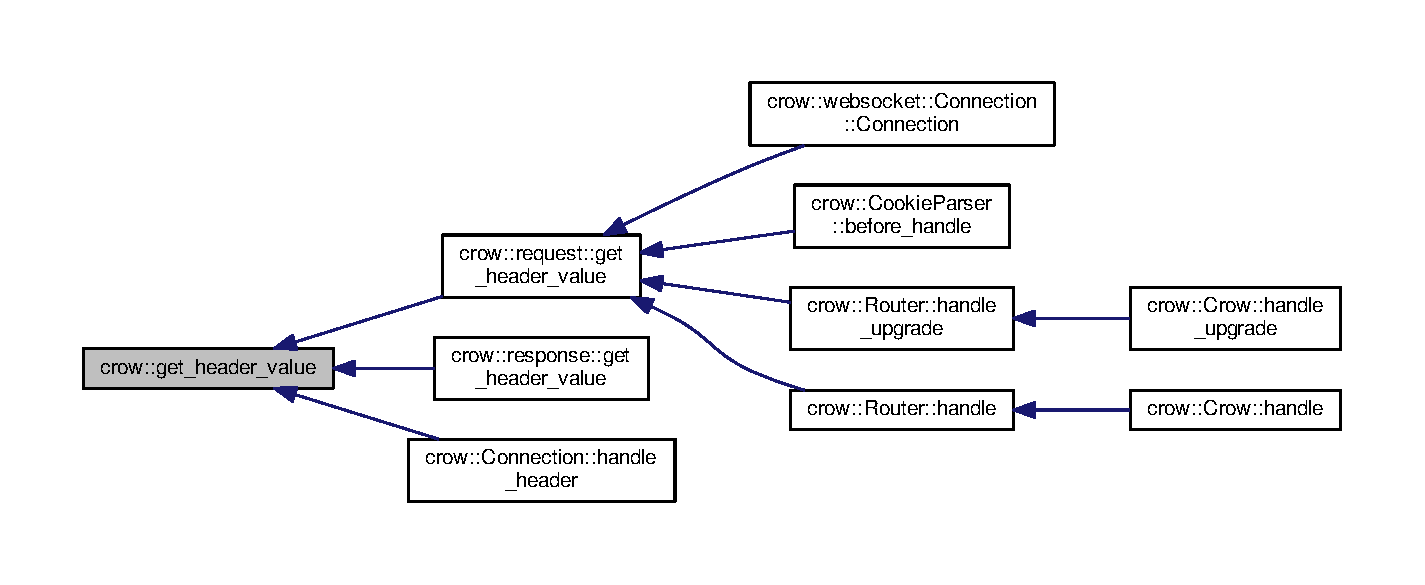
\includegraphics[width=350pt]{namespacecrow_ac0940ae1e094df6107d3a2604537279a_icgraph}
\end{center}
\end{figure}


\hypertarget{namespacecrow_a2e95f26db5041c7f322bd38c2de6a6b1}{\index{crow@{crow}!method\-\_\-name@{method\-\_\-name}}
\index{method\-\_\-name@{method\-\_\-name}!crow@{crow}}
\subsubsection[{method\-\_\-name}]{\setlength{\rightskip}{0pt plus 5cm}std\-::string crow\-::method\-\_\-name (
\begin{DoxyParamCaption}
\item[{H\-T\-T\-P\-Method}]{method}
\end{DoxyParamCaption}
)\hspace{0.3cm}{\ttfamily [inline]}}}\label{namespacecrow_a2e95f26db5041c7f322bd38c2de6a6b1}


Here is the caller graph for this function\-:
\nopagebreak
\begin{figure}[H]
\begin{center}
\leavevmode
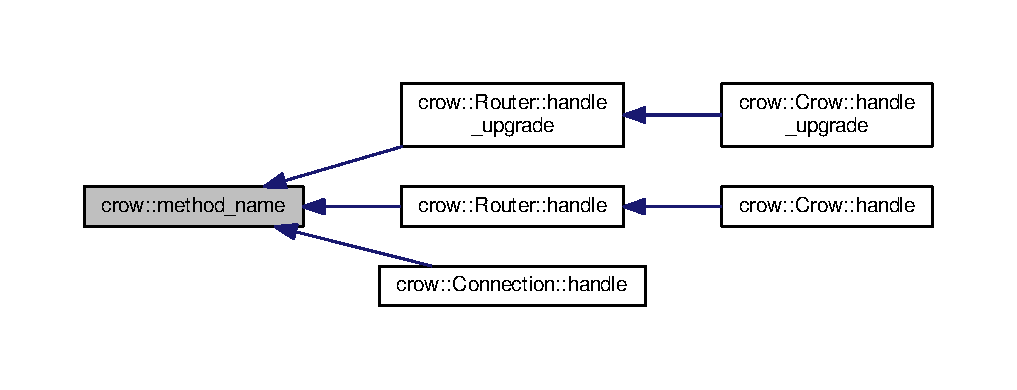
\includegraphics[width=350pt]{namespacecrow_a2e95f26db5041c7f322bd38c2de6a6b1_icgraph}
\end{center}
\end{figure}


\hypertarget{namespacecrow_a95142b051d7358769267df504e39a3b9}{\index{crow@{crow}!routing\-\_\-params\-::get$<$ std\-::string $>$@{routing\-\_\-params\-::get$<$ std\-::string $>$}}
\index{routing\-\_\-params\-::get$<$ std\-::string $>$@{routing\-\_\-params\-::get$<$ std\-::string $>$}!crow@{crow}}
\subsubsection[{routing\-\_\-params\-::get$<$ std\-::string $>$}]{\setlength{\rightskip}{0pt plus 5cm}template$<$$>$ std\-::string {\bf crow\-::routing\-\_\-params\-::get}$<$ std\-::string $>$ (
\begin{DoxyParamCaption}
\item[{unsigned}]{index}
\end{DoxyParamCaption}
) const\hspace{0.3cm}{\ttfamily [inline]}}}\label{namespacecrow_a95142b051d7358769267df504e39a3b9}


\subsection{Variable Documentation}
\hypertarget{namespacecrow_a73062c5f5d45cb57eb32fd8a3f916132}{\index{crow@{crow}!R\-U\-L\-E\-\_\-\-S\-P\-E\-C\-I\-A\-L\-\_\-\-R\-E\-D\-I\-R\-E\-C\-T\-\_\-\-S\-L\-A\-S\-H@{R\-U\-L\-E\-\_\-\-S\-P\-E\-C\-I\-A\-L\-\_\-\-R\-E\-D\-I\-R\-E\-C\-T\-\_\-\-S\-L\-A\-S\-H}}
\index{R\-U\-L\-E\-\_\-\-S\-P\-E\-C\-I\-A\-L\-\_\-\-R\-E\-D\-I\-R\-E\-C\-T\-\_\-\-S\-L\-A\-S\-H@{R\-U\-L\-E\-\_\-\-S\-P\-E\-C\-I\-A\-L\-\_\-\-R\-E\-D\-I\-R\-E\-C\-T\-\_\-\-S\-L\-A\-S\-H}!crow@{crow}}
\subsubsection[{R\-U\-L\-E\-\_\-\-S\-P\-E\-C\-I\-A\-L\-\_\-\-R\-E\-D\-I\-R\-E\-C\-T\-\_\-\-S\-L\-A\-S\-H}]{\setlength{\rightskip}{0pt plus 5cm}const int crow\-::\-R\-U\-L\-E\-\_\-\-S\-P\-E\-C\-I\-A\-L\-\_\-\-R\-E\-D\-I\-R\-E\-C\-T\-\_\-\-S\-L\-A\-S\-H = 1}}\label{namespacecrow_a73062c5f5d45cb57eb32fd8a3f916132}

\hypertarget{namespacecrow_1_1black__magic}{\section{crow\-:\-:black\-\_\-magic Namespace Reference}
\label{namespacecrow_1_1black__magic}\index{crow\-::black\-\_\-magic@{crow\-::black\-\_\-magic}}
}
\subsection*{Classes}
\begin{DoxyCompactItemize}
\item 
struct \hyperlink{structcrow_1_1black__magic_1_1_out_of_range}{Out\-Of\-Range}
\item 
class \hyperlink{classcrow_1_1black__magic_1_1const__str}{const\-\_\-str}
\item 
struct \hyperlink{structcrow_1_1black__magic_1_1parameter__tag}{parameter\-\_\-tag}
\item 
struct \hyperlink{structcrow_1_1black__magic_1_1compute__parameter__tag__from__args__list}{compute\-\_\-parameter\-\_\-tag\-\_\-from\-\_\-args\-\_\-list}
\item 
struct \hyperlink{structcrow_1_1black__magic_1_1compute__parameter__tag__from__args__list_3_4}{compute\-\_\-parameter\-\_\-tag\-\_\-from\-\_\-args\-\_\-list$<$$>$}
\item 
struct \hyperlink{structcrow_1_1black__magic_1_1compute__parameter__tag__from__args__list_3_01_arg_00_01_args_8_8_8_4}{compute\-\_\-parameter\-\_\-tag\-\_\-from\-\_\-args\-\_\-list$<$ Arg, Args...$>$}
\item 
struct \hyperlink{structcrow_1_1black__magic_1_1_s}{S}
\item 
struct \hyperlink{structcrow_1_1black__magic_1_1_call_helper}{Call\-Helper}
\item 
struct \hyperlink{structcrow_1_1black__magic_1_1_call_helper_3_01_f_00_01_s_3_01_args_8_8_8_4_01_4}{Call\-Helper$<$ F, S$<$ Args...$>$ $>$}
\item 
struct \hyperlink{structcrow_1_1black__magic_1_1single__tag__to__type}{single\-\_\-tag\-\_\-to\-\_\-type}
\item 
struct \hyperlink{structcrow_1_1black__magic_1_1single__tag__to__type_3_011_01_4}{single\-\_\-tag\-\_\-to\-\_\-type$<$ 1 $>$}
\item 
struct \hyperlink{structcrow_1_1black__magic_1_1single__tag__to__type_3_012_01_4}{single\-\_\-tag\-\_\-to\-\_\-type$<$ 2 $>$}
\item 
struct \hyperlink{structcrow_1_1black__magic_1_1single__tag__to__type_3_013_01_4}{single\-\_\-tag\-\_\-to\-\_\-type$<$ 3 $>$}
\item 
struct \hyperlink{structcrow_1_1black__magic_1_1single__tag__to__type_3_014_01_4}{single\-\_\-tag\-\_\-to\-\_\-type$<$ 4 $>$}
\item 
struct \hyperlink{structcrow_1_1black__magic_1_1single__tag__to__type_3_015_01_4}{single\-\_\-tag\-\_\-to\-\_\-type$<$ 5 $>$}
\item 
struct \hyperlink{structcrow_1_1black__magic_1_1arguments}{arguments}
\item 
struct \hyperlink{structcrow_1_1black__magic_1_1arguments_3_010_01_4}{arguments$<$ 0 $>$}
\item 
struct \hyperlink{structcrow_1_1black__magic_1_1last__element__type}{last\-\_\-element\-\_\-type}
\item 
struct \hyperlink{structcrow_1_1black__magic_1_1last__element__type_3_4}{last\-\_\-element\-\_\-type$<$$>$}
\item 
struct \hyperlink{structcrow_1_1black__magic_1_1seq}{seq}
\item 
struct \hyperlink{structcrow_1_1black__magic_1_1concat}{concat}
\item 
struct \hyperlink{structcrow_1_1black__magic_1_1concat_3_01seq_3_01_i1_8_8_8_4_00_01seq_3_01_i2_8_8_8_4_01_4}{concat$<$ seq$<$ I1...$>$, seq$<$ I2...$>$ $>$}
\item 
struct \hyperlink{structcrow_1_1black__magic_1_1gen__seq}{gen\-\_\-seq}
\item 
struct \hyperlink{structcrow_1_1black__magic_1_1gen__seq_3_010_01_4}{gen\-\_\-seq$<$ 0 $>$}
\item 
struct \hyperlink{structcrow_1_1black__magic_1_1gen__seq_3_011_01_4}{gen\-\_\-seq$<$ 1 $>$}
\item 
struct \hyperlink{structcrow_1_1black__magic_1_1pop__back__helper}{pop\-\_\-back\-\_\-helper}
\item 
struct \hyperlink{structcrow_1_1black__magic_1_1pop__back__helper_3_01seq_3_01_n_8_8_8_4_00_01_tuple_01_4}{pop\-\_\-back\-\_\-helper$<$ seq$<$ N...$>$, Tuple $>$}
\item 
struct \hyperlink{structcrow_1_1black__magic_1_1pop__back}{pop\-\_\-back}
\item 
struct \hyperlink{structcrow_1_1black__magic_1_1pop__back_3_4}{pop\-\_\-back$<$$>$}
\item 
struct \hyperlink{structcrow_1_1black__magic_1_1contains}{contains}
\item 
struct \hyperlink{structcrow_1_1black__magic_1_1contains_3_01_tp_00_01_head_00_01_rest_8_8_8_4}{contains$<$ Tp, Head, Rest...$>$}
\item 
struct \hyperlink{structcrow_1_1black__magic_1_1contains_3_01_tp_01_4}{contains$<$ Tp $>$}
\item 
struct \hyperlink{structcrow_1_1black__magic_1_1empty__context}{empty\-\_\-context}
\item 
struct \hyperlink{structcrow_1_1black__magic_1_1promote}{promote}
\end{DoxyCompactItemize}
\subsection*{Typedefs}
\begin{DoxyCompactItemize}
\item 
{\footnotesize template$<$class T $>$ }\\using \hyperlink{namespacecrow_1_1black__magic_a6b8ed264432b676b8f13faf399c7343f}{Invoke} = typename T\-::type
\item 
{\footnotesize template$<$class S1 , class S2 $>$ }\\using \hyperlink{namespacecrow_1_1black__magic_aa5da930ee46c60876b74714b9cbd9822}{Concat} = \hyperlink{namespacecrow_1_1black__magic_a6b8ed264432b676b8f13faf399c7343f}{Invoke}$<$ \hyperlink{structcrow_1_1black__magic_1_1concat}{concat}$<$ S1, S2 $>$$>$
\item 
{\footnotesize template$<$unsigned N$>$ }\\using \hyperlink{namespacecrow_1_1black__magic_a697b4738762ac4a1e0d56df7dc0aa5a9}{Gen\-Seq} = \hyperlink{namespacecrow_1_1black__magic_a6b8ed264432b676b8f13faf399c7343f}{Invoke}$<$ \hyperlink{structcrow_1_1black__magic_1_1gen__seq}{gen\-\_\-seq}$<$ N $>$$>$
\item 
{\footnotesize template$<$typename T $>$ }\\using \hyperlink{namespacecrow_1_1black__magic_a4964540ce915507f5167e1a96f801c71}{promote\-\_\-t} = typename \hyperlink{structcrow_1_1black__magic_1_1promote}{promote}$<$ T $>$\-::type
\end{DoxyCompactItemize}
\subsection*{Functions}
\begin{DoxyCompactItemize}
\item 
constexpr unsigned \hyperlink{namespacecrow_1_1black__magic_a1c2aff5573639d46df93ffada058c686}{requires\-\_\-in\-\_\-range} (unsigned i, unsigned len)
\item 
constexpr unsigned \hyperlink{namespacecrow_1_1black__magic_a21fead60e1668e81ef9dbdbd1a158694}{find\-\_\-closing\-\_\-tag} (\hyperlink{classcrow_1_1black__magic_1_1const__str}{const\-\_\-str} s, unsigned p)
\item 
constexpr bool \hyperlink{namespacecrow_1_1black__magic_afc88027e704873c372fb51b5e56370da}{is\-\_\-valid} (\hyperlink{classcrow_1_1black__magic_1_1const__str}{const\-\_\-str} s, unsigned i=0, int f=0)
\item 
constexpr bool \hyperlink{namespacecrow_1_1black__magic_ad1873e3cf98eb8ed4f495272f86197cf}{is\-\_\-equ\-\_\-p} (const char $\ast$a, const char $\ast$b, unsigned n)
\item 
constexpr bool \hyperlink{namespacecrow_1_1black__magic_a38e0df4f002e2743c45ad435a4c9cf51}{is\-\_\-equ\-\_\-n} (\hyperlink{classcrow_1_1black__magic_1_1const__str}{const\-\_\-str} a, unsigned ai, \hyperlink{classcrow_1_1black__magic_1_1const__str}{const\-\_\-str} b, unsigned bi, unsigned n)
\item 
constexpr bool \hyperlink{namespacecrow_1_1black__magic_a35c7106101b8789c8b4d28e45a43fac5}{is\-\_\-int} (\hyperlink{classcrow_1_1black__magic_1_1const__str}{const\-\_\-str} s, unsigned i)
\item 
constexpr bool \hyperlink{namespacecrow_1_1black__magic_a2d8e83151f7d6b3389fea3d6dc394115}{is\-\_\-uint} (\hyperlink{classcrow_1_1black__magic_1_1const__str}{const\-\_\-str} s, unsigned i)
\item 
constexpr bool \hyperlink{namespacecrow_1_1black__magic_a57bad212b24512e47aa460cfef75c1a4}{is\-\_\-float} (\hyperlink{classcrow_1_1black__magic_1_1const__str}{const\-\_\-str} s, unsigned i)
\item 
constexpr bool \hyperlink{namespacecrow_1_1black__magic_a2eb0eb4514228192b878653bb56b7d44}{is\-\_\-str} (\hyperlink{classcrow_1_1black__magic_1_1const__str}{const\-\_\-str} s, unsigned i)
\item 
constexpr bool \hyperlink{namespacecrow_1_1black__magic_af0899340936b274931de7ac21fb4ed9f}{is\-\_\-path} (\hyperlink{classcrow_1_1black__magic_1_1const__str}{const\-\_\-str} s, unsigned i)
\item 
\hyperlink{namespacecrow_1_1black__magic_a264c6694c8fd639b5560f51547eed925}{C\-R\-O\-W\-\_\-\-I\-N\-T\-E\-R\-N\-A\-L\-\_\-\-P\-A\-R\-A\-M\-E\-T\-E\-R\-\_\-\-T\-A\-G} (int, 1)
\item 
\hyperlink{namespacecrow_1_1black__magic_a7121499a9aaba838d1ecb7c5a1039a3f}{C\-R\-O\-W\-\_\-\-I\-N\-T\-E\-R\-N\-A\-L\-\_\-\-P\-A\-R\-A\-M\-E\-T\-E\-R\-\_\-\-T\-A\-G} (char, 1)
\item 
\hyperlink{namespacecrow_1_1black__magic_a5f4e721d7feb011651ccea89470b4423}{C\-R\-O\-W\-\_\-\-I\-N\-T\-E\-R\-N\-A\-L\-\_\-\-P\-A\-R\-A\-M\-E\-T\-E\-R\-\_\-\-T\-A\-G} (short, 1)
\item 
\hyperlink{namespacecrow_1_1black__magic_a77b9d55adaad40f9dbcff155479aa101}{C\-R\-O\-W\-\_\-\-I\-N\-T\-E\-R\-N\-A\-L\-\_\-\-P\-A\-R\-A\-M\-E\-T\-E\-R\-\_\-\-T\-A\-G} (long, 1)
\item 
\hyperlink{namespacecrow_1_1black__magic_a0ef5fc727782f10e3c2b18bb203373f2}{C\-R\-O\-W\-\_\-\-I\-N\-T\-E\-R\-N\-A\-L\-\_\-\-P\-A\-R\-A\-M\-E\-T\-E\-R\-\_\-\-T\-A\-G} (unsigned int, 2)
\item 
\hyperlink{namespacecrow_1_1black__magic_a67e7a4d47de21fd2e1d52c3938587a67}{C\-R\-O\-W\-\_\-\-I\-N\-T\-E\-R\-N\-A\-L\-\_\-\-P\-A\-R\-A\-M\-E\-T\-E\-R\-\_\-\-T\-A\-G} (unsigned long long, 2)
\item 
\hyperlink{namespacecrow_1_1black__magic_a873691f0e99a603d7e59b161a782f10c}{C\-R\-O\-W\-\_\-\-I\-N\-T\-E\-R\-N\-A\-L\-\_\-\-P\-A\-R\-A\-M\-E\-T\-E\-R\-\_\-\-T\-A\-G} (double, 3)
\item 
\hyperlink{namespacecrow_1_1black__magic_aa65db9335b5c3a3058f46ed89fa6207f}{C\-R\-O\-W\-\_\-\-I\-N\-T\-E\-R\-N\-A\-L\-\_\-\-P\-A\-R\-A\-M\-E\-T\-E\-R\-\_\-\-T\-A\-G} (std\-::string, 4)
\item 
constexpr uint64\-\_\-t \hyperlink{namespacecrow_1_1black__magic_a5e101d2f6803b92441aa8beff0f51113}{get\-\_\-parameter\-\_\-tag} (\hyperlink{classcrow_1_1black__magic_1_1const__str}{const\-\_\-str} s, unsigned p=0)
\item 
\hyperlink{namespacecrow_1_1black__magic_a926dc267a9cf598b9b2c99b33577139a}{C\-R\-O\-W\-\_\-\-I\-N\-T\-E\-R\-N\-A\-L\-\_\-\-P\-R\-O\-M\-O\-T\-E\-\_\-\-T\-Y\-P\-E} (char, int64\-\_\-t)
\item 
\hyperlink{namespacecrow_1_1black__magic_a571088fcb303b30757b3399208070677}{C\-R\-O\-W\-\_\-\-I\-N\-T\-E\-R\-N\-A\-L\-\_\-\-P\-R\-O\-M\-O\-T\-E\-\_\-\-T\-Y\-P\-E} (short, int64\-\_\-t)
\item 
\hyperlink{namespacecrow_1_1black__magic_a787da3fb2db6c0c3fc3022812bc02274}{C\-R\-O\-W\-\_\-\-I\-N\-T\-E\-R\-N\-A\-L\-\_\-\-P\-R\-O\-M\-O\-T\-E\-\_\-\-T\-Y\-P\-E} (int, int64\-\_\-t)
\item 
\hyperlink{namespacecrow_1_1black__magic_a8843fa0826d71d2f9f727287d66bc880}{C\-R\-O\-W\-\_\-\-I\-N\-T\-E\-R\-N\-A\-L\-\_\-\-P\-R\-O\-M\-O\-T\-E\-\_\-\-T\-Y\-P\-E} (long, int64\-\_\-t)
\item 
\hyperlink{namespacecrow_1_1black__magic_a1d0c48ef972ed37e08bc3dd51c0e1a5e}{C\-R\-O\-W\-\_\-\-I\-N\-T\-E\-R\-N\-A\-L\-\_\-\-P\-R\-O\-M\-O\-T\-E\-\_\-\-T\-Y\-P\-E} (unsigned char, uint64\-\_\-t)
\item 
\hyperlink{namespacecrow_1_1black__magic_a647ab28f6adf3f5f2f662aeaa55c27ae}{C\-R\-O\-W\-\_\-\-I\-N\-T\-E\-R\-N\-A\-L\-\_\-\-P\-R\-O\-M\-O\-T\-E\-\_\-\-T\-Y\-P\-E} (unsigned long long, uint64\-\_\-t)
\item 
\hyperlink{namespacecrow_1_1black__magic_ac394c9690152b3c72d53d613694adf98}{C\-R\-O\-W\-\_\-\-I\-N\-T\-E\-R\-N\-A\-L\-\_\-\-P\-R\-O\-M\-O\-T\-E\-\_\-\-T\-Y\-P\-E} (float, double)
\end{DoxyCompactItemize}


\subsection{Typedef Documentation}
\hypertarget{namespacecrow_1_1black__magic_aa5da930ee46c60876b74714b9cbd9822}{\index{crow\-::black\-\_\-magic@{crow\-::black\-\_\-magic}!Concat@{Concat}}
\index{Concat@{Concat}!crow::black_magic@{crow\-::black\-\_\-magic}}
\subsubsection[{Concat}]{\setlength{\rightskip}{0pt plus 5cm}template$<$class S1 , class S2 $>$ using {\bf crow\-::black\-\_\-magic\-::\-Concat} = typedef {\bf Invoke}$<${\bf concat}$<$S1, S2$>$$>$}}\label{namespacecrow_1_1black__magic_aa5da930ee46c60876b74714b9cbd9822}
\hypertarget{namespacecrow_1_1black__magic_a697b4738762ac4a1e0d56df7dc0aa5a9}{\index{crow\-::black\-\_\-magic@{crow\-::black\-\_\-magic}!Gen\-Seq@{Gen\-Seq}}
\index{Gen\-Seq@{Gen\-Seq}!crow::black_magic@{crow\-::black\-\_\-magic}}
\subsubsection[{Gen\-Seq}]{\setlength{\rightskip}{0pt plus 5cm}template$<$unsigned N$>$ using {\bf crow\-::black\-\_\-magic\-::\-Gen\-Seq} = typedef {\bf Invoke}$<${\bf gen\-\_\-seq}$<$N$>$$>$}}\label{namespacecrow_1_1black__magic_a697b4738762ac4a1e0d56df7dc0aa5a9}
\hypertarget{namespacecrow_1_1black__magic_a6b8ed264432b676b8f13faf399c7343f}{\index{crow\-::black\-\_\-magic@{crow\-::black\-\_\-magic}!Invoke@{Invoke}}
\index{Invoke@{Invoke}!crow::black_magic@{crow\-::black\-\_\-magic}}
\subsubsection[{Invoke}]{\setlength{\rightskip}{0pt plus 5cm}template$<$class T $>$ using {\bf crow\-::black\-\_\-magic\-::\-Invoke} = typedef typename T\-::type}}\label{namespacecrow_1_1black__magic_a6b8ed264432b676b8f13faf399c7343f}
\hypertarget{namespacecrow_1_1black__magic_a4964540ce915507f5167e1a96f801c71}{\index{crow\-::black\-\_\-magic@{crow\-::black\-\_\-magic}!promote\-\_\-t@{promote\-\_\-t}}
\index{promote\-\_\-t@{promote\-\_\-t}!crow::black_magic@{crow\-::black\-\_\-magic}}
\subsubsection[{promote\-\_\-t}]{\setlength{\rightskip}{0pt plus 5cm}template$<$typename T $>$ using {\bf crow\-::black\-\_\-magic\-::promote\-\_\-t} = typedef typename {\bf promote}$<$T$>$\-::type}}\label{namespacecrow_1_1black__magic_a4964540ce915507f5167e1a96f801c71}


\subsection{Function Documentation}
\hypertarget{namespacecrow_1_1black__magic_a264c6694c8fd639b5560f51547eed925}{\index{crow\-::black\-\_\-magic@{crow\-::black\-\_\-magic}!C\-R\-O\-W\-\_\-\-I\-N\-T\-E\-R\-N\-A\-L\-\_\-\-P\-A\-R\-A\-M\-E\-T\-E\-R\-\_\-\-T\-A\-G@{C\-R\-O\-W\-\_\-\-I\-N\-T\-E\-R\-N\-A\-L\-\_\-\-P\-A\-R\-A\-M\-E\-T\-E\-R\-\_\-\-T\-A\-G}}
\index{C\-R\-O\-W\-\_\-\-I\-N\-T\-E\-R\-N\-A\-L\-\_\-\-P\-A\-R\-A\-M\-E\-T\-E\-R\-\_\-\-T\-A\-G@{C\-R\-O\-W\-\_\-\-I\-N\-T\-E\-R\-N\-A\-L\-\_\-\-P\-A\-R\-A\-M\-E\-T\-E\-R\-\_\-\-T\-A\-G}!crow::black_magic@{crow\-::black\-\_\-magic}}
\subsubsection[{C\-R\-O\-W\-\_\-\-I\-N\-T\-E\-R\-N\-A\-L\-\_\-\-P\-A\-R\-A\-M\-E\-T\-E\-R\-\_\-\-T\-A\-G}]{\setlength{\rightskip}{0pt plus 5cm}crow\-::black\-\_\-magic\-::\-C\-R\-O\-W\-\_\-\-I\-N\-T\-E\-R\-N\-A\-L\-\_\-\-P\-A\-R\-A\-M\-E\-T\-E\-R\-\_\-\-T\-A\-G (
\begin{DoxyParamCaption}
\item[{int}]{, }
\item[{1}]{}
\end{DoxyParamCaption}
)}}\label{namespacecrow_1_1black__magic_a264c6694c8fd639b5560f51547eed925}
\hypertarget{namespacecrow_1_1black__magic_a7121499a9aaba838d1ecb7c5a1039a3f}{\index{crow\-::black\-\_\-magic@{crow\-::black\-\_\-magic}!C\-R\-O\-W\-\_\-\-I\-N\-T\-E\-R\-N\-A\-L\-\_\-\-P\-A\-R\-A\-M\-E\-T\-E\-R\-\_\-\-T\-A\-G@{C\-R\-O\-W\-\_\-\-I\-N\-T\-E\-R\-N\-A\-L\-\_\-\-P\-A\-R\-A\-M\-E\-T\-E\-R\-\_\-\-T\-A\-G}}
\index{C\-R\-O\-W\-\_\-\-I\-N\-T\-E\-R\-N\-A\-L\-\_\-\-P\-A\-R\-A\-M\-E\-T\-E\-R\-\_\-\-T\-A\-G@{C\-R\-O\-W\-\_\-\-I\-N\-T\-E\-R\-N\-A\-L\-\_\-\-P\-A\-R\-A\-M\-E\-T\-E\-R\-\_\-\-T\-A\-G}!crow::black_magic@{crow\-::black\-\_\-magic}}
\subsubsection[{C\-R\-O\-W\-\_\-\-I\-N\-T\-E\-R\-N\-A\-L\-\_\-\-P\-A\-R\-A\-M\-E\-T\-E\-R\-\_\-\-T\-A\-G}]{\setlength{\rightskip}{0pt plus 5cm}crow\-::black\-\_\-magic\-::\-C\-R\-O\-W\-\_\-\-I\-N\-T\-E\-R\-N\-A\-L\-\_\-\-P\-A\-R\-A\-M\-E\-T\-E\-R\-\_\-\-T\-A\-G (
\begin{DoxyParamCaption}
\item[{char}]{, }
\item[{1}]{}
\end{DoxyParamCaption}
)}}\label{namespacecrow_1_1black__magic_a7121499a9aaba838d1ecb7c5a1039a3f}
\hypertarget{namespacecrow_1_1black__magic_a5f4e721d7feb011651ccea89470b4423}{\index{crow\-::black\-\_\-magic@{crow\-::black\-\_\-magic}!C\-R\-O\-W\-\_\-\-I\-N\-T\-E\-R\-N\-A\-L\-\_\-\-P\-A\-R\-A\-M\-E\-T\-E\-R\-\_\-\-T\-A\-G@{C\-R\-O\-W\-\_\-\-I\-N\-T\-E\-R\-N\-A\-L\-\_\-\-P\-A\-R\-A\-M\-E\-T\-E\-R\-\_\-\-T\-A\-G}}
\index{C\-R\-O\-W\-\_\-\-I\-N\-T\-E\-R\-N\-A\-L\-\_\-\-P\-A\-R\-A\-M\-E\-T\-E\-R\-\_\-\-T\-A\-G@{C\-R\-O\-W\-\_\-\-I\-N\-T\-E\-R\-N\-A\-L\-\_\-\-P\-A\-R\-A\-M\-E\-T\-E\-R\-\_\-\-T\-A\-G}!crow::black_magic@{crow\-::black\-\_\-magic}}
\subsubsection[{C\-R\-O\-W\-\_\-\-I\-N\-T\-E\-R\-N\-A\-L\-\_\-\-P\-A\-R\-A\-M\-E\-T\-E\-R\-\_\-\-T\-A\-G}]{\setlength{\rightskip}{0pt plus 5cm}crow\-::black\-\_\-magic\-::\-C\-R\-O\-W\-\_\-\-I\-N\-T\-E\-R\-N\-A\-L\-\_\-\-P\-A\-R\-A\-M\-E\-T\-E\-R\-\_\-\-T\-A\-G (
\begin{DoxyParamCaption}
\item[{short}]{, }
\item[{1}]{}
\end{DoxyParamCaption}
)}}\label{namespacecrow_1_1black__magic_a5f4e721d7feb011651ccea89470b4423}
\hypertarget{namespacecrow_1_1black__magic_a77b9d55adaad40f9dbcff155479aa101}{\index{crow\-::black\-\_\-magic@{crow\-::black\-\_\-magic}!C\-R\-O\-W\-\_\-\-I\-N\-T\-E\-R\-N\-A\-L\-\_\-\-P\-A\-R\-A\-M\-E\-T\-E\-R\-\_\-\-T\-A\-G@{C\-R\-O\-W\-\_\-\-I\-N\-T\-E\-R\-N\-A\-L\-\_\-\-P\-A\-R\-A\-M\-E\-T\-E\-R\-\_\-\-T\-A\-G}}
\index{C\-R\-O\-W\-\_\-\-I\-N\-T\-E\-R\-N\-A\-L\-\_\-\-P\-A\-R\-A\-M\-E\-T\-E\-R\-\_\-\-T\-A\-G@{C\-R\-O\-W\-\_\-\-I\-N\-T\-E\-R\-N\-A\-L\-\_\-\-P\-A\-R\-A\-M\-E\-T\-E\-R\-\_\-\-T\-A\-G}!crow::black_magic@{crow\-::black\-\_\-magic}}
\subsubsection[{C\-R\-O\-W\-\_\-\-I\-N\-T\-E\-R\-N\-A\-L\-\_\-\-P\-A\-R\-A\-M\-E\-T\-E\-R\-\_\-\-T\-A\-G}]{\setlength{\rightskip}{0pt plus 5cm}crow\-::black\-\_\-magic\-::\-C\-R\-O\-W\-\_\-\-I\-N\-T\-E\-R\-N\-A\-L\-\_\-\-P\-A\-R\-A\-M\-E\-T\-E\-R\-\_\-\-T\-A\-G (
\begin{DoxyParamCaption}
\item[{long}]{, }
\item[{1}]{}
\end{DoxyParamCaption}
)}}\label{namespacecrow_1_1black__magic_a77b9d55adaad40f9dbcff155479aa101}
\hypertarget{namespacecrow_1_1black__magic_a0ef5fc727782f10e3c2b18bb203373f2}{\index{crow\-::black\-\_\-magic@{crow\-::black\-\_\-magic}!C\-R\-O\-W\-\_\-\-I\-N\-T\-E\-R\-N\-A\-L\-\_\-\-P\-A\-R\-A\-M\-E\-T\-E\-R\-\_\-\-T\-A\-G@{C\-R\-O\-W\-\_\-\-I\-N\-T\-E\-R\-N\-A\-L\-\_\-\-P\-A\-R\-A\-M\-E\-T\-E\-R\-\_\-\-T\-A\-G}}
\index{C\-R\-O\-W\-\_\-\-I\-N\-T\-E\-R\-N\-A\-L\-\_\-\-P\-A\-R\-A\-M\-E\-T\-E\-R\-\_\-\-T\-A\-G@{C\-R\-O\-W\-\_\-\-I\-N\-T\-E\-R\-N\-A\-L\-\_\-\-P\-A\-R\-A\-M\-E\-T\-E\-R\-\_\-\-T\-A\-G}!crow::black_magic@{crow\-::black\-\_\-magic}}
\subsubsection[{C\-R\-O\-W\-\_\-\-I\-N\-T\-E\-R\-N\-A\-L\-\_\-\-P\-A\-R\-A\-M\-E\-T\-E\-R\-\_\-\-T\-A\-G}]{\setlength{\rightskip}{0pt plus 5cm}crow\-::black\-\_\-magic\-::\-C\-R\-O\-W\-\_\-\-I\-N\-T\-E\-R\-N\-A\-L\-\_\-\-P\-A\-R\-A\-M\-E\-T\-E\-R\-\_\-\-T\-A\-G (
\begin{DoxyParamCaption}
\item[{unsigned}]{int, }
\item[{2}]{}
\end{DoxyParamCaption}
)}}\label{namespacecrow_1_1black__magic_a0ef5fc727782f10e3c2b18bb203373f2}
\hypertarget{namespacecrow_1_1black__magic_a67e7a4d47de21fd2e1d52c3938587a67}{\index{crow\-::black\-\_\-magic@{crow\-::black\-\_\-magic}!C\-R\-O\-W\-\_\-\-I\-N\-T\-E\-R\-N\-A\-L\-\_\-\-P\-A\-R\-A\-M\-E\-T\-E\-R\-\_\-\-T\-A\-G@{C\-R\-O\-W\-\_\-\-I\-N\-T\-E\-R\-N\-A\-L\-\_\-\-P\-A\-R\-A\-M\-E\-T\-E\-R\-\_\-\-T\-A\-G}}
\index{C\-R\-O\-W\-\_\-\-I\-N\-T\-E\-R\-N\-A\-L\-\_\-\-P\-A\-R\-A\-M\-E\-T\-E\-R\-\_\-\-T\-A\-G@{C\-R\-O\-W\-\_\-\-I\-N\-T\-E\-R\-N\-A\-L\-\_\-\-P\-A\-R\-A\-M\-E\-T\-E\-R\-\_\-\-T\-A\-G}!crow::black_magic@{crow\-::black\-\_\-magic}}
\subsubsection[{C\-R\-O\-W\-\_\-\-I\-N\-T\-E\-R\-N\-A\-L\-\_\-\-P\-A\-R\-A\-M\-E\-T\-E\-R\-\_\-\-T\-A\-G}]{\setlength{\rightskip}{0pt plus 5cm}crow\-::black\-\_\-magic\-::\-C\-R\-O\-W\-\_\-\-I\-N\-T\-E\-R\-N\-A\-L\-\_\-\-P\-A\-R\-A\-M\-E\-T\-E\-R\-\_\-\-T\-A\-G (
\begin{DoxyParamCaption}
\item[{unsigned long}]{long, }
\item[{2}]{}
\end{DoxyParamCaption}
)}}\label{namespacecrow_1_1black__magic_a67e7a4d47de21fd2e1d52c3938587a67}
\hypertarget{namespacecrow_1_1black__magic_a873691f0e99a603d7e59b161a782f10c}{\index{crow\-::black\-\_\-magic@{crow\-::black\-\_\-magic}!C\-R\-O\-W\-\_\-\-I\-N\-T\-E\-R\-N\-A\-L\-\_\-\-P\-A\-R\-A\-M\-E\-T\-E\-R\-\_\-\-T\-A\-G@{C\-R\-O\-W\-\_\-\-I\-N\-T\-E\-R\-N\-A\-L\-\_\-\-P\-A\-R\-A\-M\-E\-T\-E\-R\-\_\-\-T\-A\-G}}
\index{C\-R\-O\-W\-\_\-\-I\-N\-T\-E\-R\-N\-A\-L\-\_\-\-P\-A\-R\-A\-M\-E\-T\-E\-R\-\_\-\-T\-A\-G@{C\-R\-O\-W\-\_\-\-I\-N\-T\-E\-R\-N\-A\-L\-\_\-\-P\-A\-R\-A\-M\-E\-T\-E\-R\-\_\-\-T\-A\-G}!crow::black_magic@{crow\-::black\-\_\-magic}}
\subsubsection[{C\-R\-O\-W\-\_\-\-I\-N\-T\-E\-R\-N\-A\-L\-\_\-\-P\-A\-R\-A\-M\-E\-T\-E\-R\-\_\-\-T\-A\-G}]{\setlength{\rightskip}{0pt plus 5cm}crow\-::black\-\_\-magic\-::\-C\-R\-O\-W\-\_\-\-I\-N\-T\-E\-R\-N\-A\-L\-\_\-\-P\-A\-R\-A\-M\-E\-T\-E\-R\-\_\-\-T\-A\-G (
\begin{DoxyParamCaption}
\item[{double}]{, }
\item[{3}]{}
\end{DoxyParamCaption}
)}}\label{namespacecrow_1_1black__magic_a873691f0e99a603d7e59b161a782f10c}
\hypertarget{namespacecrow_1_1black__magic_aa65db9335b5c3a3058f46ed89fa6207f}{\index{crow\-::black\-\_\-magic@{crow\-::black\-\_\-magic}!C\-R\-O\-W\-\_\-\-I\-N\-T\-E\-R\-N\-A\-L\-\_\-\-P\-A\-R\-A\-M\-E\-T\-E\-R\-\_\-\-T\-A\-G@{C\-R\-O\-W\-\_\-\-I\-N\-T\-E\-R\-N\-A\-L\-\_\-\-P\-A\-R\-A\-M\-E\-T\-E\-R\-\_\-\-T\-A\-G}}
\index{C\-R\-O\-W\-\_\-\-I\-N\-T\-E\-R\-N\-A\-L\-\_\-\-P\-A\-R\-A\-M\-E\-T\-E\-R\-\_\-\-T\-A\-G@{C\-R\-O\-W\-\_\-\-I\-N\-T\-E\-R\-N\-A\-L\-\_\-\-P\-A\-R\-A\-M\-E\-T\-E\-R\-\_\-\-T\-A\-G}!crow::black_magic@{crow\-::black\-\_\-magic}}
\subsubsection[{C\-R\-O\-W\-\_\-\-I\-N\-T\-E\-R\-N\-A\-L\-\_\-\-P\-A\-R\-A\-M\-E\-T\-E\-R\-\_\-\-T\-A\-G}]{\setlength{\rightskip}{0pt plus 5cm}crow\-::black\-\_\-magic\-::\-C\-R\-O\-W\-\_\-\-I\-N\-T\-E\-R\-N\-A\-L\-\_\-\-P\-A\-R\-A\-M\-E\-T\-E\-R\-\_\-\-T\-A\-G (
\begin{DoxyParamCaption}
\item[{std\-::string}]{, }
\item[{4}]{}
\end{DoxyParamCaption}
)}}\label{namespacecrow_1_1black__magic_aa65db9335b5c3a3058f46ed89fa6207f}
\hypertarget{namespacecrow_1_1black__magic_a926dc267a9cf598b9b2c99b33577139a}{\index{crow\-::black\-\_\-magic@{crow\-::black\-\_\-magic}!C\-R\-O\-W\-\_\-\-I\-N\-T\-E\-R\-N\-A\-L\-\_\-\-P\-R\-O\-M\-O\-T\-E\-\_\-\-T\-Y\-P\-E@{C\-R\-O\-W\-\_\-\-I\-N\-T\-E\-R\-N\-A\-L\-\_\-\-P\-R\-O\-M\-O\-T\-E\-\_\-\-T\-Y\-P\-E}}
\index{C\-R\-O\-W\-\_\-\-I\-N\-T\-E\-R\-N\-A\-L\-\_\-\-P\-R\-O\-M\-O\-T\-E\-\_\-\-T\-Y\-P\-E@{C\-R\-O\-W\-\_\-\-I\-N\-T\-E\-R\-N\-A\-L\-\_\-\-P\-R\-O\-M\-O\-T\-E\-\_\-\-T\-Y\-P\-E}!crow::black_magic@{crow\-::black\-\_\-magic}}
\subsubsection[{C\-R\-O\-W\-\_\-\-I\-N\-T\-E\-R\-N\-A\-L\-\_\-\-P\-R\-O\-M\-O\-T\-E\-\_\-\-T\-Y\-P\-E}]{\setlength{\rightskip}{0pt plus 5cm}crow\-::black\-\_\-magic\-::\-C\-R\-O\-W\-\_\-\-I\-N\-T\-E\-R\-N\-A\-L\-\_\-\-P\-R\-O\-M\-O\-T\-E\-\_\-\-T\-Y\-P\-E (
\begin{DoxyParamCaption}
\item[{char}]{, }
\item[{int64\-\_\-t}]{}
\end{DoxyParamCaption}
)}}\label{namespacecrow_1_1black__magic_a926dc267a9cf598b9b2c99b33577139a}
\hypertarget{namespacecrow_1_1black__magic_a571088fcb303b30757b3399208070677}{\index{crow\-::black\-\_\-magic@{crow\-::black\-\_\-magic}!C\-R\-O\-W\-\_\-\-I\-N\-T\-E\-R\-N\-A\-L\-\_\-\-P\-R\-O\-M\-O\-T\-E\-\_\-\-T\-Y\-P\-E@{C\-R\-O\-W\-\_\-\-I\-N\-T\-E\-R\-N\-A\-L\-\_\-\-P\-R\-O\-M\-O\-T\-E\-\_\-\-T\-Y\-P\-E}}
\index{C\-R\-O\-W\-\_\-\-I\-N\-T\-E\-R\-N\-A\-L\-\_\-\-P\-R\-O\-M\-O\-T\-E\-\_\-\-T\-Y\-P\-E@{C\-R\-O\-W\-\_\-\-I\-N\-T\-E\-R\-N\-A\-L\-\_\-\-P\-R\-O\-M\-O\-T\-E\-\_\-\-T\-Y\-P\-E}!crow::black_magic@{crow\-::black\-\_\-magic}}
\subsubsection[{C\-R\-O\-W\-\_\-\-I\-N\-T\-E\-R\-N\-A\-L\-\_\-\-P\-R\-O\-M\-O\-T\-E\-\_\-\-T\-Y\-P\-E}]{\setlength{\rightskip}{0pt plus 5cm}crow\-::black\-\_\-magic\-::\-C\-R\-O\-W\-\_\-\-I\-N\-T\-E\-R\-N\-A\-L\-\_\-\-P\-R\-O\-M\-O\-T\-E\-\_\-\-T\-Y\-P\-E (
\begin{DoxyParamCaption}
\item[{short}]{, }
\item[{int64\-\_\-t}]{}
\end{DoxyParamCaption}
)}}\label{namespacecrow_1_1black__magic_a571088fcb303b30757b3399208070677}
\hypertarget{namespacecrow_1_1black__magic_a787da3fb2db6c0c3fc3022812bc02274}{\index{crow\-::black\-\_\-magic@{crow\-::black\-\_\-magic}!C\-R\-O\-W\-\_\-\-I\-N\-T\-E\-R\-N\-A\-L\-\_\-\-P\-R\-O\-M\-O\-T\-E\-\_\-\-T\-Y\-P\-E@{C\-R\-O\-W\-\_\-\-I\-N\-T\-E\-R\-N\-A\-L\-\_\-\-P\-R\-O\-M\-O\-T\-E\-\_\-\-T\-Y\-P\-E}}
\index{C\-R\-O\-W\-\_\-\-I\-N\-T\-E\-R\-N\-A\-L\-\_\-\-P\-R\-O\-M\-O\-T\-E\-\_\-\-T\-Y\-P\-E@{C\-R\-O\-W\-\_\-\-I\-N\-T\-E\-R\-N\-A\-L\-\_\-\-P\-R\-O\-M\-O\-T\-E\-\_\-\-T\-Y\-P\-E}!crow::black_magic@{crow\-::black\-\_\-magic}}
\subsubsection[{C\-R\-O\-W\-\_\-\-I\-N\-T\-E\-R\-N\-A\-L\-\_\-\-P\-R\-O\-M\-O\-T\-E\-\_\-\-T\-Y\-P\-E}]{\setlength{\rightskip}{0pt plus 5cm}crow\-::black\-\_\-magic\-::\-C\-R\-O\-W\-\_\-\-I\-N\-T\-E\-R\-N\-A\-L\-\_\-\-P\-R\-O\-M\-O\-T\-E\-\_\-\-T\-Y\-P\-E (
\begin{DoxyParamCaption}
\item[{int}]{, }
\item[{int64\-\_\-t}]{}
\end{DoxyParamCaption}
)}}\label{namespacecrow_1_1black__magic_a787da3fb2db6c0c3fc3022812bc02274}
\hypertarget{namespacecrow_1_1black__magic_a8843fa0826d71d2f9f727287d66bc880}{\index{crow\-::black\-\_\-magic@{crow\-::black\-\_\-magic}!C\-R\-O\-W\-\_\-\-I\-N\-T\-E\-R\-N\-A\-L\-\_\-\-P\-R\-O\-M\-O\-T\-E\-\_\-\-T\-Y\-P\-E@{C\-R\-O\-W\-\_\-\-I\-N\-T\-E\-R\-N\-A\-L\-\_\-\-P\-R\-O\-M\-O\-T\-E\-\_\-\-T\-Y\-P\-E}}
\index{C\-R\-O\-W\-\_\-\-I\-N\-T\-E\-R\-N\-A\-L\-\_\-\-P\-R\-O\-M\-O\-T\-E\-\_\-\-T\-Y\-P\-E@{C\-R\-O\-W\-\_\-\-I\-N\-T\-E\-R\-N\-A\-L\-\_\-\-P\-R\-O\-M\-O\-T\-E\-\_\-\-T\-Y\-P\-E}!crow::black_magic@{crow\-::black\-\_\-magic}}
\subsubsection[{C\-R\-O\-W\-\_\-\-I\-N\-T\-E\-R\-N\-A\-L\-\_\-\-P\-R\-O\-M\-O\-T\-E\-\_\-\-T\-Y\-P\-E}]{\setlength{\rightskip}{0pt plus 5cm}crow\-::black\-\_\-magic\-::\-C\-R\-O\-W\-\_\-\-I\-N\-T\-E\-R\-N\-A\-L\-\_\-\-P\-R\-O\-M\-O\-T\-E\-\_\-\-T\-Y\-P\-E (
\begin{DoxyParamCaption}
\item[{long}]{, }
\item[{int64\-\_\-t}]{}
\end{DoxyParamCaption}
)}}\label{namespacecrow_1_1black__magic_a8843fa0826d71d2f9f727287d66bc880}
\hypertarget{namespacecrow_1_1black__magic_a1d0c48ef972ed37e08bc3dd51c0e1a5e}{\index{crow\-::black\-\_\-magic@{crow\-::black\-\_\-magic}!C\-R\-O\-W\-\_\-\-I\-N\-T\-E\-R\-N\-A\-L\-\_\-\-P\-R\-O\-M\-O\-T\-E\-\_\-\-T\-Y\-P\-E@{C\-R\-O\-W\-\_\-\-I\-N\-T\-E\-R\-N\-A\-L\-\_\-\-P\-R\-O\-M\-O\-T\-E\-\_\-\-T\-Y\-P\-E}}
\index{C\-R\-O\-W\-\_\-\-I\-N\-T\-E\-R\-N\-A\-L\-\_\-\-P\-R\-O\-M\-O\-T\-E\-\_\-\-T\-Y\-P\-E@{C\-R\-O\-W\-\_\-\-I\-N\-T\-E\-R\-N\-A\-L\-\_\-\-P\-R\-O\-M\-O\-T\-E\-\_\-\-T\-Y\-P\-E}!crow::black_magic@{crow\-::black\-\_\-magic}}
\subsubsection[{C\-R\-O\-W\-\_\-\-I\-N\-T\-E\-R\-N\-A\-L\-\_\-\-P\-R\-O\-M\-O\-T\-E\-\_\-\-T\-Y\-P\-E}]{\setlength{\rightskip}{0pt plus 5cm}crow\-::black\-\_\-magic\-::\-C\-R\-O\-W\-\_\-\-I\-N\-T\-E\-R\-N\-A\-L\-\_\-\-P\-R\-O\-M\-O\-T\-E\-\_\-\-T\-Y\-P\-E (
\begin{DoxyParamCaption}
\item[{unsigned}]{char, }
\item[{uint64\-\_\-t}]{}
\end{DoxyParamCaption}
)}}\label{namespacecrow_1_1black__magic_a1d0c48ef972ed37e08bc3dd51c0e1a5e}
\hypertarget{namespacecrow_1_1black__magic_a647ab28f6adf3f5f2f662aeaa55c27ae}{\index{crow\-::black\-\_\-magic@{crow\-::black\-\_\-magic}!C\-R\-O\-W\-\_\-\-I\-N\-T\-E\-R\-N\-A\-L\-\_\-\-P\-R\-O\-M\-O\-T\-E\-\_\-\-T\-Y\-P\-E@{C\-R\-O\-W\-\_\-\-I\-N\-T\-E\-R\-N\-A\-L\-\_\-\-P\-R\-O\-M\-O\-T\-E\-\_\-\-T\-Y\-P\-E}}
\index{C\-R\-O\-W\-\_\-\-I\-N\-T\-E\-R\-N\-A\-L\-\_\-\-P\-R\-O\-M\-O\-T\-E\-\_\-\-T\-Y\-P\-E@{C\-R\-O\-W\-\_\-\-I\-N\-T\-E\-R\-N\-A\-L\-\_\-\-P\-R\-O\-M\-O\-T\-E\-\_\-\-T\-Y\-P\-E}!crow::black_magic@{crow\-::black\-\_\-magic}}
\subsubsection[{C\-R\-O\-W\-\_\-\-I\-N\-T\-E\-R\-N\-A\-L\-\_\-\-P\-R\-O\-M\-O\-T\-E\-\_\-\-T\-Y\-P\-E}]{\setlength{\rightskip}{0pt plus 5cm}crow\-::black\-\_\-magic\-::\-C\-R\-O\-W\-\_\-\-I\-N\-T\-E\-R\-N\-A\-L\-\_\-\-P\-R\-O\-M\-O\-T\-E\-\_\-\-T\-Y\-P\-E (
\begin{DoxyParamCaption}
\item[{unsigned long}]{long, }
\item[{uint64\-\_\-t}]{}
\end{DoxyParamCaption}
)}}\label{namespacecrow_1_1black__magic_a647ab28f6adf3f5f2f662aeaa55c27ae}
\hypertarget{namespacecrow_1_1black__magic_ac394c9690152b3c72d53d613694adf98}{\index{crow\-::black\-\_\-magic@{crow\-::black\-\_\-magic}!C\-R\-O\-W\-\_\-\-I\-N\-T\-E\-R\-N\-A\-L\-\_\-\-P\-R\-O\-M\-O\-T\-E\-\_\-\-T\-Y\-P\-E@{C\-R\-O\-W\-\_\-\-I\-N\-T\-E\-R\-N\-A\-L\-\_\-\-P\-R\-O\-M\-O\-T\-E\-\_\-\-T\-Y\-P\-E}}
\index{C\-R\-O\-W\-\_\-\-I\-N\-T\-E\-R\-N\-A\-L\-\_\-\-P\-R\-O\-M\-O\-T\-E\-\_\-\-T\-Y\-P\-E@{C\-R\-O\-W\-\_\-\-I\-N\-T\-E\-R\-N\-A\-L\-\_\-\-P\-R\-O\-M\-O\-T\-E\-\_\-\-T\-Y\-P\-E}!crow::black_magic@{crow\-::black\-\_\-magic}}
\subsubsection[{C\-R\-O\-W\-\_\-\-I\-N\-T\-E\-R\-N\-A\-L\-\_\-\-P\-R\-O\-M\-O\-T\-E\-\_\-\-T\-Y\-P\-E}]{\setlength{\rightskip}{0pt plus 5cm}crow\-::black\-\_\-magic\-::\-C\-R\-O\-W\-\_\-\-I\-N\-T\-E\-R\-N\-A\-L\-\_\-\-P\-R\-O\-M\-O\-T\-E\-\_\-\-T\-Y\-P\-E (
\begin{DoxyParamCaption}
\item[{float}]{, }
\item[{double}]{}
\end{DoxyParamCaption}
)}}\label{namespacecrow_1_1black__magic_ac394c9690152b3c72d53d613694adf98}
\hypertarget{namespacecrow_1_1black__magic_a21fead60e1668e81ef9dbdbd1a158694}{\index{crow\-::black\-\_\-magic@{crow\-::black\-\_\-magic}!find\-\_\-closing\-\_\-tag@{find\-\_\-closing\-\_\-tag}}
\index{find\-\_\-closing\-\_\-tag@{find\-\_\-closing\-\_\-tag}!crow::black_magic@{crow\-::black\-\_\-magic}}
\subsubsection[{find\-\_\-closing\-\_\-tag}]{\setlength{\rightskip}{0pt plus 5cm}constexpr unsigned crow\-::black\-\_\-magic\-::find\-\_\-closing\-\_\-tag (
\begin{DoxyParamCaption}
\item[{const\-\_\-str}]{s, }
\item[{unsigned}]{p}
\end{DoxyParamCaption}
)}}\label{namespacecrow_1_1black__magic_a21fead60e1668e81ef9dbdbd1a158694}


Here is the caller graph for this function\-:
\nopagebreak
\begin{figure}[H]
\begin{center}
\leavevmode
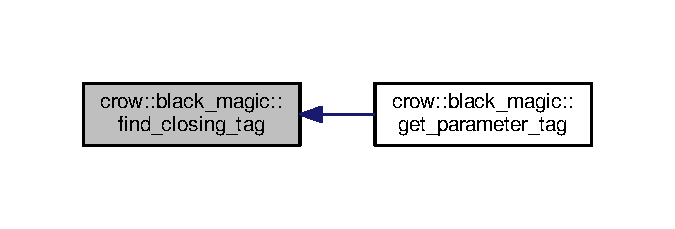
\includegraphics[width=324pt]{namespacecrow_1_1black__magic_a21fead60e1668e81ef9dbdbd1a158694_icgraph}
\end{center}
\end{figure}


\hypertarget{namespacecrow_1_1black__magic_a5e101d2f6803b92441aa8beff0f51113}{\index{crow\-::black\-\_\-magic@{crow\-::black\-\_\-magic}!get\-\_\-parameter\-\_\-tag@{get\-\_\-parameter\-\_\-tag}}
\index{get\-\_\-parameter\-\_\-tag@{get\-\_\-parameter\-\_\-tag}!crow::black_magic@{crow\-::black\-\_\-magic}}
\subsubsection[{get\-\_\-parameter\-\_\-tag}]{\setlength{\rightskip}{0pt plus 5cm}constexpr uint64\-\_\-t crow\-::black\-\_\-magic\-::get\-\_\-parameter\-\_\-tag (
\begin{DoxyParamCaption}
\item[{const\-\_\-str}]{s, }
\item[{unsigned}]{p = {\ttfamily 0}}
\end{DoxyParamCaption}
)}}\label{namespacecrow_1_1black__magic_a5e101d2f6803b92441aa8beff0f51113}


Here is the call graph for this function\-:
\nopagebreak
\begin{figure}[H]
\begin{center}
\leavevmode
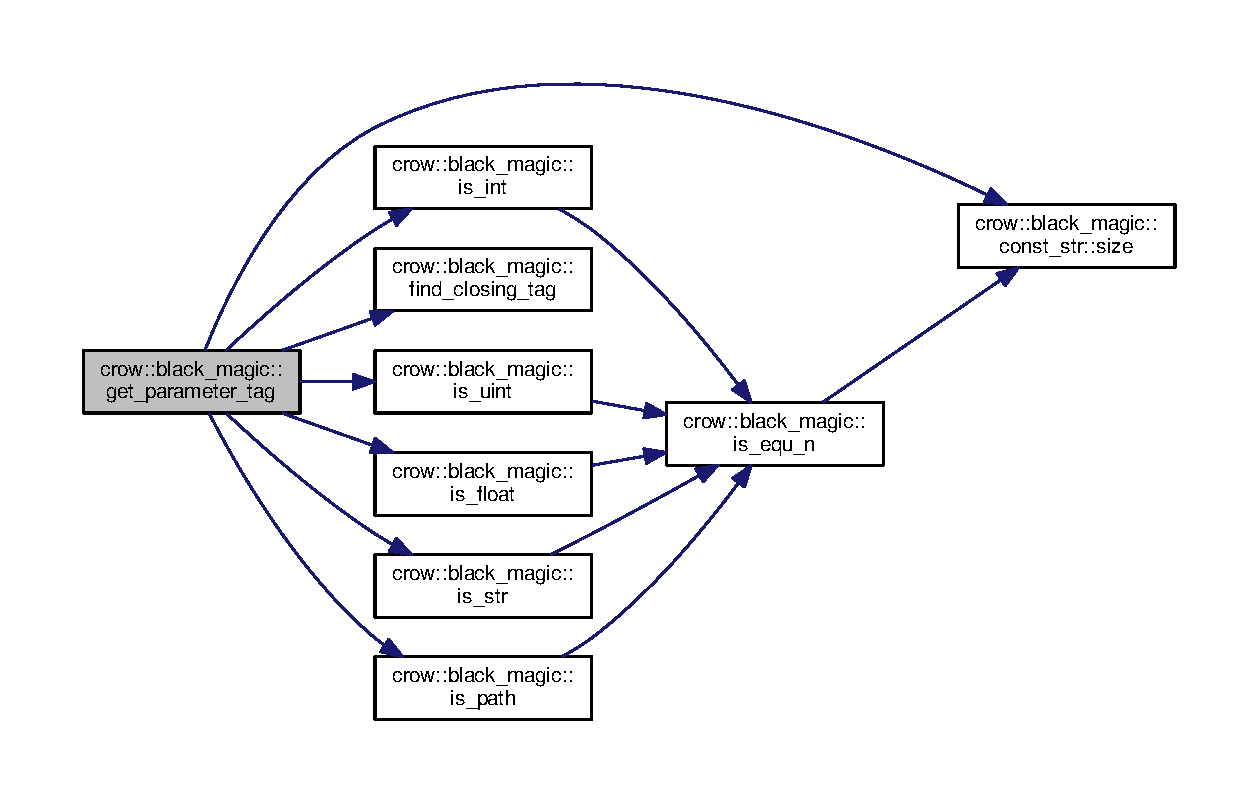
\includegraphics[width=350pt]{namespacecrow_1_1black__magic_a5e101d2f6803b92441aa8beff0f51113_cgraph}
\end{center}
\end{figure}


\hypertarget{namespacecrow_1_1black__magic_a38e0df4f002e2743c45ad435a4c9cf51}{\index{crow\-::black\-\_\-magic@{crow\-::black\-\_\-magic}!is\-\_\-equ\-\_\-n@{is\-\_\-equ\-\_\-n}}
\index{is\-\_\-equ\-\_\-n@{is\-\_\-equ\-\_\-n}!crow::black_magic@{crow\-::black\-\_\-magic}}
\subsubsection[{is\-\_\-equ\-\_\-n}]{\setlength{\rightskip}{0pt plus 5cm}constexpr bool crow\-::black\-\_\-magic\-::is\-\_\-equ\-\_\-n (
\begin{DoxyParamCaption}
\item[{const\-\_\-str}]{a, }
\item[{unsigned}]{ai, }
\item[{const\-\_\-str}]{b, }
\item[{unsigned}]{bi, }
\item[{unsigned}]{n}
\end{DoxyParamCaption}
)}}\label{namespacecrow_1_1black__magic_a38e0df4f002e2743c45ad435a4c9cf51}


Here is the call graph for this function\-:
\nopagebreak
\begin{figure}[H]
\begin{center}
\leavevmode
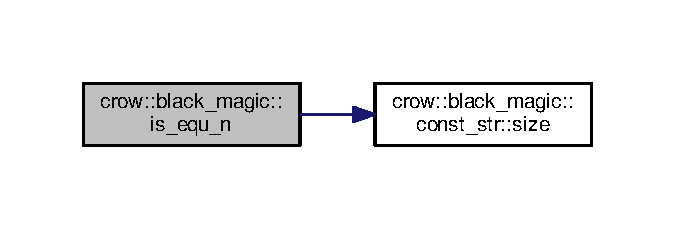
\includegraphics[width=324pt]{namespacecrow_1_1black__magic_a38e0df4f002e2743c45ad435a4c9cf51_cgraph}
\end{center}
\end{figure}




Here is the caller graph for this function\-:
\nopagebreak
\begin{figure}[H]
\begin{center}
\leavevmode
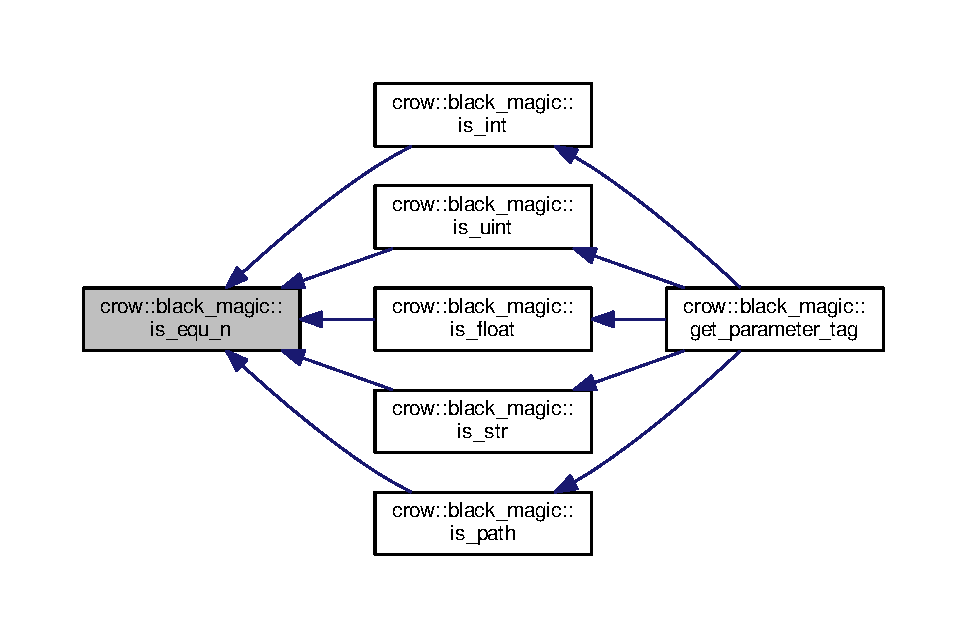
\includegraphics[width=350pt]{namespacecrow_1_1black__magic_a38e0df4f002e2743c45ad435a4c9cf51_icgraph}
\end{center}
\end{figure}


\hypertarget{namespacecrow_1_1black__magic_ad1873e3cf98eb8ed4f495272f86197cf}{\index{crow\-::black\-\_\-magic@{crow\-::black\-\_\-magic}!is\-\_\-equ\-\_\-p@{is\-\_\-equ\-\_\-p}}
\index{is\-\_\-equ\-\_\-p@{is\-\_\-equ\-\_\-p}!crow::black_magic@{crow\-::black\-\_\-magic}}
\subsubsection[{is\-\_\-equ\-\_\-p}]{\setlength{\rightskip}{0pt plus 5cm}constexpr bool crow\-::black\-\_\-magic\-::is\-\_\-equ\-\_\-p (
\begin{DoxyParamCaption}
\item[{const char $\ast$}]{a, }
\item[{const char $\ast$}]{b, }
\item[{unsigned}]{n}
\end{DoxyParamCaption}
)}}\label{namespacecrow_1_1black__magic_ad1873e3cf98eb8ed4f495272f86197cf}


Here is the caller graph for this function\-:
\nopagebreak
\begin{figure}[H]
\begin{center}
\leavevmode
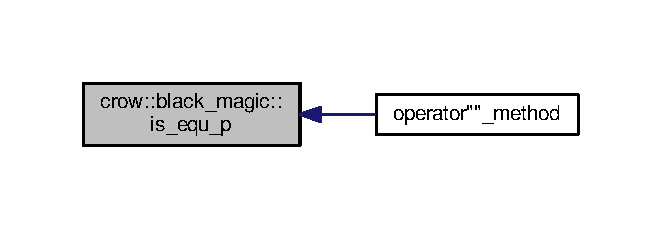
\includegraphics[width=318pt]{namespacecrow_1_1black__magic_ad1873e3cf98eb8ed4f495272f86197cf_icgraph}
\end{center}
\end{figure}


\hypertarget{namespacecrow_1_1black__magic_a57bad212b24512e47aa460cfef75c1a4}{\index{crow\-::black\-\_\-magic@{crow\-::black\-\_\-magic}!is\-\_\-float@{is\-\_\-float}}
\index{is\-\_\-float@{is\-\_\-float}!crow::black_magic@{crow\-::black\-\_\-magic}}
\subsubsection[{is\-\_\-float}]{\setlength{\rightskip}{0pt plus 5cm}constexpr bool crow\-::black\-\_\-magic\-::is\-\_\-float (
\begin{DoxyParamCaption}
\item[{const\-\_\-str}]{s, }
\item[{unsigned}]{i}
\end{DoxyParamCaption}
)}}\label{namespacecrow_1_1black__magic_a57bad212b24512e47aa460cfef75c1a4}


Here is the call graph for this function\-:
\nopagebreak
\begin{figure}[H]
\begin{center}
\leavevmode
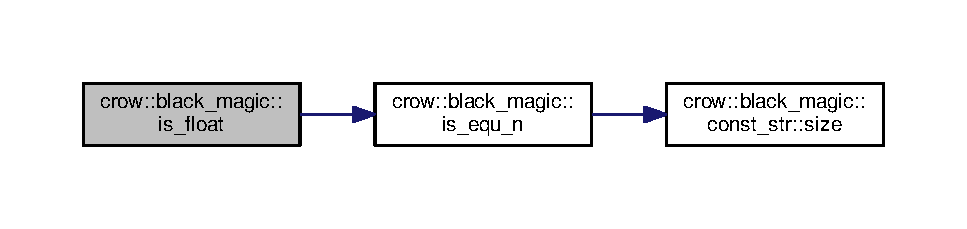
\includegraphics[width=350pt]{namespacecrow_1_1black__magic_a57bad212b24512e47aa460cfef75c1a4_cgraph}
\end{center}
\end{figure}




Here is the caller graph for this function\-:
\nopagebreak
\begin{figure}[H]
\begin{center}
\leavevmode
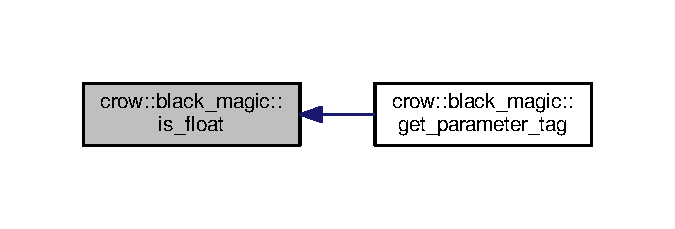
\includegraphics[width=324pt]{namespacecrow_1_1black__magic_a57bad212b24512e47aa460cfef75c1a4_icgraph}
\end{center}
\end{figure}


\hypertarget{namespacecrow_1_1black__magic_a35c7106101b8789c8b4d28e45a43fac5}{\index{crow\-::black\-\_\-magic@{crow\-::black\-\_\-magic}!is\-\_\-int@{is\-\_\-int}}
\index{is\-\_\-int@{is\-\_\-int}!crow::black_magic@{crow\-::black\-\_\-magic}}
\subsubsection[{is\-\_\-int}]{\setlength{\rightskip}{0pt plus 5cm}constexpr bool crow\-::black\-\_\-magic\-::is\-\_\-int (
\begin{DoxyParamCaption}
\item[{const\-\_\-str}]{s, }
\item[{unsigned}]{i}
\end{DoxyParamCaption}
)}}\label{namespacecrow_1_1black__magic_a35c7106101b8789c8b4d28e45a43fac5}


Here is the call graph for this function\-:
\nopagebreak
\begin{figure}[H]
\begin{center}
\leavevmode
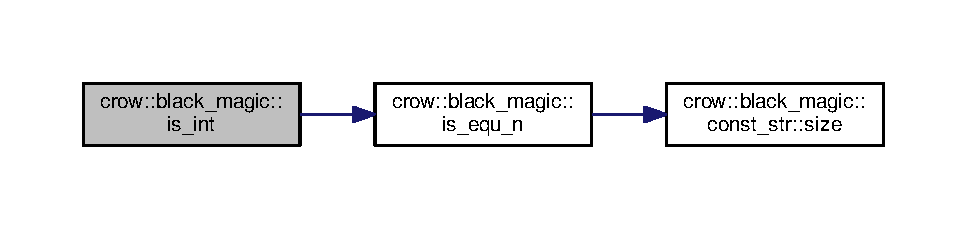
\includegraphics[width=350pt]{namespacecrow_1_1black__magic_a35c7106101b8789c8b4d28e45a43fac5_cgraph}
\end{center}
\end{figure}




Here is the caller graph for this function\-:
\nopagebreak
\begin{figure}[H]
\begin{center}
\leavevmode
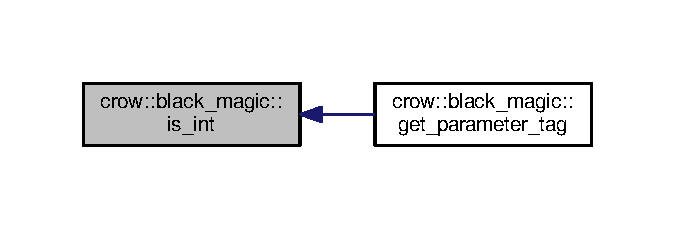
\includegraphics[width=324pt]{namespacecrow_1_1black__magic_a35c7106101b8789c8b4d28e45a43fac5_icgraph}
\end{center}
\end{figure}


\hypertarget{namespacecrow_1_1black__magic_af0899340936b274931de7ac21fb4ed9f}{\index{crow\-::black\-\_\-magic@{crow\-::black\-\_\-magic}!is\-\_\-path@{is\-\_\-path}}
\index{is\-\_\-path@{is\-\_\-path}!crow::black_magic@{crow\-::black\-\_\-magic}}
\subsubsection[{is\-\_\-path}]{\setlength{\rightskip}{0pt plus 5cm}constexpr bool crow\-::black\-\_\-magic\-::is\-\_\-path (
\begin{DoxyParamCaption}
\item[{const\-\_\-str}]{s, }
\item[{unsigned}]{i}
\end{DoxyParamCaption}
)}}\label{namespacecrow_1_1black__magic_af0899340936b274931de7ac21fb4ed9f}


Here is the call graph for this function\-:
\nopagebreak
\begin{figure}[H]
\begin{center}
\leavevmode
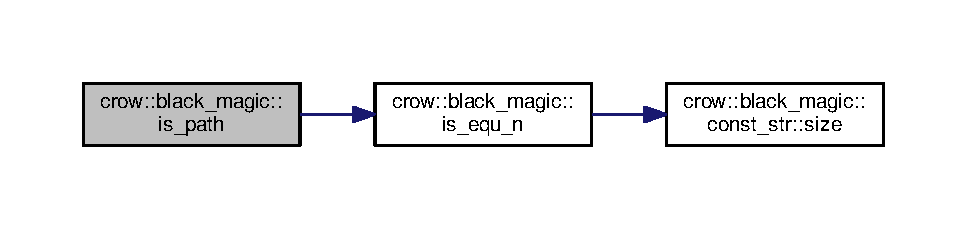
\includegraphics[width=350pt]{namespacecrow_1_1black__magic_af0899340936b274931de7ac21fb4ed9f_cgraph}
\end{center}
\end{figure}




Here is the caller graph for this function\-:
\nopagebreak
\begin{figure}[H]
\begin{center}
\leavevmode
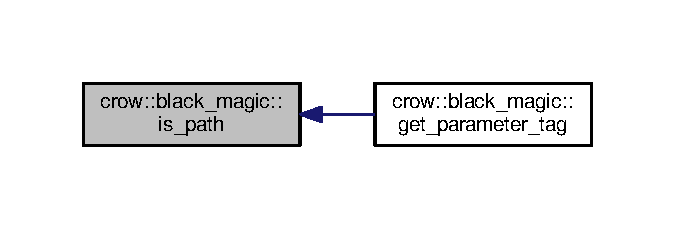
\includegraphics[width=324pt]{namespacecrow_1_1black__magic_af0899340936b274931de7ac21fb4ed9f_icgraph}
\end{center}
\end{figure}


\hypertarget{namespacecrow_1_1black__magic_a2eb0eb4514228192b878653bb56b7d44}{\index{crow\-::black\-\_\-magic@{crow\-::black\-\_\-magic}!is\-\_\-str@{is\-\_\-str}}
\index{is\-\_\-str@{is\-\_\-str}!crow::black_magic@{crow\-::black\-\_\-magic}}
\subsubsection[{is\-\_\-str}]{\setlength{\rightskip}{0pt plus 5cm}constexpr bool crow\-::black\-\_\-magic\-::is\-\_\-str (
\begin{DoxyParamCaption}
\item[{const\-\_\-str}]{s, }
\item[{unsigned}]{i}
\end{DoxyParamCaption}
)}}\label{namespacecrow_1_1black__magic_a2eb0eb4514228192b878653bb56b7d44}


Here is the call graph for this function\-:
\nopagebreak
\begin{figure}[H]
\begin{center}
\leavevmode
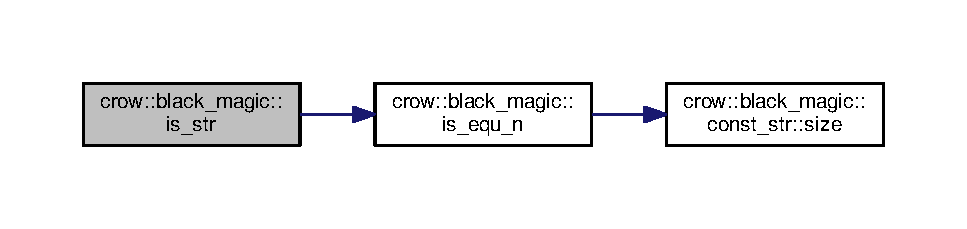
\includegraphics[width=350pt]{namespacecrow_1_1black__magic_a2eb0eb4514228192b878653bb56b7d44_cgraph}
\end{center}
\end{figure}




Here is the caller graph for this function\-:
\nopagebreak
\begin{figure}[H]
\begin{center}
\leavevmode
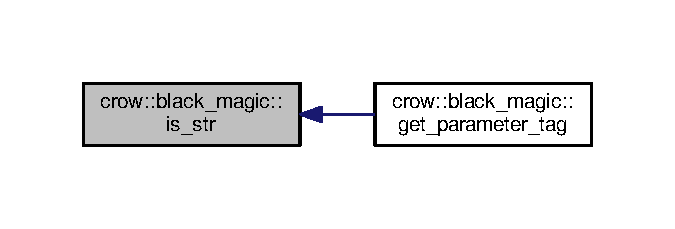
\includegraphics[width=324pt]{namespacecrow_1_1black__magic_a2eb0eb4514228192b878653bb56b7d44_icgraph}
\end{center}
\end{figure}


\hypertarget{namespacecrow_1_1black__magic_a2d8e83151f7d6b3389fea3d6dc394115}{\index{crow\-::black\-\_\-magic@{crow\-::black\-\_\-magic}!is\-\_\-uint@{is\-\_\-uint}}
\index{is\-\_\-uint@{is\-\_\-uint}!crow::black_magic@{crow\-::black\-\_\-magic}}
\subsubsection[{is\-\_\-uint}]{\setlength{\rightskip}{0pt plus 5cm}constexpr bool crow\-::black\-\_\-magic\-::is\-\_\-uint (
\begin{DoxyParamCaption}
\item[{const\-\_\-str}]{s, }
\item[{unsigned}]{i}
\end{DoxyParamCaption}
)}}\label{namespacecrow_1_1black__magic_a2d8e83151f7d6b3389fea3d6dc394115}


Here is the call graph for this function\-:
\nopagebreak
\begin{figure}[H]
\begin{center}
\leavevmode
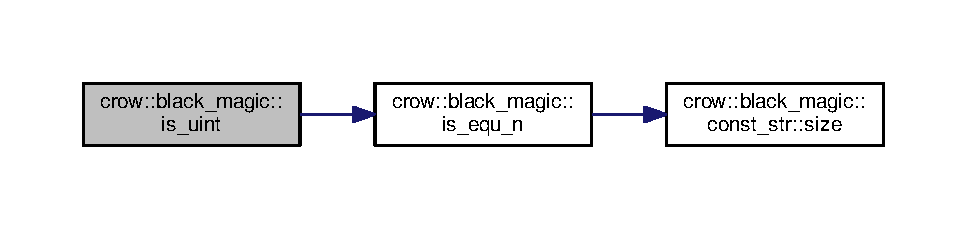
\includegraphics[width=350pt]{namespacecrow_1_1black__magic_a2d8e83151f7d6b3389fea3d6dc394115_cgraph}
\end{center}
\end{figure}




Here is the caller graph for this function\-:
\nopagebreak
\begin{figure}[H]
\begin{center}
\leavevmode
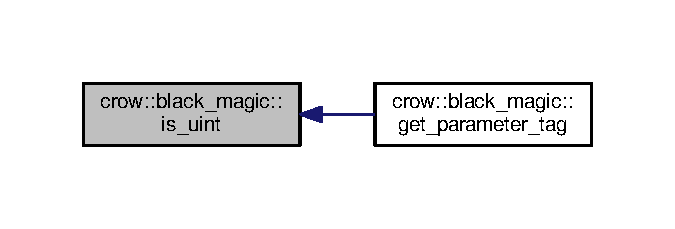
\includegraphics[width=324pt]{namespacecrow_1_1black__magic_a2d8e83151f7d6b3389fea3d6dc394115_icgraph}
\end{center}
\end{figure}


\hypertarget{namespacecrow_1_1black__magic_afc88027e704873c372fb51b5e56370da}{\index{crow\-::black\-\_\-magic@{crow\-::black\-\_\-magic}!is\-\_\-valid@{is\-\_\-valid}}
\index{is\-\_\-valid@{is\-\_\-valid}!crow::black_magic@{crow\-::black\-\_\-magic}}
\subsubsection[{is\-\_\-valid}]{\setlength{\rightskip}{0pt plus 5cm}constexpr bool crow\-::black\-\_\-magic\-::is\-\_\-valid (
\begin{DoxyParamCaption}
\item[{const\-\_\-str}]{s, }
\item[{unsigned}]{i = {\ttfamily 0}, }
\item[{int}]{f = {\ttfamily 0}}
\end{DoxyParamCaption}
)}}\label{namespacecrow_1_1black__magic_afc88027e704873c372fb51b5e56370da}


Here is the call graph for this function\-:
\nopagebreak
\begin{figure}[H]
\begin{center}
\leavevmode
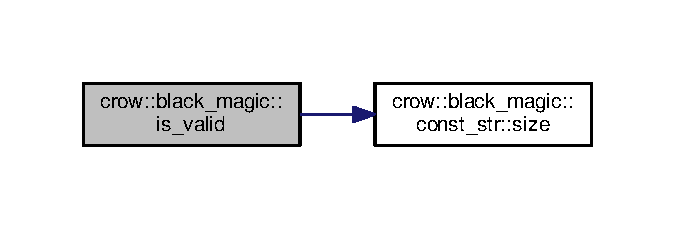
\includegraphics[width=324pt]{namespacecrow_1_1black__magic_afc88027e704873c372fb51b5e56370da_cgraph}
\end{center}
\end{figure}


\hypertarget{namespacecrow_1_1black__magic_a1c2aff5573639d46df93ffada058c686}{\index{crow\-::black\-\_\-magic@{crow\-::black\-\_\-magic}!requires\-\_\-in\-\_\-range@{requires\-\_\-in\-\_\-range}}
\index{requires\-\_\-in\-\_\-range@{requires\-\_\-in\-\_\-range}!crow::black_magic@{crow\-::black\-\_\-magic}}
\subsubsection[{requires\-\_\-in\-\_\-range}]{\setlength{\rightskip}{0pt plus 5cm}constexpr unsigned crow\-::black\-\_\-magic\-::requires\-\_\-in\-\_\-range (
\begin{DoxyParamCaption}
\item[{unsigned}]{i, }
\item[{unsigned}]{len}
\end{DoxyParamCaption}
)}}\label{namespacecrow_1_1black__magic_a1c2aff5573639d46df93ffada058c686}


Here is the caller graph for this function\-:
\nopagebreak
\begin{figure}[H]
\begin{center}
\leavevmode
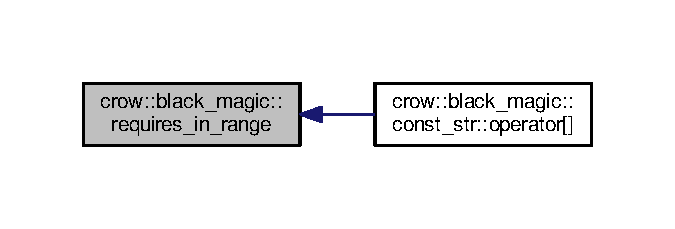
\includegraphics[width=324pt]{namespacecrow_1_1black__magic_a1c2aff5573639d46df93ffada058c686_icgraph}
\end{center}
\end{figure}



\hypertarget{namespacecrow_1_1detail}{\section{crow\-:\-:detail Namespace Reference}
\label{namespacecrow_1_1detail}\index{crow\-::detail@{crow\-::detail}}
}
\subsection*{Namespaces}
\begin{DoxyCompactItemize}
\item 
\hyperlink{namespacecrow_1_1detail_1_1routing__handler__call__helper}{routing\-\_\-handler\-\_\-call\-\_\-helper}
\end{DoxyCompactItemize}
\subsection*{Classes}
\begin{DoxyCompactItemize}
\item 
class \hyperlink{classcrow_1_1detail_1_1dumb__timer__queue}{dumb\-\_\-timer\-\_\-queue}
\item 
struct \hyperlink{structcrow_1_1detail_1_1get__index__of__element__from__tuple__by__type__impl}{get\-\_\-index\-\_\-of\-\_\-element\-\_\-from\-\_\-tuple\-\_\-by\-\_\-type\-\_\-impl}
\item 
struct \hyperlink{structcrow_1_1detail_1_1get__index__of__element__from__tuple__by__type__impl_3_01_t_00_01_n_00_01_t_00_01_args_8_8_8_4}{get\-\_\-index\-\_\-of\-\_\-element\-\_\-from\-\_\-tuple\-\_\-by\-\_\-type\-\_\-impl$<$ T, N, T, Args...$>$}
\item 
struct \hyperlink{structcrow_1_1detail_1_1get__index__of__element__from__tuple__by__type__impl_3_01_t_00_01_n_00_01_u_00_01_args_8_8_8_4}{get\-\_\-index\-\_\-of\-\_\-element\-\_\-from\-\_\-tuple\-\_\-by\-\_\-type\-\_\-impl$<$ T, N, U, Args...$>$}
\item 
struct \hyperlink{structcrow_1_1detail_1_1partial__context}{partial\-\_\-context}
\item 
struct \hyperlink{structcrow_1_1detail_1_1partial__context_3_4}{partial\-\_\-context$<$$>$}
\item 
struct \hyperlink{structcrow_1_1detail_1_1context}{context}
\item 
struct \hyperlink{structcrow_1_1detail_1_1check__before__handle__arity__3__const}{check\-\_\-before\-\_\-handle\-\_\-arity\-\_\-3\-\_\-const}
\item 
struct \hyperlink{structcrow_1_1detail_1_1check__before__handle__arity__3}{check\-\_\-before\-\_\-handle\-\_\-arity\-\_\-3}
\item 
struct \hyperlink{structcrow_1_1detail_1_1check__after__handle__arity__3__const}{check\-\_\-after\-\_\-handle\-\_\-arity\-\_\-3\-\_\-const}
\item 
struct \hyperlink{structcrow_1_1detail_1_1check__after__handle__arity__3}{check\-\_\-after\-\_\-handle\-\_\-arity\-\_\-3}
\item 
struct \hyperlink{structcrow_1_1detail_1_1is__before__handle__arity__3__impl}{is\-\_\-before\-\_\-handle\-\_\-arity\-\_\-3\-\_\-impl}
\item 
struct \hyperlink{structcrow_1_1detail_1_1is__after__handle__arity__3__impl}{is\-\_\-after\-\_\-handle\-\_\-arity\-\_\-3\-\_\-impl}
\end{DoxyCompactItemize}
\subsection*{Functions}
\begin{DoxyCompactItemize}
\item 
{\footnotesize template$<$int N, typename Context , typename Container , typename Current\-M\-W , typename... Middlewares$>$ }\\bool \hyperlink{namespacecrow_1_1detail_a7e6d675c647354299b56961f649b346b}{middleware\-\_\-call\-\_\-helper} (Container \&middlewares, \hyperlink{structcrow_1_1request}{request} \&req, \hyperlink{structcrow_1_1response}{response} \&res, Context \&ctx)
\item 
{\footnotesize template$<$typename M\-W , typename Context , typename Parent\-Context $>$ }\\std\-::enable\-\_\-if\\*
$<$!\hyperlink{structcrow_1_1detail_1_1is__before__handle__arity__3__impl}{is\-\_\-before\-\_\-handle\-\_\-arity\-\_\-3\-\_\-impl}\\*
$<$ M\-W $>$\-::value $>$\-::type \hyperlink{namespacecrow_1_1detail_a539974bbd5c715dda9a318aaf63cf0f2}{before\-\_\-handler\-\_\-call} (M\-W \&mw, \hyperlink{structcrow_1_1request}{request} \&req, \hyperlink{structcrow_1_1response}{response} \&res, Context \&ctx, Parent\-Context \&)
\item 
{\footnotesize template$<$typename M\-W , typename Context , typename Parent\-Context $>$ }\\std\-::enable\-\_\-if\\*
$<$ \hyperlink{structcrow_1_1detail_1_1is__before__handle__arity__3__impl}{is\-\_\-before\-\_\-handle\-\_\-arity\-\_\-3\-\_\-impl}\\*
$<$ M\-W $>$\-::value $>$\-::type \hyperlink{namespacecrow_1_1detail_aa08db03a6d03728487a623804fc2d237}{before\-\_\-handler\-\_\-call} (M\-W \&mw, \hyperlink{structcrow_1_1request}{request} \&req, \hyperlink{structcrow_1_1response}{response} \&res, Context \&ctx, Parent\-Context \&)
\item 
{\footnotesize template$<$typename M\-W , typename Context , typename Parent\-Context $>$ }\\std\-::enable\-\_\-if\\*
$<$!\hyperlink{structcrow_1_1detail_1_1is__after__handle__arity__3__impl}{is\-\_\-after\-\_\-handle\-\_\-arity\-\_\-3\-\_\-impl}\\*
$<$ M\-W $>$\-::value $>$\-::type \hyperlink{namespacecrow_1_1detail_a5608f0d89a16e2ba0fe1665ce5010008}{after\-\_\-handler\-\_\-call} (M\-W \&mw, \hyperlink{structcrow_1_1request}{request} \&req, \hyperlink{structcrow_1_1response}{response} \&res, Context \&ctx, Parent\-Context \&)
\item 
{\footnotesize template$<$typename M\-W , typename Context , typename Parent\-Context $>$ }\\std\-::enable\-\_\-if\\*
$<$ \hyperlink{structcrow_1_1detail_1_1is__after__handle__arity__3__impl}{is\-\_\-after\-\_\-handle\-\_\-arity\-\_\-3\-\_\-impl}\\*
$<$ M\-W $>$\-::value $>$\-::type \hyperlink{namespacecrow_1_1detail_a40996d8c8841b5660c504f36b91ba7ea}{after\-\_\-handler\-\_\-call} (M\-W \&mw, \hyperlink{structcrow_1_1request}{request} \&req, \hyperlink{structcrow_1_1response}{response} \&res, Context \&ctx, Parent\-Context \&)
\item 
{\footnotesize template$<$int N, typename Context , typename Container $>$ }\\bool \hyperlink{namespacecrow_1_1detail_a2303def444f5184e1ed4b23cb2997158}{middleware\-\_\-call\-\_\-helper} (Container \&, \hyperlink{structcrow_1_1request}{request} \&, \hyperlink{structcrow_1_1response}{response} \&, Context \&)
\item 
{\footnotesize template$<$int N, typename Context , typename Container $>$ }\\std\-::enable\-\_\-if$<$(N$<$ 0)$>$\-::type \hyperlink{namespacecrow_1_1detail_aae4ab6b9486e21216741273658bd6815}{after\-\_\-handlers\-\_\-call\-\_\-helper} (Container \&, Context \&, \hyperlink{structcrow_1_1request}{request} \&, \hyperlink{structcrow_1_1response}{response} \&)
\item 
{\footnotesize template$<$int N, typename Context , typename Container $>$ }\\std\-::enable\-\_\-if$<$(N==0)$>$\-::type \hyperlink{namespacecrow_1_1detail_aad451e95cf059336c22588b3a7f68f54}{after\-\_\-handlers\-\_\-call\-\_\-helper} (Container \&middlewares, Context \&ctx, \hyperlink{structcrow_1_1request}{request} \&req, \hyperlink{structcrow_1_1response}{response} \&res)
\item 
{\footnotesize template$<$int N, typename Context , typename Container $>$ }\\std\-::enable\-\_\-if$<$(N $>$0)$>$\-::type \hyperlink{namespacecrow_1_1detail_ae923d5e1ec2e6cb2f964dc734667151c}{after\-\_\-handlers\-\_\-call\-\_\-helper} (Container \&middlewares, Context \&ctx, \hyperlink{structcrow_1_1request}{request} \&req, \hyperlink{structcrow_1_1response}{response} \&res)
\end{DoxyCompactItemize}


\subsection{Function Documentation}
\hypertarget{namespacecrow_1_1detail_a5608f0d89a16e2ba0fe1665ce5010008}{\index{crow\-::detail@{crow\-::detail}!after\-\_\-handler\-\_\-call@{after\-\_\-handler\-\_\-call}}
\index{after\-\_\-handler\-\_\-call@{after\-\_\-handler\-\_\-call}!crow::detail@{crow\-::detail}}
\subsubsection[{after\-\_\-handler\-\_\-call}]{\setlength{\rightskip}{0pt plus 5cm}template$<$typename M\-W , typename Context , typename Parent\-Context $>$ std\-::enable\-\_\-if$<$!{\bf is\-\_\-after\-\_\-handle\-\_\-arity\-\_\-3\-\_\-impl}$<$M\-W$>$\-::value$>$\-::type crow\-::detail\-::after\-\_\-handler\-\_\-call (
\begin{DoxyParamCaption}
\item[{M\-W \&}]{mw, }
\item[{request \&}]{req, }
\item[{response \&}]{res, }
\item[{Context \&}]{ctx, }
\item[{Parent\-Context \&}]{}
\end{DoxyParamCaption}
)}}\label{namespacecrow_1_1detail_a5608f0d89a16e2ba0fe1665ce5010008}
\hypertarget{namespacecrow_1_1detail_a40996d8c8841b5660c504f36b91ba7ea}{\index{crow\-::detail@{crow\-::detail}!after\-\_\-handler\-\_\-call@{after\-\_\-handler\-\_\-call}}
\index{after\-\_\-handler\-\_\-call@{after\-\_\-handler\-\_\-call}!crow::detail@{crow\-::detail}}
\subsubsection[{after\-\_\-handler\-\_\-call}]{\setlength{\rightskip}{0pt plus 5cm}template$<$typename M\-W , typename Context , typename Parent\-Context $>$ std\-::enable\-\_\-if$<${\bf is\-\_\-after\-\_\-handle\-\_\-arity\-\_\-3\-\_\-impl}$<$M\-W$>$\-::value$>$\-::type crow\-::detail\-::after\-\_\-handler\-\_\-call (
\begin{DoxyParamCaption}
\item[{M\-W \&}]{mw, }
\item[{request \&}]{req, }
\item[{response \&}]{res, }
\item[{Context \&}]{ctx, }
\item[{Parent\-Context \&}]{}
\end{DoxyParamCaption}
)}}\label{namespacecrow_1_1detail_a40996d8c8841b5660c504f36b91ba7ea}
\hypertarget{namespacecrow_1_1detail_aae4ab6b9486e21216741273658bd6815}{\index{crow\-::detail@{crow\-::detail}!after\-\_\-handlers\-\_\-call\-\_\-helper@{after\-\_\-handlers\-\_\-call\-\_\-helper}}
\index{after\-\_\-handlers\-\_\-call\-\_\-helper@{after\-\_\-handlers\-\_\-call\-\_\-helper}!crow::detail@{crow\-::detail}}
\subsubsection[{after\-\_\-handlers\-\_\-call\-\_\-helper}]{\setlength{\rightskip}{0pt plus 5cm}template$<$int N, typename Context , typename Container $>$ std\-::enable\-\_\-if$<$(N$<$0)$>$\-::type crow\-::detail\-::after\-\_\-handlers\-\_\-call\-\_\-helper (
\begin{DoxyParamCaption}
\item[{Container \&}]{, }
\item[{Context \&}]{, }
\item[{request \&}]{, }
\item[{response \&}]{}
\end{DoxyParamCaption}
)}}\label{namespacecrow_1_1detail_aae4ab6b9486e21216741273658bd6815}


Here is the caller graph for this function\-:
\nopagebreak
\begin{figure}[H]
\begin{center}
\leavevmode
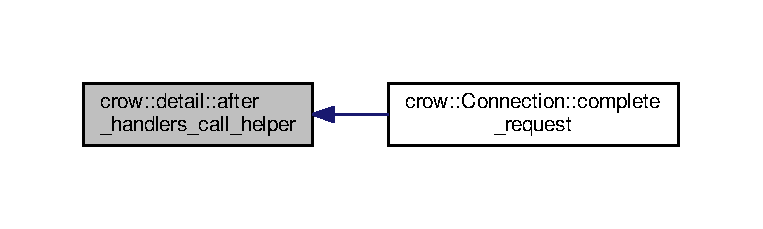
\includegraphics[width=350pt]{namespacecrow_1_1detail_aae4ab6b9486e21216741273658bd6815_icgraph}
\end{center}
\end{figure}


\hypertarget{namespacecrow_1_1detail_aad451e95cf059336c22588b3a7f68f54}{\index{crow\-::detail@{crow\-::detail}!after\-\_\-handlers\-\_\-call\-\_\-helper@{after\-\_\-handlers\-\_\-call\-\_\-helper}}
\index{after\-\_\-handlers\-\_\-call\-\_\-helper@{after\-\_\-handlers\-\_\-call\-\_\-helper}!crow::detail@{crow\-::detail}}
\subsubsection[{after\-\_\-handlers\-\_\-call\-\_\-helper}]{\setlength{\rightskip}{0pt plus 5cm}template$<$int N, typename Context , typename Container $>$ std\-::enable\-\_\-if$<$(N==0)$>$\-::type crow\-::detail\-::after\-\_\-handlers\-\_\-call\-\_\-helper (
\begin{DoxyParamCaption}
\item[{Container \&}]{middlewares, }
\item[{Context \&}]{ctx, }
\item[{request \&}]{req, }
\item[{response \&}]{res}
\end{DoxyParamCaption}
)}}\label{namespacecrow_1_1detail_aad451e95cf059336c22588b3a7f68f54}
\hypertarget{namespacecrow_1_1detail_ae923d5e1ec2e6cb2f964dc734667151c}{\index{crow\-::detail@{crow\-::detail}!after\-\_\-handlers\-\_\-call\-\_\-helper@{after\-\_\-handlers\-\_\-call\-\_\-helper}}
\index{after\-\_\-handlers\-\_\-call\-\_\-helper@{after\-\_\-handlers\-\_\-call\-\_\-helper}!crow::detail@{crow\-::detail}}
\subsubsection[{after\-\_\-handlers\-\_\-call\-\_\-helper}]{\setlength{\rightskip}{0pt plus 5cm}template$<$int N, typename Context , typename Container $>$ std\-::enable\-\_\-if$<$(N$>$0)$>$\-::type crow\-::detail\-::after\-\_\-handlers\-\_\-call\-\_\-helper (
\begin{DoxyParamCaption}
\item[{Container \&}]{middlewares, }
\item[{Context \&}]{ctx, }
\item[{request \&}]{req, }
\item[{response \&}]{res}
\end{DoxyParamCaption}
)}}\label{namespacecrow_1_1detail_ae923d5e1ec2e6cb2f964dc734667151c}
\hypertarget{namespacecrow_1_1detail_a539974bbd5c715dda9a318aaf63cf0f2}{\index{crow\-::detail@{crow\-::detail}!before\-\_\-handler\-\_\-call@{before\-\_\-handler\-\_\-call}}
\index{before\-\_\-handler\-\_\-call@{before\-\_\-handler\-\_\-call}!crow::detail@{crow\-::detail}}
\subsubsection[{before\-\_\-handler\-\_\-call}]{\setlength{\rightskip}{0pt plus 5cm}template$<$typename M\-W , typename Context , typename Parent\-Context $>$ std\-::enable\-\_\-if$<$!{\bf is\-\_\-before\-\_\-handle\-\_\-arity\-\_\-3\-\_\-impl}$<$M\-W$>$\-::value$>$\-::type crow\-::detail\-::before\-\_\-handler\-\_\-call (
\begin{DoxyParamCaption}
\item[{M\-W \&}]{mw, }
\item[{request \&}]{req, }
\item[{response \&}]{res, }
\item[{Context \&}]{ctx, }
\item[{Parent\-Context \&}]{}
\end{DoxyParamCaption}
)}}\label{namespacecrow_1_1detail_a539974bbd5c715dda9a318aaf63cf0f2}
\hypertarget{namespacecrow_1_1detail_aa08db03a6d03728487a623804fc2d237}{\index{crow\-::detail@{crow\-::detail}!before\-\_\-handler\-\_\-call@{before\-\_\-handler\-\_\-call}}
\index{before\-\_\-handler\-\_\-call@{before\-\_\-handler\-\_\-call}!crow::detail@{crow\-::detail}}
\subsubsection[{before\-\_\-handler\-\_\-call}]{\setlength{\rightskip}{0pt plus 5cm}template$<$typename M\-W , typename Context , typename Parent\-Context $>$ std\-::enable\-\_\-if$<${\bf is\-\_\-before\-\_\-handle\-\_\-arity\-\_\-3\-\_\-impl}$<$M\-W$>$\-::value$>$\-::type crow\-::detail\-::before\-\_\-handler\-\_\-call (
\begin{DoxyParamCaption}
\item[{M\-W \&}]{mw, }
\item[{request \&}]{req, }
\item[{response \&}]{res, }
\item[{Context \&}]{ctx, }
\item[{Parent\-Context \&}]{}
\end{DoxyParamCaption}
)}}\label{namespacecrow_1_1detail_aa08db03a6d03728487a623804fc2d237}
\hypertarget{namespacecrow_1_1detail_a7e6d675c647354299b56961f649b346b}{\index{crow\-::detail@{crow\-::detail}!middleware\-\_\-call\-\_\-helper@{middleware\-\_\-call\-\_\-helper}}
\index{middleware\-\_\-call\-\_\-helper@{middleware\-\_\-call\-\_\-helper}!crow::detail@{crow\-::detail}}
\subsubsection[{middleware\-\_\-call\-\_\-helper}]{\setlength{\rightskip}{0pt plus 5cm}template$<$int N, typename Context , typename Container , typename Current\-M\-W , typename... Middlewares$>$ bool crow\-::detail\-::middleware\-\_\-call\-\_\-helper (
\begin{DoxyParamCaption}
\item[{Container \&}]{middlewares, }
\item[{request \&}]{req, }
\item[{response \&}]{res, }
\item[{Context \&}]{ctx}
\end{DoxyParamCaption}
)}}\label{namespacecrow_1_1detail_a7e6d675c647354299b56961f649b346b}


Here is the call graph for this function\-:
\nopagebreak
\begin{figure}[H]
\begin{center}
\leavevmode
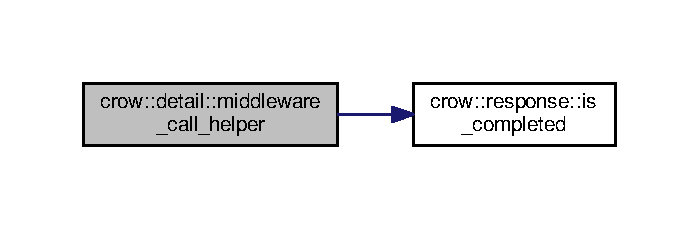
\includegraphics[width=336pt]{namespacecrow_1_1detail_a7e6d675c647354299b56961f649b346b_cgraph}
\end{center}
\end{figure}




Here is the caller graph for this function\-:
\nopagebreak
\begin{figure}[H]
\begin{center}
\leavevmode
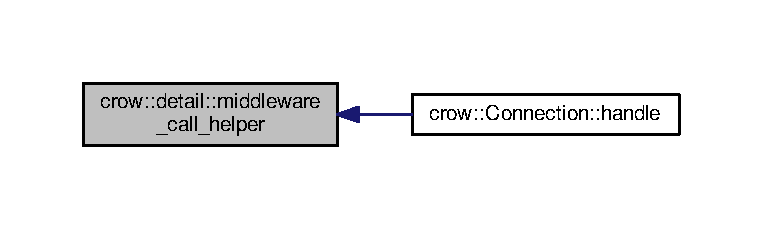
\includegraphics[width=350pt]{namespacecrow_1_1detail_a7e6d675c647354299b56961f649b346b_icgraph}
\end{center}
\end{figure}


\hypertarget{namespacecrow_1_1detail_a2303def444f5184e1ed4b23cb2997158}{\index{crow\-::detail@{crow\-::detail}!middleware\-\_\-call\-\_\-helper@{middleware\-\_\-call\-\_\-helper}}
\index{middleware\-\_\-call\-\_\-helper@{middleware\-\_\-call\-\_\-helper}!crow::detail@{crow\-::detail}}
\subsubsection[{middleware\-\_\-call\-\_\-helper}]{\setlength{\rightskip}{0pt plus 5cm}template$<$int N, typename Context , typename Container $>$ bool crow\-::detail\-::middleware\-\_\-call\-\_\-helper (
\begin{DoxyParamCaption}
\item[{Container \&}]{, }
\item[{request \&}]{, }
\item[{response \&}]{, }
\item[{Context \&}]{}
\end{DoxyParamCaption}
)}}\label{namespacecrow_1_1detail_a2303def444f5184e1ed4b23cb2997158}

\hypertarget{namespacecrow_1_1detail_1_1routing__handler__call__helper}{\section{crow\-:\-:detail\-:\-:routing\-\_\-handler\-\_\-call\-\_\-helper Namespace Reference}
\label{namespacecrow_1_1detail_1_1routing__handler__call__helper}\index{crow\-::detail\-::routing\-\_\-handler\-\_\-call\-\_\-helper@{crow\-::detail\-::routing\-\_\-handler\-\_\-call\-\_\-helper}}
}
\subsection*{Classes}
\begin{DoxyCompactItemize}
\item 
struct \hyperlink{structcrow_1_1detail_1_1routing__handler__call__helper_1_1call__pair}{call\-\_\-pair}
\item 
struct \hyperlink{structcrow_1_1detail_1_1routing__handler__call__helper_1_1call__params}{call\-\_\-params}
\item 
struct \hyperlink{structcrow_1_1detail_1_1routing__handler__call__helper_1_1call}{call}
\item 
struct \hyperlink{structcrow_1_1detail_1_1routing__handler__call__helper_1_1call_3_01_f_00_01_n_int_00_01_n_uint_0b6a35a476dfcab9d942547331be456a9}{call$<$ F, N\-Int, N\-Uint, N\-Double, N\-String, black\-\_\-magic\-::\-S$<$ int64\-\_\-t, Args1...$>$, black\-\_\-magic\-::\-S$<$ Args2...$>$ $>$}
\item 
struct \hyperlink{structcrow_1_1detail_1_1routing__handler__call__helper_1_1call_3_01_f_00_01_n_int_00_01_n_uint_00ad4e6269b7fa1968d50bbffd43a8f02}{call$<$ F, N\-Int, N\-Uint, N\-Double, N\-String, black\-\_\-magic\-::\-S$<$ uint64\-\_\-t, Args1...$>$, black\-\_\-magic\-::\-S$<$ Args2...$>$ $>$}
\item 
struct \hyperlink{structcrow_1_1detail_1_1routing__handler__call__helper_1_1call_3_01_f_00_01_n_int_00_01_n_uint_0b30fc35e23f441513a63571edf36fc02}{call$<$ F, N\-Int, N\-Uint, N\-Double, N\-String, black\-\_\-magic\-::\-S$<$ double, Args1...$>$, black\-\_\-magic\-::\-S$<$ Args2...$>$ $>$}
\item 
struct \hyperlink{structcrow_1_1detail_1_1routing__handler__call__helper_1_1call_3_01_f_00_01_n_int_00_01_n_uint_0d6c3c1bf426d7dfb9e3165c9ff3fd2f3}{call$<$ F, N\-Int, N\-Uint, N\-Double, N\-String, black\-\_\-magic\-::\-S$<$ std\-::string, Args1...$>$, black\-\_\-magic\-::\-S$<$ Args2...$>$ $>$}
\item 
struct \hyperlink{structcrow_1_1detail_1_1routing__handler__call__helper_1_1call_3_01_f_00_01_n_int_00_01_n_uint_0d7ef20f9a959e64c78052cf52ae9f097}{call$<$ F, N\-Int, N\-Uint, N\-Double, N\-String, black\-\_\-magic\-::\-S$<$$>$, black\-\_\-magic\-::\-S$<$ Args1...$>$ $>$}
\item 
struct \hyperlink{structcrow_1_1detail_1_1routing__handler__call__helper_1_1_wrapped}{Wrapped}
\end{DoxyCompactItemize}

\hypertarget{namespacecrow_1_1json}{\section{crow\-:\-:json Namespace Reference}
\label{namespacecrow_1_1json}\index{crow\-::json@{crow\-::json}}
}
\subsection*{Namespaces}
\begin{DoxyCompactItemize}
\item 
\hyperlink{namespacecrow_1_1json_1_1detail}{detail}
\end{DoxyCompactItemize}
\subsection*{Classes}
\begin{DoxyCompactItemize}
\item 
class \hyperlink{classcrow_1_1json_1_1rvalue}{rvalue}
\item 
class \hyperlink{classcrow_1_1json_1_1wvalue}{wvalue}
\end{DoxyCompactItemize}
\subsection*{Enumerations}
\begin{DoxyCompactItemize}
\item 
enum \hyperlink{namespacecrow_1_1json_adb9569a402d1b289a75025c8c96e5d99}{type} \-: char \{ \\*
\hyperlink{namespacecrow_1_1json_adb9569a402d1b289a75025c8c96e5d99abbb93ef26e3c101ff11cdd21cab08a94}{type\-::\-Null}, 
\hyperlink{namespacecrow_1_1json_adb9569a402d1b289a75025c8c96e5d99af8320b26d30ab433c5a54546d21f414c}{type\-::\-False}, 
\hyperlink{namespacecrow_1_1json_adb9569a402d1b289a75025c8c96e5d99af827cf462f62848df37c5e1e94a4da74}{type\-::\-True}, 
\hyperlink{namespacecrow_1_1json_adb9569a402d1b289a75025c8c96e5d99ab2ee912b91d69b435159c7c3f6df7f5f}{type\-::\-Number}, 
\\*
\hyperlink{namespacecrow_1_1json_adb9569a402d1b289a75025c8c96e5d99a27118326006d3829667a400ad23d5d98}{type\-::\-String}, 
\hyperlink{namespacecrow_1_1json_adb9569a402d1b289a75025c8c96e5d99a4ee29ca12c7d126654bd0e5275de6135}{type\-::\-List}, 
\hyperlink{namespacecrow_1_1json_adb9569a402d1b289a75025c8c96e5d99a497031794414a552435f90151ac3b54b}{type\-::\-Object}
 \}
\end{DoxyCompactItemize}
\subsection*{Functions}
\begin{DoxyCompactItemize}
\item 
void \hyperlink{namespacecrow_1_1json_a98e83fcd8d2e51b3acfc99d868b4e41a}{escape} (const std\-::string \&str, std\-::string \&ret)
\item 
std\-::string \hyperlink{namespacecrow_1_1json_a27086e84491472bba7ff876c929f5df3}{escape} (const std\-::string \&str)
\item 
const char $\ast$ \hyperlink{namespacecrow_1_1json_ae63b97ba6f66ef6daf254e00a4b0facb}{get\-\_\-type\-\_\-str} (\hyperlink{namespacecrow_1_1json_adb9569a402d1b289a75025c8c96e5d99}{type} t)
\item 
\hyperlink{classcrow_1_1json_1_1rvalue}{rvalue} \hyperlink{namespacecrow_1_1json_a84a2fc9bc21a94b2791271e54879ab0a}{load} (const char $\ast$data, size\-\_\-t size)
\item 
bool \hyperlink{namespacecrow_1_1json_a516708ab016de1caa6d3203529929b2e}{operator==} (const \hyperlink{classcrow_1_1json_1_1rvalue}{rvalue} \&\hyperlink{three_8min_8js_aae3c400cfa9afd0584b6226ac3804a40}{l}, const std\-::string \&r)
\item 
bool \hyperlink{namespacecrow_1_1json_aa9ae087edb7382ba2df19bb5b4b8165b}{operator==} (const std\-::string \&\hyperlink{three_8min_8js_aae3c400cfa9afd0584b6226ac3804a40}{l}, const \hyperlink{classcrow_1_1json_1_1rvalue}{rvalue} \&r)
\item 
bool \hyperlink{namespacecrow_1_1json_a2f0451a26844bed78da38c06d18d76f7}{operator!=} (const \hyperlink{classcrow_1_1json_1_1rvalue}{rvalue} \&\hyperlink{three_8min_8js_aae3c400cfa9afd0584b6226ac3804a40}{l}, const std\-::string \&r)
\item 
bool \hyperlink{namespacecrow_1_1json_aba197bed8a4a07e34a0733d633b14e9b}{operator!=} (const std\-::string \&\hyperlink{three_8min_8js_aae3c400cfa9afd0584b6226ac3804a40}{l}, const \hyperlink{classcrow_1_1json_1_1rvalue}{rvalue} \&r)
\item 
bool \hyperlink{namespacecrow_1_1json_a1079ce699fb8174f6f4092b79ef44fc0}{operator==} (const \hyperlink{classcrow_1_1json_1_1rvalue}{rvalue} \&\hyperlink{three_8min_8js_aae3c400cfa9afd0584b6226ac3804a40}{l}, double r)
\item 
bool \hyperlink{namespacecrow_1_1json_a90cbe3f52220c2062156cf256e43c631}{operator==} (double \hyperlink{three_8min_8js_aae3c400cfa9afd0584b6226ac3804a40}{l}, const \hyperlink{classcrow_1_1json_1_1rvalue}{rvalue} \&r)
\item 
bool \hyperlink{namespacecrow_1_1json_a4b737b3cf606bf2e63ed09ceff8ce89a}{operator!=} (const \hyperlink{classcrow_1_1json_1_1rvalue}{rvalue} \&\hyperlink{three_8min_8js_aae3c400cfa9afd0584b6226ac3804a40}{l}, double r)
\item 
bool \hyperlink{namespacecrow_1_1json_ac606c21e102f1104500667e9060ee0ed}{operator!=} (double \hyperlink{three_8min_8js_aae3c400cfa9afd0584b6226ac3804a40}{l}, const \hyperlink{classcrow_1_1json_1_1rvalue}{rvalue} \&r)
\item 
\hyperlink{classcrow_1_1json_1_1rvalue}{rvalue} \hyperlink{namespacecrow_1_1json_a0cd58f45702772a5aac929dec0966a0a}{load\-\_\-nocopy\-\_\-internal} (char $\ast$data, size\-\_\-t size)
\item 
\hyperlink{classcrow_1_1json_1_1rvalue}{rvalue} \hyperlink{namespacecrow_1_1json_ad995f1379ae1ddc8075cab8185c9a78a}{load} (const char $\ast$data)
\item 
\hyperlink{classcrow_1_1json_1_1rvalue}{rvalue} \hyperlink{namespacecrow_1_1json_a59efe2ae1d83ded364cc3ecc143bce85}{load} (const std\-::string \&str)
\item 
void \hyperlink{namespacecrow_1_1json_af1b84b949166845e81f327e5e43cabee}{dump\-\_\-string} (const std\-::string \&str, std\-::string \&out)
\item 
void \hyperlink{namespacecrow_1_1json_a89aba215e22bb1186515fe0db09d04d8}{dump\-\_\-internal} (const \hyperlink{classcrow_1_1json_1_1wvalue}{wvalue} \&v, std\-::string \&out)
\item 
std\-::string \hyperlink{namespacecrow_1_1json_ad28648d5c8e4d7eaea2777692e5ffec2}{dump} (const \hyperlink{classcrow_1_1json_1_1wvalue}{wvalue} \&v)
\end{DoxyCompactItemize}


\subsection{Enumeration Type Documentation}
\hypertarget{namespacecrow_1_1json_adb9569a402d1b289a75025c8c96e5d99}{\index{crow\-::json@{crow\-::json}!type@{type}}
\index{type@{type}!crow::json@{crow\-::json}}
\subsubsection[{type}]{\setlength{\rightskip}{0pt plus 5cm}enum {\bf crow\-::json\-::type} \-: char\hspace{0.3cm}{\ttfamily [strong]}}}\label{namespacecrow_1_1json_adb9569a402d1b289a75025c8c96e5d99}
\begin{Desc}
\item[Enumerator]\par
\begin{description}
\index{Null@{Null}!crow\-::json@{crow\-::json}}\index{crow\-::json@{crow\-::json}!Null@{Null}}\item[{\em 
\hypertarget{namespacecrow_1_1json_adb9569a402d1b289a75025c8c96e5d99abbb93ef26e3c101ff11cdd21cab08a94}{Null}\label{namespacecrow_1_1json_adb9569a402d1b289a75025c8c96e5d99abbb93ef26e3c101ff11cdd21cab08a94}
}]\index{False@{False}!crow\-::json@{crow\-::json}}\index{crow\-::json@{crow\-::json}!False@{False}}\item[{\em 
\hypertarget{namespacecrow_1_1json_adb9569a402d1b289a75025c8c96e5d99af8320b26d30ab433c5a54546d21f414c}{False}\label{namespacecrow_1_1json_adb9569a402d1b289a75025c8c96e5d99af8320b26d30ab433c5a54546d21f414c}
}]\index{True@{True}!crow\-::json@{crow\-::json}}\index{crow\-::json@{crow\-::json}!True@{True}}\item[{\em 
\hypertarget{namespacecrow_1_1json_adb9569a402d1b289a75025c8c96e5d99af827cf462f62848df37c5e1e94a4da74}{True}\label{namespacecrow_1_1json_adb9569a402d1b289a75025c8c96e5d99af827cf462f62848df37c5e1e94a4da74}
}]\index{Number@{Number}!crow\-::json@{crow\-::json}}\index{crow\-::json@{crow\-::json}!Number@{Number}}\item[{\em 
\hypertarget{namespacecrow_1_1json_adb9569a402d1b289a75025c8c96e5d99ab2ee912b91d69b435159c7c3f6df7f5f}{Number}\label{namespacecrow_1_1json_adb9569a402d1b289a75025c8c96e5d99ab2ee912b91d69b435159c7c3f6df7f5f}
}]\index{String@{String}!crow\-::json@{crow\-::json}}\index{crow\-::json@{crow\-::json}!String@{String}}\item[{\em 
\hypertarget{namespacecrow_1_1json_adb9569a402d1b289a75025c8c96e5d99a27118326006d3829667a400ad23d5d98}{String}\label{namespacecrow_1_1json_adb9569a402d1b289a75025c8c96e5d99a27118326006d3829667a400ad23d5d98}
}]\index{List@{List}!crow\-::json@{crow\-::json}}\index{crow\-::json@{crow\-::json}!List@{List}}\item[{\em 
\hypertarget{namespacecrow_1_1json_adb9569a402d1b289a75025c8c96e5d99a4ee29ca12c7d126654bd0e5275de6135}{List}\label{namespacecrow_1_1json_adb9569a402d1b289a75025c8c96e5d99a4ee29ca12c7d126654bd0e5275de6135}
}]\index{Object@{Object}!crow\-::json@{crow\-::json}}\index{crow\-::json@{crow\-::json}!Object@{Object}}\item[{\em 
\hypertarget{namespacecrow_1_1json_adb9569a402d1b289a75025c8c96e5d99a497031794414a552435f90151ac3b54b}{Object}\label{namespacecrow_1_1json_adb9569a402d1b289a75025c8c96e5d99a497031794414a552435f90151ac3b54b}
}]\end{description}
\end{Desc}


\subsection{Function Documentation}
\hypertarget{namespacecrow_1_1json_ad28648d5c8e4d7eaea2777692e5ffec2}{\index{crow\-::json@{crow\-::json}!dump@{dump}}
\index{dump@{dump}!crow::json@{crow\-::json}}
\subsubsection[{dump}]{\setlength{\rightskip}{0pt plus 5cm}std\-::string crow\-::json\-::dump (
\begin{DoxyParamCaption}
\item[{const wvalue \&}]{v}
\end{DoxyParamCaption}
)\hspace{0.3cm}{\ttfamily [inline]}}}\label{namespacecrow_1_1json_ad28648d5c8e4d7eaea2777692e5ffec2}


Here is the call graph for this function\-:
\nopagebreak
\begin{figure}[H]
\begin{center}
\leavevmode
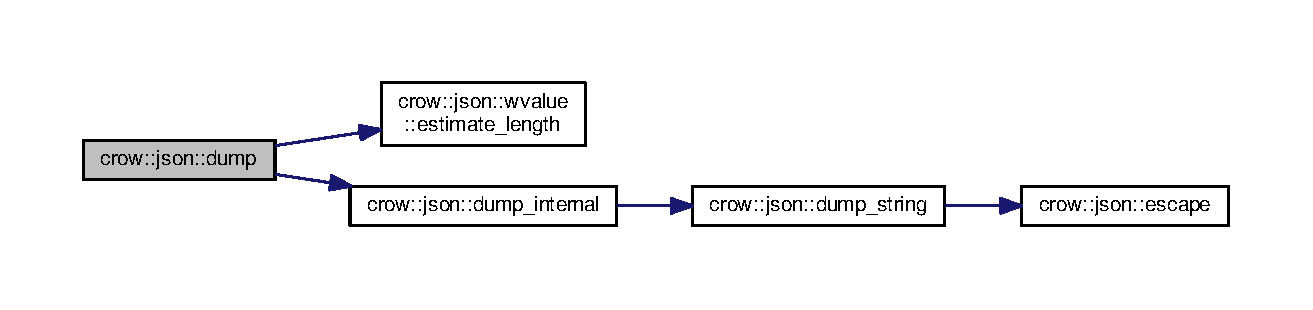
\includegraphics[width=350pt]{namespacecrow_1_1json_ad28648d5c8e4d7eaea2777692e5ffec2_cgraph}
\end{center}
\end{figure}




Here is the caller graph for this function\-:
\nopagebreak
\begin{figure}[H]
\begin{center}
\leavevmode
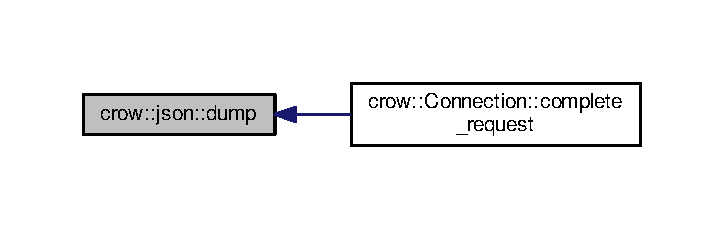
\includegraphics[width=348pt]{namespacecrow_1_1json_ad28648d5c8e4d7eaea2777692e5ffec2_icgraph}
\end{center}
\end{figure}


\hypertarget{namespacecrow_1_1json_a89aba215e22bb1186515fe0db09d04d8}{\index{crow\-::json@{crow\-::json}!dump\-\_\-internal@{dump\-\_\-internal}}
\index{dump\-\_\-internal@{dump\-\_\-internal}!crow::json@{crow\-::json}}
\subsubsection[{dump\-\_\-internal}]{\setlength{\rightskip}{0pt plus 5cm}void crow\-::json\-::dump\-\_\-internal (
\begin{DoxyParamCaption}
\item[{const wvalue \&}]{v, }
\item[{std\-::string \&}]{out}
\end{DoxyParamCaption}
)\hspace{0.3cm}{\ttfamily [inline]}}}\label{namespacecrow_1_1json_a89aba215e22bb1186515fe0db09d04d8}


Here is the call graph for this function\-:
\nopagebreak
\begin{figure}[H]
\begin{center}
\leavevmode
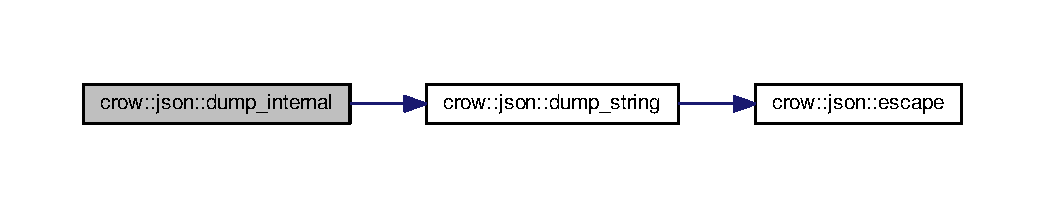
\includegraphics[width=350pt]{namespacecrow_1_1json_a89aba215e22bb1186515fe0db09d04d8_cgraph}
\end{center}
\end{figure}




Here is the caller graph for this function\-:
\nopagebreak
\begin{figure}[H]
\begin{center}
\leavevmode
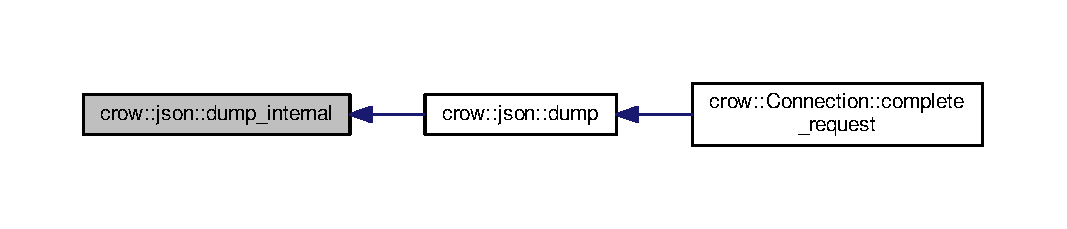
\includegraphics[width=350pt]{namespacecrow_1_1json_a89aba215e22bb1186515fe0db09d04d8_icgraph}
\end{center}
\end{figure}


\hypertarget{namespacecrow_1_1json_af1b84b949166845e81f327e5e43cabee}{\index{crow\-::json@{crow\-::json}!dump\-\_\-string@{dump\-\_\-string}}
\index{dump\-\_\-string@{dump\-\_\-string}!crow::json@{crow\-::json}}
\subsubsection[{dump\-\_\-string}]{\setlength{\rightskip}{0pt plus 5cm}void crow\-::json\-::dump\-\_\-string (
\begin{DoxyParamCaption}
\item[{const std\-::string \&}]{str, }
\item[{std\-::string \&}]{out}
\end{DoxyParamCaption}
)\hspace{0.3cm}{\ttfamily [inline]}}}\label{namespacecrow_1_1json_af1b84b949166845e81f327e5e43cabee}


Here is the call graph for this function\-:
\nopagebreak
\begin{figure}[H]
\begin{center}
\leavevmode
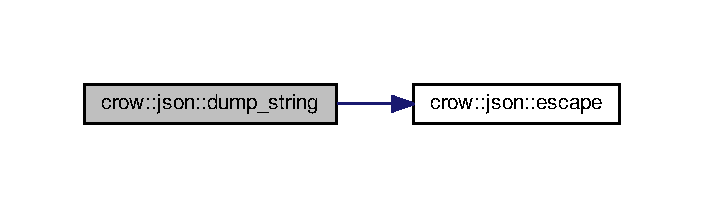
\includegraphics[width=338pt]{namespacecrow_1_1json_af1b84b949166845e81f327e5e43cabee_cgraph}
\end{center}
\end{figure}




Here is the caller graph for this function\-:
\nopagebreak
\begin{figure}[H]
\begin{center}
\leavevmode
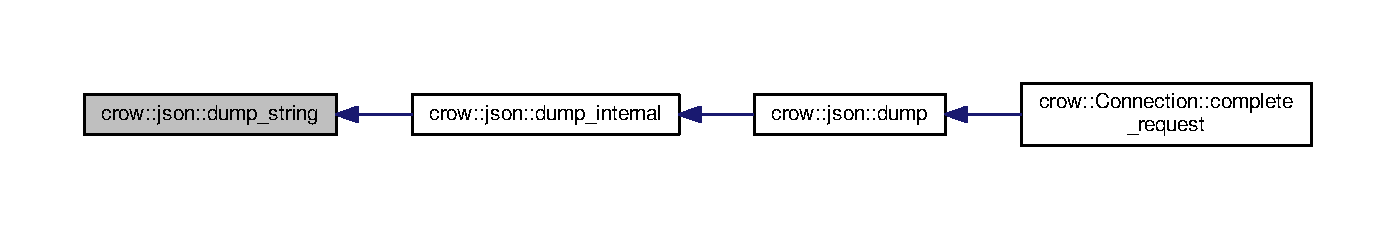
\includegraphics[width=350pt]{namespacecrow_1_1json_af1b84b949166845e81f327e5e43cabee_icgraph}
\end{center}
\end{figure}


\hypertarget{namespacecrow_1_1json_a98e83fcd8d2e51b3acfc99d868b4e41a}{\index{crow\-::json@{crow\-::json}!escape@{escape}}
\index{escape@{escape}!crow::json@{crow\-::json}}
\subsubsection[{escape}]{\setlength{\rightskip}{0pt plus 5cm}void crow\-::json\-::escape (
\begin{DoxyParamCaption}
\item[{const std\-::string \&}]{str, }
\item[{std\-::string \&}]{ret}
\end{DoxyParamCaption}
)\hspace{0.3cm}{\ttfamily [inline]}}}\label{namespacecrow_1_1json_a98e83fcd8d2e51b3acfc99d868b4e41a}


Here is the caller graph for this function\-:
\nopagebreak
\begin{figure}[H]
\begin{center}
\leavevmode
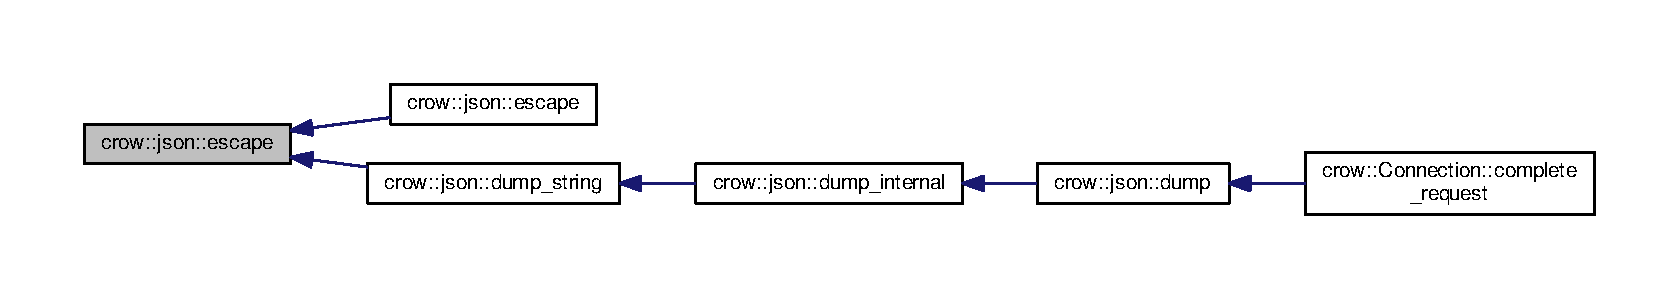
\includegraphics[width=350pt]{namespacecrow_1_1json_a98e83fcd8d2e51b3acfc99d868b4e41a_icgraph}
\end{center}
\end{figure}


\hypertarget{namespacecrow_1_1json_a27086e84491472bba7ff876c929f5df3}{\index{crow\-::json@{crow\-::json}!escape@{escape}}
\index{escape@{escape}!crow::json@{crow\-::json}}
\subsubsection[{escape}]{\setlength{\rightskip}{0pt plus 5cm}std\-::string crow\-::json\-::escape (
\begin{DoxyParamCaption}
\item[{const std\-::string \&}]{str}
\end{DoxyParamCaption}
)\hspace{0.3cm}{\ttfamily [inline]}}}\label{namespacecrow_1_1json_a27086e84491472bba7ff876c929f5df3}


Here is the call graph for this function\-:
\nopagebreak
\begin{figure}[H]
\begin{center}
\leavevmode
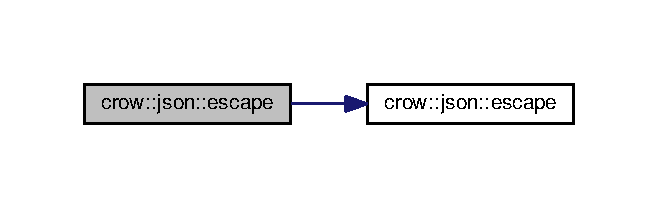
\includegraphics[width=316pt]{namespacecrow_1_1json_a27086e84491472bba7ff876c929f5df3_cgraph}
\end{center}
\end{figure}


\hypertarget{namespacecrow_1_1json_ae63b97ba6f66ef6daf254e00a4b0facb}{\index{crow\-::json@{crow\-::json}!get\-\_\-type\-\_\-str@{get\-\_\-type\-\_\-str}}
\index{get\-\_\-type\-\_\-str@{get\-\_\-type\-\_\-str}!crow::json@{crow\-::json}}
\subsubsection[{get\-\_\-type\-\_\-str}]{\setlength{\rightskip}{0pt plus 5cm}const char$\ast$ crow\-::json\-::get\-\_\-type\-\_\-str (
\begin{DoxyParamCaption}
\item[{type}]{t}
\end{DoxyParamCaption}
)\hspace{0.3cm}{\ttfamily [inline]}}}\label{namespacecrow_1_1json_ae63b97ba6f66ef6daf254e00a4b0facb}


Here is the caller graph for this function\-:
\nopagebreak
\begin{figure}[H]
\begin{center}
\leavevmode
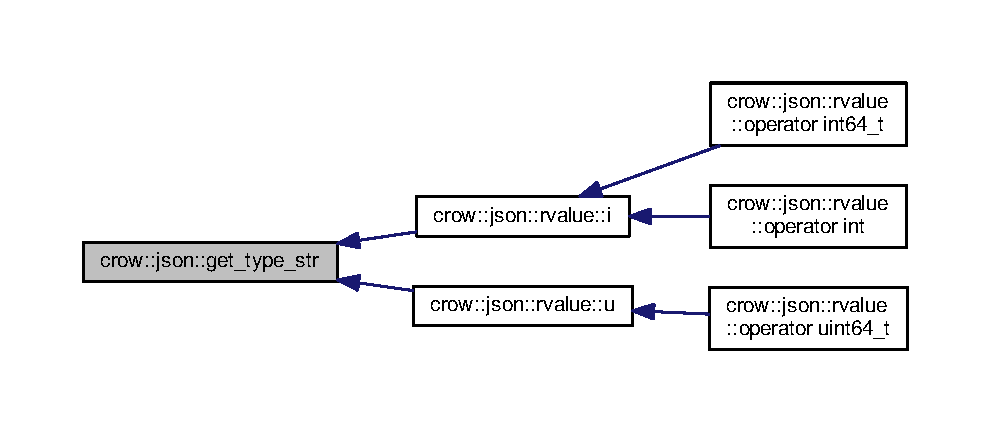
\includegraphics[width=350pt]{namespacecrow_1_1json_ae63b97ba6f66ef6daf254e00a4b0facb_icgraph}
\end{center}
\end{figure}


\hypertarget{namespacecrow_1_1json_a84a2fc9bc21a94b2791271e54879ab0a}{\index{crow\-::json@{crow\-::json}!load@{load}}
\index{load@{load}!crow::json@{crow\-::json}}
\subsubsection[{load}]{\setlength{\rightskip}{0pt plus 5cm}{\bf rvalue} crow\-::json\-::load (
\begin{DoxyParamCaption}
\item[{const char $\ast$}]{data, }
\item[{size\-\_\-t}]{size}
\end{DoxyParamCaption}
)\hspace{0.3cm}{\ttfamily [inline]}}}\label{namespacecrow_1_1json_a84a2fc9bc21a94b2791271e54879ab0a}


Here is the call graph for this function\-:
\nopagebreak
\begin{figure}[H]
\begin{center}
\leavevmode
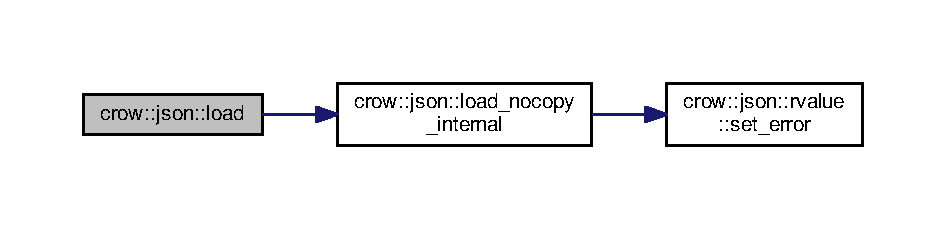
\includegraphics[width=350pt]{namespacecrow_1_1json_a84a2fc9bc21a94b2791271e54879ab0a_cgraph}
\end{center}
\end{figure}




Here is the caller graph for this function\-:
\nopagebreak
\begin{figure}[H]
\begin{center}
\leavevmode
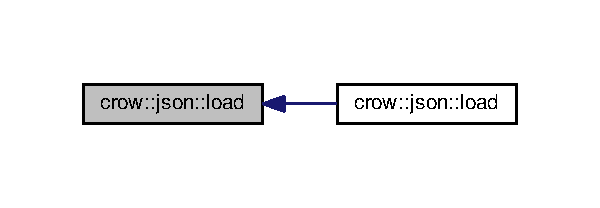
\includegraphics[width=288pt]{namespacecrow_1_1json_a84a2fc9bc21a94b2791271e54879ab0a_icgraph}
\end{center}
\end{figure}


\hypertarget{namespacecrow_1_1json_ad995f1379ae1ddc8075cab8185c9a78a}{\index{crow\-::json@{crow\-::json}!load@{load}}
\index{load@{load}!crow::json@{crow\-::json}}
\subsubsection[{load}]{\setlength{\rightskip}{0pt plus 5cm}{\bf rvalue} crow\-::json\-::load (
\begin{DoxyParamCaption}
\item[{const char $\ast$}]{data}
\end{DoxyParamCaption}
)\hspace{0.3cm}{\ttfamily [inline]}}}\label{namespacecrow_1_1json_ad995f1379ae1ddc8075cab8185c9a78a}


Here is the call graph for this function\-:
\nopagebreak
\begin{figure}[H]
\begin{center}
\leavevmode
\includegraphics[width=350pt]{namespacecrow_1_1json_ad995f1379ae1ddc8075cab8185c9a78a_cgraph}
\end{center}
\end{figure}


\hypertarget{namespacecrow_1_1json_a59efe2ae1d83ded364cc3ecc143bce85}{\index{crow\-::json@{crow\-::json}!load@{load}}
\index{load@{load}!crow::json@{crow\-::json}}
\subsubsection[{load}]{\setlength{\rightskip}{0pt plus 5cm}{\bf rvalue} crow\-::json\-::load (
\begin{DoxyParamCaption}
\item[{const std\-::string \&}]{str}
\end{DoxyParamCaption}
)\hspace{0.3cm}{\ttfamily [inline]}}}\label{namespacecrow_1_1json_a59efe2ae1d83ded364cc3ecc143bce85}


Here is the call graph for this function\-:
\nopagebreak
\begin{figure}[H]
\begin{center}
\leavevmode
\includegraphics[width=350pt]{namespacecrow_1_1json_a59efe2ae1d83ded364cc3ecc143bce85_cgraph}
\end{center}
\end{figure}


\hypertarget{namespacecrow_1_1json_a0cd58f45702772a5aac929dec0966a0a}{\index{crow\-::json@{crow\-::json}!load\-\_\-nocopy\-\_\-internal@{load\-\_\-nocopy\-\_\-internal}}
\index{load\-\_\-nocopy\-\_\-internal@{load\-\_\-nocopy\-\_\-internal}!crow::json@{crow\-::json}}
\subsubsection[{load\-\_\-nocopy\-\_\-internal}]{\setlength{\rightskip}{0pt plus 5cm}{\bf rvalue} crow\-::json\-::load\-\_\-nocopy\-\_\-internal (
\begin{DoxyParamCaption}
\item[{char $\ast$}]{data, }
\item[{size\-\_\-t}]{size}
\end{DoxyParamCaption}
)\hspace{0.3cm}{\ttfamily [inline]}}}\label{namespacecrow_1_1json_a0cd58f45702772a5aac929dec0966a0a}


Here is the call graph for this function\-:
\nopagebreak
\begin{figure}[H]
\begin{center}
\leavevmode
\includegraphics[width=332pt]{namespacecrow_1_1json_a0cd58f45702772a5aac929dec0966a0a_cgraph}
\end{center}
\end{figure}




Here is the caller graph for this function\-:
\nopagebreak
\begin{figure}[H]
\begin{center}
\leavevmode
\includegraphics[width=350pt]{namespacecrow_1_1json_a0cd58f45702772a5aac929dec0966a0a_icgraph}
\end{center}
\end{figure}


\hypertarget{namespacecrow_1_1json_a2f0451a26844bed78da38c06d18d76f7}{\index{crow\-::json@{crow\-::json}!operator!=@{operator!=}}
\index{operator!=@{operator!=}!crow::json@{crow\-::json}}
\subsubsection[{operator!=}]{\setlength{\rightskip}{0pt plus 5cm}bool crow\-::json\-::operator!= (
\begin{DoxyParamCaption}
\item[{const rvalue \&}]{l, }
\item[{const std\-::string \&}]{r}
\end{DoxyParamCaption}
)\hspace{0.3cm}{\ttfamily [inline]}}}\label{namespacecrow_1_1json_a2f0451a26844bed78da38c06d18d76f7}


Here is the call graph for this function\-:
\nopagebreak
\begin{figure}[H]
\begin{center}
\leavevmode
\includegraphics[width=350pt]{namespacecrow_1_1json_a2f0451a26844bed78da38c06d18d76f7_cgraph}
\end{center}
\end{figure}


\hypertarget{namespacecrow_1_1json_aba197bed8a4a07e34a0733d633b14e9b}{\index{crow\-::json@{crow\-::json}!operator!=@{operator!=}}
\index{operator!=@{operator!=}!crow::json@{crow\-::json}}
\subsubsection[{operator!=}]{\setlength{\rightskip}{0pt plus 5cm}bool crow\-::json\-::operator!= (
\begin{DoxyParamCaption}
\item[{const std\-::string \&}]{l, }
\item[{const rvalue \&}]{r}
\end{DoxyParamCaption}
)\hspace{0.3cm}{\ttfamily [inline]}}}\label{namespacecrow_1_1json_aba197bed8a4a07e34a0733d633b14e9b}


Here is the call graph for this function\-:
\nopagebreak
\begin{figure}[H]
\begin{center}
\leavevmode
\includegraphics[width=350pt]{namespacecrow_1_1json_aba197bed8a4a07e34a0733d633b14e9b_cgraph}
\end{center}
\end{figure}


\hypertarget{namespacecrow_1_1json_a4b737b3cf606bf2e63ed09ceff8ce89a}{\index{crow\-::json@{crow\-::json}!operator!=@{operator!=}}
\index{operator!=@{operator!=}!crow::json@{crow\-::json}}
\subsubsection[{operator!=}]{\setlength{\rightskip}{0pt plus 5cm}bool crow\-::json\-::operator!= (
\begin{DoxyParamCaption}
\item[{const rvalue \&}]{l, }
\item[{double}]{r}
\end{DoxyParamCaption}
)\hspace{0.3cm}{\ttfamily [inline]}}}\label{namespacecrow_1_1json_a4b737b3cf606bf2e63ed09ceff8ce89a}


Here is the call graph for this function\-:
\nopagebreak
\begin{figure}[H]
\begin{center}
\leavevmode
\includegraphics[width=350pt]{namespacecrow_1_1json_a4b737b3cf606bf2e63ed09ceff8ce89a_cgraph}
\end{center}
\end{figure}


\hypertarget{namespacecrow_1_1json_ac606c21e102f1104500667e9060ee0ed}{\index{crow\-::json@{crow\-::json}!operator!=@{operator!=}}
\index{operator!=@{operator!=}!crow::json@{crow\-::json}}
\subsubsection[{operator!=}]{\setlength{\rightskip}{0pt plus 5cm}bool crow\-::json\-::operator!= (
\begin{DoxyParamCaption}
\item[{double}]{l, }
\item[{const rvalue \&}]{r}
\end{DoxyParamCaption}
)\hspace{0.3cm}{\ttfamily [inline]}}}\label{namespacecrow_1_1json_ac606c21e102f1104500667e9060ee0ed}


Here is the call graph for this function\-:
\nopagebreak
\begin{figure}[H]
\begin{center}
\leavevmode
\includegraphics[width=350pt]{namespacecrow_1_1json_ac606c21e102f1104500667e9060ee0ed_cgraph}
\end{center}
\end{figure}


\hypertarget{namespacecrow_1_1json_a516708ab016de1caa6d3203529929b2e}{\index{crow\-::json@{crow\-::json}!operator==@{operator==}}
\index{operator==@{operator==}!crow::json@{crow\-::json}}
\subsubsection[{operator==}]{\setlength{\rightskip}{0pt plus 5cm}bool crow\-::json\-::operator== (
\begin{DoxyParamCaption}
\item[{const rvalue \&}]{l, }
\item[{const std\-::string \&}]{r}
\end{DoxyParamCaption}
)\hspace{0.3cm}{\ttfamily [inline]}}}\label{namespacecrow_1_1json_a516708ab016de1caa6d3203529929b2e}


Here is the call graph for this function\-:
\nopagebreak
\begin{figure}[H]
\begin{center}
\leavevmode
\includegraphics[width=350pt]{namespacecrow_1_1json_a516708ab016de1caa6d3203529929b2e_cgraph}
\end{center}
\end{figure}


\hypertarget{namespacecrow_1_1json_aa9ae087edb7382ba2df19bb5b4b8165b}{\index{crow\-::json@{crow\-::json}!operator==@{operator==}}
\index{operator==@{operator==}!crow::json@{crow\-::json}}
\subsubsection[{operator==}]{\setlength{\rightskip}{0pt plus 5cm}bool crow\-::json\-::operator== (
\begin{DoxyParamCaption}
\item[{const std\-::string \&}]{l, }
\item[{const rvalue \&}]{r}
\end{DoxyParamCaption}
)\hspace{0.3cm}{\ttfamily [inline]}}}\label{namespacecrow_1_1json_aa9ae087edb7382ba2df19bb5b4b8165b}


Here is the call graph for this function\-:
\nopagebreak
\begin{figure}[H]
\begin{center}
\leavevmode
\includegraphics[width=350pt]{namespacecrow_1_1json_aa9ae087edb7382ba2df19bb5b4b8165b_cgraph}
\end{center}
\end{figure}


\hypertarget{namespacecrow_1_1json_a1079ce699fb8174f6f4092b79ef44fc0}{\index{crow\-::json@{crow\-::json}!operator==@{operator==}}
\index{operator==@{operator==}!crow::json@{crow\-::json}}
\subsubsection[{operator==}]{\setlength{\rightskip}{0pt plus 5cm}bool crow\-::json\-::operator== (
\begin{DoxyParamCaption}
\item[{const rvalue \&}]{l, }
\item[{double}]{r}
\end{DoxyParamCaption}
)\hspace{0.3cm}{\ttfamily [inline]}}}\label{namespacecrow_1_1json_a1079ce699fb8174f6f4092b79ef44fc0}


Here is the call graph for this function\-:
\nopagebreak
\begin{figure}[H]
\begin{center}
\leavevmode
\includegraphics[width=350pt]{namespacecrow_1_1json_a1079ce699fb8174f6f4092b79ef44fc0_cgraph}
\end{center}
\end{figure}


\hypertarget{namespacecrow_1_1json_a90cbe3f52220c2062156cf256e43c631}{\index{crow\-::json@{crow\-::json}!operator==@{operator==}}
\index{operator==@{operator==}!crow::json@{crow\-::json}}
\subsubsection[{operator==}]{\setlength{\rightskip}{0pt plus 5cm}bool crow\-::json\-::operator== (
\begin{DoxyParamCaption}
\item[{double}]{l, }
\item[{const rvalue \&}]{r}
\end{DoxyParamCaption}
)\hspace{0.3cm}{\ttfamily [inline]}}}\label{namespacecrow_1_1json_a90cbe3f52220c2062156cf256e43c631}


Here is the call graph for this function\-:
\nopagebreak
\begin{figure}[H]
\begin{center}
\leavevmode
\includegraphics[width=350pt]{namespacecrow_1_1json_a90cbe3f52220c2062156cf256e43c631_cgraph}
\end{center}
\end{figure}



\hypertarget{namespacecrow_1_1json_1_1detail}{\section{crow\-:\-:json\-:\-:detail Namespace Reference}
\label{namespacecrow_1_1json_1_1detail}\index{crow\-::json\-::detail@{crow\-::json\-::detail}}
}
\subsection*{Classes}
\begin{DoxyCompactItemize}
\item 
struct \hyperlink{structcrow_1_1json_1_1detail_1_1r__string}{r\-\_\-string}
\end{DoxyCompactItemize}
\subsection*{Functions}
\begin{DoxyCompactItemize}
\item 
bool \hyperlink{namespacecrow_1_1json_1_1detail_a9e05ef194e02704d74fe40a02f747723}{operator$<$} (const \hyperlink{structcrow_1_1json_1_1detail_1_1r__string}{r\-\_\-string} \&\hyperlink{three_8min_8js_aae3c400cfa9afd0584b6226ac3804a40}{l}, const \hyperlink{structcrow_1_1json_1_1detail_1_1r__string}{r\-\_\-string} \&r)
\item 
bool \hyperlink{namespacecrow_1_1json_1_1detail_a6ebe4a1331b93ac4d1e4f1f169388234}{operator$<$} (const \hyperlink{structcrow_1_1json_1_1detail_1_1r__string}{r\-\_\-string} \&\hyperlink{three_8min_8js_aae3c400cfa9afd0584b6226ac3804a40}{l}, const std\-::string \&r)
\item 
bool \hyperlink{namespacecrow_1_1json_1_1detail_a11f03601163525452ff2d9d08fc669b3}{operator$>$} (const \hyperlink{structcrow_1_1json_1_1detail_1_1r__string}{r\-\_\-string} \&\hyperlink{three_8min_8js_aae3c400cfa9afd0584b6226ac3804a40}{l}, const std\-::string \&r)
\item 
bool \hyperlink{namespacecrow_1_1json_1_1detail_a0c2d17963f4159c72621f429cdf48d95}{operator==} (const \hyperlink{structcrow_1_1json_1_1detail_1_1r__string}{r\-\_\-string} \&\hyperlink{three_8min_8js_aae3c400cfa9afd0584b6226ac3804a40}{l}, const \hyperlink{structcrow_1_1json_1_1detail_1_1r__string}{r\-\_\-string} \&r)
\item 
bool \hyperlink{namespacecrow_1_1json_1_1detail_a2d67be22770ab4c241c39408d6ff766c}{operator==} (const \hyperlink{structcrow_1_1json_1_1detail_1_1r__string}{r\-\_\-string} \&\hyperlink{three_8min_8js_aae3c400cfa9afd0584b6226ac3804a40}{l}, const std\-::string \&r)
\end{DoxyCompactItemize}


\subsection{Function Documentation}
\hypertarget{namespacecrow_1_1json_1_1detail_a9e05ef194e02704d74fe40a02f747723}{\index{crow\-::json\-::detail@{crow\-::json\-::detail}!operator$<$@{operator$<$}}
\index{operator$<$@{operator$<$}!crow::json::detail@{crow\-::json\-::detail}}
\subsubsection[{operator$<$}]{\setlength{\rightskip}{0pt plus 5cm}bool crow\-::json\-::detail\-::operator$<$ (
\begin{DoxyParamCaption}
\item[{const r\-\_\-string \&}]{l, }
\item[{const r\-\_\-string \&}]{r}
\end{DoxyParamCaption}
)\hspace{0.3cm}{\ttfamily [inline]}}}\label{namespacecrow_1_1json_1_1detail_a9e05ef194e02704d74fe40a02f747723}
\hypertarget{namespacecrow_1_1json_1_1detail_a6ebe4a1331b93ac4d1e4f1f169388234}{\index{crow\-::json\-::detail@{crow\-::json\-::detail}!operator$<$@{operator$<$}}
\index{operator$<$@{operator$<$}!crow::json::detail@{crow\-::json\-::detail}}
\subsubsection[{operator$<$}]{\setlength{\rightskip}{0pt plus 5cm}bool crow\-::json\-::detail\-::operator$<$ (
\begin{DoxyParamCaption}
\item[{const r\-\_\-string \&}]{l, }
\item[{const std\-::string \&}]{r}
\end{DoxyParamCaption}
)\hspace{0.3cm}{\ttfamily [inline]}}}\label{namespacecrow_1_1json_1_1detail_a6ebe4a1331b93ac4d1e4f1f169388234}
\hypertarget{namespacecrow_1_1json_1_1detail_a0c2d17963f4159c72621f429cdf48d95}{\index{crow\-::json\-::detail@{crow\-::json\-::detail}!operator==@{operator==}}
\index{operator==@{operator==}!crow::json::detail@{crow\-::json\-::detail}}
\subsubsection[{operator==}]{\setlength{\rightskip}{0pt plus 5cm}bool crow\-::json\-::detail\-::operator== (
\begin{DoxyParamCaption}
\item[{const r\-\_\-string \&}]{l, }
\item[{const r\-\_\-string \&}]{r}
\end{DoxyParamCaption}
)\hspace{0.3cm}{\ttfamily [inline]}}}\label{namespacecrow_1_1json_1_1detail_a0c2d17963f4159c72621f429cdf48d95}
\hypertarget{namespacecrow_1_1json_1_1detail_a2d67be22770ab4c241c39408d6ff766c}{\index{crow\-::json\-::detail@{crow\-::json\-::detail}!operator==@{operator==}}
\index{operator==@{operator==}!crow::json::detail@{crow\-::json\-::detail}}
\subsubsection[{operator==}]{\setlength{\rightskip}{0pt plus 5cm}bool crow\-::json\-::detail\-::operator== (
\begin{DoxyParamCaption}
\item[{const r\-\_\-string \&}]{l, }
\item[{const std\-::string \&}]{r}
\end{DoxyParamCaption}
)\hspace{0.3cm}{\ttfamily [inline]}}}\label{namespacecrow_1_1json_1_1detail_a2d67be22770ab4c241c39408d6ff766c}
\hypertarget{namespacecrow_1_1json_1_1detail_a11f03601163525452ff2d9d08fc669b3}{\index{crow\-::json\-::detail@{crow\-::json\-::detail}!operator$>$@{operator$>$}}
\index{operator$>$@{operator$>$}!crow::json::detail@{crow\-::json\-::detail}}
\subsubsection[{operator$>$}]{\setlength{\rightskip}{0pt plus 5cm}bool crow\-::json\-::detail\-::operator$>$ (
\begin{DoxyParamCaption}
\item[{const r\-\_\-string \&}]{l, }
\item[{const std\-::string \&}]{r}
\end{DoxyParamCaption}
)\hspace{0.3cm}{\ttfamily [inline]}}}\label{namespacecrow_1_1json_1_1detail_a11f03601163525452ff2d9d08fc669b3}

\hypertarget{namespacecrow_1_1mustache}{\section{crow\-:\-:mustache Namespace Reference}
\label{namespacecrow_1_1mustache}\index{crow\-::mustache@{crow\-::mustache}}
}
\subsection*{Namespaces}
\begin{DoxyCompactItemize}
\item 
\hyperlink{namespacecrow_1_1mustache_1_1detail}{detail}
\end{DoxyCompactItemize}
\subsection*{Classes}
\begin{DoxyCompactItemize}
\item 
class \hyperlink{classcrow_1_1mustache_1_1invalid__template__exception}{invalid\-\_\-template\-\_\-exception}
\item 
struct \hyperlink{structcrow_1_1mustache_1_1_action}{Action}
\item 
class \hyperlink{classcrow_1_1mustache_1_1template__t}{template\-\_\-t}
\end{DoxyCompactItemize}
\subsection*{Typedefs}
\begin{DoxyCompactItemize}
\item 
using \hyperlink{namespacecrow_1_1mustache_ae1f8ebbbcd4c41b97a2aebb247a123f9}{context} = \hyperlink{classcrow_1_1json_1_1wvalue}{json\-::wvalue}
\end{DoxyCompactItemize}
\subsection*{Enumerations}
\begin{DoxyCompactItemize}
\item 
enum \hyperlink{namespacecrow_1_1mustache_aeb8da2ae9d8d9fe55f6ab0a7455dd667}{Action\-Type} \{ \\*
\hyperlink{namespacecrow_1_1mustache_aeb8da2ae9d8d9fe55f6ab0a7455dd667afd038fc7f319e48f3115d92bf5bdbef9}{Action\-Type\-::\-Ignore}, 
\hyperlink{namespacecrow_1_1mustache_aeb8da2ae9d8d9fe55f6ab0a7455dd667ac101058e7ea21bbbf2a5ac893088e90b}{Action\-Type\-::\-Tag}, 
\hyperlink{namespacecrow_1_1mustache_aeb8da2ae9d8d9fe55f6ab0a7455dd667a6a92aa81e0cd0b1c2f77a84226ad4777}{Action\-Type\-::\-Unescape\-Tag}, 
\hyperlink{namespacecrow_1_1mustache_aeb8da2ae9d8d9fe55f6ab0a7455dd667a047e46a0bc852354acb31de6a507a3fe}{Action\-Type\-::\-Open\-Block}, 
\\*
\hyperlink{namespacecrow_1_1mustache_aeb8da2ae9d8d9fe55f6ab0a7455dd667a470529d743a17635308c52dc50efccd8}{Action\-Type\-::\-Close\-Block}, 
\hyperlink{namespacecrow_1_1mustache_aeb8da2ae9d8d9fe55f6ab0a7455dd667ab82f53ea35520be1175d4764c22d2b30}{Action\-Type\-::\-Else\-Block}, 
\hyperlink{namespacecrow_1_1mustache_aeb8da2ae9d8d9fe55f6ab0a7455dd667a44ffd38a6dea695cbe2b34efdcc6cf27}{Action\-Type\-::\-Partial}
 \}
\end{DoxyCompactItemize}
\subsection*{Functions}
\begin{DoxyCompactItemize}
\item 
\hyperlink{classcrow_1_1mustache_1_1template__t}{template\-\_\-t} \hyperlink{namespacecrow_1_1mustache_abe44de50c382e0d39e7ef5b7d5057ca6}{load} (const std\-::string \&filename)
\item 
\hyperlink{classcrow_1_1mustache_1_1template__t}{template\-\_\-t} \hyperlink{namespacecrow_1_1mustache_a5823e2be647059121cc4f0329e44741a}{compile} (const std\-::string \&body)
\item 
std\-::string \hyperlink{namespacecrow_1_1mustache_a7e8660fbdeeb994a1f00c704b469c792}{default\-\_\-loader} (const std\-::string \&filename)
\item 
void \hyperlink{namespacecrow_1_1mustache_a88cf75099968de883a8e2bf14ce6d1cb}{set\-\_\-base} (const std\-::string \&path)
\item 
void \hyperlink{namespacecrow_1_1mustache_a064911bc597a2a849f008b50cdead53e}{set\-\_\-loader} (std\-::function$<$ std\-::string(std\-::string)$>$ loader)
\item 
std\-::string \hyperlink{namespacecrow_1_1mustache_a8db3aff497ff60b32321fc0a16274576}{load\-\_\-text} (const std\-::string \&filename)
\end{DoxyCompactItemize}


\subsection{Typedef Documentation}
\hypertarget{namespacecrow_1_1mustache_ae1f8ebbbcd4c41b97a2aebb247a123f9}{\index{crow\-::mustache@{crow\-::mustache}!context@{context}}
\index{context@{context}!crow::mustache@{crow\-::mustache}}
\subsubsection[{context}]{\setlength{\rightskip}{0pt plus 5cm}using {\bf crow\-::mustache\-::context} = typedef {\bf json\-::wvalue}}}\label{namespacecrow_1_1mustache_ae1f8ebbbcd4c41b97a2aebb247a123f9}


\subsection{Enumeration Type Documentation}
\hypertarget{namespacecrow_1_1mustache_aeb8da2ae9d8d9fe55f6ab0a7455dd667}{\index{crow\-::mustache@{crow\-::mustache}!Action\-Type@{Action\-Type}}
\index{Action\-Type@{Action\-Type}!crow::mustache@{crow\-::mustache}}
\subsubsection[{Action\-Type}]{\setlength{\rightskip}{0pt plus 5cm}enum {\bf crow\-::mustache\-::\-Action\-Type}\hspace{0.3cm}{\ttfamily [strong]}}}\label{namespacecrow_1_1mustache_aeb8da2ae9d8d9fe55f6ab0a7455dd667}
\begin{Desc}
\item[Enumerator]\par
\begin{description}
\index{Ignore@{Ignore}!crow\-::mustache@{crow\-::mustache}}\index{crow\-::mustache@{crow\-::mustache}!Ignore@{Ignore}}\item[{\em 
\hypertarget{namespacecrow_1_1mustache_aeb8da2ae9d8d9fe55f6ab0a7455dd667afd038fc7f319e48f3115d92bf5bdbef9}{Ignore}\label{namespacecrow_1_1mustache_aeb8da2ae9d8d9fe55f6ab0a7455dd667afd038fc7f319e48f3115d92bf5bdbef9}
}]\index{Tag@{Tag}!crow\-::mustache@{crow\-::mustache}}\index{crow\-::mustache@{crow\-::mustache}!Tag@{Tag}}\item[{\em 
\hypertarget{namespacecrow_1_1mustache_aeb8da2ae9d8d9fe55f6ab0a7455dd667ac101058e7ea21bbbf2a5ac893088e90b}{Tag}\label{namespacecrow_1_1mustache_aeb8da2ae9d8d9fe55f6ab0a7455dd667ac101058e7ea21bbbf2a5ac893088e90b}
}]\index{Unescape\-Tag@{Unescape\-Tag}!crow\-::mustache@{crow\-::mustache}}\index{crow\-::mustache@{crow\-::mustache}!Unescape\-Tag@{Unescape\-Tag}}\item[{\em 
\hypertarget{namespacecrow_1_1mustache_aeb8da2ae9d8d9fe55f6ab0a7455dd667a6a92aa81e0cd0b1c2f77a84226ad4777}{Unescape\-Tag}\label{namespacecrow_1_1mustache_aeb8da2ae9d8d9fe55f6ab0a7455dd667a6a92aa81e0cd0b1c2f77a84226ad4777}
}]\index{Open\-Block@{Open\-Block}!crow\-::mustache@{crow\-::mustache}}\index{crow\-::mustache@{crow\-::mustache}!Open\-Block@{Open\-Block}}\item[{\em 
\hypertarget{namespacecrow_1_1mustache_aeb8da2ae9d8d9fe55f6ab0a7455dd667a047e46a0bc852354acb31de6a507a3fe}{Open\-Block}\label{namespacecrow_1_1mustache_aeb8da2ae9d8d9fe55f6ab0a7455dd667a047e46a0bc852354acb31de6a507a3fe}
}]\index{Close\-Block@{Close\-Block}!crow\-::mustache@{crow\-::mustache}}\index{crow\-::mustache@{crow\-::mustache}!Close\-Block@{Close\-Block}}\item[{\em 
\hypertarget{namespacecrow_1_1mustache_aeb8da2ae9d8d9fe55f6ab0a7455dd667a470529d743a17635308c52dc50efccd8}{Close\-Block}\label{namespacecrow_1_1mustache_aeb8da2ae9d8d9fe55f6ab0a7455dd667a470529d743a17635308c52dc50efccd8}
}]\index{Else\-Block@{Else\-Block}!crow\-::mustache@{crow\-::mustache}}\index{crow\-::mustache@{crow\-::mustache}!Else\-Block@{Else\-Block}}\item[{\em 
\hypertarget{namespacecrow_1_1mustache_aeb8da2ae9d8d9fe55f6ab0a7455dd667ab82f53ea35520be1175d4764c22d2b30}{Else\-Block}\label{namespacecrow_1_1mustache_aeb8da2ae9d8d9fe55f6ab0a7455dd667ab82f53ea35520be1175d4764c22d2b30}
}]\index{Partial@{Partial}!crow\-::mustache@{crow\-::mustache}}\index{crow\-::mustache@{crow\-::mustache}!Partial@{Partial}}\item[{\em 
\hypertarget{namespacecrow_1_1mustache_aeb8da2ae9d8d9fe55f6ab0a7455dd667a44ffd38a6dea695cbe2b34efdcc6cf27}{Partial}\label{namespacecrow_1_1mustache_aeb8da2ae9d8d9fe55f6ab0a7455dd667a44ffd38a6dea695cbe2b34efdcc6cf27}
}]\end{description}
\end{Desc}


\subsection{Function Documentation}
\hypertarget{namespacecrow_1_1mustache_a5823e2be647059121cc4f0329e44741a}{\index{crow\-::mustache@{crow\-::mustache}!compile@{compile}}
\index{compile@{compile}!crow::mustache@{crow\-::mustache}}
\subsubsection[{compile}]{\setlength{\rightskip}{0pt plus 5cm}{\bf template\-\_\-t} crow\-::mustache\-::compile (
\begin{DoxyParamCaption}
\item[{const std\-::string \&}]{body}
\end{DoxyParamCaption}
)\hspace{0.3cm}{\ttfamily [inline]}}}\label{namespacecrow_1_1mustache_a5823e2be647059121cc4f0329e44741a}


Here is the caller graph for this function\-:
\nopagebreak
\begin{figure}[H]
\begin{center}
\leavevmode
\includegraphics[width=350pt]{namespacecrow_1_1mustache_a5823e2be647059121cc4f0329e44741a_icgraph}
\end{center}
\end{figure}


\hypertarget{namespacecrow_1_1mustache_a7e8660fbdeeb994a1f00c704b469c792}{\index{crow\-::mustache@{crow\-::mustache}!default\-\_\-loader@{default\-\_\-loader}}
\index{default\-\_\-loader@{default\-\_\-loader}!crow::mustache@{crow\-::mustache}}
\subsubsection[{default\-\_\-loader}]{\setlength{\rightskip}{0pt plus 5cm}std\-::string crow\-::mustache\-::default\-\_\-loader (
\begin{DoxyParamCaption}
\item[{const std\-::string \&}]{filename}
\end{DoxyParamCaption}
)\hspace{0.3cm}{\ttfamily [inline]}}}\label{namespacecrow_1_1mustache_a7e8660fbdeeb994a1f00c704b469c792}


Here is the call graph for this function\-:
\nopagebreak
\begin{figure}[H]
\begin{center}
\leavevmode
\includegraphics[width=350pt]{namespacecrow_1_1mustache_a7e8660fbdeeb994a1f00c704b469c792_cgraph}
\end{center}
\end{figure}




Here is the caller graph for this function\-:
\nopagebreak
\begin{figure}[H]
\begin{center}
\leavevmode
\includegraphics[width=350pt]{namespacecrow_1_1mustache_a7e8660fbdeeb994a1f00c704b469c792_icgraph}
\end{center}
\end{figure}


\hypertarget{namespacecrow_1_1mustache_abe44de50c382e0d39e7ef5b7d5057ca6}{\index{crow\-::mustache@{crow\-::mustache}!load@{load}}
\index{load@{load}!crow::mustache@{crow\-::mustache}}
\subsubsection[{load}]{\setlength{\rightskip}{0pt plus 5cm}{\bf template\-\_\-t} crow\-::mustache\-::load (
\begin{DoxyParamCaption}
\item[{const std\-::string \&}]{filename}
\end{DoxyParamCaption}
)\hspace{0.3cm}{\ttfamily [inline]}}}\label{namespacecrow_1_1mustache_abe44de50c382e0d39e7ef5b7d5057ca6}


Here is the call graph for this function\-:
\nopagebreak
\begin{figure}[H]
\begin{center}
\leavevmode
\includegraphics[width=350pt]{namespacecrow_1_1mustache_abe44de50c382e0d39e7ef5b7d5057ca6_cgraph}
\end{center}
\end{figure}


\hypertarget{namespacecrow_1_1mustache_a8db3aff497ff60b32321fc0a16274576}{\index{crow\-::mustache@{crow\-::mustache}!load\-\_\-text@{load\-\_\-text}}
\index{load\-\_\-text@{load\-\_\-text}!crow::mustache@{crow\-::mustache}}
\subsubsection[{load\-\_\-text}]{\setlength{\rightskip}{0pt plus 5cm}std\-::string crow\-::mustache\-::load\-\_\-text (
\begin{DoxyParamCaption}
\item[{const std\-::string \&}]{filename}
\end{DoxyParamCaption}
)\hspace{0.3cm}{\ttfamily [inline]}}}\label{namespacecrow_1_1mustache_a8db3aff497ff60b32321fc0a16274576}


Here is the call graph for this function\-:
\nopagebreak
\begin{figure}[H]
\begin{center}
\leavevmode
\includegraphics[width=350pt]{namespacecrow_1_1mustache_a8db3aff497ff60b32321fc0a16274576_cgraph}
\end{center}
\end{figure}


\hypertarget{namespacecrow_1_1mustache_a88cf75099968de883a8e2bf14ce6d1cb}{\index{crow\-::mustache@{crow\-::mustache}!set\-\_\-base@{set\-\_\-base}}
\index{set\-\_\-base@{set\-\_\-base}!crow::mustache@{crow\-::mustache}}
\subsubsection[{set\-\_\-base}]{\setlength{\rightskip}{0pt plus 5cm}void crow\-::mustache\-::set\-\_\-base (
\begin{DoxyParamCaption}
\item[{const std\-::string \&}]{path}
\end{DoxyParamCaption}
)\hspace{0.3cm}{\ttfamily [inline]}}}\label{namespacecrow_1_1mustache_a88cf75099968de883a8e2bf14ce6d1cb}


Here is the call graph for this function\-:
\nopagebreak
\begin{figure}[H]
\begin{center}
\leavevmode
\includegraphics[width=350pt]{namespacecrow_1_1mustache_a88cf75099968de883a8e2bf14ce6d1cb_cgraph}
\end{center}
\end{figure}


\hypertarget{namespacecrow_1_1mustache_a064911bc597a2a849f008b50cdead53e}{\index{crow\-::mustache@{crow\-::mustache}!set\-\_\-loader@{set\-\_\-loader}}
\index{set\-\_\-loader@{set\-\_\-loader}!crow::mustache@{crow\-::mustache}}
\subsubsection[{set\-\_\-loader}]{\setlength{\rightskip}{0pt plus 5cm}void crow\-::mustache\-::set\-\_\-loader (
\begin{DoxyParamCaption}
\item[{std\-::function$<$ std\-::string(std\-::string)$>$}]{loader}
\end{DoxyParamCaption}
)\hspace{0.3cm}{\ttfamily [inline]}}}\label{namespacecrow_1_1mustache_a064911bc597a2a849f008b50cdead53e}


Here is the call graph for this function\-:
\nopagebreak
\begin{figure}[H]
\begin{center}
\leavevmode
\includegraphics[width=350pt]{namespacecrow_1_1mustache_a064911bc597a2a849f008b50cdead53e_cgraph}
\end{center}
\end{figure}



\hypertarget{namespacecrow_1_1mustache_1_1detail}{\section{crow\-:\-:mustache\-:\-:detail Namespace Reference}
\label{namespacecrow_1_1mustache_1_1detail}\index{crow\-::mustache\-::detail@{crow\-::mustache\-::detail}}
}
\subsection*{Functions}
\begin{DoxyCompactItemize}
\item 
std\-::string \& \hyperlink{namespacecrow_1_1mustache_1_1detail_afe3296362bdc6f187295904755c2103f}{get\-\_\-template\-\_\-base\-\_\-directory\-\_\-ref} ()
\item 
std\-::function$<$ std\-::string(std\-::string)$>$ \& \hyperlink{namespacecrow_1_1mustache_1_1detail_ac4d3e09dc0a20a8a2a56b3f8dae6e3cc}{get\-\_\-loader\-\_\-ref} ()
\end{DoxyCompactItemize}


\subsection{Function Documentation}
\hypertarget{namespacecrow_1_1mustache_1_1detail_ac4d3e09dc0a20a8a2a56b3f8dae6e3cc}{\index{crow\-::mustache\-::detail@{crow\-::mustache\-::detail}!get\-\_\-loader\-\_\-ref@{get\-\_\-loader\-\_\-ref}}
\index{get\-\_\-loader\-\_\-ref@{get\-\_\-loader\-\_\-ref}!crow::mustache::detail@{crow\-::mustache\-::detail}}
\subsubsection[{get\-\_\-loader\-\_\-ref}]{\setlength{\rightskip}{0pt plus 5cm}std\-::function$<$std\-::string (std\-::string)$>$\& crow\-::mustache\-::detail\-::get\-\_\-loader\-\_\-ref (
\begin{DoxyParamCaption}
{}
\end{DoxyParamCaption}
)\hspace{0.3cm}{\ttfamily [inline]}}}\label{namespacecrow_1_1mustache_1_1detail_ac4d3e09dc0a20a8a2a56b3f8dae6e3cc}


Here is the call graph for this function\-:
\nopagebreak
\begin{figure}[H]
\begin{center}
\leavevmode
\includegraphics[width=350pt]{namespacecrow_1_1mustache_1_1detail_ac4d3e09dc0a20a8a2a56b3f8dae6e3cc_cgraph}
\end{center}
\end{figure}




Here is the caller graph for this function\-:
\nopagebreak
\begin{figure}[H]
\begin{center}
\leavevmode
\includegraphics[width=350pt]{namespacecrow_1_1mustache_1_1detail_ac4d3e09dc0a20a8a2a56b3f8dae6e3cc_icgraph}
\end{center}
\end{figure}


\hypertarget{namespacecrow_1_1mustache_1_1detail_afe3296362bdc6f187295904755c2103f}{\index{crow\-::mustache\-::detail@{crow\-::mustache\-::detail}!get\-\_\-template\-\_\-base\-\_\-directory\-\_\-ref@{get\-\_\-template\-\_\-base\-\_\-directory\-\_\-ref}}
\index{get\-\_\-template\-\_\-base\-\_\-directory\-\_\-ref@{get\-\_\-template\-\_\-base\-\_\-directory\-\_\-ref}!crow::mustache::detail@{crow\-::mustache\-::detail}}
\subsubsection[{get\-\_\-template\-\_\-base\-\_\-directory\-\_\-ref}]{\setlength{\rightskip}{0pt plus 5cm}std\-::string\& crow\-::mustache\-::detail\-::get\-\_\-template\-\_\-base\-\_\-directory\-\_\-ref (
\begin{DoxyParamCaption}
{}
\end{DoxyParamCaption}
)\hspace{0.3cm}{\ttfamily [inline]}}}\label{namespacecrow_1_1mustache_1_1detail_afe3296362bdc6f187295904755c2103f}


Here is the caller graph for this function\-:
\nopagebreak
\begin{figure}[H]
\begin{center}
\leavevmode
\includegraphics[width=350pt]{namespacecrow_1_1mustache_1_1detail_afe3296362bdc6f187295904755c2103f_icgraph}
\end{center}
\end{figure}



\hypertarget{namespacecrow_1_1utility}{\section{crow\-:\-:utility Namespace Reference}
\label{namespacecrow_1_1utility}\index{crow\-::utility@{crow\-::utility}}
}
\subsection*{Classes}
\begin{DoxyCompactItemize}
\item 
struct \hyperlink{structcrow_1_1utility_1_1function__traits}{function\-\_\-traits}
\item 
struct \hyperlink{structcrow_1_1utility_1_1function__traits_3_01_r_07_class_type_1_1_5_08_07_args_8_8_8_08_01const_01_01_4}{function\-\_\-traits$<$ R(\-Class\-Type\-::$\ast$)(\-Args...) const  $>$}
\item 
struct \hyperlink{structcrow_1_1utility_1_1function__traits_3_01_r_07_class_type_1_1_5_08_07_args_8_8_8_08_4}{function\-\_\-traits$<$ R(\-Class\-Type\-::$\ast$)(\-Args...)$>$}
\item 
struct \hyperlink{structcrow_1_1utility_1_1function__traits_3_01std_1_1function_3_01_r_07_args_8_8_8_08_4_01_4}{function\-\_\-traits$<$ std\-::function$<$ R(\-Args...)$>$ $>$}
\end{DoxyCompactItemize}
\subsection*{Functions}
\begin{DoxyCompactItemize}
\item 
{\footnotesize template$<$class T , class... Args$>$ }\\T \& \hyperlink{namespacecrow_1_1utility_a36bf7958001971fdee28b0df79508f7d}{get\-\_\-element\-\_\-by\-\_\-type} (std\-::tuple$<$ Args...$>$ \&t)
\end{DoxyCompactItemize}


\subsection{Function Documentation}
\hypertarget{namespacecrow_1_1utility_a36bf7958001971fdee28b0df79508f7d}{\index{crow\-::utility@{crow\-::utility}!get\-\_\-element\-\_\-by\-\_\-type@{get\-\_\-element\-\_\-by\-\_\-type}}
\index{get\-\_\-element\-\_\-by\-\_\-type@{get\-\_\-element\-\_\-by\-\_\-type}!crow::utility@{crow\-::utility}}
\subsubsection[{get\-\_\-element\-\_\-by\-\_\-type}]{\setlength{\rightskip}{0pt plus 5cm}template$<$class T , class... Args$>$ T\& crow\-::utility\-::get\-\_\-element\-\_\-by\-\_\-type (
\begin{DoxyParamCaption}
\item[{std\-::tuple$<$ Args...$>$ \&}]{t}
\end{DoxyParamCaption}
)}}\label{namespacecrow_1_1utility_a36bf7958001971fdee28b0df79508f7d}


Here is the caller graph for this function\-:
\nopagebreak
\begin{figure}[H]
\begin{center}
\leavevmode
\includegraphics[width=350pt]{namespacecrow_1_1utility_a36bf7958001971fdee28b0df79508f7d_icgraph}
\end{center}
\end{figure}



\hypertarget{namespacecrow_1_1websocket}{\section{crow\-:\-:websocket Namespace Reference}
\label{namespacecrow_1_1websocket}\index{crow\-::websocket@{crow\-::websocket}}
}
\subsection*{Classes}
\begin{DoxyCompactItemize}
\item 
struct \hyperlink{structcrow_1_1websocket_1_1connection}{connection}
\item 
class \hyperlink{classcrow_1_1websocket_1_1_connection}{Connection}
\end{DoxyCompactItemize}
\subsection*{Enumerations}
\begin{DoxyCompactItemize}
\item 
enum \hyperlink{namespacecrow_1_1websocket_a2d7a65cf1c63efe21238c6e75c02334c}{Web\-Socket\-Read\-State} \{ \\*
\hyperlink{namespacecrow_1_1websocket_a2d7a65cf1c63efe21238c6e75c02334cad637a34702e8bfb6adc600f1ae827f35}{Web\-Socket\-Read\-State\-::\-Mini\-Header}, 
\hyperlink{namespacecrow_1_1websocket_a2d7a65cf1c63efe21238c6e75c02334ca6a687f78479d558a907bbaac0d7f53f0}{Web\-Socket\-Read\-State\-::\-Len16}, 
\hyperlink{namespacecrow_1_1websocket_a2d7a65cf1c63efe21238c6e75c02334cab70bcc4d8160e709624eaa6377a35c5d}{Web\-Socket\-Read\-State\-::\-Len64}, 
\hyperlink{namespacecrow_1_1websocket_a2d7a65cf1c63efe21238c6e75c02334ca4a18312b5b75f549d5551e5912ad6ebf}{Web\-Socket\-Read\-State\-::\-Mask}, 
\\*
\hyperlink{namespacecrow_1_1websocket_a2d7a65cf1c63efe21238c6e75c02334ca00f4e5788aab6d3546bb433842dbbefc}{Web\-Socket\-Read\-State\-::\-Payload}
 \}
\end{DoxyCompactItemize}


\subsection{Enumeration Type Documentation}
\hypertarget{namespacecrow_1_1websocket_a2d7a65cf1c63efe21238c6e75c02334c}{\index{crow\-::websocket@{crow\-::websocket}!Web\-Socket\-Read\-State@{Web\-Socket\-Read\-State}}
\index{Web\-Socket\-Read\-State@{Web\-Socket\-Read\-State}!crow::websocket@{crow\-::websocket}}
\subsubsection[{Web\-Socket\-Read\-State}]{\setlength{\rightskip}{0pt plus 5cm}enum {\bf crow\-::websocket\-::\-Web\-Socket\-Read\-State}\hspace{0.3cm}{\ttfamily [strong]}}}\label{namespacecrow_1_1websocket_a2d7a65cf1c63efe21238c6e75c02334c}
\begin{Desc}
\item[Enumerator]\par
\begin{description}
\index{Mini\-Header@{Mini\-Header}!crow\-::websocket@{crow\-::websocket}}\index{crow\-::websocket@{crow\-::websocket}!Mini\-Header@{Mini\-Header}}\item[{\em 
\hypertarget{namespacecrow_1_1websocket_a2d7a65cf1c63efe21238c6e75c02334cad637a34702e8bfb6adc600f1ae827f35}{Mini\-Header}\label{namespacecrow_1_1websocket_a2d7a65cf1c63efe21238c6e75c02334cad637a34702e8bfb6adc600f1ae827f35}
}]\index{Len16@{Len16}!crow\-::websocket@{crow\-::websocket}}\index{crow\-::websocket@{crow\-::websocket}!Len16@{Len16}}\item[{\em 
\hypertarget{namespacecrow_1_1websocket_a2d7a65cf1c63efe21238c6e75c02334ca6a687f78479d558a907bbaac0d7f53f0}{Len16}\label{namespacecrow_1_1websocket_a2d7a65cf1c63efe21238c6e75c02334ca6a687f78479d558a907bbaac0d7f53f0}
}]\index{Len64@{Len64}!crow\-::websocket@{crow\-::websocket}}\index{crow\-::websocket@{crow\-::websocket}!Len64@{Len64}}\item[{\em 
\hypertarget{namespacecrow_1_1websocket_a2d7a65cf1c63efe21238c6e75c02334cab70bcc4d8160e709624eaa6377a35c5d}{Len64}\label{namespacecrow_1_1websocket_a2d7a65cf1c63efe21238c6e75c02334cab70bcc4d8160e709624eaa6377a35c5d}
}]\index{Mask@{Mask}!crow\-::websocket@{crow\-::websocket}}\index{crow\-::websocket@{crow\-::websocket}!Mask@{Mask}}\item[{\em 
\hypertarget{namespacecrow_1_1websocket_a2d7a65cf1c63efe21238c6e75c02334ca4a18312b5b75f549d5551e5912ad6ebf}{Mask}\label{namespacecrow_1_1websocket_a2d7a65cf1c63efe21238c6e75c02334ca4a18312b5b75f549d5551e5912ad6ebf}
}]\index{Payload@{Payload}!crow\-::websocket@{crow\-::websocket}}\index{crow\-::websocket@{crow\-::websocket}!Payload@{Payload}}\item[{\em 
\hypertarget{namespacecrow_1_1websocket_a2d7a65cf1c63efe21238c6e75c02334ca00f4e5788aab6d3546bb433842dbbefc}{Payload}\label{namespacecrow_1_1websocket_a2d7a65cf1c63efe21238c6e75c02334ca00f4e5788aab6d3546bb433842dbbefc}
}]\end{description}
\end{Desc}

\hypertarget{namespace_file_utils}{\section{File\-Utils Namespace Reference}
\label{namespace_file_utils}\index{File\-Utils@{File\-Utils}}
}
\subsection*{Functions}
\begin{DoxyCompactItemize}
\item 
std\-::string \hyperlink{namespace_file_utils_ac71822c5146913486f67a3a1e7646155}{read\-File} (const std\-::string \&file\-Name)
\end{DoxyCompactItemize}


\subsection{Detailed Description}
Collection of functions which work with files. 

\subsection{Function Documentation}
\hypertarget{namespace_file_utils_ac71822c5146913486f67a3a1e7646155}{\index{File\-Utils@{File\-Utils}!read\-File@{read\-File}}
\index{read\-File@{read\-File}!FileUtils@{File\-Utils}}
\subsubsection[{read\-File}]{\setlength{\rightskip}{0pt plus 5cm}std\-::string File\-Utils\-::read\-File (
\begin{DoxyParamCaption}
\item[{const std\-::string \&}]{file\-Name}
\end{DoxyParamCaption}
)\hspace{0.3cm}{\ttfamily [inline]}}}\label{namespace_file_utils_ac71822c5146913486f67a3a1e7646155}
Reads all file contents to a string.


\begin{DoxyParams}{Parameters}
{\em file\-Name} & Path of file \\
\hline
\end{DoxyParams}
\begin{DoxyReturn}{Returns}
File contents 
\end{DoxyReturn}


Here is the caller graph for this function\-:
\nopagebreak
\begin{figure}[H]
\begin{center}
\leavevmode
\includegraphics[width=350pt]{namespace_file_utils_ac71822c5146913486f67a3a1e7646155_icgraph}
\end{center}
\end{figure}



\hypertarget{namespace_generatable_chunked_temperature_world_typedefs}{\section{Generatable\-Chunked\-Temperature\-World\-Typedefs Namespace Reference}
\label{namespace_generatable_chunked_temperature_world_typedefs}\index{Generatable\-Chunked\-Temperature\-World\-Typedefs@{Generatable\-Chunked\-Temperature\-World\-Typedefs}}
}
\subsection*{Typedefs}
\begin{DoxyCompactItemize}
\item 
using \hyperlink{namespace_generatable_chunked_temperature_world_typedefs_a07d38658571f8f09839bc1bc8b105107}{Need\-Chunk\-Fn} = std\-::function$<$ bool(\hyperlink{struct_coord}{Coord}, \hyperlink{struct_coord}{Coord}, \hyperlink{struct_coord}{Coord})$>$
\item 
using \hyperlink{namespace_generatable_chunked_temperature_world_typedefs_a719e4469a105a21a76ed22274639c03a}{Make\-Chunk\-Fn} = std\-::function$<$ std\-::shared\-\_\-ptr$<$ \hyperlink{class_i_temperature_world_boundable}{I\-Temperature\-World\-Boundable}$<$ \hyperlink{class_i_temperature_world}{I\-Temperature\-World} $>$$>$(\hyperlink{struct_coord}{Coord}, \hyperlink{struct_coord}{Coord}, \hyperlink{struct_coord}{Coord})$>$
\end{DoxyCompactItemize}


\subsection{Typedef Documentation}
\hypertarget{namespace_generatable_chunked_temperature_world_typedefs_a719e4469a105a21a76ed22274639c03a}{\index{Generatable\-Chunked\-Temperature\-World\-Typedefs@{Generatable\-Chunked\-Temperature\-World\-Typedefs}!Make\-Chunk\-Fn@{Make\-Chunk\-Fn}}
\index{Make\-Chunk\-Fn@{Make\-Chunk\-Fn}!GeneratableChunkedTemperatureWorldTypedefs@{Generatable\-Chunked\-Temperature\-World\-Typedefs}}
\subsubsection[{Make\-Chunk\-Fn}]{\setlength{\rightskip}{0pt plus 5cm}using {\bf Generatable\-Chunked\-Temperature\-World\-Typedefs\-::\-Make\-Chunk\-Fn} = typedef std\-::function$<$std\-::shared\-\_\-ptr$<${\bf I\-Temperature\-World\-Boundable}$<${\bf I\-Temperature\-World}$>$$>$({\bf Coord}, {\bf Coord}, {\bf Coord})$>$}}\label{namespace_generatable_chunked_temperature_world_typedefs_a719e4469a105a21a76ed22274639c03a}
\hypertarget{namespace_generatable_chunked_temperature_world_typedefs_a07d38658571f8f09839bc1bc8b105107}{\index{Generatable\-Chunked\-Temperature\-World\-Typedefs@{Generatable\-Chunked\-Temperature\-World\-Typedefs}!Need\-Chunk\-Fn@{Need\-Chunk\-Fn}}
\index{Need\-Chunk\-Fn@{Need\-Chunk\-Fn}!GeneratableChunkedTemperatureWorldTypedefs@{Generatable\-Chunked\-Temperature\-World\-Typedefs}}
\subsubsection[{Need\-Chunk\-Fn}]{\setlength{\rightskip}{0pt plus 5cm}using {\bf Generatable\-Chunked\-Temperature\-World\-Typedefs\-::\-Need\-Chunk\-Fn} = typedef std\-::function$<$bool({\bf Coord}, {\bf Coord}, {\bf Coord})$>$}}\label{namespace_generatable_chunked_temperature_world_typedefs_a07d38658571f8f09839bc1bc8b105107}

\hypertarget{namespace_math_utils}{\section{Math\-Utils Namespace Reference}
\label{namespace_math_utils}\index{Math\-Utils@{Math\-Utils}}
}
\subsection*{Functions}
\begin{DoxyCompactItemize}
\item 
{\footnotesize template$<$typename T $>$ }\\T \hyperlink{namespace_math_utils_a32614fb8a04c557b66019693617ac7d5}{lerp} (T a, T b, double t)
\item 
double \hyperlink{namespace_math_utils_ad3b1d371a12fa3df8240630445c2eaf9}{random\-Float} ()
\end{DoxyCompactItemize}


\subsection{Detailed Description}
Collection of functions which work with numbers. 

\subsection{Function Documentation}
\hypertarget{namespace_math_utils_a32614fb8a04c557b66019693617ac7d5}{\index{Math\-Utils@{Math\-Utils}!lerp@{lerp}}
\index{lerp@{lerp}!MathUtils@{Math\-Utils}}
\subsubsection[{lerp}]{\setlength{\rightskip}{0pt plus 5cm}template$<$typename T $>$ T Math\-Utils\-::lerp (
\begin{DoxyParamCaption}
\item[{T}]{a, }
\item[{T}]{b, }
\item[{double}]{t}
\end{DoxyParamCaption}
)\hspace{0.3cm}{\ttfamily [inline]}}}\label{namespace_math_utils_a32614fb8a04c557b66019693617ac7d5}
Makes value {\ttfamily a} to be more \char`\"{}similar\char`\"{} to value {\ttfamily b} by factor {\ttfamily t}.


\begin{DoxyTemplParams}{Template Parameters}
{\em T} & Any number, e.\-g. {\ttfamily double}. \\
\hline
\end{DoxyTemplParams}

\begin{DoxyParams}{Parameters}
{\em a} & First value. \\
\hline
{\em b} & Second Value. \\
\hline
{\em t} & Factor. \\
\hline
\end{DoxyParams}
\begin{DoxyReturn}{Returns}
Linear interpolated value. 
\end{DoxyReturn}


Here is the caller graph for this function\-:
\nopagebreak
\begin{figure}[H]
\begin{center}
\leavevmode
\includegraphics[width=350pt]{namespace_math_utils_a32614fb8a04c557b66019693617ac7d5_icgraph}
\end{center}
\end{figure}


\hypertarget{namespace_math_utils_ad3b1d371a12fa3df8240630445c2eaf9}{\index{Math\-Utils@{Math\-Utils}!random\-Float@{random\-Float}}
\index{random\-Float@{random\-Float}!MathUtils@{Math\-Utils}}
\subsubsection[{random\-Float}]{\setlength{\rightskip}{0pt plus 5cm}double Math\-Utils\-::random\-Float (
\begin{DoxyParamCaption}
{}
\end{DoxyParamCaption}
)\hspace{0.3cm}{\ttfamily [inline]}}}\label{namespace_math_utils_ad3b1d371a12fa3df8240630445c2eaf9}
Generates random value between 0.\-0 and 1.\-0.

\begin{DoxyReturn}{Returns}
Random value between 0.\-0 and 1.\-0. 
\end{DoxyReturn}


Here is the caller graph for this function\-:
\nopagebreak
\begin{figure}[H]
\begin{center}
\leavevmode
\includegraphics[width=350pt]{namespace_math_utils_ad3b1d371a12fa3df8240630445c2eaf9_icgraph}
\end{center}
\end{figure}



\hypertarget{namespacesha1}{\section{sha1 Namespace Reference}
\label{namespacesha1}\index{sha1@{sha1}}
}
\subsection*{Classes}
\begin{DoxyCompactItemize}
\item 
class \hyperlink{classsha1_1_1_s_h_a1}{S\-H\-A1}
\end{DoxyCompactItemize}

\hypertarget{namespace_temperature_world_utils}{\section{Temperature\-World\-Utils Namespace Reference}
\label{namespace_temperature_world_utils}\index{Temperature\-World\-Utils@{Temperature\-World\-Utils}}
}
\subsection*{Functions}
\begin{DoxyCompactItemize}
\item 
void \hyperlink{namespace_temperature_world_utils_ab11dd6f554d7b9ce4b7142bbb5dd7c2d}{randomize} (\hyperlink{class_i_temperature_world_boundable}{I\-Temperature\-World\-Boundable} \&world, \hyperlink{struct_temperature}{Temperature} min\-Temperature, \hyperlink{struct_temperature}{Temperature} max\-Temperature)
\end{DoxyCompactItemize}


\subsection{Detailed Description}
Collection of functions which work with temperature world. 

\subsection{Function Documentation}
\hypertarget{namespace_temperature_world_utils_ab11dd6f554d7b9ce4b7142bbb5dd7c2d}{\index{Temperature\-World\-Utils@{Temperature\-World\-Utils}!randomize@{randomize}}
\index{randomize@{randomize}!TemperatureWorldUtils@{Temperature\-World\-Utils}}
\subsubsection[{randomize}]{\setlength{\rightskip}{0pt plus 5cm}void Temperature\-World\-Utils\-::randomize (
\begin{DoxyParamCaption}
\item[{{\bf I\-Temperature\-World\-Boundable} \&}]{world, }
\item[{{\bf Temperature}}]{min\-Temperature, }
\item[{{\bf Temperature}}]{max\-Temperature}
\end{DoxyParamCaption}
)\hspace{0.3cm}{\ttfamily [inline]}}}\label{namespace_temperature_world_utils_ab11dd6f554d7b9ce4b7142bbb5dd7c2d}
Initializes temperature world with random temperatures. Random temperatures are generated within the range.


\begin{DoxyParams}{Parameters}
{\em world} & World to initialize. \\
\hline
{\em min\-Temperature} & Minimum possible temperature in the world. \\
\hline
{\em max\-Temperature} & Maximum possible temperature in the world. \\
\hline
\end{DoxyParams}


Here is the call graph for this function\-:
\nopagebreak
\begin{figure}[H]
\begin{center}
\leavevmode
\includegraphics[width=350pt]{namespace_temperature_world_utils_ab11dd6f554d7b9ce4b7142bbb5dd7c2d_cgraph}
\end{center}
\end{figure}



\hypertarget{namespace_time_utils}{\section{Time\-Utils Namespace Reference}
\label{namespace_time_utils}\index{Time\-Utils@{Time\-Utils}}
}
\subsection*{Functions}
\begin{DoxyCompactItemize}
\item 
long long int \hyperlink{namespace_time_utils_abbc5c960cc2615a98fee89b6855b2460}{current\-Time\-Millis} ()
\item 
double \hyperlink{namespace_time_utils_a687d4373b853931d7206dfbd9fde704f}{current\-Time\-Seconds} ()
\end{DoxyCompactItemize}


\subsection{Detailed Description}
Collection of functions which work with time. 

\subsection{Function Documentation}
\hypertarget{namespace_time_utils_abbc5c960cc2615a98fee89b6855b2460}{\index{Time\-Utils@{Time\-Utils}!current\-Time\-Millis@{current\-Time\-Millis}}
\index{current\-Time\-Millis@{current\-Time\-Millis}!TimeUtils@{Time\-Utils}}
\subsubsection[{current\-Time\-Millis}]{\setlength{\rightskip}{0pt plus 5cm}long long int Time\-Utils\-::current\-Time\-Millis (
\begin{DoxyParamCaption}
{}
\end{DoxyParamCaption}
)\hspace{0.3cm}{\ttfamily [inline]}}}\label{namespace_time_utils_abbc5c960cc2615a98fee89b6855b2460}
Gets current time since Epoch in milliseconds.

\begin{DoxyReturn}{Returns}
Milliseconds since Epoch. 
\end{DoxyReturn}


Here is the caller graph for this function\-:
\nopagebreak
\begin{figure}[H]
\begin{center}
\leavevmode
\includegraphics[width=350pt]{namespace_time_utils_abbc5c960cc2615a98fee89b6855b2460_icgraph}
\end{center}
\end{figure}


\hypertarget{namespace_time_utils_a687d4373b853931d7206dfbd9fde704f}{\index{Time\-Utils@{Time\-Utils}!current\-Time\-Seconds@{current\-Time\-Seconds}}
\index{current\-Time\-Seconds@{current\-Time\-Seconds}!TimeUtils@{Time\-Utils}}
\subsubsection[{current\-Time\-Seconds}]{\setlength{\rightskip}{0pt plus 5cm}double Time\-Utils\-::current\-Time\-Seconds (
\begin{DoxyParamCaption}
{}
\end{DoxyParamCaption}
)\hspace{0.3cm}{\ttfamily [inline]}}}\label{namespace_time_utils_a687d4373b853931d7206dfbd9fde704f}
Gets current time since Epoch in seconds.

\begin{DoxyReturn}{Returns}
Seconds since Epoch. 
\end{DoxyReturn}


Here is the call graph for this function\-:
\nopagebreak
\begin{figure}[H]
\begin{center}
\leavevmode
\includegraphics[width=350pt]{namespace_time_utils_a687d4373b853931d7206dfbd9fde704f_cgraph}
\end{center}
\end{figure}



\chapter{Class Documentation}
\hypertarget{structcrow_1_1mustache_1_1_action}{\section{crow\-:\-:mustache\-:\-:Action Struct Reference}
\label{structcrow_1_1mustache_1_1_action}\index{crow\-::mustache\-::\-Action@{crow\-::mustache\-::\-Action}}
}


{\ttfamily \#include $<$crow\-\_\-all.\-h$>$}



Collaboration diagram for crow\-:\-:mustache\-:\-:Action\-:
\nopagebreak
\begin{figure}[H]
\begin{center}
\leavevmode
\includegraphics[width=198pt]{structcrow_1_1mustache_1_1_action__coll__graph}
\end{center}
\end{figure}
\subsection*{Public Member Functions}
\begin{DoxyCompactItemize}
\item 
\hyperlink{structcrow_1_1mustache_1_1_action_a5c4481d7b58c9c1185ca90976dc5319c}{Action} (\hyperlink{namespacecrow_1_1mustache_aeb8da2ae9d8d9fe55f6ab0a7455dd667}{Action\-Type} \hyperlink{structcrow_1_1mustache_1_1_action_aed7c3e6311655c446b56c31210e27ff4}{t}, int \hyperlink{structcrow_1_1mustache_1_1_action_a643c89b2d81bfc2d2eedfca0cb119068}{start}, int \hyperlink{structcrow_1_1mustache_1_1_action_ac0daea6290bb2ca9c9c87c3fb163ce7d}{end}, int \hyperlink{structcrow_1_1mustache_1_1_action_a1af3f38c04cdc0978c2a788eeda81eab}{pos}=0)
\end{DoxyCompactItemize}
\subsection*{Public Attributes}
\begin{DoxyCompactItemize}
\item 
int \hyperlink{structcrow_1_1mustache_1_1_action_a643c89b2d81bfc2d2eedfca0cb119068}{start}
\item 
int \hyperlink{structcrow_1_1mustache_1_1_action_ac0daea6290bb2ca9c9c87c3fb163ce7d}{end}
\item 
int \hyperlink{structcrow_1_1mustache_1_1_action_a1af3f38c04cdc0978c2a788eeda81eab}{pos}
\item 
\hyperlink{namespacecrow_1_1mustache_aeb8da2ae9d8d9fe55f6ab0a7455dd667}{Action\-Type} \hyperlink{structcrow_1_1mustache_1_1_action_aed7c3e6311655c446b56c31210e27ff4}{t}
\end{DoxyCompactItemize}


\subsection{Constructor \& Destructor Documentation}
\hypertarget{structcrow_1_1mustache_1_1_action_a5c4481d7b58c9c1185ca90976dc5319c}{\index{crow\-::mustache\-::\-Action@{crow\-::mustache\-::\-Action}!Action@{Action}}
\index{Action@{Action}!crow::mustache::Action@{crow\-::mustache\-::\-Action}}
\subsubsection[{Action}]{\setlength{\rightskip}{0pt plus 5cm}crow\-::mustache\-::\-Action\-::\-Action (
\begin{DoxyParamCaption}
\item[{{\bf Action\-Type}}]{t, }
\item[{int}]{start, }
\item[{int}]{end, }
\item[{int}]{pos = {\ttfamily 0}}
\end{DoxyParamCaption}
)\hspace{0.3cm}{\ttfamily [inline]}}}\label{structcrow_1_1mustache_1_1_action_a5c4481d7b58c9c1185ca90976dc5319c}


\subsection{Member Data Documentation}
\hypertarget{structcrow_1_1mustache_1_1_action_ac0daea6290bb2ca9c9c87c3fb163ce7d}{\index{crow\-::mustache\-::\-Action@{crow\-::mustache\-::\-Action}!end@{end}}
\index{end@{end}!crow::mustache::Action@{crow\-::mustache\-::\-Action}}
\subsubsection[{end}]{\setlength{\rightskip}{0pt plus 5cm}int crow\-::mustache\-::\-Action\-::end}}\label{structcrow_1_1mustache_1_1_action_ac0daea6290bb2ca9c9c87c3fb163ce7d}
\hypertarget{structcrow_1_1mustache_1_1_action_a1af3f38c04cdc0978c2a788eeda81eab}{\index{crow\-::mustache\-::\-Action@{crow\-::mustache\-::\-Action}!pos@{pos}}
\index{pos@{pos}!crow::mustache::Action@{crow\-::mustache\-::\-Action}}
\subsubsection[{pos}]{\setlength{\rightskip}{0pt plus 5cm}int crow\-::mustache\-::\-Action\-::pos}}\label{structcrow_1_1mustache_1_1_action_a1af3f38c04cdc0978c2a788eeda81eab}
\hypertarget{structcrow_1_1mustache_1_1_action_a643c89b2d81bfc2d2eedfca0cb119068}{\index{crow\-::mustache\-::\-Action@{crow\-::mustache\-::\-Action}!start@{start}}
\index{start@{start}!crow::mustache::Action@{crow\-::mustache\-::\-Action}}
\subsubsection[{start}]{\setlength{\rightskip}{0pt plus 5cm}int crow\-::mustache\-::\-Action\-::start}}\label{structcrow_1_1mustache_1_1_action_a643c89b2d81bfc2d2eedfca0cb119068}
\hypertarget{structcrow_1_1mustache_1_1_action_aed7c3e6311655c446b56c31210e27ff4}{\index{crow\-::mustache\-::\-Action@{crow\-::mustache\-::\-Action}!t@{t}}
\index{t@{t}!crow::mustache::Action@{crow\-::mustache\-::\-Action}}
\subsubsection[{t}]{\setlength{\rightskip}{0pt plus 5cm}{\bf Action\-Type} crow\-::mustache\-::\-Action\-::t}}\label{structcrow_1_1mustache_1_1_action_aed7c3e6311655c446b56c31210e27ff4}


The documentation for this struct was generated from the following file\-:\begin{DoxyCompactItemize}
\item 
/home/travis/build/bender-\/wardrobe/\-Recast/temperature-\/world/test/lib/\hyperlink{crow__all_8h}{crow\-\_\-all.\-h}\end{DoxyCompactItemize}

\hypertarget{struct_catch_1_1add__const}{\section{Catch\-:\-:add\-\_\-const$<$ T $>$ Struct Template Reference}
\label{struct_catch_1_1add__const}\index{Catch\-::add\-\_\-const$<$ T $>$@{Catch\-::add\-\_\-const$<$ T $>$}}
}


{\ttfamily \#include $<$catch.\-hpp$>$}



Collaboration diagram for Catch\-:\-:add\-\_\-const$<$ T $>$\-:
\nopagebreak
\begin{figure}[H]
\begin{center}
\leavevmode
\includegraphics[width=198pt]{struct_catch_1_1add__const__coll__graph}
\end{center}
\end{figure}
\subsection*{Public Types}
\begin{DoxyCompactItemize}
\item 
typedef const T \hyperlink{struct_catch_1_1add__const_a27941c0ea86767c25ad5094f0c552a8c}{type}
\end{DoxyCompactItemize}


\subsection{Member Typedef Documentation}
\hypertarget{struct_catch_1_1add__const_a27941c0ea86767c25ad5094f0c552a8c}{\index{Catch\-::add\-\_\-const@{Catch\-::add\-\_\-const}!type@{type}}
\index{type@{type}!Catch::add_const@{Catch\-::add\-\_\-const}}
\subsubsection[{type}]{\setlength{\rightskip}{0pt plus 5cm}template$<$typename T $>$ typedef const T {\bf Catch\-::add\-\_\-const}$<$ T $>$\-::{\bf type}}}\label{struct_catch_1_1add__const_a27941c0ea86767c25ad5094f0c552a8c}


The documentation for this struct was generated from the following file\-:\begin{DoxyCompactItemize}
\item 
/home/travis/build/bender-\/wardrobe/\-Recast/temperature-\/world/test/lib/\hyperlink{catch_8hpp}{catch.\-hpp}\end{DoxyCompactItemize}

\hypertarget{struct_catch_1_1add__lvalue__reference}{\section{Catch\-:\-:add\-\_\-lvalue\-\_\-reference$<$ T $>$ Struct Template Reference}
\label{struct_catch_1_1add__lvalue__reference}\index{Catch\-::add\-\_\-lvalue\-\_\-reference$<$ T $>$@{Catch\-::add\-\_\-lvalue\-\_\-reference$<$ T $>$}}
}


{\ttfamily \#include $<$catch.\-hpp$>$}



Collaboration diagram for Catch\-:\-:add\-\_\-lvalue\-\_\-reference$<$ T $>$\-:
\nopagebreak
\begin{figure}[H]
\begin{center}
\leavevmode
\includegraphics[width=244pt]{struct_catch_1_1add__lvalue__reference__coll__graph}
\end{center}
\end{figure}
\subsection*{Public Types}
\begin{DoxyCompactItemize}
\item 
typedef T \& \hyperlink{struct_catch_1_1add__lvalue__reference_aeecfbd85be922b674cf8ddba5bb3eb07}{type}
\end{DoxyCompactItemize}


\subsection{Member Typedef Documentation}
\hypertarget{struct_catch_1_1add__lvalue__reference_aeecfbd85be922b674cf8ddba5bb3eb07}{\index{Catch\-::add\-\_\-lvalue\-\_\-reference@{Catch\-::add\-\_\-lvalue\-\_\-reference}!type@{type}}
\index{type@{type}!Catch::add_lvalue_reference@{Catch\-::add\-\_\-lvalue\-\_\-reference}}
\subsubsection[{type}]{\setlength{\rightskip}{0pt plus 5cm}template$<$typename T$>$ typedef T\& {\bf Catch\-::add\-\_\-lvalue\-\_\-reference}$<$ T $>$\-::{\bf type}}}\label{struct_catch_1_1add__lvalue__reference_aeecfbd85be922b674cf8ddba5bb3eb07}


The documentation for this struct was generated from the following file\-:\begin{DoxyCompactItemize}
\item 
/home/travis/build/bender-\/wardrobe/\-Recast/temperature-\/world/test/lib/\hyperlink{catch_8hpp}{catch.\-hpp}\end{DoxyCompactItemize}

\hypertarget{struct_catch_1_1add__lvalue__reference_3_01_t_01_6_01_4}{\section{Catch\-:\-:add\-\_\-lvalue\-\_\-reference$<$ T \& $>$ Struct Template Reference}
\label{struct_catch_1_1add__lvalue__reference_3_01_t_01_6_01_4}\index{Catch\-::add\-\_\-lvalue\-\_\-reference$<$ T \& $>$@{Catch\-::add\-\_\-lvalue\-\_\-reference$<$ T \& $>$}}
}


{\ttfamily \#include $<$catch.\-hpp$>$}



Collaboration diagram for Catch\-:\-:add\-\_\-lvalue\-\_\-reference$<$ T \& $>$\-:
\nopagebreak
\begin{figure}[H]
\begin{center}
\leavevmode
\includegraphics[width=220pt]{struct_catch_1_1add__lvalue__reference_3_01_t_01_6_01_4__coll__graph}
\end{center}
\end{figure}
\subsection*{Public Types}
\begin{DoxyCompactItemize}
\item 
typedef T \& \hyperlink{struct_catch_1_1add__lvalue__reference_3_01_t_01_6_01_4_ae410743009a52c98fbb27f1b6fc7a886}{type}
\end{DoxyCompactItemize}


\subsection{Member Typedef Documentation}
\hypertarget{struct_catch_1_1add__lvalue__reference_3_01_t_01_6_01_4_ae410743009a52c98fbb27f1b6fc7a886}{\index{Catch\-::add\-\_\-lvalue\-\_\-reference$<$ T \& $>$@{Catch\-::add\-\_\-lvalue\-\_\-reference$<$ T \& $>$}!type@{type}}
\index{type@{type}!Catch::add_lvalue_reference< T & >@{Catch\-::add\-\_\-lvalue\-\_\-reference$<$ T \& $>$}}
\subsubsection[{type}]{\setlength{\rightskip}{0pt plus 5cm}template$<$typename T $>$ typedef T\& {\bf Catch\-::add\-\_\-lvalue\-\_\-reference}$<$ T \& $>$\-::{\bf type}}}\label{struct_catch_1_1add__lvalue__reference_3_01_t_01_6_01_4_ae410743009a52c98fbb27f1b6fc7a886}


The documentation for this struct was generated from the following file\-:\begin{DoxyCompactItemize}
\item 
/home/travis/build/bender-\/wardrobe/\-Recast/temperature-\/world/test/lib/\hyperlink{catch_8hpp}{catch.\-hpp}\end{DoxyCompactItemize}

\hypertarget{class_catch_1_1_detail_1_1_approx}{\section{Catch\-:\-:Detail\-:\-:Approx Class Reference}
\label{class_catch_1_1_detail_1_1_approx}\index{Catch\-::\-Detail\-::\-Approx@{Catch\-::\-Detail\-::\-Approx}}
}


{\ttfamily \#include $<$catch.\-hpp$>$}



Collaboration diagram for Catch\-:\-:Detail\-:\-:Approx\-:
\nopagebreak
\begin{figure}[H]
\begin{center}
\leavevmode
\includegraphics[width=190pt]{class_catch_1_1_detail_1_1_approx__coll__graph}
\end{center}
\end{figure}
\subsection*{Public Member Functions}
\begin{DoxyCompactItemize}
\item 
\hyperlink{class_catch_1_1_detail_1_1_approx_a1a8618ea8db08c66bd3d9fe8f74b957a}{Approx} (double value)
\item 
\hyperlink{class_catch_1_1_detail_1_1_approx_a807330c63266fc914abdf6e461255a54}{Approx} (\hyperlink{class_catch_1_1_detail_1_1_approx}{Approx} const \&other)
\item 
\hyperlink{class_catch_1_1_detail_1_1_approx}{Approx} \hyperlink{class_catch_1_1_detail_1_1_approx_a48c9cbc28a05dc9dc8c3973b9eae2268}{operator()} (double value)
\item 
\hyperlink{class_catch_1_1_detail_1_1_approx}{Approx} \& \hyperlink{class_catch_1_1_detail_1_1_approx_a05c50c3ad0a971fab19345b5d94979a9}{epsilon} (double new\-Epsilon)
\item 
\hyperlink{class_catch_1_1_detail_1_1_approx}{Approx} \& \hyperlink{class_catch_1_1_detail_1_1_approx_a82f7049b41c16e6234275641fad22218}{margin} (double new\-Margin)
\item 
\hyperlink{class_catch_1_1_detail_1_1_approx}{Approx} \& \hyperlink{class_catch_1_1_detail_1_1_approx_acd80f0737bf38112beacd5ca95bef113}{scale} (double new\-Scale)
\item 
std\-::string \hyperlink{class_catch_1_1_detail_1_1_approx_adeb74b73506b3f6b2ba72aea15168fbe}{to\-String} () const 
\end{DoxyCompactItemize}
\subsection*{Static Public Member Functions}
\begin{DoxyCompactItemize}
\item 
static \hyperlink{class_catch_1_1_detail_1_1_approx}{Approx} \hyperlink{class_catch_1_1_detail_1_1_approx_aaf86dc0ee92272ac2d9839197a07951d}{custom} ()
\end{DoxyCompactItemize}
\subsection*{Friends}
\begin{DoxyCompactItemize}
\item 
bool \hyperlink{class_catch_1_1_detail_1_1_approx_ac766f044f1c63f0c5997982baefd9049}{operator==} (double lhs, \hyperlink{class_catch_1_1_detail_1_1_approx}{Approx} const \&rhs)
\item 
bool \hyperlink{class_catch_1_1_detail_1_1_approx_a35999631e6cef569f9da9f3fa910db22}{operator==} (\hyperlink{class_catch_1_1_detail_1_1_approx}{Approx} const \&lhs, double rhs)
\item 
bool \hyperlink{class_catch_1_1_detail_1_1_approx_a83b3763569a7ecc143c335b630be0e47}{operator!=} (double lhs, \hyperlink{class_catch_1_1_detail_1_1_approx}{Approx} const \&rhs)
\item 
bool \hyperlink{class_catch_1_1_detail_1_1_approx_a7497ef839f8026cc0edd6269a80f3e09}{operator!=} (\hyperlink{class_catch_1_1_detail_1_1_approx}{Approx} const \&lhs, double rhs)
\item 
bool \hyperlink{class_catch_1_1_detail_1_1_approx_aa2bfad80c8c138eac1f0b56910a7d3f2}{operator$<$=} (double lhs, \hyperlink{class_catch_1_1_detail_1_1_approx}{Approx} const \&rhs)
\item 
bool \hyperlink{class_catch_1_1_detail_1_1_approx_a75c9382b61421ffab3559c3506182d8f}{operator$<$=} (\hyperlink{class_catch_1_1_detail_1_1_approx}{Approx} const \&lhs, double rhs)
\item 
bool \hyperlink{class_catch_1_1_detail_1_1_approx_a4e60095c615a0e6bdd6e8663cd24090b}{operator$>$=} (double lhs, \hyperlink{class_catch_1_1_detail_1_1_approx}{Approx} const \&rhs)
\item 
bool \hyperlink{class_catch_1_1_detail_1_1_approx_adaba11ee9aabb4d51d4855f09aa7f7df}{operator$>$=} (\hyperlink{class_catch_1_1_detail_1_1_approx}{Approx} const \&lhs, double rhs)
\end{DoxyCompactItemize}


\subsection{Constructor \& Destructor Documentation}
\hypertarget{class_catch_1_1_detail_1_1_approx_a1a8618ea8db08c66bd3d9fe8f74b957a}{\index{Catch\-::\-Detail\-::\-Approx@{Catch\-::\-Detail\-::\-Approx}!Approx@{Approx}}
\index{Approx@{Approx}!Catch::Detail::Approx@{Catch\-::\-Detail\-::\-Approx}}
\subsubsection[{Approx}]{\setlength{\rightskip}{0pt plus 5cm}Catch\-::\-Detail\-::\-Approx\-::\-Approx (
\begin{DoxyParamCaption}
\item[{double}]{value}
\end{DoxyParamCaption}
)\hspace{0.3cm}{\ttfamily [inline]}, {\ttfamily [explicit]}}}\label{class_catch_1_1_detail_1_1_approx_a1a8618ea8db08c66bd3d9fe8f74b957a}
\hypertarget{class_catch_1_1_detail_1_1_approx_a807330c63266fc914abdf6e461255a54}{\index{Catch\-::\-Detail\-::\-Approx@{Catch\-::\-Detail\-::\-Approx}!Approx@{Approx}}
\index{Approx@{Approx}!Catch::Detail::Approx@{Catch\-::\-Detail\-::\-Approx}}
\subsubsection[{Approx}]{\setlength{\rightskip}{0pt plus 5cm}Catch\-::\-Detail\-::\-Approx\-::\-Approx (
\begin{DoxyParamCaption}
\item[{{\bf Approx} const \&}]{other}
\end{DoxyParamCaption}
)\hspace{0.3cm}{\ttfamily [inline]}}}\label{class_catch_1_1_detail_1_1_approx_a807330c63266fc914abdf6e461255a54}


\subsection{Member Function Documentation}
\hypertarget{class_catch_1_1_detail_1_1_approx_aaf86dc0ee92272ac2d9839197a07951d}{\index{Catch\-::\-Detail\-::\-Approx@{Catch\-::\-Detail\-::\-Approx}!custom@{custom}}
\index{custom@{custom}!Catch::Detail::Approx@{Catch\-::\-Detail\-::\-Approx}}
\subsubsection[{custom}]{\setlength{\rightskip}{0pt plus 5cm}static {\bf Approx} Catch\-::\-Detail\-::\-Approx\-::custom (
\begin{DoxyParamCaption}
{}
\end{DoxyParamCaption}
)\hspace{0.3cm}{\ttfamily [inline]}, {\ttfamily [static]}}}\label{class_catch_1_1_detail_1_1_approx_aaf86dc0ee92272ac2d9839197a07951d}
\hypertarget{class_catch_1_1_detail_1_1_approx_a05c50c3ad0a971fab19345b5d94979a9}{\index{Catch\-::\-Detail\-::\-Approx@{Catch\-::\-Detail\-::\-Approx}!epsilon@{epsilon}}
\index{epsilon@{epsilon}!Catch::Detail::Approx@{Catch\-::\-Detail\-::\-Approx}}
\subsubsection[{epsilon}]{\setlength{\rightskip}{0pt plus 5cm}{\bf Approx}\& Catch\-::\-Detail\-::\-Approx\-::epsilon (
\begin{DoxyParamCaption}
\item[{double}]{new\-Epsilon}
\end{DoxyParamCaption}
)\hspace{0.3cm}{\ttfamily [inline]}}}\label{class_catch_1_1_detail_1_1_approx_a05c50c3ad0a971fab19345b5d94979a9}


Here is the caller graph for this function\-:
\nopagebreak
\begin{figure}[H]
\begin{center}
\leavevmode
\includegraphics[width=340pt]{class_catch_1_1_detail_1_1_approx_a05c50c3ad0a971fab19345b5d94979a9_icgraph}
\end{center}
\end{figure}


\hypertarget{class_catch_1_1_detail_1_1_approx_a82f7049b41c16e6234275641fad22218}{\index{Catch\-::\-Detail\-::\-Approx@{Catch\-::\-Detail\-::\-Approx}!margin@{margin}}
\index{margin@{margin}!Catch::Detail::Approx@{Catch\-::\-Detail\-::\-Approx}}
\subsubsection[{margin}]{\setlength{\rightskip}{0pt plus 5cm}{\bf Approx}\& Catch\-::\-Detail\-::\-Approx\-::margin (
\begin{DoxyParamCaption}
\item[{double}]{new\-Margin}
\end{DoxyParamCaption}
)\hspace{0.3cm}{\ttfamily [inline]}}}\label{class_catch_1_1_detail_1_1_approx_a82f7049b41c16e6234275641fad22218}


Here is the caller graph for this function\-:
\nopagebreak
\begin{figure}[H]
\begin{center}
\leavevmode
\includegraphics[width=340pt]{class_catch_1_1_detail_1_1_approx_a82f7049b41c16e6234275641fad22218_icgraph}
\end{center}
\end{figure}


\hypertarget{class_catch_1_1_detail_1_1_approx_a48c9cbc28a05dc9dc8c3973b9eae2268}{\index{Catch\-::\-Detail\-::\-Approx@{Catch\-::\-Detail\-::\-Approx}!operator()@{operator()}}
\index{operator()@{operator()}!Catch::Detail::Approx@{Catch\-::\-Detail\-::\-Approx}}
\subsubsection[{operator()}]{\setlength{\rightskip}{0pt plus 5cm}{\bf Approx} Catch\-::\-Detail\-::\-Approx\-::operator() (
\begin{DoxyParamCaption}
\item[{double}]{value}
\end{DoxyParamCaption}
)\hspace{0.3cm}{\ttfamily [inline]}}}\label{class_catch_1_1_detail_1_1_approx_a48c9cbc28a05dc9dc8c3973b9eae2268}


Here is the call graph for this function\-:
\nopagebreak
\begin{figure}[H]
\begin{center}
\leavevmode
\includegraphics[width=340pt]{class_catch_1_1_detail_1_1_approx_a48c9cbc28a05dc9dc8c3973b9eae2268_cgraph}
\end{center}
\end{figure}


\hypertarget{class_catch_1_1_detail_1_1_approx_acd80f0737bf38112beacd5ca95bef113}{\index{Catch\-::\-Detail\-::\-Approx@{Catch\-::\-Detail\-::\-Approx}!scale@{scale}}
\index{scale@{scale}!Catch::Detail::Approx@{Catch\-::\-Detail\-::\-Approx}}
\subsubsection[{scale}]{\setlength{\rightskip}{0pt plus 5cm}{\bf Approx}\& Catch\-::\-Detail\-::\-Approx\-::scale (
\begin{DoxyParamCaption}
\item[{double}]{new\-Scale}
\end{DoxyParamCaption}
)\hspace{0.3cm}{\ttfamily [inline]}}}\label{class_catch_1_1_detail_1_1_approx_acd80f0737bf38112beacd5ca95bef113}


Here is the caller graph for this function\-:
\nopagebreak
\begin{figure}[H]
\begin{center}
\leavevmode
\includegraphics[width=340pt]{class_catch_1_1_detail_1_1_approx_acd80f0737bf38112beacd5ca95bef113_icgraph}
\end{center}
\end{figure}


\hypertarget{class_catch_1_1_detail_1_1_approx_adeb74b73506b3f6b2ba72aea15168fbe}{\index{Catch\-::\-Detail\-::\-Approx@{Catch\-::\-Detail\-::\-Approx}!to\-String@{to\-String}}
\index{to\-String@{to\-String}!Catch::Detail::Approx@{Catch\-::\-Detail\-::\-Approx}}
\subsubsection[{to\-String}]{\setlength{\rightskip}{0pt plus 5cm}std\-::string Catch\-::\-Detail\-::\-Approx\-::to\-String (
\begin{DoxyParamCaption}
{}
\end{DoxyParamCaption}
) const\hspace{0.3cm}{\ttfamily [inline]}}}\label{class_catch_1_1_detail_1_1_approx_adeb74b73506b3f6b2ba72aea15168fbe}


Here is the call graph for this function\-:
\nopagebreak
\begin{figure}[H]
\begin{center}
\leavevmode
\includegraphics[width=350pt]{class_catch_1_1_detail_1_1_approx_adeb74b73506b3f6b2ba72aea15168fbe_cgraph}
\end{center}
\end{figure}




\subsection{Friends And Related Function Documentation}
\hypertarget{class_catch_1_1_detail_1_1_approx_a83b3763569a7ecc143c335b630be0e47}{\index{Catch\-::\-Detail\-::\-Approx@{Catch\-::\-Detail\-::\-Approx}!operator!=@{operator!=}}
\index{operator!=@{operator!=}!Catch::Detail::Approx@{Catch\-::\-Detail\-::\-Approx}}
\subsubsection[{operator!=}]{\setlength{\rightskip}{0pt plus 5cm}bool operator!= (
\begin{DoxyParamCaption}
\item[{double}]{lhs, }
\item[{{\bf Approx} const \&}]{rhs}
\end{DoxyParamCaption}
)\hspace{0.3cm}{\ttfamily [friend]}}}\label{class_catch_1_1_detail_1_1_approx_a83b3763569a7ecc143c335b630be0e47}
\hypertarget{class_catch_1_1_detail_1_1_approx_a7497ef839f8026cc0edd6269a80f3e09}{\index{Catch\-::\-Detail\-::\-Approx@{Catch\-::\-Detail\-::\-Approx}!operator!=@{operator!=}}
\index{operator!=@{operator!=}!Catch::Detail::Approx@{Catch\-::\-Detail\-::\-Approx}}
\subsubsection[{operator!=}]{\setlength{\rightskip}{0pt plus 5cm}bool operator!= (
\begin{DoxyParamCaption}
\item[{{\bf Approx} const \&}]{lhs, }
\item[{double}]{rhs}
\end{DoxyParamCaption}
)\hspace{0.3cm}{\ttfamily [friend]}}}\label{class_catch_1_1_detail_1_1_approx_a7497ef839f8026cc0edd6269a80f3e09}
\hypertarget{class_catch_1_1_detail_1_1_approx_aa2bfad80c8c138eac1f0b56910a7d3f2}{\index{Catch\-::\-Detail\-::\-Approx@{Catch\-::\-Detail\-::\-Approx}!operator$<$=@{operator$<$=}}
\index{operator$<$=@{operator$<$=}!Catch::Detail::Approx@{Catch\-::\-Detail\-::\-Approx}}
\subsubsection[{operator$<$=}]{\setlength{\rightskip}{0pt plus 5cm}bool operator$<$= (
\begin{DoxyParamCaption}
\item[{double}]{lhs, }
\item[{{\bf Approx} const \&}]{rhs}
\end{DoxyParamCaption}
)\hspace{0.3cm}{\ttfamily [friend]}}}\label{class_catch_1_1_detail_1_1_approx_aa2bfad80c8c138eac1f0b56910a7d3f2}
\hypertarget{class_catch_1_1_detail_1_1_approx_a75c9382b61421ffab3559c3506182d8f}{\index{Catch\-::\-Detail\-::\-Approx@{Catch\-::\-Detail\-::\-Approx}!operator$<$=@{operator$<$=}}
\index{operator$<$=@{operator$<$=}!Catch::Detail::Approx@{Catch\-::\-Detail\-::\-Approx}}
\subsubsection[{operator$<$=}]{\setlength{\rightskip}{0pt plus 5cm}bool operator$<$= (
\begin{DoxyParamCaption}
\item[{{\bf Approx} const \&}]{lhs, }
\item[{double}]{rhs}
\end{DoxyParamCaption}
)\hspace{0.3cm}{\ttfamily [friend]}}}\label{class_catch_1_1_detail_1_1_approx_a75c9382b61421ffab3559c3506182d8f}
\hypertarget{class_catch_1_1_detail_1_1_approx_ac766f044f1c63f0c5997982baefd9049}{\index{Catch\-::\-Detail\-::\-Approx@{Catch\-::\-Detail\-::\-Approx}!operator==@{operator==}}
\index{operator==@{operator==}!Catch::Detail::Approx@{Catch\-::\-Detail\-::\-Approx}}
\subsubsection[{operator==}]{\setlength{\rightskip}{0pt plus 5cm}bool operator== (
\begin{DoxyParamCaption}
\item[{double}]{lhs, }
\item[{{\bf Approx} const \&}]{rhs}
\end{DoxyParamCaption}
)\hspace{0.3cm}{\ttfamily [friend]}}}\label{class_catch_1_1_detail_1_1_approx_ac766f044f1c63f0c5997982baefd9049}
\hypertarget{class_catch_1_1_detail_1_1_approx_a35999631e6cef569f9da9f3fa910db22}{\index{Catch\-::\-Detail\-::\-Approx@{Catch\-::\-Detail\-::\-Approx}!operator==@{operator==}}
\index{operator==@{operator==}!Catch::Detail::Approx@{Catch\-::\-Detail\-::\-Approx}}
\subsubsection[{operator==}]{\setlength{\rightskip}{0pt plus 5cm}bool operator== (
\begin{DoxyParamCaption}
\item[{{\bf Approx} const \&}]{lhs, }
\item[{double}]{rhs}
\end{DoxyParamCaption}
)\hspace{0.3cm}{\ttfamily [friend]}}}\label{class_catch_1_1_detail_1_1_approx_a35999631e6cef569f9da9f3fa910db22}
\hypertarget{class_catch_1_1_detail_1_1_approx_a4e60095c615a0e6bdd6e8663cd24090b}{\index{Catch\-::\-Detail\-::\-Approx@{Catch\-::\-Detail\-::\-Approx}!operator$>$=@{operator$>$=}}
\index{operator$>$=@{operator$>$=}!Catch::Detail::Approx@{Catch\-::\-Detail\-::\-Approx}}
\subsubsection[{operator$>$=}]{\setlength{\rightskip}{0pt plus 5cm}bool operator$>$= (
\begin{DoxyParamCaption}
\item[{double}]{lhs, }
\item[{{\bf Approx} const \&}]{rhs}
\end{DoxyParamCaption}
)\hspace{0.3cm}{\ttfamily [friend]}}}\label{class_catch_1_1_detail_1_1_approx_a4e60095c615a0e6bdd6e8663cd24090b}
\hypertarget{class_catch_1_1_detail_1_1_approx_adaba11ee9aabb4d51d4855f09aa7f7df}{\index{Catch\-::\-Detail\-::\-Approx@{Catch\-::\-Detail\-::\-Approx}!operator$>$=@{operator$>$=}}
\index{operator$>$=@{operator$>$=}!Catch::Detail::Approx@{Catch\-::\-Detail\-::\-Approx}}
\subsubsection[{operator$>$=}]{\setlength{\rightskip}{0pt plus 5cm}bool operator$>$= (
\begin{DoxyParamCaption}
\item[{{\bf Approx} const \&}]{lhs, }
\item[{double}]{rhs}
\end{DoxyParamCaption}
)\hspace{0.3cm}{\ttfamily [friend]}}}\label{class_catch_1_1_detail_1_1_approx_adaba11ee9aabb4d51d4855f09aa7f7df}


The documentation for this class was generated from the following file\-:\begin{DoxyCompactItemize}
\item 
/home/travis/build/bender-\/wardrobe/\-Recast/temperature-\/world/test/lib/\hyperlink{catch_8hpp}{catch.\-hpp}\end{DoxyCompactItemize}

\hypertarget{structcrow_1_1black__magic_1_1arguments}{\section{crow\-:\-:black\-\_\-magic\-:\-:arguments$<$ Tag $>$ Struct Template Reference}
\label{structcrow_1_1black__magic_1_1arguments}\index{crow\-::black\-\_\-magic\-::arguments$<$ Tag $>$@{crow\-::black\-\_\-magic\-::arguments$<$ Tag $>$}}
}


{\ttfamily \#include $<$crow\-\_\-all.\-h$>$}



Collaboration diagram for crow\-:\-:black\-\_\-magic\-:\-:arguments$<$ Tag $>$\-:
\nopagebreak
\begin{figure}[H]
\begin{center}
\leavevmode
\includegraphics[width=184pt]{structcrow_1_1black__magic_1_1arguments__coll__graph}
\end{center}
\end{figure}
\subsection*{Public Types}
\begin{DoxyCompactItemize}
\item 
using \hyperlink{structcrow_1_1black__magic_1_1arguments_a3f85c27b3f73489df979871463b062f6}{subarguments} = typename \hyperlink{structcrow_1_1black__magic_1_1arguments}{arguments}$<$ Tag/6 $>$\-::\hyperlink{structcrow_1_1black__magic_1_1arguments_a6aa2de44853bc54fdf1b8e8756e2612c}{type}
\item 
using \hyperlink{structcrow_1_1black__magic_1_1arguments_a6aa2de44853bc54fdf1b8e8756e2612c}{type} = typename subarguments\-::template push$<$ typename \hyperlink{structcrow_1_1black__magic_1_1single__tag__to__type}{single\-\_\-tag\-\_\-to\-\_\-type}$<$ Tag\%6 $>$\-::\hyperlink{structcrow_1_1black__magic_1_1arguments_a6aa2de44853bc54fdf1b8e8756e2612c}{type} $>$
\end{DoxyCompactItemize}


\subsection{Member Typedef Documentation}
\hypertarget{structcrow_1_1black__magic_1_1arguments_a3f85c27b3f73489df979871463b062f6}{\index{crow\-::black\-\_\-magic\-::arguments@{crow\-::black\-\_\-magic\-::arguments}!subarguments@{subarguments}}
\index{subarguments@{subarguments}!crow::black_magic::arguments@{crow\-::black\-\_\-magic\-::arguments}}
\subsubsection[{subarguments}]{\setlength{\rightskip}{0pt plus 5cm}template$<$uint64\-\_\-t Tag$>$ using {\bf crow\-::black\-\_\-magic\-::arguments}$<$ Tag $>$\-::{\bf subarguments} =  typename {\bf arguments}$<$Tag/6$>$\-::{\bf type}}}\label{structcrow_1_1black__magic_1_1arguments_a3f85c27b3f73489df979871463b062f6}
\hypertarget{structcrow_1_1black__magic_1_1arguments_a6aa2de44853bc54fdf1b8e8756e2612c}{\index{crow\-::black\-\_\-magic\-::arguments@{crow\-::black\-\_\-magic\-::arguments}!type@{type}}
\index{type@{type}!crow::black_magic::arguments@{crow\-::black\-\_\-magic\-::arguments}}
\subsubsection[{type}]{\setlength{\rightskip}{0pt plus 5cm}template$<$uint64\-\_\-t Tag$>$ using {\bf crow\-::black\-\_\-magic\-::arguments}$<$ Tag $>$\-::{\bf type} =  typename subarguments\-::template push$<$typename {\bf single\-\_\-tag\-\_\-to\-\_\-type}$<$Tag\%6$>$\-::{\bf type}$>$}}\label{structcrow_1_1black__magic_1_1arguments_a6aa2de44853bc54fdf1b8e8756e2612c}


The documentation for this struct was generated from the following file\-:\begin{DoxyCompactItemize}
\item 
/home/travis/build/bender-\/wardrobe/\-Recast/temperature-\/world/test/lib/\hyperlink{crow__all_8h}{crow\-\_\-all.\-h}\end{DoxyCompactItemize}

\hypertarget{structcrow_1_1black__magic_1_1arguments_3_010_01_4}{\section{crow\-:\-:black\-\_\-magic\-:\-:arguments$<$ 0 $>$ Struct Template Reference}
\label{structcrow_1_1black__magic_1_1arguments_3_010_01_4}\index{crow\-::black\-\_\-magic\-::arguments$<$ 0 $>$@{crow\-::black\-\_\-magic\-::arguments$<$ 0 $>$}}
}


{\ttfamily \#include $<$crow\-\_\-all.\-h$>$}



Collaboration diagram for crow\-:\-:black\-\_\-magic\-:\-:arguments$<$ 0 $>$\-:
\nopagebreak
\begin{figure}[H]
\begin{center}
\leavevmode
\includegraphics[width=184pt]{structcrow_1_1black__magic_1_1arguments_3_010_01_4__coll__graph}
\end{center}
\end{figure}
\subsection*{Public Types}
\begin{DoxyCompactItemize}
\item 
using \hyperlink{structcrow_1_1black__magic_1_1arguments_3_010_01_4_a7dbe1eb49310da0250373648f1e87f9d}{type} = \hyperlink{structcrow_1_1black__magic_1_1_s}{S}$<$$>$
\end{DoxyCompactItemize}


\subsection{Member Typedef Documentation}
\hypertarget{structcrow_1_1black__magic_1_1arguments_3_010_01_4_a7dbe1eb49310da0250373648f1e87f9d}{\index{crow\-::black\-\_\-magic\-::arguments$<$ 0 $>$@{crow\-::black\-\_\-magic\-::arguments$<$ 0 $>$}!type@{type}}
\index{type@{type}!crow::black_magic::arguments< 0 >@{crow\-::black\-\_\-magic\-::arguments$<$ 0 $>$}}
\subsubsection[{type}]{\setlength{\rightskip}{0pt plus 5cm}using {\bf crow\-::black\-\_\-magic\-::arguments}$<$ 0 $>$\-::{\bf type} =  {\bf S}$<$$>$}}\label{structcrow_1_1black__magic_1_1arguments_3_010_01_4_a7dbe1eb49310da0250373648f1e87f9d}


The documentation for this struct was generated from the following file\-:\begin{DoxyCompactItemize}
\item 
/home/travis/build/bender-\/wardrobe/\-Recast/temperature-\/world/test/lib/\hyperlink{crow__all_8h}{crow\-\_\-all.\-h}\end{DoxyCompactItemize}

\hypertarget{struct_catch_1_1_assertion_info}{\section{Catch\-:\-:Assertion\-Info Struct Reference}
\label{struct_catch_1_1_assertion_info}\index{Catch\-::\-Assertion\-Info@{Catch\-::\-Assertion\-Info}}
}


{\ttfamily \#include $<$catch.\-hpp$>$}



Collaboration diagram for Catch\-:\-:Assertion\-Info\-:
\nopagebreak
\begin{figure}[H]
\begin{center}
\leavevmode
\includegraphics[width=194pt]{struct_catch_1_1_assertion_info__coll__graph}
\end{center}
\end{figure}
\subsection*{Public Member Functions}
\begin{DoxyCompactItemize}
\item 
\hyperlink{struct_catch_1_1_assertion_info_a15c29d306c86361f842a0351a6003b9f}{Assertion\-Info} ()
\item 
\hyperlink{struct_catch_1_1_assertion_info_aaf6cc3eebd40391e54d37ed42953c73f}{Assertion\-Info} (std\-::string const \&\-\_\-macro\-Name, \hyperlink{struct_catch_1_1_source_line_info}{Source\-Line\-Info} const \&\-\_\-line\-Info, std\-::string const \&\-\_\-captured\-Expression, \hyperlink{struct_catch_1_1_result_disposition_a3396cad6e2259af326b3aae93e23e9d8}{Result\-Disposition\-::\-Flags} \-\_\-result\-Disposition)
\end{DoxyCompactItemize}
\subsection*{Public Attributes}
\begin{DoxyCompactItemize}
\item 
std\-::string \hyperlink{struct_catch_1_1_assertion_info_ac2e59e8c89e00eb3390768f50d540b18}{macro\-Name}
\item 
\hyperlink{struct_catch_1_1_source_line_info}{Source\-Line\-Info} \hyperlink{struct_catch_1_1_assertion_info_a17bdbb404ba12658034f833be2f4c3e7}{line\-Info}
\item 
std\-::string \hyperlink{struct_catch_1_1_assertion_info_af7c1d3cbfa346e9a303030fa0ef0cb54}{captured\-Expression}
\item 
\hyperlink{struct_catch_1_1_result_disposition_a3396cad6e2259af326b3aae93e23e9d8}{Result\-Disposition\-::\-Flags} \hyperlink{struct_catch_1_1_assertion_info_a60353b3632ab2f827162f2b2d6911073}{result\-Disposition}
\end{DoxyCompactItemize}


\subsection{Constructor \& Destructor Documentation}
\hypertarget{struct_catch_1_1_assertion_info_a15c29d306c86361f842a0351a6003b9f}{\index{Catch\-::\-Assertion\-Info@{Catch\-::\-Assertion\-Info}!Assertion\-Info@{Assertion\-Info}}
\index{Assertion\-Info@{Assertion\-Info}!Catch::AssertionInfo@{Catch\-::\-Assertion\-Info}}
\subsubsection[{Assertion\-Info}]{\setlength{\rightskip}{0pt plus 5cm}Catch\-::\-Assertion\-Info\-::\-Assertion\-Info (
\begin{DoxyParamCaption}
{}
\end{DoxyParamCaption}
)\hspace{0.3cm}{\ttfamily [inline]}}}\label{struct_catch_1_1_assertion_info_a15c29d306c86361f842a0351a6003b9f}
\hypertarget{struct_catch_1_1_assertion_info_aaf6cc3eebd40391e54d37ed42953c73f}{\index{Catch\-::\-Assertion\-Info@{Catch\-::\-Assertion\-Info}!Assertion\-Info@{Assertion\-Info}}
\index{Assertion\-Info@{Assertion\-Info}!Catch::AssertionInfo@{Catch\-::\-Assertion\-Info}}
\subsubsection[{Assertion\-Info}]{\setlength{\rightskip}{0pt plus 5cm}Catch\-::\-Assertion\-Info\-::\-Assertion\-Info (
\begin{DoxyParamCaption}
\item[{std\-::string const \&}]{\-\_\-macro\-Name, }
\item[{{\bf Source\-Line\-Info} const \&}]{\-\_\-line\-Info, }
\item[{std\-::string const \&}]{\-\_\-captured\-Expression, }
\item[{{\bf Result\-Disposition\-::\-Flags}}]{\-\_\-result\-Disposition}
\end{DoxyParamCaption}
)}}\label{struct_catch_1_1_assertion_info_aaf6cc3eebd40391e54d37ed42953c73f}


\subsection{Member Data Documentation}
\hypertarget{struct_catch_1_1_assertion_info_af7c1d3cbfa346e9a303030fa0ef0cb54}{\index{Catch\-::\-Assertion\-Info@{Catch\-::\-Assertion\-Info}!captured\-Expression@{captured\-Expression}}
\index{captured\-Expression@{captured\-Expression}!Catch::AssertionInfo@{Catch\-::\-Assertion\-Info}}
\subsubsection[{captured\-Expression}]{\setlength{\rightskip}{0pt plus 5cm}std\-::string Catch\-::\-Assertion\-Info\-::captured\-Expression}}\label{struct_catch_1_1_assertion_info_af7c1d3cbfa346e9a303030fa0ef0cb54}
\hypertarget{struct_catch_1_1_assertion_info_a17bdbb404ba12658034f833be2f4c3e7}{\index{Catch\-::\-Assertion\-Info@{Catch\-::\-Assertion\-Info}!line\-Info@{line\-Info}}
\index{line\-Info@{line\-Info}!Catch::AssertionInfo@{Catch\-::\-Assertion\-Info}}
\subsubsection[{line\-Info}]{\setlength{\rightskip}{0pt plus 5cm}{\bf Source\-Line\-Info} Catch\-::\-Assertion\-Info\-::line\-Info}}\label{struct_catch_1_1_assertion_info_a17bdbb404ba12658034f833be2f4c3e7}
\hypertarget{struct_catch_1_1_assertion_info_ac2e59e8c89e00eb3390768f50d540b18}{\index{Catch\-::\-Assertion\-Info@{Catch\-::\-Assertion\-Info}!macro\-Name@{macro\-Name}}
\index{macro\-Name@{macro\-Name}!Catch::AssertionInfo@{Catch\-::\-Assertion\-Info}}
\subsubsection[{macro\-Name}]{\setlength{\rightskip}{0pt plus 5cm}std\-::string Catch\-::\-Assertion\-Info\-::macro\-Name}}\label{struct_catch_1_1_assertion_info_ac2e59e8c89e00eb3390768f50d540b18}
\hypertarget{struct_catch_1_1_assertion_info_a60353b3632ab2f827162f2b2d6911073}{\index{Catch\-::\-Assertion\-Info@{Catch\-::\-Assertion\-Info}!result\-Disposition@{result\-Disposition}}
\index{result\-Disposition@{result\-Disposition}!Catch::AssertionInfo@{Catch\-::\-Assertion\-Info}}
\subsubsection[{result\-Disposition}]{\setlength{\rightskip}{0pt plus 5cm}{\bf Result\-Disposition\-::\-Flags} Catch\-::\-Assertion\-Info\-::result\-Disposition}}\label{struct_catch_1_1_assertion_info_a60353b3632ab2f827162f2b2d6911073}


The documentation for this struct was generated from the following file\-:\begin{DoxyCompactItemize}
\item 
/home/travis/build/bender-\/wardrobe/\-Recast/temperature-\/world/test/lib/\hyperlink{catch_8hpp}{catch.\-hpp}\end{DoxyCompactItemize}

\hypertarget{class_catch_1_1_assertion_result}{\section{Catch\-:\-:Assertion\-Result Class Reference}
\label{class_catch_1_1_assertion_result}\index{Catch\-::\-Assertion\-Result@{Catch\-::\-Assertion\-Result}}
}


{\ttfamily \#include $<$catch.\-hpp$>$}



Collaboration diagram for Catch\-:\-:Assertion\-Result\-:
\nopagebreak
\begin{figure}[H]
\begin{center}
\leavevmode
\includegraphics[height=550pt]{class_catch_1_1_assertion_result__coll__graph}
\end{center}
\end{figure}
\subsection*{Public Member Functions}
\begin{DoxyCompactItemize}
\item 
\hyperlink{class_catch_1_1_assertion_result_a570b999c5f66e33cb31d3adb29fec25b}{Assertion\-Result} ()
\item 
\hyperlink{class_catch_1_1_assertion_result_ab58aeec27052ba400633ed0e36cea692}{Assertion\-Result} (\hyperlink{struct_catch_1_1_assertion_info}{Assertion\-Info} const \&info, \hyperlink{struct_catch_1_1_assertion_result_data}{Assertion\-Result\-Data} const \&data)
\item 
\hyperlink{class_catch_1_1_assertion_result_abf90f5abd04d38b2fb4f5d575bdc4f1e}{$\sim$\-Assertion\-Result} ()
\item 
bool \hyperlink{class_catch_1_1_assertion_result_a70fb6aa62a38db3bdcafb4bb134afb21}{is\-Ok} () const 
\item 
bool \hyperlink{class_catch_1_1_assertion_result_a5404062147930354afeb154de7cbaa7e}{succeeded} () const 
\item 
\hyperlink{struct_catch_1_1_result_was_a624e1ee3661fcf6094ceef1f654601ef}{Result\-Was\-::\-Of\-Type} \hyperlink{class_catch_1_1_assertion_result_aa90bec8064879a62fcdc8e1079bcdba1}{get\-Result\-Type} () const 
\item 
bool \hyperlink{class_catch_1_1_assertion_result_a45551f4f092c640ffce0cdd8a94f4b62}{has\-Expression} () const 
\item 
bool \hyperlink{class_catch_1_1_assertion_result_ab22a1c9baa182aeb2549fffeb8294d9e}{has\-Message} () const 
\item 
std\-::string \hyperlink{class_catch_1_1_assertion_result_a6105300b90d66b5c11b69813f83d074d}{get\-Expression} () const 
\item 
std\-::string \hyperlink{class_catch_1_1_assertion_result_ac368a7490af7669decd58efea7d7dc54}{get\-Expression\-In\-Macro} () const 
\item 
bool \hyperlink{class_catch_1_1_assertion_result_a122c369bd49430a304e3eaebdf184f36}{has\-Expanded\-Expression} () const 
\item 
std\-::string \hyperlink{class_catch_1_1_assertion_result_a675d074588875eb62b0b6e36e05d65e6}{get\-Expanded\-Expression} () const 
\item 
std\-::string \hyperlink{class_catch_1_1_assertion_result_a9793bfc4d24678c8a013bda84a5aa905}{get\-Message} () const 
\item 
\hyperlink{struct_catch_1_1_source_line_info}{Source\-Line\-Info} \hyperlink{class_catch_1_1_assertion_result_a68b73fe982a97fe6432af679af1a2dad}{get\-Source\-Info} () const 
\item 
std\-::string \hyperlink{class_catch_1_1_assertion_result_a2901d41b199258ff6a44571b147169dd}{get\-Test\-Macro\-Name} () const 
\item 
void \hyperlink{class_catch_1_1_assertion_result_a99ab3067eb758c3fecdee8d8ff2beae6}{discard\-Decomposed\-Expression} () const 
\item 
void \hyperlink{class_catch_1_1_assertion_result_a53e8c2ce444fc9353a4e54c9233ef527}{expand\-Decomposed\-Expression} () const 
\end{DoxyCompactItemize}
\subsection*{Protected Attributes}
\begin{DoxyCompactItemize}
\item 
\hyperlink{struct_catch_1_1_assertion_info}{Assertion\-Info} \hyperlink{class_catch_1_1_assertion_result_a3e7236f73a51d6fc8bb9dfdefcee7772}{m\-\_\-info}
\item 
\hyperlink{struct_catch_1_1_assertion_result_data}{Assertion\-Result\-Data} \hyperlink{class_catch_1_1_assertion_result_add3455b8bbedb0d643e18da67c66b4f7}{m\-\_\-result\-Data}
\end{DoxyCompactItemize}


\subsection{Constructor \& Destructor Documentation}
\hypertarget{class_catch_1_1_assertion_result_a570b999c5f66e33cb31d3adb29fec25b}{\index{Catch\-::\-Assertion\-Result@{Catch\-::\-Assertion\-Result}!Assertion\-Result@{Assertion\-Result}}
\index{Assertion\-Result@{Assertion\-Result}!Catch::AssertionResult@{Catch\-::\-Assertion\-Result}}
\subsubsection[{Assertion\-Result}]{\setlength{\rightskip}{0pt plus 5cm}Catch\-::\-Assertion\-Result\-::\-Assertion\-Result (
\begin{DoxyParamCaption}
{}
\end{DoxyParamCaption}
)}}\label{class_catch_1_1_assertion_result_a570b999c5f66e33cb31d3adb29fec25b}
\hypertarget{class_catch_1_1_assertion_result_ab58aeec27052ba400633ed0e36cea692}{\index{Catch\-::\-Assertion\-Result@{Catch\-::\-Assertion\-Result}!Assertion\-Result@{Assertion\-Result}}
\index{Assertion\-Result@{Assertion\-Result}!Catch::AssertionResult@{Catch\-::\-Assertion\-Result}}
\subsubsection[{Assertion\-Result}]{\setlength{\rightskip}{0pt plus 5cm}Catch\-::\-Assertion\-Result\-::\-Assertion\-Result (
\begin{DoxyParamCaption}
\item[{{\bf Assertion\-Info} const \&}]{info, }
\item[{{\bf Assertion\-Result\-Data} const \&}]{data}
\end{DoxyParamCaption}
)}}\label{class_catch_1_1_assertion_result_ab58aeec27052ba400633ed0e36cea692}
\hypertarget{class_catch_1_1_assertion_result_abf90f5abd04d38b2fb4f5d575bdc4f1e}{\index{Catch\-::\-Assertion\-Result@{Catch\-::\-Assertion\-Result}!$\sim$\-Assertion\-Result@{$\sim$\-Assertion\-Result}}
\index{$\sim$\-Assertion\-Result@{$\sim$\-Assertion\-Result}!Catch::AssertionResult@{Catch\-::\-Assertion\-Result}}
\subsubsection[{$\sim$\-Assertion\-Result}]{\setlength{\rightskip}{0pt plus 5cm}Catch\-::\-Assertion\-Result\-::$\sim$\-Assertion\-Result (
\begin{DoxyParamCaption}
{}
\end{DoxyParamCaption}
)}}\label{class_catch_1_1_assertion_result_abf90f5abd04d38b2fb4f5d575bdc4f1e}


\subsection{Member Function Documentation}
\hypertarget{class_catch_1_1_assertion_result_a99ab3067eb758c3fecdee8d8ff2beae6}{\index{Catch\-::\-Assertion\-Result@{Catch\-::\-Assertion\-Result}!discard\-Decomposed\-Expression@{discard\-Decomposed\-Expression}}
\index{discard\-Decomposed\-Expression@{discard\-Decomposed\-Expression}!Catch::AssertionResult@{Catch\-::\-Assertion\-Result}}
\subsubsection[{discard\-Decomposed\-Expression}]{\setlength{\rightskip}{0pt plus 5cm}void Catch\-::\-Assertion\-Result\-::discard\-Decomposed\-Expression (
\begin{DoxyParamCaption}
{}
\end{DoxyParamCaption}
) const}}\label{class_catch_1_1_assertion_result_a99ab3067eb758c3fecdee8d8ff2beae6}
\hypertarget{class_catch_1_1_assertion_result_a53e8c2ce444fc9353a4e54c9233ef527}{\index{Catch\-::\-Assertion\-Result@{Catch\-::\-Assertion\-Result}!expand\-Decomposed\-Expression@{expand\-Decomposed\-Expression}}
\index{expand\-Decomposed\-Expression@{expand\-Decomposed\-Expression}!Catch::AssertionResult@{Catch\-::\-Assertion\-Result}}
\subsubsection[{expand\-Decomposed\-Expression}]{\setlength{\rightskip}{0pt plus 5cm}void Catch\-::\-Assertion\-Result\-::expand\-Decomposed\-Expression (
\begin{DoxyParamCaption}
{}
\end{DoxyParamCaption}
) const}}\label{class_catch_1_1_assertion_result_a53e8c2ce444fc9353a4e54c9233ef527}
\hypertarget{class_catch_1_1_assertion_result_a675d074588875eb62b0b6e36e05d65e6}{\index{Catch\-::\-Assertion\-Result@{Catch\-::\-Assertion\-Result}!get\-Expanded\-Expression@{get\-Expanded\-Expression}}
\index{get\-Expanded\-Expression@{get\-Expanded\-Expression}!Catch::AssertionResult@{Catch\-::\-Assertion\-Result}}
\subsubsection[{get\-Expanded\-Expression}]{\setlength{\rightskip}{0pt plus 5cm}std\-::string Catch\-::\-Assertion\-Result\-::get\-Expanded\-Expression (
\begin{DoxyParamCaption}
{}
\end{DoxyParamCaption}
) const}}\label{class_catch_1_1_assertion_result_a675d074588875eb62b0b6e36e05d65e6}
\hypertarget{class_catch_1_1_assertion_result_a6105300b90d66b5c11b69813f83d074d}{\index{Catch\-::\-Assertion\-Result@{Catch\-::\-Assertion\-Result}!get\-Expression@{get\-Expression}}
\index{get\-Expression@{get\-Expression}!Catch::AssertionResult@{Catch\-::\-Assertion\-Result}}
\subsubsection[{get\-Expression}]{\setlength{\rightskip}{0pt plus 5cm}std\-::string Catch\-::\-Assertion\-Result\-::get\-Expression (
\begin{DoxyParamCaption}
{}
\end{DoxyParamCaption}
) const}}\label{class_catch_1_1_assertion_result_a6105300b90d66b5c11b69813f83d074d}
\hypertarget{class_catch_1_1_assertion_result_ac368a7490af7669decd58efea7d7dc54}{\index{Catch\-::\-Assertion\-Result@{Catch\-::\-Assertion\-Result}!get\-Expression\-In\-Macro@{get\-Expression\-In\-Macro}}
\index{get\-Expression\-In\-Macro@{get\-Expression\-In\-Macro}!Catch::AssertionResult@{Catch\-::\-Assertion\-Result}}
\subsubsection[{get\-Expression\-In\-Macro}]{\setlength{\rightskip}{0pt plus 5cm}std\-::string Catch\-::\-Assertion\-Result\-::get\-Expression\-In\-Macro (
\begin{DoxyParamCaption}
{}
\end{DoxyParamCaption}
) const}}\label{class_catch_1_1_assertion_result_ac368a7490af7669decd58efea7d7dc54}
\hypertarget{class_catch_1_1_assertion_result_a9793bfc4d24678c8a013bda84a5aa905}{\index{Catch\-::\-Assertion\-Result@{Catch\-::\-Assertion\-Result}!get\-Message@{get\-Message}}
\index{get\-Message@{get\-Message}!Catch::AssertionResult@{Catch\-::\-Assertion\-Result}}
\subsubsection[{get\-Message}]{\setlength{\rightskip}{0pt plus 5cm}std\-::string Catch\-::\-Assertion\-Result\-::get\-Message (
\begin{DoxyParamCaption}
{}
\end{DoxyParamCaption}
) const}}\label{class_catch_1_1_assertion_result_a9793bfc4d24678c8a013bda84a5aa905}
\hypertarget{class_catch_1_1_assertion_result_aa90bec8064879a62fcdc8e1079bcdba1}{\index{Catch\-::\-Assertion\-Result@{Catch\-::\-Assertion\-Result}!get\-Result\-Type@{get\-Result\-Type}}
\index{get\-Result\-Type@{get\-Result\-Type}!Catch::AssertionResult@{Catch\-::\-Assertion\-Result}}
\subsubsection[{get\-Result\-Type}]{\setlength{\rightskip}{0pt plus 5cm}{\bf Result\-Was\-::\-Of\-Type} Catch\-::\-Assertion\-Result\-::get\-Result\-Type (
\begin{DoxyParamCaption}
{}
\end{DoxyParamCaption}
) const}}\label{class_catch_1_1_assertion_result_aa90bec8064879a62fcdc8e1079bcdba1}
\hypertarget{class_catch_1_1_assertion_result_a68b73fe982a97fe6432af679af1a2dad}{\index{Catch\-::\-Assertion\-Result@{Catch\-::\-Assertion\-Result}!get\-Source\-Info@{get\-Source\-Info}}
\index{get\-Source\-Info@{get\-Source\-Info}!Catch::AssertionResult@{Catch\-::\-Assertion\-Result}}
\subsubsection[{get\-Source\-Info}]{\setlength{\rightskip}{0pt plus 5cm}{\bf Source\-Line\-Info} Catch\-::\-Assertion\-Result\-::get\-Source\-Info (
\begin{DoxyParamCaption}
{}
\end{DoxyParamCaption}
) const}}\label{class_catch_1_1_assertion_result_a68b73fe982a97fe6432af679af1a2dad}
\hypertarget{class_catch_1_1_assertion_result_a2901d41b199258ff6a44571b147169dd}{\index{Catch\-::\-Assertion\-Result@{Catch\-::\-Assertion\-Result}!get\-Test\-Macro\-Name@{get\-Test\-Macro\-Name}}
\index{get\-Test\-Macro\-Name@{get\-Test\-Macro\-Name}!Catch::AssertionResult@{Catch\-::\-Assertion\-Result}}
\subsubsection[{get\-Test\-Macro\-Name}]{\setlength{\rightskip}{0pt plus 5cm}std\-::string Catch\-::\-Assertion\-Result\-::get\-Test\-Macro\-Name (
\begin{DoxyParamCaption}
{}
\end{DoxyParamCaption}
) const}}\label{class_catch_1_1_assertion_result_a2901d41b199258ff6a44571b147169dd}
\hypertarget{class_catch_1_1_assertion_result_a122c369bd49430a304e3eaebdf184f36}{\index{Catch\-::\-Assertion\-Result@{Catch\-::\-Assertion\-Result}!has\-Expanded\-Expression@{has\-Expanded\-Expression}}
\index{has\-Expanded\-Expression@{has\-Expanded\-Expression}!Catch::AssertionResult@{Catch\-::\-Assertion\-Result}}
\subsubsection[{has\-Expanded\-Expression}]{\setlength{\rightskip}{0pt plus 5cm}bool Catch\-::\-Assertion\-Result\-::has\-Expanded\-Expression (
\begin{DoxyParamCaption}
{}
\end{DoxyParamCaption}
) const}}\label{class_catch_1_1_assertion_result_a122c369bd49430a304e3eaebdf184f36}
\hypertarget{class_catch_1_1_assertion_result_a45551f4f092c640ffce0cdd8a94f4b62}{\index{Catch\-::\-Assertion\-Result@{Catch\-::\-Assertion\-Result}!has\-Expression@{has\-Expression}}
\index{has\-Expression@{has\-Expression}!Catch::AssertionResult@{Catch\-::\-Assertion\-Result}}
\subsubsection[{has\-Expression}]{\setlength{\rightskip}{0pt plus 5cm}bool Catch\-::\-Assertion\-Result\-::has\-Expression (
\begin{DoxyParamCaption}
{}
\end{DoxyParamCaption}
) const}}\label{class_catch_1_1_assertion_result_a45551f4f092c640ffce0cdd8a94f4b62}
\hypertarget{class_catch_1_1_assertion_result_ab22a1c9baa182aeb2549fffeb8294d9e}{\index{Catch\-::\-Assertion\-Result@{Catch\-::\-Assertion\-Result}!has\-Message@{has\-Message}}
\index{has\-Message@{has\-Message}!Catch::AssertionResult@{Catch\-::\-Assertion\-Result}}
\subsubsection[{has\-Message}]{\setlength{\rightskip}{0pt plus 5cm}bool Catch\-::\-Assertion\-Result\-::has\-Message (
\begin{DoxyParamCaption}
{}
\end{DoxyParamCaption}
) const}}\label{class_catch_1_1_assertion_result_ab22a1c9baa182aeb2549fffeb8294d9e}
\hypertarget{class_catch_1_1_assertion_result_a70fb6aa62a38db3bdcafb4bb134afb21}{\index{Catch\-::\-Assertion\-Result@{Catch\-::\-Assertion\-Result}!is\-Ok@{is\-Ok}}
\index{is\-Ok@{is\-Ok}!Catch::AssertionResult@{Catch\-::\-Assertion\-Result}}
\subsubsection[{is\-Ok}]{\setlength{\rightskip}{0pt plus 5cm}bool Catch\-::\-Assertion\-Result\-::is\-Ok (
\begin{DoxyParamCaption}
{}
\end{DoxyParamCaption}
) const}}\label{class_catch_1_1_assertion_result_a70fb6aa62a38db3bdcafb4bb134afb21}
\hypertarget{class_catch_1_1_assertion_result_a5404062147930354afeb154de7cbaa7e}{\index{Catch\-::\-Assertion\-Result@{Catch\-::\-Assertion\-Result}!succeeded@{succeeded}}
\index{succeeded@{succeeded}!Catch::AssertionResult@{Catch\-::\-Assertion\-Result}}
\subsubsection[{succeeded}]{\setlength{\rightskip}{0pt plus 5cm}bool Catch\-::\-Assertion\-Result\-::succeeded (
\begin{DoxyParamCaption}
{}
\end{DoxyParamCaption}
) const}}\label{class_catch_1_1_assertion_result_a5404062147930354afeb154de7cbaa7e}


\subsection{Member Data Documentation}
\hypertarget{class_catch_1_1_assertion_result_a3e7236f73a51d6fc8bb9dfdefcee7772}{\index{Catch\-::\-Assertion\-Result@{Catch\-::\-Assertion\-Result}!m\-\_\-info@{m\-\_\-info}}
\index{m\-\_\-info@{m\-\_\-info}!Catch::AssertionResult@{Catch\-::\-Assertion\-Result}}
\subsubsection[{m\-\_\-info}]{\setlength{\rightskip}{0pt plus 5cm}{\bf Assertion\-Info} Catch\-::\-Assertion\-Result\-::m\-\_\-info\hspace{0.3cm}{\ttfamily [protected]}}}\label{class_catch_1_1_assertion_result_a3e7236f73a51d6fc8bb9dfdefcee7772}
\hypertarget{class_catch_1_1_assertion_result_add3455b8bbedb0d643e18da67c66b4f7}{\index{Catch\-::\-Assertion\-Result@{Catch\-::\-Assertion\-Result}!m\-\_\-result\-Data@{m\-\_\-result\-Data}}
\index{m\-\_\-result\-Data@{m\-\_\-result\-Data}!Catch::AssertionResult@{Catch\-::\-Assertion\-Result}}
\subsubsection[{m\-\_\-result\-Data}]{\setlength{\rightskip}{0pt plus 5cm}{\bf Assertion\-Result\-Data} Catch\-::\-Assertion\-Result\-::m\-\_\-result\-Data\hspace{0.3cm}{\ttfamily [protected]}}}\label{class_catch_1_1_assertion_result_add3455b8bbedb0d643e18da67c66b4f7}


The documentation for this class was generated from the following file\-:\begin{DoxyCompactItemize}
\item 
/home/travis/build/bender-\/wardrobe/\-Recast/temperature-\/world/test/lib/\hyperlink{catch_8hpp}{catch.\-hpp}\end{DoxyCompactItemize}

\hypertarget{struct_catch_1_1_assertion_result_data}{\section{Catch\-:\-:Assertion\-Result\-Data Struct Reference}
\label{struct_catch_1_1_assertion_result_data}\index{Catch\-::\-Assertion\-Result\-Data@{Catch\-::\-Assertion\-Result\-Data}}
}


{\ttfamily \#include $<$catch.\-hpp$>$}



Collaboration diagram for Catch\-:\-:Assertion\-Result\-Data\-:
\nopagebreak
\begin{figure}[H]
\begin{center}
\leavevmode
\includegraphics[width=271pt]{struct_catch_1_1_assertion_result_data__coll__graph}
\end{center}
\end{figure}
\subsection*{Public Member Functions}
\begin{DoxyCompactItemize}
\item 
\hyperlink{struct_catch_1_1_assertion_result_data_a37179edde9f853f22d4456677fd97701}{Assertion\-Result\-Data} ()
\item 
void \hyperlink{struct_catch_1_1_assertion_result_data_a3b4df7cd1f8228ea1144b5cd0af6006a}{negate} (bool parenthesize)
\item 
std\-::string const \& \hyperlink{struct_catch_1_1_assertion_result_data_ac45208e1a464864f4112ac72c6938b4f}{reconstruct\-Expression} () const 
\end{DoxyCompactItemize}
\subsection*{Public Attributes}
\begin{DoxyCompactItemize}
\item 
\hyperlink{struct_catch_1_1_decomposed_expression}{Decomposed\-Expression} const $\ast$ \hyperlink{struct_catch_1_1_assertion_result_data_a45b2bf2ed11da83d09dd78a2b7a44cd4}{decomposed\-Expression}
\item 
std\-::string \hyperlink{struct_catch_1_1_assertion_result_data_a9e809d36fffbeb1c7d0cbe7382dd9595}{reconstructed\-Expression}
\item 
std\-::string \hyperlink{struct_catch_1_1_assertion_result_data_ac34215803c4c4a88f795879f61c1f7b4}{message}
\item 
\hyperlink{struct_catch_1_1_result_was_a624e1ee3661fcf6094ceef1f654601ef}{Result\-Was\-::\-Of\-Type} \hyperlink{struct_catch_1_1_assertion_result_data_a7ceab4a7ff722aec5587e3748caf66b7}{result\-Type}
\item 
bool \hyperlink{struct_catch_1_1_assertion_result_data_a17773c6f999cfded12e470b0321694a1}{negated}
\item 
bool \hyperlink{struct_catch_1_1_assertion_result_data_a8418e3744b5486cb7f0d79c84569078e}{parenthesized}
\end{DoxyCompactItemize}


\subsection{Constructor \& Destructor Documentation}
\hypertarget{struct_catch_1_1_assertion_result_data_a37179edde9f853f22d4456677fd97701}{\index{Catch\-::\-Assertion\-Result\-Data@{Catch\-::\-Assertion\-Result\-Data}!Assertion\-Result\-Data@{Assertion\-Result\-Data}}
\index{Assertion\-Result\-Data@{Assertion\-Result\-Data}!Catch::AssertionResultData@{Catch\-::\-Assertion\-Result\-Data}}
\subsubsection[{Assertion\-Result\-Data}]{\setlength{\rightskip}{0pt plus 5cm}Catch\-::\-Assertion\-Result\-Data\-::\-Assertion\-Result\-Data (
\begin{DoxyParamCaption}
{}
\end{DoxyParamCaption}
)\hspace{0.3cm}{\ttfamily [inline]}}}\label{struct_catch_1_1_assertion_result_data_a37179edde9f853f22d4456677fd97701}


\subsection{Member Function Documentation}
\hypertarget{struct_catch_1_1_assertion_result_data_a3b4df7cd1f8228ea1144b5cd0af6006a}{\index{Catch\-::\-Assertion\-Result\-Data@{Catch\-::\-Assertion\-Result\-Data}!negate@{negate}}
\index{negate@{negate}!Catch::AssertionResultData@{Catch\-::\-Assertion\-Result\-Data}}
\subsubsection[{negate}]{\setlength{\rightskip}{0pt plus 5cm}void Catch\-::\-Assertion\-Result\-Data\-::negate (
\begin{DoxyParamCaption}
\item[{bool}]{parenthesize}
\end{DoxyParamCaption}
)\hspace{0.3cm}{\ttfamily [inline]}}}\label{struct_catch_1_1_assertion_result_data_a3b4df7cd1f8228ea1144b5cd0af6006a}
\hypertarget{struct_catch_1_1_assertion_result_data_ac45208e1a464864f4112ac72c6938b4f}{\index{Catch\-::\-Assertion\-Result\-Data@{Catch\-::\-Assertion\-Result\-Data}!reconstruct\-Expression@{reconstruct\-Expression}}
\index{reconstruct\-Expression@{reconstruct\-Expression}!Catch::AssertionResultData@{Catch\-::\-Assertion\-Result\-Data}}
\subsubsection[{reconstruct\-Expression}]{\setlength{\rightskip}{0pt plus 5cm}std\-::string const\& Catch\-::\-Assertion\-Result\-Data\-::reconstruct\-Expression (
\begin{DoxyParamCaption}
{}
\end{DoxyParamCaption}
) const\hspace{0.3cm}{\ttfamily [inline]}}}\label{struct_catch_1_1_assertion_result_data_ac45208e1a464864f4112ac72c6938b4f}


\subsection{Member Data Documentation}
\hypertarget{struct_catch_1_1_assertion_result_data_a45b2bf2ed11da83d09dd78a2b7a44cd4}{\index{Catch\-::\-Assertion\-Result\-Data@{Catch\-::\-Assertion\-Result\-Data}!decomposed\-Expression@{decomposed\-Expression}}
\index{decomposed\-Expression@{decomposed\-Expression}!Catch::AssertionResultData@{Catch\-::\-Assertion\-Result\-Data}}
\subsubsection[{decomposed\-Expression}]{\setlength{\rightskip}{0pt plus 5cm}{\bf Decomposed\-Expression} const$\ast$ Catch\-::\-Assertion\-Result\-Data\-::decomposed\-Expression\hspace{0.3cm}{\ttfamily [mutable]}}}\label{struct_catch_1_1_assertion_result_data_a45b2bf2ed11da83d09dd78a2b7a44cd4}
\hypertarget{struct_catch_1_1_assertion_result_data_ac34215803c4c4a88f795879f61c1f7b4}{\index{Catch\-::\-Assertion\-Result\-Data@{Catch\-::\-Assertion\-Result\-Data}!message@{message}}
\index{message@{message}!Catch::AssertionResultData@{Catch\-::\-Assertion\-Result\-Data}}
\subsubsection[{message}]{\setlength{\rightskip}{0pt plus 5cm}std\-::string Catch\-::\-Assertion\-Result\-Data\-::message}}\label{struct_catch_1_1_assertion_result_data_ac34215803c4c4a88f795879f61c1f7b4}
\hypertarget{struct_catch_1_1_assertion_result_data_a17773c6f999cfded12e470b0321694a1}{\index{Catch\-::\-Assertion\-Result\-Data@{Catch\-::\-Assertion\-Result\-Data}!negated@{negated}}
\index{negated@{negated}!Catch::AssertionResultData@{Catch\-::\-Assertion\-Result\-Data}}
\subsubsection[{negated}]{\setlength{\rightskip}{0pt plus 5cm}bool Catch\-::\-Assertion\-Result\-Data\-::negated}}\label{struct_catch_1_1_assertion_result_data_a17773c6f999cfded12e470b0321694a1}
\hypertarget{struct_catch_1_1_assertion_result_data_a8418e3744b5486cb7f0d79c84569078e}{\index{Catch\-::\-Assertion\-Result\-Data@{Catch\-::\-Assertion\-Result\-Data}!parenthesized@{parenthesized}}
\index{parenthesized@{parenthesized}!Catch::AssertionResultData@{Catch\-::\-Assertion\-Result\-Data}}
\subsubsection[{parenthesized}]{\setlength{\rightskip}{0pt plus 5cm}bool Catch\-::\-Assertion\-Result\-Data\-::parenthesized}}\label{struct_catch_1_1_assertion_result_data_a8418e3744b5486cb7f0d79c84569078e}
\hypertarget{struct_catch_1_1_assertion_result_data_a9e809d36fffbeb1c7d0cbe7382dd9595}{\index{Catch\-::\-Assertion\-Result\-Data@{Catch\-::\-Assertion\-Result\-Data}!reconstructed\-Expression@{reconstructed\-Expression}}
\index{reconstructed\-Expression@{reconstructed\-Expression}!Catch::AssertionResultData@{Catch\-::\-Assertion\-Result\-Data}}
\subsubsection[{reconstructed\-Expression}]{\setlength{\rightskip}{0pt plus 5cm}std\-::string Catch\-::\-Assertion\-Result\-Data\-::reconstructed\-Expression\hspace{0.3cm}{\ttfamily [mutable]}}}\label{struct_catch_1_1_assertion_result_data_a9e809d36fffbeb1c7d0cbe7382dd9595}
\hypertarget{struct_catch_1_1_assertion_result_data_a7ceab4a7ff722aec5587e3748caf66b7}{\index{Catch\-::\-Assertion\-Result\-Data@{Catch\-::\-Assertion\-Result\-Data}!result\-Type@{result\-Type}}
\index{result\-Type@{result\-Type}!Catch::AssertionResultData@{Catch\-::\-Assertion\-Result\-Data}}
\subsubsection[{result\-Type}]{\setlength{\rightskip}{0pt plus 5cm}{\bf Result\-Was\-::\-Of\-Type} Catch\-::\-Assertion\-Result\-Data\-::result\-Type}}\label{struct_catch_1_1_assertion_result_data_a7ceab4a7ff722aec5587e3748caf66b7}


The documentation for this struct was generated from the following file\-:\begin{DoxyCompactItemize}
\item 
/home/travis/build/bender-\/wardrobe/\-Recast/temperature-\/world/test/lib/\hyperlink{catch_8hpp}{catch.\-hpp}\end{DoxyCompactItemize}

\hypertarget{struct_catch_1_1_auto_reg}{\section{Catch\-:\-:Auto\-Reg Struct Reference}
\label{struct_catch_1_1_auto_reg}\index{Catch\-::\-Auto\-Reg@{Catch\-::\-Auto\-Reg}}
}


{\ttfamily \#include $<$catch.\-hpp$>$}



Collaboration diagram for Catch\-:\-:Auto\-Reg\-:
\nopagebreak
\begin{figure}[H]
\begin{center}
\leavevmode
\includegraphics[width=166pt]{struct_catch_1_1_auto_reg__coll__graph}
\end{center}
\end{figure}
\subsection*{Public Member Functions}
\begin{DoxyCompactItemize}
\item 
\hyperlink{struct_catch_1_1_auto_reg_af224f4568d57b8652474df475a164a8c}{Auto\-Reg} (\hyperlink{namespace_catch_a768da872b9033e4c71c6f316393d35db}{Test\-Function} function, \hyperlink{struct_catch_1_1_source_line_info}{Source\-Line\-Info} const \&line\-Info, \hyperlink{struct_catch_1_1_name_and_desc}{Name\-And\-Desc} const \&name\-And\-Desc)
\item 
{\footnotesize template$<$typename C $>$ }\\\hyperlink{struct_catch_1_1_auto_reg_a1bf9207fe0a02b46dc0ab1cc03cbe738}{Auto\-Reg} (void(C\-::$\ast$method)(), char const $\ast$class\-Name, \hyperlink{struct_catch_1_1_name_and_desc}{Name\-And\-Desc} const \&name\-And\-Desc, \hyperlink{struct_catch_1_1_source_line_info}{Source\-Line\-Info} const \&line\-Info)
\item 
\hyperlink{struct_catch_1_1_auto_reg_a3cdb53f1e5ff115310f3372bebe198f1}{$\sim$\-Auto\-Reg} ()
\end{DoxyCompactItemize}


\subsection{Constructor \& Destructor Documentation}
\hypertarget{struct_catch_1_1_auto_reg_af224f4568d57b8652474df475a164a8c}{\index{Catch\-::\-Auto\-Reg@{Catch\-::\-Auto\-Reg}!Auto\-Reg@{Auto\-Reg}}
\index{Auto\-Reg@{Auto\-Reg}!Catch::AutoReg@{Catch\-::\-Auto\-Reg}}
\subsubsection[{Auto\-Reg}]{\setlength{\rightskip}{0pt plus 5cm}Catch\-::\-Auto\-Reg\-::\-Auto\-Reg (
\begin{DoxyParamCaption}
\item[{{\bf Test\-Function}}]{function, }
\item[{{\bf Source\-Line\-Info} const \&}]{line\-Info, }
\item[{{\bf Name\-And\-Desc} const \&}]{name\-And\-Desc}
\end{DoxyParamCaption}
)}}\label{struct_catch_1_1_auto_reg_af224f4568d57b8652474df475a164a8c}
\hypertarget{struct_catch_1_1_auto_reg_a1bf9207fe0a02b46dc0ab1cc03cbe738}{\index{Catch\-::\-Auto\-Reg@{Catch\-::\-Auto\-Reg}!Auto\-Reg@{Auto\-Reg}}
\index{Auto\-Reg@{Auto\-Reg}!Catch::AutoReg@{Catch\-::\-Auto\-Reg}}
\subsubsection[{Auto\-Reg}]{\setlength{\rightskip}{0pt plus 5cm}template$<$typename C $>$ Catch\-::\-Auto\-Reg\-::\-Auto\-Reg (
\begin{DoxyParamCaption}
\item[{void(C\-::$\ast$)()}]{method, }
\item[{char const $\ast$}]{class\-Name, }
\item[{{\bf Name\-And\-Desc} const \&}]{name\-And\-Desc, }
\item[{{\bf Source\-Line\-Info} const \&}]{line\-Info}
\end{DoxyParamCaption}
)\hspace{0.3cm}{\ttfamily [inline]}}}\label{struct_catch_1_1_auto_reg_a1bf9207fe0a02b46dc0ab1cc03cbe738}


Here is the call graph for this function\-:
\nopagebreak
\begin{figure}[H]
\begin{center}
\leavevmode
\includegraphics[width=350pt]{struct_catch_1_1_auto_reg_a1bf9207fe0a02b46dc0ab1cc03cbe738_cgraph}
\end{center}
\end{figure}


\hypertarget{struct_catch_1_1_auto_reg_a3cdb53f1e5ff115310f3372bebe198f1}{\index{Catch\-::\-Auto\-Reg@{Catch\-::\-Auto\-Reg}!$\sim$\-Auto\-Reg@{$\sim$\-Auto\-Reg}}
\index{$\sim$\-Auto\-Reg@{$\sim$\-Auto\-Reg}!Catch::AutoReg@{Catch\-::\-Auto\-Reg}}
\subsubsection[{$\sim$\-Auto\-Reg}]{\setlength{\rightskip}{0pt plus 5cm}Catch\-::\-Auto\-Reg\-::$\sim$\-Auto\-Reg (
\begin{DoxyParamCaption}
{}
\end{DoxyParamCaption}
)}}\label{struct_catch_1_1_auto_reg_a3cdb53f1e5ff115310f3372bebe198f1}


The documentation for this struct was generated from the following file\-:\begin{DoxyCompactItemize}
\item 
/home/travis/build/bender-\/wardrobe/\-Recast/temperature-\/world/test/lib/\hyperlink{catch_8hpp}{catch.\-hpp}\end{DoxyCompactItemize}

\hypertarget{class_average_share_temperature_world_updater}{\section{Average\-Share\-Temperature\-World\-Updater Class Reference}
\label{class_average_share_temperature_world_updater}\index{Average\-Share\-Temperature\-World\-Updater@{Average\-Share\-Temperature\-World\-Updater}}
}


{\ttfamily \#include $<$Average\-Share\-Temperature\-World\-Updater.\-hpp$>$}



Inheritance diagram for Average\-Share\-Temperature\-World\-Updater\-:
\nopagebreak
\begin{figure}[H]
\begin{center}
\leavevmode
\includegraphics[width=307pt]{class_average_share_temperature_world_updater__inherit__graph}
\end{center}
\end{figure}


Collaboration diagram for Average\-Share\-Temperature\-World\-Updater\-:
\nopagebreak
\begin{figure}[H]
\begin{center}
\leavevmode
\includegraphics[width=307pt]{class_average_share_temperature_world_updater__coll__graph}
\end{center}
\end{figure}
\subsection*{Public Member Functions}
\begin{DoxyCompactItemize}
\item 
\hyperlink{class_average_share_temperature_world_updater_a0031a5c20f9b717f0eb099f1d69e5ced}{Average\-Share\-Temperature\-World\-Updater} (double temperature\-Exchange\-Coefficient, std\-::shared\-\_\-ptr$<$ \hyperlink{class_i_temperature_world_boundable}{I\-Temperature\-World\-Boundable}$<$ \hyperlink{class_i_temperature_world}{I\-Temperature\-World} $>$$>$ world, std\-::shared\-\_\-ptr$<$ \hyperlink{class_i_timer_blockable}{I\-Timer\-Blockable}$<$ \hyperlink{class_i_timer}{I\-Timer} $>$$>$ timer)
\item 
void \hyperlink{class_average_share_temperature_world_updater_a29be9be2073572f3ef2dc5315c506245}{update} () override
\item 
bool \hyperlink{class_average_share_temperature_world_updater_a2b3403ad5d9c7ef2f39b359fc87f44b8}{can\-Add\-Near\-Chunk} (\hyperlink{_edge_8hpp_a5be7c8fa582f7b873d1c6caacb633073}{Edge} edge, const std\-::shared\-\_\-ptr$<$ \hyperlink{class_i_temperature_world_boundable}{I\-Temperature\-World\-Boundable}$<$ \hyperlink{class_i_temperature_world}{I\-Temperature\-World} $>$$>$ \&chunk) const noexceptoverride
\item 
void \hyperlink{class_average_share_temperature_world_updater_ab48c277317950d9b9e571d13f3461307}{add\-Near\-Chunk} (\hyperlink{_edge_8hpp_a5be7c8fa582f7b873d1c6caacb633073}{Edge} edge, std\-::shared\-\_\-ptr$<$ \hyperlink{class_i_temperature_world_boundable}{I\-Temperature\-World\-Boundable}$<$ \hyperlink{class_i_temperature_world}{I\-Temperature\-World} $>$$>$ chunk) override
\end{DoxyCompactItemize}
\subsection*{Protected Member Functions}
\begin{DoxyCompactItemize}
\item 
void \hyperlink{class_average_share_temperature_world_updater_ad117315f70e5a2e214547dbf789715f8}{\-\_\-check\-Then\-Share\-Temperature} (double dt, const std\-::shared\-\_\-ptr$<$ \hyperlink{class_i_temperature_world_boundable}{I\-Temperature\-World\-Boundable}$<$ \hyperlink{class_i_temperature_world}{I\-Temperature\-World} $>$$>$ \&first\-World, \hyperlink{struct_coord}{Coord} x, \hyperlink{struct_coord}{Coord} y, \hyperlink{struct_coord}{Coord} z, const std\-::shared\-\_\-ptr$<$ \hyperlink{class_i_temperature_world_boundable}{I\-Temperature\-World\-Boundable}$<$ \hyperlink{class_i_temperature_world}{I\-Temperature\-World} $>$$>$ \&second\-World, \hyperlink{struct_coord}{Coord} next\-X, \hyperlink{struct_coord}{Coord} next\-Y, \hyperlink{struct_coord}{Coord} next\-Z)
\item 
void \hyperlink{class_average_share_temperature_world_updater_ab5fe8bcd2311e4af0b4a09d5f3d7b8d9}{\-\_\-share\-Temperature} (double dt, const std\-::shared\-\_\-ptr$<$ \hyperlink{class_i_temperature_world_boundable}{I\-Temperature\-World\-Boundable}$<$ \hyperlink{class_i_temperature_world}{I\-Temperature\-World} $>$$>$ \&first\-World, \hyperlink{struct_coord}{Coord} x, \hyperlink{struct_coord}{Coord} y, \hyperlink{struct_coord}{Coord} z, const std\-::shared\-\_\-ptr$<$ \hyperlink{class_i_temperature_world_boundable}{I\-Temperature\-World\-Boundable}$<$ \hyperlink{class_i_temperature_world}{I\-Temperature\-World} $>$$>$ \&second\-World, \hyperlink{struct_coord}{Coord} next\-X, \hyperlink{struct_coord}{Coord} next\-Y, \hyperlink{struct_coord}{Coord} next\-Z)
\end{DoxyCompactItemize}
\subsection*{Protected Attributes}
\begin{DoxyCompactItemize}
\item 
double \hyperlink{class_average_share_temperature_world_updater_a37ebe90d538e148a8da4efa0845d334c}{\-\_\-temperature\-Exchange\-Coefficient}
\item 
std\-::shared\-\_\-ptr\\*
$<$ \hyperlink{class_i_temperature_world_boundable}{I\-Temperature\-World\-Boundable}\\*
$<$ \hyperlink{class_i_temperature_world}{I\-Temperature\-World} $>$ $>$ \hyperlink{class_average_share_temperature_world_updater_a7327a9c0043f7fd278edcc1e7b7ecf78}{\-\_\-world}
\item 
std\-::shared\-\_\-ptr\\*
$<$ \hyperlink{class_i_timer_blockable}{I\-Timer\-Blockable}$<$ \hyperlink{class_i_timer}{I\-Timer} $>$ $>$ \hyperlink{class_average_share_temperature_world_updater_acc17234a8b1f33e1be9c7806e4973be3}{\-\_\-timer}
\item 
std\-::shared\-\_\-ptr\\*
$<$ \hyperlink{class_i_temperature_world_boundable}{I\-Temperature\-World\-Boundable}\\*
$<$ \hyperlink{class_i_temperature_world}{I\-Temperature\-World} $>$ $>$ \hyperlink{class_average_share_temperature_world_updater_a1e5e2936bb7b6613a27129a2a199247d}{\-\_\-near\-Right\-Chunk}
\item 
std\-::shared\-\_\-ptr\\*
$<$ \hyperlink{class_i_temperature_world_boundable}{I\-Temperature\-World\-Boundable}\\*
$<$ \hyperlink{class_i_temperature_world}{I\-Temperature\-World} $>$ $>$ \hyperlink{class_average_share_temperature_world_updater_a33ced05d90444ec05a0fc531d9c1fa7f}{\-\_\-near\-Up\-Chunk}
\item 
std\-::shared\-\_\-ptr\\*
$<$ \hyperlink{class_i_temperature_world_boundable}{I\-Temperature\-World\-Boundable}\\*
$<$ \hyperlink{class_i_temperature_world}{I\-Temperature\-World} $>$ $>$ \hyperlink{class_average_share_temperature_world_updater_a0164e9a5b9b614a3fb6fc360d4c0864a}{\-\_\-near\-Far\-Chunk}
\end{DoxyCompactItemize}


\subsection{Detailed Description}
Implementation of temperature world updater.

How it works for every two cells\-:
\begin{DoxyEnumerate}
\item Computes average of temperatures of two cells.
\item Brings temperature of each cell to this average world. Speed is determined by temperature exchange coefficient. 
\end{DoxyEnumerate}

\subsection{Constructor \& Destructor Documentation}
\hypertarget{class_average_share_temperature_world_updater_a0031a5c20f9b717f0eb099f1d69e5ced}{\index{Average\-Share\-Temperature\-World\-Updater@{Average\-Share\-Temperature\-World\-Updater}!Average\-Share\-Temperature\-World\-Updater@{Average\-Share\-Temperature\-World\-Updater}}
\index{Average\-Share\-Temperature\-World\-Updater@{Average\-Share\-Temperature\-World\-Updater}!AverageShareTemperatureWorldUpdater@{Average\-Share\-Temperature\-World\-Updater}}
\subsubsection[{Average\-Share\-Temperature\-World\-Updater}]{\setlength{\rightskip}{0pt plus 5cm}Average\-Share\-Temperature\-World\-Updater\-::\-Average\-Share\-Temperature\-World\-Updater (
\begin{DoxyParamCaption}
\item[{double}]{temperature\-Exchange\-Coefficient, }
\item[{std\-::shared\-\_\-ptr$<$ {\bf I\-Temperature\-World\-Boundable}$<$ {\bf I\-Temperature\-World} $>$$>$}]{world, }
\item[{std\-::shared\-\_\-ptr$<$ {\bf I\-Timer\-Blockable}$<$ {\bf I\-Timer} $>$$>$}]{timer}
\end{DoxyParamCaption}
)}}\label{class_average_share_temperature_world_updater_a0031a5c20f9b717f0eb099f1d69e5ced}


\subsection{Member Function Documentation}
\hypertarget{class_average_share_temperature_world_updater_ad117315f70e5a2e214547dbf789715f8}{\index{Average\-Share\-Temperature\-World\-Updater@{Average\-Share\-Temperature\-World\-Updater}!\-\_\-check\-Then\-Share\-Temperature@{\-\_\-check\-Then\-Share\-Temperature}}
\index{\-\_\-check\-Then\-Share\-Temperature@{\-\_\-check\-Then\-Share\-Temperature}!AverageShareTemperatureWorldUpdater@{Average\-Share\-Temperature\-World\-Updater}}
\subsubsection[{\-\_\-check\-Then\-Share\-Temperature}]{\setlength{\rightskip}{0pt plus 5cm}void Average\-Share\-Temperature\-World\-Updater\-::\-\_\-check\-Then\-Share\-Temperature (
\begin{DoxyParamCaption}
\item[{double}]{dt, }
\item[{const std\-::shared\-\_\-ptr$<$ {\bf I\-Temperature\-World\-Boundable}$<$ {\bf I\-Temperature\-World} $>$$>$ \&}]{first\-World, }
\item[{{\bf Coord}}]{x, }
\item[{{\bf Coord}}]{y, }
\item[{{\bf Coord}}]{z, }
\item[{const std\-::shared\-\_\-ptr$<$ {\bf I\-Temperature\-World\-Boundable}$<$ {\bf I\-Temperature\-World} $>$$>$ \&}]{second\-World, }
\item[{{\bf Coord}}]{next\-X, }
\item[{{\bf Coord}}]{next\-Y, }
\item[{{\bf Coord}}]{next\-Z}
\end{DoxyParamCaption}
)\hspace{0.3cm}{\ttfamily [protected]}}}\label{class_average_share_temperature_world_updater_ad117315f70e5a2e214547dbf789715f8}


Here is the call graph for this function\-:
\nopagebreak
\begin{figure}[H]
\begin{center}
\leavevmode
\includegraphics[width=350pt]{class_average_share_temperature_world_updater_ad117315f70e5a2e214547dbf789715f8_cgraph}
\end{center}
\end{figure}




Here is the caller graph for this function\-:
\nopagebreak
\begin{figure}[H]
\begin{center}
\leavevmode
\includegraphics[width=350pt]{class_average_share_temperature_world_updater_ad117315f70e5a2e214547dbf789715f8_icgraph}
\end{center}
\end{figure}


\hypertarget{class_average_share_temperature_world_updater_ab5fe8bcd2311e4af0b4a09d5f3d7b8d9}{\index{Average\-Share\-Temperature\-World\-Updater@{Average\-Share\-Temperature\-World\-Updater}!\-\_\-share\-Temperature@{\-\_\-share\-Temperature}}
\index{\-\_\-share\-Temperature@{\-\_\-share\-Temperature}!AverageShareTemperatureWorldUpdater@{Average\-Share\-Temperature\-World\-Updater}}
\subsubsection[{\-\_\-share\-Temperature}]{\setlength{\rightskip}{0pt plus 5cm}void Average\-Share\-Temperature\-World\-Updater\-::\-\_\-share\-Temperature (
\begin{DoxyParamCaption}
\item[{double}]{dt, }
\item[{const std\-::shared\-\_\-ptr$<$ {\bf I\-Temperature\-World\-Boundable}$<$ {\bf I\-Temperature\-World} $>$$>$ \&}]{first\-World, }
\item[{{\bf Coord}}]{x, }
\item[{{\bf Coord}}]{y, }
\item[{{\bf Coord}}]{z, }
\item[{const std\-::shared\-\_\-ptr$<$ {\bf I\-Temperature\-World\-Boundable}$<$ {\bf I\-Temperature\-World} $>$$>$ \&}]{second\-World, }
\item[{{\bf Coord}}]{next\-X, }
\item[{{\bf Coord}}]{next\-Y, }
\item[{{\bf Coord}}]{next\-Z}
\end{DoxyParamCaption}
)\hspace{0.3cm}{\ttfamily [protected]}}}\label{class_average_share_temperature_world_updater_ab5fe8bcd2311e4af0b4a09d5f3d7b8d9}


Here is the call graph for this function\-:
\nopagebreak
\begin{figure}[H]
\begin{center}
\leavevmode
\includegraphics[width=350pt]{class_average_share_temperature_world_updater_ab5fe8bcd2311e4af0b4a09d5f3d7b8d9_cgraph}
\end{center}
\end{figure}




Here is the caller graph for this function\-:
\nopagebreak
\begin{figure}[H]
\begin{center}
\leavevmode
\includegraphics[width=350pt]{class_average_share_temperature_world_updater_ab5fe8bcd2311e4af0b4a09d5f3d7b8d9_icgraph}
\end{center}
\end{figure}


\hypertarget{class_average_share_temperature_world_updater_ab48c277317950d9b9e571d13f3461307}{\index{Average\-Share\-Temperature\-World\-Updater@{Average\-Share\-Temperature\-World\-Updater}!add\-Near\-Chunk@{add\-Near\-Chunk}}
\index{add\-Near\-Chunk@{add\-Near\-Chunk}!AverageShareTemperatureWorldUpdater@{Average\-Share\-Temperature\-World\-Updater}}
\subsubsection[{add\-Near\-Chunk}]{\setlength{\rightskip}{0pt plus 5cm}void Average\-Share\-Temperature\-World\-Updater\-::add\-Near\-Chunk (
\begin{DoxyParamCaption}
\item[{{\bf Edge}}]{edge, }
\item[{std\-::shared\-\_\-ptr$<$ {\bf I\-Temperature\-World\-Boundable}$<$ {\bf I\-Temperature\-World} $>$$>$}]{other\-Chunk}
\end{DoxyParamCaption}
)\hspace{0.3cm}{\ttfamily [override]}, {\ttfamily [virtual]}}}\label{class_average_share_temperature_world_updater_ab48c277317950d9b9e571d13f3461307}
Adds chunk to near chunks collection on specified edge.


\begin{DoxyParams}{Parameters}
{\em other\-Chunk} & Near chunk. \\
\hline
\end{DoxyParams}


Implements \hyperlink{class_i_updater_temperature_world_semi_chunk_updatable_mixin_aa3139125095140f797df3cebb466c48a}{I\-Updater\-Temperature\-World\-Semi\-Chunk\-Updatable\-Mixin}.



Here is the call graph for this function\-:
\nopagebreak
\begin{figure}[H]
\begin{center}
\leavevmode
\includegraphics[width=350pt]{class_average_share_temperature_world_updater_ab48c277317950d9b9e571d13f3461307_cgraph}
\end{center}
\end{figure}


\hypertarget{class_average_share_temperature_world_updater_a2b3403ad5d9c7ef2f39b359fc87f44b8}{\index{Average\-Share\-Temperature\-World\-Updater@{Average\-Share\-Temperature\-World\-Updater}!can\-Add\-Near\-Chunk@{can\-Add\-Near\-Chunk}}
\index{can\-Add\-Near\-Chunk@{can\-Add\-Near\-Chunk}!AverageShareTemperatureWorldUpdater@{Average\-Share\-Temperature\-World\-Updater}}
\subsubsection[{can\-Add\-Near\-Chunk}]{\setlength{\rightskip}{0pt plus 5cm}bool Average\-Share\-Temperature\-World\-Updater\-::can\-Add\-Near\-Chunk (
\begin{DoxyParamCaption}
\item[{{\bf Edge}}]{edge, }
\item[{const std\-::shared\-\_\-ptr$<$ {\bf I\-Temperature\-World\-Boundable}$<$ {\bf I\-Temperature\-World} $>$$>$ \&}]{other\-Chunk}
\end{DoxyParamCaption}
) const\hspace{0.3cm}{\ttfamily [override]}, {\ttfamily [virtual]}, {\ttfamily [noexcept]}}}\label{class_average_share_temperature_world_updater_a2b3403ad5d9c7ef2f39b359fc87f44b8}
Tells whether it's possible to add this chunk to near chunks collection on specified edge. This method is thread-\/safe.


\begin{DoxyParams}{Parameters}
{\em other\-Chunk} & Near chunk. \\
\hline
\end{DoxyParams}
\begin{DoxyReturn}{Returns}
True if this chunk can be added to near chunks collection. 
\end{DoxyReturn}


Implements \hyperlink{class_i_updater_temperature_world_semi_chunk_updatable_mixin_a35d2d34bcf2f9e857246bd8d92aec74f}{I\-Updater\-Temperature\-World\-Semi\-Chunk\-Updatable\-Mixin}.



Here is the caller graph for this function\-:
\nopagebreak
\begin{figure}[H]
\begin{center}
\leavevmode
\includegraphics[width=350pt]{class_average_share_temperature_world_updater_a2b3403ad5d9c7ef2f39b359fc87f44b8_icgraph}
\end{center}
\end{figure}


\hypertarget{class_average_share_temperature_world_updater_a29be9be2073572f3ef2dc5315c506245}{\index{Average\-Share\-Temperature\-World\-Updater@{Average\-Share\-Temperature\-World\-Updater}!update@{update}}
\index{update@{update}!AverageShareTemperatureWorldUpdater@{Average\-Share\-Temperature\-World\-Updater}}
\subsubsection[{update}]{\setlength{\rightskip}{0pt plus 5cm}void Average\-Share\-Temperature\-World\-Updater\-::update (
\begin{DoxyParamCaption}
{}
\end{DoxyParamCaption}
)\hspace{0.3cm}{\ttfamily [override]}, {\ttfamily [virtual]}}}\label{class_average_share_temperature_world_updater_a29be9be2073572f3ef2dc5315c506245}
Updates. 

Implements \hyperlink{class_i_updater_a08a8af34922a2320f5ab5617e6e31276}{I\-Updater}.



Here is the call graph for this function\-:
\nopagebreak
\begin{figure}[H]
\begin{center}
\leavevmode
\includegraphics[width=350pt]{class_average_share_temperature_world_updater_a29be9be2073572f3ef2dc5315c506245_cgraph}
\end{center}
\end{figure}




\subsection{Member Data Documentation}
\hypertarget{class_average_share_temperature_world_updater_a0164e9a5b9b614a3fb6fc360d4c0864a}{\index{Average\-Share\-Temperature\-World\-Updater@{Average\-Share\-Temperature\-World\-Updater}!\-\_\-near\-Far\-Chunk@{\-\_\-near\-Far\-Chunk}}
\index{\-\_\-near\-Far\-Chunk@{\-\_\-near\-Far\-Chunk}!AverageShareTemperatureWorldUpdater@{Average\-Share\-Temperature\-World\-Updater}}
\subsubsection[{\-\_\-near\-Far\-Chunk}]{\setlength{\rightskip}{0pt plus 5cm}std\-::shared\-\_\-ptr$<${\bf I\-Temperature\-World\-Boundable}$<${\bf I\-Temperature\-World}$>$ $>$ Average\-Share\-Temperature\-World\-Updater\-::\-\_\-near\-Far\-Chunk\hspace{0.3cm}{\ttfamily [protected]}}}\label{class_average_share_temperature_world_updater_a0164e9a5b9b614a3fb6fc360d4c0864a}
\hypertarget{class_average_share_temperature_world_updater_a1e5e2936bb7b6613a27129a2a199247d}{\index{Average\-Share\-Temperature\-World\-Updater@{Average\-Share\-Temperature\-World\-Updater}!\-\_\-near\-Right\-Chunk@{\-\_\-near\-Right\-Chunk}}
\index{\-\_\-near\-Right\-Chunk@{\-\_\-near\-Right\-Chunk}!AverageShareTemperatureWorldUpdater@{Average\-Share\-Temperature\-World\-Updater}}
\subsubsection[{\-\_\-near\-Right\-Chunk}]{\setlength{\rightskip}{0pt plus 5cm}std\-::shared\-\_\-ptr$<${\bf I\-Temperature\-World\-Boundable}$<${\bf I\-Temperature\-World}$>$ $>$ Average\-Share\-Temperature\-World\-Updater\-::\-\_\-near\-Right\-Chunk\hspace{0.3cm}{\ttfamily [protected]}}}\label{class_average_share_temperature_world_updater_a1e5e2936bb7b6613a27129a2a199247d}
\hypertarget{class_average_share_temperature_world_updater_a33ced05d90444ec05a0fc531d9c1fa7f}{\index{Average\-Share\-Temperature\-World\-Updater@{Average\-Share\-Temperature\-World\-Updater}!\-\_\-near\-Up\-Chunk@{\-\_\-near\-Up\-Chunk}}
\index{\-\_\-near\-Up\-Chunk@{\-\_\-near\-Up\-Chunk}!AverageShareTemperatureWorldUpdater@{Average\-Share\-Temperature\-World\-Updater}}
\subsubsection[{\-\_\-near\-Up\-Chunk}]{\setlength{\rightskip}{0pt plus 5cm}std\-::shared\-\_\-ptr$<${\bf I\-Temperature\-World\-Boundable}$<${\bf I\-Temperature\-World}$>$ $>$ Average\-Share\-Temperature\-World\-Updater\-::\-\_\-near\-Up\-Chunk\hspace{0.3cm}{\ttfamily [protected]}}}\label{class_average_share_temperature_world_updater_a33ced05d90444ec05a0fc531d9c1fa7f}
\hypertarget{class_average_share_temperature_world_updater_a37ebe90d538e148a8da4efa0845d334c}{\index{Average\-Share\-Temperature\-World\-Updater@{Average\-Share\-Temperature\-World\-Updater}!\-\_\-temperature\-Exchange\-Coefficient@{\-\_\-temperature\-Exchange\-Coefficient}}
\index{\-\_\-temperature\-Exchange\-Coefficient@{\-\_\-temperature\-Exchange\-Coefficient}!AverageShareTemperatureWorldUpdater@{Average\-Share\-Temperature\-World\-Updater}}
\subsubsection[{\-\_\-temperature\-Exchange\-Coefficient}]{\setlength{\rightskip}{0pt plus 5cm}double Average\-Share\-Temperature\-World\-Updater\-::\-\_\-temperature\-Exchange\-Coefficient\hspace{0.3cm}{\ttfamily [protected]}}}\label{class_average_share_temperature_world_updater_a37ebe90d538e148a8da4efa0845d334c}
\hypertarget{class_average_share_temperature_world_updater_acc17234a8b1f33e1be9c7806e4973be3}{\index{Average\-Share\-Temperature\-World\-Updater@{Average\-Share\-Temperature\-World\-Updater}!\-\_\-timer@{\-\_\-timer}}
\index{\-\_\-timer@{\-\_\-timer}!AverageShareTemperatureWorldUpdater@{Average\-Share\-Temperature\-World\-Updater}}
\subsubsection[{\-\_\-timer}]{\setlength{\rightskip}{0pt plus 5cm}std\-::shared\-\_\-ptr$<${\bf I\-Timer\-Blockable}$<${\bf I\-Timer}$>$ $>$ Average\-Share\-Temperature\-World\-Updater\-::\-\_\-timer\hspace{0.3cm}{\ttfamily [protected]}}}\label{class_average_share_temperature_world_updater_acc17234a8b1f33e1be9c7806e4973be3}
\hypertarget{class_average_share_temperature_world_updater_a7327a9c0043f7fd278edcc1e7b7ecf78}{\index{Average\-Share\-Temperature\-World\-Updater@{Average\-Share\-Temperature\-World\-Updater}!\-\_\-world@{\-\_\-world}}
\index{\-\_\-world@{\-\_\-world}!AverageShareTemperatureWorldUpdater@{Average\-Share\-Temperature\-World\-Updater}}
\subsubsection[{\-\_\-world}]{\setlength{\rightskip}{0pt plus 5cm}std\-::shared\-\_\-ptr$<${\bf I\-Temperature\-World\-Boundable}$<${\bf I\-Temperature\-World}$>$ $>$ Average\-Share\-Temperature\-World\-Updater\-::\-\_\-world\hspace{0.3cm}{\ttfamily [protected]}}}\label{class_average_share_temperature_world_updater_a7327a9c0043f7fd278edcc1e7b7ecf78}


The documentation for this class was generated from the following files\-:\begin{DoxyCompactItemize}
\item 
/home/travis/build/glitchless/\-Recast/src/headers/temperature-\/world/implementation/\hyperlink{_average_share_temperature_world_updater_8hpp}{Average\-Share\-Temperature\-World\-Updater.\-hpp}\item 
/home/travis/build/glitchless/\-Recast/src/temperature-\/world/implementation/\hyperlink{_average_share_temperature_world_updater_8cpp}{Average\-Share\-Temperature\-World\-Updater.\-cpp}\end{DoxyCompactItemize}

\hypertarget{classcrow_1_1_base_rule}{\section{crow\-:\-:Base\-Rule Class Reference}
\label{classcrow_1_1_base_rule}\index{crow\-::\-Base\-Rule@{crow\-::\-Base\-Rule}}
}


{\ttfamily \#include $<$crow\-\_\-all.\-h$>$}



Inheritance diagram for crow\-:\-:Base\-Rule\-:
\nopagebreak
\begin{figure}[H]
\begin{center}
\leavevmode
\includegraphics[width=350pt]{classcrow_1_1_base_rule__inherit__graph}
\end{center}
\end{figure}


Collaboration diagram for crow\-:\-:Base\-Rule\-:
\nopagebreak
\begin{figure}[H]
\begin{center}
\leavevmode
\includegraphics[width=180pt]{classcrow_1_1_base_rule__coll__graph}
\end{center}
\end{figure}
\subsection*{Public Member Functions}
\begin{DoxyCompactItemize}
\item 
\hyperlink{classcrow_1_1_base_rule_ada4c61f94eb32ebbb5d553cacbc83013}{Base\-Rule} (std\-::string rule)
\item 
virtual \hyperlink{classcrow_1_1_base_rule_a270efe3d144ed2cc638e78758d08b0d8}{$\sim$\-Base\-Rule} ()
\item 
virtual void \hyperlink{classcrow_1_1_base_rule_a895d85332340788206cee0b1555ac8c2}{validate} ()=0
\item 
std\-::unique\-\_\-ptr$<$ \hyperlink{classcrow_1_1_base_rule}{Base\-Rule} $>$ \hyperlink{classcrow_1_1_base_rule_a9f71a6cab50c4ff480785c4be86d596e}{upgrade} ()
\item 
virtual void \hyperlink{classcrow_1_1_base_rule_ac8cad63944971ba3ee77b4091cf88a02}{handle} (const \hyperlink{structcrow_1_1request}{request} \&, \hyperlink{structcrow_1_1response}{response} \&, const \hyperlink{structcrow_1_1routing__params}{routing\-\_\-params} \&)=0
\item 
virtual void \hyperlink{classcrow_1_1_base_rule_acf37339742cfca68b60b9d872382a43d}{handle\-\_\-upgrade} (const \hyperlink{structcrow_1_1request}{request} \&, \hyperlink{structcrow_1_1response}{response} \&res, \hyperlink{structcrow_1_1_socket_adaptor}{Socket\-Adaptor} \&\&)
\item 
uint32\-\_\-t \hyperlink{classcrow_1_1_base_rule_aba0284ef74a04b9c2401b3a5022f57a6}{get\-\_\-methods} ()
\end{DoxyCompactItemize}
\subsection*{Protected Attributes}
\begin{DoxyCompactItemize}
\item 
uint32\-\_\-t \hyperlink{classcrow_1_1_base_rule_a997e9942d597fe133df84c94558c1e13}{methods\-\_\-} \{1$<$$<$(int)\hyperlink{namespacecrow_a02d34072d2b3415aee5e7287edd06ae1ac55582518cba2c464f29f5bae1c68def}{H\-T\-T\-P\-Method\-::\-Get}\}
\item 
std\-::string \hyperlink{classcrow_1_1_base_rule_a39f73fef34a8ff67907d96ef9c92b35a}{rule\-\_\-}
\item 
std\-::string \hyperlink{classcrow_1_1_base_rule_a34d579887fac170e179e9e69eac3d771}{name\-\_\-}
\item 
std\-::unique\-\_\-ptr$<$ \hyperlink{classcrow_1_1_base_rule}{Base\-Rule} $>$ \hyperlink{classcrow_1_1_base_rule_aa08be2b793fe80d462f71c064a9949b8}{rule\-\_\-to\-\_\-upgrade\-\_\-}
\end{DoxyCompactItemize}
\subsection*{Friends}
\begin{DoxyCompactItemize}
\item 
class \hyperlink{classcrow_1_1_base_rule_ad1fd3424328f664cd049fe429e0e3dc6}{Router}
\item 
{\footnotesize template$<$typename T $>$ }\\struct \hyperlink{classcrow_1_1_base_rule_ae4e239e90000a93c0a1e16dc4cbf8b41}{Rule\-Parameter\-Traits}
\end{DoxyCompactItemize}


\subsection{Constructor \& Destructor Documentation}
\hypertarget{classcrow_1_1_base_rule_ada4c61f94eb32ebbb5d553cacbc83013}{\index{crow\-::\-Base\-Rule@{crow\-::\-Base\-Rule}!Base\-Rule@{Base\-Rule}}
\index{Base\-Rule@{Base\-Rule}!crow::BaseRule@{crow\-::\-Base\-Rule}}
\subsubsection[{Base\-Rule}]{\setlength{\rightskip}{0pt plus 5cm}crow\-::\-Base\-Rule\-::\-Base\-Rule (
\begin{DoxyParamCaption}
\item[{std\-::string}]{rule}
\end{DoxyParamCaption}
)\hspace{0.3cm}{\ttfamily [inline]}}}\label{classcrow_1_1_base_rule_ada4c61f94eb32ebbb5d553cacbc83013}
\hypertarget{classcrow_1_1_base_rule_a270efe3d144ed2cc638e78758d08b0d8}{\index{crow\-::\-Base\-Rule@{crow\-::\-Base\-Rule}!$\sim$\-Base\-Rule@{$\sim$\-Base\-Rule}}
\index{$\sim$\-Base\-Rule@{$\sim$\-Base\-Rule}!crow::BaseRule@{crow\-::\-Base\-Rule}}
\subsubsection[{$\sim$\-Base\-Rule}]{\setlength{\rightskip}{0pt plus 5cm}virtual crow\-::\-Base\-Rule\-::$\sim$\-Base\-Rule (
\begin{DoxyParamCaption}
{}
\end{DoxyParamCaption}
)\hspace{0.3cm}{\ttfamily [inline]}, {\ttfamily [virtual]}}}\label{classcrow_1_1_base_rule_a270efe3d144ed2cc638e78758d08b0d8}


\subsection{Member Function Documentation}
\hypertarget{classcrow_1_1_base_rule_aba0284ef74a04b9c2401b3a5022f57a6}{\index{crow\-::\-Base\-Rule@{crow\-::\-Base\-Rule}!get\-\_\-methods@{get\-\_\-methods}}
\index{get\-\_\-methods@{get\-\_\-methods}!crow::BaseRule@{crow\-::\-Base\-Rule}}
\subsubsection[{get\-\_\-methods}]{\setlength{\rightskip}{0pt plus 5cm}uint32\-\_\-t crow\-::\-Base\-Rule\-::get\-\_\-methods (
\begin{DoxyParamCaption}
{}
\end{DoxyParamCaption}
)\hspace{0.3cm}{\ttfamily [inline]}}}\label{classcrow_1_1_base_rule_aba0284ef74a04b9c2401b3a5022f57a6}


Here is the caller graph for this function\-:
\nopagebreak
\begin{figure}[H]
\begin{center}
\leavevmode
\includegraphics[width=350pt]{classcrow_1_1_base_rule_aba0284ef74a04b9c2401b3a5022f57a6_icgraph}
\end{center}
\end{figure}


\hypertarget{classcrow_1_1_base_rule_ac8cad63944971ba3ee77b4091cf88a02}{\index{crow\-::\-Base\-Rule@{crow\-::\-Base\-Rule}!handle@{handle}}
\index{handle@{handle}!crow::BaseRule@{crow\-::\-Base\-Rule}}
\subsubsection[{handle}]{\setlength{\rightskip}{0pt plus 5cm}virtual void crow\-::\-Base\-Rule\-::handle (
\begin{DoxyParamCaption}
\item[{const {\bf request} \&}]{, }
\item[{{\bf response} \&}]{, }
\item[{const {\bf routing\-\_\-params} \&}]{}
\end{DoxyParamCaption}
)\hspace{0.3cm}{\ttfamily [pure virtual]}}}\label{classcrow_1_1_base_rule_ac8cad63944971ba3ee77b4091cf88a02}


Implemented in \hyperlink{classcrow_1_1_tagged_rule_a919704d5a12bfebb209c866d2726c855}{crow\-::\-Tagged\-Rule$<$ Args $>$}, \hyperlink{classcrow_1_1_dynamic_rule_ae36fa601f18c2c181804132528443c9f}{crow\-::\-Dynamic\-Rule}, and \hyperlink{classcrow_1_1_web_socket_rule_a685d7cce7873eb389114df18f7f2c416}{crow\-::\-Web\-Socket\-Rule}.

\hypertarget{classcrow_1_1_base_rule_acf37339742cfca68b60b9d872382a43d}{\index{crow\-::\-Base\-Rule@{crow\-::\-Base\-Rule}!handle\-\_\-upgrade@{handle\-\_\-upgrade}}
\index{handle\-\_\-upgrade@{handle\-\_\-upgrade}!crow::BaseRule@{crow\-::\-Base\-Rule}}
\subsubsection[{handle\-\_\-upgrade}]{\setlength{\rightskip}{0pt plus 5cm}virtual void crow\-::\-Base\-Rule\-::handle\-\_\-upgrade (
\begin{DoxyParamCaption}
\item[{const {\bf request} \&}]{, }
\item[{{\bf response} \&}]{res, }
\item[{{\bf Socket\-Adaptor} \&\&}]{}
\end{DoxyParamCaption}
)\hspace{0.3cm}{\ttfamily [inline]}, {\ttfamily [virtual]}}}\label{classcrow_1_1_base_rule_acf37339742cfca68b60b9d872382a43d}


Reimplemented in \hyperlink{classcrow_1_1_web_socket_rule_ae8f210dcc1c8e8a309ce24d97d549445}{crow\-::\-Web\-Socket\-Rule}.



Here is the call graph for this function\-:
\nopagebreak
\begin{figure}[H]
\begin{center}
\leavevmode
\includegraphics[width=344pt]{classcrow_1_1_base_rule_acf37339742cfca68b60b9d872382a43d_cgraph}
\end{center}
\end{figure}


\hypertarget{classcrow_1_1_base_rule_a9f71a6cab50c4ff480785c4be86d596e}{\index{crow\-::\-Base\-Rule@{crow\-::\-Base\-Rule}!upgrade@{upgrade}}
\index{upgrade@{upgrade}!crow::BaseRule@{crow\-::\-Base\-Rule}}
\subsubsection[{upgrade}]{\setlength{\rightskip}{0pt plus 5cm}std\-::unique\-\_\-ptr$<${\bf Base\-Rule}$>$ crow\-::\-Base\-Rule\-::upgrade (
\begin{DoxyParamCaption}
{}
\end{DoxyParamCaption}
)\hspace{0.3cm}{\ttfamily [inline]}}}\label{classcrow_1_1_base_rule_a9f71a6cab50c4ff480785c4be86d596e}
\hypertarget{classcrow_1_1_base_rule_a895d85332340788206cee0b1555ac8c2}{\index{crow\-::\-Base\-Rule@{crow\-::\-Base\-Rule}!validate@{validate}}
\index{validate@{validate}!crow::BaseRule@{crow\-::\-Base\-Rule}}
\subsubsection[{validate}]{\setlength{\rightskip}{0pt plus 5cm}virtual void crow\-::\-Base\-Rule\-::validate (
\begin{DoxyParamCaption}
{}
\end{DoxyParamCaption}
)\hspace{0.3cm}{\ttfamily [pure virtual]}}}\label{classcrow_1_1_base_rule_a895d85332340788206cee0b1555ac8c2}


Implemented in \hyperlink{classcrow_1_1_tagged_rule_aafb046bbb0f1b47c1d56bfae72ef390a}{crow\-::\-Tagged\-Rule$<$ Args $>$}, \hyperlink{classcrow_1_1_dynamic_rule_ad044e4cacd82591b1d9b1115f0d0bea1}{crow\-::\-Dynamic\-Rule}, and \hyperlink{classcrow_1_1_web_socket_rule_a516f498b440273f183e2af266092469c}{crow\-::\-Web\-Socket\-Rule}.



\subsection{Friends And Related Function Documentation}
\hypertarget{classcrow_1_1_base_rule_ad1fd3424328f664cd049fe429e0e3dc6}{\index{crow\-::\-Base\-Rule@{crow\-::\-Base\-Rule}!Router@{Router}}
\index{Router@{Router}!crow::BaseRule@{crow\-::\-Base\-Rule}}
\subsubsection[{Router}]{\setlength{\rightskip}{0pt plus 5cm}friend class {\bf Router}\hspace{0.3cm}{\ttfamily [friend]}}}\label{classcrow_1_1_base_rule_ad1fd3424328f664cd049fe429e0e3dc6}
\hypertarget{classcrow_1_1_base_rule_ae4e239e90000a93c0a1e16dc4cbf8b41}{\index{crow\-::\-Base\-Rule@{crow\-::\-Base\-Rule}!Rule\-Parameter\-Traits@{Rule\-Parameter\-Traits}}
\index{Rule\-Parameter\-Traits@{Rule\-Parameter\-Traits}!crow::BaseRule@{crow\-::\-Base\-Rule}}
\subsubsection[{Rule\-Parameter\-Traits}]{\setlength{\rightskip}{0pt plus 5cm}template$<$typename T $>$ friend struct {\bf Rule\-Parameter\-Traits}\hspace{0.3cm}{\ttfamily [friend]}}}\label{classcrow_1_1_base_rule_ae4e239e90000a93c0a1e16dc4cbf8b41}


\subsection{Member Data Documentation}
\hypertarget{classcrow_1_1_base_rule_a997e9942d597fe133df84c94558c1e13}{\index{crow\-::\-Base\-Rule@{crow\-::\-Base\-Rule}!methods\-\_\-@{methods\-\_\-}}
\index{methods\-\_\-@{methods\-\_\-}!crow::BaseRule@{crow\-::\-Base\-Rule}}
\subsubsection[{methods\-\_\-}]{\setlength{\rightskip}{0pt plus 5cm}uint32\-\_\-t crow\-::\-Base\-Rule\-::methods\-\_\- \{1$<$$<$(int){\bf H\-T\-T\-P\-Method\-::\-Get}\}\hspace{0.3cm}{\ttfamily [protected]}}}\label{classcrow_1_1_base_rule_a997e9942d597fe133df84c94558c1e13}
\hypertarget{classcrow_1_1_base_rule_a34d579887fac170e179e9e69eac3d771}{\index{crow\-::\-Base\-Rule@{crow\-::\-Base\-Rule}!name\-\_\-@{name\-\_\-}}
\index{name\-\_\-@{name\-\_\-}!crow::BaseRule@{crow\-::\-Base\-Rule}}
\subsubsection[{name\-\_\-}]{\setlength{\rightskip}{0pt plus 5cm}std\-::string crow\-::\-Base\-Rule\-::name\-\_\-\hspace{0.3cm}{\ttfamily [protected]}}}\label{classcrow_1_1_base_rule_a34d579887fac170e179e9e69eac3d771}
\hypertarget{classcrow_1_1_base_rule_a39f73fef34a8ff67907d96ef9c92b35a}{\index{crow\-::\-Base\-Rule@{crow\-::\-Base\-Rule}!rule\-\_\-@{rule\-\_\-}}
\index{rule\-\_\-@{rule\-\_\-}!crow::BaseRule@{crow\-::\-Base\-Rule}}
\subsubsection[{rule\-\_\-}]{\setlength{\rightskip}{0pt plus 5cm}std\-::string crow\-::\-Base\-Rule\-::rule\-\_\-\hspace{0.3cm}{\ttfamily [protected]}}}\label{classcrow_1_1_base_rule_a39f73fef34a8ff67907d96ef9c92b35a}
\hypertarget{classcrow_1_1_base_rule_aa08be2b793fe80d462f71c064a9949b8}{\index{crow\-::\-Base\-Rule@{crow\-::\-Base\-Rule}!rule\-\_\-to\-\_\-upgrade\-\_\-@{rule\-\_\-to\-\_\-upgrade\-\_\-}}
\index{rule\-\_\-to\-\_\-upgrade\-\_\-@{rule\-\_\-to\-\_\-upgrade\-\_\-}!crow::BaseRule@{crow\-::\-Base\-Rule}}
\subsubsection[{rule\-\_\-to\-\_\-upgrade\-\_\-}]{\setlength{\rightskip}{0pt plus 5cm}std\-::unique\-\_\-ptr$<${\bf Base\-Rule}$>$ crow\-::\-Base\-Rule\-::rule\-\_\-to\-\_\-upgrade\-\_\-\hspace{0.3cm}{\ttfamily [protected]}}}\label{classcrow_1_1_base_rule_aa08be2b793fe80d462f71c064a9949b8}


The documentation for this class was generated from the following file\-:\begin{DoxyCompactItemize}
\item 
/home/travis/build/bender-\/wardrobe/\-Recast/temperature-\/world/test/lib/\hyperlink{crow__all_8h}{crow\-\_\-all.\-h}\end{DoxyCompactItemize}

\hypertarget{class_basic_timer}{\section{Basic\-Timer Class Reference}
\label{class_basic_timer}\index{Basic\-Timer@{Basic\-Timer}}
}


{\ttfamily \#include $<$Basic\-Timer.\-hpp$>$}



Inheritance diagram for Basic\-Timer\-:
\nopagebreak
\begin{figure}[H]
\begin{center}
\leavevmode
\includegraphics[width=192pt]{class_basic_timer__inherit__graph}
\end{center}
\end{figure}


Collaboration diagram for Basic\-Timer\-:
\nopagebreak
\begin{figure}[H]
\begin{center}
\leavevmode
\includegraphics[width=192pt]{class_basic_timer__coll__graph}
\end{center}
\end{figure}
\subsection*{Public Member Functions}
\begin{DoxyCompactItemize}
\item 
\hyperlink{class_basic_timer_ab557401ac85db6cf5fc7ffcebc119811}{Basic\-Timer} ()
\item 
std\-::chrono\-::milliseconds \hyperlink{class_basic_timer_a49bc91a549323a1a7fc6b7d9ec727174}{delta} () const 
\item 
double \hyperlink{class_basic_timer_afbe3d01b15f26573eb12c04ae7c28684}{delta\-Float\-Seconds} () const 
\item 
void \hyperlink{class_basic_timer_abf76823ef1c782a0c6d49af2652b5271}{update} ()
\end{DoxyCompactItemize}
\subsection*{Protected Attributes}
\begin{DoxyCompactItemize}
\item 
std\-::chrono\-::system\-\_\-clock\-::time\-\_\-point \hyperlink{class_basic_timer_a1c5ab332f195b367d5fbf91183f4dc8a}{\-\_\-last\-Update\-Time}
\end{DoxyCompactItemize}


\subsection{Detailed Description}
Timer that measures time duration between two updates. 

\subsection{Constructor \& Destructor Documentation}
\hypertarget{class_basic_timer_ab557401ac85db6cf5fc7ffcebc119811}{\index{Basic\-Timer@{Basic\-Timer}!Basic\-Timer@{Basic\-Timer}}
\index{Basic\-Timer@{Basic\-Timer}!BasicTimer@{Basic\-Timer}}
\subsubsection[{Basic\-Timer}]{\setlength{\rightskip}{0pt plus 5cm}Basic\-Timer\-::\-Basic\-Timer (
\begin{DoxyParamCaption}
{}
\end{DoxyParamCaption}
)}}\label{class_basic_timer_ab557401ac85db6cf5fc7ffcebc119811}


\subsection{Member Function Documentation}
\hypertarget{class_basic_timer_a49bc91a549323a1a7fc6b7d9ec727174}{\index{Basic\-Timer@{Basic\-Timer}!delta@{delta}}
\index{delta@{delta}!BasicTimer@{Basic\-Timer}}
\subsubsection[{delta}]{\setlength{\rightskip}{0pt plus 5cm}chrono\-::milliseconds Basic\-Timer\-::delta (
\begin{DoxyParamCaption}
{}
\end{DoxyParamCaption}
) const\hspace{0.3cm}{\ttfamily [virtual]}}}\label{class_basic_timer_a49bc91a549323a1a7fc6b7d9ec727174}
\begin{DoxyReturn}{Returns}
Time from last update in milliseconds. 
\end{DoxyReturn}


Implements \hyperlink{class_i_timer_a32af08e57dcb4f4ecf0651e97422dbde}{I\-Timer}.



Here is the caller graph for this function\-:
\nopagebreak
\begin{figure}[H]
\begin{center}
\leavevmode
\includegraphics[width=350pt]{class_basic_timer_a49bc91a549323a1a7fc6b7d9ec727174_icgraph}
\end{center}
\end{figure}


\hypertarget{class_basic_timer_afbe3d01b15f26573eb12c04ae7c28684}{\index{Basic\-Timer@{Basic\-Timer}!delta\-Float\-Seconds@{delta\-Float\-Seconds}}
\index{delta\-Float\-Seconds@{delta\-Float\-Seconds}!BasicTimer@{Basic\-Timer}}
\subsubsection[{delta\-Float\-Seconds}]{\setlength{\rightskip}{0pt plus 5cm}double Basic\-Timer\-::delta\-Float\-Seconds (
\begin{DoxyParamCaption}
{}
\end{DoxyParamCaption}
) const\hspace{0.3cm}{\ttfamily [virtual]}}}\label{class_basic_timer_afbe3d01b15f26573eb12c04ae7c28684}
\begin{DoxyReturn}{Returns}
Time from last update in float-\/number seconds. 
\end{DoxyReturn}


Implements \hyperlink{class_i_timer_a495a1de5043065f9097c5d3a8b32998a}{I\-Timer}.



Here is the call graph for this function\-:
\nopagebreak
\begin{figure}[H]
\begin{center}
\leavevmode
\includegraphics[width=350pt]{class_basic_timer_afbe3d01b15f26573eb12c04ae7c28684_cgraph}
\end{center}
\end{figure}




Here is the caller graph for this function\-:
\nopagebreak
\begin{figure}[H]
\begin{center}
\leavevmode
\includegraphics[width=308pt]{class_basic_timer_afbe3d01b15f26573eb12c04ae7c28684_icgraph}
\end{center}
\end{figure}


\hypertarget{class_basic_timer_abf76823ef1c782a0c6d49af2652b5271}{\index{Basic\-Timer@{Basic\-Timer}!update@{update}}
\index{update@{update}!BasicTimer@{Basic\-Timer}}
\subsubsection[{update}]{\setlength{\rightskip}{0pt plus 5cm}void Basic\-Timer\-::update (
\begin{DoxyParamCaption}
{}
\end{DoxyParamCaption}
)\hspace{0.3cm}{\ttfamily [virtual]}}}\label{class_basic_timer_abf76823ef1c782a0c6d49af2652b5271}
Saves update, saves the \char`\"{}tick\char`\"{}. It will influence value of {\ttfamily delta}. 

Implements \hyperlink{class_i_timer_afa6c0d962817423715ce9f944f1b6a2c}{I\-Timer}.



Here is the caller graph for this function\-:
\nopagebreak
\begin{figure}[H]
\begin{center}
\leavevmode
\includegraphics[width=256pt]{class_basic_timer_abf76823ef1c782a0c6d49af2652b5271_icgraph}
\end{center}
\end{figure}




\subsection{Member Data Documentation}
\hypertarget{class_basic_timer_a1c5ab332f195b367d5fbf91183f4dc8a}{\index{Basic\-Timer@{Basic\-Timer}!\-\_\-last\-Update\-Time@{\-\_\-last\-Update\-Time}}
\index{\-\_\-last\-Update\-Time@{\-\_\-last\-Update\-Time}!BasicTimer@{Basic\-Timer}}
\subsubsection[{\-\_\-last\-Update\-Time}]{\setlength{\rightskip}{0pt plus 5cm}std\-::chrono\-::system\-\_\-clock\-::time\-\_\-point Basic\-Timer\-::\-\_\-last\-Update\-Time\hspace{0.3cm}{\ttfamily [protected]}}}\label{class_basic_timer_a1c5ab332f195b367d5fbf91183f4dc8a}


The documentation for this class was generated from the following files\-:\begin{DoxyCompactItemize}
\item 
/home/travis/build/bender-\/wardrobe/\-Recast/temperature-\/world/src/headers/temperature-\/world/implementation/\hyperlink{_basic_timer_8hpp}{Basic\-Timer.\-hpp}\item 
/home/travis/build/bender-\/wardrobe/\-Recast/temperature-\/world/src/implementation/\hyperlink{_basic_timer_8cpp}{Basic\-Timer.\-cpp}\end{DoxyCompactItemize}

\hypertarget{class_catch_1_1_between_generator}{\section{Catch\-:\-:Between\-Generator$<$ T $>$ Class Template Reference}
\label{class_catch_1_1_between_generator}\index{Catch\-::\-Between\-Generator$<$ T $>$@{Catch\-::\-Between\-Generator$<$ T $>$}}
}


{\ttfamily \#include $<$catch.\-hpp$>$}



Inheritance diagram for Catch\-:\-:Between\-Generator$<$ T $>$\-:
\nopagebreak
\begin{figure}[H]
\begin{center}
\leavevmode
\includegraphics[width=234pt]{class_catch_1_1_between_generator__inherit__graph}
\end{center}
\end{figure}


Collaboration diagram for Catch\-:\-:Between\-Generator$<$ T $>$\-:
\nopagebreak
\begin{figure}[H]
\begin{center}
\leavevmode
\includegraphics[width=234pt]{class_catch_1_1_between_generator__coll__graph}
\end{center}
\end{figure}
\subsection*{Public Member Functions}
\begin{DoxyCompactItemize}
\item 
\hyperlink{class_catch_1_1_between_generator_a835a057d691ae37caef660624099b51c}{Between\-Generator} (T from, T to)
\item 
virtual T \hyperlink{class_catch_1_1_between_generator_af83575d62cc727ca995446cff4d6c26c}{get\-Value} (std\-::size\-\_\-t index) const 
\item 
virtual std\-::size\-\_\-t \hyperlink{class_catch_1_1_between_generator_aa53a04a259e796ba2b5adabed79474b5}{size} () const 
\end{DoxyCompactItemize}


\subsection{Constructor \& Destructor Documentation}
\hypertarget{class_catch_1_1_between_generator_a835a057d691ae37caef660624099b51c}{\index{Catch\-::\-Between\-Generator@{Catch\-::\-Between\-Generator}!Between\-Generator@{Between\-Generator}}
\index{Between\-Generator@{Between\-Generator}!Catch::BetweenGenerator@{Catch\-::\-Between\-Generator}}
\subsubsection[{Between\-Generator}]{\setlength{\rightskip}{0pt plus 5cm}template$<$typename T $>$ {\bf Catch\-::\-Between\-Generator}$<$ T $>$\-::{\bf Between\-Generator} (
\begin{DoxyParamCaption}
\item[{T}]{from, }
\item[{T}]{to}
\end{DoxyParamCaption}
)\hspace{0.3cm}{\ttfamily [inline]}}}\label{class_catch_1_1_between_generator_a835a057d691ae37caef660624099b51c}


\subsection{Member Function Documentation}
\hypertarget{class_catch_1_1_between_generator_af83575d62cc727ca995446cff4d6c26c}{\index{Catch\-::\-Between\-Generator@{Catch\-::\-Between\-Generator}!get\-Value@{get\-Value}}
\index{get\-Value@{get\-Value}!Catch::BetweenGenerator@{Catch\-::\-Between\-Generator}}
\subsubsection[{get\-Value}]{\setlength{\rightskip}{0pt plus 5cm}template$<$typename T $>$ virtual T {\bf Catch\-::\-Between\-Generator}$<$ T $>$\-::get\-Value (
\begin{DoxyParamCaption}
\item[{std\-::size\-\_\-t}]{index}
\end{DoxyParamCaption}
) const\hspace{0.3cm}{\ttfamily [inline]}, {\ttfamily [virtual]}}}\label{class_catch_1_1_between_generator_af83575d62cc727ca995446cff4d6c26c}


Implements \hyperlink{struct_catch_1_1_i_generator_ad69e937cb66dba3ed9429c42abf4fce3}{Catch\-::\-I\-Generator$<$ T $>$}.

\hypertarget{class_catch_1_1_between_generator_aa53a04a259e796ba2b5adabed79474b5}{\index{Catch\-::\-Between\-Generator@{Catch\-::\-Between\-Generator}!size@{size}}
\index{size@{size}!Catch::BetweenGenerator@{Catch\-::\-Between\-Generator}}
\subsubsection[{size}]{\setlength{\rightskip}{0pt plus 5cm}template$<$typename T $>$ virtual std\-::size\-\_\-t {\bf Catch\-::\-Between\-Generator}$<$ T $>$\-::size (
\begin{DoxyParamCaption}
{}
\end{DoxyParamCaption}
) const\hspace{0.3cm}{\ttfamily [inline]}, {\ttfamily [virtual]}}}\label{class_catch_1_1_between_generator_aa53a04a259e796ba2b5adabed79474b5}


Implements \hyperlink{struct_catch_1_1_i_generator_a2e317253b03e838b6065ce69719a198e}{Catch\-::\-I\-Generator$<$ T $>$}.



The documentation for this class was generated from the following file\-:\begin{DoxyCompactItemize}
\item 
/home/travis/build/bender-\/wardrobe/\-Recast/temperature-\/world/test/lib/\hyperlink{catch_8hpp}{catch.\-hpp}\end{DoxyCompactItemize}

\hypertarget{class_catch_1_1_binary_expression}{\section{Catch\-:\-:Binary\-Expression$<$ Lhs\-T, Op, Rhs\-T $>$ Class Template Reference}
\label{class_catch_1_1_binary_expression}\index{Catch\-::\-Binary\-Expression$<$ Lhs\-T, Op, Rhs\-T $>$@{Catch\-::\-Binary\-Expression$<$ Lhs\-T, Op, Rhs\-T $>$}}
}


{\ttfamily \#include $<$catch.\-hpp$>$}



Inheritance diagram for Catch\-:\-:Binary\-Expression$<$ Lhs\-T, Op, Rhs\-T $>$\-:
\nopagebreak
\begin{figure}[H]
\begin{center}
\leavevmode
\includegraphics[width=234pt]{class_catch_1_1_binary_expression__inherit__graph}
\end{center}
\end{figure}


Collaboration diagram for Catch\-:\-:Binary\-Expression$<$ Lhs\-T, Op, Rhs\-T $>$\-:
\nopagebreak
\begin{figure}[H]
\begin{center}
\leavevmode
\includegraphics[width=234pt]{class_catch_1_1_binary_expression__coll__graph}
\end{center}
\end{figure}
\subsection*{Public Member Functions}
\begin{DoxyCompactItemize}
\item 
\hyperlink{class_catch_1_1_binary_expression_a0d81384761aba5f7a6d5f4fc7e7944f3}{Binary\-Expression} (\hyperlink{class_catch_1_1_result_builder}{Result\-Builder} \&rb, Lhs\-T lhs, Rhs\-T rhs)
\item 
\hyperlink{class_catch_1_1_binary_expression}{Binary\-Expression} \& \hyperlink{class_catch_1_1_binary_expression_a2147a858eb5866e5643d0ef321064aa1}{operator=} (\hyperlink{class_catch_1_1_binary_expression}{Binary\-Expression} \&)
\item 
void \hyperlink{class_catch_1_1_binary_expression_a480b1d75bbac51d1936aec7dad8c1cb1}{end\-Expression} () const 
\item 
virtual bool \hyperlink{class_catch_1_1_binary_expression_a4c617c0b6a73a9cafbbf900909c7c258}{is\-Binary\-Expression} () const \hyperlink{catch_8hpp_a8ecdce4d3f57835f707915ae831eb847}{C\-A\-T\-C\-H\-\_\-\-O\-V\-E\-R\-R\-I\-D\-E}
\item 
virtual void \hyperlink{class_catch_1_1_binary_expression_a6ed73ff9af9c229f9fa3d35d019f9e37}{reconstruct\-Expression} (std\-::string \&dest) const \hyperlink{catch_8hpp_a8ecdce4d3f57835f707915ae831eb847}{C\-A\-T\-C\-H\-\_\-\-O\-V\-E\-R\-R\-I\-D\-E}
\end{DoxyCompactItemize}


\subsection{Constructor \& Destructor Documentation}
\hypertarget{class_catch_1_1_binary_expression_a0d81384761aba5f7a6d5f4fc7e7944f3}{\index{Catch\-::\-Binary\-Expression@{Catch\-::\-Binary\-Expression}!Binary\-Expression@{Binary\-Expression}}
\index{Binary\-Expression@{Binary\-Expression}!Catch::BinaryExpression@{Catch\-::\-Binary\-Expression}}
\subsubsection[{Binary\-Expression}]{\setlength{\rightskip}{0pt plus 5cm}template$<$typename Lhs\-T, Internal\-::\-Operator Op, typename Rhs\-T$>$ {\bf Catch\-::\-Binary\-Expression}$<$ Lhs\-T, Op, Rhs\-T $>$\-::{\bf Binary\-Expression} (
\begin{DoxyParamCaption}
\item[{{\bf Result\-Builder} \&}]{rb, }
\item[{Lhs\-T}]{lhs, }
\item[{Rhs\-T}]{rhs}
\end{DoxyParamCaption}
)\hspace{0.3cm}{\ttfamily [inline]}}}\label{class_catch_1_1_binary_expression_a0d81384761aba5f7a6d5f4fc7e7944f3}


\subsection{Member Function Documentation}
\hypertarget{class_catch_1_1_binary_expression_a480b1d75bbac51d1936aec7dad8c1cb1}{\index{Catch\-::\-Binary\-Expression@{Catch\-::\-Binary\-Expression}!end\-Expression@{end\-Expression}}
\index{end\-Expression@{end\-Expression}!Catch::BinaryExpression@{Catch\-::\-Binary\-Expression}}
\subsubsection[{end\-Expression}]{\setlength{\rightskip}{0pt plus 5cm}template$<$typename Lhs\-T, Internal\-::\-Operator Op, typename Rhs\-T$>$ void {\bf Catch\-::\-Binary\-Expression}$<$ Lhs\-T, Op, Rhs\-T $>$\-::end\-Expression (
\begin{DoxyParamCaption}
{}
\end{DoxyParamCaption}
) const\hspace{0.3cm}{\ttfamily [inline]}}}\label{class_catch_1_1_binary_expression_a480b1d75bbac51d1936aec7dad8c1cb1}
\hypertarget{class_catch_1_1_binary_expression_a4c617c0b6a73a9cafbbf900909c7c258}{\index{Catch\-::\-Binary\-Expression@{Catch\-::\-Binary\-Expression}!is\-Binary\-Expression@{is\-Binary\-Expression}}
\index{is\-Binary\-Expression@{is\-Binary\-Expression}!Catch::BinaryExpression@{Catch\-::\-Binary\-Expression}}
\subsubsection[{is\-Binary\-Expression}]{\setlength{\rightskip}{0pt plus 5cm}template$<$typename Lhs\-T, Internal\-::\-Operator Op, typename Rhs\-T$>$ virtual bool {\bf Catch\-::\-Binary\-Expression}$<$ Lhs\-T, Op, Rhs\-T $>$\-::is\-Binary\-Expression (
\begin{DoxyParamCaption}
{}
\end{DoxyParamCaption}
) const\hspace{0.3cm}{\ttfamily [inline]}, {\ttfamily [virtual]}}}\label{class_catch_1_1_binary_expression_a4c617c0b6a73a9cafbbf900909c7c258}


Reimplemented from \hyperlink{struct_catch_1_1_decomposed_expression_af08ea5b188f04b0f441d8e4cdc340452}{Catch\-::\-Decomposed\-Expression}.

\hypertarget{class_catch_1_1_binary_expression_a2147a858eb5866e5643d0ef321064aa1}{\index{Catch\-::\-Binary\-Expression@{Catch\-::\-Binary\-Expression}!operator=@{operator=}}
\index{operator=@{operator=}!Catch::BinaryExpression@{Catch\-::\-Binary\-Expression}}
\subsubsection[{operator=}]{\setlength{\rightskip}{0pt plus 5cm}template$<$typename Lhs\-T, Internal\-::\-Operator Op, typename Rhs\-T$>$ {\bf Binary\-Expression}\& {\bf Catch\-::\-Binary\-Expression}$<$ Lhs\-T, Op, Rhs\-T $>$\-::operator= (
\begin{DoxyParamCaption}
\item[{{\bf Binary\-Expression}$<$ Lhs\-T, Op, Rhs\-T $>$ \&}]{}
\end{DoxyParamCaption}
)}}\label{class_catch_1_1_binary_expression_a2147a858eb5866e5643d0ef321064aa1}
\hypertarget{class_catch_1_1_binary_expression_a6ed73ff9af9c229f9fa3d35d019f9e37}{\index{Catch\-::\-Binary\-Expression@{Catch\-::\-Binary\-Expression}!reconstruct\-Expression@{reconstruct\-Expression}}
\index{reconstruct\-Expression@{reconstruct\-Expression}!Catch::BinaryExpression@{Catch\-::\-Binary\-Expression}}
\subsubsection[{reconstruct\-Expression}]{\setlength{\rightskip}{0pt plus 5cm}template$<$typename Lhs\-T, Internal\-::\-Operator Op, typename Rhs\-T$>$ virtual void {\bf Catch\-::\-Binary\-Expression}$<$ Lhs\-T, Op, Rhs\-T $>$\-::reconstruct\-Expression (
\begin{DoxyParamCaption}
\item[{std\-::string \&}]{dest}
\end{DoxyParamCaption}
) const\hspace{0.3cm}{\ttfamily [inline]}, {\ttfamily [virtual]}}}\label{class_catch_1_1_binary_expression_a6ed73ff9af9c229f9fa3d35d019f9e37}


Implements \hyperlink{struct_catch_1_1_decomposed_expression_a9ce7f356dc96f11f80e40c82f5aa7e55}{Catch\-::\-Decomposed\-Expression}.



Here is the call graph for this function\-:
\nopagebreak
\begin{figure}[H]
\begin{center}
\leavevmode
\includegraphics[width=350pt]{class_catch_1_1_binary_expression_a6ed73ff9af9c229f9fa3d35d019f9e37_cgraph}
\end{center}
\end{figure}




The documentation for this class was generated from the following file\-:\begin{DoxyCompactItemize}
\item 
/home/travis/build/bender-\/wardrobe/\-Recast/temperature-\/world/test/lib/\hyperlink{catch_8hpp}{catch.\-hpp}\end{DoxyCompactItemize}

\hypertarget{struct_catch_1_1_detail_1_1_borg_type}{\section{Catch\-:\-:Detail\-:\-:Borg\-Type Struct Reference}
\label{struct_catch_1_1_detail_1_1_borg_type}\index{Catch\-::\-Detail\-::\-Borg\-Type@{Catch\-::\-Detail\-::\-Borg\-Type}}
}


{\ttfamily \#include $<$catch.\-hpp$>$}



Collaboration diagram for Catch\-:\-:Detail\-:\-:Borg\-Type\-:
\nopagebreak
\begin{figure}[H]
\begin{center}
\leavevmode
\includegraphics[width=202pt]{struct_catch_1_1_detail_1_1_borg_type__coll__graph}
\end{center}
\end{figure}
\subsection*{Public Member Functions}
\begin{DoxyCompactItemize}
\item 
{\footnotesize template$<$typename T $>$ }\\\hyperlink{struct_catch_1_1_detail_1_1_borg_type_a780a9946ed0d654f0bfc043c8fc505d8}{Borg\-Type} (T const \&)
\end{DoxyCompactItemize}


\subsection{Constructor \& Destructor Documentation}
\hypertarget{struct_catch_1_1_detail_1_1_borg_type_a780a9946ed0d654f0bfc043c8fc505d8}{\index{Catch\-::\-Detail\-::\-Borg\-Type@{Catch\-::\-Detail\-::\-Borg\-Type}!Borg\-Type@{Borg\-Type}}
\index{Borg\-Type@{Borg\-Type}!Catch::Detail::BorgType@{Catch\-::\-Detail\-::\-Borg\-Type}}
\subsubsection[{Borg\-Type}]{\setlength{\rightskip}{0pt plus 5cm}template$<$typename T $>$ Catch\-::\-Detail\-::\-Borg\-Type\-::\-Borg\-Type (
\begin{DoxyParamCaption}
\item[{T const \&}]{}
\end{DoxyParamCaption}
)}}\label{struct_catch_1_1_detail_1_1_borg_type_a780a9946ed0d654f0bfc043c8fc505d8}


The documentation for this struct was generated from the following file\-:\begin{DoxyCompactItemize}
\item 
/home/travis/build/bender-\/wardrobe/\-Recast/temperature-\/world/test/lib/\hyperlink{catch_8hpp}{catch.\-hpp}\end{DoxyCompactItemize}

\hypertarget{class_bound_temperature_world}{\section{Bound\-Temperature\-World Class Reference}
\label{class_bound_temperature_world}\index{Bound\-Temperature\-World@{Bound\-Temperature\-World}}
}


{\ttfamily \#include $<$Bound\-Temperature\-World.\-hpp$>$}



Inheritance diagram for Bound\-Temperature\-World\-:
\nopagebreak
\begin{figure}[H]
\begin{center}
\leavevmode
\includegraphics[height=550pt]{class_bound_temperature_world__inherit__graph}
\end{center}
\end{figure}


Collaboration diagram for Bound\-Temperature\-World\-:
\nopagebreak
\begin{figure}[H]
\begin{center}
\leavevmode
\includegraphics[height=550pt]{class_bound_temperature_world__coll__graph}
\end{center}
\end{figure}
\subsection*{Public Member Functions}
\begin{DoxyCompactItemize}
\item 
\hyperlink{class_bound_temperature_world_ab1843b429dc37c0c09ef0b454b9ea908}{Bound\-Temperature\-World} (\hyperlink{struct_parallelepiped}{Parallelepiped} \hyperlink{class_bound_temperature_world_a3351693a7d184365da5dfb5d833a0cb6}{bounds})
\item 
\hyperlink{class_bound_temperature_world_ae022092cb3feca841a569a1be7ab650a}{Bound\-Temperature\-World} (const \hyperlink{class_bound_temperature_world}{Bound\-Temperature\-World} \&other)
\item 
\hyperlink{class_bound_temperature_world_ae8406206a559d955ce53d18f4e2ec45b}{Bound\-Temperature\-World} (\hyperlink{class_bound_temperature_world}{Bound\-Temperature\-World} \&\&other)
\item 
\hyperlink{class_bound_temperature_world}{Bound\-Temperature\-World} \& \hyperlink{class_bound_temperature_world_a0501d4803249b0724ee87cd125f81481}{operator=} (\hyperlink{class_bound_temperature_world}{Bound\-Temperature\-World} other)
\item 
bool \hyperlink{class_bound_temperature_world_a75d2d3c631fb355de63dea3961ecd32b}{has} (\hyperlink{struct_coord}{Coord} x, \hyperlink{struct_coord}{Coord} y, \hyperlink{struct_coord}{Coord} z) const noexceptoverride
\item 
\hyperlink{struct_temperature}{Temperature} \hyperlink{class_bound_temperature_world_a1a668e9632e4179029cabad5052428fc}{get} (\hyperlink{struct_coord}{Coord} x, \hyperlink{struct_coord}{Coord} y, \hyperlink{struct_coord}{Coord} z) const override
\item 
void \hyperlink{class_bound_temperature_world_aa069691f31dd38006cfeacab94b6e94e}{set} (\hyperlink{struct_coord}{Coord} x, \hyperlink{struct_coord}{Coord} y, \hyperlink{struct_coord}{Coord} z, \hyperlink{struct_temperature}{Temperature} temperature) override
\item 
void \hyperlink{class_bound_temperature_world_a7b49bd6e07cc78f3c7a3a722d0ec5bac}{amplify} (\hyperlink{struct_coord}{Coord} x, \hyperlink{struct_coord}{Coord} y, \hyperlink{struct_coord}{Coord} z, \hyperlink{struct_temperature}{Temperature} temperature) override
\item 
void \hyperlink{class_bound_temperature_world_afac2a24af176488487ef7aaa62936ee7}{foreach} (\hyperlink{class_i_temperature_world_boundable_mixin_a370c20d79642d15e97843da972d87ba9}{Foreach\-Cell\-Fn} func) const override
\item 
\hyperlink{struct_parallelepiped}{Parallelepiped} \hyperlink{class_bound_temperature_world_a3351693a7d184365da5dfb5d833a0cb6}{bounds} () const noexceptoverride
\end{DoxyCompactItemize}
\subsection*{Protected Member Functions}
\begin{DoxyCompactItemize}
\item 
virtual size\-\_\-t \hyperlink{class_bound_temperature_world_a6be6a48b1a29f0b1cc4a01b5e0369f9e}{\-\_\-get\-Index\-In\-Data} (\hyperlink{struct_coord}{Coord} x, \hyperlink{struct_coord}{Coord} y, \hyperlink{struct_coord}{Coord} z) const 
\end{DoxyCompactItemize}
\subsection*{Protected Attributes}
\begin{DoxyCompactItemize}
\item 
\hyperlink{struct_parallelepiped}{Parallelepiped} \hyperlink{class_bound_temperature_world_a4e460fde774b68cb821e6b263e71448b}{\-\_\-bounds}
\item 
std\-::vector$<$ \hyperlink{struct_temperature}{Temperature} $>$ \hyperlink{class_bound_temperature_world_a7c0722e68bbe02de068ccb6244522c7a}{\-\_\-data}
\end{DoxyCompactItemize}
\subsection*{Friends}
\begin{DoxyCompactItemize}
\item 
void \hyperlink{class_bound_temperature_world_a684a1f2310369a9bcf86e6c8e4384e51}{swap} (\hyperlink{class_bound_temperature_world}{Bound\-Temperature\-World} \&first, \hyperlink{class_bound_temperature_world}{Bound\-Temperature\-World} \&second)
\end{DoxyCompactItemize}
\subsection*{Additional Inherited Members}


\subsection{Detailed Description}
Implementation of temperature world with bounds. It's backed by {\ttfamily std\-::vector}. 

\subsection{Constructor \& Destructor Documentation}
\hypertarget{class_bound_temperature_world_ab1843b429dc37c0c09ef0b454b9ea908}{\index{Bound\-Temperature\-World@{Bound\-Temperature\-World}!Bound\-Temperature\-World@{Bound\-Temperature\-World}}
\index{Bound\-Temperature\-World@{Bound\-Temperature\-World}!BoundTemperatureWorld@{Bound\-Temperature\-World}}
\subsubsection[{Bound\-Temperature\-World}]{\setlength{\rightskip}{0pt plus 5cm}Bound\-Temperature\-World\-::\-Bound\-Temperature\-World (
\begin{DoxyParamCaption}
\item[{{\bf Parallelepiped}}]{bounds}
\end{DoxyParamCaption}
)}}\label{class_bound_temperature_world_ab1843b429dc37c0c09ef0b454b9ea908}


Here is the call graph for this function\-:
\nopagebreak
\begin{figure}[H]
\begin{center}
\leavevmode
\includegraphics[width=350pt]{class_bound_temperature_world_ab1843b429dc37c0c09ef0b454b9ea908_cgraph}
\end{center}
\end{figure}


\hypertarget{class_bound_temperature_world_ae022092cb3feca841a569a1be7ab650a}{\index{Bound\-Temperature\-World@{Bound\-Temperature\-World}!Bound\-Temperature\-World@{Bound\-Temperature\-World}}
\index{Bound\-Temperature\-World@{Bound\-Temperature\-World}!BoundTemperatureWorld@{Bound\-Temperature\-World}}
\subsubsection[{Bound\-Temperature\-World}]{\setlength{\rightskip}{0pt plus 5cm}Bound\-Temperature\-World\-::\-Bound\-Temperature\-World (
\begin{DoxyParamCaption}
\item[{const {\bf Bound\-Temperature\-World} \&}]{other}
\end{DoxyParamCaption}
)}}\label{class_bound_temperature_world_ae022092cb3feca841a569a1be7ab650a}
\hypertarget{class_bound_temperature_world_ae8406206a559d955ce53d18f4e2ec45b}{\index{Bound\-Temperature\-World@{Bound\-Temperature\-World}!Bound\-Temperature\-World@{Bound\-Temperature\-World}}
\index{Bound\-Temperature\-World@{Bound\-Temperature\-World}!BoundTemperatureWorld@{Bound\-Temperature\-World}}
\subsubsection[{Bound\-Temperature\-World}]{\setlength{\rightskip}{0pt plus 5cm}Bound\-Temperature\-World\-::\-Bound\-Temperature\-World (
\begin{DoxyParamCaption}
\item[{{\bf Bound\-Temperature\-World} \&\&}]{other}
\end{DoxyParamCaption}
)}}\label{class_bound_temperature_world_ae8406206a559d955ce53d18f4e2ec45b}


\subsection{Member Function Documentation}
\hypertarget{class_bound_temperature_world_a6be6a48b1a29f0b1cc4a01b5e0369f9e}{\index{Bound\-Temperature\-World@{Bound\-Temperature\-World}!\-\_\-get\-Index\-In\-Data@{\-\_\-get\-Index\-In\-Data}}
\index{\-\_\-get\-Index\-In\-Data@{\-\_\-get\-Index\-In\-Data}!BoundTemperatureWorld@{Bound\-Temperature\-World}}
\subsubsection[{\-\_\-get\-Index\-In\-Data}]{\setlength{\rightskip}{0pt plus 5cm}size\-\_\-t Bound\-Temperature\-World\-::\-\_\-get\-Index\-In\-Data (
\begin{DoxyParamCaption}
\item[{{\bf Coord}}]{x, }
\item[{{\bf Coord}}]{y, }
\item[{{\bf Coord}}]{z}
\end{DoxyParamCaption}
) const\hspace{0.3cm}{\ttfamily [protected]}, {\ttfamily [virtual]}}}\label{class_bound_temperature_world_a6be6a48b1a29f0b1cc4a01b5e0369f9e}


Here is the call graph for this function\-:
\nopagebreak
\begin{figure}[H]
\begin{center}
\leavevmode
\includegraphics[width=350pt]{class_bound_temperature_world_a6be6a48b1a29f0b1cc4a01b5e0369f9e_cgraph}
\end{center}
\end{figure}




Here is the caller graph for this function\-:
\nopagebreak
\begin{figure}[H]
\begin{center}
\leavevmode
\includegraphics[width=350pt]{class_bound_temperature_world_a6be6a48b1a29f0b1cc4a01b5e0369f9e_icgraph}
\end{center}
\end{figure}


\hypertarget{class_bound_temperature_world_a7b49bd6e07cc78f3c7a3a722d0ec5bac}{\index{Bound\-Temperature\-World@{Bound\-Temperature\-World}!amplify@{amplify}}
\index{amplify@{amplify}!BoundTemperatureWorld@{Bound\-Temperature\-World}}
\subsubsection[{amplify}]{\setlength{\rightskip}{0pt plus 5cm}void Bound\-Temperature\-World\-::amplify (
\begin{DoxyParamCaption}
\item[{{\bf Coord}}]{x, }
\item[{{\bf Coord}}]{y, }
\item[{{\bf Coord}}]{z, }
\item[{{\bf Temperature}}]{temperature}
\end{DoxyParamCaption}
)\hspace{0.3cm}{\ttfamily [override]}, {\ttfamily [virtual]}}}\label{class_bound_temperature_world_a7b49bd6e07cc78f3c7a3a722d0ec5bac}
Adds or substracts temperature value from existing temperature value at the point.


\begin{DoxyParams}{Parameters}
{\em x} & X coordinate. \\
\hline
{\em y} & Y coordinate. \\
\hline
{\em z} & Z coordinate. \\
\hline
{\em temperature} & \hyperlink{struct_temperature}{Temperature} difference. \\
\hline
\end{DoxyParams}


Implements \hyperlink{class_i_temperature_world_ac5a8a92e7141b2e2c2e3d66ba73b7c1e}{I\-Temperature\-World}.



Reimplemented in \hyperlink{class_scalable_bound_temperature_world_ab9602b36759aa857910e03856344759d}{Scalable\-Bound\-Temperature\-World}.



Here is the call graph for this function\-:
\nopagebreak
\begin{figure}[H]
\begin{center}
\leavevmode
\includegraphics[width=350pt]{class_bound_temperature_world_a7b49bd6e07cc78f3c7a3a722d0ec5bac_cgraph}
\end{center}
\end{figure}




Here is the caller graph for this function\-:
\nopagebreak
\begin{figure}[H]
\begin{center}
\leavevmode
\includegraphics[width=312pt]{class_bound_temperature_world_a7b49bd6e07cc78f3c7a3a722d0ec5bac_icgraph}
\end{center}
\end{figure}


\hypertarget{class_bound_temperature_world_a3351693a7d184365da5dfb5d833a0cb6}{\index{Bound\-Temperature\-World@{Bound\-Temperature\-World}!bounds@{bounds}}
\index{bounds@{bounds}!BoundTemperatureWorld@{Bound\-Temperature\-World}}
\subsubsection[{bounds}]{\setlength{\rightskip}{0pt plus 5cm}{\bf Parallelepiped} Bound\-Temperature\-World\-::bounds (
\begin{DoxyParamCaption}
{}
\end{DoxyParamCaption}
) const\hspace{0.3cm}{\ttfamily [override]}, {\ttfamily [virtual]}, {\ttfamily [noexcept]}}}\label{class_bound_temperature_world_a3351693a7d184365da5dfb5d833a0cb6}
\begin{DoxyReturn}{Returns}
Bounds of this temperature world. 
\end{DoxyReturn}


Implements \hyperlink{class_i_temperature_world_boundable_mixin_a4811acd7f2bade56752c6326b0860f0c}{I\-Temperature\-World\-Boundable\-Mixin}.



Here is the caller graph for this function\-:
\nopagebreak
\begin{figure}[H]
\begin{center}
\leavevmode
\includegraphics[width=312pt]{class_bound_temperature_world_a3351693a7d184365da5dfb5d833a0cb6_icgraph}
\end{center}
\end{figure}


\hypertarget{class_bound_temperature_world_afac2a24af176488487ef7aaa62936ee7}{\index{Bound\-Temperature\-World@{Bound\-Temperature\-World}!foreach@{foreach}}
\index{foreach@{foreach}!BoundTemperatureWorld@{Bound\-Temperature\-World}}
\subsubsection[{foreach}]{\setlength{\rightskip}{0pt plus 5cm}void Bound\-Temperature\-World\-::foreach (
\begin{DoxyParamCaption}
\item[{{\bf Foreach\-Cell\-Fn}}]{func}
\end{DoxyParamCaption}
) const\hspace{0.3cm}{\ttfamily [override]}, {\ttfamily [virtual]}}}\label{class_bound_temperature_world_afac2a24af176488487ef7aaa62936ee7}
Loops over each point.


\begin{DoxyParams}{Parameters}
{\em func} & Function to execute at each point. \\
\hline
\end{DoxyParams}


Implements \hyperlink{class_i_temperature_world_boundable_mixin_ac350b2e2ea22a229e6543d55e3217317}{I\-Temperature\-World\-Boundable\-Mixin}.



Reimplemented in \hyperlink{class_scalable_bound_temperature_world_a57f60178c88b2cffca11a7f21c5c11c7}{Scalable\-Bound\-Temperature\-World}.



Here is the call graph for this function\-:
\nopagebreak
\begin{figure}[H]
\begin{center}
\leavevmode
\includegraphics[width=350pt]{class_bound_temperature_world_afac2a24af176488487ef7aaa62936ee7_cgraph}
\end{center}
\end{figure}


\hypertarget{class_bound_temperature_world_a1a668e9632e4179029cabad5052428fc}{\index{Bound\-Temperature\-World@{Bound\-Temperature\-World}!get@{get}}
\index{get@{get}!BoundTemperatureWorld@{Bound\-Temperature\-World}}
\subsubsection[{get}]{\setlength{\rightskip}{0pt plus 5cm}{\bf Temperature} Bound\-Temperature\-World\-::get (
\begin{DoxyParamCaption}
\item[{{\bf Coord}}]{x, }
\item[{{\bf Coord}}]{y, }
\item[{{\bf Coord}}]{z}
\end{DoxyParamCaption}
) const\hspace{0.3cm}{\ttfamily [override]}, {\ttfamily [virtual]}}}\label{class_bound_temperature_world_a1a668e9632e4179029cabad5052428fc}
Returns temperature at the point.


\begin{DoxyParams}{Parameters}
{\em x} & X coordinate. \\
\hline
{\em y} & Y coordinate. \\
\hline
{\em z} & Z coordinate. \\
\hline
\end{DoxyParams}
\begin{DoxyReturn}{Returns}
\hyperlink{struct_temperature}{Temperature} at the point. 
\end{DoxyReturn}


Implements \hyperlink{class_i_temperature_world_a9993df60754c2c89597bd8137568c12f}{I\-Temperature\-World}.



Here is the call graph for this function\-:
\nopagebreak
\begin{figure}[H]
\begin{center}
\leavevmode
\includegraphics[width=350pt]{class_bound_temperature_world_a1a668e9632e4179029cabad5052428fc_cgraph}
\end{center}
\end{figure}




Here is the caller graph for this function\-:
\nopagebreak
\begin{figure}[H]
\begin{center}
\leavevmode
\includegraphics[width=330pt]{class_bound_temperature_world_a1a668e9632e4179029cabad5052428fc_icgraph}
\end{center}
\end{figure}


\hypertarget{class_bound_temperature_world_a75d2d3c631fb355de63dea3961ecd32b}{\index{Bound\-Temperature\-World@{Bound\-Temperature\-World}!has@{has}}
\index{has@{has}!BoundTemperatureWorld@{Bound\-Temperature\-World}}
\subsubsection[{has}]{\setlength{\rightskip}{0pt plus 5cm}bool Bound\-Temperature\-World\-::has (
\begin{DoxyParamCaption}
\item[{{\bf Coord}}]{x, }
\item[{{\bf Coord}}]{y, }
\item[{{\bf Coord}}]{z}
\end{DoxyParamCaption}
) const\hspace{0.3cm}{\ttfamily [override]}, {\ttfamily [virtual]}, {\ttfamily [noexcept]}}}\label{class_bound_temperature_world_a75d2d3c631fb355de63dea3961ecd32b}
Tells whether temperature at the point is accessible. This method doesn't throw exceptions.


\begin{DoxyParams}{Parameters}
{\em x} & X coordinate. \\
\hline
{\em y} & Y coordinate. \\
\hline
{\em z} & Z coordinate. \\
\hline
\end{DoxyParams}
\begin{DoxyReturn}{Returns}
True if the point is accessible. 
\end{DoxyReturn}


Implements \hyperlink{class_i_temperature_world_a6c498247ed71d9ad037dd0c1b4779f81}{I\-Temperature\-World}.



Here is the caller graph for this function\-:
\nopagebreak
\begin{figure}[H]
\begin{center}
\leavevmode
\includegraphics[width=350pt]{class_bound_temperature_world_a75d2d3c631fb355de63dea3961ecd32b_icgraph}
\end{center}
\end{figure}


\hypertarget{class_bound_temperature_world_a0501d4803249b0724ee87cd125f81481}{\index{Bound\-Temperature\-World@{Bound\-Temperature\-World}!operator=@{operator=}}
\index{operator=@{operator=}!BoundTemperatureWorld@{Bound\-Temperature\-World}}
\subsubsection[{operator=}]{\setlength{\rightskip}{0pt plus 5cm}{\bf Bound\-Temperature\-World} \& Bound\-Temperature\-World\-::operator= (
\begin{DoxyParamCaption}
\item[{{\bf Bound\-Temperature\-World}}]{other}
\end{DoxyParamCaption}
)}}\label{class_bound_temperature_world_a0501d4803249b0724ee87cd125f81481}
\hypertarget{class_bound_temperature_world_aa069691f31dd38006cfeacab94b6e94e}{\index{Bound\-Temperature\-World@{Bound\-Temperature\-World}!set@{set}}
\index{set@{set}!BoundTemperatureWorld@{Bound\-Temperature\-World}}
\subsubsection[{set}]{\setlength{\rightskip}{0pt plus 5cm}void Bound\-Temperature\-World\-::set (
\begin{DoxyParamCaption}
\item[{{\bf Coord}}]{x, }
\item[{{\bf Coord}}]{y, }
\item[{{\bf Coord}}]{z, }
\item[{{\bf Temperature}}]{temperature}
\end{DoxyParamCaption}
)\hspace{0.3cm}{\ttfamily [override]}, {\ttfamily [virtual]}}}\label{class_bound_temperature_world_aa069691f31dd38006cfeacab94b6e94e}
Sets temperature at the point.


\begin{DoxyParams}{Parameters}
{\em x} & X coordinate. \\
\hline
{\em y} & Y coordinate. \\
\hline
{\em z} & Z coordinate. \\
\hline
{\em temperature} & \hyperlink{struct_temperature}{Temperature} to set. \\
\hline
\end{DoxyParams}


Implements \hyperlink{class_i_temperature_world_ab23db7ec9a890d6dbb172b26c2fd3d00}{I\-Temperature\-World}.



Reimplemented in \hyperlink{class_scalable_bound_temperature_world_ade4ecf303ae025e824c0bd5ecd2e2ca7}{Scalable\-Bound\-Temperature\-World}.



Here is the call graph for this function\-:
\nopagebreak
\begin{figure}[H]
\begin{center}
\leavevmode
\includegraphics[width=350pt]{class_bound_temperature_world_aa069691f31dd38006cfeacab94b6e94e_cgraph}
\end{center}
\end{figure}




Here is the caller graph for this function\-:
\nopagebreak
\begin{figure}[H]
\begin{center}
\leavevmode
\includegraphics[width=330pt]{class_bound_temperature_world_aa069691f31dd38006cfeacab94b6e94e_icgraph}
\end{center}
\end{figure}




\subsection{Friends And Related Function Documentation}
\hypertarget{class_bound_temperature_world_a684a1f2310369a9bcf86e6c8e4384e51}{\index{Bound\-Temperature\-World@{Bound\-Temperature\-World}!swap@{swap}}
\index{swap@{swap}!BoundTemperatureWorld@{Bound\-Temperature\-World}}
\subsubsection[{swap}]{\setlength{\rightskip}{0pt plus 5cm}void swap (
\begin{DoxyParamCaption}
\item[{{\bf Bound\-Temperature\-World} \&}]{first, }
\item[{{\bf Bound\-Temperature\-World} \&}]{second}
\end{DoxyParamCaption}
)\hspace{0.3cm}{\ttfamily [friend]}}}\label{class_bound_temperature_world_a684a1f2310369a9bcf86e6c8e4384e51}


\subsection{Member Data Documentation}
\hypertarget{class_bound_temperature_world_a4e460fde774b68cb821e6b263e71448b}{\index{Bound\-Temperature\-World@{Bound\-Temperature\-World}!\-\_\-bounds@{\-\_\-bounds}}
\index{\-\_\-bounds@{\-\_\-bounds}!BoundTemperatureWorld@{Bound\-Temperature\-World}}
\subsubsection[{\-\_\-bounds}]{\setlength{\rightskip}{0pt plus 5cm}{\bf Parallelepiped} Bound\-Temperature\-World\-::\-\_\-bounds\hspace{0.3cm}{\ttfamily [protected]}}}\label{class_bound_temperature_world_a4e460fde774b68cb821e6b263e71448b}
\hypertarget{class_bound_temperature_world_a7c0722e68bbe02de068ccb6244522c7a}{\index{Bound\-Temperature\-World@{Bound\-Temperature\-World}!\-\_\-data@{\-\_\-data}}
\index{\-\_\-data@{\-\_\-data}!BoundTemperatureWorld@{Bound\-Temperature\-World}}
\subsubsection[{\-\_\-data}]{\setlength{\rightskip}{0pt plus 5cm}std\-::vector$<${\bf Temperature}$>$ Bound\-Temperature\-World\-::\-\_\-data\hspace{0.3cm}{\ttfamily [protected]}}}\label{class_bound_temperature_world_a7c0722e68bbe02de068ccb6244522c7a}


The documentation for this class was generated from the following files\-:\begin{DoxyCompactItemize}
\item 
/home/travis/build/bender-\/wardrobe/\-Recast/temperature-\/world/src/headers/temperature-\/world/implementation/\hyperlink{_bound_temperature_world_8hpp}{Bound\-Temperature\-World.\-hpp}\item 
/home/travis/build/bender-\/wardrobe/\-Recast/temperature-\/world/src/implementation/\hyperlink{_bound_temperature_world_8cpp}{Bound\-Temperature\-World.\-cpp}\end{DoxyCompactItemize}

\hypertarget{class_bound_temperature_world_injector}{\section{Bound\-Temperature\-World\-Injector Class Reference}
\label{class_bound_temperature_world_injector}\index{Bound\-Temperature\-World\-Injector@{Bound\-Temperature\-World\-Injector}}
}


{\ttfamily \#include $<$Bound\-Temperature\-World\-Injector.\-hpp$>$}



Collaboration diagram for Bound\-Temperature\-World\-Injector\-:
\nopagebreak
\begin{figure}[H]
\begin{center}
\leavevmode
\includegraphics[width=272pt]{class_bound_temperature_world_injector__coll__graph}
\end{center}
\end{figure}
\subsection*{Public Member Functions}
\begin{DoxyCompactItemize}
\item 
\hyperlink{class_bound_temperature_world_injector_a8c9341a5ced28d934273c3fc265b1bf1}{Bound\-Temperature\-World\-Injector} ()
\item 
bool \hyperlink{class_bound_temperature_world_injector_a71c03ba809495eed2b09318343ded2d2}{has\-World\-Bounds} () const noexcept
\item 
\hyperlink{struct_parallelepiped}{Parallelepiped} \hyperlink{class_bound_temperature_world_injector_a33e6c7646ca32618e8d073fdaba33065}{world\-Bounds} () const 
\item 
void \hyperlink{class_bound_temperature_world_injector_aa3c6c0c782869509238b83774434347c}{set\-World\-Bounds} (\hyperlink{struct_parallelepiped}{Parallelepiped} \hyperlink{class_bound_temperature_world_injector_a33e6c7646ca32618e8d073fdaba33065}{world\-Bounds})
\item 
bool \hyperlink{class_bound_temperature_world_injector_a1274c81082b7ce2ce2bc433d7e93c17b}{has\-Temperature\-Exchange\-Coefficient} () const noexcept
\item 
double \hyperlink{class_bound_temperature_world_injector_a27e7b6a6da5015cadbbe7f21ad503287}{temperature\-Exchange\-Coefficient} () const 
\item 
void \hyperlink{class_bound_temperature_world_injector_a1e71c5d4a8397b9c8f87bccfe5cf5328}{set\-Temperature\-Exchange\-Coefficient} (double \hyperlink{class_bound_temperature_world_injector_a27e7b6a6da5015cadbbe7f21ad503287}{temperature\-Exchange\-Coefficient})
\item 
bool \hyperlink{class_bound_temperature_world_injector_a1a1a9e8c8ee2ef48cffbcdcbc2e947e5}{has\-Min\-Update\-Delta} () const noexcept
\item 
std\-::chrono\-::milliseconds \hyperlink{class_bound_temperature_world_injector_ad064e87615066662fe67ba8b41c44959}{min\-Update\-Delta} () const 
\item 
void \hyperlink{class_bound_temperature_world_injector_a3017672c819fd74e17fb79d69aa7beae}{set\-Min\-Update\-Delta} (std\-::chrono\-::milliseconds \hyperlink{class_bound_temperature_world_injector_ad064e87615066662fe67ba8b41c44959}{min\-Update\-Delta})
\item 
std\-::shared\-\_\-ptr\\*
$<$ \hyperlink{class_i_temperature_world_boundable}{I\-Temperature\-World\-Boundable}\\*
$<$ \hyperlink{class_i_temperature_world}{I\-Temperature\-World} $>$ $>$ \hyperlink{class_bound_temperature_world_injector_a94a6c343fa6f0a8aa7640ba4338de3e4}{world} ()
\item 
std\-::shared\-\_\-ptr$<$ \hyperlink{class_i_updater}{I\-Updater} $>$ \hyperlink{class_bound_temperature_world_injector_ab14750f84b51f9fc1b1a4d1c19b03c19}{updater} ()
\item 
std\-::shared\-\_\-ptr\\*
$<$ \hyperlink{class_i_timer_blockable}{I\-Timer\-Blockable}$<$ \hyperlink{class_i_timer}{I\-Timer} $>$ $>$ \hyperlink{class_bound_temperature_world_injector_a9e26e356da13bae69d852c5b44d14bee}{timer} ()
\end{DoxyCompactItemize}
\subsection*{Protected Member Functions}
\begin{DoxyCompactItemize}
\item 
void \hyperlink{class_bound_temperature_world_injector_a91a04f4aef416fdb0d2351d67073ca7d}{\-\_\-make\-World} ()
\item 
void \hyperlink{class_bound_temperature_world_injector_a1500a30682f3fdf02b79d48a6d493586}{\-\_\-make\-Updater} ()
\item 
void \hyperlink{class_bound_temperature_world_injector_a5d11cb09bec8a8b026b900601d6dce73}{\-\_\-make\-Timer} ()
\end{DoxyCompactItemize}
\subsection*{Protected Attributes}
\begin{DoxyCompactItemize}
\item 
std\-::unique\-\_\-ptr$<$ \hyperlink{struct_parallelepiped}{Parallelepiped} $>$ \hyperlink{class_bound_temperature_world_injector_a99e1aa88a9e38bddb58c22b030a126c3}{\-\_\-world\-Bounds}
\item 
std\-::unique\-\_\-ptr$<$ double $>$ \hyperlink{class_bound_temperature_world_injector_ab9a509b3b413ac1ac3825413c8d5d61f}{\-\_\-temperature\-Exchange\-Coefficient}
\item 
std\-::unique\-\_\-ptr\\*
$<$ std\-::chrono\-::milliseconds $>$ \hyperlink{class_bound_temperature_world_injector_a30845955fe87ca6cb33993e98b222aa4}{\-\_\-min\-Update\-Delta}
\item 
std\-::shared\-\_\-ptr\\*
$<$ \hyperlink{class_i_temperature_world_boundable}{I\-Temperature\-World\-Boundable}\\*
$<$ \hyperlink{class_i_temperature_world}{I\-Temperature\-World} $>$ $>$ \hyperlink{class_bound_temperature_world_injector_a5917901f6697587dd6dd05b3f1fd0549}{\-\_\-world}
\item 
std\-::shared\-\_\-ptr$<$ \hyperlink{class_i_updater}{I\-Updater} $>$ \hyperlink{class_bound_temperature_world_injector_a1e6c06b5c8ecafe011f27fa69072751e}{\-\_\-updater}
\item 
std\-::shared\-\_\-ptr\\*
$<$ \hyperlink{class_i_timer_blockable}{I\-Timer\-Blockable}$<$ \hyperlink{class_i_timer}{I\-Timer} $>$ $>$ \hyperlink{class_bound_temperature_world_injector_aabf0e33720ede845f154e57f7cd7edfb}{\-\_\-timer}
\end{DoxyCompactItemize}


\subsection{Detailed Description}
Injector. This class builds bound temperature world and its updater. You must set world bounds via {\ttfamily set\-World\-Bounds} method. \hyperlink{struct_temperature}{Temperature} exchange coefficient and minimum update delta are set to defaults. 

\subsection{Constructor \& Destructor Documentation}
\hypertarget{class_bound_temperature_world_injector_a8c9341a5ced28d934273c3fc265b1bf1}{\index{Bound\-Temperature\-World\-Injector@{Bound\-Temperature\-World\-Injector}!Bound\-Temperature\-World\-Injector@{Bound\-Temperature\-World\-Injector}}
\index{Bound\-Temperature\-World\-Injector@{Bound\-Temperature\-World\-Injector}!BoundTemperatureWorldInjector@{Bound\-Temperature\-World\-Injector}}
\subsubsection[{Bound\-Temperature\-World\-Injector}]{\setlength{\rightskip}{0pt plus 5cm}Bound\-Temperature\-World\-Injector\-::\-Bound\-Temperature\-World\-Injector (
\begin{DoxyParamCaption}
{}
\end{DoxyParamCaption}
)}}\label{class_bound_temperature_world_injector_a8c9341a5ced28d934273c3fc265b1bf1}


\subsection{Member Function Documentation}
\hypertarget{class_bound_temperature_world_injector_a5d11cb09bec8a8b026b900601d6dce73}{\index{Bound\-Temperature\-World\-Injector@{Bound\-Temperature\-World\-Injector}!\-\_\-make\-Timer@{\-\_\-make\-Timer}}
\index{\-\_\-make\-Timer@{\-\_\-make\-Timer}!BoundTemperatureWorldInjector@{Bound\-Temperature\-World\-Injector}}
\subsubsection[{\-\_\-make\-Timer}]{\setlength{\rightskip}{0pt plus 5cm}void Bound\-Temperature\-World\-Injector\-::\-\_\-make\-Timer (
\begin{DoxyParamCaption}
{}
\end{DoxyParamCaption}
)\hspace{0.3cm}{\ttfamily [protected]}}}\label{class_bound_temperature_world_injector_a5d11cb09bec8a8b026b900601d6dce73}
\hypertarget{class_bound_temperature_world_injector_a1500a30682f3fdf02b79d48a6d493586}{\index{Bound\-Temperature\-World\-Injector@{Bound\-Temperature\-World\-Injector}!\-\_\-make\-Updater@{\-\_\-make\-Updater}}
\index{\-\_\-make\-Updater@{\-\_\-make\-Updater}!BoundTemperatureWorldInjector@{Bound\-Temperature\-World\-Injector}}
\subsubsection[{\-\_\-make\-Updater}]{\setlength{\rightskip}{0pt plus 5cm}void Bound\-Temperature\-World\-Injector\-::\-\_\-make\-Updater (
\begin{DoxyParamCaption}
{}
\end{DoxyParamCaption}
)\hspace{0.3cm}{\ttfamily [protected]}}}\label{class_bound_temperature_world_injector_a1500a30682f3fdf02b79d48a6d493586}
\hypertarget{class_bound_temperature_world_injector_a91a04f4aef416fdb0d2351d67073ca7d}{\index{Bound\-Temperature\-World\-Injector@{Bound\-Temperature\-World\-Injector}!\-\_\-make\-World@{\-\_\-make\-World}}
\index{\-\_\-make\-World@{\-\_\-make\-World}!BoundTemperatureWorldInjector@{Bound\-Temperature\-World\-Injector}}
\subsubsection[{\-\_\-make\-World}]{\setlength{\rightskip}{0pt plus 5cm}void Bound\-Temperature\-World\-Injector\-::\-\_\-make\-World (
\begin{DoxyParamCaption}
{}
\end{DoxyParamCaption}
)\hspace{0.3cm}{\ttfamily [protected]}}}\label{class_bound_temperature_world_injector_a91a04f4aef416fdb0d2351d67073ca7d}
\hypertarget{class_bound_temperature_world_injector_a1a1a9e8c8ee2ef48cffbcdcbc2e947e5}{\index{Bound\-Temperature\-World\-Injector@{Bound\-Temperature\-World\-Injector}!has\-Min\-Update\-Delta@{has\-Min\-Update\-Delta}}
\index{has\-Min\-Update\-Delta@{has\-Min\-Update\-Delta}!BoundTemperatureWorldInjector@{Bound\-Temperature\-World\-Injector}}
\subsubsection[{has\-Min\-Update\-Delta}]{\setlength{\rightskip}{0pt plus 5cm}bool Bound\-Temperature\-World\-Injector\-::has\-Min\-Update\-Delta (
\begin{DoxyParamCaption}
{}
\end{DoxyParamCaption}
) const\hspace{0.3cm}{\ttfamily [noexcept]}}}\label{class_bound_temperature_world_injector_a1a1a9e8c8ee2ef48cffbcdcbc2e947e5}
This method is exception-\/safe.

\begin{DoxyReturn}{Returns}
True if minimum update delta have been set. 
\end{DoxyReturn}
\hypertarget{class_bound_temperature_world_injector_a1274c81082b7ce2ce2bc433d7e93c17b}{\index{Bound\-Temperature\-World\-Injector@{Bound\-Temperature\-World\-Injector}!has\-Temperature\-Exchange\-Coefficient@{has\-Temperature\-Exchange\-Coefficient}}
\index{has\-Temperature\-Exchange\-Coefficient@{has\-Temperature\-Exchange\-Coefficient}!BoundTemperatureWorldInjector@{Bound\-Temperature\-World\-Injector}}
\subsubsection[{has\-Temperature\-Exchange\-Coefficient}]{\setlength{\rightskip}{0pt plus 5cm}bool Bound\-Temperature\-World\-Injector\-::has\-Temperature\-Exchange\-Coefficient (
\begin{DoxyParamCaption}
{}
\end{DoxyParamCaption}
) const\hspace{0.3cm}{\ttfamily [noexcept]}}}\label{class_bound_temperature_world_injector_a1274c81082b7ce2ce2bc433d7e93c17b}
This method is exception-\/safe.

\begin{DoxyReturn}{Returns}
True if temperature exchange coefficient have been set. 
\end{DoxyReturn}
\hypertarget{class_bound_temperature_world_injector_a71c03ba809495eed2b09318343ded2d2}{\index{Bound\-Temperature\-World\-Injector@{Bound\-Temperature\-World\-Injector}!has\-World\-Bounds@{has\-World\-Bounds}}
\index{has\-World\-Bounds@{has\-World\-Bounds}!BoundTemperatureWorldInjector@{Bound\-Temperature\-World\-Injector}}
\subsubsection[{has\-World\-Bounds}]{\setlength{\rightskip}{0pt plus 5cm}bool Bound\-Temperature\-World\-Injector\-::has\-World\-Bounds (
\begin{DoxyParamCaption}
{}
\end{DoxyParamCaption}
) const\hspace{0.3cm}{\ttfamily [noexcept]}}}\label{class_bound_temperature_world_injector_a71c03ba809495eed2b09318343ded2d2}
This method is exception-\/safe.

\begin{DoxyReturn}{Returns}
True if world bounds have been set. 
\end{DoxyReturn}
\hypertarget{class_bound_temperature_world_injector_ad064e87615066662fe67ba8b41c44959}{\index{Bound\-Temperature\-World\-Injector@{Bound\-Temperature\-World\-Injector}!min\-Update\-Delta@{min\-Update\-Delta}}
\index{min\-Update\-Delta@{min\-Update\-Delta}!BoundTemperatureWorldInjector@{Bound\-Temperature\-World\-Injector}}
\subsubsection[{min\-Update\-Delta}]{\setlength{\rightskip}{0pt plus 5cm}milliseconds Bound\-Temperature\-World\-Injector\-::min\-Update\-Delta (
\begin{DoxyParamCaption}
{}
\end{DoxyParamCaption}
) const}}\label{class_bound_temperature_world_injector_ad064e87615066662fe67ba8b41c44959}
Minimum time between world updates is the minimum update delta. This method can throw an exception if minimum update delta is not set.

\begin{DoxyReturn}{Returns}
Minimum update delta. 
\end{DoxyReturn}
\hypertarget{class_bound_temperature_world_injector_a3017672c819fd74e17fb79d69aa7beae}{\index{Bound\-Temperature\-World\-Injector@{Bound\-Temperature\-World\-Injector}!set\-Min\-Update\-Delta@{set\-Min\-Update\-Delta}}
\index{set\-Min\-Update\-Delta@{set\-Min\-Update\-Delta}!BoundTemperatureWorldInjector@{Bound\-Temperature\-World\-Injector}}
\subsubsection[{set\-Min\-Update\-Delta}]{\setlength{\rightskip}{0pt plus 5cm}void Bound\-Temperature\-World\-Injector\-::set\-Min\-Update\-Delta (
\begin{DoxyParamCaption}
\item[{std\-::chrono\-::milliseconds}]{min\-Update\-Delta}
\end{DoxyParamCaption}
)}}\label{class_bound_temperature_world_injector_a3017672c819fd74e17fb79d69aa7beae}
Sets minimum update delta. Minimum time between world updates is minimum update delta.


\begin{DoxyParams}{Parameters}
{\em min\-Update\-Delta} & Minimum update delta. \\
\hline
\end{DoxyParams}
\hypertarget{class_bound_temperature_world_injector_a1e71c5d4a8397b9c8f87bccfe5cf5328}{\index{Bound\-Temperature\-World\-Injector@{Bound\-Temperature\-World\-Injector}!set\-Temperature\-Exchange\-Coefficient@{set\-Temperature\-Exchange\-Coefficient}}
\index{set\-Temperature\-Exchange\-Coefficient@{set\-Temperature\-Exchange\-Coefficient}!BoundTemperatureWorldInjector@{Bound\-Temperature\-World\-Injector}}
\subsubsection[{set\-Temperature\-Exchange\-Coefficient}]{\setlength{\rightskip}{0pt plus 5cm}void Bound\-Temperature\-World\-Injector\-::set\-Temperature\-Exchange\-Coefficient (
\begin{DoxyParamCaption}
\item[{double}]{temperature\-Exchange\-Coefficient}
\end{DoxyParamCaption}
)}}\label{class_bound_temperature_world_injector_a1e71c5d4a8397b9c8f87bccfe5cf5328}
Sets temperature exchange coefficient. The more temperature exchange coefficient is, the faster temperature exchange will be.


\begin{DoxyParams}{Parameters}
{\em temperature\-Exchange\-Coefficient} & \hyperlink{struct_temperature}{Temperature} exchange coefficient. \\
\hline
\end{DoxyParams}
\hypertarget{class_bound_temperature_world_injector_aa3c6c0c782869509238b83774434347c}{\index{Bound\-Temperature\-World\-Injector@{Bound\-Temperature\-World\-Injector}!set\-World\-Bounds@{set\-World\-Bounds}}
\index{set\-World\-Bounds@{set\-World\-Bounds}!BoundTemperatureWorldInjector@{Bound\-Temperature\-World\-Injector}}
\subsubsection[{set\-World\-Bounds}]{\setlength{\rightskip}{0pt plus 5cm}void Bound\-Temperature\-World\-Injector\-::set\-World\-Bounds (
\begin{DoxyParamCaption}
\item[{{\bf Parallelepiped}}]{world\-Bounds}
\end{DoxyParamCaption}
)}}\label{class_bound_temperature_world_injector_aa3c6c0c782869509238b83774434347c}
Sets world bounds.


\begin{DoxyParams}{Parameters}
{\em world\-Bounds} & World bounds. \\
\hline
\end{DoxyParams}
\hypertarget{class_bound_temperature_world_injector_a27e7b6a6da5015cadbbe7f21ad503287}{\index{Bound\-Temperature\-World\-Injector@{Bound\-Temperature\-World\-Injector}!temperature\-Exchange\-Coefficient@{temperature\-Exchange\-Coefficient}}
\index{temperature\-Exchange\-Coefficient@{temperature\-Exchange\-Coefficient}!BoundTemperatureWorldInjector@{Bound\-Temperature\-World\-Injector}}
\subsubsection[{temperature\-Exchange\-Coefficient}]{\setlength{\rightskip}{0pt plus 5cm}double Bound\-Temperature\-World\-Injector\-::temperature\-Exchange\-Coefficient (
\begin{DoxyParamCaption}
{}
\end{DoxyParamCaption}
) const}}\label{class_bound_temperature_world_injector_a27e7b6a6da5015cadbbe7f21ad503287}
The more temperature exchange coefficient is, the faster temperature exchange will be. This method can throw an exception if temperature exchange coefficient is not set.

\begin{DoxyReturn}{Returns}
\hyperlink{struct_temperature}{Temperature} exchange coefficient. 
\end{DoxyReturn}
\hypertarget{class_bound_temperature_world_injector_a9e26e356da13bae69d852c5b44d14bee}{\index{Bound\-Temperature\-World\-Injector@{Bound\-Temperature\-World\-Injector}!timer@{timer}}
\index{timer@{timer}!BoundTemperatureWorldInjector@{Bound\-Temperature\-World\-Injector}}
\subsubsection[{timer}]{\setlength{\rightskip}{0pt plus 5cm}shared\-\_\-ptr$<$ {\bf I\-Timer\-Blockable}$<$ {\bf I\-Timer} $>$ $>$ Bound\-Temperature\-World\-Injector\-::timer (
\begin{DoxyParamCaption}
{}
\end{DoxyParamCaption}
)}}\label{class_bound_temperature_world_injector_a9e26e356da13bae69d852c5b44d14bee}
Timer will be built only once for an injector instance.

\begin{DoxyReturn}{Returns}
Built blocking timer which is used in world updater. 
\end{DoxyReturn}
\hypertarget{class_bound_temperature_world_injector_ab14750f84b51f9fc1b1a4d1c19b03c19}{\index{Bound\-Temperature\-World\-Injector@{Bound\-Temperature\-World\-Injector}!updater@{updater}}
\index{updater@{updater}!BoundTemperatureWorldInjector@{Bound\-Temperature\-World\-Injector}}
\subsubsection[{updater}]{\setlength{\rightskip}{0pt plus 5cm}shared\-\_\-ptr$<$ {\bf I\-Updater} $>$ Bound\-Temperature\-World\-Injector\-::updater (
\begin{DoxyParamCaption}
{}
\end{DoxyParamCaption}
)}}\label{class_bound_temperature_world_injector_ab14750f84b51f9fc1b1a4d1c19b03c19}
\hyperlink{struct_temperature}{Temperature} world updater will be built only once for an injector instance. You can get the world via {\ttfamily world} getter.

\begin{DoxyReturn}{Returns}
Built bound temperature world updater. 
\end{DoxyReturn}
\hypertarget{class_bound_temperature_world_injector_a94a6c343fa6f0a8aa7640ba4338de3e4}{\index{Bound\-Temperature\-World\-Injector@{Bound\-Temperature\-World\-Injector}!world@{world}}
\index{world@{world}!BoundTemperatureWorldInjector@{Bound\-Temperature\-World\-Injector}}
\subsubsection[{world}]{\setlength{\rightskip}{0pt plus 5cm}shared\-\_\-ptr$<$ {\bf I\-Temperature\-World\-Boundable}$<$ {\bf I\-Temperature\-World} $>$ $>$ Bound\-Temperature\-World\-Injector\-::world (
\begin{DoxyParamCaption}
{}
\end{DoxyParamCaption}
)}}\label{class_bound_temperature_world_injector_a94a6c343fa6f0a8aa7640ba4338de3e4}
\hyperlink{struct_temperature}{Temperature} world will be built only once for an injector instance. {\ttfamily updater} getter uses the same world instance.

\begin{DoxyReturn}{Returns}
Built bound temperature world. 
\end{DoxyReturn}
\hypertarget{class_bound_temperature_world_injector_a33e6c7646ca32618e8d073fdaba33065}{\index{Bound\-Temperature\-World\-Injector@{Bound\-Temperature\-World\-Injector}!world\-Bounds@{world\-Bounds}}
\index{world\-Bounds@{world\-Bounds}!BoundTemperatureWorldInjector@{Bound\-Temperature\-World\-Injector}}
\subsubsection[{world\-Bounds}]{\setlength{\rightskip}{0pt plus 5cm}{\bf Parallelepiped} Bound\-Temperature\-World\-Injector\-::world\-Bounds (
\begin{DoxyParamCaption}
{}
\end{DoxyParamCaption}
) const}}\label{class_bound_temperature_world_injector_a33e6c7646ca32618e8d073fdaba33065}
This method can throw an exception if world bounds are not set.

\begin{DoxyReturn}{Returns}
World bounds. 
\end{DoxyReturn}


\subsection{Member Data Documentation}
\hypertarget{class_bound_temperature_world_injector_a30845955fe87ca6cb33993e98b222aa4}{\index{Bound\-Temperature\-World\-Injector@{Bound\-Temperature\-World\-Injector}!\-\_\-min\-Update\-Delta@{\-\_\-min\-Update\-Delta}}
\index{\-\_\-min\-Update\-Delta@{\-\_\-min\-Update\-Delta}!BoundTemperatureWorldInjector@{Bound\-Temperature\-World\-Injector}}
\subsubsection[{\-\_\-min\-Update\-Delta}]{\setlength{\rightskip}{0pt plus 5cm}std\-::unique\-\_\-ptr$<$std\-::chrono\-::milliseconds$>$ Bound\-Temperature\-World\-Injector\-::\-\_\-min\-Update\-Delta\hspace{0.3cm}{\ttfamily [protected]}}}\label{class_bound_temperature_world_injector_a30845955fe87ca6cb33993e98b222aa4}
\hypertarget{class_bound_temperature_world_injector_ab9a509b3b413ac1ac3825413c8d5d61f}{\index{Bound\-Temperature\-World\-Injector@{Bound\-Temperature\-World\-Injector}!\-\_\-temperature\-Exchange\-Coefficient@{\-\_\-temperature\-Exchange\-Coefficient}}
\index{\-\_\-temperature\-Exchange\-Coefficient@{\-\_\-temperature\-Exchange\-Coefficient}!BoundTemperatureWorldInjector@{Bound\-Temperature\-World\-Injector}}
\subsubsection[{\-\_\-temperature\-Exchange\-Coefficient}]{\setlength{\rightskip}{0pt plus 5cm}std\-::unique\-\_\-ptr$<$double$>$ Bound\-Temperature\-World\-Injector\-::\-\_\-temperature\-Exchange\-Coefficient\hspace{0.3cm}{\ttfamily [protected]}}}\label{class_bound_temperature_world_injector_ab9a509b3b413ac1ac3825413c8d5d61f}
\hypertarget{class_bound_temperature_world_injector_aabf0e33720ede845f154e57f7cd7edfb}{\index{Bound\-Temperature\-World\-Injector@{Bound\-Temperature\-World\-Injector}!\-\_\-timer@{\-\_\-timer}}
\index{\-\_\-timer@{\-\_\-timer}!BoundTemperatureWorldInjector@{Bound\-Temperature\-World\-Injector}}
\subsubsection[{\-\_\-timer}]{\setlength{\rightskip}{0pt plus 5cm}std\-::shared\-\_\-ptr$<${\bf I\-Timer\-Blockable}$<${\bf I\-Timer}$>$ $>$ Bound\-Temperature\-World\-Injector\-::\-\_\-timer\hspace{0.3cm}{\ttfamily [protected]}}}\label{class_bound_temperature_world_injector_aabf0e33720ede845f154e57f7cd7edfb}
\hypertarget{class_bound_temperature_world_injector_a1e6c06b5c8ecafe011f27fa69072751e}{\index{Bound\-Temperature\-World\-Injector@{Bound\-Temperature\-World\-Injector}!\-\_\-updater@{\-\_\-updater}}
\index{\-\_\-updater@{\-\_\-updater}!BoundTemperatureWorldInjector@{Bound\-Temperature\-World\-Injector}}
\subsubsection[{\-\_\-updater}]{\setlength{\rightskip}{0pt plus 5cm}std\-::shared\-\_\-ptr$<${\bf I\-Updater}$>$ Bound\-Temperature\-World\-Injector\-::\-\_\-updater\hspace{0.3cm}{\ttfamily [protected]}}}\label{class_bound_temperature_world_injector_a1e6c06b5c8ecafe011f27fa69072751e}
\hypertarget{class_bound_temperature_world_injector_a5917901f6697587dd6dd05b3f1fd0549}{\index{Bound\-Temperature\-World\-Injector@{Bound\-Temperature\-World\-Injector}!\-\_\-world@{\-\_\-world}}
\index{\-\_\-world@{\-\_\-world}!BoundTemperatureWorldInjector@{Bound\-Temperature\-World\-Injector}}
\subsubsection[{\-\_\-world}]{\setlength{\rightskip}{0pt plus 5cm}std\-::shared\-\_\-ptr$<${\bf I\-Temperature\-World\-Boundable}$<${\bf I\-Temperature\-World}$>$ $>$ Bound\-Temperature\-World\-Injector\-::\-\_\-world\hspace{0.3cm}{\ttfamily [protected]}}}\label{class_bound_temperature_world_injector_a5917901f6697587dd6dd05b3f1fd0549}
\hypertarget{class_bound_temperature_world_injector_a99e1aa88a9e38bddb58c22b030a126c3}{\index{Bound\-Temperature\-World\-Injector@{Bound\-Temperature\-World\-Injector}!\-\_\-world\-Bounds@{\-\_\-world\-Bounds}}
\index{\-\_\-world\-Bounds@{\-\_\-world\-Bounds}!BoundTemperatureWorldInjector@{Bound\-Temperature\-World\-Injector}}
\subsubsection[{\-\_\-world\-Bounds}]{\setlength{\rightskip}{0pt plus 5cm}std\-::unique\-\_\-ptr$<${\bf Parallelepiped}$>$ Bound\-Temperature\-World\-Injector\-::\-\_\-world\-Bounds\hspace{0.3cm}{\ttfamily [protected]}}}\label{class_bound_temperature_world_injector_a99e1aa88a9e38bddb58c22b030a126c3}


The documentation for this class was generated from the following files\-:\begin{DoxyCompactItemize}
\item 
/home/travis/build/glitchless/\-Recast/src/headers/temperature-\/world/injectors/\hyperlink{_bound_temperature_world_injector_8hpp}{Bound\-Temperature\-World\-Injector.\-hpp}\item 
/home/travis/build/glitchless/\-Recast/src/temperature-\/world/injectors/\hyperlink{_bound_temperature_world_injector_8cpp}{Bound\-Temperature\-World\-Injector.\-cpp}\end{DoxyCompactItemize}

\hypertarget{structcrow_1_1detail_1_1routing__handler__call__helper_1_1call}{\section{crow\-:\-:detail\-:\-:routing\-\_\-handler\-\_\-call\-\_\-helper\-:\-:call$<$ F, N\-Int, N\-Uint, N\-Double, N\-String, S1, S2 $>$ Struct Template Reference}
\label{structcrow_1_1detail_1_1routing__handler__call__helper_1_1call}\index{crow\-::detail\-::routing\-\_\-handler\-\_\-call\-\_\-helper\-::call$<$ F, N\-Int, N\-Uint, N\-Double, N\-String, S1, S2 $>$@{crow\-::detail\-::routing\-\_\-handler\-\_\-call\-\_\-helper\-::call$<$ F, N\-Int, N\-Uint, N\-Double, N\-String, S1, S2 $>$}}
}


{\ttfamily \#include $<$crow\-\_\-all.\-h$>$}



Collaboration diagram for crow\-:\-:detail\-:\-:routing\-\_\-handler\-\_\-call\-\_\-helper\-:\-:call$<$ F, N\-Int, N\-Uint, N\-Double, N\-String, S1, S2 $>$\-:
\nopagebreak
\begin{figure}[H]
\begin{center}
\leavevmode
\includegraphics[width=222pt]{structcrow_1_1detail_1_1routing__handler__call__helper_1_1call__coll__graph}
\end{center}
\end{figure}


The documentation for this struct was generated from the following file\-:\begin{DoxyCompactItemize}
\item 
/home/travis/build/bender-\/wardrobe/\-Recast/temperature-\/world/test/lib/\hyperlink{crow__all_8h}{crow\-\_\-all.\-h}\end{DoxyCompactItemize}

\hypertarget{structcrow_1_1detail_1_1routing__handler__call__helper_1_1call_3_01_f_00_01_n_int_00_01_n_uint_0b30fc35e23f441513a63571edf36fc02}{\section{crow\-:\-:detail\-:\-:routing\-\_\-handler\-\_\-call\-\_\-helper\-:\-:call$<$ F, N\-Int, N\-Uint, N\-Double, N\-String, black\-\_\-magic\-:\-:S$<$ double, Args1...$>$, black\-\_\-magic\-:\-:S$<$ Args2...$>$ $>$ Struct Template Reference}
\label{structcrow_1_1detail_1_1routing__handler__call__helper_1_1call_3_01_f_00_01_n_int_00_01_n_uint_0b30fc35e23f441513a63571edf36fc02}\index{crow\-::detail\-::routing\-\_\-handler\-\_\-call\-\_\-helper\-::call$<$ F, N\-Int, N\-Uint, N\-Double, N\-String, black\-\_\-magic\-::\-S$<$ double, Args1...$>$, black\-\_\-magic\-::\-S$<$ Args2...$>$ $>$@{crow\-::detail\-::routing\-\_\-handler\-\_\-call\-\_\-helper\-::call$<$ F, N\-Int, N\-Uint, N\-Double, N\-String, black\-\_\-magic\-::\-S$<$ double, Args1...$>$, black\-\_\-magic\-::\-S$<$ Args2...$>$ $>$}}
}


{\ttfamily \#include $<$crow\-\_\-all.\-h$>$}



Collaboration diagram for crow\-:\-:detail\-:\-:routing\-\_\-handler\-\_\-call\-\_\-helper\-:\-:call$<$ F, N\-Int, N\-Uint, N\-Double, N\-String, black\-\_\-magic\-:\-:S$<$ double, Args1...$>$, black\-\_\-magic\-:\-:S$<$ Args2...$>$ $>$\-:
\nopagebreak
\begin{figure}[H]
\begin{center}
\leavevmode
\includegraphics[width=228pt]{structcrow_1_1detail_1_1routing__handler__call__helper_1_1call_3_01_f_00_01_n_int_00_01_n_uint_025311c79e2b8df0956a062061ea70ff8}
\end{center}
\end{figure}
\subsection*{Public Member Functions}
\begin{DoxyCompactItemize}
\item 
void \hyperlink{structcrow_1_1detail_1_1routing__handler__call__helper_1_1call_3_01_f_00_01_n_int_00_01_n_uint_0b30fc35e23f441513a63571edf36fc02_ab84691ea1fb5e9ac0d48c8d855de8851}{operator()} (F cparams)
\end{DoxyCompactItemize}


\subsection{Member Function Documentation}
\hypertarget{structcrow_1_1detail_1_1routing__handler__call__helper_1_1call_3_01_f_00_01_n_int_00_01_n_uint_0b30fc35e23f441513a63571edf36fc02_ab84691ea1fb5e9ac0d48c8d855de8851}{\index{crow\-::detail\-::routing\-\_\-handler\-\_\-call\-\_\-helper\-::call$<$ F, N\-Int, N\-Uint, N\-Double, N\-String, black\-\_\-magic\-::\-S$<$ double, Args1...$>$, black\-\_\-magic\-::\-S$<$ Args2...$>$ $>$@{crow\-::detail\-::routing\-\_\-handler\-\_\-call\-\_\-helper\-::call$<$ F, N\-Int, N\-Uint, N\-Double, N\-String, black\-\_\-magic\-::\-S$<$ double, Args1...$>$, black\-\_\-magic\-::\-S$<$ Args2...$>$ $>$}!operator()@{operator()}}
\index{operator()@{operator()}!crow::detail::routing_handler_call_helper::call< F, NInt, NUint, NDouble, NString, black_magic::S< double, Args1...>, black_magic::S< Args2...> >@{crow\-::detail\-::routing\-\_\-handler\-\_\-call\-\_\-helper\-::call$<$ F, N\-Int, N\-Uint, N\-Double, N\-String, black\-\_\-magic\-::\-S$<$ double, Args1...$>$, black\-\_\-magic\-::\-S$<$ Args2...$>$ $>$}}
\subsubsection[{operator()}]{\setlength{\rightskip}{0pt plus 5cm}template$<$typename F , int N\-Int, int N\-Uint, int N\-Double, int N\-String, typename... Args1, typename... Args2$>$ void {\bf crow\-::detail\-::routing\-\_\-handler\-\_\-call\-\_\-helper\-::call}$<$ F, N\-Int, N\-Uint, N\-Double, N\-String, {\bf black\-\_\-magic\-::\-S}$<$ double, Args1...$>$, {\bf black\-\_\-magic\-::\-S}$<$ Args2...$>$ $>$\-::operator() (
\begin{DoxyParamCaption}
\item[{F}]{cparams}
\end{DoxyParamCaption}
)\hspace{0.3cm}{\ttfamily [inline]}}}\label{structcrow_1_1detail_1_1routing__handler__call__helper_1_1call_3_01_f_00_01_n_int_00_01_n_uint_0b30fc35e23f441513a63571edf36fc02_ab84691ea1fb5e9ac0d48c8d855de8851}


The documentation for this struct was generated from the following file\-:\begin{DoxyCompactItemize}
\item 
/home/travis/build/bender-\/wardrobe/\-Recast/temperature-\/world/test/lib/\hyperlink{crow__all_8h}{crow\-\_\-all.\-h}\end{DoxyCompactItemize}

\hypertarget{structcrow_1_1detail_1_1routing__handler__call__helper_1_1call_3_01_f_00_01_n_int_00_01_n_uint_0b6a35a476dfcab9d942547331be456a9}{\section{crow\-:\-:detail\-:\-:routing\-\_\-handler\-\_\-call\-\_\-helper\-:\-:call$<$ F, N\-Int, N\-Uint, N\-Double, N\-String, black\-\_\-magic\-:\-:S$<$ int64\-\_\-t, Args1...$>$, black\-\_\-magic\-:\-:S$<$ Args2...$>$ $>$ Struct Template Reference}
\label{structcrow_1_1detail_1_1routing__handler__call__helper_1_1call_3_01_f_00_01_n_int_00_01_n_uint_0b6a35a476dfcab9d942547331be456a9}\index{crow\-::detail\-::routing\-\_\-handler\-\_\-call\-\_\-helper\-::call$<$ F, N\-Int, N\-Uint, N\-Double, N\-String, black\-\_\-magic\-::\-S$<$ int64\-\_\-t, Args1...$>$, black\-\_\-magic\-::\-S$<$ Args2...$>$ $>$@{crow\-::detail\-::routing\-\_\-handler\-\_\-call\-\_\-helper\-::call$<$ F, N\-Int, N\-Uint, N\-Double, N\-String, black\-\_\-magic\-::\-S$<$ int64\-\_\-t, Args1...$>$, black\-\_\-magic\-::\-S$<$ Args2...$>$ $>$}}
}


{\ttfamily \#include $<$crow\-\_\-all.\-h$>$}



Collaboration diagram for crow\-:\-:detail\-:\-:routing\-\_\-handler\-\_\-call\-\_\-helper\-:\-:call$<$ F, N\-Int, N\-Uint, N\-Double, N\-String, black\-\_\-magic\-:\-:S$<$ int64\-\_\-t, Args1...$>$, black\-\_\-magic\-:\-:S$<$ Args2...$>$ $>$\-:
\nopagebreak
\begin{figure}[H]
\begin{center}
\leavevmode
\includegraphics[width=228pt]{structcrow_1_1detail_1_1routing__handler__call__helper_1_1call_3_01_f_00_01_n_int_00_01_n_uint_02f2ef9f2caa4ce02988e16efe389cfa0}
\end{center}
\end{figure}
\subsection*{Public Member Functions}
\begin{DoxyCompactItemize}
\item 
void \hyperlink{structcrow_1_1detail_1_1routing__handler__call__helper_1_1call_3_01_f_00_01_n_int_00_01_n_uint_0b6a35a476dfcab9d942547331be456a9_a0db0ffa1a72df062b3e614b86aa6636c}{operator()} (F cparams)
\end{DoxyCompactItemize}


\subsection{Member Function Documentation}
\hypertarget{structcrow_1_1detail_1_1routing__handler__call__helper_1_1call_3_01_f_00_01_n_int_00_01_n_uint_0b6a35a476dfcab9d942547331be456a9_a0db0ffa1a72df062b3e614b86aa6636c}{\index{crow\-::detail\-::routing\-\_\-handler\-\_\-call\-\_\-helper\-::call$<$ F, N\-Int, N\-Uint, N\-Double, N\-String, black\-\_\-magic\-::\-S$<$ int64\-\_\-t, Args1...$>$, black\-\_\-magic\-::\-S$<$ Args2...$>$ $>$@{crow\-::detail\-::routing\-\_\-handler\-\_\-call\-\_\-helper\-::call$<$ F, N\-Int, N\-Uint, N\-Double, N\-String, black\-\_\-magic\-::\-S$<$ int64\-\_\-t, Args1...$>$, black\-\_\-magic\-::\-S$<$ Args2...$>$ $>$}!operator()@{operator()}}
\index{operator()@{operator()}!crow::detail::routing_handler_call_helper::call< F, NInt, NUint, NDouble, NString, black_magic::S< int64_t, Args1...>, black_magic::S< Args2...> >@{crow\-::detail\-::routing\-\_\-handler\-\_\-call\-\_\-helper\-::call$<$ F, N\-Int, N\-Uint, N\-Double, N\-String, black\-\_\-magic\-::\-S$<$ int64\-\_\-t, Args1...$>$, black\-\_\-magic\-::\-S$<$ Args2...$>$ $>$}}
\subsubsection[{operator()}]{\setlength{\rightskip}{0pt plus 5cm}template$<$typename F , int N\-Int, int N\-Uint, int N\-Double, int N\-String, typename... Args1, typename... Args2$>$ void {\bf crow\-::detail\-::routing\-\_\-handler\-\_\-call\-\_\-helper\-::call}$<$ F, N\-Int, N\-Uint, N\-Double, N\-String, {\bf black\-\_\-magic\-::\-S}$<$ int64\-\_\-t, Args1...$>$, {\bf black\-\_\-magic\-::\-S}$<$ Args2...$>$ $>$\-::operator() (
\begin{DoxyParamCaption}
\item[{F}]{cparams}
\end{DoxyParamCaption}
)\hspace{0.3cm}{\ttfamily [inline]}}}\label{structcrow_1_1detail_1_1routing__handler__call__helper_1_1call_3_01_f_00_01_n_int_00_01_n_uint_0b6a35a476dfcab9d942547331be456a9_a0db0ffa1a72df062b3e614b86aa6636c}


The documentation for this struct was generated from the following file\-:\begin{DoxyCompactItemize}
\item 
/home/travis/build/bender-\/wardrobe/\-Recast/temperature-\/world/test/lib/\hyperlink{crow__all_8h}{crow\-\_\-all.\-h}\end{DoxyCompactItemize}

\hypertarget{structcrow_1_1detail_1_1routing__handler__call__helper_1_1call_3_01_f_00_01_n_int_00_01_n_uint_0d6c3c1bf426d7dfb9e3165c9ff3fd2f3}{\section{crow\-:\-:detail\-:\-:routing\-\_\-handler\-\_\-call\-\_\-helper\-:\-:call$<$ F, N\-Int, N\-Uint, N\-Double, N\-String, black\-\_\-magic\-:\-:S$<$ std\-:\-:string, Args1...$>$, black\-\_\-magic\-:\-:S$<$ Args2...$>$ $>$ Struct Template Reference}
\label{structcrow_1_1detail_1_1routing__handler__call__helper_1_1call_3_01_f_00_01_n_int_00_01_n_uint_0d6c3c1bf426d7dfb9e3165c9ff3fd2f3}\index{crow\-::detail\-::routing\-\_\-handler\-\_\-call\-\_\-helper\-::call$<$ F, N\-Int, N\-Uint, N\-Double, N\-String, black\-\_\-magic\-::\-S$<$ std\-::string, Args1...$>$, black\-\_\-magic\-::\-S$<$ Args2...$>$ $>$@{crow\-::detail\-::routing\-\_\-handler\-\_\-call\-\_\-helper\-::call$<$ F, N\-Int, N\-Uint, N\-Double, N\-String, black\-\_\-magic\-::\-S$<$ std\-::string, Args1...$>$, black\-\_\-magic\-::\-S$<$ Args2...$>$ $>$}}
}


{\ttfamily \#include $<$crow\-\_\-all.\-h$>$}



Collaboration diagram for crow\-:\-:detail\-:\-:routing\-\_\-handler\-\_\-call\-\_\-helper\-:\-:call$<$ F, N\-Int, N\-Uint, N\-Double, N\-String, black\-\_\-magic\-:\-:S$<$ std\-:\-:string, Args1...$>$, black\-\_\-magic\-:\-:S$<$ Args2...$>$ $>$\-:
\nopagebreak
\begin{figure}[H]
\begin{center}
\leavevmode
\includegraphics[width=240pt]{structcrow_1_1detail_1_1routing__handler__call__helper_1_1call_3_01_f_00_01_n_int_00_01_n_uint_0c23e8b2fc091f68fe9f79e32bf3c2579}
\end{center}
\end{figure}
\subsection*{Public Member Functions}
\begin{DoxyCompactItemize}
\item 
void \hyperlink{structcrow_1_1detail_1_1routing__handler__call__helper_1_1call_3_01_f_00_01_n_int_00_01_n_uint_0d6c3c1bf426d7dfb9e3165c9ff3fd2f3_ad379af698e145adc87f986194f1db3dd}{operator()} (F cparams)
\end{DoxyCompactItemize}


\subsection{Member Function Documentation}
\hypertarget{structcrow_1_1detail_1_1routing__handler__call__helper_1_1call_3_01_f_00_01_n_int_00_01_n_uint_0d6c3c1bf426d7dfb9e3165c9ff3fd2f3_ad379af698e145adc87f986194f1db3dd}{\index{crow\-::detail\-::routing\-\_\-handler\-\_\-call\-\_\-helper\-::call$<$ F, N\-Int, N\-Uint, N\-Double, N\-String, black\-\_\-magic\-::\-S$<$ std\-::string, Args1...$>$, black\-\_\-magic\-::\-S$<$ Args2...$>$ $>$@{crow\-::detail\-::routing\-\_\-handler\-\_\-call\-\_\-helper\-::call$<$ F, N\-Int, N\-Uint, N\-Double, N\-String, black\-\_\-magic\-::\-S$<$ std\-::string, Args1...$>$, black\-\_\-magic\-::\-S$<$ Args2...$>$ $>$}!operator()@{operator()}}
\index{operator()@{operator()}!crow::detail::routing_handler_call_helper::call< F, NInt, NUint, NDouble, NString, black_magic::S< std::string, Args1...>, black_magic::S< Args2...> >@{crow\-::detail\-::routing\-\_\-handler\-\_\-call\-\_\-helper\-::call$<$ F, N\-Int, N\-Uint, N\-Double, N\-String, black\-\_\-magic\-::\-S$<$ std\-::string, Args1...$>$, black\-\_\-magic\-::\-S$<$ Args2...$>$ $>$}}
\subsubsection[{operator()}]{\setlength{\rightskip}{0pt plus 5cm}template$<$typename F , int N\-Int, int N\-Uint, int N\-Double, int N\-String, typename... Args1, typename... Args2$>$ void {\bf crow\-::detail\-::routing\-\_\-handler\-\_\-call\-\_\-helper\-::call}$<$ F, N\-Int, N\-Uint, N\-Double, N\-String, {\bf black\-\_\-magic\-::\-S}$<$ std\-::string, Args1...$>$, {\bf black\-\_\-magic\-::\-S}$<$ Args2...$>$ $>$\-::operator() (
\begin{DoxyParamCaption}
\item[{F}]{cparams}
\end{DoxyParamCaption}
)\hspace{0.3cm}{\ttfamily [inline]}}}\label{structcrow_1_1detail_1_1routing__handler__call__helper_1_1call_3_01_f_00_01_n_int_00_01_n_uint_0d6c3c1bf426d7dfb9e3165c9ff3fd2f3_ad379af698e145adc87f986194f1db3dd}


The documentation for this struct was generated from the following file\-:\begin{DoxyCompactItemize}
\item 
/home/travis/build/bender-\/wardrobe/\-Recast/temperature-\/world/test/lib/\hyperlink{crow__all_8h}{crow\-\_\-all.\-h}\end{DoxyCompactItemize}

\hypertarget{structcrow_1_1detail_1_1routing__handler__call__helper_1_1call_3_01_f_00_01_n_int_00_01_n_uint_00ad4e6269b7fa1968d50bbffd43a8f02}{\section{crow\-:\-:detail\-:\-:routing\-\_\-handler\-\_\-call\-\_\-helper\-:\-:call$<$ F, N\-Int, N\-Uint, N\-Double, N\-String, black\-\_\-magic\-:\-:S$<$ uint64\-\_\-t, Args1...$>$, black\-\_\-magic\-:\-:S$<$ Args2...$>$ $>$ Struct Template Reference}
\label{structcrow_1_1detail_1_1routing__handler__call__helper_1_1call_3_01_f_00_01_n_int_00_01_n_uint_00ad4e6269b7fa1968d50bbffd43a8f02}\index{crow\-::detail\-::routing\-\_\-handler\-\_\-call\-\_\-helper\-::call$<$ F, N\-Int, N\-Uint, N\-Double, N\-String, black\-\_\-magic\-::\-S$<$ uint64\-\_\-t, Args1...$>$, black\-\_\-magic\-::\-S$<$ Args2...$>$ $>$@{crow\-::detail\-::routing\-\_\-handler\-\_\-call\-\_\-helper\-::call$<$ F, N\-Int, N\-Uint, N\-Double, N\-String, black\-\_\-magic\-::\-S$<$ uint64\-\_\-t, Args1...$>$, black\-\_\-magic\-::\-S$<$ Args2...$>$ $>$}}
}


{\ttfamily \#include $<$crow\-\_\-all.\-h$>$}



Collaboration diagram for crow\-:\-:detail\-:\-:routing\-\_\-handler\-\_\-call\-\_\-helper\-:\-:call$<$ F, N\-Int, N\-Uint, N\-Double, N\-String, black\-\_\-magic\-:\-:S$<$ uint64\-\_\-t, Args1...$>$, black\-\_\-magic\-:\-:S$<$ Args2...$>$ $>$\-:
\nopagebreak
\begin{figure}[H]
\begin{center}
\leavevmode
\includegraphics[width=230pt]{structcrow_1_1detail_1_1routing__handler__call__helper_1_1call_3_01_f_00_01_n_int_00_01_n_uint_0d94f4bcb948fbe2fe85f84c2a18c39fa}
\end{center}
\end{figure}
\subsection*{Public Member Functions}
\begin{DoxyCompactItemize}
\item 
void \hyperlink{structcrow_1_1detail_1_1routing__handler__call__helper_1_1call_3_01_f_00_01_n_int_00_01_n_uint_00ad4e6269b7fa1968d50bbffd43a8f02_a6adff5ed70964cd3099fe893df41aa28}{operator()} (F cparams)
\end{DoxyCompactItemize}


\subsection{Member Function Documentation}
\hypertarget{structcrow_1_1detail_1_1routing__handler__call__helper_1_1call_3_01_f_00_01_n_int_00_01_n_uint_00ad4e6269b7fa1968d50bbffd43a8f02_a6adff5ed70964cd3099fe893df41aa28}{\index{crow\-::detail\-::routing\-\_\-handler\-\_\-call\-\_\-helper\-::call$<$ F, N\-Int, N\-Uint, N\-Double, N\-String, black\-\_\-magic\-::\-S$<$ uint64\-\_\-t, Args1...$>$, black\-\_\-magic\-::\-S$<$ Args2...$>$ $>$@{crow\-::detail\-::routing\-\_\-handler\-\_\-call\-\_\-helper\-::call$<$ F, N\-Int, N\-Uint, N\-Double, N\-String, black\-\_\-magic\-::\-S$<$ uint64\-\_\-t, Args1...$>$, black\-\_\-magic\-::\-S$<$ Args2...$>$ $>$}!operator()@{operator()}}
\index{operator()@{operator()}!crow::detail::routing_handler_call_helper::call< F, NInt, NUint, NDouble, NString, black_magic::S< uint64_t, Args1...>, black_magic::S< Args2...> >@{crow\-::detail\-::routing\-\_\-handler\-\_\-call\-\_\-helper\-::call$<$ F, N\-Int, N\-Uint, N\-Double, N\-String, black\-\_\-magic\-::\-S$<$ uint64\-\_\-t, Args1...$>$, black\-\_\-magic\-::\-S$<$ Args2...$>$ $>$}}
\subsubsection[{operator()}]{\setlength{\rightskip}{0pt plus 5cm}template$<$typename F , int N\-Int, int N\-Uint, int N\-Double, int N\-String, typename... Args1, typename... Args2$>$ void {\bf crow\-::detail\-::routing\-\_\-handler\-\_\-call\-\_\-helper\-::call}$<$ F, N\-Int, N\-Uint, N\-Double, N\-String, {\bf black\-\_\-magic\-::\-S}$<$ uint64\-\_\-t, Args1...$>$, {\bf black\-\_\-magic\-::\-S}$<$ Args2...$>$ $>$\-::operator() (
\begin{DoxyParamCaption}
\item[{F}]{cparams}
\end{DoxyParamCaption}
)\hspace{0.3cm}{\ttfamily [inline]}}}\label{structcrow_1_1detail_1_1routing__handler__call__helper_1_1call_3_01_f_00_01_n_int_00_01_n_uint_00ad4e6269b7fa1968d50bbffd43a8f02_a6adff5ed70964cd3099fe893df41aa28}


The documentation for this struct was generated from the following file\-:\begin{DoxyCompactItemize}
\item 
/home/travis/build/bender-\/wardrobe/\-Recast/temperature-\/world/test/lib/\hyperlink{crow__all_8h}{crow\-\_\-all.\-h}\end{DoxyCompactItemize}

\hypertarget{structcrow_1_1detail_1_1routing__handler__call__helper_1_1call_3_01_f_00_01_n_int_00_01_n_uint_0d7ef20f9a959e64c78052cf52ae9f097}{\section{crow\-:\-:detail\-:\-:routing\-\_\-handler\-\_\-call\-\_\-helper\-:\-:call$<$ F, N\-Int, N\-Uint, N\-Double, N\-String, black\-\_\-magic\-:\-:S$<$$>$, black\-\_\-magic\-:\-:S$<$ Args1...$>$ $>$ Struct Template Reference}
\label{structcrow_1_1detail_1_1routing__handler__call__helper_1_1call_3_01_f_00_01_n_int_00_01_n_uint_0d7ef20f9a959e64c78052cf52ae9f097}\index{crow\-::detail\-::routing\-\_\-handler\-\_\-call\-\_\-helper\-::call$<$ F, N\-Int, N\-Uint, N\-Double, N\-String, black\-\_\-magic\-::\-S$<$$>$, black\-\_\-magic\-::\-S$<$ Args1...$>$ $>$@{crow\-::detail\-::routing\-\_\-handler\-\_\-call\-\_\-helper\-::call$<$ F, N\-Int, N\-Uint, N\-Double, N\-String, black\-\_\-magic\-::\-S$<$$>$, black\-\_\-magic\-::\-S$<$ Args1...$>$ $>$}}
}


{\ttfamily \#include $<$crow\-\_\-all.\-h$>$}



Collaboration diagram for crow\-:\-:detail\-:\-:routing\-\_\-handler\-\_\-call\-\_\-helper\-:\-:call$<$ F, N\-Int, N\-Uint, N\-Double, N\-String, black\-\_\-magic\-:\-:S$<$$>$, black\-\_\-magic\-:\-:S$<$ Args1...$>$ $>$\-:
\nopagebreak
\begin{figure}[H]
\begin{center}
\leavevmode
\includegraphics[width=214pt]{structcrow_1_1detail_1_1routing__handler__call__helper_1_1call_3_01_f_00_01_n_int_00_01_n_uint_029c710ab3edf15475f01770465a9b38f}
\end{center}
\end{figure}
\subsection*{Public Member Functions}
\begin{DoxyCompactItemize}
\item 
void \hyperlink{structcrow_1_1detail_1_1routing__handler__call__helper_1_1call_3_01_f_00_01_n_int_00_01_n_uint_0d7ef20f9a959e64c78052cf52ae9f097_af90f78b15d4bce039633be53471d9526}{operator()} (F cparams)
\end{DoxyCompactItemize}


\subsection{Member Function Documentation}
\hypertarget{structcrow_1_1detail_1_1routing__handler__call__helper_1_1call_3_01_f_00_01_n_int_00_01_n_uint_0d7ef20f9a959e64c78052cf52ae9f097_af90f78b15d4bce039633be53471d9526}{\index{crow\-::detail\-::routing\-\_\-handler\-\_\-call\-\_\-helper\-::call$<$ F, N\-Int, N\-Uint, N\-Double, N\-String, black\-\_\-magic\-::\-S$<$$>$, black\-\_\-magic\-::\-S$<$ Args1...$>$ $>$@{crow\-::detail\-::routing\-\_\-handler\-\_\-call\-\_\-helper\-::call$<$ F, N\-Int, N\-Uint, N\-Double, N\-String, black\-\_\-magic\-::\-S$<$$>$, black\-\_\-magic\-::\-S$<$ Args1...$>$ $>$}!operator()@{operator()}}
\index{operator()@{operator()}!crow::detail::routing_handler_call_helper::call< F, NInt, NUint, NDouble, NString, black_magic::S<>, black_magic::S< Args1...> >@{crow\-::detail\-::routing\-\_\-handler\-\_\-call\-\_\-helper\-::call$<$ F, N\-Int, N\-Uint, N\-Double, N\-String, black\-\_\-magic\-::\-S$<$$>$, black\-\_\-magic\-::\-S$<$ Args1...$>$ $>$}}
\subsubsection[{operator()}]{\setlength{\rightskip}{0pt plus 5cm}template$<$typename F , int N\-Int, int N\-Uint, int N\-Double, int N\-String, typename... Args1$>$ void {\bf crow\-::detail\-::routing\-\_\-handler\-\_\-call\-\_\-helper\-::call}$<$ F, N\-Int, N\-Uint, N\-Double, N\-String, {\bf black\-\_\-magic\-::\-S}$<$$>$, {\bf black\-\_\-magic\-::\-S}$<$ Args1...$>$ $>$\-::operator() (
\begin{DoxyParamCaption}
\item[{F}]{cparams}
\end{DoxyParamCaption}
)\hspace{0.3cm}{\ttfamily [inline]}}}\label{structcrow_1_1detail_1_1routing__handler__call__helper_1_1call_3_01_f_00_01_n_int_00_01_n_uint_0d7ef20f9a959e64c78052cf52ae9f097_af90f78b15d4bce039633be53471d9526}


The documentation for this struct was generated from the following file\-:\begin{DoxyCompactItemize}
\item 
/home/travis/build/bender-\/wardrobe/\-Recast/temperature-\/world/test/lib/\hyperlink{crow__all_8h}{crow\-\_\-all.\-h}\end{DoxyCompactItemize}

\hypertarget{structcrow_1_1detail_1_1routing__handler__call__helper_1_1call__pair}{\section{crow\-:\-:detail\-:\-:routing\-\_\-handler\-\_\-call\-\_\-helper\-:\-:call\-\_\-pair$<$ T, Pos $>$ Struct Template Reference}
\label{structcrow_1_1detail_1_1routing__handler__call__helper_1_1call__pair}\index{crow\-::detail\-::routing\-\_\-handler\-\_\-call\-\_\-helper\-::call\-\_\-pair$<$ T, Pos $>$@{crow\-::detail\-::routing\-\_\-handler\-\_\-call\-\_\-helper\-::call\-\_\-pair$<$ T, Pos $>$}}
}


{\ttfamily \#include $<$crow\-\_\-all.\-h$>$}



Collaboration diagram for crow\-:\-:detail\-:\-:routing\-\_\-handler\-\_\-call\-\_\-helper\-:\-:call\-\_\-pair$<$ T, Pos $>$\-:
\nopagebreak
\begin{figure}[H]
\begin{center}
\leavevmode
\includegraphics[width=184pt]{structcrow_1_1detail_1_1routing__handler__call__helper_1_1call__pair__coll__graph}
\end{center}
\end{figure}
\subsection*{Public Types}
\begin{DoxyCompactItemize}
\item 
using \hyperlink{structcrow_1_1detail_1_1routing__handler__call__helper_1_1call__pair_ac9c6c2efb5d7d0360e8950a314b336c5}{type} = T
\end{DoxyCompactItemize}
\subsection*{Static Public Attributes}
\begin{DoxyCompactItemize}
\item 
static const int \hyperlink{structcrow_1_1detail_1_1routing__handler__call__helper_1_1call__pair_a3308154ca21ab288c0dca19c2bd545af}{pos} = Pos
\end{DoxyCompactItemize}


\subsection{Member Typedef Documentation}
\hypertarget{structcrow_1_1detail_1_1routing__handler__call__helper_1_1call__pair_ac9c6c2efb5d7d0360e8950a314b336c5}{\index{crow\-::detail\-::routing\-\_\-handler\-\_\-call\-\_\-helper\-::call\-\_\-pair@{crow\-::detail\-::routing\-\_\-handler\-\_\-call\-\_\-helper\-::call\-\_\-pair}!type@{type}}
\index{type@{type}!crow::detail::routing_handler_call_helper::call_pair@{crow\-::detail\-::routing\-\_\-handler\-\_\-call\-\_\-helper\-::call\-\_\-pair}}
\subsubsection[{type}]{\setlength{\rightskip}{0pt plus 5cm}template$<$typename T , int Pos$>$ using {\bf crow\-::detail\-::routing\-\_\-handler\-\_\-call\-\_\-helper\-::call\-\_\-pair}$<$ T, Pos $>$\-::{\bf type} =  T}}\label{structcrow_1_1detail_1_1routing__handler__call__helper_1_1call__pair_ac9c6c2efb5d7d0360e8950a314b336c5}


\subsection{Member Data Documentation}
\hypertarget{structcrow_1_1detail_1_1routing__handler__call__helper_1_1call__pair_a3308154ca21ab288c0dca19c2bd545af}{\index{crow\-::detail\-::routing\-\_\-handler\-\_\-call\-\_\-helper\-::call\-\_\-pair@{crow\-::detail\-::routing\-\_\-handler\-\_\-call\-\_\-helper\-::call\-\_\-pair}!pos@{pos}}
\index{pos@{pos}!crow::detail::routing_handler_call_helper::call_pair@{crow\-::detail\-::routing\-\_\-handler\-\_\-call\-\_\-helper\-::call\-\_\-pair}}
\subsubsection[{pos}]{\setlength{\rightskip}{0pt plus 5cm}template$<$typename T , int Pos$>$ const int {\bf crow\-::detail\-::routing\-\_\-handler\-\_\-call\-\_\-helper\-::call\-\_\-pair}$<$ T, Pos $>$\-::pos = Pos\hspace{0.3cm}{\ttfamily [static]}}}\label{structcrow_1_1detail_1_1routing__handler__call__helper_1_1call__pair_a3308154ca21ab288c0dca19c2bd545af}


The documentation for this struct was generated from the following file\-:\begin{DoxyCompactItemize}
\item 
/home/travis/build/bender-\/wardrobe/\-Recast/temperature-\/world/test/lib/\hyperlink{crow__all_8h}{crow\-\_\-all.\-h}\end{DoxyCompactItemize}

\hypertarget{structcrow_1_1detail_1_1routing__handler__call__helper_1_1call__params}{\section{crow\-:\-:detail\-:\-:routing\-\_\-handler\-\_\-call\-\_\-helper\-:\-:call\-\_\-params$<$ H1 $>$ Struct Template Reference}
\label{structcrow_1_1detail_1_1routing__handler__call__helper_1_1call__params}\index{crow\-::detail\-::routing\-\_\-handler\-\_\-call\-\_\-helper\-::call\-\_\-params$<$ H1 $>$@{crow\-::detail\-::routing\-\_\-handler\-\_\-call\-\_\-helper\-::call\-\_\-params$<$ H1 $>$}}
}


{\ttfamily \#include $<$crow\-\_\-all.\-h$>$}



Collaboration diagram for crow\-:\-:detail\-:\-:routing\-\_\-handler\-\_\-call\-\_\-helper\-:\-:call\-\_\-params$<$ H1 $>$\-:
\nopagebreak
\begin{figure}[H]
\begin{center}
\leavevmode
\includegraphics[width=350pt]{structcrow_1_1detail_1_1routing__handler__call__helper_1_1call__params__coll__graph}
\end{center}
\end{figure}
\subsection*{Public Attributes}
\begin{DoxyCompactItemize}
\item 
H1 \& \hyperlink{structcrow_1_1detail_1_1routing__handler__call__helper_1_1call__params_a4ce1d7e1b3b191aaaea19bbc3ad61e0d}{handler}
\item 
const \hyperlink{structcrow_1_1routing__params}{routing\-\_\-params} \& \hyperlink{structcrow_1_1detail_1_1routing__handler__call__helper_1_1call__params_a3e6c2066cd82b91d35550db36513d4bc}{params}
\item 
const \hyperlink{structcrow_1_1request}{request} \& \hyperlink{structcrow_1_1detail_1_1routing__handler__call__helper_1_1call__params_a1938f3328078453302e5a7a4fa994a40}{req}
\item 
\hyperlink{structcrow_1_1response}{response} \& \hyperlink{structcrow_1_1detail_1_1routing__handler__call__helper_1_1call__params_ad63d6c1902dab21178b1b2644ec0d407}{res}
\end{DoxyCompactItemize}


\subsection{Member Data Documentation}
\hypertarget{structcrow_1_1detail_1_1routing__handler__call__helper_1_1call__params_a4ce1d7e1b3b191aaaea19bbc3ad61e0d}{\index{crow\-::detail\-::routing\-\_\-handler\-\_\-call\-\_\-helper\-::call\-\_\-params@{crow\-::detail\-::routing\-\_\-handler\-\_\-call\-\_\-helper\-::call\-\_\-params}!handler@{handler}}
\index{handler@{handler}!crow::detail::routing_handler_call_helper::call_params@{crow\-::detail\-::routing\-\_\-handler\-\_\-call\-\_\-helper\-::call\-\_\-params}}
\subsubsection[{handler}]{\setlength{\rightskip}{0pt plus 5cm}template$<$typename H1 $>$ H1\& {\bf crow\-::detail\-::routing\-\_\-handler\-\_\-call\-\_\-helper\-::call\-\_\-params}$<$ H1 $>$\-::handler}}\label{structcrow_1_1detail_1_1routing__handler__call__helper_1_1call__params_a4ce1d7e1b3b191aaaea19bbc3ad61e0d}
\hypertarget{structcrow_1_1detail_1_1routing__handler__call__helper_1_1call__params_a3e6c2066cd82b91d35550db36513d4bc}{\index{crow\-::detail\-::routing\-\_\-handler\-\_\-call\-\_\-helper\-::call\-\_\-params@{crow\-::detail\-::routing\-\_\-handler\-\_\-call\-\_\-helper\-::call\-\_\-params}!params@{params}}
\index{params@{params}!crow::detail::routing_handler_call_helper::call_params@{crow\-::detail\-::routing\-\_\-handler\-\_\-call\-\_\-helper\-::call\-\_\-params}}
\subsubsection[{params}]{\setlength{\rightskip}{0pt plus 5cm}template$<$typename H1 $>$ const {\bf routing\-\_\-params}\& {\bf crow\-::detail\-::routing\-\_\-handler\-\_\-call\-\_\-helper\-::call\-\_\-params}$<$ H1 $>$\-::params}}\label{structcrow_1_1detail_1_1routing__handler__call__helper_1_1call__params_a3e6c2066cd82b91d35550db36513d4bc}
\hypertarget{structcrow_1_1detail_1_1routing__handler__call__helper_1_1call__params_a1938f3328078453302e5a7a4fa994a40}{\index{crow\-::detail\-::routing\-\_\-handler\-\_\-call\-\_\-helper\-::call\-\_\-params@{crow\-::detail\-::routing\-\_\-handler\-\_\-call\-\_\-helper\-::call\-\_\-params}!req@{req}}
\index{req@{req}!crow::detail::routing_handler_call_helper::call_params@{crow\-::detail\-::routing\-\_\-handler\-\_\-call\-\_\-helper\-::call\-\_\-params}}
\subsubsection[{req}]{\setlength{\rightskip}{0pt plus 5cm}template$<$typename H1 $>$ const {\bf request}\& {\bf crow\-::detail\-::routing\-\_\-handler\-\_\-call\-\_\-helper\-::call\-\_\-params}$<$ H1 $>$\-::req}}\label{structcrow_1_1detail_1_1routing__handler__call__helper_1_1call__params_a1938f3328078453302e5a7a4fa994a40}
\hypertarget{structcrow_1_1detail_1_1routing__handler__call__helper_1_1call__params_ad63d6c1902dab21178b1b2644ec0d407}{\index{crow\-::detail\-::routing\-\_\-handler\-\_\-call\-\_\-helper\-::call\-\_\-params@{crow\-::detail\-::routing\-\_\-handler\-\_\-call\-\_\-helper\-::call\-\_\-params}!res@{res}}
\index{res@{res}!crow::detail::routing_handler_call_helper::call_params@{crow\-::detail\-::routing\-\_\-handler\-\_\-call\-\_\-helper\-::call\-\_\-params}}
\subsubsection[{res}]{\setlength{\rightskip}{0pt plus 5cm}template$<$typename H1 $>$ {\bf response}\& {\bf crow\-::detail\-::routing\-\_\-handler\-\_\-call\-\_\-helper\-::call\-\_\-params}$<$ H1 $>$\-::res}}\label{structcrow_1_1detail_1_1routing__handler__call__helper_1_1call__params_ad63d6c1902dab21178b1b2644ec0d407}


The documentation for this struct was generated from the following file\-:\begin{DoxyCompactItemize}
\item 
/home/travis/build/bender-\/wardrobe/\-Recast/temperature-\/world/test/lib/\hyperlink{crow__all_8h}{crow\-\_\-all.\-h}\end{DoxyCompactItemize}

\hypertarget{structcrow_1_1black__magic_1_1_call_helper}{\section{crow\-:\-:black\-\_\-magic\-:\-:Call\-Helper$<$ F, Set $>$ Struct Template Reference}
\label{structcrow_1_1black__magic_1_1_call_helper}\index{crow\-::black\-\_\-magic\-::\-Call\-Helper$<$ F, Set $>$@{crow\-::black\-\_\-magic\-::\-Call\-Helper$<$ F, Set $>$}}
}


{\ttfamily \#include $<$crow\-\_\-all.\-h$>$}



Collaboration diagram for crow\-:\-:black\-\_\-magic\-:\-:Call\-Helper$<$ F, Set $>$\-:
\nopagebreak
\begin{figure}[H]
\begin{center}
\leavevmode
\includegraphics[width=186pt]{structcrow_1_1black__magic_1_1_call_helper__coll__graph}
\end{center}
\end{figure}


The documentation for this struct was generated from the following file\-:\begin{DoxyCompactItemize}
\item 
/home/travis/build/bender-\/wardrobe/\-Recast/temperature-\/world/test/lib/\hyperlink{crow__all_8h}{crow\-\_\-all.\-h}\end{DoxyCompactItemize}

\hypertarget{structcrow_1_1black__magic_1_1_call_helper_3_01_f_00_01_s_3_01_args_8_8_8_4_01_4}{\section{crow\-:\-:black\-\_\-magic\-:\-:Call\-Helper$<$ F, S$<$ Args...$>$ $>$ Struct Template Reference}
\label{structcrow_1_1black__magic_1_1_call_helper_3_01_f_00_01_s_3_01_args_8_8_8_4_01_4}\index{crow\-::black\-\_\-magic\-::\-Call\-Helper$<$ F, S$<$ Args...$>$ $>$@{crow\-::black\-\_\-magic\-::\-Call\-Helper$<$ F, S$<$ Args...$>$ $>$}}
}


{\ttfamily \#include $<$crow\-\_\-all.\-h$>$}



Collaboration diagram for crow\-:\-:black\-\_\-magic\-:\-:Call\-Helper$<$ F, S$<$ Args...$>$ $>$\-:
\nopagebreak
\begin{figure}[H]
\begin{center}
\leavevmode
\includegraphics[width=222pt]{structcrow_1_1black__magic_1_1_call_helper_3_01_f_00_01_s_3_01_args_8_8_8_4_01_4__coll__graph}
\end{center}
\end{figure}
\subsection*{Static Public Member Functions}
\begin{DoxyCompactItemize}
\item 
{\footnotesize template$<$typename F1 , typename... Args1, typename  = decltype(std\-::declval$<$\-F1$>$()(std\-::declval$<$\-Args1$>$()...))$>$ }\\static char \hyperlink{structcrow_1_1black__magic_1_1_call_helper_3_01_f_00_01_s_3_01_args_8_8_8_4_01_4_a06879edc3372c43c8ad51ca05a2870b8}{\-\_\-\-\_\-test} (int)
\item 
{\footnotesize template$<$typename... $>$ }\\static int \hyperlink{structcrow_1_1black__magic_1_1_call_helper_3_01_f_00_01_s_3_01_args_8_8_8_4_01_4_a52e2300a0ca9fc87fc3dbdd3c7baf172}{\-\_\-\-\_\-test} (...)
\end{DoxyCompactItemize}
\subsection*{Static Public Attributes}
\begin{DoxyCompactItemize}
\item 
static constexpr bool \hyperlink{structcrow_1_1black__magic_1_1_call_helper_3_01_f_00_01_s_3_01_args_8_8_8_4_01_4_a1fe4524496b209c7cb2a90519f95f0fe}{value} = sizeof(\hyperlink{structcrow_1_1black__magic_1_1_call_helper_3_01_f_00_01_s_3_01_args_8_8_8_4_01_4_a06879edc3372c43c8ad51ca05a2870b8}{\-\_\-\-\_\-test}$<$F, Args...$>$(0)) == sizeof(char)
\end{DoxyCompactItemize}


\subsection{Member Function Documentation}
\hypertarget{structcrow_1_1black__magic_1_1_call_helper_3_01_f_00_01_s_3_01_args_8_8_8_4_01_4_a06879edc3372c43c8ad51ca05a2870b8}{\index{crow\-::black\-\_\-magic\-::\-Call\-Helper$<$ F, S$<$ Args...$>$ $>$@{crow\-::black\-\_\-magic\-::\-Call\-Helper$<$ F, S$<$ Args...$>$ $>$}!\-\_\-\-\_\-test@{\-\_\-\-\_\-test}}
\index{\-\_\-\-\_\-test@{\-\_\-\-\_\-test}!crow::black_magic::CallHelper< F, S< Args...> >@{crow\-::black\-\_\-magic\-::\-Call\-Helper$<$ F, S$<$ Args...$>$ $>$}}
\subsubsection[{\-\_\-\-\_\-test}]{\setlength{\rightskip}{0pt plus 5cm}template$<$typename F , typename... Args$>$ template$<$typename F1 , typename... Args1, typename  = decltype(std\-::declval$<$\-F1$>$()(std\-::declval$<$\-Args1$>$()...))$>$ static char {\bf crow\-::black\-\_\-magic\-::\-Call\-Helper}$<$ F, {\bf S}$<$ Args...$>$ $>$\-::\-\_\-\-\_\-test (
\begin{DoxyParamCaption}
\item[{int}]{}
\end{DoxyParamCaption}
)\hspace{0.3cm}{\ttfamily [static]}}}\label{structcrow_1_1black__magic_1_1_call_helper_3_01_f_00_01_s_3_01_args_8_8_8_4_01_4_a06879edc3372c43c8ad51ca05a2870b8}
\hypertarget{structcrow_1_1black__magic_1_1_call_helper_3_01_f_00_01_s_3_01_args_8_8_8_4_01_4_a52e2300a0ca9fc87fc3dbdd3c7baf172}{\index{crow\-::black\-\_\-magic\-::\-Call\-Helper$<$ F, S$<$ Args...$>$ $>$@{crow\-::black\-\_\-magic\-::\-Call\-Helper$<$ F, S$<$ Args...$>$ $>$}!\-\_\-\-\_\-test@{\-\_\-\-\_\-test}}
\index{\-\_\-\-\_\-test@{\-\_\-\-\_\-test}!crow::black_magic::CallHelper< F, S< Args...> >@{crow\-::black\-\_\-magic\-::\-Call\-Helper$<$ F, S$<$ Args...$>$ $>$}}
\subsubsection[{\-\_\-\-\_\-test}]{\setlength{\rightskip}{0pt plus 5cm}template$<$typename F , typename... Args$>$ template$<$typename... $>$ static int {\bf crow\-::black\-\_\-magic\-::\-Call\-Helper}$<$ F, {\bf S}$<$ Args...$>$ $>$\-::\-\_\-\-\_\-test (
\begin{DoxyParamCaption}
\item[{}]{...}
\end{DoxyParamCaption}
)\hspace{0.3cm}{\ttfamily [static]}}}\label{structcrow_1_1black__magic_1_1_call_helper_3_01_f_00_01_s_3_01_args_8_8_8_4_01_4_a52e2300a0ca9fc87fc3dbdd3c7baf172}


\subsection{Member Data Documentation}
\hypertarget{structcrow_1_1black__magic_1_1_call_helper_3_01_f_00_01_s_3_01_args_8_8_8_4_01_4_a1fe4524496b209c7cb2a90519f95f0fe}{\index{crow\-::black\-\_\-magic\-::\-Call\-Helper$<$ F, S$<$ Args...$>$ $>$@{crow\-::black\-\_\-magic\-::\-Call\-Helper$<$ F, S$<$ Args...$>$ $>$}!value@{value}}
\index{value@{value}!crow::black_magic::CallHelper< F, S< Args...> >@{crow\-::black\-\_\-magic\-::\-Call\-Helper$<$ F, S$<$ Args...$>$ $>$}}
\subsubsection[{value}]{\setlength{\rightskip}{0pt plus 5cm}template$<$typename F , typename... Args$>$ constexpr bool {\bf crow\-::black\-\_\-magic\-::\-Call\-Helper}$<$ F, {\bf S}$<$ Args...$>$ $>$\-::value = sizeof({\bf \-\_\-\-\_\-test}$<$F, Args...$>$(0)) == sizeof(char)\hspace{0.3cm}{\ttfamily [static]}}}\label{structcrow_1_1black__magic_1_1_call_helper_3_01_f_00_01_s_3_01_args_8_8_8_4_01_4_a1fe4524496b209c7cb2a90519f95f0fe}


The documentation for this struct was generated from the following file\-:\begin{DoxyCompactItemize}
\item 
/home/travis/build/bender-\/wardrobe/\-Recast/temperature-\/world/test/lib/\hyperlink{crow__all_8h}{crow\-\_\-all.\-h}\end{DoxyCompactItemize}

\hypertarget{struct_catch_1_1_matchers_1_1_std_string_1_1_cased_string}{\section{Catch\-:\-:Matchers\-:\-:Std\-String\-:\-:Cased\-String Struct Reference}
\label{struct_catch_1_1_matchers_1_1_std_string_1_1_cased_string}\index{Catch\-::\-Matchers\-::\-Std\-String\-::\-Cased\-String@{Catch\-::\-Matchers\-::\-Std\-String\-::\-Cased\-String}}
}


{\ttfamily \#include $<$catch.\-hpp$>$}



Collaboration diagram for Catch\-:\-:Matchers\-:\-:Std\-String\-:\-:Cased\-String\-:
\nopagebreak
\begin{figure}[H]
\begin{center}
\leavevmode
\includegraphics[width=216pt]{struct_catch_1_1_matchers_1_1_std_string_1_1_cased_string__coll__graph}
\end{center}
\end{figure}
\subsection*{Public Member Functions}
\begin{DoxyCompactItemize}
\item 
\hyperlink{struct_catch_1_1_matchers_1_1_std_string_1_1_cased_string_aa88bbc5acd2bff22351d8d4b1816b561}{Cased\-String} (std\-::string const \&str, \hyperlink{struct_catch_1_1_case_sensitive_aad49d3aee2d97066642fffa919685c6a}{Case\-Sensitive\-::\-Choice} case\-Sensitivity)
\item 
std\-::string \hyperlink{struct_catch_1_1_matchers_1_1_std_string_1_1_cased_string_a0ff84e194426c8f4bca0660b9180d20d}{adjust\-String} (std\-::string const \&str) const 
\item 
std\-::string \hyperlink{struct_catch_1_1_matchers_1_1_std_string_1_1_cased_string_a1113c80dd02967032a99290bdcd1b590}{case\-Sensitivity\-Suffix} () const 
\end{DoxyCompactItemize}
\subsection*{Public Attributes}
\begin{DoxyCompactItemize}
\item 
\hyperlink{struct_catch_1_1_case_sensitive_aad49d3aee2d97066642fffa919685c6a}{Case\-Sensitive\-::\-Choice} \hyperlink{struct_catch_1_1_matchers_1_1_std_string_1_1_cased_string_ae1c2864c986941536a6e94cca0528f92}{m\-\_\-case\-Sensitivity}
\item 
std\-::string \hyperlink{struct_catch_1_1_matchers_1_1_std_string_1_1_cased_string_ad05dbc99aba3c3c386d6b856b213f911}{m\-\_\-str}
\end{DoxyCompactItemize}


\subsection{Constructor \& Destructor Documentation}
\hypertarget{struct_catch_1_1_matchers_1_1_std_string_1_1_cased_string_aa88bbc5acd2bff22351d8d4b1816b561}{\index{Catch\-::\-Matchers\-::\-Std\-String\-::\-Cased\-String@{Catch\-::\-Matchers\-::\-Std\-String\-::\-Cased\-String}!Cased\-String@{Cased\-String}}
\index{Cased\-String@{Cased\-String}!Catch::Matchers::StdString::CasedString@{Catch\-::\-Matchers\-::\-Std\-String\-::\-Cased\-String}}
\subsubsection[{Cased\-String}]{\setlength{\rightskip}{0pt plus 5cm}Catch\-::\-Matchers\-::\-Std\-String\-::\-Cased\-String\-::\-Cased\-String (
\begin{DoxyParamCaption}
\item[{std\-::string const \&}]{str, }
\item[{{\bf Case\-Sensitive\-::\-Choice}}]{case\-Sensitivity}
\end{DoxyParamCaption}
)}}\label{struct_catch_1_1_matchers_1_1_std_string_1_1_cased_string_aa88bbc5acd2bff22351d8d4b1816b561}


\subsection{Member Function Documentation}
\hypertarget{struct_catch_1_1_matchers_1_1_std_string_1_1_cased_string_a0ff84e194426c8f4bca0660b9180d20d}{\index{Catch\-::\-Matchers\-::\-Std\-String\-::\-Cased\-String@{Catch\-::\-Matchers\-::\-Std\-String\-::\-Cased\-String}!adjust\-String@{adjust\-String}}
\index{adjust\-String@{adjust\-String}!Catch::Matchers::StdString::CasedString@{Catch\-::\-Matchers\-::\-Std\-String\-::\-Cased\-String}}
\subsubsection[{adjust\-String}]{\setlength{\rightskip}{0pt plus 5cm}std\-::string Catch\-::\-Matchers\-::\-Std\-String\-::\-Cased\-String\-::adjust\-String (
\begin{DoxyParamCaption}
\item[{std\-::string const \&}]{str}
\end{DoxyParamCaption}
) const}}\label{struct_catch_1_1_matchers_1_1_std_string_1_1_cased_string_a0ff84e194426c8f4bca0660b9180d20d}
\hypertarget{struct_catch_1_1_matchers_1_1_std_string_1_1_cased_string_a1113c80dd02967032a99290bdcd1b590}{\index{Catch\-::\-Matchers\-::\-Std\-String\-::\-Cased\-String@{Catch\-::\-Matchers\-::\-Std\-String\-::\-Cased\-String}!case\-Sensitivity\-Suffix@{case\-Sensitivity\-Suffix}}
\index{case\-Sensitivity\-Suffix@{case\-Sensitivity\-Suffix}!Catch::Matchers::StdString::CasedString@{Catch\-::\-Matchers\-::\-Std\-String\-::\-Cased\-String}}
\subsubsection[{case\-Sensitivity\-Suffix}]{\setlength{\rightskip}{0pt plus 5cm}std\-::string Catch\-::\-Matchers\-::\-Std\-String\-::\-Cased\-String\-::case\-Sensitivity\-Suffix (
\begin{DoxyParamCaption}
{}
\end{DoxyParamCaption}
) const}}\label{struct_catch_1_1_matchers_1_1_std_string_1_1_cased_string_a1113c80dd02967032a99290bdcd1b590}


\subsection{Member Data Documentation}
\hypertarget{struct_catch_1_1_matchers_1_1_std_string_1_1_cased_string_ae1c2864c986941536a6e94cca0528f92}{\index{Catch\-::\-Matchers\-::\-Std\-String\-::\-Cased\-String@{Catch\-::\-Matchers\-::\-Std\-String\-::\-Cased\-String}!m\-\_\-case\-Sensitivity@{m\-\_\-case\-Sensitivity}}
\index{m\-\_\-case\-Sensitivity@{m\-\_\-case\-Sensitivity}!Catch::Matchers::StdString::CasedString@{Catch\-::\-Matchers\-::\-Std\-String\-::\-Cased\-String}}
\subsubsection[{m\-\_\-case\-Sensitivity}]{\setlength{\rightskip}{0pt plus 5cm}{\bf Case\-Sensitive\-::\-Choice} Catch\-::\-Matchers\-::\-Std\-String\-::\-Cased\-String\-::m\-\_\-case\-Sensitivity}}\label{struct_catch_1_1_matchers_1_1_std_string_1_1_cased_string_ae1c2864c986941536a6e94cca0528f92}
\hypertarget{struct_catch_1_1_matchers_1_1_std_string_1_1_cased_string_ad05dbc99aba3c3c386d6b856b213f911}{\index{Catch\-::\-Matchers\-::\-Std\-String\-::\-Cased\-String@{Catch\-::\-Matchers\-::\-Std\-String\-::\-Cased\-String}!m\-\_\-str@{m\-\_\-str}}
\index{m\-\_\-str@{m\-\_\-str}!Catch::Matchers::StdString::CasedString@{Catch\-::\-Matchers\-::\-Std\-String\-::\-Cased\-String}}
\subsubsection[{m\-\_\-str}]{\setlength{\rightskip}{0pt plus 5cm}std\-::string Catch\-::\-Matchers\-::\-Std\-String\-::\-Cased\-String\-::m\-\_\-str}}\label{struct_catch_1_1_matchers_1_1_std_string_1_1_cased_string_ad05dbc99aba3c3c386d6b856b213f911}


The documentation for this struct was generated from the following file\-:\begin{DoxyCompactItemize}
\item 
/home/travis/build/bender-\/wardrobe/\-Recast/temperature-\/world/test/lib/\hyperlink{catch_8hpp}{catch.\-hpp}\end{DoxyCompactItemize}

\hypertarget{struct_catch_1_1_case_sensitive}{\section{Catch\-:\-:Case\-Sensitive Struct Reference}
\label{struct_catch_1_1_case_sensitive}\index{Catch\-::\-Case\-Sensitive@{Catch\-::\-Case\-Sensitive}}
}


{\ttfamily \#include $<$catch.\-hpp$>$}



Collaboration diagram for Catch\-:\-:Case\-Sensitive\-:
\nopagebreak
\begin{figure}[H]
\begin{center}
\leavevmode
\includegraphics[width=192pt]{struct_catch_1_1_case_sensitive__coll__graph}
\end{center}
\end{figure}
\subsection*{Public Types}
\begin{DoxyCompactItemize}
\item 
enum \hyperlink{struct_catch_1_1_case_sensitive_aad49d3aee2d97066642fffa919685c6a}{Choice} \{ \hyperlink{struct_catch_1_1_case_sensitive_aad49d3aee2d97066642fffa919685c6aa7c5550b69ec3c502e6f609b67f9613c6}{Yes}, 
\hyperlink{struct_catch_1_1_case_sensitive_aad49d3aee2d97066642fffa919685c6aa4ffff8d29b481f0116abc37228cd53f6}{No}
 \}
\end{DoxyCompactItemize}


\subsection{Member Enumeration Documentation}
\hypertarget{struct_catch_1_1_case_sensitive_aad49d3aee2d97066642fffa919685c6a}{\index{Catch\-::\-Case\-Sensitive@{Catch\-::\-Case\-Sensitive}!Choice@{Choice}}
\index{Choice@{Choice}!Catch::CaseSensitive@{Catch\-::\-Case\-Sensitive}}
\subsubsection[{Choice}]{\setlength{\rightskip}{0pt plus 5cm}enum {\bf Catch\-::\-Case\-Sensitive\-::\-Choice}}}\label{struct_catch_1_1_case_sensitive_aad49d3aee2d97066642fffa919685c6a}
\begin{Desc}
\item[Enumerator]\par
\begin{description}
\index{Yes@{Yes}!Catch\-::\-Case\-Sensitive@{Catch\-::\-Case\-Sensitive}}\index{Catch\-::\-Case\-Sensitive@{Catch\-::\-Case\-Sensitive}!Yes@{Yes}}\item[{\em 
\hypertarget{struct_catch_1_1_case_sensitive_aad49d3aee2d97066642fffa919685c6aa7c5550b69ec3c502e6f609b67f9613c6}{Yes}\label{struct_catch_1_1_case_sensitive_aad49d3aee2d97066642fffa919685c6aa7c5550b69ec3c502e6f609b67f9613c6}
}]\index{No@{No}!Catch\-::\-Case\-Sensitive@{Catch\-::\-Case\-Sensitive}}\index{Catch\-::\-Case\-Sensitive@{Catch\-::\-Case\-Sensitive}!No@{No}}\item[{\em 
\hypertarget{struct_catch_1_1_case_sensitive_aad49d3aee2d97066642fffa919685c6aa4ffff8d29b481f0116abc37228cd53f6}{No}\label{struct_catch_1_1_case_sensitive_aad49d3aee2d97066642fffa919685c6aa4ffff8d29b481f0116abc37228cd53f6}
}]\end{description}
\end{Desc}


The documentation for this struct was generated from the following file\-:\begin{DoxyCompactItemize}
\item 
/home/travis/build/bender-\/wardrobe/\-Recast/temperature-\/world/test/lib/\hyperlink{catch_8hpp}{catch.\-hpp}\end{DoxyCompactItemize}

\hypertarget{classcrow_1_1_cerr_log_handler}{\section{crow\-:\-:Cerr\-Log\-Handler Class Reference}
\label{classcrow_1_1_cerr_log_handler}\index{crow\-::\-Cerr\-Log\-Handler@{crow\-::\-Cerr\-Log\-Handler}}
}


{\ttfamily \#include $<$crow\-\_\-all.\-h$>$}



Inheritance diagram for crow\-:\-:Cerr\-Log\-Handler\-:
\nopagebreak
\begin{figure}[H]
\begin{center}
\leavevmode
\includegraphics[width=190pt]{classcrow_1_1_cerr_log_handler__inherit__graph}
\end{center}
\end{figure}


Collaboration diagram for crow\-:\-:Cerr\-Log\-Handler\-:
\nopagebreak
\begin{figure}[H]
\begin{center}
\leavevmode
\includegraphics[width=190pt]{classcrow_1_1_cerr_log_handler__coll__graph}
\end{center}
\end{figure}
\subsection*{Public Member Functions}
\begin{DoxyCompactItemize}
\item 
void \hyperlink{classcrow_1_1_cerr_log_handler_ad6645b9a1f036d4781986e4f393287bb}{log} (std\-::string message, \hyperlink{namespacecrow_ad07dc32e163caa516aa1225a1ec4afe4}{Log\-Level}) override
\end{DoxyCompactItemize}


\subsection{Member Function Documentation}
\hypertarget{classcrow_1_1_cerr_log_handler_ad6645b9a1f036d4781986e4f393287bb}{\index{crow\-::\-Cerr\-Log\-Handler@{crow\-::\-Cerr\-Log\-Handler}!log@{log}}
\index{log@{log}!crow::CerrLogHandler@{crow\-::\-Cerr\-Log\-Handler}}
\subsubsection[{log}]{\setlength{\rightskip}{0pt plus 5cm}void crow\-::\-Cerr\-Log\-Handler\-::log (
\begin{DoxyParamCaption}
\item[{std\-::string}]{message, }
\item[{{\bf Log\-Level}}]{}
\end{DoxyParamCaption}
)\hspace{0.3cm}{\ttfamily [inline]}, {\ttfamily [override]}, {\ttfamily [virtual]}}}\label{classcrow_1_1_cerr_log_handler_ad6645b9a1f036d4781986e4f393287bb}


Implements \hyperlink{classcrow_1_1_i_log_handler_ae17f05549983c9d7d6aea77cda589f60}{crow\-::\-I\-Log\-Handler}.



The documentation for this class was generated from the following file\-:\begin{DoxyCompactItemize}
\item 
/home/travis/build/bender-\/wardrobe/\-Recast/temperature-\/world/test/lib/\hyperlink{crow__all_8h}{crow\-\_\-all.\-h}\end{DoxyCompactItemize}

\hypertarget{structcrow_1_1detail_1_1check__after__handle__arity__3}{\section{crow\-:\-:detail\-:\-:check\-\_\-after\-\_\-handle\-\_\-arity\-\_\-3$<$ M\-W $>$ Struct Template Reference}
\label{structcrow_1_1detail_1_1check__after__handle__arity__3}\index{crow\-::detail\-::check\-\_\-after\-\_\-handle\-\_\-arity\-\_\-3$<$ M\-W $>$@{crow\-::detail\-::check\-\_\-after\-\_\-handle\-\_\-arity\-\_\-3$<$ M\-W $>$}}
}


{\ttfamily \#include $<$crow\-\_\-all.\-h$>$}



Collaboration diagram for crow\-:\-:detail\-:\-:check\-\_\-after\-\_\-handle\-\_\-arity\-\_\-3$<$ M\-W $>$\-:
\nopagebreak
\begin{figure}[H]
\begin{center}
\leavevmode
\includegraphics[width=178pt]{structcrow_1_1detail_1_1check__after__handle__arity__3__coll__graph}
\end{center}
\end{figure}
\subsection*{Classes}
\begin{DoxyCompactItemize}
\item 
struct \hyperlink{structcrow_1_1detail_1_1check__after__handle__arity__3_1_1get}{get}
\end{DoxyCompactItemize}


The documentation for this struct was generated from the following file\-:\begin{DoxyCompactItemize}
\item 
/home/travis/build/bender-\/wardrobe/\-Recast/temperature-\/world/test/lib/\hyperlink{crow__all_8h}{crow\-\_\-all.\-h}\end{DoxyCompactItemize}

\hypertarget{structcrow_1_1detail_1_1check__after__handle__arity__3__const}{\section{crow\-:\-:detail\-:\-:check\-\_\-after\-\_\-handle\-\_\-arity\-\_\-3\-\_\-const$<$ M\-W $>$ Struct Template Reference}
\label{structcrow_1_1detail_1_1check__after__handle__arity__3__const}\index{crow\-::detail\-::check\-\_\-after\-\_\-handle\-\_\-arity\-\_\-3\-\_\-const$<$ M\-W $>$@{crow\-::detail\-::check\-\_\-after\-\_\-handle\-\_\-arity\-\_\-3\-\_\-const$<$ M\-W $>$}}
}


{\ttfamily \#include $<$crow\-\_\-all.\-h$>$}



Collaboration diagram for crow\-:\-:detail\-:\-:check\-\_\-after\-\_\-handle\-\_\-arity\-\_\-3\-\_\-const$<$ M\-W $>$\-:
\nopagebreak
\begin{figure}[H]
\begin{center}
\leavevmode
\includegraphics[width=178pt]{structcrow_1_1detail_1_1check__after__handle__arity__3__const__coll__graph}
\end{center}
\end{figure}
\subsection*{Classes}
\begin{DoxyCompactItemize}
\item 
struct \hyperlink{structcrow_1_1detail_1_1check__after__handle__arity__3__const_1_1get}{get}
\end{DoxyCompactItemize}


The documentation for this struct was generated from the following file\-:\begin{DoxyCompactItemize}
\item 
/home/travis/build/bender-\/wardrobe/\-Recast/temperature-\/world/test/lib/\hyperlink{crow__all_8h}{crow\-\_\-all.\-h}\end{DoxyCompactItemize}

\hypertarget{structcrow_1_1detail_1_1check__before__handle__arity__3}{\section{crow\-:\-:detail\-:\-:check\-\_\-before\-\_\-handle\-\_\-arity\-\_\-3$<$ M\-W $>$ Struct Template Reference}
\label{structcrow_1_1detail_1_1check__before__handle__arity__3}\index{crow\-::detail\-::check\-\_\-before\-\_\-handle\-\_\-arity\-\_\-3$<$ M\-W $>$@{crow\-::detail\-::check\-\_\-before\-\_\-handle\-\_\-arity\-\_\-3$<$ M\-W $>$}}
}


{\ttfamily \#include $<$crow\-\_\-all.\-h$>$}



Collaboration diagram for crow\-:\-:detail\-:\-:check\-\_\-before\-\_\-handle\-\_\-arity\-\_\-3$<$ M\-W $>$\-:
\nopagebreak
\begin{figure}[H]
\begin{center}
\leavevmode
\includegraphics[width=186pt]{structcrow_1_1detail_1_1check__before__handle__arity__3__coll__graph}
\end{center}
\end{figure}
\subsection*{Classes}
\begin{DoxyCompactItemize}
\item 
struct \hyperlink{structcrow_1_1detail_1_1check__before__handle__arity__3_1_1get}{get}
\end{DoxyCompactItemize}


The documentation for this struct was generated from the following file\-:\begin{DoxyCompactItemize}
\item 
/home/travis/build/bender-\/wardrobe/\-Recast/temperature-\/world/test/lib/\hyperlink{crow__all_8h}{crow\-\_\-all.\-h}\end{DoxyCompactItemize}

\hypertarget{structcrow_1_1detail_1_1check__before__handle__arity__3__const}{\section{crow\-:\-:detail\-:\-:check\-\_\-before\-\_\-handle\-\_\-arity\-\_\-3\-\_\-const$<$ M\-W $>$ Struct Template Reference}
\label{structcrow_1_1detail_1_1check__before__handle__arity__3__const}\index{crow\-::detail\-::check\-\_\-before\-\_\-handle\-\_\-arity\-\_\-3\-\_\-const$<$ M\-W $>$@{crow\-::detail\-::check\-\_\-before\-\_\-handle\-\_\-arity\-\_\-3\-\_\-const$<$ M\-W $>$}}
}


{\ttfamily \#include $<$crow\-\_\-all.\-h$>$}



Collaboration diagram for crow\-:\-:detail\-:\-:check\-\_\-before\-\_\-handle\-\_\-arity\-\_\-3\-\_\-const$<$ M\-W $>$\-:
\nopagebreak
\begin{figure}[H]
\begin{center}
\leavevmode
\includegraphics[width=186pt]{structcrow_1_1detail_1_1check__before__handle__arity__3__const__coll__graph}
\end{center}
\end{figure}
\subsection*{Classes}
\begin{DoxyCompactItemize}
\item 
struct \hyperlink{structcrow_1_1detail_1_1check__before__handle__arity__3__const_1_1get}{get}
\end{DoxyCompactItemize}


The documentation for this struct was generated from the following file\-:\begin{DoxyCompactItemize}
\item 
/home/travis/build/bender-\/wardrobe/\-Recast/temperature-\/world/test/lib/\hyperlink{crow__all_8h}{crow\-\_\-all.\-h}\end{DoxyCompactItemize}

\hypertarget{class_chunked_temperature_world}{\section{Chunked\-Temperature\-World Class Reference}
\label{class_chunked_temperature_world}\index{Chunked\-Temperature\-World@{Chunked\-Temperature\-World}}
}


{\ttfamily \#include $<$Chunked\-Temperature\-World.\-hpp$>$}



Inheritance diagram for Chunked\-Temperature\-World\-:
\nopagebreak
\begin{figure}[H]
\begin{center}
\leavevmode
\includegraphics[height=550pt]{class_chunked_temperature_world__inherit__graph}
\end{center}
\end{figure}


Collaboration diagram for Chunked\-Temperature\-World\-:
\nopagebreak
\begin{figure}[H]
\begin{center}
\leavevmode
\includegraphics[width=350pt]{class_chunked_temperature_world__coll__graph}
\end{center}
\end{figure}
\subsection*{Public Member Functions}
\begin{DoxyCompactItemize}
\item 
\hyperlink{class_chunked_temperature_world_a9c60a8c8964e67556cc51a046f0cb42f}{Chunked\-Temperature\-World} ()
\item 
bool \hyperlink{class_chunked_temperature_world_aa06bb1517a6ba6537a89992a8a2f4d8e}{has\-Chunk} (\hyperlink{struct_coord}{Coord} x, \hyperlink{struct_coord}{Coord} y, \hyperlink{struct_coord}{Coord} z) const noexceptoverride
\item 
std\-::shared\-\_\-ptr\\*
$<$ \hyperlink{class_i_temperature_world_boundable}{I\-Temperature\-World\-Boundable}\\*
$<$ \hyperlink{class_i_temperature_world}{I\-Temperature\-World} $>$ $>$ \hyperlink{class_chunked_temperature_world_a9b925259d18aecbde683048ee0422d72}{get\-Chunk} (\hyperlink{struct_coord}{Coord} x, \hyperlink{struct_coord}{Coord} y, \hyperlink{struct_coord}{Coord} z) const override
\item 
void \hyperlink{class_chunked_temperature_world_ab737084e5879c35044c34012fd2281b3}{foreach\-Chunk} (\hyperlink{class_i_temperature_world_chunkable_mixin_abad666f407110d3370328bf97335c8be}{Foreach\-Chunk\-Fn} func) const override
\item 
bool \hyperlink{class_chunked_temperature_world_a05f4ce24ff44a6f4f17a8aac71f78af0}{has} (\hyperlink{struct_coord}{Coord} x, \hyperlink{struct_coord}{Coord} y, \hyperlink{struct_coord}{Coord} z) const noexceptoverride
\item 
\hyperlink{struct_temperature}{Temperature} \hyperlink{class_chunked_temperature_world_a9b57de410490bd8f5d6bc69d09d6b97c}{get} (\hyperlink{struct_coord}{Coord} x, \hyperlink{struct_coord}{Coord} y, \hyperlink{struct_coord}{Coord} z) const override
\item 
void \hyperlink{class_chunked_temperature_world_a97210f06e70f9ea07a4b284963e610e1}{set} (\hyperlink{struct_coord}{Coord} x, \hyperlink{struct_coord}{Coord} y, \hyperlink{struct_coord}{Coord} z, \hyperlink{struct_temperature}{Temperature} temperature) override
\item 
void \hyperlink{class_chunked_temperature_world_af4d90e4910f2197691f2c08f11cbc657}{amplify} (\hyperlink{struct_coord}{Coord} x, \hyperlink{struct_coord}{Coord} y, \hyperlink{struct_coord}{Coord} z, \hyperlink{struct_temperature}{Temperature} temperature) override
\item 
void \hyperlink{class_chunked_temperature_world_a5f9a3a143baf0c0238427926aef77f65}{add\-Chunk} (std\-::shared\-\_\-ptr$<$ \hyperlink{class_i_temperature_world_boundable}{I\-Temperature\-World\-Boundable}$<$ \hyperlink{class_i_temperature_world}{I\-Temperature\-World} $>$$>$ chunk) override
\item 
void \hyperlink{class_chunked_temperature_world_a623c1f5efe7aa84d428ba58365ee775a}{remove\-Chunk} (std\-::shared\-\_\-ptr$<$ \hyperlink{class_i_temperature_world_boundable}{I\-Temperature\-World\-Boundable}$<$ \hyperlink{class_i_temperature_world}{I\-Temperature\-World} $>$$>$ chunk) override
\item 
\hyperlink{struct_coord}{Coord} \hyperlink{class_chunked_temperature_world_a3e547d550f0558039561c18b8c74a329}{previous\-Coord\-X} (\hyperlink{struct_coord}{Coord} x) const noexceptoverride
\item 
\hyperlink{struct_coord}{Coord} \hyperlink{class_chunked_temperature_world_a510495c1304bed5444c53cbe8f30b31a}{previous\-Coord\-Y} (\hyperlink{struct_coord}{Coord} y) const noexceptoverride
\item 
\hyperlink{struct_coord}{Coord} \hyperlink{class_chunked_temperature_world_a0090b0b3cff4b12ffa543ff49ee6ba50}{previous\-Coord\-Z} (\hyperlink{struct_coord}{Coord} z) const noexceptoverride
\item 
\hyperlink{struct_coord}{Coord} \hyperlink{class_chunked_temperature_world_a42c80f4cc05ddf465e1ee08c2ed694f2}{next\-Coord\-X} (\hyperlink{struct_coord}{Coord} x) const noexceptoverride
\item 
\hyperlink{struct_coord}{Coord} \hyperlink{class_chunked_temperature_world_a5370203b68f8e248181a2a5647bfad7f}{next\-Coord\-Y} (\hyperlink{struct_coord}{Coord} y) const noexceptoverride
\item 
\hyperlink{struct_coord}{Coord} \hyperlink{class_chunked_temperature_world_ada9492462c81e605b92b3ac7c2f82f3e}{next\-Coord\-Z} (\hyperlink{struct_coord}{Coord} z) const noexceptoverride
\end{DoxyCompactItemize}
\subsection*{Protected Attributes}
\begin{DoxyCompactItemize}
\item 
std\-::list$<$ std\-::shared\-\_\-ptr\\*
$<$ \hyperlink{class_i_temperature_world_boundable}{I\-Temperature\-World\-Boundable}\\*
$<$ \hyperlink{class_i_temperature_world}{I\-Temperature\-World} $>$ $>$ $>$ \hyperlink{class_chunked_temperature_world_ac1ba488f612261643d130c060eb4611f}{\-\_\-chunks}
\end{DoxyCompactItemize}
\subsection*{Additional Inherited Members}


\subsection{Detailed Description}
Implementation of temperature world divided by chunks. It's backed by {\ttfamily std\-::list}. 

\subsection{Constructor \& Destructor Documentation}
\hypertarget{class_chunked_temperature_world_a9c60a8c8964e67556cc51a046f0cb42f}{\index{Chunked\-Temperature\-World@{Chunked\-Temperature\-World}!Chunked\-Temperature\-World@{Chunked\-Temperature\-World}}
\index{Chunked\-Temperature\-World@{Chunked\-Temperature\-World}!ChunkedTemperatureWorld@{Chunked\-Temperature\-World}}
\subsubsection[{Chunked\-Temperature\-World}]{\setlength{\rightskip}{0pt plus 5cm}Chunked\-Temperature\-World\-::\-Chunked\-Temperature\-World (
\begin{DoxyParamCaption}
{}
\end{DoxyParamCaption}
)}}\label{class_chunked_temperature_world_a9c60a8c8964e67556cc51a046f0cb42f}


\subsection{Member Function Documentation}
\hypertarget{class_chunked_temperature_world_a5f9a3a143baf0c0238427926aef77f65}{\index{Chunked\-Temperature\-World@{Chunked\-Temperature\-World}!add\-Chunk@{add\-Chunk}}
\index{add\-Chunk@{add\-Chunk}!ChunkedTemperatureWorld@{Chunked\-Temperature\-World}}
\subsubsection[{add\-Chunk}]{\setlength{\rightskip}{0pt plus 5cm}void Chunked\-Temperature\-World\-::add\-Chunk (
\begin{DoxyParamCaption}
\item[{std\-::shared\-\_\-ptr$<$ {\bf I\-Temperature\-World\-Boundable}$<$ {\bf I\-Temperature\-World} $>$$>$}]{chunk}
\end{DoxyParamCaption}
)\hspace{0.3cm}{\ttfamily [override]}, {\ttfamily [virtual]}}}\label{class_chunked_temperature_world_a5f9a3a143baf0c0238427926aef77f65}
Adds a chunk to this temperature world.


\begin{DoxyParams}{Parameters}
{\em chunk} & Chunk to add. \\
\hline
\end{DoxyParams}


Implements \hyperlink{class_i_temperature_world_chunkable_mutable_mixin_aad86bd1196ed595bcdd9025b9076085f}{I\-Temperature\-World\-Chunkable\-Mutable\-Mixin}.



Reimplemented in \hyperlink{class_scaling_generatable_chunked_temperature_world_a5ec1b1a2a5e058bf57bd7918fcc5a35b}{Scaling\-Generatable\-Chunked\-Temperature\-World}, and \hyperlink{class_generatable_chunked_temperature_world_af1a6752db0e722e8649ddb4c7e1ea8fa}{Generatable\-Chunked\-Temperature\-World}.



Here is the caller graph for this function\-:
\nopagebreak
\begin{figure}[H]
\begin{center}
\leavevmode
\includegraphics[width=350pt]{class_chunked_temperature_world_a5f9a3a143baf0c0238427926aef77f65_icgraph}
\end{center}
\end{figure}


\hypertarget{class_chunked_temperature_world_af4d90e4910f2197691f2c08f11cbc657}{\index{Chunked\-Temperature\-World@{Chunked\-Temperature\-World}!amplify@{amplify}}
\index{amplify@{amplify}!ChunkedTemperatureWorld@{Chunked\-Temperature\-World}}
\subsubsection[{amplify}]{\setlength{\rightskip}{0pt plus 5cm}void Chunked\-Temperature\-World\-::amplify (
\begin{DoxyParamCaption}
\item[{{\bf Coord}}]{x, }
\item[{{\bf Coord}}]{y, }
\item[{{\bf Coord}}]{z, }
\item[{{\bf Temperature}}]{temperature}
\end{DoxyParamCaption}
)\hspace{0.3cm}{\ttfamily [override]}, {\ttfamily [virtual]}}}\label{class_chunked_temperature_world_af4d90e4910f2197691f2c08f11cbc657}
Adds or substracts temperature value from existing temperature value at the point.


\begin{DoxyParams}{Parameters}
{\em x} & X coordinate. \\
\hline
{\em y} & Y coordinate. \\
\hline
{\em z} & Z coordinate. \\
\hline
{\em temperature} & \hyperlink{struct_temperature}{Temperature} difference. \\
\hline
\end{DoxyParams}


Implements \hyperlink{class_i_temperature_world_ac5a8a92e7141b2e2c2e3d66ba73b7c1e}{I\-Temperature\-World}.

\hypertarget{class_chunked_temperature_world_ab737084e5879c35044c34012fd2281b3}{\index{Chunked\-Temperature\-World@{Chunked\-Temperature\-World}!foreach\-Chunk@{foreach\-Chunk}}
\index{foreach\-Chunk@{foreach\-Chunk}!ChunkedTemperatureWorld@{Chunked\-Temperature\-World}}
\subsubsection[{foreach\-Chunk}]{\setlength{\rightskip}{0pt plus 5cm}void Chunked\-Temperature\-World\-::foreach\-Chunk (
\begin{DoxyParamCaption}
\item[{{\bf Foreach\-Chunk\-Fn}}]{func}
\end{DoxyParamCaption}
) const\hspace{0.3cm}{\ttfamily [override]}, {\ttfamily [virtual]}}}\label{class_chunked_temperature_world_ab737084e5879c35044c34012fd2281b3}
Loops over each chunk.


\begin{DoxyParams}{Parameters}
{\em func} & Function to execute at each chunk. \\
\hline
\end{DoxyParams}


Implements \hyperlink{class_i_temperature_world_chunkable_mixin_a2ded37900a83bdac968ff0f07f315225}{I\-Temperature\-World\-Chunkable\-Mixin}.

\hypertarget{class_chunked_temperature_world_a9b57de410490bd8f5d6bc69d09d6b97c}{\index{Chunked\-Temperature\-World@{Chunked\-Temperature\-World}!get@{get}}
\index{get@{get}!ChunkedTemperatureWorld@{Chunked\-Temperature\-World}}
\subsubsection[{get}]{\setlength{\rightskip}{0pt plus 5cm}{\bf Temperature} Chunked\-Temperature\-World\-::get (
\begin{DoxyParamCaption}
\item[{{\bf Coord}}]{x, }
\item[{{\bf Coord}}]{y, }
\item[{{\bf Coord}}]{z}
\end{DoxyParamCaption}
) const\hspace{0.3cm}{\ttfamily [override]}, {\ttfamily [virtual]}}}\label{class_chunked_temperature_world_a9b57de410490bd8f5d6bc69d09d6b97c}
Returns temperature at the point.


\begin{DoxyParams}{Parameters}
{\em x} & X coordinate. \\
\hline
{\em y} & Y coordinate. \\
\hline
{\em z} & Z coordinate. \\
\hline
\end{DoxyParams}
\begin{DoxyReturn}{Returns}
\hyperlink{struct_temperature}{Temperature} at the point. 
\end{DoxyReturn}


Implements \hyperlink{class_i_temperature_world_a9993df60754c2c89597bd8137568c12f}{I\-Temperature\-World}.

\hypertarget{class_chunked_temperature_world_a9b925259d18aecbde683048ee0422d72}{\index{Chunked\-Temperature\-World@{Chunked\-Temperature\-World}!get\-Chunk@{get\-Chunk}}
\index{get\-Chunk@{get\-Chunk}!ChunkedTemperatureWorld@{Chunked\-Temperature\-World}}
\subsubsection[{get\-Chunk}]{\setlength{\rightskip}{0pt plus 5cm}shared\-\_\-ptr$<$ {\bf I\-Temperature\-World\-Boundable}$<$ {\bf I\-Temperature\-World} $>$ $>$ Chunked\-Temperature\-World\-::get\-Chunk (
\begin{DoxyParamCaption}
\item[{{\bf Coord}}]{x, }
\item[{{\bf Coord}}]{y, }
\item[{{\bf Coord}}]{z}
\end{DoxyParamCaption}
) const\hspace{0.3cm}{\ttfamily [override]}, {\ttfamily [virtual]}}}\label{class_chunked_temperature_world_a9b925259d18aecbde683048ee0422d72}
Retrieves chunk which holds this point.


\begin{DoxyParams}{Parameters}
{\em x} & X coordinate. \\
\hline
{\em y} & Y coordinate. \\
\hline
{\em z} & Z coordinate. \\
\hline
\end{DoxyParams}
\begin{DoxyReturn}{Returns}
Chunk at the point. 
\end{DoxyReturn}


Implements \hyperlink{class_i_temperature_world_chunkable_mixin_aacb0fa709dbd3cb5d630dde64afec5b6}{I\-Temperature\-World\-Chunkable\-Mixin}.

\hypertarget{class_chunked_temperature_world_a05f4ce24ff44a6f4f17a8aac71f78af0}{\index{Chunked\-Temperature\-World@{Chunked\-Temperature\-World}!has@{has}}
\index{has@{has}!ChunkedTemperatureWorld@{Chunked\-Temperature\-World}}
\subsubsection[{has}]{\setlength{\rightskip}{0pt plus 5cm}bool Chunked\-Temperature\-World\-::has (
\begin{DoxyParamCaption}
\item[{{\bf Coord}}]{x, }
\item[{{\bf Coord}}]{y, }
\item[{{\bf Coord}}]{z}
\end{DoxyParamCaption}
) const\hspace{0.3cm}{\ttfamily [override]}, {\ttfamily [virtual]}, {\ttfamily [noexcept]}}}\label{class_chunked_temperature_world_a05f4ce24ff44a6f4f17a8aac71f78af0}
Tells whether temperature at the point is accessible. This method doesn't throw exceptions.


\begin{DoxyParams}{Parameters}
{\em x} & X coordinate. \\
\hline
{\em y} & Y coordinate. \\
\hline
{\em z} & Z coordinate. \\
\hline
\end{DoxyParams}
\begin{DoxyReturn}{Returns}
True if the point is accessible. 
\end{DoxyReturn}


Implements \hyperlink{class_i_temperature_world_a6c498247ed71d9ad037dd0c1b4779f81}{I\-Temperature\-World}.

\hypertarget{class_chunked_temperature_world_aa06bb1517a6ba6537a89992a8a2f4d8e}{\index{Chunked\-Temperature\-World@{Chunked\-Temperature\-World}!has\-Chunk@{has\-Chunk}}
\index{has\-Chunk@{has\-Chunk}!ChunkedTemperatureWorld@{Chunked\-Temperature\-World}}
\subsubsection[{has\-Chunk}]{\setlength{\rightskip}{0pt plus 5cm}bool Chunked\-Temperature\-World\-::has\-Chunk (
\begin{DoxyParamCaption}
\item[{{\bf Coord}}]{x, }
\item[{{\bf Coord}}]{y, }
\item[{{\bf Coord}}]{z}
\end{DoxyParamCaption}
) const\hspace{0.3cm}{\ttfamily [override]}, {\ttfamily [virtual]}, {\ttfamily [noexcept]}}}\label{class_chunked_temperature_world_aa06bb1517a6ba6537a89992a8a2f4d8e}
Tells whether the chunk which holds this point exists. This method doesn't throw exceptions.


\begin{DoxyParams}{Parameters}
{\em x} & X coordinate. \\
\hline
{\em y} & Y coordinate. \\
\hline
{\em z} & Z coordinate. \\
\hline
\end{DoxyParams}
\begin{DoxyReturn}{Returns}
True if chunk exists. 
\end{DoxyReturn}


Implements \hyperlink{class_i_temperature_world_chunkable_mixin_a4694b473f4e20976b8a538d16656943d}{I\-Temperature\-World\-Chunkable\-Mixin}.

\hypertarget{class_chunked_temperature_world_a42c80f4cc05ddf465e1ee08c2ed694f2}{\index{Chunked\-Temperature\-World@{Chunked\-Temperature\-World}!next\-Coord\-X@{next\-Coord\-X}}
\index{next\-Coord\-X@{next\-Coord\-X}!ChunkedTemperatureWorld@{Chunked\-Temperature\-World}}
\subsubsection[{next\-Coord\-X}]{\setlength{\rightskip}{0pt plus 5cm}{\bf Coord} Chunked\-Temperature\-World\-::next\-Coord\-X (
\begin{DoxyParamCaption}
\item[{{\bf Coord}}]{x}
\end{DoxyParamCaption}
) const\hspace{0.3cm}{\ttfamily [override]}, {\ttfamily [virtual]}, {\ttfamily [noexcept]}}}\label{class_chunked_temperature_world_a42c80f4cc05ddf465e1ee08c2ed694f2}

\begin{DoxyParams}{Parameters}
{\em x} & Current coordinate by x axis. \\
\hline
\end{DoxyParams}
\begin{DoxyReturn}{Returns}
Next coordinate by x axis. 
\end{DoxyReturn}


Implements \hyperlink{class_i_temperature_world_ae1daa3e639084e2c25d78ba1c9841353}{I\-Temperature\-World}.

\hypertarget{class_chunked_temperature_world_a5370203b68f8e248181a2a5647bfad7f}{\index{Chunked\-Temperature\-World@{Chunked\-Temperature\-World}!next\-Coord\-Y@{next\-Coord\-Y}}
\index{next\-Coord\-Y@{next\-Coord\-Y}!ChunkedTemperatureWorld@{Chunked\-Temperature\-World}}
\subsubsection[{next\-Coord\-Y}]{\setlength{\rightskip}{0pt plus 5cm}{\bf Coord} Chunked\-Temperature\-World\-::next\-Coord\-Y (
\begin{DoxyParamCaption}
\item[{{\bf Coord}}]{y}
\end{DoxyParamCaption}
) const\hspace{0.3cm}{\ttfamily [override]}, {\ttfamily [virtual]}, {\ttfamily [noexcept]}}}\label{class_chunked_temperature_world_a5370203b68f8e248181a2a5647bfad7f}

\begin{DoxyParams}{Parameters}
{\em y} & Current coordinate by y axis. \\
\hline
\end{DoxyParams}
\begin{DoxyReturn}{Returns}
Next coordinate by y axis. 
\end{DoxyReturn}


Implements \hyperlink{class_i_temperature_world_a4c56188c251aee5dc5edea440ad288b5}{I\-Temperature\-World}.

\hypertarget{class_chunked_temperature_world_ada9492462c81e605b92b3ac7c2f82f3e}{\index{Chunked\-Temperature\-World@{Chunked\-Temperature\-World}!next\-Coord\-Z@{next\-Coord\-Z}}
\index{next\-Coord\-Z@{next\-Coord\-Z}!ChunkedTemperatureWorld@{Chunked\-Temperature\-World}}
\subsubsection[{next\-Coord\-Z}]{\setlength{\rightskip}{0pt plus 5cm}{\bf Coord} Chunked\-Temperature\-World\-::next\-Coord\-Z (
\begin{DoxyParamCaption}
\item[{{\bf Coord}}]{z}
\end{DoxyParamCaption}
) const\hspace{0.3cm}{\ttfamily [override]}, {\ttfamily [virtual]}, {\ttfamily [noexcept]}}}\label{class_chunked_temperature_world_ada9492462c81e605b92b3ac7c2f82f3e}

\begin{DoxyParams}{Parameters}
{\em z} & Current coordinate by z axis. \\
\hline
\end{DoxyParams}
\begin{DoxyReturn}{Returns}
Next coordinate by z axis. 
\end{DoxyReturn}


Implements \hyperlink{class_i_temperature_world_aeea34ba0bf416143309a0cf046ad1dce}{I\-Temperature\-World}.

\hypertarget{class_chunked_temperature_world_a3e547d550f0558039561c18b8c74a329}{\index{Chunked\-Temperature\-World@{Chunked\-Temperature\-World}!previous\-Coord\-X@{previous\-Coord\-X}}
\index{previous\-Coord\-X@{previous\-Coord\-X}!ChunkedTemperatureWorld@{Chunked\-Temperature\-World}}
\subsubsection[{previous\-Coord\-X}]{\setlength{\rightskip}{0pt plus 5cm}{\bf Coord} Chunked\-Temperature\-World\-::previous\-Coord\-X (
\begin{DoxyParamCaption}
\item[{{\bf Coord}}]{x}
\end{DoxyParamCaption}
) const\hspace{0.3cm}{\ttfamily [override]}, {\ttfamily [virtual]}, {\ttfamily [noexcept]}}}\label{class_chunked_temperature_world_a3e547d550f0558039561c18b8c74a329}

\begin{DoxyParams}{Parameters}
{\em x} & Current coordinate by x axis. \\
\hline
\end{DoxyParams}
\begin{DoxyReturn}{Returns}
Previous coordinate by x axis. 
\end{DoxyReturn}


Implements \hyperlink{class_i_temperature_world_adfa6f4c698d6407000314d9d43fe6c5d}{I\-Temperature\-World}.

\hypertarget{class_chunked_temperature_world_a510495c1304bed5444c53cbe8f30b31a}{\index{Chunked\-Temperature\-World@{Chunked\-Temperature\-World}!previous\-Coord\-Y@{previous\-Coord\-Y}}
\index{previous\-Coord\-Y@{previous\-Coord\-Y}!ChunkedTemperatureWorld@{Chunked\-Temperature\-World}}
\subsubsection[{previous\-Coord\-Y}]{\setlength{\rightskip}{0pt plus 5cm}{\bf Coord} Chunked\-Temperature\-World\-::previous\-Coord\-Y (
\begin{DoxyParamCaption}
\item[{{\bf Coord}}]{y}
\end{DoxyParamCaption}
) const\hspace{0.3cm}{\ttfamily [override]}, {\ttfamily [virtual]}, {\ttfamily [noexcept]}}}\label{class_chunked_temperature_world_a510495c1304bed5444c53cbe8f30b31a}

\begin{DoxyParams}{Parameters}
{\em y} & Current coordinate by y axis. \\
\hline
\end{DoxyParams}
\begin{DoxyReturn}{Returns}
Previous coordinate by y axis. 
\end{DoxyReturn}


Implements \hyperlink{class_i_temperature_world_ab74e8cf0b0261ee342e356c1212ff9a2}{I\-Temperature\-World}.

\hypertarget{class_chunked_temperature_world_a0090b0b3cff4b12ffa543ff49ee6ba50}{\index{Chunked\-Temperature\-World@{Chunked\-Temperature\-World}!previous\-Coord\-Z@{previous\-Coord\-Z}}
\index{previous\-Coord\-Z@{previous\-Coord\-Z}!ChunkedTemperatureWorld@{Chunked\-Temperature\-World}}
\subsubsection[{previous\-Coord\-Z}]{\setlength{\rightskip}{0pt plus 5cm}{\bf Coord} Chunked\-Temperature\-World\-::previous\-Coord\-Z (
\begin{DoxyParamCaption}
\item[{{\bf Coord}}]{z}
\end{DoxyParamCaption}
) const\hspace{0.3cm}{\ttfamily [override]}, {\ttfamily [virtual]}, {\ttfamily [noexcept]}}}\label{class_chunked_temperature_world_a0090b0b3cff4b12ffa543ff49ee6ba50}

\begin{DoxyParams}{Parameters}
{\em z} & Current coordinate by z axis. \\
\hline
\end{DoxyParams}
\begin{DoxyReturn}{Returns}
Previous coordinate by z axis. 
\end{DoxyReturn}


Implements \hyperlink{class_i_temperature_world_a7ed125d1e71c39dc06cbe64ba58662c5}{I\-Temperature\-World}.

\hypertarget{class_chunked_temperature_world_a623c1f5efe7aa84d428ba58365ee775a}{\index{Chunked\-Temperature\-World@{Chunked\-Temperature\-World}!remove\-Chunk@{remove\-Chunk}}
\index{remove\-Chunk@{remove\-Chunk}!ChunkedTemperatureWorld@{Chunked\-Temperature\-World}}
\subsubsection[{remove\-Chunk}]{\setlength{\rightskip}{0pt plus 5cm}void Chunked\-Temperature\-World\-::remove\-Chunk (
\begin{DoxyParamCaption}
\item[{std\-::shared\-\_\-ptr$<$ {\bf I\-Temperature\-World\-Boundable}$<$ {\bf I\-Temperature\-World} $>$$>$}]{chunk}
\end{DoxyParamCaption}
)\hspace{0.3cm}{\ttfamily [override]}, {\ttfamily [virtual]}}}\label{class_chunked_temperature_world_a623c1f5efe7aa84d428ba58365ee775a}
Removes chunk from this temperature world.


\begin{DoxyParams}{Parameters}
{\em chunk} & Chunk to remove. \\
\hline
\end{DoxyParams}


Implements \hyperlink{class_i_temperature_world_chunkable_mutable_mixin_a52a6ebbd24162b00566f8e5b535878f8}{I\-Temperature\-World\-Chunkable\-Mutable\-Mixin}.



Reimplemented in \hyperlink{class_scaling_generatable_chunked_temperature_world_ac3ae4d696d934b925076eeab88658978}{Scaling\-Generatable\-Chunked\-Temperature\-World}, and \hyperlink{class_generatable_chunked_temperature_world_a42c646343bb79dcdeb9f96e6aa06cbec}{Generatable\-Chunked\-Temperature\-World}.



Here is the caller graph for this function\-:
\nopagebreak
\begin{figure}[H]
\begin{center}
\leavevmode
\includegraphics[width=350pt]{class_chunked_temperature_world_a623c1f5efe7aa84d428ba58365ee775a_icgraph}
\end{center}
\end{figure}


\hypertarget{class_chunked_temperature_world_a97210f06e70f9ea07a4b284963e610e1}{\index{Chunked\-Temperature\-World@{Chunked\-Temperature\-World}!set@{set}}
\index{set@{set}!ChunkedTemperatureWorld@{Chunked\-Temperature\-World}}
\subsubsection[{set}]{\setlength{\rightskip}{0pt plus 5cm}void Chunked\-Temperature\-World\-::set (
\begin{DoxyParamCaption}
\item[{{\bf Coord}}]{x, }
\item[{{\bf Coord}}]{y, }
\item[{{\bf Coord}}]{z, }
\item[{{\bf Temperature}}]{temperature}
\end{DoxyParamCaption}
)\hspace{0.3cm}{\ttfamily [override]}, {\ttfamily [virtual]}}}\label{class_chunked_temperature_world_a97210f06e70f9ea07a4b284963e610e1}
Sets temperature at the point.


\begin{DoxyParams}{Parameters}
{\em x} & X coordinate. \\
\hline
{\em y} & Y coordinate. \\
\hline
{\em z} & Z coordinate. \\
\hline
{\em temperature} & \hyperlink{struct_temperature}{Temperature} to set. \\
\hline
\end{DoxyParams}


Implements \hyperlink{class_i_temperature_world_ab23db7ec9a890d6dbb172b26c2fd3d00}{I\-Temperature\-World}.



\subsection{Member Data Documentation}
\hypertarget{class_chunked_temperature_world_ac1ba488f612261643d130c060eb4611f}{\index{Chunked\-Temperature\-World@{Chunked\-Temperature\-World}!\-\_\-chunks@{\-\_\-chunks}}
\index{\-\_\-chunks@{\-\_\-chunks}!ChunkedTemperatureWorld@{Chunked\-Temperature\-World}}
\subsubsection[{\-\_\-chunks}]{\setlength{\rightskip}{0pt plus 5cm}std\-::list$<$std\-::shared\-\_\-ptr$<${\bf I\-Temperature\-World\-Boundable}$<${\bf I\-Temperature\-World}$>$ $>$ $>$ Chunked\-Temperature\-World\-::\-\_\-chunks\hspace{0.3cm}{\ttfamily [protected]}}}\label{class_chunked_temperature_world_ac1ba488f612261643d130c060eb4611f}


The documentation for this class was generated from the following files\-:\begin{DoxyCompactItemize}
\item 
/home/travis/build/glitchless/\-Recast/src/headers/temperature-\/world/implementation/\hyperlink{_chunked_temperature_world_8hpp}{Chunked\-Temperature\-World.\-hpp}\item 
/home/travis/build/glitchless/\-Recast/src/temperature-\/world/implementation/\hyperlink{_chunked_temperature_world_8cpp}{Chunked\-Temperature\-World.\-cpp}\end{DoxyCompactItemize}

\hypertarget{structcrow_1_1ci__hash}{\section{crow\-:\-:ci\-\_\-hash Struct Reference}
\label{structcrow_1_1ci__hash}\index{crow\-::ci\-\_\-hash@{crow\-::ci\-\_\-hash}}
}


{\ttfamily \#include $<$crow\-\_\-all.\-h$>$}



Collaboration diagram for crow\-:\-:ci\-\_\-hash\-:
\nopagebreak
\begin{figure}[H]
\begin{center}
\leavevmode
\includegraphics[width=156pt]{structcrow_1_1ci__hash__coll__graph}
\end{center}
\end{figure}
\subsection*{Public Member Functions}
\begin{DoxyCompactItemize}
\item 
size\-\_\-t \hyperlink{structcrow_1_1ci__hash_ac33450ab6779d2a1455a6f9bd43e2aac}{operator()} (const std\-::string \&key) const 
\end{DoxyCompactItemize}


\subsection{Member Function Documentation}
\hypertarget{structcrow_1_1ci__hash_ac33450ab6779d2a1455a6f9bd43e2aac}{\index{crow\-::ci\-\_\-hash@{crow\-::ci\-\_\-hash}!operator()@{operator()}}
\index{operator()@{operator()}!crow::ci_hash@{crow\-::ci\-\_\-hash}}
\subsubsection[{operator()}]{\setlength{\rightskip}{0pt plus 5cm}size\-\_\-t crow\-::ci\-\_\-hash\-::operator() (
\begin{DoxyParamCaption}
\item[{const std\-::string \&}]{key}
\end{DoxyParamCaption}
) const\hspace{0.3cm}{\ttfamily [inline]}}}\label{structcrow_1_1ci__hash_ac33450ab6779d2a1455a6f9bd43e2aac}


The documentation for this struct was generated from the following file\-:\begin{DoxyCompactItemize}
\item 
/home/travis/build/bender-\/wardrobe/\-Recast/temperature-\/world/test/lib/\hyperlink{crow__all_8h}{crow\-\_\-all.\-h}\end{DoxyCompactItemize}

\hypertarget{structcrow_1_1ci__key__eq}{\section{crow\-:\-:ci\-\_\-key\-\_\-eq Struct Reference}
\label{structcrow_1_1ci__key__eq}\index{crow\-::ci\-\_\-key\-\_\-eq@{crow\-::ci\-\_\-key\-\_\-eq}}
}


{\ttfamily \#include $<$crow\-\_\-all.\-h$>$}



Collaboration diagram for crow\-:\-:ci\-\_\-key\-\_\-eq\-:
\nopagebreak
\begin{figure}[H]
\begin{center}
\leavevmode
\includegraphics[width=166pt]{structcrow_1_1ci__key__eq__coll__graph}
\end{center}
\end{figure}
\subsection*{Public Member Functions}
\begin{DoxyCompactItemize}
\item 
bool \hyperlink{structcrow_1_1ci__key__eq_a24520c41cd3c057b6d5c0737a8c9c293}{operator()} (const std\-::string \&\hyperlink{three_8min_8js_aae3c400cfa9afd0584b6226ac3804a40}{l}, const std\-::string \&r) const 
\end{DoxyCompactItemize}


\subsection{Member Function Documentation}
\hypertarget{structcrow_1_1ci__key__eq_a24520c41cd3c057b6d5c0737a8c9c293}{\index{crow\-::ci\-\_\-key\-\_\-eq@{crow\-::ci\-\_\-key\-\_\-eq}!operator()@{operator()}}
\index{operator()@{operator()}!crow::ci_key_eq@{crow\-::ci\-\_\-key\-\_\-eq}}
\subsubsection[{operator()}]{\setlength{\rightskip}{0pt plus 5cm}bool crow\-::ci\-\_\-key\-\_\-eq\-::operator() (
\begin{DoxyParamCaption}
\item[{const std\-::string \&}]{l, }
\item[{const std\-::string \&}]{r}
\end{DoxyParamCaption}
) const\hspace{0.3cm}{\ttfamily [inline]}}}\label{structcrow_1_1ci__key__eq_a24520c41cd3c057b6d5c0737a8c9c293}


The documentation for this struct was generated from the following file\-:\begin{DoxyCompactItemize}
\item 
/home/travis/build/bender-\/wardrobe/\-Recast/temperature-\/world/test/lib/\hyperlink{crow__all_8h}{crow\-\_\-all.\-h}\end{DoxyCompactItemize}

\hypertarget{class_command_manager}{\section{Command\-Manager Class Reference}
\label{class_command_manager}\index{Command\-Manager@{Command\-Manager}}
}


Send string-\/command through \hyperlink{class_command_manager}{Command\-Manager}.  




{\ttfamily \#include $<$Command\-Manager.\-hpp$>$}



Collaboration diagram for Command\-Manager\-:
\nopagebreak
\begin{figure}[H]
\begin{center}
\leavevmode
\includegraphics[width=246pt]{class_command_manager__coll__graph}
\end{center}
\end{figure}
\subsection*{Public Member Functions}
\begin{DoxyCompactItemize}
\item 
\hyperlink{class_command_manager_a8a13226bf933396a3f35dfb5bee3e813}{Command\-Manager} ()
\begin{DoxyCompactList}\small\item\em Init \hyperlink{class_command_manager}{Command\-Manager}. \end{DoxyCompactList}\item 
\hyperlink{class_command_manager_aeaffe7fa7dd8f1dd45b642120013a076}{Command\-Manager} (const \hyperlink{class_command_manager}{Command\-Manager} \&other)=delete
\item 
void \hyperlink{class_command_manager_abef8721bbe32e1ecb22f2f3d3b8c0601}{on\-Command} (\hyperlink{class_i_command_sender}{I\-Command\-Sender} $\ast$sender, const std\-::string \&cmd)
\item 
void \hyperlink{class_command_manager_a6782f9787d0e35ee3cc0eff69f764fa2}{execute\-Delayed\-Command\-In\-U\-I} ()
\end{DoxyCompactItemize}


\subsection{Detailed Description}
Send string-\/command through \hyperlink{class_command_manager}{Command\-Manager}. 

This is a very important class. Through this you can execute console-\/like text commands. 

\subsection{Constructor \& Destructor Documentation}
\hypertarget{class_command_manager_a8a13226bf933396a3f35dfb5bee3e813}{\index{Command\-Manager@{Command\-Manager}!Command\-Manager@{Command\-Manager}}
\index{Command\-Manager@{Command\-Manager}!CommandManager@{Command\-Manager}}
\subsubsection[{Command\-Manager}]{\setlength{\rightskip}{0pt plus 5cm}Command\-Manager\-::\-Command\-Manager (
\begin{DoxyParamCaption}
{}
\end{DoxyParamCaption}
)}}\label{class_command_manager_a8a13226bf933396a3f35dfb5bee3e813}


Init \hyperlink{class_command_manager}{Command\-Manager}. 

Adding all objects that extend \hyperlink{class_i_command}{I\-Command} to list (std\-::vector).

\begin{DoxyWarning}{Warning}
If you add an \hyperlink{class_i_command}{I\-Command}, you should add line here 
\end{DoxyWarning}
\hypertarget{class_command_manager_aeaffe7fa7dd8f1dd45b642120013a076}{\index{Command\-Manager@{Command\-Manager}!Command\-Manager@{Command\-Manager}}
\index{Command\-Manager@{Command\-Manager}!CommandManager@{Command\-Manager}}
\subsubsection[{Command\-Manager}]{\setlength{\rightskip}{0pt plus 5cm}Command\-Manager\-::\-Command\-Manager (
\begin{DoxyParamCaption}
\item[{const {\bf Command\-Manager} \&}]{other}
\end{DoxyParamCaption}
)\hspace{0.3cm}{\ttfamily [delete]}}}\label{class_command_manager_aeaffe7fa7dd8f1dd45b642120013a076}


\subsection{Member Function Documentation}
\hypertarget{class_command_manager_a6782f9787d0e35ee3cc0eff69f764fa2}{\index{Command\-Manager@{Command\-Manager}!execute\-Delayed\-Command\-In\-U\-I@{execute\-Delayed\-Command\-In\-U\-I}}
\index{execute\-Delayed\-Command\-In\-U\-I@{execute\-Delayed\-Command\-In\-U\-I}!CommandManager@{Command\-Manager}}
\subsubsection[{execute\-Delayed\-Command\-In\-U\-I}]{\setlength{\rightskip}{0pt plus 5cm}void Command\-Manager\-::execute\-Delayed\-Command\-In\-U\-I (
\begin{DoxyParamCaption}
{}
\end{DoxyParamCaption}
)}}\label{class_command_manager_a6782f9787d0e35ee3cc0eff69f764fa2}


Here is the call graph for this function\-:
\nopagebreak
\begin{figure}[H]
\begin{center}
\leavevmode
\includegraphics[width=350pt]{class_command_manager_a6782f9787d0e35ee3cc0eff69f764fa2_cgraph}
\end{center}
\end{figure}


\hypertarget{class_command_manager_abef8721bbe32e1ecb22f2f3d3b8c0601}{\index{Command\-Manager@{Command\-Manager}!on\-Command@{on\-Command}}
\index{on\-Command@{on\-Command}!CommandManager@{Command\-Manager}}
\subsubsection[{on\-Command}]{\setlength{\rightskip}{0pt plus 5cm}void Command\-Manager\-::on\-Command (
\begin{DoxyParamCaption}
\item[{{\bf I\-Command\-Sender} $\ast$}]{sender, }
\item[{const std\-::string \&}]{cmd}
\end{DoxyParamCaption}
)}}\label{class_command_manager_abef8721bbe32e1ecb22f2f3d3b8c0601}


Here is the call graph for this function\-:
\nopagebreak
\begin{figure}[H]
\begin{center}
\leavevmode
\includegraphics[width=350pt]{class_command_manager_abef8721bbe32e1ecb22f2f3d3b8c0601_cgraph}
\end{center}
\end{figure}




The documentation for this class was generated from the following files\-:\begin{DoxyCompactItemize}
\item 
/home/travis/build/bender-\/wardrobe/\-Recast/src/headers/commands/\hyperlink{_command_manager_8hpp}{Command\-Manager.\-hpp}\item 
/home/travis/build/bender-\/wardrobe/\-Recast/src/core/commands/\hyperlink{_command_manager_8cpp}{Command\-Manager.\-cpp}\end{DoxyCompactItemize}

\hypertarget{class_catch_1_1_composite_generator}{\section{Catch\-:\-:Composite\-Generator$<$ T $>$ Class Template Reference}
\label{class_catch_1_1_composite_generator}\index{Catch\-::\-Composite\-Generator$<$ T $>$@{Catch\-::\-Composite\-Generator$<$ T $>$}}
}


{\ttfamily \#include $<$catch.\-hpp$>$}



Collaboration diagram for Catch\-:\-:Composite\-Generator$<$ T $>$\-:
\nopagebreak
\begin{figure}[H]
\begin{center}
\leavevmode
\includegraphics[width=242pt]{class_catch_1_1_composite_generator__coll__graph}
\end{center}
\end{figure}
\subsection*{Public Member Functions}
\begin{DoxyCompactItemize}
\item 
\hyperlink{class_catch_1_1_composite_generator_a923398b140371d1783858766864a1af5}{Composite\-Generator} ()
\item 
\hyperlink{class_catch_1_1_composite_generator_a21a7070a00e4a6fe021294c356692692}{Composite\-Generator} (\hyperlink{class_catch_1_1_composite_generator}{Composite\-Generator} \&other)
\item 
\hyperlink{class_catch_1_1_composite_generator}{Composite\-Generator} \& \hyperlink{class_catch_1_1_composite_generator_ac3c57cf4ca5472f440bf71e2936bcd4a}{set\-File\-Info} (const char $\ast$file\-Info)
\item 
\hyperlink{class_catch_1_1_composite_generator_a5766205abd7004c508c20ddbb5e5555e}{$\sim$\-Composite\-Generator} ()
\item 
\hyperlink{class_catch_1_1_composite_generator_aa3f627d84fb256df0404d19d7fd4b784}{operator T} () const 
\item 
void \hyperlink{class_catch_1_1_composite_generator_af3774d42ad2d3453d089ca599efe0517}{add} (const \hyperlink{struct_catch_1_1_i_generator}{I\-Generator}$<$ T $>$ $\ast$generator)
\item 
\hyperlink{class_catch_1_1_composite_generator}{Composite\-Generator} \& \hyperlink{class_catch_1_1_composite_generator_a2e03f42df85cdd238aabd77a80b075d5}{then} (\hyperlink{class_catch_1_1_composite_generator}{Composite\-Generator} \&other)
\item 
\hyperlink{class_catch_1_1_composite_generator}{Composite\-Generator} \& \hyperlink{class_catch_1_1_composite_generator_aefdc11bcfccdf07d2db5f0da3ed8758c}{then} (T value)
\end{DoxyCompactItemize}


\subsection{Constructor \& Destructor Documentation}
\hypertarget{class_catch_1_1_composite_generator_a923398b140371d1783858766864a1af5}{\index{Catch\-::\-Composite\-Generator@{Catch\-::\-Composite\-Generator}!Composite\-Generator@{Composite\-Generator}}
\index{Composite\-Generator@{Composite\-Generator}!Catch::CompositeGenerator@{Catch\-::\-Composite\-Generator}}
\subsubsection[{Composite\-Generator}]{\setlength{\rightskip}{0pt plus 5cm}template$<$typename T$>$ {\bf Catch\-::\-Composite\-Generator}$<$ T $>$\-::{\bf Composite\-Generator} (
\begin{DoxyParamCaption}
{}
\end{DoxyParamCaption}
)\hspace{0.3cm}{\ttfamily [inline]}}}\label{class_catch_1_1_composite_generator_a923398b140371d1783858766864a1af5}
\hypertarget{class_catch_1_1_composite_generator_a21a7070a00e4a6fe021294c356692692}{\index{Catch\-::\-Composite\-Generator@{Catch\-::\-Composite\-Generator}!Composite\-Generator@{Composite\-Generator}}
\index{Composite\-Generator@{Composite\-Generator}!Catch::CompositeGenerator@{Catch\-::\-Composite\-Generator}}
\subsubsection[{Composite\-Generator}]{\setlength{\rightskip}{0pt plus 5cm}template$<$typename T$>$ {\bf Catch\-::\-Composite\-Generator}$<$ T $>$\-::{\bf Composite\-Generator} (
\begin{DoxyParamCaption}
\item[{{\bf Composite\-Generator}$<$ T $>$ \&}]{other}
\end{DoxyParamCaption}
)\hspace{0.3cm}{\ttfamily [inline]}}}\label{class_catch_1_1_composite_generator_a21a7070a00e4a6fe021294c356692692}
\hypertarget{class_catch_1_1_composite_generator_a5766205abd7004c508c20ddbb5e5555e}{\index{Catch\-::\-Composite\-Generator@{Catch\-::\-Composite\-Generator}!$\sim$\-Composite\-Generator@{$\sim$\-Composite\-Generator}}
\index{$\sim$\-Composite\-Generator@{$\sim$\-Composite\-Generator}!Catch::CompositeGenerator@{Catch\-::\-Composite\-Generator}}
\subsubsection[{$\sim$\-Composite\-Generator}]{\setlength{\rightskip}{0pt plus 5cm}template$<$typename T$>$ {\bf Catch\-::\-Composite\-Generator}$<$ T $>$\-::$\sim${\bf Composite\-Generator} (
\begin{DoxyParamCaption}
{}
\end{DoxyParamCaption}
)\hspace{0.3cm}{\ttfamily [inline]}}}\label{class_catch_1_1_composite_generator_a5766205abd7004c508c20ddbb5e5555e}


Here is the call graph for this function\-:
\nopagebreak
\begin{figure}[H]
\begin{center}
\leavevmode
\includegraphics[width=342pt]{class_catch_1_1_composite_generator_a5766205abd7004c508c20ddbb5e5555e_cgraph}
\end{center}
\end{figure}




\subsection{Member Function Documentation}
\hypertarget{class_catch_1_1_composite_generator_af3774d42ad2d3453d089ca599efe0517}{\index{Catch\-::\-Composite\-Generator@{Catch\-::\-Composite\-Generator}!add@{add}}
\index{add@{add}!Catch::CompositeGenerator@{Catch\-::\-Composite\-Generator}}
\subsubsection[{add}]{\setlength{\rightskip}{0pt plus 5cm}template$<$typename T$>$ void {\bf Catch\-::\-Composite\-Generator}$<$ T $>$\-::add (
\begin{DoxyParamCaption}
\item[{const {\bf I\-Generator}$<$ T $>$ $\ast$}]{generator}
\end{DoxyParamCaption}
)\hspace{0.3cm}{\ttfamily [inline]}}}\label{class_catch_1_1_composite_generator_af3774d42ad2d3453d089ca599efe0517}


Here is the call graph for this function\-:
\nopagebreak
\begin{figure}[H]
\begin{center}
\leavevmode
\includegraphics[width=350pt]{class_catch_1_1_composite_generator_af3774d42ad2d3453d089ca599efe0517_cgraph}
\end{center}
\end{figure}




Here is the caller graph for this function\-:
\nopagebreak
\begin{figure}[H]
\begin{center}
\leavevmode
\includegraphics[width=350pt]{class_catch_1_1_composite_generator_af3774d42ad2d3453d089ca599efe0517_icgraph}
\end{center}
\end{figure}


\hypertarget{class_catch_1_1_composite_generator_aa3f627d84fb256df0404d19d7fd4b784}{\index{Catch\-::\-Composite\-Generator@{Catch\-::\-Composite\-Generator}!operator T@{operator T}}
\index{operator T@{operator T}!Catch::CompositeGenerator@{Catch\-::\-Composite\-Generator}}
\subsubsection[{operator T}]{\setlength{\rightskip}{0pt plus 5cm}template$<$typename T$>$ {\bf Catch\-::\-Composite\-Generator}$<$ T $>$\-::operator T (
\begin{DoxyParamCaption}
{}
\end{DoxyParamCaption}
) const\hspace{0.3cm}{\ttfamily [inline]}}}\label{class_catch_1_1_composite_generator_aa3f627d84fb256df0404d19d7fd4b784}


Here is the call graph for this function\-:
\nopagebreak
\begin{figure}[H]
\begin{center}
\leavevmode
\includegraphics[width=350pt]{class_catch_1_1_composite_generator_aa3f627d84fb256df0404d19d7fd4b784_cgraph}
\end{center}
\end{figure}


\hypertarget{class_catch_1_1_composite_generator_ac3c57cf4ca5472f440bf71e2936bcd4a}{\index{Catch\-::\-Composite\-Generator@{Catch\-::\-Composite\-Generator}!set\-File\-Info@{set\-File\-Info}}
\index{set\-File\-Info@{set\-File\-Info}!Catch::CompositeGenerator@{Catch\-::\-Composite\-Generator}}
\subsubsection[{set\-File\-Info}]{\setlength{\rightskip}{0pt plus 5cm}template$<$typename T$>$ {\bf Composite\-Generator}\& {\bf Catch\-::\-Composite\-Generator}$<$ T $>$\-::set\-File\-Info (
\begin{DoxyParamCaption}
\item[{const char $\ast$}]{file\-Info}
\end{DoxyParamCaption}
)\hspace{0.3cm}{\ttfamily [inline]}}}\label{class_catch_1_1_composite_generator_ac3c57cf4ca5472f440bf71e2936bcd4a}
\hypertarget{class_catch_1_1_composite_generator_a2e03f42df85cdd238aabd77a80b075d5}{\index{Catch\-::\-Composite\-Generator@{Catch\-::\-Composite\-Generator}!then@{then}}
\index{then@{then}!Catch::CompositeGenerator@{Catch\-::\-Composite\-Generator}}
\subsubsection[{then}]{\setlength{\rightskip}{0pt plus 5cm}template$<$typename T$>$ {\bf Composite\-Generator}\& {\bf Catch\-::\-Composite\-Generator}$<$ T $>$\-::then (
\begin{DoxyParamCaption}
\item[{{\bf Composite\-Generator}$<$ T $>$ \&}]{other}
\end{DoxyParamCaption}
)\hspace{0.3cm}{\ttfamily [inline]}}}\label{class_catch_1_1_composite_generator_a2e03f42df85cdd238aabd77a80b075d5}
\hypertarget{class_catch_1_1_composite_generator_aefdc11bcfccdf07d2db5f0da3ed8758c}{\index{Catch\-::\-Composite\-Generator@{Catch\-::\-Composite\-Generator}!then@{then}}
\index{then@{then}!Catch::CompositeGenerator@{Catch\-::\-Composite\-Generator}}
\subsubsection[{then}]{\setlength{\rightskip}{0pt plus 5cm}template$<$typename T$>$ {\bf Composite\-Generator}\& {\bf Catch\-::\-Composite\-Generator}$<$ T $>$\-::then (
\begin{DoxyParamCaption}
\item[{T}]{value}
\end{DoxyParamCaption}
)\hspace{0.3cm}{\ttfamily [inline]}}}\label{class_catch_1_1_composite_generator_aefdc11bcfccdf07d2db5f0da3ed8758c}


Here is the call graph for this function\-:
\nopagebreak
\begin{figure}[H]
\begin{center}
\leavevmode
\includegraphics[width=350pt]{class_catch_1_1_composite_generator_aefdc11bcfccdf07d2db5f0da3ed8758c_cgraph}
\end{center}
\end{figure}




The documentation for this class was generated from the following file\-:\begin{DoxyCompactItemize}
\item 
/home/travis/build/bender-\/wardrobe/\-Recast/temperature-\/world/test/lib/\hyperlink{catch_8hpp}{catch.\-hpp}\end{DoxyCompactItemize}

\hypertarget{structcrow_1_1black__magic_1_1compute__parameter__tag__from__args__list}{\section{crow\-:\-:black\-\_\-magic\-:\-:compute\-\_\-parameter\-\_\-tag\-\_\-from\-\_\-args\-\_\-list$<$ Args $>$ Struct Template Reference}
\label{structcrow_1_1black__magic_1_1compute__parameter__tag__from__args__list}\index{crow\-::black\-\_\-magic\-::compute\-\_\-parameter\-\_\-tag\-\_\-from\-\_\-args\-\_\-list$<$ Args $>$@{crow\-::black\-\_\-magic\-::compute\-\_\-parameter\-\_\-tag\-\_\-from\-\_\-args\-\_\-list$<$ Args $>$}}
}


{\ttfamily \#include $<$crow\-\_\-all.\-h$>$}



Collaboration diagram for crow\-:\-:black\-\_\-magic\-:\-:compute\-\_\-parameter\-\_\-tag\-\_\-from\-\_\-args\-\_\-list$<$ Args $>$\-:
\nopagebreak
\begin{figure}[H]
\begin{center}
\leavevmode
\includegraphics[width=202pt]{structcrow_1_1black__magic_1_1compute__parameter__tag__from__args__list__coll__graph}
\end{center}
\end{figure}


The documentation for this struct was generated from the following file\-:\begin{DoxyCompactItemize}
\item 
/home/travis/build/bender-\/wardrobe/\-Recast/temperature-\/world/test/lib/\hyperlink{crow__all_8h}{crow\-\_\-all.\-h}\end{DoxyCompactItemize}

\hypertarget{structcrow_1_1black__magic_1_1compute__parameter__tag__from__args__list_3_01_arg_00_01_args_8_8_8_4}{\section{crow\-:\-:black\-\_\-magic\-:\-:compute\-\_\-parameter\-\_\-tag\-\_\-from\-\_\-args\-\_\-list$<$ Arg, Args...$>$ Struct Template Reference}
\label{structcrow_1_1black__magic_1_1compute__parameter__tag__from__args__list_3_01_arg_00_01_args_8_8_8_4}\index{crow\-::black\-\_\-magic\-::compute\-\_\-parameter\-\_\-tag\-\_\-from\-\_\-args\-\_\-list$<$ Arg, Args...$>$@{crow\-::black\-\_\-magic\-::compute\-\_\-parameter\-\_\-tag\-\_\-from\-\_\-args\-\_\-list$<$ Arg, Args...$>$}}
}


{\ttfamily \#include $<$crow\-\_\-all.\-h$>$}



Collaboration diagram for crow\-:\-:black\-\_\-magic\-:\-:compute\-\_\-parameter\-\_\-tag\-\_\-from\-\_\-args\-\_\-list$<$ Arg, Args...$>$\-:
\nopagebreak
\begin{figure}[H]
\begin{center}
\leavevmode
\includegraphics[width=202pt]{structcrow_1_1black__magic_1_1compute__parameter__tag__from__args__list_3_01_arg_00_01_args_8_8_8_4__coll__graph}
\end{center}
\end{figure}
\subsection*{Static Public Attributes}
\begin{DoxyCompactItemize}
\item 
static const int \hyperlink{structcrow_1_1black__magic_1_1compute__parameter__tag__from__args__list_3_01_arg_00_01_args_8_8_8_4_a4bbefabf41046c28166fcbff53fa4a09}{sub\-\_\-value}
\item 
static const int \hyperlink{structcrow_1_1black__magic_1_1compute__parameter__tag__from__args__list_3_01_arg_00_01_args_8_8_8_4_a14aa3a0f1dc86b1e62539ffcec6701af}{value}
\end{DoxyCompactItemize}


\subsection{Member Data Documentation}
\hypertarget{structcrow_1_1black__magic_1_1compute__parameter__tag__from__args__list_3_01_arg_00_01_args_8_8_8_4_a4bbefabf41046c28166fcbff53fa4a09}{\index{crow\-::black\-\_\-magic\-::compute\-\_\-parameter\-\_\-tag\-\_\-from\-\_\-args\-\_\-list$<$ Arg, Args...$>$@{crow\-::black\-\_\-magic\-::compute\-\_\-parameter\-\_\-tag\-\_\-from\-\_\-args\-\_\-list$<$ Arg, Args...$>$}!sub\-\_\-value@{sub\-\_\-value}}
\index{sub\-\_\-value@{sub\-\_\-value}!crow::black_magic::compute_parameter_tag_from_args_list< Arg, Args...>@{crow\-::black\-\_\-magic\-::compute\-\_\-parameter\-\_\-tag\-\_\-from\-\_\-args\-\_\-list$<$ Arg, Args...$>$}}
\subsubsection[{sub\-\_\-value}]{\setlength{\rightskip}{0pt plus 5cm}template$<$typename Arg , typename... Args$>$ const int {\bf crow\-::black\-\_\-magic\-::compute\-\_\-parameter\-\_\-tag\-\_\-from\-\_\-args\-\_\-list}$<$ Arg, Args...$>$\-::sub\-\_\-value\hspace{0.3cm}{\ttfamily [static]}}}\label{structcrow_1_1black__magic_1_1compute__parameter__tag__from__args__list_3_01_arg_00_01_args_8_8_8_4_a4bbefabf41046c28166fcbff53fa4a09}
{\bfseries Initial value\-:}
\begin{DoxyCode}
= 
                compute\_parameter\_tag\_from\_args\_list<Args...>\hyperlink{structcrow_1_1black__magic_1_1compute__parameter__tag__from__args__list_3_01_arg_00_01_args_8_8_8_4_a14aa3a0f1dc86b1e62539ffcec6701af}{::value}
\end{DoxyCode}
\hypertarget{structcrow_1_1black__magic_1_1compute__parameter__tag__from__args__list_3_01_arg_00_01_args_8_8_8_4_a14aa3a0f1dc86b1e62539ffcec6701af}{\index{crow\-::black\-\_\-magic\-::compute\-\_\-parameter\-\_\-tag\-\_\-from\-\_\-args\-\_\-list$<$ Arg, Args...$>$@{crow\-::black\-\_\-magic\-::compute\-\_\-parameter\-\_\-tag\-\_\-from\-\_\-args\-\_\-list$<$ Arg, Args...$>$}!value@{value}}
\index{value@{value}!crow::black_magic::compute_parameter_tag_from_args_list< Arg, Args...>@{crow\-::black\-\_\-magic\-::compute\-\_\-parameter\-\_\-tag\-\_\-from\-\_\-args\-\_\-list$<$ Arg, Args...$>$}}
\subsubsection[{value}]{\setlength{\rightskip}{0pt plus 5cm}template$<$typename Arg , typename... Args$>$ const int {\bf crow\-::black\-\_\-magic\-::compute\-\_\-parameter\-\_\-tag\-\_\-from\-\_\-args\-\_\-list}$<$ Arg, Args...$>$\-::value\hspace{0.3cm}{\ttfamily [static]}}}\label{structcrow_1_1black__magic_1_1compute__parameter__tag__from__args__list_3_01_arg_00_01_args_8_8_8_4_a14aa3a0f1dc86b1e62539ffcec6701af}
{\bfseries Initial value\-:}
\begin{DoxyCode}
= 
                \hyperlink{namespacecrow_1_1json_adb9569a402d1b289a75025c8c96e5d99}{parameter\_tag<typename std::decay<Arg>::type}>
      \hyperlink{structcrow_1_1black__magic_1_1compute__parameter__tag__from__args__list_3_01_arg_00_01_args_8_8_8_4_a14aa3a0f1dc86b1e62539ffcec6701af}{::value}
                ? \hyperlink{structcrow_1_1black__magic_1_1compute__parameter__tag__from__args__list_3_01_arg_00_01_args_8_8_8_4_a4bbefabf41046c28166fcbff53fa4a09}{sub\_value}* 6 + 
      \hyperlink{namespacecrow_1_1json_adb9569a402d1b289a75025c8c96e5d99}{parameter\_tag<typename std::decay<Arg>::type}>
      \hyperlink{structcrow_1_1black__magic_1_1compute__parameter__tag__from__args__list_3_01_arg_00_01_args_8_8_8_4_a14aa3a0f1dc86b1e62539ffcec6701af}{::value}
                : \hyperlink{structcrow_1_1black__magic_1_1compute__parameter__tag__from__args__list_3_01_arg_00_01_args_8_8_8_4_a4bbefabf41046c28166fcbff53fa4a09}{sub\_value}
\end{DoxyCode}


The documentation for this struct was generated from the following file\-:\begin{DoxyCompactItemize}
\item 
/home/travis/build/bender-\/wardrobe/\-Recast/temperature-\/world/test/lib/\hyperlink{crow__all_8h}{crow\-\_\-all.\-h}\end{DoxyCompactItemize}

\hypertarget{structcrow_1_1black__magic_1_1compute__parameter__tag__from__args__list_3_4}{\section{crow\-:\-:black\-\_\-magic\-:\-:compute\-\_\-parameter\-\_\-tag\-\_\-from\-\_\-args\-\_\-list$<$$>$ Struct Template Reference}
\label{structcrow_1_1black__magic_1_1compute__parameter__tag__from__args__list_3_4}\index{crow\-::black\-\_\-magic\-::compute\-\_\-parameter\-\_\-tag\-\_\-from\-\_\-args\-\_\-list$<$$>$@{crow\-::black\-\_\-magic\-::compute\-\_\-parameter\-\_\-tag\-\_\-from\-\_\-args\-\_\-list$<$$>$}}
}


{\ttfamily \#include $<$crow\-\_\-all.\-h$>$}



Collaboration diagram for crow\-:\-:black\-\_\-magic\-:\-:compute\-\_\-parameter\-\_\-tag\-\_\-from\-\_\-args\-\_\-list$<$$>$\-:
\nopagebreak
\begin{figure}[H]
\begin{center}
\leavevmode
\includegraphics[width=202pt]{structcrow_1_1black__magic_1_1compute__parameter__tag__from__args__list_3_4__coll__graph}
\end{center}
\end{figure}
\subsection*{Static Public Attributes}
\begin{DoxyCompactItemize}
\item 
static const int \hyperlink{structcrow_1_1black__magic_1_1compute__parameter__tag__from__args__list_3_4_a45883ca903d54772d967f8ad7ac86324}{value} = 0
\end{DoxyCompactItemize}


\subsection{Member Data Documentation}
\hypertarget{structcrow_1_1black__magic_1_1compute__parameter__tag__from__args__list_3_4_a45883ca903d54772d967f8ad7ac86324}{\index{crow\-::black\-\_\-magic\-::compute\-\_\-parameter\-\_\-tag\-\_\-from\-\_\-args\-\_\-list$<$$>$@{crow\-::black\-\_\-magic\-::compute\-\_\-parameter\-\_\-tag\-\_\-from\-\_\-args\-\_\-list$<$$>$}!value@{value}}
\index{value@{value}!crow::black_magic::compute_parameter_tag_from_args_list<>@{crow\-::black\-\_\-magic\-::compute\-\_\-parameter\-\_\-tag\-\_\-from\-\_\-args\-\_\-list$<$$>$}}
\subsubsection[{value}]{\setlength{\rightskip}{0pt plus 5cm}const int {\bf crow\-::black\-\_\-magic\-::compute\-\_\-parameter\-\_\-tag\-\_\-from\-\_\-args\-\_\-list}$<$$>$\-::value = 0\hspace{0.3cm}{\ttfamily [static]}}}\label{structcrow_1_1black__magic_1_1compute__parameter__tag__from__args__list_3_4_a45883ca903d54772d967f8ad7ac86324}


The documentation for this struct was generated from the following file\-:\begin{DoxyCompactItemize}
\item 
/home/travis/build/bender-\/wardrobe/\-Recast/temperature-\/world/test/lib/\hyperlink{crow__all_8h}{crow\-\_\-all.\-h}\end{DoxyCompactItemize}

\hypertarget{structcrow_1_1black__magic_1_1concat}{\section{crow\-:\-:black\-\_\-magic\-:\-:concat$<$ S1, S2 $>$ Struct Template Reference}
\label{structcrow_1_1black__magic_1_1concat}\index{crow\-::black\-\_\-magic\-::concat$<$ S1, S2 $>$@{crow\-::black\-\_\-magic\-::concat$<$ S1, S2 $>$}}
}


{\ttfamily \#include $<$crow\-\_\-all.\-h$>$}



Collaboration diagram for crow\-:\-:black\-\_\-magic\-:\-:concat$<$ S1, S2 $>$\-:
\nopagebreak
\begin{figure}[H]
\begin{center}
\leavevmode
\includegraphics[width=184pt]{structcrow_1_1black__magic_1_1concat__coll__graph}
\end{center}
\end{figure}


The documentation for this struct was generated from the following file\-:\begin{DoxyCompactItemize}
\item 
/home/travis/build/bender-\/wardrobe/\-Recast/temperature-\/world/test/lib/\hyperlink{crow__all_8h}{crow\-\_\-all.\-h}\end{DoxyCompactItemize}

\hypertarget{structcrow_1_1black__magic_1_1concat_3_01seq_3_01_i1_8_8_8_4_00_01seq_3_01_i2_8_8_8_4_01_4}{\section{crow\-:\-:black\-\_\-magic\-:\-:concat$<$ seq$<$ I1...$>$, seq$<$ I2...$>$ $>$ Struct Template Reference}
\label{structcrow_1_1black__magic_1_1concat_3_01seq_3_01_i1_8_8_8_4_00_01seq_3_01_i2_8_8_8_4_01_4}\index{crow\-::black\-\_\-magic\-::concat$<$ seq$<$ I1...$>$, seq$<$ I2...$>$ $>$@{crow\-::black\-\_\-magic\-::concat$<$ seq$<$ I1...$>$, seq$<$ I2...$>$ $>$}}
}


{\ttfamily \#include $<$crow\-\_\-all.\-h$>$}



Inheritance diagram for crow\-:\-:black\-\_\-magic\-:\-:concat$<$ seq$<$ I1...$>$, seq$<$ I2...$>$ $>$\-:
\nopagebreak
\begin{figure}[H]
\begin{center}
\leavevmode
\includegraphics[width=184pt]{structcrow_1_1black__magic_1_1concat_3_01seq_3_01_i1_8_8_8_4_00_01seq_3_01_i2_8_8_8_4_01_4__inherit__graph}
\end{center}
\end{figure}


Collaboration diagram for crow\-:\-:black\-\_\-magic\-:\-:concat$<$ seq$<$ I1...$>$, seq$<$ I2...$>$ $>$\-:
\nopagebreak
\begin{figure}[H]
\begin{center}
\leavevmode
\includegraphics[width=184pt]{structcrow_1_1black__magic_1_1concat_3_01seq_3_01_i1_8_8_8_4_00_01seq_3_01_i2_8_8_8_4_01_4__coll__graph}
\end{center}
\end{figure}
\subsection*{Additional Inherited Members}


The documentation for this struct was generated from the following file\-:\begin{DoxyCompactItemize}
\item 
/home/travis/build/bender-\/wardrobe/\-Recast/temperature-\/world/test/lib/\hyperlink{crow__all_8h}{crow\-\_\-all.\-h}\end{DoxyCompactItemize}

\hypertarget{class_config}{\section{Config Class Reference}
\label{class_config}\index{Config@{Config}}
}


\hyperlink{class_config}{Config} class.  




{\ttfamily \#include $<$Config.\-hpp$>$}



Collaboration diagram for Config\-:
\nopagebreak
\begin{figure}[H]
\begin{center}
\leavevmode
\includegraphics[width=148pt]{class_config__coll__graph}
\end{center}
\end{figure}
\subsection*{Public Member Functions}
\begin{DoxyCompactItemize}
\item 
\hyperlink{class_config_abc51a2c710c8666d27b53cc03597201d}{Config} (const std\-::string \&filename)
\item 
\hyperlink{class_config_a543dce59b66475c5108088ee4ce1cdfc}{$\sim$\-Config} ()
\item 
\hyperlink{class_config_aea1b7e862074892ee39a5583c342c482}{Config} (const \hyperlink{class_config}{Config} \&other)=delete
\item 
boost\-::property\-\_\-tree\-::ptree \& \hyperlink{class_config_a006701bd126aa5809b3a15e75c63bfb6}{tree} ()
\item 
void \hyperlink{class_config_ae7e68962f22a2c965a61702de1c637db}{save} ()
\item 
void \hyperlink{class_config_add4ebd0c89505c9b5368f03264555606}{load} ()
\item 
{\footnotesize template$<$class T $>$ }\\T \hyperlink{class_config_a1f8e429f853f20cac7cf128f2b71543e}{get} (const std\-::string \&key, T default\-Var)
\end{DoxyCompactItemize}
\subsection*{Static Public Member Functions}
\begin{DoxyCompactItemize}
\item 
static \hyperlink{class_config}{Config} $\ast$ \hyperlink{class_config_abf1d4539011ef83cac0fef2ac864a3a9}{instance} ()
\item 
{\footnotesize template$<$class T $>$ }\\static T \hyperlink{class_config_aaff6aaabead6b7486ec122f9dda807fd}{g} (const std\-::string \&key, T default\-Var)
\end{DoxyCompactItemize}


\subsection{Detailed Description}
\hyperlink{class_config}{Config} class. 

Using Boost ptree struct. \hyperlink{class_config}{Config} file hashing and buffering in memory. (You can't get an instance of \hyperlink{class_config}{Config} from constructor) Please call \hyperlink{class_config_abf1d4539011ef83cac0fef2ac864a3a9}{Config\-::instance} to get an instance of \hyperlink{class_config}{Config}. 

\subsection{Constructor \& Destructor Documentation}
\hypertarget{class_config_abc51a2c710c8666d27b53cc03597201d}{\index{Config@{Config}!Config@{Config}}
\index{Config@{Config}!Config@{Config}}
\subsubsection[{Config}]{\setlength{\rightskip}{0pt plus 5cm}Config\-::\-Config (
\begin{DoxyParamCaption}
\item[{const std\-::string \&}]{filename}
\end{DoxyParamCaption}
)}}\label{class_config_abc51a2c710c8666d27b53cc03597201d}
\hypertarget{class_config_a543dce59b66475c5108088ee4ce1cdfc}{\index{Config@{Config}!$\sim$\-Config@{$\sim$\-Config}}
\index{$\sim$\-Config@{$\sim$\-Config}!Config@{Config}}
\subsubsection[{$\sim$\-Config}]{\setlength{\rightskip}{0pt plus 5cm}Config\-::$\sim$\-Config (
\begin{DoxyParamCaption}
{}
\end{DoxyParamCaption}
)}}\label{class_config_a543dce59b66475c5108088ee4ce1cdfc}
\hypertarget{class_config_aea1b7e862074892ee39a5583c342c482}{\index{Config@{Config}!Config@{Config}}
\index{Config@{Config}!Config@{Config}}
\subsubsection[{Config}]{\setlength{\rightskip}{0pt plus 5cm}Config\-::\-Config (
\begin{DoxyParamCaption}
\item[{const {\bf Config} \&}]{other}
\end{DoxyParamCaption}
)\hspace{0.3cm}{\ttfamily [delete]}}}\label{class_config_aea1b7e862074892ee39a5583c342c482}


\subsection{Member Function Documentation}
\hypertarget{class_config_aaff6aaabead6b7486ec122f9dda807fd}{\index{Config@{Config}!g@{g}}
\index{g@{g}!Config@{Config}}
\subsubsection[{g}]{\setlength{\rightskip}{0pt plus 5cm}template$<$class T $>$ static T Config\-::g (
\begin{DoxyParamCaption}
\item[{const std\-::string \&}]{key, }
\item[{T}]{default\-Var}
\end{DoxyParamCaption}
)\hspace{0.3cm}{\ttfamily [inline]}, {\ttfamily [static]}}}\label{class_config_aaff6aaabead6b7486ec122f9dda807fd}


Here is the call graph for this function\-:
\nopagebreak
\begin{figure}[H]
\begin{center}
\leavevmode
\includegraphics[width=350pt]{class_config_aaff6aaabead6b7486ec122f9dda807fd_cgraph}
\end{center}
\end{figure}




Here is the caller graph for this function\-:
\nopagebreak
\begin{figure}[H]
\begin{center}
\leavevmode
\includegraphics[width=350pt]{class_config_aaff6aaabead6b7486ec122f9dda807fd_icgraph}
\end{center}
\end{figure}


\hypertarget{class_config_a1f8e429f853f20cac7cf128f2b71543e}{\index{Config@{Config}!get@{get}}
\index{get@{get}!Config@{Config}}
\subsubsection[{get}]{\setlength{\rightskip}{0pt plus 5cm}template$<$class T $>$ T Config\-::get (
\begin{DoxyParamCaption}
\item[{const std\-::string \&}]{key, }
\item[{T}]{default\-Var}
\end{DoxyParamCaption}
)\hspace{0.3cm}{\ttfamily [inline]}}}\label{class_config_a1f8e429f853f20cac7cf128f2b71543e}
This method create param if not exist


\begin{DoxyTemplParams}{Template Parameters}
{\em T} & class of config var \\
\hline
\end{DoxyTemplParams}

\begin{DoxyParams}{Parameters}
{\em key} & string with path like 'general.\-server.\-port' \\
\hline
{\em default\-Var} & var used when config var is empty \\
\hline
\end{DoxyParams}
\begin{DoxyReturn}{Returns}
defult\-Var returned if config var is empty 
\end{DoxyReturn}


Here is the call graph for this function\-:
\nopagebreak
\begin{figure}[H]
\begin{center}
\leavevmode
\includegraphics[width=250pt]{class_config_a1f8e429f853f20cac7cf128f2b71543e_cgraph}
\end{center}
\end{figure}




Here is the caller graph for this function\-:
\nopagebreak
\begin{figure}[H]
\begin{center}
\leavevmode
\includegraphics[width=350pt]{class_config_a1f8e429f853f20cac7cf128f2b71543e_icgraph}
\end{center}
\end{figure}


\hypertarget{class_config_abf1d4539011ef83cac0fef2ac864a3a9}{\index{Config@{Config}!instance@{instance}}
\index{instance@{instance}!Config@{Config}}
\subsubsection[{instance}]{\setlength{\rightskip}{0pt plus 5cm}{\bf Config} $\ast$ Config\-::instance (
\begin{DoxyParamCaption}
{}
\end{DoxyParamCaption}
)\hspace{0.3cm}{\ttfamily [static]}}}\label{class_config_abf1d4539011ef83cac0fef2ac864a3a9}


Here is the call graph for this function\-:
\nopagebreak
\begin{figure}[H]
\begin{center}
\leavevmode
\includegraphics[width=312pt]{class_config_abf1d4539011ef83cac0fef2ac864a3a9_cgraph}
\end{center}
\end{figure}




Here is the caller graph for this function\-:
\nopagebreak
\begin{figure}[H]
\begin{center}
\leavevmode
\includegraphics[width=350pt]{class_config_abf1d4539011ef83cac0fef2ac864a3a9_icgraph}
\end{center}
\end{figure}


\hypertarget{class_config_add4ebd0c89505c9b5368f03264555606}{\index{Config@{Config}!load@{load}}
\index{load@{load}!Config@{Config}}
\subsubsection[{load}]{\setlength{\rightskip}{0pt plus 5cm}void Config\-::load (
\begin{DoxyParamCaption}
{}
\end{DoxyParamCaption}
)}}\label{class_config_add4ebd0c89505c9b5368f03264555606}
\hypertarget{class_config_ae7e68962f22a2c965a61702de1c637db}{\index{Config@{Config}!save@{save}}
\index{save@{save}!Config@{Config}}
\subsubsection[{save}]{\setlength{\rightskip}{0pt plus 5cm}void Config\-::save (
\begin{DoxyParamCaption}
{}
\end{DoxyParamCaption}
)}}\label{class_config_ae7e68962f22a2c965a61702de1c637db}


Here is the call graph for this function\-:
\nopagebreak
\begin{figure}[H]
\begin{center}
\leavevmode
\includegraphics[width=296pt]{class_config_ae7e68962f22a2c965a61702de1c637db_cgraph}
\end{center}
\end{figure}


\hypertarget{class_config_a006701bd126aa5809b3a15e75c63bfb6}{\index{Config@{Config}!tree@{tree}}
\index{tree@{tree}!Config@{Config}}
\subsubsection[{tree}]{\setlength{\rightskip}{0pt plus 5cm}ptree \& Config\-::tree (
\begin{DoxyParamCaption}
{}
\end{DoxyParamCaption}
)}}\label{class_config_a006701bd126aa5809b3a15e75c63bfb6}


Here is the caller graph for this function\-:
\nopagebreak
\begin{figure}[H]
\begin{center}
\leavevmode
\includegraphics[width=350pt]{class_config_a006701bd126aa5809b3a15e75c63bfb6_icgraph}
\end{center}
\end{figure}




The documentation for this class was generated from the following files\-:\begin{DoxyCompactItemize}
\item 
/home/travis/build/bender-\/wardrobe/\-Recast/src/headers/io/configs/\hyperlink{_config_8hpp}{Config.\-hpp}\item 
/home/travis/build/bender-\/wardrobe/\-Recast/src/core/io/configs/\hyperlink{_config_8cpp}{Config.\-cpp}\end{DoxyCompactItemize}

\hypertarget{structcrow_1_1websocket_1_1connection}{\section{crow\-:\-:websocket\-:\-:connection Struct Reference}
\label{structcrow_1_1websocket_1_1connection}\index{crow\-::websocket\-::connection@{crow\-::websocket\-::connection}}
}


{\ttfamily \#include $<$crow\-\_\-all.\-h$>$}



Inheritance diagram for crow\-:\-:websocket\-:\-:connection\-:
\nopagebreak
\begin{figure}[H]
\begin{center}
\leavevmode
\includegraphics[width=226pt]{structcrow_1_1websocket_1_1connection__inherit__graph}
\end{center}
\end{figure}


Collaboration diagram for crow\-:\-:websocket\-:\-:connection\-:
\nopagebreak
\begin{figure}[H]
\begin{center}
\leavevmode
\includegraphics[width=224pt]{structcrow_1_1websocket_1_1connection__coll__graph}
\end{center}
\end{figure}
\subsection*{Public Member Functions}
\begin{DoxyCompactItemize}
\item 
virtual void \hyperlink{structcrow_1_1websocket_1_1connection_a508f3f8dcb0ce467c82d383317c35dae}{send\-\_\-binary} (const std\-::string \&msg)=0
\item 
virtual void \hyperlink{structcrow_1_1websocket_1_1connection_a6328a5e17af38a367e4f1c9e904900bc}{send\-\_\-text} (const std\-::string \&msg)=0
\item 
virtual void \hyperlink{structcrow_1_1websocket_1_1connection_a0166bd544dfe0e24343328838a556e07}{close} (const std\-::string \&msg=\char`\"{}quit\char`\"{})=0
\item 
virtual \hyperlink{structcrow_1_1websocket_1_1connection_a138eb577cfd1405f91d710dae9309e8c}{$\sim$connection} ()
\item 
void \hyperlink{structcrow_1_1websocket_1_1connection_a75b25cfa1f5f8fd3bbae01b5637097f6}{userdata} (void $\ast$u)
\item 
void $\ast$ \hyperlink{structcrow_1_1websocket_1_1connection_a301af57187b6d7419d1825c8a15c22f6}{userdata} ()
\end{DoxyCompactItemize}


\subsection{Constructor \& Destructor Documentation}
\hypertarget{structcrow_1_1websocket_1_1connection_a138eb577cfd1405f91d710dae9309e8c}{\index{crow\-::websocket\-::connection@{crow\-::websocket\-::connection}!$\sim$connection@{$\sim$connection}}
\index{$\sim$connection@{$\sim$connection}!crow::websocket::connection@{crow\-::websocket\-::connection}}
\subsubsection[{$\sim$connection}]{\setlength{\rightskip}{0pt plus 5cm}virtual crow\-::websocket\-::connection\-::$\sim$connection (
\begin{DoxyParamCaption}
{}
\end{DoxyParamCaption}
)\hspace{0.3cm}{\ttfamily [inline]}, {\ttfamily [virtual]}}}\label{structcrow_1_1websocket_1_1connection_a138eb577cfd1405f91d710dae9309e8c}


\subsection{Member Function Documentation}
\hypertarget{structcrow_1_1websocket_1_1connection_a0166bd544dfe0e24343328838a556e07}{\index{crow\-::websocket\-::connection@{crow\-::websocket\-::connection}!close@{close}}
\index{close@{close}!crow::websocket::connection@{crow\-::websocket\-::connection}}
\subsubsection[{close}]{\setlength{\rightskip}{0pt plus 5cm}virtual void crow\-::websocket\-::connection\-::close (
\begin{DoxyParamCaption}
\item[{const std\-::string \&}]{msg = {\ttfamily \char`\"{}quit\char`\"{}}}
\end{DoxyParamCaption}
)\hspace{0.3cm}{\ttfamily [pure virtual]}}}\label{structcrow_1_1websocket_1_1connection_a0166bd544dfe0e24343328838a556e07}


Implemented in \hyperlink{classcrow_1_1websocket_1_1_connection_a210e06034d286e82a3fd090b9a239c86}{crow\-::websocket\-::\-Connection$<$ Adaptor $>$}.

\hypertarget{structcrow_1_1websocket_1_1connection_a508f3f8dcb0ce467c82d383317c35dae}{\index{crow\-::websocket\-::connection@{crow\-::websocket\-::connection}!send\-\_\-binary@{send\-\_\-binary}}
\index{send\-\_\-binary@{send\-\_\-binary}!crow::websocket::connection@{crow\-::websocket\-::connection}}
\subsubsection[{send\-\_\-binary}]{\setlength{\rightskip}{0pt plus 5cm}virtual void crow\-::websocket\-::connection\-::send\-\_\-binary (
\begin{DoxyParamCaption}
\item[{const std\-::string \&}]{msg}
\end{DoxyParamCaption}
)\hspace{0.3cm}{\ttfamily [pure virtual]}}}\label{structcrow_1_1websocket_1_1connection_a508f3f8dcb0ce467c82d383317c35dae}


Implemented in \hyperlink{classcrow_1_1websocket_1_1_connection_ae28e1265b68dfe0f4f99a68a52a57979}{crow\-::websocket\-::\-Connection$<$ Adaptor $>$}.

\hypertarget{structcrow_1_1websocket_1_1connection_a6328a5e17af38a367e4f1c9e904900bc}{\index{crow\-::websocket\-::connection@{crow\-::websocket\-::connection}!send\-\_\-text@{send\-\_\-text}}
\index{send\-\_\-text@{send\-\_\-text}!crow::websocket::connection@{crow\-::websocket\-::connection}}
\subsubsection[{send\-\_\-text}]{\setlength{\rightskip}{0pt plus 5cm}virtual void crow\-::websocket\-::connection\-::send\-\_\-text (
\begin{DoxyParamCaption}
\item[{const std\-::string \&}]{msg}
\end{DoxyParamCaption}
)\hspace{0.3cm}{\ttfamily [pure virtual]}}}\label{structcrow_1_1websocket_1_1connection_a6328a5e17af38a367e4f1c9e904900bc}


Implemented in \hyperlink{classcrow_1_1websocket_1_1_connection_aa60e803417bb2d13cda3f0da7d68459f}{crow\-::websocket\-::\-Connection$<$ Adaptor $>$}.

\hypertarget{structcrow_1_1websocket_1_1connection_a75b25cfa1f5f8fd3bbae01b5637097f6}{\index{crow\-::websocket\-::connection@{crow\-::websocket\-::connection}!userdata@{userdata}}
\index{userdata@{userdata}!crow::websocket::connection@{crow\-::websocket\-::connection}}
\subsubsection[{userdata}]{\setlength{\rightskip}{0pt plus 5cm}void crow\-::websocket\-::connection\-::userdata (
\begin{DoxyParamCaption}
\item[{void $\ast$}]{u}
\end{DoxyParamCaption}
)\hspace{0.3cm}{\ttfamily [inline]}}}\label{structcrow_1_1websocket_1_1connection_a75b25cfa1f5f8fd3bbae01b5637097f6}
\hypertarget{structcrow_1_1websocket_1_1connection_a301af57187b6d7419d1825c8a15c22f6}{\index{crow\-::websocket\-::connection@{crow\-::websocket\-::connection}!userdata@{userdata}}
\index{userdata@{userdata}!crow::websocket::connection@{crow\-::websocket\-::connection}}
\subsubsection[{userdata}]{\setlength{\rightskip}{0pt plus 5cm}void$\ast$ crow\-::websocket\-::connection\-::userdata (
\begin{DoxyParamCaption}
{}
\end{DoxyParamCaption}
)\hspace{0.3cm}{\ttfamily [inline]}}}\label{structcrow_1_1websocket_1_1connection_a301af57187b6d7419d1825c8a15c22f6}


The documentation for this struct was generated from the following file\-:\begin{DoxyCompactItemize}
\item 
/home/travis/build/bender-\/wardrobe/\-Recast/temperature-\/world/test/lib/\hyperlink{crow__all_8h}{crow\-\_\-all.\-h}\end{DoxyCompactItemize}

\hypertarget{classcrow_1_1websocket_1_1_connection}{\section{crow\-:\-:websocket\-:\-:Connection$<$ Adaptor $>$ Class Template Reference}
\label{classcrow_1_1websocket_1_1_connection}\index{crow\-::websocket\-::\-Connection$<$ Adaptor $>$@{crow\-::websocket\-::\-Connection$<$ Adaptor $>$}}
}


{\ttfamily \#include $<$crow\-\_\-all.\-h$>$}



Inheritance diagram for crow\-:\-:websocket\-:\-:Connection$<$ Adaptor $>$\-:
\nopagebreak
\begin{figure}[H]
\begin{center}
\leavevmode
\includegraphics[width=226pt]{classcrow_1_1websocket_1_1_connection__inherit__graph}
\end{center}
\end{figure}


Collaboration diagram for crow\-:\-:websocket\-:\-:Connection$<$ Adaptor $>$\-:
\nopagebreak
\begin{figure}[H]
\begin{center}
\leavevmode
\includegraphics[width=226pt]{classcrow_1_1websocket_1_1_connection__coll__graph}
\end{center}
\end{figure}
\subsection*{Public Member Functions}
\begin{DoxyCompactItemize}
\item 
\hyperlink{classcrow_1_1websocket_1_1_connection_a0dc63c6029b95a412bcc7388e1385ad9}{Connection} (const \hyperlink{structcrow_1_1request}{crow\-::request} \&req, Adaptor \&\&adaptor, std\-::function$<$ void(\hyperlink{structcrow_1_1websocket_1_1connection}{crow\-::websocket\-::connection} \&)$>$ open\-\_\-handler, std\-::function$<$ void(\hyperlink{structcrow_1_1websocket_1_1connection}{crow\-::websocket\-::connection} \&, const std\-::string \&, bool)$>$ message\-\_\-handler, std\-::function$<$ void(\hyperlink{structcrow_1_1websocket_1_1connection}{crow\-::websocket\-::connection} \&, const std\-::string \&)$>$ close\-\_\-handler, std\-::function$<$ void(\hyperlink{structcrow_1_1websocket_1_1connection}{crow\-::websocket\-::connection} \&)$>$ error\-\_\-handler)
\item 
{\footnotesize template$<$typename Completion\-Handler $>$ }\\void \hyperlink{classcrow_1_1websocket_1_1_connection_a7a11996bd55dcc65c1c376cea1dd7b00}{dispatch} (Completion\-Handler handler)
\item 
{\footnotesize template$<$typename Completion\-Handler $>$ }\\void \hyperlink{classcrow_1_1websocket_1_1_connection_ac3d4cebfc05076982ff002b7c3186ade}{post} (Completion\-Handler handler)
\item 
void \hyperlink{classcrow_1_1websocket_1_1_connection_ab8ed4f1eba00fc2f2d9e4547391e99f5}{send\-\_\-pong} (const std\-::string \&msg)
\item 
void \hyperlink{classcrow_1_1websocket_1_1_connection_ae28e1265b68dfe0f4f99a68a52a57979}{send\-\_\-binary} (const std\-::string \&msg) override
\item 
void \hyperlink{classcrow_1_1websocket_1_1_connection_aa60e803417bb2d13cda3f0da7d68459f}{send\-\_\-text} (const std\-::string \&msg) override
\item 
void \hyperlink{classcrow_1_1websocket_1_1_connection_a210e06034d286e82a3fd090b9a239c86}{close} (const std\-::string \&msg) override
\end{DoxyCompactItemize}
\subsection*{Protected Member Functions}
\begin{DoxyCompactItemize}
\item 
std\-::string \hyperlink{classcrow_1_1websocket_1_1_connection_acb61dbbdd467860fcb3b3026374dc85a}{build\-\_\-header} (int \hyperlink{classcrow_1_1websocket_1_1_connection_a47a804e0269c7e70f45434f7618c6e7b}{opcode}, size\-\_\-t size)
\item 
void \hyperlink{classcrow_1_1websocket_1_1_connection_a24f90aa6961994abef482699e7ffe037}{start} (std\-::string \&\&hello)
\item 
void \hyperlink{classcrow_1_1websocket_1_1_connection_addd1692463d34ff141c02c48f0b46431}{do\-\_\-read} ()
\item 
bool \hyperlink{classcrow_1_1websocket_1_1_connection_aff28834d3434b6d24a01830667247111}{is\-\_\-\-F\-I\-N} ()
\item 
int \hyperlink{classcrow_1_1websocket_1_1_connection_a47a804e0269c7e70f45434f7618c6e7b}{opcode} ()
\item 
void \hyperlink{classcrow_1_1websocket_1_1_connection_a41c1d8a6f57071a43edcb532d528780c}{handle\-\_\-fragment} ()
\item 
void \hyperlink{classcrow_1_1websocket_1_1_connection_a7089a3814af7e3c6e6a82c22865ee852}{do\-\_\-write} ()
\item 
void \hyperlink{classcrow_1_1websocket_1_1_connection_a1f3552060d7e93a3a0d0f2ea9d84a8df}{check\-\_\-destroy} ()
\end{DoxyCompactItemize}


\subsection{Constructor \& Destructor Documentation}
\hypertarget{classcrow_1_1websocket_1_1_connection_a0dc63c6029b95a412bcc7388e1385ad9}{\index{crow\-::websocket\-::\-Connection@{crow\-::websocket\-::\-Connection}!Connection@{Connection}}
\index{Connection@{Connection}!crow::websocket::Connection@{crow\-::websocket\-::\-Connection}}
\subsubsection[{Connection}]{\setlength{\rightskip}{0pt plus 5cm}template$<$typename Adaptor$>$ {\bf crow\-::websocket\-::\-Connection}$<$ Adaptor $>$\-::{\bf Connection} (
\begin{DoxyParamCaption}
\item[{const {\bf crow\-::request} \&}]{req, }
\item[{Adaptor \&\&}]{adaptor, }
\item[{std\-::function$<$ void({\bf crow\-::websocket\-::connection} \&)$>$}]{open\-\_\-handler, }
\item[{std\-::function$<$ void({\bf crow\-::websocket\-::connection} \&, const std\-::string \&, bool)$>$}]{message\-\_\-handler, }
\item[{std\-::function$<$ void({\bf crow\-::websocket\-::connection} \&, const std\-::string \&)$>$}]{close\-\_\-handler, }
\item[{std\-::function$<$ void({\bf crow\-::websocket\-::connection} \&)$>$}]{error\-\_\-handler}
\end{DoxyParamCaption}
)\hspace{0.3cm}{\ttfamily [inline]}}}\label{classcrow_1_1websocket_1_1_connection_a0dc63c6029b95a412bcc7388e1385ad9}


Here is the call graph for this function\-:
\nopagebreak
\begin{figure}[H]
\begin{center}
\leavevmode
\includegraphics[width=350pt]{classcrow_1_1websocket_1_1_connection_a0dc63c6029b95a412bcc7388e1385ad9_cgraph}
\end{center}
\end{figure}




\subsection{Member Function Documentation}
\hypertarget{classcrow_1_1websocket_1_1_connection_acb61dbbdd467860fcb3b3026374dc85a}{\index{crow\-::websocket\-::\-Connection@{crow\-::websocket\-::\-Connection}!build\-\_\-header@{build\-\_\-header}}
\index{build\-\_\-header@{build\-\_\-header}!crow::websocket::Connection@{crow\-::websocket\-::\-Connection}}
\subsubsection[{build\-\_\-header}]{\setlength{\rightskip}{0pt plus 5cm}template$<$typename Adaptor$>$ std\-::string {\bf crow\-::websocket\-::\-Connection}$<$ Adaptor $>$\-::build\-\_\-header (
\begin{DoxyParamCaption}
\item[{int}]{opcode, }
\item[{size\-\_\-t}]{size}
\end{DoxyParamCaption}
)\hspace{0.3cm}{\ttfamily [inline]}, {\ttfamily [protected]}}}\label{classcrow_1_1websocket_1_1_connection_acb61dbbdd467860fcb3b3026374dc85a}


Here is the call graph for this function\-:
\nopagebreak
\begin{figure}[H]
\begin{center}
\leavevmode
\includegraphics[width=350pt]{classcrow_1_1websocket_1_1_connection_acb61dbbdd467860fcb3b3026374dc85a_cgraph}
\end{center}
\end{figure}




Here is the caller graph for this function\-:
\nopagebreak
\begin{figure}[H]
\begin{center}
\leavevmode
\includegraphics[width=350pt]{classcrow_1_1websocket_1_1_connection_acb61dbbdd467860fcb3b3026374dc85a_icgraph}
\end{center}
\end{figure}


\hypertarget{classcrow_1_1websocket_1_1_connection_a1f3552060d7e93a3a0d0f2ea9d84a8df}{\index{crow\-::websocket\-::\-Connection@{crow\-::websocket\-::\-Connection}!check\-\_\-destroy@{check\-\_\-destroy}}
\index{check\-\_\-destroy@{check\-\_\-destroy}!crow::websocket::Connection@{crow\-::websocket\-::\-Connection}}
\subsubsection[{check\-\_\-destroy}]{\setlength{\rightskip}{0pt plus 5cm}template$<$typename Adaptor$>$ void {\bf crow\-::websocket\-::\-Connection}$<$ Adaptor $>$\-::check\-\_\-destroy (
\begin{DoxyParamCaption}
{}
\end{DoxyParamCaption}
)\hspace{0.3cm}{\ttfamily [inline]}, {\ttfamily [protected]}}}\label{classcrow_1_1websocket_1_1_connection_a1f3552060d7e93a3a0d0f2ea9d84a8df}


Here is the caller graph for this function\-:
\nopagebreak
\begin{figure}[H]
\begin{center}
\leavevmode
\includegraphics[width=350pt]{classcrow_1_1websocket_1_1_connection_a1f3552060d7e93a3a0d0f2ea9d84a8df_icgraph}
\end{center}
\end{figure}


\hypertarget{classcrow_1_1websocket_1_1_connection_a210e06034d286e82a3fd090b9a239c86}{\index{crow\-::websocket\-::\-Connection@{crow\-::websocket\-::\-Connection}!close@{close}}
\index{close@{close}!crow::websocket::Connection@{crow\-::websocket\-::\-Connection}}
\subsubsection[{close}]{\setlength{\rightskip}{0pt plus 5cm}template$<$typename Adaptor$>$ void {\bf crow\-::websocket\-::\-Connection}$<$ Adaptor $>$\-::close (
\begin{DoxyParamCaption}
\item[{const std\-::string \&}]{msg}
\end{DoxyParamCaption}
)\hspace{0.3cm}{\ttfamily [inline]}, {\ttfamily [override]}, {\ttfamily [virtual]}}}\label{classcrow_1_1websocket_1_1_connection_a210e06034d286e82a3fd090b9a239c86}


Implements \hyperlink{structcrow_1_1websocket_1_1connection_a0166bd544dfe0e24343328838a556e07}{crow\-::websocket\-::connection}.



Here is the call graph for this function\-:
\nopagebreak
\begin{figure}[H]
\begin{center}
\leavevmode
\includegraphics[width=350pt]{classcrow_1_1websocket_1_1_connection_a210e06034d286e82a3fd090b9a239c86_cgraph}
\end{center}
\end{figure}




Here is the caller graph for this function\-:
\nopagebreak
\begin{figure}[H]
\begin{center}
\leavevmode
\includegraphics[width=350pt]{classcrow_1_1websocket_1_1_connection_a210e06034d286e82a3fd090b9a239c86_icgraph}
\end{center}
\end{figure}


\hypertarget{classcrow_1_1websocket_1_1_connection_a7a11996bd55dcc65c1c376cea1dd7b00}{\index{crow\-::websocket\-::\-Connection@{crow\-::websocket\-::\-Connection}!dispatch@{dispatch}}
\index{dispatch@{dispatch}!crow::websocket::Connection@{crow\-::websocket\-::\-Connection}}
\subsubsection[{dispatch}]{\setlength{\rightskip}{0pt plus 5cm}template$<$typename Adaptor$>$ template$<$typename Completion\-Handler $>$ void {\bf crow\-::websocket\-::\-Connection}$<$ Adaptor $>$\-::dispatch (
\begin{DoxyParamCaption}
\item[{Completion\-Handler}]{handler}
\end{DoxyParamCaption}
)\hspace{0.3cm}{\ttfamily [inline]}}}\label{classcrow_1_1websocket_1_1_connection_a7a11996bd55dcc65c1c376cea1dd7b00}


Here is the caller graph for this function\-:
\nopagebreak
\begin{figure}[H]
\begin{center}
\leavevmode
\includegraphics[width=350pt]{classcrow_1_1websocket_1_1_connection_a7a11996bd55dcc65c1c376cea1dd7b00_icgraph}
\end{center}
\end{figure}


\hypertarget{classcrow_1_1websocket_1_1_connection_addd1692463d34ff141c02c48f0b46431}{\index{crow\-::websocket\-::\-Connection@{crow\-::websocket\-::\-Connection}!do\-\_\-read@{do\-\_\-read}}
\index{do\-\_\-read@{do\-\_\-read}!crow::websocket::Connection@{crow\-::websocket\-::\-Connection}}
\subsubsection[{do\-\_\-read}]{\setlength{\rightskip}{0pt plus 5cm}template$<$typename Adaptor$>$ void {\bf crow\-::websocket\-::\-Connection}$<$ Adaptor $>$\-::do\-\_\-read (
\begin{DoxyParamCaption}
{}
\end{DoxyParamCaption}
)\hspace{0.3cm}{\ttfamily [inline]}, {\ttfamily [protected]}}}\label{classcrow_1_1websocket_1_1_connection_addd1692463d34ff141c02c48f0b46431}


Here is the call graph for this function\-:
\nopagebreak
\begin{figure}[H]
\begin{center}
\leavevmode
\includegraphics[width=350pt]{classcrow_1_1websocket_1_1_connection_addd1692463d34ff141c02c48f0b46431_cgraph}
\end{center}
\end{figure}




Here is the caller graph for this function\-:
\nopagebreak
\begin{figure}[H]
\begin{center}
\leavevmode
\includegraphics[width=350pt]{classcrow_1_1websocket_1_1_connection_addd1692463d34ff141c02c48f0b46431_icgraph}
\end{center}
\end{figure}


\hypertarget{classcrow_1_1websocket_1_1_connection_a7089a3814af7e3c6e6a82c22865ee852}{\index{crow\-::websocket\-::\-Connection@{crow\-::websocket\-::\-Connection}!do\-\_\-write@{do\-\_\-write}}
\index{do\-\_\-write@{do\-\_\-write}!crow::websocket::Connection@{crow\-::websocket\-::\-Connection}}
\subsubsection[{do\-\_\-write}]{\setlength{\rightskip}{0pt plus 5cm}template$<$typename Adaptor$>$ void {\bf crow\-::websocket\-::\-Connection}$<$ Adaptor $>$\-::do\-\_\-write (
\begin{DoxyParamCaption}
{}
\end{DoxyParamCaption}
)\hspace{0.3cm}{\ttfamily [inline]}, {\ttfamily [protected]}}}\label{classcrow_1_1websocket_1_1_connection_a7089a3814af7e3c6e6a82c22865ee852}


Here is the call graph for this function\-:
\nopagebreak
\begin{figure}[H]
\begin{center}
\leavevmode
\includegraphics[width=350pt]{classcrow_1_1websocket_1_1_connection_a7089a3814af7e3c6e6a82c22865ee852_cgraph}
\end{center}
\end{figure}




Here is the caller graph for this function\-:
\nopagebreak
\begin{figure}[H]
\begin{center}
\leavevmode
\includegraphics[width=350pt]{classcrow_1_1websocket_1_1_connection_a7089a3814af7e3c6e6a82c22865ee852_icgraph}
\end{center}
\end{figure}


\hypertarget{classcrow_1_1websocket_1_1_connection_a41c1d8a6f57071a43edcb532d528780c}{\index{crow\-::websocket\-::\-Connection@{crow\-::websocket\-::\-Connection}!handle\-\_\-fragment@{handle\-\_\-fragment}}
\index{handle\-\_\-fragment@{handle\-\_\-fragment}!crow::websocket::Connection@{crow\-::websocket\-::\-Connection}}
\subsubsection[{handle\-\_\-fragment}]{\setlength{\rightskip}{0pt plus 5cm}template$<$typename Adaptor$>$ void {\bf crow\-::websocket\-::\-Connection}$<$ Adaptor $>$\-::handle\-\_\-fragment (
\begin{DoxyParamCaption}
{}
\end{DoxyParamCaption}
)\hspace{0.3cm}{\ttfamily [inline]}, {\ttfamily [protected]}}}\label{classcrow_1_1websocket_1_1_connection_a41c1d8a6f57071a43edcb532d528780c}


Here is the call graph for this function\-:
\nopagebreak
\begin{figure}[H]
\begin{center}
\leavevmode
\includegraphics[width=350pt]{classcrow_1_1websocket_1_1_connection_a41c1d8a6f57071a43edcb532d528780c_cgraph}
\end{center}
\end{figure}




Here is the caller graph for this function\-:
\nopagebreak
\begin{figure}[H]
\begin{center}
\leavevmode
\includegraphics[width=350pt]{classcrow_1_1websocket_1_1_connection_a41c1d8a6f57071a43edcb532d528780c_icgraph}
\end{center}
\end{figure}


\hypertarget{classcrow_1_1websocket_1_1_connection_aff28834d3434b6d24a01830667247111}{\index{crow\-::websocket\-::\-Connection@{crow\-::websocket\-::\-Connection}!is\-\_\-\-F\-I\-N@{is\-\_\-\-F\-I\-N}}
\index{is\-\_\-\-F\-I\-N@{is\-\_\-\-F\-I\-N}!crow::websocket::Connection@{crow\-::websocket\-::\-Connection}}
\subsubsection[{is\-\_\-\-F\-I\-N}]{\setlength{\rightskip}{0pt plus 5cm}template$<$typename Adaptor$>$ bool {\bf crow\-::websocket\-::\-Connection}$<$ Adaptor $>$\-::is\-\_\-\-F\-I\-N (
\begin{DoxyParamCaption}
{}
\end{DoxyParamCaption}
)\hspace{0.3cm}{\ttfamily [inline]}, {\ttfamily [protected]}}}\label{classcrow_1_1websocket_1_1_connection_aff28834d3434b6d24a01830667247111}


Here is the caller graph for this function\-:
\nopagebreak
\begin{figure}[H]
\begin{center}
\leavevmode
\includegraphics[width=350pt]{classcrow_1_1websocket_1_1_connection_aff28834d3434b6d24a01830667247111_icgraph}
\end{center}
\end{figure}


\hypertarget{classcrow_1_1websocket_1_1_connection_a47a804e0269c7e70f45434f7618c6e7b}{\index{crow\-::websocket\-::\-Connection@{crow\-::websocket\-::\-Connection}!opcode@{opcode}}
\index{opcode@{opcode}!crow::websocket::Connection@{crow\-::websocket\-::\-Connection}}
\subsubsection[{opcode}]{\setlength{\rightskip}{0pt plus 5cm}template$<$typename Adaptor$>$ int {\bf crow\-::websocket\-::\-Connection}$<$ Adaptor $>$\-::opcode (
\begin{DoxyParamCaption}
{}
\end{DoxyParamCaption}
)\hspace{0.3cm}{\ttfamily [inline]}, {\ttfamily [protected]}}}\label{classcrow_1_1websocket_1_1_connection_a47a804e0269c7e70f45434f7618c6e7b}


Here is the caller graph for this function\-:
\nopagebreak
\begin{figure}[H]
\begin{center}
\leavevmode
\includegraphics[width=350pt]{classcrow_1_1websocket_1_1_connection_a47a804e0269c7e70f45434f7618c6e7b_icgraph}
\end{center}
\end{figure}


\hypertarget{classcrow_1_1websocket_1_1_connection_ac3d4cebfc05076982ff002b7c3186ade}{\index{crow\-::websocket\-::\-Connection@{crow\-::websocket\-::\-Connection}!post@{post}}
\index{post@{post}!crow::websocket::Connection@{crow\-::websocket\-::\-Connection}}
\subsubsection[{post}]{\setlength{\rightskip}{0pt plus 5cm}template$<$typename Adaptor$>$ template$<$typename Completion\-Handler $>$ void {\bf crow\-::websocket\-::\-Connection}$<$ Adaptor $>$\-::post (
\begin{DoxyParamCaption}
\item[{Completion\-Handler}]{handler}
\end{DoxyParamCaption}
)\hspace{0.3cm}{\ttfamily [inline]}}}\label{classcrow_1_1websocket_1_1_connection_ac3d4cebfc05076982ff002b7c3186ade}
\hypertarget{classcrow_1_1websocket_1_1_connection_ae28e1265b68dfe0f4f99a68a52a57979}{\index{crow\-::websocket\-::\-Connection@{crow\-::websocket\-::\-Connection}!send\-\_\-binary@{send\-\_\-binary}}
\index{send\-\_\-binary@{send\-\_\-binary}!crow::websocket::Connection@{crow\-::websocket\-::\-Connection}}
\subsubsection[{send\-\_\-binary}]{\setlength{\rightskip}{0pt plus 5cm}template$<$typename Adaptor$>$ void {\bf crow\-::websocket\-::\-Connection}$<$ Adaptor $>$\-::send\-\_\-binary (
\begin{DoxyParamCaption}
\item[{const std\-::string \&}]{msg}
\end{DoxyParamCaption}
)\hspace{0.3cm}{\ttfamily [inline]}, {\ttfamily [override]}, {\ttfamily [virtual]}}}\label{classcrow_1_1websocket_1_1_connection_ae28e1265b68dfe0f4f99a68a52a57979}


Implements \hyperlink{structcrow_1_1websocket_1_1connection_a508f3f8dcb0ce467c82d383317c35dae}{crow\-::websocket\-::connection}.



Here is the call graph for this function\-:
\nopagebreak
\begin{figure}[H]
\begin{center}
\leavevmode
\includegraphics[width=350pt]{classcrow_1_1websocket_1_1_connection_ae28e1265b68dfe0f4f99a68a52a57979_cgraph}
\end{center}
\end{figure}


\hypertarget{classcrow_1_1websocket_1_1_connection_ab8ed4f1eba00fc2f2d9e4547391e99f5}{\index{crow\-::websocket\-::\-Connection@{crow\-::websocket\-::\-Connection}!send\-\_\-pong@{send\-\_\-pong}}
\index{send\-\_\-pong@{send\-\_\-pong}!crow::websocket::Connection@{crow\-::websocket\-::\-Connection}}
\subsubsection[{send\-\_\-pong}]{\setlength{\rightskip}{0pt plus 5cm}template$<$typename Adaptor$>$ void {\bf crow\-::websocket\-::\-Connection}$<$ Adaptor $>$\-::send\-\_\-pong (
\begin{DoxyParamCaption}
\item[{const std\-::string \&}]{msg}
\end{DoxyParamCaption}
)\hspace{0.3cm}{\ttfamily [inline]}}}\label{classcrow_1_1websocket_1_1_connection_ab8ed4f1eba00fc2f2d9e4547391e99f5}


Here is the call graph for this function\-:
\nopagebreak
\begin{figure}[H]
\begin{center}
\leavevmode
\includegraphics[width=350pt]{classcrow_1_1websocket_1_1_connection_ab8ed4f1eba00fc2f2d9e4547391e99f5_cgraph}
\end{center}
\end{figure}




Here is the caller graph for this function\-:
\nopagebreak
\begin{figure}[H]
\begin{center}
\leavevmode
\includegraphics[width=350pt]{classcrow_1_1websocket_1_1_connection_ab8ed4f1eba00fc2f2d9e4547391e99f5_icgraph}
\end{center}
\end{figure}


\hypertarget{classcrow_1_1websocket_1_1_connection_aa60e803417bb2d13cda3f0da7d68459f}{\index{crow\-::websocket\-::\-Connection@{crow\-::websocket\-::\-Connection}!send\-\_\-text@{send\-\_\-text}}
\index{send\-\_\-text@{send\-\_\-text}!crow::websocket::Connection@{crow\-::websocket\-::\-Connection}}
\subsubsection[{send\-\_\-text}]{\setlength{\rightskip}{0pt plus 5cm}template$<$typename Adaptor$>$ void {\bf crow\-::websocket\-::\-Connection}$<$ Adaptor $>$\-::send\-\_\-text (
\begin{DoxyParamCaption}
\item[{const std\-::string \&}]{msg}
\end{DoxyParamCaption}
)\hspace{0.3cm}{\ttfamily [inline]}, {\ttfamily [override]}, {\ttfamily [virtual]}}}\label{classcrow_1_1websocket_1_1_connection_aa60e803417bb2d13cda3f0da7d68459f}


Implements \hyperlink{structcrow_1_1websocket_1_1connection_a6328a5e17af38a367e4f1c9e904900bc}{crow\-::websocket\-::connection}.



Here is the call graph for this function\-:
\nopagebreak
\begin{figure}[H]
\begin{center}
\leavevmode
\includegraphics[width=350pt]{classcrow_1_1websocket_1_1_connection_aa60e803417bb2d13cda3f0da7d68459f_cgraph}
\end{center}
\end{figure}


\hypertarget{classcrow_1_1websocket_1_1_connection_a24f90aa6961994abef482699e7ffe037}{\index{crow\-::websocket\-::\-Connection@{crow\-::websocket\-::\-Connection}!start@{start}}
\index{start@{start}!crow::websocket::Connection@{crow\-::websocket\-::\-Connection}}
\subsubsection[{start}]{\setlength{\rightskip}{0pt plus 5cm}template$<$typename Adaptor$>$ void {\bf crow\-::websocket\-::\-Connection}$<$ Adaptor $>$\-::start (
\begin{DoxyParamCaption}
\item[{std\-::string \&\&}]{hello}
\end{DoxyParamCaption}
)\hspace{0.3cm}{\ttfamily [inline]}, {\ttfamily [protected]}}}\label{classcrow_1_1websocket_1_1_connection_a24f90aa6961994abef482699e7ffe037}


Here is the call graph for this function\-:
\nopagebreak
\begin{figure}[H]
\begin{center}
\leavevmode
\includegraphics[width=350pt]{classcrow_1_1websocket_1_1_connection_a24f90aa6961994abef482699e7ffe037_cgraph}
\end{center}
\end{figure}




Here is the caller graph for this function\-:
\nopagebreak
\begin{figure}[H]
\begin{center}
\leavevmode
\includegraphics[width=350pt]{classcrow_1_1websocket_1_1_connection_a24f90aa6961994abef482699e7ffe037_icgraph}
\end{center}
\end{figure}




The documentation for this class was generated from the following file\-:\begin{DoxyCompactItemize}
\item 
/home/travis/build/bender-\/wardrobe/\-Recast/temperature-\/world/test/lib/\hyperlink{crow__all_8h}{crow\-\_\-all.\-h}\end{DoxyCompactItemize}

\hypertarget{classcrow_1_1_connection}{\section{crow\-:\-:Connection$<$ Adaptor, Handler, Middlewares $>$ Class Template Reference}
\label{classcrow_1_1_connection}\index{crow\-::\-Connection$<$ Adaptor, Handler, Middlewares $>$@{crow\-::\-Connection$<$ Adaptor, Handler, Middlewares $>$}}
}


{\ttfamily \#include $<$crow\-\_\-all.\-h$>$}



Collaboration diagram for crow\-:\-:Connection$<$ Adaptor, Handler, Middlewares $>$\-:
\nopagebreak
\begin{figure}[H]
\begin{center}
\leavevmode
\includegraphics[width=218pt]{classcrow_1_1_connection__coll__graph}
\end{center}
\end{figure}
\subsection*{Public Member Functions}
\begin{DoxyCompactItemize}
\item 
\hyperlink{classcrow_1_1_connection_af4571bb4cd73f9c4874f615e9c08fd2d}{Connection} (boost\-::asio\-::io\-\_\-service \&io\-\_\-service, Handler $\ast$handler, const std\-::string \&server\-\_\-name, std\-::tuple$<$ Middlewares...$>$ $\ast$middlewares, std\-::function$<$ std\-::string()$>$ \&get\-\_\-cached\-\_\-date\-\_\-str\-\_\-f, \hyperlink{classcrow_1_1detail_1_1dumb__timer__queue}{detail\-::dumb\-\_\-timer\-\_\-queue} \&timer\-\_\-queue, typename Adaptor\-::context $\ast$adaptor\-\_\-ctx\-\_\-)
\item 
\hyperlink{classcrow_1_1_connection_a4800edf5f2600ecdefd7d792d237b945}{$\sim$\-Connection} ()
\item 
decltype(std\-::declval$<$ Adaptor $>$\\*
().raw\-\_\-socket())\& \hyperlink{classcrow_1_1_connection_adb5878dd700c30dae10f3fa8d06ecbab}{socket} ()
\item 
void \hyperlink{classcrow_1_1_connection_a00e6802466a18fd967ce065522844e2f}{start} ()
\item 
void \hyperlink{classcrow_1_1_connection_adde7a01b5ad446b0f7b1fb6fa6d3c23b}{handle\-\_\-header} ()
\item 
void \hyperlink{classcrow_1_1_connection_ac347b6e80cfbc071579781062c78e667}{handle} ()
\item 
void \hyperlink{classcrow_1_1_connection_aa40019a3731cc55174401e3b31602524}{complete\-\_\-request} ()
\end{DoxyCompactItemize}


\subsection{Constructor \& Destructor Documentation}
\hypertarget{classcrow_1_1_connection_af4571bb4cd73f9c4874f615e9c08fd2d}{\index{crow\-::\-Connection@{crow\-::\-Connection}!Connection@{Connection}}
\index{Connection@{Connection}!crow::Connection@{crow\-::\-Connection}}
\subsubsection[{Connection}]{\setlength{\rightskip}{0pt plus 5cm}template$<$typename Adaptor , typename Handler , typename... Middlewares$>$ {\bf crow\-::\-Connection}$<$ Adaptor, Handler, Middlewares $>$\-::{\bf Connection} (
\begin{DoxyParamCaption}
\item[{boost\-::asio\-::io\-\_\-service \&}]{io\-\_\-service, }
\item[{Handler $\ast$}]{handler, }
\item[{const std\-::string \&}]{server\-\_\-name, }
\item[{std\-::tuple$<$ Middlewares...$>$ $\ast$}]{middlewares, }
\item[{std\-::function$<$ std\-::string()$>$ \&}]{get\-\_\-cached\-\_\-date\-\_\-str\-\_\-f, }
\item[{{\bf detail\-::dumb\-\_\-timer\-\_\-queue} \&}]{timer\-\_\-queue, }
\item[{typename Adaptor\-::context $\ast$}]{adaptor\-\_\-ctx\-\_\-}
\end{DoxyParamCaption}
)\hspace{0.3cm}{\ttfamily [inline]}}}\label{classcrow_1_1_connection_af4571bb4cd73f9c4874f615e9c08fd2d}
\hypertarget{classcrow_1_1_connection_a4800edf5f2600ecdefd7d792d237b945}{\index{crow\-::\-Connection@{crow\-::\-Connection}!$\sim$\-Connection@{$\sim$\-Connection}}
\index{$\sim$\-Connection@{$\sim$\-Connection}!crow::Connection@{crow\-::\-Connection}}
\subsubsection[{$\sim$\-Connection}]{\setlength{\rightskip}{0pt plus 5cm}template$<$typename Adaptor , typename Handler , typename... Middlewares$>$ {\bf crow\-::\-Connection}$<$ Adaptor, Handler, Middlewares $>$\-::$\sim${\bf Connection} (
\begin{DoxyParamCaption}
{}
\end{DoxyParamCaption}
)\hspace{0.3cm}{\ttfamily [inline]}}}\label{classcrow_1_1_connection_a4800edf5f2600ecdefd7d792d237b945}


\subsection{Member Function Documentation}
\hypertarget{classcrow_1_1_connection_aa40019a3731cc55174401e3b31602524}{\index{crow\-::\-Connection@{crow\-::\-Connection}!complete\-\_\-request@{complete\-\_\-request}}
\index{complete\-\_\-request@{complete\-\_\-request}!crow::Connection@{crow\-::\-Connection}}
\subsubsection[{complete\-\_\-request}]{\setlength{\rightskip}{0pt plus 5cm}template$<$typename Adaptor , typename Handler , typename... Middlewares$>$ void {\bf crow\-::\-Connection}$<$ Adaptor, Handler, Middlewares $>$\-::complete\-\_\-request (
\begin{DoxyParamCaption}
{}
\end{DoxyParamCaption}
)\hspace{0.3cm}{\ttfamily [inline]}}}\label{classcrow_1_1_connection_aa40019a3731cc55174401e3b31602524}


Here is the call graph for this function\-:
\nopagebreak
\begin{figure}[H]
\begin{center}
\leavevmode
\includegraphics[width=350pt]{classcrow_1_1_connection_aa40019a3731cc55174401e3b31602524_cgraph}
\end{center}
\end{figure}


\hypertarget{classcrow_1_1_connection_ac347b6e80cfbc071579781062c78e667}{\index{crow\-::\-Connection@{crow\-::\-Connection}!handle@{handle}}
\index{handle@{handle}!crow::Connection@{crow\-::\-Connection}}
\subsubsection[{handle}]{\setlength{\rightskip}{0pt plus 5cm}template$<$typename Adaptor , typename Handler , typename... Middlewares$>$ void {\bf crow\-::\-Connection}$<$ Adaptor, Handler, Middlewares $>$\-::handle (
\begin{DoxyParamCaption}
{}
\end{DoxyParamCaption}
)\hspace{0.3cm}{\ttfamily [inline]}}}\label{classcrow_1_1_connection_ac347b6e80cfbc071579781062c78e667}


Here is the call graph for this function\-:
\nopagebreak
\begin{figure}[H]
\begin{center}
\leavevmode
\includegraphics[width=350pt]{classcrow_1_1_connection_ac347b6e80cfbc071579781062c78e667_cgraph}
\end{center}
\end{figure}


\hypertarget{classcrow_1_1_connection_adde7a01b5ad446b0f7b1fb6fa6d3c23b}{\index{crow\-::\-Connection@{crow\-::\-Connection}!handle\-\_\-header@{handle\-\_\-header}}
\index{handle\-\_\-header@{handle\-\_\-header}!crow::Connection@{crow\-::\-Connection}}
\subsubsection[{handle\-\_\-header}]{\setlength{\rightskip}{0pt plus 5cm}template$<$typename Adaptor , typename Handler , typename... Middlewares$>$ void {\bf crow\-::\-Connection}$<$ Adaptor, Handler, Middlewares $>$\-::handle\-\_\-header (
\begin{DoxyParamCaption}
{}
\end{DoxyParamCaption}
)\hspace{0.3cm}{\ttfamily [inline]}}}\label{classcrow_1_1_connection_adde7a01b5ad446b0f7b1fb6fa6d3c23b}


Here is the call graph for this function\-:
\nopagebreak
\begin{figure}[H]
\begin{center}
\leavevmode
\includegraphics[width=350pt]{classcrow_1_1_connection_adde7a01b5ad446b0f7b1fb6fa6d3c23b_cgraph}
\end{center}
\end{figure}


\hypertarget{classcrow_1_1_connection_adb5878dd700c30dae10f3fa8d06ecbab}{\index{crow\-::\-Connection@{crow\-::\-Connection}!socket@{socket}}
\index{socket@{socket}!crow::Connection@{crow\-::\-Connection}}
\subsubsection[{socket}]{\setlength{\rightskip}{0pt plus 5cm}template$<$typename Adaptor , typename Handler , typename... Middlewares$>$ decltype(std\-::declval$<$Adaptor$>$().raw\-\_\-socket()) \& {\bf crow\-::\-Connection}$<$ Adaptor, Handler, Middlewares $>$\-::socket (
\begin{DoxyParamCaption}
{}
\end{DoxyParamCaption}
)\hspace{0.3cm}{\ttfamily [inline]}}}\label{classcrow_1_1_connection_adb5878dd700c30dae10f3fa8d06ecbab}
\hypertarget{classcrow_1_1_connection_a00e6802466a18fd967ce065522844e2f}{\index{crow\-::\-Connection@{crow\-::\-Connection}!start@{start}}
\index{start@{start}!crow::Connection@{crow\-::\-Connection}}
\subsubsection[{start}]{\setlength{\rightskip}{0pt plus 5cm}template$<$typename Adaptor , typename Handler , typename... Middlewares$>$ void {\bf crow\-::\-Connection}$<$ Adaptor, Handler, Middlewares $>$\-::start (
\begin{DoxyParamCaption}
{}
\end{DoxyParamCaption}
)\hspace{0.3cm}{\ttfamily [inline]}}}\label{classcrow_1_1_connection_a00e6802466a18fd967ce065522844e2f}


The documentation for this class was generated from the following file\-:\begin{DoxyCompactItemize}
\item 
/home/travis/build/bender-\/wardrobe/\-Recast/temperature-\/world/test/lib/\hyperlink{crow__all_8h}{crow\-\_\-all.\-h}\end{DoxyCompactItemize}

\hypertarget{classcrow_1_1black__magic_1_1const__str}{\section{crow\-:\-:black\-\_\-magic\-:\-:const\-\_\-str Class Reference}
\label{classcrow_1_1black__magic_1_1const__str}\index{crow\-::black\-\_\-magic\-::const\-\_\-str@{crow\-::black\-\_\-magic\-::const\-\_\-str}}
}


{\ttfamily \#include $<$crow\-\_\-all.\-h$>$}



Collaboration diagram for crow\-:\-:black\-\_\-magic\-:\-:const\-\_\-str\-:
\nopagebreak
\begin{figure}[H]
\begin{center}
\leavevmode
\includegraphics[width=202pt]{classcrow_1_1black__magic_1_1const__str__coll__graph}
\end{center}
\end{figure}
\subsection*{Public Member Functions}
\begin{DoxyCompactItemize}
\item 
{\footnotesize template$<$unsigned N$>$ }\\constexpr \hyperlink{classcrow_1_1black__magic_1_1const__str_a045ea6178ee21e3c7d4cf21fbe0ce929}{const\-\_\-str} (const char(\&arr)\mbox{[}N\mbox{]})
\item 
constexpr char \hyperlink{classcrow_1_1black__magic_1_1const__str_af9b2cd13ef99a977739ad88c6ba3dd6c}{operator\mbox{[}$\,$\mbox{]}} (unsigned i) const 
\item 
constexpr \hyperlink{classcrow_1_1black__magic_1_1const__str_aa71625a38b77026db78a9131088f6d7a}{operator const char $\ast$} () const 
\item 
constexpr const char $\ast$ \hyperlink{classcrow_1_1black__magic_1_1const__str_acf00b402c7212c5285e3bb9e92dcb629}{begin} () const 
\item 
constexpr const char $\ast$ \hyperlink{classcrow_1_1black__magic_1_1const__str_aed3365c7231f991a9974a7a280ec4f33}{end} () const 
\item 
constexpr unsigned \hyperlink{classcrow_1_1black__magic_1_1const__str_add61cd419d28fde6d09d78fab4248063}{size} () const 
\end{DoxyCompactItemize}


\subsection{Constructor \& Destructor Documentation}
\hypertarget{classcrow_1_1black__magic_1_1const__str_a045ea6178ee21e3c7d4cf21fbe0ce929}{\index{crow\-::black\-\_\-magic\-::const\-\_\-str@{crow\-::black\-\_\-magic\-::const\-\_\-str}!const\-\_\-str@{const\-\_\-str}}
\index{const\-\_\-str@{const\-\_\-str}!crow::black_magic::const_str@{crow\-::black\-\_\-magic\-::const\-\_\-str}}
\subsubsection[{const\-\_\-str}]{\setlength{\rightskip}{0pt plus 5cm}template$<$unsigned N$>$ constexpr crow\-::black\-\_\-magic\-::const\-\_\-str\-::const\-\_\-str (
\begin{DoxyParamCaption}
\item[{const char(\&)}]{arr\mbox{[}\-N\mbox{]}}
\end{DoxyParamCaption}
)\hspace{0.3cm}{\ttfamily [inline]}}}\label{classcrow_1_1black__magic_1_1const__str_a045ea6178ee21e3c7d4cf21fbe0ce929}


\subsection{Member Function Documentation}
\hypertarget{classcrow_1_1black__magic_1_1const__str_acf00b402c7212c5285e3bb9e92dcb629}{\index{crow\-::black\-\_\-magic\-::const\-\_\-str@{crow\-::black\-\_\-magic\-::const\-\_\-str}!begin@{begin}}
\index{begin@{begin}!crow::black_magic::const_str@{crow\-::black\-\_\-magic\-::const\-\_\-str}}
\subsubsection[{begin}]{\setlength{\rightskip}{0pt plus 5cm}constexpr const char$\ast$ crow\-::black\-\_\-magic\-::const\-\_\-str\-::begin (
\begin{DoxyParamCaption}
{}
\end{DoxyParamCaption}
) const\hspace{0.3cm}{\ttfamily [inline]}}}\label{classcrow_1_1black__magic_1_1const__str_acf00b402c7212c5285e3bb9e92dcb629}
\hypertarget{classcrow_1_1black__magic_1_1const__str_aed3365c7231f991a9974a7a280ec4f33}{\index{crow\-::black\-\_\-magic\-::const\-\_\-str@{crow\-::black\-\_\-magic\-::const\-\_\-str}!end@{end}}
\index{end@{end}!crow::black_magic::const_str@{crow\-::black\-\_\-magic\-::const\-\_\-str}}
\subsubsection[{end}]{\setlength{\rightskip}{0pt plus 5cm}constexpr const char$\ast$ crow\-::black\-\_\-magic\-::const\-\_\-str\-::end (
\begin{DoxyParamCaption}
{}
\end{DoxyParamCaption}
) const\hspace{0.3cm}{\ttfamily [inline]}}}\label{classcrow_1_1black__magic_1_1const__str_aed3365c7231f991a9974a7a280ec4f33}
\hypertarget{classcrow_1_1black__magic_1_1const__str_aa71625a38b77026db78a9131088f6d7a}{\index{crow\-::black\-\_\-magic\-::const\-\_\-str@{crow\-::black\-\_\-magic\-::const\-\_\-str}!operator const char $\ast$@{operator const char $\ast$}}
\index{operator const char $\ast$@{operator const char $\ast$}!crow::black_magic::const_str@{crow\-::black\-\_\-magic\-::const\-\_\-str}}
\subsubsection[{operator const char $\ast$}]{\setlength{\rightskip}{0pt plus 5cm}constexpr crow\-::black\-\_\-magic\-::const\-\_\-str\-::operator const char $\ast$ (
\begin{DoxyParamCaption}
{}
\end{DoxyParamCaption}
) const\hspace{0.3cm}{\ttfamily [inline]}}}\label{classcrow_1_1black__magic_1_1const__str_aa71625a38b77026db78a9131088f6d7a}
\hypertarget{classcrow_1_1black__magic_1_1const__str_af9b2cd13ef99a977739ad88c6ba3dd6c}{\index{crow\-::black\-\_\-magic\-::const\-\_\-str@{crow\-::black\-\_\-magic\-::const\-\_\-str}!operator\mbox{[}$\,$\mbox{]}@{operator[]}}
\index{operator\mbox{[}$\,$\mbox{]}@{operator[]}!crow::black_magic::const_str@{crow\-::black\-\_\-magic\-::const\-\_\-str}}
\subsubsection[{operator[]}]{\setlength{\rightskip}{0pt plus 5cm}constexpr char crow\-::black\-\_\-magic\-::const\-\_\-str\-::operator\mbox{[}$\,$\mbox{]} (
\begin{DoxyParamCaption}
\item[{unsigned}]{i}
\end{DoxyParamCaption}
) const\hspace{0.3cm}{\ttfamily [inline]}}}\label{classcrow_1_1black__magic_1_1const__str_af9b2cd13ef99a977739ad88c6ba3dd6c}


Here is the call graph for this function\-:
\nopagebreak
\begin{figure}[H]
\begin{center}
\leavevmode
\includegraphics[width=324pt]{classcrow_1_1black__magic_1_1const__str_af9b2cd13ef99a977739ad88c6ba3dd6c_cgraph}
\end{center}
\end{figure}


\hypertarget{classcrow_1_1black__magic_1_1const__str_add61cd419d28fde6d09d78fab4248063}{\index{crow\-::black\-\_\-magic\-::const\-\_\-str@{crow\-::black\-\_\-magic\-::const\-\_\-str}!size@{size}}
\index{size@{size}!crow::black_magic::const_str@{crow\-::black\-\_\-magic\-::const\-\_\-str}}
\subsubsection[{size}]{\setlength{\rightskip}{0pt plus 5cm}constexpr unsigned crow\-::black\-\_\-magic\-::const\-\_\-str\-::size (
\begin{DoxyParamCaption}
{}
\end{DoxyParamCaption}
) const\hspace{0.3cm}{\ttfamily [inline]}}}\label{classcrow_1_1black__magic_1_1const__str_add61cd419d28fde6d09d78fab4248063}


Here is the caller graph for this function\-:
\nopagebreak
\begin{figure}[H]
\begin{center}
\leavevmode
\includegraphics[width=350pt]{classcrow_1_1black__magic_1_1const__str_add61cd419d28fde6d09d78fab4248063_icgraph}
\end{center}
\end{figure}




The documentation for this class was generated from the following file\-:\begin{DoxyCompactItemize}
\item 
/home/travis/build/bender-\/wardrobe/\-Recast/temperature-\/world/test/lib/\hyperlink{crow__all_8h}{crow\-\_\-all.\-h}\end{DoxyCompactItemize}

\hypertarget{structcrow_1_1black__magic_1_1contains}{\section{crow\-:\-:black\-\_\-magic\-:\-:contains$<$ Tp, List $>$ Struct Template Reference}
\label{structcrow_1_1black__magic_1_1contains}\index{crow\-::black\-\_\-magic\-::contains$<$ Tp, List $>$@{crow\-::black\-\_\-magic\-::contains$<$ Tp, List $>$}}
}


{\ttfamily \#include $<$crow\-\_\-all.\-h$>$}



Inheritance diagram for crow\-:\-:black\-\_\-magic\-:\-:contains$<$ Tp, List $>$\-:
\nopagebreak
\begin{figure}[H]
\begin{center}
\leavevmode
\includegraphics[width=184pt]{structcrow_1_1black__magic_1_1contains__inherit__graph}
\end{center}
\end{figure}


Collaboration diagram for crow\-:\-:black\-\_\-magic\-:\-:contains$<$ Tp, List $>$\-:
\nopagebreak
\begin{figure}[H]
\begin{center}
\leavevmode
\includegraphics[width=184pt]{structcrow_1_1black__magic_1_1contains__coll__graph}
\end{center}
\end{figure}


The documentation for this struct was generated from the following file\-:\begin{DoxyCompactItemize}
\item 
/home/travis/build/bender-\/wardrobe/\-Recast/temperature-\/world/test/lib/\hyperlink{crow__all_8h}{crow\-\_\-all.\-h}\end{DoxyCompactItemize}

\hypertarget{structcrow_1_1black__magic_1_1contains_3_01_tp_01_4}{\section{crow\-:\-:black\-\_\-magic\-:\-:contains$<$ Tp $>$ Struct Template Reference}
\label{structcrow_1_1black__magic_1_1contains_3_01_tp_01_4}\index{crow\-::black\-\_\-magic\-::contains$<$ Tp $>$@{crow\-::black\-\_\-magic\-::contains$<$ Tp $>$}}
}


{\ttfamily \#include $<$crow\-\_\-all.\-h$>$}



Inheritance diagram for crow\-:\-:black\-\_\-magic\-:\-:contains$<$ Tp $>$\-:
\nopagebreak
\begin{figure}[H]
\begin{center}
\leavevmode
\includegraphics[width=184pt]{structcrow_1_1black__magic_1_1contains_3_01_tp_01_4__inherit__graph}
\end{center}
\end{figure}


Collaboration diagram for crow\-:\-:black\-\_\-magic\-:\-:contains$<$ Tp $>$\-:
\nopagebreak
\begin{figure}[H]
\begin{center}
\leavevmode
\includegraphics[width=184pt]{structcrow_1_1black__magic_1_1contains_3_01_tp_01_4__coll__graph}
\end{center}
\end{figure}


The documentation for this struct was generated from the following file\-:\begin{DoxyCompactItemize}
\item 
/home/travis/build/bender-\/wardrobe/\-Recast/temperature-\/world/test/lib/\hyperlink{crow__all_8h}{crow\-\_\-all.\-h}\end{DoxyCompactItemize}

\hypertarget{structcrow_1_1black__magic_1_1contains_3_01_tp_00_01_head_00_01_rest_8_8_8_4}{\section{crow\-:\-:black\-\_\-magic\-:\-:contains$<$ Tp, Head, Rest...$>$ Struct Template Reference}
\label{structcrow_1_1black__magic_1_1contains_3_01_tp_00_01_head_00_01_rest_8_8_8_4}\index{crow\-::black\-\_\-magic\-::contains$<$ Tp, Head, Rest...$>$@{crow\-::black\-\_\-magic\-::contains$<$ Tp, Head, Rest...$>$}}
}


{\ttfamily \#include $<$crow\-\_\-all.\-h$>$}



Inheritance diagram for crow\-:\-:black\-\_\-magic\-:\-:contains$<$ Tp, Head, Rest...$>$\-:
\nopagebreak
\begin{figure}[H]
\begin{center}
\leavevmode
\includegraphics[width=198pt]{structcrow_1_1black__magic_1_1contains_3_01_tp_00_01_head_00_01_rest_8_8_8_4__inherit__graph}
\end{center}
\end{figure}


Collaboration diagram for crow\-:\-:black\-\_\-magic\-:\-:contains$<$ Tp, Head, Rest...$>$\-:
\nopagebreak
\begin{figure}[H]
\begin{center}
\leavevmode
\includegraphics[width=198pt]{structcrow_1_1black__magic_1_1contains_3_01_tp_00_01_head_00_01_rest_8_8_8_4__coll__graph}
\end{center}
\end{figure}


The documentation for this struct was generated from the following file\-:\begin{DoxyCompactItemize}
\item 
/home/travis/build/bender-\/wardrobe/\-Recast/temperature-\/world/test/lib/\hyperlink{crow__all_8h}{crow\-\_\-all.\-h}\end{DoxyCompactItemize}

\hypertarget{struct_catch_1_1_matchers_1_1_vector_1_1_contains_element_matcher}{\section{Catch\-:\-:Matchers\-:\-:Vector\-:\-:Contains\-Element\-Matcher$<$ T $>$ Struct Template Reference}
\label{struct_catch_1_1_matchers_1_1_vector_1_1_contains_element_matcher}\index{Catch\-::\-Matchers\-::\-Vector\-::\-Contains\-Element\-Matcher$<$ T $>$@{Catch\-::\-Matchers\-::\-Vector\-::\-Contains\-Element\-Matcher$<$ T $>$}}
}


{\ttfamily \#include $<$catch.\-hpp$>$}



Inheritance diagram for Catch\-:\-:Matchers\-:\-:Vector\-:\-:Contains\-Element\-Matcher$<$ T $>$\-:
\nopagebreak
\begin{figure}[H]
\begin{center}
\leavevmode
\includegraphics[width=236pt]{struct_catch_1_1_matchers_1_1_vector_1_1_contains_element_matcher__inherit__graph}
\end{center}
\end{figure}


Collaboration diagram for Catch\-:\-:Matchers\-:\-:Vector\-:\-:Contains\-Element\-Matcher$<$ T $>$\-:
\nopagebreak
\begin{figure}[H]
\begin{center}
\leavevmode
\includegraphics[width=236pt]{struct_catch_1_1_matchers_1_1_vector_1_1_contains_element_matcher__coll__graph}
\end{center}
\end{figure}
\subsection*{Public Member Functions}
\begin{DoxyCompactItemize}
\item 
\hyperlink{struct_catch_1_1_matchers_1_1_vector_1_1_contains_element_matcher_a6a05740b5d3f89fac8de84ac0cff7b93}{Contains\-Element\-Matcher} (T const \&comparator)
\item 
bool \hyperlink{struct_catch_1_1_matchers_1_1_vector_1_1_contains_element_matcher_a95fd99879bcfbe129898bef922c92c17}{match} (std\-::vector$<$ T $>$ const \&v) const \hyperlink{catch_8hpp_a8ecdce4d3f57835f707915ae831eb847}{C\-A\-T\-C\-H\-\_\-\-O\-V\-E\-R\-R\-I\-D\-E}
\item 
virtual std\-::string \hyperlink{struct_catch_1_1_matchers_1_1_vector_1_1_contains_element_matcher_a5a869772714dd045816707b74b217664}{describe} () const \hyperlink{catch_8hpp_a8ecdce4d3f57835f707915ae831eb847}{C\-A\-T\-C\-H\-\_\-\-O\-V\-E\-R\-R\-I\-D\-E}
\end{DoxyCompactItemize}
\subsection*{Public Attributes}
\begin{DoxyCompactItemize}
\item 
T const \& \hyperlink{struct_catch_1_1_matchers_1_1_vector_1_1_contains_element_matcher_ab7eada6c4bbce1d21b44773262f9cb23}{m\-\_\-comparator}
\end{DoxyCompactItemize}


\subsection{Constructor \& Destructor Documentation}
\hypertarget{struct_catch_1_1_matchers_1_1_vector_1_1_contains_element_matcher_a6a05740b5d3f89fac8de84ac0cff7b93}{\index{Catch\-::\-Matchers\-::\-Vector\-::\-Contains\-Element\-Matcher@{Catch\-::\-Matchers\-::\-Vector\-::\-Contains\-Element\-Matcher}!Contains\-Element\-Matcher@{Contains\-Element\-Matcher}}
\index{Contains\-Element\-Matcher@{Contains\-Element\-Matcher}!Catch::Matchers::Vector::ContainsElementMatcher@{Catch\-::\-Matchers\-::\-Vector\-::\-Contains\-Element\-Matcher}}
\subsubsection[{Contains\-Element\-Matcher}]{\setlength{\rightskip}{0pt plus 5cm}template$<$typename T $>$ {\bf Catch\-::\-Matchers\-::\-Vector\-::\-Contains\-Element\-Matcher}$<$ T $>$\-::{\bf Contains\-Element\-Matcher} (
\begin{DoxyParamCaption}
\item[{T const \&}]{comparator}
\end{DoxyParamCaption}
)\hspace{0.3cm}{\ttfamily [inline]}}}\label{struct_catch_1_1_matchers_1_1_vector_1_1_contains_element_matcher_a6a05740b5d3f89fac8de84ac0cff7b93}


\subsection{Member Function Documentation}
\hypertarget{struct_catch_1_1_matchers_1_1_vector_1_1_contains_element_matcher_a5a869772714dd045816707b74b217664}{\index{Catch\-::\-Matchers\-::\-Vector\-::\-Contains\-Element\-Matcher@{Catch\-::\-Matchers\-::\-Vector\-::\-Contains\-Element\-Matcher}!describe@{describe}}
\index{describe@{describe}!Catch::Matchers::Vector::ContainsElementMatcher@{Catch\-::\-Matchers\-::\-Vector\-::\-Contains\-Element\-Matcher}}
\subsubsection[{describe}]{\setlength{\rightskip}{0pt plus 5cm}template$<$typename T $>$ virtual std\-::string {\bf Catch\-::\-Matchers\-::\-Vector\-::\-Contains\-Element\-Matcher}$<$ T $>$\-::describe (
\begin{DoxyParamCaption}
{}
\end{DoxyParamCaption}
) const\hspace{0.3cm}{\ttfamily [inline]}, {\ttfamily [virtual]}}}\label{struct_catch_1_1_matchers_1_1_vector_1_1_contains_element_matcher_a5a869772714dd045816707b74b217664}


Here is the call graph for this function\-:
\nopagebreak
\begin{figure}[H]
\begin{center}
\leavevmode
\includegraphics[width=350pt]{struct_catch_1_1_matchers_1_1_vector_1_1_contains_element_matcher_a5a869772714dd045816707b74b217664_cgraph}
\end{center}
\end{figure}


\hypertarget{struct_catch_1_1_matchers_1_1_vector_1_1_contains_element_matcher_a95fd99879bcfbe129898bef922c92c17}{\index{Catch\-::\-Matchers\-::\-Vector\-::\-Contains\-Element\-Matcher@{Catch\-::\-Matchers\-::\-Vector\-::\-Contains\-Element\-Matcher}!match@{match}}
\index{match@{match}!Catch::Matchers::Vector::ContainsElementMatcher@{Catch\-::\-Matchers\-::\-Vector\-::\-Contains\-Element\-Matcher}}
\subsubsection[{match}]{\setlength{\rightskip}{0pt plus 5cm}template$<$typename T $>$ bool {\bf Catch\-::\-Matchers\-::\-Vector\-::\-Contains\-Element\-Matcher}$<$ T $>$\-::match (
\begin{DoxyParamCaption}
\item[{std\-::vector$<$ T $>$ const \&}]{v}
\end{DoxyParamCaption}
) const\hspace{0.3cm}{\ttfamily [inline]}}}\label{struct_catch_1_1_matchers_1_1_vector_1_1_contains_element_matcher_a95fd99879bcfbe129898bef922c92c17}


\subsection{Member Data Documentation}
\hypertarget{struct_catch_1_1_matchers_1_1_vector_1_1_contains_element_matcher_ab7eada6c4bbce1d21b44773262f9cb23}{\index{Catch\-::\-Matchers\-::\-Vector\-::\-Contains\-Element\-Matcher@{Catch\-::\-Matchers\-::\-Vector\-::\-Contains\-Element\-Matcher}!m\-\_\-comparator@{m\-\_\-comparator}}
\index{m\-\_\-comparator@{m\-\_\-comparator}!Catch::Matchers::Vector::ContainsElementMatcher@{Catch\-::\-Matchers\-::\-Vector\-::\-Contains\-Element\-Matcher}}
\subsubsection[{m\-\_\-comparator}]{\setlength{\rightskip}{0pt plus 5cm}template$<$typename T $>$ T const\& {\bf Catch\-::\-Matchers\-::\-Vector\-::\-Contains\-Element\-Matcher}$<$ T $>$\-::m\-\_\-comparator}}\label{struct_catch_1_1_matchers_1_1_vector_1_1_contains_element_matcher_ab7eada6c4bbce1d21b44773262f9cb23}


The documentation for this struct was generated from the following file\-:\begin{DoxyCompactItemize}
\item 
/home/travis/build/bender-\/wardrobe/\-Recast/temperature-\/world/test/lib/\hyperlink{catch_8hpp}{catch.\-hpp}\end{DoxyCompactItemize}

\hypertarget{struct_catch_1_1_matchers_1_1_std_string_1_1_contains_matcher}{\section{Catch\-:\-:Matchers\-:\-:Std\-String\-:\-:Contains\-Matcher Struct Reference}
\label{struct_catch_1_1_matchers_1_1_std_string_1_1_contains_matcher}\index{Catch\-::\-Matchers\-::\-Std\-String\-::\-Contains\-Matcher@{Catch\-::\-Matchers\-::\-Std\-String\-::\-Contains\-Matcher}}
}


{\ttfamily \#include $<$catch.\-hpp$>$}



Inheritance diagram for Catch\-:\-:Matchers\-:\-:Std\-String\-:\-:Contains\-Matcher\-:
\nopagebreak
\begin{figure}[H]
\begin{center}
\leavevmode
\includegraphics[width=226pt]{struct_catch_1_1_matchers_1_1_std_string_1_1_contains_matcher__inherit__graph}
\end{center}
\end{figure}


Collaboration diagram for Catch\-:\-:Matchers\-:\-:Std\-String\-:\-:Contains\-Matcher\-:
\nopagebreak
\begin{figure}[H]
\begin{center}
\leavevmode
\includegraphics[width=350pt]{struct_catch_1_1_matchers_1_1_std_string_1_1_contains_matcher__coll__graph}
\end{center}
\end{figure}
\subsection*{Public Member Functions}
\begin{DoxyCompactItemize}
\item 
\hyperlink{struct_catch_1_1_matchers_1_1_std_string_1_1_contains_matcher_acc892883c8409e34b28c9b39d4ef1fe3}{Contains\-Matcher} (\hyperlink{struct_catch_1_1_matchers_1_1_std_string_1_1_cased_string}{Cased\-String} const \&comparator)
\item 
virtual bool \hyperlink{struct_catch_1_1_matchers_1_1_std_string_1_1_contains_matcher_ae4d567347fa563e365f1044f29ab1042}{match} (std\-::string const \&source) const \hyperlink{catch_8hpp_a8ecdce4d3f57835f707915ae831eb847}{C\-A\-T\-C\-H\-\_\-\-O\-V\-E\-R\-R\-I\-D\-E}
\end{DoxyCompactItemize}
\subsection*{Additional Inherited Members}


\subsection{Constructor \& Destructor Documentation}
\hypertarget{struct_catch_1_1_matchers_1_1_std_string_1_1_contains_matcher_acc892883c8409e34b28c9b39d4ef1fe3}{\index{Catch\-::\-Matchers\-::\-Std\-String\-::\-Contains\-Matcher@{Catch\-::\-Matchers\-::\-Std\-String\-::\-Contains\-Matcher}!Contains\-Matcher@{Contains\-Matcher}}
\index{Contains\-Matcher@{Contains\-Matcher}!Catch::Matchers::StdString::ContainsMatcher@{Catch\-::\-Matchers\-::\-Std\-String\-::\-Contains\-Matcher}}
\subsubsection[{Contains\-Matcher}]{\setlength{\rightskip}{0pt plus 5cm}Catch\-::\-Matchers\-::\-Std\-String\-::\-Contains\-Matcher\-::\-Contains\-Matcher (
\begin{DoxyParamCaption}
\item[{{\bf Cased\-String} const \&}]{comparator}
\end{DoxyParamCaption}
)}}\label{struct_catch_1_1_matchers_1_1_std_string_1_1_contains_matcher_acc892883c8409e34b28c9b39d4ef1fe3}


\subsection{Member Function Documentation}
\hypertarget{struct_catch_1_1_matchers_1_1_std_string_1_1_contains_matcher_ae4d567347fa563e365f1044f29ab1042}{\index{Catch\-::\-Matchers\-::\-Std\-String\-::\-Contains\-Matcher@{Catch\-::\-Matchers\-::\-Std\-String\-::\-Contains\-Matcher}!match@{match}}
\index{match@{match}!Catch::Matchers::StdString::ContainsMatcher@{Catch\-::\-Matchers\-::\-Std\-String\-::\-Contains\-Matcher}}
\subsubsection[{match}]{\setlength{\rightskip}{0pt plus 5cm}virtual bool Catch\-::\-Matchers\-::\-Std\-String\-::\-Contains\-Matcher\-::match (
\begin{DoxyParamCaption}
\item[{std\-::string const \&}]{source}
\end{DoxyParamCaption}
) const\hspace{0.3cm}{\ttfamily [virtual]}}}\label{struct_catch_1_1_matchers_1_1_std_string_1_1_contains_matcher_ae4d567347fa563e365f1044f29ab1042}


The documentation for this struct was generated from the following file\-:\begin{DoxyCompactItemize}
\item 
/home/travis/build/bender-\/wardrobe/\-Recast/temperature-\/world/test/lib/\hyperlink{catch_8hpp}{catch.\-hpp}\end{DoxyCompactItemize}

\hypertarget{struct_catch_1_1_matchers_1_1_vector_1_1_contains_matcher}{\section{Catch\-:\-:Matchers\-:\-:Vector\-:\-:Contains\-Matcher$<$ T $>$ Struct Template Reference}
\label{struct_catch_1_1_matchers_1_1_vector_1_1_contains_matcher}\index{Catch\-::\-Matchers\-::\-Vector\-::\-Contains\-Matcher$<$ T $>$@{Catch\-::\-Matchers\-::\-Vector\-::\-Contains\-Matcher$<$ T $>$}}
}


{\ttfamily \#include $<$catch.\-hpp$>$}



Inheritance diagram for Catch\-:\-:Matchers\-:\-:Vector\-:\-:Contains\-Matcher$<$ T $>$\-:
\nopagebreak
\begin{figure}[H]
\begin{center}
\leavevmode
\includegraphics[width=226pt]{struct_catch_1_1_matchers_1_1_vector_1_1_contains_matcher__inherit__graph}
\end{center}
\end{figure}


Collaboration diagram for Catch\-:\-:Matchers\-:\-:Vector\-:\-:Contains\-Matcher$<$ T $>$\-:
\nopagebreak
\begin{figure}[H]
\begin{center}
\leavevmode
\includegraphics[width=226pt]{struct_catch_1_1_matchers_1_1_vector_1_1_contains_matcher__coll__graph}
\end{center}
\end{figure}
\subsection*{Public Member Functions}
\begin{DoxyCompactItemize}
\item 
\hyperlink{struct_catch_1_1_matchers_1_1_vector_1_1_contains_matcher_ad8e92c8399be6dce75bb5702cdfab700}{Contains\-Matcher} (std\-::vector$<$ T $>$ const \&comparator)
\item 
bool \hyperlink{struct_catch_1_1_matchers_1_1_vector_1_1_contains_matcher_aba81516816a6796124dd4fe4843e7284}{match} (std\-::vector$<$ T $>$ const \&v) const \hyperlink{catch_8hpp_a8ecdce4d3f57835f707915ae831eb847}{C\-A\-T\-C\-H\-\_\-\-O\-V\-E\-R\-R\-I\-D\-E}
\item 
virtual std\-::string \hyperlink{struct_catch_1_1_matchers_1_1_vector_1_1_contains_matcher_add1a31f049cec89f980424ecdb7027ac}{describe} () const \hyperlink{catch_8hpp_a8ecdce4d3f57835f707915ae831eb847}{C\-A\-T\-C\-H\-\_\-\-O\-V\-E\-R\-R\-I\-D\-E}
\end{DoxyCompactItemize}
\subsection*{Public Attributes}
\begin{DoxyCompactItemize}
\item 
std\-::vector$<$ T $>$ const \& \hyperlink{struct_catch_1_1_matchers_1_1_vector_1_1_contains_matcher_a83d051166e4ed0d535219ad6ee99abb2}{m\-\_\-comparator}
\end{DoxyCompactItemize}


\subsection{Constructor \& Destructor Documentation}
\hypertarget{struct_catch_1_1_matchers_1_1_vector_1_1_contains_matcher_ad8e92c8399be6dce75bb5702cdfab700}{\index{Catch\-::\-Matchers\-::\-Vector\-::\-Contains\-Matcher@{Catch\-::\-Matchers\-::\-Vector\-::\-Contains\-Matcher}!Contains\-Matcher@{Contains\-Matcher}}
\index{Contains\-Matcher@{Contains\-Matcher}!Catch::Matchers::Vector::ContainsMatcher@{Catch\-::\-Matchers\-::\-Vector\-::\-Contains\-Matcher}}
\subsubsection[{Contains\-Matcher}]{\setlength{\rightskip}{0pt plus 5cm}template$<$typename T $>$ {\bf Catch\-::\-Matchers\-::\-Vector\-::\-Contains\-Matcher}$<$ T $>$\-::{\bf Contains\-Matcher} (
\begin{DoxyParamCaption}
\item[{std\-::vector$<$ T $>$ const \&}]{comparator}
\end{DoxyParamCaption}
)\hspace{0.3cm}{\ttfamily [inline]}}}\label{struct_catch_1_1_matchers_1_1_vector_1_1_contains_matcher_ad8e92c8399be6dce75bb5702cdfab700}


\subsection{Member Function Documentation}
\hypertarget{struct_catch_1_1_matchers_1_1_vector_1_1_contains_matcher_add1a31f049cec89f980424ecdb7027ac}{\index{Catch\-::\-Matchers\-::\-Vector\-::\-Contains\-Matcher@{Catch\-::\-Matchers\-::\-Vector\-::\-Contains\-Matcher}!describe@{describe}}
\index{describe@{describe}!Catch::Matchers::Vector::ContainsMatcher@{Catch\-::\-Matchers\-::\-Vector\-::\-Contains\-Matcher}}
\subsubsection[{describe}]{\setlength{\rightskip}{0pt plus 5cm}template$<$typename T $>$ virtual std\-::string {\bf Catch\-::\-Matchers\-::\-Vector\-::\-Contains\-Matcher}$<$ T $>$\-::describe (
\begin{DoxyParamCaption}
{}
\end{DoxyParamCaption}
) const\hspace{0.3cm}{\ttfamily [inline]}, {\ttfamily [virtual]}}}\label{struct_catch_1_1_matchers_1_1_vector_1_1_contains_matcher_add1a31f049cec89f980424ecdb7027ac}


Here is the call graph for this function\-:
\nopagebreak
\begin{figure}[H]
\begin{center}
\leavevmode
\includegraphics[width=350pt]{struct_catch_1_1_matchers_1_1_vector_1_1_contains_matcher_add1a31f049cec89f980424ecdb7027ac_cgraph}
\end{center}
\end{figure}


\hypertarget{struct_catch_1_1_matchers_1_1_vector_1_1_contains_matcher_aba81516816a6796124dd4fe4843e7284}{\index{Catch\-::\-Matchers\-::\-Vector\-::\-Contains\-Matcher@{Catch\-::\-Matchers\-::\-Vector\-::\-Contains\-Matcher}!match@{match}}
\index{match@{match}!Catch::Matchers::Vector::ContainsMatcher@{Catch\-::\-Matchers\-::\-Vector\-::\-Contains\-Matcher}}
\subsubsection[{match}]{\setlength{\rightskip}{0pt plus 5cm}template$<$typename T $>$ bool {\bf Catch\-::\-Matchers\-::\-Vector\-::\-Contains\-Matcher}$<$ T $>$\-::match (
\begin{DoxyParamCaption}
\item[{std\-::vector$<$ T $>$ const \&}]{v}
\end{DoxyParamCaption}
) const\hspace{0.3cm}{\ttfamily [inline]}}}\label{struct_catch_1_1_matchers_1_1_vector_1_1_contains_matcher_aba81516816a6796124dd4fe4843e7284}


\subsection{Member Data Documentation}
\hypertarget{struct_catch_1_1_matchers_1_1_vector_1_1_contains_matcher_a83d051166e4ed0d535219ad6ee99abb2}{\index{Catch\-::\-Matchers\-::\-Vector\-::\-Contains\-Matcher@{Catch\-::\-Matchers\-::\-Vector\-::\-Contains\-Matcher}!m\-\_\-comparator@{m\-\_\-comparator}}
\index{m\-\_\-comparator@{m\-\_\-comparator}!Catch::Matchers::Vector::ContainsMatcher@{Catch\-::\-Matchers\-::\-Vector\-::\-Contains\-Matcher}}
\subsubsection[{m\-\_\-comparator}]{\setlength{\rightskip}{0pt plus 5cm}template$<$typename T $>$ std\-::vector$<$T$>$ const\& {\bf Catch\-::\-Matchers\-::\-Vector\-::\-Contains\-Matcher}$<$ T $>$\-::m\-\_\-comparator}}\label{struct_catch_1_1_matchers_1_1_vector_1_1_contains_matcher_a83d051166e4ed0d535219ad6ee99abb2}


The documentation for this struct was generated from the following file\-:\begin{DoxyCompactItemize}
\item 
/home/travis/build/bender-\/wardrobe/\-Recast/temperature-\/world/test/lib/\hyperlink{catch_8hpp}{catch.\-hpp}\end{DoxyCompactItemize}

\hypertarget{structcrow_1_1_cookie_parser_1_1context}{\section{crow\-:\-:Cookie\-Parser\-:\-:context Struct Reference}
\label{structcrow_1_1_cookie_parser_1_1context}\index{crow\-::\-Cookie\-Parser\-::context@{crow\-::\-Cookie\-Parser\-::context}}
}


{\ttfamily \#include $<$crow\-\_\-all.\-h$>$}



Collaboration diagram for crow\-:\-:Cookie\-Parser\-:\-:context\-:
\nopagebreak
\begin{figure}[H]
\begin{center}
\leavevmode
\includegraphics[width=182pt]{structcrow_1_1_cookie_parser_1_1context__coll__graph}
\end{center}
\end{figure}
\subsection*{Public Member Functions}
\begin{DoxyCompactItemize}
\item 
std\-::string \hyperlink{structcrow_1_1_cookie_parser_1_1context_afe63f1def72bf3ea1ec97dc078bc0845}{get\-\_\-cookie} (const std\-::string \&key)
\item 
void \hyperlink{structcrow_1_1_cookie_parser_1_1context_aa4f0fd1e550376b442f3fc8cf8659a34}{set\-\_\-cookie} (const std\-::string \&key, const std\-::string \&value)
\end{DoxyCompactItemize}
\subsection*{Public Attributes}
\begin{DoxyCompactItemize}
\item 
std\-::unordered\-\_\-map\\*
$<$ std\-::string, std\-::string $>$ \hyperlink{structcrow_1_1_cookie_parser_1_1context_a65674550c5ee9ade652a4785c6b9b30c}{jar}
\item 
std\-::unordered\-\_\-map\\*
$<$ std\-::string, std\-::string $>$ \hyperlink{structcrow_1_1_cookie_parser_1_1context_a4ceb4f28367b1a38ed1decc355d701eb}{cookies\-\_\-to\-\_\-add}
\end{DoxyCompactItemize}


\subsection{Member Function Documentation}
\hypertarget{structcrow_1_1_cookie_parser_1_1context_afe63f1def72bf3ea1ec97dc078bc0845}{\index{crow\-::\-Cookie\-Parser\-::context@{crow\-::\-Cookie\-Parser\-::context}!get\-\_\-cookie@{get\-\_\-cookie}}
\index{get\-\_\-cookie@{get\-\_\-cookie}!crow::CookieParser::context@{crow\-::\-Cookie\-Parser\-::context}}
\subsubsection[{get\-\_\-cookie}]{\setlength{\rightskip}{0pt plus 5cm}std\-::string crow\-::\-Cookie\-Parser\-::context\-::get\-\_\-cookie (
\begin{DoxyParamCaption}
\item[{const std\-::string \&}]{key}
\end{DoxyParamCaption}
)\hspace{0.3cm}{\ttfamily [inline]}}}\label{structcrow_1_1_cookie_parser_1_1context_afe63f1def72bf3ea1ec97dc078bc0845}
\hypertarget{structcrow_1_1_cookie_parser_1_1context_aa4f0fd1e550376b442f3fc8cf8659a34}{\index{crow\-::\-Cookie\-Parser\-::context@{crow\-::\-Cookie\-Parser\-::context}!set\-\_\-cookie@{set\-\_\-cookie}}
\index{set\-\_\-cookie@{set\-\_\-cookie}!crow::CookieParser::context@{crow\-::\-Cookie\-Parser\-::context}}
\subsubsection[{set\-\_\-cookie}]{\setlength{\rightskip}{0pt plus 5cm}void crow\-::\-Cookie\-Parser\-::context\-::set\-\_\-cookie (
\begin{DoxyParamCaption}
\item[{const std\-::string \&}]{key, }
\item[{const std\-::string \&}]{value}
\end{DoxyParamCaption}
)\hspace{0.3cm}{\ttfamily [inline]}}}\label{structcrow_1_1_cookie_parser_1_1context_aa4f0fd1e550376b442f3fc8cf8659a34}


\subsection{Member Data Documentation}
\hypertarget{structcrow_1_1_cookie_parser_1_1context_a4ceb4f28367b1a38ed1decc355d701eb}{\index{crow\-::\-Cookie\-Parser\-::context@{crow\-::\-Cookie\-Parser\-::context}!cookies\-\_\-to\-\_\-add@{cookies\-\_\-to\-\_\-add}}
\index{cookies\-\_\-to\-\_\-add@{cookies\-\_\-to\-\_\-add}!crow::CookieParser::context@{crow\-::\-Cookie\-Parser\-::context}}
\subsubsection[{cookies\-\_\-to\-\_\-add}]{\setlength{\rightskip}{0pt plus 5cm}std\-::unordered\-\_\-map$<$std\-::string, std\-::string$>$ crow\-::\-Cookie\-Parser\-::context\-::cookies\-\_\-to\-\_\-add}}\label{structcrow_1_1_cookie_parser_1_1context_a4ceb4f28367b1a38ed1decc355d701eb}
\hypertarget{structcrow_1_1_cookie_parser_1_1context_a65674550c5ee9ade652a4785c6b9b30c}{\index{crow\-::\-Cookie\-Parser\-::context@{crow\-::\-Cookie\-Parser\-::context}!jar@{jar}}
\index{jar@{jar}!crow::CookieParser::context@{crow\-::\-Cookie\-Parser\-::context}}
\subsubsection[{jar}]{\setlength{\rightskip}{0pt plus 5cm}std\-::unordered\-\_\-map$<$std\-::string, std\-::string$>$ crow\-::\-Cookie\-Parser\-::context\-::jar}}\label{structcrow_1_1_cookie_parser_1_1context_a65674550c5ee9ade652a4785c6b9b30c}


The documentation for this struct was generated from the following file\-:\begin{DoxyCompactItemize}
\item 
/home/travis/build/bender-\/wardrobe/\-Recast/temperature-\/world/test/lib/\hyperlink{crow__all_8h}{crow\-\_\-all.\-h}\end{DoxyCompactItemize}

\hypertarget{structcrow_1_1detail_1_1context}{\section{crow\-:\-:detail\-:\-:context$<$ Middlewares $>$ Struct Template Reference}
\label{structcrow_1_1detail_1_1context}\index{crow\-::detail\-::context$<$ Middlewares $>$@{crow\-::detail\-::context$<$ Middlewares $>$}}
}


{\ttfamily \#include $<$crow\-\_\-all.\-h$>$}



Inheritance diagram for crow\-:\-:detail\-:\-:context$<$ Middlewares $>$\-:
\nopagebreak
\begin{figure}[H]
\begin{center}
\leavevmode
\includegraphics[width=350pt]{structcrow_1_1detail_1_1context__inherit__graph}
\end{center}
\end{figure}


Collaboration diagram for crow\-:\-:detail\-:\-:context$<$ Middlewares $>$\-:
\nopagebreak
\begin{figure}[H]
\begin{center}
\leavevmode
\includegraphics[width=350pt]{structcrow_1_1detail_1_1context__coll__graph}
\end{center}
\end{figure}
\subsection*{Public Types}
\begin{DoxyCompactItemize}
\item 
{\footnotesize template$<$int N$>$ }\\using \hyperlink{structcrow_1_1detail_1_1context_aed24bba34e07bac2e533be71003ce1f1}{partial} = typename \hyperlink{structcrow_1_1detail_1_1partial__context}{partial\-\_\-context}$<$ Middlewares...$>$\-::template \hyperlink{structcrow_1_1detail_1_1context_aed24bba34e07bac2e533be71003ce1f1}{partial}$<$ N $>$
\end{DoxyCompactItemize}
\subsection*{Public Member Functions}
\begin{DoxyCompactItemize}
\item 
{\footnotesize template$<$typename T $>$ }\\T\-::context \& \hyperlink{structcrow_1_1detail_1_1context_a836ff37a47e92e44b7f937687bfb06e5}{get} ()
\end{DoxyCompactItemize}
\subsection*{Friends}
\begin{DoxyCompactItemize}
\item 
{\footnotesize template$<$int N, typename Context , typename Container $>$ }\\std\-::enable\-\_\-if$<$(N==0)$>$\-::type \hyperlink{structcrow_1_1detail_1_1context_a3d1ca546527852d0e74ba2a9f9d35a58}{after\-\_\-handlers\-\_\-call\-\_\-helper} (Container \&middlewares, Context \&ctx, \hyperlink{structcrow_1_1request}{request} \&req, \hyperlink{structcrow_1_1response}{response} \&res)
\item 
{\footnotesize template$<$int N, typename Context , typename Container $>$ }\\std\-::enable\-\_\-if$<$(N $>$0)$>$\-::type \hyperlink{structcrow_1_1detail_1_1context_a6ebdbe8f68d3d687f4935d14c68b576b}{after\-\_\-handlers\-\_\-call\-\_\-helper} (Container \&middlewares, Context \&ctx, \hyperlink{structcrow_1_1request}{request} \&req, \hyperlink{structcrow_1_1response}{response} \&res)
\item 
{\footnotesize template$<$int N, typename Context , typename Container , typename Current\-M\-W , typename... Middlewares2$>$ }\\bool \hyperlink{structcrow_1_1detail_1_1context_ac4a2d03a6f52cba172f8d6b7e0bf0230}{middleware\-\_\-call\-\_\-helper} (Container \&middlewares, \hyperlink{structcrow_1_1request}{request} \&req, \hyperlink{structcrow_1_1response}{response} \&res, Context \&ctx)
\end{DoxyCompactItemize}


\subsection{Member Typedef Documentation}
\hypertarget{structcrow_1_1detail_1_1context_aed24bba34e07bac2e533be71003ce1f1}{\index{crow\-::detail\-::context@{crow\-::detail\-::context}!partial@{partial}}
\index{partial@{partial}!crow::detail::context@{crow\-::detail\-::context}}
\subsubsection[{partial}]{\setlength{\rightskip}{0pt plus 5cm}template$<$typename... Middlewares$>$ template$<$int N$>$ using {\bf crow\-::detail\-::context}$<$ Middlewares $>$\-::{\bf partial} =  typename {\bf partial\-\_\-context}$<$Middlewares...$>$\-::template {\bf partial}$<$N$>$}}\label{structcrow_1_1detail_1_1context_aed24bba34e07bac2e533be71003ce1f1}


\subsection{Member Function Documentation}
\hypertarget{structcrow_1_1detail_1_1context_a836ff37a47e92e44b7f937687bfb06e5}{\index{crow\-::detail\-::context@{crow\-::detail\-::context}!get@{get}}
\index{get@{get}!crow::detail::context@{crow\-::detail\-::context}}
\subsubsection[{get}]{\setlength{\rightskip}{0pt plus 5cm}template$<$typename... Middlewares$>$ template$<$typename T $>$ T\-::context\& {\bf crow\-::detail\-::context}$<$ Middlewares $>$\-::get (
\begin{DoxyParamCaption}
{}
\end{DoxyParamCaption}
)\hspace{0.3cm}{\ttfamily [inline]}}}\label{structcrow_1_1detail_1_1context_a836ff37a47e92e44b7f937687bfb06e5}


\subsection{Friends And Related Function Documentation}
\hypertarget{structcrow_1_1detail_1_1context_a3d1ca546527852d0e74ba2a9f9d35a58}{\index{crow\-::detail\-::context@{crow\-::detail\-::context}!after\-\_\-handlers\-\_\-call\-\_\-helper@{after\-\_\-handlers\-\_\-call\-\_\-helper}}
\index{after\-\_\-handlers\-\_\-call\-\_\-helper@{after\-\_\-handlers\-\_\-call\-\_\-helper}!crow::detail::context@{crow\-::detail\-::context}}
\subsubsection[{after\-\_\-handlers\-\_\-call\-\_\-helper}]{\setlength{\rightskip}{0pt plus 5cm}template$<$typename... Middlewares$>$ template$<$int N, typename Context , typename Container $>$ std\-::enable\-\_\-if$<$(N==0)$>$\-::type after\-\_\-handlers\-\_\-call\-\_\-helper (
\begin{DoxyParamCaption}
\item[{Container \&}]{middlewares, }
\item[{Context \&}]{ctx, }
\item[{{\bf request} \&}]{req, }
\item[{{\bf response} \&}]{res}
\end{DoxyParamCaption}
)\hspace{0.3cm}{\ttfamily [friend]}}}\label{structcrow_1_1detail_1_1context_a3d1ca546527852d0e74ba2a9f9d35a58}
\hypertarget{structcrow_1_1detail_1_1context_a6ebdbe8f68d3d687f4935d14c68b576b}{\index{crow\-::detail\-::context@{crow\-::detail\-::context}!after\-\_\-handlers\-\_\-call\-\_\-helper@{after\-\_\-handlers\-\_\-call\-\_\-helper}}
\index{after\-\_\-handlers\-\_\-call\-\_\-helper@{after\-\_\-handlers\-\_\-call\-\_\-helper}!crow::detail::context@{crow\-::detail\-::context}}
\subsubsection[{after\-\_\-handlers\-\_\-call\-\_\-helper}]{\setlength{\rightskip}{0pt plus 5cm}template$<$typename... Middlewares$>$ template$<$int N, typename Context , typename Container $>$ std\-::enable\-\_\-if$<$(N$>$0)$>$\-::type after\-\_\-handlers\-\_\-call\-\_\-helper (
\begin{DoxyParamCaption}
\item[{Container \&}]{middlewares, }
\item[{Context \&}]{ctx, }
\item[{{\bf request} \&}]{req, }
\item[{{\bf response} \&}]{res}
\end{DoxyParamCaption}
)\hspace{0.3cm}{\ttfamily [friend]}}}\label{structcrow_1_1detail_1_1context_a6ebdbe8f68d3d687f4935d14c68b576b}
\hypertarget{structcrow_1_1detail_1_1context_ac4a2d03a6f52cba172f8d6b7e0bf0230}{\index{crow\-::detail\-::context@{crow\-::detail\-::context}!middleware\-\_\-call\-\_\-helper@{middleware\-\_\-call\-\_\-helper}}
\index{middleware\-\_\-call\-\_\-helper@{middleware\-\_\-call\-\_\-helper}!crow::detail::context@{crow\-::detail\-::context}}
\subsubsection[{middleware\-\_\-call\-\_\-helper}]{\setlength{\rightskip}{0pt plus 5cm}template$<$typename... Middlewares$>$ template$<$int N, typename Context , typename Container , typename Current\-M\-W , typename... Middlewares2$>$ bool middleware\-\_\-call\-\_\-helper (
\begin{DoxyParamCaption}
\item[{Container \&}]{middlewares, }
\item[{{\bf request} \&}]{req, }
\item[{{\bf response} \&}]{res, }
\item[{Context \&}]{ctx}
\end{DoxyParamCaption}
)\hspace{0.3cm}{\ttfamily [friend]}}}\label{structcrow_1_1detail_1_1context_ac4a2d03a6f52cba172f8d6b7e0bf0230}


The documentation for this struct was generated from the following file\-:\begin{DoxyCompactItemize}
\item 
/home/travis/build/bender-\/wardrobe/\-Recast/temperature-\/world/test/lib/\hyperlink{crow__all_8h}{crow\-\_\-all.\-h}\end{DoxyCompactItemize}

\hypertarget{structcrow_1_1_cookie_parser}{\section{crow\-:\-:Cookie\-Parser Struct Reference}
\label{structcrow_1_1_cookie_parser}\index{crow\-::\-Cookie\-Parser@{crow\-::\-Cookie\-Parser}}
}


{\ttfamily \#include $<$crow\-\_\-all.\-h$>$}



Collaboration diagram for crow\-:\-:Cookie\-Parser\-:
\nopagebreak
\begin{figure}[H]
\begin{center}
\leavevmode
\includegraphics[width=182pt]{structcrow_1_1_cookie_parser__coll__graph}
\end{center}
\end{figure}
\subsection*{Classes}
\begin{DoxyCompactItemize}
\item 
struct \hyperlink{structcrow_1_1_cookie_parser_1_1context}{context}
\end{DoxyCompactItemize}
\subsection*{Public Member Functions}
\begin{DoxyCompactItemize}
\item 
void \hyperlink{structcrow_1_1_cookie_parser_a85053375273cc6a217136315cfe9d181}{before\-\_\-handle} (\hyperlink{structcrow_1_1request}{request} \&req, \hyperlink{structcrow_1_1response}{response} \&res, \hyperlink{structcrow_1_1_cookie_parser_1_1context}{context} \&ctx)
\item 
void \hyperlink{structcrow_1_1_cookie_parser_af9b029207147ece8c18a28dd4b1d8f2c}{after\-\_\-handle} (\hyperlink{structcrow_1_1request}{request} \&, \hyperlink{structcrow_1_1response}{response} \&res, \hyperlink{structcrow_1_1_cookie_parser_1_1context}{context} \&ctx)
\end{DoxyCompactItemize}


\subsection{Member Function Documentation}
\hypertarget{structcrow_1_1_cookie_parser_af9b029207147ece8c18a28dd4b1d8f2c}{\index{crow\-::\-Cookie\-Parser@{crow\-::\-Cookie\-Parser}!after\-\_\-handle@{after\-\_\-handle}}
\index{after\-\_\-handle@{after\-\_\-handle}!crow::CookieParser@{crow\-::\-Cookie\-Parser}}
\subsubsection[{after\-\_\-handle}]{\setlength{\rightskip}{0pt plus 5cm}void crow\-::\-Cookie\-Parser\-::after\-\_\-handle (
\begin{DoxyParamCaption}
\item[{{\bf request} \&}]{, }
\item[{{\bf response} \&}]{res, }
\item[{{\bf context} \&}]{ctx}
\end{DoxyParamCaption}
)\hspace{0.3cm}{\ttfamily [inline]}}}\label{structcrow_1_1_cookie_parser_af9b029207147ece8c18a28dd4b1d8f2c}


Here is the call graph for this function\-:
\nopagebreak
\begin{figure}[H]
\begin{center}
\leavevmode
\includegraphics[width=326pt]{structcrow_1_1_cookie_parser_af9b029207147ece8c18a28dd4b1d8f2c_cgraph}
\end{center}
\end{figure}


\hypertarget{structcrow_1_1_cookie_parser_a85053375273cc6a217136315cfe9d181}{\index{crow\-::\-Cookie\-Parser@{crow\-::\-Cookie\-Parser}!before\-\_\-handle@{before\-\_\-handle}}
\index{before\-\_\-handle@{before\-\_\-handle}!crow::CookieParser@{crow\-::\-Cookie\-Parser}}
\subsubsection[{before\-\_\-handle}]{\setlength{\rightskip}{0pt plus 5cm}void crow\-::\-Cookie\-Parser\-::before\-\_\-handle (
\begin{DoxyParamCaption}
\item[{{\bf request} \&}]{req, }
\item[{{\bf response} \&}]{res, }
\item[{{\bf context} \&}]{ctx}
\end{DoxyParamCaption}
)\hspace{0.3cm}{\ttfamily [inline]}}}\label{structcrow_1_1_cookie_parser_a85053375273cc6a217136315cfe9d181}


Here is the call graph for this function\-:
\nopagebreak
\begin{figure}[H]
\begin{center}
\leavevmode
\includegraphics[width=350pt]{structcrow_1_1_cookie_parser_a85053375273cc6a217136315cfe9d181_cgraph}
\end{center}
\end{figure}




The documentation for this struct was generated from the following file\-:\begin{DoxyCompactItemize}
\item 
/home/travis/build/bender-\/wardrobe/\-Recast/temperature-\/world/test/lib/\hyperlink{crow__all_8h}{crow\-\_\-all.\-h}\end{DoxyCompactItemize}

\hypertarget{struct_coord}{\section{Coord Struct Reference}
\label{struct_coord}\index{Coord@{Coord}}
}


{\ttfamily \#include $<$Coord.\-hpp$>$}



Inheritance diagram for Coord\-:
\nopagebreak
\begin{figure}[H]
\begin{center}
\leavevmode
\includegraphics[width=186pt]{struct_coord__inherit__graph}
\end{center}
\end{figure}


Collaboration diagram for Coord\-:
\nopagebreak
\begin{figure}[H]
\begin{center}
\leavevmode
\includegraphics[width=186pt]{struct_coord__coll__graph}
\end{center}
\end{figure}
\subsection*{Public Member Functions}
\begin{DoxyCompactItemize}
\item 
\hyperlink{struct_coord_a2ffbed495521bbc7fe0263c5dbc88dee}{Coord} (int value=0)
\end{DoxyCompactItemize}
\subsection*{Additional Inherited Members}


\subsection{Detailed Description}
Type. Represents coordinate in a space. 

\subsection{Constructor \& Destructor Documentation}
\hypertarget{struct_coord_a2ffbed495521bbc7fe0263c5dbc88dee}{\index{Coord@{Coord}!Coord@{Coord}}
\index{Coord@{Coord}!Coord@{Coord}}
\subsubsection[{Coord}]{\setlength{\rightskip}{0pt plus 5cm}Coord\-::\-Coord (
\begin{DoxyParamCaption}
\item[{int}]{value = {\ttfamily 0}}
\end{DoxyParamCaption}
)\hspace{0.3cm}{\ttfamily [inline]}}}\label{struct_coord_a2ffbed495521bbc7fe0263c5dbc88dee}


The documentation for this struct was generated from the following file\-:\begin{DoxyCompactItemize}
\item 
/home/travis/build/glitchless/\-Recast/src/headers/temperature-\/world/types/\hyperlink{_coord_8hpp}{Coord.\-hpp}\end{DoxyCompactItemize}

\hypertarget{struct_catch_1_1_copyable_stream}{\section{Catch\-:\-:Copyable\-Stream Struct Reference}
\label{struct_catch_1_1_copyable_stream}\index{Catch\-::\-Copyable\-Stream@{Catch\-::\-Copyable\-Stream}}
}


{\ttfamily \#include $<$catch.\-hpp$>$}



Collaboration diagram for Catch\-:\-:Copyable\-Stream\-:
\nopagebreak
\begin{figure}[H]
\begin{center}
\leavevmode
\includegraphics[width=202pt]{struct_catch_1_1_copyable_stream__coll__graph}
\end{center}
\end{figure}
\subsection*{Public Member Functions}
\begin{DoxyCompactItemize}
\item 
\hyperlink{struct_catch_1_1_copyable_stream_a5a61d0da675ae00cd46efaef4c445cdd}{Copyable\-Stream} ()
\item 
\hyperlink{struct_catch_1_1_copyable_stream_a0e72dc16240653f52c17106f4bf34da8}{Copyable\-Stream} (\hyperlink{struct_catch_1_1_copyable_stream}{Copyable\-Stream} const \&other)
\item 
\hyperlink{struct_catch_1_1_copyable_stream}{Copyable\-Stream} \& \hyperlink{struct_catch_1_1_copyable_stream_a1760fa29b38011c5845171260bec0966}{operator=} (\hyperlink{struct_catch_1_1_copyable_stream}{Copyable\-Stream} const \&other)
\end{DoxyCompactItemize}
\subsection*{Public Attributes}
\begin{DoxyCompactItemize}
\item 
std\-::ostringstream \hyperlink{struct_catch_1_1_copyable_stream_ae123fb4d673e7d7a13a3c5f6bc5d426c}{oss}
\end{DoxyCompactItemize}


\subsection{Constructor \& Destructor Documentation}
\hypertarget{struct_catch_1_1_copyable_stream_a5a61d0da675ae00cd46efaef4c445cdd}{\index{Catch\-::\-Copyable\-Stream@{Catch\-::\-Copyable\-Stream}!Copyable\-Stream@{Copyable\-Stream}}
\index{Copyable\-Stream@{Copyable\-Stream}!Catch::CopyableStream@{Catch\-::\-Copyable\-Stream}}
\subsubsection[{Copyable\-Stream}]{\setlength{\rightskip}{0pt plus 5cm}Catch\-::\-Copyable\-Stream\-::\-Copyable\-Stream (
\begin{DoxyParamCaption}
{}
\end{DoxyParamCaption}
)\hspace{0.3cm}{\ttfamily [inline]}}}\label{struct_catch_1_1_copyable_stream_a5a61d0da675ae00cd46efaef4c445cdd}
\hypertarget{struct_catch_1_1_copyable_stream_a0e72dc16240653f52c17106f4bf34da8}{\index{Catch\-::\-Copyable\-Stream@{Catch\-::\-Copyable\-Stream}!Copyable\-Stream@{Copyable\-Stream}}
\index{Copyable\-Stream@{Copyable\-Stream}!Catch::CopyableStream@{Catch\-::\-Copyable\-Stream}}
\subsubsection[{Copyable\-Stream}]{\setlength{\rightskip}{0pt plus 5cm}Catch\-::\-Copyable\-Stream\-::\-Copyable\-Stream (
\begin{DoxyParamCaption}
\item[{{\bf Copyable\-Stream} const \&}]{other}
\end{DoxyParamCaption}
)\hspace{0.3cm}{\ttfamily [inline]}}}\label{struct_catch_1_1_copyable_stream_a0e72dc16240653f52c17106f4bf34da8}


\subsection{Member Function Documentation}
\hypertarget{struct_catch_1_1_copyable_stream_a1760fa29b38011c5845171260bec0966}{\index{Catch\-::\-Copyable\-Stream@{Catch\-::\-Copyable\-Stream}!operator=@{operator=}}
\index{operator=@{operator=}!Catch::CopyableStream@{Catch\-::\-Copyable\-Stream}}
\subsubsection[{operator=}]{\setlength{\rightskip}{0pt plus 5cm}{\bf Copyable\-Stream}\& Catch\-::\-Copyable\-Stream\-::operator= (
\begin{DoxyParamCaption}
\item[{{\bf Copyable\-Stream} const \&}]{other}
\end{DoxyParamCaption}
)\hspace{0.3cm}{\ttfamily [inline]}}}\label{struct_catch_1_1_copyable_stream_a1760fa29b38011c5845171260bec0966}


\subsection{Member Data Documentation}
\hypertarget{struct_catch_1_1_copyable_stream_ae123fb4d673e7d7a13a3c5f6bc5d426c}{\index{Catch\-::\-Copyable\-Stream@{Catch\-::\-Copyable\-Stream}!oss@{oss}}
\index{oss@{oss}!Catch::CopyableStream@{Catch\-::\-Copyable\-Stream}}
\subsubsection[{oss}]{\setlength{\rightskip}{0pt plus 5cm}std\-::ostringstream Catch\-::\-Copyable\-Stream\-::oss}}\label{struct_catch_1_1_copyable_stream_ae123fb4d673e7d7a13a3c5f6bc5d426c}


The documentation for this struct was generated from the following file\-:\begin{DoxyCompactItemize}
\item 
/home/travis/build/bender-\/wardrobe/\-Recast/temperature-\/world/test/lib/\hyperlink{catch_8hpp}{catch.\-hpp}\end{DoxyCompactItemize}

\hypertarget{struct_catch_1_1_counts}{\section{Catch\-:\-:Counts Struct Reference}
\label{struct_catch_1_1_counts}\index{Catch\-::\-Counts@{Catch\-::\-Counts}}
}


{\ttfamily \#include $<$catch.\-hpp$>$}



Collaboration diagram for Catch\-:\-:Counts\-:
\nopagebreak
\begin{figure}[H]
\begin{center}
\leavevmode
\includegraphics[width=160pt]{struct_catch_1_1_counts__coll__graph}
\end{center}
\end{figure}
\subsection*{Public Member Functions}
\begin{DoxyCompactItemize}
\item 
\hyperlink{struct_catch_1_1_counts_aab9092ce70d4b0179cc743555d2fc39b}{Counts} ()
\item 
\hyperlink{struct_catch_1_1_counts}{Counts} \hyperlink{struct_catch_1_1_counts_aedf86fefe33938d132a6981171cd83e6}{operator-\/} (\hyperlink{struct_catch_1_1_counts}{Counts} const \&other) const 
\item 
\hyperlink{struct_catch_1_1_counts}{Counts} \& \hyperlink{struct_catch_1_1_counts_a322a89475cd2cc039140ef371e973677}{operator+=} (\hyperlink{struct_catch_1_1_counts}{Counts} const \&other)
\item 
std\-::size\-\_\-t \hyperlink{struct_catch_1_1_counts_a9125c662e30114e5c5cc94729b1e9e84}{total} () const 
\item 
bool \hyperlink{struct_catch_1_1_counts_adbbaca552f6017ce69e0d5dc5500bea4}{all\-Passed} () const 
\item 
bool \hyperlink{struct_catch_1_1_counts_ab2497c9dfc77be757a90225ea69595f5}{all\-Ok} () const 
\end{DoxyCompactItemize}
\subsection*{Public Attributes}
\begin{DoxyCompactItemize}
\item 
std\-::size\-\_\-t \hyperlink{struct_catch_1_1_counts_ad28daaf3de28006400208b6dd0c631e6}{passed}
\item 
std\-::size\-\_\-t \hyperlink{struct_catch_1_1_counts_a19982a3817a3bc2c07f0290e71f497a3}{failed}
\item 
std\-::size\-\_\-t \hyperlink{struct_catch_1_1_counts_ac090973a2ff51394cd452718e75c073e}{failed\-But\-Ok}
\end{DoxyCompactItemize}


\subsection{Constructor \& Destructor Documentation}
\hypertarget{struct_catch_1_1_counts_aab9092ce70d4b0179cc743555d2fc39b}{\index{Catch\-::\-Counts@{Catch\-::\-Counts}!Counts@{Counts}}
\index{Counts@{Counts}!Catch::Counts@{Catch\-::\-Counts}}
\subsubsection[{Counts}]{\setlength{\rightskip}{0pt plus 5cm}Catch\-::\-Counts\-::\-Counts (
\begin{DoxyParamCaption}
{}
\end{DoxyParamCaption}
)\hspace{0.3cm}{\ttfamily [inline]}}}\label{struct_catch_1_1_counts_aab9092ce70d4b0179cc743555d2fc39b}


\subsection{Member Function Documentation}
\hypertarget{struct_catch_1_1_counts_ab2497c9dfc77be757a90225ea69595f5}{\index{Catch\-::\-Counts@{Catch\-::\-Counts}!all\-Ok@{all\-Ok}}
\index{all\-Ok@{all\-Ok}!Catch::Counts@{Catch\-::\-Counts}}
\subsubsection[{all\-Ok}]{\setlength{\rightskip}{0pt plus 5cm}bool Catch\-::\-Counts\-::all\-Ok (
\begin{DoxyParamCaption}
{}
\end{DoxyParamCaption}
) const\hspace{0.3cm}{\ttfamily [inline]}}}\label{struct_catch_1_1_counts_ab2497c9dfc77be757a90225ea69595f5}
\hypertarget{struct_catch_1_1_counts_adbbaca552f6017ce69e0d5dc5500bea4}{\index{Catch\-::\-Counts@{Catch\-::\-Counts}!all\-Passed@{all\-Passed}}
\index{all\-Passed@{all\-Passed}!Catch::Counts@{Catch\-::\-Counts}}
\subsubsection[{all\-Passed}]{\setlength{\rightskip}{0pt plus 5cm}bool Catch\-::\-Counts\-::all\-Passed (
\begin{DoxyParamCaption}
{}
\end{DoxyParamCaption}
) const\hspace{0.3cm}{\ttfamily [inline]}}}\label{struct_catch_1_1_counts_adbbaca552f6017ce69e0d5dc5500bea4}
\hypertarget{struct_catch_1_1_counts_a322a89475cd2cc039140ef371e973677}{\index{Catch\-::\-Counts@{Catch\-::\-Counts}!operator+=@{operator+=}}
\index{operator+=@{operator+=}!Catch::Counts@{Catch\-::\-Counts}}
\subsubsection[{operator+=}]{\setlength{\rightskip}{0pt plus 5cm}{\bf Counts}\& Catch\-::\-Counts\-::operator+= (
\begin{DoxyParamCaption}
\item[{{\bf Counts} const \&}]{other}
\end{DoxyParamCaption}
)\hspace{0.3cm}{\ttfamily [inline]}}}\label{struct_catch_1_1_counts_a322a89475cd2cc039140ef371e973677}
\hypertarget{struct_catch_1_1_counts_aedf86fefe33938d132a6981171cd83e6}{\index{Catch\-::\-Counts@{Catch\-::\-Counts}!operator-\/@{operator-\/}}
\index{operator-\/@{operator-\/}!Catch::Counts@{Catch\-::\-Counts}}
\subsubsection[{operator-\/}]{\setlength{\rightskip}{0pt plus 5cm}{\bf Counts} Catch\-::\-Counts\-::operator-\/ (
\begin{DoxyParamCaption}
\item[{{\bf Counts} const \&}]{other}
\end{DoxyParamCaption}
) const\hspace{0.3cm}{\ttfamily [inline]}}}\label{struct_catch_1_1_counts_aedf86fefe33938d132a6981171cd83e6}
\hypertarget{struct_catch_1_1_counts_a9125c662e30114e5c5cc94729b1e9e84}{\index{Catch\-::\-Counts@{Catch\-::\-Counts}!total@{total}}
\index{total@{total}!Catch::Counts@{Catch\-::\-Counts}}
\subsubsection[{total}]{\setlength{\rightskip}{0pt plus 5cm}std\-::size\-\_\-t Catch\-::\-Counts\-::total (
\begin{DoxyParamCaption}
{}
\end{DoxyParamCaption}
) const\hspace{0.3cm}{\ttfamily [inline]}}}\label{struct_catch_1_1_counts_a9125c662e30114e5c5cc94729b1e9e84}


\subsection{Member Data Documentation}
\hypertarget{struct_catch_1_1_counts_a19982a3817a3bc2c07f0290e71f497a3}{\index{Catch\-::\-Counts@{Catch\-::\-Counts}!failed@{failed}}
\index{failed@{failed}!Catch::Counts@{Catch\-::\-Counts}}
\subsubsection[{failed}]{\setlength{\rightskip}{0pt plus 5cm}std\-::size\-\_\-t Catch\-::\-Counts\-::failed}}\label{struct_catch_1_1_counts_a19982a3817a3bc2c07f0290e71f497a3}
\hypertarget{struct_catch_1_1_counts_ac090973a2ff51394cd452718e75c073e}{\index{Catch\-::\-Counts@{Catch\-::\-Counts}!failed\-But\-Ok@{failed\-But\-Ok}}
\index{failed\-But\-Ok@{failed\-But\-Ok}!Catch::Counts@{Catch\-::\-Counts}}
\subsubsection[{failed\-But\-Ok}]{\setlength{\rightskip}{0pt plus 5cm}std\-::size\-\_\-t Catch\-::\-Counts\-::failed\-But\-Ok}}\label{struct_catch_1_1_counts_ac090973a2ff51394cd452718e75c073e}
\hypertarget{struct_catch_1_1_counts_ad28daaf3de28006400208b6dd0c631e6}{\index{Catch\-::\-Counts@{Catch\-::\-Counts}!passed@{passed}}
\index{passed@{passed}!Catch::Counts@{Catch\-::\-Counts}}
\subsubsection[{passed}]{\setlength{\rightskip}{0pt plus 5cm}std\-::size\-\_\-t Catch\-::\-Counts\-::passed}}\label{struct_catch_1_1_counts_ad28daaf3de28006400208b6dd0c631e6}


The documentation for this struct was generated from the following file\-:\begin{DoxyCompactItemize}
\item 
/home/travis/build/bender-\/wardrobe/\-Recast/temperature-\/world/test/lib/\hyperlink{catch_8hpp}{catch.\-hpp}\end{DoxyCompactItemize}

\hypertarget{classcrow_1_1_crow}{\section{crow\-:\-:Crow$<$ Middlewares $>$ Class Template Reference}
\label{classcrow_1_1_crow}\index{crow\-::\-Crow$<$ Middlewares $>$@{crow\-::\-Crow$<$ Middlewares $>$}}
}


{\ttfamily \#include $<$crow\-\_\-all.\-h$>$}



Collaboration diagram for crow\-:\-:Crow$<$ Middlewares $>$\-:
\nopagebreak
\begin{figure}[H]
\begin{center}
\leavevmode
\includegraphics[width=220pt]{classcrow_1_1_crow__coll__graph}
\end{center}
\end{figure}
\subsection*{Public Types}
\begin{DoxyCompactItemize}
\item 
using \hyperlink{classcrow_1_1_crow_a5b0a203a6f9070ea8010227dcdbcec60}{self\-\_\-t} = \hyperlink{classcrow_1_1_crow}{Crow}
\item 
using \hyperlink{classcrow_1_1_crow_a5df810d2619e31c2f024cc4e45898997}{server\-\_\-t} = \hyperlink{classcrow_1_1_server}{Server}$<$ \hyperlink{classcrow_1_1_crow}{Crow}, \hyperlink{structcrow_1_1_socket_adaptor}{Socket\-Adaptor}, Middlewares...$>$
\item 
using \hyperlink{classcrow_1_1_crow_a980ca09ad971f8915a3575d9a94fe78c}{context\-\_\-t} = \hyperlink{structcrow_1_1detail_1_1context}{detail\-::context}$<$ Middlewares...$>$
\end{DoxyCompactItemize}
\subsection*{Public Member Functions}
\begin{DoxyCompactItemize}
\item 
\hyperlink{classcrow_1_1_crow_a7a6ce30b00d6d2beb901ffbb3160c137}{Crow} ()
\item 
{\footnotesize template$<$typename Adaptor $>$ }\\void \hyperlink{classcrow_1_1_crow_a6e435bf5275735effd32647772bdbd04}{handle\-\_\-upgrade} (const \hyperlink{structcrow_1_1request}{request} \&req, \hyperlink{structcrow_1_1response}{response} \&res, Adaptor \&\&adaptor)
\item 
void \hyperlink{classcrow_1_1_crow_a9e0d9a96cd8be5374758f538cc057f26}{handle} (const \hyperlink{structcrow_1_1request}{request} \&req, \hyperlink{structcrow_1_1response}{response} \&res)
\item 
\hyperlink{classcrow_1_1_dynamic_rule}{Dynamic\-Rule} \& \hyperlink{classcrow_1_1_crow_a0f408e47d261ad55ccfd8eb5f351c22e}{route\-\_\-dynamic} (std\-::string \&\&rule)
\item 
{\footnotesize template$<$uint64\-\_\-t Tag$>$ }\\auto \hyperlink{classcrow_1_1_crow_af221cb25926e5dabc2da21a7a1c9713c}{route} (std\-::string \&\&rule) -\/$>$ typename std\-::result\-\_\-of$<$ decltype(\&\hyperlink{classcrow_1_1_router_a7e20f1e99321ad71db0eb936d2fb267e}{Router\-::new\-\_\-rule\-\_\-tagged}$<$ Tag $>$)(\hyperlink{classcrow_1_1_router}{Router}, std\-::string \&\&)$>$\-::type
\item 
\hyperlink{classcrow_1_1_crow_a5b0a203a6f9070ea8010227dcdbcec60}{self\-\_\-t} \& \hyperlink{classcrow_1_1_crow_a365f9c95fc2bd8bb583967f499c1f4a1}{port} (std\-::uint16\-\_\-t port)
\item 
\hyperlink{classcrow_1_1_crow_a5b0a203a6f9070ea8010227dcdbcec60}{self\-\_\-t} \& \hyperlink{classcrow_1_1_crow_a75777f82b6519c86d71446eb9285d774}{bindaddr} (std\-::string bindaddr)
\item 
\hyperlink{classcrow_1_1_crow_a5b0a203a6f9070ea8010227dcdbcec60}{self\-\_\-t} \& \hyperlink{classcrow_1_1_crow_a0149b20b7f6c0123292286f54638d456}{multithreaded} ()
\item 
\hyperlink{classcrow_1_1_crow_a5b0a203a6f9070ea8010227dcdbcec60}{self\-\_\-t} \& \hyperlink{classcrow_1_1_crow_a41686e6025705c1ab379b5ec71bbf983}{concurrency} (std\-::uint16\-\_\-t concurrency)
\item 
void \hyperlink{classcrow_1_1_crow_ab9a22c981e0afec0d55ee234683a6d38}{validate} ()
\item 
void \hyperlink{classcrow_1_1_crow_a193d8b03f717234a841cd92f72c6b4b5}{run} ()
\item 
void \hyperlink{classcrow_1_1_crow_a0266672657128919ab9a067d93f3868f}{stop} ()
\item 
void \hyperlink{classcrow_1_1_crow_a839c1e6f82d577308eb6f0d4948a4fbb}{debug\-\_\-print} ()
\item 
{\footnotesize template$<$typename T , typename... Remain$>$ }\\\hyperlink{classcrow_1_1_crow_a5b0a203a6f9070ea8010227dcdbcec60}{self\-\_\-t} \& \hyperlink{classcrow_1_1_crow_af9ba728b92666e91d1852b125cf12803}{ssl\-\_\-file} (T \&\&, Remain \&\&...)
\item 
{\footnotesize template$<$typename T $>$ }\\\hyperlink{classcrow_1_1_crow_a5b0a203a6f9070ea8010227dcdbcec60}{self\-\_\-t} \& \hyperlink{classcrow_1_1_crow_a9052f48a13c6a73b1ff516f0fc0bf2e8}{ssl} (T \&\&)
\item 
{\footnotesize template$<$typename T $>$ }\\T\-::context \& \hyperlink{classcrow_1_1_crow_ab9f401a95ab8fdc6ec65d542899954cc}{get\-\_\-context} (const \hyperlink{structcrow_1_1request}{request} \&req)
\item 
{\footnotesize template$<$typename T $>$ }\\T \& \hyperlink{classcrow_1_1_crow_a416e872b703c27154845aca516d0a417}{get\-\_\-middleware} ()
\item 
{\footnotesize template$<$typename Duration , typename Func $>$ }\\\hyperlink{classcrow_1_1_crow_a5b0a203a6f9070ea8010227dcdbcec60}{self\-\_\-t} \& \hyperlink{classcrow_1_1_crow_a068042431b0be5911ee1689a285f4693}{tick} (Duration d, Func f)
\end{DoxyCompactItemize}


\subsection{Member Typedef Documentation}
\hypertarget{classcrow_1_1_crow_a980ca09ad971f8915a3575d9a94fe78c}{\index{crow\-::\-Crow@{crow\-::\-Crow}!context\-\_\-t@{context\-\_\-t}}
\index{context\-\_\-t@{context\-\_\-t}!crow::Crow@{crow\-::\-Crow}}
\subsubsection[{context\-\_\-t}]{\setlength{\rightskip}{0pt plus 5cm}template$<$typename... Middlewares$>$ using {\bf crow\-::\-Crow}$<$ Middlewares $>$\-::{\bf context\-\_\-t} =  {\bf detail\-::context}$<$Middlewares...$>$}}\label{classcrow_1_1_crow_a980ca09ad971f8915a3575d9a94fe78c}
\hypertarget{classcrow_1_1_crow_a5b0a203a6f9070ea8010227dcdbcec60}{\index{crow\-::\-Crow@{crow\-::\-Crow}!self\-\_\-t@{self\-\_\-t}}
\index{self\-\_\-t@{self\-\_\-t}!crow::Crow@{crow\-::\-Crow}}
\subsubsection[{self\-\_\-t}]{\setlength{\rightskip}{0pt plus 5cm}template$<$typename... Middlewares$>$ using {\bf crow\-::\-Crow}$<$ Middlewares $>$\-::{\bf self\-\_\-t} =  {\bf Crow}}}\label{classcrow_1_1_crow_a5b0a203a6f9070ea8010227dcdbcec60}
\hypertarget{classcrow_1_1_crow_a5df810d2619e31c2f024cc4e45898997}{\index{crow\-::\-Crow@{crow\-::\-Crow}!server\-\_\-t@{server\-\_\-t}}
\index{server\-\_\-t@{server\-\_\-t}!crow::Crow@{crow\-::\-Crow}}
\subsubsection[{server\-\_\-t}]{\setlength{\rightskip}{0pt plus 5cm}template$<$typename... Middlewares$>$ using {\bf crow\-::\-Crow}$<$ Middlewares $>$\-::{\bf server\-\_\-t} =  {\bf Server}$<${\bf Crow}, {\bf Socket\-Adaptor}, Middlewares...$>$}}\label{classcrow_1_1_crow_a5df810d2619e31c2f024cc4e45898997}


\subsection{Constructor \& Destructor Documentation}
\hypertarget{classcrow_1_1_crow_a7a6ce30b00d6d2beb901ffbb3160c137}{\index{crow\-::\-Crow@{crow\-::\-Crow}!Crow@{Crow}}
\index{Crow@{Crow}!crow::Crow@{crow\-::\-Crow}}
\subsubsection[{Crow}]{\setlength{\rightskip}{0pt plus 5cm}template$<$typename... Middlewares$>$ {\bf crow\-::\-Crow}$<$ Middlewares $>$\-::{\bf Crow} (
\begin{DoxyParamCaption}
{}
\end{DoxyParamCaption}
)\hspace{0.3cm}{\ttfamily [inline]}}}\label{classcrow_1_1_crow_a7a6ce30b00d6d2beb901ffbb3160c137}


\subsection{Member Function Documentation}
\hypertarget{classcrow_1_1_crow_a75777f82b6519c86d71446eb9285d774}{\index{crow\-::\-Crow@{crow\-::\-Crow}!bindaddr@{bindaddr}}
\index{bindaddr@{bindaddr}!crow::Crow@{crow\-::\-Crow}}
\subsubsection[{bindaddr}]{\setlength{\rightskip}{0pt plus 5cm}template$<$typename... Middlewares$>$ {\bf self\-\_\-t}\& {\bf crow\-::\-Crow}$<$ Middlewares $>$\-::bindaddr (
\begin{DoxyParamCaption}
\item[{std\-::string}]{bindaddr}
\end{DoxyParamCaption}
)\hspace{0.3cm}{\ttfamily [inline]}}}\label{classcrow_1_1_crow_a75777f82b6519c86d71446eb9285d774}
\hypertarget{classcrow_1_1_crow_a41686e6025705c1ab379b5ec71bbf983}{\index{crow\-::\-Crow@{crow\-::\-Crow}!concurrency@{concurrency}}
\index{concurrency@{concurrency}!crow::Crow@{crow\-::\-Crow}}
\subsubsection[{concurrency}]{\setlength{\rightskip}{0pt plus 5cm}template$<$typename... Middlewares$>$ {\bf self\-\_\-t}\& {\bf crow\-::\-Crow}$<$ Middlewares $>$\-::concurrency (
\begin{DoxyParamCaption}
\item[{std\-::uint16\-\_\-t}]{concurrency}
\end{DoxyParamCaption}
)\hspace{0.3cm}{\ttfamily [inline]}}}\label{classcrow_1_1_crow_a41686e6025705c1ab379b5ec71bbf983}


Here is the caller graph for this function\-:
\nopagebreak
\begin{figure}[H]
\begin{center}
\leavevmode
\includegraphics[width=350pt]{classcrow_1_1_crow_a41686e6025705c1ab379b5ec71bbf983_icgraph}
\end{center}
\end{figure}


\hypertarget{classcrow_1_1_crow_a839c1e6f82d577308eb6f0d4948a4fbb}{\index{crow\-::\-Crow@{crow\-::\-Crow}!debug\-\_\-print@{debug\-\_\-print}}
\index{debug\-\_\-print@{debug\-\_\-print}!crow::Crow@{crow\-::\-Crow}}
\subsubsection[{debug\-\_\-print}]{\setlength{\rightskip}{0pt plus 5cm}template$<$typename... Middlewares$>$ void {\bf crow\-::\-Crow}$<$ Middlewares $>$\-::debug\-\_\-print (
\begin{DoxyParamCaption}
{}
\end{DoxyParamCaption}
)\hspace{0.3cm}{\ttfamily [inline]}}}\label{classcrow_1_1_crow_a839c1e6f82d577308eb6f0d4948a4fbb}


Here is the call graph for this function\-:
\nopagebreak
\begin{figure}[H]
\begin{center}
\leavevmode
\includegraphics[width=346pt]{classcrow_1_1_crow_a839c1e6f82d577308eb6f0d4948a4fbb_cgraph}
\end{center}
\end{figure}


\hypertarget{classcrow_1_1_crow_ab9f401a95ab8fdc6ec65d542899954cc}{\index{crow\-::\-Crow@{crow\-::\-Crow}!get\-\_\-context@{get\-\_\-context}}
\index{get\-\_\-context@{get\-\_\-context}!crow::Crow@{crow\-::\-Crow}}
\subsubsection[{get\-\_\-context}]{\setlength{\rightskip}{0pt plus 5cm}template$<$typename... Middlewares$>$ template$<$typename T $>$ T\-::context\& {\bf crow\-::\-Crow}$<$ Middlewares $>$\-::get\-\_\-context (
\begin{DoxyParamCaption}
\item[{const {\bf request} \&}]{req}
\end{DoxyParamCaption}
)\hspace{0.3cm}{\ttfamily [inline]}}}\label{classcrow_1_1_crow_ab9f401a95ab8fdc6ec65d542899954cc}
\hypertarget{classcrow_1_1_crow_a416e872b703c27154845aca516d0a417}{\index{crow\-::\-Crow@{crow\-::\-Crow}!get\-\_\-middleware@{get\-\_\-middleware}}
\index{get\-\_\-middleware@{get\-\_\-middleware}!crow::Crow@{crow\-::\-Crow}}
\subsubsection[{get\-\_\-middleware}]{\setlength{\rightskip}{0pt plus 5cm}template$<$typename... Middlewares$>$ template$<$typename T $>$ T\& {\bf crow\-::\-Crow}$<$ Middlewares $>$\-::get\-\_\-middleware (
\begin{DoxyParamCaption}
{}
\end{DoxyParamCaption}
)\hspace{0.3cm}{\ttfamily [inline]}}}\label{classcrow_1_1_crow_a416e872b703c27154845aca516d0a417}


Here is the call graph for this function\-:
\nopagebreak
\begin{figure}[H]
\begin{center}
\leavevmode
\includegraphics[width=350pt]{classcrow_1_1_crow_a416e872b703c27154845aca516d0a417_cgraph}
\end{center}
\end{figure}


\hypertarget{classcrow_1_1_crow_a9e0d9a96cd8be5374758f538cc057f26}{\index{crow\-::\-Crow@{crow\-::\-Crow}!handle@{handle}}
\index{handle@{handle}!crow::Crow@{crow\-::\-Crow}}
\subsubsection[{handle}]{\setlength{\rightskip}{0pt plus 5cm}template$<$typename... Middlewares$>$ void {\bf crow\-::\-Crow}$<$ Middlewares $>$\-::handle (
\begin{DoxyParamCaption}
\item[{const {\bf request} \&}]{req, }
\item[{{\bf response} \&}]{res}
\end{DoxyParamCaption}
)\hspace{0.3cm}{\ttfamily [inline]}}}\label{classcrow_1_1_crow_a9e0d9a96cd8be5374758f538cc057f26}


Here is the call graph for this function\-:
\nopagebreak
\begin{figure}[H]
\begin{center}
\leavevmode
\includegraphics[width=350pt]{classcrow_1_1_crow_a9e0d9a96cd8be5374758f538cc057f26_cgraph}
\end{center}
\end{figure}


\hypertarget{classcrow_1_1_crow_a6e435bf5275735effd32647772bdbd04}{\index{crow\-::\-Crow@{crow\-::\-Crow}!handle\-\_\-upgrade@{handle\-\_\-upgrade}}
\index{handle\-\_\-upgrade@{handle\-\_\-upgrade}!crow::Crow@{crow\-::\-Crow}}
\subsubsection[{handle\-\_\-upgrade}]{\setlength{\rightskip}{0pt plus 5cm}template$<$typename... Middlewares$>$ template$<$typename Adaptor $>$ void {\bf crow\-::\-Crow}$<$ Middlewares $>$\-::handle\-\_\-upgrade (
\begin{DoxyParamCaption}
\item[{const {\bf request} \&}]{req, }
\item[{{\bf response} \&}]{res, }
\item[{Adaptor \&\&}]{adaptor}
\end{DoxyParamCaption}
)\hspace{0.3cm}{\ttfamily [inline]}}}\label{classcrow_1_1_crow_a6e435bf5275735effd32647772bdbd04}


Here is the call graph for this function\-:
\nopagebreak
\begin{figure}[H]
\begin{center}
\leavevmode
\includegraphics[width=350pt]{classcrow_1_1_crow_a6e435bf5275735effd32647772bdbd04_cgraph}
\end{center}
\end{figure}


\hypertarget{classcrow_1_1_crow_a0149b20b7f6c0123292286f54638d456}{\index{crow\-::\-Crow@{crow\-::\-Crow}!multithreaded@{multithreaded}}
\index{multithreaded@{multithreaded}!crow::Crow@{crow\-::\-Crow}}
\subsubsection[{multithreaded}]{\setlength{\rightskip}{0pt plus 5cm}template$<$typename... Middlewares$>$ {\bf self\-\_\-t}\& {\bf crow\-::\-Crow}$<$ Middlewares $>$\-::multithreaded (
\begin{DoxyParamCaption}
{}
\end{DoxyParamCaption}
)\hspace{0.3cm}{\ttfamily [inline]}}}\label{classcrow_1_1_crow_a0149b20b7f6c0123292286f54638d456}


Here is the call graph for this function\-:
\nopagebreak
\begin{figure}[H]
\begin{center}
\leavevmode
\includegraphics[width=350pt]{classcrow_1_1_crow_a0149b20b7f6c0123292286f54638d456_cgraph}
\end{center}
\end{figure}




Here is the caller graph for this function\-:
\nopagebreak
\begin{figure}[H]
\begin{center}
\leavevmode
\includegraphics[width=350pt]{classcrow_1_1_crow_a0149b20b7f6c0123292286f54638d456_icgraph}
\end{center}
\end{figure}


\hypertarget{classcrow_1_1_crow_a365f9c95fc2bd8bb583967f499c1f4a1}{\index{crow\-::\-Crow@{crow\-::\-Crow}!port@{port}}
\index{port@{port}!crow::Crow@{crow\-::\-Crow}}
\subsubsection[{port}]{\setlength{\rightskip}{0pt plus 5cm}template$<$typename... Middlewares$>$ {\bf self\-\_\-t}\& {\bf crow\-::\-Crow}$<$ Middlewares $>$\-::port (
\begin{DoxyParamCaption}
\item[{std\-::uint16\-\_\-t}]{port}
\end{DoxyParamCaption}
)\hspace{0.3cm}{\ttfamily [inline]}}}\label{classcrow_1_1_crow_a365f9c95fc2bd8bb583967f499c1f4a1}


Here is the caller graph for this function\-:
\nopagebreak
\begin{figure}[H]
\begin{center}
\leavevmode
\includegraphics[width=346pt]{classcrow_1_1_crow_a365f9c95fc2bd8bb583967f499c1f4a1_icgraph}
\end{center}
\end{figure}


\hypertarget{classcrow_1_1_crow_af221cb25926e5dabc2da21a7a1c9713c}{\index{crow\-::\-Crow@{crow\-::\-Crow}!route@{route}}
\index{route@{route}!crow::Crow@{crow\-::\-Crow}}
\subsubsection[{route}]{\setlength{\rightskip}{0pt plus 5cm}template$<$typename... Middlewares$>$ template$<$uint64\-\_\-t Tag$>$ auto {\bf crow\-::\-Crow}$<$ Middlewares $>$\-::route (
\begin{DoxyParamCaption}
\item[{std\-::string \&\&}]{rule}
\end{DoxyParamCaption}
) -\/$>$ typename std\-::result\-\_\-of$<$decltype(\&{\bf Router\-::new\-\_\-rule\-\_\-tagged}$<$Tag$>$)({\bf Router}, std\-::string\&\&)$>$\-::type
        \hspace{0.3cm}{\ttfamily [inline]}}}\label{classcrow_1_1_crow_af221cb25926e5dabc2da21a7a1c9713c}


Here is the call graph for this function\-:
\nopagebreak
\begin{figure}[H]
\begin{center}
\leavevmode
\includegraphics[width=330pt]{classcrow_1_1_crow_af221cb25926e5dabc2da21a7a1c9713c_cgraph}
\end{center}
\end{figure}


\hypertarget{classcrow_1_1_crow_a0f408e47d261ad55ccfd8eb5f351c22e}{\index{crow\-::\-Crow@{crow\-::\-Crow}!route\-\_\-dynamic@{route\-\_\-dynamic}}
\index{route\-\_\-dynamic@{route\-\_\-dynamic}!crow::Crow@{crow\-::\-Crow}}
\subsubsection[{route\-\_\-dynamic}]{\setlength{\rightskip}{0pt plus 5cm}template$<$typename... Middlewares$>$ {\bf Dynamic\-Rule}\& {\bf crow\-::\-Crow}$<$ Middlewares $>$\-::route\-\_\-dynamic (
\begin{DoxyParamCaption}
\item[{std\-::string \&\&}]{rule}
\end{DoxyParamCaption}
)\hspace{0.3cm}{\ttfamily [inline]}}}\label{classcrow_1_1_crow_a0f408e47d261ad55ccfd8eb5f351c22e}


Here is the call graph for this function\-:
\nopagebreak
\begin{figure}[H]
\begin{center}
\leavevmode
\includegraphics[width=350pt]{classcrow_1_1_crow_a0f408e47d261ad55ccfd8eb5f351c22e_cgraph}
\end{center}
\end{figure}


\hypertarget{classcrow_1_1_crow_a193d8b03f717234a841cd92f72c6b4b5}{\index{crow\-::\-Crow@{crow\-::\-Crow}!run@{run}}
\index{run@{run}!crow::Crow@{crow\-::\-Crow}}
\subsubsection[{run}]{\setlength{\rightskip}{0pt plus 5cm}template$<$typename... Middlewares$>$ void {\bf crow\-::\-Crow}$<$ Middlewares $>$\-::run (
\begin{DoxyParamCaption}
{}
\end{DoxyParamCaption}
)\hspace{0.3cm}{\ttfamily [inline]}}}\label{classcrow_1_1_crow_a193d8b03f717234a841cd92f72c6b4b5}


Here is the call graph for this function\-:
\nopagebreak
\begin{figure}[H]
\begin{center}
\leavevmode
\includegraphics[width=350pt]{classcrow_1_1_crow_a193d8b03f717234a841cd92f72c6b4b5_cgraph}
\end{center}
\end{figure}




Here is the caller graph for this function\-:
\nopagebreak
\begin{figure}[H]
\begin{center}
\leavevmode
\includegraphics[width=342pt]{classcrow_1_1_crow_a193d8b03f717234a841cd92f72c6b4b5_icgraph}
\end{center}
\end{figure}


\hypertarget{classcrow_1_1_crow_a9052f48a13c6a73b1ff516f0fc0bf2e8}{\index{crow\-::\-Crow@{crow\-::\-Crow}!ssl@{ssl}}
\index{ssl@{ssl}!crow::Crow@{crow\-::\-Crow}}
\subsubsection[{ssl}]{\setlength{\rightskip}{0pt plus 5cm}template$<$typename... Middlewares$>$ template$<$typename T $>$ {\bf self\-\_\-t}\& {\bf crow\-::\-Crow}$<$ Middlewares $>$\-::ssl (
\begin{DoxyParamCaption}
\item[{T \&\&}]{}
\end{DoxyParamCaption}
)\hspace{0.3cm}{\ttfamily [inline]}}}\label{classcrow_1_1_crow_a9052f48a13c6a73b1ff516f0fc0bf2e8}
\hypertarget{classcrow_1_1_crow_af9ba728b92666e91d1852b125cf12803}{\index{crow\-::\-Crow@{crow\-::\-Crow}!ssl\-\_\-file@{ssl\-\_\-file}}
\index{ssl\-\_\-file@{ssl\-\_\-file}!crow::Crow@{crow\-::\-Crow}}
\subsubsection[{ssl\-\_\-file}]{\setlength{\rightskip}{0pt plus 5cm}template$<$typename... Middlewares$>$ template$<$typename T , typename... Remain$>$ {\bf self\-\_\-t}\& {\bf crow\-::\-Crow}$<$ Middlewares $>$\-::ssl\-\_\-file (
\begin{DoxyParamCaption}
\item[{T \&\&}]{, }
\item[{Remain \&\&}]{...}
\end{DoxyParamCaption}
)\hspace{0.3cm}{\ttfamily [inline]}}}\label{classcrow_1_1_crow_af9ba728b92666e91d1852b125cf12803}
\hypertarget{classcrow_1_1_crow_a0266672657128919ab9a067d93f3868f}{\index{crow\-::\-Crow@{crow\-::\-Crow}!stop@{stop}}
\index{stop@{stop}!crow::Crow@{crow\-::\-Crow}}
\subsubsection[{stop}]{\setlength{\rightskip}{0pt plus 5cm}template$<$typename... Middlewares$>$ void {\bf crow\-::\-Crow}$<$ Middlewares $>$\-::stop (
\begin{DoxyParamCaption}
{}
\end{DoxyParamCaption}
)\hspace{0.3cm}{\ttfamily [inline]}}}\label{classcrow_1_1_crow_a0266672657128919ab9a067d93f3868f}
\hypertarget{classcrow_1_1_crow_a068042431b0be5911ee1689a285f4693}{\index{crow\-::\-Crow@{crow\-::\-Crow}!tick@{tick}}
\index{tick@{tick}!crow::Crow@{crow\-::\-Crow}}
\subsubsection[{tick}]{\setlength{\rightskip}{0pt plus 5cm}template$<$typename... Middlewares$>$ template$<$typename Duration , typename Func $>$ {\bf self\-\_\-t}\& {\bf crow\-::\-Crow}$<$ Middlewares $>$\-::tick (
\begin{DoxyParamCaption}
\item[{Duration}]{d, }
\item[{Func}]{f}
\end{DoxyParamCaption}
)\hspace{0.3cm}{\ttfamily [inline]}}}\label{classcrow_1_1_crow_a068042431b0be5911ee1689a285f4693}
\hypertarget{classcrow_1_1_crow_ab9a22c981e0afec0d55ee234683a6d38}{\index{crow\-::\-Crow@{crow\-::\-Crow}!validate@{validate}}
\index{validate@{validate}!crow::Crow@{crow\-::\-Crow}}
\subsubsection[{validate}]{\setlength{\rightskip}{0pt plus 5cm}template$<$typename... Middlewares$>$ void {\bf crow\-::\-Crow}$<$ Middlewares $>$\-::validate (
\begin{DoxyParamCaption}
{}
\end{DoxyParamCaption}
)\hspace{0.3cm}{\ttfamily [inline]}}}\label{classcrow_1_1_crow_ab9a22c981e0afec0d55ee234683a6d38}


Here is the call graph for this function\-:
\nopagebreak
\begin{figure}[H]
\begin{center}
\leavevmode
\includegraphics[width=338pt]{classcrow_1_1_crow_ab9a22c981e0afec0d55ee234683a6d38_cgraph}
\end{center}
\end{figure}




Here is the caller graph for this function\-:
\nopagebreak
\begin{figure}[H]
\begin{center}
\leavevmode
\includegraphics[width=350pt]{classcrow_1_1_crow_ab9a22c981e0afec0d55ee234683a6d38_icgraph}
\end{center}
\end{figure}




The documentation for this class was generated from the following file\-:\begin{DoxyCompactItemize}
\item 
/home/travis/build/bender-\/wardrobe/\-Recast/temperature-\/world/test/lib/\hyperlink{crow__all_8h}{crow\-\_\-all.\-h}\end{DoxyCompactItemize}

\hypertarget{struct_catch_1_1_decomposed_expression}{\section{Catch\-:\-:Decomposed\-Expression Struct Reference}
\label{struct_catch_1_1_decomposed_expression}\index{Catch\-::\-Decomposed\-Expression@{Catch\-::\-Decomposed\-Expression}}
}


{\ttfamily \#include $<$catch.\-hpp$>$}



Inheritance diagram for Catch\-:\-:Decomposed\-Expression\-:
\nopagebreak
\begin{figure}[H]
\begin{center}
\leavevmode
\includegraphics[width=350pt]{struct_catch_1_1_decomposed_expression__inherit__graph}
\end{center}
\end{figure}


Collaboration diagram for Catch\-:\-:Decomposed\-Expression\-:
\nopagebreak
\begin{figure}[H]
\begin{center}
\leavevmode
\includegraphics[width=234pt]{struct_catch_1_1_decomposed_expression__coll__graph}
\end{center}
\end{figure}
\subsection*{Public Member Functions}
\begin{DoxyCompactItemize}
\item 
virtual \hyperlink{struct_catch_1_1_decomposed_expression_aa627c69bd83582c33a4d4dcac403936c}{$\sim$\-Decomposed\-Expression} ()
\item 
virtual bool \hyperlink{struct_catch_1_1_decomposed_expression_af08ea5b188f04b0f441d8e4cdc340452}{is\-Binary\-Expression} () const 
\item 
virtual void \hyperlink{struct_catch_1_1_decomposed_expression_a9ce7f356dc96f11f80e40c82f5aa7e55}{reconstruct\-Expression} (std\-::string \&dest) const =0
\item 
{\footnotesize template$<$typename T $>$ }\\S\-T\-A\-T\-I\-C\-\_\-\-A\-S\-S\-E\-R\-T\-\_\-\-Expression\-\_\-\-Too\-\_\-\-Complex\-\_\-\-Please\-\_\-\-Rewrite\-\_\-\-As\-\_\-\-Binary\-\_\-\-Comparison \& \hyperlink{struct_catch_1_1_decomposed_expression_aa2ce96ce31fef4afb21861bc0276edb9}{operator+} (T const \&)
\item 
{\footnotesize template$<$typename T $>$ }\\S\-T\-A\-T\-I\-C\-\_\-\-A\-S\-S\-E\-R\-T\-\_\-\-Expression\-\_\-\-Too\-\_\-\-Complex\-\_\-\-Please\-\_\-\-Rewrite\-\_\-\-As\-\_\-\-Binary\-\_\-\-Comparison \& \hyperlink{struct_catch_1_1_decomposed_expression_aff39fb5d060abbd018c83b998d32c366}{operator-\/} (T const \&)
\item 
{\footnotesize template$<$typename T $>$ }\\S\-T\-A\-T\-I\-C\-\_\-\-A\-S\-S\-E\-R\-T\-\_\-\-Expression\-\_\-\-Too\-\_\-\-Complex\-\_\-\-Please\-\_\-\-Rewrite\-\_\-\-As\-\_\-\-Binary\-\_\-\-Comparison \& \hyperlink{struct_catch_1_1_decomposed_expression_afb5527e8e3cb8edca5113ec9801249d8}{operator$\ast$} (T const \&)
\item 
{\footnotesize template$<$typename T $>$ }\\S\-T\-A\-T\-I\-C\-\_\-\-A\-S\-S\-E\-R\-T\-\_\-\-Expression\-\_\-\-Too\-\_\-\-Complex\-\_\-\-Please\-\_\-\-Rewrite\-\_\-\-As\-\_\-\-Binary\-\_\-\-Comparison \& \hyperlink{struct_catch_1_1_decomposed_expression_a519d7e2363a92106e46371c9c04044a7}{operator/} (T const \&)
\item 
{\footnotesize template$<$typename T $>$ }\\S\-T\-A\-T\-I\-C\-\_\-\-A\-S\-S\-E\-R\-T\-\_\-\-Expression\-\_\-\-Too\-\_\-\-Complex\-\_\-\-Please\-\_\-\-Rewrite\-\_\-\-As\-\_\-\-Binary\-\_\-\-Comparison \& \hyperlink{struct_catch_1_1_decomposed_expression_a6584335aadaee847c9d06ca8f13a4477}{operator\%} (T const \&)
\item 
{\footnotesize template$<$typename T $>$ }\\S\-T\-A\-T\-I\-C\-\_\-\-A\-S\-S\-E\-R\-T\-\_\-\-Expression\-\_\-\-Too\-\_\-\-Complex\-\_\-\-Please\-\_\-\-Rewrite\-\_\-\-As\-\_\-\-Binary\-\_\-\-Comparison \& \hyperlink{struct_catch_1_1_decomposed_expression_a63cc26b2f8bce9d4cdb5e64ef6344d7e}{operator\&\&} (T const \&)
\item 
{\footnotesize template$<$typename T $>$ }\\S\-T\-A\-T\-I\-C\-\_\-\-A\-S\-S\-E\-R\-T\-\_\-\-Expression\-\_\-\-Too\-\_\-\-Complex\-\_\-\-Please\-\_\-\-Rewrite\-\_\-\-As\-\_\-\-Binary\-\_\-\-Comparison \& \hyperlink{struct_catch_1_1_decomposed_expression_ab4800d277290088fea9c594cfdd4f1c7}{operator$\vert$$\vert$} (T const \&)
\end{DoxyCompactItemize}


\subsection{Constructor \& Destructor Documentation}
\hypertarget{struct_catch_1_1_decomposed_expression_aa627c69bd83582c33a4d4dcac403936c}{\index{Catch\-::\-Decomposed\-Expression@{Catch\-::\-Decomposed\-Expression}!$\sim$\-Decomposed\-Expression@{$\sim$\-Decomposed\-Expression}}
\index{$\sim$\-Decomposed\-Expression@{$\sim$\-Decomposed\-Expression}!Catch::DecomposedExpression@{Catch\-::\-Decomposed\-Expression}}
\subsubsection[{$\sim$\-Decomposed\-Expression}]{\setlength{\rightskip}{0pt plus 5cm}virtual Catch\-::\-Decomposed\-Expression\-::$\sim$\-Decomposed\-Expression (
\begin{DoxyParamCaption}
{}
\end{DoxyParamCaption}
)\hspace{0.3cm}{\ttfamily [inline]}, {\ttfamily [virtual]}}}\label{struct_catch_1_1_decomposed_expression_aa627c69bd83582c33a4d4dcac403936c}


\subsection{Member Function Documentation}
\hypertarget{struct_catch_1_1_decomposed_expression_af08ea5b188f04b0f441d8e4cdc340452}{\index{Catch\-::\-Decomposed\-Expression@{Catch\-::\-Decomposed\-Expression}!is\-Binary\-Expression@{is\-Binary\-Expression}}
\index{is\-Binary\-Expression@{is\-Binary\-Expression}!Catch::DecomposedExpression@{Catch\-::\-Decomposed\-Expression}}
\subsubsection[{is\-Binary\-Expression}]{\setlength{\rightskip}{0pt plus 5cm}virtual bool Catch\-::\-Decomposed\-Expression\-::is\-Binary\-Expression (
\begin{DoxyParamCaption}
{}
\end{DoxyParamCaption}
) const\hspace{0.3cm}{\ttfamily [inline]}, {\ttfamily [virtual]}}}\label{struct_catch_1_1_decomposed_expression_af08ea5b188f04b0f441d8e4cdc340452}


Reimplemented in \hyperlink{class_catch_1_1_match_expression_ac4edf6e9a6e5762a487db1486d0d1f45}{Catch\-::\-Match\-Expression$<$ Arg\-T, Matcher\-T $>$}, and \hyperlink{class_catch_1_1_binary_expression_a4c617c0b6a73a9cafbbf900909c7c258}{Catch\-::\-Binary\-Expression$<$ Lhs\-T, Op, Rhs\-T $>$}.

\hypertarget{struct_catch_1_1_decomposed_expression_a6584335aadaee847c9d06ca8f13a4477}{\index{Catch\-::\-Decomposed\-Expression@{Catch\-::\-Decomposed\-Expression}!operator\%@{operator\%}}
\index{operator\%@{operator\%}!Catch::DecomposedExpression@{Catch\-::\-Decomposed\-Expression}}
\subsubsection[{operator\%}]{\setlength{\rightskip}{0pt plus 5cm}template$<$typename T $>$ S\-T\-A\-T\-I\-C\-\_\-\-A\-S\-S\-E\-R\-T\-\_\-\-Expression\-\_\-\-Too\-\_\-\-Complex\-\_\-\-Please\-\_\-\-Rewrite\-\_\-\-As\-\_\-\-Binary\-\_\-\-Comparison\& Catch\-::\-Decomposed\-Expression\-::operator\% (
\begin{DoxyParamCaption}
\item[{T const \&}]{}
\end{DoxyParamCaption}
)}}\label{struct_catch_1_1_decomposed_expression_a6584335aadaee847c9d06ca8f13a4477}
\hypertarget{struct_catch_1_1_decomposed_expression_a63cc26b2f8bce9d4cdb5e64ef6344d7e}{\index{Catch\-::\-Decomposed\-Expression@{Catch\-::\-Decomposed\-Expression}!operator\&\&@{operator\&\&}}
\index{operator\&\&@{operator\&\&}!Catch::DecomposedExpression@{Catch\-::\-Decomposed\-Expression}}
\subsubsection[{operator\&\&}]{\setlength{\rightskip}{0pt plus 5cm}template$<$typename T $>$ S\-T\-A\-T\-I\-C\-\_\-\-A\-S\-S\-E\-R\-T\-\_\-\-Expression\-\_\-\-Too\-\_\-\-Complex\-\_\-\-Please\-\_\-\-Rewrite\-\_\-\-As\-\_\-\-Binary\-\_\-\-Comparison\& Catch\-::\-Decomposed\-Expression\-::operator\&\& (
\begin{DoxyParamCaption}
\item[{T const \&}]{}
\end{DoxyParamCaption}
)}}\label{struct_catch_1_1_decomposed_expression_a63cc26b2f8bce9d4cdb5e64ef6344d7e}
\hypertarget{struct_catch_1_1_decomposed_expression_afb5527e8e3cb8edca5113ec9801249d8}{\index{Catch\-::\-Decomposed\-Expression@{Catch\-::\-Decomposed\-Expression}!operator$\ast$@{operator$\ast$}}
\index{operator$\ast$@{operator$\ast$}!Catch::DecomposedExpression@{Catch\-::\-Decomposed\-Expression}}
\subsubsection[{operator$\ast$}]{\setlength{\rightskip}{0pt plus 5cm}template$<$typename T $>$ S\-T\-A\-T\-I\-C\-\_\-\-A\-S\-S\-E\-R\-T\-\_\-\-Expression\-\_\-\-Too\-\_\-\-Complex\-\_\-\-Please\-\_\-\-Rewrite\-\_\-\-As\-\_\-\-Binary\-\_\-\-Comparison\& Catch\-::\-Decomposed\-Expression\-::operator$\ast$ (
\begin{DoxyParamCaption}
\item[{T const \&}]{}
\end{DoxyParamCaption}
)}}\label{struct_catch_1_1_decomposed_expression_afb5527e8e3cb8edca5113ec9801249d8}
\hypertarget{struct_catch_1_1_decomposed_expression_aa2ce96ce31fef4afb21861bc0276edb9}{\index{Catch\-::\-Decomposed\-Expression@{Catch\-::\-Decomposed\-Expression}!operator+@{operator+}}
\index{operator+@{operator+}!Catch::DecomposedExpression@{Catch\-::\-Decomposed\-Expression}}
\subsubsection[{operator+}]{\setlength{\rightskip}{0pt plus 5cm}template$<$typename T $>$ S\-T\-A\-T\-I\-C\-\_\-\-A\-S\-S\-E\-R\-T\-\_\-\-Expression\-\_\-\-Too\-\_\-\-Complex\-\_\-\-Please\-\_\-\-Rewrite\-\_\-\-As\-\_\-\-Binary\-\_\-\-Comparison\& Catch\-::\-Decomposed\-Expression\-::operator+ (
\begin{DoxyParamCaption}
\item[{T const \&}]{}
\end{DoxyParamCaption}
)}}\label{struct_catch_1_1_decomposed_expression_aa2ce96ce31fef4afb21861bc0276edb9}
\hypertarget{struct_catch_1_1_decomposed_expression_aff39fb5d060abbd018c83b998d32c366}{\index{Catch\-::\-Decomposed\-Expression@{Catch\-::\-Decomposed\-Expression}!operator-\/@{operator-\/}}
\index{operator-\/@{operator-\/}!Catch::DecomposedExpression@{Catch\-::\-Decomposed\-Expression}}
\subsubsection[{operator-\/}]{\setlength{\rightskip}{0pt plus 5cm}template$<$typename T $>$ S\-T\-A\-T\-I\-C\-\_\-\-A\-S\-S\-E\-R\-T\-\_\-\-Expression\-\_\-\-Too\-\_\-\-Complex\-\_\-\-Please\-\_\-\-Rewrite\-\_\-\-As\-\_\-\-Binary\-\_\-\-Comparison\& Catch\-::\-Decomposed\-Expression\-::operator-\/ (
\begin{DoxyParamCaption}
\item[{T const \&}]{}
\end{DoxyParamCaption}
)}}\label{struct_catch_1_1_decomposed_expression_aff39fb5d060abbd018c83b998d32c366}
\hypertarget{struct_catch_1_1_decomposed_expression_a519d7e2363a92106e46371c9c04044a7}{\index{Catch\-::\-Decomposed\-Expression@{Catch\-::\-Decomposed\-Expression}!operator/@{operator/}}
\index{operator/@{operator/}!Catch::DecomposedExpression@{Catch\-::\-Decomposed\-Expression}}
\subsubsection[{operator/}]{\setlength{\rightskip}{0pt plus 5cm}template$<$typename T $>$ S\-T\-A\-T\-I\-C\-\_\-\-A\-S\-S\-E\-R\-T\-\_\-\-Expression\-\_\-\-Too\-\_\-\-Complex\-\_\-\-Please\-\_\-\-Rewrite\-\_\-\-As\-\_\-\-Binary\-\_\-\-Comparison\& Catch\-::\-Decomposed\-Expression\-::operator/ (
\begin{DoxyParamCaption}
\item[{T const \&}]{}
\end{DoxyParamCaption}
)}}\label{struct_catch_1_1_decomposed_expression_a519d7e2363a92106e46371c9c04044a7}
\hypertarget{struct_catch_1_1_decomposed_expression_ab4800d277290088fea9c594cfdd4f1c7}{\index{Catch\-::\-Decomposed\-Expression@{Catch\-::\-Decomposed\-Expression}!operator$\vert$$\vert$@{operator$\vert$$\vert$}}
\index{operator$\vert$$\vert$@{operator$\vert$$\vert$}!Catch::DecomposedExpression@{Catch\-::\-Decomposed\-Expression}}
\subsubsection[{operator$\vert$$\vert$}]{\setlength{\rightskip}{0pt plus 5cm}template$<$typename T $>$ S\-T\-A\-T\-I\-C\-\_\-\-A\-S\-S\-E\-R\-T\-\_\-\-Expression\-\_\-\-Too\-\_\-\-Complex\-\_\-\-Please\-\_\-\-Rewrite\-\_\-\-As\-\_\-\-Binary\-\_\-\-Comparison\& Catch\-::\-Decomposed\-Expression\-::operator$\vert$$\vert$ (
\begin{DoxyParamCaption}
\item[{T const \&}]{}
\end{DoxyParamCaption}
)}}\label{struct_catch_1_1_decomposed_expression_ab4800d277290088fea9c594cfdd4f1c7}
\hypertarget{struct_catch_1_1_decomposed_expression_a9ce7f356dc96f11f80e40c82f5aa7e55}{\index{Catch\-::\-Decomposed\-Expression@{Catch\-::\-Decomposed\-Expression}!reconstruct\-Expression@{reconstruct\-Expression}}
\index{reconstruct\-Expression@{reconstruct\-Expression}!Catch::DecomposedExpression@{Catch\-::\-Decomposed\-Expression}}
\subsubsection[{reconstruct\-Expression}]{\setlength{\rightskip}{0pt plus 5cm}virtual void Catch\-::\-Decomposed\-Expression\-::reconstruct\-Expression (
\begin{DoxyParamCaption}
\item[{std\-::string \&}]{dest}
\end{DoxyParamCaption}
) const\hspace{0.3cm}{\ttfamily [pure virtual]}}}\label{struct_catch_1_1_decomposed_expression_a9ce7f356dc96f11f80e40c82f5aa7e55}


Implemented in \hyperlink{class_catch_1_1_match_expression_a4410a93bc5b8241eb2502f400fce7ec4}{Catch\-::\-Match\-Expression$<$ Arg\-T, Matcher\-T $>$}, \hyperlink{class_catch_1_1_binary_expression_a6ed73ff9af9c229f9fa3d35d019f9e37}{Catch\-::\-Binary\-Expression$<$ Lhs\-T, Op, Rhs\-T $>$}, \hyperlink{class_catch_1_1_expression_lhs_a7684a053e8e88a4be475a536252630da}{Catch\-::\-Expression\-Lhs$<$ T $>$}, and \hyperlink{class_catch_1_1_result_builder_a7d94b15cf04301a8617e7b16158b5d82}{Catch\-::\-Result\-Builder}.



The documentation for this struct was generated from the following file\-:\begin{DoxyCompactItemize}
\item 
/home/travis/build/bender-\/wardrobe/\-Recast/temperature-\/world/test/lib/\hyperlink{catch_8hpp}{catch.\-hpp}\end{DoxyCompactItemize}

\hypertarget{classcrow_1_1detail_1_1dumb__timer__queue}{\section{crow\-:\-:detail\-:\-:dumb\-\_\-timer\-\_\-queue Class Reference}
\label{classcrow_1_1detail_1_1dumb__timer__queue}\index{crow\-::detail\-::dumb\-\_\-timer\-\_\-queue@{crow\-::detail\-::dumb\-\_\-timer\-\_\-queue}}
}


{\ttfamily \#include $<$crow\-\_\-all.\-h$>$}



Collaboration diagram for crow\-:\-:detail\-:\-:dumb\-\_\-timer\-\_\-queue\-:
\nopagebreak
\begin{figure}[H]
\begin{center}
\leavevmode
\includegraphics[width=194pt]{classcrow_1_1detail_1_1dumb__timer__queue__coll__graph}
\end{center}
\end{figure}
\subsection*{Public Types}
\begin{DoxyCompactItemize}
\item 
using \hyperlink{classcrow_1_1detail_1_1dumb__timer__queue_ab5d8614b57cf57c37d51428b3baad6d8}{key} = std\-::pair$<$ \hyperlink{classcrow_1_1detail_1_1dumb__timer__queue}{dumb\-\_\-timer\-\_\-queue} $\ast$, int $>$
\end{DoxyCompactItemize}
\subsection*{Public Member Functions}
\begin{DoxyCompactItemize}
\item 
void \hyperlink{classcrow_1_1detail_1_1dumb__timer__queue_ac5ad0edafcaca57130e1cfb2f4568f7b}{cancel} (\hyperlink{classcrow_1_1detail_1_1dumb__timer__queue_ab5d8614b57cf57c37d51428b3baad6d8}{key} \&k)
\item 
\hyperlink{classcrow_1_1detail_1_1dumb__timer__queue_ab5d8614b57cf57c37d51428b3baad6d8}{key} \hyperlink{classcrow_1_1detail_1_1dumb__timer__queue_a9861970e8023769fd7f87dc91f908c97}{add} (std\-::function$<$ void()$>$ f)
\item 
void \hyperlink{classcrow_1_1detail_1_1dumb__timer__queue_a5822b813fd984da37971cb21133bb67c}{process} ()
\item 
void \hyperlink{classcrow_1_1detail_1_1dumb__timer__queue_a6b6bcf618fcdfe8095399fbfe4e79d7d}{set\-\_\-io\-\_\-service} (boost\-::asio\-::io\-\_\-service \&io\-\_\-service)
\item 
\hyperlink{classcrow_1_1detail_1_1dumb__timer__queue_a9f3f50bc318d1668a4955b3211a70374}{dumb\-\_\-timer\-\_\-queue} () noexcept
\end{DoxyCompactItemize}


\subsection{Member Typedef Documentation}
\hypertarget{classcrow_1_1detail_1_1dumb__timer__queue_ab5d8614b57cf57c37d51428b3baad6d8}{\index{crow\-::detail\-::dumb\-\_\-timer\-\_\-queue@{crow\-::detail\-::dumb\-\_\-timer\-\_\-queue}!key@{key}}
\index{key@{key}!crow::detail::dumb_timer_queue@{crow\-::detail\-::dumb\-\_\-timer\-\_\-queue}}
\subsubsection[{key}]{\setlength{\rightskip}{0pt plus 5cm}using {\bf crow\-::detail\-::dumb\-\_\-timer\-\_\-queue\-::key} =  std\-::pair$<${\bf dumb\-\_\-timer\-\_\-queue}$\ast$, int$>$}}\label{classcrow_1_1detail_1_1dumb__timer__queue_ab5d8614b57cf57c37d51428b3baad6d8}


\subsection{Constructor \& Destructor Documentation}
\hypertarget{classcrow_1_1detail_1_1dumb__timer__queue_a9f3f50bc318d1668a4955b3211a70374}{\index{crow\-::detail\-::dumb\-\_\-timer\-\_\-queue@{crow\-::detail\-::dumb\-\_\-timer\-\_\-queue}!dumb\-\_\-timer\-\_\-queue@{dumb\-\_\-timer\-\_\-queue}}
\index{dumb\-\_\-timer\-\_\-queue@{dumb\-\_\-timer\-\_\-queue}!crow::detail::dumb_timer_queue@{crow\-::detail\-::dumb\-\_\-timer\-\_\-queue}}
\subsubsection[{dumb\-\_\-timer\-\_\-queue}]{\setlength{\rightskip}{0pt plus 5cm}crow\-::detail\-::dumb\-\_\-timer\-\_\-queue\-::dumb\-\_\-timer\-\_\-queue (
\begin{DoxyParamCaption}
{}
\end{DoxyParamCaption}
)\hspace{0.3cm}{\ttfamily [inline]}, {\ttfamily [noexcept]}}}\label{classcrow_1_1detail_1_1dumb__timer__queue_a9f3f50bc318d1668a4955b3211a70374}


\subsection{Member Function Documentation}
\hypertarget{classcrow_1_1detail_1_1dumb__timer__queue_a9861970e8023769fd7f87dc91f908c97}{\index{crow\-::detail\-::dumb\-\_\-timer\-\_\-queue@{crow\-::detail\-::dumb\-\_\-timer\-\_\-queue}!add@{add}}
\index{add@{add}!crow::detail::dumb_timer_queue@{crow\-::detail\-::dumb\-\_\-timer\-\_\-queue}}
\subsubsection[{add}]{\setlength{\rightskip}{0pt plus 5cm}{\bf key} crow\-::detail\-::dumb\-\_\-timer\-\_\-queue\-::add (
\begin{DoxyParamCaption}
\item[{std\-::function$<$ void()$>$}]{f}
\end{DoxyParamCaption}
)\hspace{0.3cm}{\ttfamily [inline]}}}\label{classcrow_1_1detail_1_1dumb__timer__queue_a9861970e8023769fd7f87dc91f908c97}
\hypertarget{classcrow_1_1detail_1_1dumb__timer__queue_ac5ad0edafcaca57130e1cfb2f4568f7b}{\index{crow\-::detail\-::dumb\-\_\-timer\-\_\-queue@{crow\-::detail\-::dumb\-\_\-timer\-\_\-queue}!cancel@{cancel}}
\index{cancel@{cancel}!crow::detail::dumb_timer_queue@{crow\-::detail\-::dumb\-\_\-timer\-\_\-queue}}
\subsubsection[{cancel}]{\setlength{\rightskip}{0pt plus 5cm}void crow\-::detail\-::dumb\-\_\-timer\-\_\-queue\-::cancel (
\begin{DoxyParamCaption}
\item[{{\bf key} \&}]{k}
\end{DoxyParamCaption}
)\hspace{0.3cm}{\ttfamily [inline]}}}\label{classcrow_1_1detail_1_1dumb__timer__queue_ac5ad0edafcaca57130e1cfb2f4568f7b}
\hypertarget{classcrow_1_1detail_1_1dumb__timer__queue_a5822b813fd984da37971cb21133bb67c}{\index{crow\-::detail\-::dumb\-\_\-timer\-\_\-queue@{crow\-::detail\-::dumb\-\_\-timer\-\_\-queue}!process@{process}}
\index{process@{process}!crow::detail::dumb_timer_queue@{crow\-::detail\-::dumb\-\_\-timer\-\_\-queue}}
\subsubsection[{process}]{\setlength{\rightskip}{0pt plus 5cm}void crow\-::detail\-::dumb\-\_\-timer\-\_\-queue\-::process (
\begin{DoxyParamCaption}
{}
\end{DoxyParamCaption}
)\hspace{0.3cm}{\ttfamily [inline]}}}\label{classcrow_1_1detail_1_1dumb__timer__queue_a5822b813fd984da37971cb21133bb67c}
\hypertarget{classcrow_1_1detail_1_1dumb__timer__queue_a6b6bcf618fcdfe8095399fbfe4e79d7d}{\index{crow\-::detail\-::dumb\-\_\-timer\-\_\-queue@{crow\-::detail\-::dumb\-\_\-timer\-\_\-queue}!set\-\_\-io\-\_\-service@{set\-\_\-io\-\_\-service}}
\index{set\-\_\-io\-\_\-service@{set\-\_\-io\-\_\-service}!crow::detail::dumb_timer_queue@{crow\-::detail\-::dumb\-\_\-timer\-\_\-queue}}
\subsubsection[{set\-\_\-io\-\_\-service}]{\setlength{\rightskip}{0pt plus 5cm}void crow\-::detail\-::dumb\-\_\-timer\-\_\-queue\-::set\-\_\-io\-\_\-service (
\begin{DoxyParamCaption}
\item[{boost\-::asio\-::io\-\_\-service \&}]{io\-\_\-service}
\end{DoxyParamCaption}
)\hspace{0.3cm}{\ttfamily [inline]}}}\label{classcrow_1_1detail_1_1dumb__timer__queue_a6b6bcf618fcdfe8095399fbfe4e79d7d}


The documentation for this class was generated from the following file\-:\begin{DoxyCompactItemize}
\item 
/home/travis/build/bender-\/wardrobe/\-Recast/temperature-\/world/test/lib/\hyperlink{crow__all_8h}{crow\-\_\-all.\-h}\end{DoxyCompactItemize}

\hypertarget{classcrow_1_1_dynamic_rule}{\section{crow\-:\-:Dynamic\-Rule Class Reference}
\label{classcrow_1_1_dynamic_rule}\index{crow\-::\-Dynamic\-Rule@{crow\-::\-Dynamic\-Rule}}
}


{\ttfamily \#include $<$crow\-\_\-all.\-h$>$}



Inheritance diagram for crow\-:\-:Dynamic\-Rule\-:
\nopagebreak
\begin{figure}[H]
\begin{center}
\leavevmode
\includegraphics[width=332pt]{classcrow_1_1_dynamic_rule__inherit__graph}
\end{center}
\end{figure}


Collaboration diagram for crow\-:\-:Dynamic\-Rule\-:
\nopagebreak
\begin{figure}[H]
\begin{center}
\leavevmode
\includegraphics[width=332pt]{classcrow_1_1_dynamic_rule__coll__graph}
\end{center}
\end{figure}
\subsection*{Public Member Functions}
\begin{DoxyCompactItemize}
\item 
\hyperlink{classcrow_1_1_dynamic_rule_ae34a9eac492ec9ed8e7c7ef036afcfec}{Dynamic\-Rule} (std\-::string rule)
\item 
void \hyperlink{classcrow_1_1_dynamic_rule_ad044e4cacd82591b1d9b1115f0d0bea1}{validate} () override
\item 
void \hyperlink{classcrow_1_1_dynamic_rule_ae36fa601f18c2c181804132528443c9f}{handle} (const \hyperlink{structcrow_1_1request}{request} \&req, \hyperlink{structcrow_1_1response}{response} \&res, const \hyperlink{structcrow_1_1routing__params}{routing\-\_\-params} \&params) override
\item 
{\footnotesize template$<$typename Func $>$ }\\void \hyperlink{classcrow_1_1_dynamic_rule_a482a85c52b9815f5e0715e0840ab7024}{operator()} (Func f)
\item 
{\footnotesize template$<$typename Func , unsigned... Indices$>$ }\\std\-::function$<$ void(const \\*
\hyperlink{structcrow_1_1request}{request} \&, \hyperlink{structcrow_1_1response}{response} \&, const \\*
\hyperlink{structcrow_1_1routing__params}{routing\-\_\-params} \&)$>$ \hyperlink{classcrow_1_1_dynamic_rule_af9bdb952a3688fb2c127104962243a9f}{wrap} (Func f, \hyperlink{structcrow_1_1black__magic_1_1seq}{black\-\_\-magic\-::seq}$<$ Indices...$>$)
\item 
{\footnotesize template$<$typename Func $>$ }\\void \hyperlink{classcrow_1_1_dynamic_rule_a8c18b9fad80fd47934051f41286a4a9e}{operator()} (std\-::string \hyperlink{structcrow_1_1_rule_parameter_traits_aa330efc6368bb7b66901122f1e8e4943}{name}, Func \&\&f)
\end{DoxyCompactItemize}
\subsection*{Additional Inherited Members}


\subsection{Constructor \& Destructor Documentation}
\hypertarget{classcrow_1_1_dynamic_rule_ae34a9eac492ec9ed8e7c7ef036afcfec}{\index{crow\-::\-Dynamic\-Rule@{crow\-::\-Dynamic\-Rule}!Dynamic\-Rule@{Dynamic\-Rule}}
\index{Dynamic\-Rule@{Dynamic\-Rule}!crow::DynamicRule@{crow\-::\-Dynamic\-Rule}}
\subsubsection[{Dynamic\-Rule}]{\setlength{\rightskip}{0pt plus 5cm}crow\-::\-Dynamic\-Rule\-::\-Dynamic\-Rule (
\begin{DoxyParamCaption}
\item[{std\-::string}]{rule}
\end{DoxyParamCaption}
)\hspace{0.3cm}{\ttfamily [inline]}}}\label{classcrow_1_1_dynamic_rule_ae34a9eac492ec9ed8e7c7ef036afcfec}


\subsection{Member Function Documentation}
\hypertarget{classcrow_1_1_dynamic_rule_ae36fa601f18c2c181804132528443c9f}{\index{crow\-::\-Dynamic\-Rule@{crow\-::\-Dynamic\-Rule}!handle@{handle}}
\index{handle@{handle}!crow::DynamicRule@{crow\-::\-Dynamic\-Rule}}
\subsubsection[{handle}]{\setlength{\rightskip}{0pt plus 5cm}void crow\-::\-Dynamic\-Rule\-::handle (
\begin{DoxyParamCaption}
\item[{const {\bf request} \&}]{req, }
\item[{{\bf response} \&}]{res, }
\item[{const {\bf routing\-\_\-params} \&}]{params}
\end{DoxyParamCaption}
)\hspace{0.3cm}{\ttfamily [inline]}, {\ttfamily [override]}, {\ttfamily [virtual]}}}\label{classcrow_1_1_dynamic_rule_ae36fa601f18c2c181804132528443c9f}


Implements \hyperlink{classcrow_1_1_base_rule_ac8cad63944971ba3ee77b4091cf88a02}{crow\-::\-Base\-Rule}.

\hypertarget{classcrow_1_1_dynamic_rule_a482a85c52b9815f5e0715e0840ab7024}{\index{crow\-::\-Dynamic\-Rule@{crow\-::\-Dynamic\-Rule}!operator()@{operator()}}
\index{operator()@{operator()}!crow::DynamicRule@{crow\-::\-Dynamic\-Rule}}
\subsubsection[{operator()}]{\setlength{\rightskip}{0pt plus 5cm}template$<$typename Func $>$ void crow\-::\-Dynamic\-Rule\-::operator() (
\begin{DoxyParamCaption}
\item[{Func}]{f}
\end{DoxyParamCaption}
)\hspace{0.3cm}{\ttfamily [inline]}}}\label{classcrow_1_1_dynamic_rule_a482a85c52b9815f5e0715e0840ab7024}
\hypertarget{classcrow_1_1_dynamic_rule_a8c18b9fad80fd47934051f41286a4a9e}{\index{crow\-::\-Dynamic\-Rule@{crow\-::\-Dynamic\-Rule}!operator()@{operator()}}
\index{operator()@{operator()}!crow::DynamicRule@{crow\-::\-Dynamic\-Rule}}
\subsubsection[{operator()}]{\setlength{\rightskip}{0pt plus 5cm}template$<$typename Func $>$ void crow\-::\-Dynamic\-Rule\-::operator() (
\begin{DoxyParamCaption}
\item[{std\-::string}]{name, }
\item[{Func \&\&}]{f}
\end{DoxyParamCaption}
)\hspace{0.3cm}{\ttfamily [inline]}}}\label{classcrow_1_1_dynamic_rule_a8c18b9fad80fd47934051f41286a4a9e}
\hypertarget{classcrow_1_1_dynamic_rule_ad044e4cacd82591b1d9b1115f0d0bea1}{\index{crow\-::\-Dynamic\-Rule@{crow\-::\-Dynamic\-Rule}!validate@{validate}}
\index{validate@{validate}!crow::DynamicRule@{crow\-::\-Dynamic\-Rule}}
\subsubsection[{validate}]{\setlength{\rightskip}{0pt plus 5cm}void crow\-::\-Dynamic\-Rule\-::validate (
\begin{DoxyParamCaption}
{}
\end{DoxyParamCaption}
)\hspace{0.3cm}{\ttfamily [inline]}, {\ttfamily [override]}, {\ttfamily [virtual]}}}\label{classcrow_1_1_dynamic_rule_ad044e4cacd82591b1d9b1115f0d0bea1}


Implements \hyperlink{classcrow_1_1_base_rule_a895d85332340788206cee0b1555ac8c2}{crow\-::\-Base\-Rule}.

\hypertarget{classcrow_1_1_dynamic_rule_af9bdb952a3688fb2c127104962243a9f}{\index{crow\-::\-Dynamic\-Rule@{crow\-::\-Dynamic\-Rule}!wrap@{wrap}}
\index{wrap@{wrap}!crow::DynamicRule@{crow\-::\-Dynamic\-Rule}}
\subsubsection[{wrap}]{\setlength{\rightskip}{0pt plus 5cm}template$<$typename Func , unsigned... Indices$>$ std\-::function$<$void(const {\bf request}\&, {\bf response}\&, const {\bf routing\-\_\-params}\&)$>$ crow\-::\-Dynamic\-Rule\-::wrap (
\begin{DoxyParamCaption}
\item[{Func}]{f, }
\item[{{\bf black\-\_\-magic\-::seq}$<$ Indices...$>$}]{}
\end{DoxyParamCaption}
)\hspace{0.3cm}{\ttfamily [inline]}}}\label{classcrow_1_1_dynamic_rule_af9bdb952a3688fb2c127104962243a9f}


The documentation for this class was generated from the following file\-:\begin{DoxyCompactItemize}
\item 
/home/travis/build/bender-\/wardrobe/\-Recast/temperature-\/world/test/lib/\hyperlink{crow__all_8h}{crow\-\_\-all.\-h}\end{DoxyCompactItemize}

\hypertarget{structcrow_1_1black__magic_1_1empty__context}{\section{crow\-:\-:black\-\_\-magic\-:\-:empty\-\_\-context$<$ T $>$ Struct Template Reference}
\label{structcrow_1_1black__magic_1_1empty__context}\index{crow\-::black\-\_\-magic\-::empty\-\_\-context$<$ T $>$@{crow\-::black\-\_\-magic\-::empty\-\_\-context$<$ T $>$}}
}


{\ttfamily \#include $<$crow\-\_\-all.\-h$>$}



Collaboration diagram for crow\-:\-:black\-\_\-magic\-:\-:empty\-\_\-context$<$ T $>$\-:
\nopagebreak
\begin{figure}[H]
\begin{center}
\leavevmode
\includegraphics[width=184pt]{structcrow_1_1black__magic_1_1empty__context__coll__graph}
\end{center}
\end{figure}


The documentation for this struct was generated from the following file\-:\begin{DoxyCompactItemize}
\item 
/home/travis/build/bender-\/wardrobe/\-Recast/temperature-\/world/test/lib/\hyperlink{crow__all_8h}{crow\-\_\-all.\-h}\end{DoxyCompactItemize}

\hypertarget{struct_catch_1_1_matchers_1_1_std_string_1_1_ends_with_matcher}{\section{Catch\-:\-:Matchers\-:\-:Std\-String\-:\-:Ends\-With\-Matcher Struct Reference}
\label{struct_catch_1_1_matchers_1_1_std_string_1_1_ends_with_matcher}\index{Catch\-::\-Matchers\-::\-Std\-String\-::\-Ends\-With\-Matcher@{Catch\-::\-Matchers\-::\-Std\-String\-::\-Ends\-With\-Matcher}}
}


{\ttfamily \#include $<$catch.\-hpp$>$}



Inheritance diagram for Catch\-:\-:Matchers\-:\-:Std\-String\-:\-:Ends\-With\-Matcher\-:
\nopagebreak
\begin{figure}[H]
\begin{center}
\leavevmode
\includegraphics[width=226pt]{struct_catch_1_1_matchers_1_1_std_string_1_1_ends_with_matcher__inherit__graph}
\end{center}
\end{figure}


Collaboration diagram for Catch\-:\-:Matchers\-:\-:Std\-String\-:\-:Ends\-With\-Matcher\-:
\nopagebreak
\begin{figure}[H]
\begin{center}
\leavevmode
\includegraphics[width=350pt]{struct_catch_1_1_matchers_1_1_std_string_1_1_ends_with_matcher__coll__graph}
\end{center}
\end{figure}
\subsection*{Public Member Functions}
\begin{DoxyCompactItemize}
\item 
\hyperlink{struct_catch_1_1_matchers_1_1_std_string_1_1_ends_with_matcher_aa5ec700b4629562f74f362080accfd7b}{Ends\-With\-Matcher} (\hyperlink{struct_catch_1_1_matchers_1_1_std_string_1_1_cased_string}{Cased\-String} const \&comparator)
\item 
virtual bool \hyperlink{struct_catch_1_1_matchers_1_1_std_string_1_1_ends_with_matcher_a21c6dc68e30716d5c718f4f8c3186af1}{match} (std\-::string const \&source) const \hyperlink{catch_8hpp_a8ecdce4d3f57835f707915ae831eb847}{C\-A\-T\-C\-H\-\_\-\-O\-V\-E\-R\-R\-I\-D\-E}
\end{DoxyCompactItemize}
\subsection*{Additional Inherited Members}


\subsection{Constructor \& Destructor Documentation}
\hypertarget{struct_catch_1_1_matchers_1_1_std_string_1_1_ends_with_matcher_aa5ec700b4629562f74f362080accfd7b}{\index{Catch\-::\-Matchers\-::\-Std\-String\-::\-Ends\-With\-Matcher@{Catch\-::\-Matchers\-::\-Std\-String\-::\-Ends\-With\-Matcher}!Ends\-With\-Matcher@{Ends\-With\-Matcher}}
\index{Ends\-With\-Matcher@{Ends\-With\-Matcher}!Catch::Matchers::StdString::EndsWithMatcher@{Catch\-::\-Matchers\-::\-Std\-String\-::\-Ends\-With\-Matcher}}
\subsubsection[{Ends\-With\-Matcher}]{\setlength{\rightskip}{0pt plus 5cm}Catch\-::\-Matchers\-::\-Std\-String\-::\-Ends\-With\-Matcher\-::\-Ends\-With\-Matcher (
\begin{DoxyParamCaption}
\item[{{\bf Cased\-String} const \&}]{comparator}
\end{DoxyParamCaption}
)}}\label{struct_catch_1_1_matchers_1_1_std_string_1_1_ends_with_matcher_aa5ec700b4629562f74f362080accfd7b}


\subsection{Member Function Documentation}
\hypertarget{struct_catch_1_1_matchers_1_1_std_string_1_1_ends_with_matcher_a21c6dc68e30716d5c718f4f8c3186af1}{\index{Catch\-::\-Matchers\-::\-Std\-String\-::\-Ends\-With\-Matcher@{Catch\-::\-Matchers\-::\-Std\-String\-::\-Ends\-With\-Matcher}!match@{match}}
\index{match@{match}!Catch::Matchers::StdString::EndsWithMatcher@{Catch\-::\-Matchers\-::\-Std\-String\-::\-Ends\-With\-Matcher}}
\subsubsection[{match}]{\setlength{\rightskip}{0pt plus 5cm}virtual bool Catch\-::\-Matchers\-::\-Std\-String\-::\-Ends\-With\-Matcher\-::match (
\begin{DoxyParamCaption}
\item[{std\-::string const \&}]{source}
\end{DoxyParamCaption}
) const\hspace{0.3cm}{\ttfamily [virtual]}}}\label{struct_catch_1_1_matchers_1_1_std_string_1_1_ends_with_matcher_a21c6dc68e30716d5c718f4f8c3186af1}


The documentation for this struct was generated from the following file\-:\begin{DoxyCompactItemize}
\item 
/home/travis/build/bender-\/wardrobe/\-Recast/temperature-\/world/test/lib/\hyperlink{catch_8hpp}{catch.\-hpp}\end{DoxyCompactItemize}

\hypertarget{struct_catch_1_1_matchers_1_1_std_string_1_1_equals_matcher}{\section{Catch\-:\-:Matchers\-:\-:Std\-String\-:\-:Equals\-Matcher Struct Reference}
\label{struct_catch_1_1_matchers_1_1_std_string_1_1_equals_matcher}\index{Catch\-::\-Matchers\-::\-Std\-String\-::\-Equals\-Matcher@{Catch\-::\-Matchers\-::\-Std\-String\-::\-Equals\-Matcher}}
}


{\ttfamily \#include $<$catch.\-hpp$>$}



Inheritance diagram for Catch\-:\-:Matchers\-:\-:Std\-String\-:\-:Equals\-Matcher\-:
\nopagebreak
\begin{figure}[H]
\begin{center}
\leavevmode
\includegraphics[width=226pt]{struct_catch_1_1_matchers_1_1_std_string_1_1_equals_matcher__inherit__graph}
\end{center}
\end{figure}


Collaboration diagram for Catch\-:\-:Matchers\-:\-:Std\-String\-:\-:Equals\-Matcher\-:
\nopagebreak
\begin{figure}[H]
\begin{center}
\leavevmode
\includegraphics[width=350pt]{struct_catch_1_1_matchers_1_1_std_string_1_1_equals_matcher__coll__graph}
\end{center}
\end{figure}
\subsection*{Public Member Functions}
\begin{DoxyCompactItemize}
\item 
\hyperlink{struct_catch_1_1_matchers_1_1_std_string_1_1_equals_matcher_ab740f1fb2310e9fe3fed5134d4c7e4c8}{Equals\-Matcher} (\hyperlink{struct_catch_1_1_matchers_1_1_std_string_1_1_cased_string}{Cased\-String} const \&comparator)
\item 
virtual bool \hyperlink{struct_catch_1_1_matchers_1_1_std_string_1_1_equals_matcher_a2aeaac3c0efb8422643cd1b155256213}{match} (std\-::string const \&source) const \hyperlink{catch_8hpp_a8ecdce4d3f57835f707915ae831eb847}{C\-A\-T\-C\-H\-\_\-\-O\-V\-E\-R\-R\-I\-D\-E}
\end{DoxyCompactItemize}
\subsection*{Additional Inherited Members}


\subsection{Constructor \& Destructor Documentation}
\hypertarget{struct_catch_1_1_matchers_1_1_std_string_1_1_equals_matcher_ab740f1fb2310e9fe3fed5134d4c7e4c8}{\index{Catch\-::\-Matchers\-::\-Std\-String\-::\-Equals\-Matcher@{Catch\-::\-Matchers\-::\-Std\-String\-::\-Equals\-Matcher}!Equals\-Matcher@{Equals\-Matcher}}
\index{Equals\-Matcher@{Equals\-Matcher}!Catch::Matchers::StdString::EqualsMatcher@{Catch\-::\-Matchers\-::\-Std\-String\-::\-Equals\-Matcher}}
\subsubsection[{Equals\-Matcher}]{\setlength{\rightskip}{0pt plus 5cm}Catch\-::\-Matchers\-::\-Std\-String\-::\-Equals\-Matcher\-::\-Equals\-Matcher (
\begin{DoxyParamCaption}
\item[{{\bf Cased\-String} const \&}]{comparator}
\end{DoxyParamCaption}
)}}\label{struct_catch_1_1_matchers_1_1_std_string_1_1_equals_matcher_ab740f1fb2310e9fe3fed5134d4c7e4c8}


\subsection{Member Function Documentation}
\hypertarget{struct_catch_1_1_matchers_1_1_std_string_1_1_equals_matcher_a2aeaac3c0efb8422643cd1b155256213}{\index{Catch\-::\-Matchers\-::\-Std\-String\-::\-Equals\-Matcher@{Catch\-::\-Matchers\-::\-Std\-String\-::\-Equals\-Matcher}!match@{match}}
\index{match@{match}!Catch::Matchers::StdString::EqualsMatcher@{Catch\-::\-Matchers\-::\-Std\-String\-::\-Equals\-Matcher}}
\subsubsection[{match}]{\setlength{\rightskip}{0pt plus 5cm}virtual bool Catch\-::\-Matchers\-::\-Std\-String\-::\-Equals\-Matcher\-::match (
\begin{DoxyParamCaption}
\item[{std\-::string const \&}]{source}
\end{DoxyParamCaption}
) const\hspace{0.3cm}{\ttfamily [virtual]}}}\label{struct_catch_1_1_matchers_1_1_std_string_1_1_equals_matcher_a2aeaac3c0efb8422643cd1b155256213}


The documentation for this struct was generated from the following file\-:\begin{DoxyCompactItemize}
\item 
/home/travis/build/bender-\/wardrobe/\-Recast/temperature-\/world/test/lib/\hyperlink{catch_8hpp}{catch.\-hpp}\end{DoxyCompactItemize}

\hypertarget{struct_catch_1_1_matchers_1_1_vector_1_1_equals_matcher}{\section{Catch\-:\-:Matchers\-:\-:Vector\-:\-:Equals\-Matcher$<$ T $>$ Struct Template Reference}
\label{struct_catch_1_1_matchers_1_1_vector_1_1_equals_matcher}\index{Catch\-::\-Matchers\-::\-Vector\-::\-Equals\-Matcher$<$ T $>$@{Catch\-::\-Matchers\-::\-Vector\-::\-Equals\-Matcher$<$ T $>$}}
}


{\ttfamily \#include $<$catch.\-hpp$>$}



Inheritance diagram for Catch\-:\-:Matchers\-:\-:Vector\-:\-:Equals\-Matcher$<$ T $>$\-:
\nopagebreak
\begin{figure}[H]
\begin{center}
\leavevmode
\includegraphics[width=226pt]{struct_catch_1_1_matchers_1_1_vector_1_1_equals_matcher__inherit__graph}
\end{center}
\end{figure}


Collaboration diagram for Catch\-:\-:Matchers\-:\-:Vector\-:\-:Equals\-Matcher$<$ T $>$\-:
\nopagebreak
\begin{figure}[H]
\begin{center}
\leavevmode
\includegraphics[width=226pt]{struct_catch_1_1_matchers_1_1_vector_1_1_equals_matcher__coll__graph}
\end{center}
\end{figure}
\subsection*{Public Member Functions}
\begin{DoxyCompactItemize}
\item 
\hyperlink{struct_catch_1_1_matchers_1_1_vector_1_1_equals_matcher_a3846c47780d1991dcfe87aefded98008}{Equals\-Matcher} (std\-::vector$<$ T $>$ const \&comparator)
\item 
bool \hyperlink{struct_catch_1_1_matchers_1_1_vector_1_1_equals_matcher_aca444c319d1b4c6f538faf9c4735da04}{match} (std\-::vector$<$ T $>$ const \&v) const \hyperlink{catch_8hpp_a8ecdce4d3f57835f707915ae831eb847}{C\-A\-T\-C\-H\-\_\-\-O\-V\-E\-R\-R\-I\-D\-E}
\item 
virtual std\-::string \hyperlink{struct_catch_1_1_matchers_1_1_vector_1_1_equals_matcher_aca79ade26f4a75b2a57005067e086e35}{describe} () const \hyperlink{catch_8hpp_a8ecdce4d3f57835f707915ae831eb847}{C\-A\-T\-C\-H\-\_\-\-O\-V\-E\-R\-R\-I\-D\-E}
\end{DoxyCompactItemize}
\subsection*{Public Attributes}
\begin{DoxyCompactItemize}
\item 
std\-::vector$<$ T $>$ const \& \hyperlink{struct_catch_1_1_matchers_1_1_vector_1_1_equals_matcher_a56f7aa6f110a12b1b9aeb0cabbc9d755}{m\-\_\-comparator}
\end{DoxyCompactItemize}


\subsection{Constructor \& Destructor Documentation}
\hypertarget{struct_catch_1_1_matchers_1_1_vector_1_1_equals_matcher_a3846c47780d1991dcfe87aefded98008}{\index{Catch\-::\-Matchers\-::\-Vector\-::\-Equals\-Matcher@{Catch\-::\-Matchers\-::\-Vector\-::\-Equals\-Matcher}!Equals\-Matcher@{Equals\-Matcher}}
\index{Equals\-Matcher@{Equals\-Matcher}!Catch::Matchers::Vector::EqualsMatcher@{Catch\-::\-Matchers\-::\-Vector\-::\-Equals\-Matcher}}
\subsubsection[{Equals\-Matcher}]{\setlength{\rightskip}{0pt plus 5cm}template$<$typename T $>$ {\bf Catch\-::\-Matchers\-::\-Vector\-::\-Equals\-Matcher}$<$ T $>$\-::{\bf Equals\-Matcher} (
\begin{DoxyParamCaption}
\item[{std\-::vector$<$ T $>$ const \&}]{comparator}
\end{DoxyParamCaption}
)\hspace{0.3cm}{\ttfamily [inline]}}}\label{struct_catch_1_1_matchers_1_1_vector_1_1_equals_matcher_a3846c47780d1991dcfe87aefded98008}


\subsection{Member Function Documentation}
\hypertarget{struct_catch_1_1_matchers_1_1_vector_1_1_equals_matcher_aca79ade26f4a75b2a57005067e086e35}{\index{Catch\-::\-Matchers\-::\-Vector\-::\-Equals\-Matcher@{Catch\-::\-Matchers\-::\-Vector\-::\-Equals\-Matcher}!describe@{describe}}
\index{describe@{describe}!Catch::Matchers::Vector::EqualsMatcher@{Catch\-::\-Matchers\-::\-Vector\-::\-Equals\-Matcher}}
\subsubsection[{describe}]{\setlength{\rightskip}{0pt plus 5cm}template$<$typename T $>$ virtual std\-::string {\bf Catch\-::\-Matchers\-::\-Vector\-::\-Equals\-Matcher}$<$ T $>$\-::describe (
\begin{DoxyParamCaption}
{}
\end{DoxyParamCaption}
) const\hspace{0.3cm}{\ttfamily [inline]}, {\ttfamily [virtual]}}}\label{struct_catch_1_1_matchers_1_1_vector_1_1_equals_matcher_aca79ade26f4a75b2a57005067e086e35}


Here is the call graph for this function\-:
\nopagebreak
\begin{figure}[H]
\begin{center}
\leavevmode
\includegraphics[width=350pt]{struct_catch_1_1_matchers_1_1_vector_1_1_equals_matcher_aca79ade26f4a75b2a57005067e086e35_cgraph}
\end{center}
\end{figure}


\hypertarget{struct_catch_1_1_matchers_1_1_vector_1_1_equals_matcher_aca444c319d1b4c6f538faf9c4735da04}{\index{Catch\-::\-Matchers\-::\-Vector\-::\-Equals\-Matcher@{Catch\-::\-Matchers\-::\-Vector\-::\-Equals\-Matcher}!match@{match}}
\index{match@{match}!Catch::Matchers::Vector::EqualsMatcher@{Catch\-::\-Matchers\-::\-Vector\-::\-Equals\-Matcher}}
\subsubsection[{match}]{\setlength{\rightskip}{0pt plus 5cm}template$<$typename T $>$ bool {\bf Catch\-::\-Matchers\-::\-Vector\-::\-Equals\-Matcher}$<$ T $>$\-::match (
\begin{DoxyParamCaption}
\item[{std\-::vector$<$ T $>$ const \&}]{v}
\end{DoxyParamCaption}
) const\hspace{0.3cm}{\ttfamily [inline]}}}\label{struct_catch_1_1_matchers_1_1_vector_1_1_equals_matcher_aca444c319d1b4c6f538faf9c4735da04}


\subsection{Member Data Documentation}
\hypertarget{struct_catch_1_1_matchers_1_1_vector_1_1_equals_matcher_a56f7aa6f110a12b1b9aeb0cabbc9d755}{\index{Catch\-::\-Matchers\-::\-Vector\-::\-Equals\-Matcher@{Catch\-::\-Matchers\-::\-Vector\-::\-Equals\-Matcher}!m\-\_\-comparator@{m\-\_\-comparator}}
\index{m\-\_\-comparator@{m\-\_\-comparator}!Catch::Matchers::Vector::EqualsMatcher@{Catch\-::\-Matchers\-::\-Vector\-::\-Equals\-Matcher}}
\subsubsection[{m\-\_\-comparator}]{\setlength{\rightskip}{0pt plus 5cm}template$<$typename T $>$ std\-::vector$<$T$>$ const\& {\bf Catch\-::\-Matchers\-::\-Vector\-::\-Equals\-Matcher}$<$ T $>$\-::m\-\_\-comparator}}\label{struct_catch_1_1_matchers_1_1_vector_1_1_equals_matcher_a56f7aa6f110a12b1b9aeb0cabbc9d755}


The documentation for this struct was generated from the following file\-:\begin{DoxyCompactItemize}
\item 
/home/travis/build/bender-\/wardrobe/\-Recast/temperature-\/world/test/lib/\hyperlink{catch_8hpp}{catch.\-hpp}\end{DoxyCompactItemize}

\hypertarget{class_catch_1_1_internal_1_1_evaluator}{\section{Catch\-:\-:Internal\-:\-:Evaluator$<$ T1, T2, Op $>$ Class Template Reference}
\label{class_catch_1_1_internal_1_1_evaluator}\index{Catch\-::\-Internal\-::\-Evaluator$<$ T1, T2, Op $>$@{Catch\-::\-Internal\-::\-Evaluator$<$ T1, T2, Op $>$}}
}


{\ttfamily \#include $<$catch.\-hpp$>$}



Collaboration diagram for Catch\-:\-:Internal\-:\-:Evaluator$<$ T1, T2, Op $>$\-:
\nopagebreak
\begin{figure}[H]
\begin{center}
\leavevmode
\includegraphics[width=208pt]{class_catch_1_1_internal_1_1_evaluator__coll__graph}
\end{center}
\end{figure}


The documentation for this class was generated from the following file\-:\begin{DoxyCompactItemize}
\item 
/home/travis/build/bender-\/wardrobe/\-Recast/temperature-\/world/test/lib/\hyperlink{catch_8hpp}{catch.\-hpp}\end{DoxyCompactItemize}

\hypertarget{struct_catch_1_1_internal_1_1_evaluator_3_01_t1_00_01_t2_00_01_is_equal_to_01_4}{\section{Catch\-:\-:Internal\-:\-:Evaluator$<$ T1, T2, Is\-Equal\-To $>$ Struct Template Reference}
\label{struct_catch_1_1_internal_1_1_evaluator_3_01_t1_00_01_t2_00_01_is_equal_to_01_4}\index{Catch\-::\-Internal\-::\-Evaluator$<$ T1, T2, Is\-Equal\-To $>$@{Catch\-::\-Internal\-::\-Evaluator$<$ T1, T2, Is\-Equal\-To $>$}}
}


{\ttfamily \#include $<$catch.\-hpp$>$}



Collaboration diagram for Catch\-:\-:Internal\-:\-:Evaluator$<$ T1, T2, Is\-Equal\-To $>$\-:
\nopagebreak
\begin{figure}[H]
\begin{center}
\leavevmode
\includegraphics[width=208pt]{struct_catch_1_1_internal_1_1_evaluator_3_01_t1_00_01_t2_00_01_is_equal_to_01_4__coll__graph}
\end{center}
\end{figure}
\subsection*{Static Public Member Functions}
\begin{DoxyCompactItemize}
\item 
static bool \hyperlink{struct_catch_1_1_internal_1_1_evaluator_3_01_t1_00_01_t2_00_01_is_equal_to_01_4_a166b2b7849247397e63fb2940481b217}{evaluate} (T1 const \&lhs, T2 const \&rhs)
\end{DoxyCompactItemize}


\subsection{Member Function Documentation}
\hypertarget{struct_catch_1_1_internal_1_1_evaluator_3_01_t1_00_01_t2_00_01_is_equal_to_01_4_a166b2b7849247397e63fb2940481b217}{\index{Catch\-::\-Internal\-::\-Evaluator$<$ T1, T2, Is\-Equal\-To $>$@{Catch\-::\-Internal\-::\-Evaluator$<$ T1, T2, Is\-Equal\-To $>$}!evaluate@{evaluate}}
\index{evaluate@{evaluate}!Catch::Internal::Evaluator< T1, T2, IsEqualTo >@{Catch\-::\-Internal\-::\-Evaluator$<$ T1, T2, Is\-Equal\-To $>$}}
\subsubsection[{evaluate}]{\setlength{\rightskip}{0pt plus 5cm}template$<$typename T1 , typename T2 $>$ static bool {\bf Catch\-::\-Internal\-::\-Evaluator}$<$ T1, T2, {\bf Is\-Equal\-To} $>$\-::evaluate (
\begin{DoxyParamCaption}
\item[{T1 const \&}]{lhs, }
\item[{T2 const \&}]{rhs}
\end{DoxyParamCaption}
)\hspace{0.3cm}{\ttfamily [inline]}, {\ttfamily [static]}}}\label{struct_catch_1_1_internal_1_1_evaluator_3_01_t1_00_01_t2_00_01_is_equal_to_01_4_a166b2b7849247397e63fb2940481b217}


Here is the call graph for this function\-:
\nopagebreak
\begin{figure}[H]
\begin{center}
\leavevmode
\includegraphics[width=350pt]{struct_catch_1_1_internal_1_1_evaluator_3_01_t1_00_01_t2_00_01_is_equal_to_01_4_a166b2b7849247397e63fb2940481b217_cgraph}
\end{center}
\end{figure}




The documentation for this struct was generated from the following file\-:\begin{DoxyCompactItemize}
\item 
/home/travis/build/bender-\/wardrobe/\-Recast/temperature-\/world/test/lib/\hyperlink{catch_8hpp}{catch.\-hpp}\end{DoxyCompactItemize}

\hypertarget{struct_catch_1_1_internal_1_1_evaluator_3_01_t1_00_01_t2_00_01_is_greater_than_01_4}{\section{Catch\-:\-:Internal\-:\-:Evaluator$<$ T1, T2, Is\-Greater\-Than $>$ Struct Template Reference}
\label{struct_catch_1_1_internal_1_1_evaluator_3_01_t1_00_01_t2_00_01_is_greater_than_01_4}\index{Catch\-::\-Internal\-::\-Evaluator$<$ T1, T2, Is\-Greater\-Than $>$@{Catch\-::\-Internal\-::\-Evaluator$<$ T1, T2, Is\-Greater\-Than $>$}}
}


{\ttfamily \#include $<$catch.\-hpp$>$}



Collaboration diagram for Catch\-:\-:Internal\-:\-:Evaluator$<$ T1, T2, Is\-Greater\-Than $>$\-:
\nopagebreak
\begin{figure}[H]
\begin{center}
\leavevmode
\includegraphics[width=210pt]{struct_catch_1_1_internal_1_1_evaluator_3_01_t1_00_01_t2_00_01_is_greater_than_01_4__coll__graph}
\end{center}
\end{figure}
\subsection*{Static Public Member Functions}
\begin{DoxyCompactItemize}
\item 
static bool \hyperlink{struct_catch_1_1_internal_1_1_evaluator_3_01_t1_00_01_t2_00_01_is_greater_than_01_4_a55745f74f09ac5c61bd3d592ca5560af}{evaluate} (T1 const \&lhs, T2 const \&rhs)
\end{DoxyCompactItemize}


\subsection{Member Function Documentation}
\hypertarget{struct_catch_1_1_internal_1_1_evaluator_3_01_t1_00_01_t2_00_01_is_greater_than_01_4_a55745f74f09ac5c61bd3d592ca5560af}{\index{Catch\-::\-Internal\-::\-Evaluator$<$ T1, T2, Is\-Greater\-Than $>$@{Catch\-::\-Internal\-::\-Evaluator$<$ T1, T2, Is\-Greater\-Than $>$}!evaluate@{evaluate}}
\index{evaluate@{evaluate}!Catch::Internal::Evaluator< T1, T2, IsGreaterThan >@{Catch\-::\-Internal\-::\-Evaluator$<$ T1, T2, Is\-Greater\-Than $>$}}
\subsubsection[{evaluate}]{\setlength{\rightskip}{0pt plus 5cm}template$<$typename T1 , typename T2 $>$ static bool {\bf Catch\-::\-Internal\-::\-Evaluator}$<$ T1, T2, {\bf Is\-Greater\-Than} $>$\-::evaluate (
\begin{DoxyParamCaption}
\item[{T1 const \&}]{lhs, }
\item[{T2 const \&}]{rhs}
\end{DoxyParamCaption}
)\hspace{0.3cm}{\ttfamily [inline]}, {\ttfamily [static]}}}\label{struct_catch_1_1_internal_1_1_evaluator_3_01_t1_00_01_t2_00_01_is_greater_than_01_4_a55745f74f09ac5c61bd3d592ca5560af}


Here is the call graph for this function\-:
\nopagebreak
\begin{figure}[H]
\begin{center}
\leavevmode
\includegraphics[width=350pt]{struct_catch_1_1_internal_1_1_evaluator_3_01_t1_00_01_t2_00_01_is_greater_than_01_4_a55745f74f09ac5c61bd3d592ca5560af_cgraph}
\end{center}
\end{figure}




The documentation for this struct was generated from the following file\-:\begin{DoxyCompactItemize}
\item 
/home/travis/build/bender-\/wardrobe/\-Recast/temperature-\/world/test/lib/\hyperlink{catch_8hpp}{catch.\-hpp}\end{DoxyCompactItemize}

\hypertarget{struct_catch_1_1_internal_1_1_evaluator_3_01_t1_00_01_t2_00_01_is_greater_than_or_equal_to_01_4}{\section{Catch\-:\-:Internal\-:\-:Evaluator$<$ T1, T2, Is\-Greater\-Than\-Or\-Equal\-To $>$ Struct Template Reference}
\label{struct_catch_1_1_internal_1_1_evaluator_3_01_t1_00_01_t2_00_01_is_greater_than_or_equal_to_01_4}\index{Catch\-::\-Internal\-::\-Evaluator$<$ T1, T2, Is\-Greater\-Than\-Or\-Equal\-To $>$@{Catch\-::\-Internal\-::\-Evaluator$<$ T1, T2, Is\-Greater\-Than\-Or\-Equal\-To $>$}}
}


{\ttfamily \#include $<$catch.\-hpp$>$}



Collaboration diagram for Catch\-:\-:Internal\-:\-:Evaluator$<$ T1, T2, Is\-Greater\-Than\-Or\-Equal\-To $>$\-:
\nopagebreak
\begin{figure}[H]
\begin{center}
\leavevmode
\includegraphics[width=256pt]{struct_catch_1_1_internal_1_1_evaluator_3_01_t1_00_01_t2_00_01_is_greater_than_or_equal_to_01_4__coll__graph}
\end{center}
\end{figure}
\subsection*{Static Public Member Functions}
\begin{DoxyCompactItemize}
\item 
static bool \hyperlink{struct_catch_1_1_internal_1_1_evaluator_3_01_t1_00_01_t2_00_01_is_greater_than_or_equal_to_01_4_a5ba107c6da4292b6492a0e5e906f9484}{evaluate} (T1 const \&lhs, T2 const \&rhs)
\end{DoxyCompactItemize}


\subsection{Member Function Documentation}
\hypertarget{struct_catch_1_1_internal_1_1_evaluator_3_01_t1_00_01_t2_00_01_is_greater_than_or_equal_to_01_4_a5ba107c6da4292b6492a0e5e906f9484}{\index{Catch\-::\-Internal\-::\-Evaluator$<$ T1, T2, Is\-Greater\-Than\-Or\-Equal\-To $>$@{Catch\-::\-Internal\-::\-Evaluator$<$ T1, T2, Is\-Greater\-Than\-Or\-Equal\-To $>$}!evaluate@{evaluate}}
\index{evaluate@{evaluate}!Catch::Internal::Evaluator< T1, T2, IsGreaterThanOrEqualTo >@{Catch\-::\-Internal\-::\-Evaluator$<$ T1, T2, Is\-Greater\-Than\-Or\-Equal\-To $>$}}
\subsubsection[{evaluate}]{\setlength{\rightskip}{0pt plus 5cm}template$<$typename T1 , typename T2 $>$ static bool {\bf Catch\-::\-Internal\-::\-Evaluator}$<$ T1, T2, {\bf Is\-Greater\-Than\-Or\-Equal\-To} $>$\-::evaluate (
\begin{DoxyParamCaption}
\item[{T1 const \&}]{lhs, }
\item[{T2 const \&}]{rhs}
\end{DoxyParamCaption}
)\hspace{0.3cm}{\ttfamily [inline]}, {\ttfamily [static]}}}\label{struct_catch_1_1_internal_1_1_evaluator_3_01_t1_00_01_t2_00_01_is_greater_than_or_equal_to_01_4_a5ba107c6da4292b6492a0e5e906f9484}


Here is the call graph for this function\-:
\nopagebreak
\begin{figure}[H]
\begin{center}
\leavevmode
\includegraphics[width=350pt]{struct_catch_1_1_internal_1_1_evaluator_3_01_t1_00_01_t2_00_01_is_greater_than_or_equal_to_01_4_a5ba107c6da4292b6492a0e5e906f9484_cgraph}
\end{center}
\end{figure}




The documentation for this struct was generated from the following file\-:\begin{DoxyCompactItemize}
\item 
/home/travis/build/bender-\/wardrobe/\-Recast/temperature-\/world/test/lib/\hyperlink{catch_8hpp}{catch.\-hpp}\end{DoxyCompactItemize}

\hypertarget{struct_catch_1_1_internal_1_1_evaluator_3_01_t1_00_01_t2_00_01_is_less_than_01_4}{\section{Catch\-:\-:Internal\-:\-:Evaluator$<$ T1, T2, Is\-Less\-Than $>$ Struct Template Reference}
\label{struct_catch_1_1_internal_1_1_evaluator_3_01_t1_00_01_t2_00_01_is_less_than_01_4}\index{Catch\-::\-Internal\-::\-Evaluator$<$ T1, T2, Is\-Less\-Than $>$@{Catch\-::\-Internal\-::\-Evaluator$<$ T1, T2, Is\-Less\-Than $>$}}
}


{\ttfamily \#include $<$catch.\-hpp$>$}



Collaboration diagram for Catch\-:\-:Internal\-:\-:Evaluator$<$ T1, T2, Is\-Less\-Than $>$\-:
\nopagebreak
\begin{figure}[H]
\begin{center}
\leavevmode
\includegraphics[width=208pt]{struct_catch_1_1_internal_1_1_evaluator_3_01_t1_00_01_t2_00_01_is_less_than_01_4__coll__graph}
\end{center}
\end{figure}
\subsection*{Static Public Member Functions}
\begin{DoxyCompactItemize}
\item 
static bool \hyperlink{struct_catch_1_1_internal_1_1_evaluator_3_01_t1_00_01_t2_00_01_is_less_than_01_4_a75b2bcf80ce6f90218c145e2c3293d75}{evaluate} (T1 const \&lhs, T2 const \&rhs)
\end{DoxyCompactItemize}


\subsection{Member Function Documentation}
\hypertarget{struct_catch_1_1_internal_1_1_evaluator_3_01_t1_00_01_t2_00_01_is_less_than_01_4_a75b2bcf80ce6f90218c145e2c3293d75}{\index{Catch\-::\-Internal\-::\-Evaluator$<$ T1, T2, Is\-Less\-Than $>$@{Catch\-::\-Internal\-::\-Evaluator$<$ T1, T2, Is\-Less\-Than $>$}!evaluate@{evaluate}}
\index{evaluate@{evaluate}!Catch::Internal::Evaluator< T1, T2, IsLessThan >@{Catch\-::\-Internal\-::\-Evaluator$<$ T1, T2, Is\-Less\-Than $>$}}
\subsubsection[{evaluate}]{\setlength{\rightskip}{0pt plus 5cm}template$<$typename T1 , typename T2 $>$ static bool {\bf Catch\-::\-Internal\-::\-Evaluator}$<$ T1, T2, {\bf Is\-Less\-Than} $>$\-::evaluate (
\begin{DoxyParamCaption}
\item[{T1 const \&}]{lhs, }
\item[{T2 const \&}]{rhs}
\end{DoxyParamCaption}
)\hspace{0.3cm}{\ttfamily [inline]}, {\ttfamily [static]}}}\label{struct_catch_1_1_internal_1_1_evaluator_3_01_t1_00_01_t2_00_01_is_less_than_01_4_a75b2bcf80ce6f90218c145e2c3293d75}


Here is the call graph for this function\-:
\nopagebreak
\begin{figure}[H]
\begin{center}
\leavevmode
\includegraphics[width=350pt]{struct_catch_1_1_internal_1_1_evaluator_3_01_t1_00_01_t2_00_01_is_less_than_01_4_a75b2bcf80ce6f90218c145e2c3293d75_cgraph}
\end{center}
\end{figure}




The documentation for this struct was generated from the following file\-:\begin{DoxyCompactItemize}
\item 
/home/travis/build/bender-\/wardrobe/\-Recast/temperature-\/world/test/lib/\hyperlink{catch_8hpp}{catch.\-hpp}\end{DoxyCompactItemize}

\hypertarget{struct_catch_1_1_internal_1_1_evaluator_3_01_t1_00_01_t2_00_01_is_less_than_or_equal_to_01_4}{\section{Catch\-:\-:Internal\-:\-:Evaluator$<$ T1, T2, Is\-Less\-Than\-Or\-Equal\-To $>$ Struct Template Reference}
\label{struct_catch_1_1_internal_1_1_evaluator_3_01_t1_00_01_t2_00_01_is_less_than_or_equal_to_01_4}\index{Catch\-::\-Internal\-::\-Evaluator$<$ T1, T2, Is\-Less\-Than\-Or\-Equal\-To $>$@{Catch\-::\-Internal\-::\-Evaluator$<$ T1, T2, Is\-Less\-Than\-Or\-Equal\-To $>$}}
}


{\ttfamily \#include $<$catch.\-hpp$>$}



Collaboration diagram for Catch\-:\-:Internal\-:\-:Evaluator$<$ T1, T2, Is\-Less\-Than\-Or\-Equal\-To $>$\-:
\nopagebreak
\begin{figure}[H]
\begin{center}
\leavevmode
\includegraphics[width=246pt]{struct_catch_1_1_internal_1_1_evaluator_3_01_t1_00_01_t2_00_01_is_less_than_or_equal_to_01_4__coll__graph}
\end{center}
\end{figure}
\subsection*{Static Public Member Functions}
\begin{DoxyCompactItemize}
\item 
static bool \hyperlink{struct_catch_1_1_internal_1_1_evaluator_3_01_t1_00_01_t2_00_01_is_less_than_or_equal_to_01_4_adf269a597e4d82d69f29bcb516297b9b}{evaluate} (T1 const \&lhs, T2 const \&rhs)
\end{DoxyCompactItemize}


\subsection{Member Function Documentation}
\hypertarget{struct_catch_1_1_internal_1_1_evaluator_3_01_t1_00_01_t2_00_01_is_less_than_or_equal_to_01_4_adf269a597e4d82d69f29bcb516297b9b}{\index{Catch\-::\-Internal\-::\-Evaluator$<$ T1, T2, Is\-Less\-Than\-Or\-Equal\-To $>$@{Catch\-::\-Internal\-::\-Evaluator$<$ T1, T2, Is\-Less\-Than\-Or\-Equal\-To $>$}!evaluate@{evaluate}}
\index{evaluate@{evaluate}!Catch::Internal::Evaluator< T1, T2, IsLessThanOrEqualTo >@{Catch\-::\-Internal\-::\-Evaluator$<$ T1, T2, Is\-Less\-Than\-Or\-Equal\-To $>$}}
\subsubsection[{evaluate}]{\setlength{\rightskip}{0pt plus 5cm}template$<$typename T1 , typename T2 $>$ static bool {\bf Catch\-::\-Internal\-::\-Evaluator}$<$ T1, T2, {\bf Is\-Less\-Than\-Or\-Equal\-To} $>$\-::evaluate (
\begin{DoxyParamCaption}
\item[{T1 const \&}]{lhs, }
\item[{T2 const \&}]{rhs}
\end{DoxyParamCaption}
)\hspace{0.3cm}{\ttfamily [inline]}, {\ttfamily [static]}}}\label{struct_catch_1_1_internal_1_1_evaluator_3_01_t1_00_01_t2_00_01_is_less_than_or_equal_to_01_4_adf269a597e4d82d69f29bcb516297b9b}


Here is the call graph for this function\-:
\nopagebreak
\begin{figure}[H]
\begin{center}
\leavevmode
\includegraphics[width=350pt]{struct_catch_1_1_internal_1_1_evaluator_3_01_t1_00_01_t2_00_01_is_less_than_or_equal_to_01_4_adf269a597e4d82d69f29bcb516297b9b_cgraph}
\end{center}
\end{figure}




The documentation for this struct was generated from the following file\-:\begin{DoxyCompactItemize}
\item 
/home/travis/build/bender-\/wardrobe/\-Recast/temperature-\/world/test/lib/\hyperlink{catch_8hpp}{catch.\-hpp}\end{DoxyCompactItemize}

\hypertarget{struct_catch_1_1_internal_1_1_evaluator_3_01_t1_00_01_t2_00_01_is_not_equal_to_01_4}{\section{Catch\-:\-:Internal\-:\-:Evaluator$<$ T1, T2, Is\-Not\-Equal\-To $>$ Struct Template Reference}
\label{struct_catch_1_1_internal_1_1_evaluator_3_01_t1_00_01_t2_00_01_is_not_equal_to_01_4}\index{Catch\-::\-Internal\-::\-Evaluator$<$ T1, T2, Is\-Not\-Equal\-To $>$@{Catch\-::\-Internal\-::\-Evaluator$<$ T1, T2, Is\-Not\-Equal\-To $>$}}
}


{\ttfamily \#include $<$catch.\-hpp$>$}



Collaboration diagram for Catch\-:\-:Internal\-:\-:Evaluator$<$ T1, T2, Is\-Not\-Equal\-To $>$\-:
\nopagebreak
\begin{figure}[H]
\begin{center}
\leavevmode
\includegraphics[width=208pt]{struct_catch_1_1_internal_1_1_evaluator_3_01_t1_00_01_t2_00_01_is_not_equal_to_01_4__coll__graph}
\end{center}
\end{figure}
\subsection*{Static Public Member Functions}
\begin{DoxyCompactItemize}
\item 
static bool \hyperlink{struct_catch_1_1_internal_1_1_evaluator_3_01_t1_00_01_t2_00_01_is_not_equal_to_01_4_a956a12d0f4a7dceb5a1ce914421ff945}{evaluate} (T1 const \&lhs, T2 const \&rhs)
\end{DoxyCompactItemize}


\subsection{Member Function Documentation}
\hypertarget{struct_catch_1_1_internal_1_1_evaluator_3_01_t1_00_01_t2_00_01_is_not_equal_to_01_4_a956a12d0f4a7dceb5a1ce914421ff945}{\index{Catch\-::\-Internal\-::\-Evaluator$<$ T1, T2, Is\-Not\-Equal\-To $>$@{Catch\-::\-Internal\-::\-Evaluator$<$ T1, T2, Is\-Not\-Equal\-To $>$}!evaluate@{evaluate}}
\index{evaluate@{evaluate}!Catch::Internal::Evaluator< T1, T2, IsNotEqualTo >@{Catch\-::\-Internal\-::\-Evaluator$<$ T1, T2, Is\-Not\-Equal\-To $>$}}
\subsubsection[{evaluate}]{\setlength{\rightskip}{0pt plus 5cm}template$<$typename T1 , typename T2 $>$ static bool {\bf Catch\-::\-Internal\-::\-Evaluator}$<$ T1, T2, {\bf Is\-Not\-Equal\-To} $>$\-::evaluate (
\begin{DoxyParamCaption}
\item[{T1 const \&}]{lhs, }
\item[{T2 const \&}]{rhs}
\end{DoxyParamCaption}
)\hspace{0.3cm}{\ttfamily [inline]}, {\ttfamily [static]}}}\label{struct_catch_1_1_internal_1_1_evaluator_3_01_t1_00_01_t2_00_01_is_not_equal_to_01_4_a956a12d0f4a7dceb5a1ce914421ff945}


Here is the call graph for this function\-:
\nopagebreak
\begin{figure}[H]
\begin{center}
\leavevmode
\includegraphics[width=350pt]{struct_catch_1_1_internal_1_1_evaluator_3_01_t1_00_01_t2_00_01_is_not_equal_to_01_4_a956a12d0f4a7dceb5a1ce914421ff945_cgraph}
\end{center}
\end{figure}




The documentation for this struct was generated from the following file\-:\begin{DoxyCompactItemize}
\item 
/home/travis/build/bender-\/wardrobe/\-Recast/temperature-\/world/test/lib/\hyperlink{catch_8hpp}{catch.\-hpp}\end{DoxyCompactItemize}

\hypertarget{class_catch_1_1_exception_translator_registrar}{\section{Catch\-:\-:Exception\-Translator\-Registrar Class Reference}
\label{class_catch_1_1_exception_translator_registrar}\index{Catch\-::\-Exception\-Translator\-Registrar@{Catch\-::\-Exception\-Translator\-Registrar}}
}


{\ttfamily \#include $<$catch.\-hpp$>$}



Collaboration diagram for Catch\-:\-:Exception\-Translator\-Registrar\-:
\nopagebreak
\begin{figure}[H]
\begin{center}
\leavevmode
\includegraphics[width=236pt]{class_catch_1_1_exception_translator_registrar__coll__graph}
\end{center}
\end{figure}
\subsection*{Public Member Functions}
\begin{DoxyCompactItemize}
\item 
{\footnotesize template$<$typename T $>$ }\\\hyperlink{class_catch_1_1_exception_translator_registrar_aa73229de911f26b1df6c6c87c4d9e04e}{Exception\-Translator\-Registrar} (std\-::string($\ast$translate\-Function)(T \&))
\end{DoxyCompactItemize}


\subsection{Constructor \& Destructor Documentation}
\hypertarget{class_catch_1_1_exception_translator_registrar_aa73229de911f26b1df6c6c87c4d9e04e}{\index{Catch\-::\-Exception\-Translator\-Registrar@{Catch\-::\-Exception\-Translator\-Registrar}!Exception\-Translator\-Registrar@{Exception\-Translator\-Registrar}}
\index{Exception\-Translator\-Registrar@{Exception\-Translator\-Registrar}!Catch::ExceptionTranslatorRegistrar@{Catch\-::\-Exception\-Translator\-Registrar}}
\subsubsection[{Exception\-Translator\-Registrar}]{\setlength{\rightskip}{0pt plus 5cm}template$<$typename T $>$ Catch\-::\-Exception\-Translator\-Registrar\-::\-Exception\-Translator\-Registrar (
\begin{DoxyParamCaption}
\item[{std\-::string($\ast$)(T \&)}]{translate\-Function}
\end{DoxyParamCaption}
)\hspace{0.3cm}{\ttfamily [inline]}}}\label{class_catch_1_1_exception_translator_registrar_aa73229de911f26b1df6c6c87c4d9e04e}


Here is the call graph for this function\-:
\nopagebreak
\begin{figure}[H]
\begin{center}
\leavevmode
\includegraphics[width=350pt]{class_catch_1_1_exception_translator_registrar_aa73229de911f26b1df6c6c87c4d9e04e_cgraph}
\end{center}
\end{figure}




The documentation for this class was generated from the following file\-:\begin{DoxyCompactItemize}
\item 
/home/travis/build/bender-\/wardrobe/\-Recast/temperature-\/world/test/lib/\hyperlink{catch_8hpp}{catch.\-hpp}\end{DoxyCompactItemize}

\hypertarget{class_catch_1_1_expression_lhs}{\section{Catch\-:\-:Expression\-Lhs$<$ T $>$ Class Template Reference}
\label{class_catch_1_1_expression_lhs}\index{Catch\-::\-Expression\-Lhs$<$ T $>$@{Catch\-::\-Expression\-Lhs$<$ T $>$}}
}


{\ttfamily \#include $<$catch.\-hpp$>$}



Inheritance diagram for Catch\-:\-:Expression\-Lhs$<$ T $>$\-:
\nopagebreak
\begin{figure}[H]
\begin{center}
\leavevmode
\includegraphics[width=234pt]{class_catch_1_1_expression_lhs__inherit__graph}
\end{center}
\end{figure}


Collaboration diagram for Catch\-:\-:Expression\-Lhs$<$ T $>$\-:
\nopagebreak
\begin{figure}[H]
\begin{center}
\leavevmode
\includegraphics[width=234pt]{class_catch_1_1_expression_lhs__coll__graph}
\end{center}
\end{figure}
\subsection*{Public Member Functions}
\begin{DoxyCompactItemize}
\item 
\hyperlink{class_catch_1_1_expression_lhs_aa829588def6146a94fb75de9c4cc482a}{Expression\-Lhs} (\hyperlink{class_catch_1_1_result_builder}{Result\-Builder} \&rb, T lhs)
\item 
\hyperlink{class_catch_1_1_expression_lhs}{Expression\-Lhs} \& \hyperlink{class_catch_1_1_expression_lhs_a60d50fe8adcaabcb7c93747ddbae5993}{operator=} (const \hyperlink{class_catch_1_1_expression_lhs}{Expression\-Lhs} \&)
\item 
{\footnotesize template$<$typename Rhs\-T $>$ }\\\hyperlink{class_catch_1_1_binary_expression}{Binary\-Expression}$<$ T, \\*
\hyperlink{namespace_catch_1_1_internal_ae3f96598a7858155750bf38e7295d83ea30e0accba6ec8384f4383b04dd2a6a9e}{Internal\-::\-Is\-Equal\-To}, Rhs\-T \\*
const \& $>$ \hyperlink{class_catch_1_1_expression_lhs_abebe4afc079c91ae548ab8fdba6c77f2}{operator==} (Rhs\-T const \&rhs)
\item 
{\footnotesize template$<$typename Rhs\-T $>$ }\\\hyperlink{class_catch_1_1_binary_expression}{Binary\-Expression}$<$ T, \\*
\hyperlink{namespace_catch_1_1_internal_ae3f96598a7858155750bf38e7295d83ea1e1699cf7d3dbee0908f1a123da2456d}{Internal\-::\-Is\-Not\-Equal\-To}, Rhs\-T \\*
const \& $>$ \hyperlink{class_catch_1_1_expression_lhs_a3bc08bb2b9c27678e2628faa73645144}{operator!=} (Rhs\-T const \&rhs)
\item 
{\footnotesize template$<$typename Rhs\-T $>$ }\\\hyperlink{class_catch_1_1_binary_expression}{Binary\-Expression}$<$ T, \\*
\hyperlink{namespace_catch_1_1_internal_ae3f96598a7858155750bf38e7295d83eabbbfc41706595e50acbefa8408004b93}{Internal\-::\-Is\-Less\-Than}, Rhs\-T \\*
const \& $>$ \hyperlink{class_catch_1_1_expression_lhs_a919c48e52ff1be5f7329920d4da8e92f}{operator$<$} (Rhs\-T const \&rhs)
\item 
{\footnotesize template$<$typename Rhs\-T $>$ }\\\hyperlink{class_catch_1_1_binary_expression}{Binary\-Expression}$<$ T, \\*
\hyperlink{namespace_catch_1_1_internal_ae3f96598a7858155750bf38e7295d83eac0e8866139e99803d169595af70f6c22}{Internal\-::\-Is\-Greater\-Than}, Rhs\-T \\*
const \& $>$ \hyperlink{class_catch_1_1_expression_lhs_a52981d92ec6aad872660ae7df1abb33a}{operator$>$} (Rhs\-T const \&rhs)
\item 
{\footnotesize template$<$typename Rhs\-T $>$ }\\\hyperlink{class_catch_1_1_binary_expression}{Binary\-Expression}$<$ T, \\*
\hyperlink{namespace_catch_1_1_internal_ae3f96598a7858155750bf38e7295d83ea0db29a4c3f1e81260036c5e27a8407fd}{Internal\-::\-Is\-Less\-Than\-Or\-Equal\-To}, \\*
Rhs\-T const \& $>$ \hyperlink{class_catch_1_1_expression_lhs_a1d10974a581c67cc400cd6cdd36b0000}{operator$<$=} (Rhs\-T const \&rhs)
\item 
{\footnotesize template$<$typename Rhs\-T $>$ }\\\hyperlink{class_catch_1_1_binary_expression}{Binary\-Expression}$<$ T, \\*
\hyperlink{namespace_catch_1_1_internal_ae3f96598a7858155750bf38e7295d83ead2de7e9565e59e36c0987e402203ce1c}{Internal\-::\-Is\-Greater\-Than\-Or\-Equal\-To}, \\*
Rhs\-T const \& $>$ \hyperlink{class_catch_1_1_expression_lhs_a3387a494cb6b699a6c0162c79f7f533c}{operator$>$=} (Rhs\-T const \&rhs)
\item 
\hyperlink{class_catch_1_1_binary_expression}{Binary\-Expression}$<$ T, \\*
\hyperlink{namespace_catch_1_1_internal_ae3f96598a7858155750bf38e7295d83ea30e0accba6ec8384f4383b04dd2a6a9e}{Internal\-::\-Is\-Equal\-To}, bool $>$ \hyperlink{class_catch_1_1_expression_lhs_ab803185079504a65b0af95f7c9669351}{operator==} (bool rhs)
\item 
\hyperlink{class_catch_1_1_binary_expression}{Binary\-Expression}$<$ T, \\*
\hyperlink{namespace_catch_1_1_internal_ae3f96598a7858155750bf38e7295d83ea1e1699cf7d3dbee0908f1a123da2456d}{Internal\-::\-Is\-Not\-Equal\-To}, bool $>$ \hyperlink{class_catch_1_1_expression_lhs_a1f3ff934880623f12a4cbd9725397ccf}{operator!=} (bool rhs)
\item 
void \hyperlink{class_catch_1_1_expression_lhs_a13d2551a927790284fb5ddf1ee2c9079}{end\-Expression} ()
\item 
virtual void \hyperlink{class_catch_1_1_expression_lhs_a7684a053e8e88a4be475a536252630da}{reconstruct\-Expression} (std\-::string \&dest) const \hyperlink{catch_8hpp_a8ecdce4d3f57835f707915ae831eb847}{C\-A\-T\-C\-H\-\_\-\-O\-V\-E\-R\-R\-I\-D\-E}
\end{DoxyCompactItemize}


\subsection{Constructor \& Destructor Documentation}
\hypertarget{class_catch_1_1_expression_lhs_aa829588def6146a94fb75de9c4cc482a}{\index{Catch\-::\-Expression\-Lhs@{Catch\-::\-Expression\-Lhs}!Expression\-Lhs@{Expression\-Lhs}}
\index{Expression\-Lhs@{Expression\-Lhs}!Catch::ExpressionLhs@{Catch\-::\-Expression\-Lhs}}
\subsubsection[{Expression\-Lhs}]{\setlength{\rightskip}{0pt plus 5cm}template$<$typename T$>$ {\bf Catch\-::\-Expression\-Lhs}$<$ T $>$\-::{\bf Expression\-Lhs} (
\begin{DoxyParamCaption}
\item[{{\bf Result\-Builder} \&}]{rb, }
\item[{T}]{lhs}
\end{DoxyParamCaption}
)\hspace{0.3cm}{\ttfamily [inline]}}}\label{class_catch_1_1_expression_lhs_aa829588def6146a94fb75de9c4cc482a}


\subsection{Member Function Documentation}
\hypertarget{class_catch_1_1_expression_lhs_a13d2551a927790284fb5ddf1ee2c9079}{\index{Catch\-::\-Expression\-Lhs@{Catch\-::\-Expression\-Lhs}!end\-Expression@{end\-Expression}}
\index{end\-Expression@{end\-Expression}!Catch::ExpressionLhs@{Catch\-::\-Expression\-Lhs}}
\subsubsection[{end\-Expression}]{\setlength{\rightskip}{0pt plus 5cm}template$<$typename T$>$ void {\bf Catch\-::\-Expression\-Lhs}$<$ T $>$\-::end\-Expression (
\begin{DoxyParamCaption}
{}
\end{DoxyParamCaption}
)\hspace{0.3cm}{\ttfamily [inline]}}}\label{class_catch_1_1_expression_lhs_a13d2551a927790284fb5ddf1ee2c9079}
\hypertarget{class_catch_1_1_expression_lhs_a3bc08bb2b9c27678e2628faa73645144}{\index{Catch\-::\-Expression\-Lhs@{Catch\-::\-Expression\-Lhs}!operator!=@{operator!=}}
\index{operator!=@{operator!=}!Catch::ExpressionLhs@{Catch\-::\-Expression\-Lhs}}
\subsubsection[{operator!=}]{\setlength{\rightskip}{0pt plus 5cm}template$<$typename T$>$ template$<$typename Rhs\-T $>$ {\bf Binary\-Expression}$<$T, {\bf Internal\-::\-Is\-Not\-Equal\-To}, Rhs\-T const\&$>$ {\bf Catch\-::\-Expression\-Lhs}$<$ T $>$\-::operator!= (
\begin{DoxyParamCaption}
\item[{Rhs\-T const \&}]{rhs}
\end{DoxyParamCaption}
)\hspace{0.3cm}{\ttfamily [inline]}}}\label{class_catch_1_1_expression_lhs_a3bc08bb2b9c27678e2628faa73645144}
\hypertarget{class_catch_1_1_expression_lhs_a1f3ff934880623f12a4cbd9725397ccf}{\index{Catch\-::\-Expression\-Lhs@{Catch\-::\-Expression\-Lhs}!operator!=@{operator!=}}
\index{operator!=@{operator!=}!Catch::ExpressionLhs@{Catch\-::\-Expression\-Lhs}}
\subsubsection[{operator!=}]{\setlength{\rightskip}{0pt plus 5cm}template$<$typename T$>$ {\bf Binary\-Expression}$<$T, {\bf Internal\-::\-Is\-Not\-Equal\-To}, bool$>$ {\bf Catch\-::\-Expression\-Lhs}$<$ T $>$\-::operator!= (
\begin{DoxyParamCaption}
\item[{bool}]{rhs}
\end{DoxyParamCaption}
)\hspace{0.3cm}{\ttfamily [inline]}}}\label{class_catch_1_1_expression_lhs_a1f3ff934880623f12a4cbd9725397ccf}
\hypertarget{class_catch_1_1_expression_lhs_a919c48e52ff1be5f7329920d4da8e92f}{\index{Catch\-::\-Expression\-Lhs@{Catch\-::\-Expression\-Lhs}!operator$<$@{operator$<$}}
\index{operator$<$@{operator$<$}!Catch::ExpressionLhs@{Catch\-::\-Expression\-Lhs}}
\subsubsection[{operator$<$}]{\setlength{\rightskip}{0pt plus 5cm}template$<$typename T$>$ template$<$typename Rhs\-T $>$ {\bf Binary\-Expression}$<$T, {\bf Internal\-::\-Is\-Less\-Than}, Rhs\-T const\&$>$ {\bf Catch\-::\-Expression\-Lhs}$<$ T $>$\-::operator$<$ (
\begin{DoxyParamCaption}
\item[{Rhs\-T const \&}]{rhs}
\end{DoxyParamCaption}
)\hspace{0.3cm}{\ttfamily [inline]}}}\label{class_catch_1_1_expression_lhs_a919c48e52ff1be5f7329920d4da8e92f}
\hypertarget{class_catch_1_1_expression_lhs_a1d10974a581c67cc400cd6cdd36b0000}{\index{Catch\-::\-Expression\-Lhs@{Catch\-::\-Expression\-Lhs}!operator$<$=@{operator$<$=}}
\index{operator$<$=@{operator$<$=}!Catch::ExpressionLhs@{Catch\-::\-Expression\-Lhs}}
\subsubsection[{operator$<$=}]{\setlength{\rightskip}{0pt plus 5cm}template$<$typename T$>$ template$<$typename Rhs\-T $>$ {\bf Binary\-Expression}$<$T, {\bf Internal\-::\-Is\-Less\-Than\-Or\-Equal\-To}, Rhs\-T const\&$>$ {\bf Catch\-::\-Expression\-Lhs}$<$ T $>$\-::operator$<$= (
\begin{DoxyParamCaption}
\item[{Rhs\-T const \&}]{rhs}
\end{DoxyParamCaption}
)\hspace{0.3cm}{\ttfamily [inline]}}}\label{class_catch_1_1_expression_lhs_a1d10974a581c67cc400cd6cdd36b0000}
\hypertarget{class_catch_1_1_expression_lhs_a60d50fe8adcaabcb7c93747ddbae5993}{\index{Catch\-::\-Expression\-Lhs@{Catch\-::\-Expression\-Lhs}!operator=@{operator=}}
\index{operator=@{operator=}!Catch::ExpressionLhs@{Catch\-::\-Expression\-Lhs}}
\subsubsection[{operator=}]{\setlength{\rightskip}{0pt plus 5cm}template$<$typename T$>$ {\bf Expression\-Lhs}\& {\bf Catch\-::\-Expression\-Lhs}$<$ T $>$\-::operator= (
\begin{DoxyParamCaption}
\item[{const {\bf Expression\-Lhs}$<$ T $>$ \&}]{}
\end{DoxyParamCaption}
)}}\label{class_catch_1_1_expression_lhs_a60d50fe8adcaabcb7c93747ddbae5993}
\hypertarget{class_catch_1_1_expression_lhs_abebe4afc079c91ae548ab8fdba6c77f2}{\index{Catch\-::\-Expression\-Lhs@{Catch\-::\-Expression\-Lhs}!operator==@{operator==}}
\index{operator==@{operator==}!Catch::ExpressionLhs@{Catch\-::\-Expression\-Lhs}}
\subsubsection[{operator==}]{\setlength{\rightskip}{0pt plus 5cm}template$<$typename T$>$ template$<$typename Rhs\-T $>$ {\bf Binary\-Expression}$<$T, {\bf Internal\-::\-Is\-Equal\-To}, Rhs\-T const\&$>$ {\bf Catch\-::\-Expression\-Lhs}$<$ T $>$\-::operator== (
\begin{DoxyParamCaption}
\item[{Rhs\-T const \&}]{rhs}
\end{DoxyParamCaption}
)\hspace{0.3cm}{\ttfamily [inline]}}}\label{class_catch_1_1_expression_lhs_abebe4afc079c91ae548ab8fdba6c77f2}
\hypertarget{class_catch_1_1_expression_lhs_ab803185079504a65b0af95f7c9669351}{\index{Catch\-::\-Expression\-Lhs@{Catch\-::\-Expression\-Lhs}!operator==@{operator==}}
\index{operator==@{operator==}!Catch::ExpressionLhs@{Catch\-::\-Expression\-Lhs}}
\subsubsection[{operator==}]{\setlength{\rightskip}{0pt plus 5cm}template$<$typename T$>$ {\bf Binary\-Expression}$<$T, {\bf Internal\-::\-Is\-Equal\-To}, bool$>$ {\bf Catch\-::\-Expression\-Lhs}$<$ T $>$\-::operator== (
\begin{DoxyParamCaption}
\item[{bool}]{rhs}
\end{DoxyParamCaption}
)\hspace{0.3cm}{\ttfamily [inline]}}}\label{class_catch_1_1_expression_lhs_ab803185079504a65b0af95f7c9669351}
\hypertarget{class_catch_1_1_expression_lhs_a52981d92ec6aad872660ae7df1abb33a}{\index{Catch\-::\-Expression\-Lhs@{Catch\-::\-Expression\-Lhs}!operator$>$@{operator$>$}}
\index{operator$>$@{operator$>$}!Catch::ExpressionLhs@{Catch\-::\-Expression\-Lhs}}
\subsubsection[{operator$>$}]{\setlength{\rightskip}{0pt plus 5cm}template$<$typename T$>$ template$<$typename Rhs\-T $>$ {\bf Binary\-Expression}$<$T, {\bf Internal\-::\-Is\-Greater\-Than}, Rhs\-T const\&$>$ {\bf Catch\-::\-Expression\-Lhs}$<$ T $>$\-::operator$>$ (
\begin{DoxyParamCaption}
\item[{Rhs\-T const \&}]{rhs}
\end{DoxyParamCaption}
)\hspace{0.3cm}{\ttfamily [inline]}}}\label{class_catch_1_1_expression_lhs_a52981d92ec6aad872660ae7df1abb33a}
\hypertarget{class_catch_1_1_expression_lhs_a3387a494cb6b699a6c0162c79f7f533c}{\index{Catch\-::\-Expression\-Lhs@{Catch\-::\-Expression\-Lhs}!operator$>$=@{operator$>$=}}
\index{operator$>$=@{operator$>$=}!Catch::ExpressionLhs@{Catch\-::\-Expression\-Lhs}}
\subsubsection[{operator$>$=}]{\setlength{\rightskip}{0pt plus 5cm}template$<$typename T$>$ template$<$typename Rhs\-T $>$ {\bf Binary\-Expression}$<$T, {\bf Internal\-::\-Is\-Greater\-Than\-Or\-Equal\-To}, Rhs\-T const\&$>$ {\bf Catch\-::\-Expression\-Lhs}$<$ T $>$\-::operator$>$= (
\begin{DoxyParamCaption}
\item[{Rhs\-T const \&}]{rhs}
\end{DoxyParamCaption}
)\hspace{0.3cm}{\ttfamily [inline]}}}\label{class_catch_1_1_expression_lhs_a3387a494cb6b699a6c0162c79f7f533c}
\hypertarget{class_catch_1_1_expression_lhs_a7684a053e8e88a4be475a536252630da}{\index{Catch\-::\-Expression\-Lhs@{Catch\-::\-Expression\-Lhs}!reconstruct\-Expression@{reconstruct\-Expression}}
\index{reconstruct\-Expression@{reconstruct\-Expression}!Catch::ExpressionLhs@{Catch\-::\-Expression\-Lhs}}
\subsubsection[{reconstruct\-Expression}]{\setlength{\rightskip}{0pt plus 5cm}template$<$typename T$>$ virtual void {\bf Catch\-::\-Expression\-Lhs}$<$ T $>$\-::reconstruct\-Expression (
\begin{DoxyParamCaption}
\item[{std\-::string \&}]{dest}
\end{DoxyParamCaption}
) const\hspace{0.3cm}{\ttfamily [inline]}, {\ttfamily [virtual]}}}\label{class_catch_1_1_expression_lhs_a7684a053e8e88a4be475a536252630da}


Implements \hyperlink{struct_catch_1_1_decomposed_expression_a9ce7f356dc96f11f80e40c82f5aa7e55}{Catch\-::\-Decomposed\-Expression}.



Here is the call graph for this function\-:
\nopagebreak
\begin{figure}[H]
\begin{center}
\leavevmode
\includegraphics[width=350pt]{class_catch_1_1_expression_lhs_a7684a053e8e88a4be475a536252630da_cgraph}
\end{center}
\end{figure}




The documentation for this class was generated from the following file\-:\begin{DoxyCompactItemize}
\item 
/home/travis/build/bender-\/wardrobe/\-Recast/temperature-\/world/test/lib/\hyperlink{catch_8hpp}{catch.\-hpp}\end{DoxyCompactItemize}

\hypertarget{struct_catch_1_1_detail_1_1_false_type}{\section{Catch\-:\-:Detail\-:\-:False\-Type Struct Reference}
\label{struct_catch_1_1_detail_1_1_false_type}\index{Catch\-::\-Detail\-::\-False\-Type@{Catch\-::\-Detail\-::\-False\-Type}}
}


{\ttfamily \#include $<$catch.\-hpp$>$}



Collaboration diagram for Catch\-:\-:Detail\-:\-:False\-Type\-:
\nopagebreak
\begin{figure}[H]
\begin{center}
\leavevmode
\includegraphics[width=206pt]{struct_catch_1_1_detail_1_1_false_type__coll__graph}
\end{center}
\end{figure}
\subsection*{Public Attributes}
\begin{DoxyCompactItemize}
\item 
char \hyperlink{struct_catch_1_1_detail_1_1_false_type_abc1a730e197d6f7750ae8aaf47b63477}{sizer} \mbox{[}2\mbox{]}
\end{DoxyCompactItemize}


\subsection{Member Data Documentation}
\hypertarget{struct_catch_1_1_detail_1_1_false_type_abc1a730e197d6f7750ae8aaf47b63477}{\index{Catch\-::\-Detail\-::\-False\-Type@{Catch\-::\-Detail\-::\-False\-Type}!sizer@{sizer}}
\index{sizer@{sizer}!Catch::Detail::FalseType@{Catch\-::\-Detail\-::\-False\-Type}}
\subsubsection[{sizer}]{\setlength{\rightskip}{0pt plus 5cm}char Catch\-::\-Detail\-::\-False\-Type\-::sizer\mbox{[}2\mbox{]}}}\label{struct_catch_1_1_detail_1_1_false_type_abc1a730e197d6f7750ae8aaf47b63477}


The documentation for this struct was generated from the following file\-:\begin{DoxyCompactItemize}
\item 
/home/travis/build/bender-\/wardrobe/\-Recast/temperature-\/world/test/lib/\hyperlink{catch_8hpp}{catch.\-hpp}\end{DoxyCompactItemize}

\hypertarget{structcrow_1_1utility_1_1function__traits}{\section{crow\-:\-:utility\-:\-:function\-\_\-traits$<$ T $>$ Struct Template Reference}
\label{structcrow_1_1utility_1_1function__traits}\index{crow\-::utility\-::function\-\_\-traits$<$ T $>$@{crow\-::utility\-::function\-\_\-traits$<$ T $>$}}
}


{\ttfamily \#include $<$crow\-\_\-all.\-h$>$}



Collaboration diagram for crow\-:\-:utility\-:\-:function\-\_\-traits$<$ T $>$\-:
\nopagebreak
\begin{figure}[H]
\begin{center}
\leavevmode
\includegraphics[width=186pt]{structcrow_1_1utility_1_1function__traits__coll__graph}
\end{center}
\end{figure}
\subsection*{Public Types}
\begin{DoxyCompactItemize}
\item 
using \hyperlink{structcrow_1_1utility_1_1function__traits_a6af347e0d7de1279042128f2d9d510d8}{parent\-\_\-t} = \hyperlink{structcrow_1_1utility_1_1function__traits}{function\-\_\-traits}$<$ decltype(\&T\-::operator())$>$
\item 
using \hyperlink{structcrow_1_1utility_1_1function__traits_af29025682cbe393fe3ae3c510d4993e6}{result\-\_\-type} = typename \hyperlink{structcrow_1_1utility_1_1function__traits_af29025682cbe393fe3ae3c510d4993e6}{parent\-\_\-t\-::result\-\_\-type}
\item 
{\footnotesize template$<$size\-\_\-t i$>$ }\\using \hyperlink{structcrow_1_1utility_1_1function__traits_a1ccba1b795f8479631b7c2b4fc98314a}{arg} = typename parent\-\_\-t\-::template \hyperlink{structcrow_1_1utility_1_1function__traits_a1ccba1b795f8479631b7c2b4fc98314a}{arg}$<$ i $>$
\end{DoxyCompactItemize}
\subsection*{Static Public Attributes}
\begin{DoxyCompactItemize}
\item 
static const size\-\_\-t \hyperlink{structcrow_1_1utility_1_1function__traits_a6736e81b2deba53e7441119cbbe04617}{arity} = parent\-\_\-t\-::arity
\end{DoxyCompactItemize}


\subsection{Member Typedef Documentation}
\hypertarget{structcrow_1_1utility_1_1function__traits_a1ccba1b795f8479631b7c2b4fc98314a}{\index{crow\-::utility\-::function\-\_\-traits@{crow\-::utility\-::function\-\_\-traits}!arg@{arg}}
\index{arg@{arg}!crow::utility::function_traits@{crow\-::utility\-::function\-\_\-traits}}
\subsubsection[{arg}]{\setlength{\rightskip}{0pt plus 5cm}template$<$typename T $>$ template$<$size\-\_\-t i$>$ using {\bf crow\-::utility\-::function\-\_\-traits}$<$ T $>$\-::{\bf arg} =  typename parent\-\_\-t\-::template {\bf arg}$<$i$>$}}\label{structcrow_1_1utility_1_1function__traits_a1ccba1b795f8479631b7c2b4fc98314a}
\hypertarget{structcrow_1_1utility_1_1function__traits_a6af347e0d7de1279042128f2d9d510d8}{\index{crow\-::utility\-::function\-\_\-traits@{crow\-::utility\-::function\-\_\-traits}!parent\-\_\-t@{parent\-\_\-t}}
\index{parent\-\_\-t@{parent\-\_\-t}!crow::utility::function_traits@{crow\-::utility\-::function\-\_\-traits}}
\subsubsection[{parent\-\_\-t}]{\setlength{\rightskip}{0pt plus 5cm}template$<$typename T $>$ using {\bf crow\-::utility\-::function\-\_\-traits}$<$ T $>$\-::{\bf parent\-\_\-t} =  {\bf function\-\_\-traits}$<$decltype(\&T\-::operator())$>$}}\label{structcrow_1_1utility_1_1function__traits_a6af347e0d7de1279042128f2d9d510d8}
\hypertarget{structcrow_1_1utility_1_1function__traits_af29025682cbe393fe3ae3c510d4993e6}{\index{crow\-::utility\-::function\-\_\-traits@{crow\-::utility\-::function\-\_\-traits}!result\-\_\-type@{result\-\_\-type}}
\index{result\-\_\-type@{result\-\_\-type}!crow::utility::function_traits@{crow\-::utility\-::function\-\_\-traits}}
\subsubsection[{result\-\_\-type}]{\setlength{\rightskip}{0pt plus 5cm}template$<$typename T $>$ using {\bf crow\-::utility\-::function\-\_\-traits}$<$ T $>$\-::{\bf result\-\_\-type} =  typename {\bf parent\-\_\-t\-::result\-\_\-type}}}\label{structcrow_1_1utility_1_1function__traits_af29025682cbe393fe3ae3c510d4993e6}


\subsection{Member Data Documentation}
\hypertarget{structcrow_1_1utility_1_1function__traits_a6736e81b2deba53e7441119cbbe04617}{\index{crow\-::utility\-::function\-\_\-traits@{crow\-::utility\-::function\-\_\-traits}!arity@{arity}}
\index{arity@{arity}!crow::utility::function_traits@{crow\-::utility\-::function\-\_\-traits}}
\subsubsection[{arity}]{\setlength{\rightskip}{0pt plus 5cm}template$<$typename T $>$ const size\-\_\-t {\bf crow\-::utility\-::function\-\_\-traits}$<$ T $>$\-::arity = parent\-\_\-t\-::arity\hspace{0.3cm}{\ttfamily [static]}}}\label{structcrow_1_1utility_1_1function__traits_a6736e81b2deba53e7441119cbbe04617}


The documentation for this struct was generated from the following file\-:\begin{DoxyCompactItemize}
\item 
/home/travis/build/bender-\/wardrobe/\-Recast/temperature-\/world/test/lib/\hyperlink{crow__all_8h}{crow\-\_\-all.\-h}\end{DoxyCompactItemize}

\hypertarget{structcrow_1_1utility_1_1function__traits_3_01_r_07_class_type_1_1_5_08_07_args_8_8_8_08_01const_01_01_4}{\section{crow\-:\-:utility\-:\-:function\-\_\-traits$<$ R(Class\-Type\-:\-:$\ast$)(Args...) const $>$ Struct Template Reference}
\label{structcrow_1_1utility_1_1function__traits_3_01_r_07_class_type_1_1_5_08_07_args_8_8_8_08_01const_01_01_4}\index{crow\-::utility\-::function\-\_\-traits$<$ R(\-Class\-Type\-::$\ast$)(\-Args...) const  $>$@{crow\-::utility\-::function\-\_\-traits$<$ R(\-Class\-Type\-::$\ast$)(\-Args...) const  $>$}}
}


{\ttfamily \#include $<$crow\-\_\-all.\-h$>$}



Collaboration diagram for crow\-:\-:utility\-:\-:function\-\_\-traits$<$ R(Class\-Type\-:\-:$\ast$)(Args...) const $>$\-:
\nopagebreak
\begin{figure}[H]
\begin{center}
\leavevmode
\includegraphics[width=194pt]{structcrow_1_1utility_1_1function__traits_3_01_r_07_class_type_1_1_5_08_07_args_8_8_8_08_01const_01_01_4__coll__graph}
\end{center}
\end{figure}
\subsection*{Public Types}
\begin{DoxyCompactItemize}
\item 
typedef R \hyperlink{structcrow_1_1utility_1_1function__traits_3_01_r_07_class_type_1_1_5_08_07_args_8_8_8_08_01const_01_01_4_ac9c4778b8d2febdb976eb7440a43b118}{result\-\_\-type}
\item 
{\footnotesize template$<$size\-\_\-t i$>$ }\\using \hyperlink{structcrow_1_1utility_1_1function__traits_3_01_r_07_class_type_1_1_5_08_07_args_8_8_8_08_01const_01_01_4_ae00f70f4d6fa347a7b4e010d2eb995c5}{arg} = typename std\-::tuple\-\_\-element$<$ i, std\-::tuple$<$ Args...$>$$>$\-::type
\end{DoxyCompactItemize}
\subsection*{Static Public Attributes}
\begin{DoxyCompactItemize}
\item 
static const size\-\_\-t \hyperlink{structcrow_1_1utility_1_1function__traits_3_01_r_07_class_type_1_1_5_08_07_args_8_8_8_08_01const_01_01_4_aa415070be54c75d9ffc02d3a2c82c8df}{arity} = sizeof...(Args)
\end{DoxyCompactItemize}


\subsection{Member Typedef Documentation}
\hypertarget{structcrow_1_1utility_1_1function__traits_3_01_r_07_class_type_1_1_5_08_07_args_8_8_8_08_01const_01_01_4_ae00f70f4d6fa347a7b4e010d2eb995c5}{\index{crow\-::utility\-::function\-\_\-traits$<$ R(\-Class\-Type\-::$\ast$)(\-Args...) const  $>$@{crow\-::utility\-::function\-\_\-traits$<$ R(\-Class\-Type\-::$\ast$)(\-Args...) const  $>$}!arg@{arg}}
\index{arg@{arg}!crow::utility::function_traits< R(ClassType::*)(Args...) const  >@{crow\-::utility\-::function\-\_\-traits$<$ R(\-Class\-Type\-::$\ast$)(\-Args...) const  $>$}}
\subsubsection[{arg}]{\setlength{\rightskip}{0pt plus 5cm}template$<$typename Class\-Type , typename R , typename... Args$>$ template$<$size\-\_\-t i$>$ using {\bf crow\-::utility\-::function\-\_\-traits}$<$ R(Class\-Type\-::$\ast$)(Args...) const  $>$\-::{\bf arg} =  typename std\-::tuple\-\_\-element$<$i, std\-::tuple$<$Args...$>$$>$\-::type}}\label{structcrow_1_1utility_1_1function__traits_3_01_r_07_class_type_1_1_5_08_07_args_8_8_8_08_01const_01_01_4_ae00f70f4d6fa347a7b4e010d2eb995c5}
\hypertarget{structcrow_1_1utility_1_1function__traits_3_01_r_07_class_type_1_1_5_08_07_args_8_8_8_08_01const_01_01_4_ac9c4778b8d2febdb976eb7440a43b118}{\index{crow\-::utility\-::function\-\_\-traits$<$ R(\-Class\-Type\-::$\ast$)(\-Args...) const  $>$@{crow\-::utility\-::function\-\_\-traits$<$ R(\-Class\-Type\-::$\ast$)(\-Args...) const  $>$}!result\-\_\-type@{result\-\_\-type}}
\index{result\-\_\-type@{result\-\_\-type}!crow::utility::function_traits< R(ClassType::*)(Args...) const  >@{crow\-::utility\-::function\-\_\-traits$<$ R(\-Class\-Type\-::$\ast$)(\-Args...) const  $>$}}
\subsubsection[{result\-\_\-type}]{\setlength{\rightskip}{0pt plus 5cm}template$<$typename Class\-Type , typename R , typename... Args$>$ typedef R {\bf crow\-::utility\-::function\-\_\-traits}$<$ R(Class\-Type\-::$\ast$)(Args...) const  $>$\-::{\bf result\-\_\-type}}}\label{structcrow_1_1utility_1_1function__traits_3_01_r_07_class_type_1_1_5_08_07_args_8_8_8_08_01const_01_01_4_ac9c4778b8d2febdb976eb7440a43b118}


\subsection{Member Data Documentation}
\hypertarget{structcrow_1_1utility_1_1function__traits_3_01_r_07_class_type_1_1_5_08_07_args_8_8_8_08_01const_01_01_4_aa415070be54c75d9ffc02d3a2c82c8df}{\index{crow\-::utility\-::function\-\_\-traits$<$ R(\-Class\-Type\-::$\ast$)(\-Args...) const  $>$@{crow\-::utility\-::function\-\_\-traits$<$ R(\-Class\-Type\-::$\ast$)(\-Args...) const  $>$}!arity@{arity}}
\index{arity@{arity}!crow::utility::function_traits< R(ClassType::*)(Args...) const  >@{crow\-::utility\-::function\-\_\-traits$<$ R(\-Class\-Type\-::$\ast$)(\-Args...) const  $>$}}
\subsubsection[{arity}]{\setlength{\rightskip}{0pt plus 5cm}template$<$typename Class\-Type , typename R , typename... Args$>$ const size\-\_\-t {\bf crow\-::utility\-::function\-\_\-traits}$<$ R(Class\-Type\-::$\ast$)(Args...) const  $>$\-::arity = sizeof...(Args)\hspace{0.3cm}{\ttfamily [static]}}}\label{structcrow_1_1utility_1_1function__traits_3_01_r_07_class_type_1_1_5_08_07_args_8_8_8_08_01const_01_01_4_aa415070be54c75d9ffc02d3a2c82c8df}


The documentation for this struct was generated from the following file\-:\begin{DoxyCompactItemize}
\item 
/home/travis/build/bender-\/wardrobe/\-Recast/temperature-\/world/test/lib/\hyperlink{crow__all_8h}{crow\-\_\-all.\-h}\end{DoxyCompactItemize}

\hypertarget{structcrow_1_1utility_1_1function__traits_3_01_r_07_class_type_1_1_5_08_07_args_8_8_8_08_4}{\section{crow\-:\-:utility\-:\-:function\-\_\-traits$<$ R(Class\-Type\-:\-:$\ast$)(Args...)$>$ Struct Template Reference}
\label{structcrow_1_1utility_1_1function__traits_3_01_r_07_class_type_1_1_5_08_07_args_8_8_8_08_4}\index{crow\-::utility\-::function\-\_\-traits$<$ R(\-Class\-Type\-::$\ast$)(\-Args...)$>$@{crow\-::utility\-::function\-\_\-traits$<$ R(\-Class\-Type\-::$\ast$)(\-Args...)$>$}}
}


{\ttfamily \#include $<$crow\-\_\-all.\-h$>$}



Collaboration diagram for crow\-:\-:utility\-:\-:function\-\_\-traits$<$ R(Class\-Type\-:\-:$\ast$)(Args...)$>$\-:
\nopagebreak
\begin{figure}[H]
\begin{center}
\leavevmode
\includegraphics[width=194pt]{structcrow_1_1utility_1_1function__traits_3_01_r_07_class_type_1_1_5_08_07_args_8_8_8_08_4__coll__graph}
\end{center}
\end{figure}
\subsection*{Public Types}
\begin{DoxyCompactItemize}
\item 
typedef R \hyperlink{structcrow_1_1utility_1_1function__traits_3_01_r_07_class_type_1_1_5_08_07_args_8_8_8_08_4_a251e619f348901cbe3a218f6b9441dd7}{result\-\_\-type}
\item 
{\footnotesize template$<$size\-\_\-t i$>$ }\\using \hyperlink{structcrow_1_1utility_1_1function__traits_3_01_r_07_class_type_1_1_5_08_07_args_8_8_8_08_4_a0e8df3bac34af430f11227978ee13100}{arg} = typename std\-::tuple\-\_\-element$<$ i, std\-::tuple$<$ Args...$>$$>$\-::type
\end{DoxyCompactItemize}
\subsection*{Static Public Attributes}
\begin{DoxyCompactItemize}
\item 
static const size\-\_\-t \hyperlink{structcrow_1_1utility_1_1function__traits_3_01_r_07_class_type_1_1_5_08_07_args_8_8_8_08_4_a70e049ee588a28d26a3745233cae15f7}{arity} = sizeof...(Args)
\end{DoxyCompactItemize}


\subsection{Member Typedef Documentation}
\hypertarget{structcrow_1_1utility_1_1function__traits_3_01_r_07_class_type_1_1_5_08_07_args_8_8_8_08_4_a0e8df3bac34af430f11227978ee13100}{\index{crow\-::utility\-::function\-\_\-traits$<$ R(\-Class\-Type\-::$\ast$)(\-Args...)$>$@{crow\-::utility\-::function\-\_\-traits$<$ R(\-Class\-Type\-::$\ast$)(\-Args...)$>$}!arg@{arg}}
\index{arg@{arg}!crow::utility::function_traits< R(ClassType::*)(Args...)>@{crow\-::utility\-::function\-\_\-traits$<$ R(\-Class\-Type\-::$\ast$)(\-Args...)$>$}}
\subsubsection[{arg}]{\setlength{\rightskip}{0pt plus 5cm}template$<$typename Class\-Type , typename R , typename... Args$>$ template$<$size\-\_\-t i$>$ using {\bf crow\-::utility\-::function\-\_\-traits}$<$ R(Class\-Type\-::$\ast$)(Args...)$>$\-::{\bf arg} =  typename std\-::tuple\-\_\-element$<$i, std\-::tuple$<$Args...$>$$>$\-::type}}\label{structcrow_1_1utility_1_1function__traits_3_01_r_07_class_type_1_1_5_08_07_args_8_8_8_08_4_a0e8df3bac34af430f11227978ee13100}
\hypertarget{structcrow_1_1utility_1_1function__traits_3_01_r_07_class_type_1_1_5_08_07_args_8_8_8_08_4_a251e619f348901cbe3a218f6b9441dd7}{\index{crow\-::utility\-::function\-\_\-traits$<$ R(\-Class\-Type\-::$\ast$)(\-Args...)$>$@{crow\-::utility\-::function\-\_\-traits$<$ R(\-Class\-Type\-::$\ast$)(\-Args...)$>$}!result\-\_\-type@{result\-\_\-type}}
\index{result\-\_\-type@{result\-\_\-type}!crow::utility::function_traits< R(ClassType::*)(Args...)>@{crow\-::utility\-::function\-\_\-traits$<$ R(\-Class\-Type\-::$\ast$)(\-Args...)$>$}}
\subsubsection[{result\-\_\-type}]{\setlength{\rightskip}{0pt plus 5cm}template$<$typename Class\-Type , typename R , typename... Args$>$ typedef R {\bf crow\-::utility\-::function\-\_\-traits}$<$ R(Class\-Type\-::$\ast$)(Args...)$>$\-::{\bf result\-\_\-type}}}\label{structcrow_1_1utility_1_1function__traits_3_01_r_07_class_type_1_1_5_08_07_args_8_8_8_08_4_a251e619f348901cbe3a218f6b9441dd7}


\subsection{Member Data Documentation}
\hypertarget{structcrow_1_1utility_1_1function__traits_3_01_r_07_class_type_1_1_5_08_07_args_8_8_8_08_4_a70e049ee588a28d26a3745233cae15f7}{\index{crow\-::utility\-::function\-\_\-traits$<$ R(\-Class\-Type\-::$\ast$)(\-Args...)$>$@{crow\-::utility\-::function\-\_\-traits$<$ R(\-Class\-Type\-::$\ast$)(\-Args...)$>$}!arity@{arity}}
\index{arity@{arity}!crow::utility::function_traits< R(ClassType::*)(Args...)>@{crow\-::utility\-::function\-\_\-traits$<$ R(\-Class\-Type\-::$\ast$)(\-Args...)$>$}}
\subsubsection[{arity}]{\setlength{\rightskip}{0pt plus 5cm}template$<$typename Class\-Type , typename R , typename... Args$>$ const size\-\_\-t {\bf crow\-::utility\-::function\-\_\-traits}$<$ R(Class\-Type\-::$\ast$)(Args...)$>$\-::arity = sizeof...(Args)\hspace{0.3cm}{\ttfamily [static]}}}\label{structcrow_1_1utility_1_1function__traits_3_01_r_07_class_type_1_1_5_08_07_args_8_8_8_08_4_a70e049ee588a28d26a3745233cae15f7}


The documentation for this struct was generated from the following file\-:\begin{DoxyCompactItemize}
\item 
/home/travis/build/bender-\/wardrobe/\-Recast/temperature-\/world/test/lib/\hyperlink{crow__all_8h}{crow\-\_\-all.\-h}\end{DoxyCompactItemize}

\hypertarget{structcrow_1_1utility_1_1function__traits_3_01std_1_1function_3_01_r_07_args_8_8_8_08_4_01_4}{\section{crow\-:\-:utility\-:\-:function\-\_\-traits$<$ std\-:\-:function$<$ R(Args...)$>$ $>$ Struct Template Reference}
\label{structcrow_1_1utility_1_1function__traits_3_01std_1_1function_3_01_r_07_args_8_8_8_08_4_01_4}\index{crow\-::utility\-::function\-\_\-traits$<$ std\-::function$<$ R(\-Args...)$>$ $>$@{crow\-::utility\-::function\-\_\-traits$<$ std\-::function$<$ R(\-Args...)$>$ $>$}}
}


{\ttfamily \#include $<$crow\-\_\-all.\-h$>$}



Collaboration diagram for crow\-:\-:utility\-:\-:function\-\_\-traits$<$ std\-:\-:function$<$ R(Args...)$>$ $>$\-:
\nopagebreak
\begin{figure}[H]
\begin{center}
\leavevmode
\includegraphics[width=186pt]{structcrow_1_1utility_1_1function__traits_3_01std_1_1function_3_01_r_07_args_8_8_8_08_4_01_4__coll__graph}
\end{center}
\end{figure}
\subsection*{Public Types}
\begin{DoxyCompactItemize}
\item 
typedef R \hyperlink{structcrow_1_1utility_1_1function__traits_3_01std_1_1function_3_01_r_07_args_8_8_8_08_4_01_4_a196a60dc8ea498d8e4c09c41df524f09}{result\-\_\-type}
\item 
{\footnotesize template$<$size\-\_\-t i$>$ }\\using \hyperlink{structcrow_1_1utility_1_1function__traits_3_01std_1_1function_3_01_r_07_args_8_8_8_08_4_01_4_a880b9ad766c1a3c6999e60f0fca9f940}{arg} = typename std\-::tuple\-\_\-element$<$ i, std\-::tuple$<$ Args...$>$$>$\-::type
\end{DoxyCompactItemize}
\subsection*{Static Public Attributes}
\begin{DoxyCompactItemize}
\item 
static const size\-\_\-t \hyperlink{structcrow_1_1utility_1_1function__traits_3_01std_1_1function_3_01_r_07_args_8_8_8_08_4_01_4_a70516b9f70d408ea0bae3b62913c7976}{arity} = sizeof...(Args)
\end{DoxyCompactItemize}


\subsection{Member Typedef Documentation}
\hypertarget{structcrow_1_1utility_1_1function__traits_3_01std_1_1function_3_01_r_07_args_8_8_8_08_4_01_4_a880b9ad766c1a3c6999e60f0fca9f940}{\index{crow\-::utility\-::function\-\_\-traits$<$ std\-::function$<$ R(\-Args...)$>$ $>$@{crow\-::utility\-::function\-\_\-traits$<$ std\-::function$<$ R(\-Args...)$>$ $>$}!arg@{arg}}
\index{arg@{arg}!crow::utility::function_traits< std::function< R(Args...)> >@{crow\-::utility\-::function\-\_\-traits$<$ std\-::function$<$ R(\-Args...)$>$ $>$}}
\subsubsection[{arg}]{\setlength{\rightskip}{0pt plus 5cm}template$<$typename R , typename... Args$>$ template$<$size\-\_\-t i$>$ using {\bf crow\-::utility\-::function\-\_\-traits}$<$ std\-::function$<$ R(Args...)$>$ $>$\-::{\bf arg} =  typename std\-::tuple\-\_\-element$<$i, std\-::tuple$<$Args...$>$$>$\-::type}}\label{structcrow_1_1utility_1_1function__traits_3_01std_1_1function_3_01_r_07_args_8_8_8_08_4_01_4_a880b9ad766c1a3c6999e60f0fca9f940}
\hypertarget{structcrow_1_1utility_1_1function__traits_3_01std_1_1function_3_01_r_07_args_8_8_8_08_4_01_4_a196a60dc8ea498d8e4c09c41df524f09}{\index{crow\-::utility\-::function\-\_\-traits$<$ std\-::function$<$ R(\-Args...)$>$ $>$@{crow\-::utility\-::function\-\_\-traits$<$ std\-::function$<$ R(\-Args...)$>$ $>$}!result\-\_\-type@{result\-\_\-type}}
\index{result\-\_\-type@{result\-\_\-type}!crow::utility::function_traits< std::function< R(Args...)> >@{crow\-::utility\-::function\-\_\-traits$<$ std\-::function$<$ R(\-Args...)$>$ $>$}}
\subsubsection[{result\-\_\-type}]{\setlength{\rightskip}{0pt plus 5cm}template$<$typename R , typename... Args$>$ typedef R {\bf crow\-::utility\-::function\-\_\-traits}$<$ std\-::function$<$ R(Args...)$>$ $>$\-::{\bf result\-\_\-type}}}\label{structcrow_1_1utility_1_1function__traits_3_01std_1_1function_3_01_r_07_args_8_8_8_08_4_01_4_a196a60dc8ea498d8e4c09c41df524f09}


\subsection{Member Data Documentation}
\hypertarget{structcrow_1_1utility_1_1function__traits_3_01std_1_1function_3_01_r_07_args_8_8_8_08_4_01_4_a70516b9f70d408ea0bae3b62913c7976}{\index{crow\-::utility\-::function\-\_\-traits$<$ std\-::function$<$ R(\-Args...)$>$ $>$@{crow\-::utility\-::function\-\_\-traits$<$ std\-::function$<$ R(\-Args...)$>$ $>$}!arity@{arity}}
\index{arity@{arity}!crow::utility::function_traits< std::function< R(Args...)> >@{crow\-::utility\-::function\-\_\-traits$<$ std\-::function$<$ R(\-Args...)$>$ $>$}}
\subsubsection[{arity}]{\setlength{\rightskip}{0pt plus 5cm}template$<$typename R , typename... Args$>$ const size\-\_\-t {\bf crow\-::utility\-::function\-\_\-traits}$<$ std\-::function$<$ R(Args...)$>$ $>$\-::arity = sizeof...(Args)\hspace{0.3cm}{\ttfamily [static]}}}\label{structcrow_1_1utility_1_1function__traits_3_01std_1_1function_3_01_r_07_args_8_8_8_08_4_01_4_a70516b9f70d408ea0bae3b62913c7976}


The documentation for this struct was generated from the following file\-:\begin{DoxyCompactItemize}
\item 
/home/travis/build/bender-\/wardrobe/\-Recast/temperature-\/world/test/lib/\hyperlink{crow__all_8h}{crow\-\_\-all.\-h}\end{DoxyCompactItemize}

\hypertarget{structcrow_1_1black__magic_1_1gen__seq}{\section{crow\-:\-:black\-\_\-magic\-:\-:gen\-\_\-seq$<$ N $>$ Struct Template Reference}
\label{structcrow_1_1black__magic_1_1gen__seq}\index{crow\-::black\-\_\-magic\-::gen\-\_\-seq$<$ N $>$@{crow\-::black\-\_\-magic\-::gen\-\_\-seq$<$ N $>$}}
}


{\ttfamily \#include $<$crow\-\_\-all.\-h$>$}



Inheritance diagram for crow\-:\-:black\-\_\-magic\-:\-:gen\-\_\-seq$<$ N $>$\-:
\nopagebreak
\begin{figure}[H]
\begin{center}
\leavevmode
\includegraphics[width=198pt]{structcrow_1_1black__magic_1_1gen__seq__inherit__graph}
\end{center}
\end{figure}


Collaboration diagram for crow\-:\-:black\-\_\-magic\-:\-:gen\-\_\-seq$<$ N $>$\-:
\nopagebreak
\begin{figure}[H]
\begin{center}
\leavevmode
\includegraphics[width=198pt]{structcrow_1_1black__magic_1_1gen__seq__coll__graph}
\end{center}
\end{figure}


The documentation for this struct was generated from the following file\-:\begin{DoxyCompactItemize}
\item 
/home/travis/build/bender-\/wardrobe/\-Recast/temperature-\/world/test/lib/\hyperlink{crow__all_8h}{crow\-\_\-all.\-h}\end{DoxyCompactItemize}

\hypertarget{structcrow_1_1black__magic_1_1gen__seq_3_010_01_4}{\section{crow\-:\-:black\-\_\-magic\-:\-:gen\-\_\-seq$<$ 0 $>$ Struct Template Reference}
\label{structcrow_1_1black__magic_1_1gen__seq_3_010_01_4}\index{crow\-::black\-\_\-magic\-::gen\-\_\-seq$<$ 0 $>$@{crow\-::black\-\_\-magic\-::gen\-\_\-seq$<$ 0 $>$}}
}


{\ttfamily \#include $<$crow\-\_\-all.\-h$>$}



Inheritance diagram for crow\-:\-:black\-\_\-magic\-:\-:gen\-\_\-seq$<$ 0 $>$\-:
\nopagebreak
\begin{figure}[H]
\begin{center}
\leavevmode
\includegraphics[width=184pt]{structcrow_1_1black__magic_1_1gen__seq_3_010_01_4__inherit__graph}
\end{center}
\end{figure}


Collaboration diagram for crow\-:\-:black\-\_\-magic\-:\-:gen\-\_\-seq$<$ 0 $>$\-:
\nopagebreak
\begin{figure}[H]
\begin{center}
\leavevmode
\includegraphics[width=184pt]{structcrow_1_1black__magic_1_1gen__seq_3_010_01_4__coll__graph}
\end{center}
\end{figure}
\subsection*{Additional Inherited Members}


The documentation for this struct was generated from the following file\-:\begin{DoxyCompactItemize}
\item 
/home/travis/build/bender-\/wardrobe/\-Recast/temperature-\/world/test/lib/\hyperlink{crow__all_8h}{crow\-\_\-all.\-h}\end{DoxyCompactItemize}

\hypertarget{structcrow_1_1black__magic_1_1gen__seq_3_011_01_4}{\section{crow\-:\-:black\-\_\-magic\-:\-:gen\-\_\-seq$<$ 1 $>$ Struct Template Reference}
\label{structcrow_1_1black__magic_1_1gen__seq_3_011_01_4}\index{crow\-::black\-\_\-magic\-::gen\-\_\-seq$<$ 1 $>$@{crow\-::black\-\_\-magic\-::gen\-\_\-seq$<$ 1 $>$}}
}


{\ttfamily \#include $<$crow\-\_\-all.\-h$>$}



Inheritance diagram for crow\-:\-:black\-\_\-magic\-:\-:gen\-\_\-seq$<$ 1 $>$\-:
\nopagebreak
\begin{figure}[H]
\begin{center}
\leavevmode
\includegraphics[width=184pt]{structcrow_1_1black__magic_1_1gen__seq_3_011_01_4__inherit__graph}
\end{center}
\end{figure}


Collaboration diagram for crow\-:\-:black\-\_\-magic\-:\-:gen\-\_\-seq$<$ 1 $>$\-:
\nopagebreak
\begin{figure}[H]
\begin{center}
\leavevmode
\includegraphics[width=184pt]{structcrow_1_1black__magic_1_1gen__seq_3_011_01_4__coll__graph}
\end{center}
\end{figure}
\subsection*{Additional Inherited Members}


The documentation for this struct was generated from the following file\-:\begin{DoxyCompactItemize}
\item 
/home/travis/build/bender-\/wardrobe/\-Recast/temperature-\/world/test/lib/\hyperlink{crow__all_8h}{crow\-\_\-all.\-h}\end{DoxyCompactItemize}

\hypertarget{class_generatable_chunked_temperature_world}{\section{Generatable\-Chunked\-Temperature\-World Class Reference}
\label{class_generatable_chunked_temperature_world}\index{Generatable\-Chunked\-Temperature\-World@{Generatable\-Chunked\-Temperature\-World}}
}


{\ttfamily \#include $<$Generatable\-Chunked\-Temperature\-World.\-hpp$>$}



Inheritance diagram for Generatable\-Chunked\-Temperature\-World\-:
\nopagebreak
\begin{figure}[H]
\begin{center}
\leavevmode
\includegraphics[height=550pt]{class_generatable_chunked_temperature_world__inherit__graph}
\end{center}
\end{figure}


Collaboration diagram for Generatable\-Chunked\-Temperature\-World\-:
\nopagebreak
\begin{figure}[H]
\begin{center}
\leavevmode
\includegraphics[height=550pt]{class_generatable_chunked_temperature_world__coll__graph}
\end{center}
\end{figure}
\subsection*{Public Member Functions}
\begin{DoxyCompactItemize}
\item 
\hyperlink{class_generatable_chunked_temperature_world_ac452b01dbd1b3d78b265007a96b2d1f0}{Generatable\-Chunked\-Temperature\-World} (\hyperlink{namespace_generatable_chunked_temperature_world_typedefs_a07d38658571f8f09839bc1bc8b105107}{Generatable\-Chunked\-Temperature\-World\-Typedefs\-::\-Need\-Chunk\-Fn} need\-Chunk\-Fn, \hyperlink{namespace_generatable_chunked_temperature_world_typedefs_a719e4469a105a21a76ed22274639c03a}{Generatable\-Chunked\-Temperature\-World\-Typedefs\-::\-Make\-Chunk\-Fn} make\-Chunk\-Fn)
\item 
bool \hyperlink{class_generatable_chunked_temperature_world_ad8ebd44d64067e9920d76d46af1b83e2}{has\-Or\-Is\-Generatable\-Chunk} (\hyperlink{struct_coord}{Coord} x, \hyperlink{struct_coord}{Coord} y, \hyperlink{struct_coord}{Coord} z) const noexceptoverride
\item 
std\-::shared\-\_\-ptr\\*
$<$ \hyperlink{class_i_temperature_world_boundable}{I\-Temperature\-World\-Boundable}\\*
$<$ \hyperlink{class_i_temperature_world}{I\-Temperature\-World} $>$ $>$ \hyperlink{class_generatable_chunked_temperature_world_ad5455846504972898e622f9437846f8c}{get\-Or\-Generate\-Chunk} (\hyperlink{struct_coord}{Coord} x, \hyperlink{struct_coord}{Coord} y, \hyperlink{struct_coord}{Coord} z) override
\item 
void \hyperlink{class_generatable_chunked_temperature_world_af1a6752db0e722e8649ddb4c7e1ea8fa}{add\-Chunk} (std\-::shared\-\_\-ptr$<$ \hyperlink{class_i_temperature_world_boundable}{I\-Temperature\-World\-Boundable}$<$ \hyperlink{class_i_temperature_world}{I\-Temperature\-World} $>$$>$ chunk) override
\item 
void \hyperlink{class_generatable_chunked_temperature_world_a42c646343bb79dcdeb9f96e6aa06cbec}{remove\-Chunk} (std\-::shared\-\_\-ptr$<$ \hyperlink{class_i_temperature_world_boundable}{I\-Temperature\-World\-Boundable}$<$ \hyperlink{class_i_temperature_world}{I\-Temperature\-World} $>$$>$ chunk) override
\item 
void \hyperlink{class_generatable_chunked_temperature_world_aa0b55baf21d9605af04d8fef99f9fbd8}{on\-Chunk\-Add} (\hyperlink{class_i_temperature_world_chunkable_observable_mixin_a777c50f4a4ca0b3f7cd6bc02b87bb883}{On\-Chunk\-Event\-Fn} func) override
\item 
void \hyperlink{class_generatable_chunked_temperature_world_a4416f9f9ea400e540b1214b053692760}{on\-Chunk\-Remove} (\hyperlink{class_i_temperature_world_chunkable_observable_mixin_a777c50f4a4ca0b3f7cd6bc02b87bb883}{On\-Chunk\-Event\-Fn} func) override
\end{DoxyCompactItemize}
\subsection*{Protected Attributes}
\begin{DoxyCompactItemize}
\item 
\hyperlink{namespace_generatable_chunked_temperature_world_typedefs_a07d38658571f8f09839bc1bc8b105107}{Generatable\-Chunked\-Temperature\-World\-Typedefs\-::\-Need\-Chunk\-Fn} \hyperlink{class_generatable_chunked_temperature_world_a9159830777efdcfab20bd6f1e84eda42}{\-\_\-need\-Chunk\-Fn}
\item 
\hyperlink{namespace_generatable_chunked_temperature_world_typedefs_a719e4469a105a21a76ed22274639c03a}{Generatable\-Chunked\-Temperature\-World\-Typedefs\-::\-Make\-Chunk\-Fn} \hyperlink{class_generatable_chunked_temperature_world_ad1573a4224ea6bbe88843ed82f26e107}{\-\_\-make\-Chunk\-Fn}
\item 
std\-::list$<$ \hyperlink{class_i_temperature_world_chunkable_observable_mixin_a777c50f4a4ca0b3f7cd6bc02b87bb883}{On\-Chunk\-Event\-Fn} $>$ \hyperlink{class_generatable_chunked_temperature_world_a4d8bd2602e4563b1f347e967bc1d3f23}{\-\_\-on\-Chunk\-Add\-Listeners}
\item 
std\-::list$<$ \hyperlink{class_i_temperature_world_chunkable_observable_mixin_a777c50f4a4ca0b3f7cd6bc02b87bb883}{On\-Chunk\-Event\-Fn} $>$ \hyperlink{class_generatable_chunked_temperature_world_a4f5ce92a800ce903982033724d025e09}{\-\_\-on\-Chunk\-Remove\-Listeners}
\end{DoxyCompactItemize}
\subsection*{Additional Inherited Members}


\subsection{Detailed Description}
Implementation of temperature world divided by chunks. It's backed by {\ttfamily std\-::list}. It will create new chunk if client accesses temperature of point in non-\/existing chunk. 

\subsection{Constructor \& Destructor Documentation}
\hypertarget{class_generatable_chunked_temperature_world_ac452b01dbd1b3d78b265007a96b2d1f0}{\index{Generatable\-Chunked\-Temperature\-World@{Generatable\-Chunked\-Temperature\-World}!Generatable\-Chunked\-Temperature\-World@{Generatable\-Chunked\-Temperature\-World}}
\index{Generatable\-Chunked\-Temperature\-World@{Generatable\-Chunked\-Temperature\-World}!GeneratableChunkedTemperatureWorld@{Generatable\-Chunked\-Temperature\-World}}
\subsubsection[{Generatable\-Chunked\-Temperature\-World}]{\setlength{\rightskip}{0pt plus 5cm}Generatable\-Chunked\-Temperature\-World\-::\-Generatable\-Chunked\-Temperature\-World (
\begin{DoxyParamCaption}
\item[{{\bf Generatable\-Chunked\-Temperature\-World\-Typedefs\-::\-Need\-Chunk\-Fn}}]{need\-Chunk\-Fn, }
\item[{{\bf Generatable\-Chunked\-Temperature\-World\-Typedefs\-::\-Make\-Chunk\-Fn}}]{make\-Chunk\-Fn}
\end{DoxyParamCaption}
)}}\label{class_generatable_chunked_temperature_world_ac452b01dbd1b3d78b265007a96b2d1f0}


\subsection{Member Function Documentation}
\hypertarget{class_generatable_chunked_temperature_world_af1a6752db0e722e8649ddb4c7e1ea8fa}{\index{Generatable\-Chunked\-Temperature\-World@{Generatable\-Chunked\-Temperature\-World}!add\-Chunk@{add\-Chunk}}
\index{add\-Chunk@{add\-Chunk}!GeneratableChunkedTemperatureWorld@{Generatable\-Chunked\-Temperature\-World}}
\subsubsection[{add\-Chunk}]{\setlength{\rightskip}{0pt plus 5cm}void Generatable\-Chunked\-Temperature\-World\-::add\-Chunk (
\begin{DoxyParamCaption}
\item[{std\-::shared\-\_\-ptr$<$ {\bf I\-Temperature\-World\-Boundable}$<$ {\bf I\-Temperature\-World} $>$$>$}]{chunk}
\end{DoxyParamCaption}
)\hspace{0.3cm}{\ttfamily [override]}, {\ttfamily [virtual]}}}\label{class_generatable_chunked_temperature_world_af1a6752db0e722e8649ddb4c7e1ea8fa}
Adds a chunk to this temperature world.


\begin{DoxyParams}{Parameters}
{\em chunk} & Chunk to add. \\
\hline
\end{DoxyParams}


Reimplemented from \hyperlink{class_chunked_temperature_world_a5f9a3a143baf0c0238427926aef77f65}{Chunked\-Temperature\-World}.



Reimplemented in \hyperlink{class_scaling_generatable_chunked_temperature_world_a5ec1b1a2a5e058bf57bd7918fcc5a35b}{Scaling\-Generatable\-Chunked\-Temperature\-World}.



Here is the call graph for this function\-:
\nopagebreak
\begin{figure}[H]
\begin{center}
\leavevmode
\includegraphics[width=350pt]{class_generatable_chunked_temperature_world_af1a6752db0e722e8649ddb4c7e1ea8fa_cgraph}
\end{center}
\end{figure}




Here is the caller graph for this function\-:
\nopagebreak
\begin{figure}[H]
\begin{center}
\leavevmode
\includegraphics[width=350pt]{class_generatable_chunked_temperature_world_af1a6752db0e722e8649ddb4c7e1ea8fa_icgraph}
\end{center}
\end{figure}


\hypertarget{class_generatable_chunked_temperature_world_ad5455846504972898e622f9437846f8c}{\index{Generatable\-Chunked\-Temperature\-World@{Generatable\-Chunked\-Temperature\-World}!get\-Or\-Generate\-Chunk@{get\-Or\-Generate\-Chunk}}
\index{get\-Or\-Generate\-Chunk@{get\-Or\-Generate\-Chunk}!GeneratableChunkedTemperatureWorld@{Generatable\-Chunked\-Temperature\-World}}
\subsubsection[{get\-Or\-Generate\-Chunk}]{\setlength{\rightskip}{0pt plus 5cm}shared\-\_\-ptr$<$ {\bf I\-Temperature\-World\-Boundable}$<$ {\bf I\-Temperature\-World} $>$ $>$ Generatable\-Chunked\-Temperature\-World\-::get\-Or\-Generate\-Chunk (
\begin{DoxyParamCaption}
\item[{{\bf Coord}}]{x, }
\item[{{\bf Coord}}]{y, }
\item[{{\bf Coord}}]{z}
\end{DoxyParamCaption}
)\hspace{0.3cm}{\ttfamily [override]}, {\ttfamily [virtual]}}}\label{class_generatable_chunked_temperature_world_ad5455846504972898e622f9437846f8c}
Retrieves chunk which holds this point. If chunk doesn't exist, the method will generate chunk if it's possible.


\begin{DoxyParams}{Parameters}
{\em x} & X coordinate. \\
\hline
{\em y} & Y coordinate. \\
\hline
{\em z} & Z coordinate. \\
\hline
\end{DoxyParams}
\begin{DoxyReturn}{Returns}
Chunk at the point. 
\end{DoxyReturn}


Implements \hyperlink{class_i_temperature_world_chunkable_generatable_mixin_a1144edcb06ba318422be96ee5f8b139d}{I\-Temperature\-World\-Chunkable\-Generatable\-Mixin}.



Here is the call graph for this function\-:
\nopagebreak
\begin{figure}[H]
\begin{center}
\leavevmode
\includegraphics[width=350pt]{class_generatable_chunked_temperature_world_ad5455846504972898e622f9437846f8c_cgraph}
\end{center}
\end{figure}


\hypertarget{class_generatable_chunked_temperature_world_ad8ebd44d64067e9920d76d46af1b83e2}{\index{Generatable\-Chunked\-Temperature\-World@{Generatable\-Chunked\-Temperature\-World}!has\-Or\-Is\-Generatable\-Chunk@{has\-Or\-Is\-Generatable\-Chunk}}
\index{has\-Or\-Is\-Generatable\-Chunk@{has\-Or\-Is\-Generatable\-Chunk}!GeneratableChunkedTemperatureWorld@{Generatable\-Chunked\-Temperature\-World}}
\subsubsection[{has\-Or\-Is\-Generatable\-Chunk}]{\setlength{\rightskip}{0pt plus 5cm}bool Generatable\-Chunked\-Temperature\-World\-::has\-Or\-Is\-Generatable\-Chunk (
\begin{DoxyParamCaption}
\item[{{\bf Coord}}]{x, }
\item[{{\bf Coord}}]{y, }
\item[{{\bf Coord}}]{z}
\end{DoxyParamCaption}
) const\hspace{0.3cm}{\ttfamily [override]}, {\ttfamily [virtual]}, {\ttfamily [noexcept]}}}\label{class_generatable_chunked_temperature_world_ad8ebd44d64067e9920d76d46af1b83e2}
Tells whether the chunk which holds this point exists. If chunk doesn't exist, the method will tell whether it will generated on {\ttfamily get\-Or\-Generate\-Chunk} call. This method doesn't throw exceptions.


\begin{DoxyParams}{Parameters}
{\em x} & X coordinate. \\
\hline
{\em y} & Y coordinate. \\
\hline
{\em z} & Z coordinate. \\
\hline
\end{DoxyParams}
\begin{DoxyReturn}{Returns}
True if chunk exists. 
\end{DoxyReturn}


Implements \hyperlink{class_i_temperature_world_chunkable_generatable_mixin_a015be90684c10d61cc962439b3ed71ef}{I\-Temperature\-World\-Chunkable\-Generatable\-Mixin}.

\hypertarget{class_generatable_chunked_temperature_world_aa0b55baf21d9605af04d8fef99f9fbd8}{\index{Generatable\-Chunked\-Temperature\-World@{Generatable\-Chunked\-Temperature\-World}!on\-Chunk\-Add@{on\-Chunk\-Add}}
\index{on\-Chunk\-Add@{on\-Chunk\-Add}!GeneratableChunkedTemperatureWorld@{Generatable\-Chunked\-Temperature\-World}}
\subsubsection[{on\-Chunk\-Add}]{\setlength{\rightskip}{0pt plus 5cm}void Generatable\-Chunked\-Temperature\-World\-::on\-Chunk\-Add (
\begin{DoxyParamCaption}
\item[{{\bf On\-Chunk\-Event\-Fn}}]{func}
\end{DoxyParamCaption}
)\hspace{0.3cm}{\ttfamily [override]}, {\ttfamily [virtual]}}}\label{class_generatable_chunked_temperature_world_aa0b55baf21d9605af04d8fef99f9fbd8}
Subscribes listener to chunk add events.


\begin{DoxyParams}{Parameters}
{\em func} & Listener. \\
\hline
\end{DoxyParams}


Implements \hyperlink{class_i_temperature_world_chunkable_observable_mixin_a5bafba4f885aa5ae4cab3133d75d45d1}{I\-Temperature\-World\-Chunkable\-Observable\-Mixin}.

\hypertarget{class_generatable_chunked_temperature_world_a4416f9f9ea400e540b1214b053692760}{\index{Generatable\-Chunked\-Temperature\-World@{Generatable\-Chunked\-Temperature\-World}!on\-Chunk\-Remove@{on\-Chunk\-Remove}}
\index{on\-Chunk\-Remove@{on\-Chunk\-Remove}!GeneratableChunkedTemperatureWorld@{Generatable\-Chunked\-Temperature\-World}}
\subsubsection[{on\-Chunk\-Remove}]{\setlength{\rightskip}{0pt plus 5cm}void Generatable\-Chunked\-Temperature\-World\-::on\-Chunk\-Remove (
\begin{DoxyParamCaption}
\item[{{\bf On\-Chunk\-Event\-Fn}}]{func}
\end{DoxyParamCaption}
)\hspace{0.3cm}{\ttfamily [override]}, {\ttfamily [virtual]}}}\label{class_generatable_chunked_temperature_world_a4416f9f9ea400e540b1214b053692760}
Subscribes listener to chunk remove events.


\begin{DoxyParams}{Parameters}
{\em func} & Listener. \\
\hline
\end{DoxyParams}


Implements \hyperlink{class_i_temperature_world_chunkable_observable_mixin_a85cfb47d07c70183d1c4da81a91da599}{I\-Temperature\-World\-Chunkable\-Observable\-Mixin}.

\hypertarget{class_generatable_chunked_temperature_world_a42c646343bb79dcdeb9f96e6aa06cbec}{\index{Generatable\-Chunked\-Temperature\-World@{Generatable\-Chunked\-Temperature\-World}!remove\-Chunk@{remove\-Chunk}}
\index{remove\-Chunk@{remove\-Chunk}!GeneratableChunkedTemperatureWorld@{Generatable\-Chunked\-Temperature\-World}}
\subsubsection[{remove\-Chunk}]{\setlength{\rightskip}{0pt plus 5cm}void Generatable\-Chunked\-Temperature\-World\-::remove\-Chunk (
\begin{DoxyParamCaption}
\item[{std\-::shared\-\_\-ptr$<$ {\bf I\-Temperature\-World\-Boundable}$<$ {\bf I\-Temperature\-World} $>$$>$}]{chunk}
\end{DoxyParamCaption}
)\hspace{0.3cm}{\ttfamily [override]}, {\ttfamily [virtual]}}}\label{class_generatable_chunked_temperature_world_a42c646343bb79dcdeb9f96e6aa06cbec}
Removes chunk from this temperature world.


\begin{DoxyParams}{Parameters}
{\em chunk} & Chunk to remove. \\
\hline
\end{DoxyParams}


Reimplemented from \hyperlink{class_chunked_temperature_world_a623c1f5efe7aa84d428ba58365ee775a}{Chunked\-Temperature\-World}.



Reimplemented in \hyperlink{class_scaling_generatable_chunked_temperature_world_ac3ae4d696d934b925076eeab88658978}{Scaling\-Generatable\-Chunked\-Temperature\-World}.



Here is the call graph for this function\-:
\nopagebreak
\begin{figure}[H]
\begin{center}
\leavevmode
\includegraphics[width=350pt]{class_generatable_chunked_temperature_world_a42c646343bb79dcdeb9f96e6aa06cbec_cgraph}
\end{center}
\end{figure}




Here is the caller graph for this function\-:
\nopagebreak
\begin{figure}[H]
\begin{center}
\leavevmode
\includegraphics[width=350pt]{class_generatable_chunked_temperature_world_a42c646343bb79dcdeb9f96e6aa06cbec_icgraph}
\end{center}
\end{figure}




\subsection{Member Data Documentation}
\hypertarget{class_generatable_chunked_temperature_world_ad1573a4224ea6bbe88843ed82f26e107}{\index{Generatable\-Chunked\-Temperature\-World@{Generatable\-Chunked\-Temperature\-World}!\-\_\-make\-Chunk\-Fn@{\-\_\-make\-Chunk\-Fn}}
\index{\-\_\-make\-Chunk\-Fn@{\-\_\-make\-Chunk\-Fn}!GeneratableChunkedTemperatureWorld@{Generatable\-Chunked\-Temperature\-World}}
\subsubsection[{\-\_\-make\-Chunk\-Fn}]{\setlength{\rightskip}{0pt plus 5cm}{\bf Generatable\-Chunked\-Temperature\-World\-Typedefs\-::\-Make\-Chunk\-Fn} Generatable\-Chunked\-Temperature\-World\-::\-\_\-make\-Chunk\-Fn\hspace{0.3cm}{\ttfamily [protected]}}}\label{class_generatable_chunked_temperature_world_ad1573a4224ea6bbe88843ed82f26e107}
\hypertarget{class_generatable_chunked_temperature_world_a9159830777efdcfab20bd6f1e84eda42}{\index{Generatable\-Chunked\-Temperature\-World@{Generatable\-Chunked\-Temperature\-World}!\-\_\-need\-Chunk\-Fn@{\-\_\-need\-Chunk\-Fn}}
\index{\-\_\-need\-Chunk\-Fn@{\-\_\-need\-Chunk\-Fn}!GeneratableChunkedTemperatureWorld@{Generatable\-Chunked\-Temperature\-World}}
\subsubsection[{\-\_\-need\-Chunk\-Fn}]{\setlength{\rightskip}{0pt plus 5cm}{\bf Generatable\-Chunked\-Temperature\-World\-Typedefs\-::\-Need\-Chunk\-Fn} Generatable\-Chunked\-Temperature\-World\-::\-\_\-need\-Chunk\-Fn\hspace{0.3cm}{\ttfamily [protected]}}}\label{class_generatable_chunked_temperature_world_a9159830777efdcfab20bd6f1e84eda42}
\hypertarget{class_generatable_chunked_temperature_world_a4d8bd2602e4563b1f347e967bc1d3f23}{\index{Generatable\-Chunked\-Temperature\-World@{Generatable\-Chunked\-Temperature\-World}!\-\_\-on\-Chunk\-Add\-Listeners@{\-\_\-on\-Chunk\-Add\-Listeners}}
\index{\-\_\-on\-Chunk\-Add\-Listeners@{\-\_\-on\-Chunk\-Add\-Listeners}!GeneratableChunkedTemperatureWorld@{Generatable\-Chunked\-Temperature\-World}}
\subsubsection[{\-\_\-on\-Chunk\-Add\-Listeners}]{\setlength{\rightskip}{0pt plus 5cm}std\-::list$<${\bf On\-Chunk\-Event\-Fn}$>$ Generatable\-Chunked\-Temperature\-World\-::\-\_\-on\-Chunk\-Add\-Listeners\hspace{0.3cm}{\ttfamily [protected]}}}\label{class_generatable_chunked_temperature_world_a4d8bd2602e4563b1f347e967bc1d3f23}
\hypertarget{class_generatable_chunked_temperature_world_a4f5ce92a800ce903982033724d025e09}{\index{Generatable\-Chunked\-Temperature\-World@{Generatable\-Chunked\-Temperature\-World}!\-\_\-on\-Chunk\-Remove\-Listeners@{\-\_\-on\-Chunk\-Remove\-Listeners}}
\index{\-\_\-on\-Chunk\-Remove\-Listeners@{\-\_\-on\-Chunk\-Remove\-Listeners}!GeneratableChunkedTemperatureWorld@{Generatable\-Chunked\-Temperature\-World}}
\subsubsection[{\-\_\-on\-Chunk\-Remove\-Listeners}]{\setlength{\rightskip}{0pt plus 5cm}std\-::list$<${\bf On\-Chunk\-Event\-Fn}$>$ Generatable\-Chunked\-Temperature\-World\-::\-\_\-on\-Chunk\-Remove\-Listeners\hspace{0.3cm}{\ttfamily [protected]}}}\label{class_generatable_chunked_temperature_world_a4f5ce92a800ce903982033724d025e09}


The documentation for this class was generated from the following files\-:\begin{DoxyCompactItemize}
\item 
/home/travis/build/bender-\/wardrobe/\-Recast/temperature-\/world/src/headers/temperature-\/world/implementation/\hyperlink{_generatable_chunked_temperature_world_8hpp}{Generatable\-Chunked\-Temperature\-World.\-hpp}\item 
/home/travis/build/bender-\/wardrobe/\-Recast/temperature-\/world/src/implementation/\hyperlink{_generatable_chunked_temperature_world_8cpp}{Generatable\-Chunked\-Temperature\-World.\-cpp}\end{DoxyCompactItemize}

\hypertarget{struct_generic_scalar}{\section{Generic\-Scalar$<$ T $>$ Struct Template Reference}
\label{struct_generic_scalar}\index{Generic\-Scalar$<$ T $>$@{Generic\-Scalar$<$ T $>$}}
}


{\ttfamily \#include $<$Generic\-Scalar.\-hpp$>$}



Collaboration diagram for Generic\-Scalar$<$ T $>$\-:
\nopagebreak
\begin{figure}[H]
\begin{center}
\leavevmode
\includegraphics[width=180pt]{struct_generic_scalar__coll__graph}
\end{center}
\end{figure}
\subsection*{Public Member Functions}
\begin{DoxyCompactItemize}
\item 
\hyperlink{struct_generic_scalar_aaabb6f012a3d829348c318e14b6dc551}{Generic\-Scalar} (T value)
\item 
\hyperlink{struct_generic_scalar_ae1346acd021b8f259e58723350d26729}{operator T} () const noexcept
\item 
\hyperlink{struct_generic_scalar_a4d146d4dce6f936e42211a6528cc9775}{operator T \&} () noexcept
\end{DoxyCompactItemize}
\subsection*{Protected Attributes}
\begin{DoxyCompactItemize}
\item 
T \hyperlink{struct_generic_scalar_a27d311e2bdb13149160fa258d46bcfe3}{\-\_\-value}
\end{DoxyCompactItemize}


\subsection{Detailed Description}
\subsubsection*{template$<$typename T$>$struct Generic\-Scalar$<$ T $>$}

Template for structs that wrap fundamental types. You can consider it as medium-\/strong typedef.


\begin{DoxyTemplParams}{Template Parameters}
{\em T} & Underlying type. \\
\hline
\end{DoxyTemplParams}


\subsection{Constructor \& Destructor Documentation}
\hypertarget{struct_generic_scalar_aaabb6f012a3d829348c318e14b6dc551}{\index{Generic\-Scalar@{Generic\-Scalar}!Generic\-Scalar@{Generic\-Scalar}}
\index{Generic\-Scalar@{Generic\-Scalar}!GenericScalar@{Generic\-Scalar}}
\subsubsection[{Generic\-Scalar}]{\setlength{\rightskip}{0pt plus 5cm}template$<$typename T$>$ {\bf Generic\-Scalar}$<$ T $>$\-::{\bf Generic\-Scalar} (
\begin{DoxyParamCaption}
\item[{T}]{value}
\end{DoxyParamCaption}
)\hspace{0.3cm}{\ttfamily [inline]}}}\label{struct_generic_scalar_aaabb6f012a3d829348c318e14b6dc551}


\subsection{Member Function Documentation}
\hypertarget{struct_generic_scalar_ae1346acd021b8f259e58723350d26729}{\index{Generic\-Scalar@{Generic\-Scalar}!operator T@{operator T}}
\index{operator T@{operator T}!GenericScalar@{Generic\-Scalar}}
\subsubsection[{operator T}]{\setlength{\rightskip}{0pt plus 5cm}template$<$typename T$>$ {\bf Generic\-Scalar}$<$ T $>$\-::operator T (
\begin{DoxyParamCaption}
{}
\end{DoxyParamCaption}
) const\hspace{0.3cm}{\ttfamily [inline]}, {\ttfamily [noexcept]}}}\label{struct_generic_scalar_ae1346acd021b8f259e58723350d26729}
\hypertarget{struct_generic_scalar_a4d146d4dce6f936e42211a6528cc9775}{\index{Generic\-Scalar@{Generic\-Scalar}!operator T \&@{operator T \&}}
\index{operator T \&@{operator T \&}!GenericScalar@{Generic\-Scalar}}
\subsubsection[{operator T \&}]{\setlength{\rightskip}{0pt plus 5cm}template$<$typename T$>$ {\bf Generic\-Scalar}$<$ T $>$\-::operator T \& (
\begin{DoxyParamCaption}
{}
\end{DoxyParamCaption}
)\hspace{0.3cm}{\ttfamily [inline]}, {\ttfamily [noexcept]}}}\label{struct_generic_scalar_a4d146d4dce6f936e42211a6528cc9775}


\subsection{Member Data Documentation}
\hypertarget{struct_generic_scalar_a27d311e2bdb13149160fa258d46bcfe3}{\index{Generic\-Scalar@{Generic\-Scalar}!\-\_\-value@{\-\_\-value}}
\index{\-\_\-value@{\-\_\-value}!GenericScalar@{Generic\-Scalar}}
\subsubsection[{\-\_\-value}]{\setlength{\rightskip}{0pt plus 5cm}template$<$typename T$>$ T {\bf Generic\-Scalar}$<$ T $>$\-::\-\_\-value\hspace{0.3cm}{\ttfamily [protected]}}}\label{struct_generic_scalar_a27d311e2bdb13149160fa258d46bcfe3}


The documentation for this struct was generated from the following file\-:\begin{DoxyCompactItemize}
\item 
/home/travis/build/bender-\/wardrobe/\-Recast/src/headers/temperature-\/world/types/\hyperlink{_generic_scalar_8hpp}{Generic\-Scalar.\-hpp}\end{DoxyCompactItemize}

\hypertarget{structcrow_1_1detail_1_1check__after__handle__arity__3_1_1get}{\section{crow\-:\-:detail\-:\-:check\-\_\-after\-\_\-handle\-\_\-arity\-\_\-3$<$ M\-W $>$\-:\-:get$<$ T, $>$ Struct Template Reference}
\label{structcrow_1_1detail_1_1check__after__handle__arity__3_1_1get}\index{crow\-::detail\-::check\-\_\-after\-\_\-handle\-\_\-arity\-\_\-3$<$ M\-W $>$\-::get$<$ T, $>$@{crow\-::detail\-::check\-\_\-after\-\_\-handle\-\_\-arity\-\_\-3$<$ M\-W $>$\-::get$<$ T, $>$}}
}


{\ttfamily \#include $<$crow\-\_\-all.\-h$>$}



Collaboration diagram for crow\-:\-:detail\-:\-:check\-\_\-after\-\_\-handle\-\_\-arity\-\_\-3$<$ M\-W $>$\-:\-:get$<$ T, $>$\-:
\nopagebreak
\begin{figure}[H]
\begin{center}
\leavevmode
\includegraphics[width=190pt]{structcrow_1_1detail_1_1check__after__handle__arity__3_1_1get__coll__graph}
\end{center}
\end{figure}


The documentation for this struct was generated from the following file\-:\begin{DoxyCompactItemize}
\item 
/home/travis/build/bender-\/wardrobe/\-Recast/temperature-\/world/test/lib/\hyperlink{crow__all_8h}{crow\-\_\-all.\-h}\end{DoxyCompactItemize}

\hypertarget{structcrow_1_1detail_1_1check__before__handle__arity__3__const_1_1get}{\section{crow\-:\-:detail\-:\-:check\-\_\-before\-\_\-handle\-\_\-arity\-\_\-3\-\_\-const$<$ M\-W $>$\-:\-:get$<$ T, const $>$ Struct Template Reference}
\label{structcrow_1_1detail_1_1check__before__handle__arity__3__const_1_1get}\index{crow\-::detail\-::check\-\_\-before\-\_\-handle\-\_\-arity\-\_\-3\-\_\-const$<$ M\-W $>$\-::get$<$ T, const  $>$@{crow\-::detail\-::check\-\_\-before\-\_\-handle\-\_\-arity\-\_\-3\-\_\-const$<$ M\-W $>$\-::get$<$ T, const  $>$}}
}


{\ttfamily \#include $<$crow\-\_\-all.\-h$>$}



Collaboration diagram for crow\-:\-:detail\-:\-:check\-\_\-before\-\_\-handle\-\_\-arity\-\_\-3\-\_\-const$<$ M\-W $>$\-:\-:get$<$ T, const $>$\-:
\nopagebreak
\begin{figure}[H]
\begin{center}
\leavevmode
\includegraphics[width=198pt]{structcrow_1_1detail_1_1check__before__handle__arity__3__const_1_1get__coll__graph}
\end{center}
\end{figure}


The documentation for this struct was generated from the following file\-:\begin{DoxyCompactItemize}
\item 
/home/travis/build/bender-\/wardrobe/\-Recast/temperature-\/world/test/lib/\hyperlink{crow__all_8h}{crow\-\_\-all.\-h}\end{DoxyCompactItemize}

\hypertarget{structcrow_1_1detail_1_1check__before__handle__arity__3_1_1get}{\section{crow\-:\-:detail\-:\-:check\-\_\-before\-\_\-handle\-\_\-arity\-\_\-3$<$ M\-W $>$\-:\-:get$<$ T, $>$ Struct Template Reference}
\label{structcrow_1_1detail_1_1check__before__handle__arity__3_1_1get}\index{crow\-::detail\-::check\-\_\-before\-\_\-handle\-\_\-arity\-\_\-3$<$ M\-W $>$\-::get$<$ T, $>$@{crow\-::detail\-::check\-\_\-before\-\_\-handle\-\_\-arity\-\_\-3$<$ M\-W $>$\-::get$<$ T, $>$}}
}


{\ttfamily \#include $<$crow\-\_\-all.\-h$>$}



Collaboration diagram for crow\-:\-:detail\-:\-:check\-\_\-before\-\_\-handle\-\_\-arity\-\_\-3$<$ M\-W $>$\-:\-:get$<$ T, $>$\-:
\nopagebreak
\begin{figure}[H]
\begin{center}
\leavevmode
\includegraphics[width=190pt]{structcrow_1_1detail_1_1check__before__handle__arity__3_1_1get__coll__graph}
\end{center}
\end{figure}


The documentation for this struct was generated from the following file\-:\begin{DoxyCompactItemize}
\item 
/home/travis/build/bender-\/wardrobe/\-Recast/temperature-\/world/test/lib/\hyperlink{crow__all_8h}{crow\-\_\-all.\-h}\end{DoxyCompactItemize}

\hypertarget{structcrow_1_1detail_1_1check__after__handle__arity__3__const_1_1get}{\section{crow\-:\-:detail\-:\-:check\-\_\-after\-\_\-handle\-\_\-arity\-\_\-3\-\_\-const$<$ M\-W $>$\-:\-:get$<$ T, const $>$ Struct Template Reference}
\label{structcrow_1_1detail_1_1check__after__handle__arity__3__const_1_1get}\index{crow\-::detail\-::check\-\_\-after\-\_\-handle\-\_\-arity\-\_\-3\-\_\-const$<$ M\-W $>$\-::get$<$ T, const  $>$@{crow\-::detail\-::check\-\_\-after\-\_\-handle\-\_\-arity\-\_\-3\-\_\-const$<$ M\-W $>$\-::get$<$ T, const  $>$}}
}


{\ttfamily \#include $<$crow\-\_\-all.\-h$>$}



Collaboration diagram for crow\-:\-:detail\-:\-:check\-\_\-after\-\_\-handle\-\_\-arity\-\_\-3\-\_\-const$<$ M\-W $>$\-:\-:get$<$ T, const $>$\-:
\nopagebreak
\begin{figure}[H]
\begin{center}
\leavevmode
\includegraphics[width=198pt]{structcrow_1_1detail_1_1check__after__handle__arity__3__const_1_1get__coll__graph}
\end{center}
\end{figure}


The documentation for this struct was generated from the following file\-:\begin{DoxyCompactItemize}
\item 
/home/travis/build/bender-\/wardrobe/\-Recast/temperature-\/world/test/lib/\hyperlink{crow__all_8h}{crow\-\_\-all.\-h}\end{DoxyCompactItemize}

\hypertarget{structcrow_1_1detail_1_1get__index__of__element__from__tuple__by__type__impl}{\section{crow\-:\-:detail\-:\-:get\-\_\-index\-\_\-of\-\_\-element\-\_\-from\-\_\-tuple\-\_\-by\-\_\-type\-\_\-impl$<$ T, N, Args $>$ Struct Template Reference}
\label{structcrow_1_1detail_1_1get__index__of__element__from__tuple__by__type__impl}\index{crow\-::detail\-::get\-\_\-index\-\_\-of\-\_\-element\-\_\-from\-\_\-tuple\-\_\-by\-\_\-type\-\_\-impl$<$ T, N, Args $>$@{crow\-::detail\-::get\-\_\-index\-\_\-of\-\_\-element\-\_\-from\-\_\-tuple\-\_\-by\-\_\-type\-\_\-impl$<$ T, N, Args $>$}}
}


{\ttfamily \#include $<$crow\-\_\-all.\-h$>$}



Collaboration diagram for crow\-:\-:detail\-:\-:get\-\_\-index\-\_\-of\-\_\-element\-\_\-from\-\_\-tuple\-\_\-by\-\_\-type\-\_\-impl$<$ T, N, Args $>$\-:
\nopagebreak
\begin{figure}[H]
\begin{center}
\leavevmode
\includegraphics[width=222pt]{structcrow_1_1detail_1_1get__index__of__element__from__tuple__by__type__impl__coll__graph}
\end{center}
\end{figure}
\subsection*{Static Public Attributes}
\begin{DoxyCompactItemize}
\item 
static constexpr auto \hyperlink{structcrow_1_1detail_1_1get__index__of__element__from__tuple__by__type__impl_a5da6765892a4095a36260683d7f251b7}{value} = N
\end{DoxyCompactItemize}


\subsection{Member Data Documentation}
\hypertarget{structcrow_1_1detail_1_1get__index__of__element__from__tuple__by__type__impl_a5da6765892a4095a36260683d7f251b7}{\index{crow\-::detail\-::get\-\_\-index\-\_\-of\-\_\-element\-\_\-from\-\_\-tuple\-\_\-by\-\_\-type\-\_\-impl@{crow\-::detail\-::get\-\_\-index\-\_\-of\-\_\-element\-\_\-from\-\_\-tuple\-\_\-by\-\_\-type\-\_\-impl}!value@{value}}
\index{value@{value}!crow::detail::get_index_of_element_from_tuple_by_type_impl@{crow\-::detail\-::get\-\_\-index\-\_\-of\-\_\-element\-\_\-from\-\_\-tuple\-\_\-by\-\_\-type\-\_\-impl}}
\subsubsection[{value}]{\setlength{\rightskip}{0pt plus 5cm}template$<$class T , std\-::size\-\_\-t N, class... Args$>$ constexpr auto {\bf crow\-::detail\-::get\-\_\-index\-\_\-of\-\_\-element\-\_\-from\-\_\-tuple\-\_\-by\-\_\-type\-\_\-impl}$<$ T, N, Args $>$\-::value = N\hspace{0.3cm}{\ttfamily [static]}}}\label{structcrow_1_1detail_1_1get__index__of__element__from__tuple__by__type__impl_a5da6765892a4095a36260683d7f251b7}


The documentation for this struct was generated from the following file\-:\begin{DoxyCompactItemize}
\item 
/home/travis/build/bender-\/wardrobe/\-Recast/temperature-\/world/test/lib/\hyperlink{crow__all_8h}{crow\-\_\-all.\-h}\end{DoxyCompactItemize}

\hypertarget{structcrow_1_1detail_1_1get__index__of__element__from__tuple__by__type__impl_3_01_t_00_01_n_00_01_t_00_01_args_8_8_8_4}{\section{crow\-:\-:detail\-:\-:get\-\_\-index\-\_\-of\-\_\-element\-\_\-from\-\_\-tuple\-\_\-by\-\_\-type\-\_\-impl$<$ T, N, T, Args...$>$ Struct Template Reference}
\label{structcrow_1_1detail_1_1get__index__of__element__from__tuple__by__type__impl_3_01_t_00_01_n_00_01_t_00_01_args_8_8_8_4}\index{crow\-::detail\-::get\-\_\-index\-\_\-of\-\_\-element\-\_\-from\-\_\-tuple\-\_\-by\-\_\-type\-\_\-impl$<$ T, N, T, Args...$>$@{crow\-::detail\-::get\-\_\-index\-\_\-of\-\_\-element\-\_\-from\-\_\-tuple\-\_\-by\-\_\-type\-\_\-impl$<$ T, N, T, Args...$>$}}
}


{\ttfamily \#include $<$crow\-\_\-all.\-h$>$}



Collaboration diagram for crow\-:\-:detail\-:\-:get\-\_\-index\-\_\-of\-\_\-element\-\_\-from\-\_\-tuple\-\_\-by\-\_\-type\-\_\-impl$<$ T, N, T, Args...$>$\-:
\nopagebreak
\begin{figure}[H]
\begin{center}
\leavevmode
\includegraphics[width=202pt]{structcrow_1_1detail_1_1get__index__of__element__from__tuple__by__type__impl_3_01_t_00_01_n_00_0fad3f469c6c3271e78ee382b1a1e9d00}
\end{center}
\end{figure}
\subsection*{Static Public Attributes}
\begin{DoxyCompactItemize}
\item 
static constexpr auto \hyperlink{structcrow_1_1detail_1_1get__index__of__element__from__tuple__by__type__impl_3_01_t_00_01_n_00_01_t_00_01_args_8_8_8_4_a5c554a57f523634de6a5d749152753e8}{value} = N
\end{DoxyCompactItemize}


\subsection{Member Data Documentation}
\hypertarget{structcrow_1_1detail_1_1get__index__of__element__from__tuple__by__type__impl_3_01_t_00_01_n_00_01_t_00_01_args_8_8_8_4_a5c554a57f523634de6a5d749152753e8}{\index{crow\-::detail\-::get\-\_\-index\-\_\-of\-\_\-element\-\_\-from\-\_\-tuple\-\_\-by\-\_\-type\-\_\-impl$<$ T, N, T, Args...$>$@{crow\-::detail\-::get\-\_\-index\-\_\-of\-\_\-element\-\_\-from\-\_\-tuple\-\_\-by\-\_\-type\-\_\-impl$<$ T, N, T, Args...$>$}!value@{value}}
\index{value@{value}!crow::detail::get_index_of_element_from_tuple_by_type_impl< T, N, T, Args...>@{crow\-::detail\-::get\-\_\-index\-\_\-of\-\_\-element\-\_\-from\-\_\-tuple\-\_\-by\-\_\-type\-\_\-impl$<$ T, N, T, Args...$>$}}
\subsubsection[{value}]{\setlength{\rightskip}{0pt plus 5cm}template$<$class T , std\-::size\-\_\-t N, class... Args$>$ constexpr auto {\bf crow\-::detail\-::get\-\_\-index\-\_\-of\-\_\-element\-\_\-from\-\_\-tuple\-\_\-by\-\_\-type\-\_\-impl}$<$ T, N, T, Args...$>$\-::value = N\hspace{0.3cm}{\ttfamily [static]}}}\label{structcrow_1_1detail_1_1get__index__of__element__from__tuple__by__type__impl_3_01_t_00_01_n_00_01_t_00_01_args_8_8_8_4_a5c554a57f523634de6a5d749152753e8}


The documentation for this struct was generated from the following file\-:\begin{DoxyCompactItemize}
\item 
/home/travis/build/bender-\/wardrobe/\-Recast/temperature-\/world/test/lib/\hyperlink{crow__all_8h}{crow\-\_\-all.\-h}\end{DoxyCompactItemize}

\hypertarget{structcrow_1_1detail_1_1get__index__of__element__from__tuple__by__type__impl_3_01_t_00_01_n_00_01_u_00_01_args_8_8_8_4}{\section{crow\-:\-:detail\-:\-:get\-\_\-index\-\_\-of\-\_\-element\-\_\-from\-\_\-tuple\-\_\-by\-\_\-type\-\_\-impl$<$ T, N, U, Args...$>$ Struct Template Reference}
\label{structcrow_1_1detail_1_1get__index__of__element__from__tuple__by__type__impl_3_01_t_00_01_n_00_01_u_00_01_args_8_8_8_4}\index{crow\-::detail\-::get\-\_\-index\-\_\-of\-\_\-element\-\_\-from\-\_\-tuple\-\_\-by\-\_\-type\-\_\-impl$<$ T, N, U, Args...$>$@{crow\-::detail\-::get\-\_\-index\-\_\-of\-\_\-element\-\_\-from\-\_\-tuple\-\_\-by\-\_\-type\-\_\-impl$<$ T, N, U, Args...$>$}}
}


{\ttfamily \#include $<$crow\-\_\-all.\-h$>$}



Collaboration diagram for crow\-:\-:detail\-:\-:get\-\_\-index\-\_\-of\-\_\-element\-\_\-from\-\_\-tuple\-\_\-by\-\_\-type\-\_\-impl$<$ T, N, U, Args...$>$\-:
\nopagebreak
\begin{figure}[H]
\begin{center}
\leavevmode
\includegraphics[width=204pt]{structcrow_1_1detail_1_1get__index__of__element__from__tuple__by__type__impl_3_01_t_00_01_n_00_00b548d17ecf98cfb4bde88fa9296a398}
\end{center}
\end{figure}
\subsection*{Static Public Attributes}
\begin{DoxyCompactItemize}
\item 
static constexpr auto \hyperlink{structcrow_1_1detail_1_1get__index__of__element__from__tuple__by__type__impl_3_01_t_00_01_n_00_01_u_00_01_args_8_8_8_4_a5caffa263c0c6d186e32e158c3dc8aee}{value} = \hyperlink{structcrow_1_1detail_1_1get__index__of__element__from__tuple__by__type__impl}{get\-\_\-index\-\_\-of\-\_\-element\-\_\-from\-\_\-tuple\-\_\-by\-\_\-type\-\_\-impl}$<$T, N + 1, Args...$>$\-::value
\end{DoxyCompactItemize}


\subsection{Member Data Documentation}
\hypertarget{structcrow_1_1detail_1_1get__index__of__element__from__tuple__by__type__impl_3_01_t_00_01_n_00_01_u_00_01_args_8_8_8_4_a5caffa263c0c6d186e32e158c3dc8aee}{\index{crow\-::detail\-::get\-\_\-index\-\_\-of\-\_\-element\-\_\-from\-\_\-tuple\-\_\-by\-\_\-type\-\_\-impl$<$ T, N, U, Args...$>$@{crow\-::detail\-::get\-\_\-index\-\_\-of\-\_\-element\-\_\-from\-\_\-tuple\-\_\-by\-\_\-type\-\_\-impl$<$ T, N, U, Args...$>$}!value@{value}}
\index{value@{value}!crow::detail::get_index_of_element_from_tuple_by_type_impl< T, N, U, Args...>@{crow\-::detail\-::get\-\_\-index\-\_\-of\-\_\-element\-\_\-from\-\_\-tuple\-\_\-by\-\_\-type\-\_\-impl$<$ T, N, U, Args...$>$}}
\subsubsection[{value}]{\setlength{\rightskip}{0pt plus 5cm}template$<$class T , std\-::size\-\_\-t N, class U , class... Args$>$ constexpr auto {\bf crow\-::detail\-::get\-\_\-index\-\_\-of\-\_\-element\-\_\-from\-\_\-tuple\-\_\-by\-\_\-type\-\_\-impl}$<$ T, N, U, Args...$>$\-::value = {\bf get\-\_\-index\-\_\-of\-\_\-element\-\_\-from\-\_\-tuple\-\_\-by\-\_\-type\-\_\-impl}$<$T, N + 1, Args...$>$\-::value\hspace{0.3cm}{\ttfamily [static]}}}\label{structcrow_1_1detail_1_1get__index__of__element__from__tuple__by__type__impl_3_01_t_00_01_n_00_01_u_00_01_args_8_8_8_4_a5caffa263c0c6d186e32e158c3dc8aee}


The documentation for this struct was generated from the following file\-:\begin{DoxyCompactItemize}
\item 
/home/travis/build/bender-\/wardrobe/\-Recast/temperature-\/world/test/lib/\hyperlink{crow__all_8h}{crow\-\_\-all.\-h}\end{DoxyCompactItemize}

\hypertarget{structcrow_1_1detail_1_1routing__handler__call__helper_1_1_wrapped_1_1handler__type__helper}{\section{crow\-:\-:detail\-:\-:routing\-\_\-handler\-\_\-call\-\_\-helper\-:\-:Wrapped$<$ Func, Args\-Wrapped $>$\-:\-:handler\-\_\-type\-\_\-helper$<$ Args $>$ Struct Template Reference}
\label{structcrow_1_1detail_1_1routing__handler__call__helper_1_1_wrapped_1_1handler__type__helper}\index{crow\-::detail\-::routing\-\_\-handler\-\_\-call\-\_\-helper\-::\-Wrapped$<$ Func, Args\-Wrapped $>$\-::handler\-\_\-type\-\_\-helper$<$ Args $>$@{crow\-::detail\-::routing\-\_\-handler\-\_\-call\-\_\-helper\-::\-Wrapped$<$ Func, Args\-Wrapped $>$\-::handler\-\_\-type\-\_\-helper$<$ Args $>$}}
}


{\ttfamily \#include $<$crow\-\_\-all.\-h$>$}



Collaboration diagram for crow\-:\-:detail\-:\-:routing\-\_\-handler\-\_\-call\-\_\-helper\-:\-:Wrapped$<$ Func, Args\-Wrapped $>$\-:\-:handler\-\_\-type\-\_\-helper$<$ Args $>$\-:
\nopagebreak
\begin{figure}[H]
\begin{center}
\leavevmode
\includegraphics[width=236pt]{structcrow_1_1detail_1_1routing__handler__call__helper_1_1_wrapped_1_1handler__type__helper__coll__graph}
\end{center}
\end{figure}
\subsection*{Public Types}
\begin{DoxyCompactItemize}
\item 
using \hyperlink{structcrow_1_1detail_1_1routing__handler__call__helper_1_1_wrapped_1_1handler__type__helper_a4c2a9a1065506309bd9b8a37d6518e3e}{type} = std\-::function$<$ void(const \hyperlink{structcrow_1_1request}{crow\-::request} \&, \hyperlink{structcrow_1_1response}{crow\-::response} \&, Args...)$>$
\item 
using \hyperlink{structcrow_1_1detail_1_1routing__handler__call__helper_1_1_wrapped_1_1handler__type__helper_a9914a4b757ed58f4a938a45b26774055}{args\-\_\-type} = \hyperlink{structcrow_1_1black__magic_1_1_s}{black\-\_\-magic\-::\-S}$<$ typename \hyperlink{namespacecrow_1_1black__magic_a4964540ce915507f5167e1a96f801c71}{black\-\_\-magic\-::promote\-\_\-t}$<$ Args $>$...$>$
\end{DoxyCompactItemize}


\subsection{Member Typedef Documentation}
\hypertarget{structcrow_1_1detail_1_1routing__handler__call__helper_1_1_wrapped_1_1handler__type__helper_a9914a4b757ed58f4a938a45b26774055}{\index{crow\-::detail\-::routing\-\_\-handler\-\_\-call\-\_\-helper\-::\-Wrapped\-::handler\-\_\-type\-\_\-helper@{crow\-::detail\-::routing\-\_\-handler\-\_\-call\-\_\-helper\-::\-Wrapped\-::handler\-\_\-type\-\_\-helper}!args\-\_\-type@{args\-\_\-type}}
\index{args\-\_\-type@{args\-\_\-type}!crow::detail::routing_handler_call_helper::Wrapped::handler_type_helper@{crow\-::detail\-::routing\-\_\-handler\-\_\-call\-\_\-helper\-::\-Wrapped\-::handler\-\_\-type\-\_\-helper}}
\subsubsection[{args\-\_\-type}]{\setlength{\rightskip}{0pt plus 5cm}template$<$typename Func , typename... Args\-Wrapped$>$ template$<$typename... Args$>$ using {\bf crow\-::detail\-::routing\-\_\-handler\-\_\-call\-\_\-helper\-::\-Wrapped}$<$ Func, Args\-Wrapped $>$\-::{\bf handler\-\_\-type\-\_\-helper}$<$ Args $>$\-::{\bf args\-\_\-type} =  {\bf black\-\_\-magic\-::\-S}$<$typename {\bf black\-\_\-magic\-::promote\-\_\-t}$<$Args$>$...$>$}}\label{structcrow_1_1detail_1_1routing__handler__call__helper_1_1_wrapped_1_1handler__type__helper_a9914a4b757ed58f4a938a45b26774055}
\hypertarget{structcrow_1_1detail_1_1routing__handler__call__helper_1_1_wrapped_1_1handler__type__helper_a4c2a9a1065506309bd9b8a37d6518e3e}{\index{crow\-::detail\-::routing\-\_\-handler\-\_\-call\-\_\-helper\-::\-Wrapped\-::handler\-\_\-type\-\_\-helper@{crow\-::detail\-::routing\-\_\-handler\-\_\-call\-\_\-helper\-::\-Wrapped\-::handler\-\_\-type\-\_\-helper}!type@{type}}
\index{type@{type}!crow::detail::routing_handler_call_helper::Wrapped::handler_type_helper@{crow\-::detail\-::routing\-\_\-handler\-\_\-call\-\_\-helper\-::\-Wrapped\-::handler\-\_\-type\-\_\-helper}}
\subsubsection[{type}]{\setlength{\rightskip}{0pt plus 5cm}template$<$typename Func , typename... Args\-Wrapped$>$ template$<$typename... Args$>$ using {\bf crow\-::detail\-::routing\-\_\-handler\-\_\-call\-\_\-helper\-::\-Wrapped}$<$ Func, Args\-Wrapped $>$\-::{\bf handler\-\_\-type\-\_\-helper}$<$ Args $>$\-::{\bf type} =  std\-::function$<$void(const {\bf crow\-::request}\&, {\bf crow\-::response}\&, Args...)$>$}}\label{structcrow_1_1detail_1_1routing__handler__call__helper_1_1_wrapped_1_1handler__type__helper_a4c2a9a1065506309bd9b8a37d6518e3e}


The documentation for this struct was generated from the following file\-:\begin{DoxyCompactItemize}
\item 
/home/travis/build/bender-\/wardrobe/\-Recast/temperature-\/world/test/lib/\hyperlink{crow__all_8h}{crow\-\_\-all.\-h}\end{DoxyCompactItemize}

\hypertarget{structcrow_1_1detail_1_1routing__handler__call__helper_1_1_wrapped_1_1handler__type__helper_3_01176bac6491f2834cd36a05c30aa75bc3}{\section{crow\-:\-:detail\-:\-:routing\-\_\-handler\-\_\-call\-\_\-helper\-:\-:Wrapped$<$ Func, Args\-Wrapped $>$\-:\-:handler\-\_\-type\-\_\-helper$<$ const request \&, Args...$>$ Struct Template Reference}
\label{structcrow_1_1detail_1_1routing__handler__call__helper_1_1_wrapped_1_1handler__type__helper_3_01176bac6491f2834cd36a05c30aa75bc3}\index{crow\-::detail\-::routing\-\_\-handler\-\_\-call\-\_\-helper\-::\-Wrapped$<$ Func, Args\-Wrapped $>$\-::handler\-\_\-type\-\_\-helper$<$ const request \&, Args...$>$@{crow\-::detail\-::routing\-\_\-handler\-\_\-call\-\_\-helper\-::\-Wrapped$<$ Func, Args\-Wrapped $>$\-::handler\-\_\-type\-\_\-helper$<$ const request \&, Args...$>$}}
}


{\ttfamily \#include $<$crow\-\_\-all.\-h$>$}



Collaboration diagram for crow\-:\-:detail\-:\-:routing\-\_\-handler\-\_\-call\-\_\-helper\-:\-:Wrapped$<$ Func, Args\-Wrapped $>$\-:\-:handler\-\_\-type\-\_\-helper$<$ const request \&, Args...$>$\-:
\nopagebreak
\begin{figure}[H]
\begin{center}
\leavevmode
\includegraphics[width=236pt]{structcrow_1_1detail_1_1routing__handler__call__helper_1_1_wrapped_1_1handler__type__helper_3_017d5103563fc2cec5654e4f864d99c600}
\end{center}
\end{figure}
\subsection*{Public Types}
\begin{DoxyCompactItemize}
\item 
using \hyperlink{structcrow_1_1detail_1_1routing__handler__call__helper_1_1_wrapped_1_1handler__type__helper_3_01176bac6491f2834cd36a05c30aa75bc3_a4254e7a313ab4c1364261c4c54d95319}{type} = std\-::function$<$ void(const \hyperlink{structcrow_1_1request}{crow\-::request} \&, \hyperlink{structcrow_1_1response}{crow\-::response} \&, Args...)$>$
\item 
using \hyperlink{structcrow_1_1detail_1_1routing__handler__call__helper_1_1_wrapped_1_1handler__type__helper_3_01176bac6491f2834cd36a05c30aa75bc3_ade60c2819ed613788645a5642e843725}{args\-\_\-type} = \hyperlink{structcrow_1_1black__magic_1_1_s}{black\-\_\-magic\-::\-S}$<$ typename \hyperlink{namespacecrow_1_1black__magic_a4964540ce915507f5167e1a96f801c71}{black\-\_\-magic\-::promote\-\_\-t}$<$ Args $>$...$>$
\end{DoxyCompactItemize}


\subsection{Member Typedef Documentation}
\hypertarget{structcrow_1_1detail_1_1routing__handler__call__helper_1_1_wrapped_1_1handler__type__helper_3_01176bac6491f2834cd36a05c30aa75bc3_ade60c2819ed613788645a5642e843725}{\index{crow\-::detail\-::routing\-\_\-handler\-\_\-call\-\_\-helper\-::\-Wrapped\-::handler\-\_\-type\-\_\-helper$<$ const request \&, Args...$>$@{crow\-::detail\-::routing\-\_\-handler\-\_\-call\-\_\-helper\-::\-Wrapped\-::handler\-\_\-type\-\_\-helper$<$ const request \&, Args...$>$}!args\-\_\-type@{args\-\_\-type}}
\index{args\-\_\-type@{args\-\_\-type}!crow::detail::routing_handler_call_helper::Wrapped::handler_type_helper< const request &, Args...>@{crow\-::detail\-::routing\-\_\-handler\-\_\-call\-\_\-helper\-::\-Wrapped\-::handler\-\_\-type\-\_\-helper$<$ const request \&, Args...$>$}}
\subsubsection[{args\-\_\-type}]{\setlength{\rightskip}{0pt plus 5cm}template$<$typename Func , typename... Args\-Wrapped$>$ template$<$typename... Args$>$ using {\bf crow\-::detail\-::routing\-\_\-handler\-\_\-call\-\_\-helper\-::\-Wrapped}$<$ Func, Args\-Wrapped $>$\-::{\bf handler\-\_\-type\-\_\-helper}$<$ const {\bf request} \&, Args...$>$\-::{\bf args\-\_\-type} =  {\bf black\-\_\-magic\-::\-S}$<$typename {\bf black\-\_\-magic\-::promote\-\_\-t}$<$Args$>$...$>$}}\label{structcrow_1_1detail_1_1routing__handler__call__helper_1_1_wrapped_1_1handler__type__helper_3_01176bac6491f2834cd36a05c30aa75bc3_ade60c2819ed613788645a5642e843725}
\hypertarget{structcrow_1_1detail_1_1routing__handler__call__helper_1_1_wrapped_1_1handler__type__helper_3_01176bac6491f2834cd36a05c30aa75bc3_a4254e7a313ab4c1364261c4c54d95319}{\index{crow\-::detail\-::routing\-\_\-handler\-\_\-call\-\_\-helper\-::\-Wrapped\-::handler\-\_\-type\-\_\-helper$<$ const request \&, Args...$>$@{crow\-::detail\-::routing\-\_\-handler\-\_\-call\-\_\-helper\-::\-Wrapped\-::handler\-\_\-type\-\_\-helper$<$ const request \&, Args...$>$}!type@{type}}
\index{type@{type}!crow::detail::routing_handler_call_helper::Wrapped::handler_type_helper< const request &, Args...>@{crow\-::detail\-::routing\-\_\-handler\-\_\-call\-\_\-helper\-::\-Wrapped\-::handler\-\_\-type\-\_\-helper$<$ const request \&, Args...$>$}}
\subsubsection[{type}]{\setlength{\rightskip}{0pt plus 5cm}template$<$typename Func , typename... Args\-Wrapped$>$ template$<$typename... Args$>$ using {\bf crow\-::detail\-::routing\-\_\-handler\-\_\-call\-\_\-helper\-::\-Wrapped}$<$ Func, Args\-Wrapped $>$\-::{\bf handler\-\_\-type\-\_\-helper}$<$ const {\bf request} \&, Args...$>$\-::{\bf type} =  std\-::function$<$void(const {\bf crow\-::request}\&, {\bf crow\-::response}\&, Args...)$>$}}\label{structcrow_1_1detail_1_1routing__handler__call__helper_1_1_wrapped_1_1handler__type__helper_3_01176bac6491f2834cd36a05c30aa75bc3_a4254e7a313ab4c1364261c4c54d95319}


The documentation for this struct was generated from the following file\-:\begin{DoxyCompactItemize}
\item 
/home/travis/build/bender-\/wardrobe/\-Recast/temperature-\/world/test/lib/\hyperlink{crow__all_8h}{crow\-\_\-all.\-h}\end{DoxyCompactItemize}

\hypertarget{structcrow_1_1detail_1_1routing__handler__call__helper_1_1_wrapped_1_1handler__type__helper_3_01506e35faa94646c63b5476ce8ce1df0a}{\section{crow\-:\-:detail\-:\-:routing\-\_\-handler\-\_\-call\-\_\-helper\-:\-:Wrapped$<$ Func, Args\-Wrapped $>$\-:\-:handler\-\_\-type\-\_\-helper$<$ const request \&, response \&, Args...$>$ Struct Template Reference}
\label{structcrow_1_1detail_1_1routing__handler__call__helper_1_1_wrapped_1_1handler__type__helper_3_01506e35faa94646c63b5476ce8ce1df0a}\index{crow\-::detail\-::routing\-\_\-handler\-\_\-call\-\_\-helper\-::\-Wrapped$<$ Func, Args\-Wrapped $>$\-::handler\-\_\-type\-\_\-helper$<$ const request \&, response \&, Args...$>$@{crow\-::detail\-::routing\-\_\-handler\-\_\-call\-\_\-helper\-::\-Wrapped$<$ Func, Args\-Wrapped $>$\-::handler\-\_\-type\-\_\-helper$<$ const request \&, response \&, Args...$>$}}
}


{\ttfamily \#include $<$crow\-\_\-all.\-h$>$}



Collaboration diagram for crow\-:\-:detail\-:\-:routing\-\_\-handler\-\_\-call\-\_\-helper\-:\-:Wrapped$<$ Func, Args\-Wrapped $>$\-:\-:handler\-\_\-type\-\_\-helper$<$ const request \&, response \&, Args...$>$\-:
\nopagebreak
\begin{figure}[H]
\begin{center}
\leavevmode
\includegraphics[width=236pt]{structcrow_1_1detail_1_1routing__handler__call__helper_1_1_wrapped_1_1handler__type__helper_3_01305569be121256957253743c991b96f0}
\end{center}
\end{figure}
\subsection*{Public Types}
\begin{DoxyCompactItemize}
\item 
using \hyperlink{structcrow_1_1detail_1_1routing__handler__call__helper_1_1_wrapped_1_1handler__type__helper_3_01506e35faa94646c63b5476ce8ce1df0a_a904d9c36f422d22baad0484a878c0e06}{type} = std\-::function$<$ void(const \hyperlink{structcrow_1_1request}{crow\-::request} \&, \hyperlink{structcrow_1_1response}{crow\-::response} \&, Args...)$>$
\item 
using \hyperlink{structcrow_1_1detail_1_1routing__handler__call__helper_1_1_wrapped_1_1handler__type__helper_3_01506e35faa94646c63b5476ce8ce1df0a_aaa4436441afecb2e2637323f9feb57d6}{args\-\_\-type} = \hyperlink{structcrow_1_1black__magic_1_1_s}{black\-\_\-magic\-::\-S}$<$ typename \hyperlink{namespacecrow_1_1black__magic_a4964540ce915507f5167e1a96f801c71}{black\-\_\-magic\-::promote\-\_\-t}$<$ Args $>$...$>$
\end{DoxyCompactItemize}


\subsection{Member Typedef Documentation}
\hypertarget{structcrow_1_1detail_1_1routing__handler__call__helper_1_1_wrapped_1_1handler__type__helper_3_01506e35faa94646c63b5476ce8ce1df0a_aaa4436441afecb2e2637323f9feb57d6}{\index{crow\-::detail\-::routing\-\_\-handler\-\_\-call\-\_\-helper\-::\-Wrapped\-::handler\-\_\-type\-\_\-helper$<$ const request \&, response \&, Args...$>$@{crow\-::detail\-::routing\-\_\-handler\-\_\-call\-\_\-helper\-::\-Wrapped\-::handler\-\_\-type\-\_\-helper$<$ const request \&, response \&, Args...$>$}!args\-\_\-type@{args\-\_\-type}}
\index{args\-\_\-type@{args\-\_\-type}!crow::detail::routing_handler_call_helper::Wrapped::handler_type_helper< const request &, response &, Args...>@{crow\-::detail\-::routing\-\_\-handler\-\_\-call\-\_\-helper\-::\-Wrapped\-::handler\-\_\-type\-\_\-helper$<$ const request \&, response \&, Args...$>$}}
\subsubsection[{args\-\_\-type}]{\setlength{\rightskip}{0pt plus 5cm}template$<$typename Func , typename... Args\-Wrapped$>$ template$<$typename... Args$>$ using {\bf crow\-::detail\-::routing\-\_\-handler\-\_\-call\-\_\-helper\-::\-Wrapped}$<$ Func, Args\-Wrapped $>$\-::{\bf handler\-\_\-type\-\_\-helper}$<$ const {\bf request} \&, {\bf response} \&, Args...$>$\-::{\bf args\-\_\-type} =  {\bf black\-\_\-magic\-::\-S}$<$typename {\bf black\-\_\-magic\-::promote\-\_\-t}$<$Args$>$...$>$}}\label{structcrow_1_1detail_1_1routing__handler__call__helper_1_1_wrapped_1_1handler__type__helper_3_01506e35faa94646c63b5476ce8ce1df0a_aaa4436441afecb2e2637323f9feb57d6}
\hypertarget{structcrow_1_1detail_1_1routing__handler__call__helper_1_1_wrapped_1_1handler__type__helper_3_01506e35faa94646c63b5476ce8ce1df0a_a904d9c36f422d22baad0484a878c0e06}{\index{crow\-::detail\-::routing\-\_\-handler\-\_\-call\-\_\-helper\-::\-Wrapped\-::handler\-\_\-type\-\_\-helper$<$ const request \&, response \&, Args...$>$@{crow\-::detail\-::routing\-\_\-handler\-\_\-call\-\_\-helper\-::\-Wrapped\-::handler\-\_\-type\-\_\-helper$<$ const request \&, response \&, Args...$>$}!type@{type}}
\index{type@{type}!crow::detail::routing_handler_call_helper::Wrapped::handler_type_helper< const request &, response &, Args...>@{crow\-::detail\-::routing\-\_\-handler\-\_\-call\-\_\-helper\-::\-Wrapped\-::handler\-\_\-type\-\_\-helper$<$ const request \&, response \&, Args...$>$}}
\subsubsection[{type}]{\setlength{\rightskip}{0pt plus 5cm}template$<$typename Func , typename... Args\-Wrapped$>$ template$<$typename... Args$>$ using {\bf crow\-::detail\-::routing\-\_\-handler\-\_\-call\-\_\-helper\-::\-Wrapped}$<$ Func, Args\-Wrapped $>$\-::{\bf handler\-\_\-type\-\_\-helper}$<$ const {\bf request} \&, {\bf response} \&, Args...$>$\-::{\bf type} =  std\-::function$<$void(const {\bf crow\-::request}\&, {\bf crow\-::response}\&, Args...)$>$}}\label{structcrow_1_1detail_1_1routing__handler__call__helper_1_1_wrapped_1_1handler__type__helper_3_01506e35faa94646c63b5476ce8ce1df0a_a904d9c36f422d22baad0484a878c0e06}


The documentation for this struct was generated from the following file\-:\begin{DoxyCompactItemize}
\item 
/home/travis/build/bender-\/wardrobe/\-Recast/temperature-\/world/test/lib/\hyperlink{crow__all_8h}{crow\-\_\-all.\-h}\end{DoxyCompactItemize}

\hypertarget{structhttp__parser}{\section{http\-\_\-parser Struct Reference}
\label{structhttp__parser}\index{http\-\_\-parser@{http\-\_\-parser}}
}


{\ttfamily \#include $<$crow\-\_\-all.\-h$>$}



Inheritance diagram for http\-\_\-parser\-:
\nopagebreak
\begin{figure}[H]
\begin{center}
\leavevmode
\includegraphics[height=550pt]{structhttp__parser__inherit__graph}
\end{center}
\end{figure}


Collaboration diagram for http\-\_\-parser\-:
\nopagebreak
\begin{figure}[H]
\begin{center}
\leavevmode
\includegraphics[width=168pt]{structhttp__parser__coll__graph}
\end{center}
\end{figure}
\subsection*{Public Attributes}
\begin{DoxyCompactItemize}
\item 
unsigned int \hyperlink{structhttp__parser_ac6c327558547d55eb64a8aea1310cc2e}{type}\-: 2
\item 
unsigned int \hyperlink{structhttp__parser_a5e54708e0cb3f9ced19bd829dcdeaf53}{flags}\-: 6
\item 
unsigned int \hyperlink{structhttp__parser_a6f5952e0b47c83aeacf64fc287fd8003}{state}\-: 8
\item 
unsigned int \hyperlink{structhttp__parser_ac5b254b99c6472ca19ae1f426758ce75}{header\-\_\-state}\-: 8
\item 
unsigned int \hyperlink{structhttp__parser_a6f7ba706f975f447b3bf72be97facdf8}{index}\-: 8
\item 
uint32\-\_\-t \hyperlink{structhttp__parser_a78085ca896bb3b9aa1ecb0f6fddc039d}{nread}
\item 
uint64\-\_\-t \hyperlink{structhttp__parser_a7fd5a194802b1206bb773e096d291f29}{content\-\_\-length}
\item 
unsigned short \hyperlink{structhttp__parser_ac994a4a8268652f5ce82de5bde5c3f9d}{http\-\_\-major}
\item 
unsigned short \hyperlink{structhttp__parser_ae8af6433c824f5348773842db62ad4ab}{http\-\_\-minor}
\item 
unsigned int \hyperlink{structhttp__parser_a82f5aed92ca3566489def7bc384bab26}{status\-\_\-code}\-: 16
\item 
unsigned int \hyperlink{structhttp__parser_a7955de339fafd81ad54380845913457d}{method}\-: 8
\item 
unsigned int \hyperlink{structhttp__parser_ab8638d65fa174bc1925d77e2533117fa}{http\-\_\-errno}\-: 7
\item 
unsigned int \hyperlink{structhttp__parser_a748f476eacc5ac56b84dd07dbafb42a4}{upgrade}\-: 1
\item 
void $\ast$ \hyperlink{structhttp__parser_a7e87ce57b97f60f1fdb7039a8ecb0bca}{data}
\end{DoxyCompactItemize}


\subsection{Member Data Documentation}
\hypertarget{structhttp__parser_a7fd5a194802b1206bb773e096d291f29}{\index{http\-\_\-parser@{http\-\_\-parser}!content\-\_\-length@{content\-\_\-length}}
\index{content\-\_\-length@{content\-\_\-length}!http_parser@{http\-\_\-parser}}
\subsubsection[{content\-\_\-length}]{\setlength{\rightskip}{0pt plus 5cm}uint64\-\_\-t http\-\_\-parser\-::content\-\_\-length}}\label{structhttp__parser_a7fd5a194802b1206bb773e096d291f29}
\hypertarget{structhttp__parser_a7e87ce57b97f60f1fdb7039a8ecb0bca}{\index{http\-\_\-parser@{http\-\_\-parser}!data@{data}}
\index{data@{data}!http_parser@{http\-\_\-parser}}
\subsubsection[{data}]{\setlength{\rightskip}{0pt plus 5cm}void$\ast$ http\-\_\-parser\-::data}}\label{structhttp__parser_a7e87ce57b97f60f1fdb7039a8ecb0bca}
P\-U\-B\-L\-I\-C \hypertarget{structhttp__parser_a5e54708e0cb3f9ced19bd829dcdeaf53}{\index{http\-\_\-parser@{http\-\_\-parser}!flags@{flags}}
\index{flags@{flags}!http_parser@{http\-\_\-parser}}
\subsubsection[{flags}]{\setlength{\rightskip}{0pt plus 5cm}unsigned int http\-\_\-parser\-::flags}}\label{structhttp__parser_a5e54708e0cb3f9ced19bd829dcdeaf53}
\hypertarget{structhttp__parser_ac5b254b99c6472ca19ae1f426758ce75}{\index{http\-\_\-parser@{http\-\_\-parser}!header\-\_\-state@{header\-\_\-state}}
\index{header\-\_\-state@{header\-\_\-state}!http_parser@{http\-\_\-parser}}
\subsubsection[{header\-\_\-state}]{\setlength{\rightskip}{0pt plus 5cm}unsigned int http\-\_\-parser\-::header\-\_\-state}}\label{structhttp__parser_ac5b254b99c6472ca19ae1f426758ce75}
\hypertarget{structhttp__parser_ab8638d65fa174bc1925d77e2533117fa}{\index{http\-\_\-parser@{http\-\_\-parser}!http\-\_\-errno@{http\-\_\-errno}}
\index{http\-\_\-errno@{http\-\_\-errno}!http_parser@{http\-\_\-parser}}
\subsubsection[{http\-\_\-errno}]{\setlength{\rightskip}{0pt plus 5cm}unsigned int http\-\_\-parser\-::http\-\_\-errno}}\label{structhttp__parser_ab8638d65fa174bc1925d77e2533117fa}
\hypertarget{structhttp__parser_ac994a4a8268652f5ce82de5bde5c3f9d}{\index{http\-\_\-parser@{http\-\_\-parser}!http\-\_\-major@{http\-\_\-major}}
\index{http\-\_\-major@{http\-\_\-major}!http_parser@{http\-\_\-parser}}
\subsubsection[{http\-\_\-major}]{\setlength{\rightskip}{0pt plus 5cm}unsigned short http\-\_\-parser\-::http\-\_\-major}}\label{structhttp__parser_ac994a4a8268652f5ce82de5bde5c3f9d}
R\-E\-A\-D-\/\-O\-N\-L\-Y \hypertarget{structhttp__parser_ae8af6433c824f5348773842db62ad4ab}{\index{http\-\_\-parser@{http\-\_\-parser}!http\-\_\-minor@{http\-\_\-minor}}
\index{http\-\_\-minor@{http\-\_\-minor}!http_parser@{http\-\_\-parser}}
\subsubsection[{http\-\_\-minor}]{\setlength{\rightskip}{0pt plus 5cm}unsigned short http\-\_\-parser\-::http\-\_\-minor}}\label{structhttp__parser_ae8af6433c824f5348773842db62ad4ab}
\hypertarget{structhttp__parser_a6f7ba706f975f447b3bf72be97facdf8}{\index{http\-\_\-parser@{http\-\_\-parser}!index@{index}}
\index{index@{index}!http_parser@{http\-\_\-parser}}
\subsubsection[{index}]{\setlength{\rightskip}{0pt plus 5cm}unsigned int http\-\_\-parser\-::index}}\label{structhttp__parser_a6f7ba706f975f447b3bf72be97facdf8}
\hypertarget{structhttp__parser_a7955de339fafd81ad54380845913457d}{\index{http\-\_\-parser@{http\-\_\-parser}!method@{method}}
\index{method@{method}!http_parser@{http\-\_\-parser}}
\subsubsection[{method}]{\setlength{\rightskip}{0pt plus 5cm}unsigned int http\-\_\-parser\-::method}}\label{structhttp__parser_a7955de339fafd81ad54380845913457d}
\hypertarget{structhttp__parser_a78085ca896bb3b9aa1ecb0f6fddc039d}{\index{http\-\_\-parser@{http\-\_\-parser}!nread@{nread}}
\index{nread@{nread}!http_parser@{http\-\_\-parser}}
\subsubsection[{nread}]{\setlength{\rightskip}{0pt plus 5cm}uint32\-\_\-t http\-\_\-parser\-::nread}}\label{structhttp__parser_a78085ca896bb3b9aa1ecb0f6fddc039d}
\hypertarget{structhttp__parser_a6f5952e0b47c83aeacf64fc287fd8003}{\index{http\-\_\-parser@{http\-\_\-parser}!state@{state}}
\index{state@{state}!http_parser@{http\-\_\-parser}}
\subsubsection[{state}]{\setlength{\rightskip}{0pt plus 5cm}unsigned int http\-\_\-parser\-::state}}\label{structhttp__parser_a6f5952e0b47c83aeacf64fc287fd8003}
\hypertarget{structhttp__parser_a82f5aed92ca3566489def7bc384bab26}{\index{http\-\_\-parser@{http\-\_\-parser}!status\-\_\-code@{status\-\_\-code}}
\index{status\-\_\-code@{status\-\_\-code}!http_parser@{http\-\_\-parser}}
\subsubsection[{status\-\_\-code}]{\setlength{\rightskip}{0pt plus 5cm}unsigned int http\-\_\-parser\-::status\-\_\-code}}\label{structhttp__parser_a82f5aed92ca3566489def7bc384bab26}
\hypertarget{structhttp__parser_ac6c327558547d55eb64a8aea1310cc2e}{\index{http\-\_\-parser@{http\-\_\-parser}!type@{type}}
\index{type@{type}!http_parser@{http\-\_\-parser}}
\subsubsection[{type}]{\setlength{\rightskip}{0pt plus 5cm}unsigned int http\-\_\-parser\-::type}}\label{structhttp__parser_ac6c327558547d55eb64a8aea1310cc2e}
P\-R\-I\-V\-A\-T\-E \hypertarget{structhttp__parser_a748f476eacc5ac56b84dd07dbafb42a4}{\index{http\-\_\-parser@{http\-\_\-parser}!upgrade@{upgrade}}
\index{upgrade@{upgrade}!http_parser@{http\-\_\-parser}}
\subsubsection[{upgrade}]{\setlength{\rightskip}{0pt plus 5cm}unsigned int http\-\_\-parser\-::upgrade}}\label{structhttp__parser_a748f476eacc5ac56b84dd07dbafb42a4}


The documentation for this struct was generated from the following file\-:\begin{DoxyCompactItemize}
\item 
/home/travis/build/bender-\/wardrobe/\-Recast/temperature-\/world/test/lib/\hyperlink{crow__all_8h}{crow\-\_\-all.\-h}\end{DoxyCompactItemize}

\hypertarget{structhttp__parser__settings}{\section{http\-\_\-parser\-\_\-settings Struct Reference}
\label{structhttp__parser__settings}\index{http\-\_\-parser\-\_\-settings@{http\-\_\-parser\-\_\-settings}}
}


{\ttfamily \#include $<$crow\-\_\-all.\-h$>$}



Collaboration diagram for http\-\_\-parser\-\_\-settings\-:
\nopagebreak
\begin{figure}[H]
\begin{center}
\leavevmode
\includegraphics[width=239pt]{structhttp__parser__settings__coll__graph}
\end{center}
\end{figure}
\subsection*{Public Attributes}
\begin{DoxyCompactItemize}
\item 
\hyperlink{crow__all_8h_a4d8e134ed157e38ce183e8db8b9e8c35}{http\-\_\-cb} \hyperlink{structhttp__parser__settings_ac44144daecc8e8adbd477b7e6a794e26}{on\-\_\-message\-\_\-begin}
\item 
\hyperlink{crow__all_8h_a055ecd54750d71f2b3eda6294dd4b782}{http\-\_\-data\-\_\-cb} \hyperlink{structhttp__parser__settings_a9c24dfa900b49bf3439bbfba572b42fb}{on\-\_\-url}
\item 
\hyperlink{crow__all_8h_a055ecd54750d71f2b3eda6294dd4b782}{http\-\_\-data\-\_\-cb} \hyperlink{structhttp__parser__settings_a6d0f0203f3461a8889ad471de119c993}{on\-\_\-status}
\item 
\hyperlink{crow__all_8h_a055ecd54750d71f2b3eda6294dd4b782}{http\-\_\-data\-\_\-cb} \hyperlink{structhttp__parser__settings_acfb3fd7947c5ff3e16649c71aa13bff2}{on\-\_\-header\-\_\-field}
\item 
\hyperlink{crow__all_8h_a055ecd54750d71f2b3eda6294dd4b782}{http\-\_\-data\-\_\-cb} \hyperlink{structhttp__parser__settings_a2af4e9085fa79ee52b31e626179bc561}{on\-\_\-header\-\_\-value}
\item 
\hyperlink{crow__all_8h_a4d8e134ed157e38ce183e8db8b9e8c35}{http\-\_\-cb} \hyperlink{structhttp__parser__settings_a743b24c8f33e0f1cf60a96c824c42071}{on\-\_\-headers\-\_\-complete}
\item 
\hyperlink{crow__all_8h_a055ecd54750d71f2b3eda6294dd4b782}{http\-\_\-data\-\_\-cb} \hyperlink{structhttp__parser__settings_aaa145d7c24c91f471b2079ecb6368ae4}{on\-\_\-body}
\item 
\hyperlink{crow__all_8h_a4d8e134ed157e38ce183e8db8b9e8c35}{http\-\_\-cb} \hyperlink{structhttp__parser__settings_afdd5beef93a4a7b32bc61ae088da64d2}{on\-\_\-message\-\_\-complete}
\end{DoxyCompactItemize}


\subsection{Member Data Documentation}
\hypertarget{structhttp__parser__settings_aaa145d7c24c91f471b2079ecb6368ae4}{\index{http\-\_\-parser\-\_\-settings@{http\-\_\-parser\-\_\-settings}!on\-\_\-body@{on\-\_\-body}}
\index{on\-\_\-body@{on\-\_\-body}!http_parser_settings@{http\-\_\-parser\-\_\-settings}}
\subsubsection[{on\-\_\-body}]{\setlength{\rightskip}{0pt plus 5cm}{\bf http\-\_\-data\-\_\-cb} http\-\_\-parser\-\_\-settings\-::on\-\_\-body}}\label{structhttp__parser__settings_aaa145d7c24c91f471b2079ecb6368ae4}
\hypertarget{structhttp__parser__settings_acfb3fd7947c5ff3e16649c71aa13bff2}{\index{http\-\_\-parser\-\_\-settings@{http\-\_\-parser\-\_\-settings}!on\-\_\-header\-\_\-field@{on\-\_\-header\-\_\-field}}
\index{on\-\_\-header\-\_\-field@{on\-\_\-header\-\_\-field}!http_parser_settings@{http\-\_\-parser\-\_\-settings}}
\subsubsection[{on\-\_\-header\-\_\-field}]{\setlength{\rightskip}{0pt plus 5cm}{\bf http\-\_\-data\-\_\-cb} http\-\_\-parser\-\_\-settings\-::on\-\_\-header\-\_\-field}}\label{structhttp__parser__settings_acfb3fd7947c5ff3e16649c71aa13bff2}
\hypertarget{structhttp__parser__settings_a2af4e9085fa79ee52b31e626179bc561}{\index{http\-\_\-parser\-\_\-settings@{http\-\_\-parser\-\_\-settings}!on\-\_\-header\-\_\-value@{on\-\_\-header\-\_\-value}}
\index{on\-\_\-header\-\_\-value@{on\-\_\-header\-\_\-value}!http_parser_settings@{http\-\_\-parser\-\_\-settings}}
\subsubsection[{on\-\_\-header\-\_\-value}]{\setlength{\rightskip}{0pt plus 5cm}{\bf http\-\_\-data\-\_\-cb} http\-\_\-parser\-\_\-settings\-::on\-\_\-header\-\_\-value}}\label{structhttp__parser__settings_a2af4e9085fa79ee52b31e626179bc561}
\hypertarget{structhttp__parser__settings_a743b24c8f33e0f1cf60a96c824c42071}{\index{http\-\_\-parser\-\_\-settings@{http\-\_\-parser\-\_\-settings}!on\-\_\-headers\-\_\-complete@{on\-\_\-headers\-\_\-complete}}
\index{on\-\_\-headers\-\_\-complete@{on\-\_\-headers\-\_\-complete}!http_parser_settings@{http\-\_\-parser\-\_\-settings}}
\subsubsection[{on\-\_\-headers\-\_\-complete}]{\setlength{\rightskip}{0pt plus 5cm}{\bf http\-\_\-cb} http\-\_\-parser\-\_\-settings\-::on\-\_\-headers\-\_\-complete}}\label{structhttp__parser__settings_a743b24c8f33e0f1cf60a96c824c42071}
\hypertarget{structhttp__parser__settings_ac44144daecc8e8adbd477b7e6a794e26}{\index{http\-\_\-parser\-\_\-settings@{http\-\_\-parser\-\_\-settings}!on\-\_\-message\-\_\-begin@{on\-\_\-message\-\_\-begin}}
\index{on\-\_\-message\-\_\-begin@{on\-\_\-message\-\_\-begin}!http_parser_settings@{http\-\_\-parser\-\_\-settings}}
\subsubsection[{on\-\_\-message\-\_\-begin}]{\setlength{\rightskip}{0pt plus 5cm}{\bf http\-\_\-cb} http\-\_\-parser\-\_\-settings\-::on\-\_\-message\-\_\-begin}}\label{structhttp__parser__settings_ac44144daecc8e8adbd477b7e6a794e26}
\hypertarget{structhttp__parser__settings_afdd5beef93a4a7b32bc61ae088da64d2}{\index{http\-\_\-parser\-\_\-settings@{http\-\_\-parser\-\_\-settings}!on\-\_\-message\-\_\-complete@{on\-\_\-message\-\_\-complete}}
\index{on\-\_\-message\-\_\-complete@{on\-\_\-message\-\_\-complete}!http_parser_settings@{http\-\_\-parser\-\_\-settings}}
\subsubsection[{on\-\_\-message\-\_\-complete}]{\setlength{\rightskip}{0pt plus 5cm}{\bf http\-\_\-cb} http\-\_\-parser\-\_\-settings\-::on\-\_\-message\-\_\-complete}}\label{structhttp__parser__settings_afdd5beef93a4a7b32bc61ae088da64d2}
\hypertarget{structhttp__parser__settings_a6d0f0203f3461a8889ad471de119c993}{\index{http\-\_\-parser\-\_\-settings@{http\-\_\-parser\-\_\-settings}!on\-\_\-status@{on\-\_\-status}}
\index{on\-\_\-status@{on\-\_\-status}!http_parser_settings@{http\-\_\-parser\-\_\-settings}}
\subsubsection[{on\-\_\-status}]{\setlength{\rightskip}{0pt plus 5cm}{\bf http\-\_\-data\-\_\-cb} http\-\_\-parser\-\_\-settings\-::on\-\_\-status}}\label{structhttp__parser__settings_a6d0f0203f3461a8889ad471de119c993}
\hypertarget{structhttp__parser__settings_a9c24dfa900b49bf3439bbfba572b42fb}{\index{http\-\_\-parser\-\_\-settings@{http\-\_\-parser\-\_\-settings}!on\-\_\-url@{on\-\_\-url}}
\index{on\-\_\-url@{on\-\_\-url}!http_parser_settings@{http\-\_\-parser\-\_\-settings}}
\subsubsection[{on\-\_\-url}]{\setlength{\rightskip}{0pt plus 5cm}{\bf http\-\_\-data\-\_\-cb} http\-\_\-parser\-\_\-settings\-::on\-\_\-url}}\label{structhttp__parser__settings_a9c24dfa900b49bf3439bbfba572b42fb}


The documentation for this struct was generated from the following file\-:\begin{DoxyCompactItemize}
\item 
/home/travis/build/bender-\/wardrobe/\-Recast/temperature-\/world/test/lib/\hyperlink{crow__all_8h}{crow\-\_\-all.\-h}\end{DoxyCompactItemize}

\hypertarget{structhttp__parser__url}{\section{http\-\_\-parser\-\_\-url Struct Reference}
\label{structhttp__parser__url}\index{http\-\_\-parser\-\_\-url@{http\-\_\-parser\-\_\-url}}
}


{\ttfamily \#include $<$crow\-\_\-all.\-h$>$}



Collaboration diagram for http\-\_\-parser\-\_\-url\-:
\nopagebreak
\begin{figure}[H]
\begin{center}
\leavevmode
\includegraphics[width=160pt]{structhttp__parser__url__coll__graph}
\end{center}
\end{figure}
\subsection*{Public Attributes}
\begin{DoxyCompactItemize}
\item 
uint16\-\_\-t \hyperlink{structhttp__parser__url_a77af61a480f11c41938810dd76ca49eb}{field\-\_\-set}
\item 
uint16\-\_\-t \hyperlink{structhttp__parser__url_a875fb8faf3ee45707078eda5435fa563}{port}
\item 
\begin{tabbing}
xx\=xx\=xx\=xx\=xx\=xx\=xx\=xx\=xx\=\kill
struct \{\\
\>uint16\_t \hyperlink{structhttp__parser__url_a6510826f3aa9a1100ac5f714323edeb1}{off}\\
\>uint16\_t \hyperlink{structhttp__parser__url_a60fb784a989dd5a95e5bd19d468d22c7}{len}\\
\} \hyperlink{structhttp__parser__url_a96a1fed71f3471692e9832f91b42f7db}{field\_data} \mbox{[}\hyperlink{crow__all_8h_a9ca1f91c2958091e2ac9e9b2f903d4eba4b40c88291e4fa018de04553e7e1adfd}{UF\_MAX}\mbox{]}\\

\end{tabbing}\end{DoxyCompactItemize}


\subsection{Member Data Documentation}
\hypertarget{structhttp__parser__url_a96a1fed71f3471692e9832f91b42f7db}{\index{http\-\_\-parser\-\_\-url@{http\-\_\-parser\-\_\-url}!field\-\_\-data@{field\-\_\-data}}
\index{field\-\_\-data@{field\-\_\-data}!http_parser_url@{http\-\_\-parser\-\_\-url}}
\subsubsection[{field\-\_\-data}]{\setlength{\rightskip}{0pt plus 5cm}struct \{ ... \}   http\-\_\-parser\-\_\-url\-::field\-\_\-data\mbox{[}{\bf U\-F\-\_\-\-M\-A\-X}\mbox{]}}}\label{structhttp__parser__url_a96a1fed71f3471692e9832f91b42f7db}
\hypertarget{structhttp__parser__url_a77af61a480f11c41938810dd76ca49eb}{\index{http\-\_\-parser\-\_\-url@{http\-\_\-parser\-\_\-url}!field\-\_\-set@{field\-\_\-set}}
\index{field\-\_\-set@{field\-\_\-set}!http_parser_url@{http\-\_\-parser\-\_\-url}}
\subsubsection[{field\-\_\-set}]{\setlength{\rightskip}{0pt plus 5cm}uint16\-\_\-t http\-\_\-parser\-\_\-url\-::field\-\_\-set}}\label{structhttp__parser__url_a77af61a480f11c41938810dd76ca49eb}
\hypertarget{structhttp__parser__url_a60fb784a989dd5a95e5bd19d468d22c7}{\index{http\-\_\-parser\-\_\-url@{http\-\_\-parser\-\_\-url}!len@{len}}
\index{len@{len}!http_parser_url@{http\-\_\-parser\-\_\-url}}
\subsubsection[{len}]{\setlength{\rightskip}{0pt plus 5cm}uint16\-\_\-t http\-\_\-parser\-\_\-url\-::len}}\label{structhttp__parser__url_a60fb784a989dd5a95e5bd19d468d22c7}
\hypertarget{structhttp__parser__url_a6510826f3aa9a1100ac5f714323edeb1}{\index{http\-\_\-parser\-\_\-url@{http\-\_\-parser\-\_\-url}!off@{off}}
\index{off@{off}!http_parser_url@{http\-\_\-parser\-\_\-url}}
\subsubsection[{off}]{\setlength{\rightskip}{0pt plus 5cm}uint16\-\_\-t http\-\_\-parser\-\_\-url\-::off}}\label{structhttp__parser__url_a6510826f3aa9a1100ac5f714323edeb1}
\hypertarget{structhttp__parser__url_a875fb8faf3ee45707078eda5435fa563}{\index{http\-\_\-parser\-\_\-url@{http\-\_\-parser\-\_\-url}!port@{port}}
\index{port@{port}!http_parser_url@{http\-\_\-parser\-\_\-url}}
\subsubsection[{port}]{\setlength{\rightskip}{0pt plus 5cm}uint16\-\_\-t http\-\_\-parser\-\_\-url\-::port}}\label{structhttp__parser__url_a875fb8faf3ee45707078eda5435fa563}


The documentation for this struct was generated from the following file\-:\begin{DoxyCompactItemize}
\item 
/home/travis/build/bender-\/wardrobe/\-Recast/temperature-\/world/test/lib/\hyperlink{crow__all_8h}{crow\-\_\-all.\-h}\end{DoxyCompactItemize}

\hypertarget{structcrow_1_1_h_t_t_p_parser}{\section{crow\-:\-:H\-T\-T\-P\-Parser$<$ Handler $>$ Struct Template Reference}
\label{structcrow_1_1_h_t_t_p_parser}\index{crow\-::\-H\-T\-T\-P\-Parser$<$ Handler $>$@{crow\-::\-H\-T\-T\-P\-Parser$<$ Handler $>$}}
}


{\ttfamily \#include $<$crow\-\_\-all.\-h$>$}



Inheritance diagram for crow\-:\-:H\-T\-T\-P\-Parser$<$ Handler $>$\-:
\nopagebreak
\begin{figure}[H]
\begin{center}
\leavevmode
\includegraphics[height=550pt]{structcrow_1_1_h_t_t_p_parser__inherit__graph}
\end{center}
\end{figure}


Collaboration diagram for crow\-:\-:H\-T\-T\-P\-Parser$<$ Handler $>$\-:
\nopagebreak
\begin{figure}[H]
\begin{center}
\leavevmode
\includegraphics[height=550pt]{structcrow_1_1_h_t_t_p_parser__coll__graph}
\end{center}
\end{figure}
\subsection*{Public Member Functions}
\begin{DoxyCompactItemize}
\item 
\hyperlink{structcrow_1_1_h_t_t_p_parser_a3659702ad1b853735ae6871f57bc2229}{H\-T\-T\-P\-Parser} (Handler $\ast$handler)
\item 
bool \hyperlink{structcrow_1_1_h_t_t_p_parser_a9ca5bdc64f7ce0ffa836c6263da0da45}{feed} (const char $\ast$buffer, int length)
\item 
bool \hyperlink{structcrow_1_1_h_t_t_p_parser_af0421fefc211d39c6ee676c5ba0083a5}{done} ()
\item 
void \hyperlink{structcrow_1_1_h_t_t_p_parser_abc4649eacc92efe28b8c41c1d434e749}{clear} ()
\item 
void \hyperlink{structcrow_1_1_h_t_t_p_parser_ae074619da72a866f764821a981444404}{process\-\_\-header} ()
\item 
void \hyperlink{structcrow_1_1_h_t_t_p_parser_a6aaafa15ad10e3165b547edecd66f174}{process\-\_\-message} ()
\item 
\hyperlink{structcrow_1_1request}{request} \hyperlink{structcrow_1_1_h_t_t_p_parser_a6ef156470083d0796108fb9d40ba9379}{to\-\_\-request} () const 
\item 
bool \hyperlink{structcrow_1_1_h_t_t_p_parser_abd1836a9e379b48f2d9cd004ae8ac299}{is\-\_\-upgrade} () const 
\item 
bool \hyperlink{structcrow_1_1_h_t_t_p_parser_ad25e62d7f2aaa7f3a4259f0edf049538}{check\-\_\-version} (int major, int minor) const 
\end{DoxyCompactItemize}
\subsection*{Static Public Member Functions}
\begin{DoxyCompactItemize}
\item 
static int \hyperlink{structcrow_1_1_h_t_t_p_parser_a44a23f77710b845a920384d8c186be4e}{on\-\_\-message\-\_\-begin} (\hyperlink{structhttp__parser}{http\-\_\-parser} $\ast$self\-\_\-)
\item 
static int \hyperlink{structcrow_1_1_h_t_t_p_parser_a1045990cfa9a0be0a0e6cf3cdf533636}{on\-\_\-url} (\hyperlink{structhttp__parser}{http\-\_\-parser} $\ast$self\-\_\-, const char $\ast$at, size\-\_\-t length)
\item 
static int \hyperlink{structcrow_1_1_h_t_t_p_parser_a1b0ee8db3529fb27e5a29fb89749128d}{on\-\_\-header\-\_\-field} (\hyperlink{structhttp__parser}{http\-\_\-parser} $\ast$self\-\_\-, const char $\ast$at, size\-\_\-t length)
\item 
static int \hyperlink{structcrow_1_1_h_t_t_p_parser_aa19462e925e68cf5525eba239491ae77}{on\-\_\-header\-\_\-value} (\hyperlink{structhttp__parser}{http\-\_\-parser} $\ast$self\-\_\-, const char $\ast$at, size\-\_\-t length)
\item 
static int \hyperlink{structcrow_1_1_h_t_t_p_parser_a33dc43c79b00bc6dad4c317a42ee09a2}{on\-\_\-headers\-\_\-complete} (\hyperlink{structhttp__parser}{http\-\_\-parser} $\ast$self\-\_\-)
\item 
static int \hyperlink{structcrow_1_1_h_t_t_p_parser_ae02056c2811a0008bb4e3851a48791c3}{on\-\_\-body} (\hyperlink{structhttp__parser}{http\-\_\-parser} $\ast$self\-\_\-, const char $\ast$at, size\-\_\-t length)
\item 
static int \hyperlink{structcrow_1_1_h_t_t_p_parser_a614c34dd524540e4853496c386a0100c}{on\-\_\-message\-\_\-complete} (\hyperlink{structhttp__parser}{http\-\_\-parser} $\ast$self\-\_\-)
\end{DoxyCompactItemize}
\subsection*{Public Attributes}
\begin{DoxyCompactItemize}
\item 
std\-::string \hyperlink{structcrow_1_1_h_t_t_p_parser_ad9397de66fb97512420a50a4239057c4}{raw\-\_\-url}
\item 
std\-::string \hyperlink{structcrow_1_1_h_t_t_p_parser_ad1ce74545377b48d5003c9a20bbe7106}{url}
\item 
int \hyperlink{structcrow_1_1_h_t_t_p_parser_af66d21628557efe1b854e05bb2512c84}{header\-\_\-building\-\_\-state} = 0
\item 
std\-::string \hyperlink{structcrow_1_1_h_t_t_p_parser_ac30b845f7195341f9c2892e0fd428c31}{header\-\_\-field}
\item 
std\-::string \hyperlink{structcrow_1_1_h_t_t_p_parser_a17aebcf52cf5b5dc41508e7c707197c9}{header\-\_\-value}
\item 
\hyperlink{namespacecrow_a9090432313cd58380727a6c4384ee792}{ci\-\_\-map} \hyperlink{structcrow_1_1_h_t_t_p_parser_ad27f225ecbf23f01b429646d76a1a886}{headers}
\item 
\hyperlink{classcrow_1_1query__string}{query\-\_\-string} \hyperlink{structcrow_1_1_h_t_t_p_parser_aa00ec7a2a2b475ec0b2cfe3d946c9b87}{url\-\_\-params}
\item 
std\-::string \hyperlink{structcrow_1_1_h_t_t_p_parser_a38b29e8668db22997d92a2040a40eb69}{body}
\item 
Handler $\ast$ \hyperlink{structcrow_1_1_h_t_t_p_parser_a8c9ef70473ed6548872bcb217965203e}{handler\-\_\-}
\end{DoxyCompactItemize}


\subsection{Constructor \& Destructor Documentation}
\hypertarget{structcrow_1_1_h_t_t_p_parser_a3659702ad1b853735ae6871f57bc2229}{\index{crow\-::\-H\-T\-T\-P\-Parser@{crow\-::\-H\-T\-T\-P\-Parser}!H\-T\-T\-P\-Parser@{H\-T\-T\-P\-Parser}}
\index{H\-T\-T\-P\-Parser@{H\-T\-T\-P\-Parser}!crow::HTTPParser@{crow\-::\-H\-T\-T\-P\-Parser}}
\subsubsection[{H\-T\-T\-P\-Parser}]{\setlength{\rightskip}{0pt plus 5cm}template$<$typename Handler$>$ {\bf crow\-::\-H\-T\-T\-P\-Parser}$<$ Handler $>$\-::{\bf H\-T\-T\-P\-Parser} (
\begin{DoxyParamCaption}
\item[{Handler $\ast$}]{handler}
\end{DoxyParamCaption}
)\hspace{0.3cm}{\ttfamily [inline]}}}\label{structcrow_1_1_h_t_t_p_parser_a3659702ad1b853735ae6871f57bc2229}


\subsection{Member Function Documentation}
\hypertarget{structcrow_1_1_h_t_t_p_parser_ad25e62d7f2aaa7f3a4259f0edf049538}{\index{crow\-::\-H\-T\-T\-P\-Parser@{crow\-::\-H\-T\-T\-P\-Parser}!check\-\_\-version@{check\-\_\-version}}
\index{check\-\_\-version@{check\-\_\-version}!crow::HTTPParser@{crow\-::\-H\-T\-T\-P\-Parser}}
\subsubsection[{check\-\_\-version}]{\setlength{\rightskip}{0pt plus 5cm}template$<$typename Handler$>$ bool {\bf crow\-::\-H\-T\-T\-P\-Parser}$<$ Handler $>$\-::check\-\_\-version (
\begin{DoxyParamCaption}
\item[{int}]{major, }
\item[{int}]{minor}
\end{DoxyParamCaption}
) const\hspace{0.3cm}{\ttfamily [inline]}}}\label{structcrow_1_1_h_t_t_p_parser_ad25e62d7f2aaa7f3a4259f0edf049538}
\hypertarget{structcrow_1_1_h_t_t_p_parser_abc4649eacc92efe28b8c41c1d434e749}{\index{crow\-::\-H\-T\-T\-P\-Parser@{crow\-::\-H\-T\-T\-P\-Parser}!clear@{clear}}
\index{clear@{clear}!crow::HTTPParser@{crow\-::\-H\-T\-T\-P\-Parser}}
\subsubsection[{clear}]{\setlength{\rightskip}{0pt plus 5cm}template$<$typename Handler$>$ void {\bf crow\-::\-H\-T\-T\-P\-Parser}$<$ Handler $>$\-::clear (
\begin{DoxyParamCaption}
{}
\end{DoxyParamCaption}
)\hspace{0.3cm}{\ttfamily [inline]}}}\label{structcrow_1_1_h_t_t_p_parser_abc4649eacc92efe28b8c41c1d434e749}


Here is the caller graph for this function\-:
\nopagebreak
\begin{figure}[H]
\begin{center}
\leavevmode
\includegraphics[width=350pt]{structcrow_1_1_h_t_t_p_parser_abc4649eacc92efe28b8c41c1d434e749_icgraph}
\end{center}
\end{figure}


\hypertarget{structcrow_1_1_h_t_t_p_parser_af0421fefc211d39c6ee676c5ba0083a5}{\index{crow\-::\-H\-T\-T\-P\-Parser@{crow\-::\-H\-T\-T\-P\-Parser}!done@{done}}
\index{done@{done}!crow::HTTPParser@{crow\-::\-H\-T\-T\-P\-Parser}}
\subsubsection[{done}]{\setlength{\rightskip}{0pt plus 5cm}template$<$typename Handler$>$ bool {\bf crow\-::\-H\-T\-T\-P\-Parser}$<$ Handler $>$\-::done (
\begin{DoxyParamCaption}
{}
\end{DoxyParamCaption}
)\hspace{0.3cm}{\ttfamily [inline]}}}\label{structcrow_1_1_h_t_t_p_parser_af0421fefc211d39c6ee676c5ba0083a5}
\hypertarget{structcrow_1_1_h_t_t_p_parser_a9ca5bdc64f7ce0ffa836c6263da0da45}{\index{crow\-::\-H\-T\-T\-P\-Parser@{crow\-::\-H\-T\-T\-P\-Parser}!feed@{feed}}
\index{feed@{feed}!crow::HTTPParser@{crow\-::\-H\-T\-T\-P\-Parser}}
\subsubsection[{feed}]{\setlength{\rightskip}{0pt plus 5cm}template$<$typename Handler$>$ bool {\bf crow\-::\-H\-T\-T\-P\-Parser}$<$ Handler $>$\-::feed (
\begin{DoxyParamCaption}
\item[{const char $\ast$}]{buffer, }
\item[{int}]{length}
\end{DoxyParamCaption}
)\hspace{0.3cm}{\ttfamily [inline]}}}\label{structcrow_1_1_h_t_t_p_parser_a9ca5bdc64f7ce0ffa836c6263da0da45}


Here is the caller graph for this function\-:
\nopagebreak
\begin{figure}[H]
\begin{center}
\leavevmode
\includegraphics[width=350pt]{structcrow_1_1_h_t_t_p_parser_a9ca5bdc64f7ce0ffa836c6263da0da45_icgraph}
\end{center}
\end{figure}


\hypertarget{structcrow_1_1_h_t_t_p_parser_abd1836a9e379b48f2d9cd004ae8ac299}{\index{crow\-::\-H\-T\-T\-P\-Parser@{crow\-::\-H\-T\-T\-P\-Parser}!is\-\_\-upgrade@{is\-\_\-upgrade}}
\index{is\-\_\-upgrade@{is\-\_\-upgrade}!crow::HTTPParser@{crow\-::\-H\-T\-T\-P\-Parser}}
\subsubsection[{is\-\_\-upgrade}]{\setlength{\rightskip}{0pt plus 5cm}template$<$typename Handler$>$ bool {\bf crow\-::\-H\-T\-T\-P\-Parser}$<$ Handler $>$\-::is\-\_\-upgrade (
\begin{DoxyParamCaption}
{}
\end{DoxyParamCaption}
) const\hspace{0.3cm}{\ttfamily [inline]}}}\label{structcrow_1_1_h_t_t_p_parser_abd1836a9e379b48f2d9cd004ae8ac299}
\hypertarget{structcrow_1_1_h_t_t_p_parser_ae02056c2811a0008bb4e3851a48791c3}{\index{crow\-::\-H\-T\-T\-P\-Parser@{crow\-::\-H\-T\-T\-P\-Parser}!on\-\_\-body@{on\-\_\-body}}
\index{on\-\_\-body@{on\-\_\-body}!crow::HTTPParser@{crow\-::\-H\-T\-T\-P\-Parser}}
\subsubsection[{on\-\_\-body}]{\setlength{\rightskip}{0pt plus 5cm}template$<$typename Handler$>$ static int {\bf crow\-::\-H\-T\-T\-P\-Parser}$<$ Handler $>$\-::on\-\_\-body (
\begin{DoxyParamCaption}
\item[{{\bf http\-\_\-parser} $\ast$}]{self\-\_\-, }
\item[{const char $\ast$}]{at, }
\item[{size\-\_\-t}]{length}
\end{DoxyParamCaption}
)\hspace{0.3cm}{\ttfamily [inline]}, {\ttfamily [static]}}}\label{structcrow_1_1_h_t_t_p_parser_ae02056c2811a0008bb4e3851a48791c3}


Here is the caller graph for this function\-:
\nopagebreak
\begin{figure}[H]
\begin{center}
\leavevmode
\includegraphics[width=350pt]{structcrow_1_1_h_t_t_p_parser_ae02056c2811a0008bb4e3851a48791c3_icgraph}
\end{center}
\end{figure}


\hypertarget{structcrow_1_1_h_t_t_p_parser_a1b0ee8db3529fb27e5a29fb89749128d}{\index{crow\-::\-H\-T\-T\-P\-Parser@{crow\-::\-H\-T\-T\-P\-Parser}!on\-\_\-header\-\_\-field@{on\-\_\-header\-\_\-field}}
\index{on\-\_\-header\-\_\-field@{on\-\_\-header\-\_\-field}!crow::HTTPParser@{crow\-::\-H\-T\-T\-P\-Parser}}
\subsubsection[{on\-\_\-header\-\_\-field}]{\setlength{\rightskip}{0pt plus 5cm}template$<$typename Handler$>$ static int {\bf crow\-::\-H\-T\-T\-P\-Parser}$<$ Handler $>$\-::on\-\_\-header\-\_\-field (
\begin{DoxyParamCaption}
\item[{{\bf http\-\_\-parser} $\ast$}]{self\-\_\-, }
\item[{const char $\ast$}]{at, }
\item[{size\-\_\-t}]{length}
\end{DoxyParamCaption}
)\hspace{0.3cm}{\ttfamily [inline]}, {\ttfamily [static]}}}\label{structcrow_1_1_h_t_t_p_parser_a1b0ee8db3529fb27e5a29fb89749128d}


Here is the caller graph for this function\-:
\nopagebreak
\begin{figure}[H]
\begin{center}
\leavevmode
\includegraphics[width=350pt]{structcrow_1_1_h_t_t_p_parser_a1b0ee8db3529fb27e5a29fb89749128d_icgraph}
\end{center}
\end{figure}


\hypertarget{structcrow_1_1_h_t_t_p_parser_aa19462e925e68cf5525eba239491ae77}{\index{crow\-::\-H\-T\-T\-P\-Parser@{crow\-::\-H\-T\-T\-P\-Parser}!on\-\_\-header\-\_\-value@{on\-\_\-header\-\_\-value}}
\index{on\-\_\-header\-\_\-value@{on\-\_\-header\-\_\-value}!crow::HTTPParser@{crow\-::\-H\-T\-T\-P\-Parser}}
\subsubsection[{on\-\_\-header\-\_\-value}]{\setlength{\rightskip}{0pt plus 5cm}template$<$typename Handler$>$ static int {\bf crow\-::\-H\-T\-T\-P\-Parser}$<$ Handler $>$\-::on\-\_\-header\-\_\-value (
\begin{DoxyParamCaption}
\item[{{\bf http\-\_\-parser} $\ast$}]{self\-\_\-, }
\item[{const char $\ast$}]{at, }
\item[{size\-\_\-t}]{length}
\end{DoxyParamCaption}
)\hspace{0.3cm}{\ttfamily [inline]}, {\ttfamily [static]}}}\label{structcrow_1_1_h_t_t_p_parser_aa19462e925e68cf5525eba239491ae77}


Here is the caller graph for this function\-:
\nopagebreak
\begin{figure}[H]
\begin{center}
\leavevmode
\includegraphics[width=350pt]{structcrow_1_1_h_t_t_p_parser_aa19462e925e68cf5525eba239491ae77_icgraph}
\end{center}
\end{figure}


\hypertarget{structcrow_1_1_h_t_t_p_parser_a33dc43c79b00bc6dad4c317a42ee09a2}{\index{crow\-::\-H\-T\-T\-P\-Parser@{crow\-::\-H\-T\-T\-P\-Parser}!on\-\_\-headers\-\_\-complete@{on\-\_\-headers\-\_\-complete}}
\index{on\-\_\-headers\-\_\-complete@{on\-\_\-headers\-\_\-complete}!crow::HTTPParser@{crow\-::\-H\-T\-T\-P\-Parser}}
\subsubsection[{on\-\_\-headers\-\_\-complete}]{\setlength{\rightskip}{0pt plus 5cm}template$<$typename Handler$>$ static int {\bf crow\-::\-H\-T\-T\-P\-Parser}$<$ Handler $>$\-::on\-\_\-headers\-\_\-complete (
\begin{DoxyParamCaption}
\item[{{\bf http\-\_\-parser} $\ast$}]{self\-\_\-}
\end{DoxyParamCaption}
)\hspace{0.3cm}{\ttfamily [inline]}, {\ttfamily [static]}}}\label{structcrow_1_1_h_t_t_p_parser_a33dc43c79b00bc6dad4c317a42ee09a2}


Here is the caller graph for this function\-:
\nopagebreak
\begin{figure}[H]
\begin{center}
\leavevmode
\includegraphics[width=350pt]{structcrow_1_1_h_t_t_p_parser_a33dc43c79b00bc6dad4c317a42ee09a2_icgraph}
\end{center}
\end{figure}


\hypertarget{structcrow_1_1_h_t_t_p_parser_a44a23f77710b845a920384d8c186be4e}{\index{crow\-::\-H\-T\-T\-P\-Parser@{crow\-::\-H\-T\-T\-P\-Parser}!on\-\_\-message\-\_\-begin@{on\-\_\-message\-\_\-begin}}
\index{on\-\_\-message\-\_\-begin@{on\-\_\-message\-\_\-begin}!crow::HTTPParser@{crow\-::\-H\-T\-T\-P\-Parser}}
\subsubsection[{on\-\_\-message\-\_\-begin}]{\setlength{\rightskip}{0pt plus 5cm}template$<$typename Handler$>$ static int {\bf crow\-::\-H\-T\-T\-P\-Parser}$<$ Handler $>$\-::on\-\_\-message\-\_\-begin (
\begin{DoxyParamCaption}
\item[{{\bf http\-\_\-parser} $\ast$}]{self\-\_\-}
\end{DoxyParamCaption}
)\hspace{0.3cm}{\ttfamily [inline]}, {\ttfamily [static]}}}\label{structcrow_1_1_h_t_t_p_parser_a44a23f77710b845a920384d8c186be4e}


Here is the caller graph for this function\-:
\nopagebreak
\begin{figure}[H]
\begin{center}
\leavevmode
\includegraphics[width=350pt]{structcrow_1_1_h_t_t_p_parser_a44a23f77710b845a920384d8c186be4e_icgraph}
\end{center}
\end{figure}


\hypertarget{structcrow_1_1_h_t_t_p_parser_a614c34dd524540e4853496c386a0100c}{\index{crow\-::\-H\-T\-T\-P\-Parser@{crow\-::\-H\-T\-T\-P\-Parser}!on\-\_\-message\-\_\-complete@{on\-\_\-message\-\_\-complete}}
\index{on\-\_\-message\-\_\-complete@{on\-\_\-message\-\_\-complete}!crow::HTTPParser@{crow\-::\-H\-T\-T\-P\-Parser}}
\subsubsection[{on\-\_\-message\-\_\-complete}]{\setlength{\rightskip}{0pt plus 5cm}template$<$typename Handler$>$ static int {\bf crow\-::\-H\-T\-T\-P\-Parser}$<$ Handler $>$\-::on\-\_\-message\-\_\-complete (
\begin{DoxyParamCaption}
\item[{{\bf http\-\_\-parser} $\ast$}]{self\-\_\-}
\end{DoxyParamCaption}
)\hspace{0.3cm}{\ttfamily [inline]}, {\ttfamily [static]}}}\label{structcrow_1_1_h_t_t_p_parser_a614c34dd524540e4853496c386a0100c}


Here is the caller graph for this function\-:
\nopagebreak
\begin{figure}[H]
\begin{center}
\leavevmode
\includegraphics[width=350pt]{structcrow_1_1_h_t_t_p_parser_a614c34dd524540e4853496c386a0100c_icgraph}
\end{center}
\end{figure}


\hypertarget{structcrow_1_1_h_t_t_p_parser_a1045990cfa9a0be0a0e6cf3cdf533636}{\index{crow\-::\-H\-T\-T\-P\-Parser@{crow\-::\-H\-T\-T\-P\-Parser}!on\-\_\-url@{on\-\_\-url}}
\index{on\-\_\-url@{on\-\_\-url}!crow::HTTPParser@{crow\-::\-H\-T\-T\-P\-Parser}}
\subsubsection[{on\-\_\-url}]{\setlength{\rightskip}{0pt plus 5cm}template$<$typename Handler$>$ static int {\bf crow\-::\-H\-T\-T\-P\-Parser}$<$ Handler $>$\-::on\-\_\-url (
\begin{DoxyParamCaption}
\item[{{\bf http\-\_\-parser} $\ast$}]{self\-\_\-, }
\item[{const char $\ast$}]{at, }
\item[{size\-\_\-t}]{length}
\end{DoxyParamCaption}
)\hspace{0.3cm}{\ttfamily [inline]}, {\ttfamily [static]}}}\label{structcrow_1_1_h_t_t_p_parser_a1045990cfa9a0be0a0e6cf3cdf533636}


Here is the caller graph for this function\-:
\nopagebreak
\begin{figure}[H]
\begin{center}
\leavevmode
\includegraphics[width=350pt]{structcrow_1_1_h_t_t_p_parser_a1045990cfa9a0be0a0e6cf3cdf533636_icgraph}
\end{center}
\end{figure}


\hypertarget{structcrow_1_1_h_t_t_p_parser_ae074619da72a866f764821a981444404}{\index{crow\-::\-H\-T\-T\-P\-Parser@{crow\-::\-H\-T\-T\-P\-Parser}!process\-\_\-header@{process\-\_\-header}}
\index{process\-\_\-header@{process\-\_\-header}!crow::HTTPParser@{crow\-::\-H\-T\-T\-P\-Parser}}
\subsubsection[{process\-\_\-header}]{\setlength{\rightskip}{0pt plus 5cm}template$<$typename Handler$>$ void {\bf crow\-::\-H\-T\-T\-P\-Parser}$<$ Handler $>$\-::process\-\_\-header (
\begin{DoxyParamCaption}
{}
\end{DoxyParamCaption}
)\hspace{0.3cm}{\ttfamily [inline]}}}\label{structcrow_1_1_h_t_t_p_parser_ae074619da72a866f764821a981444404}
\hypertarget{structcrow_1_1_h_t_t_p_parser_a6aaafa15ad10e3165b547edecd66f174}{\index{crow\-::\-H\-T\-T\-P\-Parser@{crow\-::\-H\-T\-T\-P\-Parser}!process\-\_\-message@{process\-\_\-message}}
\index{process\-\_\-message@{process\-\_\-message}!crow::HTTPParser@{crow\-::\-H\-T\-T\-P\-Parser}}
\subsubsection[{process\-\_\-message}]{\setlength{\rightskip}{0pt plus 5cm}template$<$typename Handler$>$ void {\bf crow\-::\-H\-T\-T\-P\-Parser}$<$ Handler $>$\-::process\-\_\-message (
\begin{DoxyParamCaption}
{}
\end{DoxyParamCaption}
)\hspace{0.3cm}{\ttfamily [inline]}}}\label{structcrow_1_1_h_t_t_p_parser_a6aaafa15ad10e3165b547edecd66f174}
\hypertarget{structcrow_1_1_h_t_t_p_parser_a6ef156470083d0796108fb9d40ba9379}{\index{crow\-::\-H\-T\-T\-P\-Parser@{crow\-::\-H\-T\-T\-P\-Parser}!to\-\_\-request@{to\-\_\-request}}
\index{to\-\_\-request@{to\-\_\-request}!crow::HTTPParser@{crow\-::\-H\-T\-T\-P\-Parser}}
\subsubsection[{to\-\_\-request}]{\setlength{\rightskip}{0pt plus 5cm}template$<$typename Handler$>$ {\bf request} {\bf crow\-::\-H\-T\-T\-P\-Parser}$<$ Handler $>$\-::to\-\_\-request (
\begin{DoxyParamCaption}
{}
\end{DoxyParamCaption}
) const\hspace{0.3cm}{\ttfamily [inline]}}}\label{structcrow_1_1_h_t_t_p_parser_a6ef156470083d0796108fb9d40ba9379}


\subsection{Member Data Documentation}
\hypertarget{structcrow_1_1_h_t_t_p_parser_a38b29e8668db22997d92a2040a40eb69}{\index{crow\-::\-H\-T\-T\-P\-Parser@{crow\-::\-H\-T\-T\-P\-Parser}!body@{body}}
\index{body@{body}!crow::HTTPParser@{crow\-::\-H\-T\-T\-P\-Parser}}
\subsubsection[{body}]{\setlength{\rightskip}{0pt plus 5cm}template$<$typename Handler$>$ std\-::string {\bf crow\-::\-H\-T\-T\-P\-Parser}$<$ Handler $>$\-::body}}\label{structcrow_1_1_h_t_t_p_parser_a38b29e8668db22997d92a2040a40eb69}
\hypertarget{structcrow_1_1_h_t_t_p_parser_a8c9ef70473ed6548872bcb217965203e}{\index{crow\-::\-H\-T\-T\-P\-Parser@{crow\-::\-H\-T\-T\-P\-Parser}!handler\-\_\-@{handler\-\_\-}}
\index{handler\-\_\-@{handler\-\_\-}!crow::HTTPParser@{crow\-::\-H\-T\-T\-P\-Parser}}
\subsubsection[{handler\-\_\-}]{\setlength{\rightskip}{0pt plus 5cm}template$<$typename Handler$>$ Handler$\ast$ {\bf crow\-::\-H\-T\-T\-P\-Parser}$<$ Handler $>$\-::handler\-\_\-}}\label{structcrow_1_1_h_t_t_p_parser_a8c9ef70473ed6548872bcb217965203e}
\hypertarget{structcrow_1_1_h_t_t_p_parser_af66d21628557efe1b854e05bb2512c84}{\index{crow\-::\-H\-T\-T\-P\-Parser@{crow\-::\-H\-T\-T\-P\-Parser}!header\-\_\-building\-\_\-state@{header\-\_\-building\-\_\-state}}
\index{header\-\_\-building\-\_\-state@{header\-\_\-building\-\_\-state}!crow::HTTPParser@{crow\-::\-H\-T\-T\-P\-Parser}}
\subsubsection[{header\-\_\-building\-\_\-state}]{\setlength{\rightskip}{0pt plus 5cm}template$<$typename Handler$>$ int {\bf crow\-::\-H\-T\-T\-P\-Parser}$<$ Handler $>$\-::header\-\_\-building\-\_\-state = 0}}\label{structcrow_1_1_h_t_t_p_parser_af66d21628557efe1b854e05bb2512c84}
\hypertarget{structcrow_1_1_h_t_t_p_parser_ac30b845f7195341f9c2892e0fd428c31}{\index{crow\-::\-H\-T\-T\-P\-Parser@{crow\-::\-H\-T\-T\-P\-Parser}!header\-\_\-field@{header\-\_\-field}}
\index{header\-\_\-field@{header\-\_\-field}!crow::HTTPParser@{crow\-::\-H\-T\-T\-P\-Parser}}
\subsubsection[{header\-\_\-field}]{\setlength{\rightskip}{0pt plus 5cm}template$<$typename Handler$>$ std\-::string {\bf crow\-::\-H\-T\-T\-P\-Parser}$<$ Handler $>$\-::header\-\_\-field}}\label{structcrow_1_1_h_t_t_p_parser_ac30b845f7195341f9c2892e0fd428c31}
\hypertarget{structcrow_1_1_h_t_t_p_parser_a17aebcf52cf5b5dc41508e7c707197c9}{\index{crow\-::\-H\-T\-T\-P\-Parser@{crow\-::\-H\-T\-T\-P\-Parser}!header\-\_\-value@{header\-\_\-value}}
\index{header\-\_\-value@{header\-\_\-value}!crow::HTTPParser@{crow\-::\-H\-T\-T\-P\-Parser}}
\subsubsection[{header\-\_\-value}]{\setlength{\rightskip}{0pt plus 5cm}template$<$typename Handler$>$ std\-::string {\bf crow\-::\-H\-T\-T\-P\-Parser}$<$ Handler $>$\-::header\-\_\-value}}\label{structcrow_1_1_h_t_t_p_parser_a17aebcf52cf5b5dc41508e7c707197c9}
\hypertarget{structcrow_1_1_h_t_t_p_parser_ad27f225ecbf23f01b429646d76a1a886}{\index{crow\-::\-H\-T\-T\-P\-Parser@{crow\-::\-H\-T\-T\-P\-Parser}!headers@{headers}}
\index{headers@{headers}!crow::HTTPParser@{crow\-::\-H\-T\-T\-P\-Parser}}
\subsubsection[{headers}]{\setlength{\rightskip}{0pt plus 5cm}template$<$typename Handler$>$ {\bf ci\-\_\-map} {\bf crow\-::\-H\-T\-T\-P\-Parser}$<$ Handler $>$\-::headers}}\label{structcrow_1_1_h_t_t_p_parser_ad27f225ecbf23f01b429646d76a1a886}
\hypertarget{structcrow_1_1_h_t_t_p_parser_ad9397de66fb97512420a50a4239057c4}{\index{crow\-::\-H\-T\-T\-P\-Parser@{crow\-::\-H\-T\-T\-P\-Parser}!raw\-\_\-url@{raw\-\_\-url}}
\index{raw\-\_\-url@{raw\-\_\-url}!crow::HTTPParser@{crow\-::\-H\-T\-T\-P\-Parser}}
\subsubsection[{raw\-\_\-url}]{\setlength{\rightskip}{0pt plus 5cm}template$<$typename Handler$>$ std\-::string {\bf crow\-::\-H\-T\-T\-P\-Parser}$<$ Handler $>$\-::raw\-\_\-url}}\label{structcrow_1_1_h_t_t_p_parser_ad9397de66fb97512420a50a4239057c4}
\hypertarget{structcrow_1_1_h_t_t_p_parser_ad1ce74545377b48d5003c9a20bbe7106}{\index{crow\-::\-H\-T\-T\-P\-Parser@{crow\-::\-H\-T\-T\-P\-Parser}!url@{url}}
\index{url@{url}!crow::HTTPParser@{crow\-::\-H\-T\-T\-P\-Parser}}
\subsubsection[{url}]{\setlength{\rightskip}{0pt plus 5cm}template$<$typename Handler$>$ std\-::string {\bf crow\-::\-H\-T\-T\-P\-Parser}$<$ Handler $>$\-::url}}\label{structcrow_1_1_h_t_t_p_parser_ad1ce74545377b48d5003c9a20bbe7106}
\hypertarget{structcrow_1_1_h_t_t_p_parser_aa00ec7a2a2b475ec0b2cfe3d946c9b87}{\index{crow\-::\-H\-T\-T\-P\-Parser@{crow\-::\-H\-T\-T\-P\-Parser}!url\-\_\-params@{url\-\_\-params}}
\index{url\-\_\-params@{url\-\_\-params}!crow::HTTPParser@{crow\-::\-H\-T\-T\-P\-Parser}}
\subsubsection[{url\-\_\-params}]{\setlength{\rightskip}{0pt plus 5cm}template$<$typename Handler$>$ {\bf query\-\_\-string} {\bf crow\-::\-H\-T\-T\-P\-Parser}$<$ Handler $>$\-::url\-\_\-params}}\label{structcrow_1_1_h_t_t_p_parser_aa00ec7a2a2b475ec0b2cfe3d946c9b87}


The documentation for this struct was generated from the following file\-:\begin{DoxyCompactItemize}
\item 
/home/travis/build/bender-\/wardrobe/\-Recast/temperature-\/world/test/lib/\hyperlink{crow__all_8h}{crow\-\_\-all.\-h}\end{DoxyCompactItemize}

\hypertarget{class_i_command}{\section{I\-Command Class Reference}
\label{class_i_command}\index{I\-Command@{I\-Command}}
}


Superclass for Command object.  




{\ttfamily \#include $<$I\-Command.\-hpp$>$}



Inheritance diagram for I\-Command\-:
\nopagebreak
\begin{figure}[H]
\begin{center}
\leavevmode
\includegraphics[width=301pt]{class_i_command__inherit__graph}
\end{center}
\end{figure}


Collaboration diagram for I\-Command\-:
\nopagebreak
\begin{figure}[H]
\begin{center}
\leavevmode
\includegraphics[width=194pt]{class_i_command__coll__graph}
\end{center}
\end{figure}
\subsection*{Public Member Functions}
\begin{DoxyCompactItemize}
\item 
\hyperlink{class_i_command_acf142bc073aaf829663ba395bacd34cc}{I\-Command} ()
\item 
\hyperlink{class_i_command_a1a3e297aea5c94d785060e49801860dc}{I\-Command} (const \hyperlink{class_i_command}{I\-Command} \&other)
\item 
virtual bool \hyperlink{class_i_command_ac2bd771dcd2fda5a951869bdc4928b48}{is\-Only\-U\-I\-Command} ()
\item 
virtual bool \hyperlink{class_i_command_acb0beea12bd5ec963884dc35d4d48014}{is\-Valid} (const std\-::string \&cmd, const std\-::vector$<$ std\-::string $>$ \&args) const =0
\item 
virtual void \hyperlink{class_i_command_a55f931bb7304e2bc591ba2edd717e86c}{on\-Command} (\hyperlink{class_i_command_sender}{I\-Command\-Sender} \&sender, const std\-::string \&cmd, const std\-::vector$<$ std\-::string $>$ \&args)=0
\end{DoxyCompactItemize}


\subsection{Detailed Description}
Superclass for Command object. 

If you want to create new command you should extend \hyperlink{class_i_command}{I\-Command} class and register that in \hyperlink{class_command_manager}{Command\-Manager} constructor

\begin{DoxyWarning}{Warning}
Don't forget to register your Command in Command\-Manager!!! 
\end{DoxyWarning}


\subsection{Constructor \& Destructor Documentation}
\hypertarget{class_i_command_acf142bc073aaf829663ba395bacd34cc}{\index{I\-Command@{I\-Command}!I\-Command@{I\-Command}}
\index{I\-Command@{I\-Command}!ICommand@{I\-Command}}
\subsubsection[{I\-Command}]{\setlength{\rightskip}{0pt plus 5cm}I\-Command\-::\-I\-Command (
\begin{DoxyParamCaption}
{}
\end{DoxyParamCaption}
)\hspace{0.3cm}{\ttfamily [inline]}}}\label{class_i_command_acf142bc073aaf829663ba395bacd34cc}
\hypertarget{class_i_command_a1a3e297aea5c94d785060e49801860dc}{\index{I\-Command@{I\-Command}!I\-Command@{I\-Command}}
\index{I\-Command@{I\-Command}!ICommand@{I\-Command}}
\subsubsection[{I\-Command}]{\setlength{\rightskip}{0pt plus 5cm}I\-Command\-::\-I\-Command (
\begin{DoxyParamCaption}
\item[{const {\bf I\-Command} \&}]{other}
\end{DoxyParamCaption}
)\hspace{0.3cm}{\ttfamily [inline]}}}\label{class_i_command_a1a3e297aea5c94d785060e49801860dc}


\subsection{Member Function Documentation}
\hypertarget{class_i_command_ac2bd771dcd2fda5a951869bdc4928b48}{\index{I\-Command@{I\-Command}!is\-Only\-U\-I\-Command@{is\-Only\-U\-I\-Command}}
\index{is\-Only\-U\-I\-Command@{is\-Only\-U\-I\-Command}!ICommand@{I\-Command}}
\subsubsection[{is\-Only\-U\-I\-Command}]{\setlength{\rightskip}{0pt plus 5cm}virtual bool I\-Command\-::is\-Only\-U\-I\-Command (
\begin{DoxyParamCaption}
{}
\end{DoxyParamCaption}
)\hspace{0.3cm}{\ttfamily [inline]}, {\ttfamily [virtual]}}}\label{class_i_command_ac2bd771dcd2fda5a951869bdc4928b48}


Reimplemented in \hyperlink{class_create_entity_command_a8cb21ea7a4b172a26e2a3e62586a1c4a}{Create\-Entity\-Command}.

\hypertarget{class_i_command_acb0beea12bd5ec963884dc35d4d48014}{\index{I\-Command@{I\-Command}!is\-Valid@{is\-Valid}}
\index{is\-Valid@{is\-Valid}!ICommand@{I\-Command}}
\subsubsection[{is\-Valid}]{\setlength{\rightskip}{0pt plus 5cm}virtual bool I\-Command\-::is\-Valid (
\begin{DoxyParamCaption}
\item[{const std\-::string \&}]{cmd, }
\item[{const std\-::vector$<$ std\-::string $>$ \&}]{args}
\end{DoxyParamCaption}
) const\hspace{0.3cm}{\ttfamily [pure virtual]}}}\label{class_i_command_acb0beea12bd5ec963884dc35d4d48014}


Implemented in \hyperlink{class_create_entity_command_abeba611ac32b8d438736a383cf5f041f}{Create\-Entity\-Command}, and \hyperlink{class_stop_command_a0f9a9fd9bb238524e1be3ea25b9bbb79}{Stop\-Command}.

\hypertarget{class_i_command_a55f931bb7304e2bc591ba2edd717e86c}{\index{I\-Command@{I\-Command}!on\-Command@{on\-Command}}
\index{on\-Command@{on\-Command}!ICommand@{I\-Command}}
\subsubsection[{on\-Command}]{\setlength{\rightskip}{0pt plus 5cm}virtual void I\-Command\-::on\-Command (
\begin{DoxyParamCaption}
\item[{{\bf I\-Command\-Sender} \&}]{sender, }
\item[{const std\-::string \&}]{cmd, }
\item[{const std\-::vector$<$ std\-::string $>$ \&}]{args}
\end{DoxyParamCaption}
)\hspace{0.3cm}{\ttfamily [pure virtual]}}}\label{class_i_command_a55f931bb7304e2bc591ba2edd717e86c}


Implemented in \hyperlink{class_create_entity_command_aacb06adba7b70b5a5225c72bf943bab2}{Create\-Entity\-Command}, and \hyperlink{class_stop_command_a5f1df22a117e1f9afd65f0c55dcfc983}{Stop\-Command}.



The documentation for this class was generated from the following file\-:\begin{DoxyCompactItemize}
\item 
/home/travis/build/glitchless/\-Recast/src/headers/commands/\hyperlink{_i_command_8hpp}{I\-Command.\-hpp}\end{DoxyCompactItemize}

\hypertarget{class_i_command_sender}{\section{I\-Command\-Sender Class Reference}
\label{class_i_command_sender}\index{I\-Command\-Sender@{I\-Command\-Sender}}
}


{\ttfamily \#include $<$I\-Command\-Sender.\-hpp$>$}



Inheritance diagram for I\-Command\-Sender\-:
\nopagebreak
\begin{figure}[H]
\begin{center}
\leavevmode
\includegraphics[width=204pt]{class_i_command_sender__inherit__graph}
\end{center}
\end{figure}


Collaboration diagram for I\-Command\-Sender\-:
\nopagebreak
\begin{figure}[H]
\begin{center}
\leavevmode
\includegraphics[width=174pt]{class_i_command_sender__coll__graph}
\end{center}
\end{figure}
\subsection*{Public Member Functions}
\begin{DoxyCompactItemize}
\item 
virtual bool \hyperlink{class_i_command_sender_afe930466c485c8d9a67f624dc1dcac5e}{is\-O\-P} () const =0
\item 
virtual \hyperlink{class_server}{Server} $\ast$ \hyperlink{class_i_command_sender_afe665fdd44daefad719049b540fc14b9}{get\-Server} ()=0
\item 
virtual \hyperlink{struct_player}{Player} $\ast$ \hyperlink{class_i_command_sender_abe8ec89d12e5de40cec1062da47f336c}{get\-Player} ()=0
\item 
virtual void \hyperlink{class_i_command_sender_a613b27b190c7fb5123597939c0896080}{on\-Message} (const std\-::string \&msg)=0
\end{DoxyCompactItemize}


\subsection{Member Function Documentation}
\hypertarget{class_i_command_sender_abe8ec89d12e5de40cec1062da47f336c}{\index{I\-Command\-Sender@{I\-Command\-Sender}!get\-Player@{get\-Player}}
\index{get\-Player@{get\-Player}!ICommandSender@{I\-Command\-Sender}}
\subsubsection[{get\-Player}]{\setlength{\rightskip}{0pt plus 5cm}virtual {\bf Player}$\ast$ I\-Command\-Sender\-::get\-Player (
\begin{DoxyParamCaption}
{}
\end{DoxyParamCaption}
)\hspace{0.3cm}{\ttfamily [pure virtual]}}}\label{class_i_command_sender_abe8ec89d12e5de40cec1062da47f336c}


Implemented in \hyperlink{class_server_a35be365123751e27d6c52ad3962b9b1e}{Server}.

\hypertarget{class_i_command_sender_afe665fdd44daefad719049b540fc14b9}{\index{I\-Command\-Sender@{I\-Command\-Sender}!get\-Server@{get\-Server}}
\index{get\-Server@{get\-Server}!ICommandSender@{I\-Command\-Sender}}
\subsubsection[{get\-Server}]{\setlength{\rightskip}{0pt plus 5cm}virtual {\bf Server}$\ast$ I\-Command\-Sender\-::get\-Server (
\begin{DoxyParamCaption}
{}
\end{DoxyParamCaption}
)\hspace{0.3cm}{\ttfamily [pure virtual]}}}\label{class_i_command_sender_afe665fdd44daefad719049b540fc14b9}


Implemented in \hyperlink{class_server_a8af940772beedcc0b1243adf3f5aec0c}{Server}.



Here is the caller graph for this function\-:
\nopagebreak
\begin{figure}[H]
\begin{center}
\leavevmode
\includegraphics[width=350pt]{class_i_command_sender_afe665fdd44daefad719049b540fc14b9_icgraph}
\end{center}
\end{figure}


\hypertarget{class_i_command_sender_afe930466c485c8d9a67f624dc1dcac5e}{\index{I\-Command\-Sender@{I\-Command\-Sender}!is\-O\-P@{is\-O\-P}}
\index{is\-O\-P@{is\-O\-P}!ICommandSender@{I\-Command\-Sender}}
\subsubsection[{is\-O\-P}]{\setlength{\rightskip}{0pt plus 5cm}virtual bool I\-Command\-Sender\-::is\-O\-P (
\begin{DoxyParamCaption}
{}
\end{DoxyParamCaption}
) const\hspace{0.3cm}{\ttfamily [pure virtual]}}}\label{class_i_command_sender_afe930466c485c8d9a67f624dc1dcac5e}


Implemented in \hyperlink{class_server_a7b6439f1e85af364215c544d675ea972}{Server}.



Here is the caller graph for this function\-:
\nopagebreak
\begin{figure}[H]
\begin{center}
\leavevmode
\includegraphics[width=350pt]{class_i_command_sender_afe930466c485c8d9a67f624dc1dcac5e_icgraph}
\end{center}
\end{figure}


\hypertarget{class_i_command_sender_a613b27b190c7fb5123597939c0896080}{\index{I\-Command\-Sender@{I\-Command\-Sender}!on\-Message@{on\-Message}}
\index{on\-Message@{on\-Message}!ICommandSender@{I\-Command\-Sender}}
\subsubsection[{on\-Message}]{\setlength{\rightskip}{0pt plus 5cm}virtual void I\-Command\-Sender\-::on\-Message (
\begin{DoxyParamCaption}
\item[{const std\-::string \&}]{msg}
\end{DoxyParamCaption}
)\hspace{0.3cm}{\ttfamily [pure virtual]}}}\label{class_i_command_sender_a613b27b190c7fb5123597939c0896080}


Implemented in \hyperlink{class_server_a37a56fedea3137e9b8080ee0e86e8278}{Server}.



Here is the caller graph for this function\-:
\nopagebreak
\begin{figure}[H]
\begin{center}
\leavevmode
\includegraphics[width=350pt]{class_i_command_sender_a613b27b190c7fb5123597939c0896080_icgraph}
\end{center}
\end{figure}




The documentation for this class was generated from the following file\-:\begin{DoxyCompactItemize}
\item 
/home/travis/build/bender-\/wardrobe/\-Recast/src/headers/commands/\hyperlink{_i_command_sender_8hpp}{I\-Command\-Sender.\-hpp}\end{DoxyCompactItemize}

\hypertarget{struct_catch_1_1_i_context}{\section{Catch\-:\-:I\-Context Struct Reference}
\label{struct_catch_1_1_i_context}\index{Catch\-::\-I\-Context@{Catch\-::\-I\-Context}}
}


{\ttfamily \#include $<$catch.\-hpp$>$}



Inheritance diagram for Catch\-:\-:I\-Context\-:
\nopagebreak
\begin{figure}[H]
\begin{center}
\leavevmode
\includegraphics[width=262pt]{struct_catch_1_1_i_context__inherit__graph}
\end{center}
\end{figure}


Collaboration diagram for Catch\-:\-:I\-Context\-:
\nopagebreak
\begin{figure}[H]
\begin{center}
\leavevmode
\includegraphics[width=262pt]{struct_catch_1_1_i_context__coll__graph}
\end{center}
\end{figure}
\subsection*{Public Member Functions}
\begin{DoxyCompactItemize}
\item 
virtual \hyperlink{struct_catch_1_1_i_context_aeb17355c1be6c2ced5407cad7202628d}{$\sim$\-I\-Context} ()
\item 
virtual \hyperlink{struct_catch_1_1_i_result_capture}{I\-Result\-Capture} $\ast$ \hyperlink{struct_catch_1_1_i_context_a684e4ae71d1fdf3060c352ecde1d122f}{get\-Result\-Capture} ()=0
\item 
virtual \hyperlink{struct_catch_1_1_i_runner}{I\-Runner} $\ast$ \hyperlink{struct_catch_1_1_i_context_af088415dde18d039ed5a2f95b02767c6}{get\-Runner} ()=0
\item 
virtual size\-\_\-t \hyperlink{struct_catch_1_1_i_context_a43e07088db43299ba129fbe6d3106e95}{get\-Generator\-Index} (std\-::string const \&file\-Info, size\-\_\-t total\-Size)=0
\item 
virtual bool \hyperlink{struct_catch_1_1_i_context_a806f7c4ed24d51adae90418e661b24b7}{advance\-Generators\-For\-Current\-Test} ()=0
\item 
virtual \hyperlink{class_catch_1_1_ptr}{Ptr}$<$ I\-Config const  $>$ \hyperlink{struct_catch_1_1_i_context_aee81c415899262e096ad8d6f686fa365}{get\-Config} () const =0
\end{DoxyCompactItemize}


\subsection{Constructor \& Destructor Documentation}
\hypertarget{struct_catch_1_1_i_context_aeb17355c1be6c2ced5407cad7202628d}{\index{Catch\-::\-I\-Context@{Catch\-::\-I\-Context}!$\sim$\-I\-Context@{$\sim$\-I\-Context}}
\index{$\sim$\-I\-Context@{$\sim$\-I\-Context}!Catch::IContext@{Catch\-::\-I\-Context}}
\subsubsection[{$\sim$\-I\-Context}]{\setlength{\rightskip}{0pt plus 5cm}virtual Catch\-::\-I\-Context\-::$\sim$\-I\-Context (
\begin{DoxyParamCaption}
{}
\end{DoxyParamCaption}
)\hspace{0.3cm}{\ttfamily [virtual]}}}\label{struct_catch_1_1_i_context_aeb17355c1be6c2ced5407cad7202628d}


\subsection{Member Function Documentation}
\hypertarget{struct_catch_1_1_i_context_a806f7c4ed24d51adae90418e661b24b7}{\index{Catch\-::\-I\-Context@{Catch\-::\-I\-Context}!advance\-Generators\-For\-Current\-Test@{advance\-Generators\-For\-Current\-Test}}
\index{advance\-Generators\-For\-Current\-Test@{advance\-Generators\-For\-Current\-Test}!Catch::IContext@{Catch\-::\-I\-Context}}
\subsubsection[{advance\-Generators\-For\-Current\-Test}]{\setlength{\rightskip}{0pt plus 5cm}virtual bool Catch\-::\-I\-Context\-::advance\-Generators\-For\-Current\-Test (
\begin{DoxyParamCaption}
{}
\end{DoxyParamCaption}
)\hspace{0.3cm}{\ttfamily [pure virtual]}}}\label{struct_catch_1_1_i_context_a806f7c4ed24d51adae90418e661b24b7}
\hypertarget{struct_catch_1_1_i_context_aee81c415899262e096ad8d6f686fa365}{\index{Catch\-::\-I\-Context@{Catch\-::\-I\-Context}!get\-Config@{get\-Config}}
\index{get\-Config@{get\-Config}!Catch::IContext@{Catch\-::\-I\-Context}}
\subsubsection[{get\-Config}]{\setlength{\rightskip}{0pt plus 5cm}virtual {\bf Ptr}$<$I\-Config const$>$ Catch\-::\-I\-Context\-::get\-Config (
\begin{DoxyParamCaption}
{}
\end{DoxyParamCaption}
) const\hspace{0.3cm}{\ttfamily [pure virtual]}}}\label{struct_catch_1_1_i_context_aee81c415899262e096ad8d6f686fa365}
\hypertarget{struct_catch_1_1_i_context_a43e07088db43299ba129fbe6d3106e95}{\index{Catch\-::\-I\-Context@{Catch\-::\-I\-Context}!get\-Generator\-Index@{get\-Generator\-Index}}
\index{get\-Generator\-Index@{get\-Generator\-Index}!Catch::IContext@{Catch\-::\-I\-Context}}
\subsubsection[{get\-Generator\-Index}]{\setlength{\rightskip}{0pt plus 5cm}virtual size\-\_\-t Catch\-::\-I\-Context\-::get\-Generator\-Index (
\begin{DoxyParamCaption}
\item[{std\-::string const \&}]{file\-Info, }
\item[{size\-\_\-t}]{total\-Size}
\end{DoxyParamCaption}
)\hspace{0.3cm}{\ttfamily [pure virtual]}}}\label{struct_catch_1_1_i_context_a43e07088db43299ba129fbe6d3106e95}


Here is the caller graph for this function\-:
\nopagebreak
\begin{figure}[H]
\begin{center}
\leavevmode
\includegraphics[width=350pt]{struct_catch_1_1_i_context_a43e07088db43299ba129fbe6d3106e95_icgraph}
\end{center}
\end{figure}


\hypertarget{struct_catch_1_1_i_context_a684e4ae71d1fdf3060c352ecde1d122f}{\index{Catch\-::\-I\-Context@{Catch\-::\-I\-Context}!get\-Result\-Capture@{get\-Result\-Capture}}
\index{get\-Result\-Capture@{get\-Result\-Capture}!Catch::IContext@{Catch\-::\-I\-Context}}
\subsubsection[{get\-Result\-Capture}]{\setlength{\rightskip}{0pt plus 5cm}virtual {\bf I\-Result\-Capture}$\ast$ Catch\-::\-I\-Context\-::get\-Result\-Capture (
\begin{DoxyParamCaption}
{}
\end{DoxyParamCaption}
)\hspace{0.3cm}{\ttfamily [pure virtual]}}}\label{struct_catch_1_1_i_context_a684e4ae71d1fdf3060c352ecde1d122f}
\hypertarget{struct_catch_1_1_i_context_af088415dde18d039ed5a2f95b02767c6}{\index{Catch\-::\-I\-Context@{Catch\-::\-I\-Context}!get\-Runner@{get\-Runner}}
\index{get\-Runner@{get\-Runner}!Catch::IContext@{Catch\-::\-I\-Context}}
\subsubsection[{get\-Runner}]{\setlength{\rightskip}{0pt plus 5cm}virtual {\bf I\-Runner}$\ast$ Catch\-::\-I\-Context\-::get\-Runner (
\begin{DoxyParamCaption}
{}
\end{DoxyParamCaption}
)\hspace{0.3cm}{\ttfamily [pure virtual]}}}\label{struct_catch_1_1_i_context_af088415dde18d039ed5a2f95b02767c6}


The documentation for this struct was generated from the following file\-:\begin{DoxyCompactItemize}
\item 
/home/travis/build/bender-\/wardrobe/\-Recast/temperature-\/world/test/lib/\hyperlink{catch_8hpp}{catch.\-hpp}\end{DoxyCompactItemize}

\hypertarget{struct_catch_1_1_i_exception_translator}{\section{Catch\-:\-:I\-Exception\-Translator Struct Reference}
\label{struct_catch_1_1_i_exception_translator}\index{Catch\-::\-I\-Exception\-Translator@{Catch\-::\-I\-Exception\-Translator}}
}


{\ttfamily \#include $<$catch.\-hpp$>$}



Collaboration diagram for Catch\-:\-:I\-Exception\-Translator\-:
\nopagebreak
\begin{figure}[H]
\begin{center}
\leavevmode
\includegraphics[width=218pt]{struct_catch_1_1_i_exception_translator__coll__graph}
\end{center}
\end{figure}
\subsection*{Public Member Functions}
\begin{DoxyCompactItemize}
\item 
virtual \hyperlink{struct_catch_1_1_i_exception_translator_afa00bb6258c07591df472aadae05783f}{$\sim$\-I\-Exception\-Translator} ()
\item 
virtual std\-::string \hyperlink{struct_catch_1_1_i_exception_translator_a2a554b96ed5ed411e7c796b6b42837a5}{translate} (Exception\-Translators\-::const\-\_\-iterator it, Exception\-Translators\-::const\-\_\-iterator it\-End) const =0
\end{DoxyCompactItemize}


\subsection{Constructor \& Destructor Documentation}
\hypertarget{struct_catch_1_1_i_exception_translator_afa00bb6258c07591df472aadae05783f}{\index{Catch\-::\-I\-Exception\-Translator@{Catch\-::\-I\-Exception\-Translator}!$\sim$\-I\-Exception\-Translator@{$\sim$\-I\-Exception\-Translator}}
\index{$\sim$\-I\-Exception\-Translator@{$\sim$\-I\-Exception\-Translator}!Catch::IExceptionTranslator@{Catch\-::\-I\-Exception\-Translator}}
\subsubsection[{$\sim$\-I\-Exception\-Translator}]{\setlength{\rightskip}{0pt plus 5cm}virtual Catch\-::\-I\-Exception\-Translator\-::$\sim$\-I\-Exception\-Translator (
\begin{DoxyParamCaption}
{}
\end{DoxyParamCaption}
)\hspace{0.3cm}{\ttfamily [virtual]}}}\label{struct_catch_1_1_i_exception_translator_afa00bb6258c07591df472aadae05783f}


\subsection{Member Function Documentation}
\hypertarget{struct_catch_1_1_i_exception_translator_a2a554b96ed5ed411e7c796b6b42837a5}{\index{Catch\-::\-I\-Exception\-Translator@{Catch\-::\-I\-Exception\-Translator}!translate@{translate}}
\index{translate@{translate}!Catch::IExceptionTranslator@{Catch\-::\-I\-Exception\-Translator}}
\subsubsection[{translate}]{\setlength{\rightskip}{0pt plus 5cm}virtual std\-::string Catch\-::\-I\-Exception\-Translator\-::translate (
\begin{DoxyParamCaption}
\item[{Exception\-Translators\-::const\-\_\-iterator}]{it, }
\item[{Exception\-Translators\-::const\-\_\-iterator}]{it\-End}
\end{DoxyParamCaption}
) const\hspace{0.3cm}{\ttfamily [pure virtual]}}}\label{struct_catch_1_1_i_exception_translator_a2a554b96ed5ed411e7c796b6b42837a5}


The documentation for this struct was generated from the following file\-:\begin{DoxyCompactItemize}
\item 
/home/travis/build/bender-\/wardrobe/\-Recast/temperature-\/world/test/lib/\hyperlink{catch_8hpp}{catch.\-hpp}\end{DoxyCompactItemize}

\hypertarget{struct_catch_1_1_i_exception_translator_registry}{\section{Catch\-:\-:I\-Exception\-Translator\-Registry Struct Reference}
\label{struct_catch_1_1_i_exception_translator_registry}\index{Catch\-::\-I\-Exception\-Translator\-Registry@{Catch\-::\-I\-Exception\-Translator\-Registry}}
}


{\ttfamily \#include $<$catch.\-hpp$>$}



Collaboration diagram for Catch\-:\-:I\-Exception\-Translator\-Registry\-:
\nopagebreak
\begin{figure}[H]
\begin{center}
\leavevmode
\includegraphics[width=244pt]{struct_catch_1_1_i_exception_translator_registry__coll__graph}
\end{center}
\end{figure}
\subsection*{Public Member Functions}
\begin{DoxyCompactItemize}
\item 
virtual \hyperlink{struct_catch_1_1_i_exception_translator_registry_acf7402e18789ea46d54ea8564ac358d3}{$\sim$\-I\-Exception\-Translator\-Registry} ()
\item 
virtual std\-::string \hyperlink{struct_catch_1_1_i_exception_translator_registry_af76ae8c331a17f2a94c9720bc0d686bb}{translate\-Active\-Exception} () const =0
\end{DoxyCompactItemize}


\subsection{Constructor \& Destructor Documentation}
\hypertarget{struct_catch_1_1_i_exception_translator_registry_acf7402e18789ea46d54ea8564ac358d3}{\index{Catch\-::\-I\-Exception\-Translator\-Registry@{Catch\-::\-I\-Exception\-Translator\-Registry}!$\sim$\-I\-Exception\-Translator\-Registry@{$\sim$\-I\-Exception\-Translator\-Registry}}
\index{$\sim$\-I\-Exception\-Translator\-Registry@{$\sim$\-I\-Exception\-Translator\-Registry}!Catch::IExceptionTranslatorRegistry@{Catch\-::\-I\-Exception\-Translator\-Registry}}
\subsubsection[{$\sim$\-I\-Exception\-Translator\-Registry}]{\setlength{\rightskip}{0pt plus 5cm}virtual Catch\-::\-I\-Exception\-Translator\-Registry\-::$\sim$\-I\-Exception\-Translator\-Registry (
\begin{DoxyParamCaption}
{}
\end{DoxyParamCaption}
)\hspace{0.3cm}{\ttfamily [virtual]}}}\label{struct_catch_1_1_i_exception_translator_registry_acf7402e18789ea46d54ea8564ac358d3}


\subsection{Member Function Documentation}
\hypertarget{struct_catch_1_1_i_exception_translator_registry_af76ae8c331a17f2a94c9720bc0d686bb}{\index{Catch\-::\-I\-Exception\-Translator\-Registry@{Catch\-::\-I\-Exception\-Translator\-Registry}!translate\-Active\-Exception@{translate\-Active\-Exception}}
\index{translate\-Active\-Exception@{translate\-Active\-Exception}!Catch::IExceptionTranslatorRegistry@{Catch\-::\-I\-Exception\-Translator\-Registry}}
\subsubsection[{translate\-Active\-Exception}]{\setlength{\rightskip}{0pt plus 5cm}virtual std\-::string Catch\-::\-I\-Exception\-Translator\-Registry\-::translate\-Active\-Exception (
\begin{DoxyParamCaption}
{}
\end{DoxyParamCaption}
) const\hspace{0.3cm}{\ttfamily [pure virtual]}}}\label{struct_catch_1_1_i_exception_translator_registry_af76ae8c331a17f2a94c9720bc0d686bb}


The documentation for this struct was generated from the following file\-:\begin{DoxyCompactItemize}
\item 
/home/travis/build/bender-\/wardrobe/\-Recast/temperature-\/world/test/lib/\hyperlink{catch_8hpp}{catch.\-hpp}\end{DoxyCompactItemize}

\hypertarget{struct_catch_1_1_i_generator}{\section{Catch\-:\-:I\-Generator$<$ T $>$ Struct Template Reference}
\label{struct_catch_1_1_i_generator}\index{Catch\-::\-I\-Generator$<$ T $>$@{Catch\-::\-I\-Generator$<$ T $>$}}
}


{\ttfamily \#include $<$catch.\-hpp$>$}



Inheritance diagram for Catch\-:\-:I\-Generator$<$ T $>$\-:
\nopagebreak
\begin{figure}[H]
\begin{center}
\leavevmode
\includegraphics[width=350pt]{struct_catch_1_1_i_generator__inherit__graph}
\end{center}
\end{figure}


Collaboration diagram for Catch\-:\-:I\-Generator$<$ T $>$\-:
\nopagebreak
\begin{figure}[H]
\begin{center}
\leavevmode
\includegraphics[width=198pt]{struct_catch_1_1_i_generator__coll__graph}
\end{center}
\end{figure}
\subsection*{Public Member Functions}
\begin{DoxyCompactItemize}
\item 
virtual \hyperlink{struct_catch_1_1_i_generator_a0622037f4617e09aa8c584b0144d4a1a}{$\sim$\-I\-Generator} ()
\item 
virtual T \hyperlink{struct_catch_1_1_i_generator_ad69e937cb66dba3ed9429c42abf4fce3}{get\-Value} (std\-::size\-\_\-t index) const =0
\item 
virtual std\-::size\-\_\-t \hyperlink{struct_catch_1_1_i_generator_a2e317253b03e838b6065ce69719a198e}{size} () const =0
\end{DoxyCompactItemize}


\subsection{Constructor \& Destructor Documentation}
\hypertarget{struct_catch_1_1_i_generator_a0622037f4617e09aa8c584b0144d4a1a}{\index{Catch\-::\-I\-Generator@{Catch\-::\-I\-Generator}!$\sim$\-I\-Generator@{$\sim$\-I\-Generator}}
\index{$\sim$\-I\-Generator@{$\sim$\-I\-Generator}!Catch::IGenerator@{Catch\-::\-I\-Generator}}
\subsubsection[{$\sim$\-I\-Generator}]{\setlength{\rightskip}{0pt plus 5cm}template$<$typename T$>$ virtual {\bf Catch\-::\-I\-Generator}$<$ T $>$\-::$\sim${\bf I\-Generator} (
\begin{DoxyParamCaption}
{}
\end{DoxyParamCaption}
)\hspace{0.3cm}{\ttfamily [inline]}, {\ttfamily [virtual]}}}\label{struct_catch_1_1_i_generator_a0622037f4617e09aa8c584b0144d4a1a}


\subsection{Member Function Documentation}
\hypertarget{struct_catch_1_1_i_generator_ad69e937cb66dba3ed9429c42abf4fce3}{\index{Catch\-::\-I\-Generator@{Catch\-::\-I\-Generator}!get\-Value@{get\-Value}}
\index{get\-Value@{get\-Value}!Catch::IGenerator@{Catch\-::\-I\-Generator}}
\subsubsection[{get\-Value}]{\setlength{\rightskip}{0pt plus 5cm}template$<$typename T$>$ virtual T {\bf Catch\-::\-I\-Generator}$<$ T $>$\-::get\-Value (
\begin{DoxyParamCaption}
\item[{std\-::size\-\_\-t}]{index}
\end{DoxyParamCaption}
) const\hspace{0.3cm}{\ttfamily [pure virtual]}}}\label{struct_catch_1_1_i_generator_ad69e937cb66dba3ed9429c42abf4fce3}


Implemented in \hyperlink{class_catch_1_1_values_generator_a60599dd67096ff108471f64ee42acd9d}{Catch\-::\-Values\-Generator$<$ T $>$}, and \hyperlink{class_catch_1_1_between_generator_af83575d62cc727ca995446cff4d6c26c}{Catch\-::\-Between\-Generator$<$ T $>$}.



Here is the caller graph for this function\-:
\nopagebreak
\begin{figure}[H]
\begin{center}
\leavevmode
\includegraphics[width=350pt]{struct_catch_1_1_i_generator_ad69e937cb66dba3ed9429c42abf4fce3_icgraph}
\end{center}
\end{figure}


\hypertarget{struct_catch_1_1_i_generator_a2e317253b03e838b6065ce69719a198e}{\index{Catch\-::\-I\-Generator@{Catch\-::\-I\-Generator}!size@{size}}
\index{size@{size}!Catch::IGenerator@{Catch\-::\-I\-Generator}}
\subsubsection[{size}]{\setlength{\rightskip}{0pt plus 5cm}template$<$typename T$>$ virtual std\-::size\-\_\-t {\bf Catch\-::\-I\-Generator}$<$ T $>$\-::size (
\begin{DoxyParamCaption}
{}
\end{DoxyParamCaption}
) const\hspace{0.3cm}{\ttfamily [pure virtual]}}}\label{struct_catch_1_1_i_generator_a2e317253b03e838b6065ce69719a198e}


Implemented in \hyperlink{class_catch_1_1_values_generator_a98a80bb0dd682c44e82e4a75e98c4682}{Catch\-::\-Values\-Generator$<$ T $>$}, and \hyperlink{class_catch_1_1_between_generator_aa53a04a259e796ba2b5adabed79474b5}{Catch\-::\-Between\-Generator$<$ T $>$}.



Here is the caller graph for this function\-:
\nopagebreak
\begin{figure}[H]
\begin{center}
\leavevmode
\includegraphics[width=350pt]{struct_catch_1_1_i_generator_a2e317253b03e838b6065ce69719a198e_icgraph}
\end{center}
\end{figure}




The documentation for this struct was generated from the following file\-:\begin{DoxyCompactItemize}
\item 
/home/travis/build/bender-\/wardrobe/\-Recast/temperature-\/world/test/lib/\hyperlink{catch_8hpp}{catch.\-hpp}\end{DoxyCompactItemize}

\hypertarget{struct_catch_1_1_i_generator_info}{\section{Catch\-:\-:I\-Generator\-Info Struct Reference}
\label{struct_catch_1_1_i_generator_info}\index{Catch\-::\-I\-Generator\-Info@{Catch\-::\-I\-Generator\-Info}}
}


{\ttfamily \#include $<$catch.\-hpp$>$}



Collaboration diagram for Catch\-:\-:I\-Generator\-Info\-:
\nopagebreak
\begin{figure}[H]
\begin{center}
\leavevmode
\includegraphics[width=190pt]{struct_catch_1_1_i_generator_info__coll__graph}
\end{center}
\end{figure}
\subsection*{Public Member Functions}
\begin{DoxyCompactItemize}
\item 
virtual \hyperlink{struct_catch_1_1_i_generator_info_a9266aa62993298510c2a8b5948abb8e6}{$\sim$\-I\-Generator\-Info} ()
\item 
virtual bool \hyperlink{struct_catch_1_1_i_generator_info_a2b86711ca7009903edfe27ed62b515ef}{move\-Next} ()=0
\item 
virtual std\-::size\-\_\-t \hyperlink{struct_catch_1_1_i_generator_info_a6a0dca712d31f6849fd9447b1344673a}{get\-Current\-Index} () const =0
\end{DoxyCompactItemize}


\subsection{Constructor \& Destructor Documentation}
\hypertarget{struct_catch_1_1_i_generator_info_a9266aa62993298510c2a8b5948abb8e6}{\index{Catch\-::\-I\-Generator\-Info@{Catch\-::\-I\-Generator\-Info}!$\sim$\-I\-Generator\-Info@{$\sim$\-I\-Generator\-Info}}
\index{$\sim$\-I\-Generator\-Info@{$\sim$\-I\-Generator\-Info}!Catch::IGeneratorInfo@{Catch\-::\-I\-Generator\-Info}}
\subsubsection[{$\sim$\-I\-Generator\-Info}]{\setlength{\rightskip}{0pt plus 5cm}virtual Catch\-::\-I\-Generator\-Info\-::$\sim$\-I\-Generator\-Info (
\begin{DoxyParamCaption}
{}
\end{DoxyParamCaption}
)\hspace{0.3cm}{\ttfamily [virtual]}}}\label{struct_catch_1_1_i_generator_info_a9266aa62993298510c2a8b5948abb8e6}


\subsection{Member Function Documentation}
\hypertarget{struct_catch_1_1_i_generator_info_a6a0dca712d31f6849fd9447b1344673a}{\index{Catch\-::\-I\-Generator\-Info@{Catch\-::\-I\-Generator\-Info}!get\-Current\-Index@{get\-Current\-Index}}
\index{get\-Current\-Index@{get\-Current\-Index}!Catch::IGeneratorInfo@{Catch\-::\-I\-Generator\-Info}}
\subsubsection[{get\-Current\-Index}]{\setlength{\rightskip}{0pt plus 5cm}virtual std\-::size\-\_\-t Catch\-::\-I\-Generator\-Info\-::get\-Current\-Index (
\begin{DoxyParamCaption}
{}
\end{DoxyParamCaption}
) const\hspace{0.3cm}{\ttfamily [pure virtual]}}}\label{struct_catch_1_1_i_generator_info_a6a0dca712d31f6849fd9447b1344673a}
\hypertarget{struct_catch_1_1_i_generator_info_a2b86711ca7009903edfe27ed62b515ef}{\index{Catch\-::\-I\-Generator\-Info@{Catch\-::\-I\-Generator\-Info}!move\-Next@{move\-Next}}
\index{move\-Next@{move\-Next}!Catch::IGeneratorInfo@{Catch\-::\-I\-Generator\-Info}}
\subsubsection[{move\-Next}]{\setlength{\rightskip}{0pt plus 5cm}virtual bool Catch\-::\-I\-Generator\-Info\-::move\-Next (
\begin{DoxyParamCaption}
{}
\end{DoxyParamCaption}
)\hspace{0.3cm}{\ttfamily [pure virtual]}}}\label{struct_catch_1_1_i_generator_info_a2b86711ca7009903edfe27ed62b515ef}


The documentation for this struct was generated from the following file\-:\begin{DoxyCompactItemize}
\item 
/home/travis/build/bender-\/wardrobe/\-Recast/temperature-\/world/test/lib/\hyperlink{catch_8hpp}{catch.\-hpp}\end{DoxyCompactItemize}

\hypertarget{struct_catch_1_1_i_generators_for_test}{\section{Catch\-:\-:I\-Generators\-For\-Test Struct Reference}
\label{struct_catch_1_1_i_generators_for_test}\index{Catch\-::\-I\-Generators\-For\-Test@{Catch\-::\-I\-Generators\-For\-Test}}
}


{\ttfamily \#include $<$catch.\-hpp$>$}



Collaboration diagram for Catch\-:\-:I\-Generators\-For\-Test\-:
\nopagebreak
\begin{figure}[H]
\begin{center}
\leavevmode
\includegraphics[width=214pt]{struct_catch_1_1_i_generators_for_test__coll__graph}
\end{center}
\end{figure}
\subsection*{Public Member Functions}
\begin{DoxyCompactItemize}
\item 
virtual \hyperlink{struct_catch_1_1_i_generators_for_test_a05725e76ee92e498f73479a61f3e3c7c}{$\sim$\-I\-Generators\-For\-Test} ()
\item 
virtual \hyperlink{struct_catch_1_1_i_generator_info}{I\-Generator\-Info} \& \hyperlink{struct_catch_1_1_i_generators_for_test_a180d84e858840188e4c3788e47eefdb0}{get\-Generator\-Info} (std\-::string const \&file\-Info, std\-::size\-\_\-t size)=0
\item 
virtual bool \hyperlink{struct_catch_1_1_i_generators_for_test_adab31832d529fc584fd63164e0a1c8ad}{move\-Next} ()=0
\end{DoxyCompactItemize}


\subsection{Constructor \& Destructor Documentation}
\hypertarget{struct_catch_1_1_i_generators_for_test_a05725e76ee92e498f73479a61f3e3c7c}{\index{Catch\-::\-I\-Generators\-For\-Test@{Catch\-::\-I\-Generators\-For\-Test}!$\sim$\-I\-Generators\-For\-Test@{$\sim$\-I\-Generators\-For\-Test}}
\index{$\sim$\-I\-Generators\-For\-Test@{$\sim$\-I\-Generators\-For\-Test}!Catch::IGeneratorsForTest@{Catch\-::\-I\-Generators\-For\-Test}}
\subsubsection[{$\sim$\-I\-Generators\-For\-Test}]{\setlength{\rightskip}{0pt plus 5cm}virtual Catch\-::\-I\-Generators\-For\-Test\-::$\sim$\-I\-Generators\-For\-Test (
\begin{DoxyParamCaption}
{}
\end{DoxyParamCaption}
)\hspace{0.3cm}{\ttfamily [virtual]}}}\label{struct_catch_1_1_i_generators_for_test_a05725e76ee92e498f73479a61f3e3c7c}


\subsection{Member Function Documentation}
\hypertarget{struct_catch_1_1_i_generators_for_test_a180d84e858840188e4c3788e47eefdb0}{\index{Catch\-::\-I\-Generators\-For\-Test@{Catch\-::\-I\-Generators\-For\-Test}!get\-Generator\-Info@{get\-Generator\-Info}}
\index{get\-Generator\-Info@{get\-Generator\-Info}!Catch::IGeneratorsForTest@{Catch\-::\-I\-Generators\-For\-Test}}
\subsubsection[{get\-Generator\-Info}]{\setlength{\rightskip}{0pt plus 5cm}virtual {\bf I\-Generator\-Info}\& Catch\-::\-I\-Generators\-For\-Test\-::get\-Generator\-Info (
\begin{DoxyParamCaption}
\item[{std\-::string const \&}]{file\-Info, }
\item[{std\-::size\-\_\-t}]{size}
\end{DoxyParamCaption}
)\hspace{0.3cm}{\ttfamily [pure virtual]}}}\label{struct_catch_1_1_i_generators_for_test_a180d84e858840188e4c3788e47eefdb0}
\hypertarget{struct_catch_1_1_i_generators_for_test_adab31832d529fc584fd63164e0a1c8ad}{\index{Catch\-::\-I\-Generators\-For\-Test@{Catch\-::\-I\-Generators\-For\-Test}!move\-Next@{move\-Next}}
\index{move\-Next@{move\-Next}!Catch::IGeneratorsForTest@{Catch\-::\-I\-Generators\-For\-Test}}
\subsubsection[{move\-Next}]{\setlength{\rightskip}{0pt plus 5cm}virtual bool Catch\-::\-I\-Generators\-For\-Test\-::move\-Next (
\begin{DoxyParamCaption}
{}
\end{DoxyParamCaption}
)\hspace{0.3cm}{\ttfamily [pure virtual]}}}\label{struct_catch_1_1_i_generators_for_test_adab31832d529fc584fd63164e0a1c8ad}


The documentation for this struct was generated from the following file\-:\begin{DoxyCompactItemize}
\item 
/home/travis/build/bender-\/wardrobe/\-Recast/temperature-\/world/test/lib/\hyperlink{catch_8hpp}{catch.\-hpp}\end{DoxyCompactItemize}

\hypertarget{classcrow_1_1_i_log_handler}{\section{crow\-:\-:I\-Log\-Handler Class Reference}
\label{classcrow_1_1_i_log_handler}\index{crow\-::\-I\-Log\-Handler@{crow\-::\-I\-Log\-Handler}}
}


{\ttfamily \#include $<$crow\-\_\-all.\-h$>$}



Inheritance diagram for crow\-:\-:I\-Log\-Handler\-:
\nopagebreak
\begin{figure}[H]
\begin{center}
\leavevmode
\includegraphics[width=190pt]{classcrow_1_1_i_log_handler__inherit__graph}
\end{center}
\end{figure}


Collaboration diagram for crow\-:\-:I\-Log\-Handler\-:
\nopagebreak
\begin{figure}[H]
\begin{center}
\leavevmode
\includegraphics[width=176pt]{classcrow_1_1_i_log_handler__coll__graph}
\end{center}
\end{figure}
\subsection*{Public Member Functions}
\begin{DoxyCompactItemize}
\item 
virtual void \hyperlink{classcrow_1_1_i_log_handler_ae17f05549983c9d7d6aea77cda589f60}{log} (std\-::string message, \hyperlink{namespacecrow_ad07dc32e163caa516aa1225a1ec4afe4}{Log\-Level} level)=0
\end{DoxyCompactItemize}


\subsection{Member Function Documentation}
\hypertarget{classcrow_1_1_i_log_handler_ae17f05549983c9d7d6aea77cda589f60}{\index{crow\-::\-I\-Log\-Handler@{crow\-::\-I\-Log\-Handler}!log@{log}}
\index{log@{log}!crow::ILogHandler@{crow\-::\-I\-Log\-Handler}}
\subsubsection[{log}]{\setlength{\rightskip}{0pt plus 5cm}virtual void crow\-::\-I\-Log\-Handler\-::log (
\begin{DoxyParamCaption}
\item[{std\-::string}]{message, }
\item[{{\bf Log\-Level}}]{level}
\end{DoxyParamCaption}
)\hspace{0.3cm}{\ttfamily [pure virtual]}}}\label{classcrow_1_1_i_log_handler_ae17f05549983c9d7d6aea77cda589f60}


Implemented in \hyperlink{classcrow_1_1_cerr_log_handler_ad6645b9a1f036d4781986e4f393287bb}{crow\-::\-Cerr\-Log\-Handler}.



Here is the caller graph for this function\-:
\nopagebreak
\begin{figure}[H]
\begin{center}
\leavevmode
\includegraphics[width=340pt]{classcrow_1_1_i_log_handler_ae17f05549983c9d7d6aea77cda589f60_icgraph}
\end{center}
\end{figure}




The documentation for this class was generated from the following file\-:\begin{DoxyCompactItemize}
\item 
/home/travis/build/bender-\/wardrobe/\-Recast/temperature-\/world/test/lib/\hyperlink{crow__all_8h}{crow\-\_\-all.\-h}\end{DoxyCompactItemize}

\hypertarget{struct_catch_1_1_i_mutable_context}{\section{Catch\-:\-:I\-Mutable\-Context Struct Reference}
\label{struct_catch_1_1_i_mutable_context}\index{Catch\-::\-I\-Mutable\-Context@{Catch\-::\-I\-Mutable\-Context}}
}


{\ttfamily \#include $<$catch.\-hpp$>$}



Inheritance diagram for Catch\-:\-:I\-Mutable\-Context\-:
\nopagebreak
\begin{figure}[H]
\begin{center}
\leavevmode
\includegraphics[width=262pt]{struct_catch_1_1_i_mutable_context__inherit__graph}
\end{center}
\end{figure}


Collaboration diagram for Catch\-:\-:I\-Mutable\-Context\-:
\nopagebreak
\begin{figure}[H]
\begin{center}
\leavevmode
\includegraphics[width=262pt]{struct_catch_1_1_i_mutable_context__coll__graph}
\end{center}
\end{figure}
\subsection*{Public Member Functions}
\begin{DoxyCompactItemize}
\item 
virtual \hyperlink{struct_catch_1_1_i_mutable_context_a93f32b2ab6d0fb83637059240be799ab}{$\sim$\-I\-Mutable\-Context} ()
\item 
virtual void \hyperlink{struct_catch_1_1_i_mutable_context_a4a80afd0525b7def21bee8d9b48f2d39}{set\-Result\-Capture} (\hyperlink{struct_catch_1_1_i_result_capture}{I\-Result\-Capture} $\ast$result\-Capture)=0
\item 
virtual void \hyperlink{struct_catch_1_1_i_mutable_context_af2e53b1dea4527a2587cff266a730f6e}{set\-Runner} (\hyperlink{struct_catch_1_1_i_runner}{I\-Runner} $\ast$runner)=0
\item 
virtual void \hyperlink{struct_catch_1_1_i_mutable_context_a04ae4f4219a481a7bf658d9fd445bc1d}{set\-Config} (\hyperlink{class_catch_1_1_ptr}{Ptr}$<$ I\-Config const  $>$ const \&config)=0
\end{DoxyCompactItemize}


\subsection{Constructor \& Destructor Documentation}
\hypertarget{struct_catch_1_1_i_mutable_context_a93f32b2ab6d0fb83637059240be799ab}{\index{Catch\-::\-I\-Mutable\-Context@{Catch\-::\-I\-Mutable\-Context}!$\sim$\-I\-Mutable\-Context@{$\sim$\-I\-Mutable\-Context}}
\index{$\sim$\-I\-Mutable\-Context@{$\sim$\-I\-Mutable\-Context}!Catch::IMutableContext@{Catch\-::\-I\-Mutable\-Context}}
\subsubsection[{$\sim$\-I\-Mutable\-Context}]{\setlength{\rightskip}{0pt plus 5cm}virtual Catch\-::\-I\-Mutable\-Context\-::$\sim$\-I\-Mutable\-Context (
\begin{DoxyParamCaption}
{}
\end{DoxyParamCaption}
)\hspace{0.3cm}{\ttfamily [virtual]}}}\label{struct_catch_1_1_i_mutable_context_a93f32b2ab6d0fb83637059240be799ab}


\subsection{Member Function Documentation}
\hypertarget{struct_catch_1_1_i_mutable_context_a04ae4f4219a481a7bf658d9fd445bc1d}{\index{Catch\-::\-I\-Mutable\-Context@{Catch\-::\-I\-Mutable\-Context}!set\-Config@{set\-Config}}
\index{set\-Config@{set\-Config}!Catch::IMutableContext@{Catch\-::\-I\-Mutable\-Context}}
\subsubsection[{set\-Config}]{\setlength{\rightskip}{0pt plus 5cm}virtual void Catch\-::\-I\-Mutable\-Context\-::set\-Config (
\begin{DoxyParamCaption}
\item[{{\bf Ptr}$<$ I\-Config const  $>$ const \&}]{config}
\end{DoxyParamCaption}
)\hspace{0.3cm}{\ttfamily [pure virtual]}}}\label{struct_catch_1_1_i_mutable_context_a04ae4f4219a481a7bf658d9fd445bc1d}
\hypertarget{struct_catch_1_1_i_mutable_context_a4a80afd0525b7def21bee8d9b48f2d39}{\index{Catch\-::\-I\-Mutable\-Context@{Catch\-::\-I\-Mutable\-Context}!set\-Result\-Capture@{set\-Result\-Capture}}
\index{set\-Result\-Capture@{set\-Result\-Capture}!Catch::IMutableContext@{Catch\-::\-I\-Mutable\-Context}}
\subsubsection[{set\-Result\-Capture}]{\setlength{\rightskip}{0pt plus 5cm}virtual void Catch\-::\-I\-Mutable\-Context\-::set\-Result\-Capture (
\begin{DoxyParamCaption}
\item[{{\bf I\-Result\-Capture} $\ast$}]{result\-Capture}
\end{DoxyParamCaption}
)\hspace{0.3cm}{\ttfamily [pure virtual]}}}\label{struct_catch_1_1_i_mutable_context_a4a80afd0525b7def21bee8d9b48f2d39}
\hypertarget{struct_catch_1_1_i_mutable_context_af2e53b1dea4527a2587cff266a730f6e}{\index{Catch\-::\-I\-Mutable\-Context@{Catch\-::\-I\-Mutable\-Context}!set\-Runner@{set\-Runner}}
\index{set\-Runner@{set\-Runner}!Catch::IMutableContext@{Catch\-::\-I\-Mutable\-Context}}
\subsubsection[{set\-Runner}]{\setlength{\rightskip}{0pt plus 5cm}virtual void Catch\-::\-I\-Mutable\-Context\-::set\-Runner (
\begin{DoxyParamCaption}
\item[{{\bf I\-Runner} $\ast$}]{runner}
\end{DoxyParamCaption}
)\hspace{0.3cm}{\ttfamily [pure virtual]}}}\label{struct_catch_1_1_i_mutable_context_af2e53b1dea4527a2587cff266a730f6e}


The documentation for this struct was generated from the following file\-:\begin{DoxyCompactItemize}
\item 
/home/travis/build/bender-\/wardrobe/\-Recast/temperature-\/world/test/lib/\hyperlink{catch_8hpp}{catch.\-hpp}\end{DoxyCompactItemize}

\hypertarget{struct_catch_1_1_i_mutable_registry_hub}{\section{Catch\-:\-:I\-Mutable\-Registry\-Hub Struct Reference}
\label{struct_catch_1_1_i_mutable_registry_hub}\index{Catch\-::\-I\-Mutable\-Registry\-Hub@{Catch\-::\-I\-Mutable\-Registry\-Hub}}
}


{\ttfamily \#include $<$catch.\-hpp$>$}



Collaboration diagram for Catch\-:\-:I\-Mutable\-Registry\-Hub\-:
\nopagebreak
\begin{figure}[H]
\begin{center}
\leavevmode
\includegraphics[width=220pt]{struct_catch_1_1_i_mutable_registry_hub__coll__graph}
\end{center}
\end{figure}
\subsection*{Public Member Functions}
\begin{DoxyCompactItemize}
\item 
virtual \hyperlink{struct_catch_1_1_i_mutable_registry_hub_a759ca1e044e19f905fb4d306f1367193}{$\sim$\-I\-Mutable\-Registry\-Hub} ()
\item 
virtual void \hyperlink{struct_catch_1_1_i_mutable_registry_hub_aab72d0aa1fa14627f1a6a4c893ae0a12}{register\-Reporter} (std\-::string const \&name, \hyperlink{class_catch_1_1_ptr}{Ptr}$<$ I\-Reporter\-Factory $>$ const \&factory)=0
\item 
virtual void \hyperlink{struct_catch_1_1_i_mutable_registry_hub_ae06fcb90ba3f2b389d450cd81e229276}{register\-Listener} (\hyperlink{class_catch_1_1_ptr}{Ptr}$<$ I\-Reporter\-Factory $>$ const \&factory)=0
\item 
virtual void \hyperlink{struct_catch_1_1_i_mutable_registry_hub_a11b85c6744d88c9f83fe16ad4a8dd451}{register\-Test} (\hyperlink{class_catch_1_1_test_case}{Test\-Case} const \&test\-Info)=0
\item 
virtual void \hyperlink{struct_catch_1_1_i_mutable_registry_hub_ae6825365102693cf7707db022a2c2b49}{register\-Translator} (const \hyperlink{struct_catch_1_1_i_exception_translator}{I\-Exception\-Translator} $\ast$translator)=0
\end{DoxyCompactItemize}


\subsection{Constructor \& Destructor Documentation}
\hypertarget{struct_catch_1_1_i_mutable_registry_hub_a759ca1e044e19f905fb4d306f1367193}{\index{Catch\-::\-I\-Mutable\-Registry\-Hub@{Catch\-::\-I\-Mutable\-Registry\-Hub}!$\sim$\-I\-Mutable\-Registry\-Hub@{$\sim$\-I\-Mutable\-Registry\-Hub}}
\index{$\sim$\-I\-Mutable\-Registry\-Hub@{$\sim$\-I\-Mutable\-Registry\-Hub}!Catch::IMutableRegistryHub@{Catch\-::\-I\-Mutable\-Registry\-Hub}}
\subsubsection[{$\sim$\-I\-Mutable\-Registry\-Hub}]{\setlength{\rightskip}{0pt plus 5cm}virtual Catch\-::\-I\-Mutable\-Registry\-Hub\-::$\sim$\-I\-Mutable\-Registry\-Hub (
\begin{DoxyParamCaption}
{}
\end{DoxyParamCaption}
)\hspace{0.3cm}{\ttfamily [virtual]}}}\label{struct_catch_1_1_i_mutable_registry_hub_a759ca1e044e19f905fb4d306f1367193}


\subsection{Member Function Documentation}
\hypertarget{struct_catch_1_1_i_mutable_registry_hub_ae06fcb90ba3f2b389d450cd81e229276}{\index{Catch\-::\-I\-Mutable\-Registry\-Hub@{Catch\-::\-I\-Mutable\-Registry\-Hub}!register\-Listener@{register\-Listener}}
\index{register\-Listener@{register\-Listener}!Catch::IMutableRegistryHub@{Catch\-::\-I\-Mutable\-Registry\-Hub}}
\subsubsection[{register\-Listener}]{\setlength{\rightskip}{0pt plus 5cm}virtual void Catch\-::\-I\-Mutable\-Registry\-Hub\-::register\-Listener (
\begin{DoxyParamCaption}
\item[{{\bf Ptr}$<$ I\-Reporter\-Factory $>$ const \&}]{factory}
\end{DoxyParamCaption}
)\hspace{0.3cm}{\ttfamily [pure virtual]}}}\label{struct_catch_1_1_i_mutable_registry_hub_ae06fcb90ba3f2b389d450cd81e229276}
\hypertarget{struct_catch_1_1_i_mutable_registry_hub_aab72d0aa1fa14627f1a6a4c893ae0a12}{\index{Catch\-::\-I\-Mutable\-Registry\-Hub@{Catch\-::\-I\-Mutable\-Registry\-Hub}!register\-Reporter@{register\-Reporter}}
\index{register\-Reporter@{register\-Reporter}!Catch::IMutableRegistryHub@{Catch\-::\-I\-Mutable\-Registry\-Hub}}
\subsubsection[{register\-Reporter}]{\setlength{\rightskip}{0pt plus 5cm}virtual void Catch\-::\-I\-Mutable\-Registry\-Hub\-::register\-Reporter (
\begin{DoxyParamCaption}
\item[{std\-::string const \&}]{name, }
\item[{{\bf Ptr}$<$ I\-Reporter\-Factory $>$ const \&}]{factory}
\end{DoxyParamCaption}
)\hspace{0.3cm}{\ttfamily [pure virtual]}}}\label{struct_catch_1_1_i_mutable_registry_hub_aab72d0aa1fa14627f1a6a4c893ae0a12}
\hypertarget{struct_catch_1_1_i_mutable_registry_hub_a11b85c6744d88c9f83fe16ad4a8dd451}{\index{Catch\-::\-I\-Mutable\-Registry\-Hub@{Catch\-::\-I\-Mutable\-Registry\-Hub}!register\-Test@{register\-Test}}
\index{register\-Test@{register\-Test}!Catch::IMutableRegistryHub@{Catch\-::\-I\-Mutable\-Registry\-Hub}}
\subsubsection[{register\-Test}]{\setlength{\rightskip}{0pt plus 5cm}virtual void Catch\-::\-I\-Mutable\-Registry\-Hub\-::register\-Test (
\begin{DoxyParamCaption}
\item[{{\bf Test\-Case} const \&}]{test\-Info}
\end{DoxyParamCaption}
)\hspace{0.3cm}{\ttfamily [pure virtual]}}}\label{struct_catch_1_1_i_mutable_registry_hub_a11b85c6744d88c9f83fe16ad4a8dd451}
\hypertarget{struct_catch_1_1_i_mutable_registry_hub_ae6825365102693cf7707db022a2c2b49}{\index{Catch\-::\-I\-Mutable\-Registry\-Hub@{Catch\-::\-I\-Mutable\-Registry\-Hub}!register\-Translator@{register\-Translator}}
\index{register\-Translator@{register\-Translator}!Catch::IMutableRegistryHub@{Catch\-::\-I\-Mutable\-Registry\-Hub}}
\subsubsection[{register\-Translator}]{\setlength{\rightskip}{0pt plus 5cm}virtual void Catch\-::\-I\-Mutable\-Registry\-Hub\-::register\-Translator (
\begin{DoxyParamCaption}
\item[{const {\bf I\-Exception\-Translator} $\ast$}]{translator}
\end{DoxyParamCaption}
)\hspace{0.3cm}{\ttfamily [pure virtual]}}}\label{struct_catch_1_1_i_mutable_registry_hub_ae6825365102693cf7707db022a2c2b49}


Here is the caller graph for this function\-:
\nopagebreak
\begin{figure}[H]
\begin{center}
\leavevmode
\includegraphics[width=350pt]{struct_catch_1_1_i_mutable_registry_hub_ae6825365102693cf7707db022a2c2b49_icgraph}
\end{center}
\end{figure}




The documentation for this struct was generated from the following file\-:\begin{DoxyCompactItemize}
\item 
/home/travis/build/bender-\/wardrobe/\-Recast/temperature-\/world/test/lib/\hyperlink{catch_8hpp}{catch.\-hpp}\end{DoxyCompactItemize}

\hypertarget{class_input_thread}{\section{Input\-Thread Class Reference}
\label{class_input_thread}\index{Input\-Thread@{Input\-Thread}}
}


{\ttfamily \#include $<$Input\-Thread.\-hpp$>$}



Collaboration diagram for Input\-Thread\-:
\nopagebreak
\begin{figure}[H]
\begin{center}
\leavevmode
\includegraphics[width=162pt]{class_input_thread__coll__graph}
\end{center}
\end{figure}
\subsection*{Public Member Functions}
\begin{DoxyCompactItemize}
\item 
\hyperlink{class_input_thread_a79ba754c063684c11485a951fac84e8b}{Input\-Thread} (\hyperlink{class_input_thread}{Input\-Thread} \&\&thr1)
\item 
\hyperlink{class_input_thread_a486139cd9105ce017bcf930dc3e0747b}{Input\-Thread} (\hyperlink{class_server}{Server} $\ast$srv)
\item 
void \hyperlink{class_input_thread_ac33f0f934c6dc40c7747b96e8b60a736}{init} ()
\item 
\hyperlink{class_command_manager}{Command\-Manager} $\ast$ \hyperlink{class_input_thread_afe7d8e3ff5db52b1fc1e49d408547388}{get\-Manager} ()
\end{DoxyCompactItemize}


\subsection{Constructor \& Destructor Documentation}
\hypertarget{class_input_thread_a79ba754c063684c11485a951fac84e8b}{\index{Input\-Thread@{Input\-Thread}!Input\-Thread@{Input\-Thread}}
\index{Input\-Thread@{Input\-Thread}!InputThread@{Input\-Thread}}
\subsubsection[{Input\-Thread}]{\setlength{\rightskip}{0pt plus 5cm}Input\-Thread\-::\-Input\-Thread (
\begin{DoxyParamCaption}
\item[{{\bf Input\-Thread} \&\&}]{thr1}
\end{DoxyParamCaption}
)\hspace{0.3cm}{\ttfamily [inline]}}}\label{class_input_thread_a79ba754c063684c11485a951fac84e8b}
\hypertarget{class_input_thread_a486139cd9105ce017bcf930dc3e0747b}{\index{Input\-Thread@{Input\-Thread}!Input\-Thread@{Input\-Thread}}
\index{Input\-Thread@{Input\-Thread}!InputThread@{Input\-Thread}}
\subsubsection[{Input\-Thread}]{\setlength{\rightskip}{0pt plus 5cm}Input\-Thread\-::\-Input\-Thread (
\begin{DoxyParamCaption}
\item[{{\bf Server} $\ast$}]{srv}
\end{DoxyParamCaption}
)}}\label{class_input_thread_a486139cd9105ce017bcf930dc3e0747b}


\subsection{Member Function Documentation}
\hypertarget{class_input_thread_afe7d8e3ff5db52b1fc1e49d408547388}{\index{Input\-Thread@{Input\-Thread}!get\-Manager@{get\-Manager}}
\index{get\-Manager@{get\-Manager}!InputThread@{Input\-Thread}}
\subsubsection[{get\-Manager}]{\setlength{\rightskip}{0pt plus 5cm}{\bf Command\-Manager}$\ast$ Input\-Thread\-::get\-Manager (
\begin{DoxyParamCaption}
{}
\end{DoxyParamCaption}
)\hspace{0.3cm}{\ttfamily [inline]}}}\label{class_input_thread_afe7d8e3ff5db52b1fc1e49d408547388}
\hypertarget{class_input_thread_ac33f0f934c6dc40c7747b96e8b60a736}{\index{Input\-Thread@{Input\-Thread}!init@{init}}
\index{init@{init}!InputThread@{Input\-Thread}}
\subsubsection[{init}]{\setlength{\rightskip}{0pt plus 5cm}void Input\-Thread\-::init (
\begin{DoxyParamCaption}
{}
\end{DoxyParamCaption}
)}}\label{class_input_thread_ac33f0f934c6dc40c7747b96e8b60a736}


Here is the caller graph for this function\-:
\nopagebreak
\begin{figure}[H]
\begin{center}
\leavevmode
\includegraphics[width=350pt]{class_input_thread_ac33f0f934c6dc40c7747b96e8b60a736_icgraph}
\end{center}
\end{figure}




The documentation for this class was generated from the following files\-:\begin{DoxyCompactItemize}
\item 
/home/travis/build/glitchless/\-Recast/src/headers/threads/\hyperlink{_input_thread_8hpp}{Input\-Thread.\-hpp}\item 
/home/travis/build/glitchless/\-Recast/src/threads/\hyperlink{_input_thread_8cpp}{Input\-Thread.\-cpp}\end{DoxyCompactItemize}

\hypertarget{struct_int_scale}{\section{Int\-Scale Struct Reference}
\label{struct_int_scale}\index{Int\-Scale@{Int\-Scale}}
}


{\ttfamily \#include $<$Int\-Scale.\-hpp$>$}



Collaboration diagram for Int\-Scale\-:
\nopagebreak
\begin{figure}[H]
\begin{center}
\leavevmode
\includegraphics[width=166pt]{struct_int_scale__coll__graph}
\end{center}
\end{figure}
\subsection*{Public Types}
\begin{DoxyCompactItemize}
\item 
enum \hyperlink{struct_int_scale_ab7d4e812b60cd562ddc4fb120ff1f0cc}{Mode} \{ \hyperlink{struct_int_scale_ab7d4e812b60cd562ddc4fb120ff1f0cca2438a8014fcf179200678d989f41d3ac}{Upscale}, 
\hyperlink{struct_int_scale_ab7d4e812b60cd562ddc4fb120ff1f0ccabc4c88fd06b273007bdb99fb0d7900d1}{Downscale}
 \}
\end{DoxyCompactItemize}
\subsection*{Public Member Functions}
\begin{DoxyCompactItemize}
\item 
\hyperlink{struct_int_scale_aee812b511115dda01d34407d0576c8d4}{Int\-Scale} (int \hyperlink{struct_int_scale_acde6987ea678e2f5e4c94ee39047318f}{scale}, \hyperlink{struct_int_scale_ab7d4e812b60cd562ddc4fb120ff1f0cc}{Mode} \hyperlink{struct_int_scale_aa7bcbfec0954e48d295d9fcf1bbe58e0}{mode})
\item 
int \hyperlink{struct_int_scale_acde6987ea678e2f5e4c94ee39047318f}{scale} () const noexcept
\item 
\hyperlink{struct_int_scale_ab7d4e812b60cd562ddc4fb120ff1f0cc}{Mode} \hyperlink{struct_int_scale_aa7bcbfec0954e48d295d9fcf1bbe58e0}{mode} () const noexcept
\item 
bool \hyperlink{struct_int_scale_a8e29056cca4118d125a425a9380d9260}{is\-Upscale} () const noexcept
\item 
bool \hyperlink{struct_int_scale_af516c13864dcbf3e493d2a9e0fff1e01}{is\-Downscale} () const noexcept
\item 
{\footnotesize template$<$typename T $>$ }\\T \hyperlink{struct_int_scale_a00edcfc4c371f9afe30dcaaf1e50bc33}{apply} (T value) const noexcept
\item 
{\footnotesize template$<$typename T $>$ }\\T \hyperlink{struct_int_scale_a546cfc193c8f4319f892a5bf9fd0bd51}{invert\-Apply} (T value) const noexcept
\item 
bool \hyperlink{struct_int_scale_ac90865888b00e0512ceaf42b4be2f13a}{operator==} (const \hyperlink{struct_int_scale}{Int\-Scale} \&other) const noexcept
\item 
bool \hyperlink{struct_int_scale_a8324ea4d602b5ca0fc42df0b7407fb27}{operator!=} (const \hyperlink{struct_int_scale}{Int\-Scale} \&other) const noexcept
\end{DoxyCompactItemize}
\subsection*{Protected Attributes}
\begin{DoxyCompactItemize}
\item 
int \hyperlink{struct_int_scale_a7a6e2ffcdc9704a56b73c8d9abc5c483}{\-\_\-scale}
\item 
\hyperlink{struct_int_scale_ab7d4e812b60cd562ddc4fb120ff1f0cc}{Mode} \hyperlink{struct_int_scale_a767fd6ee9b544d8f465298d651c56468}{\-\_\-mode}
\end{DoxyCompactItemize}


\subsection{Detailed Description}
Type. Represents scale. It can be either upscale or downscale. 

\subsection{Member Enumeration Documentation}
\hypertarget{struct_int_scale_ab7d4e812b60cd562ddc4fb120ff1f0cc}{\index{Int\-Scale@{Int\-Scale}!Mode@{Mode}}
\index{Mode@{Mode}!IntScale@{Int\-Scale}}
\subsubsection[{Mode}]{\setlength{\rightskip}{0pt plus 5cm}enum {\bf Int\-Scale\-::\-Mode}}}\label{struct_int_scale_ab7d4e812b60cd562ddc4fb120ff1f0cc}
\begin{Desc}
\item[Enumerator]\par
\begin{description}
\index{Upscale@{Upscale}!Int\-Scale@{Int\-Scale}}\index{Int\-Scale@{Int\-Scale}!Upscale@{Upscale}}\item[{\em 
\hypertarget{struct_int_scale_ab7d4e812b60cd562ddc4fb120ff1f0cca2438a8014fcf179200678d989f41d3ac}{Upscale}\label{struct_int_scale_ab7d4e812b60cd562ddc4fb120ff1f0cca2438a8014fcf179200678d989f41d3ac}
}]\index{Downscale@{Downscale}!Int\-Scale@{Int\-Scale}}\index{Int\-Scale@{Int\-Scale}!Downscale@{Downscale}}\item[{\em 
\hypertarget{struct_int_scale_ab7d4e812b60cd562ddc4fb120ff1f0ccabc4c88fd06b273007bdb99fb0d7900d1}{Downscale}\label{struct_int_scale_ab7d4e812b60cd562ddc4fb120ff1f0ccabc4c88fd06b273007bdb99fb0d7900d1}
}]\end{description}
\end{Desc}


\subsection{Constructor \& Destructor Documentation}
\hypertarget{struct_int_scale_aee812b511115dda01d34407d0576c8d4}{\index{Int\-Scale@{Int\-Scale}!Int\-Scale@{Int\-Scale}}
\index{Int\-Scale@{Int\-Scale}!IntScale@{Int\-Scale}}
\subsubsection[{Int\-Scale}]{\setlength{\rightskip}{0pt plus 5cm}Int\-Scale\-::\-Int\-Scale (
\begin{DoxyParamCaption}
\item[{int}]{scale, }
\item[{{\bf Mode}}]{mode}
\end{DoxyParamCaption}
)\hspace{0.3cm}{\ttfamily [inline]}}}\label{struct_int_scale_aee812b511115dda01d34407d0576c8d4}


\subsection{Member Function Documentation}
\hypertarget{struct_int_scale_a00edcfc4c371f9afe30dcaaf1e50bc33}{\index{Int\-Scale@{Int\-Scale}!apply@{apply}}
\index{apply@{apply}!IntScale@{Int\-Scale}}
\subsubsection[{apply}]{\setlength{\rightskip}{0pt plus 5cm}template$<$typename T $>$ T Int\-Scale\-::apply (
\begin{DoxyParamCaption}
\item[{T}]{value}
\end{DoxyParamCaption}
) const\hspace{0.3cm}{\ttfamily [inline]}, {\ttfamily [noexcept]}}}\label{struct_int_scale_a00edcfc4c371f9afe30dcaaf1e50bc33}
\hypertarget{struct_int_scale_a546cfc193c8f4319f892a5bf9fd0bd51}{\index{Int\-Scale@{Int\-Scale}!invert\-Apply@{invert\-Apply}}
\index{invert\-Apply@{invert\-Apply}!IntScale@{Int\-Scale}}
\subsubsection[{invert\-Apply}]{\setlength{\rightskip}{0pt plus 5cm}template$<$typename T $>$ T Int\-Scale\-::invert\-Apply (
\begin{DoxyParamCaption}
\item[{T}]{value}
\end{DoxyParamCaption}
) const\hspace{0.3cm}{\ttfamily [inline]}, {\ttfamily [noexcept]}}}\label{struct_int_scale_a546cfc193c8f4319f892a5bf9fd0bd51}
\hypertarget{struct_int_scale_af516c13864dcbf3e493d2a9e0fff1e01}{\index{Int\-Scale@{Int\-Scale}!is\-Downscale@{is\-Downscale}}
\index{is\-Downscale@{is\-Downscale}!IntScale@{Int\-Scale}}
\subsubsection[{is\-Downscale}]{\setlength{\rightskip}{0pt plus 5cm}bool Int\-Scale\-::is\-Downscale (
\begin{DoxyParamCaption}
{}
\end{DoxyParamCaption}
) const\hspace{0.3cm}{\ttfamily [inline]}, {\ttfamily [noexcept]}}}\label{struct_int_scale_af516c13864dcbf3e493d2a9e0fff1e01}
\hypertarget{struct_int_scale_a8e29056cca4118d125a425a9380d9260}{\index{Int\-Scale@{Int\-Scale}!is\-Upscale@{is\-Upscale}}
\index{is\-Upscale@{is\-Upscale}!IntScale@{Int\-Scale}}
\subsubsection[{is\-Upscale}]{\setlength{\rightskip}{0pt plus 5cm}bool Int\-Scale\-::is\-Upscale (
\begin{DoxyParamCaption}
{}
\end{DoxyParamCaption}
) const\hspace{0.3cm}{\ttfamily [inline]}, {\ttfamily [noexcept]}}}\label{struct_int_scale_a8e29056cca4118d125a425a9380d9260}


Here is the caller graph for this function\-:
\nopagebreak
\begin{figure}[H]
\begin{center}
\leavevmode
\includegraphics[width=350pt]{struct_int_scale_a8e29056cca4118d125a425a9380d9260_icgraph}
\end{center}
\end{figure}


\hypertarget{struct_int_scale_aa7bcbfec0954e48d295d9fcf1bbe58e0}{\index{Int\-Scale@{Int\-Scale}!mode@{mode}}
\index{mode@{mode}!IntScale@{Int\-Scale}}
\subsubsection[{mode}]{\setlength{\rightskip}{0pt plus 5cm}{\bf Mode} Int\-Scale\-::mode (
\begin{DoxyParamCaption}
{}
\end{DoxyParamCaption}
) const\hspace{0.3cm}{\ttfamily [inline]}, {\ttfamily [noexcept]}}}\label{struct_int_scale_aa7bcbfec0954e48d295d9fcf1bbe58e0}
\hypertarget{struct_int_scale_a8324ea4d602b5ca0fc42df0b7407fb27}{\index{Int\-Scale@{Int\-Scale}!operator!=@{operator!=}}
\index{operator!=@{operator!=}!IntScale@{Int\-Scale}}
\subsubsection[{operator!=}]{\setlength{\rightskip}{0pt plus 5cm}bool Int\-Scale\-::operator!= (
\begin{DoxyParamCaption}
\item[{const {\bf Int\-Scale} \&}]{other}
\end{DoxyParamCaption}
) const\hspace{0.3cm}{\ttfamily [inline]}, {\ttfamily [noexcept]}}}\label{struct_int_scale_a8324ea4d602b5ca0fc42df0b7407fb27}
\hypertarget{struct_int_scale_ac90865888b00e0512ceaf42b4be2f13a}{\index{Int\-Scale@{Int\-Scale}!operator==@{operator==}}
\index{operator==@{operator==}!IntScale@{Int\-Scale}}
\subsubsection[{operator==}]{\setlength{\rightskip}{0pt plus 5cm}bool Int\-Scale\-::operator== (
\begin{DoxyParamCaption}
\item[{const {\bf Int\-Scale} \&}]{other}
\end{DoxyParamCaption}
) const\hspace{0.3cm}{\ttfamily [inline]}, {\ttfamily [noexcept]}}}\label{struct_int_scale_ac90865888b00e0512ceaf42b4be2f13a}
\hypertarget{struct_int_scale_acde6987ea678e2f5e4c94ee39047318f}{\index{Int\-Scale@{Int\-Scale}!scale@{scale}}
\index{scale@{scale}!IntScale@{Int\-Scale}}
\subsubsection[{scale}]{\setlength{\rightskip}{0pt plus 5cm}int Int\-Scale\-::scale (
\begin{DoxyParamCaption}
{}
\end{DoxyParamCaption}
) const\hspace{0.3cm}{\ttfamily [inline]}, {\ttfamily [noexcept]}}}\label{struct_int_scale_acde6987ea678e2f5e4c94ee39047318f}


Here is the caller graph for this function\-:
\nopagebreak
\begin{figure}[H]
\begin{center}
\leavevmode
\includegraphics[width=336pt]{struct_int_scale_acde6987ea678e2f5e4c94ee39047318f_icgraph}
\end{center}
\end{figure}




\subsection{Member Data Documentation}
\hypertarget{struct_int_scale_a767fd6ee9b544d8f465298d651c56468}{\index{Int\-Scale@{Int\-Scale}!\-\_\-mode@{\-\_\-mode}}
\index{\-\_\-mode@{\-\_\-mode}!IntScale@{Int\-Scale}}
\subsubsection[{\-\_\-mode}]{\setlength{\rightskip}{0pt plus 5cm}{\bf Mode} Int\-Scale\-::\-\_\-mode\hspace{0.3cm}{\ttfamily [protected]}}}\label{struct_int_scale_a767fd6ee9b544d8f465298d651c56468}
\hypertarget{struct_int_scale_a7a6e2ffcdc9704a56b73c8d9abc5c483}{\index{Int\-Scale@{Int\-Scale}!\-\_\-scale@{\-\_\-scale}}
\index{\-\_\-scale@{\-\_\-scale}!IntScale@{Int\-Scale}}
\subsubsection[{\-\_\-scale}]{\setlength{\rightskip}{0pt plus 5cm}int Int\-Scale\-::\-\_\-scale\hspace{0.3cm}{\ttfamily [protected]}}}\label{struct_int_scale_a7a6e2ffcdc9704a56b73c8d9abc5c483}


The documentation for this struct was generated from the following file\-:\begin{DoxyCompactItemize}
\item 
/home/travis/build/bender-\/wardrobe/\-Recast/src/headers/temperature-\/world/types/\hyperlink{_int_scale_8hpp}{Int\-Scale.\-hpp}\end{DoxyCompactItemize}

\hypertarget{struct_int_scale_parallelepiped}{\section{Int\-Scale\-Parallelepiped Struct Reference}
\label{struct_int_scale_parallelepiped}\index{Int\-Scale\-Parallelepiped@{Int\-Scale\-Parallelepiped}}
}


{\ttfamily \#include $<$Int\-Scale\-Parallelepiped.\-hpp$>$}



Collaboration diagram for Int\-Scale\-Parallelepiped\-:
\nopagebreak
\begin{figure}[H]
\begin{center}
\leavevmode
\includegraphics[width=208pt]{struct_int_scale_parallelepiped__coll__graph}
\end{center}
\end{figure}
\subsection*{Public Member Functions}
\begin{DoxyCompactItemize}
\item 
\hyperlink{struct_int_scale_parallelepiped_ad3fb65abb48a7e209d232a5c9f0833df}{Int\-Scale\-Parallelepiped} (\hyperlink{struct_int_scale}{Int\-Scale} \hyperlink{struct_int_scale_parallelepiped_ad6a3f505f9f24e4cbd160767935dbc8f}{x}, \hyperlink{struct_int_scale}{Int\-Scale} \hyperlink{struct_int_scale_parallelepiped_a417b098653c51f84fcb2b330f3a835a2}{y}, \hyperlink{struct_int_scale}{Int\-Scale} \hyperlink{struct_int_scale_parallelepiped_a464fa29bb3540786b028ec12c954c6f4}{z})
\item 
\hyperlink{struct_int_scale_parallelepiped_ac758a9b77c5519d7bdf069dd166c6c94}{Int\-Scale\-Parallelepiped} (int \hyperlink{struct_int_scale_parallelepiped_ad6a3f505f9f24e4cbd160767935dbc8f}{x}, int \hyperlink{struct_int_scale_parallelepiped_a417b098653c51f84fcb2b330f3a835a2}{y}, int \hyperlink{struct_int_scale_parallelepiped_a464fa29bb3540786b028ec12c954c6f4}{z}, \hyperlink{struct_int_scale_ab7d4e812b60cd562ddc4fb120ff1f0cc}{Int\-Scale\-::\-Mode} mode)
\item 
\hyperlink{struct_int_scale}{Int\-Scale} \hyperlink{struct_int_scale_parallelepiped_ad6a3f505f9f24e4cbd160767935dbc8f}{x} () const noexcept
\item 
\hyperlink{struct_int_scale}{Int\-Scale} \hyperlink{struct_int_scale_parallelepiped_a417b098653c51f84fcb2b330f3a835a2}{y} () const noexcept
\item 
\hyperlink{struct_int_scale}{Int\-Scale} \hyperlink{struct_int_scale_parallelepiped_a464fa29bb3540786b028ec12c954c6f4}{z} () const noexcept
\item 
bool \hyperlink{struct_int_scale_parallelepiped_a4e119e47ddb3762e1bf84f730d42c54d}{operator==} (const \hyperlink{struct_int_scale_parallelepiped}{Int\-Scale\-Parallelepiped} \&other) const noexcept
\item 
bool \hyperlink{struct_int_scale_parallelepiped_a158a2224393b77919b7fac50237b3df9}{operator!=} (const \hyperlink{struct_int_scale_parallelepiped}{Int\-Scale\-Parallelepiped} \&other) const noexcept
\end{DoxyCompactItemize}
\subsection*{Protected Attributes}
\begin{DoxyCompactItemize}
\item 
\hyperlink{struct_int_scale}{Int\-Scale} \hyperlink{struct_int_scale_parallelepiped_a81ba3ef17d50475ba400ecae4f45a528}{\-\_\-x}
\item 
\hyperlink{struct_int_scale}{Int\-Scale} \hyperlink{struct_int_scale_parallelepiped_a42cea4ad40c67c30fc3647b4260c8a44}{\-\_\-y}
\item 
\hyperlink{struct_int_scale}{Int\-Scale} \hyperlink{struct_int_scale_parallelepiped_a613558e63f3ecc557cc086d8ddb17d30}{\-\_\-z}
\end{DoxyCompactItemize}


\subsection{Detailed Description}
Type. Holds scales in three dimensions. 

\subsection{Constructor \& Destructor Documentation}
\hypertarget{struct_int_scale_parallelepiped_ad3fb65abb48a7e209d232a5c9f0833df}{\index{Int\-Scale\-Parallelepiped@{Int\-Scale\-Parallelepiped}!Int\-Scale\-Parallelepiped@{Int\-Scale\-Parallelepiped}}
\index{Int\-Scale\-Parallelepiped@{Int\-Scale\-Parallelepiped}!IntScaleParallelepiped@{Int\-Scale\-Parallelepiped}}
\subsubsection[{Int\-Scale\-Parallelepiped}]{\setlength{\rightskip}{0pt plus 5cm}Int\-Scale\-Parallelepiped\-::\-Int\-Scale\-Parallelepiped (
\begin{DoxyParamCaption}
\item[{{\bf Int\-Scale}}]{x, }
\item[{{\bf Int\-Scale}}]{y, }
\item[{{\bf Int\-Scale}}]{z}
\end{DoxyParamCaption}
)\hspace{0.3cm}{\ttfamily [inline]}}}\label{struct_int_scale_parallelepiped_ad3fb65abb48a7e209d232a5c9f0833df}
\hypertarget{struct_int_scale_parallelepiped_ac758a9b77c5519d7bdf069dd166c6c94}{\index{Int\-Scale\-Parallelepiped@{Int\-Scale\-Parallelepiped}!Int\-Scale\-Parallelepiped@{Int\-Scale\-Parallelepiped}}
\index{Int\-Scale\-Parallelepiped@{Int\-Scale\-Parallelepiped}!IntScaleParallelepiped@{Int\-Scale\-Parallelepiped}}
\subsubsection[{Int\-Scale\-Parallelepiped}]{\setlength{\rightskip}{0pt plus 5cm}Int\-Scale\-Parallelepiped\-::\-Int\-Scale\-Parallelepiped (
\begin{DoxyParamCaption}
\item[{int}]{x, }
\item[{int}]{y, }
\item[{int}]{z, }
\item[{{\bf Int\-Scale\-::\-Mode}}]{mode}
\end{DoxyParamCaption}
)\hspace{0.3cm}{\ttfamily [inline]}}}\label{struct_int_scale_parallelepiped_ac758a9b77c5519d7bdf069dd166c6c94}


\subsection{Member Function Documentation}
\hypertarget{struct_int_scale_parallelepiped_a158a2224393b77919b7fac50237b3df9}{\index{Int\-Scale\-Parallelepiped@{Int\-Scale\-Parallelepiped}!operator!=@{operator!=}}
\index{operator!=@{operator!=}!IntScaleParallelepiped@{Int\-Scale\-Parallelepiped}}
\subsubsection[{operator!=}]{\setlength{\rightskip}{0pt plus 5cm}bool Int\-Scale\-Parallelepiped\-::operator!= (
\begin{DoxyParamCaption}
\item[{const {\bf Int\-Scale\-Parallelepiped} \&}]{other}
\end{DoxyParamCaption}
) const\hspace{0.3cm}{\ttfamily [inline]}, {\ttfamily [noexcept]}}}\label{struct_int_scale_parallelepiped_a158a2224393b77919b7fac50237b3df9}
\hypertarget{struct_int_scale_parallelepiped_a4e119e47ddb3762e1bf84f730d42c54d}{\index{Int\-Scale\-Parallelepiped@{Int\-Scale\-Parallelepiped}!operator==@{operator==}}
\index{operator==@{operator==}!IntScaleParallelepiped@{Int\-Scale\-Parallelepiped}}
\subsubsection[{operator==}]{\setlength{\rightskip}{0pt plus 5cm}bool Int\-Scale\-Parallelepiped\-::operator== (
\begin{DoxyParamCaption}
\item[{const {\bf Int\-Scale\-Parallelepiped} \&}]{other}
\end{DoxyParamCaption}
) const\hspace{0.3cm}{\ttfamily [inline]}, {\ttfamily [noexcept]}}}\label{struct_int_scale_parallelepiped_a4e119e47ddb3762e1bf84f730d42c54d}
\hypertarget{struct_int_scale_parallelepiped_ad6a3f505f9f24e4cbd160767935dbc8f}{\index{Int\-Scale\-Parallelepiped@{Int\-Scale\-Parallelepiped}!x@{x}}
\index{x@{x}!IntScaleParallelepiped@{Int\-Scale\-Parallelepiped}}
\subsubsection[{x}]{\setlength{\rightskip}{0pt plus 5cm}{\bf Int\-Scale} Int\-Scale\-Parallelepiped\-::x (
\begin{DoxyParamCaption}
{}
\end{DoxyParamCaption}
) const\hspace{0.3cm}{\ttfamily [inline]}, {\ttfamily [noexcept]}}}\label{struct_int_scale_parallelepiped_ad6a3f505f9f24e4cbd160767935dbc8f}
\begin{DoxyReturn}{Returns}
Scale of the world by x axis; 
\end{DoxyReturn}


Here is the caller graph for this function\-:
\nopagebreak
\begin{figure}[H]
\begin{center}
\leavevmode
\includegraphics[width=350pt]{struct_int_scale_parallelepiped_ad6a3f505f9f24e4cbd160767935dbc8f_icgraph}
\end{center}
\end{figure}


\hypertarget{struct_int_scale_parallelepiped_a417b098653c51f84fcb2b330f3a835a2}{\index{Int\-Scale\-Parallelepiped@{Int\-Scale\-Parallelepiped}!y@{y}}
\index{y@{y}!IntScaleParallelepiped@{Int\-Scale\-Parallelepiped}}
\subsubsection[{y}]{\setlength{\rightskip}{0pt plus 5cm}{\bf Int\-Scale} Int\-Scale\-Parallelepiped\-::y (
\begin{DoxyParamCaption}
{}
\end{DoxyParamCaption}
) const\hspace{0.3cm}{\ttfamily [inline]}, {\ttfamily [noexcept]}}}\label{struct_int_scale_parallelepiped_a417b098653c51f84fcb2b330f3a835a2}
\begin{DoxyReturn}{Returns}
Scale of the world by y axis; 
\end{DoxyReturn}


Here is the caller graph for this function\-:
\nopagebreak
\begin{figure}[H]
\begin{center}
\leavevmode
\includegraphics[width=350pt]{struct_int_scale_parallelepiped_a417b098653c51f84fcb2b330f3a835a2_icgraph}
\end{center}
\end{figure}


\hypertarget{struct_int_scale_parallelepiped_a464fa29bb3540786b028ec12c954c6f4}{\index{Int\-Scale\-Parallelepiped@{Int\-Scale\-Parallelepiped}!z@{z}}
\index{z@{z}!IntScaleParallelepiped@{Int\-Scale\-Parallelepiped}}
\subsubsection[{z}]{\setlength{\rightskip}{0pt plus 5cm}{\bf Int\-Scale} Int\-Scale\-Parallelepiped\-::z (
\begin{DoxyParamCaption}
{}
\end{DoxyParamCaption}
) const\hspace{0.3cm}{\ttfamily [inline]}, {\ttfamily [noexcept]}}}\label{struct_int_scale_parallelepiped_a464fa29bb3540786b028ec12c954c6f4}
\begin{DoxyReturn}{Returns}
Scale of the world by z axis; 
\end{DoxyReturn}


Here is the caller graph for this function\-:
\nopagebreak
\begin{figure}[H]
\begin{center}
\leavevmode
\includegraphics[width=350pt]{struct_int_scale_parallelepiped_a464fa29bb3540786b028ec12c954c6f4_icgraph}
\end{center}
\end{figure}




\subsection{Member Data Documentation}
\hypertarget{struct_int_scale_parallelepiped_a81ba3ef17d50475ba400ecae4f45a528}{\index{Int\-Scale\-Parallelepiped@{Int\-Scale\-Parallelepiped}!\-\_\-x@{\-\_\-x}}
\index{\-\_\-x@{\-\_\-x}!IntScaleParallelepiped@{Int\-Scale\-Parallelepiped}}
\subsubsection[{\-\_\-x}]{\setlength{\rightskip}{0pt plus 5cm}{\bf Int\-Scale} Int\-Scale\-Parallelepiped\-::\-\_\-x\hspace{0.3cm}{\ttfamily [protected]}}}\label{struct_int_scale_parallelepiped_a81ba3ef17d50475ba400ecae4f45a528}
\hypertarget{struct_int_scale_parallelepiped_a42cea4ad40c67c30fc3647b4260c8a44}{\index{Int\-Scale\-Parallelepiped@{Int\-Scale\-Parallelepiped}!\-\_\-y@{\-\_\-y}}
\index{\-\_\-y@{\-\_\-y}!IntScaleParallelepiped@{Int\-Scale\-Parallelepiped}}
\subsubsection[{\-\_\-y}]{\setlength{\rightskip}{0pt plus 5cm}{\bf Int\-Scale} Int\-Scale\-Parallelepiped\-::\-\_\-y\hspace{0.3cm}{\ttfamily [protected]}}}\label{struct_int_scale_parallelepiped_a42cea4ad40c67c30fc3647b4260c8a44}
\hypertarget{struct_int_scale_parallelepiped_a613558e63f3ecc557cc086d8ddb17d30}{\index{Int\-Scale\-Parallelepiped@{Int\-Scale\-Parallelepiped}!\-\_\-z@{\-\_\-z}}
\index{\-\_\-z@{\-\_\-z}!IntScaleParallelepiped@{Int\-Scale\-Parallelepiped}}
\subsubsection[{\-\_\-z}]{\setlength{\rightskip}{0pt plus 5cm}{\bf Int\-Scale} Int\-Scale\-Parallelepiped\-::\-\_\-z\hspace{0.3cm}{\ttfamily [protected]}}}\label{struct_int_scale_parallelepiped_a613558e63f3ecc557cc086d8ddb17d30}


The documentation for this struct was generated from the following file\-:\begin{DoxyCompactItemize}
\item 
/home/travis/build/bender-\/wardrobe/\-Recast/temperature-\/world/src/headers/temperature-\/world/types/\hyperlink{_int_scale_parallelepiped_8hpp}{Int\-Scale\-Parallelepiped.\-hpp}\end{DoxyCompactItemize}

\hypertarget{classcrow_1_1mustache_1_1invalid__template__exception}{\section{crow\-:\-:mustache\-:\-:invalid\-\_\-template\-\_\-exception Class Reference}
\label{classcrow_1_1mustache_1_1invalid__template__exception}\index{crow\-::mustache\-::invalid\-\_\-template\-\_\-exception@{crow\-::mustache\-::invalid\-\_\-template\-\_\-exception}}
}


{\ttfamily \#include $<$crow\-\_\-all.\-h$>$}



Inheritance diagram for crow\-:\-:mustache\-:\-:invalid\-\_\-template\-\_\-exception\-:
\nopagebreak
\begin{figure}[H]
\begin{center}
\leavevmode
\includegraphics[width=228pt]{classcrow_1_1mustache_1_1invalid__template__exception__inherit__graph}
\end{center}
\end{figure}


Collaboration diagram for crow\-:\-:mustache\-:\-:invalid\-\_\-template\-\_\-exception\-:
\nopagebreak
\begin{figure}[H]
\begin{center}
\leavevmode
\includegraphics[width=228pt]{classcrow_1_1mustache_1_1invalid__template__exception__coll__graph}
\end{center}
\end{figure}
\subsection*{Public Member Functions}
\begin{DoxyCompactItemize}
\item 
\hyperlink{classcrow_1_1mustache_1_1invalid__template__exception_a2a598ed4d91525b8642ec0c0c4b711a9}{invalid\-\_\-template\-\_\-exception} (const std\-::string \&\hyperlink{classcrow_1_1mustache_1_1invalid__template__exception_a6ec8bc8b03e34a5d2443d2f080e9b739}{msg})
\item 
virtual const char $\ast$ \hyperlink{classcrow_1_1mustache_1_1invalid__template__exception_a93423f1827b14e58a3e6ec8332d7da8a}{what} () const   throw ()
\end{DoxyCompactItemize}
\subsection*{Public Attributes}
\begin{DoxyCompactItemize}
\item 
std\-::string \hyperlink{classcrow_1_1mustache_1_1invalid__template__exception_a6ec8bc8b03e34a5d2443d2f080e9b739}{msg}
\end{DoxyCompactItemize}


\subsection{Constructor \& Destructor Documentation}
\hypertarget{classcrow_1_1mustache_1_1invalid__template__exception_a2a598ed4d91525b8642ec0c0c4b711a9}{\index{crow\-::mustache\-::invalid\-\_\-template\-\_\-exception@{crow\-::mustache\-::invalid\-\_\-template\-\_\-exception}!invalid\-\_\-template\-\_\-exception@{invalid\-\_\-template\-\_\-exception}}
\index{invalid\-\_\-template\-\_\-exception@{invalid\-\_\-template\-\_\-exception}!crow::mustache::invalid_template_exception@{crow\-::mustache\-::invalid\-\_\-template\-\_\-exception}}
\subsubsection[{invalid\-\_\-template\-\_\-exception}]{\setlength{\rightskip}{0pt plus 5cm}crow\-::mustache\-::invalid\-\_\-template\-\_\-exception\-::invalid\-\_\-template\-\_\-exception (
\begin{DoxyParamCaption}
\item[{const std\-::string \&}]{msg}
\end{DoxyParamCaption}
)\hspace{0.3cm}{\ttfamily [inline]}}}\label{classcrow_1_1mustache_1_1invalid__template__exception_a2a598ed4d91525b8642ec0c0c4b711a9}


\subsection{Member Function Documentation}
\hypertarget{classcrow_1_1mustache_1_1invalid__template__exception_a93423f1827b14e58a3e6ec8332d7da8a}{\index{crow\-::mustache\-::invalid\-\_\-template\-\_\-exception@{crow\-::mustache\-::invalid\-\_\-template\-\_\-exception}!what@{what}}
\index{what@{what}!crow::mustache::invalid_template_exception@{crow\-::mustache\-::invalid\-\_\-template\-\_\-exception}}
\subsubsection[{what}]{\setlength{\rightskip}{0pt plus 5cm}virtual const char$\ast$ crow\-::mustache\-::invalid\-\_\-template\-\_\-exception\-::what (
\begin{DoxyParamCaption}
{}
\end{DoxyParamCaption}
) const throw  ) \hspace{0.3cm}{\ttfamily [inline]}, {\ttfamily [virtual]}}}\label{classcrow_1_1mustache_1_1invalid__template__exception_a93423f1827b14e58a3e6ec8332d7da8a}


\subsection{Member Data Documentation}
\hypertarget{classcrow_1_1mustache_1_1invalid__template__exception_a6ec8bc8b03e34a5d2443d2f080e9b739}{\index{crow\-::mustache\-::invalid\-\_\-template\-\_\-exception@{crow\-::mustache\-::invalid\-\_\-template\-\_\-exception}!msg@{msg}}
\index{msg@{msg}!crow::mustache::invalid_template_exception@{crow\-::mustache\-::invalid\-\_\-template\-\_\-exception}}
\subsubsection[{msg}]{\setlength{\rightskip}{0pt plus 5cm}std\-::string crow\-::mustache\-::invalid\-\_\-template\-\_\-exception\-::msg}}\label{classcrow_1_1mustache_1_1invalid__template__exception_a6ec8bc8b03e34a5d2443d2f080e9b739}


The documentation for this class was generated from the following file\-:\begin{DoxyCompactItemize}
\item 
/home/travis/build/bender-\/wardrobe/\-Recast/temperature-\/world/test/lib/\hyperlink{crow__all_8h}{crow\-\_\-all.\-h}\end{DoxyCompactItemize}

\hypertarget{class_invalid_login_or_password}{\section{Invalid\-Login\-Or\-Password Class Reference}
\label{class_invalid_login_or_password}\index{Invalid\-Login\-Or\-Password@{Invalid\-Login\-Or\-Password}}
}


Inheritance diagram for Invalid\-Login\-Or\-Password\-:
\nopagebreak
\begin{figure}[H]
\begin{center}
\leavevmode
\includegraphics[width=202pt]{class_invalid_login_or_password__inherit__graph}
\end{center}
\end{figure}


Collaboration diagram for Invalid\-Login\-Or\-Password\-:
\nopagebreak
\begin{figure}[H]
\begin{center}
\leavevmode
\includegraphics[width=202pt]{class_invalid_login_or_password__coll__graph}
\end{center}
\end{figure}
\subsection*{Public Member Functions}
\begin{DoxyCompactItemize}
\item 
\hypertarget{class_invalid_login_or_password_a0bfeb70c42f8cb086eb34e9352e356ec}{const char $\ast$ {\bfseries what} () const   throw ()}\label{class_invalid_login_or_password_a0bfeb70c42f8cb086eb34e9352e356ec}

\end{DoxyCompactItemize}


The documentation for this class was generated from the following file\-:\begin{DoxyCompactItemize}
\item 
/home/travis/build/bender-\/wardrobe/\-Recast/src/headers/exceptions/\hyperlink{_invalid_login_or_password_8h}{Invalid\-Login\-Or\-Password.\-h}\end{DoxyCompactItemize}

\hypertarget{struct_catch_1_1_i_registry_hub}{\section{Catch\-:\-:I\-Registry\-Hub Struct Reference}
\label{struct_catch_1_1_i_registry_hub}\index{Catch\-::\-I\-Registry\-Hub@{Catch\-::\-I\-Registry\-Hub}}
}


{\ttfamily \#include $<$catch.\-hpp$>$}



Collaboration diagram for Catch\-:\-:I\-Registry\-Hub\-:
\nopagebreak
\begin{figure}[H]
\begin{center}
\leavevmode
\includegraphics[width=248pt]{struct_catch_1_1_i_registry_hub__coll__graph}
\end{center}
\end{figure}
\subsection*{Public Member Functions}
\begin{DoxyCompactItemize}
\item 
virtual \hyperlink{struct_catch_1_1_i_registry_hub_a050de0f27f96888c8b410992146c9a09}{$\sim$\-I\-Registry\-Hub} ()
\item 
virtual I\-Reporter\-Registry const \& \hyperlink{struct_catch_1_1_i_registry_hub_a55534563f7ecf7e20ec1e37285ebe54d}{get\-Reporter\-Registry} () const =0
\item 
virtual \hyperlink{struct_catch_1_1_i_test_case_registry}{I\-Test\-Case\-Registry} const \& \hyperlink{struct_catch_1_1_i_registry_hub_af4f6255f0c0f8f1f179fa9d7d4843076}{get\-Test\-Case\-Registry} () const =0
\item 
virtual \\*
\hyperlink{struct_catch_1_1_i_exception_translator_registry}{I\-Exception\-Translator\-Registry} \& \hyperlink{struct_catch_1_1_i_registry_hub_a3606988da110c016c5af3ae63454eb78}{get\-Exception\-Translator\-Registry} ()=0
\end{DoxyCompactItemize}


\subsection{Constructor \& Destructor Documentation}
\hypertarget{struct_catch_1_1_i_registry_hub_a050de0f27f96888c8b410992146c9a09}{\index{Catch\-::\-I\-Registry\-Hub@{Catch\-::\-I\-Registry\-Hub}!$\sim$\-I\-Registry\-Hub@{$\sim$\-I\-Registry\-Hub}}
\index{$\sim$\-I\-Registry\-Hub@{$\sim$\-I\-Registry\-Hub}!Catch::IRegistryHub@{Catch\-::\-I\-Registry\-Hub}}
\subsubsection[{$\sim$\-I\-Registry\-Hub}]{\setlength{\rightskip}{0pt plus 5cm}virtual Catch\-::\-I\-Registry\-Hub\-::$\sim$\-I\-Registry\-Hub (
\begin{DoxyParamCaption}
{}
\end{DoxyParamCaption}
)\hspace{0.3cm}{\ttfamily [virtual]}}}\label{struct_catch_1_1_i_registry_hub_a050de0f27f96888c8b410992146c9a09}


\subsection{Member Function Documentation}
\hypertarget{struct_catch_1_1_i_registry_hub_a3606988da110c016c5af3ae63454eb78}{\index{Catch\-::\-I\-Registry\-Hub@{Catch\-::\-I\-Registry\-Hub}!get\-Exception\-Translator\-Registry@{get\-Exception\-Translator\-Registry}}
\index{get\-Exception\-Translator\-Registry@{get\-Exception\-Translator\-Registry}!Catch::IRegistryHub@{Catch\-::\-I\-Registry\-Hub}}
\subsubsection[{get\-Exception\-Translator\-Registry}]{\setlength{\rightskip}{0pt plus 5cm}virtual {\bf I\-Exception\-Translator\-Registry}\& Catch\-::\-I\-Registry\-Hub\-::get\-Exception\-Translator\-Registry (
\begin{DoxyParamCaption}
{}
\end{DoxyParamCaption}
)\hspace{0.3cm}{\ttfamily [pure virtual]}}}\label{struct_catch_1_1_i_registry_hub_a3606988da110c016c5af3ae63454eb78}
\hypertarget{struct_catch_1_1_i_registry_hub_a55534563f7ecf7e20ec1e37285ebe54d}{\index{Catch\-::\-I\-Registry\-Hub@{Catch\-::\-I\-Registry\-Hub}!get\-Reporter\-Registry@{get\-Reporter\-Registry}}
\index{get\-Reporter\-Registry@{get\-Reporter\-Registry}!Catch::IRegistryHub@{Catch\-::\-I\-Registry\-Hub}}
\subsubsection[{get\-Reporter\-Registry}]{\setlength{\rightskip}{0pt plus 5cm}virtual I\-Reporter\-Registry const\& Catch\-::\-I\-Registry\-Hub\-::get\-Reporter\-Registry (
\begin{DoxyParamCaption}
{}
\end{DoxyParamCaption}
) const\hspace{0.3cm}{\ttfamily [pure virtual]}}}\label{struct_catch_1_1_i_registry_hub_a55534563f7ecf7e20ec1e37285ebe54d}
\hypertarget{struct_catch_1_1_i_registry_hub_af4f6255f0c0f8f1f179fa9d7d4843076}{\index{Catch\-::\-I\-Registry\-Hub@{Catch\-::\-I\-Registry\-Hub}!get\-Test\-Case\-Registry@{get\-Test\-Case\-Registry}}
\index{get\-Test\-Case\-Registry@{get\-Test\-Case\-Registry}!Catch::IRegistryHub@{Catch\-::\-I\-Registry\-Hub}}
\subsubsection[{get\-Test\-Case\-Registry}]{\setlength{\rightskip}{0pt plus 5cm}virtual {\bf I\-Test\-Case\-Registry} const\& Catch\-::\-I\-Registry\-Hub\-::get\-Test\-Case\-Registry (
\begin{DoxyParamCaption}
{}
\end{DoxyParamCaption}
) const\hspace{0.3cm}{\ttfamily [pure virtual]}}}\label{struct_catch_1_1_i_registry_hub_af4f6255f0c0f8f1f179fa9d7d4843076}


The documentation for this struct was generated from the following file\-:\begin{DoxyCompactItemize}
\item 
/home/travis/build/bender-\/wardrobe/\-Recast/temperature-\/world/test/lib/\hyperlink{catch_8hpp}{catch.\-hpp}\end{DoxyCompactItemize}

\hypertarget{struct_catch_1_1_i_result_capture}{\section{Catch\-:\-:I\-Result\-Capture Struct Reference}
\label{struct_catch_1_1_i_result_capture}\index{Catch\-::\-I\-Result\-Capture@{Catch\-::\-I\-Result\-Capture}}
}


{\ttfamily \#include $<$catch.\-hpp$>$}



Collaboration diagram for Catch\-:\-:I\-Result\-Capture\-:
\nopagebreak
\begin{figure}[H]
\begin{center}
\leavevmode
\includegraphics[width=224pt]{struct_catch_1_1_i_result_capture__coll__graph}
\end{center}
\end{figure}
\subsection*{Public Member Functions}
\begin{DoxyCompactItemize}
\item 
virtual \hyperlink{struct_catch_1_1_i_result_capture_a3bd16719d6772b7470887fc36c6d0808}{$\sim$\-I\-Result\-Capture} ()
\item 
virtual void \hyperlink{struct_catch_1_1_i_result_capture_ae45e08bccc5fb434656d4f2e44742223}{assertion\-Ended} (\hyperlink{class_catch_1_1_assertion_result}{Assertion\-Result} const \&result)=0
\item 
virtual bool \hyperlink{struct_catch_1_1_i_result_capture_a5b76ed52badcb64cf374202e12b81a03}{section\-Started} (\hyperlink{struct_catch_1_1_section_info}{Section\-Info} const \&section\-Info, \hyperlink{struct_catch_1_1_counts}{Counts} \&assertions)=0
\item 
virtual void \hyperlink{struct_catch_1_1_i_result_capture_a4e152bc43dc0933684e31fa67a58195d}{section\-Ended} (\hyperlink{struct_catch_1_1_section_end_info}{Section\-End\-Info} const \&end\-Info)=0
\item 
virtual void \hyperlink{struct_catch_1_1_i_result_capture_afcc71eef8ca821ae132cced4a2be6988}{section\-Ended\-Early} (\hyperlink{struct_catch_1_1_section_end_info}{Section\-End\-Info} const \&end\-Info)=0
\item 
virtual void \hyperlink{struct_catch_1_1_i_result_capture_a91d154c1e087e383dcde5aad95cb6a05}{push\-Scoped\-Message} (\hyperlink{struct_catch_1_1_message_info}{Message\-Info} const \&message)=0
\item 
virtual void \hyperlink{struct_catch_1_1_i_result_capture_a42bcb13276706bf8c3ce081ce16d37fd}{pop\-Scoped\-Message} (\hyperlink{struct_catch_1_1_message_info}{Message\-Info} const \&message)=0
\item 
virtual std\-::string \hyperlink{struct_catch_1_1_i_result_capture_aea1617f4a84cc648246aa3ed6918b5bf}{get\-Current\-Test\-Name} () const =0
\item 
virtual const \hyperlink{class_catch_1_1_assertion_result}{Assertion\-Result} $\ast$ \hyperlink{struct_catch_1_1_i_result_capture_ab18872c89fab97405a56e9c6a4919736}{get\-Last\-Result} () const =0
\item 
virtual void \hyperlink{struct_catch_1_1_i_result_capture_a7d995222301e6605f26549726b30c3ee}{handle\-Fatal\-Error\-Condition} (std\-::string const \&message)=0
\end{DoxyCompactItemize}


\subsection{Constructor \& Destructor Documentation}
\hypertarget{struct_catch_1_1_i_result_capture_a3bd16719d6772b7470887fc36c6d0808}{\index{Catch\-::\-I\-Result\-Capture@{Catch\-::\-I\-Result\-Capture}!$\sim$\-I\-Result\-Capture@{$\sim$\-I\-Result\-Capture}}
\index{$\sim$\-I\-Result\-Capture@{$\sim$\-I\-Result\-Capture}!Catch::IResultCapture@{Catch\-::\-I\-Result\-Capture}}
\subsubsection[{$\sim$\-I\-Result\-Capture}]{\setlength{\rightskip}{0pt plus 5cm}virtual Catch\-::\-I\-Result\-Capture\-::$\sim$\-I\-Result\-Capture (
\begin{DoxyParamCaption}
{}
\end{DoxyParamCaption}
)\hspace{0.3cm}{\ttfamily [virtual]}}}\label{struct_catch_1_1_i_result_capture_a3bd16719d6772b7470887fc36c6d0808}


\subsection{Member Function Documentation}
\hypertarget{struct_catch_1_1_i_result_capture_ae45e08bccc5fb434656d4f2e44742223}{\index{Catch\-::\-I\-Result\-Capture@{Catch\-::\-I\-Result\-Capture}!assertion\-Ended@{assertion\-Ended}}
\index{assertion\-Ended@{assertion\-Ended}!Catch::IResultCapture@{Catch\-::\-I\-Result\-Capture}}
\subsubsection[{assertion\-Ended}]{\setlength{\rightskip}{0pt plus 5cm}virtual void Catch\-::\-I\-Result\-Capture\-::assertion\-Ended (
\begin{DoxyParamCaption}
\item[{{\bf Assertion\-Result} const \&}]{result}
\end{DoxyParamCaption}
)\hspace{0.3cm}{\ttfamily [pure virtual]}}}\label{struct_catch_1_1_i_result_capture_ae45e08bccc5fb434656d4f2e44742223}
\hypertarget{struct_catch_1_1_i_result_capture_aea1617f4a84cc648246aa3ed6918b5bf}{\index{Catch\-::\-I\-Result\-Capture@{Catch\-::\-I\-Result\-Capture}!get\-Current\-Test\-Name@{get\-Current\-Test\-Name}}
\index{get\-Current\-Test\-Name@{get\-Current\-Test\-Name}!Catch::IResultCapture@{Catch\-::\-I\-Result\-Capture}}
\subsubsection[{get\-Current\-Test\-Name}]{\setlength{\rightskip}{0pt plus 5cm}virtual std\-::string Catch\-::\-I\-Result\-Capture\-::get\-Current\-Test\-Name (
\begin{DoxyParamCaption}
{}
\end{DoxyParamCaption}
) const\hspace{0.3cm}{\ttfamily [pure virtual]}}}\label{struct_catch_1_1_i_result_capture_aea1617f4a84cc648246aa3ed6918b5bf}
\hypertarget{struct_catch_1_1_i_result_capture_ab18872c89fab97405a56e9c6a4919736}{\index{Catch\-::\-I\-Result\-Capture@{Catch\-::\-I\-Result\-Capture}!get\-Last\-Result@{get\-Last\-Result}}
\index{get\-Last\-Result@{get\-Last\-Result}!Catch::IResultCapture@{Catch\-::\-I\-Result\-Capture}}
\subsubsection[{get\-Last\-Result}]{\setlength{\rightskip}{0pt plus 5cm}virtual const {\bf Assertion\-Result}$\ast$ Catch\-::\-I\-Result\-Capture\-::get\-Last\-Result (
\begin{DoxyParamCaption}
{}
\end{DoxyParamCaption}
) const\hspace{0.3cm}{\ttfamily [pure virtual]}}}\label{struct_catch_1_1_i_result_capture_ab18872c89fab97405a56e9c6a4919736}
\hypertarget{struct_catch_1_1_i_result_capture_a7d995222301e6605f26549726b30c3ee}{\index{Catch\-::\-I\-Result\-Capture@{Catch\-::\-I\-Result\-Capture}!handle\-Fatal\-Error\-Condition@{handle\-Fatal\-Error\-Condition}}
\index{handle\-Fatal\-Error\-Condition@{handle\-Fatal\-Error\-Condition}!Catch::IResultCapture@{Catch\-::\-I\-Result\-Capture}}
\subsubsection[{handle\-Fatal\-Error\-Condition}]{\setlength{\rightskip}{0pt plus 5cm}virtual void Catch\-::\-I\-Result\-Capture\-::handle\-Fatal\-Error\-Condition (
\begin{DoxyParamCaption}
\item[{std\-::string const \&}]{message}
\end{DoxyParamCaption}
)\hspace{0.3cm}{\ttfamily [pure virtual]}}}\label{struct_catch_1_1_i_result_capture_a7d995222301e6605f26549726b30c3ee}
\hypertarget{struct_catch_1_1_i_result_capture_a42bcb13276706bf8c3ce081ce16d37fd}{\index{Catch\-::\-I\-Result\-Capture@{Catch\-::\-I\-Result\-Capture}!pop\-Scoped\-Message@{pop\-Scoped\-Message}}
\index{pop\-Scoped\-Message@{pop\-Scoped\-Message}!Catch::IResultCapture@{Catch\-::\-I\-Result\-Capture}}
\subsubsection[{pop\-Scoped\-Message}]{\setlength{\rightskip}{0pt plus 5cm}virtual void Catch\-::\-I\-Result\-Capture\-::pop\-Scoped\-Message (
\begin{DoxyParamCaption}
\item[{{\bf Message\-Info} const \&}]{message}
\end{DoxyParamCaption}
)\hspace{0.3cm}{\ttfamily [pure virtual]}}}\label{struct_catch_1_1_i_result_capture_a42bcb13276706bf8c3ce081ce16d37fd}
\hypertarget{struct_catch_1_1_i_result_capture_a91d154c1e087e383dcde5aad95cb6a05}{\index{Catch\-::\-I\-Result\-Capture@{Catch\-::\-I\-Result\-Capture}!push\-Scoped\-Message@{push\-Scoped\-Message}}
\index{push\-Scoped\-Message@{push\-Scoped\-Message}!Catch::IResultCapture@{Catch\-::\-I\-Result\-Capture}}
\subsubsection[{push\-Scoped\-Message}]{\setlength{\rightskip}{0pt plus 5cm}virtual void Catch\-::\-I\-Result\-Capture\-::push\-Scoped\-Message (
\begin{DoxyParamCaption}
\item[{{\bf Message\-Info} const \&}]{message}
\end{DoxyParamCaption}
)\hspace{0.3cm}{\ttfamily [pure virtual]}}}\label{struct_catch_1_1_i_result_capture_a91d154c1e087e383dcde5aad95cb6a05}
\hypertarget{struct_catch_1_1_i_result_capture_a4e152bc43dc0933684e31fa67a58195d}{\index{Catch\-::\-I\-Result\-Capture@{Catch\-::\-I\-Result\-Capture}!section\-Ended@{section\-Ended}}
\index{section\-Ended@{section\-Ended}!Catch::IResultCapture@{Catch\-::\-I\-Result\-Capture}}
\subsubsection[{section\-Ended}]{\setlength{\rightskip}{0pt plus 5cm}virtual void Catch\-::\-I\-Result\-Capture\-::section\-Ended (
\begin{DoxyParamCaption}
\item[{{\bf Section\-End\-Info} const \&}]{end\-Info}
\end{DoxyParamCaption}
)\hspace{0.3cm}{\ttfamily [pure virtual]}}}\label{struct_catch_1_1_i_result_capture_a4e152bc43dc0933684e31fa67a58195d}
\hypertarget{struct_catch_1_1_i_result_capture_afcc71eef8ca821ae132cced4a2be6988}{\index{Catch\-::\-I\-Result\-Capture@{Catch\-::\-I\-Result\-Capture}!section\-Ended\-Early@{section\-Ended\-Early}}
\index{section\-Ended\-Early@{section\-Ended\-Early}!Catch::IResultCapture@{Catch\-::\-I\-Result\-Capture}}
\subsubsection[{section\-Ended\-Early}]{\setlength{\rightskip}{0pt plus 5cm}virtual void Catch\-::\-I\-Result\-Capture\-::section\-Ended\-Early (
\begin{DoxyParamCaption}
\item[{{\bf Section\-End\-Info} const \&}]{end\-Info}
\end{DoxyParamCaption}
)\hspace{0.3cm}{\ttfamily [pure virtual]}}}\label{struct_catch_1_1_i_result_capture_afcc71eef8ca821ae132cced4a2be6988}
\hypertarget{struct_catch_1_1_i_result_capture_a5b76ed52badcb64cf374202e12b81a03}{\index{Catch\-::\-I\-Result\-Capture@{Catch\-::\-I\-Result\-Capture}!section\-Started@{section\-Started}}
\index{section\-Started@{section\-Started}!Catch::IResultCapture@{Catch\-::\-I\-Result\-Capture}}
\subsubsection[{section\-Started}]{\setlength{\rightskip}{0pt plus 5cm}virtual bool Catch\-::\-I\-Result\-Capture\-::section\-Started (
\begin{DoxyParamCaption}
\item[{{\bf Section\-Info} const \&}]{section\-Info, }
\item[{{\bf Counts} \&}]{assertions}
\end{DoxyParamCaption}
)\hspace{0.3cm}{\ttfamily [pure virtual]}}}\label{struct_catch_1_1_i_result_capture_a5b76ed52badcb64cf374202e12b81a03}


The documentation for this struct was generated from the following file\-:\begin{DoxyCompactItemize}
\item 
/home/travis/build/bender-\/wardrobe/\-Recast/temperature-\/world/test/lib/\hyperlink{catch_8hpp}{catch.\-hpp}\end{DoxyCompactItemize}

\hypertarget{struct_catch_1_1_i_runner}{\section{Catch\-:\-:I\-Runner Struct Reference}
\label{struct_catch_1_1_i_runner}\index{Catch\-::\-I\-Runner@{Catch\-::\-I\-Runner}}
}


{\ttfamily \#include $<$catch.\-hpp$>$}



Collaboration diagram for Catch\-:\-:I\-Runner\-:
\nopagebreak
\begin{figure}[H]
\begin{center}
\leavevmode
\includegraphics[width=162pt]{struct_catch_1_1_i_runner__coll__graph}
\end{center}
\end{figure}
\subsection*{Public Member Functions}
\begin{DoxyCompactItemize}
\item 
virtual \hyperlink{struct_catch_1_1_i_runner_a5f539a88a7772d68de8a2e4028774209}{$\sim$\-I\-Runner} ()
\item 
virtual bool \hyperlink{struct_catch_1_1_i_runner_a03713202dd2e041e30b8030088ab0116}{aborting} () const =0
\end{DoxyCompactItemize}


\subsection{Constructor \& Destructor Documentation}
\hypertarget{struct_catch_1_1_i_runner_a5f539a88a7772d68de8a2e4028774209}{\index{Catch\-::\-I\-Runner@{Catch\-::\-I\-Runner}!$\sim$\-I\-Runner@{$\sim$\-I\-Runner}}
\index{$\sim$\-I\-Runner@{$\sim$\-I\-Runner}!Catch::IRunner@{Catch\-::\-I\-Runner}}
\subsubsection[{$\sim$\-I\-Runner}]{\setlength{\rightskip}{0pt plus 5cm}virtual Catch\-::\-I\-Runner\-::$\sim$\-I\-Runner (
\begin{DoxyParamCaption}
{}
\end{DoxyParamCaption}
)\hspace{0.3cm}{\ttfamily [virtual]}}}\label{struct_catch_1_1_i_runner_a5f539a88a7772d68de8a2e4028774209}


\subsection{Member Function Documentation}
\hypertarget{struct_catch_1_1_i_runner_a03713202dd2e041e30b8030088ab0116}{\index{Catch\-::\-I\-Runner@{Catch\-::\-I\-Runner}!aborting@{aborting}}
\index{aborting@{aborting}!Catch::IRunner@{Catch\-::\-I\-Runner}}
\subsubsection[{aborting}]{\setlength{\rightskip}{0pt plus 5cm}virtual bool Catch\-::\-I\-Runner\-::aborting (
\begin{DoxyParamCaption}
{}
\end{DoxyParamCaption}
) const\hspace{0.3cm}{\ttfamily [pure virtual]}}}\label{struct_catch_1_1_i_runner_a03713202dd2e041e30b8030088ab0116}


The documentation for this struct was generated from the following file\-:\begin{DoxyCompactItemize}
\item 
/home/travis/build/bender-\/wardrobe/\-Recast/temperature-\/world/test/lib/\hyperlink{catch_8hpp}{catch.\-hpp}\end{DoxyCompactItemize}

\hypertarget{structcrow_1_1detail_1_1is__after__handle__arity__3__impl}{\section{crow\-:\-:detail\-:\-:is\-\_\-after\-\_\-handle\-\_\-arity\-\_\-3\-\_\-impl$<$ T $>$ Struct Template Reference}
\label{structcrow_1_1detail_1_1is__after__handle__arity__3__impl}\index{crow\-::detail\-::is\-\_\-after\-\_\-handle\-\_\-arity\-\_\-3\-\_\-impl$<$ T $>$@{crow\-::detail\-::is\-\_\-after\-\_\-handle\-\_\-arity\-\_\-3\-\_\-impl$<$ T $>$}}
}


{\ttfamily \#include $<$crow\-\_\-all.\-h$>$}



Collaboration diagram for crow\-:\-:detail\-:\-:is\-\_\-after\-\_\-handle\-\_\-arity\-\_\-3\-\_\-impl$<$ T $>$\-:
\nopagebreak
\begin{figure}[H]
\begin{center}
\leavevmode
\includegraphics[width=212pt]{structcrow_1_1detail_1_1is__after__handle__arity__3__impl__coll__graph}
\end{center}
\end{figure}
\subsection*{Static Public Member Functions}
\begin{DoxyCompactItemize}
\item 
{\footnotesize template$<$typename C $>$ }\\static std\-::true\-\_\-type \hyperlink{structcrow_1_1detail_1_1is__after__handle__arity__3__impl_a4a1a9c3eeb0b9e24070441362f783627}{f} (typename \hyperlink{structcrow_1_1detail_1_1check__after__handle__arity__3__const}{check\-\_\-after\-\_\-handle\-\_\-arity\-\_\-3\-\_\-const}$<$ T $>$\-::template get$<$ C $>$ $\ast$)
\item 
{\footnotesize template$<$typename C $>$ }\\static std\-::true\-\_\-type \hyperlink{structcrow_1_1detail_1_1is__after__handle__arity__3__impl_ae7e76e5b2314d3e3676cb3f05cdf7668}{f} (typename \hyperlink{structcrow_1_1detail_1_1check__after__handle__arity__3}{check\-\_\-after\-\_\-handle\-\_\-arity\-\_\-3}$<$ T $>$\-::template get$<$ C $>$ $\ast$)
\item 
{\footnotesize template$<$typename C $>$ }\\static std\-::false\-\_\-type \hyperlink{structcrow_1_1detail_1_1is__after__handle__arity__3__impl_a33722c5fe5e9c3e6095bfa913bb5ca26}{f} (...)
\end{DoxyCompactItemize}
\subsection*{Static Public Attributes}
\begin{DoxyCompactItemize}
\item 
static const bool \hyperlink{structcrow_1_1detail_1_1is__after__handle__arity__3__impl_aadf841ce8204506e16e38102f7584ff6}{value} = decltype(\hyperlink{structcrow_1_1detail_1_1is__after__handle__arity__3__impl_a4a1a9c3eeb0b9e24070441362f783627}{f}$<$T$>$(nullptr))\-::value
\end{DoxyCompactItemize}


\subsection{Member Function Documentation}
\hypertarget{structcrow_1_1detail_1_1is__after__handle__arity__3__impl_a4a1a9c3eeb0b9e24070441362f783627}{\index{crow\-::detail\-::is\-\_\-after\-\_\-handle\-\_\-arity\-\_\-3\-\_\-impl@{crow\-::detail\-::is\-\_\-after\-\_\-handle\-\_\-arity\-\_\-3\-\_\-impl}!f@{f}}
\index{f@{f}!crow::detail::is_after_handle_arity_3_impl@{crow\-::detail\-::is\-\_\-after\-\_\-handle\-\_\-arity\-\_\-3\-\_\-impl}}
\subsubsection[{f}]{\setlength{\rightskip}{0pt plus 5cm}template$<$typename T $>$ template$<$typename C $>$ static std\-::true\-\_\-type {\bf crow\-::detail\-::is\-\_\-after\-\_\-handle\-\_\-arity\-\_\-3\-\_\-impl}$<$ T $>$\-::f (
\begin{DoxyParamCaption}
\item[{typename {\bf check\-\_\-after\-\_\-handle\-\_\-arity\-\_\-3\-\_\-const}$<$ T $>$\-::template get$<$ C $>$ $\ast$}]{}
\end{DoxyParamCaption}
)\hspace{0.3cm}{\ttfamily [static]}}}\label{structcrow_1_1detail_1_1is__after__handle__arity__3__impl_a4a1a9c3eeb0b9e24070441362f783627}
\hypertarget{structcrow_1_1detail_1_1is__after__handle__arity__3__impl_ae7e76e5b2314d3e3676cb3f05cdf7668}{\index{crow\-::detail\-::is\-\_\-after\-\_\-handle\-\_\-arity\-\_\-3\-\_\-impl@{crow\-::detail\-::is\-\_\-after\-\_\-handle\-\_\-arity\-\_\-3\-\_\-impl}!f@{f}}
\index{f@{f}!crow::detail::is_after_handle_arity_3_impl@{crow\-::detail\-::is\-\_\-after\-\_\-handle\-\_\-arity\-\_\-3\-\_\-impl}}
\subsubsection[{f}]{\setlength{\rightskip}{0pt plus 5cm}template$<$typename T $>$ template$<$typename C $>$ static std\-::true\-\_\-type {\bf crow\-::detail\-::is\-\_\-after\-\_\-handle\-\_\-arity\-\_\-3\-\_\-impl}$<$ T $>$\-::f (
\begin{DoxyParamCaption}
\item[{typename {\bf check\-\_\-after\-\_\-handle\-\_\-arity\-\_\-3}$<$ T $>$\-::template get$<$ C $>$ $\ast$}]{}
\end{DoxyParamCaption}
)\hspace{0.3cm}{\ttfamily [static]}}}\label{structcrow_1_1detail_1_1is__after__handle__arity__3__impl_ae7e76e5b2314d3e3676cb3f05cdf7668}
\hypertarget{structcrow_1_1detail_1_1is__after__handle__arity__3__impl_a33722c5fe5e9c3e6095bfa913bb5ca26}{\index{crow\-::detail\-::is\-\_\-after\-\_\-handle\-\_\-arity\-\_\-3\-\_\-impl@{crow\-::detail\-::is\-\_\-after\-\_\-handle\-\_\-arity\-\_\-3\-\_\-impl}!f@{f}}
\index{f@{f}!crow::detail::is_after_handle_arity_3_impl@{crow\-::detail\-::is\-\_\-after\-\_\-handle\-\_\-arity\-\_\-3\-\_\-impl}}
\subsubsection[{f}]{\setlength{\rightskip}{0pt plus 5cm}template$<$typename T $>$ template$<$typename C $>$ static std\-::false\-\_\-type {\bf crow\-::detail\-::is\-\_\-after\-\_\-handle\-\_\-arity\-\_\-3\-\_\-impl}$<$ T $>$\-::f (
\begin{DoxyParamCaption}
\item[{}]{...}
\end{DoxyParamCaption}
)\hspace{0.3cm}{\ttfamily [static]}}}\label{structcrow_1_1detail_1_1is__after__handle__arity__3__impl_a33722c5fe5e9c3e6095bfa913bb5ca26}


\subsection{Member Data Documentation}
\hypertarget{structcrow_1_1detail_1_1is__after__handle__arity__3__impl_aadf841ce8204506e16e38102f7584ff6}{\index{crow\-::detail\-::is\-\_\-after\-\_\-handle\-\_\-arity\-\_\-3\-\_\-impl@{crow\-::detail\-::is\-\_\-after\-\_\-handle\-\_\-arity\-\_\-3\-\_\-impl}!value@{value}}
\index{value@{value}!crow::detail::is_after_handle_arity_3_impl@{crow\-::detail\-::is\-\_\-after\-\_\-handle\-\_\-arity\-\_\-3\-\_\-impl}}
\subsubsection[{value}]{\setlength{\rightskip}{0pt plus 5cm}template$<$typename T $>$ const bool {\bf crow\-::detail\-::is\-\_\-after\-\_\-handle\-\_\-arity\-\_\-3\-\_\-impl}$<$ T $>$\-::value = decltype({\bf f}$<$T$>$(nullptr))\-::value\hspace{0.3cm}{\ttfamily [static]}}}\label{structcrow_1_1detail_1_1is__after__handle__arity__3__impl_aadf841ce8204506e16e38102f7584ff6}


The documentation for this struct was generated from the following file\-:\begin{DoxyCompactItemize}
\item 
/home/travis/build/bender-\/wardrobe/\-Recast/temperature-\/world/test/lib/\hyperlink{crow__all_8h}{crow\-\_\-all.\-h}\end{DoxyCompactItemize}

\hypertarget{structcrow_1_1detail_1_1is__before__handle__arity__3__impl}{\section{crow\-:\-:detail\-:\-:is\-\_\-before\-\_\-handle\-\_\-arity\-\_\-3\-\_\-impl$<$ T $>$ Struct Template Reference}
\label{structcrow_1_1detail_1_1is__before__handle__arity__3__impl}\index{crow\-::detail\-::is\-\_\-before\-\_\-handle\-\_\-arity\-\_\-3\-\_\-impl$<$ T $>$@{crow\-::detail\-::is\-\_\-before\-\_\-handle\-\_\-arity\-\_\-3\-\_\-impl$<$ T $>$}}
}


{\ttfamily \#include $<$crow\-\_\-all.\-h$>$}



Collaboration diagram for crow\-:\-:detail\-:\-:is\-\_\-before\-\_\-handle\-\_\-arity\-\_\-3\-\_\-impl$<$ T $>$\-:
\nopagebreak
\begin{figure}[H]
\begin{center}
\leavevmode
\includegraphics[width=212pt]{structcrow_1_1detail_1_1is__before__handle__arity__3__impl__coll__graph}
\end{center}
\end{figure}
\subsection*{Static Public Member Functions}
\begin{DoxyCompactItemize}
\item 
{\footnotesize template$<$typename C $>$ }\\static std\-::true\-\_\-type \hyperlink{structcrow_1_1detail_1_1is__before__handle__arity__3__impl_ab654f561c3278d502576fcc0613b7b6f}{f} (typename \hyperlink{structcrow_1_1detail_1_1check__before__handle__arity__3__const}{check\-\_\-before\-\_\-handle\-\_\-arity\-\_\-3\-\_\-const}$<$ T $>$\-::template get$<$ C $>$ $\ast$)
\item 
{\footnotesize template$<$typename C $>$ }\\static std\-::true\-\_\-type \hyperlink{structcrow_1_1detail_1_1is__before__handle__arity__3__impl_af18b77a64cdf6ff70c8a27cac3dc44d8}{f} (typename \hyperlink{structcrow_1_1detail_1_1check__before__handle__arity__3}{check\-\_\-before\-\_\-handle\-\_\-arity\-\_\-3}$<$ T $>$\-::template get$<$ C $>$ $\ast$)
\item 
{\footnotesize template$<$typename C $>$ }\\static std\-::false\-\_\-type \hyperlink{structcrow_1_1detail_1_1is__before__handle__arity__3__impl_a67e0a251ef0d3685579bbb88bfb2699d}{f} (...)
\end{DoxyCompactItemize}
\subsection*{Static Public Attributes}
\begin{DoxyCompactItemize}
\item 
static const bool \hyperlink{structcrow_1_1detail_1_1is__before__handle__arity__3__impl_a35fa3f816aea7a81a099219f6c149bfc}{value} = decltype(\hyperlink{structcrow_1_1detail_1_1is__before__handle__arity__3__impl_ab654f561c3278d502576fcc0613b7b6f}{f}$<$T$>$(nullptr))\-::value
\end{DoxyCompactItemize}


\subsection{Member Function Documentation}
\hypertarget{structcrow_1_1detail_1_1is__before__handle__arity__3__impl_ab654f561c3278d502576fcc0613b7b6f}{\index{crow\-::detail\-::is\-\_\-before\-\_\-handle\-\_\-arity\-\_\-3\-\_\-impl@{crow\-::detail\-::is\-\_\-before\-\_\-handle\-\_\-arity\-\_\-3\-\_\-impl}!f@{f}}
\index{f@{f}!crow::detail::is_before_handle_arity_3_impl@{crow\-::detail\-::is\-\_\-before\-\_\-handle\-\_\-arity\-\_\-3\-\_\-impl}}
\subsubsection[{f}]{\setlength{\rightskip}{0pt plus 5cm}template$<$typename T $>$ template$<$typename C $>$ static std\-::true\-\_\-type {\bf crow\-::detail\-::is\-\_\-before\-\_\-handle\-\_\-arity\-\_\-3\-\_\-impl}$<$ T $>$\-::f (
\begin{DoxyParamCaption}
\item[{typename {\bf check\-\_\-before\-\_\-handle\-\_\-arity\-\_\-3\-\_\-const}$<$ T $>$\-::template get$<$ C $>$ $\ast$}]{}
\end{DoxyParamCaption}
)\hspace{0.3cm}{\ttfamily [static]}}}\label{structcrow_1_1detail_1_1is__before__handle__arity__3__impl_ab654f561c3278d502576fcc0613b7b6f}
\hypertarget{structcrow_1_1detail_1_1is__before__handle__arity__3__impl_af18b77a64cdf6ff70c8a27cac3dc44d8}{\index{crow\-::detail\-::is\-\_\-before\-\_\-handle\-\_\-arity\-\_\-3\-\_\-impl@{crow\-::detail\-::is\-\_\-before\-\_\-handle\-\_\-arity\-\_\-3\-\_\-impl}!f@{f}}
\index{f@{f}!crow::detail::is_before_handle_arity_3_impl@{crow\-::detail\-::is\-\_\-before\-\_\-handle\-\_\-arity\-\_\-3\-\_\-impl}}
\subsubsection[{f}]{\setlength{\rightskip}{0pt plus 5cm}template$<$typename T $>$ template$<$typename C $>$ static std\-::true\-\_\-type {\bf crow\-::detail\-::is\-\_\-before\-\_\-handle\-\_\-arity\-\_\-3\-\_\-impl}$<$ T $>$\-::f (
\begin{DoxyParamCaption}
\item[{typename {\bf check\-\_\-before\-\_\-handle\-\_\-arity\-\_\-3}$<$ T $>$\-::template get$<$ C $>$ $\ast$}]{}
\end{DoxyParamCaption}
)\hspace{0.3cm}{\ttfamily [static]}}}\label{structcrow_1_1detail_1_1is__before__handle__arity__3__impl_af18b77a64cdf6ff70c8a27cac3dc44d8}
\hypertarget{structcrow_1_1detail_1_1is__before__handle__arity__3__impl_a67e0a251ef0d3685579bbb88bfb2699d}{\index{crow\-::detail\-::is\-\_\-before\-\_\-handle\-\_\-arity\-\_\-3\-\_\-impl@{crow\-::detail\-::is\-\_\-before\-\_\-handle\-\_\-arity\-\_\-3\-\_\-impl}!f@{f}}
\index{f@{f}!crow::detail::is_before_handle_arity_3_impl@{crow\-::detail\-::is\-\_\-before\-\_\-handle\-\_\-arity\-\_\-3\-\_\-impl}}
\subsubsection[{f}]{\setlength{\rightskip}{0pt plus 5cm}template$<$typename T $>$ template$<$typename C $>$ static std\-::false\-\_\-type {\bf crow\-::detail\-::is\-\_\-before\-\_\-handle\-\_\-arity\-\_\-3\-\_\-impl}$<$ T $>$\-::f (
\begin{DoxyParamCaption}
\item[{}]{...}
\end{DoxyParamCaption}
)\hspace{0.3cm}{\ttfamily [static]}}}\label{structcrow_1_1detail_1_1is__before__handle__arity__3__impl_a67e0a251ef0d3685579bbb88bfb2699d}


\subsection{Member Data Documentation}
\hypertarget{structcrow_1_1detail_1_1is__before__handle__arity__3__impl_a35fa3f816aea7a81a099219f6c149bfc}{\index{crow\-::detail\-::is\-\_\-before\-\_\-handle\-\_\-arity\-\_\-3\-\_\-impl@{crow\-::detail\-::is\-\_\-before\-\_\-handle\-\_\-arity\-\_\-3\-\_\-impl}!value@{value}}
\index{value@{value}!crow::detail::is_before_handle_arity_3_impl@{crow\-::detail\-::is\-\_\-before\-\_\-handle\-\_\-arity\-\_\-3\-\_\-impl}}
\subsubsection[{value}]{\setlength{\rightskip}{0pt plus 5cm}template$<$typename T $>$ const bool {\bf crow\-::detail\-::is\-\_\-before\-\_\-handle\-\_\-arity\-\_\-3\-\_\-impl}$<$ T $>$\-::value = decltype({\bf f}$<$T$>$(nullptr))\-::value\hspace{0.3cm}{\ttfamily [static]}}}\label{structcrow_1_1detail_1_1is__before__handle__arity__3__impl_a35fa3f816aea7a81a099219f6c149bfc}


The documentation for this struct was generated from the following file\-:\begin{DoxyCompactItemize}
\item 
/home/travis/build/bender-\/wardrobe/\-Recast/temperature-\/world/test/lib/\hyperlink{crow__all_8h}{crow\-\_\-all.\-h}\end{DoxyCompactItemize}

\hypertarget{struct_catch_1_1_i_shared}{\section{Catch\-:\-:I\-Shared Struct Reference}
\label{struct_catch_1_1_i_shared}\index{Catch\-::\-I\-Shared@{Catch\-::\-I\-Shared}}
}


{\ttfamily \#include $<$catch.\-hpp$>$}



Inheritance diagram for Catch\-:\-:I\-Shared\-:
\nopagebreak
\begin{figure}[H]
\begin{center}
\leavevmode
\includegraphics[height=550pt]{struct_catch_1_1_i_shared__inherit__graph}
\end{center}
\end{figure}


Collaboration diagram for Catch\-:\-:I\-Shared\-:
\nopagebreak
\begin{figure}[H]
\begin{center}
\leavevmode
\includegraphics[width=188pt]{struct_catch_1_1_i_shared__coll__graph}
\end{center}
\end{figure}
\subsection*{Public Member Functions}
\begin{DoxyCompactItemize}
\item 
virtual \hyperlink{struct_catch_1_1_i_shared_a5e842e7540ae7ae0c62a2758123503f6}{$\sim$\-I\-Shared} ()
\item 
virtual void \hyperlink{struct_catch_1_1_i_shared_ae383df68557cdaf0910b411af04d9e33}{add\-Ref} () const =0
\item 
virtual void \hyperlink{struct_catch_1_1_i_shared_a002f52624728a763956fb6f230cb2f57}{release} () const =0
\end{DoxyCompactItemize}
\subsection*{Additional Inherited Members}


\subsection{Constructor \& Destructor Documentation}
\hypertarget{struct_catch_1_1_i_shared_a5e842e7540ae7ae0c62a2758123503f6}{\index{Catch\-::\-I\-Shared@{Catch\-::\-I\-Shared}!$\sim$\-I\-Shared@{$\sim$\-I\-Shared}}
\index{$\sim$\-I\-Shared@{$\sim$\-I\-Shared}!Catch::IShared@{Catch\-::\-I\-Shared}}
\subsubsection[{$\sim$\-I\-Shared}]{\setlength{\rightskip}{0pt plus 5cm}virtual Catch\-::\-I\-Shared\-::$\sim$\-I\-Shared (
\begin{DoxyParamCaption}
{}
\end{DoxyParamCaption}
)\hspace{0.3cm}{\ttfamily [virtual]}}}\label{struct_catch_1_1_i_shared_a5e842e7540ae7ae0c62a2758123503f6}


\subsection{Member Function Documentation}
\hypertarget{struct_catch_1_1_i_shared_ae383df68557cdaf0910b411af04d9e33}{\index{Catch\-::\-I\-Shared@{Catch\-::\-I\-Shared}!add\-Ref@{add\-Ref}}
\index{add\-Ref@{add\-Ref}!Catch::IShared@{Catch\-::\-I\-Shared}}
\subsubsection[{add\-Ref}]{\setlength{\rightskip}{0pt plus 5cm}virtual void Catch\-::\-I\-Shared\-::add\-Ref (
\begin{DoxyParamCaption}
{}
\end{DoxyParamCaption}
) const\hspace{0.3cm}{\ttfamily [pure virtual]}}}\label{struct_catch_1_1_i_shared_ae383df68557cdaf0910b411af04d9e33}


Implemented in \hyperlink{struct_catch_1_1_shared_impl_a9b190b7a139a09d2624d1201d8e4f87e}{Catch\-::\-Shared\-Impl$<$ I\-Test\-Case $>$}.

\hypertarget{struct_catch_1_1_i_shared_a002f52624728a763956fb6f230cb2f57}{\index{Catch\-::\-I\-Shared@{Catch\-::\-I\-Shared}!release@{release}}
\index{release@{release}!Catch::IShared@{Catch\-::\-I\-Shared}}
\subsubsection[{release}]{\setlength{\rightskip}{0pt plus 5cm}virtual void Catch\-::\-I\-Shared\-::release (
\begin{DoxyParamCaption}
{}
\end{DoxyParamCaption}
) const\hspace{0.3cm}{\ttfamily [pure virtual]}}}\label{struct_catch_1_1_i_shared_a002f52624728a763956fb6f230cb2f57}


Implemented in \hyperlink{struct_catch_1_1_shared_impl_a16baad80ad5ad3dfaf2a10a157a02e01}{Catch\-::\-Shared\-Impl$<$ I\-Test\-Case $>$}.



The documentation for this struct was generated from the following file\-:\begin{DoxyCompactItemize}
\item 
/home/travis/build/bender-\/wardrobe/\-Recast/temperature-\/world/test/lib/\hyperlink{catch_8hpp}{catch.\-hpp}\end{DoxyCompactItemize}

\hypertarget{struct_catch_1_1_detail_1_1_is_stream_insertable}{\section{Catch\-:\-:Detail\-:\-:Is\-Stream\-Insertable$<$ T $>$ Struct Template Reference}
\label{struct_catch_1_1_detail_1_1_is_stream_insertable}\index{Catch\-::\-Detail\-::\-Is\-Stream\-Insertable$<$ T $>$@{Catch\-::\-Detail\-::\-Is\-Stream\-Insertable$<$ T $>$}}
}


{\ttfamily \#include $<$catch.\-hpp$>$}



Collaboration diagram for Catch\-:\-:Detail\-:\-:Is\-Stream\-Insertable$<$ T $>$\-:
\nopagebreak
\begin{figure}[H]
\begin{center}
\leavevmode
\includegraphics[width=266pt]{struct_catch_1_1_detail_1_1_is_stream_insertable__coll__graph}
\end{center}
\end{figure}
\subsection*{Public Types}
\begin{DoxyCompactItemize}
\item 
enum \{ \hyperlink{struct_catch_1_1_detail_1_1_is_stream_insertable_a2e4508694da3bf368ff67733a7970edda765a324929702bfce2969fc19fc4f926}{value} = sizeof( test\-Streamable(s $<$$<$ t) ) == sizeof( True\-Type )
 \}
\end{DoxyCompactItemize}
\subsection*{Static Public Attributes}
\begin{DoxyCompactItemize}
\item 
static std\-::ostream \& \hyperlink{struct_catch_1_1_detail_1_1_is_stream_insertable_abe3d3c8e5d85665747faafffc9a96b00}{s}
\item 
static T const \& \hyperlink{struct_catch_1_1_detail_1_1_is_stream_insertable_a7d2a3da978b6736667a7b2f6d51f507f}{t}
\end{DoxyCompactItemize}


\subsection{Member Enumeration Documentation}
\hypertarget{struct_catch_1_1_detail_1_1_is_stream_insertable_a2e4508694da3bf368ff67733a7970edd}{\subsubsection[{anonymous enum}]{\setlength{\rightskip}{0pt plus 5cm}template$<$typename T $>$ anonymous enum}}\label{struct_catch_1_1_detail_1_1_is_stream_insertable_a2e4508694da3bf368ff67733a7970edd}
\begin{Desc}
\item[Enumerator]\par
\begin{description}
\index{value@{value}!Catch\-::\-Detail\-::\-Is\-Stream\-Insertable@{Catch\-::\-Detail\-::\-Is\-Stream\-Insertable}}\index{Catch\-::\-Detail\-::\-Is\-Stream\-Insertable@{Catch\-::\-Detail\-::\-Is\-Stream\-Insertable}!value@{value}}\item[{\em 
\hypertarget{struct_catch_1_1_detail_1_1_is_stream_insertable_a2e4508694da3bf368ff67733a7970edda765a324929702bfce2969fc19fc4f926}{value}\label{struct_catch_1_1_detail_1_1_is_stream_insertable_a2e4508694da3bf368ff67733a7970edda765a324929702bfce2969fc19fc4f926}
}]\end{description}
\end{Desc}


\subsection{Member Data Documentation}
\hypertarget{struct_catch_1_1_detail_1_1_is_stream_insertable_abe3d3c8e5d85665747faafffc9a96b00}{\index{Catch\-::\-Detail\-::\-Is\-Stream\-Insertable@{Catch\-::\-Detail\-::\-Is\-Stream\-Insertable}!s@{s}}
\index{s@{s}!Catch::Detail::IsStreamInsertable@{Catch\-::\-Detail\-::\-Is\-Stream\-Insertable}}
\subsubsection[{s}]{\setlength{\rightskip}{0pt plus 5cm}template$<$typename T $>$ std\-::ostream\& {\bf Catch\-::\-Detail\-::\-Is\-Stream\-Insertable}$<$ T $>$\-::s\hspace{0.3cm}{\ttfamily [static]}}}\label{struct_catch_1_1_detail_1_1_is_stream_insertable_abe3d3c8e5d85665747faafffc9a96b00}
\hypertarget{struct_catch_1_1_detail_1_1_is_stream_insertable_a7d2a3da978b6736667a7b2f6d51f507f}{\index{Catch\-::\-Detail\-::\-Is\-Stream\-Insertable@{Catch\-::\-Detail\-::\-Is\-Stream\-Insertable}!t@{t}}
\index{t@{t}!Catch::Detail::IsStreamInsertable@{Catch\-::\-Detail\-::\-Is\-Stream\-Insertable}}
\subsubsection[{t}]{\setlength{\rightskip}{0pt plus 5cm}template$<$typename T $>$ T const\& {\bf Catch\-::\-Detail\-::\-Is\-Stream\-Insertable}$<$ T $>$\-::t\hspace{0.3cm}{\ttfamily [static]}}}\label{struct_catch_1_1_detail_1_1_is_stream_insertable_a7d2a3da978b6736667a7b2f6d51f507f}


The documentation for this struct was generated from the following file\-:\begin{DoxyCompactItemize}
\item 
/home/travis/build/bender-\/wardrobe/\-Recast/temperature-\/world/test/lib/\hyperlink{catch_8hpp}{catch.\-hpp}\end{DoxyCompactItemize}

\hypertarget{struct_catch_1_1_i_tag_alias_registry}{\section{Catch\-:\-:I\-Tag\-Alias\-Registry Struct Reference}
\label{struct_catch_1_1_i_tag_alias_registry}\index{Catch\-::\-I\-Tag\-Alias\-Registry@{Catch\-::\-I\-Tag\-Alias\-Registry}}
}


{\ttfamily \#include $<$catch.\-hpp$>$}



Collaboration diagram for Catch\-:\-:I\-Tag\-Alias\-Registry\-:
\nopagebreak
\begin{figure}[H]
\begin{center}
\leavevmode
\includegraphics[width=206pt]{struct_catch_1_1_i_tag_alias_registry__coll__graph}
\end{center}
\end{figure}
\subsection*{Public Member Functions}
\begin{DoxyCompactItemize}
\item 
virtual \hyperlink{struct_catch_1_1_i_tag_alias_registry_a8967db4dd40b68e22697eff0f4928239}{$\sim$\-I\-Tag\-Alias\-Registry} ()
\item 
virtual \hyperlink{class_catch_1_1_option}{Option}$<$ \hyperlink{struct_catch_1_1_tag_alias}{Tag\-Alias} $>$ \hyperlink{struct_catch_1_1_i_tag_alias_registry_a7d2fba4d39cfcc62c2695fcde4f989c3}{find} (std\-::string const \&alias) const =0
\item 
virtual std\-::string \hyperlink{struct_catch_1_1_i_tag_alias_registry_ae729a7532faf7466db1a157ce0395170}{expand\-Aliases} (std\-::string const \&unexpanded\-Test\-Spec) const =0
\end{DoxyCompactItemize}
\subsection*{Static Public Member Functions}
\begin{DoxyCompactItemize}
\item 
static \hyperlink{struct_catch_1_1_i_tag_alias_registry}{I\-Tag\-Alias\-Registry} const \& \hyperlink{struct_catch_1_1_i_tag_alias_registry_aa9d0f008f49473389c7abf6071f137a7}{get} ()
\end{DoxyCompactItemize}


\subsection{Constructor \& Destructor Documentation}
\hypertarget{struct_catch_1_1_i_tag_alias_registry_a8967db4dd40b68e22697eff0f4928239}{\index{Catch\-::\-I\-Tag\-Alias\-Registry@{Catch\-::\-I\-Tag\-Alias\-Registry}!$\sim$\-I\-Tag\-Alias\-Registry@{$\sim$\-I\-Tag\-Alias\-Registry}}
\index{$\sim$\-I\-Tag\-Alias\-Registry@{$\sim$\-I\-Tag\-Alias\-Registry}!Catch::ITagAliasRegistry@{Catch\-::\-I\-Tag\-Alias\-Registry}}
\subsubsection[{$\sim$\-I\-Tag\-Alias\-Registry}]{\setlength{\rightskip}{0pt plus 5cm}virtual Catch\-::\-I\-Tag\-Alias\-Registry\-::$\sim$\-I\-Tag\-Alias\-Registry (
\begin{DoxyParamCaption}
{}
\end{DoxyParamCaption}
)\hspace{0.3cm}{\ttfamily [virtual]}}}\label{struct_catch_1_1_i_tag_alias_registry_a8967db4dd40b68e22697eff0f4928239}


\subsection{Member Function Documentation}
\hypertarget{struct_catch_1_1_i_tag_alias_registry_ae729a7532faf7466db1a157ce0395170}{\index{Catch\-::\-I\-Tag\-Alias\-Registry@{Catch\-::\-I\-Tag\-Alias\-Registry}!expand\-Aliases@{expand\-Aliases}}
\index{expand\-Aliases@{expand\-Aliases}!Catch::ITagAliasRegistry@{Catch\-::\-I\-Tag\-Alias\-Registry}}
\subsubsection[{expand\-Aliases}]{\setlength{\rightskip}{0pt plus 5cm}virtual std\-::string Catch\-::\-I\-Tag\-Alias\-Registry\-::expand\-Aliases (
\begin{DoxyParamCaption}
\item[{std\-::string const \&}]{unexpanded\-Test\-Spec}
\end{DoxyParamCaption}
) const\hspace{0.3cm}{\ttfamily [pure virtual]}}}\label{struct_catch_1_1_i_tag_alias_registry_ae729a7532faf7466db1a157ce0395170}
\hypertarget{struct_catch_1_1_i_tag_alias_registry_a7d2fba4d39cfcc62c2695fcde4f989c3}{\index{Catch\-::\-I\-Tag\-Alias\-Registry@{Catch\-::\-I\-Tag\-Alias\-Registry}!find@{find}}
\index{find@{find}!Catch::ITagAliasRegistry@{Catch\-::\-I\-Tag\-Alias\-Registry}}
\subsubsection[{find}]{\setlength{\rightskip}{0pt plus 5cm}virtual {\bf Option}$<${\bf Tag\-Alias}$>$ Catch\-::\-I\-Tag\-Alias\-Registry\-::find (
\begin{DoxyParamCaption}
\item[{std\-::string const \&}]{alias}
\end{DoxyParamCaption}
) const\hspace{0.3cm}{\ttfamily [pure virtual]}}}\label{struct_catch_1_1_i_tag_alias_registry_a7d2fba4d39cfcc62c2695fcde4f989c3}
\hypertarget{struct_catch_1_1_i_tag_alias_registry_aa9d0f008f49473389c7abf6071f137a7}{\index{Catch\-::\-I\-Tag\-Alias\-Registry@{Catch\-::\-I\-Tag\-Alias\-Registry}!get@{get}}
\index{get@{get}!Catch::ITagAliasRegistry@{Catch\-::\-I\-Tag\-Alias\-Registry}}
\subsubsection[{get}]{\setlength{\rightskip}{0pt plus 5cm}static {\bf I\-Tag\-Alias\-Registry} const\& Catch\-::\-I\-Tag\-Alias\-Registry\-::get (
\begin{DoxyParamCaption}
{}
\end{DoxyParamCaption}
)\hspace{0.3cm}{\ttfamily [static]}}}\label{struct_catch_1_1_i_tag_alias_registry_aa9d0f008f49473389c7abf6071f137a7}


The documentation for this struct was generated from the following file\-:\begin{DoxyCompactItemize}
\item 
/home/travis/build/bender-\/wardrobe/\-Recast/temperature-\/world/test/lib/\hyperlink{catch_8hpp}{catch.\-hpp}\end{DoxyCompactItemize}

\hypertarget{class_i_temperature_world}{\section{I\-Temperature\-World Class Reference}
\label{class_i_temperature_world}\index{I\-Temperature\-World@{I\-Temperature\-World}}
}


{\ttfamily \#include $<$I\-Temperature\-World.\-hpp$>$}



Inheritance diagram for I\-Temperature\-World\-:
\nopagebreak
\begin{figure}[H]
\begin{center}
\leavevmode
\includegraphics[height=550pt]{class_i_temperature_world__inherit__graph}
\end{center}
\end{figure}


Collaboration diagram for I\-Temperature\-World\-:
\nopagebreak
\begin{figure}[H]
\begin{center}
\leavevmode
\includegraphics[width=200pt]{class_i_temperature_world__coll__graph}
\end{center}
\end{figure}
\subsection*{Public Member Functions}
\begin{DoxyCompactItemize}
\item 
virtual \hyperlink{class_i_temperature_world_aa02b99dc75ef0f32db7860c208526254}{$\sim$\-I\-Temperature\-World} () noexcept=default
\item 
virtual bool \hyperlink{class_i_temperature_world_a6c498247ed71d9ad037dd0c1b4779f81}{has} (\hyperlink{struct_coord}{Coord} x, \hyperlink{struct_coord}{Coord} y, \hyperlink{struct_coord}{Coord} z) const noexcept=0
\item 
virtual \hyperlink{struct_temperature}{Temperature} \hyperlink{class_i_temperature_world_a9993df60754c2c89597bd8137568c12f}{get} (\hyperlink{struct_coord}{Coord} x, \hyperlink{struct_coord}{Coord} y, \hyperlink{struct_coord}{Coord} z) const =0
\item 
virtual void \hyperlink{class_i_temperature_world_ab23db7ec9a890d6dbb172b26c2fd3d00}{set} (\hyperlink{struct_coord}{Coord} x, \hyperlink{struct_coord}{Coord} y, \hyperlink{struct_coord}{Coord} z, \hyperlink{struct_temperature}{Temperature} temperature)=0
\item 
virtual void \hyperlink{class_i_temperature_world_ac5a8a92e7141b2e2c2e3d66ba73b7c1e}{amplify} (\hyperlink{struct_coord}{Coord} x, \hyperlink{struct_coord}{Coord} y, \hyperlink{struct_coord}{Coord} z, \hyperlink{struct_temperature}{Temperature} temperature)=0
\end{DoxyCompactItemize}


\subsection{Detailed Description}
Interface. Holds temperature world data. 

\subsection{Constructor \& Destructor Documentation}
\hypertarget{class_i_temperature_world_aa02b99dc75ef0f32db7860c208526254}{\index{I\-Temperature\-World@{I\-Temperature\-World}!$\sim$\-I\-Temperature\-World@{$\sim$\-I\-Temperature\-World}}
\index{$\sim$\-I\-Temperature\-World@{$\sim$\-I\-Temperature\-World}!ITemperatureWorld@{I\-Temperature\-World}}
\subsubsection[{$\sim$\-I\-Temperature\-World}]{\setlength{\rightskip}{0pt plus 5cm}virtual I\-Temperature\-World\-::$\sim$\-I\-Temperature\-World (
\begin{DoxyParamCaption}
{}
\end{DoxyParamCaption}
)\hspace{0.3cm}{\ttfamily [virtual]}, {\ttfamily [default]}, {\ttfamily [noexcept]}}}\label{class_i_temperature_world_aa02b99dc75ef0f32db7860c208526254}


\subsection{Member Function Documentation}
\hypertarget{class_i_temperature_world_ac5a8a92e7141b2e2c2e3d66ba73b7c1e}{\index{I\-Temperature\-World@{I\-Temperature\-World}!amplify@{amplify}}
\index{amplify@{amplify}!ITemperatureWorld@{I\-Temperature\-World}}
\subsubsection[{amplify}]{\setlength{\rightskip}{0pt plus 5cm}virtual void I\-Temperature\-World\-::amplify (
\begin{DoxyParamCaption}
\item[{{\bf Coord}}]{x, }
\item[{{\bf Coord}}]{y, }
\item[{{\bf Coord}}]{z, }
\item[{{\bf Temperature}}]{temperature}
\end{DoxyParamCaption}
)\hspace{0.3cm}{\ttfamily [pure virtual]}}}\label{class_i_temperature_world_ac5a8a92e7141b2e2c2e3d66ba73b7c1e}
Adds or substracts temperature value from existing temperature value at the point.


\begin{DoxyParams}{Parameters}
{\em x} & X coordinate. \\
\hline
{\em y} & Y coordinate. \\
\hline
{\em z} & Z coordinate. \\
\hline
{\em temperature} & \hyperlink{struct_temperature}{Temperature} difference. \\
\hline
\end{DoxyParams}


Implemented in \hyperlink{class_chunked_temperature_world_af4d90e4910f2197691f2c08f11cbc657}{Chunked\-Temperature\-World}, \hyperlink{class_bound_temperature_world_a7b49bd6e07cc78f3c7a3a722d0ec5bac}{Bound\-Temperature\-World}, and \hyperlink{class_scalable_bound_temperature_world_ab9602b36759aa857910e03856344759d}{Scalable\-Bound\-Temperature\-World}.

\hypertarget{class_i_temperature_world_a9993df60754c2c89597bd8137568c12f}{\index{I\-Temperature\-World@{I\-Temperature\-World}!get@{get}}
\index{get@{get}!ITemperatureWorld@{I\-Temperature\-World}}
\subsubsection[{get}]{\setlength{\rightskip}{0pt plus 5cm}virtual {\bf Temperature} I\-Temperature\-World\-::get (
\begin{DoxyParamCaption}
\item[{{\bf Coord}}]{x, }
\item[{{\bf Coord}}]{y, }
\item[{{\bf Coord}}]{z}
\end{DoxyParamCaption}
) const\hspace{0.3cm}{\ttfamily [pure virtual]}}}\label{class_i_temperature_world_a9993df60754c2c89597bd8137568c12f}
Returns temperature at the point.


\begin{DoxyParams}{Parameters}
{\em x} & X coordinate. \\
\hline
{\em y} & Y coordinate. \\
\hline
{\em z} & Z coordinate. \\
\hline
\end{DoxyParams}
\begin{DoxyReturn}{Returns}
\hyperlink{struct_temperature}{Temperature} at the point. 
\end{DoxyReturn}


Implemented in \hyperlink{class_chunked_temperature_world_a9b57de410490bd8f5d6bc69d09d6b97c}{Chunked\-Temperature\-World}, and \hyperlink{class_bound_temperature_world_a1a668e9632e4179029cabad5052428fc}{Bound\-Temperature\-World}.

\hypertarget{class_i_temperature_world_a6c498247ed71d9ad037dd0c1b4779f81}{\index{I\-Temperature\-World@{I\-Temperature\-World}!has@{has}}
\index{has@{has}!ITemperatureWorld@{I\-Temperature\-World}}
\subsubsection[{has}]{\setlength{\rightskip}{0pt plus 5cm}virtual bool I\-Temperature\-World\-::has (
\begin{DoxyParamCaption}
\item[{{\bf Coord}}]{x, }
\item[{{\bf Coord}}]{y, }
\item[{{\bf Coord}}]{z}
\end{DoxyParamCaption}
) const\hspace{0.3cm}{\ttfamily [pure virtual]}, {\ttfamily [noexcept]}}}\label{class_i_temperature_world_a6c498247ed71d9ad037dd0c1b4779f81}
Tells whether temperature at the point is accessible. This method doesn't throw exceptions.


\begin{DoxyParams}{Parameters}
{\em x} & X coordinate. \\
\hline
{\em y} & Y coordinate. \\
\hline
{\em z} & Z coordinate. \\
\hline
\end{DoxyParams}
\begin{DoxyReturn}{Returns}
True if the point is accessible. 
\end{DoxyReturn}


Implemented in \hyperlink{class_chunked_temperature_world_a05f4ce24ff44a6f4f17a8aac71f78af0}{Chunked\-Temperature\-World}, and \hyperlink{class_bound_temperature_world_a75d2d3c631fb355de63dea3961ecd32b}{Bound\-Temperature\-World}.

\hypertarget{class_i_temperature_world_ab23db7ec9a890d6dbb172b26c2fd3d00}{\index{I\-Temperature\-World@{I\-Temperature\-World}!set@{set}}
\index{set@{set}!ITemperatureWorld@{I\-Temperature\-World}}
\subsubsection[{set}]{\setlength{\rightskip}{0pt plus 5cm}virtual void I\-Temperature\-World\-::set (
\begin{DoxyParamCaption}
\item[{{\bf Coord}}]{x, }
\item[{{\bf Coord}}]{y, }
\item[{{\bf Coord}}]{z, }
\item[{{\bf Temperature}}]{temperature}
\end{DoxyParamCaption}
)\hspace{0.3cm}{\ttfamily [pure virtual]}}}\label{class_i_temperature_world_ab23db7ec9a890d6dbb172b26c2fd3d00}
Sets temperature at the point.


\begin{DoxyParams}{Parameters}
{\em x} & X coordinate. \\
\hline
{\em y} & Y coordinate. \\
\hline
{\em z} & Z coordinate. \\
\hline
{\em temperature} & \hyperlink{struct_temperature}{Temperature} to set. \\
\hline
\end{DoxyParams}


Implemented in \hyperlink{class_chunked_temperature_world_a97210f06e70f9ea07a4b284963e610e1}{Chunked\-Temperature\-World}, \hyperlink{class_bound_temperature_world_aa069691f31dd38006cfeacab94b6e94e}{Bound\-Temperature\-World}, and \hyperlink{class_scalable_bound_temperature_world_ade4ecf303ae025e824c0bd5ecd2e2ca7}{Scalable\-Bound\-Temperature\-World}.



The documentation for this class was generated from the following file\-:\begin{DoxyCompactItemize}
\item 
/home/travis/build/bender-\/wardrobe/\-Recast/temperature-\/world/src/headers/temperature-\/world/interfaces/\hyperlink{_i_temperature_world_8hpp}{I\-Temperature\-World.\-hpp}\end{DoxyCompactItemize}

\hypertarget{class_i_temperature_world_boundable}{\section{I\-Temperature\-World\-Boundable$<$ T $>$ Class Template Reference}
\label{class_i_temperature_world_boundable}\index{I\-Temperature\-World\-Boundable$<$ T $>$@{I\-Temperature\-World\-Boundable$<$ T $>$}}
}


{\ttfamily \#include $<$I\-Temperature\-World\-Boundable.\-hpp$>$}



Inheritance diagram for I\-Temperature\-World\-Boundable$<$ T $>$\-:
\nopagebreak
\begin{figure}[H]
\begin{center}
\leavevmode
\includegraphics[width=291pt]{class_i_temperature_world_boundable__inherit__graph}
\end{center}
\end{figure}


Collaboration diagram for I\-Temperature\-World\-Boundable$<$ T $>$\-:
\nopagebreak
\begin{figure}[H]
\begin{center}
\leavevmode
\includegraphics[width=291pt]{class_i_temperature_world_boundable__coll__graph}
\end{center}
\end{figure}
\subsection*{Additional Inherited Members}


\subsection{Detailed Description}
\subsubsection*{template$<$typename T$>$class I\-Temperature\-World\-Boundable$<$ T $>$}

Mixin to temperature world. Makes temperature world not to be endless.


\begin{DoxyTemplParams}{Template Parameters}
{\em T} & Base temperature world class. \\
\hline
\end{DoxyTemplParams}


The documentation for this class was generated from the following file\-:\begin{DoxyCompactItemize}
\item 
/home/travis/build/glitchless/\-Recast/src/headers/temperature-\/world/interfaces/\hyperlink{_i_temperature_world_boundable_8hpp}{I\-Temperature\-World\-Boundable.\-hpp}\end{DoxyCompactItemize}

\hypertarget{class_i_temperature_world_boundable_mixin}{\section{I\-Temperature\-World\-Boundable\-Mixin Class Reference}
\label{class_i_temperature_world_boundable_mixin}\index{I\-Temperature\-World\-Boundable\-Mixin@{I\-Temperature\-World\-Boundable\-Mixin}}
}


{\ttfamily \#include $<$I\-Temperature\-World\-Boundable.\-hpp$>$}



Inheritance diagram for I\-Temperature\-World\-Boundable\-Mixin\-:
\nopagebreak
\begin{figure}[H]
\begin{center}
\leavevmode
\includegraphics[height=550pt]{class_i_temperature_world_boundable_mixin__inherit__graph}
\end{center}
\end{figure}


Collaboration diagram for I\-Temperature\-World\-Boundable\-Mixin\-:
\nopagebreak
\begin{figure}[H]
\begin{center}
\leavevmode
\includegraphics[width=226pt]{class_i_temperature_world_boundable_mixin__coll__graph}
\end{center}
\end{figure}
\subsection*{Public Types}
\begin{DoxyCompactItemize}
\item 
using \hyperlink{class_i_temperature_world_boundable_mixin_a370c20d79642d15e97843da972d87ba9}{Foreach\-Cell\-Fn} = std\-::function$<$ void(\hyperlink{struct_coord}{Coord}, \hyperlink{struct_coord}{Coord}, \hyperlink{struct_coord}{Coord})$>$
\end{DoxyCompactItemize}
\subsection*{Public Member Functions}
\begin{DoxyCompactItemize}
\item 
virtual void \hyperlink{class_i_temperature_world_boundable_mixin_ac350b2e2ea22a229e6543d55e3217317}{foreach} (\hyperlink{class_i_temperature_world_boundable_mixin_a370c20d79642d15e97843da972d87ba9}{Foreach\-Cell\-Fn} func) const =0
\item 
virtual \hyperlink{struct_parallelepiped}{Parallelepiped} \hyperlink{class_i_temperature_world_boundable_mixin_a4811acd7f2bade56752c6326b0860f0c}{bounds} () const noexcept=0
\end{DoxyCompactItemize}


\subsection{Detailed Description}
Should not be derived directly. Use {\ttfamily \hyperlink{class_i_temperature_world_boundable}{I\-Temperature\-World\-Boundable}}. This class is useful for {\ttfamily dynamic\-\_\-cast}. 

\subsection{Member Typedef Documentation}
\hypertarget{class_i_temperature_world_boundable_mixin_a370c20d79642d15e97843da972d87ba9}{\index{I\-Temperature\-World\-Boundable\-Mixin@{I\-Temperature\-World\-Boundable\-Mixin}!Foreach\-Cell\-Fn@{Foreach\-Cell\-Fn}}
\index{Foreach\-Cell\-Fn@{Foreach\-Cell\-Fn}!ITemperatureWorldBoundableMixin@{I\-Temperature\-World\-Boundable\-Mixin}}
\subsubsection[{Foreach\-Cell\-Fn}]{\setlength{\rightskip}{0pt plus 5cm}using {\bf I\-Temperature\-World\-Boundable\-Mixin\-::\-Foreach\-Cell\-Fn} =  std\-::function$<$void({\bf Coord}, {\bf Coord}, {\bf Coord})$>$}}\label{class_i_temperature_world_boundable_mixin_a370c20d79642d15e97843da972d87ba9}


\subsection{Member Function Documentation}
\hypertarget{class_i_temperature_world_boundable_mixin_a4811acd7f2bade56752c6326b0860f0c}{\index{I\-Temperature\-World\-Boundable\-Mixin@{I\-Temperature\-World\-Boundable\-Mixin}!bounds@{bounds}}
\index{bounds@{bounds}!ITemperatureWorldBoundableMixin@{I\-Temperature\-World\-Boundable\-Mixin}}
\subsubsection[{bounds}]{\setlength{\rightskip}{0pt plus 5cm}virtual {\bf Parallelepiped} I\-Temperature\-World\-Boundable\-Mixin\-::bounds (
\begin{DoxyParamCaption}
{}
\end{DoxyParamCaption}
) const\hspace{0.3cm}{\ttfamily [pure virtual]}, {\ttfamily [noexcept]}}}\label{class_i_temperature_world_boundable_mixin_a4811acd7f2bade56752c6326b0860f0c}
\begin{DoxyReturn}{Returns}
Bounds of this temperature world. 
\end{DoxyReturn}


Implemented in \hyperlink{class_bound_temperature_world_a3351693a7d184365da5dfb5d833a0cb6}{Bound\-Temperature\-World}.

\hypertarget{class_i_temperature_world_boundable_mixin_ac350b2e2ea22a229e6543d55e3217317}{\index{I\-Temperature\-World\-Boundable\-Mixin@{I\-Temperature\-World\-Boundable\-Mixin}!foreach@{foreach}}
\index{foreach@{foreach}!ITemperatureWorldBoundableMixin@{I\-Temperature\-World\-Boundable\-Mixin}}
\subsubsection[{foreach}]{\setlength{\rightskip}{0pt plus 5cm}virtual void I\-Temperature\-World\-Boundable\-Mixin\-::foreach (
\begin{DoxyParamCaption}
\item[{{\bf Foreach\-Cell\-Fn}}]{func}
\end{DoxyParamCaption}
) const\hspace{0.3cm}{\ttfamily [pure virtual]}}}\label{class_i_temperature_world_boundable_mixin_ac350b2e2ea22a229e6543d55e3217317}
Loops over each point.


\begin{DoxyParams}{Parameters}
{\em func} & Function to execute at each point. \\
\hline
\end{DoxyParams}


Implemented in \hyperlink{class_bound_temperature_world_afac2a24af176488487ef7aaa62936ee7}{Bound\-Temperature\-World}, and \hyperlink{class_scalable_bound_temperature_world_a57f60178c88b2cffca11a7f21c5c11c7}{Scalable\-Bound\-Temperature\-World}.



Here is the caller graph for this function\-:
\nopagebreak
\begin{figure}[H]
\begin{center}
\leavevmode
\includegraphics[width=350pt]{class_i_temperature_world_boundable_mixin_ac350b2e2ea22a229e6543d55e3217317_icgraph}
\end{center}
\end{figure}




The documentation for this class was generated from the following file\-:\begin{DoxyCompactItemize}
\item 
/home/travis/build/bender-\/wardrobe/\-Recast/temperature-\/world/src/headers/temperature-\/world/interfaces/\hyperlink{_i_temperature_world_boundable_8hpp}{I\-Temperature\-World\-Boundable.\-hpp}\end{DoxyCompactItemize}

\hypertarget{class_i_temperature_world_chunkable}{\section{I\-Temperature\-World\-Chunkable$<$ T $>$ Class Template Reference}
\label{class_i_temperature_world_chunkable}\index{I\-Temperature\-World\-Chunkable$<$ T $>$@{I\-Temperature\-World\-Chunkable$<$ T $>$}}
}


{\ttfamily \#include $<$I\-Temperature\-World\-Chunkable.\-hpp$>$}



Inheritance diagram for I\-Temperature\-World\-Chunkable$<$ T $>$\-:
\nopagebreak
\begin{figure}[H]
\begin{center}
\leavevmode
\includegraphics[width=291pt]{class_i_temperature_world_chunkable__inherit__graph}
\end{center}
\end{figure}


Collaboration diagram for I\-Temperature\-World\-Chunkable$<$ T $>$\-:
\nopagebreak
\begin{figure}[H]
\begin{center}
\leavevmode
\includegraphics[width=291pt]{class_i_temperature_world_chunkable__coll__graph}
\end{center}
\end{figure}
\subsection*{Additional Inherited Members}


\subsection{Detailed Description}
\subsubsection*{template$<$typename T$>$class I\-Temperature\-World\-Chunkable$<$ T $>$}

Mixin to temperature world. Makes temperature world to be divided by chunks.


\begin{DoxyTemplParams}{Template Parameters}
{\em T} & Base temperature world class. \\
\hline
\end{DoxyTemplParams}


The documentation for this class was generated from the following file\-:\begin{DoxyCompactItemize}
\item 
/home/travis/build/glitchless/\-Recast/src/headers/temperature-\/world/interfaces/\hyperlink{_i_temperature_world_chunkable_8hpp}{I\-Temperature\-World\-Chunkable.\-hpp}\end{DoxyCompactItemize}

\hypertarget{class_i_temperature_world_chunkable_generatable}{\section{I\-Temperature\-World\-Chunkable\-Generatable$<$ T $>$ Class Template Reference}
\label{class_i_temperature_world_chunkable_generatable}\index{I\-Temperature\-World\-Chunkable\-Generatable$<$ T $>$@{I\-Temperature\-World\-Chunkable\-Generatable$<$ T $>$}}
}


{\ttfamily \#include $<$I\-Temperature\-World\-Chunkable\-Generatable.\-hpp$>$}



Inheritance diagram for I\-Temperature\-World\-Chunkable\-Generatable$<$ T $>$\-:
\nopagebreak
\begin{figure}[H]
\begin{center}
\leavevmode
\includegraphics[width=279pt]{class_i_temperature_world_chunkable_generatable__inherit__graph}
\end{center}
\end{figure}


Collaboration diagram for I\-Temperature\-World\-Chunkable\-Generatable$<$ T $>$\-:
\nopagebreak
\begin{figure}[H]
\begin{center}
\leavevmode
\includegraphics[width=279pt]{class_i_temperature_world_chunkable_generatable__coll__graph}
\end{center}
\end{figure}
\subsection*{Additional Inherited Members}


\subsection{Detailed Description}
\subsubsection*{template$<$typename T$>$class I\-Temperature\-World\-Chunkable\-Generatable$<$ T $>$}

Mixin to temperature world. Makes temperature world which can be divided by chunks to be generatable on demand.


\begin{DoxyTemplParams}{Template Parameters}
{\em T} & Base temperature world class. \\
\hline
\end{DoxyTemplParams}


The documentation for this class was generated from the following file\-:\begin{DoxyCompactItemize}
\item 
/home/travis/build/bender-\/wardrobe/\-Recast/src/headers/temperature-\/world/interfaces/\hyperlink{_i_temperature_world_chunkable_generatable_8hpp}{I\-Temperature\-World\-Chunkable\-Generatable.\-hpp}\end{DoxyCompactItemize}

\hypertarget{class_i_temperature_world_chunkable_generatable_mixin}{\section{I\-Temperature\-World\-Chunkable\-Generatable\-Mixin Class Reference}
\label{class_i_temperature_world_chunkable_generatable_mixin}\index{I\-Temperature\-World\-Chunkable\-Generatable\-Mixin@{I\-Temperature\-World\-Chunkable\-Generatable\-Mixin}}
}


{\ttfamily \#include $<$I\-Temperature\-World\-Chunkable\-Generatable.\-hpp$>$}



Inheritance diagram for I\-Temperature\-World\-Chunkable\-Generatable\-Mixin\-:
\nopagebreak
\begin{figure}[H]
\begin{center}
\leavevmode
\includegraphics[width=350pt]{class_i_temperature_world_chunkable_generatable_mixin__inherit__graph}
\end{center}
\end{figure}


Collaboration diagram for I\-Temperature\-World\-Chunkable\-Generatable\-Mixin\-:
\nopagebreak
\begin{figure}[H]
\begin{center}
\leavevmode
\includegraphics[width=226pt]{class_i_temperature_world_chunkable_generatable_mixin__coll__graph}
\end{center}
\end{figure}
\subsection*{Public Member Functions}
\begin{DoxyCompactItemize}
\item 
virtual bool \hyperlink{class_i_temperature_world_chunkable_generatable_mixin_a015be90684c10d61cc962439b3ed71ef}{has\-Or\-Is\-Generatable\-Chunk} (\hyperlink{struct_coord}{Coord} x, \hyperlink{struct_coord}{Coord} y, \hyperlink{struct_coord}{Coord} z) const noexcept=0
\item 
virtual std\-::shared\-\_\-ptr\\*
$<$ \hyperlink{class_i_temperature_world_boundable}{I\-Temperature\-World\-Boundable}\\*
$<$ \hyperlink{class_i_temperature_world}{I\-Temperature\-World} $>$ $>$ \hyperlink{class_i_temperature_world_chunkable_generatable_mixin_a1144edcb06ba318422be96ee5f8b139d}{get\-Or\-Generate\-Chunk} (\hyperlink{struct_coord}{Coord} x, \hyperlink{struct_coord}{Coord} y, \hyperlink{struct_coord}{Coord} z)=0
\end{DoxyCompactItemize}


\subsection{Detailed Description}
Should not be derived directly. Use {\ttfamily \hyperlink{class_i_temperature_world_chunkable_generatable}{I\-Temperature\-World\-Chunkable\-Generatable}}. This class is useful for {\ttfamily dynamic\-\_\-cast}. 

\subsection{Member Function Documentation}
\hypertarget{class_i_temperature_world_chunkable_generatable_mixin_a1144edcb06ba318422be96ee5f8b139d}{\index{I\-Temperature\-World\-Chunkable\-Generatable\-Mixin@{I\-Temperature\-World\-Chunkable\-Generatable\-Mixin}!get\-Or\-Generate\-Chunk@{get\-Or\-Generate\-Chunk}}
\index{get\-Or\-Generate\-Chunk@{get\-Or\-Generate\-Chunk}!ITemperatureWorldChunkableGeneratableMixin@{I\-Temperature\-World\-Chunkable\-Generatable\-Mixin}}
\subsubsection[{get\-Or\-Generate\-Chunk}]{\setlength{\rightskip}{0pt plus 5cm}virtual std\-::shared\-\_\-ptr$<${\bf I\-Temperature\-World\-Boundable}$<${\bf I\-Temperature\-World}$>$ $>$ I\-Temperature\-World\-Chunkable\-Generatable\-Mixin\-::get\-Or\-Generate\-Chunk (
\begin{DoxyParamCaption}
\item[{{\bf Coord}}]{x, }
\item[{{\bf Coord}}]{y, }
\item[{{\bf Coord}}]{z}
\end{DoxyParamCaption}
)\hspace{0.3cm}{\ttfamily [pure virtual]}}}\label{class_i_temperature_world_chunkable_generatable_mixin_a1144edcb06ba318422be96ee5f8b139d}
Retrieves chunk which holds this point. If chunk doesn't exist, the method will generate chunk if it's possible.


\begin{DoxyParams}{Parameters}
{\em x} & X coordinate. \\
\hline
{\em y} & Y coordinate. \\
\hline
{\em z} & Z coordinate. \\
\hline
\end{DoxyParams}
\begin{DoxyReturn}{Returns}
Chunk at the point. 
\end{DoxyReturn}


Implemented in \hyperlink{class_generatable_chunked_temperature_world_ad5455846504972898e622f9437846f8c}{Generatable\-Chunked\-Temperature\-World}.

\hypertarget{class_i_temperature_world_chunkable_generatable_mixin_a015be90684c10d61cc962439b3ed71ef}{\index{I\-Temperature\-World\-Chunkable\-Generatable\-Mixin@{I\-Temperature\-World\-Chunkable\-Generatable\-Mixin}!has\-Or\-Is\-Generatable\-Chunk@{has\-Or\-Is\-Generatable\-Chunk}}
\index{has\-Or\-Is\-Generatable\-Chunk@{has\-Or\-Is\-Generatable\-Chunk}!ITemperatureWorldChunkableGeneratableMixin@{I\-Temperature\-World\-Chunkable\-Generatable\-Mixin}}
\subsubsection[{has\-Or\-Is\-Generatable\-Chunk}]{\setlength{\rightskip}{0pt plus 5cm}virtual bool I\-Temperature\-World\-Chunkable\-Generatable\-Mixin\-::has\-Or\-Is\-Generatable\-Chunk (
\begin{DoxyParamCaption}
\item[{{\bf Coord}}]{x, }
\item[{{\bf Coord}}]{y, }
\item[{{\bf Coord}}]{z}
\end{DoxyParamCaption}
) const\hspace{0.3cm}{\ttfamily [pure virtual]}, {\ttfamily [noexcept]}}}\label{class_i_temperature_world_chunkable_generatable_mixin_a015be90684c10d61cc962439b3ed71ef}
Tells whether the chunk which holds this point exists. If chunk doesn't exist, the method will tell whether it will generated on {\ttfamily get\-Or\-Generate\-Chunk} call. This method doesn't throw exceptions.


\begin{DoxyParams}{Parameters}
{\em x} & X coordinate. \\
\hline
{\em y} & Y coordinate. \\
\hline
{\em z} & Z coordinate. \\
\hline
\end{DoxyParams}
\begin{DoxyReturn}{Returns}
True if chunk exists. 
\end{DoxyReturn}


Implemented in \hyperlink{class_generatable_chunked_temperature_world_ad8ebd44d64067e9920d76d46af1b83e2}{Generatable\-Chunked\-Temperature\-World}.



The documentation for this class was generated from the following file\-:\begin{DoxyCompactItemize}
\item 
/home/travis/build/bender-\/wardrobe/\-Recast/temperature-\/world/src/headers/temperature-\/world/interfaces/\hyperlink{_i_temperature_world_chunkable_generatable_8hpp}{I\-Temperature\-World\-Chunkable\-Generatable.\-hpp}\end{DoxyCompactItemize}

\hypertarget{class_i_temperature_world_chunkable_mixin}{\section{I\-Temperature\-World\-Chunkable\-Mixin Class Reference}
\label{class_i_temperature_world_chunkable_mixin}\index{I\-Temperature\-World\-Chunkable\-Mixin@{I\-Temperature\-World\-Chunkable\-Mixin}}
}


{\ttfamily \#include $<$I\-Temperature\-World\-Chunkable.\-hpp$>$}



Inheritance diagram for I\-Temperature\-World\-Chunkable\-Mixin\-:
\nopagebreak
\begin{figure}[H]
\begin{center}
\leavevmode
\includegraphics[height=550pt]{class_i_temperature_world_chunkable_mixin__inherit__graph}
\end{center}
\end{figure}


Collaboration diagram for I\-Temperature\-World\-Chunkable\-Mixin\-:
\nopagebreak
\begin{figure}[H]
\begin{center}
\leavevmode
\includegraphics[width=226pt]{class_i_temperature_world_chunkable_mixin__coll__graph}
\end{center}
\end{figure}
\subsection*{Public Types}
\begin{DoxyCompactItemize}
\item 
using \hyperlink{class_i_temperature_world_chunkable_mixin_abad666f407110d3370328bf97335c8be}{Foreach\-Chunk\-Fn} = std\-::function$<$ void(const std\-::shared\-\_\-ptr$<$ \hyperlink{class_i_temperature_world_boundable}{I\-Temperature\-World\-Boundable}$<$ \hyperlink{class_i_temperature_world}{I\-Temperature\-World} $>$$>$ \&)$>$
\end{DoxyCompactItemize}
\subsection*{Public Member Functions}
\begin{DoxyCompactItemize}
\item 
virtual bool \hyperlink{class_i_temperature_world_chunkable_mixin_a4694b473f4e20976b8a538d16656943d}{has\-Chunk} (\hyperlink{struct_coord}{Coord} x, \hyperlink{struct_coord}{Coord} y, \hyperlink{struct_coord}{Coord} z) const noexcept=0
\item 
virtual std\-::shared\-\_\-ptr\\*
$<$ \hyperlink{class_i_temperature_world_boundable}{I\-Temperature\-World\-Boundable}\\*
$<$ \hyperlink{class_i_temperature_world}{I\-Temperature\-World} $>$ $>$ \hyperlink{class_i_temperature_world_chunkable_mixin_aacb0fa709dbd3cb5d630dde64afec5b6}{get\-Chunk} (\hyperlink{struct_coord}{Coord} x, \hyperlink{struct_coord}{Coord} y, \hyperlink{struct_coord}{Coord} z) const =0
\item 
virtual void \hyperlink{class_i_temperature_world_chunkable_mixin_a2ded37900a83bdac968ff0f07f315225}{foreach\-Chunk} (\hyperlink{class_i_temperature_world_chunkable_mixin_abad666f407110d3370328bf97335c8be}{Foreach\-Chunk\-Fn} func) const =0
\end{DoxyCompactItemize}


\subsection{Detailed Description}
Should not be derived directly. Use {\ttfamily \hyperlink{class_i_temperature_world_chunkable}{I\-Temperature\-World\-Chunkable}}. This class is useful for {\ttfamily dynamic\-\_\-cast}. 

\subsection{Member Typedef Documentation}
\hypertarget{class_i_temperature_world_chunkable_mixin_abad666f407110d3370328bf97335c8be}{\index{I\-Temperature\-World\-Chunkable\-Mixin@{I\-Temperature\-World\-Chunkable\-Mixin}!Foreach\-Chunk\-Fn@{Foreach\-Chunk\-Fn}}
\index{Foreach\-Chunk\-Fn@{Foreach\-Chunk\-Fn}!ITemperatureWorldChunkableMixin@{I\-Temperature\-World\-Chunkable\-Mixin}}
\subsubsection[{Foreach\-Chunk\-Fn}]{\setlength{\rightskip}{0pt plus 5cm}using {\bf I\-Temperature\-World\-Chunkable\-Mixin\-::\-Foreach\-Chunk\-Fn} =  std\-::function$<$void(const std\-::shared\-\_\-ptr$<${\bf I\-Temperature\-World\-Boundable}$<${\bf I\-Temperature\-World}$>$$>$\&)$>$}}\label{class_i_temperature_world_chunkable_mixin_abad666f407110d3370328bf97335c8be}


\subsection{Member Function Documentation}
\hypertarget{class_i_temperature_world_chunkable_mixin_a2ded37900a83bdac968ff0f07f315225}{\index{I\-Temperature\-World\-Chunkable\-Mixin@{I\-Temperature\-World\-Chunkable\-Mixin}!foreach\-Chunk@{foreach\-Chunk}}
\index{foreach\-Chunk@{foreach\-Chunk}!ITemperatureWorldChunkableMixin@{I\-Temperature\-World\-Chunkable\-Mixin}}
\subsubsection[{foreach\-Chunk}]{\setlength{\rightskip}{0pt plus 5cm}virtual void I\-Temperature\-World\-Chunkable\-Mixin\-::foreach\-Chunk (
\begin{DoxyParamCaption}
\item[{{\bf Foreach\-Chunk\-Fn}}]{func}
\end{DoxyParamCaption}
) const\hspace{0.3cm}{\ttfamily [pure virtual]}}}\label{class_i_temperature_world_chunkable_mixin_a2ded37900a83bdac968ff0f07f315225}
Loops over each chunk.


\begin{DoxyParams}{Parameters}
{\em func} & Function to execute at each chunk. \\
\hline
\end{DoxyParams}


Implemented in \hyperlink{class_chunked_temperature_world_ab737084e5879c35044c34012fd2281b3}{Chunked\-Temperature\-World}.

\hypertarget{class_i_temperature_world_chunkable_mixin_aacb0fa709dbd3cb5d630dde64afec5b6}{\index{I\-Temperature\-World\-Chunkable\-Mixin@{I\-Temperature\-World\-Chunkable\-Mixin}!get\-Chunk@{get\-Chunk}}
\index{get\-Chunk@{get\-Chunk}!ITemperatureWorldChunkableMixin@{I\-Temperature\-World\-Chunkable\-Mixin}}
\subsubsection[{get\-Chunk}]{\setlength{\rightskip}{0pt plus 5cm}virtual std\-::shared\-\_\-ptr$<${\bf I\-Temperature\-World\-Boundable}$<${\bf I\-Temperature\-World}$>$ $>$ I\-Temperature\-World\-Chunkable\-Mixin\-::get\-Chunk (
\begin{DoxyParamCaption}
\item[{{\bf Coord}}]{x, }
\item[{{\bf Coord}}]{y, }
\item[{{\bf Coord}}]{z}
\end{DoxyParamCaption}
) const\hspace{0.3cm}{\ttfamily [pure virtual]}}}\label{class_i_temperature_world_chunkable_mixin_aacb0fa709dbd3cb5d630dde64afec5b6}
Retrieves chunk which holds this point.


\begin{DoxyParams}{Parameters}
{\em x} & X coordinate. \\
\hline
{\em y} & Y coordinate. \\
\hline
{\em z} & Z coordinate. \\
\hline
\end{DoxyParams}
\begin{DoxyReturn}{Returns}
Chunk at the point. 
\end{DoxyReturn}


Implemented in \hyperlink{class_chunked_temperature_world_a9b925259d18aecbde683048ee0422d72}{Chunked\-Temperature\-World}.

\hypertarget{class_i_temperature_world_chunkable_mixin_a4694b473f4e20976b8a538d16656943d}{\index{I\-Temperature\-World\-Chunkable\-Mixin@{I\-Temperature\-World\-Chunkable\-Mixin}!has\-Chunk@{has\-Chunk}}
\index{has\-Chunk@{has\-Chunk}!ITemperatureWorldChunkableMixin@{I\-Temperature\-World\-Chunkable\-Mixin}}
\subsubsection[{has\-Chunk}]{\setlength{\rightskip}{0pt plus 5cm}virtual bool I\-Temperature\-World\-Chunkable\-Mixin\-::has\-Chunk (
\begin{DoxyParamCaption}
\item[{{\bf Coord}}]{x, }
\item[{{\bf Coord}}]{y, }
\item[{{\bf Coord}}]{z}
\end{DoxyParamCaption}
) const\hspace{0.3cm}{\ttfamily [pure virtual]}, {\ttfamily [noexcept]}}}\label{class_i_temperature_world_chunkable_mixin_a4694b473f4e20976b8a538d16656943d}
Tells whether the chunk which holds this point exists. This method doesn't throw exceptions.


\begin{DoxyParams}{Parameters}
{\em x} & X coordinate. \\
\hline
{\em y} & Y coordinate. \\
\hline
{\em z} & Z coordinate. \\
\hline
\end{DoxyParams}
\begin{DoxyReturn}{Returns}
True if chunk exists. 
\end{DoxyReturn}


Implemented in \hyperlink{class_chunked_temperature_world_aa06bb1517a6ba6537a89992a8a2f4d8e}{Chunked\-Temperature\-World}.



The documentation for this class was generated from the following file\-:\begin{DoxyCompactItemize}
\item 
/home/travis/build/glitchless/\-Recast/src/headers/temperature-\/world/interfaces/\hyperlink{_i_temperature_world_chunkable_8hpp}{I\-Temperature\-World\-Chunkable.\-hpp}\end{DoxyCompactItemize}

\hypertarget{class_i_temperature_world_chunkable_mutable}{\section{I\-Temperature\-World\-Chunkable\-Mutable$<$ T $>$ Class Template Reference}
\label{class_i_temperature_world_chunkable_mutable}\index{I\-Temperature\-World\-Chunkable\-Mutable$<$ T $>$@{I\-Temperature\-World\-Chunkable\-Mutable$<$ T $>$}}
}


{\ttfamily \#include $<$I\-Temperature\-World\-Chunkable\-Mutable.\-hpp$>$}



Inheritance diagram for I\-Temperature\-World\-Chunkable\-Mutable$<$ T $>$\-:
\nopagebreak
\begin{figure}[H]
\begin{center}
\leavevmode
\includegraphics[width=279pt]{class_i_temperature_world_chunkable_mutable__inherit__graph}
\end{center}
\end{figure}


Collaboration diagram for I\-Temperature\-World\-Chunkable\-Mutable$<$ T $>$\-:
\nopagebreak
\begin{figure}[H]
\begin{center}
\leavevmode
\includegraphics[width=279pt]{class_i_temperature_world_chunkable_mutable__coll__graph}
\end{center}
\end{figure}
\subsection*{Additional Inherited Members}


\subsection{Detailed Description}
\subsubsection*{template$<$typename T$>$class I\-Temperature\-World\-Chunkable\-Mutable$<$ T $>$}

Mixin to temperature world which can be divided by chunks. Makes temperature world to allow chunk collection modifications.


\begin{DoxyTemplParams}{Template Parameters}
{\em T} & Base temperature world class. \\
\hline
\end{DoxyTemplParams}


The documentation for this class was generated from the following file\-:\begin{DoxyCompactItemize}
\item 
/home/travis/build/glitchless/\-Recast/src/headers/temperature-\/world/interfaces/\hyperlink{_i_temperature_world_chunkable_mutable_8hpp}{I\-Temperature\-World\-Chunkable\-Mutable.\-hpp}\end{DoxyCompactItemize}

\hypertarget{class_i_temperature_world_chunkable_mutable_mixin}{\section{I\-Temperature\-World\-Chunkable\-Mutable\-Mixin Class Reference}
\label{class_i_temperature_world_chunkable_mutable_mixin}\index{I\-Temperature\-World\-Chunkable\-Mutable\-Mixin@{I\-Temperature\-World\-Chunkable\-Mutable\-Mixin}}
}


{\ttfamily \#include $<$I\-Temperature\-World\-Chunkable\-Mutable.\-hpp$>$}



Inheritance diagram for I\-Temperature\-World\-Chunkable\-Mutable\-Mixin\-:
\nopagebreak
\begin{figure}[H]
\begin{center}
\leavevmode
\includegraphics[height=550pt]{class_i_temperature_world_chunkable_mutable_mixin__inherit__graph}
\end{center}
\end{figure}


Collaboration diagram for I\-Temperature\-World\-Chunkable\-Mutable\-Mixin\-:
\nopagebreak
\begin{figure}[H]
\begin{center}
\leavevmode
\includegraphics[width=226pt]{class_i_temperature_world_chunkable_mutable_mixin__coll__graph}
\end{center}
\end{figure}
\subsection*{Public Member Functions}
\begin{DoxyCompactItemize}
\item 
virtual void \hyperlink{class_i_temperature_world_chunkable_mutable_mixin_aad86bd1196ed595bcdd9025b9076085f}{add\-Chunk} (std\-::shared\-\_\-ptr$<$ \hyperlink{class_i_temperature_world_boundable}{I\-Temperature\-World\-Boundable}$<$ \hyperlink{class_i_temperature_world}{I\-Temperature\-World} $>$$>$ chunk)=0
\item 
virtual void \hyperlink{class_i_temperature_world_chunkable_mutable_mixin_a52a6ebbd24162b00566f8e5b535878f8}{remove\-Chunk} (std\-::shared\-\_\-ptr$<$ \hyperlink{class_i_temperature_world_boundable}{I\-Temperature\-World\-Boundable}$<$ \hyperlink{class_i_temperature_world}{I\-Temperature\-World} $>$$>$ chunk)=0
\end{DoxyCompactItemize}


\subsection{Detailed Description}
Should not be derived directly. Use {\ttfamily \hyperlink{class_i_temperature_world_chunkable_mutable}{I\-Temperature\-World\-Chunkable\-Mutable}}. This class is useful for {\ttfamily dynamic\-\_\-cast}. 

\subsection{Member Function Documentation}
\hypertarget{class_i_temperature_world_chunkable_mutable_mixin_aad86bd1196ed595bcdd9025b9076085f}{\index{I\-Temperature\-World\-Chunkable\-Mutable\-Mixin@{I\-Temperature\-World\-Chunkable\-Mutable\-Mixin}!add\-Chunk@{add\-Chunk}}
\index{add\-Chunk@{add\-Chunk}!ITemperatureWorldChunkableMutableMixin@{I\-Temperature\-World\-Chunkable\-Mutable\-Mixin}}
\subsubsection[{add\-Chunk}]{\setlength{\rightskip}{0pt plus 5cm}virtual void I\-Temperature\-World\-Chunkable\-Mutable\-Mixin\-::add\-Chunk (
\begin{DoxyParamCaption}
\item[{std\-::shared\-\_\-ptr$<$ {\bf I\-Temperature\-World\-Boundable}$<$ {\bf I\-Temperature\-World} $>$$>$}]{chunk}
\end{DoxyParamCaption}
)\hspace{0.3cm}{\ttfamily [pure virtual]}}}\label{class_i_temperature_world_chunkable_mutable_mixin_aad86bd1196ed595bcdd9025b9076085f}
Adds a chunk to this temperature world.


\begin{DoxyParams}{Parameters}
{\em chunk} & Chunk to add. \\
\hline
\end{DoxyParams}


Implemented in \hyperlink{class_scaling_generatable_chunked_temperature_world_a5ec1b1a2a5e058bf57bd7918fcc5a35b}{Scaling\-Generatable\-Chunked\-Temperature\-World}, \hyperlink{class_chunked_temperature_world_a5f9a3a143baf0c0238427926aef77f65}{Chunked\-Temperature\-World}, and \hyperlink{class_generatable_chunked_temperature_world_af1a6752db0e722e8649ddb4c7e1ea8fa}{Generatable\-Chunked\-Temperature\-World}.

\hypertarget{class_i_temperature_world_chunkable_mutable_mixin_a52a6ebbd24162b00566f8e5b535878f8}{\index{I\-Temperature\-World\-Chunkable\-Mutable\-Mixin@{I\-Temperature\-World\-Chunkable\-Mutable\-Mixin}!remove\-Chunk@{remove\-Chunk}}
\index{remove\-Chunk@{remove\-Chunk}!ITemperatureWorldChunkableMutableMixin@{I\-Temperature\-World\-Chunkable\-Mutable\-Mixin}}
\subsubsection[{remove\-Chunk}]{\setlength{\rightskip}{0pt plus 5cm}virtual void I\-Temperature\-World\-Chunkable\-Mutable\-Mixin\-::remove\-Chunk (
\begin{DoxyParamCaption}
\item[{std\-::shared\-\_\-ptr$<$ {\bf I\-Temperature\-World\-Boundable}$<$ {\bf I\-Temperature\-World} $>$$>$}]{chunk}
\end{DoxyParamCaption}
)\hspace{0.3cm}{\ttfamily [pure virtual]}}}\label{class_i_temperature_world_chunkable_mutable_mixin_a52a6ebbd24162b00566f8e5b535878f8}
Removes chunk from this temperature world.


\begin{DoxyParams}{Parameters}
{\em chunk} & Chunk to remove. \\
\hline
\end{DoxyParams}


Implemented in \hyperlink{class_scaling_generatable_chunked_temperature_world_ac3ae4d696d934b925076eeab88658978}{Scaling\-Generatable\-Chunked\-Temperature\-World}, \hyperlink{class_chunked_temperature_world_a623c1f5efe7aa84d428ba58365ee775a}{Chunked\-Temperature\-World}, and \hyperlink{class_generatable_chunked_temperature_world_a42c646343bb79dcdeb9f96e6aa06cbec}{Generatable\-Chunked\-Temperature\-World}.



The documentation for this class was generated from the following file\-:\begin{DoxyCompactItemize}
\item 
/home/travis/build/bender-\/wardrobe/\-Recast/src/headers/temperature-\/world/interfaces/\hyperlink{_i_temperature_world_chunkable_mutable_8hpp}{I\-Temperature\-World\-Chunkable\-Mutable.\-hpp}\end{DoxyCompactItemize}

\hypertarget{class_i_temperature_world_chunkable_observable}{\section{I\-Temperature\-World\-Chunkable\-Observable$<$ T $>$ Class Template Reference}
\label{class_i_temperature_world_chunkable_observable}\index{I\-Temperature\-World\-Chunkable\-Observable$<$ T $>$@{I\-Temperature\-World\-Chunkable\-Observable$<$ T $>$}}
}


{\ttfamily \#include $<$I\-Temperature\-World\-Chunkable\-Observable.\-hpp$>$}



Inheritance diagram for I\-Temperature\-World\-Chunkable\-Observable$<$ T $>$\-:
\nopagebreak
\begin{figure}[H]
\begin{center}
\leavevmode
\includegraphics[width=279pt]{class_i_temperature_world_chunkable_observable__inherit__graph}
\end{center}
\end{figure}


Collaboration diagram for I\-Temperature\-World\-Chunkable\-Observable$<$ T $>$\-:
\nopagebreak
\begin{figure}[H]
\begin{center}
\leavevmode
\includegraphics[width=279pt]{class_i_temperature_world_chunkable_observable__coll__graph}
\end{center}
\end{figure}
\subsection*{Additional Inherited Members}


\subsection{Detailed Description}
\subsubsection*{template$<$typename T$>$class I\-Temperature\-World\-Chunkable\-Observable$<$ T $>$}

Mixin to temperature world. Makes temperature world which can be divided by chunks and which can be generatable on demand to be observed. Class will emit events on both chunk adding and chunk removing.


\begin{DoxyTemplParams}{Template Parameters}
{\em T} & Base temperature world class. \\
\hline
\end{DoxyTemplParams}


The documentation for this class was generated from the following file\-:\begin{DoxyCompactItemize}
\item 
/home/travis/build/bender-\/wardrobe/\-Recast/src/headers/temperature-\/world/interfaces/\hyperlink{_i_temperature_world_chunkable_observable_8hpp}{I\-Temperature\-World\-Chunkable\-Observable.\-hpp}\end{DoxyCompactItemize}

\hypertarget{class_i_temperature_world_chunkable_observable_mixin}{\section{I\-Temperature\-World\-Chunkable\-Observable\-Mixin Class Reference}
\label{class_i_temperature_world_chunkable_observable_mixin}\index{I\-Temperature\-World\-Chunkable\-Observable\-Mixin@{I\-Temperature\-World\-Chunkable\-Observable\-Mixin}}
}


{\ttfamily \#include $<$I\-Temperature\-World\-Chunkable\-Observable.\-hpp$>$}



Inheritance diagram for I\-Temperature\-World\-Chunkable\-Observable\-Mixin\-:
\nopagebreak
\begin{figure}[H]
\begin{center}
\leavevmode
\includegraphics[width=350pt]{class_i_temperature_world_chunkable_observable_mixin__inherit__graph}
\end{center}
\end{figure}


Collaboration diagram for I\-Temperature\-World\-Chunkable\-Observable\-Mixin\-:
\nopagebreak
\begin{figure}[H]
\begin{center}
\leavevmode
\includegraphics[width=226pt]{class_i_temperature_world_chunkable_observable_mixin__coll__graph}
\end{center}
\end{figure}
\subsection*{Public Types}
\begin{DoxyCompactItemize}
\item 
using \hyperlink{class_i_temperature_world_chunkable_observable_mixin_a777c50f4a4ca0b3f7cd6bc02b87bb883}{On\-Chunk\-Event\-Fn} = std\-::function$<$ void(std\-::shared\-\_\-ptr$<$ \hyperlink{class_i_temperature_world_boundable}{I\-Temperature\-World\-Boundable}$<$ \hyperlink{class_i_temperature_world}{I\-Temperature\-World} $>$$>$)$>$
\end{DoxyCompactItemize}
\subsection*{Public Member Functions}
\begin{DoxyCompactItemize}
\item 
virtual void \hyperlink{class_i_temperature_world_chunkable_observable_mixin_a5bafba4f885aa5ae4cab3133d75d45d1}{on\-Chunk\-Add} (\hyperlink{class_i_temperature_world_chunkable_observable_mixin_a777c50f4a4ca0b3f7cd6bc02b87bb883}{On\-Chunk\-Event\-Fn} func)=0
\item 
virtual void \hyperlink{class_i_temperature_world_chunkable_observable_mixin_a85cfb47d07c70183d1c4da81a91da599}{on\-Chunk\-Remove} (\hyperlink{class_i_temperature_world_chunkable_observable_mixin_a777c50f4a4ca0b3f7cd6bc02b87bb883}{On\-Chunk\-Event\-Fn} func)=0
\end{DoxyCompactItemize}


\subsection{Detailed Description}
Should not be derived directly. Use {\ttfamily \hyperlink{class_i_temperature_world_chunkable_observable}{I\-Temperature\-World\-Chunkable\-Observable}}. This class is useful for {\ttfamily dynamic\-\_\-cast}. 

\subsection{Member Typedef Documentation}
\hypertarget{class_i_temperature_world_chunkable_observable_mixin_a777c50f4a4ca0b3f7cd6bc02b87bb883}{\index{I\-Temperature\-World\-Chunkable\-Observable\-Mixin@{I\-Temperature\-World\-Chunkable\-Observable\-Mixin}!On\-Chunk\-Event\-Fn@{On\-Chunk\-Event\-Fn}}
\index{On\-Chunk\-Event\-Fn@{On\-Chunk\-Event\-Fn}!ITemperatureWorldChunkableObservableMixin@{I\-Temperature\-World\-Chunkable\-Observable\-Mixin}}
\subsubsection[{On\-Chunk\-Event\-Fn}]{\setlength{\rightskip}{0pt plus 5cm}using {\bf I\-Temperature\-World\-Chunkable\-Observable\-Mixin\-::\-On\-Chunk\-Event\-Fn} =  std\-::function$<$void(std\-::shared\-\_\-ptr$<${\bf I\-Temperature\-World\-Boundable}$<${\bf I\-Temperature\-World}$>$$>$)$>$}}\label{class_i_temperature_world_chunkable_observable_mixin_a777c50f4a4ca0b3f7cd6bc02b87bb883}


\subsection{Member Function Documentation}
\hypertarget{class_i_temperature_world_chunkable_observable_mixin_a5bafba4f885aa5ae4cab3133d75d45d1}{\index{I\-Temperature\-World\-Chunkable\-Observable\-Mixin@{I\-Temperature\-World\-Chunkable\-Observable\-Mixin}!on\-Chunk\-Add@{on\-Chunk\-Add}}
\index{on\-Chunk\-Add@{on\-Chunk\-Add}!ITemperatureWorldChunkableObservableMixin@{I\-Temperature\-World\-Chunkable\-Observable\-Mixin}}
\subsubsection[{on\-Chunk\-Add}]{\setlength{\rightskip}{0pt plus 5cm}virtual void I\-Temperature\-World\-Chunkable\-Observable\-Mixin\-::on\-Chunk\-Add (
\begin{DoxyParamCaption}
\item[{{\bf On\-Chunk\-Event\-Fn}}]{func}
\end{DoxyParamCaption}
)\hspace{0.3cm}{\ttfamily [pure virtual]}}}\label{class_i_temperature_world_chunkable_observable_mixin_a5bafba4f885aa5ae4cab3133d75d45d1}
Subscribes listener to chunk add events.


\begin{DoxyParams}{Parameters}
{\em func} & Listener. \\
\hline
\end{DoxyParams}


Implemented in \hyperlink{class_generatable_chunked_temperature_world_aa0b55baf21d9605af04d8fef99f9fbd8}{Generatable\-Chunked\-Temperature\-World}.

\hypertarget{class_i_temperature_world_chunkable_observable_mixin_a85cfb47d07c70183d1c4da81a91da599}{\index{I\-Temperature\-World\-Chunkable\-Observable\-Mixin@{I\-Temperature\-World\-Chunkable\-Observable\-Mixin}!on\-Chunk\-Remove@{on\-Chunk\-Remove}}
\index{on\-Chunk\-Remove@{on\-Chunk\-Remove}!ITemperatureWorldChunkableObservableMixin@{I\-Temperature\-World\-Chunkable\-Observable\-Mixin}}
\subsubsection[{on\-Chunk\-Remove}]{\setlength{\rightskip}{0pt plus 5cm}virtual void I\-Temperature\-World\-Chunkable\-Observable\-Mixin\-::on\-Chunk\-Remove (
\begin{DoxyParamCaption}
\item[{{\bf On\-Chunk\-Event\-Fn}}]{func}
\end{DoxyParamCaption}
)\hspace{0.3cm}{\ttfamily [pure virtual]}}}\label{class_i_temperature_world_chunkable_observable_mixin_a85cfb47d07c70183d1c4da81a91da599}
Subscribes listener to chunk remove events.


\begin{DoxyParams}{Parameters}
{\em func} & Listener. \\
\hline
\end{DoxyParams}


Implemented in \hyperlink{class_generatable_chunked_temperature_world_a4416f9f9ea400e540b1214b053692760}{Generatable\-Chunked\-Temperature\-World}.



The documentation for this class was generated from the following file\-:\begin{DoxyCompactItemize}
\item 
/home/travis/build/bender-\/wardrobe/\-Recast/src/headers/temperature-\/world/interfaces/\hyperlink{_i_temperature_world_chunkable_observable_8hpp}{I\-Temperature\-World\-Chunkable\-Observable.\-hpp}\end{DoxyCompactItemize}

\hypertarget{class_i_temperature_world_point_prioritizable}{\section{I\-Temperature\-World\-Point\-Prioritizable$<$ T $>$ Class Template Reference}
\label{class_i_temperature_world_point_prioritizable}\index{I\-Temperature\-World\-Point\-Prioritizable$<$ T $>$@{I\-Temperature\-World\-Point\-Prioritizable$<$ T $>$}}
}


{\ttfamily \#include $<$I\-Temperature\-World\-Point\-Prioritizable.\-hpp$>$}



Inheritance diagram for I\-Temperature\-World\-Point\-Prioritizable$<$ T $>$\-:
\nopagebreak
\begin{figure}[H]
\begin{center}
\leavevmode
\includegraphics[width=324pt]{class_i_temperature_world_point_prioritizable__inherit__graph}
\end{center}
\end{figure}


Collaboration diagram for I\-Temperature\-World\-Point\-Prioritizable$<$ T $>$\-:
\nopagebreak
\begin{figure}[H]
\begin{center}
\leavevmode
\includegraphics[width=324pt]{class_i_temperature_world_point_prioritizable__coll__graph}
\end{center}
\end{figure}
\subsection*{Additional Inherited Members}


\subsection{Detailed Description}
\subsubsection*{template$<$typename T$>$class I\-Temperature\-World\-Point\-Prioritizable$<$ T $>$}

Mixin to temperature world. Makes temperature world to know which points are more important.


\begin{DoxyTemplParams}{Template Parameters}
{\em T} & Base temperature world class. \\
\hline
\end{DoxyTemplParams}


The documentation for this class was generated from the following file\-:\begin{DoxyCompactItemize}
\item 
/home/travis/build/bender-\/wardrobe/\-Recast/src/headers/temperature-\/world/interfaces/\hyperlink{_i_temperature_world_point_prioritizable_8hpp}{I\-Temperature\-World\-Point\-Prioritizable.\-hpp}\end{DoxyCompactItemize}

\hypertarget{class_i_temperature_world_point_prioritizable_mixin}{\section{I\-Temperature\-World\-Point\-Prioritizable\-Mixin Class Reference}
\label{class_i_temperature_world_point_prioritizable_mixin}\index{I\-Temperature\-World\-Point\-Prioritizable\-Mixin@{I\-Temperature\-World\-Point\-Prioritizable\-Mixin}}
}


{\ttfamily \#include $<$I\-Temperature\-World\-Point\-Prioritizable.\-hpp$>$}



Inheritance diagram for I\-Temperature\-World\-Point\-Prioritizable\-Mixin\-:
\nopagebreak
\begin{figure}[H]
\begin{center}
\leavevmode
\includegraphics[width=350pt]{class_i_temperature_world_point_prioritizable_mixin__inherit__graph}
\end{center}
\end{figure}


Collaboration diagram for I\-Temperature\-World\-Point\-Prioritizable\-Mixin\-:
\nopagebreak
\begin{figure}[H]
\begin{center}
\leavevmode
\includegraphics[width=252pt]{class_i_temperature_world_point_prioritizable_mixin__coll__graph}
\end{center}
\end{figure}
\subsection*{Public Member Functions}
\begin{DoxyCompactItemize}
\item 
virtual void \hyperlink{class_i_temperature_world_point_prioritizable_mixin_af14c1e2c8d418c72ec4c272bd05ea95a}{add\-Priority\-Point} (\hyperlink{struct_coord}{Coord} x, \hyperlink{struct_coord}{Coord} y, \hyperlink{struct_coord}{Coord} z)=0
\item 
virtual void \hyperlink{class_i_temperature_world_point_prioritizable_mixin_afec8d32f30e7032061e4265c2bcffae5}{remove\-Priority\-Point} (\hyperlink{struct_coord}{Coord} x, \hyperlink{struct_coord}{Coord} y, \hyperlink{struct_coord}{Coord} z)=0
\end{DoxyCompactItemize}


\subsection{Detailed Description}
Should not be derived directly. Use {\ttfamily \hyperlink{class_i_temperature_world_point_prioritizable}{I\-Temperature\-World\-Point\-Prioritizable}}. This class is useful for {\ttfamily dynamic\-\_\-cast}. 

\subsection{Member Function Documentation}
\hypertarget{class_i_temperature_world_point_prioritizable_mixin_af14c1e2c8d418c72ec4c272bd05ea95a}{\index{I\-Temperature\-World\-Point\-Prioritizable\-Mixin@{I\-Temperature\-World\-Point\-Prioritizable\-Mixin}!add\-Priority\-Point@{add\-Priority\-Point}}
\index{add\-Priority\-Point@{add\-Priority\-Point}!ITemperatureWorldPointPrioritizableMixin@{I\-Temperature\-World\-Point\-Prioritizable\-Mixin}}
\subsubsection[{add\-Priority\-Point}]{\setlength{\rightskip}{0pt plus 5cm}virtual void I\-Temperature\-World\-Point\-Prioritizable\-Mixin\-::add\-Priority\-Point (
\begin{DoxyParamCaption}
\item[{{\bf Coord}}]{x, }
\item[{{\bf Coord}}]{y, }
\item[{{\bf Coord}}]{z}
\end{DoxyParamCaption}
)\hspace{0.3cm}{\ttfamily [pure virtual]}}}\label{class_i_temperature_world_point_prioritizable_mixin_af14c1e2c8d418c72ec4c272bd05ea95a}
Marks point where there is something important.


\begin{DoxyParams}{Parameters}
{\em x} & X coordinate. \\
\hline
{\em y} & Y coordinate. \\
\hline
{\em z} & Z coordinate. \\
\hline
\end{DoxyParams}


Implemented in \hyperlink{class_scaling_generatable_chunked_temperature_world_ac8135352da17faeb9c41f1273630aa41}{Scaling\-Generatable\-Chunked\-Temperature\-World}.

\hypertarget{class_i_temperature_world_point_prioritizable_mixin_afec8d32f30e7032061e4265c2bcffae5}{\index{I\-Temperature\-World\-Point\-Prioritizable\-Mixin@{I\-Temperature\-World\-Point\-Prioritizable\-Mixin}!remove\-Priority\-Point@{remove\-Priority\-Point}}
\index{remove\-Priority\-Point@{remove\-Priority\-Point}!ITemperatureWorldPointPrioritizableMixin@{I\-Temperature\-World\-Point\-Prioritizable\-Mixin}}
\subsubsection[{remove\-Priority\-Point}]{\setlength{\rightskip}{0pt plus 5cm}virtual void I\-Temperature\-World\-Point\-Prioritizable\-Mixin\-::remove\-Priority\-Point (
\begin{DoxyParamCaption}
\item[{{\bf Coord}}]{x, }
\item[{{\bf Coord}}]{y, }
\item[{{\bf Coord}}]{z}
\end{DoxyParamCaption}
)\hspace{0.3cm}{\ttfamily [pure virtual]}}}\label{class_i_temperature_world_point_prioritizable_mixin_afec8d32f30e7032061e4265c2bcffae5}
Unmarks point where there is something important.


\begin{DoxyParams}{Parameters}
{\em x} & X coordinate. \\
\hline
{\em y} & Y coordinate. \\
\hline
{\em z} & Z coordinate. \\
\hline
\end{DoxyParams}


Implemented in \hyperlink{class_scaling_generatable_chunked_temperature_world_aff6258637594e1b5b0e25ba628d22b20}{Scaling\-Generatable\-Chunked\-Temperature\-World}.



The documentation for this class was generated from the following file\-:\begin{DoxyCompactItemize}
\item 
/home/travis/build/bender-\/wardrobe/\-Recast/temperature-\/world/src/headers/temperature-\/world/interfaces/\hyperlink{_i_temperature_world_point_prioritizable_8hpp}{I\-Temperature\-World\-Point\-Prioritizable.\-hpp}\end{DoxyCompactItemize}

\hypertarget{class_i_temperature_world_scalable}{\section{I\-Temperature\-World\-Scalable$<$ T $>$ Class Template Reference}
\label{class_i_temperature_world_scalable}\index{I\-Temperature\-World\-Scalable$<$ T $>$@{I\-Temperature\-World\-Scalable$<$ T $>$}}
}


{\ttfamily \#include $<$I\-Temperature\-World\-Scalable.\-hpp$>$}



Inheritance diagram for I\-Temperature\-World\-Scalable$<$ T $>$\-:
\nopagebreak
\begin{figure}[H]
\begin{center}
\leavevmode
\includegraphics[width=279pt]{class_i_temperature_world_scalable__inherit__graph}
\end{center}
\end{figure}


Collaboration diagram for I\-Temperature\-World\-Scalable$<$ T $>$\-:
\nopagebreak
\begin{figure}[H]
\begin{center}
\leavevmode
\includegraphics[width=279pt]{class_i_temperature_world_scalable__coll__graph}
\end{center}
\end{figure}
\subsection*{Additional Inherited Members}


\subsection{Detailed Description}
\subsubsection*{template$<$typename T$>$class I\-Temperature\-World\-Scalable$<$ T $>$}

Mixin to temperature world. Makes temperature world to have scale of cells.


\begin{DoxyTemplParams}{Template Parameters}
{\em T} & Base temperature world class. \\
\hline
\end{DoxyTemplParams}


The documentation for this class was generated from the following file\-:\begin{DoxyCompactItemize}
\item 
/home/travis/build/bender-\/wardrobe/\-Recast/src/headers/temperature-\/world/interfaces/\hyperlink{_i_temperature_world_scalable_8hpp}{I\-Temperature\-World\-Scalable.\-hpp}\end{DoxyCompactItemize}

\hypertarget{class_i_temperature_world_scalable_mixin}{\section{I\-Temperature\-World\-Scalable\-Mixin Class Reference}
\label{class_i_temperature_world_scalable_mixin}\index{I\-Temperature\-World\-Scalable\-Mixin@{I\-Temperature\-World\-Scalable\-Mixin}}
}


{\ttfamily \#include $<$I\-Temperature\-World\-Scalable.\-hpp$>$}



Inheritance diagram for I\-Temperature\-World\-Scalable\-Mixin\-:
\nopagebreak
\begin{figure}[H]
\begin{center}
\leavevmode
\includegraphics[height=550pt]{class_i_temperature_world_scalable_mixin__inherit__graph}
\end{center}
\end{figure}


Collaboration diagram for I\-Temperature\-World\-Scalable\-Mixin\-:
\nopagebreak
\begin{figure}[H]
\begin{center}
\leavevmode
\includegraphics[width=216pt]{class_i_temperature_world_scalable_mixin__coll__graph}
\end{center}
\end{figure}
\subsection*{Public Member Functions}
\begin{DoxyCompactItemize}
\item 
virtual \hyperlink{struct_int_scale_parallelepiped}{Int\-Scale\-Parallelepiped} \hyperlink{class_i_temperature_world_scalable_mixin_a6e634c366f99d5fd6de868a94780acd9}{cell\-Scale} () const noexcept=0
\end{DoxyCompactItemize}


\subsection{Detailed Description}
Should not be derived directly. Use {\ttfamily I\-Temperature\-World\-Scalable\-Scalable}. This class is useful for {\ttfamily dynamic\-\_\-cast}. 

\subsection{Member Function Documentation}
\hypertarget{class_i_temperature_world_scalable_mixin_a6e634c366f99d5fd6de868a94780acd9}{\index{I\-Temperature\-World\-Scalable\-Mixin@{I\-Temperature\-World\-Scalable\-Mixin}!cell\-Scale@{cell\-Scale}}
\index{cell\-Scale@{cell\-Scale}!ITemperatureWorldScalableMixin@{I\-Temperature\-World\-Scalable\-Mixin}}
\subsubsection[{cell\-Scale}]{\setlength{\rightskip}{0pt plus 5cm}virtual {\bf Int\-Scale\-Parallelepiped} I\-Temperature\-World\-Scalable\-Mixin\-::cell\-Scale (
\begin{DoxyParamCaption}
{}
\end{DoxyParamCaption}
) const\hspace{0.3cm}{\ttfamily [pure virtual]}, {\ttfamily [noexcept]}}}\label{class_i_temperature_world_scalable_mixin_a6e634c366f99d5fd6de868a94780acd9}
\begin{DoxyReturn}{Returns}
Scale of each cell in three dimensions. 
\end{DoxyReturn}


Implemented in \hyperlink{class_scalable_bound_temperature_world_a9ac7291c4a2ff3d60042c518f1ae2858}{Scalable\-Bound\-Temperature\-World}.



The documentation for this class was generated from the following file\-:\begin{DoxyCompactItemize}
\item 
/home/travis/build/bender-\/wardrobe/\-Recast/src/headers/temperature-\/world/interfaces/\hyperlink{_i_temperature_world_scalable_8hpp}{I\-Temperature\-World\-Scalable.\-hpp}\end{DoxyCompactItemize}

\hypertarget{class_i_temperature_world_scalable_mutable}{\section{I\-Temperature\-World\-Scalable\-Mutable$<$ T $>$ Class Template Reference}
\label{class_i_temperature_world_scalable_mutable}\index{I\-Temperature\-World\-Scalable\-Mutable$<$ T $>$@{I\-Temperature\-World\-Scalable\-Mutable$<$ T $>$}}
}


{\ttfamily \#include $<$I\-Temperature\-World\-Scalable\-Mutable.\-hpp$>$}



Inheritance diagram for I\-Temperature\-World\-Scalable\-Mutable$<$ T $>$\-:
\nopagebreak
\begin{figure}[H]
\begin{center}
\leavevmode
\includegraphics[width=267pt]{class_i_temperature_world_scalable_mutable__inherit__graph}
\end{center}
\end{figure}


Collaboration diagram for I\-Temperature\-World\-Scalable\-Mutable$<$ T $>$\-:
\nopagebreak
\begin{figure}[H]
\begin{center}
\leavevmode
\includegraphics[width=267pt]{class_i_temperature_world_scalable_mutable__coll__graph}
\end{center}
\end{figure}
\subsection*{Additional Inherited Members}


\subsection{Detailed Description}
\subsubsection*{template$<$typename T$>$class I\-Temperature\-World\-Scalable\-Mutable$<$ T $>$}

Mixin to temperature world. Makes temperature world to set scale of cells.


\begin{DoxyTemplParams}{Template Parameters}
{\em T} & Base temperature world class. \\
\hline
\end{DoxyTemplParams}


The documentation for this class was generated from the following file\-:\begin{DoxyCompactItemize}
\item 
/home/travis/build/glitchless/\-Recast/src/headers/temperature-\/world/interfaces/\hyperlink{_i_temperature_world_scalable_mutable_8hpp}{I\-Temperature\-World\-Scalable\-Mutable.\-hpp}\end{DoxyCompactItemize}

\hypertarget{class_i_temperature_world_scalable_mutable_mixin}{\section{I\-Temperature\-World\-Scalable\-Mutable\-Mixin Class Reference}
\label{class_i_temperature_world_scalable_mutable_mixin}\index{I\-Temperature\-World\-Scalable\-Mutable\-Mixin@{I\-Temperature\-World\-Scalable\-Mutable\-Mixin}}
}


{\ttfamily \#include $<$I\-Temperature\-World\-Scalable\-Mutable.\-hpp$>$}



Inheritance diagram for I\-Temperature\-World\-Scalable\-Mutable\-Mixin\-:
\nopagebreak
\begin{figure}[H]
\begin{center}
\leavevmode
\includegraphics[width=350pt]{class_i_temperature_world_scalable_mutable_mixin__inherit__graph}
\end{center}
\end{figure}


Collaboration diagram for I\-Temperature\-World\-Scalable\-Mutable\-Mixin\-:
\nopagebreak
\begin{figure}[H]
\begin{center}
\leavevmode
\includegraphics[width=216pt]{class_i_temperature_world_scalable_mutable_mixin__coll__graph}
\end{center}
\end{figure}
\subsection*{Public Member Functions}
\begin{DoxyCompactItemize}
\item 
virtual void \hyperlink{class_i_temperature_world_scalable_mutable_mixin_a570d17e46a6b97d7ab6c0b7512603a4d}{set\-Cell\-Scale} (\hyperlink{struct_int_scale_parallelepiped}{Int\-Scale\-Parallelepiped} scale)=0
\end{DoxyCompactItemize}


\subsection{Detailed Description}
Should not be derived directly. Use {\ttfamily \hyperlink{class_i_temperature_world_scalable_mutable}{I\-Temperature\-World\-Scalable\-Mutable}}. This class is useful for {\ttfamily dynamic\-\_\-cast}. 

\subsection{Member Function Documentation}
\hypertarget{class_i_temperature_world_scalable_mutable_mixin_a570d17e46a6b97d7ab6c0b7512603a4d}{\index{I\-Temperature\-World\-Scalable\-Mutable\-Mixin@{I\-Temperature\-World\-Scalable\-Mutable\-Mixin}!set\-Cell\-Scale@{set\-Cell\-Scale}}
\index{set\-Cell\-Scale@{set\-Cell\-Scale}!ITemperatureWorldScalableMutableMixin@{I\-Temperature\-World\-Scalable\-Mutable\-Mixin}}
\subsubsection[{set\-Cell\-Scale}]{\setlength{\rightskip}{0pt plus 5cm}virtual void I\-Temperature\-World\-Scalable\-Mutable\-Mixin\-::set\-Cell\-Scale (
\begin{DoxyParamCaption}
\item[{{\bf Int\-Scale\-Parallelepiped}}]{scale}
\end{DoxyParamCaption}
)\hspace{0.3cm}{\ttfamily [pure virtual]}}}\label{class_i_temperature_world_scalable_mutable_mixin_a570d17e46a6b97d7ab6c0b7512603a4d}
Sets scale of each cell.


\begin{DoxyParams}{Parameters}
{\em scale} & Scale in three dimensions. \\
\hline
\end{DoxyParams}


Implemented in \hyperlink{class_scalable_bound_temperature_world_addf3187d106391375b4453614a84563b}{Scalable\-Bound\-Temperature\-World}.



Here is the caller graph for this function\-:
\nopagebreak
\begin{figure}[H]
\begin{center}
\leavevmode
\includegraphics[width=350pt]{class_i_temperature_world_scalable_mutable_mixin_a570d17e46a6b97d7ab6c0b7512603a4d_icgraph}
\end{center}
\end{figure}




The documentation for this class was generated from the following file\-:\begin{DoxyCompactItemize}
\item 
/home/travis/build/bender-\/wardrobe/\-Recast/src/headers/temperature-\/world/interfaces/\hyperlink{_i_temperature_world_scalable_mutable_8hpp}{I\-Temperature\-World\-Scalable\-Mutable.\-hpp}\end{DoxyCompactItemize}

\hypertarget{struct_catch_1_1_i_test_case}{\section{Catch\-:\-:I\-Test\-Case Struct Reference}
\label{struct_catch_1_1_i_test_case}\index{Catch\-::\-I\-Test\-Case@{Catch\-::\-I\-Test\-Case}}
}


{\ttfamily \#include $<$catch.\-hpp$>$}



Inheritance diagram for Catch\-:\-:I\-Test\-Case\-:
\nopagebreak
\begin{figure}[H]
\begin{center}
\leavevmode
\includegraphics[height=550pt]{struct_catch_1_1_i_test_case__inherit__graph}
\end{center}
\end{figure}


Collaboration diagram for Catch\-:\-:I\-Test\-Case\-:
\nopagebreak
\begin{figure}[H]
\begin{center}
\leavevmode
\includegraphics[width=188pt]{struct_catch_1_1_i_test_case__coll__graph}
\end{center}
\end{figure}
\subsection*{Public Member Functions}
\begin{DoxyCompactItemize}
\item 
virtual void \hyperlink{struct_catch_1_1_i_test_case_a678825e62e7c17297621cfeb65588c34}{invoke} () const =0
\end{DoxyCompactItemize}
\subsection*{Protected Member Functions}
\begin{DoxyCompactItemize}
\item 
virtual \hyperlink{struct_catch_1_1_i_test_case_add7b9bec455ac1b007c17df82144310e}{$\sim$\-I\-Test\-Case} ()
\end{DoxyCompactItemize}


\subsection{Constructor \& Destructor Documentation}
\hypertarget{struct_catch_1_1_i_test_case_add7b9bec455ac1b007c17df82144310e}{\index{Catch\-::\-I\-Test\-Case@{Catch\-::\-I\-Test\-Case}!$\sim$\-I\-Test\-Case@{$\sim$\-I\-Test\-Case}}
\index{$\sim$\-I\-Test\-Case@{$\sim$\-I\-Test\-Case}!Catch::ITestCase@{Catch\-::\-I\-Test\-Case}}
\subsubsection[{$\sim$\-I\-Test\-Case}]{\setlength{\rightskip}{0pt plus 5cm}virtual Catch\-::\-I\-Test\-Case\-::$\sim$\-I\-Test\-Case (
\begin{DoxyParamCaption}
{}
\end{DoxyParamCaption}
)\hspace{0.3cm}{\ttfamily [protected]}, {\ttfamily [virtual]}}}\label{struct_catch_1_1_i_test_case_add7b9bec455ac1b007c17df82144310e}


\subsection{Member Function Documentation}
\hypertarget{struct_catch_1_1_i_test_case_a678825e62e7c17297621cfeb65588c34}{\index{Catch\-::\-I\-Test\-Case@{Catch\-::\-I\-Test\-Case}!invoke@{invoke}}
\index{invoke@{invoke}!Catch::ITestCase@{Catch\-::\-I\-Test\-Case}}
\subsubsection[{invoke}]{\setlength{\rightskip}{0pt plus 5cm}virtual void Catch\-::\-I\-Test\-Case\-::invoke (
\begin{DoxyParamCaption}
{}
\end{DoxyParamCaption}
) const\hspace{0.3cm}{\ttfamily [pure virtual]}}}\label{struct_catch_1_1_i_test_case_a678825e62e7c17297621cfeb65588c34}


Implemented in \hyperlink{class_catch_1_1_method_test_case_a39cc4b760dd71adc3f7550bc1e7eb697}{Catch\-::\-Method\-Test\-Case$<$ C $>$}.



The documentation for this struct was generated from the following file\-:\begin{DoxyCompactItemize}
\item 
/home/travis/build/bender-\/wardrobe/\-Recast/temperature-\/world/test/lib/\hyperlink{catch_8hpp}{catch.\-hpp}\end{DoxyCompactItemize}

\hypertarget{struct_catch_1_1_i_test_case_registry}{\section{Catch\-:\-:I\-Test\-Case\-Registry Struct Reference}
\label{struct_catch_1_1_i_test_case_registry}\index{Catch\-::\-I\-Test\-Case\-Registry@{Catch\-::\-I\-Test\-Case\-Registry}}
}


{\ttfamily \#include $<$catch.\-hpp$>$}



Collaboration diagram for Catch\-:\-:I\-Test\-Case\-Registry\-:
\nopagebreak
\begin{figure}[H]
\begin{center}
\leavevmode
\includegraphics[width=210pt]{struct_catch_1_1_i_test_case_registry__coll__graph}
\end{center}
\end{figure}
\subsection*{Public Member Functions}
\begin{DoxyCompactItemize}
\item 
virtual \hyperlink{struct_catch_1_1_i_test_case_registry_ae14798f05ac8e2b18cff532849a4da81}{$\sim$\-I\-Test\-Case\-Registry} ()
\item 
virtual std\-::vector$<$ \hyperlink{class_catch_1_1_test_case}{Test\-Case} $>$\\*
 const \& \hyperlink{struct_catch_1_1_i_test_case_registry_ad6e4d4a621655123f73ae98cfeda063d}{get\-All\-Tests} () const =0
\item 
virtual std\-::vector$<$ \hyperlink{class_catch_1_1_test_case}{Test\-Case} $>$\\*
 const \& \hyperlink{struct_catch_1_1_i_test_case_registry_a33e46639d0319d35497c05bb5d02be5a}{get\-All\-Tests\-Sorted} (I\-Config const \&config) const =0
\end{DoxyCompactItemize}


\subsection{Constructor \& Destructor Documentation}
\hypertarget{struct_catch_1_1_i_test_case_registry_ae14798f05ac8e2b18cff532849a4da81}{\index{Catch\-::\-I\-Test\-Case\-Registry@{Catch\-::\-I\-Test\-Case\-Registry}!$\sim$\-I\-Test\-Case\-Registry@{$\sim$\-I\-Test\-Case\-Registry}}
\index{$\sim$\-I\-Test\-Case\-Registry@{$\sim$\-I\-Test\-Case\-Registry}!Catch::ITestCaseRegistry@{Catch\-::\-I\-Test\-Case\-Registry}}
\subsubsection[{$\sim$\-I\-Test\-Case\-Registry}]{\setlength{\rightskip}{0pt plus 5cm}virtual Catch\-::\-I\-Test\-Case\-Registry\-::$\sim$\-I\-Test\-Case\-Registry (
\begin{DoxyParamCaption}
{}
\end{DoxyParamCaption}
)\hspace{0.3cm}{\ttfamily [virtual]}}}\label{struct_catch_1_1_i_test_case_registry_ae14798f05ac8e2b18cff532849a4da81}


\subsection{Member Function Documentation}
\hypertarget{struct_catch_1_1_i_test_case_registry_ad6e4d4a621655123f73ae98cfeda063d}{\index{Catch\-::\-I\-Test\-Case\-Registry@{Catch\-::\-I\-Test\-Case\-Registry}!get\-All\-Tests@{get\-All\-Tests}}
\index{get\-All\-Tests@{get\-All\-Tests}!Catch::ITestCaseRegistry@{Catch\-::\-I\-Test\-Case\-Registry}}
\subsubsection[{get\-All\-Tests}]{\setlength{\rightskip}{0pt plus 5cm}virtual std\-::vector$<${\bf Test\-Case}$>$ const\& Catch\-::\-I\-Test\-Case\-Registry\-::get\-All\-Tests (
\begin{DoxyParamCaption}
{}
\end{DoxyParamCaption}
) const\hspace{0.3cm}{\ttfamily [pure virtual]}}}\label{struct_catch_1_1_i_test_case_registry_ad6e4d4a621655123f73ae98cfeda063d}
\hypertarget{struct_catch_1_1_i_test_case_registry_a33e46639d0319d35497c05bb5d02be5a}{\index{Catch\-::\-I\-Test\-Case\-Registry@{Catch\-::\-I\-Test\-Case\-Registry}!get\-All\-Tests\-Sorted@{get\-All\-Tests\-Sorted}}
\index{get\-All\-Tests\-Sorted@{get\-All\-Tests\-Sorted}!Catch::ITestCaseRegistry@{Catch\-::\-I\-Test\-Case\-Registry}}
\subsubsection[{get\-All\-Tests\-Sorted}]{\setlength{\rightskip}{0pt plus 5cm}virtual std\-::vector$<${\bf Test\-Case}$>$ const\& Catch\-::\-I\-Test\-Case\-Registry\-::get\-All\-Tests\-Sorted (
\begin{DoxyParamCaption}
\item[{I\-Config const \&}]{config}
\end{DoxyParamCaption}
) const\hspace{0.3cm}{\ttfamily [pure virtual]}}}\label{struct_catch_1_1_i_test_case_registry_a33e46639d0319d35497c05bb5d02be5a}


The documentation for this struct was generated from the following file\-:\begin{DoxyCompactItemize}
\item 
/home/travis/build/bender-\/wardrobe/\-Recast/temperature-\/world/test/lib/\hyperlink{catch_8hpp}{catch.\-hpp}\end{DoxyCompactItemize}

\hypertarget{class_i_timer}{\section{I\-Timer Class Reference}
\label{class_i_timer}\index{I\-Timer@{I\-Timer}}
}


{\ttfamily \#include $<$I\-Timer.\-hpp$>$}



Inheritance diagram for I\-Timer\-:
\nopagebreak
\begin{figure}[H]
\begin{center}
\leavevmode
\includegraphics[width=350pt]{class_i_timer__inherit__graph}
\end{center}
\end{figure}


Collaboration diagram for I\-Timer\-:
\nopagebreak
\begin{figure}[H]
\begin{center}
\leavevmode
\includegraphics[width=192pt]{class_i_timer__coll__graph}
\end{center}
\end{figure}
\subsection*{Public Member Functions}
\begin{DoxyCompactItemize}
\item 
virtual \hyperlink{class_i_timer_abf747b6dee9ec16fa5594696dbbb77e6}{$\sim$\-I\-Timer} () noexcept=default
\item 
virtual std\-::chrono\-::milliseconds \hyperlink{class_i_timer_a32af08e57dcb4f4ecf0651e97422dbde}{delta} () const =0
\item 
virtual double \hyperlink{class_i_timer_a495a1de5043065f9097c5d3a8b32998a}{delta\-Float\-Seconds} () const =0
\item 
virtual bool \hyperlink{class_i_timer_a781d77c2f58562e049e68d90fff2ad85}{is\-First\-Update} () const =0
\item 
virtual void \hyperlink{class_i_timer_afa6c0d962817423715ce9f944f1b6a2c}{update} ()=0
\end{DoxyCompactItemize}


\subsection{Detailed Description}
Interface. Measures time. 

\subsection{Constructor \& Destructor Documentation}
\hypertarget{class_i_timer_abf747b6dee9ec16fa5594696dbbb77e6}{\index{I\-Timer@{I\-Timer}!$\sim$\-I\-Timer@{$\sim$\-I\-Timer}}
\index{$\sim$\-I\-Timer@{$\sim$\-I\-Timer}!ITimer@{I\-Timer}}
\subsubsection[{$\sim$\-I\-Timer}]{\setlength{\rightskip}{0pt plus 5cm}virtual I\-Timer\-::$\sim$\-I\-Timer (
\begin{DoxyParamCaption}
{}
\end{DoxyParamCaption}
)\hspace{0.3cm}{\ttfamily [virtual]}, {\ttfamily [default]}, {\ttfamily [noexcept]}}}\label{class_i_timer_abf747b6dee9ec16fa5594696dbbb77e6}


\subsection{Member Function Documentation}
\hypertarget{class_i_timer_a32af08e57dcb4f4ecf0651e97422dbde}{\index{I\-Timer@{I\-Timer}!delta@{delta}}
\index{delta@{delta}!ITimer@{I\-Timer}}
\subsubsection[{delta}]{\setlength{\rightskip}{0pt plus 5cm}virtual std\-::chrono\-::milliseconds I\-Timer\-::delta (
\begin{DoxyParamCaption}
{}
\end{DoxyParamCaption}
) const\hspace{0.3cm}{\ttfamily [pure virtual]}}}\label{class_i_timer_a32af08e57dcb4f4ecf0651e97422dbde}
\begin{DoxyReturn}{Returns}
Time from last update in milliseconds. 
\end{DoxyReturn}


Implemented in \hyperlink{class_synchronized_blocking_timer_a41956960b15f14341f6018e2f5377f4b}{Synchronized\-Blocking\-Timer}, and \hyperlink{class_basic_timer_ab7f36dab76feca6d3fe01f8f07dd100e}{Basic\-Timer}.

\hypertarget{class_i_timer_a495a1de5043065f9097c5d3a8b32998a}{\index{I\-Timer@{I\-Timer}!delta\-Float\-Seconds@{delta\-Float\-Seconds}}
\index{delta\-Float\-Seconds@{delta\-Float\-Seconds}!ITimer@{I\-Timer}}
\subsubsection[{delta\-Float\-Seconds}]{\setlength{\rightskip}{0pt plus 5cm}virtual double I\-Timer\-::delta\-Float\-Seconds (
\begin{DoxyParamCaption}
{}
\end{DoxyParamCaption}
) const\hspace{0.3cm}{\ttfamily [pure virtual]}}}\label{class_i_timer_a495a1de5043065f9097c5d3a8b32998a}
\begin{DoxyReturn}{Returns}
Time from last update in float-\/number seconds. 
\end{DoxyReturn}


Implemented in \hyperlink{class_synchronized_blocking_timer_a0a6306ec32b43c92965b5597c60d51fa}{Synchronized\-Blocking\-Timer}, and \hyperlink{class_basic_timer_addff8057e6f482b2fc90b5ea3818f067}{Basic\-Timer}.

\hypertarget{class_i_timer_a781d77c2f58562e049e68d90fff2ad85}{\index{I\-Timer@{I\-Timer}!is\-First\-Update@{is\-First\-Update}}
\index{is\-First\-Update@{is\-First\-Update}!ITimer@{I\-Timer}}
\subsubsection[{is\-First\-Update}]{\setlength{\rightskip}{0pt plus 5cm}virtual bool I\-Timer\-::is\-First\-Update (
\begin{DoxyParamCaption}
{}
\end{DoxyParamCaption}
) const\hspace{0.3cm}{\ttfamily [pure virtual]}}}\label{class_i_timer_a781d77c2f58562e049e68d90fff2ad85}
\begin{DoxyReturn}{Returns}
True if timer was never updated. 
\end{DoxyReturn}


Implemented in \hyperlink{class_synchronized_blocking_timer_aac722c8e143693caf08eed7cce5c3664}{Synchronized\-Blocking\-Timer}, and \hyperlink{class_basic_timer_a5277953b0009fffbf0f085d96956114f}{Basic\-Timer}.

\hypertarget{class_i_timer_afa6c0d962817423715ce9f944f1b6a2c}{\index{I\-Timer@{I\-Timer}!update@{update}}
\index{update@{update}!ITimer@{I\-Timer}}
\subsubsection[{update}]{\setlength{\rightskip}{0pt plus 5cm}virtual void I\-Timer\-::update (
\begin{DoxyParamCaption}
{}
\end{DoxyParamCaption}
)\hspace{0.3cm}{\ttfamily [pure virtual]}}}\label{class_i_timer_afa6c0d962817423715ce9f944f1b6a2c}
Saves update, saves the \char`\"{}tick\char`\"{}. It will influence value of {\ttfamily delta}. 

Implemented in \hyperlink{class_synchronized_blocking_timer_aa6e10fdb7eafa40d99f65756bd0d2e63}{Synchronized\-Blocking\-Timer}, and \hyperlink{class_basic_timer_ade1a2768fc570872ec6d134b9a0682f9}{Basic\-Timer}.



The documentation for this class was generated from the following file\-:\begin{DoxyCompactItemize}
\item 
/home/travis/build/glitchless/\-Recast/src/headers/temperature-\/world/interfaces/\hyperlink{_i_timer_8hpp}{I\-Timer.\-hpp}\end{DoxyCompactItemize}

\hypertarget{class_i_timer_blockable}{\section{I\-Timer\-Blockable$<$ T $>$ Class Template Reference}
\label{class_i_timer_blockable}\index{I\-Timer\-Blockable$<$ T $>$@{I\-Timer\-Blockable$<$ T $>$}}
}


{\ttfamily \#include $<$I\-Timer\-Blockable.\-hpp$>$}



Inheritance diagram for I\-Timer\-Blockable$<$ T $>$\-:
\nopagebreak
\begin{figure}[H]
\begin{center}
\leavevmode
\includegraphics[width=237pt]{class_i_timer_blockable__inherit__graph}
\end{center}
\end{figure}


Collaboration diagram for I\-Timer\-Blockable$<$ T $>$\-:
\nopagebreak
\begin{figure}[H]
\begin{center}
\leavevmode
\includegraphics[width=237pt]{class_i_timer_blockable__coll__graph}
\end{center}
\end{figure}
\subsection*{Additional Inherited Members}


\subsection{Detailed Description}
\subsubsection*{template$<$typename T$>$class I\-Timer\-Blockable$<$ T $>$}

Mixin to timer. Makes timer to have method that block client, so the {\ttfamily delta} won't be less than {\ttfamily min\-Delta}. 

The documentation for this class was generated from the following file\-:\begin{DoxyCompactItemize}
\item 
/home/travis/build/bender-\/wardrobe/\-Recast/src/headers/temperature-\/world/interfaces/\hyperlink{_i_timer_blockable_8hpp}{I\-Timer\-Blockable.\-hpp}\end{DoxyCompactItemize}

\hypertarget{class_i_timer_blockable_mixin}{\section{I\-Timer\-Blockable\-Mixin Class Reference}
\label{class_i_timer_blockable_mixin}\index{I\-Timer\-Blockable\-Mixin@{I\-Timer\-Blockable\-Mixin}}
}


{\ttfamily \#include $<$I\-Timer\-Blockable.\-hpp$>$}



Inheritance diagram for I\-Timer\-Blockable\-Mixin\-:
\nopagebreak
\begin{figure}[H]
\begin{center}
\leavevmode
\includegraphics[width=350pt]{class_i_timer_blockable_mixin__inherit__graph}
\end{center}
\end{figure}


Collaboration diagram for I\-Timer\-Blockable\-Mixin\-:
\nopagebreak
\begin{figure}[H]
\begin{center}
\leavevmode
\includegraphics[width=190pt]{class_i_timer_blockable_mixin__coll__graph}
\end{center}
\end{figure}
\subsection*{Public Member Functions}
\begin{DoxyCompactItemize}
\item 
virtual std\-::chrono\-::milliseconds \hyperlink{class_i_timer_blockable_mixin_a9480f79463ced5d05c05bd0dff939442}{min\-Delta} () const =0
\end{DoxyCompactItemize}


\subsection{Detailed Description}
Should not be derived directly. Use {\ttfamily \hyperlink{class_i_timer_blockable}{I\-Timer\-Blockable}}. This class is useful for {\ttfamily dynamic\-\_\-cast}. 

\subsection{Member Function Documentation}
\hypertarget{class_i_timer_blockable_mixin_a9480f79463ced5d05c05bd0dff939442}{\index{I\-Timer\-Blockable\-Mixin@{I\-Timer\-Blockable\-Mixin}!min\-Delta@{min\-Delta}}
\index{min\-Delta@{min\-Delta}!ITimerBlockableMixin@{I\-Timer\-Blockable\-Mixin}}
\subsubsection[{min\-Delta}]{\setlength{\rightskip}{0pt plus 5cm}virtual std\-::chrono\-::milliseconds I\-Timer\-Blockable\-Mixin\-::min\-Delta (
\begin{DoxyParamCaption}
{}
\end{DoxyParamCaption}
) const\hspace{0.3cm}{\ttfamily [pure virtual]}}}\label{class_i_timer_blockable_mixin_a9480f79463ced5d05c05bd0dff939442}
\begin{DoxyReturn}{Returns}
Minimum possible value of {\ttfamily delta}. 
\end{DoxyReturn}


Implemented in \hyperlink{class_synchronized_blocking_timer_a42156631ff9193cdfffb60b10c40da05}{Synchronized\-Blocking\-Timer}.



The documentation for this class was generated from the following file\-:\begin{DoxyCompactItemize}
\item 
/home/travis/build/bender-\/wardrobe/\-Recast/temperature-\/world/src/headers/temperature-\/world/interfaces/\hyperlink{_i_timer_blockable_8hpp}{I\-Timer\-Blockable.\-hpp}\end{DoxyCompactItemize}

\hypertarget{class_i_updater}{\section{I\-Updater Class Reference}
\label{class_i_updater}\index{I\-Updater@{I\-Updater}}
}


{\ttfamily \#include $<$I\-Updater.\-hpp$>$}



Inheritance diagram for I\-Updater\-:
\nopagebreak
\begin{figure}[H]
\begin{center}
\leavevmode
\includegraphics[width=350pt]{class_i_updater__inherit__graph}
\end{center}
\end{figure}


Collaboration diagram for I\-Updater\-:
\nopagebreak
\begin{figure}[H]
\begin{center}
\leavevmode
\includegraphics[width=154pt]{class_i_updater__coll__graph}
\end{center}
\end{figure}
\subsection*{Public Member Functions}
\begin{DoxyCompactItemize}
\item 
virtual \hyperlink{class_i_updater_aea7863cb8db8700a0cb2d464a7a7a866}{$\sim$\-I\-Updater} () noexcept=default
\item 
virtual void \hyperlink{class_i_updater_a08a8af34922a2320f5ab5617e6e31276}{update} ()=0
\end{DoxyCompactItemize}


\subsection{Detailed Description}
Interface. Updates something. 

\subsection{Constructor \& Destructor Documentation}
\hypertarget{class_i_updater_aea7863cb8db8700a0cb2d464a7a7a866}{\index{I\-Updater@{I\-Updater}!$\sim$\-I\-Updater@{$\sim$\-I\-Updater}}
\index{$\sim$\-I\-Updater@{$\sim$\-I\-Updater}!IUpdater@{I\-Updater}}
\subsubsection[{$\sim$\-I\-Updater}]{\setlength{\rightskip}{0pt plus 5cm}virtual I\-Updater\-::$\sim$\-I\-Updater (
\begin{DoxyParamCaption}
{}
\end{DoxyParamCaption}
)\hspace{0.3cm}{\ttfamily [virtual]}, {\ttfamily [default]}, {\ttfamily [noexcept]}}}\label{class_i_updater_aea7863cb8db8700a0cb2d464a7a7a866}


\subsection{Member Function Documentation}
\hypertarget{class_i_updater_a08a8af34922a2320f5ab5617e6e31276}{\index{I\-Updater@{I\-Updater}!update@{update}}
\index{update@{update}!IUpdater@{I\-Updater}}
\subsubsection[{update}]{\setlength{\rightskip}{0pt plus 5cm}virtual void I\-Updater\-::update (
\begin{DoxyParamCaption}
{}
\end{DoxyParamCaption}
)\hspace{0.3cm}{\ttfamily [pure virtual]}}}\label{class_i_updater_a08a8af34922a2320f5ab5617e6e31276}
Updates. 

Implemented in \hyperlink{class_threaded_chunked_temperature_world_updater_ad59106d88fbc531f52e974777a9ae34e}{Threaded\-Chunked\-Temperature\-World\-Updater}, and \hyperlink{class_average_share_temperature_world_updater_a29be9be2073572f3ef2dc5315c506245}{Average\-Share\-Temperature\-World\-Updater}.



The documentation for this class was generated from the following file\-:\begin{DoxyCompactItemize}
\item 
/home/travis/build/bender-\/wardrobe/\-Recast/src/headers/temperature-\/world/interfaces/\hyperlink{_i_updater_8hpp}{I\-Updater.\-hpp}\end{DoxyCompactItemize}

\hypertarget{structcrow_1_1black__magic_1_1last__element__type}{\section{crow\-:\-:black\-\_\-magic\-:\-:last\-\_\-element\-\_\-type$<$ T $>$ Struct Template Reference}
\label{structcrow_1_1black__magic_1_1last__element__type}\index{crow\-::black\-\_\-magic\-::last\-\_\-element\-\_\-type$<$ T $>$@{crow\-::black\-\_\-magic\-::last\-\_\-element\-\_\-type$<$ T $>$}}
}


{\ttfamily \#include $<$crow\-\_\-all.\-h$>$}



Collaboration diagram for crow\-:\-:black\-\_\-magic\-:\-:last\-\_\-element\-\_\-type$<$ T $>$\-:
\nopagebreak
\begin{figure}[H]
\begin{center}
\leavevmode
\includegraphics[width=198pt]{structcrow_1_1black__magic_1_1last__element__type__coll__graph}
\end{center}
\end{figure}
\subsection*{Public Types}
\begin{DoxyCompactItemize}
\item 
using \hyperlink{structcrow_1_1black__magic_1_1last__element__type_a237aaa063e7286bb4e3fd2286f69dfe2}{type} = typename std\-::tuple\-\_\-element$<$ sizeof...(T)-\/1, std\-::tuple$<$ T...$>$$>$\-::\hyperlink{structcrow_1_1black__magic_1_1last__element__type_a237aaa063e7286bb4e3fd2286f69dfe2}{type}
\end{DoxyCompactItemize}


\subsection{Member Typedef Documentation}
\hypertarget{structcrow_1_1black__magic_1_1last__element__type_a237aaa063e7286bb4e3fd2286f69dfe2}{\index{crow\-::black\-\_\-magic\-::last\-\_\-element\-\_\-type@{crow\-::black\-\_\-magic\-::last\-\_\-element\-\_\-type}!type@{type}}
\index{type@{type}!crow::black_magic::last_element_type@{crow\-::black\-\_\-magic\-::last\-\_\-element\-\_\-type}}
\subsubsection[{type}]{\setlength{\rightskip}{0pt plus 5cm}template$<$typename... T$>$ using {\bf crow\-::black\-\_\-magic\-::last\-\_\-element\-\_\-type}$<$ T $>$\-::{\bf type} =  typename std\-::tuple\-\_\-element$<$sizeof...(T)-\/1, std\-::tuple$<$T...$>$$>$\-::{\bf type}}}\label{structcrow_1_1black__magic_1_1last__element__type_a237aaa063e7286bb4e3fd2286f69dfe2}


The documentation for this struct was generated from the following file\-:\begin{DoxyCompactItemize}
\item 
/home/travis/build/bender-\/wardrobe/\-Recast/temperature-\/world/test/lib/\hyperlink{crow__all_8h}{crow\-\_\-all.\-h}\end{DoxyCompactItemize}

\hypertarget{structcrow_1_1black__magic_1_1last__element__type_3_4}{\section{crow\-:\-:black\-\_\-magic\-:\-:last\-\_\-element\-\_\-type$<$$>$ Struct Template Reference}
\label{structcrow_1_1black__magic_1_1last__element__type_3_4}\index{crow\-::black\-\_\-magic\-::last\-\_\-element\-\_\-type$<$$>$@{crow\-::black\-\_\-magic\-::last\-\_\-element\-\_\-type$<$$>$}}
}


{\ttfamily \#include $<$crow\-\_\-all.\-h$>$}



Collaboration diagram for crow\-:\-:black\-\_\-magic\-:\-:last\-\_\-element\-\_\-type$<$$>$\-:
\nopagebreak
\begin{figure}[H]
\begin{center}
\leavevmode
\includegraphics[width=188pt]{structcrow_1_1black__magic_1_1last__element__type_3_4__coll__graph}
\end{center}
\end{figure}


The documentation for this struct was generated from the following file\-:\begin{DoxyCompactItemize}
\item 
/home/travis/build/bender-\/wardrobe/\-Recast/temperature-\/world/test/lib/\hyperlink{crow__all_8h}{crow\-\_\-all.\-h}\end{DoxyCompactItemize}

\hypertarget{classcrow_1_1logger}{\section{crow\-:\-:logger Class Reference}
\label{classcrow_1_1logger}\index{crow\-::logger@{crow\-::logger}}
}


{\ttfamily \#include $<$crow\-\_\-all.\-h$>$}



Collaboration diagram for crow\-:\-:logger\-:
\nopagebreak
\begin{figure}[H]
\begin{center}
\leavevmode
\includegraphics[width=202pt]{classcrow_1_1logger__coll__graph}
\end{center}
\end{figure}
\subsection*{Public Member Functions}
\begin{DoxyCompactItemize}
\item 
\hyperlink{classcrow_1_1logger_aea1504b0053f5b988b994543671c0dd5}{logger} (std\-::string prefix, \hyperlink{namespacecrow_ad07dc32e163caa516aa1225a1ec4afe4}{Log\-Level} level)
\item 
\hyperlink{classcrow_1_1logger_a59b838e541514c082a01e9111c5a11f6}{$\sim$logger} ()
\item 
{\footnotesize template$<$typename T $>$ }\\\hyperlink{classcrow_1_1logger}{logger} \& \hyperlink{classcrow_1_1logger_a854e9da406195e08aa7712c7d4ca27d0}{operator$<$$<$} (T const \&value)
\end{DoxyCompactItemize}
\subsection*{Static Public Member Functions}
\begin{DoxyCompactItemize}
\item 
static void \hyperlink{classcrow_1_1logger_a192c60c7a66815952a9855a467d07c0c}{set\-Log\-Level} (\hyperlink{namespacecrow_ad07dc32e163caa516aa1225a1ec4afe4}{Log\-Level} level)
\item 
static void \hyperlink{classcrow_1_1logger_a0992c13a4de3aa3e6fde79d907ef4bef}{set\-Handler} (\hyperlink{classcrow_1_1_i_log_handler}{I\-Log\-Handler} $\ast$handler)
\item 
static \hyperlink{namespacecrow_ad07dc32e163caa516aa1225a1ec4afe4}{Log\-Level} \hyperlink{classcrow_1_1logger_aa4cdbc8ac1fc9a28bddc7de736fde564}{get\-\_\-current\-\_\-log\-\_\-level} ()
\end{DoxyCompactItemize}


\subsection{Constructor \& Destructor Documentation}
\hypertarget{classcrow_1_1logger_aea1504b0053f5b988b994543671c0dd5}{\index{crow\-::logger@{crow\-::logger}!logger@{logger}}
\index{logger@{logger}!crow::logger@{crow\-::logger}}
\subsubsection[{logger}]{\setlength{\rightskip}{0pt plus 5cm}crow\-::logger\-::logger (
\begin{DoxyParamCaption}
\item[{std\-::string}]{prefix, }
\item[{{\bf Log\-Level}}]{level}
\end{DoxyParamCaption}
)\hspace{0.3cm}{\ttfamily [inline]}}}\label{classcrow_1_1logger_aea1504b0053f5b988b994543671c0dd5}
\hypertarget{classcrow_1_1logger_a59b838e541514c082a01e9111c5a11f6}{\index{crow\-::logger@{crow\-::logger}!$\sim$logger@{$\sim$logger}}
\index{$\sim$logger@{$\sim$logger}!crow::logger@{crow\-::logger}}
\subsubsection[{$\sim$logger}]{\setlength{\rightskip}{0pt plus 5cm}crow\-::logger\-::$\sim$logger (
\begin{DoxyParamCaption}
{}
\end{DoxyParamCaption}
)\hspace{0.3cm}{\ttfamily [inline]}}}\label{classcrow_1_1logger_a59b838e541514c082a01e9111c5a11f6}


Here is the call graph for this function\-:
\nopagebreak
\begin{figure}[H]
\begin{center}
\leavevmode
\includegraphics[width=350pt]{classcrow_1_1logger_a59b838e541514c082a01e9111c5a11f6_cgraph}
\end{center}
\end{figure}




\subsection{Member Function Documentation}
\hypertarget{classcrow_1_1logger_aa4cdbc8ac1fc9a28bddc7de736fde564}{\index{crow\-::logger@{crow\-::logger}!get\-\_\-current\-\_\-log\-\_\-level@{get\-\_\-current\-\_\-log\-\_\-level}}
\index{get\-\_\-current\-\_\-log\-\_\-level@{get\-\_\-current\-\_\-log\-\_\-level}!crow::logger@{crow\-::logger}}
\subsubsection[{get\-\_\-current\-\_\-log\-\_\-level}]{\setlength{\rightskip}{0pt plus 5cm}static {\bf Log\-Level} crow\-::logger\-::get\-\_\-current\-\_\-log\-\_\-level (
\begin{DoxyParamCaption}
{}
\end{DoxyParamCaption}
)\hspace{0.3cm}{\ttfamily [inline]}, {\ttfamily [static]}}}\label{classcrow_1_1logger_aa4cdbc8ac1fc9a28bddc7de736fde564}


Here is the caller graph for this function\-:
\nopagebreak
\begin{figure}[H]
\begin{center}
\leavevmode
\includegraphics[width=350pt]{classcrow_1_1logger_aa4cdbc8ac1fc9a28bddc7de736fde564_icgraph}
\end{center}
\end{figure}


\hypertarget{classcrow_1_1logger_a854e9da406195e08aa7712c7d4ca27d0}{\index{crow\-::logger@{crow\-::logger}!operator$<$$<$@{operator$<$$<$}}
\index{operator$<$$<$@{operator$<$$<$}!crow::logger@{crow\-::logger}}
\subsubsection[{operator$<$$<$}]{\setlength{\rightskip}{0pt plus 5cm}template$<$typename T $>$ {\bf logger}\& crow\-::logger\-::operator$<$$<$ (
\begin{DoxyParamCaption}
\item[{T const \&}]{value}
\end{DoxyParamCaption}
)\hspace{0.3cm}{\ttfamily [inline]}}}\label{classcrow_1_1logger_a854e9da406195e08aa7712c7d4ca27d0}


Here is the call graph for this function\-:
\nopagebreak
\begin{figure}[H]
\begin{center}
\leavevmode
\includegraphics[width=350pt]{classcrow_1_1logger_a854e9da406195e08aa7712c7d4ca27d0_cgraph}
\end{center}
\end{figure}


\hypertarget{classcrow_1_1logger_a0992c13a4de3aa3e6fde79d907ef4bef}{\index{crow\-::logger@{crow\-::logger}!set\-Handler@{set\-Handler}}
\index{set\-Handler@{set\-Handler}!crow::logger@{crow\-::logger}}
\subsubsection[{set\-Handler}]{\setlength{\rightskip}{0pt plus 5cm}static void crow\-::logger\-::set\-Handler (
\begin{DoxyParamCaption}
\item[{{\bf I\-Log\-Handler} $\ast$}]{handler}
\end{DoxyParamCaption}
)\hspace{0.3cm}{\ttfamily [inline]}, {\ttfamily [static]}}}\label{classcrow_1_1logger_a0992c13a4de3aa3e6fde79d907ef4bef}
\hypertarget{classcrow_1_1logger_a192c60c7a66815952a9855a467d07c0c}{\index{crow\-::logger@{crow\-::logger}!set\-Log\-Level@{set\-Log\-Level}}
\index{set\-Log\-Level@{set\-Log\-Level}!crow::logger@{crow\-::logger}}
\subsubsection[{set\-Log\-Level}]{\setlength{\rightskip}{0pt plus 5cm}static void crow\-::logger\-::set\-Log\-Level (
\begin{DoxyParamCaption}
\item[{{\bf Log\-Level}}]{level}
\end{DoxyParamCaption}
)\hspace{0.3cm}{\ttfamily [inline]}, {\ttfamily [static]}}}\label{classcrow_1_1logger_a192c60c7a66815952a9855a467d07c0c}


The documentation for this class was generated from the following file\-:\begin{DoxyCompactItemize}
\item 
/home/travis/build/bender-\/wardrobe/\-Recast/temperature-\/world/test/lib/\hyperlink{crow__all_8h}{crow\-\_\-all.\-h}\end{DoxyCompactItemize}

\hypertarget{struct_catch_1_1_matchers_1_1_impl_1_1_match_all_of}{\section{Catch\-:\-:Matchers\-:\-:Impl\-:\-:Match\-All\-Of$<$ Arg\-T $>$ Struct Template Reference}
\label{struct_catch_1_1_matchers_1_1_impl_1_1_match_all_of}\index{Catch\-::\-Matchers\-::\-Impl\-::\-Match\-All\-Of$<$ Arg\-T $>$@{Catch\-::\-Matchers\-::\-Impl\-::\-Match\-All\-Of$<$ Arg\-T $>$}}
}


{\ttfamily \#include $<$catch.\-hpp$>$}



Inheritance diagram for Catch\-:\-:Matchers\-:\-:Impl\-:\-:Match\-All\-Of$<$ Arg\-T $>$\-:
\nopagebreak
\begin{figure}[H]
\begin{center}
\leavevmode
\includegraphics[width=350pt]{struct_catch_1_1_matchers_1_1_impl_1_1_match_all_of__inherit__graph}
\end{center}
\end{figure}


Collaboration diagram for Catch\-:\-:Matchers\-:\-:Impl\-:\-:Match\-All\-Of$<$ Arg\-T $>$\-:
\nopagebreak
\begin{figure}[H]
\begin{center}
\leavevmode
\includegraphics[width=350pt]{struct_catch_1_1_matchers_1_1_impl_1_1_match_all_of__coll__graph}
\end{center}
\end{figure}
\subsection*{Public Member Functions}
\begin{DoxyCompactItemize}
\item 
virtual bool \hyperlink{struct_catch_1_1_matchers_1_1_impl_1_1_match_all_of_a7bf0c2d8cedf67ecf9d0a527cb5a8263}{match} (Arg\-T const \&arg) const \hyperlink{catch_8hpp_a8ecdce4d3f57835f707915ae831eb847}{C\-A\-T\-C\-H\-\_\-\-O\-V\-E\-R\-R\-I\-D\-E}
\item 
virtual std\-::string \hyperlink{struct_catch_1_1_matchers_1_1_impl_1_1_match_all_of_aaefeba99a0b35425203468a65bff544b}{describe} () const \hyperlink{catch_8hpp_a8ecdce4d3f57835f707915ae831eb847}{C\-A\-T\-C\-H\-\_\-\-O\-V\-E\-R\-R\-I\-D\-E}
\item 
\hyperlink{struct_catch_1_1_matchers_1_1_impl_1_1_match_all_of}{Match\-All\-Of}$<$ Arg\-T $>$ \& \hyperlink{struct_catch_1_1_matchers_1_1_impl_1_1_match_all_of_a3844f9fb55f7a77155576ddc1e3f90d7}{operator\&\&} (\hyperlink{struct_catch_1_1_matchers_1_1_impl_1_1_matcher_base}{Matcher\-Base}$<$ Arg\-T $>$ const \&other)
\end{DoxyCompactItemize}
\subsection*{Public Attributes}
\begin{DoxyCompactItemize}
\item 
std\-::vector$<$ \hyperlink{struct_catch_1_1_matchers_1_1_impl_1_1_matcher_base}{Matcher\-Base}$<$ Arg\-T $>$\\*
 const $\ast$ $>$ \hyperlink{struct_catch_1_1_matchers_1_1_impl_1_1_match_all_of_a98d6a2611f195a4a5c49f92fd877be9a}{m\-\_\-matchers}
\end{DoxyCompactItemize}
\subsection*{Additional Inherited Members}


\subsection{Member Function Documentation}
\hypertarget{struct_catch_1_1_matchers_1_1_impl_1_1_match_all_of_aaefeba99a0b35425203468a65bff544b}{\index{Catch\-::\-Matchers\-::\-Impl\-::\-Match\-All\-Of@{Catch\-::\-Matchers\-::\-Impl\-::\-Match\-All\-Of}!describe@{describe}}
\index{describe@{describe}!Catch::Matchers::Impl::MatchAllOf@{Catch\-::\-Matchers\-::\-Impl\-::\-Match\-All\-Of}}
\subsubsection[{describe}]{\setlength{\rightskip}{0pt plus 5cm}template$<$typename Arg\-T$>$ virtual std\-::string {\bf Catch\-::\-Matchers\-::\-Impl\-::\-Match\-All\-Of}$<$ Arg\-T $>$\-::describe (
\begin{DoxyParamCaption}
{}
\end{DoxyParamCaption}
) const\hspace{0.3cm}{\ttfamily [inline]}, {\ttfamily [virtual]}}}\label{struct_catch_1_1_matchers_1_1_impl_1_1_match_all_of_aaefeba99a0b35425203468a65bff544b}


Implements \hyperlink{class_catch_1_1_matchers_1_1_impl_1_1_matcher_untyped_base_a91d3a907dbfcbb596077df24f6e11fe2}{Catch\-::\-Matchers\-::\-Impl\-::\-Matcher\-Untyped\-Base}.

\hypertarget{struct_catch_1_1_matchers_1_1_impl_1_1_match_all_of_a7bf0c2d8cedf67ecf9d0a527cb5a8263}{\index{Catch\-::\-Matchers\-::\-Impl\-::\-Match\-All\-Of@{Catch\-::\-Matchers\-::\-Impl\-::\-Match\-All\-Of}!match@{match}}
\index{match@{match}!Catch::Matchers::Impl::MatchAllOf@{Catch\-::\-Matchers\-::\-Impl\-::\-Match\-All\-Of}}
\subsubsection[{match}]{\setlength{\rightskip}{0pt plus 5cm}template$<$typename Arg\-T$>$ virtual bool {\bf Catch\-::\-Matchers\-::\-Impl\-::\-Match\-All\-Of}$<$ Arg\-T $>$\-::match (
\begin{DoxyParamCaption}
\item[{Arg\-T const \&}]{arg}
\end{DoxyParamCaption}
) const\hspace{0.3cm}{\ttfamily [inline]}, {\ttfamily [virtual]}}}\label{struct_catch_1_1_matchers_1_1_impl_1_1_match_all_of_a7bf0c2d8cedf67ecf9d0a527cb5a8263}


Implements \hyperlink{struct_catch_1_1_matchers_1_1_impl_1_1_matcher_method_ae0920ff9e817acf08e1bb0cbcb044e30}{Catch\-::\-Matchers\-::\-Impl\-::\-Matcher\-Method$<$ Arg\-T $>$}.

\hypertarget{struct_catch_1_1_matchers_1_1_impl_1_1_match_all_of_a3844f9fb55f7a77155576ddc1e3f90d7}{\index{Catch\-::\-Matchers\-::\-Impl\-::\-Match\-All\-Of@{Catch\-::\-Matchers\-::\-Impl\-::\-Match\-All\-Of}!operator\&\&@{operator\&\&}}
\index{operator\&\&@{operator\&\&}!Catch::Matchers::Impl::MatchAllOf@{Catch\-::\-Matchers\-::\-Impl\-::\-Match\-All\-Of}}
\subsubsection[{operator\&\&}]{\setlength{\rightskip}{0pt plus 5cm}template$<$typename Arg\-T$>$ {\bf Match\-All\-Of}$<$Arg\-T$>$\& {\bf Catch\-::\-Matchers\-::\-Impl\-::\-Match\-All\-Of}$<$ Arg\-T $>$\-::operator\&\& (
\begin{DoxyParamCaption}
\item[{{\bf Matcher\-Base}$<$ Arg\-T $>$ const \&}]{other}
\end{DoxyParamCaption}
)\hspace{0.3cm}{\ttfamily [inline]}}}\label{struct_catch_1_1_matchers_1_1_impl_1_1_match_all_of_a3844f9fb55f7a77155576ddc1e3f90d7}


\subsection{Member Data Documentation}
\hypertarget{struct_catch_1_1_matchers_1_1_impl_1_1_match_all_of_a98d6a2611f195a4a5c49f92fd877be9a}{\index{Catch\-::\-Matchers\-::\-Impl\-::\-Match\-All\-Of@{Catch\-::\-Matchers\-::\-Impl\-::\-Match\-All\-Of}!m\-\_\-matchers@{m\-\_\-matchers}}
\index{m\-\_\-matchers@{m\-\_\-matchers}!Catch::Matchers::Impl::MatchAllOf@{Catch\-::\-Matchers\-::\-Impl\-::\-Match\-All\-Of}}
\subsubsection[{m\-\_\-matchers}]{\setlength{\rightskip}{0pt plus 5cm}template$<$typename Arg\-T$>$ std\-::vector$<${\bf Matcher\-Base}$<$Arg\-T$>$ const$\ast$$>$ {\bf Catch\-::\-Matchers\-::\-Impl\-::\-Match\-All\-Of}$<$ Arg\-T $>$\-::m\-\_\-matchers}}\label{struct_catch_1_1_matchers_1_1_impl_1_1_match_all_of_a98d6a2611f195a4a5c49f92fd877be9a}


The documentation for this struct was generated from the following file\-:\begin{DoxyCompactItemize}
\item 
/home/travis/build/bender-\/wardrobe/\-Recast/temperature-\/world/test/lib/\hyperlink{catch_8hpp}{catch.\-hpp}\end{DoxyCompactItemize}

\hypertarget{struct_catch_1_1_matchers_1_1_impl_1_1_match_any_of}{\section{Catch\-:\-:Matchers\-:\-:Impl\-:\-:Match\-Any\-Of$<$ Arg\-T $>$ Struct Template Reference}
\label{struct_catch_1_1_matchers_1_1_impl_1_1_match_any_of}\index{Catch\-::\-Matchers\-::\-Impl\-::\-Match\-Any\-Of$<$ Arg\-T $>$@{Catch\-::\-Matchers\-::\-Impl\-::\-Match\-Any\-Of$<$ Arg\-T $>$}}
}


{\ttfamily \#include $<$catch.\-hpp$>$}



Inheritance diagram for Catch\-:\-:Matchers\-:\-:Impl\-:\-:Match\-Any\-Of$<$ Arg\-T $>$\-:
\nopagebreak
\begin{figure}[H]
\begin{center}
\leavevmode
\includegraphics[width=350pt]{struct_catch_1_1_matchers_1_1_impl_1_1_match_any_of__inherit__graph}
\end{center}
\end{figure}


Collaboration diagram for Catch\-:\-:Matchers\-:\-:Impl\-:\-:Match\-Any\-Of$<$ Arg\-T $>$\-:
\nopagebreak
\begin{figure}[H]
\begin{center}
\leavevmode
\includegraphics[width=350pt]{struct_catch_1_1_matchers_1_1_impl_1_1_match_any_of__coll__graph}
\end{center}
\end{figure}
\subsection*{Public Member Functions}
\begin{DoxyCompactItemize}
\item 
virtual bool \hyperlink{struct_catch_1_1_matchers_1_1_impl_1_1_match_any_of_a73be317ecf5919af855af96d68e714b9}{match} (Arg\-T const \&arg) const \hyperlink{catch_8hpp_a8ecdce4d3f57835f707915ae831eb847}{C\-A\-T\-C\-H\-\_\-\-O\-V\-E\-R\-R\-I\-D\-E}
\item 
virtual std\-::string \hyperlink{struct_catch_1_1_matchers_1_1_impl_1_1_match_any_of_a020f5d7889d8cd8be9ad309c690147b6}{describe} () const \hyperlink{catch_8hpp_a8ecdce4d3f57835f707915ae831eb847}{C\-A\-T\-C\-H\-\_\-\-O\-V\-E\-R\-R\-I\-D\-E}
\item 
\hyperlink{struct_catch_1_1_matchers_1_1_impl_1_1_match_any_of}{Match\-Any\-Of}$<$ Arg\-T $>$ \& \hyperlink{struct_catch_1_1_matchers_1_1_impl_1_1_match_any_of_a44d7582dbe09fc31b9a5ba8a6367b506}{operator$\vert$$\vert$} (\hyperlink{struct_catch_1_1_matchers_1_1_impl_1_1_matcher_base}{Matcher\-Base}$<$ Arg\-T $>$ const \&other)
\end{DoxyCompactItemize}
\subsection*{Public Attributes}
\begin{DoxyCompactItemize}
\item 
std\-::vector$<$ \hyperlink{struct_catch_1_1_matchers_1_1_impl_1_1_matcher_base}{Matcher\-Base}$<$ Arg\-T $>$\\*
 const $\ast$ $>$ \hyperlink{struct_catch_1_1_matchers_1_1_impl_1_1_match_any_of_a1fb1119e6110dc15b8d5262ec0aeddd5}{m\-\_\-matchers}
\end{DoxyCompactItemize}
\subsection*{Additional Inherited Members}


\subsection{Member Function Documentation}
\hypertarget{struct_catch_1_1_matchers_1_1_impl_1_1_match_any_of_a020f5d7889d8cd8be9ad309c690147b6}{\index{Catch\-::\-Matchers\-::\-Impl\-::\-Match\-Any\-Of@{Catch\-::\-Matchers\-::\-Impl\-::\-Match\-Any\-Of}!describe@{describe}}
\index{describe@{describe}!Catch::Matchers::Impl::MatchAnyOf@{Catch\-::\-Matchers\-::\-Impl\-::\-Match\-Any\-Of}}
\subsubsection[{describe}]{\setlength{\rightskip}{0pt plus 5cm}template$<$typename Arg\-T$>$ virtual std\-::string {\bf Catch\-::\-Matchers\-::\-Impl\-::\-Match\-Any\-Of}$<$ Arg\-T $>$\-::describe (
\begin{DoxyParamCaption}
{}
\end{DoxyParamCaption}
) const\hspace{0.3cm}{\ttfamily [inline]}, {\ttfamily [virtual]}}}\label{struct_catch_1_1_matchers_1_1_impl_1_1_match_any_of_a020f5d7889d8cd8be9ad309c690147b6}


Implements \hyperlink{class_catch_1_1_matchers_1_1_impl_1_1_matcher_untyped_base_a91d3a907dbfcbb596077df24f6e11fe2}{Catch\-::\-Matchers\-::\-Impl\-::\-Matcher\-Untyped\-Base}.

\hypertarget{struct_catch_1_1_matchers_1_1_impl_1_1_match_any_of_a73be317ecf5919af855af96d68e714b9}{\index{Catch\-::\-Matchers\-::\-Impl\-::\-Match\-Any\-Of@{Catch\-::\-Matchers\-::\-Impl\-::\-Match\-Any\-Of}!match@{match}}
\index{match@{match}!Catch::Matchers::Impl::MatchAnyOf@{Catch\-::\-Matchers\-::\-Impl\-::\-Match\-Any\-Of}}
\subsubsection[{match}]{\setlength{\rightskip}{0pt plus 5cm}template$<$typename Arg\-T$>$ virtual bool {\bf Catch\-::\-Matchers\-::\-Impl\-::\-Match\-Any\-Of}$<$ Arg\-T $>$\-::match (
\begin{DoxyParamCaption}
\item[{Arg\-T const \&}]{arg}
\end{DoxyParamCaption}
) const\hspace{0.3cm}{\ttfamily [inline]}, {\ttfamily [virtual]}}}\label{struct_catch_1_1_matchers_1_1_impl_1_1_match_any_of_a73be317ecf5919af855af96d68e714b9}


Implements \hyperlink{struct_catch_1_1_matchers_1_1_impl_1_1_matcher_method_ae0920ff9e817acf08e1bb0cbcb044e30}{Catch\-::\-Matchers\-::\-Impl\-::\-Matcher\-Method$<$ Arg\-T $>$}.

\hypertarget{struct_catch_1_1_matchers_1_1_impl_1_1_match_any_of_a44d7582dbe09fc31b9a5ba8a6367b506}{\index{Catch\-::\-Matchers\-::\-Impl\-::\-Match\-Any\-Of@{Catch\-::\-Matchers\-::\-Impl\-::\-Match\-Any\-Of}!operator$\vert$$\vert$@{operator$\vert$$\vert$}}
\index{operator$\vert$$\vert$@{operator$\vert$$\vert$}!Catch::Matchers::Impl::MatchAnyOf@{Catch\-::\-Matchers\-::\-Impl\-::\-Match\-Any\-Of}}
\subsubsection[{operator$\vert$$\vert$}]{\setlength{\rightskip}{0pt plus 5cm}template$<$typename Arg\-T$>$ {\bf Match\-Any\-Of}$<$Arg\-T$>$\& {\bf Catch\-::\-Matchers\-::\-Impl\-::\-Match\-Any\-Of}$<$ Arg\-T $>$\-::operator$\vert$$\vert$ (
\begin{DoxyParamCaption}
\item[{{\bf Matcher\-Base}$<$ Arg\-T $>$ const \&}]{other}
\end{DoxyParamCaption}
)\hspace{0.3cm}{\ttfamily [inline]}}}\label{struct_catch_1_1_matchers_1_1_impl_1_1_match_any_of_a44d7582dbe09fc31b9a5ba8a6367b506}


\subsection{Member Data Documentation}
\hypertarget{struct_catch_1_1_matchers_1_1_impl_1_1_match_any_of_a1fb1119e6110dc15b8d5262ec0aeddd5}{\index{Catch\-::\-Matchers\-::\-Impl\-::\-Match\-Any\-Of@{Catch\-::\-Matchers\-::\-Impl\-::\-Match\-Any\-Of}!m\-\_\-matchers@{m\-\_\-matchers}}
\index{m\-\_\-matchers@{m\-\_\-matchers}!Catch::Matchers::Impl::MatchAnyOf@{Catch\-::\-Matchers\-::\-Impl\-::\-Match\-Any\-Of}}
\subsubsection[{m\-\_\-matchers}]{\setlength{\rightskip}{0pt plus 5cm}template$<$typename Arg\-T$>$ std\-::vector$<${\bf Matcher\-Base}$<$Arg\-T$>$ const$\ast$$>$ {\bf Catch\-::\-Matchers\-::\-Impl\-::\-Match\-Any\-Of}$<$ Arg\-T $>$\-::m\-\_\-matchers}}\label{struct_catch_1_1_matchers_1_1_impl_1_1_match_any_of_a1fb1119e6110dc15b8d5262ec0aeddd5}


The documentation for this struct was generated from the following file\-:\begin{DoxyCompactItemize}
\item 
/home/travis/build/bender-\/wardrobe/\-Recast/temperature-\/world/test/lib/\hyperlink{catch_8hpp}{catch.\-hpp}\end{DoxyCompactItemize}

\hypertarget{struct_catch_1_1_matchers_1_1_impl_1_1_matcher_base}{\section{Catch\-:\-:Matchers\-:\-:Impl\-:\-:Matcher\-Base$<$ Object\-T, Comparator\-T $>$ Struct Template Reference}
\label{struct_catch_1_1_matchers_1_1_impl_1_1_matcher_base}\index{Catch\-::\-Matchers\-::\-Impl\-::\-Matcher\-Base$<$ Object\-T, Comparator\-T $>$@{Catch\-::\-Matchers\-::\-Impl\-::\-Matcher\-Base$<$ Object\-T, Comparator\-T $>$}}
}


{\ttfamily \#include $<$catch.\-hpp$>$}



Inheritance diagram for Catch\-:\-:Matchers\-:\-:Impl\-:\-:Matcher\-Base$<$ Object\-T, Comparator\-T $>$\-:
\nopagebreak
\begin{figure}[H]
\begin{center}
\leavevmode
\includegraphics[width=350pt]{struct_catch_1_1_matchers_1_1_impl_1_1_matcher_base__inherit__graph}
\end{center}
\end{figure}


Collaboration diagram for Catch\-:\-:Matchers\-:\-:Impl\-:\-:Matcher\-Base$<$ Object\-T, Comparator\-T $>$\-:
\nopagebreak
\begin{figure}[H]
\begin{center}
\leavevmode
\includegraphics[width=350pt]{struct_catch_1_1_matchers_1_1_impl_1_1_matcher_base__coll__graph}
\end{center}
\end{figure}
\subsection*{Public Member Functions}
\begin{DoxyCompactItemize}
\item 
\hyperlink{struct_catch_1_1_matchers_1_1_impl_1_1_match_all_of}{Match\-All\-Of}$<$ Comparator\-T $>$ \hyperlink{struct_catch_1_1_matchers_1_1_impl_1_1_matcher_base_a0a81a1cf1955daf438fba5607e036e56}{operator\&\&} (\hyperlink{struct_catch_1_1_matchers_1_1_impl_1_1_matcher_base}{Matcher\-Base} const \&other) const 
\item 
\hyperlink{struct_catch_1_1_matchers_1_1_impl_1_1_match_any_of}{Match\-Any\-Of}$<$ Comparator\-T $>$ \hyperlink{struct_catch_1_1_matchers_1_1_impl_1_1_matcher_base_a5241c16329b71ce181c3f3fd599d6e06}{operator$\vert$$\vert$} (\hyperlink{struct_catch_1_1_matchers_1_1_impl_1_1_matcher_base}{Matcher\-Base} const \&other) const 
\item 
\hyperlink{struct_catch_1_1_matchers_1_1_impl_1_1_match_not_of}{Match\-Not\-Of}$<$ Comparator\-T $>$ \hyperlink{struct_catch_1_1_matchers_1_1_impl_1_1_matcher_base_a1c40d784bc484b968bdda10b076709c2}{operator!} () const 
\end{DoxyCompactItemize}
\subsection*{Additional Inherited Members}


\subsection{Member Function Documentation}
\hypertarget{struct_catch_1_1_matchers_1_1_impl_1_1_matcher_base_a1c40d784bc484b968bdda10b076709c2}{\index{Catch\-::\-Matchers\-::\-Impl\-::\-Matcher\-Base@{Catch\-::\-Matchers\-::\-Impl\-::\-Matcher\-Base}!operator!@{operator!}}
\index{operator!@{operator!}!Catch::Matchers::Impl::MatcherBase@{Catch\-::\-Matchers\-::\-Impl\-::\-Matcher\-Base}}
\subsubsection[{operator!}]{\setlength{\rightskip}{0pt plus 5cm}template$<$typename Object\-T , typename Comparator\-T $>$ {\bf Match\-Not\-Of}$<$ Comparator\-T $>$ {\bf Catch\-::\-Matchers\-::\-Impl\-::\-Matcher\-Base}$<$ Object\-T, Comparator\-T $>$\-::operator! (
\begin{DoxyParamCaption}
{}
\end{DoxyParamCaption}
) const}}\label{struct_catch_1_1_matchers_1_1_impl_1_1_matcher_base_a1c40d784bc484b968bdda10b076709c2}
\hypertarget{struct_catch_1_1_matchers_1_1_impl_1_1_matcher_base_a0a81a1cf1955daf438fba5607e036e56}{\index{Catch\-::\-Matchers\-::\-Impl\-::\-Matcher\-Base@{Catch\-::\-Matchers\-::\-Impl\-::\-Matcher\-Base}!operator\&\&@{operator\&\&}}
\index{operator\&\&@{operator\&\&}!Catch::Matchers::Impl::MatcherBase@{Catch\-::\-Matchers\-::\-Impl\-::\-Matcher\-Base}}
\subsubsection[{operator\&\&}]{\setlength{\rightskip}{0pt plus 5cm}template$<$typename Object\-T , typename Comparator\-T $>$ {\bf Match\-All\-Of}$<$ Comparator\-T $>$ {\bf Catch\-::\-Matchers\-::\-Impl\-::\-Matcher\-Base}$<$ Object\-T, Comparator\-T $>$\-::operator\&\& (
\begin{DoxyParamCaption}
\item[{{\bf Matcher\-Base}$<$ Object\-T, Comparator\-T $>$ const \&}]{other}
\end{DoxyParamCaption}
) const}}\label{struct_catch_1_1_matchers_1_1_impl_1_1_matcher_base_a0a81a1cf1955daf438fba5607e036e56}
\hypertarget{struct_catch_1_1_matchers_1_1_impl_1_1_matcher_base_a5241c16329b71ce181c3f3fd599d6e06}{\index{Catch\-::\-Matchers\-::\-Impl\-::\-Matcher\-Base@{Catch\-::\-Matchers\-::\-Impl\-::\-Matcher\-Base}!operator$\vert$$\vert$@{operator$\vert$$\vert$}}
\index{operator$\vert$$\vert$@{operator$\vert$$\vert$}!Catch::Matchers::Impl::MatcherBase@{Catch\-::\-Matchers\-::\-Impl\-::\-Matcher\-Base}}
\subsubsection[{operator$\vert$$\vert$}]{\setlength{\rightskip}{0pt plus 5cm}template$<$typename Object\-T , typename Comparator\-T $>$ {\bf Match\-Any\-Of}$<$ Comparator\-T $>$ {\bf Catch\-::\-Matchers\-::\-Impl\-::\-Matcher\-Base}$<$ Object\-T, Comparator\-T $>$\-::operator$\vert$$\vert$ (
\begin{DoxyParamCaption}
\item[{{\bf Matcher\-Base}$<$ Object\-T, Comparator\-T $>$ const \&}]{other}
\end{DoxyParamCaption}
) const}}\label{struct_catch_1_1_matchers_1_1_impl_1_1_matcher_base_a5241c16329b71ce181c3f3fd599d6e06}


The documentation for this struct was generated from the following file\-:\begin{DoxyCompactItemize}
\item 
/home/travis/build/bender-\/wardrobe/\-Recast/temperature-\/world/test/lib/\hyperlink{catch_8hpp}{catch.\-hpp}\end{DoxyCompactItemize}

\hypertarget{struct_catch_1_1_matchers_1_1_impl_1_1_matcher_method}{\section{Catch\-:\-:Matchers\-:\-:Impl\-:\-:Matcher\-Method$<$ Object\-T $>$ Struct Template Reference}
\label{struct_catch_1_1_matchers_1_1_impl_1_1_matcher_method}\index{Catch\-::\-Matchers\-::\-Impl\-::\-Matcher\-Method$<$ Object\-T $>$@{Catch\-::\-Matchers\-::\-Impl\-::\-Matcher\-Method$<$ Object\-T $>$}}
}


{\ttfamily \#include $<$catch.\-hpp$>$}



Inheritance diagram for Catch\-:\-:Matchers\-:\-:Impl\-:\-:Matcher\-Method$<$ Object\-T $>$\-:
\nopagebreak
\begin{figure}[H]
\begin{center}
\leavevmode
\includegraphics[width=222pt]{struct_catch_1_1_matchers_1_1_impl_1_1_matcher_method__inherit__graph}
\end{center}
\end{figure}


Collaboration diagram for Catch\-:\-:Matchers\-:\-:Impl\-:\-:Matcher\-Method$<$ Object\-T $>$\-:
\nopagebreak
\begin{figure}[H]
\begin{center}
\leavevmode
\includegraphics[width=222pt]{struct_catch_1_1_matchers_1_1_impl_1_1_matcher_method__coll__graph}
\end{center}
\end{figure}
\subsection*{Public Member Functions}
\begin{DoxyCompactItemize}
\item 
virtual bool \hyperlink{struct_catch_1_1_matchers_1_1_impl_1_1_matcher_method_ae0920ff9e817acf08e1bb0cbcb044e30}{match} (Object\-T const \&arg) const =0
\end{DoxyCompactItemize}


\subsection{Member Function Documentation}
\hypertarget{struct_catch_1_1_matchers_1_1_impl_1_1_matcher_method_ae0920ff9e817acf08e1bb0cbcb044e30}{\index{Catch\-::\-Matchers\-::\-Impl\-::\-Matcher\-Method@{Catch\-::\-Matchers\-::\-Impl\-::\-Matcher\-Method}!match@{match}}
\index{match@{match}!Catch::Matchers::Impl::MatcherMethod@{Catch\-::\-Matchers\-::\-Impl\-::\-Matcher\-Method}}
\subsubsection[{match}]{\setlength{\rightskip}{0pt plus 5cm}template$<$typename Object\-T$>$ virtual bool {\bf Catch\-::\-Matchers\-::\-Impl\-::\-Matcher\-Method}$<$ Object\-T $>$\-::match (
\begin{DoxyParamCaption}
\item[{Object\-T const \&}]{arg}
\end{DoxyParamCaption}
) const\hspace{0.3cm}{\ttfamily [pure virtual]}}}\label{struct_catch_1_1_matchers_1_1_impl_1_1_matcher_method_ae0920ff9e817acf08e1bb0cbcb044e30}


Implemented in \hyperlink{struct_catch_1_1_matchers_1_1_impl_1_1_match_not_of_a1b9ad6566e4ab0f292d2903f557307cc}{Catch\-::\-Matchers\-::\-Impl\-::\-Match\-Not\-Of$<$ Arg\-T $>$}, \hyperlink{struct_catch_1_1_matchers_1_1_impl_1_1_match_any_of_a73be317ecf5919af855af96d68e714b9}{Catch\-::\-Matchers\-::\-Impl\-::\-Match\-Any\-Of$<$ Arg\-T $>$}, and \hyperlink{struct_catch_1_1_matchers_1_1_impl_1_1_match_all_of_a7bf0c2d8cedf67ecf9d0a527cb5a8263}{Catch\-::\-Matchers\-::\-Impl\-::\-Match\-All\-Of$<$ Arg\-T $>$}.



The documentation for this struct was generated from the following file\-:\begin{DoxyCompactItemize}
\item 
/home/travis/build/bender-\/wardrobe/\-Recast/temperature-\/world/test/lib/\hyperlink{catch_8hpp}{catch.\-hpp}\end{DoxyCompactItemize}

\hypertarget{struct_catch_1_1_matchers_1_1_impl_1_1_matcher_method_3_01_ptr_t_01_5_01_4}{\section{Catch\-:\-:Matchers\-:\-:Impl\-:\-:Matcher\-Method$<$ Ptr\-T $\ast$ $>$ Struct Template Reference}
\label{struct_catch_1_1_matchers_1_1_impl_1_1_matcher_method_3_01_ptr_t_01_5_01_4}\index{Catch\-::\-Matchers\-::\-Impl\-::\-Matcher\-Method$<$ Ptr\-T $\ast$ $>$@{Catch\-::\-Matchers\-::\-Impl\-::\-Matcher\-Method$<$ Ptr\-T $\ast$ $>$}}
}


{\ttfamily \#include $<$catch.\-hpp$>$}



Collaboration diagram for Catch\-:\-:Matchers\-:\-:Impl\-:\-:Matcher\-Method$<$ Ptr\-T $\ast$ $>$\-:
\nopagebreak
\begin{figure}[H]
\begin{center}
\leavevmode
\includegraphics[width=214pt]{struct_catch_1_1_matchers_1_1_impl_1_1_matcher_method_3_01_ptr_t_01_5_01_4__coll__graph}
\end{center}
\end{figure}
\subsection*{Public Member Functions}
\begin{DoxyCompactItemize}
\item 
virtual bool \hyperlink{struct_catch_1_1_matchers_1_1_impl_1_1_matcher_method_3_01_ptr_t_01_5_01_4_a5fdd64f9509724f32ffc73cb320181d1}{match} (Ptr\-T $\ast$arg) const =0
\end{DoxyCompactItemize}


\subsection{Member Function Documentation}
\hypertarget{struct_catch_1_1_matchers_1_1_impl_1_1_matcher_method_3_01_ptr_t_01_5_01_4_a5fdd64f9509724f32ffc73cb320181d1}{\index{Catch\-::\-Matchers\-::\-Impl\-::\-Matcher\-Method$<$ Ptr\-T $\ast$ $>$@{Catch\-::\-Matchers\-::\-Impl\-::\-Matcher\-Method$<$ Ptr\-T $\ast$ $>$}!match@{match}}
\index{match@{match}!Catch::Matchers::Impl::MatcherMethod< PtrT * >@{Catch\-::\-Matchers\-::\-Impl\-::\-Matcher\-Method$<$ Ptr\-T $\ast$ $>$}}
\subsubsection[{match}]{\setlength{\rightskip}{0pt plus 5cm}template$<$typename Ptr\-T $>$ virtual bool {\bf Catch\-::\-Matchers\-::\-Impl\-::\-Matcher\-Method}$<$ Ptr\-T $\ast$ $>$\-::match (
\begin{DoxyParamCaption}
\item[{Ptr\-T $\ast$}]{arg}
\end{DoxyParamCaption}
) const\hspace{0.3cm}{\ttfamily [pure virtual]}}}\label{struct_catch_1_1_matchers_1_1_impl_1_1_matcher_method_3_01_ptr_t_01_5_01_4_a5fdd64f9509724f32ffc73cb320181d1}


The documentation for this struct was generated from the following file\-:\begin{DoxyCompactItemize}
\item 
/home/travis/build/bender-\/wardrobe/\-Recast/temperature-\/world/test/lib/\hyperlink{catch_8hpp}{catch.\-hpp}\end{DoxyCompactItemize}

\hypertarget{class_catch_1_1_matchers_1_1_impl_1_1_matcher_untyped_base}{\section{Catch\-:\-:Matchers\-:\-:Impl\-:\-:Matcher\-Untyped\-Base Class Reference}
\label{class_catch_1_1_matchers_1_1_impl_1_1_matcher_untyped_base}\index{Catch\-::\-Matchers\-::\-Impl\-::\-Matcher\-Untyped\-Base@{Catch\-::\-Matchers\-::\-Impl\-::\-Matcher\-Untyped\-Base}}
}


{\ttfamily \#include $<$catch.\-hpp$>$}



Inheritance diagram for Catch\-:\-:Matchers\-:\-:Impl\-:\-:Matcher\-Untyped\-Base\-:
\nopagebreak
\begin{figure}[H]
\begin{center}
\leavevmode
\includegraphics[width=350pt]{class_catch_1_1_matchers_1_1_impl_1_1_matcher_untyped_base__inherit__graph}
\end{center}
\end{figure}


Collaboration diagram for Catch\-:\-:Matchers\-:\-:Impl\-:\-:Matcher\-Untyped\-Base\-:
\nopagebreak
\begin{figure}[H]
\begin{center}
\leavevmode
\includegraphics[width=210pt]{class_catch_1_1_matchers_1_1_impl_1_1_matcher_untyped_base__coll__graph}
\end{center}
\end{figure}
\subsection*{Public Member Functions}
\begin{DoxyCompactItemize}
\item 
std\-::string \hyperlink{class_catch_1_1_matchers_1_1_impl_1_1_matcher_untyped_base_a9667f989b08e52a1ce96c955456db8f9}{to\-String} () const 
\end{DoxyCompactItemize}
\subsection*{Protected Member Functions}
\begin{DoxyCompactItemize}
\item 
virtual \hyperlink{class_catch_1_1_matchers_1_1_impl_1_1_matcher_untyped_base_a853be93ce33f71b5abede38081c79e9d}{$\sim$\-Matcher\-Untyped\-Base} ()
\item 
virtual std\-::string \hyperlink{class_catch_1_1_matchers_1_1_impl_1_1_matcher_untyped_base_a91d3a907dbfcbb596077df24f6e11fe2}{describe} () const =0
\end{DoxyCompactItemize}
\subsection*{Protected Attributes}
\begin{DoxyCompactItemize}
\item 
std\-::string \hyperlink{class_catch_1_1_matchers_1_1_impl_1_1_matcher_untyped_base_a951095c462657e7097a9a6dc4dde813f}{m\-\_\-cached\-To\-String}
\end{DoxyCompactItemize}


\subsection{Constructor \& Destructor Documentation}
\hypertarget{class_catch_1_1_matchers_1_1_impl_1_1_matcher_untyped_base_a853be93ce33f71b5abede38081c79e9d}{\index{Catch\-::\-Matchers\-::\-Impl\-::\-Matcher\-Untyped\-Base@{Catch\-::\-Matchers\-::\-Impl\-::\-Matcher\-Untyped\-Base}!$\sim$\-Matcher\-Untyped\-Base@{$\sim$\-Matcher\-Untyped\-Base}}
\index{$\sim$\-Matcher\-Untyped\-Base@{$\sim$\-Matcher\-Untyped\-Base}!Catch::Matchers::Impl::MatcherUntypedBase@{Catch\-::\-Matchers\-::\-Impl\-::\-Matcher\-Untyped\-Base}}
\subsubsection[{$\sim$\-Matcher\-Untyped\-Base}]{\setlength{\rightskip}{0pt plus 5cm}virtual Catch\-::\-Matchers\-::\-Impl\-::\-Matcher\-Untyped\-Base\-::$\sim$\-Matcher\-Untyped\-Base (
\begin{DoxyParamCaption}
{}
\end{DoxyParamCaption}
)\hspace{0.3cm}{\ttfamily [protected]}, {\ttfamily [virtual]}}}\label{class_catch_1_1_matchers_1_1_impl_1_1_matcher_untyped_base_a853be93ce33f71b5abede38081c79e9d}


\subsection{Member Function Documentation}
\hypertarget{class_catch_1_1_matchers_1_1_impl_1_1_matcher_untyped_base_a91d3a907dbfcbb596077df24f6e11fe2}{\index{Catch\-::\-Matchers\-::\-Impl\-::\-Matcher\-Untyped\-Base@{Catch\-::\-Matchers\-::\-Impl\-::\-Matcher\-Untyped\-Base}!describe@{describe}}
\index{describe@{describe}!Catch::Matchers::Impl::MatcherUntypedBase@{Catch\-::\-Matchers\-::\-Impl\-::\-Matcher\-Untyped\-Base}}
\subsubsection[{describe}]{\setlength{\rightskip}{0pt plus 5cm}virtual std\-::string Catch\-::\-Matchers\-::\-Impl\-::\-Matcher\-Untyped\-Base\-::describe (
\begin{DoxyParamCaption}
{}
\end{DoxyParamCaption}
) const\hspace{0.3cm}{\ttfamily [protected]}, {\ttfamily [pure virtual]}}}\label{class_catch_1_1_matchers_1_1_impl_1_1_matcher_untyped_base_a91d3a907dbfcbb596077df24f6e11fe2}


Implemented in \hyperlink{struct_catch_1_1_matchers_1_1_impl_1_1_match_not_of_a62bdc7dcb9ff000438a4ed3d5483a248}{Catch\-::\-Matchers\-::\-Impl\-::\-Match\-Not\-Of$<$ Arg\-T $>$}, \hyperlink{struct_catch_1_1_matchers_1_1_impl_1_1_match_any_of_a020f5d7889d8cd8be9ad309c690147b6}{Catch\-::\-Matchers\-::\-Impl\-::\-Match\-Any\-Of$<$ Arg\-T $>$}, and \hyperlink{struct_catch_1_1_matchers_1_1_impl_1_1_match_all_of_aaefeba99a0b35425203468a65bff544b}{Catch\-::\-Matchers\-::\-Impl\-::\-Match\-All\-Of$<$ Arg\-T $>$}.

\hypertarget{class_catch_1_1_matchers_1_1_impl_1_1_matcher_untyped_base_a9667f989b08e52a1ce96c955456db8f9}{\index{Catch\-::\-Matchers\-::\-Impl\-::\-Matcher\-Untyped\-Base@{Catch\-::\-Matchers\-::\-Impl\-::\-Matcher\-Untyped\-Base}!to\-String@{to\-String}}
\index{to\-String@{to\-String}!Catch::Matchers::Impl::MatcherUntypedBase@{Catch\-::\-Matchers\-::\-Impl\-::\-Matcher\-Untyped\-Base}}
\subsubsection[{to\-String}]{\setlength{\rightskip}{0pt plus 5cm}std\-::string Catch\-::\-Matchers\-::\-Impl\-::\-Matcher\-Untyped\-Base\-::to\-String (
\begin{DoxyParamCaption}
{}
\end{DoxyParamCaption}
) const\hspace{0.3cm}{\ttfamily [inline]}}}\label{class_catch_1_1_matchers_1_1_impl_1_1_matcher_untyped_base_a9667f989b08e52a1ce96c955456db8f9}


\subsection{Member Data Documentation}
\hypertarget{class_catch_1_1_matchers_1_1_impl_1_1_matcher_untyped_base_a951095c462657e7097a9a6dc4dde813f}{\index{Catch\-::\-Matchers\-::\-Impl\-::\-Matcher\-Untyped\-Base@{Catch\-::\-Matchers\-::\-Impl\-::\-Matcher\-Untyped\-Base}!m\-\_\-cached\-To\-String@{m\-\_\-cached\-To\-String}}
\index{m\-\_\-cached\-To\-String@{m\-\_\-cached\-To\-String}!Catch::Matchers::Impl::MatcherUntypedBase@{Catch\-::\-Matchers\-::\-Impl\-::\-Matcher\-Untyped\-Base}}
\subsubsection[{m\-\_\-cached\-To\-String}]{\setlength{\rightskip}{0pt plus 5cm}std\-::string Catch\-::\-Matchers\-::\-Impl\-::\-Matcher\-Untyped\-Base\-::m\-\_\-cached\-To\-String\hspace{0.3cm}{\ttfamily [mutable]}, {\ttfamily [protected]}}}\label{class_catch_1_1_matchers_1_1_impl_1_1_matcher_untyped_base_a951095c462657e7097a9a6dc4dde813f}


The documentation for this class was generated from the following file\-:\begin{DoxyCompactItemize}
\item 
/home/travis/build/bender-\/wardrobe/\-Recast/temperature-\/world/test/lib/\hyperlink{catch_8hpp}{catch.\-hpp}\end{DoxyCompactItemize}

\hypertarget{class_catch_1_1_match_expression}{\section{Catch\-:\-:Match\-Expression$<$ Arg\-T, Matcher\-T $>$ Class Template Reference}
\label{class_catch_1_1_match_expression}\index{Catch\-::\-Match\-Expression$<$ Arg\-T, Matcher\-T $>$@{Catch\-::\-Match\-Expression$<$ Arg\-T, Matcher\-T $>$}}
}


{\ttfamily \#include $<$catch.\-hpp$>$}



Inheritance diagram for Catch\-:\-:Match\-Expression$<$ Arg\-T, Matcher\-T $>$\-:
\nopagebreak
\begin{figure}[H]
\begin{center}
\leavevmode
\includegraphics[width=234pt]{class_catch_1_1_match_expression__inherit__graph}
\end{center}
\end{figure}


Collaboration diagram for Catch\-:\-:Match\-Expression$<$ Arg\-T, Matcher\-T $>$\-:
\nopagebreak
\begin{figure}[H]
\begin{center}
\leavevmode
\includegraphics[width=234pt]{class_catch_1_1_match_expression__coll__graph}
\end{center}
\end{figure}
\subsection*{Public Member Functions}
\begin{DoxyCompactItemize}
\item 
\hyperlink{class_catch_1_1_match_expression_a506f25bad7970cb35f9dbe54763a8ca5}{Match\-Expression} (Arg\-T arg, Matcher\-T matcher, char const $\ast$matcher\-String)
\item 
virtual bool \hyperlink{class_catch_1_1_match_expression_ac4edf6e9a6e5762a487db1486d0d1f45}{is\-Binary\-Expression} () const \hyperlink{catch_8hpp_a8ecdce4d3f57835f707915ae831eb847}{C\-A\-T\-C\-H\-\_\-\-O\-V\-E\-R\-R\-I\-D\-E}
\item 
virtual void \hyperlink{class_catch_1_1_match_expression_a4410a93bc5b8241eb2502f400fce7ec4}{reconstruct\-Expression} (std\-::string \&dest) const \hyperlink{catch_8hpp_a8ecdce4d3f57835f707915ae831eb847}{C\-A\-T\-C\-H\-\_\-\-O\-V\-E\-R\-R\-I\-D\-E}
\end{DoxyCompactItemize}


\subsection{Constructor \& Destructor Documentation}
\hypertarget{class_catch_1_1_match_expression_a506f25bad7970cb35f9dbe54763a8ca5}{\index{Catch\-::\-Match\-Expression@{Catch\-::\-Match\-Expression}!Match\-Expression@{Match\-Expression}}
\index{Match\-Expression@{Match\-Expression}!Catch::MatchExpression@{Catch\-::\-Match\-Expression}}
\subsubsection[{Match\-Expression}]{\setlength{\rightskip}{0pt plus 5cm}template$<$typename Arg\-T , typename Matcher\-T $>$ {\bf Catch\-::\-Match\-Expression}$<$ Arg\-T, Matcher\-T $>$\-::{\bf Match\-Expression} (
\begin{DoxyParamCaption}
\item[{Arg\-T}]{arg, }
\item[{Matcher\-T}]{matcher, }
\item[{char const $\ast$}]{matcher\-String}
\end{DoxyParamCaption}
)\hspace{0.3cm}{\ttfamily [inline]}}}\label{class_catch_1_1_match_expression_a506f25bad7970cb35f9dbe54763a8ca5}


\subsection{Member Function Documentation}
\hypertarget{class_catch_1_1_match_expression_ac4edf6e9a6e5762a487db1486d0d1f45}{\index{Catch\-::\-Match\-Expression@{Catch\-::\-Match\-Expression}!is\-Binary\-Expression@{is\-Binary\-Expression}}
\index{is\-Binary\-Expression@{is\-Binary\-Expression}!Catch::MatchExpression@{Catch\-::\-Match\-Expression}}
\subsubsection[{is\-Binary\-Expression}]{\setlength{\rightskip}{0pt plus 5cm}template$<$typename Arg\-T , typename Matcher\-T $>$ virtual bool {\bf Catch\-::\-Match\-Expression}$<$ Arg\-T, Matcher\-T $>$\-::is\-Binary\-Expression (
\begin{DoxyParamCaption}
{}
\end{DoxyParamCaption}
) const\hspace{0.3cm}{\ttfamily [inline]}, {\ttfamily [virtual]}}}\label{class_catch_1_1_match_expression_ac4edf6e9a6e5762a487db1486d0d1f45}


Reimplemented from \hyperlink{struct_catch_1_1_decomposed_expression_af08ea5b188f04b0f441d8e4cdc340452}{Catch\-::\-Decomposed\-Expression}.

\hypertarget{class_catch_1_1_match_expression_a4410a93bc5b8241eb2502f400fce7ec4}{\index{Catch\-::\-Match\-Expression@{Catch\-::\-Match\-Expression}!reconstruct\-Expression@{reconstruct\-Expression}}
\index{reconstruct\-Expression@{reconstruct\-Expression}!Catch::MatchExpression@{Catch\-::\-Match\-Expression}}
\subsubsection[{reconstruct\-Expression}]{\setlength{\rightskip}{0pt plus 5cm}template$<$typename Arg\-T , typename Matcher\-T $>$ virtual void {\bf Catch\-::\-Match\-Expression}$<$ Arg\-T, Matcher\-T $>$\-::reconstruct\-Expression (
\begin{DoxyParamCaption}
\item[{std\-::string \&}]{dest}
\end{DoxyParamCaption}
) const\hspace{0.3cm}{\ttfamily [inline]}, {\ttfamily [virtual]}}}\label{class_catch_1_1_match_expression_a4410a93bc5b8241eb2502f400fce7ec4}


Implements \hyperlink{struct_catch_1_1_decomposed_expression_a9ce7f356dc96f11f80e40c82f5aa7e55}{Catch\-::\-Decomposed\-Expression}.



Here is the call graph for this function\-:
\nopagebreak
\begin{figure}[H]
\begin{center}
\leavevmode
\includegraphics[width=350pt]{class_catch_1_1_match_expression_a4410a93bc5b8241eb2502f400fce7ec4_cgraph}
\end{center}
\end{figure}




The documentation for this class was generated from the following file\-:\begin{DoxyCompactItemize}
\item 
/home/travis/build/bender-\/wardrobe/\-Recast/temperature-\/world/test/lib/\hyperlink{catch_8hpp}{catch.\-hpp}\end{DoxyCompactItemize}

\hypertarget{struct_catch_1_1_matchers_1_1_impl_1_1_match_not_of}{\section{Catch\-:\-:Matchers\-:\-:Impl\-:\-:Match\-Not\-Of$<$ Arg\-T $>$ Struct Template Reference}
\label{struct_catch_1_1_matchers_1_1_impl_1_1_match_not_of}\index{Catch\-::\-Matchers\-::\-Impl\-::\-Match\-Not\-Of$<$ Arg\-T $>$@{Catch\-::\-Matchers\-::\-Impl\-::\-Match\-Not\-Of$<$ Arg\-T $>$}}
}


{\ttfamily \#include $<$catch.\-hpp$>$}



Inheritance diagram for Catch\-:\-:Matchers\-:\-:Impl\-:\-:Match\-Not\-Of$<$ Arg\-T $>$\-:
\nopagebreak
\begin{figure}[H]
\begin{center}
\leavevmode
\includegraphics[width=350pt]{struct_catch_1_1_matchers_1_1_impl_1_1_match_not_of__inherit__graph}
\end{center}
\end{figure}


Collaboration diagram for Catch\-:\-:Matchers\-:\-:Impl\-:\-:Match\-Not\-Of$<$ Arg\-T $>$\-:
\nopagebreak
\begin{figure}[H]
\begin{center}
\leavevmode
\includegraphics[width=350pt]{struct_catch_1_1_matchers_1_1_impl_1_1_match_not_of__coll__graph}
\end{center}
\end{figure}
\subsection*{Public Member Functions}
\begin{DoxyCompactItemize}
\item 
\hyperlink{struct_catch_1_1_matchers_1_1_impl_1_1_match_not_of_a47afdd9e4c3354cef85adc3186097ae4}{Match\-Not\-Of} (\hyperlink{struct_catch_1_1_matchers_1_1_impl_1_1_matcher_base}{Matcher\-Base}$<$ Arg\-T $>$ const \&underlying\-Matcher)
\item 
virtual bool \hyperlink{struct_catch_1_1_matchers_1_1_impl_1_1_match_not_of_a1b9ad6566e4ab0f292d2903f557307cc}{match} (Arg\-T const \&arg) const \hyperlink{catch_8hpp_a8ecdce4d3f57835f707915ae831eb847}{C\-A\-T\-C\-H\-\_\-\-O\-V\-E\-R\-R\-I\-D\-E}
\item 
virtual std\-::string \hyperlink{struct_catch_1_1_matchers_1_1_impl_1_1_match_not_of_a62bdc7dcb9ff000438a4ed3d5483a248}{describe} () const \hyperlink{catch_8hpp_a8ecdce4d3f57835f707915ae831eb847}{C\-A\-T\-C\-H\-\_\-\-O\-V\-E\-R\-R\-I\-D\-E}
\end{DoxyCompactItemize}
\subsection*{Public Attributes}
\begin{DoxyCompactItemize}
\item 
\hyperlink{struct_catch_1_1_matchers_1_1_impl_1_1_matcher_base}{Matcher\-Base}$<$ Arg\-T $>$ const \& \hyperlink{struct_catch_1_1_matchers_1_1_impl_1_1_match_not_of_af7ac67f112b0e93796b048a47329aad4}{m\-\_\-underlying\-Matcher}
\end{DoxyCompactItemize}
\subsection*{Additional Inherited Members}


\subsection{Constructor \& Destructor Documentation}
\hypertarget{struct_catch_1_1_matchers_1_1_impl_1_1_match_not_of_a47afdd9e4c3354cef85adc3186097ae4}{\index{Catch\-::\-Matchers\-::\-Impl\-::\-Match\-Not\-Of@{Catch\-::\-Matchers\-::\-Impl\-::\-Match\-Not\-Of}!Match\-Not\-Of@{Match\-Not\-Of}}
\index{Match\-Not\-Of@{Match\-Not\-Of}!Catch::Matchers::Impl::MatchNotOf@{Catch\-::\-Matchers\-::\-Impl\-::\-Match\-Not\-Of}}
\subsubsection[{Match\-Not\-Of}]{\setlength{\rightskip}{0pt plus 5cm}template$<$typename Arg\-T$>$ {\bf Catch\-::\-Matchers\-::\-Impl\-::\-Match\-Not\-Of}$<$ Arg\-T $>$\-::{\bf Match\-Not\-Of} (
\begin{DoxyParamCaption}
\item[{{\bf Matcher\-Base}$<$ Arg\-T $>$ const \&}]{underlying\-Matcher}
\end{DoxyParamCaption}
)\hspace{0.3cm}{\ttfamily [inline]}}}\label{struct_catch_1_1_matchers_1_1_impl_1_1_match_not_of_a47afdd9e4c3354cef85adc3186097ae4}


\subsection{Member Function Documentation}
\hypertarget{struct_catch_1_1_matchers_1_1_impl_1_1_match_not_of_a62bdc7dcb9ff000438a4ed3d5483a248}{\index{Catch\-::\-Matchers\-::\-Impl\-::\-Match\-Not\-Of@{Catch\-::\-Matchers\-::\-Impl\-::\-Match\-Not\-Of}!describe@{describe}}
\index{describe@{describe}!Catch::Matchers::Impl::MatchNotOf@{Catch\-::\-Matchers\-::\-Impl\-::\-Match\-Not\-Of}}
\subsubsection[{describe}]{\setlength{\rightskip}{0pt plus 5cm}template$<$typename Arg\-T$>$ virtual std\-::string {\bf Catch\-::\-Matchers\-::\-Impl\-::\-Match\-Not\-Of}$<$ Arg\-T $>$\-::describe (
\begin{DoxyParamCaption}
{}
\end{DoxyParamCaption}
) const\hspace{0.3cm}{\ttfamily [inline]}, {\ttfamily [virtual]}}}\label{struct_catch_1_1_matchers_1_1_impl_1_1_match_not_of_a62bdc7dcb9ff000438a4ed3d5483a248}


Implements \hyperlink{class_catch_1_1_matchers_1_1_impl_1_1_matcher_untyped_base_a91d3a907dbfcbb596077df24f6e11fe2}{Catch\-::\-Matchers\-::\-Impl\-::\-Matcher\-Untyped\-Base}.

\hypertarget{struct_catch_1_1_matchers_1_1_impl_1_1_match_not_of_a1b9ad6566e4ab0f292d2903f557307cc}{\index{Catch\-::\-Matchers\-::\-Impl\-::\-Match\-Not\-Of@{Catch\-::\-Matchers\-::\-Impl\-::\-Match\-Not\-Of}!match@{match}}
\index{match@{match}!Catch::Matchers::Impl::MatchNotOf@{Catch\-::\-Matchers\-::\-Impl\-::\-Match\-Not\-Of}}
\subsubsection[{match}]{\setlength{\rightskip}{0pt plus 5cm}template$<$typename Arg\-T$>$ virtual bool {\bf Catch\-::\-Matchers\-::\-Impl\-::\-Match\-Not\-Of}$<$ Arg\-T $>$\-::match (
\begin{DoxyParamCaption}
\item[{Arg\-T const \&}]{arg}
\end{DoxyParamCaption}
) const\hspace{0.3cm}{\ttfamily [inline]}, {\ttfamily [virtual]}}}\label{struct_catch_1_1_matchers_1_1_impl_1_1_match_not_of_a1b9ad6566e4ab0f292d2903f557307cc}


Implements \hyperlink{struct_catch_1_1_matchers_1_1_impl_1_1_matcher_method_ae0920ff9e817acf08e1bb0cbcb044e30}{Catch\-::\-Matchers\-::\-Impl\-::\-Matcher\-Method$<$ Arg\-T $>$}.



\subsection{Member Data Documentation}
\hypertarget{struct_catch_1_1_matchers_1_1_impl_1_1_match_not_of_af7ac67f112b0e93796b048a47329aad4}{\index{Catch\-::\-Matchers\-::\-Impl\-::\-Match\-Not\-Of@{Catch\-::\-Matchers\-::\-Impl\-::\-Match\-Not\-Of}!m\-\_\-underlying\-Matcher@{m\-\_\-underlying\-Matcher}}
\index{m\-\_\-underlying\-Matcher@{m\-\_\-underlying\-Matcher}!Catch::Matchers::Impl::MatchNotOf@{Catch\-::\-Matchers\-::\-Impl\-::\-Match\-Not\-Of}}
\subsubsection[{m\-\_\-underlying\-Matcher}]{\setlength{\rightskip}{0pt plus 5cm}template$<$typename Arg\-T$>$ {\bf Matcher\-Base}$<$Arg\-T$>$ const\& {\bf Catch\-::\-Matchers\-::\-Impl\-::\-Match\-Not\-Of}$<$ Arg\-T $>$\-::m\-\_\-underlying\-Matcher}}\label{struct_catch_1_1_matchers_1_1_impl_1_1_match_not_of_af7ac67f112b0e93796b048a47329aad4}


The documentation for this struct was generated from the following file\-:\begin{DoxyCompactItemize}
\item 
/home/travis/build/bender-\/wardrobe/\-Recast/temperature-\/world/test/lib/\hyperlink{catch_8hpp}{catch.\-hpp}\end{DoxyCompactItemize}

\hypertarget{struct_catch_1_1_message_builder}{\section{Catch\-:\-:Message\-Builder Struct Reference}
\label{struct_catch_1_1_message_builder}\index{Catch\-::\-Message\-Builder@{Catch\-::\-Message\-Builder}}
}


{\ttfamily \#include $<$catch.\-hpp$>$}



Collaboration diagram for Catch\-:\-:Message\-Builder\-:
\nopagebreak
\begin{figure}[H]
\begin{center}
\leavevmode
\includegraphics[width=198pt]{struct_catch_1_1_message_builder__coll__graph}
\end{center}
\end{figure}
\subsection*{Public Member Functions}
\begin{DoxyCompactItemize}
\item 
\hyperlink{struct_catch_1_1_message_builder_ab0c6378e722680bf58852c6ee2b6e724}{Message\-Builder} (std\-::string const \&macro\-Name, \hyperlink{struct_catch_1_1_source_line_info}{Source\-Line\-Info} const \&line\-Info, \hyperlink{struct_catch_1_1_result_was_a624e1ee3661fcf6094ceef1f654601ef}{Result\-Was\-::\-Of\-Type} type)
\item 
{\footnotesize template$<$typename T $>$ }\\\hyperlink{struct_catch_1_1_message_builder}{Message\-Builder} \& \hyperlink{struct_catch_1_1_message_builder_a20fa48d069b20dddcc2d3df8abb123c1}{operator$<$$<$} (T const \&value)
\end{DoxyCompactItemize}
\subsection*{Public Attributes}
\begin{DoxyCompactItemize}
\item 
\hyperlink{struct_catch_1_1_message_info}{Message\-Info} \hyperlink{struct_catch_1_1_message_builder_a979f1c2b36d78f80ee275bfa5ba0209f}{m\-\_\-info}
\item 
std\-::ostringstream \hyperlink{struct_catch_1_1_message_builder_a6488ab0cc4ea52affc9c0612c7c5df6b}{m\-\_\-stream}
\end{DoxyCompactItemize}


\subsection{Constructor \& Destructor Documentation}
\hypertarget{struct_catch_1_1_message_builder_ab0c6378e722680bf58852c6ee2b6e724}{\index{Catch\-::\-Message\-Builder@{Catch\-::\-Message\-Builder}!Message\-Builder@{Message\-Builder}}
\index{Message\-Builder@{Message\-Builder}!Catch::MessageBuilder@{Catch\-::\-Message\-Builder}}
\subsubsection[{Message\-Builder}]{\setlength{\rightskip}{0pt plus 5cm}Catch\-::\-Message\-Builder\-::\-Message\-Builder (
\begin{DoxyParamCaption}
\item[{std\-::string const \&}]{macro\-Name, }
\item[{{\bf Source\-Line\-Info} const \&}]{line\-Info, }
\item[{{\bf Result\-Was\-::\-Of\-Type}}]{type}
\end{DoxyParamCaption}
)\hspace{0.3cm}{\ttfamily [inline]}}}\label{struct_catch_1_1_message_builder_ab0c6378e722680bf58852c6ee2b6e724}


\subsection{Member Function Documentation}
\hypertarget{struct_catch_1_1_message_builder_a20fa48d069b20dddcc2d3df8abb123c1}{\index{Catch\-::\-Message\-Builder@{Catch\-::\-Message\-Builder}!operator$<$$<$@{operator$<$$<$}}
\index{operator$<$$<$@{operator$<$$<$}!Catch::MessageBuilder@{Catch\-::\-Message\-Builder}}
\subsubsection[{operator$<$$<$}]{\setlength{\rightskip}{0pt plus 5cm}template$<$typename T $>$ {\bf Message\-Builder}\& Catch\-::\-Message\-Builder\-::operator$<$$<$ (
\begin{DoxyParamCaption}
\item[{T const \&}]{value}
\end{DoxyParamCaption}
)\hspace{0.3cm}{\ttfamily [inline]}}}\label{struct_catch_1_1_message_builder_a20fa48d069b20dddcc2d3df8abb123c1}


\subsection{Member Data Documentation}
\hypertarget{struct_catch_1_1_message_builder_a979f1c2b36d78f80ee275bfa5ba0209f}{\index{Catch\-::\-Message\-Builder@{Catch\-::\-Message\-Builder}!m\-\_\-info@{m\-\_\-info}}
\index{m\-\_\-info@{m\-\_\-info}!Catch::MessageBuilder@{Catch\-::\-Message\-Builder}}
\subsubsection[{m\-\_\-info}]{\setlength{\rightskip}{0pt plus 5cm}{\bf Message\-Info} Catch\-::\-Message\-Builder\-::m\-\_\-info}}\label{struct_catch_1_1_message_builder_a979f1c2b36d78f80ee275bfa5ba0209f}
\hypertarget{struct_catch_1_1_message_builder_a6488ab0cc4ea52affc9c0612c7c5df6b}{\index{Catch\-::\-Message\-Builder@{Catch\-::\-Message\-Builder}!m\-\_\-stream@{m\-\_\-stream}}
\index{m\-\_\-stream@{m\-\_\-stream}!Catch::MessageBuilder@{Catch\-::\-Message\-Builder}}
\subsubsection[{m\-\_\-stream}]{\setlength{\rightskip}{0pt plus 5cm}std\-::ostringstream Catch\-::\-Message\-Builder\-::m\-\_\-stream}}\label{struct_catch_1_1_message_builder_a6488ab0cc4ea52affc9c0612c7c5df6b}


The documentation for this struct was generated from the following file\-:\begin{DoxyCompactItemize}
\item 
/home/travis/build/bender-\/wardrobe/\-Recast/temperature-\/world/test/lib/\hyperlink{catch_8hpp}{catch.\-hpp}\end{DoxyCompactItemize}

\hypertarget{struct_catch_1_1_message_info}{\section{Catch\-:\-:Message\-Info Struct Reference}
\label{struct_catch_1_1_message_info}\index{Catch\-::\-Message\-Info@{Catch\-::\-Message\-Info}}
}


{\ttfamily \#include $<$catch.\-hpp$>$}



Collaboration diagram for Catch\-:\-:Message\-Info\-:
\nopagebreak
\begin{figure}[H]
\begin{center}
\leavevmode
\includegraphics[width=194pt]{struct_catch_1_1_message_info__coll__graph}
\end{center}
\end{figure}
\subsection*{Public Member Functions}
\begin{DoxyCompactItemize}
\item 
\hyperlink{struct_catch_1_1_message_info_a2e336c33ebef7af3c1bbae6a56e14f8a}{Message\-Info} (std\-::string const \&\-\_\-macro\-Name, \hyperlink{struct_catch_1_1_source_line_info}{Source\-Line\-Info} const \&\-\_\-line\-Info, \hyperlink{struct_catch_1_1_result_was_a624e1ee3661fcf6094ceef1f654601ef}{Result\-Was\-::\-Of\-Type} \-\_\-type)
\item 
bool \hyperlink{struct_catch_1_1_message_info_a30fe117138e568c5a9dfdabb7de6e790}{operator==} (\hyperlink{struct_catch_1_1_message_info}{Message\-Info} const \&other) const 
\item 
bool \hyperlink{struct_catch_1_1_message_info_a7a2b1ec3772cd35176e2ee25a94be16a}{operator$<$} (\hyperlink{struct_catch_1_1_message_info}{Message\-Info} const \&other) const 
\end{DoxyCompactItemize}
\subsection*{Public Attributes}
\begin{DoxyCompactItemize}
\item 
std\-::string \hyperlink{struct_catch_1_1_message_info_a156ade4b3cc731f6ec7b542ae47ba8e3}{macro\-Name}
\item 
\hyperlink{struct_catch_1_1_source_line_info}{Source\-Line\-Info} \hyperlink{struct_catch_1_1_message_info_a985165328723e599696ebd8e43195cc5}{line\-Info}
\item 
\hyperlink{struct_catch_1_1_result_was_a624e1ee3661fcf6094ceef1f654601ef}{Result\-Was\-::\-Of\-Type} \hyperlink{struct_catch_1_1_message_info_ae928b9117465c696e45951d9d0284e78}{type}
\item 
std\-::string \hyperlink{struct_catch_1_1_message_info_ab6cd06e050bf426c6577502a5c50e256}{message}
\item 
unsigned int \hyperlink{struct_catch_1_1_message_info_a7f4f57ea21e50160adefce7b68a781d6}{sequence}
\end{DoxyCompactItemize}


\subsection{Constructor \& Destructor Documentation}
\hypertarget{struct_catch_1_1_message_info_a2e336c33ebef7af3c1bbae6a56e14f8a}{\index{Catch\-::\-Message\-Info@{Catch\-::\-Message\-Info}!Message\-Info@{Message\-Info}}
\index{Message\-Info@{Message\-Info}!Catch::MessageInfo@{Catch\-::\-Message\-Info}}
\subsubsection[{Message\-Info}]{\setlength{\rightskip}{0pt plus 5cm}Catch\-::\-Message\-Info\-::\-Message\-Info (
\begin{DoxyParamCaption}
\item[{std\-::string const \&}]{\-\_\-macro\-Name, }
\item[{{\bf Source\-Line\-Info} const \&}]{\-\_\-line\-Info, }
\item[{{\bf Result\-Was\-::\-Of\-Type}}]{\-\_\-type}
\end{DoxyParamCaption}
)}}\label{struct_catch_1_1_message_info_a2e336c33ebef7af3c1bbae6a56e14f8a}


\subsection{Member Function Documentation}
\hypertarget{struct_catch_1_1_message_info_a7a2b1ec3772cd35176e2ee25a94be16a}{\index{Catch\-::\-Message\-Info@{Catch\-::\-Message\-Info}!operator$<$@{operator$<$}}
\index{operator$<$@{operator$<$}!Catch::MessageInfo@{Catch\-::\-Message\-Info}}
\subsubsection[{operator$<$}]{\setlength{\rightskip}{0pt plus 5cm}bool Catch\-::\-Message\-Info\-::operator$<$ (
\begin{DoxyParamCaption}
\item[{{\bf Message\-Info} const \&}]{other}
\end{DoxyParamCaption}
) const\hspace{0.3cm}{\ttfamily [inline]}}}\label{struct_catch_1_1_message_info_a7a2b1ec3772cd35176e2ee25a94be16a}
\hypertarget{struct_catch_1_1_message_info_a30fe117138e568c5a9dfdabb7de6e790}{\index{Catch\-::\-Message\-Info@{Catch\-::\-Message\-Info}!operator==@{operator==}}
\index{operator==@{operator==}!Catch::MessageInfo@{Catch\-::\-Message\-Info}}
\subsubsection[{operator==}]{\setlength{\rightskip}{0pt plus 5cm}bool Catch\-::\-Message\-Info\-::operator== (
\begin{DoxyParamCaption}
\item[{{\bf Message\-Info} const \&}]{other}
\end{DoxyParamCaption}
) const\hspace{0.3cm}{\ttfamily [inline]}}}\label{struct_catch_1_1_message_info_a30fe117138e568c5a9dfdabb7de6e790}


\subsection{Member Data Documentation}
\hypertarget{struct_catch_1_1_message_info_a985165328723e599696ebd8e43195cc5}{\index{Catch\-::\-Message\-Info@{Catch\-::\-Message\-Info}!line\-Info@{line\-Info}}
\index{line\-Info@{line\-Info}!Catch::MessageInfo@{Catch\-::\-Message\-Info}}
\subsubsection[{line\-Info}]{\setlength{\rightskip}{0pt plus 5cm}{\bf Source\-Line\-Info} Catch\-::\-Message\-Info\-::line\-Info}}\label{struct_catch_1_1_message_info_a985165328723e599696ebd8e43195cc5}
\hypertarget{struct_catch_1_1_message_info_a156ade4b3cc731f6ec7b542ae47ba8e3}{\index{Catch\-::\-Message\-Info@{Catch\-::\-Message\-Info}!macro\-Name@{macro\-Name}}
\index{macro\-Name@{macro\-Name}!Catch::MessageInfo@{Catch\-::\-Message\-Info}}
\subsubsection[{macro\-Name}]{\setlength{\rightskip}{0pt plus 5cm}std\-::string Catch\-::\-Message\-Info\-::macro\-Name}}\label{struct_catch_1_1_message_info_a156ade4b3cc731f6ec7b542ae47ba8e3}
\hypertarget{struct_catch_1_1_message_info_ab6cd06e050bf426c6577502a5c50e256}{\index{Catch\-::\-Message\-Info@{Catch\-::\-Message\-Info}!message@{message}}
\index{message@{message}!Catch::MessageInfo@{Catch\-::\-Message\-Info}}
\subsubsection[{message}]{\setlength{\rightskip}{0pt plus 5cm}std\-::string Catch\-::\-Message\-Info\-::message}}\label{struct_catch_1_1_message_info_ab6cd06e050bf426c6577502a5c50e256}
\hypertarget{struct_catch_1_1_message_info_a7f4f57ea21e50160adefce7b68a781d6}{\index{Catch\-::\-Message\-Info@{Catch\-::\-Message\-Info}!sequence@{sequence}}
\index{sequence@{sequence}!Catch::MessageInfo@{Catch\-::\-Message\-Info}}
\subsubsection[{sequence}]{\setlength{\rightskip}{0pt plus 5cm}unsigned int Catch\-::\-Message\-Info\-::sequence}}\label{struct_catch_1_1_message_info_a7f4f57ea21e50160adefce7b68a781d6}
\hypertarget{struct_catch_1_1_message_info_ae928b9117465c696e45951d9d0284e78}{\index{Catch\-::\-Message\-Info@{Catch\-::\-Message\-Info}!type@{type}}
\index{type@{type}!Catch::MessageInfo@{Catch\-::\-Message\-Info}}
\subsubsection[{type}]{\setlength{\rightskip}{0pt plus 5cm}{\bf Result\-Was\-::\-Of\-Type} Catch\-::\-Message\-Info\-::type}}\label{struct_catch_1_1_message_info_ae928b9117465c696e45951d9d0284e78}


The documentation for this struct was generated from the following file\-:\begin{DoxyCompactItemize}
\item 
/home/travis/build/bender-\/wardrobe/\-Recast/temperature-\/world/test/lib/\hyperlink{catch_8hpp}{catch.\-hpp}\end{DoxyCompactItemize}

\hypertarget{class_catch_1_1_method_test_case}{\section{Catch\-:\-:Method\-Test\-Case$<$ C $>$ Class Template Reference}
\label{class_catch_1_1_method_test_case}\index{Catch\-::\-Method\-Test\-Case$<$ C $>$@{Catch\-::\-Method\-Test\-Case$<$ C $>$}}
}


{\ttfamily \#include $<$catch.\-hpp$>$}



Inheritance diagram for Catch\-:\-:Method\-Test\-Case$<$ C $>$\-:
\nopagebreak
\begin{figure}[H]
\begin{center}
\leavevmode
\includegraphics[height=550pt]{class_catch_1_1_method_test_case__inherit__graph}
\end{center}
\end{figure}


Collaboration diagram for Catch\-:\-:Method\-Test\-Case$<$ C $>$\-:
\nopagebreak
\begin{figure}[H]
\begin{center}
\leavevmode
\includegraphics[height=550pt]{class_catch_1_1_method_test_case__coll__graph}
\end{center}
\end{figure}
\subsection*{Public Member Functions}
\begin{DoxyCompactItemize}
\item 
\hyperlink{class_catch_1_1_method_test_case_a7b043b85dae371358255dd9dc6582e7b}{Method\-Test\-Case} (void(C\-::$\ast$method)())
\item 
virtual void \hyperlink{class_catch_1_1_method_test_case_a39cc4b760dd71adc3f7550bc1e7eb697}{invoke} () const 
\end{DoxyCompactItemize}
\subsection*{Additional Inherited Members}


\subsection{Constructor \& Destructor Documentation}
\hypertarget{class_catch_1_1_method_test_case_a7b043b85dae371358255dd9dc6582e7b}{\index{Catch\-::\-Method\-Test\-Case@{Catch\-::\-Method\-Test\-Case}!Method\-Test\-Case@{Method\-Test\-Case}}
\index{Method\-Test\-Case@{Method\-Test\-Case}!Catch::MethodTestCase@{Catch\-::\-Method\-Test\-Case}}
\subsubsection[{Method\-Test\-Case}]{\setlength{\rightskip}{0pt plus 5cm}template$<$typename C $>$ {\bf Catch\-::\-Method\-Test\-Case}$<$ C $>$\-::{\bf Method\-Test\-Case} (
\begin{DoxyParamCaption}
\item[{void(C\-::$\ast$)()}]{method}
\end{DoxyParamCaption}
)\hspace{0.3cm}{\ttfamily [inline]}}}\label{class_catch_1_1_method_test_case_a7b043b85dae371358255dd9dc6582e7b}


\subsection{Member Function Documentation}
\hypertarget{class_catch_1_1_method_test_case_a39cc4b760dd71adc3f7550bc1e7eb697}{\index{Catch\-::\-Method\-Test\-Case@{Catch\-::\-Method\-Test\-Case}!invoke@{invoke}}
\index{invoke@{invoke}!Catch::MethodTestCase@{Catch\-::\-Method\-Test\-Case}}
\subsubsection[{invoke}]{\setlength{\rightskip}{0pt plus 5cm}template$<$typename C $>$ virtual void {\bf Catch\-::\-Method\-Test\-Case}$<$ C $>$\-::invoke (
\begin{DoxyParamCaption}
{}
\end{DoxyParamCaption}
) const\hspace{0.3cm}{\ttfamily [inline]}, {\ttfamily [virtual]}}}\label{class_catch_1_1_method_test_case_a39cc4b760dd71adc3f7550bc1e7eb697}


Implements \hyperlink{struct_catch_1_1_i_test_case_a678825e62e7c17297621cfeb65588c34}{Catch\-::\-I\-Test\-Case}.



The documentation for this class was generated from the following file\-:\begin{DoxyCompactItemize}
\item 
/home/travis/build/bender-\/wardrobe/\-Recast/temperature-\/world/test/lib/\hyperlink{catch_8hpp}{catch.\-hpp}\end{DoxyCompactItemize}

\hypertarget{struct_catch_1_1_name_and_desc}{\section{Catch\-:\-:Name\-And\-Desc Struct Reference}
\label{struct_catch_1_1_name_and_desc}\index{Catch\-::\-Name\-And\-Desc@{Catch\-::\-Name\-And\-Desc}}
}


{\ttfamily \#include $<$catch.\-hpp$>$}



Collaboration diagram for Catch\-:\-:Name\-And\-Desc\-:
\nopagebreak
\begin{figure}[H]
\begin{center}
\leavevmode
\includegraphics[width=194pt]{struct_catch_1_1_name_and_desc__coll__graph}
\end{center}
\end{figure}
\subsection*{Public Member Functions}
\begin{DoxyCompactItemize}
\item 
\hyperlink{struct_catch_1_1_name_and_desc_a189ceb9942fb5f6635140d6a09fc843a}{Name\-And\-Desc} (const char $\ast$\-\_\-name=\char`\"{}\char`\"{}, const char $\ast$\-\_\-description=\char`\"{}\char`\"{})
\end{DoxyCompactItemize}
\subsection*{Public Attributes}
\begin{DoxyCompactItemize}
\item 
const char $\ast$ \hyperlink{struct_catch_1_1_name_and_desc_a374b4ed8be3cf98be20ebde5273bde51}{name}
\item 
const char $\ast$ \hyperlink{struct_catch_1_1_name_and_desc_a3463a23ff65ce494fc380452b57b7970}{description}
\end{DoxyCompactItemize}


\subsection{Constructor \& Destructor Documentation}
\hypertarget{struct_catch_1_1_name_and_desc_a189ceb9942fb5f6635140d6a09fc843a}{\index{Catch\-::\-Name\-And\-Desc@{Catch\-::\-Name\-And\-Desc}!Name\-And\-Desc@{Name\-And\-Desc}}
\index{Name\-And\-Desc@{Name\-And\-Desc}!Catch::NameAndDesc@{Catch\-::\-Name\-And\-Desc}}
\subsubsection[{Name\-And\-Desc}]{\setlength{\rightskip}{0pt plus 5cm}Catch\-::\-Name\-And\-Desc\-::\-Name\-And\-Desc (
\begin{DoxyParamCaption}
\item[{const char $\ast$}]{\-\_\-name = {\ttfamily \char`\"{}\char`\"{}}, }
\item[{const char $\ast$}]{\-\_\-description = {\ttfamily \char`\"{}\char`\"{}}}
\end{DoxyParamCaption}
)\hspace{0.3cm}{\ttfamily [inline]}}}\label{struct_catch_1_1_name_and_desc_a189ceb9942fb5f6635140d6a09fc843a}


\subsection{Member Data Documentation}
\hypertarget{struct_catch_1_1_name_and_desc_a3463a23ff65ce494fc380452b57b7970}{\index{Catch\-::\-Name\-And\-Desc@{Catch\-::\-Name\-And\-Desc}!description@{description}}
\index{description@{description}!Catch::NameAndDesc@{Catch\-::\-Name\-And\-Desc}}
\subsubsection[{description}]{\setlength{\rightskip}{0pt plus 5cm}const char$\ast$ Catch\-::\-Name\-And\-Desc\-::description}}\label{struct_catch_1_1_name_and_desc_a3463a23ff65ce494fc380452b57b7970}
\hypertarget{struct_catch_1_1_name_and_desc_a374b4ed8be3cf98be20ebde5273bde51}{\index{Catch\-::\-Name\-And\-Desc@{Catch\-::\-Name\-And\-Desc}!name@{name}}
\index{name@{name}!Catch::NameAndDesc@{Catch\-::\-Name\-And\-Desc}}
\subsubsection[{name}]{\setlength{\rightskip}{0pt plus 5cm}const char$\ast$ Catch\-::\-Name\-And\-Desc\-::name}}\label{struct_catch_1_1_name_and_desc_a374b4ed8be3cf98be20ebde5273bde51}


The documentation for this struct was generated from the following file\-:\begin{DoxyCompactItemize}
\item 
/home/travis/build/bender-\/wardrobe/\-Recast/temperature-\/world/test/lib/\hyperlink{catch_8hpp}{catch.\-hpp}\end{DoxyCompactItemize}

\hypertarget{structcrow_1_1_trie_1_1_node}{\section{crow\-:\-:Trie\-:\-:Node Struct Reference}
\label{structcrow_1_1_trie_1_1_node}\index{crow\-::\-Trie\-::\-Node@{crow\-::\-Trie\-::\-Node}}
}


{\ttfamily \#include $<$crow\-\_\-all.\-h$>$}



Collaboration diagram for crow\-:\-:Trie\-:\-:Node\-:
\nopagebreak
\begin{figure}[H]
\begin{center}
\leavevmode
\includegraphics[width=176pt]{structcrow_1_1_trie_1_1_node__coll__graph}
\end{center}
\end{figure}
\subsection*{Public Member Functions}
\begin{DoxyCompactItemize}
\item 
bool \hyperlink{structcrow_1_1_trie_1_1_node_a57b0fa6104bd266113b0cc0bd6be763e}{Is\-Simple\-Node} () const 
\end{DoxyCompactItemize}
\subsection*{Public Attributes}
\begin{DoxyCompactItemize}
\item 
unsigned \hyperlink{structcrow_1_1_trie_1_1_node_ad573aa8aa9b57af5ecd5cd24aa7b0f99}{rule\-\_\-index} \{\}
\item 
std\-::array$<$ unsigned,(int) \\*
\hyperlink{namespacecrow_ab3c83b2f7f161d992dcc38da41a8bf44a26a4b44a837bf97b972628509912b4a5}{Param\-Type\-::\-M\-A\-X} $>$ \hyperlink{structcrow_1_1_trie_1_1_node_a5f0aed5bf9ea9c3712c12d3f5bcd48c3}{param\-\_\-childrens} \{\}
\item 
std\-::unordered\-\_\-map\\*
$<$ std\-::string, unsigned $>$ \hyperlink{structcrow_1_1_trie_1_1_node_a5007a7463d5089c1ef20657aa4a5260c}{children}
\end{DoxyCompactItemize}


\subsection{Member Function Documentation}
\hypertarget{structcrow_1_1_trie_1_1_node_a57b0fa6104bd266113b0cc0bd6be763e}{\index{crow\-::\-Trie\-::\-Node@{crow\-::\-Trie\-::\-Node}!Is\-Simple\-Node@{Is\-Simple\-Node}}
\index{Is\-Simple\-Node@{Is\-Simple\-Node}!crow::Trie::Node@{crow\-::\-Trie\-::\-Node}}
\subsubsection[{Is\-Simple\-Node}]{\setlength{\rightskip}{0pt plus 5cm}bool crow\-::\-Trie\-::\-Node\-::\-Is\-Simple\-Node (
\begin{DoxyParamCaption}
{}
\end{DoxyParamCaption}
) const\hspace{0.3cm}{\ttfamily [inline]}}}\label{structcrow_1_1_trie_1_1_node_a57b0fa6104bd266113b0cc0bd6be763e}


\subsection{Member Data Documentation}
\hypertarget{structcrow_1_1_trie_1_1_node_a5007a7463d5089c1ef20657aa4a5260c}{\index{crow\-::\-Trie\-::\-Node@{crow\-::\-Trie\-::\-Node}!children@{children}}
\index{children@{children}!crow::Trie::Node@{crow\-::\-Trie\-::\-Node}}
\subsubsection[{children}]{\setlength{\rightskip}{0pt plus 5cm}std\-::unordered\-\_\-map$<$std\-::string, unsigned$>$ crow\-::\-Trie\-::\-Node\-::children}}\label{structcrow_1_1_trie_1_1_node_a5007a7463d5089c1ef20657aa4a5260c}
\hypertarget{structcrow_1_1_trie_1_1_node_a5f0aed5bf9ea9c3712c12d3f5bcd48c3}{\index{crow\-::\-Trie\-::\-Node@{crow\-::\-Trie\-::\-Node}!param\-\_\-childrens@{param\-\_\-childrens}}
\index{param\-\_\-childrens@{param\-\_\-childrens}!crow::Trie::Node@{crow\-::\-Trie\-::\-Node}}
\subsubsection[{param\-\_\-childrens}]{\setlength{\rightskip}{0pt plus 5cm}std\-::array$<$unsigned, (int){\bf Param\-Type\-::\-M\-A\-X}$>$ crow\-::\-Trie\-::\-Node\-::param\-\_\-childrens \{\}}}\label{structcrow_1_1_trie_1_1_node_a5f0aed5bf9ea9c3712c12d3f5bcd48c3}
\hypertarget{structcrow_1_1_trie_1_1_node_ad573aa8aa9b57af5ecd5cd24aa7b0f99}{\index{crow\-::\-Trie\-::\-Node@{crow\-::\-Trie\-::\-Node}!rule\-\_\-index@{rule\-\_\-index}}
\index{rule\-\_\-index@{rule\-\_\-index}!crow::Trie::Node@{crow\-::\-Trie\-::\-Node}}
\subsubsection[{rule\-\_\-index}]{\setlength{\rightskip}{0pt plus 5cm}unsigned crow\-::\-Trie\-::\-Node\-::rule\-\_\-index \{\}}}\label{structcrow_1_1_trie_1_1_node_ad573aa8aa9b57af5ecd5cd24aa7b0f99}


The documentation for this struct was generated from the following file\-:\begin{DoxyCompactItemize}
\item 
/home/travis/build/bender-\/wardrobe/\-Recast/temperature-\/world/test/lib/\hyperlink{crow__all_8h}{crow\-\_\-all.\-h}\end{DoxyCompactItemize}

\hypertarget{class_catch_1_1_non_copyable}{\section{Catch\-:\-:Non\-Copyable Class Reference}
\label{class_catch_1_1_non_copyable}\index{Catch\-::\-Non\-Copyable@{Catch\-::\-Non\-Copyable}}
}


{\ttfamily \#include $<$catch.\-hpp$>$}



Inheritance diagram for Catch\-:\-:Non\-Copyable\-:
\nopagebreak
\begin{figure}[H]
\begin{center}
\leavevmode
\includegraphics[height=550pt]{class_catch_1_1_non_copyable__inherit__graph}
\end{center}
\end{figure}


Collaboration diagram for Catch\-:\-:Non\-Copyable\-:
\nopagebreak
\begin{figure}[H]
\begin{center}
\leavevmode
\includegraphics[width=188pt]{class_catch_1_1_non_copyable__coll__graph}
\end{center}
\end{figure}
\subsection*{Protected Member Functions}
\begin{DoxyCompactItemize}
\item 
\hyperlink{class_catch_1_1_non_copyable_a4b492dd5753f9952350fb64dc6cb9fe2}{Non\-Copyable} ()
\item 
virtual \hyperlink{class_catch_1_1_non_copyable_a81254677280fef337eb4a676e91e3293}{$\sim$\-Non\-Copyable} ()
\end{DoxyCompactItemize}


\subsection{Constructor \& Destructor Documentation}
\hypertarget{class_catch_1_1_non_copyable_a4b492dd5753f9952350fb64dc6cb9fe2}{\index{Catch\-::\-Non\-Copyable@{Catch\-::\-Non\-Copyable}!Non\-Copyable@{Non\-Copyable}}
\index{Non\-Copyable@{Non\-Copyable}!Catch::NonCopyable@{Catch\-::\-Non\-Copyable}}
\subsubsection[{Non\-Copyable}]{\setlength{\rightskip}{0pt plus 5cm}Catch\-::\-Non\-Copyable\-::\-Non\-Copyable (
\begin{DoxyParamCaption}
{}
\end{DoxyParamCaption}
)\hspace{0.3cm}{\ttfamily [inline]}, {\ttfamily [protected]}}}\label{class_catch_1_1_non_copyable_a4b492dd5753f9952350fb64dc6cb9fe2}
\hypertarget{class_catch_1_1_non_copyable_a81254677280fef337eb4a676e91e3293}{\index{Catch\-::\-Non\-Copyable@{Catch\-::\-Non\-Copyable}!$\sim$\-Non\-Copyable@{$\sim$\-Non\-Copyable}}
\index{$\sim$\-Non\-Copyable@{$\sim$\-Non\-Copyable}!Catch::NonCopyable@{Catch\-::\-Non\-Copyable}}
\subsubsection[{$\sim$\-Non\-Copyable}]{\setlength{\rightskip}{0pt plus 5cm}virtual Catch\-::\-Non\-Copyable\-::$\sim$\-Non\-Copyable (
\begin{DoxyParamCaption}
{}
\end{DoxyParamCaption}
)\hspace{0.3cm}{\ttfamily [protected]}, {\ttfamily [virtual]}}}\label{class_catch_1_1_non_copyable_a81254677280fef337eb4a676e91e3293}


The documentation for this class was generated from the following file\-:\begin{DoxyCompactItemize}
\item 
/home/travis/build/bender-\/wardrobe/\-Recast/temperature-\/world/test/lib/\hyperlink{catch_8hpp}{catch.\-hpp}\end{DoxyCompactItemize}

\hypertarget{class_catch_1_1_not_implemented_exception}{\section{Catch\-:\-:Not\-Implemented\-Exception Class Reference}
\label{class_catch_1_1_not_implemented_exception}\index{Catch\-::\-Not\-Implemented\-Exception@{Catch\-::\-Not\-Implemented\-Exception}}
}


{\ttfamily \#include $<$catch.\-hpp$>$}



Inheritance diagram for Catch\-:\-:Not\-Implemented\-Exception\-:
\nopagebreak
\begin{figure}[H]
\begin{center}
\leavevmode
\includegraphics[width=244pt]{class_catch_1_1_not_implemented_exception__inherit__graph}
\end{center}
\end{figure}


Collaboration diagram for Catch\-:\-:Not\-Implemented\-Exception\-:
\nopagebreak
\begin{figure}[H]
\begin{center}
\leavevmode
\includegraphics[width=244pt]{class_catch_1_1_not_implemented_exception__coll__graph}
\end{center}
\end{figure}
\subsection*{Public Member Functions}
\begin{DoxyCompactItemize}
\item 
\hyperlink{class_catch_1_1_not_implemented_exception_ab4f0a5c39d8ffb72c664e2c07e180634}{Not\-Implemented\-Exception} (\hyperlink{struct_catch_1_1_source_line_info}{Source\-Line\-Info} const \&line\-Info)
\item 
\hyperlink{class_catch_1_1_not_implemented_exception_a508a7a833455da2d3c10ea1a9d45e982}{Not\-Implemented\-Exception} (\hyperlink{class_catch_1_1_not_implemented_exception}{Not\-Implemented\-Exception} const \&)
\item 
virtual \hyperlink{class_catch_1_1_not_implemented_exception_a557e7312aaa32c37bded019f2b059bcb}{$\sim$\-Not\-Implemented\-Exception} () \hyperlink{catch_8hpp_a0408e94ca73880d41f38852b68eadb3c}{C\-A\-T\-C\-H\-\_\-\-N\-O\-E\-X\-C\-E\-P\-T}
\item 
virtual const char $\ast$ \hyperlink{class_catch_1_1_not_implemented_exception_ad4c13963f1a8feacda0cd331adda89e3}{what} () const \hyperlink{catch_8hpp_a0408e94ca73880d41f38852b68eadb3c}{C\-A\-T\-C\-H\-\_\-\-N\-O\-E\-X\-C\-E\-P\-T}
\end{DoxyCompactItemize}


\subsection{Constructor \& Destructor Documentation}
\hypertarget{class_catch_1_1_not_implemented_exception_ab4f0a5c39d8ffb72c664e2c07e180634}{\index{Catch\-::\-Not\-Implemented\-Exception@{Catch\-::\-Not\-Implemented\-Exception}!Not\-Implemented\-Exception@{Not\-Implemented\-Exception}}
\index{Not\-Implemented\-Exception@{Not\-Implemented\-Exception}!Catch::NotImplementedException@{Catch\-::\-Not\-Implemented\-Exception}}
\subsubsection[{Not\-Implemented\-Exception}]{\setlength{\rightskip}{0pt plus 5cm}Catch\-::\-Not\-Implemented\-Exception\-::\-Not\-Implemented\-Exception (
\begin{DoxyParamCaption}
\item[{{\bf Source\-Line\-Info} const \&}]{line\-Info}
\end{DoxyParamCaption}
)}}\label{class_catch_1_1_not_implemented_exception_ab4f0a5c39d8ffb72c664e2c07e180634}
\hypertarget{class_catch_1_1_not_implemented_exception_a508a7a833455da2d3c10ea1a9d45e982}{\index{Catch\-::\-Not\-Implemented\-Exception@{Catch\-::\-Not\-Implemented\-Exception}!Not\-Implemented\-Exception@{Not\-Implemented\-Exception}}
\index{Not\-Implemented\-Exception@{Not\-Implemented\-Exception}!Catch::NotImplementedException@{Catch\-::\-Not\-Implemented\-Exception}}
\subsubsection[{Not\-Implemented\-Exception}]{\setlength{\rightskip}{0pt plus 5cm}Catch\-::\-Not\-Implemented\-Exception\-::\-Not\-Implemented\-Exception (
\begin{DoxyParamCaption}
\item[{{\bf Not\-Implemented\-Exception} const \&}]{}
\end{DoxyParamCaption}
)\hspace{0.3cm}{\ttfamily [inline]}}}\label{class_catch_1_1_not_implemented_exception_a508a7a833455da2d3c10ea1a9d45e982}
\hypertarget{class_catch_1_1_not_implemented_exception_a557e7312aaa32c37bded019f2b059bcb}{\index{Catch\-::\-Not\-Implemented\-Exception@{Catch\-::\-Not\-Implemented\-Exception}!$\sim$\-Not\-Implemented\-Exception@{$\sim$\-Not\-Implemented\-Exception}}
\index{$\sim$\-Not\-Implemented\-Exception@{$\sim$\-Not\-Implemented\-Exception}!Catch::NotImplementedException@{Catch\-::\-Not\-Implemented\-Exception}}
\subsubsection[{$\sim$\-Not\-Implemented\-Exception}]{\setlength{\rightskip}{0pt plus 5cm}virtual Catch\-::\-Not\-Implemented\-Exception\-::$\sim$\-Not\-Implemented\-Exception (
\begin{DoxyParamCaption}
{}
\end{DoxyParamCaption}
)\hspace{0.3cm}{\ttfamily [inline]}, {\ttfamily [virtual]}}}\label{class_catch_1_1_not_implemented_exception_a557e7312aaa32c37bded019f2b059bcb}


\subsection{Member Function Documentation}
\hypertarget{class_catch_1_1_not_implemented_exception_ad4c13963f1a8feacda0cd331adda89e3}{\index{Catch\-::\-Not\-Implemented\-Exception@{Catch\-::\-Not\-Implemented\-Exception}!what@{what}}
\index{what@{what}!Catch::NotImplementedException@{Catch\-::\-Not\-Implemented\-Exception}}
\subsubsection[{what}]{\setlength{\rightskip}{0pt plus 5cm}virtual const char$\ast$ Catch\-::\-Not\-Implemented\-Exception\-::what (
\begin{DoxyParamCaption}
{}
\end{DoxyParamCaption}
) const\hspace{0.3cm}{\ttfamily [virtual]}}}\label{class_catch_1_1_not_implemented_exception_ad4c13963f1a8feacda0cd331adda89e3}


The documentation for this class was generated from the following file\-:\begin{DoxyCompactItemize}
\item 
/home/travis/build/bender-\/wardrobe/\-Recast/temperature-\/world/test/lib/\hyperlink{catch_8hpp}{catch.\-hpp}\end{DoxyCompactItemize}

\hypertarget{struct_catch_1_1_internal_1_1_operator_traits}{\section{Catch\-:\-:Internal\-:\-:Operator\-Traits$<$ Op $>$ Struct Template Reference}
\label{struct_catch_1_1_internal_1_1_operator_traits}\index{Catch\-::\-Internal\-::\-Operator\-Traits$<$ Op $>$@{Catch\-::\-Internal\-::\-Operator\-Traits$<$ Op $>$}}
}


{\ttfamily \#include $<$catch.\-hpp$>$}



Collaboration diagram for Catch\-:\-:Internal\-:\-:Operator\-Traits$<$ Op $>$\-:
\nopagebreak
\begin{figure}[H]
\begin{center}
\leavevmode
\includegraphics[width=204pt]{struct_catch_1_1_internal_1_1_operator_traits__coll__graph}
\end{center}
\end{figure}
\subsection*{Static Public Member Functions}
\begin{DoxyCompactItemize}
\item 
static const char $\ast$ \hyperlink{struct_catch_1_1_internal_1_1_operator_traits_ac6d08082ea33348d42bc4ccbd6d07671}{get\-Name} ()
\end{DoxyCompactItemize}


\subsection{Member Function Documentation}
\hypertarget{struct_catch_1_1_internal_1_1_operator_traits_ac6d08082ea33348d42bc4ccbd6d07671}{\index{Catch\-::\-Internal\-::\-Operator\-Traits@{Catch\-::\-Internal\-::\-Operator\-Traits}!get\-Name@{get\-Name}}
\index{get\-Name@{get\-Name}!Catch::Internal::OperatorTraits@{Catch\-::\-Internal\-::\-Operator\-Traits}}
\subsubsection[{get\-Name}]{\setlength{\rightskip}{0pt plus 5cm}template$<$Operator Op$>$ static const char$\ast$ {\bf Catch\-::\-Internal\-::\-Operator\-Traits}$<$ Op $>$\-::get\-Name (
\begin{DoxyParamCaption}
{}
\end{DoxyParamCaption}
)\hspace{0.3cm}{\ttfamily [inline]}, {\ttfamily [static]}}}\label{struct_catch_1_1_internal_1_1_operator_traits_ac6d08082ea33348d42bc4ccbd6d07671}


Here is the call graph for this function\-:
\nopagebreak
\begin{figure}[H]
\begin{center}
\leavevmode
\includegraphics[width=206pt]{struct_catch_1_1_internal_1_1_operator_traits_ac6d08082ea33348d42bc4ccbd6d07671_cgraph}
\end{center}
\end{figure}




Here is the caller graph for this function\-:
\nopagebreak
\begin{figure}[H]
\begin{center}
\leavevmode
\includegraphics[width=350pt]{struct_catch_1_1_internal_1_1_operator_traits_ac6d08082ea33348d42bc4ccbd6d07671_icgraph}
\end{center}
\end{figure}




The documentation for this struct was generated from the following file\-:\begin{DoxyCompactItemize}
\item 
/home/travis/build/bender-\/wardrobe/\-Recast/temperature-\/world/test/lib/\hyperlink{catch_8hpp}{catch.\-hpp}\end{DoxyCompactItemize}

\hypertarget{struct_catch_1_1_internal_1_1_operator_traits_3_01_is_equal_to_01_4}{\section{Catch\-:\-:Internal\-:\-:Operator\-Traits$<$ Is\-Equal\-To $>$ Struct Template Reference}
\label{struct_catch_1_1_internal_1_1_operator_traits_3_01_is_equal_to_01_4}\index{Catch\-::\-Internal\-::\-Operator\-Traits$<$ Is\-Equal\-To $>$@{Catch\-::\-Internal\-::\-Operator\-Traits$<$ Is\-Equal\-To $>$}}
}


{\ttfamily \#include $<$catch.\-hpp$>$}



Collaboration diagram for Catch\-:\-:Internal\-:\-:Operator\-Traits$<$ Is\-Equal\-To $>$\-:
\nopagebreak
\begin{figure}[H]
\begin{center}
\leavevmode
\includegraphics[width=204pt]{struct_catch_1_1_internal_1_1_operator_traits_3_01_is_equal_to_01_4__coll__graph}
\end{center}
\end{figure}
\subsection*{Static Public Member Functions}
\begin{DoxyCompactItemize}
\item 
static const char $\ast$ \hyperlink{struct_catch_1_1_internal_1_1_operator_traits_3_01_is_equal_to_01_4_addf03ac66f0ed83abcc037a7a327d4f1}{get\-Name} ()
\end{DoxyCompactItemize}


\subsection{Member Function Documentation}
\hypertarget{struct_catch_1_1_internal_1_1_operator_traits_3_01_is_equal_to_01_4_addf03ac66f0ed83abcc037a7a327d4f1}{\index{Catch\-::\-Internal\-::\-Operator\-Traits$<$ Is\-Equal\-To $>$@{Catch\-::\-Internal\-::\-Operator\-Traits$<$ Is\-Equal\-To $>$}!get\-Name@{get\-Name}}
\index{get\-Name@{get\-Name}!Catch::Internal::OperatorTraits< IsEqualTo >@{Catch\-::\-Internal\-::\-Operator\-Traits$<$ Is\-Equal\-To $>$}}
\subsubsection[{get\-Name}]{\setlength{\rightskip}{0pt plus 5cm}static const char$\ast$ {\bf Catch\-::\-Internal\-::\-Operator\-Traits}$<$ {\bf Is\-Equal\-To} $>$\-::get\-Name (
\begin{DoxyParamCaption}
{}
\end{DoxyParamCaption}
)\hspace{0.3cm}{\ttfamily [inline]}, {\ttfamily [static]}}}\label{struct_catch_1_1_internal_1_1_operator_traits_3_01_is_equal_to_01_4_addf03ac66f0ed83abcc037a7a327d4f1}


Here is the call graph for this function\-:
\nopagebreak
\begin{figure}[H]
\begin{center}
\leavevmode
\includegraphics[width=230pt]{struct_catch_1_1_internal_1_1_operator_traits_3_01_is_equal_to_01_4_addf03ac66f0ed83abcc037a7a327d4f1_cgraph}
\end{center}
\end{figure}




Here is the caller graph for this function\-:
\nopagebreak
\begin{figure}[H]
\begin{center}
\leavevmode
\includegraphics[width=230pt]{struct_catch_1_1_internal_1_1_operator_traits_3_01_is_equal_to_01_4_addf03ac66f0ed83abcc037a7a327d4f1_icgraph}
\end{center}
\end{figure}




The documentation for this struct was generated from the following file\-:\begin{DoxyCompactItemize}
\item 
/home/travis/build/bender-\/wardrobe/\-Recast/temperature-\/world/test/lib/\hyperlink{catch_8hpp}{catch.\-hpp}\end{DoxyCompactItemize}

\hypertarget{struct_catch_1_1_internal_1_1_operator_traits_3_01_is_greater_than_01_4}{\section{Catch\-:\-:Internal\-:\-:Operator\-Traits$<$ Is\-Greater\-Than $>$ Struct Template Reference}
\label{struct_catch_1_1_internal_1_1_operator_traits_3_01_is_greater_than_01_4}\index{Catch\-::\-Internal\-::\-Operator\-Traits$<$ Is\-Greater\-Than $>$@{Catch\-::\-Internal\-::\-Operator\-Traits$<$ Is\-Greater\-Than $>$}}
}


{\ttfamily \#include $<$catch.\-hpp$>$}



Collaboration diagram for Catch\-:\-:Internal\-:\-:Operator\-Traits$<$ Is\-Greater\-Than $>$\-:
\nopagebreak
\begin{figure}[H]
\begin{center}
\leavevmode
\includegraphics[width=204pt]{struct_catch_1_1_internal_1_1_operator_traits_3_01_is_greater_than_01_4__coll__graph}
\end{center}
\end{figure}
\subsection*{Static Public Member Functions}
\begin{DoxyCompactItemize}
\item 
static const char $\ast$ \hyperlink{struct_catch_1_1_internal_1_1_operator_traits_3_01_is_greater_than_01_4_ab917bfb9ccbe461dc684ee5a34d67d27}{get\-Name} ()
\end{DoxyCompactItemize}


\subsection{Member Function Documentation}
\hypertarget{struct_catch_1_1_internal_1_1_operator_traits_3_01_is_greater_than_01_4_ab917bfb9ccbe461dc684ee5a34d67d27}{\index{Catch\-::\-Internal\-::\-Operator\-Traits$<$ Is\-Greater\-Than $>$@{Catch\-::\-Internal\-::\-Operator\-Traits$<$ Is\-Greater\-Than $>$}!get\-Name@{get\-Name}}
\index{get\-Name@{get\-Name}!Catch::Internal::OperatorTraits< IsGreaterThan >@{Catch\-::\-Internal\-::\-Operator\-Traits$<$ Is\-Greater\-Than $>$}}
\subsubsection[{get\-Name}]{\setlength{\rightskip}{0pt plus 5cm}static const char$\ast$ {\bf Catch\-::\-Internal\-::\-Operator\-Traits}$<$ {\bf Is\-Greater\-Than} $>$\-::get\-Name (
\begin{DoxyParamCaption}
{}
\end{DoxyParamCaption}
)\hspace{0.3cm}{\ttfamily [inline]}, {\ttfamily [static]}}}\label{struct_catch_1_1_internal_1_1_operator_traits_3_01_is_greater_than_01_4_ab917bfb9ccbe461dc684ee5a34d67d27}


Here is the call graph for this function\-:
\nopagebreak
\begin{figure}[H]
\begin{center}
\leavevmode
\includegraphics[width=206pt]{struct_catch_1_1_internal_1_1_operator_traits_3_01_is_greater_than_01_4_ab917bfb9ccbe461dc684ee5a34d67d27_cgraph}
\end{center}
\end{figure}




Here is the caller graph for this function\-:
\nopagebreak
\begin{figure}[H]
\begin{center}
\leavevmode
\includegraphics[width=206pt]{struct_catch_1_1_internal_1_1_operator_traits_3_01_is_greater_than_01_4_ab917bfb9ccbe461dc684ee5a34d67d27_icgraph}
\end{center}
\end{figure}




The documentation for this struct was generated from the following file\-:\begin{DoxyCompactItemize}
\item 
/home/travis/build/bender-\/wardrobe/\-Recast/temperature-\/world/test/lib/\hyperlink{catch_8hpp}{catch.\-hpp}\end{DoxyCompactItemize}

\hypertarget{struct_catch_1_1_internal_1_1_operator_traits_3_01_is_greater_than_or_equal_to_01_4}{\section{Catch\-:\-:Internal\-:\-:Operator\-Traits$<$ Is\-Greater\-Than\-Or\-Equal\-To $>$ Struct Template Reference}
\label{struct_catch_1_1_internal_1_1_operator_traits_3_01_is_greater_than_or_equal_to_01_4}\index{Catch\-::\-Internal\-::\-Operator\-Traits$<$ Is\-Greater\-Than\-Or\-Equal\-To $>$@{Catch\-::\-Internal\-::\-Operator\-Traits$<$ Is\-Greater\-Than\-Or\-Equal\-To $>$}}
}


{\ttfamily \#include $<$catch.\-hpp$>$}



Collaboration diagram for Catch\-:\-:Internal\-:\-:Operator\-Traits$<$ Is\-Greater\-Than\-Or\-Equal\-To $>$\-:
\nopagebreak
\begin{figure}[H]
\begin{center}
\leavevmode
\includegraphics[width=246pt]{struct_catch_1_1_internal_1_1_operator_traits_3_01_is_greater_than_or_equal_to_01_4__coll__graph}
\end{center}
\end{figure}
\subsection*{Static Public Member Functions}
\begin{DoxyCompactItemize}
\item 
static const char $\ast$ \hyperlink{struct_catch_1_1_internal_1_1_operator_traits_3_01_is_greater_than_or_equal_to_01_4_a76b6f6b0dbaf7d19ebb1b4b4891e719e}{get\-Name} ()
\end{DoxyCompactItemize}


\subsection{Member Function Documentation}
\hypertarget{struct_catch_1_1_internal_1_1_operator_traits_3_01_is_greater_than_or_equal_to_01_4_a76b6f6b0dbaf7d19ebb1b4b4891e719e}{\index{Catch\-::\-Internal\-::\-Operator\-Traits$<$ Is\-Greater\-Than\-Or\-Equal\-To $>$@{Catch\-::\-Internal\-::\-Operator\-Traits$<$ Is\-Greater\-Than\-Or\-Equal\-To $>$}!get\-Name@{get\-Name}}
\index{get\-Name@{get\-Name}!Catch::Internal::OperatorTraits< IsGreaterThanOrEqualTo >@{Catch\-::\-Internal\-::\-Operator\-Traits$<$ Is\-Greater\-Than\-Or\-Equal\-To $>$}}
\subsubsection[{get\-Name}]{\setlength{\rightskip}{0pt plus 5cm}static const char$\ast$ {\bf Catch\-::\-Internal\-::\-Operator\-Traits}$<$ {\bf Is\-Greater\-Than\-Or\-Equal\-To} $>$\-::get\-Name (
\begin{DoxyParamCaption}
{}
\end{DoxyParamCaption}
)\hspace{0.3cm}{\ttfamily [inline]}, {\ttfamily [static]}}}\label{struct_catch_1_1_internal_1_1_operator_traits_3_01_is_greater_than_or_equal_to_01_4_a76b6f6b0dbaf7d19ebb1b4b4891e719e}


Here is the call graph for this function\-:
\nopagebreak
\begin{figure}[H]
\begin{center}
\leavevmode
\includegraphics[width=240pt]{struct_catch_1_1_internal_1_1_operator_traits_3_01_is_greater_than_or_equal_to_01_4_a76b6f6b0dbaf7d19ebb1b4b4891e719e_cgraph}
\end{center}
\end{figure}




Here is the caller graph for this function\-:
\nopagebreak
\begin{figure}[H]
\begin{center}
\leavevmode
\includegraphics[width=240pt]{struct_catch_1_1_internal_1_1_operator_traits_3_01_is_greater_than_or_equal_to_01_4_a76b6f6b0dbaf7d19ebb1b4b4891e719e_icgraph}
\end{center}
\end{figure}




The documentation for this struct was generated from the following file\-:\begin{DoxyCompactItemize}
\item 
/home/travis/build/bender-\/wardrobe/\-Recast/temperature-\/world/test/lib/\hyperlink{catch_8hpp}{catch.\-hpp}\end{DoxyCompactItemize}

\hypertarget{struct_catch_1_1_internal_1_1_operator_traits_3_01_is_less_than_01_4}{\section{Catch\-:\-:Internal\-:\-:Operator\-Traits$<$ Is\-Less\-Than $>$ Struct Template Reference}
\label{struct_catch_1_1_internal_1_1_operator_traits_3_01_is_less_than_01_4}\index{Catch\-::\-Internal\-::\-Operator\-Traits$<$ Is\-Less\-Than $>$@{Catch\-::\-Internal\-::\-Operator\-Traits$<$ Is\-Less\-Than $>$}}
}


{\ttfamily \#include $<$catch.\-hpp$>$}



Collaboration diagram for Catch\-:\-:Internal\-:\-:Operator\-Traits$<$ Is\-Less\-Than $>$\-:
\nopagebreak
\begin{figure}[H]
\begin{center}
\leavevmode
\includegraphics[width=204pt]{struct_catch_1_1_internal_1_1_operator_traits_3_01_is_less_than_01_4__coll__graph}
\end{center}
\end{figure}
\subsection*{Static Public Member Functions}
\begin{DoxyCompactItemize}
\item 
static const char $\ast$ \hyperlink{struct_catch_1_1_internal_1_1_operator_traits_3_01_is_less_than_01_4_aa3b536ddbd2e34b1253931ff00c32712}{get\-Name} ()
\end{DoxyCompactItemize}


\subsection{Member Function Documentation}
\hypertarget{struct_catch_1_1_internal_1_1_operator_traits_3_01_is_less_than_01_4_aa3b536ddbd2e34b1253931ff00c32712}{\index{Catch\-::\-Internal\-::\-Operator\-Traits$<$ Is\-Less\-Than $>$@{Catch\-::\-Internal\-::\-Operator\-Traits$<$ Is\-Less\-Than $>$}!get\-Name@{get\-Name}}
\index{get\-Name@{get\-Name}!Catch::Internal::OperatorTraits< IsLessThan >@{Catch\-::\-Internal\-::\-Operator\-Traits$<$ Is\-Less\-Than $>$}}
\subsubsection[{get\-Name}]{\setlength{\rightskip}{0pt plus 5cm}static const char$\ast$ {\bf Catch\-::\-Internal\-::\-Operator\-Traits}$<$ {\bf Is\-Less\-Than} $>$\-::get\-Name (
\begin{DoxyParamCaption}
{}
\end{DoxyParamCaption}
)\hspace{0.3cm}{\ttfamily [inline]}, {\ttfamily [static]}}}\label{struct_catch_1_1_internal_1_1_operator_traits_3_01_is_less_than_01_4_aa3b536ddbd2e34b1253931ff00c32712}


Here is the call graph for this function\-:
\nopagebreak
\begin{figure}[H]
\begin{center}
\leavevmode
\includegraphics[width=236pt]{struct_catch_1_1_internal_1_1_operator_traits_3_01_is_less_than_01_4_aa3b536ddbd2e34b1253931ff00c32712_cgraph}
\end{center}
\end{figure}




Here is the caller graph for this function\-:
\nopagebreak
\begin{figure}[H]
\begin{center}
\leavevmode
\includegraphics[width=236pt]{struct_catch_1_1_internal_1_1_operator_traits_3_01_is_less_than_01_4_aa3b536ddbd2e34b1253931ff00c32712_icgraph}
\end{center}
\end{figure}




The documentation for this struct was generated from the following file\-:\begin{DoxyCompactItemize}
\item 
/home/travis/build/bender-\/wardrobe/\-Recast/temperature-\/world/test/lib/\hyperlink{catch_8hpp}{catch.\-hpp}\end{DoxyCompactItemize}

\hypertarget{struct_catch_1_1_internal_1_1_operator_traits_3_01_is_less_than_or_equal_to_01_4}{\section{Catch\-:\-:Internal\-:\-:Operator\-Traits$<$ Is\-Less\-Than\-Or\-Equal\-To $>$ Struct Template Reference}
\label{struct_catch_1_1_internal_1_1_operator_traits_3_01_is_less_than_or_equal_to_01_4}\index{Catch\-::\-Internal\-::\-Operator\-Traits$<$ Is\-Less\-Than\-Or\-Equal\-To $>$@{Catch\-::\-Internal\-::\-Operator\-Traits$<$ Is\-Less\-Than\-Or\-Equal\-To $>$}}
}


{\ttfamily \#include $<$catch.\-hpp$>$}



Collaboration diagram for Catch\-:\-:Internal\-:\-:Operator\-Traits$<$ Is\-Less\-Than\-Or\-Equal\-To $>$\-:
\nopagebreak
\begin{figure}[H]
\begin{center}
\leavevmode
\includegraphics[width=236pt]{struct_catch_1_1_internal_1_1_operator_traits_3_01_is_less_than_or_equal_to_01_4__coll__graph}
\end{center}
\end{figure}
\subsection*{Static Public Member Functions}
\begin{DoxyCompactItemize}
\item 
static const char $\ast$ \hyperlink{struct_catch_1_1_internal_1_1_operator_traits_3_01_is_less_than_or_equal_to_01_4_ae8578813bc847838f10448c1541a9d7b}{get\-Name} ()
\end{DoxyCompactItemize}


\subsection{Member Function Documentation}
\hypertarget{struct_catch_1_1_internal_1_1_operator_traits_3_01_is_less_than_or_equal_to_01_4_ae8578813bc847838f10448c1541a9d7b}{\index{Catch\-::\-Internal\-::\-Operator\-Traits$<$ Is\-Less\-Than\-Or\-Equal\-To $>$@{Catch\-::\-Internal\-::\-Operator\-Traits$<$ Is\-Less\-Than\-Or\-Equal\-To $>$}!get\-Name@{get\-Name}}
\index{get\-Name@{get\-Name}!Catch::Internal::OperatorTraits< IsLessThanOrEqualTo >@{Catch\-::\-Internal\-::\-Operator\-Traits$<$ Is\-Less\-Than\-Or\-Equal\-To $>$}}
\subsubsection[{get\-Name}]{\setlength{\rightskip}{0pt plus 5cm}static const char$\ast$ {\bf Catch\-::\-Internal\-::\-Operator\-Traits}$<$ {\bf Is\-Less\-Than\-Or\-Equal\-To} $>$\-::get\-Name (
\begin{DoxyParamCaption}
{}
\end{DoxyParamCaption}
)\hspace{0.3cm}{\ttfamily [inline]}, {\ttfamily [static]}}}\label{struct_catch_1_1_internal_1_1_operator_traits_3_01_is_less_than_or_equal_to_01_4_ae8578813bc847838f10448c1541a9d7b}


Here is the call graph for this function\-:
\nopagebreak
\begin{figure}[H]
\begin{center}
\leavevmode
\includegraphics[width=228pt]{struct_catch_1_1_internal_1_1_operator_traits_3_01_is_less_than_or_equal_to_01_4_ae8578813bc847838f10448c1541a9d7b_cgraph}
\end{center}
\end{figure}




Here is the caller graph for this function\-:
\nopagebreak
\begin{figure}[H]
\begin{center}
\leavevmode
\includegraphics[width=228pt]{struct_catch_1_1_internal_1_1_operator_traits_3_01_is_less_than_or_equal_to_01_4_ae8578813bc847838f10448c1541a9d7b_icgraph}
\end{center}
\end{figure}




The documentation for this struct was generated from the following file\-:\begin{DoxyCompactItemize}
\item 
/home/travis/build/bender-\/wardrobe/\-Recast/temperature-\/world/test/lib/\hyperlink{catch_8hpp}{catch.\-hpp}\end{DoxyCompactItemize}

\hypertarget{struct_catch_1_1_internal_1_1_operator_traits_3_01_is_not_equal_to_01_4}{\section{Catch\-:\-:Internal\-:\-:Operator\-Traits$<$ Is\-Not\-Equal\-To $>$ Struct Template Reference}
\label{struct_catch_1_1_internal_1_1_operator_traits_3_01_is_not_equal_to_01_4}\index{Catch\-::\-Internal\-::\-Operator\-Traits$<$ Is\-Not\-Equal\-To $>$@{Catch\-::\-Internal\-::\-Operator\-Traits$<$ Is\-Not\-Equal\-To $>$}}
}


{\ttfamily \#include $<$catch.\-hpp$>$}



Collaboration diagram for Catch\-:\-:Internal\-:\-:Operator\-Traits$<$ Is\-Not\-Equal\-To $>$\-:
\nopagebreak
\begin{figure}[H]
\begin{center}
\leavevmode
\includegraphics[width=204pt]{struct_catch_1_1_internal_1_1_operator_traits_3_01_is_not_equal_to_01_4__coll__graph}
\end{center}
\end{figure}
\subsection*{Static Public Member Functions}
\begin{DoxyCompactItemize}
\item 
static const char $\ast$ \hyperlink{struct_catch_1_1_internal_1_1_operator_traits_3_01_is_not_equal_to_01_4_a54a795b8bf7c80a9fdbc7b81f39133b4}{get\-Name} ()
\end{DoxyCompactItemize}


\subsection{Member Function Documentation}
\hypertarget{struct_catch_1_1_internal_1_1_operator_traits_3_01_is_not_equal_to_01_4_a54a795b8bf7c80a9fdbc7b81f39133b4}{\index{Catch\-::\-Internal\-::\-Operator\-Traits$<$ Is\-Not\-Equal\-To $>$@{Catch\-::\-Internal\-::\-Operator\-Traits$<$ Is\-Not\-Equal\-To $>$}!get\-Name@{get\-Name}}
\index{get\-Name@{get\-Name}!Catch::Internal::OperatorTraits< IsNotEqualTo >@{Catch\-::\-Internal\-::\-Operator\-Traits$<$ Is\-Not\-Equal\-To $>$}}
\subsubsection[{get\-Name}]{\setlength{\rightskip}{0pt plus 5cm}static const char$\ast$ {\bf Catch\-::\-Internal\-::\-Operator\-Traits}$<$ {\bf Is\-Not\-Equal\-To} $>$\-::get\-Name (
\begin{DoxyParamCaption}
{}
\end{DoxyParamCaption}
)\hspace{0.3cm}{\ttfamily [inline]}, {\ttfamily [static]}}}\label{struct_catch_1_1_internal_1_1_operator_traits_3_01_is_not_equal_to_01_4_a54a795b8bf7c80a9fdbc7b81f39133b4}


Here is the call graph for this function\-:
\nopagebreak
\begin{figure}[H]
\begin{center}
\leavevmode
\includegraphics[width=206pt]{struct_catch_1_1_internal_1_1_operator_traits_3_01_is_not_equal_to_01_4_a54a795b8bf7c80a9fdbc7b81f39133b4_cgraph}
\end{center}
\end{figure}




Here is the caller graph for this function\-:
\nopagebreak
\begin{figure}[H]
\begin{center}
\leavevmode
\includegraphics[width=206pt]{struct_catch_1_1_internal_1_1_operator_traits_3_01_is_not_equal_to_01_4_a54a795b8bf7c80a9fdbc7b81f39133b4_icgraph}
\end{center}
\end{figure}




The documentation for this struct was generated from the following file\-:\begin{DoxyCompactItemize}
\item 
/home/travis/build/bender-\/wardrobe/\-Recast/temperature-\/world/test/lib/\hyperlink{catch_8hpp}{catch.\-hpp}\end{DoxyCompactItemize}

\hypertarget{class_catch_1_1_option}{\section{Catch\-:\-:Option$<$ T $>$ Class Template Reference}
\label{class_catch_1_1_option}\index{Catch\-::\-Option$<$ T $>$@{Catch\-::\-Option$<$ T $>$}}
}


{\ttfamily \#include $<$catch.\-hpp$>$}



Collaboration diagram for Catch\-:\-:Option$<$ T $>$\-:
\nopagebreak
\begin{figure}[H]
\begin{center}
\leavevmode
\includegraphics[width=180pt]{class_catch_1_1_option__coll__graph}
\end{center}
\end{figure}
\subsection*{Public Member Functions}
\begin{DoxyCompactItemize}
\item 
\hyperlink{class_catch_1_1_option_a8efb01b593d798decc80cbbdf311f2a3}{Option} ()
\item 
\hyperlink{class_catch_1_1_option_a5aeb9c22d48a6882bdf5fb4730b06c86}{Option} (T const \&\-\_\-value)
\item 
\hyperlink{class_catch_1_1_option_af02f2e4559f06384baec0def8c68c5fd}{Option} (\hyperlink{class_catch_1_1_option}{Option} const \&\-\_\-other)
\item 
\hyperlink{class_catch_1_1_option_a37fe90bb47bb909f150a5ad6be25581a}{$\sim$\-Option} ()
\item 
\hyperlink{class_catch_1_1_option}{Option} \& \hyperlink{class_catch_1_1_option_a78c65b15dd6b2fbd04c5012c43017c8f}{operator=} (\hyperlink{class_catch_1_1_option}{Option} const \&\-\_\-other)
\item 
\hyperlink{class_catch_1_1_option}{Option} \& \hyperlink{class_catch_1_1_option_a2be7e343ab22d6061726d32ab4622653}{operator=} (T const \&\-\_\-value)
\item 
void \hyperlink{class_catch_1_1_option_a37b4e0e5d4d56296adacd267a616f4e0}{reset} ()
\item 
T \& \hyperlink{class_catch_1_1_option_afd989852fa453731c3190dac63caccb0}{operator$\ast$} ()
\item 
T const \& \hyperlink{class_catch_1_1_option_a0f05708905dc6b0b470fb24f5d265631}{operator$\ast$} () const 
\item 
T $\ast$ \hyperlink{class_catch_1_1_option_acad340798a16c8f700f8763119e90f31}{operator-\/$>$} ()
\item 
const T $\ast$ \hyperlink{class_catch_1_1_option_a0800340b2971748671b88acfb14bb928}{operator-\/$>$} () const 
\item 
T \hyperlink{class_catch_1_1_option_a21b5629a7febbe3e23c475c9d9138a2d}{value\-Or} (T const \&default\-Value) const 
\item 
bool \hyperlink{class_catch_1_1_option_affa96f15798b4656fb753ff52d12dec2}{some} () const 
\item 
bool \hyperlink{class_catch_1_1_option_a389324d2aa20ceb0eb0f48a5f77c20c8}{none} () const 
\item 
bool \hyperlink{class_catch_1_1_option_a47a1b6f6def2730ea9d27a1860a4f97f}{operator!} () const 
\item 
\hyperlink{class_catch_1_1_option_a637d4366ae7f0ded52ce59c8cb06da7b}{operator Safe\-Bool\-::type} () const 
\end{DoxyCompactItemize}


\subsection{Constructor \& Destructor Documentation}
\hypertarget{class_catch_1_1_option_a8efb01b593d798decc80cbbdf311f2a3}{\index{Catch\-::\-Option@{Catch\-::\-Option}!Option@{Option}}
\index{Option@{Option}!Catch::Option@{Catch\-::\-Option}}
\subsubsection[{Option}]{\setlength{\rightskip}{0pt plus 5cm}template$<$typename T $>$ {\bf Catch\-::\-Option}$<$ T $>$\-::{\bf Option} (
\begin{DoxyParamCaption}
{}
\end{DoxyParamCaption}
)\hspace{0.3cm}{\ttfamily [inline]}}}\label{class_catch_1_1_option_a8efb01b593d798decc80cbbdf311f2a3}
\hypertarget{class_catch_1_1_option_a5aeb9c22d48a6882bdf5fb4730b06c86}{\index{Catch\-::\-Option@{Catch\-::\-Option}!Option@{Option}}
\index{Option@{Option}!Catch::Option@{Catch\-::\-Option}}
\subsubsection[{Option}]{\setlength{\rightskip}{0pt plus 5cm}template$<$typename T $>$ {\bf Catch\-::\-Option}$<$ T $>$\-::{\bf Option} (
\begin{DoxyParamCaption}
\item[{T const \&}]{\-\_\-value}
\end{DoxyParamCaption}
)\hspace{0.3cm}{\ttfamily [inline]}}}\label{class_catch_1_1_option_a5aeb9c22d48a6882bdf5fb4730b06c86}
\hypertarget{class_catch_1_1_option_af02f2e4559f06384baec0def8c68c5fd}{\index{Catch\-::\-Option@{Catch\-::\-Option}!Option@{Option}}
\index{Option@{Option}!Catch::Option@{Catch\-::\-Option}}
\subsubsection[{Option}]{\setlength{\rightskip}{0pt plus 5cm}template$<$typename T $>$ {\bf Catch\-::\-Option}$<$ T $>$\-::{\bf Option} (
\begin{DoxyParamCaption}
\item[{{\bf Option}$<$ T $>$ const \&}]{\-\_\-other}
\end{DoxyParamCaption}
)\hspace{0.3cm}{\ttfamily [inline]}}}\label{class_catch_1_1_option_af02f2e4559f06384baec0def8c68c5fd}
\hypertarget{class_catch_1_1_option_a37fe90bb47bb909f150a5ad6be25581a}{\index{Catch\-::\-Option@{Catch\-::\-Option}!$\sim$\-Option@{$\sim$\-Option}}
\index{$\sim$\-Option@{$\sim$\-Option}!Catch::Option@{Catch\-::\-Option}}
\subsubsection[{$\sim$\-Option}]{\setlength{\rightskip}{0pt plus 5cm}template$<$typename T $>$ {\bf Catch\-::\-Option}$<$ T $>$\-::$\sim${\bf Option} (
\begin{DoxyParamCaption}
{}
\end{DoxyParamCaption}
)\hspace{0.3cm}{\ttfamily [inline]}}}\label{class_catch_1_1_option_a37fe90bb47bb909f150a5ad6be25581a}


\subsection{Member Function Documentation}
\hypertarget{class_catch_1_1_option_a389324d2aa20ceb0eb0f48a5f77c20c8}{\index{Catch\-::\-Option@{Catch\-::\-Option}!none@{none}}
\index{none@{none}!Catch::Option@{Catch\-::\-Option}}
\subsubsection[{none}]{\setlength{\rightskip}{0pt plus 5cm}template$<$typename T $>$ bool {\bf Catch\-::\-Option}$<$ T $>$\-::none (
\begin{DoxyParamCaption}
{}
\end{DoxyParamCaption}
) const\hspace{0.3cm}{\ttfamily [inline]}}}\label{class_catch_1_1_option_a389324d2aa20ceb0eb0f48a5f77c20c8}
\hypertarget{class_catch_1_1_option_a637d4366ae7f0ded52ce59c8cb06da7b}{\index{Catch\-::\-Option@{Catch\-::\-Option}!operator Safe\-Bool\-::type@{operator Safe\-Bool\-::type}}
\index{operator Safe\-Bool\-::type@{operator Safe\-Bool\-::type}!Catch::Option@{Catch\-::\-Option}}
\subsubsection[{operator Safe\-Bool\-::type}]{\setlength{\rightskip}{0pt plus 5cm}template$<$typename T $>$ {\bf Catch\-::\-Option}$<$ T $>$\-::operator {\bf Safe\-Bool\-::type} (
\begin{DoxyParamCaption}
{}
\end{DoxyParamCaption}
) const\hspace{0.3cm}{\ttfamily [inline]}}}\label{class_catch_1_1_option_a637d4366ae7f0ded52ce59c8cb06da7b}


Here is the call graph for this function\-:
\nopagebreak
\begin{figure}[H]
\begin{center}
\leavevmode
\includegraphics[width=350pt]{class_catch_1_1_option_a637d4366ae7f0ded52ce59c8cb06da7b_cgraph}
\end{center}
\end{figure}


\hypertarget{class_catch_1_1_option_a47a1b6f6def2730ea9d27a1860a4f97f}{\index{Catch\-::\-Option@{Catch\-::\-Option}!operator!@{operator!}}
\index{operator!@{operator!}!Catch::Option@{Catch\-::\-Option}}
\subsubsection[{operator!}]{\setlength{\rightskip}{0pt plus 5cm}template$<$typename T $>$ bool {\bf Catch\-::\-Option}$<$ T $>$\-::operator! (
\begin{DoxyParamCaption}
{}
\end{DoxyParamCaption}
) const\hspace{0.3cm}{\ttfamily [inline]}}}\label{class_catch_1_1_option_a47a1b6f6def2730ea9d27a1860a4f97f}
\hypertarget{class_catch_1_1_option_afd989852fa453731c3190dac63caccb0}{\index{Catch\-::\-Option@{Catch\-::\-Option}!operator$\ast$@{operator$\ast$}}
\index{operator$\ast$@{operator$\ast$}!Catch::Option@{Catch\-::\-Option}}
\subsubsection[{operator$\ast$}]{\setlength{\rightskip}{0pt plus 5cm}template$<$typename T $>$ T\& {\bf Catch\-::\-Option}$<$ T $>$\-::operator$\ast$ (
\begin{DoxyParamCaption}
{}
\end{DoxyParamCaption}
)\hspace{0.3cm}{\ttfamily [inline]}}}\label{class_catch_1_1_option_afd989852fa453731c3190dac63caccb0}
\hypertarget{class_catch_1_1_option_a0f05708905dc6b0b470fb24f5d265631}{\index{Catch\-::\-Option@{Catch\-::\-Option}!operator$\ast$@{operator$\ast$}}
\index{operator$\ast$@{operator$\ast$}!Catch::Option@{Catch\-::\-Option}}
\subsubsection[{operator$\ast$}]{\setlength{\rightskip}{0pt plus 5cm}template$<$typename T $>$ T const\& {\bf Catch\-::\-Option}$<$ T $>$\-::operator$\ast$ (
\begin{DoxyParamCaption}
{}
\end{DoxyParamCaption}
) const\hspace{0.3cm}{\ttfamily [inline]}}}\label{class_catch_1_1_option_a0f05708905dc6b0b470fb24f5d265631}
\hypertarget{class_catch_1_1_option_acad340798a16c8f700f8763119e90f31}{\index{Catch\-::\-Option@{Catch\-::\-Option}!operator-\/$>$@{operator-\/$>$}}
\index{operator-\/$>$@{operator-\/$>$}!Catch::Option@{Catch\-::\-Option}}
\subsubsection[{operator-\/$>$}]{\setlength{\rightskip}{0pt plus 5cm}template$<$typename T $>$ T$\ast$ {\bf Catch\-::\-Option}$<$ T $>$\-::operator-\/$>$ (
\begin{DoxyParamCaption}
{}
\end{DoxyParamCaption}
)\hspace{0.3cm}{\ttfamily [inline]}}}\label{class_catch_1_1_option_acad340798a16c8f700f8763119e90f31}
\hypertarget{class_catch_1_1_option_a0800340b2971748671b88acfb14bb928}{\index{Catch\-::\-Option@{Catch\-::\-Option}!operator-\/$>$@{operator-\/$>$}}
\index{operator-\/$>$@{operator-\/$>$}!Catch::Option@{Catch\-::\-Option}}
\subsubsection[{operator-\/$>$}]{\setlength{\rightskip}{0pt plus 5cm}template$<$typename T $>$ const T$\ast$ {\bf Catch\-::\-Option}$<$ T $>$\-::operator-\/$>$ (
\begin{DoxyParamCaption}
{}
\end{DoxyParamCaption}
) const\hspace{0.3cm}{\ttfamily [inline]}}}\label{class_catch_1_1_option_a0800340b2971748671b88acfb14bb928}
\hypertarget{class_catch_1_1_option_a78c65b15dd6b2fbd04c5012c43017c8f}{\index{Catch\-::\-Option@{Catch\-::\-Option}!operator=@{operator=}}
\index{operator=@{operator=}!Catch::Option@{Catch\-::\-Option}}
\subsubsection[{operator=}]{\setlength{\rightskip}{0pt plus 5cm}template$<$typename T $>$ {\bf Option}\& {\bf Catch\-::\-Option}$<$ T $>$\-::operator= (
\begin{DoxyParamCaption}
\item[{{\bf Option}$<$ T $>$ const \&}]{\-\_\-other}
\end{DoxyParamCaption}
)\hspace{0.3cm}{\ttfamily [inline]}}}\label{class_catch_1_1_option_a78c65b15dd6b2fbd04c5012c43017c8f}
\hypertarget{class_catch_1_1_option_a2be7e343ab22d6061726d32ab4622653}{\index{Catch\-::\-Option@{Catch\-::\-Option}!operator=@{operator=}}
\index{operator=@{operator=}!Catch::Option@{Catch\-::\-Option}}
\subsubsection[{operator=}]{\setlength{\rightskip}{0pt plus 5cm}template$<$typename T $>$ {\bf Option}\& {\bf Catch\-::\-Option}$<$ T $>$\-::operator= (
\begin{DoxyParamCaption}
\item[{T const \&}]{\-\_\-value}
\end{DoxyParamCaption}
)\hspace{0.3cm}{\ttfamily [inline]}}}\label{class_catch_1_1_option_a2be7e343ab22d6061726d32ab4622653}
\hypertarget{class_catch_1_1_option_a37b4e0e5d4d56296adacd267a616f4e0}{\index{Catch\-::\-Option@{Catch\-::\-Option}!reset@{reset}}
\index{reset@{reset}!Catch::Option@{Catch\-::\-Option}}
\subsubsection[{reset}]{\setlength{\rightskip}{0pt plus 5cm}template$<$typename T $>$ void {\bf Catch\-::\-Option}$<$ T $>$\-::reset (
\begin{DoxyParamCaption}
{}
\end{DoxyParamCaption}
)\hspace{0.3cm}{\ttfamily [inline]}}}\label{class_catch_1_1_option_a37b4e0e5d4d56296adacd267a616f4e0}
\hypertarget{class_catch_1_1_option_affa96f15798b4656fb753ff52d12dec2}{\index{Catch\-::\-Option@{Catch\-::\-Option}!some@{some}}
\index{some@{some}!Catch::Option@{Catch\-::\-Option}}
\subsubsection[{some}]{\setlength{\rightskip}{0pt plus 5cm}template$<$typename T $>$ bool {\bf Catch\-::\-Option}$<$ T $>$\-::some (
\begin{DoxyParamCaption}
{}
\end{DoxyParamCaption}
) const\hspace{0.3cm}{\ttfamily [inline]}}}\label{class_catch_1_1_option_affa96f15798b4656fb753ff52d12dec2}
\hypertarget{class_catch_1_1_option_a21b5629a7febbe3e23c475c9d9138a2d}{\index{Catch\-::\-Option@{Catch\-::\-Option}!value\-Or@{value\-Or}}
\index{value\-Or@{value\-Or}!Catch::Option@{Catch\-::\-Option}}
\subsubsection[{value\-Or}]{\setlength{\rightskip}{0pt plus 5cm}template$<$typename T $>$ T {\bf Catch\-::\-Option}$<$ T $>$\-::value\-Or (
\begin{DoxyParamCaption}
\item[{T const \&}]{default\-Value}
\end{DoxyParamCaption}
) const\hspace{0.3cm}{\ttfamily [inline]}}}\label{class_catch_1_1_option_a21b5629a7febbe3e23c475c9d9138a2d}


The documentation for this class was generated from the following file\-:\begin{DoxyCompactItemize}
\item 
/home/travis/build/bender-\/wardrobe/\-Recast/temperature-\/world/test/lib/\hyperlink{catch_8hpp}{catch.\-hpp}\end{DoxyCompactItemize}

\hypertarget{structcrow_1_1black__magic_1_1_out_of_range}{\section{crow\-:\-:black\-\_\-magic\-:\-:Out\-Of\-Range Struct Reference}
\label{structcrow_1_1black__magic_1_1_out_of_range}\index{crow\-::black\-\_\-magic\-::\-Out\-Of\-Range@{crow\-::black\-\_\-magic\-::\-Out\-Of\-Range}}
}


{\ttfamily \#include $<$crow\-\_\-all.\-h$>$}



Collaboration diagram for crow\-:\-:black\-\_\-magic\-:\-:Out\-Of\-Range\-:
\nopagebreak
\begin{figure}[H]
\begin{center}
\leavevmode
\includegraphics[width=184pt]{structcrow_1_1black__magic_1_1_out_of_range__coll__graph}
\end{center}
\end{figure}
\subsection*{Public Member Functions}
\begin{DoxyCompactItemize}
\item 
\hyperlink{structcrow_1_1black__magic_1_1_out_of_range_a82b3c6f0daaa38ca1dde4c751aabb108}{Out\-Of\-Range} (unsigned, unsigned)
\end{DoxyCompactItemize}


\subsection{Constructor \& Destructor Documentation}
\hypertarget{structcrow_1_1black__magic_1_1_out_of_range_a82b3c6f0daaa38ca1dde4c751aabb108}{\index{crow\-::black\-\_\-magic\-::\-Out\-Of\-Range@{crow\-::black\-\_\-magic\-::\-Out\-Of\-Range}!Out\-Of\-Range@{Out\-Of\-Range}}
\index{Out\-Of\-Range@{Out\-Of\-Range}!crow::black_magic::OutOfRange@{crow\-::black\-\_\-magic\-::\-Out\-Of\-Range}}
\subsubsection[{Out\-Of\-Range}]{\setlength{\rightskip}{0pt plus 5cm}crow\-::black\-\_\-magic\-::\-Out\-Of\-Range\-::\-Out\-Of\-Range (
\begin{DoxyParamCaption}
\item[{unsigned}]{, }
\item[{unsigned}]{}
\end{DoxyParamCaption}
)\hspace{0.3cm}{\ttfamily [inline]}}}\label{structcrow_1_1black__magic_1_1_out_of_range_a82b3c6f0daaa38ca1dde4c751aabb108}


The documentation for this struct was generated from the following file\-:\begin{DoxyCompactItemize}
\item 
/home/travis/build/bender-\/wardrobe/\-Recast/temperature-\/world/test/lib/\hyperlink{crow__all_8h}{crow\-\_\-all.\-h}\end{DoxyCompactItemize}

\hypertarget{struct_parallelepiped}{\section{Parallelepiped Struct Reference}
\label{struct_parallelepiped}\index{Parallelepiped@{Parallelepiped}}
}


{\ttfamily \#include $<$Parallelepiped.\-hpp$>$}



Collaboration diagram for Parallelepiped\-:
\nopagebreak
\begin{figure}[H]
\begin{center}
\leavevmode
\includegraphics[height=550pt]{struct_parallelepiped__coll__graph}
\end{center}
\end{figure}
\subsection*{Public Member Functions}
\begin{DoxyCompactItemize}
\item 
\hyperlink{struct_parallelepiped_a9664be8176383a0886168a40aaf69d8f}{Parallelepiped} (\hyperlink{struct_coord}{Coord} \hyperlink{struct_parallelepiped_a8a429bb76e04899bbae19122281a7eb3}{min\-X}, \hyperlink{struct_coord}{Coord} \hyperlink{struct_parallelepiped_a26db75a30a94efca00824940cac2ec36}{max\-X}, \hyperlink{struct_coord}{Coord} \hyperlink{struct_parallelepiped_a901d57db13b000cbf7dcfb9e48bcdee2}{min\-Y}, \hyperlink{struct_coord}{Coord} \hyperlink{struct_parallelepiped_acbd192c1b0de23dbcd77187b290a777b}{max\-Y}, \hyperlink{struct_coord}{Coord} \hyperlink{struct_parallelepiped_aa2c6232df9facd31ecad0aad05697668}{min\-Z}, \hyperlink{struct_coord}{Coord} \hyperlink{struct_parallelepiped_a56212d5f8f3b8dba048416dd16dff541}{max\-Z})
\item 
\hyperlink{struct_parallelepiped_ac1d686565fe549db2954769470f238cc}{Parallelepiped} (\hyperlink{struct_size}{Size} \hyperlink{struct_parallelepiped_ae2e897abcd5d59d01fbb13ee43d8a915}{size\-X}, \hyperlink{struct_size}{Size} \hyperlink{struct_parallelepiped_a4dd40c102d8f16473ce2de8a5a93e102}{size\-Y}, \hyperlink{struct_size}{Size} \hyperlink{struct_parallelepiped_ab259bb38f5743f1f33738f4774b33848}{size\-Z})
\item 
\hyperlink{struct_coord}{Coord} \hyperlink{struct_parallelepiped_a8a429bb76e04899bbae19122281a7eb3}{min\-X} () const noexcept
\item 
\hyperlink{struct_coord}{Coord} \hyperlink{struct_parallelepiped_a26db75a30a94efca00824940cac2ec36}{max\-X} () const noexcept
\item 
\hyperlink{struct_coord}{Coord} \hyperlink{struct_parallelepiped_a901d57db13b000cbf7dcfb9e48bcdee2}{min\-Y} () const noexcept
\item 
\hyperlink{struct_coord}{Coord} \hyperlink{struct_parallelepiped_acbd192c1b0de23dbcd77187b290a777b}{max\-Y} () const noexcept
\item 
\hyperlink{struct_coord}{Coord} \hyperlink{struct_parallelepiped_aa2c6232df9facd31ecad0aad05697668}{min\-Z} () const noexcept
\item 
\hyperlink{struct_coord}{Coord} \hyperlink{struct_parallelepiped_a56212d5f8f3b8dba048416dd16dff541}{max\-Z} () const noexcept
\item 
\hyperlink{struct_size}{Size} \hyperlink{struct_parallelepiped_ae2e897abcd5d59d01fbb13ee43d8a915}{size\-X} () const noexcept
\item 
\hyperlink{struct_size}{Size} \hyperlink{struct_parallelepiped_a4dd40c102d8f16473ce2de8a5a93e102}{size\-Y} () const noexcept
\item 
\hyperlink{struct_size}{Size} \hyperlink{struct_parallelepiped_ab259bb38f5743f1f33738f4774b33848}{size\-Z} () const noexcept
\item 
\hyperlink{struct_size}{Size} \hyperlink{struct_parallelepiped_a0862330294ca2ca177308d2fef56dffa}{volume} () const noexcept
\item 
bool \hyperlink{struct_parallelepiped_afe121f86b46f64ebd388351ff4f06440}{operator==} (const \hyperlink{struct_parallelepiped}{Parallelepiped} \&other) const noexcept
\item 
bool \hyperlink{struct_parallelepiped_ab7c62b8191d9e9f5c61adb90d8042c2e}{operator!=} (const \hyperlink{struct_parallelepiped}{Parallelepiped} \&other) const noexcept
\end{DoxyCompactItemize}
\subsection*{Protected Attributes}
\begin{DoxyCompactItemize}
\item 
\hyperlink{struct_coord}{Coord} \hyperlink{struct_parallelepiped_a0f5449743f2123c17167b7f7c72ef1bb}{\-\_\-min\-X}
\item 
\hyperlink{struct_coord}{Coord} \hyperlink{struct_parallelepiped_a4dbb9c56d7fe012c596ce7d1895b61ff}{\-\_\-max\-X}
\item 
\hyperlink{struct_coord}{Coord} \hyperlink{struct_parallelepiped_a5771e43afdf839db265e15405cb2cf06}{\-\_\-min\-Y}
\item 
\hyperlink{struct_coord}{Coord} \hyperlink{struct_parallelepiped_aaed9c078439f031300ffab10c88fbac5}{\-\_\-max\-Y}
\item 
\hyperlink{struct_coord}{Coord} \hyperlink{struct_parallelepiped_a236bbf5d0a7354f2f8c11566a9552631}{\-\_\-min\-Z}
\item 
\hyperlink{struct_coord}{Coord} \hyperlink{struct_parallelepiped_a4f3f924bce7e2d0531e169a2cddc3772}{\-\_\-max\-Z}
\item 
\hyperlink{struct_size}{Size} \hyperlink{struct_parallelepiped_abff135261e4f3e6e8ea9c6dd185de0cd}{\-\_\-size\-X}
\item 
\hyperlink{struct_size}{Size} \hyperlink{struct_parallelepiped_a722af4ec16bb4ede57cb73a527d16dbf}{\-\_\-size\-Y}
\item 
\hyperlink{struct_size}{Size} \hyperlink{struct_parallelepiped_a99b032966bf653c13ca8d9645ad14b5e}{\-\_\-size\-Z}
\end{DoxyCompactItemize}


\subsection{Detailed Description}
Type. Represents volume in three-\/dimensional space. 

\subsection{Constructor \& Destructor Documentation}
\hypertarget{struct_parallelepiped_a9664be8176383a0886168a40aaf69d8f}{\index{Parallelepiped@{Parallelepiped}!Parallelepiped@{Parallelepiped}}
\index{Parallelepiped@{Parallelepiped}!Parallelepiped@{Parallelepiped}}
\subsubsection[{Parallelepiped}]{\setlength{\rightskip}{0pt plus 5cm}Parallelepiped\-::\-Parallelepiped (
\begin{DoxyParamCaption}
\item[{{\bf Coord}}]{min\-X, }
\item[{{\bf Coord}}]{max\-X, }
\item[{{\bf Coord}}]{min\-Y, }
\item[{{\bf Coord}}]{max\-Y, }
\item[{{\bf Coord}}]{min\-Z, }
\item[{{\bf Coord}}]{max\-Z}
\end{DoxyParamCaption}
)\hspace{0.3cm}{\ttfamily [inline]}}}\label{struct_parallelepiped_a9664be8176383a0886168a40aaf69d8f}
\hypertarget{struct_parallelepiped_ac1d686565fe549db2954769470f238cc}{\index{Parallelepiped@{Parallelepiped}!Parallelepiped@{Parallelepiped}}
\index{Parallelepiped@{Parallelepiped}!Parallelepiped@{Parallelepiped}}
\subsubsection[{Parallelepiped}]{\setlength{\rightskip}{0pt plus 5cm}Parallelepiped\-::\-Parallelepiped (
\begin{DoxyParamCaption}
\item[{{\bf Size}}]{size\-X, }
\item[{{\bf Size}}]{size\-Y, }
\item[{{\bf Size}}]{size\-Z}
\end{DoxyParamCaption}
)\hspace{0.3cm}{\ttfamily [inline]}}}\label{struct_parallelepiped_ac1d686565fe549db2954769470f238cc}


\subsection{Member Function Documentation}
\hypertarget{struct_parallelepiped_a26db75a30a94efca00824940cac2ec36}{\index{Parallelepiped@{Parallelepiped}!max\-X@{max\-X}}
\index{max\-X@{max\-X}!Parallelepiped@{Parallelepiped}}
\subsubsection[{max\-X}]{\setlength{\rightskip}{0pt plus 5cm}{\bf Coord} Parallelepiped\-::max\-X (
\begin{DoxyParamCaption}
{}
\end{DoxyParamCaption}
) const\hspace{0.3cm}{\ttfamily [inline]}, {\ttfamily [noexcept]}}}\label{struct_parallelepiped_a26db75a30a94efca00824940cac2ec36}
\begin{DoxyReturn}{Returns}
Maximum possible x coordinate. 
\end{DoxyReturn}


Here is the caller graph for this function\-:
\nopagebreak
\begin{figure}[H]
\begin{center}
\leavevmode
\includegraphics[width=350pt]{struct_parallelepiped_a26db75a30a94efca00824940cac2ec36_icgraph}
\end{center}
\end{figure}


\hypertarget{struct_parallelepiped_acbd192c1b0de23dbcd77187b290a777b}{\index{Parallelepiped@{Parallelepiped}!max\-Y@{max\-Y}}
\index{max\-Y@{max\-Y}!Parallelepiped@{Parallelepiped}}
\subsubsection[{max\-Y}]{\setlength{\rightskip}{0pt plus 5cm}{\bf Coord} Parallelepiped\-::max\-Y (
\begin{DoxyParamCaption}
{}
\end{DoxyParamCaption}
) const\hspace{0.3cm}{\ttfamily [inline]}, {\ttfamily [noexcept]}}}\label{struct_parallelepiped_acbd192c1b0de23dbcd77187b290a777b}
\begin{DoxyReturn}{Returns}
Maximum possible y coordinate. 
\end{DoxyReturn}


Here is the caller graph for this function\-:
\nopagebreak
\begin{figure}[H]
\begin{center}
\leavevmode
\includegraphics[width=350pt]{struct_parallelepiped_acbd192c1b0de23dbcd77187b290a777b_icgraph}
\end{center}
\end{figure}


\hypertarget{struct_parallelepiped_a56212d5f8f3b8dba048416dd16dff541}{\index{Parallelepiped@{Parallelepiped}!max\-Z@{max\-Z}}
\index{max\-Z@{max\-Z}!Parallelepiped@{Parallelepiped}}
\subsubsection[{max\-Z}]{\setlength{\rightskip}{0pt plus 5cm}{\bf Coord} Parallelepiped\-::max\-Z (
\begin{DoxyParamCaption}
{}
\end{DoxyParamCaption}
) const\hspace{0.3cm}{\ttfamily [inline]}, {\ttfamily [noexcept]}}}\label{struct_parallelepiped_a56212d5f8f3b8dba048416dd16dff541}
\begin{DoxyReturn}{Returns}
Maximum possible z coordinate. 
\end{DoxyReturn}


Here is the caller graph for this function\-:
\nopagebreak
\begin{figure}[H]
\begin{center}
\leavevmode
\includegraphics[width=350pt]{struct_parallelepiped_a56212d5f8f3b8dba048416dd16dff541_icgraph}
\end{center}
\end{figure}


\hypertarget{struct_parallelepiped_a8a429bb76e04899bbae19122281a7eb3}{\index{Parallelepiped@{Parallelepiped}!min\-X@{min\-X}}
\index{min\-X@{min\-X}!Parallelepiped@{Parallelepiped}}
\subsubsection[{min\-X}]{\setlength{\rightskip}{0pt plus 5cm}{\bf Coord} Parallelepiped\-::min\-X (
\begin{DoxyParamCaption}
{}
\end{DoxyParamCaption}
) const\hspace{0.3cm}{\ttfamily [inline]}, {\ttfamily [noexcept]}}}\label{struct_parallelepiped_a8a429bb76e04899bbae19122281a7eb3}
\begin{DoxyReturn}{Returns}
Minimum possible x coordinate. 
\end{DoxyReturn}


Here is the caller graph for this function\-:
\nopagebreak
\begin{figure}[H]
\begin{center}
\leavevmode
\includegraphics[width=350pt]{struct_parallelepiped_a8a429bb76e04899bbae19122281a7eb3_icgraph}
\end{center}
\end{figure}


\hypertarget{struct_parallelepiped_a901d57db13b000cbf7dcfb9e48bcdee2}{\index{Parallelepiped@{Parallelepiped}!min\-Y@{min\-Y}}
\index{min\-Y@{min\-Y}!Parallelepiped@{Parallelepiped}}
\subsubsection[{min\-Y}]{\setlength{\rightskip}{0pt plus 5cm}{\bf Coord} Parallelepiped\-::min\-Y (
\begin{DoxyParamCaption}
{}
\end{DoxyParamCaption}
) const\hspace{0.3cm}{\ttfamily [inline]}, {\ttfamily [noexcept]}}}\label{struct_parallelepiped_a901d57db13b000cbf7dcfb9e48bcdee2}
\begin{DoxyReturn}{Returns}
Minimum possible y coordinate. 
\end{DoxyReturn}


Here is the caller graph for this function\-:
\nopagebreak
\begin{figure}[H]
\begin{center}
\leavevmode
\includegraphics[width=350pt]{struct_parallelepiped_a901d57db13b000cbf7dcfb9e48bcdee2_icgraph}
\end{center}
\end{figure}


\hypertarget{struct_parallelepiped_aa2c6232df9facd31ecad0aad05697668}{\index{Parallelepiped@{Parallelepiped}!min\-Z@{min\-Z}}
\index{min\-Z@{min\-Z}!Parallelepiped@{Parallelepiped}}
\subsubsection[{min\-Z}]{\setlength{\rightskip}{0pt plus 5cm}{\bf Coord} Parallelepiped\-::min\-Z (
\begin{DoxyParamCaption}
{}
\end{DoxyParamCaption}
) const\hspace{0.3cm}{\ttfamily [inline]}, {\ttfamily [noexcept]}}}\label{struct_parallelepiped_aa2c6232df9facd31ecad0aad05697668}
\begin{DoxyReturn}{Returns}
Minimum possible z coordinate. 
\end{DoxyReturn}


Here is the caller graph for this function\-:
\nopagebreak
\begin{figure}[H]
\begin{center}
\leavevmode
\includegraphics[width=350pt]{struct_parallelepiped_aa2c6232df9facd31ecad0aad05697668_icgraph}
\end{center}
\end{figure}


\hypertarget{struct_parallelepiped_ab7c62b8191d9e9f5c61adb90d8042c2e}{\index{Parallelepiped@{Parallelepiped}!operator!=@{operator!=}}
\index{operator!=@{operator!=}!Parallelepiped@{Parallelepiped}}
\subsubsection[{operator!=}]{\setlength{\rightskip}{0pt plus 5cm}bool Parallelepiped\-::operator!= (
\begin{DoxyParamCaption}
\item[{const {\bf Parallelepiped} \&}]{other}
\end{DoxyParamCaption}
) const\hspace{0.3cm}{\ttfamily [inline]}, {\ttfamily [noexcept]}}}\label{struct_parallelepiped_ab7c62b8191d9e9f5c61adb90d8042c2e}
\hypertarget{struct_parallelepiped_afe121f86b46f64ebd388351ff4f06440}{\index{Parallelepiped@{Parallelepiped}!operator==@{operator==}}
\index{operator==@{operator==}!Parallelepiped@{Parallelepiped}}
\subsubsection[{operator==}]{\setlength{\rightskip}{0pt plus 5cm}bool Parallelepiped\-::operator== (
\begin{DoxyParamCaption}
\item[{const {\bf Parallelepiped} \&}]{other}
\end{DoxyParamCaption}
) const\hspace{0.3cm}{\ttfamily [inline]}, {\ttfamily [noexcept]}}}\label{struct_parallelepiped_afe121f86b46f64ebd388351ff4f06440}
\hypertarget{struct_parallelepiped_ae2e897abcd5d59d01fbb13ee43d8a915}{\index{Parallelepiped@{Parallelepiped}!size\-X@{size\-X}}
\index{size\-X@{size\-X}!Parallelepiped@{Parallelepiped}}
\subsubsection[{size\-X}]{\setlength{\rightskip}{0pt plus 5cm}{\bf Size} Parallelepiped\-::size\-X (
\begin{DoxyParamCaption}
{}
\end{DoxyParamCaption}
) const\hspace{0.3cm}{\ttfamily [inline]}, {\ttfamily [noexcept]}}}\label{struct_parallelepiped_ae2e897abcd5d59d01fbb13ee43d8a915}
\begin{DoxyReturn}{Returns}
\hyperlink{struct_size}{Size} of the world by x axis; 
\end{DoxyReturn}


Here is the caller graph for this function\-:
\nopagebreak
\begin{figure}[H]
\begin{center}
\leavevmode
\includegraphics[width=350pt]{struct_parallelepiped_ae2e897abcd5d59d01fbb13ee43d8a915_icgraph}
\end{center}
\end{figure}


\hypertarget{struct_parallelepiped_a4dd40c102d8f16473ce2de8a5a93e102}{\index{Parallelepiped@{Parallelepiped}!size\-Y@{size\-Y}}
\index{size\-Y@{size\-Y}!Parallelepiped@{Parallelepiped}}
\subsubsection[{size\-Y}]{\setlength{\rightskip}{0pt plus 5cm}{\bf Size} Parallelepiped\-::size\-Y (
\begin{DoxyParamCaption}
{}
\end{DoxyParamCaption}
) const\hspace{0.3cm}{\ttfamily [inline]}, {\ttfamily [noexcept]}}}\label{struct_parallelepiped_a4dd40c102d8f16473ce2de8a5a93e102}
\begin{DoxyReturn}{Returns}
\hyperlink{struct_size}{Size} of the world by y axis; 
\end{DoxyReturn}


Here is the caller graph for this function\-:
\nopagebreak
\begin{figure}[H]
\begin{center}
\leavevmode
\includegraphics[width=350pt]{struct_parallelepiped_a4dd40c102d8f16473ce2de8a5a93e102_icgraph}
\end{center}
\end{figure}


\hypertarget{struct_parallelepiped_ab259bb38f5743f1f33738f4774b33848}{\index{Parallelepiped@{Parallelepiped}!size\-Z@{size\-Z}}
\index{size\-Z@{size\-Z}!Parallelepiped@{Parallelepiped}}
\subsubsection[{size\-Z}]{\setlength{\rightskip}{0pt plus 5cm}{\bf Size} Parallelepiped\-::size\-Z (
\begin{DoxyParamCaption}
{}
\end{DoxyParamCaption}
) const\hspace{0.3cm}{\ttfamily [inline]}, {\ttfamily [noexcept]}}}\label{struct_parallelepiped_ab259bb38f5743f1f33738f4774b33848}
\begin{DoxyReturn}{Returns}
\hyperlink{struct_size}{Size} of the world by z axis; 
\end{DoxyReturn}


Here is the caller graph for this function\-:
\nopagebreak
\begin{figure}[H]
\begin{center}
\leavevmode
\includegraphics[width=350pt]{struct_parallelepiped_ab259bb38f5743f1f33738f4774b33848_icgraph}
\end{center}
\end{figure}


\hypertarget{struct_parallelepiped_a0862330294ca2ca177308d2fef56dffa}{\index{Parallelepiped@{Parallelepiped}!volume@{volume}}
\index{volume@{volume}!Parallelepiped@{Parallelepiped}}
\subsubsection[{volume}]{\setlength{\rightskip}{0pt plus 5cm}{\bf Size} Parallelepiped\-::volume (
\begin{DoxyParamCaption}
{}
\end{DoxyParamCaption}
) const\hspace{0.3cm}{\ttfamily [inline]}, {\ttfamily [noexcept]}}}\label{struct_parallelepiped_a0862330294ca2ca177308d2fef56dffa}


\subsection{Member Data Documentation}
\hypertarget{struct_parallelepiped_a4dbb9c56d7fe012c596ce7d1895b61ff}{\index{Parallelepiped@{Parallelepiped}!\-\_\-max\-X@{\-\_\-max\-X}}
\index{\-\_\-max\-X@{\-\_\-max\-X}!Parallelepiped@{Parallelepiped}}
\subsubsection[{\-\_\-max\-X}]{\setlength{\rightskip}{0pt plus 5cm}{\bf Coord} Parallelepiped\-::\-\_\-max\-X\hspace{0.3cm}{\ttfamily [protected]}}}\label{struct_parallelepiped_a4dbb9c56d7fe012c596ce7d1895b61ff}
\hypertarget{struct_parallelepiped_aaed9c078439f031300ffab10c88fbac5}{\index{Parallelepiped@{Parallelepiped}!\-\_\-max\-Y@{\-\_\-max\-Y}}
\index{\-\_\-max\-Y@{\-\_\-max\-Y}!Parallelepiped@{Parallelepiped}}
\subsubsection[{\-\_\-max\-Y}]{\setlength{\rightskip}{0pt plus 5cm}{\bf Coord} Parallelepiped\-::\-\_\-max\-Y\hspace{0.3cm}{\ttfamily [protected]}}}\label{struct_parallelepiped_aaed9c078439f031300ffab10c88fbac5}
\hypertarget{struct_parallelepiped_a4f3f924bce7e2d0531e169a2cddc3772}{\index{Parallelepiped@{Parallelepiped}!\-\_\-max\-Z@{\-\_\-max\-Z}}
\index{\-\_\-max\-Z@{\-\_\-max\-Z}!Parallelepiped@{Parallelepiped}}
\subsubsection[{\-\_\-max\-Z}]{\setlength{\rightskip}{0pt plus 5cm}{\bf Coord} Parallelepiped\-::\-\_\-max\-Z\hspace{0.3cm}{\ttfamily [protected]}}}\label{struct_parallelepiped_a4f3f924bce7e2d0531e169a2cddc3772}
\hypertarget{struct_parallelepiped_a0f5449743f2123c17167b7f7c72ef1bb}{\index{Parallelepiped@{Parallelepiped}!\-\_\-min\-X@{\-\_\-min\-X}}
\index{\-\_\-min\-X@{\-\_\-min\-X}!Parallelepiped@{Parallelepiped}}
\subsubsection[{\-\_\-min\-X}]{\setlength{\rightskip}{0pt plus 5cm}{\bf Coord} Parallelepiped\-::\-\_\-min\-X\hspace{0.3cm}{\ttfamily [protected]}}}\label{struct_parallelepiped_a0f5449743f2123c17167b7f7c72ef1bb}
\hypertarget{struct_parallelepiped_a5771e43afdf839db265e15405cb2cf06}{\index{Parallelepiped@{Parallelepiped}!\-\_\-min\-Y@{\-\_\-min\-Y}}
\index{\-\_\-min\-Y@{\-\_\-min\-Y}!Parallelepiped@{Parallelepiped}}
\subsubsection[{\-\_\-min\-Y}]{\setlength{\rightskip}{0pt plus 5cm}{\bf Coord} Parallelepiped\-::\-\_\-min\-Y\hspace{0.3cm}{\ttfamily [protected]}}}\label{struct_parallelepiped_a5771e43afdf839db265e15405cb2cf06}
\hypertarget{struct_parallelepiped_a236bbf5d0a7354f2f8c11566a9552631}{\index{Parallelepiped@{Parallelepiped}!\-\_\-min\-Z@{\-\_\-min\-Z}}
\index{\-\_\-min\-Z@{\-\_\-min\-Z}!Parallelepiped@{Parallelepiped}}
\subsubsection[{\-\_\-min\-Z}]{\setlength{\rightskip}{0pt plus 5cm}{\bf Coord} Parallelepiped\-::\-\_\-min\-Z\hspace{0.3cm}{\ttfamily [protected]}}}\label{struct_parallelepiped_a236bbf5d0a7354f2f8c11566a9552631}
\hypertarget{struct_parallelepiped_abff135261e4f3e6e8ea9c6dd185de0cd}{\index{Parallelepiped@{Parallelepiped}!\-\_\-size\-X@{\-\_\-size\-X}}
\index{\-\_\-size\-X@{\-\_\-size\-X}!Parallelepiped@{Parallelepiped}}
\subsubsection[{\-\_\-size\-X}]{\setlength{\rightskip}{0pt plus 5cm}{\bf Size} Parallelepiped\-::\-\_\-size\-X\hspace{0.3cm}{\ttfamily [protected]}}}\label{struct_parallelepiped_abff135261e4f3e6e8ea9c6dd185de0cd}
\hypertarget{struct_parallelepiped_a722af4ec16bb4ede57cb73a527d16dbf}{\index{Parallelepiped@{Parallelepiped}!\-\_\-size\-Y@{\-\_\-size\-Y}}
\index{\-\_\-size\-Y@{\-\_\-size\-Y}!Parallelepiped@{Parallelepiped}}
\subsubsection[{\-\_\-size\-Y}]{\setlength{\rightskip}{0pt plus 5cm}{\bf Size} Parallelepiped\-::\-\_\-size\-Y\hspace{0.3cm}{\ttfamily [protected]}}}\label{struct_parallelepiped_a722af4ec16bb4ede57cb73a527d16dbf}
\hypertarget{struct_parallelepiped_a99b032966bf653c13ca8d9645ad14b5e}{\index{Parallelepiped@{Parallelepiped}!\-\_\-size\-Z@{\-\_\-size\-Z}}
\index{\-\_\-size\-Z@{\-\_\-size\-Z}!Parallelepiped@{Parallelepiped}}
\subsubsection[{\-\_\-size\-Z}]{\setlength{\rightskip}{0pt plus 5cm}{\bf Size} Parallelepiped\-::\-\_\-size\-Z\hspace{0.3cm}{\ttfamily [protected]}}}\label{struct_parallelepiped_a99b032966bf653c13ca8d9645ad14b5e}


The documentation for this struct was generated from the following file\-:\begin{DoxyCompactItemize}
\item 
/home/travis/build/bender-\/wardrobe/\-Recast/temperature-\/world/src/headers/temperature-\/world/types/\hyperlink{_parallelepiped_8hpp}{Parallelepiped.\-hpp}\end{DoxyCompactItemize}

\hypertarget{structcrow_1_1black__magic_1_1parameter__tag}{\section{crow\-:\-:black\-\_\-magic\-:\-:parameter\-\_\-tag$<$ T $>$ Struct Template Reference}
\label{structcrow_1_1black__magic_1_1parameter__tag}\index{crow\-::black\-\_\-magic\-::parameter\-\_\-tag$<$ T $>$@{crow\-::black\-\_\-magic\-::parameter\-\_\-tag$<$ T $>$}}
}


{\ttfamily \#include $<$crow\-\_\-all.\-h$>$}



Collaboration diagram for crow\-:\-:black\-\_\-magic\-:\-:parameter\-\_\-tag$<$ T $>$\-:
\nopagebreak
\begin{figure}[H]
\begin{center}
\leavevmode
\includegraphics[width=184pt]{structcrow_1_1black__magic_1_1parameter__tag__coll__graph}
\end{center}
\end{figure}
\subsection*{Static Public Attributes}
\begin{DoxyCompactItemize}
\item 
static const int \hyperlink{structcrow_1_1black__magic_1_1parameter__tag_abf57b282579f24e0c2ece4976ec752df}{value} = 0
\end{DoxyCompactItemize}


\subsection{Member Data Documentation}
\hypertarget{structcrow_1_1black__magic_1_1parameter__tag_abf57b282579f24e0c2ece4976ec752df}{\index{crow\-::black\-\_\-magic\-::parameter\-\_\-tag@{crow\-::black\-\_\-magic\-::parameter\-\_\-tag}!value@{value}}
\index{value@{value}!crow::black_magic::parameter_tag@{crow\-::black\-\_\-magic\-::parameter\-\_\-tag}}
\subsubsection[{value}]{\setlength{\rightskip}{0pt plus 5cm}template$<$typename T $>$ const int {\bf crow\-::black\-\_\-magic\-::parameter\-\_\-tag}$<$ T $>$\-::value = 0\hspace{0.3cm}{\ttfamily [static]}}}\label{structcrow_1_1black__magic_1_1parameter__tag_abf57b282579f24e0c2ece4976ec752df}


The documentation for this struct was generated from the following file\-:\begin{DoxyCompactItemize}
\item 
/home/travis/build/bender-\/wardrobe/\-Recast/temperature-\/world/test/lib/\hyperlink{crow__all_8h}{crow\-\_\-all.\-h}\end{DoxyCompactItemize}

\hypertarget{structcrow_1_1detail_1_1partial__context}{\section{crow\-:\-:detail\-:\-:partial\-\_\-context$<$ Middlewares $>$ Struct Template Reference}
\label{structcrow_1_1detail_1_1partial__context}\index{crow\-::detail\-::partial\-\_\-context$<$ Middlewares $>$@{crow\-::detail\-::partial\-\_\-context$<$ Middlewares $>$}}
}


{\ttfamily \#include $<$crow\-\_\-all.\-h$>$}



Inheritance diagram for crow\-:\-:detail\-:\-:partial\-\_\-context$<$ Middlewares $>$\-:
\nopagebreak
\begin{figure}[H]
\begin{center}
\leavevmode
\includegraphics[width=350pt]{structcrow_1_1detail_1_1partial__context__inherit__graph}
\end{center}
\end{figure}


Collaboration diagram for crow\-:\-:detail\-:\-:partial\-\_\-context$<$ Middlewares $>$\-:
\nopagebreak
\begin{figure}[H]
\begin{center}
\leavevmode
\includegraphics[width=350pt]{structcrow_1_1detail_1_1partial__context__coll__graph}
\end{center}
\end{figure}
\subsection*{Public Types}
\begin{DoxyCompactItemize}
\item 
using \hyperlink{structcrow_1_1detail_1_1partial__context_a96e8bff131568e0e6ecffd75b5b29e09}{parent\-\_\-context} = typename \hyperlink{structcrow_1_1black__magic_1_1pop__back}{black\-\_\-magic\-::pop\-\_\-back}$<$ Middlewares...$>$\-::template rebind$<$\-::\hyperlink{structcrow_1_1detail_1_1partial__context}{crow\-::detail\-::partial\-\_\-context} $>$
\item 
{\footnotesize template$<$int N$>$ }\\using \hyperlink{structcrow_1_1detail_1_1partial__context_ae7b6d83d169cdaa5d611da8796f9634c}{partial} = typename std\-::conditional$<$ N==sizeof...(Middlewares)-\/1, \hyperlink{structcrow_1_1detail_1_1partial__context}{partial\-\_\-context}, typename parent\-\_\-context\-::template \hyperlink{structcrow_1_1detail_1_1partial__context_ae7b6d83d169cdaa5d611da8796f9634c}{partial}$<$ N $>$$>$\-::type
\end{DoxyCompactItemize}
\subsection*{Public Member Functions}
\begin{DoxyCompactItemize}
\item 
{\footnotesize template$<$typename T $>$ }\\T\-::context \& \hyperlink{structcrow_1_1detail_1_1partial__context_ac787877fdf379960d15067f2bc526850}{get} ()
\end{DoxyCompactItemize}


\subsection{Member Typedef Documentation}
\hypertarget{structcrow_1_1detail_1_1partial__context_a96e8bff131568e0e6ecffd75b5b29e09}{\index{crow\-::detail\-::partial\-\_\-context@{crow\-::detail\-::partial\-\_\-context}!parent\-\_\-context@{parent\-\_\-context}}
\index{parent\-\_\-context@{parent\-\_\-context}!crow::detail::partial_context@{crow\-::detail\-::partial\-\_\-context}}
\subsubsection[{parent\-\_\-context}]{\setlength{\rightskip}{0pt plus 5cm}template$<$typename... Middlewares$>$ using {\bf crow\-::detail\-::partial\-\_\-context}$<$ Middlewares $>$\-::{\bf parent\-\_\-context} =  typename {\bf black\-\_\-magic\-::pop\-\_\-back}$<$Middlewares...$>$\-::template rebind$<$\-::{\bf crow\-::detail\-::partial\-\_\-context}$>$}}\label{structcrow_1_1detail_1_1partial__context_a96e8bff131568e0e6ecffd75b5b29e09}
\hypertarget{structcrow_1_1detail_1_1partial__context_ae7b6d83d169cdaa5d611da8796f9634c}{\index{crow\-::detail\-::partial\-\_\-context@{crow\-::detail\-::partial\-\_\-context}!partial@{partial}}
\index{partial@{partial}!crow::detail::partial_context@{crow\-::detail\-::partial\-\_\-context}}
\subsubsection[{partial}]{\setlength{\rightskip}{0pt plus 5cm}template$<$typename... Middlewares$>$ template$<$int N$>$ using {\bf crow\-::detail\-::partial\-\_\-context}$<$ Middlewares $>$\-::{\bf partial} =  typename std\-::conditional$<$N == sizeof...(Middlewares)-\/1, {\bf partial\-\_\-context}, typename parent\-\_\-context\-::template {\bf partial}$<$N$>$$>$\-::type}}\label{structcrow_1_1detail_1_1partial__context_ae7b6d83d169cdaa5d611da8796f9634c}


\subsection{Member Function Documentation}
\hypertarget{structcrow_1_1detail_1_1partial__context_ac787877fdf379960d15067f2bc526850}{\index{crow\-::detail\-::partial\-\_\-context@{crow\-::detail\-::partial\-\_\-context}!get@{get}}
\index{get@{get}!crow::detail::partial_context@{crow\-::detail\-::partial\-\_\-context}}
\subsubsection[{get}]{\setlength{\rightskip}{0pt plus 5cm}template$<$typename... Middlewares$>$ template$<$typename T $>$ T\-::context\& {\bf crow\-::detail\-::partial\-\_\-context}$<$ Middlewares $>$\-::get (
\begin{DoxyParamCaption}
{}
\end{DoxyParamCaption}
)\hspace{0.3cm}{\ttfamily [inline]}}}\label{structcrow_1_1detail_1_1partial__context_ac787877fdf379960d15067f2bc526850}


The documentation for this struct was generated from the following file\-:\begin{DoxyCompactItemize}
\item 
/home/travis/build/bender-\/wardrobe/\-Recast/temperature-\/world/test/lib/\hyperlink{crow__all_8h}{crow\-\_\-all.\-h}\end{DoxyCompactItemize}

\hypertarget{structcrow_1_1detail_1_1partial__context_3_4}{\section{crow\-:\-:detail\-:\-:partial\-\_\-context$<$$>$ Struct Template Reference}
\label{structcrow_1_1detail_1_1partial__context_3_4}\index{crow\-::detail\-::partial\-\_\-context$<$$>$@{crow\-::detail\-::partial\-\_\-context$<$$>$}}
}


{\ttfamily \#include $<$crow\-\_\-all.\-h$>$}



Collaboration diagram for crow\-:\-:detail\-:\-:partial\-\_\-context$<$$>$\-:
\nopagebreak
\begin{figure}[H]
\begin{center}
\leavevmode
\includegraphics[width=178pt]{structcrow_1_1detail_1_1partial__context_3_4__coll__graph}
\end{center}
\end{figure}
\subsection*{Public Types}
\begin{DoxyCompactItemize}
\item 
{\footnotesize template$<$int $>$ }\\using \hyperlink{structcrow_1_1detail_1_1partial__context_3_4_a4c2945874debb1b522dd6f81ee5b7865}{partial} = \hyperlink{structcrow_1_1detail_1_1partial__context}{partial\-\_\-context}
\end{DoxyCompactItemize}


\subsection{Member Typedef Documentation}
\hypertarget{structcrow_1_1detail_1_1partial__context_3_4_a4c2945874debb1b522dd6f81ee5b7865}{\index{crow\-::detail\-::partial\-\_\-context$<$$>$@{crow\-::detail\-::partial\-\_\-context$<$$>$}!partial@{partial}}
\index{partial@{partial}!crow::detail::partial_context<>@{crow\-::detail\-::partial\-\_\-context$<$$>$}}
\subsubsection[{partial}]{\setlength{\rightskip}{0pt plus 5cm}template$<$int $>$ using {\bf crow\-::detail\-::partial\-\_\-context}$<$$>$\-::{\bf partial} =  {\bf partial\-\_\-context}}}\label{structcrow_1_1detail_1_1partial__context_3_4_a4c2945874debb1b522dd6f81ee5b7865}


The documentation for this struct was generated from the following file\-:\begin{DoxyCompactItemize}
\item 
/home/travis/build/bender-\/wardrobe/\-Recast/temperature-\/world/test/lib/\hyperlink{crow__all_8h}{crow\-\_\-all.\-h}\end{DoxyCompactItemize}

\hypertarget{struct_player}{\section{Player Struct Reference}
\label{struct_player}\index{Player@{Player}}
}


\hyperlink{struct_player}{Player} class. X\-P, Life points and other.  




{\ttfamily \#include $<$Player.\-h$>$}



Collaboration diagram for Player\-:
\nopagebreak
\begin{figure}[H]
\begin{center}
\leavevmode
\includegraphics[width=152pt]{struct_player__coll__graph}
\end{center}
\end{figure}
\subsection*{Public Member Functions}
\begin{DoxyCompactItemize}
\item 
\hyperlink{struct_player_affe0cc3cb714f6deb4e62f0c0d3f1fd8}{Player} ()
\item 
\hyperlink{struct_player_ad1c9500a9f02f1055209e1d0e33e27e5}{Player} (\hyperlink{struct_point}{Point} \hyperlink{struct_player_adfb7d7a2aa0757fa7bf5a570b74528db}{location})
\end{DoxyCompactItemize}
\subsection*{Public Attributes}
\begin{DoxyCompactItemize}
\item 
int \hyperlink{struct_player_a05e05f3a23de78da7ec032ec2bcf8c6c}{id}
\item 
int \hyperlink{struct_player_a5c801c5fa6666baddd65a2863cc6e7f2}{user\-Id}
\item 
\hyperlink{struct_point}{Point} \hyperlink{struct_player_adfb7d7a2aa0757fa7bf5a570b74528db}{location}
\end{DoxyCompactItemize}


\subsection{Detailed Description}
\hyperlink{struct_player}{Player} class. X\-P, Life points and other. 

\subsection{Constructor \& Destructor Documentation}
\hypertarget{struct_player_affe0cc3cb714f6deb4e62f0c0d3f1fd8}{\index{Player@{Player}!Player@{Player}}
\index{Player@{Player}!Player@{Player}}
\subsubsection[{Player}]{\setlength{\rightskip}{0pt plus 5cm}Player\-::\-Player (
\begin{DoxyParamCaption}
{}
\end{DoxyParamCaption}
)\hspace{0.3cm}{\ttfamily [inline]}}}\label{struct_player_affe0cc3cb714f6deb4e62f0c0d3f1fd8}
\hypertarget{struct_player_ad1c9500a9f02f1055209e1d0e33e27e5}{\index{Player@{Player}!Player@{Player}}
\index{Player@{Player}!Player@{Player}}
\subsubsection[{Player}]{\setlength{\rightskip}{0pt plus 5cm}Player\-::\-Player (
\begin{DoxyParamCaption}
\item[{{\bf Point}}]{location}
\end{DoxyParamCaption}
)\hspace{0.3cm}{\ttfamily [inline]}}}\label{struct_player_ad1c9500a9f02f1055209e1d0e33e27e5}


\subsection{Member Data Documentation}
\hypertarget{struct_player_a05e05f3a23de78da7ec032ec2bcf8c6c}{\index{Player@{Player}!id@{id}}
\index{id@{id}!Player@{Player}}
\subsubsection[{id}]{\setlength{\rightskip}{0pt plus 5cm}int Player\-::id}}\label{struct_player_a05e05f3a23de78da7ec032ec2bcf8c6c}
\hypertarget{struct_player_adfb7d7a2aa0757fa7bf5a570b74528db}{\index{Player@{Player}!location@{location}}
\index{location@{location}!Player@{Player}}
\subsubsection[{location}]{\setlength{\rightskip}{0pt plus 5cm}{\bf Point} Player\-::location}}\label{struct_player_adfb7d7a2aa0757fa7bf5a570b74528db}
\hypertarget{struct_player_a5c801c5fa6666baddd65a2863cc6e7f2}{\index{Player@{Player}!user\-Id@{user\-Id}}
\index{user\-Id@{user\-Id}!Player@{Player}}
\subsubsection[{user\-Id}]{\setlength{\rightskip}{0pt plus 5cm}int Player\-::user\-Id}}\label{struct_player_a5c801c5fa6666baddd65a2863cc6e7f2}


The documentation for this struct was generated from the following file\-:\begin{DoxyCompactItemize}
\item 
/home/travis/build/bender-\/wardrobe/\-Recast/src/headers/models/\hyperlink{_player_8h}{Player.\-h}\end{DoxyCompactItemize}

\hypertarget{class_players_online}{\section{Players\-Online Class Reference}
\label{class_players_online}\index{Players\-Online@{Players\-Online}}
}


{\ttfamily \#include $<$Players\-Online.\-hpp$>$}



Collaboration diagram for Players\-Online\-:
\nopagebreak
\begin{figure}[H]
\begin{center}
\leavevmode
\includegraphics[width=198pt]{class_players_online__coll__graph}
\end{center}
\end{figure}
\subsection*{Public Member Functions}
\begin{DoxyCompactItemize}
\item 
\hyperlink{class_players_online_a8496d232e48655c31e1f74539f11c985}{Players\-Online} (int player\-Count)
\item 
\hyperlink{class_players_online_a2446f8f355a04a40b06ce17032b9c7a1}{$\sim$\-Players\-Online} ()
\item 
std\-::vector$<$ \hyperlink{struct_player}{Player} $\ast$ $>$ \hyperlink{class_players_online_ab68bbbd25086eb09f875c7773cc784e6}{get\-Online\-Players} () const 
\item 
\hyperlink{struct_player}{Player} $\ast$ \hyperlink{class_players_online_a12d773bb368cdcb3fb6137fc19805281}{get\-Player\-By\-Session} (const std\-::string \&session) const 
\item 
std\-::string \hyperlink{class_players_online_a5b778414970f89fa01e999c9200c7001}{auth\-Player} (std\-::string login, std\-::string password)  throw (\-Invalid\-Login\-Or\-Password, Server\-Full\-Exception)
\item 
void \hyperlink{class_players_online_a26463b293d6c3c38ff600f4b363283cc}{register\-Player} (std\-::string login, std\-::string password)  throw (\-Invalid\-Login\-Or\-Password)
\item 
bool \hyperlink{class_players_online_a3469d271cd5b7ff8f5e7cbab8ff31b6d}{logout} (const std\-::string \&session)
\item 
int \hyperlink{class_players_online_acace980a0794f56eecab5ddf01ff51c7}{players\-Online} () const 
\end{DoxyCompactItemize}


\subsection{Constructor \& Destructor Documentation}
\hypertarget{class_players_online_a8496d232e48655c31e1f74539f11c985}{\index{Players\-Online@{Players\-Online}!Players\-Online@{Players\-Online}}
\index{Players\-Online@{Players\-Online}!PlayersOnline@{Players\-Online}}
\subsubsection[{Players\-Online}]{\setlength{\rightskip}{0pt plus 5cm}Players\-Online\-::\-Players\-Online (
\begin{DoxyParamCaption}
\item[{int}]{player\-Count}
\end{DoxyParamCaption}
)\hspace{0.3cm}{\ttfamily [inline]}}}\label{class_players_online_a8496d232e48655c31e1f74539f11c985}
\hypertarget{class_players_online_a2446f8f355a04a40b06ce17032b9c7a1}{\index{Players\-Online@{Players\-Online}!$\sim$\-Players\-Online@{$\sim$\-Players\-Online}}
\index{$\sim$\-Players\-Online@{$\sim$\-Players\-Online}!PlayersOnline@{Players\-Online}}
\subsubsection[{$\sim$\-Players\-Online}]{\setlength{\rightskip}{0pt plus 5cm}Players\-Online\-::$\sim$\-Players\-Online (
\begin{DoxyParamCaption}
{}
\end{DoxyParamCaption}
)}}\label{class_players_online_a2446f8f355a04a40b06ce17032b9c7a1}


\subsection{Member Function Documentation}
\hypertarget{class_players_online_a5b778414970f89fa01e999c9200c7001}{\index{Players\-Online@{Players\-Online}!auth\-Player@{auth\-Player}}
\index{auth\-Player@{auth\-Player}!PlayersOnline@{Players\-Online}}
\subsubsection[{auth\-Player}]{\setlength{\rightskip}{0pt plus 5cm}string Players\-Online\-::auth\-Player (
\begin{DoxyParamCaption}
\item[{std\-::string}]{login, }
\item[{std\-::string}]{password}
\end{DoxyParamCaption}
) throw  {\bf Invalid\-Login\-Or\-Password}, {\bf Server\-Full\-Exception}) }}\label{class_players_online_a5b778414970f89fa01e999c9200c7001}
Auth player on \hyperlink{class_server}{Server}. Get all game data from \hyperlink{class_s_q_lite}{S\-Q\-Lite} On failed auth (if user is not in a table) throw \hyperlink{class_invalid_login_or_password}{Invalid\-Login\-Or\-Password} On fulled server (max\-Players == current\-Players) throw \hyperlink{class_server_full_exception}{Server\-Full\-Exception}

\begin{DoxyWarning}{Warning}
Can throw exception! Must be in try\{\}catch\{\} block 
\end{DoxyWarning}

\begin{DoxyParams}{Parameters}
{\em login} & user login \\
\hline
{\em password} & user password \\
\hline
\end{DoxyParams}
\begin{DoxyReturn}{Returns}
session string 
\end{DoxyReturn}


Here is the call graph for this function\-:
\nopagebreak
\begin{figure}[H]
\begin{center}
\leavevmode
\includegraphics[width=342pt]{class_players_online_a5b778414970f89fa01e999c9200c7001_cgraph}
\end{center}
\end{figure}


\hypertarget{class_players_online_ab68bbbd25086eb09f875c7773cc784e6}{\index{Players\-Online@{Players\-Online}!get\-Online\-Players@{get\-Online\-Players}}
\index{get\-Online\-Players@{get\-Online\-Players}!PlayersOnline@{Players\-Online}}
\subsubsection[{get\-Online\-Players}]{\setlength{\rightskip}{0pt plus 5cm}vector$<$ {\bf Player} $\ast$ $>$ Players\-Online\-::get\-Online\-Players (
\begin{DoxyParamCaption}
{}
\end{DoxyParamCaption}
) const}}\label{class_players_online_ab68bbbd25086eb09f875c7773cc784e6}
\hypertarget{class_players_online_a12d773bb368cdcb3fb6137fc19805281}{\index{Players\-Online@{Players\-Online}!get\-Player\-By\-Session@{get\-Player\-By\-Session}}
\index{get\-Player\-By\-Session@{get\-Player\-By\-Session}!PlayersOnline@{Players\-Online}}
\subsubsection[{get\-Player\-By\-Session}]{\setlength{\rightskip}{0pt plus 5cm}{\bf Player} $\ast$ Players\-Online\-::get\-Player\-By\-Session (
\begin{DoxyParamCaption}
\item[{const std\-::string \&}]{session}
\end{DoxyParamCaption}
) const}}\label{class_players_online_a12d773bb368cdcb3fb6137fc19805281}
\hypertarget{class_players_online_a3469d271cd5b7ff8f5e7cbab8ff31b6d}{\index{Players\-Online@{Players\-Online}!logout@{logout}}
\index{logout@{logout}!PlayersOnline@{Players\-Online}}
\subsubsection[{logout}]{\setlength{\rightskip}{0pt plus 5cm}bool Players\-Online\-::logout (
\begin{DoxyParamCaption}
\item[{const std\-::string \&}]{session}
\end{DoxyParamCaption}
)}}\label{class_players_online_a3469d271cd5b7ff8f5e7cbab8ff31b6d}
Remove user from user list and save that in \hyperlink{class_s_q_lite}{S\-Q\-Lite}


\begin{DoxyParams}{Parameters}
{\em session} & \\
\hline
\end{DoxyParams}
\begin{DoxyReturn}{Returns}

\end{DoxyReturn}
\hypertarget{class_players_online_acace980a0794f56eecab5ddf01ff51c7}{\index{Players\-Online@{Players\-Online}!players\-Online@{players\-Online}}
\index{players\-Online@{players\-Online}!PlayersOnline@{Players\-Online}}
\subsubsection[{players\-Online}]{\setlength{\rightskip}{0pt plus 5cm}int Players\-Online\-::players\-Online (
\begin{DoxyParamCaption}
{}
\end{DoxyParamCaption}
) const\hspace{0.3cm}{\ttfamily [inline]}}}\label{class_players_online_acace980a0794f56eecab5ddf01ff51c7}
\hypertarget{class_players_online_a26463b293d6c3c38ff600f4b363283cc}{\index{Players\-Online@{Players\-Online}!register\-Player@{register\-Player}}
\index{register\-Player@{register\-Player}!PlayersOnline@{Players\-Online}}
\subsubsection[{register\-Player}]{\setlength{\rightskip}{0pt plus 5cm}void Players\-Online\-::register\-Player (
\begin{DoxyParamCaption}
\item[{std\-::string}]{login, }
\item[{std\-::string}]{password}
\end{DoxyParamCaption}
) throw  {\bf Invalid\-Login\-Or\-Password}) }}\label{class_players_online_a26463b293d6c3c38ff600f4b363283cc}
Register player in \hyperlink{class_s_q_lite}{S\-Q\-Lite}. Can throw \hyperlink{class_invalid_login_or_password}{Invalid\-Login\-Or\-Password} when login already exists 
\begin{DoxyParams}{Parameters}
{\em login} & new login \\
\hline
{\em password} & user password \\
\hline
\end{DoxyParams}


The documentation for this class was generated from the following files\-:\begin{DoxyCompactItemize}
\item 
/home/travis/build/bender-\/wardrobe/\-Recast/src/headers/models/collections/\hyperlink{_players_online_8hpp}{Players\-Online.\-hpp}\item 
/home/travis/build/bender-\/wardrobe/\-Recast/src/core/models/collections/\hyperlink{_players_online_8cpp}{Players\-Online.\-cpp}\end{DoxyCompactItemize}

\hypertarget{struct_catch_1_1pluralise}{\section{Catch\-:\-:pluralise Struct Reference}
\label{struct_catch_1_1pluralise}\index{Catch\-::pluralise@{Catch\-::pluralise}}
}


{\ttfamily \#include $<$catch.\-hpp$>$}



Collaboration diagram for Catch\-:\-:pluralise\-:
\nopagebreak
\begin{figure}[H]
\begin{center}
\leavevmode
\includegraphics[width=164pt]{struct_catch_1_1pluralise__coll__graph}
\end{center}
\end{figure}
\subsection*{Public Member Functions}
\begin{DoxyCompactItemize}
\item 
\hyperlink{struct_catch_1_1pluralise_a5c55e22de2416cfe416edf715c6b9234}{pluralise} (std\-::size\-\_\-t count, std\-::string const \&label)
\end{DoxyCompactItemize}
\subsection*{Public Attributes}
\begin{DoxyCompactItemize}
\item 
std\-::size\-\_\-t \hyperlink{struct_catch_1_1pluralise_a4dce2fa13ec6f00fac09b2418265441e}{m\-\_\-count}
\item 
std\-::string \hyperlink{struct_catch_1_1pluralise_a8849cbdd3f11ebe7747597c8644e8793}{m\-\_\-label}
\end{DoxyCompactItemize}
\subsection*{Friends}
\begin{DoxyCompactItemize}
\item 
std\-::ostream \& \hyperlink{struct_catch_1_1pluralise_aa7dac6b165514c1f85e0695d678fdef5}{operator$<$$<$} (std\-::ostream \&os, \hyperlink{struct_catch_1_1pluralise}{pluralise} const \&pluraliser)
\end{DoxyCompactItemize}


\subsection{Constructor \& Destructor Documentation}
\hypertarget{struct_catch_1_1pluralise_a5c55e22de2416cfe416edf715c6b9234}{\index{Catch\-::pluralise@{Catch\-::pluralise}!pluralise@{pluralise}}
\index{pluralise@{pluralise}!Catch::pluralise@{Catch\-::pluralise}}
\subsubsection[{pluralise}]{\setlength{\rightskip}{0pt plus 5cm}Catch\-::pluralise\-::pluralise (
\begin{DoxyParamCaption}
\item[{std\-::size\-\_\-t}]{count, }
\item[{std\-::string const \&}]{label}
\end{DoxyParamCaption}
)}}\label{struct_catch_1_1pluralise_a5c55e22de2416cfe416edf715c6b9234}


\subsection{Friends And Related Function Documentation}
\hypertarget{struct_catch_1_1pluralise_aa7dac6b165514c1f85e0695d678fdef5}{\index{Catch\-::pluralise@{Catch\-::pluralise}!operator$<$$<$@{operator$<$$<$}}
\index{operator$<$$<$@{operator$<$$<$}!Catch::pluralise@{Catch\-::pluralise}}
\subsubsection[{operator$<$$<$}]{\setlength{\rightskip}{0pt plus 5cm}std\-::ostream\& operator$<$$<$ (
\begin{DoxyParamCaption}
\item[{std\-::ostream \&}]{os, }
\item[{{\bf pluralise} const \&}]{pluraliser}
\end{DoxyParamCaption}
)\hspace{0.3cm}{\ttfamily [friend]}}}\label{struct_catch_1_1pluralise_aa7dac6b165514c1f85e0695d678fdef5}


\subsection{Member Data Documentation}
\hypertarget{struct_catch_1_1pluralise_a4dce2fa13ec6f00fac09b2418265441e}{\index{Catch\-::pluralise@{Catch\-::pluralise}!m\-\_\-count@{m\-\_\-count}}
\index{m\-\_\-count@{m\-\_\-count}!Catch::pluralise@{Catch\-::pluralise}}
\subsubsection[{m\-\_\-count}]{\setlength{\rightskip}{0pt plus 5cm}std\-::size\-\_\-t Catch\-::pluralise\-::m\-\_\-count}}\label{struct_catch_1_1pluralise_a4dce2fa13ec6f00fac09b2418265441e}
\hypertarget{struct_catch_1_1pluralise_a8849cbdd3f11ebe7747597c8644e8793}{\index{Catch\-::pluralise@{Catch\-::pluralise}!m\-\_\-label@{m\-\_\-label}}
\index{m\-\_\-label@{m\-\_\-label}!Catch::pluralise@{Catch\-::pluralise}}
\subsubsection[{m\-\_\-label}]{\setlength{\rightskip}{0pt plus 5cm}std\-::string Catch\-::pluralise\-::m\-\_\-label}}\label{struct_catch_1_1pluralise_a8849cbdd3f11ebe7747597c8644e8793}


The documentation for this struct was generated from the following file\-:\begin{DoxyCompactItemize}
\item 
/home/travis/build/bender-\/wardrobe/\-Recast/temperature-\/world/test/lib/\hyperlink{catch_8hpp}{catch.\-hpp}\end{DoxyCompactItemize}

\hypertarget{struct_point}{\section{Point Struct Reference}
\label{struct_point}\index{Point@{Point}}
}


Just point.  




{\ttfamily \#include $<$Point.\-h$>$}



Collaboration diagram for Point\-:
\nopagebreak
\begin{figure}[H]
\begin{center}
\leavevmode
\includegraphics[width=134pt]{struct_point__coll__graph}
\end{center}
\end{figure}
\subsection*{Public Member Functions}
\begin{DoxyCompactItemize}
\item 
\hyperlink{struct_point_a4d43f5247afe8c85c6da1aa39dbcc738}{Point} (double \hyperlink{struct_point_ab99c56589bc8ad5fa5071387110a5bc7}{x}, double \hyperlink{struct_point_afa38be143ae800e6ad69ce8ed4df62d8}{y}, double \hyperlink{struct_point_a05ba3b1dfcb19430582ae953cbbfbded}{z})
\end{DoxyCompactItemize}
\subsection*{Public Attributes}
\begin{DoxyCompactItemize}
\item 
double \hyperlink{struct_point_ab99c56589bc8ad5fa5071387110a5bc7}{x}
\item 
double \hyperlink{struct_point_afa38be143ae800e6ad69ce8ed4df62d8}{y}
\item 
double \hyperlink{struct_point_a05ba3b1dfcb19430582ae953cbbfbded}{z}
\end{DoxyCompactItemize}


\subsection{Detailed Description}
Just point. 

It't \hyperlink{struct_point}{Point}. James \hyperlink{struct_point}{Point}. 

\subsection{Constructor \& Destructor Documentation}
\hypertarget{struct_point_a4d43f5247afe8c85c6da1aa39dbcc738}{\index{Point@{Point}!Point@{Point}}
\index{Point@{Point}!Point@{Point}}
\subsubsection[{Point}]{\setlength{\rightskip}{0pt plus 5cm}Point\-::\-Point (
\begin{DoxyParamCaption}
\item[{double}]{x, }
\item[{double}]{y, }
\item[{double}]{z}
\end{DoxyParamCaption}
)\hspace{0.3cm}{\ttfamily [inline]}}}\label{struct_point_a4d43f5247afe8c85c6da1aa39dbcc738}


\subsection{Member Data Documentation}
\hypertarget{struct_point_ab99c56589bc8ad5fa5071387110a5bc7}{\index{Point@{Point}!x@{x}}
\index{x@{x}!Point@{Point}}
\subsubsection[{x}]{\setlength{\rightskip}{0pt plus 5cm}double Point\-::x}}\label{struct_point_ab99c56589bc8ad5fa5071387110a5bc7}
\hypertarget{struct_point_afa38be143ae800e6ad69ce8ed4df62d8}{\index{Point@{Point}!y@{y}}
\index{y@{y}!Point@{Point}}
\subsubsection[{y}]{\setlength{\rightskip}{0pt plus 5cm}double Point\-::y}}\label{struct_point_afa38be143ae800e6ad69ce8ed4df62d8}
\hypertarget{struct_point_a05ba3b1dfcb19430582ae953cbbfbded}{\index{Point@{Point}!z@{z}}
\index{z@{z}!Point@{Point}}
\subsubsection[{z}]{\setlength{\rightskip}{0pt plus 5cm}double Point\-::z}}\label{struct_point_a05ba3b1dfcb19430582ae953cbbfbded}


The documentation for this struct was generated from the following file\-:\begin{DoxyCompactItemize}
\item 
/home/travis/build/bender-\/wardrobe/\-Recast/src/headers/models/\hyperlink{_point_8h}{Point.\-h}\end{DoxyCompactItemize}

\hypertarget{structcrow_1_1black__magic_1_1pop__back}{\section{crow\-:\-:black\-\_\-magic\-:\-:pop\-\_\-back$<$ T $>$ Struct Template Reference}
\label{structcrow_1_1black__magic_1_1pop__back}\index{crow\-::black\-\_\-magic\-::pop\-\_\-back$<$ T $>$@{crow\-::black\-\_\-magic\-::pop\-\_\-back$<$ T $>$}}
}


{\ttfamily \#include $<$crow\-\_\-all.\-h$>$}



Collaboration diagram for crow\-:\-:black\-\_\-magic\-:\-:pop\-\_\-back$<$ T $>$\-:
\nopagebreak
\begin{figure}[H]
\begin{center}
\leavevmode
\includegraphics[width=184pt]{structcrow_1_1black__magic_1_1pop__back__coll__graph}
\end{center}
\end{figure}
\subsection*{Public Types}
\begin{DoxyCompactItemize}
\item 
{\footnotesize template$<$template$<$ typename...\-Args $>$ class U$>$ }\\using \hyperlink{structcrow_1_1black__magic_1_1pop__back_a4c6a6f10af4f26498a17007b211cdaef}{rebind} = typename \hyperlink{structcrow_1_1black__magic_1_1pop__back__helper}{pop\-\_\-back\-\_\-helper}$<$ typename \hyperlink{structcrow_1_1black__magic_1_1gen__seq}{gen\-\_\-seq}$<$ sizeof...(T)-\/1 $>$\-::type, std\-::tuple$<$ T...$>$$>$\-::template \hyperlink{structcrow_1_1black__magic_1_1pop__back_a4c6a6f10af4f26498a17007b211cdaef}{rebind}$<$ U $>$
\end{DoxyCompactItemize}


\subsection{Member Typedef Documentation}
\hypertarget{structcrow_1_1black__magic_1_1pop__back_a4c6a6f10af4f26498a17007b211cdaef}{\index{crow\-::black\-\_\-magic\-::pop\-\_\-back@{crow\-::black\-\_\-magic\-::pop\-\_\-back}!rebind@{rebind}}
\index{rebind@{rebind}!crow::black_magic::pop_back@{crow\-::black\-\_\-magic\-::pop\-\_\-back}}
\subsubsection[{rebind}]{\setlength{\rightskip}{0pt plus 5cm}template$<$typename... T$>$ template$<$template$<$ typename...\-Args $>$ class U$>$ using {\bf crow\-::black\-\_\-magic\-::pop\-\_\-back}$<$ T $>$\-::{\bf rebind} =  typename {\bf pop\-\_\-back\-\_\-helper}$<$typename {\bf gen\-\_\-seq}$<$sizeof...(T)-\/1$>$\-::type, std\-::tuple$<$T...$>$$>$\-::template {\bf rebind}$<$U$>$}}\label{structcrow_1_1black__magic_1_1pop__back_a4c6a6f10af4f26498a17007b211cdaef}


The documentation for this struct was generated from the following file\-:\begin{DoxyCompactItemize}
\item 
/home/travis/build/bender-\/wardrobe/\-Recast/temperature-\/world/test/lib/\hyperlink{crow__all_8h}{crow\-\_\-all.\-h}\end{DoxyCompactItemize}

\hypertarget{structcrow_1_1black__magic_1_1pop__back_3_4}{\section{crow\-:\-:black\-\_\-magic\-:\-:pop\-\_\-back$<$$>$ Struct Template Reference}
\label{structcrow_1_1black__magic_1_1pop__back_3_4}\index{crow\-::black\-\_\-magic\-::pop\-\_\-back$<$$>$@{crow\-::black\-\_\-magic\-::pop\-\_\-back$<$$>$}}
}


{\ttfamily \#include $<$crow\-\_\-all.\-h$>$}



Collaboration diagram for crow\-:\-:black\-\_\-magic\-:\-:pop\-\_\-back$<$$>$\-:
\nopagebreak
\begin{figure}[H]
\begin{center}
\leavevmode
\includegraphics[width=184pt]{structcrow_1_1black__magic_1_1pop__back_3_4__coll__graph}
\end{center}
\end{figure}
\subsection*{Public Types}
\begin{DoxyCompactItemize}
\item 
{\footnotesize template$<$template$<$ typename...\-Args $>$ class U$>$ }\\using \hyperlink{structcrow_1_1black__magic_1_1pop__back_3_4_aa88f068eef9fff777b0a20cc75a2e301}{rebind} = U$<$$>$
\end{DoxyCompactItemize}


\subsection{Member Typedef Documentation}
\hypertarget{structcrow_1_1black__magic_1_1pop__back_3_4_aa88f068eef9fff777b0a20cc75a2e301}{\index{crow\-::black\-\_\-magic\-::pop\-\_\-back$<$$>$@{crow\-::black\-\_\-magic\-::pop\-\_\-back$<$$>$}!rebind@{rebind}}
\index{rebind@{rebind}!crow::black_magic::pop_back<>@{crow\-::black\-\_\-magic\-::pop\-\_\-back$<$$>$}}
\subsubsection[{rebind}]{\setlength{\rightskip}{0pt plus 5cm}template$<$template$<$ typename...\-Args $>$ class U$>$ using {\bf crow\-::black\-\_\-magic\-::pop\-\_\-back}$<$$>$\-::{\bf rebind} =  U$<$$>$}}\label{structcrow_1_1black__magic_1_1pop__back_3_4_aa88f068eef9fff777b0a20cc75a2e301}


The documentation for this struct was generated from the following file\-:\begin{DoxyCompactItemize}
\item 
/home/travis/build/bender-\/wardrobe/\-Recast/temperature-\/world/test/lib/\hyperlink{crow__all_8h}{crow\-\_\-all.\-h}\end{DoxyCompactItemize}

\hypertarget{structcrow_1_1black__magic_1_1pop__back__helper}{\section{crow\-:\-:black\-\_\-magic\-:\-:pop\-\_\-back\-\_\-helper$<$ Seq, Tuple $>$ Struct Template Reference}
\label{structcrow_1_1black__magic_1_1pop__back__helper}\index{crow\-::black\-\_\-magic\-::pop\-\_\-back\-\_\-helper$<$ Seq, Tuple $>$@{crow\-::black\-\_\-magic\-::pop\-\_\-back\-\_\-helper$<$ Seq, Tuple $>$}}
}


{\ttfamily \#include $<$crow\-\_\-all.\-h$>$}



Collaboration diagram for crow\-:\-:black\-\_\-magic\-:\-:pop\-\_\-back\-\_\-helper$<$ Seq, Tuple $>$\-:
\nopagebreak
\begin{figure}[H]
\begin{center}
\leavevmode
\includegraphics[width=198pt]{structcrow_1_1black__magic_1_1pop__back__helper__coll__graph}
\end{center}
\end{figure}


The documentation for this struct was generated from the following file\-:\begin{DoxyCompactItemize}
\item 
/home/travis/build/bender-\/wardrobe/\-Recast/temperature-\/world/test/lib/\hyperlink{crow__all_8h}{crow\-\_\-all.\-h}\end{DoxyCompactItemize}

\hypertarget{structcrow_1_1black__magic_1_1pop__back__helper_3_01seq_3_01_n_8_8_8_4_00_01_tuple_01_4}{\section{crow\-:\-:black\-\_\-magic\-:\-:pop\-\_\-back\-\_\-helper$<$ seq$<$ N...$>$, Tuple $>$ Struct Template Reference}
\label{structcrow_1_1black__magic_1_1pop__back__helper_3_01seq_3_01_n_8_8_8_4_00_01_tuple_01_4}\index{crow\-::black\-\_\-magic\-::pop\-\_\-back\-\_\-helper$<$ seq$<$ N...$>$, Tuple $>$@{crow\-::black\-\_\-magic\-::pop\-\_\-back\-\_\-helper$<$ seq$<$ N...$>$, Tuple $>$}}
}


{\ttfamily \#include $<$crow\-\_\-all.\-h$>$}



Collaboration diagram for crow\-:\-:black\-\_\-magic\-:\-:pop\-\_\-back\-\_\-helper$<$ seq$<$ N...$>$, Tuple $>$\-:
\nopagebreak
\begin{figure}[H]
\begin{center}
\leavevmode
\includegraphics[width=194pt]{structcrow_1_1black__magic_1_1pop__back__helper_3_01seq_3_01_n_8_8_8_4_00_01_tuple_01_4__coll__graph}
\end{center}
\end{figure}
\subsection*{Public Types}
\begin{DoxyCompactItemize}
\item 
{\footnotesize template$<$template$<$ typename...\-Args $>$ class U$>$ }\\using \hyperlink{structcrow_1_1black__magic_1_1pop__back__helper_3_01seq_3_01_n_8_8_8_4_00_01_tuple_01_4_a6d301c081b79ce4ee16aac8e87e6a978}{rebind} = U$<$ typename std\-::tuple\-\_\-element$<$ N, Tuple $>$\-::type...$>$
\end{DoxyCompactItemize}


\subsection{Member Typedef Documentation}
\hypertarget{structcrow_1_1black__magic_1_1pop__back__helper_3_01seq_3_01_n_8_8_8_4_00_01_tuple_01_4_a6d301c081b79ce4ee16aac8e87e6a978}{\index{crow\-::black\-\_\-magic\-::pop\-\_\-back\-\_\-helper$<$ seq$<$ N...$>$, Tuple $>$@{crow\-::black\-\_\-magic\-::pop\-\_\-back\-\_\-helper$<$ seq$<$ N...$>$, Tuple $>$}!rebind@{rebind}}
\index{rebind@{rebind}!crow::black_magic::pop_back_helper< seq< N...>, Tuple >@{crow\-::black\-\_\-magic\-::pop\-\_\-back\-\_\-helper$<$ seq$<$ N...$>$, Tuple $>$}}
\subsubsection[{rebind}]{\setlength{\rightskip}{0pt plus 5cm}template$<$unsigned... N, typename Tuple $>$ template$<$template$<$ typename...\-Args $>$ class U$>$ using {\bf crow\-::black\-\_\-magic\-::pop\-\_\-back\-\_\-helper}$<$ {\bf seq}$<$ N...$>$, Tuple $>$\-::{\bf rebind} =  U$<$typename std\-::tuple\-\_\-element$<$N, Tuple$>$\-::type...$>$}}\label{structcrow_1_1black__magic_1_1pop__back__helper_3_01seq_3_01_n_8_8_8_4_00_01_tuple_01_4_a6d301c081b79ce4ee16aac8e87e6a978}


The documentation for this struct was generated from the following file\-:\begin{DoxyCompactItemize}
\item 
/home/travis/build/bender-\/wardrobe/\-Recast/temperature-\/world/test/lib/\hyperlink{crow__all_8h}{crow\-\_\-all.\-h}\end{DoxyCompactItemize}

\hypertarget{structcrow_1_1black__magic_1_1promote}{\section{crow\-:\-:black\-\_\-magic\-:\-:promote$<$ T $>$ Struct Template Reference}
\label{structcrow_1_1black__magic_1_1promote}\index{crow\-::black\-\_\-magic\-::promote$<$ T $>$@{crow\-::black\-\_\-magic\-::promote$<$ T $>$}}
}


{\ttfamily \#include $<$crow\-\_\-all.\-h$>$}



Collaboration diagram for crow\-:\-:black\-\_\-magic\-:\-:promote$<$ T $>$\-:
\nopagebreak
\begin{figure}[H]
\begin{center}
\leavevmode
\includegraphics[width=184pt]{structcrow_1_1black__magic_1_1promote__coll__graph}
\end{center}
\end{figure}
\subsection*{Public Types}
\begin{DoxyCompactItemize}
\item 
using \hyperlink{structcrow_1_1black__magic_1_1promote_a82cd625db63e2e5d3988ae220121cb32}{type} = T
\end{DoxyCompactItemize}


\subsection{Member Typedef Documentation}
\hypertarget{structcrow_1_1black__magic_1_1promote_a82cd625db63e2e5d3988ae220121cb32}{\index{crow\-::black\-\_\-magic\-::promote@{crow\-::black\-\_\-magic\-::promote}!type@{type}}
\index{type@{type}!crow::black_magic::promote@{crow\-::black\-\_\-magic\-::promote}}
\subsubsection[{type}]{\setlength{\rightskip}{0pt plus 5cm}template$<$typename T $>$ using {\bf crow\-::black\-\_\-magic\-::promote}$<$ T $>$\-::{\bf type} =  T}}\label{structcrow_1_1black__magic_1_1promote_a82cd625db63e2e5d3988ae220121cb32}


The documentation for this struct was generated from the following file\-:\begin{DoxyCompactItemize}
\item 
/home/travis/build/bender-\/wardrobe/\-Recast/temperature-\/world/test/lib/\hyperlink{crow__all_8h}{crow\-\_\-all.\-h}\end{DoxyCompactItemize}

\hypertarget{class_catch_1_1_ptr}{\section{Catch\-:\-:Ptr$<$ T $>$ Class Template Reference}
\label{class_catch_1_1_ptr}\index{Catch\-::\-Ptr$<$ T $>$@{Catch\-::\-Ptr$<$ T $>$}}
}


{\ttfamily \#include $<$catch.\-hpp$>$}



Collaboration diagram for Catch\-:\-:Ptr$<$ T $>$\-:
\nopagebreak
\begin{figure}[H]
\begin{center}
\leavevmode
\includegraphics[width=214pt]{class_catch_1_1_ptr__coll__graph}
\end{center}
\end{figure}
\subsection*{Public Member Functions}
\begin{DoxyCompactItemize}
\item 
\hyperlink{class_catch_1_1_ptr_a6108f0195595ee9d7a411daea810beaf}{Ptr} ()
\item 
\hyperlink{class_catch_1_1_ptr_aacec063a79cd142e39040a31c6b3c40b}{Ptr} (T $\ast$p)
\item 
\hyperlink{class_catch_1_1_ptr_ac629dd8ebe5763a37bb89e6c1d6a1771}{Ptr} (\hyperlink{class_catch_1_1_ptr}{Ptr} const \&other)
\item 
\hyperlink{class_catch_1_1_ptr_ac96d3bb33adcfb983207385cfba5fe8a}{$\sim$\-Ptr} ()
\item 
void \hyperlink{class_catch_1_1_ptr_af8d0fa7a2cd20842830b354ac31dfe5c}{reset} ()
\item 
\hyperlink{class_catch_1_1_ptr}{Ptr} \& \hyperlink{class_catch_1_1_ptr_a9b08c868b447d679ed201921f5c94683}{operator=} (T $\ast$p)
\item 
\hyperlink{class_catch_1_1_ptr}{Ptr} \& \hyperlink{class_catch_1_1_ptr_af42074444c1bc6a70ebdc406a8617708}{operator=} (\hyperlink{class_catch_1_1_ptr}{Ptr} const \&other)
\item 
void \hyperlink{class_catch_1_1_ptr_a172bf8b4e71e26a5a4d92f5b02158b50}{swap} (\hyperlink{class_catch_1_1_ptr}{Ptr} \&other)
\item 
T $\ast$ \hyperlink{class_catch_1_1_ptr_a1617aa5ff058b53ea572cf965617b7ae}{get} () const 
\item 
T \& \hyperlink{class_catch_1_1_ptr_a3a4c139032a8bd1bffa553103d5dbfd3}{operator$\ast$} () const 
\item 
T $\ast$ \hyperlink{class_catch_1_1_ptr_afaa13250d5e0ae5a440726d5e5aa7295}{operator-\/$>$} () const 
\item 
bool \hyperlink{class_catch_1_1_ptr_aea1a99ded6d62423ccb9173fab91b56e}{operator!} () const 
\item 
\hyperlink{class_catch_1_1_ptr_a27234c04feec43ffe0fd08e045557448}{operator Safe\-Bool\-::type} () const 
\end{DoxyCompactItemize}


\subsection{Constructor \& Destructor Documentation}
\hypertarget{class_catch_1_1_ptr_a6108f0195595ee9d7a411daea810beaf}{\index{Catch\-::\-Ptr@{Catch\-::\-Ptr}!Ptr@{Ptr}}
\index{Ptr@{Ptr}!Catch::Ptr@{Catch\-::\-Ptr}}
\subsubsection[{Ptr}]{\setlength{\rightskip}{0pt plus 5cm}template$<$typename T$>$ {\bf Catch\-::\-Ptr}$<$ T $>$\-::{\bf Ptr} (
\begin{DoxyParamCaption}
{}
\end{DoxyParamCaption}
)\hspace{0.3cm}{\ttfamily [inline]}}}\label{class_catch_1_1_ptr_a6108f0195595ee9d7a411daea810beaf}
\hypertarget{class_catch_1_1_ptr_aacec063a79cd142e39040a31c6b3c40b}{\index{Catch\-::\-Ptr@{Catch\-::\-Ptr}!Ptr@{Ptr}}
\index{Ptr@{Ptr}!Catch::Ptr@{Catch\-::\-Ptr}}
\subsubsection[{Ptr}]{\setlength{\rightskip}{0pt plus 5cm}template$<$typename T$>$ {\bf Catch\-::\-Ptr}$<$ T $>$\-::{\bf Ptr} (
\begin{DoxyParamCaption}
\item[{T $\ast$}]{p}
\end{DoxyParamCaption}
)\hspace{0.3cm}{\ttfamily [inline]}}}\label{class_catch_1_1_ptr_aacec063a79cd142e39040a31c6b3c40b}
\hypertarget{class_catch_1_1_ptr_ac629dd8ebe5763a37bb89e6c1d6a1771}{\index{Catch\-::\-Ptr@{Catch\-::\-Ptr}!Ptr@{Ptr}}
\index{Ptr@{Ptr}!Catch::Ptr@{Catch\-::\-Ptr}}
\subsubsection[{Ptr}]{\setlength{\rightskip}{0pt plus 5cm}template$<$typename T$>$ {\bf Catch\-::\-Ptr}$<$ T $>$\-::{\bf Ptr} (
\begin{DoxyParamCaption}
\item[{{\bf Ptr}$<$ T $>$ const \&}]{other}
\end{DoxyParamCaption}
)\hspace{0.3cm}{\ttfamily [inline]}}}\label{class_catch_1_1_ptr_ac629dd8ebe5763a37bb89e6c1d6a1771}
\hypertarget{class_catch_1_1_ptr_ac96d3bb33adcfb983207385cfba5fe8a}{\index{Catch\-::\-Ptr@{Catch\-::\-Ptr}!$\sim$\-Ptr@{$\sim$\-Ptr}}
\index{$\sim$\-Ptr@{$\sim$\-Ptr}!Catch::Ptr@{Catch\-::\-Ptr}}
\subsubsection[{$\sim$\-Ptr}]{\setlength{\rightskip}{0pt plus 5cm}template$<$typename T$>$ {\bf Catch\-::\-Ptr}$<$ T $>$\-::$\sim${\bf Ptr} (
\begin{DoxyParamCaption}
{}
\end{DoxyParamCaption}
)\hspace{0.3cm}{\ttfamily [inline]}}}\label{class_catch_1_1_ptr_ac96d3bb33adcfb983207385cfba5fe8a}


\subsection{Member Function Documentation}
\hypertarget{class_catch_1_1_ptr_a1617aa5ff058b53ea572cf965617b7ae}{\index{Catch\-::\-Ptr@{Catch\-::\-Ptr}!get@{get}}
\index{get@{get}!Catch::Ptr@{Catch\-::\-Ptr}}
\subsubsection[{get}]{\setlength{\rightskip}{0pt plus 5cm}template$<$typename T$>$ T$\ast$ {\bf Catch\-::\-Ptr}$<$ T $>$\-::get (
\begin{DoxyParamCaption}
{}
\end{DoxyParamCaption}
) const\hspace{0.3cm}{\ttfamily [inline]}}}\label{class_catch_1_1_ptr_a1617aa5ff058b53ea572cf965617b7ae}
\hypertarget{class_catch_1_1_ptr_a27234c04feec43ffe0fd08e045557448}{\index{Catch\-::\-Ptr@{Catch\-::\-Ptr}!operator Safe\-Bool\-::type@{operator Safe\-Bool\-::type}}
\index{operator Safe\-Bool\-::type@{operator Safe\-Bool\-::type}!Catch::Ptr@{Catch\-::\-Ptr}}
\subsubsection[{operator Safe\-Bool\-::type}]{\setlength{\rightskip}{0pt plus 5cm}template$<$typename T$>$ {\bf Catch\-::\-Ptr}$<$ T $>$\-::operator {\bf Safe\-Bool\-::type} (
\begin{DoxyParamCaption}
{}
\end{DoxyParamCaption}
) const\hspace{0.3cm}{\ttfamily [inline]}}}\label{class_catch_1_1_ptr_a27234c04feec43ffe0fd08e045557448}
\hypertarget{class_catch_1_1_ptr_aea1a99ded6d62423ccb9173fab91b56e}{\index{Catch\-::\-Ptr@{Catch\-::\-Ptr}!operator!@{operator!}}
\index{operator!@{operator!}!Catch::Ptr@{Catch\-::\-Ptr}}
\subsubsection[{operator!}]{\setlength{\rightskip}{0pt plus 5cm}template$<$typename T$>$ bool {\bf Catch\-::\-Ptr}$<$ T $>$\-::operator! (
\begin{DoxyParamCaption}
{}
\end{DoxyParamCaption}
) const\hspace{0.3cm}{\ttfamily [inline]}}}\label{class_catch_1_1_ptr_aea1a99ded6d62423ccb9173fab91b56e}
\hypertarget{class_catch_1_1_ptr_a3a4c139032a8bd1bffa553103d5dbfd3}{\index{Catch\-::\-Ptr@{Catch\-::\-Ptr}!operator$\ast$@{operator$\ast$}}
\index{operator$\ast$@{operator$\ast$}!Catch::Ptr@{Catch\-::\-Ptr}}
\subsubsection[{operator$\ast$}]{\setlength{\rightskip}{0pt plus 5cm}template$<$typename T$>$ T\& {\bf Catch\-::\-Ptr}$<$ T $>$\-::operator$\ast$ (
\begin{DoxyParamCaption}
{}
\end{DoxyParamCaption}
) const\hspace{0.3cm}{\ttfamily [inline]}}}\label{class_catch_1_1_ptr_a3a4c139032a8bd1bffa553103d5dbfd3}
\hypertarget{class_catch_1_1_ptr_afaa13250d5e0ae5a440726d5e5aa7295}{\index{Catch\-::\-Ptr@{Catch\-::\-Ptr}!operator-\/$>$@{operator-\/$>$}}
\index{operator-\/$>$@{operator-\/$>$}!Catch::Ptr@{Catch\-::\-Ptr}}
\subsubsection[{operator-\/$>$}]{\setlength{\rightskip}{0pt plus 5cm}template$<$typename T$>$ T$\ast$ {\bf Catch\-::\-Ptr}$<$ T $>$\-::operator-\/$>$ (
\begin{DoxyParamCaption}
{}
\end{DoxyParamCaption}
) const\hspace{0.3cm}{\ttfamily [inline]}}}\label{class_catch_1_1_ptr_afaa13250d5e0ae5a440726d5e5aa7295}
\hypertarget{class_catch_1_1_ptr_a9b08c868b447d679ed201921f5c94683}{\index{Catch\-::\-Ptr@{Catch\-::\-Ptr}!operator=@{operator=}}
\index{operator=@{operator=}!Catch::Ptr@{Catch\-::\-Ptr}}
\subsubsection[{operator=}]{\setlength{\rightskip}{0pt plus 5cm}template$<$typename T$>$ {\bf Ptr}\& {\bf Catch\-::\-Ptr}$<$ T $>$\-::operator= (
\begin{DoxyParamCaption}
\item[{T $\ast$}]{p}
\end{DoxyParamCaption}
)\hspace{0.3cm}{\ttfamily [inline]}}}\label{class_catch_1_1_ptr_a9b08c868b447d679ed201921f5c94683}
\hypertarget{class_catch_1_1_ptr_af42074444c1bc6a70ebdc406a8617708}{\index{Catch\-::\-Ptr@{Catch\-::\-Ptr}!operator=@{operator=}}
\index{operator=@{operator=}!Catch::Ptr@{Catch\-::\-Ptr}}
\subsubsection[{operator=}]{\setlength{\rightskip}{0pt plus 5cm}template$<$typename T$>$ {\bf Ptr}\& {\bf Catch\-::\-Ptr}$<$ T $>$\-::operator= (
\begin{DoxyParamCaption}
\item[{{\bf Ptr}$<$ T $>$ const \&}]{other}
\end{DoxyParamCaption}
)\hspace{0.3cm}{\ttfamily [inline]}}}\label{class_catch_1_1_ptr_af42074444c1bc6a70ebdc406a8617708}
\hypertarget{class_catch_1_1_ptr_af8d0fa7a2cd20842830b354ac31dfe5c}{\index{Catch\-::\-Ptr@{Catch\-::\-Ptr}!reset@{reset}}
\index{reset@{reset}!Catch::Ptr@{Catch\-::\-Ptr}}
\subsubsection[{reset}]{\setlength{\rightskip}{0pt plus 5cm}template$<$typename T$>$ void {\bf Catch\-::\-Ptr}$<$ T $>$\-::reset (
\begin{DoxyParamCaption}
{}
\end{DoxyParamCaption}
)\hspace{0.3cm}{\ttfamily [inline]}}}\label{class_catch_1_1_ptr_af8d0fa7a2cd20842830b354ac31dfe5c}
\hypertarget{class_catch_1_1_ptr_a172bf8b4e71e26a5a4d92f5b02158b50}{\index{Catch\-::\-Ptr@{Catch\-::\-Ptr}!swap@{swap}}
\index{swap@{swap}!Catch::Ptr@{Catch\-::\-Ptr}}
\subsubsection[{swap}]{\setlength{\rightskip}{0pt plus 5cm}template$<$typename T$>$ void {\bf Catch\-::\-Ptr}$<$ T $>$\-::swap (
\begin{DoxyParamCaption}
\item[{{\bf Ptr}$<$ T $>$ \&}]{other}
\end{DoxyParamCaption}
)\hspace{0.3cm}{\ttfamily [inline]}}}\label{class_catch_1_1_ptr_a172bf8b4e71e26a5a4d92f5b02158b50}


The documentation for this class was generated from the following file\-:\begin{DoxyCompactItemize}
\item 
/home/travis/build/bender-\/wardrobe/\-Recast/temperature-\/world/test/lib/\hyperlink{catch_8hpp}{catch.\-hpp}\end{DoxyCompactItemize}

\hypertarget{classcrow_1_1query__string}{\section{crow\-:\-:query\-\_\-string Class Reference}
\label{classcrow_1_1query__string}\index{crow\-::query\-\_\-string@{crow\-::query\-\_\-string}}
}


{\ttfamily \#include $<$crow\-\_\-all.\-h$>$}



Collaboration diagram for crow\-:\-:query\-\_\-string\-:
\nopagebreak
\begin{figure}[H]
\begin{center}
\leavevmode
\includegraphics[width=226pt]{classcrow_1_1query__string__coll__graph}
\end{center}
\end{figure}
\subsection*{Public Member Functions}
\begin{DoxyCompactItemize}
\item 
\hyperlink{classcrow_1_1query__string_aa1d5497d54799e733c393d9e554aed93}{query\-\_\-string} ()
\item 
\hyperlink{classcrow_1_1query__string_a37aa44f47830f12290364cc0afd94ad2}{query\-\_\-string} (const \hyperlink{classcrow_1_1query__string}{query\-\_\-string} \&qs)
\item 
\hyperlink{classcrow_1_1query__string}{query\-\_\-string} \& \hyperlink{classcrow_1_1query__string_a649427bd73c23963eaa29dc230a5cde0}{operator=} (const \hyperlink{classcrow_1_1query__string}{query\-\_\-string} \&qs)
\item 
\hyperlink{classcrow_1_1query__string}{query\-\_\-string} \& \hyperlink{classcrow_1_1query__string_ab1be7ad7a7d36dc348c2481f7d91d2ab}{operator=} (\hyperlink{classcrow_1_1query__string}{query\-\_\-string} \&\&qs)
\item 
\hyperlink{classcrow_1_1query__string_a2faa001bd5e43160c0be0f0b64f5ac53}{query\-\_\-string} (std\-::string url)
\item 
void \hyperlink{classcrow_1_1query__string_a19138a2e29bba49996bf67e7403da405}{clear} ()
\item 
char $\ast$ \hyperlink{classcrow_1_1query__string_aeca9afc8029e0973cb99e2a5f368dff7}{get} (const std\-::string \&name) const 
\item 
std\-::vector$<$ char $\ast$ $>$ \hyperlink{classcrow_1_1query__string_ab6baa4c21cb0263f7cd03305d3f52c3f}{get\-\_\-list} (const std\-::string \&name) const 
\end{DoxyCompactItemize}
\subsection*{Static Public Attributes}
\begin{DoxyCompactItemize}
\item 
static const int \hyperlink{classcrow_1_1query__string_a662f25d9fb17d06acac49f0f09973193}{M\-A\-X\-\_\-\-K\-E\-Y\-\_\-\-V\-A\-L\-U\-E\-\_\-\-P\-A\-I\-R\-S\-\_\-\-C\-O\-U\-N\-T} = 256
\end{DoxyCompactItemize}
\subsection*{Friends}
\begin{DoxyCompactItemize}
\item 
std\-::ostream \& \hyperlink{classcrow_1_1query__string_a43f85a8b06660b61cd05226504559768}{operator$<$$<$} (std\-::ostream \&os, const \hyperlink{classcrow_1_1query__string}{query\-\_\-string} \&qs)
\end{DoxyCompactItemize}


\subsection{Constructor \& Destructor Documentation}
\hypertarget{classcrow_1_1query__string_aa1d5497d54799e733c393d9e554aed93}{\index{crow\-::query\-\_\-string@{crow\-::query\-\_\-string}!query\-\_\-string@{query\-\_\-string}}
\index{query\-\_\-string@{query\-\_\-string}!crow::query_string@{crow\-::query\-\_\-string}}
\subsubsection[{query\-\_\-string}]{\setlength{\rightskip}{0pt plus 5cm}crow\-::query\-\_\-string\-::query\-\_\-string (
\begin{DoxyParamCaption}
{}
\end{DoxyParamCaption}
)\hspace{0.3cm}{\ttfamily [inline]}}}\label{classcrow_1_1query__string_aa1d5497d54799e733c393d9e554aed93}
\hypertarget{classcrow_1_1query__string_a37aa44f47830f12290364cc0afd94ad2}{\index{crow\-::query\-\_\-string@{crow\-::query\-\_\-string}!query\-\_\-string@{query\-\_\-string}}
\index{query\-\_\-string@{query\-\_\-string}!crow::query_string@{crow\-::query\-\_\-string}}
\subsubsection[{query\-\_\-string}]{\setlength{\rightskip}{0pt plus 5cm}crow\-::query\-\_\-string\-::query\-\_\-string (
\begin{DoxyParamCaption}
\item[{const {\bf query\-\_\-string} \&}]{qs}
\end{DoxyParamCaption}
)\hspace{0.3cm}{\ttfamily [inline]}}}\label{classcrow_1_1query__string_a37aa44f47830f12290364cc0afd94ad2}
\hypertarget{classcrow_1_1query__string_a2faa001bd5e43160c0be0f0b64f5ac53}{\index{crow\-::query\-\_\-string@{crow\-::query\-\_\-string}!query\-\_\-string@{query\-\_\-string}}
\index{query\-\_\-string@{query\-\_\-string}!crow::query_string@{crow\-::query\-\_\-string}}
\subsubsection[{query\-\_\-string}]{\setlength{\rightskip}{0pt plus 5cm}crow\-::query\-\_\-string\-::query\-\_\-string (
\begin{DoxyParamCaption}
\item[{std\-::string}]{url}
\end{DoxyParamCaption}
)\hspace{0.3cm}{\ttfamily [inline]}}}\label{classcrow_1_1query__string_a2faa001bd5e43160c0be0f0b64f5ac53}


Here is the call graph for this function\-:
\nopagebreak
\begin{figure}[H]
\begin{center}
\leavevmode
\includegraphics[width=350pt]{classcrow_1_1query__string_a2faa001bd5e43160c0be0f0b64f5ac53_cgraph}
\end{center}
\end{figure}




\subsection{Member Function Documentation}
\hypertarget{classcrow_1_1query__string_a19138a2e29bba49996bf67e7403da405}{\index{crow\-::query\-\_\-string@{crow\-::query\-\_\-string}!clear@{clear}}
\index{clear@{clear}!crow::query_string@{crow\-::query\-\_\-string}}
\subsubsection[{clear}]{\setlength{\rightskip}{0pt plus 5cm}void crow\-::query\-\_\-string\-::clear (
\begin{DoxyParamCaption}
{}
\end{DoxyParamCaption}
)\hspace{0.3cm}{\ttfamily [inline]}}}\label{classcrow_1_1query__string_a19138a2e29bba49996bf67e7403da405}


Here is the caller graph for this function\-:
\nopagebreak
\begin{figure}[H]
\begin{center}
\leavevmode
\includegraphics[width=342pt]{classcrow_1_1query__string_a19138a2e29bba49996bf67e7403da405_icgraph}
\end{center}
\end{figure}


\hypertarget{classcrow_1_1query__string_aeca9afc8029e0973cb99e2a5f368dff7}{\index{crow\-::query\-\_\-string@{crow\-::query\-\_\-string}!get@{get}}
\index{get@{get}!crow::query_string@{crow\-::query\-\_\-string}}
\subsubsection[{get}]{\setlength{\rightskip}{0pt plus 5cm}char$\ast$ crow\-::query\-\_\-string\-::get (
\begin{DoxyParamCaption}
\item[{const std\-::string \&}]{name}
\end{DoxyParamCaption}
) const\hspace{0.3cm}{\ttfamily [inline]}}}\label{classcrow_1_1query__string_aeca9afc8029e0973cb99e2a5f368dff7}


Here is the call graph for this function\-:
\nopagebreak
\begin{figure}[H]
\begin{center}
\leavevmode
\includegraphics[width=350pt]{classcrow_1_1query__string_aeca9afc8029e0973cb99e2a5f368dff7_cgraph}
\end{center}
\end{figure}


\hypertarget{classcrow_1_1query__string_ab6baa4c21cb0263f7cd03305d3f52c3f}{\index{crow\-::query\-\_\-string@{crow\-::query\-\_\-string}!get\-\_\-list@{get\-\_\-list}}
\index{get\-\_\-list@{get\-\_\-list}!crow::query_string@{crow\-::query\-\_\-string}}
\subsubsection[{get\-\_\-list}]{\setlength{\rightskip}{0pt plus 5cm}std\-::vector$<$char$\ast$$>$ crow\-::query\-\_\-string\-::get\-\_\-list (
\begin{DoxyParamCaption}
\item[{const std\-::string \&}]{name}
\end{DoxyParamCaption}
) const\hspace{0.3cm}{\ttfamily [inline]}}}\label{classcrow_1_1query__string_ab6baa4c21cb0263f7cd03305d3f52c3f}


Here is the call graph for this function\-:
\nopagebreak
\begin{figure}[H]
\begin{center}
\leavevmode
\includegraphics[width=350pt]{classcrow_1_1query__string_ab6baa4c21cb0263f7cd03305d3f52c3f_cgraph}
\end{center}
\end{figure}


\hypertarget{classcrow_1_1query__string_a649427bd73c23963eaa29dc230a5cde0}{\index{crow\-::query\-\_\-string@{crow\-::query\-\_\-string}!operator=@{operator=}}
\index{operator=@{operator=}!crow::query_string@{crow\-::query\-\_\-string}}
\subsubsection[{operator=}]{\setlength{\rightskip}{0pt plus 5cm}{\bf query\-\_\-string}\& crow\-::query\-\_\-string\-::operator= (
\begin{DoxyParamCaption}
\item[{const {\bf query\-\_\-string} \&}]{qs}
\end{DoxyParamCaption}
)\hspace{0.3cm}{\ttfamily [inline]}}}\label{classcrow_1_1query__string_a649427bd73c23963eaa29dc230a5cde0}
\hypertarget{classcrow_1_1query__string_ab1be7ad7a7d36dc348c2481f7d91d2ab}{\index{crow\-::query\-\_\-string@{crow\-::query\-\_\-string}!operator=@{operator=}}
\index{operator=@{operator=}!crow::query_string@{crow\-::query\-\_\-string}}
\subsubsection[{operator=}]{\setlength{\rightskip}{0pt plus 5cm}{\bf query\-\_\-string}\& crow\-::query\-\_\-string\-::operator= (
\begin{DoxyParamCaption}
\item[{{\bf query\-\_\-string} \&\&}]{qs}
\end{DoxyParamCaption}
)\hspace{0.3cm}{\ttfamily [inline]}}}\label{classcrow_1_1query__string_ab1be7ad7a7d36dc348c2481f7d91d2ab}


\subsection{Friends And Related Function Documentation}
\hypertarget{classcrow_1_1query__string_a43f85a8b06660b61cd05226504559768}{\index{crow\-::query\-\_\-string@{crow\-::query\-\_\-string}!operator$<$$<$@{operator$<$$<$}}
\index{operator$<$$<$@{operator$<$$<$}!crow::query_string@{crow\-::query\-\_\-string}}
\subsubsection[{operator$<$$<$}]{\setlength{\rightskip}{0pt plus 5cm}std\-::ostream\& operator$<$$<$ (
\begin{DoxyParamCaption}
\item[{std\-::ostream \&}]{os, }
\item[{const {\bf query\-\_\-string} \&}]{qs}
\end{DoxyParamCaption}
)\hspace{0.3cm}{\ttfamily [friend]}}}\label{classcrow_1_1query__string_a43f85a8b06660b61cd05226504559768}


\subsection{Member Data Documentation}
\hypertarget{classcrow_1_1query__string_a662f25d9fb17d06acac49f0f09973193}{\index{crow\-::query\-\_\-string@{crow\-::query\-\_\-string}!M\-A\-X\-\_\-\-K\-E\-Y\-\_\-\-V\-A\-L\-U\-E\-\_\-\-P\-A\-I\-R\-S\-\_\-\-C\-O\-U\-N\-T@{M\-A\-X\-\_\-\-K\-E\-Y\-\_\-\-V\-A\-L\-U\-E\-\_\-\-P\-A\-I\-R\-S\-\_\-\-C\-O\-U\-N\-T}}
\index{M\-A\-X\-\_\-\-K\-E\-Y\-\_\-\-V\-A\-L\-U\-E\-\_\-\-P\-A\-I\-R\-S\-\_\-\-C\-O\-U\-N\-T@{M\-A\-X\-\_\-\-K\-E\-Y\-\_\-\-V\-A\-L\-U\-E\-\_\-\-P\-A\-I\-R\-S\-\_\-\-C\-O\-U\-N\-T}!crow::query_string@{crow\-::query\-\_\-string}}
\subsubsection[{M\-A\-X\-\_\-\-K\-E\-Y\-\_\-\-V\-A\-L\-U\-E\-\_\-\-P\-A\-I\-R\-S\-\_\-\-C\-O\-U\-N\-T}]{\setlength{\rightskip}{0pt plus 5cm}const int crow\-::query\-\_\-string\-::\-M\-A\-X\-\_\-\-K\-E\-Y\-\_\-\-V\-A\-L\-U\-E\-\_\-\-P\-A\-I\-R\-S\-\_\-\-C\-O\-U\-N\-T = 256\hspace{0.3cm}{\ttfamily [static]}}}\label{classcrow_1_1query__string_a662f25d9fb17d06acac49f0f09973193}


The documentation for this class was generated from the following file\-:\begin{DoxyCompactItemize}
\item 
/home/travis/build/bender-\/wardrobe/\-Recast/temperature-\/world/test/lib/\hyperlink{crow__all_8h}{crow\-\_\-all.\-h}\end{DoxyCompactItemize}

\hypertarget{structcrow_1_1json_1_1detail_1_1r__string}{\section{crow\-:\-:json\-:\-:detail\-:\-:r\-\_\-string Struct Reference}
\label{structcrow_1_1json_1_1detail_1_1r__string}\index{crow\-::json\-::detail\-::r\-\_\-string@{crow\-::json\-::detail\-::r\-\_\-string}}
}


{\ttfamily \#include $<$crow\-\_\-all.\-h$>$}



Inheritance diagram for crow\-:\-:json\-:\-:detail\-:\-:r\-\_\-string\-:
\nopagebreak
\begin{figure}[H]
\begin{center}
\leavevmode
\includegraphics[width=350pt]{structcrow_1_1json_1_1detail_1_1r__string__inherit__graph}
\end{center}
\end{figure}


Collaboration diagram for crow\-:\-:json\-:\-:detail\-:\-:r\-\_\-string\-:
\nopagebreak
\begin{figure}[H]
\begin{center}
\leavevmode
\includegraphics[width=350pt]{structcrow_1_1json_1_1detail_1_1r__string__coll__graph}
\end{center}
\end{figure}
\subsection*{Public Types}
\begin{DoxyCompactItemize}
\item 
using \hyperlink{structcrow_1_1json_1_1detail_1_1r__string_a3f1edea7d37fb9b1ae6b348787e3026f}{iterator} = const char $\ast$
\item 
using \hyperlink{structcrow_1_1json_1_1detail_1_1r__string_a7efeef8e8e48862b18217693ac68529d}{const\-\_\-iterator} = const char $\ast$
\end{DoxyCompactItemize}
\subsection*{Public Member Functions}
\begin{DoxyCompactItemize}
\item 
\hyperlink{structcrow_1_1json_1_1detail_1_1r__string_a2223afe7a9d4374a25b87495cc857eaa}{r\-\_\-string} ()
\item 
\hyperlink{structcrow_1_1json_1_1detail_1_1r__string_a83781200bd2f4a7547e776f14e6a7568}{r\-\_\-string} (char $\ast$s, char $\ast$e)
\item 
\hyperlink{structcrow_1_1json_1_1detail_1_1r__string_a7d91b49b42653bc18a8c03d666d705af}{$\sim$r\-\_\-string} ()
\item 
\hyperlink{structcrow_1_1json_1_1detail_1_1r__string_a3d4f439775bf61521c661a96b647ff0b}{r\-\_\-string} (const \hyperlink{structcrow_1_1json_1_1detail_1_1r__string}{r\-\_\-string} \&r)
\item 
\hyperlink{structcrow_1_1json_1_1detail_1_1r__string_a7b25d57ab7b1d9235ca113a67512af66}{r\-\_\-string} (\hyperlink{structcrow_1_1json_1_1detail_1_1r__string}{r\-\_\-string} \&\&r)
\item 
\hyperlink{structcrow_1_1json_1_1detail_1_1r__string}{r\-\_\-string} \& \hyperlink{structcrow_1_1json_1_1detail_1_1r__string_ae67f6ae5f2705cd1dd391bb939f53bc8}{operator=} (\hyperlink{structcrow_1_1json_1_1detail_1_1r__string}{r\-\_\-string} \&\&r)
\item 
\hyperlink{structcrow_1_1json_1_1detail_1_1r__string}{r\-\_\-string} \& \hyperlink{structcrow_1_1json_1_1detail_1_1r__string_a50a109ca9049b26afd6a6e5affc73fff}{operator=} (const \hyperlink{structcrow_1_1json_1_1detail_1_1r__string}{r\-\_\-string} \&r)
\item 
\hyperlink{structcrow_1_1json_1_1detail_1_1r__string_a4f3e640ace895a7ab7a01474c61644c2}{operator std\-::string} () const 
\item 
const char $\ast$ \hyperlink{structcrow_1_1json_1_1detail_1_1r__string_a4c61c59e3bb521fb1ecc11dc1e19b52c}{begin} () const 
\item 
const char $\ast$ \hyperlink{structcrow_1_1json_1_1detail_1_1r__string_a99984bd80bdc25d6264b56350ce6d431}{end} () const 
\item 
size\-\_\-t \hyperlink{structcrow_1_1json_1_1detail_1_1r__string_a18e9862751bc53b22edc498d46f6a2cf}{size} () const 
\end{DoxyCompactItemize}
\subsection*{Public Attributes}
\begin{DoxyCompactItemize}
\item 
char $\ast$ \hyperlink{structcrow_1_1json_1_1detail_1_1r__string_a9a0a048fb2cb904e8336926817947448}{s\-\_\-}
\item 
char $\ast$ \hyperlink{structcrow_1_1json_1_1detail_1_1r__string_adeb368c4c0dfeb349bb32129e8dee23b}{e\-\_\-}
\item 
uint8\-\_\-t \hyperlink{structcrow_1_1json_1_1detail_1_1r__string_aebfcc625db6a89f8c358292165a2fdd2}{owned\-\_\-} \{0\}
\end{DoxyCompactItemize}
\subsection*{Friends}
\begin{DoxyCompactItemize}
\item 
std\-::ostream \& \hyperlink{structcrow_1_1json_1_1detail_1_1r__string_a4d4e7c489d50d83afcf5a8ce9264e4bb}{operator$<$$<$} (std\-::ostream \&os, const \hyperlink{structcrow_1_1json_1_1detail_1_1r__string}{r\-\_\-string} \&s)
\item 
\hyperlink{classcrow_1_1json_1_1rvalue}{rvalue} \hyperlink{structcrow_1_1json_1_1detail_1_1r__string_aafce907806967e65bf422f4907f26813}{crow\-::json\-::load} (const char $\ast$data, size\-\_\-t \hyperlink{structcrow_1_1json_1_1detail_1_1r__string_a18e9862751bc53b22edc498d46f6a2cf}{size})
\end{DoxyCompactItemize}


\subsection{Member Typedef Documentation}
\hypertarget{structcrow_1_1json_1_1detail_1_1r__string_a7efeef8e8e48862b18217693ac68529d}{\index{crow\-::json\-::detail\-::r\-\_\-string@{crow\-::json\-::detail\-::r\-\_\-string}!const\-\_\-iterator@{const\-\_\-iterator}}
\index{const\-\_\-iterator@{const\-\_\-iterator}!crow::json::detail::r_string@{crow\-::json\-::detail\-::r\-\_\-string}}
\subsubsection[{const\-\_\-iterator}]{\setlength{\rightskip}{0pt plus 5cm}using {\bf crow\-::json\-::detail\-::r\-\_\-string\-::const\-\_\-iterator} =  const char$\ast$}}\label{structcrow_1_1json_1_1detail_1_1r__string_a7efeef8e8e48862b18217693ac68529d}
\hypertarget{structcrow_1_1json_1_1detail_1_1r__string_a3f1edea7d37fb9b1ae6b348787e3026f}{\index{crow\-::json\-::detail\-::r\-\_\-string@{crow\-::json\-::detail\-::r\-\_\-string}!iterator@{iterator}}
\index{iterator@{iterator}!crow::json::detail::r_string@{crow\-::json\-::detail\-::r\-\_\-string}}
\subsubsection[{iterator}]{\setlength{\rightskip}{0pt plus 5cm}using {\bf crow\-::json\-::detail\-::r\-\_\-string\-::iterator} =  const char$\ast$}}\label{structcrow_1_1json_1_1detail_1_1r__string_a3f1edea7d37fb9b1ae6b348787e3026f}


\subsection{Constructor \& Destructor Documentation}
\hypertarget{structcrow_1_1json_1_1detail_1_1r__string_a2223afe7a9d4374a25b87495cc857eaa}{\index{crow\-::json\-::detail\-::r\-\_\-string@{crow\-::json\-::detail\-::r\-\_\-string}!r\-\_\-string@{r\-\_\-string}}
\index{r\-\_\-string@{r\-\_\-string}!crow::json::detail::r_string@{crow\-::json\-::detail\-::r\-\_\-string}}
\subsubsection[{r\-\_\-string}]{\setlength{\rightskip}{0pt plus 5cm}crow\-::json\-::detail\-::r\-\_\-string\-::r\-\_\-string (
\begin{DoxyParamCaption}
{}
\end{DoxyParamCaption}
)\hspace{0.3cm}{\ttfamily [inline]}}}\label{structcrow_1_1json_1_1detail_1_1r__string_a2223afe7a9d4374a25b87495cc857eaa}
\hypertarget{structcrow_1_1json_1_1detail_1_1r__string_a83781200bd2f4a7547e776f14e6a7568}{\index{crow\-::json\-::detail\-::r\-\_\-string@{crow\-::json\-::detail\-::r\-\_\-string}!r\-\_\-string@{r\-\_\-string}}
\index{r\-\_\-string@{r\-\_\-string}!crow::json::detail::r_string@{crow\-::json\-::detail\-::r\-\_\-string}}
\subsubsection[{r\-\_\-string}]{\setlength{\rightskip}{0pt plus 5cm}crow\-::json\-::detail\-::r\-\_\-string\-::r\-\_\-string (
\begin{DoxyParamCaption}
\item[{char $\ast$}]{s, }
\item[{char $\ast$}]{e}
\end{DoxyParamCaption}
)\hspace{0.3cm}{\ttfamily [inline]}}}\label{structcrow_1_1json_1_1detail_1_1r__string_a83781200bd2f4a7547e776f14e6a7568}
\hypertarget{structcrow_1_1json_1_1detail_1_1r__string_a7d91b49b42653bc18a8c03d666d705af}{\index{crow\-::json\-::detail\-::r\-\_\-string@{crow\-::json\-::detail\-::r\-\_\-string}!$\sim$r\-\_\-string@{$\sim$r\-\_\-string}}
\index{$\sim$r\-\_\-string@{$\sim$r\-\_\-string}!crow::json::detail::r_string@{crow\-::json\-::detail\-::r\-\_\-string}}
\subsubsection[{$\sim$r\-\_\-string}]{\setlength{\rightskip}{0pt plus 5cm}crow\-::json\-::detail\-::r\-\_\-string\-::$\sim$r\-\_\-string (
\begin{DoxyParamCaption}
{}
\end{DoxyParamCaption}
)\hspace{0.3cm}{\ttfamily [inline]}}}\label{structcrow_1_1json_1_1detail_1_1r__string_a7d91b49b42653bc18a8c03d666d705af}
\hypertarget{structcrow_1_1json_1_1detail_1_1r__string_a3d4f439775bf61521c661a96b647ff0b}{\index{crow\-::json\-::detail\-::r\-\_\-string@{crow\-::json\-::detail\-::r\-\_\-string}!r\-\_\-string@{r\-\_\-string}}
\index{r\-\_\-string@{r\-\_\-string}!crow::json::detail::r_string@{crow\-::json\-::detail\-::r\-\_\-string}}
\subsubsection[{r\-\_\-string}]{\setlength{\rightskip}{0pt plus 5cm}crow\-::json\-::detail\-::r\-\_\-string\-::r\-\_\-string (
\begin{DoxyParamCaption}
\item[{const {\bf r\-\_\-string} \&}]{r}
\end{DoxyParamCaption}
)\hspace{0.3cm}{\ttfamily [inline]}}}\label{structcrow_1_1json_1_1detail_1_1r__string_a3d4f439775bf61521c661a96b647ff0b}
\hypertarget{structcrow_1_1json_1_1detail_1_1r__string_a7b25d57ab7b1d9235ca113a67512af66}{\index{crow\-::json\-::detail\-::r\-\_\-string@{crow\-::json\-::detail\-::r\-\_\-string}!r\-\_\-string@{r\-\_\-string}}
\index{r\-\_\-string@{r\-\_\-string}!crow::json::detail::r_string@{crow\-::json\-::detail\-::r\-\_\-string}}
\subsubsection[{r\-\_\-string}]{\setlength{\rightskip}{0pt plus 5cm}crow\-::json\-::detail\-::r\-\_\-string\-::r\-\_\-string (
\begin{DoxyParamCaption}
\item[{{\bf r\-\_\-string} \&\&}]{r}
\end{DoxyParamCaption}
)\hspace{0.3cm}{\ttfamily [inline]}}}\label{structcrow_1_1json_1_1detail_1_1r__string_a7b25d57ab7b1d9235ca113a67512af66}


\subsection{Member Function Documentation}
\hypertarget{structcrow_1_1json_1_1detail_1_1r__string_a4c61c59e3bb521fb1ecc11dc1e19b52c}{\index{crow\-::json\-::detail\-::r\-\_\-string@{crow\-::json\-::detail\-::r\-\_\-string}!begin@{begin}}
\index{begin@{begin}!crow::json::detail::r_string@{crow\-::json\-::detail\-::r\-\_\-string}}
\subsubsection[{begin}]{\setlength{\rightskip}{0pt plus 5cm}const char$\ast$ crow\-::json\-::detail\-::r\-\_\-string\-::begin (
\begin{DoxyParamCaption}
{}
\end{DoxyParamCaption}
) const\hspace{0.3cm}{\ttfamily [inline]}}}\label{structcrow_1_1json_1_1detail_1_1r__string_a4c61c59e3bb521fb1ecc11dc1e19b52c}


Here is the caller graph for this function\-:
\nopagebreak
\begin{figure}[H]
\begin{center}
\leavevmode
\includegraphics[width=350pt]{structcrow_1_1json_1_1detail_1_1r__string_a4c61c59e3bb521fb1ecc11dc1e19b52c_icgraph}
\end{center}
\end{figure}


\hypertarget{structcrow_1_1json_1_1detail_1_1r__string_a99984bd80bdc25d6264b56350ce6d431}{\index{crow\-::json\-::detail\-::r\-\_\-string@{crow\-::json\-::detail\-::r\-\_\-string}!end@{end}}
\index{end@{end}!crow::json::detail::r_string@{crow\-::json\-::detail\-::r\-\_\-string}}
\subsubsection[{end}]{\setlength{\rightskip}{0pt plus 5cm}const char$\ast$ crow\-::json\-::detail\-::r\-\_\-string\-::end (
\begin{DoxyParamCaption}
{}
\end{DoxyParamCaption}
) const\hspace{0.3cm}{\ttfamily [inline]}}}\label{structcrow_1_1json_1_1detail_1_1r__string_a99984bd80bdc25d6264b56350ce6d431}


Here is the caller graph for this function\-:
\nopagebreak
\begin{figure}[H]
\begin{center}
\leavevmode
\includegraphics[width=350pt]{structcrow_1_1json_1_1detail_1_1r__string_a99984bd80bdc25d6264b56350ce6d431_icgraph}
\end{center}
\end{figure}


\hypertarget{structcrow_1_1json_1_1detail_1_1r__string_a4f3e640ace895a7ab7a01474c61644c2}{\index{crow\-::json\-::detail\-::r\-\_\-string@{crow\-::json\-::detail\-::r\-\_\-string}!operator std\-::string@{operator std\-::string}}
\index{operator std\-::string@{operator std\-::string}!crow::json::detail::r_string@{crow\-::json\-::detail\-::r\-\_\-string}}
\subsubsection[{operator std\-::string}]{\setlength{\rightskip}{0pt plus 5cm}crow\-::json\-::detail\-::r\-\_\-string\-::operator std\-::string (
\begin{DoxyParamCaption}
{}
\end{DoxyParamCaption}
) const\hspace{0.3cm}{\ttfamily [inline]}}}\label{structcrow_1_1json_1_1detail_1_1r__string_a4f3e640ace895a7ab7a01474c61644c2}
\hypertarget{structcrow_1_1json_1_1detail_1_1r__string_ae67f6ae5f2705cd1dd391bb939f53bc8}{\index{crow\-::json\-::detail\-::r\-\_\-string@{crow\-::json\-::detail\-::r\-\_\-string}!operator=@{operator=}}
\index{operator=@{operator=}!crow::json::detail::r_string@{crow\-::json\-::detail\-::r\-\_\-string}}
\subsubsection[{operator=}]{\setlength{\rightskip}{0pt plus 5cm}{\bf r\-\_\-string}\& crow\-::json\-::detail\-::r\-\_\-string\-::operator= (
\begin{DoxyParamCaption}
\item[{{\bf r\-\_\-string} \&\&}]{r}
\end{DoxyParamCaption}
)\hspace{0.3cm}{\ttfamily [inline]}}}\label{structcrow_1_1json_1_1detail_1_1r__string_ae67f6ae5f2705cd1dd391bb939f53bc8}
\hypertarget{structcrow_1_1json_1_1detail_1_1r__string_a50a109ca9049b26afd6a6e5affc73fff}{\index{crow\-::json\-::detail\-::r\-\_\-string@{crow\-::json\-::detail\-::r\-\_\-string}!operator=@{operator=}}
\index{operator=@{operator=}!crow::json::detail::r_string@{crow\-::json\-::detail\-::r\-\_\-string}}
\subsubsection[{operator=}]{\setlength{\rightskip}{0pt plus 5cm}{\bf r\-\_\-string}\& crow\-::json\-::detail\-::r\-\_\-string\-::operator= (
\begin{DoxyParamCaption}
\item[{const {\bf r\-\_\-string} \&}]{r}
\end{DoxyParamCaption}
)\hspace{0.3cm}{\ttfamily [inline]}}}\label{structcrow_1_1json_1_1detail_1_1r__string_a50a109ca9049b26afd6a6e5affc73fff}
\hypertarget{structcrow_1_1json_1_1detail_1_1r__string_a18e9862751bc53b22edc498d46f6a2cf}{\index{crow\-::json\-::detail\-::r\-\_\-string@{crow\-::json\-::detail\-::r\-\_\-string}!size@{size}}
\index{size@{size}!crow::json::detail::r_string@{crow\-::json\-::detail\-::r\-\_\-string}}
\subsubsection[{size}]{\setlength{\rightskip}{0pt plus 5cm}size\-\_\-t crow\-::json\-::detail\-::r\-\_\-string\-::size (
\begin{DoxyParamCaption}
{}
\end{DoxyParamCaption}
) const\hspace{0.3cm}{\ttfamily [inline]}}}\label{structcrow_1_1json_1_1detail_1_1r__string_a18e9862751bc53b22edc498d46f6a2cf}


Here is the call graph for this function\-:
\nopagebreak
\begin{figure}[H]
\begin{center}
\leavevmode
\includegraphics[width=300pt]{structcrow_1_1json_1_1detail_1_1r__string_a18e9862751bc53b22edc498d46f6a2cf_cgraph}
\end{center}
\end{figure}




Here is the caller graph for this function\-:
\nopagebreak
\begin{figure}[H]
\begin{center}
\leavevmode
\includegraphics[width=350pt]{structcrow_1_1json_1_1detail_1_1r__string_a18e9862751bc53b22edc498d46f6a2cf_icgraph}
\end{center}
\end{figure}




\subsection{Friends And Related Function Documentation}
\hypertarget{structcrow_1_1json_1_1detail_1_1r__string_aafce907806967e65bf422f4907f26813}{\index{crow\-::json\-::detail\-::r\-\_\-string@{crow\-::json\-::detail\-::r\-\_\-string}!crow\-::json\-::load@{crow\-::json\-::load}}
\index{crow\-::json\-::load@{crow\-::json\-::load}!crow::json::detail::r_string@{crow\-::json\-::detail\-::r\-\_\-string}}
\subsubsection[{crow\-::json\-::load}]{\setlength{\rightskip}{0pt plus 5cm}{\bf rvalue} {\bf crow\-::json\-::load} (
\begin{DoxyParamCaption}
\item[{const char $\ast$}]{data, }
\item[{size\-\_\-t}]{size}
\end{DoxyParamCaption}
)\hspace{0.3cm}{\ttfamily [friend]}}}\label{structcrow_1_1json_1_1detail_1_1r__string_aafce907806967e65bf422f4907f26813}
\hypertarget{structcrow_1_1json_1_1detail_1_1r__string_a4d4e7c489d50d83afcf5a8ce9264e4bb}{\index{crow\-::json\-::detail\-::r\-\_\-string@{crow\-::json\-::detail\-::r\-\_\-string}!operator$<$$<$@{operator$<$$<$}}
\index{operator$<$$<$@{operator$<$$<$}!crow::json::detail::r_string@{crow\-::json\-::detail\-::r\-\_\-string}}
\subsubsection[{operator$<$$<$}]{\setlength{\rightskip}{0pt plus 5cm}std\-::ostream\& operator$<$$<$ (
\begin{DoxyParamCaption}
\item[{std\-::ostream \&}]{os, }
\item[{const {\bf r\-\_\-string} \&}]{s}
\end{DoxyParamCaption}
)\hspace{0.3cm}{\ttfamily [friend]}}}\label{structcrow_1_1json_1_1detail_1_1r__string_a4d4e7c489d50d83afcf5a8ce9264e4bb}


\subsection{Member Data Documentation}
\hypertarget{structcrow_1_1json_1_1detail_1_1r__string_adeb368c4c0dfeb349bb32129e8dee23b}{\index{crow\-::json\-::detail\-::r\-\_\-string@{crow\-::json\-::detail\-::r\-\_\-string}!e\-\_\-@{e\-\_\-}}
\index{e\-\_\-@{e\-\_\-}!crow::json::detail::r_string@{crow\-::json\-::detail\-::r\-\_\-string}}
\subsubsection[{e\-\_\-}]{\setlength{\rightskip}{0pt plus 5cm}char$\ast$ crow\-::json\-::detail\-::r\-\_\-string\-::e\-\_\-\hspace{0.3cm}{\ttfamily [mutable]}}}\label{structcrow_1_1json_1_1detail_1_1r__string_adeb368c4c0dfeb349bb32129e8dee23b}
\hypertarget{structcrow_1_1json_1_1detail_1_1r__string_aebfcc625db6a89f8c358292165a2fdd2}{\index{crow\-::json\-::detail\-::r\-\_\-string@{crow\-::json\-::detail\-::r\-\_\-string}!owned\-\_\-@{owned\-\_\-}}
\index{owned\-\_\-@{owned\-\_\-}!crow::json::detail::r_string@{crow\-::json\-::detail\-::r\-\_\-string}}
\subsubsection[{owned\-\_\-}]{\setlength{\rightskip}{0pt plus 5cm}uint8\-\_\-t crow\-::json\-::detail\-::r\-\_\-string\-::owned\-\_\- \{0\}}}\label{structcrow_1_1json_1_1detail_1_1r__string_aebfcc625db6a89f8c358292165a2fdd2}
\hypertarget{structcrow_1_1json_1_1detail_1_1r__string_a9a0a048fb2cb904e8336926817947448}{\index{crow\-::json\-::detail\-::r\-\_\-string@{crow\-::json\-::detail\-::r\-\_\-string}!s\-\_\-@{s\-\_\-}}
\index{s\-\_\-@{s\-\_\-}!crow::json::detail::r_string@{crow\-::json\-::detail\-::r\-\_\-string}}
\subsubsection[{s\-\_\-}]{\setlength{\rightskip}{0pt plus 5cm}char$\ast$ crow\-::json\-::detail\-::r\-\_\-string\-::s\-\_\-}}\label{structcrow_1_1json_1_1detail_1_1r__string_a9a0a048fb2cb904e8336926817947448}


The documentation for this struct was generated from the following file\-:\begin{DoxyCompactItemize}
\item 
/home/travis/build/bender-\/wardrobe/\-Recast/temperature-\/world/test/lib/\hyperlink{crow__all_8h}{crow\-\_\-all.\-h}\end{DoxyCompactItemize}

\hypertarget{struct_catch_1_1_registrar_for_tag_aliases}{\section{Catch\-:\-:Registrar\-For\-Tag\-Aliases Struct Reference}
\label{struct_catch_1_1_registrar_for_tag_aliases}\index{Catch\-::\-Registrar\-For\-Tag\-Aliases@{Catch\-::\-Registrar\-For\-Tag\-Aliases}}
}


{\ttfamily \#include $<$catch.\-hpp$>$}



Collaboration diagram for Catch\-:\-:Registrar\-For\-Tag\-Aliases\-:
\nopagebreak
\begin{figure}[H]
\begin{center}
\leavevmode
\includegraphics[width=232pt]{struct_catch_1_1_registrar_for_tag_aliases__coll__graph}
\end{center}
\end{figure}
\subsection*{Public Member Functions}
\begin{DoxyCompactItemize}
\item 
\hyperlink{struct_catch_1_1_registrar_for_tag_aliases_ae4e45830e4763bcd65d55d8db9167b69}{Registrar\-For\-Tag\-Aliases} (char const $\ast$alias, char const $\ast$tag, \hyperlink{struct_catch_1_1_source_line_info}{Source\-Line\-Info} const \&line\-Info)
\end{DoxyCompactItemize}


\subsection{Constructor \& Destructor Documentation}
\hypertarget{struct_catch_1_1_registrar_for_tag_aliases_ae4e45830e4763bcd65d55d8db9167b69}{\index{Catch\-::\-Registrar\-For\-Tag\-Aliases@{Catch\-::\-Registrar\-For\-Tag\-Aliases}!Registrar\-For\-Tag\-Aliases@{Registrar\-For\-Tag\-Aliases}}
\index{Registrar\-For\-Tag\-Aliases@{Registrar\-For\-Tag\-Aliases}!Catch::RegistrarForTagAliases@{Catch\-::\-Registrar\-For\-Tag\-Aliases}}
\subsubsection[{Registrar\-For\-Tag\-Aliases}]{\setlength{\rightskip}{0pt plus 5cm}Catch\-::\-Registrar\-For\-Tag\-Aliases\-::\-Registrar\-For\-Tag\-Aliases (
\begin{DoxyParamCaption}
\item[{char const $\ast$}]{alias, }
\item[{char const $\ast$}]{tag, }
\item[{{\bf Source\-Line\-Info} const \&}]{line\-Info}
\end{DoxyParamCaption}
)}}\label{struct_catch_1_1_registrar_for_tag_aliases_ae4e45830e4763bcd65d55d8db9167b69}


The documentation for this struct was generated from the following file\-:\begin{DoxyCompactItemize}
\item 
/home/travis/build/bender-\/wardrobe/\-Recast/temperature-\/world/test/lib/\hyperlink{catch_8hpp}{catch.\-hpp}\end{DoxyCompactItemize}

\hypertarget{structcrow_1_1detail_1_1routing__handler__call__helper_1_1_wrapped_1_1req__handler__wrapper}{\section{crow\-:\-:detail\-:\-:routing\-\_\-handler\-\_\-call\-\_\-helper\-:\-:Wrapped$<$ Func, Args\-Wrapped $>$\-:\-:req\-\_\-handler\-\_\-wrapper$<$ Req, Args $>$ Struct Template Reference}
\label{structcrow_1_1detail_1_1routing__handler__call__helper_1_1_wrapped_1_1req__handler__wrapper}\index{crow\-::detail\-::routing\-\_\-handler\-\_\-call\-\_\-helper\-::\-Wrapped$<$ Func, Args\-Wrapped $>$\-::req\-\_\-handler\-\_\-wrapper$<$ Req, Args $>$@{crow\-::detail\-::routing\-\_\-handler\-\_\-call\-\_\-helper\-::\-Wrapped$<$ Func, Args\-Wrapped $>$\-::req\-\_\-handler\-\_\-wrapper$<$ Req, Args $>$}}
}


{\ttfamily \#include $<$crow\-\_\-all.\-h$>$}



Collaboration diagram for crow\-:\-:detail\-:\-:routing\-\_\-handler\-\_\-call\-\_\-helper\-:\-:Wrapped$<$ Func, Args\-Wrapped $>$\-:\-:req\-\_\-handler\-\_\-wrapper$<$ Req, Args $>$\-:
\nopagebreak
\begin{figure}[H]
\begin{center}
\leavevmode
\includegraphics[width=264pt]{structcrow_1_1detail_1_1routing__handler__call__helper_1_1_wrapped_1_1req__handler__wrapper__coll__graph}
\end{center}
\end{figure}
\subsection*{Public Member Functions}
\begin{DoxyCompactItemize}
\item 
\hyperlink{structcrow_1_1detail_1_1routing__handler__call__helper_1_1_wrapped_1_1req__handler__wrapper_aba29fdf5c44192709c4eef8e84a48485}{req\-\_\-handler\-\_\-wrapper} (Func \hyperlink{structcrow_1_1detail_1_1routing__handler__call__helper_1_1_wrapped_1_1req__handler__wrapper_a0553c3d38f4902d9c3fa8655812ddbd7}{f})
\item 
void \hyperlink{structcrow_1_1detail_1_1routing__handler__call__helper_1_1_wrapped_1_1req__handler__wrapper_ad9cfe5f7b7d3011e4a866c46469b72df}{operator()} (const \hyperlink{structcrow_1_1request}{request} \&req, \hyperlink{structcrow_1_1response}{response} \&res, Args...\-args)
\end{DoxyCompactItemize}
\subsection*{Public Attributes}
\begin{DoxyCompactItemize}
\item 
Func \hyperlink{structcrow_1_1detail_1_1routing__handler__call__helper_1_1_wrapped_1_1req__handler__wrapper_a0553c3d38f4902d9c3fa8655812ddbd7}{f}
\end{DoxyCompactItemize}


\subsection{Constructor \& Destructor Documentation}
\hypertarget{structcrow_1_1detail_1_1routing__handler__call__helper_1_1_wrapped_1_1req__handler__wrapper_aba29fdf5c44192709c4eef8e84a48485}{\index{crow\-::detail\-::routing\-\_\-handler\-\_\-call\-\_\-helper\-::\-Wrapped\-::req\-\_\-handler\-\_\-wrapper@{crow\-::detail\-::routing\-\_\-handler\-\_\-call\-\_\-helper\-::\-Wrapped\-::req\-\_\-handler\-\_\-wrapper}!req\-\_\-handler\-\_\-wrapper@{req\-\_\-handler\-\_\-wrapper}}
\index{req\-\_\-handler\-\_\-wrapper@{req\-\_\-handler\-\_\-wrapper}!crow::detail::routing_handler_call_helper::Wrapped::req_handler_wrapper@{crow\-::detail\-::routing\-\_\-handler\-\_\-call\-\_\-helper\-::\-Wrapped\-::req\-\_\-handler\-\_\-wrapper}}
\subsubsection[{req\-\_\-handler\-\_\-wrapper}]{\setlength{\rightskip}{0pt plus 5cm}template$<$typename Func , typename... Args\-Wrapped$>$ template$<$typename Req , typename... Args$>$ {\bf crow\-::detail\-::routing\-\_\-handler\-\_\-call\-\_\-helper\-::\-Wrapped}$<$ Func, Args\-Wrapped $>$\-::{\bf req\-\_\-handler\-\_\-wrapper}$<$ Req, Args $>$\-::{\bf req\-\_\-handler\-\_\-wrapper} (
\begin{DoxyParamCaption}
\item[{Func}]{f}
\end{DoxyParamCaption}
)\hspace{0.3cm}{\ttfamily [inline]}}}\label{structcrow_1_1detail_1_1routing__handler__call__helper_1_1_wrapped_1_1req__handler__wrapper_aba29fdf5c44192709c4eef8e84a48485}


\subsection{Member Function Documentation}
\hypertarget{structcrow_1_1detail_1_1routing__handler__call__helper_1_1_wrapped_1_1req__handler__wrapper_ad9cfe5f7b7d3011e4a866c46469b72df}{\index{crow\-::detail\-::routing\-\_\-handler\-\_\-call\-\_\-helper\-::\-Wrapped\-::req\-\_\-handler\-\_\-wrapper@{crow\-::detail\-::routing\-\_\-handler\-\_\-call\-\_\-helper\-::\-Wrapped\-::req\-\_\-handler\-\_\-wrapper}!operator()@{operator()}}
\index{operator()@{operator()}!crow::detail::routing_handler_call_helper::Wrapped::req_handler_wrapper@{crow\-::detail\-::routing\-\_\-handler\-\_\-call\-\_\-helper\-::\-Wrapped\-::req\-\_\-handler\-\_\-wrapper}}
\subsubsection[{operator()}]{\setlength{\rightskip}{0pt plus 5cm}template$<$typename Func , typename... Args\-Wrapped$>$ template$<$typename Req , typename... Args$>$ void {\bf crow\-::detail\-::routing\-\_\-handler\-\_\-call\-\_\-helper\-::\-Wrapped}$<$ Func, Args\-Wrapped $>$\-::{\bf req\-\_\-handler\-\_\-wrapper}$<$ Req, Args $>$\-::operator() (
\begin{DoxyParamCaption}
\item[{const {\bf request} \&}]{req, }
\item[{{\bf response} \&}]{res, }
\item[{Args...}]{args}
\end{DoxyParamCaption}
)\hspace{0.3cm}{\ttfamily [inline]}}}\label{structcrow_1_1detail_1_1routing__handler__call__helper_1_1_wrapped_1_1req__handler__wrapper_ad9cfe5f7b7d3011e4a866c46469b72df}


Here is the call graph for this function\-:
\nopagebreak
\begin{figure}[H]
\begin{center}
\leavevmode
\includegraphics[width=340pt]{structcrow_1_1detail_1_1routing__handler__call__helper_1_1_wrapped_1_1req__handler__wrapper_ad9cfe5f7b7d3011e4a866c46469b72df_cgraph}
\end{center}
\end{figure}




\subsection{Member Data Documentation}
\hypertarget{structcrow_1_1detail_1_1routing__handler__call__helper_1_1_wrapped_1_1req__handler__wrapper_a0553c3d38f4902d9c3fa8655812ddbd7}{\index{crow\-::detail\-::routing\-\_\-handler\-\_\-call\-\_\-helper\-::\-Wrapped\-::req\-\_\-handler\-\_\-wrapper@{crow\-::detail\-::routing\-\_\-handler\-\_\-call\-\_\-helper\-::\-Wrapped\-::req\-\_\-handler\-\_\-wrapper}!f@{f}}
\index{f@{f}!crow::detail::routing_handler_call_helper::Wrapped::req_handler_wrapper@{crow\-::detail\-::routing\-\_\-handler\-\_\-call\-\_\-helper\-::\-Wrapped\-::req\-\_\-handler\-\_\-wrapper}}
\subsubsection[{f}]{\setlength{\rightskip}{0pt plus 5cm}template$<$typename Func , typename... Args\-Wrapped$>$ template$<$typename Req , typename... Args$>$ Func {\bf crow\-::detail\-::routing\-\_\-handler\-\_\-call\-\_\-helper\-::\-Wrapped}$<$ Func, Args\-Wrapped $>$\-::{\bf req\-\_\-handler\-\_\-wrapper}$<$ Req, Args $>$\-::f}}\label{structcrow_1_1detail_1_1routing__handler__call__helper_1_1_wrapped_1_1req__handler__wrapper_a0553c3d38f4902d9c3fa8655812ddbd7}


The documentation for this struct was generated from the following file\-:\begin{DoxyCompactItemize}
\item 
/home/travis/build/bender-\/wardrobe/\-Recast/temperature-\/world/test/lib/\hyperlink{crow__all_8h}{crow\-\_\-all.\-h}\end{DoxyCompactItemize}

\hypertarget{structcrow_1_1request}{\section{crow\-:\-:request Struct Reference}
\label{structcrow_1_1request}\index{crow\-::request@{crow\-::request}}
}


{\ttfamily \#include $<$crow\-\_\-all.\-h$>$}



Collaboration diagram for crow\-:\-:request\-:
\nopagebreak
\begin{figure}[H]
\begin{center}
\leavevmode
\includegraphics[width=226pt]{structcrow_1_1request__coll__graph}
\end{center}
\end{figure}
\subsection*{Public Member Functions}
\begin{DoxyCompactItemize}
\item 
\hyperlink{structcrow_1_1request_a838c9a8c9a5eb2283d57e66f3630b5a6}{request} ()
\item 
\hyperlink{structcrow_1_1request_a59648d32ef18fa5ef59509a6def80ddc}{request} (\hyperlink{namespacecrow_a02d34072d2b3415aee5e7287edd06ae1}{H\-T\-T\-P\-Method} \hyperlink{structcrow_1_1request_a79ac893dd6ad4ec5752dea0cec65ce71}{method}, std\-::string \hyperlink{structcrow_1_1request_a72f5504a56f9ba70d7d33f86aaf9bc8a}{raw\-\_\-url}, std\-::string \hyperlink{structcrow_1_1request_aa3df34c56847d6d42887e73655276167}{url}, \hyperlink{classcrow_1_1query__string}{query\-\_\-string} \hyperlink{structcrow_1_1request_a745d5a94e9e9ae1fed64674aae0194b0}{url\-\_\-params}, \hyperlink{namespacecrow_a9090432313cd58380727a6c4384ee792}{ci\-\_\-map} \hyperlink{structcrow_1_1request_a86d6c2a93b50611c4a5b5643b6da6540}{headers}, std\-::string \hyperlink{structcrow_1_1request_afff683ed63a9e4067683786c3c6218c2}{body})
\item 
void \hyperlink{structcrow_1_1request_a98b85749921fc63e57d6ea891fe17391}{add\-\_\-header} (std\-::string key, std\-::string value)
\item 
const std\-::string \& \hyperlink{structcrow_1_1request_ab7b219512fa6db3bffa6c102ad4b6044}{get\-\_\-header\-\_\-value} (const std\-::string \&key) const 
\item 
{\footnotesize template$<$typename Completion\-Handler $>$ }\\void \hyperlink{structcrow_1_1request_a33aa146a3914864ce82ef22136451601}{post} (Completion\-Handler handler)
\item 
{\footnotesize template$<$typename Completion\-Handler $>$ }\\void \hyperlink{structcrow_1_1request_ac3e72e3fe415c68618dee999e3984160}{dispatch} (Completion\-Handler handler)
\end{DoxyCompactItemize}
\subsection*{Public Attributes}
\begin{DoxyCompactItemize}
\item 
\hyperlink{namespacecrow_a02d34072d2b3415aee5e7287edd06ae1}{H\-T\-T\-P\-Method} \hyperlink{structcrow_1_1request_a79ac893dd6ad4ec5752dea0cec65ce71}{method}
\item 
std\-::string \hyperlink{structcrow_1_1request_a72f5504a56f9ba70d7d33f86aaf9bc8a}{raw\-\_\-url}
\item 
std\-::string \hyperlink{structcrow_1_1request_aa3df34c56847d6d42887e73655276167}{url}
\item 
\hyperlink{classcrow_1_1query__string}{query\-\_\-string} \hyperlink{structcrow_1_1request_a745d5a94e9e9ae1fed64674aae0194b0}{url\-\_\-params}
\item 
\hyperlink{namespacecrow_a9090432313cd58380727a6c4384ee792}{ci\-\_\-map} \hyperlink{structcrow_1_1request_a86d6c2a93b50611c4a5b5643b6da6540}{headers}
\item 
std\-::string \hyperlink{structcrow_1_1request_afff683ed63a9e4067683786c3c6218c2}{body}
\item 
void $\ast$ \hyperlink{structcrow_1_1request_a9de0c8721b1c26aab317db0bcdcf1b8a}{middleware\-\_\-context} \{\}
\item 
boost\-::asio\-::io\-\_\-service $\ast$ \hyperlink{structcrow_1_1request_aeb396e1380312b44ebc9646cf73dbb00}{io\-\_\-service} \{\}
\end{DoxyCompactItemize}


\subsection{Constructor \& Destructor Documentation}
\hypertarget{structcrow_1_1request_a838c9a8c9a5eb2283d57e66f3630b5a6}{\index{crow\-::request@{crow\-::request}!request@{request}}
\index{request@{request}!crow::request@{crow\-::request}}
\subsubsection[{request}]{\setlength{\rightskip}{0pt plus 5cm}crow\-::request\-::request (
\begin{DoxyParamCaption}
{}
\end{DoxyParamCaption}
)\hspace{0.3cm}{\ttfamily [inline]}}}\label{structcrow_1_1request_a838c9a8c9a5eb2283d57e66f3630b5a6}
\hypertarget{structcrow_1_1request_a59648d32ef18fa5ef59509a6def80ddc}{\index{crow\-::request@{crow\-::request}!request@{request}}
\index{request@{request}!crow::request@{crow\-::request}}
\subsubsection[{request}]{\setlength{\rightskip}{0pt plus 5cm}crow\-::request\-::request (
\begin{DoxyParamCaption}
\item[{{\bf H\-T\-T\-P\-Method}}]{method, }
\item[{std\-::string}]{raw\-\_\-url, }
\item[{std\-::string}]{url, }
\item[{{\bf query\-\_\-string}}]{url\-\_\-params, }
\item[{{\bf ci\-\_\-map}}]{headers, }
\item[{std\-::string}]{body}
\end{DoxyParamCaption}
)\hspace{0.3cm}{\ttfamily [inline]}}}\label{structcrow_1_1request_a59648d32ef18fa5ef59509a6def80ddc}


\subsection{Member Function Documentation}
\hypertarget{structcrow_1_1request_a98b85749921fc63e57d6ea891fe17391}{\index{crow\-::request@{crow\-::request}!add\-\_\-header@{add\-\_\-header}}
\index{add\-\_\-header@{add\-\_\-header}!crow::request@{crow\-::request}}
\subsubsection[{add\-\_\-header}]{\setlength{\rightskip}{0pt plus 5cm}void crow\-::request\-::add\-\_\-header (
\begin{DoxyParamCaption}
\item[{std\-::string}]{key, }
\item[{std\-::string}]{value}
\end{DoxyParamCaption}
)\hspace{0.3cm}{\ttfamily [inline]}}}\label{structcrow_1_1request_a98b85749921fc63e57d6ea891fe17391}
\hypertarget{structcrow_1_1request_ac3e72e3fe415c68618dee999e3984160}{\index{crow\-::request@{crow\-::request}!dispatch@{dispatch}}
\index{dispatch@{dispatch}!crow::request@{crow\-::request}}
\subsubsection[{dispatch}]{\setlength{\rightskip}{0pt plus 5cm}template$<$typename Completion\-Handler $>$ void crow\-::request\-::dispatch (
\begin{DoxyParamCaption}
\item[{Completion\-Handler}]{handler}
\end{DoxyParamCaption}
)\hspace{0.3cm}{\ttfamily [inline]}}}\label{structcrow_1_1request_ac3e72e3fe415c68618dee999e3984160}
\hypertarget{structcrow_1_1request_ab7b219512fa6db3bffa6c102ad4b6044}{\index{crow\-::request@{crow\-::request}!get\-\_\-header\-\_\-value@{get\-\_\-header\-\_\-value}}
\index{get\-\_\-header\-\_\-value@{get\-\_\-header\-\_\-value}!crow::request@{crow\-::request}}
\subsubsection[{get\-\_\-header\-\_\-value}]{\setlength{\rightskip}{0pt plus 5cm}const std\-::string\& crow\-::request\-::get\-\_\-header\-\_\-value (
\begin{DoxyParamCaption}
\item[{const std\-::string \&}]{key}
\end{DoxyParamCaption}
) const\hspace{0.3cm}{\ttfamily [inline]}}}\label{structcrow_1_1request_ab7b219512fa6db3bffa6c102ad4b6044}


Here is the call graph for this function\-:
\nopagebreak
\begin{figure}[H]
\begin{center}
\leavevmode
\includegraphics[width=332pt]{structcrow_1_1request_ab7b219512fa6db3bffa6c102ad4b6044_cgraph}
\end{center}
\end{figure}




Here is the caller graph for this function\-:
\nopagebreak
\begin{figure}[H]
\begin{center}
\leavevmode
\includegraphics[width=350pt]{structcrow_1_1request_ab7b219512fa6db3bffa6c102ad4b6044_icgraph}
\end{center}
\end{figure}


\hypertarget{structcrow_1_1request_a33aa146a3914864ce82ef22136451601}{\index{crow\-::request@{crow\-::request}!post@{post}}
\index{post@{post}!crow::request@{crow\-::request}}
\subsubsection[{post}]{\setlength{\rightskip}{0pt plus 5cm}template$<$typename Completion\-Handler $>$ void crow\-::request\-::post (
\begin{DoxyParamCaption}
\item[{Completion\-Handler}]{handler}
\end{DoxyParamCaption}
)\hspace{0.3cm}{\ttfamily [inline]}}}\label{structcrow_1_1request_a33aa146a3914864ce82ef22136451601}


\subsection{Member Data Documentation}
\hypertarget{structcrow_1_1request_afff683ed63a9e4067683786c3c6218c2}{\index{crow\-::request@{crow\-::request}!body@{body}}
\index{body@{body}!crow::request@{crow\-::request}}
\subsubsection[{body}]{\setlength{\rightskip}{0pt plus 5cm}std\-::string crow\-::request\-::body}}\label{structcrow_1_1request_afff683ed63a9e4067683786c3c6218c2}
\hypertarget{structcrow_1_1request_a86d6c2a93b50611c4a5b5643b6da6540}{\index{crow\-::request@{crow\-::request}!headers@{headers}}
\index{headers@{headers}!crow::request@{crow\-::request}}
\subsubsection[{headers}]{\setlength{\rightskip}{0pt plus 5cm}{\bf ci\-\_\-map} crow\-::request\-::headers}}\label{structcrow_1_1request_a86d6c2a93b50611c4a5b5643b6da6540}
\hypertarget{structcrow_1_1request_aeb396e1380312b44ebc9646cf73dbb00}{\index{crow\-::request@{crow\-::request}!io\-\_\-service@{io\-\_\-service}}
\index{io\-\_\-service@{io\-\_\-service}!crow::request@{crow\-::request}}
\subsubsection[{io\-\_\-service}]{\setlength{\rightskip}{0pt plus 5cm}boost\-::asio\-::io\-\_\-service$\ast$ crow\-::request\-::io\-\_\-service \{\}}}\label{structcrow_1_1request_aeb396e1380312b44ebc9646cf73dbb00}
\hypertarget{structcrow_1_1request_a79ac893dd6ad4ec5752dea0cec65ce71}{\index{crow\-::request@{crow\-::request}!method@{method}}
\index{method@{method}!crow::request@{crow\-::request}}
\subsubsection[{method}]{\setlength{\rightskip}{0pt plus 5cm}{\bf H\-T\-T\-P\-Method} crow\-::request\-::method}}\label{structcrow_1_1request_a79ac893dd6ad4ec5752dea0cec65ce71}
\hypertarget{structcrow_1_1request_a9de0c8721b1c26aab317db0bcdcf1b8a}{\index{crow\-::request@{crow\-::request}!middleware\-\_\-context@{middleware\-\_\-context}}
\index{middleware\-\_\-context@{middleware\-\_\-context}!crow::request@{crow\-::request}}
\subsubsection[{middleware\-\_\-context}]{\setlength{\rightskip}{0pt plus 5cm}void$\ast$ crow\-::request\-::middleware\-\_\-context \{\}}}\label{structcrow_1_1request_a9de0c8721b1c26aab317db0bcdcf1b8a}
\hypertarget{structcrow_1_1request_a72f5504a56f9ba70d7d33f86aaf9bc8a}{\index{crow\-::request@{crow\-::request}!raw\-\_\-url@{raw\-\_\-url}}
\index{raw\-\_\-url@{raw\-\_\-url}!crow::request@{crow\-::request}}
\subsubsection[{raw\-\_\-url}]{\setlength{\rightskip}{0pt plus 5cm}std\-::string crow\-::request\-::raw\-\_\-url}}\label{structcrow_1_1request_a72f5504a56f9ba70d7d33f86aaf9bc8a}
\hypertarget{structcrow_1_1request_aa3df34c56847d6d42887e73655276167}{\index{crow\-::request@{crow\-::request}!url@{url}}
\index{url@{url}!crow::request@{crow\-::request}}
\subsubsection[{url}]{\setlength{\rightskip}{0pt plus 5cm}std\-::string crow\-::request\-::url}}\label{structcrow_1_1request_aa3df34c56847d6d42887e73655276167}
\hypertarget{structcrow_1_1request_a745d5a94e9e9ae1fed64674aae0194b0}{\index{crow\-::request@{crow\-::request}!url\-\_\-params@{url\-\_\-params}}
\index{url\-\_\-params@{url\-\_\-params}!crow::request@{crow\-::request}}
\subsubsection[{url\-\_\-params}]{\setlength{\rightskip}{0pt plus 5cm}{\bf query\-\_\-string} crow\-::request\-::url\-\_\-params}}\label{structcrow_1_1request_a745d5a94e9e9ae1fed64674aae0194b0}


The documentation for this struct was generated from the following file\-:\begin{DoxyCompactItemize}
\item 
/home/travis/build/bender-\/wardrobe/\-Recast/temperature-\/world/test/lib/\hyperlink{crow__all_8h}{crow\-\_\-all.\-h}\end{DoxyCompactItemize}

\hypertarget{structcrow_1_1response}{\section{crow\-:\-:response Struct Reference}
\label{structcrow_1_1response}\index{crow\-::response@{crow\-::response}}
}


{\ttfamily \#include $<$crow\-\_\-all.\-h$>$}



Collaboration diagram for crow\-:\-:response\-:
\nopagebreak
\begin{figure}[H]
\begin{center}
\leavevmode
\includegraphics[width=190pt]{structcrow_1_1response__coll__graph}
\end{center}
\end{figure}
\subsection*{Public Member Functions}
\begin{DoxyCompactItemize}
\item 
void \hyperlink{structcrow_1_1response_ab2b9a9b9795fa6330bd47b66a716cb0b}{set\-\_\-header} (std\-::string key, std\-::string value)
\item 
void \hyperlink{structcrow_1_1response_a16d1a8bcec6460ba97f90b80881693b8}{add\-\_\-header} (std\-::string key, std\-::string value)
\item 
const std\-::string \& \hyperlink{structcrow_1_1response_a8c35e92bc75eaa35f45e0ca6d22a8f47}{get\-\_\-header\-\_\-value} (const std\-::string \&key)
\item 
\hyperlink{structcrow_1_1response_a0f4955bc5dc914d698cff5e83bca1cdb}{response} ()
\item 
\hyperlink{structcrow_1_1response_a52e2658b1d16dcf106ed138b6396696b}{response} (int \hyperlink{structcrow_1_1response_aabc1f9b3264b8c5a2d05dcb409e8ff3f}{code})
\item 
\hyperlink{structcrow_1_1response_aab7485cb8f0efa3fcf062118476edfd5}{response} (std\-::string \hyperlink{structcrow_1_1response_ae9f3cc153eac05954f1f4e599527892d}{body})
\item 
\hyperlink{structcrow_1_1response_af43a564baff74506327cdd0bdb4671a2}{response} (\hyperlink{classcrow_1_1json_1_1wvalue}{json\-::wvalue} \&\&\hyperlink{structcrow_1_1response_ad21c0b65173426d51eca46ef4d3f1106}{json\-\_\-value})
\item 
\hyperlink{structcrow_1_1response_aeee8e7dd021783524bae9bd8775bae0f}{response} (int \hyperlink{structcrow_1_1response_aabc1f9b3264b8c5a2d05dcb409e8ff3f}{code}, std\-::string \hyperlink{structcrow_1_1response_ae9f3cc153eac05954f1f4e599527892d}{body})
\item 
\hyperlink{structcrow_1_1response_a2540c242bb7c7b4c94461c2fde641ef2}{response} (const \hyperlink{classcrow_1_1json_1_1wvalue}{json\-::wvalue} \&\hyperlink{structcrow_1_1response_ad21c0b65173426d51eca46ef4d3f1106}{json\-\_\-value})
\item 
\hyperlink{structcrow_1_1response_aec73bddf07318e59394d58c1e13cc4af}{response} (int \hyperlink{structcrow_1_1response_aabc1f9b3264b8c5a2d05dcb409e8ff3f}{code}, const \hyperlink{classcrow_1_1json_1_1wvalue}{json\-::wvalue} \&\hyperlink{structcrow_1_1response_ad21c0b65173426d51eca46ef4d3f1106}{json\-\_\-value})
\item 
\hyperlink{structcrow_1_1response_abd924a9b90dfb505804fe4cf791768a3}{response} (\hyperlink{structcrow_1_1response}{response} \&\&r)
\item 
\hyperlink{structcrow_1_1response}{response} \& \hyperlink{structcrow_1_1response_ad0b5402527b2c0e985d9eaf97e0e4e2f}{operator=} (const \hyperlink{structcrow_1_1response}{response} \&r)=delete
\item 
\hyperlink{structcrow_1_1response}{response} \& \hyperlink{structcrow_1_1response_ae789c998922616a1a895476eb89c7844}{operator=} (\hyperlink{structcrow_1_1response}{response} \&\&r) noexcept
\item 
bool \hyperlink{structcrow_1_1response_a9fb82c40e0c0844db70b7b86b4a23e9f}{is\-\_\-completed} () const noexcept
\item 
void \hyperlink{structcrow_1_1response_a068269fc8b7f1df3d5421ccd384fe1f3}{clear} ()
\item 
void \hyperlink{structcrow_1_1response_a82bba7eaacfee514c55630a13a85410e}{write} (const std\-::string \&body\-\_\-part)
\item 
void \hyperlink{structcrow_1_1response_abef42200eca49c70dc1f5140ee3603ab}{end} ()
\item 
void \hyperlink{structcrow_1_1response_a10da2e17421586b68f27ef1533ec677b}{end} (const std\-::string \&body\-\_\-part)
\item 
bool \hyperlink{structcrow_1_1response_ac29da52ee1e0b55086cd8eedd6c22da1}{is\-\_\-alive} ()
\end{DoxyCompactItemize}
\subsection*{Public Attributes}
\begin{DoxyCompactItemize}
\item 
int \hyperlink{structcrow_1_1response_aabc1f9b3264b8c5a2d05dcb409e8ff3f}{code} \{200\}
\item 
std\-::string \hyperlink{structcrow_1_1response_ae9f3cc153eac05954f1f4e599527892d}{body}
\item 
\hyperlink{classcrow_1_1json_1_1wvalue}{json\-::wvalue} \hyperlink{structcrow_1_1response_ad21c0b65173426d51eca46ef4d3f1106}{json\-\_\-value}
\item 
\hyperlink{namespacecrow_a9090432313cd58380727a6c4384ee792}{ci\-\_\-map} \hyperlink{structcrow_1_1response_ae56cfc39f24a56748c11016842427fb3}{headers}
\end{DoxyCompactItemize}
\subsection*{Friends}
\begin{DoxyCompactItemize}
\item 
{\footnotesize template$<$typename Adaptor , typename Handler , typename... Middlewares$>$ }\\class \hyperlink{structcrow_1_1response_a13cd54cff7b7cea484654c3e9ace415d}{crow\-::\-Connection}
\end{DoxyCompactItemize}


\subsection{Constructor \& Destructor Documentation}
\hypertarget{structcrow_1_1response_a0f4955bc5dc914d698cff5e83bca1cdb}{\index{crow\-::response@{crow\-::response}!response@{response}}
\index{response@{response}!crow::response@{crow\-::response}}
\subsubsection[{response}]{\setlength{\rightskip}{0pt plus 5cm}crow\-::response\-::response (
\begin{DoxyParamCaption}
{}
\end{DoxyParamCaption}
)\hspace{0.3cm}{\ttfamily [inline]}}}\label{structcrow_1_1response_a0f4955bc5dc914d698cff5e83bca1cdb}
\hypertarget{structcrow_1_1response_a52e2658b1d16dcf106ed138b6396696b}{\index{crow\-::response@{crow\-::response}!response@{response}}
\index{response@{response}!crow::response@{crow\-::response}}
\subsubsection[{response}]{\setlength{\rightskip}{0pt plus 5cm}crow\-::response\-::response (
\begin{DoxyParamCaption}
\item[{int}]{code}
\end{DoxyParamCaption}
)\hspace{0.3cm}{\ttfamily [inline]}, {\ttfamily [explicit]}}}\label{structcrow_1_1response_a52e2658b1d16dcf106ed138b6396696b}
\hypertarget{structcrow_1_1response_aab7485cb8f0efa3fcf062118476edfd5}{\index{crow\-::response@{crow\-::response}!response@{response}}
\index{response@{response}!crow::response@{crow\-::response}}
\subsubsection[{response}]{\setlength{\rightskip}{0pt plus 5cm}crow\-::response\-::response (
\begin{DoxyParamCaption}
\item[{std\-::string}]{body}
\end{DoxyParamCaption}
)\hspace{0.3cm}{\ttfamily [inline]}}}\label{structcrow_1_1response_aab7485cb8f0efa3fcf062118476edfd5}
\hypertarget{structcrow_1_1response_af43a564baff74506327cdd0bdb4671a2}{\index{crow\-::response@{crow\-::response}!response@{response}}
\index{response@{response}!crow::response@{crow\-::response}}
\subsubsection[{response}]{\setlength{\rightskip}{0pt plus 5cm}crow\-::response\-::response (
\begin{DoxyParamCaption}
\item[{{\bf json\-::wvalue} \&\&}]{json\-\_\-value}
\end{DoxyParamCaption}
)\hspace{0.3cm}{\ttfamily [inline]}}}\label{structcrow_1_1response_af43a564baff74506327cdd0bdb4671a2}
\hypertarget{structcrow_1_1response_aeee8e7dd021783524bae9bd8775bae0f}{\index{crow\-::response@{crow\-::response}!response@{response}}
\index{response@{response}!crow::response@{crow\-::response}}
\subsubsection[{response}]{\setlength{\rightskip}{0pt plus 5cm}crow\-::response\-::response (
\begin{DoxyParamCaption}
\item[{int}]{code, }
\item[{std\-::string}]{body}
\end{DoxyParamCaption}
)\hspace{0.3cm}{\ttfamily [inline]}}}\label{structcrow_1_1response_aeee8e7dd021783524bae9bd8775bae0f}
\hypertarget{structcrow_1_1response_a2540c242bb7c7b4c94461c2fde641ef2}{\index{crow\-::response@{crow\-::response}!response@{response}}
\index{response@{response}!crow::response@{crow\-::response}}
\subsubsection[{response}]{\setlength{\rightskip}{0pt plus 5cm}crow\-::response\-::response (
\begin{DoxyParamCaption}
\item[{const {\bf json\-::wvalue} \&}]{json\-\_\-value}
\end{DoxyParamCaption}
)\hspace{0.3cm}{\ttfamily [inline]}}}\label{structcrow_1_1response_a2540c242bb7c7b4c94461c2fde641ef2}
\hypertarget{structcrow_1_1response_aec73bddf07318e59394d58c1e13cc4af}{\index{crow\-::response@{crow\-::response}!response@{response}}
\index{response@{response}!crow::response@{crow\-::response}}
\subsubsection[{response}]{\setlength{\rightskip}{0pt plus 5cm}crow\-::response\-::response (
\begin{DoxyParamCaption}
\item[{int}]{code, }
\item[{const {\bf json\-::wvalue} \&}]{json\-\_\-value}
\end{DoxyParamCaption}
)\hspace{0.3cm}{\ttfamily [inline]}}}\label{structcrow_1_1response_aec73bddf07318e59394d58c1e13cc4af}
\hypertarget{structcrow_1_1response_abd924a9b90dfb505804fe4cf791768a3}{\index{crow\-::response@{crow\-::response}!response@{response}}
\index{response@{response}!crow::response@{crow\-::response}}
\subsubsection[{response}]{\setlength{\rightskip}{0pt plus 5cm}crow\-::response\-::response (
\begin{DoxyParamCaption}
\item[{{\bf response} \&\&}]{r}
\end{DoxyParamCaption}
)\hspace{0.3cm}{\ttfamily [inline]}}}\label{structcrow_1_1response_abd924a9b90dfb505804fe4cf791768a3}


\subsection{Member Function Documentation}
\hypertarget{structcrow_1_1response_a16d1a8bcec6460ba97f90b80881693b8}{\index{crow\-::response@{crow\-::response}!add\-\_\-header@{add\-\_\-header}}
\index{add\-\_\-header@{add\-\_\-header}!crow::response@{crow\-::response}}
\subsubsection[{add\-\_\-header}]{\setlength{\rightskip}{0pt plus 5cm}void crow\-::response\-::add\-\_\-header (
\begin{DoxyParamCaption}
\item[{std\-::string}]{key, }
\item[{std\-::string}]{value}
\end{DoxyParamCaption}
)\hspace{0.3cm}{\ttfamily [inline]}}}\label{structcrow_1_1response_a16d1a8bcec6460ba97f90b80881693b8}


Here is the caller graph for this function\-:
\nopagebreak
\begin{figure}[H]
\begin{center}
\leavevmode
\includegraphics[width=350pt]{structcrow_1_1response_a16d1a8bcec6460ba97f90b80881693b8_icgraph}
\end{center}
\end{figure}


\hypertarget{structcrow_1_1response_a068269fc8b7f1df3d5421ccd384fe1f3}{\index{crow\-::response@{crow\-::response}!clear@{clear}}
\index{clear@{clear}!crow::response@{crow\-::response}}
\subsubsection[{clear}]{\setlength{\rightskip}{0pt plus 5cm}void crow\-::response\-::clear (
\begin{DoxyParamCaption}
{}
\end{DoxyParamCaption}
)\hspace{0.3cm}{\ttfamily [inline]}}}\label{structcrow_1_1response_a068269fc8b7f1df3d5421ccd384fe1f3}


Here is the call graph for this function\-:
\nopagebreak
\begin{figure}[H]
\begin{center}
\leavevmode
\includegraphics[width=324pt]{structcrow_1_1response_a068269fc8b7f1df3d5421ccd384fe1f3_cgraph}
\end{center}
\end{figure}


\hypertarget{structcrow_1_1response_abef42200eca49c70dc1f5140ee3603ab}{\index{crow\-::response@{crow\-::response}!end@{end}}
\index{end@{end}!crow::response@{crow\-::response}}
\subsubsection[{end}]{\setlength{\rightskip}{0pt plus 5cm}void crow\-::response\-::end (
\begin{DoxyParamCaption}
{}
\end{DoxyParamCaption}
)\hspace{0.3cm}{\ttfamily [inline]}}}\label{structcrow_1_1response_abef42200eca49c70dc1f5140ee3603ab}


Here is the caller graph for this function\-:
\nopagebreak
\begin{figure}[H]
\begin{center}
\leavevmode
\includegraphics[width=350pt]{structcrow_1_1response_abef42200eca49c70dc1f5140ee3603ab_icgraph}
\end{center}
\end{figure}


\hypertarget{structcrow_1_1response_a10da2e17421586b68f27ef1533ec677b}{\index{crow\-::response@{crow\-::response}!end@{end}}
\index{end@{end}!crow::response@{crow\-::response}}
\subsubsection[{end}]{\setlength{\rightskip}{0pt plus 5cm}void crow\-::response\-::end (
\begin{DoxyParamCaption}
\item[{const std\-::string \&}]{body\-\_\-part}
\end{DoxyParamCaption}
)\hspace{0.3cm}{\ttfamily [inline]}}}\label{structcrow_1_1response_a10da2e17421586b68f27ef1533ec677b}


Here is the call graph for this function\-:
\nopagebreak
\begin{figure}[H]
\begin{center}
\leavevmode
\includegraphics[width=328pt]{structcrow_1_1response_a10da2e17421586b68f27ef1533ec677b_cgraph}
\end{center}
\end{figure}


\hypertarget{structcrow_1_1response_a8c35e92bc75eaa35f45e0ca6d22a8f47}{\index{crow\-::response@{crow\-::response}!get\-\_\-header\-\_\-value@{get\-\_\-header\-\_\-value}}
\index{get\-\_\-header\-\_\-value@{get\-\_\-header\-\_\-value}!crow::response@{crow\-::response}}
\subsubsection[{get\-\_\-header\-\_\-value}]{\setlength{\rightskip}{0pt plus 5cm}const std\-::string\& crow\-::response\-::get\-\_\-header\-\_\-value (
\begin{DoxyParamCaption}
\item[{const std\-::string \&}]{key}
\end{DoxyParamCaption}
)\hspace{0.3cm}{\ttfamily [inline]}}}\label{structcrow_1_1response_a8c35e92bc75eaa35f45e0ca6d22a8f47}


Here is the call graph for this function\-:
\nopagebreak
\begin{figure}[H]
\begin{center}
\leavevmode
\includegraphics[width=340pt]{structcrow_1_1response_a8c35e92bc75eaa35f45e0ca6d22a8f47_cgraph}
\end{center}
\end{figure}


\hypertarget{structcrow_1_1response_ac29da52ee1e0b55086cd8eedd6c22da1}{\index{crow\-::response@{crow\-::response}!is\-\_\-alive@{is\-\_\-alive}}
\index{is\-\_\-alive@{is\-\_\-alive}!crow::response@{crow\-::response}}
\subsubsection[{is\-\_\-alive}]{\setlength{\rightskip}{0pt plus 5cm}bool crow\-::response\-::is\-\_\-alive (
\begin{DoxyParamCaption}
{}
\end{DoxyParamCaption}
)\hspace{0.3cm}{\ttfamily [inline]}}}\label{structcrow_1_1response_ac29da52ee1e0b55086cd8eedd6c22da1}
\hypertarget{structcrow_1_1response_a9fb82c40e0c0844db70b7b86b4a23e9f}{\index{crow\-::response@{crow\-::response}!is\-\_\-completed@{is\-\_\-completed}}
\index{is\-\_\-completed@{is\-\_\-completed}!crow::response@{crow\-::response}}
\subsubsection[{is\-\_\-completed}]{\setlength{\rightskip}{0pt plus 5cm}bool crow\-::response\-::is\-\_\-completed (
\begin{DoxyParamCaption}
{}
\end{DoxyParamCaption}
) const\hspace{0.3cm}{\ttfamily [inline]}, {\ttfamily [noexcept]}}}\label{structcrow_1_1response_a9fb82c40e0c0844db70b7b86b4a23e9f}


Here is the caller graph for this function\-:
\nopagebreak
\begin{figure}[H]
\begin{center}
\leavevmode
\includegraphics[width=350pt]{structcrow_1_1response_a9fb82c40e0c0844db70b7b86b4a23e9f_icgraph}
\end{center}
\end{figure}


\hypertarget{structcrow_1_1response_ad0b5402527b2c0e985d9eaf97e0e4e2f}{\index{crow\-::response@{crow\-::response}!operator=@{operator=}}
\index{operator=@{operator=}!crow::response@{crow\-::response}}
\subsubsection[{operator=}]{\setlength{\rightskip}{0pt plus 5cm}{\bf response}\& crow\-::response\-::operator= (
\begin{DoxyParamCaption}
\item[{const {\bf response} \&}]{r}
\end{DoxyParamCaption}
)\hspace{0.3cm}{\ttfamily [delete]}}}\label{structcrow_1_1response_ad0b5402527b2c0e985d9eaf97e0e4e2f}
\hypertarget{structcrow_1_1response_ae789c998922616a1a895476eb89c7844}{\index{crow\-::response@{crow\-::response}!operator=@{operator=}}
\index{operator=@{operator=}!crow::response@{crow\-::response}}
\subsubsection[{operator=}]{\setlength{\rightskip}{0pt plus 5cm}{\bf response}\& crow\-::response\-::operator= (
\begin{DoxyParamCaption}
\item[{{\bf response} \&\&}]{r}
\end{DoxyParamCaption}
)\hspace{0.3cm}{\ttfamily [inline]}, {\ttfamily [noexcept]}}}\label{structcrow_1_1response_ae789c998922616a1a895476eb89c7844}
\hypertarget{structcrow_1_1response_ab2b9a9b9795fa6330bd47b66a716cb0b}{\index{crow\-::response@{crow\-::response}!set\-\_\-header@{set\-\_\-header}}
\index{set\-\_\-header@{set\-\_\-header}!crow::response@{crow\-::response}}
\subsubsection[{set\-\_\-header}]{\setlength{\rightskip}{0pt plus 5cm}void crow\-::response\-::set\-\_\-header (
\begin{DoxyParamCaption}
\item[{std\-::string}]{key, }
\item[{std\-::string}]{value}
\end{DoxyParamCaption}
)\hspace{0.3cm}{\ttfamily [inline]}}}\label{structcrow_1_1response_ab2b9a9b9795fa6330bd47b66a716cb0b}
\hypertarget{structcrow_1_1response_a82bba7eaacfee514c55630a13a85410e}{\index{crow\-::response@{crow\-::response}!write@{write}}
\index{write@{write}!crow::response@{crow\-::response}}
\subsubsection[{write}]{\setlength{\rightskip}{0pt plus 5cm}void crow\-::response\-::write (
\begin{DoxyParamCaption}
\item[{const std\-::string \&}]{body\-\_\-part}
\end{DoxyParamCaption}
)\hspace{0.3cm}{\ttfamily [inline]}}}\label{structcrow_1_1response_a82bba7eaacfee514c55630a13a85410e}


\subsection{Friends And Related Function Documentation}
\hypertarget{structcrow_1_1response_a13cd54cff7b7cea484654c3e9ace415d}{\index{crow\-::response@{crow\-::response}!crow\-::\-Connection@{crow\-::\-Connection}}
\index{crow\-::\-Connection@{crow\-::\-Connection}!crow::response@{crow\-::response}}
\subsubsection[{crow\-::\-Connection}]{\setlength{\rightskip}{0pt plus 5cm}template$<$typename Adaptor , typename Handler , typename... Middlewares$>$ friend class {\bf crow\-::\-Connection}\hspace{0.3cm}{\ttfamily [friend]}}}\label{structcrow_1_1response_a13cd54cff7b7cea484654c3e9ace415d}


\subsection{Member Data Documentation}
\hypertarget{structcrow_1_1response_ae9f3cc153eac05954f1f4e599527892d}{\index{crow\-::response@{crow\-::response}!body@{body}}
\index{body@{body}!crow::response@{crow\-::response}}
\subsubsection[{body}]{\setlength{\rightskip}{0pt plus 5cm}std\-::string crow\-::response\-::body}}\label{structcrow_1_1response_ae9f3cc153eac05954f1f4e599527892d}
\hypertarget{structcrow_1_1response_aabc1f9b3264b8c5a2d05dcb409e8ff3f}{\index{crow\-::response@{crow\-::response}!code@{code}}
\index{code@{code}!crow::response@{crow\-::response}}
\subsubsection[{code}]{\setlength{\rightskip}{0pt plus 5cm}int crow\-::response\-::code \{200\}}}\label{structcrow_1_1response_aabc1f9b3264b8c5a2d05dcb409e8ff3f}
\hypertarget{structcrow_1_1response_ae56cfc39f24a56748c11016842427fb3}{\index{crow\-::response@{crow\-::response}!headers@{headers}}
\index{headers@{headers}!crow::response@{crow\-::response}}
\subsubsection[{headers}]{\setlength{\rightskip}{0pt plus 5cm}{\bf ci\-\_\-map} crow\-::response\-::headers}}\label{structcrow_1_1response_ae56cfc39f24a56748c11016842427fb3}
\hypertarget{structcrow_1_1response_ad21c0b65173426d51eca46ef4d3f1106}{\index{crow\-::response@{crow\-::response}!json\-\_\-value@{json\-\_\-value}}
\index{json\-\_\-value@{json\-\_\-value}!crow::response@{crow\-::response}}
\subsubsection[{json\-\_\-value}]{\setlength{\rightskip}{0pt plus 5cm}{\bf json\-::wvalue} crow\-::response\-::json\-\_\-value}}\label{structcrow_1_1response_ad21c0b65173426d51eca46ef4d3f1106}


The documentation for this struct was generated from the following file\-:\begin{DoxyCompactItemize}
\item 
/home/travis/build/bender-\/wardrobe/\-Recast/temperature-\/world/test/lib/\hyperlink{crow__all_8h}{crow\-\_\-all.\-h}\end{DoxyCompactItemize}

\hypertarget{class_catch_1_1_result_builder}{\section{Catch\-:\-:Result\-Builder Class Reference}
\label{class_catch_1_1_result_builder}\index{Catch\-::\-Result\-Builder@{Catch\-::\-Result\-Builder}}
}


{\ttfamily \#include $<$catch.\-hpp$>$}



Inheritance diagram for Catch\-:\-:Result\-Builder\-:
\nopagebreak
\begin{figure}[H]
\begin{center}
\leavevmode
\includegraphics[width=234pt]{class_catch_1_1_result_builder__inherit__graph}
\end{center}
\end{figure}


Collaboration diagram for Catch\-:\-:Result\-Builder\-:
\nopagebreak
\begin{figure}[H]
\begin{center}
\leavevmode
\includegraphics[width=234pt]{class_catch_1_1_result_builder__coll__graph}
\end{center}
\end{figure}
\subsection*{Public Member Functions}
\begin{DoxyCompactItemize}
\item 
\hyperlink{class_catch_1_1_result_builder_a8579c3056f64f9324cf1181532828376}{Result\-Builder} (char const $\ast$macro\-Name, \hyperlink{struct_catch_1_1_source_line_info}{Source\-Line\-Info} const \&line\-Info, char const $\ast$captured\-Expression, \hyperlink{struct_catch_1_1_result_disposition_a3396cad6e2259af326b3aae93e23e9d8}{Result\-Disposition\-::\-Flags} result\-Disposition, char const $\ast$second\-Arg=\char`\"{}\char`\"{})
\item 
{\footnotesize template$<$typename T $>$ }\\\hyperlink{class_catch_1_1_expression_lhs}{Expression\-Lhs}$<$ T const \& $>$ \hyperlink{class_catch_1_1_result_builder_a1829db87e701758c4c520988883b25b5}{operator$<$=} (T const \&operand)
\item 
\hyperlink{class_catch_1_1_expression_lhs}{Expression\-Lhs}$<$ bool $>$ \hyperlink{class_catch_1_1_result_builder_a3b87b20bcd1ef9e630880e59eeefba2a}{operator$<$=} (bool value)
\item 
{\footnotesize template$<$typename T $>$ }\\\hyperlink{class_catch_1_1_result_builder}{Result\-Builder} \& \hyperlink{class_catch_1_1_result_builder_a5aa79ce6160ab8cd800eb65bbd7a28a4}{operator$<$$<$} (T const \&value)
\item 
\hyperlink{class_catch_1_1_result_builder}{Result\-Builder} \& \hyperlink{class_catch_1_1_result_builder_af896e372db9d7fc90ddeceff3ad110d0}{set\-Result\-Type} (\hyperlink{struct_catch_1_1_result_was_a624e1ee3661fcf6094ceef1f654601ef}{Result\-Was\-::\-Of\-Type} result)
\item 
\hyperlink{class_catch_1_1_result_builder}{Result\-Builder} \& \hyperlink{class_catch_1_1_result_builder_ae504348b073d0360bfd5fc33347ec689}{set\-Result\-Type} (bool result)
\item 
void \hyperlink{class_catch_1_1_result_builder_a864e03b7300271de7cc44b9864463c5a}{end\-Expression} (\hyperlink{struct_catch_1_1_decomposed_expression}{Decomposed\-Expression} const \&expr)
\item 
virtual void \hyperlink{class_catch_1_1_result_builder_a7d94b15cf04301a8617e7b16158b5d82}{reconstruct\-Expression} (std\-::string \&dest) const \hyperlink{catch_8hpp_a8ecdce4d3f57835f707915ae831eb847}{C\-A\-T\-C\-H\-\_\-\-O\-V\-E\-R\-R\-I\-D\-E}
\item 
\hyperlink{class_catch_1_1_assertion_result}{Assertion\-Result} \hyperlink{class_catch_1_1_result_builder_a31eba48feb02817d2151e31bd8331eeb}{build} () const 
\item 
\hyperlink{class_catch_1_1_assertion_result}{Assertion\-Result} \hyperlink{class_catch_1_1_result_builder_a606377d75e78899c90f94816ae8aff61}{build} (\hyperlink{struct_catch_1_1_decomposed_expression}{Decomposed\-Expression} const \&expr) const 
\item 
void \hyperlink{class_catch_1_1_result_builder_a5bbd2f14a678f3e8d0f791ac6d233d65}{use\-Active\-Exception} (\hyperlink{struct_catch_1_1_result_disposition_a3396cad6e2259af326b3aae93e23e9d8}{Result\-Disposition\-::\-Flags} result\-Disposition=\hyperlink{struct_catch_1_1_result_disposition_a3396cad6e2259af326b3aae93e23e9d8af3bd52347ed6f8796e8ce2f77bb39ea5}{Result\-Disposition\-::\-Normal})
\item 
void \hyperlink{class_catch_1_1_result_builder_a10e467f7b7a4976e5d148b4d5066e8fd}{capture\-Result} (\hyperlink{struct_catch_1_1_result_was_a624e1ee3661fcf6094ceef1f654601ef}{Result\-Was\-::\-Of\-Type} result\-Type)
\item 
void \hyperlink{class_catch_1_1_result_builder_af2ae2343965802eeeb0abbd4ea9d2d36}{capture\-Expression} ()
\item 
void \hyperlink{class_catch_1_1_result_builder_a9ac96f6220c8dd8e4feee725c6228d77}{capture\-Expected\-Exception} (std\-::string const \&expected\-Message)
\item 
void \hyperlink{class_catch_1_1_result_builder_a2d6a194258f07f212fef098c0201038a}{capture\-Expected\-Exception} (\hyperlink{struct_catch_1_1_matchers_1_1_impl_1_1_matcher_base}{Matchers\-::\-Impl\-::\-Matcher\-Base}$<$ std\-::string $>$ const \&matcher)
\item 
void \hyperlink{class_catch_1_1_result_builder_ad8bb17e4ac590b75bf8630d8f3502f4e}{handle\-Result} (\hyperlink{class_catch_1_1_assertion_result}{Assertion\-Result} const \&result)
\item 
void \hyperlink{class_catch_1_1_result_builder_a3085cdc46533d45bed6f652a2ac295c0}{react} ()
\item 
bool \hyperlink{class_catch_1_1_result_builder_a34cdbf7ad1e5b3cb4a94047f2d14bcb2}{should\-Debug\-Break} () const 
\item 
bool \hyperlink{class_catch_1_1_result_builder_a3dbf18a3a4b00173dab052a8864e435e}{allow\-Throws} () const 
\item 
{\footnotesize template$<$typename Arg\-T , typename Matcher\-T $>$ }\\void \hyperlink{class_catch_1_1_result_builder_a27425538bec8fee7ac69403c5df6078c}{capture\-Match} (Arg\-T const \&arg, Matcher\-T const \&matcher, char const $\ast$matcher\-String)
\end{DoxyCompactItemize}


\subsection{Constructor \& Destructor Documentation}
\hypertarget{class_catch_1_1_result_builder_a8579c3056f64f9324cf1181532828376}{\index{Catch\-::\-Result\-Builder@{Catch\-::\-Result\-Builder}!Result\-Builder@{Result\-Builder}}
\index{Result\-Builder@{Result\-Builder}!Catch::ResultBuilder@{Catch\-::\-Result\-Builder}}
\subsubsection[{Result\-Builder}]{\setlength{\rightskip}{0pt plus 5cm}Catch\-::\-Result\-Builder\-::\-Result\-Builder (
\begin{DoxyParamCaption}
\item[{char const $\ast$}]{macro\-Name, }
\item[{{\bf Source\-Line\-Info} const \&}]{line\-Info, }
\item[{char const $\ast$}]{captured\-Expression, }
\item[{{\bf Result\-Disposition\-::\-Flags}}]{result\-Disposition, }
\item[{char const $\ast$}]{second\-Arg = {\ttfamily \char`\"{}\char`\"{}}}
\end{DoxyParamCaption}
)}}\label{class_catch_1_1_result_builder_a8579c3056f64f9324cf1181532828376}


\subsection{Member Function Documentation}
\hypertarget{class_catch_1_1_result_builder_a3dbf18a3a4b00173dab052a8864e435e}{\index{Catch\-::\-Result\-Builder@{Catch\-::\-Result\-Builder}!allow\-Throws@{allow\-Throws}}
\index{allow\-Throws@{allow\-Throws}!Catch::ResultBuilder@{Catch\-::\-Result\-Builder}}
\subsubsection[{allow\-Throws}]{\setlength{\rightskip}{0pt plus 5cm}bool Catch\-::\-Result\-Builder\-::allow\-Throws (
\begin{DoxyParamCaption}
{}
\end{DoxyParamCaption}
) const}}\label{class_catch_1_1_result_builder_a3dbf18a3a4b00173dab052a8864e435e}
\hypertarget{class_catch_1_1_result_builder_a31eba48feb02817d2151e31bd8331eeb}{\index{Catch\-::\-Result\-Builder@{Catch\-::\-Result\-Builder}!build@{build}}
\index{build@{build}!Catch::ResultBuilder@{Catch\-::\-Result\-Builder}}
\subsubsection[{build}]{\setlength{\rightskip}{0pt plus 5cm}{\bf Assertion\-Result} Catch\-::\-Result\-Builder\-::build (
\begin{DoxyParamCaption}
{}
\end{DoxyParamCaption}
) const}}\label{class_catch_1_1_result_builder_a31eba48feb02817d2151e31bd8331eeb}
\hypertarget{class_catch_1_1_result_builder_a606377d75e78899c90f94816ae8aff61}{\index{Catch\-::\-Result\-Builder@{Catch\-::\-Result\-Builder}!build@{build}}
\index{build@{build}!Catch::ResultBuilder@{Catch\-::\-Result\-Builder}}
\subsubsection[{build}]{\setlength{\rightskip}{0pt plus 5cm}{\bf Assertion\-Result} Catch\-::\-Result\-Builder\-::build (
\begin{DoxyParamCaption}
\item[{{\bf Decomposed\-Expression} const \&}]{expr}
\end{DoxyParamCaption}
) const}}\label{class_catch_1_1_result_builder_a606377d75e78899c90f94816ae8aff61}
\hypertarget{class_catch_1_1_result_builder_a9ac96f6220c8dd8e4feee725c6228d77}{\index{Catch\-::\-Result\-Builder@{Catch\-::\-Result\-Builder}!capture\-Expected\-Exception@{capture\-Expected\-Exception}}
\index{capture\-Expected\-Exception@{capture\-Expected\-Exception}!Catch::ResultBuilder@{Catch\-::\-Result\-Builder}}
\subsubsection[{capture\-Expected\-Exception}]{\setlength{\rightskip}{0pt plus 5cm}void Catch\-::\-Result\-Builder\-::capture\-Expected\-Exception (
\begin{DoxyParamCaption}
\item[{std\-::string const \&}]{expected\-Message}
\end{DoxyParamCaption}
)}}\label{class_catch_1_1_result_builder_a9ac96f6220c8dd8e4feee725c6228d77}
\hypertarget{class_catch_1_1_result_builder_a2d6a194258f07f212fef098c0201038a}{\index{Catch\-::\-Result\-Builder@{Catch\-::\-Result\-Builder}!capture\-Expected\-Exception@{capture\-Expected\-Exception}}
\index{capture\-Expected\-Exception@{capture\-Expected\-Exception}!Catch::ResultBuilder@{Catch\-::\-Result\-Builder}}
\subsubsection[{capture\-Expected\-Exception}]{\setlength{\rightskip}{0pt plus 5cm}void Catch\-::\-Result\-Builder\-::capture\-Expected\-Exception (
\begin{DoxyParamCaption}
\item[{{\bf Matchers\-::\-Impl\-::\-Matcher\-Base}$<$ std\-::string $>$ const \&}]{matcher}
\end{DoxyParamCaption}
)}}\label{class_catch_1_1_result_builder_a2d6a194258f07f212fef098c0201038a}
\hypertarget{class_catch_1_1_result_builder_af2ae2343965802eeeb0abbd4ea9d2d36}{\index{Catch\-::\-Result\-Builder@{Catch\-::\-Result\-Builder}!capture\-Expression@{capture\-Expression}}
\index{capture\-Expression@{capture\-Expression}!Catch::ResultBuilder@{Catch\-::\-Result\-Builder}}
\subsubsection[{capture\-Expression}]{\setlength{\rightskip}{0pt plus 5cm}void Catch\-::\-Result\-Builder\-::capture\-Expression (
\begin{DoxyParamCaption}
{}
\end{DoxyParamCaption}
)}}\label{class_catch_1_1_result_builder_af2ae2343965802eeeb0abbd4ea9d2d36}
\hypertarget{class_catch_1_1_result_builder_a27425538bec8fee7ac69403c5df6078c}{\index{Catch\-::\-Result\-Builder@{Catch\-::\-Result\-Builder}!capture\-Match@{capture\-Match}}
\index{capture\-Match@{capture\-Match}!Catch::ResultBuilder@{Catch\-::\-Result\-Builder}}
\subsubsection[{capture\-Match}]{\setlength{\rightskip}{0pt plus 5cm}template$<$typename Arg\-T , typename Matcher\-T $>$ void Catch\-::\-Result\-Builder\-::capture\-Match (
\begin{DoxyParamCaption}
\item[{Arg\-T const \&}]{arg, }
\item[{Matcher\-T const \&}]{matcher, }
\item[{char const $\ast$}]{matcher\-String}
\end{DoxyParamCaption}
)\hspace{0.3cm}{\ttfamily [inline]}}}\label{class_catch_1_1_result_builder_a27425538bec8fee7ac69403c5df6078c}
\hypertarget{class_catch_1_1_result_builder_a10e467f7b7a4976e5d148b4d5066e8fd}{\index{Catch\-::\-Result\-Builder@{Catch\-::\-Result\-Builder}!capture\-Result@{capture\-Result}}
\index{capture\-Result@{capture\-Result}!Catch::ResultBuilder@{Catch\-::\-Result\-Builder}}
\subsubsection[{capture\-Result}]{\setlength{\rightskip}{0pt plus 5cm}void Catch\-::\-Result\-Builder\-::capture\-Result (
\begin{DoxyParamCaption}
\item[{{\bf Result\-Was\-::\-Of\-Type}}]{result\-Type}
\end{DoxyParamCaption}
)}}\label{class_catch_1_1_result_builder_a10e467f7b7a4976e5d148b4d5066e8fd}
\hypertarget{class_catch_1_1_result_builder_a864e03b7300271de7cc44b9864463c5a}{\index{Catch\-::\-Result\-Builder@{Catch\-::\-Result\-Builder}!end\-Expression@{end\-Expression}}
\index{end\-Expression@{end\-Expression}!Catch::ResultBuilder@{Catch\-::\-Result\-Builder}}
\subsubsection[{end\-Expression}]{\setlength{\rightskip}{0pt plus 5cm}void Catch\-::\-Result\-Builder\-::end\-Expression (
\begin{DoxyParamCaption}
\item[{{\bf Decomposed\-Expression} const \&}]{expr}
\end{DoxyParamCaption}
)}}\label{class_catch_1_1_result_builder_a864e03b7300271de7cc44b9864463c5a}
\hypertarget{class_catch_1_1_result_builder_ad8bb17e4ac590b75bf8630d8f3502f4e}{\index{Catch\-::\-Result\-Builder@{Catch\-::\-Result\-Builder}!handle\-Result@{handle\-Result}}
\index{handle\-Result@{handle\-Result}!Catch::ResultBuilder@{Catch\-::\-Result\-Builder}}
\subsubsection[{handle\-Result}]{\setlength{\rightskip}{0pt plus 5cm}void Catch\-::\-Result\-Builder\-::handle\-Result (
\begin{DoxyParamCaption}
\item[{{\bf Assertion\-Result} const \&}]{result}
\end{DoxyParamCaption}
)}}\label{class_catch_1_1_result_builder_ad8bb17e4ac590b75bf8630d8f3502f4e}
\hypertarget{class_catch_1_1_result_builder_a5aa79ce6160ab8cd800eb65bbd7a28a4}{\index{Catch\-::\-Result\-Builder@{Catch\-::\-Result\-Builder}!operator$<$$<$@{operator$<$$<$}}
\index{operator$<$$<$@{operator$<$$<$}!Catch::ResultBuilder@{Catch\-::\-Result\-Builder}}
\subsubsection[{operator$<$$<$}]{\setlength{\rightskip}{0pt plus 5cm}template$<$typename T $>$ {\bf Result\-Builder}\& Catch\-::\-Result\-Builder\-::operator$<$$<$ (
\begin{DoxyParamCaption}
\item[{T const \&}]{value}
\end{DoxyParamCaption}
)\hspace{0.3cm}{\ttfamily [inline]}}}\label{class_catch_1_1_result_builder_a5aa79ce6160ab8cd800eb65bbd7a28a4}
\hypertarget{class_catch_1_1_result_builder_a1829db87e701758c4c520988883b25b5}{\index{Catch\-::\-Result\-Builder@{Catch\-::\-Result\-Builder}!operator$<$=@{operator$<$=}}
\index{operator$<$=@{operator$<$=}!Catch::ResultBuilder@{Catch\-::\-Result\-Builder}}
\subsubsection[{operator$<$=}]{\setlength{\rightskip}{0pt plus 5cm}template$<$typename T $>$ {\bf Expression\-Lhs}$<$ T const \& $>$ Catch\-::\-Result\-Builder\-::operator$<$= (
\begin{DoxyParamCaption}
\item[{T const \&}]{operand}
\end{DoxyParamCaption}
)\hspace{0.3cm}{\ttfamily [inline]}}}\label{class_catch_1_1_result_builder_a1829db87e701758c4c520988883b25b5}
\hypertarget{class_catch_1_1_result_builder_a3b87b20bcd1ef9e630880e59eeefba2a}{\index{Catch\-::\-Result\-Builder@{Catch\-::\-Result\-Builder}!operator$<$=@{operator$<$=}}
\index{operator$<$=@{operator$<$=}!Catch::ResultBuilder@{Catch\-::\-Result\-Builder}}
\subsubsection[{operator$<$=}]{\setlength{\rightskip}{0pt plus 5cm}{\bf Expression\-Lhs}$<$ bool $>$ Catch\-::\-Result\-Builder\-::operator$<$= (
\begin{DoxyParamCaption}
\item[{bool}]{value}
\end{DoxyParamCaption}
)\hspace{0.3cm}{\ttfamily [inline]}}}\label{class_catch_1_1_result_builder_a3b87b20bcd1ef9e630880e59eeefba2a}
\hypertarget{class_catch_1_1_result_builder_a3085cdc46533d45bed6f652a2ac295c0}{\index{Catch\-::\-Result\-Builder@{Catch\-::\-Result\-Builder}!react@{react}}
\index{react@{react}!Catch::ResultBuilder@{Catch\-::\-Result\-Builder}}
\subsubsection[{react}]{\setlength{\rightskip}{0pt plus 5cm}void Catch\-::\-Result\-Builder\-::react (
\begin{DoxyParamCaption}
{}
\end{DoxyParamCaption}
)}}\label{class_catch_1_1_result_builder_a3085cdc46533d45bed6f652a2ac295c0}
\hypertarget{class_catch_1_1_result_builder_a7d94b15cf04301a8617e7b16158b5d82}{\index{Catch\-::\-Result\-Builder@{Catch\-::\-Result\-Builder}!reconstruct\-Expression@{reconstruct\-Expression}}
\index{reconstruct\-Expression@{reconstruct\-Expression}!Catch::ResultBuilder@{Catch\-::\-Result\-Builder}}
\subsubsection[{reconstruct\-Expression}]{\setlength{\rightskip}{0pt plus 5cm}virtual void Catch\-::\-Result\-Builder\-::reconstruct\-Expression (
\begin{DoxyParamCaption}
\item[{std\-::string \&}]{dest}
\end{DoxyParamCaption}
) const\hspace{0.3cm}{\ttfamily [virtual]}}}\label{class_catch_1_1_result_builder_a7d94b15cf04301a8617e7b16158b5d82}


Implements \hyperlink{struct_catch_1_1_decomposed_expression_a9ce7f356dc96f11f80e40c82f5aa7e55}{Catch\-::\-Decomposed\-Expression}.

\hypertarget{class_catch_1_1_result_builder_af896e372db9d7fc90ddeceff3ad110d0}{\index{Catch\-::\-Result\-Builder@{Catch\-::\-Result\-Builder}!set\-Result\-Type@{set\-Result\-Type}}
\index{set\-Result\-Type@{set\-Result\-Type}!Catch::ResultBuilder@{Catch\-::\-Result\-Builder}}
\subsubsection[{set\-Result\-Type}]{\setlength{\rightskip}{0pt plus 5cm}{\bf Result\-Builder}\& Catch\-::\-Result\-Builder\-::set\-Result\-Type (
\begin{DoxyParamCaption}
\item[{{\bf Result\-Was\-::\-Of\-Type}}]{result}
\end{DoxyParamCaption}
)}}\label{class_catch_1_1_result_builder_af896e372db9d7fc90ddeceff3ad110d0}
\hypertarget{class_catch_1_1_result_builder_ae504348b073d0360bfd5fc33347ec689}{\index{Catch\-::\-Result\-Builder@{Catch\-::\-Result\-Builder}!set\-Result\-Type@{set\-Result\-Type}}
\index{set\-Result\-Type@{set\-Result\-Type}!Catch::ResultBuilder@{Catch\-::\-Result\-Builder}}
\subsubsection[{set\-Result\-Type}]{\setlength{\rightskip}{0pt plus 5cm}{\bf Result\-Builder}\& Catch\-::\-Result\-Builder\-::set\-Result\-Type (
\begin{DoxyParamCaption}
\item[{bool}]{result}
\end{DoxyParamCaption}
)}}\label{class_catch_1_1_result_builder_ae504348b073d0360bfd5fc33347ec689}
\hypertarget{class_catch_1_1_result_builder_a34cdbf7ad1e5b3cb4a94047f2d14bcb2}{\index{Catch\-::\-Result\-Builder@{Catch\-::\-Result\-Builder}!should\-Debug\-Break@{should\-Debug\-Break}}
\index{should\-Debug\-Break@{should\-Debug\-Break}!Catch::ResultBuilder@{Catch\-::\-Result\-Builder}}
\subsubsection[{should\-Debug\-Break}]{\setlength{\rightskip}{0pt plus 5cm}bool Catch\-::\-Result\-Builder\-::should\-Debug\-Break (
\begin{DoxyParamCaption}
{}
\end{DoxyParamCaption}
) const}}\label{class_catch_1_1_result_builder_a34cdbf7ad1e5b3cb4a94047f2d14bcb2}
\hypertarget{class_catch_1_1_result_builder_a5bbd2f14a678f3e8d0f791ac6d233d65}{\index{Catch\-::\-Result\-Builder@{Catch\-::\-Result\-Builder}!use\-Active\-Exception@{use\-Active\-Exception}}
\index{use\-Active\-Exception@{use\-Active\-Exception}!Catch::ResultBuilder@{Catch\-::\-Result\-Builder}}
\subsubsection[{use\-Active\-Exception}]{\setlength{\rightskip}{0pt plus 5cm}void Catch\-::\-Result\-Builder\-::use\-Active\-Exception (
\begin{DoxyParamCaption}
\item[{{\bf Result\-Disposition\-::\-Flags}}]{result\-Disposition = {\ttfamily {\bf Result\-Disposition\-::\-Normal}}}
\end{DoxyParamCaption}
)}}\label{class_catch_1_1_result_builder_a5bbd2f14a678f3e8d0f791ac6d233d65}


The documentation for this class was generated from the following file\-:\begin{DoxyCompactItemize}
\item 
/home/travis/build/bender-\/wardrobe/\-Recast/temperature-\/world/test/lib/\hyperlink{catch_8hpp}{catch.\-hpp}\end{DoxyCompactItemize}

\hypertarget{struct_catch_1_1_result_disposition}{\section{Catch\-:\-:Result\-Disposition Struct Reference}
\label{struct_catch_1_1_result_disposition}\index{Catch\-::\-Result\-Disposition@{Catch\-::\-Result\-Disposition}}
}


{\ttfamily \#include $<$catch.\-hpp$>$}



Collaboration diagram for Catch\-:\-:Result\-Disposition\-:
\nopagebreak
\begin{figure}[H]
\begin{center}
\leavevmode
\includegraphics[width=206pt]{struct_catch_1_1_result_disposition__coll__graph}
\end{center}
\end{figure}
\subsection*{Public Types}
\begin{DoxyCompactItemize}
\item 
enum \hyperlink{struct_catch_1_1_result_disposition_a3396cad6e2259af326b3aae93e23e9d8}{Flags} \{ \hyperlink{struct_catch_1_1_result_disposition_a3396cad6e2259af326b3aae93e23e9d8af3bd52347ed6f8796e8ce2f77bb39ea5}{Normal} = 0x01, 
\hyperlink{struct_catch_1_1_result_disposition_a3396cad6e2259af326b3aae93e23e9d8aa18c94bd60c5614e17a84c2ced3bbfd5}{Continue\-On\-Failure} = 0x02, 
\hyperlink{struct_catch_1_1_result_disposition_a3396cad6e2259af326b3aae93e23e9d8a9980604245f19884691f941dec03eeb8}{False\-Test} = 0x04, 
\hyperlink{struct_catch_1_1_result_disposition_a3396cad6e2259af326b3aae93e23e9d8a1a88eb6004bddee4ccae4b421991bf54}{Suppress\-Fail} = 0x08
 \}
\end{DoxyCompactItemize}


\subsection{Member Enumeration Documentation}
\hypertarget{struct_catch_1_1_result_disposition_a3396cad6e2259af326b3aae93e23e9d8}{\index{Catch\-::\-Result\-Disposition@{Catch\-::\-Result\-Disposition}!Flags@{Flags}}
\index{Flags@{Flags}!Catch::ResultDisposition@{Catch\-::\-Result\-Disposition}}
\subsubsection[{Flags}]{\setlength{\rightskip}{0pt plus 5cm}enum {\bf Catch\-::\-Result\-Disposition\-::\-Flags}}}\label{struct_catch_1_1_result_disposition_a3396cad6e2259af326b3aae93e23e9d8}
\begin{Desc}
\item[Enumerator]\par
\begin{description}
\index{Normal@{Normal}!Catch\-::\-Result\-Disposition@{Catch\-::\-Result\-Disposition}}\index{Catch\-::\-Result\-Disposition@{Catch\-::\-Result\-Disposition}!Normal@{Normal}}\item[{\em 
\hypertarget{struct_catch_1_1_result_disposition_a3396cad6e2259af326b3aae93e23e9d8af3bd52347ed6f8796e8ce2f77bb39ea5}{Normal}\label{struct_catch_1_1_result_disposition_a3396cad6e2259af326b3aae93e23e9d8af3bd52347ed6f8796e8ce2f77bb39ea5}
}]\index{Continue\-On\-Failure@{Continue\-On\-Failure}!Catch\-::\-Result\-Disposition@{Catch\-::\-Result\-Disposition}}\index{Catch\-::\-Result\-Disposition@{Catch\-::\-Result\-Disposition}!Continue\-On\-Failure@{Continue\-On\-Failure}}\item[{\em 
\hypertarget{struct_catch_1_1_result_disposition_a3396cad6e2259af326b3aae93e23e9d8aa18c94bd60c5614e17a84c2ced3bbfd5}{Continue\-On\-Failure}\label{struct_catch_1_1_result_disposition_a3396cad6e2259af326b3aae93e23e9d8aa18c94bd60c5614e17a84c2ced3bbfd5}
}]\index{False\-Test@{False\-Test}!Catch\-::\-Result\-Disposition@{Catch\-::\-Result\-Disposition}}\index{Catch\-::\-Result\-Disposition@{Catch\-::\-Result\-Disposition}!False\-Test@{False\-Test}}\item[{\em 
\hypertarget{struct_catch_1_1_result_disposition_a3396cad6e2259af326b3aae93e23e9d8a9980604245f19884691f941dec03eeb8}{False\-Test}\label{struct_catch_1_1_result_disposition_a3396cad6e2259af326b3aae93e23e9d8a9980604245f19884691f941dec03eeb8}
}]\index{Suppress\-Fail@{Suppress\-Fail}!Catch\-::\-Result\-Disposition@{Catch\-::\-Result\-Disposition}}\index{Catch\-::\-Result\-Disposition@{Catch\-::\-Result\-Disposition}!Suppress\-Fail@{Suppress\-Fail}}\item[{\em 
\hypertarget{struct_catch_1_1_result_disposition_a3396cad6e2259af326b3aae93e23e9d8a1a88eb6004bddee4ccae4b421991bf54}{Suppress\-Fail}\label{struct_catch_1_1_result_disposition_a3396cad6e2259af326b3aae93e23e9d8a1a88eb6004bddee4ccae4b421991bf54}
}]\end{description}
\end{Desc}


The documentation for this struct was generated from the following file\-:\begin{DoxyCompactItemize}
\item 
/home/travis/build/bender-\/wardrobe/\-Recast/temperature-\/world/test/lib/\hyperlink{catch_8hpp}{catch.\-hpp}\end{DoxyCompactItemize}

\hypertarget{struct_catch_1_1_result_was}{\section{Catch\-:\-:Result\-Was Struct Reference}
\label{struct_catch_1_1_result_was}\index{Catch\-::\-Result\-Was@{Catch\-::\-Result\-Was}}
}


{\ttfamily \#include $<$catch.\-hpp$>$}



Collaboration diagram for Catch\-:\-:Result\-Was\-:
\nopagebreak
\begin{figure}[H]
\begin{center}
\leavevmode
\includegraphics[width=176pt]{struct_catch_1_1_result_was__coll__graph}
\end{center}
\end{figure}
\subsection*{Public Types}
\begin{DoxyCompactItemize}
\item 
enum \hyperlink{struct_catch_1_1_result_was_a624e1ee3661fcf6094ceef1f654601ef}{Of\-Type} \{ \\*
\hyperlink{struct_catch_1_1_result_was_a624e1ee3661fcf6094ceef1f654601efa65721dda02fe5efb522e7449e496608a}{Unknown} = -\/1, 
\hyperlink{struct_catch_1_1_result_was_a624e1ee3661fcf6094ceef1f654601efae7cbe89bb9ec7ece9b44d48b63d01b63}{Ok} = 0, 
\hyperlink{struct_catch_1_1_result_was_a624e1ee3661fcf6094ceef1f654601efa30222063929ca1b6318faa78e8242f1c}{Info} = 1, 
\hyperlink{struct_catch_1_1_result_was_a624e1ee3661fcf6094ceef1f654601efa67e9d36ba0f04a60a19896834d840c21}{Warning} = 2, 
\\*
\hyperlink{struct_catch_1_1_result_was_a624e1ee3661fcf6094ceef1f654601efa1818f1b198f10b5734c405142b22025c}{Failure\-Bit} = 0x10, 
\hyperlink{struct_catch_1_1_result_was_a624e1ee3661fcf6094ceef1f654601efa5e7126b8458dc1376ac870a719f7873f}{Expression\-Failed} = Failure\-Bit $\vert$ 1, 
\hyperlink{struct_catch_1_1_result_was_a624e1ee3661fcf6094ceef1f654601efacecfc052e2499499b13304249303cc36}{Explicit\-Failure} = Failure\-Bit $\vert$ 2, 
\hyperlink{struct_catch_1_1_result_was_a624e1ee3661fcf6094ceef1f654601efaa9107b7836cc7590ca668002f76d27c7}{Exception} = 0x100 $\vert$ Failure\-Bit, 
\\*
\hyperlink{struct_catch_1_1_result_was_a624e1ee3661fcf6094ceef1f654601efa3bb56296483947280cf7fa1ad074ab45}{Threw\-Exception} = Exception $\vert$ 1, 
\hyperlink{struct_catch_1_1_result_was_a624e1ee3661fcf6094ceef1f654601efa8b6d3d5bc78d4e7a95543b6ecfbdb57d}{Didnt\-Throw\-Exception} = Exception $\vert$ 2, 
\hyperlink{struct_catch_1_1_result_was_a624e1ee3661fcf6094ceef1f654601efa87fa1f2a2a63290b61948002e2935377}{Fatal\-Error\-Condition} = 0x200 $\vert$ Failure\-Bit
 \}
\end{DoxyCompactItemize}


\subsection{Member Enumeration Documentation}
\hypertarget{struct_catch_1_1_result_was_a624e1ee3661fcf6094ceef1f654601ef}{\index{Catch\-::\-Result\-Was@{Catch\-::\-Result\-Was}!Of\-Type@{Of\-Type}}
\index{Of\-Type@{Of\-Type}!Catch::ResultWas@{Catch\-::\-Result\-Was}}
\subsubsection[{Of\-Type}]{\setlength{\rightskip}{0pt plus 5cm}enum {\bf Catch\-::\-Result\-Was\-::\-Of\-Type}}}\label{struct_catch_1_1_result_was_a624e1ee3661fcf6094ceef1f654601ef}
\begin{Desc}
\item[Enumerator]\par
\begin{description}
\index{Unknown@{Unknown}!Catch\-::\-Result\-Was@{Catch\-::\-Result\-Was}}\index{Catch\-::\-Result\-Was@{Catch\-::\-Result\-Was}!Unknown@{Unknown}}\item[{\em 
\hypertarget{struct_catch_1_1_result_was_a624e1ee3661fcf6094ceef1f654601efa65721dda02fe5efb522e7449e496608a}{Unknown}\label{struct_catch_1_1_result_was_a624e1ee3661fcf6094ceef1f654601efa65721dda02fe5efb522e7449e496608a}
}]\index{Ok@{Ok}!Catch\-::\-Result\-Was@{Catch\-::\-Result\-Was}}\index{Catch\-::\-Result\-Was@{Catch\-::\-Result\-Was}!Ok@{Ok}}\item[{\em 
\hypertarget{struct_catch_1_1_result_was_a624e1ee3661fcf6094ceef1f654601efae7cbe89bb9ec7ece9b44d48b63d01b63}{Ok}\label{struct_catch_1_1_result_was_a624e1ee3661fcf6094ceef1f654601efae7cbe89bb9ec7ece9b44d48b63d01b63}
}]\index{Info@{Info}!Catch\-::\-Result\-Was@{Catch\-::\-Result\-Was}}\index{Catch\-::\-Result\-Was@{Catch\-::\-Result\-Was}!Info@{Info}}\item[{\em 
\hypertarget{struct_catch_1_1_result_was_a624e1ee3661fcf6094ceef1f654601efa30222063929ca1b6318faa78e8242f1c}{Info}\label{struct_catch_1_1_result_was_a624e1ee3661fcf6094ceef1f654601efa30222063929ca1b6318faa78e8242f1c}
}]\index{Warning@{Warning}!Catch\-::\-Result\-Was@{Catch\-::\-Result\-Was}}\index{Catch\-::\-Result\-Was@{Catch\-::\-Result\-Was}!Warning@{Warning}}\item[{\em 
\hypertarget{struct_catch_1_1_result_was_a624e1ee3661fcf6094ceef1f654601efa67e9d36ba0f04a60a19896834d840c21}{Warning}\label{struct_catch_1_1_result_was_a624e1ee3661fcf6094ceef1f654601efa67e9d36ba0f04a60a19896834d840c21}
}]\index{Failure\-Bit@{Failure\-Bit}!Catch\-::\-Result\-Was@{Catch\-::\-Result\-Was}}\index{Catch\-::\-Result\-Was@{Catch\-::\-Result\-Was}!Failure\-Bit@{Failure\-Bit}}\item[{\em 
\hypertarget{struct_catch_1_1_result_was_a624e1ee3661fcf6094ceef1f654601efa1818f1b198f10b5734c405142b22025c}{Failure\-Bit}\label{struct_catch_1_1_result_was_a624e1ee3661fcf6094ceef1f654601efa1818f1b198f10b5734c405142b22025c}
}]\index{Expression\-Failed@{Expression\-Failed}!Catch\-::\-Result\-Was@{Catch\-::\-Result\-Was}}\index{Catch\-::\-Result\-Was@{Catch\-::\-Result\-Was}!Expression\-Failed@{Expression\-Failed}}\item[{\em 
\hypertarget{struct_catch_1_1_result_was_a624e1ee3661fcf6094ceef1f654601efa5e7126b8458dc1376ac870a719f7873f}{Expression\-Failed}\label{struct_catch_1_1_result_was_a624e1ee3661fcf6094ceef1f654601efa5e7126b8458dc1376ac870a719f7873f}
}]\index{Explicit\-Failure@{Explicit\-Failure}!Catch\-::\-Result\-Was@{Catch\-::\-Result\-Was}}\index{Catch\-::\-Result\-Was@{Catch\-::\-Result\-Was}!Explicit\-Failure@{Explicit\-Failure}}\item[{\em 
\hypertarget{struct_catch_1_1_result_was_a624e1ee3661fcf6094ceef1f654601efacecfc052e2499499b13304249303cc36}{Explicit\-Failure}\label{struct_catch_1_1_result_was_a624e1ee3661fcf6094ceef1f654601efacecfc052e2499499b13304249303cc36}
}]\index{Exception@{Exception}!Catch\-::\-Result\-Was@{Catch\-::\-Result\-Was}}\index{Catch\-::\-Result\-Was@{Catch\-::\-Result\-Was}!Exception@{Exception}}\item[{\em 
\hypertarget{struct_catch_1_1_result_was_a624e1ee3661fcf6094ceef1f654601efaa9107b7836cc7590ca668002f76d27c7}{Exception}\label{struct_catch_1_1_result_was_a624e1ee3661fcf6094ceef1f654601efaa9107b7836cc7590ca668002f76d27c7}
}]\index{Threw\-Exception@{Threw\-Exception}!Catch\-::\-Result\-Was@{Catch\-::\-Result\-Was}}\index{Catch\-::\-Result\-Was@{Catch\-::\-Result\-Was}!Threw\-Exception@{Threw\-Exception}}\item[{\em 
\hypertarget{struct_catch_1_1_result_was_a624e1ee3661fcf6094ceef1f654601efa3bb56296483947280cf7fa1ad074ab45}{Threw\-Exception}\label{struct_catch_1_1_result_was_a624e1ee3661fcf6094ceef1f654601efa3bb56296483947280cf7fa1ad074ab45}
}]\index{Didnt\-Throw\-Exception@{Didnt\-Throw\-Exception}!Catch\-::\-Result\-Was@{Catch\-::\-Result\-Was}}\index{Catch\-::\-Result\-Was@{Catch\-::\-Result\-Was}!Didnt\-Throw\-Exception@{Didnt\-Throw\-Exception}}\item[{\em 
\hypertarget{struct_catch_1_1_result_was_a624e1ee3661fcf6094ceef1f654601efa8b6d3d5bc78d4e7a95543b6ecfbdb57d}{Didnt\-Throw\-Exception}\label{struct_catch_1_1_result_was_a624e1ee3661fcf6094ceef1f654601efa8b6d3d5bc78d4e7a95543b6ecfbdb57d}
}]\index{Fatal\-Error\-Condition@{Fatal\-Error\-Condition}!Catch\-::\-Result\-Was@{Catch\-::\-Result\-Was}}\index{Catch\-::\-Result\-Was@{Catch\-::\-Result\-Was}!Fatal\-Error\-Condition@{Fatal\-Error\-Condition}}\item[{\em 
\hypertarget{struct_catch_1_1_result_was_a624e1ee3661fcf6094ceef1f654601efa87fa1f2a2a63290b61948002e2935377}{Fatal\-Error\-Condition}\label{struct_catch_1_1_result_was_a624e1ee3661fcf6094ceef1f654601efa87fa1f2a2a63290b61948002e2935377}
}]\end{description}
\end{Desc}


The documentation for this struct was generated from the following file\-:\begin{DoxyCompactItemize}
\item 
/home/travis/build/bender-\/wardrobe/\-Recast/temperature-\/world/test/lib/\hyperlink{catch_8hpp}{catch.\-hpp}\end{DoxyCompactItemize}

\hypertarget{classcrow_1_1_router}{\section{crow\-:\-:Router Class Reference}
\label{classcrow_1_1_router}\index{crow\-::\-Router@{crow\-::\-Router}}
}


{\ttfamily \#include $<$crow\-\_\-all.\-h$>$}



Collaboration diagram for crow\-:\-:Router\-:
\nopagebreak
\begin{figure}[H]
\begin{center}
\leavevmode
\includegraphics[width=216pt]{classcrow_1_1_router__coll__graph}
\end{center}
\end{figure}
\subsection*{Public Member Functions}
\begin{DoxyCompactItemize}
\item 
\hyperlink{classcrow_1_1_router_ae5c4c84e7b66b23c20a893bf320137de}{Router} ()
\item 
\hyperlink{classcrow_1_1_dynamic_rule}{Dynamic\-Rule} \& \hyperlink{classcrow_1_1_router_ac3ccb4f72fa43650356b485d744c49cb}{new\-\_\-rule\-\_\-dynamic} (const std\-::string \&rule)
\item 
{\footnotesize template$<$uint64\-\_\-t N$>$ }\\\hyperlink{structcrow_1_1black__magic_1_1arguments}{black\-\_\-magic\-::arguments}$<$ N $>$\\*
\-::type\-::template rebind\\*
$<$ \hyperlink{classcrow_1_1_tagged_rule}{Tagged\-Rule} $>$ \& \hyperlink{classcrow_1_1_router_a7e20f1e99321ad71db0eb936d2fb267e}{new\-\_\-rule\-\_\-tagged} (const std\-::string \&rule)
\item 
void \hyperlink{classcrow_1_1_router_a67549da074b6c19280db15a25747417d}{internal\-\_\-add\-\_\-rule\-\_\-object} (const std\-::string \&rule, \hyperlink{classcrow_1_1_base_rule}{Base\-Rule} $\ast$rule\-Object)
\item 
void \hyperlink{classcrow_1_1_router_a7916aa9620d6c6af2389af0d877ea9d9}{validate} ()
\item 
{\footnotesize template$<$typename Adaptor $>$ }\\void \hyperlink{classcrow_1_1_router_a2b37f05675d075c3de79f6a4de42320d}{handle\-\_\-upgrade} (const \hyperlink{structcrow_1_1request}{request} \&req, \hyperlink{structcrow_1_1response}{response} \&res, Adaptor \&\&adaptor)
\item 
void \hyperlink{classcrow_1_1_router_a6b7a5a19c6aa65f229eecaf47bda4dde}{handle} (const \hyperlink{structcrow_1_1request}{request} \&req, \hyperlink{structcrow_1_1response}{response} \&res)
\item 
void \hyperlink{classcrow_1_1_router_a61157adad80f901413a4023d8fb0fd9d}{debug\-\_\-print} ()
\end{DoxyCompactItemize}


\subsection{Constructor \& Destructor Documentation}
\hypertarget{classcrow_1_1_router_ae5c4c84e7b66b23c20a893bf320137de}{\index{crow\-::\-Router@{crow\-::\-Router}!Router@{Router}}
\index{Router@{Router}!crow::Router@{crow\-::\-Router}}
\subsubsection[{Router}]{\setlength{\rightskip}{0pt plus 5cm}crow\-::\-Router\-::\-Router (
\begin{DoxyParamCaption}
{}
\end{DoxyParamCaption}
)\hspace{0.3cm}{\ttfamily [inline]}}}\label{classcrow_1_1_router_ae5c4c84e7b66b23c20a893bf320137de}


\subsection{Member Function Documentation}
\hypertarget{classcrow_1_1_router_a61157adad80f901413a4023d8fb0fd9d}{\index{crow\-::\-Router@{crow\-::\-Router}!debug\-\_\-print@{debug\-\_\-print}}
\index{debug\-\_\-print@{debug\-\_\-print}!crow::Router@{crow\-::\-Router}}
\subsubsection[{debug\-\_\-print}]{\setlength{\rightskip}{0pt plus 5cm}void crow\-::\-Router\-::debug\-\_\-print (
\begin{DoxyParamCaption}
{}
\end{DoxyParamCaption}
)\hspace{0.3cm}{\ttfamily [inline]}}}\label{classcrow_1_1_router_a61157adad80f901413a4023d8fb0fd9d}


Here is the caller graph for this function\-:
\nopagebreak
\begin{figure}[H]
\begin{center}
\leavevmode
\includegraphics[width=346pt]{classcrow_1_1_router_a61157adad80f901413a4023d8fb0fd9d_icgraph}
\end{center}
\end{figure}


\hypertarget{classcrow_1_1_router_a6b7a5a19c6aa65f229eecaf47bda4dde}{\index{crow\-::\-Router@{crow\-::\-Router}!handle@{handle}}
\index{handle@{handle}!crow::Router@{crow\-::\-Router}}
\subsubsection[{handle}]{\setlength{\rightskip}{0pt plus 5cm}void crow\-::\-Router\-::handle (
\begin{DoxyParamCaption}
\item[{const {\bf request} \&}]{req, }
\item[{{\bf response} \&}]{res}
\end{DoxyParamCaption}
)\hspace{0.3cm}{\ttfamily [inline]}}}\label{classcrow_1_1_router_a6b7a5a19c6aa65f229eecaf47bda4dde}


Here is the call graph for this function\-:
\nopagebreak
\begin{figure}[H]
\begin{center}
\leavevmode
\includegraphics[width=350pt]{classcrow_1_1_router_a6b7a5a19c6aa65f229eecaf47bda4dde_cgraph}
\end{center}
\end{figure}




Here is the caller graph for this function\-:
\nopagebreak
\begin{figure}[H]
\begin{center}
\leavevmode
\includegraphics[width=326pt]{classcrow_1_1_router_a6b7a5a19c6aa65f229eecaf47bda4dde_icgraph}
\end{center}
\end{figure}


\hypertarget{classcrow_1_1_router_a2b37f05675d075c3de79f6a4de42320d}{\index{crow\-::\-Router@{crow\-::\-Router}!handle\-\_\-upgrade@{handle\-\_\-upgrade}}
\index{handle\-\_\-upgrade@{handle\-\_\-upgrade}!crow::Router@{crow\-::\-Router}}
\subsubsection[{handle\-\_\-upgrade}]{\setlength{\rightskip}{0pt plus 5cm}template$<$typename Adaptor $>$ void crow\-::\-Router\-::handle\-\_\-upgrade (
\begin{DoxyParamCaption}
\item[{const {\bf request} \&}]{req, }
\item[{{\bf response} \&}]{res, }
\item[{Adaptor \&\&}]{adaptor}
\end{DoxyParamCaption}
)\hspace{0.3cm}{\ttfamily [inline]}}}\label{classcrow_1_1_router_a2b37f05675d075c3de79f6a4de42320d}


Here is the call graph for this function\-:
\nopagebreak
\begin{figure}[H]
\begin{center}
\leavevmode
\includegraphics[width=350pt]{classcrow_1_1_router_a2b37f05675d075c3de79f6a4de42320d_cgraph}
\end{center}
\end{figure}




Here is the caller graph for this function\-:
\nopagebreak
\begin{figure}[H]
\begin{center}
\leavevmode
\includegraphics[width=326pt]{classcrow_1_1_router_a2b37f05675d075c3de79f6a4de42320d_icgraph}
\end{center}
\end{figure}


\hypertarget{classcrow_1_1_router_a67549da074b6c19280db15a25747417d}{\index{crow\-::\-Router@{crow\-::\-Router}!internal\-\_\-add\-\_\-rule\-\_\-object@{internal\-\_\-add\-\_\-rule\-\_\-object}}
\index{internal\-\_\-add\-\_\-rule\-\_\-object@{internal\-\_\-add\-\_\-rule\-\_\-object}!crow::Router@{crow\-::\-Router}}
\subsubsection[{internal\-\_\-add\-\_\-rule\-\_\-object}]{\setlength{\rightskip}{0pt plus 5cm}void crow\-::\-Router\-::internal\-\_\-add\-\_\-rule\-\_\-object (
\begin{DoxyParamCaption}
\item[{const std\-::string \&}]{rule, }
\item[{{\bf Base\-Rule} $\ast$}]{rule\-Object}
\end{DoxyParamCaption}
)\hspace{0.3cm}{\ttfamily [inline]}}}\label{classcrow_1_1_router_a67549da074b6c19280db15a25747417d}
\hypertarget{classcrow_1_1_router_ac3ccb4f72fa43650356b485d744c49cb}{\index{crow\-::\-Router@{crow\-::\-Router}!new\-\_\-rule\-\_\-dynamic@{new\-\_\-rule\-\_\-dynamic}}
\index{new\-\_\-rule\-\_\-dynamic@{new\-\_\-rule\-\_\-dynamic}!crow::Router@{crow\-::\-Router}}
\subsubsection[{new\-\_\-rule\-\_\-dynamic}]{\setlength{\rightskip}{0pt plus 5cm}{\bf Dynamic\-Rule}\& crow\-::\-Router\-::new\-\_\-rule\-\_\-dynamic (
\begin{DoxyParamCaption}
\item[{const std\-::string \&}]{rule}
\end{DoxyParamCaption}
)\hspace{0.3cm}{\ttfamily [inline]}}}\label{classcrow_1_1_router_ac3ccb4f72fa43650356b485d744c49cb}


Here is the caller graph for this function\-:
\nopagebreak
\begin{figure}[H]
\begin{center}
\leavevmode
\includegraphics[width=350pt]{classcrow_1_1_router_ac3ccb4f72fa43650356b485d744c49cb_icgraph}
\end{center}
\end{figure}


\hypertarget{classcrow_1_1_router_a7e20f1e99321ad71db0eb936d2fb267e}{\index{crow\-::\-Router@{crow\-::\-Router}!new\-\_\-rule\-\_\-tagged@{new\-\_\-rule\-\_\-tagged}}
\index{new\-\_\-rule\-\_\-tagged@{new\-\_\-rule\-\_\-tagged}!crow::Router@{crow\-::\-Router}}
\subsubsection[{new\-\_\-rule\-\_\-tagged}]{\setlength{\rightskip}{0pt plus 5cm}template$<$uint64\-\_\-t N$>$ {\bf black\-\_\-magic\-::arguments}$<$N$>$\-::type\-::template rebind$<${\bf Tagged\-Rule}$>$\& crow\-::\-Router\-::new\-\_\-rule\-\_\-tagged (
\begin{DoxyParamCaption}
\item[{const std\-::string \&}]{rule}
\end{DoxyParamCaption}
)\hspace{0.3cm}{\ttfamily [inline]}}}\label{classcrow_1_1_router_a7e20f1e99321ad71db0eb936d2fb267e}


Here is the caller graph for this function\-:
\nopagebreak
\begin{figure}[H]
\begin{center}
\leavevmode
\includegraphics[width=330pt]{classcrow_1_1_router_a7e20f1e99321ad71db0eb936d2fb267e_icgraph}
\end{center}
\end{figure}


\hypertarget{classcrow_1_1_router_a7916aa9620d6c6af2389af0d877ea9d9}{\index{crow\-::\-Router@{crow\-::\-Router}!validate@{validate}}
\index{validate@{validate}!crow::Router@{crow\-::\-Router}}
\subsubsection[{validate}]{\setlength{\rightskip}{0pt plus 5cm}void crow\-::\-Router\-::validate (
\begin{DoxyParamCaption}
{}
\end{DoxyParamCaption}
)\hspace{0.3cm}{\ttfamily [inline]}}}\label{classcrow_1_1_router_a7916aa9620d6c6af2389af0d877ea9d9}


Here is the caller graph for this function\-:
\nopagebreak
\begin{figure}[H]
\begin{center}
\leavevmode
\includegraphics[width=350pt]{classcrow_1_1_router_a7916aa9620d6c6af2389af0d877ea9d9_icgraph}
\end{center}
\end{figure}




The documentation for this class was generated from the following file\-:\begin{DoxyCompactItemize}
\item 
/home/travis/build/bender-\/wardrobe/\-Recast/temperature-\/world/test/lib/\hyperlink{crow__all_8h}{crow\-\_\-all.\-h}\end{DoxyCompactItemize}

\hypertarget{structcrow_1_1routing__params}{\section{crow\-:\-:routing\-\_\-params Struct Reference}
\label{structcrow_1_1routing__params}\index{crow\-::routing\-\_\-params@{crow\-::routing\-\_\-params}}
}


{\ttfamily \#include $<$crow\-\_\-all.\-h$>$}



Collaboration diagram for crow\-:\-:routing\-\_\-params\-:
\nopagebreak
\begin{figure}[H]
\begin{center}
\leavevmode
\includegraphics[width=190pt]{structcrow_1_1routing__params__coll__graph}
\end{center}
\end{figure}
\subsection*{Public Member Functions}
\begin{DoxyCompactItemize}
\item 
void \hyperlink{structcrow_1_1routing__params_af2e694039be3d508c3f8be5369158359}{debug\-\_\-print} () const 
\item 
{\footnotesize template$<$typename T $>$ }\\T \hyperlink{structcrow_1_1routing__params_ab5387f479e8971e55efab8bc336fd055}{get} (unsigned) const 
\item 
{\footnotesize template$<$$>$ }\\int64\-\_\-t \hyperlink{structcrow_1_1routing__params_ab6bf31e182210e7e25bebfa05bab2825}{get} (unsigned index) const 
\item 
{\footnotesize template$<$$>$ }\\uint64\-\_\-t \hyperlink{structcrow_1_1routing__params_a24ced06269cd8f9c9dd304b4e82e2cd3}{get} (unsigned index) const 
\item 
{\footnotesize template$<$$>$ }\\double \hyperlink{structcrow_1_1routing__params_ac3bcff03201d1677076b154f58fcbf65}{get} (unsigned index) const 
\end{DoxyCompactItemize}
\subsection*{Public Attributes}
\begin{DoxyCompactItemize}
\item 
std\-::vector$<$ int64\-\_\-t $>$ \hyperlink{structcrow_1_1routing__params_a5d5bc98dbf4ab889061956effe901bcb}{int\-\_\-params}
\item 
std\-::vector$<$ uint64\-\_\-t $>$ \hyperlink{structcrow_1_1routing__params_ae221103dd3c93ee5731554512dd9f537}{uint\-\_\-params}
\item 
std\-::vector$<$ double $>$ \hyperlink{structcrow_1_1routing__params_a090754b18f2bec903ae3db739a2b15c3}{double\-\_\-params}
\item 
std\-::vector$<$ std\-::string $>$ \hyperlink{structcrow_1_1routing__params_a77e66f381580c9faf2b0d06127f65142}{string\-\_\-params}
\end{DoxyCompactItemize}


\subsection{Member Function Documentation}
\hypertarget{structcrow_1_1routing__params_af2e694039be3d508c3f8be5369158359}{\index{crow\-::routing\-\_\-params@{crow\-::routing\-\_\-params}!debug\-\_\-print@{debug\-\_\-print}}
\index{debug\-\_\-print@{debug\-\_\-print}!crow::routing_params@{crow\-::routing\-\_\-params}}
\subsubsection[{debug\-\_\-print}]{\setlength{\rightskip}{0pt plus 5cm}void crow\-::routing\-\_\-params\-::debug\-\_\-print (
\begin{DoxyParamCaption}
{}
\end{DoxyParamCaption}
) const\hspace{0.3cm}{\ttfamily [inline]}}}\label{structcrow_1_1routing__params_af2e694039be3d508c3f8be5369158359}
\hypertarget{structcrow_1_1routing__params_ab5387f479e8971e55efab8bc336fd055}{\index{crow\-::routing\-\_\-params@{crow\-::routing\-\_\-params}!get@{get}}
\index{get@{get}!crow::routing_params@{crow\-::routing\-\_\-params}}
\subsubsection[{get}]{\setlength{\rightskip}{0pt plus 5cm}template$<$typename T $>$ T crow\-::routing\-\_\-params\-::get (
\begin{DoxyParamCaption}
\item[{unsigned}]{}
\end{DoxyParamCaption}
) const}}\label{structcrow_1_1routing__params_ab5387f479e8971e55efab8bc336fd055}
\hypertarget{structcrow_1_1routing__params_ab6bf31e182210e7e25bebfa05bab2825}{\index{crow\-::routing\-\_\-params@{crow\-::routing\-\_\-params}!get@{get}}
\index{get@{get}!crow::routing_params@{crow\-::routing\-\_\-params}}
\subsubsection[{get}]{\setlength{\rightskip}{0pt plus 5cm}template$<$$>$ int64\-\_\-t crow\-::routing\-\_\-params\-::get (
\begin{DoxyParamCaption}
\item[{unsigned}]{index}
\end{DoxyParamCaption}
) const\hspace{0.3cm}{\ttfamily [inline]}}}\label{structcrow_1_1routing__params_ab6bf31e182210e7e25bebfa05bab2825}
\hypertarget{structcrow_1_1routing__params_a24ced06269cd8f9c9dd304b4e82e2cd3}{\index{crow\-::routing\-\_\-params@{crow\-::routing\-\_\-params}!get@{get}}
\index{get@{get}!crow::routing_params@{crow\-::routing\-\_\-params}}
\subsubsection[{get}]{\setlength{\rightskip}{0pt plus 5cm}template$<$$>$ uint64\-\_\-t crow\-::routing\-\_\-params\-::get (
\begin{DoxyParamCaption}
\item[{unsigned}]{index}
\end{DoxyParamCaption}
) const\hspace{0.3cm}{\ttfamily [inline]}}}\label{structcrow_1_1routing__params_a24ced06269cd8f9c9dd304b4e82e2cd3}
\hypertarget{structcrow_1_1routing__params_ac3bcff03201d1677076b154f58fcbf65}{\index{crow\-::routing\-\_\-params@{crow\-::routing\-\_\-params}!get@{get}}
\index{get@{get}!crow::routing_params@{crow\-::routing\-\_\-params}}
\subsubsection[{get}]{\setlength{\rightskip}{0pt plus 5cm}template$<$$>$ double crow\-::routing\-\_\-params\-::get (
\begin{DoxyParamCaption}
\item[{unsigned}]{index}
\end{DoxyParamCaption}
) const\hspace{0.3cm}{\ttfamily [inline]}}}\label{structcrow_1_1routing__params_ac3bcff03201d1677076b154f58fcbf65}


\subsection{Member Data Documentation}
\hypertarget{structcrow_1_1routing__params_a090754b18f2bec903ae3db739a2b15c3}{\index{crow\-::routing\-\_\-params@{crow\-::routing\-\_\-params}!double\-\_\-params@{double\-\_\-params}}
\index{double\-\_\-params@{double\-\_\-params}!crow::routing_params@{crow\-::routing\-\_\-params}}
\subsubsection[{double\-\_\-params}]{\setlength{\rightskip}{0pt plus 5cm}std\-::vector$<$double$>$ crow\-::routing\-\_\-params\-::double\-\_\-params}}\label{structcrow_1_1routing__params_a090754b18f2bec903ae3db739a2b15c3}
\hypertarget{structcrow_1_1routing__params_a5d5bc98dbf4ab889061956effe901bcb}{\index{crow\-::routing\-\_\-params@{crow\-::routing\-\_\-params}!int\-\_\-params@{int\-\_\-params}}
\index{int\-\_\-params@{int\-\_\-params}!crow::routing_params@{crow\-::routing\-\_\-params}}
\subsubsection[{int\-\_\-params}]{\setlength{\rightskip}{0pt plus 5cm}std\-::vector$<$int64\-\_\-t$>$ crow\-::routing\-\_\-params\-::int\-\_\-params}}\label{structcrow_1_1routing__params_a5d5bc98dbf4ab889061956effe901bcb}
\hypertarget{structcrow_1_1routing__params_a77e66f381580c9faf2b0d06127f65142}{\index{crow\-::routing\-\_\-params@{crow\-::routing\-\_\-params}!string\-\_\-params@{string\-\_\-params}}
\index{string\-\_\-params@{string\-\_\-params}!crow::routing_params@{crow\-::routing\-\_\-params}}
\subsubsection[{string\-\_\-params}]{\setlength{\rightskip}{0pt plus 5cm}std\-::vector$<$std\-::string$>$ crow\-::routing\-\_\-params\-::string\-\_\-params}}\label{structcrow_1_1routing__params_a77e66f381580c9faf2b0d06127f65142}
\hypertarget{structcrow_1_1routing__params_ae221103dd3c93ee5731554512dd9f537}{\index{crow\-::routing\-\_\-params@{crow\-::routing\-\_\-params}!uint\-\_\-params@{uint\-\_\-params}}
\index{uint\-\_\-params@{uint\-\_\-params}!crow::routing_params@{crow\-::routing\-\_\-params}}
\subsubsection[{uint\-\_\-params}]{\setlength{\rightskip}{0pt plus 5cm}std\-::vector$<$uint64\-\_\-t$>$ crow\-::routing\-\_\-params\-::uint\-\_\-params}}\label{structcrow_1_1routing__params_ae221103dd3c93ee5731554512dd9f537}


The documentation for this struct was generated from the following file\-:\begin{DoxyCompactItemize}
\item 
/home/travis/build/bender-\/wardrobe/\-Recast/temperature-\/world/test/lib/\hyperlink{crow__all_8h}{crow\-\_\-all.\-h}\end{DoxyCompactItemize}

\hypertarget{structcrow_1_1_rule_parameter_traits}{\section{crow\-:\-:Rule\-Parameter\-Traits$<$ T $>$ Struct Template Reference}
\label{structcrow_1_1_rule_parameter_traits}\index{crow\-::\-Rule\-Parameter\-Traits$<$ T $>$@{crow\-::\-Rule\-Parameter\-Traits$<$ T $>$}}
}


{\ttfamily \#include $<$crow\-\_\-all.\-h$>$}



Collaboration diagram for crow\-:\-:Rule\-Parameter\-Traits$<$ T $>$\-:
\nopagebreak
\begin{figure}[H]
\begin{center}
\leavevmode
\includegraphics[width=236pt]{structcrow_1_1_rule_parameter_traits__coll__graph}
\end{center}
\end{figure}
\subsection*{Public Types}
\begin{DoxyCompactItemize}
\item 
using \hyperlink{structcrow_1_1_rule_parameter_traits_aa408e9880526bcb494f3600077a9cee2}{self\-\_\-t} = T
\end{DoxyCompactItemize}
\subsection*{Public Member Functions}
\begin{DoxyCompactItemize}
\item 
\hyperlink{classcrow_1_1_web_socket_rule}{Web\-Socket\-Rule} \& \hyperlink{structcrow_1_1_rule_parameter_traits_ac4d5caadbace83369da53cd8454c7cfa}{websocket} ()
\item 
\hyperlink{structcrow_1_1_rule_parameter_traits_aa408e9880526bcb494f3600077a9cee2}{self\-\_\-t} \& \hyperlink{structcrow_1_1_rule_parameter_traits_aa330efc6368bb7b66901122f1e8e4943}{name} (std\-::string name) noexcept
\item 
\hyperlink{structcrow_1_1_rule_parameter_traits_aa408e9880526bcb494f3600077a9cee2}{self\-\_\-t} \& \hyperlink{structcrow_1_1_rule_parameter_traits_a0c4d4d6919377ea393aa2f02b844f555}{methods} (\hyperlink{namespacecrow_a02d34072d2b3415aee5e7287edd06ae1}{H\-T\-T\-P\-Method} method)
\item 
{\footnotesize template$<$typename... Method\-Args$>$ }\\\hyperlink{structcrow_1_1_rule_parameter_traits_aa408e9880526bcb494f3600077a9cee2}{self\-\_\-t} \& \hyperlink{structcrow_1_1_rule_parameter_traits_ad134f97c2c0faae9fa1229507b3b67bb}{methods} (\hyperlink{namespacecrow_a02d34072d2b3415aee5e7287edd06ae1}{H\-T\-T\-P\-Method} method, Method\-Args...\-args\-\_\-method)
\end{DoxyCompactItemize}


\subsection{Member Typedef Documentation}
\hypertarget{structcrow_1_1_rule_parameter_traits_aa408e9880526bcb494f3600077a9cee2}{\index{crow\-::\-Rule\-Parameter\-Traits@{crow\-::\-Rule\-Parameter\-Traits}!self\-\_\-t@{self\-\_\-t}}
\index{self\-\_\-t@{self\-\_\-t}!crow::RuleParameterTraits@{crow\-::\-Rule\-Parameter\-Traits}}
\subsubsection[{self\-\_\-t}]{\setlength{\rightskip}{0pt plus 5cm}template$<$typename T$>$ using {\bf crow\-::\-Rule\-Parameter\-Traits}$<$ T $>$\-::{\bf self\-\_\-t} =  T}}\label{structcrow_1_1_rule_parameter_traits_aa408e9880526bcb494f3600077a9cee2}


\subsection{Member Function Documentation}
\hypertarget{structcrow_1_1_rule_parameter_traits_a0c4d4d6919377ea393aa2f02b844f555}{\index{crow\-::\-Rule\-Parameter\-Traits@{crow\-::\-Rule\-Parameter\-Traits}!methods@{methods}}
\index{methods@{methods}!crow::RuleParameterTraits@{crow\-::\-Rule\-Parameter\-Traits}}
\subsubsection[{methods}]{\setlength{\rightskip}{0pt plus 5cm}template$<$typename T$>$ {\bf self\-\_\-t}\& {\bf crow\-::\-Rule\-Parameter\-Traits}$<$ T $>$\-::methods (
\begin{DoxyParamCaption}
\item[{{\bf H\-T\-T\-P\-Method}}]{method}
\end{DoxyParamCaption}
)\hspace{0.3cm}{\ttfamily [inline]}}}\label{structcrow_1_1_rule_parameter_traits_a0c4d4d6919377ea393aa2f02b844f555}
\hypertarget{structcrow_1_1_rule_parameter_traits_ad134f97c2c0faae9fa1229507b3b67bb}{\index{crow\-::\-Rule\-Parameter\-Traits@{crow\-::\-Rule\-Parameter\-Traits}!methods@{methods}}
\index{methods@{methods}!crow::RuleParameterTraits@{crow\-::\-Rule\-Parameter\-Traits}}
\subsubsection[{methods}]{\setlength{\rightskip}{0pt plus 5cm}template$<$typename T$>$ template$<$typename... Method\-Args$>$ {\bf self\-\_\-t}\& {\bf crow\-::\-Rule\-Parameter\-Traits}$<$ T $>$\-::methods (
\begin{DoxyParamCaption}
\item[{{\bf H\-T\-T\-P\-Method}}]{method, }
\item[{Method\-Args...}]{args\-\_\-method}
\end{DoxyParamCaption}
)\hspace{0.3cm}{\ttfamily [inline]}}}\label{structcrow_1_1_rule_parameter_traits_ad134f97c2c0faae9fa1229507b3b67bb}
\hypertarget{structcrow_1_1_rule_parameter_traits_aa330efc6368bb7b66901122f1e8e4943}{\index{crow\-::\-Rule\-Parameter\-Traits@{crow\-::\-Rule\-Parameter\-Traits}!name@{name}}
\index{name@{name}!crow::RuleParameterTraits@{crow\-::\-Rule\-Parameter\-Traits}}
\subsubsection[{name}]{\setlength{\rightskip}{0pt plus 5cm}template$<$typename T$>$ {\bf self\-\_\-t}\& {\bf crow\-::\-Rule\-Parameter\-Traits}$<$ T $>$\-::name (
\begin{DoxyParamCaption}
\item[{std\-::string}]{name}
\end{DoxyParamCaption}
)\hspace{0.3cm}{\ttfamily [inline]}, {\ttfamily [noexcept]}}}\label{structcrow_1_1_rule_parameter_traits_aa330efc6368bb7b66901122f1e8e4943}
\hypertarget{structcrow_1_1_rule_parameter_traits_ac4d5caadbace83369da53cd8454c7cfa}{\index{crow\-::\-Rule\-Parameter\-Traits@{crow\-::\-Rule\-Parameter\-Traits}!websocket@{websocket}}
\index{websocket@{websocket}!crow::RuleParameterTraits@{crow\-::\-Rule\-Parameter\-Traits}}
\subsubsection[{websocket}]{\setlength{\rightskip}{0pt plus 5cm}template$<$typename T$>$ {\bf Web\-Socket\-Rule}\& {\bf crow\-::\-Rule\-Parameter\-Traits}$<$ T $>$\-::websocket (
\begin{DoxyParamCaption}
{}
\end{DoxyParamCaption}
)\hspace{0.3cm}{\ttfamily [inline]}}}\label{structcrow_1_1_rule_parameter_traits_ac4d5caadbace83369da53cd8454c7cfa}


The documentation for this struct was generated from the following file\-:\begin{DoxyCompactItemize}
\item 
/home/travis/build/bender-\/wardrobe/\-Recast/temperature-\/world/test/lib/\hyperlink{crow__all_8h}{crow\-\_\-all.\-h}\end{DoxyCompactItemize}

\hypertarget{classcrow_1_1json_1_1rvalue}{\section{crow\-:\-:json\-:\-:rvalue Class Reference}
\label{classcrow_1_1json_1_1rvalue}\index{crow\-::json\-::rvalue@{crow\-::json\-::rvalue}}
}


{\ttfamily \#include $<$crow\-\_\-all.\-h$>$}



Collaboration diagram for crow\-:\-:json\-:\-:rvalue\-:
\nopagebreak
\begin{figure}[H]
\begin{center}
\leavevmode
\includegraphics[width=184pt]{classcrow_1_1json_1_1rvalue__coll__graph}
\end{center}
\end{figure}
\subsection*{Public Member Functions}
\begin{DoxyCompactItemize}
\item 
\hyperlink{classcrow_1_1json_1_1rvalue_aa2db11774ac831fe243a0e3511946a40}{rvalue} () noexcept
\item 
\hyperlink{classcrow_1_1json_1_1rvalue_a8b4e22b077d735b29aafc1c1a7e01366}{rvalue} (\hyperlink{namespacecrow_1_1json_adb9569a402d1b289a75025c8c96e5d99}{type} \hyperlink{classcrow_1_1json_1_1rvalue_a596957ce615a71afba8517d066554383}{t}) noexcept
\item 
\hyperlink{classcrow_1_1json_1_1rvalue_a9eb58f152c08db64e400ebf90df2889e}{rvalue} (\hyperlink{namespacecrow_1_1json_adb9569a402d1b289a75025c8c96e5d99}{type} \hyperlink{classcrow_1_1json_1_1rvalue_a596957ce615a71afba8517d066554383}{t}, char $\ast$\hyperlink{classcrow_1_1json_1_1rvalue_aa7ee454f63af32da93233510e60cbe8f}{s}, char $\ast$e) noexcept
\item 
\hyperlink{classcrow_1_1json_1_1rvalue_a834f64380b3479a4497b2ca212559320}{rvalue} (const \hyperlink{classcrow_1_1json_1_1rvalue}{rvalue} \&r)
\item 
\hyperlink{classcrow_1_1json_1_1rvalue_ab37b37402eb83aed531868b6a1763f66}{rvalue} (\hyperlink{classcrow_1_1json_1_1rvalue}{rvalue} \&\&r) noexcept
\item 
\hyperlink{classcrow_1_1json_1_1rvalue}{rvalue} \& \hyperlink{classcrow_1_1json_1_1rvalue_a55b4af62617cf9103cc301892fd6540b}{operator=} (const \hyperlink{classcrow_1_1json_1_1rvalue}{rvalue} \&r)
\item 
\hyperlink{classcrow_1_1json_1_1rvalue}{rvalue} \& \hyperlink{classcrow_1_1json_1_1rvalue_a8a6a649a29ef3f3940cb981fb1248076}{operator=} (\hyperlink{classcrow_1_1json_1_1rvalue}{rvalue} \&\&r) noexcept
\item 
\hyperlink{classcrow_1_1json_1_1rvalue_ad8fc5549160087130e44b383a46b4d7c}{operator bool} () const noexcept
\item 
\hyperlink{classcrow_1_1json_1_1rvalue_a94e5c69a62fde0ef9273de2ead363d18}{operator int64\-\_\-t} () const 
\item 
\hyperlink{classcrow_1_1json_1_1rvalue_a020b1cb9d5d3245553afcb4a531d50c0}{operator uint64\-\_\-t} () const 
\item 
\hyperlink{classcrow_1_1json_1_1rvalue_ab29bcad01c1aa1afdea9e4e38c0161b7}{operator int} () const 
\item 
\hyperlink{namespacecrow_1_1json_adb9569a402d1b289a75025c8c96e5d99}{type} \hyperlink{classcrow_1_1json_1_1rvalue_a596957ce615a71afba8517d066554383}{t} () const 
\item 
int64\-\_\-t \hyperlink{classcrow_1_1json_1_1rvalue_aa1278bfe88422dd8433aa9b463764dfd}{i} () const 
\item 
uint64\-\_\-t \hyperlink{classcrow_1_1json_1_1rvalue_a9f6f463431193b55bd8e0382d09e1665}{u} () const 
\item 
double \hyperlink{classcrow_1_1json_1_1rvalue_a29172ace3a8cf89841096e2e964cde59}{d} () const 
\item 
bool \hyperlink{classcrow_1_1json_1_1rvalue_afd8b2666bb9843d62ea7a6cc5c6c22af}{b} () const 
\item 
void \hyperlink{classcrow_1_1json_1_1rvalue_a4547a0694408bfc57d8a05d6a3664b54}{unescape} () const 
\item 
\hyperlink{structcrow_1_1json_1_1detail_1_1r__string}{detail\-::r\-\_\-string} \hyperlink{classcrow_1_1json_1_1rvalue_aa7ee454f63af32da93233510e60cbe8f}{s} () const 
\item 
bool \hyperlink{classcrow_1_1json_1_1rvalue_a44362ba33e3b182898d1e799996bbd16}{has} (const char $\ast$str) const 
\item 
bool \hyperlink{classcrow_1_1json_1_1rvalue_a800de59a0558733f64924d075bc2e65c}{has} (const std\-::string \&str) const 
\item 
int \hyperlink{classcrow_1_1json_1_1rvalue_a36b626fa33f7471c184b9b63a01ec9b6}{count} (const std\-::string \&str)
\item 
\hyperlink{classcrow_1_1json_1_1rvalue}{rvalue} $\ast$ \hyperlink{classcrow_1_1json_1_1rvalue_afe7f56e18b89354e74d4d60c3a00cf26}{begin} () const 
\item 
\hyperlink{classcrow_1_1json_1_1rvalue}{rvalue} $\ast$ \hyperlink{classcrow_1_1json_1_1rvalue_a7257b4bb47010c1cb297c3cdde95f9bc}{end} () const 
\item 
const \hyperlink{structcrow_1_1json_1_1detail_1_1r__string}{detail\-::r\-\_\-string} \& \hyperlink{classcrow_1_1json_1_1rvalue_ade473003ebeb805f3d799fa984c29443}{key} () const 
\item 
size\-\_\-t \hyperlink{classcrow_1_1json_1_1rvalue_ae81a5701e24fe2c1bf349d307bc486d2}{size} () const 
\item 
const \hyperlink{classcrow_1_1json_1_1rvalue}{rvalue} \& \hyperlink{classcrow_1_1json_1_1rvalue_aa1b12b0ff7b2661da5dba4f7b35d5b8a}{operator\mbox{[}$\,$\mbox{]}} (int index) const 
\item 
const \hyperlink{classcrow_1_1json_1_1rvalue}{rvalue} \& \hyperlink{classcrow_1_1json_1_1rvalue_a6f52f58283cd61b1b711d3f4f72c631b}{operator\mbox{[}$\,$\mbox{]}} (size\-\_\-t index) const 
\item 
const \hyperlink{classcrow_1_1json_1_1rvalue}{rvalue} \& \hyperlink{classcrow_1_1json_1_1rvalue_aed99db517e62fe9b13388c75084c851f}{operator\mbox{[}$\,$\mbox{]}} (const char $\ast$str) const 
\item 
const \hyperlink{classcrow_1_1json_1_1rvalue}{rvalue} \& \hyperlink{classcrow_1_1json_1_1rvalue_a245f0e757ce21f314670c2feb7f45340}{operator\mbox{[}$\,$\mbox{]}} (const std\-::string \&str) const 
\item 
void \hyperlink{classcrow_1_1json_1_1rvalue_a83856d0ddcd6e7236c49b26158ff56a0}{set\-\_\-error} ()
\item 
bool \hyperlink{classcrow_1_1json_1_1rvalue_af762bba6443f9d111297148b3cc3de55}{error} () const 
\end{DoxyCompactItemize}
\subsection*{Friends}
\begin{DoxyCompactItemize}
\item 
\hyperlink{classcrow_1_1json_1_1rvalue}{rvalue} \hyperlink{classcrow_1_1json_1_1rvalue_ae5a3f52c3dd924c56c934a35d584077b}{load\-\_\-nocopy\-\_\-internal} (char $\ast$data, size\-\_\-t \hyperlink{classcrow_1_1json_1_1rvalue_ae81a5701e24fe2c1bf349d307bc486d2}{size})
\item 
\hyperlink{classcrow_1_1json_1_1rvalue}{rvalue} \hyperlink{classcrow_1_1json_1_1rvalue_a10b60dd760c49dbb7c904e850b298eb5}{load} (const char $\ast$data, size\-\_\-t \hyperlink{classcrow_1_1json_1_1rvalue_ae81a5701e24fe2c1bf349d307bc486d2}{size})
\item 
std\-::ostream \& \hyperlink{classcrow_1_1json_1_1rvalue_a59b7d051c0f407eec8c8bba224d205ff}{operator$<$$<$} (std\-::ostream \&os, const \hyperlink{classcrow_1_1json_1_1rvalue}{rvalue} \&r)
\end{DoxyCompactItemize}


\subsection{Constructor \& Destructor Documentation}
\hypertarget{classcrow_1_1json_1_1rvalue_aa2db11774ac831fe243a0e3511946a40}{\index{crow\-::json\-::rvalue@{crow\-::json\-::rvalue}!rvalue@{rvalue}}
\index{rvalue@{rvalue}!crow::json::rvalue@{crow\-::json\-::rvalue}}
\subsubsection[{rvalue}]{\setlength{\rightskip}{0pt plus 5cm}crow\-::json\-::rvalue\-::rvalue (
\begin{DoxyParamCaption}
{}
\end{DoxyParamCaption}
)\hspace{0.3cm}{\ttfamily [inline]}, {\ttfamily [noexcept]}}}\label{classcrow_1_1json_1_1rvalue_aa2db11774ac831fe243a0e3511946a40}
\hypertarget{classcrow_1_1json_1_1rvalue_a8b4e22b077d735b29aafc1c1a7e01366}{\index{crow\-::json\-::rvalue@{crow\-::json\-::rvalue}!rvalue@{rvalue}}
\index{rvalue@{rvalue}!crow::json::rvalue@{crow\-::json\-::rvalue}}
\subsubsection[{rvalue}]{\setlength{\rightskip}{0pt plus 5cm}crow\-::json\-::rvalue\-::rvalue (
\begin{DoxyParamCaption}
\item[{{\bf type}}]{t}
\end{DoxyParamCaption}
)\hspace{0.3cm}{\ttfamily [inline]}, {\ttfamily [noexcept]}}}\label{classcrow_1_1json_1_1rvalue_a8b4e22b077d735b29aafc1c1a7e01366}
\hypertarget{classcrow_1_1json_1_1rvalue_a9eb58f152c08db64e400ebf90df2889e}{\index{crow\-::json\-::rvalue@{crow\-::json\-::rvalue}!rvalue@{rvalue}}
\index{rvalue@{rvalue}!crow::json::rvalue@{crow\-::json\-::rvalue}}
\subsubsection[{rvalue}]{\setlength{\rightskip}{0pt plus 5cm}crow\-::json\-::rvalue\-::rvalue (
\begin{DoxyParamCaption}
\item[{{\bf type}}]{t, }
\item[{char $\ast$}]{s, }
\item[{char $\ast$}]{e}
\end{DoxyParamCaption}
)\hspace{0.3cm}{\ttfamily [inline]}, {\ttfamily [noexcept]}}}\label{classcrow_1_1json_1_1rvalue_a9eb58f152c08db64e400ebf90df2889e}
\hypertarget{classcrow_1_1json_1_1rvalue_a834f64380b3479a4497b2ca212559320}{\index{crow\-::json\-::rvalue@{crow\-::json\-::rvalue}!rvalue@{rvalue}}
\index{rvalue@{rvalue}!crow::json::rvalue@{crow\-::json\-::rvalue}}
\subsubsection[{rvalue}]{\setlength{\rightskip}{0pt plus 5cm}crow\-::json\-::rvalue\-::rvalue (
\begin{DoxyParamCaption}
\item[{const {\bf rvalue} \&}]{r}
\end{DoxyParamCaption}
)\hspace{0.3cm}{\ttfamily [inline]}}}\label{classcrow_1_1json_1_1rvalue_a834f64380b3479a4497b2ca212559320}
\hypertarget{classcrow_1_1json_1_1rvalue_ab37b37402eb83aed531868b6a1763f66}{\index{crow\-::json\-::rvalue@{crow\-::json\-::rvalue}!rvalue@{rvalue}}
\index{rvalue@{rvalue}!crow::json::rvalue@{crow\-::json\-::rvalue}}
\subsubsection[{rvalue}]{\setlength{\rightskip}{0pt plus 5cm}crow\-::json\-::rvalue\-::rvalue (
\begin{DoxyParamCaption}
\item[{{\bf rvalue} \&\&}]{r}
\end{DoxyParamCaption}
)\hspace{0.3cm}{\ttfamily [inline]}, {\ttfamily [noexcept]}}}\label{classcrow_1_1json_1_1rvalue_ab37b37402eb83aed531868b6a1763f66}


\subsection{Member Function Documentation}
\hypertarget{classcrow_1_1json_1_1rvalue_afd8b2666bb9843d62ea7a6cc5c6c22af}{\index{crow\-::json\-::rvalue@{crow\-::json\-::rvalue}!b@{b}}
\index{b@{b}!crow::json::rvalue@{crow\-::json\-::rvalue}}
\subsubsection[{b}]{\setlength{\rightskip}{0pt plus 5cm}bool crow\-::json\-::rvalue\-::b (
\begin{DoxyParamCaption}
{}
\end{DoxyParamCaption}
) const\hspace{0.3cm}{\ttfamily [inline]}}}\label{classcrow_1_1json_1_1rvalue_afd8b2666bb9843d62ea7a6cc5c6c22af}


Here is the call graph for this function\-:
\nopagebreak
\begin{figure}[H]
\begin{center}
\leavevmode
\includegraphics[width=326pt]{classcrow_1_1json_1_1rvalue_afd8b2666bb9843d62ea7a6cc5c6c22af_cgraph}
\end{center}
\end{figure}


\hypertarget{classcrow_1_1json_1_1rvalue_afe7f56e18b89354e74d4d60c3a00cf26}{\index{crow\-::json\-::rvalue@{crow\-::json\-::rvalue}!begin@{begin}}
\index{begin@{begin}!crow::json::rvalue@{crow\-::json\-::rvalue}}
\subsubsection[{begin}]{\setlength{\rightskip}{0pt plus 5cm}{\bf rvalue}$\ast$ crow\-::json\-::rvalue\-::begin (
\begin{DoxyParamCaption}
{}
\end{DoxyParamCaption}
) const\hspace{0.3cm}{\ttfamily [inline]}}}\label{classcrow_1_1json_1_1rvalue_afe7f56e18b89354e74d4d60c3a00cf26}


Here is the call graph for this function\-:
\nopagebreak
\begin{figure}[H]
\begin{center}
\leavevmode
\includegraphics[width=314pt]{classcrow_1_1json_1_1rvalue_afe7f56e18b89354e74d4d60c3a00cf26_cgraph}
\end{center}
\end{figure}




Here is the caller graph for this function\-:
\nopagebreak
\begin{figure}[H]
\begin{center}
\leavevmode
\includegraphics[width=326pt]{classcrow_1_1json_1_1rvalue_afe7f56e18b89354e74d4d60c3a00cf26_icgraph}
\end{center}
\end{figure}


\hypertarget{classcrow_1_1json_1_1rvalue_a36b626fa33f7471c184b9b63a01ec9b6}{\index{crow\-::json\-::rvalue@{crow\-::json\-::rvalue}!count@{count}}
\index{count@{count}!crow::json::rvalue@{crow\-::json\-::rvalue}}
\subsubsection[{count}]{\setlength{\rightskip}{0pt plus 5cm}int crow\-::json\-::rvalue\-::count (
\begin{DoxyParamCaption}
\item[{const std\-::string \&}]{str}
\end{DoxyParamCaption}
)\hspace{0.3cm}{\ttfamily [inline]}}}\label{classcrow_1_1json_1_1rvalue_a36b626fa33f7471c184b9b63a01ec9b6}


Here is the call graph for this function\-:
\nopagebreak
\begin{figure}[H]
\begin{center}
\leavevmode
\includegraphics[width=326pt]{classcrow_1_1json_1_1rvalue_a36b626fa33f7471c184b9b63a01ec9b6_cgraph}
\end{center}
\end{figure}


\hypertarget{classcrow_1_1json_1_1rvalue_a29172ace3a8cf89841096e2e964cde59}{\index{crow\-::json\-::rvalue@{crow\-::json\-::rvalue}!d@{d}}
\index{d@{d}!crow::json::rvalue@{crow\-::json\-::rvalue}}
\subsubsection[{d}]{\setlength{\rightskip}{0pt plus 5cm}double crow\-::json\-::rvalue\-::d (
\begin{DoxyParamCaption}
{}
\end{DoxyParamCaption}
) const\hspace{0.3cm}{\ttfamily [inline]}}}\label{classcrow_1_1json_1_1rvalue_a29172ace3a8cf89841096e2e964cde59}


Here is the call graph for this function\-:
\nopagebreak
\begin{figure}[H]
\begin{center}
\leavevmode
\includegraphics[width=326pt]{classcrow_1_1json_1_1rvalue_a29172ace3a8cf89841096e2e964cde59_cgraph}
\end{center}
\end{figure}




Here is the caller graph for this function\-:
\nopagebreak
\begin{figure}[H]
\begin{center}
\leavevmode
\includegraphics[width=338pt]{classcrow_1_1json_1_1rvalue_a29172ace3a8cf89841096e2e964cde59_icgraph}
\end{center}
\end{figure}


\hypertarget{classcrow_1_1json_1_1rvalue_a7257b4bb47010c1cb297c3cdde95f9bc}{\index{crow\-::json\-::rvalue@{crow\-::json\-::rvalue}!end@{end}}
\index{end@{end}!crow::json::rvalue@{crow\-::json\-::rvalue}}
\subsubsection[{end}]{\setlength{\rightskip}{0pt plus 5cm}{\bf rvalue}$\ast$ crow\-::json\-::rvalue\-::end (
\begin{DoxyParamCaption}
{}
\end{DoxyParamCaption}
) const\hspace{0.3cm}{\ttfamily [inline]}}}\label{classcrow_1_1json_1_1rvalue_a7257b4bb47010c1cb297c3cdde95f9bc}


Here is the call graph for this function\-:
\nopagebreak
\begin{figure}[H]
\begin{center}
\leavevmode
\includegraphics[width=336pt]{classcrow_1_1json_1_1rvalue_a7257b4bb47010c1cb297c3cdde95f9bc_cgraph}
\end{center}
\end{figure}




Here is the caller graph for this function\-:
\nopagebreak
\begin{figure}[H]
\begin{center}
\leavevmode
\includegraphics[width=348pt]{classcrow_1_1json_1_1rvalue_a7257b4bb47010c1cb297c3cdde95f9bc_icgraph}
\end{center}
\end{figure}


\hypertarget{classcrow_1_1json_1_1rvalue_af762bba6443f9d111297148b3cc3de55}{\index{crow\-::json\-::rvalue@{crow\-::json\-::rvalue}!error@{error}}
\index{error@{error}!crow::json::rvalue@{crow\-::json\-::rvalue}}
\subsubsection[{error}]{\setlength{\rightskip}{0pt plus 5cm}bool crow\-::json\-::rvalue\-::error (
\begin{DoxyParamCaption}
{}
\end{DoxyParamCaption}
) const\hspace{0.3cm}{\ttfamily [inline]}}}\label{classcrow_1_1json_1_1rvalue_af762bba6443f9d111297148b3cc3de55}
\hypertarget{classcrow_1_1json_1_1rvalue_a44362ba33e3b182898d1e799996bbd16}{\index{crow\-::json\-::rvalue@{crow\-::json\-::rvalue}!has@{has}}
\index{has@{has}!crow::json::rvalue@{crow\-::json\-::rvalue}}
\subsubsection[{has}]{\setlength{\rightskip}{0pt plus 5cm}bool crow\-::json\-::rvalue\-::has (
\begin{DoxyParamCaption}
\item[{const char $\ast$}]{str}
\end{DoxyParamCaption}
) const\hspace{0.3cm}{\ttfamily [inline]}}}\label{classcrow_1_1json_1_1rvalue_a44362ba33e3b182898d1e799996bbd16}


Here is the caller graph for this function\-:
\nopagebreak
\begin{figure}[H]
\begin{center}
\leavevmode
\includegraphics[width=326pt]{classcrow_1_1json_1_1rvalue_a44362ba33e3b182898d1e799996bbd16_icgraph}
\end{center}
\end{figure}


\hypertarget{classcrow_1_1json_1_1rvalue_a800de59a0558733f64924d075bc2e65c}{\index{crow\-::json\-::rvalue@{crow\-::json\-::rvalue}!has@{has}}
\index{has@{has}!crow::json::rvalue@{crow\-::json\-::rvalue}}
\subsubsection[{has}]{\setlength{\rightskip}{0pt plus 5cm}bool crow\-::json\-::rvalue\-::has (
\begin{DoxyParamCaption}
\item[{const std\-::string \&}]{str}
\end{DoxyParamCaption}
) const\hspace{0.3cm}{\ttfamily [inline]}}}\label{classcrow_1_1json_1_1rvalue_a800de59a0558733f64924d075bc2e65c}


Here is the call graph for this function\-:
\nopagebreak
\begin{figure}[H]
\begin{center}
\leavevmode
\includegraphics[width=350pt]{classcrow_1_1json_1_1rvalue_a800de59a0558733f64924d075bc2e65c_cgraph}
\end{center}
\end{figure}


\hypertarget{classcrow_1_1json_1_1rvalue_aa1278bfe88422dd8433aa9b463764dfd}{\index{crow\-::json\-::rvalue@{crow\-::json\-::rvalue}!i@{i}}
\index{i@{i}!crow::json::rvalue@{crow\-::json\-::rvalue}}
\subsubsection[{i}]{\setlength{\rightskip}{0pt plus 5cm}int64\-\_\-t crow\-::json\-::rvalue\-::i (
\begin{DoxyParamCaption}
{}
\end{DoxyParamCaption}
) const\hspace{0.3cm}{\ttfamily [inline]}}}\label{classcrow_1_1json_1_1rvalue_aa1278bfe88422dd8433aa9b463764dfd}


Here is the call graph for this function\-:
\nopagebreak
\begin{figure}[H]
\begin{center}
\leavevmode
\includegraphics[width=340pt]{classcrow_1_1json_1_1rvalue_aa1278bfe88422dd8433aa9b463764dfd_cgraph}
\end{center}
\end{figure}




Here is the caller graph for this function\-:
\nopagebreak
\begin{figure}[H]
\begin{center}
\leavevmode
\includegraphics[width=312pt]{classcrow_1_1json_1_1rvalue_aa1278bfe88422dd8433aa9b463764dfd_icgraph}
\end{center}
\end{figure}


\hypertarget{classcrow_1_1json_1_1rvalue_ade473003ebeb805f3d799fa984c29443}{\index{crow\-::json\-::rvalue@{crow\-::json\-::rvalue}!key@{key}}
\index{key@{key}!crow::json::rvalue@{crow\-::json\-::rvalue}}
\subsubsection[{key}]{\setlength{\rightskip}{0pt plus 5cm}const {\bf detail\-::r\-\_\-string}\& crow\-::json\-::rvalue\-::key (
\begin{DoxyParamCaption}
{}
\end{DoxyParamCaption}
) const\hspace{0.3cm}{\ttfamily [inline]}}}\label{classcrow_1_1json_1_1rvalue_ade473003ebeb805f3d799fa984c29443}
\hypertarget{classcrow_1_1json_1_1rvalue_ad8fc5549160087130e44b383a46b4d7c}{\index{crow\-::json\-::rvalue@{crow\-::json\-::rvalue}!operator bool@{operator bool}}
\index{operator bool@{operator bool}!crow::json::rvalue@{crow\-::json\-::rvalue}}
\subsubsection[{operator bool}]{\setlength{\rightskip}{0pt plus 5cm}crow\-::json\-::rvalue\-::operator bool (
\begin{DoxyParamCaption}
{}
\end{DoxyParamCaption}
) const\hspace{0.3cm}{\ttfamily [inline]}, {\ttfamily [explicit]}, {\ttfamily [noexcept]}}}\label{classcrow_1_1json_1_1rvalue_ad8fc5549160087130e44b383a46b4d7c}
\hypertarget{classcrow_1_1json_1_1rvalue_ab29bcad01c1aa1afdea9e4e38c0161b7}{\index{crow\-::json\-::rvalue@{crow\-::json\-::rvalue}!operator int@{operator int}}
\index{operator int@{operator int}!crow::json::rvalue@{crow\-::json\-::rvalue}}
\subsubsection[{operator int}]{\setlength{\rightskip}{0pt plus 5cm}crow\-::json\-::rvalue\-::operator int (
\begin{DoxyParamCaption}
{}
\end{DoxyParamCaption}
) const\hspace{0.3cm}{\ttfamily [inline]}, {\ttfamily [explicit]}}}\label{classcrow_1_1json_1_1rvalue_ab29bcad01c1aa1afdea9e4e38c0161b7}


Here is the call graph for this function\-:
\nopagebreak
\begin{figure}[H]
\begin{center}
\leavevmode
\includegraphics[width=350pt]{classcrow_1_1json_1_1rvalue_ab29bcad01c1aa1afdea9e4e38c0161b7_cgraph}
\end{center}
\end{figure}


\hypertarget{classcrow_1_1json_1_1rvalue_a94e5c69a62fde0ef9273de2ead363d18}{\index{crow\-::json\-::rvalue@{crow\-::json\-::rvalue}!operator int64\-\_\-t@{operator int64\-\_\-t}}
\index{operator int64\-\_\-t@{operator int64\-\_\-t}!crow::json::rvalue@{crow\-::json\-::rvalue}}
\subsubsection[{operator int64\-\_\-t}]{\setlength{\rightskip}{0pt plus 5cm}crow\-::json\-::rvalue\-::operator int64\-\_\-t (
\begin{DoxyParamCaption}
{}
\end{DoxyParamCaption}
) const\hspace{0.3cm}{\ttfamily [inline]}, {\ttfamily [explicit]}}}\label{classcrow_1_1json_1_1rvalue_a94e5c69a62fde0ef9273de2ead363d18}


Here is the call graph for this function\-:
\nopagebreak
\begin{figure}[H]
\begin{center}
\leavevmode
\includegraphics[width=350pt]{classcrow_1_1json_1_1rvalue_a94e5c69a62fde0ef9273de2ead363d18_cgraph}
\end{center}
\end{figure}


\hypertarget{classcrow_1_1json_1_1rvalue_a020b1cb9d5d3245553afcb4a531d50c0}{\index{crow\-::json\-::rvalue@{crow\-::json\-::rvalue}!operator uint64\-\_\-t@{operator uint64\-\_\-t}}
\index{operator uint64\-\_\-t@{operator uint64\-\_\-t}!crow::json::rvalue@{crow\-::json\-::rvalue}}
\subsubsection[{operator uint64\-\_\-t}]{\setlength{\rightskip}{0pt plus 5cm}crow\-::json\-::rvalue\-::operator uint64\-\_\-t (
\begin{DoxyParamCaption}
{}
\end{DoxyParamCaption}
) const\hspace{0.3cm}{\ttfamily [inline]}, {\ttfamily [explicit]}}}\label{classcrow_1_1json_1_1rvalue_a020b1cb9d5d3245553afcb4a531d50c0}


Here is the call graph for this function\-:
\nopagebreak
\begin{figure}[H]
\begin{center}
\leavevmode
\includegraphics[width=350pt]{classcrow_1_1json_1_1rvalue_a020b1cb9d5d3245553afcb4a531d50c0_cgraph}
\end{center}
\end{figure}


\hypertarget{classcrow_1_1json_1_1rvalue_a55b4af62617cf9103cc301892fd6540b}{\index{crow\-::json\-::rvalue@{crow\-::json\-::rvalue}!operator=@{operator=}}
\index{operator=@{operator=}!crow::json::rvalue@{crow\-::json\-::rvalue}}
\subsubsection[{operator=}]{\setlength{\rightskip}{0pt plus 5cm}{\bf rvalue}\& crow\-::json\-::rvalue\-::operator= (
\begin{DoxyParamCaption}
\item[{const {\bf rvalue} \&}]{r}
\end{DoxyParamCaption}
)\hspace{0.3cm}{\ttfamily [inline]}}}\label{classcrow_1_1json_1_1rvalue_a55b4af62617cf9103cc301892fd6540b}
\hypertarget{classcrow_1_1json_1_1rvalue_a8a6a649a29ef3f3940cb981fb1248076}{\index{crow\-::json\-::rvalue@{crow\-::json\-::rvalue}!operator=@{operator=}}
\index{operator=@{operator=}!crow::json::rvalue@{crow\-::json\-::rvalue}}
\subsubsection[{operator=}]{\setlength{\rightskip}{0pt plus 5cm}{\bf rvalue}\& crow\-::json\-::rvalue\-::operator= (
\begin{DoxyParamCaption}
\item[{{\bf rvalue} \&\&}]{r}
\end{DoxyParamCaption}
)\hspace{0.3cm}{\ttfamily [inline]}, {\ttfamily [noexcept]}}}\label{classcrow_1_1json_1_1rvalue_a8a6a649a29ef3f3940cb981fb1248076}
\hypertarget{classcrow_1_1json_1_1rvalue_aa1b12b0ff7b2661da5dba4f7b35d5b8a}{\index{crow\-::json\-::rvalue@{crow\-::json\-::rvalue}!operator\mbox{[}$\,$\mbox{]}@{operator[]}}
\index{operator\mbox{[}$\,$\mbox{]}@{operator[]}!crow::json::rvalue@{crow\-::json\-::rvalue}}
\subsubsection[{operator[]}]{\setlength{\rightskip}{0pt plus 5cm}const {\bf rvalue}\& crow\-::json\-::rvalue\-::operator\mbox{[}$\,$\mbox{]} (
\begin{DoxyParamCaption}
\item[{int}]{index}
\end{DoxyParamCaption}
) const\hspace{0.3cm}{\ttfamily [inline]}}}\label{classcrow_1_1json_1_1rvalue_aa1b12b0ff7b2661da5dba4f7b35d5b8a}


Here is the call graph for this function\-:
\nopagebreak
\begin{figure}[H]
\begin{center}
\leavevmode
\includegraphics[width=314pt]{classcrow_1_1json_1_1rvalue_aa1b12b0ff7b2661da5dba4f7b35d5b8a_cgraph}
\end{center}
\end{figure}




Here is the caller graph for this function\-:
\nopagebreak
\begin{figure}[H]
\begin{center}
\leavevmode
\includegraphics[width=304pt]{classcrow_1_1json_1_1rvalue_aa1b12b0ff7b2661da5dba4f7b35d5b8a_icgraph}
\end{center}
\end{figure}


\hypertarget{classcrow_1_1json_1_1rvalue_a6f52f58283cd61b1b711d3f4f72c631b}{\index{crow\-::json\-::rvalue@{crow\-::json\-::rvalue}!operator\mbox{[}$\,$\mbox{]}@{operator[]}}
\index{operator\mbox{[}$\,$\mbox{]}@{operator[]}!crow::json::rvalue@{crow\-::json\-::rvalue}}
\subsubsection[{operator[]}]{\setlength{\rightskip}{0pt plus 5cm}const {\bf rvalue}\& crow\-::json\-::rvalue\-::operator\mbox{[}$\,$\mbox{]} (
\begin{DoxyParamCaption}
\item[{size\-\_\-t}]{index}
\end{DoxyParamCaption}
) const\hspace{0.3cm}{\ttfamily [inline]}}}\label{classcrow_1_1json_1_1rvalue_a6f52f58283cd61b1b711d3f4f72c631b}


Here is the call graph for this function\-:
\nopagebreak
\begin{figure}[H]
\begin{center}
\leavevmode
\includegraphics[width=314pt]{classcrow_1_1json_1_1rvalue_a6f52f58283cd61b1b711d3f4f72c631b_cgraph}
\end{center}
\end{figure}


\hypertarget{classcrow_1_1json_1_1rvalue_aed99db517e62fe9b13388c75084c851f}{\index{crow\-::json\-::rvalue@{crow\-::json\-::rvalue}!operator\mbox{[}$\,$\mbox{]}@{operator[]}}
\index{operator\mbox{[}$\,$\mbox{]}@{operator[]}!crow::json::rvalue@{crow\-::json\-::rvalue}}
\subsubsection[{operator[]}]{\setlength{\rightskip}{0pt plus 5cm}const {\bf rvalue}\& crow\-::json\-::rvalue\-::operator\mbox{[}$\,$\mbox{]} (
\begin{DoxyParamCaption}
\item[{const char $\ast$}]{str}
\end{DoxyParamCaption}
) const\hspace{0.3cm}{\ttfamily [inline]}}}\label{classcrow_1_1json_1_1rvalue_aed99db517e62fe9b13388c75084c851f}


Here is the call graph for this function\-:
\nopagebreak
\begin{figure}[H]
\begin{center}
\leavevmode
\includegraphics[width=350pt]{classcrow_1_1json_1_1rvalue_aed99db517e62fe9b13388c75084c851f_cgraph}
\end{center}
\end{figure}


\hypertarget{classcrow_1_1json_1_1rvalue_a245f0e757ce21f314670c2feb7f45340}{\index{crow\-::json\-::rvalue@{crow\-::json\-::rvalue}!operator\mbox{[}$\,$\mbox{]}@{operator[]}}
\index{operator\mbox{[}$\,$\mbox{]}@{operator[]}!crow::json::rvalue@{crow\-::json\-::rvalue}}
\subsubsection[{operator[]}]{\setlength{\rightskip}{0pt plus 5cm}const {\bf rvalue}\& crow\-::json\-::rvalue\-::operator\mbox{[}$\,$\mbox{]} (
\begin{DoxyParamCaption}
\item[{const std\-::string \&}]{str}
\end{DoxyParamCaption}
) const\hspace{0.3cm}{\ttfamily [inline]}}}\label{classcrow_1_1json_1_1rvalue_a245f0e757ce21f314670c2feb7f45340}


Here is the call graph for this function\-:
\nopagebreak
\begin{figure}[H]
\begin{center}
\leavevmode
\includegraphics[width=350pt]{classcrow_1_1json_1_1rvalue_a245f0e757ce21f314670c2feb7f45340_cgraph}
\end{center}
\end{figure}


\hypertarget{classcrow_1_1json_1_1rvalue_aa7ee454f63af32da93233510e60cbe8f}{\index{crow\-::json\-::rvalue@{crow\-::json\-::rvalue}!s@{s}}
\index{s@{s}!crow::json::rvalue@{crow\-::json\-::rvalue}}
\subsubsection[{s}]{\setlength{\rightskip}{0pt plus 5cm}{\bf detail\-::r\-\_\-string} crow\-::json\-::rvalue\-::s (
\begin{DoxyParamCaption}
{}
\end{DoxyParamCaption}
) const\hspace{0.3cm}{\ttfamily [inline]}}}\label{classcrow_1_1json_1_1rvalue_aa7ee454f63af32da93233510e60cbe8f}


Here is the call graph for this function\-:
\nopagebreak
\begin{figure}[H]
\begin{center}
\leavevmode
\includegraphics[width=326pt]{classcrow_1_1json_1_1rvalue_aa7ee454f63af32da93233510e60cbe8f_cgraph}
\end{center}
\end{figure}




Here is the caller graph for this function\-:
\nopagebreak
\begin{figure}[H]
\begin{center}
\leavevmode
\includegraphics[width=350pt]{classcrow_1_1json_1_1rvalue_aa7ee454f63af32da93233510e60cbe8f_icgraph}
\end{center}
\end{figure}


\hypertarget{classcrow_1_1json_1_1rvalue_a83856d0ddcd6e7236c49b26158ff56a0}{\index{crow\-::json\-::rvalue@{crow\-::json\-::rvalue}!set\-\_\-error@{set\-\_\-error}}
\index{set\-\_\-error@{set\-\_\-error}!crow::json::rvalue@{crow\-::json\-::rvalue}}
\subsubsection[{set\-\_\-error}]{\setlength{\rightskip}{0pt plus 5cm}void crow\-::json\-::rvalue\-::set\-\_\-error (
\begin{DoxyParamCaption}
{}
\end{DoxyParamCaption}
)\hspace{0.3cm}{\ttfamily [inline]}}}\label{classcrow_1_1json_1_1rvalue_a83856d0ddcd6e7236c49b26158ff56a0}


Here is the caller graph for this function\-:
\nopagebreak
\begin{figure}[H]
\begin{center}
\leavevmode
\includegraphics[width=350pt]{classcrow_1_1json_1_1rvalue_a83856d0ddcd6e7236c49b26158ff56a0_icgraph}
\end{center}
\end{figure}


\hypertarget{classcrow_1_1json_1_1rvalue_ae81a5701e24fe2c1bf349d307bc486d2}{\index{crow\-::json\-::rvalue@{crow\-::json\-::rvalue}!size@{size}}
\index{size@{size}!crow::json::rvalue@{crow\-::json\-::rvalue}}
\subsubsection[{size}]{\setlength{\rightskip}{0pt plus 5cm}size\-\_\-t crow\-::json\-::rvalue\-::size (
\begin{DoxyParamCaption}
{}
\end{DoxyParamCaption}
) const\hspace{0.3cm}{\ttfamily [inline]}}}\label{classcrow_1_1json_1_1rvalue_ae81a5701e24fe2c1bf349d307bc486d2}


Here is the call graph for this function\-:
\nopagebreak
\begin{figure}[H]
\begin{center}
\leavevmode
\includegraphics[width=350pt]{classcrow_1_1json_1_1rvalue_ae81a5701e24fe2c1bf349d307bc486d2_cgraph}
\end{center}
\end{figure}




Here is the caller graph for this function\-:
\nopagebreak
\begin{figure}[H]
\begin{center}
\leavevmode
\includegraphics[width=308pt]{classcrow_1_1json_1_1rvalue_ae81a5701e24fe2c1bf349d307bc486d2_icgraph}
\end{center}
\end{figure}


\hypertarget{classcrow_1_1json_1_1rvalue_a596957ce615a71afba8517d066554383}{\index{crow\-::json\-::rvalue@{crow\-::json\-::rvalue}!t@{t}}
\index{t@{t}!crow::json::rvalue@{crow\-::json\-::rvalue}}
\subsubsection[{t}]{\setlength{\rightskip}{0pt plus 5cm}{\bf type} crow\-::json\-::rvalue\-::t (
\begin{DoxyParamCaption}
{}
\end{DoxyParamCaption}
) const\hspace{0.3cm}{\ttfamily [inline]}}}\label{classcrow_1_1json_1_1rvalue_a596957ce615a71afba8517d066554383}


Here is the caller graph for this function\-:
\nopagebreak
\begin{figure}[H]
\begin{center}
\leavevmode
\includegraphics[width=350pt]{classcrow_1_1json_1_1rvalue_a596957ce615a71afba8517d066554383_icgraph}
\end{center}
\end{figure}


\hypertarget{classcrow_1_1json_1_1rvalue_a9f6f463431193b55bd8e0382d09e1665}{\index{crow\-::json\-::rvalue@{crow\-::json\-::rvalue}!u@{u}}
\index{u@{u}!crow::json::rvalue@{crow\-::json\-::rvalue}}
\subsubsection[{u}]{\setlength{\rightskip}{0pt plus 5cm}uint64\-\_\-t crow\-::json\-::rvalue\-::u (
\begin{DoxyParamCaption}
{}
\end{DoxyParamCaption}
) const\hspace{0.3cm}{\ttfamily [inline]}}}\label{classcrow_1_1json_1_1rvalue_a9f6f463431193b55bd8e0382d09e1665}


Here is the call graph for this function\-:
\nopagebreak
\begin{figure}[H]
\begin{center}
\leavevmode
\includegraphics[width=344pt]{classcrow_1_1json_1_1rvalue_a9f6f463431193b55bd8e0382d09e1665_cgraph}
\end{center}
\end{figure}




Here is the caller graph for this function\-:
\nopagebreak
\begin{figure}[H]
\begin{center}
\leavevmode
\includegraphics[width=318pt]{classcrow_1_1json_1_1rvalue_a9f6f463431193b55bd8e0382d09e1665_icgraph}
\end{center}
\end{figure}


\hypertarget{classcrow_1_1json_1_1rvalue_a4547a0694408bfc57d8a05d6a3664b54}{\index{crow\-::json\-::rvalue@{crow\-::json\-::rvalue}!unescape@{unescape}}
\index{unescape@{unescape}!crow::json::rvalue@{crow\-::json\-::rvalue}}
\subsubsection[{unescape}]{\setlength{\rightskip}{0pt plus 5cm}void crow\-::json\-::rvalue\-::unescape (
\begin{DoxyParamCaption}
{}
\end{DoxyParamCaption}
) const\hspace{0.3cm}{\ttfamily [inline]}}}\label{classcrow_1_1json_1_1rvalue_a4547a0694408bfc57d8a05d6a3664b54}


Here is the caller graph for this function\-:
\nopagebreak
\begin{figure}[H]
\begin{center}
\leavevmode
\includegraphics[width=350pt]{classcrow_1_1json_1_1rvalue_a4547a0694408bfc57d8a05d6a3664b54_icgraph}
\end{center}
\end{figure}




\subsection{Friends And Related Function Documentation}
\hypertarget{classcrow_1_1json_1_1rvalue_a10b60dd760c49dbb7c904e850b298eb5}{\index{crow\-::json\-::rvalue@{crow\-::json\-::rvalue}!load@{load}}
\index{load@{load}!crow::json::rvalue@{crow\-::json\-::rvalue}}
\subsubsection[{load}]{\setlength{\rightskip}{0pt plus 5cm}{\bf rvalue} load (
\begin{DoxyParamCaption}
\item[{const char $\ast$}]{data, }
\item[{size\-\_\-t}]{size}
\end{DoxyParamCaption}
)\hspace{0.3cm}{\ttfamily [friend]}}}\label{classcrow_1_1json_1_1rvalue_a10b60dd760c49dbb7c904e850b298eb5}
\hypertarget{classcrow_1_1json_1_1rvalue_ae5a3f52c3dd924c56c934a35d584077b}{\index{crow\-::json\-::rvalue@{crow\-::json\-::rvalue}!load\-\_\-nocopy\-\_\-internal@{load\-\_\-nocopy\-\_\-internal}}
\index{load\-\_\-nocopy\-\_\-internal@{load\-\_\-nocopy\-\_\-internal}!crow::json::rvalue@{crow\-::json\-::rvalue}}
\subsubsection[{load\-\_\-nocopy\-\_\-internal}]{\setlength{\rightskip}{0pt plus 5cm}{\bf rvalue} load\-\_\-nocopy\-\_\-internal (
\begin{DoxyParamCaption}
\item[{char $\ast$}]{data, }
\item[{size\-\_\-t}]{size}
\end{DoxyParamCaption}
)\hspace{0.3cm}{\ttfamily [friend]}}}\label{classcrow_1_1json_1_1rvalue_ae5a3f52c3dd924c56c934a35d584077b}
\hypertarget{classcrow_1_1json_1_1rvalue_a59b7d051c0f407eec8c8bba224d205ff}{\index{crow\-::json\-::rvalue@{crow\-::json\-::rvalue}!operator$<$$<$@{operator$<$$<$}}
\index{operator$<$$<$@{operator$<$$<$}!crow::json::rvalue@{crow\-::json\-::rvalue}}
\subsubsection[{operator$<$$<$}]{\setlength{\rightskip}{0pt plus 5cm}std\-::ostream\& operator$<$$<$ (
\begin{DoxyParamCaption}
\item[{std\-::ostream \&}]{os, }
\item[{const {\bf rvalue} \&}]{r}
\end{DoxyParamCaption}
)\hspace{0.3cm}{\ttfamily [friend]}}}\label{classcrow_1_1json_1_1rvalue_a59b7d051c0f407eec8c8bba224d205ff}


The documentation for this class was generated from the following file\-:\begin{DoxyCompactItemize}
\item 
/home/travis/build/bender-\/wardrobe/\-Recast/temperature-\/world/test/lib/\hyperlink{crow__all_8h}{crow\-\_\-all.\-h}\end{DoxyCompactItemize}

\hypertarget{structcrow_1_1black__magic_1_1_s}{\section{crow\-:\-:black\-\_\-magic\-:\-:S$<$ T $>$ Struct Template Reference}
\label{structcrow_1_1black__magic_1_1_s}\index{crow\-::black\-\_\-magic\-::\-S$<$ T $>$@{crow\-::black\-\_\-magic\-::\-S$<$ T $>$}}
}


{\ttfamily \#include $<$crow\-\_\-all.\-h$>$}



Collaboration diagram for crow\-:\-:black\-\_\-magic\-:\-:S$<$ T $>$\-:
\nopagebreak
\begin{figure}[H]
\begin{center}
\leavevmode
\includegraphics[width=184pt]{structcrow_1_1black__magic_1_1_s__coll__graph}
\end{center}
\end{figure}
\subsection*{Public Types}
\begin{DoxyCompactItemize}
\item 
{\footnotesize template$<$typename U $>$ }\\using \hyperlink{structcrow_1_1black__magic_1_1_s_a95ac106c4ecab7bb696de30b2364e784}{push} = \hyperlink{structcrow_1_1black__magic_1_1_s}{S}$<$ U, T...$>$
\item 
{\footnotesize template$<$typename U $>$ }\\using \hyperlink{structcrow_1_1black__magic_1_1_s_a046413e7ff33e4e0395926f9fc00e59a}{push\-\_\-back} = \hyperlink{structcrow_1_1black__magic_1_1_s}{S}$<$ T..., U $>$
\item 
{\footnotesize template$<$template$<$ typename...\-Args $>$ class U$>$ }\\using \hyperlink{structcrow_1_1black__magic_1_1_s_af9b6a5c99f38f9c6ae0b05b2c86b4178}{rebind} = U$<$ T...$>$
\end{DoxyCompactItemize}


\subsection{Member Typedef Documentation}
\hypertarget{structcrow_1_1black__magic_1_1_s_a95ac106c4ecab7bb696de30b2364e784}{\index{crow\-::black\-\_\-magic\-::\-S@{crow\-::black\-\_\-magic\-::\-S}!push@{push}}
\index{push@{push}!crow::black_magic::S@{crow\-::black\-\_\-magic\-::\-S}}
\subsubsection[{push}]{\setlength{\rightskip}{0pt plus 5cm}template$<$typename... T$>$ template$<$typename U $>$ using {\bf crow\-::black\-\_\-magic\-::\-S}$<$ T $>$\-::{\bf push} =  {\bf S}$<$U, T...$>$}}\label{structcrow_1_1black__magic_1_1_s_a95ac106c4ecab7bb696de30b2364e784}
\hypertarget{structcrow_1_1black__magic_1_1_s_a046413e7ff33e4e0395926f9fc00e59a}{\index{crow\-::black\-\_\-magic\-::\-S@{crow\-::black\-\_\-magic\-::\-S}!push\-\_\-back@{push\-\_\-back}}
\index{push\-\_\-back@{push\-\_\-back}!crow::black_magic::S@{crow\-::black\-\_\-magic\-::\-S}}
\subsubsection[{push\-\_\-back}]{\setlength{\rightskip}{0pt plus 5cm}template$<$typename... T$>$ template$<$typename U $>$ using {\bf crow\-::black\-\_\-magic\-::\-S}$<$ T $>$\-::{\bf push\-\_\-back} =  {\bf S}$<$T..., U$>$}}\label{structcrow_1_1black__magic_1_1_s_a046413e7ff33e4e0395926f9fc00e59a}
\hypertarget{structcrow_1_1black__magic_1_1_s_af9b6a5c99f38f9c6ae0b05b2c86b4178}{\index{crow\-::black\-\_\-magic\-::\-S@{crow\-::black\-\_\-magic\-::\-S}!rebind@{rebind}}
\index{rebind@{rebind}!crow::black_magic::S@{crow\-::black\-\_\-magic\-::\-S}}
\subsubsection[{rebind}]{\setlength{\rightskip}{0pt plus 5cm}template$<$typename... T$>$ template$<$template$<$ typename...\-Args $>$ class U$>$ using {\bf crow\-::black\-\_\-magic\-::\-S}$<$ T $>$\-::{\bf rebind} =  U$<$T...$>$}}\label{structcrow_1_1black__magic_1_1_s_af9b6a5c99f38f9c6ae0b05b2c86b4178}


The documentation for this struct was generated from the following file\-:\begin{DoxyCompactItemize}
\item 
/home/travis/build/bender-\/wardrobe/\-Recast/temperature-\/world/test/lib/\hyperlink{crow__all_8h}{crow\-\_\-all.\-h}\end{DoxyCompactItemize}

\hypertarget{class_catch_1_1_safe_bool}{\section{Catch\-:\-:Safe\-Bool Class Reference}
\label{class_catch_1_1_safe_bool}\index{Catch\-::\-Safe\-Bool@{Catch\-::\-Safe\-Bool}}
}


{\ttfamily \#include $<$catch.\-hpp$>$}



Collaboration diagram for Catch\-:\-:Safe\-Bool\-:
\nopagebreak
\begin{figure}[H]
\begin{center}
\leavevmode
\includegraphics[width=168pt]{class_catch_1_1_safe_bool__coll__graph}
\end{center}
\end{figure}
\subsection*{Public Types}
\begin{DoxyCompactItemize}
\item 
typedef void(Safe\-Bool\-::$\ast$ \hyperlink{class_catch_1_1_safe_bool_a14cd49eced5b255a1f59512d3b9395ae}{type} )() const 
\end{DoxyCompactItemize}
\subsection*{Static Public Member Functions}
\begin{DoxyCompactItemize}
\item 
static \hyperlink{class_catch_1_1_safe_bool_a14cd49eced5b255a1f59512d3b9395ae}{type} \hyperlink{class_catch_1_1_safe_bool_af0ea63d9820f8bf7a8b76377913c4e77}{make\-Safe} (bool value)
\end{DoxyCompactItemize}


\subsection{Member Typedef Documentation}
\hypertarget{class_catch_1_1_safe_bool_a14cd49eced5b255a1f59512d3b9395ae}{\index{Catch\-::\-Safe\-Bool@{Catch\-::\-Safe\-Bool}!type@{type}}
\index{type@{type}!Catch::SafeBool@{Catch\-::\-Safe\-Bool}}
\subsubsection[{type}]{\setlength{\rightskip}{0pt plus 5cm}typedef void(Safe\-Bool\-::$\ast$ Catch\-::\-Safe\-Bool\-::type)() const }}\label{class_catch_1_1_safe_bool_a14cd49eced5b255a1f59512d3b9395ae}


\subsection{Member Function Documentation}
\hypertarget{class_catch_1_1_safe_bool_af0ea63d9820f8bf7a8b76377913c4e77}{\index{Catch\-::\-Safe\-Bool@{Catch\-::\-Safe\-Bool}!make\-Safe@{make\-Safe}}
\index{make\-Safe@{make\-Safe}!Catch::SafeBool@{Catch\-::\-Safe\-Bool}}
\subsubsection[{make\-Safe}]{\setlength{\rightskip}{0pt plus 5cm}static {\bf type} Catch\-::\-Safe\-Bool\-::make\-Safe (
\begin{DoxyParamCaption}
\item[{bool}]{value}
\end{DoxyParamCaption}
)\hspace{0.3cm}{\ttfamily [inline]}, {\ttfamily [static]}}}\label{class_catch_1_1_safe_bool_af0ea63d9820f8bf7a8b76377913c4e77}


Here is the caller graph for this function\-:
\nopagebreak
\begin{figure}[H]
\begin{center}
\leavevmode
\includegraphics[width=350pt]{class_catch_1_1_safe_bool_af0ea63d9820f8bf7a8b76377913c4e77_icgraph}
\end{center}
\end{figure}




The documentation for this class was generated from the following file\-:\begin{DoxyCompactItemize}
\item 
/home/travis/build/bender-\/wardrobe/\-Recast/temperature-\/world/test/lib/\hyperlink{catch_8hpp}{catch.\-hpp}\end{DoxyCompactItemize}

\hypertarget{class_scalable_bound_temperature_world}{\section{Scalable\-Bound\-Temperature\-World Class Reference}
\label{class_scalable_bound_temperature_world}\index{Scalable\-Bound\-Temperature\-World@{Scalable\-Bound\-Temperature\-World}}
}


{\ttfamily \#include $<$Scalable\-Bound\-Temperature\-World.\-hpp$>$}



Inheritance diagram for Scalable\-Bound\-Temperature\-World\-:
\nopagebreak
\begin{figure}[H]
\begin{center}
\leavevmode
\includegraphics[height=550pt]{class_scalable_bound_temperature_world__inherit__graph}
\end{center}
\end{figure}


Collaboration diagram for Scalable\-Bound\-Temperature\-World\-:
\nopagebreak
\begin{figure}[H]
\begin{center}
\leavevmode
\includegraphics[height=550pt]{class_scalable_bound_temperature_world__coll__graph}
\end{center}
\end{figure}
\subsection*{Public Member Functions}
\begin{DoxyCompactItemize}
\item 
\hyperlink{class_scalable_bound_temperature_world_a70e95f32bc19f298649ac99d0b69068c}{Scalable\-Bound\-Temperature\-World} (\hyperlink{struct_parallelepiped}{Parallelepiped} \hyperlink{class_bound_temperature_world_a3351693a7d184365da5dfb5d833a0cb6}{bounds})
\item 
\hyperlink{struct_int_scale_parallelepiped}{Int\-Scale\-Parallelepiped} \hyperlink{class_scalable_bound_temperature_world_a9ac7291c4a2ff3d60042c518f1ae2858}{cell\-Scale} () const noexceptoverride
\item 
void \hyperlink{class_scalable_bound_temperature_world_addf3187d106391375b4453614a84563b}{set\-Cell\-Scale} (\hyperlink{struct_int_scale_parallelepiped}{Int\-Scale\-Parallelepiped} \hyperlink{class_scalable_bound_temperature_world_a9ac7291c4a2ff3d60042c518f1ae2858}{cell\-Scale}) override
\item 
void \hyperlink{class_scalable_bound_temperature_world_ade4ecf303ae025e824c0bd5ecd2e2ca7}{set} (\hyperlink{struct_coord}{Coord} x, \hyperlink{struct_coord}{Coord} y, \hyperlink{struct_coord}{Coord} z, \hyperlink{struct_temperature}{Temperature} temperature) override
\item 
void \hyperlink{class_scalable_bound_temperature_world_ab9602b36759aa857910e03856344759d}{amplify} (\hyperlink{struct_coord}{Coord} x, \hyperlink{struct_coord}{Coord} y, \hyperlink{struct_coord}{Coord} z, \hyperlink{struct_temperature}{Temperature} temperature) override
\item 
void \hyperlink{class_scalable_bound_temperature_world_a57f60178c88b2cffca11a7f21c5c11c7}{foreach} (\hyperlink{class_i_temperature_world_boundable_mixin_a370c20d79642d15e97843da972d87ba9}{Foreach\-Cell\-Fn} func) const override
\item 
\hyperlink{struct_coord}{Coord} \hyperlink{class_scalable_bound_temperature_world_ac342002bec4e1ac2e7dc6c7a7bd23c76}{previous\-Coord\-X} (\hyperlink{struct_coord}{Coord} x) const noexceptoverride
\item 
\hyperlink{struct_coord}{Coord} \hyperlink{class_scalable_bound_temperature_world_a963106b4d121d29a49f657bac3778980}{previous\-Coord\-Y} (\hyperlink{struct_coord}{Coord} y) const noexceptoverride
\item 
\hyperlink{struct_coord}{Coord} \hyperlink{class_scalable_bound_temperature_world_a4d0a9e96c0a21e53ad8840e42337df64}{previous\-Coord\-Z} (\hyperlink{struct_coord}{Coord} z) const noexceptoverride
\item 
\hyperlink{struct_coord}{Coord} \hyperlink{class_scalable_bound_temperature_world_ac384b72b9b471c9f185a0df45122456d}{next\-Coord\-X} (\hyperlink{struct_coord}{Coord} x) const noexceptoverride
\item 
\hyperlink{struct_coord}{Coord} \hyperlink{class_scalable_bound_temperature_world_a9cb3665784f5cd671736f85e6b7caac2}{next\-Coord\-Y} (\hyperlink{struct_coord}{Coord} y) const noexceptoverride
\item 
\hyperlink{struct_coord}{Coord} \hyperlink{class_scalable_bound_temperature_world_adbe49c210f9611beecf96a2e059f5330}{next\-Coord\-Z} (\hyperlink{struct_coord}{Coord} z) const noexceptoverride
\end{DoxyCompactItemize}
\subsection*{Protected Member Functions}
\begin{DoxyCompactItemize}
\item 
virtual \hyperlink{struct_coord}{Coord} \hyperlink{class_scalable_bound_temperature_world_ae8c72b04365794622707fa1a0101c73a}{\-\_\-find\-Scaled\-Area\-Min\-By\-Axis} (\hyperlink{struct_coord}{Coord} initial\-Coord, \hyperlink{struct_int_scale}{Int\-Scale} scale, \hyperlink{struct_coord}{Coord} min\-Coord) const noexcept
\item 
virtual \hyperlink{struct_coord}{Coord} \hyperlink{class_scalable_bound_temperature_world_ac77d4cc1f6df5ec994311915a5e92095}{\-\_\-find\-Scaled\-Area\-Max\-By\-Axis} (\hyperlink{struct_coord}{Coord} initial\-Coord, \hyperlink{struct_int_scale}{Int\-Scale} scale, \hyperlink{struct_coord}{Coord} max\-Coord) const noexcept
\item 
virtual std\-::pair$<$ \hyperlink{struct_coord}{Coord}, \hyperlink{struct_coord}{Coord} $>$ \hyperlink{class_scalable_bound_temperature_world_af4905396b44aec6b7d4efa46afda6919}{\-\_\-find\-Scaled\-Area\-By\-Axis} (\hyperlink{struct_coord}{Coord} initial\-Coord, \hyperlink{struct_int_scale}{Int\-Scale} scale, \hyperlink{struct_coord}{Coord} min\-Coord, \hyperlink{struct_coord}{Coord} max\-Coord) const noexcept
\item 
virtual \hyperlink{struct_parallelepiped}{Parallelepiped} \hyperlink{class_scalable_bound_temperature_world_a418f5c5ca361cea3cfc189ae22b35130}{\-\_\-find\-Scaled\-Area} (\hyperlink{struct_coord}{Coord} x, \hyperlink{struct_coord}{Coord} y, \hyperlink{struct_coord}{Coord} z) const noexcept
\end{DoxyCompactItemize}
\subsection*{Protected Attributes}
\begin{DoxyCompactItemize}
\item 
\hyperlink{struct_int_scale_parallelepiped}{Int\-Scale\-Parallelepiped} \hyperlink{class_scalable_bound_temperature_world_a3ad7a326006a4abbb1c7b64b4bf4d791}{\-\_\-cell\-Scale}
\end{DoxyCompactItemize}
\subsection*{Additional Inherited Members}


\subsection{Detailed Description}
Implementation of temperature world with bounds. It's backed by {\ttfamily std\-::vector}. You can make cell size bigger for {\ttfamily set}, {\ttfamily amplify} and {\ttfamily foreach} methods. It's useful for optimization. 

\subsection{Constructor \& Destructor Documentation}
\hypertarget{class_scalable_bound_temperature_world_a70e95f32bc19f298649ac99d0b69068c}{\index{Scalable\-Bound\-Temperature\-World@{Scalable\-Bound\-Temperature\-World}!Scalable\-Bound\-Temperature\-World@{Scalable\-Bound\-Temperature\-World}}
\index{Scalable\-Bound\-Temperature\-World@{Scalable\-Bound\-Temperature\-World}!ScalableBoundTemperatureWorld@{Scalable\-Bound\-Temperature\-World}}
\subsubsection[{Scalable\-Bound\-Temperature\-World}]{\setlength{\rightskip}{0pt plus 5cm}Scalable\-Bound\-Temperature\-World\-::\-Scalable\-Bound\-Temperature\-World (
\begin{DoxyParamCaption}
\item[{{\bf Parallelepiped}}]{bounds}
\end{DoxyParamCaption}
)}}\label{class_scalable_bound_temperature_world_a70e95f32bc19f298649ac99d0b69068c}


\subsection{Member Function Documentation}
\hypertarget{class_scalable_bound_temperature_world_a418f5c5ca361cea3cfc189ae22b35130}{\index{Scalable\-Bound\-Temperature\-World@{Scalable\-Bound\-Temperature\-World}!\-\_\-find\-Scaled\-Area@{\-\_\-find\-Scaled\-Area}}
\index{\-\_\-find\-Scaled\-Area@{\-\_\-find\-Scaled\-Area}!ScalableBoundTemperatureWorld@{Scalable\-Bound\-Temperature\-World}}
\subsubsection[{\-\_\-find\-Scaled\-Area}]{\setlength{\rightskip}{0pt plus 5cm}{\bf Parallelepiped} Scalable\-Bound\-Temperature\-World\-::\-\_\-find\-Scaled\-Area (
\begin{DoxyParamCaption}
\item[{{\bf Coord}}]{x, }
\item[{{\bf Coord}}]{y, }
\item[{{\bf Coord}}]{z}
\end{DoxyParamCaption}
) const\hspace{0.3cm}{\ttfamily [protected]}, {\ttfamily [virtual]}, {\ttfamily [noexcept]}}}\label{class_scalable_bound_temperature_world_a418f5c5ca361cea3cfc189ae22b35130}


Here is the caller graph for this function\-:
\nopagebreak
\begin{figure}[H]
\begin{center}
\leavevmode
\includegraphics[width=350pt]{class_scalable_bound_temperature_world_a418f5c5ca361cea3cfc189ae22b35130_icgraph}
\end{center}
\end{figure}


\hypertarget{class_scalable_bound_temperature_world_af4905396b44aec6b7d4efa46afda6919}{\index{Scalable\-Bound\-Temperature\-World@{Scalable\-Bound\-Temperature\-World}!\-\_\-find\-Scaled\-Area\-By\-Axis@{\-\_\-find\-Scaled\-Area\-By\-Axis}}
\index{\-\_\-find\-Scaled\-Area\-By\-Axis@{\-\_\-find\-Scaled\-Area\-By\-Axis}!ScalableBoundTemperatureWorld@{Scalable\-Bound\-Temperature\-World}}
\subsubsection[{\-\_\-find\-Scaled\-Area\-By\-Axis}]{\setlength{\rightskip}{0pt plus 5cm}pair$<$ {\bf Coord}, {\bf Coord} $>$ Scalable\-Bound\-Temperature\-World\-::\-\_\-find\-Scaled\-Area\-By\-Axis (
\begin{DoxyParamCaption}
\item[{{\bf Coord}}]{initial\-Coord, }
\item[{{\bf Int\-Scale}}]{scale, }
\item[{{\bf Coord}}]{min\-Coord, }
\item[{{\bf Coord}}]{max\-Coord}
\end{DoxyParamCaption}
) const\hspace{0.3cm}{\ttfamily [protected]}, {\ttfamily [virtual]}, {\ttfamily [noexcept]}}}\label{class_scalable_bound_temperature_world_af4905396b44aec6b7d4efa46afda6919}
\hypertarget{class_scalable_bound_temperature_world_ac77d4cc1f6df5ec994311915a5e92095}{\index{Scalable\-Bound\-Temperature\-World@{Scalable\-Bound\-Temperature\-World}!\-\_\-find\-Scaled\-Area\-Max\-By\-Axis@{\-\_\-find\-Scaled\-Area\-Max\-By\-Axis}}
\index{\-\_\-find\-Scaled\-Area\-Max\-By\-Axis@{\-\_\-find\-Scaled\-Area\-Max\-By\-Axis}!ScalableBoundTemperatureWorld@{Scalable\-Bound\-Temperature\-World}}
\subsubsection[{\-\_\-find\-Scaled\-Area\-Max\-By\-Axis}]{\setlength{\rightskip}{0pt plus 5cm}{\bf Coord} Scalable\-Bound\-Temperature\-World\-::\-\_\-find\-Scaled\-Area\-Max\-By\-Axis (
\begin{DoxyParamCaption}
\item[{{\bf Coord}}]{initial\-Coord, }
\item[{{\bf Int\-Scale}}]{scale, }
\item[{{\bf Coord}}]{max\-Coord}
\end{DoxyParamCaption}
) const\hspace{0.3cm}{\ttfamily [protected]}, {\ttfamily [virtual]}, {\ttfamily [noexcept]}}}\label{class_scalable_bound_temperature_world_ac77d4cc1f6df5ec994311915a5e92095}
\hypertarget{class_scalable_bound_temperature_world_ae8c72b04365794622707fa1a0101c73a}{\index{Scalable\-Bound\-Temperature\-World@{Scalable\-Bound\-Temperature\-World}!\-\_\-find\-Scaled\-Area\-Min\-By\-Axis@{\-\_\-find\-Scaled\-Area\-Min\-By\-Axis}}
\index{\-\_\-find\-Scaled\-Area\-Min\-By\-Axis@{\-\_\-find\-Scaled\-Area\-Min\-By\-Axis}!ScalableBoundTemperatureWorld@{Scalable\-Bound\-Temperature\-World}}
\subsubsection[{\-\_\-find\-Scaled\-Area\-Min\-By\-Axis}]{\setlength{\rightskip}{0pt plus 5cm}{\bf Coord} Scalable\-Bound\-Temperature\-World\-::\-\_\-find\-Scaled\-Area\-Min\-By\-Axis (
\begin{DoxyParamCaption}
\item[{{\bf Coord}}]{initial\-Coord, }
\item[{{\bf Int\-Scale}}]{scale, }
\item[{{\bf Coord}}]{min\-Coord}
\end{DoxyParamCaption}
) const\hspace{0.3cm}{\ttfamily [protected]}, {\ttfamily [virtual]}, {\ttfamily [noexcept]}}}\label{class_scalable_bound_temperature_world_ae8c72b04365794622707fa1a0101c73a}
\hypertarget{class_scalable_bound_temperature_world_ab9602b36759aa857910e03856344759d}{\index{Scalable\-Bound\-Temperature\-World@{Scalable\-Bound\-Temperature\-World}!amplify@{amplify}}
\index{amplify@{amplify}!ScalableBoundTemperatureWorld@{Scalable\-Bound\-Temperature\-World}}
\subsubsection[{amplify}]{\setlength{\rightskip}{0pt plus 5cm}void Scalable\-Bound\-Temperature\-World\-::amplify (
\begin{DoxyParamCaption}
\item[{{\bf Coord}}]{x, }
\item[{{\bf Coord}}]{y, }
\item[{{\bf Coord}}]{z, }
\item[{{\bf Temperature}}]{temperature}
\end{DoxyParamCaption}
)\hspace{0.3cm}{\ttfamily [override]}, {\ttfamily [virtual]}}}\label{class_scalable_bound_temperature_world_ab9602b36759aa857910e03856344759d}
Adds or substracts temperature value from existing temperature value at the point.


\begin{DoxyParams}{Parameters}
{\em x} & X coordinate. \\
\hline
{\em y} & Y coordinate. \\
\hline
{\em z} & Z coordinate. \\
\hline
{\em temperature} & \hyperlink{struct_temperature}{Temperature} difference. \\
\hline
\end{DoxyParams}


Reimplemented from \hyperlink{class_bound_temperature_world_a7b49bd6e07cc78f3c7a3a722d0ec5bac}{Bound\-Temperature\-World}.



Here is the call graph for this function\-:
\nopagebreak
\begin{figure}[H]
\begin{center}
\leavevmode
\includegraphics[width=350pt]{class_scalable_bound_temperature_world_ab9602b36759aa857910e03856344759d_cgraph}
\end{center}
\end{figure}


\hypertarget{class_scalable_bound_temperature_world_a9ac7291c4a2ff3d60042c518f1ae2858}{\index{Scalable\-Bound\-Temperature\-World@{Scalable\-Bound\-Temperature\-World}!cell\-Scale@{cell\-Scale}}
\index{cell\-Scale@{cell\-Scale}!ScalableBoundTemperatureWorld@{Scalable\-Bound\-Temperature\-World}}
\subsubsection[{cell\-Scale}]{\setlength{\rightskip}{0pt plus 5cm}{\bf Int\-Scale\-Parallelepiped} Scalable\-Bound\-Temperature\-World\-::cell\-Scale (
\begin{DoxyParamCaption}
{}
\end{DoxyParamCaption}
) const\hspace{0.3cm}{\ttfamily [override]}, {\ttfamily [virtual]}, {\ttfamily [noexcept]}}}\label{class_scalable_bound_temperature_world_a9ac7291c4a2ff3d60042c518f1ae2858}
\begin{DoxyReturn}{Returns}
Scale of each cell in three dimensions. 
\end{DoxyReturn}


Implements \hyperlink{class_i_temperature_world_scalable_mixin_a6e634c366f99d5fd6de868a94780acd9}{I\-Temperature\-World\-Scalable\-Mixin}.

\hypertarget{class_scalable_bound_temperature_world_a57f60178c88b2cffca11a7f21c5c11c7}{\index{Scalable\-Bound\-Temperature\-World@{Scalable\-Bound\-Temperature\-World}!foreach@{foreach}}
\index{foreach@{foreach}!ScalableBoundTemperatureWorld@{Scalable\-Bound\-Temperature\-World}}
\subsubsection[{foreach}]{\setlength{\rightskip}{0pt plus 5cm}void Scalable\-Bound\-Temperature\-World\-::foreach (
\begin{DoxyParamCaption}
\item[{{\bf Foreach\-Cell\-Fn}}]{func}
\end{DoxyParamCaption}
) const\hspace{0.3cm}{\ttfamily [override]}, {\ttfamily [virtual]}}}\label{class_scalable_bound_temperature_world_a57f60178c88b2cffca11a7f21c5c11c7}
Loops over each point.


\begin{DoxyParams}{Parameters}
{\em func} & Function to execute at each point. \\
\hline
\end{DoxyParams}


Reimplemented from \hyperlink{class_bound_temperature_world_afac2a24af176488487ef7aaa62936ee7}{Bound\-Temperature\-World}.



Here is the call graph for this function\-:
\nopagebreak
\begin{figure}[H]
\begin{center}
\leavevmode
\includegraphics[width=350pt]{class_scalable_bound_temperature_world_a57f60178c88b2cffca11a7f21c5c11c7_cgraph}
\end{center}
\end{figure}


\hypertarget{class_scalable_bound_temperature_world_ac384b72b9b471c9f185a0df45122456d}{\index{Scalable\-Bound\-Temperature\-World@{Scalable\-Bound\-Temperature\-World}!next\-Coord\-X@{next\-Coord\-X}}
\index{next\-Coord\-X@{next\-Coord\-X}!ScalableBoundTemperatureWorld@{Scalable\-Bound\-Temperature\-World}}
\subsubsection[{next\-Coord\-X}]{\setlength{\rightskip}{0pt plus 5cm}{\bf Coord} Scalable\-Bound\-Temperature\-World\-::next\-Coord\-X (
\begin{DoxyParamCaption}
\item[{{\bf Coord}}]{x}
\end{DoxyParamCaption}
) const\hspace{0.3cm}{\ttfamily [override]}, {\ttfamily [virtual]}, {\ttfamily [noexcept]}}}\label{class_scalable_bound_temperature_world_ac384b72b9b471c9f185a0df45122456d}

\begin{DoxyParams}{Parameters}
{\em x} & Current coordinate by x axis. \\
\hline
\end{DoxyParams}
\begin{DoxyReturn}{Returns}
Next coordinate by x axis. 
\end{DoxyReturn}


Reimplemented from \hyperlink{class_bound_temperature_world_a749eb54a29e4561695454aff9d096ac3}{Bound\-Temperature\-World}.

\hypertarget{class_scalable_bound_temperature_world_a9cb3665784f5cd671736f85e6b7caac2}{\index{Scalable\-Bound\-Temperature\-World@{Scalable\-Bound\-Temperature\-World}!next\-Coord\-Y@{next\-Coord\-Y}}
\index{next\-Coord\-Y@{next\-Coord\-Y}!ScalableBoundTemperatureWorld@{Scalable\-Bound\-Temperature\-World}}
\subsubsection[{next\-Coord\-Y}]{\setlength{\rightskip}{0pt plus 5cm}{\bf Coord} Scalable\-Bound\-Temperature\-World\-::next\-Coord\-Y (
\begin{DoxyParamCaption}
\item[{{\bf Coord}}]{y}
\end{DoxyParamCaption}
) const\hspace{0.3cm}{\ttfamily [override]}, {\ttfamily [virtual]}, {\ttfamily [noexcept]}}}\label{class_scalable_bound_temperature_world_a9cb3665784f5cd671736f85e6b7caac2}

\begin{DoxyParams}{Parameters}
{\em y} & Current coordinate by y axis. \\
\hline
\end{DoxyParams}
\begin{DoxyReturn}{Returns}
Next coordinate by y axis. 
\end{DoxyReturn}


Reimplemented from \hyperlink{class_bound_temperature_world_a3470b9dc65cbe1c005b3169a77df1f93}{Bound\-Temperature\-World}.

\hypertarget{class_scalable_bound_temperature_world_adbe49c210f9611beecf96a2e059f5330}{\index{Scalable\-Bound\-Temperature\-World@{Scalable\-Bound\-Temperature\-World}!next\-Coord\-Z@{next\-Coord\-Z}}
\index{next\-Coord\-Z@{next\-Coord\-Z}!ScalableBoundTemperatureWorld@{Scalable\-Bound\-Temperature\-World}}
\subsubsection[{next\-Coord\-Z}]{\setlength{\rightskip}{0pt plus 5cm}{\bf Coord} Scalable\-Bound\-Temperature\-World\-::next\-Coord\-Z (
\begin{DoxyParamCaption}
\item[{{\bf Coord}}]{z}
\end{DoxyParamCaption}
) const\hspace{0.3cm}{\ttfamily [override]}, {\ttfamily [virtual]}, {\ttfamily [noexcept]}}}\label{class_scalable_bound_temperature_world_adbe49c210f9611beecf96a2e059f5330}

\begin{DoxyParams}{Parameters}
{\em z} & Current coordinate by z axis. \\
\hline
\end{DoxyParams}
\begin{DoxyReturn}{Returns}
Next coordinate by z axis. 
\end{DoxyReturn}


Reimplemented from \hyperlink{class_bound_temperature_world_a3aee760043cb93d5f916da87e2397ff6}{Bound\-Temperature\-World}.

\hypertarget{class_scalable_bound_temperature_world_ac342002bec4e1ac2e7dc6c7a7bd23c76}{\index{Scalable\-Bound\-Temperature\-World@{Scalable\-Bound\-Temperature\-World}!previous\-Coord\-X@{previous\-Coord\-X}}
\index{previous\-Coord\-X@{previous\-Coord\-X}!ScalableBoundTemperatureWorld@{Scalable\-Bound\-Temperature\-World}}
\subsubsection[{previous\-Coord\-X}]{\setlength{\rightskip}{0pt plus 5cm}{\bf Coord} Scalable\-Bound\-Temperature\-World\-::previous\-Coord\-X (
\begin{DoxyParamCaption}
\item[{{\bf Coord}}]{x}
\end{DoxyParamCaption}
) const\hspace{0.3cm}{\ttfamily [override]}, {\ttfamily [virtual]}, {\ttfamily [noexcept]}}}\label{class_scalable_bound_temperature_world_ac342002bec4e1ac2e7dc6c7a7bd23c76}

\begin{DoxyParams}{Parameters}
{\em x} & Current coordinate by x axis. \\
\hline
\end{DoxyParams}
\begin{DoxyReturn}{Returns}
Previous coordinate by x axis. 
\end{DoxyReturn}


Reimplemented from \hyperlink{class_bound_temperature_world_ae85c5e9e19cd5eed8a2961c60ccc4a50}{Bound\-Temperature\-World}.

\hypertarget{class_scalable_bound_temperature_world_a963106b4d121d29a49f657bac3778980}{\index{Scalable\-Bound\-Temperature\-World@{Scalable\-Bound\-Temperature\-World}!previous\-Coord\-Y@{previous\-Coord\-Y}}
\index{previous\-Coord\-Y@{previous\-Coord\-Y}!ScalableBoundTemperatureWorld@{Scalable\-Bound\-Temperature\-World}}
\subsubsection[{previous\-Coord\-Y}]{\setlength{\rightskip}{0pt plus 5cm}{\bf Coord} Scalable\-Bound\-Temperature\-World\-::previous\-Coord\-Y (
\begin{DoxyParamCaption}
\item[{{\bf Coord}}]{y}
\end{DoxyParamCaption}
) const\hspace{0.3cm}{\ttfamily [override]}, {\ttfamily [virtual]}, {\ttfamily [noexcept]}}}\label{class_scalable_bound_temperature_world_a963106b4d121d29a49f657bac3778980}

\begin{DoxyParams}{Parameters}
{\em y} & Current coordinate by y axis. \\
\hline
\end{DoxyParams}
\begin{DoxyReturn}{Returns}
Previous coordinate by y axis. 
\end{DoxyReturn}


Reimplemented from \hyperlink{class_bound_temperature_world_a48b99d3adb50c8f3093c59c45473fa96}{Bound\-Temperature\-World}.

\hypertarget{class_scalable_bound_temperature_world_a4d0a9e96c0a21e53ad8840e42337df64}{\index{Scalable\-Bound\-Temperature\-World@{Scalable\-Bound\-Temperature\-World}!previous\-Coord\-Z@{previous\-Coord\-Z}}
\index{previous\-Coord\-Z@{previous\-Coord\-Z}!ScalableBoundTemperatureWorld@{Scalable\-Bound\-Temperature\-World}}
\subsubsection[{previous\-Coord\-Z}]{\setlength{\rightskip}{0pt plus 5cm}{\bf Coord} Scalable\-Bound\-Temperature\-World\-::previous\-Coord\-Z (
\begin{DoxyParamCaption}
\item[{{\bf Coord}}]{z}
\end{DoxyParamCaption}
) const\hspace{0.3cm}{\ttfamily [override]}, {\ttfamily [virtual]}, {\ttfamily [noexcept]}}}\label{class_scalable_bound_temperature_world_a4d0a9e96c0a21e53ad8840e42337df64}

\begin{DoxyParams}{Parameters}
{\em z} & Current coordinate by z axis. \\
\hline
\end{DoxyParams}
\begin{DoxyReturn}{Returns}
Previous coordinate by z axis. 
\end{DoxyReturn}


Reimplemented from \hyperlink{class_bound_temperature_world_a2161f3962f7b12345ad3dfe9952bde90}{Bound\-Temperature\-World}.

\hypertarget{class_scalable_bound_temperature_world_ade4ecf303ae025e824c0bd5ecd2e2ca7}{\index{Scalable\-Bound\-Temperature\-World@{Scalable\-Bound\-Temperature\-World}!set@{set}}
\index{set@{set}!ScalableBoundTemperatureWorld@{Scalable\-Bound\-Temperature\-World}}
\subsubsection[{set}]{\setlength{\rightskip}{0pt plus 5cm}void Scalable\-Bound\-Temperature\-World\-::set (
\begin{DoxyParamCaption}
\item[{{\bf Coord}}]{x, }
\item[{{\bf Coord}}]{y, }
\item[{{\bf Coord}}]{z, }
\item[{{\bf Temperature}}]{temperature}
\end{DoxyParamCaption}
)\hspace{0.3cm}{\ttfamily [override]}, {\ttfamily [virtual]}}}\label{class_scalable_bound_temperature_world_ade4ecf303ae025e824c0bd5ecd2e2ca7}
Sets temperature at the point.


\begin{DoxyParams}{Parameters}
{\em x} & X coordinate. \\
\hline
{\em y} & Y coordinate. \\
\hline
{\em z} & Z coordinate. \\
\hline
{\em temperature} & \hyperlink{struct_temperature}{Temperature} to set. \\
\hline
\end{DoxyParams}


Reimplemented from \hyperlink{class_bound_temperature_world_aa069691f31dd38006cfeacab94b6e94e}{Bound\-Temperature\-World}.



Here is the call graph for this function\-:
\nopagebreak
\begin{figure}[H]
\begin{center}
\leavevmode
\includegraphics[width=350pt]{class_scalable_bound_temperature_world_ade4ecf303ae025e824c0bd5ecd2e2ca7_cgraph}
\end{center}
\end{figure}


\hypertarget{class_scalable_bound_temperature_world_addf3187d106391375b4453614a84563b}{\index{Scalable\-Bound\-Temperature\-World@{Scalable\-Bound\-Temperature\-World}!set\-Cell\-Scale@{set\-Cell\-Scale}}
\index{set\-Cell\-Scale@{set\-Cell\-Scale}!ScalableBoundTemperatureWorld@{Scalable\-Bound\-Temperature\-World}}
\subsubsection[{set\-Cell\-Scale}]{\setlength{\rightskip}{0pt plus 5cm}void Scalable\-Bound\-Temperature\-World\-::set\-Cell\-Scale (
\begin{DoxyParamCaption}
\item[{{\bf Int\-Scale\-Parallelepiped}}]{scale}
\end{DoxyParamCaption}
)\hspace{0.3cm}{\ttfamily [override]}, {\ttfamily [virtual]}}}\label{class_scalable_bound_temperature_world_addf3187d106391375b4453614a84563b}
Sets scale of each cell.


\begin{DoxyParams}{Parameters}
{\em scale} & Scale in three dimensions. \\
\hline
\end{DoxyParams}


Implements \hyperlink{class_i_temperature_world_scalable_mutable_mixin_a570d17e46a6b97d7ab6c0b7512603a4d}{I\-Temperature\-World\-Scalable\-Mutable\-Mixin}.



Here is the call graph for this function\-:
\nopagebreak
\begin{figure}[H]
\begin{center}
\leavevmode
\includegraphics[width=350pt]{class_scalable_bound_temperature_world_addf3187d106391375b4453614a84563b_cgraph}
\end{center}
\end{figure}




\subsection{Member Data Documentation}
\hypertarget{class_scalable_bound_temperature_world_a3ad7a326006a4abbb1c7b64b4bf4d791}{\index{Scalable\-Bound\-Temperature\-World@{Scalable\-Bound\-Temperature\-World}!\-\_\-cell\-Scale@{\-\_\-cell\-Scale}}
\index{\-\_\-cell\-Scale@{\-\_\-cell\-Scale}!ScalableBoundTemperatureWorld@{Scalable\-Bound\-Temperature\-World}}
\subsubsection[{\-\_\-cell\-Scale}]{\setlength{\rightskip}{0pt plus 5cm}{\bf Int\-Scale\-Parallelepiped} Scalable\-Bound\-Temperature\-World\-::\-\_\-cell\-Scale\hspace{0.3cm}{\ttfamily [protected]}}}\label{class_scalable_bound_temperature_world_a3ad7a326006a4abbb1c7b64b4bf4d791}


The documentation for this class was generated from the following files\-:\begin{DoxyCompactItemize}
\item 
/home/travis/build/glitchless/\-Recast/src/headers/temperature-\/world/implementation/\hyperlink{_scalable_bound_temperature_world_8hpp}{Scalable\-Bound\-Temperature\-World.\-hpp}\item 
/home/travis/build/glitchless/\-Recast/src/temperature-\/world/implementation/\hyperlink{_scalable_bound_temperature_world_8cpp}{Scalable\-Bound\-Temperature\-World.\-cpp}\end{DoxyCompactItemize}

\hypertarget{class_scaling_generatable_chunked_temperature_world}{\section{Scaling\-Generatable\-Chunked\-Temperature\-World Class Reference}
\label{class_scaling_generatable_chunked_temperature_world}\index{Scaling\-Generatable\-Chunked\-Temperature\-World@{Scaling\-Generatable\-Chunked\-Temperature\-World}}
}


{\ttfamily \#include $<$Scaling\-Generatable\-Chunked\-Temperature\-World.\-hpp$>$}



Inheritance diagram for Scaling\-Generatable\-Chunked\-Temperature\-World\-:
\nopagebreak
\begin{figure}[H]
\begin{center}
\leavevmode
\includegraphics[height=550pt]{class_scaling_generatable_chunked_temperature_world__inherit__graph}
\end{center}
\end{figure}


Collaboration diagram for Scaling\-Generatable\-Chunked\-Temperature\-World\-:
\nopagebreak
\begin{figure}[H]
\begin{center}
\leavevmode
\includegraphics[width=350pt]{class_scaling_generatable_chunked_temperature_world__coll__graph}
\end{center}
\end{figure}
\subsection*{Public Member Functions}
\begin{DoxyCompactItemize}
\item 
\hyperlink{class_scaling_generatable_chunked_temperature_world_a48b49e12d9005baf785c8d8782c240ad}{Scaling\-Generatable\-Chunked\-Temperature\-World} (\hyperlink{namespace_generatable_chunked_temperature_world_typedefs_a07d38658571f8f09839bc1bc8b105107}{Generatable\-Chunked\-Temperature\-World\-Typedefs\-::\-Need\-Chunk\-Fn} need\-Chunk\-Fn, \hyperlink{namespace_generatable_chunked_temperature_world_typedefs_a719e4469a105a21a76ed22274639c03a}{Generatable\-Chunked\-Temperature\-World\-Typedefs\-::\-Make\-Chunk\-Fn} make\-Chunk\-Fn, \hyperlink{struct_parallelepiped}{Parallelepiped} base\-Chunk\-Size)
\item 
void \hyperlink{class_scaling_generatable_chunked_temperature_world_ac8135352da17faeb9c41f1273630aa41}{add\-Priority\-Point} (\hyperlink{struct_coord}{Coord} x, \hyperlink{struct_coord}{Coord} y, \hyperlink{struct_coord}{Coord} z) override
\item 
void \hyperlink{class_scaling_generatable_chunked_temperature_world_aff6258637594e1b5b0e25ba628d22b20}{remove\-Priority\-Point} (\hyperlink{struct_coord}{Coord} x, \hyperlink{struct_coord}{Coord} y, \hyperlink{struct_coord}{Coord} z) override
\item 
void \hyperlink{class_scaling_generatable_chunked_temperature_world_a5ec1b1a2a5e058bf57bd7918fcc5a35b}{add\-Chunk} (std\-::shared\-\_\-ptr$<$ \hyperlink{class_i_temperature_world_boundable}{I\-Temperature\-World\-Boundable}$<$ \hyperlink{class_i_temperature_world}{I\-Temperature\-World} $>$$>$ chunk) override
\item 
void \hyperlink{class_scaling_generatable_chunked_temperature_world_ac3ae4d696d934b925076eeab88658978}{remove\-Chunk} (std\-::shared\-\_\-ptr$<$ \hyperlink{class_i_temperature_world_boundable}{I\-Temperature\-World\-Boundable}$<$ \hyperlink{class_i_temperature_world}{I\-Temperature\-World} $>$$>$ chunk) override
\end{DoxyCompactItemize}
\subsection*{Protected Member Functions}
\begin{DoxyCompactItemize}
\item 
virtual void \hyperlink{class_scaling_generatable_chunked_temperature_world_aabf0380970fd95dfa8d88298f0ae07e9}{\-\_\-update\-Scales} ()
\item 
virtual void \hyperlink{class_scaling_generatable_chunked_temperature_world_ab7385d1183770678642190af9369ffaf}{\-\_\-update\-Scale} (std\-::shared\-\_\-ptr$<$ \hyperlink{class_i_temperature_world_boundable}{I\-Temperature\-World\-Boundable}$<$ \hyperlink{class_i_temperature_world}{I\-Temperature\-World} $>$$>$ \&chunk)
\end{DoxyCompactItemize}
\subsection*{Protected Attributes}
\begin{DoxyCompactItemize}
\item 
\hyperlink{struct_parallelepiped}{Parallelepiped} \hyperlink{class_scaling_generatable_chunked_temperature_world_aed44afc3904f0ee4317a6acaad217049}{\-\_\-base\-Chunk\-Size}
\item 
std\-::list$<$ \hyperlink{struct_point}{Point} $>$ \hyperlink{class_scaling_generatable_chunked_temperature_world_a4f47190e0467638a518f350eb1a3292f}{\-\_\-priority\-Points}
\end{DoxyCompactItemize}
\subsection*{Additional Inherited Members}


\subsection{Detailed Description}
Implementation of temperature world divided by chunks. It's backed by {\ttfamily std\-::list}. It will create new chunk if client accesses temperature of point in non-\/existing chunk. Also it will automatically upscale cell size in far chunks for optimization. 

\subsection{Constructor \& Destructor Documentation}
\hypertarget{class_scaling_generatable_chunked_temperature_world_a48b49e12d9005baf785c8d8782c240ad}{\index{Scaling\-Generatable\-Chunked\-Temperature\-World@{Scaling\-Generatable\-Chunked\-Temperature\-World}!Scaling\-Generatable\-Chunked\-Temperature\-World@{Scaling\-Generatable\-Chunked\-Temperature\-World}}
\index{Scaling\-Generatable\-Chunked\-Temperature\-World@{Scaling\-Generatable\-Chunked\-Temperature\-World}!ScalingGeneratableChunkedTemperatureWorld@{Scaling\-Generatable\-Chunked\-Temperature\-World}}
\subsubsection[{Scaling\-Generatable\-Chunked\-Temperature\-World}]{\setlength{\rightskip}{0pt plus 5cm}Scaling\-Generatable\-Chunked\-Temperature\-World\-::\-Scaling\-Generatable\-Chunked\-Temperature\-World (
\begin{DoxyParamCaption}
\item[{{\bf Generatable\-Chunked\-Temperature\-World\-Typedefs\-::\-Need\-Chunk\-Fn}}]{need\-Chunk\-Fn, }
\item[{{\bf Generatable\-Chunked\-Temperature\-World\-Typedefs\-::\-Make\-Chunk\-Fn}}]{make\-Chunk\-Fn, }
\item[{{\bf Parallelepiped}}]{base\-Chunk\-Size}
\end{DoxyParamCaption}
)}}\label{class_scaling_generatable_chunked_temperature_world_a48b49e12d9005baf785c8d8782c240ad}


\subsection{Member Function Documentation}
\hypertarget{class_scaling_generatable_chunked_temperature_world_ab7385d1183770678642190af9369ffaf}{\index{Scaling\-Generatable\-Chunked\-Temperature\-World@{Scaling\-Generatable\-Chunked\-Temperature\-World}!\-\_\-update\-Scale@{\-\_\-update\-Scale}}
\index{\-\_\-update\-Scale@{\-\_\-update\-Scale}!ScalingGeneratableChunkedTemperatureWorld@{Scaling\-Generatable\-Chunked\-Temperature\-World}}
\subsubsection[{\-\_\-update\-Scale}]{\setlength{\rightskip}{0pt plus 5cm}void Scaling\-Generatable\-Chunked\-Temperature\-World\-::\-\_\-update\-Scale (
\begin{DoxyParamCaption}
\item[{std\-::shared\-\_\-ptr$<$ {\bf I\-Temperature\-World\-Boundable}$<$ {\bf I\-Temperature\-World} $>$$>$ \&}]{chunk}
\end{DoxyParamCaption}
)\hspace{0.3cm}{\ttfamily [protected]}, {\ttfamily [virtual]}}}\label{class_scaling_generatable_chunked_temperature_world_ab7385d1183770678642190af9369ffaf}


Here is the call graph for this function\-:
\nopagebreak
\begin{figure}[H]
\begin{center}
\leavevmode
\includegraphics[width=350pt]{class_scaling_generatable_chunked_temperature_world_ab7385d1183770678642190af9369ffaf_cgraph}
\end{center}
\end{figure}




Here is the caller graph for this function\-:
\nopagebreak
\begin{figure}[H]
\begin{center}
\leavevmode
\includegraphics[width=350pt]{class_scaling_generatable_chunked_temperature_world_ab7385d1183770678642190af9369ffaf_icgraph}
\end{center}
\end{figure}


\hypertarget{class_scaling_generatable_chunked_temperature_world_aabf0380970fd95dfa8d88298f0ae07e9}{\index{Scaling\-Generatable\-Chunked\-Temperature\-World@{Scaling\-Generatable\-Chunked\-Temperature\-World}!\-\_\-update\-Scales@{\-\_\-update\-Scales}}
\index{\-\_\-update\-Scales@{\-\_\-update\-Scales}!ScalingGeneratableChunkedTemperatureWorld@{Scaling\-Generatable\-Chunked\-Temperature\-World}}
\subsubsection[{\-\_\-update\-Scales}]{\setlength{\rightskip}{0pt plus 5cm}void Scaling\-Generatable\-Chunked\-Temperature\-World\-::\-\_\-update\-Scales (
\begin{DoxyParamCaption}
{}
\end{DoxyParamCaption}
)\hspace{0.3cm}{\ttfamily [protected]}, {\ttfamily [virtual]}}}\label{class_scaling_generatable_chunked_temperature_world_aabf0380970fd95dfa8d88298f0ae07e9}


Here is the call graph for this function\-:
\nopagebreak
\begin{figure}[H]
\begin{center}
\leavevmode
\includegraphics[width=350pt]{class_scaling_generatable_chunked_temperature_world_aabf0380970fd95dfa8d88298f0ae07e9_cgraph}
\end{center}
\end{figure}




Here is the caller graph for this function\-:
\nopagebreak
\begin{figure}[H]
\begin{center}
\leavevmode
\includegraphics[width=350pt]{class_scaling_generatable_chunked_temperature_world_aabf0380970fd95dfa8d88298f0ae07e9_icgraph}
\end{center}
\end{figure}


\hypertarget{class_scaling_generatable_chunked_temperature_world_a5ec1b1a2a5e058bf57bd7918fcc5a35b}{\index{Scaling\-Generatable\-Chunked\-Temperature\-World@{Scaling\-Generatable\-Chunked\-Temperature\-World}!add\-Chunk@{add\-Chunk}}
\index{add\-Chunk@{add\-Chunk}!ScalingGeneratableChunkedTemperatureWorld@{Scaling\-Generatable\-Chunked\-Temperature\-World}}
\subsubsection[{add\-Chunk}]{\setlength{\rightskip}{0pt plus 5cm}void Scaling\-Generatable\-Chunked\-Temperature\-World\-::add\-Chunk (
\begin{DoxyParamCaption}
\item[{std\-::shared\-\_\-ptr$<$ {\bf I\-Temperature\-World\-Boundable}$<$ {\bf I\-Temperature\-World} $>$$>$}]{chunk}
\end{DoxyParamCaption}
)\hspace{0.3cm}{\ttfamily [override]}, {\ttfamily [virtual]}}}\label{class_scaling_generatable_chunked_temperature_world_a5ec1b1a2a5e058bf57bd7918fcc5a35b}
Adds a chunk to this temperature world.


\begin{DoxyParams}{Parameters}
{\em chunk} & Chunk to add. \\
\hline
\end{DoxyParams}


Reimplemented from \hyperlink{class_generatable_chunked_temperature_world_af1a6752db0e722e8649ddb4c7e1ea8fa}{Generatable\-Chunked\-Temperature\-World}.



Here is the call graph for this function\-:
\nopagebreak
\begin{figure}[H]
\begin{center}
\leavevmode
\includegraphics[width=350pt]{class_scaling_generatable_chunked_temperature_world_a5ec1b1a2a5e058bf57bd7918fcc5a35b_cgraph}
\end{center}
\end{figure}


\hypertarget{class_scaling_generatable_chunked_temperature_world_ac8135352da17faeb9c41f1273630aa41}{\index{Scaling\-Generatable\-Chunked\-Temperature\-World@{Scaling\-Generatable\-Chunked\-Temperature\-World}!add\-Priority\-Point@{add\-Priority\-Point}}
\index{add\-Priority\-Point@{add\-Priority\-Point}!ScalingGeneratableChunkedTemperatureWorld@{Scaling\-Generatable\-Chunked\-Temperature\-World}}
\subsubsection[{add\-Priority\-Point}]{\setlength{\rightskip}{0pt plus 5cm}void Scaling\-Generatable\-Chunked\-Temperature\-World\-::add\-Priority\-Point (
\begin{DoxyParamCaption}
\item[{{\bf Coord}}]{x, }
\item[{{\bf Coord}}]{y, }
\item[{{\bf Coord}}]{z}
\end{DoxyParamCaption}
)\hspace{0.3cm}{\ttfamily [override]}, {\ttfamily [virtual]}}}\label{class_scaling_generatable_chunked_temperature_world_ac8135352da17faeb9c41f1273630aa41}
Marks point where there is something important.


\begin{DoxyParams}{Parameters}
{\em x} & X coordinate. \\
\hline
{\em y} & Y coordinate. \\
\hline
{\em z} & Z coordinate. \\
\hline
\end{DoxyParams}


Implements \hyperlink{class_i_temperature_world_point_prioritizable_mixin_af14c1e2c8d418c72ec4c272bd05ea95a}{I\-Temperature\-World\-Point\-Prioritizable\-Mixin}.



Here is the call graph for this function\-:
\nopagebreak
\begin{figure}[H]
\begin{center}
\leavevmode
\includegraphics[width=350pt]{class_scaling_generatable_chunked_temperature_world_ac8135352da17faeb9c41f1273630aa41_cgraph}
\end{center}
\end{figure}


\hypertarget{class_scaling_generatable_chunked_temperature_world_ac3ae4d696d934b925076eeab88658978}{\index{Scaling\-Generatable\-Chunked\-Temperature\-World@{Scaling\-Generatable\-Chunked\-Temperature\-World}!remove\-Chunk@{remove\-Chunk}}
\index{remove\-Chunk@{remove\-Chunk}!ScalingGeneratableChunkedTemperatureWorld@{Scaling\-Generatable\-Chunked\-Temperature\-World}}
\subsubsection[{remove\-Chunk}]{\setlength{\rightskip}{0pt plus 5cm}void Scaling\-Generatable\-Chunked\-Temperature\-World\-::remove\-Chunk (
\begin{DoxyParamCaption}
\item[{std\-::shared\-\_\-ptr$<$ {\bf I\-Temperature\-World\-Boundable}$<$ {\bf I\-Temperature\-World} $>$$>$}]{chunk}
\end{DoxyParamCaption}
)\hspace{0.3cm}{\ttfamily [override]}, {\ttfamily [virtual]}}}\label{class_scaling_generatable_chunked_temperature_world_ac3ae4d696d934b925076eeab88658978}
Removes chunk from this temperature world.


\begin{DoxyParams}{Parameters}
{\em chunk} & Chunk to remove. \\
\hline
\end{DoxyParams}


Reimplemented from \hyperlink{class_generatable_chunked_temperature_world_a42c646343bb79dcdeb9f96e6aa06cbec}{Generatable\-Chunked\-Temperature\-World}.



Here is the call graph for this function\-:
\nopagebreak
\begin{figure}[H]
\begin{center}
\leavevmode
\includegraphics[width=350pt]{class_scaling_generatable_chunked_temperature_world_ac3ae4d696d934b925076eeab88658978_cgraph}
\end{center}
\end{figure}


\hypertarget{class_scaling_generatable_chunked_temperature_world_aff6258637594e1b5b0e25ba628d22b20}{\index{Scaling\-Generatable\-Chunked\-Temperature\-World@{Scaling\-Generatable\-Chunked\-Temperature\-World}!remove\-Priority\-Point@{remove\-Priority\-Point}}
\index{remove\-Priority\-Point@{remove\-Priority\-Point}!ScalingGeneratableChunkedTemperatureWorld@{Scaling\-Generatable\-Chunked\-Temperature\-World}}
\subsubsection[{remove\-Priority\-Point}]{\setlength{\rightskip}{0pt plus 5cm}void Scaling\-Generatable\-Chunked\-Temperature\-World\-::remove\-Priority\-Point (
\begin{DoxyParamCaption}
\item[{{\bf Coord}}]{x, }
\item[{{\bf Coord}}]{y, }
\item[{{\bf Coord}}]{z}
\end{DoxyParamCaption}
)\hspace{0.3cm}{\ttfamily [override]}, {\ttfamily [virtual]}}}\label{class_scaling_generatable_chunked_temperature_world_aff6258637594e1b5b0e25ba628d22b20}
Unmarks point where there is something important.


\begin{DoxyParams}{Parameters}
{\em x} & X coordinate. \\
\hline
{\em y} & Y coordinate. \\
\hline
{\em z} & Z coordinate. \\
\hline
\end{DoxyParams}


Implements \hyperlink{class_i_temperature_world_point_prioritizable_mixin_afec8d32f30e7032061e4265c2bcffae5}{I\-Temperature\-World\-Point\-Prioritizable\-Mixin}.



Here is the call graph for this function\-:
\nopagebreak
\begin{figure}[H]
\begin{center}
\leavevmode
\includegraphics[width=350pt]{class_scaling_generatable_chunked_temperature_world_aff6258637594e1b5b0e25ba628d22b20_cgraph}
\end{center}
\end{figure}




\subsection{Member Data Documentation}
\hypertarget{class_scaling_generatable_chunked_temperature_world_aed44afc3904f0ee4317a6acaad217049}{\index{Scaling\-Generatable\-Chunked\-Temperature\-World@{Scaling\-Generatable\-Chunked\-Temperature\-World}!\-\_\-base\-Chunk\-Size@{\-\_\-base\-Chunk\-Size}}
\index{\-\_\-base\-Chunk\-Size@{\-\_\-base\-Chunk\-Size}!ScalingGeneratableChunkedTemperatureWorld@{Scaling\-Generatable\-Chunked\-Temperature\-World}}
\subsubsection[{\-\_\-base\-Chunk\-Size}]{\setlength{\rightskip}{0pt plus 5cm}{\bf Parallelepiped} Scaling\-Generatable\-Chunked\-Temperature\-World\-::\-\_\-base\-Chunk\-Size\hspace{0.3cm}{\ttfamily [protected]}}}\label{class_scaling_generatable_chunked_temperature_world_aed44afc3904f0ee4317a6acaad217049}
\hypertarget{class_scaling_generatable_chunked_temperature_world_a4f47190e0467638a518f350eb1a3292f}{\index{Scaling\-Generatable\-Chunked\-Temperature\-World@{Scaling\-Generatable\-Chunked\-Temperature\-World}!\-\_\-priority\-Points@{\-\_\-priority\-Points}}
\index{\-\_\-priority\-Points@{\-\_\-priority\-Points}!ScalingGeneratableChunkedTemperatureWorld@{Scaling\-Generatable\-Chunked\-Temperature\-World}}
\subsubsection[{\-\_\-priority\-Points}]{\setlength{\rightskip}{0pt plus 5cm}std\-::list$<${\bf Point}$>$ Scaling\-Generatable\-Chunked\-Temperature\-World\-::\-\_\-priority\-Points\hspace{0.3cm}{\ttfamily [protected]}}}\label{class_scaling_generatable_chunked_temperature_world_a4f47190e0467638a518f350eb1a3292f}


The documentation for this class was generated from the following files\-:\begin{DoxyCompactItemize}
\item 
/home/travis/build/glitchless/\-Recast/src/headers/temperature-\/world/implementation/\hyperlink{_scaling_generatable_chunked_temperature_world_8hpp}{Scaling\-Generatable\-Chunked\-Temperature\-World.\-hpp}\item 
/home/travis/build/glitchless/\-Recast/src/temperature-\/world/implementation/\hyperlink{_scaling_generatable_chunked_temperature_world_8cpp}{Scaling\-Generatable\-Chunked\-Temperature\-World.\-cpp}\end{DoxyCompactItemize}

\hypertarget{class_scaling_generatable_chunked_temperature_world_injector}{\section{Scaling\-Generatable\-Chunked\-Temperature\-World\-Injector Class Reference}
\label{class_scaling_generatable_chunked_temperature_world_injector}\index{Scaling\-Generatable\-Chunked\-Temperature\-World\-Injector@{Scaling\-Generatable\-Chunked\-Temperature\-World\-Injector}}
}


{\ttfamily \#include $<$Scaling\-Generatable\-Chunked\-Temperature\-World\-Injector.\-hpp$>$}



Collaboration diagram for Scaling\-Generatable\-Chunked\-Temperature\-World\-Injector\-:
\nopagebreak
\begin{figure}[H]
\begin{center}
\leavevmode
\includegraphics[width=272pt]{class_scaling_generatable_chunked_temperature_world_injector__coll__graph}
\end{center}
\end{figure}
\subsection*{Public Member Functions}
\begin{DoxyCompactItemize}
\item 
\hyperlink{class_scaling_generatable_chunked_temperature_world_injector_a14567261e979156ce64a7b045ad54742}{Scaling\-Generatable\-Chunked\-Temperature\-World\-Injector} ()
\item 
bool \hyperlink{class_scaling_generatable_chunked_temperature_world_injector_a55538a7bd833a485f7eb6700561d1e60}{has\-Chunk\-Bounds} () const noexcept
\item 
\hyperlink{struct_parallelepiped}{Parallelepiped} \hyperlink{class_scaling_generatable_chunked_temperature_world_injector_abc8b653a1857cf0cc9f1ab0321b40eef}{chunk\-Bounds} () const 
\item 
void \hyperlink{class_scaling_generatable_chunked_temperature_world_injector_a786fc4d04bd556c4b27645903cbfb77c}{set\-Chunk\-Bounds} (\hyperlink{struct_parallelepiped}{Parallelepiped} \hyperlink{class_scaling_generatable_chunked_temperature_world_injector_abc8b653a1857cf0cc9f1ab0321b40eef}{chunk\-Bounds})
\item 
bool \hyperlink{class_scaling_generatable_chunked_temperature_world_injector_a836ed2923893be64f7b8e785b2da6d83}{has\-Temperature\-Exchange\-Coefficient} () const noexcept
\item 
double \hyperlink{class_scaling_generatable_chunked_temperature_world_injector_a30555824cf848c809aceea16d01fc661}{temperature\-Exchange\-Coefficient} () const 
\item 
void \hyperlink{class_scaling_generatable_chunked_temperature_world_injector_ab06a2b915012e60d41b2db4cc77abbc4}{set\-Temperature\-Exchange\-Coefficient} (double \hyperlink{class_scaling_generatable_chunked_temperature_world_injector_a30555824cf848c809aceea16d01fc661}{temperature\-Exchange\-Coefficient})
\item 
bool \hyperlink{class_scaling_generatable_chunked_temperature_world_injector_ad49339454b5ace32d85ee7fd712548dd}{has\-Min\-Update\-Delta} () const noexcept
\item 
std\-::chrono\-::milliseconds \hyperlink{class_scaling_generatable_chunked_temperature_world_injector_ae9eb0a801e8a05dd7b8970f2c7677abe}{min\-Update\-Delta} () const 
\item 
void \hyperlink{class_scaling_generatable_chunked_temperature_world_injector_af495ed097d3ea85642df7702e6ae565e}{set\-Min\-Update\-Delta} (std\-::chrono\-::milliseconds \hyperlink{class_scaling_generatable_chunked_temperature_world_injector_ae9eb0a801e8a05dd7b8970f2c7677abe}{min\-Update\-Delta})
\item 
std\-::shared\-\_\-ptr\\*
$<$ \hyperlink{class_i_temperature_world_chunkable_observable}{I\-Temperature\-World\-Chunkable\-Observable}\\*
$<$ \hyperlink{class_i_temperature_world_chunkable_generatable}{I\-Temperature\-World\-Chunkable\-Generatable}\\*
$<$ \hyperlink{class_i_temperature_world_chunkable_mutable}{I\-Temperature\-World\-Chunkable\-Mutable}\\*
$<$ \hyperlink{class_i_temperature_world_chunkable}{I\-Temperature\-World\-Chunkable}\\*
$<$ \hyperlink{class_i_temperature_world}{I\-Temperature\-World} $>$ $>$ $>$ $>$ $>$ \hyperlink{class_scaling_generatable_chunked_temperature_world_injector_a370a3290c83d357760662b5c63183d5b}{world} ()
\item 
std\-::shared\-\_\-ptr$<$ \hyperlink{class_i_updater}{I\-Updater} $>$ \hyperlink{class_scaling_generatable_chunked_temperature_world_injector_a75cd417c40bef43ead32acd6b4527770}{updater} ()
\item 
std\-::shared\-\_\-ptr\\*
$<$ \hyperlink{class_i_timer_blockable}{I\-Timer\-Blockable}$<$ \hyperlink{class_i_timer}{I\-Timer} $>$ $>$ \hyperlink{class_scaling_generatable_chunked_temperature_world_injector_a9ad4c32579a542181f67aedc8bd664e2}{timer} ()
\end{DoxyCompactItemize}
\subsection*{Protected Member Functions}
\begin{DoxyCompactItemize}
\item 
void \hyperlink{class_scaling_generatable_chunked_temperature_world_injector_ad912439ee80b88cd6e879940be8d59d1}{\-\_\-make\-World} ()
\item 
void \hyperlink{class_scaling_generatable_chunked_temperature_world_injector_afb89e6cd1af2754864ff17f2b21f1e97}{\-\_\-make\-Updater} ()
\item 
void \hyperlink{class_scaling_generatable_chunked_temperature_world_injector_a25fb5d4991bba7dc59a9134225761827}{\-\_\-make\-Timer} ()
\end{DoxyCompactItemize}
\subsection*{Static Protected Member Functions}
\begin{DoxyCompactItemize}
\item 
static bool \hyperlink{class_scaling_generatable_chunked_temperature_world_injector_ab0567d5d108069282d34c8c729081b15}{\-\_\-need\-Chunk\-Fn} (\hyperlink{struct_coord}{Coord} x, \hyperlink{struct_coord}{Coord} y, \hyperlink{struct_coord}{Coord} z) noexcept
\item 
static std\-::shared\-\_\-ptr\\*
$<$ \hyperlink{class_i_temperature_world_boundable}{I\-Temperature\-World\-Boundable}\\*
$<$ \hyperlink{class_i_temperature_world}{I\-Temperature\-World} $>$ $>$ \hyperlink{class_scaling_generatable_chunked_temperature_world_injector_a43cfebfe79c0ec033087e8dfc7508473}{\-\_\-make\-Chunk\-Fn} (\hyperlink{struct_parallelepiped}{Parallelepiped} \hyperlink{class_scaling_generatable_chunked_temperature_world_injector_abc8b653a1857cf0cc9f1ab0321b40eef}{chunk\-Bounds}, \hyperlink{struct_coord}{Coord} x, \hyperlink{struct_coord}{Coord} y, \hyperlink{struct_coord}{Coord} z)
\item 
static std\-::shared\-\_\-ptr$<$ \hyperlink{class_i_updater}{I\-Updater} $>$ \hyperlink{class_scaling_generatable_chunked_temperature_world_injector_af42b84fbcce9dc6a95d052a156cdefb9}{\-\_\-make\-Chunk\-Updater\-Fn} (double \hyperlink{class_scaling_generatable_chunked_temperature_world_injector_a30555824cf848c809aceea16d01fc661}{temperature\-Exchange\-Coefficient}, std\-::shared\-\_\-ptr$<$ \hyperlink{class_i_timer_blockable}{I\-Timer\-Blockable}$<$ \hyperlink{class_i_timer}{I\-Timer} $>$$>$ \hyperlink{class_scaling_generatable_chunked_temperature_world_injector_a9ad4c32579a542181f67aedc8bd664e2}{timer}, std\-::shared\-\_\-ptr$<$ \hyperlink{class_i_temperature_world_boundable}{I\-Temperature\-World\-Boundable}$<$ \hyperlink{class_i_temperature_world}{I\-Temperature\-World} $>$$>$ chunk)
\end{DoxyCompactItemize}
\subsection*{Protected Attributes}
\begin{DoxyCompactItemize}
\item 
std\-::unique\-\_\-ptr$<$ \hyperlink{struct_parallelepiped}{Parallelepiped} $>$ \hyperlink{class_scaling_generatable_chunked_temperature_world_injector_a511f1fe9ca03a0a986a2c5fef635ffac}{\-\_\-chunk\-Bounds}
\item 
std\-::unique\-\_\-ptr$<$ double $>$ \hyperlink{class_scaling_generatable_chunked_temperature_world_injector_a53d05cc0f6fc96e9c8e78fcfc2255f63}{\-\_\-temperature\-Exchange\-Coefficient}
\item 
std\-::unique\-\_\-ptr\\*
$<$ std\-::chrono\-::milliseconds $>$ \hyperlink{class_scaling_generatable_chunked_temperature_world_injector_aed21ecf6e5237f4a0fd9cea9112c2f03}{\-\_\-min\-Update\-Delta}
\item 
std\-::shared\-\_\-ptr\\*
$<$ \hyperlink{class_i_temperature_world_chunkable_observable}{I\-Temperature\-World\-Chunkable\-Observable}\\*
$<$ \hyperlink{class_i_temperature_world_chunkable_generatable}{I\-Temperature\-World\-Chunkable\-Generatable}\\*
$<$ \hyperlink{class_i_temperature_world_chunkable_mutable}{I\-Temperature\-World\-Chunkable\-Mutable}\\*
$<$ \hyperlink{class_i_temperature_world_chunkable}{I\-Temperature\-World\-Chunkable}\\*
$<$ \hyperlink{class_i_temperature_world}{I\-Temperature\-World} $>$ $>$ $>$ $>$ $>$ \hyperlink{class_scaling_generatable_chunked_temperature_world_injector_a8af169452d94765c5bdd6302f5420ebb}{\-\_\-world}
\item 
std\-::shared\-\_\-ptr$<$ \hyperlink{class_i_updater}{I\-Updater} $>$ \hyperlink{class_scaling_generatable_chunked_temperature_world_injector_aa94745f5caba594ed9dcfbfc21685358}{\-\_\-updater}
\item 
std\-::shared\-\_\-ptr\\*
$<$ \hyperlink{class_i_timer_blockable}{I\-Timer\-Blockable}$<$ \hyperlink{class_i_timer}{I\-Timer} $>$ $>$ \hyperlink{class_scaling_generatable_chunked_temperature_world_injector_a4b12d32e1931d08dd426bd28165d8194}{\-\_\-timer}
\end{DoxyCompactItemize}


\subsection{Detailed Description}
Injector. This class builds scaling chunked temperature world and its updater. You must set chunk bounds via {\ttfamily set\-Chunk\-Bounds} method. These chunk bounds will be the same for all chunks. \hyperlink{struct_temperature}{Temperature} exchange coefficient and minimum update delta are set to defaults. 

\subsection{Constructor \& Destructor Documentation}
\hypertarget{class_scaling_generatable_chunked_temperature_world_injector_a14567261e979156ce64a7b045ad54742}{\index{Scaling\-Generatable\-Chunked\-Temperature\-World\-Injector@{Scaling\-Generatable\-Chunked\-Temperature\-World\-Injector}!Scaling\-Generatable\-Chunked\-Temperature\-World\-Injector@{Scaling\-Generatable\-Chunked\-Temperature\-World\-Injector}}
\index{Scaling\-Generatable\-Chunked\-Temperature\-World\-Injector@{Scaling\-Generatable\-Chunked\-Temperature\-World\-Injector}!ScalingGeneratableChunkedTemperatureWorldInjector@{Scaling\-Generatable\-Chunked\-Temperature\-World\-Injector}}
\subsubsection[{Scaling\-Generatable\-Chunked\-Temperature\-World\-Injector}]{\setlength{\rightskip}{0pt plus 5cm}Scaling\-Generatable\-Chunked\-Temperature\-World\-Injector\-::\-Scaling\-Generatable\-Chunked\-Temperature\-World\-Injector (
\begin{DoxyParamCaption}
{}
\end{DoxyParamCaption}
)}}\label{class_scaling_generatable_chunked_temperature_world_injector_a14567261e979156ce64a7b045ad54742}


\subsection{Member Function Documentation}
\hypertarget{class_scaling_generatable_chunked_temperature_world_injector_a43cfebfe79c0ec033087e8dfc7508473}{\index{Scaling\-Generatable\-Chunked\-Temperature\-World\-Injector@{Scaling\-Generatable\-Chunked\-Temperature\-World\-Injector}!\-\_\-make\-Chunk\-Fn@{\-\_\-make\-Chunk\-Fn}}
\index{\-\_\-make\-Chunk\-Fn@{\-\_\-make\-Chunk\-Fn}!ScalingGeneratableChunkedTemperatureWorldInjector@{Scaling\-Generatable\-Chunked\-Temperature\-World\-Injector}}
\subsubsection[{\-\_\-make\-Chunk\-Fn}]{\setlength{\rightskip}{0pt plus 5cm}shared\-\_\-ptr$<$ {\bf I\-Temperature\-World\-Boundable}$<$ {\bf I\-Temperature\-World} $>$ $>$ Scaling\-Generatable\-Chunked\-Temperature\-World\-Injector\-::\-\_\-make\-Chunk\-Fn (
\begin{DoxyParamCaption}
\item[{{\bf Parallelepiped}}]{chunk\-Bounds, }
\item[{{\bf Coord}}]{x, }
\item[{{\bf Coord}}]{y, }
\item[{{\bf Coord}}]{z}
\end{DoxyParamCaption}
)\hspace{0.3cm}{\ttfamily [static]}, {\ttfamily [protected]}}}\label{class_scaling_generatable_chunked_temperature_world_injector_a43cfebfe79c0ec033087e8dfc7508473}
\hypertarget{class_scaling_generatable_chunked_temperature_world_injector_af42b84fbcce9dc6a95d052a156cdefb9}{\index{Scaling\-Generatable\-Chunked\-Temperature\-World\-Injector@{Scaling\-Generatable\-Chunked\-Temperature\-World\-Injector}!\-\_\-make\-Chunk\-Updater\-Fn@{\-\_\-make\-Chunk\-Updater\-Fn}}
\index{\-\_\-make\-Chunk\-Updater\-Fn@{\-\_\-make\-Chunk\-Updater\-Fn}!ScalingGeneratableChunkedTemperatureWorldInjector@{Scaling\-Generatable\-Chunked\-Temperature\-World\-Injector}}
\subsubsection[{\-\_\-make\-Chunk\-Updater\-Fn}]{\setlength{\rightskip}{0pt plus 5cm}shared\-\_\-ptr$<$ {\bf I\-Updater} $>$ Scaling\-Generatable\-Chunked\-Temperature\-World\-Injector\-::\-\_\-make\-Chunk\-Updater\-Fn (
\begin{DoxyParamCaption}
\item[{double}]{temperature\-Exchange\-Coefficient, }
\item[{std\-::shared\-\_\-ptr$<$ {\bf I\-Timer\-Blockable}$<$ {\bf I\-Timer} $>$$>$}]{timer, }
\item[{std\-::shared\-\_\-ptr$<$ {\bf I\-Temperature\-World\-Boundable}$<$ {\bf I\-Temperature\-World} $>$$>$}]{chunk}
\end{DoxyParamCaption}
)\hspace{0.3cm}{\ttfamily [static]}, {\ttfamily [protected]}}}\label{class_scaling_generatable_chunked_temperature_world_injector_af42b84fbcce9dc6a95d052a156cdefb9}
\hypertarget{class_scaling_generatable_chunked_temperature_world_injector_a25fb5d4991bba7dc59a9134225761827}{\index{Scaling\-Generatable\-Chunked\-Temperature\-World\-Injector@{Scaling\-Generatable\-Chunked\-Temperature\-World\-Injector}!\-\_\-make\-Timer@{\-\_\-make\-Timer}}
\index{\-\_\-make\-Timer@{\-\_\-make\-Timer}!ScalingGeneratableChunkedTemperatureWorldInjector@{Scaling\-Generatable\-Chunked\-Temperature\-World\-Injector}}
\subsubsection[{\-\_\-make\-Timer}]{\setlength{\rightskip}{0pt plus 5cm}void Scaling\-Generatable\-Chunked\-Temperature\-World\-Injector\-::\-\_\-make\-Timer (
\begin{DoxyParamCaption}
{}
\end{DoxyParamCaption}
)\hspace{0.3cm}{\ttfamily [protected]}}}\label{class_scaling_generatable_chunked_temperature_world_injector_a25fb5d4991bba7dc59a9134225761827}
\hypertarget{class_scaling_generatable_chunked_temperature_world_injector_afb89e6cd1af2754864ff17f2b21f1e97}{\index{Scaling\-Generatable\-Chunked\-Temperature\-World\-Injector@{Scaling\-Generatable\-Chunked\-Temperature\-World\-Injector}!\-\_\-make\-Updater@{\-\_\-make\-Updater}}
\index{\-\_\-make\-Updater@{\-\_\-make\-Updater}!ScalingGeneratableChunkedTemperatureWorldInjector@{Scaling\-Generatable\-Chunked\-Temperature\-World\-Injector}}
\subsubsection[{\-\_\-make\-Updater}]{\setlength{\rightskip}{0pt plus 5cm}void Scaling\-Generatable\-Chunked\-Temperature\-World\-Injector\-::\-\_\-make\-Updater (
\begin{DoxyParamCaption}
{}
\end{DoxyParamCaption}
)\hspace{0.3cm}{\ttfamily [protected]}}}\label{class_scaling_generatable_chunked_temperature_world_injector_afb89e6cd1af2754864ff17f2b21f1e97}
\hypertarget{class_scaling_generatable_chunked_temperature_world_injector_ad912439ee80b88cd6e879940be8d59d1}{\index{Scaling\-Generatable\-Chunked\-Temperature\-World\-Injector@{Scaling\-Generatable\-Chunked\-Temperature\-World\-Injector}!\-\_\-make\-World@{\-\_\-make\-World}}
\index{\-\_\-make\-World@{\-\_\-make\-World}!ScalingGeneratableChunkedTemperatureWorldInjector@{Scaling\-Generatable\-Chunked\-Temperature\-World\-Injector}}
\subsubsection[{\-\_\-make\-World}]{\setlength{\rightskip}{0pt plus 5cm}void Scaling\-Generatable\-Chunked\-Temperature\-World\-Injector\-::\-\_\-make\-World (
\begin{DoxyParamCaption}
{}
\end{DoxyParamCaption}
)\hspace{0.3cm}{\ttfamily [protected]}}}\label{class_scaling_generatable_chunked_temperature_world_injector_ad912439ee80b88cd6e879940be8d59d1}
\hypertarget{class_scaling_generatable_chunked_temperature_world_injector_ab0567d5d108069282d34c8c729081b15}{\index{Scaling\-Generatable\-Chunked\-Temperature\-World\-Injector@{Scaling\-Generatable\-Chunked\-Temperature\-World\-Injector}!\-\_\-need\-Chunk\-Fn@{\-\_\-need\-Chunk\-Fn}}
\index{\-\_\-need\-Chunk\-Fn@{\-\_\-need\-Chunk\-Fn}!ScalingGeneratableChunkedTemperatureWorldInjector@{Scaling\-Generatable\-Chunked\-Temperature\-World\-Injector}}
\subsubsection[{\-\_\-need\-Chunk\-Fn}]{\setlength{\rightskip}{0pt plus 5cm}bool Scaling\-Generatable\-Chunked\-Temperature\-World\-Injector\-::\-\_\-need\-Chunk\-Fn (
\begin{DoxyParamCaption}
\item[{{\bf Coord}}]{x, }
\item[{{\bf Coord}}]{y, }
\item[{{\bf Coord}}]{z}
\end{DoxyParamCaption}
)\hspace{0.3cm}{\ttfamily [static]}, {\ttfamily [protected]}, {\ttfamily [noexcept]}}}\label{class_scaling_generatable_chunked_temperature_world_injector_ab0567d5d108069282d34c8c729081b15}
\hypertarget{class_scaling_generatable_chunked_temperature_world_injector_abc8b653a1857cf0cc9f1ab0321b40eef}{\index{Scaling\-Generatable\-Chunked\-Temperature\-World\-Injector@{Scaling\-Generatable\-Chunked\-Temperature\-World\-Injector}!chunk\-Bounds@{chunk\-Bounds}}
\index{chunk\-Bounds@{chunk\-Bounds}!ScalingGeneratableChunkedTemperatureWorldInjector@{Scaling\-Generatable\-Chunked\-Temperature\-World\-Injector}}
\subsubsection[{chunk\-Bounds}]{\setlength{\rightskip}{0pt plus 5cm}{\bf Parallelepiped} Scaling\-Generatable\-Chunked\-Temperature\-World\-Injector\-::chunk\-Bounds (
\begin{DoxyParamCaption}
{}
\end{DoxyParamCaption}
) const}}\label{class_scaling_generatable_chunked_temperature_world_injector_abc8b653a1857cf0cc9f1ab0321b40eef}
This method can throw an exception if chunk bounds are not set.

\begin{DoxyReturn}{Returns}
Chunk bounds. 
\end{DoxyReturn}
\hypertarget{class_scaling_generatable_chunked_temperature_world_injector_a55538a7bd833a485f7eb6700561d1e60}{\index{Scaling\-Generatable\-Chunked\-Temperature\-World\-Injector@{Scaling\-Generatable\-Chunked\-Temperature\-World\-Injector}!has\-Chunk\-Bounds@{has\-Chunk\-Bounds}}
\index{has\-Chunk\-Bounds@{has\-Chunk\-Bounds}!ScalingGeneratableChunkedTemperatureWorldInjector@{Scaling\-Generatable\-Chunked\-Temperature\-World\-Injector}}
\subsubsection[{has\-Chunk\-Bounds}]{\setlength{\rightskip}{0pt plus 5cm}bool Scaling\-Generatable\-Chunked\-Temperature\-World\-Injector\-::has\-Chunk\-Bounds (
\begin{DoxyParamCaption}
{}
\end{DoxyParamCaption}
) const\hspace{0.3cm}{\ttfamily [noexcept]}}}\label{class_scaling_generatable_chunked_temperature_world_injector_a55538a7bd833a485f7eb6700561d1e60}
This method is exception-\/safe.

\begin{DoxyReturn}{Returns}
True if chunk bounds have been set. 
\end{DoxyReturn}
\hypertarget{class_scaling_generatable_chunked_temperature_world_injector_ad49339454b5ace32d85ee7fd712548dd}{\index{Scaling\-Generatable\-Chunked\-Temperature\-World\-Injector@{Scaling\-Generatable\-Chunked\-Temperature\-World\-Injector}!has\-Min\-Update\-Delta@{has\-Min\-Update\-Delta}}
\index{has\-Min\-Update\-Delta@{has\-Min\-Update\-Delta}!ScalingGeneratableChunkedTemperatureWorldInjector@{Scaling\-Generatable\-Chunked\-Temperature\-World\-Injector}}
\subsubsection[{has\-Min\-Update\-Delta}]{\setlength{\rightskip}{0pt plus 5cm}bool Scaling\-Generatable\-Chunked\-Temperature\-World\-Injector\-::has\-Min\-Update\-Delta (
\begin{DoxyParamCaption}
{}
\end{DoxyParamCaption}
) const\hspace{0.3cm}{\ttfamily [noexcept]}}}\label{class_scaling_generatable_chunked_temperature_world_injector_ad49339454b5ace32d85ee7fd712548dd}
This method is exception-\/safe.

\begin{DoxyReturn}{Returns}
True if minimum update delta have been set. 
\end{DoxyReturn}
\hypertarget{class_scaling_generatable_chunked_temperature_world_injector_a836ed2923893be64f7b8e785b2da6d83}{\index{Scaling\-Generatable\-Chunked\-Temperature\-World\-Injector@{Scaling\-Generatable\-Chunked\-Temperature\-World\-Injector}!has\-Temperature\-Exchange\-Coefficient@{has\-Temperature\-Exchange\-Coefficient}}
\index{has\-Temperature\-Exchange\-Coefficient@{has\-Temperature\-Exchange\-Coefficient}!ScalingGeneratableChunkedTemperatureWorldInjector@{Scaling\-Generatable\-Chunked\-Temperature\-World\-Injector}}
\subsubsection[{has\-Temperature\-Exchange\-Coefficient}]{\setlength{\rightskip}{0pt plus 5cm}bool Scaling\-Generatable\-Chunked\-Temperature\-World\-Injector\-::has\-Temperature\-Exchange\-Coefficient (
\begin{DoxyParamCaption}
{}
\end{DoxyParamCaption}
) const\hspace{0.3cm}{\ttfamily [noexcept]}}}\label{class_scaling_generatable_chunked_temperature_world_injector_a836ed2923893be64f7b8e785b2da6d83}
This method is exception-\/safe.

\begin{DoxyReturn}{Returns}
True if temperature exchange coefficient have been set. 
\end{DoxyReturn}
\hypertarget{class_scaling_generatable_chunked_temperature_world_injector_ae9eb0a801e8a05dd7b8970f2c7677abe}{\index{Scaling\-Generatable\-Chunked\-Temperature\-World\-Injector@{Scaling\-Generatable\-Chunked\-Temperature\-World\-Injector}!min\-Update\-Delta@{min\-Update\-Delta}}
\index{min\-Update\-Delta@{min\-Update\-Delta}!ScalingGeneratableChunkedTemperatureWorldInjector@{Scaling\-Generatable\-Chunked\-Temperature\-World\-Injector}}
\subsubsection[{min\-Update\-Delta}]{\setlength{\rightskip}{0pt plus 5cm}milliseconds Scaling\-Generatable\-Chunked\-Temperature\-World\-Injector\-::min\-Update\-Delta (
\begin{DoxyParamCaption}
{}
\end{DoxyParamCaption}
) const}}\label{class_scaling_generatable_chunked_temperature_world_injector_ae9eb0a801e8a05dd7b8970f2c7677abe}
Minimum time between world updates is the minimum update delta. This method can throw an exception if minimum update delta is not set.

\begin{DoxyReturn}{Returns}
Minimum update delta. 
\end{DoxyReturn}
\hypertarget{class_scaling_generatable_chunked_temperature_world_injector_a786fc4d04bd556c4b27645903cbfb77c}{\index{Scaling\-Generatable\-Chunked\-Temperature\-World\-Injector@{Scaling\-Generatable\-Chunked\-Temperature\-World\-Injector}!set\-Chunk\-Bounds@{set\-Chunk\-Bounds}}
\index{set\-Chunk\-Bounds@{set\-Chunk\-Bounds}!ScalingGeneratableChunkedTemperatureWorldInjector@{Scaling\-Generatable\-Chunked\-Temperature\-World\-Injector}}
\subsubsection[{set\-Chunk\-Bounds}]{\setlength{\rightskip}{0pt plus 5cm}void Scaling\-Generatable\-Chunked\-Temperature\-World\-Injector\-::set\-Chunk\-Bounds (
\begin{DoxyParamCaption}
\item[{{\bf Parallelepiped}}]{chunk\-Bounds}
\end{DoxyParamCaption}
)}}\label{class_scaling_generatable_chunked_temperature_world_injector_a786fc4d04bd556c4b27645903cbfb77c}
Sets chunk bounds.


\begin{DoxyParams}{Parameters}
{\em chunk\-Bounds} & Chunk bounds. \\
\hline
\end{DoxyParams}
\hypertarget{class_scaling_generatable_chunked_temperature_world_injector_af495ed097d3ea85642df7702e6ae565e}{\index{Scaling\-Generatable\-Chunked\-Temperature\-World\-Injector@{Scaling\-Generatable\-Chunked\-Temperature\-World\-Injector}!set\-Min\-Update\-Delta@{set\-Min\-Update\-Delta}}
\index{set\-Min\-Update\-Delta@{set\-Min\-Update\-Delta}!ScalingGeneratableChunkedTemperatureWorldInjector@{Scaling\-Generatable\-Chunked\-Temperature\-World\-Injector}}
\subsubsection[{set\-Min\-Update\-Delta}]{\setlength{\rightskip}{0pt plus 5cm}void Scaling\-Generatable\-Chunked\-Temperature\-World\-Injector\-::set\-Min\-Update\-Delta (
\begin{DoxyParamCaption}
\item[{std\-::chrono\-::milliseconds}]{min\-Update\-Delta}
\end{DoxyParamCaption}
)}}\label{class_scaling_generatable_chunked_temperature_world_injector_af495ed097d3ea85642df7702e6ae565e}
Sets minimum update delta. Minimum time between world updates is minimum update delta.


\begin{DoxyParams}{Parameters}
{\em min\-Update\-Delta} & Minimum update delta. \\
\hline
\end{DoxyParams}
\hypertarget{class_scaling_generatable_chunked_temperature_world_injector_ab06a2b915012e60d41b2db4cc77abbc4}{\index{Scaling\-Generatable\-Chunked\-Temperature\-World\-Injector@{Scaling\-Generatable\-Chunked\-Temperature\-World\-Injector}!set\-Temperature\-Exchange\-Coefficient@{set\-Temperature\-Exchange\-Coefficient}}
\index{set\-Temperature\-Exchange\-Coefficient@{set\-Temperature\-Exchange\-Coefficient}!ScalingGeneratableChunkedTemperatureWorldInjector@{Scaling\-Generatable\-Chunked\-Temperature\-World\-Injector}}
\subsubsection[{set\-Temperature\-Exchange\-Coefficient}]{\setlength{\rightskip}{0pt plus 5cm}void Scaling\-Generatable\-Chunked\-Temperature\-World\-Injector\-::set\-Temperature\-Exchange\-Coefficient (
\begin{DoxyParamCaption}
\item[{double}]{temperature\-Exchange\-Coefficient}
\end{DoxyParamCaption}
)}}\label{class_scaling_generatable_chunked_temperature_world_injector_ab06a2b915012e60d41b2db4cc77abbc4}
Sets temperature exchange coefficient. The more temperature exchange coefficient is, the faster temperature exchange will be.


\begin{DoxyParams}{Parameters}
{\em temperature\-Exchange\-Coefficient} & \hyperlink{struct_temperature}{Temperature} exchange coefficient. \\
\hline
\end{DoxyParams}
\hypertarget{class_scaling_generatable_chunked_temperature_world_injector_a30555824cf848c809aceea16d01fc661}{\index{Scaling\-Generatable\-Chunked\-Temperature\-World\-Injector@{Scaling\-Generatable\-Chunked\-Temperature\-World\-Injector}!temperature\-Exchange\-Coefficient@{temperature\-Exchange\-Coefficient}}
\index{temperature\-Exchange\-Coefficient@{temperature\-Exchange\-Coefficient}!ScalingGeneratableChunkedTemperatureWorldInjector@{Scaling\-Generatable\-Chunked\-Temperature\-World\-Injector}}
\subsubsection[{temperature\-Exchange\-Coefficient}]{\setlength{\rightskip}{0pt plus 5cm}double Scaling\-Generatable\-Chunked\-Temperature\-World\-Injector\-::temperature\-Exchange\-Coefficient (
\begin{DoxyParamCaption}
{}
\end{DoxyParamCaption}
) const}}\label{class_scaling_generatable_chunked_temperature_world_injector_a30555824cf848c809aceea16d01fc661}
The more temperature exchange coefficient is, the faster temperature exchange will be. This method can throw an exception if temperature exchange coefficient is not set.

\begin{DoxyReturn}{Returns}
\hyperlink{struct_temperature}{Temperature} exchange coefficient. 
\end{DoxyReturn}
\hypertarget{class_scaling_generatable_chunked_temperature_world_injector_a9ad4c32579a542181f67aedc8bd664e2}{\index{Scaling\-Generatable\-Chunked\-Temperature\-World\-Injector@{Scaling\-Generatable\-Chunked\-Temperature\-World\-Injector}!timer@{timer}}
\index{timer@{timer}!ScalingGeneratableChunkedTemperatureWorldInjector@{Scaling\-Generatable\-Chunked\-Temperature\-World\-Injector}}
\subsubsection[{timer}]{\setlength{\rightskip}{0pt plus 5cm}shared\-\_\-ptr$<$ {\bf I\-Timer\-Blockable}$<$ {\bf I\-Timer} $>$ $>$ Scaling\-Generatable\-Chunked\-Temperature\-World\-Injector\-::timer (
\begin{DoxyParamCaption}
{}
\end{DoxyParamCaption}
)}}\label{class_scaling_generatable_chunked_temperature_world_injector_a9ad4c32579a542181f67aedc8bd664e2}
Timer will be built only once for an injector instance.

\begin{DoxyReturn}{Returns}
Built blocking timer which is used in the world updater. 
\end{DoxyReturn}
\hypertarget{class_scaling_generatable_chunked_temperature_world_injector_a75cd417c40bef43ead32acd6b4527770}{\index{Scaling\-Generatable\-Chunked\-Temperature\-World\-Injector@{Scaling\-Generatable\-Chunked\-Temperature\-World\-Injector}!updater@{updater}}
\index{updater@{updater}!ScalingGeneratableChunkedTemperatureWorldInjector@{Scaling\-Generatable\-Chunked\-Temperature\-World\-Injector}}
\subsubsection[{updater}]{\setlength{\rightskip}{0pt plus 5cm}shared\-\_\-ptr$<$ {\bf I\-Updater} $>$ Scaling\-Generatable\-Chunked\-Temperature\-World\-Injector\-::updater (
\begin{DoxyParamCaption}
{}
\end{DoxyParamCaption}
)}}\label{class_scaling_generatable_chunked_temperature_world_injector_a75cd417c40bef43ead32acd6b4527770}
\hyperlink{struct_temperature}{Temperature} world updater will be built only once for an injector instance. You can get the world via {\ttfamily world} getter.

\begin{DoxyReturn}{Returns}
Built chunked temperature world updater. 
\end{DoxyReturn}
\hypertarget{class_scaling_generatable_chunked_temperature_world_injector_a370a3290c83d357760662b5c63183d5b}{\index{Scaling\-Generatable\-Chunked\-Temperature\-World\-Injector@{Scaling\-Generatable\-Chunked\-Temperature\-World\-Injector}!world@{world}}
\index{world@{world}!ScalingGeneratableChunkedTemperatureWorldInjector@{Scaling\-Generatable\-Chunked\-Temperature\-World\-Injector}}
\subsubsection[{world}]{\setlength{\rightskip}{0pt plus 5cm}shared\-\_\-ptr$<$ {\bf I\-Temperature\-World\-Chunkable\-Observable}$<$ {\bf I\-Temperature\-World\-Chunkable\-Generatable}$<$ {\bf I\-Temperature\-World\-Chunkable\-Mutable}$<$ {\bf I\-Temperature\-World\-Chunkable}$<$ {\bf I\-Temperature\-World} $>$ $>$ $>$ $>$ $>$ Scaling\-Generatable\-Chunked\-Temperature\-World\-Injector\-::world (
\begin{DoxyParamCaption}
{}
\end{DoxyParamCaption}
)}}\label{class_scaling_generatable_chunked_temperature_world_injector_a370a3290c83d357760662b5c63183d5b}
\hyperlink{struct_temperature}{Temperature} world will be built only once for an injector instance. {\ttfamily updater} getter uses the same world instance.

\begin{DoxyReturn}{Returns}
Built chunked temperature world. 
\end{DoxyReturn}


\subsection{Member Data Documentation}
\hypertarget{class_scaling_generatable_chunked_temperature_world_injector_a511f1fe9ca03a0a986a2c5fef635ffac}{\index{Scaling\-Generatable\-Chunked\-Temperature\-World\-Injector@{Scaling\-Generatable\-Chunked\-Temperature\-World\-Injector}!\-\_\-chunk\-Bounds@{\-\_\-chunk\-Bounds}}
\index{\-\_\-chunk\-Bounds@{\-\_\-chunk\-Bounds}!ScalingGeneratableChunkedTemperatureWorldInjector@{Scaling\-Generatable\-Chunked\-Temperature\-World\-Injector}}
\subsubsection[{\-\_\-chunk\-Bounds}]{\setlength{\rightskip}{0pt plus 5cm}std\-::unique\-\_\-ptr$<${\bf Parallelepiped}$>$ Scaling\-Generatable\-Chunked\-Temperature\-World\-Injector\-::\-\_\-chunk\-Bounds\hspace{0.3cm}{\ttfamily [protected]}}}\label{class_scaling_generatable_chunked_temperature_world_injector_a511f1fe9ca03a0a986a2c5fef635ffac}
\hypertarget{class_scaling_generatable_chunked_temperature_world_injector_aed21ecf6e5237f4a0fd9cea9112c2f03}{\index{Scaling\-Generatable\-Chunked\-Temperature\-World\-Injector@{Scaling\-Generatable\-Chunked\-Temperature\-World\-Injector}!\-\_\-min\-Update\-Delta@{\-\_\-min\-Update\-Delta}}
\index{\-\_\-min\-Update\-Delta@{\-\_\-min\-Update\-Delta}!ScalingGeneratableChunkedTemperatureWorldInjector@{Scaling\-Generatable\-Chunked\-Temperature\-World\-Injector}}
\subsubsection[{\-\_\-min\-Update\-Delta}]{\setlength{\rightskip}{0pt plus 5cm}std\-::unique\-\_\-ptr$<$std\-::chrono\-::milliseconds$>$ Scaling\-Generatable\-Chunked\-Temperature\-World\-Injector\-::\-\_\-min\-Update\-Delta\hspace{0.3cm}{\ttfamily [protected]}}}\label{class_scaling_generatable_chunked_temperature_world_injector_aed21ecf6e5237f4a0fd9cea9112c2f03}
\hypertarget{class_scaling_generatable_chunked_temperature_world_injector_a53d05cc0f6fc96e9c8e78fcfc2255f63}{\index{Scaling\-Generatable\-Chunked\-Temperature\-World\-Injector@{Scaling\-Generatable\-Chunked\-Temperature\-World\-Injector}!\-\_\-temperature\-Exchange\-Coefficient@{\-\_\-temperature\-Exchange\-Coefficient}}
\index{\-\_\-temperature\-Exchange\-Coefficient@{\-\_\-temperature\-Exchange\-Coefficient}!ScalingGeneratableChunkedTemperatureWorldInjector@{Scaling\-Generatable\-Chunked\-Temperature\-World\-Injector}}
\subsubsection[{\-\_\-temperature\-Exchange\-Coefficient}]{\setlength{\rightskip}{0pt plus 5cm}std\-::unique\-\_\-ptr$<$double$>$ Scaling\-Generatable\-Chunked\-Temperature\-World\-Injector\-::\-\_\-temperature\-Exchange\-Coefficient\hspace{0.3cm}{\ttfamily [protected]}}}\label{class_scaling_generatable_chunked_temperature_world_injector_a53d05cc0f6fc96e9c8e78fcfc2255f63}
\hypertarget{class_scaling_generatable_chunked_temperature_world_injector_a4b12d32e1931d08dd426bd28165d8194}{\index{Scaling\-Generatable\-Chunked\-Temperature\-World\-Injector@{Scaling\-Generatable\-Chunked\-Temperature\-World\-Injector}!\-\_\-timer@{\-\_\-timer}}
\index{\-\_\-timer@{\-\_\-timer}!ScalingGeneratableChunkedTemperatureWorldInjector@{Scaling\-Generatable\-Chunked\-Temperature\-World\-Injector}}
\subsubsection[{\-\_\-timer}]{\setlength{\rightskip}{0pt plus 5cm}std\-::shared\-\_\-ptr$<${\bf I\-Timer\-Blockable}$<${\bf I\-Timer}$>$ $>$ Scaling\-Generatable\-Chunked\-Temperature\-World\-Injector\-::\-\_\-timer\hspace{0.3cm}{\ttfamily [protected]}}}\label{class_scaling_generatable_chunked_temperature_world_injector_a4b12d32e1931d08dd426bd28165d8194}
\hypertarget{class_scaling_generatable_chunked_temperature_world_injector_aa94745f5caba594ed9dcfbfc21685358}{\index{Scaling\-Generatable\-Chunked\-Temperature\-World\-Injector@{Scaling\-Generatable\-Chunked\-Temperature\-World\-Injector}!\-\_\-updater@{\-\_\-updater}}
\index{\-\_\-updater@{\-\_\-updater}!ScalingGeneratableChunkedTemperatureWorldInjector@{Scaling\-Generatable\-Chunked\-Temperature\-World\-Injector}}
\subsubsection[{\-\_\-updater}]{\setlength{\rightskip}{0pt plus 5cm}std\-::shared\-\_\-ptr$<${\bf I\-Updater}$>$ Scaling\-Generatable\-Chunked\-Temperature\-World\-Injector\-::\-\_\-updater\hspace{0.3cm}{\ttfamily [protected]}}}\label{class_scaling_generatable_chunked_temperature_world_injector_aa94745f5caba594ed9dcfbfc21685358}
\hypertarget{class_scaling_generatable_chunked_temperature_world_injector_a8af169452d94765c5bdd6302f5420ebb}{\index{Scaling\-Generatable\-Chunked\-Temperature\-World\-Injector@{Scaling\-Generatable\-Chunked\-Temperature\-World\-Injector}!\-\_\-world@{\-\_\-world}}
\index{\-\_\-world@{\-\_\-world}!ScalingGeneratableChunkedTemperatureWorldInjector@{Scaling\-Generatable\-Chunked\-Temperature\-World\-Injector}}
\subsubsection[{\-\_\-world}]{\setlength{\rightskip}{0pt plus 5cm}std\-::shared\-\_\-ptr$<${\bf I\-Temperature\-World\-Chunkable\-Observable}$<${\bf I\-Temperature\-World\-Chunkable\-Generatable}$<${\bf I\-Temperature\-World\-Chunkable\-Mutable}$<${\bf I\-Temperature\-World\-Chunkable}$<${\bf I\-Temperature\-World}$>$ $>$ $>$ $>$ $>$ Scaling\-Generatable\-Chunked\-Temperature\-World\-Injector\-::\-\_\-world\hspace{0.3cm}{\ttfamily [protected]}}}\label{class_scaling_generatable_chunked_temperature_world_injector_a8af169452d94765c5bdd6302f5420ebb}


The documentation for this class was generated from the following files\-:\begin{DoxyCompactItemize}
\item 
/home/travis/build/bender-\/wardrobe/\-Recast/temperature-\/world/src/headers/temperature-\/world/injectors/\hyperlink{_scaling_generatable_chunked_temperature_world_injector_8hpp}{Scaling\-Generatable\-Chunked\-Temperature\-World\-Injector.\-hpp}\item 
/home/travis/build/bender-\/wardrobe/\-Recast/temperature-\/world/src/injectors/\hyperlink{_scaling_generatable_chunked_temperature_world_injector_8cpp}{Scaling\-Generatable\-Chunked\-Temperature\-World\-Injector.\-cpp}\end{DoxyCompactItemize}

\hypertarget{class_catch_1_1_scoped_message}{\section{Catch\-:\-:Scoped\-Message Class Reference}
\label{class_catch_1_1_scoped_message}\index{Catch\-::\-Scoped\-Message@{Catch\-::\-Scoped\-Message}}
}


{\ttfamily \#include $<$catch.\-hpp$>$}



Collaboration diagram for Catch\-:\-:Scoped\-Message\-:
\nopagebreak
\begin{figure}[H]
\begin{center}
\leavevmode
\includegraphics[width=202pt]{class_catch_1_1_scoped_message__coll__graph}
\end{center}
\end{figure}
\subsection*{Public Member Functions}
\begin{DoxyCompactItemize}
\item 
\hyperlink{class_catch_1_1_scoped_message_a5cc59f0f2ebe840e6607f83004d49a17}{Scoped\-Message} (\hyperlink{struct_catch_1_1_message_builder}{Message\-Builder} const \&builder)
\item 
\hyperlink{class_catch_1_1_scoped_message_ae03a17fd47220d563d4abc73e7518e29}{Scoped\-Message} (\hyperlink{class_catch_1_1_scoped_message}{Scoped\-Message} const \&other)
\item 
\hyperlink{class_catch_1_1_scoped_message_a43190843f9eeb84a0b42b0bc95fdf93a}{$\sim$\-Scoped\-Message} ()
\end{DoxyCompactItemize}
\subsection*{Public Attributes}
\begin{DoxyCompactItemize}
\item 
\hyperlink{struct_catch_1_1_message_info}{Message\-Info} \hyperlink{class_catch_1_1_scoped_message_ae6e1476f389cc6e1586f033b3747b27b}{m\-\_\-info}
\end{DoxyCompactItemize}


\subsection{Constructor \& Destructor Documentation}
\hypertarget{class_catch_1_1_scoped_message_a5cc59f0f2ebe840e6607f83004d49a17}{\index{Catch\-::\-Scoped\-Message@{Catch\-::\-Scoped\-Message}!Scoped\-Message@{Scoped\-Message}}
\index{Scoped\-Message@{Scoped\-Message}!Catch::ScopedMessage@{Catch\-::\-Scoped\-Message}}
\subsubsection[{Scoped\-Message}]{\setlength{\rightskip}{0pt plus 5cm}Catch\-::\-Scoped\-Message\-::\-Scoped\-Message (
\begin{DoxyParamCaption}
\item[{{\bf Message\-Builder} const \&}]{builder}
\end{DoxyParamCaption}
)}}\label{class_catch_1_1_scoped_message_a5cc59f0f2ebe840e6607f83004d49a17}
\hypertarget{class_catch_1_1_scoped_message_ae03a17fd47220d563d4abc73e7518e29}{\index{Catch\-::\-Scoped\-Message@{Catch\-::\-Scoped\-Message}!Scoped\-Message@{Scoped\-Message}}
\index{Scoped\-Message@{Scoped\-Message}!Catch::ScopedMessage@{Catch\-::\-Scoped\-Message}}
\subsubsection[{Scoped\-Message}]{\setlength{\rightskip}{0pt plus 5cm}Catch\-::\-Scoped\-Message\-::\-Scoped\-Message (
\begin{DoxyParamCaption}
\item[{{\bf Scoped\-Message} const \&}]{other}
\end{DoxyParamCaption}
)}}\label{class_catch_1_1_scoped_message_ae03a17fd47220d563d4abc73e7518e29}
\hypertarget{class_catch_1_1_scoped_message_a43190843f9eeb84a0b42b0bc95fdf93a}{\index{Catch\-::\-Scoped\-Message@{Catch\-::\-Scoped\-Message}!$\sim$\-Scoped\-Message@{$\sim$\-Scoped\-Message}}
\index{$\sim$\-Scoped\-Message@{$\sim$\-Scoped\-Message}!Catch::ScopedMessage@{Catch\-::\-Scoped\-Message}}
\subsubsection[{$\sim$\-Scoped\-Message}]{\setlength{\rightskip}{0pt plus 5cm}Catch\-::\-Scoped\-Message\-::$\sim$\-Scoped\-Message (
\begin{DoxyParamCaption}
{}
\end{DoxyParamCaption}
)}}\label{class_catch_1_1_scoped_message_a43190843f9eeb84a0b42b0bc95fdf93a}


\subsection{Member Data Documentation}
\hypertarget{class_catch_1_1_scoped_message_ae6e1476f389cc6e1586f033b3747b27b}{\index{Catch\-::\-Scoped\-Message@{Catch\-::\-Scoped\-Message}!m\-\_\-info@{m\-\_\-info}}
\index{m\-\_\-info@{m\-\_\-info}!Catch::ScopedMessage@{Catch\-::\-Scoped\-Message}}
\subsubsection[{m\-\_\-info}]{\setlength{\rightskip}{0pt plus 5cm}{\bf Message\-Info} Catch\-::\-Scoped\-Message\-::m\-\_\-info}}\label{class_catch_1_1_scoped_message_ae6e1476f389cc6e1586f033b3747b27b}


The documentation for this class was generated from the following file\-:\begin{DoxyCompactItemize}
\item 
/home/travis/build/bender-\/wardrobe/\-Recast/temperature-\/world/test/lib/\hyperlink{catch_8hpp}{catch.\-hpp}\end{DoxyCompactItemize}

\hypertarget{class_catch_1_1_section}{\section{Catch\-:\-:Section Class Reference}
\label{class_catch_1_1_section}\index{Catch\-::\-Section@{Catch\-::\-Section}}
}


{\ttfamily \#include $<$catch.\-hpp$>$}



Inheritance diagram for Catch\-:\-:Section\-:
\nopagebreak
\begin{figure}[H]
\begin{center}
\leavevmode
\includegraphics[width=188pt]{class_catch_1_1_section__inherit__graph}
\end{center}
\end{figure}


Collaboration diagram for Catch\-:\-:Section\-:
\nopagebreak
\begin{figure}[H]
\begin{center}
\leavevmode
\includegraphics[width=188pt]{class_catch_1_1_section__coll__graph}
\end{center}
\end{figure}
\subsection*{Public Member Functions}
\begin{DoxyCompactItemize}
\item 
\hyperlink{class_catch_1_1_section_a68fd4e51e8981aaa7ddb00d8a6abd099}{Section} (\hyperlink{struct_catch_1_1_section_info}{Section\-Info} const \&info)
\item 
\hyperlink{class_catch_1_1_section_aa1422edd68a77aa578b5cc6b8b69f86f}{$\sim$\-Section} ()
\item 
\hyperlink{class_catch_1_1_section_a6c9be48e8ba0611c4aa601102e706f3b}{operator bool} () const 
\end{DoxyCompactItemize}


\subsection{Constructor \& Destructor Documentation}
\hypertarget{class_catch_1_1_section_a68fd4e51e8981aaa7ddb00d8a6abd099}{\index{Catch\-::\-Section@{Catch\-::\-Section}!Section@{Section}}
\index{Section@{Section}!Catch::Section@{Catch\-::\-Section}}
\subsubsection[{Section}]{\setlength{\rightskip}{0pt plus 5cm}Catch\-::\-Section\-::\-Section (
\begin{DoxyParamCaption}
\item[{{\bf Section\-Info} const \&}]{info}
\end{DoxyParamCaption}
)}}\label{class_catch_1_1_section_a68fd4e51e8981aaa7ddb00d8a6abd099}
\hypertarget{class_catch_1_1_section_aa1422edd68a77aa578b5cc6b8b69f86f}{\index{Catch\-::\-Section@{Catch\-::\-Section}!$\sim$\-Section@{$\sim$\-Section}}
\index{$\sim$\-Section@{$\sim$\-Section}!Catch::Section@{Catch\-::\-Section}}
\subsubsection[{$\sim$\-Section}]{\setlength{\rightskip}{0pt plus 5cm}Catch\-::\-Section\-::$\sim$\-Section (
\begin{DoxyParamCaption}
{}
\end{DoxyParamCaption}
)}}\label{class_catch_1_1_section_aa1422edd68a77aa578b5cc6b8b69f86f}


\subsection{Member Function Documentation}
\hypertarget{class_catch_1_1_section_a6c9be48e8ba0611c4aa601102e706f3b}{\index{Catch\-::\-Section@{Catch\-::\-Section}!operator bool@{operator bool}}
\index{operator bool@{operator bool}!Catch::Section@{Catch\-::\-Section}}
\subsubsection[{operator bool}]{\setlength{\rightskip}{0pt plus 5cm}Catch\-::\-Section\-::operator bool (
\begin{DoxyParamCaption}
{}
\end{DoxyParamCaption}
) const}}\label{class_catch_1_1_section_a6c9be48e8ba0611c4aa601102e706f3b}


The documentation for this class was generated from the following file\-:\begin{DoxyCompactItemize}
\item 
/home/travis/build/bender-\/wardrobe/\-Recast/temperature-\/world/test/lib/\hyperlink{catch_8hpp}{catch.\-hpp}\end{DoxyCompactItemize}

\hypertarget{struct_catch_1_1_section_end_info}{\section{Catch\-:\-:Section\-End\-Info Struct Reference}
\label{struct_catch_1_1_section_end_info}\index{Catch\-::\-Section\-End\-Info@{Catch\-::\-Section\-End\-Info}}
}


{\ttfamily \#include $<$catch.\-hpp$>$}



Collaboration diagram for Catch\-:\-:Section\-End\-Info\-:
\nopagebreak
\begin{figure}[H]
\begin{center}
\leavevmode
\includegraphics[width=293pt]{struct_catch_1_1_section_end_info__coll__graph}
\end{center}
\end{figure}
\subsection*{Public Member Functions}
\begin{DoxyCompactItemize}
\item 
\hyperlink{struct_catch_1_1_section_end_info_abc9381c7c22b6907317ec985ccaa6713}{Section\-End\-Info} (\hyperlink{struct_catch_1_1_section_info}{Section\-Info} const \&\-\_\-section\-Info, \hyperlink{struct_catch_1_1_counts}{Counts} const \&\-\_\-prev\-Assertions, double \-\_\-duration\-In\-Seconds)
\end{DoxyCompactItemize}
\subsection*{Public Attributes}
\begin{DoxyCompactItemize}
\item 
\hyperlink{struct_catch_1_1_section_info}{Section\-Info} \hyperlink{struct_catch_1_1_section_end_info_a2d44793392cb83735d086d726822abe9}{section\-Info}
\item 
\hyperlink{struct_catch_1_1_counts}{Counts} \hyperlink{struct_catch_1_1_section_end_info_ae70b154cbc05b5dd2901d97f89303d8c}{prev\-Assertions}
\item 
double \hyperlink{struct_catch_1_1_section_end_info_a7c262f2dab9cff166b8eca620c47eea5}{duration\-In\-Seconds}
\end{DoxyCompactItemize}


\subsection{Constructor \& Destructor Documentation}
\hypertarget{struct_catch_1_1_section_end_info_abc9381c7c22b6907317ec985ccaa6713}{\index{Catch\-::\-Section\-End\-Info@{Catch\-::\-Section\-End\-Info}!Section\-End\-Info@{Section\-End\-Info}}
\index{Section\-End\-Info@{Section\-End\-Info}!Catch::SectionEndInfo@{Catch\-::\-Section\-End\-Info}}
\subsubsection[{Section\-End\-Info}]{\setlength{\rightskip}{0pt plus 5cm}Catch\-::\-Section\-End\-Info\-::\-Section\-End\-Info (
\begin{DoxyParamCaption}
\item[{{\bf Section\-Info} const \&}]{\-\_\-section\-Info, }
\item[{{\bf Counts} const \&}]{\-\_\-prev\-Assertions, }
\item[{double}]{\-\_\-duration\-In\-Seconds}
\end{DoxyParamCaption}
)\hspace{0.3cm}{\ttfamily [inline]}}}\label{struct_catch_1_1_section_end_info_abc9381c7c22b6907317ec985ccaa6713}


\subsection{Member Data Documentation}
\hypertarget{struct_catch_1_1_section_end_info_a7c262f2dab9cff166b8eca620c47eea5}{\index{Catch\-::\-Section\-End\-Info@{Catch\-::\-Section\-End\-Info}!duration\-In\-Seconds@{duration\-In\-Seconds}}
\index{duration\-In\-Seconds@{duration\-In\-Seconds}!Catch::SectionEndInfo@{Catch\-::\-Section\-End\-Info}}
\subsubsection[{duration\-In\-Seconds}]{\setlength{\rightskip}{0pt plus 5cm}double Catch\-::\-Section\-End\-Info\-::duration\-In\-Seconds}}\label{struct_catch_1_1_section_end_info_a7c262f2dab9cff166b8eca620c47eea5}
\hypertarget{struct_catch_1_1_section_end_info_ae70b154cbc05b5dd2901d97f89303d8c}{\index{Catch\-::\-Section\-End\-Info@{Catch\-::\-Section\-End\-Info}!prev\-Assertions@{prev\-Assertions}}
\index{prev\-Assertions@{prev\-Assertions}!Catch::SectionEndInfo@{Catch\-::\-Section\-End\-Info}}
\subsubsection[{prev\-Assertions}]{\setlength{\rightskip}{0pt plus 5cm}{\bf Counts} Catch\-::\-Section\-End\-Info\-::prev\-Assertions}}\label{struct_catch_1_1_section_end_info_ae70b154cbc05b5dd2901d97f89303d8c}
\hypertarget{struct_catch_1_1_section_end_info_a2d44793392cb83735d086d726822abe9}{\index{Catch\-::\-Section\-End\-Info@{Catch\-::\-Section\-End\-Info}!section\-Info@{section\-Info}}
\index{section\-Info@{section\-Info}!Catch::SectionEndInfo@{Catch\-::\-Section\-End\-Info}}
\subsubsection[{section\-Info}]{\setlength{\rightskip}{0pt plus 5cm}{\bf Section\-Info} Catch\-::\-Section\-End\-Info\-::section\-Info}}\label{struct_catch_1_1_section_end_info_a2d44793392cb83735d086d726822abe9}


The documentation for this struct was generated from the following file\-:\begin{DoxyCompactItemize}
\item 
/home/travis/build/bender-\/wardrobe/\-Recast/temperature-\/world/test/lib/\hyperlink{catch_8hpp}{catch.\-hpp}\end{DoxyCompactItemize}

\hypertarget{struct_catch_1_1_section_info}{\section{Catch\-:\-:Section\-Info Struct Reference}
\label{struct_catch_1_1_section_info}\index{Catch\-::\-Section\-Info@{Catch\-::\-Section\-Info}}
}


{\ttfamily \#include $<$catch.\-hpp$>$}



Collaboration diagram for Catch\-:\-:Section\-Info\-:
\nopagebreak
\begin{figure}[H]
\begin{center}
\leavevmode
\includegraphics[width=194pt]{struct_catch_1_1_section_info__coll__graph}
\end{center}
\end{figure}
\subsection*{Public Member Functions}
\begin{DoxyCompactItemize}
\item 
\hyperlink{struct_catch_1_1_section_info_a27aff3aaf8b6611f3651b17111a272c6}{Section\-Info} (\hyperlink{struct_catch_1_1_source_line_info}{Source\-Line\-Info} const \&\-\_\-line\-Info, std\-::string const \&\-\_\-name, std\-::string const \&\-\_\-description=std\-::string())
\end{DoxyCompactItemize}
\subsection*{Public Attributes}
\begin{DoxyCompactItemize}
\item 
std\-::string \hyperlink{struct_catch_1_1_section_info_a704c8fc662d309137e0d4f199cb7df58}{name}
\item 
std\-::string \hyperlink{struct_catch_1_1_section_info_a0052060219a6de74bb7ade34d4163a4e}{description}
\item 
\hyperlink{struct_catch_1_1_source_line_info}{Source\-Line\-Info} \hyperlink{struct_catch_1_1_section_info_adbc83b8a3507c4acc8ee249e93465711}{line\-Info}
\end{DoxyCompactItemize}


\subsection{Constructor \& Destructor Documentation}
\hypertarget{struct_catch_1_1_section_info_a27aff3aaf8b6611f3651b17111a272c6}{\index{Catch\-::\-Section\-Info@{Catch\-::\-Section\-Info}!Section\-Info@{Section\-Info}}
\index{Section\-Info@{Section\-Info}!Catch::SectionInfo@{Catch\-::\-Section\-Info}}
\subsubsection[{Section\-Info}]{\setlength{\rightskip}{0pt plus 5cm}Catch\-::\-Section\-Info\-::\-Section\-Info (
\begin{DoxyParamCaption}
\item[{{\bf Source\-Line\-Info} const \&}]{\-\_\-line\-Info, }
\item[{std\-::string const \&}]{\-\_\-name, }
\item[{std\-::string const \&}]{\-\_\-description = {\ttfamily std\-:\-:string()}}
\end{DoxyParamCaption}
)}}\label{struct_catch_1_1_section_info_a27aff3aaf8b6611f3651b17111a272c6}


\subsection{Member Data Documentation}
\hypertarget{struct_catch_1_1_section_info_a0052060219a6de74bb7ade34d4163a4e}{\index{Catch\-::\-Section\-Info@{Catch\-::\-Section\-Info}!description@{description}}
\index{description@{description}!Catch::SectionInfo@{Catch\-::\-Section\-Info}}
\subsubsection[{description}]{\setlength{\rightskip}{0pt plus 5cm}std\-::string Catch\-::\-Section\-Info\-::description}}\label{struct_catch_1_1_section_info_a0052060219a6de74bb7ade34d4163a4e}
\hypertarget{struct_catch_1_1_section_info_adbc83b8a3507c4acc8ee249e93465711}{\index{Catch\-::\-Section\-Info@{Catch\-::\-Section\-Info}!line\-Info@{line\-Info}}
\index{line\-Info@{line\-Info}!Catch::SectionInfo@{Catch\-::\-Section\-Info}}
\subsubsection[{line\-Info}]{\setlength{\rightskip}{0pt plus 5cm}{\bf Source\-Line\-Info} Catch\-::\-Section\-Info\-::line\-Info}}\label{struct_catch_1_1_section_info_adbc83b8a3507c4acc8ee249e93465711}
\hypertarget{struct_catch_1_1_section_info_a704c8fc662d309137e0d4f199cb7df58}{\index{Catch\-::\-Section\-Info@{Catch\-::\-Section\-Info}!name@{name}}
\index{name@{name}!Catch::SectionInfo@{Catch\-::\-Section\-Info}}
\subsubsection[{name}]{\setlength{\rightskip}{0pt plus 5cm}std\-::string Catch\-::\-Section\-Info\-::name}}\label{struct_catch_1_1_section_info_a704c8fc662d309137e0d4f199cb7df58}


The documentation for this struct was generated from the following file\-:\begin{DoxyCompactItemize}
\item 
/home/travis/build/bender-\/wardrobe/\-Recast/temperature-\/world/test/lib/\hyperlink{catch_8hpp}{catch.\-hpp}\end{DoxyCompactItemize}

\hypertarget{structcrow_1_1black__magic_1_1seq}{\section{crow\-:\-:black\-\_\-magic\-:\-:seq$<$$>$ Struct Template Reference}
\label{structcrow_1_1black__magic_1_1seq}\index{crow\-::black\-\_\-magic\-::seq$<$$>$@{crow\-::black\-\_\-magic\-::seq$<$$>$}}
}


{\ttfamily \#include $<$crow\-\_\-all.\-h$>$}



Inheritance diagram for crow\-:\-:black\-\_\-magic\-:\-:seq$<$$>$\-:
\nopagebreak
\begin{figure}[H]
\begin{center}
\leavevmode
\includegraphics[width=184pt]{structcrow_1_1black__magic_1_1seq__inherit__graph}
\end{center}
\end{figure}


Collaboration diagram for crow\-:\-:black\-\_\-magic\-:\-:seq$<$$>$\-:
\nopagebreak
\begin{figure}[H]
\begin{center}
\leavevmode
\includegraphics[width=184pt]{structcrow_1_1black__magic_1_1seq__coll__graph}
\end{center}
\end{figure}
\subsection*{Public Types}
\begin{DoxyCompactItemize}
\item 
using \hyperlink{structcrow_1_1black__magic_1_1seq_a74cdbe83d79d3f3c92d07f044e3e2b84}{type} = \hyperlink{structcrow_1_1black__magic_1_1seq}{seq}
\end{DoxyCompactItemize}


\subsection{Member Typedef Documentation}
\hypertarget{structcrow_1_1black__magic_1_1seq_a74cdbe83d79d3f3c92d07f044e3e2b84}{\index{crow\-::black\-\_\-magic\-::seq@{crow\-::black\-\_\-magic\-::seq}!type@{type}}
\index{type@{type}!crow::black_magic::seq@{crow\-::black\-\_\-magic\-::seq}}
\subsubsection[{type}]{\setlength{\rightskip}{0pt plus 5cm}template$<$unsigned... $>$ using {\bf crow\-::black\-\_\-magic\-::seq}$<$$>$\-::{\bf type} =  {\bf seq}}}\label{structcrow_1_1black__magic_1_1seq_a74cdbe83d79d3f3c92d07f044e3e2b84}


The documentation for this struct was generated from the following file\-:\begin{DoxyCompactItemize}
\item 
/home/travis/build/bender-\/wardrobe/\-Recast/temperature-\/world/test/lib/\hyperlink{crow__all_8h}{crow\-\_\-all.\-h}\end{DoxyCompactItemize}

\hypertarget{classcrow_1_1_server}{\section{crow\-:\-:Server$<$ Handler, Adaptor, Middlewares $>$ Class Template Reference}
\label{classcrow_1_1_server}\index{crow\-::\-Server$<$ Handler, Adaptor, Middlewares $>$@{crow\-::\-Server$<$ Handler, Adaptor, Middlewares $>$}}
}


{\ttfamily \#include $<$crow\-\_\-all.\-h$>$}



Collaboration diagram for crow\-:\-:Server$<$ Handler, Adaptor, Middlewares $>$\-:
\nopagebreak
\begin{figure}[H]
\begin{center}
\leavevmode
\includegraphics[width=202pt]{classcrow_1_1_server__coll__graph}
\end{center}
\end{figure}
\subsection*{Public Member Functions}
\begin{DoxyCompactItemize}
\item 
\hyperlink{classcrow_1_1_server_a6f297dc21678925d2b78143f33cbb4f4}{Server} (Handler $\ast$handler, std\-::string bindaddr, uint16\-\_\-t port, std\-::tuple$<$ Middlewares...$>$ $\ast$middlewares=nullptr, uint16\-\_\-t concurrency=1, typename Adaptor\-::context $\ast$adaptor\-\_\-ctx=nullptr)
\item 
void \hyperlink{classcrow_1_1_server_abcd3d2395e5ca2a44fd58eacfbb1ed65}{set\-\_\-tick\-\_\-function} (std\-::chrono\-::milliseconds d, std\-::function$<$ void()$>$ f)
\item 
void \hyperlink{classcrow_1_1_server_a932e5790236d8f2dc4c973e357c6bd43}{on\-\_\-tick} ()
\item 
void \hyperlink{classcrow_1_1_server_a90b072e9143f9417ce9dd30510a07495}{run} ()
\item 
void \hyperlink{classcrow_1_1_server_aff2067a94286dd5a584a187cbce369f5}{stop} ()
\end{DoxyCompactItemize}


\subsection{Constructor \& Destructor Documentation}
\hypertarget{classcrow_1_1_server_a6f297dc21678925d2b78143f33cbb4f4}{\index{crow\-::\-Server@{crow\-::\-Server}!Server@{Server}}
\index{Server@{Server}!crow::Server@{crow\-::\-Server}}
\subsubsection[{Server}]{\setlength{\rightskip}{0pt plus 5cm}template$<$typename Handler , typename Adaptor  = Socket\-Adaptor, typename... Middlewares$>$ {\bf crow\-::\-Server}$<$ Handler, Adaptor, Middlewares $>$\-::{\bf Server} (
\begin{DoxyParamCaption}
\item[{Handler $\ast$}]{handler, }
\item[{std\-::string}]{bindaddr, }
\item[{uint16\-\_\-t}]{port, }
\item[{std\-::tuple$<$ Middlewares...$>$ $\ast$}]{middlewares = {\ttfamily nullptr}, }
\item[{uint16\-\_\-t}]{concurrency = {\ttfamily 1}, }
\item[{typename Adaptor\-::context $\ast$}]{adaptor\-\_\-ctx = {\ttfamily nullptr}}
\end{DoxyParamCaption}
)\hspace{0.3cm}{\ttfamily [inline]}}}\label{classcrow_1_1_server_a6f297dc21678925d2b78143f33cbb4f4}


\subsection{Member Function Documentation}
\hypertarget{classcrow_1_1_server_a932e5790236d8f2dc4c973e357c6bd43}{\index{crow\-::\-Server@{crow\-::\-Server}!on\-\_\-tick@{on\-\_\-tick}}
\index{on\-\_\-tick@{on\-\_\-tick}!crow::Server@{crow\-::\-Server}}
\subsubsection[{on\-\_\-tick}]{\setlength{\rightskip}{0pt plus 5cm}template$<$typename Handler , typename Adaptor  = Socket\-Adaptor, typename... Middlewares$>$ void {\bf crow\-::\-Server}$<$ Handler, Adaptor, Middlewares $>$\-::on\-\_\-tick (
\begin{DoxyParamCaption}
{}
\end{DoxyParamCaption}
)\hspace{0.3cm}{\ttfamily [inline]}}}\label{classcrow_1_1_server_a932e5790236d8f2dc4c973e357c6bd43}
\hypertarget{classcrow_1_1_server_a90b072e9143f9417ce9dd30510a07495}{\index{crow\-::\-Server@{crow\-::\-Server}!run@{run}}
\index{run@{run}!crow::Server@{crow\-::\-Server}}
\subsubsection[{run}]{\setlength{\rightskip}{0pt plus 5cm}template$<$typename Handler , typename Adaptor  = Socket\-Adaptor, typename... Middlewares$>$ void {\bf crow\-::\-Server}$<$ Handler, Adaptor, Middlewares $>$\-::run (
\begin{DoxyParamCaption}
{}
\end{DoxyParamCaption}
)\hspace{0.3cm}{\ttfamily [inline]}}}\label{classcrow_1_1_server_a90b072e9143f9417ce9dd30510a07495}
\hypertarget{classcrow_1_1_server_abcd3d2395e5ca2a44fd58eacfbb1ed65}{\index{crow\-::\-Server@{crow\-::\-Server}!set\-\_\-tick\-\_\-function@{set\-\_\-tick\-\_\-function}}
\index{set\-\_\-tick\-\_\-function@{set\-\_\-tick\-\_\-function}!crow::Server@{crow\-::\-Server}}
\subsubsection[{set\-\_\-tick\-\_\-function}]{\setlength{\rightskip}{0pt plus 5cm}template$<$typename Handler , typename Adaptor  = Socket\-Adaptor, typename... Middlewares$>$ void {\bf crow\-::\-Server}$<$ Handler, Adaptor, Middlewares $>$\-::set\-\_\-tick\-\_\-function (
\begin{DoxyParamCaption}
\item[{std\-::chrono\-::milliseconds}]{d, }
\item[{std\-::function$<$ void()$>$}]{f}
\end{DoxyParamCaption}
)\hspace{0.3cm}{\ttfamily [inline]}}}\label{classcrow_1_1_server_abcd3d2395e5ca2a44fd58eacfbb1ed65}
\hypertarget{classcrow_1_1_server_aff2067a94286dd5a584a187cbce369f5}{\index{crow\-::\-Server@{crow\-::\-Server}!stop@{stop}}
\index{stop@{stop}!crow::Server@{crow\-::\-Server}}
\subsubsection[{stop}]{\setlength{\rightskip}{0pt plus 5cm}template$<$typename Handler , typename Adaptor  = Socket\-Adaptor, typename... Middlewares$>$ void {\bf crow\-::\-Server}$<$ Handler, Adaptor, Middlewares $>$\-::stop (
\begin{DoxyParamCaption}
{}
\end{DoxyParamCaption}
)\hspace{0.3cm}{\ttfamily [inline]}}}\label{classcrow_1_1_server_aff2067a94286dd5a584a187cbce369f5}


The documentation for this class was generated from the following file\-:\begin{DoxyCompactItemize}
\item 
/home/travis/build/bender-\/wardrobe/\-Recast/temperature-\/world/test/lib/\hyperlink{crow__all_8h}{crow\-\_\-all.\-h}\end{DoxyCompactItemize}

\hypertarget{class_server}{\section{Server Class Reference}
\label{class_server}\index{Server@{Server}}
}


Main class in Recast \hyperlink{class_server}{Server}.  




{\ttfamily \#include $<$Server.\-h$>$}



Inheritance diagram for Server\-:
\nopagebreak
\begin{figure}[H]
\begin{center}
\leavevmode
\includegraphics[width=174pt]{class_server__inherit__graph}
\end{center}
\end{figure}


Collaboration diagram for Server\-:
\nopagebreak
\begin{figure}[H]
\begin{center}
\leavevmode
\includegraphics[width=174pt]{class_server__coll__graph}
\end{center}
\end{figure}
\subsection*{Public Member Functions}
\begin{DoxyCompactItemize}
\item 
\hypertarget{class_server_aca4a9834f8bf136619d3c4cdb1db4e1e}{{\bfseries Server} (const \hyperlink{class_server}{Server} \&other)=delete}\label{class_server_aca4a9834f8bf136619d3c4cdb1db4e1e}

\item 
\hypertarget{class_server_a7bc5c00fa3ae1ddfae71274ee7d025ea}{void {\bfseries init\-Server} ()}\label{class_server_a7bc5c00fa3ae1ddfae71274ee7d025ea}

\item 
\hypertarget{class_server_a7b6439f1e85af364215c544d675ea972}{bool {\bfseries is\-O\-P} () const }\label{class_server_a7b6439f1e85af364215c544d675ea972}

\item 
\hypertarget{class_server_a8af940772beedcc0b1243adf3f5aec0c}{\hyperlink{class_server}{Server} $\ast$ {\bfseries get\-Server} ()}\label{class_server_a8af940772beedcc0b1243adf3f5aec0c}

\item 
\hypertarget{class_server_a35be365123751e27d6c52ad3962b9b1e}{\hyperlink{class_player}{Player} $\ast$ {\bfseries get\-Player} ()}\label{class_server_a35be365123751e27d6c52ad3962b9b1e}

\item 
\hypertarget{class_server_a37a56fedea3137e9b8080ee0e86e8278}{void {\bfseries on\-Message} (const std\-::string \&msg)}\label{class_server_a37a56fedea3137e9b8080ee0e86e8278}

\item 
\hypertarget{class_server_a58c74bafaaf20b24e9243c7cf5fdfd16}{bool {\bfseries shutdown} ()}\label{class_server_a58c74bafaaf20b24e9243c7cf5fdfd16}

\item 
\hypertarget{class_server_ab8c22a0d6809e9aa84bebce478ba7bc5}{bool {\bfseries is\-Running} () const }\label{class_server_ab8c22a0d6809e9aa84bebce478ba7bc5}

\end{DoxyCompactItemize}


\subsection{Detailed Description}
Main class in Recast \hyperlink{class_server}{Server}. 

The documentation for this class was generated from the following files\-:\begin{DoxyCompactItemize}
\item 
/home/travis/build/bender-\/wardrobe/\-Recast/src/headers/\hyperlink{_server_8h}{Server.\-h}\item 
/home/travis/build/bender-\/wardrobe/\-Recast/src/\hyperlink{_server_8cpp}{Server.\-cpp}\end{DoxyCompactItemize}

\hypertarget{class_server_full_exception}{\section{Server\-Full\-Exception Class Reference}
\label{class_server_full_exception}\index{Server\-Full\-Exception@{Server\-Full\-Exception}}
}


Inheritance diagram for Server\-Full\-Exception\-:
\nopagebreak
\begin{figure}[H]
\begin{center}
\leavevmode
\includegraphics[width=184pt]{class_server_full_exception__inherit__graph}
\end{center}
\end{figure}


Collaboration diagram for Server\-Full\-Exception\-:
\nopagebreak
\begin{figure}[H]
\begin{center}
\leavevmode
\includegraphics[width=184pt]{class_server_full_exception__coll__graph}
\end{center}
\end{figure}
\subsection*{Public Member Functions}
\begin{DoxyCompactItemize}
\item 
\hypertarget{class_server_full_exception_a73652eba4a5b4d724a3fecc4f4c87124}{const char $\ast$ {\bfseries what} () const   throw ()}\label{class_server_full_exception_a73652eba4a5b4d724a3fecc4f4c87124}

\end{DoxyCompactItemize}


The documentation for this class was generated from the following file\-:\begin{DoxyCompactItemize}
\item 
/home/travis/build/bender-\/wardrobe/\-Recast/src/headers/exceptions/\hyperlink{_server_full_exception_8h}{Server\-Full\-Exception.\-h}\end{DoxyCompactItemize}

\hypertarget{classsha1_1_1_s_h_a1}{\section{sha1\-:\-:S\-H\-A1 Class Reference}
\label{classsha1_1_1_s_h_a1}\index{sha1\-::\-S\-H\-A1@{sha1\-::\-S\-H\-A1}}
}


{\ttfamily \#include $<$crow\-\_\-all.\-h$>$}



Collaboration diagram for sha1\-:\-:S\-H\-A1\-:
\nopagebreak
\begin{figure}[H]
\begin{center}
\leavevmode
\includegraphics[width=178pt]{classsha1_1_1_s_h_a1__coll__graph}
\end{center}
\end{figure}
\subsection*{Public Types}
\begin{DoxyCompactItemize}
\item 
typedef uint32\-\_\-t \hyperlink{classsha1_1_1_s_h_a1_a15f384f39d235a8912d5042dc920595f}{digest32\-\_\-t} \mbox{[}5\mbox{]}
\item 
typedef uint8\-\_\-t \hyperlink{classsha1_1_1_s_h_a1_a62b6c7838c4cdcb81700a6cc64fde994}{digest8\-\_\-t} \mbox{[}20\mbox{]}
\end{DoxyCompactItemize}
\subsection*{Public Member Functions}
\begin{DoxyCompactItemize}
\item 
\hyperlink{classsha1_1_1_s_h_a1_a440d0c3f17da510418b678f4c9dcbdf2}{S\-H\-A1} ()
\item 
virtual \hyperlink{classsha1_1_1_s_h_a1_a7103b57eb1f51a498a92c095b9c21392}{$\sim$\-S\-H\-A1} ()
\item 
\hyperlink{classsha1_1_1_s_h_a1_a1d63d04a7f146a42000e0a2a35314c6f}{S\-H\-A1} (const \hyperlink{classsha1_1_1_s_h_a1}{S\-H\-A1} \&s)
\item 
const \hyperlink{classsha1_1_1_s_h_a1}{S\-H\-A1} \& \hyperlink{classsha1_1_1_s_h_a1_ae8f2ccbee9a15968482057e0d03a4247}{operator=} (const \hyperlink{classsha1_1_1_s_h_a1}{S\-H\-A1} \&s)
\item 
\hyperlink{classsha1_1_1_s_h_a1}{S\-H\-A1} \& \hyperlink{classsha1_1_1_s_h_a1_ae2f5530e5be0837e6a222a1f244cbe6d}{reset} ()
\item 
\hyperlink{classsha1_1_1_s_h_a1}{S\-H\-A1} \& \hyperlink{classsha1_1_1_s_h_a1_a8f7edf8ccfea07f988d5f40c4b5c768b}{process\-Byte} (uint8\-\_\-t octet)
\item 
\hyperlink{classsha1_1_1_s_h_a1}{S\-H\-A1} \& \hyperlink{classsha1_1_1_s_h_a1_af5e58568ad3bcaf91640c7fd5e448d85}{process\-Block} (const void $\ast$const start, const void $\ast$const end)
\item 
\hyperlink{classsha1_1_1_s_h_a1}{S\-H\-A1} \& \hyperlink{classsha1_1_1_s_h_a1_abf8a680503b98b8f773f98752e34dbca}{process\-Bytes} (const void $\ast$const data, size\-\_\-t len)
\item 
const uint32\-\_\-t $\ast$ \hyperlink{classsha1_1_1_s_h_a1_a7a097712264451da60aa0f30096dd516}{get\-Digest} (\hyperlink{classsha1_1_1_s_h_a1_a15f384f39d235a8912d5042dc920595f}{digest32\-\_\-t} digest)
\item 
const uint8\-\_\-t $\ast$ \hyperlink{classsha1_1_1_s_h_a1_a4fd38b624cba611b65730a9e747c584e}{get\-Digest\-Bytes} (\hyperlink{classsha1_1_1_s_h_a1_a62b6c7838c4cdcb81700a6cc64fde994}{digest8\-\_\-t} digest)
\end{DoxyCompactItemize}
\subsection*{Static Public Member Functions}
\begin{DoxyCompactItemize}
\item 
static uint32\-\_\-t \hyperlink{classsha1_1_1_s_h_a1_a88fa19fad6a3b06522b2826a5966f355}{Left\-Rotate} (uint32\-\_\-t value, size\-\_\-t count)
\end{DoxyCompactItemize}
\subsection*{Protected Member Functions}
\begin{DoxyCompactItemize}
\item 
void \hyperlink{classsha1_1_1_s_h_a1_af00112a350d5f1f67a9ac00a0fee6793}{process\-Block} ()
\end{DoxyCompactItemize}


\subsection{Member Typedef Documentation}
\hypertarget{classsha1_1_1_s_h_a1_a15f384f39d235a8912d5042dc920595f}{\index{sha1\-::\-S\-H\-A1@{sha1\-::\-S\-H\-A1}!digest32\-\_\-t@{digest32\-\_\-t}}
\index{digest32\-\_\-t@{digest32\-\_\-t}!sha1::SHA1@{sha1\-::\-S\-H\-A1}}
\subsubsection[{digest32\-\_\-t}]{\setlength{\rightskip}{0pt plus 5cm}typedef uint32\-\_\-t sha1\-::\-S\-H\-A1\-::digest32\-\_\-t\mbox{[}5\mbox{]}}}\label{classsha1_1_1_s_h_a1_a15f384f39d235a8912d5042dc920595f}
\hypertarget{classsha1_1_1_s_h_a1_a62b6c7838c4cdcb81700a6cc64fde994}{\index{sha1\-::\-S\-H\-A1@{sha1\-::\-S\-H\-A1}!digest8\-\_\-t@{digest8\-\_\-t}}
\index{digest8\-\_\-t@{digest8\-\_\-t}!sha1::SHA1@{sha1\-::\-S\-H\-A1}}
\subsubsection[{digest8\-\_\-t}]{\setlength{\rightskip}{0pt plus 5cm}typedef uint8\-\_\-t sha1\-::\-S\-H\-A1\-::digest8\-\_\-t\mbox{[}20\mbox{]}}}\label{classsha1_1_1_s_h_a1_a62b6c7838c4cdcb81700a6cc64fde994}


\subsection{Constructor \& Destructor Documentation}
\hypertarget{classsha1_1_1_s_h_a1_a440d0c3f17da510418b678f4c9dcbdf2}{\index{sha1\-::\-S\-H\-A1@{sha1\-::\-S\-H\-A1}!S\-H\-A1@{S\-H\-A1}}
\index{S\-H\-A1@{S\-H\-A1}!sha1::SHA1@{sha1\-::\-S\-H\-A1}}
\subsubsection[{S\-H\-A1}]{\setlength{\rightskip}{0pt plus 5cm}sha1\-::\-S\-H\-A1\-::\-S\-H\-A1 (
\begin{DoxyParamCaption}
{}
\end{DoxyParamCaption}
)\hspace{0.3cm}{\ttfamily [inline]}}}\label{classsha1_1_1_s_h_a1_a440d0c3f17da510418b678f4c9dcbdf2}


Here is the call graph for this function\-:
\nopagebreak
\begin{figure}[H]
\begin{center}
\leavevmode
\includegraphics[width=316pt]{classsha1_1_1_s_h_a1_a440d0c3f17da510418b678f4c9dcbdf2_cgraph}
\end{center}
\end{figure}


\hypertarget{classsha1_1_1_s_h_a1_a7103b57eb1f51a498a92c095b9c21392}{\index{sha1\-::\-S\-H\-A1@{sha1\-::\-S\-H\-A1}!$\sim$\-S\-H\-A1@{$\sim$\-S\-H\-A1}}
\index{$\sim$\-S\-H\-A1@{$\sim$\-S\-H\-A1}!sha1::SHA1@{sha1\-::\-S\-H\-A1}}
\subsubsection[{$\sim$\-S\-H\-A1}]{\setlength{\rightskip}{0pt plus 5cm}virtual sha1\-::\-S\-H\-A1\-::$\sim$\-S\-H\-A1 (
\begin{DoxyParamCaption}
{}
\end{DoxyParamCaption}
)\hspace{0.3cm}{\ttfamily [inline]}, {\ttfamily [virtual]}}}\label{classsha1_1_1_s_h_a1_a7103b57eb1f51a498a92c095b9c21392}
\hypertarget{classsha1_1_1_s_h_a1_a1d63d04a7f146a42000e0a2a35314c6f}{\index{sha1\-::\-S\-H\-A1@{sha1\-::\-S\-H\-A1}!S\-H\-A1@{S\-H\-A1}}
\index{S\-H\-A1@{S\-H\-A1}!sha1::SHA1@{sha1\-::\-S\-H\-A1}}
\subsubsection[{S\-H\-A1}]{\setlength{\rightskip}{0pt plus 5cm}sha1\-::\-S\-H\-A1\-::\-S\-H\-A1 (
\begin{DoxyParamCaption}
\item[{const {\bf S\-H\-A1} \&}]{s}
\end{DoxyParamCaption}
)\hspace{0.3cm}{\ttfamily [inline]}}}\label{classsha1_1_1_s_h_a1_a1d63d04a7f146a42000e0a2a35314c6f}


\subsection{Member Function Documentation}
\hypertarget{classsha1_1_1_s_h_a1_a7a097712264451da60aa0f30096dd516}{\index{sha1\-::\-S\-H\-A1@{sha1\-::\-S\-H\-A1}!get\-Digest@{get\-Digest}}
\index{get\-Digest@{get\-Digest}!sha1::SHA1@{sha1\-::\-S\-H\-A1}}
\subsubsection[{get\-Digest}]{\setlength{\rightskip}{0pt plus 5cm}const uint32\-\_\-t$\ast$ sha1\-::\-S\-H\-A1\-::get\-Digest (
\begin{DoxyParamCaption}
\item[{{\bf digest32\-\_\-t}}]{digest}
\end{DoxyParamCaption}
)\hspace{0.3cm}{\ttfamily [inline]}}}\label{classsha1_1_1_s_h_a1_a7a097712264451da60aa0f30096dd516}


Here is the call graph for this function\-:
\nopagebreak
\begin{figure}[H]
\begin{center}
\leavevmode
\includegraphics[width=350pt]{classsha1_1_1_s_h_a1_a7a097712264451da60aa0f30096dd516_cgraph}
\end{center}
\end{figure}




Here is the caller graph for this function\-:
\nopagebreak
\begin{figure}[H]
\begin{center}
\leavevmode
\includegraphics[width=350pt]{classsha1_1_1_s_h_a1_a7a097712264451da60aa0f30096dd516_icgraph}
\end{center}
\end{figure}


\hypertarget{classsha1_1_1_s_h_a1_a4fd38b624cba611b65730a9e747c584e}{\index{sha1\-::\-S\-H\-A1@{sha1\-::\-S\-H\-A1}!get\-Digest\-Bytes@{get\-Digest\-Bytes}}
\index{get\-Digest\-Bytes@{get\-Digest\-Bytes}!sha1::SHA1@{sha1\-::\-S\-H\-A1}}
\subsubsection[{get\-Digest\-Bytes}]{\setlength{\rightskip}{0pt plus 5cm}const uint8\-\_\-t$\ast$ sha1\-::\-S\-H\-A1\-::get\-Digest\-Bytes (
\begin{DoxyParamCaption}
\item[{{\bf digest8\-\_\-t}}]{digest}
\end{DoxyParamCaption}
)\hspace{0.3cm}{\ttfamily [inline]}}}\label{classsha1_1_1_s_h_a1_a4fd38b624cba611b65730a9e747c584e}


Here is the call graph for this function\-:
\nopagebreak
\begin{figure}[H]
\begin{center}
\leavevmode
\includegraphics[width=350pt]{classsha1_1_1_s_h_a1_a4fd38b624cba611b65730a9e747c584e_cgraph}
\end{center}
\end{figure}




Here is the caller graph for this function\-:
\nopagebreak
\begin{figure}[H]
\begin{center}
\leavevmode
\includegraphics[width=350pt]{classsha1_1_1_s_h_a1_a4fd38b624cba611b65730a9e747c584e_icgraph}
\end{center}
\end{figure}


\hypertarget{classsha1_1_1_s_h_a1_a88fa19fad6a3b06522b2826a5966f355}{\index{sha1\-::\-S\-H\-A1@{sha1\-::\-S\-H\-A1}!Left\-Rotate@{Left\-Rotate}}
\index{Left\-Rotate@{Left\-Rotate}!sha1::SHA1@{sha1\-::\-S\-H\-A1}}
\subsubsection[{Left\-Rotate}]{\setlength{\rightskip}{0pt plus 5cm}static uint32\-\_\-t sha1\-::\-S\-H\-A1\-::\-Left\-Rotate (
\begin{DoxyParamCaption}
\item[{uint32\-\_\-t}]{value, }
\item[{size\-\_\-t}]{count}
\end{DoxyParamCaption}
)\hspace{0.3cm}{\ttfamily [inline]}, {\ttfamily [static]}}}\label{classsha1_1_1_s_h_a1_a88fa19fad6a3b06522b2826a5966f355}


Here is the caller graph for this function\-:
\nopagebreak
\begin{figure}[H]
\begin{center}
\leavevmode
\includegraphics[width=350pt]{classsha1_1_1_s_h_a1_a88fa19fad6a3b06522b2826a5966f355_icgraph}
\end{center}
\end{figure}


\hypertarget{classsha1_1_1_s_h_a1_ae8f2ccbee9a15968482057e0d03a4247}{\index{sha1\-::\-S\-H\-A1@{sha1\-::\-S\-H\-A1}!operator=@{operator=}}
\index{operator=@{operator=}!sha1::SHA1@{sha1\-::\-S\-H\-A1}}
\subsubsection[{operator=}]{\setlength{\rightskip}{0pt plus 5cm}const {\bf S\-H\-A1}\& sha1\-::\-S\-H\-A1\-::operator= (
\begin{DoxyParamCaption}
\item[{const {\bf S\-H\-A1} \&}]{s}
\end{DoxyParamCaption}
)\hspace{0.3cm}{\ttfamily [inline]}}}\label{classsha1_1_1_s_h_a1_ae8f2ccbee9a15968482057e0d03a4247}
\hypertarget{classsha1_1_1_s_h_a1_af5e58568ad3bcaf91640c7fd5e448d85}{\index{sha1\-::\-S\-H\-A1@{sha1\-::\-S\-H\-A1}!process\-Block@{process\-Block}}
\index{process\-Block@{process\-Block}!sha1::SHA1@{sha1\-::\-S\-H\-A1}}
\subsubsection[{process\-Block}]{\setlength{\rightskip}{0pt plus 5cm}{\bf S\-H\-A1}\& sha1\-::\-S\-H\-A1\-::process\-Block (
\begin{DoxyParamCaption}
\item[{const void $\ast$const}]{start, }
\item[{const void $\ast$const}]{end}
\end{DoxyParamCaption}
)\hspace{0.3cm}{\ttfamily [inline]}}}\label{classsha1_1_1_s_h_a1_af5e58568ad3bcaf91640c7fd5e448d85}


Here is the call graph for this function\-:
\nopagebreak
\begin{figure}[H]
\begin{center}
\leavevmode
\includegraphics[width=350pt]{classsha1_1_1_s_h_a1_af5e58568ad3bcaf91640c7fd5e448d85_cgraph}
\end{center}
\end{figure}


\hypertarget{classsha1_1_1_s_h_a1_af00112a350d5f1f67a9ac00a0fee6793}{\index{sha1\-::\-S\-H\-A1@{sha1\-::\-S\-H\-A1}!process\-Block@{process\-Block}}
\index{process\-Block@{process\-Block}!sha1::SHA1@{sha1\-::\-S\-H\-A1}}
\subsubsection[{process\-Block}]{\setlength{\rightskip}{0pt plus 5cm}void sha1\-::\-S\-H\-A1\-::process\-Block (
\begin{DoxyParamCaption}
{}
\end{DoxyParamCaption}
)\hspace{0.3cm}{\ttfamily [inline]}, {\ttfamily [protected]}}}\label{classsha1_1_1_s_h_a1_af00112a350d5f1f67a9ac00a0fee6793}


Here is the call graph for this function\-:
\nopagebreak
\begin{figure}[H]
\begin{center}
\leavevmode
\includegraphics[width=350pt]{classsha1_1_1_s_h_a1_af00112a350d5f1f67a9ac00a0fee6793_cgraph}
\end{center}
\end{figure}




Here is the caller graph for this function\-:
\nopagebreak
\begin{figure}[H]
\begin{center}
\leavevmode
\includegraphics[width=350pt]{classsha1_1_1_s_h_a1_af00112a350d5f1f67a9ac00a0fee6793_icgraph}
\end{center}
\end{figure}


\hypertarget{classsha1_1_1_s_h_a1_a8f7edf8ccfea07f988d5f40c4b5c768b}{\index{sha1\-::\-S\-H\-A1@{sha1\-::\-S\-H\-A1}!process\-Byte@{process\-Byte}}
\index{process\-Byte@{process\-Byte}!sha1::SHA1@{sha1\-::\-S\-H\-A1}}
\subsubsection[{process\-Byte}]{\setlength{\rightskip}{0pt plus 5cm}{\bf S\-H\-A1}\& sha1\-::\-S\-H\-A1\-::process\-Byte (
\begin{DoxyParamCaption}
\item[{uint8\-\_\-t}]{octet}
\end{DoxyParamCaption}
)\hspace{0.3cm}{\ttfamily [inline]}}}\label{classsha1_1_1_s_h_a1_a8f7edf8ccfea07f988d5f40c4b5c768b}


Here is the call graph for this function\-:
\nopagebreak
\begin{figure}[H]
\begin{center}
\leavevmode
\includegraphics[width=350pt]{classsha1_1_1_s_h_a1_a8f7edf8ccfea07f988d5f40c4b5c768b_cgraph}
\end{center}
\end{figure}




Here is the caller graph for this function\-:
\nopagebreak
\begin{figure}[H]
\begin{center}
\leavevmode
\includegraphics[width=350pt]{classsha1_1_1_s_h_a1_a8f7edf8ccfea07f988d5f40c4b5c768b_icgraph}
\end{center}
\end{figure}


\hypertarget{classsha1_1_1_s_h_a1_abf8a680503b98b8f773f98752e34dbca}{\index{sha1\-::\-S\-H\-A1@{sha1\-::\-S\-H\-A1}!process\-Bytes@{process\-Bytes}}
\index{process\-Bytes@{process\-Bytes}!sha1::SHA1@{sha1\-::\-S\-H\-A1}}
\subsubsection[{process\-Bytes}]{\setlength{\rightskip}{0pt plus 5cm}{\bf S\-H\-A1}\& sha1\-::\-S\-H\-A1\-::process\-Bytes (
\begin{DoxyParamCaption}
\item[{const void $\ast$const}]{data, }
\item[{size\-\_\-t}]{len}
\end{DoxyParamCaption}
)\hspace{0.3cm}{\ttfamily [inline]}}}\label{classsha1_1_1_s_h_a1_abf8a680503b98b8f773f98752e34dbca}


Here is the call graph for this function\-:
\nopagebreak
\begin{figure}[H]
\begin{center}
\leavevmode
\includegraphics[width=350pt]{classsha1_1_1_s_h_a1_abf8a680503b98b8f773f98752e34dbca_cgraph}
\end{center}
\end{figure}




Here is the caller graph for this function\-:
\nopagebreak
\begin{figure}[H]
\begin{center}
\leavevmode
\includegraphics[width=350pt]{classsha1_1_1_s_h_a1_abf8a680503b98b8f773f98752e34dbca_icgraph}
\end{center}
\end{figure}


\hypertarget{classsha1_1_1_s_h_a1_ae2f5530e5be0837e6a222a1f244cbe6d}{\index{sha1\-::\-S\-H\-A1@{sha1\-::\-S\-H\-A1}!reset@{reset}}
\index{reset@{reset}!sha1::SHA1@{sha1\-::\-S\-H\-A1}}
\subsubsection[{reset}]{\setlength{\rightskip}{0pt plus 5cm}{\bf S\-H\-A1}\& sha1\-::\-S\-H\-A1\-::reset (
\begin{DoxyParamCaption}
{}
\end{DoxyParamCaption}
)\hspace{0.3cm}{\ttfamily [inline]}}}\label{classsha1_1_1_s_h_a1_ae2f5530e5be0837e6a222a1f244cbe6d}


Here is the caller graph for this function\-:
\nopagebreak
\begin{figure}[H]
\begin{center}
\leavevmode
\includegraphics[width=316pt]{classsha1_1_1_s_h_a1_ae2f5530e5be0837e6a222a1f244cbe6d_icgraph}
\end{center}
\end{figure}




The documentation for this class was generated from the following file\-:\begin{DoxyCompactItemize}
\item 
/home/travis/build/bender-\/wardrobe/\-Recast/temperature-\/world/test/lib/\hyperlink{crow__all_8h}{crow\-\_\-all.\-h}\end{DoxyCompactItemize}

\hypertarget{struct_catch_1_1_shared_impl}{\section{Catch\-:\-:Shared\-Impl$<$ T $>$ Struct Template Reference}
\label{struct_catch_1_1_shared_impl}\index{Catch\-::\-Shared\-Impl$<$ T $>$@{Catch\-::\-Shared\-Impl$<$ T $>$}}
}


{\ttfamily \#include $<$catch.\-hpp$>$}



Inheritance diagram for Catch\-:\-:Shared\-Impl$<$ T $>$\-:
\nopagebreak
\begin{figure}[H]
\begin{center}
\leavevmode
\includegraphics[width=202pt]{struct_catch_1_1_shared_impl__inherit__graph}
\end{center}
\end{figure}


Collaboration diagram for Catch\-:\-:Shared\-Impl$<$ T $>$\-:
\nopagebreak
\begin{figure}[H]
\begin{center}
\leavevmode
\includegraphics[width=202pt]{struct_catch_1_1_shared_impl__coll__graph}
\end{center}
\end{figure}
\subsection*{Public Member Functions}
\begin{DoxyCompactItemize}
\item 
\hyperlink{struct_catch_1_1_shared_impl_a0629856ee353298b61ad52cf60e716fb}{Shared\-Impl} ()
\item 
virtual void \hyperlink{struct_catch_1_1_shared_impl_a9b190b7a139a09d2624d1201d8e4f87e}{add\-Ref} () const 
\item 
virtual void \hyperlink{struct_catch_1_1_shared_impl_a16baad80ad5ad3dfaf2a10a157a02e01}{release} () const 
\end{DoxyCompactItemize}
\subsection*{Public Attributes}
\begin{DoxyCompactItemize}
\item 
unsigned int \hyperlink{struct_catch_1_1_shared_impl_a7e71ef1985b85aa41a1632f932a96bcb}{m\-\_\-rc}
\end{DoxyCompactItemize}


\subsection{Constructor \& Destructor Documentation}
\hypertarget{struct_catch_1_1_shared_impl_a0629856ee353298b61ad52cf60e716fb}{\index{Catch\-::\-Shared\-Impl@{Catch\-::\-Shared\-Impl}!Shared\-Impl@{Shared\-Impl}}
\index{Shared\-Impl@{Shared\-Impl}!Catch::SharedImpl@{Catch\-::\-Shared\-Impl}}
\subsubsection[{Shared\-Impl}]{\setlength{\rightskip}{0pt plus 5cm}template$<$typename T = I\-Shared$>$ {\bf Catch\-::\-Shared\-Impl}$<$ T $>$\-::{\bf Shared\-Impl} (
\begin{DoxyParamCaption}
{}
\end{DoxyParamCaption}
)\hspace{0.3cm}{\ttfamily [inline]}}}\label{struct_catch_1_1_shared_impl_a0629856ee353298b61ad52cf60e716fb}


\subsection{Member Function Documentation}
\hypertarget{struct_catch_1_1_shared_impl_a9b190b7a139a09d2624d1201d8e4f87e}{\index{Catch\-::\-Shared\-Impl@{Catch\-::\-Shared\-Impl}!add\-Ref@{add\-Ref}}
\index{add\-Ref@{add\-Ref}!Catch::SharedImpl@{Catch\-::\-Shared\-Impl}}
\subsubsection[{add\-Ref}]{\setlength{\rightskip}{0pt plus 5cm}template$<$typename T = I\-Shared$>$ virtual void {\bf Catch\-::\-Shared\-Impl}$<$ T $>$\-::add\-Ref (
\begin{DoxyParamCaption}
{}
\end{DoxyParamCaption}
) const\hspace{0.3cm}{\ttfamily [inline]}, {\ttfamily [virtual]}}}\label{struct_catch_1_1_shared_impl_a9b190b7a139a09d2624d1201d8e4f87e}
\hypertarget{struct_catch_1_1_shared_impl_a16baad80ad5ad3dfaf2a10a157a02e01}{\index{Catch\-::\-Shared\-Impl@{Catch\-::\-Shared\-Impl}!release@{release}}
\index{release@{release}!Catch::SharedImpl@{Catch\-::\-Shared\-Impl}}
\subsubsection[{release}]{\setlength{\rightskip}{0pt plus 5cm}template$<$typename T = I\-Shared$>$ virtual void {\bf Catch\-::\-Shared\-Impl}$<$ T $>$\-::release (
\begin{DoxyParamCaption}
{}
\end{DoxyParamCaption}
) const\hspace{0.3cm}{\ttfamily [inline]}, {\ttfamily [virtual]}}}\label{struct_catch_1_1_shared_impl_a16baad80ad5ad3dfaf2a10a157a02e01}


\subsection{Member Data Documentation}
\hypertarget{struct_catch_1_1_shared_impl_a7e71ef1985b85aa41a1632f932a96bcb}{\index{Catch\-::\-Shared\-Impl@{Catch\-::\-Shared\-Impl}!m\-\_\-rc@{m\-\_\-rc}}
\index{m\-\_\-rc@{m\-\_\-rc}!Catch::SharedImpl@{Catch\-::\-Shared\-Impl}}
\subsubsection[{m\-\_\-rc}]{\setlength{\rightskip}{0pt plus 5cm}template$<$typename T = I\-Shared$>$ unsigned int {\bf Catch\-::\-Shared\-Impl}$<$ T $>$\-::m\-\_\-rc\hspace{0.3cm}{\ttfamily [mutable]}}}\label{struct_catch_1_1_shared_impl_a7e71ef1985b85aa41a1632f932a96bcb}


The documentation for this struct was generated from the following file\-:\begin{DoxyCompactItemize}
\item 
/home/travis/build/bender-\/wardrobe/\-Recast/temperature-\/world/test/lib/\hyperlink{catch_8hpp}{catch.\-hpp}\end{DoxyCompactItemize}

\hypertarget{structcrow_1_1black__magic_1_1single__tag__to__type}{\section{crow\-:\-:black\-\_\-magic\-:\-:single\-\_\-tag\-\_\-to\-\_\-type$<$ N $>$ Struct Template Reference}
\label{structcrow_1_1black__magic_1_1single__tag__to__type}\index{crow\-::black\-\_\-magic\-::single\-\_\-tag\-\_\-to\-\_\-type$<$ N $>$@{crow\-::black\-\_\-magic\-::single\-\_\-tag\-\_\-to\-\_\-type$<$ N $>$}}
}


{\ttfamily \#include $<$crow\-\_\-all.\-h$>$}



Collaboration diagram for crow\-:\-:black\-\_\-magic\-:\-:single\-\_\-tag\-\_\-to\-\_\-type$<$ N $>$\-:
\nopagebreak
\begin{figure}[H]
\begin{center}
\leavevmode
\includegraphics[width=202pt]{structcrow_1_1black__magic_1_1single__tag__to__type__coll__graph}
\end{center}
\end{figure}


The documentation for this struct was generated from the following file\-:\begin{DoxyCompactItemize}
\item 
/home/travis/build/bender-\/wardrobe/\-Recast/temperature-\/world/test/lib/\hyperlink{crow__all_8h}{crow\-\_\-all.\-h}\end{DoxyCompactItemize}

\hypertarget{structcrow_1_1black__magic_1_1single__tag__to__type_3_011_01_4}{\section{crow\-:\-:black\-\_\-magic\-:\-:single\-\_\-tag\-\_\-to\-\_\-type$<$ 1 $>$ Struct Template Reference}
\label{structcrow_1_1black__magic_1_1single__tag__to__type_3_011_01_4}\index{crow\-::black\-\_\-magic\-::single\-\_\-tag\-\_\-to\-\_\-type$<$ 1 $>$@{crow\-::black\-\_\-magic\-::single\-\_\-tag\-\_\-to\-\_\-type$<$ 1 $>$}}
}


{\ttfamily \#include $<$crow\-\_\-all.\-h$>$}



Collaboration diagram for crow\-:\-:black\-\_\-magic\-:\-:single\-\_\-tag\-\_\-to\-\_\-type$<$ 1 $>$\-:
\nopagebreak
\begin{figure}[H]
\begin{center}
\leavevmode
\includegraphics[width=202pt]{structcrow_1_1black__magic_1_1single__tag__to__type_3_011_01_4__coll__graph}
\end{center}
\end{figure}
\subsection*{Public Types}
\begin{DoxyCompactItemize}
\item 
using \hyperlink{structcrow_1_1black__magic_1_1single__tag__to__type_3_011_01_4_aff392b524bfdf238c1924f7e9c95c0cd}{type} = int64\-\_\-t
\end{DoxyCompactItemize}


\subsection{Member Typedef Documentation}
\hypertarget{structcrow_1_1black__magic_1_1single__tag__to__type_3_011_01_4_aff392b524bfdf238c1924f7e9c95c0cd}{\index{crow\-::black\-\_\-magic\-::single\-\_\-tag\-\_\-to\-\_\-type$<$ 1 $>$@{crow\-::black\-\_\-magic\-::single\-\_\-tag\-\_\-to\-\_\-type$<$ 1 $>$}!type@{type}}
\index{type@{type}!crow::black_magic::single_tag_to_type< 1 >@{crow\-::black\-\_\-magic\-::single\-\_\-tag\-\_\-to\-\_\-type$<$ 1 $>$}}
\subsubsection[{type}]{\setlength{\rightskip}{0pt plus 5cm}using {\bf crow\-::black\-\_\-magic\-::single\-\_\-tag\-\_\-to\-\_\-type}$<$ 1 $>$\-::{\bf type} =  int64\-\_\-t}}\label{structcrow_1_1black__magic_1_1single__tag__to__type_3_011_01_4_aff392b524bfdf238c1924f7e9c95c0cd}


The documentation for this struct was generated from the following file\-:\begin{DoxyCompactItemize}
\item 
/home/travis/build/bender-\/wardrobe/\-Recast/temperature-\/world/test/lib/\hyperlink{crow__all_8h}{crow\-\_\-all.\-h}\end{DoxyCompactItemize}

\hypertarget{structcrow_1_1black__magic_1_1single__tag__to__type_3_012_01_4}{\section{crow\-:\-:black\-\_\-magic\-:\-:single\-\_\-tag\-\_\-to\-\_\-type$<$ 2 $>$ Struct Template Reference}
\label{structcrow_1_1black__magic_1_1single__tag__to__type_3_012_01_4}\index{crow\-::black\-\_\-magic\-::single\-\_\-tag\-\_\-to\-\_\-type$<$ 2 $>$@{crow\-::black\-\_\-magic\-::single\-\_\-tag\-\_\-to\-\_\-type$<$ 2 $>$}}
}


{\ttfamily \#include $<$crow\-\_\-all.\-h$>$}



Collaboration diagram for crow\-:\-:black\-\_\-magic\-:\-:single\-\_\-tag\-\_\-to\-\_\-type$<$ 2 $>$\-:
\nopagebreak
\begin{figure}[H]
\begin{center}
\leavevmode
\includegraphics[width=202pt]{structcrow_1_1black__magic_1_1single__tag__to__type_3_012_01_4__coll__graph}
\end{center}
\end{figure}
\subsection*{Public Types}
\begin{DoxyCompactItemize}
\item 
using \hyperlink{structcrow_1_1black__magic_1_1single__tag__to__type_3_012_01_4_a15baed3b24a95d315e25de0a1fea6763}{type} = uint64\-\_\-t
\end{DoxyCompactItemize}


\subsection{Member Typedef Documentation}
\hypertarget{structcrow_1_1black__magic_1_1single__tag__to__type_3_012_01_4_a15baed3b24a95d315e25de0a1fea6763}{\index{crow\-::black\-\_\-magic\-::single\-\_\-tag\-\_\-to\-\_\-type$<$ 2 $>$@{crow\-::black\-\_\-magic\-::single\-\_\-tag\-\_\-to\-\_\-type$<$ 2 $>$}!type@{type}}
\index{type@{type}!crow::black_magic::single_tag_to_type< 2 >@{crow\-::black\-\_\-magic\-::single\-\_\-tag\-\_\-to\-\_\-type$<$ 2 $>$}}
\subsubsection[{type}]{\setlength{\rightskip}{0pt plus 5cm}using {\bf crow\-::black\-\_\-magic\-::single\-\_\-tag\-\_\-to\-\_\-type}$<$ 2 $>$\-::{\bf type} =  uint64\-\_\-t}}\label{structcrow_1_1black__magic_1_1single__tag__to__type_3_012_01_4_a15baed3b24a95d315e25de0a1fea6763}


The documentation for this struct was generated from the following file\-:\begin{DoxyCompactItemize}
\item 
/home/travis/build/bender-\/wardrobe/\-Recast/temperature-\/world/test/lib/\hyperlink{crow__all_8h}{crow\-\_\-all.\-h}\end{DoxyCompactItemize}

\hypertarget{structcrow_1_1black__magic_1_1single__tag__to__type_3_013_01_4}{\section{crow\-:\-:black\-\_\-magic\-:\-:single\-\_\-tag\-\_\-to\-\_\-type$<$ 3 $>$ Struct Template Reference}
\label{structcrow_1_1black__magic_1_1single__tag__to__type_3_013_01_4}\index{crow\-::black\-\_\-magic\-::single\-\_\-tag\-\_\-to\-\_\-type$<$ 3 $>$@{crow\-::black\-\_\-magic\-::single\-\_\-tag\-\_\-to\-\_\-type$<$ 3 $>$}}
}


{\ttfamily \#include $<$crow\-\_\-all.\-h$>$}



Collaboration diagram for crow\-:\-:black\-\_\-magic\-:\-:single\-\_\-tag\-\_\-to\-\_\-type$<$ 3 $>$\-:
\nopagebreak
\begin{figure}[H]
\begin{center}
\leavevmode
\includegraphics[width=202pt]{structcrow_1_1black__magic_1_1single__tag__to__type_3_013_01_4__coll__graph}
\end{center}
\end{figure}
\subsection*{Public Types}
\begin{DoxyCompactItemize}
\item 
using \hyperlink{structcrow_1_1black__magic_1_1single__tag__to__type_3_013_01_4_acb7925b6aa7481f3fcf056b218d9b9ee}{type} = double
\end{DoxyCompactItemize}


\subsection{Member Typedef Documentation}
\hypertarget{structcrow_1_1black__magic_1_1single__tag__to__type_3_013_01_4_acb7925b6aa7481f3fcf056b218d9b9ee}{\index{crow\-::black\-\_\-magic\-::single\-\_\-tag\-\_\-to\-\_\-type$<$ 3 $>$@{crow\-::black\-\_\-magic\-::single\-\_\-tag\-\_\-to\-\_\-type$<$ 3 $>$}!type@{type}}
\index{type@{type}!crow::black_magic::single_tag_to_type< 3 >@{crow\-::black\-\_\-magic\-::single\-\_\-tag\-\_\-to\-\_\-type$<$ 3 $>$}}
\subsubsection[{type}]{\setlength{\rightskip}{0pt plus 5cm}using {\bf crow\-::black\-\_\-magic\-::single\-\_\-tag\-\_\-to\-\_\-type}$<$ 3 $>$\-::{\bf type} =  double}}\label{structcrow_1_1black__magic_1_1single__tag__to__type_3_013_01_4_acb7925b6aa7481f3fcf056b218d9b9ee}


The documentation for this struct was generated from the following file\-:\begin{DoxyCompactItemize}
\item 
/home/travis/build/bender-\/wardrobe/\-Recast/temperature-\/world/test/lib/\hyperlink{crow__all_8h}{crow\-\_\-all.\-h}\end{DoxyCompactItemize}

\hypertarget{structcrow_1_1black__magic_1_1single__tag__to__type_3_014_01_4}{\section{crow\-:\-:black\-\_\-magic\-:\-:single\-\_\-tag\-\_\-to\-\_\-type$<$ 4 $>$ Struct Template Reference}
\label{structcrow_1_1black__magic_1_1single__tag__to__type_3_014_01_4}\index{crow\-::black\-\_\-magic\-::single\-\_\-tag\-\_\-to\-\_\-type$<$ 4 $>$@{crow\-::black\-\_\-magic\-::single\-\_\-tag\-\_\-to\-\_\-type$<$ 4 $>$}}
}


{\ttfamily \#include $<$crow\-\_\-all.\-h$>$}



Collaboration diagram for crow\-:\-:black\-\_\-magic\-:\-:single\-\_\-tag\-\_\-to\-\_\-type$<$ 4 $>$\-:
\nopagebreak
\begin{figure}[H]
\begin{center}
\leavevmode
\includegraphics[width=202pt]{structcrow_1_1black__magic_1_1single__tag__to__type_3_014_01_4__coll__graph}
\end{center}
\end{figure}
\subsection*{Public Types}
\begin{DoxyCompactItemize}
\item 
using \hyperlink{structcrow_1_1black__magic_1_1single__tag__to__type_3_014_01_4_a14b512207a3f382460b6d387d61bacea}{type} = std\-::string
\end{DoxyCompactItemize}


\subsection{Member Typedef Documentation}
\hypertarget{structcrow_1_1black__magic_1_1single__tag__to__type_3_014_01_4_a14b512207a3f382460b6d387d61bacea}{\index{crow\-::black\-\_\-magic\-::single\-\_\-tag\-\_\-to\-\_\-type$<$ 4 $>$@{crow\-::black\-\_\-magic\-::single\-\_\-tag\-\_\-to\-\_\-type$<$ 4 $>$}!type@{type}}
\index{type@{type}!crow::black_magic::single_tag_to_type< 4 >@{crow\-::black\-\_\-magic\-::single\-\_\-tag\-\_\-to\-\_\-type$<$ 4 $>$}}
\subsubsection[{type}]{\setlength{\rightskip}{0pt plus 5cm}using {\bf crow\-::black\-\_\-magic\-::single\-\_\-tag\-\_\-to\-\_\-type}$<$ 4 $>$\-::{\bf type} =  std\-::string}}\label{structcrow_1_1black__magic_1_1single__tag__to__type_3_014_01_4_a14b512207a3f382460b6d387d61bacea}


The documentation for this struct was generated from the following file\-:\begin{DoxyCompactItemize}
\item 
/home/travis/build/bender-\/wardrobe/\-Recast/temperature-\/world/test/lib/\hyperlink{crow__all_8h}{crow\-\_\-all.\-h}\end{DoxyCompactItemize}

\hypertarget{structcrow_1_1black__magic_1_1single__tag__to__type_3_015_01_4}{\section{crow\-:\-:black\-\_\-magic\-:\-:single\-\_\-tag\-\_\-to\-\_\-type$<$ 5 $>$ Struct Template Reference}
\label{structcrow_1_1black__magic_1_1single__tag__to__type_3_015_01_4}\index{crow\-::black\-\_\-magic\-::single\-\_\-tag\-\_\-to\-\_\-type$<$ 5 $>$@{crow\-::black\-\_\-magic\-::single\-\_\-tag\-\_\-to\-\_\-type$<$ 5 $>$}}
}


{\ttfamily \#include $<$crow\-\_\-all.\-h$>$}



Collaboration diagram for crow\-:\-:black\-\_\-magic\-:\-:single\-\_\-tag\-\_\-to\-\_\-type$<$ 5 $>$\-:
\nopagebreak
\begin{figure}[H]
\begin{center}
\leavevmode
\includegraphics[width=202pt]{structcrow_1_1black__magic_1_1single__tag__to__type_3_015_01_4__coll__graph}
\end{center}
\end{figure}
\subsection*{Public Types}
\begin{DoxyCompactItemize}
\item 
using \hyperlink{structcrow_1_1black__magic_1_1single__tag__to__type_3_015_01_4_ad53ca85dec2074626b9c59bdbfc3ca8c}{type} = std\-::string
\end{DoxyCompactItemize}


\subsection{Member Typedef Documentation}
\hypertarget{structcrow_1_1black__magic_1_1single__tag__to__type_3_015_01_4_ad53ca85dec2074626b9c59bdbfc3ca8c}{\index{crow\-::black\-\_\-magic\-::single\-\_\-tag\-\_\-to\-\_\-type$<$ 5 $>$@{crow\-::black\-\_\-magic\-::single\-\_\-tag\-\_\-to\-\_\-type$<$ 5 $>$}!type@{type}}
\index{type@{type}!crow::black_magic::single_tag_to_type< 5 >@{crow\-::black\-\_\-magic\-::single\-\_\-tag\-\_\-to\-\_\-type$<$ 5 $>$}}
\subsubsection[{type}]{\setlength{\rightskip}{0pt plus 5cm}using {\bf crow\-::black\-\_\-magic\-::single\-\_\-tag\-\_\-to\-\_\-type}$<$ 5 $>$\-::{\bf type} =  std\-::string}}\label{structcrow_1_1black__magic_1_1single__tag__to__type_3_015_01_4_ad53ca85dec2074626b9c59bdbfc3ca8c}


The documentation for this struct was generated from the following file\-:\begin{DoxyCompactItemize}
\item 
/home/travis/build/bender-\/wardrobe/\-Recast/temperature-\/world/test/lib/\hyperlink{crow__all_8h}{crow\-\_\-all.\-h}\end{DoxyCompactItemize}

\hypertarget{struct_size}{\section{Size Struct Reference}
\label{struct_size}\index{Size@{Size}}
}


{\ttfamily \#include $<$Size.\-hpp$>$}



Inheritance diagram for Size\-:
\nopagebreak
\begin{figure}[H]
\begin{center}
\leavevmode
\includegraphics[width=186pt]{struct_size__inherit__graph}
\end{center}
\end{figure}


Collaboration diagram for Size\-:
\nopagebreak
\begin{figure}[H]
\begin{center}
\leavevmode
\includegraphics[width=186pt]{struct_size__coll__graph}
\end{center}
\end{figure}
\subsection*{Public Member Functions}
\begin{DoxyCompactItemize}
\item 
\hyperlink{struct_size_a64d9f9c5939b6b32cee65270357d8b43}{Size} (int value=0)
\end{DoxyCompactItemize}
\subsection*{Additional Inherited Members}


\subsection{Detailed Description}
Type. Represents world object or size of world by some axis. 

\subsection{Constructor \& Destructor Documentation}
\hypertarget{struct_size_a64d9f9c5939b6b32cee65270357d8b43}{\index{Size@{Size}!Size@{Size}}
\index{Size@{Size}!Size@{Size}}
\subsubsection[{Size}]{\setlength{\rightskip}{0pt plus 5cm}Size\-::\-Size (
\begin{DoxyParamCaption}
\item[{int}]{value = {\ttfamily 0}}
\end{DoxyParamCaption}
)\hspace{0.3cm}{\ttfamily [inline]}}}\label{struct_size_a64d9f9c5939b6b32cee65270357d8b43}


The documentation for this struct was generated from the following file\-:\begin{DoxyCompactItemize}
\item 
/home/travis/build/glitchless/\-Recast/src/headers/temperature-\/world/types/\hyperlink{_size_8hpp}{Size.\-hpp}\end{DoxyCompactItemize}

\hypertarget{structcrow_1_1_socket_adaptor}{\section{crow\-:\-:Socket\-Adaptor Struct Reference}
\label{structcrow_1_1_socket_adaptor}\index{crow\-::\-Socket\-Adaptor@{crow\-::\-Socket\-Adaptor}}
}


{\ttfamily \#include $<$crow\-\_\-all.\-h$>$}



Collaboration diagram for crow\-:\-:Socket\-Adaptor\-:
\nopagebreak
\begin{figure}[H]
\begin{center}
\leavevmode
\includegraphics[width=188pt]{structcrow_1_1_socket_adaptor__coll__graph}
\end{center}
\end{figure}
\subsection*{Public Types}
\begin{DoxyCompactItemize}
\item 
using \hyperlink{structcrow_1_1_socket_adaptor_aca8c861d9a672785e17e127042d2f721}{context} = void
\end{DoxyCompactItemize}
\subsection*{Public Member Functions}
\begin{DoxyCompactItemize}
\item 
\hyperlink{structcrow_1_1_socket_adaptor_ae86b04665391cb1fb36ec15e49787348}{Socket\-Adaptor} (boost\-::asio\-::io\-\_\-service \&io\-\_\-service, \hyperlink{structcrow_1_1_socket_adaptor_aca8c861d9a672785e17e127042d2f721}{context} $\ast$)
\item 
boost\-::asio\-::io\-\_\-service \& \hyperlink{structcrow_1_1_socket_adaptor_a0510de3c3c993cfd8a36950b69a6700e}{get\-\_\-io\-\_\-service} ()
\item 
tcp\-::socket \& \hyperlink{structcrow_1_1_socket_adaptor_a6c1efabfc9bf922308027f3d35c1f2c7}{raw\-\_\-socket} ()
\item 
tcp\-::socket \& \hyperlink{structcrow_1_1_socket_adaptor_a70c413ce6d8f9e2fe1e4852fc07f0928}{socket} ()
\item 
tcp\-::endpoint \hyperlink{structcrow_1_1_socket_adaptor_a23fb23ae334da14488199fe04d5ea066}{remote\-\_\-endpoint} ()
\item 
bool \hyperlink{structcrow_1_1_socket_adaptor_a2630c4db0c3065e7c7b396515571941a}{is\-\_\-open} ()
\item 
void \hyperlink{structcrow_1_1_socket_adaptor_af925b4f600663b2293741947297d730e}{close} ()
\item 
{\footnotesize template$<$typename F $>$ }\\void \hyperlink{structcrow_1_1_socket_adaptor_a074e679e5abd86af6bcd3f505accfb4e}{start} (F f)
\end{DoxyCompactItemize}
\subsection*{Public Attributes}
\begin{DoxyCompactItemize}
\item 
tcp\-::socket \hyperlink{structcrow_1_1_socket_adaptor_adfae304955845303cee26c31910b1f2c}{socket\-\_\-}
\end{DoxyCompactItemize}


\subsection{Member Typedef Documentation}
\hypertarget{structcrow_1_1_socket_adaptor_aca8c861d9a672785e17e127042d2f721}{\index{crow\-::\-Socket\-Adaptor@{crow\-::\-Socket\-Adaptor}!context@{context}}
\index{context@{context}!crow::SocketAdaptor@{crow\-::\-Socket\-Adaptor}}
\subsubsection[{context}]{\setlength{\rightskip}{0pt plus 5cm}using {\bf crow\-::\-Socket\-Adaptor\-::context} =  void}}\label{structcrow_1_1_socket_adaptor_aca8c861d9a672785e17e127042d2f721}


\subsection{Constructor \& Destructor Documentation}
\hypertarget{structcrow_1_1_socket_adaptor_ae86b04665391cb1fb36ec15e49787348}{\index{crow\-::\-Socket\-Adaptor@{crow\-::\-Socket\-Adaptor}!Socket\-Adaptor@{Socket\-Adaptor}}
\index{Socket\-Adaptor@{Socket\-Adaptor}!crow::SocketAdaptor@{crow\-::\-Socket\-Adaptor}}
\subsubsection[{Socket\-Adaptor}]{\setlength{\rightskip}{0pt plus 5cm}crow\-::\-Socket\-Adaptor\-::\-Socket\-Adaptor (
\begin{DoxyParamCaption}
\item[{boost\-::asio\-::io\-\_\-service \&}]{io\-\_\-service, }
\item[{{\bf context} $\ast$}]{}
\end{DoxyParamCaption}
)\hspace{0.3cm}{\ttfamily [inline]}}}\label{structcrow_1_1_socket_adaptor_ae86b04665391cb1fb36ec15e49787348}


\subsection{Member Function Documentation}
\hypertarget{structcrow_1_1_socket_adaptor_af925b4f600663b2293741947297d730e}{\index{crow\-::\-Socket\-Adaptor@{crow\-::\-Socket\-Adaptor}!close@{close}}
\index{close@{close}!crow::SocketAdaptor@{crow\-::\-Socket\-Adaptor}}
\subsubsection[{close}]{\setlength{\rightskip}{0pt plus 5cm}void crow\-::\-Socket\-Adaptor\-::close (
\begin{DoxyParamCaption}
{}
\end{DoxyParamCaption}
)\hspace{0.3cm}{\ttfamily [inline]}}}\label{structcrow_1_1_socket_adaptor_af925b4f600663b2293741947297d730e}
\hypertarget{structcrow_1_1_socket_adaptor_a0510de3c3c993cfd8a36950b69a6700e}{\index{crow\-::\-Socket\-Adaptor@{crow\-::\-Socket\-Adaptor}!get\-\_\-io\-\_\-service@{get\-\_\-io\-\_\-service}}
\index{get\-\_\-io\-\_\-service@{get\-\_\-io\-\_\-service}!crow::SocketAdaptor@{crow\-::\-Socket\-Adaptor}}
\subsubsection[{get\-\_\-io\-\_\-service}]{\setlength{\rightskip}{0pt plus 5cm}boost\-::asio\-::io\-\_\-service\& crow\-::\-Socket\-Adaptor\-::get\-\_\-io\-\_\-service (
\begin{DoxyParamCaption}
{}
\end{DoxyParamCaption}
)\hspace{0.3cm}{\ttfamily [inline]}}}\label{structcrow_1_1_socket_adaptor_a0510de3c3c993cfd8a36950b69a6700e}
\hypertarget{structcrow_1_1_socket_adaptor_a2630c4db0c3065e7c7b396515571941a}{\index{crow\-::\-Socket\-Adaptor@{crow\-::\-Socket\-Adaptor}!is\-\_\-open@{is\-\_\-open}}
\index{is\-\_\-open@{is\-\_\-open}!crow::SocketAdaptor@{crow\-::\-Socket\-Adaptor}}
\subsubsection[{is\-\_\-open}]{\setlength{\rightskip}{0pt plus 5cm}bool crow\-::\-Socket\-Adaptor\-::is\-\_\-open (
\begin{DoxyParamCaption}
{}
\end{DoxyParamCaption}
)\hspace{0.3cm}{\ttfamily [inline]}}}\label{structcrow_1_1_socket_adaptor_a2630c4db0c3065e7c7b396515571941a}
\hypertarget{structcrow_1_1_socket_adaptor_a6c1efabfc9bf922308027f3d35c1f2c7}{\index{crow\-::\-Socket\-Adaptor@{crow\-::\-Socket\-Adaptor}!raw\-\_\-socket@{raw\-\_\-socket}}
\index{raw\-\_\-socket@{raw\-\_\-socket}!crow::SocketAdaptor@{crow\-::\-Socket\-Adaptor}}
\subsubsection[{raw\-\_\-socket}]{\setlength{\rightskip}{0pt plus 5cm}tcp\-::socket\& crow\-::\-Socket\-Adaptor\-::raw\-\_\-socket (
\begin{DoxyParamCaption}
{}
\end{DoxyParamCaption}
)\hspace{0.3cm}{\ttfamily [inline]}}}\label{structcrow_1_1_socket_adaptor_a6c1efabfc9bf922308027f3d35c1f2c7}
\hypertarget{structcrow_1_1_socket_adaptor_a23fb23ae334da14488199fe04d5ea066}{\index{crow\-::\-Socket\-Adaptor@{crow\-::\-Socket\-Adaptor}!remote\-\_\-endpoint@{remote\-\_\-endpoint}}
\index{remote\-\_\-endpoint@{remote\-\_\-endpoint}!crow::SocketAdaptor@{crow\-::\-Socket\-Adaptor}}
\subsubsection[{remote\-\_\-endpoint}]{\setlength{\rightskip}{0pt plus 5cm}tcp\-::endpoint crow\-::\-Socket\-Adaptor\-::remote\-\_\-endpoint (
\begin{DoxyParamCaption}
{}
\end{DoxyParamCaption}
)\hspace{0.3cm}{\ttfamily [inline]}}}\label{structcrow_1_1_socket_adaptor_a23fb23ae334da14488199fe04d5ea066}
\hypertarget{structcrow_1_1_socket_adaptor_a70c413ce6d8f9e2fe1e4852fc07f0928}{\index{crow\-::\-Socket\-Adaptor@{crow\-::\-Socket\-Adaptor}!socket@{socket}}
\index{socket@{socket}!crow::SocketAdaptor@{crow\-::\-Socket\-Adaptor}}
\subsubsection[{socket}]{\setlength{\rightskip}{0pt plus 5cm}tcp\-::socket\& crow\-::\-Socket\-Adaptor\-::socket (
\begin{DoxyParamCaption}
{}
\end{DoxyParamCaption}
)\hspace{0.3cm}{\ttfamily [inline]}}}\label{structcrow_1_1_socket_adaptor_a70c413ce6d8f9e2fe1e4852fc07f0928}
\hypertarget{structcrow_1_1_socket_adaptor_a074e679e5abd86af6bcd3f505accfb4e}{\index{crow\-::\-Socket\-Adaptor@{crow\-::\-Socket\-Adaptor}!start@{start}}
\index{start@{start}!crow::SocketAdaptor@{crow\-::\-Socket\-Adaptor}}
\subsubsection[{start}]{\setlength{\rightskip}{0pt plus 5cm}template$<$typename F $>$ void crow\-::\-Socket\-Adaptor\-::start (
\begin{DoxyParamCaption}
\item[{F}]{f}
\end{DoxyParamCaption}
)\hspace{0.3cm}{\ttfamily [inline]}}}\label{structcrow_1_1_socket_adaptor_a074e679e5abd86af6bcd3f505accfb4e}


\subsection{Member Data Documentation}
\hypertarget{structcrow_1_1_socket_adaptor_adfae304955845303cee26c31910b1f2c}{\index{crow\-::\-Socket\-Adaptor@{crow\-::\-Socket\-Adaptor}!socket\-\_\-@{socket\-\_\-}}
\index{socket\-\_\-@{socket\-\_\-}!crow::SocketAdaptor@{crow\-::\-Socket\-Adaptor}}
\subsubsection[{socket\-\_\-}]{\setlength{\rightskip}{0pt plus 5cm}tcp\-::socket crow\-::\-Socket\-Adaptor\-::socket\-\_\-}}\label{structcrow_1_1_socket_adaptor_adfae304955845303cee26c31910b1f2c}


The documentation for this struct was generated from the following file\-:\begin{DoxyCompactItemize}
\item 
/home/travis/build/bender-\/wardrobe/\-Recast/temperature-\/world/test/lib/\hyperlink{crow__all_8h}{crow\-\_\-all.\-h}\end{DoxyCompactItemize}

\hypertarget{struct_catch_1_1_source_line_info}{\section{Catch\-:\-:Source\-Line\-Info Struct Reference}
\label{struct_catch_1_1_source_line_info}\index{Catch\-::\-Source\-Line\-Info@{Catch\-::\-Source\-Line\-Info}}
}


{\ttfamily \#include $<$catch.\-hpp$>$}



Collaboration diagram for Catch\-:\-:Source\-Line\-Info\-:
\nopagebreak
\begin{figure}[H]
\begin{center}
\leavevmode
\includegraphics[width=194pt]{struct_catch_1_1_source_line_info__coll__graph}
\end{center}
\end{figure}
\subsection*{Public Member Functions}
\begin{DoxyCompactItemize}
\item 
\hyperlink{struct_catch_1_1_source_line_info_a9d44b2e1133794eee0bd5716424c83d6}{Source\-Line\-Info} ()
\item 
\hyperlink{struct_catch_1_1_source_line_info_a6218cb890337d37f708ea94063958940}{Source\-Line\-Info} (char const $\ast$\-\_\-file, std\-::size\-\_\-t \-\_\-line)
\item 
bool \hyperlink{struct_catch_1_1_source_line_info_a9a25ffc0640d1a3dd0c9b7e5fcbba7b9}{empty} () const 
\item 
bool \hyperlink{struct_catch_1_1_source_line_info_af0854821b1abfda52796ef0f1294b050}{operator==} (\hyperlink{struct_catch_1_1_source_line_info}{Source\-Line\-Info} const \&other) const 
\item 
bool \hyperlink{struct_catch_1_1_source_line_info_a581c02d683808232168bfc2e775c3554}{operator$<$} (\hyperlink{struct_catch_1_1_source_line_info}{Source\-Line\-Info} const \&other) const 
\end{DoxyCompactItemize}
\subsection*{Public Attributes}
\begin{DoxyCompactItemize}
\item 
char const $\ast$ \hyperlink{struct_catch_1_1_source_line_info_ad65537703e9f08c1fa7777fbc3f0c617}{file}
\item 
std\-::size\-\_\-t \hyperlink{struct_catch_1_1_source_line_info_a841e5d696c7b9cde24e45e61dd979c77}{line}
\end{DoxyCompactItemize}


\subsection{Constructor \& Destructor Documentation}
\hypertarget{struct_catch_1_1_source_line_info_a9d44b2e1133794eee0bd5716424c83d6}{\index{Catch\-::\-Source\-Line\-Info@{Catch\-::\-Source\-Line\-Info}!Source\-Line\-Info@{Source\-Line\-Info}}
\index{Source\-Line\-Info@{Source\-Line\-Info}!Catch::SourceLineInfo@{Catch\-::\-Source\-Line\-Info}}
\subsubsection[{Source\-Line\-Info}]{\setlength{\rightskip}{0pt plus 5cm}Catch\-::\-Source\-Line\-Info\-::\-Source\-Line\-Info (
\begin{DoxyParamCaption}
{}
\end{DoxyParamCaption}
)}}\label{struct_catch_1_1_source_line_info_a9d44b2e1133794eee0bd5716424c83d6}
\hypertarget{struct_catch_1_1_source_line_info_a6218cb890337d37f708ea94063958940}{\index{Catch\-::\-Source\-Line\-Info@{Catch\-::\-Source\-Line\-Info}!Source\-Line\-Info@{Source\-Line\-Info}}
\index{Source\-Line\-Info@{Source\-Line\-Info}!Catch::SourceLineInfo@{Catch\-::\-Source\-Line\-Info}}
\subsubsection[{Source\-Line\-Info}]{\setlength{\rightskip}{0pt plus 5cm}Catch\-::\-Source\-Line\-Info\-::\-Source\-Line\-Info (
\begin{DoxyParamCaption}
\item[{char const $\ast$}]{\-\_\-file, }
\item[{std\-::size\-\_\-t}]{\-\_\-line}
\end{DoxyParamCaption}
)}}\label{struct_catch_1_1_source_line_info_a6218cb890337d37f708ea94063958940}


\subsection{Member Function Documentation}
\hypertarget{struct_catch_1_1_source_line_info_a9a25ffc0640d1a3dd0c9b7e5fcbba7b9}{\index{Catch\-::\-Source\-Line\-Info@{Catch\-::\-Source\-Line\-Info}!empty@{empty}}
\index{empty@{empty}!Catch::SourceLineInfo@{Catch\-::\-Source\-Line\-Info}}
\subsubsection[{empty}]{\setlength{\rightskip}{0pt plus 5cm}bool Catch\-::\-Source\-Line\-Info\-::empty (
\begin{DoxyParamCaption}
{}
\end{DoxyParamCaption}
) const}}\label{struct_catch_1_1_source_line_info_a9a25ffc0640d1a3dd0c9b7e5fcbba7b9}
\hypertarget{struct_catch_1_1_source_line_info_a581c02d683808232168bfc2e775c3554}{\index{Catch\-::\-Source\-Line\-Info@{Catch\-::\-Source\-Line\-Info}!operator$<$@{operator$<$}}
\index{operator$<$@{operator$<$}!Catch::SourceLineInfo@{Catch\-::\-Source\-Line\-Info}}
\subsubsection[{operator$<$}]{\setlength{\rightskip}{0pt plus 5cm}bool Catch\-::\-Source\-Line\-Info\-::operator$<$ (
\begin{DoxyParamCaption}
\item[{{\bf Source\-Line\-Info} const \&}]{other}
\end{DoxyParamCaption}
) const}}\label{struct_catch_1_1_source_line_info_a581c02d683808232168bfc2e775c3554}
\hypertarget{struct_catch_1_1_source_line_info_af0854821b1abfda52796ef0f1294b050}{\index{Catch\-::\-Source\-Line\-Info@{Catch\-::\-Source\-Line\-Info}!operator==@{operator==}}
\index{operator==@{operator==}!Catch::SourceLineInfo@{Catch\-::\-Source\-Line\-Info}}
\subsubsection[{operator==}]{\setlength{\rightskip}{0pt plus 5cm}bool Catch\-::\-Source\-Line\-Info\-::operator== (
\begin{DoxyParamCaption}
\item[{{\bf Source\-Line\-Info} const \&}]{other}
\end{DoxyParamCaption}
) const}}\label{struct_catch_1_1_source_line_info_af0854821b1abfda52796ef0f1294b050}


\subsection{Member Data Documentation}
\hypertarget{struct_catch_1_1_source_line_info_ad65537703e9f08c1fa7777fbc3f0c617}{\index{Catch\-::\-Source\-Line\-Info@{Catch\-::\-Source\-Line\-Info}!file@{file}}
\index{file@{file}!Catch::SourceLineInfo@{Catch\-::\-Source\-Line\-Info}}
\subsubsection[{file}]{\setlength{\rightskip}{0pt plus 5cm}char const$\ast$ Catch\-::\-Source\-Line\-Info\-::file}}\label{struct_catch_1_1_source_line_info_ad65537703e9f08c1fa7777fbc3f0c617}
\hypertarget{struct_catch_1_1_source_line_info_a841e5d696c7b9cde24e45e61dd979c77}{\index{Catch\-::\-Source\-Line\-Info@{Catch\-::\-Source\-Line\-Info}!line@{line}}
\index{line@{line}!Catch::SourceLineInfo@{Catch\-::\-Source\-Line\-Info}}
\subsubsection[{line}]{\setlength{\rightskip}{0pt plus 5cm}std\-::size\-\_\-t Catch\-::\-Source\-Line\-Info\-::line}}\label{struct_catch_1_1_source_line_info_a841e5d696c7b9cde24e45e61dd979c77}


The documentation for this struct was generated from the following file\-:\begin{DoxyCompactItemize}
\item 
/home/travis/build/bender-\/wardrobe/\-Recast/temperature-\/world/test/lib/\hyperlink{catch_8hpp}{catch.\-hpp}\end{DoxyCompactItemize}

\hypertarget{class_s_q_lite}{\section{S\-Q\-Lite Class Reference}
\label{class_s_q_lite}\index{S\-Q\-Lite@{S\-Q\-Lite}}
}


This class helps to easily put or get var from D\-B. Using sqlite\-\_\-orm and sqlite.  




{\ttfamily \#include $<$S\-Q\-Lite.\-h$>$}



Collaboration diagram for S\-Q\-Lite\-:
\nopagebreak
\begin{figure}[H]
\begin{center}
\leavevmode
\includegraphics[width=164pt]{class_s_q_lite__coll__graph}
\end{center}
\end{figure}
\subsection*{Public Member Functions}
\begin{DoxyCompactItemize}
\item 
\hyperlink{class_s_q_lite_ae7b35dc7e3c41543a0acde669ad4ba0d}{S\-Q\-Lite} ()
\item 
\hyperlink{struct_user}{User} \hyperlink{class_s_q_lite_a0603da23858970214de63b0cbef55bcc}{register\-User} (std\-::string login, std\-::string password)
\item 
\hyperlink{struct_user}{User} \hyperlink{class_s_q_lite_a008a18ecfbb8d3db1127d25d147cdb8b}{auth\-User} (std\-::string login, std\-::string password)
\item 
void \hyperlink{class_s_q_lite_ad56342e900bc68110c8166c03bac229f}{update} (\hyperlink{struct_player}{Player} player)
\end{DoxyCompactItemize}


\subsection{Detailed Description}
This class helps to easily put or get var from D\-B. Using sqlite\-\_\-orm and sqlite. 

\subsection{Constructor \& Destructor Documentation}
\hypertarget{class_s_q_lite_ae7b35dc7e3c41543a0acde669ad4ba0d}{\index{S\-Q\-Lite@{S\-Q\-Lite}!S\-Q\-Lite@{S\-Q\-Lite}}
\index{S\-Q\-Lite@{S\-Q\-Lite}!SQLite@{S\-Q\-Lite}}
\subsubsection[{S\-Q\-Lite}]{\setlength{\rightskip}{0pt plus 5cm}S\-Q\-Lite\-::\-S\-Q\-Lite (
\begin{DoxyParamCaption}
{}
\end{DoxyParamCaption}
)\hspace{0.3cm}{\ttfamily [inline]}}}\label{class_s_q_lite_ae7b35dc7e3c41543a0acde669ad4ba0d}


\subsection{Member Function Documentation}
\hypertarget{class_s_q_lite_a008a18ecfbb8d3db1127d25d147cdb8b}{\index{S\-Q\-Lite@{S\-Q\-Lite}!auth\-User@{auth\-User}}
\index{auth\-User@{auth\-User}!SQLite@{S\-Q\-Lite}}
\subsubsection[{auth\-User}]{\setlength{\rightskip}{0pt plus 5cm}{\bf User} S\-Q\-Lite\-::auth\-User (
\begin{DoxyParamCaption}
\item[{std\-::string}]{login, }
\item[{std\-::string}]{password}
\end{DoxyParamCaption}
)}}\label{class_s_q_lite_a008a18ecfbb8d3db1127d25d147cdb8b}
\hypertarget{class_s_q_lite_a0603da23858970214de63b0cbef55bcc}{\index{S\-Q\-Lite@{S\-Q\-Lite}!register\-User@{register\-User}}
\index{register\-User@{register\-User}!SQLite@{S\-Q\-Lite}}
\subsubsection[{register\-User}]{\setlength{\rightskip}{0pt plus 5cm}{\bf User} S\-Q\-Lite\-::register\-User (
\begin{DoxyParamCaption}
\item[{std\-::string}]{login, }
\item[{std\-::string}]{password}
\end{DoxyParamCaption}
)}}\label{class_s_q_lite_a0603da23858970214de63b0cbef55bcc}
\hypertarget{class_s_q_lite_ad56342e900bc68110c8166c03bac229f}{\index{S\-Q\-Lite@{S\-Q\-Lite}!update@{update}}
\index{update@{update}!SQLite@{S\-Q\-Lite}}
\subsubsection[{update}]{\setlength{\rightskip}{0pt plus 5cm}void S\-Q\-Lite\-::update (
\begin{DoxyParamCaption}
\item[{{\bf Player}}]{player}
\end{DoxyParamCaption}
)}}\label{class_s_q_lite_ad56342e900bc68110c8166c03bac229f}


The documentation for this class was generated from the following files\-:\begin{DoxyCompactItemize}
\item 
/home/travis/build/bender-\/wardrobe/\-Recast/src/headers/io/\hyperlink{_s_q_lite_8h}{S\-Q\-Lite.\-h}\item 
/home/travis/build/bender-\/wardrobe/\-Recast/src/core/io/\hyperlink{_s_q_lite_8cpp}{S\-Q\-Lite.\-cpp}\end{DoxyCompactItemize}

\hypertarget{struct_catch_1_1_matchers_1_1_std_string_1_1_starts_with_matcher}{\section{Catch\-:\-:Matchers\-:\-:Std\-String\-:\-:Starts\-With\-Matcher Struct Reference}
\label{struct_catch_1_1_matchers_1_1_std_string_1_1_starts_with_matcher}\index{Catch\-::\-Matchers\-::\-Std\-String\-::\-Starts\-With\-Matcher@{Catch\-::\-Matchers\-::\-Std\-String\-::\-Starts\-With\-Matcher}}
}


{\ttfamily \#include $<$catch.\-hpp$>$}



Inheritance diagram for Catch\-:\-:Matchers\-:\-:Std\-String\-:\-:Starts\-With\-Matcher\-:
\nopagebreak
\begin{figure}[H]
\begin{center}
\leavevmode
\includegraphics[width=226pt]{struct_catch_1_1_matchers_1_1_std_string_1_1_starts_with_matcher__inherit__graph}
\end{center}
\end{figure}


Collaboration diagram for Catch\-:\-:Matchers\-:\-:Std\-String\-:\-:Starts\-With\-Matcher\-:
\nopagebreak
\begin{figure}[H]
\begin{center}
\leavevmode
\includegraphics[width=350pt]{struct_catch_1_1_matchers_1_1_std_string_1_1_starts_with_matcher__coll__graph}
\end{center}
\end{figure}
\subsection*{Public Member Functions}
\begin{DoxyCompactItemize}
\item 
\hyperlink{struct_catch_1_1_matchers_1_1_std_string_1_1_starts_with_matcher_a7b86f258bdbd131a6e7bcd94a8977325}{Starts\-With\-Matcher} (\hyperlink{struct_catch_1_1_matchers_1_1_std_string_1_1_cased_string}{Cased\-String} const \&comparator)
\item 
virtual bool \hyperlink{struct_catch_1_1_matchers_1_1_std_string_1_1_starts_with_matcher_a0d37b1ddba7f1031e360ccd475f05d0d}{match} (std\-::string const \&source) const \hyperlink{catch_8hpp_a8ecdce4d3f57835f707915ae831eb847}{C\-A\-T\-C\-H\-\_\-\-O\-V\-E\-R\-R\-I\-D\-E}
\end{DoxyCompactItemize}
\subsection*{Additional Inherited Members}


\subsection{Constructor \& Destructor Documentation}
\hypertarget{struct_catch_1_1_matchers_1_1_std_string_1_1_starts_with_matcher_a7b86f258bdbd131a6e7bcd94a8977325}{\index{Catch\-::\-Matchers\-::\-Std\-String\-::\-Starts\-With\-Matcher@{Catch\-::\-Matchers\-::\-Std\-String\-::\-Starts\-With\-Matcher}!Starts\-With\-Matcher@{Starts\-With\-Matcher}}
\index{Starts\-With\-Matcher@{Starts\-With\-Matcher}!Catch::Matchers::StdString::StartsWithMatcher@{Catch\-::\-Matchers\-::\-Std\-String\-::\-Starts\-With\-Matcher}}
\subsubsection[{Starts\-With\-Matcher}]{\setlength{\rightskip}{0pt plus 5cm}Catch\-::\-Matchers\-::\-Std\-String\-::\-Starts\-With\-Matcher\-::\-Starts\-With\-Matcher (
\begin{DoxyParamCaption}
\item[{{\bf Cased\-String} const \&}]{comparator}
\end{DoxyParamCaption}
)}}\label{struct_catch_1_1_matchers_1_1_std_string_1_1_starts_with_matcher_a7b86f258bdbd131a6e7bcd94a8977325}


\subsection{Member Function Documentation}
\hypertarget{struct_catch_1_1_matchers_1_1_std_string_1_1_starts_with_matcher_a0d37b1ddba7f1031e360ccd475f05d0d}{\index{Catch\-::\-Matchers\-::\-Std\-String\-::\-Starts\-With\-Matcher@{Catch\-::\-Matchers\-::\-Std\-String\-::\-Starts\-With\-Matcher}!match@{match}}
\index{match@{match}!Catch::Matchers::StdString::StartsWithMatcher@{Catch\-::\-Matchers\-::\-Std\-String\-::\-Starts\-With\-Matcher}}
\subsubsection[{match}]{\setlength{\rightskip}{0pt plus 5cm}virtual bool Catch\-::\-Matchers\-::\-Std\-String\-::\-Starts\-With\-Matcher\-::match (
\begin{DoxyParamCaption}
\item[{std\-::string const \&}]{source}
\end{DoxyParamCaption}
) const\hspace{0.3cm}{\ttfamily [virtual]}}}\label{struct_catch_1_1_matchers_1_1_std_string_1_1_starts_with_matcher_a0d37b1ddba7f1031e360ccd475f05d0d}


The documentation for this struct was generated from the following file\-:\begin{DoxyCompactItemize}
\item 
/home/travis/build/bender-\/wardrobe/\-Recast/temperature-\/world/test/lib/\hyperlink{catch_8hpp}{catch.\-hpp}\end{DoxyCompactItemize}

\hypertarget{class_stop_command}{\section{Stop\-Command Class Reference}
\label{class_stop_command}\index{Stop\-Command@{Stop\-Command}}
}


{\ttfamily \#include $<$Stop\-Command.\-hpp$>$}



Inheritance diagram for Stop\-Command\-:
\nopagebreak
\begin{figure}[H]
\begin{center}
\leavevmode
\includegraphics[width=166pt]{class_stop_command__inherit__graph}
\end{center}
\end{figure}


Collaboration diagram for Stop\-Command\-:
\nopagebreak
\begin{figure}[H]
\begin{center}
\leavevmode
\includegraphics[width=166pt]{class_stop_command__coll__graph}
\end{center}
\end{figure}
\subsection*{Public Member Functions}
\begin{DoxyCompactItemize}
\item 
bool \hyperlink{class_stop_command_a0f9a9fd9bb238524e1be3ea25b9bbb79}{is\-Valid} (const std\-::string \&cmd, const std\-::vector$<$ std\-::string $>$ \&args) const 
\item 
void \hyperlink{class_stop_command_a5f1df22a117e1f9afd65f0c55dcfc983}{on\-Command} (\hyperlink{class_i_command_sender}{I\-Command\-Sender} \&sender, const std\-::string \&cmd, const std\-::vector$<$ std\-::string $>$ \&args)
\end{DoxyCompactItemize}


\subsection{Member Function Documentation}
\hypertarget{class_stop_command_a0f9a9fd9bb238524e1be3ea25b9bbb79}{\index{Stop\-Command@{Stop\-Command}!is\-Valid@{is\-Valid}}
\index{is\-Valid@{is\-Valid}!StopCommand@{Stop\-Command}}
\subsubsection[{is\-Valid}]{\setlength{\rightskip}{0pt plus 5cm}bool Stop\-Command\-::is\-Valid (
\begin{DoxyParamCaption}
\item[{const std\-::string \&}]{cmd, }
\item[{const std\-::vector$<$ std\-::string $>$ \&}]{args}
\end{DoxyParamCaption}
) const\hspace{0.3cm}{\ttfamily [virtual]}}}\label{class_stop_command_a0f9a9fd9bb238524e1be3ea25b9bbb79}


Implements \hyperlink{class_i_command_acb0beea12bd5ec963884dc35d4d48014}{I\-Command}.

\hypertarget{class_stop_command_a5f1df22a117e1f9afd65f0c55dcfc983}{\index{Stop\-Command@{Stop\-Command}!on\-Command@{on\-Command}}
\index{on\-Command@{on\-Command}!StopCommand@{Stop\-Command}}
\subsubsection[{on\-Command}]{\setlength{\rightskip}{0pt plus 5cm}void Stop\-Command\-::on\-Command (
\begin{DoxyParamCaption}
\item[{{\bf I\-Command\-Sender} \&}]{sender, }
\item[{const std\-::string \&}]{cmd, }
\item[{const std\-::vector$<$ std\-::string $>$ \&}]{args}
\end{DoxyParamCaption}
)\hspace{0.3cm}{\ttfamily [virtual]}}}\label{class_stop_command_a5f1df22a117e1f9afd65f0c55dcfc983}


Implements \hyperlink{class_i_command_a55f931bb7304e2bc591ba2edd717e86c}{I\-Command}.



Here is the call graph for this function\-:
\nopagebreak
\begin{figure}[H]
\begin{center}
\leavevmode
\includegraphics[width=350pt]{class_stop_command_a5f1df22a117e1f9afd65f0c55dcfc983_cgraph}
\end{center}
\end{figure}




The documentation for this class was generated from the following files\-:\begin{DoxyCompactItemize}
\item 
/home/travis/build/bender-\/wardrobe/\-Recast/src/headers/commands/\hyperlink{_stop_command_8hpp}{Stop\-Command.\-hpp}\item 
/home/travis/build/bender-\/wardrobe/\-Recast/src/core/commands/\hyperlink{_stop_command_8cpp}{Stop\-Command.\-cpp}\end{DoxyCompactItemize}

\hypertarget{struct_catch_1_1_stream_end_stop}{\section{Catch\-:\-:Stream\-End\-Stop Struct Reference}
\label{struct_catch_1_1_stream_end_stop}\index{Catch\-::\-Stream\-End\-Stop@{Catch\-::\-Stream\-End\-Stop}}
}


{\ttfamily \#include $<$catch.\-hpp$>$}



Collaboration diagram for Catch\-:\-:Stream\-End\-Stop\-:
\nopagebreak
\begin{figure}[H]
\begin{center}
\leavevmode
\includegraphics[width=198pt]{struct_catch_1_1_stream_end_stop__coll__graph}
\end{center}
\end{figure}
\subsection*{Public Member Functions}
\begin{DoxyCompactItemize}
\item 
std\-::string \hyperlink{struct_catch_1_1_stream_end_stop_a3025092e06c224e0845f2caa07b26d0e}{operator+} ()
\end{DoxyCompactItemize}


\subsection{Member Function Documentation}
\hypertarget{struct_catch_1_1_stream_end_stop_a3025092e06c224e0845f2caa07b26d0e}{\index{Catch\-::\-Stream\-End\-Stop@{Catch\-::\-Stream\-End\-Stop}!operator+@{operator+}}
\index{operator+@{operator+}!Catch::StreamEndStop@{Catch\-::\-Stream\-End\-Stop}}
\subsubsection[{operator+}]{\setlength{\rightskip}{0pt plus 5cm}std\-::string Catch\-::\-Stream\-End\-Stop\-::operator+ (
\begin{DoxyParamCaption}
{}
\end{DoxyParamCaption}
)\hspace{0.3cm}{\ttfamily [inline]}}}\label{struct_catch_1_1_stream_end_stop_a3025092e06c224e0845f2caa07b26d0e}


The documentation for this struct was generated from the following file\-:\begin{DoxyCompactItemize}
\item 
/home/travis/build/bender-\/wardrobe/\-Recast/temperature-\/world/test/lib/\hyperlink{catch_8hpp}{catch.\-hpp}\end{DoxyCompactItemize}

\hypertarget{struct_catch_1_1_string_maker}{\section{Catch\-:\-:String\-Maker$<$ T $>$ Struct Template Reference}
\label{struct_catch_1_1_string_maker}\index{Catch\-::\-String\-Maker$<$ T $>$@{Catch\-::\-String\-Maker$<$ T $>$}}
}


{\ttfamily \#include $<$catch.\-hpp$>$}



Inheritance diagram for Catch\-:\-:String\-Maker$<$ T $>$\-:
\nopagebreak
\begin{figure}[H]
\begin{center}
\leavevmode
\includegraphics[width=242pt]{struct_catch_1_1_string_maker__inherit__graph}
\end{center}
\end{figure}


Collaboration diagram for Catch\-:\-:String\-Maker$<$ T $>$\-:
\nopagebreak
\begin{figure}[H]
\begin{center}
\leavevmode
\includegraphics[width=242pt]{struct_catch_1_1_string_maker__coll__graph}
\end{center}
\end{figure}
\subsection*{Additional Inherited Members}


The documentation for this struct was generated from the following file\-:\begin{DoxyCompactItemize}
\item 
/home/travis/build/bender-\/wardrobe/\-Recast/temperature-\/world/test/lib/\hyperlink{catch_8hpp}{catch.\-hpp}\end{DoxyCompactItemize}

\hypertarget{struct_catch_1_1_string_maker_3_01_r_01_c_1_1_5_01_4}{\section{Catch\-:\-:String\-Maker$<$ R C\-:\-:$\ast$ $>$ Struct Template Reference}
\label{struct_catch_1_1_string_maker_3_01_r_01_c_1_1_5_01_4}\index{Catch\-::\-String\-Maker$<$ R C\-::$\ast$ $>$@{Catch\-::\-String\-Maker$<$ R C\-::$\ast$ $>$}}
}


{\ttfamily \#include $<$catch.\-hpp$>$}



Collaboration diagram for Catch\-:\-:String\-Maker$<$ R C\-:\-:$\ast$ $>$\-:
\nopagebreak
\begin{figure}[H]
\begin{center}
\leavevmode
\includegraphics[width=180pt]{struct_catch_1_1_string_maker_3_01_r_01_c_1_1_5_01_4__coll__graph}
\end{center}
\end{figure}
\subsection*{Static Public Member Functions}
\begin{DoxyCompactItemize}
\item 
static std\-::string \hyperlink{struct_catch_1_1_string_maker_3_01_r_01_c_1_1_5_01_4_af69c15e0b406e945777137fe4a333731}{convert} (R C\-::$\ast$p)
\end{DoxyCompactItemize}


\subsection{Member Function Documentation}
\hypertarget{struct_catch_1_1_string_maker_3_01_r_01_c_1_1_5_01_4_af69c15e0b406e945777137fe4a333731}{\index{Catch\-::\-String\-Maker$<$ R C\-::$\ast$ $>$@{Catch\-::\-String\-Maker$<$ R C\-::$\ast$ $>$}!convert@{convert}}
\index{convert@{convert}!Catch::StringMaker< R C::* >@{Catch\-::\-String\-Maker$<$ R C\-::$\ast$ $>$}}
\subsubsection[{convert}]{\setlength{\rightskip}{0pt plus 5cm}template$<$typename R , typename C $>$ static std\-::string {\bf Catch\-::\-String\-Maker}$<$ R C\-::$\ast$ $>$\-::convert (
\begin{DoxyParamCaption}
\item[{R C\-::$\ast$}]{p}
\end{DoxyParamCaption}
)\hspace{0.3cm}{\ttfamily [inline]}, {\ttfamily [static]}}}\label{struct_catch_1_1_string_maker_3_01_r_01_c_1_1_5_01_4_af69c15e0b406e945777137fe4a333731}


Here is the call graph for this function\-:
\nopagebreak
\begin{figure}[H]
\begin{center}
\leavevmode
\includegraphics[width=350pt]{struct_catch_1_1_string_maker_3_01_r_01_c_1_1_5_01_4_af69c15e0b406e945777137fe4a333731_cgraph}
\end{center}
\end{figure}




The documentation for this struct was generated from the following file\-:\begin{DoxyCompactItemize}
\item 
/home/travis/build/bender-\/wardrobe/\-Recast/temperature-\/world/test/lib/\hyperlink{catch_8hpp}{catch.\-hpp}\end{DoxyCompactItemize}

\hypertarget{struct_catch_1_1_string_maker_3_01_t_01_5_01_4}{\section{Catch\-:\-:String\-Maker$<$ T $\ast$ $>$ Struct Template Reference}
\label{struct_catch_1_1_string_maker_3_01_t_01_5_01_4}\index{Catch\-::\-String\-Maker$<$ T $\ast$ $>$@{Catch\-::\-String\-Maker$<$ T $\ast$ $>$}}
}


{\ttfamily \#include $<$catch.\-hpp$>$}



Collaboration diagram for Catch\-:\-:String\-Maker$<$ T $\ast$ $>$\-:
\nopagebreak
\begin{figure}[H]
\begin{center}
\leavevmode
\includegraphics[width=180pt]{struct_catch_1_1_string_maker_3_01_t_01_5_01_4__coll__graph}
\end{center}
\end{figure}
\subsection*{Static Public Member Functions}
\begin{DoxyCompactItemize}
\item 
{\footnotesize template$<$typename U $>$ }\\static std\-::string \hyperlink{struct_catch_1_1_string_maker_3_01_t_01_5_01_4_a2adbc75c99d71b8323f4052bcb0815c9}{convert} (U $\ast$p)
\end{DoxyCompactItemize}


\subsection{Member Function Documentation}
\hypertarget{struct_catch_1_1_string_maker_3_01_t_01_5_01_4_a2adbc75c99d71b8323f4052bcb0815c9}{\index{Catch\-::\-String\-Maker$<$ T $\ast$ $>$@{Catch\-::\-String\-Maker$<$ T $\ast$ $>$}!convert@{convert}}
\index{convert@{convert}!Catch::StringMaker< T * >@{Catch\-::\-String\-Maker$<$ T $\ast$ $>$}}
\subsubsection[{convert}]{\setlength{\rightskip}{0pt plus 5cm}template$<$typename T $>$ template$<$typename U $>$ static std\-::string {\bf Catch\-::\-String\-Maker}$<$ T $\ast$ $>$\-::convert (
\begin{DoxyParamCaption}
\item[{U $\ast$}]{p}
\end{DoxyParamCaption}
)\hspace{0.3cm}{\ttfamily [inline]}, {\ttfamily [static]}}}\label{struct_catch_1_1_string_maker_3_01_t_01_5_01_4_a2adbc75c99d71b8323f4052bcb0815c9}


Here is the call graph for this function\-:
\nopagebreak
\begin{figure}[H]
\begin{center}
\leavevmode
\includegraphics[width=350pt]{struct_catch_1_1_string_maker_3_01_t_01_5_01_4_a2adbc75c99d71b8323f4052bcb0815c9_cgraph}
\end{center}
\end{figure}




The documentation for this struct was generated from the following file\-:\begin{DoxyCompactItemize}
\item 
/home/travis/build/bender-\/wardrobe/\-Recast/temperature-\/world/test/lib/\hyperlink{catch_8hpp}{catch.\-hpp}\end{DoxyCompactItemize}

\hypertarget{struct_catch_1_1_detail_1_1_string_maker_base}{\section{Catch\-:\-:Detail\-:\-:String\-Maker\-Base$<$ C $>$ Struct Template Reference}
\label{struct_catch_1_1_detail_1_1_string_maker_base}\index{Catch\-::\-Detail\-::\-String\-Maker\-Base$<$ C $>$@{Catch\-::\-Detail\-::\-String\-Maker\-Base$<$ C $>$}}
}


{\ttfamily \#include $<$catch.\-hpp$>$}



Collaboration diagram for Catch\-:\-:Detail\-:\-:String\-Maker\-Base$<$ C $>$\-:
\nopagebreak
\begin{figure}[H]
\begin{center}
\leavevmode
\includegraphics[width=212pt]{struct_catch_1_1_detail_1_1_string_maker_base__coll__graph}
\end{center}
\end{figure}
\subsection*{Static Public Member Functions}
\begin{DoxyCompactItemize}
\item 
{\footnotesize template$<$typename T $>$ }\\static std\-::string \hyperlink{struct_catch_1_1_detail_1_1_string_maker_base_a8eb9f635dc413a5758e22614bafaf1a3}{convert} (T const \&)
\end{DoxyCompactItemize}


\subsection{Member Function Documentation}
\hypertarget{struct_catch_1_1_detail_1_1_string_maker_base_a8eb9f635dc413a5758e22614bafaf1a3}{\index{Catch\-::\-Detail\-::\-String\-Maker\-Base@{Catch\-::\-Detail\-::\-String\-Maker\-Base}!convert@{convert}}
\index{convert@{convert}!Catch::Detail::StringMakerBase@{Catch\-::\-Detail\-::\-String\-Maker\-Base}}
\subsubsection[{convert}]{\setlength{\rightskip}{0pt plus 5cm}template$<$bool C$>$ template$<$typename T $>$ static std\-::string {\bf Catch\-::\-Detail\-::\-String\-Maker\-Base}$<$ C $>$\-::convert (
\begin{DoxyParamCaption}
\item[{T const \&}]{}
\end{DoxyParamCaption}
)\hspace{0.3cm}{\ttfamily [inline]}, {\ttfamily [static]}}}\label{struct_catch_1_1_detail_1_1_string_maker_base_a8eb9f635dc413a5758e22614bafaf1a3}


The documentation for this struct was generated from the following file\-:\begin{DoxyCompactItemize}
\item 
/home/travis/build/bender-\/wardrobe/\-Recast/temperature-\/world/test/lib/\hyperlink{catch_8hpp}{catch.\-hpp}\end{DoxyCompactItemize}

\hypertarget{struct_catch_1_1_detail_1_1_string_maker_base_3_01true_01_4}{\section{Catch\-:\-:Detail\-:\-:String\-Maker\-Base$<$ true $>$ Struct Template Reference}
\label{struct_catch_1_1_detail_1_1_string_maker_base_3_01true_01_4}\index{Catch\-::\-Detail\-::\-String\-Maker\-Base$<$ true $>$@{Catch\-::\-Detail\-::\-String\-Maker\-Base$<$ true $>$}}
}


{\ttfamily \#include $<$catch.\-hpp$>$}



Collaboration diagram for Catch\-:\-:Detail\-:\-:String\-Maker\-Base$<$ true $>$\-:
\nopagebreak
\begin{figure}[H]
\begin{center}
\leavevmode
\includegraphics[width=212pt]{struct_catch_1_1_detail_1_1_string_maker_base_3_01true_01_4__coll__graph}
\end{center}
\end{figure}
\subsection*{Static Public Member Functions}
\begin{DoxyCompactItemize}
\item 
{\footnotesize template$<$typename T $>$ }\\static std\-::string \hyperlink{struct_catch_1_1_detail_1_1_string_maker_base_3_01true_01_4_af9b5fdf7fddd8c5c873caa819e5f00f6}{convert} (T const \&\-\_\-value)
\end{DoxyCompactItemize}


\subsection{Member Function Documentation}
\hypertarget{struct_catch_1_1_detail_1_1_string_maker_base_3_01true_01_4_af9b5fdf7fddd8c5c873caa819e5f00f6}{\index{Catch\-::\-Detail\-::\-String\-Maker\-Base$<$ true $>$@{Catch\-::\-Detail\-::\-String\-Maker\-Base$<$ true $>$}!convert@{convert}}
\index{convert@{convert}!Catch::Detail::StringMakerBase< true >@{Catch\-::\-Detail\-::\-String\-Maker\-Base$<$ true $>$}}
\subsubsection[{convert}]{\setlength{\rightskip}{0pt plus 5cm}template$<$typename T $>$ static std\-::string {\bf Catch\-::\-Detail\-::\-String\-Maker\-Base}$<$ true $>$\-::convert (
\begin{DoxyParamCaption}
\item[{T const \&}]{\-\_\-value}
\end{DoxyParamCaption}
)\hspace{0.3cm}{\ttfamily [inline]}, {\ttfamily [static]}}}\label{struct_catch_1_1_detail_1_1_string_maker_base_3_01true_01_4_af9b5fdf7fddd8c5c873caa819e5f00f6}


The documentation for this struct was generated from the following file\-:\begin{DoxyCompactItemize}
\item 
/home/travis/build/bender-\/wardrobe/\-Recast/temperature-\/world/test/lib/\hyperlink{catch_8hpp}{catch.\-hpp}\end{DoxyCompactItemize}

\hypertarget{struct_catch_1_1_matchers_1_1_std_string_1_1_string_matcher_base}{\section{Catch\-:\-:Matchers\-:\-:Std\-String\-:\-:String\-Matcher\-Base Struct Reference}
\label{struct_catch_1_1_matchers_1_1_std_string_1_1_string_matcher_base}\index{Catch\-::\-Matchers\-::\-Std\-String\-::\-String\-Matcher\-Base@{Catch\-::\-Matchers\-::\-Std\-String\-::\-String\-Matcher\-Base}}
}


{\ttfamily \#include $<$catch.\-hpp$>$}



Inheritance diagram for Catch\-:\-:Matchers\-:\-:Std\-String\-:\-:String\-Matcher\-Base\-:
\nopagebreak
\begin{figure}[H]
\begin{center}
\leavevmode
\includegraphics[width=350pt]{struct_catch_1_1_matchers_1_1_std_string_1_1_string_matcher_base__inherit__graph}
\end{center}
\end{figure}


Collaboration diagram for Catch\-:\-:Matchers\-:\-:Std\-String\-:\-:String\-Matcher\-Base\-:
\nopagebreak
\begin{figure}[H]
\begin{center}
\leavevmode
\includegraphics[width=350pt]{struct_catch_1_1_matchers_1_1_std_string_1_1_string_matcher_base__coll__graph}
\end{center}
\end{figure}
\subsection*{Public Member Functions}
\begin{DoxyCompactItemize}
\item 
\hyperlink{struct_catch_1_1_matchers_1_1_std_string_1_1_string_matcher_base_a3a9b66bae298ae27058478529b4bb39d}{String\-Matcher\-Base} (std\-::string const \&operation, \hyperlink{struct_catch_1_1_matchers_1_1_std_string_1_1_cased_string}{Cased\-String} const \&comparator)
\item 
virtual std\-::string \hyperlink{struct_catch_1_1_matchers_1_1_std_string_1_1_string_matcher_base_a9d15cfb882efbea778b2ed29e7f48f37}{describe} () const \hyperlink{catch_8hpp_a8ecdce4d3f57835f707915ae831eb847}{C\-A\-T\-C\-H\-\_\-\-O\-V\-E\-R\-R\-I\-D\-E}
\end{DoxyCompactItemize}
\subsection*{Public Attributes}
\begin{DoxyCompactItemize}
\item 
\hyperlink{struct_catch_1_1_matchers_1_1_std_string_1_1_cased_string}{Cased\-String} \hyperlink{struct_catch_1_1_matchers_1_1_std_string_1_1_string_matcher_base_a17c9f0fe40587070ffe998c193742831}{m\-\_\-comparator}
\item 
std\-::string \hyperlink{struct_catch_1_1_matchers_1_1_std_string_1_1_string_matcher_base_a7a25c4b7d863e9a1c406d81efd0f83ca}{m\-\_\-operation}
\end{DoxyCompactItemize}


\subsection{Constructor \& Destructor Documentation}
\hypertarget{struct_catch_1_1_matchers_1_1_std_string_1_1_string_matcher_base_a3a9b66bae298ae27058478529b4bb39d}{\index{Catch\-::\-Matchers\-::\-Std\-String\-::\-String\-Matcher\-Base@{Catch\-::\-Matchers\-::\-Std\-String\-::\-String\-Matcher\-Base}!String\-Matcher\-Base@{String\-Matcher\-Base}}
\index{String\-Matcher\-Base@{String\-Matcher\-Base}!Catch::Matchers::StdString::StringMatcherBase@{Catch\-::\-Matchers\-::\-Std\-String\-::\-String\-Matcher\-Base}}
\subsubsection[{String\-Matcher\-Base}]{\setlength{\rightskip}{0pt plus 5cm}Catch\-::\-Matchers\-::\-Std\-String\-::\-String\-Matcher\-Base\-::\-String\-Matcher\-Base (
\begin{DoxyParamCaption}
\item[{std\-::string const \&}]{operation, }
\item[{{\bf Cased\-String} const \&}]{comparator}
\end{DoxyParamCaption}
)}}\label{struct_catch_1_1_matchers_1_1_std_string_1_1_string_matcher_base_a3a9b66bae298ae27058478529b4bb39d}


\subsection{Member Function Documentation}
\hypertarget{struct_catch_1_1_matchers_1_1_std_string_1_1_string_matcher_base_a9d15cfb882efbea778b2ed29e7f48f37}{\index{Catch\-::\-Matchers\-::\-Std\-String\-::\-String\-Matcher\-Base@{Catch\-::\-Matchers\-::\-Std\-String\-::\-String\-Matcher\-Base}!describe@{describe}}
\index{describe@{describe}!Catch::Matchers::StdString::StringMatcherBase@{Catch\-::\-Matchers\-::\-Std\-String\-::\-String\-Matcher\-Base}}
\subsubsection[{describe}]{\setlength{\rightskip}{0pt plus 5cm}virtual std\-::string Catch\-::\-Matchers\-::\-Std\-String\-::\-String\-Matcher\-Base\-::describe (
\begin{DoxyParamCaption}
{}
\end{DoxyParamCaption}
) const\hspace{0.3cm}{\ttfamily [virtual]}}}\label{struct_catch_1_1_matchers_1_1_std_string_1_1_string_matcher_base_a9d15cfb882efbea778b2ed29e7f48f37}


\subsection{Member Data Documentation}
\hypertarget{struct_catch_1_1_matchers_1_1_std_string_1_1_string_matcher_base_a17c9f0fe40587070ffe998c193742831}{\index{Catch\-::\-Matchers\-::\-Std\-String\-::\-String\-Matcher\-Base@{Catch\-::\-Matchers\-::\-Std\-String\-::\-String\-Matcher\-Base}!m\-\_\-comparator@{m\-\_\-comparator}}
\index{m\-\_\-comparator@{m\-\_\-comparator}!Catch::Matchers::StdString::StringMatcherBase@{Catch\-::\-Matchers\-::\-Std\-String\-::\-String\-Matcher\-Base}}
\subsubsection[{m\-\_\-comparator}]{\setlength{\rightskip}{0pt plus 5cm}{\bf Cased\-String} Catch\-::\-Matchers\-::\-Std\-String\-::\-String\-Matcher\-Base\-::m\-\_\-comparator}}\label{struct_catch_1_1_matchers_1_1_std_string_1_1_string_matcher_base_a17c9f0fe40587070ffe998c193742831}
\hypertarget{struct_catch_1_1_matchers_1_1_std_string_1_1_string_matcher_base_a7a25c4b7d863e9a1c406d81efd0f83ca}{\index{Catch\-::\-Matchers\-::\-Std\-String\-::\-String\-Matcher\-Base@{Catch\-::\-Matchers\-::\-Std\-String\-::\-String\-Matcher\-Base}!m\-\_\-operation@{m\-\_\-operation}}
\index{m\-\_\-operation@{m\-\_\-operation}!Catch::Matchers::StdString::StringMatcherBase@{Catch\-::\-Matchers\-::\-Std\-String\-::\-String\-Matcher\-Base}}
\subsubsection[{m\-\_\-operation}]{\setlength{\rightskip}{0pt plus 5cm}std\-::string Catch\-::\-Matchers\-::\-Std\-String\-::\-String\-Matcher\-Base\-::m\-\_\-operation}}\label{struct_catch_1_1_matchers_1_1_std_string_1_1_string_matcher_base_a7a25c4b7d863e9a1c406d81efd0f83ca}


The documentation for this struct was generated from the following file\-:\begin{DoxyCompactItemize}
\item 
/home/travis/build/bender-\/wardrobe/\-Recast/temperature-\/world/test/lib/\hyperlink{catch_8hpp}{catch.\-hpp}\end{DoxyCompactItemize}

\hypertarget{class_synchronized_blocking_timer}{\section{Synchronized\-Blocking\-Timer Class Reference}
\label{class_synchronized_blocking_timer}\index{Synchronized\-Blocking\-Timer@{Synchronized\-Blocking\-Timer}}
}


{\ttfamily \#include $<$Synchronized\-Blocking\-Timer.\-hpp$>$}



Inheritance diagram for Synchronized\-Blocking\-Timer\-:
\nopagebreak
\begin{figure}[H]
\begin{center}
\leavevmode
\includegraphics[width=321pt]{class_synchronized_blocking_timer__inherit__graph}
\end{center}
\end{figure}


Collaboration diagram for Synchronized\-Blocking\-Timer\-:
\nopagebreak
\begin{figure}[H]
\begin{center}
\leavevmode
\includegraphics[width=321pt]{class_synchronized_blocking_timer__coll__graph}
\end{center}
\end{figure}
\subsection*{Public Member Functions}
\begin{DoxyCompactItemize}
\item 
\hyperlink{class_synchronized_blocking_timer_a574e962e33397f3ad630f071ebe1b00d}{Synchronized\-Blocking\-Timer} (std\-::chrono\-::milliseconds \hyperlink{class_synchronized_blocking_timer_a42156631ff9193cdfffb60b10c40da05}{min\-Delta})
\item 
std\-::chrono\-::milliseconds \hyperlink{class_synchronized_blocking_timer_a41956960b15f14341f6018e2f5377f4b}{delta} () const override
\item 
std\-::chrono\-::milliseconds \hyperlink{class_synchronized_blocking_timer_a42156631ff9193cdfffb60b10c40da05}{min\-Delta} () const override
\item 
double \hyperlink{class_synchronized_blocking_timer_a0a6306ec32b43c92965b5597c60d51fa}{delta\-Float\-Seconds} () const override
\item 
bool \hyperlink{class_synchronized_blocking_timer_aac722c8e143693caf08eed7cce5c3664}{is\-First\-Update} () const override
\item 
void \hyperlink{class_synchronized_blocking_timer_aa6e10fdb7eafa40d99f65756bd0d2e63}{update} () override
\item 
void \hyperlink{class_synchronized_blocking_timer_aa4db03f54196073f9f457052d565d2ff}{wait} () override
\end{DoxyCompactItemize}
\subsection*{Protected Attributes}
\begin{DoxyCompactItemize}
\item 
std\-::chrono\-::milliseconds \hyperlink{class_synchronized_blocking_timer_a61a45cf02dfe6a18392f493459d98790}{\-\_\-min\-Delta}
\item 
std\-::chrono\-::system\-\_\-clock\-::time\-\_\-point \hyperlink{class_synchronized_blocking_timer_af62f107591c594d9dd0d02ae1704e837}{\-\_\-last\-Update\-Time}
\item 
std\-::mutex \hyperlink{class_synchronized_blocking_timer_a58be1f30a605ac30c54590965bbe5ddb}{\-\_\-last\-Update\-Time\-Mutex}
\item 
bool \hyperlink{class_synchronized_blocking_timer_aaeae47504e92a69acc21d715f003ceeb}{\-\_\-is\-First\-Update}
\end{DoxyCompactItemize}


\subsection{Detailed Description}
Implementation of blocking timer. 

\subsection{Constructor \& Destructor Documentation}
\hypertarget{class_synchronized_blocking_timer_a574e962e33397f3ad630f071ebe1b00d}{\index{Synchronized\-Blocking\-Timer@{Synchronized\-Blocking\-Timer}!Synchronized\-Blocking\-Timer@{Synchronized\-Blocking\-Timer}}
\index{Synchronized\-Blocking\-Timer@{Synchronized\-Blocking\-Timer}!SynchronizedBlockingTimer@{Synchronized\-Blocking\-Timer}}
\subsubsection[{Synchronized\-Blocking\-Timer}]{\setlength{\rightskip}{0pt plus 5cm}Synchronized\-Blocking\-Timer\-::\-Synchronized\-Blocking\-Timer (
\begin{DoxyParamCaption}
\item[{std\-::chrono\-::milliseconds}]{min\-Delta}
\end{DoxyParamCaption}
)}}\label{class_synchronized_blocking_timer_a574e962e33397f3ad630f071ebe1b00d}


\subsection{Member Function Documentation}
\hypertarget{class_synchronized_blocking_timer_a41956960b15f14341f6018e2f5377f4b}{\index{Synchronized\-Blocking\-Timer@{Synchronized\-Blocking\-Timer}!delta@{delta}}
\index{delta@{delta}!SynchronizedBlockingTimer@{Synchronized\-Blocking\-Timer}}
\subsubsection[{delta}]{\setlength{\rightskip}{0pt plus 5cm}milliseconds Synchronized\-Blocking\-Timer\-::delta (
\begin{DoxyParamCaption}
{}
\end{DoxyParamCaption}
) const\hspace{0.3cm}{\ttfamily [override]}, {\ttfamily [virtual]}}}\label{class_synchronized_blocking_timer_a41956960b15f14341f6018e2f5377f4b}
\begin{DoxyReturn}{Returns}
Time from last update in milliseconds. 
\end{DoxyReturn}


Implements \hyperlink{class_i_timer_a32af08e57dcb4f4ecf0651e97422dbde}{I\-Timer}.



Here is the caller graph for this function\-:
\nopagebreak
\begin{figure}[H]
\begin{center}
\leavevmode
\includegraphics[width=350pt]{class_synchronized_blocking_timer_a41956960b15f14341f6018e2f5377f4b_icgraph}
\end{center}
\end{figure}


\hypertarget{class_synchronized_blocking_timer_a0a6306ec32b43c92965b5597c60d51fa}{\index{Synchronized\-Blocking\-Timer@{Synchronized\-Blocking\-Timer}!delta\-Float\-Seconds@{delta\-Float\-Seconds}}
\index{delta\-Float\-Seconds@{delta\-Float\-Seconds}!SynchronizedBlockingTimer@{Synchronized\-Blocking\-Timer}}
\subsubsection[{delta\-Float\-Seconds}]{\setlength{\rightskip}{0pt plus 5cm}double Synchronized\-Blocking\-Timer\-::delta\-Float\-Seconds (
\begin{DoxyParamCaption}
{}
\end{DoxyParamCaption}
) const\hspace{0.3cm}{\ttfamily [override]}, {\ttfamily [virtual]}}}\label{class_synchronized_blocking_timer_a0a6306ec32b43c92965b5597c60d51fa}
\begin{DoxyReturn}{Returns}
Time from last update in float-\/number seconds. 
\end{DoxyReturn}


Implements \hyperlink{class_i_timer_a495a1de5043065f9097c5d3a8b32998a}{I\-Timer}.



Here is the call graph for this function\-:
\nopagebreak
\begin{figure}[H]
\begin{center}
\leavevmode
\includegraphics[width=350pt]{class_synchronized_blocking_timer_a0a6306ec32b43c92965b5597c60d51fa_cgraph}
\end{center}
\end{figure}


\hypertarget{class_synchronized_blocking_timer_aac722c8e143693caf08eed7cce5c3664}{\index{Synchronized\-Blocking\-Timer@{Synchronized\-Blocking\-Timer}!is\-First\-Update@{is\-First\-Update}}
\index{is\-First\-Update@{is\-First\-Update}!SynchronizedBlockingTimer@{Synchronized\-Blocking\-Timer}}
\subsubsection[{is\-First\-Update}]{\setlength{\rightskip}{0pt plus 5cm}bool Synchronized\-Blocking\-Timer\-::is\-First\-Update (
\begin{DoxyParamCaption}
{}
\end{DoxyParamCaption}
) const\hspace{0.3cm}{\ttfamily [override]}, {\ttfamily [virtual]}}}\label{class_synchronized_blocking_timer_aac722c8e143693caf08eed7cce5c3664}
\begin{DoxyReturn}{Returns}
True if timer was never updated. 
\end{DoxyReturn}


Implements \hyperlink{class_i_timer_a781d77c2f58562e049e68d90fff2ad85}{I\-Timer}.

\hypertarget{class_synchronized_blocking_timer_a42156631ff9193cdfffb60b10c40da05}{\index{Synchronized\-Blocking\-Timer@{Synchronized\-Blocking\-Timer}!min\-Delta@{min\-Delta}}
\index{min\-Delta@{min\-Delta}!SynchronizedBlockingTimer@{Synchronized\-Blocking\-Timer}}
\subsubsection[{min\-Delta}]{\setlength{\rightskip}{0pt plus 5cm}milliseconds Synchronized\-Blocking\-Timer\-::min\-Delta (
\begin{DoxyParamCaption}
{}
\end{DoxyParamCaption}
) const\hspace{0.3cm}{\ttfamily [override]}, {\ttfamily [virtual]}}}\label{class_synchronized_blocking_timer_a42156631ff9193cdfffb60b10c40da05}
\begin{DoxyReturn}{Returns}
Minimum possible value of {\ttfamily delta}. 
\end{DoxyReturn}


Implements \hyperlink{class_i_timer_blockable_mixin_a9480f79463ced5d05c05bd0dff939442}{I\-Timer\-Blockable\-Mixin}.

\hypertarget{class_synchronized_blocking_timer_aa6e10fdb7eafa40d99f65756bd0d2e63}{\index{Synchronized\-Blocking\-Timer@{Synchronized\-Blocking\-Timer}!update@{update}}
\index{update@{update}!SynchronizedBlockingTimer@{Synchronized\-Blocking\-Timer}}
\subsubsection[{update}]{\setlength{\rightskip}{0pt plus 5cm}void Synchronized\-Blocking\-Timer\-::update (
\begin{DoxyParamCaption}
{}
\end{DoxyParamCaption}
)\hspace{0.3cm}{\ttfamily [override]}, {\ttfamily [virtual]}}}\label{class_synchronized_blocking_timer_aa6e10fdb7eafa40d99f65756bd0d2e63}
Saves update, saves the \char`\"{}tick\char`\"{}. It will influence value of {\ttfamily delta}. 

Implements \hyperlink{class_i_timer_afa6c0d962817423715ce9f944f1b6a2c}{I\-Timer}.

\hypertarget{class_synchronized_blocking_timer_aa4db03f54196073f9f457052d565d2ff}{\index{Synchronized\-Blocking\-Timer@{Synchronized\-Blocking\-Timer}!wait@{wait}}
\index{wait@{wait}!SynchronizedBlockingTimer@{Synchronized\-Blocking\-Timer}}
\subsubsection[{wait}]{\setlength{\rightskip}{0pt plus 5cm}void Synchronized\-Blocking\-Timer\-::wait (
\begin{DoxyParamCaption}
{}
\end{DoxyParamCaption}
)\hspace{0.3cm}{\ttfamily [override]}, {\ttfamily [virtual]}}}\label{class_synchronized_blocking_timer_aa4db03f54196073f9f457052d565d2ff}
Blocks until {\ttfamily delta} $>$= {\ttfamily min\-Delta}. 

Implements \hyperlink{class_i_timer_blockable_mixin_a2175fe50ae92b59dcd866298ee4b204c}{I\-Timer\-Blockable\-Mixin}.



\subsection{Member Data Documentation}
\hypertarget{class_synchronized_blocking_timer_aaeae47504e92a69acc21d715f003ceeb}{\index{Synchronized\-Blocking\-Timer@{Synchronized\-Blocking\-Timer}!\-\_\-is\-First\-Update@{\-\_\-is\-First\-Update}}
\index{\-\_\-is\-First\-Update@{\-\_\-is\-First\-Update}!SynchronizedBlockingTimer@{Synchronized\-Blocking\-Timer}}
\subsubsection[{\-\_\-is\-First\-Update}]{\setlength{\rightskip}{0pt plus 5cm}bool Synchronized\-Blocking\-Timer\-::\-\_\-is\-First\-Update\hspace{0.3cm}{\ttfamily [protected]}}}\label{class_synchronized_blocking_timer_aaeae47504e92a69acc21d715f003ceeb}
\hypertarget{class_synchronized_blocking_timer_af62f107591c594d9dd0d02ae1704e837}{\index{Synchronized\-Blocking\-Timer@{Synchronized\-Blocking\-Timer}!\-\_\-last\-Update\-Time@{\-\_\-last\-Update\-Time}}
\index{\-\_\-last\-Update\-Time@{\-\_\-last\-Update\-Time}!SynchronizedBlockingTimer@{Synchronized\-Blocking\-Timer}}
\subsubsection[{\-\_\-last\-Update\-Time}]{\setlength{\rightskip}{0pt plus 5cm}std\-::chrono\-::system\-\_\-clock\-::time\-\_\-point Synchronized\-Blocking\-Timer\-::\-\_\-last\-Update\-Time\hspace{0.3cm}{\ttfamily [protected]}}}\label{class_synchronized_blocking_timer_af62f107591c594d9dd0d02ae1704e837}
\hypertarget{class_synchronized_blocking_timer_a58be1f30a605ac30c54590965bbe5ddb}{\index{Synchronized\-Blocking\-Timer@{Synchronized\-Blocking\-Timer}!\-\_\-last\-Update\-Time\-Mutex@{\-\_\-last\-Update\-Time\-Mutex}}
\index{\-\_\-last\-Update\-Time\-Mutex@{\-\_\-last\-Update\-Time\-Mutex}!SynchronizedBlockingTimer@{Synchronized\-Blocking\-Timer}}
\subsubsection[{\-\_\-last\-Update\-Time\-Mutex}]{\setlength{\rightskip}{0pt plus 5cm}std\-::mutex Synchronized\-Blocking\-Timer\-::\-\_\-last\-Update\-Time\-Mutex\hspace{0.3cm}{\ttfamily [mutable]}, {\ttfamily [protected]}}}\label{class_synchronized_blocking_timer_a58be1f30a605ac30c54590965bbe5ddb}
\hypertarget{class_synchronized_blocking_timer_a61a45cf02dfe6a18392f493459d98790}{\index{Synchronized\-Blocking\-Timer@{Synchronized\-Blocking\-Timer}!\-\_\-min\-Delta@{\-\_\-min\-Delta}}
\index{\-\_\-min\-Delta@{\-\_\-min\-Delta}!SynchronizedBlockingTimer@{Synchronized\-Blocking\-Timer}}
\subsubsection[{\-\_\-min\-Delta}]{\setlength{\rightskip}{0pt plus 5cm}std\-::chrono\-::milliseconds Synchronized\-Blocking\-Timer\-::\-\_\-min\-Delta\hspace{0.3cm}{\ttfamily [protected]}}}\label{class_synchronized_blocking_timer_a61a45cf02dfe6a18392f493459d98790}


The documentation for this class was generated from the following files\-:\begin{DoxyCompactItemize}
\item 
/home/travis/build/bender-\/wardrobe/\-Recast/src/headers/temperature-\/world/implementation/\hyperlink{_synchronized_blocking_timer_8hpp}{Synchronized\-Blocking\-Timer.\-hpp}\item 
/home/travis/build/bender-\/wardrobe/\-Recast/src/temperature-\/world/implementation/\hyperlink{_synchronized_blocking_timer_8cpp}{Synchronized\-Blocking\-Timer.\-cpp}\end{DoxyCompactItemize}

\hypertarget{struct_catch_1_1_tag_alias}{\section{Catch\-:\-:Tag\-Alias Struct Reference}
\label{struct_catch_1_1_tag_alias}\index{Catch\-::\-Tag\-Alias@{Catch\-::\-Tag\-Alias}}
}


{\ttfamily \#include $<$catch.\-hpp$>$}



Collaboration diagram for Catch\-:\-:Tag\-Alias\-:
\nopagebreak
\begin{figure}[H]
\begin{center}
\leavevmode
\includegraphics[width=194pt]{struct_catch_1_1_tag_alias__coll__graph}
\end{center}
\end{figure}
\subsection*{Public Member Functions}
\begin{DoxyCompactItemize}
\item 
\hyperlink{struct_catch_1_1_tag_alias_ae5a030edfbc8e37f28310d4ca599396c}{Tag\-Alias} (std\-::string const \&\-\_\-tag, \hyperlink{struct_catch_1_1_source_line_info}{Source\-Line\-Info} \-\_\-line\-Info)
\end{DoxyCompactItemize}
\subsection*{Public Attributes}
\begin{DoxyCompactItemize}
\item 
std\-::string \hyperlink{struct_catch_1_1_tag_alias_a950183883ab17c90d0fab16b966b6e2d}{tag}
\item 
\hyperlink{struct_catch_1_1_source_line_info}{Source\-Line\-Info} \hyperlink{struct_catch_1_1_tag_alias_a2f51fe0b3c052561275d26b6eb88f702}{line\-Info}
\end{DoxyCompactItemize}


\subsection{Constructor \& Destructor Documentation}
\hypertarget{struct_catch_1_1_tag_alias_ae5a030edfbc8e37f28310d4ca599396c}{\index{Catch\-::\-Tag\-Alias@{Catch\-::\-Tag\-Alias}!Tag\-Alias@{Tag\-Alias}}
\index{Tag\-Alias@{Tag\-Alias}!Catch::TagAlias@{Catch\-::\-Tag\-Alias}}
\subsubsection[{Tag\-Alias}]{\setlength{\rightskip}{0pt plus 5cm}Catch\-::\-Tag\-Alias\-::\-Tag\-Alias (
\begin{DoxyParamCaption}
\item[{std\-::string const \&}]{\-\_\-tag, }
\item[{{\bf Source\-Line\-Info}}]{\-\_\-line\-Info}
\end{DoxyParamCaption}
)\hspace{0.3cm}{\ttfamily [inline]}}}\label{struct_catch_1_1_tag_alias_ae5a030edfbc8e37f28310d4ca599396c}


\subsection{Member Data Documentation}
\hypertarget{struct_catch_1_1_tag_alias_a2f51fe0b3c052561275d26b6eb88f702}{\index{Catch\-::\-Tag\-Alias@{Catch\-::\-Tag\-Alias}!line\-Info@{line\-Info}}
\index{line\-Info@{line\-Info}!Catch::TagAlias@{Catch\-::\-Tag\-Alias}}
\subsubsection[{line\-Info}]{\setlength{\rightskip}{0pt plus 5cm}{\bf Source\-Line\-Info} Catch\-::\-Tag\-Alias\-::line\-Info}}\label{struct_catch_1_1_tag_alias_a2f51fe0b3c052561275d26b6eb88f702}
\hypertarget{struct_catch_1_1_tag_alias_a950183883ab17c90d0fab16b966b6e2d}{\index{Catch\-::\-Tag\-Alias@{Catch\-::\-Tag\-Alias}!tag@{tag}}
\index{tag@{tag}!Catch::TagAlias@{Catch\-::\-Tag\-Alias}}
\subsubsection[{tag}]{\setlength{\rightskip}{0pt plus 5cm}std\-::string Catch\-::\-Tag\-Alias\-::tag}}\label{struct_catch_1_1_tag_alias_a950183883ab17c90d0fab16b966b6e2d}


The documentation for this struct was generated from the following file\-:\begin{DoxyCompactItemize}
\item 
/home/travis/build/bender-\/wardrobe/\-Recast/temperature-\/world/test/lib/\hyperlink{catch_8hpp}{catch.\-hpp}\end{DoxyCompactItemize}

\hypertarget{classcrow_1_1_tagged_rule}{\section{crow\-:\-:Tagged\-Rule$<$ Args $>$ Class Template Reference}
\label{classcrow_1_1_tagged_rule}\index{crow\-::\-Tagged\-Rule$<$ Args $>$@{crow\-::\-Tagged\-Rule$<$ Args $>$}}
}


{\ttfamily \#include $<$crow\-\_\-all.\-h$>$}



Inheritance diagram for crow\-:\-:Tagged\-Rule$<$ Args $>$\-:
\nopagebreak
\begin{figure}[H]
\begin{center}
\leavevmode
\includegraphics[width=332pt]{classcrow_1_1_tagged_rule__inherit__graph}
\end{center}
\end{figure}


Collaboration diagram for crow\-:\-:Tagged\-Rule$<$ Args $>$\-:
\nopagebreak
\begin{figure}[H]
\begin{center}
\leavevmode
\includegraphics[width=332pt]{classcrow_1_1_tagged_rule__coll__graph}
\end{center}
\end{figure}
\subsection*{Public Types}
\begin{DoxyCompactItemize}
\item 
using \hyperlink{classcrow_1_1_tagged_rule_aae5d1683e30a8d4e058666b7d12dea14}{self\-\_\-t} = \hyperlink{classcrow_1_1_tagged_rule}{Tagged\-Rule}$<$ Args...$>$
\end{DoxyCompactItemize}
\subsection*{Public Member Functions}
\begin{DoxyCompactItemize}
\item 
\hyperlink{classcrow_1_1_tagged_rule_a058a079101cee2bcc5936c785c6c76f6}{Tagged\-Rule} (std\-::string rule)
\item 
void \hyperlink{classcrow_1_1_tagged_rule_aafb046bbb0f1b47c1d56bfae72ef390a}{validate} () override
\item 
{\footnotesize template$<$typename Func $>$ }\\std\-::enable\-\_\-if\\*
$<$ \hyperlink{structcrow_1_1black__magic_1_1_call_helper}{black\-\_\-magic\-::\-Call\-Helper}\\*
$<$ Func, \hyperlink{structcrow_1_1black__magic_1_1_s}{black\-\_\-magic\-::\-S}\\*
$<$ Args...$>$ $>$\-::value, void $>$\\*
\-::type \hyperlink{classcrow_1_1_tagged_rule_a578c5809e9b533b496a6a6eab0d1929c}{operator()} (Func \&\&f)
\item 
{\footnotesize template$<$typename Func $>$ }\\std\-::enable\-\_\-if\\*
$<$ !\hyperlink{structcrow_1_1black__magic_1_1_call_helper}{black\-\_\-magic\-::\-Call\-Helper}\\*
$<$ Func, \hyperlink{structcrow_1_1black__magic_1_1_s}{black\-\_\-magic\-::\-S}\\*
$<$ Args...$>$ $>$\-::value \\*
\&\&\hyperlink{structcrow_1_1black__magic_1_1_call_helper}{black\-\_\-magic\-::\-Call\-Helper}\\*
$<$ Func, \hyperlink{structcrow_1_1black__magic_1_1_s}{black\-\_\-magic\-::\-S}\\*
$<$ \hyperlink{structcrow_1_1request}{crow\-::request}, Args...$>$\\*
 $>$\-::value, void $>$\-::type \hyperlink{classcrow_1_1_tagged_rule_a9d799cbc205754526437946405794712}{operator()} (Func \&\&f)
\item 
{\footnotesize template$<$typename Func $>$ }\\std\-::enable\-\_\-if\\*
$<$ !\hyperlink{structcrow_1_1black__magic_1_1_call_helper}{black\-\_\-magic\-::\-Call\-Helper}\\*
$<$ Func, \hyperlink{structcrow_1_1black__magic_1_1_s}{black\-\_\-magic\-::\-S}\\*
$<$ Args...$>$ $>$\-::value \\*
\&\&!\hyperlink{structcrow_1_1black__magic_1_1_call_helper}{black\-\_\-magic\-::\-Call\-Helper}\\*
$<$ Func, \hyperlink{structcrow_1_1black__magic_1_1_s}{black\-\_\-magic\-::\-S}\\*
$<$ \hyperlink{structcrow_1_1request}{crow\-::request}, Args...$>$\\*
 $>$\-::value, void $>$\-::type \hyperlink{classcrow_1_1_tagged_rule_a811244dd43b7a5bfa536f5eab1955a7e}{operator()} (Func \&\&f)
\item 
{\footnotesize template$<$typename Func $>$ }\\void \hyperlink{classcrow_1_1_tagged_rule_aeed24311bbc5faa60e5c07ffcad2a5de}{operator()} (std\-::string \hyperlink{structcrow_1_1_rule_parameter_traits_aa330efc6368bb7b66901122f1e8e4943}{name}, Func \&\&f)
\item 
void \hyperlink{classcrow_1_1_tagged_rule_a919704d5a12bfebb209c866d2726c855}{handle} (const \hyperlink{structcrow_1_1request}{request} \&req, \hyperlink{structcrow_1_1response}{response} \&res, const \hyperlink{structcrow_1_1routing__params}{routing\-\_\-params} \&params) override
\end{DoxyCompactItemize}
\subsection*{Additional Inherited Members}


\subsection{Member Typedef Documentation}
\hypertarget{classcrow_1_1_tagged_rule_aae5d1683e30a8d4e058666b7d12dea14}{\index{crow\-::\-Tagged\-Rule@{crow\-::\-Tagged\-Rule}!self\-\_\-t@{self\-\_\-t}}
\index{self\-\_\-t@{self\-\_\-t}!crow::TaggedRule@{crow\-::\-Tagged\-Rule}}
\subsubsection[{self\-\_\-t}]{\setlength{\rightskip}{0pt plus 5cm}template$<$typename... Args$>$ using {\bf crow\-::\-Tagged\-Rule}$<$ Args $>$\-::{\bf self\-\_\-t} =  {\bf Tagged\-Rule}$<$Args...$>$}}\label{classcrow_1_1_tagged_rule_aae5d1683e30a8d4e058666b7d12dea14}


\subsection{Constructor \& Destructor Documentation}
\hypertarget{classcrow_1_1_tagged_rule_a058a079101cee2bcc5936c785c6c76f6}{\index{crow\-::\-Tagged\-Rule@{crow\-::\-Tagged\-Rule}!Tagged\-Rule@{Tagged\-Rule}}
\index{Tagged\-Rule@{Tagged\-Rule}!crow::TaggedRule@{crow\-::\-Tagged\-Rule}}
\subsubsection[{Tagged\-Rule}]{\setlength{\rightskip}{0pt plus 5cm}template$<$typename... Args$>$ {\bf crow\-::\-Tagged\-Rule}$<$ Args $>$\-::{\bf Tagged\-Rule} (
\begin{DoxyParamCaption}
\item[{std\-::string}]{rule}
\end{DoxyParamCaption}
)\hspace{0.3cm}{\ttfamily [inline]}}}\label{classcrow_1_1_tagged_rule_a058a079101cee2bcc5936c785c6c76f6}


\subsection{Member Function Documentation}
\hypertarget{classcrow_1_1_tagged_rule_a919704d5a12bfebb209c866d2726c855}{\index{crow\-::\-Tagged\-Rule@{crow\-::\-Tagged\-Rule}!handle@{handle}}
\index{handle@{handle}!crow::TaggedRule@{crow\-::\-Tagged\-Rule}}
\subsubsection[{handle}]{\setlength{\rightskip}{0pt plus 5cm}template$<$typename... Args$>$ void {\bf crow\-::\-Tagged\-Rule}$<$ Args $>$\-::handle (
\begin{DoxyParamCaption}
\item[{const {\bf request} \&}]{req, }
\item[{{\bf response} \&}]{res, }
\item[{const {\bf routing\-\_\-params} \&}]{params}
\end{DoxyParamCaption}
)\hspace{0.3cm}{\ttfamily [inline]}, {\ttfamily [override]}, {\ttfamily [virtual]}}}\label{classcrow_1_1_tagged_rule_a919704d5a12bfebb209c866d2726c855}


Implements \hyperlink{classcrow_1_1_base_rule_ac8cad63944971ba3ee77b4091cf88a02}{crow\-::\-Base\-Rule}.

\hypertarget{classcrow_1_1_tagged_rule_a578c5809e9b533b496a6a6eab0d1929c}{\index{crow\-::\-Tagged\-Rule@{crow\-::\-Tagged\-Rule}!operator()@{operator()}}
\index{operator()@{operator()}!crow::TaggedRule@{crow\-::\-Tagged\-Rule}}
\subsubsection[{operator()}]{\setlength{\rightskip}{0pt plus 5cm}template$<$typename... Args$>$ template$<$typename Func $>$ std\-::enable\-\_\-if$<${\bf black\-\_\-magic\-::\-Call\-Helper}$<$Func, {\bf black\-\_\-magic\-::\-S}$<$Args...$>$ $>$\-::value, void$>$\-::type {\bf crow\-::\-Tagged\-Rule}$<$ Args $>$\-::operator() (
\begin{DoxyParamCaption}
\item[{Func \&\&}]{f}
\end{DoxyParamCaption}
)\hspace{0.3cm}{\ttfamily [inline]}}}\label{classcrow_1_1_tagged_rule_a578c5809e9b533b496a6a6eab0d1929c}
\hypertarget{classcrow_1_1_tagged_rule_a9d799cbc205754526437946405794712}{\index{crow\-::\-Tagged\-Rule@{crow\-::\-Tagged\-Rule}!operator()@{operator()}}
\index{operator()@{operator()}!crow::TaggedRule@{crow\-::\-Tagged\-Rule}}
\subsubsection[{operator()}]{\setlength{\rightskip}{0pt plus 5cm}template$<$typename... Args$>$ template$<$typename Func $>$ std\-::enable\-\_\-if$<$ !{\bf black\-\_\-magic\-::\-Call\-Helper}$<$Func, {\bf black\-\_\-magic\-::\-S}$<$Args...$>$ $>$\-::value \&\& {\bf black\-\_\-magic\-::\-Call\-Helper}$<$Func, {\bf black\-\_\-magic\-::\-S}$<${\bf crow\-::request}, Args...$>$ $>$\-::value, void$>$\-::type {\bf crow\-::\-Tagged\-Rule}$<$ Args $>$\-::operator() (
\begin{DoxyParamCaption}
\item[{Func \&\&}]{f}
\end{DoxyParamCaption}
)\hspace{0.3cm}{\ttfamily [inline]}}}\label{classcrow_1_1_tagged_rule_a9d799cbc205754526437946405794712}
\hypertarget{classcrow_1_1_tagged_rule_a811244dd43b7a5bfa536f5eab1955a7e}{\index{crow\-::\-Tagged\-Rule@{crow\-::\-Tagged\-Rule}!operator()@{operator()}}
\index{operator()@{operator()}!crow::TaggedRule@{crow\-::\-Tagged\-Rule}}
\subsubsection[{operator()}]{\setlength{\rightskip}{0pt plus 5cm}template$<$typename... Args$>$ template$<$typename Func $>$ std\-::enable\-\_\-if$<$ !{\bf black\-\_\-magic\-::\-Call\-Helper}$<$Func, {\bf black\-\_\-magic\-::\-S}$<$Args...$>$ $>$\-::value \&\& !{\bf black\-\_\-magic\-::\-Call\-Helper}$<$Func, {\bf black\-\_\-magic\-::\-S}$<${\bf crow\-::request}, Args...$>$ $>$\-::value, void$>$\-::type {\bf crow\-::\-Tagged\-Rule}$<$ Args $>$\-::operator() (
\begin{DoxyParamCaption}
\item[{Func \&\&}]{f}
\end{DoxyParamCaption}
)\hspace{0.3cm}{\ttfamily [inline]}}}\label{classcrow_1_1_tagged_rule_a811244dd43b7a5bfa536f5eab1955a7e}
\hypertarget{classcrow_1_1_tagged_rule_aeed24311bbc5faa60e5c07ffcad2a5de}{\index{crow\-::\-Tagged\-Rule@{crow\-::\-Tagged\-Rule}!operator()@{operator()}}
\index{operator()@{operator()}!crow::TaggedRule@{crow\-::\-Tagged\-Rule}}
\subsubsection[{operator()}]{\setlength{\rightskip}{0pt plus 5cm}template$<$typename... Args$>$ template$<$typename Func $>$ void {\bf crow\-::\-Tagged\-Rule}$<$ Args $>$\-::operator() (
\begin{DoxyParamCaption}
\item[{std\-::string}]{name, }
\item[{Func \&\&}]{f}
\end{DoxyParamCaption}
)\hspace{0.3cm}{\ttfamily [inline]}}}\label{classcrow_1_1_tagged_rule_aeed24311bbc5faa60e5c07ffcad2a5de}
\hypertarget{classcrow_1_1_tagged_rule_aafb046bbb0f1b47c1d56bfae72ef390a}{\index{crow\-::\-Tagged\-Rule@{crow\-::\-Tagged\-Rule}!validate@{validate}}
\index{validate@{validate}!crow::TaggedRule@{crow\-::\-Tagged\-Rule}}
\subsubsection[{validate}]{\setlength{\rightskip}{0pt plus 5cm}template$<$typename... Args$>$ void {\bf crow\-::\-Tagged\-Rule}$<$ Args $>$\-::validate (
\begin{DoxyParamCaption}
{}
\end{DoxyParamCaption}
)\hspace{0.3cm}{\ttfamily [inline]}, {\ttfamily [override]}, {\ttfamily [virtual]}}}\label{classcrow_1_1_tagged_rule_aafb046bbb0f1b47c1d56bfae72ef390a}


Implements \hyperlink{classcrow_1_1_base_rule_a895d85332340788206cee0b1555ac8c2}{crow\-::\-Base\-Rule}.



The documentation for this class was generated from the following file\-:\begin{DoxyCompactItemize}
\item 
/home/travis/build/bender-\/wardrobe/\-Recast/temperature-\/world/test/lib/\hyperlink{crow__all_8h}{crow\-\_\-all.\-h}\end{DoxyCompactItemize}

\hypertarget{struct_temperature}{\section{Temperature Struct Reference}
\label{struct_temperature}\index{Temperature@{Temperature}}
}


{\ttfamily \#include $<$Temperature.\-hpp$>$}



Inheritance diagram for Temperature\-:
\nopagebreak
\begin{figure}[H]
\begin{center}
\leavevmode
\includegraphics[width=186pt]{struct_temperature__inherit__graph}
\end{center}
\end{figure}


Collaboration diagram for Temperature\-:
\nopagebreak
\begin{figure}[H]
\begin{center}
\leavevmode
\includegraphics[width=186pt]{struct_temperature__coll__graph}
\end{center}
\end{figure}
\subsection*{Public Member Functions}
\begin{DoxyCompactItemize}
\item 
\hyperlink{struct_temperature_afb25bc8a04023477a4dfe85ad362a6cf}{Temperature} (int value=0)
\end{DoxyCompactItemize}
\subsection*{Additional Inherited Members}


\subsection{Detailed Description}
Type. Represents temperature of world object. 

\subsection{Constructor \& Destructor Documentation}
\hypertarget{struct_temperature_afb25bc8a04023477a4dfe85ad362a6cf}{\index{Temperature@{Temperature}!Temperature@{Temperature}}
\index{Temperature@{Temperature}!Temperature@{Temperature}}
\subsubsection[{Temperature}]{\setlength{\rightskip}{0pt plus 5cm}Temperature\-::\-Temperature (
\begin{DoxyParamCaption}
\item[{int}]{value = {\ttfamily 0}}
\end{DoxyParamCaption}
)\hspace{0.3cm}{\ttfamily [inline]}}}\label{struct_temperature_afb25bc8a04023477a4dfe85ad362a6cf}


The documentation for this struct was generated from the following file\-:\begin{DoxyCompactItemize}
\item 
/home/travis/build/glitchless/\-Recast/src/headers/temperature-\/world/types/\hyperlink{_temperature_8hpp}{Temperature.\-hpp}\end{DoxyCompactItemize}

\hypertarget{classcrow_1_1mustache_1_1template__t}{\section{crow\-:\-:mustache\-:\-:template\-\_\-t Class Reference}
\label{classcrow_1_1mustache_1_1template__t}\index{crow\-::mustache\-::template\-\_\-t@{crow\-::mustache\-::template\-\_\-t}}
}


{\ttfamily \#include $<$crow\-\_\-all.\-h$>$}



Collaboration diagram for crow\-:\-:mustache\-:\-:template\-\_\-t\-:
\nopagebreak
\begin{figure}[H]
\begin{center}
\leavevmode
\includegraphics[width=218pt]{classcrow_1_1mustache_1_1template__t__coll__graph}
\end{center}
\end{figure}
\subsection*{Public Member Functions}
\begin{DoxyCompactItemize}
\item 
\hyperlink{classcrow_1_1mustache_1_1template__t_a8c37d92fba8f0a4cf4d4f7a254847ccc}{template\-\_\-t} (std\-::string body)
\item 
std\-::string \hyperlink{classcrow_1_1mustache_1_1template__t_a14e308066464a3a5ede6c643b6083691}{render} ()
\item 
std\-::string \hyperlink{classcrow_1_1mustache_1_1template__t_ae7a0c55ecdfc2be2b45a5b1787d6562d}{render} (\hyperlink{namespacecrow_1_1mustache_ae1f8ebbbcd4c41b97a2aebb247a123f9}{context} \&ctx)
\end{DoxyCompactItemize}


\subsection{Constructor \& Destructor Documentation}
\hypertarget{classcrow_1_1mustache_1_1template__t_a8c37d92fba8f0a4cf4d4f7a254847ccc}{\index{crow\-::mustache\-::template\-\_\-t@{crow\-::mustache\-::template\-\_\-t}!template\-\_\-t@{template\-\_\-t}}
\index{template\-\_\-t@{template\-\_\-t}!crow::mustache::template_t@{crow\-::mustache\-::template\-\_\-t}}
\subsubsection[{template\-\_\-t}]{\setlength{\rightskip}{0pt plus 5cm}crow\-::mustache\-::template\-\_\-t\-::template\-\_\-t (
\begin{DoxyParamCaption}
\item[{std\-::string}]{body}
\end{DoxyParamCaption}
)\hspace{0.3cm}{\ttfamily [inline]}}}\label{classcrow_1_1mustache_1_1template__t_a8c37d92fba8f0a4cf4d4f7a254847ccc}


\subsection{Member Function Documentation}
\hypertarget{classcrow_1_1mustache_1_1template__t_a14e308066464a3a5ede6c643b6083691}{\index{crow\-::mustache\-::template\-\_\-t@{crow\-::mustache\-::template\-\_\-t}!render@{render}}
\index{render@{render}!crow::mustache::template_t@{crow\-::mustache\-::template\-\_\-t}}
\subsubsection[{render}]{\setlength{\rightskip}{0pt plus 5cm}std\-::string crow\-::mustache\-::template\-\_\-t\-::render (
\begin{DoxyParamCaption}
{}
\end{DoxyParamCaption}
)\hspace{0.3cm}{\ttfamily [inline]}}}\label{classcrow_1_1mustache_1_1template__t_a14e308066464a3a5ede6c643b6083691}
\hypertarget{classcrow_1_1mustache_1_1template__t_ae7a0c55ecdfc2be2b45a5b1787d6562d}{\index{crow\-::mustache\-::template\-\_\-t@{crow\-::mustache\-::template\-\_\-t}!render@{render}}
\index{render@{render}!crow::mustache::template_t@{crow\-::mustache\-::template\-\_\-t}}
\subsubsection[{render}]{\setlength{\rightskip}{0pt plus 5cm}std\-::string crow\-::mustache\-::template\-\_\-t\-::render (
\begin{DoxyParamCaption}
\item[{{\bf context} \&}]{ctx}
\end{DoxyParamCaption}
)\hspace{0.3cm}{\ttfamily [inline]}}}\label{classcrow_1_1mustache_1_1template__t_ae7a0c55ecdfc2be2b45a5b1787d6562d}


The documentation for this class was generated from the following file\-:\begin{DoxyCompactItemize}
\item 
/home/travis/build/bender-\/wardrobe/\-Recast/temperature-\/world/test/lib/\hyperlink{crow__all_8h}{crow\-\_\-all.\-h}\end{DoxyCompactItemize}

\hypertarget{class_catch_1_1_test_case}{\section{Catch\-:\-:Test\-Case Class Reference}
\label{class_catch_1_1_test_case}\index{Catch\-::\-Test\-Case@{Catch\-::\-Test\-Case}}
}


{\ttfamily \#include $<$catch.\-hpp$>$}



Inheritance diagram for Catch\-:\-:Test\-Case\-:
\nopagebreak
\begin{figure}[H]
\begin{center}
\leavevmode
\includegraphics[width=188pt]{class_catch_1_1_test_case__inherit__graph}
\end{center}
\end{figure}


Collaboration diagram for Catch\-:\-:Test\-Case\-:
\nopagebreak
\begin{figure}[H]
\begin{center}
\leavevmode
\includegraphics[height=550pt]{class_catch_1_1_test_case__coll__graph}
\end{center}
\end{figure}
\subsection*{Public Member Functions}
\begin{DoxyCompactItemize}
\item 
\hyperlink{class_catch_1_1_test_case_a03a5b913484681bd6d398dc5e9c2a907}{Test\-Case} (\hyperlink{struct_catch_1_1_i_test_case}{I\-Test\-Case} $\ast$test\-Case, \hyperlink{struct_catch_1_1_test_case_info}{Test\-Case\-Info} const \&info)
\item 
\hyperlink{class_catch_1_1_test_case_ac0011d3789edc3e44edb41f13c4775a0}{Test\-Case} (\hyperlink{class_catch_1_1_test_case}{Test\-Case} const \&other)
\item 
\hyperlink{class_catch_1_1_test_case}{Test\-Case} \hyperlink{class_catch_1_1_test_case_ab6dbc6c82b7c1680013c67bdedccfc8e}{with\-Name} (std\-::string const \&\-\_\-new\-Name) const 
\item 
void \hyperlink{class_catch_1_1_test_case_aac2e028135cc88c3e3aac04650960a6c}{invoke} () const 
\item 
\hyperlink{struct_catch_1_1_test_case_info}{Test\-Case\-Info} const \& \hyperlink{class_catch_1_1_test_case_a25c03661ab092431cdff10df5c58a5a7}{get\-Test\-Case\-Info} () const 
\item 
void \hyperlink{class_catch_1_1_test_case_aee38f908faf10b905b209ca388275413}{swap} (\hyperlink{class_catch_1_1_test_case}{Test\-Case} \&other)
\item 
bool \hyperlink{class_catch_1_1_test_case_a40eab521b316c7d476f6b4dd1c33eec8}{operator==} (\hyperlink{class_catch_1_1_test_case}{Test\-Case} const \&other) const 
\item 
bool \hyperlink{class_catch_1_1_test_case_aa5174e85e3aac6e7398dee9c76730324}{operator$<$} (\hyperlink{class_catch_1_1_test_case}{Test\-Case} const \&other) const 
\item 
\hyperlink{class_catch_1_1_test_case}{Test\-Case} \& \hyperlink{class_catch_1_1_test_case_a8022e3f74232f7887d2d2cbbc8876502}{operator=} (\hyperlink{class_catch_1_1_test_case}{Test\-Case} const \&other)
\end{DoxyCompactItemize}
\subsection*{Additional Inherited Members}


\subsection{Constructor \& Destructor Documentation}
\hypertarget{class_catch_1_1_test_case_a03a5b913484681bd6d398dc5e9c2a907}{\index{Catch\-::\-Test\-Case@{Catch\-::\-Test\-Case}!Test\-Case@{Test\-Case}}
\index{Test\-Case@{Test\-Case}!Catch::TestCase@{Catch\-::\-Test\-Case}}
\subsubsection[{Test\-Case}]{\setlength{\rightskip}{0pt plus 5cm}Catch\-::\-Test\-Case\-::\-Test\-Case (
\begin{DoxyParamCaption}
\item[{{\bf I\-Test\-Case} $\ast$}]{test\-Case, }
\item[{{\bf Test\-Case\-Info} const \&}]{info}
\end{DoxyParamCaption}
)}}\label{class_catch_1_1_test_case_a03a5b913484681bd6d398dc5e9c2a907}
\hypertarget{class_catch_1_1_test_case_ac0011d3789edc3e44edb41f13c4775a0}{\index{Catch\-::\-Test\-Case@{Catch\-::\-Test\-Case}!Test\-Case@{Test\-Case}}
\index{Test\-Case@{Test\-Case}!Catch::TestCase@{Catch\-::\-Test\-Case}}
\subsubsection[{Test\-Case}]{\setlength{\rightskip}{0pt plus 5cm}Catch\-::\-Test\-Case\-::\-Test\-Case (
\begin{DoxyParamCaption}
\item[{{\bf Test\-Case} const \&}]{other}
\end{DoxyParamCaption}
)}}\label{class_catch_1_1_test_case_ac0011d3789edc3e44edb41f13c4775a0}


\subsection{Member Function Documentation}
\hypertarget{class_catch_1_1_test_case_a25c03661ab092431cdff10df5c58a5a7}{\index{Catch\-::\-Test\-Case@{Catch\-::\-Test\-Case}!get\-Test\-Case\-Info@{get\-Test\-Case\-Info}}
\index{get\-Test\-Case\-Info@{get\-Test\-Case\-Info}!Catch::TestCase@{Catch\-::\-Test\-Case}}
\subsubsection[{get\-Test\-Case\-Info}]{\setlength{\rightskip}{0pt plus 5cm}{\bf Test\-Case\-Info} const\& Catch\-::\-Test\-Case\-::get\-Test\-Case\-Info (
\begin{DoxyParamCaption}
{}
\end{DoxyParamCaption}
) const}}\label{class_catch_1_1_test_case_a25c03661ab092431cdff10df5c58a5a7}
\hypertarget{class_catch_1_1_test_case_aac2e028135cc88c3e3aac04650960a6c}{\index{Catch\-::\-Test\-Case@{Catch\-::\-Test\-Case}!invoke@{invoke}}
\index{invoke@{invoke}!Catch::TestCase@{Catch\-::\-Test\-Case}}
\subsubsection[{invoke}]{\setlength{\rightskip}{0pt plus 5cm}void Catch\-::\-Test\-Case\-::invoke (
\begin{DoxyParamCaption}
{}
\end{DoxyParamCaption}
) const}}\label{class_catch_1_1_test_case_aac2e028135cc88c3e3aac04650960a6c}
\hypertarget{class_catch_1_1_test_case_aa5174e85e3aac6e7398dee9c76730324}{\index{Catch\-::\-Test\-Case@{Catch\-::\-Test\-Case}!operator$<$@{operator$<$}}
\index{operator$<$@{operator$<$}!Catch::TestCase@{Catch\-::\-Test\-Case}}
\subsubsection[{operator$<$}]{\setlength{\rightskip}{0pt plus 5cm}bool Catch\-::\-Test\-Case\-::operator$<$ (
\begin{DoxyParamCaption}
\item[{{\bf Test\-Case} const \&}]{other}
\end{DoxyParamCaption}
) const}}\label{class_catch_1_1_test_case_aa5174e85e3aac6e7398dee9c76730324}
\hypertarget{class_catch_1_1_test_case_a8022e3f74232f7887d2d2cbbc8876502}{\index{Catch\-::\-Test\-Case@{Catch\-::\-Test\-Case}!operator=@{operator=}}
\index{operator=@{operator=}!Catch::TestCase@{Catch\-::\-Test\-Case}}
\subsubsection[{operator=}]{\setlength{\rightskip}{0pt plus 5cm}{\bf Test\-Case}\& Catch\-::\-Test\-Case\-::operator= (
\begin{DoxyParamCaption}
\item[{{\bf Test\-Case} const \&}]{other}
\end{DoxyParamCaption}
)}}\label{class_catch_1_1_test_case_a8022e3f74232f7887d2d2cbbc8876502}
\hypertarget{class_catch_1_1_test_case_a40eab521b316c7d476f6b4dd1c33eec8}{\index{Catch\-::\-Test\-Case@{Catch\-::\-Test\-Case}!operator==@{operator==}}
\index{operator==@{operator==}!Catch::TestCase@{Catch\-::\-Test\-Case}}
\subsubsection[{operator==}]{\setlength{\rightskip}{0pt plus 5cm}bool Catch\-::\-Test\-Case\-::operator== (
\begin{DoxyParamCaption}
\item[{{\bf Test\-Case} const \&}]{other}
\end{DoxyParamCaption}
) const}}\label{class_catch_1_1_test_case_a40eab521b316c7d476f6b4dd1c33eec8}
\hypertarget{class_catch_1_1_test_case_aee38f908faf10b905b209ca388275413}{\index{Catch\-::\-Test\-Case@{Catch\-::\-Test\-Case}!swap@{swap}}
\index{swap@{swap}!Catch::TestCase@{Catch\-::\-Test\-Case}}
\subsubsection[{swap}]{\setlength{\rightskip}{0pt plus 5cm}void Catch\-::\-Test\-Case\-::swap (
\begin{DoxyParamCaption}
\item[{{\bf Test\-Case} \&}]{other}
\end{DoxyParamCaption}
)}}\label{class_catch_1_1_test_case_aee38f908faf10b905b209ca388275413}
\hypertarget{class_catch_1_1_test_case_ab6dbc6c82b7c1680013c67bdedccfc8e}{\index{Catch\-::\-Test\-Case@{Catch\-::\-Test\-Case}!with\-Name@{with\-Name}}
\index{with\-Name@{with\-Name}!Catch::TestCase@{Catch\-::\-Test\-Case}}
\subsubsection[{with\-Name}]{\setlength{\rightskip}{0pt plus 5cm}{\bf Test\-Case} Catch\-::\-Test\-Case\-::with\-Name (
\begin{DoxyParamCaption}
\item[{std\-::string const \&}]{\-\_\-new\-Name}
\end{DoxyParamCaption}
) const}}\label{class_catch_1_1_test_case_ab6dbc6c82b7c1680013c67bdedccfc8e}


The documentation for this class was generated from the following file\-:\begin{DoxyCompactItemize}
\item 
/home/travis/build/bender-\/wardrobe/\-Recast/temperature-\/world/test/lib/\hyperlink{catch_8hpp}{catch.\-hpp}\end{DoxyCompactItemize}

\hypertarget{struct_catch_1_1_test_case_info}{\section{Catch\-:\-:Test\-Case\-Info Struct Reference}
\label{struct_catch_1_1_test_case_info}\index{Catch\-::\-Test\-Case\-Info@{Catch\-::\-Test\-Case\-Info}}
}


{\ttfamily \#include $<$catch.\-hpp$>$}



Inheritance diagram for Catch\-:\-:Test\-Case\-Info\-:
\nopagebreak
\begin{figure}[H]
\begin{center}
\leavevmode
\includegraphics[width=188pt]{struct_catch_1_1_test_case_info__inherit__graph}
\end{center}
\end{figure}


Collaboration diagram for Catch\-:\-:Test\-Case\-Info\-:
\nopagebreak
\begin{figure}[H]
\begin{center}
\leavevmode
\includegraphics[width=194pt]{struct_catch_1_1_test_case_info__coll__graph}
\end{center}
\end{figure}
\subsection*{Public Types}
\begin{DoxyCompactItemize}
\item 
enum \hyperlink{struct_catch_1_1_test_case_info_a39b232f74b4a7a6f2183b96759027eac}{Special\-Properties} \{ \\*
\hyperlink{struct_catch_1_1_test_case_info_a39b232f74b4a7a6f2183b96759027eacaf94e9de5f8ec1e53b1aa761ec564b31a}{None} = 0, 
\hyperlink{struct_catch_1_1_test_case_info_a39b232f74b4a7a6f2183b96759027eacaeda53906c14c3973e0980900c132b8f7}{Is\-Hidden} = 1 $<$$<$ 1, 
\hyperlink{struct_catch_1_1_test_case_info_a39b232f74b4a7a6f2183b96759027eacaf9002285bccfc343935958f3953f4c01}{Should\-Fail} = 1 $<$$<$ 2, 
\hyperlink{struct_catch_1_1_test_case_info_a39b232f74b4a7a6f2183b96759027eacadf1873d3271121cb9f52d7df45b416ca}{May\-Fail} = 1 $<$$<$ 3, 
\\*
\hyperlink{struct_catch_1_1_test_case_info_a39b232f74b4a7a6f2183b96759027eaca4704adf89ed7f7ad653d08f99813a974}{Throws} = 1 $<$$<$ 4, 
\hyperlink{struct_catch_1_1_test_case_info_a39b232f74b4a7a6f2183b96759027eaca06472887b53fda9eb8015d74e7fd2cf1}{Non\-Portable} = 1 $<$$<$ 5
 \}
\end{DoxyCompactItemize}
\subsection*{Public Member Functions}
\begin{DoxyCompactItemize}
\item 
\hyperlink{struct_catch_1_1_test_case_info_a35ec65315e0d1f178491b5a59f3f3123}{Test\-Case\-Info} (std\-::string const \&\-\_\-name, std\-::string const \&\-\_\-class\-Name, std\-::string const \&\-\_\-description, std\-::set$<$ std\-::string $>$ const \&\-\_\-tags, \hyperlink{struct_catch_1_1_source_line_info}{Source\-Line\-Info} const \&\-\_\-line\-Info)
\item 
\hyperlink{struct_catch_1_1_test_case_info_ac338adb4e38f4bf3977fb45b2b1fe447}{Test\-Case\-Info} (\hyperlink{struct_catch_1_1_test_case_info}{Test\-Case\-Info} const \&other)
\item 
bool \hyperlink{struct_catch_1_1_test_case_info_a01ac8b11d8c105e5278a239ab5214257}{is\-Hidden} () const 
\item 
bool \hyperlink{struct_catch_1_1_test_case_info_a19fb4f0b755956eee8a1fecf713fb7ca}{throws} () const 
\item 
bool \hyperlink{struct_catch_1_1_test_case_info_a64586336bb49bd6e9ef8a089b072a712}{ok\-To\-Fail} () const 
\item 
bool \hyperlink{struct_catch_1_1_test_case_info_a1ed1c3689c2874c421466945bd3cb75c}{expected\-To\-Fail} () const 
\end{DoxyCompactItemize}
\subsection*{Public Attributes}
\begin{DoxyCompactItemize}
\item 
std\-::string \hyperlink{struct_catch_1_1_test_case_info_a463794e2f5cfead307c93efd134ade36}{name}
\item 
std\-::string \hyperlink{struct_catch_1_1_test_case_info_a1a5e0825132a38d091defdebbf2f8ce9}{class\-Name}
\item 
std\-::string \hyperlink{struct_catch_1_1_test_case_info_a37fe2db9425bc45f6a33893eac31198e}{description}
\item 
std\-::set$<$ std\-::string $>$ \hyperlink{struct_catch_1_1_test_case_info_a045f62e7719a8760a5b456f7fd2dc97c}{tags}
\item 
std\-::set$<$ std\-::string $>$ \hyperlink{struct_catch_1_1_test_case_info_a0ed3864a313e8ddc3ae38431be5be9ae}{lcase\-Tags}
\item 
std\-::string \hyperlink{struct_catch_1_1_test_case_info_ac65c2d36fd36f71e9bf782b2ea245c64}{tags\-As\-String}
\item 
\hyperlink{struct_catch_1_1_source_line_info}{Source\-Line\-Info} \hyperlink{struct_catch_1_1_test_case_info_aa9407b7f442655b51a2aad24b3fa2fd3}{line\-Info}
\item 
\hyperlink{struct_catch_1_1_test_case_info_a39b232f74b4a7a6f2183b96759027eac}{Special\-Properties} \hyperlink{struct_catch_1_1_test_case_info_afc1e84bd7a2e180895a06d9131302af0}{properties}
\end{DoxyCompactItemize}
\subsection*{Friends}
\begin{DoxyCompactItemize}
\item 
void \hyperlink{struct_catch_1_1_test_case_info_addc10c770e56f49da5baa0c76cf25bd5}{set\-Tags} (\hyperlink{struct_catch_1_1_test_case_info}{Test\-Case\-Info} \&test\-Case\-Info, std\-::set$<$ std\-::string $>$ const \&\hyperlink{struct_catch_1_1_test_case_info_a045f62e7719a8760a5b456f7fd2dc97c}{tags})
\end{DoxyCompactItemize}


\subsection{Member Enumeration Documentation}
\hypertarget{struct_catch_1_1_test_case_info_a39b232f74b4a7a6f2183b96759027eac}{\index{Catch\-::\-Test\-Case\-Info@{Catch\-::\-Test\-Case\-Info}!Special\-Properties@{Special\-Properties}}
\index{Special\-Properties@{Special\-Properties}!Catch::TestCaseInfo@{Catch\-::\-Test\-Case\-Info}}
\subsubsection[{Special\-Properties}]{\setlength{\rightskip}{0pt plus 5cm}enum {\bf Catch\-::\-Test\-Case\-Info\-::\-Special\-Properties}}}\label{struct_catch_1_1_test_case_info_a39b232f74b4a7a6f2183b96759027eac}
\begin{Desc}
\item[Enumerator]\par
\begin{description}
\index{None@{None}!Catch\-::\-Test\-Case\-Info@{Catch\-::\-Test\-Case\-Info}}\index{Catch\-::\-Test\-Case\-Info@{Catch\-::\-Test\-Case\-Info}!None@{None}}\item[{\em 
\hypertarget{struct_catch_1_1_test_case_info_a39b232f74b4a7a6f2183b96759027eacaf94e9de5f8ec1e53b1aa761ec564b31a}{None}\label{struct_catch_1_1_test_case_info_a39b232f74b4a7a6f2183b96759027eacaf94e9de5f8ec1e53b1aa761ec564b31a}
}]\index{Is\-Hidden@{Is\-Hidden}!Catch\-::\-Test\-Case\-Info@{Catch\-::\-Test\-Case\-Info}}\index{Catch\-::\-Test\-Case\-Info@{Catch\-::\-Test\-Case\-Info}!Is\-Hidden@{Is\-Hidden}}\item[{\em 
\hypertarget{struct_catch_1_1_test_case_info_a39b232f74b4a7a6f2183b96759027eacaeda53906c14c3973e0980900c132b8f7}{Is\-Hidden}\label{struct_catch_1_1_test_case_info_a39b232f74b4a7a6f2183b96759027eacaeda53906c14c3973e0980900c132b8f7}
}]\index{Should\-Fail@{Should\-Fail}!Catch\-::\-Test\-Case\-Info@{Catch\-::\-Test\-Case\-Info}}\index{Catch\-::\-Test\-Case\-Info@{Catch\-::\-Test\-Case\-Info}!Should\-Fail@{Should\-Fail}}\item[{\em 
\hypertarget{struct_catch_1_1_test_case_info_a39b232f74b4a7a6f2183b96759027eacaf9002285bccfc343935958f3953f4c01}{Should\-Fail}\label{struct_catch_1_1_test_case_info_a39b232f74b4a7a6f2183b96759027eacaf9002285bccfc343935958f3953f4c01}
}]\index{May\-Fail@{May\-Fail}!Catch\-::\-Test\-Case\-Info@{Catch\-::\-Test\-Case\-Info}}\index{Catch\-::\-Test\-Case\-Info@{Catch\-::\-Test\-Case\-Info}!May\-Fail@{May\-Fail}}\item[{\em 
\hypertarget{struct_catch_1_1_test_case_info_a39b232f74b4a7a6f2183b96759027eacadf1873d3271121cb9f52d7df45b416ca}{May\-Fail}\label{struct_catch_1_1_test_case_info_a39b232f74b4a7a6f2183b96759027eacadf1873d3271121cb9f52d7df45b416ca}
}]\index{Throws@{Throws}!Catch\-::\-Test\-Case\-Info@{Catch\-::\-Test\-Case\-Info}}\index{Catch\-::\-Test\-Case\-Info@{Catch\-::\-Test\-Case\-Info}!Throws@{Throws}}\item[{\em 
\hypertarget{struct_catch_1_1_test_case_info_a39b232f74b4a7a6f2183b96759027eaca4704adf89ed7f7ad653d08f99813a974}{Throws}\label{struct_catch_1_1_test_case_info_a39b232f74b4a7a6f2183b96759027eaca4704adf89ed7f7ad653d08f99813a974}
}]\index{Non\-Portable@{Non\-Portable}!Catch\-::\-Test\-Case\-Info@{Catch\-::\-Test\-Case\-Info}}\index{Catch\-::\-Test\-Case\-Info@{Catch\-::\-Test\-Case\-Info}!Non\-Portable@{Non\-Portable}}\item[{\em 
\hypertarget{struct_catch_1_1_test_case_info_a39b232f74b4a7a6f2183b96759027eaca06472887b53fda9eb8015d74e7fd2cf1}{Non\-Portable}\label{struct_catch_1_1_test_case_info_a39b232f74b4a7a6f2183b96759027eaca06472887b53fda9eb8015d74e7fd2cf1}
}]\end{description}
\end{Desc}


\subsection{Constructor \& Destructor Documentation}
\hypertarget{struct_catch_1_1_test_case_info_a35ec65315e0d1f178491b5a59f3f3123}{\index{Catch\-::\-Test\-Case\-Info@{Catch\-::\-Test\-Case\-Info}!Test\-Case\-Info@{Test\-Case\-Info}}
\index{Test\-Case\-Info@{Test\-Case\-Info}!Catch::TestCaseInfo@{Catch\-::\-Test\-Case\-Info}}
\subsubsection[{Test\-Case\-Info}]{\setlength{\rightskip}{0pt plus 5cm}Catch\-::\-Test\-Case\-Info\-::\-Test\-Case\-Info (
\begin{DoxyParamCaption}
\item[{std\-::string const \&}]{\-\_\-name, }
\item[{std\-::string const \&}]{\-\_\-class\-Name, }
\item[{std\-::string const \&}]{\-\_\-description, }
\item[{std\-::set$<$ std\-::string $>$ const \&}]{\-\_\-tags, }
\item[{{\bf Source\-Line\-Info} const \&}]{\-\_\-line\-Info}
\end{DoxyParamCaption}
)}}\label{struct_catch_1_1_test_case_info_a35ec65315e0d1f178491b5a59f3f3123}
\hypertarget{struct_catch_1_1_test_case_info_ac338adb4e38f4bf3977fb45b2b1fe447}{\index{Catch\-::\-Test\-Case\-Info@{Catch\-::\-Test\-Case\-Info}!Test\-Case\-Info@{Test\-Case\-Info}}
\index{Test\-Case\-Info@{Test\-Case\-Info}!Catch::TestCaseInfo@{Catch\-::\-Test\-Case\-Info}}
\subsubsection[{Test\-Case\-Info}]{\setlength{\rightskip}{0pt plus 5cm}Catch\-::\-Test\-Case\-Info\-::\-Test\-Case\-Info (
\begin{DoxyParamCaption}
\item[{{\bf Test\-Case\-Info} const \&}]{other}
\end{DoxyParamCaption}
)}}\label{struct_catch_1_1_test_case_info_ac338adb4e38f4bf3977fb45b2b1fe447}


\subsection{Member Function Documentation}
\hypertarget{struct_catch_1_1_test_case_info_a1ed1c3689c2874c421466945bd3cb75c}{\index{Catch\-::\-Test\-Case\-Info@{Catch\-::\-Test\-Case\-Info}!expected\-To\-Fail@{expected\-To\-Fail}}
\index{expected\-To\-Fail@{expected\-To\-Fail}!Catch::TestCaseInfo@{Catch\-::\-Test\-Case\-Info}}
\subsubsection[{expected\-To\-Fail}]{\setlength{\rightskip}{0pt plus 5cm}bool Catch\-::\-Test\-Case\-Info\-::expected\-To\-Fail (
\begin{DoxyParamCaption}
{}
\end{DoxyParamCaption}
) const}}\label{struct_catch_1_1_test_case_info_a1ed1c3689c2874c421466945bd3cb75c}
\hypertarget{struct_catch_1_1_test_case_info_a01ac8b11d8c105e5278a239ab5214257}{\index{Catch\-::\-Test\-Case\-Info@{Catch\-::\-Test\-Case\-Info}!is\-Hidden@{is\-Hidden}}
\index{is\-Hidden@{is\-Hidden}!Catch::TestCaseInfo@{Catch\-::\-Test\-Case\-Info}}
\subsubsection[{is\-Hidden}]{\setlength{\rightskip}{0pt plus 5cm}bool Catch\-::\-Test\-Case\-Info\-::is\-Hidden (
\begin{DoxyParamCaption}
{}
\end{DoxyParamCaption}
) const}}\label{struct_catch_1_1_test_case_info_a01ac8b11d8c105e5278a239ab5214257}
\hypertarget{struct_catch_1_1_test_case_info_a64586336bb49bd6e9ef8a089b072a712}{\index{Catch\-::\-Test\-Case\-Info@{Catch\-::\-Test\-Case\-Info}!ok\-To\-Fail@{ok\-To\-Fail}}
\index{ok\-To\-Fail@{ok\-To\-Fail}!Catch::TestCaseInfo@{Catch\-::\-Test\-Case\-Info}}
\subsubsection[{ok\-To\-Fail}]{\setlength{\rightskip}{0pt plus 5cm}bool Catch\-::\-Test\-Case\-Info\-::ok\-To\-Fail (
\begin{DoxyParamCaption}
{}
\end{DoxyParamCaption}
) const}}\label{struct_catch_1_1_test_case_info_a64586336bb49bd6e9ef8a089b072a712}
\hypertarget{struct_catch_1_1_test_case_info_a19fb4f0b755956eee8a1fecf713fb7ca}{\index{Catch\-::\-Test\-Case\-Info@{Catch\-::\-Test\-Case\-Info}!throws@{throws}}
\index{throws@{throws}!Catch::TestCaseInfo@{Catch\-::\-Test\-Case\-Info}}
\subsubsection[{throws}]{\setlength{\rightskip}{0pt plus 5cm}bool Catch\-::\-Test\-Case\-Info\-::throws (
\begin{DoxyParamCaption}
{}
\end{DoxyParamCaption}
) const}}\label{struct_catch_1_1_test_case_info_a19fb4f0b755956eee8a1fecf713fb7ca}


\subsection{Friends And Related Function Documentation}
\hypertarget{struct_catch_1_1_test_case_info_addc10c770e56f49da5baa0c76cf25bd5}{\index{Catch\-::\-Test\-Case\-Info@{Catch\-::\-Test\-Case\-Info}!set\-Tags@{set\-Tags}}
\index{set\-Tags@{set\-Tags}!Catch::TestCaseInfo@{Catch\-::\-Test\-Case\-Info}}
\subsubsection[{set\-Tags}]{\setlength{\rightskip}{0pt plus 5cm}void set\-Tags (
\begin{DoxyParamCaption}
\item[{{\bf Test\-Case\-Info} \&}]{test\-Case\-Info, }
\item[{std\-::set$<$ std\-::string $>$ const \&}]{tags}
\end{DoxyParamCaption}
)\hspace{0.3cm}{\ttfamily [friend]}}}\label{struct_catch_1_1_test_case_info_addc10c770e56f49da5baa0c76cf25bd5}


\subsection{Member Data Documentation}
\hypertarget{struct_catch_1_1_test_case_info_a1a5e0825132a38d091defdebbf2f8ce9}{\index{Catch\-::\-Test\-Case\-Info@{Catch\-::\-Test\-Case\-Info}!class\-Name@{class\-Name}}
\index{class\-Name@{class\-Name}!Catch::TestCaseInfo@{Catch\-::\-Test\-Case\-Info}}
\subsubsection[{class\-Name}]{\setlength{\rightskip}{0pt plus 5cm}std\-::string Catch\-::\-Test\-Case\-Info\-::class\-Name}}\label{struct_catch_1_1_test_case_info_a1a5e0825132a38d091defdebbf2f8ce9}
\hypertarget{struct_catch_1_1_test_case_info_a37fe2db9425bc45f6a33893eac31198e}{\index{Catch\-::\-Test\-Case\-Info@{Catch\-::\-Test\-Case\-Info}!description@{description}}
\index{description@{description}!Catch::TestCaseInfo@{Catch\-::\-Test\-Case\-Info}}
\subsubsection[{description}]{\setlength{\rightskip}{0pt plus 5cm}std\-::string Catch\-::\-Test\-Case\-Info\-::description}}\label{struct_catch_1_1_test_case_info_a37fe2db9425bc45f6a33893eac31198e}
\hypertarget{struct_catch_1_1_test_case_info_a0ed3864a313e8ddc3ae38431be5be9ae}{\index{Catch\-::\-Test\-Case\-Info@{Catch\-::\-Test\-Case\-Info}!lcase\-Tags@{lcase\-Tags}}
\index{lcase\-Tags@{lcase\-Tags}!Catch::TestCaseInfo@{Catch\-::\-Test\-Case\-Info}}
\subsubsection[{lcase\-Tags}]{\setlength{\rightskip}{0pt plus 5cm}std\-::set$<$std\-::string$>$ Catch\-::\-Test\-Case\-Info\-::lcase\-Tags}}\label{struct_catch_1_1_test_case_info_a0ed3864a313e8ddc3ae38431be5be9ae}
\hypertarget{struct_catch_1_1_test_case_info_aa9407b7f442655b51a2aad24b3fa2fd3}{\index{Catch\-::\-Test\-Case\-Info@{Catch\-::\-Test\-Case\-Info}!line\-Info@{line\-Info}}
\index{line\-Info@{line\-Info}!Catch::TestCaseInfo@{Catch\-::\-Test\-Case\-Info}}
\subsubsection[{line\-Info}]{\setlength{\rightskip}{0pt plus 5cm}{\bf Source\-Line\-Info} Catch\-::\-Test\-Case\-Info\-::line\-Info}}\label{struct_catch_1_1_test_case_info_aa9407b7f442655b51a2aad24b3fa2fd3}
\hypertarget{struct_catch_1_1_test_case_info_a463794e2f5cfead307c93efd134ade36}{\index{Catch\-::\-Test\-Case\-Info@{Catch\-::\-Test\-Case\-Info}!name@{name}}
\index{name@{name}!Catch::TestCaseInfo@{Catch\-::\-Test\-Case\-Info}}
\subsubsection[{name}]{\setlength{\rightskip}{0pt plus 5cm}std\-::string Catch\-::\-Test\-Case\-Info\-::name}}\label{struct_catch_1_1_test_case_info_a463794e2f5cfead307c93efd134ade36}
\hypertarget{struct_catch_1_1_test_case_info_afc1e84bd7a2e180895a06d9131302af0}{\index{Catch\-::\-Test\-Case\-Info@{Catch\-::\-Test\-Case\-Info}!properties@{properties}}
\index{properties@{properties}!Catch::TestCaseInfo@{Catch\-::\-Test\-Case\-Info}}
\subsubsection[{properties}]{\setlength{\rightskip}{0pt plus 5cm}{\bf Special\-Properties} Catch\-::\-Test\-Case\-Info\-::properties}}\label{struct_catch_1_1_test_case_info_afc1e84bd7a2e180895a06d9131302af0}
\hypertarget{struct_catch_1_1_test_case_info_a045f62e7719a8760a5b456f7fd2dc97c}{\index{Catch\-::\-Test\-Case\-Info@{Catch\-::\-Test\-Case\-Info}!tags@{tags}}
\index{tags@{tags}!Catch::TestCaseInfo@{Catch\-::\-Test\-Case\-Info}}
\subsubsection[{tags}]{\setlength{\rightskip}{0pt plus 5cm}std\-::set$<$std\-::string$>$ Catch\-::\-Test\-Case\-Info\-::tags}}\label{struct_catch_1_1_test_case_info_a045f62e7719a8760a5b456f7fd2dc97c}
\hypertarget{struct_catch_1_1_test_case_info_ac65c2d36fd36f71e9bf782b2ea245c64}{\index{Catch\-::\-Test\-Case\-Info@{Catch\-::\-Test\-Case\-Info}!tags\-As\-String@{tags\-As\-String}}
\index{tags\-As\-String@{tags\-As\-String}!Catch::TestCaseInfo@{Catch\-::\-Test\-Case\-Info}}
\subsubsection[{tags\-As\-String}]{\setlength{\rightskip}{0pt plus 5cm}std\-::string Catch\-::\-Test\-Case\-Info\-::tags\-As\-String}}\label{struct_catch_1_1_test_case_info_ac65c2d36fd36f71e9bf782b2ea245c64}


The documentation for this struct was generated from the following file\-:\begin{DoxyCompactItemize}
\item 
/home/travis/build/bender-\/wardrobe/\-Recast/temperature-\/world/test/lib/\hyperlink{catch_8hpp}{catch.\-hpp}\end{DoxyCompactItemize}

\hypertarget{struct_catch_1_1_test_failure_exception}{\section{Catch\-:\-:Test\-Failure\-Exception Struct Reference}
\label{struct_catch_1_1_test_failure_exception}\index{Catch\-::\-Test\-Failure\-Exception@{Catch\-::\-Test\-Failure\-Exception}}
}


{\ttfamily \#include $<$catch.\-hpp$>$}



Collaboration diagram for Catch\-:\-:Test\-Failure\-Exception\-:
\nopagebreak
\begin{figure}[H]
\begin{center}
\leavevmode
\includegraphics[width=220pt]{struct_catch_1_1_test_failure_exception__coll__graph}
\end{center}
\end{figure}


The documentation for this struct was generated from the following file\-:\begin{DoxyCompactItemize}
\item 
/home/travis/build/bender-\/wardrobe/\-Recast/temperature-\/world/test/lib/\hyperlink{catch_8hpp}{catch.\-hpp}\end{DoxyCompactItemize}

\hypertarget{struct_threaded_chunked_temperature_world_updater_1_1_thread_data}{\section{Threaded\-Chunked\-Temperature\-World\-Updater\-:\-:Thread\-Data Struct Reference}
\label{struct_threaded_chunked_temperature_world_updater_1_1_thread_data}\index{Threaded\-Chunked\-Temperature\-World\-Updater\-::\-Thread\-Data@{Threaded\-Chunked\-Temperature\-World\-Updater\-::\-Thread\-Data}}
}


{\ttfamily \#include $<$Threaded\-Chunked\-Temperature\-World\-Updater.\-hpp$>$}



Collaboration diagram for Threaded\-Chunked\-Temperature\-World\-Updater\-:\-:Thread\-Data\-:
\nopagebreak
\begin{figure}[H]
\begin{center}
\leavevmode
\includegraphics[width=230pt]{struct_threaded_chunked_temperature_world_updater_1_1_thread_data__coll__graph}
\end{center}
\end{figure}
\subsection*{Public Attributes}
\begin{DoxyCompactItemize}
\item 
std\-::shared\-\_\-ptr\\*
$<$ \hyperlink{class_i_temperature_world_chunkable_observable}{I\-Temperature\-World\-Chunkable\-Observable}\\*
$<$ \hyperlink{class_i_temperature_world_chunkable_generatable}{I\-Temperature\-World\-Chunkable\-Generatable}\\*
$<$ \hyperlink{class_i_temperature_world_chunkable_mutable}{I\-Temperature\-World\-Chunkable\-Mutable}\\*
$<$ \hyperlink{class_i_temperature_world_chunkable}{I\-Temperature\-World\-Chunkable}\\*
$<$ \hyperlink{class_i_temperature_world}{I\-Temperature\-World} $>$ $>$ $>$ $>$ $>$ \hyperlink{struct_threaded_chunked_temperature_world_updater_1_1_thread_data_acc751ecf3ebda6bb89a20917380453de}{world}
\item 
std\-::function$<$ std\-::shared\-\_\-ptr\\*
$<$ \hyperlink{class_i_updater}{I\-Updater} $>$std\-::shared\-\_\-ptr\\*
$<$ \hyperlink{class_i_temperature_world_boundable}{I\-Temperature\-World\-Boundable}\\*
$<$ \hyperlink{class_i_temperature_world}{I\-Temperature\-World} $>$ $>$)$>$ \hyperlink{struct_threaded_chunked_temperature_world_updater_1_1_thread_data_aebe35eda756d6db5245a142e483f7a98}{make\-Chunk\-Updater\-Fn}
\item 
std\-::atomic$<$ bool $>$ \hyperlink{struct_threaded_chunked_temperature_world_updater_1_1_thread_data_a1c567a74e2d30e04a7b904697f5bc32d}{is\-Running}
\item 
std\-::vector$<$ std\-::thread $>$ \hyperlink{struct_threaded_chunked_temperature_world_updater_1_1_thread_data_a9007df155da319c2c0d22950a32151e1}{workers}
\item 
std\-::vector$<$ std\-::shared\-\_\-ptr\\*
$<$ \hyperlink{class_i_updater}{I\-Updater} $>$ $>$ \hyperlink{struct_threaded_chunked_temperature_world_updater_1_1_thread_data_aae121b9b1c5141ed421421fc6942ba4b}{updaters}
\item 
std\-::mutex \hyperlink{struct_threaded_chunked_temperature_world_updater_1_1_thread_data_a6c0d8bab86b56f10e84392aafc895488}{updaters\-Mutex}
\item 
std\-::vector$<$ std\-::future$<$ void $>$ $>$ \hyperlink{struct_threaded_chunked_temperature_world_updater_1_1_thread_data_ab084ac0c15a2536095bef8c9297361f5}{tasks}
\item 
std\-::queue$<$ std\-::pair\\*
$<$ std\-::shared\-\_\-ptr$<$ \hyperlink{class_i_updater}{I\-Updater} $>$\\*
, std\-::promise$<$ void $>$ $>$ $>$ \hyperlink{struct_threaded_chunked_temperature_world_updater_1_1_thread_data_ac72652dd6c97da60b3d4d1415ddb6f3d}{tasks\-Queue}
\item 
std\-::mutex \hyperlink{struct_threaded_chunked_temperature_world_updater_1_1_thread_data_a79a7bd3c8bcb2441418511bd54bf52ce}{tasks\-Queue\-Mutex}
\item 
std\-::condition\-\_\-variable \hyperlink{struct_threaded_chunked_temperature_world_updater_1_1_thread_data_a177bfecc3ca2c821c762743d36abc0ae}{tasks\-Queue\-Wait}
\item 
std\-::mutex \hyperlink{struct_threaded_chunked_temperature_world_updater_1_1_thread_data_ae7997a285fb8f3215745638c8201207e}{tasks\-Queue\-Wait\-Mutex}
\end{DoxyCompactItemize}


\subsection{Member Data Documentation}
\hypertarget{struct_threaded_chunked_temperature_world_updater_1_1_thread_data_a1c567a74e2d30e04a7b904697f5bc32d}{\index{Threaded\-Chunked\-Temperature\-World\-Updater\-::\-Thread\-Data@{Threaded\-Chunked\-Temperature\-World\-Updater\-::\-Thread\-Data}!is\-Running@{is\-Running}}
\index{is\-Running@{is\-Running}!ThreadedChunkedTemperatureWorldUpdater::ThreadData@{Threaded\-Chunked\-Temperature\-World\-Updater\-::\-Thread\-Data}}
\subsubsection[{is\-Running}]{\setlength{\rightskip}{0pt plus 5cm}std\-::atomic$<$bool$>$ Threaded\-Chunked\-Temperature\-World\-Updater\-::\-Thread\-Data\-::is\-Running}}\label{struct_threaded_chunked_temperature_world_updater_1_1_thread_data_a1c567a74e2d30e04a7b904697f5bc32d}
\hypertarget{struct_threaded_chunked_temperature_world_updater_1_1_thread_data_aebe35eda756d6db5245a142e483f7a98}{\index{Threaded\-Chunked\-Temperature\-World\-Updater\-::\-Thread\-Data@{Threaded\-Chunked\-Temperature\-World\-Updater\-::\-Thread\-Data}!make\-Chunk\-Updater\-Fn@{make\-Chunk\-Updater\-Fn}}
\index{make\-Chunk\-Updater\-Fn@{make\-Chunk\-Updater\-Fn}!ThreadedChunkedTemperatureWorldUpdater::ThreadData@{Threaded\-Chunked\-Temperature\-World\-Updater\-::\-Thread\-Data}}
\subsubsection[{make\-Chunk\-Updater\-Fn}]{\setlength{\rightskip}{0pt plus 5cm}std\-::function$<$std\-::shared\-\_\-ptr$<${\bf I\-Updater}$>$std\-::shared\-\_\-ptr$<${\bf I\-Temperature\-World\-Boundable}$<${\bf I\-Temperature\-World}$>$ $>$)$>$ Threaded\-Chunked\-Temperature\-World\-Updater\-::\-Thread\-Data\-::make\-Chunk\-Updater\-Fn}}\label{struct_threaded_chunked_temperature_world_updater_1_1_thread_data_aebe35eda756d6db5245a142e483f7a98}
\hypertarget{struct_threaded_chunked_temperature_world_updater_1_1_thread_data_ab084ac0c15a2536095bef8c9297361f5}{\index{Threaded\-Chunked\-Temperature\-World\-Updater\-::\-Thread\-Data@{Threaded\-Chunked\-Temperature\-World\-Updater\-::\-Thread\-Data}!tasks@{tasks}}
\index{tasks@{tasks}!ThreadedChunkedTemperatureWorldUpdater::ThreadData@{Threaded\-Chunked\-Temperature\-World\-Updater\-::\-Thread\-Data}}
\subsubsection[{tasks}]{\setlength{\rightskip}{0pt plus 5cm}std\-::vector$<$std\-::future$<$void$>$ $>$ Threaded\-Chunked\-Temperature\-World\-Updater\-::\-Thread\-Data\-::tasks}}\label{struct_threaded_chunked_temperature_world_updater_1_1_thread_data_ab084ac0c15a2536095bef8c9297361f5}
\hypertarget{struct_threaded_chunked_temperature_world_updater_1_1_thread_data_ac72652dd6c97da60b3d4d1415ddb6f3d}{\index{Threaded\-Chunked\-Temperature\-World\-Updater\-::\-Thread\-Data@{Threaded\-Chunked\-Temperature\-World\-Updater\-::\-Thread\-Data}!tasks\-Queue@{tasks\-Queue}}
\index{tasks\-Queue@{tasks\-Queue}!ThreadedChunkedTemperatureWorldUpdater::ThreadData@{Threaded\-Chunked\-Temperature\-World\-Updater\-::\-Thread\-Data}}
\subsubsection[{tasks\-Queue}]{\setlength{\rightskip}{0pt plus 5cm}std\-::queue$<$std\-::pair$<$std\-::shared\-\_\-ptr$<${\bf I\-Updater}$>$, std\-::promise$<$void$>$ $>$ $>$ Threaded\-Chunked\-Temperature\-World\-Updater\-::\-Thread\-Data\-::tasks\-Queue}}\label{struct_threaded_chunked_temperature_world_updater_1_1_thread_data_ac72652dd6c97da60b3d4d1415ddb6f3d}
\hypertarget{struct_threaded_chunked_temperature_world_updater_1_1_thread_data_a79a7bd3c8bcb2441418511bd54bf52ce}{\index{Threaded\-Chunked\-Temperature\-World\-Updater\-::\-Thread\-Data@{Threaded\-Chunked\-Temperature\-World\-Updater\-::\-Thread\-Data}!tasks\-Queue\-Mutex@{tasks\-Queue\-Mutex}}
\index{tasks\-Queue\-Mutex@{tasks\-Queue\-Mutex}!ThreadedChunkedTemperatureWorldUpdater::ThreadData@{Threaded\-Chunked\-Temperature\-World\-Updater\-::\-Thread\-Data}}
\subsubsection[{tasks\-Queue\-Mutex}]{\setlength{\rightskip}{0pt plus 5cm}std\-::mutex Threaded\-Chunked\-Temperature\-World\-Updater\-::\-Thread\-Data\-::tasks\-Queue\-Mutex}}\label{struct_threaded_chunked_temperature_world_updater_1_1_thread_data_a79a7bd3c8bcb2441418511bd54bf52ce}
\hypertarget{struct_threaded_chunked_temperature_world_updater_1_1_thread_data_a177bfecc3ca2c821c762743d36abc0ae}{\index{Threaded\-Chunked\-Temperature\-World\-Updater\-::\-Thread\-Data@{Threaded\-Chunked\-Temperature\-World\-Updater\-::\-Thread\-Data}!tasks\-Queue\-Wait@{tasks\-Queue\-Wait}}
\index{tasks\-Queue\-Wait@{tasks\-Queue\-Wait}!ThreadedChunkedTemperatureWorldUpdater::ThreadData@{Threaded\-Chunked\-Temperature\-World\-Updater\-::\-Thread\-Data}}
\subsubsection[{tasks\-Queue\-Wait}]{\setlength{\rightskip}{0pt plus 5cm}std\-::condition\-\_\-variable Threaded\-Chunked\-Temperature\-World\-Updater\-::\-Thread\-Data\-::tasks\-Queue\-Wait}}\label{struct_threaded_chunked_temperature_world_updater_1_1_thread_data_a177bfecc3ca2c821c762743d36abc0ae}
\hypertarget{struct_threaded_chunked_temperature_world_updater_1_1_thread_data_ae7997a285fb8f3215745638c8201207e}{\index{Threaded\-Chunked\-Temperature\-World\-Updater\-::\-Thread\-Data@{Threaded\-Chunked\-Temperature\-World\-Updater\-::\-Thread\-Data}!tasks\-Queue\-Wait\-Mutex@{tasks\-Queue\-Wait\-Mutex}}
\index{tasks\-Queue\-Wait\-Mutex@{tasks\-Queue\-Wait\-Mutex}!ThreadedChunkedTemperatureWorldUpdater::ThreadData@{Threaded\-Chunked\-Temperature\-World\-Updater\-::\-Thread\-Data}}
\subsubsection[{tasks\-Queue\-Wait\-Mutex}]{\setlength{\rightskip}{0pt plus 5cm}std\-::mutex Threaded\-Chunked\-Temperature\-World\-Updater\-::\-Thread\-Data\-::tasks\-Queue\-Wait\-Mutex}}\label{struct_threaded_chunked_temperature_world_updater_1_1_thread_data_ae7997a285fb8f3215745638c8201207e}
\hypertarget{struct_threaded_chunked_temperature_world_updater_1_1_thread_data_aae121b9b1c5141ed421421fc6942ba4b}{\index{Threaded\-Chunked\-Temperature\-World\-Updater\-::\-Thread\-Data@{Threaded\-Chunked\-Temperature\-World\-Updater\-::\-Thread\-Data}!updaters@{updaters}}
\index{updaters@{updaters}!ThreadedChunkedTemperatureWorldUpdater::ThreadData@{Threaded\-Chunked\-Temperature\-World\-Updater\-::\-Thread\-Data}}
\subsubsection[{updaters}]{\setlength{\rightskip}{0pt plus 5cm}std\-::vector$<$std\-::shared\-\_\-ptr$<${\bf I\-Updater}$>$ $>$ Threaded\-Chunked\-Temperature\-World\-Updater\-::\-Thread\-Data\-::updaters}}\label{struct_threaded_chunked_temperature_world_updater_1_1_thread_data_aae121b9b1c5141ed421421fc6942ba4b}
\hypertarget{struct_threaded_chunked_temperature_world_updater_1_1_thread_data_a6c0d8bab86b56f10e84392aafc895488}{\index{Threaded\-Chunked\-Temperature\-World\-Updater\-::\-Thread\-Data@{Threaded\-Chunked\-Temperature\-World\-Updater\-::\-Thread\-Data}!updaters\-Mutex@{updaters\-Mutex}}
\index{updaters\-Mutex@{updaters\-Mutex}!ThreadedChunkedTemperatureWorldUpdater::ThreadData@{Threaded\-Chunked\-Temperature\-World\-Updater\-::\-Thread\-Data}}
\subsubsection[{updaters\-Mutex}]{\setlength{\rightskip}{0pt plus 5cm}std\-::mutex Threaded\-Chunked\-Temperature\-World\-Updater\-::\-Thread\-Data\-::updaters\-Mutex}}\label{struct_threaded_chunked_temperature_world_updater_1_1_thread_data_a6c0d8bab86b56f10e84392aafc895488}
\hypertarget{struct_threaded_chunked_temperature_world_updater_1_1_thread_data_a9007df155da319c2c0d22950a32151e1}{\index{Threaded\-Chunked\-Temperature\-World\-Updater\-::\-Thread\-Data@{Threaded\-Chunked\-Temperature\-World\-Updater\-::\-Thread\-Data}!workers@{workers}}
\index{workers@{workers}!ThreadedChunkedTemperatureWorldUpdater::ThreadData@{Threaded\-Chunked\-Temperature\-World\-Updater\-::\-Thread\-Data}}
\subsubsection[{workers}]{\setlength{\rightskip}{0pt plus 5cm}std\-::vector$<$std\-::thread$>$ Threaded\-Chunked\-Temperature\-World\-Updater\-::\-Thread\-Data\-::workers}}\label{struct_threaded_chunked_temperature_world_updater_1_1_thread_data_a9007df155da319c2c0d22950a32151e1}
\hypertarget{struct_threaded_chunked_temperature_world_updater_1_1_thread_data_acc751ecf3ebda6bb89a20917380453de}{\index{Threaded\-Chunked\-Temperature\-World\-Updater\-::\-Thread\-Data@{Threaded\-Chunked\-Temperature\-World\-Updater\-::\-Thread\-Data}!world@{world}}
\index{world@{world}!ThreadedChunkedTemperatureWorldUpdater::ThreadData@{Threaded\-Chunked\-Temperature\-World\-Updater\-::\-Thread\-Data}}
\subsubsection[{world}]{\setlength{\rightskip}{0pt plus 5cm}std\-::shared\-\_\-ptr$<${\bf I\-Temperature\-World\-Chunkable\-Observable}$<${\bf I\-Temperature\-World\-Chunkable\-Generatable}$<${\bf I\-Temperature\-World\-Chunkable\-Mutable}$<${\bf I\-Temperature\-World\-Chunkable}$<${\bf I\-Temperature\-World}$>$ $>$ $>$ $>$ $>$ Threaded\-Chunked\-Temperature\-World\-Updater\-::\-Thread\-Data\-::world}}\label{struct_threaded_chunked_temperature_world_updater_1_1_thread_data_acc751ecf3ebda6bb89a20917380453de}


The documentation for this struct was generated from the following file\-:\begin{DoxyCompactItemize}
\item 
/home/travis/build/bender-\/wardrobe/\-Recast/temperature-\/world/src/headers/temperature-\/world/implementation/\hyperlink{_threaded_chunked_temperature_world_updater_8hpp}{Threaded\-Chunked\-Temperature\-World\-Updater.\-hpp}\end{DoxyCompactItemize}

\hypertarget{class_threaded_chunked_temperature_world_updater}{\section{Threaded\-Chunked\-Temperature\-World\-Updater Class Reference}
\label{class_threaded_chunked_temperature_world_updater}\index{Threaded\-Chunked\-Temperature\-World\-Updater@{Threaded\-Chunked\-Temperature\-World\-Updater}}
}


{\ttfamily \#include $<$Threaded\-Chunked\-Temperature\-World\-Updater.\-hpp$>$}



Inheritance diagram for Threaded\-Chunked\-Temperature\-World\-Updater\-:
\nopagebreak
\begin{figure}[H]
\begin{center}
\leavevmode
\includegraphics[width=246pt]{class_threaded_chunked_temperature_world_updater__inherit__graph}
\end{center}
\end{figure}


Collaboration diagram for Threaded\-Chunked\-Temperature\-World\-Updater\-:
\nopagebreak
\begin{figure}[H]
\begin{center}
\leavevmode
\includegraphics[width=246pt]{class_threaded_chunked_temperature_world_updater__coll__graph}
\end{center}
\end{figure}
\subsection*{Classes}
\begin{DoxyCompactItemize}
\item 
struct \hyperlink{struct_threaded_chunked_temperature_world_updater_1_1_thread_data}{Thread\-Data}
\end{DoxyCompactItemize}
\subsection*{Public Member Functions}
\begin{DoxyCompactItemize}
\item 
\hyperlink{class_threaded_chunked_temperature_world_updater_a507ac4498ed0537ecc5760948c44b69d}{Threaded\-Chunked\-Temperature\-World\-Updater} (std\-::shared\-\_\-ptr$<$ \hyperlink{class_i_temperature_world_chunkable_observable}{I\-Temperature\-World\-Chunkable\-Observable}$<$ \hyperlink{class_i_temperature_world_chunkable_generatable}{I\-Temperature\-World\-Chunkable\-Generatable}$<$ \hyperlink{class_i_temperature_world_chunkable_mutable}{I\-Temperature\-World\-Chunkable\-Mutable}$<$ \hyperlink{class_i_temperature_world_chunkable}{I\-Temperature\-World\-Chunkable}$<$ \hyperlink{class_i_temperature_world}{I\-Temperature\-World} $>$$>$$>$$>$$>$ world, std\-::function$<$ std\-::shared\-\_\-ptr$<$ \hyperlink{class_i_updater_temperature_world_semi_chunk_updatable}{I\-Updater\-Temperature\-World\-Semi\-Chunk\-Updatable}$<$ \hyperlink{class_i_updater}{I\-Updater} $>$$>$(std\-::shared\-\_\-ptr$<$ \hyperlink{class_i_temperature_world_boundable}{I\-Temperature\-World\-Boundable}$<$ \hyperlink{class_i_temperature_world}{I\-Temperature\-World} $>$$>$)$>$ make\-Chunk\-Updater\-Fn)
\item 
\hyperlink{class_threaded_chunked_temperature_world_updater_a43882f9d6af677633e51f9058d5fee16}{$\sim$\-Threaded\-Chunked\-Temperature\-World\-Updater} ()
\item 
void \hyperlink{class_threaded_chunked_temperature_world_updater_ad59106d88fbc531f52e974777a9ae34e}{update} () override
\end{DoxyCompactItemize}
\subsection*{Static Protected Member Functions}
\begin{DoxyCompactItemize}
\item 
static void \hyperlink{class_threaded_chunked_temperature_world_updater_ac3102a06273cb6767fd164ac9d89f0f3}{\-\_\-work} (std\-::shared\-\_\-ptr$<$ \hyperlink{struct_threaded_chunked_temperature_world_updater_1_1_thread_data}{Thread\-Data} $>$ data)
\item 
static void \hyperlink{class_threaded_chunked_temperature_world_updater_a955d07247e1edf94388fe775cee19cff}{\-\_\-watch\-Chunk} (std\-::shared\-\_\-ptr$<$ \hyperlink{struct_threaded_chunked_temperature_world_updater_1_1_thread_data}{Thread\-Data} $>$ data, std\-::shared\-\_\-ptr$<$ \hyperlink{class_i_temperature_world_boundable}{I\-Temperature\-World\-Boundable}$<$ \hyperlink{class_i_temperature_world}{I\-Temperature\-World} $>$$>$ chunk)
\end{DoxyCompactItemize}
\subsection*{Protected Attributes}
\begin{DoxyCompactItemize}
\item 
std\-::shared\-\_\-ptr$<$ \hyperlink{struct_threaded_chunked_temperature_world_updater_1_1_thread_data}{Thread\-Data} $>$ \hyperlink{class_threaded_chunked_temperature_world_updater_ac1ccf89503ccb9f4aea1437188246503}{\-\_\-data}
\end{DoxyCompactItemize}


\subsection{Detailed Description}
Implementation of chunked temperature world updater. It updates every chunk asynchronously in a thread pool. This class is thread-\/safe. 

\subsection{Constructor \& Destructor Documentation}
\hypertarget{class_threaded_chunked_temperature_world_updater_a507ac4498ed0537ecc5760948c44b69d}{\index{Threaded\-Chunked\-Temperature\-World\-Updater@{Threaded\-Chunked\-Temperature\-World\-Updater}!Threaded\-Chunked\-Temperature\-World\-Updater@{Threaded\-Chunked\-Temperature\-World\-Updater}}
\index{Threaded\-Chunked\-Temperature\-World\-Updater@{Threaded\-Chunked\-Temperature\-World\-Updater}!ThreadedChunkedTemperatureWorldUpdater@{Threaded\-Chunked\-Temperature\-World\-Updater}}
\subsubsection[{Threaded\-Chunked\-Temperature\-World\-Updater}]{\setlength{\rightskip}{0pt plus 5cm}Threaded\-Chunked\-Temperature\-World\-Updater\-::\-Threaded\-Chunked\-Temperature\-World\-Updater (
\begin{DoxyParamCaption}
\item[{std\-::shared\-\_\-ptr$<$ {\bf I\-Temperature\-World\-Chunkable\-Observable}$<$ {\bf I\-Temperature\-World\-Chunkable\-Generatable}$<$ {\bf I\-Temperature\-World\-Chunkable\-Mutable}$<$ {\bf I\-Temperature\-World\-Chunkable}$<$ {\bf I\-Temperature\-World} $>$$>$$>$$>$$>$}]{world}
\end{DoxyParamCaption}
)}}\label{class_threaded_chunked_temperature_world_updater_a507ac4498ed0537ecc5760948c44b69d}


Here is the call graph for this function\-:
\nopagebreak
\begin{figure}[H]
\begin{center}
\leavevmode
\includegraphics[width=350pt]{class_threaded_chunked_temperature_world_updater_a507ac4498ed0537ecc5760948c44b69d_cgraph}
\end{center}
\end{figure}


\hypertarget{class_threaded_chunked_temperature_world_updater_a43882f9d6af677633e51f9058d5fee16}{\index{Threaded\-Chunked\-Temperature\-World\-Updater@{Threaded\-Chunked\-Temperature\-World\-Updater}!$\sim$\-Threaded\-Chunked\-Temperature\-World\-Updater@{$\sim$\-Threaded\-Chunked\-Temperature\-World\-Updater}}
\index{$\sim$\-Threaded\-Chunked\-Temperature\-World\-Updater@{$\sim$\-Threaded\-Chunked\-Temperature\-World\-Updater}!ThreadedChunkedTemperatureWorldUpdater@{Threaded\-Chunked\-Temperature\-World\-Updater}}
\subsubsection[{$\sim$\-Threaded\-Chunked\-Temperature\-World\-Updater}]{\setlength{\rightskip}{0pt plus 5cm}Threaded\-Chunked\-Temperature\-World\-Updater\-::$\sim$\-Threaded\-Chunked\-Temperature\-World\-Updater (
\begin{DoxyParamCaption}
{}
\end{DoxyParamCaption}
)}}\label{class_threaded_chunked_temperature_world_updater_a43882f9d6af677633e51f9058d5fee16}


\subsection{Member Function Documentation}
\hypertarget{class_threaded_chunked_temperature_world_updater_a955d07247e1edf94388fe775cee19cff}{\index{Threaded\-Chunked\-Temperature\-World\-Updater@{Threaded\-Chunked\-Temperature\-World\-Updater}!\-\_\-watch\-Chunk@{\-\_\-watch\-Chunk}}
\index{\-\_\-watch\-Chunk@{\-\_\-watch\-Chunk}!ThreadedChunkedTemperatureWorldUpdater@{Threaded\-Chunked\-Temperature\-World\-Updater}}
\subsubsection[{\-\_\-watch\-Chunk}]{\setlength{\rightskip}{0pt plus 5cm}void Threaded\-Chunked\-Temperature\-World\-Updater\-::\-\_\-watch\-Chunk (
\begin{DoxyParamCaption}
\item[{std\-::shared\-\_\-ptr$<$ {\bf Thread\-Data} $>$}]{data, }
\item[{std\-::shared\-\_\-ptr$<$ {\bf I\-Temperature\-World\-Boundable}$<$ {\bf I\-Temperature\-World} $>$$>$}]{chunk}
\end{DoxyParamCaption}
)\hspace{0.3cm}{\ttfamily [static]}, {\ttfamily [protected]}}}\label{class_threaded_chunked_temperature_world_updater_a955d07247e1edf94388fe775cee19cff}


Here is the caller graph for this function\-:
\nopagebreak
\begin{figure}[H]
\begin{center}
\leavevmode
\includegraphics[width=350pt]{class_threaded_chunked_temperature_world_updater_a955d07247e1edf94388fe775cee19cff_icgraph}
\end{center}
\end{figure}


\hypertarget{class_threaded_chunked_temperature_world_updater_ac3102a06273cb6767fd164ac9d89f0f3}{\index{Threaded\-Chunked\-Temperature\-World\-Updater@{Threaded\-Chunked\-Temperature\-World\-Updater}!\-\_\-work@{\-\_\-work}}
\index{\-\_\-work@{\-\_\-work}!ThreadedChunkedTemperatureWorldUpdater@{Threaded\-Chunked\-Temperature\-World\-Updater}}
\subsubsection[{\-\_\-work}]{\setlength{\rightskip}{0pt plus 5cm}void Threaded\-Chunked\-Temperature\-World\-Updater\-::\-\_\-work (
\begin{DoxyParamCaption}
\item[{std\-::shared\-\_\-ptr$<$ {\bf Thread\-Data} $>$}]{data}
\end{DoxyParamCaption}
)\hspace{0.3cm}{\ttfamily [static]}, {\ttfamily [protected]}}}\label{class_threaded_chunked_temperature_world_updater_ac3102a06273cb6767fd164ac9d89f0f3}


Here is the caller graph for this function\-:
\nopagebreak
\begin{figure}[H]
\begin{center}
\leavevmode
\includegraphics[width=350pt]{class_threaded_chunked_temperature_world_updater_ac3102a06273cb6767fd164ac9d89f0f3_icgraph}
\end{center}
\end{figure}


\hypertarget{class_threaded_chunked_temperature_world_updater_ad59106d88fbc531f52e974777a9ae34e}{\index{Threaded\-Chunked\-Temperature\-World\-Updater@{Threaded\-Chunked\-Temperature\-World\-Updater}!update@{update}}
\index{update@{update}!ThreadedChunkedTemperatureWorldUpdater@{Threaded\-Chunked\-Temperature\-World\-Updater}}
\subsubsection[{update}]{\setlength{\rightskip}{0pt plus 5cm}void Threaded\-Chunked\-Temperature\-World\-Updater\-::update (
\begin{DoxyParamCaption}
{}
\end{DoxyParamCaption}
)\hspace{0.3cm}{\ttfamily [override]}, {\ttfamily [virtual]}}}\label{class_threaded_chunked_temperature_world_updater_ad59106d88fbc531f52e974777a9ae34e}
Updates. 

Implements \hyperlink{class_i_updater_a08a8af34922a2320f5ab5617e6e31276}{I\-Updater}.



\subsection{Member Data Documentation}
\hypertarget{class_threaded_chunked_temperature_world_updater_ac1ccf89503ccb9f4aea1437188246503}{\index{Threaded\-Chunked\-Temperature\-World\-Updater@{Threaded\-Chunked\-Temperature\-World\-Updater}!\-\_\-data@{\-\_\-data}}
\index{\-\_\-data@{\-\_\-data}!ThreadedChunkedTemperatureWorldUpdater@{Threaded\-Chunked\-Temperature\-World\-Updater}}
\subsubsection[{\-\_\-data}]{\setlength{\rightskip}{0pt plus 5cm}std\-::shared\-\_\-ptr$<${\bf Thread\-Data}$>$ Threaded\-Chunked\-Temperature\-World\-Updater\-::\-\_\-data\hspace{0.3cm}{\ttfamily [protected]}}}\label{class_threaded_chunked_temperature_world_updater_ac1ccf89503ccb9f4aea1437188246503}


The documentation for this class was generated from the following files\-:\begin{DoxyCompactItemize}
\item 
/home/travis/build/glitchless/\-Recast/src/headers/temperature-\/world/implementation/\hyperlink{_threaded_chunked_temperature_world_updater_8hpp}{Threaded\-Chunked\-Temperature\-World\-Updater.\-hpp}\item 
/home/travis/build/glitchless/\-Recast/src/temperature-\/world/implementation/\hyperlink{_threaded_chunked_temperature_world_updater_8cpp}{Threaded\-Chunked\-Temperature\-World\-Updater.\-cpp}\end{DoxyCompactItemize}

\hypertarget{class_catch_1_1_timer}{\section{Catch\-:\-:Timer Class Reference}
\label{class_catch_1_1_timer}\index{Catch\-::\-Timer@{Catch\-::\-Timer}}
}


{\ttfamily \#include $<$catch.\-hpp$>$}



Collaboration diagram for Catch\-:\-:Timer\-:
\nopagebreak
\begin{figure}[H]
\begin{center}
\leavevmode
\includegraphics[width=220pt]{class_catch_1_1_timer__coll__graph}
\end{center}
\end{figure}
\subsection*{Public Member Functions}
\begin{DoxyCompactItemize}
\item 
\hyperlink{class_catch_1_1_timer_af09b7cd7a40af71f4704262afb31558a}{Timer} ()
\item 
void \hyperlink{class_catch_1_1_timer_a0a56e879e43f36c102bf9ea8b5fc8b72}{start} ()
\item 
unsigned int \hyperlink{class_catch_1_1_timer_a4b0062f169f7d3150b0e8073ab37890a}{get\-Elapsed\-Microseconds} () const 
\item 
unsigned int \hyperlink{class_catch_1_1_timer_a4cf3f9fbee9c76e87d989d9bc6913b68}{get\-Elapsed\-Milliseconds} () const 
\item 
double \hyperlink{class_catch_1_1_timer_a8500ef3481a9bf6ae81337972d9f95a3}{get\-Elapsed\-Seconds} () const 
\end{DoxyCompactItemize}


\subsection{Constructor \& Destructor Documentation}
\hypertarget{class_catch_1_1_timer_af09b7cd7a40af71f4704262afb31558a}{\index{Catch\-::\-Timer@{Catch\-::\-Timer}!Timer@{Timer}}
\index{Timer@{Timer}!Catch::Timer@{Catch\-::\-Timer}}
\subsubsection[{Timer}]{\setlength{\rightskip}{0pt plus 5cm}Catch\-::\-Timer\-::\-Timer (
\begin{DoxyParamCaption}
{}
\end{DoxyParamCaption}
)\hspace{0.3cm}{\ttfamily [inline]}}}\label{class_catch_1_1_timer_af09b7cd7a40af71f4704262afb31558a}


\subsection{Member Function Documentation}
\hypertarget{class_catch_1_1_timer_a4b0062f169f7d3150b0e8073ab37890a}{\index{Catch\-::\-Timer@{Catch\-::\-Timer}!get\-Elapsed\-Microseconds@{get\-Elapsed\-Microseconds}}
\index{get\-Elapsed\-Microseconds@{get\-Elapsed\-Microseconds}!Catch::Timer@{Catch\-::\-Timer}}
\subsubsection[{get\-Elapsed\-Microseconds}]{\setlength{\rightskip}{0pt plus 5cm}unsigned int Catch\-::\-Timer\-::get\-Elapsed\-Microseconds (
\begin{DoxyParamCaption}
{}
\end{DoxyParamCaption}
) const}}\label{class_catch_1_1_timer_a4b0062f169f7d3150b0e8073ab37890a}
\hypertarget{class_catch_1_1_timer_a4cf3f9fbee9c76e87d989d9bc6913b68}{\index{Catch\-::\-Timer@{Catch\-::\-Timer}!get\-Elapsed\-Milliseconds@{get\-Elapsed\-Milliseconds}}
\index{get\-Elapsed\-Milliseconds@{get\-Elapsed\-Milliseconds}!Catch::Timer@{Catch\-::\-Timer}}
\subsubsection[{get\-Elapsed\-Milliseconds}]{\setlength{\rightskip}{0pt plus 5cm}unsigned int Catch\-::\-Timer\-::get\-Elapsed\-Milliseconds (
\begin{DoxyParamCaption}
{}
\end{DoxyParamCaption}
) const}}\label{class_catch_1_1_timer_a4cf3f9fbee9c76e87d989d9bc6913b68}
\hypertarget{class_catch_1_1_timer_a8500ef3481a9bf6ae81337972d9f95a3}{\index{Catch\-::\-Timer@{Catch\-::\-Timer}!get\-Elapsed\-Seconds@{get\-Elapsed\-Seconds}}
\index{get\-Elapsed\-Seconds@{get\-Elapsed\-Seconds}!Catch::Timer@{Catch\-::\-Timer}}
\subsubsection[{get\-Elapsed\-Seconds}]{\setlength{\rightskip}{0pt plus 5cm}double Catch\-::\-Timer\-::get\-Elapsed\-Seconds (
\begin{DoxyParamCaption}
{}
\end{DoxyParamCaption}
) const}}\label{class_catch_1_1_timer_a8500ef3481a9bf6ae81337972d9f95a3}
\hypertarget{class_catch_1_1_timer_a0a56e879e43f36c102bf9ea8b5fc8b72}{\index{Catch\-::\-Timer@{Catch\-::\-Timer}!start@{start}}
\index{start@{start}!Catch::Timer@{Catch\-::\-Timer}}
\subsubsection[{start}]{\setlength{\rightskip}{0pt plus 5cm}void Catch\-::\-Timer\-::start (
\begin{DoxyParamCaption}
{}
\end{DoxyParamCaption}
)}}\label{class_catch_1_1_timer_a0a56e879e43f36c102bf9ea8b5fc8b72}


The documentation for this class was generated from the following file\-:\begin{DoxyCompactItemize}
\item 
/home/travis/build/bender-\/wardrobe/\-Recast/temperature-\/world/test/lib/\hyperlink{catch_8hpp}{catch.\-hpp}\end{DoxyCompactItemize}

\hypertarget{struct_catch_1_1_totals}{\section{Catch\-:\-:Totals Struct Reference}
\label{struct_catch_1_1_totals}\index{Catch\-::\-Totals@{Catch\-::\-Totals}}
}


{\ttfamily \#include $<$catch.\-hpp$>$}



Collaboration diagram for Catch\-:\-:Totals\-:
\nopagebreak
\begin{figure}[H]
\begin{center}
\leavevmode
\includegraphics[width=175pt]{struct_catch_1_1_totals__coll__graph}
\end{center}
\end{figure}
\subsection*{Public Member Functions}
\begin{DoxyCompactItemize}
\item 
\hyperlink{struct_catch_1_1_totals}{Totals} \hyperlink{struct_catch_1_1_totals_abe15cd8a82ba9a4868dd7a542add827c}{operator-\/} (\hyperlink{struct_catch_1_1_totals}{Totals} const \&other) const 
\item 
\hyperlink{struct_catch_1_1_totals}{Totals} \hyperlink{struct_catch_1_1_totals_a3dee0f599c081a8360c0112fb1dafe8f}{delta} (\hyperlink{struct_catch_1_1_totals}{Totals} const \&prev\-Totals) const 
\item 
\hyperlink{struct_catch_1_1_totals}{Totals} \& \hyperlink{struct_catch_1_1_totals_a574015076e54cc405c70b053e3356e43}{operator+=} (\hyperlink{struct_catch_1_1_totals}{Totals} const \&other)
\end{DoxyCompactItemize}
\subsection*{Public Attributes}
\begin{DoxyCompactItemize}
\item 
\hyperlink{struct_catch_1_1_counts}{Counts} \hyperlink{struct_catch_1_1_totals_a885ded66df752147b30c3d45aa602ec9}{assertions}
\item 
\hyperlink{struct_catch_1_1_counts}{Counts} \hyperlink{struct_catch_1_1_totals_adb195fe477aedee2ecea88c888f16506}{test\-Cases}
\end{DoxyCompactItemize}


\subsection{Member Function Documentation}
\hypertarget{struct_catch_1_1_totals_a3dee0f599c081a8360c0112fb1dafe8f}{\index{Catch\-::\-Totals@{Catch\-::\-Totals}!delta@{delta}}
\index{delta@{delta}!Catch::Totals@{Catch\-::\-Totals}}
\subsubsection[{delta}]{\setlength{\rightskip}{0pt plus 5cm}{\bf Totals} Catch\-::\-Totals\-::delta (
\begin{DoxyParamCaption}
\item[{{\bf Totals} const \&}]{prev\-Totals}
\end{DoxyParamCaption}
) const\hspace{0.3cm}{\ttfamily [inline]}}}\label{struct_catch_1_1_totals_a3dee0f599c081a8360c0112fb1dafe8f}
\hypertarget{struct_catch_1_1_totals_a574015076e54cc405c70b053e3356e43}{\index{Catch\-::\-Totals@{Catch\-::\-Totals}!operator+=@{operator+=}}
\index{operator+=@{operator+=}!Catch::Totals@{Catch\-::\-Totals}}
\subsubsection[{operator+=}]{\setlength{\rightskip}{0pt plus 5cm}{\bf Totals}\& Catch\-::\-Totals\-::operator+= (
\begin{DoxyParamCaption}
\item[{{\bf Totals} const \&}]{other}
\end{DoxyParamCaption}
)\hspace{0.3cm}{\ttfamily [inline]}}}\label{struct_catch_1_1_totals_a574015076e54cc405c70b053e3356e43}
\hypertarget{struct_catch_1_1_totals_abe15cd8a82ba9a4868dd7a542add827c}{\index{Catch\-::\-Totals@{Catch\-::\-Totals}!operator-\/@{operator-\/}}
\index{operator-\/@{operator-\/}!Catch::Totals@{Catch\-::\-Totals}}
\subsubsection[{operator-\/}]{\setlength{\rightskip}{0pt plus 5cm}{\bf Totals} Catch\-::\-Totals\-::operator-\/ (
\begin{DoxyParamCaption}
\item[{{\bf Totals} const \&}]{other}
\end{DoxyParamCaption}
) const\hspace{0.3cm}{\ttfamily [inline]}}}\label{struct_catch_1_1_totals_abe15cd8a82ba9a4868dd7a542add827c}


\subsection{Member Data Documentation}
\hypertarget{struct_catch_1_1_totals_a885ded66df752147b30c3d45aa602ec9}{\index{Catch\-::\-Totals@{Catch\-::\-Totals}!assertions@{assertions}}
\index{assertions@{assertions}!Catch::Totals@{Catch\-::\-Totals}}
\subsubsection[{assertions}]{\setlength{\rightskip}{0pt plus 5cm}{\bf Counts} Catch\-::\-Totals\-::assertions}}\label{struct_catch_1_1_totals_a885ded66df752147b30c3d45aa602ec9}
\hypertarget{struct_catch_1_1_totals_adb195fe477aedee2ecea88c888f16506}{\index{Catch\-::\-Totals@{Catch\-::\-Totals}!test\-Cases@{test\-Cases}}
\index{test\-Cases@{test\-Cases}!Catch::Totals@{Catch\-::\-Totals}}
\subsubsection[{test\-Cases}]{\setlength{\rightskip}{0pt plus 5cm}{\bf Counts} Catch\-::\-Totals\-::test\-Cases}}\label{struct_catch_1_1_totals_adb195fe477aedee2ecea88c888f16506}


The documentation for this struct was generated from the following file\-:\begin{DoxyCompactItemize}
\item 
/home/travis/build/bender-\/wardrobe/\-Recast/temperature-\/world/test/lib/\hyperlink{catch_8hpp}{catch.\-hpp}\end{DoxyCompactItemize}

\hypertarget{classcrow_1_1_trie}{\section{crow\-:\-:Trie Class Reference}
\label{classcrow_1_1_trie}\index{crow\-::\-Trie@{crow\-::\-Trie}}
}


{\ttfamily \#include $<$crow\-\_\-all.\-h$>$}



Collaboration diagram for crow\-:\-:Trie\-:
\nopagebreak
\begin{figure}[H]
\begin{center}
\leavevmode
\includegraphics[width=162pt]{classcrow_1_1_trie__coll__graph}
\end{center}
\end{figure}
\subsection*{Classes}
\begin{DoxyCompactItemize}
\item 
struct \hyperlink{structcrow_1_1_trie_1_1_node}{Node}
\end{DoxyCompactItemize}
\subsection*{Public Member Functions}
\begin{DoxyCompactItemize}
\item 
\hyperlink{classcrow_1_1_trie_ae6b070e1e25b6c5d77cfb2aa05473d73}{Trie} ()
\item 
void \hyperlink{classcrow_1_1_trie_a77dcd4729633ce992fc210eeb327dfb5}{validate} ()
\item 
std\-::pair$<$ unsigned, \\*
\hyperlink{structcrow_1_1routing__params}{routing\-\_\-params} $>$ \hyperlink{classcrow_1_1_trie_ab461923f2573933347d27c4d986aeb52}{find} (const std\-::string \&req\-\_\-url, const \hyperlink{structcrow_1_1_trie_1_1_node}{Node} $\ast$node=nullptr, unsigned pos=0, \hyperlink{structcrow_1_1routing__params}{routing\-\_\-params} $\ast$params=nullptr) const 
\item 
void \hyperlink{classcrow_1_1_trie_a2b69bfd87fe489c5169385ca48707971}{add} (const std\-::string \&url, unsigned rule\-\_\-index)
\item 
void \hyperlink{classcrow_1_1_trie_a9ac17b6ae0f96dc94b595bb704a89101}{debug\-\_\-print} ()
\end{DoxyCompactItemize}


\subsection{Constructor \& Destructor Documentation}
\hypertarget{classcrow_1_1_trie_ae6b070e1e25b6c5d77cfb2aa05473d73}{\index{crow\-::\-Trie@{crow\-::\-Trie}!Trie@{Trie}}
\index{Trie@{Trie}!crow::Trie@{crow\-::\-Trie}}
\subsubsection[{Trie}]{\setlength{\rightskip}{0pt plus 5cm}crow\-::\-Trie\-::\-Trie (
\begin{DoxyParamCaption}
{}
\end{DoxyParamCaption}
)\hspace{0.3cm}{\ttfamily [inline]}}}\label{classcrow_1_1_trie_ae6b070e1e25b6c5d77cfb2aa05473d73}


\subsection{Member Function Documentation}
\hypertarget{classcrow_1_1_trie_a2b69bfd87fe489c5169385ca48707971}{\index{crow\-::\-Trie@{crow\-::\-Trie}!add@{add}}
\index{add@{add}!crow::Trie@{crow\-::\-Trie}}
\subsubsection[{add}]{\setlength{\rightskip}{0pt plus 5cm}void crow\-::\-Trie\-::add (
\begin{DoxyParamCaption}
\item[{const std\-::string \&}]{url, }
\item[{unsigned}]{rule\-\_\-index}
\end{DoxyParamCaption}
)\hspace{0.3cm}{\ttfamily [inline]}}}\label{classcrow_1_1_trie_a2b69bfd87fe489c5169385ca48707971}
\hypertarget{classcrow_1_1_trie_a9ac17b6ae0f96dc94b595bb704a89101}{\index{crow\-::\-Trie@{crow\-::\-Trie}!debug\-\_\-print@{debug\-\_\-print}}
\index{debug\-\_\-print@{debug\-\_\-print}!crow::Trie@{crow\-::\-Trie}}
\subsubsection[{debug\-\_\-print}]{\setlength{\rightskip}{0pt plus 5cm}void crow\-::\-Trie\-::debug\-\_\-print (
\begin{DoxyParamCaption}
{}
\end{DoxyParamCaption}
)\hspace{0.3cm}{\ttfamily [inline]}}}\label{classcrow_1_1_trie_a9ac17b6ae0f96dc94b595bb704a89101}
\hypertarget{classcrow_1_1_trie_ab461923f2573933347d27c4d986aeb52}{\index{crow\-::\-Trie@{crow\-::\-Trie}!find@{find}}
\index{find@{find}!crow::Trie@{crow\-::\-Trie}}
\subsubsection[{find}]{\setlength{\rightskip}{0pt plus 5cm}std\-::pair$<$unsigned, {\bf routing\-\_\-params}$>$ crow\-::\-Trie\-::find (
\begin{DoxyParamCaption}
\item[{const std\-::string \&}]{req\-\_\-url, }
\item[{const {\bf Node} $\ast$}]{node = {\ttfamily nullptr}, }
\item[{unsigned}]{pos = {\ttfamily 0}, }
\item[{{\bf routing\-\_\-params} $\ast$}]{params = {\ttfamily nullptr}}
\end{DoxyParamCaption}
) const\hspace{0.3cm}{\ttfamily [inline]}}}\label{classcrow_1_1_trie_ab461923f2573933347d27c4d986aeb52}
\hypertarget{classcrow_1_1_trie_a77dcd4729633ce992fc210eeb327dfb5}{\index{crow\-::\-Trie@{crow\-::\-Trie}!validate@{validate}}
\index{validate@{validate}!crow::Trie@{crow\-::\-Trie}}
\subsubsection[{validate}]{\setlength{\rightskip}{0pt plus 5cm}void crow\-::\-Trie\-::validate (
\begin{DoxyParamCaption}
{}
\end{DoxyParamCaption}
)\hspace{0.3cm}{\ttfamily [inline]}}}\label{classcrow_1_1_trie_a77dcd4729633ce992fc210eeb327dfb5}


The documentation for this class was generated from the following file\-:\begin{DoxyCompactItemize}
\item 
/home/travis/build/bender-\/wardrobe/\-Recast/temperature-\/world/test/lib/\hyperlink{crow__all_8h}{crow\-\_\-all.\-h}\end{DoxyCompactItemize}

\hypertarget{struct_catch_1_1_detail_1_1_true_type}{\section{Catch\-:\-:Detail\-:\-:True\-Type Struct Reference}
\label{struct_catch_1_1_detail_1_1_true_type}\index{Catch\-::\-Detail\-::\-True\-Type@{Catch\-::\-Detail\-::\-True\-Type}}
}


{\ttfamily \#include $<$catch.\-hpp$>$}



Collaboration diagram for Catch\-:\-:Detail\-:\-:True\-Type\-:
\nopagebreak
\begin{figure}[H]
\begin{center}
\leavevmode
\includegraphics[width=202pt]{struct_catch_1_1_detail_1_1_true_type__coll__graph}
\end{center}
\end{figure}
\subsection*{Public Attributes}
\begin{DoxyCompactItemize}
\item 
char \hyperlink{struct_catch_1_1_detail_1_1_true_type_a3aaaeb75909e668b293c8a81f5fb6419}{sizer} \mbox{[}1\mbox{]}
\end{DoxyCompactItemize}


\subsection{Member Data Documentation}
\hypertarget{struct_catch_1_1_detail_1_1_true_type_a3aaaeb75909e668b293c8a81f5fb6419}{\index{Catch\-::\-Detail\-::\-True\-Type@{Catch\-::\-Detail\-::\-True\-Type}!sizer@{sizer}}
\index{sizer@{sizer}!Catch::Detail::TrueType@{Catch\-::\-Detail\-::\-True\-Type}}
\subsubsection[{sizer}]{\setlength{\rightskip}{0pt plus 5cm}char Catch\-::\-Detail\-::\-True\-Type\-::sizer\mbox{[}1\mbox{]}}}\label{struct_catch_1_1_detail_1_1_true_type_a3aaaeb75909e668b293c8a81f5fb6419}


The documentation for this struct was generated from the following file\-:\begin{DoxyCompactItemize}
\item 
/home/travis/build/bender-\/wardrobe/\-Recast/temperature-\/world/test/lib/\hyperlink{catch_8hpp}{catch.\-hpp}\end{DoxyCompactItemize}

\hypertarget{struct_user}{\section{User Struct Reference}
\label{struct_user}\index{User@{User}}
}


\hyperlink{struct_user}{User} -\/ technical data of a player (login, password and other)  




{\ttfamily \#include $<$User.\-h$>$}



Collaboration diagram for User\-:
\nopagebreak
\begin{figure}[H]
\begin{center}
\leavevmode
\includegraphics[width=148pt]{struct_user__coll__graph}
\end{center}
\end{figure}
\subsection*{Public Member Functions}
\begin{DoxyCompactItemize}
\item 
\hyperlink{struct_user_a4a0137053e591fbb79d9057dd7d2283d}{User} ()
\item 
\hyperlink{struct_user_a074cc382f1a4178c6af5b8d7fdc505e7}{User} (std\-::string \hyperlink{struct_user_a68ef4336327a1ee8b4532a6042485f3a}{login}, std\-::string \hyperlink{struct_user_ac2f2e75b15e8eb6cbb030fc85a6cd59f}{password})
\end{DoxyCompactItemize}
\subsection*{Public Attributes}
\begin{DoxyCompactItemize}
\item 
int \hyperlink{struct_user_aa7e6e39b43020bbe9c3a196b3689b0f7}{id}
\item 
int \hyperlink{struct_user_add1a0a4d41bf6d364738b19f2cee96a6}{player\-Id}
\item 
std\-::string \hyperlink{struct_user_a68ef4336327a1ee8b4532a6042485f3a}{login}
\item 
std\-::string \hyperlink{struct_user_ac2f2e75b15e8eb6cbb030fc85a6cd59f}{password}
\item 
std\-::shared\-\_\-ptr$<$ \hyperlink{struct_player}{Player} $>$ \hyperlink{struct_user_a55d128918fa7d3e66120d392092227fd}{player}
\end{DoxyCompactItemize}


\subsection{Detailed Description}
\hyperlink{struct_user}{User} -\/ technical data of a player (login, password and other) 

\subsection{Constructor \& Destructor Documentation}
\hypertarget{struct_user_a4a0137053e591fbb79d9057dd7d2283d}{\index{User@{User}!User@{User}}
\index{User@{User}!User@{User}}
\subsubsection[{User}]{\setlength{\rightskip}{0pt plus 5cm}User\-::\-User (
\begin{DoxyParamCaption}
{}
\end{DoxyParamCaption}
)\hspace{0.3cm}{\ttfamily [inline]}}}\label{struct_user_a4a0137053e591fbb79d9057dd7d2283d}
\hypertarget{struct_user_a074cc382f1a4178c6af5b8d7fdc505e7}{\index{User@{User}!User@{User}}
\index{User@{User}!User@{User}}
\subsubsection[{User}]{\setlength{\rightskip}{0pt plus 5cm}User\-::\-User (
\begin{DoxyParamCaption}
\item[{std\-::string}]{login, }
\item[{std\-::string}]{password}
\end{DoxyParamCaption}
)\hspace{0.3cm}{\ttfamily [inline]}}}\label{struct_user_a074cc382f1a4178c6af5b8d7fdc505e7}


\subsection{Member Data Documentation}
\hypertarget{struct_user_aa7e6e39b43020bbe9c3a196b3689b0f7}{\index{User@{User}!id@{id}}
\index{id@{id}!User@{User}}
\subsubsection[{id}]{\setlength{\rightskip}{0pt plus 5cm}int User\-::id}}\label{struct_user_aa7e6e39b43020bbe9c3a196b3689b0f7}
\hypertarget{struct_user_a68ef4336327a1ee8b4532a6042485f3a}{\index{User@{User}!login@{login}}
\index{login@{login}!User@{User}}
\subsubsection[{login}]{\setlength{\rightskip}{0pt plus 5cm}std\-::string User\-::login}}\label{struct_user_a68ef4336327a1ee8b4532a6042485f3a}
\hypertarget{struct_user_ac2f2e75b15e8eb6cbb030fc85a6cd59f}{\index{User@{User}!password@{password}}
\index{password@{password}!User@{User}}
\subsubsection[{password}]{\setlength{\rightskip}{0pt plus 5cm}std\-::string User\-::password}}\label{struct_user_ac2f2e75b15e8eb6cbb030fc85a6cd59f}
\hypertarget{struct_user_a55d128918fa7d3e66120d392092227fd}{\index{User@{User}!player@{player}}
\index{player@{player}!User@{User}}
\subsubsection[{player}]{\setlength{\rightskip}{0pt plus 5cm}std\-::shared\-\_\-ptr$<${\bf Player}$>$ User\-::player}}\label{struct_user_a55d128918fa7d3e66120d392092227fd}
\hypertarget{struct_user_add1a0a4d41bf6d364738b19f2cee96a6}{\index{User@{User}!player\-Id@{player\-Id}}
\index{player\-Id@{player\-Id}!User@{User}}
\subsubsection[{player\-Id}]{\setlength{\rightskip}{0pt plus 5cm}int User\-::player\-Id}}\label{struct_user_add1a0a4d41bf6d364738b19f2cee96a6}


The documentation for this struct was generated from the following file\-:\begin{DoxyCompactItemize}
\item 
/home/travis/build/bender-\/wardrobe/\-Recast/src/headers/models/\hyperlink{_user_8h}{User.\-h}\end{DoxyCompactItemize}

\hypertarget{class_catch_1_1_values_generator}{\section{Catch\-:\-:Values\-Generator$<$ T $>$ Class Template Reference}
\label{class_catch_1_1_values_generator}\index{Catch\-::\-Values\-Generator$<$ T $>$@{Catch\-::\-Values\-Generator$<$ T $>$}}
}


{\ttfamily \#include $<$catch.\-hpp$>$}



Inheritance diagram for Catch\-:\-:Values\-Generator$<$ T $>$\-:
\nopagebreak
\begin{figure}[H]
\begin{center}
\leavevmode
\includegraphics[width=226pt]{class_catch_1_1_values_generator__inherit__graph}
\end{center}
\end{figure}


Collaboration diagram for Catch\-:\-:Values\-Generator$<$ T $>$\-:
\nopagebreak
\begin{figure}[H]
\begin{center}
\leavevmode
\includegraphics[width=226pt]{class_catch_1_1_values_generator__coll__graph}
\end{center}
\end{figure}
\subsection*{Public Member Functions}
\begin{DoxyCompactItemize}
\item 
\hyperlink{class_catch_1_1_values_generator_a36cd3d75afb1f5502400c3ad7cae7a5e}{Values\-Generator} ()
\item 
void \hyperlink{class_catch_1_1_values_generator_a8412c8ce5d9d4fc6ff06d5246d56d538}{add} (T value)
\item 
virtual T \hyperlink{class_catch_1_1_values_generator_a60599dd67096ff108471f64ee42acd9d}{get\-Value} (std\-::size\-\_\-t index) const 
\item 
virtual std\-::size\-\_\-t \hyperlink{class_catch_1_1_values_generator_a98a80bb0dd682c44e82e4a75e98c4682}{size} () const 
\end{DoxyCompactItemize}


\subsection{Constructor \& Destructor Documentation}
\hypertarget{class_catch_1_1_values_generator_a36cd3d75afb1f5502400c3ad7cae7a5e}{\index{Catch\-::\-Values\-Generator@{Catch\-::\-Values\-Generator}!Values\-Generator@{Values\-Generator}}
\index{Values\-Generator@{Values\-Generator}!Catch::ValuesGenerator@{Catch\-::\-Values\-Generator}}
\subsubsection[{Values\-Generator}]{\setlength{\rightskip}{0pt plus 5cm}template$<$typename T$>$ {\bf Catch\-::\-Values\-Generator}$<$ T $>$\-::{\bf Values\-Generator} (
\begin{DoxyParamCaption}
{}
\end{DoxyParamCaption}
)\hspace{0.3cm}{\ttfamily [inline]}}}\label{class_catch_1_1_values_generator_a36cd3d75afb1f5502400c3ad7cae7a5e}


\subsection{Member Function Documentation}
\hypertarget{class_catch_1_1_values_generator_a8412c8ce5d9d4fc6ff06d5246d56d538}{\index{Catch\-::\-Values\-Generator@{Catch\-::\-Values\-Generator}!add@{add}}
\index{add@{add}!Catch::ValuesGenerator@{Catch\-::\-Values\-Generator}}
\subsubsection[{add}]{\setlength{\rightskip}{0pt plus 5cm}template$<$typename T$>$ void {\bf Catch\-::\-Values\-Generator}$<$ T $>$\-::add (
\begin{DoxyParamCaption}
\item[{T}]{value}
\end{DoxyParamCaption}
)\hspace{0.3cm}{\ttfamily [inline]}}}\label{class_catch_1_1_values_generator_a8412c8ce5d9d4fc6ff06d5246d56d538}


Here is the caller graph for this function\-:
\nopagebreak
\begin{figure}[H]
\begin{center}
\leavevmode
\includegraphics[width=350pt]{class_catch_1_1_values_generator_a8412c8ce5d9d4fc6ff06d5246d56d538_icgraph}
\end{center}
\end{figure}


\hypertarget{class_catch_1_1_values_generator_a60599dd67096ff108471f64ee42acd9d}{\index{Catch\-::\-Values\-Generator@{Catch\-::\-Values\-Generator}!get\-Value@{get\-Value}}
\index{get\-Value@{get\-Value}!Catch::ValuesGenerator@{Catch\-::\-Values\-Generator}}
\subsubsection[{get\-Value}]{\setlength{\rightskip}{0pt plus 5cm}template$<$typename T$>$ virtual T {\bf Catch\-::\-Values\-Generator}$<$ T $>$\-::get\-Value (
\begin{DoxyParamCaption}
\item[{std\-::size\-\_\-t}]{index}
\end{DoxyParamCaption}
) const\hspace{0.3cm}{\ttfamily [inline]}, {\ttfamily [virtual]}}}\label{class_catch_1_1_values_generator_a60599dd67096ff108471f64ee42acd9d}


Implements \hyperlink{struct_catch_1_1_i_generator_ad69e937cb66dba3ed9429c42abf4fce3}{Catch\-::\-I\-Generator$<$ T $>$}.

\hypertarget{class_catch_1_1_values_generator_a98a80bb0dd682c44e82e4a75e98c4682}{\index{Catch\-::\-Values\-Generator@{Catch\-::\-Values\-Generator}!size@{size}}
\index{size@{size}!Catch::ValuesGenerator@{Catch\-::\-Values\-Generator}}
\subsubsection[{size}]{\setlength{\rightskip}{0pt plus 5cm}template$<$typename T$>$ virtual std\-::size\-\_\-t {\bf Catch\-::\-Values\-Generator}$<$ T $>$\-::size (
\begin{DoxyParamCaption}
{}
\end{DoxyParamCaption}
) const\hspace{0.3cm}{\ttfamily [inline]}, {\ttfamily [virtual]}}}\label{class_catch_1_1_values_generator_a98a80bb0dd682c44e82e4a75e98c4682}


Implements \hyperlink{struct_catch_1_1_i_generator_a2e317253b03e838b6065ce69719a198e}{Catch\-::\-I\-Generator$<$ T $>$}.



The documentation for this class was generated from the following file\-:\begin{DoxyCompactItemize}
\item 
/home/travis/build/bender-\/wardrobe/\-Recast/temperature-\/world/test/lib/\hyperlink{catch_8hpp}{catch.\-hpp}\end{DoxyCompactItemize}

\hypertarget{classcrow_1_1_web_socket_rule}{\section{crow\-:\-:Web\-Socket\-Rule Class Reference}
\label{classcrow_1_1_web_socket_rule}\index{crow\-::\-Web\-Socket\-Rule@{crow\-::\-Web\-Socket\-Rule}}
}


{\ttfamily \#include $<$crow\-\_\-all.\-h$>$}



Inheritance diagram for crow\-:\-:Web\-Socket\-Rule\-:
\nopagebreak
\begin{figure}[H]
\begin{center}
\leavevmode
\includegraphics[width=194pt]{classcrow_1_1_web_socket_rule__inherit__graph}
\end{center}
\end{figure}


Collaboration diagram for crow\-:\-:Web\-Socket\-Rule\-:
\nopagebreak
\begin{figure}[H]
\begin{center}
\leavevmode
\includegraphics[width=194pt]{classcrow_1_1_web_socket_rule__coll__graph}
\end{center}
\end{figure}
\subsection*{Public Member Functions}
\begin{DoxyCompactItemize}
\item 
\hyperlink{classcrow_1_1_web_socket_rule_a06deaa752206ca131e28b9b4cbb025ab}{Web\-Socket\-Rule} (std\-::string rule)
\item 
void \hyperlink{classcrow_1_1_web_socket_rule_a516f498b440273f183e2af266092469c}{validate} () override
\item 
void \hyperlink{classcrow_1_1_web_socket_rule_a685d7cce7873eb389114df18f7f2c416}{handle} (const \hyperlink{structcrow_1_1request}{request} \&, \hyperlink{structcrow_1_1response}{response} \&res, const \hyperlink{structcrow_1_1routing__params}{routing\-\_\-params} \&) override
\item 
void \hyperlink{classcrow_1_1_web_socket_rule_ae8f210dcc1c8e8a309ce24d97d549445}{handle\-\_\-upgrade} (const \hyperlink{structcrow_1_1request}{request} \&req, \hyperlink{structcrow_1_1response}{response} \&, \hyperlink{structcrow_1_1_socket_adaptor}{Socket\-Adaptor} \&\&adaptor) override
\item 
{\footnotesize template$<$typename Func $>$ }\\\hyperlink{classcrow_1_1_web_socket_rule}{self\-\_\-t} \& \hyperlink{classcrow_1_1_web_socket_rule_a8a37c7e29ef137b02cb2d48af5241bad}{onopen} (Func f)
\item 
{\footnotesize template$<$typename Func $>$ }\\\hyperlink{classcrow_1_1_web_socket_rule}{self\-\_\-t} \& \hyperlink{classcrow_1_1_web_socket_rule_ab74486cbe36cb5e6f70362998e55b0e0}{onmessage} (Func f)
\item 
{\footnotesize template$<$typename Func $>$ }\\\hyperlink{classcrow_1_1_web_socket_rule}{self\-\_\-t} \& \hyperlink{classcrow_1_1_web_socket_rule_abdca486bb9ef580878510ed8359741c2}{onclose} (Func f)
\item 
{\footnotesize template$<$typename Func $>$ }\\\hyperlink{classcrow_1_1_web_socket_rule}{self\-\_\-t} \& \hyperlink{classcrow_1_1_web_socket_rule_ae1d0168e7fcee3664b672d1a346ba54d}{onerror} (Func f)
\end{DoxyCompactItemize}
\subsection*{Protected Attributes}
\begin{DoxyCompactItemize}
\item 
std\-::function$<$ void(\hyperlink{structcrow_1_1websocket_1_1connection}{crow\-::websocket\-::connection} \&)$>$ \hyperlink{classcrow_1_1_web_socket_rule_ad47b29bdeac8e96f0f3b582fbc86b05e}{open\-\_\-handler\-\_\-}
\item 
std\-::function$<$ void(\hyperlink{structcrow_1_1websocket_1_1connection}{crow\-::websocket\-::connection} \\*
\&, const std\-::string \&, bool)$>$ \hyperlink{classcrow_1_1_web_socket_rule_af9ce04bc88244ed4fb733dd9e52fc955}{message\-\_\-handler\-\_\-}
\item 
std\-::function$<$ void(\hyperlink{structcrow_1_1websocket_1_1connection}{crow\-::websocket\-::connection} \\*
\&, const std\-::string \&)$>$ \hyperlink{classcrow_1_1_web_socket_rule_a52beafa459eb950ed8976442a6513b6b}{close\-\_\-handler\-\_\-}
\item 
std\-::function$<$ void(\hyperlink{structcrow_1_1websocket_1_1connection}{crow\-::websocket\-::connection} \&)$>$ \hyperlink{classcrow_1_1_web_socket_rule_adaefbea10b7188ca0ae763b3c345d4f2}{error\-\_\-handler\-\_\-}
\end{DoxyCompactItemize}


\subsection{Constructor \& Destructor Documentation}
\hypertarget{classcrow_1_1_web_socket_rule_a06deaa752206ca131e28b9b4cbb025ab}{\index{crow\-::\-Web\-Socket\-Rule@{crow\-::\-Web\-Socket\-Rule}!Web\-Socket\-Rule@{Web\-Socket\-Rule}}
\index{Web\-Socket\-Rule@{Web\-Socket\-Rule}!crow::WebSocketRule@{crow\-::\-Web\-Socket\-Rule}}
\subsubsection[{Web\-Socket\-Rule}]{\setlength{\rightskip}{0pt plus 5cm}crow\-::\-Web\-Socket\-Rule\-::\-Web\-Socket\-Rule (
\begin{DoxyParamCaption}
\item[{std\-::string}]{rule}
\end{DoxyParamCaption}
)\hspace{0.3cm}{\ttfamily [inline]}}}\label{classcrow_1_1_web_socket_rule_a06deaa752206ca131e28b9b4cbb025ab}


\subsection{Member Function Documentation}
\hypertarget{classcrow_1_1_web_socket_rule_a685d7cce7873eb389114df18f7f2c416}{\index{crow\-::\-Web\-Socket\-Rule@{crow\-::\-Web\-Socket\-Rule}!handle@{handle}}
\index{handle@{handle}!crow::WebSocketRule@{crow\-::\-Web\-Socket\-Rule}}
\subsubsection[{handle}]{\setlength{\rightskip}{0pt plus 5cm}void crow\-::\-Web\-Socket\-Rule\-::handle (
\begin{DoxyParamCaption}
\item[{const {\bf request} \&}]{, }
\item[{{\bf response} \&}]{res, }
\item[{const {\bf routing\-\_\-params} \&}]{}
\end{DoxyParamCaption}
)\hspace{0.3cm}{\ttfamily [inline]}, {\ttfamily [override]}, {\ttfamily [virtual]}}}\label{classcrow_1_1_web_socket_rule_a685d7cce7873eb389114df18f7f2c416}


Implements \hyperlink{classcrow_1_1_base_rule_ac8cad63944971ba3ee77b4091cf88a02}{crow\-::\-Base\-Rule}.



Here is the call graph for this function\-:
\nopagebreak
\begin{figure}[H]
\begin{center}
\leavevmode
\includegraphics[width=338pt]{classcrow_1_1_web_socket_rule_a685d7cce7873eb389114df18f7f2c416_cgraph}
\end{center}
\end{figure}


\hypertarget{classcrow_1_1_web_socket_rule_ae8f210dcc1c8e8a309ce24d97d549445}{\index{crow\-::\-Web\-Socket\-Rule@{crow\-::\-Web\-Socket\-Rule}!handle\-\_\-upgrade@{handle\-\_\-upgrade}}
\index{handle\-\_\-upgrade@{handle\-\_\-upgrade}!crow::WebSocketRule@{crow\-::\-Web\-Socket\-Rule}}
\subsubsection[{handle\-\_\-upgrade}]{\setlength{\rightskip}{0pt plus 5cm}void crow\-::\-Web\-Socket\-Rule\-::handle\-\_\-upgrade (
\begin{DoxyParamCaption}
\item[{const {\bf request} \&}]{req, }
\item[{{\bf response} \&}]{, }
\item[{{\bf Socket\-Adaptor} \&\&}]{adaptor}
\end{DoxyParamCaption}
)\hspace{0.3cm}{\ttfamily [inline]}, {\ttfamily [override]}, {\ttfamily [virtual]}}}\label{classcrow_1_1_web_socket_rule_ae8f210dcc1c8e8a309ce24d97d549445}


Reimplemented from \hyperlink{classcrow_1_1_base_rule_acf37339742cfca68b60b9d872382a43d}{crow\-::\-Base\-Rule}.

\hypertarget{classcrow_1_1_web_socket_rule_abdca486bb9ef580878510ed8359741c2}{\index{crow\-::\-Web\-Socket\-Rule@{crow\-::\-Web\-Socket\-Rule}!onclose@{onclose}}
\index{onclose@{onclose}!crow::WebSocketRule@{crow\-::\-Web\-Socket\-Rule}}
\subsubsection[{onclose}]{\setlength{\rightskip}{0pt plus 5cm}template$<$typename Func $>$ {\bf self\-\_\-t}\& crow\-::\-Web\-Socket\-Rule\-::onclose (
\begin{DoxyParamCaption}
\item[{Func}]{f}
\end{DoxyParamCaption}
)\hspace{0.3cm}{\ttfamily [inline]}}}\label{classcrow_1_1_web_socket_rule_abdca486bb9ef580878510ed8359741c2}
\hypertarget{classcrow_1_1_web_socket_rule_ae1d0168e7fcee3664b672d1a346ba54d}{\index{crow\-::\-Web\-Socket\-Rule@{crow\-::\-Web\-Socket\-Rule}!onerror@{onerror}}
\index{onerror@{onerror}!crow::WebSocketRule@{crow\-::\-Web\-Socket\-Rule}}
\subsubsection[{onerror}]{\setlength{\rightskip}{0pt plus 5cm}template$<$typename Func $>$ {\bf self\-\_\-t}\& crow\-::\-Web\-Socket\-Rule\-::onerror (
\begin{DoxyParamCaption}
\item[{Func}]{f}
\end{DoxyParamCaption}
)\hspace{0.3cm}{\ttfamily [inline]}}}\label{classcrow_1_1_web_socket_rule_ae1d0168e7fcee3664b672d1a346ba54d}
\hypertarget{classcrow_1_1_web_socket_rule_ab74486cbe36cb5e6f70362998e55b0e0}{\index{crow\-::\-Web\-Socket\-Rule@{crow\-::\-Web\-Socket\-Rule}!onmessage@{onmessage}}
\index{onmessage@{onmessage}!crow::WebSocketRule@{crow\-::\-Web\-Socket\-Rule}}
\subsubsection[{onmessage}]{\setlength{\rightskip}{0pt plus 5cm}template$<$typename Func $>$ {\bf self\-\_\-t}\& crow\-::\-Web\-Socket\-Rule\-::onmessage (
\begin{DoxyParamCaption}
\item[{Func}]{f}
\end{DoxyParamCaption}
)\hspace{0.3cm}{\ttfamily [inline]}}}\label{classcrow_1_1_web_socket_rule_ab74486cbe36cb5e6f70362998e55b0e0}
\hypertarget{classcrow_1_1_web_socket_rule_a8a37c7e29ef137b02cb2d48af5241bad}{\index{crow\-::\-Web\-Socket\-Rule@{crow\-::\-Web\-Socket\-Rule}!onopen@{onopen}}
\index{onopen@{onopen}!crow::WebSocketRule@{crow\-::\-Web\-Socket\-Rule}}
\subsubsection[{onopen}]{\setlength{\rightskip}{0pt plus 5cm}template$<$typename Func $>$ {\bf self\-\_\-t}\& crow\-::\-Web\-Socket\-Rule\-::onopen (
\begin{DoxyParamCaption}
\item[{Func}]{f}
\end{DoxyParamCaption}
)\hspace{0.3cm}{\ttfamily [inline]}}}\label{classcrow_1_1_web_socket_rule_a8a37c7e29ef137b02cb2d48af5241bad}
\hypertarget{classcrow_1_1_web_socket_rule_a516f498b440273f183e2af266092469c}{\index{crow\-::\-Web\-Socket\-Rule@{crow\-::\-Web\-Socket\-Rule}!validate@{validate}}
\index{validate@{validate}!crow::WebSocketRule@{crow\-::\-Web\-Socket\-Rule}}
\subsubsection[{validate}]{\setlength{\rightskip}{0pt plus 5cm}void crow\-::\-Web\-Socket\-Rule\-::validate (
\begin{DoxyParamCaption}
{}
\end{DoxyParamCaption}
)\hspace{0.3cm}{\ttfamily [inline]}, {\ttfamily [override]}, {\ttfamily [virtual]}}}\label{classcrow_1_1_web_socket_rule_a516f498b440273f183e2af266092469c}


Implements \hyperlink{classcrow_1_1_base_rule_a895d85332340788206cee0b1555ac8c2}{crow\-::\-Base\-Rule}.



\subsection{Member Data Documentation}
\hypertarget{classcrow_1_1_web_socket_rule_a52beafa459eb950ed8976442a6513b6b}{\index{crow\-::\-Web\-Socket\-Rule@{crow\-::\-Web\-Socket\-Rule}!close\-\_\-handler\-\_\-@{close\-\_\-handler\-\_\-}}
\index{close\-\_\-handler\-\_\-@{close\-\_\-handler\-\_\-}!crow::WebSocketRule@{crow\-::\-Web\-Socket\-Rule}}
\subsubsection[{close\-\_\-handler\-\_\-}]{\setlength{\rightskip}{0pt plus 5cm}std\-::function$<$void({\bf crow\-::websocket\-::connection}\&, const std\-::string\&)$>$ crow\-::\-Web\-Socket\-Rule\-::close\-\_\-handler\-\_\-\hspace{0.3cm}{\ttfamily [protected]}}}\label{classcrow_1_1_web_socket_rule_a52beafa459eb950ed8976442a6513b6b}
\hypertarget{classcrow_1_1_web_socket_rule_adaefbea10b7188ca0ae763b3c345d4f2}{\index{crow\-::\-Web\-Socket\-Rule@{crow\-::\-Web\-Socket\-Rule}!error\-\_\-handler\-\_\-@{error\-\_\-handler\-\_\-}}
\index{error\-\_\-handler\-\_\-@{error\-\_\-handler\-\_\-}!crow::WebSocketRule@{crow\-::\-Web\-Socket\-Rule}}
\subsubsection[{error\-\_\-handler\-\_\-}]{\setlength{\rightskip}{0pt plus 5cm}std\-::function$<$void({\bf crow\-::websocket\-::connection}\&)$>$ crow\-::\-Web\-Socket\-Rule\-::error\-\_\-handler\-\_\-\hspace{0.3cm}{\ttfamily [protected]}}}\label{classcrow_1_1_web_socket_rule_adaefbea10b7188ca0ae763b3c345d4f2}
\hypertarget{classcrow_1_1_web_socket_rule_af9ce04bc88244ed4fb733dd9e52fc955}{\index{crow\-::\-Web\-Socket\-Rule@{crow\-::\-Web\-Socket\-Rule}!message\-\_\-handler\-\_\-@{message\-\_\-handler\-\_\-}}
\index{message\-\_\-handler\-\_\-@{message\-\_\-handler\-\_\-}!crow::WebSocketRule@{crow\-::\-Web\-Socket\-Rule}}
\subsubsection[{message\-\_\-handler\-\_\-}]{\setlength{\rightskip}{0pt plus 5cm}std\-::function$<$void({\bf crow\-::websocket\-::connection}\&, const std\-::string\&, bool)$>$ crow\-::\-Web\-Socket\-Rule\-::message\-\_\-handler\-\_\-\hspace{0.3cm}{\ttfamily [protected]}}}\label{classcrow_1_1_web_socket_rule_af9ce04bc88244ed4fb733dd9e52fc955}
\hypertarget{classcrow_1_1_web_socket_rule_ad47b29bdeac8e96f0f3b582fbc86b05e}{\index{crow\-::\-Web\-Socket\-Rule@{crow\-::\-Web\-Socket\-Rule}!open\-\_\-handler\-\_\-@{open\-\_\-handler\-\_\-}}
\index{open\-\_\-handler\-\_\-@{open\-\_\-handler\-\_\-}!crow::WebSocketRule@{crow\-::\-Web\-Socket\-Rule}}
\subsubsection[{open\-\_\-handler\-\_\-}]{\setlength{\rightskip}{0pt plus 5cm}std\-::function$<$void({\bf crow\-::websocket\-::connection}\&)$>$ crow\-::\-Web\-Socket\-Rule\-::open\-\_\-handler\-\_\-\hspace{0.3cm}{\ttfamily [protected]}}}\label{classcrow_1_1_web_socket_rule_ad47b29bdeac8e96f0f3b582fbc86b05e}


The documentation for this class was generated from the following file\-:\begin{DoxyCompactItemize}
\item 
/home/travis/build/bender-\/wardrobe/\-Recast/temperature-\/world/test/lib/\hyperlink{crow__all_8h}{crow\-\_\-all.\-h}\end{DoxyCompactItemize}

\hypertarget{structcrow_1_1detail_1_1routing__handler__call__helper_1_1_wrapped}{\section{crow\-:\-:detail\-:\-:routing\-\_\-handler\-\_\-call\-\_\-helper\-:\-:Wrapped$<$ Func, Args\-Wrapped $>$ Struct Template Reference}
\label{structcrow_1_1detail_1_1routing__handler__call__helper_1_1_wrapped}\index{crow\-::detail\-::routing\-\_\-handler\-\_\-call\-\_\-helper\-::\-Wrapped$<$ Func, Args\-Wrapped $>$@{crow\-::detail\-::routing\-\_\-handler\-\_\-call\-\_\-helper\-::\-Wrapped$<$ Func, Args\-Wrapped $>$}}
}


{\ttfamily \#include $<$crow\-\_\-all.\-h$>$}



Collaboration diagram for crow\-:\-:detail\-:\-:routing\-\_\-handler\-\_\-call\-\_\-helper\-:\-:Wrapped$<$ Func, Args\-Wrapped $>$\-:
\nopagebreak
\begin{figure}[H]
\begin{center}
\leavevmode
\includegraphics[width=282pt]{structcrow_1_1detail_1_1routing__handler__call__helper_1_1_wrapped__coll__graph}
\end{center}
\end{figure}
\subsection*{Classes}
\begin{DoxyCompactItemize}
\item 
struct \hyperlink{structcrow_1_1detail_1_1routing__handler__call__helper_1_1_wrapped_1_1handler__type__helper}{handler\-\_\-type\-\_\-helper}
\item 
struct \hyperlink{structcrow_1_1detail_1_1routing__handler__call__helper_1_1_wrapped_1_1handler__type__helper_3_01176bac6491f2834cd36a05c30aa75bc3}{handler\-\_\-type\-\_\-helper$<$ const request \&, Args...$>$}
\item 
struct \hyperlink{structcrow_1_1detail_1_1routing__handler__call__helper_1_1_wrapped_1_1handler__type__helper_3_01506e35faa94646c63b5476ce8ce1df0a}{handler\-\_\-type\-\_\-helper$<$ const request \&, response \&, Args...$>$}
\item 
struct \hyperlink{structcrow_1_1detail_1_1routing__handler__call__helper_1_1_wrapped_1_1req__handler__wrapper}{req\-\_\-handler\-\_\-wrapper}
\end{DoxyCompactItemize}
\subsection*{Public Member Functions}
\begin{DoxyCompactItemize}
\item 
{\footnotesize template$<$typename... Args$>$ }\\void \hyperlink{structcrow_1_1detail_1_1routing__handler__call__helper_1_1_wrapped_aef9d7883adbfe7f36103b76f82f5ad2a}{set} (Func f, typename std\-::enable\-\_\-if$<$ !std\-::is\-\_\-same$<$ typename std\-::tuple\-\_\-element$<$ 0, std\-::tuple$<$ Args..., void $>$$>$\-::type, const \hyperlink{structcrow_1_1request}{request} \& $>$\-::value, int $>$\-::type=0)
\item 
{\footnotesize template$<$typename... Args$>$ }\\void \hyperlink{structcrow_1_1detail_1_1routing__handler__call__helper_1_1_wrapped_a00f457665a21a279b28073501c28f32a}{set} (Func f, typename std\-::enable\-\_\-if$<$ std\-::is\-\_\-same$<$ typename std\-::tuple\-\_\-element$<$ 0, std\-::tuple$<$ Args..., void $>$$>$\-::type, const \hyperlink{structcrow_1_1request}{request} \& $>$\-::value \&\&!std\-::is\-\_\-same$<$ typename std\-::tuple\-\_\-element$<$ 1, std\-::tuple$<$ Args..., void, void $>$$>$\-::type, \hyperlink{structcrow_1_1response}{response} \& $>$\-::value, int $>$\-::type=0)
\item 
{\footnotesize template$<$typename... Args$>$ }\\void \hyperlink{structcrow_1_1detail_1_1routing__handler__call__helper_1_1_wrapped_aacef65832d8cc913f382bd2501f2f790}{set} (Func f, typename std\-::enable\-\_\-if$<$ std\-::is\-\_\-same$<$ typename std\-::tuple\-\_\-element$<$ 0, std\-::tuple$<$ Args..., void $>$$>$\-::type, const \hyperlink{structcrow_1_1request}{request} \& $>$\-::value \&\&std\-::is\-\_\-same$<$ typename std\-::tuple\-\_\-element$<$ 1, std\-::tuple$<$ Args..., void, void $>$$>$\-::type, \hyperlink{structcrow_1_1response}{response} \& $>$\-::value, int $>$\-::type=0)
\item 
void \hyperlink{structcrow_1_1detail_1_1routing__handler__call__helper_1_1_wrapped_ae037f7cd31dcec958eaf9918dfdaf55d}{operator()} (const \hyperlink{structcrow_1_1request}{request} \&req, \hyperlink{structcrow_1_1response}{response} \&res, const \hyperlink{structcrow_1_1routing__params}{routing\-\_\-params} \&params)
\end{DoxyCompactItemize}
\subsection*{Public Attributes}
\begin{DoxyCompactItemize}
\item 
\hyperlink{structcrow_1_1detail_1_1routing__handler__call__helper_1_1_wrapped_1_1handler__type__helper}{handler\-\_\-type\-\_\-helper}\\*
$<$ Args\-Wrapped...$>$\-::type \hyperlink{structcrow_1_1detail_1_1routing__handler__call__helper_1_1_wrapped_ab8030d2b00c5a3f90c269423e1d26efe}{handler\-\_\-}
\end{DoxyCompactItemize}


\subsection{Member Function Documentation}
\hypertarget{structcrow_1_1detail_1_1routing__handler__call__helper_1_1_wrapped_ae037f7cd31dcec958eaf9918dfdaf55d}{\index{crow\-::detail\-::routing\-\_\-handler\-\_\-call\-\_\-helper\-::\-Wrapped@{crow\-::detail\-::routing\-\_\-handler\-\_\-call\-\_\-helper\-::\-Wrapped}!operator()@{operator()}}
\index{operator()@{operator()}!crow::detail::routing_handler_call_helper::Wrapped@{crow\-::detail\-::routing\-\_\-handler\-\_\-call\-\_\-helper\-::\-Wrapped}}
\subsubsection[{operator()}]{\setlength{\rightskip}{0pt plus 5cm}template$<$typename Func , typename... Args\-Wrapped$>$ void {\bf crow\-::detail\-::routing\-\_\-handler\-\_\-call\-\_\-helper\-::\-Wrapped}$<$ Func, Args\-Wrapped $>$\-::operator() (
\begin{DoxyParamCaption}
\item[{const {\bf request} \&}]{req, }
\item[{{\bf response} \&}]{res, }
\item[{const {\bf routing\-\_\-params} \&}]{params}
\end{DoxyParamCaption}
)\hspace{0.3cm}{\ttfamily [inline]}}}\label{structcrow_1_1detail_1_1routing__handler__call__helper_1_1_wrapped_ae037f7cd31dcec958eaf9918dfdaf55d}
\hypertarget{structcrow_1_1detail_1_1routing__handler__call__helper_1_1_wrapped_aef9d7883adbfe7f36103b76f82f5ad2a}{\index{crow\-::detail\-::routing\-\_\-handler\-\_\-call\-\_\-helper\-::\-Wrapped@{crow\-::detail\-::routing\-\_\-handler\-\_\-call\-\_\-helper\-::\-Wrapped}!set@{set}}
\index{set@{set}!crow::detail::routing_handler_call_helper::Wrapped@{crow\-::detail\-::routing\-\_\-handler\-\_\-call\-\_\-helper\-::\-Wrapped}}
\subsubsection[{set}]{\setlength{\rightskip}{0pt plus 5cm}template$<$typename Func , typename... Args\-Wrapped$>$ template$<$typename... Args$>$ void {\bf crow\-::detail\-::routing\-\_\-handler\-\_\-call\-\_\-helper\-::\-Wrapped}$<$ Func, Args\-Wrapped $>$\-::set (
\begin{DoxyParamCaption}
\item[{Func}]{f, }
\item[{typename std\-::enable\-\_\-if$<$ !std\-::is\-\_\-same$<$ typename std\-::tuple\-\_\-element$<$ 0, std\-::tuple$<$ Args..., void $>$$>$\-::type, const {\bf request} \& $>$\-::value, int $>$\-::type}]{ = {\ttfamily 0}}
\end{DoxyParamCaption}
)\hspace{0.3cm}{\ttfamily [inline]}}}\label{structcrow_1_1detail_1_1routing__handler__call__helper_1_1_wrapped_aef9d7883adbfe7f36103b76f82f5ad2a}
\hypertarget{structcrow_1_1detail_1_1routing__handler__call__helper_1_1_wrapped_a00f457665a21a279b28073501c28f32a}{\index{crow\-::detail\-::routing\-\_\-handler\-\_\-call\-\_\-helper\-::\-Wrapped@{crow\-::detail\-::routing\-\_\-handler\-\_\-call\-\_\-helper\-::\-Wrapped}!set@{set}}
\index{set@{set}!crow::detail::routing_handler_call_helper::Wrapped@{crow\-::detail\-::routing\-\_\-handler\-\_\-call\-\_\-helper\-::\-Wrapped}}
\subsubsection[{set}]{\setlength{\rightskip}{0pt plus 5cm}template$<$typename Func , typename... Args\-Wrapped$>$ template$<$typename... Args$>$ void {\bf crow\-::detail\-::routing\-\_\-handler\-\_\-call\-\_\-helper\-::\-Wrapped}$<$ Func, Args\-Wrapped $>$\-::set (
\begin{DoxyParamCaption}
\item[{Func}]{f, }
\item[{typename std\-::enable\-\_\-if$<$ std\-::is\-\_\-same$<$ typename std\-::tuple\-\_\-element$<$ 0, std\-::tuple$<$ Args..., void $>$$>$\-::type, const {\bf request} \& $>$\-::value \&\&!std\-::is\-\_\-same$<$ typename std\-::tuple\-\_\-element$<$ 1, std\-::tuple$<$ Args..., void, void $>$$>$\-::type, {\bf response} \& $>$\-::value, int $>$\-::type}]{ = {\ttfamily 0}}
\end{DoxyParamCaption}
)\hspace{0.3cm}{\ttfamily [inline]}}}\label{structcrow_1_1detail_1_1routing__handler__call__helper_1_1_wrapped_a00f457665a21a279b28073501c28f32a}
\hypertarget{structcrow_1_1detail_1_1routing__handler__call__helper_1_1_wrapped_aacef65832d8cc913f382bd2501f2f790}{\index{crow\-::detail\-::routing\-\_\-handler\-\_\-call\-\_\-helper\-::\-Wrapped@{crow\-::detail\-::routing\-\_\-handler\-\_\-call\-\_\-helper\-::\-Wrapped}!set@{set}}
\index{set@{set}!crow::detail::routing_handler_call_helper::Wrapped@{crow\-::detail\-::routing\-\_\-handler\-\_\-call\-\_\-helper\-::\-Wrapped}}
\subsubsection[{set}]{\setlength{\rightskip}{0pt plus 5cm}template$<$typename Func , typename... Args\-Wrapped$>$ template$<$typename... Args$>$ void {\bf crow\-::detail\-::routing\-\_\-handler\-\_\-call\-\_\-helper\-::\-Wrapped}$<$ Func, Args\-Wrapped $>$\-::set (
\begin{DoxyParamCaption}
\item[{Func}]{f, }
\item[{typename std\-::enable\-\_\-if$<$ std\-::is\-\_\-same$<$ typename std\-::tuple\-\_\-element$<$ 0, std\-::tuple$<$ Args..., void $>$$>$\-::type, const {\bf request} \& $>$\-::value \&\&std\-::is\-\_\-same$<$ typename std\-::tuple\-\_\-element$<$ 1, std\-::tuple$<$ Args..., void, void $>$$>$\-::type, {\bf response} \& $>$\-::value, int $>$\-::type}]{ = {\ttfamily 0}}
\end{DoxyParamCaption}
)\hspace{0.3cm}{\ttfamily [inline]}}}\label{structcrow_1_1detail_1_1routing__handler__call__helper_1_1_wrapped_aacef65832d8cc913f382bd2501f2f790}


\subsection{Member Data Documentation}
\hypertarget{structcrow_1_1detail_1_1routing__handler__call__helper_1_1_wrapped_ab8030d2b00c5a3f90c269423e1d26efe}{\index{crow\-::detail\-::routing\-\_\-handler\-\_\-call\-\_\-helper\-::\-Wrapped@{crow\-::detail\-::routing\-\_\-handler\-\_\-call\-\_\-helper\-::\-Wrapped}!handler\-\_\-@{handler\-\_\-}}
\index{handler\-\_\-@{handler\-\_\-}!crow::detail::routing_handler_call_helper::Wrapped@{crow\-::detail\-::routing\-\_\-handler\-\_\-call\-\_\-helper\-::\-Wrapped}}
\subsubsection[{handler\-\_\-}]{\setlength{\rightskip}{0pt plus 5cm}template$<$typename Func , typename... Args\-Wrapped$>$ {\bf handler\-\_\-type\-\_\-helper}$<$Args\-Wrapped...$>$\-::type {\bf crow\-::detail\-::routing\-\_\-handler\-\_\-call\-\_\-helper\-::\-Wrapped}$<$ Func, Args\-Wrapped $>$\-::handler\-\_\-}}\label{structcrow_1_1detail_1_1routing__handler__call__helper_1_1_wrapped_ab8030d2b00c5a3f90c269423e1d26efe}


The documentation for this struct was generated from the following file\-:\begin{DoxyCompactItemize}
\item 
/home/travis/build/bender-\/wardrobe/\-Recast/temperature-\/world/test/lib/\hyperlink{crow__all_8h}{crow\-\_\-all.\-h}\end{DoxyCompactItemize}

\hypertarget{classcrow_1_1json_1_1wvalue}{\section{crow\-:\-:json\-:\-:wvalue Class Reference}
\label{classcrow_1_1json_1_1wvalue}\index{crow\-::json\-::wvalue@{crow\-::json\-::wvalue}}
}


{\ttfamily \#include $<$crow\-\_\-all.\-h$>$}



Collaboration diagram for crow\-:\-:json\-:\-:wvalue\-:
\nopagebreak
\begin{figure}[H]
\begin{center}
\leavevmode
\includegraphics[width=176pt]{classcrow_1_1json_1_1wvalue__coll__graph}
\end{center}
\end{figure}
\subsection*{Public Member Functions}
\begin{DoxyCompactItemize}
\item 
\hyperlink{namespacecrow_1_1json_adb9569a402d1b289a75025c8c96e5d99}{type} \hyperlink{classcrow_1_1json_1_1wvalue_ae92eda8ed30f6360b46bf9f4f30074ec}{t} () const 
\item 
\hyperlink{classcrow_1_1json_1_1wvalue_a3bd09f79662afa14d7da1016e0da672d}{wvalue} ()
\item 
\hyperlink{classcrow_1_1json_1_1wvalue_a1813a29de56af96789cc76b8cdb0dbbe}{wvalue} (const \hyperlink{classcrow_1_1json_1_1rvalue}{rvalue} \&r)
\item 
\hyperlink{classcrow_1_1json_1_1wvalue_a780a992b87a23470b99ef4b594ffd1ba}{wvalue} (\hyperlink{classcrow_1_1json_1_1wvalue}{wvalue} \&\&r)
\item 
\hyperlink{classcrow_1_1json_1_1wvalue}{wvalue} \& \hyperlink{classcrow_1_1json_1_1wvalue_aaafb5db799a2eff74cfcaddd87ebe053}{operator=} (\hyperlink{classcrow_1_1json_1_1wvalue}{wvalue} \&\&r)
\item 
void \hyperlink{classcrow_1_1json_1_1wvalue_af46596998d8e639a23b401e951297b63}{clear} ()
\item 
void \hyperlink{classcrow_1_1json_1_1wvalue_ab13538ab6037cf427ed225b94d703ce9}{reset} ()
\item 
\hyperlink{classcrow_1_1json_1_1wvalue}{wvalue} \& \hyperlink{classcrow_1_1json_1_1wvalue_a8e901650c163d7ae0c1359931d578ca2}{operator=} (std\-::nullptr\-\_\-t)
\item 
\hyperlink{classcrow_1_1json_1_1wvalue}{wvalue} \& \hyperlink{classcrow_1_1json_1_1wvalue_abda777617312d286b38f489055cf7907}{operator=} (bool value)
\item 
\hyperlink{classcrow_1_1json_1_1wvalue}{wvalue} \& \hyperlink{classcrow_1_1json_1_1wvalue_a5571fb38b397935150885ff7960a6ac6}{operator=} (double value)
\item 
\hyperlink{classcrow_1_1json_1_1wvalue}{wvalue} \& \hyperlink{classcrow_1_1json_1_1wvalue_ab1ef13ccac07c1b858e7f6be24274e64}{operator=} (unsigned short value)
\item 
\hyperlink{classcrow_1_1json_1_1wvalue}{wvalue} \& \hyperlink{classcrow_1_1json_1_1wvalue_a387243a191d80d728338bd1105812762}{operator=} (short value)
\item 
\hyperlink{classcrow_1_1json_1_1wvalue}{wvalue} \& \hyperlink{classcrow_1_1json_1_1wvalue_a80b6297e11ab7dfa3ca9819281cd337d}{operator=} (long long value)
\item 
\hyperlink{classcrow_1_1json_1_1wvalue}{wvalue} \& \hyperlink{classcrow_1_1json_1_1wvalue_ae2dad9fd35a182860051ca51547d1c59}{operator=} (long value)
\item 
\hyperlink{classcrow_1_1json_1_1wvalue}{wvalue} \& \hyperlink{classcrow_1_1json_1_1wvalue_aad8380b24617a991d0afd81993c11b12}{operator=} (int value)
\item 
\hyperlink{classcrow_1_1json_1_1wvalue}{wvalue} \& \hyperlink{classcrow_1_1json_1_1wvalue_ae49edd4dc612cfb374ac7d9173066e62}{operator=} (unsigned long long value)
\item 
\hyperlink{classcrow_1_1json_1_1wvalue}{wvalue} \& \hyperlink{classcrow_1_1json_1_1wvalue_a0c2fa8d4a3d4df8b6f773710dd0cd10f}{operator=} (unsigned long value)
\item 
\hyperlink{classcrow_1_1json_1_1wvalue}{wvalue} \& \hyperlink{classcrow_1_1json_1_1wvalue_a368fededb881ece77bcb97d024ebb334}{operator=} (unsigned int value)
\item 
\hyperlink{classcrow_1_1json_1_1wvalue}{wvalue} \& \hyperlink{classcrow_1_1json_1_1wvalue_a1d3096d01b23f42b64da2d89be942ccd}{operator=} (const char $\ast$str)
\item 
\hyperlink{classcrow_1_1json_1_1wvalue}{wvalue} \& \hyperlink{classcrow_1_1json_1_1wvalue_aee7c185b7984ce7cd39567580d44dc3e}{operator=} (const std\-::string \&str)
\item 
{\footnotesize template$<$typename T $>$ }\\\hyperlink{classcrow_1_1json_1_1wvalue}{wvalue} \& \hyperlink{classcrow_1_1json_1_1wvalue_a59bab9796cae55bab5350ee8ee47676a}{operator=} (const std\-::vector$<$ T $>$ \&v)
\item 
\hyperlink{classcrow_1_1json_1_1wvalue}{wvalue} \& \hyperlink{classcrow_1_1json_1_1wvalue_ae0d1876f5cd3f8ac5b61970d12b0ad74}{operator\mbox{[}$\,$\mbox{]}} (unsigned index)
\item 
int \hyperlink{classcrow_1_1json_1_1wvalue_a1f2b15883743ea9c24709e966668da99}{count} (const std\-::string \&str)
\item 
\hyperlink{classcrow_1_1json_1_1wvalue}{wvalue} \& \hyperlink{classcrow_1_1json_1_1wvalue_a75a106571d5ae1b9be6903f8e2435754}{operator\mbox{[}$\,$\mbox{]}} (const std\-::string \&str)
\item 
size\-\_\-t \hyperlink{classcrow_1_1json_1_1wvalue_ace0ecea158ff3c13aa52a9da98c5be02}{estimate\-\_\-length} () const 
\end{DoxyCompactItemize}
\subsection*{Friends}
\begin{DoxyCompactItemize}
\item 
class \hyperlink{classcrow_1_1json_1_1wvalue_aedfa8358796846a88c67b51d3b280461}{crow\-::mustache\-::template\-\_\-t}
\item 
void \hyperlink{classcrow_1_1json_1_1wvalue_ae0b02e7e067c9c3e602f94d070229748}{dump\-\_\-internal} (const \hyperlink{classcrow_1_1json_1_1wvalue}{wvalue} \&v, std\-::string \&out)
\item 
std\-::string \hyperlink{classcrow_1_1json_1_1wvalue_a5ba6a4a466e9612dd301090293ec439d}{dump} (const \hyperlink{classcrow_1_1json_1_1wvalue}{wvalue} \&v)
\end{DoxyCompactItemize}


\subsection{Constructor \& Destructor Documentation}
\hypertarget{classcrow_1_1json_1_1wvalue_a3bd09f79662afa14d7da1016e0da672d}{\index{crow\-::json\-::wvalue@{crow\-::json\-::wvalue}!wvalue@{wvalue}}
\index{wvalue@{wvalue}!crow::json::wvalue@{crow\-::json\-::wvalue}}
\subsubsection[{wvalue}]{\setlength{\rightskip}{0pt plus 5cm}crow\-::json\-::wvalue\-::wvalue (
\begin{DoxyParamCaption}
{}
\end{DoxyParamCaption}
)\hspace{0.3cm}{\ttfamily [inline]}}}\label{classcrow_1_1json_1_1wvalue_a3bd09f79662afa14d7da1016e0da672d}
\hypertarget{classcrow_1_1json_1_1wvalue_a1813a29de56af96789cc76b8cdb0dbbe}{\index{crow\-::json\-::wvalue@{crow\-::json\-::wvalue}!wvalue@{wvalue}}
\index{wvalue@{wvalue}!crow::json::wvalue@{crow\-::json\-::wvalue}}
\subsubsection[{wvalue}]{\setlength{\rightskip}{0pt plus 5cm}crow\-::json\-::wvalue\-::wvalue (
\begin{DoxyParamCaption}
\item[{const {\bf rvalue} \&}]{r}
\end{DoxyParamCaption}
)\hspace{0.3cm}{\ttfamily [inline]}}}\label{classcrow_1_1json_1_1wvalue_a1813a29de56af96789cc76b8cdb0dbbe}


Here is the call graph for this function\-:
\nopagebreak
\begin{figure}[H]
\begin{center}
\leavevmode
\includegraphics[width=350pt]{classcrow_1_1json_1_1wvalue_a1813a29de56af96789cc76b8cdb0dbbe_cgraph}
\end{center}
\end{figure}


\hypertarget{classcrow_1_1json_1_1wvalue_a780a992b87a23470b99ef4b594ffd1ba}{\index{crow\-::json\-::wvalue@{crow\-::json\-::wvalue}!wvalue@{wvalue}}
\index{wvalue@{wvalue}!crow::json::wvalue@{crow\-::json\-::wvalue}}
\subsubsection[{wvalue}]{\setlength{\rightskip}{0pt plus 5cm}crow\-::json\-::wvalue\-::wvalue (
\begin{DoxyParamCaption}
\item[{{\bf wvalue} \&\&}]{r}
\end{DoxyParamCaption}
)\hspace{0.3cm}{\ttfamily [inline]}}}\label{classcrow_1_1json_1_1wvalue_a780a992b87a23470b99ef4b594ffd1ba}


\subsection{Member Function Documentation}
\hypertarget{classcrow_1_1json_1_1wvalue_af46596998d8e639a23b401e951297b63}{\index{crow\-::json\-::wvalue@{crow\-::json\-::wvalue}!clear@{clear}}
\index{clear@{clear}!crow::json::wvalue@{crow\-::json\-::wvalue}}
\subsubsection[{clear}]{\setlength{\rightskip}{0pt plus 5cm}void crow\-::json\-::wvalue\-::clear (
\begin{DoxyParamCaption}
{}
\end{DoxyParamCaption}
)\hspace{0.3cm}{\ttfamily [inline]}}}\label{classcrow_1_1json_1_1wvalue_af46596998d8e639a23b401e951297b63}


Here is the caller graph for this function\-:
\nopagebreak
\begin{figure}[H]
\begin{center}
\leavevmode
\includegraphics[width=324pt]{classcrow_1_1json_1_1wvalue_af46596998d8e639a23b401e951297b63_icgraph}
\end{center}
\end{figure}


\hypertarget{classcrow_1_1json_1_1wvalue_a1f2b15883743ea9c24709e966668da99}{\index{crow\-::json\-::wvalue@{crow\-::json\-::wvalue}!count@{count}}
\index{count@{count}!crow::json::wvalue@{crow\-::json\-::wvalue}}
\subsubsection[{count}]{\setlength{\rightskip}{0pt plus 5cm}int crow\-::json\-::wvalue\-::count (
\begin{DoxyParamCaption}
\item[{const std\-::string \&}]{str}
\end{DoxyParamCaption}
)\hspace{0.3cm}{\ttfamily [inline]}}}\label{classcrow_1_1json_1_1wvalue_a1f2b15883743ea9c24709e966668da99}
\hypertarget{classcrow_1_1json_1_1wvalue_ace0ecea158ff3c13aa52a9da98c5be02}{\index{crow\-::json\-::wvalue@{crow\-::json\-::wvalue}!estimate\-\_\-length@{estimate\-\_\-length}}
\index{estimate\-\_\-length@{estimate\-\_\-length}!crow::json::wvalue@{crow\-::json\-::wvalue}}
\subsubsection[{estimate\-\_\-length}]{\setlength{\rightskip}{0pt plus 5cm}size\-\_\-t crow\-::json\-::wvalue\-::estimate\-\_\-length (
\begin{DoxyParamCaption}
{}
\end{DoxyParamCaption}
) const\hspace{0.3cm}{\ttfamily [inline]}}}\label{classcrow_1_1json_1_1wvalue_ace0ecea158ff3c13aa52a9da98c5be02}


Here is the caller graph for this function\-:
\nopagebreak
\begin{figure}[H]
\begin{center}
\leavevmode
\includegraphics[width=350pt]{classcrow_1_1json_1_1wvalue_ace0ecea158ff3c13aa52a9da98c5be02_icgraph}
\end{center}
\end{figure}


\hypertarget{classcrow_1_1json_1_1wvalue_aaafb5db799a2eff74cfcaddd87ebe053}{\index{crow\-::json\-::wvalue@{crow\-::json\-::wvalue}!operator=@{operator=}}
\index{operator=@{operator=}!crow::json::wvalue@{crow\-::json\-::wvalue}}
\subsubsection[{operator=}]{\setlength{\rightskip}{0pt plus 5cm}{\bf wvalue}\& crow\-::json\-::wvalue\-::operator= (
\begin{DoxyParamCaption}
\item[{{\bf wvalue} \&\&}]{r}
\end{DoxyParamCaption}
)\hspace{0.3cm}{\ttfamily [inline]}}}\label{classcrow_1_1json_1_1wvalue_aaafb5db799a2eff74cfcaddd87ebe053}
\hypertarget{classcrow_1_1json_1_1wvalue_a8e901650c163d7ae0c1359931d578ca2}{\index{crow\-::json\-::wvalue@{crow\-::json\-::wvalue}!operator=@{operator=}}
\index{operator=@{operator=}!crow::json::wvalue@{crow\-::json\-::wvalue}}
\subsubsection[{operator=}]{\setlength{\rightskip}{0pt plus 5cm}{\bf wvalue}\& crow\-::json\-::wvalue\-::operator= (
\begin{DoxyParamCaption}
\item[{std\-::nullptr\-\_\-t}]{}
\end{DoxyParamCaption}
)\hspace{0.3cm}{\ttfamily [inline]}}}\label{classcrow_1_1json_1_1wvalue_a8e901650c163d7ae0c1359931d578ca2}


Here is the call graph for this function\-:
\nopagebreak
\begin{figure}[H]
\begin{center}
\leavevmode
\includegraphics[width=312pt]{classcrow_1_1json_1_1wvalue_a8e901650c163d7ae0c1359931d578ca2_cgraph}
\end{center}
\end{figure}


\hypertarget{classcrow_1_1json_1_1wvalue_abda777617312d286b38f489055cf7907}{\index{crow\-::json\-::wvalue@{crow\-::json\-::wvalue}!operator=@{operator=}}
\index{operator=@{operator=}!crow::json::wvalue@{crow\-::json\-::wvalue}}
\subsubsection[{operator=}]{\setlength{\rightskip}{0pt plus 5cm}{\bf wvalue}\& crow\-::json\-::wvalue\-::operator= (
\begin{DoxyParamCaption}
\item[{bool}]{value}
\end{DoxyParamCaption}
)\hspace{0.3cm}{\ttfamily [inline]}}}\label{classcrow_1_1json_1_1wvalue_abda777617312d286b38f489055cf7907}


Here is the call graph for this function\-:
\nopagebreak
\begin{figure}[H]
\begin{center}
\leavevmode
\includegraphics[width=312pt]{classcrow_1_1json_1_1wvalue_abda777617312d286b38f489055cf7907_cgraph}
\end{center}
\end{figure}


\hypertarget{classcrow_1_1json_1_1wvalue_a5571fb38b397935150885ff7960a6ac6}{\index{crow\-::json\-::wvalue@{crow\-::json\-::wvalue}!operator=@{operator=}}
\index{operator=@{operator=}!crow::json::wvalue@{crow\-::json\-::wvalue}}
\subsubsection[{operator=}]{\setlength{\rightskip}{0pt plus 5cm}{\bf wvalue}\& crow\-::json\-::wvalue\-::operator= (
\begin{DoxyParamCaption}
\item[{double}]{value}
\end{DoxyParamCaption}
)\hspace{0.3cm}{\ttfamily [inline]}}}\label{classcrow_1_1json_1_1wvalue_a5571fb38b397935150885ff7960a6ac6}


Here is the call graph for this function\-:
\nopagebreak
\begin{figure}[H]
\begin{center}
\leavevmode
\includegraphics[width=312pt]{classcrow_1_1json_1_1wvalue_a5571fb38b397935150885ff7960a6ac6_cgraph}
\end{center}
\end{figure}


\hypertarget{classcrow_1_1json_1_1wvalue_ab1ef13ccac07c1b858e7f6be24274e64}{\index{crow\-::json\-::wvalue@{crow\-::json\-::wvalue}!operator=@{operator=}}
\index{operator=@{operator=}!crow::json::wvalue@{crow\-::json\-::wvalue}}
\subsubsection[{operator=}]{\setlength{\rightskip}{0pt plus 5cm}{\bf wvalue}\& crow\-::json\-::wvalue\-::operator= (
\begin{DoxyParamCaption}
\item[{unsigned short}]{value}
\end{DoxyParamCaption}
)\hspace{0.3cm}{\ttfamily [inline]}}}\label{classcrow_1_1json_1_1wvalue_ab1ef13ccac07c1b858e7f6be24274e64}


Here is the call graph for this function\-:
\nopagebreak
\begin{figure}[H]
\begin{center}
\leavevmode
\includegraphics[width=312pt]{classcrow_1_1json_1_1wvalue_ab1ef13ccac07c1b858e7f6be24274e64_cgraph}
\end{center}
\end{figure}


\hypertarget{classcrow_1_1json_1_1wvalue_a387243a191d80d728338bd1105812762}{\index{crow\-::json\-::wvalue@{crow\-::json\-::wvalue}!operator=@{operator=}}
\index{operator=@{operator=}!crow::json::wvalue@{crow\-::json\-::wvalue}}
\subsubsection[{operator=}]{\setlength{\rightskip}{0pt plus 5cm}{\bf wvalue}\& crow\-::json\-::wvalue\-::operator= (
\begin{DoxyParamCaption}
\item[{short}]{value}
\end{DoxyParamCaption}
)\hspace{0.3cm}{\ttfamily [inline]}}}\label{classcrow_1_1json_1_1wvalue_a387243a191d80d728338bd1105812762}


Here is the call graph for this function\-:
\nopagebreak
\begin{figure}[H]
\begin{center}
\leavevmode
\includegraphics[width=312pt]{classcrow_1_1json_1_1wvalue_a387243a191d80d728338bd1105812762_cgraph}
\end{center}
\end{figure}


\hypertarget{classcrow_1_1json_1_1wvalue_a80b6297e11ab7dfa3ca9819281cd337d}{\index{crow\-::json\-::wvalue@{crow\-::json\-::wvalue}!operator=@{operator=}}
\index{operator=@{operator=}!crow::json::wvalue@{crow\-::json\-::wvalue}}
\subsubsection[{operator=}]{\setlength{\rightskip}{0pt plus 5cm}{\bf wvalue}\& crow\-::json\-::wvalue\-::operator= (
\begin{DoxyParamCaption}
\item[{long long}]{value}
\end{DoxyParamCaption}
)\hspace{0.3cm}{\ttfamily [inline]}}}\label{classcrow_1_1json_1_1wvalue_a80b6297e11ab7dfa3ca9819281cd337d}


Here is the call graph for this function\-:
\nopagebreak
\begin{figure}[H]
\begin{center}
\leavevmode
\includegraphics[width=312pt]{classcrow_1_1json_1_1wvalue_a80b6297e11ab7dfa3ca9819281cd337d_cgraph}
\end{center}
\end{figure}


\hypertarget{classcrow_1_1json_1_1wvalue_ae2dad9fd35a182860051ca51547d1c59}{\index{crow\-::json\-::wvalue@{crow\-::json\-::wvalue}!operator=@{operator=}}
\index{operator=@{operator=}!crow::json::wvalue@{crow\-::json\-::wvalue}}
\subsubsection[{operator=}]{\setlength{\rightskip}{0pt plus 5cm}{\bf wvalue}\& crow\-::json\-::wvalue\-::operator= (
\begin{DoxyParamCaption}
\item[{long}]{value}
\end{DoxyParamCaption}
)\hspace{0.3cm}{\ttfamily [inline]}}}\label{classcrow_1_1json_1_1wvalue_ae2dad9fd35a182860051ca51547d1c59}


Here is the call graph for this function\-:
\nopagebreak
\begin{figure}[H]
\begin{center}
\leavevmode
\includegraphics[width=312pt]{classcrow_1_1json_1_1wvalue_ae2dad9fd35a182860051ca51547d1c59_cgraph}
\end{center}
\end{figure}


\hypertarget{classcrow_1_1json_1_1wvalue_aad8380b24617a991d0afd81993c11b12}{\index{crow\-::json\-::wvalue@{crow\-::json\-::wvalue}!operator=@{operator=}}
\index{operator=@{operator=}!crow::json::wvalue@{crow\-::json\-::wvalue}}
\subsubsection[{operator=}]{\setlength{\rightskip}{0pt plus 5cm}{\bf wvalue}\& crow\-::json\-::wvalue\-::operator= (
\begin{DoxyParamCaption}
\item[{int}]{value}
\end{DoxyParamCaption}
)\hspace{0.3cm}{\ttfamily [inline]}}}\label{classcrow_1_1json_1_1wvalue_aad8380b24617a991d0afd81993c11b12}


Here is the call graph for this function\-:
\nopagebreak
\begin{figure}[H]
\begin{center}
\leavevmode
\includegraphics[width=312pt]{classcrow_1_1json_1_1wvalue_aad8380b24617a991d0afd81993c11b12_cgraph}
\end{center}
\end{figure}


\hypertarget{classcrow_1_1json_1_1wvalue_ae49edd4dc612cfb374ac7d9173066e62}{\index{crow\-::json\-::wvalue@{crow\-::json\-::wvalue}!operator=@{operator=}}
\index{operator=@{operator=}!crow::json::wvalue@{crow\-::json\-::wvalue}}
\subsubsection[{operator=}]{\setlength{\rightskip}{0pt plus 5cm}{\bf wvalue}\& crow\-::json\-::wvalue\-::operator= (
\begin{DoxyParamCaption}
\item[{unsigned long long}]{value}
\end{DoxyParamCaption}
)\hspace{0.3cm}{\ttfamily [inline]}}}\label{classcrow_1_1json_1_1wvalue_ae49edd4dc612cfb374ac7d9173066e62}


Here is the call graph for this function\-:
\nopagebreak
\begin{figure}[H]
\begin{center}
\leavevmode
\includegraphics[width=312pt]{classcrow_1_1json_1_1wvalue_ae49edd4dc612cfb374ac7d9173066e62_cgraph}
\end{center}
\end{figure}


\hypertarget{classcrow_1_1json_1_1wvalue_a0c2fa8d4a3d4df8b6f773710dd0cd10f}{\index{crow\-::json\-::wvalue@{crow\-::json\-::wvalue}!operator=@{operator=}}
\index{operator=@{operator=}!crow::json::wvalue@{crow\-::json\-::wvalue}}
\subsubsection[{operator=}]{\setlength{\rightskip}{0pt plus 5cm}{\bf wvalue}\& crow\-::json\-::wvalue\-::operator= (
\begin{DoxyParamCaption}
\item[{unsigned long}]{value}
\end{DoxyParamCaption}
)\hspace{0.3cm}{\ttfamily [inline]}}}\label{classcrow_1_1json_1_1wvalue_a0c2fa8d4a3d4df8b6f773710dd0cd10f}


Here is the call graph for this function\-:
\nopagebreak
\begin{figure}[H]
\begin{center}
\leavevmode
\includegraphics[width=312pt]{classcrow_1_1json_1_1wvalue_a0c2fa8d4a3d4df8b6f773710dd0cd10f_cgraph}
\end{center}
\end{figure}


\hypertarget{classcrow_1_1json_1_1wvalue_a368fededb881ece77bcb97d024ebb334}{\index{crow\-::json\-::wvalue@{crow\-::json\-::wvalue}!operator=@{operator=}}
\index{operator=@{operator=}!crow::json::wvalue@{crow\-::json\-::wvalue}}
\subsubsection[{operator=}]{\setlength{\rightskip}{0pt plus 5cm}{\bf wvalue}\& crow\-::json\-::wvalue\-::operator= (
\begin{DoxyParamCaption}
\item[{unsigned int}]{value}
\end{DoxyParamCaption}
)\hspace{0.3cm}{\ttfamily [inline]}}}\label{classcrow_1_1json_1_1wvalue_a368fededb881ece77bcb97d024ebb334}


Here is the call graph for this function\-:
\nopagebreak
\begin{figure}[H]
\begin{center}
\leavevmode
\includegraphics[width=312pt]{classcrow_1_1json_1_1wvalue_a368fededb881ece77bcb97d024ebb334_cgraph}
\end{center}
\end{figure}


\hypertarget{classcrow_1_1json_1_1wvalue_a1d3096d01b23f42b64da2d89be942ccd}{\index{crow\-::json\-::wvalue@{crow\-::json\-::wvalue}!operator=@{operator=}}
\index{operator=@{operator=}!crow::json::wvalue@{crow\-::json\-::wvalue}}
\subsubsection[{operator=}]{\setlength{\rightskip}{0pt plus 5cm}{\bf wvalue}\& crow\-::json\-::wvalue\-::operator= (
\begin{DoxyParamCaption}
\item[{const char $\ast$}]{str}
\end{DoxyParamCaption}
)\hspace{0.3cm}{\ttfamily [inline]}}}\label{classcrow_1_1json_1_1wvalue_a1d3096d01b23f42b64da2d89be942ccd}


Here is the call graph for this function\-:
\nopagebreak
\begin{figure}[H]
\begin{center}
\leavevmode
\includegraphics[width=312pt]{classcrow_1_1json_1_1wvalue_a1d3096d01b23f42b64da2d89be942ccd_cgraph}
\end{center}
\end{figure}


\hypertarget{classcrow_1_1json_1_1wvalue_aee7c185b7984ce7cd39567580d44dc3e}{\index{crow\-::json\-::wvalue@{crow\-::json\-::wvalue}!operator=@{operator=}}
\index{operator=@{operator=}!crow::json::wvalue@{crow\-::json\-::wvalue}}
\subsubsection[{operator=}]{\setlength{\rightskip}{0pt plus 5cm}{\bf wvalue}\& crow\-::json\-::wvalue\-::operator= (
\begin{DoxyParamCaption}
\item[{const std\-::string \&}]{str}
\end{DoxyParamCaption}
)\hspace{0.3cm}{\ttfamily [inline]}}}\label{classcrow_1_1json_1_1wvalue_aee7c185b7984ce7cd39567580d44dc3e}


Here is the call graph for this function\-:
\nopagebreak
\begin{figure}[H]
\begin{center}
\leavevmode
\includegraphics[width=312pt]{classcrow_1_1json_1_1wvalue_aee7c185b7984ce7cd39567580d44dc3e_cgraph}
\end{center}
\end{figure}


\hypertarget{classcrow_1_1json_1_1wvalue_a59bab9796cae55bab5350ee8ee47676a}{\index{crow\-::json\-::wvalue@{crow\-::json\-::wvalue}!operator=@{operator=}}
\index{operator=@{operator=}!crow::json::wvalue@{crow\-::json\-::wvalue}}
\subsubsection[{operator=}]{\setlength{\rightskip}{0pt plus 5cm}template$<$typename T $>$ {\bf wvalue}\& crow\-::json\-::wvalue\-::operator= (
\begin{DoxyParamCaption}
\item[{const std\-::vector$<$ T $>$ \&}]{v}
\end{DoxyParamCaption}
)\hspace{0.3cm}{\ttfamily [inline]}}}\label{classcrow_1_1json_1_1wvalue_a59bab9796cae55bab5350ee8ee47676a}


Here is the call graph for this function\-:
\nopagebreak
\begin{figure}[H]
\begin{center}
\leavevmode
\includegraphics[width=312pt]{classcrow_1_1json_1_1wvalue_a59bab9796cae55bab5350ee8ee47676a_cgraph}
\end{center}
\end{figure}


\hypertarget{classcrow_1_1json_1_1wvalue_ae0d1876f5cd3f8ac5b61970d12b0ad74}{\index{crow\-::json\-::wvalue@{crow\-::json\-::wvalue}!operator\mbox{[}$\,$\mbox{]}@{operator[]}}
\index{operator\mbox{[}$\,$\mbox{]}@{operator[]}!crow::json::wvalue@{crow\-::json\-::wvalue}}
\subsubsection[{operator[]}]{\setlength{\rightskip}{0pt plus 5cm}{\bf wvalue}\& crow\-::json\-::wvalue\-::operator\mbox{[}$\,$\mbox{]} (
\begin{DoxyParamCaption}
\item[{unsigned}]{index}
\end{DoxyParamCaption}
)\hspace{0.3cm}{\ttfamily [inline]}}}\label{classcrow_1_1json_1_1wvalue_ae0d1876f5cd3f8ac5b61970d12b0ad74}


Here is the call graph for this function\-:
\nopagebreak
\begin{figure}[H]
\begin{center}
\leavevmode
\includegraphics[width=312pt]{classcrow_1_1json_1_1wvalue_ae0d1876f5cd3f8ac5b61970d12b0ad74_cgraph}
\end{center}
\end{figure}


\hypertarget{classcrow_1_1json_1_1wvalue_a75a106571d5ae1b9be6903f8e2435754}{\index{crow\-::json\-::wvalue@{crow\-::json\-::wvalue}!operator\mbox{[}$\,$\mbox{]}@{operator[]}}
\index{operator\mbox{[}$\,$\mbox{]}@{operator[]}!crow::json::wvalue@{crow\-::json\-::wvalue}}
\subsubsection[{operator[]}]{\setlength{\rightskip}{0pt plus 5cm}{\bf wvalue}\& crow\-::json\-::wvalue\-::operator\mbox{[}$\,$\mbox{]} (
\begin{DoxyParamCaption}
\item[{const std\-::string \&}]{str}
\end{DoxyParamCaption}
)\hspace{0.3cm}{\ttfamily [inline]}}}\label{classcrow_1_1json_1_1wvalue_a75a106571d5ae1b9be6903f8e2435754}


Here is the call graph for this function\-:
\nopagebreak
\begin{figure}[H]
\begin{center}
\leavevmode
\includegraphics[width=312pt]{classcrow_1_1json_1_1wvalue_a75a106571d5ae1b9be6903f8e2435754_cgraph}
\end{center}
\end{figure}


\hypertarget{classcrow_1_1json_1_1wvalue_ab13538ab6037cf427ed225b94d703ce9}{\index{crow\-::json\-::wvalue@{crow\-::json\-::wvalue}!reset@{reset}}
\index{reset@{reset}!crow::json::wvalue@{crow\-::json\-::wvalue}}
\subsubsection[{reset}]{\setlength{\rightskip}{0pt plus 5cm}void crow\-::json\-::wvalue\-::reset (
\begin{DoxyParamCaption}
{}
\end{DoxyParamCaption}
)\hspace{0.3cm}{\ttfamily [inline]}}}\label{classcrow_1_1json_1_1wvalue_ab13538ab6037cf427ed225b94d703ce9}


Here is the caller graph for this function\-:
\nopagebreak
\begin{figure}[H]
\begin{center}
\leavevmode
\includegraphics[width=312pt]{classcrow_1_1json_1_1wvalue_ab13538ab6037cf427ed225b94d703ce9_icgraph}
\end{center}
\end{figure}


\hypertarget{classcrow_1_1json_1_1wvalue_ae92eda8ed30f6360b46bf9f4f30074ec}{\index{crow\-::json\-::wvalue@{crow\-::json\-::wvalue}!t@{t}}
\index{t@{t}!crow::json::wvalue@{crow\-::json\-::wvalue}}
\subsubsection[{t}]{\setlength{\rightskip}{0pt plus 5cm}{\bf type} crow\-::json\-::wvalue\-::t (
\begin{DoxyParamCaption}
{}
\end{DoxyParamCaption}
) const\hspace{0.3cm}{\ttfamily [inline]}}}\label{classcrow_1_1json_1_1wvalue_ae92eda8ed30f6360b46bf9f4f30074ec}


Here is the caller graph for this function\-:
\nopagebreak
\begin{figure}[H]
\begin{center}
\leavevmode
\includegraphics[width=350pt]{classcrow_1_1json_1_1wvalue_ae92eda8ed30f6360b46bf9f4f30074ec_icgraph}
\end{center}
\end{figure}




\subsection{Friends And Related Function Documentation}
\hypertarget{classcrow_1_1json_1_1wvalue_aedfa8358796846a88c67b51d3b280461}{\index{crow\-::json\-::wvalue@{crow\-::json\-::wvalue}!crow\-::mustache\-::template\-\_\-t@{crow\-::mustache\-::template\-\_\-t}}
\index{crow\-::mustache\-::template\-\_\-t@{crow\-::mustache\-::template\-\_\-t}!crow::json::wvalue@{crow\-::json\-::wvalue}}
\subsubsection[{crow\-::mustache\-::template\-\_\-t}]{\setlength{\rightskip}{0pt plus 5cm}friend class {\bf crow\-::mustache\-::template\-\_\-t}\hspace{0.3cm}{\ttfamily [friend]}}}\label{classcrow_1_1json_1_1wvalue_aedfa8358796846a88c67b51d3b280461}
\hypertarget{classcrow_1_1json_1_1wvalue_a5ba6a4a466e9612dd301090293ec439d}{\index{crow\-::json\-::wvalue@{crow\-::json\-::wvalue}!dump@{dump}}
\index{dump@{dump}!crow::json::wvalue@{crow\-::json\-::wvalue}}
\subsubsection[{dump}]{\setlength{\rightskip}{0pt plus 5cm}std\-::string dump (
\begin{DoxyParamCaption}
\item[{const {\bf wvalue} \&}]{v}
\end{DoxyParamCaption}
)\hspace{0.3cm}{\ttfamily [friend]}}}\label{classcrow_1_1json_1_1wvalue_a5ba6a4a466e9612dd301090293ec439d}
\hypertarget{classcrow_1_1json_1_1wvalue_ae0b02e7e067c9c3e602f94d070229748}{\index{crow\-::json\-::wvalue@{crow\-::json\-::wvalue}!dump\-\_\-internal@{dump\-\_\-internal}}
\index{dump\-\_\-internal@{dump\-\_\-internal}!crow::json::wvalue@{crow\-::json\-::wvalue}}
\subsubsection[{dump\-\_\-internal}]{\setlength{\rightskip}{0pt plus 5cm}void dump\-\_\-internal (
\begin{DoxyParamCaption}
\item[{const {\bf wvalue} \&}]{v, }
\item[{std\-::string \&}]{out}
\end{DoxyParamCaption}
)\hspace{0.3cm}{\ttfamily [friend]}}}\label{classcrow_1_1json_1_1wvalue_ae0b02e7e067c9c3e602f94d070229748}


The documentation for this class was generated from the following file\-:\begin{DoxyCompactItemize}
\item 
/home/travis/build/bender-\/wardrobe/\-Recast/temperature-\/world/test/lib/\hyperlink{crow__all_8h}{crow\-\_\-all.\-h}\end{DoxyCompactItemize}

\chapter{File Documentation}
\hypertarget{_r_e_a_d_m_e_8md}{\section{/home/travis/build/glitchless/\-Recast/\-R\-E\-A\-D\-M\-E.md File Reference}
\label{_r_e_a_d_m_e_8md}\index{/home/travis/build/glitchless/\-Recast/\-R\-E\-A\-D\-M\-E.\-md@{/home/travis/build/glitchless/\-Recast/\-R\-E\-A\-D\-M\-E.\-md}}
}

\hypertarget{_command_manager_8cpp}{\section{/home/travis/build/glitchless/\-Recast/src/core/commands/\-Command\-Manager.cpp File Reference}
\label{_command_manager_8cpp}\index{/home/travis/build/glitchless/\-Recast/src/core/commands/\-Command\-Manager.\-cpp@{/home/travis/build/glitchless/\-Recast/src/core/commands/\-Command\-Manager.\-cpp}}
}


\hyperlink{class_command_manager}{Command\-Manager} description.  


{\ttfamily \#include $<$sstream$>$}\\*
{\ttfamily \#include $<$iterator$>$}\\*
{\ttfamily \#include $<$memory$>$}\\*
{\ttfamily \#include $<$vector$>$}\\*
{\ttfamily \#include $<$commands/\-Create\-Entity\-Command.\-h$>$}\\*
{\ttfamily \#include \char`\"{}commands/\-Command\-Manager.\-hpp\char`\"{}}\\*
{\ttfamily \#include \char`\"{}commands/\-Stop\-Command.\-hpp\char`\"{}}\\*
Include dependency graph for Command\-Manager.\-cpp\-:
\nopagebreak
\begin{figure}[H]
\begin{center}
\leavevmode
\includegraphics[width=350pt]{_command_manager_8cpp__incl}
\end{center}
\end{figure}


\subsection{Detailed Description}
\hyperlink{class_command_manager}{Command\-Manager} description. \begin{DoxyAuthor}{Author}
Lion\-Z\-X\-Y  Recast-\/server 
\end{DoxyAuthor}
\begin{DoxyDate}{Date}
08.\-06.\-17
\end{DoxyDate}
\hyperlink{class_command_manager}{Command\-Manager} description 
\hypertarget{_i_command_8cpp}{\section{/home/travis/build/bender-\/wardrobe/\-Recast/src/core/commands/\-I\-Command.cpp File Reference}
\label{_i_command_8cpp}\index{/home/travis/build/bender-\/wardrobe/\-Recast/src/core/commands/\-I\-Command.\-cpp@{/home/travis/build/bender-\/wardrobe/\-Recast/src/core/commands/\-I\-Command.\-cpp}}
}


\hyperlink{class_i_command}{I\-Command} some method.  


{\ttfamily \#include \char`\"{}commands/\-I\-Command.\-h\char`\"{}}\\*
Include dependency graph for I\-Command.\-cpp\-:
\nopagebreak
\begin{figure}[H]
\begin{center}
\leavevmode
\includegraphics[width=311pt]{_i_command_8cpp__incl}
\end{center}
\end{figure}


\subsection{Detailed Description}
\hyperlink{class_i_command}{I\-Command} some method. \begin{DoxyAuthor}{Author}
Lion\-Z\-X\-Y  Recast-\/server 
\end{DoxyAuthor}
\begin{DoxyDate}{Date}
08.\-06.\-17
\end{DoxyDate}
Now do nothing \-:3 
\hypertarget{_i_command_sender_8cpp}{\section{/home/travis/build/glitchless/\-Recast/src/core/commands/\-I\-Command\-Sender.cpp File Reference}
\label{_i_command_sender_8cpp}\index{/home/travis/build/glitchless/\-Recast/src/core/commands/\-I\-Command\-Sender.\-cpp@{/home/travis/build/glitchless/\-Recast/src/core/commands/\-I\-Command\-Sender.\-cpp}}
}


\hyperlink{class_i_command_sender}{I\-Command\-Sender} file for other method.  


{\ttfamily \#include \char`\"{}commands/\-I\-Command\-Sender.\-hpp\char`\"{}}\\*
Include dependency graph for I\-Command\-Sender.\-cpp\-:
\nopagebreak
\begin{figure}[H]
\begin{center}
\leavevmode
\includegraphics[width=270pt]{_i_command_sender_8cpp__incl}
\end{center}
\end{figure}


\subsection{Detailed Description}
\hyperlink{class_i_command_sender}{I\-Command\-Sender} file for other method. \begin{DoxyAuthor}{Author}
Lion\-Z\-X\-Y  Recast-\/server 
\end{DoxyAuthor}
\begin{DoxyDate}{Date}
08.\-06.\-17
\end{DoxyDate}
Now do nothing \-:3 
\hypertarget{_stop_command_8cpp}{\section{/home/travis/build/bender-\/wardrobe/\-Recast/src/core/commands/\-Stop\-Command.cpp File Reference}
\label{_stop_command_8cpp}\index{/home/travis/build/bender-\/wardrobe/\-Recast/src/core/commands/\-Stop\-Command.\-cpp@{/home/travis/build/bender-\/wardrobe/\-Recast/src/core/commands/\-Stop\-Command.\-cpp}}
}
{\ttfamily \#include \char`\"{}commands/\-I\-Command\-Sender.\-hpp\char`\"{}}\\*
{\ttfamily \#include \char`\"{}commands/\-Stop\-Command.\-hpp\char`\"{}}\\*
{\ttfamily \#include \char`\"{}Server.\-hpp\char`\"{}}\\*
Include dependency graph for Stop\-Command.\-cpp\-:
\nopagebreak
\begin{figure}[H]
\begin{center}
\leavevmode
\includegraphics[width=350pt]{_stop_command_8cpp__incl}
\end{center}
\end{figure}

\hypertarget{_config_8cpp}{\section{/home/travis/build/bender-\/wardrobe/\-Recast/src/core/configs/\-Config.cpp File Reference}
\label{_config_8cpp}\index{/home/travis/build/bender-\/wardrobe/\-Recast/src/core/configs/\-Config.\-cpp@{/home/travis/build/bender-\/wardrobe/\-Recast/src/core/configs/\-Config.\-cpp}}
}


\hyperlink{class_config}{Config} description.  


{\ttfamily \#include $<$boost/property\-\_\-tree/json\-\_\-parser.\-hpp$>$}\\*
{\ttfamily \#include $<$boost/filesystem.\-hpp$>$}\\*
{\ttfamily \#include $<$boost/log/trivial.\-hpp$>$}\\*
{\ttfamily \#include \char`\"{}configs/\-Config.\-h\char`\"{}}\\*
Include dependency graph for Config.\-cpp\-:
\nopagebreak
\begin{figure}[H]
\begin{center}
\leavevmode
\includegraphics[width=350pt]{_config_8cpp__incl}
\end{center}
\end{figure}
\subsection*{Functions}
\begin{DoxyCompactItemize}
\item 
\hypertarget{_config_8cpp_a26d7091acfa5c363d348bbe5043b5c39}{const string {\bfseries D\-E\-F\-A\-U\-L\-T\-\_\-\-F\-O\-L\-D\-E\-R} (\char`\"{}./config/\char`\"{})}\label{_config_8cpp_a26d7091acfa5c363d348bbe5043b5c39}

\item 
\hypertarget{_config_8cpp_ab330b966aa1026a8014370d5732fae26}{const string {\bfseries D\-E\-F\-A\-U\-L\-T\-\_\-\-C\-O\-N\-F\-I\-G} (\char`\"{}general.\-json\char`\"{})}\label{_config_8cpp_ab330b966aa1026a8014370d5732fae26}

\end{DoxyCompactItemize}
\subsection*{Variables}
\begin{DoxyCompactItemize}
\item 
\hypertarget{_config_8cpp_af80efdbf1a16321cb0fbb1e695a114bf}{const int {\bfseries C\-O\-N\-F\-I\-G\-\_\-\-V\-E\-R\-S\-I\-O\-N} = 1}\label{_config_8cpp_af80efdbf1a16321cb0fbb1e695a114bf}

\item 
\hypertarget{_config_8cpp_a7609d9a81c0d8e5f318598fc94afdaf5}{const int {\bfseries N\-O\-T\-H\-I\-N\-G} = -\/1}\label{_config_8cpp_a7609d9a81c0d8e5f318598fc94afdaf5}

\end{DoxyCompactItemize}


\subsection{Detailed Description}
\hyperlink{class_config}{Config} description. \begin{DoxyAuthor}{Author}
Lion\-Z\-X\-Y  Recast 
\end{DoxyAuthor}
\begin{DoxyDate}{Date}
08.\-06.\-17
\end{DoxyDate}
Save I\-N\-S\-T\-A\-N\-C\-E config and get if you need this. 
\hypertarget{_s_q_lite_8cpp}{\section{/home/travis/build/bender-\/wardrobe/\-Recast/src/core/io/\-S\-Q\-Lite.cpp File Reference}
\label{_s_q_lite_8cpp}\index{/home/travis/build/bender-\/wardrobe/\-Recast/src/core/io/\-S\-Q\-Lite.\-cpp@{/home/travis/build/bender-\/wardrobe/\-Recast/src/core/io/\-S\-Q\-Lite.\-cpp}}
}


Nice case for sqlite\-\_\-orm.  


{\ttfamily \#include $<$list$>$}\\*
{\ttfamily \#include \char`\"{}exceptions/\-Invalid\-Login\-Or\-Password.\-h\char`\"{}}\\*
{\ttfamily \#include \char`\"{}io/\-S\-Q\-Lite.\-h\char`\"{}}\\*
Include dependency graph for S\-Q\-Lite.\-cpp\-:
\nopagebreak
\begin{figure}[H]
\begin{center}
\leavevmode
\includegraphics[width=350pt]{_s_q_lite_8cpp__incl}
\end{center}
\end{figure}


\subsection{Detailed Description}
Nice case for sqlite\-\_\-orm. \begin{DoxyAuthor}{Author}
Lion\-Z\-X\-Y  Recast-\/server 
\end{DoxyAuthor}
\begin{DoxyDate}{Date}
17.\-06.\-17  \href{mailto:nikita@kulikof.ru}{\tt nikita@kulikof.\-ru} 
\end{DoxyDate}

\hypertarget{_players_online_8cpp}{\section{/home/travis/build/glitchless/\-Recast/src/core/models/collections/\-Players\-Online.cpp File Reference}
\label{_players_online_8cpp}\index{/home/travis/build/glitchless/\-Recast/src/core/models/collections/\-Players\-Online.\-cpp@{/home/travis/build/glitchless/\-Recast/src/core/models/collections/\-Players\-Online.\-cpp}}
}


Player\-Online class.  


{\ttfamily \#include $<$boost/log/trivial.\-hpp$>$}\\*
{\ttfamily \#include \char`\"{}exceptions/\-Server\-Full\-Exception.\-hpp\char`\"{}}\\*
{\ttfamily \#include \char`\"{}exceptions/\-Invalid\-Login\-Or\-Password.\-hpp\char`\"{}}\\*
{\ttfamily \#include \char`\"{}models/collections/\-Players\-Online.\-hpp\char`\"{}}\\*
{\ttfamily \#include \char`\"{}utils/\-Utils.\-hpp\char`\"{}}\\*
Include dependency graph for Players\-Online.\-cpp\-:
\nopagebreak
\begin{figure}[H]
\begin{center}
\leavevmode
\includegraphics[width=350pt]{_players_online_8cpp__incl}
\end{center}
\end{figure}


\subsection{Detailed Description}
Player\-Online class. \begin{DoxyAuthor}{Author}
Lion\-Z\-X\-Y  Recast-\/server 
\end{DoxyAuthor}
\begin{DoxyDate}{Date}
16.\-06.\-17  \href{mailto:nikita@kulikof.ru}{\tt nikita@kulikof.\-ru}
\end{DoxyDate}
\hyperlink{struct_player}{Player} online thread-\/safe class 
\hypertarget{_utils_8cpp}{\section{/home/travis/build/bender-\/wardrobe/\-Recast/src/core/utils/\-Utils.cpp File Reference}
\label{_utils_8cpp}\index{/home/travis/build/bender-\/wardrobe/\-Recast/src/core/utils/\-Utils.\-cpp@{/home/travis/build/bender-\/wardrobe/\-Recast/src/core/utils/\-Utils.\-cpp}}
}


Utils file.  


{\ttfamily \#include \char`\"{}utils/\-Utils.\-hpp\char`\"{}}\\*
{\ttfamily \#include $<$cstdlib$>$}\\*
Include dependency graph for Utils.\-cpp\-:
\nopagebreak
\begin{figure}[H]
\begin{center}
\leavevmode
\includegraphics[width=220pt]{_utils_8cpp__incl}
\end{center}
\end{figure}
\subsection*{Functions}
\begin{DoxyCompactItemize}
\item 
string \hyperlink{_utils_8cpp_af9e6c7bb1dffc92ec07e4e8098a027c3}{gen\-Random\-String} (const size\-\_\-t len)
\end{DoxyCompactItemize}


\subsection{Detailed Description}
Utils file. \begin{DoxyAuthor}{Author}
Lion\-Z\-X\-Y  Recast-\/server 
\end{DoxyAuthor}
\begin{DoxyDate}{Date}
16.\-06.\-17  \href{mailto:nikita@kulikof.ru}{\tt nikita@kulikof.\-ru}
\end{DoxyDate}
Misc methods 

\subsection{Function Documentation}
\hypertarget{_utils_8cpp_af9e6c7bb1dffc92ec07e4e8098a027c3}{\index{Utils.\-cpp@{Utils.\-cpp}!gen\-Random\-String@{gen\-Random\-String}}
\index{gen\-Random\-String@{gen\-Random\-String}!Utils.cpp@{Utils.\-cpp}}
\subsubsection[{gen\-Random\-String}]{\setlength{\rightskip}{0pt plus 5cm}string gen\-Random\-String (
\begin{DoxyParamCaption}
\item[{const size\-\_\-t}]{len}
\end{DoxyParamCaption}
)}}\label{_utils_8cpp_af9e6c7bb1dffc92ec07e4e8098a027c3}
Return random string that contains symbols \mbox{[}0-\/9\-A-\/\-Za-\/z\mbox{]}


\begin{DoxyParams}{Parameters}
{\em len} & of string \\
\hline
\end{DoxyParams}
\begin{DoxyReturn}{Returns}
std\-::string 
\end{DoxyReturn}


Here is the caller graph for this function\-:
\nopagebreak
\begin{figure}[H]
\begin{center}
\leavevmode
\includegraphics[width=342pt]{_utils_8cpp_af9e6c7bb1dffc92ec07e4e8098a027c3_icgraph}
\end{center}
\end{figure}



\hypertarget{_command_manager_8h}{\section{/home/travis/build/bender-\/wardrobe/\-Recast/src/headers/commands/\-Command\-Manager.h File Reference}
\label{_command_manager_8h}\index{/home/travis/build/bender-\/wardrobe/\-Recast/src/headers/commands/\-Command\-Manager.\-h@{/home/travis/build/bender-\/wardrobe/\-Recast/src/headers/commands/\-Command\-Manager.\-h}}
}


\hyperlink{class_command_manager}{Command\-Manager} file.  


{\ttfamily \#include $<$vector$>$}\\*
{\ttfamily \#include $<$string$>$}\\*
{\ttfamily \#include $<$boost/shared\-\_\-ptr.\-hpp$>$}\\*
Include dependency graph for Command\-Manager.\-h\-:
\nopagebreak
\begin{figure}[H]
\begin{center}
\leavevmode
\includegraphics[width=334pt]{_command_manager_8h__incl}
\end{center}
\end{figure}
This graph shows which files directly or indirectly include this file\-:
\nopagebreak
\begin{figure}[H]
\begin{center}
\leavevmode
\includegraphics[width=350pt]{_command_manager_8h__dep__incl}
\end{center}
\end{figure}
\subsection*{Classes}
\begin{DoxyCompactItemize}
\item 
class \hyperlink{class_command_manager}{Command\-Manager}
\begin{DoxyCompactList}\small\item\em Send string-\/command through \hyperlink{class_command_manager}{Command\-Manager}. \end{DoxyCompactList}\end{DoxyCompactItemize}


\subsection{Detailed Description}
\hyperlink{class_command_manager}{Command\-Manager} file. \begin{DoxyAuthor}{Author}
Lion\-Z\-X\-Y  Recast-\/server 
\end{DoxyAuthor}
\begin{DoxyDate}{Date}
08.\-06.\-17
\end{DoxyDate}
Command manager file 
\hypertarget{_i_command_8h}{\section{/home/travis/build/bender-\/wardrobe/\-Recast/src/headers/commands/\-I\-Command.h File Reference}
\label{_i_command_8h}\index{/home/travis/build/bender-\/wardrobe/\-Recast/src/headers/commands/\-I\-Command.\-h@{/home/travis/build/bender-\/wardrobe/\-Recast/src/headers/commands/\-I\-Command.\-h}}
}


Command file.  


{\ttfamily \#include $<$string$>$}\\*
{\ttfamily \#include $<$vector$>$}\\*
{\ttfamily \#include \char`\"{}I\-Command\-Sender.\-h\char`\"{}}\\*
Include dependency graph for I\-Command.\-h\-:
\nopagebreak
\begin{figure}[H]
\begin{center}
\leavevmode
\includegraphics[width=314pt]{_i_command_8h__incl}
\end{center}
\end{figure}
This graph shows which files directly or indirectly include this file\-:
\nopagebreak
\begin{figure}[H]
\begin{center}
\leavevmode
\includegraphics[width=350pt]{_i_command_8h__dep__incl}
\end{center}
\end{figure}
\subsection*{Classes}
\begin{DoxyCompactItemize}
\item 
class \hyperlink{class_i_command}{I\-Command}
\begin{DoxyCompactList}\small\item\em Superclass for Command object. \end{DoxyCompactList}\end{DoxyCompactItemize}


\subsection{Detailed Description}
Command file. \begin{DoxyAuthor}{Author}
Lion\-Z\-X\-Y  Recast-\/server 
\end{DoxyAuthor}
\begin{DoxyDate}{Date}
08.\-06.\-17
\end{DoxyDate}
Describe I\-Command\-File 
\hypertarget{_i_command_sender_8h}{\section{/home/travis/build/bender-\/wardrobe/\-Recast/src/headers/commands/\-I\-Command\-Sender.h File Reference}
\label{_i_command_sender_8h}\index{/home/travis/build/bender-\/wardrobe/\-Recast/src/headers/commands/\-I\-Command\-Sender.\-h@{/home/travis/build/bender-\/wardrobe/\-Recast/src/headers/commands/\-I\-Command\-Sender.\-h}}
}
{\ttfamily \#include $<$string$>$}\\*
Include dependency graph for I\-Command\-Sender.\-h\-:
\nopagebreak
\begin{figure}[H]
\begin{center}
\leavevmode
\includegraphics[width=252pt]{_i_command_sender_8h__incl}
\end{center}
\end{figure}
This graph shows which files directly or indirectly include this file\-:
\nopagebreak
\begin{figure}[H]
\begin{center}
\leavevmode
\includegraphics[width=350pt]{_i_command_sender_8h__dep__incl}
\end{center}
\end{figure}
\subsection*{Classes}
\begin{DoxyCompactItemize}
\item 
class \hyperlink{class_i_command_sender}{I\-Command\-Sender}
\end{DoxyCompactItemize}

\hypertarget{_stop_command_8h}{\section{/home/travis/build/bender-\/wardrobe/\-Recast/src/headers/commands/\-Stop\-Command.h File Reference}
\label{_stop_command_8h}\index{/home/travis/build/bender-\/wardrobe/\-Recast/src/headers/commands/\-Stop\-Command.\-h@{/home/travis/build/bender-\/wardrobe/\-Recast/src/headers/commands/\-Stop\-Command.\-h}}
}
{\ttfamily \#include \char`\"{}I\-Command.\-h\char`\"{}}\\*
Include dependency graph for Stop\-Command.\-h\-:
\nopagebreak
\begin{figure}[H]
\begin{center}
\leavevmode
\includegraphics[width=323pt]{_stop_command_8h__incl}
\end{center}
\end{figure}
This graph shows which files directly or indirectly include this file\-:
\nopagebreak
\begin{figure}[H]
\begin{center}
\leavevmode
\includegraphics[width=350pt]{_stop_command_8h__dep__incl}
\end{center}
\end{figure}
\subsection*{Classes}
\begin{DoxyCompactItemize}
\item 
class \hyperlink{class_stop_command}{Stop\-Command}
\end{DoxyCompactItemize}

\hypertarget{_config_8h}{\section{/home/travis/build/bender-\/wardrobe/\-Recast/src/headers/configs/\-Config.h File Reference}
\label{_config_8h}\index{/home/travis/build/bender-\/wardrobe/\-Recast/src/headers/configs/\-Config.\-h@{/home/travis/build/bender-\/wardrobe/\-Recast/src/headers/configs/\-Config.\-h}}
}


\hyperlink{class_config}{Config} file.  


{\ttfamily \#include $<$boost/property\-\_\-tree/ptree.\-hpp$>$}\\*
Include dependency graph for Config.\-h\-:
\nopagebreak
\begin{figure}[H]
\begin{center}
\leavevmode
\includegraphics[width=224pt]{_config_8h__incl}
\end{center}
\end{figure}
This graph shows which files directly or indirectly include this file\-:
\nopagebreak
\begin{figure}[H]
\begin{center}
\leavevmode
\includegraphics[width=350pt]{_config_8h__dep__incl}
\end{center}
\end{figure}
\subsection*{Classes}
\begin{DoxyCompactItemize}
\item 
class \hyperlink{class_config}{Config}
\begin{DoxyCompactList}\small\item\em \hyperlink{class_config}{Config} class. \end{DoxyCompactList}\end{DoxyCompactItemize}


\subsection{Detailed Description}
\hyperlink{class_config}{Config} file. \begin{DoxyAuthor}{Author}
Lion\-Z\-X\-Y  Recast 
\end{DoxyAuthor}
\begin{DoxyDate}{Date}
08.\-06.\-17
\end{DoxyDate}
\hyperlink{class_config}{Config} file. 
\hypertarget{_invalid_login_or_password_8h}{\section{/home/travis/build/bender-\/wardrobe/\-Recast/src/headers/exceptions/\-Invalid\-Login\-Or\-Password.h File Reference}
\label{_invalid_login_or_password_8h}\index{/home/travis/build/bender-\/wardrobe/\-Recast/src/headers/exceptions/\-Invalid\-Login\-Or\-Password.\-h@{/home/travis/build/bender-\/wardrobe/\-Recast/src/headers/exceptions/\-Invalid\-Login\-Or\-Password.\-h}}
}


Exception -\/ auth failed.  


{\ttfamily \#include $<$exception$>$}\\*
Include dependency graph for Invalid\-Login\-Or\-Password.\-h\-:
\nopagebreak
\begin{figure}[H]
\begin{center}
\leavevmode
\includegraphics[width=214pt]{_invalid_login_or_password_8h__incl}
\end{center}
\end{figure}
This graph shows which files directly or indirectly include this file\-:
\nopagebreak
\begin{figure}[H]
\begin{center}
\leavevmode
\includegraphics[width=350pt]{_invalid_login_or_password_8h__dep__incl}
\end{center}
\end{figure}
\subsection*{Classes}
\begin{DoxyCompactItemize}
\item 
class \hyperlink{class_invalid_login_or_password}{Invalid\-Login\-Or\-Password}
\end{DoxyCompactItemize}


\subsection{Detailed Description}
Exception -\/ auth failed. \begin{DoxyAuthor}{Author}
Lion\-Z\-X\-Y  Recast-\/server 
\end{DoxyAuthor}
\begin{DoxyDate}{Date}
17.\-06.\-17  \href{mailto:nikita@kulikof.ru}{\tt nikita@kulikof.\-ru}
\end{DoxyDate}
Exception throw when auth failed\-: incorrect login or password. 
\hypertarget{_server_full_exception_8h}{\section{/home/travis/build/bender-\/wardrobe/\-Recast/src/headers/exceptions/\-Server\-Full\-Exception.h File Reference}
\label{_server_full_exception_8h}\index{/home/travis/build/bender-\/wardrobe/\-Recast/src/headers/exceptions/\-Server\-Full\-Exception.\-h@{/home/travis/build/bender-\/wardrobe/\-Recast/src/headers/exceptions/\-Server\-Full\-Exception.\-h}}
}


Exception -\/ server is full.  


{\ttfamily \#include $<$exception$>$}\\*
Include dependency graph for Server\-Full\-Exception.\-h\-:
\nopagebreak
\begin{figure}[H]
\begin{center}
\leavevmode
\includegraphics[width=206pt]{_server_full_exception_8h__incl}
\end{center}
\end{figure}
This graph shows which files directly or indirectly include this file\-:
\nopagebreak
\begin{figure}[H]
\begin{center}
\leavevmode
\includegraphics[width=350pt]{_server_full_exception_8h__dep__incl}
\end{center}
\end{figure}
\subsection*{Classes}
\begin{DoxyCompactItemize}
\item 
class \hyperlink{class_server_full_exception}{Server\-Full\-Exception}
\end{DoxyCompactItemize}


\subsection{Detailed Description}
Exception -\/ server is full. \begin{DoxyAuthor}{Author}
Lion\-Z\-X\-Y  Recast-\/server 
\end{DoxyAuthor}
\begin{DoxyDate}{Date}
16.\-06.\-17  \href{mailto:nikita@kulikof.ru}{\tt nikita@kulikof.\-ru}
\end{DoxyDate}
Exception thrown when server is full and user tries to connect 
\hypertarget{_s_q_lite_8h}{\section{/home/travis/build/bender-\/wardrobe/\-Recast/src/headers/io/\-S\-Q\-Lite.h File Reference}
\label{_s_q_lite_8h}\index{/home/travis/build/bender-\/wardrobe/\-Recast/src/headers/io/\-S\-Q\-Lite.\-h@{/home/travis/build/bender-\/wardrobe/\-Recast/src/headers/io/\-S\-Q\-Lite.\-h}}
}


Class-\/helper for D\-B vars.  


{\ttfamily \#include $<$sqlite\-\_\-orm/sqlite\-\_\-orm.\-h$>$}\\*
{\ttfamily \#include \char`\"{}models/\-Player.\-h\char`\"{}}\\*
{\ttfamily \#include \char`\"{}models/\-User.\-h\char`\"{}}\\*
Include dependency graph for S\-Q\-Lite.\-h\-:
\nopagebreak
\begin{figure}[H]
\begin{center}
\leavevmode
\includegraphics[width=350pt]{_s_q_lite_8h__incl}
\end{center}
\end{figure}
This graph shows which files directly or indirectly include this file\-:
\nopagebreak
\begin{figure}[H]
\begin{center}
\leavevmode
\includegraphics[width=350pt]{_s_q_lite_8h__dep__incl}
\end{center}
\end{figure}
\subsection*{Classes}
\begin{DoxyCompactItemize}
\item 
class \hyperlink{class_s_q_lite}{S\-Q\-Lite}
\begin{DoxyCompactList}\small\item\em This class helps to easily put or get var from D\-B. Using sqlite\-\_\-orm and sqlite. \end{DoxyCompactList}\end{DoxyCompactItemize}
\subsection*{Functions}
\begin{DoxyCompactItemize}
\item 
\hypertarget{_s_q_lite_8h_a5080f07fca3d0d456ceae6e817803fd3}{auto {\bfseries create\-\_\-db} ()}\label{_s_q_lite_8h_a5080f07fca3d0d456ceae6e817803fd3}

\end{DoxyCompactItemize}


\subsection{Detailed Description}
Class-\/helper for D\-B vars. \begin{DoxyAuthor}{Author}
Lion\-Z\-X\-Y  Recast-\/server 
\end{DoxyAuthor}
\begin{DoxyDate}{Date}
17.\-06.\-17  \href{mailto:nikita@kulikof.ru}{\tt nikita@kulikof.\-ru}
\end{DoxyDate}
This class helps to easily put or get var from D\-B. Using sqlite\-\_\-orm and sqlite 
\hypertarget{_players_online_8h}{\section{/home/travis/build/bender-\/wardrobe/\-Recast/src/headers/models/collections/\-Players\-Online.h File Reference}
\label{_players_online_8h}\index{/home/travis/build/bender-\/wardrobe/\-Recast/src/headers/models/collections/\-Players\-Online.\-h@{/home/travis/build/bender-\/wardrobe/\-Recast/src/headers/models/collections/\-Players\-Online.\-h}}
}


Player\-Online class.  


{\ttfamily \#include $<$vector$>$}\\*
{\ttfamily \#include $<$string$>$}\\*
{\ttfamily \#include $<$unordered\-\_\-map$>$}\\*
{\ttfamily \#include $<$mutex$>$}\\*
{\ttfamily \#include \char`\"{}io/\-S\-Q\-Lite.\-h\char`\"{}}\\*
{\ttfamily \#include \char`\"{}models/\-Player.\-h\char`\"{}}\\*
{\ttfamily \#include \char`\"{}exceptions/\-Server\-Full\-Exception.\-h\char`\"{}}\\*
Include dependency graph for Players\-Online.\-h\-:
\nopagebreak
\begin{figure}[H]
\begin{center}
\leavevmode
\includegraphics[width=350pt]{_players_online_8h__incl}
\end{center}
\end{figure}
This graph shows which files directly or indirectly include this file\-:
\nopagebreak
\begin{figure}[H]
\begin{center}
\leavevmode
\includegraphics[width=350pt]{_players_online_8h__dep__incl}
\end{center}
\end{figure}
\subsection*{Classes}
\begin{DoxyCompactItemize}
\item 
class \hyperlink{class_players_online}{Players\-Online}
\end{DoxyCompactItemize}
\subsection*{Variables}
\begin{DoxyCompactItemize}
\item 
\hypertarget{_players_online_8h_a691e4bc5ad1d481487a1c16f953a7adc}{const int {\bfseries S\-E\-S\-S\-I\-O\-N\-\_\-\-L\-E\-N\-G\-T\-H} = 128}\label{_players_online_8h_a691e4bc5ad1d481487a1c16f953a7adc}

\end{DoxyCompactItemize}


\subsection{Detailed Description}
Player\-Online class. \begin{DoxyAuthor}{Author}
Lion\-Z\-X\-Y  Recast-\/server 
\end{DoxyAuthor}
\begin{DoxyDate}{Date}
16.\-06.\-17  \href{mailto:nikita@kulikof.ru}{\tt nikita@kulikof.\-ru}
\end{DoxyDate}
\hyperlink{struct_player}{Player} online thread-\/safe class 
\hypertarget{_player_8h}{\section{/home/travis/build/bender-\/wardrobe/\-Recast/src/headers/models/\-Player.h File Reference}
\label{_player_8h}\index{/home/travis/build/bender-\/wardrobe/\-Recast/src/headers/models/\-Player.\-h@{/home/travis/build/bender-\/wardrobe/\-Recast/src/headers/models/\-Player.\-h}}
}


\hyperlink{struct_player}{Player} file.  


{\ttfamily \#include \char`\"{}Point.\-h\char`\"{}}\\*
Include dependency graph for Player.\-h\-:
\nopagebreak
\begin{figure}[H]
\begin{center}
\leavevmode
\includegraphics[width=224pt]{_player_8h__incl}
\end{center}
\end{figure}
This graph shows which files directly or indirectly include this file\-:
\nopagebreak
\begin{figure}[H]
\begin{center}
\leavevmode
\includegraphics[width=350pt]{_player_8h__dep__incl}
\end{center}
\end{figure}
\subsection*{Classes}
\begin{DoxyCompactItemize}
\item 
struct \hyperlink{struct_player}{Player}
\begin{DoxyCompactList}\small\item\em \hyperlink{struct_player}{Player} class. X\-P, Life points and other. \end{DoxyCompactList}\end{DoxyCompactItemize}


\subsection{Detailed Description}
\hyperlink{struct_player}{Player} file. \begin{DoxyAuthor}{Author}
Lion\-Z\-X\-Y  Recast-\/server 
\end{DoxyAuthor}
\begin{DoxyDate}{Date}
08.\-06.\-17
\end{DoxyDate}
\hyperlink{struct_player}{Player} file 
\hypertarget{_point_8h}{\section{/home/travis/build/bender-\/wardrobe/\-Recast/src/headers/models/\-Point.h File Reference}
\label{_point_8h}\index{/home/travis/build/bender-\/wardrobe/\-Recast/src/headers/models/\-Point.\-h@{/home/travis/build/bender-\/wardrobe/\-Recast/src/headers/models/\-Point.\-h}}
}
This graph shows which files directly or indirectly include this file\-:
\nopagebreak
\begin{figure}[H]
\begin{center}
\leavevmode
\includegraphics[width=350pt]{_point_8h__dep__incl}
\end{center}
\end{figure}
\subsection*{Classes}
\begin{DoxyCompactItemize}
\item 
struct \hyperlink{struct_point}{Point}
\begin{DoxyCompactList}\small\item\em Just point. \end{DoxyCompactList}\end{DoxyCompactItemize}

\hypertarget{_user_8h}{\section{/home/travis/build/bender-\/wardrobe/\-Recast/src/headers/models/\-User.h File Reference}
\label{_user_8h}\index{/home/travis/build/bender-\/wardrobe/\-Recast/src/headers/models/\-User.\-h@{/home/travis/build/bender-\/wardrobe/\-Recast/src/headers/models/\-User.\-h}}
}
{\ttfamily \#include $<$string$>$}\\*
{\ttfamily \#include $<$boost/shared\-\_\-ptr.\-hpp$>$}\\*
{\ttfamily \#include \char`\"{}Player.\-h\char`\"{}}\\*
Include dependency graph for User.\-h\-:
\nopagebreak
\begin{figure}[H]
\begin{center}
\leavevmode
\includegraphics[width=318pt]{_user_8h__incl}
\end{center}
\end{figure}
This graph shows which files directly or indirectly include this file\-:
\nopagebreak
\begin{figure}[H]
\begin{center}
\leavevmode
\includegraphics[width=350pt]{_user_8h__dep__incl}
\end{center}
\end{figure}
\subsection*{Classes}
\begin{DoxyCompactItemize}
\item 
struct \hyperlink{struct_user}{User}
\begin{DoxyCompactList}\small\item\em \hyperlink{struct_user}{User} -\/ technical data of a player (login, password and other) \end{DoxyCompactList}\end{DoxyCompactItemize}

\hypertarget{_server_8h}{\section{/home/travis/build/bender-\/wardrobe/\-Recast/src/headers/\-Server.h File Reference}
\label{_server_8h}\index{/home/travis/build/bender-\/wardrobe/\-Recast/src/headers/\-Server.\-h@{/home/travis/build/bender-\/wardrobe/\-Recast/src/headers/\-Server.\-h}}
}


\hyperlink{class_server}{Server} file.  


{\ttfamily \#include $<$string$>$}\\*
{\ttfamily \#include $<$thread$>$}\\*
{\ttfamily \#include \char`\"{}commands/\-I\-Command\-Sender.\-h\char`\"{}}\\*
{\ttfamily \#include \char`\"{}commands/\-Command\-Manager.\-h\char`\"{}}\\*
{\ttfamily \#include \char`\"{}temperature-\/world/interfaces/\-I\-Updater.\-hpp\char`\"{}}\\*
{\ttfamily \#include \char`\"{}temperature-\/world/interfaces/\-I\-Temperature\-World\-Chunkable\-Observable.\-hpp\char`\"{}}\\*
{\ttfamily \#include \char`\"{}temperature-\/world/interfaces/\-I\-Temperature\-World\-Chunkable\-Generatable.\-hpp\char`\"{}}\\*
{\ttfamily \#include \char`\"{}temperature-\/world/interfaces/\-I\-Temperature\-World\-Chunkable\-Mutable.\-hpp\char`\"{}}\\*
{\ttfamily \#include \char`\"{}temperature-\/world/interfaces/\-I\-Temperature\-World\-Chunkable.\-hpp\char`\"{}}\\*
{\ttfamily \#include \char`\"{}temperature-\/world/interfaces/\-I\-Temperature\-World.\-hpp\char`\"{}}\\*
Include dependency graph for Server.\-h\-:
\nopagebreak
\begin{figure}[H]
\begin{center}
\leavevmode
\includegraphics[width=350pt]{_server_8h__incl}
\end{center}
\end{figure}
This graph shows which files directly or indirectly include this file\-:
\nopagebreak
\begin{figure}[H]
\begin{center}
\leavevmode
\includegraphics[width=350pt]{_server_8h__dep__incl}
\end{center}
\end{figure}
\subsection*{Classes}
\begin{DoxyCompactItemize}
\item 
class \hyperlink{class_server}{Server}
\begin{DoxyCompactList}\small\item\em Main class in Recast \hyperlink{class_server}{Server}. \end{DoxyCompactList}\end{DoxyCompactItemize}


\subsection{Detailed Description}
\hyperlink{class_server}{Server} file. \begin{DoxyAuthor}{Author}
Lion\-Z\-X\-Y  Recast 
\end{DoxyAuthor}
\begin{DoxyDate}{Date}
08.\-06.\-17
\end{DoxyDate}
Main server file (aka Context) 
\hypertarget{_input_thread_8h}{\section{/home/travis/build/bender-\/wardrobe/\-Recast/src/headers/threads/\-Input\-Thread.h File Reference}
\label{_input_thread_8h}\index{/home/travis/build/bender-\/wardrobe/\-Recast/src/headers/threads/\-Input\-Thread.\-h@{/home/travis/build/bender-\/wardrobe/\-Recast/src/headers/threads/\-Input\-Thread.\-h}}
}


Thread for command file.  


{\ttfamily \#include \char`\"{}commands/\-Command\-Manager.\-h\char`\"{}}\\*
Include dependency graph for Input\-Thread.\-h\-:
\nopagebreak
\begin{figure}[H]
\begin{center}
\leavevmode
\includegraphics[width=311pt]{_input_thread_8h__incl}
\end{center}
\end{figure}
This graph shows which files directly or indirectly include this file\-:
\nopagebreak
\begin{figure}[H]
\begin{center}
\leavevmode
\includegraphics[width=350pt]{_input_thread_8h__dep__incl}
\end{center}
\end{figure}
\subsection*{Classes}
\begin{DoxyCompactItemize}
\item 
class \hyperlink{class_input_thread}{Input\-Thread}
\end{DoxyCompactItemize}


\subsection{Detailed Description}
Thread for command file. \begin{DoxyAuthor}{Author}
Lion\-Z\-X\-Y  Recast-\/server 
\end{DoxyAuthor}
\begin{DoxyDate}{Date}
12.\-06.\-17  \href{mailto:nikita@kulikof.ru}{\tt nikita@kulikof.\-ru}
\end{DoxyDate}
Execute console commands in background. 
\hypertarget{_utils_8h}{\section{/home/travis/build/bender-\/wardrobe/\-Recast/src/headers/utils/\-Utils.h File Reference}
\label{_utils_8h}\index{/home/travis/build/bender-\/wardrobe/\-Recast/src/headers/utils/\-Utils.\-h@{/home/travis/build/bender-\/wardrobe/\-Recast/src/headers/utils/\-Utils.\-h}}
}


Utils file.  


{\ttfamily \#include $<$string$>$}\\*
Include dependency graph for Utils.\-h\-:
\nopagebreak
\begin{figure}[H]
\begin{center}
\leavevmode
\includegraphics[width=206pt]{_utils_8h__incl}
\end{center}
\end{figure}
This graph shows which files directly or indirectly include this file\-:
\nopagebreak
\begin{figure}[H]
\begin{center}
\leavevmode
\includegraphics[width=350pt]{_utils_8h__dep__incl}
\end{center}
\end{figure}
\subsection*{Functions}
\begin{DoxyCompactItemize}
\item 
std\-::string \hyperlink{_utils_8h_a3ded6fd03b49d7ca090e45b416da7a08}{gen\-Random\-String} (const size\-\_\-t len)
\end{DoxyCompactItemize}


\subsection{Detailed Description}
Utils file. \begin{DoxyAuthor}{Author}
Lion\-Z\-X\-Y  Recast-\/server 
\end{DoxyAuthor}
\begin{DoxyDate}{Date}
16.\-06.\-17  \href{mailto:nikita@kulikof.ru}{\tt nikita@kulikof.\-ru}
\end{DoxyDate}
Misc methods 

\subsection{Function Documentation}
\hypertarget{_utils_8h_a3ded6fd03b49d7ca090e45b416da7a08}{\index{Utils.\-h@{Utils.\-h}!gen\-Random\-String@{gen\-Random\-String}}
\index{gen\-Random\-String@{gen\-Random\-String}!Utils.h@{Utils.\-h}}
\subsubsection[{gen\-Random\-String}]{\setlength{\rightskip}{0pt plus 5cm}std\-::string gen\-Random\-String (
\begin{DoxyParamCaption}
\item[{const size\-\_\-t}]{len}
\end{DoxyParamCaption}
)}}\label{_utils_8h_a3ded6fd03b49d7ca090e45b416da7a08}
Return random string that contains symbols \mbox{[}0-\/9\-A-\/\-Za-\/z\mbox{]}


\begin{DoxyParams}{Parameters}
{\em len} & of string \\
\hline
\end{DoxyParams}
\begin{DoxyReturn}{Returns}
std\-::string 
\end{DoxyReturn}


Here is the caller graph for this function\-:
\nopagebreak
\begin{figure}[H]
\begin{center}
\leavevmode
\includegraphics[width=342pt]{_utils_8h_a3ded6fd03b49d7ca090e45b416da7a08_icgraph}
\end{center}
\end{figure}



\hypertarget{_main_8cpp}{\section{/home/travis/build/bender-\/wardrobe/\-Recast/src/\-Main.cpp File Reference}
\label{_main_8cpp}\index{/home/travis/build/bender-\/wardrobe/\-Recast/src/\-Main.\-cpp@{/home/travis/build/bender-\/wardrobe/\-Recast/src/\-Main.\-cpp}}
}


Starting point.  


{\ttfamily \#include $<$sqlite/src/sqlite3.\-h$>$}\\*
{\ttfamily \#include \char`\"{}Server.\-hpp\char`\"{}}\\*
Include dependency graph for Main.\-cpp\-:
\nopagebreak
\begin{figure}[H]
\begin{center}
\leavevmode
\includegraphics[width=350pt]{_main_8cpp__incl}
\end{center}
\end{figure}
\subsection*{Functions}
\begin{DoxyCompactItemize}
\item 
int \hyperlink{_main_8cpp_ae66f6b31b5ad750f1fe042a706a4e3d4}{main} ()
\begin{DoxyCompactList}\small\item\em Main method \-:) \end{DoxyCompactList}\end{DoxyCompactItemize}


\subsection{Detailed Description}
Starting point. \begin{DoxyAuthor}{Author}
Lion\-Z\-X\-Y
\end{DoxyAuthor}
Starting point for Recast server. Initializing \begin{DoxySeeAlso}{See Also}
\hyperlink{class_server}{Server} and 

Main\-Thread. Init config class 

\hyperlink{class_config}{Config}. 
\end{DoxySeeAlso}


\subsection{Function Documentation}
\hypertarget{_main_8cpp_ae66f6b31b5ad750f1fe042a706a4e3d4}{\index{Main.\-cpp@{Main.\-cpp}!main@{main}}
\index{main@{main}!Main.cpp@{Main.\-cpp}}
\subsubsection[{main}]{\setlength{\rightskip}{0pt plus 5cm}int main (
\begin{DoxyParamCaption}
{}
\end{DoxyParamCaption}
)}}\label{_main_8cpp_ae66f6b31b5ad750f1fe042a706a4e3d4}


Main method \-:) 



Here is the call graph for this function\-:
\nopagebreak
\begin{figure}[H]
\begin{center}
\leavevmode
\includegraphics[width=350pt]{_main_8cpp_ae66f6b31b5ad750f1fe042a706a4e3d4_cgraph}
\end{center}
\end{figure}



\hypertarget{_server_8cpp}{\section{/home/travis/build/bender-\/wardrobe/\-Recast/src/\-Server.cpp File Reference}
\label{_server_8cpp}\index{/home/travis/build/bender-\/wardrobe/\-Recast/src/\-Server.\-cpp@{/home/travis/build/bender-\/wardrobe/\-Recast/src/\-Server.\-cpp}}
}


\hyperlink{class_config}{Config} file.  


{\ttfamily \#include $<$boost/log/trivial.\-hpp$>$}\\*
{\ttfamily \#include $<$boost/property\-\_\-tree/json\-\_\-parser.\-hpp$>$}\\*
{\ttfamily \#include $<$boost/log/expressions.\-hpp$>$}\\*
{\ttfamily \#include $<$boost/log/sinks/text\-\_\-file\-\_\-backend.\-hpp$>$}\\*
{\ttfamily \#include $<$boost/log/utility/setup/file.\-hpp$>$}\\*
{\ttfamily \#include $<$boost/log/utility/setup/common\-\_\-attributes.\-hpp$>$}\\*
{\ttfamily \#include $<$boost/log/utility/setup/console.\-hpp$>$}\\*
{\ttfamily \#include $<$boost/filesystem.\-hpp$>$}\\*
{\ttfamily \#include $<$exceptions/\-Invalid\-Login\-Or\-Password.\-h$>$}\\*
{\ttfamily \#include \char`\"{}io/\-S\-Q\-Lite.\-h\char`\"{}}\\*
{\ttfamily \#include \char`\"{}configs/\-Config.\-h\char`\"{}}\\*
{\ttfamily \#include \char`\"{}Server.\-h\char`\"{}}\\*
{\ttfamily \#include \char`\"{}threads/\-Input\-Thread.\-h\char`\"{}}\\*
{\ttfamily \#include \char`\"{}models/collections/\-Players\-Online.\-h\char`\"{}}\\*
Include dependency graph for Server.\-cpp\-:
\nopagebreak
\begin{figure}[H]
\begin{center}
\leavevmode
\includegraphics[width=350pt]{_server_8cpp__incl}
\end{center}
\end{figure}
\subsection*{Functions}
\begin{DoxyCompactItemize}
\item 
\hypertarget{_server_8cpp_a4fa9798662b6f85f704142579620acd0}{void {\bfseries init\-Logger} ()}\label{_server_8cpp_a4fa9798662b6f85f704142579620acd0}

\end{DoxyCompactItemize}


\subsection{Detailed Description}
\hyperlink{class_config}{Config} file. \begin{DoxyAuthor}{Author}
Lion\-Z\-X\-Y  Recast  \href{mailto:nikita@kulikof.ru}{\tt nikita@kulikof.\-ru} 
\end{DoxyAuthor}
\begin{DoxyDate}{Date}
08.\-06.\-17
\end{DoxyDate}
\hyperlink{class_server}{Server} file description 
\hypertarget{_input_thread_8cpp}{\section{/home/travis/build/bender-\/wardrobe/\-Recast/src/threads/\-Input\-Thread.cpp File Reference}
\label{_input_thread_8cpp}\index{/home/travis/build/bender-\/wardrobe/\-Recast/src/threads/\-Input\-Thread.\-cpp@{/home/travis/build/bender-\/wardrobe/\-Recast/src/threads/\-Input\-Thread.\-cpp}}
}


Input thread for execution of terminal command.  


{\ttfamily \#include $<$string$>$}\\*
{\ttfamily \#include $<$iostream$>$}\\*
{\ttfamily \#include $<$boost/log/trivial.\-hpp$>$}\\*
{\ttfamily \#include \char`\"{}threads/\-Input\-Thread.\-hpp\char`\"{}}\\*
{\ttfamily \#include \char`\"{}Server.\-hpp\char`\"{}}\\*
Include dependency graph for Input\-Thread.\-cpp\-:
\nopagebreak
\begin{figure}[H]
\begin{center}
\leavevmode
\includegraphics[width=350pt]{_input_thread_8cpp__incl}
\end{center}
\end{figure}


\subsection{Detailed Description}
Input thread for execution of terminal command. \begin{DoxyAuthor}{Author}
Lion\-Z\-X\-Y  Recast-\/server 
\end{DoxyAuthor}
\begin{DoxyDate}{Date}
12.\-06.\-17  \href{mailto:nikita@kulikof.ru}{\tt nikita@kulikof.\-ru}
\end{DoxyDate}
Execute background command 
\hypertarget{_average_share_temperature_world_updater_8hpp}{\section{/home/travis/build/bender-\/wardrobe/\-Recast/temperature-\/world/src/headers/temperature-\/world/implementation/\-Average\-Share\-Temperature\-World\-Updater.hpp File Reference}
\label{_average_share_temperature_world_updater_8hpp}\index{/home/travis/build/bender-\/wardrobe/\-Recast/temperature-\/world/src/headers/temperature-\/world/implementation/\-Average\-Share\-Temperature\-World\-Updater.\-hpp@{/home/travis/build/bender-\/wardrobe/\-Recast/temperature-\/world/src/headers/temperature-\/world/implementation/\-Average\-Share\-Temperature\-World\-Updater.\-hpp}}
}
{\ttfamily \#include $<$memory$>$}\\*
{\ttfamily \#include \char`\"{}temperature-\/world/interfaces/\-I\-Updater.\-hpp\char`\"{}}\\*
{\ttfamily \#include \char`\"{}temperature-\/world/interfaces/\-I\-Temperature\-World\-Boundable.\-hpp\char`\"{}}\\*
{\ttfamily \#include \char`\"{}temperature-\/world/interfaces/\-I\-Timer.\-hpp\char`\"{}}\\*
{\ttfamily \#include \char`\"{}temperature-\/world/interfaces/\-I\-Timer\-Blockable.\-hpp\char`\"{}}\\*
Include dependency graph for Average\-Share\-Temperature\-World\-Updater.\-hpp\-:
\nopagebreak
\begin{figure}[H]
\begin{center}
\leavevmode
\includegraphics[width=350pt]{_average_share_temperature_world_updater_8hpp__incl}
\end{center}
\end{figure}
This graph shows which files directly or indirectly include this file\-:
\nopagebreak
\begin{figure}[H]
\begin{center}
\leavevmode
\includegraphics[width=350pt]{_average_share_temperature_world_updater_8hpp__dep__incl}
\end{center}
\end{figure}
\subsection*{Classes}
\begin{DoxyCompactItemize}
\item 
class \hyperlink{class_average_share_temperature_world_updater}{Average\-Share\-Temperature\-World\-Updater}
\end{DoxyCompactItemize}

\hypertarget{_basic_timer_8hpp}{\section{/home/travis/build/bender-\/wardrobe/\-Recast/src/headers/temperature-\/world/implementation/\-Basic\-Timer.hpp File Reference}
\label{_basic_timer_8hpp}\index{/home/travis/build/bender-\/wardrobe/\-Recast/src/headers/temperature-\/world/implementation/\-Basic\-Timer.\-hpp@{/home/travis/build/bender-\/wardrobe/\-Recast/src/headers/temperature-\/world/implementation/\-Basic\-Timer.\-hpp}}
}
{\ttfamily \#include \char`\"{}temperature-\/world/interfaces/\-I\-Timer.\-hpp\char`\"{}}\\*
Include dependency graph for Basic\-Timer.\-hpp\-:
\nopagebreak
\begin{figure}[H]
\begin{center}
\leavevmode
\includegraphics[width=262pt]{_basic_timer_8hpp__incl}
\end{center}
\end{figure}
This graph shows which files directly or indirectly include this file\-:
\nopagebreak
\begin{figure}[H]
\begin{center}
\leavevmode
\includegraphics[width=262pt]{_basic_timer_8hpp__dep__incl}
\end{center}
\end{figure}
\subsection*{Classes}
\begin{DoxyCompactItemize}
\item 
class \hyperlink{class_basic_timer}{Basic\-Timer}
\end{DoxyCompactItemize}

\hypertarget{_bound_temperature_world_8hpp}{\section{/home/travis/build/bender-\/wardrobe/\-Recast/src/headers/temperature-\/world/implementation/\-Bound\-Temperature\-World.hpp File Reference}
\label{_bound_temperature_world_8hpp}\index{/home/travis/build/bender-\/wardrobe/\-Recast/src/headers/temperature-\/world/implementation/\-Bound\-Temperature\-World.\-hpp@{/home/travis/build/bender-\/wardrobe/\-Recast/src/headers/temperature-\/world/implementation/\-Bound\-Temperature\-World.\-hpp}}
}
{\ttfamily \#include $<$vector$>$}\\*
{\ttfamily \#include \char`\"{}temperature-\/world/interfaces/\-I\-Temperature\-World\-Boundable.\-hpp\char`\"{}}\\*
{\ttfamily \#include \char`\"{}Bound\-Temperature\-World.\-inc.\-hpp\char`\"{}}\\*
Include dependency graph for Bound\-Temperature\-World.\-hpp\-:
\nopagebreak
\begin{figure}[H]
\begin{center}
\leavevmode
\includegraphics[width=350pt]{_bound_temperature_world_8hpp__incl}
\end{center}
\end{figure}
This graph shows which files directly or indirectly include this file\-:
\nopagebreak
\begin{figure}[H]
\begin{center}
\leavevmode
\includegraphics[width=350pt]{_bound_temperature_world_8hpp__dep__incl}
\end{center}
\end{figure}
\subsection*{Classes}
\begin{DoxyCompactItemize}
\item 
class \hyperlink{class_bound_temperature_world}{Bound\-Temperature\-World}
\end{DoxyCompactItemize}

\hypertarget{_bound_temperature_world_8inc_8hpp}{\section{/home/travis/build/bender-\/wardrobe/\-Recast/temperature-\/world/src/headers/temperature-\/world/implementation/\-Bound\-Temperature\-World.inc.\-hpp File Reference}
\label{_bound_temperature_world_8inc_8hpp}\index{/home/travis/build/bender-\/wardrobe/\-Recast/temperature-\/world/src/headers/temperature-\/world/implementation/\-Bound\-Temperature\-World.\-inc.\-hpp@{/home/travis/build/bender-\/wardrobe/\-Recast/temperature-\/world/src/headers/temperature-\/world/implementation/\-Bound\-Temperature\-World.\-inc.\-hpp}}
}
{\ttfamily \#include \char`\"{}Bound\-Temperature\-World.\-hpp\char`\"{}}\\*
Include dependency graph for Bound\-Temperature\-World.\-inc.\-hpp\-:
\nopagebreak
\begin{figure}[H]
\begin{center}
\leavevmode
\includegraphics[width=350pt]{_bound_temperature_world_8inc_8hpp__incl}
\end{center}
\end{figure}
This graph shows which files directly or indirectly include this file\-:
\nopagebreak
\begin{figure}[H]
\begin{center}
\leavevmode
\includegraphics[width=350pt]{_bound_temperature_world_8inc_8hpp__dep__incl}
\end{center}
\end{figure}
\subsection*{Functions}
\begin{DoxyCompactItemize}
\item 
void \hyperlink{_bound_temperature_world_8inc_8hpp_a684a1f2310369a9bcf86e6c8e4384e51}{swap} (\hyperlink{class_bound_temperature_world}{Bound\-Temperature\-World} \&first, \hyperlink{class_bound_temperature_world}{Bound\-Temperature\-World} \&second)
\end{DoxyCompactItemize}


\subsection{Function Documentation}
\hypertarget{_bound_temperature_world_8inc_8hpp_a684a1f2310369a9bcf86e6c8e4384e51}{\index{Bound\-Temperature\-World.\-inc.\-hpp@{Bound\-Temperature\-World.\-inc.\-hpp}!swap@{swap}}
\index{swap@{swap}!BoundTemperatureWorld.inc.hpp@{Bound\-Temperature\-World.\-inc.\-hpp}}
\subsubsection[{swap}]{\setlength{\rightskip}{0pt plus 5cm}void swap (
\begin{DoxyParamCaption}
\item[{{\bf Bound\-Temperature\-World} \&}]{first, }
\item[{{\bf Bound\-Temperature\-World} \&}]{second}
\end{DoxyParamCaption}
)\hspace{0.3cm}{\ttfamily [inline]}}}\label{_bound_temperature_world_8inc_8hpp_a684a1f2310369a9bcf86e6c8e4384e51}


Here is the caller graph for this function\-:
\nopagebreak
\begin{figure}[H]
\begin{center}
\leavevmode
\includegraphics[width=276pt]{_bound_temperature_world_8inc_8hpp_a684a1f2310369a9bcf86e6c8e4384e51_icgraph}
\end{center}
\end{figure}



\hypertarget{_chunked_temperature_world_8hpp}{\section{/home/travis/build/bender-\/wardrobe/\-Recast/temperature-\/world/src/headers/temperature-\/world/implementation/\-Chunked\-Temperature\-World.hpp File Reference}
\label{_chunked_temperature_world_8hpp}\index{/home/travis/build/bender-\/wardrobe/\-Recast/temperature-\/world/src/headers/temperature-\/world/implementation/\-Chunked\-Temperature\-World.\-hpp@{/home/travis/build/bender-\/wardrobe/\-Recast/temperature-\/world/src/headers/temperature-\/world/implementation/\-Chunked\-Temperature\-World.\-hpp}}
}
{\ttfamily \#include $<$list$>$}\\*
{\ttfamily \#include $<$memory$>$}\\*
{\ttfamily \#include \char`\"{}temperature-\/world/types/\-Temperature.\-hpp\char`\"{}}\\*
{\ttfamily \#include \char`\"{}temperature-\/world/interfaces/\-I\-Temperature\-World\-Chunkable\-Mutable.\-hpp\char`\"{}}\\*
{\ttfamily \#include \char`\"{}temperature-\/world/interfaces/\-I\-Temperature\-World\-Chunkable.\-hpp\char`\"{}}\\*
Include dependency graph for Chunked\-Temperature\-World.\-hpp\-:
\nopagebreak
\begin{figure}[H]
\begin{center}
\leavevmode
\includegraphics[width=350pt]{_chunked_temperature_world_8hpp__incl}
\end{center}
\end{figure}
This graph shows which files directly or indirectly include this file\-:
\nopagebreak
\begin{figure}[H]
\begin{center}
\leavevmode
\includegraphics[width=350pt]{_chunked_temperature_world_8hpp__dep__incl}
\end{center}
\end{figure}
\subsection*{Classes}
\begin{DoxyCompactItemize}
\item 
class \hyperlink{class_chunked_temperature_world}{Chunked\-Temperature\-World}
\end{DoxyCompactItemize}

\hypertarget{_generatable_chunked_temperature_world_8hpp}{\section{/home/travis/build/bender-\/wardrobe/\-Recast/temperature-\/world/src/headers/temperature-\/world/implementation/\-Generatable\-Chunked\-Temperature\-World.hpp File Reference}
\label{_generatable_chunked_temperature_world_8hpp}\index{/home/travis/build/bender-\/wardrobe/\-Recast/temperature-\/world/src/headers/temperature-\/world/implementation/\-Generatable\-Chunked\-Temperature\-World.\-hpp@{/home/travis/build/bender-\/wardrobe/\-Recast/temperature-\/world/src/headers/temperature-\/world/implementation/\-Generatable\-Chunked\-Temperature\-World.\-hpp}}
}
{\ttfamily \#include \char`\"{}Chunked\-Temperature\-World.\-hpp\char`\"{}}\\*
{\ttfamily \#include \char`\"{}temperature-\/world/interfaces/\-I\-Temperature\-World\-Chunkable\-Generatable.\-hpp\char`\"{}}\\*
{\ttfamily \#include \char`\"{}temperature-\/world/interfaces/\-I\-Temperature\-World\-Chunkable\-Observable.\-hpp\char`\"{}}\\*
{\ttfamily \#include \char`\"{}typedefs/\-Generatable\-Chunked\-Temperature\-World\-Typedefs.\-hpp\char`\"{}}\\*
Include dependency graph for Generatable\-Chunked\-Temperature\-World.\-hpp\-:
\nopagebreak
\begin{figure}[H]
\begin{center}
\leavevmode
\includegraphics[width=350pt]{_generatable_chunked_temperature_world_8hpp__incl}
\end{center}
\end{figure}
This graph shows which files directly or indirectly include this file\-:
\nopagebreak
\begin{figure}[H]
\begin{center}
\leavevmode
\includegraphics[width=350pt]{_generatable_chunked_temperature_world_8hpp__dep__incl}
\end{center}
\end{figure}
\subsection*{Classes}
\begin{DoxyCompactItemize}
\item 
class \hyperlink{class_generatable_chunked_temperature_world}{Generatable\-Chunked\-Temperature\-World}
\end{DoxyCompactItemize}

\hypertarget{_scalable_bound_temperature_world_8hpp}{\section{/home/travis/build/glitchless/\-Recast/src/headers/temperature-\/world/implementation/\-Scalable\-Bound\-Temperature\-World.hpp File Reference}
\label{_scalable_bound_temperature_world_8hpp}\index{/home/travis/build/glitchless/\-Recast/src/headers/temperature-\/world/implementation/\-Scalable\-Bound\-Temperature\-World.\-hpp@{/home/travis/build/glitchless/\-Recast/src/headers/temperature-\/world/implementation/\-Scalable\-Bound\-Temperature\-World.\-hpp}}
}
{\ttfamily \#include \char`\"{}temperature-\/world/types/\-Temperature.\-hpp\char`\"{}}\\*
{\ttfamily \#include \char`\"{}Bound\-Temperature\-World.\-hpp\char`\"{}}\\*
{\ttfamily \#include \char`\"{}temperature-\/world/types/\-Int\-Scale\-Parallelepiped.\-hpp\char`\"{}}\\*
{\ttfamily \#include \char`\"{}temperature-\/world/interfaces/\-I\-Temperature\-World\-Scalable.\-hpp\char`\"{}}\\*
{\ttfamily \#include \char`\"{}temperature-\/world/interfaces/\-I\-Temperature\-World\-Scalable\-Mutable.\-hpp\char`\"{}}\\*
{\ttfamily \#include \char`\"{}temperature-\/world/types/\-Point.\-hpp\char`\"{}}\\*
Include dependency graph for Scalable\-Bound\-Temperature\-World.\-hpp\-:
\nopagebreak
\begin{figure}[H]
\begin{center}
\leavevmode
\includegraphics[width=350pt]{_scalable_bound_temperature_world_8hpp__incl}
\end{center}
\end{figure}
This graph shows which files directly or indirectly include this file\-:
\nopagebreak
\begin{figure}[H]
\begin{center}
\leavevmode
\includegraphics[width=350pt]{_scalable_bound_temperature_world_8hpp__dep__incl}
\end{center}
\end{figure}
\subsection*{Classes}
\begin{DoxyCompactItemize}
\item 
class \hyperlink{class_scalable_bound_temperature_world}{Scalable\-Bound\-Temperature\-World}
\end{DoxyCompactItemize}

\hypertarget{_scaling_generatable_chunked_temperature_world_8hpp}{\section{/home/travis/build/glitchless/\-Recast/src/headers/temperature-\/world/implementation/\-Scaling\-Generatable\-Chunked\-Temperature\-World.hpp File Reference}
\label{_scaling_generatable_chunked_temperature_world_8hpp}\index{/home/travis/build/glitchless/\-Recast/src/headers/temperature-\/world/implementation/\-Scaling\-Generatable\-Chunked\-Temperature\-World.\-hpp@{/home/travis/build/glitchless/\-Recast/src/headers/temperature-\/world/implementation/\-Scaling\-Generatable\-Chunked\-Temperature\-World.\-hpp}}
}
{\ttfamily \#include \char`\"{}temperature-\/world/types/\-Parallelepiped.\-hpp\char`\"{}}\\*
{\ttfamily \#include \char`\"{}Bound\-Temperature\-World.\-hpp\char`\"{}}\\*
{\ttfamily \#include \char`\"{}temperature-\/world/interfaces/\-I\-Temperature\-World\-Chunkable.\-hpp\char`\"{}}\\*
{\ttfamily \#include \char`\"{}Chunked\-Temperature\-World.\-hpp\char`\"{}}\\*
{\ttfamily \#include \char`\"{}Generatable\-Chunked\-Temperature\-World.\-hpp\char`\"{}}\\*
{\ttfamily \#include \char`\"{}temperature-\/world/interfaces/\-I\-Temperature\-World\-Point\-Prioritizable.\-hpp\char`\"{}}\\*
{\ttfamily \#include \char`\"{}temperature-\/world/types/\-Point.\-hpp\char`\"{}}\\*
Include dependency graph for Scaling\-Generatable\-Chunked\-Temperature\-World.\-hpp\-:
\nopagebreak
\begin{figure}[H]
\begin{center}
\leavevmode
\includegraphics[width=350pt]{_scaling_generatable_chunked_temperature_world_8hpp__incl}
\end{center}
\end{figure}
This graph shows which files directly or indirectly include this file\-:
\nopagebreak
\begin{figure}[H]
\begin{center}
\leavevmode
\includegraphics[width=350pt]{_scaling_generatable_chunked_temperature_world_8hpp__dep__incl}
\end{center}
\end{figure}
\subsection*{Classes}
\begin{DoxyCompactItemize}
\item 
class \hyperlink{class_scaling_generatable_chunked_temperature_world}{Scaling\-Generatable\-Chunked\-Temperature\-World}
\end{DoxyCompactItemize}

\hypertarget{_synchronized_blocking_timer_8hpp}{\section{/home/travis/build/bender-\/wardrobe/\-Recast/src/headers/temperature-\/world/implementation/\-Synchronized\-Blocking\-Timer.hpp File Reference}
\label{_synchronized_blocking_timer_8hpp}\index{/home/travis/build/bender-\/wardrobe/\-Recast/src/headers/temperature-\/world/implementation/\-Synchronized\-Blocking\-Timer.\-hpp@{/home/travis/build/bender-\/wardrobe/\-Recast/src/headers/temperature-\/world/implementation/\-Synchronized\-Blocking\-Timer.\-hpp}}
}
{\ttfamily \#include $<$mutex$>$}\\*
{\ttfamily \#include \char`\"{}temperature-\/world/interfaces/\-I\-Timer\-Blockable.\-hpp\char`\"{}}\\*
Include dependency graph for Synchronized\-Blocking\-Timer.\-hpp\-:
\nopagebreak
\begin{figure}[H]
\begin{center}
\leavevmode
\includegraphics[width=292pt]{_synchronized_blocking_timer_8hpp__incl}
\end{center}
\end{figure}
This graph shows which files directly or indirectly include this file\-:
\nopagebreak
\begin{figure}[H]
\begin{center}
\leavevmode
\includegraphics[width=350pt]{_synchronized_blocking_timer_8hpp__dep__incl}
\end{center}
\end{figure}
\subsection*{Classes}
\begin{DoxyCompactItemize}
\item 
class \hyperlink{class_synchronized_blocking_timer}{Synchronized\-Blocking\-Timer}
\end{DoxyCompactItemize}

\hypertarget{_threaded_chunked_temperature_world_updater_8hpp}{\section{/home/travis/build/bender-\/wardrobe/\-Recast/src/headers/temperature-\/world/implementation/\-Threaded\-Chunked\-Temperature\-World\-Updater.hpp File Reference}
\label{_threaded_chunked_temperature_world_updater_8hpp}\index{/home/travis/build/bender-\/wardrobe/\-Recast/src/headers/temperature-\/world/implementation/\-Threaded\-Chunked\-Temperature\-World\-Updater.\-hpp@{/home/travis/build/bender-\/wardrobe/\-Recast/src/headers/temperature-\/world/implementation/\-Threaded\-Chunked\-Temperature\-World\-Updater.\-hpp}}
}
{\ttfamily \#include $<$list$>$}\\*
{\ttfamily \#include $<$queue$>$}\\*
{\ttfamily \#include $<$condition\-\_\-variable$>$}\\*
{\ttfamily \#include $<$thread$>$}\\*
{\ttfamily \#include $<$future$>$}\\*
{\ttfamily \#include \char`\"{}temperature-\/world/interfaces/\-I\-Updater\-Temperature\-World\-Semi\-Chunk\-Updatable.\-hpp\char`\"{}}\\*
{\ttfamily \#include \char`\"{}temperature-\/world/interfaces/\-I\-Updater.\-hpp\char`\"{}}\\*
{\ttfamily \#include \char`\"{}temperature-\/world/interfaces/\-I\-Temperature\-World.\-hpp\char`\"{}}\\*
{\ttfamily \#include \char`\"{}temperature-\/world/interfaces/\-I\-Temperature\-World\-Chunkable.\-hpp\char`\"{}}\\*
{\ttfamily \#include \char`\"{}temperature-\/world/interfaces/\-I\-Temperature\-World\-Chunkable\-Mutable.\-hpp\char`\"{}}\\*
{\ttfamily \#include \char`\"{}temperature-\/world/interfaces/\-I\-Temperature\-World\-Chunkable\-Generatable.\-hpp\char`\"{}}\\*
{\ttfamily \#include \char`\"{}temperature-\/world/interfaces/\-I\-Temperature\-World\-Chunkable\-Observable.\-hpp\char`\"{}}\\*
{\ttfamily \#include \char`\"{}temperature-\/world/interfaces/\-I\-Timer.\-hpp\char`\"{}}\\*
{\ttfamily \#include \char`\"{}temperature-\/world/interfaces/\-I\-Timer\-Blockable.\-hpp\char`\"{}}\\*
Include dependency graph for Threaded\-Chunked\-Temperature\-World\-Updater.\-hpp\-:
\nopagebreak
\begin{figure}[H]
\begin{center}
\leavevmode
\includegraphics[width=350pt]{_threaded_chunked_temperature_world_updater_8hpp__incl}
\end{center}
\end{figure}
This graph shows which files directly or indirectly include this file\-:
\nopagebreak
\begin{figure}[H]
\begin{center}
\leavevmode
\includegraphics[width=350pt]{_threaded_chunked_temperature_world_updater_8hpp__dep__incl}
\end{center}
\end{figure}
\subsection*{Classes}
\begin{DoxyCompactItemize}
\item 
class \hyperlink{class_threaded_chunked_temperature_world_updater}{Threaded\-Chunked\-Temperature\-World\-Updater}
\item 
struct \hyperlink{struct_threaded_chunked_temperature_world_updater_1_1_thread_data}{Threaded\-Chunked\-Temperature\-World\-Updater\-::\-Thread\-Data}
\end{DoxyCompactItemize}

\hypertarget{_generatable_chunked_temperature_world_typedefs_8hpp}{\section{/home/travis/build/bender-\/wardrobe/\-Recast/src/headers/temperature-\/world/implementation/typedefs/\-Generatable\-Chunked\-Temperature\-World\-Typedefs.hpp File Reference}
\label{_generatable_chunked_temperature_world_typedefs_8hpp}\index{/home/travis/build/bender-\/wardrobe/\-Recast/src/headers/temperature-\/world/implementation/typedefs/\-Generatable\-Chunked\-Temperature\-World\-Typedefs.\-hpp@{/home/travis/build/bender-\/wardrobe/\-Recast/src/headers/temperature-\/world/implementation/typedefs/\-Generatable\-Chunked\-Temperature\-World\-Typedefs.\-hpp}}
}
{\ttfamily \#include $<$memory$>$}\\*
{\ttfamily \#include $<$functional$>$}\\*
{\ttfamily \#include \char`\"{}temperature-\/world/types/\-Coord.\-hpp\char`\"{}}\\*
{\ttfamily \#include \char`\"{}temperature-\/world/interfaces/\-I\-Temperature\-World\-Boundable.\-hpp\char`\"{}}\\*
Include dependency graph for Generatable\-Chunked\-Temperature\-World\-Typedefs.\-hpp\-:
\nopagebreak
\begin{figure}[H]
\begin{center}
\leavevmode
\includegraphics[width=350pt]{_generatable_chunked_temperature_world_typedefs_8hpp__incl}
\end{center}
\end{figure}
This graph shows which files directly or indirectly include this file\-:
\nopagebreak
\begin{figure}[H]
\begin{center}
\leavevmode
\includegraphics[width=350pt]{_generatable_chunked_temperature_world_typedefs_8hpp__dep__incl}
\end{center}
\end{figure}
\subsection*{Namespaces}
\begin{DoxyCompactItemize}
\item 
\hyperlink{namespace_generatable_chunked_temperature_world_typedefs}{Generatable\-Chunked\-Temperature\-World\-Typedefs}
\end{DoxyCompactItemize}
\subsection*{Typedefs}
\begin{DoxyCompactItemize}
\item 
using \hyperlink{namespace_generatable_chunked_temperature_world_typedefs_a07d38658571f8f09839bc1bc8b105107}{Generatable\-Chunked\-Temperature\-World\-Typedefs\-::\-Need\-Chunk\-Fn} = std\-::function$<$ bool(\hyperlink{struct_coord}{Coord}, \hyperlink{struct_coord}{Coord}, \hyperlink{struct_coord}{Coord})$>$
\item 
using \hyperlink{namespace_generatable_chunked_temperature_world_typedefs_a719e4469a105a21a76ed22274639c03a}{Generatable\-Chunked\-Temperature\-World\-Typedefs\-::\-Make\-Chunk\-Fn} = std\-::function$<$ std\-::shared\-\_\-ptr$<$ \hyperlink{class_i_temperature_world_boundable}{I\-Temperature\-World\-Boundable}$<$ \hyperlink{class_i_temperature_world}{I\-Temperature\-World} $>$$>$(\hyperlink{struct_coord}{Coord}, \hyperlink{struct_coord}{Coord}, \hyperlink{struct_coord}{Coord})$>$
\end{DoxyCompactItemize}

\hypertarget{_bound_temperature_world_injector_8hpp}{\section{/home/travis/build/bender-\/wardrobe/\-Recast/src/headers/temperature-\/world/injectors/\-Bound\-Temperature\-World\-Injector.hpp File Reference}
\label{_bound_temperature_world_injector_8hpp}\index{/home/travis/build/bender-\/wardrobe/\-Recast/src/headers/temperature-\/world/injectors/\-Bound\-Temperature\-World\-Injector.\-hpp@{/home/travis/build/bender-\/wardrobe/\-Recast/src/headers/temperature-\/world/injectors/\-Bound\-Temperature\-World\-Injector.\-hpp}}
}
{\ttfamily \#include $<$memory$>$}\\*
{\ttfamily \#include \char`\"{}temperature-\/world/types/\-Parallelepiped.\-hpp\char`\"{}}\\*
{\ttfamily \#include \char`\"{}temperature-\/world/interfaces/\-I\-Temperature\-World.\-hpp\char`\"{}}\\*
{\ttfamily \#include \char`\"{}temperature-\/world/interfaces/\-I\-Temperature\-World\-Boundable.\-hpp\char`\"{}}\\*
{\ttfamily \#include \char`\"{}temperature-\/world/interfaces/\-I\-Updater.\-hpp\char`\"{}}\\*
{\ttfamily \#include \char`\"{}temperature-\/world/interfaces/\-I\-Timer.\-hpp\char`\"{}}\\*
{\ttfamily \#include \char`\"{}temperature-\/world/interfaces/\-I\-Timer\-Blockable.\-hpp\char`\"{}}\\*
Include dependency graph for Bound\-Temperature\-World\-Injector.\-hpp\-:
\nopagebreak
\begin{figure}[H]
\begin{center}
\leavevmode
\includegraphics[width=350pt]{_bound_temperature_world_injector_8hpp__incl}
\end{center}
\end{figure}
This graph shows which files directly or indirectly include this file\-:
\nopagebreak
\begin{figure}[H]
\begin{center}
\leavevmode
\includegraphics[width=246pt]{_bound_temperature_world_injector_8hpp__dep__incl}
\end{center}
\end{figure}
\subsection*{Classes}
\begin{DoxyCompactItemize}
\item 
class \hyperlink{class_bound_temperature_world_injector}{Bound\-Temperature\-World\-Injector}
\end{DoxyCompactItemize}

\hypertarget{_scaling_generatable_chunked_temperature_world_injector_8hpp}{\section{/home/travis/build/bender-\/wardrobe/\-Recast/temperature-\/world/src/headers/temperature-\/world/injectors/\-Scaling\-Generatable\-Chunked\-Temperature\-World\-Injector.hpp File Reference}
\label{_scaling_generatable_chunked_temperature_world_injector_8hpp}\index{/home/travis/build/bender-\/wardrobe/\-Recast/temperature-\/world/src/headers/temperature-\/world/injectors/\-Scaling\-Generatable\-Chunked\-Temperature\-World\-Injector.\-hpp@{/home/travis/build/bender-\/wardrobe/\-Recast/temperature-\/world/src/headers/temperature-\/world/injectors/\-Scaling\-Generatable\-Chunked\-Temperature\-World\-Injector.\-hpp}}
}
{\ttfamily \#include $<$chrono$>$}\\*
{\ttfamily \#include $<$memory$>$}\\*
{\ttfamily \#include \char`\"{}temperature-\/world/types/\-Parallelepiped.\-hpp\char`\"{}}\\*
{\ttfamily \#include \char`\"{}temperature-\/world/interfaces/\-I\-Updater.\-hpp\char`\"{}}\\*
{\ttfamily \#include \char`\"{}temperature-\/world/interfaces/\-I\-Timer.\-hpp\char`\"{}}\\*
{\ttfamily \#include \char`\"{}temperature-\/world/interfaces/\-I\-Timer\-Blockable.\-hpp\char`\"{}}\\*
{\ttfamily \#include \char`\"{}temperature-\/world/interfaces/\-I\-Temperature\-World.\-hpp\char`\"{}}\\*
{\ttfamily \#include \char`\"{}temperature-\/world/interfaces/\-I\-Temperature\-World\-Boundable.\-hpp\char`\"{}}\\*
{\ttfamily \#include \char`\"{}temperature-\/world/interfaces/\-I\-Temperature\-World\-Chunkable.\-hpp\char`\"{}}\\*
{\ttfamily \#include \char`\"{}temperature-\/world/interfaces/\-I\-Temperature\-World\-Chunkable\-Mutable.\-hpp\char`\"{}}\\*
{\ttfamily \#include \char`\"{}temperature-\/world/interfaces/\-I\-Temperature\-World\-Chunkable\-Generatable.\-hpp\char`\"{}}\\*
{\ttfamily \#include \char`\"{}temperature-\/world/interfaces/\-I\-Temperature\-World\-Chunkable\-Observable.\-hpp\char`\"{}}\\*
Include dependency graph for Scaling\-Generatable\-Chunked\-Temperature\-World\-Injector.\-hpp\-:
\nopagebreak
\begin{figure}[H]
\begin{center}
\leavevmode
\includegraphics[width=350pt]{_scaling_generatable_chunked_temperature_world_injector_8hpp__incl}
\end{center}
\end{figure}
This graph shows which files directly or indirectly include this file\-:
\nopagebreak
\begin{figure}[H]
\begin{center}
\leavevmode
\includegraphics[width=350pt]{_scaling_generatable_chunked_temperature_world_injector_8hpp__dep__incl}
\end{center}
\end{figure}
\subsection*{Classes}
\begin{DoxyCompactItemize}
\item 
class \hyperlink{class_scaling_generatable_chunked_temperature_world_injector}{Scaling\-Generatable\-Chunked\-Temperature\-World\-Injector}
\end{DoxyCompactItemize}

\hypertarget{_i_temperature_world_8hpp}{\section{/home/travis/build/glitchless/\-Recast/src/headers/temperature-\/world/interfaces/\-I\-Temperature\-World.hpp File Reference}
\label{_i_temperature_world_8hpp}\index{/home/travis/build/glitchless/\-Recast/src/headers/temperature-\/world/interfaces/\-I\-Temperature\-World.\-hpp@{/home/travis/build/glitchless/\-Recast/src/headers/temperature-\/world/interfaces/\-I\-Temperature\-World.\-hpp}}
}
{\ttfamily \#include \char`\"{}temperature-\/world/types/\-Coord.\-hpp\char`\"{}}\\*
{\ttfamily \#include \char`\"{}temperature-\/world/types/\-Temperature.\-hpp\char`\"{}}\\*
Include dependency graph for I\-Temperature\-World.\-hpp\-:
\nopagebreak
\begin{figure}[H]
\begin{center}
\leavevmode
\includegraphics[width=342pt]{_i_temperature_world_8hpp__incl}
\end{center}
\end{figure}
This graph shows which files directly or indirectly include this file\-:
\nopagebreak
\begin{figure}[H]
\begin{center}
\leavevmode
\includegraphics[width=350pt]{_i_temperature_world_8hpp__dep__incl}
\end{center}
\end{figure}
\subsection*{Classes}
\begin{DoxyCompactItemize}
\item 
class \hyperlink{class_i_temperature_world}{I\-Temperature\-World}
\end{DoxyCompactItemize}

\hypertarget{_i_temperature_world_boundable_8hpp}{\section{/home/travis/build/bender-\/wardrobe/\-Recast/temperature-\/world/src/headers/temperature-\/world/interfaces/\-I\-Temperature\-World\-Boundable.hpp File Reference}
\label{_i_temperature_world_boundable_8hpp}\index{/home/travis/build/bender-\/wardrobe/\-Recast/temperature-\/world/src/headers/temperature-\/world/interfaces/\-I\-Temperature\-World\-Boundable.\-hpp@{/home/travis/build/bender-\/wardrobe/\-Recast/temperature-\/world/src/headers/temperature-\/world/interfaces/\-I\-Temperature\-World\-Boundable.\-hpp}}
}
{\ttfamily \#include $<$functional$>$}\\*
{\ttfamily \#include \char`\"{}temperature-\/world/types/\-Coord.\-hpp\char`\"{}}\\*
{\ttfamily \#include \char`\"{}temperature-\/world/types/\-Size.\-hpp\char`\"{}}\\*
{\ttfamily \#include \char`\"{}temperature-\/world/types/\-Temperature.\-hpp\char`\"{}}\\*
{\ttfamily \#include \char`\"{}I\-Temperature\-World.\-hpp\char`\"{}}\\*
{\ttfamily \#include \char`\"{}temperature-\/world/types/\-Parallelepiped.\-hpp\char`\"{}}\\*
Include dependency graph for I\-Temperature\-World\-Boundable.\-hpp\-:
\nopagebreak
\begin{figure}[H]
\begin{center}
\leavevmode
\includegraphics[width=350pt]{_i_temperature_world_boundable_8hpp__incl}
\end{center}
\end{figure}
This graph shows which files directly or indirectly include this file\-:
\nopagebreak
\begin{figure}[H]
\begin{center}
\leavevmode
\includegraphics[width=350pt]{_i_temperature_world_boundable_8hpp__dep__incl}
\end{center}
\end{figure}
\subsection*{Classes}
\begin{DoxyCompactItemize}
\item 
class \hyperlink{class_i_temperature_world_boundable_mixin}{I\-Temperature\-World\-Boundable\-Mixin}
\item 
class \hyperlink{class_i_temperature_world_boundable}{I\-Temperature\-World\-Boundable$<$ T $>$}
\end{DoxyCompactItemize}

\hypertarget{_i_temperature_world_chunkable_8hpp}{\section{/home/travis/build/bender-\/wardrobe/\-Recast/temperature-\/world/src/headers/temperature-\/world/interfaces/\-I\-Temperature\-World\-Chunkable.hpp File Reference}
\label{_i_temperature_world_chunkable_8hpp}\index{/home/travis/build/bender-\/wardrobe/\-Recast/temperature-\/world/src/headers/temperature-\/world/interfaces/\-I\-Temperature\-World\-Chunkable.\-hpp@{/home/travis/build/bender-\/wardrobe/\-Recast/temperature-\/world/src/headers/temperature-\/world/interfaces/\-I\-Temperature\-World\-Chunkable.\-hpp}}
}
{\ttfamily \#include $<$memory$>$}\\*
{\ttfamily \#include \char`\"{}I\-Temperature\-World.\-hpp\char`\"{}}\\*
{\ttfamily \#include \char`\"{}I\-Temperature\-World\-Boundable.\-hpp\char`\"{}}\\*
Include dependency graph for I\-Temperature\-World\-Chunkable.\-hpp\-:
\nopagebreak
\begin{figure}[H]
\begin{center}
\leavevmode
\includegraphics[width=350pt]{_i_temperature_world_chunkable_8hpp__incl}
\end{center}
\end{figure}
This graph shows which files directly or indirectly include this file\-:
\nopagebreak
\begin{figure}[H]
\begin{center}
\leavevmode
\includegraphics[width=350pt]{_i_temperature_world_chunkable_8hpp__dep__incl}
\end{center}
\end{figure}
\subsection*{Classes}
\begin{DoxyCompactItemize}
\item 
class \hyperlink{class_i_temperature_world_chunkable_mixin}{I\-Temperature\-World\-Chunkable\-Mixin}
\item 
class \hyperlink{class_i_temperature_world_chunkable}{I\-Temperature\-World\-Chunkable$<$ T $>$}
\end{DoxyCompactItemize}

\hypertarget{_i_temperature_world_chunkable_generatable_8hpp}{\section{/home/travis/build/bender-\/wardrobe/\-Recast/temperature-\/world/src/headers/temperature-\/world/interfaces/\-I\-Temperature\-World\-Chunkable\-Generatable.hpp File Reference}
\label{_i_temperature_world_chunkable_generatable_8hpp}\index{/home/travis/build/bender-\/wardrobe/\-Recast/temperature-\/world/src/headers/temperature-\/world/interfaces/\-I\-Temperature\-World\-Chunkable\-Generatable.\-hpp@{/home/travis/build/bender-\/wardrobe/\-Recast/temperature-\/world/src/headers/temperature-\/world/interfaces/\-I\-Temperature\-World\-Chunkable\-Generatable.\-hpp}}
}
This graph shows which files directly or indirectly include this file\-:
\nopagebreak
\begin{figure}[H]
\begin{center}
\leavevmode
\includegraphics[width=350pt]{_i_temperature_world_chunkable_generatable_8hpp__dep__incl}
\end{center}
\end{figure}
\subsection*{Classes}
\begin{DoxyCompactItemize}
\item 
class \hyperlink{class_i_temperature_world_chunkable_generatable_mixin}{I\-Temperature\-World\-Chunkable\-Generatable\-Mixin}
\item 
class \hyperlink{class_i_temperature_world_chunkable_generatable}{I\-Temperature\-World\-Chunkable\-Generatable$<$ T $>$}
\end{DoxyCompactItemize}

\hypertarget{_i_temperature_world_chunkable_mutable_8hpp}{\section{/home/travis/build/bender-\/wardrobe/\-Recast/temperature-\/world/src/headers/temperature-\/world/interfaces/\-I\-Temperature\-World\-Chunkable\-Mutable.hpp File Reference}
\label{_i_temperature_world_chunkable_mutable_8hpp}\index{/home/travis/build/bender-\/wardrobe/\-Recast/temperature-\/world/src/headers/temperature-\/world/interfaces/\-I\-Temperature\-World\-Chunkable\-Mutable.\-hpp@{/home/travis/build/bender-\/wardrobe/\-Recast/temperature-\/world/src/headers/temperature-\/world/interfaces/\-I\-Temperature\-World\-Chunkable\-Mutable.\-hpp}}
}
{\ttfamily \#include \char`\"{}../types/\-Coord.\-hpp\char`\"{}}\\*
{\ttfamily \#include \char`\"{}I\-Temperature\-World\-Boundable.\-hpp\char`\"{}}\\*
Include dependency graph for I\-Temperature\-World\-Chunkable\-Mutable.\-hpp\-:
\nopagebreak
\begin{figure}[H]
\begin{center}
\leavevmode
\includegraphics[width=350pt]{_i_temperature_world_chunkable_mutable_8hpp__incl}
\end{center}
\end{figure}
This graph shows which files directly or indirectly include this file\-:
\nopagebreak
\begin{figure}[H]
\begin{center}
\leavevmode
\includegraphics[width=350pt]{_i_temperature_world_chunkable_mutable_8hpp__dep__incl}
\end{center}
\end{figure}
\subsection*{Classes}
\begin{DoxyCompactItemize}
\item 
class \hyperlink{class_i_temperature_world_chunkable_mutable_mixin}{I\-Temperature\-World\-Chunkable\-Mutable\-Mixin}
\item 
class \hyperlink{class_i_temperature_world_chunkable_mutable}{I\-Temperature\-World\-Chunkable\-Mutable$<$ T $>$}
\end{DoxyCompactItemize}

\hypertarget{_i_temperature_world_chunkable_observable_8hpp}{\section{/home/travis/build/bender-\/wardrobe/\-Recast/src/headers/temperature-\/world/interfaces/\-I\-Temperature\-World\-Chunkable\-Observable.hpp File Reference}
\label{_i_temperature_world_chunkable_observable_8hpp}\index{/home/travis/build/bender-\/wardrobe/\-Recast/src/headers/temperature-\/world/interfaces/\-I\-Temperature\-World\-Chunkable\-Observable.\-hpp@{/home/travis/build/bender-\/wardrobe/\-Recast/src/headers/temperature-\/world/interfaces/\-I\-Temperature\-World\-Chunkable\-Observable.\-hpp}}
}
{\ttfamily \#include \char`\"{}temperature-\/world/interfaces/\-I\-Temperature\-World\-Boundable.\-hpp\char`\"{}}\\*
Include dependency graph for I\-Temperature\-World\-Chunkable\-Observable.\-hpp\-:
\nopagebreak
\begin{figure}[H]
\begin{center}
\leavevmode
\includegraphics[width=350pt]{_i_temperature_world_chunkable_observable_8hpp__incl}
\end{center}
\end{figure}
This graph shows which files directly or indirectly include this file\-:
\nopagebreak
\begin{figure}[H]
\begin{center}
\leavevmode
\includegraphics[width=350pt]{_i_temperature_world_chunkable_observable_8hpp__dep__incl}
\end{center}
\end{figure}
\subsection*{Classes}
\begin{DoxyCompactItemize}
\item 
class \hyperlink{class_i_temperature_world_chunkable_observable_mixin}{I\-Temperature\-World\-Chunkable\-Observable\-Mixin}
\item 
class \hyperlink{class_i_temperature_world_chunkable_observable}{I\-Temperature\-World\-Chunkable\-Observable$<$ T $>$}
\end{DoxyCompactItemize}

\hypertarget{_i_temperature_world_point_prioritizable_8hpp}{\section{/home/travis/build/bender-\/wardrobe/\-Recast/temperature-\/world/src/headers/temperature-\/world/interfaces/\-I\-Temperature\-World\-Point\-Prioritizable.hpp File Reference}
\label{_i_temperature_world_point_prioritizable_8hpp}\index{/home/travis/build/bender-\/wardrobe/\-Recast/temperature-\/world/src/headers/temperature-\/world/interfaces/\-I\-Temperature\-World\-Point\-Prioritizable.\-hpp@{/home/travis/build/bender-\/wardrobe/\-Recast/temperature-\/world/src/headers/temperature-\/world/interfaces/\-I\-Temperature\-World\-Point\-Prioritizable.\-hpp}}
}
This graph shows which files directly or indirectly include this file\-:
\nopagebreak
\begin{figure}[H]
\begin{center}
\leavevmode
\includegraphics[width=350pt]{_i_temperature_world_point_prioritizable_8hpp__dep__incl}
\end{center}
\end{figure}
\subsection*{Classes}
\begin{DoxyCompactItemize}
\item 
class \hyperlink{class_i_temperature_world_point_prioritizable_mixin}{I\-Temperature\-World\-Point\-Prioritizable\-Mixin}
\item 
class \hyperlink{class_i_temperature_world_point_prioritizable}{I\-Temperature\-World\-Point\-Prioritizable$<$ T $>$}
\end{DoxyCompactItemize}

\hypertarget{_i_temperature_world_scalable_8hpp}{\section{/home/travis/build/glitchless/\-Recast/src/headers/temperature-\/world/interfaces/\-I\-Temperature\-World\-Scalable.hpp File Reference}
\label{_i_temperature_world_scalable_8hpp}\index{/home/travis/build/glitchless/\-Recast/src/headers/temperature-\/world/interfaces/\-I\-Temperature\-World\-Scalable.\-hpp@{/home/travis/build/glitchless/\-Recast/src/headers/temperature-\/world/interfaces/\-I\-Temperature\-World\-Scalable.\-hpp}}
}
{\ttfamily \#include \char`\"{}../types/\-Int\-Scale\-Parallelepiped.\-hpp\char`\"{}}\\*
Include dependency graph for I\-Temperature\-World\-Scalable.\-hpp\-:
\nopagebreak
\begin{figure}[H]
\begin{center}
\leavevmode
\includegraphics[width=343pt]{_i_temperature_world_scalable_8hpp__incl}
\end{center}
\end{figure}
This graph shows which files directly or indirectly include this file\-:
\nopagebreak
\begin{figure}[H]
\begin{center}
\leavevmode
\includegraphics[width=350pt]{_i_temperature_world_scalable_8hpp__dep__incl}
\end{center}
\end{figure}
\subsection*{Classes}
\begin{DoxyCompactItemize}
\item 
class \hyperlink{class_i_temperature_world_scalable_mixin}{I\-Temperature\-World\-Scalable\-Mixin}
\item 
class \hyperlink{class_i_temperature_world_scalable}{I\-Temperature\-World\-Scalable$<$ T $>$}
\end{DoxyCompactItemize}

\hypertarget{_i_temperature_world_scalable_mutable_8hpp}{\section{/home/travis/build/glitchless/\-Recast/src/headers/temperature-\/world/interfaces/\-I\-Temperature\-World\-Scalable\-Mutable.hpp File Reference}
\label{_i_temperature_world_scalable_mutable_8hpp}\index{/home/travis/build/glitchless/\-Recast/src/headers/temperature-\/world/interfaces/\-I\-Temperature\-World\-Scalable\-Mutable.\-hpp@{/home/travis/build/glitchless/\-Recast/src/headers/temperature-\/world/interfaces/\-I\-Temperature\-World\-Scalable\-Mutable.\-hpp}}
}
{\ttfamily \#include \char`\"{}../types/\-Int\-Scale.\-hpp\char`\"{}}\\*
Include dependency graph for I\-Temperature\-World\-Scalable\-Mutable.\-hpp\-:
\nopagebreak
\begin{figure}[H]
\begin{center}
\leavevmode
\includegraphics[width=264pt]{_i_temperature_world_scalable_mutable_8hpp__incl}
\end{center}
\end{figure}
This graph shows which files directly or indirectly include this file\-:
\nopagebreak
\begin{figure}[H]
\begin{center}
\leavevmode
\includegraphics[width=350pt]{_i_temperature_world_scalable_mutable_8hpp__dep__incl}
\end{center}
\end{figure}
\subsection*{Classes}
\begin{DoxyCompactItemize}
\item 
class \hyperlink{class_i_temperature_world_scalable_mutable_mixin}{I\-Temperature\-World\-Scalable\-Mutable\-Mixin}
\item 
class \hyperlink{class_i_temperature_world_scalable_mutable}{I\-Temperature\-World\-Scalable\-Mutable$<$ T $>$}
\end{DoxyCompactItemize}

\hypertarget{_i_timer_8hpp}{\section{/home/travis/build/bender-\/wardrobe/\-Recast/src/headers/temperature-\/world/interfaces/\-I\-Timer.hpp File Reference}
\label{_i_timer_8hpp}\index{/home/travis/build/bender-\/wardrobe/\-Recast/src/headers/temperature-\/world/interfaces/\-I\-Timer.\-hpp@{/home/travis/build/bender-\/wardrobe/\-Recast/src/headers/temperature-\/world/interfaces/\-I\-Timer.\-hpp}}
}
{\ttfamily \#include $<$chrono$>$}\\*
Include dependency graph for I\-Timer.\-hpp\-:
\nopagebreak
\begin{figure}[H]
\begin{center}
\leavevmode
\includegraphics[width=218pt]{_i_timer_8hpp__incl}
\end{center}
\end{figure}
This graph shows which files directly or indirectly include this file\-:
\nopagebreak
\begin{figure}[H]
\begin{center}
\leavevmode
\includegraphics[width=350pt]{_i_timer_8hpp__dep__incl}
\end{center}
\end{figure}
\subsection*{Classes}
\begin{DoxyCompactItemize}
\item 
class \hyperlink{class_i_timer}{I\-Timer}
\end{DoxyCompactItemize}

\hypertarget{_i_timer_blockable_8hpp}{\section{/home/travis/build/bender-\/wardrobe/\-Recast/src/headers/temperature-\/world/interfaces/\-I\-Timer\-Blockable.hpp File Reference}
\label{_i_timer_blockable_8hpp}\index{/home/travis/build/bender-\/wardrobe/\-Recast/src/headers/temperature-\/world/interfaces/\-I\-Timer\-Blockable.\-hpp@{/home/travis/build/bender-\/wardrobe/\-Recast/src/headers/temperature-\/world/interfaces/\-I\-Timer\-Blockable.\-hpp}}
}
{\ttfamily \#include \char`\"{}I\-Timer.\-hpp\char`\"{}}\\*
Include dependency graph for I\-Timer\-Blockable.\-hpp\-:
\nopagebreak
\begin{figure}[H]
\begin{center}
\leavevmode
\includegraphics[width=260pt]{_i_timer_blockable_8hpp__incl}
\end{center}
\end{figure}
This graph shows which files directly or indirectly include this file\-:
\nopagebreak
\begin{figure}[H]
\begin{center}
\leavevmode
\includegraphics[width=350pt]{_i_timer_blockable_8hpp__dep__incl}
\end{center}
\end{figure}
\subsection*{Classes}
\begin{DoxyCompactItemize}
\item 
class \hyperlink{class_i_timer_blockable_mixin}{I\-Timer\-Blockable\-Mixin}
\item 
class \hyperlink{class_i_timer_blockable}{I\-Timer\-Blockable$<$ T $>$}
\end{DoxyCompactItemize}

\hypertarget{_i_updater_8hpp}{\section{/home/travis/build/bender-\/wardrobe/\-Recast/temperature-\/world/src/headers/temperature-\/world/interfaces/\-I\-Updater.hpp File Reference}
\label{_i_updater_8hpp}\index{/home/travis/build/bender-\/wardrobe/\-Recast/temperature-\/world/src/headers/temperature-\/world/interfaces/\-I\-Updater.\-hpp@{/home/travis/build/bender-\/wardrobe/\-Recast/temperature-\/world/src/headers/temperature-\/world/interfaces/\-I\-Updater.\-hpp}}
}
This graph shows which files directly or indirectly include this file\-:
\nopagebreak
\begin{figure}[H]
\begin{center}
\leavevmode
\includegraphics[width=350pt]{_i_updater_8hpp__dep__incl}
\end{center}
\end{figure}
\subsection*{Classes}
\begin{DoxyCompactItemize}
\item 
class \hyperlink{class_i_updater}{I\-Updater}
\end{DoxyCompactItemize}

\hypertarget{_coord_8hpp}{\section{/home/travis/build/bender-\/wardrobe/\-Recast/temperature-\/world/src/headers/temperature-\/world/types/\-Coord.hpp File Reference}
\label{_coord_8hpp}\index{/home/travis/build/bender-\/wardrobe/\-Recast/temperature-\/world/src/headers/temperature-\/world/types/\-Coord.\-hpp@{/home/travis/build/bender-\/wardrobe/\-Recast/temperature-\/world/src/headers/temperature-\/world/types/\-Coord.\-hpp}}
}
{\ttfamily \#include $<$boost/serialization/strong\-\_\-typedef.\-hpp$>$}\\*
{\ttfamily \#include \char`\"{}Generic\-Scalar.\-hpp\char`\"{}}\\*
Include dependency graph for Coord.\-hpp\-:
\nopagebreak
\begin{figure}[H]
\begin{center}
\leavevmode
\includegraphics[width=297pt]{_coord_8hpp__incl}
\end{center}
\end{figure}
This graph shows which files directly or indirectly include this file\-:
\nopagebreak
\begin{figure}[H]
\begin{center}
\leavevmode
\includegraphics[width=350pt]{_coord_8hpp__dep__incl}
\end{center}
\end{figure}
\subsection*{Classes}
\begin{DoxyCompactItemize}
\item 
struct \hyperlink{struct_coord}{Coord}
\end{DoxyCompactItemize}

\hypertarget{_generic_scalar_8hpp}{\section{/home/travis/build/bender-\/wardrobe/\-Recast/src/headers/temperature-\/world/types/\-Generic\-Scalar.hpp File Reference}
\label{_generic_scalar_8hpp}\index{/home/travis/build/bender-\/wardrobe/\-Recast/src/headers/temperature-\/world/types/\-Generic\-Scalar.\-hpp@{/home/travis/build/bender-\/wardrobe/\-Recast/src/headers/temperature-\/world/types/\-Generic\-Scalar.\-hpp}}
}
This graph shows which files directly or indirectly include this file\-:
\nopagebreak
\begin{figure}[H]
\begin{center}
\leavevmode
\includegraphics[width=350pt]{_generic_scalar_8hpp__dep__incl}
\end{center}
\end{figure}
\subsection*{Classes}
\begin{DoxyCompactItemize}
\item 
struct \hyperlink{struct_generic_scalar}{Generic\-Scalar$<$ T $>$}
\end{DoxyCompactItemize}

\hypertarget{_int_scale_8hpp}{\section{/home/travis/build/bender-\/wardrobe/\-Recast/temperature-\/world/src/headers/temperature-\/world/types/\-Int\-Scale.hpp File Reference}
\label{_int_scale_8hpp}\index{/home/travis/build/bender-\/wardrobe/\-Recast/temperature-\/world/src/headers/temperature-\/world/types/\-Int\-Scale.\-hpp@{/home/travis/build/bender-\/wardrobe/\-Recast/temperature-\/world/src/headers/temperature-\/world/types/\-Int\-Scale.\-hpp}}
}
This graph shows which files directly or indirectly include this file\-:
\nopagebreak
\begin{figure}[H]
\begin{center}
\leavevmode
\includegraphics[width=350pt]{_int_scale_8hpp__dep__incl}
\end{center}
\end{figure}
\subsection*{Classes}
\begin{DoxyCompactItemize}
\item 
struct \hyperlink{struct_int_scale}{Int\-Scale}
\end{DoxyCompactItemize}

\hypertarget{_int_scale_parallelepiped_8hpp}{\section{/home/travis/build/glitchless/\-Recast/src/headers/temperature-\/world/types/\-Int\-Scale\-Parallelepiped.hpp File Reference}
\label{_int_scale_parallelepiped_8hpp}\index{/home/travis/build/glitchless/\-Recast/src/headers/temperature-\/world/types/\-Int\-Scale\-Parallelepiped.\-hpp@{/home/travis/build/glitchless/\-Recast/src/headers/temperature-\/world/types/\-Int\-Scale\-Parallelepiped.\-hpp}}
}
{\ttfamily \#include \char`\"{}Parallelepiped.\-hpp\char`\"{}}\\*
{\ttfamily \#include \char`\"{}Int\-Scale.\-hpp\char`\"{}}\\*
Include dependency graph for Int\-Scale\-Parallelepiped.\-hpp\-:
\nopagebreak
\begin{figure}[H]
\begin{center}
\leavevmode
\includegraphics[width=343pt]{_int_scale_parallelepiped_8hpp__incl}
\end{center}
\end{figure}
This graph shows which files directly or indirectly include this file\-:
\nopagebreak
\begin{figure}[H]
\begin{center}
\leavevmode
\includegraphics[width=350pt]{_int_scale_parallelepiped_8hpp__dep__incl}
\end{center}
\end{figure}
\subsection*{Classes}
\begin{DoxyCompactItemize}
\item 
struct \hyperlink{struct_int_scale_parallelepiped}{Int\-Scale\-Parallelepiped}
\end{DoxyCompactItemize}

\hypertarget{_parallelepiped_8hpp}{\section{/home/travis/build/glitchless/\-Recast/src/headers/temperature-\/world/types/\-Parallelepiped.hpp File Reference}
\label{_parallelepiped_8hpp}\index{/home/travis/build/glitchless/\-Recast/src/headers/temperature-\/world/types/\-Parallelepiped.\-hpp@{/home/travis/build/glitchless/\-Recast/src/headers/temperature-\/world/types/\-Parallelepiped.\-hpp}}
}
{\ttfamily \#include $<$cassert$>$}\\*
{\ttfamily \#include \char`\"{}Size.\-hpp\char`\"{}}\\*
{\ttfamily \#include \char`\"{}Coord.\-hpp\char`\"{}}\\*
Include dependency graph for Parallelepiped.\-hpp\-:
\nopagebreak
\begin{figure}[H]
\begin{center}
\leavevmode
\includegraphics[width=343pt]{_parallelepiped_8hpp__incl}
\end{center}
\end{figure}
This graph shows which files directly or indirectly include this file\-:
\nopagebreak
\begin{figure}[H]
\begin{center}
\leavevmode
\includegraphics[width=350pt]{_parallelepiped_8hpp__dep__incl}
\end{center}
\end{figure}
\subsection*{Classes}
\begin{DoxyCompactItemize}
\item 
struct \hyperlink{struct_parallelepiped}{Parallelepiped}
\end{DoxyCompactItemize}

\hypertarget{_point_8hpp}{\section{/home/travis/build/bender-\/wardrobe/\-Recast/temperature-\/world/src/headers/temperature-\/world/types/\-Point.hpp File Reference}
\label{_point_8hpp}\index{/home/travis/build/bender-\/wardrobe/\-Recast/temperature-\/world/src/headers/temperature-\/world/types/\-Point.\-hpp@{/home/travis/build/bender-\/wardrobe/\-Recast/temperature-\/world/src/headers/temperature-\/world/types/\-Point.\-hpp}}
}
{\ttfamily \#include \char`\"{}Coord.\-hpp\char`\"{}}\\*
Include dependency graph for Point.\-hpp\-:
\nopagebreak
\begin{figure}[H]
\begin{center}
\leavevmode
\includegraphics[width=297pt]{_point_8hpp__incl}
\end{center}
\end{figure}
This graph shows which files directly or indirectly include this file\-:
\nopagebreak
\begin{figure}[H]
\begin{center}
\leavevmode
\includegraphics[width=350pt]{_point_8hpp__dep__incl}
\end{center}
\end{figure}
\subsection*{Classes}
\begin{DoxyCompactItemize}
\item 
struct \hyperlink{struct_point}{Point}
\begin{DoxyCompactList}\small\item\em Just point. \end{DoxyCompactList}\end{DoxyCompactItemize}

\hypertarget{_size_8hpp}{\section{/home/travis/build/bender-\/wardrobe/\-Recast/src/headers/temperature-\/world/types/\-Size.hpp File Reference}
\label{_size_8hpp}\index{/home/travis/build/bender-\/wardrobe/\-Recast/src/headers/temperature-\/world/types/\-Size.\-hpp@{/home/travis/build/bender-\/wardrobe/\-Recast/src/headers/temperature-\/world/types/\-Size.\-hpp}}
}
{\ttfamily \#include \char`\"{}Generic\-Scalar.\-hpp\char`\"{}}\\*
Include dependency graph for Size.\-hpp\-:
\nopagebreak
\begin{figure}[H]
\begin{center}
\leavevmode
\includegraphics[width=206pt]{_size_8hpp__incl}
\end{center}
\end{figure}
This graph shows which files directly or indirectly include this file\-:
\nopagebreak
\begin{figure}[H]
\begin{center}
\leavevmode
\includegraphics[width=350pt]{_size_8hpp__dep__incl}
\end{center}
\end{figure}
\subsection*{Classes}
\begin{DoxyCompactItemize}
\item 
struct \hyperlink{struct_size}{Size}
\end{DoxyCompactItemize}

\hypertarget{_temperature_8hpp}{\section{/home/travis/build/bender-\/wardrobe/\-Recast/temperature-\/world/src/headers/temperature-\/world/types/\-Temperature.hpp File Reference}
\label{_temperature_8hpp}\index{/home/travis/build/bender-\/wardrobe/\-Recast/temperature-\/world/src/headers/temperature-\/world/types/\-Temperature.\-hpp@{/home/travis/build/bender-\/wardrobe/\-Recast/temperature-\/world/src/headers/temperature-\/world/types/\-Temperature.\-hpp}}
}
{\ttfamily \#include \char`\"{}Generic\-Scalar.\-hpp\char`\"{}}\\*
Include dependency graph for Temperature.\-hpp\-:
\nopagebreak
\begin{figure}[H]
\begin{center}
\leavevmode
\includegraphics[width=214pt]{_temperature_8hpp__incl}
\end{center}
\end{figure}
This graph shows which files directly or indirectly include this file\-:
\nopagebreak
\begin{figure}[H]
\begin{center}
\leavevmode
\includegraphics[width=350pt]{_temperature_8hpp__dep__incl}
\end{center}
\end{figure}
\subsection*{Classes}
\begin{DoxyCompactItemize}
\item 
struct \hyperlink{struct_temperature}{Temperature}
\end{DoxyCompactItemize}

\hypertarget{_file_utils_8hpp}{\section{/home/travis/build/glitchless/\-Recast/src/headers/temperature-\/world/utils/\-File\-Utils.hpp File Reference}
\label{_file_utils_8hpp}\index{/home/travis/build/glitchless/\-Recast/src/headers/temperature-\/world/utils/\-File\-Utils.\-hpp@{/home/travis/build/glitchless/\-Recast/src/headers/temperature-\/world/utils/\-File\-Utils.\-hpp}}
}
{\ttfamily \#include $<$string$>$}\\*
{\ttfamily \#include $<$fstream$>$}\\*
{\ttfamily \#include $<$sstream$>$}\\*
Include dependency graph for File\-Utils.\-hpp\-:
\nopagebreak
\begin{figure}[H]
\begin{center}
\leavevmode
\includegraphics[width=259pt]{_file_utils_8hpp__incl}
\end{center}
\end{figure}
\subsection*{Namespaces}
\begin{DoxyCompactItemize}
\item 
\hyperlink{namespace_file_utils}{File\-Utils}
\end{DoxyCompactItemize}
\subsection*{Functions}
\begin{DoxyCompactItemize}
\item 
std\-::string \hyperlink{namespace_file_utils_ac71822c5146913486f67a3a1e7646155}{File\-Utils\-::read\-File} (const std\-::string \&file\-Name)
\end{DoxyCompactItemize}

\hypertarget{_math_utils_8hpp}{\section{/home/travis/build/bender-\/wardrobe/\-Recast/temperature-\/world/src/headers/temperature-\/world/utils/\-Math\-Utils.hpp File Reference}
\label{_math_utils_8hpp}\index{/home/travis/build/bender-\/wardrobe/\-Recast/temperature-\/world/src/headers/temperature-\/world/utils/\-Math\-Utils.\-hpp@{/home/travis/build/bender-\/wardrobe/\-Recast/temperature-\/world/src/headers/temperature-\/world/utils/\-Math\-Utils.\-hpp}}
}
{\ttfamily \#include $<$cmath$>$}\\*
{\ttfamily \#include $<$cassert$>$}\\*
Include dependency graph for Math\-Utils.\-hpp\-:
\nopagebreak
\begin{figure}[H]
\begin{center}
\leavevmode
\includegraphics[width=214pt]{_math_utils_8hpp__incl}
\end{center}
\end{figure}
This graph shows which files directly or indirectly include this file\-:
\nopagebreak
\begin{figure}[H]
\begin{center}
\leavevmode
\includegraphics[width=350pt]{_math_utils_8hpp__dep__incl}
\end{center}
\end{figure}
\subsection*{Namespaces}
\begin{DoxyCompactItemize}
\item 
\hyperlink{namespace_math_utils}{Math\-Utils}
\end{DoxyCompactItemize}
\subsection*{Functions}
\begin{DoxyCompactItemize}
\item 
{\footnotesize template$<$typename T $>$ }\\T \hyperlink{namespace_math_utils_a32614fb8a04c557b66019693617ac7d5}{Math\-Utils\-::lerp} (T a, T b, double t)
\item 
double \hyperlink{namespace_math_utils_ad3b1d371a12fa3df8240630445c2eaf9}{Math\-Utils\-::random\-Float} ()
\end{DoxyCompactItemize}

\hypertarget{_temperature_world_utils_8hpp}{\section{/home/travis/build/bender-\/wardrobe/\-Recast/src/headers/temperature-\/world/utils/\-Temperature\-World\-Utils.hpp File Reference}
\label{_temperature_world_utils_8hpp}\index{/home/travis/build/bender-\/wardrobe/\-Recast/src/headers/temperature-\/world/utils/\-Temperature\-World\-Utils.\-hpp@{/home/travis/build/bender-\/wardrobe/\-Recast/src/headers/temperature-\/world/utils/\-Temperature\-World\-Utils.\-hpp}}
}
{\ttfamily \#include $<$cstdlib$>$}\\*
{\ttfamily \#include $<$cassert$>$}\\*
{\ttfamily \#include \char`\"{}temperature-\/world/interfaces/\-I\-Temperature\-World\-Boundable.\-hpp\char`\"{}}\\*
{\ttfamily \#include \char`\"{}Math\-Utils.\-hpp\char`\"{}}\\*
Include dependency graph for Temperature\-World\-Utils.\-hpp\-:
\nopagebreak
\begin{figure}[H]
\begin{center}
\leavevmode
\includegraphics[width=350pt]{_temperature_world_utils_8hpp__incl}
\end{center}
\end{figure}
\subsection*{Namespaces}
\begin{DoxyCompactItemize}
\item 
\hyperlink{namespace_temperature_world_utils}{Temperature\-World\-Utils}
\end{DoxyCompactItemize}
\subsection*{Functions}
\begin{DoxyCompactItemize}
\item 
void \hyperlink{namespace_temperature_world_utils_ab11dd6f554d7b9ce4b7142bbb5dd7c2d}{Temperature\-World\-Utils\-::randomize} (\hyperlink{class_i_temperature_world_boundable}{I\-Temperature\-World\-Boundable} \&world, \hyperlink{struct_temperature}{Temperature} min\-Temperature, \hyperlink{struct_temperature}{Temperature} max\-Temperature)
\end{DoxyCompactItemize}

\hypertarget{_time_utils_8hpp}{\section{/home/travis/build/bender-\/wardrobe/\-Recast/src/headers/temperature-\/world/utils/\-Time\-Utils.hpp File Reference}
\label{_time_utils_8hpp}\index{/home/travis/build/bender-\/wardrobe/\-Recast/src/headers/temperature-\/world/utils/\-Time\-Utils.\-hpp@{/home/travis/build/bender-\/wardrobe/\-Recast/src/headers/temperature-\/world/utils/\-Time\-Utils.\-hpp}}
}
{\ttfamily \#include $<$chrono$>$}\\*
Include dependency graph for Time\-Utils.\-hpp\-:
\nopagebreak
\begin{figure}[H]
\begin{center}
\leavevmode
\includegraphics[width=208pt]{_time_utils_8hpp__incl}
\end{center}
\end{figure}
\subsection*{Namespaces}
\begin{DoxyCompactItemize}
\item 
\hyperlink{namespace_time_utils}{Time\-Utils}
\end{DoxyCompactItemize}
\subsection*{Functions}
\begin{DoxyCompactItemize}
\item 
long long int \hyperlink{namespace_time_utils_abbc5c960cc2615a98fee89b6855b2460}{Time\-Utils\-::current\-Time\-Millis} ()
\item 
double \hyperlink{namespace_time_utils_a687d4373b853931d7206dfbd9fde704f}{Time\-Utils\-::current\-Time\-Seconds} ()
\end{DoxyCompactItemize}

\hypertarget{_average_share_temperature_world_updater_8cpp}{\section{/home/travis/build/bender-\/wardrobe/\-Recast/src/temperature-\/world/implementation/\-Average\-Share\-Temperature\-World\-Updater.cpp File Reference}
\label{_average_share_temperature_world_updater_8cpp}\index{/home/travis/build/bender-\/wardrobe/\-Recast/src/temperature-\/world/implementation/\-Average\-Share\-Temperature\-World\-Updater.\-cpp@{/home/travis/build/bender-\/wardrobe/\-Recast/src/temperature-\/world/implementation/\-Average\-Share\-Temperature\-World\-Updater.\-cpp}}
}
{\ttfamily \#include \char`\"{}temperature-\/world/interfaces/\-I\-Timer.\-hpp\char`\"{}}\\*
{\ttfamily \#include \char`\"{}temperature-\/world/types/\-Temperature.\-hpp\char`\"{}}\\*
{\ttfamily \#include \char`\"{}temperature-\/world/implementation/\-Average\-Share\-Temperature\-World\-Updater.\-hpp\char`\"{}}\\*
{\ttfamily \#include \char`\"{}temperature-\/world/utils/\-Math\-Utils.\-hpp\char`\"{}}\\*
Include dependency graph for Average\-Share\-Temperature\-World\-Updater.\-cpp\-:
\nopagebreak
\begin{figure}[H]
\begin{center}
\leavevmode
\includegraphics[width=350pt]{_average_share_temperature_world_updater_8cpp__incl}
\end{center}
\end{figure}

\hypertarget{_basic_timer_8cpp}{\section{/home/travis/build/glitchless/\-Recast/src/temperature-\/world/implementation/\-Basic\-Timer.cpp File Reference}
\label{_basic_timer_8cpp}\index{/home/travis/build/glitchless/\-Recast/src/temperature-\/world/implementation/\-Basic\-Timer.\-cpp@{/home/travis/build/glitchless/\-Recast/src/temperature-\/world/implementation/\-Basic\-Timer.\-cpp}}
}
{\ttfamily \#include \char`\"{}temperature-\/world/implementation/\-Basic\-Timer.\-hpp\char`\"{}}\\*
Include dependency graph for Basic\-Timer.\-cpp\-:
\nopagebreak
\begin{figure}[H]
\begin{center}
\leavevmode
\includegraphics[width=246pt]{_basic_timer_8cpp__incl}
\end{center}
\end{figure}

\hypertarget{_bound_temperature_world_8cpp}{\section{/home/travis/build/glitchless/\-Recast/src/temperature-\/world/implementation/\-Bound\-Temperature\-World.cpp File Reference}
\label{_bound_temperature_world_8cpp}\index{/home/travis/build/glitchless/\-Recast/src/temperature-\/world/implementation/\-Bound\-Temperature\-World.\-cpp@{/home/travis/build/glitchless/\-Recast/src/temperature-\/world/implementation/\-Bound\-Temperature\-World.\-cpp}}
}
{\ttfamily \#include $<$cassert$>$}\\*
{\ttfamily \#include \char`\"{}temperature-\/world/types/\-Temperature.\-hpp\char`\"{}}\\*
{\ttfamily \#include \char`\"{}temperature-\/world/types/\-Parallelepiped.\-hpp\char`\"{}}\\*
{\ttfamily \#include \char`\"{}temperature-\/world/implementation/\-Bound\-Temperature\-World.\-hpp\char`\"{}}\\*
Include dependency graph for Bound\-Temperature\-World.\-cpp\-:
\nopagebreak
\begin{figure}[H]
\begin{center}
\leavevmode
\includegraphics[width=350pt]{_bound_temperature_world_8cpp__incl}
\end{center}
\end{figure}

\hypertarget{_chunked_temperature_world_8cpp}{\section{/home/travis/build/glitchless/\-Recast/src/temperature-\/world/implementation/\-Chunked\-Temperature\-World.cpp File Reference}
\label{_chunked_temperature_world_8cpp}\index{/home/travis/build/glitchless/\-Recast/src/temperature-\/world/implementation/\-Chunked\-Temperature\-World.\-cpp@{/home/travis/build/glitchless/\-Recast/src/temperature-\/world/implementation/\-Chunked\-Temperature\-World.\-cpp}}
}
{\ttfamily \#include $<$stdexcept$>$}\\*
{\ttfamily \#include \char`\"{}temperature-\/world/implementation/\-Chunked\-Temperature\-World.\-hpp\char`\"{}}\\*
Include dependency graph for Chunked\-Temperature\-World.\-cpp\-:
\nopagebreak
\begin{figure}[H]
\begin{center}
\leavevmode
\includegraphics[width=350pt]{_chunked_temperature_world_8cpp__incl}
\end{center}
\end{figure}

\hypertarget{_generatable_chunked_temperature_world_8cpp}{\section{/home/travis/build/bender-\/wardrobe/\-Recast/src/temperature-\/world/implementation/\-Generatable\-Chunked\-Temperature\-World.cpp File Reference}
\label{_generatable_chunked_temperature_world_8cpp}\index{/home/travis/build/bender-\/wardrobe/\-Recast/src/temperature-\/world/implementation/\-Generatable\-Chunked\-Temperature\-World.\-cpp@{/home/travis/build/bender-\/wardrobe/\-Recast/src/temperature-\/world/implementation/\-Generatable\-Chunked\-Temperature\-World.\-cpp}}
}
{\ttfamily \#include $<$stdexcept$>$}\\*
{\ttfamily \#include \char`\"{}temperature-\/world/implementation/\-Generatable\-Chunked\-Temperature\-World.\-hpp\char`\"{}}\\*
Include dependency graph for Generatable\-Chunked\-Temperature\-World.\-cpp\-:
\nopagebreak
\begin{figure}[H]
\begin{center}
\leavevmode
\includegraphics[width=350pt]{_generatable_chunked_temperature_world_8cpp__incl}
\end{center}
\end{figure}

\hypertarget{_scalable_bound_temperature_world_8cpp}{\section{/home/travis/build/bender-\/wardrobe/\-Recast/temperature-\/world/src/implementation/\-Scalable\-Bound\-Temperature\-World.cpp File Reference}
\label{_scalable_bound_temperature_world_8cpp}\index{/home/travis/build/bender-\/wardrobe/\-Recast/temperature-\/world/src/implementation/\-Scalable\-Bound\-Temperature\-World.\-cpp@{/home/travis/build/bender-\/wardrobe/\-Recast/temperature-\/world/src/implementation/\-Scalable\-Bound\-Temperature\-World.\-cpp}}
}
{\ttfamily \#include \char`\"{}temperature-\/world/implementation/\-Scalable\-Bound\-Temperature\-World.\-hpp\char`\"{}}\\*
{\ttfamily \#include $<$algorithm$>$}\\*
Include dependency graph for Scalable\-Bound\-Temperature\-World.\-cpp\-:
\nopagebreak
\begin{figure}[H]
\begin{center}
\leavevmode
\includegraphics[width=350pt]{_scalable_bound_temperature_world_8cpp__incl}
\end{center}
\end{figure}

\hypertarget{_scaling_generatable_chunked_temperature_world_8cpp}{\section{/home/travis/build/bender-\/wardrobe/\-Recast/temperature-\/world/src/implementation/\-Scaling\-Generatable\-Chunked\-Temperature\-World.cpp File Reference}
\label{_scaling_generatable_chunked_temperature_world_8cpp}\index{/home/travis/build/bender-\/wardrobe/\-Recast/temperature-\/world/src/implementation/\-Scaling\-Generatable\-Chunked\-Temperature\-World.\-cpp@{/home/travis/build/bender-\/wardrobe/\-Recast/temperature-\/world/src/implementation/\-Scaling\-Generatable\-Chunked\-Temperature\-World.\-cpp}}
}
{\ttfamily \#include $<$cmath$>$}\\*
{\ttfamily \#include \char`\"{}temperature-\/world/implementation/\-Scaling\-Generatable\-Chunked\-Temperature\-World.\-hpp\char`\"{}}\\*
{\ttfamily \#include \char`\"{}temperature-\/world/types/\-Int\-Scale.\-hpp\char`\"{}}\\*
{\ttfamily \#include \char`\"{}temperature-\/world/types/\-Int\-Scale\-Parallelepiped.\-hpp\char`\"{}}\\*
{\ttfamily \#include \char`\"{}temperature-\/world/interfaces/\-I\-Temperature\-World\-Scalable.\-hpp\char`\"{}}\\*
{\ttfamily \#include \char`\"{}temperature-\/world/interfaces/\-I\-Temperature\-World\-Scalable\-Mutable.\-hpp\char`\"{}}\\*
Include dependency graph for Scaling\-Generatable\-Chunked\-Temperature\-World.\-cpp\-:
\nopagebreak
\begin{figure}[H]
\begin{center}
\leavevmode
\includegraphics[width=350pt]{_scaling_generatable_chunked_temperature_world_8cpp__incl}
\end{center}
\end{figure}

\hypertarget{_synchronized_blocking_timer_8cpp}{\section{/home/travis/build/glitchless/\-Recast/src/temperature-\/world/implementation/\-Synchronized\-Blocking\-Timer.cpp File Reference}
\label{_synchronized_blocking_timer_8cpp}\index{/home/travis/build/glitchless/\-Recast/src/temperature-\/world/implementation/\-Synchronized\-Blocking\-Timer.\-cpp@{/home/travis/build/glitchless/\-Recast/src/temperature-\/world/implementation/\-Synchronized\-Blocking\-Timer.\-cpp}}
}
{\ttfamily \#include $<$thread$>$}\\*
{\ttfamily \#include \char`\"{}temperature-\/world/implementation/\-Synchronized\-Blocking\-Timer.\-hpp\char`\"{}}\\*
Include dependency graph for Synchronized\-Blocking\-Timer.\-cpp\-:
\nopagebreak
\begin{figure}[H]
\begin{center}
\leavevmode
\includegraphics[width=349pt]{_synchronized_blocking_timer_8cpp__incl}
\end{center}
\end{figure}

\hypertarget{_threaded_chunked_temperature_world_updater_8cpp}{\section{/home/travis/build/bender-\/wardrobe/\-Recast/src/temperature-\/world/implementation/\-Threaded\-Chunked\-Temperature\-World\-Updater.cpp File Reference}
\label{_threaded_chunked_temperature_world_updater_8cpp}\index{/home/travis/build/bender-\/wardrobe/\-Recast/src/temperature-\/world/implementation/\-Threaded\-Chunked\-Temperature\-World\-Updater.\-cpp@{/home/travis/build/bender-\/wardrobe/\-Recast/src/temperature-\/world/implementation/\-Threaded\-Chunked\-Temperature\-World\-Updater.\-cpp}}
}
{\ttfamily \#include $<$future$>$}\\*
{\ttfamily \#include \char`\"{}temperature-\/world/implementation/\-Threaded\-Chunked\-Temperature\-World\-Updater.\-hpp\char`\"{}}\\*
Include dependency graph for Threaded\-Chunked\-Temperature\-World\-Updater.\-cpp\-:
\nopagebreak
\begin{figure}[H]
\begin{center}
\leavevmode
\includegraphics[width=350pt]{_threaded_chunked_temperature_world_updater_8cpp__incl}
\end{center}
\end{figure}

\hypertarget{_bound_temperature_world_injector_8cpp}{\section{/home/travis/build/bender-\/wardrobe/\-Recast/temperature-\/world/src/injectors/\-Bound\-Temperature\-World\-Injector.cpp File Reference}
\label{_bound_temperature_world_injector_8cpp}\index{/home/travis/build/bender-\/wardrobe/\-Recast/temperature-\/world/src/injectors/\-Bound\-Temperature\-World\-Injector.\-cpp@{/home/travis/build/bender-\/wardrobe/\-Recast/temperature-\/world/src/injectors/\-Bound\-Temperature\-World\-Injector.\-cpp}}
}
{\ttfamily \#include \char`\"{}temperature-\/world/injectors/\-Bound\-Temperature\-World\-Injector.\-hpp\char`\"{}}\\*
{\ttfamily \#include \char`\"{}temperature-\/world/implementation/\-Bound\-Temperature\-World.\-hpp\char`\"{}}\\*
{\ttfamily \#include \char`\"{}temperature-\/world/implementation/\-Average\-Share\-Temperature\-World\-Updater.\-hpp\char`\"{}}\\*
{\ttfamily \#include \char`\"{}temperature-\/world/implementation/\-Synchronized\-Blocking\-Timer.\-hpp\char`\"{}}\\*
Include dependency graph for Bound\-Temperature\-World\-Injector.\-cpp\-:
\nopagebreak
\begin{figure}[H]
\begin{center}
\leavevmode
\includegraphics[width=350pt]{_bound_temperature_world_injector_8cpp__incl}
\end{center}
\end{figure}

\hypertarget{_scaling_generatable_chunked_temperature_world_injector_8cpp}{\section{/home/travis/build/bender-\/wardrobe/\-Recast/temperature-\/world/src/injectors/\-Scaling\-Generatable\-Chunked\-Temperature\-World\-Injector.cpp File Reference}
\label{_scaling_generatable_chunked_temperature_world_injector_8cpp}\index{/home/travis/build/bender-\/wardrobe/\-Recast/temperature-\/world/src/injectors/\-Scaling\-Generatable\-Chunked\-Temperature\-World\-Injector.\-cpp@{/home/travis/build/bender-\/wardrobe/\-Recast/temperature-\/world/src/injectors/\-Scaling\-Generatable\-Chunked\-Temperature\-World\-Injector.\-cpp}}
}
{\ttfamily \#include \char`\"{}temperature-\/world/injectors/\-Scaling\-Generatable\-Chunked\-Temperature\-World\-Injector.\-hpp\char`\"{}}\\*
{\ttfamily \#include \char`\"{}temperature-\/world/implementation/\-Bound\-Temperature\-World.\-hpp\char`\"{}}\\*
{\ttfamily \#include \char`\"{}temperature-\/world/implementation/\-Average\-Share\-Temperature\-World\-Updater.\-hpp\char`\"{}}\\*
{\ttfamily \#include \char`\"{}temperature-\/world/implementation/\-Synchronized\-Blocking\-Timer.\-hpp\char`\"{}}\\*
{\ttfamily \#include \char`\"{}temperature-\/world/implementation/\-Scaling\-Generatable\-Chunked\-Temperature\-World.\-hpp\char`\"{}}\\*
{\ttfamily \#include \char`\"{}temperature-\/world/implementation/\-Scalable\-Bound\-Temperature\-World.\-hpp\char`\"{}}\\*
{\ttfamily \#include \char`\"{}temperature-\/world/implementation/\-Threaded\-Chunked\-Temperature\-World\-Updater.\-hpp\char`\"{}}\\*
Include dependency graph for Scaling\-Generatable\-Chunked\-Temperature\-World\-Injector.\-cpp\-:
\nopagebreak
\begin{figure}[H]
\begin{center}
\leavevmode
\includegraphics[width=350pt]{_scaling_generatable_chunked_temperature_world_injector_8cpp__incl}
\end{center}
\end{figure}

\hypertarget{_keyboard_state_8js}{\section{/home/travis/build/bender-\/wardrobe/\-Recast/temperature-\/world/test/demo-\/web/\-Keyboard\-State.js File Reference}
\label{_keyboard_state_8js}\index{/home/travis/build/bender-\/wardrobe/\-Recast/temperature-\/world/test/demo-\/web/\-Keyboard\-State.\-js@{/home/travis/build/bender-\/wardrobe/\-Recast/temperature-\/world/test/demo-\/web/\-Keyboard\-State.\-js}}
}
\subsection*{Variables}
\begin{DoxyCompactItemize}
\item 
\hyperlink{_keyboard_state_8js_aa45fda05d3607810c6db30b1af3caac9}{Keyboard\-State}
\end{DoxyCompactItemize}


\subsection{Variable Documentation}
\hypertarget{_keyboard_state_8js_aa45fda05d3607810c6db30b1af3caac9}{\index{Keyboard\-State.\-js@{Keyboard\-State.\-js}!Keyboard\-State@{Keyboard\-State}}
\index{Keyboard\-State@{Keyboard\-State}!KeyboardState.js@{Keyboard\-State.\-js}}
\subsubsection[{Keyboard\-State}]{\setlength{\rightskip}{0pt plus 5cm}Keyboard\-State}}\label{_keyboard_state_8js_aa45fda05d3607810c6db30b1af3caac9}
{\bfseries Initial value\-:}
\begin{DoxyCode}
= \textcolor{keyword}{function}()
\{   
    
    document.addEventListener(\textcolor{stringliteral}{"keydown"}, \hyperlink{_keyboard_state_8js_aa45fda05d3607810c6db30b1af3caac9}{KeyboardState}.onKeyDown, \textcolor{keyword}{false});
    document.addEventListener(\textcolor{stringliteral}{"keyup"},   \hyperlink{_keyboard_state_8js_aa45fda05d3607810c6db30b1af3caac9}{KeyboardState}.onKeyUp,   \textcolor{keyword}{false});  
\}



\hyperlink{_keyboard_state_8js_aa45fda05d3607810c6db30b1af3caac9}{KeyboardState}.k = 
\{  
    8: \textcolor{stringliteral}{"backspace"},  9: \textcolor{stringliteral}{"tab"},       13: \textcolor{stringliteral}{"enter"},    16: \textcolor{stringliteral}{"shift"}, 
    17: \textcolor{stringliteral}{"ctrl"},     18: \textcolor{stringliteral}{"alt"},       27: \textcolor{stringliteral}{"esc"},      32: \textcolor{stringliteral}{"space"},
    33: \textcolor{stringliteral}{"pageup"},   34: \textcolor{stringliteral}{"pagedown"},  35: \textcolor{stringliteral}{"end"},      36: \textcolor{stringliteral}{"home"},
    37: \textcolor{stringliteral}{"left"},     38: \textcolor{stringliteral}{"up"},        39: \textcolor{stringliteral}{"right"},    40: \textcolor{stringliteral}{"down"},
    45: \textcolor{stringliteral}{"insert"},   46: \textcolor{stringliteral}{"delete"},   186: \textcolor{stringliteral}{";"},       187: \textcolor{stringliteral}{"="},
    188: \textcolor{stringliteral}{","},      189: \textcolor{stringliteral}{"-"},        190: \textcolor{stringliteral}{"."},       191: \textcolor{stringliteral}{"/"},
    219: \textcolor{stringliteral}{"["},      220: \textcolor{stringliteral}{"\(\backslash\)\(\backslash\)"},       221: \textcolor{stringliteral}{"]"},       222: \textcolor{stringliteral}{"'"}
\}

\hyperlink{_keyboard_state_8js_aa45fda05d3607810c6db30b1af3caac9}{KeyboardState}.status = \{\}
\end{DoxyCode}
\begin{DoxyAuthor}{Author}
Lee Stemkoski
\end{DoxyAuthor}
Usage\-: (1) create a global variable\-: var keyboard = new \hyperlink{_keyboard_state_8js_aa45fda05d3607810c6db30b1af3caac9}{Keyboard\-State()}; (2) during main loop\-: keyboard.\-update(); (3) check state of keys\-: keyboard.\-down(\char`\"{}\-A\char`\"{}) -- true for one update cycle after key is pressed keyboard.\-pressed(\char`\"{}\-A\char`\"{}) -- true as long as key is being pressed keyboard.\-up(\char`\"{}\-A\char`\"{}) -- true for one update cycle after key is released

See Keyboard\-State.\-k object data below for names of keys whose state can be polled 
\hypertarget{script_8js}{\section{/home/travis/build/bender-\/wardrobe/\-Recast/temperature-\/world/test/demo-\/web/script.js File Reference}
\label{script_8js}\index{/home/travis/build/bender-\/wardrobe/\-Recast/temperature-\/world/test/demo-\/web/script.\-js@{/home/travis/build/bender-\/wardrobe/\-Recast/temperature-\/world/test/demo-\/web/script.\-js}}
}
\subsection*{Functions}
\begin{DoxyCompactItemize}
\item 
\hyperlink{script_8js_af8dc73726eb0578fe44fb98cd2319445}{init} ()
\item 
\hyperlink{script_8js_a03bc2c8da81a213d042ae17c440578e9}{animate} ()
\item 
function \hyperlink{script_8js_abd82a334d734e9eb684cb333807d16f2}{continuously\-Load\-World\-Async} (callback, delay)
\item 
function \hyperlink{script_8js_a5d01388c2107744a430ad5273f8a93f8}{load\-World\-Async} (callback)
\item 
function \hyperlink{script_8js_a0081036d29af1dcd0a825fea512013bb}{init\-World} (\hyperlink{script_8js_a5707313dc746e51da8b1e9681c317a90}{scene}, world)
\item 
function \hyperlink{script_8js_a45eb26bbf81f014b5e80fa6f379fdb81}{clear\-Scene} (\hyperlink{script_8js_a5707313dc746e51da8b1e9681c317a90}{scene})
\end{DoxyCompactItemize}
\subsection*{Variables}
\begin{DoxyCompactItemize}
\item 
var \hyperlink{script_8js_a5707313dc746e51da8b1e9681c317a90}{scene}
\item 
var \hyperlink{script_8js_abb39e6d0433e2d7e13e208b9fe5eba14}{camera}
\item 
var \hyperlink{script_8js_a66f432827bc2245ae4dcd58c74ff4710}{renderer}
\item 
var \hyperlink{script_8js_a1fadf4879085c7b73c49dd71ae7b372d}{clock} = new T\-H\-R\-E\-E.\-Clock()
\item 
var \hyperlink{script_8js_ac87913186612d5c54c9055266a44f25a}{keyboard} = new \hyperlink{_keyboard_state_8js_aa45fda05d3607810c6db30b1af3caac9}{Keyboard\-State}()
\item 
var \hyperlink{script_8js_a22eb8d91f96cc9e58a8026b40e29461f}{mesh\-Cache} = null
\end{DoxyCompactItemize}


\subsection{Function Documentation}
\hypertarget{script_8js_a03bc2c8da81a213d042ae17c440578e9}{\index{script.\-js@{script.\-js}!animate@{animate}}
\index{animate@{animate}!script.js@{script.\-js}}
\subsubsection[{animate}]{\setlength{\rightskip}{0pt plus 5cm}function animate (
\begin{DoxyParamCaption}
{}
\end{DoxyParamCaption}
)}}\label{script_8js_a03bc2c8da81a213d042ae17c440578e9}
\hypertarget{script_8js_a45eb26bbf81f014b5e80fa6f379fdb81}{\index{script.\-js@{script.\-js}!clear\-Scene@{clear\-Scene}}
\index{clear\-Scene@{clear\-Scene}!script.js@{script.\-js}}
\subsubsection[{clear\-Scene}]{\setlength{\rightskip}{0pt plus 5cm}function clear\-Scene (
\begin{DoxyParamCaption}
\item[{}]{scene}
\end{DoxyParamCaption}
)}}\label{script_8js_a45eb26bbf81f014b5e80fa6f379fdb81}
\hypertarget{script_8js_abd82a334d734e9eb684cb333807d16f2}{\index{script.\-js@{script.\-js}!continuously\-Load\-World\-Async@{continuously\-Load\-World\-Async}}
\index{continuously\-Load\-World\-Async@{continuously\-Load\-World\-Async}!script.js@{script.\-js}}
\subsubsection[{continuously\-Load\-World\-Async}]{\setlength{\rightskip}{0pt plus 5cm}function continuously\-Load\-World\-Async (
\begin{DoxyParamCaption}
\item[{}]{callback, }
\item[{}]{delay}
\end{DoxyParamCaption}
)}}\label{script_8js_abd82a334d734e9eb684cb333807d16f2}


Here is the call graph for this function\-:
\nopagebreak
\begin{figure}[H]
\begin{center}
\leavevmode
\includegraphics[width=350pt]{script_8js_abd82a334d734e9eb684cb333807d16f2_cgraph}
\end{center}
\end{figure}




Here is the caller graph for this function\-:
\nopagebreak
\begin{figure}[H]
\begin{center}
\leavevmode
\includegraphics[width=292pt]{script_8js_abd82a334d734e9eb684cb333807d16f2_icgraph}
\end{center}
\end{figure}


\hypertarget{script_8js_af8dc73726eb0578fe44fb98cd2319445}{\index{script.\-js@{script.\-js}!init@{init}}
\index{init@{init}!script.js@{script.\-js}}
\subsubsection[{init}]{\setlength{\rightskip}{0pt plus 5cm}function init (
\begin{DoxyParamCaption}
{}
\end{DoxyParamCaption}
)}}\label{script_8js_af8dc73726eb0578fe44fb98cd2319445}


Here is the call graph for this function\-:
\nopagebreak
\begin{figure}[H]
\begin{center}
\leavevmode
\includegraphics[width=350pt]{script_8js_af8dc73726eb0578fe44fb98cd2319445_cgraph}
\end{center}
\end{figure}


\hypertarget{script_8js_a0081036d29af1dcd0a825fea512013bb}{\index{script.\-js@{script.\-js}!init\-World@{init\-World}}
\index{init\-World@{init\-World}!script.js@{script.\-js}}
\subsubsection[{init\-World}]{\setlength{\rightskip}{0pt plus 5cm}function init\-World (
\begin{DoxyParamCaption}
\item[{}]{scene, }
\item[{}]{world}
\end{DoxyParamCaption}
)}}\label{script_8js_a0081036d29af1dcd0a825fea512013bb}


Here is the caller graph for this function\-:
\nopagebreak
\begin{figure}[H]
\begin{center}
\leavevmode
\includegraphics[width=202pt]{script_8js_a0081036d29af1dcd0a825fea512013bb_icgraph}
\end{center}
\end{figure}


\hypertarget{script_8js_a5d01388c2107744a430ad5273f8a93f8}{\index{script.\-js@{script.\-js}!load\-World\-Async@{load\-World\-Async}}
\index{load\-World\-Async@{load\-World\-Async}!script.js@{script.\-js}}
\subsubsection[{load\-World\-Async}]{\setlength{\rightskip}{0pt plus 5cm}function load\-World\-Async (
\begin{DoxyParamCaption}
\item[{}]{callback}
\end{DoxyParamCaption}
)}}\label{script_8js_a5d01388c2107744a430ad5273f8a93f8}


Here is the caller graph for this function\-:
\nopagebreak
\begin{figure}[H]
\begin{center}
\leavevmode
\includegraphics[width=350pt]{script_8js_a5d01388c2107744a430ad5273f8a93f8_icgraph}
\end{center}
\end{figure}




\subsection{Variable Documentation}
\hypertarget{script_8js_abb39e6d0433e2d7e13e208b9fe5eba14}{\index{script.\-js@{script.\-js}!camera@{camera}}
\index{camera@{camera}!script.js@{script.\-js}}
\subsubsection[{camera}]{\setlength{\rightskip}{0pt plus 5cm}var camera}}\label{script_8js_abb39e6d0433e2d7e13e208b9fe5eba14}
\hypertarget{script_8js_a1fadf4879085c7b73c49dd71ae7b372d}{\index{script.\-js@{script.\-js}!clock@{clock}}
\index{clock@{clock}!script.js@{script.\-js}}
\subsubsection[{clock}]{\setlength{\rightskip}{0pt plus 5cm}var clock = new T\-H\-R\-E\-E.\-Clock()}}\label{script_8js_a1fadf4879085c7b73c49dd71ae7b372d}
\hypertarget{script_8js_ac87913186612d5c54c9055266a44f25a}{\index{script.\-js@{script.\-js}!keyboard@{keyboard}}
\index{keyboard@{keyboard}!script.js@{script.\-js}}
\subsubsection[{keyboard}]{\setlength{\rightskip}{0pt plus 5cm}var keyboard = new {\bf Keyboard\-State}()}}\label{script_8js_ac87913186612d5c54c9055266a44f25a}
\hypertarget{script_8js_a22eb8d91f96cc9e58a8026b40e29461f}{\index{script.\-js@{script.\-js}!mesh\-Cache@{mesh\-Cache}}
\index{mesh\-Cache@{mesh\-Cache}!script.js@{script.\-js}}
\subsubsection[{mesh\-Cache}]{\setlength{\rightskip}{0pt plus 5cm}var mesh\-Cache = null}}\label{script_8js_a22eb8d91f96cc9e58a8026b40e29461f}
\hypertarget{script_8js_a66f432827bc2245ae4dcd58c74ff4710}{\index{script.\-js@{script.\-js}!renderer@{renderer}}
\index{renderer@{renderer}!script.js@{script.\-js}}
\subsubsection[{renderer}]{\setlength{\rightskip}{0pt plus 5cm}var renderer}}\label{script_8js_a66f432827bc2245ae4dcd58c74ff4710}
\hypertarget{script_8js_a5707313dc746e51da8b1e9681c317a90}{\index{script.\-js@{script.\-js}!scene@{scene}}
\index{scene@{scene}!script.js@{script.\-js}}
\subsubsection[{scene}]{\setlength{\rightskip}{0pt plus 5cm}var scene}}\label{script_8js_a5707313dc746e51da8b1e9681c317a90}
Created by Oleg Morozenkov on 03.\-04.\-17. 
\hypertarget{three_8min_8js}{\section{/home/travis/build/bender-\/wardrobe/\-Recast/temperature-\/world/test/demo-\/web/three.min.\-js File Reference}
\label{three_8min_8js}\index{/home/travis/build/bender-\/wardrobe/\-Recast/temperature-\/world/test/demo-\/web/three.\-min.\-js@{/home/travis/build/bender-\/wardrobe/\-Recast/temperature-\/world/test/demo-\/web/three.\-min.\-js}}
}
\subsection*{Variables}
\begin{DoxyCompactItemize}
\item 
function \hyperlink{three_8min_8js_aae3c400cfa9afd0584b6226ac3804a40}{l}
\item 
function \hyperlink{three_8min_8js_acbabfd8ba0feca7c5d5b977bcbb7d5a7}{pa}
\end{DoxyCompactItemize}


\subsection{Variable Documentation}
\hypertarget{three_8min_8js_aae3c400cfa9afd0584b6226ac3804a40}{\index{three.\-min.\-js@{three.\-min.\-js}!l@{l}}
\index{l@{l}!three.min.js@{three.\-min.\-js}}
\subsubsection[{l}]{\setlength{\rightskip}{0pt plus 5cm}function l}}\label{three_8min_8js_aae3c400cfa9afd0584b6226ac3804a40}
\hypertarget{three_8min_8js_acbabfd8ba0feca7c5d5b977bcbb7d5a7}{\index{three.\-min.\-js@{three.\-min.\-js}!pa@{pa}}
\index{pa@{pa}!three.min.js@{three.\-min.\-js}}
\subsubsection[{pa}]{\setlength{\rightskip}{0pt plus 5cm}function pa}}\label{three_8min_8js_acbabfd8ba0feca7c5d5b977bcbb7d5a7}

\hypertarget{demo_8cpp}{\section{/home/travis/build/bender-\/wardrobe/\-Recast/temperature-\/world/test/demo.cpp File Reference}
\label{demo_8cpp}\index{/home/travis/build/bender-\/wardrobe/\-Recast/temperature-\/world/test/demo.\-cpp@{/home/travis/build/bender-\/wardrobe/\-Recast/temperature-\/world/test/demo.\-cpp}}
}
{\ttfamily \#include $<$iostream$>$}\\*
{\ttfamily \#include \char`\"{}temperature-\/world/interfaces/\-I\-Temperature\-World\-Boundable.\-hpp\char`\"{}}\\*
{\ttfamily \#include \char`\"{}lib/crow\-\_\-all.\-h\char`\"{}}\\*
{\ttfamily \#include \char`\"{}temperature-\/world/interfaces/\-I\-Temperature\-World.\-hpp\char`\"{}}\\*
{\ttfamily \#include \char`\"{}temperature-\/world/interfaces/\-I\-Updater.\-hpp\char`\"{}}\\*
{\ttfamily \#include \char`\"{}temperature-\/world/injectors/\-Bound\-Temperature\-World\-Injector.\-hpp\char`\"{}}\\*
{\ttfamily \#include \char`\"{}temperature-\/world/utils/\-File\-Utils.\-hpp\char`\"{}}\\*
Include dependency graph for demo.\-cpp\-:
\nopagebreak
\begin{figure}[H]
\begin{center}
\leavevmode
\includegraphics[width=350pt]{demo_8cpp__incl}
\end{center}
\end{figure}
\subsection*{Functions}
\begin{DoxyCompactItemize}
\item 
void \hyperlink{demo_8cpp_ad6f3bb7f02bc1ecd9db440a18a71391c}{start\-Updater} (shared\-\_\-ptr$<$ \hyperlink{class_i_updater}{I\-Updater} $>$ updater)
\item 
void \hyperlink{demo_8cpp_a92e9ab87bc70fb212e5854875f652c96}{start\-Server} (shared\-\_\-ptr$<$ \hyperlink{class_i_temperature_world_boundable}{I\-Temperature\-World\-Boundable}$<$ \hyperlink{class_i_temperature_world}{I\-Temperature\-World} $>$$>$ world, shared\-\_\-ptr$<$ \hyperlink{class_i_updater}{I\-Updater} $>$ updater)
\item 
int \hyperlink{demo_8cpp_ae66f6b31b5ad750f1fe042a706a4e3d4}{main} ()
\end{DoxyCompactItemize}


\subsection{Function Documentation}
\hypertarget{demo_8cpp_ae66f6b31b5ad750f1fe042a706a4e3d4}{\index{demo.\-cpp@{demo.\-cpp}!main@{main}}
\index{main@{main}!demo.cpp@{demo.\-cpp}}
\subsubsection[{main}]{\setlength{\rightskip}{0pt plus 5cm}int main (
\begin{DoxyParamCaption}
{}
\end{DoxyParamCaption}
)}}\label{demo_8cpp_ae66f6b31b5ad750f1fe042a706a4e3d4}


Here is the call graph for this function\-:
\nopagebreak
\begin{figure}[H]
\begin{center}
\leavevmode
\includegraphics[width=350pt]{demo_8cpp_ae66f6b31b5ad750f1fe042a706a4e3d4_cgraph}
\end{center}
\end{figure}


\hypertarget{demo_8cpp_a92e9ab87bc70fb212e5854875f652c96}{\index{demo.\-cpp@{demo.\-cpp}!start\-Server@{start\-Server}}
\index{start\-Server@{start\-Server}!demo.cpp@{demo.\-cpp}}
\subsubsection[{start\-Server}]{\setlength{\rightskip}{0pt plus 5cm}void start\-Server (
\begin{DoxyParamCaption}
\item[{shared\-\_\-ptr$<$ {\bf I\-Temperature\-World\-Boundable}$<$ {\bf I\-Temperature\-World} $>$$>$}]{world, }
\item[{shared\-\_\-ptr$<$ {\bf I\-Updater} $>$}]{updater}
\end{DoxyParamCaption}
)}}\label{demo_8cpp_a92e9ab87bc70fb212e5854875f652c96}


Here is the call graph for this function\-:
\nopagebreak
\begin{figure}[H]
\begin{center}
\leavevmode
\includegraphics[width=350pt]{demo_8cpp_a92e9ab87bc70fb212e5854875f652c96_cgraph}
\end{center}
\end{figure}




Here is the caller graph for this function\-:
\nopagebreak
\begin{figure}[H]
\begin{center}
\leavevmode
\includegraphics[width=220pt]{demo_8cpp_a92e9ab87bc70fb212e5854875f652c96_icgraph}
\end{center}
\end{figure}


\hypertarget{demo_8cpp_ad6f3bb7f02bc1ecd9db440a18a71391c}{\index{demo.\-cpp@{demo.\-cpp}!start\-Updater@{start\-Updater}}
\index{start\-Updater@{start\-Updater}!demo.cpp@{demo.\-cpp}}
\subsubsection[{start\-Updater}]{\setlength{\rightskip}{0pt plus 5cm}void start\-Updater (
\begin{DoxyParamCaption}
\item[{shared\-\_\-ptr$<$ {\bf I\-Updater} $>$}]{updater}
\end{DoxyParamCaption}
)}}\label{demo_8cpp_ad6f3bb7f02bc1ecd9db440a18a71391c}


Here is the caller graph for this function\-:
\nopagebreak
\begin{figure}[H]
\begin{center}
\leavevmode
\includegraphics[width=226pt]{demo_8cpp_ad6f3bb7f02bc1ecd9db440a18a71391c_icgraph}
\end{center}
\end{figure}



\hypertarget{catch_8hpp}{\section{/home/travis/build/bender-\/wardrobe/\-Recast/temperature-\/world/test/lib/catch.hpp File Reference}
\label{catch_8hpp}\index{/home/travis/build/bender-\/wardrobe/\-Recast/temperature-\/world/test/lib/catch.\-hpp@{/home/travis/build/bender-\/wardrobe/\-Recast/temperature-\/world/test/lib/catch.\-hpp}}
}
{\ttfamily \#include $<$sstream$>$}\\*
{\ttfamily \#include $<$algorithm$>$}\\*
{\ttfamily \#include $<$string$>$}\\*
{\ttfamily \#include $<$vector$>$}\\*
{\ttfamily \#include $<$cstddef$>$}\\*
{\ttfamily \#include $<$iomanip$>$}\\*
{\ttfamily \#include $<$limits$>$}\\*
{\ttfamily \#include $<$stdint.\-h$>$}\\*
{\ttfamily \#include $<$iterator$>$}\\*
{\ttfamily \#include $<$stdlib.\-h$>$}\\*
{\ttfamily \#include $<$cmath$>$}\\*
{\ttfamily \#include $<$set$>$}\\*
{\ttfamily \#include $<$stdexcept$>$}\\*
{\ttfamily \#include $<$iosfwd$>$}\\*
{\ttfamily \#include $<$streambuf$>$}\\*
{\ttfamily \#include $<$ostream$>$}\\*
{\ttfamily \#include $<$fstream$>$}\\*
{\ttfamily \#include $<$memory$>$}\\*
{\ttfamily \#include $<$cctype$>$}\\*
{\ttfamily \#include $<$map$>$}\\*
{\ttfamily \#include $<$ctime$>$}\\*
{\ttfamily \#include $<$assert.\-h$>$}\\*
{\ttfamily \#include $<$signal.\-h$>$}\\*
{\ttfamily \#include $<$cstdio$>$}\\*
{\ttfamily \#include $<$iostream$>$}\\*
{\ttfamily \#include $<$cerrno$>$}\\*
{\ttfamily \#include $<$unistd.\-h$>$}\\*
{\ttfamily \#include $<$sys/time.\-h$>$}\\*
{\ttfamily \#include $<$cstring$>$}\\*
{\ttfamily \#include $<$cfloat$>$}\\*
Include dependency graph for catch.\-hpp\-:
\nopagebreak
\begin{figure}[H]
\begin{center}
\leavevmode
\includegraphics[width=350pt]{catch_8hpp__incl}
\end{center}
\end{figure}
This graph shows which files directly or indirectly include this file\-:
\nopagebreak
\begin{figure}[H]
\begin{center}
\leavevmode
\includegraphics[width=206pt]{catch_8hpp__dep__incl}
\end{center}
\end{figure}
\subsection*{Classes}
\begin{DoxyCompactItemize}
\item 
struct \hyperlink{struct_catch_1_1_case_sensitive}{Catch\-::\-Case\-Sensitive}
\item 
class \hyperlink{class_catch_1_1_non_copyable}{Catch\-::\-Non\-Copyable}
\item 
class \hyperlink{class_catch_1_1_safe_bool}{Catch\-::\-Safe\-Bool}
\item 
struct \hyperlink{struct_catch_1_1pluralise}{Catch\-::pluralise}
\item 
struct \hyperlink{struct_catch_1_1_source_line_info}{Catch\-::\-Source\-Line\-Info}
\item 
struct \hyperlink{struct_catch_1_1_stream_end_stop}{Catch\-::\-Stream\-End\-Stop}
\item 
class \hyperlink{class_catch_1_1_not_implemented_exception}{Catch\-::\-Not\-Implemented\-Exception}
\item 
struct \hyperlink{struct_catch_1_1_i_generator_info}{Catch\-::\-I\-Generator\-Info}
\item 
struct \hyperlink{struct_catch_1_1_i_generators_for_test}{Catch\-::\-I\-Generators\-For\-Test}
\item 
class \hyperlink{class_catch_1_1_ptr}{Catch\-::\-Ptr$<$ T $>$}
\item 
struct \hyperlink{struct_catch_1_1_i_shared}{Catch\-::\-I\-Shared}
\item 
struct \hyperlink{struct_catch_1_1_shared_impl}{Catch\-::\-Shared\-Impl$<$ T $>$}
\item 
struct \hyperlink{struct_catch_1_1_i_context}{Catch\-::\-I\-Context}
\item 
struct \hyperlink{struct_catch_1_1_i_mutable_context}{Catch\-::\-I\-Mutable\-Context}
\item 
struct \hyperlink{struct_catch_1_1_i_test_case}{Catch\-::\-I\-Test\-Case}
\item 
struct \hyperlink{struct_catch_1_1_i_test_case_registry}{Catch\-::\-I\-Test\-Case\-Registry}
\item 
class \hyperlink{class_catch_1_1_method_test_case}{Catch\-::\-Method\-Test\-Case$<$ C $>$}
\item 
struct \hyperlink{struct_catch_1_1_name_and_desc}{Catch\-::\-Name\-And\-Desc}
\item 
struct \hyperlink{struct_catch_1_1_auto_reg}{Catch\-::\-Auto\-Reg}
\item 
struct \hyperlink{struct_catch_1_1_result_was}{Catch\-::\-Result\-Was}
\item 
struct \hyperlink{struct_catch_1_1_result_disposition}{Catch\-::\-Result\-Disposition}
\item 
struct \hyperlink{struct_catch_1_1_decomposed_expression}{Catch\-::\-Decomposed\-Expression}
\item 
struct \hyperlink{struct_catch_1_1_assertion_info}{Catch\-::\-Assertion\-Info}
\item 
struct \hyperlink{struct_catch_1_1_assertion_result_data}{Catch\-::\-Assertion\-Result\-Data}
\item 
class \hyperlink{class_catch_1_1_assertion_result}{Catch\-::\-Assertion\-Result}
\item 
struct \hyperlink{struct_catch_1_1_matchers_1_1_impl_1_1_match_all_of}{Catch\-::\-Matchers\-::\-Impl\-::\-Match\-All\-Of$<$ Arg\-T $>$}
\item 
struct \hyperlink{struct_catch_1_1_matchers_1_1_impl_1_1_match_any_of}{Catch\-::\-Matchers\-::\-Impl\-::\-Match\-Any\-Of$<$ Arg\-T $>$}
\item 
struct \hyperlink{struct_catch_1_1_matchers_1_1_impl_1_1_match_not_of}{Catch\-::\-Matchers\-::\-Impl\-::\-Match\-Not\-Of$<$ Arg\-T $>$}
\item 
class \hyperlink{class_catch_1_1_matchers_1_1_impl_1_1_matcher_untyped_base}{Catch\-::\-Matchers\-::\-Impl\-::\-Matcher\-Untyped\-Base}
\item 
struct \hyperlink{struct_catch_1_1_matchers_1_1_impl_1_1_matcher_method}{Catch\-::\-Matchers\-::\-Impl\-::\-Matcher\-Method$<$ Object\-T $>$}
\item 
struct \hyperlink{struct_catch_1_1_matchers_1_1_impl_1_1_matcher_method_3_01_ptr_t_01_5_01_4}{Catch\-::\-Matchers\-::\-Impl\-::\-Matcher\-Method$<$ Ptr\-T $\ast$ $>$}
\item 
struct \hyperlink{struct_catch_1_1_matchers_1_1_impl_1_1_matcher_base}{Catch\-::\-Matchers\-::\-Impl\-::\-Matcher\-Base$<$ Object\-T, Comparator\-T $>$}
\item 
struct \hyperlink{struct_catch_1_1_matchers_1_1_impl_1_1_match_all_of}{Catch\-::\-Matchers\-::\-Impl\-::\-Match\-All\-Of$<$ Arg\-T $>$}
\item 
struct \hyperlink{struct_catch_1_1_matchers_1_1_impl_1_1_match_any_of}{Catch\-::\-Matchers\-::\-Impl\-::\-Match\-Any\-Of$<$ Arg\-T $>$}
\item 
struct \hyperlink{struct_catch_1_1_matchers_1_1_impl_1_1_match_not_of}{Catch\-::\-Matchers\-::\-Impl\-::\-Match\-Not\-Of$<$ Arg\-T $>$}
\item 
struct \hyperlink{struct_catch_1_1_test_failure_exception}{Catch\-::\-Test\-Failure\-Exception}
\item 
class \hyperlink{class_catch_1_1_expression_lhs}{Catch\-::\-Expression\-Lhs$<$ T $>$}
\item 
struct \hyperlink{struct_catch_1_1_copyable_stream}{Catch\-::\-Copyable\-Stream}
\item 
class \hyperlink{class_catch_1_1_result_builder}{Catch\-::\-Result\-Builder}
\item 
struct \hyperlink{struct_catch_1_1_internal_1_1_operator_traits}{Catch\-::\-Internal\-::\-Operator\-Traits$<$ Op $>$}
\item 
struct \hyperlink{struct_catch_1_1_internal_1_1_operator_traits_3_01_is_equal_to_01_4}{Catch\-::\-Internal\-::\-Operator\-Traits$<$ Is\-Equal\-To $>$}
\item 
struct \hyperlink{struct_catch_1_1_internal_1_1_operator_traits_3_01_is_not_equal_to_01_4}{Catch\-::\-Internal\-::\-Operator\-Traits$<$ Is\-Not\-Equal\-To $>$}
\item 
struct \hyperlink{struct_catch_1_1_internal_1_1_operator_traits_3_01_is_less_than_01_4}{Catch\-::\-Internal\-::\-Operator\-Traits$<$ Is\-Less\-Than $>$}
\item 
struct \hyperlink{struct_catch_1_1_internal_1_1_operator_traits_3_01_is_greater_than_01_4}{Catch\-::\-Internal\-::\-Operator\-Traits$<$ Is\-Greater\-Than $>$}
\item 
struct \hyperlink{struct_catch_1_1_internal_1_1_operator_traits_3_01_is_less_than_or_equal_to_01_4}{Catch\-::\-Internal\-::\-Operator\-Traits$<$ Is\-Less\-Than\-Or\-Equal\-To $>$}
\item 
struct \hyperlink{struct_catch_1_1_internal_1_1_operator_traits_3_01_is_greater_than_or_equal_to_01_4}{Catch\-::\-Internal\-::\-Operator\-Traits$<$ Is\-Greater\-Than\-Or\-Equal\-To $>$}
\item 
class \hyperlink{class_catch_1_1_internal_1_1_evaluator}{Catch\-::\-Internal\-::\-Evaluator$<$ T1, T2, Op $>$}
\item 
struct \hyperlink{struct_catch_1_1_internal_1_1_evaluator_3_01_t1_00_01_t2_00_01_is_equal_to_01_4}{Catch\-::\-Internal\-::\-Evaluator$<$ T1, T2, Is\-Equal\-To $>$}
\item 
struct \hyperlink{struct_catch_1_1_internal_1_1_evaluator_3_01_t1_00_01_t2_00_01_is_not_equal_to_01_4}{Catch\-::\-Internal\-::\-Evaluator$<$ T1, T2, Is\-Not\-Equal\-To $>$}
\item 
struct \hyperlink{struct_catch_1_1_internal_1_1_evaluator_3_01_t1_00_01_t2_00_01_is_less_than_01_4}{Catch\-::\-Internal\-::\-Evaluator$<$ T1, T2, Is\-Less\-Than $>$}
\item 
struct \hyperlink{struct_catch_1_1_internal_1_1_evaluator_3_01_t1_00_01_t2_00_01_is_greater_than_01_4}{Catch\-::\-Internal\-::\-Evaluator$<$ T1, T2, Is\-Greater\-Than $>$}
\item 
struct \hyperlink{struct_catch_1_1_internal_1_1_evaluator_3_01_t1_00_01_t2_00_01_is_greater_than_or_equal_to_01_4}{Catch\-::\-Internal\-::\-Evaluator$<$ T1, T2, Is\-Greater\-Than\-Or\-Equal\-To $>$}
\item 
struct \hyperlink{struct_catch_1_1_internal_1_1_evaluator_3_01_t1_00_01_t2_00_01_is_less_than_or_equal_to_01_4}{Catch\-::\-Internal\-::\-Evaluator$<$ T1, T2, Is\-Less\-Than\-Or\-Equal\-To $>$}
\item 
struct \hyperlink{struct_catch_1_1_detail_1_1_borg_type}{Catch\-::\-Detail\-::\-Borg\-Type}
\item 
struct \hyperlink{struct_catch_1_1_detail_1_1_true_type}{Catch\-::\-Detail\-::\-True\-Type}
\item 
struct \hyperlink{struct_catch_1_1_detail_1_1_false_type}{Catch\-::\-Detail\-::\-False\-Type}
\item 
struct \hyperlink{struct_catch_1_1_detail_1_1_is_stream_insertable}{Catch\-::\-Detail\-::\-Is\-Stream\-Insertable$<$ T $>$}
\item 
struct \hyperlink{struct_catch_1_1_detail_1_1_string_maker_base}{Catch\-::\-Detail\-::\-String\-Maker\-Base$<$ C $>$}
\item 
struct \hyperlink{struct_catch_1_1_detail_1_1_string_maker_base_3_01true_01_4}{Catch\-::\-Detail\-::\-String\-Maker\-Base$<$ true $>$}
\item 
struct \hyperlink{struct_catch_1_1_string_maker}{Catch\-::\-String\-Maker$<$ T $>$}
\item 
struct \hyperlink{struct_catch_1_1_string_maker_3_01_t_01_5_01_4}{Catch\-::\-String\-Maker$<$ T $\ast$ $>$}
\item 
struct \hyperlink{struct_catch_1_1_string_maker_3_01_r_01_c_1_1_5_01_4}{Catch\-::\-String\-Maker$<$ R C\-::$\ast$ $>$}
\item 
class \hyperlink{class_catch_1_1_binary_expression}{Catch\-::\-Binary\-Expression$<$ Lhs\-T, Op, Rhs\-T $>$}
\item 
class \hyperlink{class_catch_1_1_match_expression}{Catch\-::\-Match\-Expression$<$ Arg\-T, Matcher\-T $>$}
\item 
class \hyperlink{class_catch_1_1_expression_lhs}{Catch\-::\-Expression\-Lhs$<$ T $>$}
\item 
class \hyperlink{class_catch_1_1_binary_expression}{Catch\-::\-Binary\-Expression$<$ Lhs\-T, Op, Rhs\-T $>$}
\item 
class \hyperlink{class_catch_1_1_match_expression}{Catch\-::\-Match\-Expression$<$ Arg\-T, Matcher\-T $>$}
\item 
struct \hyperlink{struct_catch_1_1_message_info}{Catch\-::\-Message\-Info}
\item 
struct \hyperlink{struct_catch_1_1_message_builder}{Catch\-::\-Message\-Builder}
\item 
class \hyperlink{class_catch_1_1_scoped_message}{Catch\-::\-Scoped\-Message}
\item 
struct \hyperlink{struct_catch_1_1_i_result_capture}{Catch\-::\-I\-Result\-Capture}
\item 
struct \hyperlink{struct_catch_1_1_i_runner}{Catch\-::\-I\-Runner}
\item 
struct \hyperlink{struct_catch_1_1add__const}{Catch\-::add\-\_\-const$<$ T $>$}
\item 
struct \hyperlink{struct_catch_1_1add__lvalue__reference}{Catch\-::add\-\_\-lvalue\-\_\-reference$<$ T $>$}
\item 
struct \hyperlink{struct_catch_1_1add__lvalue__reference_3_01_t_01_6_01_4}{Catch\-::add\-\_\-lvalue\-\_\-reference$<$ T \& $>$}
\item 
struct \hyperlink{struct_catch_1_1_counts}{Catch\-::\-Counts}
\item 
struct \hyperlink{struct_catch_1_1_totals}{Catch\-::\-Totals}
\item 
struct \hyperlink{struct_catch_1_1_section_info}{Catch\-::\-Section\-Info}
\item 
struct \hyperlink{struct_catch_1_1_section_end_info}{Catch\-::\-Section\-End\-Info}
\item 
class \hyperlink{class_catch_1_1_timer}{Catch\-::\-Timer}
\item 
class \hyperlink{class_catch_1_1_section}{Catch\-::\-Section}
\item 
struct \hyperlink{struct_catch_1_1_i_generator}{Catch\-::\-I\-Generator$<$ T $>$}
\item 
class \hyperlink{class_catch_1_1_between_generator}{Catch\-::\-Between\-Generator$<$ T $>$}
\item 
class \hyperlink{class_catch_1_1_values_generator}{Catch\-::\-Values\-Generator$<$ T $>$}
\item 
class \hyperlink{class_catch_1_1_composite_generator}{Catch\-::\-Composite\-Generator$<$ T $>$}
\item 
struct \hyperlink{struct_catch_1_1_i_registry_hub}{Catch\-::\-I\-Registry\-Hub}
\item 
struct \hyperlink{struct_catch_1_1_i_mutable_registry_hub}{Catch\-::\-I\-Mutable\-Registry\-Hub}
\item 
struct \hyperlink{struct_catch_1_1_i_exception_translator}{Catch\-::\-I\-Exception\-Translator}
\item 
struct \hyperlink{struct_catch_1_1_i_exception_translator_registry}{Catch\-::\-I\-Exception\-Translator\-Registry}
\item 
class \hyperlink{class_catch_1_1_exception_translator_registrar}{Catch\-::\-Exception\-Translator\-Registrar}
\item 
class \hyperlink{class_catch_1_1_detail_1_1_approx}{Catch\-::\-Detail\-::\-Approx}
\item 
struct \hyperlink{struct_catch_1_1_matchers_1_1_std_string_1_1_cased_string}{Catch\-::\-Matchers\-::\-Std\-String\-::\-Cased\-String}
\item 
struct \hyperlink{struct_catch_1_1_matchers_1_1_std_string_1_1_string_matcher_base}{Catch\-::\-Matchers\-::\-Std\-String\-::\-String\-Matcher\-Base}
\item 
struct \hyperlink{struct_catch_1_1_matchers_1_1_std_string_1_1_equals_matcher}{Catch\-::\-Matchers\-::\-Std\-String\-::\-Equals\-Matcher}
\item 
struct \hyperlink{struct_catch_1_1_matchers_1_1_std_string_1_1_contains_matcher}{Catch\-::\-Matchers\-::\-Std\-String\-::\-Contains\-Matcher}
\item 
struct \hyperlink{struct_catch_1_1_matchers_1_1_std_string_1_1_starts_with_matcher}{Catch\-::\-Matchers\-::\-Std\-String\-::\-Starts\-With\-Matcher}
\item 
struct \hyperlink{struct_catch_1_1_matchers_1_1_std_string_1_1_ends_with_matcher}{Catch\-::\-Matchers\-::\-Std\-String\-::\-Ends\-With\-Matcher}
\item 
struct \hyperlink{struct_catch_1_1_matchers_1_1_vector_1_1_contains_element_matcher}{Catch\-::\-Matchers\-::\-Vector\-::\-Contains\-Element\-Matcher$<$ T $>$}
\item 
struct \hyperlink{struct_catch_1_1_matchers_1_1_vector_1_1_contains_matcher}{Catch\-::\-Matchers\-::\-Vector\-::\-Contains\-Matcher$<$ T $>$}
\item 
struct \hyperlink{struct_catch_1_1_matchers_1_1_vector_1_1_equals_matcher}{Catch\-::\-Matchers\-::\-Vector\-::\-Equals\-Matcher$<$ T $>$}
\item 
struct \hyperlink{struct_catch_1_1_tag_alias}{Catch\-::\-Tag\-Alias}
\item 
struct \hyperlink{struct_catch_1_1_registrar_for_tag_aliases}{Catch\-::\-Registrar\-For\-Tag\-Aliases}
\item 
class \hyperlink{class_catch_1_1_option}{Catch\-::\-Option$<$ T $>$}
\item 
struct \hyperlink{struct_catch_1_1_i_tag_alias_registry}{Catch\-::\-I\-Tag\-Alias\-Registry}
\item 
struct \hyperlink{struct_catch_1_1_test_case_info}{Catch\-::\-Test\-Case\-Info}
\item 
class \hyperlink{class_catch_1_1_test_case}{Catch\-::\-Test\-Case}
\end{DoxyCompactItemize}
\subsection*{Namespaces}
\begin{DoxyCompactItemize}
\item 
\hyperlink{namespace_catch}{Catch}
\item 
\hyperlink{namespace_catch_1_1_matchers}{Catch\-::\-Matchers}
\item 
\hyperlink{namespace_catch_1_1_matchers_1_1_impl}{Catch\-::\-Matchers\-::\-Impl}
\item 
\hyperlink{namespace_catch_1_1_internal}{Catch\-::\-Internal}
\item 
\hyperlink{namespace_catch_1_1_detail}{Catch\-::\-Detail}
\item 
\hyperlink{namespace_catch_1_1_generators}{Catch\-::\-Generators}
\item 
\hyperlink{namespace_catch_1_1_matchers_1_1_std_string}{Catch\-::\-Matchers\-::\-Std\-String}
\item 
\hyperlink{namespace_catch_1_1_matchers_1_1_vector}{Catch\-::\-Matchers\-::\-Vector}
\end{DoxyCompactItemize}
\subsection*{Macros}
\begin{DoxyCompactItemize}
\item 
\#define \hyperlink{catch_8hpp_a24243dc93e4f452db07fb6514bb9e749}{T\-W\-O\-B\-L\-U\-E\-C\-U\-B\-E\-S\-\_\-\-C\-A\-T\-C\-H\-\_\-\-H\-P\-P\-\_\-\-I\-N\-C\-L\-U\-D\-E\-D}
\item 
\#define \hyperlink{catch_8hpp_a62f025f954221470c23a77e90ffacd56}{T\-W\-O\-B\-L\-U\-E\-C\-U\-B\-E\-S\-\_\-\-C\-A\-T\-C\-H\-\_\-\-N\-O\-T\-I\-M\-P\-L\-E\-M\-E\-N\-T\-E\-D\-\_\-\-E\-X\-C\-E\-P\-T\-I\-O\-N\-\_\-\-H\-\_\-\-I\-N\-C\-L\-U\-D\-E\-D}
\item 
\#define \hyperlink{catch_8hpp_a27b42830f93b62d65bd7c15fb3acd0d0}{T\-W\-O\-B\-L\-U\-E\-C\-U\-B\-E\-S\-\_\-\-C\-A\-T\-C\-H\-\_\-\-C\-O\-M\-M\-O\-N\-\_\-\-H\-\_\-\-I\-N\-C\-L\-U\-D\-E\-D}
\item 
\#define \hyperlink{catch_8hpp_ae20e90c8b19224675d022f94b534ef6b}{T\-W\-O\-B\-L\-U\-E\-C\-U\-B\-E\-S\-\_\-\-C\-A\-T\-C\-H\-\_\-\-C\-O\-M\-P\-I\-L\-E\-R\-\_\-\-C\-A\-P\-A\-B\-I\-L\-I\-T\-I\-E\-S\-\_\-\-H\-P\-P\-\_\-\-I\-N\-C\-L\-U\-D\-E\-D}
\item 
\#define \hyperlink{catch_8hpp_ac5eee4f90512985d2043f971c6f08707}{C\-A\-T\-C\-H\-\_\-\-C\-O\-N\-F\-I\-G\-\_\-\-P\-O\-S\-I\-X\-\_\-\-S\-I\-G\-N\-A\-L\-S}
\item 
\#define \hyperlink{catch_8hpp_a89c1608a68775aca1bb7c265f7ba923a}{C\-A\-T\-C\-H\-\_\-\-I\-N\-T\-E\-R\-N\-A\-L\-\_\-\-S\-U\-P\-P\-R\-E\-S\-S\-\_\-\-P\-A\-R\-E\-N\-T\-H\-E\-S\-E\-S\-\_\-\-W\-A\-R\-N\-I\-N\-G\-S}
\item 
\#define \hyperlink{catch_8hpp_aec1f55c22f26366aaad1467206352792}{C\-A\-T\-C\-H\-\_\-\-I\-N\-T\-E\-R\-N\-A\-L\-\_\-\-U\-N\-S\-U\-P\-P\-R\-E\-S\-S\-\_\-\-P\-A\-R\-E\-N\-T\-H\-E\-S\-E\-S\-\_\-\-W\-A\-R\-N\-I\-N\-G\-S}
\item 
\#define \hyperlink{catch_8hpp_a0408e94ca73880d41f38852b68eadb3c}{C\-A\-T\-C\-H\-\_\-\-N\-O\-E\-X\-C\-E\-P\-T}~throw()
\item 
\#define \hyperlink{catch_8hpp_a61ef049189c00120bf4d1641477e509c}{C\-A\-T\-C\-H\-\_\-\-N\-O\-E\-X\-C\-E\-P\-T\-\_\-\-I\-S}(x)
\item 
\#define \hyperlink{catch_8hpp_a408e2cfae3f9ae3790da2d647a859a88}{C\-A\-T\-C\-H\-\_\-\-N\-U\-L\-L}~N\-U\-L\-L
\item 
\#define \hyperlink{catch_8hpp_a8ecdce4d3f57835f707915ae831eb847}{C\-A\-T\-C\-H\-\_\-\-O\-V\-E\-R\-R\-I\-D\-E}
\item 
\#define \hyperlink{catch_8hpp_afebdae626caac99de5b11b63fbd41d90}{C\-A\-T\-C\-H\-\_\-\-A\-U\-T\-O\-\_\-\-P\-T\-R}(T)~std\-::auto\-\_\-ptr$<$T$>$
\item 
\#define \hyperlink{catch_8hpp_a7c21e89d8b7727757ce9ca2b848f1cda}{I\-N\-T\-E\-R\-N\-A\-L\-\_\-\-C\-A\-T\-C\-H\-\_\-\-U\-N\-I\-Q\-U\-E\-\_\-\-N\-A\-M\-E\-\_\-\-L\-I\-N\-E2}(name, line)~name\#\#line
\item 
\#define \hyperlink{catch_8hpp_a1b51a086ea21a750bd306ac0ed4d2a95}{I\-N\-T\-E\-R\-N\-A\-L\-\_\-\-C\-A\-T\-C\-H\-\_\-\-U\-N\-I\-Q\-U\-E\-\_\-\-N\-A\-M\-E\-\_\-\-L\-I\-N\-E}(name, line)~\hyperlink{catch_8hpp_a7c21e89d8b7727757ce9ca2b848f1cda}{I\-N\-T\-E\-R\-N\-A\-L\-\_\-\-C\-A\-T\-C\-H\-\_\-\-U\-N\-I\-Q\-U\-E\-\_\-\-N\-A\-M\-E\-\_\-\-L\-I\-N\-E2}( name, line )
\item 
\#define \hyperlink{catch_8hpp_afe320ceec108fc8c160f9ac3938f1bc8}{I\-N\-T\-E\-R\-N\-A\-L\-\_\-\-C\-A\-T\-C\-H\-\_\-\-U\-N\-I\-Q\-U\-E\-\_\-\-N\-A\-M\-E}(name)~\hyperlink{catch_8hpp_a1b51a086ea21a750bd306ac0ed4d2a95}{I\-N\-T\-E\-R\-N\-A\-L\-\_\-\-C\-A\-T\-C\-H\-\_\-\-U\-N\-I\-Q\-U\-E\-\_\-\-N\-A\-M\-E\-\_\-\-L\-I\-N\-E}( name, \-\_\-\-\_\-\-L\-I\-N\-E\-\_\-\-\_\- )
\item 
\#define \hyperlink{catch_8hpp_af5d658c0f6223019fd91fda2dc8bff78}{I\-N\-T\-E\-R\-N\-A\-L\-\_\-\-C\-A\-T\-C\-H\-\_\-\-S\-T\-R\-I\-N\-G\-I\-F\-Y2}(expr)~\#expr
\item 
\#define \hyperlink{catch_8hpp_ae5403b344db1b68faf372ad1dbcb5791}{I\-N\-T\-E\-R\-N\-A\-L\-\_\-\-C\-A\-T\-C\-H\-\_\-\-S\-T\-R\-I\-N\-G\-I\-F\-Y}(expr)~\hyperlink{catch_8hpp_af5d658c0f6223019fd91fda2dc8bff78}{I\-N\-T\-E\-R\-N\-A\-L\-\_\-\-C\-A\-T\-C\-H\-\_\-\-S\-T\-R\-I\-N\-G\-I\-F\-Y2}( expr )
\item 
\#define \hyperlink{catch_8hpp_abc0b2405454c51748a31e0393d9ad5d1}{C\-A\-T\-C\-H\-\_\-\-I\-N\-T\-E\-R\-N\-A\-L\-\_\-\-L\-I\-N\-E\-I\-N\-F\-O}~\-::\hyperlink{struct_catch_1_1_source_line_info}{Catch\-::\-Source\-Line\-Info}( \-\_\-\-\_\-\-F\-I\-L\-E\-\_\-\-\_\-, static\-\_\-cast$<$std\-::size\-\_\-t$>$( \-\_\-\-\_\-\-L\-I\-N\-E\-\_\-\-\_\- ) )
\item 
\#define \hyperlink{catch_8hpp_a05b6c8a530fa2e5b397add8966522777}{C\-A\-T\-C\-H\-\_\-\-I\-N\-T\-E\-R\-N\-A\-L\-\_\-\-E\-R\-R\-O\-R}(msg)~\-::\hyperlink{namespace_catch_a702b612f683d154c466ea8297ed4a20d}{Catch\-::throw\-Logic\-Error}( msg, \hyperlink{catch_8hpp_abc0b2405454c51748a31e0393d9ad5d1}{C\-A\-T\-C\-H\-\_\-\-I\-N\-T\-E\-R\-N\-A\-L\-\_\-\-L\-I\-N\-E\-I\-N\-F\-O} );
\item 
\#define \hyperlink{catch_8hpp_ae717ef7d955c82073b1aae5a1d2de0ae}{C\-A\-T\-C\-H\-\_\-\-N\-O\-T\-\_\-\-I\-M\-P\-L\-E\-M\-E\-N\-T\-E\-D}~throw \hyperlink{class_catch_1_1_not_implemented_exception}{Catch\-::\-Not\-Implemented\-Exception}( \hyperlink{catch_8hpp_abc0b2405454c51748a31e0393d9ad5d1}{C\-A\-T\-C\-H\-\_\-\-I\-N\-T\-E\-R\-N\-A\-L\-\_\-\-L\-I\-N\-E\-I\-N\-F\-O} )
\item 
\#define \hyperlink{catch_8hpp_a07a1c68dee179942c1aede4f9b304543}{T\-W\-O\-B\-L\-U\-E\-C\-U\-B\-E\-S\-\_\-\-C\-A\-T\-C\-H\-\_\-\-C\-O\-N\-T\-E\-X\-T\-\_\-\-H\-\_\-\-I\-N\-C\-L\-U\-D\-E\-D}
\item 
\#define \hyperlink{catch_8hpp_a70327cb83c2141b3b54e9549418021ad}{T\-W\-O\-B\-L\-U\-E\-C\-U\-B\-E\-S\-\_\-\-C\-A\-T\-C\-H\-\_\-\-I\-N\-T\-E\-R\-F\-A\-C\-E\-S\-\_\-\-G\-E\-N\-E\-R\-A\-T\-O\-R\-S\-\_\-\-H\-\_\-\-I\-N\-C\-L\-U\-D\-E\-D}
\item 
\#define \hyperlink{catch_8hpp_af6024c3338ada36de16549522ec8f4dd}{T\-W\-O\-B\-L\-U\-E\-C\-U\-B\-E\-S\-\_\-\-C\-A\-T\-C\-H\-\_\-\-P\-T\-R\-\_\-\-H\-P\-P\-\_\-\-I\-N\-C\-L\-U\-D\-E\-D}
\item 
\#define \hyperlink{catch_8hpp_a202df3911846a6f2281d940b29b84824}{T\-W\-O\-B\-L\-U\-E\-C\-U\-B\-E\-S\-\_\-\-C\-A\-T\-C\-H\-\_\-\-T\-E\-S\-T\-\_\-\-R\-E\-G\-I\-S\-T\-R\-Y\-\_\-\-H\-P\-P\-\_\-\-I\-N\-C\-L\-U\-D\-E\-D}
\item 
\#define \hyperlink{catch_8hpp_a57d04225b51dece606932db63aebeb5f}{T\-W\-O\-B\-L\-U\-E\-C\-U\-B\-E\-S\-\_\-\-C\-A\-T\-C\-H\-\_\-\-I\-N\-T\-E\-R\-F\-A\-C\-E\-S\-\_\-\-T\-E\-S\-T\-C\-A\-S\-E\-\_\-\-H\-\_\-\-I\-N\-C\-L\-U\-D\-E\-D}
\item 
\#define \hyperlink{catch_8hpp_ab4059fa3e4a47e9475c1056e6808d144}{I\-N\-T\-E\-R\-N\-A\-L\-\_\-\-C\-A\-T\-C\-H\-\_\-\-T\-E\-S\-T\-C\-A\-S\-E2}(Test\-Name, Name, Desc)
\item 
\#define \hyperlink{catch_8hpp_a1cb98d355207a372c71f19ea989eb0cc}{I\-N\-T\-E\-R\-N\-A\-L\-\_\-\-C\-A\-T\-C\-H\-\_\-\-T\-E\-S\-T\-C\-A\-S\-E}(Name, Desc)~\hyperlink{catch_8hpp_ab4059fa3e4a47e9475c1056e6808d144}{I\-N\-T\-E\-R\-N\-A\-L\-\_\-\-C\-A\-T\-C\-H\-\_\-\-T\-E\-S\-T\-C\-A\-S\-E2}( \hyperlink{catch_8hpp_afe320ceec108fc8c160f9ac3938f1bc8}{I\-N\-T\-E\-R\-N\-A\-L\-\_\-\-C\-A\-T\-C\-H\-\_\-\-U\-N\-I\-Q\-U\-E\-\_\-\-N\-A\-M\-E}( \-\_\-\-\_\-\-\_\-\-\_\-\-C\-\_\-\-A\-\_\-\-T\-\_\-\-C\-\_\-\-H\-\_\-\-\_\-\-\_\-\-\_\-\-T\-\_\-\-E\-\_\-\-S\-\_\-\-T\-\_\-\-\_\-\-\_\-\-\_\- ), Name, Desc )
\item 
\#define \hyperlink{catch_8hpp_a668f4d27507d64accd74ca9fb5c66176}{I\-N\-T\-E\-R\-N\-A\-L\-\_\-\-C\-A\-T\-C\-H\-\_\-\-M\-E\-T\-H\-O\-D\-\_\-\-A\-S\-\_\-\-T\-E\-S\-T\-\_\-\-C\-A\-S\-E}(Qualified\-Method, Name, Desc)~namespace\{ \hyperlink{struct_catch_1_1_auto_reg}{Catch\-::\-Auto\-Reg} \hyperlink{catch_8hpp_afe320ceec108fc8c160f9ac3938f1bc8}{I\-N\-T\-E\-R\-N\-A\-L\-\_\-\-C\-A\-T\-C\-H\-\_\-\-U\-N\-I\-Q\-U\-E\-\_\-\-N\-A\-M\-E}( auto\-Registrar )( \&Qualified\-Method, \char`\"{}\&\char`\"{} \#Qualified\-Method, \hyperlink{struct_catch_1_1_name_and_desc}{Catch\-::\-Name\-And\-Desc}( Name, Desc ), \hyperlink{catch_8hpp_abc0b2405454c51748a31e0393d9ad5d1}{C\-A\-T\-C\-H\-\_\-\-I\-N\-T\-E\-R\-N\-A\-L\-\_\-\-L\-I\-N\-E\-I\-N\-F\-O} ); \}
\item 
\#define \hyperlink{catch_8hpp_a72097450f11ad05c90a0e1a77ef96e05}{I\-N\-T\-E\-R\-N\-A\-L\-\_\-\-C\-A\-T\-C\-H\-\_\-\-T\-E\-S\-T\-\_\-\-C\-A\-S\-E\-\_\-\-M\-E\-T\-H\-O\-D2}(Test\-Case\-Name, Class\-Name, Test\-Name, Desc)
\item 
\#define \hyperlink{catch_8hpp_a46bb9f683226dfa2c857dd62af7aa106}{I\-N\-T\-E\-R\-N\-A\-L\-\_\-\-C\-A\-T\-C\-H\-\_\-\-T\-E\-S\-T\-\_\-\-C\-A\-S\-E\-\_\-\-M\-E\-T\-H\-O\-D}(Class\-Name, Test\-Name, Desc)~\hyperlink{catch_8hpp_a72097450f11ad05c90a0e1a77ef96e05}{I\-N\-T\-E\-R\-N\-A\-L\-\_\-\-C\-A\-T\-C\-H\-\_\-\-T\-E\-S\-T\-\_\-\-C\-A\-S\-E\-\_\-\-M\-E\-T\-H\-O\-D2}( \hyperlink{catch_8hpp_afe320ceec108fc8c160f9ac3938f1bc8}{I\-N\-T\-E\-R\-N\-A\-L\-\_\-\-C\-A\-T\-C\-H\-\_\-\-U\-N\-I\-Q\-U\-E\-\_\-\-N\-A\-M\-E}( \-\_\-\-\_\-\-\_\-\-\_\-\-C\-\_\-\-A\-\_\-\-T\-\_\-\-C\-\_\-\-H\-\_\-\-\_\-\-\_\-\-\_\-\-T\-\_\-\-E\-\_\-\-S\-\_\-\-T\-\_\-\-\_\-\-\_\-\-\_\- ), Class\-Name, Test\-Name, Desc )
\item 
\#define \hyperlink{catch_8hpp_a2c89fdef42502a2b2e34b58cea9f68ff}{I\-N\-T\-E\-R\-N\-A\-L\-\_\-\-C\-A\-T\-C\-H\-\_\-\-R\-E\-G\-I\-S\-T\-E\-R\-\_\-\-T\-E\-S\-T\-C\-A\-S\-E}(Function, Name, Desc)~\hyperlink{struct_catch_1_1_auto_reg}{Catch\-::\-Auto\-Reg}( Function, \hyperlink{catch_8hpp_abc0b2405454c51748a31e0393d9ad5d1}{C\-A\-T\-C\-H\-\_\-\-I\-N\-T\-E\-R\-N\-A\-L\-\_\-\-L\-I\-N\-E\-I\-N\-F\-O}, \hyperlink{struct_catch_1_1_name_and_desc}{Catch\-::\-Name\-And\-Desc}( Name, Desc ) );
\item 
\#define \hyperlink{catch_8hpp_af06e9a04b0106596b7645d81e1aba5c0}{T\-W\-O\-B\-L\-U\-E\-C\-U\-B\-E\-S\-\_\-\-C\-A\-T\-C\-H\-\_\-\-C\-A\-P\-T\-U\-R\-E\-\_\-\-H\-P\-P\-\_\-\-I\-N\-C\-L\-U\-D\-E\-D}
\item 
\#define \hyperlink{catch_8hpp_a41060a914a029983a3a9db8d50724329}{T\-W\-O\-B\-L\-U\-E\-C\-U\-B\-E\-S\-\_\-\-C\-A\-T\-C\-H\-\_\-\-R\-E\-S\-U\-L\-T\-\_\-\-B\-U\-I\-L\-D\-E\-R\-\_\-\-H\-\_\-\-I\-N\-C\-L\-U\-D\-E\-D}
\item 
\#define \hyperlink{catch_8hpp_aac869d5d0c85bfa60806c9c82dde6288}{T\-W\-O\-B\-L\-U\-E\-C\-U\-B\-E\-S\-\_\-\-C\-A\-T\-C\-H\-\_\-\-R\-E\-S\-U\-L\-T\-\_\-\-T\-Y\-P\-E\-\_\-\-H\-\_\-\-I\-N\-C\-L\-U\-D\-E\-D}
\item 
\#define \hyperlink{catch_8hpp_aa5118eb771d1cdf1a14bce53296675dc}{T\-W\-O\-B\-L\-U\-E\-C\-U\-B\-E\-S\-\_\-\-C\-A\-T\-C\-H\-\_\-\-A\-S\-S\-E\-R\-T\-I\-O\-N\-R\-E\-S\-U\-L\-T\-\_\-\-H\-\_\-\-I\-N\-C\-L\-U\-D\-E\-D}
\item 
\#define \hyperlink{catch_8hpp_a9345188bea461b3084194d7ec2824101}{T\-W\-O\-B\-L\-U\-E\-C\-U\-B\-E\-S\-\_\-\-C\-A\-T\-C\-H\-\_\-\-M\-A\-T\-C\-H\-E\-R\-S\-\_\-\-H\-P\-P\-\_\-\-I\-N\-C\-L\-U\-D\-E\-D}
\item 
\#define \hyperlink{catch_8hpp_adadd64d692f8420a4e553145d3d401db}{T\-W\-O\-B\-L\-U\-E\-C\-U\-B\-E\-S\-\_\-\-C\-A\-T\-C\-H\-\_\-\-E\-X\-P\-R\-E\-S\-S\-I\-O\-N\-\_\-\-L\-H\-S\-\_\-\-H\-P\-P\-\_\-\-I\-N\-C\-L\-U\-D\-E\-D}
\item 
\#define \hyperlink{catch_8hpp_a5182533b90ae6028b4003ee34ea3c317}{T\-W\-O\-B\-L\-U\-E\-C\-U\-B\-E\-S\-\_\-\-C\-A\-T\-C\-H\-\_\-\-E\-V\-A\-L\-U\-A\-T\-E\-\_\-\-H\-P\-P\-\_\-\-I\-N\-C\-L\-U\-D\-E\-D}
\item 
\#define \hyperlink{catch_8hpp_ac25416dc686629ad60493262cc42c451}{T\-W\-O\-B\-L\-U\-E\-C\-U\-B\-E\-S\-\_\-\-C\-A\-T\-C\-H\-\_\-\-T\-O\-S\-T\-R\-I\-N\-G\-\_\-\-H\-\_\-\-I\-N\-C\-L\-U\-D\-E\-D}
\item 
\#define \hyperlink{catch_8hpp_a0e15a2d360f827455b6ef757290ada34}{T\-W\-O\-B\-L\-U\-E\-C\-U\-B\-E\-S\-\_\-\-C\-A\-T\-C\-H\-\_\-\-M\-E\-S\-S\-A\-G\-E\-\_\-\-H\-\_\-\-I\-N\-C\-L\-U\-D\-E\-D}
\item 
\#define \hyperlink{catch_8hpp_a465bc09c8d9805aad7642381df6cae5f}{T\-W\-O\-B\-L\-U\-E\-C\-U\-B\-E\-S\-\_\-\-C\-A\-T\-C\-H\-\_\-\-I\-N\-T\-E\-R\-F\-A\-C\-E\-S\-\_\-\-C\-A\-P\-T\-U\-R\-E\-\_\-\-H\-\_\-\-I\-N\-C\-L\-U\-D\-E\-D}
\item 
\#define \hyperlink{catch_8hpp_ad762c0f54e0f59a5d1e1326ca378a0ff}{T\-W\-O\-B\-L\-U\-E\-C\-U\-B\-E\-S\-\_\-\-C\-A\-T\-C\-H\-\_\-\-D\-E\-B\-U\-G\-G\-E\-R\-\_\-\-H\-\_\-\-I\-N\-C\-L\-U\-D\-E\-D}
\item 
\#define \hyperlink{catch_8hpp_aaf8c6350ab325682f46e786bfef3b622}{T\-W\-O\-B\-L\-U\-E\-C\-U\-B\-E\-S\-\_\-\-C\-A\-T\-C\-H\-\_\-\-P\-L\-A\-T\-F\-O\-R\-M\-\_\-\-H\-\_\-\-I\-N\-C\-L\-U\-D\-E\-D}
\item 
\#define \hyperlink{catch_8hpp_a89636e916d8b61c85c63ea5a75b1e6fd}{C\-A\-T\-C\-H\-\_\-\-B\-R\-E\-A\-K\-\_\-\-I\-N\-T\-O\-\_\-\-D\-E\-B\-U\-G\-G\-E\-R}()~\hyperlink{namespace_catch_a129be2186a2f6546206ec52c4bf2156f}{Catch\-::always\-True}();
\item 
\#define \hyperlink{catch_8hpp_a8a69d5371df35756eb6ad9b47bcf3e94}{T\-W\-O\-B\-L\-U\-E\-C\-U\-B\-E\-S\-\_\-\-C\-A\-T\-C\-H\-\_\-\-I\-N\-T\-E\-R\-F\-A\-C\-E\-S\-\_\-\-R\-U\-N\-N\-E\-R\-\_\-\-H\-\_\-\-I\-N\-C\-L\-U\-D\-E\-D}
\item 
\#define \hyperlink{catch_8hpp_aee91addc584bb71152033de3b566dc30}{T\-W\-O\-B\-L\-U\-E\-C\-U\-B\-E\-S\-\_\-\-C\-A\-T\-C\-H\-\_\-\-T\-Y\-P\-E\-\_\-\-T\-R\-A\-I\-T\-S\-\_\-\-H\-P\-P\-\_\-\-I\-N\-C\-L\-U\-D\-E\-D}
\item 
\#define \hyperlink{catch_8hpp_a345ec5265fc806d64c3dda4c184e8071}{I\-N\-T\-E\-R\-N\-A\-L\-\_\-\-C\-A\-T\-C\-H\-\_\-\-R\-E\-A\-C\-T}(result\-Builder)
\item 
\#define \hyperlink{catch_8hpp_abd733b3fcbeffd2ca83afaeecc838972}{I\-N\-T\-E\-R\-N\-A\-L\-\_\-\-C\-A\-T\-C\-H\-\_\-\-T\-E\-S\-T}(expr, result\-Disposition, macro\-Name)
\item 
\#define \hyperlink{catch_8hpp_a0464f43bb9cdca1e645640677f26cb13}{I\-N\-T\-E\-R\-N\-A\-L\-\_\-\-C\-A\-T\-C\-H\-\_\-\-I\-F}(expr, result\-Disposition, macro\-Name)
\item 
\#define \hyperlink{catch_8hpp_a82505ae0c9e3c7f5bf9c2a07d6503a45}{I\-N\-T\-E\-R\-N\-A\-L\-\_\-\-C\-A\-T\-C\-H\-\_\-\-E\-L\-S\-E}(expr, result\-Disposition, macro\-Name)
\item 
\#define \hyperlink{catch_8hpp_aaa38ad6989965be6130366ea0892f1da}{I\-N\-T\-E\-R\-N\-A\-L\-\_\-\-C\-A\-T\-C\-H\-\_\-\-N\-O\-\_\-\-T\-H\-R\-O\-W}(expr, result\-Disposition, macro\-Name)
\item 
\#define \hyperlink{catch_8hpp_a32af8ba842b9e5e178aa0cba4df2b068}{I\-N\-T\-E\-R\-N\-A\-L\-\_\-\-C\-A\-T\-C\-H\-\_\-\-T\-H\-R\-O\-W\-S}(expr, result\-Disposition, matcher, macro\-Name)
\item 
\#define \hyperlink{catch_8hpp_a2f6f8a62aaedd398df98f11b6ab3d8eb}{I\-N\-T\-E\-R\-N\-A\-L\-\_\-\-C\-A\-T\-C\-H\-\_\-\-T\-H\-R\-O\-W\-S\-\_\-\-A\-S}(expr, exception\-Type, result\-Disposition, macro\-Name)
\item 
\#define \hyperlink{catch_8hpp_aee1ba712b8d150dd3ad51899e24d52e8}{I\-N\-T\-E\-R\-N\-A\-L\-\_\-\-C\-A\-T\-C\-H\-\_\-\-M\-S\-G}(message\-Type, result\-Disposition, macro\-Name, log)
\item 
\#define \hyperlink{catch_8hpp_a08b133553db6141c660d7cb89229a4ad}{I\-N\-T\-E\-R\-N\-A\-L\-\_\-\-C\-A\-T\-C\-H\-\_\-\-I\-N\-F\-O}(log, macro\-Name)~\hyperlink{class_catch_1_1_scoped_message}{Catch\-::\-Scoped\-Message} \hyperlink{catch_8hpp_afe320ceec108fc8c160f9ac3938f1bc8}{I\-N\-T\-E\-R\-N\-A\-L\-\_\-\-C\-A\-T\-C\-H\-\_\-\-U\-N\-I\-Q\-U\-E\-\_\-\-N\-A\-M\-E}( scoped\-Message ) = \hyperlink{struct_catch_1_1_message_builder}{Catch\-::\-Message\-Builder}( macro\-Name, \hyperlink{catch_8hpp_abc0b2405454c51748a31e0393d9ad5d1}{C\-A\-T\-C\-H\-\_\-\-I\-N\-T\-E\-R\-N\-A\-L\-\_\-\-L\-I\-N\-E\-I\-N\-F\-O}, \hyperlink{struct_catch_1_1_result_was_a624e1ee3661fcf6094ceef1f654601efa30222063929ca1b6318faa78e8242f1c}{Catch\-::\-Result\-Was\-::\-Info} ) $<$$<$ log;
\item 
\#define \hyperlink{catch_8hpp_a243c8e2802ce58df247f51bcb8a15650}{I\-N\-T\-E\-R\-N\-A\-L\-\_\-\-C\-H\-E\-C\-K\-\_\-\-T\-H\-A\-T}(arg, matcher, result\-Disposition, macro\-Name)
\item 
\#define \hyperlink{catch_8hpp_a8d1f899b4d3552159fecfb94489a987c}{T\-W\-O\-B\-L\-U\-E\-C\-U\-B\-E\-S\-\_\-\-C\-A\-T\-C\-H\-\_\-\-S\-E\-C\-T\-I\-O\-N\-\_\-\-H\-\_\-\-I\-N\-C\-L\-U\-D\-E\-D}
\item 
\#define \hyperlink{catch_8hpp_a81c64c1b655f2696bb14eca5538fac46}{T\-W\-O\-B\-L\-U\-E\-C\-U\-B\-E\-S\-\_\-\-C\-A\-T\-C\-H\-\_\-\-S\-E\-C\-T\-I\-O\-N\-\_\-\-I\-N\-F\-O\-\_\-\-H\-\_\-\-I\-N\-C\-L\-U\-D\-E\-D}
\item 
\#define \hyperlink{catch_8hpp_a8acf596db7161876a50fa22d20195502}{T\-W\-O\-B\-L\-U\-E\-C\-U\-B\-E\-S\-\_\-\-C\-A\-T\-C\-H\-\_\-\-T\-O\-T\-A\-L\-S\-\_\-\-H\-P\-P\-\_\-\-I\-N\-C\-L\-U\-D\-E\-D}
\item 
\#define \hyperlink{catch_8hpp_a407db4a5c791398e2c3bf6b2aa709117}{T\-W\-O\-B\-L\-U\-E\-C\-U\-B\-E\-S\-\_\-\-C\-A\-T\-C\-H\-\_\-\-T\-I\-M\-E\-R\-\_\-\-H\-\_\-\-I\-N\-C\-L\-U\-D\-E\-D}
\item 
\#define \hyperlink{catch_8hpp_a24b4f679939a83cbda4a5c92557d77fa}{I\-N\-T\-E\-R\-N\-A\-L\-\_\-\-C\-A\-T\-C\-H\-\_\-\-S\-E\-C\-T\-I\-O\-N}(name, desc)~if( \hyperlink{class_catch_1_1_section}{Catch\-::\-Section} const\& \hyperlink{catch_8hpp_afe320ceec108fc8c160f9ac3938f1bc8}{I\-N\-T\-E\-R\-N\-A\-L\-\_\-\-C\-A\-T\-C\-H\-\_\-\-U\-N\-I\-Q\-U\-E\-\_\-\-N\-A\-M\-E}( catch\-\_\-internal\-\_\-\-Section ) = \hyperlink{struct_catch_1_1_section_info}{Catch\-::\-Section\-Info}( \hyperlink{catch_8hpp_abc0b2405454c51748a31e0393d9ad5d1}{C\-A\-T\-C\-H\-\_\-\-I\-N\-T\-E\-R\-N\-A\-L\-\_\-\-L\-I\-N\-E\-I\-N\-F\-O}, name, desc ) )
\item 
\#define \hyperlink{catch_8hpp_a871c039e801b57ac15d606dc25c3519d}{T\-W\-O\-B\-L\-U\-E\-C\-U\-B\-E\-S\-\_\-\-C\-A\-T\-C\-H\-\_\-\-G\-E\-N\-E\-R\-A\-T\-O\-R\-S\-\_\-\-H\-P\-P\-\_\-\-I\-N\-C\-L\-U\-D\-E\-D}
\item 
\#define \hyperlink{catch_8hpp_a0c14d11e8296418378f06dfff9233aaf}{I\-N\-T\-E\-R\-N\-A\-L\-\_\-\-C\-A\-T\-C\-H\-\_\-\-L\-I\-N\-E\-S\-T\-R2}(line)~\#line
\item 
\#define \hyperlink{catch_8hpp_a0ff459dc5f7a595c42c49bb2cf973eff}{I\-N\-T\-E\-R\-N\-A\-L\-\_\-\-C\-A\-T\-C\-H\-\_\-\-L\-I\-N\-E\-S\-T\-R}(line)~\hyperlink{catch_8hpp_a0c14d11e8296418378f06dfff9233aaf}{I\-N\-T\-E\-R\-N\-A\-L\-\_\-\-C\-A\-T\-C\-H\-\_\-\-L\-I\-N\-E\-S\-T\-R2}( line )
\item 
\#define \hyperlink{catch_8hpp_af900fcf078aaaf0fc27acc951e12dd6c}{I\-N\-T\-E\-R\-N\-A\-L\-\_\-\-C\-A\-T\-C\-H\-\_\-\-G\-E\-N\-E\-R\-A\-T\-E}(expr)~expr.\-set\-File\-Info( \-\_\-\-\_\-\-F\-I\-L\-E\-\_\-\-\_\- \char`\"{}(\char`\"{} \hyperlink{catch_8hpp_a0ff459dc5f7a595c42c49bb2cf973eff}{I\-N\-T\-E\-R\-N\-A\-L\-\_\-\-C\-A\-T\-C\-H\-\_\-\-L\-I\-N\-E\-S\-T\-R}( \-\_\-\-\_\-\-L\-I\-N\-E\-\_\-\-\_\- ) \char`\"{})\char`\"{} )
\item 
\#define \hyperlink{catch_8hpp_a9f31ada8e1aac0a38d7a7e2cfb6968b5}{T\-W\-O\-B\-L\-U\-E\-C\-U\-B\-E\-S\-\_\-\-C\-A\-T\-C\-H\-\_\-\-I\-N\-T\-E\-R\-F\-A\-C\-E\-S\-\_\-\-E\-X\-C\-E\-P\-T\-I\-O\-N\-\_\-\-H\-\_\-\-I\-N\-C\-L\-U\-D\-E\-D}
\item 
\#define \hyperlink{catch_8hpp_a57cf77eef2160d800daa6c6a77ee3b51}{T\-W\-O\-B\-L\-U\-E\-C\-U\-B\-E\-S\-\_\-\-C\-A\-T\-C\-H\-\_\-\-I\-N\-T\-E\-R\-F\-A\-C\-E\-S\-\_\-\-R\-E\-G\-I\-S\-T\-R\-Y\-\_\-\-H\-U\-B\-\_\-\-H\-\_\-\-I\-N\-C\-L\-U\-D\-E\-D}
\item 
\#define \hyperlink{catch_8hpp_ab5314f401394dc4f7d1ac8b59370af09}{I\-N\-T\-E\-R\-N\-A\-L\-\_\-\-C\-A\-T\-C\-H\-\_\-\-T\-R\-A\-N\-S\-L\-A\-T\-E\-\_\-\-E\-X\-C\-E\-P\-T\-I\-O\-N2}(translator\-Name, signature)
\item 
\#define \hyperlink{catch_8hpp_a109d814750b0a695e2b66e9c53e748c0}{I\-N\-T\-E\-R\-N\-A\-L\-\_\-\-C\-A\-T\-C\-H\-\_\-\-T\-R\-A\-N\-S\-L\-A\-T\-E\-\_\-\-E\-X\-C\-E\-P\-T\-I\-O\-N}(signature)~\hyperlink{catch_8hpp_ab5314f401394dc4f7d1ac8b59370af09}{I\-N\-T\-E\-R\-N\-A\-L\-\_\-\-C\-A\-T\-C\-H\-\_\-\-T\-R\-A\-N\-S\-L\-A\-T\-E\-\_\-\-E\-X\-C\-E\-P\-T\-I\-O\-N2}( \hyperlink{catch_8hpp_afe320ceec108fc8c160f9ac3938f1bc8}{I\-N\-T\-E\-R\-N\-A\-L\-\_\-\-C\-A\-T\-C\-H\-\_\-\-U\-N\-I\-Q\-U\-E\-\_\-\-N\-A\-M\-E}( catch\-\_\-internal\-\_\-\-Exception\-Translator ), signature )
\item 
\#define \hyperlink{catch_8hpp_ac4e861fe31efada5e2470f4aba857224}{T\-W\-O\-B\-L\-U\-E\-C\-U\-B\-E\-S\-\_\-\-C\-A\-T\-C\-H\-\_\-\-A\-P\-P\-R\-O\-X\-\_\-\-H\-P\-P\-\_\-\-I\-N\-C\-L\-U\-D\-E\-D}
\item 
\#define \hyperlink{catch_8hpp_aa5e68f3c2f19820d3df628e8983fbaa6}{T\-W\-O\-B\-L\-U\-E\-C\-U\-B\-E\-S\-\_\-\-C\-A\-T\-C\-H\-\_\-\-M\-A\-T\-C\-H\-E\-R\-S\-\_\-\-S\-T\-R\-I\-N\-G\-\_\-\-H\-\_\-\-I\-N\-C\-L\-U\-D\-E\-D}
\item 
\#define \hyperlink{catch_8hpp_a5fe63e4a1aeb4acfdc894a9c6c6302f1}{T\-W\-O\-B\-L\-U\-E\-C\-U\-B\-E\-S\-\_\-\-C\-A\-T\-C\-H\-\_\-\-M\-A\-T\-C\-H\-E\-R\-S\-\_\-\-V\-E\-C\-T\-O\-R\-\_\-\-H\-\_\-\-I\-N\-C\-L\-U\-D\-E\-D}
\item 
\#define \hyperlink{catch_8hpp_a81d9db69cb4be6ddd3888ad919273a47}{T\-W\-O\-B\-L\-U\-E\-C\-U\-B\-E\-S\-\_\-\-C\-A\-T\-C\-H\-\_\-\-I\-N\-T\-E\-R\-F\-A\-C\-E\-S\-\_\-\-T\-A\-G\-\_\-\-A\-L\-I\-A\-S\-\_\-\-R\-E\-G\-I\-S\-T\-R\-Y\-\_\-\-H\-\_\-\-I\-N\-C\-L\-U\-D\-E\-D}
\item 
\#define \hyperlink{catch_8hpp_a015a212804c0b8a41c767acf24284ba3}{T\-W\-O\-B\-L\-U\-E\-C\-U\-B\-E\-S\-\_\-\-C\-A\-T\-C\-H\-\_\-\-T\-A\-G\-\_\-\-A\-L\-I\-A\-S\-\_\-\-H\-\_\-\-I\-N\-C\-L\-U\-D\-E\-D}
\item 
\#define \hyperlink{catch_8hpp_af7f9d4a12274e1ccf4b1021e5d35e0c5}{C\-A\-T\-C\-H\-\_\-\-R\-E\-G\-I\-S\-T\-E\-R\-\_\-\-T\-A\-G\-\_\-\-A\-L\-I\-A\-S}(alias, spec)~namespace\{ \hyperlink{struct_catch_1_1_registrar_for_tag_aliases}{Catch\-::\-Registrar\-For\-Tag\-Aliases} \hyperlink{catch_8hpp_afe320ceec108fc8c160f9ac3938f1bc8}{I\-N\-T\-E\-R\-N\-A\-L\-\_\-\-C\-A\-T\-C\-H\-\_\-\-U\-N\-I\-Q\-U\-E\-\_\-\-N\-A\-M\-E}( Auto\-Register\-Tag\-Alias )( alias, spec, \hyperlink{catch_8hpp_abc0b2405454c51748a31e0393d9ad5d1}{C\-A\-T\-C\-H\-\_\-\-I\-N\-T\-E\-R\-N\-A\-L\-\_\-\-L\-I\-N\-E\-I\-N\-F\-O} ); \}
\item 
\#define \hyperlink{catch_8hpp_a898dc40c2fe76409f8b4ccd1d4fb4a9a}{T\-W\-O\-B\-L\-U\-E\-C\-U\-B\-E\-S\-\_\-\-C\-A\-T\-C\-H\-\_\-\-O\-P\-T\-I\-O\-N\-\_\-\-H\-P\-P\-\_\-\-I\-N\-C\-L\-U\-D\-E\-D}
\item 
\#define \hyperlink{catch_8hpp_ac7156c930a04d3362065f3e3e7365de0}{T\-W\-O\-B\-L\-U\-E\-C\-U\-B\-E\-S\-\_\-\-C\-A\-T\-C\-H\-\_\-\-T\-E\-S\-T\-\_\-\-C\-A\-S\-E\-\_\-\-I\-N\-F\-O\-\_\-\-H\-\_\-\-I\-N\-C\-L\-U\-D\-E\-D}
\item 
\#define \hyperlink{catch_8hpp_ad9f2db71e103991db7d6f001a955285f}{R\-E\-Q\-U\-I\-R\-E}(expr)~\hyperlink{catch_8hpp_abd733b3fcbeffd2ca83afaeecc838972}{I\-N\-T\-E\-R\-N\-A\-L\-\_\-\-C\-A\-T\-C\-H\-\_\-\-T\-E\-S\-T}( expr, \hyperlink{struct_catch_1_1_result_disposition_a3396cad6e2259af326b3aae93e23e9d8af3bd52347ed6f8796e8ce2f77bb39ea5}{Catch\-::\-Result\-Disposition\-::\-Normal}, \char`\"{}R\-E\-Q\-U\-I\-R\-E\char`\"{} )
\item 
\#define \hyperlink{catch_8hpp_a8b0e7081fa7227e55b6a195a940cb8c1}{R\-E\-Q\-U\-I\-R\-E\-\_\-\-F\-A\-L\-S\-E}(expr)~\hyperlink{catch_8hpp_abd733b3fcbeffd2ca83afaeecc838972}{I\-N\-T\-E\-R\-N\-A\-L\-\_\-\-C\-A\-T\-C\-H\-\_\-\-T\-E\-S\-T}( expr, \hyperlink{struct_catch_1_1_result_disposition_a3396cad6e2259af326b3aae93e23e9d8af3bd52347ed6f8796e8ce2f77bb39ea5}{Catch\-::\-Result\-Disposition\-::\-Normal} $\vert$ \hyperlink{struct_catch_1_1_result_disposition_a3396cad6e2259af326b3aae93e23e9d8a9980604245f19884691f941dec03eeb8}{Catch\-::\-Result\-Disposition\-::\-False\-Test}, \char`\"{}R\-E\-Q\-U\-I\-R\-E\-\_\-\-F\-A\-L\-S\-E\char`\"{} )
\item 
\#define \hyperlink{catch_8hpp_a7d8d2d630f08ecda4a8ddf20d011814f}{R\-E\-Q\-U\-I\-R\-E\-\_\-\-T\-H\-R\-O\-W\-S}(expr)~\hyperlink{catch_8hpp_a32af8ba842b9e5e178aa0cba4df2b068}{I\-N\-T\-E\-R\-N\-A\-L\-\_\-\-C\-A\-T\-C\-H\-\_\-\-T\-H\-R\-O\-W\-S}( expr, \hyperlink{struct_catch_1_1_result_disposition_a3396cad6e2259af326b3aae93e23e9d8af3bd52347ed6f8796e8ce2f77bb39ea5}{Catch\-::\-Result\-Disposition\-::\-Normal}, \char`\"{}\char`\"{}, \char`\"{}R\-E\-Q\-U\-I\-R\-E\-\_\-\-T\-H\-R\-O\-W\-S\char`\"{} )
\item 
\#define \hyperlink{catch_8hpp_ae24a059e3c28ff3eea69be48282f5f81}{R\-E\-Q\-U\-I\-R\-E\-\_\-\-T\-H\-R\-O\-W\-S\-\_\-\-A\-S}(expr, exception\-Type)~\hyperlink{catch_8hpp_a2f6f8a62aaedd398df98f11b6ab3d8eb}{I\-N\-T\-E\-R\-N\-A\-L\-\_\-\-C\-A\-T\-C\-H\-\_\-\-T\-H\-R\-O\-W\-S\-\_\-\-A\-S}( expr, exception\-Type, \hyperlink{struct_catch_1_1_result_disposition_a3396cad6e2259af326b3aae93e23e9d8af3bd52347ed6f8796e8ce2f77bb39ea5}{Catch\-::\-Result\-Disposition\-::\-Normal}, \char`\"{}R\-E\-Q\-U\-I\-R\-E\-\_\-\-T\-H\-R\-O\-W\-S\-\_\-\-A\-S\char`\"{} )
\item 
\#define \hyperlink{catch_8hpp_aa39a017db507132071d2819f087b2f28}{R\-E\-Q\-U\-I\-R\-E\-\_\-\-T\-H\-R\-O\-W\-S\-\_\-\-W\-I\-T\-H}(expr, matcher)~\hyperlink{catch_8hpp_a32af8ba842b9e5e178aa0cba4df2b068}{I\-N\-T\-E\-R\-N\-A\-L\-\_\-\-C\-A\-T\-C\-H\-\_\-\-T\-H\-R\-O\-W\-S}( expr, \hyperlink{struct_catch_1_1_result_disposition_a3396cad6e2259af326b3aae93e23e9d8af3bd52347ed6f8796e8ce2f77bb39ea5}{Catch\-::\-Result\-Disposition\-::\-Normal}, matcher, \char`\"{}R\-E\-Q\-U\-I\-R\-E\-\_\-\-T\-H\-R\-O\-W\-S\-\_\-\-W\-I\-T\-H\char`\"{} )
\item 
\#define \hyperlink{catch_8hpp_aaf314e5b53e024051ea5d0a9eb6d75a9}{R\-E\-Q\-U\-I\-R\-E\-\_\-\-N\-O\-T\-H\-R\-O\-W}(expr)~\hyperlink{catch_8hpp_aaa38ad6989965be6130366ea0892f1da}{I\-N\-T\-E\-R\-N\-A\-L\-\_\-\-C\-A\-T\-C\-H\-\_\-\-N\-O\-\_\-\-T\-H\-R\-O\-W}( expr, \hyperlink{struct_catch_1_1_result_disposition_a3396cad6e2259af326b3aae93e23e9d8af3bd52347ed6f8796e8ce2f77bb39ea5}{Catch\-::\-Result\-Disposition\-::\-Normal}, \char`\"{}R\-E\-Q\-U\-I\-R\-E\-\_\-\-N\-O\-T\-H\-R\-O\-W\char`\"{} )
\item 
\#define \hyperlink{catch_8hpp_a4d20f8c0701894cac4dab32c899d9789}{C\-H\-E\-C\-K}(expr)~\hyperlink{catch_8hpp_abd733b3fcbeffd2ca83afaeecc838972}{I\-N\-T\-E\-R\-N\-A\-L\-\_\-\-C\-A\-T\-C\-H\-\_\-\-T\-E\-S\-T}( expr, \hyperlink{struct_catch_1_1_result_disposition_a3396cad6e2259af326b3aae93e23e9d8aa18c94bd60c5614e17a84c2ced3bbfd5}{Catch\-::\-Result\-Disposition\-::\-Continue\-On\-Failure}, \char`\"{}C\-H\-E\-C\-K\char`\"{} )
\item 
\#define \hyperlink{catch_8hpp_a8e6db07fea42f6472f431a940ff462bf}{C\-H\-E\-C\-K\-\_\-\-F\-A\-L\-S\-E}(expr)~\hyperlink{catch_8hpp_abd733b3fcbeffd2ca83afaeecc838972}{I\-N\-T\-E\-R\-N\-A\-L\-\_\-\-C\-A\-T\-C\-H\-\_\-\-T\-E\-S\-T}( expr, \hyperlink{struct_catch_1_1_result_disposition_a3396cad6e2259af326b3aae93e23e9d8aa18c94bd60c5614e17a84c2ced3bbfd5}{Catch\-::\-Result\-Disposition\-::\-Continue\-On\-Failure} $\vert$ \hyperlink{struct_catch_1_1_result_disposition_a3396cad6e2259af326b3aae93e23e9d8a9980604245f19884691f941dec03eeb8}{Catch\-::\-Result\-Disposition\-::\-False\-Test}, \char`\"{}C\-H\-E\-C\-K\-\_\-\-F\-A\-L\-S\-E\char`\"{} )
\item 
\#define \hyperlink{catch_8hpp_acf5256555bbf08fa5105f50242111dbb}{C\-H\-E\-C\-K\-E\-D\-\_\-\-I\-F}(expr)~\hyperlink{catch_8hpp_a0464f43bb9cdca1e645640677f26cb13}{I\-N\-T\-E\-R\-N\-A\-L\-\_\-\-C\-A\-T\-C\-H\-\_\-\-I\-F}( expr, \hyperlink{struct_catch_1_1_result_disposition_a3396cad6e2259af326b3aae93e23e9d8aa18c94bd60c5614e17a84c2ced3bbfd5}{Catch\-::\-Result\-Disposition\-::\-Continue\-On\-Failure}, \char`\"{}C\-H\-E\-C\-K\-E\-D\-\_\-\-I\-F\char`\"{} )
\item 
\#define \hyperlink{catch_8hpp_adabf2ab3d775d62ecc87ac74c235d303}{C\-H\-E\-C\-K\-E\-D\-\_\-\-E\-L\-S\-E}(expr)~\hyperlink{catch_8hpp_a82505ae0c9e3c7f5bf9c2a07d6503a45}{I\-N\-T\-E\-R\-N\-A\-L\-\_\-\-C\-A\-T\-C\-H\-\_\-\-E\-L\-S\-E}( expr, \hyperlink{struct_catch_1_1_result_disposition_a3396cad6e2259af326b3aae93e23e9d8aa18c94bd60c5614e17a84c2ced3bbfd5}{Catch\-::\-Result\-Disposition\-::\-Continue\-On\-Failure}, \char`\"{}C\-H\-E\-C\-K\-E\-D\-\_\-\-E\-L\-S\-E\char`\"{} )
\item 
\#define \hyperlink{catch_8hpp_a50639cc19bf82ae5ce1c8d08d628784c}{C\-H\-E\-C\-K\-\_\-\-N\-O\-F\-A\-I\-L}(expr)~\hyperlink{catch_8hpp_abd733b3fcbeffd2ca83afaeecc838972}{I\-N\-T\-E\-R\-N\-A\-L\-\_\-\-C\-A\-T\-C\-H\-\_\-\-T\-E\-S\-T}( expr, \hyperlink{struct_catch_1_1_result_disposition_a3396cad6e2259af326b3aae93e23e9d8aa18c94bd60c5614e17a84c2ced3bbfd5}{Catch\-::\-Result\-Disposition\-::\-Continue\-On\-Failure} $\vert$ \hyperlink{struct_catch_1_1_result_disposition_a3396cad6e2259af326b3aae93e23e9d8a1a88eb6004bddee4ccae4b421991bf54}{Catch\-::\-Result\-Disposition\-::\-Suppress\-Fail}, \char`\"{}C\-H\-E\-C\-K\-\_\-\-N\-O\-F\-A\-I\-L\char`\"{} )
\item 
\#define \hyperlink{catch_8hpp_ab35bfeeeae3c3cb223f550f1d6e9a396}{C\-H\-E\-C\-K\-\_\-\-T\-H\-R\-O\-W\-S}(expr)~\hyperlink{catch_8hpp_a32af8ba842b9e5e178aa0cba4df2b068}{I\-N\-T\-E\-R\-N\-A\-L\-\_\-\-C\-A\-T\-C\-H\-\_\-\-T\-H\-R\-O\-W\-S}( expr, \hyperlink{struct_catch_1_1_result_disposition_a3396cad6e2259af326b3aae93e23e9d8aa18c94bd60c5614e17a84c2ced3bbfd5}{Catch\-::\-Result\-Disposition\-::\-Continue\-On\-Failure}, \char`\"{}\char`\"{}, \char`\"{}C\-H\-E\-C\-K\-\_\-\-T\-H\-R\-O\-W\-S\char`\"{} )
\item 
\#define \hyperlink{catch_8hpp_a1fb6439098d2a12bb69188034e03baf2}{C\-H\-E\-C\-K\-\_\-\-T\-H\-R\-O\-W\-S\-\_\-\-A\-S}(expr, exception\-Type)~\hyperlink{catch_8hpp_a2f6f8a62aaedd398df98f11b6ab3d8eb}{I\-N\-T\-E\-R\-N\-A\-L\-\_\-\-C\-A\-T\-C\-H\-\_\-\-T\-H\-R\-O\-W\-S\-\_\-\-A\-S}( expr, exception\-Type, \hyperlink{struct_catch_1_1_result_disposition_a3396cad6e2259af326b3aae93e23e9d8aa18c94bd60c5614e17a84c2ced3bbfd5}{Catch\-::\-Result\-Disposition\-::\-Continue\-On\-Failure}, \char`\"{}C\-H\-E\-C\-K\-\_\-\-T\-H\-R\-O\-W\-S\-\_\-\-A\-S\char`\"{} )
\item 
\#define \hyperlink{catch_8hpp_a4903733490f526b58053836575e99066}{C\-H\-E\-C\-K\-\_\-\-T\-H\-R\-O\-W\-S\-\_\-\-W\-I\-T\-H}(expr, matcher)~\hyperlink{catch_8hpp_a32af8ba842b9e5e178aa0cba4df2b068}{I\-N\-T\-E\-R\-N\-A\-L\-\_\-\-C\-A\-T\-C\-H\-\_\-\-T\-H\-R\-O\-W\-S}( expr, \hyperlink{struct_catch_1_1_result_disposition_a3396cad6e2259af326b3aae93e23e9d8aa18c94bd60c5614e17a84c2ced3bbfd5}{Catch\-::\-Result\-Disposition\-::\-Continue\-On\-Failure}, matcher, \char`\"{}C\-H\-E\-C\-K\-\_\-\-T\-H\-R\-O\-W\-S\-\_\-\-W\-I\-T\-H\char`\"{} )
\item 
\#define \hyperlink{catch_8hpp_a6c1cf3811206fc694cbba31364b61d87}{C\-H\-E\-C\-K\-\_\-\-N\-O\-T\-H\-R\-O\-W}(expr)~\hyperlink{catch_8hpp_aaa38ad6989965be6130366ea0892f1da}{I\-N\-T\-E\-R\-N\-A\-L\-\_\-\-C\-A\-T\-C\-H\-\_\-\-N\-O\-\_\-\-T\-H\-R\-O\-W}( expr, \hyperlink{struct_catch_1_1_result_disposition_a3396cad6e2259af326b3aae93e23e9d8aa18c94bd60c5614e17a84c2ced3bbfd5}{Catch\-::\-Result\-Disposition\-::\-Continue\-On\-Failure}, \char`\"{}C\-H\-E\-C\-K\-\_\-\-N\-O\-T\-H\-R\-O\-W\char`\"{} )
\item 
\#define \hyperlink{catch_8hpp_a5b8c33c63e0804d4458e2c761370b75d}{C\-H\-E\-C\-K\-\_\-\-T\-H\-A\-T}(arg, matcher)~\hyperlink{catch_8hpp_a243c8e2802ce58df247f51bcb8a15650}{I\-N\-T\-E\-R\-N\-A\-L\-\_\-\-C\-H\-E\-C\-K\-\_\-\-T\-H\-A\-T}( arg, matcher, \hyperlink{struct_catch_1_1_result_disposition_a3396cad6e2259af326b3aae93e23e9d8aa18c94bd60c5614e17a84c2ced3bbfd5}{Catch\-::\-Result\-Disposition\-::\-Continue\-On\-Failure}, \char`\"{}C\-H\-E\-C\-K\-\_\-\-T\-H\-A\-T\char`\"{} )
\item 
\#define \hyperlink{catch_8hpp_ac1354db6f3e9c1e0a8eda0eea7ff1f0a}{R\-E\-Q\-U\-I\-R\-E\-\_\-\-T\-H\-A\-T}(arg, matcher)~\hyperlink{catch_8hpp_a243c8e2802ce58df247f51bcb8a15650}{I\-N\-T\-E\-R\-N\-A\-L\-\_\-\-C\-H\-E\-C\-K\-\_\-\-T\-H\-A\-T}( arg, matcher, \hyperlink{struct_catch_1_1_result_disposition_a3396cad6e2259af326b3aae93e23e9d8af3bd52347ed6f8796e8ce2f77bb39ea5}{Catch\-::\-Result\-Disposition\-::\-Normal}, \char`\"{}R\-E\-Q\-U\-I\-R\-E\-\_\-\-T\-H\-A\-T\char`\"{} )
\item 
\#define \hyperlink{catch_8hpp_a3ae64706314066fdc8b6c8029a915aa7}{I\-N\-F\-O}(msg)~\hyperlink{catch_8hpp_a08b133553db6141c660d7cb89229a4ad}{I\-N\-T\-E\-R\-N\-A\-L\-\_\-\-C\-A\-T\-C\-H\-\_\-\-I\-N\-F\-O}( msg, \char`\"{}I\-N\-F\-O\char`\"{} )
\item 
\#define \hyperlink{catch_8hpp_a108d6c5c51dd46e82a62b262394f0242}{W\-A\-R\-N}(msg)~\hyperlink{catch_8hpp_aee1ba712b8d150dd3ad51899e24d52e8}{I\-N\-T\-E\-R\-N\-A\-L\-\_\-\-C\-A\-T\-C\-H\-\_\-\-M\-S\-G}( \hyperlink{struct_catch_1_1_result_was_a624e1ee3661fcf6094ceef1f654601efa67e9d36ba0f04a60a19896834d840c21}{Catch\-::\-Result\-Was\-::\-Warning}, \hyperlink{struct_catch_1_1_result_disposition_a3396cad6e2259af326b3aae93e23e9d8aa18c94bd60c5614e17a84c2ced3bbfd5}{Catch\-::\-Result\-Disposition\-::\-Continue\-On\-Failure}, \char`\"{}W\-A\-R\-N\char`\"{}, msg )
\item 
\#define \hyperlink{catch_8hpp_a35fb0dbec68e4116010eb55d4e1aed42}{S\-C\-O\-P\-E\-D\-\_\-\-I\-N\-F\-O}(msg)~\hyperlink{catch_8hpp_a08b133553db6141c660d7cb89229a4ad}{I\-N\-T\-E\-R\-N\-A\-L\-\_\-\-C\-A\-T\-C\-H\-\_\-\-I\-N\-F\-O}( msg, \char`\"{}I\-N\-F\-O\char`\"{} )
\item 
\#define \hyperlink{catch_8hpp_a88df55a964a20b22fec4d74235ed7651}{C\-A\-P\-T\-U\-R\-E}(msg)~\hyperlink{catch_8hpp_a08b133553db6141c660d7cb89229a4ad}{I\-N\-T\-E\-R\-N\-A\-L\-\_\-\-C\-A\-T\-C\-H\-\_\-\-I\-N\-F\-O}( \#msg \char`\"{} \-:= \char`\"{} $<$$<$ \hyperlink{namespace_catch_a386cb19a84b12339486771ad143a95ae}{Catch\-::to\-String}(msg), \char`\"{}C\-A\-P\-T\-U\-R\-E\char`\"{} )
\item 
\#define \hyperlink{catch_8hpp_ac0f6898b30b544cafa4f575aa5df2499}{S\-C\-O\-P\-E\-D\-\_\-\-C\-A\-P\-T\-U\-R\-E}(msg)~\hyperlink{catch_8hpp_a08b133553db6141c660d7cb89229a4ad}{I\-N\-T\-E\-R\-N\-A\-L\-\_\-\-C\-A\-T\-C\-H\-\_\-\-I\-N\-F\-O}( \#msg \char`\"{} \-:= \char`\"{} $<$$<$ \hyperlink{namespace_catch_a386cb19a84b12339486771ad143a95ae}{Catch\-::to\-String}(msg), \char`\"{}C\-A\-P\-T\-U\-R\-E\char`\"{} )
\item 
\#define \hyperlink{catch_8hpp_a4306f112aa064372e584f2af283f24e9}{T\-E\-S\-T\-\_\-\-C\-A\-S\-E}(name, description)~\hyperlink{catch_8hpp_a1cb98d355207a372c71f19ea989eb0cc}{I\-N\-T\-E\-R\-N\-A\-L\-\_\-\-C\-A\-T\-C\-H\-\_\-\-T\-E\-S\-T\-C\-A\-S\-E}( name, description )
\item 
\#define \hyperlink{catch_8hpp_a883fb6fc28b7dbda0fcefb2dd626546f}{T\-E\-S\-T\-\_\-\-C\-A\-S\-E\-\_\-\-M\-E\-T\-H\-O\-D}(class\-Name, name, description)~\hyperlink{catch_8hpp_a46bb9f683226dfa2c857dd62af7aa106}{I\-N\-T\-E\-R\-N\-A\-L\-\_\-\-C\-A\-T\-C\-H\-\_\-\-T\-E\-S\-T\-\_\-\-C\-A\-S\-E\-\_\-\-M\-E\-T\-H\-O\-D}( class\-Name, name, description )
\item 
\#define \hyperlink{catch_8hpp_a7cbb972e639dfcccaa0f479715b35be2}{M\-E\-T\-H\-O\-D\-\_\-\-A\-S\-\_\-\-T\-E\-S\-T\-\_\-\-C\-A\-S\-E}(method, name, description)~\hyperlink{catch_8hpp_a668f4d27507d64accd74ca9fb5c66176}{I\-N\-T\-E\-R\-N\-A\-L\-\_\-\-C\-A\-T\-C\-H\-\_\-\-M\-E\-T\-H\-O\-D\-\_\-\-A\-S\-\_\-\-T\-E\-S\-T\-\_\-\-C\-A\-S\-E}( method, name, description )
\item 
\#define \hyperlink{catch_8hpp_a30de3a77269e67331e01e44f2047a3b7}{R\-E\-G\-I\-S\-T\-E\-R\-\_\-\-T\-E\-S\-T\-\_\-\-C\-A\-S\-E}(method, name, description)~\hyperlink{catch_8hpp_a2c89fdef42502a2b2e34b58cea9f68ff}{I\-N\-T\-E\-R\-N\-A\-L\-\_\-\-C\-A\-T\-C\-H\-\_\-\-R\-E\-G\-I\-S\-T\-E\-R\-\_\-\-T\-E\-S\-T\-C\-A\-S\-E}( method, name, description )
\item 
\#define \hyperlink{catch_8hpp_afcb669b40babf8726c969fce8d2cd94b}{S\-E\-C\-T\-I\-O\-N}(name, description)~\hyperlink{catch_8hpp_a24b4f679939a83cbda4a5c92557d77fa}{I\-N\-T\-E\-R\-N\-A\-L\-\_\-\-C\-A\-T\-C\-H\-\_\-\-S\-E\-C\-T\-I\-O\-N}( name, description )
\item 
\#define \hyperlink{catch_8hpp_a292ad803e75cf5ca00676b8595513ace}{F\-A\-I\-L}(msg)~\hyperlink{catch_8hpp_aee1ba712b8d150dd3ad51899e24d52e8}{I\-N\-T\-E\-R\-N\-A\-L\-\_\-\-C\-A\-T\-C\-H\-\_\-\-M\-S\-G}( \hyperlink{struct_catch_1_1_result_was_a624e1ee3661fcf6094ceef1f654601efacecfc052e2499499b13304249303cc36}{Catch\-::\-Result\-Was\-::\-Explicit\-Failure}, \hyperlink{struct_catch_1_1_result_disposition_a3396cad6e2259af326b3aae93e23e9d8af3bd52347ed6f8796e8ce2f77bb39ea5}{Catch\-::\-Result\-Disposition\-::\-Normal}, \char`\"{}F\-A\-I\-L\char`\"{}, msg )
\item 
\#define \hyperlink{catch_8hpp_a65436c6b2a78e5a775090dd005c93a78}{F\-A\-I\-L\-\_\-\-C\-H\-E\-C\-K}(msg)~\hyperlink{catch_8hpp_aee1ba712b8d150dd3ad51899e24d52e8}{I\-N\-T\-E\-R\-N\-A\-L\-\_\-\-C\-A\-T\-C\-H\-\_\-\-M\-S\-G}( \hyperlink{struct_catch_1_1_result_was_a624e1ee3661fcf6094ceef1f654601efacecfc052e2499499b13304249303cc36}{Catch\-::\-Result\-Was\-::\-Explicit\-Failure}, \hyperlink{struct_catch_1_1_result_disposition_a3396cad6e2259af326b3aae93e23e9d8aa18c94bd60c5614e17a84c2ced3bbfd5}{Catch\-::\-Result\-Disposition\-::\-Continue\-On\-Failure}, \char`\"{}F\-A\-I\-L\-\_\-\-C\-H\-E\-C\-K\char`\"{}, msg )
\item 
\#define \hyperlink{catch_8hpp_a3d0d5d38dd75c7ffebcc8c6e1e03d2ce}{S\-U\-C\-C\-E\-E\-D}(msg)~\hyperlink{catch_8hpp_aee1ba712b8d150dd3ad51899e24d52e8}{I\-N\-T\-E\-R\-N\-A\-L\-\_\-\-C\-A\-T\-C\-H\-\_\-\-M\-S\-G}( \hyperlink{struct_catch_1_1_result_was_a624e1ee3661fcf6094ceef1f654601efae7cbe89bb9ec7ece9b44d48b63d01b63}{Catch\-::\-Result\-Was\-::\-Ok}, \hyperlink{struct_catch_1_1_result_disposition_a3396cad6e2259af326b3aae93e23e9d8aa18c94bd60c5614e17a84c2ced3bbfd5}{Catch\-::\-Result\-Disposition\-::\-Continue\-On\-Failure}, \char`\"{}S\-U\-C\-C\-E\-E\-D\char`\"{}, msg )
\item 
\#define \hyperlink{catch_8hpp_ab41cb63be394c30d48fa579bf8352f18}{A\-N\-O\-N\-\_\-\-T\-E\-S\-T\-\_\-\-C\-A\-S\-E}()~\hyperlink{catch_8hpp_a1cb98d355207a372c71f19ea989eb0cc}{I\-N\-T\-E\-R\-N\-A\-L\-\_\-\-C\-A\-T\-C\-H\-\_\-\-T\-E\-S\-T\-C\-A\-S\-E}( \char`\"{}\char`\"{}, \char`\"{}\char`\"{} )
\item 
\#define \hyperlink{catch_8hpp_acadc9d11edc5137e12476268d11cbb23}{R\-E\-G\-I\-S\-T\-E\-R\-\_\-\-R\-E\-P\-O\-R\-T\-E\-R}(name, reporter\-Type)~I\-N\-T\-E\-R\-N\-A\-L\-\_\-\-C\-A\-T\-C\-H\-\_\-\-R\-E\-G\-I\-S\-T\-E\-R\-\_\-\-R\-E\-P\-O\-R\-T\-E\-R( name, reporter\-Type )
\item 
\#define \hyperlink{catch_8hpp_a1adc4854d9c6a32af14aa1ddee5b87ef}{R\-E\-G\-I\-S\-T\-E\-R\-\_\-\-L\-E\-G\-A\-C\-Y\-\_\-\-R\-E\-P\-O\-R\-T\-E\-R}(name, reporter\-Type)~I\-N\-T\-E\-R\-N\-A\-L\-\_\-\-C\-A\-T\-C\-H\-\_\-\-R\-E\-G\-I\-S\-T\-E\-R\-\_\-\-L\-E\-G\-A\-C\-Y\-\_\-\-R\-E\-P\-O\-R\-T\-E\-R( name, reporter\-Type )
\item 
\#define \hyperlink{catch_8hpp_af66c8a03872c4e1a9f412475f83adbe8}{G\-E\-N\-E\-R\-A\-T\-E}(expr)~\hyperlink{catch_8hpp_af900fcf078aaaf0fc27acc951e12dd6c}{I\-N\-T\-E\-R\-N\-A\-L\-\_\-\-C\-A\-T\-C\-H\-\_\-\-G\-E\-N\-E\-R\-A\-T\-E}( expr )
\item 
\#define \hyperlink{catch_8hpp_a094602ff56422c96e501eaaef1ef8c12}{C\-A\-T\-C\-H\-\_\-\-T\-R\-A\-N\-S\-L\-A\-T\-E\-\_\-\-E\-X\-C\-E\-P\-T\-I\-O\-N}(signature)~\hyperlink{catch_8hpp_a109d814750b0a695e2b66e9c53e748c0}{I\-N\-T\-E\-R\-N\-A\-L\-\_\-\-C\-A\-T\-C\-H\-\_\-\-T\-R\-A\-N\-S\-L\-A\-T\-E\-\_\-\-E\-X\-C\-E\-P\-T\-I\-O\-N}( signature )
\item 
\#define \hyperlink{catch_8hpp_a9f0ab245cdba000deb91cdfb16808059}{S\-C\-E\-N\-A\-R\-I\-O}(name, tags)~\hyperlink{catch_8hpp_a4306f112aa064372e584f2af283f24e9}{T\-E\-S\-T\-\_\-\-C\-A\-S\-E}( \char`\"{}Scenario\-: \char`\"{} name, tags )
\item 
\#define \hyperlink{catch_8hpp_af3463f70ca99312394bb2850802e7fb3}{S\-C\-E\-N\-A\-R\-I\-O\-\_\-\-M\-E\-T\-H\-O\-D}(class\-Name, name, tags)~\hyperlink{catch_8hpp_a46bb9f683226dfa2c857dd62af7aa106}{I\-N\-T\-E\-R\-N\-A\-L\-\_\-\-C\-A\-T\-C\-H\-\_\-\-T\-E\-S\-T\-\_\-\-C\-A\-S\-E\-\_\-\-M\-E\-T\-H\-O\-D}( class\-Name, \char`\"{}Scenario\-: \char`\"{} name, tags )
\item 
\#define \hyperlink{catch_8hpp_a2b70c603786d759242856d883dbe93bd}{G\-I\-V\-E\-N}(desc)~\hyperlink{catch_8hpp_afcb669b40babf8726c969fce8d2cd94b}{S\-E\-C\-T\-I\-O\-N}( std\-::string(\char`\"{}   Given\-: \char`\"{}) + desc, \char`\"{}\char`\"{} )
\item 
\#define \hyperlink{catch_8hpp_ab09e9b8186233f676ce6a23aebe89d6e}{W\-H\-E\-N}(desc)~\hyperlink{catch_8hpp_afcb669b40babf8726c969fce8d2cd94b}{S\-E\-C\-T\-I\-O\-N}( std\-::string(\char`\"{}    When\-: \char`\"{}) + desc, \char`\"{}\char`\"{} )
\item 
\#define \hyperlink{catch_8hpp_a054a37584492a5dfbdb5ee0f2fc10b7a}{A\-N\-D\-\_\-\-W\-H\-E\-N}(desc)~\hyperlink{catch_8hpp_afcb669b40babf8726c969fce8d2cd94b}{S\-E\-C\-T\-I\-O\-N}( std\-::string(\char`\"{}And when\-: \char`\"{}) + desc, \char`\"{}\char`\"{} )
\item 
\#define \hyperlink{catch_8hpp_a27987092139727fd7a471b5f74dc62de}{T\-H\-E\-N}(desc)~\hyperlink{catch_8hpp_afcb669b40babf8726c969fce8d2cd94b}{S\-E\-C\-T\-I\-O\-N}( std\-::string(\char`\"{}    Then\-: \char`\"{}) + desc, \char`\"{}\char`\"{} )
\item 
\#define \hyperlink{catch_8hpp_aafdc2a6cfbcecedec25e64bcbd6c09c6}{A\-N\-D\-\_\-\-T\-H\-E\-N}(desc)~\hyperlink{catch_8hpp_afcb669b40babf8726c969fce8d2cd94b}{S\-E\-C\-T\-I\-O\-N}( std\-::string(\char`\"{}     And\-: \char`\"{}) + desc, \char`\"{}\char`\"{} )
\end{DoxyCompactItemize}
\subsection*{Typedefs}
\begin{DoxyCompactItemize}
\item 
typedef void($\ast$ \hyperlink{namespace_catch_a768da872b9033e4c71c6f316393d35db}{Catch\-::\-Test\-Function} )()
\item 
typedef std\-::string($\ast$ \hyperlink{namespace_catch_ae1727c8cadfc5ad8b43dff651cd2f8b0}{Catch\-::exception\-Translate\-Function} )()
\item 
typedef std\-::vector$<$ const \\*
I\-Exception\-Translator $\ast$ $>$ \hyperlink{namespace_catch_ae0442a3627f91437716106138b5f540b}{Catch\-::\-Exception\-Translators}
\end{DoxyCompactItemize}
\subsection*{Enumerations}
\begin{DoxyCompactItemize}
\item 
enum \hyperlink{namespace_catch_1_1_internal_ae3f96598a7858155750bf38e7295d83e}{Catch\-::\-Internal\-::\-Operator} \{ \\*
\hyperlink{namespace_catch_1_1_internal_ae3f96598a7858155750bf38e7295d83ea30e0accba6ec8384f4383b04dd2a6a9e}{Catch\-::\-Internal\-::\-Is\-Equal\-To}, 
\hyperlink{namespace_catch_1_1_internal_ae3f96598a7858155750bf38e7295d83ea1e1699cf7d3dbee0908f1a123da2456d}{Catch\-::\-Internal\-::\-Is\-Not\-Equal\-To}, 
\hyperlink{namespace_catch_1_1_internal_ae3f96598a7858155750bf38e7295d83eabbbfc41706595e50acbefa8408004b93}{Catch\-::\-Internal\-::\-Is\-Less\-Than}, 
\hyperlink{namespace_catch_1_1_internal_ae3f96598a7858155750bf38e7295d83eac0e8866139e99803d169595af70f6c22}{Catch\-::\-Internal\-::\-Is\-Greater\-Than}, 
\\*
\hyperlink{namespace_catch_1_1_internal_ae3f96598a7858155750bf38e7295d83ea0db29a4c3f1e81260036c5e27a8407fd}{Catch\-::\-Internal\-::\-Is\-Less\-Than\-Or\-Equal\-To}, 
\hyperlink{namespace_catch_1_1_internal_ae3f96598a7858155750bf38e7295d83ead2de7e9565e59e36c0987e402203ce1c}{Catch\-::\-Internal\-::\-Is\-Greater\-Than\-Or\-Equal\-To}
 \}
\end{DoxyCompactItemize}
\subsection*{Functions}
\begin{DoxyCompactItemize}
\item 
{\footnotesize template$<$typename Container\-T $>$ }\\void \hyperlink{namespace_catch_aadf9786550a462740ec355f8219863a9}{Catch\-::delete\-All} (Container\-T \&container)
\item 
{\footnotesize template$<$typename Associative\-Container\-T $>$ }\\void \hyperlink{namespace_catch_af2fcec1d4bd984fe19ff8b9a432c36a8}{Catch\-::delete\-All\-Values} (Associative\-Container\-T \&container)
\item 
bool \hyperlink{namespace_catch_a695f62327be0676e046291eeaae15110}{Catch\-::starts\-With} (std\-::string const \&s, std\-::string const \&prefix)
\item 
bool \hyperlink{namespace_catch_acad23751846ac23d0f379e34f5adebb1}{Catch\-::starts\-With} (std\-::string const \&s, char prefix)
\item 
bool \hyperlink{namespace_catch_ada025504f627feaf9ac68ca391515dff}{Catch\-::ends\-With} (std\-::string const \&s, std\-::string const \&suffix)
\item 
bool \hyperlink{namespace_catch_afd801a3e33fd7a8b91ded0d02747a93f}{Catch\-::ends\-With} (std\-::string const \&s, char suffix)
\item 
bool \hyperlink{namespace_catch_aa52974b0e426e7e2fbd725a900e9c36e}{Catch\-::contains} (std\-::string const \&s, std\-::string const \&infix)
\item 
void \hyperlink{namespace_catch_a0760dbe87d090a55a35414db57d272c4}{Catch\-::to\-Lower\-In\-Place} (std\-::string \&s)
\item 
std\-::string \hyperlink{namespace_catch_ac036a17412d318598ffda8e1fe7a1177}{Catch\-::to\-Lower} (std\-::string const \&s)
\item 
std\-::string \hyperlink{namespace_catch_a084108b47f37d8bfd5db51c50c7451b3}{Catch\-::trim} (std\-::string const \&str)
\item 
bool \hyperlink{namespace_catch_afe4e6770da547e43e9e4eeaa05f946ea}{Catch\-::replace\-In\-Place} (std\-::string \&str, std\-::string const \&replace\-This, std\-::string const \&with\-This)
\item 
std\-::ostream \& \hyperlink{namespace_catch_a6ec18b5054d7fdfdde861c580b082995}{Catch\-::operator$<$$<$} (std\-::ostream \&os, Source\-Line\-Info const \&info)
\item 
bool \hyperlink{namespace_catch_ae3bc6c6677e64e6eaa720dc3add31852}{Catch\-::is\-True} (bool value)
\item 
bool \hyperlink{namespace_catch_a129be2186a2f6546206ec52c4bf2156f}{Catch\-::always\-True} ()
\item 
bool \hyperlink{namespace_catch_ad425271249dd02956a9709e78b8b2783}{Catch\-::always\-False} ()
\item 
void \hyperlink{namespace_catch_a702b612f683d154c466ea8297ed4a20d}{Catch\-::throw\-Logic\-Error} (std\-::string const \&message, Source\-Line\-Info const \&location\-Info)
\item 
void \hyperlink{namespace_catch_a161400810eb0995394d6d8d3cae821ad}{Catch\-::seed\-Rng} (I\-Config const \&config)
\item 
unsigned int \hyperlink{namespace_catch_acf5ea05e942d2d7fe79111e12754ed76}{Catch\-::rng\-Seed} ()
\item 
{\footnotesize template$<$typename T $>$ }\\T const \& \hyperlink{namespace_catch_a5e95b3c47a7618db3649dc39b0bb9004}{Catch\-::operator+} (T const \&value, Stream\-End\-Stop)
\item 
I\-Generators\-For\-Test $\ast$ \hyperlink{namespace_catch_a3d93b31e88fd01ee9e0d20757ff64eab}{Catch\-::create\-Generators\-For\-Test} ()
\item 
I\-Context \& \hyperlink{namespace_catch_ad517cca9b21deb79101e90e5508dd161}{Catch\-::get\-Current\-Context} ()
\item 
I\-Mutable\-Context \& \hyperlink{namespace_catch_af7bb0c32ab2453d2f53e92a96d15360e}{Catch\-::get\-Current\-Mutable\-Context} ()
\item 
void \hyperlink{namespace_catch_ae50508f10ffc4ed873a31a4db4caea16}{Catch\-::clean\-Up\-Context} ()
\item 
Stream \hyperlink{namespace_catch_ad7591011c5d99d59504ecd3384001c3e}{Catch\-::create\-Stream} (std\-::string const \&stream\-Name)
\item 
bool \hyperlink{namespace_catch_aadef80fbc6bc84589777a462770cef49}{Catch\-::match\-Test} (Test\-Case const \&test\-Case, Test\-Spec const \&test\-Spec, I\-Config const \&config)
\item 
std\-::vector$<$ Test\-Case $>$ \hyperlink{namespace_catch_ab5da9aa67c42a3f626aea07d0b556829}{Catch\-::filter\-Tests} (std\-::vector$<$ Test\-Case $>$ const \&test\-Cases, Test\-Spec const \&test\-Spec, I\-Config const \&config)
\item 
std\-::vector$<$ Test\-Case $>$ const \& \hyperlink{namespace_catch_a1c9b1a23bc947ea70ddaabf067276cf2}{Catch\-::get\-All\-Test\-Cases\-Sorted} (I\-Config const \&config)
\item 
void \hyperlink{namespace_catch_a9a59d681cc327a33c280796561dfe258}{Catch\-::register\-Test\-Case} (I\-Test\-Case $\ast$test\-Case, char const $\ast$class\-Name, Name\-And\-Desc const \&name\-And\-Desc, Source\-Line\-Info const \&line\-Info)
\item 
void \hyperlink{namespace_catch_a220159aeff47f9c5231e893f2abbc643}{Catch\-::register\-Test\-Case\-Function} (Test\-Function function, Source\-Line\-Info const \&line\-Info, Name\-And\-Desc const \&name\-And\-Desc)
\item 
bool \hyperlink{namespace_catch_a5205869c81c06d3460759cb86676ae68}{Catch\-::is\-Ok} (Result\-Was\-::\-Of\-Type result\-Type)
\item 
bool \hyperlink{namespace_catch_a54b01af61673a3e1f21f31713639b180}{Catch\-::is\-Just\-Info} (int \hyperlink{crow__all_8h_ab6b306ef981f5e21bb41ea2c2dbe8cd9}{flags})
\item 
Result\-Disposition\-::\-Flags \hyperlink{namespace_catch_ab32a083e442cc09f736327d2e2865999}{Catch\-::operator$\vert$} (Result\-Disposition\-::\-Flags lhs, Result\-Disposition\-::\-Flags rhs)
\item 
bool \hyperlink{namespace_catch_a7f7480b15d74965459c844f0d393ed87}{Catch\-::should\-Continue\-On\-Failure} (int \hyperlink{crow__all_8h_ab6b306ef981f5e21bb41ea2c2dbe8cd9}{flags})
\item 
bool \hyperlink{namespace_catch_a93ef4e3e307a2021ca0d41b32c0e54b0}{Catch\-::is\-False\-Test} (int \hyperlink{crow__all_8h_ab6b306ef981f5e21bb41ea2c2dbe8cd9}{flags})
\item 
bool \hyperlink{namespace_catch_ab91eb13081203d634fe48d3d2ab386d7}{Catch\-::should\-Suppress\-Failure} (int \hyperlink{crow__all_8h_ab6b306ef981f5e21bb41ea2c2dbe8cd9}{flags})
\item 
{\footnotesize template$<$typename T $>$ }\\Impl\-::\-Match\-Not\-Of$<$ T $>$ \hyperlink{namespace_catch_1_1_matchers_acd3369efa3f62ffa1269df4b8ddf8134}{Catch\-::\-Matchers\-::\-Not} (Impl\-::\-Matcher\-Base$<$ T $>$ const \&underlying\-Matcher)
\item 
{\footnotesize template$<$typename T $>$ }\\Impl\-::\-Match\-All\-Of$<$ T $>$ \hyperlink{namespace_catch_1_1_matchers_ac690851ef8a0a27206cd9cb10e3c2b18}{Catch\-::\-Matchers\-::\-All\-Of} (Impl\-::\-Matcher\-Base$<$ T $>$ const \&m1, Impl\-::\-Matcher\-Base$<$ T $>$ const \&m2)
\item 
{\footnotesize template$<$typename T $>$ }\\Impl\-::\-Match\-All\-Of$<$ T $>$ \hyperlink{namespace_catch_1_1_matchers_a9cf3bef1efd3453f2528bb16d1ec5048}{Catch\-::\-Matchers\-::\-All\-Of} (Impl\-::\-Matcher\-Base$<$ T $>$ const \&m1, Impl\-::\-Matcher\-Base$<$ T $>$ const \&m2, Impl\-::\-Matcher\-Base$<$ T $>$ const \&m3)
\item 
{\footnotesize template$<$typename T $>$ }\\Impl\-::\-Match\-Any\-Of$<$ T $>$ \hyperlink{namespace_catch_1_1_matchers_a07f8680aede448d54661b9ebc111ecad}{Catch\-::\-Matchers\-::\-Any\-Of} (Impl\-::\-Matcher\-Base$<$ T $>$ const \&m1, Impl\-::\-Matcher\-Base$<$ T $>$ const \&m2)
\item 
{\footnotesize template$<$typename T $>$ }\\Impl\-::\-Match\-Any\-Of$<$ T $>$ \hyperlink{namespace_catch_1_1_matchers_a37055a4e76b2aa356b17a508a806a445}{Catch\-::\-Matchers\-::\-Any\-Of} (Impl\-::\-Matcher\-Base$<$ T $>$ const \&m1, Impl\-::\-Matcher\-Base$<$ T $>$ const \&m2, Impl\-::\-Matcher\-Base$<$ T $>$ const \&m3)
\item 
{\footnotesize template$<$typename T $>$ }\\T \& \hyperlink{namespace_catch_1_1_internal_adde98c1a650e94615e2b37ab0b3734e2}{Catch\-::\-Internal\-::op\-Cast} (T const \&t)
\item 
{\footnotesize template$<$Operator Op, typename T1 , typename T2 $>$ }\\bool \hyperlink{namespace_catch_1_1_internal_a3849d993997f2b708281ff02e77dfecf}{Catch\-::\-Internal\-::apply\-Evaluator} (T1 const \&lhs, T2 const \&rhs)
\item 
{\footnotesize template$<$Operator Op, typename T1 , typename T2 $>$ }\\bool \hyperlink{namespace_catch_1_1_internal_a64ae04769c4583b9d4027c792b496c7d}{Catch\-::\-Internal\-::compare} (T1 const \&lhs, T2 const \&rhs)
\item 
{\footnotesize template$<$Operator Op$>$ }\\bool \hyperlink{namespace_catch_1_1_internal_a171aec1826898b877980a2b15fe5f735}{Catch\-::\-Internal\-::compare} (unsigned int lhs, int rhs)
\item 
{\footnotesize template$<$Operator Op$>$ }\\bool \hyperlink{namespace_catch_1_1_internal_aa2698c33ec87b16aff5c844165483a7a}{Catch\-::\-Internal\-::compare} (unsigned long lhs, int rhs)
\item 
{\footnotesize template$<$Operator Op$>$ }\\bool \hyperlink{namespace_catch_1_1_internal_ad68724393ee3d7629001a2997f6134cc}{Catch\-::\-Internal\-::compare} (unsigned char lhs, int rhs)
\item 
{\footnotesize template$<$Operator Op$>$ }\\bool \hyperlink{namespace_catch_1_1_internal_ac2af7b6757f9bb3539bb78acff5c4649}{Catch\-::\-Internal\-::compare} (unsigned int lhs, long rhs)
\item 
{\footnotesize template$<$Operator Op$>$ }\\bool \hyperlink{namespace_catch_1_1_internal_ace20062a489a8a7049fe224d62e644a7}{Catch\-::\-Internal\-::compare} (unsigned long lhs, long rhs)
\item 
{\footnotesize template$<$Operator Op$>$ }\\bool \hyperlink{namespace_catch_1_1_internal_a640e0cce9260a912842bee58db501dc5}{Catch\-::\-Internal\-::compare} (unsigned char lhs, long rhs)
\item 
{\footnotesize template$<$Operator Op$>$ }\\bool \hyperlink{namespace_catch_1_1_internal_a17c92ed4b6d88a9f8bbcbc52544fe40f}{Catch\-::\-Internal\-::compare} (int lhs, unsigned int rhs)
\item 
{\footnotesize template$<$Operator Op$>$ }\\bool \hyperlink{namespace_catch_1_1_internal_aac7a6452ed0d324031ceb7b4f3a3b61c}{Catch\-::\-Internal\-::compare} (int lhs, unsigned long rhs)
\item 
{\footnotesize template$<$Operator Op$>$ }\\bool \hyperlink{namespace_catch_1_1_internal_a7e82d987f62b9822107027c72a55fa6b}{Catch\-::\-Internal\-::compare} (int lhs, unsigned char rhs)
\item 
{\footnotesize template$<$Operator Op$>$ }\\bool \hyperlink{namespace_catch_1_1_internal_a0b4783ede1901e5c1baf8ff909bcce8d}{Catch\-::\-Internal\-::compare} (long lhs, unsigned int rhs)
\item 
{\footnotesize template$<$Operator Op$>$ }\\bool \hyperlink{namespace_catch_1_1_internal_ae9aec44a08d9cbb0d3dd46d438b50d2c}{Catch\-::\-Internal\-::compare} (long lhs, unsigned long rhs)
\item 
{\footnotesize template$<$Operator Op$>$ }\\bool \hyperlink{namespace_catch_1_1_internal_a79664b5f5f497fba57bd156e098de1f2}{Catch\-::\-Internal\-::compare} (long lhs, unsigned char rhs)
\item 
{\footnotesize template$<$Operator Op, typename T $>$ }\\bool \hyperlink{namespace_catch_1_1_internal_a829570ad9e724c687aa42190a696032b}{Catch\-::\-Internal\-::compare} (long lhs, T $\ast$rhs)
\item 
{\footnotesize template$<$Operator Op, typename T $>$ }\\bool \hyperlink{namespace_catch_1_1_internal_a3f89c65fdb06aa7b648c5acf0ca107a9}{Catch\-::\-Internal\-::compare} (T $\ast$lhs, long rhs)
\item 
{\footnotesize template$<$Operator Op, typename T $>$ }\\bool \hyperlink{namespace_catch_1_1_internal_a4f30c29e4adb62c7e209e5b988e59397}{Catch\-::\-Internal\-::compare} (int lhs, T $\ast$rhs)
\item 
{\footnotesize template$<$Operator Op, typename T $>$ }\\bool \hyperlink{namespace_catch_1_1_internal_a95361ddae55c9a390e6510bdadccb1fc}{Catch\-::\-Internal\-::compare} (T $\ast$lhs, int rhs)
\item 
{\footnotesize template$<$typename T $>$ }\\std\-::string \hyperlink{namespace_catch_a386cb19a84b12339486771ad143a95ae}{Catch\-::to\-String} (T const \&value)
\begin{DoxyCompactList}\small\item\em converts any type to a string \end{DoxyCompactList}\item 
std\-::string \hyperlink{namespace_catch_ad6e969257437cf007b8b5017b22e570c}{Catch\-::to\-String} (std\-::string const \&value)
\item 
std\-::string \hyperlink{namespace_catch_af9fc40701e3a7d0790866e7cf8c0279f}{Catch\-::to\-String} (std\-::wstring const \&value)
\item 
std\-::string \hyperlink{namespace_catch_ace2e2fe33b196bc8278f605dcb72e38d}{Catch\-::to\-String} (const char $\ast$const value)
\item 
std\-::string \hyperlink{namespace_catch_ae6c2bc95517444d8df8199bd3f61609b}{Catch\-::to\-String} (char $\ast$const value)
\item 
std\-::string \hyperlink{namespace_catch_afa173b4639c682c9d8c20fae0939693c}{Catch\-::to\-String} (const wchar\-\_\-t $\ast$const value)
\item 
std\-::string \hyperlink{namespace_catch_aa39121565abe9f30fce5d48e4e094768}{Catch\-::to\-String} (wchar\-\_\-t $\ast$const value)
\item 
std\-::string \hyperlink{namespace_catch_acee54d0580385e4347bc42a7d22bc893}{Catch\-::to\-String} (int value)
\item 
std\-::string \hyperlink{namespace_catch_aba1d78bce62f8c73cbfc2a14225356ea}{Catch\-::to\-String} (unsigned long value)
\item 
std\-::string \hyperlink{namespace_catch_a6fd78030f740c1c3bdc60efdfd5fc85d}{Catch\-::to\-String} (unsigned int value)
\item 
std\-::string \hyperlink{namespace_catch_a3eb4356d09b7ef3286f6c1c1efe8cabf}{Catch\-::to\-String} (const double value)
\item 
std\-::string \hyperlink{namespace_catch_a80b6411e2cba89e58aa8feb960d045d5}{Catch\-::to\-String} (const float value)
\item 
std\-::string \hyperlink{namespace_catch_a5d3bdb2ec0e6f415e2a1a0e4914d7d3a}{Catch\-::to\-String} (bool value)
\item 
std\-::string \hyperlink{namespace_catch_a25a0a78cbb62ea08b5d49e443051c387}{Catch\-::to\-String} (char value)
\item 
std\-::string \hyperlink{namespace_catch_a0a5d9d0965d0d2a0663773732283713e}{Catch\-::to\-String} (signed char value)
\item 
std\-::string \hyperlink{namespace_catch_a5d83eaeb68579a556c86cc05f7a7765f}{Catch\-::to\-String} (unsigned char value)
\item 
True\-Type \& \hyperlink{namespace_catch_1_1_detail_aff0ca0f561ad8053654ab27d54486197}{Catch\-::\-Detail\-::test\-Streamable} (std\-::ostream \&)
\item 
False\-Type \hyperlink{namespace_catch_1_1_detail_aac81f01b0d687f75b8f24a925591b7ac}{Catch\-::\-Detail\-::test\-Streamable} (False\-Type)
\item 
False\-Type \hyperlink{namespace_catch_1_1_detail_ae9a44d574c4fbd18fabaaee05a433d88}{Catch\-::\-Detail\-::operator$<$$<$} (std\-::ostream const \&, Borg\-Type const \&)
\item 
std\-::string \hyperlink{namespace_catch_1_1_detail_ac5d6c510e565ee5bddcc2236194ce29e}{Catch\-::\-Detail\-::raw\-Memory\-To\-String} (const void $\ast$object, std\-::size\-\_\-t size)
\item 
{\footnotesize template$<$typename T $>$ }\\std\-::string \hyperlink{namespace_catch_1_1_detail_a371620ed524abfcae5c3772bf49b563a}{Catch\-::\-Detail\-::raw\-Memory\-To\-String} (const T \&object)
\item 
{\footnotesize template$<$typename Input\-Iterator $>$ }\\std\-::string \hyperlink{namespace_catch_1_1_detail_a6650a1dff325bf29962ff15ae73fd972}{Catch\-::\-Detail\-::range\-To\-String} (Input\-Iterator first, Input\-Iterator last)
\item 
{\footnotesize template$<$typename T , typename Allocator $>$ }\\std\-::string \hyperlink{namespace_catch_a2899237fef39daaae9a22e7846c0a9bf}{Catch\-::to\-String} (std\-::vector$<$ T, Allocator $>$ const \&v)
\item 
{\footnotesize template$<$typename T $>$ }\\std\-::string \hyperlink{namespace_catch_1_1_detail_aef46b4178e08758524d25d1d969a503c}{Catch\-::\-Detail\-::make\-String} (T const \&value)
\item 
I\-Result\-Capture \& \hyperlink{namespace_catch_aff60c1de6ac6cea30175d70e33d83c8e}{Catch\-::get\-Result\-Capture} ()
\item 
bool \hyperlink{namespace_catch_ab079497368fb1df25af39ad494d2a241}{Catch\-::is\-Debugger\-Active} ()
\item 
void \hyperlink{namespace_catch_aa5dcf4750ce9a854f4b74d3c952d13cc}{Catch\-::write\-To\-Debug\-Console} (std\-::string const \&text)
\item 
{\footnotesize template$<$typename T $>$ }\\Composite\-Generator$<$ T $>$ \hyperlink{namespace_catch_1_1_generators_a030abfa7ee3c58d909cf6a6aa0405265}{Catch\-::\-Generators\-::between} (T from, T to)
\item 
{\footnotesize template$<$typename T $>$ }\\Composite\-Generator$<$ T $>$ \hyperlink{namespace_catch_1_1_generators_a7a2c5bebb3c06c5b0ca05a80289b9eb1}{Catch\-::\-Generators\-::values} (T val1, T val2)
\item 
{\footnotesize template$<$typename T $>$ }\\Composite\-Generator$<$ T $>$ \hyperlink{namespace_catch_1_1_generators_a496c4a826107e47203b6c609cfd8c2c5}{Catch\-::\-Generators\-::values} (T val1, T val2, T val3)
\item 
{\footnotesize template$<$typename T $>$ }\\Composite\-Generator$<$ T $>$ \hyperlink{namespace_catch_1_1_generators_afb1dcf02bfc8cdf990f27fdc7d7e4a4e}{Catch\-::\-Generators\-::values} (T val1, T val2, T val3, T val4)
\item 
I\-Registry\-Hub \& \hyperlink{namespace_catch_ac24b072979540bfd922e7d46e899f46f}{Catch\-::get\-Registry\-Hub} ()
\item 
I\-Mutable\-Registry\-Hub \& \hyperlink{namespace_catch_ac9ddcc6d66079add9cb2a3140b8ae51e}{Catch\-::get\-Mutable\-Registry\-Hub} ()
\item 
void \hyperlink{namespace_catch_a0f78e9afdebc6d4512d18e76fbf54b8c}{Catch\-::clean\-Up} ()
\item 
std\-::string \hyperlink{namespace_catch_adafff91485eeeeb9e9333f317cc0e3b1}{Catch\-::translate\-Active\-Exception} ()
\item 
{\footnotesize template$<$$>$ }\\std\-::string \hyperlink{namespace_catch_ac501c2b6bfe82978d699ddda37c53d13}{Catch\-::to\-String$<$ Detail\-::\-Approx $>$} (Detail\-::\-Approx const \&value)
\item 
Std\-String\-::\-Equals\-Matcher \hyperlink{namespace_catch_1_1_matchers_af8af7dfc338335ed4c788cb1b37fc59f}{Catch\-::\-Matchers\-::\-Equals} (std\-::string const \&str, Case\-Sensitive\-::\-Choice case\-Sensitivity=Case\-Sensitive\-::\-Yes)
\item 
Std\-String\-::\-Contains\-Matcher \hyperlink{namespace_catch_1_1_matchers_a1f6c2accdc6cd75a84d7112dcad647b4}{Catch\-::\-Matchers\-::\-Contains} (std\-::string const \&str, Case\-Sensitive\-::\-Choice case\-Sensitivity=Case\-Sensitive\-::\-Yes)
\item 
Std\-String\-::\-Ends\-With\-Matcher \hyperlink{namespace_catch_1_1_matchers_ae5a45efb4538c57c43e04f3f9043ad6e}{Catch\-::\-Matchers\-::\-Ends\-With} (std\-::string const \&str, Case\-Sensitive\-::\-Choice case\-Sensitivity=Case\-Sensitive\-::\-Yes)
\item 
Std\-String\-::\-Starts\-With\-Matcher \hyperlink{namespace_catch_1_1_matchers_a97c9ee09a70378ca7e8c6f9f01b0d6d1}{Catch\-::\-Matchers\-::\-Starts\-With} (std\-::string const \&str, Case\-Sensitive\-::\-Choice case\-Sensitivity=Case\-Sensitive\-::\-Yes)
\item 
{\footnotesize template$<$typename T $>$ }\\Vector\-::\-Contains\-Matcher$<$ T $>$ \hyperlink{namespace_catch_1_1_matchers_a4b3621740dc515216ad31ab827d4092c}{Catch\-::\-Matchers\-::\-Contains} (std\-::vector$<$ T $>$ const \&comparator)
\item 
{\footnotesize template$<$typename T $>$ }\\Vector\-::\-Contains\-Element\-Matcher$<$ T $>$ \hyperlink{namespace_catch_1_1_matchers_ae8db5846328116fb36386893deaec944}{Catch\-::\-Matchers\-::\-Vector\-Contains} (T const \&comparator)
\item 
{\footnotesize template$<$typename T $>$ }\\Vector\-::\-Equals\-Matcher$<$ T $>$ \hyperlink{namespace_catch_1_1_matchers_a332a401fb0da33c988e9cfa400ecce1b}{Catch\-::\-Matchers\-::\-Equals} (std\-::vector$<$ T $>$ const \&comparator)
\item 
Test\-Case \hyperlink{namespace_catch_a2a784590bb5068810d3f6013fed1f1d3}{Catch\-::make\-Test\-Case} (I\-Test\-Case $\ast$test\-Case, std\-::string const \&class\-Name, std\-::string const \&name, std\-::string const \&description, Source\-Line\-Info const \&line\-Info)
\end{DoxyCompactItemize}
\subsection*{Variables}
\begin{DoxyCompactItemize}
\item 
const std\-::string \hyperlink{namespace_catch_1_1_detail_a466775f4eec29ffef29ab334cd885136}{Catch\-::\-Detail\-::unprintable\-String}
\end{DoxyCompactItemize}


\subsection{Macro Definition Documentation}
\hypertarget{catch_8hpp_aafdc2a6cfbcecedec25e64bcbd6c09c6}{\index{catch.\-hpp@{catch.\-hpp}!A\-N\-D\-\_\-\-T\-H\-E\-N@{A\-N\-D\-\_\-\-T\-H\-E\-N}}
\index{A\-N\-D\-\_\-\-T\-H\-E\-N@{A\-N\-D\-\_\-\-T\-H\-E\-N}!catch.hpp@{catch.\-hpp}}
\subsubsection[{A\-N\-D\-\_\-\-T\-H\-E\-N}]{\setlength{\rightskip}{0pt plus 5cm}\#define A\-N\-D\-\_\-\-T\-H\-E\-N(
\begin{DoxyParamCaption}
\item[{}]{desc}
\end{DoxyParamCaption}
)~{\bf S\-E\-C\-T\-I\-O\-N}( std\-::string(\char`\"{}     And\-: \char`\"{}) + desc, \char`\"{}\char`\"{} )}}\label{catch_8hpp_aafdc2a6cfbcecedec25e64bcbd6c09c6}
\hypertarget{catch_8hpp_a054a37584492a5dfbdb5ee0f2fc10b7a}{\index{catch.\-hpp@{catch.\-hpp}!A\-N\-D\-\_\-\-W\-H\-E\-N@{A\-N\-D\-\_\-\-W\-H\-E\-N}}
\index{A\-N\-D\-\_\-\-W\-H\-E\-N@{A\-N\-D\-\_\-\-W\-H\-E\-N}!catch.hpp@{catch.\-hpp}}
\subsubsection[{A\-N\-D\-\_\-\-W\-H\-E\-N}]{\setlength{\rightskip}{0pt plus 5cm}\#define A\-N\-D\-\_\-\-W\-H\-E\-N(
\begin{DoxyParamCaption}
\item[{}]{desc}
\end{DoxyParamCaption}
)~{\bf S\-E\-C\-T\-I\-O\-N}( std\-::string(\char`\"{}And when\-: \char`\"{}) + desc, \char`\"{}\char`\"{} )}}\label{catch_8hpp_a054a37584492a5dfbdb5ee0f2fc10b7a}
\hypertarget{catch_8hpp_ab41cb63be394c30d48fa579bf8352f18}{\index{catch.\-hpp@{catch.\-hpp}!A\-N\-O\-N\-\_\-\-T\-E\-S\-T\-\_\-\-C\-A\-S\-E@{A\-N\-O\-N\-\_\-\-T\-E\-S\-T\-\_\-\-C\-A\-S\-E}}
\index{A\-N\-O\-N\-\_\-\-T\-E\-S\-T\-\_\-\-C\-A\-S\-E@{A\-N\-O\-N\-\_\-\-T\-E\-S\-T\-\_\-\-C\-A\-S\-E}!catch.hpp@{catch.\-hpp}}
\subsubsection[{A\-N\-O\-N\-\_\-\-T\-E\-S\-T\-\_\-\-C\-A\-S\-E}]{\setlength{\rightskip}{0pt plus 5cm}\#define A\-N\-O\-N\-\_\-\-T\-E\-S\-T\-\_\-\-C\-A\-S\-E(
\begin{DoxyParamCaption}
{}
\end{DoxyParamCaption}
)~{\bf I\-N\-T\-E\-R\-N\-A\-L\-\_\-\-C\-A\-T\-C\-H\-\_\-\-T\-E\-S\-T\-C\-A\-S\-E}( \char`\"{}\char`\"{}, \char`\"{}\char`\"{} )}}\label{catch_8hpp_ab41cb63be394c30d48fa579bf8352f18}
\hypertarget{catch_8hpp_a88df55a964a20b22fec4d74235ed7651}{\index{catch.\-hpp@{catch.\-hpp}!C\-A\-P\-T\-U\-R\-E@{C\-A\-P\-T\-U\-R\-E}}
\index{C\-A\-P\-T\-U\-R\-E@{C\-A\-P\-T\-U\-R\-E}!catch.hpp@{catch.\-hpp}}
\subsubsection[{C\-A\-P\-T\-U\-R\-E}]{\setlength{\rightskip}{0pt plus 5cm}\#define C\-A\-P\-T\-U\-R\-E(
\begin{DoxyParamCaption}
\item[{}]{msg}
\end{DoxyParamCaption}
)~{\bf I\-N\-T\-E\-R\-N\-A\-L\-\_\-\-C\-A\-T\-C\-H\-\_\-\-I\-N\-F\-O}( \#msg \char`\"{} \-:= \char`\"{} $<$$<$ {\bf Catch\-::to\-String}(msg), \char`\"{}C\-A\-P\-T\-U\-R\-E\char`\"{} )}}\label{catch_8hpp_a88df55a964a20b22fec4d74235ed7651}
\hypertarget{catch_8hpp_afebdae626caac99de5b11b63fbd41d90}{\index{catch.\-hpp@{catch.\-hpp}!C\-A\-T\-C\-H\-\_\-\-A\-U\-T\-O\-\_\-\-P\-T\-R@{C\-A\-T\-C\-H\-\_\-\-A\-U\-T\-O\-\_\-\-P\-T\-R}}
\index{C\-A\-T\-C\-H\-\_\-\-A\-U\-T\-O\-\_\-\-P\-T\-R@{C\-A\-T\-C\-H\-\_\-\-A\-U\-T\-O\-\_\-\-P\-T\-R}!catch.hpp@{catch.\-hpp}}
\subsubsection[{C\-A\-T\-C\-H\-\_\-\-A\-U\-T\-O\-\_\-\-P\-T\-R}]{\setlength{\rightskip}{0pt plus 5cm}\#define C\-A\-T\-C\-H\-\_\-\-A\-U\-T\-O\-\_\-\-P\-T\-R(
\begin{DoxyParamCaption}
\item[{}]{T}
\end{DoxyParamCaption}
)~std\-::auto\-\_\-ptr$<$T$>$}}\label{catch_8hpp_afebdae626caac99de5b11b63fbd41d90}
\hypertarget{catch_8hpp_a89636e916d8b61c85c63ea5a75b1e6fd}{\index{catch.\-hpp@{catch.\-hpp}!C\-A\-T\-C\-H\-\_\-\-B\-R\-E\-A\-K\-\_\-\-I\-N\-T\-O\-\_\-\-D\-E\-B\-U\-G\-G\-E\-R@{C\-A\-T\-C\-H\-\_\-\-B\-R\-E\-A\-K\-\_\-\-I\-N\-T\-O\-\_\-\-D\-E\-B\-U\-G\-G\-E\-R}}
\index{C\-A\-T\-C\-H\-\_\-\-B\-R\-E\-A\-K\-\_\-\-I\-N\-T\-O\-\_\-\-D\-E\-B\-U\-G\-G\-E\-R@{C\-A\-T\-C\-H\-\_\-\-B\-R\-E\-A\-K\-\_\-\-I\-N\-T\-O\-\_\-\-D\-E\-B\-U\-G\-G\-E\-R}!catch.hpp@{catch.\-hpp}}
\subsubsection[{C\-A\-T\-C\-H\-\_\-\-B\-R\-E\-A\-K\-\_\-\-I\-N\-T\-O\-\_\-\-D\-E\-B\-U\-G\-G\-E\-R}]{\setlength{\rightskip}{0pt plus 5cm}\#define C\-A\-T\-C\-H\-\_\-\-B\-R\-E\-A\-K\-\_\-\-I\-N\-T\-O\-\_\-\-D\-E\-B\-U\-G\-G\-E\-R(
\begin{DoxyParamCaption}
{}
\end{DoxyParamCaption}
)~{\bf Catch\-::always\-True}();}}\label{catch_8hpp_a89636e916d8b61c85c63ea5a75b1e6fd}
\hypertarget{catch_8hpp_ac5eee4f90512985d2043f971c6f08707}{\index{catch.\-hpp@{catch.\-hpp}!C\-A\-T\-C\-H\-\_\-\-C\-O\-N\-F\-I\-G\-\_\-\-P\-O\-S\-I\-X\-\_\-\-S\-I\-G\-N\-A\-L\-S@{C\-A\-T\-C\-H\-\_\-\-C\-O\-N\-F\-I\-G\-\_\-\-P\-O\-S\-I\-X\-\_\-\-S\-I\-G\-N\-A\-L\-S}}
\index{C\-A\-T\-C\-H\-\_\-\-C\-O\-N\-F\-I\-G\-\_\-\-P\-O\-S\-I\-X\-\_\-\-S\-I\-G\-N\-A\-L\-S@{C\-A\-T\-C\-H\-\_\-\-C\-O\-N\-F\-I\-G\-\_\-\-P\-O\-S\-I\-X\-\_\-\-S\-I\-G\-N\-A\-L\-S}!catch.hpp@{catch.\-hpp}}
\subsubsection[{C\-A\-T\-C\-H\-\_\-\-C\-O\-N\-F\-I\-G\-\_\-\-P\-O\-S\-I\-X\-\_\-\-S\-I\-G\-N\-A\-L\-S}]{\setlength{\rightskip}{0pt plus 5cm}\#define C\-A\-T\-C\-H\-\_\-\-C\-O\-N\-F\-I\-G\-\_\-\-P\-O\-S\-I\-X\-\_\-\-S\-I\-G\-N\-A\-L\-S}}\label{catch_8hpp_ac5eee4f90512985d2043f971c6f08707}
\hypertarget{catch_8hpp_a05b6c8a530fa2e5b397add8966522777}{\index{catch.\-hpp@{catch.\-hpp}!C\-A\-T\-C\-H\-\_\-\-I\-N\-T\-E\-R\-N\-A\-L\-\_\-\-E\-R\-R\-O\-R@{C\-A\-T\-C\-H\-\_\-\-I\-N\-T\-E\-R\-N\-A\-L\-\_\-\-E\-R\-R\-O\-R}}
\index{C\-A\-T\-C\-H\-\_\-\-I\-N\-T\-E\-R\-N\-A\-L\-\_\-\-E\-R\-R\-O\-R@{C\-A\-T\-C\-H\-\_\-\-I\-N\-T\-E\-R\-N\-A\-L\-\_\-\-E\-R\-R\-O\-R}!catch.hpp@{catch.\-hpp}}
\subsubsection[{C\-A\-T\-C\-H\-\_\-\-I\-N\-T\-E\-R\-N\-A\-L\-\_\-\-E\-R\-R\-O\-R}]{\setlength{\rightskip}{0pt plus 5cm}\#define C\-A\-T\-C\-H\-\_\-\-I\-N\-T\-E\-R\-N\-A\-L\-\_\-\-E\-R\-R\-O\-R(
\begin{DoxyParamCaption}
\item[{}]{msg}
\end{DoxyParamCaption}
)~\-::{\bf Catch\-::throw\-Logic\-Error}( msg, {\bf C\-A\-T\-C\-H\-\_\-\-I\-N\-T\-E\-R\-N\-A\-L\-\_\-\-L\-I\-N\-E\-I\-N\-F\-O} );}}\label{catch_8hpp_a05b6c8a530fa2e5b397add8966522777}
\hypertarget{catch_8hpp_abc0b2405454c51748a31e0393d9ad5d1}{\index{catch.\-hpp@{catch.\-hpp}!C\-A\-T\-C\-H\-\_\-\-I\-N\-T\-E\-R\-N\-A\-L\-\_\-\-L\-I\-N\-E\-I\-N\-F\-O@{C\-A\-T\-C\-H\-\_\-\-I\-N\-T\-E\-R\-N\-A\-L\-\_\-\-L\-I\-N\-E\-I\-N\-F\-O}}
\index{C\-A\-T\-C\-H\-\_\-\-I\-N\-T\-E\-R\-N\-A\-L\-\_\-\-L\-I\-N\-E\-I\-N\-F\-O@{C\-A\-T\-C\-H\-\_\-\-I\-N\-T\-E\-R\-N\-A\-L\-\_\-\-L\-I\-N\-E\-I\-N\-F\-O}!catch.hpp@{catch.\-hpp}}
\subsubsection[{C\-A\-T\-C\-H\-\_\-\-I\-N\-T\-E\-R\-N\-A\-L\-\_\-\-L\-I\-N\-E\-I\-N\-F\-O}]{\setlength{\rightskip}{0pt plus 5cm}\#define C\-A\-T\-C\-H\-\_\-\-I\-N\-T\-E\-R\-N\-A\-L\-\_\-\-L\-I\-N\-E\-I\-N\-F\-O~\-::{\bf Catch\-::\-Source\-Line\-Info}( \-\_\-\-\_\-\-F\-I\-L\-E\-\_\-\-\_\-, static\-\_\-cast$<$std\-::size\-\_\-t$>$( \-\_\-\-\_\-\-L\-I\-N\-E\-\_\-\-\_\- ) )}}\label{catch_8hpp_abc0b2405454c51748a31e0393d9ad5d1}
\hypertarget{catch_8hpp_a89c1608a68775aca1bb7c265f7ba923a}{\index{catch.\-hpp@{catch.\-hpp}!C\-A\-T\-C\-H\-\_\-\-I\-N\-T\-E\-R\-N\-A\-L\-\_\-\-S\-U\-P\-P\-R\-E\-S\-S\-\_\-\-P\-A\-R\-E\-N\-T\-H\-E\-S\-E\-S\-\_\-\-W\-A\-R\-N\-I\-N\-G\-S@{C\-A\-T\-C\-H\-\_\-\-I\-N\-T\-E\-R\-N\-A\-L\-\_\-\-S\-U\-P\-P\-R\-E\-S\-S\-\_\-\-P\-A\-R\-E\-N\-T\-H\-E\-S\-E\-S\-\_\-\-W\-A\-R\-N\-I\-N\-G\-S}}
\index{C\-A\-T\-C\-H\-\_\-\-I\-N\-T\-E\-R\-N\-A\-L\-\_\-\-S\-U\-P\-P\-R\-E\-S\-S\-\_\-\-P\-A\-R\-E\-N\-T\-H\-E\-S\-E\-S\-\_\-\-W\-A\-R\-N\-I\-N\-G\-S@{C\-A\-T\-C\-H\-\_\-\-I\-N\-T\-E\-R\-N\-A\-L\-\_\-\-S\-U\-P\-P\-R\-E\-S\-S\-\_\-\-P\-A\-R\-E\-N\-T\-H\-E\-S\-E\-S\-\_\-\-W\-A\-R\-N\-I\-N\-G\-S}!catch.hpp@{catch.\-hpp}}
\subsubsection[{C\-A\-T\-C\-H\-\_\-\-I\-N\-T\-E\-R\-N\-A\-L\-\_\-\-S\-U\-P\-P\-R\-E\-S\-S\-\_\-\-P\-A\-R\-E\-N\-T\-H\-E\-S\-E\-S\-\_\-\-W\-A\-R\-N\-I\-N\-G\-S}]{\setlength{\rightskip}{0pt plus 5cm}\#define C\-A\-T\-C\-H\-\_\-\-I\-N\-T\-E\-R\-N\-A\-L\-\_\-\-S\-U\-P\-P\-R\-E\-S\-S\-\_\-\-P\-A\-R\-E\-N\-T\-H\-E\-S\-E\-S\-\_\-\-W\-A\-R\-N\-I\-N\-G\-S}}\label{catch_8hpp_a89c1608a68775aca1bb7c265f7ba923a}
\hypertarget{catch_8hpp_aec1f55c22f26366aaad1467206352792}{\index{catch.\-hpp@{catch.\-hpp}!C\-A\-T\-C\-H\-\_\-\-I\-N\-T\-E\-R\-N\-A\-L\-\_\-\-U\-N\-S\-U\-P\-P\-R\-E\-S\-S\-\_\-\-P\-A\-R\-E\-N\-T\-H\-E\-S\-E\-S\-\_\-\-W\-A\-R\-N\-I\-N\-G\-S@{C\-A\-T\-C\-H\-\_\-\-I\-N\-T\-E\-R\-N\-A\-L\-\_\-\-U\-N\-S\-U\-P\-P\-R\-E\-S\-S\-\_\-\-P\-A\-R\-E\-N\-T\-H\-E\-S\-E\-S\-\_\-\-W\-A\-R\-N\-I\-N\-G\-S}}
\index{C\-A\-T\-C\-H\-\_\-\-I\-N\-T\-E\-R\-N\-A\-L\-\_\-\-U\-N\-S\-U\-P\-P\-R\-E\-S\-S\-\_\-\-P\-A\-R\-E\-N\-T\-H\-E\-S\-E\-S\-\_\-\-W\-A\-R\-N\-I\-N\-G\-S@{C\-A\-T\-C\-H\-\_\-\-I\-N\-T\-E\-R\-N\-A\-L\-\_\-\-U\-N\-S\-U\-P\-P\-R\-E\-S\-S\-\_\-\-P\-A\-R\-E\-N\-T\-H\-E\-S\-E\-S\-\_\-\-W\-A\-R\-N\-I\-N\-G\-S}!catch.hpp@{catch.\-hpp}}
\subsubsection[{C\-A\-T\-C\-H\-\_\-\-I\-N\-T\-E\-R\-N\-A\-L\-\_\-\-U\-N\-S\-U\-P\-P\-R\-E\-S\-S\-\_\-\-P\-A\-R\-E\-N\-T\-H\-E\-S\-E\-S\-\_\-\-W\-A\-R\-N\-I\-N\-G\-S}]{\setlength{\rightskip}{0pt plus 5cm}\#define C\-A\-T\-C\-H\-\_\-\-I\-N\-T\-E\-R\-N\-A\-L\-\_\-\-U\-N\-S\-U\-P\-P\-R\-E\-S\-S\-\_\-\-P\-A\-R\-E\-N\-T\-H\-E\-S\-E\-S\-\_\-\-W\-A\-R\-N\-I\-N\-G\-S}}\label{catch_8hpp_aec1f55c22f26366aaad1467206352792}
\hypertarget{catch_8hpp_a0408e94ca73880d41f38852b68eadb3c}{\index{catch.\-hpp@{catch.\-hpp}!C\-A\-T\-C\-H\-\_\-\-N\-O\-E\-X\-C\-E\-P\-T@{C\-A\-T\-C\-H\-\_\-\-N\-O\-E\-X\-C\-E\-P\-T}}
\index{C\-A\-T\-C\-H\-\_\-\-N\-O\-E\-X\-C\-E\-P\-T@{C\-A\-T\-C\-H\-\_\-\-N\-O\-E\-X\-C\-E\-P\-T}!catch.hpp@{catch.\-hpp}}
\subsubsection[{C\-A\-T\-C\-H\-\_\-\-N\-O\-E\-X\-C\-E\-P\-T}]{\setlength{\rightskip}{0pt plus 5cm}\#define C\-A\-T\-C\-H\-\_\-\-N\-O\-E\-X\-C\-E\-P\-T~throw()}}\label{catch_8hpp_a0408e94ca73880d41f38852b68eadb3c}
\hypertarget{catch_8hpp_a61ef049189c00120bf4d1641477e509c}{\index{catch.\-hpp@{catch.\-hpp}!C\-A\-T\-C\-H\-\_\-\-N\-O\-E\-X\-C\-E\-P\-T\-\_\-\-I\-S@{C\-A\-T\-C\-H\-\_\-\-N\-O\-E\-X\-C\-E\-P\-T\-\_\-\-I\-S}}
\index{C\-A\-T\-C\-H\-\_\-\-N\-O\-E\-X\-C\-E\-P\-T\-\_\-\-I\-S@{C\-A\-T\-C\-H\-\_\-\-N\-O\-E\-X\-C\-E\-P\-T\-\_\-\-I\-S}!catch.hpp@{catch.\-hpp}}
\subsubsection[{C\-A\-T\-C\-H\-\_\-\-N\-O\-E\-X\-C\-E\-P\-T\-\_\-\-I\-S}]{\setlength{\rightskip}{0pt plus 5cm}\#define C\-A\-T\-C\-H\-\_\-\-N\-O\-E\-X\-C\-E\-P\-T\-\_\-\-I\-S(
\begin{DoxyParamCaption}
\item[{}]{x}
\end{DoxyParamCaption}
)}}\label{catch_8hpp_a61ef049189c00120bf4d1641477e509c}
\hypertarget{catch_8hpp_ae717ef7d955c82073b1aae5a1d2de0ae}{\index{catch.\-hpp@{catch.\-hpp}!C\-A\-T\-C\-H\-\_\-\-N\-O\-T\-\_\-\-I\-M\-P\-L\-E\-M\-E\-N\-T\-E\-D@{C\-A\-T\-C\-H\-\_\-\-N\-O\-T\-\_\-\-I\-M\-P\-L\-E\-M\-E\-N\-T\-E\-D}}
\index{C\-A\-T\-C\-H\-\_\-\-N\-O\-T\-\_\-\-I\-M\-P\-L\-E\-M\-E\-N\-T\-E\-D@{C\-A\-T\-C\-H\-\_\-\-N\-O\-T\-\_\-\-I\-M\-P\-L\-E\-M\-E\-N\-T\-E\-D}!catch.hpp@{catch.\-hpp}}
\subsubsection[{C\-A\-T\-C\-H\-\_\-\-N\-O\-T\-\_\-\-I\-M\-P\-L\-E\-M\-E\-N\-T\-E\-D}]{\setlength{\rightskip}{0pt plus 5cm}\#define C\-A\-T\-C\-H\-\_\-\-N\-O\-T\-\_\-\-I\-M\-P\-L\-E\-M\-E\-N\-T\-E\-D~throw {\bf Catch\-::\-Not\-Implemented\-Exception}( {\bf C\-A\-T\-C\-H\-\_\-\-I\-N\-T\-E\-R\-N\-A\-L\-\_\-\-L\-I\-N\-E\-I\-N\-F\-O} )}}\label{catch_8hpp_ae717ef7d955c82073b1aae5a1d2de0ae}
\hypertarget{catch_8hpp_a408e2cfae3f9ae3790da2d647a859a88}{\index{catch.\-hpp@{catch.\-hpp}!C\-A\-T\-C\-H\-\_\-\-N\-U\-L\-L@{C\-A\-T\-C\-H\-\_\-\-N\-U\-L\-L}}
\index{C\-A\-T\-C\-H\-\_\-\-N\-U\-L\-L@{C\-A\-T\-C\-H\-\_\-\-N\-U\-L\-L}!catch.hpp@{catch.\-hpp}}
\subsubsection[{C\-A\-T\-C\-H\-\_\-\-N\-U\-L\-L}]{\setlength{\rightskip}{0pt plus 5cm}\#define C\-A\-T\-C\-H\-\_\-\-N\-U\-L\-L~N\-U\-L\-L}}\label{catch_8hpp_a408e2cfae3f9ae3790da2d647a859a88}
\hypertarget{catch_8hpp_a8ecdce4d3f57835f707915ae831eb847}{\index{catch.\-hpp@{catch.\-hpp}!C\-A\-T\-C\-H\-\_\-\-O\-V\-E\-R\-R\-I\-D\-E@{C\-A\-T\-C\-H\-\_\-\-O\-V\-E\-R\-R\-I\-D\-E}}
\index{C\-A\-T\-C\-H\-\_\-\-O\-V\-E\-R\-R\-I\-D\-E@{C\-A\-T\-C\-H\-\_\-\-O\-V\-E\-R\-R\-I\-D\-E}!catch.hpp@{catch.\-hpp}}
\subsubsection[{C\-A\-T\-C\-H\-\_\-\-O\-V\-E\-R\-R\-I\-D\-E}]{\setlength{\rightskip}{0pt plus 5cm}\#define C\-A\-T\-C\-H\-\_\-\-O\-V\-E\-R\-R\-I\-D\-E}}\label{catch_8hpp_a8ecdce4d3f57835f707915ae831eb847}
\hypertarget{catch_8hpp_af7f9d4a12274e1ccf4b1021e5d35e0c5}{\index{catch.\-hpp@{catch.\-hpp}!C\-A\-T\-C\-H\-\_\-\-R\-E\-G\-I\-S\-T\-E\-R\-\_\-\-T\-A\-G\-\_\-\-A\-L\-I\-A\-S@{C\-A\-T\-C\-H\-\_\-\-R\-E\-G\-I\-S\-T\-E\-R\-\_\-\-T\-A\-G\-\_\-\-A\-L\-I\-A\-S}}
\index{C\-A\-T\-C\-H\-\_\-\-R\-E\-G\-I\-S\-T\-E\-R\-\_\-\-T\-A\-G\-\_\-\-A\-L\-I\-A\-S@{C\-A\-T\-C\-H\-\_\-\-R\-E\-G\-I\-S\-T\-E\-R\-\_\-\-T\-A\-G\-\_\-\-A\-L\-I\-A\-S}!catch.hpp@{catch.\-hpp}}
\subsubsection[{C\-A\-T\-C\-H\-\_\-\-R\-E\-G\-I\-S\-T\-E\-R\-\_\-\-T\-A\-G\-\_\-\-A\-L\-I\-A\-S}]{\setlength{\rightskip}{0pt plus 5cm}\#define C\-A\-T\-C\-H\-\_\-\-R\-E\-G\-I\-S\-T\-E\-R\-\_\-\-T\-A\-G\-\_\-\-A\-L\-I\-A\-S(
\begin{DoxyParamCaption}
\item[{}]{alias, }
\item[{}]{spec}
\end{DoxyParamCaption}
)~namespace\{ {\bf Catch\-::\-Registrar\-For\-Tag\-Aliases} {\bf I\-N\-T\-E\-R\-N\-A\-L\-\_\-\-C\-A\-T\-C\-H\-\_\-\-U\-N\-I\-Q\-U\-E\-\_\-\-N\-A\-M\-E}( Auto\-Register\-Tag\-Alias )( alias, spec, {\bf C\-A\-T\-C\-H\-\_\-\-I\-N\-T\-E\-R\-N\-A\-L\-\_\-\-L\-I\-N\-E\-I\-N\-F\-O} ); \}}}\label{catch_8hpp_af7f9d4a12274e1ccf4b1021e5d35e0c5}
\hypertarget{catch_8hpp_a094602ff56422c96e501eaaef1ef8c12}{\index{catch.\-hpp@{catch.\-hpp}!C\-A\-T\-C\-H\-\_\-\-T\-R\-A\-N\-S\-L\-A\-T\-E\-\_\-\-E\-X\-C\-E\-P\-T\-I\-O\-N@{C\-A\-T\-C\-H\-\_\-\-T\-R\-A\-N\-S\-L\-A\-T\-E\-\_\-\-E\-X\-C\-E\-P\-T\-I\-O\-N}}
\index{C\-A\-T\-C\-H\-\_\-\-T\-R\-A\-N\-S\-L\-A\-T\-E\-\_\-\-E\-X\-C\-E\-P\-T\-I\-O\-N@{C\-A\-T\-C\-H\-\_\-\-T\-R\-A\-N\-S\-L\-A\-T\-E\-\_\-\-E\-X\-C\-E\-P\-T\-I\-O\-N}!catch.hpp@{catch.\-hpp}}
\subsubsection[{C\-A\-T\-C\-H\-\_\-\-T\-R\-A\-N\-S\-L\-A\-T\-E\-\_\-\-E\-X\-C\-E\-P\-T\-I\-O\-N}]{\setlength{\rightskip}{0pt plus 5cm}\#define C\-A\-T\-C\-H\-\_\-\-T\-R\-A\-N\-S\-L\-A\-T\-E\-\_\-\-E\-X\-C\-E\-P\-T\-I\-O\-N(
\begin{DoxyParamCaption}
\item[{}]{signature}
\end{DoxyParamCaption}
)~{\bf I\-N\-T\-E\-R\-N\-A\-L\-\_\-\-C\-A\-T\-C\-H\-\_\-\-T\-R\-A\-N\-S\-L\-A\-T\-E\-\_\-\-E\-X\-C\-E\-P\-T\-I\-O\-N}( signature )}}\label{catch_8hpp_a094602ff56422c96e501eaaef1ef8c12}
\hypertarget{catch_8hpp_a4d20f8c0701894cac4dab32c899d9789}{\index{catch.\-hpp@{catch.\-hpp}!C\-H\-E\-C\-K@{C\-H\-E\-C\-K}}
\index{C\-H\-E\-C\-K@{C\-H\-E\-C\-K}!catch.hpp@{catch.\-hpp}}
\subsubsection[{C\-H\-E\-C\-K}]{\setlength{\rightskip}{0pt plus 5cm}\#define C\-H\-E\-C\-K(
\begin{DoxyParamCaption}
\item[{}]{expr}
\end{DoxyParamCaption}
)~{\bf I\-N\-T\-E\-R\-N\-A\-L\-\_\-\-C\-A\-T\-C\-H\-\_\-\-T\-E\-S\-T}( expr, {\bf Catch\-::\-Result\-Disposition\-::\-Continue\-On\-Failure}, \char`\"{}C\-H\-E\-C\-K\char`\"{} )}}\label{catch_8hpp_a4d20f8c0701894cac4dab32c899d9789}
\hypertarget{catch_8hpp_a8e6db07fea42f6472f431a940ff462bf}{\index{catch.\-hpp@{catch.\-hpp}!C\-H\-E\-C\-K\-\_\-\-F\-A\-L\-S\-E@{C\-H\-E\-C\-K\-\_\-\-F\-A\-L\-S\-E}}
\index{C\-H\-E\-C\-K\-\_\-\-F\-A\-L\-S\-E@{C\-H\-E\-C\-K\-\_\-\-F\-A\-L\-S\-E}!catch.hpp@{catch.\-hpp}}
\subsubsection[{C\-H\-E\-C\-K\-\_\-\-F\-A\-L\-S\-E}]{\setlength{\rightskip}{0pt plus 5cm}\#define C\-H\-E\-C\-K\-\_\-\-F\-A\-L\-S\-E(
\begin{DoxyParamCaption}
\item[{}]{expr}
\end{DoxyParamCaption}
)~{\bf I\-N\-T\-E\-R\-N\-A\-L\-\_\-\-C\-A\-T\-C\-H\-\_\-\-T\-E\-S\-T}( expr, {\bf Catch\-::\-Result\-Disposition\-::\-Continue\-On\-Failure} $\vert$ {\bf Catch\-::\-Result\-Disposition\-::\-False\-Test}, \char`\"{}C\-H\-E\-C\-K\-\_\-\-F\-A\-L\-S\-E\char`\"{} )}}\label{catch_8hpp_a8e6db07fea42f6472f431a940ff462bf}
\hypertarget{catch_8hpp_a50639cc19bf82ae5ce1c8d08d628784c}{\index{catch.\-hpp@{catch.\-hpp}!C\-H\-E\-C\-K\-\_\-\-N\-O\-F\-A\-I\-L@{C\-H\-E\-C\-K\-\_\-\-N\-O\-F\-A\-I\-L}}
\index{C\-H\-E\-C\-K\-\_\-\-N\-O\-F\-A\-I\-L@{C\-H\-E\-C\-K\-\_\-\-N\-O\-F\-A\-I\-L}!catch.hpp@{catch.\-hpp}}
\subsubsection[{C\-H\-E\-C\-K\-\_\-\-N\-O\-F\-A\-I\-L}]{\setlength{\rightskip}{0pt plus 5cm}\#define C\-H\-E\-C\-K\-\_\-\-N\-O\-F\-A\-I\-L(
\begin{DoxyParamCaption}
\item[{}]{expr}
\end{DoxyParamCaption}
)~{\bf I\-N\-T\-E\-R\-N\-A\-L\-\_\-\-C\-A\-T\-C\-H\-\_\-\-T\-E\-S\-T}( expr, {\bf Catch\-::\-Result\-Disposition\-::\-Continue\-On\-Failure} $\vert$ {\bf Catch\-::\-Result\-Disposition\-::\-Suppress\-Fail}, \char`\"{}C\-H\-E\-C\-K\-\_\-\-N\-O\-F\-A\-I\-L\char`\"{} )}}\label{catch_8hpp_a50639cc19bf82ae5ce1c8d08d628784c}
\hypertarget{catch_8hpp_a6c1cf3811206fc694cbba31364b61d87}{\index{catch.\-hpp@{catch.\-hpp}!C\-H\-E\-C\-K\-\_\-\-N\-O\-T\-H\-R\-O\-W@{C\-H\-E\-C\-K\-\_\-\-N\-O\-T\-H\-R\-O\-W}}
\index{C\-H\-E\-C\-K\-\_\-\-N\-O\-T\-H\-R\-O\-W@{C\-H\-E\-C\-K\-\_\-\-N\-O\-T\-H\-R\-O\-W}!catch.hpp@{catch.\-hpp}}
\subsubsection[{C\-H\-E\-C\-K\-\_\-\-N\-O\-T\-H\-R\-O\-W}]{\setlength{\rightskip}{0pt plus 5cm}\#define C\-H\-E\-C\-K\-\_\-\-N\-O\-T\-H\-R\-O\-W(
\begin{DoxyParamCaption}
\item[{}]{expr}
\end{DoxyParamCaption}
)~{\bf I\-N\-T\-E\-R\-N\-A\-L\-\_\-\-C\-A\-T\-C\-H\-\_\-\-N\-O\-\_\-\-T\-H\-R\-O\-W}( expr, {\bf Catch\-::\-Result\-Disposition\-::\-Continue\-On\-Failure}, \char`\"{}C\-H\-E\-C\-K\-\_\-\-N\-O\-T\-H\-R\-O\-W\char`\"{} )}}\label{catch_8hpp_a6c1cf3811206fc694cbba31364b61d87}
\hypertarget{catch_8hpp_a5b8c33c63e0804d4458e2c761370b75d}{\index{catch.\-hpp@{catch.\-hpp}!C\-H\-E\-C\-K\-\_\-\-T\-H\-A\-T@{C\-H\-E\-C\-K\-\_\-\-T\-H\-A\-T}}
\index{C\-H\-E\-C\-K\-\_\-\-T\-H\-A\-T@{C\-H\-E\-C\-K\-\_\-\-T\-H\-A\-T}!catch.hpp@{catch.\-hpp}}
\subsubsection[{C\-H\-E\-C\-K\-\_\-\-T\-H\-A\-T}]{\setlength{\rightskip}{0pt plus 5cm}\#define C\-H\-E\-C\-K\-\_\-\-T\-H\-A\-T(
\begin{DoxyParamCaption}
\item[{}]{arg, }
\item[{}]{matcher}
\end{DoxyParamCaption}
)~{\bf I\-N\-T\-E\-R\-N\-A\-L\-\_\-\-C\-H\-E\-C\-K\-\_\-\-T\-H\-A\-T}( arg, matcher, {\bf Catch\-::\-Result\-Disposition\-::\-Continue\-On\-Failure}, \char`\"{}C\-H\-E\-C\-K\-\_\-\-T\-H\-A\-T\char`\"{} )}}\label{catch_8hpp_a5b8c33c63e0804d4458e2c761370b75d}
\hypertarget{catch_8hpp_ab35bfeeeae3c3cb223f550f1d6e9a396}{\index{catch.\-hpp@{catch.\-hpp}!C\-H\-E\-C\-K\-\_\-\-T\-H\-R\-O\-W\-S@{C\-H\-E\-C\-K\-\_\-\-T\-H\-R\-O\-W\-S}}
\index{C\-H\-E\-C\-K\-\_\-\-T\-H\-R\-O\-W\-S@{C\-H\-E\-C\-K\-\_\-\-T\-H\-R\-O\-W\-S}!catch.hpp@{catch.\-hpp}}
\subsubsection[{C\-H\-E\-C\-K\-\_\-\-T\-H\-R\-O\-W\-S}]{\setlength{\rightskip}{0pt plus 5cm}\#define C\-H\-E\-C\-K\-\_\-\-T\-H\-R\-O\-W\-S(
\begin{DoxyParamCaption}
\item[{}]{expr}
\end{DoxyParamCaption}
)~{\bf I\-N\-T\-E\-R\-N\-A\-L\-\_\-\-C\-A\-T\-C\-H\-\_\-\-T\-H\-R\-O\-W\-S}( expr, {\bf Catch\-::\-Result\-Disposition\-::\-Continue\-On\-Failure}, \char`\"{}\char`\"{}, \char`\"{}C\-H\-E\-C\-K\-\_\-\-T\-H\-R\-O\-W\-S\char`\"{} )}}\label{catch_8hpp_ab35bfeeeae3c3cb223f550f1d6e9a396}
\hypertarget{catch_8hpp_a1fb6439098d2a12bb69188034e03baf2}{\index{catch.\-hpp@{catch.\-hpp}!C\-H\-E\-C\-K\-\_\-\-T\-H\-R\-O\-W\-S\-\_\-\-A\-S@{C\-H\-E\-C\-K\-\_\-\-T\-H\-R\-O\-W\-S\-\_\-\-A\-S}}
\index{C\-H\-E\-C\-K\-\_\-\-T\-H\-R\-O\-W\-S\-\_\-\-A\-S@{C\-H\-E\-C\-K\-\_\-\-T\-H\-R\-O\-W\-S\-\_\-\-A\-S}!catch.hpp@{catch.\-hpp}}
\subsubsection[{C\-H\-E\-C\-K\-\_\-\-T\-H\-R\-O\-W\-S\-\_\-\-A\-S}]{\setlength{\rightskip}{0pt plus 5cm}\#define C\-H\-E\-C\-K\-\_\-\-T\-H\-R\-O\-W\-S\-\_\-\-A\-S(
\begin{DoxyParamCaption}
\item[{}]{expr, }
\item[{}]{exception\-Type}
\end{DoxyParamCaption}
)~{\bf I\-N\-T\-E\-R\-N\-A\-L\-\_\-\-C\-A\-T\-C\-H\-\_\-\-T\-H\-R\-O\-W\-S\-\_\-\-A\-S}( expr, exception\-Type, {\bf Catch\-::\-Result\-Disposition\-::\-Continue\-On\-Failure}, \char`\"{}C\-H\-E\-C\-K\-\_\-\-T\-H\-R\-O\-W\-S\-\_\-\-A\-S\char`\"{} )}}\label{catch_8hpp_a1fb6439098d2a12bb69188034e03baf2}
\hypertarget{catch_8hpp_a4903733490f526b58053836575e99066}{\index{catch.\-hpp@{catch.\-hpp}!C\-H\-E\-C\-K\-\_\-\-T\-H\-R\-O\-W\-S\-\_\-\-W\-I\-T\-H@{C\-H\-E\-C\-K\-\_\-\-T\-H\-R\-O\-W\-S\-\_\-\-W\-I\-T\-H}}
\index{C\-H\-E\-C\-K\-\_\-\-T\-H\-R\-O\-W\-S\-\_\-\-W\-I\-T\-H@{C\-H\-E\-C\-K\-\_\-\-T\-H\-R\-O\-W\-S\-\_\-\-W\-I\-T\-H}!catch.hpp@{catch.\-hpp}}
\subsubsection[{C\-H\-E\-C\-K\-\_\-\-T\-H\-R\-O\-W\-S\-\_\-\-W\-I\-T\-H}]{\setlength{\rightskip}{0pt plus 5cm}\#define C\-H\-E\-C\-K\-\_\-\-T\-H\-R\-O\-W\-S\-\_\-\-W\-I\-T\-H(
\begin{DoxyParamCaption}
\item[{}]{expr, }
\item[{}]{matcher}
\end{DoxyParamCaption}
)~{\bf I\-N\-T\-E\-R\-N\-A\-L\-\_\-\-C\-A\-T\-C\-H\-\_\-\-T\-H\-R\-O\-W\-S}( expr, {\bf Catch\-::\-Result\-Disposition\-::\-Continue\-On\-Failure}, matcher, \char`\"{}C\-H\-E\-C\-K\-\_\-\-T\-H\-R\-O\-W\-S\-\_\-\-W\-I\-T\-H\char`\"{} )}}\label{catch_8hpp_a4903733490f526b58053836575e99066}
\hypertarget{catch_8hpp_adabf2ab3d775d62ecc87ac74c235d303}{\index{catch.\-hpp@{catch.\-hpp}!C\-H\-E\-C\-K\-E\-D\-\_\-\-E\-L\-S\-E@{C\-H\-E\-C\-K\-E\-D\-\_\-\-E\-L\-S\-E}}
\index{C\-H\-E\-C\-K\-E\-D\-\_\-\-E\-L\-S\-E@{C\-H\-E\-C\-K\-E\-D\-\_\-\-E\-L\-S\-E}!catch.hpp@{catch.\-hpp}}
\subsubsection[{C\-H\-E\-C\-K\-E\-D\-\_\-\-E\-L\-S\-E}]{\setlength{\rightskip}{0pt plus 5cm}\#define C\-H\-E\-C\-K\-E\-D\-\_\-\-E\-L\-S\-E(
\begin{DoxyParamCaption}
\item[{}]{expr}
\end{DoxyParamCaption}
)~{\bf I\-N\-T\-E\-R\-N\-A\-L\-\_\-\-C\-A\-T\-C\-H\-\_\-\-E\-L\-S\-E}( expr, {\bf Catch\-::\-Result\-Disposition\-::\-Continue\-On\-Failure}, \char`\"{}C\-H\-E\-C\-K\-E\-D\-\_\-\-E\-L\-S\-E\char`\"{} )}}\label{catch_8hpp_adabf2ab3d775d62ecc87ac74c235d303}
\hypertarget{catch_8hpp_acf5256555bbf08fa5105f50242111dbb}{\index{catch.\-hpp@{catch.\-hpp}!C\-H\-E\-C\-K\-E\-D\-\_\-\-I\-F@{C\-H\-E\-C\-K\-E\-D\-\_\-\-I\-F}}
\index{C\-H\-E\-C\-K\-E\-D\-\_\-\-I\-F@{C\-H\-E\-C\-K\-E\-D\-\_\-\-I\-F}!catch.hpp@{catch.\-hpp}}
\subsubsection[{C\-H\-E\-C\-K\-E\-D\-\_\-\-I\-F}]{\setlength{\rightskip}{0pt plus 5cm}\#define C\-H\-E\-C\-K\-E\-D\-\_\-\-I\-F(
\begin{DoxyParamCaption}
\item[{}]{expr}
\end{DoxyParamCaption}
)~{\bf I\-N\-T\-E\-R\-N\-A\-L\-\_\-\-C\-A\-T\-C\-H\-\_\-\-I\-F}( expr, {\bf Catch\-::\-Result\-Disposition\-::\-Continue\-On\-Failure}, \char`\"{}C\-H\-E\-C\-K\-E\-D\-\_\-\-I\-F\char`\"{} )}}\label{catch_8hpp_acf5256555bbf08fa5105f50242111dbb}
\hypertarget{catch_8hpp_a292ad803e75cf5ca00676b8595513ace}{\index{catch.\-hpp@{catch.\-hpp}!F\-A\-I\-L@{F\-A\-I\-L}}
\index{F\-A\-I\-L@{F\-A\-I\-L}!catch.hpp@{catch.\-hpp}}
\subsubsection[{F\-A\-I\-L}]{\setlength{\rightskip}{0pt plus 5cm}\#define F\-A\-I\-L(
\begin{DoxyParamCaption}
\item[{}]{msg}
\end{DoxyParamCaption}
)~{\bf I\-N\-T\-E\-R\-N\-A\-L\-\_\-\-C\-A\-T\-C\-H\-\_\-\-M\-S\-G}( {\bf Catch\-::\-Result\-Was\-::\-Explicit\-Failure}, {\bf Catch\-::\-Result\-Disposition\-::\-Normal}, \char`\"{}F\-A\-I\-L\char`\"{}, msg )}}\label{catch_8hpp_a292ad803e75cf5ca00676b8595513ace}
\hypertarget{catch_8hpp_a65436c6b2a78e5a775090dd005c93a78}{\index{catch.\-hpp@{catch.\-hpp}!F\-A\-I\-L\-\_\-\-C\-H\-E\-C\-K@{F\-A\-I\-L\-\_\-\-C\-H\-E\-C\-K}}
\index{F\-A\-I\-L\-\_\-\-C\-H\-E\-C\-K@{F\-A\-I\-L\-\_\-\-C\-H\-E\-C\-K}!catch.hpp@{catch.\-hpp}}
\subsubsection[{F\-A\-I\-L\-\_\-\-C\-H\-E\-C\-K}]{\setlength{\rightskip}{0pt plus 5cm}\#define F\-A\-I\-L\-\_\-\-C\-H\-E\-C\-K(
\begin{DoxyParamCaption}
\item[{}]{msg}
\end{DoxyParamCaption}
)~{\bf I\-N\-T\-E\-R\-N\-A\-L\-\_\-\-C\-A\-T\-C\-H\-\_\-\-M\-S\-G}( {\bf Catch\-::\-Result\-Was\-::\-Explicit\-Failure}, {\bf Catch\-::\-Result\-Disposition\-::\-Continue\-On\-Failure}, \char`\"{}F\-A\-I\-L\-\_\-\-C\-H\-E\-C\-K\char`\"{}, msg )}}\label{catch_8hpp_a65436c6b2a78e5a775090dd005c93a78}
\hypertarget{catch_8hpp_af66c8a03872c4e1a9f412475f83adbe8}{\index{catch.\-hpp@{catch.\-hpp}!G\-E\-N\-E\-R\-A\-T\-E@{G\-E\-N\-E\-R\-A\-T\-E}}
\index{G\-E\-N\-E\-R\-A\-T\-E@{G\-E\-N\-E\-R\-A\-T\-E}!catch.hpp@{catch.\-hpp}}
\subsubsection[{G\-E\-N\-E\-R\-A\-T\-E}]{\setlength{\rightskip}{0pt plus 5cm}\#define G\-E\-N\-E\-R\-A\-T\-E(
\begin{DoxyParamCaption}
\item[{}]{expr}
\end{DoxyParamCaption}
)~{\bf I\-N\-T\-E\-R\-N\-A\-L\-\_\-\-C\-A\-T\-C\-H\-\_\-\-G\-E\-N\-E\-R\-A\-T\-E}( expr )}}\label{catch_8hpp_af66c8a03872c4e1a9f412475f83adbe8}
\hypertarget{catch_8hpp_a2b70c603786d759242856d883dbe93bd}{\index{catch.\-hpp@{catch.\-hpp}!G\-I\-V\-E\-N@{G\-I\-V\-E\-N}}
\index{G\-I\-V\-E\-N@{G\-I\-V\-E\-N}!catch.hpp@{catch.\-hpp}}
\subsubsection[{G\-I\-V\-E\-N}]{\setlength{\rightskip}{0pt plus 5cm}\#define G\-I\-V\-E\-N(
\begin{DoxyParamCaption}
\item[{}]{desc}
\end{DoxyParamCaption}
)~{\bf S\-E\-C\-T\-I\-O\-N}( std\-::string(\char`\"{}   Given\-: \char`\"{}) + desc, \char`\"{}\char`\"{} )}}\label{catch_8hpp_a2b70c603786d759242856d883dbe93bd}
\hypertarget{catch_8hpp_a3ae64706314066fdc8b6c8029a915aa7}{\index{catch.\-hpp@{catch.\-hpp}!I\-N\-F\-O@{I\-N\-F\-O}}
\index{I\-N\-F\-O@{I\-N\-F\-O}!catch.hpp@{catch.\-hpp}}
\subsubsection[{I\-N\-F\-O}]{\setlength{\rightskip}{0pt plus 5cm}\#define I\-N\-F\-O(
\begin{DoxyParamCaption}
\item[{}]{msg}
\end{DoxyParamCaption}
)~{\bf I\-N\-T\-E\-R\-N\-A\-L\-\_\-\-C\-A\-T\-C\-H\-\_\-\-I\-N\-F\-O}( msg, \char`\"{}I\-N\-F\-O\char`\"{} )}}\label{catch_8hpp_a3ae64706314066fdc8b6c8029a915aa7}
\hypertarget{catch_8hpp_a82505ae0c9e3c7f5bf9c2a07d6503a45}{\index{catch.\-hpp@{catch.\-hpp}!I\-N\-T\-E\-R\-N\-A\-L\-\_\-\-C\-A\-T\-C\-H\-\_\-\-E\-L\-S\-E@{I\-N\-T\-E\-R\-N\-A\-L\-\_\-\-C\-A\-T\-C\-H\-\_\-\-E\-L\-S\-E}}
\index{I\-N\-T\-E\-R\-N\-A\-L\-\_\-\-C\-A\-T\-C\-H\-\_\-\-E\-L\-S\-E@{I\-N\-T\-E\-R\-N\-A\-L\-\_\-\-C\-A\-T\-C\-H\-\_\-\-E\-L\-S\-E}!catch.hpp@{catch.\-hpp}}
\subsubsection[{I\-N\-T\-E\-R\-N\-A\-L\-\_\-\-C\-A\-T\-C\-H\-\_\-\-E\-L\-S\-E}]{\setlength{\rightskip}{0pt plus 5cm}\#define I\-N\-T\-E\-R\-N\-A\-L\-\_\-\-C\-A\-T\-C\-H\-\_\-\-E\-L\-S\-E(
\begin{DoxyParamCaption}
\item[{}]{expr, }
\item[{}]{result\-Disposition, }
\item[{}]{macro\-Name}
\end{DoxyParamCaption}
)}}\label{catch_8hpp_a82505ae0c9e3c7f5bf9c2a07d6503a45}
{\bfseries Value\-:}
\begin{DoxyCode}
\hyperlink{catch_8hpp_abd733b3fcbeffd2ca83afaeecc838972}{INTERNAL\_CATCH\_TEST}( expr, resultDisposition, macroName ); \(\backslash\)
    if( !\hyperlink{namespace_catch_aff60c1de6ac6cea30175d70e33d83c8e}{Catch::getResultCapture}().getLastResult()->succeeded() )
\end{DoxyCode}
\hypertarget{catch_8hpp_af900fcf078aaaf0fc27acc951e12dd6c}{\index{catch.\-hpp@{catch.\-hpp}!I\-N\-T\-E\-R\-N\-A\-L\-\_\-\-C\-A\-T\-C\-H\-\_\-\-G\-E\-N\-E\-R\-A\-T\-E@{I\-N\-T\-E\-R\-N\-A\-L\-\_\-\-C\-A\-T\-C\-H\-\_\-\-G\-E\-N\-E\-R\-A\-T\-E}}
\index{I\-N\-T\-E\-R\-N\-A\-L\-\_\-\-C\-A\-T\-C\-H\-\_\-\-G\-E\-N\-E\-R\-A\-T\-E@{I\-N\-T\-E\-R\-N\-A\-L\-\_\-\-C\-A\-T\-C\-H\-\_\-\-G\-E\-N\-E\-R\-A\-T\-E}!catch.hpp@{catch.\-hpp}}
\subsubsection[{I\-N\-T\-E\-R\-N\-A\-L\-\_\-\-C\-A\-T\-C\-H\-\_\-\-G\-E\-N\-E\-R\-A\-T\-E}]{\setlength{\rightskip}{0pt plus 5cm}\#define I\-N\-T\-E\-R\-N\-A\-L\-\_\-\-C\-A\-T\-C\-H\-\_\-\-G\-E\-N\-E\-R\-A\-T\-E(
\begin{DoxyParamCaption}
\item[{}]{expr}
\end{DoxyParamCaption}
)~expr.\-set\-File\-Info( \-\_\-\-\_\-\-F\-I\-L\-E\-\_\-\-\_\- \char`\"{}(\char`\"{} {\bf I\-N\-T\-E\-R\-N\-A\-L\-\_\-\-C\-A\-T\-C\-H\-\_\-\-L\-I\-N\-E\-S\-T\-R}( \-\_\-\-\_\-\-L\-I\-N\-E\-\_\-\-\_\- ) \char`\"{})\char`\"{} )}}\label{catch_8hpp_af900fcf078aaaf0fc27acc951e12dd6c}
\hypertarget{catch_8hpp_a0464f43bb9cdca1e645640677f26cb13}{\index{catch.\-hpp@{catch.\-hpp}!I\-N\-T\-E\-R\-N\-A\-L\-\_\-\-C\-A\-T\-C\-H\-\_\-\-I\-F@{I\-N\-T\-E\-R\-N\-A\-L\-\_\-\-C\-A\-T\-C\-H\-\_\-\-I\-F}}
\index{I\-N\-T\-E\-R\-N\-A\-L\-\_\-\-C\-A\-T\-C\-H\-\_\-\-I\-F@{I\-N\-T\-E\-R\-N\-A\-L\-\_\-\-C\-A\-T\-C\-H\-\_\-\-I\-F}!catch.hpp@{catch.\-hpp}}
\subsubsection[{I\-N\-T\-E\-R\-N\-A\-L\-\_\-\-C\-A\-T\-C\-H\-\_\-\-I\-F}]{\setlength{\rightskip}{0pt plus 5cm}\#define I\-N\-T\-E\-R\-N\-A\-L\-\_\-\-C\-A\-T\-C\-H\-\_\-\-I\-F(
\begin{DoxyParamCaption}
\item[{}]{expr, }
\item[{}]{result\-Disposition, }
\item[{}]{macro\-Name}
\end{DoxyParamCaption}
)}}\label{catch_8hpp_a0464f43bb9cdca1e645640677f26cb13}
{\bfseries Value\-:}
\begin{DoxyCode}
\hyperlink{catch_8hpp_abd733b3fcbeffd2ca83afaeecc838972}{INTERNAL\_CATCH\_TEST}( expr, resultDisposition, macroName ); \(\backslash\)
    if( \hyperlink{namespace_catch_aff60c1de6ac6cea30175d70e33d83c8e}{Catch::getResultCapture}().getLastResult()->succeeded() )
\end{DoxyCode}
\hypertarget{catch_8hpp_a08b133553db6141c660d7cb89229a4ad}{\index{catch.\-hpp@{catch.\-hpp}!I\-N\-T\-E\-R\-N\-A\-L\-\_\-\-C\-A\-T\-C\-H\-\_\-\-I\-N\-F\-O@{I\-N\-T\-E\-R\-N\-A\-L\-\_\-\-C\-A\-T\-C\-H\-\_\-\-I\-N\-F\-O}}
\index{I\-N\-T\-E\-R\-N\-A\-L\-\_\-\-C\-A\-T\-C\-H\-\_\-\-I\-N\-F\-O@{I\-N\-T\-E\-R\-N\-A\-L\-\_\-\-C\-A\-T\-C\-H\-\_\-\-I\-N\-F\-O}!catch.hpp@{catch.\-hpp}}
\subsubsection[{I\-N\-T\-E\-R\-N\-A\-L\-\_\-\-C\-A\-T\-C\-H\-\_\-\-I\-N\-F\-O}]{\setlength{\rightskip}{0pt plus 5cm}\#define I\-N\-T\-E\-R\-N\-A\-L\-\_\-\-C\-A\-T\-C\-H\-\_\-\-I\-N\-F\-O(
\begin{DoxyParamCaption}
\item[{}]{log, }
\item[{}]{macro\-Name}
\end{DoxyParamCaption}
)~{\bf Catch\-::\-Scoped\-Message} {\bf I\-N\-T\-E\-R\-N\-A\-L\-\_\-\-C\-A\-T\-C\-H\-\_\-\-U\-N\-I\-Q\-U\-E\-\_\-\-N\-A\-M\-E}( scoped\-Message ) = {\bf Catch\-::\-Message\-Builder}( macro\-Name, {\bf C\-A\-T\-C\-H\-\_\-\-I\-N\-T\-E\-R\-N\-A\-L\-\_\-\-L\-I\-N\-E\-I\-N\-F\-O}, {\bf Catch\-::\-Result\-Was\-::\-Info} ) $<$$<$ log;}}\label{catch_8hpp_a08b133553db6141c660d7cb89229a4ad}
\hypertarget{catch_8hpp_a0ff459dc5f7a595c42c49bb2cf973eff}{\index{catch.\-hpp@{catch.\-hpp}!I\-N\-T\-E\-R\-N\-A\-L\-\_\-\-C\-A\-T\-C\-H\-\_\-\-L\-I\-N\-E\-S\-T\-R@{I\-N\-T\-E\-R\-N\-A\-L\-\_\-\-C\-A\-T\-C\-H\-\_\-\-L\-I\-N\-E\-S\-T\-R}}
\index{I\-N\-T\-E\-R\-N\-A\-L\-\_\-\-C\-A\-T\-C\-H\-\_\-\-L\-I\-N\-E\-S\-T\-R@{I\-N\-T\-E\-R\-N\-A\-L\-\_\-\-C\-A\-T\-C\-H\-\_\-\-L\-I\-N\-E\-S\-T\-R}!catch.hpp@{catch.\-hpp}}
\subsubsection[{I\-N\-T\-E\-R\-N\-A\-L\-\_\-\-C\-A\-T\-C\-H\-\_\-\-L\-I\-N\-E\-S\-T\-R}]{\setlength{\rightskip}{0pt plus 5cm}\#define I\-N\-T\-E\-R\-N\-A\-L\-\_\-\-C\-A\-T\-C\-H\-\_\-\-L\-I\-N\-E\-S\-T\-R(
\begin{DoxyParamCaption}
\item[{}]{line}
\end{DoxyParamCaption}
)~{\bf I\-N\-T\-E\-R\-N\-A\-L\-\_\-\-C\-A\-T\-C\-H\-\_\-\-L\-I\-N\-E\-S\-T\-R2}( line )}}\label{catch_8hpp_a0ff459dc5f7a595c42c49bb2cf973eff}
\hypertarget{catch_8hpp_a0c14d11e8296418378f06dfff9233aaf}{\index{catch.\-hpp@{catch.\-hpp}!I\-N\-T\-E\-R\-N\-A\-L\-\_\-\-C\-A\-T\-C\-H\-\_\-\-L\-I\-N\-E\-S\-T\-R2@{I\-N\-T\-E\-R\-N\-A\-L\-\_\-\-C\-A\-T\-C\-H\-\_\-\-L\-I\-N\-E\-S\-T\-R2}}
\index{I\-N\-T\-E\-R\-N\-A\-L\-\_\-\-C\-A\-T\-C\-H\-\_\-\-L\-I\-N\-E\-S\-T\-R2@{I\-N\-T\-E\-R\-N\-A\-L\-\_\-\-C\-A\-T\-C\-H\-\_\-\-L\-I\-N\-E\-S\-T\-R2}!catch.hpp@{catch.\-hpp}}
\subsubsection[{I\-N\-T\-E\-R\-N\-A\-L\-\_\-\-C\-A\-T\-C\-H\-\_\-\-L\-I\-N\-E\-S\-T\-R2}]{\setlength{\rightskip}{0pt plus 5cm}\#define I\-N\-T\-E\-R\-N\-A\-L\-\_\-\-C\-A\-T\-C\-H\-\_\-\-L\-I\-N\-E\-S\-T\-R2(
\begin{DoxyParamCaption}
\item[{}]{line}
\end{DoxyParamCaption}
)~\#line}}\label{catch_8hpp_a0c14d11e8296418378f06dfff9233aaf}
\hypertarget{catch_8hpp_a668f4d27507d64accd74ca9fb5c66176}{\index{catch.\-hpp@{catch.\-hpp}!I\-N\-T\-E\-R\-N\-A\-L\-\_\-\-C\-A\-T\-C\-H\-\_\-\-M\-E\-T\-H\-O\-D\-\_\-\-A\-S\-\_\-\-T\-E\-S\-T\-\_\-\-C\-A\-S\-E@{I\-N\-T\-E\-R\-N\-A\-L\-\_\-\-C\-A\-T\-C\-H\-\_\-\-M\-E\-T\-H\-O\-D\-\_\-\-A\-S\-\_\-\-T\-E\-S\-T\-\_\-\-C\-A\-S\-E}}
\index{I\-N\-T\-E\-R\-N\-A\-L\-\_\-\-C\-A\-T\-C\-H\-\_\-\-M\-E\-T\-H\-O\-D\-\_\-\-A\-S\-\_\-\-T\-E\-S\-T\-\_\-\-C\-A\-S\-E@{I\-N\-T\-E\-R\-N\-A\-L\-\_\-\-C\-A\-T\-C\-H\-\_\-\-M\-E\-T\-H\-O\-D\-\_\-\-A\-S\-\_\-\-T\-E\-S\-T\-\_\-\-C\-A\-S\-E}!catch.hpp@{catch.\-hpp}}
\subsubsection[{I\-N\-T\-E\-R\-N\-A\-L\-\_\-\-C\-A\-T\-C\-H\-\_\-\-M\-E\-T\-H\-O\-D\-\_\-\-A\-S\-\_\-\-T\-E\-S\-T\-\_\-\-C\-A\-S\-E}]{\setlength{\rightskip}{0pt plus 5cm}\#define I\-N\-T\-E\-R\-N\-A\-L\-\_\-\-C\-A\-T\-C\-H\-\_\-\-M\-E\-T\-H\-O\-D\-\_\-\-A\-S\-\_\-\-T\-E\-S\-T\-\_\-\-C\-A\-S\-E(
\begin{DoxyParamCaption}
\item[{}]{Qualified\-Method, }
\item[{}]{Name, }
\item[{}]{Desc}
\end{DoxyParamCaption}
)~namespace\{ {\bf Catch\-::\-Auto\-Reg} {\bf I\-N\-T\-E\-R\-N\-A\-L\-\_\-\-C\-A\-T\-C\-H\-\_\-\-U\-N\-I\-Q\-U\-E\-\_\-\-N\-A\-M\-E}( auto\-Registrar )( \&Qualified\-Method, \char`\"{}\&\char`\"{} \#Qualified\-Method, {\bf Catch\-::\-Name\-And\-Desc}( Name, Desc ), {\bf C\-A\-T\-C\-H\-\_\-\-I\-N\-T\-E\-R\-N\-A\-L\-\_\-\-L\-I\-N\-E\-I\-N\-F\-O} ); \}}}\label{catch_8hpp_a668f4d27507d64accd74ca9fb5c66176}
\hypertarget{catch_8hpp_aee1ba712b8d150dd3ad51899e24d52e8}{\index{catch.\-hpp@{catch.\-hpp}!I\-N\-T\-E\-R\-N\-A\-L\-\_\-\-C\-A\-T\-C\-H\-\_\-\-M\-S\-G@{I\-N\-T\-E\-R\-N\-A\-L\-\_\-\-C\-A\-T\-C\-H\-\_\-\-M\-S\-G}}
\index{I\-N\-T\-E\-R\-N\-A\-L\-\_\-\-C\-A\-T\-C\-H\-\_\-\-M\-S\-G@{I\-N\-T\-E\-R\-N\-A\-L\-\_\-\-C\-A\-T\-C\-H\-\_\-\-M\-S\-G}!catch.hpp@{catch.\-hpp}}
\subsubsection[{I\-N\-T\-E\-R\-N\-A\-L\-\_\-\-C\-A\-T\-C\-H\-\_\-\-M\-S\-G}]{\setlength{\rightskip}{0pt plus 5cm}\#define I\-N\-T\-E\-R\-N\-A\-L\-\_\-\-C\-A\-T\-C\-H\-\_\-\-M\-S\-G(
\begin{DoxyParamCaption}
\item[{}]{message\-Type, }
\item[{}]{result\-Disposition, }
\item[{}]{macro\-Name, }
\item[{}]{log}
\end{DoxyParamCaption}
)}}\label{catch_8hpp_aee1ba712b8d150dd3ad51899e24d52e8}
{\bfseries Value\-:}
\begin{DoxyCode}
\textcolor{keywordflow}{do} \{ \(\backslash\)
            Catch::ResultBuilder \_\_catchResult( macroName, 
      \hyperlink{catch_8hpp_abc0b2405454c51748a31e0393d9ad5d1}{CATCH\_INTERNAL\_LINEINFO}, \textcolor{stringliteral}{""}, resultDisposition ); \(\backslash\)
            \_\_catchResult << log + \hyperlink{struct_catch_1_1_stream_end_stop}{::Catch::StreamEndStop}(); \(\backslash\)
            \_\_catchResult.captureResult( messageType ); \hyperlink{catch_8hpp_a345ec5265fc806d64c3dda4c184e8071}{\(\backslash\)}
\hyperlink{catch_8hpp_a345ec5265fc806d64c3dda4c184e8071}{            INTERNAL\_CATCH\_REACT}( \_\_catchResult ) \(\backslash\)
        \} \textcolor{keywordflow}{while}( \hyperlink{namespace_catch_ad425271249dd02956a9709e78b8b2783}{Catch::alwaysFalse}() )
\end{DoxyCode}
\hypertarget{catch_8hpp_aaa38ad6989965be6130366ea0892f1da}{\index{catch.\-hpp@{catch.\-hpp}!I\-N\-T\-E\-R\-N\-A\-L\-\_\-\-C\-A\-T\-C\-H\-\_\-\-N\-O\-\_\-\-T\-H\-R\-O\-W@{I\-N\-T\-E\-R\-N\-A\-L\-\_\-\-C\-A\-T\-C\-H\-\_\-\-N\-O\-\_\-\-T\-H\-R\-O\-W}}
\index{I\-N\-T\-E\-R\-N\-A\-L\-\_\-\-C\-A\-T\-C\-H\-\_\-\-N\-O\-\_\-\-T\-H\-R\-O\-W@{I\-N\-T\-E\-R\-N\-A\-L\-\_\-\-C\-A\-T\-C\-H\-\_\-\-N\-O\-\_\-\-T\-H\-R\-O\-W}!catch.hpp@{catch.\-hpp}}
\subsubsection[{I\-N\-T\-E\-R\-N\-A\-L\-\_\-\-C\-A\-T\-C\-H\-\_\-\-N\-O\-\_\-\-T\-H\-R\-O\-W}]{\setlength{\rightskip}{0pt plus 5cm}\#define I\-N\-T\-E\-R\-N\-A\-L\-\_\-\-C\-A\-T\-C\-H\-\_\-\-N\-O\-\_\-\-T\-H\-R\-O\-W(
\begin{DoxyParamCaption}
\item[{}]{expr, }
\item[{}]{result\-Disposition, }
\item[{}]{macro\-Name}
\end{DoxyParamCaption}
)}}\label{catch_8hpp_aaa38ad6989965be6130366ea0892f1da}
{\bfseries Value\-:}
\begin{DoxyCode}
\textcolor{keywordflow}{do} \{ \(\backslash\)
        Catch::ResultBuilder \_\_catchResult( macroName, \hyperlink{catch_8hpp_abc0b2405454c51748a31e0393d9ad5d1}{CATCH\_INTERNAL\_LINEINFO}, #
      expr, resultDisposition ); \(\backslash\)
        try \{ \(\backslash\)
            static\_cast<\textcolor{keywordtype}{void}>(expr); \(\backslash\)
            \_\_catchResult.captureResult( \hyperlink{struct_catch_1_1_result_was_a624e1ee3661fcf6094ceef1f654601efae7cbe89bb9ec7ece9b44d48b63d01b63}{Catch::ResultWas::Ok} ); \(\backslash\)
        \} \(\backslash\)
        catch( ... ) \{ \(\backslash\)
            \_\_catchResult.useActiveException( resultDisposition ); \(\backslash\)
        \} \hyperlink{catch_8hpp_a345ec5265fc806d64c3dda4c184e8071}{\(\backslash\)}
\hyperlink{catch_8hpp_a345ec5265fc806d64c3dda4c184e8071}{        INTERNAL\_CATCH\_REACT}( \_\_catchResult ) \(\backslash\)
    \} \textcolor{keywordflow}{while}( \hyperlink{namespace_catch_ad425271249dd02956a9709e78b8b2783}{Catch::alwaysFalse}() )
\end{DoxyCode}
\hypertarget{catch_8hpp_a345ec5265fc806d64c3dda4c184e8071}{\index{catch.\-hpp@{catch.\-hpp}!I\-N\-T\-E\-R\-N\-A\-L\-\_\-\-C\-A\-T\-C\-H\-\_\-\-R\-E\-A\-C\-T@{I\-N\-T\-E\-R\-N\-A\-L\-\_\-\-C\-A\-T\-C\-H\-\_\-\-R\-E\-A\-C\-T}}
\index{I\-N\-T\-E\-R\-N\-A\-L\-\_\-\-C\-A\-T\-C\-H\-\_\-\-R\-E\-A\-C\-T@{I\-N\-T\-E\-R\-N\-A\-L\-\_\-\-C\-A\-T\-C\-H\-\_\-\-R\-E\-A\-C\-T}!catch.hpp@{catch.\-hpp}}
\subsubsection[{I\-N\-T\-E\-R\-N\-A\-L\-\_\-\-C\-A\-T\-C\-H\-\_\-\-R\-E\-A\-C\-T}]{\setlength{\rightskip}{0pt plus 5cm}\#define I\-N\-T\-E\-R\-N\-A\-L\-\_\-\-C\-A\-T\-C\-H\-\_\-\-R\-E\-A\-C\-T(
\begin{DoxyParamCaption}
\item[{}]{result\-Builder}
\end{DoxyParamCaption}
)}}\label{catch_8hpp_a345ec5265fc806d64c3dda4c184e8071}
{\bfseries Value\-:}
\begin{DoxyCode}
\textcolor{keywordflow}{if}( resultBuilder.shouldDebugBreak() ) \hyperlink{catch_8hpp_a89636e916d8b61c85c63ea5a75b1e6fd}{CATCH\_BREAK\_INTO\_DEBUGGER}(); \(\backslash\)
    resultBuilder.react();
\end{DoxyCode}
\hypertarget{catch_8hpp_a2c89fdef42502a2b2e34b58cea9f68ff}{\index{catch.\-hpp@{catch.\-hpp}!I\-N\-T\-E\-R\-N\-A\-L\-\_\-\-C\-A\-T\-C\-H\-\_\-\-R\-E\-G\-I\-S\-T\-E\-R\-\_\-\-T\-E\-S\-T\-C\-A\-S\-E@{I\-N\-T\-E\-R\-N\-A\-L\-\_\-\-C\-A\-T\-C\-H\-\_\-\-R\-E\-G\-I\-S\-T\-E\-R\-\_\-\-T\-E\-S\-T\-C\-A\-S\-E}}
\index{I\-N\-T\-E\-R\-N\-A\-L\-\_\-\-C\-A\-T\-C\-H\-\_\-\-R\-E\-G\-I\-S\-T\-E\-R\-\_\-\-T\-E\-S\-T\-C\-A\-S\-E@{I\-N\-T\-E\-R\-N\-A\-L\-\_\-\-C\-A\-T\-C\-H\-\_\-\-R\-E\-G\-I\-S\-T\-E\-R\-\_\-\-T\-E\-S\-T\-C\-A\-S\-E}!catch.hpp@{catch.\-hpp}}
\subsubsection[{I\-N\-T\-E\-R\-N\-A\-L\-\_\-\-C\-A\-T\-C\-H\-\_\-\-R\-E\-G\-I\-S\-T\-E\-R\-\_\-\-T\-E\-S\-T\-C\-A\-S\-E}]{\setlength{\rightskip}{0pt plus 5cm}\#define I\-N\-T\-E\-R\-N\-A\-L\-\_\-\-C\-A\-T\-C\-H\-\_\-\-R\-E\-G\-I\-S\-T\-E\-R\-\_\-\-T\-E\-S\-T\-C\-A\-S\-E(
\begin{DoxyParamCaption}
\item[{}]{Function, }
\item[{}]{Name, }
\item[{}]{Desc}
\end{DoxyParamCaption}
)~{\bf Catch\-::\-Auto\-Reg}( Function, {\bf C\-A\-T\-C\-H\-\_\-\-I\-N\-T\-E\-R\-N\-A\-L\-\_\-\-L\-I\-N\-E\-I\-N\-F\-O}, {\bf Catch\-::\-Name\-And\-Desc}( Name, Desc ) );}}\label{catch_8hpp_a2c89fdef42502a2b2e34b58cea9f68ff}
\hypertarget{catch_8hpp_a24b4f679939a83cbda4a5c92557d77fa}{\index{catch.\-hpp@{catch.\-hpp}!I\-N\-T\-E\-R\-N\-A\-L\-\_\-\-C\-A\-T\-C\-H\-\_\-\-S\-E\-C\-T\-I\-O\-N@{I\-N\-T\-E\-R\-N\-A\-L\-\_\-\-C\-A\-T\-C\-H\-\_\-\-S\-E\-C\-T\-I\-O\-N}}
\index{I\-N\-T\-E\-R\-N\-A\-L\-\_\-\-C\-A\-T\-C\-H\-\_\-\-S\-E\-C\-T\-I\-O\-N@{I\-N\-T\-E\-R\-N\-A\-L\-\_\-\-C\-A\-T\-C\-H\-\_\-\-S\-E\-C\-T\-I\-O\-N}!catch.hpp@{catch.\-hpp}}
\subsubsection[{I\-N\-T\-E\-R\-N\-A\-L\-\_\-\-C\-A\-T\-C\-H\-\_\-\-S\-E\-C\-T\-I\-O\-N}]{\setlength{\rightskip}{0pt plus 5cm}\#define I\-N\-T\-E\-R\-N\-A\-L\-\_\-\-C\-A\-T\-C\-H\-\_\-\-S\-E\-C\-T\-I\-O\-N(
\begin{DoxyParamCaption}
\item[{}]{name, }
\item[{}]{desc}
\end{DoxyParamCaption}
)~if( {\bf Catch\-::\-Section} const\& {\bf I\-N\-T\-E\-R\-N\-A\-L\-\_\-\-C\-A\-T\-C\-H\-\_\-\-U\-N\-I\-Q\-U\-E\-\_\-\-N\-A\-M\-E}( catch\-\_\-internal\-\_\-\-Section ) = {\bf Catch\-::\-Section\-Info}( {\bf C\-A\-T\-C\-H\-\_\-\-I\-N\-T\-E\-R\-N\-A\-L\-\_\-\-L\-I\-N\-E\-I\-N\-F\-O}, name, desc ) )}}\label{catch_8hpp_a24b4f679939a83cbda4a5c92557d77fa}
\hypertarget{catch_8hpp_ae5403b344db1b68faf372ad1dbcb5791}{\index{catch.\-hpp@{catch.\-hpp}!I\-N\-T\-E\-R\-N\-A\-L\-\_\-\-C\-A\-T\-C\-H\-\_\-\-S\-T\-R\-I\-N\-G\-I\-F\-Y@{I\-N\-T\-E\-R\-N\-A\-L\-\_\-\-C\-A\-T\-C\-H\-\_\-\-S\-T\-R\-I\-N\-G\-I\-F\-Y}}
\index{I\-N\-T\-E\-R\-N\-A\-L\-\_\-\-C\-A\-T\-C\-H\-\_\-\-S\-T\-R\-I\-N\-G\-I\-F\-Y@{I\-N\-T\-E\-R\-N\-A\-L\-\_\-\-C\-A\-T\-C\-H\-\_\-\-S\-T\-R\-I\-N\-G\-I\-F\-Y}!catch.hpp@{catch.\-hpp}}
\subsubsection[{I\-N\-T\-E\-R\-N\-A\-L\-\_\-\-C\-A\-T\-C\-H\-\_\-\-S\-T\-R\-I\-N\-G\-I\-F\-Y}]{\setlength{\rightskip}{0pt plus 5cm}\#define I\-N\-T\-E\-R\-N\-A\-L\-\_\-\-C\-A\-T\-C\-H\-\_\-\-S\-T\-R\-I\-N\-G\-I\-F\-Y(
\begin{DoxyParamCaption}
\item[{}]{expr}
\end{DoxyParamCaption}
)~{\bf I\-N\-T\-E\-R\-N\-A\-L\-\_\-\-C\-A\-T\-C\-H\-\_\-\-S\-T\-R\-I\-N\-G\-I\-F\-Y2}( expr )}}\label{catch_8hpp_ae5403b344db1b68faf372ad1dbcb5791}
\hypertarget{catch_8hpp_af5d658c0f6223019fd91fda2dc8bff78}{\index{catch.\-hpp@{catch.\-hpp}!I\-N\-T\-E\-R\-N\-A\-L\-\_\-\-C\-A\-T\-C\-H\-\_\-\-S\-T\-R\-I\-N\-G\-I\-F\-Y2@{I\-N\-T\-E\-R\-N\-A\-L\-\_\-\-C\-A\-T\-C\-H\-\_\-\-S\-T\-R\-I\-N\-G\-I\-F\-Y2}}
\index{I\-N\-T\-E\-R\-N\-A\-L\-\_\-\-C\-A\-T\-C\-H\-\_\-\-S\-T\-R\-I\-N\-G\-I\-F\-Y2@{I\-N\-T\-E\-R\-N\-A\-L\-\_\-\-C\-A\-T\-C\-H\-\_\-\-S\-T\-R\-I\-N\-G\-I\-F\-Y2}!catch.hpp@{catch.\-hpp}}
\subsubsection[{I\-N\-T\-E\-R\-N\-A\-L\-\_\-\-C\-A\-T\-C\-H\-\_\-\-S\-T\-R\-I\-N\-G\-I\-F\-Y2}]{\setlength{\rightskip}{0pt plus 5cm}\#define I\-N\-T\-E\-R\-N\-A\-L\-\_\-\-C\-A\-T\-C\-H\-\_\-\-S\-T\-R\-I\-N\-G\-I\-F\-Y2(
\begin{DoxyParamCaption}
\item[{}]{expr}
\end{DoxyParamCaption}
)~\#expr}}\label{catch_8hpp_af5d658c0f6223019fd91fda2dc8bff78}
\hypertarget{catch_8hpp_abd733b3fcbeffd2ca83afaeecc838972}{\index{catch.\-hpp@{catch.\-hpp}!I\-N\-T\-E\-R\-N\-A\-L\-\_\-\-C\-A\-T\-C\-H\-\_\-\-T\-E\-S\-T@{I\-N\-T\-E\-R\-N\-A\-L\-\_\-\-C\-A\-T\-C\-H\-\_\-\-T\-E\-S\-T}}
\index{I\-N\-T\-E\-R\-N\-A\-L\-\_\-\-C\-A\-T\-C\-H\-\_\-\-T\-E\-S\-T@{I\-N\-T\-E\-R\-N\-A\-L\-\_\-\-C\-A\-T\-C\-H\-\_\-\-T\-E\-S\-T}!catch.hpp@{catch.\-hpp}}
\subsubsection[{I\-N\-T\-E\-R\-N\-A\-L\-\_\-\-C\-A\-T\-C\-H\-\_\-\-T\-E\-S\-T}]{\setlength{\rightskip}{0pt plus 5cm}\#define I\-N\-T\-E\-R\-N\-A\-L\-\_\-\-C\-A\-T\-C\-H\-\_\-\-T\-E\-S\-T(
\begin{DoxyParamCaption}
\item[{}]{expr, }
\item[{}]{result\-Disposition, }
\item[{}]{macro\-Name}
\end{DoxyParamCaption}
)}}\label{catch_8hpp_abd733b3fcbeffd2ca83afaeecc838972}
{\bfseries Value\-:}
\begin{DoxyCode}
\textcolor{keywordflow}{do} \{ \(\backslash\)
        Catch::ResultBuilder \_\_catchResult( macroName, \hyperlink{catch_8hpp_abc0b2405454c51748a31e0393d9ad5d1}{CATCH\_INTERNAL\_LINEINFO}, #
      expr, resultDisposition ); \(\backslash\)
        try \{ \hyperlink{catch_8hpp_a89c1608a68775aca1bb7c265f7ba923a}{\(\backslash\)}
\hyperlink{catch_8hpp_a89c1608a68775aca1bb7c265f7ba923a}{            CATCH\_INTERNAL\_SUPPRESS\_PARENTHESES\_WARNINGS}
       \(\backslash\)
            ( \_\_catchResult <= expr ).endExpression(); \hyperlink{catch_8hpp_aec1f55c22f26366aaad1467206352792}{\(\backslash\)}
\hyperlink{catch_8hpp_aec1f55c22f26366aaad1467206352792}{            CATCH\_INTERNAL\_UNSUPPRESS\_PARENTHESES\_WARNINGS}
       \(\backslash\)
        \} \(\backslash\)
        catch( ... ) \{ \(\backslash\)
            \_\_catchResult.useActiveException( resultDisposition ); \(\backslash\)
        \} \hyperlink{catch_8hpp_a345ec5265fc806d64c3dda4c184e8071}{\(\backslash\)}
\hyperlink{catch_8hpp_a345ec5265fc806d64c3dda4c184e8071}{        INTERNAL\_CATCH\_REACT}( \_\_catchResult ) \(\backslash\)
    \} \textcolor{keywordflow}{while}( \hyperlink{namespace_catch_ae3bc6c6677e64e6eaa720dc3add31852}{Catch::isTrue}( \textcolor{keyword}{false} && static\_cast<bool>( !!(expr) ) ) )
\end{DoxyCode}
\hypertarget{catch_8hpp_a46bb9f683226dfa2c857dd62af7aa106}{\index{catch.\-hpp@{catch.\-hpp}!I\-N\-T\-E\-R\-N\-A\-L\-\_\-\-C\-A\-T\-C\-H\-\_\-\-T\-E\-S\-T\-\_\-\-C\-A\-S\-E\-\_\-\-M\-E\-T\-H\-O\-D@{I\-N\-T\-E\-R\-N\-A\-L\-\_\-\-C\-A\-T\-C\-H\-\_\-\-T\-E\-S\-T\-\_\-\-C\-A\-S\-E\-\_\-\-M\-E\-T\-H\-O\-D}}
\index{I\-N\-T\-E\-R\-N\-A\-L\-\_\-\-C\-A\-T\-C\-H\-\_\-\-T\-E\-S\-T\-\_\-\-C\-A\-S\-E\-\_\-\-M\-E\-T\-H\-O\-D@{I\-N\-T\-E\-R\-N\-A\-L\-\_\-\-C\-A\-T\-C\-H\-\_\-\-T\-E\-S\-T\-\_\-\-C\-A\-S\-E\-\_\-\-M\-E\-T\-H\-O\-D}!catch.hpp@{catch.\-hpp}}
\subsubsection[{I\-N\-T\-E\-R\-N\-A\-L\-\_\-\-C\-A\-T\-C\-H\-\_\-\-T\-E\-S\-T\-\_\-\-C\-A\-S\-E\-\_\-\-M\-E\-T\-H\-O\-D}]{\setlength{\rightskip}{0pt plus 5cm}\#define I\-N\-T\-E\-R\-N\-A\-L\-\_\-\-C\-A\-T\-C\-H\-\_\-\-T\-E\-S\-T\-\_\-\-C\-A\-S\-E\-\_\-\-M\-E\-T\-H\-O\-D(
\begin{DoxyParamCaption}
\item[{}]{Class\-Name, }
\item[{}]{Test\-Name, }
\item[{}]{Desc}
\end{DoxyParamCaption}
)~{\bf I\-N\-T\-E\-R\-N\-A\-L\-\_\-\-C\-A\-T\-C\-H\-\_\-\-T\-E\-S\-T\-\_\-\-C\-A\-S\-E\-\_\-\-M\-E\-T\-H\-O\-D2}( {\bf I\-N\-T\-E\-R\-N\-A\-L\-\_\-\-C\-A\-T\-C\-H\-\_\-\-U\-N\-I\-Q\-U\-E\-\_\-\-N\-A\-M\-E}( \-\_\-\-\_\-\-\_\-\-\_\-\-C\-\_\-\-A\-\_\-\-T\-\_\-\-C\-\_\-\-H\-\_\-\-\_\-\-\_\-\-\_\-\-T\-\_\-\-E\-\_\-\-S\-\_\-\-T\-\_\-\-\_\-\-\_\-\-\_\- ), Class\-Name, Test\-Name, Desc )}}\label{catch_8hpp_a46bb9f683226dfa2c857dd62af7aa106}
\hypertarget{catch_8hpp_a72097450f11ad05c90a0e1a77ef96e05}{\index{catch.\-hpp@{catch.\-hpp}!I\-N\-T\-E\-R\-N\-A\-L\-\_\-\-C\-A\-T\-C\-H\-\_\-\-T\-E\-S\-T\-\_\-\-C\-A\-S\-E\-\_\-\-M\-E\-T\-H\-O\-D2@{I\-N\-T\-E\-R\-N\-A\-L\-\_\-\-C\-A\-T\-C\-H\-\_\-\-T\-E\-S\-T\-\_\-\-C\-A\-S\-E\-\_\-\-M\-E\-T\-H\-O\-D2}}
\index{I\-N\-T\-E\-R\-N\-A\-L\-\_\-\-C\-A\-T\-C\-H\-\_\-\-T\-E\-S\-T\-\_\-\-C\-A\-S\-E\-\_\-\-M\-E\-T\-H\-O\-D2@{I\-N\-T\-E\-R\-N\-A\-L\-\_\-\-C\-A\-T\-C\-H\-\_\-\-T\-E\-S\-T\-\_\-\-C\-A\-S\-E\-\_\-\-M\-E\-T\-H\-O\-D2}!catch.hpp@{catch.\-hpp}}
\subsubsection[{I\-N\-T\-E\-R\-N\-A\-L\-\_\-\-C\-A\-T\-C\-H\-\_\-\-T\-E\-S\-T\-\_\-\-C\-A\-S\-E\-\_\-\-M\-E\-T\-H\-O\-D2}]{\setlength{\rightskip}{0pt plus 5cm}\#define I\-N\-T\-E\-R\-N\-A\-L\-\_\-\-C\-A\-T\-C\-H\-\_\-\-T\-E\-S\-T\-\_\-\-C\-A\-S\-E\-\_\-\-M\-E\-T\-H\-O\-D2(
\begin{DoxyParamCaption}
\item[{}]{Test\-Case\-Name, }
\item[{}]{Class\-Name, }
\item[{}]{Test\-Name, }
\item[{}]{Desc}
\end{DoxyParamCaption}
)}}\label{catch_8hpp_a72097450f11ad05c90a0e1a77ef96e05}
{\bfseries Value\-:}
\begin{DoxyCode}
\textcolor{keyword}{namespace}\{ \(\backslash\)
            struct TestCaseName : ClassName\{ \(\backslash\)
                void test(); \(\backslash\)
            \}; \(\backslash\)
            Catch::AutoReg \hyperlink{catch_8hpp_afe320ceec108fc8c160f9ac3938f1bc8}{INTERNAL\_CATCH\_UNIQUE\_NAME}( autoRegistrar ) ( &
      TestCaseName::test, #ClassName, \hyperlink{struct_catch_1_1_name_and_desc}{Catch::NameAndDesc}( TestName, Desc ), 
      \hyperlink{catch_8hpp_abc0b2405454c51748a31e0393d9ad5d1}{CATCH\_INTERNAL\_LINEINFO} ); \(\backslash\)
        \} \(\backslash\)
        void TestCaseName::test()
\end{DoxyCode}
\hypertarget{catch_8hpp_a1cb98d355207a372c71f19ea989eb0cc}{\index{catch.\-hpp@{catch.\-hpp}!I\-N\-T\-E\-R\-N\-A\-L\-\_\-\-C\-A\-T\-C\-H\-\_\-\-T\-E\-S\-T\-C\-A\-S\-E@{I\-N\-T\-E\-R\-N\-A\-L\-\_\-\-C\-A\-T\-C\-H\-\_\-\-T\-E\-S\-T\-C\-A\-S\-E}}
\index{I\-N\-T\-E\-R\-N\-A\-L\-\_\-\-C\-A\-T\-C\-H\-\_\-\-T\-E\-S\-T\-C\-A\-S\-E@{I\-N\-T\-E\-R\-N\-A\-L\-\_\-\-C\-A\-T\-C\-H\-\_\-\-T\-E\-S\-T\-C\-A\-S\-E}!catch.hpp@{catch.\-hpp}}
\subsubsection[{I\-N\-T\-E\-R\-N\-A\-L\-\_\-\-C\-A\-T\-C\-H\-\_\-\-T\-E\-S\-T\-C\-A\-S\-E}]{\setlength{\rightskip}{0pt plus 5cm}\#define I\-N\-T\-E\-R\-N\-A\-L\-\_\-\-C\-A\-T\-C\-H\-\_\-\-T\-E\-S\-T\-C\-A\-S\-E(
\begin{DoxyParamCaption}
\item[{}]{Name, }
\item[{}]{Desc}
\end{DoxyParamCaption}
)~{\bf I\-N\-T\-E\-R\-N\-A\-L\-\_\-\-C\-A\-T\-C\-H\-\_\-\-T\-E\-S\-T\-C\-A\-S\-E2}( {\bf I\-N\-T\-E\-R\-N\-A\-L\-\_\-\-C\-A\-T\-C\-H\-\_\-\-U\-N\-I\-Q\-U\-E\-\_\-\-N\-A\-M\-E}( \-\_\-\-\_\-\-\_\-\-\_\-\-C\-\_\-\-A\-\_\-\-T\-\_\-\-C\-\_\-\-H\-\_\-\-\_\-\-\_\-\-\_\-\-T\-\_\-\-E\-\_\-\-S\-\_\-\-T\-\_\-\-\_\-\-\_\-\-\_\- ), Name, Desc )}}\label{catch_8hpp_a1cb98d355207a372c71f19ea989eb0cc}
\hypertarget{catch_8hpp_ab4059fa3e4a47e9475c1056e6808d144}{\index{catch.\-hpp@{catch.\-hpp}!I\-N\-T\-E\-R\-N\-A\-L\-\_\-\-C\-A\-T\-C\-H\-\_\-\-T\-E\-S\-T\-C\-A\-S\-E2@{I\-N\-T\-E\-R\-N\-A\-L\-\_\-\-C\-A\-T\-C\-H\-\_\-\-T\-E\-S\-T\-C\-A\-S\-E2}}
\index{I\-N\-T\-E\-R\-N\-A\-L\-\_\-\-C\-A\-T\-C\-H\-\_\-\-T\-E\-S\-T\-C\-A\-S\-E2@{I\-N\-T\-E\-R\-N\-A\-L\-\_\-\-C\-A\-T\-C\-H\-\_\-\-T\-E\-S\-T\-C\-A\-S\-E2}!catch.hpp@{catch.\-hpp}}
\subsubsection[{I\-N\-T\-E\-R\-N\-A\-L\-\_\-\-C\-A\-T\-C\-H\-\_\-\-T\-E\-S\-T\-C\-A\-S\-E2}]{\setlength{\rightskip}{0pt plus 5cm}\#define I\-N\-T\-E\-R\-N\-A\-L\-\_\-\-C\-A\-T\-C\-H\-\_\-\-T\-E\-S\-T\-C\-A\-S\-E2(
\begin{DoxyParamCaption}
\item[{}]{Test\-Name, }
\item[{}]{Name, }
\item[{}]{Desc}
\end{DoxyParamCaption}
)}}\label{catch_8hpp_ab4059fa3e4a47e9475c1056e6808d144}
{\bfseries Value\-:}
\begin{DoxyCode}
\textcolor{keyword}{static} \textcolor{keywordtype}{void} TestName(); \(\backslash\)
        namespace\{ \hyperlink{struct_catch_1_1_auto_reg}{Catch::AutoReg} \hyperlink{catch_8hpp_afe320ceec108fc8c160f9ac3938f1bc8}{INTERNAL\_CATCH\_UNIQUE\_NAME}( 
      autoRegistrar )( &TestName, \hyperlink{catch_8hpp_abc0b2405454c51748a31e0393d9ad5d1}{CATCH\_INTERNAL\_LINEINFO}, 
      \hyperlink{struct_catch_1_1_name_and_desc}{Catch::NameAndDesc}( Name, Desc ) ); \}\(\backslash\)
        static \textcolor{keywordtype}{void} TestName()
\end{DoxyCode}
\hypertarget{catch_8hpp_a32af8ba842b9e5e178aa0cba4df2b068}{\index{catch.\-hpp@{catch.\-hpp}!I\-N\-T\-E\-R\-N\-A\-L\-\_\-\-C\-A\-T\-C\-H\-\_\-\-T\-H\-R\-O\-W\-S@{I\-N\-T\-E\-R\-N\-A\-L\-\_\-\-C\-A\-T\-C\-H\-\_\-\-T\-H\-R\-O\-W\-S}}
\index{I\-N\-T\-E\-R\-N\-A\-L\-\_\-\-C\-A\-T\-C\-H\-\_\-\-T\-H\-R\-O\-W\-S@{I\-N\-T\-E\-R\-N\-A\-L\-\_\-\-C\-A\-T\-C\-H\-\_\-\-T\-H\-R\-O\-W\-S}!catch.hpp@{catch.\-hpp}}
\subsubsection[{I\-N\-T\-E\-R\-N\-A\-L\-\_\-\-C\-A\-T\-C\-H\-\_\-\-T\-H\-R\-O\-W\-S}]{\setlength{\rightskip}{0pt plus 5cm}\#define I\-N\-T\-E\-R\-N\-A\-L\-\_\-\-C\-A\-T\-C\-H\-\_\-\-T\-H\-R\-O\-W\-S(
\begin{DoxyParamCaption}
\item[{}]{expr, }
\item[{}]{result\-Disposition, }
\item[{}]{matcher, }
\item[{}]{macro\-Name}
\end{DoxyParamCaption}
)}}\label{catch_8hpp_a32af8ba842b9e5e178aa0cba4df2b068}
{\bfseries Value\-:}
\begin{DoxyCode}
\textcolor{keywordflow}{do} \{ \(\backslash\)
        Catch::ResultBuilder \_\_catchResult( macroName, \hyperlink{catch_8hpp_abc0b2405454c51748a31e0393d9ad5d1}{CATCH\_INTERNAL\_LINEINFO}, #
      expr, resultDisposition, #matcher ); \(\backslash\)
        if( \_\_catchResult.allowThrows() ) \(\backslash\)
            \textcolor{keywordflow}{try} \{ \(\backslash\)
                static\_cast<\textcolor{keywordtype}{void}>(expr); \(\backslash\)
                \_\_catchResult.captureResult( 
      \hyperlink{struct_catch_1_1_result_was_a624e1ee3661fcf6094ceef1f654601efa8b6d3d5bc78d4e7a95543b6ecfbdb57d}{Catch::ResultWas::DidntThrowException} ); \(\backslash\)
            \} \(\backslash\)
            catch( ... ) \{ \(\backslash\)
                \_\_catchResult.captureExpectedException( matcher ); \(\backslash\)
            \} \(\backslash\)
        else \(\backslash\)
            \_\_catchResult.captureResult( \hyperlink{struct_catch_1_1_result_was_a624e1ee3661fcf6094ceef1f654601efae7cbe89bb9ec7ece9b44d48b63d01b63}{Catch::ResultWas::Ok} ); 
      \hyperlink{catch_8hpp_a345ec5265fc806d64c3dda4c184e8071}{\(\backslash\)}
\hyperlink{catch_8hpp_a345ec5265fc806d64c3dda4c184e8071}{        INTERNAL\_CATCH\_REACT}( \_\_catchResult ) \(\backslash\)
    \} \textcolor{keywordflow}{while}( \hyperlink{namespace_catch_ad425271249dd02956a9709e78b8b2783}{Catch::alwaysFalse}() )
\end{DoxyCode}
\hypertarget{catch_8hpp_a2f6f8a62aaedd398df98f11b6ab3d8eb}{\index{catch.\-hpp@{catch.\-hpp}!I\-N\-T\-E\-R\-N\-A\-L\-\_\-\-C\-A\-T\-C\-H\-\_\-\-T\-H\-R\-O\-W\-S\-\_\-\-A\-S@{I\-N\-T\-E\-R\-N\-A\-L\-\_\-\-C\-A\-T\-C\-H\-\_\-\-T\-H\-R\-O\-W\-S\-\_\-\-A\-S}}
\index{I\-N\-T\-E\-R\-N\-A\-L\-\_\-\-C\-A\-T\-C\-H\-\_\-\-T\-H\-R\-O\-W\-S\-\_\-\-A\-S@{I\-N\-T\-E\-R\-N\-A\-L\-\_\-\-C\-A\-T\-C\-H\-\_\-\-T\-H\-R\-O\-W\-S\-\_\-\-A\-S}!catch.hpp@{catch.\-hpp}}
\subsubsection[{I\-N\-T\-E\-R\-N\-A\-L\-\_\-\-C\-A\-T\-C\-H\-\_\-\-T\-H\-R\-O\-W\-S\-\_\-\-A\-S}]{\setlength{\rightskip}{0pt plus 5cm}\#define I\-N\-T\-E\-R\-N\-A\-L\-\_\-\-C\-A\-T\-C\-H\-\_\-\-T\-H\-R\-O\-W\-S\-\_\-\-A\-S(
\begin{DoxyParamCaption}
\item[{}]{expr, }
\item[{}]{exception\-Type, }
\item[{}]{result\-Disposition, }
\item[{}]{macro\-Name}
\end{DoxyParamCaption}
)}}\label{catch_8hpp_a2f6f8a62aaedd398df98f11b6ab3d8eb}
{\bfseries Value\-:}
\begin{DoxyCode}
\textcolor{keywordflow}{do} \{ \(\backslash\)
        Catch::ResultBuilder \_\_catchResult( macroName, \hyperlink{catch_8hpp_abc0b2405454c51748a31e0393d9ad5d1}{CATCH\_INTERNAL\_LINEINFO}, #
      expr \textcolor{stringliteral}{", "} #exceptionType, resultDisposition ); \(\backslash\)
        if( \_\_catchResult.allowThrows() ) \(\backslash\)
            \textcolor{keywordflow}{try} \{ \(\backslash\)
                static\_cast<\textcolor{keywordtype}{void}>(expr); \(\backslash\)
                \_\_catchResult.captureResult( 
      \hyperlink{struct_catch_1_1_result_was_a624e1ee3661fcf6094ceef1f654601efa8b6d3d5bc78d4e7a95543b6ecfbdb57d}{Catch::ResultWas::DidntThrowException} ); \(\backslash\)
            \} \(\backslash\)
            catch( \hyperlink{struct_catch_1_1add__const}{Catch::add\_const}<
      \hyperlink{struct_catch_1_1add__lvalue__reference_aeecfbd85be922b674cf8ddba5bb3eb07}{Catch::add\_lvalue\_reference<exceptionType>::type}>::
      \hyperlink{namespacecrow_1_1json_adb9569a402d1b289a75025c8c96e5d99}{type} ) \{ \(\backslash\)
                \_\_catchResult.captureResult( \hyperlink{struct_catch_1_1_result_was_a624e1ee3661fcf6094ceef1f654601efae7cbe89bb9ec7ece9b44d48b63d01b63}{Catch::ResultWas::Ok} ); \(\backslash\)
            \} \(\backslash\)
            catch( ... ) \{ \(\backslash\)
                \_\_catchResult.useActiveException( resultDisposition ); \(\backslash\)
            \} \(\backslash\)
        else \(\backslash\)
            \_\_catchResult.captureResult( \hyperlink{struct_catch_1_1_result_was_a624e1ee3661fcf6094ceef1f654601efae7cbe89bb9ec7ece9b44d48b63d01b63}{Catch::ResultWas::Ok} ); 
      \hyperlink{catch_8hpp_a345ec5265fc806d64c3dda4c184e8071}{\(\backslash\)}
\hyperlink{catch_8hpp_a345ec5265fc806d64c3dda4c184e8071}{        INTERNAL\_CATCH\_REACT}( \_\_catchResult ) \(\backslash\)
    \} \textcolor{keywordflow}{while}( \hyperlink{namespace_catch_ad425271249dd02956a9709e78b8b2783}{Catch::alwaysFalse}() )
\end{DoxyCode}
\hypertarget{catch_8hpp_a109d814750b0a695e2b66e9c53e748c0}{\index{catch.\-hpp@{catch.\-hpp}!I\-N\-T\-E\-R\-N\-A\-L\-\_\-\-C\-A\-T\-C\-H\-\_\-\-T\-R\-A\-N\-S\-L\-A\-T\-E\-\_\-\-E\-X\-C\-E\-P\-T\-I\-O\-N@{I\-N\-T\-E\-R\-N\-A\-L\-\_\-\-C\-A\-T\-C\-H\-\_\-\-T\-R\-A\-N\-S\-L\-A\-T\-E\-\_\-\-E\-X\-C\-E\-P\-T\-I\-O\-N}}
\index{I\-N\-T\-E\-R\-N\-A\-L\-\_\-\-C\-A\-T\-C\-H\-\_\-\-T\-R\-A\-N\-S\-L\-A\-T\-E\-\_\-\-E\-X\-C\-E\-P\-T\-I\-O\-N@{I\-N\-T\-E\-R\-N\-A\-L\-\_\-\-C\-A\-T\-C\-H\-\_\-\-T\-R\-A\-N\-S\-L\-A\-T\-E\-\_\-\-E\-X\-C\-E\-P\-T\-I\-O\-N}!catch.hpp@{catch.\-hpp}}
\subsubsection[{I\-N\-T\-E\-R\-N\-A\-L\-\_\-\-C\-A\-T\-C\-H\-\_\-\-T\-R\-A\-N\-S\-L\-A\-T\-E\-\_\-\-E\-X\-C\-E\-P\-T\-I\-O\-N}]{\setlength{\rightskip}{0pt plus 5cm}\#define I\-N\-T\-E\-R\-N\-A\-L\-\_\-\-C\-A\-T\-C\-H\-\_\-\-T\-R\-A\-N\-S\-L\-A\-T\-E\-\_\-\-E\-X\-C\-E\-P\-T\-I\-O\-N(
\begin{DoxyParamCaption}
\item[{}]{signature}
\end{DoxyParamCaption}
)~{\bf I\-N\-T\-E\-R\-N\-A\-L\-\_\-\-C\-A\-T\-C\-H\-\_\-\-T\-R\-A\-N\-S\-L\-A\-T\-E\-\_\-\-E\-X\-C\-E\-P\-T\-I\-O\-N2}( {\bf I\-N\-T\-E\-R\-N\-A\-L\-\_\-\-C\-A\-T\-C\-H\-\_\-\-U\-N\-I\-Q\-U\-E\-\_\-\-N\-A\-M\-E}( catch\-\_\-internal\-\_\-\-Exception\-Translator ), signature )}}\label{catch_8hpp_a109d814750b0a695e2b66e9c53e748c0}
\hypertarget{catch_8hpp_ab5314f401394dc4f7d1ac8b59370af09}{\index{catch.\-hpp@{catch.\-hpp}!I\-N\-T\-E\-R\-N\-A\-L\-\_\-\-C\-A\-T\-C\-H\-\_\-\-T\-R\-A\-N\-S\-L\-A\-T\-E\-\_\-\-E\-X\-C\-E\-P\-T\-I\-O\-N2@{I\-N\-T\-E\-R\-N\-A\-L\-\_\-\-C\-A\-T\-C\-H\-\_\-\-T\-R\-A\-N\-S\-L\-A\-T\-E\-\_\-\-E\-X\-C\-E\-P\-T\-I\-O\-N2}}
\index{I\-N\-T\-E\-R\-N\-A\-L\-\_\-\-C\-A\-T\-C\-H\-\_\-\-T\-R\-A\-N\-S\-L\-A\-T\-E\-\_\-\-E\-X\-C\-E\-P\-T\-I\-O\-N2@{I\-N\-T\-E\-R\-N\-A\-L\-\_\-\-C\-A\-T\-C\-H\-\_\-\-T\-R\-A\-N\-S\-L\-A\-T\-E\-\_\-\-E\-X\-C\-E\-P\-T\-I\-O\-N2}!catch.hpp@{catch.\-hpp}}
\subsubsection[{I\-N\-T\-E\-R\-N\-A\-L\-\_\-\-C\-A\-T\-C\-H\-\_\-\-T\-R\-A\-N\-S\-L\-A\-T\-E\-\_\-\-E\-X\-C\-E\-P\-T\-I\-O\-N2}]{\setlength{\rightskip}{0pt plus 5cm}\#define I\-N\-T\-E\-R\-N\-A\-L\-\_\-\-C\-A\-T\-C\-H\-\_\-\-T\-R\-A\-N\-S\-L\-A\-T\-E\-\_\-\-E\-X\-C\-E\-P\-T\-I\-O\-N2(
\begin{DoxyParamCaption}
\item[{}]{translator\-Name, }
\item[{}]{signature}
\end{DoxyParamCaption}
)}}\label{catch_8hpp_ab5314f401394dc4f7d1ac8b59370af09}
{\bfseries Value\-:}
\begin{DoxyCode}
\textcolor{keyword}{static} std::string translatorName( signature ); \(\backslash\)
    namespace\{ \hyperlink{class_catch_1_1_exception_translator_registrar}{Catch::ExceptionTranslatorRegistrar} 
      \hyperlink{catch_8hpp_afe320ceec108fc8c160f9ac3938f1bc8}{INTERNAL\_CATCH\_UNIQUE\_NAME}( catch\_internal\_ExceptionRegistrar )( &translatorName 
      ); \}\(\backslash\)
    static std::string translatorName( signature )
\end{DoxyCode}
\hypertarget{catch_8hpp_afe320ceec108fc8c160f9ac3938f1bc8}{\index{catch.\-hpp@{catch.\-hpp}!I\-N\-T\-E\-R\-N\-A\-L\-\_\-\-C\-A\-T\-C\-H\-\_\-\-U\-N\-I\-Q\-U\-E\-\_\-\-N\-A\-M\-E@{I\-N\-T\-E\-R\-N\-A\-L\-\_\-\-C\-A\-T\-C\-H\-\_\-\-U\-N\-I\-Q\-U\-E\-\_\-\-N\-A\-M\-E}}
\index{I\-N\-T\-E\-R\-N\-A\-L\-\_\-\-C\-A\-T\-C\-H\-\_\-\-U\-N\-I\-Q\-U\-E\-\_\-\-N\-A\-M\-E@{I\-N\-T\-E\-R\-N\-A\-L\-\_\-\-C\-A\-T\-C\-H\-\_\-\-U\-N\-I\-Q\-U\-E\-\_\-\-N\-A\-M\-E}!catch.hpp@{catch.\-hpp}}
\subsubsection[{I\-N\-T\-E\-R\-N\-A\-L\-\_\-\-C\-A\-T\-C\-H\-\_\-\-U\-N\-I\-Q\-U\-E\-\_\-\-N\-A\-M\-E}]{\setlength{\rightskip}{0pt plus 5cm}\#define I\-N\-T\-E\-R\-N\-A\-L\-\_\-\-C\-A\-T\-C\-H\-\_\-\-U\-N\-I\-Q\-U\-E\-\_\-\-N\-A\-M\-E(
\begin{DoxyParamCaption}
\item[{}]{name}
\end{DoxyParamCaption}
)~{\bf I\-N\-T\-E\-R\-N\-A\-L\-\_\-\-C\-A\-T\-C\-H\-\_\-\-U\-N\-I\-Q\-U\-E\-\_\-\-N\-A\-M\-E\-\_\-\-L\-I\-N\-E}( name, \-\_\-\-\_\-\-L\-I\-N\-E\-\_\-\-\_\- )}}\label{catch_8hpp_afe320ceec108fc8c160f9ac3938f1bc8}
\hypertarget{catch_8hpp_a1b51a086ea21a750bd306ac0ed4d2a95}{\index{catch.\-hpp@{catch.\-hpp}!I\-N\-T\-E\-R\-N\-A\-L\-\_\-\-C\-A\-T\-C\-H\-\_\-\-U\-N\-I\-Q\-U\-E\-\_\-\-N\-A\-M\-E\-\_\-\-L\-I\-N\-E@{I\-N\-T\-E\-R\-N\-A\-L\-\_\-\-C\-A\-T\-C\-H\-\_\-\-U\-N\-I\-Q\-U\-E\-\_\-\-N\-A\-M\-E\-\_\-\-L\-I\-N\-E}}
\index{I\-N\-T\-E\-R\-N\-A\-L\-\_\-\-C\-A\-T\-C\-H\-\_\-\-U\-N\-I\-Q\-U\-E\-\_\-\-N\-A\-M\-E\-\_\-\-L\-I\-N\-E@{I\-N\-T\-E\-R\-N\-A\-L\-\_\-\-C\-A\-T\-C\-H\-\_\-\-U\-N\-I\-Q\-U\-E\-\_\-\-N\-A\-M\-E\-\_\-\-L\-I\-N\-E}!catch.hpp@{catch.\-hpp}}
\subsubsection[{I\-N\-T\-E\-R\-N\-A\-L\-\_\-\-C\-A\-T\-C\-H\-\_\-\-U\-N\-I\-Q\-U\-E\-\_\-\-N\-A\-M\-E\-\_\-\-L\-I\-N\-E}]{\setlength{\rightskip}{0pt plus 5cm}\#define I\-N\-T\-E\-R\-N\-A\-L\-\_\-\-C\-A\-T\-C\-H\-\_\-\-U\-N\-I\-Q\-U\-E\-\_\-\-N\-A\-M\-E\-\_\-\-L\-I\-N\-E(
\begin{DoxyParamCaption}
\item[{}]{name, }
\item[{}]{line}
\end{DoxyParamCaption}
)~{\bf I\-N\-T\-E\-R\-N\-A\-L\-\_\-\-C\-A\-T\-C\-H\-\_\-\-U\-N\-I\-Q\-U\-E\-\_\-\-N\-A\-M\-E\-\_\-\-L\-I\-N\-E2}( name, line )}}\label{catch_8hpp_a1b51a086ea21a750bd306ac0ed4d2a95}
\hypertarget{catch_8hpp_a7c21e89d8b7727757ce9ca2b848f1cda}{\index{catch.\-hpp@{catch.\-hpp}!I\-N\-T\-E\-R\-N\-A\-L\-\_\-\-C\-A\-T\-C\-H\-\_\-\-U\-N\-I\-Q\-U\-E\-\_\-\-N\-A\-M\-E\-\_\-\-L\-I\-N\-E2@{I\-N\-T\-E\-R\-N\-A\-L\-\_\-\-C\-A\-T\-C\-H\-\_\-\-U\-N\-I\-Q\-U\-E\-\_\-\-N\-A\-M\-E\-\_\-\-L\-I\-N\-E2}}
\index{I\-N\-T\-E\-R\-N\-A\-L\-\_\-\-C\-A\-T\-C\-H\-\_\-\-U\-N\-I\-Q\-U\-E\-\_\-\-N\-A\-M\-E\-\_\-\-L\-I\-N\-E2@{I\-N\-T\-E\-R\-N\-A\-L\-\_\-\-C\-A\-T\-C\-H\-\_\-\-U\-N\-I\-Q\-U\-E\-\_\-\-N\-A\-M\-E\-\_\-\-L\-I\-N\-E2}!catch.hpp@{catch.\-hpp}}
\subsubsection[{I\-N\-T\-E\-R\-N\-A\-L\-\_\-\-C\-A\-T\-C\-H\-\_\-\-U\-N\-I\-Q\-U\-E\-\_\-\-N\-A\-M\-E\-\_\-\-L\-I\-N\-E2}]{\setlength{\rightskip}{0pt plus 5cm}\#define I\-N\-T\-E\-R\-N\-A\-L\-\_\-\-C\-A\-T\-C\-H\-\_\-\-U\-N\-I\-Q\-U\-E\-\_\-\-N\-A\-M\-E\-\_\-\-L\-I\-N\-E2(
\begin{DoxyParamCaption}
\item[{}]{name, }
\item[{}]{line}
\end{DoxyParamCaption}
)~name\#\#line}}\label{catch_8hpp_a7c21e89d8b7727757ce9ca2b848f1cda}
\hypertarget{catch_8hpp_a243c8e2802ce58df247f51bcb8a15650}{\index{catch.\-hpp@{catch.\-hpp}!I\-N\-T\-E\-R\-N\-A\-L\-\_\-\-C\-H\-E\-C\-K\-\_\-\-T\-H\-A\-T@{I\-N\-T\-E\-R\-N\-A\-L\-\_\-\-C\-H\-E\-C\-K\-\_\-\-T\-H\-A\-T}}
\index{I\-N\-T\-E\-R\-N\-A\-L\-\_\-\-C\-H\-E\-C\-K\-\_\-\-T\-H\-A\-T@{I\-N\-T\-E\-R\-N\-A\-L\-\_\-\-C\-H\-E\-C\-K\-\_\-\-T\-H\-A\-T}!catch.hpp@{catch.\-hpp}}
\subsubsection[{I\-N\-T\-E\-R\-N\-A\-L\-\_\-\-C\-H\-E\-C\-K\-\_\-\-T\-H\-A\-T}]{\setlength{\rightskip}{0pt plus 5cm}\#define I\-N\-T\-E\-R\-N\-A\-L\-\_\-\-C\-H\-E\-C\-K\-\_\-\-T\-H\-A\-T(
\begin{DoxyParamCaption}
\item[{}]{arg, }
\item[{}]{matcher, }
\item[{}]{result\-Disposition, }
\item[{}]{macro\-Name}
\end{DoxyParamCaption}
)}}\label{catch_8hpp_a243c8e2802ce58df247f51bcb8a15650}
{\bfseries Value\-:}
\begin{DoxyCode}
\textcolor{keywordflow}{do} \{ \(\backslash\)
        Catch::ResultBuilder \_\_catchResult( macroName, \hyperlink{catch_8hpp_abc0b2405454c51748a31e0393d9ad5d1}{CATCH\_INTERNAL\_LINEINFO}, #arg
       \textcolor{stringliteral}{", "} #matcher, resultDisposition ); \(\backslash\)
        try \{ \(\backslash\)
            \_\_catchResult.captureMatch( arg, matcher, #matcher ); \(\backslash\)
        \} \textcolor{keywordflow}{catch}( ... ) \{ \(\backslash\)
            \_\_catchResult.useActiveException( resultDisposition | 
      \hyperlink{struct_catch_1_1_result_disposition_a3396cad6e2259af326b3aae93e23e9d8aa18c94bd60c5614e17a84c2ced3bbfd5}{Catch::ResultDisposition::ContinueOnFailure} ); \(\backslash\)
        \} \hyperlink{catch_8hpp_a345ec5265fc806d64c3dda4c184e8071}{\(\backslash\)}
\hyperlink{catch_8hpp_a345ec5265fc806d64c3dda4c184e8071}{        INTERNAL\_CATCH\_REACT}( \_\_catchResult ) \(\backslash\)
    \} \textcolor{keywordflow}{while}( \hyperlink{namespace_catch_ad425271249dd02956a9709e78b8b2783}{Catch::alwaysFalse}() )
\end{DoxyCode}
\hypertarget{catch_8hpp_a7cbb972e639dfcccaa0f479715b35be2}{\index{catch.\-hpp@{catch.\-hpp}!M\-E\-T\-H\-O\-D\-\_\-\-A\-S\-\_\-\-T\-E\-S\-T\-\_\-\-C\-A\-S\-E@{M\-E\-T\-H\-O\-D\-\_\-\-A\-S\-\_\-\-T\-E\-S\-T\-\_\-\-C\-A\-S\-E}}
\index{M\-E\-T\-H\-O\-D\-\_\-\-A\-S\-\_\-\-T\-E\-S\-T\-\_\-\-C\-A\-S\-E@{M\-E\-T\-H\-O\-D\-\_\-\-A\-S\-\_\-\-T\-E\-S\-T\-\_\-\-C\-A\-S\-E}!catch.hpp@{catch.\-hpp}}
\subsubsection[{M\-E\-T\-H\-O\-D\-\_\-\-A\-S\-\_\-\-T\-E\-S\-T\-\_\-\-C\-A\-S\-E}]{\setlength{\rightskip}{0pt plus 5cm}\#define M\-E\-T\-H\-O\-D\-\_\-\-A\-S\-\_\-\-T\-E\-S\-T\-\_\-\-C\-A\-S\-E(
\begin{DoxyParamCaption}
\item[{}]{method, }
\item[{}]{name, }
\item[{}]{description}
\end{DoxyParamCaption}
)~{\bf I\-N\-T\-E\-R\-N\-A\-L\-\_\-\-C\-A\-T\-C\-H\-\_\-\-M\-E\-T\-H\-O\-D\-\_\-\-A\-S\-\_\-\-T\-E\-S\-T\-\_\-\-C\-A\-S\-E}( method, name, description )}}\label{catch_8hpp_a7cbb972e639dfcccaa0f479715b35be2}
\hypertarget{catch_8hpp_a1adc4854d9c6a32af14aa1ddee5b87ef}{\index{catch.\-hpp@{catch.\-hpp}!R\-E\-G\-I\-S\-T\-E\-R\-\_\-\-L\-E\-G\-A\-C\-Y\-\_\-\-R\-E\-P\-O\-R\-T\-E\-R@{R\-E\-G\-I\-S\-T\-E\-R\-\_\-\-L\-E\-G\-A\-C\-Y\-\_\-\-R\-E\-P\-O\-R\-T\-E\-R}}
\index{R\-E\-G\-I\-S\-T\-E\-R\-\_\-\-L\-E\-G\-A\-C\-Y\-\_\-\-R\-E\-P\-O\-R\-T\-E\-R@{R\-E\-G\-I\-S\-T\-E\-R\-\_\-\-L\-E\-G\-A\-C\-Y\-\_\-\-R\-E\-P\-O\-R\-T\-E\-R}!catch.hpp@{catch.\-hpp}}
\subsubsection[{R\-E\-G\-I\-S\-T\-E\-R\-\_\-\-L\-E\-G\-A\-C\-Y\-\_\-\-R\-E\-P\-O\-R\-T\-E\-R}]{\setlength{\rightskip}{0pt plus 5cm}\#define R\-E\-G\-I\-S\-T\-E\-R\-\_\-\-L\-E\-G\-A\-C\-Y\-\_\-\-R\-E\-P\-O\-R\-T\-E\-R(
\begin{DoxyParamCaption}
\item[{}]{name, }
\item[{}]{reporter\-Type}
\end{DoxyParamCaption}
)~I\-N\-T\-E\-R\-N\-A\-L\-\_\-\-C\-A\-T\-C\-H\-\_\-\-R\-E\-G\-I\-S\-T\-E\-R\-\_\-\-L\-E\-G\-A\-C\-Y\-\_\-\-R\-E\-P\-O\-R\-T\-E\-R( name, reporter\-Type )}}\label{catch_8hpp_a1adc4854d9c6a32af14aa1ddee5b87ef}
\hypertarget{catch_8hpp_acadc9d11edc5137e12476268d11cbb23}{\index{catch.\-hpp@{catch.\-hpp}!R\-E\-G\-I\-S\-T\-E\-R\-\_\-\-R\-E\-P\-O\-R\-T\-E\-R@{R\-E\-G\-I\-S\-T\-E\-R\-\_\-\-R\-E\-P\-O\-R\-T\-E\-R}}
\index{R\-E\-G\-I\-S\-T\-E\-R\-\_\-\-R\-E\-P\-O\-R\-T\-E\-R@{R\-E\-G\-I\-S\-T\-E\-R\-\_\-\-R\-E\-P\-O\-R\-T\-E\-R}!catch.hpp@{catch.\-hpp}}
\subsubsection[{R\-E\-G\-I\-S\-T\-E\-R\-\_\-\-R\-E\-P\-O\-R\-T\-E\-R}]{\setlength{\rightskip}{0pt plus 5cm}\#define R\-E\-G\-I\-S\-T\-E\-R\-\_\-\-R\-E\-P\-O\-R\-T\-E\-R(
\begin{DoxyParamCaption}
\item[{}]{name, }
\item[{}]{reporter\-Type}
\end{DoxyParamCaption}
)~I\-N\-T\-E\-R\-N\-A\-L\-\_\-\-C\-A\-T\-C\-H\-\_\-\-R\-E\-G\-I\-S\-T\-E\-R\-\_\-\-R\-E\-P\-O\-R\-T\-E\-R( name, reporter\-Type )}}\label{catch_8hpp_acadc9d11edc5137e12476268d11cbb23}
\hypertarget{catch_8hpp_a30de3a77269e67331e01e44f2047a3b7}{\index{catch.\-hpp@{catch.\-hpp}!R\-E\-G\-I\-S\-T\-E\-R\-\_\-\-T\-E\-S\-T\-\_\-\-C\-A\-S\-E@{R\-E\-G\-I\-S\-T\-E\-R\-\_\-\-T\-E\-S\-T\-\_\-\-C\-A\-S\-E}}
\index{R\-E\-G\-I\-S\-T\-E\-R\-\_\-\-T\-E\-S\-T\-\_\-\-C\-A\-S\-E@{R\-E\-G\-I\-S\-T\-E\-R\-\_\-\-T\-E\-S\-T\-\_\-\-C\-A\-S\-E}!catch.hpp@{catch.\-hpp}}
\subsubsection[{R\-E\-G\-I\-S\-T\-E\-R\-\_\-\-T\-E\-S\-T\-\_\-\-C\-A\-S\-E}]{\setlength{\rightskip}{0pt plus 5cm}\#define R\-E\-G\-I\-S\-T\-E\-R\-\_\-\-T\-E\-S\-T\-\_\-\-C\-A\-S\-E(
\begin{DoxyParamCaption}
\item[{}]{method, }
\item[{}]{name, }
\item[{}]{description}
\end{DoxyParamCaption}
)~{\bf I\-N\-T\-E\-R\-N\-A\-L\-\_\-\-C\-A\-T\-C\-H\-\_\-\-R\-E\-G\-I\-S\-T\-E\-R\-\_\-\-T\-E\-S\-T\-C\-A\-S\-E}( method, name, description )}}\label{catch_8hpp_a30de3a77269e67331e01e44f2047a3b7}
\hypertarget{catch_8hpp_ad9f2db71e103991db7d6f001a955285f}{\index{catch.\-hpp@{catch.\-hpp}!R\-E\-Q\-U\-I\-R\-E@{R\-E\-Q\-U\-I\-R\-E}}
\index{R\-E\-Q\-U\-I\-R\-E@{R\-E\-Q\-U\-I\-R\-E}!catch.hpp@{catch.\-hpp}}
\subsubsection[{R\-E\-Q\-U\-I\-R\-E}]{\setlength{\rightskip}{0pt plus 5cm}\#define R\-E\-Q\-U\-I\-R\-E(
\begin{DoxyParamCaption}
\item[{}]{expr}
\end{DoxyParamCaption}
)~{\bf I\-N\-T\-E\-R\-N\-A\-L\-\_\-\-C\-A\-T\-C\-H\-\_\-\-T\-E\-S\-T}( expr, {\bf Catch\-::\-Result\-Disposition\-::\-Normal}, \char`\"{}R\-E\-Q\-U\-I\-R\-E\char`\"{} )}}\label{catch_8hpp_ad9f2db71e103991db7d6f001a955285f}
\hypertarget{catch_8hpp_a8b0e7081fa7227e55b6a195a940cb8c1}{\index{catch.\-hpp@{catch.\-hpp}!R\-E\-Q\-U\-I\-R\-E\-\_\-\-F\-A\-L\-S\-E@{R\-E\-Q\-U\-I\-R\-E\-\_\-\-F\-A\-L\-S\-E}}
\index{R\-E\-Q\-U\-I\-R\-E\-\_\-\-F\-A\-L\-S\-E@{R\-E\-Q\-U\-I\-R\-E\-\_\-\-F\-A\-L\-S\-E}!catch.hpp@{catch.\-hpp}}
\subsubsection[{R\-E\-Q\-U\-I\-R\-E\-\_\-\-F\-A\-L\-S\-E}]{\setlength{\rightskip}{0pt plus 5cm}\#define R\-E\-Q\-U\-I\-R\-E\-\_\-\-F\-A\-L\-S\-E(
\begin{DoxyParamCaption}
\item[{}]{expr}
\end{DoxyParamCaption}
)~{\bf I\-N\-T\-E\-R\-N\-A\-L\-\_\-\-C\-A\-T\-C\-H\-\_\-\-T\-E\-S\-T}( expr, {\bf Catch\-::\-Result\-Disposition\-::\-Normal} $\vert$ {\bf Catch\-::\-Result\-Disposition\-::\-False\-Test}, \char`\"{}R\-E\-Q\-U\-I\-R\-E\-\_\-\-F\-A\-L\-S\-E\char`\"{} )}}\label{catch_8hpp_a8b0e7081fa7227e55b6a195a940cb8c1}
\hypertarget{catch_8hpp_aaf314e5b53e024051ea5d0a9eb6d75a9}{\index{catch.\-hpp@{catch.\-hpp}!R\-E\-Q\-U\-I\-R\-E\-\_\-\-N\-O\-T\-H\-R\-O\-W@{R\-E\-Q\-U\-I\-R\-E\-\_\-\-N\-O\-T\-H\-R\-O\-W}}
\index{R\-E\-Q\-U\-I\-R\-E\-\_\-\-N\-O\-T\-H\-R\-O\-W@{R\-E\-Q\-U\-I\-R\-E\-\_\-\-N\-O\-T\-H\-R\-O\-W}!catch.hpp@{catch.\-hpp}}
\subsubsection[{R\-E\-Q\-U\-I\-R\-E\-\_\-\-N\-O\-T\-H\-R\-O\-W}]{\setlength{\rightskip}{0pt plus 5cm}\#define R\-E\-Q\-U\-I\-R\-E\-\_\-\-N\-O\-T\-H\-R\-O\-W(
\begin{DoxyParamCaption}
\item[{}]{expr}
\end{DoxyParamCaption}
)~{\bf I\-N\-T\-E\-R\-N\-A\-L\-\_\-\-C\-A\-T\-C\-H\-\_\-\-N\-O\-\_\-\-T\-H\-R\-O\-W}( expr, {\bf Catch\-::\-Result\-Disposition\-::\-Normal}, \char`\"{}R\-E\-Q\-U\-I\-R\-E\-\_\-\-N\-O\-T\-H\-R\-O\-W\char`\"{} )}}\label{catch_8hpp_aaf314e5b53e024051ea5d0a9eb6d75a9}
\hypertarget{catch_8hpp_ac1354db6f3e9c1e0a8eda0eea7ff1f0a}{\index{catch.\-hpp@{catch.\-hpp}!R\-E\-Q\-U\-I\-R\-E\-\_\-\-T\-H\-A\-T@{R\-E\-Q\-U\-I\-R\-E\-\_\-\-T\-H\-A\-T}}
\index{R\-E\-Q\-U\-I\-R\-E\-\_\-\-T\-H\-A\-T@{R\-E\-Q\-U\-I\-R\-E\-\_\-\-T\-H\-A\-T}!catch.hpp@{catch.\-hpp}}
\subsubsection[{R\-E\-Q\-U\-I\-R\-E\-\_\-\-T\-H\-A\-T}]{\setlength{\rightskip}{0pt plus 5cm}\#define R\-E\-Q\-U\-I\-R\-E\-\_\-\-T\-H\-A\-T(
\begin{DoxyParamCaption}
\item[{}]{arg, }
\item[{}]{matcher}
\end{DoxyParamCaption}
)~{\bf I\-N\-T\-E\-R\-N\-A\-L\-\_\-\-C\-H\-E\-C\-K\-\_\-\-T\-H\-A\-T}( arg, matcher, {\bf Catch\-::\-Result\-Disposition\-::\-Normal}, \char`\"{}R\-E\-Q\-U\-I\-R\-E\-\_\-\-T\-H\-A\-T\char`\"{} )}}\label{catch_8hpp_ac1354db6f3e9c1e0a8eda0eea7ff1f0a}
\hypertarget{catch_8hpp_a7d8d2d630f08ecda4a8ddf20d011814f}{\index{catch.\-hpp@{catch.\-hpp}!R\-E\-Q\-U\-I\-R\-E\-\_\-\-T\-H\-R\-O\-W\-S@{R\-E\-Q\-U\-I\-R\-E\-\_\-\-T\-H\-R\-O\-W\-S}}
\index{R\-E\-Q\-U\-I\-R\-E\-\_\-\-T\-H\-R\-O\-W\-S@{R\-E\-Q\-U\-I\-R\-E\-\_\-\-T\-H\-R\-O\-W\-S}!catch.hpp@{catch.\-hpp}}
\subsubsection[{R\-E\-Q\-U\-I\-R\-E\-\_\-\-T\-H\-R\-O\-W\-S}]{\setlength{\rightskip}{0pt plus 5cm}\#define R\-E\-Q\-U\-I\-R\-E\-\_\-\-T\-H\-R\-O\-W\-S(
\begin{DoxyParamCaption}
\item[{}]{expr}
\end{DoxyParamCaption}
)~{\bf I\-N\-T\-E\-R\-N\-A\-L\-\_\-\-C\-A\-T\-C\-H\-\_\-\-T\-H\-R\-O\-W\-S}( expr, {\bf Catch\-::\-Result\-Disposition\-::\-Normal}, \char`\"{}\char`\"{}, \char`\"{}R\-E\-Q\-U\-I\-R\-E\-\_\-\-T\-H\-R\-O\-W\-S\char`\"{} )}}\label{catch_8hpp_a7d8d2d630f08ecda4a8ddf20d011814f}
\hypertarget{catch_8hpp_ae24a059e3c28ff3eea69be48282f5f81}{\index{catch.\-hpp@{catch.\-hpp}!R\-E\-Q\-U\-I\-R\-E\-\_\-\-T\-H\-R\-O\-W\-S\-\_\-\-A\-S@{R\-E\-Q\-U\-I\-R\-E\-\_\-\-T\-H\-R\-O\-W\-S\-\_\-\-A\-S}}
\index{R\-E\-Q\-U\-I\-R\-E\-\_\-\-T\-H\-R\-O\-W\-S\-\_\-\-A\-S@{R\-E\-Q\-U\-I\-R\-E\-\_\-\-T\-H\-R\-O\-W\-S\-\_\-\-A\-S}!catch.hpp@{catch.\-hpp}}
\subsubsection[{R\-E\-Q\-U\-I\-R\-E\-\_\-\-T\-H\-R\-O\-W\-S\-\_\-\-A\-S}]{\setlength{\rightskip}{0pt plus 5cm}\#define R\-E\-Q\-U\-I\-R\-E\-\_\-\-T\-H\-R\-O\-W\-S\-\_\-\-A\-S(
\begin{DoxyParamCaption}
\item[{}]{expr, }
\item[{}]{exception\-Type}
\end{DoxyParamCaption}
)~{\bf I\-N\-T\-E\-R\-N\-A\-L\-\_\-\-C\-A\-T\-C\-H\-\_\-\-T\-H\-R\-O\-W\-S\-\_\-\-A\-S}( expr, exception\-Type, {\bf Catch\-::\-Result\-Disposition\-::\-Normal}, \char`\"{}R\-E\-Q\-U\-I\-R\-E\-\_\-\-T\-H\-R\-O\-W\-S\-\_\-\-A\-S\char`\"{} )}}\label{catch_8hpp_ae24a059e3c28ff3eea69be48282f5f81}
\hypertarget{catch_8hpp_aa39a017db507132071d2819f087b2f28}{\index{catch.\-hpp@{catch.\-hpp}!R\-E\-Q\-U\-I\-R\-E\-\_\-\-T\-H\-R\-O\-W\-S\-\_\-\-W\-I\-T\-H@{R\-E\-Q\-U\-I\-R\-E\-\_\-\-T\-H\-R\-O\-W\-S\-\_\-\-W\-I\-T\-H}}
\index{R\-E\-Q\-U\-I\-R\-E\-\_\-\-T\-H\-R\-O\-W\-S\-\_\-\-W\-I\-T\-H@{R\-E\-Q\-U\-I\-R\-E\-\_\-\-T\-H\-R\-O\-W\-S\-\_\-\-W\-I\-T\-H}!catch.hpp@{catch.\-hpp}}
\subsubsection[{R\-E\-Q\-U\-I\-R\-E\-\_\-\-T\-H\-R\-O\-W\-S\-\_\-\-W\-I\-T\-H}]{\setlength{\rightskip}{0pt plus 5cm}\#define R\-E\-Q\-U\-I\-R\-E\-\_\-\-T\-H\-R\-O\-W\-S\-\_\-\-W\-I\-T\-H(
\begin{DoxyParamCaption}
\item[{}]{expr, }
\item[{}]{matcher}
\end{DoxyParamCaption}
)~{\bf I\-N\-T\-E\-R\-N\-A\-L\-\_\-\-C\-A\-T\-C\-H\-\_\-\-T\-H\-R\-O\-W\-S}( expr, {\bf Catch\-::\-Result\-Disposition\-::\-Normal}, matcher, \char`\"{}R\-E\-Q\-U\-I\-R\-E\-\_\-\-T\-H\-R\-O\-W\-S\-\_\-\-W\-I\-T\-H\char`\"{} )}}\label{catch_8hpp_aa39a017db507132071d2819f087b2f28}
\hypertarget{catch_8hpp_a9f0ab245cdba000deb91cdfb16808059}{\index{catch.\-hpp@{catch.\-hpp}!S\-C\-E\-N\-A\-R\-I\-O@{S\-C\-E\-N\-A\-R\-I\-O}}
\index{S\-C\-E\-N\-A\-R\-I\-O@{S\-C\-E\-N\-A\-R\-I\-O}!catch.hpp@{catch.\-hpp}}
\subsubsection[{S\-C\-E\-N\-A\-R\-I\-O}]{\setlength{\rightskip}{0pt plus 5cm}\#define S\-C\-E\-N\-A\-R\-I\-O(
\begin{DoxyParamCaption}
\item[{}]{name, }
\item[{}]{tags}
\end{DoxyParamCaption}
)~{\bf T\-E\-S\-T\-\_\-\-C\-A\-S\-E}( \char`\"{}Scenario\-: \char`\"{} name, tags )}}\label{catch_8hpp_a9f0ab245cdba000deb91cdfb16808059}
\hypertarget{catch_8hpp_af3463f70ca99312394bb2850802e7fb3}{\index{catch.\-hpp@{catch.\-hpp}!S\-C\-E\-N\-A\-R\-I\-O\-\_\-\-M\-E\-T\-H\-O\-D@{S\-C\-E\-N\-A\-R\-I\-O\-\_\-\-M\-E\-T\-H\-O\-D}}
\index{S\-C\-E\-N\-A\-R\-I\-O\-\_\-\-M\-E\-T\-H\-O\-D@{S\-C\-E\-N\-A\-R\-I\-O\-\_\-\-M\-E\-T\-H\-O\-D}!catch.hpp@{catch.\-hpp}}
\subsubsection[{S\-C\-E\-N\-A\-R\-I\-O\-\_\-\-M\-E\-T\-H\-O\-D}]{\setlength{\rightskip}{0pt plus 5cm}\#define S\-C\-E\-N\-A\-R\-I\-O\-\_\-\-M\-E\-T\-H\-O\-D(
\begin{DoxyParamCaption}
\item[{}]{class\-Name, }
\item[{}]{name, }
\item[{}]{tags}
\end{DoxyParamCaption}
)~{\bf I\-N\-T\-E\-R\-N\-A\-L\-\_\-\-C\-A\-T\-C\-H\-\_\-\-T\-E\-S\-T\-\_\-\-C\-A\-S\-E\-\_\-\-M\-E\-T\-H\-O\-D}( class\-Name, \char`\"{}Scenario\-: \char`\"{} name, tags )}}\label{catch_8hpp_af3463f70ca99312394bb2850802e7fb3}
\hypertarget{catch_8hpp_ac0f6898b30b544cafa4f575aa5df2499}{\index{catch.\-hpp@{catch.\-hpp}!S\-C\-O\-P\-E\-D\-\_\-\-C\-A\-P\-T\-U\-R\-E@{S\-C\-O\-P\-E\-D\-\_\-\-C\-A\-P\-T\-U\-R\-E}}
\index{S\-C\-O\-P\-E\-D\-\_\-\-C\-A\-P\-T\-U\-R\-E@{S\-C\-O\-P\-E\-D\-\_\-\-C\-A\-P\-T\-U\-R\-E}!catch.hpp@{catch.\-hpp}}
\subsubsection[{S\-C\-O\-P\-E\-D\-\_\-\-C\-A\-P\-T\-U\-R\-E}]{\setlength{\rightskip}{0pt plus 5cm}\#define S\-C\-O\-P\-E\-D\-\_\-\-C\-A\-P\-T\-U\-R\-E(
\begin{DoxyParamCaption}
\item[{}]{msg}
\end{DoxyParamCaption}
)~{\bf I\-N\-T\-E\-R\-N\-A\-L\-\_\-\-C\-A\-T\-C\-H\-\_\-\-I\-N\-F\-O}( \#msg \char`\"{} \-:= \char`\"{} $<$$<$ {\bf Catch\-::to\-String}(msg), \char`\"{}C\-A\-P\-T\-U\-R\-E\char`\"{} )}}\label{catch_8hpp_ac0f6898b30b544cafa4f575aa5df2499}
\hypertarget{catch_8hpp_a35fb0dbec68e4116010eb55d4e1aed42}{\index{catch.\-hpp@{catch.\-hpp}!S\-C\-O\-P\-E\-D\-\_\-\-I\-N\-F\-O@{S\-C\-O\-P\-E\-D\-\_\-\-I\-N\-F\-O}}
\index{S\-C\-O\-P\-E\-D\-\_\-\-I\-N\-F\-O@{S\-C\-O\-P\-E\-D\-\_\-\-I\-N\-F\-O}!catch.hpp@{catch.\-hpp}}
\subsubsection[{S\-C\-O\-P\-E\-D\-\_\-\-I\-N\-F\-O}]{\setlength{\rightskip}{0pt plus 5cm}\#define S\-C\-O\-P\-E\-D\-\_\-\-I\-N\-F\-O(
\begin{DoxyParamCaption}
\item[{}]{msg}
\end{DoxyParamCaption}
)~{\bf I\-N\-T\-E\-R\-N\-A\-L\-\_\-\-C\-A\-T\-C\-H\-\_\-\-I\-N\-F\-O}( msg, \char`\"{}I\-N\-F\-O\char`\"{} )}}\label{catch_8hpp_a35fb0dbec68e4116010eb55d4e1aed42}
\hypertarget{catch_8hpp_afcb669b40babf8726c969fce8d2cd94b}{\index{catch.\-hpp@{catch.\-hpp}!S\-E\-C\-T\-I\-O\-N@{S\-E\-C\-T\-I\-O\-N}}
\index{S\-E\-C\-T\-I\-O\-N@{S\-E\-C\-T\-I\-O\-N}!catch.hpp@{catch.\-hpp}}
\subsubsection[{S\-E\-C\-T\-I\-O\-N}]{\setlength{\rightskip}{0pt plus 5cm}\#define S\-E\-C\-T\-I\-O\-N(
\begin{DoxyParamCaption}
\item[{}]{name, }
\item[{}]{description}
\end{DoxyParamCaption}
)~{\bf I\-N\-T\-E\-R\-N\-A\-L\-\_\-\-C\-A\-T\-C\-H\-\_\-\-S\-E\-C\-T\-I\-O\-N}( name, description )}}\label{catch_8hpp_afcb669b40babf8726c969fce8d2cd94b}
\hypertarget{catch_8hpp_a3d0d5d38dd75c7ffebcc8c6e1e03d2ce}{\index{catch.\-hpp@{catch.\-hpp}!S\-U\-C\-C\-E\-E\-D@{S\-U\-C\-C\-E\-E\-D}}
\index{S\-U\-C\-C\-E\-E\-D@{S\-U\-C\-C\-E\-E\-D}!catch.hpp@{catch.\-hpp}}
\subsubsection[{S\-U\-C\-C\-E\-E\-D}]{\setlength{\rightskip}{0pt plus 5cm}\#define S\-U\-C\-C\-E\-E\-D(
\begin{DoxyParamCaption}
\item[{}]{msg}
\end{DoxyParamCaption}
)~{\bf I\-N\-T\-E\-R\-N\-A\-L\-\_\-\-C\-A\-T\-C\-H\-\_\-\-M\-S\-G}( {\bf Catch\-::\-Result\-Was\-::\-Ok}, {\bf Catch\-::\-Result\-Disposition\-::\-Continue\-On\-Failure}, \char`\"{}S\-U\-C\-C\-E\-E\-D\char`\"{}, msg )}}\label{catch_8hpp_a3d0d5d38dd75c7ffebcc8c6e1e03d2ce}
\hypertarget{catch_8hpp_a4306f112aa064372e584f2af283f24e9}{\index{catch.\-hpp@{catch.\-hpp}!T\-E\-S\-T\-\_\-\-C\-A\-S\-E@{T\-E\-S\-T\-\_\-\-C\-A\-S\-E}}
\index{T\-E\-S\-T\-\_\-\-C\-A\-S\-E@{T\-E\-S\-T\-\_\-\-C\-A\-S\-E}!catch.hpp@{catch.\-hpp}}
\subsubsection[{T\-E\-S\-T\-\_\-\-C\-A\-S\-E}]{\setlength{\rightskip}{0pt plus 5cm}\#define T\-E\-S\-T\-\_\-\-C\-A\-S\-E(
\begin{DoxyParamCaption}
\item[{}]{name, }
\item[{}]{description}
\end{DoxyParamCaption}
)~{\bf I\-N\-T\-E\-R\-N\-A\-L\-\_\-\-C\-A\-T\-C\-H\-\_\-\-T\-E\-S\-T\-C\-A\-S\-E}( name, description )}}\label{catch_8hpp_a4306f112aa064372e584f2af283f24e9}
\hypertarget{catch_8hpp_a883fb6fc28b7dbda0fcefb2dd626546f}{\index{catch.\-hpp@{catch.\-hpp}!T\-E\-S\-T\-\_\-\-C\-A\-S\-E\-\_\-\-M\-E\-T\-H\-O\-D@{T\-E\-S\-T\-\_\-\-C\-A\-S\-E\-\_\-\-M\-E\-T\-H\-O\-D}}
\index{T\-E\-S\-T\-\_\-\-C\-A\-S\-E\-\_\-\-M\-E\-T\-H\-O\-D@{T\-E\-S\-T\-\_\-\-C\-A\-S\-E\-\_\-\-M\-E\-T\-H\-O\-D}!catch.hpp@{catch.\-hpp}}
\subsubsection[{T\-E\-S\-T\-\_\-\-C\-A\-S\-E\-\_\-\-M\-E\-T\-H\-O\-D}]{\setlength{\rightskip}{0pt plus 5cm}\#define T\-E\-S\-T\-\_\-\-C\-A\-S\-E\-\_\-\-M\-E\-T\-H\-O\-D(
\begin{DoxyParamCaption}
\item[{}]{class\-Name, }
\item[{}]{name, }
\item[{}]{description}
\end{DoxyParamCaption}
)~{\bf I\-N\-T\-E\-R\-N\-A\-L\-\_\-\-C\-A\-T\-C\-H\-\_\-\-T\-E\-S\-T\-\_\-\-C\-A\-S\-E\-\_\-\-M\-E\-T\-H\-O\-D}( class\-Name, name, description )}}\label{catch_8hpp_a883fb6fc28b7dbda0fcefb2dd626546f}
\hypertarget{catch_8hpp_a27987092139727fd7a471b5f74dc62de}{\index{catch.\-hpp@{catch.\-hpp}!T\-H\-E\-N@{T\-H\-E\-N}}
\index{T\-H\-E\-N@{T\-H\-E\-N}!catch.hpp@{catch.\-hpp}}
\subsubsection[{T\-H\-E\-N}]{\setlength{\rightskip}{0pt plus 5cm}\#define T\-H\-E\-N(
\begin{DoxyParamCaption}
\item[{}]{desc}
\end{DoxyParamCaption}
)~{\bf S\-E\-C\-T\-I\-O\-N}( std\-::string(\char`\"{}    Then\-: \char`\"{}) + desc, \char`\"{}\char`\"{} )}}\label{catch_8hpp_a27987092139727fd7a471b5f74dc62de}
\hypertarget{catch_8hpp_ac4e861fe31efada5e2470f4aba857224}{\index{catch.\-hpp@{catch.\-hpp}!T\-W\-O\-B\-L\-U\-E\-C\-U\-B\-E\-S\-\_\-\-C\-A\-T\-C\-H\-\_\-\-A\-P\-P\-R\-O\-X\-\_\-\-H\-P\-P\-\_\-\-I\-N\-C\-L\-U\-D\-E\-D@{T\-W\-O\-B\-L\-U\-E\-C\-U\-B\-E\-S\-\_\-\-C\-A\-T\-C\-H\-\_\-\-A\-P\-P\-R\-O\-X\-\_\-\-H\-P\-P\-\_\-\-I\-N\-C\-L\-U\-D\-E\-D}}
\index{T\-W\-O\-B\-L\-U\-E\-C\-U\-B\-E\-S\-\_\-\-C\-A\-T\-C\-H\-\_\-\-A\-P\-P\-R\-O\-X\-\_\-\-H\-P\-P\-\_\-\-I\-N\-C\-L\-U\-D\-E\-D@{T\-W\-O\-B\-L\-U\-E\-C\-U\-B\-E\-S\-\_\-\-C\-A\-T\-C\-H\-\_\-\-A\-P\-P\-R\-O\-X\-\_\-\-H\-P\-P\-\_\-\-I\-N\-C\-L\-U\-D\-E\-D}!catch.hpp@{catch.\-hpp}}
\subsubsection[{T\-W\-O\-B\-L\-U\-E\-C\-U\-B\-E\-S\-\_\-\-C\-A\-T\-C\-H\-\_\-\-A\-P\-P\-R\-O\-X\-\_\-\-H\-P\-P\-\_\-\-I\-N\-C\-L\-U\-D\-E\-D}]{\setlength{\rightskip}{0pt plus 5cm}\#define T\-W\-O\-B\-L\-U\-E\-C\-U\-B\-E\-S\-\_\-\-C\-A\-T\-C\-H\-\_\-\-A\-P\-P\-R\-O\-X\-\_\-\-H\-P\-P\-\_\-\-I\-N\-C\-L\-U\-D\-E\-D}}\label{catch_8hpp_ac4e861fe31efada5e2470f4aba857224}
\hypertarget{catch_8hpp_aa5118eb771d1cdf1a14bce53296675dc}{\index{catch.\-hpp@{catch.\-hpp}!T\-W\-O\-B\-L\-U\-E\-C\-U\-B\-E\-S\-\_\-\-C\-A\-T\-C\-H\-\_\-\-A\-S\-S\-E\-R\-T\-I\-O\-N\-R\-E\-S\-U\-L\-T\-\_\-\-H\-\_\-\-I\-N\-C\-L\-U\-D\-E\-D@{T\-W\-O\-B\-L\-U\-E\-C\-U\-B\-E\-S\-\_\-\-C\-A\-T\-C\-H\-\_\-\-A\-S\-S\-E\-R\-T\-I\-O\-N\-R\-E\-S\-U\-L\-T\-\_\-\-H\-\_\-\-I\-N\-C\-L\-U\-D\-E\-D}}
\index{T\-W\-O\-B\-L\-U\-E\-C\-U\-B\-E\-S\-\_\-\-C\-A\-T\-C\-H\-\_\-\-A\-S\-S\-E\-R\-T\-I\-O\-N\-R\-E\-S\-U\-L\-T\-\_\-\-H\-\_\-\-I\-N\-C\-L\-U\-D\-E\-D@{T\-W\-O\-B\-L\-U\-E\-C\-U\-B\-E\-S\-\_\-\-C\-A\-T\-C\-H\-\_\-\-A\-S\-S\-E\-R\-T\-I\-O\-N\-R\-E\-S\-U\-L\-T\-\_\-\-H\-\_\-\-I\-N\-C\-L\-U\-D\-E\-D}!catch.hpp@{catch.\-hpp}}
\subsubsection[{T\-W\-O\-B\-L\-U\-E\-C\-U\-B\-E\-S\-\_\-\-C\-A\-T\-C\-H\-\_\-\-A\-S\-S\-E\-R\-T\-I\-O\-N\-R\-E\-S\-U\-L\-T\-\_\-\-H\-\_\-\-I\-N\-C\-L\-U\-D\-E\-D}]{\setlength{\rightskip}{0pt plus 5cm}\#define T\-W\-O\-B\-L\-U\-E\-C\-U\-B\-E\-S\-\_\-\-C\-A\-T\-C\-H\-\_\-\-A\-S\-S\-E\-R\-T\-I\-O\-N\-R\-E\-S\-U\-L\-T\-\_\-\-H\-\_\-\-I\-N\-C\-L\-U\-D\-E\-D}}\label{catch_8hpp_aa5118eb771d1cdf1a14bce53296675dc}
\hypertarget{catch_8hpp_af06e9a04b0106596b7645d81e1aba5c0}{\index{catch.\-hpp@{catch.\-hpp}!T\-W\-O\-B\-L\-U\-E\-C\-U\-B\-E\-S\-\_\-\-C\-A\-T\-C\-H\-\_\-\-C\-A\-P\-T\-U\-R\-E\-\_\-\-H\-P\-P\-\_\-\-I\-N\-C\-L\-U\-D\-E\-D@{T\-W\-O\-B\-L\-U\-E\-C\-U\-B\-E\-S\-\_\-\-C\-A\-T\-C\-H\-\_\-\-C\-A\-P\-T\-U\-R\-E\-\_\-\-H\-P\-P\-\_\-\-I\-N\-C\-L\-U\-D\-E\-D}}
\index{T\-W\-O\-B\-L\-U\-E\-C\-U\-B\-E\-S\-\_\-\-C\-A\-T\-C\-H\-\_\-\-C\-A\-P\-T\-U\-R\-E\-\_\-\-H\-P\-P\-\_\-\-I\-N\-C\-L\-U\-D\-E\-D@{T\-W\-O\-B\-L\-U\-E\-C\-U\-B\-E\-S\-\_\-\-C\-A\-T\-C\-H\-\_\-\-C\-A\-P\-T\-U\-R\-E\-\_\-\-H\-P\-P\-\_\-\-I\-N\-C\-L\-U\-D\-E\-D}!catch.hpp@{catch.\-hpp}}
\subsubsection[{T\-W\-O\-B\-L\-U\-E\-C\-U\-B\-E\-S\-\_\-\-C\-A\-T\-C\-H\-\_\-\-C\-A\-P\-T\-U\-R\-E\-\_\-\-H\-P\-P\-\_\-\-I\-N\-C\-L\-U\-D\-E\-D}]{\setlength{\rightskip}{0pt plus 5cm}\#define T\-W\-O\-B\-L\-U\-E\-C\-U\-B\-E\-S\-\_\-\-C\-A\-T\-C\-H\-\_\-\-C\-A\-P\-T\-U\-R\-E\-\_\-\-H\-P\-P\-\_\-\-I\-N\-C\-L\-U\-D\-E\-D}}\label{catch_8hpp_af06e9a04b0106596b7645d81e1aba5c0}
\hypertarget{catch_8hpp_a27b42830f93b62d65bd7c15fb3acd0d0}{\index{catch.\-hpp@{catch.\-hpp}!T\-W\-O\-B\-L\-U\-E\-C\-U\-B\-E\-S\-\_\-\-C\-A\-T\-C\-H\-\_\-\-C\-O\-M\-M\-O\-N\-\_\-\-H\-\_\-\-I\-N\-C\-L\-U\-D\-E\-D@{T\-W\-O\-B\-L\-U\-E\-C\-U\-B\-E\-S\-\_\-\-C\-A\-T\-C\-H\-\_\-\-C\-O\-M\-M\-O\-N\-\_\-\-H\-\_\-\-I\-N\-C\-L\-U\-D\-E\-D}}
\index{T\-W\-O\-B\-L\-U\-E\-C\-U\-B\-E\-S\-\_\-\-C\-A\-T\-C\-H\-\_\-\-C\-O\-M\-M\-O\-N\-\_\-\-H\-\_\-\-I\-N\-C\-L\-U\-D\-E\-D@{T\-W\-O\-B\-L\-U\-E\-C\-U\-B\-E\-S\-\_\-\-C\-A\-T\-C\-H\-\_\-\-C\-O\-M\-M\-O\-N\-\_\-\-H\-\_\-\-I\-N\-C\-L\-U\-D\-E\-D}!catch.hpp@{catch.\-hpp}}
\subsubsection[{T\-W\-O\-B\-L\-U\-E\-C\-U\-B\-E\-S\-\_\-\-C\-A\-T\-C\-H\-\_\-\-C\-O\-M\-M\-O\-N\-\_\-\-H\-\_\-\-I\-N\-C\-L\-U\-D\-E\-D}]{\setlength{\rightskip}{0pt plus 5cm}\#define T\-W\-O\-B\-L\-U\-E\-C\-U\-B\-E\-S\-\_\-\-C\-A\-T\-C\-H\-\_\-\-C\-O\-M\-M\-O\-N\-\_\-\-H\-\_\-\-I\-N\-C\-L\-U\-D\-E\-D}}\label{catch_8hpp_a27b42830f93b62d65bd7c15fb3acd0d0}
\hypertarget{catch_8hpp_ae20e90c8b19224675d022f94b534ef6b}{\index{catch.\-hpp@{catch.\-hpp}!T\-W\-O\-B\-L\-U\-E\-C\-U\-B\-E\-S\-\_\-\-C\-A\-T\-C\-H\-\_\-\-C\-O\-M\-P\-I\-L\-E\-R\-\_\-\-C\-A\-P\-A\-B\-I\-L\-I\-T\-I\-E\-S\-\_\-\-H\-P\-P\-\_\-\-I\-N\-C\-L\-U\-D\-E\-D@{T\-W\-O\-B\-L\-U\-E\-C\-U\-B\-E\-S\-\_\-\-C\-A\-T\-C\-H\-\_\-\-C\-O\-M\-P\-I\-L\-E\-R\-\_\-\-C\-A\-P\-A\-B\-I\-L\-I\-T\-I\-E\-S\-\_\-\-H\-P\-P\-\_\-\-I\-N\-C\-L\-U\-D\-E\-D}}
\index{T\-W\-O\-B\-L\-U\-E\-C\-U\-B\-E\-S\-\_\-\-C\-A\-T\-C\-H\-\_\-\-C\-O\-M\-P\-I\-L\-E\-R\-\_\-\-C\-A\-P\-A\-B\-I\-L\-I\-T\-I\-E\-S\-\_\-\-H\-P\-P\-\_\-\-I\-N\-C\-L\-U\-D\-E\-D@{T\-W\-O\-B\-L\-U\-E\-C\-U\-B\-E\-S\-\_\-\-C\-A\-T\-C\-H\-\_\-\-C\-O\-M\-P\-I\-L\-E\-R\-\_\-\-C\-A\-P\-A\-B\-I\-L\-I\-T\-I\-E\-S\-\_\-\-H\-P\-P\-\_\-\-I\-N\-C\-L\-U\-D\-E\-D}!catch.hpp@{catch.\-hpp}}
\subsubsection[{T\-W\-O\-B\-L\-U\-E\-C\-U\-B\-E\-S\-\_\-\-C\-A\-T\-C\-H\-\_\-\-C\-O\-M\-P\-I\-L\-E\-R\-\_\-\-C\-A\-P\-A\-B\-I\-L\-I\-T\-I\-E\-S\-\_\-\-H\-P\-P\-\_\-\-I\-N\-C\-L\-U\-D\-E\-D}]{\setlength{\rightskip}{0pt plus 5cm}\#define T\-W\-O\-B\-L\-U\-E\-C\-U\-B\-E\-S\-\_\-\-C\-A\-T\-C\-H\-\_\-\-C\-O\-M\-P\-I\-L\-E\-R\-\_\-\-C\-A\-P\-A\-B\-I\-L\-I\-T\-I\-E\-S\-\_\-\-H\-P\-P\-\_\-\-I\-N\-C\-L\-U\-D\-E\-D}}\label{catch_8hpp_ae20e90c8b19224675d022f94b534ef6b}
\hypertarget{catch_8hpp_a07a1c68dee179942c1aede4f9b304543}{\index{catch.\-hpp@{catch.\-hpp}!T\-W\-O\-B\-L\-U\-E\-C\-U\-B\-E\-S\-\_\-\-C\-A\-T\-C\-H\-\_\-\-C\-O\-N\-T\-E\-X\-T\-\_\-\-H\-\_\-\-I\-N\-C\-L\-U\-D\-E\-D@{T\-W\-O\-B\-L\-U\-E\-C\-U\-B\-E\-S\-\_\-\-C\-A\-T\-C\-H\-\_\-\-C\-O\-N\-T\-E\-X\-T\-\_\-\-H\-\_\-\-I\-N\-C\-L\-U\-D\-E\-D}}
\index{T\-W\-O\-B\-L\-U\-E\-C\-U\-B\-E\-S\-\_\-\-C\-A\-T\-C\-H\-\_\-\-C\-O\-N\-T\-E\-X\-T\-\_\-\-H\-\_\-\-I\-N\-C\-L\-U\-D\-E\-D@{T\-W\-O\-B\-L\-U\-E\-C\-U\-B\-E\-S\-\_\-\-C\-A\-T\-C\-H\-\_\-\-C\-O\-N\-T\-E\-X\-T\-\_\-\-H\-\_\-\-I\-N\-C\-L\-U\-D\-E\-D}!catch.hpp@{catch.\-hpp}}
\subsubsection[{T\-W\-O\-B\-L\-U\-E\-C\-U\-B\-E\-S\-\_\-\-C\-A\-T\-C\-H\-\_\-\-C\-O\-N\-T\-E\-X\-T\-\_\-\-H\-\_\-\-I\-N\-C\-L\-U\-D\-E\-D}]{\setlength{\rightskip}{0pt plus 5cm}\#define T\-W\-O\-B\-L\-U\-E\-C\-U\-B\-E\-S\-\_\-\-C\-A\-T\-C\-H\-\_\-\-C\-O\-N\-T\-E\-X\-T\-\_\-\-H\-\_\-\-I\-N\-C\-L\-U\-D\-E\-D}}\label{catch_8hpp_a07a1c68dee179942c1aede4f9b304543}
\hypertarget{catch_8hpp_ad762c0f54e0f59a5d1e1326ca378a0ff}{\index{catch.\-hpp@{catch.\-hpp}!T\-W\-O\-B\-L\-U\-E\-C\-U\-B\-E\-S\-\_\-\-C\-A\-T\-C\-H\-\_\-\-D\-E\-B\-U\-G\-G\-E\-R\-\_\-\-H\-\_\-\-I\-N\-C\-L\-U\-D\-E\-D@{T\-W\-O\-B\-L\-U\-E\-C\-U\-B\-E\-S\-\_\-\-C\-A\-T\-C\-H\-\_\-\-D\-E\-B\-U\-G\-G\-E\-R\-\_\-\-H\-\_\-\-I\-N\-C\-L\-U\-D\-E\-D}}
\index{T\-W\-O\-B\-L\-U\-E\-C\-U\-B\-E\-S\-\_\-\-C\-A\-T\-C\-H\-\_\-\-D\-E\-B\-U\-G\-G\-E\-R\-\_\-\-H\-\_\-\-I\-N\-C\-L\-U\-D\-E\-D@{T\-W\-O\-B\-L\-U\-E\-C\-U\-B\-E\-S\-\_\-\-C\-A\-T\-C\-H\-\_\-\-D\-E\-B\-U\-G\-G\-E\-R\-\_\-\-H\-\_\-\-I\-N\-C\-L\-U\-D\-E\-D}!catch.hpp@{catch.\-hpp}}
\subsubsection[{T\-W\-O\-B\-L\-U\-E\-C\-U\-B\-E\-S\-\_\-\-C\-A\-T\-C\-H\-\_\-\-D\-E\-B\-U\-G\-G\-E\-R\-\_\-\-H\-\_\-\-I\-N\-C\-L\-U\-D\-E\-D}]{\setlength{\rightskip}{0pt plus 5cm}\#define T\-W\-O\-B\-L\-U\-E\-C\-U\-B\-E\-S\-\_\-\-C\-A\-T\-C\-H\-\_\-\-D\-E\-B\-U\-G\-G\-E\-R\-\_\-\-H\-\_\-\-I\-N\-C\-L\-U\-D\-E\-D}}\label{catch_8hpp_ad762c0f54e0f59a5d1e1326ca378a0ff}
\hypertarget{catch_8hpp_a5182533b90ae6028b4003ee34ea3c317}{\index{catch.\-hpp@{catch.\-hpp}!T\-W\-O\-B\-L\-U\-E\-C\-U\-B\-E\-S\-\_\-\-C\-A\-T\-C\-H\-\_\-\-E\-V\-A\-L\-U\-A\-T\-E\-\_\-\-H\-P\-P\-\_\-\-I\-N\-C\-L\-U\-D\-E\-D@{T\-W\-O\-B\-L\-U\-E\-C\-U\-B\-E\-S\-\_\-\-C\-A\-T\-C\-H\-\_\-\-E\-V\-A\-L\-U\-A\-T\-E\-\_\-\-H\-P\-P\-\_\-\-I\-N\-C\-L\-U\-D\-E\-D}}
\index{T\-W\-O\-B\-L\-U\-E\-C\-U\-B\-E\-S\-\_\-\-C\-A\-T\-C\-H\-\_\-\-E\-V\-A\-L\-U\-A\-T\-E\-\_\-\-H\-P\-P\-\_\-\-I\-N\-C\-L\-U\-D\-E\-D@{T\-W\-O\-B\-L\-U\-E\-C\-U\-B\-E\-S\-\_\-\-C\-A\-T\-C\-H\-\_\-\-E\-V\-A\-L\-U\-A\-T\-E\-\_\-\-H\-P\-P\-\_\-\-I\-N\-C\-L\-U\-D\-E\-D}!catch.hpp@{catch.\-hpp}}
\subsubsection[{T\-W\-O\-B\-L\-U\-E\-C\-U\-B\-E\-S\-\_\-\-C\-A\-T\-C\-H\-\_\-\-E\-V\-A\-L\-U\-A\-T\-E\-\_\-\-H\-P\-P\-\_\-\-I\-N\-C\-L\-U\-D\-E\-D}]{\setlength{\rightskip}{0pt plus 5cm}\#define T\-W\-O\-B\-L\-U\-E\-C\-U\-B\-E\-S\-\_\-\-C\-A\-T\-C\-H\-\_\-\-E\-V\-A\-L\-U\-A\-T\-E\-\_\-\-H\-P\-P\-\_\-\-I\-N\-C\-L\-U\-D\-E\-D}}\label{catch_8hpp_a5182533b90ae6028b4003ee34ea3c317}
\hypertarget{catch_8hpp_adadd64d692f8420a4e553145d3d401db}{\index{catch.\-hpp@{catch.\-hpp}!T\-W\-O\-B\-L\-U\-E\-C\-U\-B\-E\-S\-\_\-\-C\-A\-T\-C\-H\-\_\-\-E\-X\-P\-R\-E\-S\-S\-I\-O\-N\-\_\-\-L\-H\-S\-\_\-\-H\-P\-P\-\_\-\-I\-N\-C\-L\-U\-D\-E\-D@{T\-W\-O\-B\-L\-U\-E\-C\-U\-B\-E\-S\-\_\-\-C\-A\-T\-C\-H\-\_\-\-E\-X\-P\-R\-E\-S\-S\-I\-O\-N\-\_\-\-L\-H\-S\-\_\-\-H\-P\-P\-\_\-\-I\-N\-C\-L\-U\-D\-E\-D}}
\index{T\-W\-O\-B\-L\-U\-E\-C\-U\-B\-E\-S\-\_\-\-C\-A\-T\-C\-H\-\_\-\-E\-X\-P\-R\-E\-S\-S\-I\-O\-N\-\_\-\-L\-H\-S\-\_\-\-H\-P\-P\-\_\-\-I\-N\-C\-L\-U\-D\-E\-D@{T\-W\-O\-B\-L\-U\-E\-C\-U\-B\-E\-S\-\_\-\-C\-A\-T\-C\-H\-\_\-\-E\-X\-P\-R\-E\-S\-S\-I\-O\-N\-\_\-\-L\-H\-S\-\_\-\-H\-P\-P\-\_\-\-I\-N\-C\-L\-U\-D\-E\-D}!catch.hpp@{catch.\-hpp}}
\subsubsection[{T\-W\-O\-B\-L\-U\-E\-C\-U\-B\-E\-S\-\_\-\-C\-A\-T\-C\-H\-\_\-\-E\-X\-P\-R\-E\-S\-S\-I\-O\-N\-\_\-\-L\-H\-S\-\_\-\-H\-P\-P\-\_\-\-I\-N\-C\-L\-U\-D\-E\-D}]{\setlength{\rightskip}{0pt plus 5cm}\#define T\-W\-O\-B\-L\-U\-E\-C\-U\-B\-E\-S\-\_\-\-C\-A\-T\-C\-H\-\_\-\-E\-X\-P\-R\-E\-S\-S\-I\-O\-N\-\_\-\-L\-H\-S\-\_\-\-H\-P\-P\-\_\-\-I\-N\-C\-L\-U\-D\-E\-D}}\label{catch_8hpp_adadd64d692f8420a4e553145d3d401db}
\hypertarget{catch_8hpp_a871c039e801b57ac15d606dc25c3519d}{\index{catch.\-hpp@{catch.\-hpp}!T\-W\-O\-B\-L\-U\-E\-C\-U\-B\-E\-S\-\_\-\-C\-A\-T\-C\-H\-\_\-\-G\-E\-N\-E\-R\-A\-T\-O\-R\-S\-\_\-\-H\-P\-P\-\_\-\-I\-N\-C\-L\-U\-D\-E\-D@{T\-W\-O\-B\-L\-U\-E\-C\-U\-B\-E\-S\-\_\-\-C\-A\-T\-C\-H\-\_\-\-G\-E\-N\-E\-R\-A\-T\-O\-R\-S\-\_\-\-H\-P\-P\-\_\-\-I\-N\-C\-L\-U\-D\-E\-D}}
\index{T\-W\-O\-B\-L\-U\-E\-C\-U\-B\-E\-S\-\_\-\-C\-A\-T\-C\-H\-\_\-\-G\-E\-N\-E\-R\-A\-T\-O\-R\-S\-\_\-\-H\-P\-P\-\_\-\-I\-N\-C\-L\-U\-D\-E\-D@{T\-W\-O\-B\-L\-U\-E\-C\-U\-B\-E\-S\-\_\-\-C\-A\-T\-C\-H\-\_\-\-G\-E\-N\-E\-R\-A\-T\-O\-R\-S\-\_\-\-H\-P\-P\-\_\-\-I\-N\-C\-L\-U\-D\-E\-D}!catch.hpp@{catch.\-hpp}}
\subsubsection[{T\-W\-O\-B\-L\-U\-E\-C\-U\-B\-E\-S\-\_\-\-C\-A\-T\-C\-H\-\_\-\-G\-E\-N\-E\-R\-A\-T\-O\-R\-S\-\_\-\-H\-P\-P\-\_\-\-I\-N\-C\-L\-U\-D\-E\-D}]{\setlength{\rightskip}{0pt plus 5cm}\#define T\-W\-O\-B\-L\-U\-E\-C\-U\-B\-E\-S\-\_\-\-C\-A\-T\-C\-H\-\_\-\-G\-E\-N\-E\-R\-A\-T\-O\-R\-S\-\_\-\-H\-P\-P\-\_\-\-I\-N\-C\-L\-U\-D\-E\-D}}\label{catch_8hpp_a871c039e801b57ac15d606dc25c3519d}
\hypertarget{catch_8hpp_a24243dc93e4f452db07fb6514bb9e749}{\index{catch.\-hpp@{catch.\-hpp}!T\-W\-O\-B\-L\-U\-E\-C\-U\-B\-E\-S\-\_\-\-C\-A\-T\-C\-H\-\_\-\-H\-P\-P\-\_\-\-I\-N\-C\-L\-U\-D\-E\-D@{T\-W\-O\-B\-L\-U\-E\-C\-U\-B\-E\-S\-\_\-\-C\-A\-T\-C\-H\-\_\-\-H\-P\-P\-\_\-\-I\-N\-C\-L\-U\-D\-E\-D}}
\index{T\-W\-O\-B\-L\-U\-E\-C\-U\-B\-E\-S\-\_\-\-C\-A\-T\-C\-H\-\_\-\-H\-P\-P\-\_\-\-I\-N\-C\-L\-U\-D\-E\-D@{T\-W\-O\-B\-L\-U\-E\-C\-U\-B\-E\-S\-\_\-\-C\-A\-T\-C\-H\-\_\-\-H\-P\-P\-\_\-\-I\-N\-C\-L\-U\-D\-E\-D}!catch.hpp@{catch.\-hpp}}
\subsubsection[{T\-W\-O\-B\-L\-U\-E\-C\-U\-B\-E\-S\-\_\-\-C\-A\-T\-C\-H\-\_\-\-H\-P\-P\-\_\-\-I\-N\-C\-L\-U\-D\-E\-D}]{\setlength{\rightskip}{0pt plus 5cm}\#define T\-W\-O\-B\-L\-U\-E\-C\-U\-B\-E\-S\-\_\-\-C\-A\-T\-C\-H\-\_\-\-H\-P\-P\-\_\-\-I\-N\-C\-L\-U\-D\-E\-D}}\label{catch_8hpp_a24243dc93e4f452db07fb6514bb9e749}
\hypertarget{catch_8hpp_a465bc09c8d9805aad7642381df6cae5f}{\index{catch.\-hpp@{catch.\-hpp}!T\-W\-O\-B\-L\-U\-E\-C\-U\-B\-E\-S\-\_\-\-C\-A\-T\-C\-H\-\_\-\-I\-N\-T\-E\-R\-F\-A\-C\-E\-S\-\_\-\-C\-A\-P\-T\-U\-R\-E\-\_\-\-H\-\_\-\-I\-N\-C\-L\-U\-D\-E\-D@{T\-W\-O\-B\-L\-U\-E\-C\-U\-B\-E\-S\-\_\-\-C\-A\-T\-C\-H\-\_\-\-I\-N\-T\-E\-R\-F\-A\-C\-E\-S\-\_\-\-C\-A\-P\-T\-U\-R\-E\-\_\-\-H\-\_\-\-I\-N\-C\-L\-U\-D\-E\-D}}
\index{T\-W\-O\-B\-L\-U\-E\-C\-U\-B\-E\-S\-\_\-\-C\-A\-T\-C\-H\-\_\-\-I\-N\-T\-E\-R\-F\-A\-C\-E\-S\-\_\-\-C\-A\-P\-T\-U\-R\-E\-\_\-\-H\-\_\-\-I\-N\-C\-L\-U\-D\-E\-D@{T\-W\-O\-B\-L\-U\-E\-C\-U\-B\-E\-S\-\_\-\-C\-A\-T\-C\-H\-\_\-\-I\-N\-T\-E\-R\-F\-A\-C\-E\-S\-\_\-\-C\-A\-P\-T\-U\-R\-E\-\_\-\-H\-\_\-\-I\-N\-C\-L\-U\-D\-E\-D}!catch.hpp@{catch.\-hpp}}
\subsubsection[{T\-W\-O\-B\-L\-U\-E\-C\-U\-B\-E\-S\-\_\-\-C\-A\-T\-C\-H\-\_\-\-I\-N\-T\-E\-R\-F\-A\-C\-E\-S\-\_\-\-C\-A\-P\-T\-U\-R\-E\-\_\-\-H\-\_\-\-I\-N\-C\-L\-U\-D\-E\-D}]{\setlength{\rightskip}{0pt plus 5cm}\#define T\-W\-O\-B\-L\-U\-E\-C\-U\-B\-E\-S\-\_\-\-C\-A\-T\-C\-H\-\_\-\-I\-N\-T\-E\-R\-F\-A\-C\-E\-S\-\_\-\-C\-A\-P\-T\-U\-R\-E\-\_\-\-H\-\_\-\-I\-N\-C\-L\-U\-D\-E\-D}}\label{catch_8hpp_a465bc09c8d9805aad7642381df6cae5f}
\hypertarget{catch_8hpp_a9f31ada8e1aac0a38d7a7e2cfb6968b5}{\index{catch.\-hpp@{catch.\-hpp}!T\-W\-O\-B\-L\-U\-E\-C\-U\-B\-E\-S\-\_\-\-C\-A\-T\-C\-H\-\_\-\-I\-N\-T\-E\-R\-F\-A\-C\-E\-S\-\_\-\-E\-X\-C\-E\-P\-T\-I\-O\-N\-\_\-\-H\-\_\-\-I\-N\-C\-L\-U\-D\-E\-D@{T\-W\-O\-B\-L\-U\-E\-C\-U\-B\-E\-S\-\_\-\-C\-A\-T\-C\-H\-\_\-\-I\-N\-T\-E\-R\-F\-A\-C\-E\-S\-\_\-\-E\-X\-C\-E\-P\-T\-I\-O\-N\-\_\-\-H\-\_\-\-I\-N\-C\-L\-U\-D\-E\-D}}
\index{T\-W\-O\-B\-L\-U\-E\-C\-U\-B\-E\-S\-\_\-\-C\-A\-T\-C\-H\-\_\-\-I\-N\-T\-E\-R\-F\-A\-C\-E\-S\-\_\-\-E\-X\-C\-E\-P\-T\-I\-O\-N\-\_\-\-H\-\_\-\-I\-N\-C\-L\-U\-D\-E\-D@{T\-W\-O\-B\-L\-U\-E\-C\-U\-B\-E\-S\-\_\-\-C\-A\-T\-C\-H\-\_\-\-I\-N\-T\-E\-R\-F\-A\-C\-E\-S\-\_\-\-E\-X\-C\-E\-P\-T\-I\-O\-N\-\_\-\-H\-\_\-\-I\-N\-C\-L\-U\-D\-E\-D}!catch.hpp@{catch.\-hpp}}
\subsubsection[{T\-W\-O\-B\-L\-U\-E\-C\-U\-B\-E\-S\-\_\-\-C\-A\-T\-C\-H\-\_\-\-I\-N\-T\-E\-R\-F\-A\-C\-E\-S\-\_\-\-E\-X\-C\-E\-P\-T\-I\-O\-N\-\_\-\-H\-\_\-\-I\-N\-C\-L\-U\-D\-E\-D}]{\setlength{\rightskip}{0pt plus 5cm}\#define T\-W\-O\-B\-L\-U\-E\-C\-U\-B\-E\-S\-\_\-\-C\-A\-T\-C\-H\-\_\-\-I\-N\-T\-E\-R\-F\-A\-C\-E\-S\-\_\-\-E\-X\-C\-E\-P\-T\-I\-O\-N\-\_\-\-H\-\_\-\-I\-N\-C\-L\-U\-D\-E\-D}}\label{catch_8hpp_a9f31ada8e1aac0a38d7a7e2cfb6968b5}
\hypertarget{catch_8hpp_a70327cb83c2141b3b54e9549418021ad}{\index{catch.\-hpp@{catch.\-hpp}!T\-W\-O\-B\-L\-U\-E\-C\-U\-B\-E\-S\-\_\-\-C\-A\-T\-C\-H\-\_\-\-I\-N\-T\-E\-R\-F\-A\-C\-E\-S\-\_\-\-G\-E\-N\-E\-R\-A\-T\-O\-R\-S\-\_\-\-H\-\_\-\-I\-N\-C\-L\-U\-D\-E\-D@{T\-W\-O\-B\-L\-U\-E\-C\-U\-B\-E\-S\-\_\-\-C\-A\-T\-C\-H\-\_\-\-I\-N\-T\-E\-R\-F\-A\-C\-E\-S\-\_\-\-G\-E\-N\-E\-R\-A\-T\-O\-R\-S\-\_\-\-H\-\_\-\-I\-N\-C\-L\-U\-D\-E\-D}}
\index{T\-W\-O\-B\-L\-U\-E\-C\-U\-B\-E\-S\-\_\-\-C\-A\-T\-C\-H\-\_\-\-I\-N\-T\-E\-R\-F\-A\-C\-E\-S\-\_\-\-G\-E\-N\-E\-R\-A\-T\-O\-R\-S\-\_\-\-H\-\_\-\-I\-N\-C\-L\-U\-D\-E\-D@{T\-W\-O\-B\-L\-U\-E\-C\-U\-B\-E\-S\-\_\-\-C\-A\-T\-C\-H\-\_\-\-I\-N\-T\-E\-R\-F\-A\-C\-E\-S\-\_\-\-G\-E\-N\-E\-R\-A\-T\-O\-R\-S\-\_\-\-H\-\_\-\-I\-N\-C\-L\-U\-D\-E\-D}!catch.hpp@{catch.\-hpp}}
\subsubsection[{T\-W\-O\-B\-L\-U\-E\-C\-U\-B\-E\-S\-\_\-\-C\-A\-T\-C\-H\-\_\-\-I\-N\-T\-E\-R\-F\-A\-C\-E\-S\-\_\-\-G\-E\-N\-E\-R\-A\-T\-O\-R\-S\-\_\-\-H\-\_\-\-I\-N\-C\-L\-U\-D\-E\-D}]{\setlength{\rightskip}{0pt plus 5cm}\#define T\-W\-O\-B\-L\-U\-E\-C\-U\-B\-E\-S\-\_\-\-C\-A\-T\-C\-H\-\_\-\-I\-N\-T\-E\-R\-F\-A\-C\-E\-S\-\_\-\-G\-E\-N\-E\-R\-A\-T\-O\-R\-S\-\_\-\-H\-\_\-\-I\-N\-C\-L\-U\-D\-E\-D}}\label{catch_8hpp_a70327cb83c2141b3b54e9549418021ad}
\hypertarget{catch_8hpp_a57cf77eef2160d800daa6c6a77ee3b51}{\index{catch.\-hpp@{catch.\-hpp}!T\-W\-O\-B\-L\-U\-E\-C\-U\-B\-E\-S\-\_\-\-C\-A\-T\-C\-H\-\_\-\-I\-N\-T\-E\-R\-F\-A\-C\-E\-S\-\_\-\-R\-E\-G\-I\-S\-T\-R\-Y\-\_\-\-H\-U\-B\-\_\-\-H\-\_\-\-I\-N\-C\-L\-U\-D\-E\-D@{T\-W\-O\-B\-L\-U\-E\-C\-U\-B\-E\-S\-\_\-\-C\-A\-T\-C\-H\-\_\-\-I\-N\-T\-E\-R\-F\-A\-C\-E\-S\-\_\-\-R\-E\-G\-I\-S\-T\-R\-Y\-\_\-\-H\-U\-B\-\_\-\-H\-\_\-\-I\-N\-C\-L\-U\-D\-E\-D}}
\index{T\-W\-O\-B\-L\-U\-E\-C\-U\-B\-E\-S\-\_\-\-C\-A\-T\-C\-H\-\_\-\-I\-N\-T\-E\-R\-F\-A\-C\-E\-S\-\_\-\-R\-E\-G\-I\-S\-T\-R\-Y\-\_\-\-H\-U\-B\-\_\-\-H\-\_\-\-I\-N\-C\-L\-U\-D\-E\-D@{T\-W\-O\-B\-L\-U\-E\-C\-U\-B\-E\-S\-\_\-\-C\-A\-T\-C\-H\-\_\-\-I\-N\-T\-E\-R\-F\-A\-C\-E\-S\-\_\-\-R\-E\-G\-I\-S\-T\-R\-Y\-\_\-\-H\-U\-B\-\_\-\-H\-\_\-\-I\-N\-C\-L\-U\-D\-E\-D}!catch.hpp@{catch.\-hpp}}
\subsubsection[{T\-W\-O\-B\-L\-U\-E\-C\-U\-B\-E\-S\-\_\-\-C\-A\-T\-C\-H\-\_\-\-I\-N\-T\-E\-R\-F\-A\-C\-E\-S\-\_\-\-R\-E\-G\-I\-S\-T\-R\-Y\-\_\-\-H\-U\-B\-\_\-\-H\-\_\-\-I\-N\-C\-L\-U\-D\-E\-D}]{\setlength{\rightskip}{0pt plus 5cm}\#define T\-W\-O\-B\-L\-U\-E\-C\-U\-B\-E\-S\-\_\-\-C\-A\-T\-C\-H\-\_\-\-I\-N\-T\-E\-R\-F\-A\-C\-E\-S\-\_\-\-R\-E\-G\-I\-S\-T\-R\-Y\-\_\-\-H\-U\-B\-\_\-\-H\-\_\-\-I\-N\-C\-L\-U\-D\-E\-D}}\label{catch_8hpp_a57cf77eef2160d800daa6c6a77ee3b51}
\hypertarget{catch_8hpp_a8a69d5371df35756eb6ad9b47bcf3e94}{\index{catch.\-hpp@{catch.\-hpp}!T\-W\-O\-B\-L\-U\-E\-C\-U\-B\-E\-S\-\_\-\-C\-A\-T\-C\-H\-\_\-\-I\-N\-T\-E\-R\-F\-A\-C\-E\-S\-\_\-\-R\-U\-N\-N\-E\-R\-\_\-\-H\-\_\-\-I\-N\-C\-L\-U\-D\-E\-D@{T\-W\-O\-B\-L\-U\-E\-C\-U\-B\-E\-S\-\_\-\-C\-A\-T\-C\-H\-\_\-\-I\-N\-T\-E\-R\-F\-A\-C\-E\-S\-\_\-\-R\-U\-N\-N\-E\-R\-\_\-\-H\-\_\-\-I\-N\-C\-L\-U\-D\-E\-D}}
\index{T\-W\-O\-B\-L\-U\-E\-C\-U\-B\-E\-S\-\_\-\-C\-A\-T\-C\-H\-\_\-\-I\-N\-T\-E\-R\-F\-A\-C\-E\-S\-\_\-\-R\-U\-N\-N\-E\-R\-\_\-\-H\-\_\-\-I\-N\-C\-L\-U\-D\-E\-D@{T\-W\-O\-B\-L\-U\-E\-C\-U\-B\-E\-S\-\_\-\-C\-A\-T\-C\-H\-\_\-\-I\-N\-T\-E\-R\-F\-A\-C\-E\-S\-\_\-\-R\-U\-N\-N\-E\-R\-\_\-\-H\-\_\-\-I\-N\-C\-L\-U\-D\-E\-D}!catch.hpp@{catch.\-hpp}}
\subsubsection[{T\-W\-O\-B\-L\-U\-E\-C\-U\-B\-E\-S\-\_\-\-C\-A\-T\-C\-H\-\_\-\-I\-N\-T\-E\-R\-F\-A\-C\-E\-S\-\_\-\-R\-U\-N\-N\-E\-R\-\_\-\-H\-\_\-\-I\-N\-C\-L\-U\-D\-E\-D}]{\setlength{\rightskip}{0pt plus 5cm}\#define T\-W\-O\-B\-L\-U\-E\-C\-U\-B\-E\-S\-\_\-\-C\-A\-T\-C\-H\-\_\-\-I\-N\-T\-E\-R\-F\-A\-C\-E\-S\-\_\-\-R\-U\-N\-N\-E\-R\-\_\-\-H\-\_\-\-I\-N\-C\-L\-U\-D\-E\-D}}\label{catch_8hpp_a8a69d5371df35756eb6ad9b47bcf3e94}
\hypertarget{catch_8hpp_a81d9db69cb4be6ddd3888ad919273a47}{\index{catch.\-hpp@{catch.\-hpp}!T\-W\-O\-B\-L\-U\-E\-C\-U\-B\-E\-S\-\_\-\-C\-A\-T\-C\-H\-\_\-\-I\-N\-T\-E\-R\-F\-A\-C\-E\-S\-\_\-\-T\-A\-G\-\_\-\-A\-L\-I\-A\-S\-\_\-\-R\-E\-G\-I\-S\-T\-R\-Y\-\_\-\-H\-\_\-\-I\-N\-C\-L\-U\-D\-E\-D@{T\-W\-O\-B\-L\-U\-E\-C\-U\-B\-E\-S\-\_\-\-C\-A\-T\-C\-H\-\_\-\-I\-N\-T\-E\-R\-F\-A\-C\-E\-S\-\_\-\-T\-A\-G\-\_\-\-A\-L\-I\-A\-S\-\_\-\-R\-E\-G\-I\-S\-T\-R\-Y\-\_\-\-H\-\_\-\-I\-N\-C\-L\-U\-D\-E\-D}}
\index{T\-W\-O\-B\-L\-U\-E\-C\-U\-B\-E\-S\-\_\-\-C\-A\-T\-C\-H\-\_\-\-I\-N\-T\-E\-R\-F\-A\-C\-E\-S\-\_\-\-T\-A\-G\-\_\-\-A\-L\-I\-A\-S\-\_\-\-R\-E\-G\-I\-S\-T\-R\-Y\-\_\-\-H\-\_\-\-I\-N\-C\-L\-U\-D\-E\-D@{T\-W\-O\-B\-L\-U\-E\-C\-U\-B\-E\-S\-\_\-\-C\-A\-T\-C\-H\-\_\-\-I\-N\-T\-E\-R\-F\-A\-C\-E\-S\-\_\-\-T\-A\-G\-\_\-\-A\-L\-I\-A\-S\-\_\-\-R\-E\-G\-I\-S\-T\-R\-Y\-\_\-\-H\-\_\-\-I\-N\-C\-L\-U\-D\-E\-D}!catch.hpp@{catch.\-hpp}}
\subsubsection[{T\-W\-O\-B\-L\-U\-E\-C\-U\-B\-E\-S\-\_\-\-C\-A\-T\-C\-H\-\_\-\-I\-N\-T\-E\-R\-F\-A\-C\-E\-S\-\_\-\-T\-A\-G\-\_\-\-A\-L\-I\-A\-S\-\_\-\-R\-E\-G\-I\-S\-T\-R\-Y\-\_\-\-H\-\_\-\-I\-N\-C\-L\-U\-D\-E\-D}]{\setlength{\rightskip}{0pt plus 5cm}\#define T\-W\-O\-B\-L\-U\-E\-C\-U\-B\-E\-S\-\_\-\-C\-A\-T\-C\-H\-\_\-\-I\-N\-T\-E\-R\-F\-A\-C\-E\-S\-\_\-\-T\-A\-G\-\_\-\-A\-L\-I\-A\-S\-\_\-\-R\-E\-G\-I\-S\-T\-R\-Y\-\_\-\-H\-\_\-\-I\-N\-C\-L\-U\-D\-E\-D}}\label{catch_8hpp_a81d9db69cb4be6ddd3888ad919273a47}
\hypertarget{catch_8hpp_a57d04225b51dece606932db63aebeb5f}{\index{catch.\-hpp@{catch.\-hpp}!T\-W\-O\-B\-L\-U\-E\-C\-U\-B\-E\-S\-\_\-\-C\-A\-T\-C\-H\-\_\-\-I\-N\-T\-E\-R\-F\-A\-C\-E\-S\-\_\-\-T\-E\-S\-T\-C\-A\-S\-E\-\_\-\-H\-\_\-\-I\-N\-C\-L\-U\-D\-E\-D@{T\-W\-O\-B\-L\-U\-E\-C\-U\-B\-E\-S\-\_\-\-C\-A\-T\-C\-H\-\_\-\-I\-N\-T\-E\-R\-F\-A\-C\-E\-S\-\_\-\-T\-E\-S\-T\-C\-A\-S\-E\-\_\-\-H\-\_\-\-I\-N\-C\-L\-U\-D\-E\-D}}
\index{T\-W\-O\-B\-L\-U\-E\-C\-U\-B\-E\-S\-\_\-\-C\-A\-T\-C\-H\-\_\-\-I\-N\-T\-E\-R\-F\-A\-C\-E\-S\-\_\-\-T\-E\-S\-T\-C\-A\-S\-E\-\_\-\-H\-\_\-\-I\-N\-C\-L\-U\-D\-E\-D@{T\-W\-O\-B\-L\-U\-E\-C\-U\-B\-E\-S\-\_\-\-C\-A\-T\-C\-H\-\_\-\-I\-N\-T\-E\-R\-F\-A\-C\-E\-S\-\_\-\-T\-E\-S\-T\-C\-A\-S\-E\-\_\-\-H\-\_\-\-I\-N\-C\-L\-U\-D\-E\-D}!catch.hpp@{catch.\-hpp}}
\subsubsection[{T\-W\-O\-B\-L\-U\-E\-C\-U\-B\-E\-S\-\_\-\-C\-A\-T\-C\-H\-\_\-\-I\-N\-T\-E\-R\-F\-A\-C\-E\-S\-\_\-\-T\-E\-S\-T\-C\-A\-S\-E\-\_\-\-H\-\_\-\-I\-N\-C\-L\-U\-D\-E\-D}]{\setlength{\rightskip}{0pt plus 5cm}\#define T\-W\-O\-B\-L\-U\-E\-C\-U\-B\-E\-S\-\_\-\-C\-A\-T\-C\-H\-\_\-\-I\-N\-T\-E\-R\-F\-A\-C\-E\-S\-\_\-\-T\-E\-S\-T\-C\-A\-S\-E\-\_\-\-H\-\_\-\-I\-N\-C\-L\-U\-D\-E\-D}}\label{catch_8hpp_a57d04225b51dece606932db63aebeb5f}
\hypertarget{catch_8hpp_a9345188bea461b3084194d7ec2824101}{\index{catch.\-hpp@{catch.\-hpp}!T\-W\-O\-B\-L\-U\-E\-C\-U\-B\-E\-S\-\_\-\-C\-A\-T\-C\-H\-\_\-\-M\-A\-T\-C\-H\-E\-R\-S\-\_\-\-H\-P\-P\-\_\-\-I\-N\-C\-L\-U\-D\-E\-D@{T\-W\-O\-B\-L\-U\-E\-C\-U\-B\-E\-S\-\_\-\-C\-A\-T\-C\-H\-\_\-\-M\-A\-T\-C\-H\-E\-R\-S\-\_\-\-H\-P\-P\-\_\-\-I\-N\-C\-L\-U\-D\-E\-D}}
\index{T\-W\-O\-B\-L\-U\-E\-C\-U\-B\-E\-S\-\_\-\-C\-A\-T\-C\-H\-\_\-\-M\-A\-T\-C\-H\-E\-R\-S\-\_\-\-H\-P\-P\-\_\-\-I\-N\-C\-L\-U\-D\-E\-D@{T\-W\-O\-B\-L\-U\-E\-C\-U\-B\-E\-S\-\_\-\-C\-A\-T\-C\-H\-\_\-\-M\-A\-T\-C\-H\-E\-R\-S\-\_\-\-H\-P\-P\-\_\-\-I\-N\-C\-L\-U\-D\-E\-D}!catch.hpp@{catch.\-hpp}}
\subsubsection[{T\-W\-O\-B\-L\-U\-E\-C\-U\-B\-E\-S\-\_\-\-C\-A\-T\-C\-H\-\_\-\-M\-A\-T\-C\-H\-E\-R\-S\-\_\-\-H\-P\-P\-\_\-\-I\-N\-C\-L\-U\-D\-E\-D}]{\setlength{\rightskip}{0pt plus 5cm}\#define T\-W\-O\-B\-L\-U\-E\-C\-U\-B\-E\-S\-\_\-\-C\-A\-T\-C\-H\-\_\-\-M\-A\-T\-C\-H\-E\-R\-S\-\_\-\-H\-P\-P\-\_\-\-I\-N\-C\-L\-U\-D\-E\-D}}\label{catch_8hpp_a9345188bea461b3084194d7ec2824101}
\hypertarget{catch_8hpp_aa5e68f3c2f19820d3df628e8983fbaa6}{\index{catch.\-hpp@{catch.\-hpp}!T\-W\-O\-B\-L\-U\-E\-C\-U\-B\-E\-S\-\_\-\-C\-A\-T\-C\-H\-\_\-\-M\-A\-T\-C\-H\-E\-R\-S\-\_\-\-S\-T\-R\-I\-N\-G\-\_\-\-H\-\_\-\-I\-N\-C\-L\-U\-D\-E\-D@{T\-W\-O\-B\-L\-U\-E\-C\-U\-B\-E\-S\-\_\-\-C\-A\-T\-C\-H\-\_\-\-M\-A\-T\-C\-H\-E\-R\-S\-\_\-\-S\-T\-R\-I\-N\-G\-\_\-\-H\-\_\-\-I\-N\-C\-L\-U\-D\-E\-D}}
\index{T\-W\-O\-B\-L\-U\-E\-C\-U\-B\-E\-S\-\_\-\-C\-A\-T\-C\-H\-\_\-\-M\-A\-T\-C\-H\-E\-R\-S\-\_\-\-S\-T\-R\-I\-N\-G\-\_\-\-H\-\_\-\-I\-N\-C\-L\-U\-D\-E\-D@{T\-W\-O\-B\-L\-U\-E\-C\-U\-B\-E\-S\-\_\-\-C\-A\-T\-C\-H\-\_\-\-M\-A\-T\-C\-H\-E\-R\-S\-\_\-\-S\-T\-R\-I\-N\-G\-\_\-\-H\-\_\-\-I\-N\-C\-L\-U\-D\-E\-D}!catch.hpp@{catch.\-hpp}}
\subsubsection[{T\-W\-O\-B\-L\-U\-E\-C\-U\-B\-E\-S\-\_\-\-C\-A\-T\-C\-H\-\_\-\-M\-A\-T\-C\-H\-E\-R\-S\-\_\-\-S\-T\-R\-I\-N\-G\-\_\-\-H\-\_\-\-I\-N\-C\-L\-U\-D\-E\-D}]{\setlength{\rightskip}{0pt plus 5cm}\#define T\-W\-O\-B\-L\-U\-E\-C\-U\-B\-E\-S\-\_\-\-C\-A\-T\-C\-H\-\_\-\-M\-A\-T\-C\-H\-E\-R\-S\-\_\-\-S\-T\-R\-I\-N\-G\-\_\-\-H\-\_\-\-I\-N\-C\-L\-U\-D\-E\-D}}\label{catch_8hpp_aa5e68f3c2f19820d3df628e8983fbaa6}
\hypertarget{catch_8hpp_a5fe63e4a1aeb4acfdc894a9c6c6302f1}{\index{catch.\-hpp@{catch.\-hpp}!T\-W\-O\-B\-L\-U\-E\-C\-U\-B\-E\-S\-\_\-\-C\-A\-T\-C\-H\-\_\-\-M\-A\-T\-C\-H\-E\-R\-S\-\_\-\-V\-E\-C\-T\-O\-R\-\_\-\-H\-\_\-\-I\-N\-C\-L\-U\-D\-E\-D@{T\-W\-O\-B\-L\-U\-E\-C\-U\-B\-E\-S\-\_\-\-C\-A\-T\-C\-H\-\_\-\-M\-A\-T\-C\-H\-E\-R\-S\-\_\-\-V\-E\-C\-T\-O\-R\-\_\-\-H\-\_\-\-I\-N\-C\-L\-U\-D\-E\-D}}
\index{T\-W\-O\-B\-L\-U\-E\-C\-U\-B\-E\-S\-\_\-\-C\-A\-T\-C\-H\-\_\-\-M\-A\-T\-C\-H\-E\-R\-S\-\_\-\-V\-E\-C\-T\-O\-R\-\_\-\-H\-\_\-\-I\-N\-C\-L\-U\-D\-E\-D@{T\-W\-O\-B\-L\-U\-E\-C\-U\-B\-E\-S\-\_\-\-C\-A\-T\-C\-H\-\_\-\-M\-A\-T\-C\-H\-E\-R\-S\-\_\-\-V\-E\-C\-T\-O\-R\-\_\-\-H\-\_\-\-I\-N\-C\-L\-U\-D\-E\-D}!catch.hpp@{catch.\-hpp}}
\subsubsection[{T\-W\-O\-B\-L\-U\-E\-C\-U\-B\-E\-S\-\_\-\-C\-A\-T\-C\-H\-\_\-\-M\-A\-T\-C\-H\-E\-R\-S\-\_\-\-V\-E\-C\-T\-O\-R\-\_\-\-H\-\_\-\-I\-N\-C\-L\-U\-D\-E\-D}]{\setlength{\rightskip}{0pt plus 5cm}\#define T\-W\-O\-B\-L\-U\-E\-C\-U\-B\-E\-S\-\_\-\-C\-A\-T\-C\-H\-\_\-\-M\-A\-T\-C\-H\-E\-R\-S\-\_\-\-V\-E\-C\-T\-O\-R\-\_\-\-H\-\_\-\-I\-N\-C\-L\-U\-D\-E\-D}}\label{catch_8hpp_a5fe63e4a1aeb4acfdc894a9c6c6302f1}
\hypertarget{catch_8hpp_a0e15a2d360f827455b6ef757290ada34}{\index{catch.\-hpp@{catch.\-hpp}!T\-W\-O\-B\-L\-U\-E\-C\-U\-B\-E\-S\-\_\-\-C\-A\-T\-C\-H\-\_\-\-M\-E\-S\-S\-A\-G\-E\-\_\-\-H\-\_\-\-I\-N\-C\-L\-U\-D\-E\-D@{T\-W\-O\-B\-L\-U\-E\-C\-U\-B\-E\-S\-\_\-\-C\-A\-T\-C\-H\-\_\-\-M\-E\-S\-S\-A\-G\-E\-\_\-\-H\-\_\-\-I\-N\-C\-L\-U\-D\-E\-D}}
\index{T\-W\-O\-B\-L\-U\-E\-C\-U\-B\-E\-S\-\_\-\-C\-A\-T\-C\-H\-\_\-\-M\-E\-S\-S\-A\-G\-E\-\_\-\-H\-\_\-\-I\-N\-C\-L\-U\-D\-E\-D@{T\-W\-O\-B\-L\-U\-E\-C\-U\-B\-E\-S\-\_\-\-C\-A\-T\-C\-H\-\_\-\-M\-E\-S\-S\-A\-G\-E\-\_\-\-H\-\_\-\-I\-N\-C\-L\-U\-D\-E\-D}!catch.hpp@{catch.\-hpp}}
\subsubsection[{T\-W\-O\-B\-L\-U\-E\-C\-U\-B\-E\-S\-\_\-\-C\-A\-T\-C\-H\-\_\-\-M\-E\-S\-S\-A\-G\-E\-\_\-\-H\-\_\-\-I\-N\-C\-L\-U\-D\-E\-D}]{\setlength{\rightskip}{0pt plus 5cm}\#define T\-W\-O\-B\-L\-U\-E\-C\-U\-B\-E\-S\-\_\-\-C\-A\-T\-C\-H\-\_\-\-M\-E\-S\-S\-A\-G\-E\-\_\-\-H\-\_\-\-I\-N\-C\-L\-U\-D\-E\-D}}\label{catch_8hpp_a0e15a2d360f827455b6ef757290ada34}
\hypertarget{catch_8hpp_a62f025f954221470c23a77e90ffacd56}{\index{catch.\-hpp@{catch.\-hpp}!T\-W\-O\-B\-L\-U\-E\-C\-U\-B\-E\-S\-\_\-\-C\-A\-T\-C\-H\-\_\-\-N\-O\-T\-I\-M\-P\-L\-E\-M\-E\-N\-T\-E\-D\-\_\-\-E\-X\-C\-E\-P\-T\-I\-O\-N\-\_\-\-H\-\_\-\-I\-N\-C\-L\-U\-D\-E\-D@{T\-W\-O\-B\-L\-U\-E\-C\-U\-B\-E\-S\-\_\-\-C\-A\-T\-C\-H\-\_\-\-N\-O\-T\-I\-M\-P\-L\-E\-M\-E\-N\-T\-E\-D\-\_\-\-E\-X\-C\-E\-P\-T\-I\-O\-N\-\_\-\-H\-\_\-\-I\-N\-C\-L\-U\-D\-E\-D}}
\index{T\-W\-O\-B\-L\-U\-E\-C\-U\-B\-E\-S\-\_\-\-C\-A\-T\-C\-H\-\_\-\-N\-O\-T\-I\-M\-P\-L\-E\-M\-E\-N\-T\-E\-D\-\_\-\-E\-X\-C\-E\-P\-T\-I\-O\-N\-\_\-\-H\-\_\-\-I\-N\-C\-L\-U\-D\-E\-D@{T\-W\-O\-B\-L\-U\-E\-C\-U\-B\-E\-S\-\_\-\-C\-A\-T\-C\-H\-\_\-\-N\-O\-T\-I\-M\-P\-L\-E\-M\-E\-N\-T\-E\-D\-\_\-\-E\-X\-C\-E\-P\-T\-I\-O\-N\-\_\-\-H\-\_\-\-I\-N\-C\-L\-U\-D\-E\-D}!catch.hpp@{catch.\-hpp}}
\subsubsection[{T\-W\-O\-B\-L\-U\-E\-C\-U\-B\-E\-S\-\_\-\-C\-A\-T\-C\-H\-\_\-\-N\-O\-T\-I\-M\-P\-L\-E\-M\-E\-N\-T\-E\-D\-\_\-\-E\-X\-C\-E\-P\-T\-I\-O\-N\-\_\-\-H\-\_\-\-I\-N\-C\-L\-U\-D\-E\-D}]{\setlength{\rightskip}{0pt plus 5cm}\#define T\-W\-O\-B\-L\-U\-E\-C\-U\-B\-E\-S\-\_\-\-C\-A\-T\-C\-H\-\_\-\-N\-O\-T\-I\-M\-P\-L\-E\-M\-E\-N\-T\-E\-D\-\_\-\-E\-X\-C\-E\-P\-T\-I\-O\-N\-\_\-\-H\-\_\-\-I\-N\-C\-L\-U\-D\-E\-D}}\label{catch_8hpp_a62f025f954221470c23a77e90ffacd56}
\hypertarget{catch_8hpp_a898dc40c2fe76409f8b4ccd1d4fb4a9a}{\index{catch.\-hpp@{catch.\-hpp}!T\-W\-O\-B\-L\-U\-E\-C\-U\-B\-E\-S\-\_\-\-C\-A\-T\-C\-H\-\_\-\-O\-P\-T\-I\-O\-N\-\_\-\-H\-P\-P\-\_\-\-I\-N\-C\-L\-U\-D\-E\-D@{T\-W\-O\-B\-L\-U\-E\-C\-U\-B\-E\-S\-\_\-\-C\-A\-T\-C\-H\-\_\-\-O\-P\-T\-I\-O\-N\-\_\-\-H\-P\-P\-\_\-\-I\-N\-C\-L\-U\-D\-E\-D}}
\index{T\-W\-O\-B\-L\-U\-E\-C\-U\-B\-E\-S\-\_\-\-C\-A\-T\-C\-H\-\_\-\-O\-P\-T\-I\-O\-N\-\_\-\-H\-P\-P\-\_\-\-I\-N\-C\-L\-U\-D\-E\-D@{T\-W\-O\-B\-L\-U\-E\-C\-U\-B\-E\-S\-\_\-\-C\-A\-T\-C\-H\-\_\-\-O\-P\-T\-I\-O\-N\-\_\-\-H\-P\-P\-\_\-\-I\-N\-C\-L\-U\-D\-E\-D}!catch.hpp@{catch.\-hpp}}
\subsubsection[{T\-W\-O\-B\-L\-U\-E\-C\-U\-B\-E\-S\-\_\-\-C\-A\-T\-C\-H\-\_\-\-O\-P\-T\-I\-O\-N\-\_\-\-H\-P\-P\-\_\-\-I\-N\-C\-L\-U\-D\-E\-D}]{\setlength{\rightskip}{0pt plus 5cm}\#define T\-W\-O\-B\-L\-U\-E\-C\-U\-B\-E\-S\-\_\-\-C\-A\-T\-C\-H\-\_\-\-O\-P\-T\-I\-O\-N\-\_\-\-H\-P\-P\-\_\-\-I\-N\-C\-L\-U\-D\-E\-D}}\label{catch_8hpp_a898dc40c2fe76409f8b4ccd1d4fb4a9a}
\hypertarget{catch_8hpp_aaf8c6350ab325682f46e786bfef3b622}{\index{catch.\-hpp@{catch.\-hpp}!T\-W\-O\-B\-L\-U\-E\-C\-U\-B\-E\-S\-\_\-\-C\-A\-T\-C\-H\-\_\-\-P\-L\-A\-T\-F\-O\-R\-M\-\_\-\-H\-\_\-\-I\-N\-C\-L\-U\-D\-E\-D@{T\-W\-O\-B\-L\-U\-E\-C\-U\-B\-E\-S\-\_\-\-C\-A\-T\-C\-H\-\_\-\-P\-L\-A\-T\-F\-O\-R\-M\-\_\-\-H\-\_\-\-I\-N\-C\-L\-U\-D\-E\-D}}
\index{T\-W\-O\-B\-L\-U\-E\-C\-U\-B\-E\-S\-\_\-\-C\-A\-T\-C\-H\-\_\-\-P\-L\-A\-T\-F\-O\-R\-M\-\_\-\-H\-\_\-\-I\-N\-C\-L\-U\-D\-E\-D@{T\-W\-O\-B\-L\-U\-E\-C\-U\-B\-E\-S\-\_\-\-C\-A\-T\-C\-H\-\_\-\-P\-L\-A\-T\-F\-O\-R\-M\-\_\-\-H\-\_\-\-I\-N\-C\-L\-U\-D\-E\-D}!catch.hpp@{catch.\-hpp}}
\subsubsection[{T\-W\-O\-B\-L\-U\-E\-C\-U\-B\-E\-S\-\_\-\-C\-A\-T\-C\-H\-\_\-\-P\-L\-A\-T\-F\-O\-R\-M\-\_\-\-H\-\_\-\-I\-N\-C\-L\-U\-D\-E\-D}]{\setlength{\rightskip}{0pt plus 5cm}\#define T\-W\-O\-B\-L\-U\-E\-C\-U\-B\-E\-S\-\_\-\-C\-A\-T\-C\-H\-\_\-\-P\-L\-A\-T\-F\-O\-R\-M\-\_\-\-H\-\_\-\-I\-N\-C\-L\-U\-D\-E\-D}}\label{catch_8hpp_aaf8c6350ab325682f46e786bfef3b622}
\hypertarget{catch_8hpp_af6024c3338ada36de16549522ec8f4dd}{\index{catch.\-hpp@{catch.\-hpp}!T\-W\-O\-B\-L\-U\-E\-C\-U\-B\-E\-S\-\_\-\-C\-A\-T\-C\-H\-\_\-\-P\-T\-R\-\_\-\-H\-P\-P\-\_\-\-I\-N\-C\-L\-U\-D\-E\-D@{T\-W\-O\-B\-L\-U\-E\-C\-U\-B\-E\-S\-\_\-\-C\-A\-T\-C\-H\-\_\-\-P\-T\-R\-\_\-\-H\-P\-P\-\_\-\-I\-N\-C\-L\-U\-D\-E\-D}}
\index{T\-W\-O\-B\-L\-U\-E\-C\-U\-B\-E\-S\-\_\-\-C\-A\-T\-C\-H\-\_\-\-P\-T\-R\-\_\-\-H\-P\-P\-\_\-\-I\-N\-C\-L\-U\-D\-E\-D@{T\-W\-O\-B\-L\-U\-E\-C\-U\-B\-E\-S\-\_\-\-C\-A\-T\-C\-H\-\_\-\-P\-T\-R\-\_\-\-H\-P\-P\-\_\-\-I\-N\-C\-L\-U\-D\-E\-D}!catch.hpp@{catch.\-hpp}}
\subsubsection[{T\-W\-O\-B\-L\-U\-E\-C\-U\-B\-E\-S\-\_\-\-C\-A\-T\-C\-H\-\_\-\-P\-T\-R\-\_\-\-H\-P\-P\-\_\-\-I\-N\-C\-L\-U\-D\-E\-D}]{\setlength{\rightskip}{0pt plus 5cm}\#define T\-W\-O\-B\-L\-U\-E\-C\-U\-B\-E\-S\-\_\-\-C\-A\-T\-C\-H\-\_\-\-P\-T\-R\-\_\-\-H\-P\-P\-\_\-\-I\-N\-C\-L\-U\-D\-E\-D}}\label{catch_8hpp_af6024c3338ada36de16549522ec8f4dd}
\hypertarget{catch_8hpp_a41060a914a029983a3a9db8d50724329}{\index{catch.\-hpp@{catch.\-hpp}!T\-W\-O\-B\-L\-U\-E\-C\-U\-B\-E\-S\-\_\-\-C\-A\-T\-C\-H\-\_\-\-R\-E\-S\-U\-L\-T\-\_\-\-B\-U\-I\-L\-D\-E\-R\-\_\-\-H\-\_\-\-I\-N\-C\-L\-U\-D\-E\-D@{T\-W\-O\-B\-L\-U\-E\-C\-U\-B\-E\-S\-\_\-\-C\-A\-T\-C\-H\-\_\-\-R\-E\-S\-U\-L\-T\-\_\-\-B\-U\-I\-L\-D\-E\-R\-\_\-\-H\-\_\-\-I\-N\-C\-L\-U\-D\-E\-D}}
\index{T\-W\-O\-B\-L\-U\-E\-C\-U\-B\-E\-S\-\_\-\-C\-A\-T\-C\-H\-\_\-\-R\-E\-S\-U\-L\-T\-\_\-\-B\-U\-I\-L\-D\-E\-R\-\_\-\-H\-\_\-\-I\-N\-C\-L\-U\-D\-E\-D@{T\-W\-O\-B\-L\-U\-E\-C\-U\-B\-E\-S\-\_\-\-C\-A\-T\-C\-H\-\_\-\-R\-E\-S\-U\-L\-T\-\_\-\-B\-U\-I\-L\-D\-E\-R\-\_\-\-H\-\_\-\-I\-N\-C\-L\-U\-D\-E\-D}!catch.hpp@{catch.\-hpp}}
\subsubsection[{T\-W\-O\-B\-L\-U\-E\-C\-U\-B\-E\-S\-\_\-\-C\-A\-T\-C\-H\-\_\-\-R\-E\-S\-U\-L\-T\-\_\-\-B\-U\-I\-L\-D\-E\-R\-\_\-\-H\-\_\-\-I\-N\-C\-L\-U\-D\-E\-D}]{\setlength{\rightskip}{0pt plus 5cm}\#define T\-W\-O\-B\-L\-U\-E\-C\-U\-B\-E\-S\-\_\-\-C\-A\-T\-C\-H\-\_\-\-R\-E\-S\-U\-L\-T\-\_\-\-B\-U\-I\-L\-D\-E\-R\-\_\-\-H\-\_\-\-I\-N\-C\-L\-U\-D\-E\-D}}\label{catch_8hpp_a41060a914a029983a3a9db8d50724329}
\hypertarget{catch_8hpp_aac869d5d0c85bfa60806c9c82dde6288}{\index{catch.\-hpp@{catch.\-hpp}!T\-W\-O\-B\-L\-U\-E\-C\-U\-B\-E\-S\-\_\-\-C\-A\-T\-C\-H\-\_\-\-R\-E\-S\-U\-L\-T\-\_\-\-T\-Y\-P\-E\-\_\-\-H\-\_\-\-I\-N\-C\-L\-U\-D\-E\-D@{T\-W\-O\-B\-L\-U\-E\-C\-U\-B\-E\-S\-\_\-\-C\-A\-T\-C\-H\-\_\-\-R\-E\-S\-U\-L\-T\-\_\-\-T\-Y\-P\-E\-\_\-\-H\-\_\-\-I\-N\-C\-L\-U\-D\-E\-D}}
\index{T\-W\-O\-B\-L\-U\-E\-C\-U\-B\-E\-S\-\_\-\-C\-A\-T\-C\-H\-\_\-\-R\-E\-S\-U\-L\-T\-\_\-\-T\-Y\-P\-E\-\_\-\-H\-\_\-\-I\-N\-C\-L\-U\-D\-E\-D@{T\-W\-O\-B\-L\-U\-E\-C\-U\-B\-E\-S\-\_\-\-C\-A\-T\-C\-H\-\_\-\-R\-E\-S\-U\-L\-T\-\_\-\-T\-Y\-P\-E\-\_\-\-H\-\_\-\-I\-N\-C\-L\-U\-D\-E\-D}!catch.hpp@{catch.\-hpp}}
\subsubsection[{T\-W\-O\-B\-L\-U\-E\-C\-U\-B\-E\-S\-\_\-\-C\-A\-T\-C\-H\-\_\-\-R\-E\-S\-U\-L\-T\-\_\-\-T\-Y\-P\-E\-\_\-\-H\-\_\-\-I\-N\-C\-L\-U\-D\-E\-D}]{\setlength{\rightskip}{0pt plus 5cm}\#define T\-W\-O\-B\-L\-U\-E\-C\-U\-B\-E\-S\-\_\-\-C\-A\-T\-C\-H\-\_\-\-R\-E\-S\-U\-L\-T\-\_\-\-T\-Y\-P\-E\-\_\-\-H\-\_\-\-I\-N\-C\-L\-U\-D\-E\-D}}\label{catch_8hpp_aac869d5d0c85bfa60806c9c82dde6288}
\hypertarget{catch_8hpp_a8d1f899b4d3552159fecfb94489a987c}{\index{catch.\-hpp@{catch.\-hpp}!T\-W\-O\-B\-L\-U\-E\-C\-U\-B\-E\-S\-\_\-\-C\-A\-T\-C\-H\-\_\-\-S\-E\-C\-T\-I\-O\-N\-\_\-\-H\-\_\-\-I\-N\-C\-L\-U\-D\-E\-D@{T\-W\-O\-B\-L\-U\-E\-C\-U\-B\-E\-S\-\_\-\-C\-A\-T\-C\-H\-\_\-\-S\-E\-C\-T\-I\-O\-N\-\_\-\-H\-\_\-\-I\-N\-C\-L\-U\-D\-E\-D}}
\index{T\-W\-O\-B\-L\-U\-E\-C\-U\-B\-E\-S\-\_\-\-C\-A\-T\-C\-H\-\_\-\-S\-E\-C\-T\-I\-O\-N\-\_\-\-H\-\_\-\-I\-N\-C\-L\-U\-D\-E\-D@{T\-W\-O\-B\-L\-U\-E\-C\-U\-B\-E\-S\-\_\-\-C\-A\-T\-C\-H\-\_\-\-S\-E\-C\-T\-I\-O\-N\-\_\-\-H\-\_\-\-I\-N\-C\-L\-U\-D\-E\-D}!catch.hpp@{catch.\-hpp}}
\subsubsection[{T\-W\-O\-B\-L\-U\-E\-C\-U\-B\-E\-S\-\_\-\-C\-A\-T\-C\-H\-\_\-\-S\-E\-C\-T\-I\-O\-N\-\_\-\-H\-\_\-\-I\-N\-C\-L\-U\-D\-E\-D}]{\setlength{\rightskip}{0pt plus 5cm}\#define T\-W\-O\-B\-L\-U\-E\-C\-U\-B\-E\-S\-\_\-\-C\-A\-T\-C\-H\-\_\-\-S\-E\-C\-T\-I\-O\-N\-\_\-\-H\-\_\-\-I\-N\-C\-L\-U\-D\-E\-D}}\label{catch_8hpp_a8d1f899b4d3552159fecfb94489a987c}
\hypertarget{catch_8hpp_a81c64c1b655f2696bb14eca5538fac46}{\index{catch.\-hpp@{catch.\-hpp}!T\-W\-O\-B\-L\-U\-E\-C\-U\-B\-E\-S\-\_\-\-C\-A\-T\-C\-H\-\_\-\-S\-E\-C\-T\-I\-O\-N\-\_\-\-I\-N\-F\-O\-\_\-\-H\-\_\-\-I\-N\-C\-L\-U\-D\-E\-D@{T\-W\-O\-B\-L\-U\-E\-C\-U\-B\-E\-S\-\_\-\-C\-A\-T\-C\-H\-\_\-\-S\-E\-C\-T\-I\-O\-N\-\_\-\-I\-N\-F\-O\-\_\-\-H\-\_\-\-I\-N\-C\-L\-U\-D\-E\-D}}
\index{T\-W\-O\-B\-L\-U\-E\-C\-U\-B\-E\-S\-\_\-\-C\-A\-T\-C\-H\-\_\-\-S\-E\-C\-T\-I\-O\-N\-\_\-\-I\-N\-F\-O\-\_\-\-H\-\_\-\-I\-N\-C\-L\-U\-D\-E\-D@{T\-W\-O\-B\-L\-U\-E\-C\-U\-B\-E\-S\-\_\-\-C\-A\-T\-C\-H\-\_\-\-S\-E\-C\-T\-I\-O\-N\-\_\-\-I\-N\-F\-O\-\_\-\-H\-\_\-\-I\-N\-C\-L\-U\-D\-E\-D}!catch.hpp@{catch.\-hpp}}
\subsubsection[{T\-W\-O\-B\-L\-U\-E\-C\-U\-B\-E\-S\-\_\-\-C\-A\-T\-C\-H\-\_\-\-S\-E\-C\-T\-I\-O\-N\-\_\-\-I\-N\-F\-O\-\_\-\-H\-\_\-\-I\-N\-C\-L\-U\-D\-E\-D}]{\setlength{\rightskip}{0pt plus 5cm}\#define T\-W\-O\-B\-L\-U\-E\-C\-U\-B\-E\-S\-\_\-\-C\-A\-T\-C\-H\-\_\-\-S\-E\-C\-T\-I\-O\-N\-\_\-\-I\-N\-F\-O\-\_\-\-H\-\_\-\-I\-N\-C\-L\-U\-D\-E\-D}}\label{catch_8hpp_a81c64c1b655f2696bb14eca5538fac46}
\hypertarget{catch_8hpp_a015a212804c0b8a41c767acf24284ba3}{\index{catch.\-hpp@{catch.\-hpp}!T\-W\-O\-B\-L\-U\-E\-C\-U\-B\-E\-S\-\_\-\-C\-A\-T\-C\-H\-\_\-\-T\-A\-G\-\_\-\-A\-L\-I\-A\-S\-\_\-\-H\-\_\-\-I\-N\-C\-L\-U\-D\-E\-D@{T\-W\-O\-B\-L\-U\-E\-C\-U\-B\-E\-S\-\_\-\-C\-A\-T\-C\-H\-\_\-\-T\-A\-G\-\_\-\-A\-L\-I\-A\-S\-\_\-\-H\-\_\-\-I\-N\-C\-L\-U\-D\-E\-D}}
\index{T\-W\-O\-B\-L\-U\-E\-C\-U\-B\-E\-S\-\_\-\-C\-A\-T\-C\-H\-\_\-\-T\-A\-G\-\_\-\-A\-L\-I\-A\-S\-\_\-\-H\-\_\-\-I\-N\-C\-L\-U\-D\-E\-D@{T\-W\-O\-B\-L\-U\-E\-C\-U\-B\-E\-S\-\_\-\-C\-A\-T\-C\-H\-\_\-\-T\-A\-G\-\_\-\-A\-L\-I\-A\-S\-\_\-\-H\-\_\-\-I\-N\-C\-L\-U\-D\-E\-D}!catch.hpp@{catch.\-hpp}}
\subsubsection[{T\-W\-O\-B\-L\-U\-E\-C\-U\-B\-E\-S\-\_\-\-C\-A\-T\-C\-H\-\_\-\-T\-A\-G\-\_\-\-A\-L\-I\-A\-S\-\_\-\-H\-\_\-\-I\-N\-C\-L\-U\-D\-E\-D}]{\setlength{\rightskip}{0pt plus 5cm}\#define T\-W\-O\-B\-L\-U\-E\-C\-U\-B\-E\-S\-\_\-\-C\-A\-T\-C\-H\-\_\-\-T\-A\-G\-\_\-\-A\-L\-I\-A\-S\-\_\-\-H\-\_\-\-I\-N\-C\-L\-U\-D\-E\-D}}\label{catch_8hpp_a015a212804c0b8a41c767acf24284ba3}
\hypertarget{catch_8hpp_ac7156c930a04d3362065f3e3e7365de0}{\index{catch.\-hpp@{catch.\-hpp}!T\-W\-O\-B\-L\-U\-E\-C\-U\-B\-E\-S\-\_\-\-C\-A\-T\-C\-H\-\_\-\-T\-E\-S\-T\-\_\-\-C\-A\-S\-E\-\_\-\-I\-N\-F\-O\-\_\-\-H\-\_\-\-I\-N\-C\-L\-U\-D\-E\-D@{T\-W\-O\-B\-L\-U\-E\-C\-U\-B\-E\-S\-\_\-\-C\-A\-T\-C\-H\-\_\-\-T\-E\-S\-T\-\_\-\-C\-A\-S\-E\-\_\-\-I\-N\-F\-O\-\_\-\-H\-\_\-\-I\-N\-C\-L\-U\-D\-E\-D}}
\index{T\-W\-O\-B\-L\-U\-E\-C\-U\-B\-E\-S\-\_\-\-C\-A\-T\-C\-H\-\_\-\-T\-E\-S\-T\-\_\-\-C\-A\-S\-E\-\_\-\-I\-N\-F\-O\-\_\-\-H\-\_\-\-I\-N\-C\-L\-U\-D\-E\-D@{T\-W\-O\-B\-L\-U\-E\-C\-U\-B\-E\-S\-\_\-\-C\-A\-T\-C\-H\-\_\-\-T\-E\-S\-T\-\_\-\-C\-A\-S\-E\-\_\-\-I\-N\-F\-O\-\_\-\-H\-\_\-\-I\-N\-C\-L\-U\-D\-E\-D}!catch.hpp@{catch.\-hpp}}
\subsubsection[{T\-W\-O\-B\-L\-U\-E\-C\-U\-B\-E\-S\-\_\-\-C\-A\-T\-C\-H\-\_\-\-T\-E\-S\-T\-\_\-\-C\-A\-S\-E\-\_\-\-I\-N\-F\-O\-\_\-\-H\-\_\-\-I\-N\-C\-L\-U\-D\-E\-D}]{\setlength{\rightskip}{0pt plus 5cm}\#define T\-W\-O\-B\-L\-U\-E\-C\-U\-B\-E\-S\-\_\-\-C\-A\-T\-C\-H\-\_\-\-T\-E\-S\-T\-\_\-\-C\-A\-S\-E\-\_\-\-I\-N\-F\-O\-\_\-\-H\-\_\-\-I\-N\-C\-L\-U\-D\-E\-D}}\label{catch_8hpp_ac7156c930a04d3362065f3e3e7365de0}
\hypertarget{catch_8hpp_a202df3911846a6f2281d940b29b84824}{\index{catch.\-hpp@{catch.\-hpp}!T\-W\-O\-B\-L\-U\-E\-C\-U\-B\-E\-S\-\_\-\-C\-A\-T\-C\-H\-\_\-\-T\-E\-S\-T\-\_\-\-R\-E\-G\-I\-S\-T\-R\-Y\-\_\-\-H\-P\-P\-\_\-\-I\-N\-C\-L\-U\-D\-E\-D@{T\-W\-O\-B\-L\-U\-E\-C\-U\-B\-E\-S\-\_\-\-C\-A\-T\-C\-H\-\_\-\-T\-E\-S\-T\-\_\-\-R\-E\-G\-I\-S\-T\-R\-Y\-\_\-\-H\-P\-P\-\_\-\-I\-N\-C\-L\-U\-D\-E\-D}}
\index{T\-W\-O\-B\-L\-U\-E\-C\-U\-B\-E\-S\-\_\-\-C\-A\-T\-C\-H\-\_\-\-T\-E\-S\-T\-\_\-\-R\-E\-G\-I\-S\-T\-R\-Y\-\_\-\-H\-P\-P\-\_\-\-I\-N\-C\-L\-U\-D\-E\-D@{T\-W\-O\-B\-L\-U\-E\-C\-U\-B\-E\-S\-\_\-\-C\-A\-T\-C\-H\-\_\-\-T\-E\-S\-T\-\_\-\-R\-E\-G\-I\-S\-T\-R\-Y\-\_\-\-H\-P\-P\-\_\-\-I\-N\-C\-L\-U\-D\-E\-D}!catch.hpp@{catch.\-hpp}}
\subsubsection[{T\-W\-O\-B\-L\-U\-E\-C\-U\-B\-E\-S\-\_\-\-C\-A\-T\-C\-H\-\_\-\-T\-E\-S\-T\-\_\-\-R\-E\-G\-I\-S\-T\-R\-Y\-\_\-\-H\-P\-P\-\_\-\-I\-N\-C\-L\-U\-D\-E\-D}]{\setlength{\rightskip}{0pt plus 5cm}\#define T\-W\-O\-B\-L\-U\-E\-C\-U\-B\-E\-S\-\_\-\-C\-A\-T\-C\-H\-\_\-\-T\-E\-S\-T\-\_\-\-R\-E\-G\-I\-S\-T\-R\-Y\-\_\-\-H\-P\-P\-\_\-\-I\-N\-C\-L\-U\-D\-E\-D}}\label{catch_8hpp_a202df3911846a6f2281d940b29b84824}
\hypertarget{catch_8hpp_a407db4a5c791398e2c3bf6b2aa709117}{\index{catch.\-hpp@{catch.\-hpp}!T\-W\-O\-B\-L\-U\-E\-C\-U\-B\-E\-S\-\_\-\-C\-A\-T\-C\-H\-\_\-\-T\-I\-M\-E\-R\-\_\-\-H\-\_\-\-I\-N\-C\-L\-U\-D\-E\-D@{T\-W\-O\-B\-L\-U\-E\-C\-U\-B\-E\-S\-\_\-\-C\-A\-T\-C\-H\-\_\-\-T\-I\-M\-E\-R\-\_\-\-H\-\_\-\-I\-N\-C\-L\-U\-D\-E\-D}}
\index{T\-W\-O\-B\-L\-U\-E\-C\-U\-B\-E\-S\-\_\-\-C\-A\-T\-C\-H\-\_\-\-T\-I\-M\-E\-R\-\_\-\-H\-\_\-\-I\-N\-C\-L\-U\-D\-E\-D@{T\-W\-O\-B\-L\-U\-E\-C\-U\-B\-E\-S\-\_\-\-C\-A\-T\-C\-H\-\_\-\-T\-I\-M\-E\-R\-\_\-\-H\-\_\-\-I\-N\-C\-L\-U\-D\-E\-D}!catch.hpp@{catch.\-hpp}}
\subsubsection[{T\-W\-O\-B\-L\-U\-E\-C\-U\-B\-E\-S\-\_\-\-C\-A\-T\-C\-H\-\_\-\-T\-I\-M\-E\-R\-\_\-\-H\-\_\-\-I\-N\-C\-L\-U\-D\-E\-D}]{\setlength{\rightskip}{0pt plus 5cm}\#define T\-W\-O\-B\-L\-U\-E\-C\-U\-B\-E\-S\-\_\-\-C\-A\-T\-C\-H\-\_\-\-T\-I\-M\-E\-R\-\_\-\-H\-\_\-\-I\-N\-C\-L\-U\-D\-E\-D}}\label{catch_8hpp_a407db4a5c791398e2c3bf6b2aa709117}
\hypertarget{catch_8hpp_ac25416dc686629ad60493262cc42c451}{\index{catch.\-hpp@{catch.\-hpp}!T\-W\-O\-B\-L\-U\-E\-C\-U\-B\-E\-S\-\_\-\-C\-A\-T\-C\-H\-\_\-\-T\-O\-S\-T\-R\-I\-N\-G\-\_\-\-H\-\_\-\-I\-N\-C\-L\-U\-D\-E\-D@{T\-W\-O\-B\-L\-U\-E\-C\-U\-B\-E\-S\-\_\-\-C\-A\-T\-C\-H\-\_\-\-T\-O\-S\-T\-R\-I\-N\-G\-\_\-\-H\-\_\-\-I\-N\-C\-L\-U\-D\-E\-D}}
\index{T\-W\-O\-B\-L\-U\-E\-C\-U\-B\-E\-S\-\_\-\-C\-A\-T\-C\-H\-\_\-\-T\-O\-S\-T\-R\-I\-N\-G\-\_\-\-H\-\_\-\-I\-N\-C\-L\-U\-D\-E\-D@{T\-W\-O\-B\-L\-U\-E\-C\-U\-B\-E\-S\-\_\-\-C\-A\-T\-C\-H\-\_\-\-T\-O\-S\-T\-R\-I\-N\-G\-\_\-\-H\-\_\-\-I\-N\-C\-L\-U\-D\-E\-D}!catch.hpp@{catch.\-hpp}}
\subsubsection[{T\-W\-O\-B\-L\-U\-E\-C\-U\-B\-E\-S\-\_\-\-C\-A\-T\-C\-H\-\_\-\-T\-O\-S\-T\-R\-I\-N\-G\-\_\-\-H\-\_\-\-I\-N\-C\-L\-U\-D\-E\-D}]{\setlength{\rightskip}{0pt plus 5cm}\#define T\-W\-O\-B\-L\-U\-E\-C\-U\-B\-E\-S\-\_\-\-C\-A\-T\-C\-H\-\_\-\-T\-O\-S\-T\-R\-I\-N\-G\-\_\-\-H\-\_\-\-I\-N\-C\-L\-U\-D\-E\-D}}\label{catch_8hpp_ac25416dc686629ad60493262cc42c451}
\hypertarget{catch_8hpp_a8acf596db7161876a50fa22d20195502}{\index{catch.\-hpp@{catch.\-hpp}!T\-W\-O\-B\-L\-U\-E\-C\-U\-B\-E\-S\-\_\-\-C\-A\-T\-C\-H\-\_\-\-T\-O\-T\-A\-L\-S\-\_\-\-H\-P\-P\-\_\-\-I\-N\-C\-L\-U\-D\-E\-D@{T\-W\-O\-B\-L\-U\-E\-C\-U\-B\-E\-S\-\_\-\-C\-A\-T\-C\-H\-\_\-\-T\-O\-T\-A\-L\-S\-\_\-\-H\-P\-P\-\_\-\-I\-N\-C\-L\-U\-D\-E\-D}}
\index{T\-W\-O\-B\-L\-U\-E\-C\-U\-B\-E\-S\-\_\-\-C\-A\-T\-C\-H\-\_\-\-T\-O\-T\-A\-L\-S\-\_\-\-H\-P\-P\-\_\-\-I\-N\-C\-L\-U\-D\-E\-D@{T\-W\-O\-B\-L\-U\-E\-C\-U\-B\-E\-S\-\_\-\-C\-A\-T\-C\-H\-\_\-\-T\-O\-T\-A\-L\-S\-\_\-\-H\-P\-P\-\_\-\-I\-N\-C\-L\-U\-D\-E\-D}!catch.hpp@{catch.\-hpp}}
\subsubsection[{T\-W\-O\-B\-L\-U\-E\-C\-U\-B\-E\-S\-\_\-\-C\-A\-T\-C\-H\-\_\-\-T\-O\-T\-A\-L\-S\-\_\-\-H\-P\-P\-\_\-\-I\-N\-C\-L\-U\-D\-E\-D}]{\setlength{\rightskip}{0pt plus 5cm}\#define T\-W\-O\-B\-L\-U\-E\-C\-U\-B\-E\-S\-\_\-\-C\-A\-T\-C\-H\-\_\-\-T\-O\-T\-A\-L\-S\-\_\-\-H\-P\-P\-\_\-\-I\-N\-C\-L\-U\-D\-E\-D}}\label{catch_8hpp_a8acf596db7161876a50fa22d20195502}
\hypertarget{catch_8hpp_aee91addc584bb71152033de3b566dc30}{\index{catch.\-hpp@{catch.\-hpp}!T\-W\-O\-B\-L\-U\-E\-C\-U\-B\-E\-S\-\_\-\-C\-A\-T\-C\-H\-\_\-\-T\-Y\-P\-E\-\_\-\-T\-R\-A\-I\-T\-S\-\_\-\-H\-P\-P\-\_\-\-I\-N\-C\-L\-U\-D\-E\-D@{T\-W\-O\-B\-L\-U\-E\-C\-U\-B\-E\-S\-\_\-\-C\-A\-T\-C\-H\-\_\-\-T\-Y\-P\-E\-\_\-\-T\-R\-A\-I\-T\-S\-\_\-\-H\-P\-P\-\_\-\-I\-N\-C\-L\-U\-D\-E\-D}}
\index{T\-W\-O\-B\-L\-U\-E\-C\-U\-B\-E\-S\-\_\-\-C\-A\-T\-C\-H\-\_\-\-T\-Y\-P\-E\-\_\-\-T\-R\-A\-I\-T\-S\-\_\-\-H\-P\-P\-\_\-\-I\-N\-C\-L\-U\-D\-E\-D@{T\-W\-O\-B\-L\-U\-E\-C\-U\-B\-E\-S\-\_\-\-C\-A\-T\-C\-H\-\_\-\-T\-Y\-P\-E\-\_\-\-T\-R\-A\-I\-T\-S\-\_\-\-H\-P\-P\-\_\-\-I\-N\-C\-L\-U\-D\-E\-D}!catch.hpp@{catch.\-hpp}}
\subsubsection[{T\-W\-O\-B\-L\-U\-E\-C\-U\-B\-E\-S\-\_\-\-C\-A\-T\-C\-H\-\_\-\-T\-Y\-P\-E\-\_\-\-T\-R\-A\-I\-T\-S\-\_\-\-H\-P\-P\-\_\-\-I\-N\-C\-L\-U\-D\-E\-D}]{\setlength{\rightskip}{0pt plus 5cm}\#define T\-W\-O\-B\-L\-U\-E\-C\-U\-B\-E\-S\-\_\-\-C\-A\-T\-C\-H\-\_\-\-T\-Y\-P\-E\-\_\-\-T\-R\-A\-I\-T\-S\-\_\-\-H\-P\-P\-\_\-\-I\-N\-C\-L\-U\-D\-E\-D}}\label{catch_8hpp_aee91addc584bb71152033de3b566dc30}
\hypertarget{catch_8hpp_a108d6c5c51dd46e82a62b262394f0242}{\index{catch.\-hpp@{catch.\-hpp}!W\-A\-R\-N@{W\-A\-R\-N}}
\index{W\-A\-R\-N@{W\-A\-R\-N}!catch.hpp@{catch.\-hpp}}
\subsubsection[{W\-A\-R\-N}]{\setlength{\rightskip}{0pt plus 5cm}\#define W\-A\-R\-N(
\begin{DoxyParamCaption}
\item[{}]{msg}
\end{DoxyParamCaption}
)~{\bf I\-N\-T\-E\-R\-N\-A\-L\-\_\-\-C\-A\-T\-C\-H\-\_\-\-M\-S\-G}( {\bf Catch\-::\-Result\-Was\-::\-Warning}, {\bf Catch\-::\-Result\-Disposition\-::\-Continue\-On\-Failure}, \char`\"{}W\-A\-R\-N\char`\"{}, msg )}}\label{catch_8hpp_a108d6c5c51dd46e82a62b262394f0242}
\hypertarget{catch_8hpp_ab09e9b8186233f676ce6a23aebe89d6e}{\index{catch.\-hpp@{catch.\-hpp}!W\-H\-E\-N@{W\-H\-E\-N}}
\index{W\-H\-E\-N@{W\-H\-E\-N}!catch.hpp@{catch.\-hpp}}
\subsubsection[{W\-H\-E\-N}]{\setlength{\rightskip}{0pt plus 5cm}\#define W\-H\-E\-N(
\begin{DoxyParamCaption}
\item[{}]{desc}
\end{DoxyParamCaption}
)~{\bf S\-E\-C\-T\-I\-O\-N}( std\-::string(\char`\"{}    When\-: \char`\"{}) + desc, \char`\"{}\char`\"{} )}}\label{catch_8hpp_ab09e9b8186233f676ce6a23aebe89d6e}

\hypertarget{crow__all_8h}{\section{/home/travis/build/bender-\/wardrobe/\-Recast/temperature-\/world/test/lib/crow\-\_\-all.h File Reference}
\label{crow__all_8h}\index{/home/travis/build/bender-\/wardrobe/\-Recast/temperature-\/world/test/lib/crow\-\_\-all.\-h@{/home/travis/build/bender-\/wardrobe/\-Recast/temperature-\/world/test/lib/crow\-\_\-all.\-h}}
}
{\ttfamily \#include $<$stdio.\-h$>$}\\*
{\ttfamily \#include $<$string.\-h$>$}\\*
{\ttfamily \#include $<$string$>$}\\*
{\ttfamily \#include $<$vector$>$}\\*
{\ttfamily \#include $<$iostream$>$}\\*
{\ttfamily \#include $<$sys/types.\-h$>$}\\*
{\ttfamily \#include $<$stdint.\-h$>$}\\*
{\ttfamily \#include $<$assert.\-h$>$}\\*
{\ttfamily \#include $<$stddef.\-h$>$}\\*
{\ttfamily \#include $<$ctype.\-h$>$}\\*
{\ttfamily \#include $<$stdlib.\-h$>$}\\*
{\ttfamily \#include $<$limits.\-h$>$}\\*
{\ttfamily \#include $<$boost/algorithm/string/predicate.\-hpp$>$}\\*
{\ttfamily \#include $<$boost/functional/hash.\-hpp$>$}\\*
{\ttfamily \#include $<$unordered\-\_\-map$>$}\\*
{\ttfamily \#include $<$cstdio$>$}\\*
{\ttfamily \#include $<$cstdlib$>$}\\*
{\ttfamily \#include $<$cstring$>$}\\*
{\ttfamily \#include $<$boost/asio.\-hpp$>$}\\*
{\ttfamily \#include $<$algorithm$>$}\\*
{\ttfamily \#include $<$memory$>$}\\*
{\ttfamily \#include $<$boost/lexical\-\_\-cast.\-hpp$>$}\\*
{\ttfamily \#include $<$boost/operators.\-hpp$>$}\\*
{\ttfamily \#include $<$fstream$>$}\\*
{\ttfamily \#include $<$iterator$>$}\\*
{\ttfamily \#include $<$functional$>$}\\*
{\ttfamily \#include $<$ctime$>$}\\*
{\ttfamily \#include $<$sstream$>$}\\*
{\ttfamily \#include $<$deque$>$}\\*
{\ttfamily \#include $<$chrono$>$}\\*
{\ttfamily \#include $<$thread$>$}\\*
{\ttfamily \#include $<$cstdint$>$}\\*
{\ttfamily \#include $<$stdexcept$>$}\\*
{\ttfamily \#include $<$tuple$>$}\\*
{\ttfamily \#include $<$type\-\_\-traits$>$}\\*
{\ttfamily \#include $<$boost/algorithm/string.\-hpp$>$}\\*
{\ttfamily \#include $<$boost/tokenizer.\-hpp$>$}\\*
{\ttfamily \#include $<$boost/algorithm/string/trim.\-hpp$>$}\\*
{\ttfamily \#include $<$utility$>$}\\*
{\ttfamily \#include $<$boost/array.\-hpp$>$}\\*
{\ttfamily \#include $<$atomic$>$}\\*
{\ttfamily \#include $<$boost/date\-\_\-time/posix\-\_\-time/posix\-\_\-time.\-hpp$>$}\\*
{\ttfamily \#include $<$future$>$}\\*
Include dependency graph for crow\-\_\-all.\-h\-:
\nopagebreak
\begin{figure}[H]
\begin{center}
\leavevmode
\includegraphics[width=350pt]{crow__all_8h__incl}
\end{center}
\end{figure}
This graph shows which files directly or indirectly include this file\-:
\nopagebreak
\begin{figure}[H]
\begin{center}
\leavevmode
\includegraphics[width=206pt]{crow__all_8h__dep__incl}
\end{center}
\end{figure}
\subsection*{Classes}
\begin{DoxyCompactItemize}
\item 
class \hyperlink{classcrow_1_1query__string}{crow\-::query\-\_\-string}
\item 
struct \hyperlink{structhttp__parser}{http\-\_\-parser}
\item 
struct \hyperlink{structhttp__parser__settings}{http\-\_\-parser\-\_\-settings}
\item 
struct \hyperlink{structhttp__parser__url}{http\-\_\-parser\-\_\-url}
\item 
struct \hyperlink{structcrow_1_1ci__hash}{crow\-::ci\-\_\-hash}
\item 
struct \hyperlink{structcrow_1_1ci__key__eq}{crow\-::ci\-\_\-key\-\_\-eq}
\item 
class \hyperlink{classsha1_1_1_s_h_a1}{sha1\-::\-S\-H\-A1}
\item 
struct \hyperlink{structcrow_1_1_socket_adaptor}{crow\-::\-Socket\-Adaptor}
\item 
struct \hyperlink{structcrow_1_1json_1_1detail_1_1r__string}{crow\-::json\-::detail\-::r\-\_\-string}
\item 
class \hyperlink{classcrow_1_1json_1_1rvalue}{crow\-::json\-::rvalue}
\item 
class \hyperlink{classcrow_1_1json_1_1wvalue}{crow\-::json\-::wvalue}
\item 
class \hyperlink{classcrow_1_1mustache_1_1invalid__template__exception}{crow\-::mustache\-::invalid\-\_\-template\-\_\-exception}
\item 
struct \hyperlink{structcrow_1_1mustache_1_1_action}{crow\-::mustache\-::\-Action}
\item 
class \hyperlink{classcrow_1_1mustache_1_1template__t}{crow\-::mustache\-::template\-\_\-t}
\item 
class \hyperlink{classcrow_1_1_i_log_handler}{crow\-::\-I\-Log\-Handler}
\item 
class \hyperlink{classcrow_1_1_cerr_log_handler}{crow\-::\-Cerr\-Log\-Handler}
\item 
class \hyperlink{classcrow_1_1logger}{crow\-::logger}
\item 
class \hyperlink{classcrow_1_1detail_1_1dumb__timer__queue}{crow\-::detail\-::dumb\-\_\-timer\-\_\-queue}
\item 
struct \hyperlink{structcrow_1_1black__magic_1_1_out_of_range}{crow\-::black\-\_\-magic\-::\-Out\-Of\-Range}
\item 
class \hyperlink{classcrow_1_1black__magic_1_1const__str}{crow\-::black\-\_\-magic\-::const\-\_\-str}
\item 
struct \hyperlink{structcrow_1_1black__magic_1_1parameter__tag}{crow\-::black\-\_\-magic\-::parameter\-\_\-tag$<$ T $>$}
\item 
struct \hyperlink{structcrow_1_1black__magic_1_1compute__parameter__tag__from__args__list}{crow\-::black\-\_\-magic\-::compute\-\_\-parameter\-\_\-tag\-\_\-from\-\_\-args\-\_\-list$<$ Args $>$}
\item 
struct \hyperlink{structcrow_1_1black__magic_1_1compute__parameter__tag__from__args__list_3_4}{crow\-::black\-\_\-magic\-::compute\-\_\-parameter\-\_\-tag\-\_\-from\-\_\-args\-\_\-list$<$$>$}
\item 
struct \hyperlink{structcrow_1_1black__magic_1_1compute__parameter__tag__from__args__list_3_01_arg_00_01_args_8_8_8_4}{crow\-::black\-\_\-magic\-::compute\-\_\-parameter\-\_\-tag\-\_\-from\-\_\-args\-\_\-list$<$ Arg, Args...$>$}
\item 
struct \hyperlink{structcrow_1_1black__magic_1_1_s}{crow\-::black\-\_\-magic\-::\-S$<$ T $>$}
\item 
struct \hyperlink{structcrow_1_1black__magic_1_1_call_helper}{crow\-::black\-\_\-magic\-::\-Call\-Helper$<$ F, Set $>$}
\item 
struct \hyperlink{structcrow_1_1black__magic_1_1_call_helper_3_01_f_00_01_s_3_01_args_8_8_8_4_01_4}{crow\-::black\-\_\-magic\-::\-Call\-Helper$<$ F, S$<$ Args...$>$ $>$}
\item 
struct \hyperlink{structcrow_1_1black__magic_1_1single__tag__to__type}{crow\-::black\-\_\-magic\-::single\-\_\-tag\-\_\-to\-\_\-type$<$ N $>$}
\item 
struct \hyperlink{structcrow_1_1black__magic_1_1single__tag__to__type_3_011_01_4}{crow\-::black\-\_\-magic\-::single\-\_\-tag\-\_\-to\-\_\-type$<$ 1 $>$}
\item 
struct \hyperlink{structcrow_1_1black__magic_1_1single__tag__to__type_3_012_01_4}{crow\-::black\-\_\-magic\-::single\-\_\-tag\-\_\-to\-\_\-type$<$ 2 $>$}
\item 
struct \hyperlink{structcrow_1_1black__magic_1_1single__tag__to__type_3_013_01_4}{crow\-::black\-\_\-magic\-::single\-\_\-tag\-\_\-to\-\_\-type$<$ 3 $>$}
\item 
struct \hyperlink{structcrow_1_1black__magic_1_1single__tag__to__type_3_014_01_4}{crow\-::black\-\_\-magic\-::single\-\_\-tag\-\_\-to\-\_\-type$<$ 4 $>$}
\item 
struct \hyperlink{structcrow_1_1black__magic_1_1single__tag__to__type_3_015_01_4}{crow\-::black\-\_\-magic\-::single\-\_\-tag\-\_\-to\-\_\-type$<$ 5 $>$}
\item 
struct \hyperlink{structcrow_1_1black__magic_1_1arguments}{crow\-::black\-\_\-magic\-::arguments$<$ Tag $>$}
\item 
struct \hyperlink{structcrow_1_1black__magic_1_1arguments_3_010_01_4}{crow\-::black\-\_\-magic\-::arguments$<$ 0 $>$}
\item 
struct \hyperlink{structcrow_1_1black__magic_1_1last__element__type}{crow\-::black\-\_\-magic\-::last\-\_\-element\-\_\-type$<$ T $>$}
\item 
struct \hyperlink{structcrow_1_1black__magic_1_1last__element__type_3_4}{crow\-::black\-\_\-magic\-::last\-\_\-element\-\_\-type$<$$>$}
\item 
struct \hyperlink{structcrow_1_1black__magic_1_1seq}{crow\-::black\-\_\-magic\-::seq$<$$>$}
\item 
struct \hyperlink{structcrow_1_1black__magic_1_1concat}{crow\-::black\-\_\-magic\-::concat$<$ S1, S2 $>$}
\item 
struct \hyperlink{structcrow_1_1black__magic_1_1concat_3_01seq_3_01_i1_8_8_8_4_00_01seq_3_01_i2_8_8_8_4_01_4}{crow\-::black\-\_\-magic\-::concat$<$ seq$<$ I1...$>$, seq$<$ I2...$>$ $>$}
\item 
struct \hyperlink{structcrow_1_1black__magic_1_1gen__seq}{crow\-::black\-\_\-magic\-::gen\-\_\-seq$<$ N $>$}
\item 
struct \hyperlink{structcrow_1_1black__magic_1_1gen__seq}{crow\-::black\-\_\-magic\-::gen\-\_\-seq$<$ N $>$}
\item 
struct \hyperlink{structcrow_1_1black__magic_1_1gen__seq_3_010_01_4}{crow\-::black\-\_\-magic\-::gen\-\_\-seq$<$ 0 $>$}
\item 
struct \hyperlink{structcrow_1_1black__magic_1_1gen__seq_3_011_01_4}{crow\-::black\-\_\-magic\-::gen\-\_\-seq$<$ 1 $>$}
\item 
struct \hyperlink{structcrow_1_1black__magic_1_1pop__back__helper}{crow\-::black\-\_\-magic\-::pop\-\_\-back\-\_\-helper$<$ Seq, Tuple $>$}
\item 
struct \hyperlink{structcrow_1_1black__magic_1_1pop__back__helper_3_01seq_3_01_n_8_8_8_4_00_01_tuple_01_4}{crow\-::black\-\_\-magic\-::pop\-\_\-back\-\_\-helper$<$ seq$<$ N...$>$, Tuple $>$}
\item 
struct \hyperlink{structcrow_1_1black__magic_1_1pop__back}{crow\-::black\-\_\-magic\-::pop\-\_\-back$<$ T $>$}
\item 
struct \hyperlink{structcrow_1_1black__magic_1_1pop__back_3_4}{crow\-::black\-\_\-magic\-::pop\-\_\-back$<$$>$}
\item 
struct \hyperlink{structcrow_1_1black__magic_1_1contains}{crow\-::black\-\_\-magic\-::contains$<$ Tp, List $>$}
\item 
struct \hyperlink{structcrow_1_1black__magic_1_1contains_3_01_tp_00_01_head_00_01_rest_8_8_8_4}{crow\-::black\-\_\-magic\-::contains$<$ Tp, Head, Rest...$>$}
\item 
struct \hyperlink{structcrow_1_1black__magic_1_1contains_3_01_tp_01_4}{crow\-::black\-\_\-magic\-::contains$<$ Tp $>$}
\item 
struct \hyperlink{structcrow_1_1black__magic_1_1empty__context}{crow\-::black\-\_\-magic\-::empty\-\_\-context$<$ T $>$}
\item 
struct \hyperlink{structcrow_1_1black__magic_1_1promote}{crow\-::black\-\_\-magic\-::promote$<$ T $>$}
\item 
struct \hyperlink{structcrow_1_1detail_1_1get__index__of__element__from__tuple__by__type__impl}{crow\-::detail\-::get\-\_\-index\-\_\-of\-\_\-element\-\_\-from\-\_\-tuple\-\_\-by\-\_\-type\-\_\-impl$<$ T, N, Args $>$}
\item 
struct \hyperlink{structcrow_1_1detail_1_1get__index__of__element__from__tuple__by__type__impl_3_01_t_00_01_n_00_01_t_00_01_args_8_8_8_4}{crow\-::detail\-::get\-\_\-index\-\_\-of\-\_\-element\-\_\-from\-\_\-tuple\-\_\-by\-\_\-type\-\_\-impl$<$ T, N, T, Args...$>$}
\item 
struct \hyperlink{structcrow_1_1detail_1_1get__index__of__element__from__tuple__by__type__impl_3_01_t_00_01_n_00_01_u_00_01_args_8_8_8_4}{crow\-::detail\-::get\-\_\-index\-\_\-of\-\_\-element\-\_\-from\-\_\-tuple\-\_\-by\-\_\-type\-\_\-impl$<$ T, N, U, Args...$>$}
\item 
struct \hyperlink{structcrow_1_1utility_1_1function__traits}{crow\-::utility\-::function\-\_\-traits$<$ T $>$}
\item 
struct \hyperlink{structcrow_1_1utility_1_1function__traits}{crow\-::utility\-::function\-\_\-traits$<$ T $>$}
\item 
struct \hyperlink{structcrow_1_1utility_1_1function__traits_3_01_r_07_class_type_1_1_5_08_07_args_8_8_8_08_01const_01_01_4}{crow\-::utility\-::function\-\_\-traits$<$ R(\-Class\-Type\-::$\ast$)(\-Args...) const  $>$}
\item 
struct \hyperlink{structcrow_1_1utility_1_1function__traits_3_01_r_07_class_type_1_1_5_08_07_args_8_8_8_08_4}{crow\-::utility\-::function\-\_\-traits$<$ R(\-Class\-Type\-::$\ast$)(\-Args...)$>$}
\item 
struct \hyperlink{structcrow_1_1utility_1_1function__traits_3_01std_1_1function_3_01_r_07_args_8_8_8_08_4_01_4}{crow\-::utility\-::function\-\_\-traits$<$ std\-::function$<$ R(\-Args...)$>$ $>$}
\item 
struct \hyperlink{structcrow_1_1routing__params}{crow\-::routing\-\_\-params}
\item 
struct \hyperlink{structcrow_1_1request}{crow\-::request}
\item 
struct \hyperlink{structcrow_1_1websocket_1_1connection}{crow\-::websocket\-::connection}
\item 
class \hyperlink{classcrow_1_1websocket_1_1_connection}{crow\-::websocket\-::\-Connection$<$ Adaptor $>$}
\item 
struct \hyperlink{structcrow_1_1_h_t_t_p_parser}{crow\-::\-H\-T\-T\-P\-Parser$<$ Handler $>$}
\item 
class \hyperlink{classcrow_1_1_connection}{crow\-::\-Connection$<$ Adaptor, Handler, Middlewares $>$}
\item 
struct \hyperlink{structcrow_1_1response}{crow\-::response}
\item 
struct \hyperlink{structcrow_1_1_cookie_parser}{crow\-::\-Cookie\-Parser}
\item 
struct \hyperlink{structcrow_1_1_cookie_parser_1_1context}{crow\-::\-Cookie\-Parser\-::context}
\item 
class \hyperlink{classcrow_1_1_base_rule}{crow\-::\-Base\-Rule}
\item 
struct \hyperlink{structcrow_1_1detail_1_1routing__handler__call__helper_1_1call__pair}{crow\-::detail\-::routing\-\_\-handler\-\_\-call\-\_\-helper\-::call\-\_\-pair$<$ T, Pos $>$}
\item 
struct \hyperlink{structcrow_1_1detail_1_1routing__handler__call__helper_1_1call__params}{crow\-::detail\-::routing\-\_\-handler\-\_\-call\-\_\-helper\-::call\-\_\-params$<$ H1 $>$}
\item 
struct \hyperlink{structcrow_1_1detail_1_1routing__handler__call__helper_1_1call}{crow\-::detail\-::routing\-\_\-handler\-\_\-call\-\_\-helper\-::call$<$ F, N\-Int, N\-Uint, N\-Double, N\-String, S1, S2 $>$}
\item 
struct \hyperlink{structcrow_1_1detail_1_1routing__handler__call__helper_1_1call_3_01_f_00_01_n_int_00_01_n_uint_0b6a35a476dfcab9d942547331be456a9}{crow\-::detail\-::routing\-\_\-handler\-\_\-call\-\_\-helper\-::call$<$ F, N\-Int, N\-Uint, N\-Double, N\-String, black\-\_\-magic\-::\-S$<$ int64\-\_\-t, Args1...$>$, black\-\_\-magic\-::\-S$<$ Args2...$>$ $>$}
\item 
struct \hyperlink{structcrow_1_1detail_1_1routing__handler__call__helper_1_1call_3_01_f_00_01_n_int_00_01_n_uint_00ad4e6269b7fa1968d50bbffd43a8f02}{crow\-::detail\-::routing\-\_\-handler\-\_\-call\-\_\-helper\-::call$<$ F, N\-Int, N\-Uint, N\-Double, N\-String, black\-\_\-magic\-::\-S$<$ uint64\-\_\-t, Args1...$>$, black\-\_\-magic\-::\-S$<$ Args2...$>$ $>$}
\item 
struct \hyperlink{structcrow_1_1detail_1_1routing__handler__call__helper_1_1call_3_01_f_00_01_n_int_00_01_n_uint_0b30fc35e23f441513a63571edf36fc02}{crow\-::detail\-::routing\-\_\-handler\-\_\-call\-\_\-helper\-::call$<$ F, N\-Int, N\-Uint, N\-Double, N\-String, black\-\_\-magic\-::\-S$<$ double, Args1...$>$, black\-\_\-magic\-::\-S$<$ Args2...$>$ $>$}
\item 
struct \hyperlink{structcrow_1_1detail_1_1routing__handler__call__helper_1_1call_3_01_f_00_01_n_int_00_01_n_uint_0d6c3c1bf426d7dfb9e3165c9ff3fd2f3}{crow\-::detail\-::routing\-\_\-handler\-\_\-call\-\_\-helper\-::call$<$ F, N\-Int, N\-Uint, N\-Double, N\-String, black\-\_\-magic\-::\-S$<$ std\-::string, Args1...$>$, black\-\_\-magic\-::\-S$<$ Args2...$>$ $>$}
\item 
struct \hyperlink{structcrow_1_1detail_1_1routing__handler__call__helper_1_1call_3_01_f_00_01_n_int_00_01_n_uint_0d7ef20f9a959e64c78052cf52ae9f097}{crow\-::detail\-::routing\-\_\-handler\-\_\-call\-\_\-helper\-::call$<$ F, N\-Int, N\-Uint, N\-Double, N\-String, black\-\_\-magic\-::\-S$<$$>$, black\-\_\-magic\-::\-S$<$ Args1...$>$ $>$}
\item 
struct \hyperlink{structcrow_1_1detail_1_1routing__handler__call__helper_1_1_wrapped}{crow\-::detail\-::routing\-\_\-handler\-\_\-call\-\_\-helper\-::\-Wrapped$<$ Func, Args\-Wrapped $>$}
\item 
struct \hyperlink{structcrow_1_1detail_1_1routing__handler__call__helper_1_1_wrapped_1_1req__handler__wrapper}{crow\-::detail\-::routing\-\_\-handler\-\_\-call\-\_\-helper\-::\-Wrapped$<$ Func, Args\-Wrapped $>$\-::req\-\_\-handler\-\_\-wrapper$<$ Req, Args $>$}
\item 
struct \hyperlink{structcrow_1_1detail_1_1routing__handler__call__helper_1_1_wrapped_1_1handler__type__helper}{crow\-::detail\-::routing\-\_\-handler\-\_\-call\-\_\-helper\-::\-Wrapped$<$ Func, Args\-Wrapped $>$\-::handler\-\_\-type\-\_\-helper$<$ Args $>$}
\item 
struct \hyperlink{structcrow_1_1detail_1_1routing__handler__call__helper_1_1_wrapped_1_1handler__type__helper_3_01176bac6491f2834cd36a05c30aa75bc3}{crow\-::detail\-::routing\-\_\-handler\-\_\-call\-\_\-helper\-::\-Wrapped$<$ Func, Args\-Wrapped $>$\-::handler\-\_\-type\-\_\-helper$<$ const request \&, Args...$>$}
\item 
struct \hyperlink{structcrow_1_1detail_1_1routing__handler__call__helper_1_1_wrapped_1_1handler__type__helper_3_01506e35faa94646c63b5476ce8ce1df0a}{crow\-::detail\-::routing\-\_\-handler\-\_\-call\-\_\-helper\-::\-Wrapped$<$ Func, Args\-Wrapped $>$\-::handler\-\_\-type\-\_\-helper$<$ const request \&, response \&, Args...$>$}
\item 
class \hyperlink{classcrow_1_1_web_socket_rule}{crow\-::\-Web\-Socket\-Rule}
\item 
struct \hyperlink{structcrow_1_1_rule_parameter_traits}{crow\-::\-Rule\-Parameter\-Traits$<$ T $>$}
\item 
class \hyperlink{classcrow_1_1_dynamic_rule}{crow\-::\-Dynamic\-Rule}
\item 
class \hyperlink{classcrow_1_1_tagged_rule}{crow\-::\-Tagged\-Rule$<$ Args $>$}
\item 
class \hyperlink{classcrow_1_1_trie}{crow\-::\-Trie}
\item 
struct \hyperlink{structcrow_1_1_trie_1_1_node}{crow\-::\-Trie\-::\-Node}
\item 
class \hyperlink{classcrow_1_1_router}{crow\-::\-Router}
\item 
struct \hyperlink{structcrow_1_1detail_1_1partial__context}{crow\-::detail\-::partial\-\_\-context$<$ Middlewares $>$}
\item 
struct \hyperlink{structcrow_1_1detail_1_1partial__context_3_4}{crow\-::detail\-::partial\-\_\-context$<$$>$}
\item 
struct \hyperlink{structcrow_1_1detail_1_1context}{crow\-::detail\-::context$<$ Middlewares $>$}
\item 
struct \hyperlink{structcrow_1_1detail_1_1check__before__handle__arity__3__const}{crow\-::detail\-::check\-\_\-before\-\_\-handle\-\_\-arity\-\_\-3\-\_\-const$<$ M\-W $>$}
\item 
struct \hyperlink{structcrow_1_1detail_1_1check__before__handle__arity__3__const_1_1get}{crow\-::detail\-::check\-\_\-before\-\_\-handle\-\_\-arity\-\_\-3\-\_\-const$<$ M\-W $>$\-::get$<$ T, const  $>$}
\item 
struct \hyperlink{structcrow_1_1detail_1_1check__before__handle__arity__3}{crow\-::detail\-::check\-\_\-before\-\_\-handle\-\_\-arity\-\_\-3$<$ M\-W $>$}
\item 
struct \hyperlink{structcrow_1_1detail_1_1check__before__handle__arity__3_1_1get}{crow\-::detail\-::check\-\_\-before\-\_\-handle\-\_\-arity\-\_\-3$<$ M\-W $>$\-::get$<$ T, $>$}
\item 
struct \hyperlink{structcrow_1_1detail_1_1check__after__handle__arity__3__const}{crow\-::detail\-::check\-\_\-after\-\_\-handle\-\_\-arity\-\_\-3\-\_\-const$<$ M\-W $>$}
\item 
struct \hyperlink{structcrow_1_1detail_1_1check__after__handle__arity__3__const_1_1get}{crow\-::detail\-::check\-\_\-after\-\_\-handle\-\_\-arity\-\_\-3\-\_\-const$<$ M\-W $>$\-::get$<$ T, const  $>$}
\item 
struct \hyperlink{structcrow_1_1detail_1_1check__after__handle__arity__3}{crow\-::detail\-::check\-\_\-after\-\_\-handle\-\_\-arity\-\_\-3$<$ M\-W $>$}
\item 
struct \hyperlink{structcrow_1_1detail_1_1check__after__handle__arity__3_1_1get}{crow\-::detail\-::check\-\_\-after\-\_\-handle\-\_\-arity\-\_\-3$<$ M\-W $>$\-::get$<$ T, $>$}
\item 
struct \hyperlink{structcrow_1_1detail_1_1is__before__handle__arity__3__impl}{crow\-::detail\-::is\-\_\-before\-\_\-handle\-\_\-arity\-\_\-3\-\_\-impl$<$ T $>$}
\item 
struct \hyperlink{structcrow_1_1detail_1_1is__after__handle__arity__3__impl}{crow\-::detail\-::is\-\_\-after\-\_\-handle\-\_\-arity\-\_\-3\-\_\-impl$<$ T $>$}
\item 
class \hyperlink{classcrow_1_1_connection}{crow\-::\-Connection$<$ Adaptor, Handler, Middlewares $>$}
\item 
class \hyperlink{classcrow_1_1_server}{crow\-::\-Server$<$ Handler, Adaptor, Middlewares $>$}
\item 
class \hyperlink{classcrow_1_1_crow}{crow\-::\-Crow$<$ Middlewares $>$}
\end{DoxyCompactItemize}
\subsection*{Namespaces}
\begin{DoxyCompactItemize}
\item 
\hyperlink{namespacecrow}{crow}
\item 
\hyperlink{namespacesha1}{sha1}
\item 
\hyperlink{namespacecrow_1_1mustache}{crow\-::mustache}
\item 
\hyperlink{namespacecrow_1_1json}{crow\-::json}
\item 
\hyperlink{namespacecrow_1_1json_1_1detail}{crow\-::json\-::detail}
\item 
\hyperlink{namespacecrow_1_1mustache_1_1detail}{crow\-::mustache\-::detail}
\item 
\hyperlink{namespacecrow_1_1detail}{crow\-::detail}
\item 
\hyperlink{namespacecrow_1_1black__magic}{crow\-::black\-\_\-magic}
\item 
\hyperlink{namespacecrow_1_1utility}{crow\-::utility}
\item 
\hyperlink{namespacecrow_1_1websocket}{crow\-::websocket}
\item 
\hyperlink{namespacecrow_1_1detail_1_1routing__handler__call__helper}{crow\-::detail\-::routing\-\_\-handler\-\_\-call\-\_\-helper}
\end{DoxyCompactItemize}
\subsection*{Macros}
\begin{DoxyCompactItemize}
\item 
\#define \hyperlink{crow__all_8h_a7a8bca8e3a638c16bac1c3389097d3ce}{C\-R\-O\-W\-\_\-\-Q\-S\-\_\-\-I\-S\-H\-E\-X}(x)~((((x)$>$='0'\&\&(x)$<$='9') $\vert$$\vert$ ((x)$>$='A'\&\&(x)$<$='F') $\vert$$\vert$ ((x)$>$='a'\&\&(x)$<$='f')) ? 1 \-: 0)
\item 
\#define \hyperlink{crow__all_8h_aaf00268a7a7ed20d2653c90dd7a233fa}{C\-R\-O\-W\-\_\-\-Q\-S\-\_\-\-H\-E\-X2\-D\-E\-C}(x)~(((x)$>$='0'\&\&(x)$<$='9') ? (x)-\/48 \-: ((x)$>$='A'\&\&(x)$<$='F') ? (x)-\/55 \-: ((x)$>$='a'\&\&(x)$<$='f') ? (x)-\/87 \-: 0)
\item 
\#define \hyperlink{crow__all_8h_a3ebe11e6ce19a05748bb9cb17c95298c}{C\-R\-O\-W\-\_\-\-Q\-S\-\_\-\-I\-S\-Q\-S\-C\-H\-R}(x)~((((x)=='=')$\vert$$\vert$((x)=='\#')$\vert$$\vert$((x)=='\&')$\vert$$\vert$((x)=='\textbackslash{}0')) ? 0 \-: 1)
\item 
\#define \hyperlink{crow__all_8h_ab7adaacd1cd2e8712314ffd33ce2958c}{C\-R\-O\-W\-\_\-http\-\_\-parser\-\_\-h}
\item 
\#define \hyperlink{crow__all_8h_ad41d32e218866a964e77c78e544fe1ef}{C\-R\-O\-W\-\_\-\-H\-T\-T\-P\-\_\-\-P\-A\-R\-S\-E\-R\-\_\-\-V\-E\-R\-S\-I\-O\-N\-\_\-\-M\-A\-J\-O\-R}~2
\item 
\#define \hyperlink{crow__all_8h_a4e583eea90001cde36f50274f7675220}{C\-R\-O\-W\-\_\-\-H\-T\-T\-P\-\_\-\-P\-A\-R\-S\-E\-R\-\_\-\-V\-E\-R\-S\-I\-O\-N\-\_\-\-M\-I\-N\-O\-R}~3
\item 
\#define \hyperlink{crow__all_8h_a1b7b52aed678f4f9bc09df40a1eadb9f}{C\-R\-O\-W\-\_\-\-H\-T\-T\-P\-\_\-\-P\-A\-R\-S\-E\-R\-\_\-\-V\-E\-R\-S\-I\-O\-N\-\_\-\-P\-A\-T\-C\-H}~0
\item 
\#define \hyperlink{crow__all_8h_a69f7205d35441ad777567a8c46112e3b}{C\-R\-O\-W\-\_\-\-H\-T\-T\-P\-\_\-\-P\-A\-R\-S\-E\-R\-\_\-\-S\-T\-R\-I\-C\-T}~1
\item 
\#define \hyperlink{crow__all_8h_ace06cf4141e31fba7aa2389df152dad4}{C\-R\-O\-W\-\_\-\-H\-T\-T\-P\-\_\-\-M\-A\-X\-\_\-\-H\-E\-A\-D\-E\-R\-\_\-\-S\-I\-Z\-E}~(80$\ast$1024)
\item 
\#define \hyperlink{crow__all_8h_a412285bf3ece55d24d1b12310cede37e}{C\-R\-O\-W\-\_\-\-H\-T\-T\-P\-\_\-\-M\-E\-T\-H\-O\-D\-\_\-\-M\-A\-P}(\hyperlink{crow__all_8h_a09cc121f1b0e8ad41cc878c591990f9e}{C\-R\-O\-W\-\_\-\-X\-X})
\item 
\#define \hyperlink{crow__all_8h_a09cc121f1b0e8ad41cc878c591990f9e}{C\-R\-O\-W\-\_\-\-X\-X}(num, name, string)~H\-T\-T\-P\-\_\-\#\#name = num,
\item 
\#define \hyperlink{crow__all_8h_aa486036114607349115fc350675a0fe9}{C\-R\-O\-W\-\_\-\-H\-T\-T\-P\-\_\-\-E\-R\-R\-N\-O\-\_\-\-M\-A\-P}(\hyperlink{crow__all_8h_a09cc121f1b0e8ad41cc878c591990f9e}{C\-R\-O\-W\-\_\-\-X\-X})
\item 
\#define \hyperlink{crow__all_8h_aab0669bbc73f6fa477f24a7220ff1802}{C\-R\-O\-W\-\_\-\-H\-T\-T\-P\-\_\-\-E\-R\-R\-N\-O\-\_\-\-G\-E\-N}(n, s)~H\-P\-E\-\_\-\#\#n,
\item 
\#define \hyperlink{crow__all_8h_ab51dee950041f237616085fda584ea42}{C\-R\-O\-W\-\_\-\-H\-T\-T\-P\-\_\-\-P\-A\-R\-S\-E\-R\-\_\-\-E\-R\-R\-N\-O}(p)~((enum \hyperlink{crow__all_8h_a14687aec2341ce0e62db2e543dd1da64}{http\-\_\-errno}) (p)-\/$>$\hyperlink{crow__all_8h_a14687aec2341ce0e62db2e543dd1da64}{http\-\_\-errno})
\item 
\#define \hyperlink{crow__all_8h_ac170817262bd1c040ec6f9d261c74129}{C\-R\-O\-W\-\_\-\-U\-L\-L\-O\-N\-G\-\_\-\-M\-A\-X}~((uint64\-\_\-t) -\/1) /$\ast$ 2$^\wedge$64-\/1 $\ast$/
\item 
\#define \hyperlink{crow__all_8h_ac26d1a0e73b675a3dd8f592f914be43b}{C\-R\-O\-W\-\_\-\-M\-I\-N}(a, b)~((a) $<$ (b) ? (a) \-: (b))
\item 
\#define \hyperlink{crow__all_8h_a4b58b683817d0bb9a4525388b1ae6dc9}{C\-R\-O\-W\-\_\-\-A\-R\-R\-A\-Y\-\_\-\-S\-I\-Z\-E}(a)~(sizeof(a) / sizeof((a)\mbox{[}0\mbox{]}))
\item 
\#define \hyperlink{crow__all_8h_ae453743cd3ecf6a7299a8dfcf886831d}{C\-R\-O\-W\-\_\-\-B\-I\-T\-\_\-\-A\-T}(a, i)
\item 
\#define \hyperlink{crow__all_8h_adb3a33d9d14765b08d42a9ab69f9b82b}{C\-R\-O\-W\-\_\-\-E\-L\-E\-M\-\_\-\-A\-T}(a, i, v)~((unsigned int) (i) $<$ \hyperlink{crow__all_8h_a4b58b683817d0bb9a4525388b1ae6dc9}{C\-R\-O\-W\-\_\-\-A\-R\-R\-A\-Y\-\_\-\-S\-I\-Z\-E}(a) ? (a)\mbox{[}(i)\mbox{]} \-: (v))
\item 
\#define \hyperlink{crow__all_8h_a8e1b1b7d292602b4080d9b0a55e6e889}{C\-R\-O\-W\-\_\-\-S\-E\-T\-\_\-\-E\-R\-R\-N\-O}(e)
\item 
\#define \hyperlink{crow__all_8h_accf7685e7913157cface707cb8662bcb}{C\-R\-O\-W\-\_\-\-C\-A\-L\-L\-B\-A\-C\-K\-\_\-\-N\-O\-T\-I\-F\-Y\-\_\-}(F\-O\-R, E\-R)
\item 
\#define \hyperlink{crow__all_8h_afa33afab1ac16c22f60a8436ec1c81d9}{C\-R\-O\-W\-\_\-\-C\-A\-L\-L\-B\-A\-C\-K\-\_\-\-N\-O\-T\-I\-F\-Y}(F\-O\-R)~\hyperlink{crow__all_8h_accf7685e7913157cface707cb8662bcb}{C\-R\-O\-W\-\_\-\-C\-A\-L\-L\-B\-A\-C\-K\-\_\-\-N\-O\-T\-I\-F\-Y\-\_\-}(F\-O\-R, p -\/ data + 1)
\item 
\#define \hyperlink{crow__all_8h_a8ca12bd56afee676ea1aa64c776c85ae}{C\-R\-O\-W\-\_\-\-C\-A\-L\-L\-B\-A\-C\-K\-\_\-\-N\-O\-T\-I\-F\-Y\-\_\-\-N\-O\-A\-D\-V\-A\-N\-C\-E}(F\-O\-R)~\hyperlink{crow__all_8h_accf7685e7913157cface707cb8662bcb}{C\-R\-O\-W\-\_\-\-C\-A\-L\-L\-B\-A\-C\-K\-\_\-\-N\-O\-T\-I\-F\-Y\-\_\-}(F\-O\-R, p -\/ data)
\item 
\#define \hyperlink{crow__all_8h_a887efae46ac2f1a67166f7494e0ed858}{C\-R\-O\-W\-\_\-\-C\-A\-L\-L\-B\-A\-C\-K\-\_\-\-D\-A\-T\-A\-\_\-}(F\-O\-R, L\-E\-N, E\-R)
\item 
\#define \hyperlink{crow__all_8h_a9bb50ecb05fd7b68d5142a2d950c9c05}{C\-R\-O\-W\-\_\-\-C\-A\-L\-L\-B\-A\-C\-K\-\_\-\-D\-A\-T\-A}(F\-O\-R)~\hyperlink{crow__all_8h_a887efae46ac2f1a67166f7494e0ed858}{C\-R\-O\-W\-\_\-\-C\-A\-L\-L\-B\-A\-C\-K\-\_\-\-D\-A\-T\-A\-\_\-}(F\-O\-R, p -\/ F\-O\-R\#\#\-\_\-mark, p -\/ data + 1)
\item 
\#define \hyperlink{crow__all_8h_a4153ddb7186a3a95641e0ed8ef90ea80}{C\-R\-O\-W\-\_\-\-C\-A\-L\-L\-B\-A\-C\-K\-\_\-\-D\-A\-T\-A\-\_\-\-N\-O\-A\-D\-V\-A\-N\-C\-E}(F\-O\-R)~\hyperlink{crow__all_8h_a887efae46ac2f1a67166f7494e0ed858}{C\-R\-O\-W\-\_\-\-C\-A\-L\-L\-B\-A\-C\-K\-\_\-\-D\-A\-T\-A\-\_\-}(F\-O\-R, p -\/ F\-O\-R\#\#\-\_\-mark, p -\/ data)
\item 
\#define \hyperlink{crow__all_8h_a17e604a47bed0e6f2ee9ed740c786081}{C\-R\-O\-W\-\_\-\-M\-A\-R\-K}(F\-O\-R)
\item 
\#define \hyperlink{crow__all_8h_ae06bd7d58313b052fc773220fdedab9a}{C\-R\-O\-W\-\_\-\-P\-R\-O\-X\-Y\-\_\-\-C\-O\-N\-N\-E\-C\-T\-I\-O\-N}~\char`\"{}proxy-\/connection\char`\"{}
\item 
\#define \hyperlink{crow__all_8h_ae7bf8e02a0903d96bb4cd8f4df8b59b2}{C\-R\-O\-W\-\_\-\-C\-O\-N\-N\-E\-C\-T\-I\-O\-N}~\char`\"{}connection\char`\"{}
\item 
\#define \hyperlink{crow__all_8h_aedf796f2dc7a733522c1fc32206bed07}{C\-R\-O\-W\-\_\-\-C\-O\-N\-T\-E\-N\-T\-\_\-\-L\-E\-N\-G\-T\-H}~\char`\"{}content-\/length\char`\"{}
\item 
\#define \hyperlink{crow__all_8h_ae58be6408389df7b996f3de90e22df9b}{C\-R\-O\-W\-\_\-\-T\-R\-A\-N\-S\-F\-E\-R\-\_\-\-E\-N\-C\-O\-D\-I\-N\-G}~\char`\"{}transfer-\/encoding\char`\"{}
\item 
\#define \hyperlink{crow__all_8h_ad5ce150d9c179a5de9366824c45f9c6e}{C\-R\-O\-W\-\_\-\-U\-P\-G\-R\-A\-D\-E}~\char`\"{}upgrade\char`\"{}
\item 
\#define \hyperlink{crow__all_8h_af05faf2ee9175e89321ba726fcdbe24f}{C\-R\-O\-W\-\_\-\-C\-H\-U\-N\-K\-E\-D}~\char`\"{}chunked\char`\"{}
\item 
\#define \hyperlink{crow__all_8h_a9945c3e15589684daefe220f7cdbecc6}{C\-R\-O\-W\-\_\-\-K\-E\-E\-P\-\_\-\-A\-L\-I\-V\-E}~\char`\"{}keep-\/alive\char`\"{}
\item 
\#define \hyperlink{crow__all_8h_af9dede02822dcebb74ada36d4b31cfd4}{C\-R\-O\-W\-\_\-\-C\-L\-O\-S\-E}~\char`\"{}close\char`\"{}
\item 
\#define \hyperlink{crow__all_8h_a1afe64d40b86c1b9b777dcf554bc8e9f}{C\-R\-O\-W\-\_\-\-P\-A\-R\-S\-I\-N\-G\-\_\-\-H\-E\-A\-D\-E\-R}(\hyperlink{crow__all_8h_adc6e5733fc3c22f0a7b2914188c49c90}{state})~(\hyperlink{crow__all_8h_adc6e5733fc3c22f0a7b2914188c49c90}{state} $<$= \hyperlink{crow__all_8h_adc6e5733fc3c22f0a7b2914188c49c90a209e6e32f0783f5d76fad26c46013390}{s\-\_\-headers\-\_\-done})
\item 
\#define \hyperlink{crow__all_8h_a84b907ad450a67b1eec7604092c06837}{C\-R\-O\-W\-\_\-\-C\-R}~'\textbackslash{}r'
\item 
\#define \hyperlink{crow__all_8h_a54461fdf27058df4d10e2776b7fd0d3c}{C\-R\-O\-W\-\_\-\-L\-F}~'\textbackslash{}n'
\item 
\#define \hyperlink{crow__all_8h_a6d96d14ccf8a6dc8a15974f1536f94ab}{C\-R\-O\-W\-\_\-\-L\-O\-W\-E\-R}(c)~(unsigned char)(c $\vert$ 0x20)
\item 
\#define \hyperlink{crow__all_8h_a057d6a861a138ec82939dca60c383c2b}{C\-R\-O\-W\-\_\-\-I\-S\-\_\-\-A\-L\-P\-H\-A}(c)~(\hyperlink{crow__all_8h_a6d96d14ccf8a6dc8a15974f1536f94ab}{C\-R\-O\-W\-\_\-\-L\-O\-W\-E\-R}(c) $>$= 'a' \&\& \hyperlink{crow__all_8h_a6d96d14ccf8a6dc8a15974f1536f94ab}{C\-R\-O\-W\-\_\-\-L\-O\-W\-E\-R}(c) $<$= 'z')
\item 
\#define \hyperlink{crow__all_8h_af3dae6586e09ad745ab219796c5beff9}{C\-R\-O\-W\-\_\-\-I\-S\-\_\-\-N\-U\-M}(c)~((c) $>$= '0' \&\& (c) $<$= '9')
\item 
\#define \hyperlink{crow__all_8h_a26b34891e2cc43267991355128466d5c}{C\-R\-O\-W\-\_\-\-I\-S\-\_\-\-A\-L\-P\-H\-A\-N\-U\-M}(c)~(\hyperlink{crow__all_8h_a057d6a861a138ec82939dca60c383c2b}{C\-R\-O\-W\-\_\-\-I\-S\-\_\-\-A\-L\-P\-H\-A}(c) $\vert$$\vert$ \hyperlink{crow__all_8h_af3dae6586e09ad745ab219796c5beff9}{C\-R\-O\-W\-\_\-\-I\-S\-\_\-\-N\-U\-M}(c))
\item 
\#define \hyperlink{crow__all_8h_a44879c10b7c055e6031e8df76978a1e8}{C\-R\-O\-W\-\_\-\-I\-S\-\_\-\-H\-E\-X}(c)~(\hyperlink{crow__all_8h_af3dae6586e09ad745ab219796c5beff9}{C\-R\-O\-W\-\_\-\-I\-S\-\_\-\-N\-U\-M}(c) $\vert$$\vert$ (\hyperlink{crow__all_8h_a6d96d14ccf8a6dc8a15974f1536f94ab}{C\-R\-O\-W\-\_\-\-L\-O\-W\-E\-R}(c) $>$= 'a' \&\& \hyperlink{crow__all_8h_a6d96d14ccf8a6dc8a15974f1536f94ab}{C\-R\-O\-W\-\_\-\-L\-O\-W\-E\-R}(c) $<$= 'f'))
\item 
\#define \hyperlink{crow__all_8h_af8ae3e53d4860276e9f456cc5b84b561}{C\-R\-O\-W\-\_\-\-I\-S\-\_\-\-M\-A\-R\-K}(c)
\item 
\#define \hyperlink{crow__all_8h_a42eebb1e7640c049fd21d839ceb730ea}{C\-R\-O\-W\-\_\-\-I\-S\-\_\-\-U\-S\-E\-R\-I\-N\-F\-O\-\_\-\-C\-H\-A\-R}(c)
\item 
\#define \hyperlink{crow__all_8h_ab2ed12fede2b4d5b6a8c97b8370f97da}{C\-R\-O\-W\-\_\-\-T\-O\-K\-E\-N}(c)~(tokens\mbox{[}(unsigned char)c\mbox{]})
\item 
\#define \hyperlink{crow__all_8h_a69710068a9d46b713f850a1d532b338c}{C\-R\-O\-W\-\_\-\-I\-S\-\_\-\-U\-R\-L\-\_\-\-C\-H\-A\-R}(c)~(\hyperlink{crow__all_8h_ae453743cd3ecf6a7299a8dfcf886831d}{C\-R\-O\-W\-\_\-\-B\-I\-T\-\_\-\-A\-T}(normal\-\_\-url\-\_\-char, (unsigned char)c))
\item 
\#define \hyperlink{crow__all_8h_a35c1a1258ec57bd35c6533de51bb4abc}{C\-R\-O\-W\-\_\-\-I\-S\-\_\-\-H\-O\-S\-T\-\_\-\-C\-H\-A\-R}(c)~(\hyperlink{crow__all_8h_a26b34891e2cc43267991355128466d5c}{C\-R\-O\-W\-\_\-\-I\-S\-\_\-\-A\-L\-P\-H\-A\-N\-U\-M}(c) $\vert$$\vert$ (c) == '.' $\vert$$\vert$ (c) == '-\/')
\item 
\#define \hyperlink{crow__all_8h_a6658f9876572cddab901907eb73fc3ff}{C\-R\-O\-W\-\_\-start\-\_\-state}~(parser-\/$>$type == \hyperlink{crow__all_8h_af9d6d304f8c255158175951b434cfa7aa9f727b57e9e9c1651ee0df29aa1b1713}{H\-T\-T\-P\-\_\-\-R\-E\-Q\-U\-E\-S\-T} ? \hyperlink{crow__all_8h_adc6e5733fc3c22f0a7b2914188c49c90a726ed5570859dca67883ae410c1b9f5b}{s\-\_\-start\-\_\-req} \-: \hyperlink{crow__all_8h_adc6e5733fc3c22f0a7b2914188c49c90a17f7885ac699f68b5179b74e264605d8}{s\-\_\-start\-\_\-res})
\item 
\#define \hyperlink{crow__all_8h_a2040baf9907b175e06c045b93a93d334}{C\-R\-O\-W\-\_\-\-S\-T\-R\-I\-C\-T\-\_\-\-C\-H\-E\-C\-K}(cond)
\item 
\#define \hyperlink{crow__all_8h_a6d7dcab1ca99df53ff7af463a71eca78}{C\-R\-O\-W\-\_\-\-N\-E\-W\-\_\-\-M\-E\-S\-S\-A\-G\-E}()~(\hyperlink{crow__all_8h_abefaa63b2505a6d38f96fc782c41d111}{http\-\_\-should\-\_\-keep\-\_\-alive}(parser) ? \hyperlink{crow__all_8h_a6658f9876572cddab901907eb73fc3ff}{C\-R\-O\-W\-\_\-start\-\_\-state} \-: \hyperlink{crow__all_8h_adc6e5733fc3c22f0a7b2914188c49c90ae928e87617dbca34f86693408ffb8b08}{s\-\_\-dead})
\item 
\#define \hyperlink{crow__all_8h_aa9a6c6a6a35804b5e8c2f6a1e8109a15}{C\-R\-O\-W\-\_\-\-T}(v)~0
\item 
\#define \hyperlink{crow__all_8h_a09cc121f1b0e8ad41cc878c591990f9e}{C\-R\-O\-W\-\_\-\-X\-X}(num, name, string)~\#string,
\item 
\#define \hyperlink{crow__all_8h_a09cc121f1b0e8ad41cc878c591990f9e}{C\-R\-O\-W\-\_\-\-X\-X}(num, name, string)~\#string,
\item 
\#define \hyperlink{crow__all_8h_abf1ad99cf73c72021a47a34767abbbc8}{C\-R\-O\-W\-\_\-\-H\-T\-T\-P\-\_\-\-S\-T\-R\-E\-R\-R\-O\-R\-\_\-\-G\-E\-N}(n, s)~\{ \char`\"{}H\-P\-E\-\_\-\char`\"{} \#n, s \},
\item 
\#define \hyperlink{crow__all_8h_abf1ad99cf73c72021a47a34767abbbc8}{C\-R\-O\-W\-\_\-\-H\-T\-T\-P\-\_\-\-S\-T\-R\-E\-R\-R\-O\-R\-\_\-\-G\-E\-N}(n, s)~\{ \char`\"{}H\-P\-E\-\_\-\char`\"{} \#n, s \},
\item 
\#define \hyperlink{crow__all_8h_ab5d9bbf144a59bcac465ece45ce5efad}{\-\_\-\-T\-I\-N\-Y\-\_\-\-S\-H\-A1\-\_\-\-H\-P\-P\-\_\-}
\item 
\#define \hyperlink{crow__all_8h_a081d5d95d22f2534f7499d2c158bd21e}{C\-R\-O\-W\-\_\-\-E\-N\-A\-B\-L\-E\-\_\-\-D\-E\-B\-U\-G}
\item 
\#define \hyperlink{crow__all_8h_a774ed56ab317ba036de7bad2160b5325}{C\-R\-O\-W\-\_\-\-E\-N\-A\-B\-L\-E\-\_\-\-L\-O\-G\-G\-I\-N\-G}
\item 
\#define \hyperlink{crow__all_8h_ac940b34fb637756764dd80c791549e83}{C\-R\-O\-W\-\_\-\-L\-O\-G\-\_\-\-L\-E\-V\-E\-L}~1
\item 
\#define \hyperlink{crow__all_8h_a073d01e175d924f98df5b2184153209d}{crow\-\_\-json\-\_\-likely}(x)~x
\item 
\#define \hyperlink{crow__all_8h_aba8041ad16a182c681cbbc02a0e35e30}{crow\-\_\-json\-\_\-unlikely}(x)~x
\item 
\#define \hyperlink{crow__all_8h_a7f164412824f41677fb87b815dcde3e6}{C\-R\-O\-W\-\_\-\-L\-O\-G\-\_\-\-C\-R\-I\-T\-I\-C\-A\-L}
\item 
\#define \hyperlink{crow__all_8h_a55552f276363f89da860381839592e42}{C\-R\-O\-W\-\_\-\-L\-O\-G\-\_\-\-E\-R\-R\-O\-R}
\item 
\#define \hyperlink{crow__all_8h_a5a191289d36d5c518735d60a3626fad5}{C\-R\-O\-W\-\_\-\-L\-O\-G\-\_\-\-W\-A\-R\-N\-I\-N\-G}
\item 
\#define \hyperlink{crow__all_8h_adeb20cf9a97ea5328f1de282f5669e75}{C\-R\-O\-W\-\_\-\-L\-O\-G\-\_\-\-I\-N\-F\-O}
\item 
\#define \hyperlink{crow__all_8h_ac077d50a4cd93181ac12592f2df158b6}{C\-R\-O\-W\-\_\-\-L\-O\-G\-\_\-\-D\-E\-B\-U\-G}
\item 
\#define \hyperlink{crow__all_8h_aa0cc0f113652c816d8b76a3c8a869eb3}{C\-R\-O\-W\-\_\-\-I\-N\-T\-E\-R\-N\-A\-L\-\_\-\-P\-A\-R\-A\-M\-E\-T\-E\-R\-\_\-\-T\-A\-G}(t, i)
\item 
\#define \hyperlink{crow__all_8h_ac63d244227d8c8963034635406dde8c0}{C\-R\-O\-W\-\_\-\-I\-N\-T\-E\-R\-N\-A\-L\-\_\-\-P\-R\-O\-M\-O\-T\-E\-\_\-\-T\-Y\-P\-E}(t1, t2)
\item 
\#define \hyperlink{crow__all_8h_a6aa7ec3a2f3ee3f17d5f9acd879e7381}{C\-R\-O\-W\-\_\-\-R\-O\-U\-T\-E}(app, url)~app.\-route$<$\hyperlink{namespacecrow_1_1black__magic_a5e101d2f6803b92441aa8beff0f51113}{crow\-::black\-\_\-magic\-::get\-\_\-parameter\-\_\-tag}(url)$>$(url)
\end{DoxyCompactItemize}
\subsection*{Typedefs}
\begin{DoxyCompactItemize}
\item 
typedef struct \hyperlink{structhttp__parser}{http\-\_\-parser} \hyperlink{crow__all_8h_a402f99e6fefc59341c050462c844f9cb}{http\-\_\-parser}
\item 
typedef struct \hyperlink{structhttp__parser__settings}{http\-\_\-parser\-\_\-settings} \hyperlink{crow__all_8h_ac5e078ef0f2f2bfa5d132469a58a5674}{http\-\_\-parser\-\_\-settings}
\item 
typedef int($\ast$ \hyperlink{crow__all_8h_a055ecd54750d71f2b3eda6294dd4b782}{http\-\_\-data\-\_\-cb} )(\hyperlink{structhttp__parser}{http\-\_\-parser} $\ast$, const char $\ast$at, size\-\_\-t length)
\item 
typedef int($\ast$ \hyperlink{crow__all_8h_a4d8e134ed157e38ce183e8db8b9e8c35}{http\-\_\-cb} )(\hyperlink{structhttp__parser}{http\-\_\-parser} $\ast$)
\item 
using \hyperlink{namespacecrow_a9090432313cd58380727a6c4384ee792}{crow\-::ci\-\_\-map} = std\-::unordered\-\_\-multimap$<$ std\-::string, std\-::string, ci\-\_\-hash, ci\-\_\-key\-\_\-eq $>$
\item 
using \hyperlink{namespacecrow_a65f96f2358b6394677de6a13301e9e69}{crow\-::tcp} = asio\-::ip\-::tcp
\item 
using \hyperlink{namespacecrow_1_1mustache_ae1f8ebbbcd4c41b97a2aebb247a123f9}{crow\-::mustache\-::context} = json\-::wvalue
\item 
{\footnotesize template$<$class T $>$ }\\using \hyperlink{namespacecrow_1_1black__magic_a6b8ed264432b676b8f13faf399c7343f}{crow\-::black\-\_\-magic\-::\-Invoke} = typename T\-::type
\item 
{\footnotesize template$<$class S1 , class S2 $>$ }\\using \hyperlink{namespacecrow_1_1black__magic_aa5da930ee46c60876b74714b9cbd9822}{crow\-::black\-\_\-magic\-::\-Concat} = Invoke$<$ concat$<$ S1, S2 $>$$>$
\item 
{\footnotesize template$<$unsigned N$>$ }\\using \hyperlink{namespacecrow_1_1black__magic_a697b4738762ac4a1e0d56df7dc0aa5a9}{crow\-::black\-\_\-magic\-::\-Gen\-Seq} = Invoke$<$ gen\-\_\-seq$<$ N $>$$>$
\item 
{\footnotesize template$<$typename T $>$ }\\using \hyperlink{namespacecrow_1_1black__magic_a4964540ce915507f5167e1a96f801c71}{crow\-::black\-\_\-magic\-::promote\-\_\-t} = typename promote$<$ T $>$\-::type
\item 
{\footnotesize template$<$typename... Middlewares$>$ }\\using \hyperlink{namespacecrow_a153c1bf24903d1a8629ef6eaf045110b}{crow\-::\-App} = Crow$<$ Middlewares...$>$
\item 
using \hyperlink{namespacecrow_a3603179c9794548cac2c9990685178b4}{crow\-::\-Simple\-App} = Crow$<$$>$
\end{DoxyCompactItemize}
\subsection*{Enumerations}
\begin{DoxyCompactItemize}
\item 
enum \hyperlink{crow__all_8h_aacd5f203e33ac338ca5cb8f02a3ff3b8}{http\-\_\-method} 
\item 
enum \hyperlink{crow__all_8h_af9d6d304f8c255158175951b434cfa7a}{http\-\_\-parser\-\_\-type} \{ \hyperlink{crow__all_8h_af9d6d304f8c255158175951b434cfa7aa9f727b57e9e9c1651ee0df29aa1b1713}{H\-T\-T\-P\-\_\-\-R\-E\-Q\-U\-E\-S\-T}, 
\hyperlink{crow__all_8h_af9d6d304f8c255158175951b434cfa7aa132597b93208763e8e81c4a4a0e8a642}{H\-T\-T\-P\-\_\-\-R\-E\-S\-P\-O\-N\-S\-E}, 
\hyperlink{crow__all_8h_af9d6d304f8c255158175951b434cfa7aadac18fbd072752213fd5308bb5fc8684}{H\-T\-T\-P\-\_\-\-B\-O\-T\-H}
 \}
\item 
enum \hyperlink{crow__all_8h_ab6b306ef981f5e21bb41ea2c2dbe8cd9}{flags} \{ \\*
\hyperlink{crow__all_8h_ab6b306ef981f5e21bb41ea2c2dbe8cd9a092619f8f7babc8fc3fa7533e78c3c29}{F\-\_\-\-C\-H\-U\-N\-K\-E\-D} = 1 $<$$<$ 0, 
\hyperlink{crow__all_8h_ab6b306ef981f5e21bb41ea2c2dbe8cd9a5c5e8921e5747d1128ad9611a6d4a782}{F\-\_\-\-C\-O\-N\-N\-E\-C\-T\-I\-O\-N\-\_\-\-K\-E\-E\-P\-\_\-\-A\-L\-I\-V\-E} = 1 $<$$<$ 1, 
\hyperlink{crow__all_8h_ab6b306ef981f5e21bb41ea2c2dbe8cd9a133e98dc07339e6c1605f32fc4fd6c78}{F\-\_\-\-C\-O\-N\-N\-E\-C\-T\-I\-O\-N\-\_\-\-C\-L\-O\-S\-E} = 1 $<$$<$ 2, 
\hyperlink{crow__all_8h_ab6b306ef981f5e21bb41ea2c2dbe8cd9aa75b5b1dcec2decaa7386264d4e1dc29}{F\-\_\-\-T\-R\-A\-I\-L\-I\-N\-G} = 1 $<$$<$ 3, 
\\*
\hyperlink{crow__all_8h_ab6b306ef981f5e21bb41ea2c2dbe8cd9a600ff486c803dcf2ec13453bdaf1100c}{F\-\_\-\-U\-P\-G\-R\-A\-D\-E} = 1 $<$$<$ 4, 
\hyperlink{crow__all_8h_ab6b306ef981f5e21bb41ea2c2dbe8cd9ae71592851a69f477b80b1947399c1740}{F\-\_\-\-S\-K\-I\-P\-B\-O\-D\-Y} = 1 $<$$<$ 5
 \}
\item 
enum \hyperlink{crow__all_8h_a14687aec2341ce0e62db2e543dd1da64}{http\-\_\-errno} 
\item 
enum \hyperlink{crow__all_8h_a9ca1f91c2958091e2ac9e9b2f903d4eb}{http\-\_\-parser\-\_\-url\-\_\-fields} \{ \\*
\hyperlink{crow__all_8h_a9ca1f91c2958091e2ac9e9b2f903d4ebab2b8b31b30d6bc897dde653f6cc9f06c}{U\-F\-\_\-\-S\-C\-H\-E\-M\-A} = 0, 
\hyperlink{crow__all_8h_a9ca1f91c2958091e2ac9e9b2f903d4ebaf2aeb0b896645bd8100ca0f1e263a12f}{U\-F\-\_\-\-H\-O\-S\-T} = 1, 
\hyperlink{crow__all_8h_a9ca1f91c2958091e2ac9e9b2f903d4eba357b6dc1326ed55be377b0d839e8ca0f}{U\-F\-\_\-\-P\-O\-R\-T} = 2, 
\hyperlink{crow__all_8h_a9ca1f91c2958091e2ac9e9b2f903d4eba86b9abfa220db7b834490d8b36e915af}{U\-F\-\_\-\-P\-A\-T\-H} = 3, 
\\*
\hyperlink{crow__all_8h_a9ca1f91c2958091e2ac9e9b2f903d4ebabc8500a49ccad1cd91d66d1eefb503cc}{U\-F\-\_\-\-Q\-U\-E\-R\-Y} = 4, 
\hyperlink{crow__all_8h_a9ca1f91c2958091e2ac9e9b2f903d4eba32fb35461b96b6872f1427b2d51d1c30}{U\-F\-\_\-\-F\-R\-A\-G\-M\-E\-N\-T} = 5, 
\hyperlink{crow__all_8h_a9ca1f91c2958091e2ac9e9b2f903d4ebacb4a85c6a7d6cd0b64ec6e91e7ba8689}{U\-F\-\_\-\-U\-S\-E\-R\-I\-N\-F\-O} = 6, 
\hyperlink{crow__all_8h_a9ca1f91c2958091e2ac9e9b2f903d4eba4b40c88291e4fa018de04553e7e1adfd}{U\-F\-\_\-\-M\-A\-X} = 7
 \}
\item 
enum \hyperlink{crow__all_8h_adc6e5733fc3c22f0a7b2914188c49c90}{state} \{ \\*
\hyperlink{crow__all_8h_adc6e5733fc3c22f0a7b2914188c49c90ae928e87617dbca34f86693408ffb8b08}{s\-\_\-dead} = 1, 
\hyperlink{crow__all_8h_adc6e5733fc3c22f0a7b2914188c49c90a5a871b16732400896f13a0b4bf4d2d2e}{s\-\_\-start\-\_\-req\-\_\-or\-\_\-res}, 
\hyperlink{crow__all_8h_adc6e5733fc3c22f0a7b2914188c49c90ad55e2affc1684fca9fc2d2dfa0ef02be}{s\-\_\-res\-\_\-or\-\_\-resp\-\_\-\-H}, 
\hyperlink{crow__all_8h_adc6e5733fc3c22f0a7b2914188c49c90a17f7885ac699f68b5179b74e264605d8}{s\-\_\-start\-\_\-res}, 
\\*
\hyperlink{crow__all_8h_adc6e5733fc3c22f0a7b2914188c49c90a1e52abf531e01c40b73cb9e8b3fdd9f4}{s\-\_\-res\-\_\-\-H}, 
\hyperlink{crow__all_8h_adc6e5733fc3c22f0a7b2914188c49c90aef104c331e8e270e735d1aed0430d32e}{s\-\_\-res\-\_\-\-H\-T}, 
\hyperlink{crow__all_8h_adc6e5733fc3c22f0a7b2914188c49c90aac9df6a576e6b66610d1c78e0a0fce85}{s\-\_\-res\-\_\-\-H\-T\-T}, 
\hyperlink{crow__all_8h_adc6e5733fc3c22f0a7b2914188c49c90a49cdf111588eeedd1593e549fdb2b4b7}{s\-\_\-res\-\_\-\-H\-T\-T\-P}, 
\\*
\hyperlink{crow__all_8h_adc6e5733fc3c22f0a7b2914188c49c90a758a72c507e51909cd1ab0f84148ac3c}{s\-\_\-res\-\_\-first\-\_\-http\-\_\-major}, 
\hyperlink{crow__all_8h_adc6e5733fc3c22f0a7b2914188c49c90a4581640a88dc9931031916da00dc9bc6}{s\-\_\-res\-\_\-http\-\_\-major}, 
\hyperlink{crow__all_8h_adc6e5733fc3c22f0a7b2914188c49c90a2a4dde0eafd4f5bcb5284744ccafe86a}{s\-\_\-res\-\_\-first\-\_\-http\-\_\-minor}, 
\hyperlink{crow__all_8h_adc6e5733fc3c22f0a7b2914188c49c90a76ed9bbc2d835b88cb30299abcdd67e8}{s\-\_\-res\-\_\-http\-\_\-minor}, 
\\*
\hyperlink{crow__all_8h_adc6e5733fc3c22f0a7b2914188c49c90a246c6aaa49d61e24a43dbb1e4d601b2a}{s\-\_\-res\-\_\-first\-\_\-status\-\_\-code}, 
\hyperlink{crow__all_8h_adc6e5733fc3c22f0a7b2914188c49c90aefa1bc8b7519ce8b995dc7e71e551f15}{s\-\_\-res\-\_\-status\-\_\-code}, 
\hyperlink{crow__all_8h_adc6e5733fc3c22f0a7b2914188c49c90aef8541c5f33f59dfbed9e429ecd92d21}{s\-\_\-res\-\_\-status\-\_\-start}, 
\hyperlink{crow__all_8h_adc6e5733fc3c22f0a7b2914188c49c90a3159d98e8c993680b7640db1e6eed22c}{s\-\_\-res\-\_\-status}, 
\\*
\hyperlink{crow__all_8h_adc6e5733fc3c22f0a7b2914188c49c90a94807fb310f4104dd03e2ddb1ab4ae9b}{s\-\_\-res\-\_\-line\-\_\-almost\-\_\-done}, 
\hyperlink{crow__all_8h_adc6e5733fc3c22f0a7b2914188c49c90a726ed5570859dca67883ae410c1b9f5b}{s\-\_\-start\-\_\-req}, 
\hyperlink{crow__all_8h_adc6e5733fc3c22f0a7b2914188c49c90a5dd2f6b19fd4e3cb6b428e094ab7e443}{s\-\_\-req\-\_\-method}, 
\hyperlink{crow__all_8h_adc6e5733fc3c22f0a7b2914188c49c90a48289d7f47c2a74a9b9c498e5c8070c8}{s\-\_\-req\-\_\-spaces\-\_\-before\-\_\-url}, 
\\*
\hyperlink{crow__all_8h_adc6e5733fc3c22f0a7b2914188c49c90a77eeb3ce03bff5e0a71d81e6689715ea}{s\-\_\-req\-\_\-schema}, 
\hyperlink{crow__all_8h_adc6e5733fc3c22f0a7b2914188c49c90ac76a17504862a273d8cb490d612f9759}{s\-\_\-req\-\_\-schema\-\_\-slash}, 
\hyperlink{crow__all_8h_adc6e5733fc3c22f0a7b2914188c49c90a80fae8bf0e824df045b912278ad0316d}{s\-\_\-req\-\_\-schema\-\_\-slash\-\_\-slash}, 
\hyperlink{crow__all_8h_adc6e5733fc3c22f0a7b2914188c49c90afe0af478bf5e6e82c2d36dc6209fa72c}{s\-\_\-req\-\_\-server\-\_\-start}, 
\\*
\hyperlink{crow__all_8h_adc6e5733fc3c22f0a7b2914188c49c90a68c1b3800638f03d6ad0e3cb6da31acf}{s\-\_\-req\-\_\-server}, 
\hyperlink{crow__all_8h_adc6e5733fc3c22f0a7b2914188c49c90a0d0a86b054a404f46184e4e7e41e0d26}{s\-\_\-req\-\_\-server\-\_\-with\-\_\-at}, 
\hyperlink{crow__all_8h_adc6e5733fc3c22f0a7b2914188c49c90a490988d398dd839f49be96a79f1dcffe}{s\-\_\-req\-\_\-path}, 
\hyperlink{crow__all_8h_adc6e5733fc3c22f0a7b2914188c49c90a3c7bfb6f21eb5f914d33e49bd3ca4809}{s\-\_\-req\-\_\-query\-\_\-string\-\_\-start}, 
\\*
\hyperlink{crow__all_8h_adc6e5733fc3c22f0a7b2914188c49c90a36add21fb73304295cc924d6014c11ef}{s\-\_\-req\-\_\-query\-\_\-string}, 
\hyperlink{crow__all_8h_adc6e5733fc3c22f0a7b2914188c49c90ae2c4dfd6dc9680c009c6e2554af4341d}{s\-\_\-req\-\_\-fragment\-\_\-start}, 
\hyperlink{crow__all_8h_adc6e5733fc3c22f0a7b2914188c49c90ac379ae76d71944b4daf9519e3b22a1a1}{s\-\_\-req\-\_\-fragment}, 
\hyperlink{crow__all_8h_adc6e5733fc3c22f0a7b2914188c49c90aeadb7f8e79fd094e250279f8afec062f}{s\-\_\-req\-\_\-http\-\_\-start}, 
\\*
\hyperlink{crow__all_8h_adc6e5733fc3c22f0a7b2914188c49c90a7c3dea78ecb0ee88212988ed0b90a5e7}{s\-\_\-req\-\_\-http\-\_\-\-H}, 
\hyperlink{crow__all_8h_adc6e5733fc3c22f0a7b2914188c49c90ae4f0cd1ac4cbbc85edd6073bc27b85b7}{s\-\_\-req\-\_\-http\-\_\-\-H\-T}, 
\hyperlink{crow__all_8h_adc6e5733fc3c22f0a7b2914188c49c90aee2b77d4458cf570e1a7bab584ba5907}{s\-\_\-req\-\_\-http\-\_\-\-H\-T\-T}, 
\hyperlink{crow__all_8h_adc6e5733fc3c22f0a7b2914188c49c90a641d4adec0c7f121153854eae440c2c3}{s\-\_\-req\-\_\-http\-\_\-\-H\-T\-T\-P}, 
\\*
\hyperlink{crow__all_8h_adc6e5733fc3c22f0a7b2914188c49c90a8a068d6a93bae075f7ba5694c46d2de6}{s\-\_\-req\-\_\-first\-\_\-http\-\_\-major}, 
\hyperlink{crow__all_8h_adc6e5733fc3c22f0a7b2914188c49c90aad6b279013498df4ef81557cec965fe6}{s\-\_\-req\-\_\-http\-\_\-major}, 
\hyperlink{crow__all_8h_adc6e5733fc3c22f0a7b2914188c49c90af5876995d7ba04281d118e845db8110d}{s\-\_\-req\-\_\-first\-\_\-http\-\_\-minor}, 
\hyperlink{crow__all_8h_adc6e5733fc3c22f0a7b2914188c49c90a64272a20486c8d0694704832aea24872}{s\-\_\-req\-\_\-http\-\_\-minor}, 
\\*
\hyperlink{crow__all_8h_adc6e5733fc3c22f0a7b2914188c49c90abb02b342bbb8d22a763b55386db8c0fb}{s\-\_\-req\-\_\-line\-\_\-almost\-\_\-done}, 
\hyperlink{crow__all_8h_adc6e5733fc3c22f0a7b2914188c49c90a85e4e4637f2bc962302e1ba3a3f5f769}{s\-\_\-header\-\_\-field\-\_\-start}, 
\hyperlink{crow__all_8h_adc6e5733fc3c22f0a7b2914188c49c90a3353eed9aa8e2fd854b9f82d3ac1bff1}{s\-\_\-header\-\_\-field}, 
\hyperlink{crow__all_8h_adc6e5733fc3c22f0a7b2914188c49c90ae58f59a3755eed3117db8930dc78c6ec}{s\-\_\-header\-\_\-value\-\_\-discard\-\_\-ws}, 
\\*
\hyperlink{crow__all_8h_adc6e5733fc3c22f0a7b2914188c49c90a0eeafcb1a1e4409ffd8c034be9af860d}{s\-\_\-header\-\_\-value\-\_\-discard\-\_\-ws\-\_\-almost\-\_\-done}, 
\hyperlink{crow__all_8h_adc6e5733fc3c22f0a7b2914188c49c90a2dc9752e25cc2a00c3c89bbdf9b0f23b}{s\-\_\-header\-\_\-value\-\_\-discard\-\_\-lws}, 
\hyperlink{crow__all_8h_adc6e5733fc3c22f0a7b2914188c49c90aa99f675903d976e1912fb54c5a71baa0}{s\-\_\-header\-\_\-value\-\_\-start}, 
\hyperlink{crow__all_8h_adc6e5733fc3c22f0a7b2914188c49c90a4aa98ee464114fd4b6a00b02d5a83a69}{s\-\_\-header\-\_\-value}, 
\\*
\hyperlink{crow__all_8h_adc6e5733fc3c22f0a7b2914188c49c90ab837338881e7c475bbaff41b146fc57d}{s\-\_\-header\-\_\-value\-\_\-lws}, 
\hyperlink{crow__all_8h_adc6e5733fc3c22f0a7b2914188c49c90a484786609cb1b307e43c55b5b3078435}{s\-\_\-header\-\_\-almost\-\_\-done}, 
\hyperlink{crow__all_8h_adc6e5733fc3c22f0a7b2914188c49c90af9d6a67a8cad297aa880c91180699409}{s\-\_\-chunk\-\_\-size\-\_\-start}, 
\hyperlink{crow__all_8h_adc6e5733fc3c22f0a7b2914188c49c90a63c8547a6c351def0a6d1d1529c90aad}{s\-\_\-chunk\-\_\-size}, 
\\*
\hyperlink{crow__all_8h_adc6e5733fc3c22f0a7b2914188c49c90a6c9131528d4f92c9b42361fcd943744a}{s\-\_\-chunk\-\_\-parameters}, 
\hyperlink{crow__all_8h_adc6e5733fc3c22f0a7b2914188c49c90a16494186a1ec7a1e140af1b4eaa09d20}{s\-\_\-chunk\-\_\-size\-\_\-almost\-\_\-done}, 
\hyperlink{crow__all_8h_adc6e5733fc3c22f0a7b2914188c49c90abe81888b100852a3ff950be05d2650fe}{s\-\_\-headers\-\_\-almost\-\_\-done}, 
\hyperlink{crow__all_8h_adc6e5733fc3c22f0a7b2914188c49c90a209e6e32f0783f5d76fad26c46013390}{s\-\_\-headers\-\_\-done}, 
\\*
\hyperlink{crow__all_8h_adc6e5733fc3c22f0a7b2914188c49c90a1dfa1c7e958daff320dcca379e1891f2}{s\-\_\-chunk\-\_\-data}, 
\hyperlink{crow__all_8h_adc6e5733fc3c22f0a7b2914188c49c90aff85ea02669f8cf3bae62121928668c0}{s\-\_\-chunk\-\_\-data\-\_\-almost\-\_\-done}, 
\hyperlink{crow__all_8h_adc6e5733fc3c22f0a7b2914188c49c90a159666494992773deef3d091d61efa64}{s\-\_\-chunk\-\_\-data\-\_\-done}, 
\hyperlink{crow__all_8h_adc6e5733fc3c22f0a7b2914188c49c90a08e05eb8bc0a42e6e84fa22dd75bdc95}{s\-\_\-body\-\_\-identity}, 
\\*
\hyperlink{crow__all_8h_adc6e5733fc3c22f0a7b2914188c49c90a1ae8a6fc8117d6baa6a0812d077f5b73}{s\-\_\-body\-\_\-identity\-\_\-eof}, 
\hyperlink{crow__all_8h_adc6e5733fc3c22f0a7b2914188c49c90ae830ce7380ef6c61643a332ab63f6774}{s\-\_\-message\-\_\-done}
 \}
\item 
enum \hyperlink{crow__all_8h_a30b263f03d96d31497fac23df89edbd9}{header\-\_\-states} \{ \\*
\hyperlink{crow__all_8h_a30b263f03d96d31497fac23df89edbd9af908d7445959c98762f6209c82d2b444}{h\-\_\-general} = 0, 
\hyperlink{crow__all_8h_a30b263f03d96d31497fac23df89edbd9aa62bf09af527ca972b72a48f82991f70}{h\-\_\-\-C}, 
\hyperlink{crow__all_8h_a30b263f03d96d31497fac23df89edbd9a78b29dafaeb2ad15d11af409f1621b34}{h\-\_\-\-C\-O}, 
\hyperlink{crow__all_8h_a30b263f03d96d31497fac23df89edbd9a4fdf471421f86cf8aa023115a7aa8c98}{h\-\_\-\-C\-O\-N}, 
\\*
\hyperlink{crow__all_8h_a30b263f03d96d31497fac23df89edbd9a603e806a1dd3247dd99ad664c2ec46d1}{h\-\_\-matching\-\_\-connection}, 
\hyperlink{crow__all_8h_a30b263f03d96d31497fac23df89edbd9a82af9a1b681ac612613bb462a4f8ca33}{h\-\_\-matching\-\_\-proxy\-\_\-connection}, 
\hyperlink{crow__all_8h_a30b263f03d96d31497fac23df89edbd9acd7d8543919d17a23df9218dfe6c78dd}{h\-\_\-matching\-\_\-content\-\_\-length}, 
\hyperlink{crow__all_8h_a30b263f03d96d31497fac23df89edbd9a0d568b9f13bdd4f4ca21bb776c020c48}{h\-\_\-matching\-\_\-transfer\-\_\-encoding}, 
\\*
\hyperlink{crow__all_8h_a30b263f03d96d31497fac23df89edbd9a5fb1d7942e84b93ef936ba99bdca3f08}{h\-\_\-matching\-\_\-upgrade}, 
\hyperlink{crow__all_8h_a30b263f03d96d31497fac23df89edbd9acea3f0b4072bc57fdfa61df765a7fbe1}{h\-\_\-connection}, 
\hyperlink{crow__all_8h_a30b263f03d96d31497fac23df89edbd9a4482b673cd398fe046d6144daad04596}{h\-\_\-content\-\_\-length}, 
\hyperlink{crow__all_8h_a30b263f03d96d31497fac23df89edbd9afcebd9d68c1375b2b3ae6d0b228f4f6f}{h\-\_\-transfer\-\_\-encoding}, 
\\*
\hyperlink{crow__all_8h_a30b263f03d96d31497fac23df89edbd9a691fa7ab38a1d07e9df4f35ecd3111f7}{h\-\_\-upgrade}, 
\hyperlink{crow__all_8h_a30b263f03d96d31497fac23df89edbd9aed57a8757f7254faf33df92acd2bf170}{h\-\_\-matching\-\_\-transfer\-\_\-encoding\-\_\-chunked}, 
\hyperlink{crow__all_8h_a30b263f03d96d31497fac23df89edbd9a99f608e97202aeb786f4125c1024c99e}{h\-\_\-matching\-\_\-connection\-\_\-keep\-\_\-alive}, 
\hyperlink{crow__all_8h_a30b263f03d96d31497fac23df89edbd9adf5e6456b29db97763823ad8f9fb0201}{h\-\_\-matching\-\_\-connection\-\_\-close}, 
\\*
\hyperlink{crow__all_8h_a30b263f03d96d31497fac23df89edbd9ab4f70a95992f6a9570b8279f4d279c79}{h\-\_\-transfer\-\_\-encoding\-\_\-chunked}, 
\hyperlink{crow__all_8h_a30b263f03d96d31497fac23df89edbd9a8ecd8e3e699445caa915502e2e7b5db0}{h\-\_\-connection\-\_\-keep\-\_\-alive}, 
\hyperlink{crow__all_8h_a30b263f03d96d31497fac23df89edbd9ad648307f5aeea55477ef6f1453ba6c9c}{h\-\_\-connection\-\_\-close}
 \}
\item 
enum \hyperlink{crow__all_8h_ae8df1d915c4ab1e80985eb2611ccbdc9}{http\-\_\-host\-\_\-state} \{ \\*
\hyperlink{crow__all_8h_ae8df1d915c4ab1e80985eb2611ccbdc9a8dc5edf98d137784dd3b3579eb5b2b36}{s\-\_\-http\-\_\-host\-\_\-dead} = 1, 
\hyperlink{crow__all_8h_ae8df1d915c4ab1e80985eb2611ccbdc9a2ff4653097e416a4db99df2ec982de99}{s\-\_\-http\-\_\-userinfo\-\_\-start}, 
\hyperlink{crow__all_8h_ae8df1d915c4ab1e80985eb2611ccbdc9a4c947d88d61b249338e784ea133aa785}{s\-\_\-http\-\_\-userinfo}, 
\hyperlink{crow__all_8h_ae8df1d915c4ab1e80985eb2611ccbdc9af64031ea5b139391042250c191de5365}{s\-\_\-http\-\_\-host\-\_\-start}, 
\\*
\hyperlink{crow__all_8h_ae8df1d915c4ab1e80985eb2611ccbdc9a87bca0878961b6e719c4e6f281c4dcaa}{s\-\_\-http\-\_\-host\-\_\-v6\-\_\-start}, 
\hyperlink{crow__all_8h_ae8df1d915c4ab1e80985eb2611ccbdc9a821611b810c4ccf3c626002a2e0a99ce}{s\-\_\-http\-\_\-host}, 
\hyperlink{crow__all_8h_ae8df1d915c4ab1e80985eb2611ccbdc9a762851b93b7ab7b88a032964d83e65cc}{s\-\_\-http\-\_\-host\-\_\-v6}, 
\hyperlink{crow__all_8h_ae8df1d915c4ab1e80985eb2611ccbdc9a17db1429af4fc817dbf5cb58563cfb69}{s\-\_\-http\-\_\-host\-\_\-v6\-\_\-end}, 
\\*
\hyperlink{crow__all_8h_ae8df1d915c4ab1e80985eb2611ccbdc9a273640cc7fac87e86226f20c6bf51084}{s\-\_\-http\-\_\-host\-\_\-port\-\_\-start}, 
\hyperlink{crow__all_8h_ae8df1d915c4ab1e80985eb2611ccbdc9a6d116c6cd5b2c0d08b75b5ca772d1f87}{s\-\_\-http\-\_\-host\-\_\-port}
 \}
\item 
enum \hyperlink{namespacecrow_1_1json_adb9569a402d1b289a75025c8c96e5d99}{crow\-::json\-::type} \-: char \{ \\*
\hyperlink{namespacecrow_1_1json_adb9569a402d1b289a75025c8c96e5d99abbb93ef26e3c101ff11cdd21cab08a94}{crow\-::json\-::type\-::\-Null}, 
\hyperlink{namespacecrow_1_1json_adb9569a402d1b289a75025c8c96e5d99af8320b26d30ab433c5a54546d21f414c}{crow\-::json\-::type\-::\-False}, 
\hyperlink{namespacecrow_1_1json_adb9569a402d1b289a75025c8c96e5d99af827cf462f62848df37c5e1e94a4da74}{crow\-::json\-::type\-::\-True}, 
\hyperlink{namespacecrow_1_1json_adb9569a402d1b289a75025c8c96e5d99ab2ee912b91d69b435159c7c3f6df7f5f}{crow\-::json\-::type\-::\-Number}, 
\\*
\hyperlink{namespacecrow_1_1json_adb9569a402d1b289a75025c8c96e5d99a27118326006d3829667a400ad23d5d98}{crow\-::json\-::type\-::\-String}, 
\hyperlink{namespacecrow_1_1json_adb9569a402d1b289a75025c8c96e5d99a4ee29ca12c7d126654bd0e5275de6135}{crow\-::json\-::type\-::\-List}, 
\hyperlink{namespacecrow_1_1json_adb9569a402d1b289a75025c8c96e5d99a497031794414a552435f90151ac3b54b}{crow\-::json\-::type\-::\-Object}
 \}
\item 
enum \hyperlink{namespacecrow_1_1mustache_aeb8da2ae9d8d9fe55f6ab0a7455dd667}{crow\-::mustache\-::\-Action\-Type} \{ \\*
\hyperlink{namespacecrow_1_1mustache_aeb8da2ae9d8d9fe55f6ab0a7455dd667afd038fc7f319e48f3115d92bf5bdbef9}{crow\-::mustache\-::\-Action\-Type\-::\-Ignore}, 
\hyperlink{namespacecrow_1_1mustache_aeb8da2ae9d8d9fe55f6ab0a7455dd667ac101058e7ea21bbbf2a5ac893088e90b}{crow\-::mustache\-::\-Action\-Type\-::\-Tag}, 
\hyperlink{namespacecrow_1_1mustache_aeb8da2ae9d8d9fe55f6ab0a7455dd667a6a92aa81e0cd0b1c2f77a84226ad4777}{crow\-::mustache\-::\-Action\-Type\-::\-Unescape\-Tag}, 
\hyperlink{namespacecrow_1_1mustache_aeb8da2ae9d8d9fe55f6ab0a7455dd667a047e46a0bc852354acb31de6a507a3fe}{crow\-::mustache\-::\-Action\-Type\-::\-Open\-Block}, 
\\*
\hyperlink{namespacecrow_1_1mustache_aeb8da2ae9d8d9fe55f6ab0a7455dd667a470529d743a17635308c52dc50efccd8}{crow\-::mustache\-::\-Action\-Type\-::\-Close\-Block}, 
\hyperlink{namespacecrow_1_1mustache_aeb8da2ae9d8d9fe55f6ab0a7455dd667ab82f53ea35520be1175d4764c22d2b30}{crow\-::mustache\-::\-Action\-Type\-::\-Else\-Block}, 
\hyperlink{namespacecrow_1_1mustache_aeb8da2ae9d8d9fe55f6ab0a7455dd667a44ffd38a6dea695cbe2b34efdcc6cf27}{crow\-::mustache\-::\-Action\-Type\-::\-Partial}
 \}
\item 
enum \hyperlink{namespacecrow_ad07dc32e163caa516aa1225a1ec4afe4}{crow\-::\-Log\-Level} \{ \\*
\hyperlink{namespacecrow_ad07dc32e163caa516aa1225a1ec4afe4adc30ec20708ef7b0f641ef78b7880a15}{crow\-::\-Log\-Level\-::\-D\-E\-B\-U\-G} = 0, 
\hyperlink{namespacecrow_ad07dc32e163caa516aa1225a1ec4afe4a551b723eafd6a31d444fcb2f5920fbd3}{crow\-::\-Log\-Level\-::\-I\-N\-F\-O}, 
\hyperlink{namespacecrow_ad07dc32e163caa516aa1225a1ec4afe4a059e9861e0400dfbe05c98a841f3f96b}{crow\-::\-Log\-Level\-::\-W\-A\-R\-N\-I\-N\-G}, 
\hyperlink{namespacecrow_ad07dc32e163caa516aa1225a1ec4afe4abb1ca97ec761fc37101737ba0aa2e7c5}{crow\-::\-Log\-Level\-::\-E\-R\-R\-O\-R}, 
\\*
\hyperlink{namespacecrow_ad07dc32e163caa516aa1225a1ec4afe4a99cd1c61610c76a57cb8d10d6df6b870}{crow\-::\-Log\-Level\-::\-C\-R\-I\-T\-I\-C\-A\-L}, 
\hyperlink{namespacecrow_ad07dc32e163caa516aa1225a1ec4afe4aa603905470e2a5b8c13e96b579ef0dba}{crow\-::\-Log\-Level\-::\-Debug} = 0, 
\hyperlink{namespacecrow_ad07dc32e163caa516aa1225a1ec4afe4a4059b0251f66a18cb56f544728796875}{crow\-::\-Log\-Level\-::\-Info}, 
\hyperlink{namespacecrow_ad07dc32e163caa516aa1225a1ec4afe4a0eaadb4fcb48a0a0ed7bc9868be9fbaa}{crow\-::\-Log\-Level\-::\-Warning}, 
\\*
\hyperlink{namespacecrow_ad07dc32e163caa516aa1225a1ec4afe4a902b0d55fddef6f8d651fe1035b7d4bd}{crow\-::\-Log\-Level\-::\-Error}, 
\hyperlink{namespacecrow_ad07dc32e163caa516aa1225a1ec4afe4a278d01e5af56273bae1bb99a98b370cd}{crow\-::\-Log\-Level\-::\-Critical}
 \}
\item 
enum \hyperlink{namespacecrow_a02d34072d2b3415aee5e7287edd06ae1}{crow\-::\-H\-T\-T\-P\-Method} \{ \\*
\hyperlink{namespacecrow_a02d34072d2b3415aee5e7287edd06ae1a32f68a60cef40faedbc6af20298c1a1e}{crow\-::\-H\-T\-T\-P\-Method\-::\-D\-E\-L\-E\-T\-E} = 0, 
\hyperlink{namespacecrow_a02d34072d2b3415aee5e7287edd06ae1a7528035a93ee69cedb1dbddb2f0bfcc8}{crow\-::\-H\-T\-T\-P\-Method\-::\-G\-E\-T}, 
\hyperlink{namespacecrow_a02d34072d2b3415aee5e7287edd06ae1ae15e216fc1c639f787b1231ecdfa1bf8}{crow\-::\-H\-T\-T\-P\-Method\-::\-H\-E\-A\-D}, 
\hyperlink{namespacecrow_a02d34072d2b3415aee5e7287edd06ae1aa02439ec229d8be0e74b0c1602392310}{crow\-::\-H\-T\-T\-P\-Method\-::\-P\-O\-S\-T}, 
\\*
\hyperlink{namespacecrow_a02d34072d2b3415aee5e7287edd06ae1a3e75383a5992a6d15fb81e872e46e256}{crow\-::\-H\-T\-T\-P\-Method\-::\-P\-U\-T}, 
\hyperlink{namespacecrow_a02d34072d2b3415aee5e7287edd06ae1ab57e2519e26151feacdbe52076bc39ec}{crow\-::\-H\-T\-T\-P\-Method\-::\-C\-O\-N\-N\-E\-C\-T}, 
\hyperlink{namespacecrow_a02d34072d2b3415aee5e7287edd06ae1a164dd62adb30ca051b5289672a572f9b}{crow\-::\-H\-T\-T\-P\-Method\-::\-O\-P\-T\-I\-O\-N\-S}, 
\hyperlink{namespacecrow_a02d34072d2b3415aee5e7287edd06ae1a2d3e4144aa384b18849ab9a8abad74d6}{crow\-::\-H\-T\-T\-P\-Method\-::\-T\-R\-A\-C\-E}, 
\\*
\hyperlink{namespacecrow_a02d34072d2b3415aee5e7287edd06ae1af2a6c498fb90ee345d997f888fce3b18}{crow\-::\-H\-T\-T\-P\-Method\-::\-Delete} = 0, 
\hyperlink{namespacecrow_a02d34072d2b3415aee5e7287edd06ae1ac55582518cba2c464f29f5bae1c68def}{crow\-::\-H\-T\-T\-P\-Method\-::\-Get}, 
\hyperlink{namespacecrow_a02d34072d2b3415aee5e7287edd06ae1a98921133d10fbdb0fb6dbb7b2648befe}{crow\-::\-H\-T\-T\-P\-Method\-::\-Head}, 
\hyperlink{namespacecrow_a02d34072d2b3415aee5e7287edd06ae1a03d947a2158373c3b9d74325850cb8b9}{crow\-::\-H\-T\-T\-P\-Method\-::\-Post}, 
\\*
\hyperlink{namespacecrow_a02d34072d2b3415aee5e7287edd06ae1ad0bf1810982e9728fcf3ac444a015373}{crow\-::\-H\-T\-T\-P\-Method\-::\-Put}, 
\hyperlink{namespacecrow_a02d34072d2b3415aee5e7287edd06ae1a49ab28040dfa07f53544970c6d147e1e}{crow\-::\-H\-T\-T\-P\-Method\-::\-Connect}, 
\hyperlink{namespacecrow_a02d34072d2b3415aee5e7287edd06ae1adae8ace18bdcbcc6ae5aece263e14fe8}{crow\-::\-H\-T\-T\-P\-Method\-::\-Options}, 
\hyperlink{namespacecrow_a02d34072d2b3415aee5e7287edd06ae1add4ec0ac4e58f7c32a01244ae91150b1}{crow\-::\-H\-T\-T\-P\-Method\-::\-Trace}
 \}
\item 
enum \hyperlink{namespacecrow_ab3c83b2f7f161d992dcc38da41a8bf44}{crow\-::\-Param\-Type} \{ \\*
\hyperlink{namespacecrow_ab3c83b2f7f161d992dcc38da41a8bf44a53f93baa3057821107c750323892fa92}{crow\-::\-Param\-Type\-::\-I\-N\-T}, 
\hyperlink{namespacecrow_ab3c83b2f7f161d992dcc38da41a8bf44a3351504090a741e69da641a42e00da80}{crow\-::\-Param\-Type\-::\-U\-I\-N\-T}, 
\hyperlink{namespacecrow_ab3c83b2f7f161d992dcc38da41a8bf44afd3e4ece78a7d422280d5ed379482229}{crow\-::\-Param\-Type\-::\-D\-O\-U\-B\-L\-E}, 
\hyperlink{namespacecrow_ab3c83b2f7f161d992dcc38da41a8bf44a63b588d5559f64f89a416e656880b949}{crow\-::\-Param\-Type\-::\-S\-T\-R\-I\-N\-G}, 
\\*
\hyperlink{namespacecrow_ab3c83b2f7f161d992dcc38da41a8bf44a5ffb5f0d0de78321df46fc7c93ca64a3}{crow\-::\-Param\-Type\-::\-P\-A\-T\-H}, 
\hyperlink{namespacecrow_ab3c83b2f7f161d992dcc38da41a8bf44a26a4b44a837bf97b972628509912b4a5}{crow\-::\-Param\-Type\-::\-M\-A\-X}
 \}
\item 
enum \hyperlink{namespacecrow_1_1websocket_a2d7a65cf1c63efe21238c6e75c02334c}{crow\-::websocket\-::\-Web\-Socket\-Read\-State} \{ \\*
\hyperlink{namespacecrow_1_1websocket_a2d7a65cf1c63efe21238c6e75c02334cad637a34702e8bfb6adc600f1ae827f35}{crow\-::websocket\-::\-Web\-Socket\-Read\-State\-::\-Mini\-Header}, 
\hyperlink{namespacecrow_1_1websocket_a2d7a65cf1c63efe21238c6e75c02334ca6a687f78479d558a907bbaac0d7f53f0}{crow\-::websocket\-::\-Web\-Socket\-Read\-State\-::\-Len16}, 
\hyperlink{namespacecrow_1_1websocket_a2d7a65cf1c63efe21238c6e75c02334cab70bcc4d8160e709624eaa6377a35c5d}{crow\-::websocket\-::\-Web\-Socket\-Read\-State\-::\-Len64}, 
\hyperlink{namespacecrow_1_1websocket_a2d7a65cf1c63efe21238c6e75c02334ca4a18312b5b75f549d5551e5912ad6ebf}{crow\-::websocket\-::\-Web\-Socket\-Read\-State\-::\-Mask}, 
\\*
\hyperlink{namespacecrow_1_1websocket_a2d7a65cf1c63efe21238c6e75c02334ca00f4e5788aab6d3546bb433842dbbefc}{crow\-::websocket\-::\-Web\-Socket\-Read\-State\-::\-Payload}
 \}
\end{DoxyCompactItemize}
\subsection*{Functions}
\begin{DoxyCompactItemize}
\item 
int \hyperlink{crow__all_8h_a9728503fcc87d14e5217f292b1aa5aad}{qs\-\_\-strncmp} (const char $\ast$s, const char $\ast$qs, size\-\_\-t n)
\item 
int \hyperlink{crow__all_8h_a68eda2225b455c5084d196815e91e573}{qs\-\_\-parse} (char $\ast$qs, char $\ast$qs\-\_\-kv\mbox{[}$\,$\mbox{]}, int qs\-\_\-kv\-\_\-size)
\item 
int \hyperlink{crow__all_8h_a29d934526cb7248901b2ef32fe4d8e40}{qs\-\_\-decode} (char $\ast$qs)
\item 
char $\ast$ \hyperlink{crow__all_8h_ae19296723fd64fe74880e429c3fc27bd}{qs\-\_\-k2v} (const char $\ast$key, char $\ast$const $\ast$qs\-\_\-kv, int qs\-\_\-kv\-\_\-size, int nth)
\item 
char $\ast$ \hyperlink{crow__all_8h_ac2801ca69f5b9fe8077359222a5933ec}{qs\-\_\-scanvalue} (const char $\ast$key, const char $\ast$qs, char $\ast$val, size\-\_\-t val\-\_\-len)
\item 
unsigned long \hyperlink{crow__all_8h_a2559b4d373c7f0d85c77a2a3c308a5ee}{http\-\_\-parser\-\_\-version} (void)
\item 
void \hyperlink{crow__all_8h_a089b18502c937358df2adcea83db22bb}{http\-\_\-parser\-\_\-init} (\hyperlink{structhttp__parser}{http\-\_\-parser} $\ast$parser, enum \hyperlink{crow__all_8h_af9d6d304f8c255158175951b434cfa7a}{http\-\_\-parser\-\_\-type} type)
\item 
size\-\_\-t \hyperlink{crow__all_8h_a5034165465db6c488ce8b75fd0f72faf}{http\-\_\-parser\-\_\-execute} (\hyperlink{structhttp__parser}{http\-\_\-parser} $\ast$parser, const \hyperlink{structhttp__parser__settings}{http\-\_\-parser\-\_\-settings} $\ast$settings, const char $\ast$data, size\-\_\-t len)
\item 
int \hyperlink{crow__all_8h_abefaa63b2505a6d38f96fc782c41d111}{http\-\_\-should\-\_\-keep\-\_\-alive} (const \hyperlink{structhttp__parser}{http\-\_\-parser} $\ast$parser)
\item 
const char $\ast$ \hyperlink{crow__all_8h_abb207665b6ff41700e5bbb260b580cb6}{http\-\_\-method\-\_\-str} (enum \hyperlink{crow__all_8h_aacd5f203e33ac338ca5cb8f02a3ff3b8}{http\-\_\-method} m)
\item 
const char $\ast$ \hyperlink{crow__all_8h_acce1b9056442d75d4d609e797bcce2fd}{http\-\_\-errno\-\_\-name} (enum \hyperlink{crow__all_8h_a14687aec2341ce0e62db2e543dd1da64}{http\-\_\-errno} err)
\item 
const char $\ast$ \hyperlink{crow__all_8h_a88adfab20d97366aac1fe05aa7dde7da}{http\-\_\-errno\-\_\-description} (enum \hyperlink{crow__all_8h_a14687aec2341ce0e62db2e543dd1da64}{http\-\_\-errno} err)
\item 
int \hyperlink{crow__all_8h_aeb269310a348fd68fd001b30b690fc83}{http\-\_\-parser\-\_\-parse\-\_\-url} (const char $\ast$buf, size\-\_\-t buflen, int is\-\_\-connect, struct \hyperlink{structhttp__parser__url}{http\-\_\-parser\-\_\-url} $\ast$u)
\item 
void \hyperlink{crow__all_8h_ab67d625ad2fe1623825eec73e18817de}{http\-\_\-parser\-\_\-pause} (\hyperlink{structhttp__parser}{http\-\_\-parser} $\ast$parser, int paused)
\item 
int \hyperlink{crow__all_8h_af013473c413da1c0680fe8a9590f0047}{http\-\_\-body\-\_\-is\-\_\-final} (const \hyperlink{structhttp__parser}{http\-\_\-parser} $\ast$parser)
\item 
int \hyperlink{crow__all_8h_a55b76c7f4422dba1cbb2d8af509d727f}{http\-\_\-message\-\_\-needs\-\_\-eof} (const \hyperlink{structhttp__parser}{http\-\_\-parser} $\ast$parser)
\item 
enum \hyperlink{crow__all_8h_adc6e5733fc3c22f0a7b2914188c49c90}{state} \hyperlink{crow__all_8h_a9f477f452dcabd0d22f4a96ce0bfda57}{parse\-\_\-url\-\_\-char} (enum \hyperlink{crow__all_8h_adc6e5733fc3c22f0a7b2914188c49c90}{state} s, const char ch)
\item 
int \hyperlink{crow__all_8h_a55b111b943b8071cf4e7179af14c1395}{http\-\_\-parse\-\_\-host} (const char $\ast$buf, struct \hyperlink{structhttp__parser__url}{http\-\_\-parser\-\_\-url} $\ast$u, int found\-\_\-at)
\item 
int \hyperlink{crow__all_8h_a5156a631a251516a6e78b17e1faadbb2}{http\-\_\-body\-\_\-is\-\_\-final} (const struct \hyperlink{structhttp__parser}{http\-\_\-parser} $\ast$parser)
\item 
void \hyperlink{namespacecrow_1_1json_a98e83fcd8d2e51b3acfc99d868b4e41a}{crow\-::json\-::escape} (const std\-::string \&str, std\-::string \&ret)
\item 
std\-::string \hyperlink{namespacecrow_1_1json_a27086e84491472bba7ff876c929f5df3}{crow\-::json\-::escape} (const std\-::string \&str)
\item 
const char $\ast$ \hyperlink{namespacecrow_1_1json_ae63b97ba6f66ef6daf254e00a4b0facb}{crow\-::json\-::get\-\_\-type\-\_\-str} (type t)
\item 
rvalue \hyperlink{namespacecrow_1_1json_a84a2fc9bc21a94b2791271e54879ab0a}{crow\-::json\-::load} (const char $\ast$data, size\-\_\-t size)
\item 
bool \hyperlink{namespacecrow_1_1json_1_1detail_a9e05ef194e02704d74fe40a02f747723}{crow\-::json\-::detail\-::operator$<$} (const r\-\_\-string \&\hyperlink{three_8min_8js_aae3c400cfa9afd0584b6226ac3804a40}{l}, const r\-\_\-string \&r)
\item 
bool \hyperlink{namespacecrow_1_1json_1_1detail_a6ebe4a1331b93ac4d1e4f1f169388234}{crow\-::json\-::detail\-::operator$<$} (const r\-\_\-string \&\hyperlink{three_8min_8js_aae3c400cfa9afd0584b6226ac3804a40}{l}, const std\-::string \&r)
\item 
bool \hyperlink{namespacecrow_1_1json_1_1detail_a11f03601163525452ff2d9d08fc669b3}{crow\-::json\-::detail\-::operator$>$} (const r\-\_\-string \&\hyperlink{three_8min_8js_aae3c400cfa9afd0584b6226ac3804a40}{l}, const std\-::string \&r)
\item 
bool \hyperlink{namespacecrow_1_1json_1_1detail_a0c2d17963f4159c72621f429cdf48d95}{crow\-::json\-::detail\-::operator==} (const r\-\_\-string \&\hyperlink{three_8min_8js_aae3c400cfa9afd0584b6226ac3804a40}{l}, const r\-\_\-string \&r)
\item 
bool \hyperlink{namespacecrow_1_1json_1_1detail_a2d67be22770ab4c241c39408d6ff766c}{crow\-::json\-::detail\-::operator==} (const r\-\_\-string \&\hyperlink{three_8min_8js_aae3c400cfa9afd0584b6226ac3804a40}{l}, const std\-::string \&r)
\item 
bool \hyperlink{namespacecrow_1_1json_a516708ab016de1caa6d3203529929b2e}{crow\-::json\-::operator==} (const rvalue \&\hyperlink{three_8min_8js_aae3c400cfa9afd0584b6226ac3804a40}{l}, const std\-::string \&r)
\item 
bool \hyperlink{namespacecrow_1_1json_aa9ae087edb7382ba2df19bb5b4b8165b}{crow\-::json\-::operator==} (const std\-::string \&\hyperlink{three_8min_8js_aae3c400cfa9afd0584b6226ac3804a40}{l}, const rvalue \&r)
\item 
bool \hyperlink{namespacecrow_1_1json_a2f0451a26844bed78da38c06d18d76f7}{crow\-::json\-::operator!=} (const rvalue \&\hyperlink{three_8min_8js_aae3c400cfa9afd0584b6226ac3804a40}{l}, const std\-::string \&r)
\item 
bool \hyperlink{namespacecrow_1_1json_aba197bed8a4a07e34a0733d633b14e9b}{crow\-::json\-::operator!=} (const std\-::string \&\hyperlink{three_8min_8js_aae3c400cfa9afd0584b6226ac3804a40}{l}, const rvalue \&r)
\item 
bool \hyperlink{namespacecrow_1_1json_a1079ce699fb8174f6f4092b79ef44fc0}{crow\-::json\-::operator==} (const rvalue \&\hyperlink{three_8min_8js_aae3c400cfa9afd0584b6226ac3804a40}{l}, double r)
\item 
bool \hyperlink{namespacecrow_1_1json_a90cbe3f52220c2062156cf256e43c631}{crow\-::json\-::operator==} (double \hyperlink{three_8min_8js_aae3c400cfa9afd0584b6226ac3804a40}{l}, const rvalue \&r)
\item 
bool \hyperlink{namespacecrow_1_1json_a4b737b3cf606bf2e63ed09ceff8ce89a}{crow\-::json\-::operator!=} (const rvalue \&\hyperlink{three_8min_8js_aae3c400cfa9afd0584b6226ac3804a40}{l}, double r)
\item 
bool \hyperlink{namespacecrow_1_1json_ac606c21e102f1104500667e9060ee0ed}{crow\-::json\-::operator!=} (double \hyperlink{three_8min_8js_aae3c400cfa9afd0584b6226ac3804a40}{l}, const rvalue \&r)
\item 
rvalue \hyperlink{namespacecrow_1_1json_a0cd58f45702772a5aac929dec0966a0a}{crow\-::json\-::load\-\_\-nocopy\-\_\-internal} (char $\ast$data, size\-\_\-t size)
\item 
rvalue \hyperlink{namespacecrow_1_1json_ad995f1379ae1ddc8075cab8185c9a78a}{crow\-::json\-::load} (const char $\ast$data)
\item 
rvalue \hyperlink{namespacecrow_1_1json_a59efe2ae1d83ded364cc3ecc143bce85}{crow\-::json\-::load} (const std\-::string \&str)
\item 
void \hyperlink{namespacecrow_1_1json_af1b84b949166845e81f327e5e43cabee}{crow\-::json\-::dump\-\_\-string} (const std\-::string \&str, std\-::string \&out)
\item 
void \hyperlink{namespacecrow_1_1json_a89aba215e22bb1186515fe0db09d04d8}{crow\-::json\-::dump\-\_\-internal} (const wvalue \&v, std\-::string \&out)
\item 
std\-::string \hyperlink{namespacecrow_1_1json_ad28648d5c8e4d7eaea2777692e5ffec2}{crow\-::json\-::dump} (const wvalue \&v)
\item 
template\-\_\-t \hyperlink{namespacecrow_1_1mustache_abe44de50c382e0d39e7ef5b7d5057ca6}{crow\-::mustache\-::load} (const std\-::string \&filename)
\item 
template\-\_\-t \hyperlink{namespacecrow_1_1mustache_a5823e2be647059121cc4f0329e44741a}{crow\-::mustache\-::compile} (const std\-::string \&body)
\item 
std\-::string \& \hyperlink{namespacecrow_1_1mustache_1_1detail_afe3296362bdc6f187295904755c2103f}{crow\-::mustache\-::detail\-::get\-\_\-template\-\_\-base\-\_\-directory\-\_\-ref} ()
\item 
std\-::string \hyperlink{namespacecrow_1_1mustache_a7e8660fbdeeb994a1f00c704b469c792}{crow\-::mustache\-::default\-\_\-loader} (const std\-::string \&filename)
\item 
std\-::function$<$ std\-::string(std\-::string)$>$ \& \hyperlink{namespacecrow_1_1mustache_1_1detail_ac4d3e09dc0a20a8a2a56b3f8dae6e3cc}{crow\-::mustache\-::detail\-::get\-\_\-loader\-\_\-ref} ()
\item 
void \hyperlink{namespacecrow_1_1mustache_a88cf75099968de883a8e2bf14ce6d1cb}{crow\-::mustache\-::set\-\_\-base} (const std\-::string \&path)
\item 
void \hyperlink{namespacecrow_1_1mustache_a064911bc597a2a849f008b50cdead53e}{crow\-::mustache\-::set\-\_\-loader} (std\-::function$<$ std\-::string(std\-::string)$>$ loader)
\item 
std\-::string \hyperlink{namespacecrow_1_1mustache_a8db3aff497ff60b32321fc0a16274576}{crow\-::mustache\-::load\-\_\-text} (const std\-::string \&filename)
\item 
constexpr unsigned \hyperlink{namespacecrow_1_1black__magic_a1c2aff5573639d46df93ffada058c686}{crow\-::black\-\_\-magic\-::requires\-\_\-in\-\_\-range} (unsigned i, unsigned len)
\item 
constexpr unsigned \hyperlink{namespacecrow_1_1black__magic_a21fead60e1668e81ef9dbdbd1a158694}{crow\-::black\-\_\-magic\-::find\-\_\-closing\-\_\-tag} (const\-\_\-str s, unsigned p)
\item 
constexpr bool \hyperlink{namespacecrow_1_1black__magic_afc88027e704873c372fb51b5e56370da}{crow\-::black\-\_\-magic\-::is\-\_\-valid} (const\-\_\-str s, unsigned i=0, int f=0)
\item 
constexpr bool \hyperlink{namespacecrow_1_1black__magic_ad1873e3cf98eb8ed4f495272f86197cf}{crow\-::black\-\_\-magic\-::is\-\_\-equ\-\_\-p} (const char $\ast$a, const char $\ast$b, unsigned n)
\item 
constexpr bool \hyperlink{namespacecrow_1_1black__magic_a38e0df4f002e2743c45ad435a4c9cf51}{crow\-::black\-\_\-magic\-::is\-\_\-equ\-\_\-n} (const\-\_\-str a, unsigned ai, const\-\_\-str b, unsigned bi, unsigned n)
\item 
constexpr bool \hyperlink{namespacecrow_1_1black__magic_a35c7106101b8789c8b4d28e45a43fac5}{crow\-::black\-\_\-magic\-::is\-\_\-int} (const\-\_\-str s, unsigned i)
\item 
constexpr bool \hyperlink{namespacecrow_1_1black__magic_a2d8e83151f7d6b3389fea3d6dc394115}{crow\-::black\-\_\-magic\-::is\-\_\-uint} (const\-\_\-str s, unsigned i)
\item 
constexpr bool \hyperlink{namespacecrow_1_1black__magic_a57bad212b24512e47aa460cfef75c1a4}{crow\-::black\-\_\-magic\-::is\-\_\-float} (const\-\_\-str s, unsigned i)
\item 
constexpr bool \hyperlink{namespacecrow_1_1black__magic_a2eb0eb4514228192b878653bb56b7d44}{crow\-::black\-\_\-magic\-::is\-\_\-str} (const\-\_\-str s, unsigned i)
\item 
constexpr bool \hyperlink{namespacecrow_1_1black__magic_af0899340936b274931de7ac21fb4ed9f}{crow\-::black\-\_\-magic\-::is\-\_\-path} (const\-\_\-str s, unsigned i)
\item 
\hyperlink{namespacecrow_1_1black__magic_a264c6694c8fd639b5560f51547eed925}{crow\-::black\-\_\-magic\-::\-C\-R\-O\-W\-\_\-\-I\-N\-T\-E\-R\-N\-A\-L\-\_\-\-P\-A\-R\-A\-M\-E\-T\-E\-R\-\_\-\-T\-A\-G} (int, 1)
\item 
\hyperlink{namespacecrow_1_1black__magic_a7121499a9aaba838d1ecb7c5a1039a3f}{crow\-::black\-\_\-magic\-::\-C\-R\-O\-W\-\_\-\-I\-N\-T\-E\-R\-N\-A\-L\-\_\-\-P\-A\-R\-A\-M\-E\-T\-E\-R\-\_\-\-T\-A\-G} (char, 1)
\item 
\hyperlink{namespacecrow_1_1black__magic_a5f4e721d7feb011651ccea89470b4423}{crow\-::black\-\_\-magic\-::\-C\-R\-O\-W\-\_\-\-I\-N\-T\-E\-R\-N\-A\-L\-\_\-\-P\-A\-R\-A\-M\-E\-T\-E\-R\-\_\-\-T\-A\-G} (short, 1)
\item 
\hyperlink{namespacecrow_1_1black__magic_a77b9d55adaad40f9dbcff155479aa101}{crow\-::black\-\_\-magic\-::\-C\-R\-O\-W\-\_\-\-I\-N\-T\-E\-R\-N\-A\-L\-\_\-\-P\-A\-R\-A\-M\-E\-T\-E\-R\-\_\-\-T\-A\-G} (long, 1)
\item 
\hyperlink{namespacecrow_1_1black__magic_a0ef5fc727782f10e3c2b18bb203373f2}{crow\-::black\-\_\-magic\-::\-C\-R\-O\-W\-\_\-\-I\-N\-T\-E\-R\-N\-A\-L\-\_\-\-P\-A\-R\-A\-M\-E\-T\-E\-R\-\_\-\-T\-A\-G} (unsigned int, 2)
\item 
\hyperlink{namespacecrow_1_1black__magic_a67e7a4d47de21fd2e1d52c3938587a67}{crow\-::black\-\_\-magic\-::\-C\-R\-O\-W\-\_\-\-I\-N\-T\-E\-R\-N\-A\-L\-\_\-\-P\-A\-R\-A\-M\-E\-T\-E\-R\-\_\-\-T\-A\-G} (unsigned long long, 2)
\item 
\hyperlink{namespacecrow_1_1black__magic_a873691f0e99a603d7e59b161a782f10c}{crow\-::black\-\_\-magic\-::\-C\-R\-O\-W\-\_\-\-I\-N\-T\-E\-R\-N\-A\-L\-\_\-\-P\-A\-R\-A\-M\-E\-T\-E\-R\-\_\-\-T\-A\-G} (double, 3)
\item 
\hyperlink{namespacecrow_1_1black__magic_aa65db9335b5c3a3058f46ed89fa6207f}{crow\-::black\-\_\-magic\-::\-C\-R\-O\-W\-\_\-\-I\-N\-T\-E\-R\-N\-A\-L\-\_\-\-P\-A\-R\-A\-M\-E\-T\-E\-R\-\_\-\-T\-A\-G} (std\-::string, 4)
\item 
constexpr uint64\-\_\-t \hyperlink{namespacecrow_1_1black__magic_a5e101d2f6803b92441aa8beff0f51113}{crow\-::black\-\_\-magic\-::get\-\_\-parameter\-\_\-tag} (const\-\_\-str s, unsigned p=0)
\item 
\hyperlink{namespacecrow_1_1black__magic_a926dc267a9cf598b9b2c99b33577139a}{crow\-::black\-\_\-magic\-::\-C\-R\-O\-W\-\_\-\-I\-N\-T\-E\-R\-N\-A\-L\-\_\-\-P\-R\-O\-M\-O\-T\-E\-\_\-\-T\-Y\-P\-E} (char, int64\-\_\-t)
\item 
\hyperlink{namespacecrow_1_1black__magic_a571088fcb303b30757b3399208070677}{crow\-::black\-\_\-magic\-::\-C\-R\-O\-W\-\_\-\-I\-N\-T\-E\-R\-N\-A\-L\-\_\-\-P\-R\-O\-M\-O\-T\-E\-\_\-\-T\-Y\-P\-E} (short, int64\-\_\-t)
\item 
\hyperlink{namespacecrow_1_1black__magic_a787da3fb2db6c0c3fc3022812bc02274}{crow\-::black\-\_\-magic\-::\-C\-R\-O\-W\-\_\-\-I\-N\-T\-E\-R\-N\-A\-L\-\_\-\-P\-R\-O\-M\-O\-T\-E\-\_\-\-T\-Y\-P\-E} (int, int64\-\_\-t)
\item 
\hyperlink{namespacecrow_1_1black__magic_a8843fa0826d71d2f9f727287d66bc880}{crow\-::black\-\_\-magic\-::\-C\-R\-O\-W\-\_\-\-I\-N\-T\-E\-R\-N\-A\-L\-\_\-\-P\-R\-O\-M\-O\-T\-E\-\_\-\-T\-Y\-P\-E} (long, int64\-\_\-t)
\item 
\hyperlink{namespacecrow_1_1black__magic_a1d0c48ef972ed37e08bc3dd51c0e1a5e}{crow\-::black\-\_\-magic\-::\-C\-R\-O\-W\-\_\-\-I\-N\-T\-E\-R\-N\-A\-L\-\_\-\-P\-R\-O\-M\-O\-T\-E\-\_\-\-T\-Y\-P\-E} (unsigned char, uint64\-\_\-t)
\item 
\hyperlink{namespacecrow_1_1black__magic_a647ab28f6adf3f5f2f662aeaa55c27ae}{crow\-::black\-\_\-magic\-::\-C\-R\-O\-W\-\_\-\-I\-N\-T\-E\-R\-N\-A\-L\-\_\-\-P\-R\-O\-M\-O\-T\-E\-\_\-\-T\-Y\-P\-E} (unsigned long long, uint64\-\_\-t)
\item 
\hyperlink{namespacecrow_1_1black__magic_ac394c9690152b3c72d53d613694adf98}{crow\-::black\-\_\-magic\-::\-C\-R\-O\-W\-\_\-\-I\-N\-T\-E\-R\-N\-A\-L\-\_\-\-P\-R\-O\-M\-O\-T\-E\-\_\-\-T\-Y\-P\-E} (float, double)
\item 
{\footnotesize template$<$class T , class... Args$>$ }\\T \& \hyperlink{namespacecrow_1_1utility_a36bf7958001971fdee28b0df79508f7d}{crow\-::utility\-::get\-\_\-element\-\_\-by\-\_\-type} (std\-::tuple$<$ Args...$>$ \&t)
\item 
std\-::string \hyperlink{namespacecrow_a2e95f26db5041c7f322bd38c2de6a6b1}{crow\-::method\-\_\-name} (H\-T\-T\-P\-Method method)
\item 
{\footnotesize template$<$$>$ }\\std\-::string \hyperlink{namespacecrow_a95142b051d7358769267df504e39a3b9}{crow\-::routing\-\_\-params\-::get$<$ std\-::string $>$} (unsigned index) const 
\item 
constexpr \hyperlink{namespacecrow_a02d34072d2b3415aee5e7287edd06ae1}{crow\-::\-H\-T\-T\-P\-Method} \hyperlink{crow__all_8h_af3a48071ea299e4c589403d01af96a4d}{operator\char`\"{}\char`\"{}\-\_\-method} (const char $\ast$str, size\-\_\-t)
\item 
{\footnotesize template$<$typename T $>$ }\\const std\-::string \& \hyperlink{namespacecrow_ac0940ae1e094df6107d3a2604537279a}{crow\-::get\-\_\-header\-\_\-value} (const T \&headers, const std\-::string \&key)
\item 
{\footnotesize template$<$int N, typename Context , typename Container , typename Current\-M\-W , typename... Middlewares$>$ }\\bool \hyperlink{namespacecrow_1_1detail_a7e6d675c647354299b56961f649b346b}{crow\-::detail\-::middleware\-\_\-call\-\_\-helper} (Container \&middlewares, request \&req, response \&res, Context \&ctx)
\item 
{\footnotesize template$<$typename M\-W , typename Context , typename Parent\-Context $>$ }\\std\-::enable\-\_\-if\\*
$<$!is\-\_\-before\-\_\-handle\-\_\-arity\-\_\-3\-\_\-impl\\*
$<$ M\-W $>$\-::value $>$\-::type \hyperlink{namespacecrow_1_1detail_a539974bbd5c715dda9a318aaf63cf0f2}{crow\-::detail\-::before\-\_\-handler\-\_\-call} (M\-W \&mw, request \&req, response \&res, Context \&ctx, Parent\-Context \&)
\item 
{\footnotesize template$<$typename M\-W , typename Context , typename Parent\-Context $>$ }\\std\-::enable\-\_\-if\\*
$<$ is\-\_\-before\-\_\-handle\-\_\-arity\-\_\-3\-\_\-impl\\*
$<$ M\-W $>$\-::value $>$\-::type \hyperlink{namespacecrow_1_1detail_aa08db03a6d03728487a623804fc2d237}{crow\-::detail\-::before\-\_\-handler\-\_\-call} (M\-W \&mw, request \&req, response \&res, Context \&ctx, Parent\-Context \&)
\item 
{\footnotesize template$<$typename M\-W , typename Context , typename Parent\-Context $>$ }\\std\-::enable\-\_\-if\\*
$<$!is\-\_\-after\-\_\-handle\-\_\-arity\-\_\-3\-\_\-impl\\*
$<$ M\-W $>$\-::value $>$\-::type \hyperlink{namespacecrow_1_1detail_a5608f0d89a16e2ba0fe1665ce5010008}{crow\-::detail\-::after\-\_\-handler\-\_\-call} (M\-W \&mw, request \&req, response \&res, Context \&ctx, Parent\-Context \&)
\item 
{\footnotesize template$<$typename M\-W , typename Context , typename Parent\-Context $>$ }\\std\-::enable\-\_\-if\\*
$<$ is\-\_\-after\-\_\-handle\-\_\-arity\-\_\-3\-\_\-impl\\*
$<$ M\-W $>$\-::value $>$\-::type \hyperlink{namespacecrow_1_1detail_a40996d8c8841b5660c504f36b91ba7ea}{crow\-::detail\-::after\-\_\-handler\-\_\-call} (M\-W \&mw, request \&req, response \&res, Context \&ctx, Parent\-Context \&)
\item 
{\footnotesize template$<$int N, typename Context , typename Container $>$ }\\bool \hyperlink{namespacecrow_1_1detail_a2303def444f5184e1ed4b23cb2997158}{crow\-::detail\-::middleware\-\_\-call\-\_\-helper} (Container \&, request \&, response \&, Context \&)
\item 
{\footnotesize template$<$int N, typename Context , typename Container $>$ }\\std\-::enable\-\_\-if$<$(N$<$ 0)$>$\-::type \hyperlink{namespacecrow_1_1detail_aae4ab6b9486e21216741273658bd6815}{crow\-::detail\-::after\-\_\-handlers\-\_\-call\-\_\-helper} (Container \&, Context \&, request \&, response \&)
\item 
{\footnotesize template$<$int N, typename Context , typename Container $>$ }\\std\-::enable\-\_\-if$<$(N==0)$>$\-::type \hyperlink{namespacecrow_1_1detail_aad451e95cf059336c22588b3a7f68f54}{crow\-::detail\-::after\-\_\-handlers\-\_\-call\-\_\-helper} (Container \&middlewares, Context \&ctx, request \&req, response \&res)
\item 
{\footnotesize template$<$int N, typename Context , typename Container $>$ }\\std\-::enable\-\_\-if$<$(N $>$0)$>$\-::type \hyperlink{namespacecrow_1_1detail_ae923d5e1ec2e6cb2f964dc734667151c}{crow\-::detail\-::after\-\_\-handlers\-\_\-call\-\_\-helper} (Container \&middlewares, Context \&ctx, request \&req, response \&res)
\end{DoxyCompactItemize}
\subsection*{Variables}
\begin{DoxyCompactItemize}
\item 
const int \hyperlink{namespacecrow_a73062c5f5d45cb57eb32fd8a3f916132}{crow\-::\-R\-U\-L\-E\-\_\-\-S\-P\-E\-C\-I\-A\-L\-\_\-\-R\-E\-D\-I\-R\-E\-C\-T\-\_\-\-S\-L\-A\-S\-H} = 1
\end{DoxyCompactItemize}


\subsection{Macro Definition Documentation}
\hypertarget{crow__all_8h_ab5d9bbf144a59bcac465ece45ce5efad}{\index{crow\-\_\-all.\-h@{crow\-\_\-all.\-h}!\-\_\-\-T\-I\-N\-Y\-\_\-\-S\-H\-A1\-\_\-\-H\-P\-P\-\_\-@{\-\_\-\-T\-I\-N\-Y\-\_\-\-S\-H\-A1\-\_\-\-H\-P\-P\-\_\-}}
\index{\-\_\-\-T\-I\-N\-Y\-\_\-\-S\-H\-A1\-\_\-\-H\-P\-P\-\_\-@{\-\_\-\-T\-I\-N\-Y\-\_\-\-S\-H\-A1\-\_\-\-H\-P\-P\-\_\-}!crow_all.h@{crow\-\_\-all.\-h}}
\subsubsection[{\-\_\-\-T\-I\-N\-Y\-\_\-\-S\-H\-A1\-\_\-\-H\-P\-P\-\_\-}]{\setlength{\rightskip}{0pt plus 5cm}\#define \-\_\-\-T\-I\-N\-Y\-\_\-\-S\-H\-A1\-\_\-\-H\-P\-P\-\_\-}}\label{crow__all_8h_ab5d9bbf144a59bcac465ece45ce5efad}
\hypertarget{crow__all_8h_a4b58b683817d0bb9a4525388b1ae6dc9}{\index{crow\-\_\-all.\-h@{crow\-\_\-all.\-h}!C\-R\-O\-W\-\_\-\-A\-R\-R\-A\-Y\-\_\-\-S\-I\-Z\-E@{C\-R\-O\-W\-\_\-\-A\-R\-R\-A\-Y\-\_\-\-S\-I\-Z\-E}}
\index{C\-R\-O\-W\-\_\-\-A\-R\-R\-A\-Y\-\_\-\-S\-I\-Z\-E@{C\-R\-O\-W\-\_\-\-A\-R\-R\-A\-Y\-\_\-\-S\-I\-Z\-E}!crow_all.h@{crow\-\_\-all.\-h}}
\subsubsection[{C\-R\-O\-W\-\_\-\-A\-R\-R\-A\-Y\-\_\-\-S\-I\-Z\-E}]{\setlength{\rightskip}{0pt plus 5cm}\#define C\-R\-O\-W\-\_\-\-A\-R\-R\-A\-Y\-\_\-\-S\-I\-Z\-E(
\begin{DoxyParamCaption}
\item[{}]{a}
\end{DoxyParamCaption}
)~(sizeof(a) / sizeof((a)\mbox{[}0\mbox{]}))}}\label{crow__all_8h_a4b58b683817d0bb9a4525388b1ae6dc9}
\hypertarget{crow__all_8h_ae453743cd3ecf6a7299a8dfcf886831d}{\index{crow\-\_\-all.\-h@{crow\-\_\-all.\-h}!C\-R\-O\-W\-\_\-\-B\-I\-T\-\_\-\-A\-T@{C\-R\-O\-W\-\_\-\-B\-I\-T\-\_\-\-A\-T}}
\index{C\-R\-O\-W\-\_\-\-B\-I\-T\-\_\-\-A\-T@{C\-R\-O\-W\-\_\-\-B\-I\-T\-\_\-\-A\-T}!crow_all.h@{crow\-\_\-all.\-h}}
\subsubsection[{C\-R\-O\-W\-\_\-\-B\-I\-T\-\_\-\-A\-T}]{\setlength{\rightskip}{0pt plus 5cm}\#define C\-R\-O\-W\-\_\-\-B\-I\-T\-\_\-\-A\-T(
\begin{DoxyParamCaption}
\item[{}]{a, }
\item[{}]{i}
\end{DoxyParamCaption}
)}}\label{crow__all_8h_ae453743cd3ecf6a7299a8dfcf886831d}
{\bfseries Value\-:}
\begin{DoxyCode}
(!!((\textcolor{keywordtype}{unsigned} int) (a)[(\textcolor{keywordtype}{unsigned} int) (i) >> 3] &                  \(\backslash\)
   (1 << ((\textcolor{keywordtype}{unsigned} int) (i) & 7))))
\end{DoxyCode}
\hypertarget{crow__all_8h_a9bb50ecb05fd7b68d5142a2d950c9c05}{\index{crow\-\_\-all.\-h@{crow\-\_\-all.\-h}!C\-R\-O\-W\-\_\-\-C\-A\-L\-L\-B\-A\-C\-K\-\_\-\-D\-A\-T\-A@{C\-R\-O\-W\-\_\-\-C\-A\-L\-L\-B\-A\-C\-K\-\_\-\-D\-A\-T\-A}}
\index{C\-R\-O\-W\-\_\-\-C\-A\-L\-L\-B\-A\-C\-K\-\_\-\-D\-A\-T\-A@{C\-R\-O\-W\-\_\-\-C\-A\-L\-L\-B\-A\-C\-K\-\_\-\-D\-A\-T\-A}!crow_all.h@{crow\-\_\-all.\-h}}
\subsubsection[{C\-R\-O\-W\-\_\-\-C\-A\-L\-L\-B\-A\-C\-K\-\_\-\-D\-A\-T\-A}]{\setlength{\rightskip}{0pt plus 5cm}\#define C\-R\-O\-W\-\_\-\-C\-A\-L\-L\-B\-A\-C\-K\-\_\-\-D\-A\-T\-A(
\begin{DoxyParamCaption}
\item[{}]{F\-O\-R}
\end{DoxyParamCaption}
)~{\bf C\-R\-O\-W\-\_\-\-C\-A\-L\-L\-B\-A\-C\-K\-\_\-\-D\-A\-T\-A\-\_\-}(F\-O\-R, p -\/ F\-O\-R\#\#\-\_\-mark, p -\/ data + 1)}}\label{crow__all_8h_a9bb50ecb05fd7b68d5142a2d950c9c05}
\hypertarget{crow__all_8h_a887efae46ac2f1a67166f7494e0ed858}{\index{crow\-\_\-all.\-h@{crow\-\_\-all.\-h}!C\-R\-O\-W\-\_\-\-C\-A\-L\-L\-B\-A\-C\-K\-\_\-\-D\-A\-T\-A\-\_\-@{C\-R\-O\-W\-\_\-\-C\-A\-L\-L\-B\-A\-C\-K\-\_\-\-D\-A\-T\-A\-\_\-}}
\index{C\-R\-O\-W\-\_\-\-C\-A\-L\-L\-B\-A\-C\-K\-\_\-\-D\-A\-T\-A\-\_\-@{C\-R\-O\-W\-\_\-\-C\-A\-L\-L\-B\-A\-C\-K\-\_\-\-D\-A\-T\-A\-\_\-}!crow_all.h@{crow\-\_\-all.\-h}}
\subsubsection[{C\-R\-O\-W\-\_\-\-C\-A\-L\-L\-B\-A\-C\-K\-\_\-\-D\-A\-T\-A\-\_\-}]{\setlength{\rightskip}{0pt plus 5cm}\#define C\-R\-O\-W\-\_\-\-C\-A\-L\-L\-B\-A\-C\-K\-\_\-\-D\-A\-T\-A\-\_\-(
\begin{DoxyParamCaption}
\item[{}]{F\-O\-R, }
\item[{}]{L\-E\-N, }
\item[{}]{E\-R}
\end{DoxyParamCaption}
)}}\label{crow__all_8h_a887efae46ac2f1a67166f7494e0ed858}
{\bfseries Value\-:}
\begin{DoxyCode}
\textcolor{keywordflow}{do} \{                                                                 \(\backslash\)
  assert(\hyperlink{crow__all_8h_ab51dee950041f237616085fda584ea42}{CROW\_HTTP\_PARSER\_ERRNO}(parser) == HPE\_OK);                       \(\backslash\)
                                                                     \(\backslash\)
  if (FOR##\_mark) \{                                                  \(\backslash\)
    if (settings->on\_##FOR) \{                                        \(\backslash\)
      if (0 != settings->on\_##FOR(parser, FOR##\_mark, (LEN))) \{      \hyperlink{crow__all_8h_a8e1b1b7d292602b4080d9b0a55e6e889}{\(\backslash\)}
\hyperlink{crow__all_8h_a8e1b1b7d292602b4080d9b0a55e6e889}{        CROW\_SET\_ERRNO}(HPE\_CB\_##FOR);                                     \(\backslash\)
      \}                                                              \(\backslash\)
                                                                     \(\backslash\)
      \textcolor{comment}{/* We either errored above or got paused; get out */}           \(\backslash\)
      if (\hyperlink{crow__all_8h_ab51dee950041f237616085fda584ea42}{CROW\_HTTP\_PARSER\_ERRNO}(parser) != HPE\_OK) \{                     \(\backslash\)
        return (ER);                                                 \(\backslash\)
      \}                                                              \(\backslash\)
    \}                                                                \(\backslash\)
    FOR##\_mark = NULL;                                               \(\backslash\)
  \}                                                                  \(\backslash\)
\} \textcolor{keywordflow}{while} (0)
\end{DoxyCode}
\hypertarget{crow__all_8h_a4153ddb7186a3a95641e0ed8ef90ea80}{\index{crow\-\_\-all.\-h@{crow\-\_\-all.\-h}!C\-R\-O\-W\-\_\-\-C\-A\-L\-L\-B\-A\-C\-K\-\_\-\-D\-A\-T\-A\-\_\-\-N\-O\-A\-D\-V\-A\-N\-C\-E@{C\-R\-O\-W\-\_\-\-C\-A\-L\-L\-B\-A\-C\-K\-\_\-\-D\-A\-T\-A\-\_\-\-N\-O\-A\-D\-V\-A\-N\-C\-E}}
\index{C\-R\-O\-W\-\_\-\-C\-A\-L\-L\-B\-A\-C\-K\-\_\-\-D\-A\-T\-A\-\_\-\-N\-O\-A\-D\-V\-A\-N\-C\-E@{C\-R\-O\-W\-\_\-\-C\-A\-L\-L\-B\-A\-C\-K\-\_\-\-D\-A\-T\-A\-\_\-\-N\-O\-A\-D\-V\-A\-N\-C\-E}!crow_all.h@{crow\-\_\-all.\-h}}
\subsubsection[{C\-R\-O\-W\-\_\-\-C\-A\-L\-L\-B\-A\-C\-K\-\_\-\-D\-A\-T\-A\-\_\-\-N\-O\-A\-D\-V\-A\-N\-C\-E}]{\setlength{\rightskip}{0pt plus 5cm}\#define C\-R\-O\-W\-\_\-\-C\-A\-L\-L\-B\-A\-C\-K\-\_\-\-D\-A\-T\-A\-\_\-\-N\-O\-A\-D\-V\-A\-N\-C\-E(
\begin{DoxyParamCaption}
\item[{}]{F\-O\-R}
\end{DoxyParamCaption}
)~{\bf C\-R\-O\-W\-\_\-\-C\-A\-L\-L\-B\-A\-C\-K\-\_\-\-D\-A\-T\-A\-\_\-}(F\-O\-R, p -\/ F\-O\-R\#\#\-\_\-mark, p -\/ data)}}\label{crow__all_8h_a4153ddb7186a3a95641e0ed8ef90ea80}
\hypertarget{crow__all_8h_afa33afab1ac16c22f60a8436ec1c81d9}{\index{crow\-\_\-all.\-h@{crow\-\_\-all.\-h}!C\-R\-O\-W\-\_\-\-C\-A\-L\-L\-B\-A\-C\-K\-\_\-\-N\-O\-T\-I\-F\-Y@{C\-R\-O\-W\-\_\-\-C\-A\-L\-L\-B\-A\-C\-K\-\_\-\-N\-O\-T\-I\-F\-Y}}
\index{C\-R\-O\-W\-\_\-\-C\-A\-L\-L\-B\-A\-C\-K\-\_\-\-N\-O\-T\-I\-F\-Y@{C\-R\-O\-W\-\_\-\-C\-A\-L\-L\-B\-A\-C\-K\-\_\-\-N\-O\-T\-I\-F\-Y}!crow_all.h@{crow\-\_\-all.\-h}}
\subsubsection[{C\-R\-O\-W\-\_\-\-C\-A\-L\-L\-B\-A\-C\-K\-\_\-\-N\-O\-T\-I\-F\-Y}]{\setlength{\rightskip}{0pt plus 5cm}\#define C\-R\-O\-W\-\_\-\-C\-A\-L\-L\-B\-A\-C\-K\-\_\-\-N\-O\-T\-I\-F\-Y(
\begin{DoxyParamCaption}
\item[{}]{F\-O\-R}
\end{DoxyParamCaption}
)~{\bf C\-R\-O\-W\-\_\-\-C\-A\-L\-L\-B\-A\-C\-K\-\_\-\-N\-O\-T\-I\-F\-Y\-\_\-}(F\-O\-R, p -\/ data + 1)}}\label{crow__all_8h_afa33afab1ac16c22f60a8436ec1c81d9}
\hypertarget{crow__all_8h_accf7685e7913157cface707cb8662bcb}{\index{crow\-\_\-all.\-h@{crow\-\_\-all.\-h}!C\-R\-O\-W\-\_\-\-C\-A\-L\-L\-B\-A\-C\-K\-\_\-\-N\-O\-T\-I\-F\-Y\-\_\-@{C\-R\-O\-W\-\_\-\-C\-A\-L\-L\-B\-A\-C\-K\-\_\-\-N\-O\-T\-I\-F\-Y\-\_\-}}
\index{C\-R\-O\-W\-\_\-\-C\-A\-L\-L\-B\-A\-C\-K\-\_\-\-N\-O\-T\-I\-F\-Y\-\_\-@{C\-R\-O\-W\-\_\-\-C\-A\-L\-L\-B\-A\-C\-K\-\_\-\-N\-O\-T\-I\-F\-Y\-\_\-}!crow_all.h@{crow\-\_\-all.\-h}}
\subsubsection[{C\-R\-O\-W\-\_\-\-C\-A\-L\-L\-B\-A\-C\-K\-\_\-\-N\-O\-T\-I\-F\-Y\-\_\-}]{\setlength{\rightskip}{0pt plus 5cm}\#define C\-R\-O\-W\-\_\-\-C\-A\-L\-L\-B\-A\-C\-K\-\_\-\-N\-O\-T\-I\-F\-Y\-\_\-(
\begin{DoxyParamCaption}
\item[{}]{F\-O\-R, }
\item[{}]{E\-R}
\end{DoxyParamCaption}
)}}\label{crow__all_8h_accf7685e7913157cface707cb8662bcb}
{\bfseries Value\-:}
\begin{DoxyCode}
\textcolor{keywordflow}{do} \{                                                                 \(\backslash\)
  assert(\hyperlink{crow__all_8h_ab51dee950041f237616085fda584ea42}{CROW\_HTTP\_PARSER\_ERRNO}(parser) == HPE\_OK);                       \(\backslash\)
                                                                     \(\backslash\)
  if (settings->on\_##FOR) \{                                          \(\backslash\)
    if (0 != settings->on\_##FOR(parser)) \{                           \hyperlink{crow__all_8h_a8e1b1b7d292602b4080d9b0a55e6e889}{\(\backslash\)}
\hyperlink{crow__all_8h_a8e1b1b7d292602b4080d9b0a55e6e889}{      CROW\_SET\_ERRNO}(HPE\_CB\_##FOR);                                       \(\backslash\)
    \}                                                                \(\backslash\)
                                                                     \(\backslash\)
    \textcolor{comment}{/* We either errored above or got paused; get out */}             \(\backslash\)
    if (\hyperlink{crow__all_8h_ab51dee950041f237616085fda584ea42}{CROW\_HTTP\_PARSER\_ERRNO}(parser) != HPE\_OK) \{                       \(\backslash\)
      return (ER);                                                   \(\backslash\)
    \}                                                                \(\backslash\)
  \}                                                                  \(\backslash\)
\} \textcolor{keywordflow}{while} (0)
\end{DoxyCode}
\hypertarget{crow__all_8h_a8ca12bd56afee676ea1aa64c776c85ae}{\index{crow\-\_\-all.\-h@{crow\-\_\-all.\-h}!C\-R\-O\-W\-\_\-\-C\-A\-L\-L\-B\-A\-C\-K\-\_\-\-N\-O\-T\-I\-F\-Y\-\_\-\-N\-O\-A\-D\-V\-A\-N\-C\-E@{C\-R\-O\-W\-\_\-\-C\-A\-L\-L\-B\-A\-C\-K\-\_\-\-N\-O\-T\-I\-F\-Y\-\_\-\-N\-O\-A\-D\-V\-A\-N\-C\-E}}
\index{C\-R\-O\-W\-\_\-\-C\-A\-L\-L\-B\-A\-C\-K\-\_\-\-N\-O\-T\-I\-F\-Y\-\_\-\-N\-O\-A\-D\-V\-A\-N\-C\-E@{C\-R\-O\-W\-\_\-\-C\-A\-L\-L\-B\-A\-C\-K\-\_\-\-N\-O\-T\-I\-F\-Y\-\_\-\-N\-O\-A\-D\-V\-A\-N\-C\-E}!crow_all.h@{crow\-\_\-all.\-h}}
\subsubsection[{C\-R\-O\-W\-\_\-\-C\-A\-L\-L\-B\-A\-C\-K\-\_\-\-N\-O\-T\-I\-F\-Y\-\_\-\-N\-O\-A\-D\-V\-A\-N\-C\-E}]{\setlength{\rightskip}{0pt plus 5cm}\#define C\-R\-O\-W\-\_\-\-C\-A\-L\-L\-B\-A\-C\-K\-\_\-\-N\-O\-T\-I\-F\-Y\-\_\-\-N\-O\-A\-D\-V\-A\-N\-C\-E(
\begin{DoxyParamCaption}
\item[{}]{F\-O\-R}
\end{DoxyParamCaption}
)~{\bf C\-R\-O\-W\-\_\-\-C\-A\-L\-L\-B\-A\-C\-K\-\_\-\-N\-O\-T\-I\-F\-Y\-\_\-}(F\-O\-R, p -\/ data)}}\label{crow__all_8h_a8ca12bd56afee676ea1aa64c776c85ae}
\hypertarget{crow__all_8h_af05faf2ee9175e89321ba726fcdbe24f}{\index{crow\-\_\-all.\-h@{crow\-\_\-all.\-h}!C\-R\-O\-W\-\_\-\-C\-H\-U\-N\-K\-E\-D@{C\-R\-O\-W\-\_\-\-C\-H\-U\-N\-K\-E\-D}}
\index{C\-R\-O\-W\-\_\-\-C\-H\-U\-N\-K\-E\-D@{C\-R\-O\-W\-\_\-\-C\-H\-U\-N\-K\-E\-D}!crow_all.h@{crow\-\_\-all.\-h}}
\subsubsection[{C\-R\-O\-W\-\_\-\-C\-H\-U\-N\-K\-E\-D}]{\setlength{\rightskip}{0pt plus 5cm}\#define C\-R\-O\-W\-\_\-\-C\-H\-U\-N\-K\-E\-D~\char`\"{}chunked\char`\"{}}}\label{crow__all_8h_af05faf2ee9175e89321ba726fcdbe24f}
\hypertarget{crow__all_8h_af9dede02822dcebb74ada36d4b31cfd4}{\index{crow\-\_\-all.\-h@{crow\-\_\-all.\-h}!C\-R\-O\-W\-\_\-\-C\-L\-O\-S\-E@{C\-R\-O\-W\-\_\-\-C\-L\-O\-S\-E}}
\index{C\-R\-O\-W\-\_\-\-C\-L\-O\-S\-E@{C\-R\-O\-W\-\_\-\-C\-L\-O\-S\-E}!crow_all.h@{crow\-\_\-all.\-h}}
\subsubsection[{C\-R\-O\-W\-\_\-\-C\-L\-O\-S\-E}]{\setlength{\rightskip}{0pt plus 5cm}\#define C\-R\-O\-W\-\_\-\-C\-L\-O\-S\-E~\char`\"{}close\char`\"{}}}\label{crow__all_8h_af9dede02822dcebb74ada36d4b31cfd4}
\hypertarget{crow__all_8h_ae7bf8e02a0903d96bb4cd8f4df8b59b2}{\index{crow\-\_\-all.\-h@{crow\-\_\-all.\-h}!C\-R\-O\-W\-\_\-\-C\-O\-N\-N\-E\-C\-T\-I\-O\-N@{C\-R\-O\-W\-\_\-\-C\-O\-N\-N\-E\-C\-T\-I\-O\-N}}
\index{C\-R\-O\-W\-\_\-\-C\-O\-N\-N\-E\-C\-T\-I\-O\-N@{C\-R\-O\-W\-\_\-\-C\-O\-N\-N\-E\-C\-T\-I\-O\-N}!crow_all.h@{crow\-\_\-all.\-h}}
\subsubsection[{C\-R\-O\-W\-\_\-\-C\-O\-N\-N\-E\-C\-T\-I\-O\-N}]{\setlength{\rightskip}{0pt plus 5cm}\#define C\-R\-O\-W\-\_\-\-C\-O\-N\-N\-E\-C\-T\-I\-O\-N~\char`\"{}connection\char`\"{}}}\label{crow__all_8h_ae7bf8e02a0903d96bb4cd8f4df8b59b2}
\hypertarget{crow__all_8h_aedf796f2dc7a733522c1fc32206bed07}{\index{crow\-\_\-all.\-h@{crow\-\_\-all.\-h}!C\-R\-O\-W\-\_\-\-C\-O\-N\-T\-E\-N\-T\-\_\-\-L\-E\-N\-G\-T\-H@{C\-R\-O\-W\-\_\-\-C\-O\-N\-T\-E\-N\-T\-\_\-\-L\-E\-N\-G\-T\-H}}
\index{C\-R\-O\-W\-\_\-\-C\-O\-N\-T\-E\-N\-T\-\_\-\-L\-E\-N\-G\-T\-H@{C\-R\-O\-W\-\_\-\-C\-O\-N\-T\-E\-N\-T\-\_\-\-L\-E\-N\-G\-T\-H}!crow_all.h@{crow\-\_\-all.\-h}}
\subsubsection[{C\-R\-O\-W\-\_\-\-C\-O\-N\-T\-E\-N\-T\-\_\-\-L\-E\-N\-G\-T\-H}]{\setlength{\rightskip}{0pt plus 5cm}\#define C\-R\-O\-W\-\_\-\-C\-O\-N\-T\-E\-N\-T\-\_\-\-L\-E\-N\-G\-T\-H~\char`\"{}content-\/length\char`\"{}}}\label{crow__all_8h_aedf796f2dc7a733522c1fc32206bed07}
\hypertarget{crow__all_8h_a84b907ad450a67b1eec7604092c06837}{\index{crow\-\_\-all.\-h@{crow\-\_\-all.\-h}!C\-R\-O\-W\-\_\-\-C\-R@{C\-R\-O\-W\-\_\-\-C\-R}}
\index{C\-R\-O\-W\-\_\-\-C\-R@{C\-R\-O\-W\-\_\-\-C\-R}!crow_all.h@{crow\-\_\-all.\-h}}
\subsubsection[{C\-R\-O\-W\-\_\-\-C\-R}]{\setlength{\rightskip}{0pt plus 5cm}\#define C\-R\-O\-W\-\_\-\-C\-R~'\textbackslash{}r'}}\label{crow__all_8h_a84b907ad450a67b1eec7604092c06837}
\hypertarget{crow__all_8h_adb3a33d9d14765b08d42a9ab69f9b82b}{\index{crow\-\_\-all.\-h@{crow\-\_\-all.\-h}!C\-R\-O\-W\-\_\-\-E\-L\-E\-M\-\_\-\-A\-T@{C\-R\-O\-W\-\_\-\-E\-L\-E\-M\-\_\-\-A\-T}}
\index{C\-R\-O\-W\-\_\-\-E\-L\-E\-M\-\_\-\-A\-T@{C\-R\-O\-W\-\_\-\-E\-L\-E\-M\-\_\-\-A\-T}!crow_all.h@{crow\-\_\-all.\-h}}
\subsubsection[{C\-R\-O\-W\-\_\-\-E\-L\-E\-M\-\_\-\-A\-T}]{\setlength{\rightskip}{0pt plus 5cm}\#define C\-R\-O\-W\-\_\-\-E\-L\-E\-M\-\_\-\-A\-T(
\begin{DoxyParamCaption}
\item[{}]{a, }
\item[{}]{i, }
\item[{}]{v}
\end{DoxyParamCaption}
)~((unsigned int) (i) $<$ {\bf C\-R\-O\-W\-\_\-\-A\-R\-R\-A\-Y\-\_\-\-S\-I\-Z\-E}(a) ? (a)\mbox{[}(i)\mbox{]} \-: (v))}}\label{crow__all_8h_adb3a33d9d14765b08d42a9ab69f9b82b}
\hypertarget{crow__all_8h_a081d5d95d22f2534f7499d2c158bd21e}{\index{crow\-\_\-all.\-h@{crow\-\_\-all.\-h}!C\-R\-O\-W\-\_\-\-E\-N\-A\-B\-L\-E\-\_\-\-D\-E\-B\-U\-G@{C\-R\-O\-W\-\_\-\-E\-N\-A\-B\-L\-E\-\_\-\-D\-E\-B\-U\-G}}
\index{C\-R\-O\-W\-\_\-\-E\-N\-A\-B\-L\-E\-\_\-\-D\-E\-B\-U\-G@{C\-R\-O\-W\-\_\-\-E\-N\-A\-B\-L\-E\-\_\-\-D\-E\-B\-U\-G}!crow_all.h@{crow\-\_\-all.\-h}}
\subsubsection[{C\-R\-O\-W\-\_\-\-E\-N\-A\-B\-L\-E\-\_\-\-D\-E\-B\-U\-G}]{\setlength{\rightskip}{0pt plus 5cm}\#define C\-R\-O\-W\-\_\-\-E\-N\-A\-B\-L\-E\-\_\-\-D\-E\-B\-U\-G}}\label{crow__all_8h_a081d5d95d22f2534f7499d2c158bd21e}
\hypertarget{crow__all_8h_a774ed56ab317ba036de7bad2160b5325}{\index{crow\-\_\-all.\-h@{crow\-\_\-all.\-h}!C\-R\-O\-W\-\_\-\-E\-N\-A\-B\-L\-E\-\_\-\-L\-O\-G\-G\-I\-N\-G@{C\-R\-O\-W\-\_\-\-E\-N\-A\-B\-L\-E\-\_\-\-L\-O\-G\-G\-I\-N\-G}}
\index{C\-R\-O\-W\-\_\-\-E\-N\-A\-B\-L\-E\-\_\-\-L\-O\-G\-G\-I\-N\-G@{C\-R\-O\-W\-\_\-\-E\-N\-A\-B\-L\-E\-\_\-\-L\-O\-G\-G\-I\-N\-G}!crow_all.h@{crow\-\_\-all.\-h}}
\subsubsection[{C\-R\-O\-W\-\_\-\-E\-N\-A\-B\-L\-E\-\_\-\-L\-O\-G\-G\-I\-N\-G}]{\setlength{\rightskip}{0pt plus 5cm}\#define C\-R\-O\-W\-\_\-\-E\-N\-A\-B\-L\-E\-\_\-\-L\-O\-G\-G\-I\-N\-G}}\label{crow__all_8h_a774ed56ab317ba036de7bad2160b5325}
\hypertarget{crow__all_8h_aab0669bbc73f6fa477f24a7220ff1802}{\index{crow\-\_\-all.\-h@{crow\-\_\-all.\-h}!C\-R\-O\-W\-\_\-\-H\-T\-T\-P\-\_\-\-E\-R\-R\-N\-O\-\_\-\-G\-E\-N@{C\-R\-O\-W\-\_\-\-H\-T\-T\-P\-\_\-\-E\-R\-R\-N\-O\-\_\-\-G\-E\-N}}
\index{C\-R\-O\-W\-\_\-\-H\-T\-T\-P\-\_\-\-E\-R\-R\-N\-O\-\_\-\-G\-E\-N@{C\-R\-O\-W\-\_\-\-H\-T\-T\-P\-\_\-\-E\-R\-R\-N\-O\-\_\-\-G\-E\-N}!crow_all.h@{crow\-\_\-all.\-h}}
\subsubsection[{C\-R\-O\-W\-\_\-\-H\-T\-T\-P\-\_\-\-E\-R\-R\-N\-O\-\_\-\-G\-E\-N}]{\setlength{\rightskip}{0pt plus 5cm}\#define C\-R\-O\-W\-\_\-\-H\-T\-T\-P\-\_\-\-E\-R\-R\-N\-O\-\_\-\-G\-E\-N(
\begin{DoxyParamCaption}
\item[{}]{n, }
\item[{}]{s}
\end{DoxyParamCaption}
)~H\-P\-E\-\_\-\#\#n,}}\label{crow__all_8h_aab0669bbc73f6fa477f24a7220ff1802}
\hypertarget{crow__all_8h_aa486036114607349115fc350675a0fe9}{\index{crow\-\_\-all.\-h@{crow\-\_\-all.\-h}!C\-R\-O\-W\-\_\-\-H\-T\-T\-P\-\_\-\-E\-R\-R\-N\-O\-\_\-\-M\-A\-P@{C\-R\-O\-W\-\_\-\-H\-T\-T\-P\-\_\-\-E\-R\-R\-N\-O\-\_\-\-M\-A\-P}}
\index{C\-R\-O\-W\-\_\-\-H\-T\-T\-P\-\_\-\-E\-R\-R\-N\-O\-\_\-\-M\-A\-P@{C\-R\-O\-W\-\_\-\-H\-T\-T\-P\-\_\-\-E\-R\-R\-N\-O\-\_\-\-M\-A\-P}!crow_all.h@{crow\-\_\-all.\-h}}
\subsubsection[{C\-R\-O\-W\-\_\-\-H\-T\-T\-P\-\_\-\-E\-R\-R\-N\-O\-\_\-\-M\-A\-P}]{\setlength{\rightskip}{0pt plus 5cm}\#define C\-R\-O\-W\-\_\-\-H\-T\-T\-P\-\_\-\-E\-R\-R\-N\-O\-\_\-\-M\-A\-P(
\begin{DoxyParamCaption}
\item[{}]{{\bf C\-R\-O\-W\-\_\-\-X\-X}}
\end{DoxyParamCaption}
)}}\label{crow__all_8h_aa486036114607349115fc350675a0fe9}
\hypertarget{crow__all_8h_ace06cf4141e31fba7aa2389df152dad4}{\index{crow\-\_\-all.\-h@{crow\-\_\-all.\-h}!C\-R\-O\-W\-\_\-\-H\-T\-T\-P\-\_\-\-M\-A\-X\-\_\-\-H\-E\-A\-D\-E\-R\-\_\-\-S\-I\-Z\-E@{C\-R\-O\-W\-\_\-\-H\-T\-T\-P\-\_\-\-M\-A\-X\-\_\-\-H\-E\-A\-D\-E\-R\-\_\-\-S\-I\-Z\-E}}
\index{C\-R\-O\-W\-\_\-\-H\-T\-T\-P\-\_\-\-M\-A\-X\-\_\-\-H\-E\-A\-D\-E\-R\-\_\-\-S\-I\-Z\-E@{C\-R\-O\-W\-\_\-\-H\-T\-T\-P\-\_\-\-M\-A\-X\-\_\-\-H\-E\-A\-D\-E\-R\-\_\-\-S\-I\-Z\-E}!crow_all.h@{crow\-\_\-all.\-h}}
\subsubsection[{C\-R\-O\-W\-\_\-\-H\-T\-T\-P\-\_\-\-M\-A\-X\-\_\-\-H\-E\-A\-D\-E\-R\-\_\-\-S\-I\-Z\-E}]{\setlength{\rightskip}{0pt plus 5cm}\#define C\-R\-O\-W\-\_\-\-H\-T\-T\-P\-\_\-\-M\-A\-X\-\_\-\-H\-E\-A\-D\-E\-R\-\_\-\-S\-I\-Z\-E~(80$\ast$1024)}}\label{crow__all_8h_ace06cf4141e31fba7aa2389df152dad4}
\hypertarget{crow__all_8h_a412285bf3ece55d24d1b12310cede37e}{\index{crow\-\_\-all.\-h@{crow\-\_\-all.\-h}!C\-R\-O\-W\-\_\-\-H\-T\-T\-P\-\_\-\-M\-E\-T\-H\-O\-D\-\_\-\-M\-A\-P@{C\-R\-O\-W\-\_\-\-H\-T\-T\-P\-\_\-\-M\-E\-T\-H\-O\-D\-\_\-\-M\-A\-P}}
\index{C\-R\-O\-W\-\_\-\-H\-T\-T\-P\-\_\-\-M\-E\-T\-H\-O\-D\-\_\-\-M\-A\-P@{C\-R\-O\-W\-\_\-\-H\-T\-T\-P\-\_\-\-M\-E\-T\-H\-O\-D\-\_\-\-M\-A\-P}!crow_all.h@{crow\-\_\-all.\-h}}
\subsubsection[{C\-R\-O\-W\-\_\-\-H\-T\-T\-P\-\_\-\-M\-E\-T\-H\-O\-D\-\_\-\-M\-A\-P}]{\setlength{\rightskip}{0pt plus 5cm}\#define C\-R\-O\-W\-\_\-\-H\-T\-T\-P\-\_\-\-M\-E\-T\-H\-O\-D\-\_\-\-M\-A\-P(
\begin{DoxyParamCaption}
\item[{}]{{\bf C\-R\-O\-W\-\_\-\-X\-X}}
\end{DoxyParamCaption}
)}}\label{crow__all_8h_a412285bf3ece55d24d1b12310cede37e}
\hypertarget{crow__all_8h_ab51dee950041f237616085fda584ea42}{\index{crow\-\_\-all.\-h@{crow\-\_\-all.\-h}!C\-R\-O\-W\-\_\-\-H\-T\-T\-P\-\_\-\-P\-A\-R\-S\-E\-R\-\_\-\-E\-R\-R\-N\-O@{C\-R\-O\-W\-\_\-\-H\-T\-T\-P\-\_\-\-P\-A\-R\-S\-E\-R\-\_\-\-E\-R\-R\-N\-O}}
\index{C\-R\-O\-W\-\_\-\-H\-T\-T\-P\-\_\-\-P\-A\-R\-S\-E\-R\-\_\-\-E\-R\-R\-N\-O@{C\-R\-O\-W\-\_\-\-H\-T\-T\-P\-\_\-\-P\-A\-R\-S\-E\-R\-\_\-\-E\-R\-R\-N\-O}!crow_all.h@{crow\-\_\-all.\-h}}
\subsubsection[{C\-R\-O\-W\-\_\-\-H\-T\-T\-P\-\_\-\-P\-A\-R\-S\-E\-R\-\_\-\-E\-R\-R\-N\-O}]{\setlength{\rightskip}{0pt plus 5cm}\#define C\-R\-O\-W\-\_\-\-H\-T\-T\-P\-\_\-\-P\-A\-R\-S\-E\-R\-\_\-\-E\-R\-R\-N\-O(
\begin{DoxyParamCaption}
\item[{}]{p}
\end{DoxyParamCaption}
)~((enum {\bf http\-\_\-errno}) (p)-\/$>${\bf http\-\_\-errno})}}\label{crow__all_8h_ab51dee950041f237616085fda584ea42}
\hypertarget{crow__all_8h_ab7adaacd1cd2e8712314ffd33ce2958c}{\index{crow\-\_\-all.\-h@{crow\-\_\-all.\-h}!C\-R\-O\-W\-\_\-http\-\_\-parser\-\_\-h@{C\-R\-O\-W\-\_\-http\-\_\-parser\-\_\-h}}
\index{C\-R\-O\-W\-\_\-http\-\_\-parser\-\_\-h@{C\-R\-O\-W\-\_\-http\-\_\-parser\-\_\-h}!crow_all.h@{crow\-\_\-all.\-h}}
\subsubsection[{C\-R\-O\-W\-\_\-http\-\_\-parser\-\_\-h}]{\setlength{\rightskip}{0pt plus 5cm}\#define C\-R\-O\-W\-\_\-http\-\_\-parser\-\_\-h}}\label{crow__all_8h_ab7adaacd1cd2e8712314ffd33ce2958c}
\hypertarget{crow__all_8h_a69f7205d35441ad777567a8c46112e3b}{\index{crow\-\_\-all.\-h@{crow\-\_\-all.\-h}!C\-R\-O\-W\-\_\-\-H\-T\-T\-P\-\_\-\-P\-A\-R\-S\-E\-R\-\_\-\-S\-T\-R\-I\-C\-T@{C\-R\-O\-W\-\_\-\-H\-T\-T\-P\-\_\-\-P\-A\-R\-S\-E\-R\-\_\-\-S\-T\-R\-I\-C\-T}}
\index{C\-R\-O\-W\-\_\-\-H\-T\-T\-P\-\_\-\-P\-A\-R\-S\-E\-R\-\_\-\-S\-T\-R\-I\-C\-T@{C\-R\-O\-W\-\_\-\-H\-T\-T\-P\-\_\-\-P\-A\-R\-S\-E\-R\-\_\-\-S\-T\-R\-I\-C\-T}!crow_all.h@{crow\-\_\-all.\-h}}
\subsubsection[{C\-R\-O\-W\-\_\-\-H\-T\-T\-P\-\_\-\-P\-A\-R\-S\-E\-R\-\_\-\-S\-T\-R\-I\-C\-T}]{\setlength{\rightskip}{0pt plus 5cm}\#define C\-R\-O\-W\-\_\-\-H\-T\-T\-P\-\_\-\-P\-A\-R\-S\-E\-R\-\_\-\-S\-T\-R\-I\-C\-T~1}}\label{crow__all_8h_a69f7205d35441ad777567a8c46112e3b}
\hypertarget{crow__all_8h_ad41d32e218866a964e77c78e544fe1ef}{\index{crow\-\_\-all.\-h@{crow\-\_\-all.\-h}!C\-R\-O\-W\-\_\-\-H\-T\-T\-P\-\_\-\-P\-A\-R\-S\-E\-R\-\_\-\-V\-E\-R\-S\-I\-O\-N\-\_\-\-M\-A\-J\-O\-R@{C\-R\-O\-W\-\_\-\-H\-T\-T\-P\-\_\-\-P\-A\-R\-S\-E\-R\-\_\-\-V\-E\-R\-S\-I\-O\-N\-\_\-\-M\-A\-J\-O\-R}}
\index{C\-R\-O\-W\-\_\-\-H\-T\-T\-P\-\_\-\-P\-A\-R\-S\-E\-R\-\_\-\-V\-E\-R\-S\-I\-O\-N\-\_\-\-M\-A\-J\-O\-R@{C\-R\-O\-W\-\_\-\-H\-T\-T\-P\-\_\-\-P\-A\-R\-S\-E\-R\-\_\-\-V\-E\-R\-S\-I\-O\-N\-\_\-\-M\-A\-J\-O\-R}!crow_all.h@{crow\-\_\-all.\-h}}
\subsubsection[{C\-R\-O\-W\-\_\-\-H\-T\-T\-P\-\_\-\-P\-A\-R\-S\-E\-R\-\_\-\-V\-E\-R\-S\-I\-O\-N\-\_\-\-M\-A\-J\-O\-R}]{\setlength{\rightskip}{0pt plus 5cm}\#define C\-R\-O\-W\-\_\-\-H\-T\-T\-P\-\_\-\-P\-A\-R\-S\-E\-R\-\_\-\-V\-E\-R\-S\-I\-O\-N\-\_\-\-M\-A\-J\-O\-R~2}}\label{crow__all_8h_ad41d32e218866a964e77c78e544fe1ef}
\hypertarget{crow__all_8h_a4e583eea90001cde36f50274f7675220}{\index{crow\-\_\-all.\-h@{crow\-\_\-all.\-h}!C\-R\-O\-W\-\_\-\-H\-T\-T\-P\-\_\-\-P\-A\-R\-S\-E\-R\-\_\-\-V\-E\-R\-S\-I\-O\-N\-\_\-\-M\-I\-N\-O\-R@{C\-R\-O\-W\-\_\-\-H\-T\-T\-P\-\_\-\-P\-A\-R\-S\-E\-R\-\_\-\-V\-E\-R\-S\-I\-O\-N\-\_\-\-M\-I\-N\-O\-R}}
\index{C\-R\-O\-W\-\_\-\-H\-T\-T\-P\-\_\-\-P\-A\-R\-S\-E\-R\-\_\-\-V\-E\-R\-S\-I\-O\-N\-\_\-\-M\-I\-N\-O\-R@{C\-R\-O\-W\-\_\-\-H\-T\-T\-P\-\_\-\-P\-A\-R\-S\-E\-R\-\_\-\-V\-E\-R\-S\-I\-O\-N\-\_\-\-M\-I\-N\-O\-R}!crow_all.h@{crow\-\_\-all.\-h}}
\subsubsection[{C\-R\-O\-W\-\_\-\-H\-T\-T\-P\-\_\-\-P\-A\-R\-S\-E\-R\-\_\-\-V\-E\-R\-S\-I\-O\-N\-\_\-\-M\-I\-N\-O\-R}]{\setlength{\rightskip}{0pt plus 5cm}\#define C\-R\-O\-W\-\_\-\-H\-T\-T\-P\-\_\-\-P\-A\-R\-S\-E\-R\-\_\-\-V\-E\-R\-S\-I\-O\-N\-\_\-\-M\-I\-N\-O\-R~3}}\label{crow__all_8h_a4e583eea90001cde36f50274f7675220}
\hypertarget{crow__all_8h_a1b7b52aed678f4f9bc09df40a1eadb9f}{\index{crow\-\_\-all.\-h@{crow\-\_\-all.\-h}!C\-R\-O\-W\-\_\-\-H\-T\-T\-P\-\_\-\-P\-A\-R\-S\-E\-R\-\_\-\-V\-E\-R\-S\-I\-O\-N\-\_\-\-P\-A\-T\-C\-H@{C\-R\-O\-W\-\_\-\-H\-T\-T\-P\-\_\-\-P\-A\-R\-S\-E\-R\-\_\-\-V\-E\-R\-S\-I\-O\-N\-\_\-\-P\-A\-T\-C\-H}}
\index{C\-R\-O\-W\-\_\-\-H\-T\-T\-P\-\_\-\-P\-A\-R\-S\-E\-R\-\_\-\-V\-E\-R\-S\-I\-O\-N\-\_\-\-P\-A\-T\-C\-H@{C\-R\-O\-W\-\_\-\-H\-T\-T\-P\-\_\-\-P\-A\-R\-S\-E\-R\-\_\-\-V\-E\-R\-S\-I\-O\-N\-\_\-\-P\-A\-T\-C\-H}!crow_all.h@{crow\-\_\-all.\-h}}
\subsubsection[{C\-R\-O\-W\-\_\-\-H\-T\-T\-P\-\_\-\-P\-A\-R\-S\-E\-R\-\_\-\-V\-E\-R\-S\-I\-O\-N\-\_\-\-P\-A\-T\-C\-H}]{\setlength{\rightskip}{0pt plus 5cm}\#define C\-R\-O\-W\-\_\-\-H\-T\-T\-P\-\_\-\-P\-A\-R\-S\-E\-R\-\_\-\-V\-E\-R\-S\-I\-O\-N\-\_\-\-P\-A\-T\-C\-H~0}}\label{crow__all_8h_a1b7b52aed678f4f9bc09df40a1eadb9f}
\hypertarget{crow__all_8h_abf1ad99cf73c72021a47a34767abbbc8}{\index{crow\-\_\-all.\-h@{crow\-\_\-all.\-h}!C\-R\-O\-W\-\_\-\-H\-T\-T\-P\-\_\-\-S\-T\-R\-E\-R\-R\-O\-R\-\_\-\-G\-E\-N@{C\-R\-O\-W\-\_\-\-H\-T\-T\-P\-\_\-\-S\-T\-R\-E\-R\-R\-O\-R\-\_\-\-G\-E\-N}}
\index{C\-R\-O\-W\-\_\-\-H\-T\-T\-P\-\_\-\-S\-T\-R\-E\-R\-R\-O\-R\-\_\-\-G\-E\-N@{C\-R\-O\-W\-\_\-\-H\-T\-T\-P\-\_\-\-S\-T\-R\-E\-R\-R\-O\-R\-\_\-\-G\-E\-N}!crow_all.h@{crow\-\_\-all.\-h}}
\subsubsection[{C\-R\-O\-W\-\_\-\-H\-T\-T\-P\-\_\-\-S\-T\-R\-E\-R\-R\-O\-R\-\_\-\-G\-E\-N}]{\setlength{\rightskip}{0pt plus 5cm}\#define C\-R\-O\-W\-\_\-\-H\-T\-T\-P\-\_\-\-S\-T\-R\-E\-R\-R\-O\-R\-\_\-\-G\-E\-N(
\begin{DoxyParamCaption}
\item[{}]{n, }
\item[{}]{s}
\end{DoxyParamCaption}
)~\{ \char`\"{}H\-P\-E\-\_\-\char`\"{} \#n, s \},}}\label{crow__all_8h_abf1ad99cf73c72021a47a34767abbbc8}
\hypertarget{crow__all_8h_abf1ad99cf73c72021a47a34767abbbc8}{\index{crow\-\_\-all.\-h@{crow\-\_\-all.\-h}!C\-R\-O\-W\-\_\-\-H\-T\-T\-P\-\_\-\-S\-T\-R\-E\-R\-R\-O\-R\-\_\-\-G\-E\-N@{C\-R\-O\-W\-\_\-\-H\-T\-T\-P\-\_\-\-S\-T\-R\-E\-R\-R\-O\-R\-\_\-\-G\-E\-N}}
\index{C\-R\-O\-W\-\_\-\-H\-T\-T\-P\-\_\-\-S\-T\-R\-E\-R\-R\-O\-R\-\_\-\-G\-E\-N@{C\-R\-O\-W\-\_\-\-H\-T\-T\-P\-\_\-\-S\-T\-R\-E\-R\-R\-O\-R\-\_\-\-G\-E\-N}!crow_all.h@{crow\-\_\-all.\-h}}
\subsubsection[{C\-R\-O\-W\-\_\-\-H\-T\-T\-P\-\_\-\-S\-T\-R\-E\-R\-R\-O\-R\-\_\-\-G\-E\-N}]{\setlength{\rightskip}{0pt plus 5cm}\#define C\-R\-O\-W\-\_\-\-H\-T\-T\-P\-\_\-\-S\-T\-R\-E\-R\-R\-O\-R\-\_\-\-G\-E\-N(
\begin{DoxyParamCaption}
\item[{}]{n, }
\item[{}]{s}
\end{DoxyParamCaption}
)~\{ \char`\"{}H\-P\-E\-\_\-\char`\"{} \#n, s \},}}\label{crow__all_8h_abf1ad99cf73c72021a47a34767abbbc8}
\hypertarget{crow__all_8h_aa0cc0f113652c816d8b76a3c8a869eb3}{\index{crow\-\_\-all.\-h@{crow\-\_\-all.\-h}!C\-R\-O\-W\-\_\-\-I\-N\-T\-E\-R\-N\-A\-L\-\_\-\-P\-A\-R\-A\-M\-E\-T\-E\-R\-\_\-\-T\-A\-G@{C\-R\-O\-W\-\_\-\-I\-N\-T\-E\-R\-N\-A\-L\-\_\-\-P\-A\-R\-A\-M\-E\-T\-E\-R\-\_\-\-T\-A\-G}}
\index{C\-R\-O\-W\-\_\-\-I\-N\-T\-E\-R\-N\-A\-L\-\_\-\-P\-A\-R\-A\-M\-E\-T\-E\-R\-\_\-\-T\-A\-G@{C\-R\-O\-W\-\_\-\-I\-N\-T\-E\-R\-N\-A\-L\-\_\-\-P\-A\-R\-A\-M\-E\-T\-E\-R\-\_\-\-T\-A\-G}!crow_all.h@{crow\-\_\-all.\-h}}
\subsubsection[{C\-R\-O\-W\-\_\-\-I\-N\-T\-E\-R\-N\-A\-L\-\_\-\-P\-A\-R\-A\-M\-E\-T\-E\-R\-\_\-\-T\-A\-G}]{\setlength{\rightskip}{0pt plus 5cm}\#define C\-R\-O\-W\-\_\-\-I\-N\-T\-E\-R\-N\-A\-L\-\_\-\-P\-A\-R\-A\-M\-E\-T\-E\-R\-\_\-\-T\-A\-G(
\begin{DoxyParamCaption}
\item[{}]{t, }
\item[{}]{i}
\end{DoxyParamCaption}
)}}\label{crow__all_8h_aa0cc0f113652c816d8b76a3c8a869eb3}
{\bfseries Value\-:}
\begin{DoxyCode}
\textcolor{keyword}{template} <> \(\backslash\)
struct parameter\_tag<t> \(\backslash\)
\{ \(\backslash\)
    static \textcolor{keyword}{const} \textcolor{keywordtype}{int} value = i; \(\backslash\)
\}
\end{DoxyCode}
\hypertarget{crow__all_8h_ac63d244227d8c8963034635406dde8c0}{\index{crow\-\_\-all.\-h@{crow\-\_\-all.\-h}!C\-R\-O\-W\-\_\-\-I\-N\-T\-E\-R\-N\-A\-L\-\_\-\-P\-R\-O\-M\-O\-T\-E\-\_\-\-T\-Y\-P\-E@{C\-R\-O\-W\-\_\-\-I\-N\-T\-E\-R\-N\-A\-L\-\_\-\-P\-R\-O\-M\-O\-T\-E\-\_\-\-T\-Y\-P\-E}}
\index{C\-R\-O\-W\-\_\-\-I\-N\-T\-E\-R\-N\-A\-L\-\_\-\-P\-R\-O\-M\-O\-T\-E\-\_\-\-T\-Y\-P\-E@{C\-R\-O\-W\-\_\-\-I\-N\-T\-E\-R\-N\-A\-L\-\_\-\-P\-R\-O\-M\-O\-T\-E\-\_\-\-T\-Y\-P\-E}!crow_all.h@{crow\-\_\-all.\-h}}
\subsubsection[{C\-R\-O\-W\-\_\-\-I\-N\-T\-E\-R\-N\-A\-L\-\_\-\-P\-R\-O\-M\-O\-T\-E\-\_\-\-T\-Y\-P\-E}]{\setlength{\rightskip}{0pt plus 5cm}\#define C\-R\-O\-W\-\_\-\-I\-N\-T\-E\-R\-N\-A\-L\-\_\-\-P\-R\-O\-M\-O\-T\-E\-\_\-\-T\-Y\-P\-E(
\begin{DoxyParamCaption}
\item[{}]{t1, }
\item[{}]{t2}
\end{DoxyParamCaption}
)}}\label{crow__all_8h_ac63d244227d8c8963034635406dde8c0}
{\bfseries Value\-:}
\begin{DoxyCode}
\textcolor{keyword}{template}<> \(\backslash\)
        struct promote<t1> \(\backslash\)
        \{  \(\backslash\)
            using \hyperlink{namespacecrow_1_1json_adb9569a402d1b289a75025c8c96e5d99}{type} = t2; \(\backslash\)
        \}
\end{DoxyCode}
\hypertarget{crow__all_8h_a057d6a861a138ec82939dca60c383c2b}{\index{crow\-\_\-all.\-h@{crow\-\_\-all.\-h}!C\-R\-O\-W\-\_\-\-I\-S\-\_\-\-A\-L\-P\-H\-A@{C\-R\-O\-W\-\_\-\-I\-S\-\_\-\-A\-L\-P\-H\-A}}
\index{C\-R\-O\-W\-\_\-\-I\-S\-\_\-\-A\-L\-P\-H\-A@{C\-R\-O\-W\-\_\-\-I\-S\-\_\-\-A\-L\-P\-H\-A}!crow_all.h@{crow\-\_\-all.\-h}}
\subsubsection[{C\-R\-O\-W\-\_\-\-I\-S\-\_\-\-A\-L\-P\-H\-A}]{\setlength{\rightskip}{0pt plus 5cm}\#define C\-R\-O\-W\-\_\-\-I\-S\-\_\-\-A\-L\-P\-H\-A(
\begin{DoxyParamCaption}
\item[{}]{c}
\end{DoxyParamCaption}
)~({\bf C\-R\-O\-W\-\_\-\-L\-O\-W\-E\-R}(c) $>$= 'a' \&\& {\bf C\-R\-O\-W\-\_\-\-L\-O\-W\-E\-R}(c) $<$= 'z')}}\label{crow__all_8h_a057d6a861a138ec82939dca60c383c2b}
\hypertarget{crow__all_8h_a26b34891e2cc43267991355128466d5c}{\index{crow\-\_\-all.\-h@{crow\-\_\-all.\-h}!C\-R\-O\-W\-\_\-\-I\-S\-\_\-\-A\-L\-P\-H\-A\-N\-U\-M@{C\-R\-O\-W\-\_\-\-I\-S\-\_\-\-A\-L\-P\-H\-A\-N\-U\-M}}
\index{C\-R\-O\-W\-\_\-\-I\-S\-\_\-\-A\-L\-P\-H\-A\-N\-U\-M@{C\-R\-O\-W\-\_\-\-I\-S\-\_\-\-A\-L\-P\-H\-A\-N\-U\-M}!crow_all.h@{crow\-\_\-all.\-h}}
\subsubsection[{C\-R\-O\-W\-\_\-\-I\-S\-\_\-\-A\-L\-P\-H\-A\-N\-U\-M}]{\setlength{\rightskip}{0pt plus 5cm}\#define C\-R\-O\-W\-\_\-\-I\-S\-\_\-\-A\-L\-P\-H\-A\-N\-U\-M(
\begin{DoxyParamCaption}
\item[{}]{c}
\end{DoxyParamCaption}
)~({\bf C\-R\-O\-W\-\_\-\-I\-S\-\_\-\-A\-L\-P\-H\-A}(c) $\vert$$\vert$ {\bf C\-R\-O\-W\-\_\-\-I\-S\-\_\-\-N\-U\-M}(c))}}\label{crow__all_8h_a26b34891e2cc43267991355128466d5c}
\hypertarget{crow__all_8h_a44879c10b7c055e6031e8df76978a1e8}{\index{crow\-\_\-all.\-h@{crow\-\_\-all.\-h}!C\-R\-O\-W\-\_\-\-I\-S\-\_\-\-H\-E\-X@{C\-R\-O\-W\-\_\-\-I\-S\-\_\-\-H\-E\-X}}
\index{C\-R\-O\-W\-\_\-\-I\-S\-\_\-\-H\-E\-X@{C\-R\-O\-W\-\_\-\-I\-S\-\_\-\-H\-E\-X}!crow_all.h@{crow\-\_\-all.\-h}}
\subsubsection[{C\-R\-O\-W\-\_\-\-I\-S\-\_\-\-H\-E\-X}]{\setlength{\rightskip}{0pt plus 5cm}\#define C\-R\-O\-W\-\_\-\-I\-S\-\_\-\-H\-E\-X(
\begin{DoxyParamCaption}
\item[{}]{c}
\end{DoxyParamCaption}
)~({\bf C\-R\-O\-W\-\_\-\-I\-S\-\_\-\-N\-U\-M}(c) $\vert$$\vert$ ({\bf C\-R\-O\-W\-\_\-\-L\-O\-W\-E\-R}(c) $>$= 'a' \&\& {\bf C\-R\-O\-W\-\_\-\-L\-O\-W\-E\-R}(c) $<$= 'f'))}}\label{crow__all_8h_a44879c10b7c055e6031e8df76978a1e8}
\hypertarget{crow__all_8h_a35c1a1258ec57bd35c6533de51bb4abc}{\index{crow\-\_\-all.\-h@{crow\-\_\-all.\-h}!C\-R\-O\-W\-\_\-\-I\-S\-\_\-\-H\-O\-S\-T\-\_\-\-C\-H\-A\-R@{C\-R\-O\-W\-\_\-\-I\-S\-\_\-\-H\-O\-S\-T\-\_\-\-C\-H\-A\-R}}
\index{C\-R\-O\-W\-\_\-\-I\-S\-\_\-\-H\-O\-S\-T\-\_\-\-C\-H\-A\-R@{C\-R\-O\-W\-\_\-\-I\-S\-\_\-\-H\-O\-S\-T\-\_\-\-C\-H\-A\-R}!crow_all.h@{crow\-\_\-all.\-h}}
\subsubsection[{C\-R\-O\-W\-\_\-\-I\-S\-\_\-\-H\-O\-S\-T\-\_\-\-C\-H\-A\-R}]{\setlength{\rightskip}{0pt plus 5cm}\#define C\-R\-O\-W\-\_\-\-I\-S\-\_\-\-H\-O\-S\-T\-\_\-\-C\-H\-A\-R(
\begin{DoxyParamCaption}
\item[{}]{c}
\end{DoxyParamCaption}
)~({\bf C\-R\-O\-W\-\_\-\-I\-S\-\_\-\-A\-L\-P\-H\-A\-N\-U\-M}(c) $\vert$$\vert$ (c) == '.' $\vert$$\vert$ (c) == '-\/')}}\label{crow__all_8h_a35c1a1258ec57bd35c6533de51bb4abc}
\hypertarget{crow__all_8h_af8ae3e53d4860276e9f456cc5b84b561}{\index{crow\-\_\-all.\-h@{crow\-\_\-all.\-h}!C\-R\-O\-W\-\_\-\-I\-S\-\_\-\-M\-A\-R\-K@{C\-R\-O\-W\-\_\-\-I\-S\-\_\-\-M\-A\-R\-K}}
\index{C\-R\-O\-W\-\_\-\-I\-S\-\_\-\-M\-A\-R\-K@{C\-R\-O\-W\-\_\-\-I\-S\-\_\-\-M\-A\-R\-K}!crow_all.h@{crow\-\_\-all.\-h}}
\subsubsection[{C\-R\-O\-W\-\_\-\-I\-S\-\_\-\-M\-A\-R\-K}]{\setlength{\rightskip}{0pt plus 5cm}\#define C\-R\-O\-W\-\_\-\-I\-S\-\_\-\-M\-A\-R\-K(
\begin{DoxyParamCaption}
\item[{}]{c}
\end{DoxyParamCaption}
)}}\label{crow__all_8h_af8ae3e53d4860276e9f456cc5b84b561}
{\bfseries Value\-:}
\begin{DoxyCode}
((c) == \textcolor{charliteral}{'-'} || (c) == \textcolor{charliteral}{'\_'} || (c) == \textcolor{charliteral}{'.'} || \(\backslash\)
  (c) == \textcolor{charliteral}{'!'} || (c) == \textcolor{charliteral}{'~'} || (c) == \textcolor{charliteral}{'*'} || (c) == \textcolor{charliteral}{'\(\backslash\)''} || (c) == \textcolor{charliteral}{'('} || \(\backslash\)
  (c) == \textcolor{charliteral}{')'})
\end{DoxyCode}
\hypertarget{crow__all_8h_af3dae6586e09ad745ab219796c5beff9}{\index{crow\-\_\-all.\-h@{crow\-\_\-all.\-h}!C\-R\-O\-W\-\_\-\-I\-S\-\_\-\-N\-U\-M@{C\-R\-O\-W\-\_\-\-I\-S\-\_\-\-N\-U\-M}}
\index{C\-R\-O\-W\-\_\-\-I\-S\-\_\-\-N\-U\-M@{C\-R\-O\-W\-\_\-\-I\-S\-\_\-\-N\-U\-M}!crow_all.h@{crow\-\_\-all.\-h}}
\subsubsection[{C\-R\-O\-W\-\_\-\-I\-S\-\_\-\-N\-U\-M}]{\setlength{\rightskip}{0pt plus 5cm}\#define C\-R\-O\-W\-\_\-\-I\-S\-\_\-\-N\-U\-M(
\begin{DoxyParamCaption}
\item[{}]{c}
\end{DoxyParamCaption}
)~((c) $>$= '0' \&\& (c) $<$= '9')}}\label{crow__all_8h_af3dae6586e09ad745ab219796c5beff9}
\hypertarget{crow__all_8h_a69710068a9d46b713f850a1d532b338c}{\index{crow\-\_\-all.\-h@{crow\-\_\-all.\-h}!C\-R\-O\-W\-\_\-\-I\-S\-\_\-\-U\-R\-L\-\_\-\-C\-H\-A\-R@{C\-R\-O\-W\-\_\-\-I\-S\-\_\-\-U\-R\-L\-\_\-\-C\-H\-A\-R}}
\index{C\-R\-O\-W\-\_\-\-I\-S\-\_\-\-U\-R\-L\-\_\-\-C\-H\-A\-R@{C\-R\-O\-W\-\_\-\-I\-S\-\_\-\-U\-R\-L\-\_\-\-C\-H\-A\-R}!crow_all.h@{crow\-\_\-all.\-h}}
\subsubsection[{C\-R\-O\-W\-\_\-\-I\-S\-\_\-\-U\-R\-L\-\_\-\-C\-H\-A\-R}]{\setlength{\rightskip}{0pt plus 5cm}\#define C\-R\-O\-W\-\_\-\-I\-S\-\_\-\-U\-R\-L\-\_\-\-C\-H\-A\-R(
\begin{DoxyParamCaption}
\item[{}]{c}
\end{DoxyParamCaption}
)~({\bf C\-R\-O\-W\-\_\-\-B\-I\-T\-\_\-\-A\-T}(normal\-\_\-url\-\_\-char, (unsigned char)c))}}\label{crow__all_8h_a69710068a9d46b713f850a1d532b338c}
\hypertarget{crow__all_8h_a42eebb1e7640c049fd21d839ceb730ea}{\index{crow\-\_\-all.\-h@{crow\-\_\-all.\-h}!C\-R\-O\-W\-\_\-\-I\-S\-\_\-\-U\-S\-E\-R\-I\-N\-F\-O\-\_\-\-C\-H\-A\-R@{C\-R\-O\-W\-\_\-\-I\-S\-\_\-\-U\-S\-E\-R\-I\-N\-F\-O\-\_\-\-C\-H\-A\-R}}
\index{C\-R\-O\-W\-\_\-\-I\-S\-\_\-\-U\-S\-E\-R\-I\-N\-F\-O\-\_\-\-C\-H\-A\-R@{C\-R\-O\-W\-\_\-\-I\-S\-\_\-\-U\-S\-E\-R\-I\-N\-F\-O\-\_\-\-C\-H\-A\-R}!crow_all.h@{crow\-\_\-all.\-h}}
\subsubsection[{C\-R\-O\-W\-\_\-\-I\-S\-\_\-\-U\-S\-E\-R\-I\-N\-F\-O\-\_\-\-C\-H\-A\-R}]{\setlength{\rightskip}{0pt plus 5cm}\#define C\-R\-O\-W\-\_\-\-I\-S\-\_\-\-U\-S\-E\-R\-I\-N\-F\-O\-\_\-\-C\-H\-A\-R(
\begin{DoxyParamCaption}
\item[{}]{c}
\end{DoxyParamCaption}
)}}\label{crow__all_8h_a42eebb1e7640c049fd21d839ceb730ea}
{\bfseries Value\-:}
\begin{DoxyCode}
(\hyperlink{crow__all_8h_a26b34891e2cc43267991355128466d5c}{CROW\_IS\_ALPHANUM}(c) || \hyperlink{crow__all_8h_af8ae3e53d4860276e9f456cc5b84b561}{CROW\_IS\_MARK}(c) || (c) == \textcolor{charliteral}{'%'} || \(\backslash\)
  (c) == \textcolor{charliteral}{';'} || (c) == \textcolor{charliteral}{':'} || (c) == \textcolor{charliteral}{'&'} || (c) == \textcolor{charliteral}{'='} || (c) == \textcolor{charliteral}{'+'} || \(\backslash\)
  (c) == \textcolor{charliteral}{'$'} || (c) == \textcolor{charliteral}{','})
\end{DoxyCode}
\hypertarget{crow__all_8h_a073d01e175d924f98df5b2184153209d}{\index{crow\-\_\-all.\-h@{crow\-\_\-all.\-h}!crow\-\_\-json\-\_\-likely@{crow\-\_\-json\-\_\-likely}}
\index{crow\-\_\-json\-\_\-likely@{crow\-\_\-json\-\_\-likely}!crow_all.h@{crow\-\_\-all.\-h}}
\subsubsection[{crow\-\_\-json\-\_\-likely}]{\setlength{\rightskip}{0pt plus 5cm}\#define crow\-\_\-json\-\_\-likely(
\begin{DoxyParamCaption}
\item[{}]{x}
\end{DoxyParamCaption}
)~x}}\label{crow__all_8h_a073d01e175d924f98df5b2184153209d}
\hypertarget{crow__all_8h_aba8041ad16a182c681cbbc02a0e35e30}{\index{crow\-\_\-all.\-h@{crow\-\_\-all.\-h}!crow\-\_\-json\-\_\-unlikely@{crow\-\_\-json\-\_\-unlikely}}
\index{crow\-\_\-json\-\_\-unlikely@{crow\-\_\-json\-\_\-unlikely}!crow_all.h@{crow\-\_\-all.\-h}}
\subsubsection[{crow\-\_\-json\-\_\-unlikely}]{\setlength{\rightskip}{0pt plus 5cm}\#define crow\-\_\-json\-\_\-unlikely(
\begin{DoxyParamCaption}
\item[{}]{x}
\end{DoxyParamCaption}
)~x}}\label{crow__all_8h_aba8041ad16a182c681cbbc02a0e35e30}
\hypertarget{crow__all_8h_a9945c3e15589684daefe220f7cdbecc6}{\index{crow\-\_\-all.\-h@{crow\-\_\-all.\-h}!C\-R\-O\-W\-\_\-\-K\-E\-E\-P\-\_\-\-A\-L\-I\-V\-E@{C\-R\-O\-W\-\_\-\-K\-E\-E\-P\-\_\-\-A\-L\-I\-V\-E}}
\index{C\-R\-O\-W\-\_\-\-K\-E\-E\-P\-\_\-\-A\-L\-I\-V\-E@{C\-R\-O\-W\-\_\-\-K\-E\-E\-P\-\_\-\-A\-L\-I\-V\-E}!crow_all.h@{crow\-\_\-all.\-h}}
\subsubsection[{C\-R\-O\-W\-\_\-\-K\-E\-E\-P\-\_\-\-A\-L\-I\-V\-E}]{\setlength{\rightskip}{0pt plus 5cm}\#define C\-R\-O\-W\-\_\-\-K\-E\-E\-P\-\_\-\-A\-L\-I\-V\-E~\char`\"{}keep-\/alive\char`\"{}}}\label{crow__all_8h_a9945c3e15589684daefe220f7cdbecc6}
\hypertarget{crow__all_8h_a54461fdf27058df4d10e2776b7fd0d3c}{\index{crow\-\_\-all.\-h@{crow\-\_\-all.\-h}!C\-R\-O\-W\-\_\-\-L\-F@{C\-R\-O\-W\-\_\-\-L\-F}}
\index{C\-R\-O\-W\-\_\-\-L\-F@{C\-R\-O\-W\-\_\-\-L\-F}!crow_all.h@{crow\-\_\-all.\-h}}
\subsubsection[{C\-R\-O\-W\-\_\-\-L\-F}]{\setlength{\rightskip}{0pt plus 5cm}\#define C\-R\-O\-W\-\_\-\-L\-F~'\textbackslash{}n'}}\label{crow__all_8h_a54461fdf27058df4d10e2776b7fd0d3c}
\hypertarget{crow__all_8h_a7f164412824f41677fb87b815dcde3e6}{\index{crow\-\_\-all.\-h@{crow\-\_\-all.\-h}!C\-R\-O\-W\-\_\-\-L\-O\-G\-\_\-\-C\-R\-I\-T\-I\-C\-A\-L@{C\-R\-O\-W\-\_\-\-L\-O\-G\-\_\-\-C\-R\-I\-T\-I\-C\-A\-L}}
\index{C\-R\-O\-W\-\_\-\-L\-O\-G\-\_\-\-C\-R\-I\-T\-I\-C\-A\-L@{C\-R\-O\-W\-\_\-\-L\-O\-G\-\_\-\-C\-R\-I\-T\-I\-C\-A\-L}!crow_all.h@{crow\-\_\-all.\-h}}
\subsubsection[{C\-R\-O\-W\-\_\-\-L\-O\-G\-\_\-\-C\-R\-I\-T\-I\-C\-A\-L}]{\setlength{\rightskip}{0pt plus 5cm}\#define C\-R\-O\-W\-\_\-\-L\-O\-G\-\_\-\-C\-R\-I\-T\-I\-C\-A\-L}}\label{crow__all_8h_a7f164412824f41677fb87b815dcde3e6}
{\bfseries Value\-:}
\begin{DoxyCode}
\textcolor{keywordflow}{if} (\hyperlink{classcrow_1_1logger_aa4cdbc8ac1fc9a28bddc7de736fde564}{crow::logger::get\_current\_log\_level}() <= 
      \hyperlink{namespacecrow_ad07dc32e163caa516aa1225a1ec4afe4a278d01e5af56273bae1bb99a98b370cd}{crow::LogLevel::Critical}) \(\backslash\)
            crow::logger(\textcolor{stringliteral}{"CRITICAL"}, \hyperlink{namespacecrow_ad07dc32e163caa516aa1225a1ec4afe4a278d01e5af56273bae1bb99a98b370cd}{crow::LogLevel::Critical})
\end{DoxyCode}
\hypertarget{crow__all_8h_ac077d50a4cd93181ac12592f2df158b6}{\index{crow\-\_\-all.\-h@{crow\-\_\-all.\-h}!C\-R\-O\-W\-\_\-\-L\-O\-G\-\_\-\-D\-E\-B\-U\-G@{C\-R\-O\-W\-\_\-\-L\-O\-G\-\_\-\-D\-E\-B\-U\-G}}
\index{C\-R\-O\-W\-\_\-\-L\-O\-G\-\_\-\-D\-E\-B\-U\-G@{C\-R\-O\-W\-\_\-\-L\-O\-G\-\_\-\-D\-E\-B\-U\-G}!crow_all.h@{crow\-\_\-all.\-h}}
\subsubsection[{C\-R\-O\-W\-\_\-\-L\-O\-G\-\_\-\-D\-E\-B\-U\-G}]{\setlength{\rightskip}{0pt plus 5cm}\#define C\-R\-O\-W\-\_\-\-L\-O\-G\-\_\-\-D\-E\-B\-U\-G}}\label{crow__all_8h_ac077d50a4cd93181ac12592f2df158b6}
{\bfseries Value\-:}
\begin{DoxyCode}
\textcolor{keywordflow}{if} (\hyperlink{classcrow_1_1logger_aa4cdbc8ac1fc9a28bddc7de736fde564}{crow::logger::get\_current\_log\_level}() <= 
      \hyperlink{namespacecrow_ad07dc32e163caa516aa1225a1ec4afe4aa603905470e2a5b8c13e96b579ef0dba}{crow::LogLevel::Debug}) \(\backslash\)
            crow::logger(\textcolor{stringliteral}{"DEBUG   "}, \hyperlink{namespacecrow_ad07dc32e163caa516aa1225a1ec4afe4aa603905470e2a5b8c13e96b579ef0dba}{crow::LogLevel::Debug})
\end{DoxyCode}
\hypertarget{crow__all_8h_a55552f276363f89da860381839592e42}{\index{crow\-\_\-all.\-h@{crow\-\_\-all.\-h}!C\-R\-O\-W\-\_\-\-L\-O\-G\-\_\-\-E\-R\-R\-O\-R@{C\-R\-O\-W\-\_\-\-L\-O\-G\-\_\-\-E\-R\-R\-O\-R}}
\index{C\-R\-O\-W\-\_\-\-L\-O\-G\-\_\-\-E\-R\-R\-O\-R@{C\-R\-O\-W\-\_\-\-L\-O\-G\-\_\-\-E\-R\-R\-O\-R}!crow_all.h@{crow\-\_\-all.\-h}}
\subsubsection[{C\-R\-O\-W\-\_\-\-L\-O\-G\-\_\-\-E\-R\-R\-O\-R}]{\setlength{\rightskip}{0pt plus 5cm}\#define C\-R\-O\-W\-\_\-\-L\-O\-G\-\_\-\-E\-R\-R\-O\-R}}\label{crow__all_8h_a55552f276363f89da860381839592e42}
{\bfseries Value\-:}
\begin{DoxyCode}
\textcolor{keywordflow}{if} (\hyperlink{classcrow_1_1logger_aa4cdbc8ac1fc9a28bddc7de736fde564}{crow::logger::get\_current\_log\_level}() <= 
      \hyperlink{namespacecrow_ad07dc32e163caa516aa1225a1ec4afe4a902b0d55fddef6f8d651fe1035b7d4bd}{crow::LogLevel::Error}) \(\backslash\)
            crow::logger(\textcolor{stringliteral}{"ERROR   "}, \hyperlink{namespacecrow_ad07dc32e163caa516aa1225a1ec4afe4a902b0d55fddef6f8d651fe1035b7d4bd}{crow::LogLevel::Error})
\end{DoxyCode}
\hypertarget{crow__all_8h_adeb20cf9a97ea5328f1de282f5669e75}{\index{crow\-\_\-all.\-h@{crow\-\_\-all.\-h}!C\-R\-O\-W\-\_\-\-L\-O\-G\-\_\-\-I\-N\-F\-O@{C\-R\-O\-W\-\_\-\-L\-O\-G\-\_\-\-I\-N\-F\-O}}
\index{C\-R\-O\-W\-\_\-\-L\-O\-G\-\_\-\-I\-N\-F\-O@{C\-R\-O\-W\-\_\-\-L\-O\-G\-\_\-\-I\-N\-F\-O}!crow_all.h@{crow\-\_\-all.\-h}}
\subsubsection[{C\-R\-O\-W\-\_\-\-L\-O\-G\-\_\-\-I\-N\-F\-O}]{\setlength{\rightskip}{0pt plus 5cm}\#define C\-R\-O\-W\-\_\-\-L\-O\-G\-\_\-\-I\-N\-F\-O}}\label{crow__all_8h_adeb20cf9a97ea5328f1de282f5669e75}
{\bfseries Value\-:}
\begin{DoxyCode}
\textcolor{keywordflow}{if} (\hyperlink{classcrow_1_1logger_aa4cdbc8ac1fc9a28bddc7de736fde564}{crow::logger::get\_current\_log\_level}() <= 
      \hyperlink{namespacecrow_ad07dc32e163caa516aa1225a1ec4afe4a4059b0251f66a18cb56f544728796875}{crow::LogLevel::Info}) \(\backslash\)
            crow::logger(\textcolor{stringliteral}{"INFO    "}, \hyperlink{namespacecrow_ad07dc32e163caa516aa1225a1ec4afe4a4059b0251f66a18cb56f544728796875}{crow::LogLevel::Info})
\end{DoxyCode}
\hypertarget{crow__all_8h_ac940b34fb637756764dd80c791549e83}{\index{crow\-\_\-all.\-h@{crow\-\_\-all.\-h}!C\-R\-O\-W\-\_\-\-L\-O\-G\-\_\-\-L\-E\-V\-E\-L@{C\-R\-O\-W\-\_\-\-L\-O\-G\-\_\-\-L\-E\-V\-E\-L}}
\index{C\-R\-O\-W\-\_\-\-L\-O\-G\-\_\-\-L\-E\-V\-E\-L@{C\-R\-O\-W\-\_\-\-L\-O\-G\-\_\-\-L\-E\-V\-E\-L}!crow_all.h@{crow\-\_\-all.\-h}}
\subsubsection[{C\-R\-O\-W\-\_\-\-L\-O\-G\-\_\-\-L\-E\-V\-E\-L}]{\setlength{\rightskip}{0pt plus 5cm}\#define C\-R\-O\-W\-\_\-\-L\-O\-G\-\_\-\-L\-E\-V\-E\-L~1}}\label{crow__all_8h_ac940b34fb637756764dd80c791549e83}
\hypertarget{crow__all_8h_a5a191289d36d5c518735d60a3626fad5}{\index{crow\-\_\-all.\-h@{crow\-\_\-all.\-h}!C\-R\-O\-W\-\_\-\-L\-O\-G\-\_\-\-W\-A\-R\-N\-I\-N\-G@{C\-R\-O\-W\-\_\-\-L\-O\-G\-\_\-\-W\-A\-R\-N\-I\-N\-G}}
\index{C\-R\-O\-W\-\_\-\-L\-O\-G\-\_\-\-W\-A\-R\-N\-I\-N\-G@{C\-R\-O\-W\-\_\-\-L\-O\-G\-\_\-\-W\-A\-R\-N\-I\-N\-G}!crow_all.h@{crow\-\_\-all.\-h}}
\subsubsection[{C\-R\-O\-W\-\_\-\-L\-O\-G\-\_\-\-W\-A\-R\-N\-I\-N\-G}]{\setlength{\rightskip}{0pt plus 5cm}\#define C\-R\-O\-W\-\_\-\-L\-O\-G\-\_\-\-W\-A\-R\-N\-I\-N\-G}}\label{crow__all_8h_a5a191289d36d5c518735d60a3626fad5}
{\bfseries Value\-:}
\begin{DoxyCode}
\textcolor{keywordflow}{if} (\hyperlink{classcrow_1_1logger_aa4cdbc8ac1fc9a28bddc7de736fde564}{crow::logger::get\_current\_log\_level}() <= 
      \hyperlink{namespacecrow_ad07dc32e163caa516aa1225a1ec4afe4a0eaadb4fcb48a0a0ed7bc9868be9fbaa}{crow::LogLevel::Warning}) \(\backslash\)
            crow::logger(\textcolor{stringliteral}{"WARNING "}, \hyperlink{namespacecrow_ad07dc32e163caa516aa1225a1ec4afe4a0eaadb4fcb48a0a0ed7bc9868be9fbaa}{crow::LogLevel::Warning})
\end{DoxyCode}
\hypertarget{crow__all_8h_a6d96d14ccf8a6dc8a15974f1536f94ab}{\index{crow\-\_\-all.\-h@{crow\-\_\-all.\-h}!C\-R\-O\-W\-\_\-\-L\-O\-W\-E\-R@{C\-R\-O\-W\-\_\-\-L\-O\-W\-E\-R}}
\index{C\-R\-O\-W\-\_\-\-L\-O\-W\-E\-R@{C\-R\-O\-W\-\_\-\-L\-O\-W\-E\-R}!crow_all.h@{crow\-\_\-all.\-h}}
\subsubsection[{C\-R\-O\-W\-\_\-\-L\-O\-W\-E\-R}]{\setlength{\rightskip}{0pt plus 5cm}\#define C\-R\-O\-W\-\_\-\-L\-O\-W\-E\-R(
\begin{DoxyParamCaption}
\item[{}]{c}
\end{DoxyParamCaption}
)~(unsigned char)(c $\vert$ 0x20)}}\label{crow__all_8h_a6d96d14ccf8a6dc8a15974f1536f94ab}
\hypertarget{crow__all_8h_a17e604a47bed0e6f2ee9ed740c786081}{\index{crow\-\_\-all.\-h@{crow\-\_\-all.\-h}!C\-R\-O\-W\-\_\-\-M\-A\-R\-K@{C\-R\-O\-W\-\_\-\-M\-A\-R\-K}}
\index{C\-R\-O\-W\-\_\-\-M\-A\-R\-K@{C\-R\-O\-W\-\_\-\-M\-A\-R\-K}!crow_all.h@{crow\-\_\-all.\-h}}
\subsubsection[{C\-R\-O\-W\-\_\-\-M\-A\-R\-K}]{\setlength{\rightskip}{0pt plus 5cm}\#define C\-R\-O\-W\-\_\-\-M\-A\-R\-K(
\begin{DoxyParamCaption}
\item[{}]{F\-O\-R}
\end{DoxyParamCaption}
)}}\label{crow__all_8h_a17e604a47bed0e6f2ee9ed740c786081}
{\bfseries Value\-:}
\begin{DoxyCode}
\textcolor{keywordflow}{do} \{                                                                 \(\backslash\)
  if (!FOR##\_mark) \{                                                 \(\backslash\)
    FOR##\_mark = p;                                                  \(\backslash\)
  \}                                                                  \(\backslash\)
\} \textcolor{keywordflow}{while} (0)
\end{DoxyCode}
\hypertarget{crow__all_8h_ac26d1a0e73b675a3dd8f592f914be43b}{\index{crow\-\_\-all.\-h@{crow\-\_\-all.\-h}!C\-R\-O\-W\-\_\-\-M\-I\-N@{C\-R\-O\-W\-\_\-\-M\-I\-N}}
\index{C\-R\-O\-W\-\_\-\-M\-I\-N@{C\-R\-O\-W\-\_\-\-M\-I\-N}!crow_all.h@{crow\-\_\-all.\-h}}
\subsubsection[{C\-R\-O\-W\-\_\-\-M\-I\-N}]{\setlength{\rightskip}{0pt plus 5cm}\#define C\-R\-O\-W\-\_\-\-M\-I\-N(
\begin{DoxyParamCaption}
\item[{}]{a, }
\item[{}]{b}
\end{DoxyParamCaption}
)~((a) $<$ (b) ? (a) \-: (b))}}\label{crow__all_8h_ac26d1a0e73b675a3dd8f592f914be43b}
\hypertarget{crow__all_8h_a6d7dcab1ca99df53ff7af463a71eca78}{\index{crow\-\_\-all.\-h@{crow\-\_\-all.\-h}!C\-R\-O\-W\-\_\-\-N\-E\-W\-\_\-\-M\-E\-S\-S\-A\-G\-E@{C\-R\-O\-W\-\_\-\-N\-E\-W\-\_\-\-M\-E\-S\-S\-A\-G\-E}}
\index{C\-R\-O\-W\-\_\-\-N\-E\-W\-\_\-\-M\-E\-S\-S\-A\-G\-E@{C\-R\-O\-W\-\_\-\-N\-E\-W\-\_\-\-M\-E\-S\-S\-A\-G\-E}!crow_all.h@{crow\-\_\-all.\-h}}
\subsubsection[{C\-R\-O\-W\-\_\-\-N\-E\-W\-\_\-\-M\-E\-S\-S\-A\-G\-E}]{\setlength{\rightskip}{0pt plus 5cm}\#define C\-R\-O\-W\-\_\-\-N\-E\-W\-\_\-\-M\-E\-S\-S\-A\-G\-E(
\begin{DoxyParamCaption}
{}
\end{DoxyParamCaption}
)~({\bf http\-\_\-should\-\_\-keep\-\_\-alive}(parser) ? {\bf C\-R\-O\-W\-\_\-start\-\_\-state} \-: {\bf s\-\_\-dead})}}\label{crow__all_8h_a6d7dcab1ca99df53ff7af463a71eca78}
\hypertarget{crow__all_8h_a1afe64d40b86c1b9b777dcf554bc8e9f}{\index{crow\-\_\-all.\-h@{crow\-\_\-all.\-h}!C\-R\-O\-W\-\_\-\-P\-A\-R\-S\-I\-N\-G\-\_\-\-H\-E\-A\-D\-E\-R@{C\-R\-O\-W\-\_\-\-P\-A\-R\-S\-I\-N\-G\-\_\-\-H\-E\-A\-D\-E\-R}}
\index{C\-R\-O\-W\-\_\-\-P\-A\-R\-S\-I\-N\-G\-\_\-\-H\-E\-A\-D\-E\-R@{C\-R\-O\-W\-\_\-\-P\-A\-R\-S\-I\-N\-G\-\_\-\-H\-E\-A\-D\-E\-R}!crow_all.h@{crow\-\_\-all.\-h}}
\subsubsection[{C\-R\-O\-W\-\_\-\-P\-A\-R\-S\-I\-N\-G\-\_\-\-H\-E\-A\-D\-E\-R}]{\setlength{\rightskip}{0pt plus 5cm}\#define C\-R\-O\-W\-\_\-\-P\-A\-R\-S\-I\-N\-G\-\_\-\-H\-E\-A\-D\-E\-R(
\begin{DoxyParamCaption}
\item[{}]{{\bf state}}
\end{DoxyParamCaption}
)~({\bf state} $<$= {\bf s\-\_\-headers\-\_\-done})}}\label{crow__all_8h_a1afe64d40b86c1b9b777dcf554bc8e9f}
\hypertarget{crow__all_8h_ae06bd7d58313b052fc773220fdedab9a}{\index{crow\-\_\-all.\-h@{crow\-\_\-all.\-h}!C\-R\-O\-W\-\_\-\-P\-R\-O\-X\-Y\-\_\-\-C\-O\-N\-N\-E\-C\-T\-I\-O\-N@{C\-R\-O\-W\-\_\-\-P\-R\-O\-X\-Y\-\_\-\-C\-O\-N\-N\-E\-C\-T\-I\-O\-N}}
\index{C\-R\-O\-W\-\_\-\-P\-R\-O\-X\-Y\-\_\-\-C\-O\-N\-N\-E\-C\-T\-I\-O\-N@{C\-R\-O\-W\-\_\-\-P\-R\-O\-X\-Y\-\_\-\-C\-O\-N\-N\-E\-C\-T\-I\-O\-N}!crow_all.h@{crow\-\_\-all.\-h}}
\subsubsection[{C\-R\-O\-W\-\_\-\-P\-R\-O\-X\-Y\-\_\-\-C\-O\-N\-N\-E\-C\-T\-I\-O\-N}]{\setlength{\rightskip}{0pt plus 5cm}\#define C\-R\-O\-W\-\_\-\-P\-R\-O\-X\-Y\-\_\-\-C\-O\-N\-N\-E\-C\-T\-I\-O\-N~\char`\"{}proxy-\/connection\char`\"{}}}\label{crow__all_8h_ae06bd7d58313b052fc773220fdedab9a}
\hypertarget{crow__all_8h_aaf00268a7a7ed20d2653c90dd7a233fa}{\index{crow\-\_\-all.\-h@{crow\-\_\-all.\-h}!C\-R\-O\-W\-\_\-\-Q\-S\-\_\-\-H\-E\-X2\-D\-E\-C@{C\-R\-O\-W\-\_\-\-Q\-S\-\_\-\-H\-E\-X2\-D\-E\-C}}
\index{C\-R\-O\-W\-\_\-\-Q\-S\-\_\-\-H\-E\-X2\-D\-E\-C@{C\-R\-O\-W\-\_\-\-Q\-S\-\_\-\-H\-E\-X2\-D\-E\-C}!crow_all.h@{crow\-\_\-all.\-h}}
\subsubsection[{C\-R\-O\-W\-\_\-\-Q\-S\-\_\-\-H\-E\-X2\-D\-E\-C}]{\setlength{\rightskip}{0pt plus 5cm}\#define C\-R\-O\-W\-\_\-\-Q\-S\-\_\-\-H\-E\-X2\-D\-E\-C(
\begin{DoxyParamCaption}
\item[{}]{x}
\end{DoxyParamCaption}
)~(((x)$>$='0'\&\&(x)$<$='9') ? (x)-\/48 \-: ((x)$>$='A'\&\&(x)$<$='F') ? (x)-\/55 \-: ((x)$>$='a'\&\&(x)$<$='f') ? (x)-\/87 \-: 0)}}\label{crow__all_8h_aaf00268a7a7ed20d2653c90dd7a233fa}
\hypertarget{crow__all_8h_a7a8bca8e3a638c16bac1c3389097d3ce}{\index{crow\-\_\-all.\-h@{crow\-\_\-all.\-h}!C\-R\-O\-W\-\_\-\-Q\-S\-\_\-\-I\-S\-H\-E\-X@{C\-R\-O\-W\-\_\-\-Q\-S\-\_\-\-I\-S\-H\-E\-X}}
\index{C\-R\-O\-W\-\_\-\-Q\-S\-\_\-\-I\-S\-H\-E\-X@{C\-R\-O\-W\-\_\-\-Q\-S\-\_\-\-I\-S\-H\-E\-X}!crow_all.h@{crow\-\_\-all.\-h}}
\subsubsection[{C\-R\-O\-W\-\_\-\-Q\-S\-\_\-\-I\-S\-H\-E\-X}]{\setlength{\rightskip}{0pt plus 5cm}\#define C\-R\-O\-W\-\_\-\-Q\-S\-\_\-\-I\-S\-H\-E\-X(
\begin{DoxyParamCaption}
\item[{}]{x}
\end{DoxyParamCaption}
)~((((x)$>$='0'\&\&(x)$<$='9') $\vert$$\vert$ ((x)$>$='A'\&\&(x)$<$='F') $\vert$$\vert$ ((x)$>$='a'\&\&(x)$<$='f')) ? 1 \-: 0)}}\label{crow__all_8h_a7a8bca8e3a638c16bac1c3389097d3ce}
\hypertarget{crow__all_8h_a3ebe11e6ce19a05748bb9cb17c95298c}{\index{crow\-\_\-all.\-h@{crow\-\_\-all.\-h}!C\-R\-O\-W\-\_\-\-Q\-S\-\_\-\-I\-S\-Q\-S\-C\-H\-R@{C\-R\-O\-W\-\_\-\-Q\-S\-\_\-\-I\-S\-Q\-S\-C\-H\-R}}
\index{C\-R\-O\-W\-\_\-\-Q\-S\-\_\-\-I\-S\-Q\-S\-C\-H\-R@{C\-R\-O\-W\-\_\-\-Q\-S\-\_\-\-I\-S\-Q\-S\-C\-H\-R}!crow_all.h@{crow\-\_\-all.\-h}}
\subsubsection[{C\-R\-O\-W\-\_\-\-Q\-S\-\_\-\-I\-S\-Q\-S\-C\-H\-R}]{\setlength{\rightskip}{0pt plus 5cm}\#define C\-R\-O\-W\-\_\-\-Q\-S\-\_\-\-I\-S\-Q\-S\-C\-H\-R(
\begin{DoxyParamCaption}
\item[{}]{x}
\end{DoxyParamCaption}
)~((((x)=='=')$\vert$$\vert$((x)=='\#')$\vert$$\vert$((x)=='\&')$\vert$$\vert$((x)=='\textbackslash{}0')) ? 0 \-: 1)}}\label{crow__all_8h_a3ebe11e6ce19a05748bb9cb17c95298c}
\hypertarget{crow__all_8h_a6aa7ec3a2f3ee3f17d5f9acd879e7381}{\index{crow\-\_\-all.\-h@{crow\-\_\-all.\-h}!C\-R\-O\-W\-\_\-\-R\-O\-U\-T\-E@{C\-R\-O\-W\-\_\-\-R\-O\-U\-T\-E}}
\index{C\-R\-O\-W\-\_\-\-R\-O\-U\-T\-E@{C\-R\-O\-W\-\_\-\-R\-O\-U\-T\-E}!crow_all.h@{crow\-\_\-all.\-h}}
\subsubsection[{C\-R\-O\-W\-\_\-\-R\-O\-U\-T\-E}]{\setlength{\rightskip}{0pt plus 5cm}\#define C\-R\-O\-W\-\_\-\-R\-O\-U\-T\-E(
\begin{DoxyParamCaption}
\item[{}]{app, }
\item[{}]{url}
\end{DoxyParamCaption}
)~app.\-route$<${\bf crow\-::black\-\_\-magic\-::get\-\_\-parameter\-\_\-tag}(url)$>$(url)}}\label{crow__all_8h_a6aa7ec3a2f3ee3f17d5f9acd879e7381}
\hypertarget{crow__all_8h_a8e1b1b7d292602b4080d9b0a55e6e889}{\index{crow\-\_\-all.\-h@{crow\-\_\-all.\-h}!C\-R\-O\-W\-\_\-\-S\-E\-T\-\_\-\-E\-R\-R\-N\-O@{C\-R\-O\-W\-\_\-\-S\-E\-T\-\_\-\-E\-R\-R\-N\-O}}
\index{C\-R\-O\-W\-\_\-\-S\-E\-T\-\_\-\-E\-R\-R\-N\-O@{C\-R\-O\-W\-\_\-\-S\-E\-T\-\_\-\-E\-R\-R\-N\-O}!crow_all.h@{crow\-\_\-all.\-h}}
\subsubsection[{C\-R\-O\-W\-\_\-\-S\-E\-T\-\_\-\-E\-R\-R\-N\-O}]{\setlength{\rightskip}{0pt plus 5cm}\#define C\-R\-O\-W\-\_\-\-S\-E\-T\-\_\-\-E\-R\-R\-N\-O(
\begin{DoxyParamCaption}
\item[{}]{e}
\end{DoxyParamCaption}
)}}\label{crow__all_8h_a8e1b1b7d292602b4080d9b0a55e6e889}
{\bfseries Value\-:}
\begin{DoxyCode}
\textcolor{keywordflow}{do} \{                                                                 \(\backslash\)
  parser->http\_errno = (e);                                          \(\backslash\)
\} \textcolor{keywordflow}{while}(0)
\end{DoxyCode}
\hypertarget{crow__all_8h_a6658f9876572cddab901907eb73fc3ff}{\index{crow\-\_\-all.\-h@{crow\-\_\-all.\-h}!C\-R\-O\-W\-\_\-start\-\_\-state@{C\-R\-O\-W\-\_\-start\-\_\-state}}
\index{C\-R\-O\-W\-\_\-start\-\_\-state@{C\-R\-O\-W\-\_\-start\-\_\-state}!crow_all.h@{crow\-\_\-all.\-h}}
\subsubsection[{C\-R\-O\-W\-\_\-start\-\_\-state}]{\setlength{\rightskip}{0pt plus 5cm}\#define C\-R\-O\-W\-\_\-start\-\_\-state~(parser-\/$>$type == {\bf H\-T\-T\-P\-\_\-\-R\-E\-Q\-U\-E\-S\-T} ? {\bf s\-\_\-start\-\_\-req} \-: {\bf s\-\_\-start\-\_\-res})}}\label{crow__all_8h_a6658f9876572cddab901907eb73fc3ff}
\hypertarget{crow__all_8h_a2040baf9907b175e06c045b93a93d334}{\index{crow\-\_\-all.\-h@{crow\-\_\-all.\-h}!C\-R\-O\-W\-\_\-\-S\-T\-R\-I\-C\-T\-\_\-\-C\-H\-E\-C\-K@{C\-R\-O\-W\-\_\-\-S\-T\-R\-I\-C\-T\-\_\-\-C\-H\-E\-C\-K}}
\index{C\-R\-O\-W\-\_\-\-S\-T\-R\-I\-C\-T\-\_\-\-C\-H\-E\-C\-K@{C\-R\-O\-W\-\_\-\-S\-T\-R\-I\-C\-T\-\_\-\-C\-H\-E\-C\-K}!crow_all.h@{crow\-\_\-all.\-h}}
\subsubsection[{C\-R\-O\-W\-\_\-\-S\-T\-R\-I\-C\-T\-\_\-\-C\-H\-E\-C\-K}]{\setlength{\rightskip}{0pt plus 5cm}\#define C\-R\-O\-W\-\_\-\-S\-T\-R\-I\-C\-T\-\_\-\-C\-H\-E\-C\-K(
\begin{DoxyParamCaption}
\item[{}]{cond}
\end{DoxyParamCaption}
)}}\label{crow__all_8h_a2040baf9907b175e06c045b93a93d334}
{\bfseries Value\-:}
\begin{DoxyCode}
\textcolor{keywordflow}{do} \{                                                                 \(\backslash\)
  if (cond) \{                                                        \hyperlink{crow__all_8h_a8e1b1b7d292602b4080d9b0a55e6e889}{\(\backslash\)}
\hyperlink{crow__all_8h_a8e1b1b7d292602b4080d9b0a55e6e889}{    CROW\_SET\_ERRNO}(HPE\_STRICT);                                           \(\backslash\)
    goto error;                                                      \(\backslash\)
  \}                                                                  \(\backslash\)
\} \textcolor{keywordflow}{while} (0)
\end{DoxyCode}
\hypertarget{crow__all_8h_aa9a6c6a6a35804b5e8c2f6a1e8109a15}{\index{crow\-\_\-all.\-h@{crow\-\_\-all.\-h}!C\-R\-O\-W\-\_\-\-T@{C\-R\-O\-W\-\_\-\-T}}
\index{C\-R\-O\-W\-\_\-\-T@{C\-R\-O\-W\-\_\-\-T}!crow_all.h@{crow\-\_\-all.\-h}}
\subsubsection[{C\-R\-O\-W\-\_\-\-T}]{\setlength{\rightskip}{0pt plus 5cm}\#define C\-R\-O\-W\-\_\-\-T(
\begin{DoxyParamCaption}
\item[{}]{v}
\end{DoxyParamCaption}
)~0}}\label{crow__all_8h_aa9a6c6a6a35804b5e8c2f6a1e8109a15}
\hypertarget{crow__all_8h_ab2ed12fede2b4d5b6a8c97b8370f97da}{\index{crow\-\_\-all.\-h@{crow\-\_\-all.\-h}!C\-R\-O\-W\-\_\-\-T\-O\-K\-E\-N@{C\-R\-O\-W\-\_\-\-T\-O\-K\-E\-N}}
\index{C\-R\-O\-W\-\_\-\-T\-O\-K\-E\-N@{C\-R\-O\-W\-\_\-\-T\-O\-K\-E\-N}!crow_all.h@{crow\-\_\-all.\-h}}
\subsubsection[{C\-R\-O\-W\-\_\-\-T\-O\-K\-E\-N}]{\setlength{\rightskip}{0pt plus 5cm}\#define C\-R\-O\-W\-\_\-\-T\-O\-K\-E\-N(
\begin{DoxyParamCaption}
\item[{}]{c}
\end{DoxyParamCaption}
)~(tokens\mbox{[}(unsigned char)c\mbox{]})}}\label{crow__all_8h_ab2ed12fede2b4d5b6a8c97b8370f97da}
\hypertarget{crow__all_8h_ae58be6408389df7b996f3de90e22df9b}{\index{crow\-\_\-all.\-h@{crow\-\_\-all.\-h}!C\-R\-O\-W\-\_\-\-T\-R\-A\-N\-S\-F\-E\-R\-\_\-\-E\-N\-C\-O\-D\-I\-N\-G@{C\-R\-O\-W\-\_\-\-T\-R\-A\-N\-S\-F\-E\-R\-\_\-\-E\-N\-C\-O\-D\-I\-N\-G}}
\index{C\-R\-O\-W\-\_\-\-T\-R\-A\-N\-S\-F\-E\-R\-\_\-\-E\-N\-C\-O\-D\-I\-N\-G@{C\-R\-O\-W\-\_\-\-T\-R\-A\-N\-S\-F\-E\-R\-\_\-\-E\-N\-C\-O\-D\-I\-N\-G}!crow_all.h@{crow\-\_\-all.\-h}}
\subsubsection[{C\-R\-O\-W\-\_\-\-T\-R\-A\-N\-S\-F\-E\-R\-\_\-\-E\-N\-C\-O\-D\-I\-N\-G}]{\setlength{\rightskip}{0pt plus 5cm}\#define C\-R\-O\-W\-\_\-\-T\-R\-A\-N\-S\-F\-E\-R\-\_\-\-E\-N\-C\-O\-D\-I\-N\-G~\char`\"{}transfer-\/encoding\char`\"{}}}\label{crow__all_8h_ae58be6408389df7b996f3de90e22df9b}
\hypertarget{crow__all_8h_ac170817262bd1c040ec6f9d261c74129}{\index{crow\-\_\-all.\-h@{crow\-\_\-all.\-h}!C\-R\-O\-W\-\_\-\-U\-L\-L\-O\-N\-G\-\_\-\-M\-A\-X@{C\-R\-O\-W\-\_\-\-U\-L\-L\-O\-N\-G\-\_\-\-M\-A\-X}}
\index{C\-R\-O\-W\-\_\-\-U\-L\-L\-O\-N\-G\-\_\-\-M\-A\-X@{C\-R\-O\-W\-\_\-\-U\-L\-L\-O\-N\-G\-\_\-\-M\-A\-X}!crow_all.h@{crow\-\_\-all.\-h}}
\subsubsection[{C\-R\-O\-W\-\_\-\-U\-L\-L\-O\-N\-G\-\_\-\-M\-A\-X}]{\setlength{\rightskip}{0pt plus 5cm}\#define C\-R\-O\-W\-\_\-\-U\-L\-L\-O\-N\-G\-\_\-\-M\-A\-X~((uint64\-\_\-t) -\/1) /$\ast$ 2$^\wedge$64-\/1 $\ast$/}}\label{crow__all_8h_ac170817262bd1c040ec6f9d261c74129}
\hypertarget{crow__all_8h_ad5ce150d9c179a5de9366824c45f9c6e}{\index{crow\-\_\-all.\-h@{crow\-\_\-all.\-h}!C\-R\-O\-W\-\_\-\-U\-P\-G\-R\-A\-D\-E@{C\-R\-O\-W\-\_\-\-U\-P\-G\-R\-A\-D\-E}}
\index{C\-R\-O\-W\-\_\-\-U\-P\-G\-R\-A\-D\-E@{C\-R\-O\-W\-\_\-\-U\-P\-G\-R\-A\-D\-E}!crow_all.h@{crow\-\_\-all.\-h}}
\subsubsection[{C\-R\-O\-W\-\_\-\-U\-P\-G\-R\-A\-D\-E}]{\setlength{\rightskip}{0pt plus 5cm}\#define C\-R\-O\-W\-\_\-\-U\-P\-G\-R\-A\-D\-E~\char`\"{}upgrade\char`\"{}}}\label{crow__all_8h_ad5ce150d9c179a5de9366824c45f9c6e}
\hypertarget{crow__all_8h_a09cc121f1b0e8ad41cc878c591990f9e}{\index{crow\-\_\-all.\-h@{crow\-\_\-all.\-h}!C\-R\-O\-W\-\_\-\-X\-X@{C\-R\-O\-W\-\_\-\-X\-X}}
\index{C\-R\-O\-W\-\_\-\-X\-X@{C\-R\-O\-W\-\_\-\-X\-X}!crow_all.h@{crow\-\_\-all.\-h}}
\subsubsection[{C\-R\-O\-W\-\_\-\-X\-X}]{\setlength{\rightskip}{0pt plus 5cm}\#define C\-R\-O\-W\-\_\-\-X\-X(
\begin{DoxyParamCaption}
\item[{}]{num, }
\item[{}]{name, }
\item[{}]{string}
\end{DoxyParamCaption}
)~H\-T\-T\-P\-\_\-\#\#name = num,}}\label{crow__all_8h_a09cc121f1b0e8ad41cc878c591990f9e}
\hypertarget{crow__all_8h_a09cc121f1b0e8ad41cc878c591990f9e}{\index{crow\-\_\-all.\-h@{crow\-\_\-all.\-h}!C\-R\-O\-W\-\_\-\-X\-X@{C\-R\-O\-W\-\_\-\-X\-X}}
\index{C\-R\-O\-W\-\_\-\-X\-X@{C\-R\-O\-W\-\_\-\-X\-X}!crow_all.h@{crow\-\_\-all.\-h}}
\subsubsection[{C\-R\-O\-W\-\_\-\-X\-X}]{\setlength{\rightskip}{0pt plus 5cm}\#define C\-R\-O\-W\-\_\-\-X\-X(
\begin{DoxyParamCaption}
\item[{}]{num, }
\item[{}]{name, }
\item[{}]{string}
\end{DoxyParamCaption}
)~\#string,}}\label{crow__all_8h_a09cc121f1b0e8ad41cc878c591990f9e}
\hypertarget{crow__all_8h_a09cc121f1b0e8ad41cc878c591990f9e}{\index{crow\-\_\-all.\-h@{crow\-\_\-all.\-h}!C\-R\-O\-W\-\_\-\-X\-X@{C\-R\-O\-W\-\_\-\-X\-X}}
\index{C\-R\-O\-W\-\_\-\-X\-X@{C\-R\-O\-W\-\_\-\-X\-X}!crow_all.h@{crow\-\_\-all.\-h}}
\subsubsection[{C\-R\-O\-W\-\_\-\-X\-X}]{\setlength{\rightskip}{0pt plus 5cm}\#define C\-R\-O\-W\-\_\-\-X\-X(
\begin{DoxyParamCaption}
\item[{}]{num, }
\item[{}]{name, }
\item[{}]{string}
\end{DoxyParamCaption}
)~\#string,}}\label{crow__all_8h_a09cc121f1b0e8ad41cc878c591990f9e}


\subsection{Typedef Documentation}
\hypertarget{crow__all_8h_a4d8e134ed157e38ce183e8db8b9e8c35}{\index{crow\-\_\-all.\-h@{crow\-\_\-all.\-h}!http\-\_\-cb@{http\-\_\-cb}}
\index{http\-\_\-cb@{http\-\_\-cb}!crow_all.h@{crow\-\_\-all.\-h}}
\subsubsection[{http\-\_\-cb}]{\setlength{\rightskip}{0pt plus 5cm}typedef int($\ast$ http\-\_\-cb)({\bf http\-\_\-parser} $\ast$)}}\label{crow__all_8h_a4d8e134ed157e38ce183e8db8b9e8c35}
\hypertarget{crow__all_8h_a055ecd54750d71f2b3eda6294dd4b782}{\index{crow\-\_\-all.\-h@{crow\-\_\-all.\-h}!http\-\_\-data\-\_\-cb@{http\-\_\-data\-\_\-cb}}
\index{http\-\_\-data\-\_\-cb@{http\-\_\-data\-\_\-cb}!crow_all.h@{crow\-\_\-all.\-h}}
\subsubsection[{http\-\_\-data\-\_\-cb}]{\setlength{\rightskip}{0pt plus 5cm}typedef int($\ast$ http\-\_\-data\-\_\-cb)({\bf http\-\_\-parser} $\ast$, const char $\ast$at, size\-\_\-t length)}}\label{crow__all_8h_a055ecd54750d71f2b3eda6294dd4b782}
\hypertarget{crow__all_8h_a402f99e6fefc59341c050462c844f9cb}{\index{crow\-\_\-all.\-h@{crow\-\_\-all.\-h}!http\-\_\-parser@{http\-\_\-parser}}
\index{http\-\_\-parser@{http\-\_\-parser}!crow_all.h@{crow\-\_\-all.\-h}}
\subsubsection[{http\-\_\-parser}]{\setlength{\rightskip}{0pt plus 5cm}typedef struct {\bf http\-\_\-parser} {\bf http\-\_\-parser}}}\label{crow__all_8h_a402f99e6fefc59341c050462c844f9cb}
\hypertarget{crow__all_8h_ac5e078ef0f2f2bfa5d132469a58a5674}{\index{crow\-\_\-all.\-h@{crow\-\_\-all.\-h}!http\-\_\-parser\-\_\-settings@{http\-\_\-parser\-\_\-settings}}
\index{http\-\_\-parser\-\_\-settings@{http\-\_\-parser\-\_\-settings}!crow_all.h@{crow\-\_\-all.\-h}}
\subsubsection[{http\-\_\-parser\-\_\-settings}]{\setlength{\rightskip}{0pt plus 5cm}typedef struct {\bf http\-\_\-parser\-\_\-settings} {\bf http\-\_\-parser\-\_\-settings}}}\label{crow__all_8h_ac5e078ef0f2f2bfa5d132469a58a5674}


\subsection{Enumeration Type Documentation}
\hypertarget{crow__all_8h_ab6b306ef981f5e21bb41ea2c2dbe8cd9}{\index{crow\-\_\-all.\-h@{crow\-\_\-all.\-h}!flags@{flags}}
\index{flags@{flags}!crow_all.h@{crow\-\_\-all.\-h}}
\subsubsection[{flags}]{\setlength{\rightskip}{0pt plus 5cm}enum {\bf flags}}}\label{crow__all_8h_ab6b306ef981f5e21bb41ea2c2dbe8cd9}
\begin{Desc}
\item[Enumerator]\par
\begin{description}
\index{F\-\_\-\-C\-H\-U\-N\-K\-E\-D@{F\-\_\-\-C\-H\-U\-N\-K\-E\-D}!crow\-\_\-all.\-h@{crow\-\_\-all.\-h}}\index{crow\-\_\-all.\-h@{crow\-\_\-all.\-h}!F\-\_\-\-C\-H\-U\-N\-K\-E\-D@{F\-\_\-\-C\-H\-U\-N\-K\-E\-D}}\item[{\em 
\hypertarget{crow__all_8h_ab6b306ef981f5e21bb41ea2c2dbe8cd9a092619f8f7babc8fc3fa7533e78c3c29}{F\-\_\-\-C\-H\-U\-N\-K\-E\-D}\label{crow__all_8h_ab6b306ef981f5e21bb41ea2c2dbe8cd9a092619f8f7babc8fc3fa7533e78c3c29}
}]\index{F\-\_\-\-C\-O\-N\-N\-E\-C\-T\-I\-O\-N\-\_\-\-K\-E\-E\-P\-\_\-\-A\-L\-I\-V\-E@{F\-\_\-\-C\-O\-N\-N\-E\-C\-T\-I\-O\-N\-\_\-\-K\-E\-E\-P\-\_\-\-A\-L\-I\-V\-E}!crow\-\_\-all.\-h@{crow\-\_\-all.\-h}}\index{crow\-\_\-all.\-h@{crow\-\_\-all.\-h}!F\-\_\-\-C\-O\-N\-N\-E\-C\-T\-I\-O\-N\-\_\-\-K\-E\-E\-P\-\_\-\-A\-L\-I\-V\-E@{F\-\_\-\-C\-O\-N\-N\-E\-C\-T\-I\-O\-N\-\_\-\-K\-E\-E\-P\-\_\-\-A\-L\-I\-V\-E}}\item[{\em 
\hypertarget{crow__all_8h_ab6b306ef981f5e21bb41ea2c2dbe8cd9a5c5e8921e5747d1128ad9611a6d4a782}{F\-\_\-\-C\-O\-N\-N\-E\-C\-T\-I\-O\-N\-\_\-\-K\-E\-E\-P\-\_\-\-A\-L\-I\-V\-E}\label{crow__all_8h_ab6b306ef981f5e21bb41ea2c2dbe8cd9a5c5e8921e5747d1128ad9611a6d4a782}
}]\index{F\-\_\-\-C\-O\-N\-N\-E\-C\-T\-I\-O\-N\-\_\-\-C\-L\-O\-S\-E@{F\-\_\-\-C\-O\-N\-N\-E\-C\-T\-I\-O\-N\-\_\-\-C\-L\-O\-S\-E}!crow\-\_\-all.\-h@{crow\-\_\-all.\-h}}\index{crow\-\_\-all.\-h@{crow\-\_\-all.\-h}!F\-\_\-\-C\-O\-N\-N\-E\-C\-T\-I\-O\-N\-\_\-\-C\-L\-O\-S\-E@{F\-\_\-\-C\-O\-N\-N\-E\-C\-T\-I\-O\-N\-\_\-\-C\-L\-O\-S\-E}}\item[{\em 
\hypertarget{crow__all_8h_ab6b306ef981f5e21bb41ea2c2dbe8cd9a133e98dc07339e6c1605f32fc4fd6c78}{F\-\_\-\-C\-O\-N\-N\-E\-C\-T\-I\-O\-N\-\_\-\-C\-L\-O\-S\-E}\label{crow__all_8h_ab6b306ef981f5e21bb41ea2c2dbe8cd9a133e98dc07339e6c1605f32fc4fd6c78}
}]\index{F\-\_\-\-T\-R\-A\-I\-L\-I\-N\-G@{F\-\_\-\-T\-R\-A\-I\-L\-I\-N\-G}!crow\-\_\-all.\-h@{crow\-\_\-all.\-h}}\index{crow\-\_\-all.\-h@{crow\-\_\-all.\-h}!F\-\_\-\-T\-R\-A\-I\-L\-I\-N\-G@{F\-\_\-\-T\-R\-A\-I\-L\-I\-N\-G}}\item[{\em 
\hypertarget{crow__all_8h_ab6b306ef981f5e21bb41ea2c2dbe8cd9aa75b5b1dcec2decaa7386264d4e1dc29}{F\-\_\-\-T\-R\-A\-I\-L\-I\-N\-G}\label{crow__all_8h_ab6b306ef981f5e21bb41ea2c2dbe8cd9aa75b5b1dcec2decaa7386264d4e1dc29}
}]\index{F\-\_\-\-U\-P\-G\-R\-A\-D\-E@{F\-\_\-\-U\-P\-G\-R\-A\-D\-E}!crow\-\_\-all.\-h@{crow\-\_\-all.\-h}}\index{crow\-\_\-all.\-h@{crow\-\_\-all.\-h}!F\-\_\-\-U\-P\-G\-R\-A\-D\-E@{F\-\_\-\-U\-P\-G\-R\-A\-D\-E}}\item[{\em 
\hypertarget{crow__all_8h_ab6b306ef981f5e21bb41ea2c2dbe8cd9a600ff486c803dcf2ec13453bdaf1100c}{F\-\_\-\-U\-P\-G\-R\-A\-D\-E}\label{crow__all_8h_ab6b306ef981f5e21bb41ea2c2dbe8cd9a600ff486c803dcf2ec13453bdaf1100c}
}]\index{F\-\_\-\-S\-K\-I\-P\-B\-O\-D\-Y@{F\-\_\-\-S\-K\-I\-P\-B\-O\-D\-Y}!crow\-\_\-all.\-h@{crow\-\_\-all.\-h}}\index{crow\-\_\-all.\-h@{crow\-\_\-all.\-h}!F\-\_\-\-S\-K\-I\-P\-B\-O\-D\-Y@{F\-\_\-\-S\-K\-I\-P\-B\-O\-D\-Y}}\item[{\em 
\hypertarget{crow__all_8h_ab6b306ef981f5e21bb41ea2c2dbe8cd9ae71592851a69f477b80b1947399c1740}{F\-\_\-\-S\-K\-I\-P\-B\-O\-D\-Y}\label{crow__all_8h_ab6b306ef981f5e21bb41ea2c2dbe8cd9ae71592851a69f477b80b1947399c1740}
}]\end{description}
\end{Desc}
\hypertarget{crow__all_8h_a30b263f03d96d31497fac23df89edbd9}{\index{crow\-\_\-all.\-h@{crow\-\_\-all.\-h}!header\-\_\-states@{header\-\_\-states}}
\index{header\-\_\-states@{header\-\_\-states}!crow_all.h@{crow\-\_\-all.\-h}}
\subsubsection[{header\-\_\-states}]{\setlength{\rightskip}{0pt plus 5cm}enum {\bf header\-\_\-states}}}\label{crow__all_8h_a30b263f03d96d31497fac23df89edbd9}
\begin{Desc}
\item[Enumerator]\par
\begin{description}
\index{h\-\_\-general@{h\-\_\-general}!crow\-\_\-all.\-h@{crow\-\_\-all.\-h}}\index{crow\-\_\-all.\-h@{crow\-\_\-all.\-h}!h\-\_\-general@{h\-\_\-general}}\item[{\em 
\hypertarget{crow__all_8h_a30b263f03d96d31497fac23df89edbd9af908d7445959c98762f6209c82d2b444}{h\-\_\-general}\label{crow__all_8h_a30b263f03d96d31497fac23df89edbd9af908d7445959c98762f6209c82d2b444}
}]\index{h\-\_\-\-C@{h\-\_\-\-C}!crow\-\_\-all.\-h@{crow\-\_\-all.\-h}}\index{crow\-\_\-all.\-h@{crow\-\_\-all.\-h}!h\-\_\-\-C@{h\-\_\-\-C}}\item[{\em 
\hypertarget{crow__all_8h_a30b263f03d96d31497fac23df89edbd9aa62bf09af527ca972b72a48f82991f70}{h\-\_\-\-C}\label{crow__all_8h_a30b263f03d96d31497fac23df89edbd9aa62bf09af527ca972b72a48f82991f70}
}]\index{h\-\_\-\-C\-O@{h\-\_\-\-C\-O}!crow\-\_\-all.\-h@{crow\-\_\-all.\-h}}\index{crow\-\_\-all.\-h@{crow\-\_\-all.\-h}!h\-\_\-\-C\-O@{h\-\_\-\-C\-O}}\item[{\em 
\hypertarget{crow__all_8h_a30b263f03d96d31497fac23df89edbd9a78b29dafaeb2ad15d11af409f1621b34}{h\-\_\-\-C\-O}\label{crow__all_8h_a30b263f03d96d31497fac23df89edbd9a78b29dafaeb2ad15d11af409f1621b34}
}]\index{h\-\_\-\-C\-O\-N@{h\-\_\-\-C\-O\-N}!crow\-\_\-all.\-h@{crow\-\_\-all.\-h}}\index{crow\-\_\-all.\-h@{crow\-\_\-all.\-h}!h\-\_\-\-C\-O\-N@{h\-\_\-\-C\-O\-N}}\item[{\em 
\hypertarget{crow__all_8h_a30b263f03d96d31497fac23df89edbd9a4fdf471421f86cf8aa023115a7aa8c98}{h\-\_\-\-C\-O\-N}\label{crow__all_8h_a30b263f03d96d31497fac23df89edbd9a4fdf471421f86cf8aa023115a7aa8c98}
}]\index{h\-\_\-matching\-\_\-connection@{h\-\_\-matching\-\_\-connection}!crow\-\_\-all.\-h@{crow\-\_\-all.\-h}}\index{crow\-\_\-all.\-h@{crow\-\_\-all.\-h}!h\-\_\-matching\-\_\-connection@{h\-\_\-matching\-\_\-connection}}\item[{\em 
\hypertarget{crow__all_8h_a30b263f03d96d31497fac23df89edbd9a603e806a1dd3247dd99ad664c2ec46d1}{h\-\_\-matching\-\_\-connection}\label{crow__all_8h_a30b263f03d96d31497fac23df89edbd9a603e806a1dd3247dd99ad664c2ec46d1}
}]\index{h\-\_\-matching\-\_\-proxy\-\_\-connection@{h\-\_\-matching\-\_\-proxy\-\_\-connection}!crow\-\_\-all.\-h@{crow\-\_\-all.\-h}}\index{crow\-\_\-all.\-h@{crow\-\_\-all.\-h}!h\-\_\-matching\-\_\-proxy\-\_\-connection@{h\-\_\-matching\-\_\-proxy\-\_\-connection}}\item[{\em 
\hypertarget{crow__all_8h_a30b263f03d96d31497fac23df89edbd9a82af9a1b681ac612613bb462a4f8ca33}{h\-\_\-matching\-\_\-proxy\-\_\-connection}\label{crow__all_8h_a30b263f03d96d31497fac23df89edbd9a82af9a1b681ac612613bb462a4f8ca33}
}]\index{h\-\_\-matching\-\_\-content\-\_\-length@{h\-\_\-matching\-\_\-content\-\_\-length}!crow\-\_\-all.\-h@{crow\-\_\-all.\-h}}\index{crow\-\_\-all.\-h@{crow\-\_\-all.\-h}!h\-\_\-matching\-\_\-content\-\_\-length@{h\-\_\-matching\-\_\-content\-\_\-length}}\item[{\em 
\hypertarget{crow__all_8h_a30b263f03d96d31497fac23df89edbd9acd7d8543919d17a23df9218dfe6c78dd}{h\-\_\-matching\-\_\-content\-\_\-length}\label{crow__all_8h_a30b263f03d96d31497fac23df89edbd9acd7d8543919d17a23df9218dfe6c78dd}
}]\index{h\-\_\-matching\-\_\-transfer\-\_\-encoding@{h\-\_\-matching\-\_\-transfer\-\_\-encoding}!crow\-\_\-all.\-h@{crow\-\_\-all.\-h}}\index{crow\-\_\-all.\-h@{crow\-\_\-all.\-h}!h\-\_\-matching\-\_\-transfer\-\_\-encoding@{h\-\_\-matching\-\_\-transfer\-\_\-encoding}}\item[{\em 
\hypertarget{crow__all_8h_a30b263f03d96d31497fac23df89edbd9a0d568b9f13bdd4f4ca21bb776c020c48}{h\-\_\-matching\-\_\-transfer\-\_\-encoding}\label{crow__all_8h_a30b263f03d96d31497fac23df89edbd9a0d568b9f13bdd4f4ca21bb776c020c48}
}]\index{h\-\_\-matching\-\_\-upgrade@{h\-\_\-matching\-\_\-upgrade}!crow\-\_\-all.\-h@{crow\-\_\-all.\-h}}\index{crow\-\_\-all.\-h@{crow\-\_\-all.\-h}!h\-\_\-matching\-\_\-upgrade@{h\-\_\-matching\-\_\-upgrade}}\item[{\em 
\hypertarget{crow__all_8h_a30b263f03d96d31497fac23df89edbd9a5fb1d7942e84b93ef936ba99bdca3f08}{h\-\_\-matching\-\_\-upgrade}\label{crow__all_8h_a30b263f03d96d31497fac23df89edbd9a5fb1d7942e84b93ef936ba99bdca3f08}
}]\index{h\-\_\-connection@{h\-\_\-connection}!crow\-\_\-all.\-h@{crow\-\_\-all.\-h}}\index{crow\-\_\-all.\-h@{crow\-\_\-all.\-h}!h\-\_\-connection@{h\-\_\-connection}}\item[{\em 
\hypertarget{crow__all_8h_a30b263f03d96d31497fac23df89edbd9acea3f0b4072bc57fdfa61df765a7fbe1}{h\-\_\-connection}\label{crow__all_8h_a30b263f03d96d31497fac23df89edbd9acea3f0b4072bc57fdfa61df765a7fbe1}
}]\index{h\-\_\-content\-\_\-length@{h\-\_\-content\-\_\-length}!crow\-\_\-all.\-h@{crow\-\_\-all.\-h}}\index{crow\-\_\-all.\-h@{crow\-\_\-all.\-h}!h\-\_\-content\-\_\-length@{h\-\_\-content\-\_\-length}}\item[{\em 
\hypertarget{crow__all_8h_a30b263f03d96d31497fac23df89edbd9a4482b673cd398fe046d6144daad04596}{h\-\_\-content\-\_\-length}\label{crow__all_8h_a30b263f03d96d31497fac23df89edbd9a4482b673cd398fe046d6144daad04596}
}]\index{h\-\_\-transfer\-\_\-encoding@{h\-\_\-transfer\-\_\-encoding}!crow\-\_\-all.\-h@{crow\-\_\-all.\-h}}\index{crow\-\_\-all.\-h@{crow\-\_\-all.\-h}!h\-\_\-transfer\-\_\-encoding@{h\-\_\-transfer\-\_\-encoding}}\item[{\em 
\hypertarget{crow__all_8h_a30b263f03d96d31497fac23df89edbd9afcebd9d68c1375b2b3ae6d0b228f4f6f}{h\-\_\-transfer\-\_\-encoding}\label{crow__all_8h_a30b263f03d96d31497fac23df89edbd9afcebd9d68c1375b2b3ae6d0b228f4f6f}
}]\index{h\-\_\-upgrade@{h\-\_\-upgrade}!crow\-\_\-all.\-h@{crow\-\_\-all.\-h}}\index{crow\-\_\-all.\-h@{crow\-\_\-all.\-h}!h\-\_\-upgrade@{h\-\_\-upgrade}}\item[{\em 
\hypertarget{crow__all_8h_a30b263f03d96d31497fac23df89edbd9a691fa7ab38a1d07e9df4f35ecd3111f7}{h\-\_\-upgrade}\label{crow__all_8h_a30b263f03d96d31497fac23df89edbd9a691fa7ab38a1d07e9df4f35ecd3111f7}
}]\index{h\-\_\-matching\-\_\-transfer\-\_\-encoding\-\_\-chunked@{h\-\_\-matching\-\_\-transfer\-\_\-encoding\-\_\-chunked}!crow\-\_\-all.\-h@{crow\-\_\-all.\-h}}\index{crow\-\_\-all.\-h@{crow\-\_\-all.\-h}!h\-\_\-matching\-\_\-transfer\-\_\-encoding\-\_\-chunked@{h\-\_\-matching\-\_\-transfer\-\_\-encoding\-\_\-chunked}}\item[{\em 
\hypertarget{crow__all_8h_a30b263f03d96d31497fac23df89edbd9aed57a8757f7254faf33df92acd2bf170}{h\-\_\-matching\-\_\-transfer\-\_\-encoding\-\_\-chunked}\label{crow__all_8h_a30b263f03d96d31497fac23df89edbd9aed57a8757f7254faf33df92acd2bf170}
}]\index{h\-\_\-matching\-\_\-connection\-\_\-keep\-\_\-alive@{h\-\_\-matching\-\_\-connection\-\_\-keep\-\_\-alive}!crow\-\_\-all.\-h@{crow\-\_\-all.\-h}}\index{crow\-\_\-all.\-h@{crow\-\_\-all.\-h}!h\-\_\-matching\-\_\-connection\-\_\-keep\-\_\-alive@{h\-\_\-matching\-\_\-connection\-\_\-keep\-\_\-alive}}\item[{\em 
\hypertarget{crow__all_8h_a30b263f03d96d31497fac23df89edbd9a99f608e97202aeb786f4125c1024c99e}{h\-\_\-matching\-\_\-connection\-\_\-keep\-\_\-alive}\label{crow__all_8h_a30b263f03d96d31497fac23df89edbd9a99f608e97202aeb786f4125c1024c99e}
}]\index{h\-\_\-matching\-\_\-connection\-\_\-close@{h\-\_\-matching\-\_\-connection\-\_\-close}!crow\-\_\-all.\-h@{crow\-\_\-all.\-h}}\index{crow\-\_\-all.\-h@{crow\-\_\-all.\-h}!h\-\_\-matching\-\_\-connection\-\_\-close@{h\-\_\-matching\-\_\-connection\-\_\-close}}\item[{\em 
\hypertarget{crow__all_8h_a30b263f03d96d31497fac23df89edbd9adf5e6456b29db97763823ad8f9fb0201}{h\-\_\-matching\-\_\-connection\-\_\-close}\label{crow__all_8h_a30b263f03d96d31497fac23df89edbd9adf5e6456b29db97763823ad8f9fb0201}
}]\index{h\-\_\-transfer\-\_\-encoding\-\_\-chunked@{h\-\_\-transfer\-\_\-encoding\-\_\-chunked}!crow\-\_\-all.\-h@{crow\-\_\-all.\-h}}\index{crow\-\_\-all.\-h@{crow\-\_\-all.\-h}!h\-\_\-transfer\-\_\-encoding\-\_\-chunked@{h\-\_\-transfer\-\_\-encoding\-\_\-chunked}}\item[{\em 
\hypertarget{crow__all_8h_a30b263f03d96d31497fac23df89edbd9ab4f70a95992f6a9570b8279f4d279c79}{h\-\_\-transfer\-\_\-encoding\-\_\-chunked}\label{crow__all_8h_a30b263f03d96d31497fac23df89edbd9ab4f70a95992f6a9570b8279f4d279c79}
}]\index{h\-\_\-connection\-\_\-keep\-\_\-alive@{h\-\_\-connection\-\_\-keep\-\_\-alive}!crow\-\_\-all.\-h@{crow\-\_\-all.\-h}}\index{crow\-\_\-all.\-h@{crow\-\_\-all.\-h}!h\-\_\-connection\-\_\-keep\-\_\-alive@{h\-\_\-connection\-\_\-keep\-\_\-alive}}\item[{\em 
\hypertarget{crow__all_8h_a30b263f03d96d31497fac23df89edbd9a8ecd8e3e699445caa915502e2e7b5db0}{h\-\_\-connection\-\_\-keep\-\_\-alive}\label{crow__all_8h_a30b263f03d96d31497fac23df89edbd9a8ecd8e3e699445caa915502e2e7b5db0}
}]\index{h\-\_\-connection\-\_\-close@{h\-\_\-connection\-\_\-close}!crow\-\_\-all.\-h@{crow\-\_\-all.\-h}}\index{crow\-\_\-all.\-h@{crow\-\_\-all.\-h}!h\-\_\-connection\-\_\-close@{h\-\_\-connection\-\_\-close}}\item[{\em 
\hypertarget{crow__all_8h_a30b263f03d96d31497fac23df89edbd9ad648307f5aeea55477ef6f1453ba6c9c}{h\-\_\-connection\-\_\-close}\label{crow__all_8h_a30b263f03d96d31497fac23df89edbd9ad648307f5aeea55477ef6f1453ba6c9c}
}]\end{description}
\end{Desc}
\hypertarget{crow__all_8h_a14687aec2341ce0e62db2e543dd1da64}{\index{crow\-\_\-all.\-h@{crow\-\_\-all.\-h}!http\-\_\-errno@{http\-\_\-errno}}
\index{http\-\_\-errno@{http\-\_\-errno}!crow_all.h@{crow\-\_\-all.\-h}}
\subsubsection[{http\-\_\-errno}]{\setlength{\rightskip}{0pt plus 5cm}enum {\bf http\-\_\-errno}}}\label{crow__all_8h_a14687aec2341ce0e62db2e543dd1da64}
\hypertarget{crow__all_8h_ae8df1d915c4ab1e80985eb2611ccbdc9}{\index{crow\-\_\-all.\-h@{crow\-\_\-all.\-h}!http\-\_\-host\-\_\-state@{http\-\_\-host\-\_\-state}}
\index{http\-\_\-host\-\_\-state@{http\-\_\-host\-\_\-state}!crow_all.h@{crow\-\_\-all.\-h}}
\subsubsection[{http\-\_\-host\-\_\-state}]{\setlength{\rightskip}{0pt plus 5cm}enum {\bf http\-\_\-host\-\_\-state}}}\label{crow__all_8h_ae8df1d915c4ab1e80985eb2611ccbdc9}
\begin{Desc}
\item[Enumerator]\par
\begin{description}
\index{s\-\_\-http\-\_\-host\-\_\-dead@{s\-\_\-http\-\_\-host\-\_\-dead}!crow\-\_\-all.\-h@{crow\-\_\-all.\-h}}\index{crow\-\_\-all.\-h@{crow\-\_\-all.\-h}!s\-\_\-http\-\_\-host\-\_\-dead@{s\-\_\-http\-\_\-host\-\_\-dead}}\item[{\em 
\hypertarget{crow__all_8h_ae8df1d915c4ab1e80985eb2611ccbdc9a8dc5edf98d137784dd3b3579eb5b2b36}{s\-\_\-http\-\_\-host\-\_\-dead}\label{crow__all_8h_ae8df1d915c4ab1e80985eb2611ccbdc9a8dc5edf98d137784dd3b3579eb5b2b36}
}]\index{s\-\_\-http\-\_\-userinfo\-\_\-start@{s\-\_\-http\-\_\-userinfo\-\_\-start}!crow\-\_\-all.\-h@{crow\-\_\-all.\-h}}\index{crow\-\_\-all.\-h@{crow\-\_\-all.\-h}!s\-\_\-http\-\_\-userinfo\-\_\-start@{s\-\_\-http\-\_\-userinfo\-\_\-start}}\item[{\em 
\hypertarget{crow__all_8h_ae8df1d915c4ab1e80985eb2611ccbdc9a2ff4653097e416a4db99df2ec982de99}{s\-\_\-http\-\_\-userinfo\-\_\-start}\label{crow__all_8h_ae8df1d915c4ab1e80985eb2611ccbdc9a2ff4653097e416a4db99df2ec982de99}
}]\index{s\-\_\-http\-\_\-userinfo@{s\-\_\-http\-\_\-userinfo}!crow\-\_\-all.\-h@{crow\-\_\-all.\-h}}\index{crow\-\_\-all.\-h@{crow\-\_\-all.\-h}!s\-\_\-http\-\_\-userinfo@{s\-\_\-http\-\_\-userinfo}}\item[{\em 
\hypertarget{crow__all_8h_ae8df1d915c4ab1e80985eb2611ccbdc9a4c947d88d61b249338e784ea133aa785}{s\-\_\-http\-\_\-userinfo}\label{crow__all_8h_ae8df1d915c4ab1e80985eb2611ccbdc9a4c947d88d61b249338e784ea133aa785}
}]\index{s\-\_\-http\-\_\-host\-\_\-start@{s\-\_\-http\-\_\-host\-\_\-start}!crow\-\_\-all.\-h@{crow\-\_\-all.\-h}}\index{crow\-\_\-all.\-h@{crow\-\_\-all.\-h}!s\-\_\-http\-\_\-host\-\_\-start@{s\-\_\-http\-\_\-host\-\_\-start}}\item[{\em 
\hypertarget{crow__all_8h_ae8df1d915c4ab1e80985eb2611ccbdc9af64031ea5b139391042250c191de5365}{s\-\_\-http\-\_\-host\-\_\-start}\label{crow__all_8h_ae8df1d915c4ab1e80985eb2611ccbdc9af64031ea5b139391042250c191de5365}
}]\index{s\-\_\-http\-\_\-host\-\_\-v6\-\_\-start@{s\-\_\-http\-\_\-host\-\_\-v6\-\_\-start}!crow\-\_\-all.\-h@{crow\-\_\-all.\-h}}\index{crow\-\_\-all.\-h@{crow\-\_\-all.\-h}!s\-\_\-http\-\_\-host\-\_\-v6\-\_\-start@{s\-\_\-http\-\_\-host\-\_\-v6\-\_\-start}}\item[{\em 
\hypertarget{crow__all_8h_ae8df1d915c4ab1e80985eb2611ccbdc9a87bca0878961b6e719c4e6f281c4dcaa}{s\-\_\-http\-\_\-host\-\_\-v6\-\_\-start}\label{crow__all_8h_ae8df1d915c4ab1e80985eb2611ccbdc9a87bca0878961b6e719c4e6f281c4dcaa}
}]\index{s\-\_\-http\-\_\-host@{s\-\_\-http\-\_\-host}!crow\-\_\-all.\-h@{crow\-\_\-all.\-h}}\index{crow\-\_\-all.\-h@{crow\-\_\-all.\-h}!s\-\_\-http\-\_\-host@{s\-\_\-http\-\_\-host}}\item[{\em 
\hypertarget{crow__all_8h_ae8df1d915c4ab1e80985eb2611ccbdc9a821611b810c4ccf3c626002a2e0a99ce}{s\-\_\-http\-\_\-host}\label{crow__all_8h_ae8df1d915c4ab1e80985eb2611ccbdc9a821611b810c4ccf3c626002a2e0a99ce}
}]\index{s\-\_\-http\-\_\-host\-\_\-v6@{s\-\_\-http\-\_\-host\-\_\-v6}!crow\-\_\-all.\-h@{crow\-\_\-all.\-h}}\index{crow\-\_\-all.\-h@{crow\-\_\-all.\-h}!s\-\_\-http\-\_\-host\-\_\-v6@{s\-\_\-http\-\_\-host\-\_\-v6}}\item[{\em 
\hypertarget{crow__all_8h_ae8df1d915c4ab1e80985eb2611ccbdc9a762851b93b7ab7b88a032964d83e65cc}{s\-\_\-http\-\_\-host\-\_\-v6}\label{crow__all_8h_ae8df1d915c4ab1e80985eb2611ccbdc9a762851b93b7ab7b88a032964d83e65cc}
}]\index{s\-\_\-http\-\_\-host\-\_\-v6\-\_\-end@{s\-\_\-http\-\_\-host\-\_\-v6\-\_\-end}!crow\-\_\-all.\-h@{crow\-\_\-all.\-h}}\index{crow\-\_\-all.\-h@{crow\-\_\-all.\-h}!s\-\_\-http\-\_\-host\-\_\-v6\-\_\-end@{s\-\_\-http\-\_\-host\-\_\-v6\-\_\-end}}\item[{\em 
\hypertarget{crow__all_8h_ae8df1d915c4ab1e80985eb2611ccbdc9a17db1429af4fc817dbf5cb58563cfb69}{s\-\_\-http\-\_\-host\-\_\-v6\-\_\-end}\label{crow__all_8h_ae8df1d915c4ab1e80985eb2611ccbdc9a17db1429af4fc817dbf5cb58563cfb69}
}]\index{s\-\_\-http\-\_\-host\-\_\-port\-\_\-start@{s\-\_\-http\-\_\-host\-\_\-port\-\_\-start}!crow\-\_\-all.\-h@{crow\-\_\-all.\-h}}\index{crow\-\_\-all.\-h@{crow\-\_\-all.\-h}!s\-\_\-http\-\_\-host\-\_\-port\-\_\-start@{s\-\_\-http\-\_\-host\-\_\-port\-\_\-start}}\item[{\em 
\hypertarget{crow__all_8h_ae8df1d915c4ab1e80985eb2611ccbdc9a273640cc7fac87e86226f20c6bf51084}{s\-\_\-http\-\_\-host\-\_\-port\-\_\-start}\label{crow__all_8h_ae8df1d915c4ab1e80985eb2611ccbdc9a273640cc7fac87e86226f20c6bf51084}
}]\index{s\-\_\-http\-\_\-host\-\_\-port@{s\-\_\-http\-\_\-host\-\_\-port}!crow\-\_\-all.\-h@{crow\-\_\-all.\-h}}\index{crow\-\_\-all.\-h@{crow\-\_\-all.\-h}!s\-\_\-http\-\_\-host\-\_\-port@{s\-\_\-http\-\_\-host\-\_\-port}}\item[{\em 
\hypertarget{crow__all_8h_ae8df1d915c4ab1e80985eb2611ccbdc9a6d116c6cd5b2c0d08b75b5ca772d1f87}{s\-\_\-http\-\_\-host\-\_\-port}\label{crow__all_8h_ae8df1d915c4ab1e80985eb2611ccbdc9a6d116c6cd5b2c0d08b75b5ca772d1f87}
}]\end{description}
\end{Desc}
\hypertarget{crow__all_8h_aacd5f203e33ac338ca5cb8f02a3ff3b8}{\index{crow\-\_\-all.\-h@{crow\-\_\-all.\-h}!http\-\_\-method@{http\-\_\-method}}
\index{http\-\_\-method@{http\-\_\-method}!crow_all.h@{crow\-\_\-all.\-h}}
\subsubsection[{http\-\_\-method}]{\setlength{\rightskip}{0pt plus 5cm}enum {\bf http\-\_\-method}}}\label{crow__all_8h_aacd5f203e33ac338ca5cb8f02a3ff3b8}
\hypertarget{crow__all_8h_af9d6d304f8c255158175951b434cfa7a}{\index{crow\-\_\-all.\-h@{crow\-\_\-all.\-h}!http\-\_\-parser\-\_\-type@{http\-\_\-parser\-\_\-type}}
\index{http\-\_\-parser\-\_\-type@{http\-\_\-parser\-\_\-type}!crow_all.h@{crow\-\_\-all.\-h}}
\subsubsection[{http\-\_\-parser\-\_\-type}]{\setlength{\rightskip}{0pt plus 5cm}enum {\bf http\-\_\-parser\-\_\-type}}}\label{crow__all_8h_af9d6d304f8c255158175951b434cfa7a}
\begin{Desc}
\item[Enumerator]\par
\begin{description}
\index{H\-T\-T\-P\-\_\-\-R\-E\-Q\-U\-E\-S\-T@{H\-T\-T\-P\-\_\-\-R\-E\-Q\-U\-E\-S\-T}!crow\-\_\-all.\-h@{crow\-\_\-all.\-h}}\index{crow\-\_\-all.\-h@{crow\-\_\-all.\-h}!H\-T\-T\-P\-\_\-\-R\-E\-Q\-U\-E\-S\-T@{H\-T\-T\-P\-\_\-\-R\-E\-Q\-U\-E\-S\-T}}\item[{\em 
\hypertarget{crow__all_8h_af9d6d304f8c255158175951b434cfa7aa9f727b57e9e9c1651ee0df29aa1b1713}{H\-T\-T\-P\-\_\-\-R\-E\-Q\-U\-E\-S\-T}\label{crow__all_8h_af9d6d304f8c255158175951b434cfa7aa9f727b57e9e9c1651ee0df29aa1b1713}
}]\index{H\-T\-T\-P\-\_\-\-R\-E\-S\-P\-O\-N\-S\-E@{H\-T\-T\-P\-\_\-\-R\-E\-S\-P\-O\-N\-S\-E}!crow\-\_\-all.\-h@{crow\-\_\-all.\-h}}\index{crow\-\_\-all.\-h@{crow\-\_\-all.\-h}!H\-T\-T\-P\-\_\-\-R\-E\-S\-P\-O\-N\-S\-E@{H\-T\-T\-P\-\_\-\-R\-E\-S\-P\-O\-N\-S\-E}}\item[{\em 
\hypertarget{crow__all_8h_af9d6d304f8c255158175951b434cfa7aa132597b93208763e8e81c4a4a0e8a642}{H\-T\-T\-P\-\_\-\-R\-E\-S\-P\-O\-N\-S\-E}\label{crow__all_8h_af9d6d304f8c255158175951b434cfa7aa132597b93208763e8e81c4a4a0e8a642}
}]\index{H\-T\-T\-P\-\_\-\-B\-O\-T\-H@{H\-T\-T\-P\-\_\-\-B\-O\-T\-H}!crow\-\_\-all.\-h@{crow\-\_\-all.\-h}}\index{crow\-\_\-all.\-h@{crow\-\_\-all.\-h}!H\-T\-T\-P\-\_\-\-B\-O\-T\-H@{H\-T\-T\-P\-\_\-\-B\-O\-T\-H}}\item[{\em 
\hypertarget{crow__all_8h_af9d6d304f8c255158175951b434cfa7aadac18fbd072752213fd5308bb5fc8684}{H\-T\-T\-P\-\_\-\-B\-O\-T\-H}\label{crow__all_8h_af9d6d304f8c255158175951b434cfa7aadac18fbd072752213fd5308bb5fc8684}
}]\end{description}
\end{Desc}
\hypertarget{crow__all_8h_a9ca1f91c2958091e2ac9e9b2f903d4eb}{\index{crow\-\_\-all.\-h@{crow\-\_\-all.\-h}!http\-\_\-parser\-\_\-url\-\_\-fields@{http\-\_\-parser\-\_\-url\-\_\-fields}}
\index{http\-\_\-parser\-\_\-url\-\_\-fields@{http\-\_\-parser\-\_\-url\-\_\-fields}!crow_all.h@{crow\-\_\-all.\-h}}
\subsubsection[{http\-\_\-parser\-\_\-url\-\_\-fields}]{\setlength{\rightskip}{0pt plus 5cm}enum {\bf http\-\_\-parser\-\_\-url\-\_\-fields}}}\label{crow__all_8h_a9ca1f91c2958091e2ac9e9b2f903d4eb}
\begin{Desc}
\item[Enumerator]\par
\begin{description}
\index{U\-F\-\_\-\-S\-C\-H\-E\-M\-A@{U\-F\-\_\-\-S\-C\-H\-E\-M\-A}!crow\-\_\-all.\-h@{crow\-\_\-all.\-h}}\index{crow\-\_\-all.\-h@{crow\-\_\-all.\-h}!U\-F\-\_\-\-S\-C\-H\-E\-M\-A@{U\-F\-\_\-\-S\-C\-H\-E\-M\-A}}\item[{\em 
\hypertarget{crow__all_8h_a9ca1f91c2958091e2ac9e9b2f903d4ebab2b8b31b30d6bc897dde653f6cc9f06c}{U\-F\-\_\-\-S\-C\-H\-E\-M\-A}\label{crow__all_8h_a9ca1f91c2958091e2ac9e9b2f903d4ebab2b8b31b30d6bc897dde653f6cc9f06c}
}]\index{U\-F\-\_\-\-H\-O\-S\-T@{U\-F\-\_\-\-H\-O\-S\-T}!crow\-\_\-all.\-h@{crow\-\_\-all.\-h}}\index{crow\-\_\-all.\-h@{crow\-\_\-all.\-h}!U\-F\-\_\-\-H\-O\-S\-T@{U\-F\-\_\-\-H\-O\-S\-T}}\item[{\em 
\hypertarget{crow__all_8h_a9ca1f91c2958091e2ac9e9b2f903d4ebaf2aeb0b896645bd8100ca0f1e263a12f}{U\-F\-\_\-\-H\-O\-S\-T}\label{crow__all_8h_a9ca1f91c2958091e2ac9e9b2f903d4ebaf2aeb0b896645bd8100ca0f1e263a12f}
}]\index{U\-F\-\_\-\-P\-O\-R\-T@{U\-F\-\_\-\-P\-O\-R\-T}!crow\-\_\-all.\-h@{crow\-\_\-all.\-h}}\index{crow\-\_\-all.\-h@{crow\-\_\-all.\-h}!U\-F\-\_\-\-P\-O\-R\-T@{U\-F\-\_\-\-P\-O\-R\-T}}\item[{\em 
\hypertarget{crow__all_8h_a9ca1f91c2958091e2ac9e9b2f903d4eba357b6dc1326ed55be377b0d839e8ca0f}{U\-F\-\_\-\-P\-O\-R\-T}\label{crow__all_8h_a9ca1f91c2958091e2ac9e9b2f903d4eba357b6dc1326ed55be377b0d839e8ca0f}
}]\index{U\-F\-\_\-\-P\-A\-T\-H@{U\-F\-\_\-\-P\-A\-T\-H}!crow\-\_\-all.\-h@{crow\-\_\-all.\-h}}\index{crow\-\_\-all.\-h@{crow\-\_\-all.\-h}!U\-F\-\_\-\-P\-A\-T\-H@{U\-F\-\_\-\-P\-A\-T\-H}}\item[{\em 
\hypertarget{crow__all_8h_a9ca1f91c2958091e2ac9e9b2f903d4eba86b9abfa220db7b834490d8b36e915af}{U\-F\-\_\-\-P\-A\-T\-H}\label{crow__all_8h_a9ca1f91c2958091e2ac9e9b2f903d4eba86b9abfa220db7b834490d8b36e915af}
}]\index{U\-F\-\_\-\-Q\-U\-E\-R\-Y@{U\-F\-\_\-\-Q\-U\-E\-R\-Y}!crow\-\_\-all.\-h@{crow\-\_\-all.\-h}}\index{crow\-\_\-all.\-h@{crow\-\_\-all.\-h}!U\-F\-\_\-\-Q\-U\-E\-R\-Y@{U\-F\-\_\-\-Q\-U\-E\-R\-Y}}\item[{\em 
\hypertarget{crow__all_8h_a9ca1f91c2958091e2ac9e9b2f903d4ebabc8500a49ccad1cd91d66d1eefb503cc}{U\-F\-\_\-\-Q\-U\-E\-R\-Y}\label{crow__all_8h_a9ca1f91c2958091e2ac9e9b2f903d4ebabc8500a49ccad1cd91d66d1eefb503cc}
}]\index{U\-F\-\_\-\-F\-R\-A\-G\-M\-E\-N\-T@{U\-F\-\_\-\-F\-R\-A\-G\-M\-E\-N\-T}!crow\-\_\-all.\-h@{crow\-\_\-all.\-h}}\index{crow\-\_\-all.\-h@{crow\-\_\-all.\-h}!U\-F\-\_\-\-F\-R\-A\-G\-M\-E\-N\-T@{U\-F\-\_\-\-F\-R\-A\-G\-M\-E\-N\-T}}\item[{\em 
\hypertarget{crow__all_8h_a9ca1f91c2958091e2ac9e9b2f903d4eba32fb35461b96b6872f1427b2d51d1c30}{U\-F\-\_\-\-F\-R\-A\-G\-M\-E\-N\-T}\label{crow__all_8h_a9ca1f91c2958091e2ac9e9b2f903d4eba32fb35461b96b6872f1427b2d51d1c30}
}]\index{U\-F\-\_\-\-U\-S\-E\-R\-I\-N\-F\-O@{U\-F\-\_\-\-U\-S\-E\-R\-I\-N\-F\-O}!crow\-\_\-all.\-h@{crow\-\_\-all.\-h}}\index{crow\-\_\-all.\-h@{crow\-\_\-all.\-h}!U\-F\-\_\-\-U\-S\-E\-R\-I\-N\-F\-O@{U\-F\-\_\-\-U\-S\-E\-R\-I\-N\-F\-O}}\item[{\em 
\hypertarget{crow__all_8h_a9ca1f91c2958091e2ac9e9b2f903d4ebacb4a85c6a7d6cd0b64ec6e91e7ba8689}{U\-F\-\_\-\-U\-S\-E\-R\-I\-N\-F\-O}\label{crow__all_8h_a9ca1f91c2958091e2ac9e9b2f903d4ebacb4a85c6a7d6cd0b64ec6e91e7ba8689}
}]\index{U\-F\-\_\-\-M\-A\-X@{U\-F\-\_\-\-M\-A\-X}!crow\-\_\-all.\-h@{crow\-\_\-all.\-h}}\index{crow\-\_\-all.\-h@{crow\-\_\-all.\-h}!U\-F\-\_\-\-M\-A\-X@{U\-F\-\_\-\-M\-A\-X}}\item[{\em 
\hypertarget{crow__all_8h_a9ca1f91c2958091e2ac9e9b2f903d4eba4b40c88291e4fa018de04553e7e1adfd}{U\-F\-\_\-\-M\-A\-X}\label{crow__all_8h_a9ca1f91c2958091e2ac9e9b2f903d4eba4b40c88291e4fa018de04553e7e1adfd}
}]\end{description}
\end{Desc}
\hypertarget{crow__all_8h_adc6e5733fc3c22f0a7b2914188c49c90}{\index{crow\-\_\-all.\-h@{crow\-\_\-all.\-h}!state@{state}}
\index{state@{state}!crow_all.h@{crow\-\_\-all.\-h}}
\subsubsection[{state}]{\setlength{\rightskip}{0pt plus 5cm}enum {\bf state}}}\label{crow__all_8h_adc6e5733fc3c22f0a7b2914188c49c90}
\begin{Desc}
\item[Enumerator]\par
\begin{description}
\index{s\-\_\-dead@{s\-\_\-dead}!crow\-\_\-all.\-h@{crow\-\_\-all.\-h}}\index{crow\-\_\-all.\-h@{crow\-\_\-all.\-h}!s\-\_\-dead@{s\-\_\-dead}}\item[{\em 
\hypertarget{crow__all_8h_adc6e5733fc3c22f0a7b2914188c49c90ae928e87617dbca34f86693408ffb8b08}{s\-\_\-dead}\label{crow__all_8h_adc6e5733fc3c22f0a7b2914188c49c90ae928e87617dbca34f86693408ffb8b08}
}]\index{s\-\_\-start\-\_\-req\-\_\-or\-\_\-res@{s\-\_\-start\-\_\-req\-\_\-or\-\_\-res}!crow\-\_\-all.\-h@{crow\-\_\-all.\-h}}\index{crow\-\_\-all.\-h@{crow\-\_\-all.\-h}!s\-\_\-start\-\_\-req\-\_\-or\-\_\-res@{s\-\_\-start\-\_\-req\-\_\-or\-\_\-res}}\item[{\em 
\hypertarget{crow__all_8h_adc6e5733fc3c22f0a7b2914188c49c90a5a871b16732400896f13a0b4bf4d2d2e}{s\-\_\-start\-\_\-req\-\_\-or\-\_\-res}\label{crow__all_8h_adc6e5733fc3c22f0a7b2914188c49c90a5a871b16732400896f13a0b4bf4d2d2e}
}]\index{s\-\_\-res\-\_\-or\-\_\-resp\-\_\-\-H@{s\-\_\-res\-\_\-or\-\_\-resp\-\_\-\-H}!crow\-\_\-all.\-h@{crow\-\_\-all.\-h}}\index{crow\-\_\-all.\-h@{crow\-\_\-all.\-h}!s\-\_\-res\-\_\-or\-\_\-resp\-\_\-\-H@{s\-\_\-res\-\_\-or\-\_\-resp\-\_\-\-H}}\item[{\em 
\hypertarget{crow__all_8h_adc6e5733fc3c22f0a7b2914188c49c90ad55e2affc1684fca9fc2d2dfa0ef02be}{s\-\_\-res\-\_\-or\-\_\-resp\-\_\-\-H}\label{crow__all_8h_adc6e5733fc3c22f0a7b2914188c49c90ad55e2affc1684fca9fc2d2dfa0ef02be}
}]\index{s\-\_\-start\-\_\-res@{s\-\_\-start\-\_\-res}!crow\-\_\-all.\-h@{crow\-\_\-all.\-h}}\index{crow\-\_\-all.\-h@{crow\-\_\-all.\-h}!s\-\_\-start\-\_\-res@{s\-\_\-start\-\_\-res}}\item[{\em 
\hypertarget{crow__all_8h_adc6e5733fc3c22f0a7b2914188c49c90a17f7885ac699f68b5179b74e264605d8}{s\-\_\-start\-\_\-res}\label{crow__all_8h_adc6e5733fc3c22f0a7b2914188c49c90a17f7885ac699f68b5179b74e264605d8}
}]\index{s\-\_\-res\-\_\-\-H@{s\-\_\-res\-\_\-\-H}!crow\-\_\-all.\-h@{crow\-\_\-all.\-h}}\index{crow\-\_\-all.\-h@{crow\-\_\-all.\-h}!s\-\_\-res\-\_\-\-H@{s\-\_\-res\-\_\-\-H}}\item[{\em 
\hypertarget{crow__all_8h_adc6e5733fc3c22f0a7b2914188c49c90a1e52abf531e01c40b73cb9e8b3fdd9f4}{s\-\_\-res\-\_\-\-H}\label{crow__all_8h_adc6e5733fc3c22f0a7b2914188c49c90a1e52abf531e01c40b73cb9e8b3fdd9f4}
}]\index{s\-\_\-res\-\_\-\-H\-T@{s\-\_\-res\-\_\-\-H\-T}!crow\-\_\-all.\-h@{crow\-\_\-all.\-h}}\index{crow\-\_\-all.\-h@{crow\-\_\-all.\-h}!s\-\_\-res\-\_\-\-H\-T@{s\-\_\-res\-\_\-\-H\-T}}\item[{\em 
\hypertarget{crow__all_8h_adc6e5733fc3c22f0a7b2914188c49c90aef104c331e8e270e735d1aed0430d32e}{s\-\_\-res\-\_\-\-H\-T}\label{crow__all_8h_adc6e5733fc3c22f0a7b2914188c49c90aef104c331e8e270e735d1aed0430d32e}
}]\index{s\-\_\-res\-\_\-\-H\-T\-T@{s\-\_\-res\-\_\-\-H\-T\-T}!crow\-\_\-all.\-h@{crow\-\_\-all.\-h}}\index{crow\-\_\-all.\-h@{crow\-\_\-all.\-h}!s\-\_\-res\-\_\-\-H\-T\-T@{s\-\_\-res\-\_\-\-H\-T\-T}}\item[{\em 
\hypertarget{crow__all_8h_adc6e5733fc3c22f0a7b2914188c49c90aac9df6a576e6b66610d1c78e0a0fce85}{s\-\_\-res\-\_\-\-H\-T\-T}\label{crow__all_8h_adc6e5733fc3c22f0a7b2914188c49c90aac9df6a576e6b66610d1c78e0a0fce85}
}]\index{s\-\_\-res\-\_\-\-H\-T\-T\-P@{s\-\_\-res\-\_\-\-H\-T\-T\-P}!crow\-\_\-all.\-h@{crow\-\_\-all.\-h}}\index{crow\-\_\-all.\-h@{crow\-\_\-all.\-h}!s\-\_\-res\-\_\-\-H\-T\-T\-P@{s\-\_\-res\-\_\-\-H\-T\-T\-P}}\item[{\em 
\hypertarget{crow__all_8h_adc6e5733fc3c22f0a7b2914188c49c90a49cdf111588eeedd1593e549fdb2b4b7}{s\-\_\-res\-\_\-\-H\-T\-T\-P}\label{crow__all_8h_adc6e5733fc3c22f0a7b2914188c49c90a49cdf111588eeedd1593e549fdb2b4b7}
}]\index{s\-\_\-res\-\_\-first\-\_\-http\-\_\-major@{s\-\_\-res\-\_\-first\-\_\-http\-\_\-major}!crow\-\_\-all.\-h@{crow\-\_\-all.\-h}}\index{crow\-\_\-all.\-h@{crow\-\_\-all.\-h}!s\-\_\-res\-\_\-first\-\_\-http\-\_\-major@{s\-\_\-res\-\_\-first\-\_\-http\-\_\-major}}\item[{\em 
\hypertarget{crow__all_8h_adc6e5733fc3c22f0a7b2914188c49c90a758a72c507e51909cd1ab0f84148ac3c}{s\-\_\-res\-\_\-first\-\_\-http\-\_\-major}\label{crow__all_8h_adc6e5733fc3c22f0a7b2914188c49c90a758a72c507e51909cd1ab0f84148ac3c}
}]\index{s\-\_\-res\-\_\-http\-\_\-major@{s\-\_\-res\-\_\-http\-\_\-major}!crow\-\_\-all.\-h@{crow\-\_\-all.\-h}}\index{crow\-\_\-all.\-h@{crow\-\_\-all.\-h}!s\-\_\-res\-\_\-http\-\_\-major@{s\-\_\-res\-\_\-http\-\_\-major}}\item[{\em 
\hypertarget{crow__all_8h_adc6e5733fc3c22f0a7b2914188c49c90a4581640a88dc9931031916da00dc9bc6}{s\-\_\-res\-\_\-http\-\_\-major}\label{crow__all_8h_adc6e5733fc3c22f0a7b2914188c49c90a4581640a88dc9931031916da00dc9bc6}
}]\index{s\-\_\-res\-\_\-first\-\_\-http\-\_\-minor@{s\-\_\-res\-\_\-first\-\_\-http\-\_\-minor}!crow\-\_\-all.\-h@{crow\-\_\-all.\-h}}\index{crow\-\_\-all.\-h@{crow\-\_\-all.\-h}!s\-\_\-res\-\_\-first\-\_\-http\-\_\-minor@{s\-\_\-res\-\_\-first\-\_\-http\-\_\-minor}}\item[{\em 
\hypertarget{crow__all_8h_adc6e5733fc3c22f0a7b2914188c49c90a2a4dde0eafd4f5bcb5284744ccafe86a}{s\-\_\-res\-\_\-first\-\_\-http\-\_\-minor}\label{crow__all_8h_adc6e5733fc3c22f0a7b2914188c49c90a2a4dde0eafd4f5bcb5284744ccafe86a}
}]\index{s\-\_\-res\-\_\-http\-\_\-minor@{s\-\_\-res\-\_\-http\-\_\-minor}!crow\-\_\-all.\-h@{crow\-\_\-all.\-h}}\index{crow\-\_\-all.\-h@{crow\-\_\-all.\-h}!s\-\_\-res\-\_\-http\-\_\-minor@{s\-\_\-res\-\_\-http\-\_\-minor}}\item[{\em 
\hypertarget{crow__all_8h_adc6e5733fc3c22f0a7b2914188c49c90a76ed9bbc2d835b88cb30299abcdd67e8}{s\-\_\-res\-\_\-http\-\_\-minor}\label{crow__all_8h_adc6e5733fc3c22f0a7b2914188c49c90a76ed9bbc2d835b88cb30299abcdd67e8}
}]\index{s\-\_\-res\-\_\-first\-\_\-status\-\_\-code@{s\-\_\-res\-\_\-first\-\_\-status\-\_\-code}!crow\-\_\-all.\-h@{crow\-\_\-all.\-h}}\index{crow\-\_\-all.\-h@{crow\-\_\-all.\-h}!s\-\_\-res\-\_\-first\-\_\-status\-\_\-code@{s\-\_\-res\-\_\-first\-\_\-status\-\_\-code}}\item[{\em 
\hypertarget{crow__all_8h_adc6e5733fc3c22f0a7b2914188c49c90a246c6aaa49d61e24a43dbb1e4d601b2a}{s\-\_\-res\-\_\-first\-\_\-status\-\_\-code}\label{crow__all_8h_adc6e5733fc3c22f0a7b2914188c49c90a246c6aaa49d61e24a43dbb1e4d601b2a}
}]\index{s\-\_\-res\-\_\-status\-\_\-code@{s\-\_\-res\-\_\-status\-\_\-code}!crow\-\_\-all.\-h@{crow\-\_\-all.\-h}}\index{crow\-\_\-all.\-h@{crow\-\_\-all.\-h}!s\-\_\-res\-\_\-status\-\_\-code@{s\-\_\-res\-\_\-status\-\_\-code}}\item[{\em 
\hypertarget{crow__all_8h_adc6e5733fc3c22f0a7b2914188c49c90aefa1bc8b7519ce8b995dc7e71e551f15}{s\-\_\-res\-\_\-status\-\_\-code}\label{crow__all_8h_adc6e5733fc3c22f0a7b2914188c49c90aefa1bc8b7519ce8b995dc7e71e551f15}
}]\index{s\-\_\-res\-\_\-status\-\_\-start@{s\-\_\-res\-\_\-status\-\_\-start}!crow\-\_\-all.\-h@{crow\-\_\-all.\-h}}\index{crow\-\_\-all.\-h@{crow\-\_\-all.\-h}!s\-\_\-res\-\_\-status\-\_\-start@{s\-\_\-res\-\_\-status\-\_\-start}}\item[{\em 
\hypertarget{crow__all_8h_adc6e5733fc3c22f0a7b2914188c49c90aef8541c5f33f59dfbed9e429ecd92d21}{s\-\_\-res\-\_\-status\-\_\-start}\label{crow__all_8h_adc6e5733fc3c22f0a7b2914188c49c90aef8541c5f33f59dfbed9e429ecd92d21}
}]\index{s\-\_\-res\-\_\-status@{s\-\_\-res\-\_\-status}!crow\-\_\-all.\-h@{crow\-\_\-all.\-h}}\index{crow\-\_\-all.\-h@{crow\-\_\-all.\-h}!s\-\_\-res\-\_\-status@{s\-\_\-res\-\_\-status}}\item[{\em 
\hypertarget{crow__all_8h_adc6e5733fc3c22f0a7b2914188c49c90a3159d98e8c993680b7640db1e6eed22c}{s\-\_\-res\-\_\-status}\label{crow__all_8h_adc6e5733fc3c22f0a7b2914188c49c90a3159d98e8c993680b7640db1e6eed22c}
}]\index{s\-\_\-res\-\_\-line\-\_\-almost\-\_\-done@{s\-\_\-res\-\_\-line\-\_\-almost\-\_\-done}!crow\-\_\-all.\-h@{crow\-\_\-all.\-h}}\index{crow\-\_\-all.\-h@{crow\-\_\-all.\-h}!s\-\_\-res\-\_\-line\-\_\-almost\-\_\-done@{s\-\_\-res\-\_\-line\-\_\-almost\-\_\-done}}\item[{\em 
\hypertarget{crow__all_8h_adc6e5733fc3c22f0a7b2914188c49c90a94807fb310f4104dd03e2ddb1ab4ae9b}{s\-\_\-res\-\_\-line\-\_\-almost\-\_\-done}\label{crow__all_8h_adc6e5733fc3c22f0a7b2914188c49c90a94807fb310f4104dd03e2ddb1ab4ae9b}
}]\index{s\-\_\-start\-\_\-req@{s\-\_\-start\-\_\-req}!crow\-\_\-all.\-h@{crow\-\_\-all.\-h}}\index{crow\-\_\-all.\-h@{crow\-\_\-all.\-h}!s\-\_\-start\-\_\-req@{s\-\_\-start\-\_\-req}}\item[{\em 
\hypertarget{crow__all_8h_adc6e5733fc3c22f0a7b2914188c49c90a726ed5570859dca67883ae410c1b9f5b}{s\-\_\-start\-\_\-req}\label{crow__all_8h_adc6e5733fc3c22f0a7b2914188c49c90a726ed5570859dca67883ae410c1b9f5b}
}]\index{s\-\_\-req\-\_\-method@{s\-\_\-req\-\_\-method}!crow\-\_\-all.\-h@{crow\-\_\-all.\-h}}\index{crow\-\_\-all.\-h@{crow\-\_\-all.\-h}!s\-\_\-req\-\_\-method@{s\-\_\-req\-\_\-method}}\item[{\em 
\hypertarget{crow__all_8h_adc6e5733fc3c22f0a7b2914188c49c90a5dd2f6b19fd4e3cb6b428e094ab7e443}{s\-\_\-req\-\_\-method}\label{crow__all_8h_adc6e5733fc3c22f0a7b2914188c49c90a5dd2f6b19fd4e3cb6b428e094ab7e443}
}]\index{s\-\_\-req\-\_\-spaces\-\_\-before\-\_\-url@{s\-\_\-req\-\_\-spaces\-\_\-before\-\_\-url}!crow\-\_\-all.\-h@{crow\-\_\-all.\-h}}\index{crow\-\_\-all.\-h@{crow\-\_\-all.\-h}!s\-\_\-req\-\_\-spaces\-\_\-before\-\_\-url@{s\-\_\-req\-\_\-spaces\-\_\-before\-\_\-url}}\item[{\em 
\hypertarget{crow__all_8h_adc6e5733fc3c22f0a7b2914188c49c90a48289d7f47c2a74a9b9c498e5c8070c8}{s\-\_\-req\-\_\-spaces\-\_\-before\-\_\-url}\label{crow__all_8h_adc6e5733fc3c22f0a7b2914188c49c90a48289d7f47c2a74a9b9c498e5c8070c8}
}]\index{s\-\_\-req\-\_\-schema@{s\-\_\-req\-\_\-schema}!crow\-\_\-all.\-h@{crow\-\_\-all.\-h}}\index{crow\-\_\-all.\-h@{crow\-\_\-all.\-h}!s\-\_\-req\-\_\-schema@{s\-\_\-req\-\_\-schema}}\item[{\em 
\hypertarget{crow__all_8h_adc6e5733fc3c22f0a7b2914188c49c90a77eeb3ce03bff5e0a71d81e6689715ea}{s\-\_\-req\-\_\-schema}\label{crow__all_8h_adc6e5733fc3c22f0a7b2914188c49c90a77eeb3ce03bff5e0a71d81e6689715ea}
}]\index{s\-\_\-req\-\_\-schema\-\_\-slash@{s\-\_\-req\-\_\-schema\-\_\-slash}!crow\-\_\-all.\-h@{crow\-\_\-all.\-h}}\index{crow\-\_\-all.\-h@{crow\-\_\-all.\-h}!s\-\_\-req\-\_\-schema\-\_\-slash@{s\-\_\-req\-\_\-schema\-\_\-slash}}\item[{\em 
\hypertarget{crow__all_8h_adc6e5733fc3c22f0a7b2914188c49c90ac76a17504862a273d8cb490d612f9759}{s\-\_\-req\-\_\-schema\-\_\-slash}\label{crow__all_8h_adc6e5733fc3c22f0a7b2914188c49c90ac76a17504862a273d8cb490d612f9759}
}]\index{s\-\_\-req\-\_\-schema\-\_\-slash\-\_\-slash@{s\-\_\-req\-\_\-schema\-\_\-slash\-\_\-slash}!crow\-\_\-all.\-h@{crow\-\_\-all.\-h}}\index{crow\-\_\-all.\-h@{crow\-\_\-all.\-h}!s\-\_\-req\-\_\-schema\-\_\-slash\-\_\-slash@{s\-\_\-req\-\_\-schema\-\_\-slash\-\_\-slash}}\item[{\em 
\hypertarget{crow__all_8h_adc6e5733fc3c22f0a7b2914188c49c90a80fae8bf0e824df045b912278ad0316d}{s\-\_\-req\-\_\-schema\-\_\-slash\-\_\-slash}\label{crow__all_8h_adc6e5733fc3c22f0a7b2914188c49c90a80fae8bf0e824df045b912278ad0316d}
}]\index{s\-\_\-req\-\_\-server\-\_\-start@{s\-\_\-req\-\_\-server\-\_\-start}!crow\-\_\-all.\-h@{crow\-\_\-all.\-h}}\index{crow\-\_\-all.\-h@{crow\-\_\-all.\-h}!s\-\_\-req\-\_\-server\-\_\-start@{s\-\_\-req\-\_\-server\-\_\-start}}\item[{\em 
\hypertarget{crow__all_8h_adc6e5733fc3c22f0a7b2914188c49c90afe0af478bf5e6e82c2d36dc6209fa72c}{s\-\_\-req\-\_\-server\-\_\-start}\label{crow__all_8h_adc6e5733fc3c22f0a7b2914188c49c90afe0af478bf5e6e82c2d36dc6209fa72c}
}]\index{s\-\_\-req\-\_\-server@{s\-\_\-req\-\_\-server}!crow\-\_\-all.\-h@{crow\-\_\-all.\-h}}\index{crow\-\_\-all.\-h@{crow\-\_\-all.\-h}!s\-\_\-req\-\_\-server@{s\-\_\-req\-\_\-server}}\item[{\em 
\hypertarget{crow__all_8h_adc6e5733fc3c22f0a7b2914188c49c90a68c1b3800638f03d6ad0e3cb6da31acf}{s\-\_\-req\-\_\-server}\label{crow__all_8h_adc6e5733fc3c22f0a7b2914188c49c90a68c1b3800638f03d6ad0e3cb6da31acf}
}]\index{s\-\_\-req\-\_\-server\-\_\-with\-\_\-at@{s\-\_\-req\-\_\-server\-\_\-with\-\_\-at}!crow\-\_\-all.\-h@{crow\-\_\-all.\-h}}\index{crow\-\_\-all.\-h@{crow\-\_\-all.\-h}!s\-\_\-req\-\_\-server\-\_\-with\-\_\-at@{s\-\_\-req\-\_\-server\-\_\-with\-\_\-at}}\item[{\em 
\hypertarget{crow__all_8h_adc6e5733fc3c22f0a7b2914188c49c90a0d0a86b054a404f46184e4e7e41e0d26}{s\-\_\-req\-\_\-server\-\_\-with\-\_\-at}\label{crow__all_8h_adc6e5733fc3c22f0a7b2914188c49c90a0d0a86b054a404f46184e4e7e41e0d26}
}]\index{s\-\_\-req\-\_\-path@{s\-\_\-req\-\_\-path}!crow\-\_\-all.\-h@{crow\-\_\-all.\-h}}\index{crow\-\_\-all.\-h@{crow\-\_\-all.\-h}!s\-\_\-req\-\_\-path@{s\-\_\-req\-\_\-path}}\item[{\em 
\hypertarget{crow__all_8h_adc6e5733fc3c22f0a7b2914188c49c90a490988d398dd839f49be96a79f1dcffe}{s\-\_\-req\-\_\-path}\label{crow__all_8h_adc6e5733fc3c22f0a7b2914188c49c90a490988d398dd839f49be96a79f1dcffe}
}]\index{s\-\_\-req\-\_\-query\-\_\-string\-\_\-start@{s\-\_\-req\-\_\-query\-\_\-string\-\_\-start}!crow\-\_\-all.\-h@{crow\-\_\-all.\-h}}\index{crow\-\_\-all.\-h@{crow\-\_\-all.\-h}!s\-\_\-req\-\_\-query\-\_\-string\-\_\-start@{s\-\_\-req\-\_\-query\-\_\-string\-\_\-start}}\item[{\em 
\hypertarget{crow__all_8h_adc6e5733fc3c22f0a7b2914188c49c90a3c7bfb6f21eb5f914d33e49bd3ca4809}{s\-\_\-req\-\_\-query\-\_\-string\-\_\-start}\label{crow__all_8h_adc6e5733fc3c22f0a7b2914188c49c90a3c7bfb6f21eb5f914d33e49bd3ca4809}
}]\index{s\-\_\-req\-\_\-query\-\_\-string@{s\-\_\-req\-\_\-query\-\_\-string}!crow\-\_\-all.\-h@{crow\-\_\-all.\-h}}\index{crow\-\_\-all.\-h@{crow\-\_\-all.\-h}!s\-\_\-req\-\_\-query\-\_\-string@{s\-\_\-req\-\_\-query\-\_\-string}}\item[{\em 
\hypertarget{crow__all_8h_adc6e5733fc3c22f0a7b2914188c49c90a36add21fb73304295cc924d6014c11ef}{s\-\_\-req\-\_\-query\-\_\-string}\label{crow__all_8h_adc6e5733fc3c22f0a7b2914188c49c90a36add21fb73304295cc924d6014c11ef}
}]\index{s\-\_\-req\-\_\-fragment\-\_\-start@{s\-\_\-req\-\_\-fragment\-\_\-start}!crow\-\_\-all.\-h@{crow\-\_\-all.\-h}}\index{crow\-\_\-all.\-h@{crow\-\_\-all.\-h}!s\-\_\-req\-\_\-fragment\-\_\-start@{s\-\_\-req\-\_\-fragment\-\_\-start}}\item[{\em 
\hypertarget{crow__all_8h_adc6e5733fc3c22f0a7b2914188c49c90ae2c4dfd6dc9680c009c6e2554af4341d}{s\-\_\-req\-\_\-fragment\-\_\-start}\label{crow__all_8h_adc6e5733fc3c22f0a7b2914188c49c90ae2c4dfd6dc9680c009c6e2554af4341d}
}]\index{s\-\_\-req\-\_\-fragment@{s\-\_\-req\-\_\-fragment}!crow\-\_\-all.\-h@{crow\-\_\-all.\-h}}\index{crow\-\_\-all.\-h@{crow\-\_\-all.\-h}!s\-\_\-req\-\_\-fragment@{s\-\_\-req\-\_\-fragment}}\item[{\em 
\hypertarget{crow__all_8h_adc6e5733fc3c22f0a7b2914188c49c90ac379ae76d71944b4daf9519e3b22a1a1}{s\-\_\-req\-\_\-fragment}\label{crow__all_8h_adc6e5733fc3c22f0a7b2914188c49c90ac379ae76d71944b4daf9519e3b22a1a1}
}]\index{s\-\_\-req\-\_\-http\-\_\-start@{s\-\_\-req\-\_\-http\-\_\-start}!crow\-\_\-all.\-h@{crow\-\_\-all.\-h}}\index{crow\-\_\-all.\-h@{crow\-\_\-all.\-h}!s\-\_\-req\-\_\-http\-\_\-start@{s\-\_\-req\-\_\-http\-\_\-start}}\item[{\em 
\hypertarget{crow__all_8h_adc6e5733fc3c22f0a7b2914188c49c90aeadb7f8e79fd094e250279f8afec062f}{s\-\_\-req\-\_\-http\-\_\-start}\label{crow__all_8h_adc6e5733fc3c22f0a7b2914188c49c90aeadb7f8e79fd094e250279f8afec062f}
}]\index{s\-\_\-req\-\_\-http\-\_\-\-H@{s\-\_\-req\-\_\-http\-\_\-\-H}!crow\-\_\-all.\-h@{crow\-\_\-all.\-h}}\index{crow\-\_\-all.\-h@{crow\-\_\-all.\-h}!s\-\_\-req\-\_\-http\-\_\-\-H@{s\-\_\-req\-\_\-http\-\_\-\-H}}\item[{\em 
\hypertarget{crow__all_8h_adc6e5733fc3c22f0a7b2914188c49c90a7c3dea78ecb0ee88212988ed0b90a5e7}{s\-\_\-req\-\_\-http\-\_\-\-H}\label{crow__all_8h_adc6e5733fc3c22f0a7b2914188c49c90a7c3dea78ecb0ee88212988ed0b90a5e7}
}]\index{s\-\_\-req\-\_\-http\-\_\-\-H\-T@{s\-\_\-req\-\_\-http\-\_\-\-H\-T}!crow\-\_\-all.\-h@{crow\-\_\-all.\-h}}\index{crow\-\_\-all.\-h@{crow\-\_\-all.\-h}!s\-\_\-req\-\_\-http\-\_\-\-H\-T@{s\-\_\-req\-\_\-http\-\_\-\-H\-T}}\item[{\em 
\hypertarget{crow__all_8h_adc6e5733fc3c22f0a7b2914188c49c90ae4f0cd1ac4cbbc85edd6073bc27b85b7}{s\-\_\-req\-\_\-http\-\_\-\-H\-T}\label{crow__all_8h_adc6e5733fc3c22f0a7b2914188c49c90ae4f0cd1ac4cbbc85edd6073bc27b85b7}
}]\index{s\-\_\-req\-\_\-http\-\_\-\-H\-T\-T@{s\-\_\-req\-\_\-http\-\_\-\-H\-T\-T}!crow\-\_\-all.\-h@{crow\-\_\-all.\-h}}\index{crow\-\_\-all.\-h@{crow\-\_\-all.\-h}!s\-\_\-req\-\_\-http\-\_\-\-H\-T\-T@{s\-\_\-req\-\_\-http\-\_\-\-H\-T\-T}}\item[{\em 
\hypertarget{crow__all_8h_adc6e5733fc3c22f0a7b2914188c49c90aee2b77d4458cf570e1a7bab584ba5907}{s\-\_\-req\-\_\-http\-\_\-\-H\-T\-T}\label{crow__all_8h_adc6e5733fc3c22f0a7b2914188c49c90aee2b77d4458cf570e1a7bab584ba5907}
}]\index{s\-\_\-req\-\_\-http\-\_\-\-H\-T\-T\-P@{s\-\_\-req\-\_\-http\-\_\-\-H\-T\-T\-P}!crow\-\_\-all.\-h@{crow\-\_\-all.\-h}}\index{crow\-\_\-all.\-h@{crow\-\_\-all.\-h}!s\-\_\-req\-\_\-http\-\_\-\-H\-T\-T\-P@{s\-\_\-req\-\_\-http\-\_\-\-H\-T\-T\-P}}\item[{\em 
\hypertarget{crow__all_8h_adc6e5733fc3c22f0a7b2914188c49c90a641d4adec0c7f121153854eae440c2c3}{s\-\_\-req\-\_\-http\-\_\-\-H\-T\-T\-P}\label{crow__all_8h_adc6e5733fc3c22f0a7b2914188c49c90a641d4adec0c7f121153854eae440c2c3}
}]\index{s\-\_\-req\-\_\-first\-\_\-http\-\_\-major@{s\-\_\-req\-\_\-first\-\_\-http\-\_\-major}!crow\-\_\-all.\-h@{crow\-\_\-all.\-h}}\index{crow\-\_\-all.\-h@{crow\-\_\-all.\-h}!s\-\_\-req\-\_\-first\-\_\-http\-\_\-major@{s\-\_\-req\-\_\-first\-\_\-http\-\_\-major}}\item[{\em 
\hypertarget{crow__all_8h_adc6e5733fc3c22f0a7b2914188c49c90a8a068d6a93bae075f7ba5694c46d2de6}{s\-\_\-req\-\_\-first\-\_\-http\-\_\-major}\label{crow__all_8h_adc6e5733fc3c22f0a7b2914188c49c90a8a068d6a93bae075f7ba5694c46d2de6}
}]\index{s\-\_\-req\-\_\-http\-\_\-major@{s\-\_\-req\-\_\-http\-\_\-major}!crow\-\_\-all.\-h@{crow\-\_\-all.\-h}}\index{crow\-\_\-all.\-h@{crow\-\_\-all.\-h}!s\-\_\-req\-\_\-http\-\_\-major@{s\-\_\-req\-\_\-http\-\_\-major}}\item[{\em 
\hypertarget{crow__all_8h_adc6e5733fc3c22f0a7b2914188c49c90aad6b279013498df4ef81557cec965fe6}{s\-\_\-req\-\_\-http\-\_\-major}\label{crow__all_8h_adc6e5733fc3c22f0a7b2914188c49c90aad6b279013498df4ef81557cec965fe6}
}]\index{s\-\_\-req\-\_\-first\-\_\-http\-\_\-minor@{s\-\_\-req\-\_\-first\-\_\-http\-\_\-minor}!crow\-\_\-all.\-h@{crow\-\_\-all.\-h}}\index{crow\-\_\-all.\-h@{crow\-\_\-all.\-h}!s\-\_\-req\-\_\-first\-\_\-http\-\_\-minor@{s\-\_\-req\-\_\-first\-\_\-http\-\_\-minor}}\item[{\em 
\hypertarget{crow__all_8h_adc6e5733fc3c22f0a7b2914188c49c90af5876995d7ba04281d118e845db8110d}{s\-\_\-req\-\_\-first\-\_\-http\-\_\-minor}\label{crow__all_8h_adc6e5733fc3c22f0a7b2914188c49c90af5876995d7ba04281d118e845db8110d}
}]\index{s\-\_\-req\-\_\-http\-\_\-minor@{s\-\_\-req\-\_\-http\-\_\-minor}!crow\-\_\-all.\-h@{crow\-\_\-all.\-h}}\index{crow\-\_\-all.\-h@{crow\-\_\-all.\-h}!s\-\_\-req\-\_\-http\-\_\-minor@{s\-\_\-req\-\_\-http\-\_\-minor}}\item[{\em 
\hypertarget{crow__all_8h_adc6e5733fc3c22f0a7b2914188c49c90a64272a20486c8d0694704832aea24872}{s\-\_\-req\-\_\-http\-\_\-minor}\label{crow__all_8h_adc6e5733fc3c22f0a7b2914188c49c90a64272a20486c8d0694704832aea24872}
}]\index{s\-\_\-req\-\_\-line\-\_\-almost\-\_\-done@{s\-\_\-req\-\_\-line\-\_\-almost\-\_\-done}!crow\-\_\-all.\-h@{crow\-\_\-all.\-h}}\index{crow\-\_\-all.\-h@{crow\-\_\-all.\-h}!s\-\_\-req\-\_\-line\-\_\-almost\-\_\-done@{s\-\_\-req\-\_\-line\-\_\-almost\-\_\-done}}\item[{\em 
\hypertarget{crow__all_8h_adc6e5733fc3c22f0a7b2914188c49c90abb02b342bbb8d22a763b55386db8c0fb}{s\-\_\-req\-\_\-line\-\_\-almost\-\_\-done}\label{crow__all_8h_adc6e5733fc3c22f0a7b2914188c49c90abb02b342bbb8d22a763b55386db8c0fb}
}]\index{s\-\_\-header\-\_\-field\-\_\-start@{s\-\_\-header\-\_\-field\-\_\-start}!crow\-\_\-all.\-h@{crow\-\_\-all.\-h}}\index{crow\-\_\-all.\-h@{crow\-\_\-all.\-h}!s\-\_\-header\-\_\-field\-\_\-start@{s\-\_\-header\-\_\-field\-\_\-start}}\item[{\em 
\hypertarget{crow__all_8h_adc6e5733fc3c22f0a7b2914188c49c90a85e4e4637f2bc962302e1ba3a3f5f769}{s\-\_\-header\-\_\-field\-\_\-start}\label{crow__all_8h_adc6e5733fc3c22f0a7b2914188c49c90a85e4e4637f2bc962302e1ba3a3f5f769}
}]\index{s\-\_\-header\-\_\-field@{s\-\_\-header\-\_\-field}!crow\-\_\-all.\-h@{crow\-\_\-all.\-h}}\index{crow\-\_\-all.\-h@{crow\-\_\-all.\-h}!s\-\_\-header\-\_\-field@{s\-\_\-header\-\_\-field}}\item[{\em 
\hypertarget{crow__all_8h_adc6e5733fc3c22f0a7b2914188c49c90a3353eed9aa8e2fd854b9f82d3ac1bff1}{s\-\_\-header\-\_\-field}\label{crow__all_8h_adc6e5733fc3c22f0a7b2914188c49c90a3353eed9aa8e2fd854b9f82d3ac1bff1}
}]\index{s\-\_\-header\-\_\-value\-\_\-discard\-\_\-ws@{s\-\_\-header\-\_\-value\-\_\-discard\-\_\-ws}!crow\-\_\-all.\-h@{crow\-\_\-all.\-h}}\index{crow\-\_\-all.\-h@{crow\-\_\-all.\-h}!s\-\_\-header\-\_\-value\-\_\-discard\-\_\-ws@{s\-\_\-header\-\_\-value\-\_\-discard\-\_\-ws}}\item[{\em 
\hypertarget{crow__all_8h_adc6e5733fc3c22f0a7b2914188c49c90ae58f59a3755eed3117db8930dc78c6ec}{s\-\_\-header\-\_\-value\-\_\-discard\-\_\-ws}\label{crow__all_8h_adc6e5733fc3c22f0a7b2914188c49c90ae58f59a3755eed3117db8930dc78c6ec}
}]\index{s\-\_\-header\-\_\-value\-\_\-discard\-\_\-ws\-\_\-almost\-\_\-done@{s\-\_\-header\-\_\-value\-\_\-discard\-\_\-ws\-\_\-almost\-\_\-done}!crow\-\_\-all.\-h@{crow\-\_\-all.\-h}}\index{crow\-\_\-all.\-h@{crow\-\_\-all.\-h}!s\-\_\-header\-\_\-value\-\_\-discard\-\_\-ws\-\_\-almost\-\_\-done@{s\-\_\-header\-\_\-value\-\_\-discard\-\_\-ws\-\_\-almost\-\_\-done}}\item[{\em 
\hypertarget{crow__all_8h_adc6e5733fc3c22f0a7b2914188c49c90a0eeafcb1a1e4409ffd8c034be9af860d}{s\-\_\-header\-\_\-value\-\_\-discard\-\_\-ws\-\_\-almost\-\_\-done}\label{crow__all_8h_adc6e5733fc3c22f0a7b2914188c49c90a0eeafcb1a1e4409ffd8c034be9af860d}
}]\index{s\-\_\-header\-\_\-value\-\_\-discard\-\_\-lws@{s\-\_\-header\-\_\-value\-\_\-discard\-\_\-lws}!crow\-\_\-all.\-h@{crow\-\_\-all.\-h}}\index{crow\-\_\-all.\-h@{crow\-\_\-all.\-h}!s\-\_\-header\-\_\-value\-\_\-discard\-\_\-lws@{s\-\_\-header\-\_\-value\-\_\-discard\-\_\-lws}}\item[{\em 
\hypertarget{crow__all_8h_adc6e5733fc3c22f0a7b2914188c49c90a2dc9752e25cc2a00c3c89bbdf9b0f23b}{s\-\_\-header\-\_\-value\-\_\-discard\-\_\-lws}\label{crow__all_8h_adc6e5733fc3c22f0a7b2914188c49c90a2dc9752e25cc2a00c3c89bbdf9b0f23b}
}]\index{s\-\_\-header\-\_\-value\-\_\-start@{s\-\_\-header\-\_\-value\-\_\-start}!crow\-\_\-all.\-h@{crow\-\_\-all.\-h}}\index{crow\-\_\-all.\-h@{crow\-\_\-all.\-h}!s\-\_\-header\-\_\-value\-\_\-start@{s\-\_\-header\-\_\-value\-\_\-start}}\item[{\em 
\hypertarget{crow__all_8h_adc6e5733fc3c22f0a7b2914188c49c90aa99f675903d976e1912fb54c5a71baa0}{s\-\_\-header\-\_\-value\-\_\-start}\label{crow__all_8h_adc6e5733fc3c22f0a7b2914188c49c90aa99f675903d976e1912fb54c5a71baa0}
}]\index{s\-\_\-header\-\_\-value@{s\-\_\-header\-\_\-value}!crow\-\_\-all.\-h@{crow\-\_\-all.\-h}}\index{crow\-\_\-all.\-h@{crow\-\_\-all.\-h}!s\-\_\-header\-\_\-value@{s\-\_\-header\-\_\-value}}\item[{\em 
\hypertarget{crow__all_8h_adc6e5733fc3c22f0a7b2914188c49c90a4aa98ee464114fd4b6a00b02d5a83a69}{s\-\_\-header\-\_\-value}\label{crow__all_8h_adc6e5733fc3c22f0a7b2914188c49c90a4aa98ee464114fd4b6a00b02d5a83a69}
}]\index{s\-\_\-header\-\_\-value\-\_\-lws@{s\-\_\-header\-\_\-value\-\_\-lws}!crow\-\_\-all.\-h@{crow\-\_\-all.\-h}}\index{crow\-\_\-all.\-h@{crow\-\_\-all.\-h}!s\-\_\-header\-\_\-value\-\_\-lws@{s\-\_\-header\-\_\-value\-\_\-lws}}\item[{\em 
\hypertarget{crow__all_8h_adc6e5733fc3c22f0a7b2914188c49c90ab837338881e7c475bbaff41b146fc57d}{s\-\_\-header\-\_\-value\-\_\-lws}\label{crow__all_8h_adc6e5733fc3c22f0a7b2914188c49c90ab837338881e7c475bbaff41b146fc57d}
}]\index{s\-\_\-header\-\_\-almost\-\_\-done@{s\-\_\-header\-\_\-almost\-\_\-done}!crow\-\_\-all.\-h@{crow\-\_\-all.\-h}}\index{crow\-\_\-all.\-h@{crow\-\_\-all.\-h}!s\-\_\-header\-\_\-almost\-\_\-done@{s\-\_\-header\-\_\-almost\-\_\-done}}\item[{\em 
\hypertarget{crow__all_8h_adc6e5733fc3c22f0a7b2914188c49c90a484786609cb1b307e43c55b5b3078435}{s\-\_\-header\-\_\-almost\-\_\-done}\label{crow__all_8h_adc6e5733fc3c22f0a7b2914188c49c90a484786609cb1b307e43c55b5b3078435}
}]\index{s\-\_\-chunk\-\_\-size\-\_\-start@{s\-\_\-chunk\-\_\-size\-\_\-start}!crow\-\_\-all.\-h@{crow\-\_\-all.\-h}}\index{crow\-\_\-all.\-h@{crow\-\_\-all.\-h}!s\-\_\-chunk\-\_\-size\-\_\-start@{s\-\_\-chunk\-\_\-size\-\_\-start}}\item[{\em 
\hypertarget{crow__all_8h_adc6e5733fc3c22f0a7b2914188c49c90af9d6a67a8cad297aa880c91180699409}{s\-\_\-chunk\-\_\-size\-\_\-start}\label{crow__all_8h_adc6e5733fc3c22f0a7b2914188c49c90af9d6a67a8cad297aa880c91180699409}
}]\index{s\-\_\-chunk\-\_\-size@{s\-\_\-chunk\-\_\-size}!crow\-\_\-all.\-h@{crow\-\_\-all.\-h}}\index{crow\-\_\-all.\-h@{crow\-\_\-all.\-h}!s\-\_\-chunk\-\_\-size@{s\-\_\-chunk\-\_\-size}}\item[{\em 
\hypertarget{crow__all_8h_adc6e5733fc3c22f0a7b2914188c49c90a63c8547a6c351def0a6d1d1529c90aad}{s\-\_\-chunk\-\_\-size}\label{crow__all_8h_adc6e5733fc3c22f0a7b2914188c49c90a63c8547a6c351def0a6d1d1529c90aad}
}]\index{s\-\_\-chunk\-\_\-parameters@{s\-\_\-chunk\-\_\-parameters}!crow\-\_\-all.\-h@{crow\-\_\-all.\-h}}\index{crow\-\_\-all.\-h@{crow\-\_\-all.\-h}!s\-\_\-chunk\-\_\-parameters@{s\-\_\-chunk\-\_\-parameters}}\item[{\em 
\hypertarget{crow__all_8h_adc6e5733fc3c22f0a7b2914188c49c90a6c9131528d4f92c9b42361fcd943744a}{s\-\_\-chunk\-\_\-parameters}\label{crow__all_8h_adc6e5733fc3c22f0a7b2914188c49c90a6c9131528d4f92c9b42361fcd943744a}
}]\index{s\-\_\-chunk\-\_\-size\-\_\-almost\-\_\-done@{s\-\_\-chunk\-\_\-size\-\_\-almost\-\_\-done}!crow\-\_\-all.\-h@{crow\-\_\-all.\-h}}\index{crow\-\_\-all.\-h@{crow\-\_\-all.\-h}!s\-\_\-chunk\-\_\-size\-\_\-almost\-\_\-done@{s\-\_\-chunk\-\_\-size\-\_\-almost\-\_\-done}}\item[{\em 
\hypertarget{crow__all_8h_adc6e5733fc3c22f0a7b2914188c49c90a16494186a1ec7a1e140af1b4eaa09d20}{s\-\_\-chunk\-\_\-size\-\_\-almost\-\_\-done}\label{crow__all_8h_adc6e5733fc3c22f0a7b2914188c49c90a16494186a1ec7a1e140af1b4eaa09d20}
}]\index{s\-\_\-headers\-\_\-almost\-\_\-done@{s\-\_\-headers\-\_\-almost\-\_\-done}!crow\-\_\-all.\-h@{crow\-\_\-all.\-h}}\index{crow\-\_\-all.\-h@{crow\-\_\-all.\-h}!s\-\_\-headers\-\_\-almost\-\_\-done@{s\-\_\-headers\-\_\-almost\-\_\-done}}\item[{\em 
\hypertarget{crow__all_8h_adc6e5733fc3c22f0a7b2914188c49c90abe81888b100852a3ff950be05d2650fe}{s\-\_\-headers\-\_\-almost\-\_\-done}\label{crow__all_8h_adc6e5733fc3c22f0a7b2914188c49c90abe81888b100852a3ff950be05d2650fe}
}]\index{s\-\_\-headers\-\_\-done@{s\-\_\-headers\-\_\-done}!crow\-\_\-all.\-h@{crow\-\_\-all.\-h}}\index{crow\-\_\-all.\-h@{crow\-\_\-all.\-h}!s\-\_\-headers\-\_\-done@{s\-\_\-headers\-\_\-done}}\item[{\em 
\hypertarget{crow__all_8h_adc6e5733fc3c22f0a7b2914188c49c90a209e6e32f0783f5d76fad26c46013390}{s\-\_\-headers\-\_\-done}\label{crow__all_8h_adc6e5733fc3c22f0a7b2914188c49c90a209e6e32f0783f5d76fad26c46013390}
}]\index{s\-\_\-chunk\-\_\-data@{s\-\_\-chunk\-\_\-data}!crow\-\_\-all.\-h@{crow\-\_\-all.\-h}}\index{crow\-\_\-all.\-h@{crow\-\_\-all.\-h}!s\-\_\-chunk\-\_\-data@{s\-\_\-chunk\-\_\-data}}\item[{\em 
\hypertarget{crow__all_8h_adc6e5733fc3c22f0a7b2914188c49c90a1dfa1c7e958daff320dcca379e1891f2}{s\-\_\-chunk\-\_\-data}\label{crow__all_8h_adc6e5733fc3c22f0a7b2914188c49c90a1dfa1c7e958daff320dcca379e1891f2}
}]\index{s\-\_\-chunk\-\_\-data\-\_\-almost\-\_\-done@{s\-\_\-chunk\-\_\-data\-\_\-almost\-\_\-done}!crow\-\_\-all.\-h@{crow\-\_\-all.\-h}}\index{crow\-\_\-all.\-h@{crow\-\_\-all.\-h}!s\-\_\-chunk\-\_\-data\-\_\-almost\-\_\-done@{s\-\_\-chunk\-\_\-data\-\_\-almost\-\_\-done}}\item[{\em 
\hypertarget{crow__all_8h_adc6e5733fc3c22f0a7b2914188c49c90aff85ea02669f8cf3bae62121928668c0}{s\-\_\-chunk\-\_\-data\-\_\-almost\-\_\-done}\label{crow__all_8h_adc6e5733fc3c22f0a7b2914188c49c90aff85ea02669f8cf3bae62121928668c0}
}]\index{s\-\_\-chunk\-\_\-data\-\_\-done@{s\-\_\-chunk\-\_\-data\-\_\-done}!crow\-\_\-all.\-h@{crow\-\_\-all.\-h}}\index{crow\-\_\-all.\-h@{crow\-\_\-all.\-h}!s\-\_\-chunk\-\_\-data\-\_\-done@{s\-\_\-chunk\-\_\-data\-\_\-done}}\item[{\em 
\hypertarget{crow__all_8h_adc6e5733fc3c22f0a7b2914188c49c90a159666494992773deef3d091d61efa64}{s\-\_\-chunk\-\_\-data\-\_\-done}\label{crow__all_8h_adc6e5733fc3c22f0a7b2914188c49c90a159666494992773deef3d091d61efa64}
}]\index{s\-\_\-body\-\_\-identity@{s\-\_\-body\-\_\-identity}!crow\-\_\-all.\-h@{crow\-\_\-all.\-h}}\index{crow\-\_\-all.\-h@{crow\-\_\-all.\-h}!s\-\_\-body\-\_\-identity@{s\-\_\-body\-\_\-identity}}\item[{\em 
\hypertarget{crow__all_8h_adc6e5733fc3c22f0a7b2914188c49c90a08e05eb8bc0a42e6e84fa22dd75bdc95}{s\-\_\-body\-\_\-identity}\label{crow__all_8h_adc6e5733fc3c22f0a7b2914188c49c90a08e05eb8bc0a42e6e84fa22dd75bdc95}
}]\index{s\-\_\-body\-\_\-identity\-\_\-eof@{s\-\_\-body\-\_\-identity\-\_\-eof}!crow\-\_\-all.\-h@{crow\-\_\-all.\-h}}\index{crow\-\_\-all.\-h@{crow\-\_\-all.\-h}!s\-\_\-body\-\_\-identity\-\_\-eof@{s\-\_\-body\-\_\-identity\-\_\-eof}}\item[{\em 
\hypertarget{crow__all_8h_adc6e5733fc3c22f0a7b2914188c49c90a1ae8a6fc8117d6baa6a0812d077f5b73}{s\-\_\-body\-\_\-identity\-\_\-eof}\label{crow__all_8h_adc6e5733fc3c22f0a7b2914188c49c90a1ae8a6fc8117d6baa6a0812d077f5b73}
}]\index{s\-\_\-message\-\_\-done@{s\-\_\-message\-\_\-done}!crow\-\_\-all.\-h@{crow\-\_\-all.\-h}}\index{crow\-\_\-all.\-h@{crow\-\_\-all.\-h}!s\-\_\-message\-\_\-done@{s\-\_\-message\-\_\-done}}\item[{\em 
\hypertarget{crow__all_8h_adc6e5733fc3c22f0a7b2914188c49c90ae830ce7380ef6c61643a332ab63f6774}{s\-\_\-message\-\_\-done}\label{crow__all_8h_adc6e5733fc3c22f0a7b2914188c49c90ae830ce7380ef6c61643a332ab63f6774}
}]\end{description}
\end{Desc}


\subsection{Function Documentation}
\hypertarget{crow__all_8h_af013473c413da1c0680fe8a9590f0047}{\index{crow\-\_\-all.\-h@{crow\-\_\-all.\-h}!http\-\_\-body\-\_\-is\-\_\-final@{http\-\_\-body\-\_\-is\-\_\-final}}
\index{http\-\_\-body\-\_\-is\-\_\-final@{http\-\_\-body\-\_\-is\-\_\-final}!crow_all.h@{crow\-\_\-all.\-h}}
\subsubsection[{http\-\_\-body\-\_\-is\-\_\-final}]{\setlength{\rightskip}{0pt plus 5cm}int http\-\_\-body\-\_\-is\-\_\-final (
\begin{DoxyParamCaption}
\item[{const {\bf http\-\_\-parser} $\ast$}]{parser}
\end{DoxyParamCaption}
)}}\label{crow__all_8h_af013473c413da1c0680fe8a9590f0047}
\hypertarget{crow__all_8h_a5156a631a251516a6e78b17e1faadbb2}{\index{crow\-\_\-all.\-h@{crow\-\_\-all.\-h}!http\-\_\-body\-\_\-is\-\_\-final@{http\-\_\-body\-\_\-is\-\_\-final}}
\index{http\-\_\-body\-\_\-is\-\_\-final@{http\-\_\-body\-\_\-is\-\_\-final}!crow_all.h@{crow\-\_\-all.\-h}}
\subsubsection[{http\-\_\-body\-\_\-is\-\_\-final}]{\setlength{\rightskip}{0pt plus 5cm}int http\-\_\-body\-\_\-is\-\_\-final (
\begin{DoxyParamCaption}
\item[{const struct {\bf http\-\_\-parser} $\ast$}]{parser}
\end{DoxyParamCaption}
)\hspace{0.3cm}{\ttfamily [inline]}}}\label{crow__all_8h_a5156a631a251516a6e78b17e1faadbb2}
\hypertarget{crow__all_8h_a88adfab20d97366aac1fe05aa7dde7da}{\index{crow\-\_\-all.\-h@{crow\-\_\-all.\-h}!http\-\_\-errno\-\_\-description@{http\-\_\-errno\-\_\-description}}
\index{http\-\_\-errno\-\_\-description@{http\-\_\-errno\-\_\-description}!crow_all.h@{crow\-\_\-all.\-h}}
\subsubsection[{http\-\_\-errno\-\_\-description}]{\setlength{\rightskip}{0pt plus 5cm}const char $\ast$ http\-\_\-errno\-\_\-description (
\begin{DoxyParamCaption}
\item[{enum {\bf http\-\_\-errno}}]{err}
\end{DoxyParamCaption}
)\hspace{0.3cm}{\ttfamily [inline]}}}\label{crow__all_8h_a88adfab20d97366aac1fe05aa7dde7da}
\hypertarget{crow__all_8h_acce1b9056442d75d4d609e797bcce2fd}{\index{crow\-\_\-all.\-h@{crow\-\_\-all.\-h}!http\-\_\-errno\-\_\-name@{http\-\_\-errno\-\_\-name}}
\index{http\-\_\-errno\-\_\-name@{http\-\_\-errno\-\_\-name}!crow_all.h@{crow\-\_\-all.\-h}}
\subsubsection[{http\-\_\-errno\-\_\-name}]{\setlength{\rightskip}{0pt plus 5cm}const char $\ast$ http\-\_\-errno\-\_\-name (
\begin{DoxyParamCaption}
\item[{enum {\bf http\-\_\-errno}}]{err}
\end{DoxyParamCaption}
)\hspace{0.3cm}{\ttfamily [inline]}}}\label{crow__all_8h_acce1b9056442d75d4d609e797bcce2fd}
\hypertarget{crow__all_8h_a55b76c7f4422dba1cbb2d8af509d727f}{\index{crow\-\_\-all.\-h@{crow\-\_\-all.\-h}!http\-\_\-message\-\_\-needs\-\_\-eof@{http\-\_\-message\-\_\-needs\-\_\-eof}}
\index{http\-\_\-message\-\_\-needs\-\_\-eof@{http\-\_\-message\-\_\-needs\-\_\-eof}!crow_all.h@{crow\-\_\-all.\-h}}
\subsubsection[{http\-\_\-message\-\_\-needs\-\_\-eof}]{\setlength{\rightskip}{0pt plus 5cm}int http\-\_\-message\-\_\-needs\-\_\-eof (
\begin{DoxyParamCaption}
\item[{const {\bf http\-\_\-parser} $\ast$}]{parser}
\end{DoxyParamCaption}
)\hspace{0.3cm}{\ttfamily [inline]}}}\label{crow__all_8h_a55b76c7f4422dba1cbb2d8af509d727f}


Here is the caller graph for this function\-:
\nopagebreak
\begin{figure}[H]
\begin{center}
\leavevmode
\includegraphics[width=350pt]{crow__all_8h_a55b76c7f4422dba1cbb2d8af509d727f_icgraph}
\end{center}
\end{figure}


\hypertarget{crow__all_8h_abb207665b6ff41700e5bbb260b580cb6}{\index{crow\-\_\-all.\-h@{crow\-\_\-all.\-h}!http\-\_\-method\-\_\-str@{http\-\_\-method\-\_\-str}}
\index{http\-\_\-method\-\_\-str@{http\-\_\-method\-\_\-str}!crow_all.h@{crow\-\_\-all.\-h}}
\subsubsection[{http\-\_\-method\-\_\-str}]{\setlength{\rightskip}{0pt plus 5cm}const char $\ast$ http\-\_\-method\-\_\-str (
\begin{DoxyParamCaption}
\item[{enum {\bf http\-\_\-method}}]{m}
\end{DoxyParamCaption}
)\hspace{0.3cm}{\ttfamily [inline]}}}\label{crow__all_8h_abb207665b6ff41700e5bbb260b580cb6}
\hypertarget{crow__all_8h_a55b111b943b8071cf4e7179af14c1395}{\index{crow\-\_\-all.\-h@{crow\-\_\-all.\-h}!http\-\_\-parse\-\_\-host@{http\-\_\-parse\-\_\-host}}
\index{http\-\_\-parse\-\_\-host@{http\-\_\-parse\-\_\-host}!crow_all.h@{crow\-\_\-all.\-h}}
\subsubsection[{http\-\_\-parse\-\_\-host}]{\setlength{\rightskip}{0pt plus 5cm}int http\-\_\-parse\-\_\-host (
\begin{DoxyParamCaption}
\item[{const char $\ast$}]{buf, }
\item[{struct {\bf http\-\_\-parser\-\_\-url} $\ast$}]{u, }
\item[{int}]{found\-\_\-at}
\end{DoxyParamCaption}
)\hspace{0.3cm}{\ttfamily [inline]}}}\label{crow__all_8h_a55b111b943b8071cf4e7179af14c1395}


Here is the caller graph for this function\-:
\nopagebreak
\begin{figure}[H]
\begin{center}
\leavevmode
\includegraphics[width=312pt]{crow__all_8h_a55b111b943b8071cf4e7179af14c1395_icgraph}
\end{center}
\end{figure}


\hypertarget{crow__all_8h_a5034165465db6c488ce8b75fd0f72faf}{\index{crow\-\_\-all.\-h@{crow\-\_\-all.\-h}!http\-\_\-parser\-\_\-execute@{http\-\_\-parser\-\_\-execute}}
\index{http\-\_\-parser\-\_\-execute@{http\-\_\-parser\-\_\-execute}!crow_all.h@{crow\-\_\-all.\-h}}
\subsubsection[{http\-\_\-parser\-\_\-execute}]{\setlength{\rightskip}{0pt plus 5cm}size\-\_\-t http\-\_\-parser\-\_\-execute (
\begin{DoxyParamCaption}
\item[{{\bf http\-\_\-parser} $\ast$}]{parser, }
\item[{const {\bf http\-\_\-parser\-\_\-settings} $\ast$}]{settings, }
\item[{const char $\ast$}]{data, }
\item[{size\-\_\-t}]{len}
\end{DoxyParamCaption}
)\hspace{0.3cm}{\ttfamily [inline]}}}\label{crow__all_8h_a5034165465db6c488ce8b75fd0f72faf}


Here is the call graph for this function\-:
\nopagebreak
\begin{figure}[H]
\begin{center}
\leavevmode
\includegraphics[width=350pt]{crow__all_8h_a5034165465db6c488ce8b75fd0f72faf_cgraph}
\end{center}
\end{figure}




Here is the caller graph for this function\-:
\nopagebreak
\begin{figure}[H]
\begin{center}
\leavevmode
\includegraphics[width=350pt]{crow__all_8h_a5034165465db6c488ce8b75fd0f72faf_icgraph}
\end{center}
\end{figure}


\hypertarget{crow__all_8h_a089b18502c937358df2adcea83db22bb}{\index{crow\-\_\-all.\-h@{crow\-\_\-all.\-h}!http\-\_\-parser\-\_\-init@{http\-\_\-parser\-\_\-init}}
\index{http\-\_\-parser\-\_\-init@{http\-\_\-parser\-\_\-init}!crow_all.h@{crow\-\_\-all.\-h}}
\subsubsection[{http\-\_\-parser\-\_\-init}]{\setlength{\rightskip}{0pt plus 5cm}void http\-\_\-parser\-\_\-init (
\begin{DoxyParamCaption}
\item[{{\bf http\-\_\-parser} $\ast$}]{parser, }
\item[{enum {\bf http\-\_\-parser\-\_\-type}}]{type}
\end{DoxyParamCaption}
)\hspace{0.3cm}{\ttfamily [inline]}}}\label{crow__all_8h_a089b18502c937358df2adcea83db22bb}


Here is the caller graph for this function\-:
\nopagebreak
\begin{figure}[H]
\begin{center}
\leavevmode
\includegraphics[width=342pt]{crow__all_8h_a089b18502c937358df2adcea83db22bb_icgraph}
\end{center}
\end{figure}


\hypertarget{crow__all_8h_aeb269310a348fd68fd001b30b690fc83}{\index{crow\-\_\-all.\-h@{crow\-\_\-all.\-h}!http\-\_\-parser\-\_\-parse\-\_\-url@{http\-\_\-parser\-\_\-parse\-\_\-url}}
\index{http\-\_\-parser\-\_\-parse\-\_\-url@{http\-\_\-parser\-\_\-parse\-\_\-url}!crow_all.h@{crow\-\_\-all.\-h}}
\subsubsection[{http\-\_\-parser\-\_\-parse\-\_\-url}]{\setlength{\rightskip}{0pt plus 5cm}int http\-\_\-parser\-\_\-parse\-\_\-url (
\begin{DoxyParamCaption}
\item[{const char $\ast$}]{buf, }
\item[{size\-\_\-t}]{buflen, }
\item[{int}]{is\-\_\-connect, }
\item[{struct {\bf http\-\_\-parser\-\_\-url} $\ast$}]{u}
\end{DoxyParamCaption}
)\hspace{0.3cm}{\ttfamily [inline]}}}\label{crow__all_8h_aeb269310a348fd68fd001b30b690fc83}


Here is the call graph for this function\-:
\nopagebreak
\begin{figure}[H]
\begin{center}
\leavevmode
\includegraphics[width=312pt]{crow__all_8h_aeb269310a348fd68fd001b30b690fc83_cgraph}
\end{center}
\end{figure}


\hypertarget{crow__all_8h_ab67d625ad2fe1623825eec73e18817de}{\index{crow\-\_\-all.\-h@{crow\-\_\-all.\-h}!http\-\_\-parser\-\_\-pause@{http\-\_\-parser\-\_\-pause}}
\index{http\-\_\-parser\-\_\-pause@{http\-\_\-parser\-\_\-pause}!crow_all.h@{crow\-\_\-all.\-h}}
\subsubsection[{http\-\_\-parser\-\_\-pause}]{\setlength{\rightskip}{0pt plus 5cm}void http\-\_\-parser\-\_\-pause (
\begin{DoxyParamCaption}
\item[{{\bf http\-\_\-parser} $\ast$}]{parser, }
\item[{int}]{paused}
\end{DoxyParamCaption}
)\hspace{0.3cm}{\ttfamily [inline]}}}\label{crow__all_8h_ab67d625ad2fe1623825eec73e18817de}
\hypertarget{crow__all_8h_a2559b4d373c7f0d85c77a2a3c308a5ee}{\index{crow\-\_\-all.\-h@{crow\-\_\-all.\-h}!http\-\_\-parser\-\_\-version@{http\-\_\-parser\-\_\-version}}
\index{http\-\_\-parser\-\_\-version@{http\-\_\-parser\-\_\-version}!crow_all.h@{crow\-\_\-all.\-h}}
\subsubsection[{http\-\_\-parser\-\_\-version}]{\setlength{\rightskip}{0pt plus 5cm}unsigned long http\-\_\-parser\-\_\-version (
\begin{DoxyParamCaption}
\item[{void}]{}
\end{DoxyParamCaption}
)\hspace{0.3cm}{\ttfamily [inline]}}}\label{crow__all_8h_a2559b4d373c7f0d85c77a2a3c308a5ee}
\hypertarget{crow__all_8h_abefaa63b2505a6d38f96fc782c41d111}{\index{crow\-\_\-all.\-h@{crow\-\_\-all.\-h}!http\-\_\-should\-\_\-keep\-\_\-alive@{http\-\_\-should\-\_\-keep\-\_\-alive}}
\index{http\-\_\-should\-\_\-keep\-\_\-alive@{http\-\_\-should\-\_\-keep\-\_\-alive}!crow_all.h@{crow\-\_\-all.\-h}}
\subsubsection[{http\-\_\-should\-\_\-keep\-\_\-alive}]{\setlength{\rightskip}{0pt plus 5cm}int http\-\_\-should\-\_\-keep\-\_\-alive (
\begin{DoxyParamCaption}
\item[{const {\bf http\-\_\-parser} $\ast$}]{parser}
\end{DoxyParamCaption}
)\hspace{0.3cm}{\ttfamily [inline]}}}\label{crow__all_8h_abefaa63b2505a6d38f96fc782c41d111}


Here is the call graph for this function\-:
\nopagebreak
\begin{figure}[H]
\begin{center}
\leavevmode
\includegraphics[width=350pt]{crow__all_8h_abefaa63b2505a6d38f96fc782c41d111_cgraph}
\end{center}
\end{figure}


\hypertarget{crow__all_8h_af3a48071ea299e4c589403d01af96a4d}{\index{crow\-\_\-all.\-h@{crow\-\_\-all.\-h}!operator\char`\"{}\char`\"{}\-\_\-method@{operator""""\-\_\-method}}
\index{operator\char`\"{}\char`\"{}\-\_\-method@{operator""""\-\_\-method}!crow_all.h@{crow\-\_\-all.\-h}}
\subsubsection[{operator""""\-\_\-method}]{\setlength{\rightskip}{0pt plus 5cm}constexpr {\bf crow\-::\-H\-T\-T\-P\-Method} operator\char`\"{}\char`\"{}\-\_\-method (
\begin{DoxyParamCaption}
\item[{const char $\ast$}]{str, }
\item[{size\-\_\-t}]{}
\end{DoxyParamCaption}
)}}\label{crow__all_8h_af3a48071ea299e4c589403d01af96a4d}


Here is the call graph for this function\-:
\nopagebreak
\begin{figure}[H]
\begin{center}
\leavevmode
\includegraphics[width=318pt]{crow__all_8h_af3a48071ea299e4c589403d01af96a4d_cgraph}
\end{center}
\end{figure}


\hypertarget{crow__all_8h_a9f477f452dcabd0d22f4a96ce0bfda57}{\index{crow\-\_\-all.\-h@{crow\-\_\-all.\-h}!parse\-\_\-url\-\_\-char@{parse\-\_\-url\-\_\-char}}
\index{parse\-\_\-url\-\_\-char@{parse\-\_\-url\-\_\-char}!crow_all.h@{crow\-\_\-all.\-h}}
\subsubsection[{parse\-\_\-url\-\_\-char}]{\setlength{\rightskip}{0pt plus 5cm}enum {\bf state} parse\-\_\-url\-\_\-char (
\begin{DoxyParamCaption}
\item[{enum {\bf state}}]{s, }
\item[{const char}]{ch}
\end{DoxyParamCaption}
)\hspace{0.3cm}{\ttfamily [inline]}}}\label{crow__all_8h_a9f477f452dcabd0d22f4a96ce0bfda57}


Here is the caller graph for this function\-:
\nopagebreak
\begin{figure}[H]
\begin{center}
\leavevmode
\includegraphics[width=350pt]{crow__all_8h_a9f477f452dcabd0d22f4a96ce0bfda57_icgraph}
\end{center}
\end{figure}


\hypertarget{crow__all_8h_a29d934526cb7248901b2ef32fe4d8e40}{\index{crow\-\_\-all.\-h@{crow\-\_\-all.\-h}!qs\-\_\-decode@{qs\-\_\-decode}}
\index{qs\-\_\-decode@{qs\-\_\-decode}!crow_all.h@{crow\-\_\-all.\-h}}
\subsubsection[{qs\-\_\-decode}]{\setlength{\rightskip}{0pt plus 5cm}int qs\-\_\-decode (
\begin{DoxyParamCaption}
\item[{char $\ast$}]{qs}
\end{DoxyParamCaption}
)\hspace{0.3cm}{\ttfamily [inline]}}}\label{crow__all_8h_a29d934526cb7248901b2ef32fe4d8e40}


Here is the caller graph for this function\-:
\nopagebreak
\begin{figure}[H]
\begin{center}
\leavevmode
\includegraphics[width=350pt]{crow__all_8h_a29d934526cb7248901b2ef32fe4d8e40_icgraph}
\end{center}
\end{figure}


\hypertarget{crow__all_8h_ae19296723fd64fe74880e429c3fc27bd}{\index{crow\-\_\-all.\-h@{crow\-\_\-all.\-h}!qs\-\_\-k2v@{qs\-\_\-k2v}}
\index{qs\-\_\-k2v@{qs\-\_\-k2v}!crow_all.h@{crow\-\_\-all.\-h}}
\subsubsection[{qs\-\_\-k2v}]{\setlength{\rightskip}{0pt plus 5cm}char $\ast$ qs\-\_\-k2v (
\begin{DoxyParamCaption}
\item[{const char $\ast$}]{key, }
\item[{char $\ast$const $\ast$}]{qs\-\_\-kv, }
\item[{int}]{qs\-\_\-kv\-\_\-size, }
\item[{int}]{nth = {\ttfamily 0}}
\end{DoxyParamCaption}
)\hspace{0.3cm}{\ttfamily [inline]}}}\label{crow__all_8h_ae19296723fd64fe74880e429c3fc27bd}


Here is the call graph for this function\-:
\nopagebreak
\begin{figure}[H]
\begin{center}
\leavevmode
\includegraphics[width=232pt]{crow__all_8h_ae19296723fd64fe74880e429c3fc27bd_cgraph}
\end{center}
\end{figure}




Here is the caller graph for this function\-:
\nopagebreak
\begin{figure}[H]
\begin{center}
\leavevmode
\includegraphics[width=280pt]{crow__all_8h_ae19296723fd64fe74880e429c3fc27bd_icgraph}
\end{center}
\end{figure}


\hypertarget{crow__all_8h_a68eda2225b455c5084d196815e91e573}{\index{crow\-\_\-all.\-h@{crow\-\_\-all.\-h}!qs\-\_\-parse@{qs\-\_\-parse}}
\index{qs\-\_\-parse@{qs\-\_\-parse}!crow_all.h@{crow\-\_\-all.\-h}}
\subsubsection[{qs\-\_\-parse}]{\setlength{\rightskip}{0pt plus 5cm}int qs\-\_\-parse (
\begin{DoxyParamCaption}
\item[{char $\ast$}]{qs, }
\item[{char $\ast$}]{qs\-\_\-kv\mbox{[}$\,$\mbox{]}, }
\item[{int}]{qs\-\_\-kv\-\_\-size}
\end{DoxyParamCaption}
)\hspace{0.3cm}{\ttfamily [inline]}}}\label{crow__all_8h_a68eda2225b455c5084d196815e91e573}


Here is the call graph for this function\-:
\nopagebreak
\begin{figure}[H]
\begin{center}
\leavevmode
\includegraphics[width=236pt]{crow__all_8h_a68eda2225b455c5084d196815e91e573_cgraph}
\end{center}
\end{figure}




Here is the caller graph for this function\-:
\nopagebreak
\begin{figure}[H]
\begin{center}
\leavevmode
\includegraphics[width=270pt]{crow__all_8h_a68eda2225b455c5084d196815e91e573_icgraph}
\end{center}
\end{figure}


\hypertarget{crow__all_8h_ac2801ca69f5b9fe8077359222a5933ec}{\index{crow\-\_\-all.\-h@{crow\-\_\-all.\-h}!qs\-\_\-scanvalue@{qs\-\_\-scanvalue}}
\index{qs\-\_\-scanvalue@{qs\-\_\-scanvalue}!crow_all.h@{crow\-\_\-all.\-h}}
\subsubsection[{qs\-\_\-scanvalue}]{\setlength{\rightskip}{0pt plus 5cm}char $\ast$ qs\-\_\-scanvalue (
\begin{DoxyParamCaption}
\item[{const char $\ast$}]{key, }
\item[{const char $\ast$}]{qs, }
\item[{char $\ast$}]{val, }
\item[{size\-\_\-t}]{val\-\_\-len}
\end{DoxyParamCaption}
)\hspace{0.3cm}{\ttfamily [inline]}}}\label{crow__all_8h_ac2801ca69f5b9fe8077359222a5933ec}


Here is the call graph for this function\-:
\nopagebreak
\begin{figure}[H]
\begin{center}
\leavevmode
\includegraphics[width=262pt]{crow__all_8h_ac2801ca69f5b9fe8077359222a5933ec_cgraph}
\end{center}
\end{figure}


\hypertarget{crow__all_8h_a9728503fcc87d14e5217f292b1aa5aad}{\index{crow\-\_\-all.\-h@{crow\-\_\-all.\-h}!qs\-\_\-strncmp@{qs\-\_\-strncmp}}
\index{qs\-\_\-strncmp@{qs\-\_\-strncmp}!crow_all.h@{crow\-\_\-all.\-h}}
\subsubsection[{qs\-\_\-strncmp}]{\setlength{\rightskip}{0pt plus 5cm}int qs\-\_\-strncmp (
\begin{DoxyParamCaption}
\item[{const char $\ast$}]{s, }
\item[{const char $\ast$}]{qs, }
\item[{size\-\_\-t}]{n}
\end{DoxyParamCaption}
)\hspace{0.3cm}{\ttfamily [inline]}}}\label{crow__all_8h_a9728503fcc87d14e5217f292b1aa5aad}


Here is the caller graph for this function\-:
\nopagebreak
\begin{figure}[H]
\begin{center}
\leavevmode
\includegraphics[width=350pt]{crow__all_8h_a9728503fcc87d14e5217f292b1aa5aad_icgraph}
\end{center}
\end{figure}



\hypertarget{performance_8cpp}{\section{/home/travis/build/bender-\/wardrobe/\-Recast/temperature-\/world/test/performance.cpp File Reference}
\label{performance_8cpp}\index{/home/travis/build/bender-\/wardrobe/\-Recast/temperature-\/world/test/performance.\-cpp@{/home/travis/build/bender-\/wardrobe/\-Recast/temperature-\/world/test/performance.\-cpp}}
}
{\ttfamily \#include \char`\"{}temperature-\/world/implementation/\-Basic\-Timer.\-hpp\char`\"{}}\\*
{\ttfamily \#include \char`\"{}temperature-\/world/types/\-Parallelepiped.\-hpp\char`\"{}}\\*
{\ttfamily \#include \char`\"{}temperature-\/world/injectors/\-Bound\-Temperature\-World\-Injector.\-hpp\char`\"{}}\\*
{\ttfamily \#include $<$memory$>$}\\*
{\ttfamily \#include $<$iostream$>$}\\*
Include dependency graph for performance.\-cpp\-:
\nopagebreak
\begin{figure}[H]
\begin{center}
\leavevmode
\includegraphics[width=350pt]{performance_8cpp__incl}
\end{center}
\end{figure}
\subsection*{Functions}
\begin{DoxyCompactItemize}
\item 
int \hyperlink{performance_8cpp_ae66f6b31b5ad750f1fe042a706a4e3d4}{main} ()
\end{DoxyCompactItemize}


\subsection{Function Documentation}
\hypertarget{performance_8cpp_ae66f6b31b5ad750f1fe042a706a4e3d4}{\index{performance.\-cpp@{performance.\-cpp}!main@{main}}
\index{main@{main}!performance.cpp@{performance.\-cpp}}
\subsubsection[{main}]{\setlength{\rightskip}{0pt plus 5cm}int main (
\begin{DoxyParamCaption}
{}
\end{DoxyParamCaption}
)}}\label{performance_8cpp_ae66f6b31b5ad750f1fe042a706a4e3d4}


Here is the call graph for this function\-:
\nopagebreak
\begin{figure}[H]
\begin{center}
\leavevmode
\includegraphics[width=350pt]{performance_8cpp_ae66f6b31b5ad750f1fe042a706a4e3d4_cgraph}
\end{center}
\end{figure}



\hypertarget{unittest_8cpp}{\section{/home/travis/build/bender-\/wardrobe/\-Recast/temperature-\/world/test/unittest.cpp File Reference}
\label{unittest_8cpp}\index{/home/travis/build/bender-\/wardrobe/\-Recast/temperature-\/world/test/unittest.\-cpp@{/home/travis/build/bender-\/wardrobe/\-Recast/temperature-\/world/test/unittest.\-cpp}}
}
{\ttfamily \#include \char`\"{}lib/catch.\-hpp\char`\"{}}\\*
{\ttfamily \#include \char`\"{}temperature-\/world/implementation/\-Bound\-Temperature\-World.\-hpp\char`\"{}}\\*
Include dependency graph for unittest.\-cpp\-:
\nopagebreak
\begin{figure}[H]
\begin{center}
\leavevmode
\includegraphics[width=350pt]{unittest_8cpp__incl}
\end{center}
\end{figure}
\subsection*{Macros}
\begin{DoxyCompactItemize}
\item 
\#define \hyperlink{unittest_8cpp_a656eb5868e824d59f489f910db438420}{C\-A\-T\-C\-H\-\_\-\-C\-O\-N\-F\-I\-G\-\_\-\-M\-A\-I\-N}
\end{DoxyCompactItemize}
\subsection*{Functions}
\begin{DoxyCompactItemize}
\item 
\hyperlink{unittest_8cpp_afc1d4dae6cf44b56e5e984f30b5942f2}{S\-C\-E\-N\-A\-R\-I\-O} (\char`\"{}Bound\-Temperature\-World data can be accessed\char`\"{})
\end{DoxyCompactItemize}


\subsection{Macro Definition Documentation}
\hypertarget{unittest_8cpp_a656eb5868e824d59f489f910db438420}{\index{unittest.\-cpp@{unittest.\-cpp}!C\-A\-T\-C\-H\-\_\-\-C\-O\-N\-F\-I\-G\-\_\-\-M\-A\-I\-N@{C\-A\-T\-C\-H\-\_\-\-C\-O\-N\-F\-I\-G\-\_\-\-M\-A\-I\-N}}
\index{C\-A\-T\-C\-H\-\_\-\-C\-O\-N\-F\-I\-G\-\_\-\-M\-A\-I\-N@{C\-A\-T\-C\-H\-\_\-\-C\-O\-N\-F\-I\-G\-\_\-\-M\-A\-I\-N}!unittest.cpp@{unittest.\-cpp}}
\subsubsection[{C\-A\-T\-C\-H\-\_\-\-C\-O\-N\-F\-I\-G\-\_\-\-M\-A\-I\-N}]{\setlength{\rightskip}{0pt plus 5cm}\#define C\-A\-T\-C\-H\-\_\-\-C\-O\-N\-F\-I\-G\-\_\-\-M\-A\-I\-N}}\label{unittest_8cpp_a656eb5868e824d59f489f910db438420}


\subsection{Function Documentation}
\hypertarget{unittest_8cpp_afc1d4dae6cf44b56e5e984f30b5942f2}{\index{unittest.\-cpp@{unittest.\-cpp}!S\-C\-E\-N\-A\-R\-I\-O@{S\-C\-E\-N\-A\-R\-I\-O}}
\index{S\-C\-E\-N\-A\-R\-I\-O@{S\-C\-E\-N\-A\-R\-I\-O}!unittest.cpp@{unittest.\-cpp}}
\subsubsection[{S\-C\-E\-N\-A\-R\-I\-O}]{\setlength{\rightskip}{0pt plus 5cm}S\-C\-E\-N\-A\-R\-I\-O (
\begin{DoxyParamCaption}
\item[{\char`\"{}Bound\-Temperature\-World data can be accessed\char`\"{}}]{}
\end{DoxyParamCaption}
)}}\label{unittest_8cpp_afc1d4dae6cf44b56e5e984f30b5942f2}


Here is the call graph for this function\-:
\nopagebreak
\begin{figure}[H]
\begin{center}
\leavevmode
\includegraphics[width=350pt]{unittest_8cpp_afc1d4dae6cf44b56e5e984f30b5942f2_cgraph}
\end{center}
\end{figure}



\chapter{Example Documentation}
\hypertarget{_on-example}{\section{On}
}
Run command. command 'stop now 1 2' from \hyperlink{class_server}{Server} console this method receives (\hyperlink{class_server}{Server}, 'stop'. \{'now','1', '2'\})

\begin{DoxyWarning}{Warning}
\hyperlink{class_i_command_sender}{I\-Command\-Sender} is N\-O\-T thread-\/safe. It means 
\end{DoxyWarning}

\begin{DoxyParams}{Parameters}
{\em sender} & is sent from background thread. If your \hyperlink{class_i_command}{I\-Command} needs main thread execution, create an issue. I will create a flag for that command.\\
\hline
{\em sender} & context object \\
\hline
{\em cmd} & first word in command \\
\hline
{\em args} & second and next words in command (Always not null)\\
\hline
\end{DoxyParams}

\begin{DoxyCodeInclude}
\end{DoxyCodeInclude}
 
\hypertarget{stop-example}{\section{stop}
}
call string command.\-Split string to arguments. Find command and run it.


\begin{DoxyParams}{Parameters}
{\em sender} & Link to any class who extend \hyperlink{class_i_command_sender}{I\-Command\-Sender}. Like \hyperlink{class_server}{Server}, \hyperlink{class_player}{Player} and other Context-\/like object. \\
\hline
{\em cmd} & Command in string. now.\\
\hline
\end{DoxyParams}

\begin{DoxyCodeInclude}
\end{DoxyCodeInclude}
 
%--- End generated contents ---

% Index
\newpage
\phantomsection
\addcontentsline{toc}{chapter}{Index}
\printindex

\end{document}
